%
% \iffalse meta-comment
%
% Copyright 2016-2023 Brian Dunn
%
% This work may be distributed and/or modified under the
% conditions of the LaTeX Project Public License, either version 1.3
% of this license or (at your option) any later version.
% The latest version of this license is in
%   http://www.latex-project.org/lppl.txt
% and version 1.3 or later is part of all distributions of LaTeX
% version 2005/12/01 or later.
%
% \fi
%
% \iffalse
%<package>\NeedsTeXFormat{LaTeX2e}[1999/12/01]
%<package>\ProvidesPackage{lwarp}
%<package>    [2023/01/03 v0.910  Allows LaTeX to directly produce HTML5 output.]
%
%<*driver>
\documentclass{ltxdoc}

\PassOptionsToPackage{quiet}{textcomp}% Not all chars supported in TT font.

\usepackage{lmodern}
% \usepackage{libertine}
\usepackage[space]{erewhon}
\usepackage[varqu,varl]{inconsolata} % typewriter
% \usepackage{roboto}% conflicts with \textsc inside a float
% \usepackage{sourcecodepro}
% \usepackage{sourcesanspro}
\usepackage{cabin}
% \usepackage[tabular,semibold]{sourcesanspro}

% 
\usepackage[T1]{fontenc}
\usepackage[utf8]{inputenc}

\usepackage{textcomp}   % provides \degree, \textquotesingle, \textmu

\usepackage{newunicodechar}
\newunicodechar{ff}{ff}
\newunicodechar{fi}{fi}
\newunicodechar{fl}{fl}
\newunicodechar{ffi}{ffi}
\newunicodechar{ffl}{ffl}
% \newunicodechar{°}{\degree}
\newunicodechar{ρ}{\ensuremath{\rho}}
\newunicodechar{⨯}{\texttimes}
\newunicodechar{⁄}{\textfractionsolidus}
% \newunicodechar{®}{\textregistered}
% \newunicodechar{©}{\textcopyright}
\newunicodechar{—}{---}
\newunicodechar{–}{--}
% \newunicodechar{”}{''}
% \newunicodechar{“}{``}
% \newunicodechar{§}{\S}
% \newunicodechar{¶}{\P}
% \newunicodechar{†}{\dag}
\newunicodechar{‡}{\ddag}
\newunicodechar{Á}{\'{A}}
\newunicodechar{è}{\`{e}}
\newunicodechar{ø}{\o{}}
\newunicodechar{Æ}{\AE{}}
\newunicodechar{â}{\^{a}}
\newunicodechar{ô}{\^{o}}
\newunicodechar{Ô}{\^{O}}
\newunicodechar{ê}{\^{e}}
\newunicodechar{Ω}{\textohm}
\newunicodechar{μ}{\textmu}
\newunicodechar{⁅}{\textlquill}
\newunicodechar{⁆}{\textrquill}
\newunicodechar{℗}{\textcircledP}
\newunicodechar{—}{\texttwelveudash}% emdash
\newunicodechar{—}{\textthreequartersemdash}% emdash
\newunicodechar{℧}{\textmho}
\newunicodechar{₦}{\textnaira}
\newunicodechar{₱}{\textpeso}
\newunicodechar{℞}{\textrecipe}
\newunicodechar{‽}{\textinterrobang}
\newunicodechar{⸘}{\textinterrobangdown}
\newunicodechar{‰}{\textperthousand}
\newunicodechar{‱}{\textpertenthousand}
\newunicodechar{฿}{\textbaht}
\newunicodechar{℠}{\textservicemark}

% \usepackage[log-declarations=false]{xparse}
\usepackage{xparse}

\usepackage{ifptex}% *8* remove later


\usepackage[lwarpmk, warpdisable]{lwarp}

\usepackage[erewhon]{newtxmath}



\usepackage{titlesec}
% \usepackage[nobottomtitles*]{titlesec}
% \renewcommand{\bottomtitlespace}{.\textheight}

\titleformat{\part}[hang]
    {\LARGE\ttfamily\bfseries}{}{0pt}{}[\marginpar{\hfill{}File\,\thepart}]

\titlespacing*{\part}{0pt}{*5}{0ex}

% redefine \part to modify \@currentlabelname:
\makeatletter
\LetLtxMacro\LWR@titlesec@part\part
\RenewDocumentCommand{\part}{s o m}{%
\def\@currentlabelname{#3}%
\IfBooleanTF{#1}{% star
    \IfValueTF{#2}{% star opt
        \LWR@titlesec@part*[#2]{#3}%
    }{% star noopt
        \LWR@titlesec@part*{#3}%
    }%
}{% no star
    \IfValueTF{#2}{% opt
        \LWR@titlesec@part[#2]{#3}%
    }{% noopt
        \LWR@titlesec@part{#3}%
    }%
}%
}
\makeatother


\usepackage{needspace}


\usepackage[svgnames]{xcolor}
\definecolor{myurlcolor}{rgb}{0,0,.7}
\definecolor{mylinkcolor}{rgb}{.7,0,0}
\definecolor{codecolor}{rgb}{0,.4,.2}
\definecolor{overviewcolor}{rgb}{0,.2,.4}

\usepackage[
    left=2in,
    right=1.5in,
    top=1.5in,
    bottom=1in
]{geometry}

\usepackage{pict2e}% for the Lwarp logo

% Improve the LaTeX and related logos:
\usepackage{metalogox}


\usepackage{enumitem}
\newlist{inlinedesc}{description*}{1}

\usepackage{array}
\usepackage{longtable}
\usepackage{booktabs}
\usepackage{threeparttable}
\usepackage{multirow}
\usepackage{bigdelim}

\usepackage[normalem]{ulem}

\usepackage{fancyvrb}

\usepackage{capt-of}

\usepackage{comment}

% ^^A tocloft had issues with \textsc
% \usepackage{tocloft}
% \renewcommand{\cftpartfont}{\Large\bfseries}
% \setlength{\cftsecnumwidth}{2.5em}
% \setlength{\cftsubsecnumwidth}{3em}
% \setlength{\cftsubsubsecindent}{2.8em}
% \setlength{\cftsubsubsecnumwidth}{4em}

\usepackage{titletoc}
\dottedcontents{part}[0em]{\large\bfseries}{3.5em}{1pc}
\dottedcontents{section}[2em]{\bfseries}{3.5em}{1pc}
\dottedcontents{subsection}[4em]{}{3.5em}{1pc}
\dottedcontents{subsubsection}[6em]{}{4em}{1pc}

\usepackage[notbib,notindex,nottoc]{tocbibind}

\usepackage{titleps}

\newpagestyle{pageheadfoot}{
    \headrule
    \sethead{\pkg{lwarp}}{}{\thepage}
% 	\renewcommand{\makefootrule}{\rule[2.5ex]{\linewidth}{.4pt}}
    \setfoot{}{}{}
}

\pagestyle{pageheadfoot}


% Indexing, logos, \Describexxxx, etc:
\usepackage{dtxdescribe}[2023/01/03]


\usepackage{splitidx}

\newindex[Index of Objects]{idx}
\newindex[General Index]{gen}
\newindex[Troubleshooting Index]{trb}
\newindex[Index of Indexes]{meta}

\makeindex

\newcommand*{\gindex}[1]{\sindex[gen]{#1}\ignorespaces}



\usepackage{microtype}

\usepackage[all,defaultlines=2]{nowidow}




\AtBeginDocument{% 
\hypersetup{%
colorlinks,%
linkcolor=mylinkcolor,%
urlcolor=myurlcolor,%
pageanchor=true,%
hyperfootnotes=false,%
pdfinfo={%
    Title={LaTeX Lwarp package},%
    Author={Brian Dunn},%
    Subject={LaTeX to HTML conversion},%
    Keywords={LaTeX, HTML, conversion}%
}}
}

\AddToHook{begindocument/before}{
\usepackage{cleveref}
}

\renewcommand{\partname}{Package}
\renewcommand*{\thepart}{\arabic{part}}

\renewenvironment{abstract}
    {
        \addvspace{\bigskipamount}
        \begin{center}
        \textbf{\abstractname}
        \end{center}
%         \small
        \setlength{\parindent}{2em}
        \setlength{\parskip}{0ex}
    }
    {
        \addvspace{\bigskipamount}
    }

\makeatletter
\newcommand*{\rulebreak}{%
    \bigskip\hfill\rule[.7ex]{.3\linewidth}{.4pt}\hspace*{\fill}\bigskip\@afterheading%
}
\makeatother

\newcommand*{\goesto}{$\Rightarrow$}

\newcommand*{\orelse}{---\,\textit{or}\,---}

\newcommand*{\AV}{\acro{A}\Slash\acro{V}}

\makeatletter
\IfPackageLoadedTF{erewhon}{\renewcommand*{\HTMLfive}{\acro{HTML}\textosf{5}}}{}
\makeatother

\newcommand{\credits}[1]{{\footnotesize(\textit{Emulates or patches code by} \textsc{#1}.)}}

\newcommand*{\codehtml}{\leavevmode\marginpar{\footnotesize\raggedleft\textcolor{codecolor}{\textbf{for HTML output:~}}}\vspace{-5.25ex}}
\newcommand*{\codeprint}{\leavevmode\marginpar{\footnotesize\raggedleft\textcolor{codecolor}{\textbf{for PRINT output:~}}}\vspace{-5.25ex}}
\newcommand*{\codeall}{\leavevmode\marginpar{\footnotesize\raggedleft\textcolor{codecolor}{\textbf{for HTML \& PRINT:~}}}\vspace{-5.25ex}}
\newcommand*{\codeconfig}{\leavevmode\marginpar{\footnotesize\raggedleft\textcolor{codecolor}{\textbf{Config file:~}}}\vspace{-5.25ex}}

\newcommand*{\testthis}{\textcolor{blue}{Please send bug reports!}\watchout[Not fully tested!]}

\newcommand{\textred}[1]{\textcolor{red}{#1}}
\newcommand{\textgreen}[1]{\textcolor{green!50!black}{#1}}
\newcommand{\textcyan}[1]{\textcolor{cyan!70!black}{#1}}
\newcommand{\textblue}[1]{\textcolor{blue!70!black}{#1}}
\newcommand{\textgray}[1]{\textcolor{white!30!black}{#1}}


% \newcommand{\spkg}[1]{\textcolor{green!30!gray}{\pkg{#1}}}% package supported as-is
% \newcommand{\mpkg}[1]{\textcolor{cyan!30!gray}{\pkg{#1}}}% package modified for HTML
% \newcommand{\epkg}[1]{\textcolor{blue!30!gray}{\pkg{#1}}}% package emulated for HTML
% \newcommand{\ipkg}[1]{\textcolor{magenta!30!gray}{\pkg{#1}}}% package ignored
% \newcommand{\wpkg}[1]{\textcolor{red!30!gray}{\pkg{#1}}}% package warning special case

% green/blue/magenta/gray
\newcommand{\spkg}[1]{\textcolor[Hsb]{120,1,.4}{\pkg{#1}}}% package supported as-is
\newcommand{\mpkg}[1]{\textcolor[Hsb]{240,1,.4}{\pkg{#1}}}% package modified for HTML
\newcommand{\epkg}[1]{\textcolor[Hsb]{300,1,.5}{\pkg{#1}}}% package emulated for HTML
\newcommand{\ipkg}[1]{\textcolor[Hsb]{0,0,.4}{\pkg{#1}}}% package ignored
\newcommand{\wpkg}[1]{\textcolor[Hsb]{0,1,.5}{\pkg{#1}}}% package warning special case
\newcommand{\sjax}{\textsuperscript{\textcolor[Hsb]{120,1,.4}{MJ}}}
\newcommand{\ejax}{\textsuperscript{\textcolor[Hsb]{300,1,.5}{MJ}}}
\newcommand{\ijax}{\textsuperscript{\textcolor[Hsb]{0,0,.4}{MJ}}}

% green/cyan/blue/magenta
% \newcommand{\spkg}[1]{\textcolor[Hsb]{120,1,.4}{\pkg{#1}}}% package supported as-is
% \newcommand{\mpkg}[1]{\textcolor[Hsb]{180,1,.4}{\pkg{#1}}}% package modified for HTML
% \newcommand{\epkg}[1]{\textcolor[Hsb]{240,1,.5}{\pkg{#1}}}% package emulated for HTML
% \newcommand{\ipkg}[1]{\textcolor[Hsb]{300,1,.5}{\pkg{#1}}}% package ignored
% \newcommand{\wpkg}[1]{\textcolor[Hsb]{0,1,.5}{\pkg{#1}}}% package warning special case

\newcommand{\ARIA}{\acro{ARIA}}

\newcommand{\pdflatexonly}{
\textred{Only pre-loaded if \prog{pdflatex} is being used.}
\marginpar{\raggedleft\textblue{\prog{pdflatex} only:}}
}


% \trouble[watchout phrase]{index entry}
\newcommand*{\trouble}[2][]{%
\ifblank{#1}{}{%
    \watchout[#1]%
}%
\sindex[trb]{#2}%
\ignorespaces%
}


% The following text is used in multiple places in the documentation:

\newcommand{\needhelp}{
\begin{minipage}{\linewidth}
\hrule\smallskip
\small
See the \nameref{sec:indexgen} for ``how-to'', and
the \nameref{sec:indextrb} if something doesn't work.
A \nameref{sec:troubleshooting} section is also available.
The \nameref{sec:indexidx} contains automated entries for each package, macro, environment,
counter, boolean, and other objects; individually and also sorted by category.
\smallskip
\hrule
\end{minipage}\margintag{Need help?}
}

\newcommand{\usedbykomascript}{
This package may be loaded standalone, but
is also loaded automatically if \pkg{koma-script} classes are in use.
\cs{DeclareDocumentCommand} is used to overwrite the \pkg{koma-script} definitions.
}

\makeatletter
\newcommand{\maindocumentationnotes}{
Blue-colored tags in the left margin
\margintag{subjects}
aid in quickly identifying the subject of each paragraph.
These are often the targets of index entries.

Black-colored tags in the left marign are used to
\DTXD@margintag{}{Lwarp}{Prog}%
identify programming objects such as files, packages,
environments, booleans, and counters.
Items without a tag are command macros.
Each of these also appears in the index as
\margintag{index entries}
individual entries, and are also listed together under ``files'', ``packages'', ``environments'',
``booleans'', and ``counters''.

Special warnings are marked with a warning icon.
\watchout[warnings]
}
\makeatother

\newcommand{\codedocumentationnotes}{
The following sections document the actual implementation of the \pkg{lwarp} package.

The small numbers at the left end of a line refer to line numbers
\margintag{line numbers}
in the \texttt{lwarp.sty} file.

\maindocumentationnotes

\codehtml\vspace*{5.25ex}\ignorespaces
\codeprint\vspace*{5.25ex}\ignorespaces
\codeall\vspace*{5.25ex}\ignorespaces
Green-colored tags in the left margin show which sections of source
code apply to the generation of \HTML, print, or both forms of output.
}


\newcommand{\describeImageAltText}{%
\cs{includegraphics} and other images are assigned an \HTML\ \attribute{alt} tag
according to \cs{ImageAltText} along with \cs{AltTextOpen} and \cs{AltTextClose}.
This text is visible in the browser if images are not loaded,
and appears when the text is copied and pasted.
The default is ``\optn{image}'', and it may be changed
according to the document's language.
This may be set in the preamble, or changed as necessary inside the document,
where it will affect the following \cs{includegraphics} and other images.
}

\newcommand{\describeThisAltText}{%
\cs{ThisAltText} can be used to assign an \HTML\ \attribute{alt} text attribute
to the next image generated by a \env{lateximage}, \env{picture}, \env{tikzpicture},
or any other similar environment which generates an image,
or the next \SVG\ math expression. This tag is cleared after use.
The tag is also cleared after each \MathJax\ expression, in case the user
changes between \SVG\ math and \MathJax.

\cs{ThisAltText} also may be used to add an \HTML\ \attribute{title} to
a reference or hyperlink, such as a \cs{ref}, \cs{cref}, \cs{href},
\cs{url}, \cs{hyperref}, or \cs{hyperlink}.  In each case, the alternative text
is cleared after use.
}

\newcommand{\describeMathImageAltText}{%
When creating an \SVG\ math image, its \HTML\ \attribute{alt} tag may be set
to the math expression, which may be hashed for image reuse.
In the case of \cs{ensuremath} or after \cs{inlinemathother},
where the contents require a unique image for each instance of the same expression,
the \attribute{alt} tag is set to \cs{MathImageAltText},
along with \cs{AltTextOpen} and \cs{AltTextClose}, and the image is not reused.

This \attribute{alt} expression is visible in the browser if images are not loaded,
and appears when the text is copied and pasted.
The default is ``\optn{math image}'', and it may be changed
according to the document's language.
This may be set in the preamble, or changed as necessary inside the document,
where it will affect the following \SVG\ math images.
}

\newcommand{\describePackageDiagramAltText}{%
For many packages, the output is placed inside a \env{lateximage} with an
\HTML\ \attribute{alt} tag set to the package name followed by \cs{PackageDiagramAltText}.
For example:
\begin{sourcedisplay}
(-xy- diagram)
\end{sourcedisplay}
This expression is visible in the browser if images are not loaded,
and appears when the text is copied and pasted.
The default is ``diagram'', and may it be changed according to the document's language.
This may be set in the preamble, or changed as necessary inside the document,
where it will affect the following package diagrams.
}

\newcommand{\describeAltTextOpenClose}{%
\HTML\ \attribute{alt} text is enclosed by the macros \cs{AltTextOpen} and
\cs{AltTextClose}, which default to an opening and closing parenthesis.
}

\newcommand{\limitscpageref}{%
\pkg{cleveref} and \pkg{varioref} are supported,
\trouble[\pkg{cleveref} page numbers]{page numbers}
\trouble{reference>page number}
but printed page numbers do not map to \HTML,
so a section name or a text phrase
are used for \cs{cpageref} and \cs{cpagerefrange}.
This phrase includes \cs{cpagerefFor}, which defaults to ``for''.

\needspace{3\baselineskip}
Ex:
\begin{sourcedisplay}
    \cs{cpageref}\{tab:first,tab:second\} \\
    \hspace*{-2em} in \HTML\ becomes:\\
    \rmfamily
    ``pages \textbf{for} table \textred{4.1} and
    \textbf{for} table \textred{4.2}''
\end{sourcedisplay}
See \cs{cpagerefFor} at \cpageref{sec:cpagereffor}
to redefine the message which is printed for page number references.
}

\newcommand{\limitshyperlinks} character between arguments
\trouble[comments between arguments]{hyperref=\pkg{hyperref}>comments between arguments}
for \cs{hyperref}, etc., as it is neutralized for inclusion in \HTML\ \URL{}s.

\pkg{lwarp} can also load \pkg{url}, but \pkg{url} should not be used at the
same time as \pkg{hyperref}, since they both define the \cs{url} command.
\pkg{lwarp} does not (yet) attempt to convert \pkg{url} links into hyperlinks
during \HTML\ output, nor does the print version of \pkg{url}
create hyperlinks.

When generating \HTML, \pkg{lwarp}'s emulation of \pkg{hyperref} does not
\trouble[\pkg{backref}]{hyperref=\pkg{hyperref}>backref=\pkg{backref}}
\trouble{backref=\pkg{backref}}
automatically load \pkg{backref}, so \pkg{backref} must be loaded explicitly.
}

\newcommand{\limitsabstract}{%
If using the \optn{number} option with file splits,
\trouble[missing \TOC]{abstract>missing \TOC}
be sure to place the table of contents before the abstract.
The \optn{number} option causes a section break which
may cause a file split, which would put a table of contents out
of the home page if it is after the abstract.
}

\newcommand{\limitstitlepage}{%
\pkg{lwarp} supports the native \LaTeX\ titling commands, and also
\margintag{package support}
supports the packages \pkg{authblk} and \pkg{titling}.  If both are
\trouble[load order]{authblk=\pkg{authblk}>titling=\pkg{titling}}
\trouble{titling=\pkg{titling}>authblk=\pkg{authblk}}
used, \pkg{authblk} should be loaded before \pkg{titling}.

If using the \pkg{titling} package, additional titlepage fields
\margintag{\cs{published} and \cs{subtitle}}
for \cs{published} and \cs{subtitle} may be added by using
\cs{AddSubtitlePublished} in the preamble.
See \cref{sec:publishedsubtitle}.
}

\newcommand{\limitsappendix}{%
During \HTML\ conversion, the option \optn{toc} without
\trouble[incorrect \TOC\ link]{appendix>incorrect \TOC\ link}
the option \optn{page} results in a \TOC\ link to
whichever section was before the \texttt{appendices} environment.
It is recommended to use both \texttt{toc} and also \texttt{page} at the same time.
}

\newcommand{\limitspdftotextenc}{%
The option
\DescribeOption{pdftotextEnc}
\DescribeDefault{UTF-8}
\optn{pdftotextEnc} sets the encoding used by \prog{pdftotext}.
This is passed to \prog{pdftotext} using its \optn{-enc} option, and is
used when converting \LaTeX\ \PDF\ output with \HTML\ tags into
a plain-text file with \HTML\ tags.
}

\newcommand{\limitsbibtex}{%
When enough authors are cited for a source,
\watchout[Modify *.bib]
\trouble{Improper \cs{prevdepth}>bibtex=\pkg{bibtex}}
\trouble{bibtex=\pkg{bibtex}>Improper \cs{prevdepth}}
\trouble{bibtex=\pkg{bibtex}>\cs{etalchar}}
\trouble{etalchar=\cs{etalchar}}
\BibTeX\ may use the \cs{etalchar} command
to display a math superscript with a $+$ character to indicate ``and others''.
Without modification, this will result in an ``Improper \cs{prevdepth}'' error.
At present, \pkg{lwarp} requires that \cs{etalchar} be replaced by a text superscript.
To do so, add to the start of the \filenm{.bib} file the following:
\begin{sourcedisplay}
\hspace*{-6em}@PREAMBLE\{"\cs{let}\cs{etalchar}\cs{relax}
\cs{newcommand}\{\cs{etalchar}\}[1]\{\cs{textsuperscript}\{\#1\}\}"\}
\end{sourcedisplay}
}

\newcommand{\limitsgloss}{%
To process the \HTML\ glossary:
\begin{sourcedisplay}
bibtex <projectname>\textred{\_html}.gls
\end{sourcedisplay}
}

\newcommand{\limitsglossaries}{%
\margintag{processing glossaries}
\DescribeOption{GlossaryCmd}\DescribeDefault{makeglossaries}
\DescribeOption[lwarpmk]{printglossary}
\DescribeOption[lwarpmk]{htmlglossary}
\prog{lwarpmk} has the commands \cmds{lwarpmk printglossary} and
\cmds{lwarpmk htmlglossary}, which process the glossaries created by the
\pkg{glossaries} package using that package's \prog{makeglossaries} program.

The shell command to execute is set by the \pkg{lwarp} option \optn{GlossaryCmd},
which defaults to \cmds{makeglossaries}.
The print or \HTML\ glossary filename is appended to this command.

In some situations it may be required to modify the default command,
\trouble[\prog{makeglossaries} not found]{makeglossaries=\prog{makeglossaries}>not found}
\trouble{glossaries=\pkg{glossaries}>makeglossaries=\prog{makeglossaries} not found}
such as to add the \cmds{perl} command in front:
\begin{sourcedisplay}
\cs{usepackage}[ \\
\fquad\ GlossaryCmd=\{\textred{perl} makeglossaries\}, \\
] \{lwarp\}
\end{sourcedisplay}

To set the language to use for processing glossaries with \prog{xindy}:
\margintag{\prog{xindy} language}
\begin{sourcedisplay}
\cs{usepackage}[ \\
\fquad\ GlossaryCmd=\{makeglossaries \textred{-L english}\}, \\
] \{lwarp\}
\end{sourcedisplay}
Other options for \prog{makeglossaries} may be set as well.

The glossaries may be placed in a numbered or unnumbered section, given
\margintag{placement and \TOC\ options}
a \TOC\ entry, and placed inline or on their own \HTML\ page:
\begin{description}

\item [Numbered section, on its own \HTML\ page:]
    \begin{sourcedisplay}
    \cs{usepackage}[xindy,toc,numberedsection=nolabel]\{glossaries\} \\
    \dots \\
    \cs{printglossaries}
    \end{sourcedisplay}

\item [Unnumbered section, inline with the current \HTML\ page:]
    \begin{sourcedisplay}
    \cs{usepackage}[xindy,toc]\{glossaries\} \\
    \dots \\
    \cs{printglossaries}
    \end{sourcedisplay}

\item [Unnumbered section, on its own \HTML\ page:]
    \begin{sourcedisplay}
    \cs{usepackage}[xindy,toc]\{glossaries\} \\
    \dots \\
    \cs{ForceHTMLPage} \\
    \cs{printglossaries}
    \end{sourcedisplay}
\end{description}

The default \optn{style=item} option for \pkg{glossaries} conflicts
\trouble[glossary style]{glossaries=\pkg{glossaries}>style}
with \pkg{lwarp}, so the style is forced to \texttt{index} instead.

The page number list in the printed form would become \cs{nameref}s in \HTML,
\trouble[number list]{glossaries=\pkg{glossaries}>page numbers}
which could become a very long string if many items are referenced.
For now, the number list is simply turned off.

The print and \HTML\ versions of the glossary differ
\margintag{print/\HTML\ versions}
in their internal page numbers.
Separate commands for generating print and \HTML\ glossaries are used, even
though the page number is currently ignored.
}

\newcommand{\limitsnomencl}{%
To process the \HTML\ nomenclature:
\begin{sourcedisplay}
makeindex <project>\textred{\_html}.nlo -s nomencl.ist -o <project>\textred{\_html}.nls
\end{sourcedisplay}
}

\newcommand{\limitstocbibind}{%
An index may be placed inline with other \HTML\ text, or on its own \HTML\ page:
\margintag{placement and \TOC\ options}
\gindex{index>placement and \TOC\ options}
\gindex{index>table of contents}

\begin{description}

\item [Inline, with a manual \TOC\ entry:] \
\DescribePackage{makeidx}

    A commonly-used method to introduce an index in a \LaTeX\ document:
    \begin{sourcedisplay}
    \cs{cleardoublepage} \\
    \cs{phantomsection} \\
    \cs{addcontentsline}\{toc\}\{section\}\{\cs{indexname}\}\% or chapter \\
    \cs{printindex}
    \end{sourcedisplay}

\needspace{3\baselineskip}
\item [On its own \HTML\ page, with a manual \TOC\ entry:] \
\DescribePackage{makeidx}
    \begin{sourcedisplay}
    \cs{begin}\{warpprint\} \\
    \cs{cleardoublepage} \\
    \cs{phantomsection} \\
    \cs{addcontentsline}\{toc\}\{section\}\{\cs{indexname}\}\% or chapter \\
    \cs{end}\{warpprint\} \\
    \cs{ForceHTMLPage} \\
    \cs{ForceHTMLTOC} \\
    \cs{printindex}
    \end{sourcedisplay}

\item [Inline, with an automatic \TOC\ entry:] \
    \DescribePackage{tocbibind}

    The \pkg{tocbibind}
    package may be used to automatically place an entry in the \TOC.
    \begin{sourcedisplay}
    \cs{usepackage}[nottoc]\{tocbibind\} \\
    \dots \\
    \cs{cleardoublepage} \\
    \cs{phantomsection} \% to fix print-version index link \\
    \cs{printindex}
    \end{sourcedisplay}

\item [On its own \HTML\ page, with an automatic \TOC\ entry:] \
    \DescribePackage{tocbibind}
    \begin{sourcedisplay}
    \cs{usepackage}[nottoc]\{tocbibind\} \\
    \dots \\
    \cs{cleardoublepage} \\
    \cs{phantomsection} \% to fix print-version index link \\
    \cs{ForceHTMLPage} \\
    \cs{printindex}
    \end{sourcedisplay}
\end{description}

Use the \pkg{tocbibind} \optn{numindex} option to generate a numbered index.
\DescribeOption[tocbibind]{numindex}
Without this option, the index heading has no number.
\margintag{numbered index section}

Other packages, such as \pkg{imakeidx}, may also have options for including
the index in the Table of Contents.
}

\newcommand*{\limitssplitidx}{%
If the \optn{latexmk} option is selected for \pkg{lwarp},
\prog{latexmk} will compile the document but will \emph{not} compile the indexes.
\cmds{lwarpmk printindex} and \cmds{lwarpmk htmlindex} will still be required.

When using \cs{AtWriteToIndex} or \cs{AtNextWriteToIndex}, the user must not
\trouble[\cs{thepage}]{splitidx=\pkg{splitidx}>\cs{thepage} and \cs{AtWriteToIndex}}
refer to \cs{thepage} during \HTML\ output, as the concept of a page number is
meaningless.  Instead, do
\begin{sourcedisplay}
    \cs{addtocounter}\{LWR@autoindex\}\{1\} \\
    \cs{LWR@new@label}\{LWRindex-\cs{arabic}\{LWR@autoindex\}\} \\
\end{sourcedisplay}
where the \cs{index}-like action occurs,
and then refer to \texttt{\cs{arabic}\{LWR@autoindex\}} instead of \cs{thepage}
where the reference should occur.

See \cref{sec:specialindex} in the \pkg{lwarp-patch-memoir} package
for the \cs{@@wrspindexhyp} macro as an example.
}

\newcommand{\limitsimakeidx}{%
When using \prog{makeindex}, to match the print and \HTML\ output's
\margintag{letter headings}
\gindex{index>letter headings}
display of index letter headings, specify the \filenm{lwarp.ist} style:
\begin{sourcedisplay}
\cs{makeindex}[options=\{-s lwarp.ist\}]
\end{sourcedisplay}
(For \HTML\ the \filenm{lwarp.ist} style is used automatically,
which displays letter headings.
When using \prog{xindy} the default style also displays letter headings.)

See \cref{sec:indexingimakeidx} for how to setup \prog{lwarpmk}
\margintag{index setup}
to process the indexes with \pkg{imakeidx}, both with and without shell escape.
}

\newcommand{\limitstocloft}{%
If using \pkg{tocloft} with \pkg{tocbibind}, \pkg{anonchap},
\DescribePackage{tocloft}
\trouble[\pkg{tocloft} \& other packages]{tocloft=\pkg{tocloft}>chapter titles}
\pkg{fncychap}, or other packages which change chapter title formatting,
load \pkg{tocloft} with its \optn{titles} option, which
tells \pkg{tocloft} to use standard \LaTeX\ commands to create the titles,
allowing other packages to work with it.
}

\newcommand*{\limitspagenote}{%
\pkg{pagenote} works as-is, but the \optn{page} option is disabled.

Note that labels in page notes do not appear as expected,
\trouble[labels]{pagenote=\pkg{pagenote}}
even in the print version.
}

\newcommand*{\limitsendnotes}{%
To place the endnotes in the \TOC, use:
\margintag{table of contents}
\begin{sourcedisplay}
\cs{usepackage}\{endnotes\} \\
\cs{appto}\cs{enoteheading}\{\cs{addcontentsline}\{toc\}\{section\}\{\cs{notesname}\}\}
\cs{renewcommand*}\{\cs{notesname}\}\{Endnotes\} \% optional \\
\end{sourcedisplay}

To additionally have the endnotes on their own \HTML\ page,
\margintag{\HTML\ page}
if \texttt{FileDepth} allows:
\begin{sourcedisplay}
\cs{ForceHTMLPage} \\
\cs{theendnotes}
\end{sourcedisplay}

If using \MathJax, see \cref{sec:limitsfootnotes}
\watchout[\cs{endnotemark}]\margintag{numbering}
regarding the use of \cs{endnotemark} and \cs{endnotetext}.
}


\newcommand{\limitstext}{%
\cs{textbf}, etc.\ are supported,
\trouble[\cs{bfseries}, etc.]{text>\cs{bfseries} etc.}
\trouble{formatting>\cs{bfseries} etc.}
but \cs{bfseries}, etc.\ work only in some situations.

\texttt{\&}, \texttt{\textless}, and \texttt{\textgreater}
\trouble[HTML special chars]{HTML>entities}
\trouble{HTML>\&, \textless, \textgreater}
\trouble{text>\&, \textless, \textgreater}
have special meanings in \HTML.
If \cs{\&}, \cs{textless}, and \cs{textgreater} are used, proper
\HTML\ entities will be used, but there may be \HTML\ parsing problems
if these special characters occur unescaped in program listings
or other verbatim text.

For program listings, the \pkg{listings} package is supported,
\margintag{program listings}
and its \optn{literate} option is used to convert
\texttt{\&}, \texttt{\textless}, and \texttt{\textgreater}
to proper \HTML\ entities.

The various \env{verbatim}-related environments do not convert
\texttt{\&}, \texttt{\textless}, and \texttt{\textgreater},
\margintag{verbatim}
so care must be taken to avoid accidentally including valid \HTML\ code inside
these environments.  Adding a space on either side may be sufficient.
}

\newcommand{\limitstextcomp}{%
Some \pkg{textcomp} symbols do not have Unicode equivalents, and thus
are not supported.

Many \pkg{textcomp} symbols are not supported by many system \Slash browser fonts.
\trouble[missing symbols]{textcomp=\pkg{textcomp}>missing symbols}
\trouble{font>missing symbols}
In the \CSS\ try referencing fonts which are more complete, but expect to see gaps in coverage.
}

\newcommand{\limitsaccents}{%
Native \LaTeX\ accents such as \cs{"} will work, but many more kinds of
accents are available when using Unicode-aware \XeLaTeX\ and \LuaLaTeX.
If using accents in section names which will become file names, it is recommended
to use the \LaTeX\ accents such as \cs{"} and \cs{v} instead of Unicode accents.
The \LaTeX\ accents will have the accents stripped when creating the filenames,
whereas the Unicode accents will appear in the file names, which may cause
issues with some operating systems.
}

\newcommand{\limitsrelsize}{%
For \HTML, only the inline macros are supported: \cs{textlarger}, \cs{textsmaller}, and
\cs{textscale}.  Each becomes an inline span of a modified \attribute{font-size}.

\cs{relsize}, \cs{larger}, \cs{smaller}, and \cs{relscale} are ignored.

While creating \SVG\ math for \HTML, the original definitions are temporarilty restored,
and so should work as expected.

The \HTML\ browser's setting for minumum font size
\watchout[not small]
may limit how small the output will be displayed.
}

\newcommand{\limitsreferences}{%
Labels with special characters may be a problem.
\margintag{labels}
\trouble[label characters]{label>characters}
\trouble{reference>label characters}
It is best to stick with alpha-numeric, hyphen, underscore, and perhaps the colon (if not French).

\cs{nameref} refers to the most recently-used section where the \cs{label}
\margintag{\cs{nameref}}
was defined.
If no section has been defined before the \cs{label},
\trouble[empty link]{label>\cs{nameref} empty}
the link will be empty.
Index entries also use \cs{nameref} and have the same limitation.
\trouble{index>empty link}
\trouble{reference>empty link}
\trouble{link>empty}
}

\newcommand{\limitspfnote}{
While emulating \pkg{pfnote},
\margintag{\pkg{pfnote}}
\pkg{lwarp} is not able to reset \HTML\ footnote
\trouble[\pkg{pfnote} numbers]{pfnote=\pkg{pfnote}>numbering}
numbers per page number to match the printed version,
as \HTML\ has no concept of page numbers.
\pkg{lwarp} therefore uses continuous footnote numbering even for \pkg{pfnote}.
}

\newcommand{\limitsperpage}{
To have footnote numbers reset each time footnotes are printed:
\margintag{footnote numbering}
\begin{sourcedisplay}
\cs{setcounter}\{footnoteReset\}\{1\}
\end{sourcedisplay}

For \pkg{bigfoot}, \pkg{manyfoot}, or \pkg{perpage}:
\begin{sourcedisplay}
\cs{MakePerPage}\{footnoteX\} \\
\textrm{--- or ---} \\
\cs{MakeSortedPerPage}\{footnoteX\}
\end{sourcedisplay}
The footnotes are reset when they are printed, according to section level
as set by \ctr{FootnoteDepth}, which is not necessarily by \HTML\ page.
This is recommended for \cs{alph}, \cs{Alph}, or \cs{fnsymbol} footnotes,
due to the limited number of symbols which are available.
}

\newcommand{\limitsfootnotes}{
\pkg{lwarp} uses native \LaTeX\ footnote code, although with its own
\cs{box} to avoid the \LaTeX\ output routine.  The usual functions mostly work as-is.

\limitsperpage

% No longer true:
% If using \MathJax, \cs{footnote} and \cs{endnote} work,
% \watchout[MathJax, \cs{footnotemark}]
% but for \cs{footnotemark}, after each math expression with a \cs{footnotemark}
% adjust the \ctr{footnote} counter by the number of \cs{footnotemark}s:
% \begin{sourcedisplay}
% \cs{[} (math expression with \textgreen{two} instances of \cs{footnotemark}) \cs{]} \\
% \textred{\cs{warpHTMLonly}\{}\cs{addtocounter}\{footnote\}\{\textgreen{2}\}\textred{\}}
% \end{sourcedisplay}
% Similarly for \pkg{endnotes}, but \emph{not} \pkg{sidenotes}.

Also for \MathJax, \cs{footnotename} is used for a \cs{footnotemark}
\margintag{\MathJax}
if the actual footnote number is not known.
To redefine it, provide it before loading \pkg{lwarp}:
\begin{sourcedisplay}
\cs{providecommand}\{\cs{footnotename}\}\{something\} \\
\cs{usepackage}\{lwarp\}
\end{sourcedisplay}
Similar for \pkg{sidenotes}.
For \pkg{endnotes}:
\begin{sourcedisplay}
\cs{def}\cs{endnotename}\{something\}\% \cs{def} allows name to start with "end"
\end{sourcedisplay}

For the \pkg{pagenote} package, there is no \cs{pagenotename} to define,
since there is no \cs{pagenotemark} command.

The \pkg{footmisc} \optn{stable} option is emulated by \pkg{lwarp}.
\margintag{\pkg{footmisc}}

When using footnotes in sectioning commands,
\trouble[sectioning commands]{footnote>sectioning, \pkg{footmisc}}
\trouble{footmisc=\pkg{footmisc}}
to generate consistent results between print and \HTML, use
the \pkg{footmisc} package with the \optn{stable} option,
provide a short \TOC\ entry, and \cs{protect} the \cs{footnote}:
\begin{sourcedisplay}
\cs{usepackage}[\textred{stable}]\{footmisc\}\\
\dots\\
\cs{subsection}\textred{[Subsection Name]}\\
\fqquad\{Subsection Name\textred{\cs{protect}}\cs{footnote}\{A footnote.\}\}
\end{sourcedisplay}

If using \pkg{memoir} class,
\margintag{\pkg{memoir} with \pkg{footmisc}}
with which \pkg{lwarp} preloads \pkg{footmisc}, the
\optn{stable} option must be declared before \pkg{lwarp} is loaded:
\trouble[\pkg{memoir}]{footnote>memoir=\pkg{memoir}}
\trouble{memoir=\pkg{memoir}>footmisc=\pkg{footmisc}}
\begin{sourcedisplay}
\cs{PassOptionsToPackage}\{\textred{stable}\}\{footmisc\} \\
\cs{usepackage}\{lwarp\} \\
\dots
\end{sourcedisplay}

Do not use a starred sectioning command.  As an alternative, it may be possible to
adjust \cs{secnumdepth} instead.
% Attempting to use \cs{footnotemark} instead
% of \cs{footnote} may result in misnumbered footnotes in the print document.
}

\newcommand{\limitsverbatimfootnotes}{%
If using \pkg{fancybox} or \pkg{fancyvrb} with \cs{VerbatimFootnotes},
\margintag{\pkg{fancybox}, \pkg{fancyvrb}}
\trouble[\cs{VerbatimFootnotes}]{footnote>VerbatimFootnotes=\cs{VerbatimFootnotes}}
and using footnotes in a sectioning command or display math,
\trouble[sectioning or displaymath]{footnote>sectioning, verbatim}
\trouble{footnote>displaymath}
\trouble{VerbatimFootnotes}
\trouble{fancybox=\pkg{fancybox}>VerbatimFootnotes=\cs{VerbatimFootnotes}}
\trouble{fancyvrb=\pkg{fancyvrb}>VerbatimFootnotes=\cs{VerbatimFootnotes}}
\trouble{footnote>paragraph tags}
use \cs{footnotemark} and \cs{footnotetext}:
\begin{sourcedisplay}
\cs{subsection}[Subsection Name]\\
\fqquad\{Subsection Name\cs{protect}\textred{\cs{footnotemark}}\} \\
\textred{\cs{footnotetext}}\{A footnote with \cs{verb}+verbtim+.\} \\
\end{sourcedisplay}
and likewise for equations or display math.

At present there is a bug such that paragraph closing tags are not present in
footnotes when \cs{VerbatimFootnotes} are selected.  The browser usually compensates.
}

\newcommand{\limitsmanyfootbigfoot}{%
Verbatim footnotes are not yet supported.
\margintag{\pkg{bigfoot}, \pkg{manyfoot}}
\watchout[verbatim]

If using the \pkg{bigfoot} package, and possibly also \pkg{manyfoot},
\trouble{bigfoot=\pkg{bigfoot}}
\trouble{manyfoot=\pkg{manyfoot}}
problems may occur with counter allocation because \pkg{lwarp} uses many counters,
and there is a difference in how counters numbered 256 and up are handled in \pdfLaTeX.
With \pkg{bigfoot} this has been known to show up as an error
related to one footnote insert being forbidden inside another.  Another problem
showed up as a input stack error, and which of these problems occurred depended on how
many counters were allocated.

As a possible solution, try creating several new counters before defining
\pkg{bigfoot} or \pkg{manyfoot} footnotes,
hoping to shift the problematic counter above the 256 threshold.
It may instead be necessary to use \XeLaTeX\ or \LuaLaTeX\
instead of \pdfLaTeX.
}

\newcommand{\limitskomascript}{
Many features are ignored during the \HTML\ conversion.
The goal is source-level compatibility.

\cs{captionformat}, \cs{figureformat}, and \cs{tableformat} are not yet emulated.

\testthis

Some features have not yet been tested.
Please contact the author with any bug reports.
}

\newcommand{\limitsmemoir}{
\pkg{lwarp} uses \pkg{caption}, which causes a warning from \pkg{memoir}.
\trouble[captions]{memoir=\pkg{memoir}>captions}
This is normal.  Adjust captions via \pkg{caption}, instead of \pkg{memoir}.

While emulating \pkg{memoir}, \pkg{lwarp} pre-loads
a number of packages (\cref{sec:patch-memoir-packages}).
This can cause an options clash when the user's document later loads the same
\trouble[options clash]{memoir=\pkg{memoir}>options clash}
\trouble{options>clash with \pkg{memoir}}
packages with options.  To fix this problem, specify the options before
loading \pkg{lwarp}:
\begin{sourcedisplay}
\cs{documentclass}\{memoir\} \\
\dots \\
\cs{PassOptionsToPackage}\{options\_list\}\{package\_name\} \\
\dots \\
\cs{usepackage\{lwarp\}} \\
\dots \\
\cs{usepackage\{package\_name\}}
\end{sourcedisplay}

\pkg{memoir} emulates a number of packages, and declares a version date for each
\trouble[version numbers]{memoir=\pkg{memoir}>version clash}
\trouble{package>version numbers with \pkg{memoir}}
\trouble{version numbers>with \pkg{memoir}}
which often does not match the date of the corresponding freestanding package.
This can cause warnings about incorrect version numbers.
Since \pkg{lwarp} is intended to support the freestanding packages,
which are often newer than the date declared by \pkg{memoir}, it is hoped that
\pkg{memoir} will update and change its emulated version numbers to match.

\cs{label} accepts an optional \optn{(bookmark)} argument, but this is
\margintag{\texttt{\cs{label}(bookmark)\{tag\}}}
ignored in \HTML.

The \env{comment} environment is from the \pkg{comment} package, and thus
\trouble[\env{comment}]{comment=\env{comment}}
\trouble{memoir=\pkg{memoir}>comment=\env{comment}}
requires that the \cs{begin} and \cs{end} each be on its own line:
\begin{sourcedisplay}
\cs{begin}\{comment\} \\
This is a comment. \\
\cs{end}\{comment\}
\end{sourcedisplay}
Comments defined with  \cs{newcomment} use \pkg{memoir}'s defintions, and
\margintag{\cs{newcomment}}
behave as expected, where the \cs{begin} and \cs{end} do have to each be on its own line.

\cs{verbfootnote} is not supported.\watchout[verbatim footnotes]

\cs{newfootnoteseries}, etc. are not supported.\watchout[\cs{newfootnoteseries}]

\pkg{lwarp} loads \pkg{pagenote} to perform \pkg{memoir}'s pagenote functions,
\watchout[page notes]
but there are minor differences in \cs{pagenotesubhead} and related macros.

To add support for pagenotes with \pkg{cleveref}, add:
\margintag{page notes with cleveref}
\trouble{memoir=\pkg{memoir}>page notes}
\begin{sourcedisplay}
\cs{crefname}\{pagenote\}\{page note\}\{page notes\} \\
\cs{Crefname}\{pagenote\}\{Page note\}\{Page notes\}
\end{sourcedisplay}

Note that for print mode,
\margintag{page note \cs{nameref}}
\cs{nameref} print the section name where the page notes are
declared in the text, but for \HTML\ it prints the name where the page notes are printed.

Poem numbering is not supported.\watchout[poems]

The \env{verbatim} environment does not yet support the \pkg{memoir} enhancements.
\watchout[\env{verbatim}]
It is currently recommended to load and use \pkg{fancyvrb} instead.

The \pkg{memoir} glossary system is not yet supported by \prog{lwarpmk}.
\watchout[glossaries]
The \pkg{glossaries} package may be used instead,
but does require the glossary entries be
changed from the \pkg{memoir} syntax to the \pkg{glossaries} syntax.
}

\newcommand{\limitsverse}{%
When using \pkg{verse} or \pkg{memoir}, always place a
\texttt{\textbackslash\textbackslash} after each line.

\DescribeMacro{\attrib}
The documentation for the \pkg{verse} and \pkg{memoir} packages suggest
defining an \cs{attrib} command, which may already exist in current documents,
but it will only work for print output.
\pkg{lwarp} provides \cs{attribution}, which
works for both print and \HTML\ output.  To combine the two so that
\cs{attrib} is used for print and \cs{attribution} is used for \HTML:
\begin{sourcedisplay}
\cs{begin}\{warpHTML\} \\
\cs{let}\cs{attrib}\cs{attribution} \\
\cs{end}\{warpHTML\}
\end{sourcedisplay}

\DescribeLength{\vleftskip}
\DescribeLength{\vleftmargini}
These lengths are used by \pkg{verse} and \pkg{memoir} to control the left margin,
and they may already be set by the user for print output.  New lengths
 \DescribeLength{\HTMLvleftskip}\DescribeLength{\HTMLleftmargini}
\cs{HTMLvleftskip} and \cs{HTMLleftmargini} are provided to control the
margins in \HTML\ output.  These new lengths may be set by the user
before any \env{verse} environment, and persist until they are manually changed again.
One reason to change \cs{HTMLleftmargini} is if there is a wide
\cs{flagverse} in use, such as the word ``Chorus'', in which case the value of
\cs{HTMLleftmargini} should be set to a wide enough length to contain ``Chorus''.
The default is wide enough for a stanza number.

Horizontal spacing relies on \prog{pdftotext}'s ability to discern the layout
\trouble[spacing]{verse>spacing}
(\optn{-layout} option) of the
text in the \HTML-tagged \PDF\ output.  For some settings of
\cs{HTMLleftmargini} or \cs{HTMLleftskip} the horizontal alignment may not work out
exactly, in which case a label may be shifted by one space.
\trouble[\env{verse} margin]{verse=\pkg{verse}>margin}
\trouble{memoir=\pkg{memoir}>verse>margin}
During translation to \HTML, the stanza numbers are kept out of the left margin,
which would have caused \prog{pdftotext} to shift everything over.
}


\newcommand{\limitslateximagefontsize}{%
For the \env{lateximage} environment,
the size of the math and text used
\margintag{\SVG\ image font size}
in the \SVG\ image may be adjusted
\gindex{font>size>lateximage}%
\gindex{font>size>math, SVG}%
\gindex{math>font size --- SVG}%
\gindex{lateximage>font size}%
by setting \cs{LateximageFontSizeName} to a font size name \Dash \emph{without the backslash},
which defaults to:
\begin{sourcedisplay}
\cs{renewcommand}\{\cs{LateximageFontSizeName}\}\{\textred{normalsize}\}
\end{sourcedisplay}

For inline \SVG\ math, font size is instead controlled by \cs{LateximageFontScale},
which defaults to:
\begin{sourcedisplay}
\cs{newcommand}*\{\cs{LateximageFontScale}\}\{\textred{.75}\}
\end{sourcedisplay}
}



\newcommand{\limitsmath}{%

\subsubsection{Math in section names}
\limitsmathinsectionnames


\subsubsection{Math in custom environments}

\trouble[math in environments]{math>custom environments}
\trouble{mathjax=\MathJax>custom environments}
To create an environment which places its contents inside math, instead of:
\begin{sourcedisplay}
    \cs{newenvironment}\{mymathenv\}\{ \textgreen{\cs{(}} starting math\}\{ending math \textgreen{\cs{)}} \}
\end{sourcedisplay}
use:
\begin{sourcedisplay}
    \cs{NewDocumentEnvironment}\{mymathenv\}\{b\} \\
        \fquad \{ \\
            \fqquad \textred{\cs{inlinemathother}} \\
            \fqquad \textgreen{\cs{(}} starting math \textred{\#1} ending math \textgreen{\cs{)}} \\
            \fqquad \textred{\cs{inlinemathnormal}} \\
        \fquad \} \\
        \fquad \{\}
\end{sourcedisplay}
or:
\begin{sourcedisplay}
    \cs{usepackage}\{environ\} \\
    \cs{NewEnviron}\{mymathenv\}\{ \\
        \fquad \textred{\cs{inlinemathother}} \\
        \fquad \textgreen{\cs{(}} starting math
            \textred{\cs{BODY}}
            ending math \textgreen{\cs{)}} \\
        \fquad \textred{\cs{inlinemathnormal}} \\
    \}
\end{sourcedisplay}

For display math, use \cs{[}, \cs{]}, \cs{displaymathother}, and \cs{displaymathnormal}.


\subsubsection{Rendering tradeoffs}

Math may be rendered
\margintag{Math rendering}
as \SVG\ graphics or using the \MathJax\ JavaScript display engine.
\gindex{JavaScript=\brand{JavaScript}>mathjax=\MathJax}

Rendering math as images creates a new \SVG\ file for each expression,
\margintag{\SVG\ files}
except that an MD5 hash is used to combine identical duplicates of the same
inline math expression into a single file, which must be converted to \SVG\ only once.
Display math is still handled as individual files, since it may contain labels
or references which are likely to change.

The \SVG\ images are currently stored separately,
\margintag{\SVG\ inline}
but they could be encoded in-line directly into the \HTML\ document.
This may reduce the number of files and potentially speed loading the images,
but slows the display of the rest of the document before the images are loaded.

Others \LaTeX-to-\HTML\ converters have used \PNG\ files,
\margintag{\PNG\ files}
sometimes pre-scaled for print resolution but displayed
on-screen at a scaled down size.  This allows high-quality print output at the expense
of larger files, but \SVG\ files are the preferred approach for scalable graphics.

Conversion to \MathML\ might be a better approach,
\margintag{\MathML}
among other things allowing a more compact representation of math than \SVG\ drawings.
Problems with \MathML\ include limited browser support and some
issues with the fine control of the appearance of the result.
Also see \cref{sec:epub} regarding \EPUB\ output with \MathJax.

\subsubsection{\SVG\ option}

For \SVG\ math,
\margintag{\SVG\ math option}
math is rendered as usual by \LaTeX{} into the initial \PDF\ file using the
\gindex{math>SVG summary}%
\gindex{SVG>math summary}%
current font\footnote{See \cref{sec:xfrac} regarding fonts and fractions.},
then is captured from the \PDF\ and converted to \SVG\ graphics
via a number of utility programs.
The \SVG\ format is a scalable-vector web format, so math may be typeset by \LaTeX{}
with its fine control and precision, then displayed or printed at any size,
depending on (sometimes broken) browser support.
An \HTML\ \attribute{alt} attribute carries the \LaTeX{} code which generated the
math, allowing copy/paste of the \LaTeX{} math expression into other documents.

\limitslateximagefontsize

For \SVG\ math, text copy/paste from the \HTML\ \element{alt} tags lists the
\margintag{\SVG\ math copy/paste}
equation number or tag for single equations, along with the \LaTeX\ code
for the math expression.
For \AmS\ environments with multiple numbers in the same environment,
only the first and last is copy/pasted, as a range.
No tags are listed inside a starred \AmS\ environment, although the \cs{tag}
macro will still appear inside the \LaTeX\ math expression.

\SVG\ math sizing and baselines are improved if the \pkg{graphics} or \pkg{graphicx}
\trouble[\SVG\ math size, baseline]{math>size incorrect}
\trouble{math>baseline incorrect}
\trouble{image>svg=\SVG\ math size and baseline}
\trouble{SVG image>math size and baseline}
package is loaded.  An almost-invisible marker is placed at either end of the image
to assist in cropping and computing the baseline.  A warning is issued at the
end of the compile if \pkg{graphics} or \pkg{graphicx} are not used.

\SVG\ math does not work inside \TeX\ boxes, since a \cs{newpage} is required
\trouble[\SVG\ math in \TeX\ boxes]{math>in \TeX\ boxes}
before and after each image.

\subsubsection{\MathJax\ option}
\label{sec:limitsmathjax}

The \MathJax\ (\url{mathjax.org}) \LaTeX-math to \HTML\ converter
\margintag{\MathJax\ math option}
may be used to display math.
\DescribeProgram{MathJax}
\gindex{math>mathjax=\MathJax\ summary}
\gindex{mathjax=\MathJax>summary}

When \MathJax\ is enabled, math is rendered twice:
\begin{enumerate}
\item As regular \LaTeX\ \PDF\ output placed inside an \HTML\ comment, allowing
equation numbering and cross referencing to be almost entirely under the control of \LaTeX, and
\item As detokenized printed \LaTeX{} commands placed directly into the \HTML\ output
for interpretation by the \MathJax\ display scripts.  An additional script is used to
pre-set the equation number format and value according to the current \LaTeX\ values,
and the \MathJax\ equation numbering system is ignored in favor of the \LaTeX\ internal system,
seamlessly integrating with the rest of the \HTML\ output, including any math
appearing in non-\MathJax\ \SVG\ output.
\end{enumerate}

\subsubsection{\MathJax\ rendering options}

\trouble[fonts]{mathjax=\MathJax>font}
\trouble{mathjax=\MathJax>rendering}
\trouble{font>mathjax=\MathJax}
\gindex{mathjax=\MathJax>rendering}
\gindex{mathjax=\MathJax>font}
\gindex{font>mathjax=\MathJax}

\MathJax\ v3 may render using \acro{chtml} or \SVG.
\SVG\ display renders italic characters correctly.
To select \SVG\ rendering, right-click on some math,
and select
\begin{UIdisplay}
Math Settings $\to$ Math Renderer $\to$ SVG
\end{UIdisplay}

Wait a moment for the math to rerender.

\subsubsection{Customizing \MathJax}
\label{sec:limitscustomizemathjax}
\gindex{mathjax=\MathJax>custom functions}
\gindex{math>mathjax=\MathJax\ custom functions}
\limitscustomizemathjax

\subsubsection{\MathJax\ limitations}
Limitations when using \MathJax\ include:
\margintag{\MathJax\ limitations}
\DescribeProgram{MathJax}
\begin{itemize}
\item \MathJax\ does not support \cs{multicolumn} or \pkg{multirow}.
    \trouble[\cs{multicolumn}, \pkg{multirow}]%
        {multicolumn=\cs{multicolumn}>mathjax=\MathJax}
    \trouble{multirow=\pkg{multirow}>mathjax=\MathJax}
    \trouble{array=\env{array}>mathjax=\MathJax}
    \trouble{mathjax=\MathJax>multicolumn=\cs{multicolumn}}
    \trouble{mathjax=\MathJax>multirow=\cs{multirow}}
    These may be used in text \env{tabular}s or \SVG\ math,
    but in \MathJax\ math \env{array}s they are emulated.
    \cs{multicolumn} only fills a single cell, resulting in a short row.
    \cs{multirow} simply prints its text on the first line.

\item Footnotes are emulated when used inside a \MathJax\ expression.
    \watchout[footnotes]
    For an equation with a single footnote, the correct footnote number is used.
    For non-equations, \cs{footnotename} is used instead, since the actual
    number cannot be tracked.
    See \cref{sec:limitsfootnotes} regarding the use of footnotes with \MathJax.

\item Inside a \MathJax\ expression,
    \trouble[references]{mathjax=\MathJax>references}
    \trouble{cross reference>mathjax=\MathJax}
    \trouble{reference>mathjax=\MathJax}
    references to equations work within the same \HTML\ web page, but do not
    work when referring to an equation in a different \HTML\ web page.
    Outside of a \MathJax\ expression, in the text body, references work
    as expected.

\item Math appearing inside a lateximage,
    \margintag{lateximage}
    and therefore also inside a \TikZ\ or \env{picture}
    environment, is rendered as \SVG\ math even if \MathJax
    is used in the rest of the document.

\item For \pkg{siunitx},
    \margintag{\pkg{siunitx}}
    see \nameref{sec:limitssiunitx}, \cref{sec:limitssiunitx}.

\item For \pkg{physics},
    \margintag{\pkg{physics}}
    see \nameref{sec:limitsphysics}, \cref{sec:limitsphysics}.

\item A \env{tabbing} environment is emulated
    using an \HTML\ \element{pre}.\margintag{tabbing}\
    While \MathJax\ is enabled inside \env{tabbing}, the browser may not correctly
    render the horizontal alignment of the math and text following after on the same line.

\item \MathJax\ includes the \prog{textmacros} extension,
    \margintag{\cs{text}}
    which supports various macros which are commonly used inside \cs{text},
    such as \cs{textbf} and text accents.
    \pkg{Lwarp} supports this extension.

\item If using \dviLaTeX\ or \pdfLaTeX,
    \trouble[Unicode]{Unicode>mathjax=\MathJax}
    \trouble{encoding>mathjax=\MathJax}
    \trouble{character encoding>mathjax=\MathJax}
    \trouble{mathjax=\MathJax>encoding}
    \trouble{mathjax=\MathJax>character encoding}
    \trouble{mathjax=\MathJax>Unicode}
    unicode input may not appear correctly in \MathJax.
    Either use \XeLaTeX\ or \LuaLaTeX, or replace Unicode special characters such as
\begin{sourcedisplay}
\cs{text}\{special character \ae\}
\end{sourcedisplay}
    with their special macros, such as
\begin{sourcedisplay}
\cs{text}\{special character \cs{ae}\}
\end{sourcedisplay}

\item Many other math-related macros and packages are
    \trouble[other macros and packages]{mathjax=\MathJax>unsupported packages}
    \trouble{package>mathjax=\MathJax\ support}
    not directly supported by \MathJax,
    including \cs{ensuremath} and occasionally-used macros such as \cs{relax}.
    While using \MathJax, \pkg{lwarp} provides emulation
    for many of these macros, as well as for footnotes and emulation for
    dozens of packages (see \cref{tab:supported}).
    In many cases these emulations simply ignore the package in a source-compatible way.
    Others produce a result which represents the meaning, even if they don't look exact.
    Look up each package in this document for a description of the limitations of each.
\end{itemize}
}

\newcommand{\limitsmathcatcode}{
The math shift character \texttt{\$} is not set for \HTML\ output until
\margintag{preamble macros with math}
after the preamble.  Macros defined in the preamble which contain \texttt{\$}
must be enclosed between \cs{StartDefiningMath} and \cs{StopDefiningMath}
to temporarily change to the \HTML\ meaning of \texttt{\$}:
\begin{sourcedisplay}
\textred{\cs{StartDefiningMath}} \\
\cs{newcommand}\{\dots\} \\
\textred{\cs{StopDefiningMath}}
\end{sourcedisplay}

As an alternative, use \cs{(} and \cs{)} instead of \texttt{\$}, in which
case \cs{StartDefiningMath} and \cs{StopDefiningMath} are not necessary.

If a package defines macros using \texttt{\$}, it may be nessary to use
\cs{StartDefiningMath} and \cs{StopDefiningMath} before and after loading the
package.
}

\newcommand{\limitsmathinline}{
\DescribeMacro{\inlinemathnormal}
\DescribeMacro{\inlinemathother}
An inline math expression is usually converted to a reusable hashed \SVG\ math
image, or a \MathJax\ expression.  The hash or expression depends on the contents
of the math expression.  In most cases this math expression is static, such as \texttt{\$x+1\$},
so the image can be reused for multiples instances of the same expression.
In some cases,
\margintag{changing contents}
the math expression includes a counter or other object which may
change between uses.
Another problem is complicated contents
\margintag{complicated \attribute{alt} tag}
which do not expand well in an \attribute{alt} tag.
Yet another problem is math packages which are only partially emulated
\margintag{\MathJax\ limitations}
in \MathJax.
The macro \cs{inlinemathother} may be used before a sequence of dynamic or complicated
math expressions, and \cs{inlinemathnormal} after.  Doing so tells \pkg{lwarp} to
use unhashed \SVG\ math images for those particular expressins, even if \MathJax
is otherwise in use.
See \cref{sec:localizingdynamicmath}.
}

\newcommand*{\limitsmathdisplay}{
\DescribeMacro{\displaymathnormal}
By default, or when selecting \cs{displaymathnormal},
\brand{Mathjax} math display environments print their contents
as text into \HTML\ for \MathJax\ to interpret,
and \SVG\ display math environments render their contents as \SVG\ images
and use their contents as the \attribute{alt} tag of \HTML\ output.
To do so, the contents are loaded into a macro for reuse.
In some cases, such as complicated \TikZ\ pictures, compilation will fail.

\DescribeMacro{\displaymathother}
When selecting \cs{displaymathother},
it is assumed that the contents are more complicated than ``pure''
math.
An example is an elaborate \TikZ\ picture,
\margintag{\MathJax\ unsupported}
which will not render in \MathJax\ and
will not make sense as an \HTML\ \attribute{alt} tag.
\margintag{complicated \attribute{alt} tag}
In this mode, \MathJax\ is turned off,
math display environments become \SVG\ images, even if \MathJax\ is selected,
and the \HTML\ \attribute{alt} tags become simple messages.
The contents are internally processed as an environment instead of a macro argument,
so complicated objects such as \TikZ\ pictures are more likely to compile successfully.
}


\newcommand{\limitscustomizemathjax}{%
\pkg{lwarp} detects and adjusts \MathJax\ equation numbering format for
\margintag{equation numbering}
\gindex{equation numbering>mathjax=\MathJax}
\gindex{math>equation numbering, mathjax=\MathJax}
\gindex{mathjax=\MathJax>equation numbering}
\trouble{equation numbering>mathjax=\MathJax}
\trouble{mathjax=\MathJax>equation numbering}
\trouble{math>equation numbering>mathjax=\MathJax}
\pkg{article} and \pkg{book} style equations as well as
\pkg{amsmath} \cs{numberwithin} for chapters, sections, and subsections.
Custom equation number formats may be set as follows, for example:
\begin{sourcedisplay}
\cs{renewcommand*}\{\cs{theequation}\}\{\cs{Alph}\{section\}.\cs{arabic}\{equation\}\} \\
\textred{\cs{AtBeginDocument}\{} \\
    \fquad\cs{renewcommand*}\{\cs{theMathJaxsection}\}\{\cs{Alph}\{section\}.\} \\
\textred{\}}
\end{sourcedisplay}
The \pkg{amsmath} \env{subequations} environment is supported, but only
\watchout[\env{subequation}]
with \cs{alpha} subequation numbering.

\MathJax\ does not have preexisting support every possible math function.
\margintag{global customizations}
Additional \MathJax\ function definitions may be
defined in the preamble.  These will be declared at the start of each \HTML\ page,
and thus will have a global effect across all \HTML\ pages.

Examples:
\begin{sourcedisplay}
\textred{\cs{begin}\{warpMathJax\}} \\
\cs{CustomizeMathJax}\{ \\
    \fqquad\cs{newcommand}\{\cs{expval}\}[1]\{\cs{langle}\#1\cs{rangle}\} \\
    \fqquad\cs{newcommand}\{\cs{abs}\}[1]\{\cs{lvert}\#1\cs{rvert}\} \\
\} \\
\cs{CustomizeMathJax}\{\cs{newcommand}\{\cs{arcsinh}\}\{\cs{text}\{arcsinh\}\}\} \\
\cs{CustomizeMathJax}\{\cs{newcommand}\{\cs{arccosh}\}\{\cs{text}\{arccosh\}\}\} \\
\cs{CustomizeMathJax}\{\cs{newcommand}\{\cs{NN}\}\{\cs{mathbb}\{N\}\}\} \\
\textred{\cs{end}\{warpMathJax\}}
\end{sourcedisplay}
To avoid a slowdown in compile speed, use
\trouble[slow compilation]{mathjax=\MathJax>slow compilation}
\trouble{compiling>slow \MathJax}
the \env{warpMathJax} environment to prevent its contents from being processed in
print or \SVG\ math output.
Also, place each new definition inside its own \cs{CustomizeMathJax}.
A warning to this effect is issued if an overly-long definition is attempted.

\pkg{lwarp} already provides \MathJax\ customizations for some packages.

When using \pkg{siunitx}, a similar process may be used to add custom units:
\margintag{\pkg{siunitx}}
\begin{sourcedisplay}
\cs{begin}\{warpMathJax\} \\
\cs{CustomizeMathJax}\{\cs{newcommand}\{\cs{myunit}\}\{\cs{mathrm}\{WXYZ\}\}\} \\
\cs{CustomizeMathJax}\{\cs{newcommand}\{\cs{umyunit}\}\{\cs{mathrm}\{\cs{micro}\cs{myunit}\}\}\} \\
\cs{end}\{warpMathJax\}
\end{sourcedisplay}

For more advanced control over dynamically creating custom definitions,
\margintag{advanced control}
see as an example the \pkg{lwarp} definition for
\cs{DeclarePairedDelimiterX}, in \cref{sec:mathtools}, \nameref{sec:mathtools}.

For customizations local to the current \HTML\ page only,
\margintag{local customizations}
macros may be defined as follows:
\begin{sourcedisplay}
\textred{\cs{begin}\{warpMathJax\}} \\
\textred{\LWRbackslash(}
    \cs{newcommand}\{\LWRbackslash macroname\}\{\dots\}
    \textred{\LWRbackslash)}\\
\textred{\LWRbackslash(}
    \cs{newcommand}\{\LWRbackslash anothername\}\{\dots\}
    \textred{\LWRbackslash)}\\
\textred{\cs{end}\{warpMathJax\}}
\end{sourcedisplay}
To maintain compile speed, use the \env{warpMathJax} environment,
and use a separate math environment for each definition.

\DescribeMacro{\ifstar}
For \MathJax, use \cs{ifstar} instead of \cs{@ifstar}:
\gindex{starred macros}
\gindex{ifnextstar=\cs{@ifnextstar} with \MathJax}
\gindex{@ifstar=\cs{@ifstar} with \MathJax}
\gindex{mathjax=\MathJax>starred macros}
\trouble{mathjax=\MathJax>starred macros}
\trouble{math>starred macros and mathjax=\MathJax}
\gindex{mathjax=\MathJax>@ifstar=\cs{@ifstar} macros}
\trouble{mathjax=\MathJax>@ifstar=\cs{@ifstar} macros}
\trouble{math>@ifstar=\cs{@ifstar} macros and \MathJax}
\begin{sourcedisplay}
\cs{CustomizeMathJax}\{ \\
    \fquad \cs{def}\cs{myname}\{\\
        \fqquad \cs{ifstar}\cs{starredaction}\cs{unstarredaction} \\
        \fqquad \% \textred{(Do not place anything after!)} \\
    \fquad \}
\}
\end{sourcedisplay}

\DescribeMacro{\ifnextchar}
For \MathJax, use \cs{ifnextchar} instead of \cs{@ifnextchar}:
\gindex{@ifnextchar=\cs{@ifnextchar} with \MathJax}
\gindex{ifnextchar=\cs{@ifnextchar} with \MathJax}
\gindex{mathjax=\MathJax>@ifnextchar=\cs{@ifnextchar} macros}
\trouble{mathjax=\MathJax>@ifnextchar=\cs{@ifnextchar} macros}
\trouble{math>@ifnextchar=\cs{@ifnextchar} macros and \MathJax}
\begin{sourcedisplay}
\cs{CustomizeMathJax}\{\cs{def}\cs{myname}\{\cs{ifnextchar} X \cs{found}\cs{notfound}\}\}
\end{sourcedisplay}
``\texttt{X}'' may be a single \acro{ASCII} character,
or a hex number inside braces, ex:
\begin{sourcedisplay}
\cs{CustomizeMathJax}\{\cs{def}\cs{myname}\{\cs{ifnextchar}\{0x7B\}\cs{found}\cs{notfound}\}\}
\end{sourcedisplay}
Use ``\texttt{(}'' or ``\texttt{\{0x28\}}'' for a left parenthesis,
``\texttt{\{0x7B\}}'' for a left brace,
``\texttt{\{0x7D\}}'' for a right brace,
or ``\texttt{\{0x5C\}}'' for a backslash.
}

%\newcommand{\limitscustomizeKaTeX}{%
%Ka\TeX\ does not have preexisting support every possible math function.
%Additional Ka\TeX\ function definitions may be
%defined.  These will be declared at the start of each \HTML\ page,
%and thus will have a global effect.

%Examples:
%\begin{sourcedisplay}
%\cs{CustomizeKaTeX}\{ \\
    %\fqquad\cs{gdef}\cs{expval}\#1\{\cs{langle}\#1\cs{rangle}\} \\
    %\fqquad\cs{gdef}\cs{abs}\#1]\{\cs{lvert}\#1\cs{rvert}\} \\
%\} \\
%\cs{CustomizeKaTeX}\{\cs{gdef}\cs{arsinh}\{\cs{text}\{arsinh\}\}\} \\
%\cs{CustomizeKaTeX}\{\cs{gdef}\cs{arcosh}\{\cs{text}\{arcosh\}\}\}
%\cs{CustomizeKaTeX}\{\cs{gdef}\cs{NN}\{\cs{mathbb}\{N\}\}\}
%\end{sourcedisplay}
%}

\newcommand*{\limitsmathinsectionnames}{
If using named \HTML\ files,
in section names use paren math \texttt{\textbackslash(x+y\textbackslash)}
\trouble[math in section names]{filename>math in}
\trouble{sectioning>math in name}
\trouble{math>section name}
\trouble{math>file name}
instead of dollar math \texttt{\$x+y\$}.
(Dollar math works, but appears in the filename.)
Or, use a short name for the \TOC\ entry without the math, or use \cs{texorpdfstring}
from the \pkg{hyperref} package:
\begin{sourcedisplay}
\cs{section}\{Some math \cs{texorpdfstring}\{\$1+2=3\$\}\{three\}\}
\end{sourcedisplay}
}

\newcommand{\limitsmathtools}{%
    \trouble[equation numbering]{mathtools=\pkg{mathtools}}
    \optn{showonlyrefs} is disabled, as it conflicts with \pkg{cleveref}, which is
    used by \pkg{lwarp}.  Equation numbers may not match the print version.

    \optn{mathic} is not emulated for \HTML.
    \watchout[italic correction]

    If using \MathJax:
    \trouble[\MathJax]{mathjax=\MathJax>mathtools=\pkg{mathtools}}
    \begin{itemize}
    \item \pkg{mathtools} \optn{disallowspaces} does not work for \MathJax.
        Protect brackets which are not optional arguments, such as:
        \begin{sourcedisplay}
        \cs{begin}\{gathered\}\textred{\{\}} \\
        {[}p{]}=1 \dots \\
        \cs{end}\{gathered\}
        \end{sourcedisplay}
    \item \optn{showonlyrefs} does not work in \MathJax, and will result
        in a difference in equation numbering compared to the print version.
    \item \env{alignat} in \MathJax\ requires math mode, but
        in \LaTeX\ it doesn't.  It may be required to use \env{warpHTML} and
        \env{warpprint} to isolate a version for each mode.
    \item \cs{DeclarePairedDelimiter} and related must be in the preamble
        before \linebreak \texttt{\cs{begin}\{document\}}.
    \end{itemize}
}

\newcommand{\limitsacro}{%
Define acronymn formats using \cs{textbf} instead
\watchout[formats]
of \cs{bfseries} etc.
}

\newcommand{\limitschemfig}{%
If using \cs{polymerdelim} to add delimiters to a \cs{chemfig},
wrap both inside a single \env{lateximage}:
\begin{sourcedisplay}
\cs{begin}\{lateximage\}[-chemfig-\textasciitilde\cs{PackageDiagramAltText}] \\
\cs{chemfig}\{\dots\} \\
\cs{polymerdelim}[\dots]\{\dots\} \\
\cs{end}\{lateximage\}
\end{sourcedisplay}
}

\newcommand{\limitschemformula}{%
\pkg{chemformula} works best without \MathJax.
\trouble[\pkg{chemformula} with \MathJax]{mathjax=\MathJax>chemformula=\pkg{chemformula}}
\trouble{chemformula=\pkg{chemformula}>mathjax=\MathJax}
If \MathJax\ is used,
\cs{displaymathother} must be used before \env{array}, and then
\cs{displaymathnormal} may be used after.
(The \pkg{chemformula} package adapts to \env{array},
but does not know about \brand{Mathjax}, and
\MathJax\ does not know about \pkg{chemformula}.)

While using \brand{Mathjax}, \cs{displaymathother} may also be used
for other forms of display and inline math which contain \pkg{chemformula} expressions.
}

\newcommand{\limitstheorems}{%
If the print version does not use \pkg{cleveref},
\trouble[cref reference format undefined]{ntheorem=\pkg{ntheorem}>cref reference format undefined}
\trouble{cref reference format undefined}
\trouble{cleveref=\pkg{cleveref}>cref reference format undefined}
\trouble{theorem>cref reference format undefined}
place all \cs{theoremstyle} and \cs{newtheorem}
declarations in the preamble inside \cs{AtEndPreamble}.\footnote{%
    \pkg{lwarp} uses \pkg{cleveref} for the \HTML\ conversion,
    and loads \pkg{cleveref} \cs{AtEndPreamble}, just before \cs{AtBeginDocument}.
    This is also before the \filenm{.aux} file is read.
}
For some theorems, it may also be required to add inside \cs{AtEndPreamble}
something such as:
\begin{sourcedisplay}
\cs{usepackage}\{etoolbox\} \% for \cs{ifdef}, \cs{AtEndPreamble} \\
\cs{AtEndPreamble}\{ \% if not using cleveref package \\
    \fquad \cs{theoremstyle}\{definition\} \\
    \fquad \cs{newtheorem}\{dtheorem\}\{Definition\} \\
    \fquad \dots \\
    \fquad \cs{ifdef}\{\cs{cref}\}\{ \\
        \fqquad    \cs{crefname}\{Proof\}\{Proof\}\{Proofs\} \\
    \fquad \}\{\} \\
\}
\end{sourcedisplay}
}

\newcommand{\limitsntheorem}{%
This conversion is not total.
\trouble[Font control]{ntheorem=\pkg{ntheorem}>font}
Font control is via \CSS, and the custom \LaTeX\ font settings
are ignored.

\limitsntheoremnumbering
}

\newcommand{\limitsntheoremnumbering}{%
\pkg{ntheorem} has a bug with equation numbering in \AmS\ environments
\trouble[Equation numbering]{ntheorem=\pkg{ntheorem}>numbering}
\trouble{math>equation numbering>ntheorem=\pkg{ntheorem}}
\trouble{AMSmath>ntheorem=\pkg{ntheorem}>numbering}
when the option \optn{thref} is used.  \pkg{lwarp} does not share
this bug, so equations with \cs{split}, etc, are numbered correctly
with \pkg{lwarp}'s \HTML\ output, but not with the print output.
It is recommended to use \pkg{cleveref} instead of \pkg{ntheorem}'s
\optn{thref} option.
}

\newcommand{\limitsgraphics}{%
Per \cref{tab:includegraphicsfilenames},
image filenames may be specified either with or without an extension.
\trouble{image>not displayed>extension}
\trouble{image>filename extension}
\trouble{filename>image extension}
\trouble{graphics>image not displayed>extension}
\trouble{graphics>\cs{graphicspath}}
\gindex{image>file names}
\gindex{graphics>file names}
\gindex{includegraphics=\cs{includegraphics}>file names}
\gindex{filename>graphics}
\gindex{filename>images}
If an extension is given it will be used as-is, for either print or \HTML\ output.
If no extension is given, a list of possible extensions is tried, which depends
\margintag{file extensions}
on whether print or \HTML\ is being generated.  This allows a \PDF\ file for
print and a \SVG\ file for \HTML, for example.
If no extension is given, the automatic search will only return lowercase extensions,
\watchout[case sensitive]
even if the filename actually has an uppercase extension, and \pkg{lwarp} cannot
get around this problem, so image file extensions must be lowercase
to be seen by the \HTML\ browser with \pkg{lwarp}.
For example, name the image file \filenm{image.pdf} instead of \filenm{image.PDF},
but refer to it in the source as \filenm{image}, without an extension.
For images which may be used as-is with either print or \HTML, such as \JPG\ or \PNG,
you may use a capitalized extension if it is specified in the source, such as
\filenm{image.JPG}.

For \cs{includegraphics} with \filenm{.pdf} or \filenm{.eps} files,
\gindex{graphics>file formats}
\gindex{image>file formats}
\gindex{includegraphics=\cs{includegraphics}>using}
\gindex{PDF image>using}
\gindex{EPS image>using}
\gindex{image>PDF or EPS>using}
\margintag{\cs{includegraphics} file formats}
the user must provide a \filenm{.pdf} or \filenm{.eps} image file for use
in print mode, and also a \filenm{.svg}, \filenm{.png}, or \filenm{.jpg} version
of the same image for use in \HTML.
\begin{sourcedisplay}
\cs{includegraphics}\{filename\}    \% print:.pdf/.eps  HTML:.svg, etc.
\end{sourcedisplay}
For print output, \pkg{lwarp} will automatically choose the \filenm{.pdf} or \filenm{.eps}
format if available, or some other format otherwise.
For \HTML, one of the other formats is used instead.

If a \filenm{.pdf} or \filenm{.eps} image is referred to with its file extension,
the extension will be changed to \filenm{.svg} for \HTML:
\begin{sourcedisplay}
\cs{includegraphics}\{filename.pdf\} \% uses .svg in \HTML \\
\cs{includegraphics}\{filename.eps\} \% uses .svg in \HTML \\
\end{sourcedisplay}

\DescribeProgram{pdftocairo}
\margintag{\PDF\ to \SVG}
To convert a \PDF\ image to \SVG, use the utility \prog{pdftocairo}:
\userentry{pdftocairo -svg filename.pdf}
For a large number of images, use \prog{lwarpmk}:
\DescribeProgram{lwarpmk pdftosvg}
\userentry{lwarpmk pdftosvg *.pdf \qquad \textrm{(or a list of filenames)}}

\DescribeProgram{lwarpmk epstopdf}
\DescribeProgram{epstopdf}
\margintag{\pkg{epstopdf} package}
For \EPS\ images converted to \PDF\ using the package \pkg{epstopdf},
use \userentry{lwarpmk pdftosvg *.PDF} to convert to \SVG\ images.

When using \DVI\ \prog{latex},
\margintag{\DVI\ \LaTeX}
it is necessary to convert \EPS\ to \PDF\ and then to \SVG:
\gindex{image>PDF or EPS>converting}
\userentry{lwarpmk epstopdf *.eps\qquad \textrm{(or a list of filenames)}}
\userentry{lwarpmk pdftosvg *.pdf\qquad \textrm{(or a list of filenames)}}

For \PNG\ or \JPG
\margintag{\PNG\ and \JPG}
\gindex{image>PNG and JPG}
\gindex{PNG images}
\gindex{JPG images}
while using \prog{pdflatex}, \prog{lualatex}, or \prog{xelatex},
the same file may be used in both print or \HTML\ versions, and may be used with a file extension,
but will also be used without the file extension if it is the only file of
its base name.

\GIF\ files may be used for \HTML,
\margintag{\GIF}
\gindex{image>GIF}
\gindex{GIF images}
but another format must also be provided for print output.

If a file extension is not used,
\margintag{file extension priorities}
\trouble{image>format priorities}
\trouble{graphics>image format priorities}
for \HTML\ the file extension priorities
are: \SVG, \GIF, \PNG, then \JPG.

A complication occurs if a file of the same name exists elsewhere in the \TeX\ tree,
\margintag{duplicate files}
\trouble[image not displayed]{graphics>image not displayed>duplicate file}
\trouble{image>not displayed>duplicate file}
\trouble{graphicspath=\cs{graphicspath}}
such as a test image from some \LaTeX\ package.
\TeX\ looks in the local document directory before considering the directories
specified by \cs{graphicspath}, but the \TeX\ tree is found as ``local'', so any
file in the tree is found before the directories in \cs{graphicspath}.
To use such an image, it must be copied to the document's directory to be used for \HTML,
and furthermore must be in the document's base directory instead of an images subdirectory.

If using the older \pkg{graphics} syntax, use both optional arguments
\trouble[\pkg{graphics} vs. \pkg{graphicx}]{graphics>optional arguments}
\trouble{includegraphics=\cs{includegraphics}>optional arguments}
for \cs{includegraphics}.
A single optional parameter is interpreted as the newer \pkg{graphicx} syntax.
Note that viewports are not supported by \pkg{lwarp} \Dash
\trouble[viewport]{graphics>viewport}
\trouble{image>viewport}
\trouble{viewport}
the entire image will be shown.

For \cs{includegraphics}, avoid \texttt{px} and \% units for width and height, or
\margintag{units}
enclose them inside \env{warpHTML} environments.
For font-proportional image sizes, use \texttt{ex} or \texttt{em}.
For fixed-sized images, use
\texttt{cm}, \texttt{mm}, \texttt{in}, \texttt{pt}, or \texttt{pc}.
Use the keys \optn{width=.5\cs{linewidth}},
or similar for \cs{textwidth} or \cs{textheight}
to give fixed-sized images proportional to a 6 by 9 inch text area.
Do not use the \optn{scale} option, since it is not well supported by \HTML\ browsers.

\cs{includegraphics} accepts \optn{width} and \optn{height},
\margintag{options}
\optn{origin}, \optn{rotate} and \optn{scale},
plus new \optn{class} and \optn{alt} keys.
(\optn{alt} has recently been incorportated into \pkg{graphicx} itself.)

With \HTML\ output, \cs{includegraphics} accepts an optional
\margintag{\HTML\ class}
\optn{class=xyz} keyval combination, and if this is given then
the \HTML\ output will include that class for the image.
The class is ignored for print output.

Likewise, the \cs{includegraphics} \optn{alt} key adds an \HTML\ \attribute{alt} tag to
\margintag{\HTML\ \attribute{alt} tags}
an image, and is ignored for print output.  If not assigned, each
image is given an \attribute{alt} tag according to \cs{ImageAltText}.

\limitsincludegraphicsscale

\cs{rotatebox} accepts the optional \optn{origin} key.
\margintag{\cs{rotatebox}}

\cs{rotatebox}, \cs{scalebox}, and \cs{reflectbox} depend
\trouble[browser support]{graphics>\cs{rotatebox}, \cs{scalebox}, \cs{reflectbox}}
on modern browser support.
The \CSSthree\ standard declares that when an object is transformed
the whitespace which they occupied is preserved,
unlike \LaTeX{}, so expect some
ugly results for scaling and rotating.
}

\newcommand*{\limitsincludegraphicsscale}{
Avoid using the \cs{includegraphics} \optn{scale} option.  Change:
\trouble[\optn{scale}]{scale=\optn{scale} (\cs{includegraphics} option)}
\trouble{includegraphics=\cs{includegraphics}>scale=\optn{scale}}
\trouble{graphics>scale=\optn{scale} option}
\begin{sourcedisplay}
\cs{includegraphics}[scale=<xx>]\{\,\dots\}
\end{sourcedisplay}
to:
\begin{sourcedisplay}
\cs{includegraphics}[width=<yy>\textbackslash{linewidth}]\{\,\dots\}
\end{sourcedisplay}
}

\newcommand{\limitssvgimages}{%
When a math expression, \env{picture}, or \TikZ\ environment is added or
\trouble[adding/removing]{SVG image>out of order}
\trouble{graphics>incorrect>added or removed}
\trouble{image>incorrect>added or removed}
\trouble{math>incorrect>added or removed}
removed, the \SVG\ images must be re-created by entering \cmds{lwarpmk limages}
to maintain the proper image-file associations.
Inline \SVG\ math may be hashed and thus not need to be recreated, but
display math and objects such as \TikZ\ may move to new image numbers when
the document is changed.

Before attempting to create the \SVG\ image files,
\margintag{recompile first}
\prog{lwarpmk} verifies that the \HTML\ version of the document exists and
has correct internal image references.\footnote{This becomes important
when dealing with a document containing thousands of images.}
If it is necessary to recompile the document's \HTML\ version one more time,
\prog{lwarpmk} usually will inform the user with an error message,
but there are some conditions which cannot be detected, so the user
should watch for the \LaTeX\ recompile warnings.

If \HTML\ appears where an \SVG\ image should be, %
\trouble[\HTML\ instead of images]{image>appears as \HTML\ code}%
\trouble{math>appears as \HTML\ code}%
\trouble{SVG image>appears as \HTML\ code}%
\trouble{image>appears as \HTML\ code}%
\trouble{HTML>image appear as \HTML\ code}
 recompile the document one more
time to get the page numbers back in sync, then remake the images one more time.

Incorrect \SVG\ images will also occur if the document
changes the \progcode{page} counter:
\trouble[page counter]{page counter>SVG images}
\trouble{SVG image>incorrect>page counter}
\trouble{image>incorrect>page counter}
\trouble{graphics>incorrect>page counter}
\begin{sourcedisplay}
\cs{setcounter}\{page\}\{<value>\}
\end{sourcedisplay}
The \texttt{page} counter must \emph{not} be adjusted by the user.

Expressing math as \SVG\ images has the advantage of representing
the math exactly as \LaTeX\ would, but has the disadvantage of requiring
an individual file for each math expression.
\watchout[Lots of files!]
For inline math, and some other objects, \pkg{lwarp} uses an MD5 hash
on its \LaTeX\ source to combine multiple instances of identical inline expressions
into a single image file,
but display math and other environments such as \env{picture} and \TikZ\ require
one image file each.
For a document with a large amount of math,
see \cref{sec:tutorialmathjax} to use \MathJax\ instead.
}

\newcommand{\limitstikz}{%
If using display math with \env{tikzpicture} or \cs{tikz}, along
\trouble[displaymath and matrices]{tikz>matrices, \&}
with matrices with the \texttt{\&} character, the document must be modified as follows:
\begin{sourcedisplay}
\cs{usepackage}\{tikz\} \\
\cs{tikzset}\{every picture/.style=\{ampersand replacement=\textbackslash\&\}\} \\
\end{sourcedisplay}
and each instance of \texttt{\&} in the \pkg{tikz} expression must be
replaced with \texttt{\textbackslash\&}.\
}

\newcommand{\limitsgrffile}{%
\pkg{grffile} is supported as-is.
File types known to the browser are displayed, and unknown file types are given a link.
Each \PDF\ image for print mode should be accompanied
\trouble[matching \PDF\ and \SVG]{grffile=\pkg{grffile}}
by an \SVG, \PNG, or \JPG\ version for \HTML.
}

\newcommand{\limitscolor}{%
    \pkg{color} is superceded by \pkg{xcolor}, and
    \pkg{lwarp} requires several of the features of \pkg{xcolor}.
    When \pkg{color} is requested, \pkg{xcolor} is loaded as well.
}

\newcommand{\limitsxcolor}{%
\cs{colorboxBlock} and \cs{fcolorboxBlock} are provided for
\margintag{\cs{colorboxBlock} and \cs{fcolorboxBlock}}
increased \HTML\ compatibility, and they are identical to
\cs{colorbox} and \cs{fcolorbox} in print mode.  In \HTML\ mode
they place their contents into a \element{div} instead of a \element{span}.
These \element{div}s are set to \attribute{display:~inline-block} so
adjacent \cs{colorboxBlock}s appear side-by-side in \HTML, although
text is placed before or after each.

Print-mode definitions for \cs{colorboxBlock} and \cs{fcolorboxBlock}
are created by \pkg{lwarp}'s core if \pkg{xcolor} is loaded.

\cs{fcolorbox} and \cs{fcolorboxBlock} allow a background color of \optn{none},
\margintag{background: \optn{none}}
in which case only the frame is drawn, which can be useful for \HTML.

Color definitions, models, and mixing are fully supported
\margintag{color support}
without any changes required.

\cs{rowcolors} is supported, except that the optional argument is ignored so far.
\margintag{colored tables}

\cs{textcolor}, \cs{colorbox}, and \cs{fcolorbox} are supported.
\margintag{colored text and boxes}

\cs{color} and \cs{pagecolor} are ignored.
Use \CSS\ or \cs{textcolor} where possible.
\margintag{\cs{color} and \cs{pagecolor}}
}

\newcommand{\limitsepstopdf}{%
Images with an \filenm{.eps} extension will be converted to \filenm{.pdf}.
The \HTML\ output uses the \filenm{.svg} version, so
\trouble[convert to \filenm{.svg}]{epstopdf=\pkg{epstopdf}}
use \userentry{lwarpmk pdftosvg <listofPDFfiles>} to generate \filenm{.svg} versions.
}

\newcommand{\limitspstricks}{%
All \pkg{pstricks} content should be
\trouble[use \env{pspicture}]{pstricks=\pkg{pstricks}}
contained inside a \env{pspicture} environment.
}

\newcommand{\limitspdftricks}{%
The \pkg{pdftricks} image files \filenm{<jobname>-fig*.pdf} must be converted
\trouble[convert image files]{pdftricks=\pkg{pdftricks}}
to \filenm{.svg}, or else a missing file error will occur.
The image files must also be converted again whenever they change.
To convert the images:\userentry{lwarpmk pdftosvg <jobname>-fig*.pdf}
}

\newcommand{\limitspsfrag}{%
The \env{psfrags} environment is modified to use \env{lateximage} to encapsulate
\watchout[use \env{psfrags}]
the image.
Always use a \env{psfrags} environment to contain any local \cs{psfrag} macros and
the associated \cs{includegraphics} or \cs{epsfig} calls.
Outside of a \env{psfrags} environment, \pkg{psfrags} adjustments will not be seen
by \pkg{lwarp}.

Tip: Use a mono-spaced font for the tags in the \EPS\ file.
\watchout
}

\newcommand{\limitspstool}{%
\cs{graphicspath} is ignored, and the file directory must be stated.

The filename must not have a file extension.
\trouble[path and filename]{pstool=\pkg{pstool}}

Use \userentry{lwarpmk html} followed by \userentry{lwarpmk limages}.
}

\newcommand{\limitsasymptote}{%
To compile:
\begin{sourcedisplay}
pdflatex project.tex \\
asy project-*.asy \\
pdflatex project.tex \\ [\baselineskip]
lwarpmk print \\
asy project-*.asy \\
lwarpmk print1 \\
lwarpmk print1 \\[\baselineskip]
lwarpmk html \\
asy project\textred{\_html}-*.asy \\
lwarpmk html1 \\
lwarpmk html1 \\
\textred{lwarpmk limages} \\
\end{sourcedisplay}
}

\newcommand{\limitsoverpic}{%
The macros \cs{overpicfontsize} and \cs{overpicfontskip} are used during
\trouble[scaling]{overpic=\pkg{overpic}}
\HTML\ generation.  These are sent to \cs{fontsize} to adjust the font
size for scaling differences between the print and \HTML\ versions of the
document.  Renew these macros before using the \env{overpic} and \env{Overpic}
environments.
}

\newcommand*{\limitsmultimedia}{%
The packages \pkg{multimedia}, \pkg{movie15}, and \pkg{media9} are supported.

\HTMLfive\ \element{audio} and \element{video} objects are created for
\filenm{.mp3} and \filenm{.mp4} files.

\HTMLfive\ \element{embed} objects are created for \filenm{http} and \filenm{ftp} links.

\cs{href} links are created for other media types.
(Unfortunately, there is not much overlap between the file types supported for print
output and the file types supported by \HTMLfive.)

For \pkg{media9}, a multimedia object is inserted for each \optn{addresource=},
as well as each \optn{flashvars} \optn{source=} and \optn{src=}.
This may result in duplicate objects.

Undesired objects may be nullified by placing them inside \cs{warpprintonly}
or the \env{warpprint} environment.

Each \HTML\ multimedia object includes the poster text, except for \element{embed} objects.
For \pkg{movie15}, the \optn{text} option is supported to specify the poster text.

The \optn{width}, \optn{height}, and \optn{totalheight} options are supported.
The \HTML\ object is scaled according to the display width, correctly compensating
for either tall or wide viewports.

Other options are ignored.

\pkg{media9} \cs{addmediapath} is supported.  It is assumed that the same path
structure will exist for the \HTML\ document.

\HTMLfive\ media controls are always specified for each \element{audio}
and \element{video} object.

\pkg{media9} slideshows are not supported.

\cs{hyperlinkmovie}, \cs{movieref}, and \cs{mediabutton} are not supported.

3D objects are not supported.

If using a \brand{YouTube}\texttrademark\ video, use an ``embedded'' \URL\ with \dots\texttt{/embed/}\dots\
instead of \dots\texttt{/v/}\dots
}

\newcommand{\limitstabbing}{%
The \env{tabbing} environment works, except that \SVG\ math and \env{lateximage}s
do not yet work inside the environment.

If math is used inside \env{tabbing},
\trouble[math in \env{tabbing}]{tabbing=\env{tabbing}>math}
\trouble{math>tabbing=\env{tabbing}}
place \env{tabbing} inside
a \env{lateximage} environment, which will render the entire environment as
a single \SVG\ image.
}

\newcommand{\limitstabular}{%
Tabular mostly works as expected, but pay special attention to the
following, especially if working with environments, macros inside tabulars,
multirows, \pkg{siunitx} \texttt{S} columns,
or the packages \pkg{multirow}, \pkg{longtable}, \pkg{supertabular}, or \pkg{xtab}.
\begin{description}
\item [Defining macros and environments:] \
    \begin{itemize}
    \item When defining environments or macros which include \env{tabular} and
        \trouble[Misplaced alignment tab character \&]%
            {Misplaced alignment tab character \&>tabular>macros}
        \trouble{tabular=\env{tabular}>Misplaced alignment tab character \&>macros}
        instances of the \texttt{\&} character, it may be
        necessary to make \texttt{\&} active before the environment or macro is defined,
        then restore \texttt{\&} to its default catcode after, using the following commands.
        These are are ignored in print mode.
        \begin{sourcedisplay}
        \textred{\cs{StartDefiningTabulars}} \\
        <define macros or environments using \env{tabular} and \texttt{\&} here> \\
        \textred{\cs{StopDefiningTabulars}}
        \end{sourcedisplay}
        This includes before and after defining any macro
        \trouble[floatrow]{floatrow=\pkg{floatrow}>ttabbox=\cs{ttabbox}}
        which used \cs{ttabbox} from \pkg{floatrow}.
    \item \limitsresumetabular
    \item To automate the use of \cs{StartDefiningTabulars}
        \gindex{StartDefiningTabulars=\cs{StartDefiningTabulars}}
        \gindex{tabular=\env{tabular}>StartDefiningTabulars=\cs{StartDefiningTabulars}}
        \gindex{tabular=\env{tabular}>in environments, catcode of \&}
        \margintag{For developers:}
        and \cs{EndDefiningTabulars},
        these macros may be embedded inside an \HTML\ environment definition
        to automatically change the catcode of \texttt{\&} before
        absorbing the arguments.
        Another environment may be embedded as well.
        \begin{sourcedisplay}
        \% Does the work after the catcode has been changed: \\
        \cs{newcommand}*\{\textblue{\cs{LWR@HTML@subsomename}}\}[2]\{\% \\
            \fquad \dots \\
            \fquad \textgreen{\cs{otherenvironmentname} [<args>] \{<args>\}}\quad \% for example \\
        \} \\
        \% Change catcode before absorbing arguments: \\
        \cs{newcommand}*\{\cs{LWR@HTML@somename}\{\% \\
            \fquad \textred{\cs{StartDefiningTabulars}} \\
            \fquad \textblue{\cs{LWR@HTML@subsomename}} \\
        \} \\
        \% Change catcode again at the end: \\
        \cs{newcommand}*\{\cs{LWR@HTML@endsomename}\}\{\% \\
            \fquad \dots \\
            \fquad \textgreen{\cs{endotherenvironmentname}} \quad \% for example \\
            \fquad \textred{\cs{StopDefiningTabulars}} \\
        \} \\
        \% Combine with the existing print definition: \\
        \cs{LWR@formattedenv}\{somename\}
        \end{sourcedisplay}
    \end{itemize}

\item [Cell contents:] \
    \begin{itemize}
    \item Using a custom macro inside a tabular data cell
        \trouble[macro in a table]{tabular=\env{tabular}>macro inside}
        \trouble{tabular=\env{tabular}>row corruption}
        \gindex{tabular=\env{tabular}>macros inside}
        may result in an extra \HTML\ data cell tag, corrupting the \HTML\ table.
        To avoid this, use \cs{TabularMacro} just before the macro.
        This is ignored in print mode.
        \begin{sourcedisplay}
        \textred{\cs{TabularMacro}}\cs{somemacro} \&
            more row contents \textbackslash\textbackslash
        \end{sourcedisplay}
    \end {itemize}

\item [Column specifiers:] \
    \gindex{tabular=\env{tabular}>column specifier}
    \trouble{tabular=\env{tabular}>column specifier}
    \begin{itemize}
    \item Due to the way math is gathered for processing,
        \watchout[math]
        column specifiers such as \progcode{>\{\$\}c<\{\$\}} do not work with \pkg{lwarp}.
        Instead, each cell must specify math mode individually.

    \item Only one each of \texttt{@} and \texttt{!}
        \margintag{\texttt{@} and \texttt{!}}
        is used at each column, and they are used in that order.

    \item In \cs{multirow} cells, the print version may have extra
        \margintag{\cs{multirow}}
        instances of \texttt{\textless}, \texttt{\textgreater}, \texttt{@},
        and \texttt{!} cells on the second and later rows in the \cs{multirow}
        which do not appear in the \HTML\ version.

    \item If \cs{newcolumntype} does not work for \HTML,
        \trouble[\cs{newcolumntype}]{tabular=\env{tabular}>newcolumntype=\cs{newcolumntype} and \cs{HTMLnewcolumntype}}
        \trouble{newcolumntype=\cs{newcolumntype}}
        add a simplified column type using \cs{HTMLnewcolumntype}.

    \item \pkg{lwarp} detects each of the following,
        \margintag{font and alignment}
        \trouble{tabular=\env{tabular}>text-align=\progcode{text-align}}
        \trouble{text-align=\progcode{text-align}}
        \gindex{text-align=\progcode{text-align}}
        \gindex{tabular=\env{tabular}>text-align=\progcode{text-align}}
        and sets \HTML\ \CSS\ appropriately:
        \begin{sourcedisplay}
        >\{\cs{centering}\cs{arraybackslash}\} \\
        >\{\cs{raggedright}\cs{arraybackslash}\} \\
        >\{\cs{raggedleft}\cs{arraybackslash}\} \\
        >\{\cs{itshape}\} \\
        >\{\cs{bfseries}\} \\
        >\{\cs{bfseries}\cs{itshape}\}
        \end{sourcedisplay}
        These may be used with \cs{newcolumntype}, such as:
        \begin{sourcedisplay}
        \cs{newcolumntype}\{P\}[1]\{>\{\cs{centering}\cs{arraybackslash}\}p\{\#1\}\} \\
        \end{sourcedisplay}
    \end{itemize}

\item [Rules:] \
    \begin{itemize}
    \item Doubled \cs{hline}s, \cs{midrule}s, and vertical rules are supported.

    \item Vertical rules next to either side of an \texttt{@} or \texttt{!} column
        \margintag{vertical rules}
        are displayed on both sides of the column.

    \item Width options are honored.  Trim options are converted to
        \margintag{width and trim}
        rounded top corners.
        Trim corners are not rounded with \texttt{@} or \texttt{!} columns,
        and full-width rules ignore trim.
        When given an optional width, each cell is styled
        to create the custom border.  Without an optional width, the entire
        row is given a class to assign the standard border.

    \item If you wish to use \cs{cmidrule} followed by \cs{bottomrule},
        \margintag{combined rules}
        it may be necessary to use:
        \begin{sourcedisplay}
        \cs{cmidrule}\{2-3\} \textbackslash\textbackslash[-2ex] \\
        \cs{bottomrule}
        \end{sourcedisplay}
        The optional \texttt{-2ex} is ignored in \HTML, but improves the
        visual formatting in the print output.

    \item For \cs{toprule} and \cs{bottomrule},
        \trouble[\cs{warpprintonly}]{Misplaced \cs{noalign}>tabular>rules}
        \trouble{tabular=\env{tabular}>rules}
        when combined with a \env{warpprint} or \env{warpHTML} environment,
        \trouble[Misplaced \cs{noalign}]{tabular=\env{tabular}>Misplaced \protect\cs{noalign}}%
        if a ``Misplaced \cs{noalign}'' error occurs,
        change
        \begin{sourcedisplay}
        This \& That \cs{endhead}
        \end{sourcedisplay}
        to
        \begin{sourcedisplay}
        \textred{\cs{warpprintonly}\{}This \& That \cs{endhead}\textred{\}}
        \end{sourcedisplay}
        and likewise with the other \cs{end} headings.
        Keep the \cs{endfirsthead} row unchanged, as it is still relevent to \HTML\ output.
    \end{itemize}

\needspace{3\baselineskip}
\item[Other:] \
    \begin{itemize}
    \item \pkg{tabularx} ignores the width, but \texttt{X} columns do produce paragraph
        columns or multicolumns.
    \item For \pkg{longtable}, place headings and footings which
        \margintag{\env{longtable} headings}
        do not apply to \HTML\ inside \cs{warpprintonly\{\}}.
    \item For S columns (from the \pkg{siunitx} package),
        \trouble[S columns]{siunitx=\pkg{siunitx}>S column}
        \trouble{tabular=\env{tabular}>S column}
        while producing print output,
        anything non-numeric must be placed
        inside \{ \} braces, including commands such as \cs{multirow}.
        While producing \HTML\ output, though, anything placed inside
        braces is not seen by \pkg{lwarp}'s tabular handling algorithm.
        To resolve this problem, make a copy of the row, with one version
        for print output, containing the extra braces, and another version
        for \HTML\ output, without the extra braces, such as: \\
        \hspace*{.375in} \cs{warpprintonly}\{\texttt{1 \& 2 \& \textred{\{}\cs{multirow}\{2\}\{2cm\}\{Text\}\textred{\}} \& 3 \textbackslash\textbackslash\}} \\
        \hspace*{.375in} \cs{warpHTMLonly}\{\texttt{1 \& 2 \& \cs{multirow}\{2\}\{2cm\}\{Text\} \& 3 \textbackslash\textbackslash\}}
    \item In \LaTeX, a \env{tabular} may be placed inside a \env{minipage},
        \watchout[\env{tabular} inside a \element{span}]
        but in \HTML\ a \element{table} may not be inside a \element{span}.
        If this situation is detected, a warning is printed instructing the user
        to isolate the \element{span} using \cs{warpprintonly} or the \env{warpprint}
        environment.
    \end{itemize}
\end{description}
}

\newcommand*{\limitsmultirow}{%
\begin{itemize}
    \item Note that recent versions of \pkg{multirow} include a new optional
        \margintag{\optn{vposn}}
        \optn{vposn} argument.
    \item For \pkg{multirow}, insert \cs{mrowcell} into any empty multi-row cells.
        \margintag{multirow cells}
        This will be a null function for the print output, and is a placeholder for
        parsing the table for \HTML\ output.  An error is generated if this is missed.
        \begin{sourcedisplay}
        \small
        \begin{tabular}{lll}
        \dots\ \& & \cs{multirow}\{2\}\{.5in\}\{text\} & \&\ \dots \\
        \dots\ \& & \textred{\cs{mrowcell}} & \&\ \dots \\
        \end{tabular}
        \end{sourcedisplay}
    \item The \pkg{multirow} documentation regarding colored cells recommends using
        \margintag{colored cells}
        a negative number of rows.  This will not work with \pkg{lwarp}, so
        \cs{warpprintonly} and \cs{warpHTMLonly} must be used to make versions for
        print and \HTML.
    \item
        See \cref{sec:multicolumnmultirow} for \cs{multicolumrow}.
        \margintag{with \cs{multicolumn}}

        \pkg{lwarp} does not support
        \trouble[\cs{multicolumn} \& \cs{multirow}]{multirow=\cs{multirow} and \cs{multicolumn}}
        directly combining \cs{multicolumn} and \cs{multirow}.
        Use \cs{multicolumnrow} instead.
        To create a 2 column, 3 row cell:
        \begin{sourcedisplay}
        \cs{multicolumnrow}%
        \textcolor{blue}{\{2\}\{c\}}%
        \textgreen{[c]\{3\}[0]\{1in\}[0pt]}\{Text\}
        \end{sourcedisplay}
        The two arguments for \cs{multicolumn} come first, followed by
        the five arguments for \cs{multirow}, many of which are optional,
        followed by the contents.

        As per \cs{multirow},
        \watchout[skipped cells]
        skipped cells to the right of the \cs{multicolumnrow}
        statement are not included in the source code on the same line.
        On the following lines, \cs{mcolrowcell} must be used for each cell
        \watchout[empty cells]
        of each column and each row to be skipped.
        An error is generated if this is missed.
        \begin{sourcedisplay}
        \small
        \begin{tabular}{lll}
        \dots\ \& & \cs{multicolumnrow}\{2\}\{c\}[c]\{3\}[0]\{1in\}[0pt]\{Text\} & \&\ \dots \\
        \dots\ \& & \textred{\cs{mcolrowcell}} \hfill \& \hfill \textred{\cs{mcolrowcell}} & \&\ \dots \\
        \dots\ \& & \textred{\cs{mcolrowcell}} \hfill \& \hfill \textred{\cs{mcolrowcell}} & \&\ \dots \\
        \end{tabular}
        \end{sourcedisplay}
    \item \MathJax\ does not support \pkg{multirow}, so it is emulated
        \trouble[MathJax]{mathjax=\MathJax>multirow=\cs{multirow}}
        \trouble{multirow=\pkg{multirow}>mathjax=\MathJax}
        to only print its text on the first row.
        \cs{multirow} works as expected in text \env{tabular}s or \SVG\ math.
\end{itemize}
}


\newcommand{\limitsresumetabular}{%
When creating a new environment
\trouble[\env{tabular} inside another environment]{tabular=\env{tabular}>inside an environment}
\trouble{tabular=\env{tabular}>corrupt rows}
which contains a \env{tabular} environment,
\pkg{lwarp}'s emulation of the tabular does not automatically resume
when the containing enviroment ends, resulting in corrupted \HTML\ rows.
To fix this, use \cs{ResumeTabular} as follows.
This is ignored in print mode.
\begin{sourcedisplay}
\textred{\cs{StartDefiningTabulars}} \% \quad (\& is used in a definition) \\
\cs{newenvironment}\{outerenvironment\} \\
\{ \\
\fquad \cs{tabular}\{cc\} \\
\fquad left \& right \textbackslash\textbackslash \\
\} \\
\{ \\
\fquad \textred{\cs{TabularMacro}\cs{ResumeTabular}} \\
\fquad left \& right \textbackslash\textbackslash \\
\fquad \cs{endtabular} \\
\} \\
\textred{\cs{StopDefiningTabulars}} \\
\end{sourcedisplay}
}

\newcommand{\limitslongtable}{%
Use one of either \cs{endhead} or \cs{endfirsthead} for both print and \HTML,
and use a \cs{warpprintonly} macro to disable the other head phrase,
and also the \cs{endfoot} and \cs{endfirstfoot} phrases.
(See \cref{sec:limitsthreeparttablex} if using \pkg{threeparttablex}.)
\trouble{tabular=\env{tabular}>endhead=\cs{endhead}, \cs{endfoot}, \cs{endlastfoot}}
\begin{sourcedisplay}
\cs{begin}\{longtable\}\{ [column specifiers] \} \\
{[} \dots ] \cs{endfirsthead} \quad \textgreen{\% or \cs{endhead}, for print and HTML} \\
\textred{\cs{warpprintonly}\{} \qquad\qquad \textgreen{\% not used in HTML} \\
\fquad [ \dots ] \cs{endhead} \qquad \textgreen{\% or \cs{endfirsthead}} \\
\fquad [ \dots ] \cs{endfoot} \\
\fquad [ <lastfoot macros> ] \cs{endlastfoot} \\
\textred{\}} \\
\dots\ \textblue{table contents} \dots \\
\textred{\cs{warpHTMLonly}\{} \\
\fquad {[} <lastfoot macros> ] \quad \textgreen{\% HTML last footer, without \cs{endfoot} \\
\hspace*{\fill} \% or \cs{endlastfoot}.} \\
\textred{\}} \\
\cs{end}\{longtable\}
\end{sourcedisplay}

Use the \cs{warpprintonly} macro instead of the \env{warpprint} environment.
\trouble[Misplaced \cs{noalign}]{Misplaced \cs{noalign}}
Doing so helps avoid ``Misplaced \cs{noalign}.'' when using \cs{begin}\{warpprint\}.

\cs{kill} is ignored, place a \cs{kill} line inside
\trouble[\cs{kill}]{tabular=\env{tabular}>kill=\cs{kill}}
    \begin{sourcedisplay}
    \cs{begin}\{warpprint\} \ldots\  \cs{end}\{warpprint\}
    \end{sourcedisplay}
or place it inside \cs{warpprintonly}.

\pkg{longtable} is not supported inside a \env{lateximage}.%
\watchout[lateximage]
}

\newcommand{\limitsthreeparttablex}{%
\pkg{threeparttablex} is used with \pkg{longtable} and \pkg{booktabs} as follows:
\begin{sourcedisplay}
\cs{begin}\{longtable\}\{ [column specifiers] \} \\
{[} \dots ] \cs{endfirsthead} \quad \textgreen{\% or \cs{endhead}, for print and HTML} \\
\textred{\cs{warpprintonly}\{} \qquad\qquad \textgreen{\% not used in HTML} \\
\fquad [ \dots ] \cs{endhead} \qquad \textgreen{\% or \cs{endfirsthead}} \\
\fquad [ \dots ] \cs{endfoot} \\
\fquad \textblue{\cs{bottomrule} \cs{insertTableNotes} \cs{endlastfoot}} \\
\textred{\}} \\
\dots\ \textblue{table contents} \dots \\
\textred{\cs{warpHTMLonly}\{} \quad \textgreen{\% HTML last footer} \\
\fquad \textblue{\cs{bottomrule}} \\
\fquad \textblue{\cs{UseMinipageWidths}} \qquad \textgreen{\% optional} \\
\fquad \textblue{\cs{insertTableNotes}} \\
\fquad \textblue{\cs{endlastfoot}} \\
\textred{\}} \\
\cs{end}\{longtable\}
\end{sourcedisplay}

The table notes are created using a \cs{multicolumn}.
\margintag{table width}
By default the width is not specified to the browser, so long table notes
can cause the table to be spread out horizontally.
For \HTML\ output, \pkg{lwarp} guesses the width of the table depending on
the number of columns, then restricts its guess to a min/max range.
To use this guess for the width of the table notes, use \cs{UseMinipageWidths} before
\cs{insertTableNotes}.  The width is then specified, and in many cases the result is
an improvement in overall table layout.
}

\newcommand{\limitssupertabular}{%
For \cs{tablefirsthead}, etc., enclose them as follows:
\trouble[Misplaced alignment tab character \&]%
    {Misplaced alignment tab character \&>supertabular=\pkg{supertabular}}
\begin{sourcedisplay}
\textred{\cs{StartDefiningTabulars}} \\
\cs{tablefirsthead} \\
\dots \\
\textred{\cs{StopDefiningTabulars}}
\end{sourcedisplay}
See \cref{sec:limitstabular}.

\pkg{supertabular} and \pkg{xtab} are not supported
inside a \env{lateximage}.\watchout[lateximage]
}

\newcommand{\limitsbigdelim}{%
\cs{ldelim} and \cs{rdelim} use \cs{multirow}, so
\trouble[use \cs{mrowcell}]{bigdelim=\pkg{bigdelim}}
\cs{mrowcell} must be used in the proper number of empty cells in the
same column below \cs{ldelim} or \cs{rdelim}, but not in cells which
are above or below the delimiter:
\begin{sourcedisplay}
\hrule\smallskip
\cs{begin}\{tabular\}\{lll\} \\
\textgreen{<empty>} \& a \& b \textbackslash\textbackslash \\
\cs{ldelim}\{\textbackslash\{\}\{3\}\{.25in\}[left ] \& c \& d \textbackslash\textbackslash \\
\textred{\cs{mrowcell}} \& e \& f \textbackslash\textbackslash \\
\textred{\cs{mrowcell}} \& g \& h \textbackslash\textbackslash \\
\textgreen{<empty>} \& i \& j \textbackslash\textbackslash \\
\cs{end}\{tabular\}
\smallskip\hrule
\begin{tabular}{lll}
\textgreen{<->} & a & b \\
\ldelim{\{}{3}{.25in}[left ] & c & d \\
\mrowcell & e & f \\
\mrowcell & g & h \\
\textgreen{<->} & i & j \\
\end{tabular}
\hrule
\end{sourcedisplay}

For \MathJax, limited emulation is provided which merely prints the
delimter and optional text in the first row.
}

\newcommand{\limitscolortbl}{%
Only use \cs{rowcolor} and \cs{cellcolor} at the start of a row,
in that order.
\trouble[row/cell color]{colortbl=\pkg{colortbl}}

\pkg{colortbl} ignores the overhang arguments.
}

\newcommand{\limitsctable}{%
Use \cs{StartDefiningTabulars} before one or more \cs{ctable}s,
\trouble[Misplaced alignment tab character \&]%
    {Misplaced alignment tab character \&>ctable=\pkg{ctable}}
and \cs{StopDefiningTabulars} after.  These change the meaning of the
ampersand \texttt{\&} character.
}


\newcommand{\limitsmakelabel}{%
While inside a list environment, \pkg{lwarp} nullifies a number of
\TeX\ horizontal skip and fill commands, allowing the user to define
\cs{makelabel} for print mode while \HTML\ mode ignores those commands.

When defining \cs{makelabel} in a \env{list} environment, use
\trouble[label font]{lists>label formatting}
\trouble{makelabel=\cs{makelabel}}
\cs{textbf} etc. instead of \cs{bfseries}.
}

\newcommand{\limitslists}{%
}

\newcommand{\limitsmarginpars}{%
\DescribeMacro{\marginpar} \oarg{left} \marg{right}
\qquad
\trouble{marginpar=\cs{marginpar}}
\cs{marginpar} may contains paragraphs, but in order to remain inline with
the surrounding text \pkg{lwarp} nullifies block-related macros inside the
\cs{marginpar}.  Paragraph breaks are converted to \element{br /} tags.

\DescribeMacro{\marginparBlock} \oarg{left} \marg{right}
\qquad
To include block-related macros, use \cs{marginparBlock}, which takes the
same arguments but creates a \element{div} instead of a \element{span}.
A line break will occur in the text where the \cs{marginBlock} occurs.
}

\newcommand{\limitssaveboxes}{%
\trouble{boxes}
\trouble[\HTML\ corrupted]{HTML>corrupted}
\trouble{savebox=\cs{savebox}}
\trouble{sbox=\cs{sbox}}
\trouble{lrbox=\env{lrbox}}
\trouble{usebox=\cs{usebox}}
\TeX\ boxes are placed inline and do not allow line breaks, so boxes
\watchout[boxes]
with long contents may overflow the line during \HTML\ conversion.
\pkg{lwarp} uses methods which help avoid this problem.

\cs{savebox} and related do not (yet) support \env{minipage} or \cs{parbox}.
\watchout[\env{minipage}, \cs{parbox}]
}

\newcommand{\limitsminipage}{%
A line of text with an inline \env{minipage}
\trouble[inline]{minipage>inline}
or \cs{parbox} will have the \env{minipage} or \cs{parbox} placed onto its own line,
because a paragraph is a block element and cannot be made \attribute{inline-block}.

\env{minipage}s and \cs{parbox}es will be placed side-by-side in \HTML\
\margintag{placement}
unless you place a \cs{newline} between them.

Side-by-side \env{minipage}s may be separated by \cs{quad}, \cs{qquad}, \cs{enskip},
\margintag{side-by-side}
\cs{hspace}, \cs{hfill}, or a \cs{rule}.
When inside a \env{center} environment, the result is
similar in print and \HTML.  Paragraph tags are suppressed between
side-by-side \env{minipage}s and these spacing commands, but not at the start or end
of the paragraph.

There is limited support for \env{minipage}s inside an \HTML\ \element{span}.
\trouble[minipage in a span]{minipage>in a span}
An \HTML\ \element{div} cannot appear inside a \element{span}.
While in a \element{span}, \env{minipage}s, and \cs{parbox}es, and any enclosed lists
have limited \HTML\ tags, resulting in an ``inline'' format, without markup
except for \HTML\ breaks.
Use \cs{newline} or \cs{par} for an \HTML\ break.

When using \env{minipage}, \cs{parbox}, and \env{fminipage},
\trouble[minipage size]{minipage>size}
a virtual $6 \times 9$ inch text area is used for
\cs{linewidth}, \cs{textwidth}, and \cs{textheight}, both for sizing the minipage,
and also for its contents.

If a \env{minipage} or \cs{parbox} is assigned a width of exactly \cs{linewidth},
\margintag{if width is \cs{linewidth}}
in \HTML\ it is automatically given no \HTML\ width,
thus allowed to fill the line as needed, similar to how it appears in print output.

A new macro \cs{minipagefullwidth} requests
\margintag{full-width if \HTML}
that, during \HTML\ output, the next single \env{minipage} or \cs{parbox} be generated
without an \HTML\ \attribute{width} attribute, allowing it to be the full width of
the display rather than the declared print-output width.  This may be useful where
the printed version's width makes no sense in \HTML.

Inside a \env{tabular} or \env{multicols} environment,
\trouble[\env{tabular}, \env{multicols}]{minipage>tabular=\env{tabular}, width in}
\trouble{minipage>multicols=\env{multicols}, width in}
where the width depends on the browser window,
\cs{minipagefullwidth} is effectively used by default for
every \env{minipage} or \cs{parbox} inside the environment.
\DescribeMacro{\UseMinipageWidths}
\DescribeMacro{\IgnoreMinipageWidths}
\cs{UseMinipageWidths} may be used to tell \pkg{lwarp} to honor the specified
widths of all following \env{minipage}s and \cs{parboxes} until the end
of the local scope, and \cs{IgnoreMinipageWidths} may be used to tell \pkg{lwarp} to
ignore the specified widths.

Inside a \env{multicols}, \cs{linewidth} is divided by the specified number
\trouble[\pkg{multicol}]{multicol=\pkg{multicol}>\cs{linewidth}}
of columns.

Nested \env{minipage}s adopt their parent's text alignment in \HTML,
\trouble[text alignment]{minipage>alignment}
whereas in regular \LaTeX{} \PDF\ output they do not.
Use a \env{flushleft} or similar environment in the child \env{minipage}
to force a text alignment.
}

\newcommand{\limitsfancybox}{%
\pkg{fancybox}'s documentation has an example \env{FramedEqn} environment
\margintag{framed equation example}
which combines math, \cs{Sbox}, a \env{minipage}, and an \cs{fbox}.
This combination requires that the entire
environment be enclosed inside a \env{lateximage}, which is done by
adding \cs{lateximage} at the very start of \env{FramedEqn}'s beginning code, and
\cs{endlateximage} at the very end of the ending code.
Unfortunately, the \HTML\ \attribute{alt} attribute is not used here.
\begin{sourcedisplay}
\cs{newenvironment}{FramedEqn} \\
\{ \\
\cs{lateximage}\% NEW \\
\cs{setlength}\{\cs{fboxsep}\}\{15pt\} \\
\dots\}\{\dots\\
\cs{[}\cs{fbox}\{\cs{TheSbox}\}\cs{]} \\
\cs{endlateximage}\% NEW \\
\}
\end{sourcedisplay}

\cs{fbox} works with \pkg{fancybox}.
\margintag{framing alternatives}
Also see \pkg{lwarp}'s \cs{fboxBlock} macro and \env{fminipage} environment for
alternatives to \cs{fbox} for framing environments.

The \pkg{fancybox} documentation's example of a framed table
\margintag{framed table example}
using an \cs{fbox} containing a \env{tabular}
does not work with \pkg{lwarp}, but the \env{FramedTable} environment does work if
\cs{fbox} is replaced by \cs{fboxBlock}.
This method does lose some \HTML\ formatting.
A better method is to enclose the table's contents inside a \env{fminipage} environment.
The caption may be placed either inside or outside the \env{fminipage}:
\begin{sourcedisplay}
\cs{begin}\{table\}\\
\cs{begin}\{fminipage\}\{\cs{linewidth}\}\\
\cs{begin}\{tabular\}\{lr\}\\
\dots \\
\cs{end}\{tabular\}\\
\cs{end}\{fminipage\}\\
\cs{end}\{table\}\\
\end{sourcedisplay}

\pkg{lwarp} does not support the \env{verbatim} environment inside a span, box,
\trouble[framed verbatim]{verbatim>framed}
or \pkg{fancybox}'s \cs{Sbox}, but a \env{verbatim} may be placed inside
a \env{fminipage}.  The \pkg{fancybox} documentation's example \env{FramedVerb}
may be defined as:
\begin{sourcedisplay}
\cs{newenvironment}\{FramedVerb\}[1] \% width\\
\{\\
\fquad\cs{VerbatimEnvironment}\\
\fquad\cs{fminipage}\{\#1\}\\
\fquad\cs{begin}{Verbatim}\\
\}\{\\
\fquad\cs{end}{Verbatim}\\
\fquad\cs{endfminipage}\\
\}
\end{sourcedisplay}


\pkg{fancybox}'s \cs{VerbBox} may be used inside \cs{fbox}.
\margintag{framed \cs{VerbBox}}

\env{LVerbatim}, \cs{LVerbatimInput}, and \cs{LUseVerbatim} indent with horizontal
\margintag{indented alignment}
space which may not line up exactly with what \prog{pdftotext} detects.
Some lines may be off slightly in their left edge.
}

\newcommand{\limitsmdframed}{%
Most basic functionality is supported, including
\margintag{support}
frame background colors and single-border colors and thickness,
title and subtitle background colors and borders and thickness,
border radius, and shadow.
CSS classes are created for \pkg{mdframed} environments and frame titles.

When used, \pkg{lwarp} loads \pkg{mdframed} in \HTML\ with \optn{framemethod=none}.
\watchout[loading]

For title font, use
\margintag{font}%
\begin{sourcedisplay}
frametitlefont=\cs{textbf},
\end{sourcedisplay}
instead of
\begin{sourcedisplay}
frametitlefont=\cs{bfseries},
\end{sourcedisplay}
where \cs{textbf} must appear just before the comma and will receive the
following text as its argument (since the text happens to be between braces
in the \pkg{mdframed} source).
Since \pkg{lwarp} does not support \cs{bfseries} and friends,
only one font selection may be made at a time.

\optn{theoremtitlefont} is not supported, since the following text is not
\margintag{theoremtitlefont}
in braces in the \pkg{mdframed} source.

\optn{userdefinedwidth} and \optn{align} are currently ignored.
\margintag{ignored options}

Environments created or encapsulated by \pkg{mdframed} are enclosed in a
\margintag{\CSS\ classes}
\element{div} of class \attribute{mdframed}, and also
class \attribute{md<environmentname>} for new environments.

Frame titles are placed in a \element{div} of class |mdframedtitle|.
Subtitles are in a \element{div} of class |mdframedsubtitle|,
and likewise for subsubtitles.
}

\newcommand{\limitspackageloading}{%
Package options may cause problems with \pkg{lwarp}, especially if
they include curley braces.

If selecting options with braces in \cs{usepackage} does not work:
\begin{sourcedisplay}
\cs{usepackage}[font=\textred{\{}it,small\textred{\}}]\{caption\}\% does not work
\end{sourcedisplay}
\dots\ try instead selecting the package options before loading \pkg{lwarp}:
\begin{sourcedisplay}
\cs{PassOptionsToPackage}\{font=\{it,small\}\}\{caption\} \\
\dots \\
\cs{usepackage\{lwarp\}} \\
\dots \\
\cs{usepackage\{caption\}}
\end{sourcedisplay}
\dots\ or try setting package options after the package has been loaded:
\begin{sourcedisplay}
\cs{usepackage}\{caption\} \\
\cs{captionsetup}\{font=\{it,small\}\}
\end{sourcedisplay}
}

\newcommand{\limitscaption}{%
\limitspackageloading

To ensure proper float numbering, set caption positions
such as:
\trouble[numbering]{caption=\pkg{caption}>numbering}
\trouble{float>numbering}
\trouble{subcaption=\pkg{subcaption}>numbering}
\begin{sourcedisplay}
\cs{captionsetup}[figure]\{position=bottom\} \\
\cs{captionsetup}[subfigure]\{position=bottom\} \\
\cs{captionsetup}[table]\{position=top\} \\
\cs{captionsetup}[subtable]\{position=top\}
\end{sourcedisplay}
Similarly for \pkg{longtable}.
These positions depend on where the user places the \cs{caption} command
inside each float.
}

\newcommand{\limitscombiningfloats}{%
If using \cs{newfloat}, \pkg{trivfloat}, and/or
\pkg{algorithmicx} together, see \cref{sec:combiningfloats}.
\watchout[package conflicts]
}

\newcommand{\limitssubfig}{%
% At present, subfigures before the enclosing figure/table's \cs{caption}
% \margintag{LOF/LOT}
% would appear in the List of Figures/Tables before the enclosing figure/table,
% therefore \pkg{lwarp} does not place subfigures in the LOF/LOT.

To have correct sub table numbers:
\trouble[table numbering]{table>numbering>subfig=\pkg{subfig}}
\trouble{subfig=\pkg{subfig}>numbering}
\trouble{subtable>numbering>subfig=\pkg{subfig}}
\begin{sourcedisplay}
\cs{usepackage}\{caption\}\\
\cs{captionsetup}[table]\{position=top\}
\end{sourcedisplay}


At present, the package options for \optn{lofdepth} and \optn{lotdepth}
\trouble[\optn{lof/lotdepth}]{subfig=\pkg{subfig}>options}
are not working.  These counters must be set separately after the
package has been loaded.

In the document source, use \cs{hfill} and \cs{hspace*}
\trouble[horizontal spacing]{subfig=\pkg{subfig}>inline}
between subfigures to spread them
apart horizontally.  The use of other forms of whitespace may
cause paragraph tags to be generated, resulting in subfigures
appearing on the following lines instead of all on a single line.
}

\newcommand{\limitsfloatalignment}{%
\cs{centering}, etc. are honored in a \env{figure} or \env{table} if
\trouble[\env{figure} \& \env{table} alignment]{float>alignment}
they are the first command inside the float:
\begin{sourcedisplay}
\cs{begin}\{table*\} \\
\cs{centering} \\
\cs{caption}\{A Table\} \\
\dots
\end{sourcedisplay}
}

\newcommand{\limitsfloatrow}{%
Use \cs{StartDefiningTabulars} and \cs{StopDefiningTabulars} before and after
\trouble[Misplaced alignment tab character \&]%
    {Misplaced alignment tab character \&>floatrow=\pkg{floatrow}}
defining macros using \cs{ttabbox} with a tabular inside.
See \cref{sec:limitstabular}.

When combined with the \pkg{subfig} package,
\trouble[\pkg{subfig} package]{floatrow=\pkg{floatrow}>with \pkg{subfig}}
\trouble{subfig=\pkg{subfig}>with \pkg{floatrow}}
while inside a \env{subfloatrow} \cs{ffigbox} and \cs{ttabbox}
must have the caption in the first of the two of the mandatory arguments.

The emulation of \pkg{floatrow} does not support \cs{FBwidth} or \cs{FBheight}.
These values are pre-set to \texttt{.3\cs{linewidth}} and \texttt{2in}.
\trouble[\cs{FBwidth}, \cs{FBheight}]{floatrow=\pkg{floatrow}>\cs{FBwidth} and \cs{FBheight}}
Possible solutions include:
\begin{itemize}
\item Use fixed lengths.  \pkg{lwarp} will scale the \HTML\ lengths appropriately.
\item Use \env{warpprint} and \env{warpHTML} environments to select appropriate
    values for each case.
\item Inside a \env{warpHTML} environment, manually change
    \cs{FBwidth} or \cs{FBheight} before the \cs{ffigbox} or \cs{ttabbox}.
    Use \cs{FBwidth} or \cs{FBheight} normally afterwards; it will be used as
    expected in print output, and will use your custom-selected value in \HTML\
    output.  This custom value will be used repeatedly,
    until it is manually changed to a new value.
\end{itemize}
}

\newcommand{\limitskeyfloat}{%
\trouble{keyfloat=\pkg{keyfloat}}
If placing a \cs{keyfig}\optn{[H]} inside a \env{keywrap},
\watchout[\env{keywrap}]
use an absolute width for
\cs{keyfig}, instead of \optn{lw}-proportional widths.
(The \optn{[H]} option forces the use of a minipage, which internally adjusts for
a virtual 6-inch wide minipage, which then corrupts the \optn{lw} option.)

For wrapped figures, overhang and number of lines are ignored.
}

\newcommand{\limitssiunitx}{%
\pkg{siunitx} is well supported by \pkg{lwarp}.

\paragraph{Limitations} Some general limitations:

Due to \prog{pdftotext} limitations, fraction output is replaced by symbol
\margintag{fractions}
output for \optn{per-mode} and \optn{quotient-mode}.

\cs{cancel} is not currently supported for \pkg{siunitx} v3.

Negative values are not automatically colored.

% Some units will require that the expression be placed inside math mode.
% \trouble[math mode required]{siunitx=\pkg{siunitx}}

Tabular \texttt{S} and {s} columns are rendered as simple \texttt{c} columns,
although key settings will be set.
\trouble[\env{tabular}]{siunitx=\pkg{siunitx}>tabular S and s columns}
If using scientific notation, \optn{table-format},
\optn{table-align-uncertainty}, \optn{drop-exponent}, etc..
use \cs{tablenum} for each cell.
This is especially required for \optn{drop-exponent},
\trouble[\optn{drop-exponent}]{siunitx=\pkg{siunitx}>drop-exponent=\optn{drop-exponent}}
without which the value will be shown incorrectly.

\optn{table-auto-round} is ignored.
\trouble[\optn{table-auto-round}]{siunitx=\pkg{siunitx}>table-auto-round=\optn{table-auto-roound}}

\paragraph{Math rendering} Math may be rendered in several ways in the same document:

\begin{description}
\item [For math mode with \SVG\ display:] The original \pkg{siunitx} code is used while
    generating the \SVG\ image.

\item [For \HTML\ text mode:] \pkg{lwarp} uses \pkg{siunitx} code patched for \HTML,
    and simplified units.

\item [For math expressions while using \MathJax:] A limited emulation is used.
    Most functions work reasonably well, but many options cannot be emulated.
    The result usually looks fine, and otherwise is enough to get the meaning across.
\end{description}

% \pkg{lwarp}'s \MathJax\ emulation for \pkg{siunitx} is meant to be a
% stop-gap measure until an extension is included in \MathJax.
% As of this writing, the third-party \pkg{siunitx} extension
% for \MathJax\ is not currently hosted at any public CDN,
% thus \pkg{siunitx} is not usable with this extension unless a local copy
% of this extension is created first.
% See \cs{MathJaxFilename} to select a custom \MathJax\ script, but \pkg{lwarp}'s
% emulation would have to be diabled as well.

\paragraph{Custom units} \pkg{siunitx} allows customized units:

\DescribeMacro{\DeclareSIUnit} \marg{name} \marg{definition}

    \cs{DeclareSIUnit} declares a version of the unit for the print version.
    This is also used when the unit is printed in \SVG\ math
    or a \env{lateximage}.
    It is also used for \HTML\ if an \HTML-specific version is not defined
    with \cs{HTMLDeclareSIUnit}.
\begin{sourcedisplay}
\cs{DeclareSIUnit}\cs{myunit}\{\cs{ensuremath}\{\cs{text}\{m\}\_{}y\}\}
\end{sourcedisplay}

\DescribeMacro{\HTMLDeclareSIUnit} \marg{name} \marg{definition}

    Use this after the print unit has been defined.
\trouble[v3 only!]{siunitx=\pkg{siunitx}>\cs{HTMLDeclareSIUnit}}
    For \pkg{siunitx} v3,
    \cs{HTMLDeclareSIUnit} declares a simplified version of the unit for \HTML,
    for example if the print-mode unit uses \TeX\ boxes or \cs{ensuremath}:
\begin{sourcedisplay}
\cs{HTMLDeclareSIUnit}\cs{myunit}\{\cs{text}\{m\}\cs{textsubscript}\{\cs{textit}\{y\}\}\}
\end{sourcedisplay}

It is also possible to provide a custom unit for \MathJax:
\begin{sourcedisplay}
\cs{CustomizeMathJax}\{\cs{newcommand}\{\cs{myunit}\}\{\cs{text}\{m\}\_{}y\}\}
\end{sourcedisplay}

\paragraph{Predefined units} Most units work as-is with \HTML.
For the following units, \pkg{lwarp} has already set \cs{HTMLDeclareSIUnit}:
\cs{celsius}, \cs{arcminute}, \cs{arcsecond}, \cs{elementarycharge}, 
\cs{clight}, \cs{bohr}, \cs{electronmass}, \cs{hartree}, \cs{planckbar}.

\paragraph{Document modifications required for \MathJax}
\trouble{siunitx=\pkg{siunitx}>mathjax=\MathJax}
\trouble[MathJax]{mathjax=\MathJax>siunitx=\pkg{siunitx}}
\begin{itemize}
\item Place \cs{sisetup} in the preamble before \texttt{\cs{begin}\{document\}}.
    \watchout[\cs{sisetup}]
    Changes made later may be ignored, especially with \MathJax.
    The \MathJax\ emulation also ignores most macro options.
\item Complex numbers are displayed as entered,
    \watchout[complex numbers]
    ignoring \optn{output-complex-root}.
\item Custom units may be added with \cs{CustomizeMathJax}.
    \margintag{custom units}
    For example, from \pkg{lwarp-common-mathjax-siunitx}:
    \begin{sourcedisplay}
    \cs{CustomizeMathJax}\{\cs{newcommand}\{\cs{hartree}\}\{\cs{mathit}\{E\}\_{}\{\cs{mathrm}\{h\}\}\}\} \\
    \cs{CustomizeMathJax}\{\cs{newcommand}\{\cs{angstrom}\}\{\cs{mathrm}\{\cs{unicode}\{x212B\}\}\}\}
    \end{sourcedisplay}
\item Units work better using \texttt{\textasciitilde} between units
    \watchout[unit spacing]
    instead of using periods.
\item To square or cube compound units,
    \watchout[\cs{square}, \cs{cubic}]
    enclose the following compound units in braces:
    \begin{sourcedisplay}
    \cs{cubic}\textred{\{}\cs{centi}\cs{meter}\textred{\}}
    \end{sourcedisplay}
    Single units do not require braces.
\item For \cs{numlist}, the argument is printed as text as-is,
    so use space between semicolons for improved readability.
\item If using \optn{parse-numbers = false}, also use \cs{num} or \cs{qty}.
    \watchout[\texttt{Missing \$\ inserted}]{siunitx=\pkg{siunitx}>Missing \$\ inserted.}
\end{itemize}

Also see \nameref{sec:limitsmathjax}, \cref{sec:limitsmathjax}.
}

\newcommand{\limitsnicefrac}{%
\trouble{nicefrac=\pkg{nicefrac}}
\trouble{units=\pkg{units}}
\pkg{units} and \pkg{nicefrac} work with \pkg{lwarp}, but
\MathJax\ does not have an extension for \pkg{units} or \pkg{nicefrac}.
These packages do work with \pkg{lwarp}'s option \optn{svgmath}.
}

\newcommand{\limitsphysics}{%
\pkg{physics} works as-is for \HTML\ with \SVG\ math.

For \MathJax, the \MathJax\ v3 \pkg{physics} extension is used.
% emulation is provided via \pkg{lwarp}'s \MathJax\ macros.
% These are not the same as the third-party \MathJax\ extension.
% 
% \begin{itemize}
% \item The \optn{notrig} option is honored.
% \item Most macros don't work with \cs{big}, etc.\watchout
% \item Each of \cs{matrixquantity}, \cs{smallmatrixquantity},
%     and \cs{matrixdeterminant} work,
%     while \cs{identitymatrix} and the following simply print a place-holder,
%     and must be replaced by hand using \env{warpprint} and \env{warpHTML}.
% \end{itemize}
}


% \newcommand{\limitsbabelone}{%
% If using \pkg{babel} with French, use
% \watchout[French]%
% \begin{sourcedisplay}
% \cs{frenchbsetup\{StandardLists=true\}}
% \end{sourcedisplay}
% to preserve the special \HTML\ and list handling.
% }

\newcommand{\limitsbabeltwo}{%
When French is used, the caption separator is
\trouble[\cs{CaptionSeparator}]{babel=\pkg{babel}>French}
changed to a dash.  To restore it to a colon,
the following may be placed before \pkg{lwarp} is loaded:
\begin{sourcedisplay}
\cs{renewcommand}*\{\cs{CaptionSeparator}\}\{:\textasciitilde\}
\end{sourcedisplay}

Also when French is used,
\margintag{punctuation spaces}
\pkg{lwarp} creates fixed-width space around punctuation by patching
\cs{FBcolonspace}, \cs{FBthinspace},
\cs{FBguillspace}, \cs{FBmedkern}, \cs{FBthickkern}, \cs{FBtextellipsis},
and the tilde.
If the user's document also changes these parameters,
\watchout[customized spacing]
the user's changes
should be placed inside a \env{warpprint} environment so that the user's
changes do not affect the \HTML\ output.
}

\newcommand{\limitspolyglossia}{%
\trouble{Undefined control seq \dots\ begindocument>polyglossia=\pkg{polyglossia}}
\trouble{polyglossia=\pkg{polyglossia}>Undefined control seq \dots\ begindocument}
\pkg{lwarp} uses \pkg{cleveref}, which has some limitations when using
\pkg{polyglossia}, possibly resulting in the error
\begin{sourcedisplay}
!~Undefined control sequence. \dots\ \cs{\_\_hook} begindocument
\end{sourcedisplay}

To test compatibility, add
\begin{sourcedisplay}
\cs{usepackage}\{cleveref\}
\end{sourcedisplay}
near the end of the preamble (as the last package to be loaded),
and try to compile the print version.
It may be necessary to set
\begin{sourcedisplay}
\cs{setdefaultlanguage}\{english\}
\end{sourcedisplay}
or some other language supported by \pkg{cleveref}, then select
other languages using \cs{setotherlanguages}.

Once the print version works with \pkg{cleveref} and \pkg{polyglossia},
the \HTML\ version should work as well using \pkg{lwarp}.
}

\newcommand{\limitsnewclude}{%
\pkg{newclude} modifies \cs{label} in a non-adaptive way, so
\pkg{newclude} must be loaded before \pkg{lwarp} is loaded:
\trouble[loading]{newclude=\pkg{newclude}}
\begin{sourcedisplay}
\raggedright
\cs{documentclass\{article\}} \\
\ldots <font setup> \\
\cs{usepackage\{newclude\}} \\
\cs{usepackage[warpHTML]\{lwarp\}} \\
\ldots
\end{sourcedisplay}
}

\newcommand{\limitstodonotes}{%
\trouble{todonotes=\pkg{todonotes}}
The documentation for \pkg{todonotes} and \pkg{luatodonotes} have an
example with a todo inside a caption.  If this example does not work
it will be necessary to move the todo outside of the caption.
}

\newcommand{\limitsfixme}{%
External layouts (\cs{fxloadlayouts}) are not supported.
\trouble[external layouts]{fixme=\pkg{fixme}}

Customized layouts are overwritten by \pkg{lwarp}'s versions \cs{AtBeginDocument}
in order to provide the \HTML\ conversion.  If creating a new layout, see
\pkg{lwarp}'s changes to provide similar for the new layout,
inside a \env{warpHTML} environment.

User control is provided for setting the \HTML\ styling of the ``faces''.
The defaults are as follows, and may be changed in the preamble after
\pkg{fixme} is loaded:
\begin{sourcedisplay}
\cs{def}\cs{FXFaceInlineHTMLStyle}\{font-weight:bold\} \\
\cs{def}\cs{FXFaceEnvHTMLStyle}\{font-weight:bold\} \\
\cs{def}\cs{FXFaceSignatureHTMLStyle}\{font-style:italic\} \\
\cs{def}\cs{FXFaceTargetHTMLStyle}\{font-style:italic\}
\end{sourcedisplay}
\bigskip
}



% For use in the documentation update section:
\newcommand*{\newlwarpmkconf}{
Due to changes in \prog{lwarpmk},
\watchout[Reset the configuration]
\textred{recompile any existing project a single time}
using \cmds{pdflatex filename.tex} or similar, after which
\prog{lwarpmk} may then be used with the new configuration files.
}

\newcommand*{\newimagechecksums}{
Due to changes in how automatically-generated
\watchout[New images]
\SVG\ image file names are computed,
after \cmds{lwarpmk html} use \cmds{lwarpmk cleanlimages} a single time,
and then \cmds{lwarpmk limages} to generate the new images.
}


\newcommand*{\describehashing}{%
If starred, a hashed filename is used.\margintag{image filename hashing}
\gindex{hash>SVG image filename}
\gindex{filename>hashed}
\gindex{image>hashed filename}
\gindex{MD5 hash>SVG image filename}
If so, the hash is based on the \attribute{alt} tag and also the additional hashing argument.

This may be used to provide an expression with a simple \attribute{alt} tag
but also enough additional information to provide a unique hash.

An example is when the expression is a complicated \TeX\ expression, which would not
copy/paste well.  A simplified tag may be used, while the complicated expression is
used in the additional hashing argument to ensure a unique image.

Another example is when the expression is simple, but the image depends
on options.  These options may be decoded into text form and
included in the additional hashing argument in order to make the hash
unique according to the set of options, even if the simple \attribute{alt} tag
is still the same.
}


\newcommand{\osportabilityusage}{%
\trouble{operating system}
\trouble{Mac OS=\brand{Mac OS}}
\trouble{Linux=\brand{Linux}}
\trouble{Unix=\brand{Unix}}
\pkg{lwarp} tries to detect which operating system is being used.
\DescribeProgram{Unix}\DescribeProgram{Mac OS}\DescribeProgram{Linux}
\brand{Unix}~/ \brand{Mac~OS}~/ \brand{Linux} is the default
(collectively referred to as ``\brand{Unix}'' in the configuration files),
and \brand{MS-Windows} is supported as well.

\trouble{MS-Windows=\brand{MS-Windows}}
\trouble{Windows=\brand{Windows}}
If \brand{MS-Windows} is not correctly detected,
\DescribeProgram{MS-Windows} \DescribeProgram{Windows}
use the \pkg{lwarp} option \optn{OSWindows}.
\DescribeOption{OSWindows}

When detected or specified, the operating-system path separator used by \pkg{lwarp}
is modified, and the boolean \texttt{usingOSWindows} is set \texttt{true}.
This boolean may be tested by the user for later use.
}


\setlength{\marginparsep}{1em}
\setlength{\marginparpush}{.7ex}
\setlength{\IndexMin}{40ex}

\setcounter{IndexColumns}{2}


% To color the text of the listing, but this makes it harder to read:
% \apptocmd{\MacroFont}{\color{blue!40!black}}{}{}


\DisableCrossrefs
\CodelineIndex
\RecordChanges
\begin{document}
  \DocInput{lwarp.dtx}
\end{document}
%</driver>
%
% \fi
%
%
% \iffalse
%<*package>
% \fi
%
%
% \changes{v0.10}{2016/03/08}{\ 2016/03/08 Initial version}
% \changes{v0.11}{2016/03/11}{\ 2016/03/11}
% \changes{v0.11}{2016/03/10}{Test Suite: limages and index in README.txt}
% \changes{v0.11}{2016/03/11}{Test Suite: \brand{MS-Windows} in README.txt}
% \changes{v0.12}{2016/03/14}{\ 2016/03/14}
% \changes{v0.12}{2016/03/14}{Global: Uses \textbackslash{}p@(type) in float captions.}
% \changes{v0.12}{2016/03/14}{Test Suite: Sub-figures}
% \changes{v0.13}{2016/03/24}{\ 2016/03/24}
% \changes{v0.13}{2016/03/23}{Test Suite: Ordinals, Subcaption}
% \changes{v0.13}{2016/03/24}{Removed package: subfig}
% \changes{v0.14}{2016/03/31}{\ 2016/03/31}
% \changes{v0.14}{2016/03/29}{Test Suite: Assigned cleveref name for Test Float.}
% \changes{v0.14}{2016/03/31}{Test Suite: Floatrow}
% \changes{v0.15}{2016/04/06}{\ 2016/04/06}
% \changes{v0.15}{2016/03/31}{Files: lwarp\_formal.css added.}
% \changes{v0.15}{2016/03/31}{Test Suite: test\_suite\_formal.css file added.}
% \changes{v0.16}{2016/04/11}{\ 2016/04/11}
% \changes{v0.16}{2016/04/07}{Test Suite: Supports XeLaTeX, LuaLaTeX.}
% \changes{v0.16}{2016/04/08}{Test Suite: Lwarp no longer selects fonts.}
% \changes{v0.16}{2016/04/08}{Removed package: suffix}
% \changes{v0.17}{2016/04/14}{\ 2016/04/14}
% \changes{v0.17}{2016/04/14}{Test Suite: Mdframed}
% \changes{v0.17}{2016/04/14}{Test Suite: Fix: Print-version front-matter page numbers.}
% \changes{v0.18}{2016/05/19}{\ 2016/05/19}
% \changes{v0.18}{2016/04/23}{Files: lwarp.css and lwarp\_formal.css: Improved responsive design.}
% \changes{v0.18}{2016/04/23}{File: lwarp.css: Improved \TOC\ outline display.}
% \changes{v0.18}{2016/05/13}{Test Suite: Verse package}
% \changes{v0.19}{2016/06/08}{\ 2016/06/08}
% \changes{v0.19}{2016/05/25}{File: \filenm{lwarp_mathjax.txt} added.}
% \changes{v0.19}{2016/06/01}{File: \filenm{lwarp.css}: \attribute{tnoteitemheader} added.}
% \changes{v0.20}{2017/02/09}{\ 2017/02/09}
% \changes{v0.20}{2016/06/27}{Test Suite: \HTML\ meta descriptions.}
% \changes{v0.20}{2016/09/19}{File: lwarp.css: Minor fixes for validation.}
% \changes{v0.20}{2016/12/08}{Docs: Improved index.}
% \changes{v0.20}{2016/12/17}{File: lwarpmk used to compile print, \HTML, indexes, and lateximages.}
% \changes{v0.20}{2016/12/17}{Removed reliance on make, grep, gawk.}
% \changes{v0.20}{2016/12/17}{Parallel versions of aux files for print/HTML.}
% \changes{v0.20}{2017/01/03}{Moved sidebar and example code to test suite.}
% \changes{v0.20}{2017/01/25}{\pkg{caption} and \pkg{subcaption} supported.}
% \changes{v0.21}{2017/02/23}{\ 2017/02/23}
% \changes{v0.22}{2017/03/02}{\ 2017/03/02}
% \changes{v0.23}{2017/03/02}{\ 2017/03/02}
% \changes{v0.24}{2017/03/15}{\ 2017/03/15}
% \changes{v0.25}{2017/03/22}{\ 2016/03/22}
% \changes{v0.25}{2017/03/16}{Docs: Adds credits for patched code.}
% \changes{v0.26}{2017/03/31}{\ 2017/03/31}
% \changes{v0.27}{2017/04/04}{\ 2017/04/04}
% \changes{v0.28}{2017/04/14}{\ 2017/04/14}
% \changes{v0.29}{2017/04/15}{\ 2017/04/15}
% \changes{v0.30}{2017/04/29}{\ 2017/04/29}
% \changes{v0.31}{2017/05/15}{\ 2017/05/15}
% \changes{v0.32}{2017/06/09}{\ 2016/06/09}
% \changes{v0.33}{2017/07/10}{\ 2017/07/10}
% \changes{v0.34}{2017/08/08}{\ 2017/08/08}
% \changes{v0.34}{2017/07/25}{File: \filenm{README.txt}: updated.}
% \changes{v0.34}{2017/07/25}{Docs: Horizontal space limitations.}
% \changes{v0.35}{2017/08/08}{\ 2017/08/08}
% \changes{v0.36}{2017/08/15}{Source: Improved formatting.}
% \changes{v0.36}{2017/08/17}{\ 2017/08/17}
% \changes{v0.37}{2017/08/19}{\ 2017/08/19}
% \changes{v0.38}{2017/08/27}{\ 2017/08/27}
% \changes{v0.39}{2017/09/05}{\ 2017/09/05}
% \changes{v0.40}{2017/09/25}{\ 2017/09/25}
% \changes{v0.41}{2017/10/07}{\ 2017/10/07}
% \changes{v0.42}{2017/10/30}{\ 2017/10/30}
% \changes{v0.43}{2017/11/08}{\ 2017/11/08}
% \changes{v0.44}{2017/11/22}{\ 2017/11/22}
% \changes{v0.45}{2018/01/14}{\ 2018/01/14}
% \changes{v0.46}{2018/01/23}{\ 2018/01/23}
% \changes{v0.47}{2018/01/30}{\ 2018/01/30}
% \changes{v0.48}{2018/02/14}{\ 2018/02/14}
% \changes{v0.49}{2018/02/19}{\ 2018/02/19}
% \changes{v0.50}{2018/03/03}{\ 2018/03/03}
% \changes{v0.51}{2018/03/24}{\ 2018/03/24}
% \changes{v0.52}{2018/04/01}{\ 2018/04/01}
% \changes{v0.53}{2018/04/01}{\ 2018/04/01}
% \changes{v0.54}{2018/04/22}{\ 2018/04/22}
% \changes{v0.55}{2018/04/26}{\ 2018/04/26}
% \changes{v0.56}{2018/05/12}{\ 2018/05/12}
% \changes{v0.57}{2018/06/06}{\ 2018/06/06}
% \changes{v0.58}{2018/07/07}{\ 2018/07/07}
% \changes{v0.58}{2018/06/07}{Replaced each \cs{csuse} with \cs{@nameuse} to force error if undefined.}
% \changes{v0.59}{2018/09/07}{\ 2018/09/07}
% \changes{v0.60}{2018/09/19}{\ 2018/09/19}
% \changes{v0.61}{2018/10/13}{\ 2018/10/13}
% \changes{v0.62}{2018/11/19}{\ 2018/11/19}
% \changes{v0.63}{2018/12/03}{\ 2018/12/03}
% \changes{v0.64}{2018/12/08}{\ 2018/12/08}
% \changes{v0.65}{2018/12/22}{\ 2018/12/22}
% \changes{v0.66}{2019/02/08}{\ 2019/02/08}
% \changes{v0.67}{2019/02/23}{\ 2019/02/23}
% \changes{v0.68}{2019/03/05}{\ 2019/03/05}
% \changes{v0.69}{2019/03/21}{\ 2019/03/21}
% \changes{v0.70}{2019/04/03}{\ 2019/04/03}
% \changes{v0.71}{2019/04/29}{\ 2019/04/29}
% \changes{v0.72}{2019/06/08}{\ 2019/06/08}
% \changes{v0.73}{2019/07/11}{\ 2019/07/11}
% \changes{v0.74}{2019/09/02}{\ 2019/09/02}
% \changes{v0.75}{2019/09/23}{\ 2019/09/23}
% \changes{v0.76}{2019/10/08}{\ 2019/10/08}
% \changes{v0.77}{2019/10/15}{\ 2019/10/15}
% \changes{v0.78}{2019/11/07}{\ 2019/11/07}
% \changes{v0.79}{2020/02/01}{\ 2020/02/01}
% \changes{v0.80}{2020/02/19}{\ 2020/02/19}
% \changes{v0.81}{2020/03/04}{\ 2020/03/04}
% \changes{v0.82}{2020/03/25}{\ 2020/03/25}
% \changes{v0.83}{2020/03/27}{\ 2020/03/27}
% \changes{v0.84}{2020/04/24}{\ 2020/04/24}
% \changes{v0.85}{2020/05/01}{\ 2020/05/01}
% \changes{v0.86}{2020/05/12}{\ 2020/05/12}
% \changes{v0.87}{2020/06/03}{\ 2020/06/03}
% \changes{v0.88}{2020/07/19}{\ 2020/07/19}
% \changes{v0.89}{2020/09/03}{\ 2020/09/03}
% \changes{v0.891}{2020/09/22}{\ 2020/09/22}
% \changes{v0.892}{2020/10/07}{\ 2020/10/07}
% \changes{v0.893}{2020/11/26}{\ 2020/11/26}
% \changes{v0.894}{2020/12/24}{\ 2020/12/24}
% \changes{v0.895}{2021/02/18}{\ 2021/02/18}
% \changes{v0.896}{2021/04/08}{\ 2021/04/08}
% \changes{v0.897}{2021/05/24}{\ 2021/05/24}
% \changes{v0.898}{2021/05/29}{\ 2021/05/29}
% \changes{v0.899}{2021/06/29}{\ 2021/06/29}
% \changes{v0.900}{2021/07/17}{\ 2021/07/17}
% \changes{v0.901}{2021/08/27}{\ 2021/08/27}
% \changes{v0.902}{2021/10/01}{\ 2021/10/01}
% \changes{v0.903}{2021/12/23}{Now uses \cs{IfPackageLoadedTF}, etc.}
% \changes{v0.903}{2022/02/01}{\ 2022/02/01}
% \changes{v0.904}{2022/03/09}{\ 2022/03/09}
% \changes{v0.904a}{2022/03/16}{\ 2022/03/16}
% \changes{v0.904a}{2022/03/16}{Fixed missing \pkg{common-mathjax-siunitx}.}
% \changes{v0.905}{2022/03/22}{\ 2022/03/22}
% \changes{v0.906}{2022/06/23}{\ 2022/06/23}
% \changes{v0.907}{2022/07/11}{\ 2022/07/11}
% \changes{v0.908}{2022/07/13}{\ 2022/07/13}
% \changes{v0.909}{2022/11/22}{\ 2022/11/22}
% \changes{v0.910}{2023/01/03}{\ 2023/01/03}



% \GetFileInfo{lwarp.sty}
%
% \DoNotIndex{\newcommand,\renewcommand,\addtocounter,\begin,\end,\begingroup,\endgroup}
% \DoNotIndex{\global,\ifbool,\ifthenelse,\isequivalentto,\let}
% \DoNotIndex{\booltrue,\boolfalse}
% \expandafter\DoNotIndex\expandafter{\detokenize{\(,\),\,,\\,\#,\$,\%,\^,\_,\~,\ ,\&,\{,\}}}
%
%
% \thispagestyle{empty}
% \newgeometry{margin=1in}
%
% \begin{center}
%
% ^^A Generate the Lwarp logo:
% \setlength{\unitlength}{1cm}
% \begin{picture}(5,2)
% \put(0,1){\textcolor[HTML]{74515b}{\fontsize{55}{65}\selectfont L\raisebox{.2ex}{\hspace*{-.1em}warp}}}
% \put(0,.25){\parbox{5cm}{%
%       \textcolor[HTML]{8c6b1d}{\fontsize{22}{30}\selectfont \LaTeX} \hfill
%       \textcolor[HTML]{1d3d8c}{\fontsize{22}{30}\selectfont HTML5}%
% }}
% \end{picture}
%
% {\Huge The \pkg{lwarp} package}
%
% {\Large \LaTeX\ to \HTML}
%
% \fileversion{} \Dash \filedate
%
% {\small\textcopyright{} 2016--2023} Brian Dunn\\ \small \texttt{bd@BDTechConcepts.com}
%
% \end{center}
%
% \begin{abstract}
% \noindent
% The \pkg{lwarp} package converts \LaTeX\ to \HTML\ by using \LaTeX\ to process the 
% user's document and directly generate \HTML\ tags.  External utility programs are only 
% used for the final conversion of text and images.  Math may be represented 
% by \SVG\ images or \MathJax.
% More than 500 \LaTeX\ packages and classes are supported,
% of which more than 90 also support \MathJax.
%
% Documents may be produced by \DVI\ or \PDF\ \LaTeX, Lua\LaTeX, \XeLaTeX;
% by several CJK engines, classes, and packages;
% or by customized systems such as \pkg{perltex} and \pkg{pythontex}.
% A \prog{texlua} script automates compilation, index, 
% glossary, and batch image processing, and also supports \prog{latexmk}.
% Configuration is semi-automatic at the first manual compile.  Support files 
% are self-generated.  Print and \HTML\ versions of each document may coexist.
% 
% Assistance is provided for \HTML\ import into \EPUB\ conversion software and 
% word processors.
% 
% Requirements include the commonly-available \brand{Poppler} utilities
% (included with \brand{MiKTeX}) and \brand{Perl}.
% Detailed installation instructions are included for each of the 
% major operating systems and \TeX\ distributions.
%
% A quick-start tutorial is provided, as well as extensive documentation
% for special cases, a general index, and a troubleshooting index.
% Automatic error testing is provided for configuration files, package load order,
% and image generation.
%
% \SVG\ math and many other generated images
% include \LaTeX\ expressions in the \attribute{alt} tags.
% \MathJax\ may be used with advanced equation numbering
% under the direct control of \pkg{lwarp}.
% 
% Complicated tables are supported, which copy/paste well into \brand{LibreOffice Writer}.
% 
% Supported classes and packages include \pkg{memoir} and \pkg{koma-script},
% \pkg{cleveref}, \pkg{caption}, \pkg{mdframed}, \pkg{siunitx},
% and many popular packages for tabulars, floats, graphics, theorems, the title page,
% bibliography, indexing, footnotes, and editorial work, as well as a number of CJK-related
% classes and packages.
%
% \TeX\ is a self-modifying tokenized macro-expansion language.
% Since \pkg{lwarp} is written directly in \LaTeX, it is able to interpret the document's
% meaning at a deeper level than external conversions which merely approximate \TeX.
% \HTML5 and \CSS3 are leveraged to provide advanced features such as
% \pkg{booktabs} trim, multicolumns, side-by-side minipages, and
% \brand{JavaScript}-free navigation.
% 
% ^^A The \pkg{lwarp} package allows \LaTeX\ to directly produce \HTMLfive\ output,
% ^^A using external utility programs only for the final conversion of text and images.
% ^^A Math may be represented by \SVG\ files or \MathJax.
%
% ^^A Documents may be produced by \pdfLaTeX, \LuaLaTeX, or \XeLaTeX.
% ^^A A \prog{texlua} script removes the need for system utilities such as \prog{make} and \prog{gawk},
% ^^A and also supports \prog{xindy} and \prog{latexmk}.  Configuration is automatic at the
% ^^A first manual compile.
%
% ^^A Print and \HTML\ versions of each document may coexist, each with its own
% ^^A set of auxiliary files.  Support files are self-generated on request.
% ^^A Assistance is provided for import into \EPUB\ conversion software and word processors.
%
% ^^A A modular package-loading system uses the \pkg{lwarp} version of a package for
% ^^A \HTML\ when available.
% ^^A More than 300 \LaTeX\ packages are supported with these
% ^^A high-level source-compatibility replacements, and many others work as-is.
%
% ^^A A tutorial is provided to quickly introduce the user to the major components
% ^^A of the package.
%
% \end{abstract}
%
% \begin{center}
% \setlength{\parskip}{1ex}
% \color{blue}
% For a quick-start tutorial, see \cref{sec:tutorial}, \nameref{sec:tutorial}.
%
% For a list of supported features, see \cref{tab:supported}: \nameref{tab:supported}.
%
% To update existing projects, see \cref{sec:updates}: \nameref{sec:updates}.
%
% \color{red!30!black}\bfseries
% \pkg{Lwarp} is still in development.  Changes are likely.
%
% \end{center}
%
% \begin{description}
% \footnotesize
% \item[License:] \
%
% This work may be distributed and/or modified under the
% conditions of the LaTeX Project Public License, either version 1.3
% of this license or (at your option) any later version.
% The latest version of this license is in
%   http://www.latex-project.org/lppl.txt
% and version 1.3 or later is part of all distributions of LaTeX
% version 2005/12/01 or later.
% \end{description}
%
%
%
% \clearpage
% \phantomsection
%
% \restoregeometry
%
% \section*{Support \protect\TeX\ development}
% \addcontentsline{toc}{section}{Support \protect\TeX\ development}

% \label{sec:supportinglatex}
% \changes{v0.42}{2017/10/30}{Docs: Added support page.}
% 
% \begingroup
% \setlength{\parindent}{0em}
% \setlength{\parskip}{2ex}
%
% \TeX\ and related projects:
% \begin{itemize}[nosep]
% \item are mostly open-sourced and a volunteer effort;
% \item benefit students, academics, scientists, engineers, and businesses;
% \item help drive education, public and private research, and commercial activity;
% \item are used in the fields of mathematics, science, engineering, and humanities;
% \item are international in reach;
% \item span decades of development;
% \item are enduring \Dash many older packages are still actively used and maintained;
% \item are largely backwards compatible;
% \item are portable across all the major computing platforms;
% \item are usable even on older computers and away from internet access;
% \item are continuing to maintain relevance with modern improvements;
% \item require no yearly subscription fees;
% \item and are supported by an active community of knowledgeable volunteers.
% \end{itemize}
% 
% Please consider helping by joining and/or contributing to the \TeX\ Users Group,
% a United States 501(c)(3) tax-exempt charitable organization.
% Contributions are accepted by credit card, check, or Pay Pal, via the United Way,
% or by USA or European bank transfer.
% Membership in TUG supports the development of \TeX{}Live, the major \TeX\ distribution.
% 
% Donations may be directed towards individual projects:
% \begin{description}[nosep]
% \item[TUG Bursary Fund:] Assistance for attending annual TUG meetings.
% \item[CTAN:] The Comprehensive \TeX\ Archive Network \Dash Central storage for \TeX.
% \item[TeX Development Fund:] Support for specific projects.
% \item[EduTeX:] Teaching and using \TeX\ in schools and universities.
% \item[GUST e-foundry fonts:] Enhanced for math and additional language groups.
% \item[LaTeX Project:] Modernizing the \LaTeX\ core.
% \item[Libre Font Fund:] Fonts, tools (FontForge), and distribution (the Open Font Library).
% \item[LuaTeX:] Combining the \pdfTeX\ engine and the Lua language.
% \item[MetaPost:] Postscript graphics.
% \item[MacTeX:] \TeX\ for Mac.
% \item[PDF Accessibility:] Modern \PDF\ standards.
% \item[Other:] Additional projects may be specified.
% \end{description}
%
% To make a contribution: \hfill
% \href{https://www.tug.org/donate.html}{\texttt{https://www.tug.org/donate.html}}
%
% For country-specific \TeX\ users groups: \hfill
% \href{http://tug.org/usergroups.html}{\texttt{http://tug.org/usergroups.html}}
%
% For users of MiK\TeX: \hfill
% \href{https://miktex.org/donations.html}{\texttt{https://miktex.org/donations.html}}
%
% \endgroup
%
% \clearpage
%
%
% \tableofcontents
%
% \clearpage
% \phantomsection
%
%
% \listoffigures
% \listoftables
%
%
% \thispagestyle{pageheadfoot}
%
% \clearpage
%
% \section{Updates}
% \label{sec:updates}
%
% ^^A *updates
%
% The following is a summary of updates to \pkg{lwarp},
% highlighting new features and any special changes which must be made due
% to improvements or modifications in \pkg{lwarp} itself.
%
% For a detailed list of the most recent changes,
% see the end of the Change History on page \pageref{sec:changesend}.
%
% \begin{description}
% \item[v0.910:] Updated \pkg{fvextra}, \pkg{minted}.
% \needspace{2\baselineskip}
% \item[v0.909:] \cs{ref} fix.
%   \begin{itemize}
%       \item Fixed \cs{ref*}, \pkg{beamerarticle}, \pkg{lyluatex}, \pkg{realscripts}.
%       \item Updated \pkg{mismath}, \pkg{nicematrix}, \pkg{pablance},
%                   \pkg{pdfpages}, \pkg{simplebnf}, \pkg{tagpdf}.
%   \end{itemize}
% \needspace{2\baselineskip}
% \item[v0.908:] Bug fix.
%   \begin{itemize}
%       \item Fixed obscure cross-reference issue, seen in some citations.
%   \end{itemize}
% \needspace{2\baselineskip}
% \item[v0.907:] Bug fix.
%   \begin{itemize}
%       \item Fixed \SVG\ images for \brand{Windows}.
%   \end{itemize}
% \needspace{2\baselineskip}
% \item[v0.906:] Screen readers
%   \begin{itemize}
%       \item For each \env{tabular}, add a hidden \HTML\ header cell to
%           convince screen readers that the tables are data not layout.
%           Also hide from the screen reader any final row
%           used only to produce bottom borders.
%       \item Adjusted \SVG\ math for a margin change in \prog{pdfcrop}.
%       \item Added \cs{Ref}.
%       \item Added docs regarding math in custom environments.
%           See \cref{sec:limitsmath}.
%   \end{itemize}
% \needspace{2\baselineskip}
% \item[v0.905:] Bug fixes, internal improvements.
%   \begin{itemize}
%       \item Fixed conflict between \pkg{cleveref} and \pkg{splitidx}.
%       \item Improved coexistence with \cs{AtEndDocument}.
%       \item \pkg{acronym}: Updated to v1.47, added hyper links.
%   \end{itemize}
% \needspace{2\baselineskip}
% \item[v0.904a:] Fixed missing \pkg{lwarp-common-mathjax-siunitx} package.
% \needspace{2\baselineskip}
% \item[v0.904:] Added \pkg{siunitx} v3.
%   \begin{itemize}
%       \item Fixed \HTML\ tags inside non-Latin text.
%       \item \MathJax\ now defaults to \SVG\ rendering.
%       \item Added \pkg{siunitx} v3.  Updated \pkg{siunitx-v2}.
%           See \cref{sec:limitssiunitx} for limitations.
%       \item Updated \pkg{caption}, \pkg{chemmacros}, \pkg{fbox}, \pkg{hyperref},
%               \pkg{multicol}, \pkg{wrapfig2}.
%   \end{itemize}
% \needspace{2\baselineskip}
% \item[v0.903:] Various updates and improvements.
%   \begin{itemize}
%       \item Error if \prog{pdftotext} not available.
%           \margintag{\prog{lwarpmk}}
%           Ensures that \brand{poppler} programs are installed.
%       \item \prog{ps2pdf}: Allow transparency due to recent changes in \prog{ps2pdf}.
%           \margintag{core}
%       \item \newimagechecksums
%       \item Improved back refs.
%       \item Fixed \env{verbatim*}.
%       \item Various internal updates for recent \LaTeX\ release.
%       \item \pkg{cuted}: Updated to v2.0.
%           \margintag{packages}
%       \item \pkg{flushend}: Updated to v4.0.
%       \item \pkg{mathalpha}: Updated for v1.14+.
%       \item \pkg{minted}: Updated to v2.6.
%       \item \pkg{cases}: Updated to v3.2.
%       \item \pkg{siunitx} with \MathJax: Improved \cs{per}, \cs{numlist}, \cs{SIlist},
%           comma decimal points.
%       \item Added \pkg{showlabels}, \pkg{wrapfig2}.
%   \end{itemize}
% \needspace{2\baselineskip}
% \item[v0.902:] \pkg{beamerarticle}, footnotes, paragraph tags.
%   \begin{itemize}
%       \item Fixed footnotes inside descriptions, minipages, \pkg{amsthm}, \cs{nameref}.
%       \margintag{core}
%       \item Improved various paragraph tags.
%       \item Improved \pkg{parnotes}, \pkg{sympytex}.
%       \margintag{packages}
%       \item Added \pkg{beamerarticle}.
%       \item Updated \pkg{luatexko}, \pkg{xetexko}, \pkg{tagpdf}.
%       \item Added missing standard international text symbols for \MathJax.
%       \margintag{\MathJax}
%   \end{itemize}
% \needspace{2\baselineskip}
% \item[v0.901:] Tabular columns, float caption \CSS, \MathJax\ packages.
%   \begin{itemize}
%       \item Added \env{warpsvg} to isolate \SVG\ math, as opposed to \env{warpMathJax}.
%       \margintag{core}
%       \item Improved float caption \CSS\ for newer browsers.
%       \item Improved emulation of \cs{newcolumntype}.
%       \item Added \cs{HTMLnewcolumntype}.  See \cref{sec:htmlsettings},
%       \item \progcode{>\{\cs{centering}\cs{arraybackslash}\}}, etc.
%           now sets \HTML\ \CSS\ \progcode{text-align}.
%           Also detects \cs{itshape}, \cs{bfseries}, and \cs{bfseries}\cs{itshape}.
%           See \cref{sec:limitstabular}.
%       \item Now uses \MathJax\ 3.2 packages for \pkg{centernot}, \pkg{colortbl},
%           \margintag{\MathJax}
%           \pkg{gensymb}, \pkg{mathtools}, \pkg{textcomp}, \pkg{upgreek}.
%       \item \pkg{dcolumn}: Now works inside a \env{lateximage}.
%       \margintag{packages}
%       \item Added \pkg{mwe}.
%       \item Added \pkg{lltjp-tascmac}, which fixed \pkg{ascmac}.
%   \end{itemize}
% \needspace{2\baselineskip}
% \item[v0.900:] Package updates.
%   \begin{itemize}
%       \item Fix for detecting |\usepackage{lwarp}|.
%           \margintag{core}
%       \item \pkg{amsmath}: Fixed \env{alignat} with \MathJax.
%           \margintag{packages}
%       \item \pkg{changes}: Updated to v4.2.1.
%       \item \pkg{froufrou}: Updated to v1.4.0.
%       \item \pkg{lipsum}: Updated to v2.3.
%   \end{itemize}
% \needspace{2\baselineskip}
% \item[v0.899:] Minor updates.
%   \begin{itemize}
%       \item \prog{lwarpmk}: Warns if |\usepackage{lwarp}| is not detected.
%           \margintag{core}
%       \item \pkg{graphics}: Added support for \optn{keepaspectratio}.
%           \margintag{packages}
%       \item \pkg{keyfloat}: Fix: \optn{lw} with \optn{h}.
%       \item \pkg{multicol}: Improved \CSS.
%   \end{itemize}
% \needspace{2\baselineskip}
% \item[v0.898:] Minor updates.
%   \begin{itemize}
%       \item Fewer underfull \cs{hbox} warnings.
%       \item \pkg{wrapfig}: Improved integration with \pkg{keyfloat}.
%   \end{itemize}
% \item[v0.897:] \pkg{siunitx} rollback.
%   \begin{itemize}
%       \item Added a table of file extensions to use with \cs{includegraphics}.
%           \margintag{docs}
%           See \cref{tab:includegraphicsfilenames}.
%       \item Added tests for additional incompatible packages.
%           \margintag{core}
%       \item \pkg{siunitx}: Supports rollback to v2.  Does not yet support v3.
%       \margintag{packages}
%       \item \pkg{fixme}: Improved to work if the user modifies layouts.
%       \item \pkg{float}: Improved integration with \pkg{newfloat}, \pkg{keyfloat}.
%       \item Added \pkg{centerlastline}, \pkg{decorule}, \pkg{fancypar},
%           \pkg{froufrou}, \pkg{pbalance}.
%       \item Verified works as-is with \pkg{fnpct}.
%   \end{itemize}
% \needspace{2\baselineskip}
% \item[v0.896:] Back references, accessibility.
%   \begin{itemize}
%       \item \textred{Due to changes in cross referencing, \watchout
%           execute \cmds{lwarpmk clean} before recompiling.}
%       \item Increased sectioning nesting stack depth.  Error if overflow stack.
%       \item Fixed footnotes at the end of the document,
%               or inside a \env{description} label.
%       \item Added an error if using braces inside \cs{usepackage} options.
%       \item Fixed footnotes in bracket display math with \MathJax.
%           \margintag{\MathJax}
%       \item \LaTeX\ theorems, \pkg{amsthm}, \pkg{ntheorem}, \pkg{theorem}:
%           \margintag{theorems}
%           Print theorem footnotes following theorems.
%       \item Added \HTML\ \element{main} element to each page.
%           \margintag{accessibility}
%       \item Added \ARIA\ |math| role to \SVG\ math images, and |note| role to
%           margin notes, footnotes, etc.
%       \item Improved citation backreferences for various packages.
%           \margintag{packages}
%       \item \pkg{chemfig}: Updated to v1.6a.
%       \item \pkg{bigdelim}: Updated to v2.8.
%       \item \pkg{xetexko}: Updated to v3.1.
%       \item \pkg{hyperxmp}: Fix: Accept and discard additional keys.
%       \item \pkg{hyperef}: Fix: Added \cs{*autorefname} macros.
%       \item \pkg{biblatex}: Fix: Back references.
%       \item \pkg{tocloft}: Fix: \cs{cftpagenumbersoff}, \cs{cftpagenumberson}.
%       \item \pkg{threeparttablex}: Fix: \cs{TPTL@tnotex}.
%       \item \pkg{amsthm}: Fix: Footnotes inside environment optional argument.
%       \item \pkg{listings}: Fixed labels.  Accepts but ignores escapes w/o error.
%       \item \pkg{pdflscape}: Fix: Added \env{landscape} environment.
%       \item Added \pkg{ccicons}, \pkg{classicthesis}, \pkg{orcidlink}.
%       \item Added \pkg{enotez}.
%       \item Verified support for \pkg{doi}, \pkg{doipubmed}.
%   \end{itemize}
% \needspace{2\baselineskip}
% \item[v0.895:] Vector packages, greatly improved \MathJax\ for \pkg{siunitx}.
%   \begin{itemize}
%       \item Fixed quotes in \HTML\ tags while using old font packages with
%           \margintag{core}
%           \XeLaTeX\ and \LuaLaTeX.
%       \item Added \cs{ifblank} and \cs{ifstrequal} to \MathJax\ emulation.
%           \margintag{\MathJax}
%       \item \pkg{multirow}: Allow \cs{par} per v2.7.
%           \margintag{packages}
%       \item \pkg{acro}: Updated to v3.5.
%       \item \pkg{fancyhdr}: Updated to v4.0.
%       \item \pkg{changes}: Updated to v4.0.1.
%       \item \pkg{epsfig}, \pkg{rotating}: Now work inside \env{lateximage}.
%       \item \pkg{amscdx}: Verified to work with \SVG\ math.
%               Warning added about use with \MathJax.
%       \item Added \MathJax\ emulation for \pkg{isomath}, \pkg{mattens},
%               \pkg{maybemath}, \pkg{skmath}, \pkg{tensor}.
%       \item Improved \MathJax\ emulation for \pkg{siunitx} \cs{ang},
%               \cs{num}, \cs{SI}.
%       \item Added \pkg{epsf}, \pkg{impnattypo}, \pkg{isotope},
%           \pkg{lpic}, \pkg{luavlna},
%           \pkg{mdwmath}, \pkg{pinlabel}, \pkg{rlepsf},
%           \pkg{tikz-imagelabels}, \pkg{xevlna}.
%       \item Verified to work as-is: \pkg{tensind}.
%   \end{itemize}
% \needspace{2\baselineskip}
% \item[v0.894:] \MathJax\ additions and improvements.
%   \begin{itemize}
%       \item Improved warning message for enabling \SVG\ graphics for
%       \margintag{\MathJax}
%           select math expressions while using \MathJax.
%       \item Accept and ignore a star for \cs{hspace}.
%       \item Ignores \cs{arabic}, \cs{number}, \cs{noalign}.
%       \item Added \MathJax\ emulation for \pkg{backnaur},
%               \pkg{colortbl}, \pkg{nicematrix}.
%       \margintag{packages}
%       \item \pkg{booktabs}: \MathJax\ emulation now absorbs and discards trim.
%       \item \pkg{menukeys}: Updated to v1.6.1.
%   \end{itemize}
% \needspace{2\baselineskip}
% \item[v0.893:] Minor fixes, more packages.
%   \begin{itemize}
%       \item Added \MathJax\ emulation for \cs{mathnormal}.
%       \margintag{\MathJax}
%       \item Fixed \pkg{pstricks} \env{pspicture*}.
%       \margintag{packages}
%       \item Fixed \pkg{tikz} font macros.
%       \item \pkg{braket}: Now uses the \MathJax\ extension.
%       \item Added \pkg{esvect}, \pkg{fixmath}, \pkg{keystroke}, \pkg{mathastext},
%           \pkg{menukeys}, \pkg{picinpar}, \pkg{plimsoll}, \pkg{repltext},
%           \pkg{selectp}, \pkg{seqsplit}, \pkg{simplebnf}, \pkg{statistics},
%           \pkg{swfigure}.
%       \item Added \MathJax\ emulation for \pkg{mathspec}.
%       \item Verified to work as-is for \pkg{apxproof}, \pkg{syntaxdi}, \pkg{venndiagram}.
%   \end{itemize}
% \needspace{2\baselineskip}
% \item[v0.892:] \pkg{minted}, \pkg{fvextra}, \MathJax\ \cs{left} \Slash \cs{right}.
%   \begin{itemize}
%       \item \pkg{fourier}, \pkg{libertinust1math}, \pkg{newpxmath}, \pkg{newtxmath},
%       \margintag{\MathJax}
%           \pkg{newtxsf}, \pkg{unicode-math}: Added \MathJax
%           \cs{left} \Slash \cs{right} support for additional delimiters.
%       \item \pkg{textpos}: Updated to v1.10.
%       \margintag{packages}
%       \item \pkg{xcolor}: Fixed optional args for \cs{fcolorbox} and related.
%       \item Added \pkg{fvextra}, \pkg{minted}.
%   \end{itemize}
% \needspace{2\baselineskip}
% \item[v0.891:] \MathJax\ additions and improvements.
%   \begin{itemize}
%   \item Now displays inline \cs{verb} text as \cs{texttt}.
%       \margintag{core}
%   \item Fixed \pkg{alltt} and verbatims with \LaTeX\ lists.
%   \item Now generates an error if nested each of \env{warpHTML}, \env{warpprint}, \env{warpMathJax}
%       inside itself.
%   \item Added \MathJax\ \prog{textmacros} extension, allowing
%       \margintag{\MathJax}
%       formatting inside \cs{text}.
%   \item \pkg{biblatex}, \pkg{hyperref}: Added back page references.
%       \margintag{packages}
%   \item \pkg{fancyvrb}: Fixed \env{BVerbatim} with a label.
%   \item \pkg{listings}: Fixed \MathJax\ with captions, improved \HTML\ sanitation.
%   \item \pkg{babel-french}: Fixed \cs{texorpdfstring} conflict.
%   \item Now honors Greek package options for \pkg{mathdesign},
%           \pkg{mathpazo}, \pkg{mathptmx},
%           \pkg{newpxmath}, \pkg{newtxmath}.
%   \item Improved \MathJax\ for \pkg{colonequals}, \pkg{mathdesign},
%           \pkg{mathdots}, \pkg{mathfixs}, \pkg{mathtools}, \pkg{multiobjective},
%           \pkg{nicefrac}, \pkg{shuffle}, \pkg{units}.
%   \item \pkg{unicode-math}: Added Greek macros, as well as macros for
%           the first several categories listed in \cmds{texdoc unimath-symbols}.
%           Improved symbol shape macros with Greek.  Improved documentation.
%   \item Added \pkg{bussproofs}, \pkg{cmbright}, \pkg{fourier},
%           \pkg{kpfonts}, \pkg{kpfonts-otf},
%           \pkg{libertinust1math}, \pkg{scalerel}, \pkg{txgreeks}.
%   \end{itemize}
% \needspace{2\baselineskip}
% \item[v0.89:] Additional \MathJax\ support.
%   \begin{itemize}
%   \item Adapted to upcoming \LaTeX\ kernel changes.
%       \margintag{core}
%   \item Allows load of \pkg{amsmath} before \pkg{lwarp}.
%   \item Also removes \filenm{*.bbl} when cleaning aux files.\margintag{\prog{lwarpmk}}
%   \item \MathJax: Neutralized \cs{protect}, \cs{mathcode} and related,
%       \margintag{\MathJax}
%       ligatures.  Fixed nested environments.
%   \item \pkg{caption}: Updated for v3.5, fix for label sep.
%       \margintag{packages}
%   \item \pkg{thmtools}: Updated for v0.72.  Fixed \optn{swapnumber}, \optn{margin}.
%   \item Improved \MathJax\ for \pkg{centernot}, \pkg{mathtools},
%       \pkg{mismath}, \pkg{SIunits}, \pkg{siunitx}, \pkg{statmath}.
%   \item Added \MathJax\ emulation for \pkg{accents}, \pkg{hepunits},
%       \pkg{hhtensor}, \pkg{mathalpha}, \pkg{mathdesign},
%       \pkg{mathpazo}, \pkg{mathptmx},
%       \pkg{mleftright}, \pkg{newpxmath}, \pkg{newtxmath}, \pkg{newtxsf},
%       \pkg{pxfonts}, \pkg{shuffle}, \pkg{txfonts},
%       \pkg{upgreek}, \pkg{ushort}.
%   \item Verified to work as-is: \pkg{authoraftertitle}.
%   \end{itemize}
% \needspace{2\baselineskip}
% \item[v0.88:] Indexing, boxing, theorems.
%   \begin{itemize}
%   \item \textgreen{Now has programmed support for more than 500 packages and classes,
%       of which more than 60 also support \MathJax.}
%   \item Fixed: \cs{ref*}, and also added \MathJax\ emulation.
%       \margintag{core}
%   \item If starting a new paragraph, \cs{hrulefill} creates a
%       \element{div} with a thin horizontal line across the page.
%       Use instead of \cs{hrule}.
%   \item Fixed: Use \cs{chaptername} where appropriate.
%   \item Fixed: Inline links causing extraneous paragraphs.
%   \item Added \cmds{lwarpmk -v} to print the version number.
%       \margintag{\prog{lwarpmk}}
%   \item Added the \optn{IndexRef} option to control the display of index entries.
%       \margintag{indexing}
%       See \cref{sec:optionindexref}.
%   \item Added \cs{IndexPageSeparator} and \cs{IndexRangeSeparator} for custom index styles.
%   \item Added support for \pkg{gindex}, \prog{xindex}.
%   \item Verified to work as-is with \pkg{varindex}.
%   \item \pkg{cleveref}, \pkg{varioref}: Fix for starred macros.
%       \margintag{packages}
%   \item \pkg{varioref}: Removed page-related text from \HTML\ output.
%   \item \pkg{xfakebold}: Updated to v0.08, using \pkg{pdfrender}.
%   \item \pkg{caption}, \pkg{scrextend}: Fixed \cs{caption*}.
%   \item Added \pkg{fbox}, \pkg{shadethm}, \pkg{tcolorbox}, \pkg{termcal},
%           \pkg{thmbox}, \pkg{thmtools}.
%   \end{itemize}
% \needspace{2\baselineskip}
% \item[v0.87:] \MathJax, bibliography packages.
%   \begin{itemize}
%   \item Added boolean \bool{FixSmallCaps} for fonts which render small caps as
%       \margintag{core}
%       all caps.
%   \item Fixed \cs{bibliography} to use the \HTML\ version's \filenm{.bbl} file.
%       Previously the \HTML\ bibliography relied on the print version's \filenm{.bbl},
%       thus would fail if the print document had not yet been created.
%   \item Added \cs{ifstar} and \cs{ifnextchar} to \MathJax, and
%       \margintag{\MathJax}
%       removed \cs{DeclareIfstar}.
%       \watchout[Removed \cs{DeclareIfstar}]
%       See \cref{sec:limitscustomizemathjax}.
%   \item \pkg{physics}: Now supports the \MathJax\ v3 extension.
%       \margintag{packages}
%   \item \pkg{mathtools}: Improved \cs{underbrakcet}, \cs{overbracket} for \MathJax.
%   \item \pkg{nccmath}: Improved \cs{underrel} for \MathJax.
%   \item \pkg{mhchem}: Now supports the \MathJax\ v3 extension for \cs{ce} inside math.
%   \item \pkg{cancel}: Now supports the \MathJax\ v3 extension.
%   \item \pkg{embrac}: Neutralized kerning for improved \HTML\ conversion.
%   \item Added \pkg{citeref}, \pkg{drftcite}, \pkg{jurabib}, \pkg{multibib}, \pkg{splitbib}.
%   \item Verified to work as-is with \pkg{bibtopic}, \pkg{collref}, \pkg{mciteplus}.
%   \end{itemize}
% \needspace{2\baselineskip}
% \item[v0.86:] \MathJax\ major updates.
%   \begin{itemize}
%   \item Fixed: Filename if named files with \filenm{*}, parens, period in section name.
%       \margintag{core}
%   \item Fixed: Labels in \env{eqnarray}, \env{lateximage}.
%   \item Updated to \MathJax\ v3.  New repository.
%       \margintag{\MathJax}
%   \item Fixed forward references for \MathJax.
%   \item Improved \MathJax\ equation number formatting, now compatible with
%       \pkg{amsmath} \cs{numberwithin} for chapters, sections, subsections,
%       as well as \pkg{amsmath} \env{subequation}s.
%       See \cref{sec:limitscustomizemathjax}.
%   \item Added \cs{DeclareIfstar} to define starred \TeX\ macros in \MathJax.
%       See \cref{sec:limitscustomizemathjax}.
%   \item Generates an error if \cs{MathJaxFilename} file does not exist.
%   \item \pkg{mathtools}, \pkg{nccmath}, \pkg{physics}:
%       \margintag{packages}
%       Added starred macros for \MathJax.
%   \item \pkg{nccmath}: Fixed \cs{nr}, \cs{displaybreak} for \MathJax.
%   \item \pkg{xcolor}: Fixed \cs{textcolor} with \pkg{babel-french}.
%   \end{itemize}
% \needspace{2\baselineskip}
% \item[v0.85:] \pkg{fontspec}
%   \begin{itemize}
%   \item \pkg{fontspec}: Fixed core font change macros for world languages.
%       \margintag{packages}
%   \item \pkg{acro}: Due to v3 changes, when defining acronym formats,
%       \watchout[\pkg{acro} formats]
%       use \cs{textbf} instead of \cs{bfseries}, etc.
%   \item Fixed \pkg{idxlayout}, \pkg{mathtools}, \pkg{titlesec}, \pkg{url}.
%   \end{itemize}
% \needspace{2\baselineskip}
% \item[v0.84:] Previous/next page links, numerous fixes.
%   \begin{itemize}
%   \item Added documentation of \env{BlockClass} and \cs{InlineClass}
%       for \CSS\ \element{div}s and \element{span}s.
%       \margintag{docs}
%       See \cref{sec:classstyle}.
%   \item Added \cs{LinkPrevious}, \cs{LinkNext} page links.
%       See \cref{sec:htmlsettings}.
%   \item Added \cs{FirstPageBottom}.
%       \watchout[home page footer changed]
%       Home page no longer shares \cs{PageBottom}.
%       See \cref{sec:htmlsettings}.
%   \item Improved coexistence with \pkg{comment}, support for nested environments.
%       \margintag{core}
%   \item No longer requires but still supports the \pkg{caption} package.
%   \item Improved filenames and \HTML\ titles when using special characters.
%   \item Change: Append \filenm{-0} to section named Index
%       \watchout{previously \_index}
%       to distinguish from \filenm{index.html}
%   \item Fixed style tags for \cs{multicolumn}, \cs{multirow}.
%   \item Fixed spacing in \env{tabbing}.
%   \item Fixed \env{lateximage} for: \env{quote}, \env{quotation}, \env{verse},
%               \env{center}, \env{flushleft}, \env{flushright},
%               \element{par} tags, packages \pkg{verbatim}, \pkg{alltt}, \pkg{epigraph}.
%   \item Fixed \pkg{textcomp} due to integration into \LaTeX\ kernel.
%   \item Fixed \cs{itshape}, etc.  Adapted to \LaTeX\ \pkg{fontaxes} integration.
%   \item Fixed \cs{@fnsymbol}.
%   \item Warns about section names with dollar-delimited math.
%   \item Warns about a \element{span} containing a float, caption, section,
%               \pkg{mdframed}, or other \element{div} object.
%   \item Only warn about \XeTeX\ logo and \pkg{graphics} if actually used \cs{Xe}.
%   \item \cmds{lwarpmk clean} also removes \filenm{comment_*.cut}.
%       \margintag{\prog{lwarpmk}}
%   \item \pkg{scrextend}, \pkg{scrartcl}, \pkg{scrbook}: Added \cs{titlehead},
%       \margintag{packages}
%       \cs{subject}, \cs{subtitle}, \cs{publishers}.
%   \item \pkg{titling}: Fixed \cs{printthanks}.
%   \item \pkg{memoir}, \pkg{abstract}: Fixed for updated \pkg{memoir}.
%   \item \pkg{memoir}: Fixed \cs{newcomment}, pagenotes, crossreferences.
%               Fixed setting a recursive name.
%   \item Fixed or improved: \pkg{amsthm}, \pkg{backref}, \pkg{biblatex}, \pkg{fixme},
%               \pkg{nfssext-cfr}, \pkg{ntheorem}, \pkg{parcolumns},
%               \pkg{realscripts}, \pkg{rotfloat}, \pkg{titling}.
%   \item Added \pkg{boxedminipage}, renamed from \pkg{boxedminipage2e} per author.
%   \item Verified to work as-is with \pkg{mcite}.
%   \end{itemize}
% \needspace{2\baselineskip}
% \item[v0.83:] \pkg{memoir} fixes.
%   \begin{itemize}
%   \item \pkg{memoir}: Various fixes and updates.
%       \margintag{packages}
%   \item \pkg{physunits}: Updated to v1.0.4.
%   \end{itemize}
% \needspace{2\baselineskip}
% \item[v0.82:] \MathJax\ notes, \pkg{xpinyin} improvements, various updates.
%   \begin{itemize}
%       \item Improved footnotes with \MathJax.
%           \margintag{\MathJax}
%       \item Added \MathJax\ emulation for \pkg{endnotes}, \pkg{marginnote},
%           \pkg{nccfoots}, \pkg{pagenote}, \pkg{parnotes}, \pkg{sidenotes}.
%       \item \pkg{xpinyin}: Added pinyin with modern \HTML.
%           \margintag{packages}
%       \item \pkg{luatexko}: Added \cs{dotemph}, \cs{ruby}, \cs{uline}, etc.
%       \item \pkg{soul}: Fixed \cs{<}.
%       \item \pkg{chemfig}: Updated to v1.5.
%       \item \pkg{draftwatermark}: Updated to v2.0.
%       \item \pkg{ulem}: Fixed: \cs{dashuline}.
%       \item \pkg{amsmath}: Fixed: \cs{intertext} with \MathJax.
%       \item \pkg{endnotes}: Fixed: Marks in print mode.
%       \item \pkg{tocvsec2}, \pkg{tableof}: Verified to work as-is.
%       \item Added \pkg{etoc} (nullified).
%   \end{itemize}
% \needspace{2\baselineskip}
% \item[v0.81:] \MathJax\ speedup and additional emulations.
%   \begin{itemize}
%       \item Improved warning regarding \SVG\ math sizing \Slash baselines and
%           \margintag{core}
%           \pkg{graphics} \Slash \pkg{graphicx}.  See \cref{sec:limitsmath}.
%       \item Improved \MathJax\ emulation processing speed.
%       \margintag{\MathJax}
%       \item Added \MathJax\ emulation for \pkg{accsupp}, \pkg{axessibiltiy},
%           \pkg{colonequals},
%           \pkg{decimal}, \pkg{dotlessi}, \pkg{econometrics}, \pkg{engtlc},
%           \pkg{multiobjective}, \pkg{physunits}, \pkg{SIunits}, \pkg{stackrel},
%           \pkg{statmath}.
%       \item \pkg{axessibility}: Updated to 2020/01/08 version.
%       \margintag{packages}
%       \item \pkg{gridset}: Updated to v0.3.
%       \item \pkg{SIunits}: Fixed for math mode.
%       \item Added \pkg{DotArrow}, \pkg{nolbreaks}, \pkg{luamplib}, \pkg{returntogrid},
%           \pkg{statex2}, \pkg{tagpdf}.
%       \item Verified to work as-is with \pkg{icomma}, \pkg{mathpunctspace},
%           \pkg{textualicomma}.
%   \end{itemize}
% \needspace{2\baselineskip}
% \item[v0.80:] \MathJax, \pkg{biblatex}.
%   \begin{itemize}
%       \item Added docs and warning/info messages
%           \margintag{\MathJax}
%           re: avoiding slow \MathJax\ compilation.
%           See \cref{sec:limitscustomizemathjax}, \nameref{sec:limitscustomizemathjax}.
%       \item Added \MathJax\ emulation for \pkg{accessibility}, \pkg{autobreak},
%           \pkg{centernot}, \pkg{extarrows}, \pkg{fouridx}, \pkg{gensymb},
%           \pkg{leftidx}, \pkg{mathcomp}, \pkg{mathdots}, \pkg{mathfixs}, \pkg{mismath},
%           \pkg{nccmath}, \pkg{noitcrul},
%           \pkg{pdfcomment}, \pkg{relsize}, \pkg{rmathbr},
%           \pkg{subsupscripts}, \pkg{xfrac}.
%       \item Improved \MathJax\ emulation for \pkg{unicode-math}.
%       \item \pkg{biblatex}, \pkg{url}: Now create hyperlinks.
%           \margintag{packages}
%       \item \pkg{amsmath}: Fix to center starred environments.
%       \item \pkg{xcolor}, \pkg{graphics}: Made more macros robust.
%       \item \pkg{colortbl}: Fix: Rule color in a \env{lateximage}.
%       \item \pkg{chemmacros}: Updated to v5.10.
%       \item Added \pkg{fewerfloatpages}, \pkg{ghsystem}, \pkg{hhline},
%           \pkg{mismath}, \pkg{nccmath}.
%   \end{itemize}
% \needspace{2\baselineskip}
% \item[v0.79:] \MathJax, nested \env{tabular}.
%   \begin{itemize}
%       \item Added or improved \MathJax\ emulation for
%       \margintag{\MathJax}
%           \pkg{amsmath}, \pkg{ar}, \pkg{arydshln}, \pkg{bm},
%           \pkg{bigdelim}, \pkg{bigstrut}, \pkg{booktabs}, \pkg{braket},
%           \pkg{mathtools}, \pkg{multirow}, \pkg{physics}, \pkg{siunitx}, \pkg{slashed},
%           \pkg{unicode-math}, \pkg{xfakebold}.
%       \item Warn if using certain packages not supported by \MathJax.
%       \item \env{tabular}: Now may be nested.
%       \margintag{core}
%       \item \env{minipage}, \cs{parbox}, \env{fminipage},
%           \cs{makebox}, \cs{framebox}: Fix: Adjust for virtual page size.
%       \item Uses new \pkg{iftex}.
%       \item \pkg{graphicx}: Fix: Negative angles.
%       \margintag{packages}
%       \item \pkg{caption}: Fix: \cs{captionlistentry} with \pkg{longtable}.
%       \item \pkg{multirow}: Fix: Centered vertical alignment.
%       \item \pkg{siunitx}: Fix: \cs{square}, \cs{cubed}.
%       \item \pkg{booktabs}: Fix: \pkg{memoir} with \env{lateximage}.
%       \item \pkg{babel} and \pkg{polyglossia}: Added troubleshooting warnings.
%       \item \pkg{fontawesome}, \pkg{fontawesome5}: Supports text color and size.
%       \item \pkg{transparent}: Fix: \env{lateximage}s.
%       \item \pkg{epigraph}: Updated to v1.5e.
%       \item \pkg{xurl}: Updated to v0.08.
%       \item \pkg{subcaption}: Fixed with \pkg{memoir}.
%       \item \pkg{floatrow}: Fix: \cs{linewidth}.  No longer require \pkg{float}, \pkg{graphics}.
%       \item \pkg{floatflt}, \pkg{wrapfig}, \pkg{niceframe}: Fix: Adjust for virtual page size.
%       \item Added \pkg{widetable}, \pkg{witharrows}, \pkg{steinmetz}.
%       \item Added \pkg{awesomebox}, \pkg{catoptions}.
%       \item Added \pkg{svg}, supports \pkg{svg-extract}.
%       \item Added \pkg{parcolumns}, \pkg{pdfcolparcolumns},
%       \item Added \pkg{parallel}, \pkg{pdfcolparallel}.
%       \item Added \pkg{pdfcol}, \pkg{pdfcolfoot}, \pkg{pdfcolmk}.
%   \end{itemize}
% \needspace{2\baselineskip}
% \item[v0.78:] Fixes for support files, \attribute{alt} tags, hyperlinks, and the 2019/10 \LaTeX\ release.
%   \begin{itemize}
%       \item Docs: Improved documentation regarding package options.
%           \margintag{docs}
%           See \cref{sec:thingstoavoid}.
%       \item Fix to overwrite existing support files
%           using new \env{filecontents} environment.
%       \item \pkg{breqn}: Previously broken by the 2019/10 \LaTeX\ update, but
%           \margintag{packages}
%           now working again.
%       \item \pkg{graphics}: Fix for \cs{includegraphics} \attribute{alt} tags.
%       \item \pkg{babel-french}: Fix for hyperlinks.
%       \item \pkg{media9}, \pkg{movie15}, \pkg{multimedia}: Fix for the 2019/10 \LaTeX\ update.
%       \item \pkg{accessibility}: Added.
%   \end{itemize}
% \needspace{2\baselineskip}
% \item[v0.77:] Updates to fix recently-broken packages.
%   \begin{itemize}
%       \item \pkg{booktabs}: Updated to v1.6180339.
%       \item \pkg{chemformula}: Updated to v4.15.
%   \end{itemize}
% \needspace{2\baselineskip}
% \item[v0.76:] \MathJax, updates for \LaTeX\ 2019/10 release.
%   \begin{itemize}
%   \item Docs: Expanded documentation regarding the use of multiple projects
%       \margintag{docs}
%       in the same directory.  See \cref{sec:multipleprojects}.
%   \item \MathJax: Updated to v2.7.6.
%       \margintag{\MathJax}
%   \item \pkg{xr}: Updated to v5.05.
%       \margintag{packages}
%   \item \pkg{xr-hyper}: Updated to v6.1.
%   \item Verified works as-is with \pkg{xcite}.
%   \item \pkg{acro}: Updated to v2.10.
%   \item Currently broken in print mode by the 2019/10 \LaTeX\ update,
%       \watchout[broken]
%       and waiting for fixes:
%       \pkg{breqn}, \pkg{grffile}, \pkg{multimedia}, \pkg{movie15}.
%   \end{itemize}
% \needspace{2\baselineskip}
% \item[v0.75:] \pkg{keyfloat}, \pkg{wrapfig}
%   \begin{itemize}
%   \item \cs{minipage}: Fix for \cs{linewidth}.
%   \item \pkg{keyfloat}: Improved color control.
%       \margintag{packages}
%   \item \pkg{wrapfig}: Fix for \cs{linewidth}.
%   \end{itemize}
% \needspace{2\baselineskip}
% \item[v0.74:] Docs, \SVG\ math, \prog{lwarpmk}, \HTML\ \attribute{alt} and \attribute{title} text, \pkg{lyluatex}
%   \begin{itemize}
%   \item Added to the tutorial the section \nameref{sec:whatnext}.
%       \margintag{docs}
%       See \cref{sec:whatnext}.
%   \item Added documentation about localization options.
%       See \cref{sec:localization}.
%   \item Added documentation about accessibility options.
%       See \cref{sec:accessibility}.
%   \item Renamed and updated \HTML\ \attribute{alt} text macros:
%       \margintag{\HTML\ \attribute{alt} text}
%       \watchout[changed names]
%       \begin{center}
%       \begin{tabular}{cc}
%       Old & New \\
%       \cmidrule(r){1-1}\cmidrule(l){2-2}
%       (hard coded as ``image'') & \cs{ImageAltText} \\
%       \cs{mathimagename} & \cs{MathImageAltText} \\
%       \cs{packagediagramname} & \cs{PackageDiagramAltText} \\
%       \end{tabular}
%       \end{center}
%   \item Added \cs{ImageAltText} for the default \HTML\ \attribute{alt} text for
%       an image.  See \cref{sec:ImageAltText}.
%   \item Added \cs{ThisAltText}, which may be used to assign a one-time
%       \HTML\ \attribute{alt} tag to the very next image generated by \pkg{lwarp},
%       such as a \env{lateximage}, \env{picture}, \env{tikzpicture},
%       an image generated by various chemistry or engineering packages, or
%       an \SVG\ math image.
%       This macro also adds a \attribute{title} tag to a reference or hyperlink.
%       See \cref{sec:ThisAltText}.
%   \item Adjusted \cs{LateximageFontScale} default from .75 to 1.
%       \margintag{\SVG\ math}
%   \item Fix: Font control for \SVG\ math.
%   \item Fix: Ignores negative \cs{hspace}.
%       \margintag{misc}
%   \item Warning if \ctr{SideTOCDepth} < \ctr{FileDepth}.
%   \item \prog{lwarpmk}: \cmds{lwarpmk clean} removes additional files.
%       \margintag{\prog{lwarpmk}}
%   \item \prog{lwarpmk}: \cmds{lwarpmk epstopdf} and \cmds{lwarpmk pdftosvg}
%       now honor directories.
%   \item \pkg{lyluatex}: Split images by \optn{system} or per \optn{fullpage},
%       \margintag{packages}
%       improved margins and scaling.
%   \item Tested to work as-is with \pkg{mathspec}, \pkg{unicode-math}.
%   \end{itemize}
% \needspace{2\baselineskip}
% \item[v0.73:] \cs{include}, \pkg{memoir}, \pkg{koma-script}, \pkg{caption},
%           \pkg{xy}, \pkg{datatool}, music scores.
%   \begin{itemize}
%       \item Fix for \cs{include}.
%       \item Warning for a \env{tabular} inside a \element{span}.
%       \item \cs{color}: Added \HTML\ support for rules and frames,
%           but not inline text.  Use \cs{textcolor} if possible.
%       \item Improved many \HTML\ tags, reducing \prog{tidy} warnings.  See Change History.
%       \item \pkg{memoir}: Fixes for \cs{frontmatter*} and \cs{mainmatter*}.
%           Added \cs{book}.
%           \margintag{packages}
%       \item \pkg{koma-script}: Fix for starred captions in the \TOC.
%       \item \pkg{caption}: Fix for starred captions.
%       \item \pkg{datatool}: Added pie, bar, and plot charts.
%       \item \pkg{threeparttable}: Added \env{measuredfigure}.
%       \item \pkg{intopdf}: Updated to v0.2.1.
%       \item \pkg{tocdata}: Updated to v2.03.
%       \item \pkg{quotchap}: Updated to v1.2.
%       \item \pkg{versonotes}: Updated to v0.4.
%       \item \pkg{backnaur}: Now uses \SVG\ images.  Updated to v3.1.
%       \item \pkg{xy}: Fix for \cs{xybox}, improved \env{xy}, also now compatible with \pkg{qcircuit}.
%       \item \pkg{fancyvrb}: Fix for label \HTML\ tags.
%       \item Added \pkg{stackengine}.
%       \item Added \pkg{lyluatex}. (Music scores.)
%           \margintag{music}
%       \item \pkg{musicography}: Updated to 2019/05/28.
%               Added support for \env{lateximage}s.
%   \end{itemize}
% \needspace{2\baselineskip}
% \item[v0.72:] Font control, \cs{multicolumn}, \pkg{xr} and \pkg{xr-hyper}.
%   \begin{itemize}
%       \item Due to internal changes, images for inline \SVG\ math and \env{lateximage}s
%           \watchout[images]
%           will have new hash values, and will have to be regenerated using
%           \userentry{lwarpmk cleanlimages} and
%           \userentry{lwarpmk limages}
%       \item Docs: Color-codes package names in the table of supported packages
%           and features, \cref{tab:supported}, according to each package's level
%           of support by \pkg{lwarp}.
%       \item \cs{multicolumn}: Fix for paragraph columns.
%       \item \pkg{xr}, \pkg{xr-hyper}: Fixes for references, \cs{externaldocument}.
%           \margintag{packages}
%       \item \pkg{soulutf8}: Fix: Loads \pkg{soul} for emulation.
%       \item \pkg{boxedminipage2e}: Added support for \env{lateximage}s.
%       \item \pkg{zhlineskip}: Updated to v1.0e.
%       \item Added \pkg{fontaxes}, \pkg{slantsc}, \pkg{tabfigures}.
%       \item Added \pkg{nfssext-cfr}, thus supporting \pkg{cfr-lm} and
%           several other font packages.
%       \item Added \pkg{backnaur}, \pkg{hypbmsec}, \pkg{minibox}, \pkg{pdfcrypt},
%           \pkg{shapepar}.
%   \end{itemize}
% \needspace{2\baselineskip}
% \item[v0.71:] Error handling, multimedia, \env{tabular}.
%   \begin{itemize}
%       \item \env{tabular}: Added support for `\texttt{*}' columns.
%           Fix for paragraph tags.
%       \item \env{quotation}: Fix for \HTML\ tag.
%       \item Docs: Added a section about error conditions tested by \pkg{lwarp}.
%           See \cref{sec:errortestingmessages}.
%       \item \prog{lwarpmk}: If file \filenm{lwarpmk.conf} is an older version,
%           or the incorrect operating system,
%           displays the print command to use to recompile.
%       \item \pkg{chemfig}: Updated for v1.4.
%           \margintag{packages}
%       \item \pkg{endfloat}: Updated for v2.7.
%       \item \pkg{textpos}: Updated for v1.9.1.
%       \item Added \pkg{media9}, \pkg{movie15}, \pkg{multimedia}.
%           \margintag{multimedia}
%   \end{itemize}
% \needspace{2\baselineskip}
% \item[v0.70:] Error handling, \MathJax, \pkg{mathtools}.
%   \begin{itemize}
%       \item Error handling for ``Label(s) changed.''
%             Refuses to \cmds{lwarpmk limages} until recompile first.
%       \item Fix: If Computer Modern font is used, ensures \pkg{cm-super} or \pkg{lmodern}
%           is used.
%       \item Fixes for \cs{makebox}.
%       \item Fixes for \cs{parbox} inside a \element{span}.
%       \item \MathJax: Updated to v2.7.5.
%           Loads the \filenm{autoload-all.js} extension.
%           Added \cs{MathJaxFilename} to select custom scripts.
%       \item \pkg{textcomp}, \pkg{xunicode}: Fix for \cs{textinterrobang}.
%           \margintag{packages}
%       \item \pkg{mhchem}: Works with \MathJax.  See \cref{sec:mhchem}.
%       \item \pkg{changes}: Updated to v3.1.2.
%       \item Added \pkg{autonum}, \pkg{changelayout}, \pkg{inputtrc}, \pkg{mathtools}, \pkg{metalogox}.
%   \end{itemize}
% \needspace{2\baselineskip}
% \item[v0.69:] Error handling, many fixes, improved \pkg{keyfloat} \Slash \pkg{tocdata}.
%   \begin{itemize}
%       \item Fix for \HTML\ corruption of \env{lateximage} displays.
%       \item \cs{makebox}, \cs{framebox}: Fix for \parg{width,height} arguments.
%       \item \env{fminipage}: Honors \cs{minipagefullwidth}.
%       \item \pkg{array}, \pkg{longtable}: Fix for \cs{tabularnewline}.
%           \margintag{packages}
%       \item \pkg{tabularx}, \pkg{tabulary}: Fix to require the \pkg{array} package.
%       \item \pkg{supertabular}, \pkg{xtab}: Fix to clear caption after use.
%       \item \pkg{graphics}: Added a warning if used the \cs{includegraphics}
%           \optn{scale} option.
%       \item \pkg{multirow}: Added an error if didn't use
%           \cs{mrowcell} or \cs{mcolrowcell} when using \cs{multirow} or
%           \cs{multicolumnrow}.
%       \item \pkg{keyfloat}: Updated for v2.00, additional improvements.
%       \item Added \pkg{ctable}, \pkg{eqlist}, \pkg{eqparbox}, \pkg{ftcap},
%           \pkg{listliketab}, \pkg{minitoc}, \pkg{tocdata}, \pkg{topcapt}.
%   \end{itemize}
% \needspace{2\baselineskip}
% \item[v0.68:] Error handling, tabulars, footnotes.
%   \begin{itemize}
%       \item \prog{lwarpmk}: Improved error handling for image generation if
%           \margintag{\prog{lwarpmk}}
%           compile was incomplete.
%       \item \env{tabular}: Fix for \cs{warpprintonly}.
%       \item \pkg{longtable}: Improved flexibility for \cs{endhead}, etc.
%           \margintag{packages}
%           Improved error reporting if \cs{endhead}, etc. incorrect for \pkg{lwarp}.
%       \item \pkg{threeparttable}: Fix for caption type.
%       \item \pkg{hyperref}: Fix for options with braces.
%       \item \pkg{morefloats}: Fix to be loaded early for print output.
%       \item \pkg{listings}: Updated for v1.7.
%       \item Added \pkg{bigfoot}, \pkg{fnpara}, \pkg{footnotebackref}, \pkg{manyfoot},
%           \pkg{tablefootnote}, \pkg{threeparttablex}.
%       \item Added \pkg{layouts}, \pkg{niceframe},
%           \pkg{perpage}, \pkg{showtags}.
%       \item Prevented \pkg{alg}, \pkg{algorithmic}, \pkg{pdfcprot}, \pkg{fncylab}.
%   \end{itemize}
% \needspace{2\baselineskip}
% \item[v0.67:] Filename generation, symbol fonts.
%   \begin{itemize}
%       \item Documentation fix for \filenm{<project>-images}, \filenm{<project>-images.txt}.
%           \margintag{docs}
%       \item Added discussion regarding section names.  See \cref{sec:limitssectionnames}.
%       \item Added \cs{FilenameNullify} and \cs{FilenameSimplify} for filename
%           \margintag{filenames}
%           generation.  See \cref{sec:limitssectionnames}.
%       \item Core, \pkg{textcomp}, \pkg{xunicode}: Nullified additional
%           symbols during filename generation.
%       \item \pkg{color}: Fix for version number warnings.
%           \margintag{packages}
%       \item Added \pkg{academicons}, \pkg{bbding}, \pkg{dingbat}, \pkg{eurosym},
%           \pkg{fontawesome}, \pkg{fontawesome5}, \pkg{marvosym}, \pkg{pifont}, 
%           \pkg{typicons}.
%       \item Added \pkg{changes},
%           \pkg{easyReview}, \pkg{fitbox}, \pkg{foreign}, \pkg{gloss},
%           \pkg{karnaugh-map}, \pkg{multicap}, \pkg{nomencl}, \pkg{notes},
%           \pkg{struktex}, \pkg{umoline}, \pkg{xfakebold}.
%       \item Tested to work as-is with \pkg{askmaps}, \pkg{curves}, \pkg{euro},
%           \pkg{karnaughmap}, \pkg{tikz-karnaugh}.
%   \end{itemize}
% \needspace{2\baselineskip}
% \item[v0.66:] \pkg{xr}, multiple projects, image names/directory, \HTML\ formatting
%   \begin{itemize}
%       \item \newlwarpmkconf
%       \item Adds options \optn{ImagesDirectory} and \optn{ImagesName}
%           \margintag{\env{lateximage}}
%           to assign directory and name prefixes for \env{lateximage} images.
%           The new defaults include the jobname, allowing the image directories for
%           multiple projects to coexist.
%       \item To reuse existing \filenm{lateximage} directories, add \pkg{lwarp} options
%           \watchout[existing projects]
% \begin{sourceverb}
% \usepackage[
%   ImagesDirectory={lateximages},
%   ImagesName={lateximage-}
% ]{lwarp}
% \end{sourceverb}
%           If not reused, the existing \filenm{lateximages} directory and
%           \filenm{lateximages.txt} file may be removed.
%       \item Added \cs{FilenameLimit} to control the maximum length of the
%           \margintag{filenames}
%           filenames generated by \pkg{lwarp}.
%       \item Improved filename generation
%           \watchout[Possible filename changes]
%           when special characters or macros are used in section names.
%		\item Fix for \cmds{lwarpmk cleanlimages} with \brand{Windows}.
%           \margintag{\brand{Windows}}
%       \item Fixes for floats in the home page.
%           \margintag{floats}
%       \item Improved \CSS\ for definition lists, table notes.
%           \margintag{lists, table notes}
%       \item \env{tabular}: Fixes for \cs{par} in column specifier,
%           minipage inside \env{tabular}.
%           \margintag{\env{tabular}}
%       \item Indexing: Fix for a long line of multiple entries.
%           \margintag{indexing}
%       \item \cs{minipagefullwidth}: Fix for global changes.
%           \margintag{\env{minipage}}
%       \item Added \cs{UseMinipageWidths} and \cs{IgnoreMinipageWidths}.
%           See \cref{sec:minipages}.
%       \item Improved \cs{fbox}, \cs{fboxBlock}, \cs{fminipage} to use current text color.
%           \margintag{colors}
%       \item Improved \HTML\ output formatting.
%           \margintag{\HTML}
%       \item Added discussion regarding invalid \HTML.  See \cref{sec:invalidhtml}.
%           \margintag{docs}
%       \item Added discussion regarding math in section names,
%           \cs{imagegraphics} \optn{scale} option.  See \cref{sec:convertexisting}.
%       \item Added discussion regarding international languages in section names.
%           See \cref{sec:international}.
%       \item \pkg{caption}: Fix for options clash.
%           \margintag{packages}
%       \item \pkg{xr}, \pkg{xr-hyper}: Now compatible.
%       \item \pkg{subcaption}: Improved horizontal spacing.
%       \item \pkg{multicol}: Fix for minipage inside \env{multicols}.
%       \item \pkg{multicolrule}: Updated for v1.2.
%       \item \pkg{tocbasic}: Minor update.
%       \item \pkg{acronym}: Fix for acronym in float caption.
%       \item \pkg{kotexutf}: Patch with \prog{pdflatex} and new
%               \pkg{lwarp} labels.
%       \item \pkg{extramarks}, \pkg{fancyhdr}: Updated for v3.10.
%       \item \pkg{memoir}: Added docs regarding version numbers.  See \cref{sec:limitsmemoir}.
%       \item \pkg{zref}: No longer required.
%       \item Added \pkg{ar}, \pkg{ed}, \pkg{indentfirst}, \pkg{nameauth}, \pkg{truncate}.
%       \item Verified to work as-is with \pkg{changelog}.
%       \item Prevented \pkg{colortab}, \pkg{epsf}, \pkg{hyper},
%               \pkg{picinpar}, \pkg{picins},
%               \pkg{sistyle}, \pkg{ucs}.
%   \end{itemize}
% \needspace{2\baselineskip}
% \item[v0.65:] \CSS\ layout, \attribute{alt} tags, Japanese.
%   \begin{itemize}
%       \item Moved the side\TOC\ to the left side,
%           \margintag{page layout}
%           allowing improved \CSS\ for margin notes.
%       \item Improved page layout \CSS.
%       \item \pkg{graphicx} \cs{includegraphics}: Added the \optn{alt} key
%           \margintag{image \attribute{alt} tags}
%           to assign an \attribute{alt} tag to an image.  Default is ``\optn{image}'',
%           assigned to pass validation.
%       \item Detects and causes an error
%           \margintag{duplicate \HTML\ files}
%           if duplicate \HTML\ file names are generated,
%           caused by identical or similar sectioning names.
%       \item Fix for \env{tabular*}.
%           \margintag{fixes}
%       \item Fix for tabular border colors.
%       \item Fixes \cs{quad}, \cs{enskip}, and figure captions to pass validation.
%       \item Added \pkg{ltj*} classes,
%           \margintag{Japanese}
%           \pkg{bounddvi}, \pkg{gentombow}, \pkg{lltjext}, \pkg{plarydshln},
%           \pkg{plext}, \pkg{plextarydshln},
%           \pkg{plextcolortbl}, \pkg{pxatbegshi},
%           \pkg{pxeveryshi}, \pkg{pxftnright}, \pkg{pxjahyper}, \pkg{tascmac}.
%       \item Verified to work with \pkg{plarray}, \pkg{plautopatch},
%           \pkg{plextarray}, \pkg{plextdelarray}, \pkg{pxgentombow},
%           \pkg{plsiunitx}, \pkg{pxpdfpages}, \pkg{pxpgfrcs}, \pkg{pxpgfmark}.
%       \item Added support for \pkg{fontspec} \cs{textsi} and \cs{sishape}.
%           \margintag{packages}
%       \item Added \pkg{multicol}'s \cs{docolaction}.
%       \item Added \pkg{embrac}, \pkg{footnoterange}, \pkg{multicolrule}, \pkg{versonotes}.
%   \end{itemize}
% \needspace{2\baselineskip}
% \item[v0.64:] Koma-Script, Japanese, Chinese.
%   \begin{itemize}
%       \item Added \pkg{utarticle} and related classes.
%       \margintag{Japanese}
%       \item Improved \pkg{ujarticle} and related classes.
%       \item Fix for \pkg{biblatex} with C\TeX\ and other classes.
%       \margintag{Chinese}
%       \item Fixes for \pkg{scrlayer}, \pkg{scrlayer-scrpage}.
%       \margintag{Koma-Script}
%       \item \pkg{addlines}: Updated to v0.3.
%       \margintag{packages}
%       \item Added \pkg{bsheaders},
%               \pkg{gmeometric}, \pkg{marginal},
%               \pkg{rmpage}, \pkg{scrpage2}.
%   \end{itemize}
% \needspace{2\baselineskip}
% \item[v0.63:] \pkg{mdframed}, Chinese, Japanese, Korean
%   \begin{itemize}
%       \item Added \cs{linkhomename}: A user-definable name for the \UI{Home} link.
%       \margintag{localization}
%       \item Documented \cs{sidetocname}: A user-definable name for the side\TOC.
%       \item Fix: \cs{LinkHome} for print output.
%       \margintag{fixes}
%       \item Moved package load checks to the \pkg{lwarp} core
%       \margintag{optimizations}
%           to reduce the number of \filenm{lwarp-*} files.
%       \item \pkg{mdframed}: Fix with \pkg{amsthm}, improved titles and font control.
%       \margintag{packages}
%           Improved rule widths.
%       \item Fixes for \pkg{xeCJK}.
%       \margintag{Chinese}
%       \item Added \pkg{xpinyin}, \pkg{zhlineskip}.
%       \item Verified to work with \pkg{cjkpunct}, \pkg{upzhkinsoku}, \pkg{zhspacing}.
%       \item Verified to work with \pkg{zxjatype}, \pkg{luatexja}, \pkg{luatexja-fontspec}.
%       \margintag{Japanese}
%       \item Added \pkg{bxjsarticle} and related classes.
%       \item Added \pkg{ltjsarticle} and related classes.
%       \item Added p\LaTeX, up\LaTeX, \pkg{ujarticle} and related classes.
%       \item Prevented \pkg{utarticle} and related classes.
%       \item Prevented \pkg{bxcjkatype}.
%       \item Verified to work with \pkg{kotex}, \pkg{xetexko}, \pkg{luatexko}.
%       \margintag{Korean}
%   \end{itemize}
%
% \needspace{2\baselineskip}
% \item[v0.62:] MiK\TeX\ docs, \HTML\ title, C\TeX, \pkg{xeCJK}, \pkg{bitpattern}.
%   \begin{itemize}
%       \item Docs: Setting a \UTF-8 locale.  See \cref{sec:utf8locale}.
%           \margintag{docs}
%       \item MiK\TeX: Docs for \prog{MiKTeX Console} and \pkg{miktex-poppler-bin}.
%           \margintag{MiK\TeX}
%       \item \HTML\ subpage titles: Added \cs{HTMLTitleBeforeSection} and
%           \margintag{\HTML\ \element{title}}
%           \cs{HTMLTitleAfterSection} to select whether
%           the \HTML\ \element{title} displays the website name before or
%           after the section name.
%           See \cref{sec:htmlsettings}.
%       \item Fix for package options handling.
%           \margintag{fixes}
%       \item Fixes for horizontal white space between \env{fminipage}, \env{fcolorminipage},
%           \env{colorboxBlock}, \env{fcolorboxBlock}.
%       \item Logos: Fix for \XeTeX\ logo, improved \CSS, made robust,
%           improved search-engine optimization.
%       \item |\\[$1]|: Additional \HTML\ \element{br} if $\$1 > 0\,\textrm{pt}$.
%       \item Fixes for \cs{includgraphics} filename, and with \bool{FormatWP}.
%       \item Fix: \CSS\ for \cs{textup}.
%       \item Fix: Added \cs{slshape}.
%       \item Added \pkg{ctex} package and related classes, \pkg{xeCJK}.
%       \margintag{Chinese}
%       \item Prevented \pkg{CJK}, \pkg{CJKutf8} unless \pkg{xeCJK}, \pkg{ctex} are used.
%       \item \pkg{chemfig}: Docs for new macro \cs{polymerdelim}.
%           \margintag{packages}
%       \item \pkg{asymptote}: Docs for compilation.
%       \item \pkg{chngpage}: Fix to load \pkg{lwarp-changepage}.
%       \item \pkg{algorithm2e}: Fix with non-\pkg{book} classes.
%       \item \pkg{register}: Updated to v1.8.
%       \item \pkg{nicefrac}: Improved font control and \CSS, honors \optn{nice} and \optn{ugly}.
%       \item \pkg{units}: Improved font control and \CSS, honors \optn{tight} and \optn{loose}.
%       \item \pkg{xfrac}: Improved \CSS.
%       \item \pkg{textcomp} and \pkg{xunicode}: Fix conflicts with \cs{textcircled}.
%       \item \pkg{ulem}: Improved compatibility with \pkg{CJKulem}, \env{lateximage}.
%       \item \MathJax\ and \pkg{siunitx}: Removed inoperable extension.
%       \item Added \pkg{bitpattern}, \pkg{pdfcomment},
%           \pkg{pdfmarginpar}, \pkg{tram}, \pkg{unitsdef}, \pkg{xechangebar}.
%       \item Added \pkg{musicography}, \pkg{octave}, \pkg{semantic-markup}.
%       \item Added \pkg{2in1}, \pkg{flippdf}, \pkg{notespages}, \pkg{rviewport}, \pkg{twoup}.
%   \end{itemize}
% \needspace{2\baselineskip}
% \item[v0.61:] Custom compilation, \EPS-related packages, documentation, indexes.
%   \begin{itemize}
%       \item Split index into multiple indexes.
%           \margintag{docs}
%       \item Improved documentation regarding font selection.  See \cref{sec:fonts}.
%       \item Added documentation regarding debugging options.
%           See \cref{sec:debuggingmessages}.
%       \item Added documentation regarding \HTML\ entities inside program listings.
%           See \cref{sec:avoidtextformatting}.
%       \item Added options to specify the shell commands to execute for
%           \margintag{custom compiling}
%           \cmds{lwarpmk print} and \cmds{lwarpmk html}, allowing
%           the use of \pkg{lwarp} with \pkg{perltex}, \pkg{pythontex}, etc.
%           If not specified, these are set automatically depending on the \LaTeX\ engine,
%           \optn{-\/-shell-escape}, and \pkg{lwarp} options.
%           See \cref{sec:customcompiling}.
%       \item Changed macro names to match
%           \watchout[changed names]
%           \cs{displaymathother}, \cs{displaymathnormal}: \\
%           \begin{tabular}{cc}
%           \toprule
%           Old & New \\
%           \midrule
%           \cs{StartDynamicMath} & \cs{inlinemathother} \\
%           \cs{StopDynamicMath} & \cs{inlinemathnormal} \\
%           \bottomrule
%           \end{tabular}
%       \item Fix: Paragraph tags in a \env{tabular}.
%           \margintag{fixes}
%       \item Fix: \pkg{supertabular} and \pkg{xtab} captions.
%       \item Fix: \DVI\ \LaTeX\ \cs{includegraphics} \EPS\ images.
%       \item Fix: \pkg{newfloat} lists.
%       \item Fix: \CSS\ footnotes text align, minipage tabular and footnote margins.
%       \item Added \pkg{epsfig}, \pkg{psfrag}, \pkg{psfragx}, \pkg{pstool}.
%           \margintag{packages}
%       \item Added \pkg{copyrightbox}, \pkg{pdfprivacy}, \pkg{thinsp},
%           \pkg{threadcol}, \pkg{uspace}.
%       \item Added \pkg{chkfloat}, \pkg{cmdtrack}, \pkg{dprogress},
%           \pkg{lua-visual-debug}, \pkg{refcheck},
%           \pkg{srcltx}, \pkg{srctex}, \pkg{vpe}, \pkg{xbmks}.
%   \end{itemize}
% \item[v0.60:] Fixes for \pkg{longtable}, \pkg{listings}.
%   \begin{itemize}
%       \item \pkg{longtable}, etc.: Fixes for slowdown and memory management for very long tables.
%           \margintag{fixes}
%       \item \pkg{listings}: Fix for \HTML\ entities, and also when used inside a list.
%       \item \pkg{diagbox}: Fix for incorrect \HTML\ par tags.
%       \item Added \pkg{2up}, \pkg{booklet}.
%           \margintag{packages}
%       \item Added \pkg{bophook}, \pkg{draftfigure}, \pkg{fullminipage},
%           \pkg{grid-system}, \pkg{layaureo}.
%       \item Added \pkg{leading}, \pkg{widows-and-orphans}.
%       \item Added \pkg{fancytabs}, \pkg{thumb}, \pkg{thumbs}.
%   \end{itemize}
% \needspace{2\baselineskip}
% \item[v0.59:] \DVI\ \prog{latex}, \MathJax, \pkg{asymptote},
%       \pkg{pdftricks} and \pkg{pstricks}, \pkg{epstopdf}, \pkg{brqen}.
%   \begin{itemize}
%       \item \newlwarpmkconf
%       \item Added an error if \filenm{lwarpmk.conf}'s format has changed and
%           \margintag{\prog{lwarpmk}}
%           the document must be recompiled.
%       \item Added a warning if the \filenm{lwarpmk.conf} configuration file appears
%           to be for the wrong operating system, in case files are transferred between
%           systems.
%       \item Added
%           \begin{sourcedisplay}
%           lwarpmk epstopdf <list-of-EPS-files>
%           \end{sourcedisplay}
%           to quickly convert a document's \EPS\ images to \PDF\ or \SVG.
%           See \cref{sec:limitsgraphics}.
%       \item Added support for \DVI\ \prog{latex}.  See \cref{sec:loading}.
%           \margintag{\DVI\ \prog{latex}}
%       \item Fix for \optn{-\/-shell-escape} with \prog{latexmk}.
%           \margintag{\prog{latexmk}}
%       \item Updated \MathJax\ script to v2.7.4.
%           \margintag{math}
%       \item Fix: \brand{Mathjax} chapter number removed from non-numeric tagged equations.
%       \item Added \MathJax\ support for \pkg{nicefrac}, \pkg{units}.
%       \item Fix for \cs{[} and \cs{]} with \cs{displaymathnormal}.
%       \item Fix for \cs{includegraphics} filename expansion.
%           \margintag{images}
%       \item \cs{includegraphics} now works with
%           \filenm{.pdf} and \filenm{.eps} filename extensions.
%       \item Moved \pkg{amsmath} out of the \pkg{lwarp} core.
%           \margintag{packages}
%       \item Fix for \pkg{chemformula} \cs{NMR}.
%       \item Added \pkg{asymptote}, \pkg{pdftricks}, \pkg{pstricks}, \pkg{pst-eps}.
%       \item Added \pkg{breqn}, \pkg{SIunits}.
%       \item Added \pkg{bxpapersize}, \pkg{canoniclayout}, \pkg{draftcopy},
%           \pkg{fnbreak}, \pkg{nccfancyhdr}.
%       \item Added \pkg{accsupp}, \pkg{axessibility}.
%       \item Added \pkg{xunicode}.
%       \item Improved and now supports \pkg{epstopdf}.
%       \item Tested to work as-is: \pkg{eepic}, \pkg{sepfootnotes}.
%       \item Added information about setting up a development version of \pkg{lwarp}.
%           \margintag{docs}
%   \end{itemize}
% \needspace{2\baselineskip}
% \item[v0.58:] Extensive improvements in indexing, glossaries.
%   Adds \PDF-inclusion packages.
%   \begin{itemize}
%       \item \newlwarpmkconf
%       \item \prog{lwarpmk}: Added the |-p| option to specify the project name.
%           \margintag{\prog{lwarpmk}}
%       \item \prog{lwarpmk}: Now uses \prog{makeglossaries} for glossary generation,
%           \margintag{\pkg{glossaries}}
%           allowing the processing of multiple glossaries at once.
%       \item Added \pkg{lwarp} option \optn{GlossaryCmd}
%           to specify the shell command used by \cmds{lwarpmk printglossary} and
%           \cmds{lwarpmk htmlglossary}.  Defaults to \cmds{makeglossaries}.
%       \item Docs: Extra indexing options.  See \cref{sec:indexingoverview}.
%           \margintag{index and glossary}
%       \item Added support for \prog{makeindex}.  (Previously supported only \prog{xindy}.)
%           Also added indexing packages listed below.
%       \item Added \pkg{lwarp} options \optn{PrintIndexCmd}, \optn{HTMLIndexCmd},
%           and \optn{LatexmkIndexCmd}
%           to specify shell commands used by \cmds{lwarpmk printindex},
%           \cmds{lwarpmk htmlindex}, and \prog{latexmk}.  May be preset with the
%           \optn{makeindex} or \optn{xindy} \pkg{lwarp} options. See \cref{sec:loading}.
%       \item Added \pkg{lwarp} options \optn{makeindex} and \optn{xindy} to
%           set \optn{PrintIndexCmd}, \optn{HTMLIndexCmd}, and \optn{LatexmkIndexCmd}
%           to sensible values for a typical single index.  See \cref{sec:loading}.
%       \item Added \pkg{lwarp} option \optn{makeindexStyle} to tell \prog{lwarpmk} to
%           use a custom style instead of \filenm{lwarp.ist}.
%           See \cref{sec:modifymakeindex}.
%       \item Fix for index entries with \cs{see}, \cs{seealso}, \cs{emph}, \cs{textbf}, etc.
%       \item Replaced each \cs{csuse} with \cs{@nameuse} for improved error detection.
%           \margintag{misc. fixes}
%       \item Additional internal print/\HTML\ macro selection improvements.
%       \item Fix: \cs{printindex} finishes pending \cs{index} writes first.
%       \item Fixes for \pkg{memoir}: \pkg{makeidx}, \pkg{ccaption}, multiple indexes, \cs{specialindex}.
%           \margintag{packages}
%       \item Fixes for \pkg{komascript}: Indexing improvements.
%       \item Added \pkg{imakeidx}, \pkg{index}, \pkg{repeatindex}, \pkg{splitidx}.
%       \item Added  \pkg{attachfile}, \pkg{attachfile2}, \pkg{intopdf},
%           \pkg{pdfpages}, \pkg{pdfx}.
%       \item Added \pkg{cases}.
%       \item Tested to work as-is: \pkg{notes2bib}, \pkg{hvindex}.
%   \end{itemize}
% \needspace{2\baselineskip}
% \item[v0.57:] \pkg{algorithm2e}, \pkg{float} styles, tabular packages, internal improvements.
%   \begin{itemize}
%       \item Added support for \MathJax\ equations with \cs{footnote}, \cs{footnotemark}.
%           \margintag{MathJax}
%       \item Added \cs{StartDefiningMath} and \cs{StopDefiningMath} for
%           \margintag{math macros}
%           use when defining macros in the preamble which contain \$.
%           See \cref{sec:mathcatcode}.
%       \item Added \cs{inlinemathother} and \cs{inlinemathnormal} to
%           \margintag{dynamic math}
%           delimit math expressions which depend on a variable condition
%           such as a counter.  Such expressions will not be hashed for reuse,
%           and will be converted to \SVG\ math images even when \MathJax\ is enabled.
%           See \cref{sec:mathdynamic}.
%       \item Renamed \cs{EndDefiningTabulars} to \cs{StopDefiningTabulars}.
%           \watchout[new name]
%       \item Improved localization for \env{lateximage} \HTML\ \attribute{alt} tags.
%           \margintag{\env{lateximage} \attribute{alt} tags}
%           For \SVG\ math images, the \attribute{alt} tag under some conditions
%           will be set to \cs{MathImageAltText}, which defaults to \optn{math image}.
%           For packages, the \attribute{alt} tag is set using the package name followed by
%           \cs{PackageDiagramAltText}, which defaults to \optn{diagram}.  Ex:
%           \begin{sourcedisplay}
%           (-xy- diagram)
%           \end{sourcedisplay}
%           See \cref{sec:PackageDiagramAltText}.
%       \item Fix: Improved print/\HTML\ macro selection.
%       \item Fix: \cs{href} text catcodes.
%       \margintag{misc. fixes}
%       \item Fix: \cs{subref} text.
%       \item Fixes: Colored \cs{rule} and \cs{boxframe}.
%       \item \pkg{float}, \pkg{rotfloat}: Adds support for float styles |ruled| and |boxed|.
%       \margintag{packages}
%       \item \pkg{float}: Fix: Do not create \cs{l@<type>} until \cs{listof} is used.
%       \item \pkg{marginnote}: Fix: Long optional argument.
%       \item \pkg{ellipsis}: Adds \cs{midwordellipsis}.
%       \item \pkg{breakurl}: Fix for text catcodes.
%       \item Added \pkg{algorithm2e}, \pkg{register}, \pkg{ltablex}, \pkg{xltabular},
%           \pkg{xellipsis}, \pkg{trimclip},  \pkg{errata}, \pkg{vowel}, \pkg{xpiano}.
%       \item Prevents \pkg{glossary}.
%       \item Tested to work as-is with \pkg{gauss}, \pkg{phonrule}, \pkg{piano},
%           \pkg{SIunits}, \pkg{tikzcodeblocks}.
%   \end{itemize}
% \needspace{2\baselineskip}
% \item[v0.56:] Shell escape, tabular packages.
%   \begin{itemize}
%       \item Added
%           \margintag{\prog{lwarpmk}}
%           \begin{sourcedisplay}
%           lwarpmk pdftosvg <list-of-PDF-files>
%           \end{sourcedisplay}
%           to quickly convert a document's \PDF\ images to \SVG, for use with \HTML.
%           See \cref{sec:limitsgraphics}.
%       \item Added support for \optn{-\/-shell-escape}.  See \cref{sec:shellescape}.
%       \item Added support for \pkg{array} |w| and |W| columns.
%           \margintag{\env{tabular}}
%       \item Fix: \cs{multicolumn} parameter handling.
%       \item Added support for double \cs{hline}s, \cs{midrule}s, and vertical rules.
%       \item Added support for \pkg{arydshln} dashed lines
%           with \HTML\ \env{tabular}, but
%           reverts to plain rules for \env{lateximage}
%           and \SVG\ math \env{array}.
%       \item Fix: \cs{thinspace}.
%           \margintag{misc. fixes}
%       \item Fix: \pkg{paralist} compact environments.
%       \item Added \pkg{parnotes}, \pkg{quoting}, \pkg{lua-check-hyphen},
%           \pkg{tocenter}, \pkg{underscore}.
%           \margintag{packages}
%       \item Added \pkg{bibunits}.
%       \item Tested to work as-is with \pkg{babelbib}, \pkg{bodegraph},
%           \pkg{fast-diagram}, \pkg{nicematrix}, \pkg{structmech}.
%   \end{itemize}
% \needspace{2\baselineskip}
% \item[v0.55:] Various fixes.
%   \begin{itemize}
%       \item Fix: Extraneous space in file links, which also
%           \margintag{misc fixes}
%           prevented \prog{Calibre} \EPUB\ conversions.
%       \item Fix: Float optional argument regression.
%       \item Fix: \cs{ForceHTMLTOC} with \cs{phantomsection}.
%       \item Fix: Overfull boxes in \env{lateximage}s.
%       \item Fix: QED symbols in \env{lateximage}.
%       \item \pkg{koma-script}: Fix: Figure with \cs{centering}, etc.
%           \margintag{packages}
%       \item Added \pkg{clrdblpg}.
%   \end{itemize}
% \needspace{2\baselineskip}
% \item[v0.54:] Float \cs{centering}, improved image checks.
%   \begin{itemize}
%       \item \newlwarpmkconf
%       \item \progcode{lwarpmk limages} checks for the presence of the \HTML\ version
%           \margintag{\prog{lwarpmk}}
%           of the document and valid image references before attempting
%           to create the \env{lateximage}s.
%       \item \prog{lwarpmk}: Improved error message if configuration file
%           does not exist.
%       \item Added documentation for avoiding error with BibTeX and \cs{etalchar}.
%           \margintag{\BibTeX}
%           See \cref{sec:limitsbibtex}.
%       \item Added documentation regarding \pkg{polyglossia}.
%           \margintag{\pkg{polyglossia}}
%           See \cref{sec:limitspolyglossia}.
%       \item Added documentation regarding the use of macros in section names.
%           \margintag{macros in section names}
%           See \cref{sec:thingstoavoid}.
%       \item Renamed and added package options:
%           \margintag{document encoding}
%           \watchout[New and revised encoding options]
%           \begin{center}
%           \begin{tabular}{>{\ttfamily}c>{\ttfamily}c}
%           \toprule
%           \textrm{Old Package Option} & \textrm{New Package Option} \\
%           \midrule
%           xdyFilename & xindyStyle \\
%           IndexLanguage & xindyLanguage \\
%           \midrule
%           --- & xindyCodepage \\
%           --- & pdftotextEnc \\
%           \bottomrule
%           \end{tabular}
%           \end{center}
%           Use these options along with \pkg{inputenc} or \pkg{inputenx}
%           to process documents in an encoding other than UTF-8.
%           See \cref{sec:fonts}.
%
%       \item Floats now honor \cs{centering}, \cs{raggedright}, \cs{raggedleft},
%           \margintag{floats with \cs{centering}, etc.}
%           and their \pkg{ragged2e} equivalents,
%           when placed directly after:
%           \begin{sourceverb}
%           \begin{floattype}
%           \centering
%           \end{sourceverb}
%       \item \pkg{tikz}: \cs{pgfpicture}, fit, align, font.
%           \margintag{misc. fixes}
%       \item \pkg{ragged2e}: \cs{centering} etc.
%       \item \pkg{hyperref}: \cs{hypertarget} was creating duplicate of \cs{label}.
%       \item \pkg{hyperref}: Active chars inside \cs{hyperref}, \cs{hyperlink}.
%       \item \pkg{hyperref}: \cs{ref} inside \cs{hyperlink} caused a nested \HTML\ link.
%       \item \pkg{glossaries}: Fix when not using \pkg{babel} or \pkg{polyglossia}.
%       \item \pkg{textcomp}: \cs{textperthousand}.
%       \item \LaTeX\ core \env{verse} environment: line spacing.
%       \item Removed \cs{citetitle}, adjusted \cs{attribution}. \watchout
%       \item \pkg{memoir}: Minor update for v3.7g.
%           \margintag{packages}
%       \item Added \pkg{inputenx}, \pkg{bibunits}, \pkg{chngpage},
%           \pkg{forest}, \pkg{magaz}, \pkg{gridset}.
%       \item Prevents loading \pkg{ae}, \pkg{aecc}, \pkg{t1enc}, and \pkg{wasysym}.
%   \end{itemize}
% \needspace{2\baselineskip}
% \item[v0.53:] Improved image checks.
%   \begin{itemize}
%       \item \prog{lwarpmk}: Added a warning about corrupted images due to the
%           \margintag{\prog{lwarpmk}}
%           need to recompile the document one more time.
%       \item \prog{lwarpmk}: Added the \cmds{lwarpmk cleanlimages} command.
%       \item Added documentation for \cmds{lwarpmk cleanlimages} and
%           \cmds{lwarpmk pdftohtml}.
%   \end{itemize}
% \needspace{2\baselineskip}
% \item[v0.52:] Improved footnotes, \SVG\ math.
%   \begin{itemize}
%       \item Improved install instructions regarding \filenm{lwarp_baseline_marker.png}.
%           \margintag{documentation}
%       \item Added documentation regarding footnotes in section headings,
%           and footnotes with \cs{VerbatimFootnotes}
%           from \pkg{fancybox}, \pkg{fancyvrb}.  See \cref{sec:limitsfootnotes}.
%       \item Added documentation regarding font selection when using
%           \XeLaTeX\ or \LuaLaTeX\ with \pkg{fontspec} and traditional font packages.
%           See \cref{sec:fonts}.
%       \item Fix: Limit the number of background tasks
%           \margintag{SVG math}
%           when generating \env{lateximage}s.
%       \item Added user-adjustable \SVG\ math font scaling.  See \cref{sec:mathfontscale}.
%       \item Added warnings if \filenm{lwarp_baseline_marker.png} is not present, or
%               if \pkg{graphicx} or \pkg{graphics} is not loaded.
%       \item Improved \cs{ensuremath} hashing expansion.
%       \item Fix: \env{equation*} with \env{split}.
%       \item \env{tabbing} now works inside a \env{lateximage}.  Use for math in \env{tabbing}.
%       \item Fix: \MathJax\ script was not executing in some conditions.
%               \margintag{MathJax}
%       \item Added \cs{CustomizeMathJax} to add custom functions.
%               See \cref{sec:limitsmath}.
%       \item Fix: Footnote numbering when using \progcode{HTMLDebugComments}.
%               \margintag{footnotes}
%       \item Fix: Footnote paragraph tags.
%       \item Fix: \progcode{FootnoteDepth} defaults to \cs{subsubsection}.
%       \item Fix: \cs{kill} in a \env{lateximage}. \margintag{misc. fixes}
%       \item Fix: \cs{FileDepth}, misc. others, when input encoding is not \optn{utf8}.
%       \item Fix: \cs{texorpdfstring} in a section name.
%       \item \pkg{hyperref} emulation: Fix for \progcode{\#}, \progcode{\%}, \margintag{packages}
%                   \progcode{\&}, \progcode{\~}, \progcode{\_} characters in \URL{}s.
%       \item \pkg{fancybox}, \pkg{fancyvrb}: Initial support for \cs{VerbatimFootnotes}.
%       \item \pkg{nicefrac}: Added with fix for \cs{ensuremath}.
%       \item \pkg{graphicx}: Fix for option defaults.  Added v1.1a/b options.
%       \item \pkg{endfloat}: Updated for v2.6.
%       \item \pkg{url}: Fixes for active characters.
%   \end{itemize}
% ^^A % \needspace{2\baselineskip}
% ^^A % \item[v0.51:] Improved \SVG\ math, added numerous chemistry packages.
% ^^A %   \begin{itemize}
% ^^A %       \item Docs: Added \nameref{sec:thingstoavoid}.
% ^^A %           \margintag{documentation}
% ^^A %       \item Docs: Added to \nameref{sec:convertexisting}.
% ^^A %       \item Docs: Multiple authors and affiliations with custom classes.
% ^^A %           See \cref{sec:authorsaffils}.
% ^^A %       \item Docs: \pkg{tikz} with matrices.  See \cref{sec:limitstikz}.
% ^^A %       \item Improved \SVG\ math baseline.\margintag{SVG math}
% ^^A %       \item Improved \SVG\ math font and color.
% ^^A %       \item Faster \SVG\ math rendering.
% ^^A %       \item Improved support for display math containing complicated math objects,
% ^^A %               such as \pkg{tikz-cd}.  See \cref{sec:displaymathother}.
% ^^A %       \item Fix: \cs{addcontentsline} inside \SVG\ math.
% ^^A %       \item Fix: \SVG\ math containing an embedded \env{lateximage}.
% ^^A %       \item \MathJax\ now handles \cs{ensuremath} in expressions.\margintag{MathJax}
% ^^A %       \item Fix: Added \env{alignat} environment. \margintag{misc. fixes}
% ^^A %       \item Fix: \pkg{afterpackage} no longer required, which conflicted with \pkg{scrlfile}.
% ^^A %       \item Fix: \pkg{titling} \cs{thanks} mark.
% ^^A %       \item Fix: \pkg{fancybox} improvements.
% ^^A %       \item Fix: \pkg{tikz} \cs{tikz} macro.  (Previously only the \env{tikzpicture} environment worked.)
% ^^A %       \item Fix: \pkg{tikz} with optional argument.
% ^^A %       \item Added \pkg{mhchem},  \margintag{packages}
% ^^A %           \pkg{chemfig}, \pkg{chemformula}, \pkg{chemmacros}, \pkg{chemnum}, \pkg{chemgreek},
% ^^A %           \pkg{epstopdf-base}, \pkg{grid}, \pkg{ltxgrid}.
% ^^A %   \end{itemize}
% ^^A  \needspace{2\baselineskip}
% ^^A  \item[v0.50:] Improved \SVG\ math.
% ^^A    \begin{itemize}
% ^^A        \item \SVG\ math and other \env{lateximage}s now are
% ^^A            converted to \SVG\ using \margintag{\SVG\ math}
% ^^A            parallel background tasks, utilizing all available \acro{CPU} cores.
% ^^A        \item Inline \SVG\ math image file names now are MD5 hashes made from 
% ^^A            their source \LaTeX\ code.
% ^^A            Identical inline math expressions, such as multiple instance of \$x\$,
% ^^A            now share a single image file.
% ^^A            This reduces the number of images to store, transmit, process, and display.
% ^^A            Each image file is only converted to \SVG\ a single time, and reused if it
% ^^A            already exists.
% ^^A            Display math and other forms of \SVG\ image such as \env{picture} and
% ^^A            \TikZ\ still use individual image files which are recreated each time
% ^^A            \cmds{lwarpmk limages} is run.
% ^^A        \item Fixes: \SVG\ math and/or \cs{underline} in a sectioning file name.
% ^^A        \item Improved \SVG\ display math and tags.
% ^^A        \item Improved \SVG\ math and \pkg{siunitx} \attribute{alt} tags.
% ^^A        \item Improved \pkg{siunitx} units.
% ^^A        \item Fix: \cs{ensuremath} with \MathJax\ now creates a \env{lateximage}.
% ^^A        \item Fix: \cs{centering}, etc. in \SVG\ math, \env{lateximage}, \TikZ.
% ^^A        \item Fix: Made various macros robust,
% ^^A            additionally fixing \pkg{authblk}.\margintag{misc. fixes}
% ^^A        \item Fix: \pkg{ntheorem} if neither \optn{standard} nor \optn{amsthm} selected.
% ^^A        \item Fix: \pkg{listings}: Improved column alignment.
% ^^A        \item Fix: Load \pkg{fontspec} if necessary.
% ^^A        \item Added \pkg{xy}, \pkg{epstopdf}, \pkg{diagbox}, \pkg{pbox}, \margintag{packages}
% ^^A            \pkg{bytefield}, \pkg{axodraw2}, \pkg{phfqit},
% ^^A            \pkg{schemata},
% ^^A            \pkg{dblfloatfix}, \pkg{nonfloat}, \pkg{morefloats}.
% ^^A    \end{itemize}
% ^^A  \needspace{2\baselineskip}
% ^^A  \item[v0.49:] \
% ^^A    \begin{itemize}
% ^^A        \item Added \pkg{xcolor} \cs{rowcolors}.\margintag{tabular}
% ^^A        \item Fix: \cs{noalign} inside a \env{tabular}.
% ^^A        \item Fix: \cs{eqref} in a caption.\margintag{math}
% ^^A        \item Fix: Incorrect \PDF\ font size changes
% ^^A            caused occasional \HTML\ corruption.\margintag{misc fixes}
% ^^A        \item Fix: \pkg{printlen} changes are now grouped for \HTML\ output.
% ^^A        \item Added \pkg{vwcol}, \pkg{vertbars}, \pkg{hyphenat}, \margintag{packages}
% ^^A            \pkg{lineno}, \pkg{fnlineno}, \pkg{figsize}, \pkg{hypdestopt}, \pkg{pagegrid},
% ^^A            \pkg{pdfrender}, \pkg{luacolor}, \pkg{resizegather}.
% ^^A    \end{itemize}
% ^^A  \needspace{2\baselineskip}
% ^^A  \item[v0.48:] \
% ^^A    \begin{itemize}
% ^^A        \item Added some documentation
% ^^A            \margintag{documentation}
% ^^A            regarding converting an existing document.  See \cref{sec:convertexisting}.
% ^^A        \item Updated compatibility for new \pkg{cleveref} v0.21.\margintag{\pkg{cleveref}}
% ^^A        \item Fix: Ignores optional tabular column arguments.\margintag{tabular}
% ^^A        \item Added \cs{leftline}, \cs{centerline},
% ^^A            \cs{rightline}.\margintag{minor updates}
% ^^A        \item Lists have improved font control via \cs{makelabel}.
% ^^A        \item Print-mode \env{lateximage} now boxed to the natural width of its
% ^^A            multiline contents.
% ^^A        \item \env{abstract} now allows an optional name, as required by some classes.
% ^^A        \item Fix: Improved spacing, \cs{mbox}, and font sizes
% ^^A            with \SVG\ math, \TikZ.\margintag{math}
% ^^A        \item \pkg{siunitx}: Improved \SVG\ math, fraction compatibility, color output.
% ^^A        \item Fix: LOF/LOT links.\margintag{misc. fixes}
% ^^A        \item Fix: Virtual page size grouping caused excessive \PDF\ page breaks.
% ^^A        \item Fix: Parsing similar package names in a
% ^^A            single \cs{usepackage}.
% ^^A        \item Fix: Adapts to classes without \cs{part}.
% ^^A        \item Fix: \cs{newline} in \cs{title} was causing |<br>| in window title.
% ^^A        \item Fix: \cs{maketitle} with \cs{cr}, \cs{crcr}, \cs{noalign},
% ^^A                    for \pkg{IEEEtran} class.
% ^^A        \item Fix: \pkg{xfrac} neutralized \env{BlockClass} and others.
% ^^A        \item Fix: \pkg{todonotes} and \pkg{luatodonotes}: Improved \cs{todototoc}.
% ^^A        \item Added \pkg{colortbl}, \margintag{packages}
% ^^A                    \pkg{chapterbib}, \pkg{acro}, \pkg{acronym},
% ^^A                    \pkg{hypernat}, \pkg{hypcap}, \pkg{stfloats},
% ^^A                    \pkg{vmargin}, \pkg{fancyheadings}.
% ^^A        \item \pkg{fancyref}: Now directly supported.
% ^^A    \end{itemize}
% ^^A  \needspace{2\baselineskip}
% ^^A  \item[v0.47:] \
% ^^A    \begin{itemize}
% ^^A        \item Improved \SVG\ math baseline and sizing.\margintag{math}
% ^^A        \item Fixes: \SVG math in captions, subcaptions, \cs{nameref}.
% ^^A        \item Fixes: Line wrap at hyphen in \HTML\ output.
% ^^A        \item Added \pkg{endheads}, \pkg{multitoc}, \pkg{sectionbreak},
% ^^A            \pkg{blowup}, \pkg{xurl}.\margintag{packages}
% ^^A    \end{itemize}
% ^^A  \needspace{2\baselineskip}
% ^^A  \item[v0.46:] \
% ^^A    \begin{itemize}
% ^^A        \item \cs{PrintStack} changed to \cs{LWRPrintStack}.\watchout[name change]
% ^^A        \item Fix: Empty lines between \env{tabular} rows.\margintag{misc. fixes}
% ^^A        \item Fix: Stack unnesting.
% ^^A        \item Fix: \SVG\ math and \env{lateximage}s in numerous situations.
% ^^A        \item Fix: Spaces in \cs{usepackage}.
% ^^A        \item Fix: Now allows \MathJax\ inside \env{verse}.
% ^^A    \end{itemize}
% ^^A  \needspace{2\baselineskip}
% ^^A  \item[v0.45:] \
% ^^A    \begin{itemize}
% ^^A        \item Improved \prog{MiKTeX} install instructions.
% ^^A            \margintag{documentation}
% ^^A        \item Improved graphics and \pkg{epstopdf} instructions.
% ^^A        \item Updates to the \nameref{sec:introduction}.
% ^^A        \item Added \pkg{memoir}, \pkg{memhfixc}.
% ^^A                See \cref{sec:limitsmemoir}.\margintag{memoir}
% ^^A        \item Fix: Now allows underscores in labels.\margintag{cross-references}
% ^^A        \item Fix: \cs{\_} and |\<blank>| in section/file names.
% ^^A        \item Fix: Now allows \MathJax\ inside \env{tabbing}.\margintag{math}
% ^^A        \item Fix: Bibliography \cs{em} names.\margintag{bibliography}
% ^^A        \item Added \pkg{cite}, \pkg{natbib}, \pkg{backref}.
% ^^A                (Also works as-is with \pkg{biblatex}.)
% ^^A        \item Fix: Empty lines between \env{tabular} rows.\margintag{misc. fixes}
% ^^A        \item Fix: ``Improper \cs{prevdepth}'' with minipages, lists.
% ^^A        \item Fix: Incorrect \SVG\ math and |lateximage|s with \pkg{subfig}.
% ^^A        \item Fix: Lateximages from incorrect pages with \brand{Mathjax}.
% ^^A        \item Fix: Missing sidetoc if using \pkg{listings}.
% ^^A        \item Fix: Added an \pkg{array} emulation package.
% ^^A        \item Added
% ^^A            \pkg{subfigure}, \pkg{prettyref}, \margintag{packages}
% ^^A            \pkg{hanging}, \pkg{midpage},
% ^^A            \pkg{flafter}, \pkg{fltrace}, \pkg{changebar}, \pkg{endfloat},
% ^^A            \pkg{continue}, \pkg{fwlw}, \pkg{turnthepage}, \pkg{footnpag},
% ^^A            \pkg{pagesel}, \pkg{textfit}, \pkg{titleref}.
% ^^A    \end{itemize}
% ^^A  \needspace{2\baselineskip}
% ^^A  \item[v0.44:] \
% ^^A    \begin{itemize}
% ^^A        \item Added \pkg{koma-script} classes (except \pkg{scrlttr2}, \pkg{scrjura}).
% ^^A        \margintag{\pkg{koma-script}}
% ^^A        \item Added \pkg{scrextend},
% ^^A            \pkg{scrlayer}, \pkg{scrlayer-notecolumn}, \pkg{scrlayer-scrpage},
% ^^A            \pkg{scrhack}, \pkg{tocstyle}, \pkg{tocbasic}.
% ^^A        \item Added \cs{HTMLTitle}.
% ^^A            \margintag{\HTML\ title and author}
% ^^A            Fixed web page title if \cs{HTMLTitle} empty and no \cs{title} given and
% ^^A            not using \pkg{titling} package.
% ^^A        \item Fixed web page author if \cs{HTMLauthor} is empty and \cs{author} is not given.
% ^^A        \item If using \prog{pdflatex}, automatically loads T1 and \UTF-8 encodings.
% ^^A            \margintag{encodings}
% ^^A            (Additional \pkg{fontenc} encodings may be loaded after \pkg{lwarp}.)
% ^^A        \item Added \env{list} and \env{trivlist} environments, \pkg{hang}.\margintag{lists}
% ^^A        \item Fix: \cs{multicolumn} alignment if formatting for a word processor.
% ^^A            \margintag{tabular}
% ^^A        \item Added \pkg{ltxtable}.
% ^^A        \item Fix: \MathJax\ combined with \env{lateximage}s.\margintag{math}
% ^^A        \item \pkg{algorithmicx}: Improved comment symbol and floating.
% ^^A        \item Completed \pkg{todonotes} and \pkg{luatodonotes}.
% ^^A            \margintag{\pkg{packages}}
% ^^A        \item Added \pkg{todo}, \pkg{easy-todo}, \pkg{fixmetodonotes}, \pkg{fixme}.
% ^^A        \item Added \pkg{soulutf8}, \pkg{soulpos}, \pkg{cancel}.
% ^^A        \item Added \pkg{section}, \pkg{fancyref}, \pkg{ifoddpage}.
% ^^A        \item Added \pkg{preview}, \pkg{atbegshi}, \pkg{watermark}.
% ^^A        \item Improved \pkg{tocloft} \cs{newlistof} and \cs{newlistentry}.
% ^^A    \end{itemize}
% ^^A  \needspace{2\baselineskip}
% ^^A  \item[v0.43:] \
% ^^A    \begin{itemize}
% ^^A        \item Docs: Reorganized \HTML\ customization, added an \HTML\ settings table.
% ^^A            See \cref{sec:htmlsettings}.
% ^^A        \item Added \progcode{FootnoteDepth} to control the placement
% ^^A            \margintag{footnotes}
% ^^A            of pending footnotes before section breaks.
% ^^A            By default, pending footnotes are printed before
% ^^A            each \cs{subparagraph} or higher.
% ^^A        \item Fix: Expansion in section name. \margintag{sectioning}
% ^^A        \item Fix: Ignore spaces in tabular column specification.
% ^^A            \margintag{\env{tabular}}
% ^^A        \item Fix: Tabular rules at bottom or when finishing incomplete rows.
% ^^A        \item Fix: \cs{multicolumn} at/bang/before/after specifications, trim,
% ^^A            and vertical rules.
% ^^A        \item Fix: \pkg{supertabular} and \pkg{xtab} column misalignment.
% ^^A        \item Fix: \env{equation*}.
% ^^A            \margintag{math}
% ^^A        \item Fix: \SVG\ math in a section name.
% ^^A        \item Fix: \cs{ref} and \cs{eqref} in \SVG\ math.
% ^^A        \item Added \pkg{todonotes} and \pkg{luatodonotes} (but only |disabled|).
% ^^A            \margintag{packages}
% ^^A        \item Added \pkg{breakurl}.
% ^^A        \item \pkg{hyperref}: Fix: Several macros were made robust, \cs{Gauge} added.
% ^^A    \end{itemize}
% ^^A  \needspace{2\baselineskip}
% ^^A  \item[v0.42:] \
% ^^A    \begin{itemize}
% ^^A        \item Added \TeX\ development support page.
% ^^A            (See page \pageref{sec:supportinglatex}.)
% ^^A            \margintag{Support \TeX!}
% ^^A        \item Improved assitance for word-processor conversions when
% ^^A            \margintag{word-processor conversion}
% ^^A            boolean |FormatWP| is set |true|.
% ^^A            See \cref{sec:wordprocessorconversion}.
% ^^A            \begin{itemize}
% ^^A            \item \textred{The} \watchout[name change]
% ^^A                \textred{boolean |FormatWordProcessor| has
% ^^A                been renamed |FormatWP|.}
% ^^A            \item \textred{The} \watchout[name change]
% ^^A                \textred{boolean |HTMLMarkFloats| has
% ^^A                been renamed |WPMarkFloats|.}
% ^^A            \item New booleans control whether to place additional
% ^^A                marks around minipages, at the table of contents,
% ^^A                at the \LOF\ and \LOT, and whether to
% ^^A                print math as \LaTeX\ source for copy/paste into the
% ^^A                \prog{LibreOffice Writer TeXMaths} extension.
% ^^A            \item Improved formatting for numerous objects.
% ^^A                See \cref{sec:wordprocessorconversion}.
% ^^A            \end{itemize}
% ^^A        \item Add: \env{tabbing} environment.
% ^^A            \margintag{\env{tabbing}}
% ^^A        \item Add: \pkg{overpic} package.  See \cref{sec:overpic}.
% ^^A            \margintag{\pkg{overpic}}
% ^^A        \item Fix: Text copy/paste of \AmS\ math environment numbers and names.
% ^^A            \margintag{math}
% ^^A        \item Improved \cs{ensuremath}.
% ^^A        \item \MathJax\ with \pkg{siunitx}: Updated script and documentation.
% ^^A        \item \pkg{textcomp}: Improved \cs{textinterrobangdown}.
% ^^A            \margintag{symbols}
% ^^A        \item \pkg{realscripts}: Fix for subscripts in a \env{lateximage}.
% ^^A        \item \pkg{morewrites}: Enforces loading before \pkg{lwarp}.
% ^^A            \margintag{load order}
% ^^A    \end{itemize}
% ^^A  \needspace{2\baselineskip}
% ^^A  \item[v0.41:] \
% ^^A    \begin{itemize}
% ^^A        \item Added tabular vertical rules, subject to some limitations.
% ^^A            \margintag{\env{tabular}}
% ^^A            See the rules section of \cref{sec:limitstabular}.
% ^^A        \item Improved \pkg{booktabs}: Width and trim are honored.
% ^^A        \item Added \cs{mcolrowcell} for empty cells inside a \cs{multicolumnrow}.
% ^^A            \watchout[new syntax]
% ^^A            \textred{Use \cs{mcolrowcell} instead of \cs{mrowcell} for two-dimensional
% ^^A            cells created by \cs{multicolumnrow}.}
% ^^A            Continue to use \cs{mrowcell} for empty cells in a \cs{multirow}.
% ^^A            See \cref{sec:multicolumnmultirow} on \cpageref{sec:multicolumnmultirow}.
% ^^A        \item Fix: Unfinished tabular rows are automatically filled.
% ^^A        \item Fix for tabular column specifiers while using \pkg{babel-french}.
% ^^A            (\cs{NoAutoSpacing} is activated then nullified inside the tabular,
% ^^A            due to a conflict with the tabular column parsing code.)
% ^^A    \end{itemize}
% ^^A  \item[v0.40:] \
% ^^A    \begin{itemize}
% ^^A        \item \pkg{graphics} and \pkg{graphicx} have been moved from the
% ^^A            \margintag{\pkg{graphics}, \pkg{graphicx}}
% ^^A            \pkg{lwarp} core, and are only loaded if requested with \cs{usepackage}.
% ^^A        \item Improved \pkg{graphics} \cs{graphicspath} support.
% ^^A            \margintag{\cs{includegraphics} path}
% ^^A            Multiple image directories may now be used.
% ^^A            \textred{Refer to |.pdf| files without a file extension}
% ^^A            \watchout[image file extensions]
% ^^A            to allow the \HTML\ version
% ^^A            to use a |.svg|, |.png|, |.jpg|, or |.gif| version instead.
% ^^A            See \cref{sec:limitsgraphics}.
% ^^A        \item \pkg{grffile} is now directly supported instead of emulated.
% ^^A        \item Fix for \pkg{bigdelim}, and improved documentation.
% ^^A            \margintag{\pkg{bigdelim}}
% ^^A            See \cref{sec:bigdelim}.
% ^^A        \item Improved \LaTeX\ and \pkg{textcomp} symbols.\margintag{\pkg{symbols}}
% ^^A        \item Fix for \LaTeX\ logos and \cs{InlineClass}, etc. inside a \env{lateximage}.
% ^^A            \margintag{\pkg{fixes}}
% ^^A        \item Fix for \pkg{xltxtra} with \XeLaTeX.
% ^^A        \item Fixes for \pkg{tocbibind} with \cs{simplechapter}, etc.
% ^^A 		\item Fixes for \cs{multicolumnrow} and \cs{nullfonts} with older versions
% ^^A 			of \pkg{multirow} and \pkg{xparse}.
% ^^A        \item Added \cs{underline}.
% ^^A        \item Added \pkg{adjmulticol}.\margintag{margins}
% ^^A        \item Added \pkg{cuted}, \pkg{midfloat}.\margintag{columns}
% ^^A        \item Added \pkg{pfnote}, \pkg{fnpos}, \pkg{dblfnote}.\margintag{footnotes}
% ^^A        \item Added \pkg{stabular}, \pkg{tabls}.\margintag{tabular}
% ^^A        \item Added \pkg{sectsty}, \pkg{anonchap}, \pkg{quotchap}.\margintag{sectioning}
% ^^A    \end{itemize}
% ^^A  \needspace{2\baselineskip}
% ^^A  \item[v0.39:] \
% ^^A    \begin{itemize}
% ^^A        \item Improved the titlepage \HTML\ code, \cs{thanks} notes,
% ^^A            \margintag{title pages}
% ^^A            and \cs{maketitle}.
% ^^A            \pkg{titling} is no longer required, but is still supported.
% ^^A            The \cs{published} and \cs{subtitle} fields are no longer provided,
% ^^A            \watchout[\cs{published} and \cs{subtitle}]
% ^^A            but \cs{AddSubtitlePublished} replicates them using \pkg{titling}.
% ^^A            See \cref{sec:publishedsubtitle}.
% ^^A            \pkg{authblk} is added, and should be loaded before \pkg{titling}.
% ^^A            \watchout[load order]
% ^^A            See \cref{sec:titles}.
% ^^A        \item \cs{multirow} now supports the new optional |vpos| argument.
% ^^A            \margintag{tabular}
% ^^A        \item Added \cs{multicolumnrow} for combined
% ^^A            \margintag{multi column/row cell}
% ^^A            \cs{multicolumn} and \cs{multirow}.
% ^^A            See \cref{sec:multicolumnmultirow}.
% ^^A        \item Tabular special cases:
% ^^A        \begin{itemize}
% ^^A             \item Added \cs{TabularMacro} to mark custom macros
% ^^A                 \watchout[macros inside tabular]
% ^^A                 inside tabular data cells, avoiding row corruption.
% ^^A                 See \cref{sec:limitstabular}.
% ^^A             \item Added \cs{ResumeTabular} for use when a \env{tabular} environment
% ^^A                 \watchout[tabular defined inside another environment]
% ^^A                 is defined inside another environment.
% ^^A                 See \cref{sec:limitstabular}.
% ^^A        \end{itemize}
% ^^A        \item Added \pkg{supertabular}, \pkg{xtab}, \pkg{bigstrut}, \pkg{bigdelim}.
% ^^A            \margintag{tabular}
% ^^A        \item Added \pkg{fullwidth}.\margintag{margins}
% ^^A        \item Added \pkg{addlines}, \pkg{anysize}, \pkg{a4}, \pkg{a4wide}, \pkg{a5comb},
% ^^A            \margintag{page layout}
% ^^A            \pkg{textarea}, \pkg{zwpagelayout}, \pkg{typearea}, \pkg{ebook}.
% ^^A    \end{itemize}
% ^^A  \item[v0.38:] \
% ^^A    \begin{itemize}
% ^^A    \item Added \cmds{lwarpmk print1} and \cmds{lwarpmk html1} actions to
% ^^A        \margintag{forced single-pass compile}
% ^^A        force a compile of the project a single time.
% ^^A        Useful when multiple passes are not needed,
% ^^A        or changes were not detected.
% ^^A    \item Added \cs{ForceHTMLPage} and \cs{ForceHTMLTOC} to force
% ^^A        \margintag{starred sections}
% ^^A        a starred sectional unit onto its own \HTML\ page
% ^^A        and with its own \TOC\ entry.
% ^^A        See \cref{sec:forcesectionstar}.
% ^^A    \item Modified the tutorial to use the new \cs{ForceHTMLPage}
% ^^A        \margintag{updated tutorial}
% ^^A        and \cs{ForceHTMLTOC} macros.
% ^^A    \item Added \pkg{appendix}, \pkg{tocbibind}, \pkg{fncychap}, \pkg{fix2col}.
% ^^A        \margintag{packages}
% ^^A    \item Added \pkg{relsize}, \pkg{scalefnt}.\margintag{font size}
% ^^A    \item Added \pkg{realscripts}, \pkg{metalogo}, \pkg{xltxtra}.
% ^^A    \item Added \pkg{grffile}, \pkg{romanbar}.
% ^^A    \item Added \pkg{arabicfront}, \pkg{chappg}, \pkg{nonumonpart}, \pkg{nopageno},
% ^^A        \margintag{page numbering}
% ^^A        \pkg{romanbarpagenumber}.
% ^^A    \item Docs: Improved description of the use of front/back matter.
% ^^A        \margintag{front \& back matter}
% ^^A        See \cref{sec:frontbackmatter}.
% ^^A    \item Fix: \pkg{color} requests \pkg{xcolor}.
% ^^A    \item Fix: \cs{part} for \pkg{article} class.
% ^^A    \end{itemize}
% ^^A  \needspace{2\baselineskip}
% ^^A  \item[v0.37:] \
% ^^A    \begin{itemize}
% ^^A    \item \cs{include} now maintains independent |.aux| files
% ^^A        \margintag{\cs{include} for \HTML}
% ^^A        for \HTML\ versions.
% ^^A    \item \pkg{comment}, used by \pkg{lwarp}, now maintains
% ^^A        \margintag{\prog{latexmk}}
% ^^A        independent cut files for print and \HTML\ versions, helping \prog{latexmk} to
% ^^A        better know whether to recompile.
% ^^A    \item Improved support for \LaTeX\ accents,
% ^^A        \margintag{accents and symbols}
% ^^A        \pkg{textcomp}, \pkg{siunitx} symbols.
% ^^A    \item Improved \pkg{babel-french} handling for
% ^^A        \margintag{\pkg{babel-french}}
% ^^A        load order and \textasciitilde\ tilde.
% ^^A    \end{itemize}
% ^^A  \item[v0.36:] \
% ^^A 	\begin{itemize}
% ^^A 	\item Recorganized the documentation section regarding special cases and limitations.
% ^^A 		(\Cref{sec:limitations})
% ^^A    \item Improved source formatting.
% ^^A 	\item \cs{fbox} and related now use \cs{fboxsep} and \cs{fboxrule}.
% ^^A        \margintag{boxes and frames}
% ^^A 	\item \cs{makebox} and \cs{framebox} now use width and position.
% ^^A 	\item \cs{fcolorbox} and related now work inside a \env{lateximage}.
% ^^A    \item \pkg{babel-french}: Improvements for French variants, load order,
% ^^A        \margintag{\pkg{babel-french}}
% ^^A        footnotes, ellipses.
% ^^A    \item Improved footnote numbering.
% ^^A        \margintag{footnotes}
% ^^A        \env{lateximage} footnotes now appear as regular footnotes to match
% ^^A        the numbering of the print version.
% ^^A        Also fixed a regression with \MathJax.
% ^^A    \item Improved \pkg{siunitx} units.
% ^^A        \margintag{\pkg{siunitx}}
% ^^A    \item Fix for filenames while using \MathJax.
% ^^A    \item Fix for \cs{rule} when \pkg{xcolor} is not loaded.
% ^^A 	\item Added \pkg{transparent}, \pkg{upref}.
% ^^A 	\end{itemize}
% ^^A  \item[v0.35:] Fix: \cs{textbf} and related.
% ^^A  \item[v0.34:] \
% ^^A 	\begin{itemize}
% ^^A 	\item \env{BlockClass}'s optional argument has been moved
% ^^A 		\watchout[Optional arguments]
% ^^A 		in front of the mandatory argument:
% ^^A 		\begin{sourcedisplay}
% ^^A 		|BlockClass[style]{class}| \quad \textrm{(NEW)}
% ^^A 		\end{sourcedisplay}
% ^^A 		instead of:
% ^^A 		\begin{sourcedisplay}
% ^^A 		|BlockClass{class}[style]| \quad \textrm{(OLD)}
% ^^A 		\end{sourcedisplay}
% ^^A 		This change makes it more consistent with \LaTeX\ standards,
% ^^A 		and avoids problems with space between arguments.
% ^^A 	\item Likewise, \cs{InlineClass}'s optional argument now
% ^^A 		\watchout[Optional arguments]
% ^^A 		comes before the mandatory arguments:
% ^^A 		\begin{sourcedisplay}
% ^^A 		|\InlineClass[style]{class}{text}|
% ^^A 		\end{sourcedisplay}
% ^^A 	\item Improved compatibility between spans, minipages, lists,
% ^^A 		\margintag{spans with minipages}
% ^^A 		frames, and math.
% ^^A 		Handles minipages and lists inside an \HTML\ span,
% ^^A 		such as an \cs{fbox} containing a minipage,
% ^^A 		although with minimal \HTML\ fomatting.
% ^^A 		See \cref{sec:minipages}.
% ^^A 		\cs{fboxBlock} is added to frame minipages, tables,
% ^^A 		\margintag{framing minipages}
% ^^A 		and lists with full \HTML\ formatting
% ^^A 		but no longer inline, and behaves as \cs{fbox} for print output.
% ^^A 		The \env{fminipage} environment is added for framed minipages,
% ^^A 		as an environment with full \HTML\ formatting,
% ^^A 		and draws a framed minipage in print output.
% ^^A 		See \cref{sec:framedminipages}.
% ^^A 		\cs{fbox} and minipages now often work in \SVG\ math and \env{lateximage}s.
% ^^A 		\MathJax\ supports \cs{fbox}, but not \cs{fboxBlock} nor \env{fminipage}.
% ^^A 	\item Improved compatibility between \env{lateximage} and
% ^^A 		\margintag{\env{lateximage}, \SVG\ math, \env{tabular}}
% ^^A 		\env{minipage}, \cs{parbox}, \cs{makebox}, \cs{fbox}, \cs{framebox},
% ^^A 		\cs{raisebox}, \cs{scalebox}, \cs{reflectbox}, \env{tabular}, \pkg{booktabs}.
% ^^A 	\item Improved font control for \env{lateximage}es and \SVG\ math.
% ^^A 	\item Added the \env{eqnarray} environments.\margintag{\env{eqnarray}}
% ^^A 	\item \pkg{fancyvrb} is no longer required (preloaded),
% ^^A 		\margintag{verbatim packages}
% ^^A 		but is still supported.
% ^^A 	\item Added \pkg{verbatim} and \pkg{moreverb}.
% ^^A 	\item Added \pkg{fancybox}, \pkg{boxedminipage2e} and \pkg{shadow}.
% ^^A 		\margintag{framing packages}
% ^^A 	\item \pkg{enumitem} is no longer required, but is still supported.
% ^^A 		\margintag{list packages}
% ^^A 	\item Added \pkg{enumerate} and \pkg{paralist}.
% ^^A 	\item \pkg{titleps} is no longer required, but is still supported.
% ^^A 	\item Added \pkg{crop}.
% ^^A 	\item Added \pkg{rotfloat}, \pkg{marginfit},
% ^^A 		and several minor packages; see the change log.
% ^^A 	\item Adds fixed-width \HTML\ spaces around punctuation
% ^^A 		\margintag{\pkg{babel-french}}
% ^^A 		when using \pkg{babel-french}.
% ^^A        \LuaTeX\ does not yet use the extra punctuation spacing.
% ^^A 	\end{itemize}
% ^^A  \needspace{2\baselineskip}
% ^^A  \item[v0.33:] \
% ^^A 	\begin{itemize}
% ^^A 	\item Tabular |@| and |!| columns now havetheir own \HTML\ columns.
% ^^A 	\item |&| catcode changes are localized, perhaps causing errors
% ^^A 		about the tab alignment character |&|,
% ^^A 		so any definitions of macros or environments
% ^^A 		which themselves contain \env{tabular} and |&| must be enclosed within \cs{StartDefiningTabulars}
% ^^A 		and \cs{StopDefiningTabulars} (previously called \cs{EndDefiningTabulars}.
% ^^A        See \cref{sec:localizingcatcodes}.
% ^^A 		This change is not required for the routine use of tables,
% ^^A 		but only when a table is defined inside another macro or environment,
% ^^A 		and while also using the |&| character inside the definition.
% ^^A 		This may include the use inside conditional expressions.
% ^^A 	\item   Several math environments were incorrectly placed inline.
% ^^A 		Also, for \pkg{amsmath} with \SVG\ math, the \optn{fleqn} option has been removed,
% ^^A 		resulting in improved spacing for aligned equations.
% ^^A 	\item Bug fixes; see the changelog.
% ^^A 	\end{itemize}
% ^^A  \item[v0.32:] Bug fixes; no source changes needed:
% ^^A 	\begin{itemize}
% ^^A 	\item \prog{lwarpmk} has been adjusted to work with the latest \prog{luatex}.
% ^^A 	\item Spaces in the \cs{usepackage} and \cs{RequirePackage} package lists are now accepted and ignored.
% ^^A 	\item Fix for the \pkg{glossaries} package and \cs{glo@name}.
% ^^A 	\end{itemize}
% ^^A  \item[v0.31:] Bug fix; no source changes needed:
% ^^A 	\begin{itemize}
% ^^A 	\item Improved compatibility with \pkg{keyfloat},
% ^^A 		including the new \env{keywrap} environment.
% ^^A 	\end{itemize}
% ^^A 	\needspace{2\baselineskip}
% ^^A  \item[v0.30:] \
% ^^A 	\begin{itemize}
% ^^A 	\item \pkg{lwarp-newproject} has been removed, and its functions
% ^^A 		\watchout[\pkg{lwarp-newproject}]
% ^^A 		have been combined with \pkg{lwarp}.
% ^^A 
% ^^A 		To modify existing documents, remove from the document source:
% ^^A 		\begin{sourceverb}
% ^^A 		\usepackage{lwarp-newproject}
% ^^A 		\end{sourceverb}
% ^^A 
% ^^A 		The \pkg{lwarp} package now produces the configuration files during
% ^^A 		print output, and also accepts the option \optn{lwarpmk} if desired.
% ^^A 
% ^^A 	\item A number of macros
% ^^A 		\watchout[HTML setup changes.]
% ^^A 		related to \HTML\ settings have been converted to options, and
% ^^A 		other macros and options have been renamed to create a consistent syntax:
% ^^A 		\begin{center}
% ^^A 		\begin{tabular}{cc}
% ^^A 		\toprule
% ^^A 		Old Macro & New Package Option \\ \midrule
% ^^A 		\cs{HomeHTMLFileName} & |HomeHTMLFilename| \\
% ^^A 		\cs{HTMLFileName} & |HTMLFilename| \\
% ^^A 		\cs{useLatexmk} & |latexmk| \\
% ^^A 		\cs{warpOSwindows} & |OSWindows| \\[2.5ex] \toprule
% ^^A 		Old Package Option & New Package Option \\ \midrule
% ^^A 		\optn{lwarpmklang} & \optn{xindyLanguage} \\
% ^^A 		(new) & \optn{xindyStyle} \\[2.5ex] \toprule
% ^^A 		Old Macro & New Macro \\ \midrule
% ^^A 		\cs{MetaLanguage} & \cs{HTMLLanguage} \\
% ^^A 		\cs{HTMLauthor} & \cs{HTMLAuthor} \\
% ^^A 		\cs{NewHTMLdescription} & \cs{HTMLDescription} \\
% ^^A 		\cs{SetFirstPageTop} & \cs{HTMLFirstPageTop} \\
% ^^A 		\cs{SetPageTop} & \cs{HTMLPageTop} \\
% ^^A 		\cs{SetPageBottom} & \cs{HTMLPageBottom} \\
% ^^A 		\cs{NewCSS} & \cs{CSSFilename} \\
% ^^A 		\bottomrule
% ^^A 		\end{tabular}
% ^^A 		\end{center}
% ^^A 
% ^^A 	\needspace{2\baselineskip}
% ^^A 	\item Per the above changes, in existing documents,
% ^^A 		modify the package load of \pkg{lwarp}, such as:
% ^^A        \begin{sourceverb}
% ^^A 		\usepackage[
% ^^A 			HomeHTMLFilename=index,
% ^^A 			HTMLFilename={},
% ^^A 			xindyLanguage=english
% ^^A 		]{lwarp}
% ^^A 		\end{sourceverb}
% ^^A 
% ^^A 	\item The file |lwarp_html.xdy| has been renamed |lwarp.xdy|.
% ^^A 		To update each document's project:
% ^^A 		\begin{enumerate}
% ^^A 		\item Make the changes shown above.
% ^^A 		\item Recompile the document in print mode.
% ^^A 			This updates the project's configuration files, and also generates the
% ^^A 			new file |lwarp.xdy|.
% ^^A 		\item The old file |lwarp_html.xdy| may be deleted.
% ^^A 		\end{enumerate}
% ^^A 
% ^^A 	\item The new \pkg{lwarp} package option \optn{xindyStyle} may be used to tell
% ^^A 	\prog{lwarpmk} to use a custom |.xdy| file instead of |lwarp.xdy|.
% ^^A 	See \cref{sec:modifyxindy}.
% ^^A 
% ^^A 	\item Improvements in index processing:
% ^^A 		\begin{itemize}
% ^^A 		\item \prog{xindy}'s language is now used for index processing
% ^^A 			as well as glossary.
% ^^A 		\item Print mode without \prog{latexmk} now uses \prog{xindy} instead of \prog{makeindex}.
% ^^A 		\item \prog{texindy}/\prog{xindy} usage depends on \prog{pdflatex} vs \prog{xelatex}, \prog{lualatex}.
% ^^A 		\item For \prog{pdflatex} and \prog{texindy}, the \optn{-C utf8} option is used.  This is
% ^^A 			supported in modern distributions, but a customized \filenm{lwarpmk.lua} may
% ^^A 			need to be created for use with older distributions.
% ^^A 		\end{itemize}
% ^^A 
% ^^A 	\end{itemize}
% ^^A 
% ^^A  \needspace{2\baselineskip}
% ^^A 
% ^^A  \item[v0.29:] \
% ^^A 	\begin{itemize}
% ^^A 	\item Add: \optn{lwarpmklang} option for \pkg{lwarp-newproject} and \pkg{lwarp}.
% ^^A 		Sets the language to use while processing the glossary.
% ^^A 		(As of v0.30, this has been changed to the \optn{IndexLanguage} option.)
% ^^A        (As of v0.54, this has been changed to the \optn{xindyLanguage} option.)
% ^^A 	\item Fix: \cs{includegraphics} when no optional arguments.
% ^^A 	\end{itemize}
% ^^A  \item[v0.28:] \
% ^^A 	\begin{itemize}
% ^^A 	\item \cs{HTMLAuthor} \marg{name} assigns \HTML\ meta author if non-empty.
% ^^A 		Defaults to \cs{theauthor}.
% ^^A 	\item Booean |HTMLDebugComments| controls whether \HTML\ comments are
% ^^A 		added for closing \element{div}s, opening and closing sections, etc.
% ^^A 	\item Boolean |FormatEPUB| changes \HTML\ output for easy \EPUB\ conversion
% ^^A 		via an external program.
% ^^A 		Removes per-file headers, footers, and nav.  Adds footnotes per chapter/section.
% ^^A 	\item Boolean |FormatWordProcessor| changes \HTML\ output for easier conversion
% ^^A 		by a word processor.  Removes headers and nav, prints footnotes per section,
% ^^A 		and also forces single-file output and turns off \HTML\ debug comments.
% ^^A        Name changed to |FormatWP| as of v0.42.
% ^^A 	\item Boolean |HTMLMarkFloats| adds text marks around floats only if the boolean
% ^^A 		|FormatWordProcessor| is |true|.
% ^^A        These make it easier to identify float boundaries,
% ^^A 		which are to be manually converted to word-processor frames.
% ^^A        Name changed to |WPMarkFloats| as of v0.42.
% ^^A 	\item Updated for the new \MathJax\ \acro{CDN} repository.
% ^^A 	\item Adds \pkg{tabulary}.
% ^^A 	\item Supports the options syntax for \pkg{graphics}.
% ^^A 	\item Improved index references, now pointing exactly to their target.
% ^^A 	\item Adds \pkg{glossaries}.
% ^^A 		\prog{lwarpmk} is modified to add |printglosssary| and |htmlglossary| actions.
% ^^A 	\end{itemize}
% ^^A 
% ^^A	\needspace{2\baselineskip}
% ^^A  \item[v0.27:] \
% ^^A 	\begin{itemize}
% ^^A 	\item Improved documentation for \brand{MacOS} install.
% ^^A 	\item Fix for \pkg{microtype} with \XeLaTeX\ and \LuaLaTeX.
% ^^A 	\item Fix for table footnote paragraph tags.
% ^^A 	\item Adds \pkg{lettrine}, \pkg{ulem}, and \pkg{soul}.
% ^^A 	\end{itemize}
% ^^A  \needspace{2\baselineskip}
% ^^A  \item[v0.26:] \
% ^^A 	\begin{itemize}
% ^^A 	\item Improved installation instructions for MiK\TeX\ regarding generating
% ^^A 		the \prog{lwarpmk} executable.
% ^^A 	\item Footnotes are now supported by \LaTeX\ boxes instead of pagenotes.
% ^^A 		\pkg{pagenote} now works as per the print version.
% ^^A 		\pkg{footnote}, \pkg{footnotehyper}, \pkg{footmisc}, \pkg{endnotes},
% ^^A 		\pkg{marginnote}, and \pkg{sidenotes} are also supported.
% ^^A 	\item \LaTeX\ labels now are used to track the page numbers of |lateximage|s.
% ^^A 		This allows the correct inclusion of |lateximage|s in footnotes, pagenotes, and endnotes.
% ^^A 	\item \pkg{cutwin} and \pkg{floatflt} are also supported.
% ^^A 	\end{itemize}
% ^^A  \needspace{2\baselineskip}
% ^^A  \item[v0.25:] \
% ^^A 	\begin{itemize}
% ^^A 	\item Fix: Allows \pkg{graphicx} and \pkg{graphicx} before \pkg{lwarp} because
% ^^A 		\XeLaTeX\ and \LuaLaTeX\ use \pkg{xunicode} which uses \pkg{graphics}.
% ^^A 	\item Package support for \pkg{framed}, several theorem packages, and ellipses.
% ^^A 	\end{itemize}
% ^^A  \needspace{2\baselineskip}
% ^^A  \item[v0.24:] \
% ^^A 	\begin{itemize}
% ^^A 	\item \pkg{tikz}'s |babel| library is load automatically as needed.
% ^^A 	\item \pkg{subfig} has been added, along with |lofdepth| and |lotdepth|.
% ^^A 	\item \env{picture} and \env{tikzpicture} now may be inline.
% ^^A 	\end{itemize}
% ^^A  \needspace{2\baselineskip}
% ^^A  \item[v0.22:] \
% ^^A 	\begin{itemize}
% ^^A 	\item Support has been added for tabular column types |D|, |!|, and |X|.
% ^^A 		Unknown column types are converted to |l|.
% ^^A 	\item Additional packages are supported, including \pkg{abstract},
% ^^A 		\pkg{dcolumn}, \pkg{tabularx}, and \pkg{varioref}.
% ^^A 	\end{itemize}
% ^^A  \item[v0.21:] \
% ^^A 	\begin{itemize}
% ^^A 	\item Documentation for installing on \brand{Windows} has been updated and improved.
% ^^A 	\item For \brand{Windows} compatibility, the |lateximages| shell script
% ^^A 		has been replaced with a |lateximages.txt| file, which is parsed
% ^^A 		by \prog{lwarpmk} to generate lateximages.
% ^^A 		This does not require any changes in the user's code.
% ^^A 	\item \brand{Windows} \cmds{lwarpmk again} now functions.
% ^^A 	\item For improved error handling, \pkg{lwarp} now verifies the
% ^^A 		order in which packages are loaded, and signals an error for misplaced packages.
% ^^A 		\pkg{inputenc}, \pkg{fontenc}, \pkg{newunicode}, and \pkg{fontspec}
% ^^A 		must be loaded before \pkg{lwarp}, and the other packages which
% ^^A 		\pkg{lwarp} knows about must be loaded after.
% ^^A 	\item \pkg{lwarp} no longer requires a \cs{title} be assigned.
% ^^A 	\end{itemize}
% ^^A  \item[v0.20:] \
% ^^A 	\begin{itemize}
% ^^A 	\item The |makefile| and related infrastructure
% ^^A 		has been replaced by the \prog{lwarpmk} utility.
% ^^A 		This provides increased portability, reduced dependencies,
% ^^A 		and much simpler installation and setup.
% ^^A 	\item The |lwarp-newproject| package is now used to locally create
% ^^A 		support files.
% ^^A 	\item The print and \HTML\ versions of a document may co-exist with their
% ^^A 		own sets of auxiliary files.
% ^^A 	\item Package handling is now controlled by a modular system which
% ^^A 		looks for and loads an |lwarp-<package>| version if available.
% ^^A 	\item High-level source compatibility is provided for all supported
% ^^A 		packages, almost totally eliminating the need
% ^^A 		for |warpprint| and |warpHTML| environments.
% ^^A 	\item A large number of additional packages are supported.
% ^^A 	\item A new tutorial is included in the documentation, and
% ^^A 		many obsolete sections have been removed.
% ^^A 	\item \cs{NewHTMLdescription} sets the \HTML\ meta description tag for each file.
% ^^A 		See \cref{sec:htmldescription}.  (v0.30 changes this to \cs{HTMLDescription}.)
% ^^A 	\item \cs{HTMLFilename} may now be empty, allowing filenames without a prefix.
% ^^A 		Lwarp no longer automatically appends a |-| character.
% ^^A 		\watchout
% ^^A 		For existing projects, add a |-| to the end of \cs{HTMLFilename}.
% ^^A 	\item \cs{HomeHTMLFilename} and \cs{HTMLFilename} no longer use
% ^^A 		escaped underscore\watchout\
% ^^A 		characters.  Underscores may be used in filenames as-is.
% ^^A 		(Version 0.30 changes these to package options |HomeHTMLFilename| and
% ^^A 		|HTMLFilename|.)
% ^^A 	\item \pkg{lwarp} now tries to auto-detect the operating system,
% ^^A 		and \cs{warpOSwindows} is only needed if the auto-detection
% ^^A 		fails to detect \brand{Windows}. (As of v0.30, \cs{warpOSwindows} has been converted to
% ^^A 		the \optn{OSWindows} option.)
% ^^A 	\item Tabular column types |@|, |>|, and |<| are now supported.
% ^^A 	\item |BlockClass| and \cs{InlineClass} add an optional style.
% ^^A 	\item The |sidebar| and |example| environments have been moved to the
% ^^A 		test suite, and are no longer included in \pkg{lwarp}.
% ^^A 	\end{itemize}
% ^^A 	\needspace{2\baselineskip}
% ^^A  \item[v0.19:] \
% ^^A 	\begin{itemize}
% ^^A 	\item \MathJax\ now may be used to display math via the \optn{mathjax} option.
% ^^A 		See \cref{sec:loading,sec:limitsmath}.
% ^^A 	To use \MathJax\ with a pre-existing project,
% ^^A 	\watchout
% ^^A 	copy or link the file |lwarp_mathjax.txt| to the project's directory.
% ^^A 	\item \cs{rule} added, supporting width, height, raise, \cs{textcolor}.
% ^^A 	\item \cs{LateximageFontSizeName} provides user-adjustable font size for math
% ^^A 		and \env{lateximage}s.
% ^^A 	\item \cs{minipagefullwidth} requests that the next minipage be
% ^^A 		full-width in \HTML, but still the assigned width in print.
% ^^A 	\item \env{minipage} improved side-by-side rendering.
% ^^A 	\item \CSS\ class |tablenotes| is provided for table note items.
% ^^A 	\item \cs{warpprintonly} replaces \cs{rowprintedonly},
% ^^A 		and \cs{warpHTMLonly} is added.  These behave like the \env{warpprint}
% ^^A 		\watchout
% ^^A 		and \env{warpHTML} environments, and are generally useful, so they replace
% ^^A 		the previously table-specific syntax.
% ^^A 	\item \pkg{cleveref} is loaded \cs{AtEndPreamble} for improved reliability.
% ^^A 		See \cref{sec:cleveref}.
% ^^A 	\item \cs{xfracHTMLfontsize} controls \pkg{xfrac} font size in \HTML.
% ^^A 	\item \TikZ\ improved catcode handling.
% ^^A 	\end{itemize}
% ^^A  \item[v0.18:] \
% ^^A 	\begin{itemize}
% ^^A 	\item The \pkg{verse} package and the verse-related commands from
% ^^A 		the \pkg{memoir} package are now supported.
% ^^A 	\item Responsive web design has been improved for the side\TOC.
% ^^A 	\item \cs{includegraphics} now maintains relative sized for em, ex, and \%.
% ^^A 	\end{itemize}
% ^^A  \item[v0.17:] \
% ^^A 	\begin{itemize}
% ^^A 	\item \pkg{mdframed} package is supported.
% ^^A 	\end{itemize}
% ^^A  \item[v0.16:] \
% ^^A 	\begin{itemize}
% ^^A 	\item Font and input encoding are now controlled by the user, and
% ^^A 		\pkg{lwarp} is loaded after fonts have been selected.
% ^^A 	\item Support for \XeLaTeX{} and \LuaLaTeX.  See \cref{sec:fonts}.
% ^^A 	\end{itemize}
% \end{description}
%
% \clearpage
%
% \section{Introduction}
% \label{sec:introduction}
% \changes{v0.19}{2016/05/25}{Introduction: \MathJax\ support mentioned.}
%
% The \pkg{lwarp} project aims to allow a rich \LaTeX{} document
% to be converted to a reasonable \HTMLfive\
% interpretation, with only minor intervention on the user's part.
% No attempt has been made to force \LaTeX{} to provide for every
% \HTML-related possibility, and \HTML\ cannot exactly render every possible \LaTeX{} concept.
% Where compromise is necessary, it is desirable to allow the print output to remain
% typographically rich, and compromise only in the \HTML\ conversion.
%
% Several ``modern'' features of \HTMLfive, \CSSthree, and \SVG\
% are employed to allow a fairly feature-rich document
% without relying on the use of \brand{Javascript}.
% Limited testing on older browsers shows that these new features
% degrade gracefully.
%
% \rulebreak
%
% \pkg{lwarp} is a native \LaTeX\ package, and operates by either patching or
% emulating various functions.  Source-level compatibility is a major goal, but
% occasional user intervention is required in certain cases.
%
% As a package running directly in \LaTeX, \pkg{lwarp} has some advantages over
% other methods of \HTML\ conversion.  \TeX\ itself is still used, allowing a
% wider range of \TeX\ trickery to be understood.
% Lua expressions are still available with \LuaTeX.
% Entire categories of
% \LaTeX\ packages work as-is when used with \pkg{lwarp}:
% definitions, file handling, utilities, internal data structures and calculations,
% specialized math-mode typesetting for various fields of science and engineering,
% and anything generating plain-text output.
% Blocks of \PDF\ output may be automatically converted to \SVG\ images
% while using the same font and spacing as the original print document,
% directly supporting \TikZ\ and \env{picture}.
% Numerous packages are easily adapted for \HTML\ versions, either
% by loading and patching the originals, or by creating nullified or emulated
% replacements, and all without resorting to external programming.
% As a result, several hundred packages have already been adapted (\cref{tab:supported}), and
% an uncounted number more work as-is.
%
% Packages have been selected according to several criteria: perceived importance,
% popularity lists, recent CTAN updates, CTAN topics, mention in other packages,
% support by other \HTML\ conversion methods,
% and from sample documents taken from public archives.
% These include some ``obsolete'' packages as well.\footnote{An amazing number of
% decades-old packages are still in use today.}
%
% \rulebreak
%
% Assistance is also provided for modifying the \HTML\ output to suit the creation
% of \EPUB\ documents, and for modifying the \HTML\ output to ease import into
% a word processor.
%
% \rulebreak
%
% \prog{pdflatex}, \prog{xelatex}, or \prog{lualatex} may be used,
% allowing \pkg{lwarp} to process the usual image formats.
% While generating \HTML\ output, \SVG\ files are used in place of \PDF.
% Other formats such as \PNG\ and \JPG\ are used as-is.
%
% \SVG\ images may be used for math,
% and are also used for \env{picture}, \TikZ, and similar environments.
% The \SVG\ format has better browser and e-book support
% than \MathML\ (as of this writing),
% while still allowing for high-quality display and printing of images
% (again, subject to potentially
% bug-ridden\footnote{\brand{Firefox} has had an on-again/off-again bug
% for quite some time regareding printing \SVG{}s at high resolution.} browser
% support).
%
% Furthermore, \SVG\ images allow math to be presented with
% the same precise formatting as in the print version.
% Math is accompanied by \element{alt} tags holding the \LaTeX{} source for the expression, allowing it to be
% copy/pasted into other documents.\footnote{There seems to be some debate as to whether
% \MathML\ is actually an improvement over \LaTeX{} for sharing math.  The author has no
% particular opinion on the matter, except to say that in this case \LaTeX{} is much easier to implement!}
% Custom \LaTeX{} macros may be used as-is in math expressions, since the math is evaluated
% entirely inside \LaTeX.
% An MD5 hash is used to combine multiple instances of the same inline math expression
% into a single image file, which then needs to be converted to \SVG\ only a single time.
%
% The \MathJax\ JavaScript display engine may be selected
% for math display instead of using \SVG\ images.
% Subject to browser support and Internet access,
% \MathJax\ allows an \HTML\ page to display
% math without relying on a large number of
% external image files.\footnote{One \SVG\ image
% file per math expression, except that duplicate inline math expressions are combined
% into a single file according to the MD5 hash function of its contents.
% A common scientific paper can easily include several thousand files,
% and in one case the MD5 hash cut the number of files in half and the rendering
% time by 30\%.}
% \pkg{lwarp} maintains \LaTeX\ control for cross-referencing
% and equation numbering, and attempts to force \MathJax\ to tag equations accordingly.
%
% \rulebreak
%
% A \prog{texlua} program called \prog{lwarpmk} is used to process either the print or \HTML\
% version of the document.  A few external utility programs are used to finish
% the conversion from a \LaTeX{}-generated \PDF\ file which happens to have \HTMLfive\ tags,
% to a number of \HTMLfive\ plain-text files and accompanying images.
%
% \pkg{lwarp} automatically generates the extra files necessary for
% the \HTML\ conversion, such as \CSS\ and |.xdy| files, and configuration files
% for the utility \prog{lwarpmk}.
% Also included is a parallel version of the user's source document,
% |<sourcename>-html.tex|, which selects \HTML\ output and then inputs the user's own source.
% This process allows both the printed and \HTML\ versions to co-exist side-by-side,
% each with their own auxiliary files.
%
% When requesting packages during \HTML\ conversion,
% \pkg{lwarp} first looks to see if it has its own modified version
% to use instead of the standard \LaTeX\ version.
% These |lwarp-packagename.sty| files contain
% code used to emulate or replace functions for \HTML\ output.
%
%
% \clearpage
%
% \subsection{Typesetting conventions}
%
% Font weight, family, and style are used to indicate various objects:
%
% \begin{table}[hbp]
% \caption{Typesetting conventions}
% \centering
% \begin{tabular}{lp{3in}}
% \toprule
% \pkg{package} & \LaTeX\ package. \\
% \prog{program} & Program's executable name. \\
% \optn{option} & Program or package option. \\
% \midrule
% \filenm{filename} & File name in the operating system. \\
% \brand{Brand Name} & Proper name for a program, operating system, etc. \\
% \midrule
% \cmds{commands} & Commands to be entered by the user. \\
% \progcode{code} & Program code. \\
% \cs{macroname} & \LaTeX\ macro. \\
% \env{environment} & \LaTeX\ environment. \\
% \ctr{counter} & \LaTeX\ counter. \\
% \bool{boolean} & \LaTeX\ boolean. \\
% \midrule
% \element{element} & \HTML\ element. \\
% \attribute{attribute} & \HTML\ attribute. \\
% \midrule
% \UI{User Interface} & A user-interface item. \\
% \acro{ACRO} & Acronym. \\
% \bottomrule
% \end{tabular}
% \end{table}
%
% \maindocumentationnotes
%
% \clearpage
%
% \subsection{Supported packages and features}
%
% \changes{v0.15}{2016/04/05}{Docs: Moved the supported features table to the introduction.}
% \changes{v0.38}{2017/08/22}{Docs: Enhanced \protect\textit{Supported Features} table.}
%
% \Cref{tab:supported} lists some of the various \LaTeX{} features and packages
% which may be used.
%
%
% Package names are colored according to their support level:
% \begin{description}
%   \item[\spkg{name}:] Supported as-is.
%   \item[\mpkg{name}:] Modifed to work with \HTML\ output, and perhaps also
%       as print output in \SVG\ math or \env{lateximage} environments.
%   \item[\epkg{name}:] Emulated for \HTML\ output.
%   \item[\ipkg{name}:] Ignored for \HTML\ output, but provides source-level compatibility.
%   \item[\sjax:] Supported as-is for \MathJax, subject to limitations.
%   \item[\ejax:] Emulated for \MathJax\ using custom macros, subject to limitations.
%   \item[\ijax:] Ignored by \MathJax, but may be used in the document source.
%                   May be converted to \SVG\ images.
% \end{description}
%
% \renewcommand{\arraystretch}{1.5}
%
% \begingroup
% \setlength{\parindent}{0em}
% \setlength{\parskip}{2ex}
%
% ^^A *supported features
%
% \begin{longtable}{>{\raggedright}p{.3\linewidth}p{.6\linewidth}}
% \caption{\LaTeX\ \pkg{lwarp} package --- Supported features\label{tab:supported}} \endfirsthead
% \warpprintonly{\multicolumn{2}{c}{\pkg{lwarp} Supported Functions --- continued} \\
%	Category & Status \\ \toprule \endhead}
%
% \toprule
%
% Category & Status and supported features. \\
%
% \midrule
%
% Engines: & \dviLaTeX, \pdfLaTeX, \XeLaTeX, \LuaLaTeX, up\LaTeX \\
%
% \LaTeX\ compiling: & \prog{latexmk}, \prog{make}, etc. \\
%
% External compiling: & \prog{perltex}, \prog{pythontex}, \mpkg{sympytex} \\
%
% \midrule
%
% Classes: & \pkg{article}, \pkg{book}, \pkg{report},
%   \pkg{scrartcl}, \pkg{scrbook}, \pkg{scrreprt}, \pkg{memoir},
%       CJK-related as listed below. \\
%
% Koma-script: & \epkg{scrextend}, \ipkg{scrhack}, \epkg{scrlayer}.
%   Others as listed below. \\
%
% Memoir: & \ipkg{memhfixc} \\
%
% Beamer: & \mpkg{beamerarticle}, but not the \pkg{beamer} class. \\
%
% \midrule
%
% Languages: & \spkg{babel}, \spkg{cjkpunct}, \ipkg{impnattypo}, \mpkg{luavlna},
%       \spkg{polyglossia}, \spkg{xeCJK}, \mpkg{xevlna}. \\
%
% Chinese: & C\TeX, \spkg{ctex},
%       \spkg{upzhkinsoku},
%       \mpkg{xpinyin}, \ipkg{zhlineskip}, \spkg{zhspacing}. \\
%
% Japanese: & up\LaTeX, Lua\TeX-ja, \ipkg{gentombow}, \mpkg{lltjext},
%       \spkg{plarray}, \epkg{plarydshln}, \spkg{plautopatch}, 
%       \mpkg{plext}, \spkg{plextarray}, \epkg{plextarydshln},
%       \epkg{plextcolortbl}, \spkg{plextdelarray}, \ipkg{pxatbegshi},
%       \ipkg{pxeveryshi}, \ipkg{pxftnright}, \spkg{pxgentombow},
%       \ipkg{pxjahyper}, \spkg{pxpdfpages}, \spkg{pxpgfrcs}, \spkg{pxpgfmark},
%       \epkg{tascmac}, \spkg{zxjatype}.
%       \spkg{bxjsarticle} and related,
%       \spkg{ltjsarticle} and related,
%       \spkg{luatexja}, \spkg{luatexja-fontspec},
%       \spkg{ujarticle} and related,
%       \spkg{utarticle} and related. \\
%
% Korean: & \spkg{kotex}, \mpkg{luatexko}, \spkg{xetexko}. \\
%
% \midrule
%
% Page layout: & \ipkg{2in1}, \ipkg{2up}, \ipkg{a4}, \ipkg{a4wide}, \ipkg{a5comb},
%       \ipkg{addlines}, \ipkg{anysize}, \mpkg{atbegshi}, \ipkg{balance},
%       \ipkg{blowup},  \ipkg{booklet},  \ipkg{bophook}, \ipkg{bounddvi},
%       \ipkg{bxpapersize},
%       \ipkg{canoniclayout}, \ipkg{centerlastline}, \mpkg{changelayout},
%       \epkg{changepage}, \ipkg{chngpage}, \ipkg{clrdblpg},
%       \ipkg{continue}, \ipkg{draftcopy}, \ipkg{draftfigure}, \ipkg{draftwatermark},
%       \ipkg{ebook}, \ipkg{everyshi},
%       \mpkg{fancyhdr}, \ipkg{fancytabs}, \ipkg{flippdf},
%       \ipkg{fullminipage}, \ipkg{fullpage},
%       \ipkg{fwlw}, \ipkg{geometry}, \ipkg{gmeometric},
%       \ipkg{grid}, \mpkg{grid-system}, \ipkg{gridset},
%       \ipkg{layaureo}, \ipkg{layout}, \ipkg{layouts}, \ipkg{leading}, \ipkg{lscape},
%       \ipkg{ltxgrid}, \ipkg{nccfancyhdr}, \ipkg{notespages}, \ipkg{nowidow},
%       \ipkg{pagegrid}, \ipkg{pagesel}, \epkg{parallel}, \epkg{parcolumns},
%       \ipkg{pbalance},
%       \ipkg{pdfcolparallel}, \ipkg{pdfcolparcolumns}, \ipkg{pdfcrypt},
%       \ipkg{pdflscape}, \ipkg{pdfprivacy},
%       \ipkg{preview}, \epkg{ragged2e}, \ipkg{returntogrid}, \ipkg{rmpage},
%       \epkg{scrlayer-scrpage}, \epkg{scrpage2}, \epkg{setspace}, \ipkg{selectp},
%       \ipkg{textarea}, \ipkg{threadcol},
%       \ipkg{thumb}, \ipkg{thumbs}, \ipkg{titleps}, \ipkg{tocenter},
%       \ipkg{turnthepage}, \ipkg{twoup}, \ipkg{typearea},
%       \ipkg{underlin}, \ipkg{vmargin},
%       \ipkg{watermark},  \ipkg{widows-and-orphans}, \ipkg{zwpagelayout}.
%       \\
%
% \midrule
%
% Sectioning: & Adds \progcode{FileDepth} for splitting the \HTML\ output.
% 	Files may be numbered sequentially or named according to section name.
% 	Common short words and punctuation are removed from the filenames. 
%   \epkg{anonchap}, \ipkg{bsheaders}, \mpkg{decorule}, \ipkg{fncychap},
%   \mpkg{froufrou}, \epkg{hypbmsec},
%   \epkg{indentfirst}, \epkg{quotchap},
%	\ipkg{section}, \mpkg{sectionbreak}, \spkg{secdot}, \ipkg{sectsty},
%   \ipkg{titlesec}, \spkg{tocvsec2}.
%   \\
%
% Table of contents, figures, tables: & Supported, with hyperlinks.
%   \ipkg{etoc}, \ipkg{minitoc}, \ipkg{multitoc}, \spkg{shorttoc},
%   \spkg{tableof}, \ipkg{titletoc},
%	\ipkg{tocbasic}, \mpkg{tocbibind}, \mpkg{tocdata},
%   \ipkg{tocloft}, \ipkg{tocstyle}, \spkg{tocvsec2}. \\
%
% Title page: & \cs{maketitle}, \env{titlepage}, \mpkg{authblk},
%       \spkg{authoraftertitle}, \mpkg{titling}. \\
%
% Front \&\ back matter: & \mpkg{abstract}, \mpkg{appendix}. \\
%
% Indexing: & \prog{makeindex}, \prog{xindy}, and \prog{xindex} are supported,
%   with hyperlinks.
%
%   \smallskip
%
%   \mpkg{gindex}, \spkg{hvindex}, \epkg{idxlayout}, \mpkg{imakeidx},
%   \epkg{index}, \mpkg{makeidx},
%   \epkg{repeatindex}, \mpkg{splitidx}, \spkg{varindex}, \spkg{xindex}.
%   \\
%
% Glossary: & \mpkg{gloss}, \mpkg{glossaries} and \prog{xindy}, \mpkg{nomencl}.\\
%
% Bibliography: & \spkg{babelbib}, \spkg{bibtopic}, \mpkg{backref},
%   \mpkg{biblatex}, \mpkg{bibunits},
%   \mpkg{chapterbib}, \mpkg{cite}, \mpkg{citeref}, \spkg{collref}, \mpkg{drftcite},
%   \ipkg{hypernat}, \mpkg{jurabib}, \spkg{mcite}, \spkg{mciteplus}, \mpkg{multibib},
%   \mpkg{natbib}, \spkg{notes2bib}, \mpkg{splitbib}, \ipkg{showtags}.
%
%   \\
%
% \midrule
%
% Cross-references: & 
%   \ipkg{bookmark}, \epkg{breakurl}, \spkg{cleveref}, \mpkg{fancyref},
%   \ipkg{hypdestopt}, \epkg{hyperref}, \epkg{perpage}, \mpkg{prettyref},
%   \epkg{titleref}, \mpkg{url}, \mpkg{varioref}, \spkg{xcite},
%   \mpkg{xr}, \mpkg{xr-hyper}, \ipkg{xurl}, \spkg{zref}. \\
%
% \midrule
%
% Margin notes: & \ipkg{marginal}, \ipkg{marginfit}, \ipkg{marginfix},
%   \epkg{scrlayer-notecolumn}, \epkg{versonotes}. \\
%
% Footnotes: & Adds \progcode{FootnoteDepth} to print footnotes at section breaks.
%   \MathJax\ emulation for \cs{footnote}, and also as marked in the following:
%   \epkg{bigfoot}, \ipkg{dblfnote},
%   \ipkg{endheads}, \mpkg{endnotes}\ejax, \mpkg{enotez}\ejax, \spkg{fixfoot},
%   \ipkg{fnbreak}, \ipkg{fnpara}, \spkg{fnpct}, \ipkg{fnpos},
%   \epkg{footmisc}, \mpkg{footnote}, \ipkg{footnotebackref},
%   \mpkg{footnoterange}, \ipkg{footnpag}, \epkg{manyfoot},
%	\epkg{marginnote}\ejax, \spkg{nccfoots}\ejax, \spkg{pagenote}\ejax,
%   \mpkg{parnotes}\ejax, \ipkg{pdfcolfoot}, \ipkg{pfnote}, \spkg{sepfootnotes},
%   \mpkg{sidenotes}\ejax, \ipkg{tablefootnote}.
%   \\
%
% \midrule
%
% Math: & Converted to \SVG\ images with \HTML\ \element{alt} tags containing the
% 	\LaTeX\ source for the math expression.
%	\MathJax\ supported as an alternative.
% 	\mpkg{amsmath}\ejax: \AmS\ environments are supported.
% 	User-defined macros are available during converson,
% 	due to native \LaTeX\ processing.\\
%
% Theorems: & Native \LaTeX\ theorems,
%	\mpkg{amsthm}, \spkg{apxproof}, \mpkg{ntheorem}, \mpkg{shadethm},
%   \mpkg{theorem}, \mpkg{thmbox}, \mpkg{thmtools}. \\
%
% Additional math: & Math fonts via \SVG\ images,
%   \spkg{accents}\ejax, \spkg{amscd}\sjax, \spkg{amscdx}, \spkg{autobreak}\ejax, \ipkg{autonum},
%   \mpkg{backnaur}\ejax, \mpkg{bm}\ejax, \spkg{braket}\sjax,
%   \mpkg{breqn}\ijax, \mpkg{bussproofs}\sjax, \mpkg{cases}\ijax,
%   \spkg{centernot}\sjax, \spkg{cmbright}\ejax,
%   \spkg{colonequals}\ejax, \spkg{decimal}\ejax,
%   \spkg{delarray}, \mpkg{DotArrow}\ejax, \spkg{dotlessi}\ejax, \spkg{dotlessj}\sjax,
%   \spkg{esvect}\ejax, \spkg{extarrows}\ejax, \spkg{fixmath}\ejax,
%   \spkg{fouridx}\ejax, \spkg{fourier}\ejax,
%   \spkg{guass}, \spkg{hhtensor}\ejax, \spkg{icomma}\ijax,
%   \spkg{isomath}\ejax, \spkg{jkmath},
%   \spkg{kpfonts}\ejax, \spkg{kpfonts-otf}\ejax,
%   \spkg{leftidx}\ejax, \spkg{libertinust1math}\ejax, \spkg{mathalpha}\ejax,
%   \spkg{mathastext}\ejax, \spkg{mathcomp}\ejax, \spkg{mathdesign}\ejax,
%   \spkg{mathdots}\ejax, \spkg{mathfixs}\ejax,
%   \spkg{mathpazo}\ejax, \spkg{mathptmx}\ejax,
%   \spkg{mathpunctspace}\ijax,
%   \spkg{mathspec}\ejax, \mpkg{mathtools}\sjax, \spkg{mattens}\ejax,
%   \spkg{maybemath}\ijax, \spkg{mdwmath}\ejax,
%   \mpkg{mismath}\ejax, \spkg{mleftright}\ejax,
%   \spkg{multiobjective}\ejax, \mpkg{nccmath}\ejax,
%   \spkg{nicematrix}\ejax, \spkg{noitcrul}\ejax,
%   \spkg{newpxmath}\ejax, \spkg{newtxmath}\ejax, \spkg{newtxsf}\ejax,
%   \spkg{pb-diagram},
%   \spkg{pxfonts}\ejax,
%   \ipkg{resizegather}\ijax, \spkg{rmathbr}\ejax, \spkg{scalerel}\ejax,
%   \epkg{shuffle}\ejax, \spkg{skmath}\ejax, \spkg{stackrel}\ejax,
%   \mpkg{statex2}\ejax, \mpkg{statistics}, \spkg{statmath}\ejax,
%   \spkg{subsupscripts}\ejax, \spkg{tensind}, \spkg{tensor}\ejax,
%   \spkg{textualicomma}\ijax,
%   \spkg{txfonts}\ejax, \spkg{txgreeks}\ejax,
%   \spkg{unicode-math}\ejax, \spkg{upgreek}\sjax,
%   \spkg{ushort}\ejax, \mpkg{witharrows}\ejax,
%   \mpkg{xfakebold}\ejax, \mpkg{xy}.
%   Many others work as-is. \\
%
% Display math with \cs{displaymathother}: & %
%   Complicated math objects in display math, such as \spkg{tikz-cd}, etc. \\
%
% \midrule
%
% Units and fractions: &
%   \mpkg{nicefrac}\ejax, \mpkg{SIunits}\ejax, \mpkg{siunitx}\ejax,
%   \mpkg{units}\ejax, \mpkg{unitsdef}, \mpkg{xfrac}\ejax.  \\
%
% \midrule
%
% Floats: & Appear where declared.
%   \spkg{capt-of}, \mpkg{caption}, \epkg{cutwin}, 
%   \ipkg{dblfloatfix}, \ipkg{endfloat}, \ipkg{fewerfloatpages},
%   \ipkg{fix2col}, \ipkg{flafter},
%   \epkg{float}, \epkg{floatflt}, \epkg{floatrow}, \ipkg{fltrace}, \ipkg{ftcap},
%   \ipkg{hypcap}, \mpkg{keyfloat}, \ipkg{morefloats}, \ipkg{multicap}, \spkg{newfloat},
%   \epkg{nonfloat}, \mpkg{picinpar}, \ipkg{placeins}, \epkg{rotfloat}, \ipkg{stfloats},
%   \mpkg{subcaption}, \mpkg{subfig}, \epkg{subfigure}, \spkg{subfloat},
%   \epkg{swfigure},
%   \epkg{topcapt}, \epkg{trivfloat}, \epkg{wrapfig}, \epkg{wrapfig2}. \\
%
% \midrule
%
% Tabular: &
%   \env{tabular} environment, \mpkg{array}\ejax, \epkg{arydshln}\ejax,
%   \mpkg{bigdelim}\ejax, \mpkg{bigstrut}\ejax, \mpkg{booktabs}\ejax,
%   \mpkg{colortbl}\sjax, \mpkg{ctable}, \mpkg{dcolumn}, \mpkg{diagbox},
%   \mpkg{hhline}\ejax, \epkg{longtable},
%   \epkg{ltablex}, \epkg{ltxtable},
%   \mpkg{multirow}\ejax, \epkg{supertabular}, \epkg{tabularx}, \epkg{tabulary},
%   \epkg{threeparttable}, \mpkg{threeparttablex},
%   \epkg{widetable}, \epkg{xltabular}, \epkg{xtab}. \\
%
% \midrule
%
% Graphics: & \mpkg{graphics} and \epkg{graphicx}.
%   \cs{includegraphics} supports \optn{width}, \optn{height},
%   \optn{origin}, \optn{angle}, and \optn{scale} tags, and adds \optn{class}.
%   References to \PDF\ files are changed to \SVG, other image types
%   are accepted as well.
%   \cs{rotatebox} and \cs{scalebox} are supported as well as \HTML\ can handle.
%   \epkg{rotating} is emulated but all objects are unrotated in \HTML.
%   \env{picture}, \mpkg{tikz}, and \mpkg{xy} are converted to an \SVG\ image.
%
%   \smallskip
%
%   \mpkg{asymptote}, \spkg{curves}, \spkg{datatool},
%   \spkg{eepic}, \mpkg{epsf}, \epkg{epsfig}, \spkg{epstopdf},
%   \epkg{figsize}, \ipkg{fitbox},
%   \spkg{grffile}, \mpkg{lpic}, \mpkg{luamplib}, \epkg{media9},
%   \epkg{movie15}, \epkg{multimedia}, \mpkg{overpic}, \spkg{pict2e}, \mpkg{pinlabel},
%   \mpkg{psfrag}, \mpkg{psfragx}, \mpkg{pst-eps}, \mpkg{pstool}, \mpkg{pstricks},
%   \mpkg{rlepsf},
%   \spkg{rviewport}, \mpkg{svg}, \spkg{svg-extract}, \mpkg{tikz}, \spkg{tikz-3dplot},
%   \mpkg{tikz-imagelabels}, \mpkg{xy} \\
%
% \midrule
%
% \mpkg{xcolor}: & \textcolor{DarkGreen}{Full package color names}, any color models,
%   and \textcolor{red!70!black}{mixing}.
%   \textcolor{blue}{\cs{textcolor}},
%   \colorbox{LightSteelBlue}{\cs{colorbox}},
%   \fcolorbox{red}{NavajoWhite}{\cs{fcolorbox}}.
%   Enhanced for \HTML\ compatibility. \\
%
% \midrule
%
% Lists: & Standard \LaTeX\ environments,
%	\spkg{enumerate}, \mpkg{enumitem}, \epkg{eqlist}, \epkg{hang},
%   \ipkg{listliketab}, \mpkg{paralist}.\\
%
% \midrule
%
% Environments: & Standard \LaTeX{} environments. \\
%
% Paragraphs, \env{minipage}, \cs{parbox}: & Some \HTMLfive-imposed limitations.
%	Nested minipages are supported. \mpkg{eqparbox}, \mpkg{fancypar},
%   \mpkg{minibox}, \epkg{pbox},
%   \ipkg{shapepar}. \\
%
% Quotations: & \epkg{copyrightbox}, \spkg{csquotes}, \epkg{epigraph},
%   \mpkg{quoting}, \mpkg{verse}. \\
%
% Verbatim: &
%   \mpkg{fancyvrb}, \mpkg{fvextra}, \mpkg{moreverb}, \spkg{shortvrb}, \mpkg{verbatim}. \\
%
% Frames: & \mpkg{boxedminipage}, \mpkg{boxedminipage2e},
%   \mpkg{fancybox}, \mpkg{fbox}\ejax, \mpkg{framed}, \mpkg{mdframed},
%   \epkg{niceframe}, \epkg{shadow}, \mpkg{tcolorbox}\ejax, \epkg{vertbars}. \\
%
% Multi-columns: & \epkg{adjmulticol}, \epkg{multicol},
%   \ipkg{multicolrule}, \mpkg{vwcol}. \\
%
% Margins: & \epkg{fullwidth}, \epkg{hanging}, \epkg{midpage}. \\
%
% Line numbering: & \ipkg{fnlineno}, \ipkg{lineno}. \\
%
% \midrule
%
% Direct formatting: & \cs{emph}, \cs{textsuperscript},
% 	\cs{textbf}, etc are supported.
% 	\cs{bfseries}, etc.\ are only supported in some cases.
%   \mpkg{cancel}\sjax, \epkg{ellipsis}, \mpkg{embrac}, \spkg{enparen},
%   \ipkg{hyphenat}, \epkg{lettrine}, \epkg{lips},
%   \ipkg{lua-check-hyphen}, \ipkg{luacolor}, \epkg{magaz}, \ipkg{moresize},
%   \epkg{nolbreaks}, \ipkg{normalcolor},
%   \ipkg{pdfcol}, \ipkg{pdfcolmk},
%   \ipkg{pdfrender}, \mpkg{realscripts}, \mpkg{relsize}\ejax,
%   \ipkg{scalefnt}, \mpkg{seqsplit}\ejax, \epkg{soul}, \epkg{soulpos},
%   \epkg{soulutf8}, \mpkg{stackengine},
%   \epkg{textfit}, \epkg{thinsp}, \ipkg{trimclip}, \ipkg{truncate},
%   \mpkg{ulem}, \mpkg{umoline}, \ipkg{underscore}, \ipkg{uspace},
%   \mpkg{xellipsis}. \\
%
% Acronyms: & \mpkg{acro}, \mpkg{acronym}. \\
%
% Ordinals: & \spkg{engord}, \spkg{fmtcount}, \spkg{nth}. \\
%
% Text ligatures: & Ligatures for symbols are supported.
% 	Ligatures for f, q, t are intentionally turned off
% 	because many simpler browsers do not display them correctly.
% 	Modern full-featured browsers re-create these ligatures on-the-fly.\\
%
% Horizontal space: &
%	\HTML\ output for thin-unbreakable, unbreakable,
%	\cs{enskip}, \cs{quad}, \cs{qquad}, \cs{hspace}. \\
%
% Rules: & \cs{rule} with width, height, raise, text color. \\
%
% \HTML\ reserved characters: & \cs{\&}, \cs{textless}, and
% 	\cs{textgreater} are converted to \HTML\ entities. \\
%
% \midrule
%
% Fonts: & Used as-is.
%   Appear in \SVG\ math expressions or embedded image environments.
%   \mpkg{fontaxes}, \mpkg{nfssext-cfr}, \mpkg{slantsc}, \ipkg{tabfigures}.
%
%   \smallskip
%
%   Tested to work as-is: Special font macros in \spkg{cfr-lm} and others
%   which use \spkg{nfssext-cfr}.
%
%   \smallskip
%
%   Also see the math section for math and \MathJax\ support for math font packages. \\
%
% Symbols: & Native \LaTeX\ diacriticals, \mpkg{academicons}, \spkg{amssymb}\sjax,
%   \mpkg{bbding}, \mpkg{ccicons},
%   \mpkg{chemgreek}, \mpkg{dingbat}, \spkg{euro}, \mpkg{eurosym},
%   \mpkg{fontawesome}, \mpkg{fontawesome5}, \spkg{gensymb}\sjax, \spkg{latexsym}\sjax,
%   \mpkg{marvosym},
%   \mpkg{metalogo}, \mpkg{metalogox},
%   \mpkg{pifont},
%   \spkg{textalpha},
%   \mpkg{textcomp}\sjax, \spkg{textgreek},
%   \mpkg{typicons},
%   \mpkg{xunicode}.
%   \\
%
% \midrule
%
% Files: &
%   \mpkg{attachfile}, \mpkg{attachfile2}, \ipkg{hyperxmp},
%   \mpkg{inputtrc}, \epkg{intopdf},
%   \mpkg{pdfpages}, \ipkg{pdfx}, \ipkg{xmpincl}. \\
%
% \midrule
%
% Science and engineering: &
%   \mpkg{algorithm2e}, \mpkg{algorithmicx}, \mpkg{ar}\ejax, \spkg{askmaps},
%   \mpkg{axodraw2}, \mpkg{bitpattern}, \spkg{blochsphere}, \spkg{bodegraph},
%   \spkg{bohr}, \mpkg{bytefield},
%   \mpkg{chemfig}, \mpkg{chemformula}, \mpkg{chemgreek},
%   \mpkg{chemmacros}, \mpkg{chemnum},
%   \spkg{circuitikz}, \spkg{econometrics}\ejax, \spkg{elements},
%   \mpkg{engtlc}\ejax, \spkg{fast-diagram}, \mpkg{ghsystem},
%   \spkg{hepnicenames}, \spkg{heppennames}, \spkg{hepunits}\ejax,
%   \mpkg{isotope}\ejax,
%   \spkg{karnaughmap}, \mpkg{karnaugh-map}, \mpkg{keystroke},
%   \mpkg{listings}, \spkg{listingsutf8}, \spkg{linop}, \mpkg{menukeys},
%   \mpkg{mhchem}\sjax, \mpkg{minted}, \spkg{pgfgantt},
%   \mpkg{phfqit}, \spkg{physics}\sjax, \spkg{physunits}\ejax,
%   \spkg{plimsoll}\ejax, \spkg{qcircuit},
%   \mpkg{register}, \mpkg{simplebnf}, \spkg{simpler-wick},
%   \spkg{slashed}\ejax, \mpkg{steinmetz}\ejax, \spkg{structmech}, \mpkg{struktex},
%   \spkg{syntaxdi},
%   \spkg{tikz-karnaugh}, \spkg{tikzcodeblocks}, \spkg{venndiagram} \\
%
% \midrule
%
% Arts and humanities: & \mpkg{foreign}, \mpkg{forest},
%   \mpkg{lyluatex}, \mpkg{musicography},
%   \mpkg{nameauth}, \mpkg{octave}, \spkg{phonrule}, \spkg{piano},
%   \mpkg{schemata}, \mpkg{semantic-markup}, \spkg{tikz-dependency},
%   \mpkg{vowel}, \mpkg{xpiano} \\
%
% \midrule
%
% Academic: & \mpkg{academicons}, \epkg{classicthesis}, \spkg{doi},
%   \spkg{doipubmed}, \mpkg{orcidlink}\ijax, \mpkg{termcal} \\
%
% \midrule
%
% Admonitions: & \epkg{awesomebox}, \epkg{notes}. \\
%
% Editorial: & \ipkg{changebar}, \spkg{changelog}, \mpkg{changes},
%   \mpkg{easy-todo}, \spkg{easyReview}, \mpkg{ed}, \mpkg{errata}, \mpkg{fixme},
%   \mpkg{fixmetodonotes},
%   \ipkg{pdfcomment}\ejax, \ipkg{pdfmarginpar},
%   \mpkg{todo}, \mpkg{todonotes}, \epkg{tram}, \ipkg{xechangebar}.
%   \\
%
% \midrule
%
% Accessibility: & \epkg{accessibility}\ijax, \ipkg{accsupp}\ijax,
%   \ipkg{axessibility}\ijax,
%   \ipkg{pdfcomment}\ijax, \ipkg{repltext}\ijax, \mpkg{tagpdf}. \\
%
% \midrule
%
% Package handling: & \spkg{catoptions}. \\
%
% Debug: & \ipkg{chkfloat}, \ipkg{cmdtrack}, \ipkg{dprogress}, \mpkg{lipsum},
%   \ipkg{lua-visual-debug}, \mpkg{mwe}, \ipkg{refcheck},
%   \ipkg{showlabels}, \ipkg{showkeys},
%   \ipkg{srcltx}, \ipkg{srctex}, \ipkg{vpe}, \ipkg{xbmks}. \\
%
% \midrule
%
% Working as-is: & 
%   Various utility, calculation, file, and text-only packages, such as
%   \spkg{calc},
%   \spkg{fileerr},
%   \spkg{somedefs},
%   \spkg{trace},
%   \spkg{xspace}.
%   Also, most math-only packages, including specialized typesetting for
%   various fields of science and engineering. \\
%
% \bottomrule
%
% \end{longtable}
%
% \endgroup
%
%
%
% \clearpage
%
% \section{Alternatives}
% 
% Summarized below are several other ways to convert a \LaTeX{} or other document to \HTML.
% Where an existing \LaTeX{} document is to be converted to \HTML, \pkg{lwarp} may be
% a good choice.  For new projects with a large number of documents, it may be worth
% investigating the alternatives before decided which path to take.
%
% \subsection{\pkg{internet} class}
%
% \changes{v0.21}{2017/02/15}{Docs: Added \pkg{internet} class.}
%
% The closest to \pkg{lwarp} in design principle is the
% \DescribeClass{internet}
% \verb+internet+ class by Andrew Stacey \Dash
% an interesting project which directly produces several versions
% of markdown, and also \HTML\ and \EPUB.
% \url{https://github.com/loopspace/latex-to-internet}
% 
% 
%
% \subsection{\brand{TeX4ht}}
%
% \url{http://tug.org/tex4ht/}\DescribeProgram{TeX4ht}\DescribeProgram{htlatex}
%
% \bigskip\noindent
% This system uses native \LaTeX{} processing to produce a \DVI\ file containing special commands,
% and then uses additional post-processing for the \HTML\ conversion by way of numerous configuration
% files.
% In some cases \pkg{lwarp} provides a better \HTML\ conversion, and it supports
% a different set of packages.
% TeX4ht produces several other forms of output beyond \HTML, including \ODT\ and
% a direct path to \EPUB, and is still being developed.
%
% \subsection{Translators}
%
% \changes{v0.21}{2017/02/14}{Docs: Added TeX2page, GladTeX.}
%
% These systems use external programs to translate a subset of \LaTeX{} syntax into \HTML.
% Search for each on \CTAN\ (\url{http:\\ctan.org}).
% \begin{description}
% \item [H\textsuperscript{E}v\textsuperscript{E}a:] \url{http://hevea.inria.fr/}
%	\DescribeProgram{Hevea} {\footnotesize(not on \CTAN)}
% \item [T\textsubscript{T}H:] \url{http://hutchinson.belmont.ma.us/tth/}
%	\DescribeProgram{TtH}
% \item [GELLMU:] \url{http://www.albany.edu/~hammond/gellmu/}
%	\DescribeProgram{GELLMU}
% \item [\LaTeX{}ML:] \url{http://dlmf.nist.gov/LaTeXML/}
%	\DescribeProgram{LaTeXML}
% \item [PlasTeX:] \url{https://github.com/tiarno/plastex}
%	\DescribeProgram{Plastex}
% \item [\LaTeX2HTML:] \url{http://www.latex2html.org/}
%	\DescribeProgram{LaTeX2HTML} \\
%                     and \url{http://ctan.org/pkg/latex2html}.
% \item [\TeX2page:] \url{http://ds26gte.github.io/tex2page/index.html} \DescribeProgram{TeX2page}
% \end{description}
% Finally, Glad\TeX\ may used to directly insert \LaTeX\ math into \HTML:
% \begin{description}
% \item [Glad\TeX:] \url{http://humenda.github.io/GladTeX/} \DescribeProgram{GladTeX}
% \end{description}
% 
% \subsection{\brand{AsciiDoc} and \brand{Asciidoctor}}
%
% AsciiDoc is one of the most capable markup languages, providing enough features to produce
% the typical technical-writing document with cross-references,
% and it writes \LaTeX{} and \HTML.
% \begin{description}
% \item [Asciidoctor:] \url{http://asciidoctor.org/} (More active.)\DescribeProgram{AsciiDoc}
% \item [AsciiDoc:] \url{http://asciidoc.org/} (The original project.)\DescribeProgram{AsciiDoctor}
% \end{description}
%
% \subsubsection{\brand{Asciidoctor-\LaTeX}}
% The Asciidoctor-LaTeX project is developing additional \LaTeX{}-related features.
% \begin{description}
% \item [Asciidoctor-LateX:] ~ \\
%	\url{http://www.noteshare.io/book/asciidoctor-latex-manual} \\
%	\url{https://github.com/asciidoctor/asciidoctor-latex}
% 	\DescribeProgram{Asciidoctor-LaTeX}
% \end{description}
%
% \subsection{\brand{Pandoc}}
% \DescribeProgram{Pandoc}
% A markup system which also reads and writes \LaTeX{} and \HTML.
% \begin{description}
% \item [Pandoc:] \url{http://pandoc.org/}
% \end{description}
%
% (Watch for improvements in cross-references to figures and tables.)
%
% \subsection{Word processors}
%
% It should be noted that the popular word processors
% \DescribeProgram{Word}\DescribeProgram{LibreOffice}\DescribeProgram{OpenOffice}
% have advanced through the years in their abilities
% to represent math with a \LaTeX-ish input syntax, unicode math fonts,
% and high-quality output, and also generate \HTML\ with varying success.
% See recent developments in \brand{Microsoft}\,\supregistered\ \prog{Word}\,\supregistered{}
% and \brand{LibreOffice}\,\texttrademark\ \prog{Writer}.
%
% \subsection{Commercial systems}
%
% Likewise, several professional systems exist whose
% \DescribeProgram{Adobe} \DescribeProgram{FrameMaker}
% \DescribeProgram{InDesign} \DescribeProgram{Flare} \DescribeProgram{Madcap}
% abilities have been advancing in the areas of typesetting, cross-referencing, and \HTML\ generation.
% See \brand{Adobe}\,\supregistered{} \prog{FrameMaker}\,\supregistered{},
% \brand{Adobe} \prog{InDesign}\,\supregistered,
% and \brand{Madcap} \prog{Flare}\,\texttrademark.
%
% \subsection{Comparisons}
% \gindex{markup languages}
%
% AsciiDoc, Pandoc, and various other markup languages typically have a syntax which tries to be
% natural and human-readable, but the use of advanced features tends to require
% many combinations of special characters, resulting in a complicated mess of syntax.
% By contrast, \LaTeX{} spells things out in readable words but takes longer to type, although
% integrated editors exist which can provide faster entry and a graphic user interface.
% For those functions which are covered by the typical markup language
% it is arguable that \LaTeX{} is comparably easy to learn, while \LaTeX{} provides many more advanced
% features where needed, along with a large number of pre-existing packages which provide solutions
% to numerous common tasks.
%
% Text-based document-markup systems share some of the advantages of \LaTeX{} vs.\ a typical word
% processor.  Documents formats are stable.  The documents themselves are portable,
% work well with revision control,
% do not crash or become corrupted, and are easily generated under program control.
% Formatting commands are visible,
% cross-referencing is automatic, and editing is responsive.
% Search/replace with regular expressions provides a powerful tool for
% the manipulation of both document contents and structure.
% Markup systems and some commercial systems allow printed output
% through a \LaTeX{} back end, yielding high-quality results especially when the \LaTeX{}
% template is adjusted, but they lose the ability to use \LaTeX{} macros and
% other \LaTeX{} source-document features.
% 
% The effort required to customize the output of each markup system varies.
% For print output, \LaTeX{} configuration
% files are usually used.  For \HTML\ output, a \CSS\ file will be available, but additional
% configuration may require editing some form of control file with a different syntax, such as XML.
% In the case of \pkg{lwarp}, \CSS\ is used, and much \HTML\ output is adjusted
% through the usual \LaTeX\ optional macro parameters,
% but further customization may require patching \LaTeX{} code.
% 
% The popular word processors and professional document systems each has a large
% base of after-market support including pre-designed styles and templates, and often include
% content-management systems for topic reuse.
%
%
%
%
% \clearpage
%
% \setlength{\parindent}{0em}
% \setlength{\parskip}{2ex}
%
% \section{Installation}
%
% \Cref{tab:utility} shows the tools which are used for
% the \LaTeX\ to \HTML\ conversion.
% In most cases, these will be available via the
% standard package-installation tools.
%
% Detailed installation instructions follow.
%
% \gindex{utility>programs}
% \gindex{programs>utility}
%
% \begin{table}[hbp]
% \changes{v0.45}{2017/11/30}{Docs: Moved table so doesn't interfere with install docs.}
% \caption{Required software programs\label{tab:utility}}
% \hrule
% \begin{description}
%
% \item[Provided by your \LaTeX\ distribution:] \
%
%	From \TeX{}Live: \url{http://tug.org/texlive/}.
%
% \begin{description}
%
% \item[\LaTeX:] \prog{pdflatex}, \prog{xelatex}, or \prog{lualatex}.
%	\DescribeProgram[requirement]{pdfLaTeX}
%	\DescribeProgram[requirement]{XeLaTeX}
%	\DescribeProgram[requirement]{LuaLaTeX}
%
% \item[The \pkg{lwarp} package:] This package.
%
% \item[The \prog{lwarpmk} utility:] Provided along with this package.  This
%	should be an operating-system executable in the same way that
%	\prog{pdflatex} or \prog{latexmk} is.  It is possible to have the
%	\pkg{lwarp} package generate a local copy of \prog{lwarpmk}
%	called \filenm{lwarpmk.lua}.
%	See \cref{sec:genlatexmk}.
%
% \item[\prog{luatex}:] Used by the \prog{lwarpmk} program to simplify and automate document generation.
%
% \item [\prog{xindy}:] The \prog{xindy} program is used by \pkg{lwarp} to create
%	indexes.  On a MiK\TeX\ system this may have to be acquired separately,
%	but it is part of the regular installer as of mid 2015.
%
% \item[\prog{latexmk}:] Optionally used by \prog{lwarpmk} to compile \LaTeX\ code.
%	On a MiK\TeX\ system, \prog{Perl} may need to be installed first.
%
% \item[\prog{pdfcrop}:] Used to pull images out of the \LaTeX{} \PDF.
%	\DescribeProgram[requirement]{pdfcrop}
%
% \end{description}
%
% \item[\brand{Poppler} \PDF\ utilities:] \
%
% \begin{description}
%
% \item[\prog{pdftotext}:] Used to convert \PDF\ to text.
%	\DescribeProgram[requirement]{pdftotext}\gindex{Poppler=\brand{Poppler}}
%
% \item[\prog{pdfseparate}:] Used to pull images out of the \LaTeX{} \PDF.
%	\DescribeProgram[requirement]{pdfseparate}
%
% \item[\prog{pdftocairo}:] Used to convert images to \SVG.
%	\DescribeProgram[requirement]{pdftocairo}
%
% \end{description}
%
%	These might be provided by your operating-system package manager,
%   and MiK\TeX\ provides \pkg{miktex-poppler-bin-*} packages.
%
%	From \brand{Poppler}: \url{poppler.freedesktop.org}.
%
%	For \brand{MacOS}\supregistered, see
%		\url{https://brew.sh/}, install \prog{Homebrew}, then
%		\userentry{brew install poppler}
%
%	For \brand{Windows}, see Mik\TeX\ \pkg{miktex-poppler-bin-*}, or: \\
%		\url{https://sourceforge.net/projects/poppler-win32/} \quad and: \\
%		\url{http://blog.alivate.com.au/poppler-windows/}
%
% \item[\prog{Perl}:] \
%
% This may be provided by your operating-system package manager, and may be
% required for some of the \brand{Poppler} \PDF\ utilities.
%
% \url{strawberryperl.com} (recommended), \url{perl.org}
%
% \item[Automatically downloaded from the internet as required:] \
% \begin{description}
%
% \item[\MathJax:] Optionally used to display math.
%	From: \url{mathjax.org}
%	\DescribeProgram[requirement]{MathJax}
%
% \end{description}
% \end{description}
%
% \hrule
% \end{table}
% \clearpage
%
% \subsection{Installing the \pkg{lwarp} package}
%
% There are several ways to install \pkg{lwarp}.  These are listed here
% with the preferred methods listed first:
%
% \begin{description}
% \raggedright
%
% \item [Pre-installed:] Try entering into a command line:
%	\userentry{kpsewhich lwarp.sty}
%
% If a path to |lwarp.sty| is shown, then \pkg{lwarp} is already installed and
%   you may skip to the next section.
%
% \item [\TeX\ Live:] If using a \TeX\ Live distribution,
%	try installing via \prog{tlmgr}:
%	\userentry{tlmgr install lwarp}
%
% \item [MiK\TeX:] \
%   \begin{enumerate}
%   \item For newer versions of MiK\TeX, install or update \pkg{lwarp}
%       using the \prog{MiKTeX Console} program.
% \changes{v0.62}{2018/11/03}{Docs: \prog{MiKTeX Console}}
%   \item For older versions of MiK\TeX,
%       to install \pkg{lwarp} the first time,
%       use the \prog{MiKTeX Package Manager (Admin)}.
%       To update \pkg{lwarp}, use \prog{MiKTeX Update (Admin)}.
%	\item Either way, also update the package \pkg{miktex-misc}, which will install and
%       update the \prog{lwarpmk} executable.
%   \end{enumerate}
% \changes{v0.26}{2017/03/23}{Docs: Improved MiK\TeX\ install instructions.}
% \changes{v0.45}{2017/11/30}{Docs: Improved MiK\TeX\ install instructions.}
% \changes{v0.62}{2018/11/03}{Docs: Improved MiK\TeX\ install instructions.}
%
% \item [Operating-system package:] The operating-system package manager may
%	already have \pkg{lwarp}, perhaps as part of a set of \TeX-related packages.
%
% \item [CTAN TDS archive:] \pkg{lwarp} may be downloaded from the Comprehensive \TeX\ Archive:
%	\begin{enumerate}
%	\item See \url{http://ctan.org/pkg/lwarp} for the \pkg{lwarp} package.
%	\item Download the \TDS\ archive: |lwarp.tds.zip|
%	\item Find the \TeX\ |local| directory:
%		\begin{description}
%		\item[\TeX\ Live:] \
%
%			\userentry{kpsewhich -var-value TEXMFLOCAL}
%		\item[MiK\TeX:] \
%
%			In the \UI{Settings} window, \UI{Roots} tab, look for a local \TDS\ root.
%		\end{description}
%		This should be something like:
%		\begin{sourceverb}
%		/usr/local/texlive/texmf-local/
%		\end{sourceverb}
%	\item Unpack the archive in the \TDS\ local directory.
%	\item Renew the cache:
%		\userentry{mktexlsr} \quad —\,or\,—
%		\userentry{texhash}
%
%		Or, for \brand{Windows} MiK\TeX, start the program called \prog{MiKTeX Settings (Admin)}
%		and click on the button called \UI{Refresh FNDB}.
%	\end{enumerate}
%
% \item[CTAN \filenm{.dtx} and \filenm{.ins} files:] Another form of \TeX\ package
%	is |.dtx| and |.ins| source files.  These files are used to create
%	the documentation and |.sty| files.
%
%	\begin{enumerate}
%	\item See \url{http://ctan.org/pkg/lwarp} for the \pkg{lwarp} package.
%	\item Download the zip archive \filenm{lwarp.zip} into your own \filenm{lwarp} directory.
%	\item Unpack \filenm{lwarp.zip}.
%	\item Locate the contents \filenm{lwarp.dtx} and \filenm{lwarp.ins}
%   \item Create the |.sty| files: \userentry{pdflatex lwarp.ins}
%	\item Create the documentation:
% \begin{Verbatim}[gobble=2,obeytabs,tabsize=4,frame=lines]
% pdflatex lwarp.dtx  (several times)
% makeindex -s gglo.ist -o lwarp.gls lwarp.glo
% makeindex -s gind.ist lwarp.idx
% pdflatex lwarp.dtx  (several times)
% \end{Verbatim}
%	\item Copy the |.sty| files somewhere such as the \TeX\ Live local tree
%		found in the previous \CTAN\ \TDS\ section, under the subdirectory:
%		\begin{sourceverb}
%		<texlocal>/tex/latex/local/lwarp
%		\end{sourceverb}
%   \item Copy \filenm{lwarp_baseline_marker.png} and \filenm{lwarp_baseline_marker.eps}
%       to the same place as the \filenm{.sty} files.
% \changes{v0.52}{2018/03/24}{Docs: Improved install instructions.}
%	\item Copy the documentation \filenm{lwarp.pdf} to a \filenm{source} directory in the local tree,
%		such as:
%		\begin{sourceverb}
%		<texlocal>/doc/local/lwarp
%		\end{sourceverb}
%	\item Renew the cache:
%		\userentry{mktexlsr} \quad —\,or\,—
%		\userentry{texhash}
%
%		Or, for \brand{Windows} MiK\TeX, start the program called \prog{MiKTeX Settings (Admin)}
%		and click on the button called \UI{Refresh FNDB}.
%
%	\item See \cref{sec:locallwarpmk} to generate your local copy of \prog{lwarpmk}.
%	\item Once the local version of \filenm{lwarpmk.lua} is installed, it may be made
%		available system-wide as per \cref{sec:installlwarpmk}.
%	\end{enumerate}
% \item[Project-local \CTAN\ \filenm{.dtx} and \filenm{.ins} files:] The
%		|.dtx| and |.ins| files may be downloaded to a project
%		directory, then compiled right there, alongside the
%		document source files.  The resultant |*.sty| and \filenm{lwarpmk.lua} files
%		may be used as-is, so long as they are in the same directory
%		as the document source.
%       The files \filenm{lwarp_baseline_marker.png} and
%       \filenm{lwarp_baseline_marker.eps}  must also be copied as well.
% \changes{v0.52}{2018/03/24}{Docs: Improved install instructions.}
%       This approach is especially useful if
%		you would like to temporarily test\margintag{Just testing!}\
%		\pkg{lwarp} before deciding whether to permanently install it.
% \end{description}
%
% \subsection{Installing the \prog{lwarpmk} utility}
% \label{sec:installlwarpmk}
%
% \changes{v0.21}{2017/02/22}{Docs: Installing on \brand{Windows}.}
%
% {\small
% (Note: If \prog{lwarpmk} is not already installed,
% it is easiest to use a local copy instead of installing it system-wide.
% See \cref{sec:locallwarpmk}.)
% }
%
% After the \pkg{lwarp} package is installed,
% you may need to setup the \prog{lwarpmk} utility:
% \begin{enumerate}
% \item At a command line, try executing \cmds{lwarpmk}.
%   If the \prog{lwarpmk} help message appears, then \prog{lwarpmk} is already set up.
%	If not, it is easiest to generate and use a local copy.
%	See \cref{sec:locallwarpmk}.
%
% \item For MiK\TeX, try updating the \pkg{miktex-misc} package.  This may install
% the \prog{lwarpmk} executable for you.
% \changes{v0.26}{2017/03/23}{Docs: Improved MiK\TeX\ install instructions.}
%
%	Otherwise, continue with the following:
%
% \item Locate the file \filenm{lwarpmk.lua}, which should be in the |scripts| directory
%	of the \TDS\ tree.  On a \TeX\ Live or MiK\TeX\ system you may use
%	\userentry{kpsewhich lwarpmk.lua}
%
%	(If the file is not found, you may also generate a local copy and use it instead.
%	See \cref{sec:locallwarpmk}.)
%
% \item Create \prog{lwarpmk}:
%	\begin{description}
%	\item [Unix:] Create a symbolic link and make it executable:
%		\begin{enumerate}
%		\item Locate the \TeX\ Live binaries:
%			\userentry{kpsewhich -var-value TEXMFROOT}
%			This will be something like:
%		\begin{sourceverb}
% /usr/local/texlive/<year>
%		\end{sourceverb}
%			The binaries are then located in the |bin/<arch>| directory
%			under the root:
%		\begin{sourceverb}
% /usr/local/texlive/<year>/bin/<architecture>/
%		\end{sourceverb}
%			In this directory you will find programs
%			such as \prog{pdflatex} and \prog{makeindex}.
%		\item In the binaries directory,
%			create a new symbolic link from the binaries directory to \filenm{lwarpmk.lua}:
%			\userentry{ln -s <pathtolwarpmk.lua> lwarpmk}
%		\item Make the link executable:
%			\userentry{chmod 0755 lwarpmk}
%		\end{enumerate}
%	\item [\brand{Windows} \TeX\ Live:] Create a new |lwarpmk.exe| file:
%		\begin{enumerate}
%		\item Locate the \TeX\ Live binaries as shown above for \brand{Unix}.
%		\item In the binaries directory, make a \emph{copy} of |runscript.exe|
%			and call it |lwarpmk.exe|
%			This will call the copy of \filenm{lwarpmk.lua}
%			which is in the |scripts| directory of the distribution.
%		\end{enumerate}
%	\item [\brand{Windows} MiK\TeX:] Create a new |lwarpmk.bat| file:
%		\begin{enumerate}
%		\item Locate the MiK\TeX\ binaries.  These will be in a directory such as:
%		\begin{sourceverb}
% C:\Program Files\MiKTeX 2.9\miktex\bin\x64
%		\end{sourceverb}
%			In this directory you will find programs
%			such as |pdflatex.exe| and |makeindex.exe|.
%		\item Create a new file named |lwarpmk.bat| containing:
%		\begin{sourceverb}
% texlua "C:\Program Files\MiKTeX 2.9\scripts\lwarp\lwarp.texlua" %*
%		\end{sourceverb}
%			This will call the copy of \filenm{lwarpmk.lua}
%			which is in the |scripts| directory of the distribution.
%		\end{enumerate}
%	\end{description}
% \end{enumerate}
%
% \subsubsection{Using a local copy of \prog{lwarpmk}}
% \label{sec:locallwarpmk}
% It is also possible to use a local version of \prog{lwarpmk}:
% \begin{enumerate}
% \item When compiling the tutorial in \cref{sec:tutorial},
%	use the \optn{lwarpmk} option for the \pkg{lwarp} package:
%	\begin{sourceverb}
% \usepackage[lwarpmk]{lwarp}
%	\end{sourceverb}
% \item When the tutorial is compiled with \prog{pdflatex}, the file \filenm{lwarpmk.lua}
%	will be generated along with the other configuration files.
% \item \filenm{lwarpmk.lua} may be used for this project:
%	\begin{description}
%		\item[Unix:] \
%			\begin{enumerate}
%			\item Make \filenm{lwarpmk.lua} executable: \userentry{chmod 0755 lwarpmk.lua}
%			\item Compile documents with
%				\userentry{./lwarpmk.lua html}
%				\userentry{./lwarpmk.lua print} \quad etc.
%			\item It may be useful to rename or link to a version without the |.lua| suffix.
%			\end{enumerate}
%		\item[\brand{Windows}:] \
%
%			Compile documents with either of the following, depending
%			on which command shell is being used:
%			\userentry{texlua lwarpmk.lua html}
%			\userentry{texlua lwarpmk.lua print} \quad etc.
%
%			Or:
%
%			\userentry{lwarpmk html}
%			\userentry{lwarpmk print} \quad etc.
% 	\end{description}
% \end{enumerate}
%
%
% \subsection{Installing additional utilities}
%
% \changes{v0.27}{2017/04/02}{Docs: Installing utilities for \brand{MacOS}.}
%
% \trouble{poppler=\prog{poppler}>install}
% \trouble{perl=\prog{perl}}
% \trouble{pdfcrop=\prog{pdfcrop}}
% \trouble{pdftotext=\prog{pdftotex}}
% \trouble{pdfseparate=\prog{pdfseparate}}
% \trouble{pdftocairo=\prog{pdftocairo}}
%
% \begin{description}
% \item [To test for the existence of the additional utilities:] \
%
%	Enter the following in a command line.  If each programs' version is
%	displayed, then that utility is already installed.
%	See \cref{tab:utility} on page \pageref{tab:utility}.
%
%	\userentry{luatex -{}-version}
%	\userentry{xindy -{}-version}
%	\userentry{latexmk -{}-version}
%	\userentry{perl -{}-version}
%	\userentry{pdfcrop -{}-version}
%	\userentry{pdftotext -v}
%	\userentry{pdfseparate -{}-version}
%	\userentry{pdftocairo -v}
% \changes{v0.45}{2017/11/30}{Docs: Fix for double hyphens.}
%
% \item [To install \prog{xindy}, \prog{latexmk}, and \prog{pdfcrop}:] \
%
% The \TeX\ utilities \prog{xindy}, \prog{latexmk}, and \prog{pdfcrop} may be installed
% in \prog{TexLive} with \prog{tlmgr}, installed by \prog{MiKTeX}, provided by
% your operating system's package manager, or downloaded from the \prog{CTAN} archive:
% \changes{v0.45}{2017/11/30}{Docs: Improved install instructions.}
%	\begin{sourcedisplay}
% \url{http://ctan.org/pkg/xindy} \\
% \url{http://ctan.org/pkg/latexmk} \\
% \url{http://ctan.org/pkg/pdfcrop}
%	\end{sourcedisplay}
%
%
% \item [To install the \brand{Poppler} utilities to a \brand{Unix}/\brand{Linux} system:] \
%	\DescribeProgram[requirement]{pdftotext}\gindex{Poppler=\brand{Poppler}}
%	\DescribeProgram[requirement]{pdfseparate}
%	\DescribeProgram[requirement]{pdftocairo}
%
% The tools from the \brand{Poppler} project should be provided by your
% operating system's package manager.
%
%
% \item [To install the \brand{Poppler} utilities to a \brand{MacOS} machine:] \
%	\begin{enumerate}
%	\item Install \prog{Homebrew} from \url{https://brew.sh/}:
%		\userentry{\small~ \\ \hspace*{-2in}/usr/bin/ruby -e "\$(curl -fsSL https://raw.githubusercontent.com/Homebrew/install/master/install)"}
%	\item Install the \brand{Poppler} utilities:
%		\userentry{brew install poppler}
%	\end{enumerate}
%
%
% \item [To install the \brand{Poppler} utilities to a \brand{Windows} machine:] \
%
% If using Mik\TeX, install a \pkg{miktex-poppler-bin-*} package.
% \changes{v0.62}{2018/11/03}{Docs: \pkg{miktex-poppler-bin-*}}
% Otherwise:
% \begin{enumerate}
% \item See \cref{tab:utility} on \cpageref{tab:utility}.
% \item Download and extract the \brand{Poppler} utilities \prog{pdftotext}, \prog{pdfseparate},
% and \prog{pdfseparate} to a directory, such as |Poppler|.
% \item In the \UI{Start} window, type "Path" to search for results
% related to Path.  Or, open the control panel and search for "Path".
% \item Choose \UI{Edit the system environment variables} in the control panel.
% \item Choose the \UI{Environment Variables} button.
% \item Choose the \UI{Path} variable, then the \UI{Edit} button.
% \item Choose the \UI{New} button to make an additional entry.
% \item Enter the |bin| directory of the \brand{Poppler} utilities, such as:
%	\begin{sourcedisplay}
%	|C:\Users\<myname>\Desktop\Poppler\poppler-0.5_x86\poppler-0.5\bin|
%	\end{sourcedisplay}
%
%	Be sure to include |\bin|.
% \item Click \UI{Ok} when done.
% \end{enumerate}
%
% \needspace{2\baselineskip}
% \item [To install \brand{Perl} to a \brand{Windows} machine:] \
% \DescribeProgram[requirement]{perl}\gindex{Perl=\brand{Perl}}
% \begin{enumerate}
% \item Download and install a version of \brand{Perl}, such as \brand{Straweberry Perl},
%	to a directory without a space in its name, such as |C:\Strawberry|.
% \item Edit the \UI{Path} as seen above for the \brand{Poppler} utilities.
% \item Enter the |bin| directory of the \prog{perl} utility, such as:
%	\begin{sourcedisplay}
%	|C:\Strawberry\perl\bin|
%	\end{sourcedisplay}
%
%	Be sure to include |\bin|.
% \item Click \UI{Ok} when done.
% \end{enumerate}
%
% \end{description}
%
% \vfill
% \textred{\textbf{Any utilities installed by hand must be added to the |PATH|.}}
% \vfill
%
%
%
% \clearpage
%
% \section{Tutorial}
% \label{sec:tutorial}
%
% This section shows an example of how to create an \pkg{lwarp} document.
%
% \needhelp
%
% \subsection{Starting a new project}
%
% \changes{v0.21}{2017/02/23}{File: \filenm{lwarp_tutorial.txt} added.}
%
% \begin{enumerate}
%
% \item Create a new project directory called |tutorial|.
%
% \item Inside the |tutorial| directory,
% \DescribeFile{tutorial.tex}
%	create a new file called |tutorial.tex|.
%	This may be done several ways:
%	\begin{description}
%	\item [Copy from the documentation \PDF:] \
%
%	A listing is in \cref{fig:tutorial},
%	which may be copied/pasted from the figure directly into your own editor,
%	depending on the quality of the \PDF\ viewer and editor, or:
%
%	\item [Copy from the \pkg{lwarp} documentation directory:] \
%
%	Another copy may be found by entering into a command line:
% \DescribeFile{lwarp_tutorial.txt}
%	\watchout[Note: |.txt| suffix!]
%	\userentry{texdoc -l lwarp\_tutorial.txt}
%
%	This should be in the |doc/latex/lwarp/| directory along
%	with this \PDF\ documentation.
%	Copy |lwarp_tutorial.txt| directly into your |tutorial| directory,
%	renamed as |tutorial.tex|.
%	\end{description}
%
%	\emph{When using \brand{Windows}, use an editor other than \brand{Notepad},
%	\watchout[Bad formatting!]
%	since \brand{Notepad} does not accept the end-of-line from a \brand{Unix} text file.}
%
% \item Compile the project: \userentry{pdflatex tutorial.tex}
%				\quad (several times)
%
% (\prog{xelatex} or \prog{lualatex} may be used as well.
%   \pkg{lwarp} also supports \DVI\ \prog{latex} for use with \filenm{.eps} images.)
%
% \item View the resulting |tutorial.pdf| with a \PDF\ viewer.
%
% \end{enumerate}
%
%
% A number of new files are created when |tutorial.tex| is compiled, as
% shown in \cref{fig:newprojectfiles}.  These files are created by
% the |lwarp| package.
%
% (Two of the new files are configuration files for the helper program \prog{lwarpmk}.
% Whenever a print version of the document is created,
% the configuration files for \prog{lwarpmk} are updated to
% record the operating system, \LaTeX\ engine (\prog{latex}, \prog{pdflatex}, \prog{xelatex}, or \prog{lualatex}),
% the filenames of the source code and \HTML\ output, and whether
% the additional helper program \prog{latexmk} will be used to compile the document.)
%
%
% \clearpage
%
% \begingroup
% \captionof{figure}{tutorial.tex listing}
% \label{fig:tutorial}
%
% \begin{center}
% \footnotesize
% \textred{Note: There are two pages!}
% \end{center}
%
% \small
%
% \VerbatimInput{lwarp_tutorial.txt}
%
% ^^A so they don't copy/paste the header:
% \thispagestyle{empty}
%
% ^^A **************************************************************************
% ^^A NOTE: lwarp_tutorial.txt is located in the TDS doc directory!
% ^^A       Copy it to the source directory if you wish to recompile lwarp.dtx!
% ^^A       (It is stored in the doc directory so that texdoc can find it and
% ^^A       the user can copy it.)
% ^^A **************************************************************************
%
% \endgroup
%
%
% \begin{table}
% \caption{Configuration files created by print version\label{fig:newprojectfiles}}
% \begin{description}
%
% \item [|tutorial.pdf|:] The \PDF\ output from \LaTeX.
%	The print version of the document.
%
% \item [|tutorial\_html.tex|:] A small |.tex| file used to create
%	a parallel \HTML\ version of the document, which co-exists with usual
%	the \PDF\ version, and which will have its
%	own auxiliary files.  In this way, both \PDF\ and \HTML\
%	documents may co-exist side-by-side.
%
% \item [Auxiliary files:] The usual \LaTeX\ files |.aux|, |.log|, |.out|, \filenm{.toc}, \filenm{.lof}, |.idx|.
%	When an \HTML\ version of the document is created, |_html| versions
%	of the auxiliary files will also be generated.
%
% \item [|lwarpmk.conf|:] A configuration file for \prog{lwarpmk},
%	which is used to automate the compilation of \PDF\ or \HTML\
%	versions of the document.
%
% \item [|tutorial.lwarpmkconf|:] Another configuration file used by \prog{lwarpmk},
%	which is only useful if you wish to have several projects
%	residing in the same directory.
%
% \item [|.css files|:] |lwarp.css|, |lwarp_formal.css|, |lwarp_sagebrush.css|
%	These files are standard for \pkg{lwarp}, and are not meant to be modified
%	by the user.
%
% \item [|sample\_project.css|:] An example of a user-customized \CSS\ file,
%	which may be used for project-specific changes to the \pkg{lwarp} defaults.
%
% \item [|lwarp.ist|:] Used by \pkg{lwarp} while creating an index using \prog{makeindex}.
%   This file should not be modified by the user.
%   A custom file may be used instead, if necessary.
%
% \item [|lwarp.xdy|:] Used by \pkg{lwarp} while creating an index using \prog{xindy}.
%	This file should not be modified by the user.
%	A custom file may be used instead, if necessary.
%
% \item [|lwarp\_one\_limage.txt|:] For \brand{Windows} only.
%   Used to process \SVG\ images in the background.  Copied to
%   |lwarp_one_limage.cmd| when images are generated.
%
% \item [|lwarp\_mathjax.txt|:] Inserted into the \HTML\ files when
%	\MathJax\ is used to display math.
%	Do not modify, see \cs{MathJaxFilename} instead.
%
% \item [|comment\_*.cut|:] Temporary files used by \pkg{lwarp} to
%	conditionally process blocks of text.  These files may be ignored.
% \end{description}
%
% \hrule \medskip
% \label{sec:genlatexmk}
% When the \optn{lwarpmk} option is given to the \pkg{lwarp} package:
% \begin{description}
% \item [\filenm{lwarpmk.lua}:] A local copy of the \prog{lwarpmk} utility.
%
%	On \brand{Unix}-related operating systems this file must be made executable:
%	\begin{sourcedisplay}
%	|chmod u+x lwarpmk.lua|
%	\end{sourcedisplay}
%
%	This may be useful to have to archive with a project for future use.
% \end{description}
% \end{table}
%
%
%
% \clearpage
%
% \subsection{Compiling the print version with \prog{lwarpmk}}
%
% \newcommand*{\LWRenablelwarpmk}{%
%   If you have not yet done so,
%   \trouble[Enable \prog{lwarpmk}]{lwarpmk=\filenm{lwarpmk.conf}}
%   \trouble{lwarpmk=\prog{lwarpmk}}
%   add \texttt{\cs{usepackage}\{lwarp\}} to the document,
%   then compile the project a single time using \prog{pdflatex}, \prog{lualatex},
%   or \prog{xelatex}.  This generates the file \filenm{lwarpmk.conf},
%   which then allows the \prog{lwarpmk} program to be used.
% }
%
% The \prog{lwarpmk} utility program is used to compile either the printed or
% the \HTML\ version of the document.
%
% |lwarpmk print| is used to recompile a printed version of the document.
%
% \begin{enumerate}
%
% \item \LWRenablelwarpmk
%
% \item Re-compile the print version: \userentry{lwarpmk print}
%
%	\prog{lwarpmk} prints an introduction then checks to see if the document
%	must be recompiled.  If it seems that the files are up-to-date, then
%	\prog{lwarpmk} informs you of that fact and then exits.
%
% \item Make a small change in the original document,
%	such as adding a space character.
%
% \item Recompile again.  \userentry{lwarpmk print}
%
%	The document is recompiled when a change is seen in the source.
%	Several compilations may be necessary to resolve cross-references.
%
% \item Force a recompile to occur.
%	\userentry{lwarpmk again}
%	\userentry{lwarpmk print}
%
% |lwarpmk again| updates the date code for the file,
%	triggering a recompile the next time the document is made.\footnote{
%	Although, when using the utility \prog{latexmk} (introduced later), the changed date is
%	ignored and an actual change in contents must occur to cause a recompile.}
%
% \item Process the index.\gindex{index>processing}%
%   \footnote{The command \cmds{lwarpmk printglossary} is also
%	    available to process a glossary produced with the \textsf{glossaries} package.
%	    See \cref{sec:glossaries}.}%
%   \footnote{Also see \cref{sec:indexsetup} for index options.}
%	\userentry{lwarpmk printindex}
%
% \item Recompile again to include the index.
%	\userentry{lwarpmk print}
%
% \item To force a single recompile when needed, even if no changes were detected:
%   \userentry{lwarpmk print1}
%
% \end{enumerate}
%
% Note that the \HTML\ customization commands are ignored while making the
% print version.
%
%
% \clearpage
%
% \subsection{Compiling the \HTML\ version with \prog{lwarpmk}}
%
% |lwarpmk html| is used to recompile an \HTML\ version of the document.
%
% \begin{enumerate}
% \item \LWRenablelwarpmk
% \item Compile the \HTML\ version:
%	\userentry{lwarpmk html}
%
%	\begin{enumerate}
%	\item \prog{lwarpmk} uses \LaTeX\ to process |tutorial_html.tex|
%		to create \\
%		|tutorial_html.pdf|.
%	\item \prog{pdftotext} is then used to convert to the file |tutorial_html.html|.
%		This file is a plain-text file containing \HTML\ tags and
%		content for the entire document.
%	\item \prog{lwarpmk} manually splits |tutorial_html.html| into
%		individual \HTML\ files according to the \HTML\ settings.
%		For this tutorial, the result is |tutorial.html| (the home page),
%		along with |First-chapter.html|\footnote{
%			\texttt{First-chapter.html}
%			also contains the first section, even though the second
%			section is its own \HTML\ page.  This behavior is
%			controlled by the boolean \texttt{CombineHigherDepths}.},
%		|Some-math.html|, and the document's
%		index in |_Index.html|.\footnote{\texttt{index.html} is commonly
%		used as a homepage, so the document index is in \texttt{\_Index.html}.}
%	\end{enumerate}
%
% \item View the \HTML\ page in a web browser.
%
%	\qquad Open the file |tutorial.html| in a web browser.
%
%	Note that math images have not yet been generated,
%   \margintag{math images}
% \changes{v0.903}{2022/01/24}{Docs: Math images.}
%   so math is still displayed as its \attribute{alt} tag, which is
%   set to the plain-text \LaTeX\ source for that expression.
%   Math may be displayed as \SVG\ images (\cref{sec:tutorialsvgmath})
%   or by a \MathJax\ script (\cref{sec:tutorialmathjax}).
%
% \item Force a recompile:
%	\userentry{lwarpmk again}
%	\userentry{lwarpmk html}
%	\userentry{lwarpmk print}
%
% \item Process the \HTML\ index and recompile:\gindex{index>processing}
%   \footnote{The command \cmds{lwarpmk htmlglossary} is also
%	available to process a glossary produced with the \textsf{glossaries} package.
%	See \cref{sec:glossaries}.}\footnote{Also see \cref{sec:indexsetup} for index options.}
%	\userentry{lwarpmk htmlindex}
%	\userentry{lwarpmk html}
%
%	|_Index.html| is updated for the new \LaTeX\ index.
%
% \item Reload the web page to see the added index.
%
% \item To force a single recompile when needed, even if no changes were detected:
%   \userentry{lwarpmk html1}
%
% \end{enumerate}
%
%
%
% \clearpage
%
% \subsection{Generating the \SVG\ images}
% \label{sec:tutorialsvgmath}
%
% By default \pkg{lwarp} represents math as \SVG\ images, with
% \margintag{math as \SVG\ images}
% the \LaTeX\ source included in \attribute{alt} attributes.  In this way,
% the math is displayed as it was drawn by \LaTeX, and the \LaTeX\ source
% may be copied and pasted into other documents.
%
% \pkg{lwarp} uses the same mechanism for \env{picture} and \TikZ\ environments.
% \margintag{\env{picture} and \TikZ}
%
% \begin{enumerate}
% \item Create the \SVG\ images:
%	\userentry{lwarpmk limages}
%	\userentry{lwarpmk html}
%
% \item Move to the tutorial's \HTML\ math page and reload the document in the browser.
%
% \item The math images are displayed using the same font and formatting
%	as the printed version.
%
% \item Copy/paste a math expression into a text editor to see the \LaTeX\ source.
% \end{enumerate}
%
% \limitssvgimages
%
% \clearpage
%
% \subsection{Using \MathJax\ for math}
% \label{sec:tutorialmathjax}
%
% Math may also be represented using the \MathJax\ \brand{Javascript} project.
% \margintag{math with \MathJax}
%
% \begin{enumerate}
% \item In the tutorial's source code, uncomment the \optn{mathjax} package option for \pkg{lwarp}:
%	\begin{sourcedisplay}
%	mathjax, \% Use MathJax to display math.
%	\end{sourcedisplay}
%
% \item Recompile \userentry{lwarpmk html}
%
% \item Reload the math page.
% \end{enumerate}
%
% \MathJax\ requires web access unless a local copy of \MathJax\ is available,
% \watchout[\MathJax\ requirements]
% and it also requires that \brand{Javascript} is enabled for the web page.
% The math is rendered by \MathJax.  Right-click on math to see several
% options for rendering, and for copying the \LaTeX\ source.
%
% While using \MathJax\ has many advantages, it may not be able to represent
% complex expressions or spacing adjustments as well as \LaTeX, and it
% may not support some math-related packages.
%
%
% \clearpage
% \subsection{Changing the \CSS\ style}
%
% For a formal \CSS\ style, add to the preamble:
% \begin{sourcedisplay}
% \cs{usepackage}\{lwarp\} \\
% \dots \\
% \textred{\cs{CSSFilename}\{lwarp\_formal.css\}} \\
% \dots \\
% \cs{begin}\{document\} \\
% \end{sourcedisplay}
%
% For a modern \CSS\ style, |lwarp_sagebrush.css| is also provided:
% \begin{sourcedisplay}
% \cs{CSSFilename}\{lwarp\_sagebrush.css\}
% \end{sourcedisplay}
%
% See \cref{sec:csscustomization} for more information about modifying the \CSS\ styling
% of the document.
%
%
%
% \subsection{Customizing the \HTML\ output}
%
% A number of settings may be made to control the \HTML\ output, including
% filename generation, automatic compilation, math output, document splitting,
% meta data, and page headers and footers.
%
% See \cref{sec:htmlsettings} for more information.
%
%
% \clearpage
%
% \subsection{Using \prog{latexmk}}
%
% \prog{latexmk} is a \LaTeX\ utility used to monitor changes in source files
% and recompile as needed.
%
% \begin{enumerate}
% \item In the tutorial's source code uncomment the \optn{latexmk} option for the
%	\pkg{lwarp} package:
%	\begin{sourcedisplay}
%	latexmk,   \% Use latexmk to compile.
%	\end{sourcedisplay}
%
% \item Recompile the printed version of the document.
%	\userentry{lwarpmk print}
%
%	\begin{sloppy}
%	\pkg{lwarp} updates its own configuration files (|lwarpmk.conf| and \newline
%	|tutorial.lwarpmkconf|) whenever the printed version of the document
%	is compiled.  These configuration files remember that \prog{lwarpmk} should
%	use \prog{latexmk} to compile the document.
%	\end{sloppy}
%
% \item Recompile the document.
%	\userentry{lwarpmk print} \quad and/or
%	\userentry{lwarpmk html}
% \end{enumerate}
%
% Changes are detected by comparing checksums
% rather than modification times, so |lwarpmk again| will not trigger a
% recompile, but \prog{latexmk} has a much better awareness of changes than
% the \prog{lwarpmk} utility does and it is likely to correctly know when to
% recompile.  A recompile may be forced by making a small change to the source,
% and a single recompile may be forced with:
%   \margintag{forced single-pass recompile}
%   \userentry{lwarpmk print1} \quad and/or
%   \userentry{lwarpmk html1}
%
%
% \clearpage
%
% \subsection{Using \XeLaTeX\ or \LuaLaTeX}
%
% \XeLaTeX\ or \LuaLaTeX\ may be used instead of \LaTeX.
%
% \begin{enumerate}
%
% \item Remove the auxiliary files for the project:
%	\userentry{lwarpmk cleanall}
%
% \item Use \prog{xelatex} or \prog{lualatex} to compile the printed version
%   a single time.
%	\userentry{xelatex tutorial.tex} \quad \orelse
%	\userentry{lualatex tutorial.tex}
%
%	When the compile occurs,
%	the configuration files for \prog{lwarpmk} are modified to remember
%	which \TeX\ engine was used.  \XeLaTeX\ or \LuaLaTeX\ will be used for
%	future runs of \prog{lwarpmk}.
%
% \item To recompile the document:
%	\userentry{lwarpmk print} \quad -and-
%	\userentry{lwarpmk html}
%
% \item Also remember to update the indexes and recompile again:
%   \userentry{lwarpmk htmlindex}
%   \userentry{lwarpmk html}
%   \userentry{lwarpmk printindex}
%   \userentry{lwarpmk print}
% \end{enumerate}
%
%
% \subsection{Using \DVI\ \LaTeX}
%
% \gindex{DVI \LaTeX}
%
% Traditional \DVI\ LaTeX may also be used along with \filenm{.eps} image files.
% An \SVG\ version of each image must also be provided.
% \prog{lwarpmk} may be used to convert image formats.
%
% To convert \EPS\ files to \PDF:
% \userentry{lwarpmk epstopdf *.eps \qquad \textrm{(or a list of files)}}
%
% To convert \PDF\ files to \SVG:
% \userentry{lwarpmk pdftosvg *.pdf \qquad \textrm{(or a list of files)}}
%
% See \cref{sec:fonts} regarding font selection
% \watchout[bitmapped fonts]
% to avoid the use of bitmapped fonts.
%
%
% \clearpage
%
% \subsection{Using a glossary}
%
% \changes{v0.29}{2017/04/15}{Docs: Using a glossary}
%
% \pkg{lwarp} supports the \pkg{gloss} and \pkg{glossaries} packages,
% although this tutorial does not supply an example.
%
% \subsubsection{\pkg{gloss} package}
%
% See \cref{sec:gloss}.
%
% \subsubsection{\pkg{glossaries} package}
% \gindex{glossaries=\pkg{glossaries}>processing}
% To process the glossary for the print version:
%	\userentry{lwarpmk printglossary}
%
% \fquad (If \cmds{makeglossaries} is not found, see \cref{sec:glossaries}.)\watchout
%
% To process the glossary for the \HTML\ version:
%	\userentry{lwarpmk htmlglossary}
%
% In each case, the document will have to be recompiled afterwards:
% \userentry{lwarpmk html1}
% \userentry{lwarpmk html}
% \userentry{lwarpmk print1}
% \userentry{lwarpmk print}
%
% See \cref{sec:glossaries} to set options for processing glossaries.
%
%
% \clearpage
%
% \subsection{Cleaning auxiliary files}
%
% To remove the auxiliary files |.aux|, \filenm{.toc}, \filenm{.lof}, \filenm{.lot}, |.idx|, |.ind|, |.log|,
%	and |.gl*|, and a few others:
%	\userentry{lwarpmk clean}
%
%
% \subsection{Cleaning auxiliary and output files}
%
% To remove the auxiliary files, and also remove the |.pdf| and |.html| files:
%	\userentry{lwarpmk cleanall}
%
%
% \subsection{Cleaning the images from the \filenm{<project>-images} directory}
% \changes{v0.53}{2018/04/01}{Docs: \cmds{lwarpmk cleanlimages}.}
%
% The \filenm{<project>-images} directory contains \SVG\ images
% automatically generated for inline and display math, \pkg{tikz}, etc.
% To remove all the images from the \filenm{<project>-images} directory:
%   \userentry{lwarpmk cleanlimages}
%
%
% \subsection{Converting \PDF\ or \EPS\ images to \SVG}
% \changes{v0.56}{2018/04/29}{Docs: \cmds{lwarpmk pdftosvg}.}
% \changes{v0.59}{2018/09/05}{Docs: \cmds{lwarpmk epstopdf}.}
%
% \HTML\ cannot display \PDF\ or \EPS\ images, so any external \PDF\ graphics images must
% be converted to \SVG\ format.
% \gindex{SVG>converting from \PDF\ or \EPS}
% \gindex{PDF image>converting}
% \gindex{EPS image>converting}
% \gindex{image>PDF or EPS>converting}
% \prog{pdftocairo} and \prog{epstopdf} may be used one image at a time,
% but \prog{lwarpmk} also provides a way to convert \PDF\ or \EPS\ images in bulk:
% \userentry{lwarpmk epstopdf *.eps \qquad \textrm{(or a list of files)}}
% \userentry{lwarpmk pdftosvg *.pdf \qquad \textrm{(or a list of files)}}
% Be sure to always provide \SVG\ files for \HTML\ output.
%
%
% \subsection{Creating \HTML\ from an incomplete compile}
% \changes{v0.53}{2018/04/01}{Docs: \cmds{lwarpmk pdftohtml}.}
%
% During testing it may be useful to finish the \HTML\ conversion even when
% the document had errors and did not compile successfully.  To attempt an
% \HTML\ conversion of an incomplete document:
%   \userentry{lwarpmk pdftohtml [-p project]}
%
%
% \subsection{Processing multiple projects in the same directory}
% \label{sec:multipleprojects}
% \gindex{multiple projects in a directory}
% \gindex{projects}
% \gindex{xr=\pkg{xr}}
% \gindex{xr-hyper=\pkg{xr-hyper}}
% \gindex{xcite=\pkg{xcite}}
% \trouble{multiple projects in a directory}
% \trouble{projects>multiple}
% \trouble{file>multiple projects in directory}
% \trouble[\pkg{xr}, \pkg{xr-hyper}, \pkg{xcite}]{xr=\pkg{xr}}
% \trouble{xr-hyper=\pkg{xr-hyper}}
% \trouble{xcite=\pkg{xcite}}
%
% \changes{v0.76}{2019/10/08}{Docs expanded: Multiple projects.}
%
% It is possible to have several projects in the same directory.
% \prog{lwarpmk} has an optional parameter which is the document to compile.
%
% To create each project:
% \userentry{pdflatex project\_a}
% \userentry{pdflatex project\_b}
%
% Each project is given its own configuration file:
%	\begin{sourcedisplay}
%	|project_a.lwarpmkconf|, |project_b.lwarpmkconf|
%	\end{sourcedisplay}
%
% To compile each project with |lwarkmk|:
% \userentry{lwarpmk print -p project\_a}
% \userentry{lwarpmk print -p project\_b}
% \userentry{lwarpmk html -p project\_a}
% \userentry{lwarpmk html -p project\_b}
%
% To generate each project's images:
% \userentry{lwarpmk limages -p project\_a}
% \userentry{lwarpmk limages -p project\_b}
%
% To clean each project's images:
% \userentry{lwarpmk cleanlimages -p project\_a}
% \userentry{lwarpmk cleanlimages -p project\_b}
%
% To clean each project's auxiliary files:
% \userentry{lwarpmk cleanall -p project\_a}
% \userentry{lwarpmk cleanall -p project\_b}
%
% If using \prog{bibtex}, for example, the \HTML\ version must also be processed:
% \userentry{bibtex project\_a\textred{\_html}}
%
%
% \subsection{Using the \prog{make} utility}
%
% \prog{lwarpmk} has an action which may be useful for integration with the
% common \prog{make} utility:
%	\begin{sourcedisplay}
%	|lwarpmk pdftohtml [-p project]|
%	\end{sourcedisplay}
%
% \prog{make} may be used to compile the code to \PDF\ with \HTML\
% tags (|project_html.pdf|), then \prog{lwarpmk} may be used to
% convert each target to \HTML\ files.
%
% \clearpage
%
% \subsection{What next?}
% \label{sec:whatnext}
%
% \begin{description}
% \item [How do I do something?] See the \nameref{sec:indexgen}.
% \item [Something do not work!] See the \nameref{sec:indextrb}
%   or \cref{sec:troubleshooting}: \nameref{sec:troubleshooting}.
% \item [Package options:] See \cref{sec:packageoptions}, \nameref{sec:packageoptions}.
% \item [\HTML\ and filename settings:] See \cref{sec:htmlsettings},
%           \nameref{sec:htmlsettings}.
% \item [Footnote placement:] See \cref{sec:htmlsettings},
%           \nameref{sec:htmlsettings}.
% \item [Title page, indexing, glossaries:] See \cref{sec:frontbackmatter},
%           \nameref{sec:frontbackmatter}.
% \item [Shell escape:] See \cref{sec:shellescape}, \nameref{sec:shellescape}.
% \item [\CSS\ customization:] See \cref{sec:csscustomization},
%           \nameref{sec:csscustomization}.
% \item [\MathJax\ customization:] See \cref{sec:limitscustomizemathjax},
%           \nameref{sec:limitscustomizemathjax}.
% \item [Localization:] (languages)  --- See \cref{sec:localization},
%           \nameref{sec:localization}.
% \item [Accessibility:] (\attribute{alt} and \attribute{title} tags) ---
%           See \cref{sec:accessibility}, \nameref{sec:accessibility}.
% \item [Converting an existing document:] See \cref{sec:convertexisting},
%           \nameref{sec:convertexisting}.
% \item [\EPUB\ conversion:] See \cref{sec:epub}, \nameref{sec:epub}.
% \item [Word processor conversion:] See \cref{sec:wordprocessorconversion},
%           \nameref{sec:wordprocessorconversion}.
% \end{description}
%
% \clearpage
%
% \section{Converting an existing document}
% \label{sec:convertexisting}
%
% \gindex{modifying>document}
% \gindex{adapting>document}
% \gindex{converting>document}
% \gindex{document>convert existing}
%
% \changes{v0.48}{2018/02/05}{Docs: Converting an existing document.}
% \changes{v0.51}{2018/03/04}{Docs: Updated Converting an existing document.}
% \changes{v0.66}{2019/02/07}{Docs: Updated Converting an existing document.}
%
% To convert an existing document for use with \pkg{lwarp}:
% \begin{enumerate}
% \item Arrange the document in the following order:
% \begin{enumerate}
%   \item Declare the \cs{documentclass}.
%   \item Load text fonts.
%   \item Load \pkg{inputenc} or \pkg{inputenx}, \pkg{fontenc}, or \pkg{fontspec}.
%   \item Load \pkg{lwarp}.
%   \item Load remaining packages.
% \end{enumerate}
% \item Modify the document:
% \begin{enumerate}
% ^^A  \item Remove \filenm{.pdf} file extensions.  Change:
% ^^A      \begin{sourcedisplay}
% ^^A      \cs{includegraphics}\{filename.pdf\}
% ^^A      \end{sourcedisplay} to:
% ^^A      \begin{sourcedisplay}
% ^^A      \cs{includegraphics}\{filename\}
% ^^A      \end{sourcedisplay}
% ^^A      Other image formats may have a file extension.
%   \item \limitsmathinsectionnames
%   \item \limitsincludegraphicsscale
%   \item Possible changes to \env{tabular} environments include:
%       \watchout[tabular]
%       |*| columns, \pkg{multirow}, \pkg{longtable}, \pkg{supertabular}, \pkg{xtab},
%       \pkg{bigdelim}.  See \cref{sec:limitstabular}.
%   \item If using braces in package options,
%       \watchout[package options]
%       such as with \pkg{caption}, see \cref{sec:thingstoavoid}.
%   \item Possible option clashes with \pkg{memoir}.  See \cref{sec:limitsmemoir}.
%   \item If using indexes, see \cref{sec:indexsetup}.
%       \watchout[indexes]
%   \item If using many indexes, glossaries, |.aux| files, etc.,
%       see \cref{sec:indexsetup} regarding \pkg{morewrites}.
%       If \pkg{morewrites} is already used, be sure to add the setup with |allocate=10|.
%   \item Other changes as per \nameref{sec:limitations}, \cref{sec:limitations}.
% \end{enumerate}
% \item Convert any \PDF\ images to \SVG.  See \cref{sec:limitsgraphics}.
% \item Manually compile the print version with \prog{latex}, \prog{pdflatex},
%           \prog{lualatex}, or \prog{xelatex}.
% \item |lwarpmk print| to finish the print version.
% \item |lwarpmk html| to create the \HTML\ version.
% \item |lwarpmk limages| to create the \SVG\ images of any \SVG\ math, \env{lateximage}, \TikZ, etc.
% \end{enumerate}
%
% \needhelp
%
% \clearpage
%
% \section{Additional details}
%
%
% \subsection{Localization}
% \label{sec:localization}
% \gindex{localization}
% \gindex{language>localization}
% \gindex{sideTOC=side\TOC>name}
% \gindex{settings>language}
%
% Regional localization is supported by \pkg{lwarp} via the package options
% and macros shown in \cref{tab:localization}.
%
% \begin{table}
% \caption{Localization settings}
% \label{tab:localization}
% \begin{description}
% \item [Object names:] \LaTeX\ provides redefinable names for various objects,
%       and \pkg{lwarp} adds a few more.  Use \cs{renewcommand} to change these.
%   \begin{description}
%       \item [\cs{abstractname}:] This macro is honored by \pkg{lwarp}.
%       \item [\cs{linkhomename}:] Displayed by the link to the homepage.
%       \item [\cs{linkpreviousname}:] Displayed by the link to the previous page
%       \item [\cs{linknextname}:] Displayed by the link to the next page.
%       \item [\cs{sidetocname}:] Displayed at the head of the side\TOC.
%   \end{description}
% \item [\HTML\ settings:] See \cref{tab:htmlsettings} and
%       \cref{sec:htmlsettings} for details.
%   \begin{description}[style=unboxed]
%       \item [\cs{HTMLLanguage}:] The language to declare for each web page.
%       \item [\cs{ImageAltText}, \cs{MathImageAltText}, \cs{PackageDiagramAltText},
%           \cs{AltTextOpen}, \cs{AltTextClose}:] The defaults used for \HTML\
%           \attribute{alt} text for images.  See \cref{sec:accessibility}.
%       \item [\cs{CSSFilename}:] The name of the \CSS\ file to use.
%       \item [\cs{MathJaxFilename}:] The name of the \MathJax\ script to use.
%   \end{description}
% \item [Package options:] \
%   \begin{description}
%       \item [\optn{ImagesName} and \optn{ImagesDirectory}:] These options control
%           the filenames used by \pkg{lwarp} when it automatically generates images.
%           See \cref{tab:options} and \cref{sec:loading}.
%       \item [\optn{xindyStyle}, \optn{xindyLanguage}, \optn{xindyCodepage}:]
%           When using \prog{xindy}, these options may be set according to
%           local use.  See \cref{sec:modifyxindy}.
%       \item [\optn{pdftotextEnc}:] To adjust the encoding of \prog{pdftotext}.
%   \end{description}
% \end{description}
% \end{table}
%
%
% \subsection{Accessibility}
% \label{sec:accessibility}
%
% \gindex{accessibility}
% \gindex{alt text=\attribute{alt} text}
% \gindex{HTML>alt text=\attribute{alt} text}
% \gindex{image>alt text=\attribute{alt} text}
% \gindex{math>alt text=\attribute{alt} text}
% \gindex{mathjax=\MathJax>accessibility}
% \gindex{link>title=\attribute{title} text}
% \gindex{hyperref=\pkg{hyperref}>title=\attribute{title} text}
% \gindex{settings>accessibility}
% \gindex{ARIA=\acro{ARIA}}
% \gindex{roles>ARIA=\acro{ARIO}}
%
% \pkg{lwarp} provides several methods for improving access to
% the document using tools such as text-only browsers, copy \Slash paste,
% text-to-speech readers, or Braille readers.
% \pkg{lwarp} can use the \HTML\ \attribute{alt} text attribute for images,
% as describe below.
% \pkg{lwarp} can also use the \HTML\ \attribute{title} attribute, which usually
% generates a pop-up text.  \pkg{lwarp} can add this to a reference or hyperlink.
% \pkg{lwarp} also uses standard \HTML5 elements which are pre-assigned
% \ARIA\ roles for increased accessibility, and \pkg{lwarp} assigns the |math|
% role for \SVG\ math images, and the |note| role for footnotes, end notes,
% margin paragraphs and notes, etc.
% \MathJax\ also has provisions for improved accessibility
% as well.  See \cref{tab:accessibility}.
%
% \begin{table}
% \caption{Accessibiltiy settings}
% \label{tab:accessibility}
% \begin{description}
% \item [\cs{ImageAltText}:] The default \HTML\ \attribute{alt} text
%   for \cs{includegraphics} and \env{lateximage}s.
%   Set with \cs{renewcommand}.
%
% \item [\cs{includegraphics} \optn{alt} key:]
%   For \cs{includegraphics}, \pkg{lwarp} adds the \attribute{alt} key \Slash value.
%   For example:
%   \begin{sourceverb}
%   \includegraphics[alt={Some text.}]{filename}
%   \end{sourceverb}
%
% \item [\SVG\ math:]
%   For simple \SVG\ math, \pkg{lwarp} places the \LaTeX\ math expression in the
%   \attribute{alt} text, so that the \LaTeX\ expression may be copied and pasted to
%   another document as plain text.
%
% \item [\cs{MathImageAltText}:]
%   For complicated \SVG\ math, such as enclosed in
%   \cs{InlineMathOther} \Slash \cs{InlineMathNormal}, or
%   \cs{DisplayMathOther} \Slash \cs{DisplayMathNormal},
%   the \HTML\ \attribute{alt} text will be set to \cs{MathImageAltText}.
%   Set with \cs{renewcommand}.
%
% \item [\MathJax:]
%   For \MathJax, the accessibility tools provided by \MathJax\ are
%   enabled by default by \pkg{lwarp}'s \MathJax\ scripts.
%
% \item [\cs{PackageDiagramAltText}:]
%   Various packages create diagrams which \pkg{lwarp} converts into \SVG\ images.
%   These are given \attribute{alt} text set to \cs{PackageDiagramAltText}.
%   Set with \cs{renewcommand}.
%
% \item [\cs{ThisAltText}:]
%   The \HTML\ \attribute{alt} text of the next image may be set with:
%   \margintag{custom \attribute{alt} text}
%   \begin{sourceverb}
%   \ThisAltText{Custom text about the image.}
%   <SVG math, Tikz, picture, etc.>
%   \end{sourceverb}
%   The next single image will be generated with the given text,
%   and the following images will revert to back to their defaults.
%
%   \cs{ThisAltText} may also be used to assign an \HTML\ \attribute{title} to
%   \margintag{references and links}
%   the next reference or hyperlink.
%   \begin{sourceverb}
%   \ThisAltText{Custom text about the link.}
%   Text ... \ref{label_name} ... text.
%   \end{sourceverb}
%   See \cref{sec:ThisAltText}.
%
% \item [\cs{AltTextOpen} and \cs{AltTextClose}:]
%   By default, \HTML\ \attribute{alt} text is enclosed by parentheses.
%   This may be changed by redefining \cs{AltTextOpen} and \cs{AltTextClose}.
%   Set with \cs{renewcommand}.
% \end{description}
% \end{table}
%
%
%
% \subsection{Shell escape}
% \label{sec:shellescape}
% \gindex{shell escape}
%
% \DescribeOption{-\/-shell-escape}
% Some documents require the use of an external program,
% which is allowed when using the \optn{-\/-shell-escape} command-line option.
% When the document is first compiled manually,
% and also whenever the print version is recompiled,
% \pkg{lwarp} detects and remembers
% whether shell escape is enabled.  If so, it will also be enabled when
% the document is recompiled with \prog{lwarpmk}.
%
%
% \subsection{Font and \UTF-8 support}
% \label{sec:fonts}
% \trouble{font>UTF-8}
% \trouble{text>corrupted}
% \trouble{font>selection}
% \trouble{Unicode>fonts}
% \gindex{font>selection}
% \gindex{font>type 3 bitmapped}
% \gindex{font>type 1 vector}
% \gindex{type 1 vector fonts}
% \gindex{type 3 bitmapped fonts}
% \gindex{vector fonts}
% \gindex{bitmapped fonts}
% \gindex{Unicode>selection}
% \gindex{UTF-8>selection}
% \gindex{Computer Modern}
% \gindex{Latin Modern font}
% \gindex{DVI \LaTeX}
% \changes{v0.16}{2016/04/08}{Docs: Font and UTF-8 support.}
% \changes{v0.16}{2016/04/08}{Lwarp no longer selects fonts.}
% \changes{v0.61}{2018/09/25}{Docs: Fonts.}
%
% \pkg{lwarp} uses \prog{pdftotext} to convert \PDF\ output into UTF-8-encoded
% \watchout[type 3 bitmapped fonts]
% text.  This process requires that UTF-8 information be embedded in the \PDF\
% file, which may prevent the use of older ``type 3'' bit-mapped fonts,
% and of older packages such as \pkg{ae}.
% The \pkg{lwarp} option \optn{pdftotextEnc} may be useful in some situations.
% See \cref{sec:loading}.
%
% While using \DVI\ \prog{latex} or \PDF\ \prog{pdflatex},
% \margintag{vector fonts}
% if no font-related package is specified then the default
% \brand{Computer Modern} font is used,
% \margintag{Computer Modern}%
% \gindex{font>Computer Modern}\gindex{Computer Modern}%
% \watchout[\prog{pdflatex}]%
% \watchout[\DVI\ \prog{latex}]%
% which may be a ``type 3'' bit-mapped font which may not
% convert well to plain text.  A ``type 1'' vector font is required.
%
% \DescribePackage{cm-super}
% To use the updated \pkg{cm-super}'s type 1 fonts instead of Computer Modern,
% install the \pkg{cm-super} font package.
%
% \DescribePackage{lmodern}
% To use Latin Modern instead, add
%	\begin{sourcedisplay}
%	|usepackage{lmodern}|
%	\end{sourcedisplay}
% to the preamble.
%
% \DescribePackage{dejavu}
% Another useful option is the Deja Vu series of fonts, which have
% an increased coverage of language and glyphs:
%	\begin{sourcedisplay}
% |\usepackage{dejavu}|
%	\end{sourcedisplay}
% \gindex{Deja Vu}%
% \gindex{font>Deja Vu}%
% \gindex{Unicode>enhanced coverage}%
% \gindex{UTF-8>enhanced coverage}%
%
% While using \DVI\ \prog{latex} or \PDF\ \prog{pdflatex},
% \margintag{\prog{latex}, \prog{pdflatex}, T1, UTF8}
% \pkg{lwarp} automatically loads \pkg{fontenc} with T1 encoding.
% \pkg{fontenc} may be loaded with an additional encoding after \pkg{lwarp}.
% \pkg{inputenc} is automatically loaded with UTF8 encoding if if has not yet been loaded,
% but may also be specified with another encoding such as |latin1|.
% See the next section regarding index encoding.
%
% \XeLaTeX{} and \LuaLaTeX{} users must use the \pkg{fontspec} package.
% \trouble[\prog{xelatex}, \prog{lualatex}, \pkg{fontspec}]{xelatex=xe\LaTeX}
% \trouble{lualatex=lua\LaTeX}
% \trouble{fontspec=\pkg{fontspec}>xelatex=with \XeLaTeX, \LuaLaTeX.}
% Do NOT use \pkg{fontenc}!
%
% Place \pkg{fontspec} or \pkg{fontenc}, \pkg{xunicode}, and other font and UTF-8 related commands
% after the \cs{documentclass} command and before |\usepackage{lwarp}|.
%
% In some cases, \trouble[package conflicts]{font>package conflicts}
% a package conflict may require that a font package be loaded
% after \pkg{lwarp}, which should work as well:
% \begin{enumerate}
% \item |documentclass{article/book/report}| comes first, followed by any of:
% \item Font and UTF-8 related commands:
% \begin{itemize}
% \item For \XeLaTeX{} or \LuaLaTeX:
% \begin{itemize}
% \item \pkg{fontspec} and font choices
% \DescribePackage{fontspec}
%
% \medskip
% \pkg{lwarp} sets the following to turn off \TeX{} ligatures during
% \margintag{ligatures}
% the generation of \HTML\ tags, and turn off common ligatures
% in regular text, since older browsers may not display them correctly
% and newer browsers can automatically re-create them.
% \gindex{ligatures}
% \gindex{font>ligatures}
% \trouble{font>ligatures}
% \vspace{-1ex}
% \begin{Verbatim}[gobble=2,obeytabs,tabsize=4,frame=lines]
% \defaultfontfeatures[\rmfamily]{Ligatures={NoCommon,TeX}}
% \defaultfontfeatures[\sffamily]{Ligatures={NoCommon,TeX}}
% \defaultfontfeatures[\ttfamily]{Ligatures=NoCommon}
% \end{Verbatim}
% \end{itemize}
% \item For \prog{pdflatex}:
% \begin{enumerate}
% \item |\usepackage{lmodern}|, or other font-related packages
%	\DescribePackage{lmodern}
%	\gindex{font>packages}
% \item |\usepackage[T1]{fontenc}|
% \DescribePackage{fontenc}
% \item |\usepackage[utf8]{inputenc}|, or |latin1|, etc.  Or use \pkg{inputenx}.
% \DescribePackage{inputenc}\DescribePackage{inputenx}
% \item |\usepackage{newunicodechar}| along with related definitions.
% \DescribePackage{newunicodechar}
% \item To assist with the \PDF-\HTML\ conversion:
%       \begin{enumerate}
%       \item |\input glyphtounicode.tex|
%           \DescribeFile{glyphtounicode.tex}
%       \item |\input glyphtounicode-cmr.tex% from the pdfx package|
%       \item |\pdfgentounicode=1|
%       \end{enumerate}
% \item Another option to assist with the \PDF-\HTML\ conversion, such
%       as the dotless j (\cs{j}):
%       \trouble[dotless j]{dotless j}
%       \trouble{j=\cs{j}}
%       \begin{itemize}
%       \item |\usepackage{cmap}| \qquad \orelse
%       \DescribePackage{cmap}
%       \item |\usepackage{mmap}| \qquad \orelse
%       \DescribePackage{mmap}
%       \item |\usepackage[noTeX]{mmap}|
%       \end{itemize}
% \item |\usepackage{textcomp}|
% \DescribePackage{textcomp}
% ^^A \item \pkg{microtype} is automatically used by \pkg{lwarp}
% ^^A \DescribePackage{microtype}
% ^^A to turn off f,q,t,T,Q ligatures for the same
% ^^A \margintag{ligatures}
% ^^A browser-related reasons shown above.  Also, the monospaced font is used
% ^^A during \HTML\ tag generation to turn off \TeX{} ligatures.
% ^^A \gindex{ligatures}\gindex{font>ligatures}
% \end{enumerate}
% \end{itemize}
% \item |\usepackage{newtxmath}| or other math-related font packages.
%       Many of these load \pkg{amsmath}, which may now be loaded before \pkg{lwarp}.
% \item |\usepackage{lwarp}| (\cref{sec:loading}) is placed after any of the above, followed by:
% \item |\setmonofont{TeX Gyre Cursor}| or similar may be required if using
%       \trouble[\pkg{fontspec} with monospaced fonts]{font>monospace}
%       \trouble{font>ligatures}
%       \trouble{ligatures}
%       \trouble{fontspec=\pkg{fontspec}>mono=with monospaced fonts}
%       \XeLaTeX\ or \LuaLaTeX\ and \pkg{fontspec} along with
%       traditional font packages such as \pkg{txfonts}, \pkg{newtxtext}, etc.
%       This is required to turn off the monospaced font's ligatures
%       with \pkg{fontspec} after loading the traditional font packages.
%       Monospaced output ligatures must be turned off
%       to produce the correct \HTML\ characters.
%
%       Any monospace font with built-in ligatures may require these ligatures to
% \changes{v0.84}{2020/04/15}{Docs: \brand{JetBrain Mono} font.}
%       be disabled for \HTML.  In one example, \brand{JetBrain Mono},
%       \trouble[\brand{JetBrain Mono}]{font>JetBrain Mono=\brand{JetBrain Mono}}
%       \trouble{jetbrain mono=\brand{JetBrain Mono}}
%       \trouble[\HTML\ corrupted]{HTML>corrupted}
%       \trouble{font>ligatures}
%       it is required to use
%       \begin{sourcedisplay}
%       \cs{setmonofont}\{JetBrains Mono\}[\% \\
%       \dots \\
%       \textgreen{Contextuals=AlternateOff,} \\
%       ]
%       \end{sourcedisplay}
%       After \pkg{lwarp} is loaded, the ligature may be re-enabled for print mode
%       by using \cs{setmonofont} again inside a \env{warpprint} environment.
% \item \ldots{} the rest of the preamble and the main document.
% \end{enumerate}
%
% In some cases, an external program may require a \UTF-8 ``locale''.
% \watchout[UTF-8 locale]
% See \cref{sec:utf8locale}.
%
%
% \subsubsection{Indexes, glossaries, and encoding}
% \gindex{UTF-8>index}
% \gindex{index>UTF-8}
%
% \pkg{lwarp} supports \prog{makeindex}, \prog{xindy}, \prog{xindex},
% and \pkg{glossaries}, \pkg{gloss}, and \pkg{nomencl}.
%
% See \cref{sec:indexingoverview} for indexing, and
% \cref{sec:glossaries} for the \pkg{glossaries} package.
%
%
%
% \clearpage
%
% \subsection{\pkg{lwarp} package loading and options}
% \label{sec:loading}
% \gindex{settings>lwarp=\pkg{lwarp} package options}
% 
% \begin{table}
% \caption{\pkg{Lwarp} package options\label{tab:options}}
% \centering
% \renewcommand{\arraystretch}{1.2}
% \begin{tabular}{>{\ttfamily}lp{3.25in}}
% Option & Description \\ \midrule
% mathsvg & Show math using \SVG\ images. \\
% mathjax & Show math using \MathJax. \\
% latexmk & Use \prog{latexmk} for compiling documents. \\
% dvips & Use \prog{dvips} and \prog{ps2pdf} to convert \DVI\ documents. \\
% dvipdfm & Use \prog{dvipdfm} to convert \DVI\ documents. \\
% dvipdfmx & Use \prog{dvipdfmx} to convert \DVI\ documents. \\
% HomeHTMLFilename & The filename of the home page. \\
% HTMLFilename & A prefix for the filenames of the remaining web pages. \\
% ImagesName & A prefix for the filenames of generated images. \\
% ImagesDirectory & The directory used to hold generated images. \\
% PrintLatexCmd & The shell commands for \cmds{lwarpmk print}. \\
% HTMLLatexCmd & The shell commands for \cmds{lwarpmk html}. \\
% \midrule
% \multicolumn{2}{l}{\small For indexing (\cref{sec:indexsetup}) and glossaries (\cref{sec:glossaries}):} \\
% makeindex & Use \prog{makeindex} to generate indices. \\
% makeindexStyle & Set a custom style for \prog{makeindex}. \\
% xindy & Use \prog{xindy} to generate indices. \\
% xindyStyle & Set a custom style for \prog{xindy}. \\
% xindyLanguage & The \prog{xindy} language option used for index
% ^^A and glossary
% generation. \\
% xindyCodepage & The \prog{xindy} codepage option used for index
% ^^A and glossary
% generation. \\
% xindex & Use \prog{xindex} to generate indices. \\
% xindexConfig & Set a custom configuration file for \prog{xindex}. \\
% PrintIndexCmd & Shell commands executed by \cmds{lwarpmk printindex}. \\
% HTMLIndexCmd & Shell commands executed by \cmds{lwarpmk htmlindex}. \\
% LatexmkIndexCmd & Shell commands executed by \prog{latexmk}. \\
% IndexRef & How to format index links. \\
% GlossaryCmd & Shell command executed by \cmds{lwarpmk printglossary} and \cmds{lwarpmk htmlglossary}. \\
% \midrule
% \multicolumn{2}{l}{\small Seldom necessary:} \\
% OSWindows & Force compatibility with \brand{MS-Windows}. \\
% pdftotextEnc & Set the encoding for \prog{pdftotext}. \\
% lwarpmk & Generate a local copy of \filenm{lwarpmk.lua}. \\
% \midrule
% \multicolumn{2}{l}{\small Used internally by \pkg{lwarp}:} \\
% warpprint & Generate print output, and also generate configuration files. \\
% warpHTML & Generate \HTML\ output. \\
% BaseJobname & The \cs{jobname} to use.
%   Set to the \cs{jobname} of the printed version even while generating \HTML. \\
% warpdisable & Disables most of \pkg{lwarp} for testing purposes. \\
% \bottomrule
% \end{tabular}
% \end{table}
%
%
% \pkg{lwarp} supports \pkg{book}, \pkg{report}, and \pkg{article} classes,
% as well as the equivalent Koma-script classes and \pkg{memoir}, and
% various CJK-related classes and packages.
%
% Load the \pkg{lwarp} package immediately after the font and UTF-8 setup commands.
%
% Package options may be set while loading \pkg{lwarp}, or later with
% \begin{sourcedisplay}
% \cs{lwarpsetup}\{\meta{key=value, \dots}\}
% \end{sourcedisplay}
%
% \changes{v0.16}{2016/04/08}{Docs: Moved location of \cs{usepackage\{lwarp\}}.}
% \changes{v0.19}{2016/05/25}{Docs: Math options.}
% \DescribePackage{lwarp}
% \gindex{lwarp=\pkg{lwarp}>loading}
% \gindex{lwarp=\pkg{lwarp}>options}
% \pkg{lwarp} package options are as follows:
%
% \begin{description}[itemsep=1\baselineskip]
%
% \item[\optn{mathsvg} \textmd{and} \optn{mathjax}:]
% \DescribeOption{mathsvg}
% \DescribeOption{mathjax}
% \DescribeDefault{mathsvg}
%   Selects \SVG\ images or \MathJax\ for math display.
%   See \cref{sec:limitsmath}.
% ^^A \DescribeOption{mathKaTeX}
% ^^A For math display, select \optn{mathsvg} (default), \optn{mathjax},
% ^^A or \optn{mathKaTeX}.
% 
% \ItemDescribeOption{latexmk}
% \DescribeDefault{false} Tells \prog{lwarpmk} to use \prog{latexmk} to recompile the
%   document several times if necessary.
%   Otherwise, \prog{lwarpmk} attempts to determing for itself whether to recompile.
%   See \cref{sec:htmlsettings}.
%
% \ItemDescribeOption{dvips}
% \DescribeDefault{false} Tells \prog{lwarpmk} to use \prog{dvips} and \prog{ps2pdf} to convert
%   \DVI\ output to \PDF.
%
% \ItemDescribeOption{dvipdfm}
% \DescribeDefault{false} Tells \prog{lwarpmk} to use \prog{dvipdfm} to convert
%   \DVI\ output to \PDF.
%
% \ItemDescribeOption{dvipdfmx}
% \DescribeDefault{false} Tells \prog{lwarpmk} to use \prog{dvipdfmx} to convert
%   \DVI\ output to \PDF.
%
%
% \ItemDescribeOption{HomeHTMLFilename}
% \DescribeDefault{\cs{BaseJobname}}
%
%   Filename of the homepage, without
%   the ``\filenm{.html}'' suffix.
%   Defaults to the \cs{BaseJobname}.  A common setting is:
%   \begin{sourcedisplay}
%   |HomeHTMLFilename=index|
%   \end{sourcedisplay}
%   causing the
%   homepage to be the file |index.html|.  Underscores are allowed in
%   \margintag{filename underscores}
%   \optn{HomeHTMLFilename} and \optn{HTMLFilename} options, but may need to be escaped
%   elsewhere, such as when appearing in a list:
%   \gindex{underscore>filename}\gindex{filename>underscore in}
%   \changes{v0.24}{2017/03/13}{Docs: Filename underscore.}
%   \begin{sourcedisplay}
%        \cs{item} [\cs{href}\{file\textred{\textbackslash\_}name.pdf\}\{text\}] \textbackslash
%   \end{sourcedisplay}
%   See \cref{sec:filenameexamples} for examples of naming and numbering \HTML\ files.
%
% \ItemDescribeOption{HTMLFilename}
% \DescribeDefault{<empty>}
%   A filename prefix for the rest of the \HTML\ web pages.
%   Useful for numbered web pages with a common prefix.  May be empty.
%   See \cref{sec:filenameexamples} for examples of naming and numbering \HTML\ files.
%
%
% \ItemDescribeOption{ImagesName}
% \DescribeDefault{image-}
% The prefix for the images automatically generated by \pkg{lwarp}
% for objects such as \SVG\ math and \env{lateximage}s.
%
%
% \ItemDescribeOption{ImagesDirectory}
% \DescribeDefault{\cs{jobname}-images}
% The directory for the images automatically generated by \pkg{lwarp}
% for objects such as \SVG\ math and \env{lateximage}s.
% By default, these images will appear in a directory named
% \filenm{<jobname>-images}, and the images will be named and numbered
% \filenm{image-<nn>}.
%
%
% \ItemDescribeOption{PrintLatexCmd}
% \DescribeDefault{<automatic>} Sets the shell commands executed by \cmds{lwarpmk print}.
%   If not specified, will automatically be set according to the detected \LaTeX\ engine
%   and the use of \optn{-\/-shell-escape}.
%
%
% \ItemDescribeOption{HTMLLatexCmd}
% \DescribeDefault{<automatic>} Sets the shell commands executed by \cmds{lwarpmk html}.
%   If not specified, will automatically be set according to the detected \LaTeX\ engine
%   and the use of \optn{-\/-shell-escape}.
%
%
% \ItemDescribeOption{makeindex}
% \DescribeDefault{makeindex} Sets \optn{PrintIndexCmd}, \optn{HTMLIndexCmd},
%   and \optn{LatexmkImageCmd}
%   to use \prog{makeindex} when generating indexes with
%   \cmds{lwarpmk printindex}, \cmds{lwarpmk htmlindex}, or \prog{latexmk}.
%   If neither \optn{makeindex} nor \optn{xindy} is used, \optn{makeindex} is assumed.
%
%
% \ItemDescribeOption{makeindexStyle}
% \DescribeDefault{lwarp.ist}
%   If you wish to use a custom |.ist| file for
%   index generation, see \cref{sec:modifymakeindex}.
%
%
% \ItemDescribeOption{xindy}
% \DescribeDefault{makeindex} Sets \optn{PrintIndexCmd}, \optn{HTMLIndexCmd},
%   and \optn{LatexmkImageCmd}
%   to use \prog{xindy} when generating indexes with
%   \cmds{lwarpmk printindex}, \cmds{lwarpmk htmlindex}, or \prog{latexmk}.
%
%
% \ItemDescribeOption{xindyStyle}
% \DescribeDefault{lwarp.xdy}
%   If you wish to use a custom |.xdy| file for
%   index generation, see \cref{sec:modifyxindy}.
%
%
% \ItemDescribeOption{xindyLanguage}
% \DescribeDefault{english} If using an index or glossary,
%   see \cref{sec:packageoptions}.
%
%
% \ItemDescribeOption{xindyCodepage}
% \DescribeDefault{utf8} If using an index,
% ^^A or glossary,
%   see \cref{sec:packageoptions}.
%
%
% \ItemDescribeOption{xindex}
% \DescribeDefault{makeindex} Sets \optn{PrintIndexCmd}, \optn{HTMLIndexCmd},
%   and \optn{LatexmkImageCmd}
%   to use \prog{xindex} when generating indexes with
%   \cmds{lwarpmk printindex}, \cmds{lwarpmk htmlindex}, or \prog{latexmk}.
%
%
% \ItemDescribeOption{xindexConfig}
% \DescribeDefault{<empty>}
%   If you wish to use a custom |xindex-*.lua| file for
%   index generation, see \cref{sec:modifyxindex}.
%
%
% \ItemDescribeOption{PrintIndexCmd}
% \DescribeDefault{<automatic>} Sets the shell commands executed by \cmds{lwarpmk printindex}.
%   If not specified, will be set by the selection of \optn{makeindex} or
%   \optn{xindy}.  May be used to specify the creation of multiple indexes.
%   See \cref{sec:indexsetup}.
%
% \needspace{2\baselineskip}
% Examples:
% \begin{sourcedisplay}
% \small
% makeindex  -s lwarp.ist  projectname.idx \hfill (\prog{makeindex}) \\
% xindy  -M lwarp.xdy  -L english  -C utf8 projectname.idx \hfill (\prog{xindy})
% \end{sourcedisplay}
%
% The use of the \optn{makeindex} or \optn{xindy} options sets \optn{PrintIndexCmd}
% \margintag{automatic setting}
% to sensible values for each of those programs while compiling a single index.
% \pkg{lwarp}'s \optn{makeindexStyle}, \optn{xindyStyle},
% \optn{xindyLanuage}, and \optn{xindyCodepage} options will be used if specified.
%
% If specifying \optn{PrintIndexCmd} manually,
% \trouble{PrintIndexCmd}
% \trouble[xindy]{xindy=\prog{xindy}>options>PrintIndexCmd=\optn{PrintIndexCmd}}
% be sure to assign an \prog{xindy}
% language and codepage with the |-L| and |-C| \prog{xindy} options, as the
% \pkg{lwarp} \optn{xindyLanguage} and \optn{xindyCodepage} options are not
% used for the \optn{PrintIndexCmd} option when it is set manually.
%
% This option is stored in the configuration files \filenm{lwarpmk.conf}
% and \filenm{*.lwarpmkconf}, and is then passed by the \cmds{lwarpmk printindex}
% command to the operating system to compile the print indexes.
% Since the command string is parsed by \TeX, written to a file,
% read from the file by Lua\TeX, and finally passed to the operating system,
% any attempt at quoting will be problematic.  For complicated commands,
% it would be best to create a shell script, and simply refer to the script
% with the \pkg{lwarp} \optn{PrintIndexCmd} option.
%
%
% \ItemDescribeOption{HTMLIndexCmd}
% \DescribeDefault{<automatic>} Sets the shell commands executed by \cmds{lwarpmk htmlindex}.
%   If not specified, will be set by the selection of \optn{makeindex} or
%   \optn{xindy}.  May be used to specify the creation of multiple indexes.
%   See \cref{sec:indexsetup}.
%
% \needspace{2\baselineskip}
% Example settings are similar to \optn{PrintIndexCmd},
% \trouble[filenames]{HTMLIndexCmd>filenames}
% but append |_html| to the filenames:
% \begin{sourcedisplay}
% \small
% makeindex  -s lwarp.ist  projectname\textred{\_html}.idx \hfill (\prog{makeindex}) \\
% xindy  -M lwarp.xdy  -L english  -C utf8  projectname\textred{\_html}.idx \hfill (\prog{xindy})
% \end{sourcedisplay}
%
% The use of the \optn{makeindex} or \optn{xindy} options sets \optn{HTMLIndexCmd}
% \margintag{automatic setting}
% to sensible values for each of those programs while compiling a single index.
% \pkg{lwarp}'s \optn{makeindexStyle}, \optn{xindyStyle},
% \optn{xindyLanuage}, and \optn{xindyCodepage} options will be used if specified.
%
% If specifying \optn{HTMLIndexCmd} manually,
% \trouble[xindy]{xindy=\prog{xindy}>options>HTMLIndexCmd=\optn{HTMLIndexCmd}}
% be sure to assign an \prog{xindy}
% language and codepage with the |-L| and |-C| \prog{xindy} options, as the
% \pkg{lwarp} \optn{xindyLanguage} and \optn{xindyCodepage} options are not
% used for the \optn{HTMLIndexCmd} option when it is set manually.
%
% As with \optn{PrintIndexCmd}, to generate complicated indexes it may be
% worthwhile to use a shell script, then refer to that script with \optn{HTMLIndexCmd}.
%
%
% \ItemDescribeOption{LatexmkIndexCmd}
% \DescribeDefault{<automatic>} Sets the shell commands executed by \prog{latexmk}.
%   Unlike \optn{PrintIndexCmd} and \optn{HTMLIndexCmd}, \optn{LatexmkIndexCmd}
%   does not include any filenames, which will be provided instead by \prog{latexmk}.
%   See \cref{sec:indexsetup}.
%
% \needspace{2\baselineskip}
% Example settings are similar to \optn{PrintIndexCmd}, but without a filename:
% \begin{sourcedisplay}
% \small
% makeindex  -s lwarp.ist \hfill (\prog{makeindex}) \\
% xindy  -M lwarp.xdy  -L english  -C utf8 \hfill (\prog{xindy})
% \end{sourcedisplay}
%
% The use of the \optn{makeindex} or \optn{xindy} options sets \optn{LatexmkIndexCmd}
% \margintag{automatic setting}
% to either of the two settings show above.
% \pkg{lwarp}'s \optn{makeindexStyle}, \optn{xindyStyle},
% \optn{xindyLanuage}, and \optn{xindyCodepage} options will be used if specified.
% Unlike \optn{PrintIndexCmd} and \optn{HTMLIndexCmd},
% \prog{latexmk} uses either of the single-line settings of \optn{LatexmkIndexCmd}
% shown above to compile each of multiple indexes if necessary.
%
% If specifying \optn{LatexmkIndexCmd} manually,
% \trouble[xindy]{xindy=\prog{xindy}>options>LatexmkIndexCmd=\optn{LatexmkIndexCmd}}
% be sure to assign an \prog{xindy}
% language and codepage with the |-L| and |-C| \prog{xindy} options, as the
% \pkg{lwarp} \optn{xindyLanguage} and \optn{xindyCodepage} options are not
% used for the \optn{LatexmkIndexCmd} option when it is set manually.
%
%
% \ItemDescribeOption{IndexRef}
%   \DescribeDefault{cref}
%   \label{sec:optionindexref}
%   Describes how to display the index entries for \HTML\ output.
%   Possible values are \optn{ref}, \optn{nameref}, \optn{refnameref},
%   \optn{cref}, \optn{crefnameref}, \optn{autoref}, or a text string
%   such as \optn{(link)} or \optn{(*)} for each index entry reference.
%   (Adding parentheses around a single character makes the link
%   larger and easier to click on.)
%   The default is \optn{cref}, which is available even if the print document
%   does not use \pkg{cleveref}, as the \pkg{lwarp} package relies on \pkg{cleveref}
%   during \HTML\ output.
%   Option \optn{autoref} gives the same results as \optn{cref}.
%
%   \cs{ref} and \cs{cref} to starred or otherwise unknown links will display as
%   |(*)| instead of |??|.
%
%   If using \optn{cref} (the default),
%   \trouble[??]{index>?? and non-functional link}
%   \trouble{index>formatting}
%   and if a reference appears as |??| with a non-functional link,
%   use \pkg{cleveref}'s \cs{crefname} to give a name to that type of label.
%
%   In general, \optn{crefnameref} gives the most information,
%   but the index can become quite verbose.
%   Using \optn{(*)} or similar yields a very compact index.
%
%
% \ItemDescribeOption{GlossaryCmd}
% \DescribeDefault{\cmds{makeglossaries}} Sets the shell command
%   executed by \cmds{lwarpmk printglossary} and \cmds{lwarpmk htmlglossary}.
%   The print or \HTML\ glossary filename is appended to this command.
%   See \cref{sec:glossaries}.
%
%
% \ItemDescribeOption{OSWindows}
% \pkg{lwarp} attempts to automatically sense \brand{Windows},
%   but it may be forced with this option.
%   See \cref{sec:OSportabilityusage}.
%
%
% \ItemDescribeOption{pdftotextEnc}
% \DescribeDefault{UTF-8}
%   Used to specify
%   the encoding used by \prog{pdftotext} during the \PDF-\HTML\ conversion.
%   In most situations, the default is the correct choice.
%
%
% \ItemDescribeOption{lwarpmk}
%   If you wish to have \pkg{lwarp} generate a local
%   copy of \filenm{lwarpmk.lua} for archival or local-installation purposes,
%   compile the print version with the \optn{lwarpmk} option set.
%   See \cref{sec:packageoptions}.
%
% \begin{quote}
% \hrule
% The following options are used internally by \pkg{lwarp}, and
% usually are not used in the user's document:
% \smallskip
% \hrule
% \end{quote}
%
%
% \item[\optn{warpprint} \textmd{and} \optn{warpHTML}:]
% \DescribeOption{warpprint}
% \DescribeOption{warpHTML}
% Usually controlled by \prog{lwarpmk}, and not set in the document.
% Select the \optn{warpprint} option to generate print output (default),
% or the \optn{warpHTML} option to generate \HTMLfive\ output.
% The default is print output, so the print version may be
% compiled with the usual \prog{pdflatex}, etc.
% When \pkg{lwarp} is loaded in print mode, it creates
% |<project>_html.tex|, which sets the \optn{warpHTML} option before calling
% the user's source code |<project>.tex|.  In this way, |<project>.tex|
% can |\usepackage{lwarp}| without any options to create a printed version,
% while |<project>_html.tex| will create an \HTML\ version.
%
%
% \ItemDescribeOption{BaseJobname}
% \DescribeDefault{\cs{jobname}} Not intended for the user.
%   Used internally by \pkg{lwarp} when
%   creating the |*_html.tex| file used to compile the \HTML\ version.
%   See \cref{sec:packageoptions}.
%
% \ItemDescribeOption{warpdisable}
%   Internally disables both \optn{warpprint} and \optn{warpHTML}.
%   This disables most of \pkg{lwarp}, which may be useful for testing
%   purposes to see whether \pkg{lwarp} is causing a problem.
%
% \end{description}
%
% \clearpage
%
% \subsection{Customizing the \HTML\ output}
% \label{sec:htmlsettings}
% \gindex{settings>HTML conversion}
% \gindex{HTML>conversion settings}
% \gindex{sidetoc=side\TOC>depth}
% \gindex{settings>filenames}
%
% \changes{v0.43}{2017/11/04}{Docs: \HTML\ settings table.}
% \changes{v0.43}{2017/11/06}{Docs: Reorganized \HTML\ customization.}
% \changes{v0.61}{2018/09/25}{Docs: HTMLDebugComments}
% \begin{table}[p]
% \caption{\HTML\ settings}
% \label{tab:htmlsettings}
% \renewcommand{\arraystretch}{1.1}
% \begin{threeparttable}
% \begin{tabular}{>{\ttfamily}lcp{3in}}
% \toprule
% Macro \Slash Cntr \Slash Bool & Loc\tnote{*} & Description \\ \midrule
% \cs{linkhomename} & P & Name of the link to the homepage. \\
% \cs{linkpreviousname} & P & Name of the link to the previous page. \\
% \cs{linknextname} & P & Name of the link to the next page. \\
% \midrule
% SideTOCDepth & P & Sectioning depth of the side\TOC. \\
% \cs{sidetocname} & P & Name of the side\TOC. \\
% \midrule
% FileDepth & P & Sectioning depth of the file splits. \\
% CombineHigherDepths & P & Combine higher section levels. \\
% FileSectionNames & P & Use section names for file names, else use numbers. \\
% \cs{FilenameLimit} & P & Maximum length of the generated filenames. \\
% \midrule
% FootnoteDepth & P & Sectioning depth of footnotes. \\
% \midrule
% \cs{abstractname} & P & The name of the abstract. \\
% \cs{ImageAltText} & PD & \cs{includegraphics} and other images' \attribute{alt} tag. \\
% \cs{ThisAltText} \marg{text} & PD & Assigns an \attribute{alt} \Slash \attribute{title}
%   tag for the next image or link. \\
% \cs{MathImageAltText} & PD & The \SVG\ math image \env{lateximage} \attribute{alt} tag. \\
% \cs{PackageDiagramAltText} & PD & The suffix for a package's \env{lateximage} \attribute{alt} tags. \\
% \cs{AltTextOpen} & PD & Start an \HTML\ \attribute{alt} tag. \\
% \cs{AltTextClose} & PD & End an \HTML\ \attribute{alt} tag. \\
% \midrule
% \cs{CSSFilename} & PS & The \CSS\ for the following files. \\
% \cs{MathJaxFilename} & PS & The \MathJax\ script for the following files. \\
% \midrule
% \cs{HTMLLanguage} & PS & The \HTML\ \attribute{lang} tag. \\
% \cs{HTMLTitle} & PS & The homepage's \element{title}, overriding \cs{title}. \\
% \cs{HTMLTitleBeforeSection} & PS & Set subpage \element{title}s to \newline
%   \fqquad \attribute{\cs{HTMLTitle} - sectionname} \\
% \cs{HTMLTitleAfterSection} & PS & Set subpage \element{title}s to \newline
%   \fqquad \attribute{sectioname - \cs{HTMLTitle}}\\
% \cs{HTMLAuthor} & PS & The \HTML\ \attribute{author} meta tag, overriding \cs{author}. \\
% \cs{HTMLDescription} & PS & The \HTML\ \attribute{description} meta tag. \\
% \midrule
% \cs{HTMLFirstPageTop} & P & Heading for the home page. \\
% \cs{HTMLFirstPageBottom} & P & Footer for the home page. \\
% \cs{HTMLPageTop} & PS & Heading for the other pages. \\
% \cs{HTMLPageBottom} & PS & Footer for the other pages. \\
% \midrule
% \cs{HTMLnewcolumntype} & D & \cs{newcolumntype} for \HTML. \\
% \midrule
% \cs{IndexPageSeparator} & P & Index page list separator. \\
% \cs{IndexRangeSeparator} & P & Index page range separator. \\
% \midrule
% FixSmallCaps & P & Set \optn{true} if small caps rendered as all caps. \\
% HTMLDebugComments & P & Boolean to generate \HTML\ comments. \\
% \bottomrule
% \end{tabular}
% \begin{tablenotes}
% \item [*]
%   \begin{inlinedesc}
%   \item [P:] Preamble,
%   \item [D:] Anywhere in the document.
%   \item [S:] Before a section.
%   \end{inlinedesc} \hspace*{\fill}
% \end{tablenotes}
% \end{threeparttable}
% \end{table}
%
% \Cref{tab:htmlsettings} shows several settings may be used
% to customize the \HTML\ output.
% Watch for the correct placement of each!\watchout[Placement!]
%
% Note that if changes are made,
% \watchout[Changes!]
% \trouble{HTML>settings>changed}
% it is best to first:
% \begin{enumerate}
% \item Clear all the \HTML, \PDF, and auxiliary files: \userentry{lwarpmk cleanall}
% \item Recompile the print version in order to recreate
%   the configuration files for \prog{lwarpmk}: \userentry{lwarpmk print}
% \item Finally, recompile the \HTML\ version with the new settings: \userentry{lwarpmk html}
% \end{enumerate}
%
% \begin{description}[style=unboxed]
%
% \needspace{3\baselineskip}
% \item[Placed in the preamble before \texttt{\cs{begin}\{document\}}:] \
%
%   \begin{description}
%
% \ItemDescribeMacro{\HTMLFirstPageTop} \marg{contents}  \DescribeDefault{<empty>} \quad
%   A user-definable custom action applied
%   to the top of the home page.  Useful for logos, etc.
%   \cs{LinkNext} may be used to link to the next web page.
%   Defaults empty.
%   Ignored in print output.
%
% \ItemDescribeMacro{\HTMLFirstPageBottom} \marg{contents}  \DescribeDefault{<empty>} \quad
%   A user-definable custom action applied
%   to the bottom of the home page.  Useful for logos, etc.
%   \cs{LinkNext} may be used to link to the next web page.
%   Defaults empty.
%   Ignored in print output.
%
% \ItemDescribeMacro{\linkhomename} \DescribeDefault{Home}
%   Name of the link to the home page.  Paragraphs are allowed.
%   Redefine with \cs{renewcommand}.
% \changes{v0.63}{2018/11/29}{Docs: \cs{linkhomename}.}
%
% \ItemDescribeMacro{\linkpreviousname} \DescribeDefault{Previous}
%   Name of the link to the previous page.  Paragraphs are allowed.
%   Redefine with \cs{renewcommand}.
% \changes{v0.84}{2020/04/24}{Docs: \cs{linkpreviousname}.}
%
% \ItemDescribeMacro{\linknextname} \DescribeDefault{Next}
%   Name of the link to the next page.  Paragraphs are allowed.
%   Redefine with \cs{renewcommand}.
% \changes{v0.84}{2020/04/24}{Docs: \cs{linkpreviousname}.}
%
% \ItemDescribeCounter{tocdepth} Sectioning depth of the table of contents.
%   See \cref{sec:stackdepths} for a list of \LaTeX{} stack depths.
%
% \ItemDescribeCounter{SideTOCDepth} \DescribeDefault{1}
%   Sectioning depth of the side\TOC.
%   Defaults to 1, causing the side\TOC\ to show sections but not subsections.
%
%   Each subpage of the website has its own small table of contents
%   \margintag{side\TOC}
%   on the side (the ``side\TOC'').  Its depth is set by |SideTOCDepth|.
%   This side\TOC\ is only shown if the browser display is wide enough.
%   When using a narrow web browser window,
%   ``responsive web design'' is used to show the side\TOC\ at the top of the
%   page, as well as a link back to \UI{Home} at the top and bottom.
%
%   \label{sec:filedepth}
%   It is recommended to set:
%   \begin{sourcedisplay}
%   |SideTOCDepth|\,=\,|FileDepth|
%   \end{sourcedisplay}
%   or
%   \begin{sourcedisplay}
%   |SideTOCDepth|\,=\,|FileDepth|+1
%   \end{sourcedisplay}
%
%   If |SideTOCDepth|\,<\,|FileDepth|,
%       \trouble[inaccessible pages]%
%           {HTML>missing pages>Side=\optn{SideTOCDepth} and \optn{FileDepth}}
%       web pages will be inaccessible via the side\TOC.
%       \trouble{file>inaccessible}
%       \trouble{page>inacessible}
%       \trouble{HTML>inaccessible pages}
%       \trouble{sectioning>missing}
%
% \ItemDescribeMacro{\sidetocname} \DescribeDefault{Contents}
%   Name of the side\TOC.  Paragraphs are allowed.
%   Redefine with \cs{renewcommand}.
% \changes{v0.63}{2018/11/29}{Docs: \cs{sidetocname}.}
%
% \ItemDescribeCounter{FileDepth}  \DescribeDefault{-5}
%   Sectioning depth of file splits.
%   Defaults to -5, causing the entire \HTML\ website to be one single file.
%   \begin{itemize}
%   \item To place the entire file into one \HTML\ page, use:
%       \begin{sourcedisplay}
%       \cs{setcounter}\{FileDepth\}\{-5\}
%       \end{sourcedisplay}
%   \item To split the \HTML\ file at \cs{section} depth, use:
%       \begin{sourcedisplay}
%       \cs{setcounter}\{FileDepth\}\{1\}
%       \end{sourcedisplay}
%   \item To ensure that the \HTML\ pages/files are accessible:
%       \watchout\\
%       Place a \cs{tableofcontents} somewhere before the first section
%       break (therefore in the ``home page''), and set
%       \begin{sourcedisplay}
%       tocdepth\,>=\,FileDepth
%       \end{sourcedisplay}
%       \trouble{file>inaccessible}
%       \trouble{page>inacessible}
%       \trouble{HTML>inaccessible pages}
%       \trouble{sectioning>missing}
%   \end{itemize}
%
% \ItemDescribeBoolean{CombineHigherDepths}  \DescribeDefault{true}
%   Combine a higher section with
%   its first lower subsections, down to the |FileDepth|.
%   Defaults to true.  Set to false to simulate the concept of a chapter
%   opening on its own page, for example.
%
%   The file splits are controlled by the counter |FileDepth| and
%   the boolean |CombineHigherDepths|.
%   Setting |FileDepth| to 0 splits the file
%   at chapters, 1 at sections, etc.  |CombineHigherDepths| controls whether
%   to combine pages at levels higher than the chosen |FileDepth|, such as
%   in this tutorial where the page which opens the chapter also contains the
%   first section.
%   Be careful to set |tocdepth| and |SideTOCDepth| to allow
%   \trouble[Inaccesible pages!]%
%       {HTML>missing pages>Side=\optn{SideTOCDepth} and \optn{tocdepth}}
%   access to each page of the website.  Set |tocdepth| and |SideTOCDepth| to be
%   greater than or equal to |FileDepth|.
%
%   When making changes to the file structure,
%   \trouble[Lost in an old page!]{HTML>page did not update}
%   it is possible to end up
%   with the web browser pointing to an old file which is no longer in use.
%   When this occurs, changes to the web site will not appear in the browser,
%   even if reloading the page, because that page is no longer in use.
%   It is best to return to the home page, clean the files (|lwarpmk cleanall|),
%   change |FileDepth| and/or |CombineHigherDepths|, then finally recompile and
%   renavigate to the desired page using the new file structure.
%
% \ItemDescribeBoolean{FileSectionNames} \DescribeDefault{true}
%   If true, web page filenames are derived from a sanitized version
%   of the section names.  If false, web pages are numbered.
%   Either way, the \optn{HTMLFilename} option is used as a prefix.
%   See \cref{sec:filenameexamples} for examples of naming and numbering \HTML\ files.
%   The user must ensure that filenames are unique after begin sanitized.
%   \trouble[Unique filename!]{HTML>missing pages>filename not unique}
%   For example, math in the section name is removed before creating the filename,
%   so the rest of the filename must be sufficiently unique to avoid name collisions.
%   \gindex{filename>unique}
%
% \ItemDescribeMacro{\FilenameLimit} \DescribeDefault{80}
%   \gindex{filename>length}
%   The maximum length of the filenames generated by \pkg{lwarp}.
%   ``\filenm{.html}'' is added to this length.
%   Redefine with \cs{renewcommand}.
%
% \ItemDescribeCounter{FootnoteDepth} \DescribeDefault{3}
%   Determines where to place pending footnotes.
%   |3| places footnotes before each break down to the \cs{subsubsection} level.
%   |1| places footnotes before each \cs{section} break.
%   Any pending footnotes are also placed at the bottom of each page
%   before each file break.
%
% \ItemDescribeBoolean{FixSmallCaps} \DescribeDefault{false}
%   Set |true| if \textsc{Small Caps} are rendering in all caps (``SMALL CAPS'').
%   May be required for some fonts (\pkg{erewhon}, \pkg{utopia}, \pkg{fbb}, et al.),
%   and packages such as \pkg{embrac}.
%
% \ItemDescribeBoolean{HTMLDebugComments} \DescribeDefault{false}
%   Set |true| to generate \HTML\ comments, such as which section or \element{div}
%   is being opened or closed.
%
% \ItemDescribeMacro{\abstractname}  \DescribeDefault{Abstract}
%   The name of the abstract.
%   This may also be over-written
%   by the \pkg{babel} package.  Defaults to ``|Abstract|''.
%   Redefine with \cs{renewcommand}.
%
% \ItemDescribeMacro{\IndexPageSeparator} \DescribeDefault{``, ''}
%   Index page list separator.  Adjust to match index style file.
%   If using \pkg{gindex}, this is set automatically to \pkg{gindex}'s \cs{indexpagessep}.
%
% \ItemDescribeMacro{\IndexRangeSeparator}  \DescribeDefault{``-\/-''}
%   Index page range separator.  Adjust to match index style file.
%   If using \pkg{gindex}, this is set automatically to \pkg{gindex}'s \cs{indexrangesep}.
%
% \end{description}
%
% \needspace{3\baselineskip}
% \item[Placed before \texttt{\cs{begin}\{document\}},
%   or before any sectioning command which causes a file break:] \
%
% \begin{description}
% \ItemDescribeMacro{\CSSFilename}  \marg{filename.css}  \DescribeDefault{lwarp.css} \quad
%   Sets the \CSS\ file to use for the following
%   files.  May be changed before each each sectioning command which would
%   cause a file split.
%
%   The \CSS\ styles of the web pages are set by the \cs{CSSFilename} command.
%   If \cs{CSSFilename} is not used, a default plain style is used to mimic printed
%   \LaTeX\ output.  |lwarp_sagebrush.css| is a semi-fancy colored style as shown
%   in this tutorial.  Change it to |lwarp_formal.css| for a more formal look,
%   or comment out the \cs{CSSFilename} command to see the default.
%   \cs{CSSFilename} may be used before each file break to set the \CSS\ for
%   individual pagess of the website.
%
% \ItemDescribeMacro{\MathJaxFilename}  \marg{filename}
%   \DescribeDefault{\filenm{lwarp_mathjax.txt}} \quad
%   Sets the \MathJax\ script file to use for the following
%   files.  May be changed before each each sectioning command which would
%   cause a file split.
%
%   The \MathJax\ script file is copied into the head of each \HTML\ file.
%   This may be used to point to a local repository, add extensions, or change
%   the script somewhere in the middle of the document.
%   \cs{MathJaxFilename} may be used before each file break to set the script file for
%   individual pages of the website.
%
% \ItemDescribeMacro{\HTMLLanguage}  \marg{langauge} \DescribeDefault{en-US} \quad
%   The \HTML\ file's \HTML\ \attribute{lang} meta tag.
%   Defaults to \attribute{en-US}.
%
% \ItemDescribeMacro{\HTMLTitle}  \marg{title} \DescribeDefault{\cs{thetitle}} \quad
% \gindex{HTML>meta tag>title}
%   Overrides \cs{title} for the \HTML\ header's meta title.
%   Defaults to \cs{thetitle}, which is set by \cs{title}, or empty otherwise.
%   Unlike the author, \cs{thetitle} is set by \cs{title} even if not using the \pkg{titling} package.
%
% \ItemDescribeMacro{\HTMLTitleBeforeSection} \DescribeDefault{\cs{HTMLTitleBeforeSection}}
%   Sets subpage \element{title} tags to show the website title followed
%   by the section name.
%
% \ItemDescribeMacro{\HTMLTitleAfterSection}
%   Sets subpage \element{title} tags to show the section name
%   followed by the website title.
%
% To customize subpage \element{title}s, redefine \cs{theHTMLTitleSection},
% \margintag{custom \element{title}}
% which defaults to:
% \gindex{HTML>meta tag>title}
% \begin{sourcedisplay}
% \cs{def}\cs{theHTMLTitleSection}\{\% \\
%    \fquad\cs{theHTMLTitle}\cs{theHTMLTitleSeparator}\cs{theHTMLSection}\% \\
% \}
% \end{sourcedisplay}
%
%
% \ItemDescribeMacro{\HTMLAuthor}  \marg{author} \DescribeDefault{\cs{theauthor}} \quad
%   The \HTML\ header's meta author.
%   Defaults to \cs{theauthor},
%   which is set by \cs{author} if using the \pkg{titling} package,
%   but is empty otherwise.
%   There are several ways to represent the author and affiliations,
%   especially if using the \pkg{authblk} package, most of which do not result in
%   a sensible \cs{theauthor}, so \cs{HTMLAuthor} is useful to create a list of
%   authors without their affiliations.
%
% \ItemDescribeMacro{\HTMLDescription} \marg{description}  \DescribeDefault{<empty>} \quad
%   Sets the \HTML\ \attribute{description} tag for
%   the following files.  May be changed before each each sectioning command which would
%   cause a file split.
%
% \ItemDescribeMacro{\HTMLPageTop}  \marg{contents}  \DescribeDefault{<empty>} \quad
%   A user-definable custom action applied to
%   the top of pages other than the home page.   Useful for logos, etc.
%   Defaults empty.
%   \cs{LinkHome} may be used to place a link back to the homepage, as well as
%   \cs{LinkPrevious} and \cs{LinkNext}.
%   Ignored in print output.
%
% \ItemDescribeMacro{\HTMLPageBottom}  \marg{contents}  \DescribeDefault{<empty>} \quad
%   A user-definable custom action applied to the
%   bottom of pages other than the home page.
%   Useful for authors, copyright notices, contact information, etc.
%   Defaults empty.
%   \cs{LinkHome} may be used to place a link back to the homepage, as well as
%   \cs{LinkPrevious} and \cs{LinkNext}.
%   Ignored in print output.
%
% \ItemDescribeMacro{\LinkHome} Creates a link to the home page.
%   \gindex{link>home \Slash previous \Slash next page}
%   \gindex{navigation>link to home \Slash previous \Slash next page}
%   Usually used in \cs{HTMLPageTop} and related.
%
% \ItemDescribeMacro{\LinkPrevious} Creates a link to the previous \HTML\ page,
%       unless already at the home page.
%   Usually used in \cs{HTMLPageTop} and related.
%
% \ItemDescribeMacro{\LinkNext} Creates a link to the next \HTML\ page, unless
%       already at the end.
%   Usually used in \cs{HTMLPageTop} and related.
%
% \end{description}
%
%
% \needspace{3\baselineskip}
% \item[Placed in the home page before the first sectioning command which causes a file break:] \
%
% \begin{description}
% \ItemDescribeMacro{\tableofcontents}
% Used to place a table of contents on the home page.
% This command must be used before the first file split,
% \trouble[TOC on the homepage!]{Table of Contents>missing}
% \trouble{HTML>inaccessible pages}
% so that a way is available to navigate to other files from the homepage.
%
% Links to each chapter/section are provided, as selected by |tocdepth|.
% \end{description}
%
%
% \needspace{2\baselineskip}
% \item[Placed in the document wherever necessary:] \
%
% \begin{description}
%
% \ItemDescribeMacro{\ImageAltText}  \DescribeDefault{image}
% \label{sec:ImageAltText}
%   Redefine with \cs{renewcommand}.
%   \describeImageAltText
%
% \ItemDescribeMacro{\ThisAltText}  \marg{text}
% \label{sec:ThisAltText}
%   \describeThisAltText
%
% \ItemDescribeMacro{\MathImageAltText}  \DescribeDefault{math image}
% \label{sec:MathImageAltText}
%   Redefine with \cs{renewcommand}.
%   \describeMathImageAltText
%
% \ItemDescribeMacro{\PackageDiagramAltText}  \DescribeDefault{diagram}
% \label{sec:PackageDiagramAltText}
%   Redefine with \cs{renewcommand}.
%   \describePackageDiagramAltText
%
% \ItemDescribeMacro{\AltTextOpen}  \DescribeDefault{(}
%   Redefine with \cs{renewcommand}.
%
% \ItemDescribeMacro{\AltTextClose}  \DescribeDefault{)}
%   Redefine with \cs{renewcommand}.
%   \describeAltTextOpenClose
%
% \ItemDescribeMacro{\HTMLnewcolumntype}
%   \cs{newcolumntype} may not always work with \pkg{lwarp} for \HTML\ output,
%   \trouble{newcolumntype=\cs{newcolumntype}}
%   \trouble{htmlnewcolumntype=\cs{HTMLnewcolumntype}}
%   \trouble{array=\env{array}>newcolumntype=\cs{newcolumntype} and \cs{HTMLnewcolumntype}}
%   \trouble{tabular=\env{tabular}>newcolumntype=\cs{newcolumntype} and \cs{HTMLnewcolumntype}}
%   \gindex{array=\env{array}>newcolumntype=\cs{newcolumntype} and \cs{HTMLnewcolumntype}}
%   \gindex{tabular=\env{tabular}>newcolumntype=\cs{newcolumntype} and \cs{HTMLnewcolumntype}}
%   \gindex{newcolumntype=\cs{newcolumntype} and \cs{HTMLnewcolumntype}}
%   \gindex{HTMLnewcolumntype=\cs{HTMLnewcolumntype} and \cs{newcolumntype}}
%   since it often involves \TeX\ boxes and fills.
%   To provide a simplified column type for \HTML,
%   add \cs{HTMLnewcolumntype} in addition.
%
% \ItemDescribeEnv{warpprint} An environment which is only used
%   while generating print output.  Place inside anything which does not
%   apply to \HTML\ and which may cause problems with \pkg{lwarp}.
%   If \pkg{lwarp} knows about and emulates or supports
%   a package then its related macros, lengths, counters, etc. probably won't have
%   to be placed inside a \env{warpprint} environment, but unknown packages
%   may cause problems which may be isolated from \pkg{lwarp} using this environment.
%
%   \emph{Do not place anything else on the same line as \texttt{\cs{end}\{warpprint\}}}.
%   \watchout
%   Also do not nest \env{warpprint} inside itself.
%
% \ItemDescribeEnv{warpHTML} An environment which is only included
%   while generating \HTML\ output.  This is useful for website logos and
%   other items which have no purpose in printed output.
%
%   \emph{Do not place anything else on the same line as \texttt{\cs{end}\{warpHTML\}}}.
%   \watchout
%   Also do not nest \env{warpHTML} inside itself.
%
% \ItemDescribeMacro{\warpprintonly} \marg{contents} \quad
%   A macro version of the \env{warpprint} environment.
%
% \ItemDescribeMacro{\warpHTMLonly} \marg{contents} \quad
%   A macro version of the \env{warpHTML} environment.
% \end{description}
%
% \end{description}
%
%
% \subsubsection{Example \HTML\ file naming}
% \label{sec:filenameexamples}
% \gindex{HTML>filename generation}
% \changes{v0.20}{2016/09/11}{Docs: Examples for generating \HTML\ file names.}
%
%   Examples of ways to name or number \HTML\ files:
%   \begin{description}
%   \item[Numbered \HTML\ nodes:] \
%
%   Example: Homepage |index.html|, and |node-1|, |node-2|.
%   \footnote{See \cs{SetHTMLFileNumber} to number in groups by chapter, for example.}
%   \begin{Verbatim}[gobble=2,frame=lines,obeytabs,tabsize=4]
%   \usepackage[
%       HomeHTMLFilename=index,
%       HTMLFilename={node-}
%   ]{lwarp}
%   \boolfalse{FileSectionNames}
%   \end{Verbatim}
%
%   \item[Named \HTML\ sections, no prefix:] \
%
%   Example: |index.html|, and |About.html|, |Products.html|
%   \begin{Verbatim}[gobble=2,frame=lines,obeytabs,tabsize=4]
%   \usepackage[
%       HomeHTMLFilename=index,
%       HTMLFilename={}
%   ]{lwarp}
%   \booltrue{FileSectionNames}
%   \end{Verbatim}
%
%   \item[Named \HTML\ sections, with prefix:] \
%
%   Example: Homepage |mywebsite.html|, and additional pages such
%   as \\
%   |mywebsite-About.html|, |mywebsite-Products|, etc.
%   \begin{Verbatim}[gobble=2,frame=lines,obeytabs,tabsize=4]
%   \usepackage[
%       HomeHTMLFilename=mywebsite,
%       HTMLFilename={mywebsite-}
%   ]{lwarp}
%   \booltrue{FileSectionNames}
%   \end{Verbatim}
%   \end{description}
%
%
% \subsection{Customizing the \CSS}
% \label{sec:csscustomization}
%
% \DescribeMacro{\CSSFilename} \marg{filename} \DescribeDefault{lwarp.css}
%
% \cs{CSSFilename} may be used to choose which |.css| file is used to display
% each page of the web site.  Use \cs{CSSFilename} before |\begin{document}|
% to assign the style of the home page.
% If different parts of the website should have different styles,
% call \cs{CSSFilename} again before each section heading which creates a new file.
% This may be changed numerous times throughout the file, resulting in
% different \HTML\ pages having different \CSS\ files assigned:
%   \begin{Verbatim}[gobble=2,tabsize=4]
%       ...
%       \CSSFilename{myCSS.css}
%       \chapter{Another Chapter}
%       ...
%   \end{Verbatim}
% \gindex{CSS>file selection}
% \gindex{CSS>per \HTML\ page}
% \gindex{settings>CSS selection}
%
% The styles provided by \pkg{lwarp} include:
% \begin{description}
% \item[|lwarp.css|:] A default style if \cs{CSSFilename} is not used.  This
%   style is comparable to a plain \LaTeX\ document.
%   To set this style, you may use |\CSSFilename{lwarp.css}|, or no \cs{CSSFilename} call at all.
% \item[|lwarp\_formal.css|:] A formal style with a serif fonts and a traditional
%   look.
% \item[|lwarp\_sagebrush.css|:] A style with muted colors, gradient backgrounds,
%   additional borders, and rounded corners.
% \end{description}
%
% To see each style in use, change the \cs{CSSFilename} entry in the tutorial,
% |lwarpmk html| again, and then reload the tutorial webpage.
%
% A customized style may also be created.
% \margintag{Custom \CSS}
% For each new project a file
% called |sample_project.css| is generated.  This may be renamed to
% |<project>.css| then used by assigning |\CSSFilename{<project>.css}|.
%
% Note that |sample_project.css| is overwritten whenever \pkg{lwarp}
% is loaded in print mode.
% It is therefore important to rename the file
% \trouble[Rename it!]{sample=\filenm{sample_projects.css}>overwritten}
% to something like |<project>.css| before
% using it, so that your own changes are not overwritten.
%
% |<project>.css| has an entry which loads |lwarp.css|, and this
% entry may be changed to load |lwarp_formal.css| or |lwarp_sagebrush.css| if
% desired.  Additional changes to the \CSS\ may be made by making entries
% later in the |<project>.css| file.
%
% \label{sec:projectcss}
% \DescribeFile{lwarp.css}\DescribeFile{project.css}\DescribeFile{sample_project.css}\label{sec:lwarpcss}
% It is best to make a local project-specific \CSS\ file such as |project.css|, containing only
% things which are different from |lwarp.css|.
% The file |project.css| should refer to |lwarp.css| as follows:
%   \gindex{CSS>project-specific changes}\gindex{CSS>lwarp.css=\filenm{lwarp.css}}
%   \gindex{settings>CSS project-specific}
% \vspace{-2ex}
% \VerbatimInput[frame=lines]{sample_project.css}
%
% Finally use |\CSSFilename{<project>.css}| in the document to activate the custom \CSS.
%
%
% \subsection{Assigning \CSS\ classes and styles}
% \label{sec:classstyle}
%
% \gindex{CSS>class=\attribute{class}}
% \gindex{CSS>style=\attribute{span}}
% \gindex{HTML>class=\attribute{class}}
% \gindex{HTML>style=\attribute{style}}
% \gindex{HTML>div=\element{div}}
% \gindex{HTML>span=\element{span}}
%
% \HTML\ \CSS\ classes and styles may be assigned to fragments of the document.
%
% \DescribeEnv{BlockClass} \oarg{style} \marg{class}
%
% An entire block of text, including paragraphs, may be assigned a \CSS\ class
% and optional \CSS\ style using the \env{BlockClass} environment.
% The result is placed inside a \element{div}.
% A \env{BlockClass} may nest other \env{BlockClass}es or \cs{InlineClass}es.
%
% \DescribeMacro{\InlineClass}
%           \parg{\acro{wp} \CSS\ style} \oarg{web \CSS\ style}
%           \marg{\CSS\ class} \marg{text}
%
% A section of text without paragraphs may be assinged a \CSS\ class and optional
% \CSS\ style using the \cs{InlineClass} macro.
% The result is placed inside a \element{span}.
% \cs{InlineClass} may be nested, but per the \HTML\ standard it must not contain
% \env{BlockClass}, nor may it contain a paragraph, nor several other objects
% such as \HTML\ figures.
% \cs{InlineClass} also accepts a second optional parameter, enclosed inside
% parentheses, which assigns the style while generating output for a word processor,
% while ignoring the web style.
%
% Nullified versions of \env{BlockClass} and \cs{InlineClass} are provided
% for the print version, so they may be used in the document without
% placing them inside \env{warpHTML} or \cs{warpHTMLonly}.
%
%
% \subsection{Selecting the operating system}
% \label{sec:OSportabilityusage}
% \changes{v0.11}{2016/03/11}{Added section: Selecting the operating system.}
%
% \osportabilityusage
%
% 
% \subsection{Selecting actions for print, \HTML, or \MathJax\ output}
% \label{sec:selectingoutput}
% \gindex{settings>selecting print/\HTML\ output}
% \changes{v0.15}{2016/04/05}{Docs: Clarify print/\HTML\ output.}
%
% The following environments and macros are used to select actions which only apply
% to either traditional \LaTeX{} print-formatted \PDF\ generation,
% or to \HTML\ generation, or to \HTML\ with \MathJax.
%
% For most of built-in \LaTeX\ and many additional packages
% there is user-level source code support or emulation,
% so no special handling will be required.
% For those cases which \pkg{lwarp} does not handle by itself, the
% following environments and macros may be used to isolate sections
% of code for print-only or \HTML-only.
%
% These environments are also useful for creating a special version of
% the titlepage for print and another for \HTML.

% \DescribeEnv{warpHTML}
% Anything which is to be done only for \HTMLfive\ output
% is surrounded by a \env{warpHTML} environment:
% \begin{Verbatim}[gobble=2,frame=lines,obeytabs,tabsize=4]
% \begin{warpHTML}
%  ... something to be done only during \HTML\ generation
% \end{warpHTML}
% \end{Verbatim}
% Do \emph{not} place anything else on the same line as |\end{warpHTML}|.
% \trouble[\texttt{\cs{end}\{warpHTML\}}]{warpHTML}
% The exact phrase is used to mark the end of the environment.
% Do not nest \env{warpHTML} inside itself. \watchout[nesting]
% \env{warpMathJax} may be used inside \env{warpHTML}.
%
% \DescribeEnv{warpprint}
% Anything which is to be done only for print output
% is surrounded by a \env{warpprint} environment:
% \begin{Verbatim}[gobble=2,frame=lines,obeytabs,tabsize=4]
% \begin{warpprint}
%  ... something to be done only during traditional \PDF\ generation
% \end{warpprint}
% \end{Verbatim}
% As above, do not place anything else on the line with |\end{warpprint}|.
% \trouble[\texttt{\cs{end}\{warpprint\}}]{warpprint}
% Do not nest \env{warpprint} inside itself.\watchout[nesting]
%
% \DescribeEnv{warpall}
% Anything which is to be done for any output
% may be surrounded by a \env{warpall} environment.  Doing so is optional.
% \begin{Verbatim}[gobble=2,frame=lines,obeytabs,tabsize=4]
% \begin{warpall}
%  ... something to be done during print \PDF\ or \HTML\ output
% \end{warpall}
% \end{Verbatim}
% As above, do not place anything else on the line with |\end{warpall}|.
% \trouble[\texttt{\cs{end}\{warpall\}}]{warpall}
% Do not nest \env{warpall} inside itself.\watchout[nesting]
%
%
% Macros are also provided for print-only or \HTML-only code:
%
% \DescribeMacro{\warpprintonly} \marg{actions}
%
% Performs the given actions only when print output is being generated.
%
% \DescribeMacro{\warpHTMLonly} \marg{actions}
%
% Performs the given actions only when \HTML\ output is being generated.
%
% \DescribeEnv{warpMathJax}
% Anything which is to be done only while using \HTML\ output with \MathJax
% is surrounded by a \env{warpMathJax} environment.
% Usually, this is \cs{CustomizeMathJax}, used to add emulation macros.
% |\end{warpMathJax}| must appear on its own line.
% \trouble[\texttt{\cs{end}\{warpMathJax\}}]{warpMathJax}
% Do not nest \env{warpMathJax} inside itself. \watchout[nesting]
% \env{warpMathJax} may be used inside \env{warpHTML}.
%
% \DescribeEnv{warpsvg}
% Anything which is to be done only while using print output or
% \HTML\ output with \SVG\ math
% is surrounded by a \env{warpsvg} environment.
% |\end{warpsvg}| must appear on its own line.
% \trouble[\texttt{\cs{end}\{warpsvg\}}]{warpsvg}
% Do not nest \env{warpsvg} inside itself. \watchout[nesting]
% \env{warpsvg} may be used inside \env{warpHTML}.
%
% To define macros or environments which behave differently depending
% \margintag{\cs{LWR@formatted}}
% on print or \HTML\ output, see \cref{sec:definingprinthtml}.
%
%
% \subsection{Commands to be placed into the \env{warpprint} environment}
% \label{sec:printcommands}
%
% \changes{v0.14}{2016/03/26}{Docs: Commands into a warpprint environment.}
%
% Certain print-related commands should always be placed
% inside a \env{warpprint} environment, or may need other special handling.
% These are unrelated to \HTML\ output, but are hard to isolate automatically.
% For example:
%
% \begin{itemize}
% \item Paragraph formatting: \cs{parindent} \cs{parskip}
% \item Manual page positions such as the \pkg{textpos} package, which is
%	emulated but only in a limited way.
% \item Anything changing the |page| counter.  \pkg{lwarp} requires that the
% |page| counter not be adjusted during \HTML\ output.
% \end{itemize}
%
% Some packages require additional setup commands.  Where these packages are emulated
% for \HTML, setup commands may work for the emulated \HTML\ output as well as for print
% output.  See the details for each package in this document for more information.
%
% Also see \cref{sec:troubleshooting}: \nameref{sec:troubleshooting}.
%
%
%
%
% 
%
% \subsection{Title page}
% \label{sec:settitle}
% \gindex{settings>title page}
%
% In the preamble, place an additional block of code to set the following:
% \vspace{-2em}
% \begin{Verbatim}[gobble=2,frame=lines,obeytabs,tabsize=4]
% \title{Document Title} % One line only
% \author{Author One\affiliation{Affiliation One} \and 
%     Author Two\affiliation{Affiliation Two} }
% \date{Optional date}
% \end{Verbatim}
% 
% The title is used in the meta tags in the \HTML\ files,
% unless overridden by \cs{HTMLTitle}, and the rest are used in \cs{maketitle}.
% To use a \cs{subtitle} or \cs{published} field, see \cref{sec:publishedsubtitle}.
%
%
% \DescribeMacro{\maketitle}
% Use \cs{maketitle} just after the |\begin{document}|, as this will establish
% the title of the homepage.  Optionally, use a \env{titlepage} environment instead.
%
% \DescribeEnv{titlepage}
% The \env{titlepage} environment may be used to hold a custom title page.
% The titlepage will be set in a \element{div} class |titlepage|, and \cs{printtitle}, etc.\ may be used
% inside this environment.
%
% \DescribeEnv{titlingpage}
% Another form of custom title page, where \cs{maketitle} is allowed, and
% additional information may be included as well.
%
% \DescribeMacro{\title} \marg{title}
% 
% Avoid newlines in the \cs{title}; these will interfere with the
% \trouble[\HTML\ corrupted]{HTML>corrupted}
% file break and \CSS\ detection.
% \trouble[newlines]{title>newlines}
% Use a \cs{subtitle} command instead (\cref{sec:publishedsubtitle}).
% The title will appear in the document \cs{maketitle} as a heading \element{h1}.
% The \HTML\ meta |title| tag will also have this title, unless \cs{HTMLTitle}
% is used to set the meta title to something else instead.
%
% \DescribeMacro{\author} \marg{author}
%
% In \cs{author}, \cs{protect} may be needed before some formatting commands.
% \trouble{author>formatting}
% In \HTML, the author will appear in a \element{div} of class |author| in the
% \cs{maketitle}.
% If the \pkg{titling} package is used, the author will also appear in a \HTML\ meta tag, but
% \cs{HTMLAuthor} may be necessary to create a plain list of names if
% \cs{author} had affiliations added.
% \cs{affiliation} is a new addition to \pkg{lwarp}.
%
% \DescribeMacro{\date} \marg{date}
%
% \cs{date} works as expected.
% In \HTML, this will appear in a \element{div} class |titledate|.
%
%
% \DescribeMacro{\thanks} \marg{text}
%
% \cs{thanks} are allowed in the titlepage fields, and will be rendered
% as \HTML\ notes at the bottom of the title page.
%
%
% \subsection{\HTML\ page meta descriptions}
%
% \label{sec:htmldescription}
% \gindex{HTML>meta tag>description}
% \gindex{description>HTML meta tag}
% \gindex{meta tag, HTML>description}
% \DescribeMacro{\HTMLDescription} \marg{A description of the web page.}
% \DescribeDefault{(none)}
%
% Each page of \HTML\ output should have its own \HTML\ meta description,
% which usually shows up in web search results,
% \margintag{limitations}
% is limited to around
% 150 characters in length, and should not include the \acro{ASCII} double quote character (").
%
% Use \cs{HTMLDescription}
% \margintag{placement}
% just before |\begin{document}| to set the description of the home page,
% and also just before each sectioning command such as \cs{chapter} or \cs{section}
% where a new file will be generated, depending on |FileDepth|.  For example, if |FileDepth| is 1,
% use \cs{HTMLDescription} just before each \cs{section} command, and that description will be
% placed inside the \HTML\ page for that \cs{section}.  The same descrition will be used for
% all following \HTML\ files as well, until reset by a new \cs{HTMLDescription}.  It is best
% to use a unique description for each \HTML\ file.
%
% To disable the generation of \HTML\ description meta tags,
% \margintag{disabling}
% use:
% \begin{sourcedisplay}
% \fqquad \cs{HTMLDescription}\{\}
% \end{sourcedisplay}
%
%
% \subsection{\HTML\ homepage meta title}
%
% \gindex{HTML>meta tag>title}
% \gindex{title>HTML meta tag}
% \gindex{meta tag, HTML>title}
% \DescribeMacro{\HTMLTitle} \marg{title}
% \DescribeDefault{\texttt{\cs{HTMLtitle}\{\cs{thetitle}\}}}
%
% Sets the contents of the web page \element{meta name="title"} element.
%   May be set empty to cancel the meta title tag.
%
% See \cref{sec:htmlsettings} for \cs{HTMLTitleBeforeSection} and
% \cs{HTMLTitleAfterSection}, used to set the title for \HTML\ subpages.
%
%
% \subsection{\HTML\ page meta author}
%
% \gindex{HTML>meta tag>author}
% \gindex{author>HTML meta tag}
% \gindex{meta tag, HTML>author}
% \DescribeMacro{\HTMLAuthor} \marg{author}
% \DescribeDefault{\texttt{\cs{HTMLAuthor}\{\cs{theauthor}\}}}
%
% Sets the contents of the web page \element{meta name="author"} element.
%	May be set empty to cancel the meta author tag.
%
% \cs{author} may be used to create a list of authors and their affiliations,
% in several formats if using \pkg{authblk}, and these may not successfully parse
% properly into a sensible list for \cs{theauthor}.
% \cs{HTMLAuthor} may be used to set the meta tag to a simple list of names.
%
%
% \clearpage
%
% \section{Special cases and limitations}
% \label{sec:limitations}
%
% \label{sec:successfulcommands}
% \gindex{HTML>conversion suggestions}
%
% \changes{v0.14}{2016/03/26}{Docs: Commands for a successful \HTML\ conversion.}
% \changes{v0.36}{2017/08/11}{Docs: Reorganized: Special cases and limitations.}
%
% Some commonly-used \LaTeX{} expressions should be modified as follows to allow
% for a smooth conversion to both \HTML\ and print-formatted outputs.
%
% \needhelp
%
% \subsection{Things to avoid}
% \label{sec:thingstoavoid}
% \changes{v0.51}{2018/03/04}{Docs: Things to avoid.}
%
% In the document, avoid the following:
%
% \begin{description}
%   \item [Package options:] \
%       \trouble[options with braces]{options>with braces}
%       \trouble{caption=\pkg{caption}>options}
%       \trouble{package>options with braces}
%       \trouble{Missing \cs{begin}\{document\}>package options}
%       \limitspackageloading
%   \item [\texttt{page} counter:] Do not adjust the \texttt{page} counter.
%       If doing so is required for the print version, place the
%       adjustment inside a \env{warpprint} environment.
%   \item [Custom math environment macros:] Do not use expressions such as
%       \cs{beq} as a replacement for \texttt{\cs{begin}\{equation\}}.
%   \item [Custom macros in section, figure, table names:] Custom macros which appear in
%       sectioning commands or float captions then appear in the
%       \filenm{.toc}, \filenm{.lof}, and \filenm{.lot} lists, and should be made robust
%       using \cs{newrobustcmd} or \cs{robustify} from \pkg{etoolbox}, \pkg{xparse}, etc.
%
%       \changes{v0.54}{2018/04/21}{Docs: Macros in sectioning names.}
%       When setting |FileSectionNames| to |true| to name the \HTML\ files from the
%       section names, the file names are created from sanitized versions of the chapter
%       or section names, but the section names must be plain text or something
%       which expands into plain text.  Robust macros will not work at the sectioning
%       level which is used for file names, but a robust macro or other complicated
%       name may be used for the manditory argument of \cs{chapter}, \cs{section}, etc.,
%       if a plain-text version is also included in the optional argument:
%       \begin{sourcedisplay}
%       \cs{chapter}[Plain Name]\{\cs{ARobustMacro\{Fancy Name\}}\}
%       \end{sourcedisplay}
% \end{description}
%
%
% \subsubsection{Invalid \HTML}
% \label{sec:invalidhtml}
%
% \trouble{HTML>invalid}
% \trouble{HTML>validation}
% Additionally, some objects are valid \LaTeX, but invalid \HTML.
% An example is a tabular inside \cs{textbf}, since \HTML\ does not allow a table
% inside a span.  \pkg{lwarp} will create the table, and the browser may support it,
% but the result is technically invalid.
%
%
%
% \subsection{Formatting}
%
% \subsubsection{Text formatting}
% \label{sec:avoidtextformatting}
% \gindex{code listings}
% \gindex{program listings}
% \gindex{listings, program code}
% \gindex{HTML>entities, conversion}
% \gindex{HTML>verbatim, in}
% \gindex{verbatim>code and \HTML\ tags}
%
% \changes{v0.61}{2018/09/25}{Docs: \HTML\ entities.}
%
% \limitstext
%
%
% \subsubsection{Small caps}
%
% \DescribeBoolean{FixSmallCaps}
% \trouble{font>small caps}
% \trouble{small caps}
% \trouble{font>CJK}
% \trouble{CJK>font}
% Some fonts, such as \pkg{erewhon}, \pkg{utopia}, or \pkg{fbb}, and some packages
% such as \pkg{embrac}, copy/paste ``\textsc{Small Caps}''
% as all caps (``SMALL CAPS''),
% which \pkg{lwarp} then reads as all caps, so the text is printed in all caps.
% If small caps are being rendered as all caps, set:
% \begin{sourceverb}
% \booltrue{FixSmallCaps}
% \end{sourceverb}
% Some CJK fonts may not work if \bool{FixSmallCaps} is set \optn{true}.
% \watchout[CJK fonts]
% \trouble{Chinese>font}
% \trouble{Japanese>font}
% \trouble{Korean>font}
%
%
% \subsubsection{Horizontal and vertical space and rules}
%
% \DescribeMacro{\hspace}
% \gindex{space>horizontal and vertical}
% \gindex{horizontal and vertical space}
% \gindex{vertical space}
% \cs{hspace} is converted to an inline \HTML\ span of the given width,
% except that \texttt{0} width is ignored,
% a width of \texttt{.16667em} is converted to
% an \HTML\ thin breakable space (\texttt{U+2009}),
% and a \cs{fill} is converted to a \cs{qquad}.
%
% \DescribeMacro{\vspace}
% \cs{vspace} is ignored for \HTML.
%
% \gindex{\texttt{\textasciitilde}}
% \gindex{\cs{,}}
% \marginpar{\hspace*{\fill}\texttt{\~}}
% \DescribeMacro{\,}
% \texttt{\~} and \cs{,} are converted to \HTML\ entities.
% 
% \DescribeMacro{\kern}
% \DescribeMacro{\hskip}
% \cs{kern} and \cs{hskip} are entered into the \HTML\ \PDF\ output as-is,
% then interpreted by \prog{pdftotext}, and thus usually appear as a single space.
%
% \DescribeMacro{\rule}
% \cs{rule} is converted to an \HTML\ rule of the same dimensions,
% of the currently selected text color.
%
% \DescribeMacro{\hrule}
% \DescribeMacro{\vrule}
% \trouble{hrule=\cs{hrule}}
% \gindex{hrule=\cs{hrule}}
% Both \cs{hrule} and \cs{vrule} are ignored for \HTML.
% To create a horizontal dividing rule across the page,
% use \cs{hrulefill} in its own paragraph.
%
% \DescribeMacro{\hrulefill}
% \gindex{rule>horizontal}
% \gindex{horizontal rule}
% \cs{hrulefill} usually creates a one-inch rule, similar to a ``fill in the blank''.
% If it is used at the start of a new paragraph, it creates a \element{div}
% with a thin horizontal border across the page, as would often be done with \cs{hrule}.
%
%
% \subsubsection{Text alignment}
%
% Use the environments \env{center}, \env{flushright}, \env{flushleft} instead
% of the macros \cs{centering}, \cs{raggedright}, \cs{raggedleft}.
%
% \limitsfloatalignment
%
%
% \subsubsection{Accents}
%
% \limitsaccents
%
%
% \subsubsection{\pkg{textcomp} package}
%
% \DescribePackage{textcomp}
% \limitstextcomp
%
% \subsubsection{Superscripts and other non-math uses of math mode}
%
%	Use \cs{textsuperscript\{x\}} instead of |$^{x}$|
%
% \subsubsection{Empty \cs{item} followed by a new line of text or a nested list:}
%
%	Use a trailing backslash: |\item[label] \|
%   \margintag{lists}
%   \trouble{list>empty item}
%
%
% \subsubsection{Filenames and \URL{}s in lists or footnotes}
%
%	\gindex{underscore>filename}\gindex{filename>underscore in}
%   \gindex{list>filename}
%	\changes{v0.24}{2017/03/13}{Docs: Filename underscore.}
%	Escape underscores in
%	\margintag{filename underscore}
%	the filenames:
%	\begin{sourcedisplay}
%	|\item[\href{file\_name.pdf}{text}]|
%	\end{sourcedisplay}
%
%
% \subsubsection{\pkg{relsize} package}
%
% \DescribePackage{relsize}
% \limitsrelsize
%
%
% \subsection{Boxes and minipages}
%
% \subsubsection{Marginpars}
%
% \limitsmarginpars
%
% \subsubsection{Save Boxes}
%
% \changes{v0.27}{2017/04/04}{Docs: Limitations of saveboxes.}
%
% \limitssaveboxes
%
%
% \subsubsection{Minipages}
% \label{sec:minipages}
%
% \limitsminipage
%
%
% \subsubsection{Side-by-side minipages}
%
%	Place side-by-side minipages inside a |center| environment,
%	with horizontal space between them, such as \cs{quad}, \cs{qquad},
%	\cs{hspace}, or \cs{hfill}.  The result is similar in print and
%	\HTML.  Do not use space commands at the start or end of the line.
%
% \subsubsection{Framed minipages and other environments}
%	\label{sec:framedminipages}
%
%	\cs{fbox} can only be used around inline \element{span} items during
%	\HTML\ output, but \HTML\ cannot place a block element such as a \element{div} for a minipage
%	or a list inside of a \element{span}.  Several options are provided for framing an object,
%	depending on which kind of object and which packages are loaded:
%
%	For a framed object, options include:
%	\DescribeMacro{\fbox}
%	\DescribeMacro{\fboxBlock}
%	\DescribeEnv{fminipage}
%	\gindex{minipage>framed}
%	\gindex{framed objects}
%   \trouble{frames}
%	\begin{description}[style=unboxed]
%	\item [To remove the frame in \HTML\ output:] Place the \cs{fbox} command and
%		its closing brace inside \env{warpprint} environments.
%		This will nullify the frame for \HTML\ output.
%	\item [To frame the contents inline with some formatting losses in HTML:]
%		This is the default action of \cs{fbox} when enclosing a minipage.
%		\margintag{For inline text:}
%		During \HTML\ output, \cs{fbox} nullifies the \HTML\ tags
%		for \env{minipage}, \cs{parbox},
%		and lists.  The contents are included as inline text inside the
%		\cs{fbox}'s \element{span} of class |framebox|.
%		For lists, line breaks are converted to \HTML\ breaks.
%		The result is a plain-text inline version of the contents, framed inline
%		with the surrounding text, but lacking any extra \HTML\ markup.
%	\item [To frame the contents on their own line with improved formatting in HTML:] A new
%		command \cs{fboxBlock} is included,
%		\margintag{For inline \env{minipage} and lists:}
%		intended to be a direct replacement
%		for \cs{fbox} for cases where the \cs{fbox} surrounds a minipage, table, or list.
%		For print output, this behaves as \cs{fbox}.
%		For \HTML\ output, the contents are placed
%		inside an \HTML\ \element{div} with the class |framed|, resulting in the contents
%		being placed on their own line with a frame surrounding them.
%		The contents preserve their \HTML\ formatting, so lists and minipages look nicer,
%		and valid \HTML\ is created for a \env{tabular}.
%		While an \cs{fbox} containing a \env{tabular} is valid \LaTeX\ code, the result
%		in \HTML\ is problematic since a table is a \element{div} not a \element{span},
%		so use \cs{fboxBlock} around a \env{tabular}, or else place the \env{tabular}
%		inside a \env{minipage}, or use \env{fminipage}, described next.
%		Also see below regarding the ``Misplaced alignment tab character \&.'' error.
%	\item [To create a framed minipage in both print and HTML:] A new environment \env{fminipage}
%		\margintag{For display \env{tabular}, minipages, and lists:}
%		is included.  For print output, this is identical to \env{minipage}, except that
%		it is also framed.
%		For \HTML\ output, this forms a \element{div} of class |framed|, the contents
%		preserve their \HTML\ formatting, and valid \HTML\ is created for a \env{tabular}.
%       Also see \cref{sec:xcolorpatches} for a new environment \env{fcolorminipage}.
%		Also see below regarding the ``Misplaced alignment tab character \&.'' error.
%	\item [To create colored frames and boxes:] See \cref{sec:xcolor} for \pkg{xcolor}'s
%		\margintag{colored boxes and frames:}
%		\cs{colorbox} and \cs{fcolorbox},
%		and \pkg{lwarp}'s additional \cs{colorboxBlock} and \cs{fcolorboxBlock}.
%	\item [To frame tables or verbatim environments:] Place the contents
%		inside a \env{fminipage}, or perhaps a \cs{fboxBlock} for a \env{tabular}.
%		Also, if using \cs{fboxblock} with \env{tabular},
%		\trouble[Misplaced alignment tab character \&]
%           {Misplaced alignment tab character \&>frames}
%		you will have to use \cs{StartDefiningTabulars}
%		before the start of the macro which uses \cs{fboxBlock} and the \env{tabular},
%		and \cs{StopDefiningTabulars} afterwards.
%		Also see the \pkg{lwarp} documentation for the \pkg{fancybox} package.
%	\item [To frame equations:] See \cref{sec:fancybox} for the \pkg{fancybox} package.
%	\item [For fancy framed minipages:] See packages \pkg{boxedminipage},
%		\pkg{shadow}, \pkg{fancybox}, \pkg{framed}, \pkg{mdframed}.
%	\item [Custom environments:] Use a custom environment to create a sidebar,
%		containing a \env{BlockClass} environment
%		with custom \CSS\ formatting,
%		 and |\warpprintonly{\hrule}| command:
% \begin{Verbatim}[gobble=2,frame=lines]
% \begin{BlockClass}{frameminipage}% ignored in print output
%   % use \CSS\ to format div class framedminipage
% \warpprintonly{\hrule} % only appears in print output
% Contents
% \warpprintonly{\hrule} % only appears in print output
% \end{BlockClass}
% \end{Verbatim}
% \end{description}
%
%
% \subsubsection{\pkg{fancybox} package}
%
% \DescribePackage{fancybox}
% \limitsfancybox
%
% 
% \subsubsection{\pkg{mdframed} package}
%
% \DescribePackage{mdframed}
% \limitsmdframed
%

% \subsubsection{\pkg{tcolorbox} package}
% \label{sec:limitstcolorbox}
%
% \DescribePackage{tcolorbox}
% \trouble{tcolorbox=\pkg{tcolorbox}}
% \pkg{tcolorbox} is emulated for \HTML\ and \MathJax, and
% supported as-is inside a \env{lateximage} or \SVG\ math.
%
% What has been tested to work (at least partly) includes:
% \begin{itemize}[nosep]
% \item \env{tcolorbox}, \cs{tcbox}.
% \item Title, subtitle.
% \item Upper, lower parts.
% \item Colors and title fonts.
% \item Floating objects.
% \item Some layered box features.
% \item Counters, labels, references.
% \item \pkg{listings}, \pkg{listingsutf8}.
% \item \optn{theorems}:
%           Theorems are supported.
%           \optn{math}, \optn{ams equation}, etc.\ are not supported. \watchout[math]
%           Use a \env{tcolorbox} with regular math inside it.
%           \cs{tcboxmath} and \cs{tcbhighmath} are suppored in \SVG\ math, and
%           emulated in \MathJax.
% \item Fitting features: \cs{tcboxfit} becomes \cs{tcbox} in \HTML.
% \item Footnote numbering does not match the printed output.\watchout[footnotes]
% \item \MathJax\ emulation is provided for common macros.
% \end{itemize}
%
% If using \pkg{cleveref},
% \trouble[undefined references]{reference>undefined>tcolorbox=\pkg{tcolorbox}}
% it may be necessary to name theorems such as:
% \begin{sourceverb}
% \crefname{tcb@cnt@mytheo}{my theorem}{my theorems}
% \end{sourceverb}
%
%
%
% \subsection{Section names}
% \label{sec:limitssectionnames}
%
% If using named \HTML\ files, by selecting |\booltrue{FileSectionNames}|,
% the generated filenames may be simplified by using \cs{FilenameSimplify}
% and \cs{FilenameNullify}:
%
% \DescribeMacro{\FilenameSimplify} \marg{text}
% \gindex{filename>simplify}
% \gindex{section>file names}
%
% To remove common short words from the automatically-generated filenames,
% replacing each with a single hyphen ``|-|'',
% use \cs{FilenameSimplify}:
% \begin{sourceverb}
% \FilenameSimplify*{-in-}
% \FilenameSimplify*{A-}
% \end{sourceverb}
% The first example removes the word ''in'' in the middle of a filename,
% and the second example removes ``A'' at the start of the filename.
% The star forces the arguments to be detokenized, which is required for
% a plain-text comparison.
% (The unstarred form is used for a token-sensitive comparison, which is
% seldom required by the user.)
% After simplfication, repeated hyphen characters will be further simplified
% to a single hyphen ``|-|''.
% Finally, single hyphens at the start or end of the filename are removed.
%
% \DescribeMacro{\FilenameNullify} \marg{macros}
%
% Macro names may appear in the automatically-generated file names.
% \trouble[macros in section names]{sectioning>macro in name}
% \trouble{filename>corrupted}
% \trouble{filename>macro in name}
% To remove these, create \emph{non-robust} nullified versions
% of the macros,
% ensuring that each line ends with a percent character |%| as shown below.
% These are placed inside \cs{FilenameNullify}, which adds them to the
% list of macros which are nullfiied during filename generation.
% Low-level macros such as \cs{begingroup} will cause problems when
% nullfied.  Many macros such as \cs{textbf} are already nullfied.
% \pkg{lwarp} also already nullifies built-in symbol and \pkg{textcomp} macros,
% including if defined by \pkg{xunicode}, but not all \pkg{xunicode} macros.
% See the definition of \cs{LWR@nullfonts} for a complete list.
% \begin{sourcedisplay}
% \cs{FilenameNullify}\{\textred{\%}\\
%   \fquad\cs{renewcommand*}\{\cs{macroname}\}[1]\{\#1\}\textred{\%}\\
%   \fquad\cs{renewcommand*}\{\cs{anothermacro}\}\{\}\textred{\%}\\
% \}
% \end{sourcedisplay}
%
% Avoid duplicate file names.
% \trouble[duplicate filename]{filename>duplicate}
% \trouble{duplcate filename}
% \trouble{sectioning>duplicate name}
% Section names at levels which result in \HTML\ file splits must
% be unique.  \pkg{lwarp} will generate an error if a duplicate
% \HTML\ filename is generated.
% Use the optional \TOC\ caption entry parameter for formatting.
% Remember to \cs{protect} \LaTeX\ commands which appear in
% section names and \TOC\ captions.
%
% \limitsmathinsectionnames
%
%
% \subsection{Cross-references}
%
% \limitsreferences
%
% \subsubsection{Page references} The printed page does not translate
% to the \HTML\
% \trouble[\LaTeX\ page numbers]{page counter>references}
% page, so \cs{pageref} references are converted to parentheses containing
% \cs{pagerefPageFor}, which defaults to ``see~'',
% followed by a hyperlink to the appropriate
% object.
%
% Ex:
% \begin{sourcedisplay}
%    \cs{ref}\{sec:name\} on page \cs{pageref}\{sec:name\} \\
%    \rmfamily
% \hspace*{-2em} in \HTML\ becomes: \\
%    ``Sec.~\textred{1.23}
%    on page (\textbf{see}
%    sec.~\textred{1.23})''.
% \end{sourcedisplay}
% \cs{pagerefPageFor} may be redefined to ``page for '', empty, etc.
% See \cpageref{sec:pagerefpagefor}.
%
%
% \subsubsection{\pkg{cleveref} and \pkg{varioref} packages}
%
% \changes{v0.22}{2017/03/01}{\pkg{varioref}: Supported.}
%
% \DescribePackage{cleveref}
% \DescribePackage{varioref}
% \limitscpageref
%
% \pkg{cleveref} changes the behavior of \pkg{varioref} in that
% \trouble[\pkg{varioref} types]{varioref=\pkg{varioref}}
% the reference type is automatically printed if \pkg{cleveref} is loaded.
% \pkg{Lwarp} requires \pkg{cleveref}, so the \HTML\ version will always
% automatically print the reference types even if the print mode does not.
% The simplest way to make them match is to require the \pkg{cleveref} package
% for the document.
%
% \subsubsection{Hyperlinks, \pkg{hyperref}, and \pkg{url}}
%
% \DescribePackage{hyperref}
% \DescribePackage{url}
% \limitshyperlinks
%
%
% \subsubsection{Footnotes, endnotes, and page notes}
% \label{sec:limitsfootnotes}
%
% \trouble{footnote>numbering}
% \gindex{footnotes>numbering}
% \gindex{footnotes>mathjax=\MathJax}
% \trouble{footnote>in sectioning command}
% \trouble{mathjax=\MathJax>footnotes}
% \trouble{math>footnote>mathjax=\MathJax}
% \trouble{footnote>mathjax=\MathJax}
% \trouble{sidenotes=\pkg{sidenotes}>numbering}
%
% \limitsfootnotes
%
% \trouble{footnote>verbatim}
% \trouble{verbatim>footnote}
% \trouble{footnote>in math}
% \trouble{math>footnote}
% \limitsverbatimfootnotes
%
% \limitspfnote
%
% \limitsmanyfootbigfoot
%
%
% \subsubsection{\pkg{xr}, \pkg{xr-hyper}, and \pkg{xcite} packages}
%
% See \cref{sec:multipleprojects}.
%
%
% \subsection{Front and back matter}
% \label{sec:frontbackmatter}
%
% \subsubsection{Custom classes with multiple authors and affiliations}
% \label{sec:authorsaffils}
% \changes{v0.51}{2018/03/04}{Docs: Multiple authors and affiliations.}
%
% Some classes allow multiple authors and affiliations.
% \gindex{author>multiple}\gindex{affiliation>multiple authors}
% Often it is possible to emulate these using a standard class
% along with \pkg{authblk}:
% \begin{sourcedisplay}
% \%\cs{documentclass}\{customclass\}~\% for print document \\
% \cs{documentclass}\{article\}~\% for \HTML\ document \\
% \\
% \cs{usepackage}\{lwarp\} \\
% \cs{begin}\{warpHTML\} \\
% \cs{usepackage}\{authblk\} \\
% \cs{let}\cs{affiliation}\cs{affil}~\% maybe required \\
% \cs{end}\{warpHTML\}
% \end{sourcedisplay}
%
% \subsubsection{Starred chapters and sections}
% \label{sec:forcesectionstar}
%
% \changes{v0.38}{2017/08/24}{Docs: Starred sections.}
%
% The following describes \cs{ForceHTMLPage} and \cs{ForceHTMLTOC},
% \margintag{\HTML\ page and \TOC}
% which may be used for \pkg{endnotes}, \pkg{glossaries}, \pkg{tocbibind},
% bibliographies, and the index.
% See the following sections where applicable.
% Continue here if interested in the reason for adding these commands to \pkg{lwarp}.
% \trouble{endnotes=\pkg{endnotes}>HTML=\HTML\ page and \TOC}
% \trouble{glossaries=\pkg{glossaries}>HTML=\HTML\ page and \TOC}
% \trouble{bibliography>HTML=\HTML\ page and \TOC}
% \trouble{index>HTML=\HTML\ page and \TOC}
% \gindex{endnotes>HTML=\HTML\ page and \TOC}
% \gindex{glossaries=\pkg{glossaries}>HTML=\HTML\ page and \TOC}
% \gindex{bibliography>HTML=\HTML\ page and \TOC}
% \gindex{index>HTML=\HTML\ page and \TOC}
%
% Some packages use \cs{chapter*} or \cs{section*} to introduce reference
% material such as notes or lists, often to be placed in the back matter of a book.
% These starred sections are placed inline instead of on their own \HTML\ pages,
% and they are not given \TOC\ entries.
% 
% \pkg{lwarp} provides a method to cause a starred section to be on its own \HTML\ page,
% subject to \texttt{FileDepth}, and also a method to cause the starred section
% to have its own \TOC\ entry during \HTML\ output.
% 
% \DescribeMacro{\ForceHTMLPage}
% To place a starred section on its own \HTML\ page, use \cs{ForceHTMLPage} just before
% the \cs{chapter*} or \cs{section*}.  \pkg{lwarp} will create a new page for the
% starred sectional unit.
% 
% A starred sectional unit does not have a \TOC\ entry unless one is placed
% manually.  The typical method using \cs{phantomsection} and \cs{addcontentsline}
% works for inline text but fails when the new starred section is given its own
% webpage after the \TOC\ entry is created, or when creating an \EPUB\ where
% the \TOC\ entry will point to the page before the starred section.
% If the starred section has its own \HTML\ page but no correct \TOC\ entry
% \trouble[inaccessible \HTML\ page]{HTML>inaccessible pages>starred section}
% \trouble{sectioning>starred section}
% pointing to that page, the page will be inaccessible unless some other link is created.
%
% \DescribeMacro{\ForceHTMLTOC}
% To automatically force the \HTML\ version of the document to have a \TOC\ entry
% for a starred section, use \cs{ForceHTMLTOC} just before
% the \cs{chapter*} or \cs{section*},
% and place \cs{phantomsection} and \cs{addcontentsline} inside a \env{warpprint}
% environment.
%
% For print output, \cs{ForceHTMLTOC} and \cs{ForceHTMLPage} have no effect.
%
%
%
% \subsubsection{\pkg{abstract} package}
%
% \DescribePackage{abstract}
% \limitsabstract
%
%
% \subsubsection{\pkg{titling} and \pkg{authblk}}
%
% \DescribePackage{titling}
% \DescribePackage{authblk}
% \limitstitlepage
%
%
% \subsubsection{\pkg{tocloft} package}
%
% \DescribeOption[tocloft]{titles}
% \DescribePackage{tocloft}
% \limitstocloft
%
%
% \subsubsection{\pkg{appendix} package}
%
% \DescribePackage{appendix}
% \limitsappendix
%
%
% \subsubsection{\pkg{pagenote} package}
%
% \DescribePackage{pagenote}
% \limitspagenote
%
%
% \subsubsection{\pkg{endnotes} package}
%
% \DescribePackage{endnotes}
% \trouble{endnotes=\pkg{endnotes}>numbering}
% \limitsendnotes
%
%
% \subsubsection{\prog{BibTeX}}
% \label{sec:limitsbibtex}
% \DescribeMacro{\etalchar} Displays a superscript ``+'' to indicate ``and others''.
% \changes{v0.54}{2018/03/09}{Docs: BibTeX.}
%
% \limitsbibtex
%
%
% \subsubsection{\pkg{xcite} package}
%
% See \cref{sec:multipleprojects}.
%
%
% \needspace{6\baselineskip}
% \subsubsection{\pkg{gloss} package}
% \label{sec:gloss}
%
% \DescribePackage{gloss}
% \gindex{gloss=\pkg{gloss}}
% \trouble[compiling]{gloss=\pkg{gloss}}
% \limitsgloss
%
% \needspace{10\baselineskip}
% \subsubsection{\pkg{glossaries} package}
% \label{sec:glossaries}
%
% \DescribePackage{glossaries}
% \gindex{glossaries=\pkg{glossaries}>options}
% \gindex{language>glossaries=\pkg{glossaries}}
% \gindex{glossaries=\pkg{glossaries}>language}
% \limitsglossaries
%
%
% \subsubsection{\pkg{nomencl} package}
% \label{sec:nomencl}
%
% \DescribePackage{nomencl}
% \gindex{nomencl=\pkg{nomencl}}
% \trouble{nomencl=\pkg{nomencl}}
% \limitsnomencl
%
%
% \subsubsection{Indexing overview}
% \label{sec:indexingoverview}
%
% There are many ways to process indexes for a \LaTeX\ document,
% including native \LaTeX\ capabilities, a number of packages and classes,
% the possible availability of shell escape and \prog{latexmk}, and the
% need to process print and \HTML\ versions.
% \pkg{lwarp} attempts to provide easy recompilation of indexes along with
% the rest of the document, but the various indexing options must be set correctly.
% Numerous examples are given below.
% Some differ in minor details, so the important parts are highlighted in red,
% and options are in green.
%
% Once set up properly, the entire document may be recompiled with
% \cmds{lwarpmk print} and \cmds{lwarpmk html}.
% In some cases, it will also be necessary to compile the indexes with
% \cmds{lwarpmk printindex} and \cmds{lwarpmk htmlindex}.
% A recompile may then be forced with \cmds{lwarpmk print1} and \cmds{lwarpmk html1}.
%
% The user may continue to process indexes manually or by shell script
% \margintag{manual processing}
% without the use of \prog{lwarpmk}, but adjustments will be required to
% process \HTML\ indexes as well.  In general, \filenm{*.idx} and \filenm{*.ind} files
% will be accompanied by \filenm{*_html.idx} and \filenm{*_html.ind} files.
%
% If using a custom indexing style file,
% \margintag{custom index style}
% see \cref{sec:modifymakeindex,sec:modifyxindy,sec:modifyxindex}.
%
% To control how the index links appear in the \HTML\ output,
% \margintag{link appearance}
% see the \optn{IndexRef} option in \cref{sec:optionindexref},
% \cpageref{sec:optionindexref}.
%
% See \cref{sec:index} for \pkg{lwarp}'s core index and glossary code,
% \margintag{source code}
% \gindex{index>source code}
% \cref{sec:indexpkg} for \pkg{index},
% \cref{sec:splitidx} for \pkg{splitidx},
% \cref{sec:imakeidx} for \pkg{imakeidx},
% \cref{sec:tocbibind} for \pkg{tocbibind},
% and \cref{sec:memoirbackmatter} for \pkg{memoir}'s indexing patches.
%
%
% \subsubsection{Indexing with \pkg{makeidx}, \prog{makeindex},
%       \prog{xindy}, \prog{xindex}, \pkg{gindex}}
% \label{sec:indexsetup}
%
% \changes{v0.38}{2017/08/24}{Docs: Index, \pkg{tocbibind}.}
% \changes{v0.58}{2018/06/14}{Docs: Index, \prog{makeindex}, \pkg{imakeidx}.}
%
% \gindex{xindy=\prog{xindy}>and \pkg{hyperref}}
% \gindex{hyperref=\pkg{hyperref}>and \prog{xindy}}
% \gindex{index>xindy=\prog{xindy}>hyperref=and \pkg{hyperref}}
% \trouble{index>missing entries}
% \gindex{index>see, seealso, ranges}
% \gindex{index>processing}
%
% The following allow the user to process indexes automatically, or
% \margintag{\prog{lwarpmk} processing}
% using \prog{lwarpmk}'s commands:
% \userentry{lwarpmk printindex}
% \userentry{lwarpmk htmlindex}
% 
% \begin{description}
% 
% \needspace{2\baselineskip}
% \item [For a single index using \prog{makeindex}:]
% \DescribeProgram{makeindex}
% \gindex{makeindex=\prog{makeindex}}
% \gindex{index>makeindex=\prog{makeindex}>setup}
%     \begin{sourcedisplay}
%     \cs{usepackage}\textred{[makeindex\textgreen{,latexmk}]}
%           \{\textblue{lwarp}\}
%     \end{sourcedisplay}
%     The usual \filenm{.idx} and \filenm{.ind} files will be used,
%     along with the new \filenm{lwarp.ist} style file.
%     When creating the \HTML\ index, ``\filenm{_html}'' is automatically appended
%     to each of the names.
%
%     \prog{lwarpmk} will use \prog{latexmk} if specified, in which case
%     \prog{latexmk} will create the index automatically.
%     Otherwise, use \userentry{lwarpmk printindex} \userentry{lwarpmk htmlindex}
%     to compile the indexes.
%
%     To use a custom configuration file, see \cref{sec:modifymakeindex}.
%
% \needspace{8\baselineskip}
% \item [For a single index using \prog{xindy}:]
% \DescribeProgram{xindy}
% \gindex{xindy=\prog{xindy}}
% \gindex{index>xindy=\prog{xindy}>setup}
%     \begin{sourcedisplay}
%     \cs{usepackage}[ \\
%       \fqquad \textred{xindy,} \\
%       \fqquad \textgreen{xindyLanguage=english,}   \hfill \textrm{<optional>} \\
%       \fqquad \textgreen{xindyCodepage=utf8,}   \hfill \textrm{<optional>} \\
%       \fqquad \textgreen{latexmk} \hfill \textrm{<optional>}\\
%     ]\{\textblue{lwarp}\}
%     \end{sourcedisplay}
%     The usual \filenm{.idx} and \filenm{.ind} files will be used,
%     along with the new \filenm{lwarp.xdy} style file.
%
%     \prog{lwarpmk} will use \prog{latexmk} if specified, in which case
%     \prog{latexmk} will create the index automatically.
%     Otherwise, use \userentry{lwarpmk printindex} \userentry{lwarpmk htmlindex}
%     to compile the indexes.
%
%     To use a custom configuration file, see \cref{sec:modifyxindy}.
%
% \needspace{8\baselineskip}
% \item [For a single index using \prog{xindex}:]
% \DescribeProgram{xindex}
% \gindex{xindex=\prog{xindex}}
% \gindex{index>xindex=\prog{xindex}>setup}
%     \begin{sourcedisplay}
%     \cs{usepackage}[ \\
%       \fqquad \textred{xindex,} \\
%       \fqquad \textgreen{latexmk} \hfill \textrm{<optional>}\\
%     ]\{\textblue{lwarp}\}
%     \end{sourcedisplay}
%     The usual \filenm{.idx} and \filenm{.ind} files will be used.
%
%     \prog{lwarpmk} will use \prog{latexmk} if specified, in which case
%     \prog{latexmk} will create the index automatically.
%     Otherwise, use \userentry{lwarpmk printindex} \userentry{lwarpmk htmlindex}
%     to compile the indexes.
%
%     To use a custom configuration file, see \cref{sec:modifyxindex}.
%
%
% \needspace{8\baselineskip}
% \item [For a single index using \pkg{gindex}:]
% \DescribePackage{gindex}
% \gindex{gindex=\pkg{gindex}}
% \gindex{index>gindex=\pkg{gindex}>setup}
%     \begin{sourcedisplay}
%     \cs{usepackage}[ \\
%       \fqquad \textred{makeindex,} \\
%       \fqquad \textred{makeindexStyle=gindex.ist,} \\
%       \fqquad \dots\ or \dots \\
%       \fqquad \textred{makeindexStyle=gindexh.ist,} \\
%       \fqquad \textgreen{latexmk} \hfill \textrm{<optional>}\\
%     ]\{\textblue{lwarp}\}
%     \end{sourcedisplay}
%     The usual \filenm{.idx} and \filenm{.ind} files will be used.
%
%     \prog{lwarpmk} will use \prog{latexmk} if specified, in which case
%     \prog{latexmk} will create the index automatically.
%     Otherwise, use \userentry{lwarpmk printindex} \userentry{lwarpmk htmlindex}
%     to compile the indexes.
%
%     To use a custom configuration file, copy \filenm{gindex.ist} to a new
%     file, modify, then specify it with \optn{MakeindexStyle} as above.
%     \pkg{lwarp} will automatically adapt to \pkg{gindex}'s \cs{indexpagessep}
%     and \cs{indexrangesep} settings.
% \end{description}
%
%
% \subsubsection{Indexing with \pkg{index}}
%
% \DescribeProgram{index}
% \gindex{index>index=\prog{index}>setup}
%
% \pkg{lwarp} is told how to use \prog{makeindex} using the
% \optn{PrintIndexCmd} and \optn{HTMLIndexCmd} options.
% The file \filenm{lwarp.ist} is specified, which generates index letter heads for
% print output and also allows special \HTML\ formatting for \HTML\ output.
%
% \begin{description}
%
% \needspace{20\baselineskip}
% \item [For multiple indexes using \prog{makeindex} and \pkg{index}:] \
%
% \textgreen{
%   (Assuming that the second index has file extensions \filenm{.sist} and \filenm{.sind})
% }
% \begin{sourcedisplay}
% \cs{usepackage}[ \\
%     \fquad\textred{makeindex,} \textgreen{latexmk,} \\
%     \fquad\textred{PrintIndexCmd}=\{ \\
%         \fqquad makeindex -s lwarp.ist  <projectname>.idx \textred{;} \\
%         \fqquad makeindex -s lwarp.ist  \\
%             \fqqquad -o <projectname>\textred{.sind}  <projectname>\textred{.sidx} \\
%     \fquad\}, \\
%     \fquad\textred{HTMLIndexCmd}=\{ \\
%         \fqquad makeindex -s lwarp.ist  <projectname>\textred{\_html}.idx \textred{;} \\
%         \fqquad makeindex -s lwarp.ist  \\
%             \fqqquad -o <projectname>\textred{\_html.sind}  <projectname>\textred{\_html.sidx} \\
%     \fquad\} \\
% ]\{\textblue{lwarp}\} \\
% \cs{usepackage}\{\textblue{index}\} \\
% \dots \\
% \cs{makeindex} \\
% \cs{newindex}\{secondname\}\{\textred{sidx}\}\{\textred{sind}\}\{Second Index\}
% \end{sourcedisplay}
% \emph{For \brand{Windows}, replace the two ``;'' characters with ``\&''.}\watchout[\brand{Windows}]
%
% When creating the \HTML\ index, ``\filenm{_html}'' is automatically appended
% to the index filenames.
%
% Use \userentry{lwarpmk printindex} \userentry{lwarpmk htmlindex}
% to compile the indexes.
%
% If the \optn{latexmk} option is selected for \pkg{lwarp},
% \prog{latexmk} will compile the document but will \emph{not} compile the indexes.
% \cmds{lwarpmk printindex} and \cmds{lwarpmk htmlindex} will still be required.
% 
% \end{description}
%
%
% \subsubsection{Indexing with \pkg{splitidx}}
%
% \DescribeProgram{splitidx}
% \gindex{index>splitidx=\prog{splitidx}>setup}
%
% \pkg{lwarp} is told how to use \prog{splitindex} using the
% \optn{PrintIndexCmd} and \optn{HTMLIndexCmd} options.
% The file \filenm{lwarp.ist} is specified, which generates index letter heads for
% print output and also allows special \HTML\ formatting for \HTML\ output.
%
% \limitssplitidx
%
% \begin{description}
%
% \needspace{16\baselineskip}
% \item [For multiple indexes using \prog{makeindex} and \pkg{splitidx}:]
%     \begin{sourcedisplay}
%     \cs{usepackage}[ \\
%         \fquad\textred{makeindex,} \textgreen{latexmk,} \\
%         \fquad\textred{PrintIndexCmd}=\{ \\
%             \fqquad splitindex <projectname> \textred{-\/- -s lwarp.ist} \\
%         \fquad\}, \\
%         \fquad\textred{HTMLIndexCmd}=\{ \\
%             \fqquad splitindex <projectname>\textred{\_html} \textred{-\/- -s lwarp.ist} \\
%         \fquad\} \\
%     ]\{\textblue{lwarp}\} \\
%     \cs{usepackage}\{\textblue{splitidx}\} \\
%     \dots \\
%     \cs{makeindex} \\
%     \cs{newindex}[Second Index]\{secondname\} \\
%     \end{sourcedisplay}
%     When creating the \HTML\ index, ``\filenm{_html}'' is automatically appended
%     to each of the names.
%
%     Use \userentry{lwarpmk printindex} \userentry{lwarpmk htmlindex}
%     to compile the indexes.
%
% \needspace{18\baselineskip}
% \item [For multiple indexes using \prog{xindy} and \pkg{splitidx}:]
%     \begin{sourcedisplay}
%     \cs{usepackage}[ \\
%         \fquad\textred{xindy,} \textgreen{latexmk,} \\
%         \fquad\textred{PrintIndexCmd}=\{ \\
%             \fqquad splitindex  \textred{-m xindy}  <projectname>  \textred{-\/- -M lwarp.xdy} \\
%               \fqqquad \textgreen{-L english -C utf8} \hfill{<optional>} \\
%         \fquad\}, \\
%         \fquad\textred{HTMLIndexCmd}=\{ \\
%             \fqquad splitindex  \textred{-m xindy}  <projectname>\textred{\_html}  \textred{-\/- -M lwarp.xdy} \\
%               \fqqquad \textgreen{-L english -C utf8} \hfill{<optional>} \\
%         \fquad\} \\
%     ]\{\textblue{lwarp}\} \\
%     \cs{usepackage}\{\textblue{splitidx}\} \\
%     \dots \\
%     \cs{makeindex} \\
%     \cs{newindex}[Second Index]\{secondname\} \\
%     \end{sourcedisplay}
%     When creating the \HTML\ index, ``\filenm{_html}'' is automatically appended
%     to each of the names.
%
%     Use \userentry{lwarpmk printindex} \userentry{lwarpmk htmlindex}
%     to compile the indexes.
%
% \end{description}
%
%
% \subsubsection{Indexing with \pkg{imakeidx}}
% \label{sec:indexingimakeidx}
%
% \DescribeProgram{imakeidx}
% \gindex{index>imakeidx=\prog{imakeidx}>setup}
%
% Due to the number of methods which may be used to process multiple indexes,
% the options for style file and \prog{xindy} language and codepage must be
% specified in one of several different ways.  These are described in detail later in
% this section, but are summarized here.
%
% If shell escape is used, \pkg{imakeidx} will automatically compile the indexes by itself.
% Options specifying a custom style file and \prog{xindy} language and
% codepage must be specified for each \cs{makeindex} command using its
% \optn{options=} option, which must include
% \pkg{lwarp}'s special \filenm{lwarp.ist} or \filenm{lwarp.xdy} file,
% or a file based on them.
% If using a custom indexing style file,
% see \cref{sec:modifymakeindex,sec:modifyxindy,sec:modifyxindex}.
%
% The \optn{splitindex} option is also available of shell escape is used,
% in which case the \pkg{splitidx} package and \prog{splitindex} program will also be used.
%
% If shell escape is not possible, \prog{latexmk} may be used to
% automatically compile the indexes.
% The style, language, and codepage options are specified with \pkg{lwarp}'s
% \optn{makeindexStyle}, \optn{xindyStyle}, \optn{xindyLanguage}, and
% \optn{xindyCodepage} options.  These are passed to \prog{latexmk} by
% \prog{lwarpmk}'s \cmds{lwarpmk} \cmds{printindex} and \cmds{lwarpmk} \cmds{htmlindex} commands.
%
% Where shell escape and \prog{latexmk} are not possible,
% \prog{lwarpmk} may be used to manually compile the indexes.
% \pkg{lwarp}'s \optn{PrintIndexCmd} and \optn{HTMLIndexCmd} options are used.
%
% \begin{description}
% \needspace{2\baselineskip}
% \item [For a single or multiple indexes using \prog{makeindex} and \pkg{imakeidx}:] \
%
% The index style \filenm{lwarp.ist} is automatically used for \HTML\ output.
% This file turns on letter headings, so it may be desirable to specify it as
% an option, in which case it will also be used for print output, which will
% help match the print and \HTML\ output.
%     \begin{sourcedisplay}
%     \cs{usepackage}\textred{[makeindex\textgreen{,latexmk}]}
%       \{\textblue{lwarp}\} \\
%     \cs{usepackage}\textred{[makeindex]}\{\textblue{imakeidx}\} \\
%     \dots \\
%     \cs{makeindex}[\textgreen{options=\{-s lwarp.ist\}}] \\
%     \cs{makeindex}[name=secondname,\textgreen{options=\{-s lwarp.ist\}}] \\
%     \end{sourcedisplay}
%     \pkg{imakeidx} will automatically compile the indexes.
%     Shell escape is not required while using \prog{makeindex}.
%     \optn{latexmk} may be specified, and if so it will be used for
%     \cmds{lwarpmk print} and \cmds{lwarpmk html}, but \prog{imakeidx} will actually
%     create the indexes.
%
% \needspace{2\baselineskip}
% \item [For a single or multiple indexes using \prog{makeindex} and \prog{splitindex} with \pkg{imakeidx}:] \
%
% The index style \filenm{lwarp.ist} is automatically used for \HTML\ output.
% This file turns on letter headings, so it may be desirable to specify it as
% an option, in which case it will also be used for print output, which will
% help match the print and \HTML\ output.
%     \begin{sourcedisplay}
%     \cs{usepackage}\textred{[makeindex\textgreen{,latexmk}]}
%       \{\textblue{lwarp}\} \\
%     \cs{usepackage}\textred{[makeindex,splitindex]}\{\textblue{imakeidx}\} \\
%     \dots \\
%     \cs{makeindex}[\textgreen{options=\{-s lwarp.ist\}}] \\
%     \cs{makeindex}[name=secondname,\textgreen{options=\{-s lwarp.ist\}}] \\
%     \end{sourcedisplay}
%     Shell escape is required while using \prog{splitindex}.
%     For the first compile, use
%       \watchout[enable shell escape]
%     \userentry{pdflatex \textred{-\/-shell-escape} projectname.tex}
%     \userentry{pdflatex \textred{-\/-enable-write18} projectname.tex \quad \textrm{(MiKTeX)}}
%     or similar with \prog{xelatex} or \prog{lualatex}.
%     \pkg{lwarp} will remember that shell escape was used.
%
%     \prog{imakeidx} will automatically execute \prog{splitindex},
%       and will also use \prog{makeindex} to compile the indexes.
%
%     \optn{latexmk} may be specified, and if so it will be used for
%     \cmds{lwarpmk print} and \cmds{lwarpmk html}, but \prog{imakeidx} will actually
%     create the indexes.
%
% \needspace{2\baselineskip}
% \item [For multiple indexes using \prog{xindy} and \pkg{imakeidx}, using shell escape:] \
%
% Options may be given to \pkg{imakeidx}'s \cs{makeindex} command.
% The style file \filenm{lwarp.xdy} is automatically used for \HTML\ output,
% and is not necessary for print output since the output will be similar.
% If language or codepage must be set, they should be specified as
% options for \cs{makeindex}, since \pkg{imakeidx} will process the indexes.
%     \begin{sourcedisplay}
%     \cs{usepackage}\textred{[xindy\textgreen{,latexmk}]}
%       \{\textblue{lwarp}\} \\
%     \cs{usepackage}\textred{[xindy\textgreen{,splitindex}]}\{\textblue{imakeidx}\} \\
%     \dots \\
%     \cs{makeindex}[ \\
%       \fquad \textgreen{options=\{ -M lwarp.xdy \textgreen{-L english -c utf8} \}} \\
%     ] \\
%     \cs{makeindex}[ \\
%       \fquad name=secondname, \\
%       \fquad \textgreen{options=\{ -M lwarp.xdy \textgreen{-L english -c utf8} \}} \\
%     ] \\
%     \end{sourcedisplay}
%     For the first compile, use
%       \watchout[enable shell escape]
%     \userentry{pdflatex \textred{-\/-shell-escape} projectname.tex}
%     \userentry{pdflatex \textred{-\/-enable-write18} projectname.tex \quad \textrm{(MiKTeX)}}
%     or similar with \prog{xelatex} or \prog{lualatex}.
%     \pkg{lwarp} will remember that shell escape was used.
%
%     \prog{imakeidx} will automatically execute \prog{splitindex} if selected,
%       and will also use \prog{xindy} to compile the indexes.
%
%     If selected, \prog{latexmk} will automatically recompile the entire document
%       as necessary.
%
% \needspace{14\baselineskip}
% \item [For indexes using \prog{xindy} and \prog{imakeidx}, without shell escape,
%   but \emph{with} \prog{latexmk}:] \
%
% \pkg{lwarp}'s options are used, and are passed to \prog{latexmk}.
%
%   \begin{sourcedisplay}
%     \cs{usepackage}[ \\
%         \fquad\textred{xindy,} \\
%         \fquad \textgreen{xindyLanguage=english,}   \hfill \textrm{<optional>} \\
%         \fquad \textgreen{xindyCodepage=utf8,}   \hfill \textrm{<optional>} \\
%         \fquad\textred{latexmk,} \\
%     ]\{\textblue{lwarp}\} \\
%     \cs{usepackage}\textred{[xindy]}\{\textblue{imakeidx}\} \\
%     \dots \\
%     \cs{makeindex} \\
%     \cs{makeindex}[name=secondname] \\
%   \end{sourcedisplay}
%   \prog{latexmk} will create the indexes automatically when
%   \cmds{lwarpmk print} and \cmds{lwarpmk html} are executed.
%
% \needspace{20\baselineskip}
% \item [For indexes using \prog{xindy} and \prog{imakeidx}, without shell escape,
%   and \emph{without} \prog{latexmk}:] \
%
%   \prog{lwarpmk} must be told how to create the indexes:
%   \begin{sourcedisplay}
%     \cs{usepackage}[ \\
%         \fquad\textred{xindy,} \\
%         \fquad\textred{PrintIndexCmd}=\{ \\
%             \fqquad xindy \textred{-M lwarp.xdy} \textgreen{-L english -C utf8} \\
%               \fqqquad <projectname>.idx \textred{;} \\
%             \fqquad xindy \textred{-M lwarp.xdy} \textgreen{-L english -C utf8} \\
%               \fqqquad secondname.idx \\
%         \fquad\}, \\
%         \fquad\textred{HTMLIndexCmd}=\{ \\
%             \fqquad xindy \textred{-M lwarp.xdy} \textgreen{-L english -C utf8} \\
%             \fqqquad <projectname>\textred{\_html}.idx \textred{;} \\
%             \fqquad xindy \textred{-M lwarp.xdy} \textgreen{-L english -C utf8} \\
%             \fqqquad secondname\textred{\_html}.idx \\
%         \fquad\} \\
%     ]\{\textblue{lwarp}\} \\
%     \cs{usepackage}\textred{[xindy]}\{\textblue{imakeidx}\} \\
%     \dots \\
%     \cs{makeindex} \\
%     \cs{makeindex}[name=secondname] \\
% \end{sourcedisplay}
% \emph{For \brand{Windows}, replace the two ``;'' characters with ``\&''.}\watchout[\brand{Windows}]
% 
% \texttt{<projectname>} is the \cs{jobname}:
% if compiling ``\filenm{name.tex}'', use the filenames \filenm{name.idx} and
% \filenm{name_html.idx}.
%
%     Use \userentry{lwarpmk printindex} \userentry{lwarpmk htmlindex}
%     to compile the indexes.
%
% \needspace{2\baselineskip}
% \item [For multiple indexes using \prog{xindex} and \pkg{imakeidx}, using shell escape:] \
%
%       \prog{xindex}, \prog{makeindex}, \prog{imakeidx}, and \prog{splitindex} can
%       all work together:
%     \begin{sourcedisplay}
%     \cs{usepackage}\textred{[\% \\
%           \fquad xindex, \\
%           \fquad xindexConfig=-imakeidx, \\
%           \fquad \textgreen{latexmk} \\
%       ]}
%       \{\textblue{lwarp}\} \\
%     \cs{usepackage}\textred{[makeindex\textgreen{,splitindex}]}\{\textblue{imakeidx}\} \\
%     \dots \\
%     \cs{makeindex}[\% \\
%       \fquad \textgreen{options=\{ -s lwarp.ist\} \}} \\
%     ] \\
%     \cs{makeindex}[ \\
%       \fquad name=secondname, \\
%       \fquad \textgreen{options=\{ -s lwarp.ist\} \}} \\
%     ] \\
%     \end{sourcedisplay}
%     For the first compile, use:
%       \watchout[enable shell escape]
%     \userentry{pdflatex \textred{-\/-shell-escape} projectname.tex}
%     \userentry{pdflatex \textred{-\/-enable-write18} projectname.tex \quad \textrm{(MiKTeX)}}
%     or similar with \prog{xelatex} or \prog{lualatex}.
%     \pkg{lwarp} will remember if shell escape was used.
%
%     \prog{xindex} will use \prog{imakeidx},
%       and \prog{imakeidx} will automatically execute \prog{splitindex} if selected.
%
%     If selected, \prog{latexmk} will automatically recompile the entire document
%       as necessary.
% \end{description}
%
%
% \subsubsection{Indexes with \pkg{memoir}}
%
% \gindex{index>memoir=\pkg{memoir}>setup}
%
% \begin{description}
% \needspace{7\baselineskip}
% \item [For a single index with \pkg{memoir} and \prog{makeindex}:]
%   \begin{sourcedisplay}
%       \cs{documentclass}\{\textblue{memoir}\} \\
%       \cs{usepackage}\textred{[makeindex\textgreen{,latexmk}]}\{\textblue{lwarp}\} \\
%       \dots \\
%       \cs{makeindex}
%   \end{sourcedisplay}
%     The usual \filenm{.idx} and \filenm{.ind} files will be used,
%     along with the \filenm{lwarp.ist} style file.
%
%     \prog{lwarpmk} will use \prog{latexmk} if specified, in which case
%     \prog{latexmk} will create the index automatically.
%     Otherwise, use \userentry{lwarpmk printindex} \userentry{lwarpmk htmlindex}
%     to compile the indexes.
%
% \needspace{9\baselineskip}
% \item [For multiple indexes with \pkg{memoir} and \prog{makeindex},
%   using \prog{latexmk}:] \
%
% \pkg{lwarp}'s options are used, and are passed to \prog{latexmk}.
%   \begin{sourcedisplay}
%       \cs{documentclass}\{\textblue{memoir}\} \\
%       \cs{usepackage}\textred{[makeindex,latexmk]}\{\textblue{lwarp}\} \\
%       \dots \\
%       \cs{makeindex} \\
%       \cs{makeindex}[secondname]
%   \end{sourcedisplay}
%     \prog{lwarpmk} will use \prog{latexmk} to create the indexes automatically
%     when the user executes \cmds{lwarpmk print} and \cmds{lwarpmk html}.
%
% \needspace{19\baselineskip}
% \item [For multiple indexes with \pkg{memoir} and \prog{makeindex},
%   \emph{without} \pkg{latexmk}:] \
%
%   \prog{lwarpmk} must be told how to create the indexes:
%   \begin{sourcedisplay}
%     \cs{documentclass}\{\textblue{memoir}\} \\
%     \cs{usepackage}[ \\
%         \fquad\textred{makeindex,} \\
%         \fquad\textred{PrintIndexCmd}=\{ \\
%             \fqquad makeindex \textred{-s lwarp.ist} <projectname>.idx \textred{;} \\
%             \fqquad makeindex \textred{-s lwarp.ist} secondname.idx \\
%         \fquad\}, \\
%         \fquad\textred{HTMLIndexCmd}=\{ \\
%             \fqquad makeindex \textred{-s lwarp.ist} <projectname>\textred{\_html}.idx \textred{;} \\
%             \fqquad makeindex \textred{-s lwarp.ist} secondname\textred{\_html}.idx \\
%         \fquad\} \\
%     ]\{\textblue{lwarp}\} \\
%     \dots \\
%     \cs{makeindex} \\
%     \cs{makeindex}[secondname] \\
%   \end{sourcedisplay}
%   \emph{For \brand{Windows}, replace the two ``;'' characters with ``\&''.}\watchout[\brand{Windows}]
% 
%   \texttt{<projectname>} is the \cs{jobname}:
%   if compiling ``\filenm{name.tex}'', use the filenames \filenm{name.idx} and
%   \filenm{name_html.idx}.
%
%     Use \userentry{lwarpmk printindex} \userentry{lwarpmk htmlindex}
%     to compile the indexes.
%
% \needspace{13\baselineskip}
% \item [For a single index with \pkg{memoir} and \prog{xindy}:]
%       \begin{sourcedisplay}
%       \cs{documentclass}\{\textblue{memoir}\} \\
%       \cs{usepackage}[ \\
%           \fqquad \textred{xindy,} \\
%           \fqquad \textgreen{xindyLanguage=english,}   \hfill \textrm{<optional>} \\
%           \fqquad \textgreen{xindyCodepage=utf8,}   \hfill \textrm{<optional>} \\
%           \fqquad \textgreen{latexmk} \hfill \textrm{<optional>}\\
%       ]\{\textblue{lwarp}\} \\
%       \dots \\
%       \textred{\cs{xindyindex}} \\
%       \cs{makeindex}
%       \end{sourcedisplay}
%       The usual \filenm{.idx} and \filenm{.ind} files will be used,
%       along with the \filenm{lwarp.xdy} style file.
%
%       \prog{lwarpmk} will use \prog{latexmk} if specified, in which case
%       \prog{latexmk} will create the index automatically.
%       Otherwise, use \userentry{lwarpmk printindex} \userentry{lwarpmk htmlindex}
%       to compile the indexes.
%
% \needspace{17\baselineskip}
% \item [For multiple indexes with \pkg{memoir} and \prog{xindy},
%   using \pkg{latexmk}:] \
%
% \pkg{lwarp}'s options are used, and are passed to \prog{latexmk}.
%       \begin{sourcedisplay}
%       \cs{documentclass}\{\textblue{memoir}\} \\
%       \cs{usepackage}[ \\
%           \fqquad \textred{xindy,} \\
%           \fqquad \textgreen{xindyLanguage=english,}   \hfill \textrm{<optional>} \\
%           \fqquad \textgreen{xindyCodepage=utf8,}   \hfill \textrm{<optional>} \\
%           \fqquad \textred{latexmk} \\
%       ]\{\textblue{lwarp}\} \\
%       \dots \\
%       \textred{\cs{xindyindex}} \\
%       \cs{makeindex} \\
%       \cs{makeindex}[secondname] \\
%       \end{sourcedisplay}
%       \prog{lwarpmk} will use \prog{latexmk} to create the indexes automatically.
%
% \needspace{24\baselineskip}
% \item [For multiple indexes with \pkg{memoir} and \prog{xindy},
%   \emph{without} \pkg{latexmk}:] \
%
%   \prog{lwarpmk} must be told how to create the indexes:
%   \begin{sourcedisplay}
%     \cs{documentclass}\{\textblue{memoir}\} \\
%     \cs{usepackage}[ \\
%         \fquad\textred{xindy,} \\
%         \fquad\textred{PrintIndexCmd}=\{ \\
%             \fqquad xindy \textred{-M lwarp.xdy} \textgreen{-L english -C utf8} \\
%               \fqqquad <projectname>.idx \textred{;} \\
%             \fqquad xindy \textred{-M lwarp.xdy} \textgreen{-L english -C utf8} \\
%               \fqqquad secondname.idx \\
%         \fquad\}, \\
%         \fquad\textred{HTMLIndexCmd}=\{ \\
%             \fqquad xindy \textred{-M lwarp.xdy} \textgreen{-L english -C utf8} \\
%             \fqqquad <projectname>\textred{\_html}.idx \textred{;} \\
%             \fqquad xindy \textred{-M lwarp.xdy} \textgreen{-L english -C utf8} \\
%             \fqqquad secondname\textred{\_html}.idx \\
%         \fquad\} \\
%     ]\{\textblue{lwarp}\} \\
%     \dots \\
%     \textred{\cs{xindyindex}} \\
%     \cs{makeindex} \\
%     \cs{makeindex}[secondname] \\
%   \end{sourcedisplay}
%   \emph{For \brand{Windows}, replace the four ``;'' characters with ``\&''.}\watchout[\brand{Windows}]
% 
%   \texttt{<projectname>} is the \cs{jobname}:
%   if compiling ``\filenm{name.tex}'', use the filenames \filenm{name.idx} and
%   \filenm{name_html.idx}.
%
%     Use \userentry{lwarpmk printindex} \userentry{lwarpmk htmlindex}
%     to compile the indexes.
% \end{description}
%
%
% \subsubsection{Using a custom \prog{makeindex} style file}
% \label{sec:modifymakeindex}
%
% \DescribeProgram{makeindex}
% \DescribeFile{lwarp.ist}
% When using \prog{makeindex}, \prog{lwarpmk} uses the file |lwarp.ist| to process the index.
% \gindex{lwarp.ist=\filenm{lwarp.ist}>customizing}
% \gindex{makeindex=\prog{makeindex}>customizing}
% \gindex{index>makeindex=\prog{makeindex}>custom style file}
% This file is over-written by \pkg{lwarp} whenever a print version of
% the document is processed.
%
% To use a custom \prog{makeindex} style file:
% \begin{enumerate}
% \item Copy |lwarp.ist| to a new filename such as |projectname.ist|
% \item Make changes to |projectname.ist|.
%   Keep the lines which refer to \cs{hyperindexref}.
%   These lines creates the hyperlinks for the \HTML\ index.  During print output
%   \cs{hyperindexref} becomes a null function.
% \item If changing
%   \begin{sourceverb}
%   delim_n -and- delim_r
%   \end{sourceverb}
%   in \filenm{projectname.ist}, then in the document preamble redefine
%   \begin{sourceverb}
%   \IndexPageSeparator -and- \IndexRangeSeparator
%   \end{sourceverb}
%   to match.
% \item In the document source use the \optn{makeindexStyle} option for \pkg{lwarp}:
% \DescribeOption{makeindexStyle}
%   \begin{sourcedisplay}
% \cs{usepackage}[ \\
%     \fquad \dots\ other options \dots \\
%     \fquad \textred{makeindex}, \\
%     \fquad \textred{makeindexStyle=projectname.ist}, \\
% ]\{lwarp\}
%   \end{sourcedisplay}
%   Likewise, refer to the custom style file if using \cs{PrintIndexCmd},
%   \cs{HTMLIndexCmd}, or \cs{LatexmkIndexCmd}.
% \item Recompile the print version, which causes
%   \pkg{lwarp} to rewrite the |lwarpmk.conf| configuration file.
%   This tells \prog{lwarpmk} to use the custom |projectname.ist| file
% instead of |lwarp.ist|.
% \end{enumerate}
%
%
% \subsubsection{Using a custom \prog{xindy} style file}
% \label{sec:modifyxindy}
%
% \DescribeProgram{xindy}
% \DescribeFile{lwarp.xdy}
% When using \prog{xindy}, \prog{lwarpmk} uses the file |lwarp.xdy| to process the index.
% \gindex{lwarp.xdy=\filenm{lwarp.xdy}>customizing}
% \gindex{xindy=\prog{xindy}>customizing}
% \gindex{index>xindy=\prog{xindy}>custom style file}
% This file is over-written by \pkg{lwarp} whenever a print version of
% the document is processed.
%
% To use a custom \prog{xindy} style file:
% \begin{enumerate}
% \item Copy |lwarp.xdy| to a new filename such as |projectname.xdy|
% \item Make changes to |projectname.xdy|.
%
%   Keep the lines which refer to \cs{hyperindexref}:
%   \begin{Verbatim}[gobble=2,tabsize=4]
%   (define-attributes (("hyperindexref")))
%   (markup-locref :open "\hyperindexref{" :close "}")
%   ...
%   (markup-locref :open "\textit{\hyperindexref{" :close "}}" :attr "textit")
%   \end{Verbatim}
%   These lines create the hyperlinks for the \HTML\ index.  During print output
%   \cs{hyperindexref} becomes a null function.
%
%   To create custom styles, refer to the lines for \cs{textbf} and \cs{textit}.
% \item If changing any of
%   \begin{sourceverb}
%   markup-locref-list :sep
%   markup-locclass-list :open
%   markup-locclass-list :sep
%   markup-crossref-layer-list :sep
%   markup-range :sep
%   \end{sourceverb}
%   in \filenm{projectname.xdy}, then in the document preamble redefine
%   \begin{sourceverb}
%   \IndexPageSeparator -and- \IndexRangeSeparator
%   \end{sourceverb}
%   to match.
% \item In the document source use the \optn{xindyStyle} option for \pkg{lwarp}:
% \DescribeOption{xindyStyle}
%   \begin{sourcedisplay}
% \cs{usepackage}[ \\
%   \fquad \dots\ other options \dots \\
%   \fquad \textred{xindy}, \\
%   \fquad \textred{xindyStyle=projectname.xdy}, \\
% ]\{lwarp\}
%   \end{sourcedisplay}
%   Likewise, refer to the custom style file if using \cs{PrintIndexCmd},
%   \cs{HTMLIndexCmd}, or \cs{LatexmkIndexCmd}.
% \item Recompile the print version, which causes
%   \pkg{lwarp} to rewrite the |lwarpmk.conf| configuration file.
%   This tells \prog{lwarpmk} to use the custom |projectname.xdy| file instead of |lwarp.xdy|.
% \end{enumerate}
%
%
% \subsubsection{Using a custom \prog{xindex} style file}
% \label{sec:modifyxindex}
%
% \DescribeProgram{xindex}
% \gindex{xindex=\prog{xindex}>customizing}
% \gindex{index>xindex=\prog{xindex}>custom configuration file}
% To use a custom \prog{xindex} style file:
% \begin{enumerate}
% \item Copy |xindex-cfg.lua| to a new filename such as \filenm{xindex-projectname.lua}.
%   The filename must start with \filenm{xindex-} and end with \filenm{.lua}.\watchout[filename]
% \item Make changes to \filenm{xindex-projectname.lua}.
% \item If changing
%   \begin{sourceverb}
%   itemPageDelimiter -and- rangeSymbol
%   \end{sourceverb}
%   in \filenm{xindex-projectname.lua}, then in the document preamble redefine
%   \begin{sourceverb}
%   \IndexPageSeparator -and- \IndexRangeSeparator
%   \end{sourceverb}
%   to match.
% \item In the document source use the \optn{xindexConfig} option for \pkg{lwarp}:
% \DescribeOption{xindexConfig}
%   \begin{sourcedisplay}
% \cs{usepackage}[ \\
%     \fquad \dots\ other options \dots \\
%     \fquad \textred{xindex}, \\
%     \fquad \textred{xindexConfig=projectname}, \quad \% \textgreen{(without xindex- or .lua)} \\
% ]\{lwarp\}
%   \end{sourcedisplay}
%   Likewise, refer to the custom style file if using \cs{PrintIndexCmd},
%   \cs{HTMLIndexCmd}, or \cs{LatexmkIndexCmd}.
% \item Recompile the print version, which causes
%   \pkg{lwarp} to rewrite the |lwarpmk.conf| configuration file.
%   This tells \prog{lwarpmk} to use the custom
%   \filenm{xindex-projectname.lua} file instead of the default |xindex-cfg.lua|.
% \end{enumerate}
% 
% 
% \subsubsection{Additional indexing limitations}
% \prog{xindy} and \pkg{hyperref} may not work well together for print output
% \trouble[\prog{xindy} with \pkg{hyperref}]{xindy=\prog{xindy}>hyperref=and \pkg{hyperref}}
% \trouble{index>xindy=\prog{xindy}>hyperref=and \pkg{hyperref}}
% \trouble{index>see and seealso}
% \trouble{index>reference ranges}
% \trouble{index>styling references}
% with ``see'', ``see also'', reference ranges, or stylized index references.
% It may be necessary to turn off hyper-referencing for indexes:
% \begin{sourcedisplay}
% \cs{usepackage}\textred{[hyperindex=false]}\{hyperref\}
% \end{sourcedisplay}
% 
% If an \HTML\ index is empty, it may be necessary to add the following
% \trouble[empty index]{index>empty}
% \trouble{morewrites=\pkg{morewrites}}
% before \pkg{lwarp} is loaded:
% \begin{sourcedisplay}
% \textred{\cs{usepackage}\{morewrites\}} \\
% \textred{\cs{morewritessetup}\{allocate=10\}} \\
% \dots \\
% \cs{usepackage}\{lwarp\}
% \end{sourcedisplay}
% 
% When using \prog{makeindex}, custom display styles are possible:
% \gindex{index>custom display styles}
% \margintag{\prog{makeindex} custom display styles}
% \begin{sourcedisplay}
% \cs{begin}\{warpprint\} \\
% \cs{newcommand}\{\cs{notesstyle}\}[1]\{\#1nn\} \\
% \cs{end}\{warpprint\} \\
% ~ \\
% \cs{begin}\{warpHTML\} \\
% \cs{makeatletter} \\
% \cs{newcommand}\{\cs{notesstyle}\}[1]\{\cs{LWR@doindexentry}\{\#1\} notes \} \\
% \cs{makeatother} \\
% \cs{end}\{warpHTML\} \\
% \dots \\
% A sentence.\cs{index}\{key\textbar{}notesstyle\}
% \end{sourcedisplay}
% 
% For custom styles with \prog{xindy},
% \margintag{\prog{xindy} custom display styles}
% see \filenm{lwarp.xdy} for \cs{textbf} and \cs{textit} as examples.
%
% 
% \subsubsection{Index positions, \TOC, \pkg{tocbibind}}
% \gindex{index>placement}
% \gindex{index>tocbibind=\pkg{tocbibind}}
%
% \limitstocbibind
%
% \limitstocloft
% 
%
%
% \subsection{Math}
%
% \changes{v0.42}{2017/10/30}{Docs: Reorganized math limitations.}
% \changes{v0.906}{2022/05/12}{Docs: Math in custom environments.}
% \label{sec:limitsmath}
%
% \limitsmath
%
% \subsubsection{Catcode changes}
% \label{sec:mathcatcode}
% \limitsmathcatcode
%
% \subsubsection{Complicated inline math objects}
% \label{sec:mathdynamic}
% \gindex{inline math>complicated objects}
% \gindex{math>inline with complicated objects}
% \gindex{math>dynamic}
% \gindex{dynamic math}
% \limitsmathinline
%
% \subsubsection{Complicated display math objects}
% \label{sec:displaymathother}
% \gindex{display math>complicated objects}
% \gindex{math>display with complicated objects}
% \gindex{math>dynamic}
% \gindex{dynamic math}
% \trouble{math>tikz=\TikZ}
% \trouble{tikz>in math}
% \trouble{mathjax=\MathJax>errors}
% \trouble{HTML>alt tags}
% \trouble{alt tags}
%
% \limitsmathdisplay
%
%
% \subsubsection{Theorems}
% \limitstheorems
% \changes{v0.896}{2021/03/25}{Docs: Theorem references.}
%
% \subsubsection{\pkg{ntheorem} package}
%
% \DescribePackage{ntheorem}
% \limitsntheorem
%
%
% \subsubsection{\pkg{mathtools} package}
%
% \DescribePackage{mathtools}
% \limitsmathtools
%
%
% \subsubsection{\pkg{siunitx} package}
% \label{sec:limitssiunitx}
%
% \DescribePackage{siunitx}
% \limitssiunitx
% 
%
% \subsubsection{\pkg{units} and \pkg{nicefrac} packages}
%
% \DescribePackage{units}
% \DescribePackage{nicefrac}
% \limitsnicefrac
%
%
% \subsubsection{\pkg{physics} package}
% \label{sec:limitsphysics}
%
% \trouble{mathjax=\MathJax>physics=\pkg{physics}}
% \trouble{physics=\pkg{physics}>mathjax=\MathJax}
%
% \DescribePackage{physics}
% \limitsphysics
%
%
%
% \subsection{Graphics}
% \label{sec:limitsgraphics}
%
% \DescribePackage{graphics}%
% \DescribePackage{graphicx}%
% \begin{table}
% \caption{\cs{includegraphics} and file names}
% \label{tab:includegraphicsfilenames}
% \begin{center}
% \begin{threeparttable}
% \begin{tabular}{ccl}
% \toprule
% Print image file & \HTML\ image file & Command to use \\
% \midrule
% \filenm{image.pdf}\tnote{a} & \filenm{image.svg}\tnote{a} & |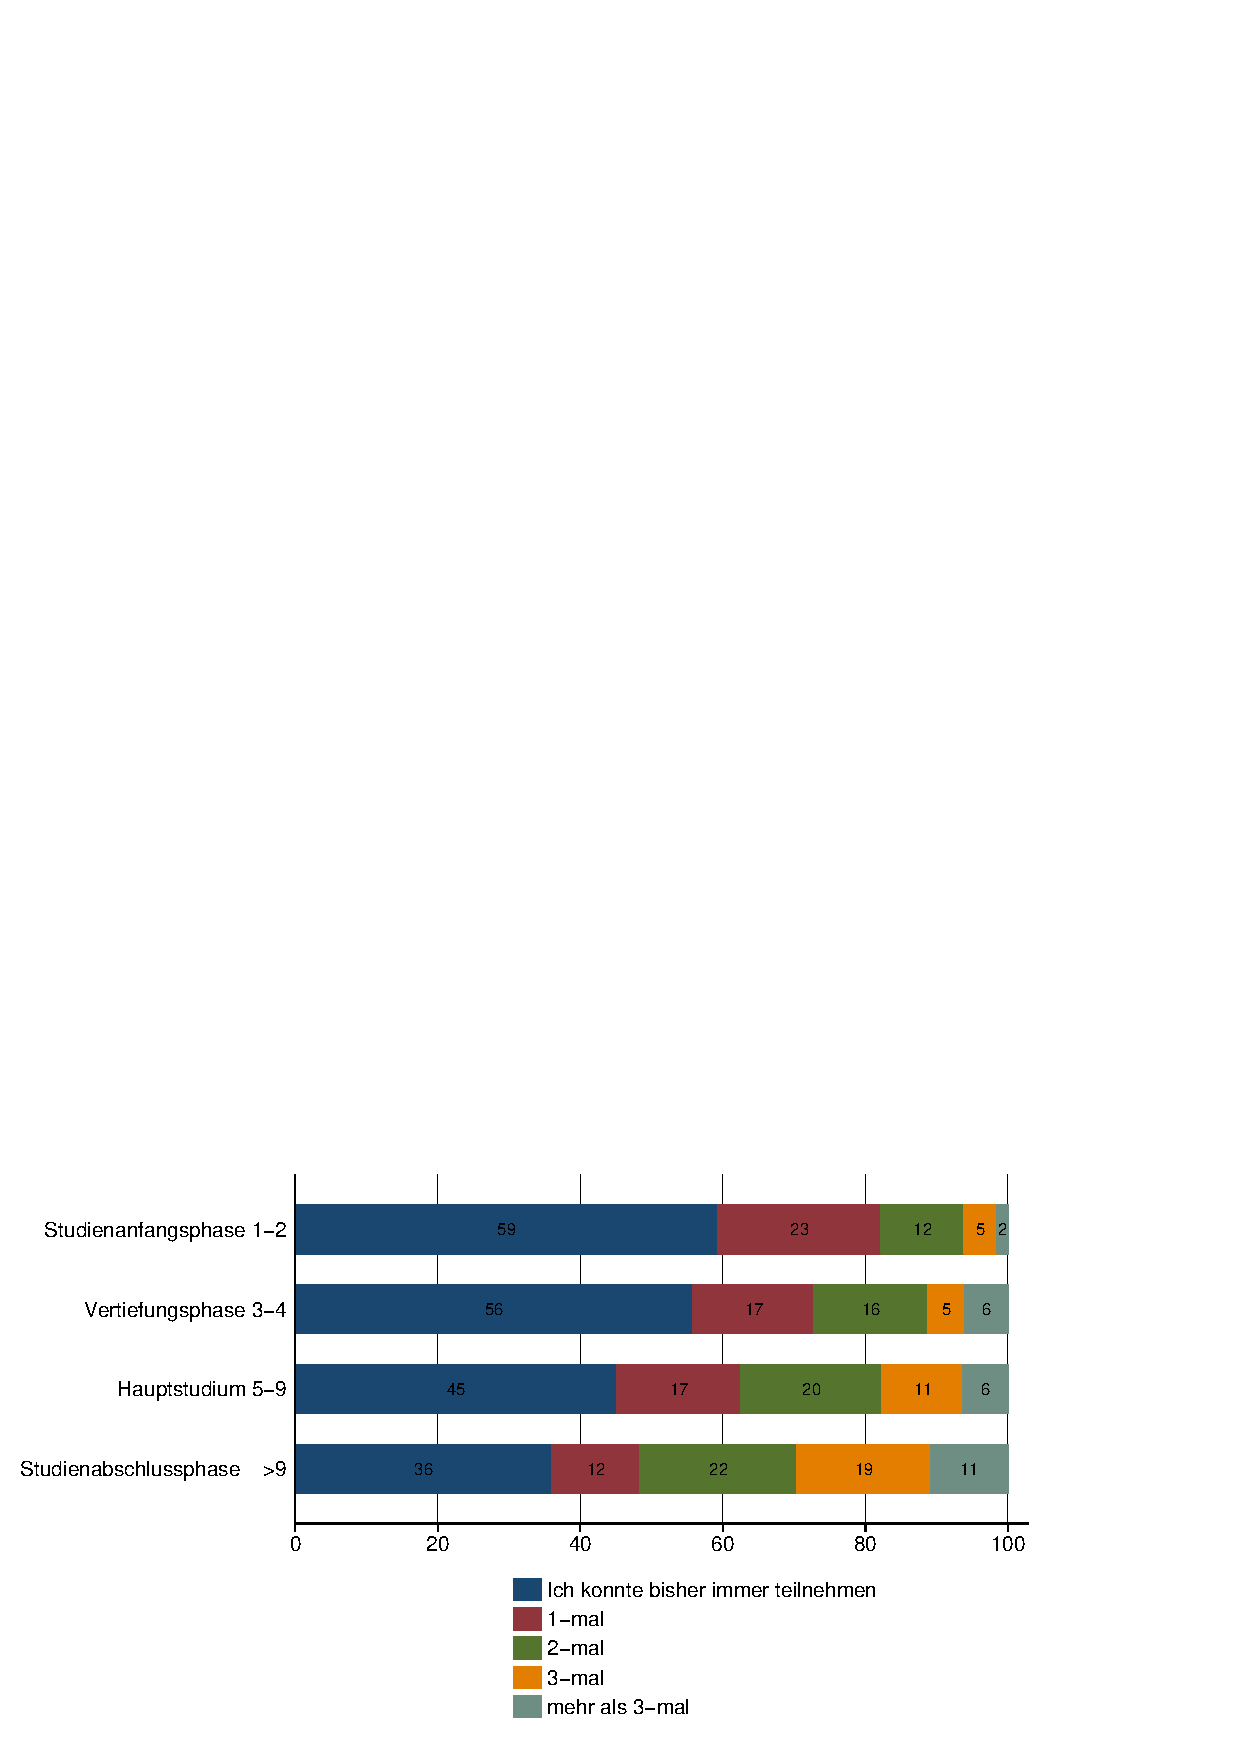
\includegraphics{image}| \\
% \filenm{image.eps}\tnote{a} & \filenm{image.svg}\tnote{a} & |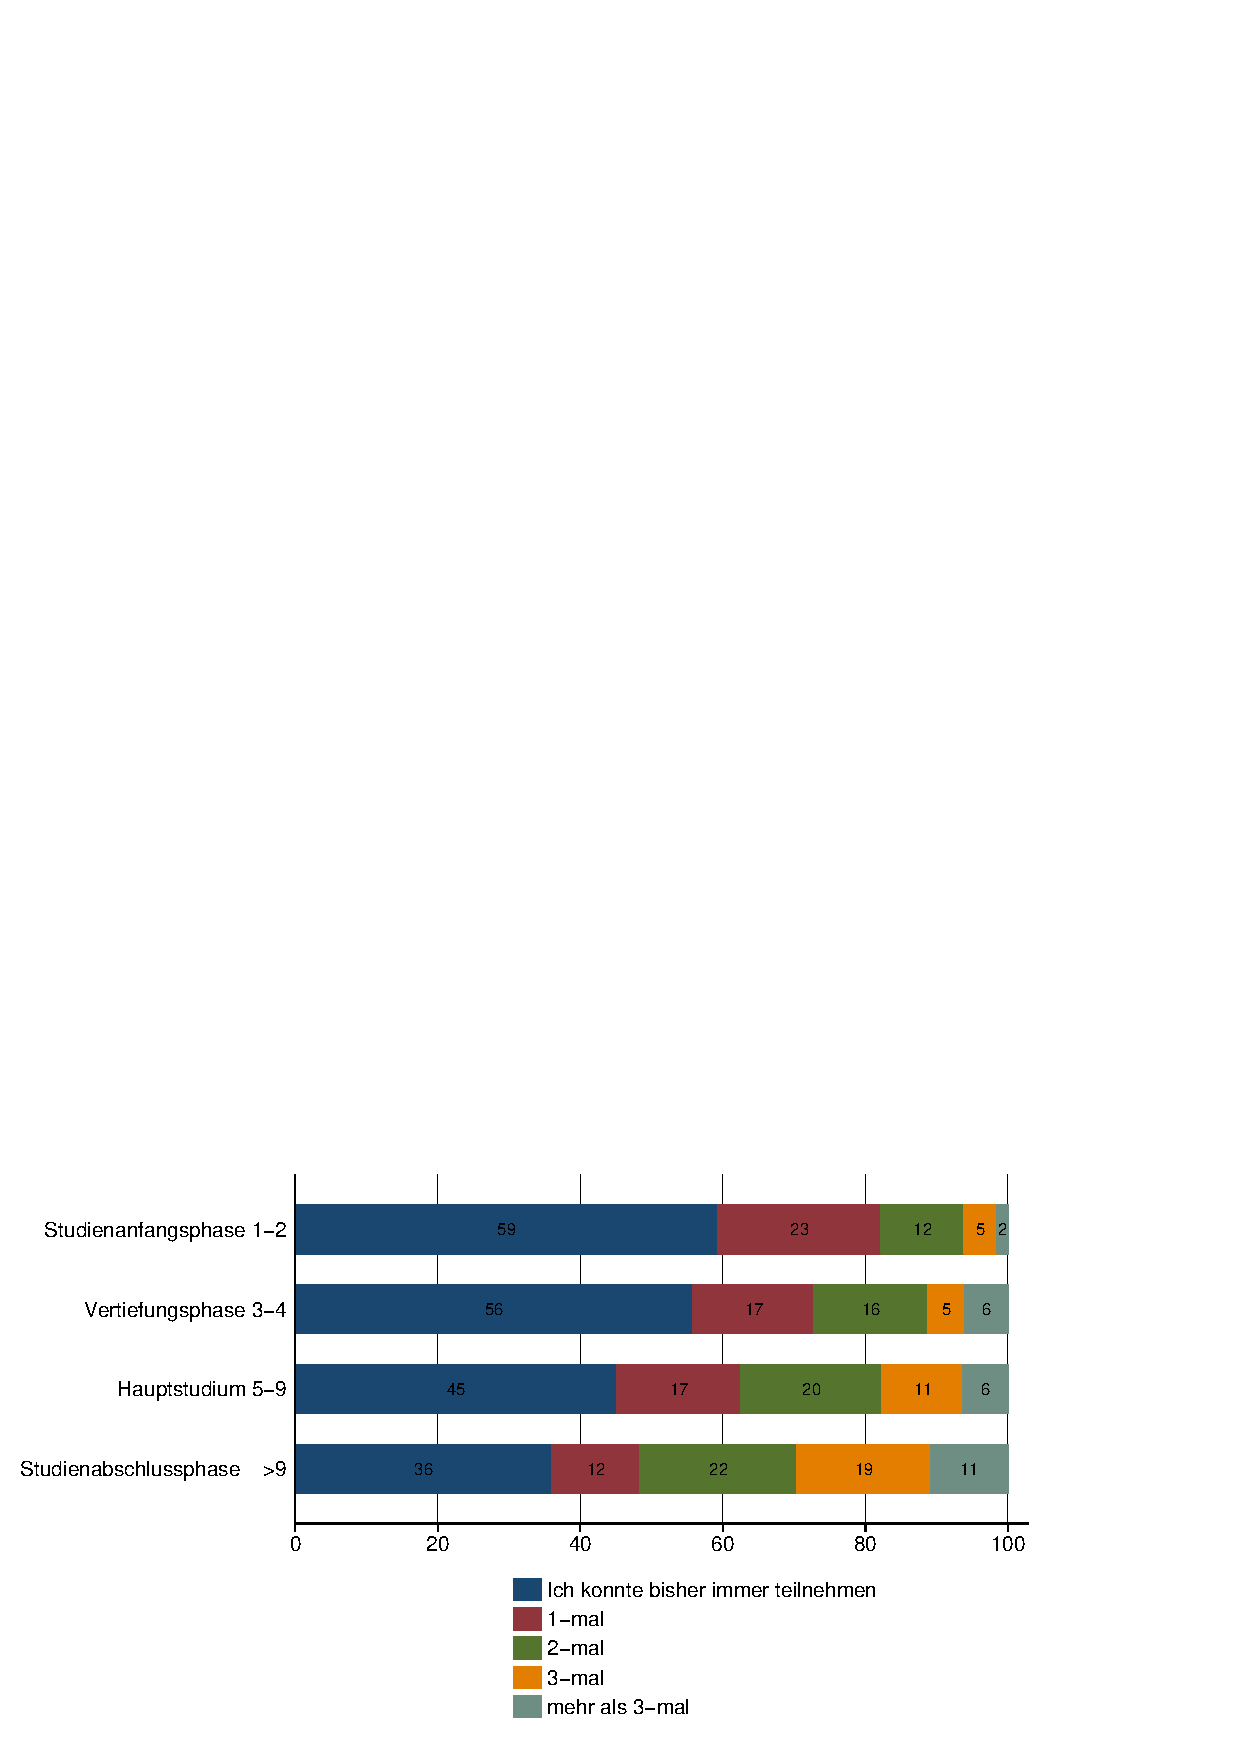
\includegraphics{image}| \\
% \filenm{image.jpg} & ---\tnote{b} & |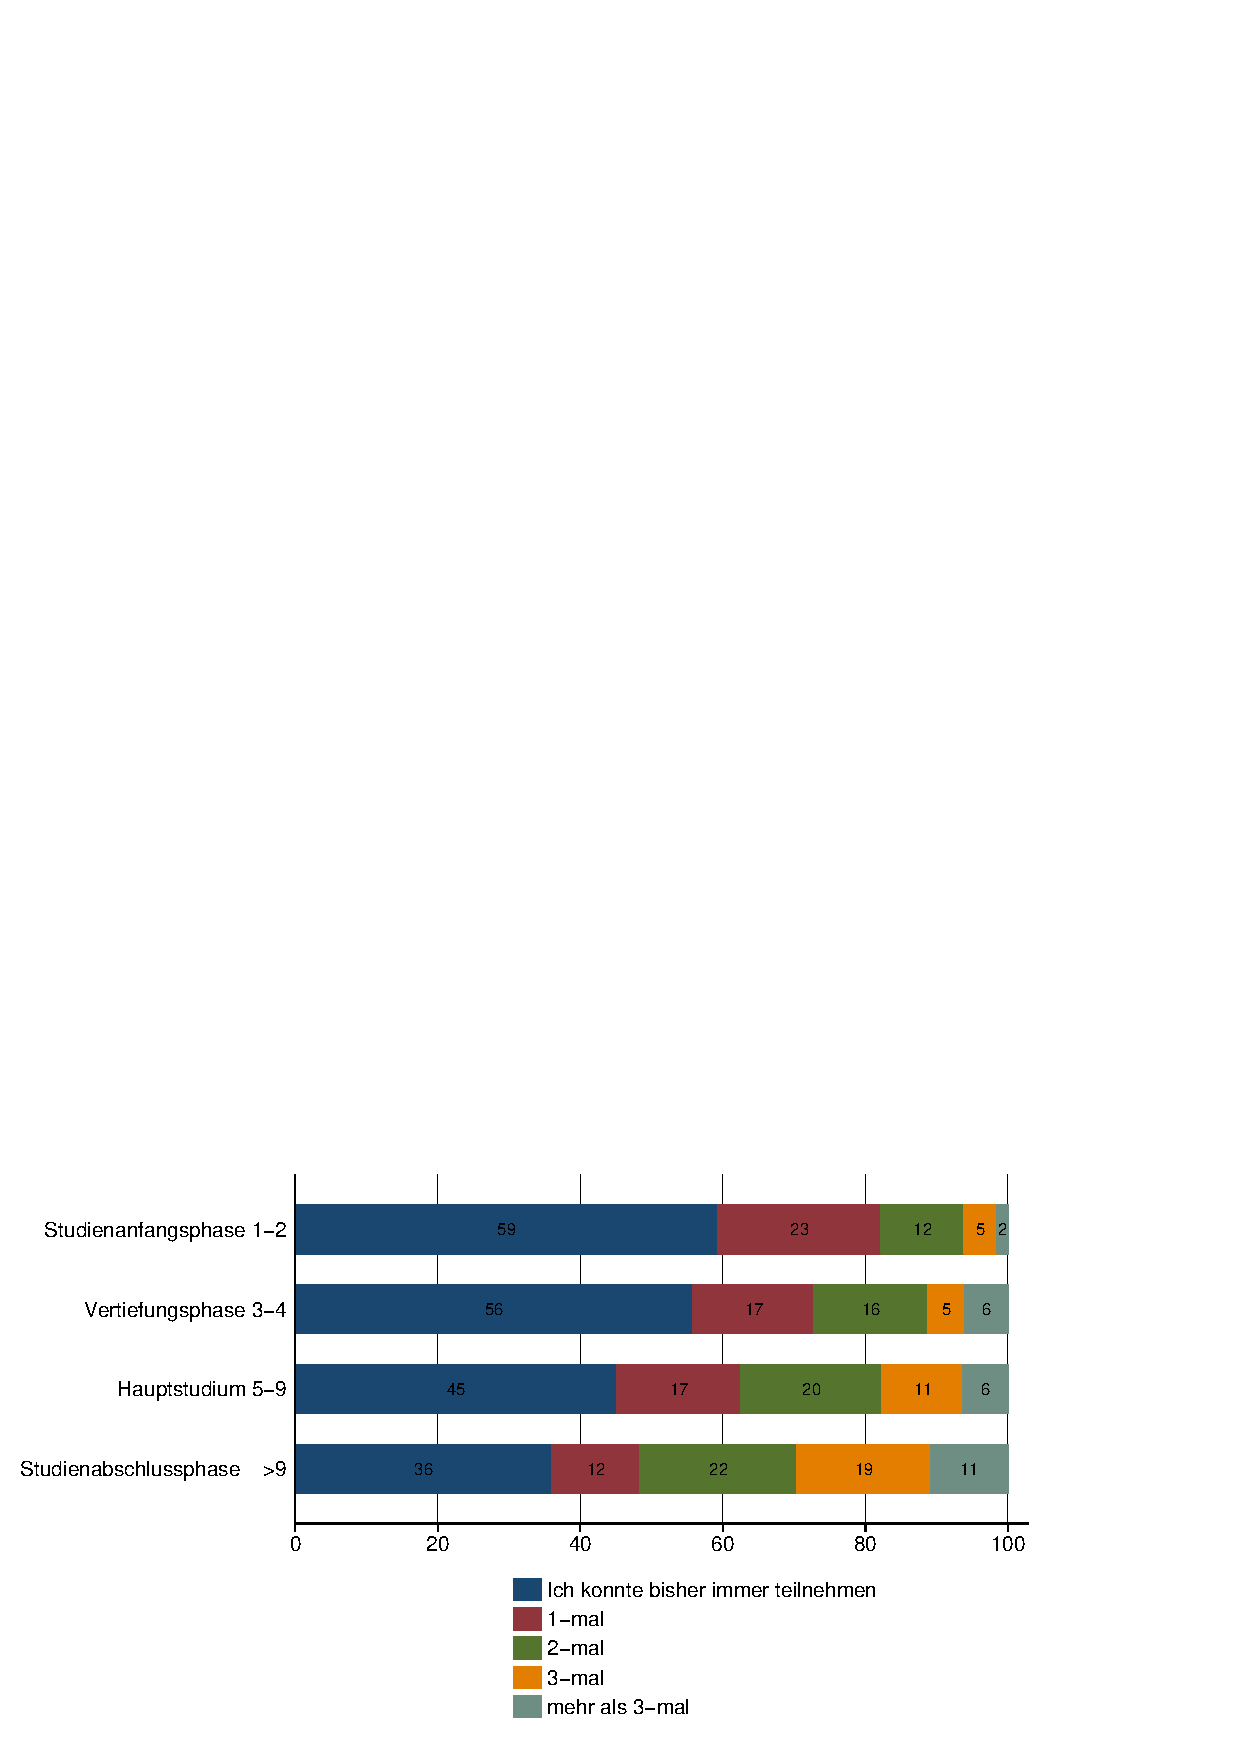
\includegraphics{image}| \\
% \filenm{image.png} & ---\tnote{b} & |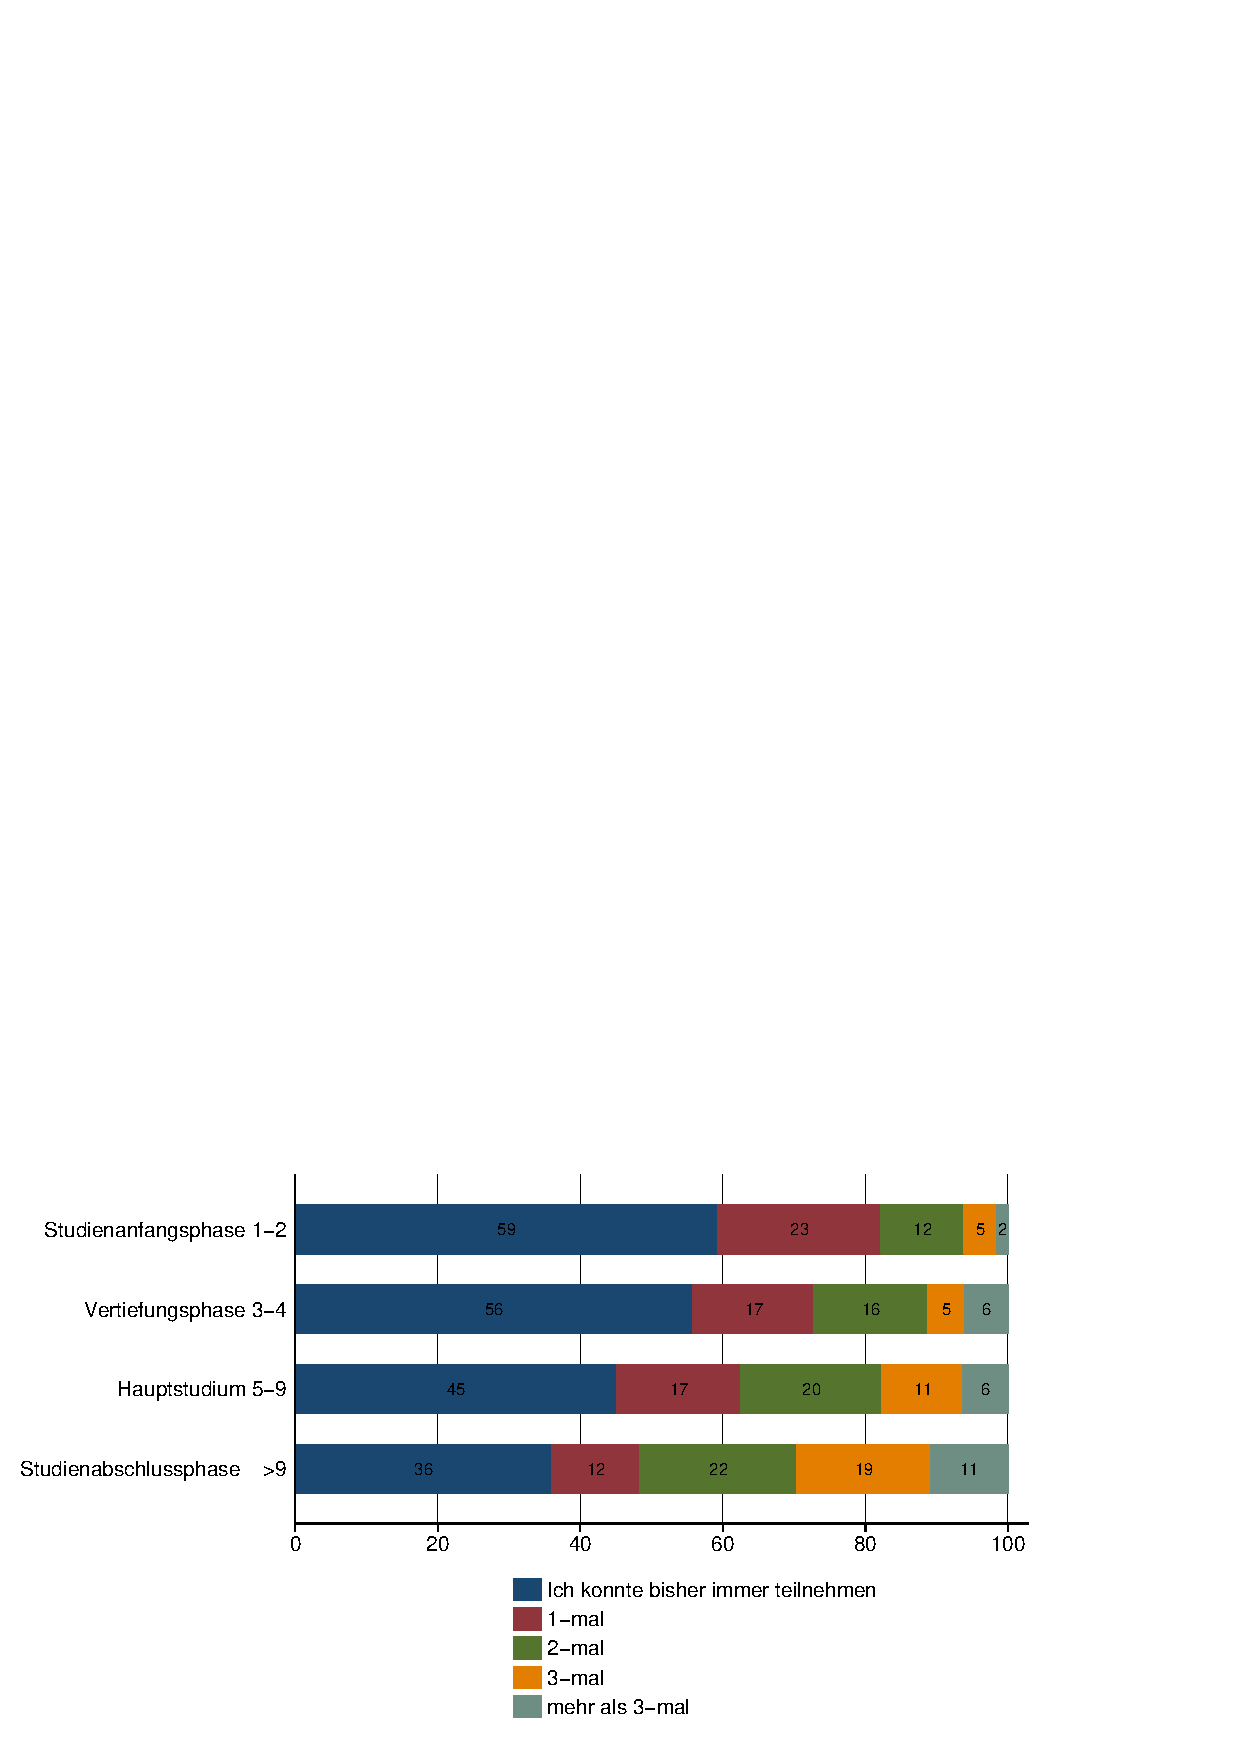
\includegraphics{image}| \\
% \filenm{image.JPG} & ---\tnote{b} & |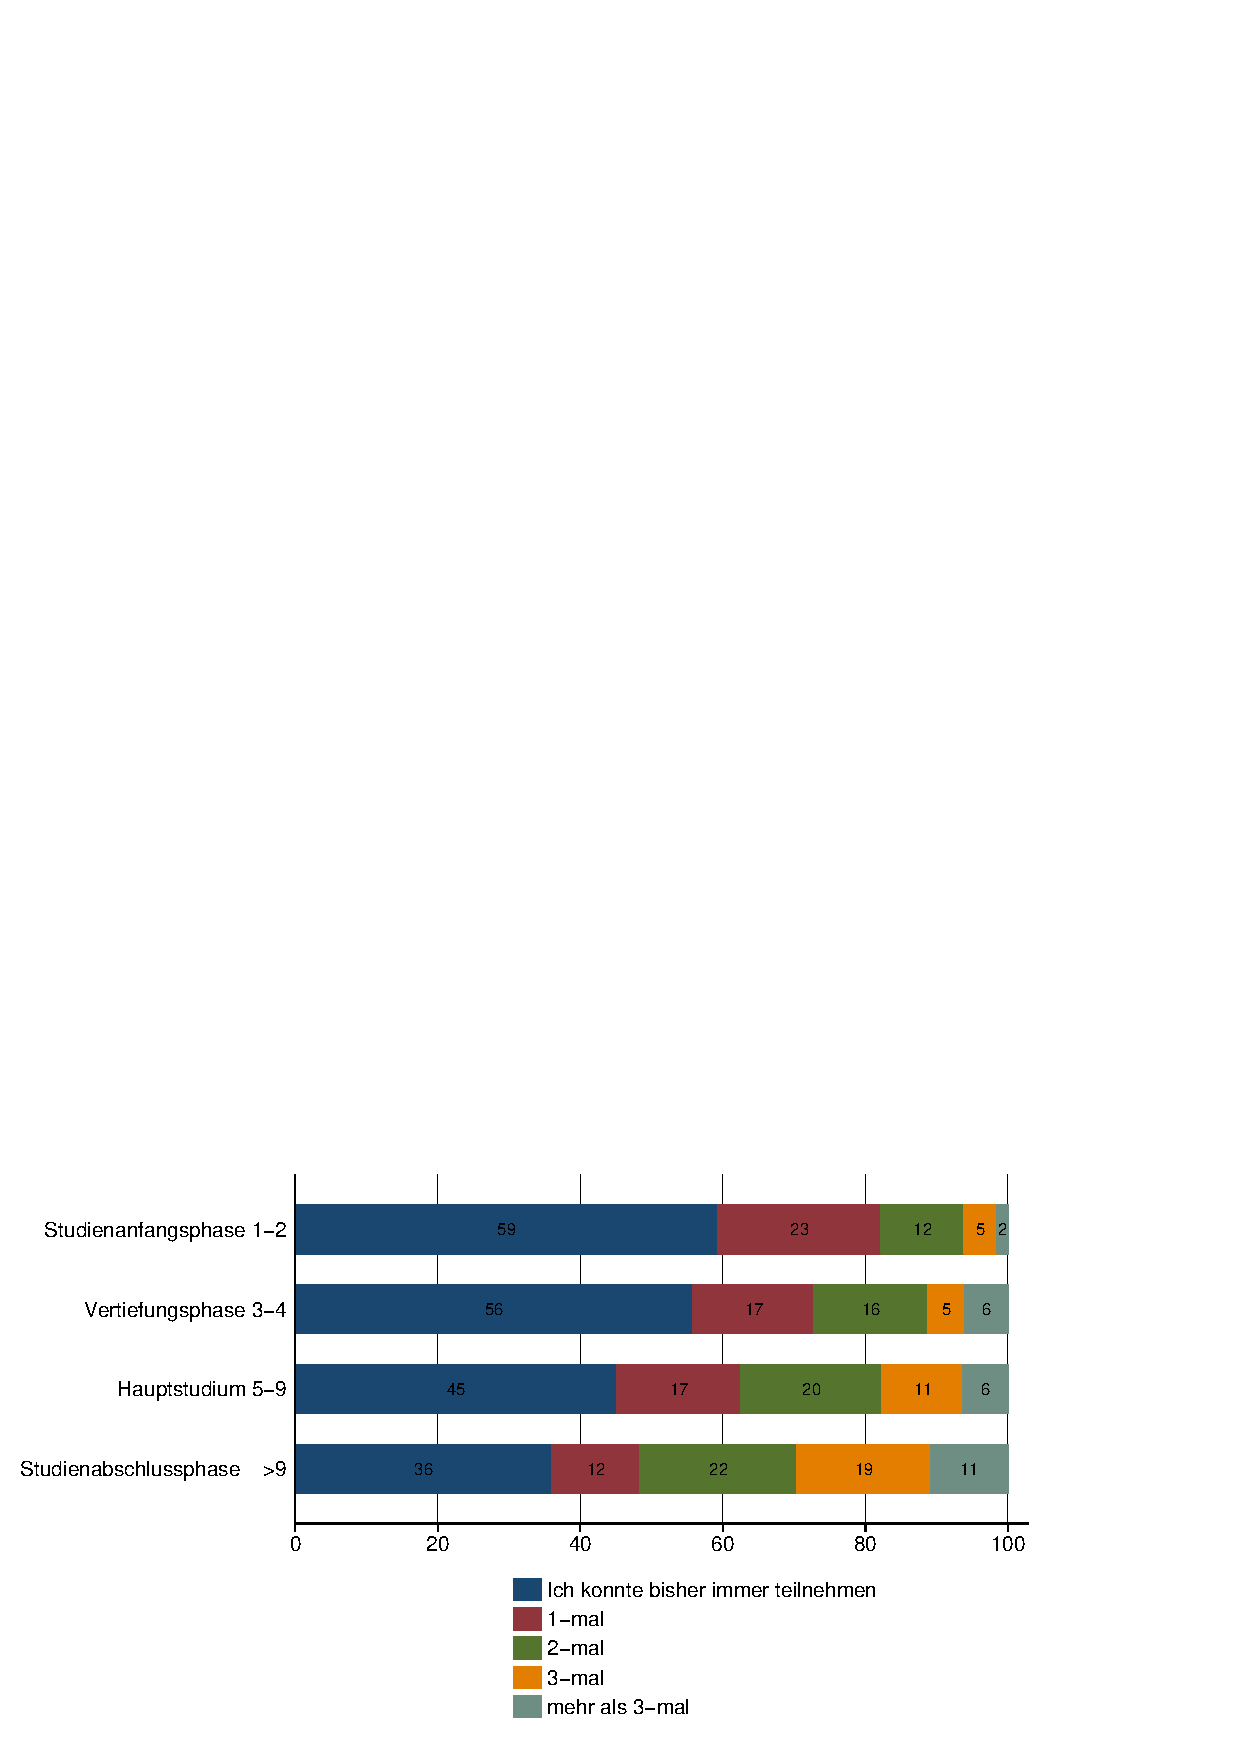
\includegraphics{image.JPG}|\tnote{c} \\
% \filenm{image.PNG} & ---\tnote{b} & |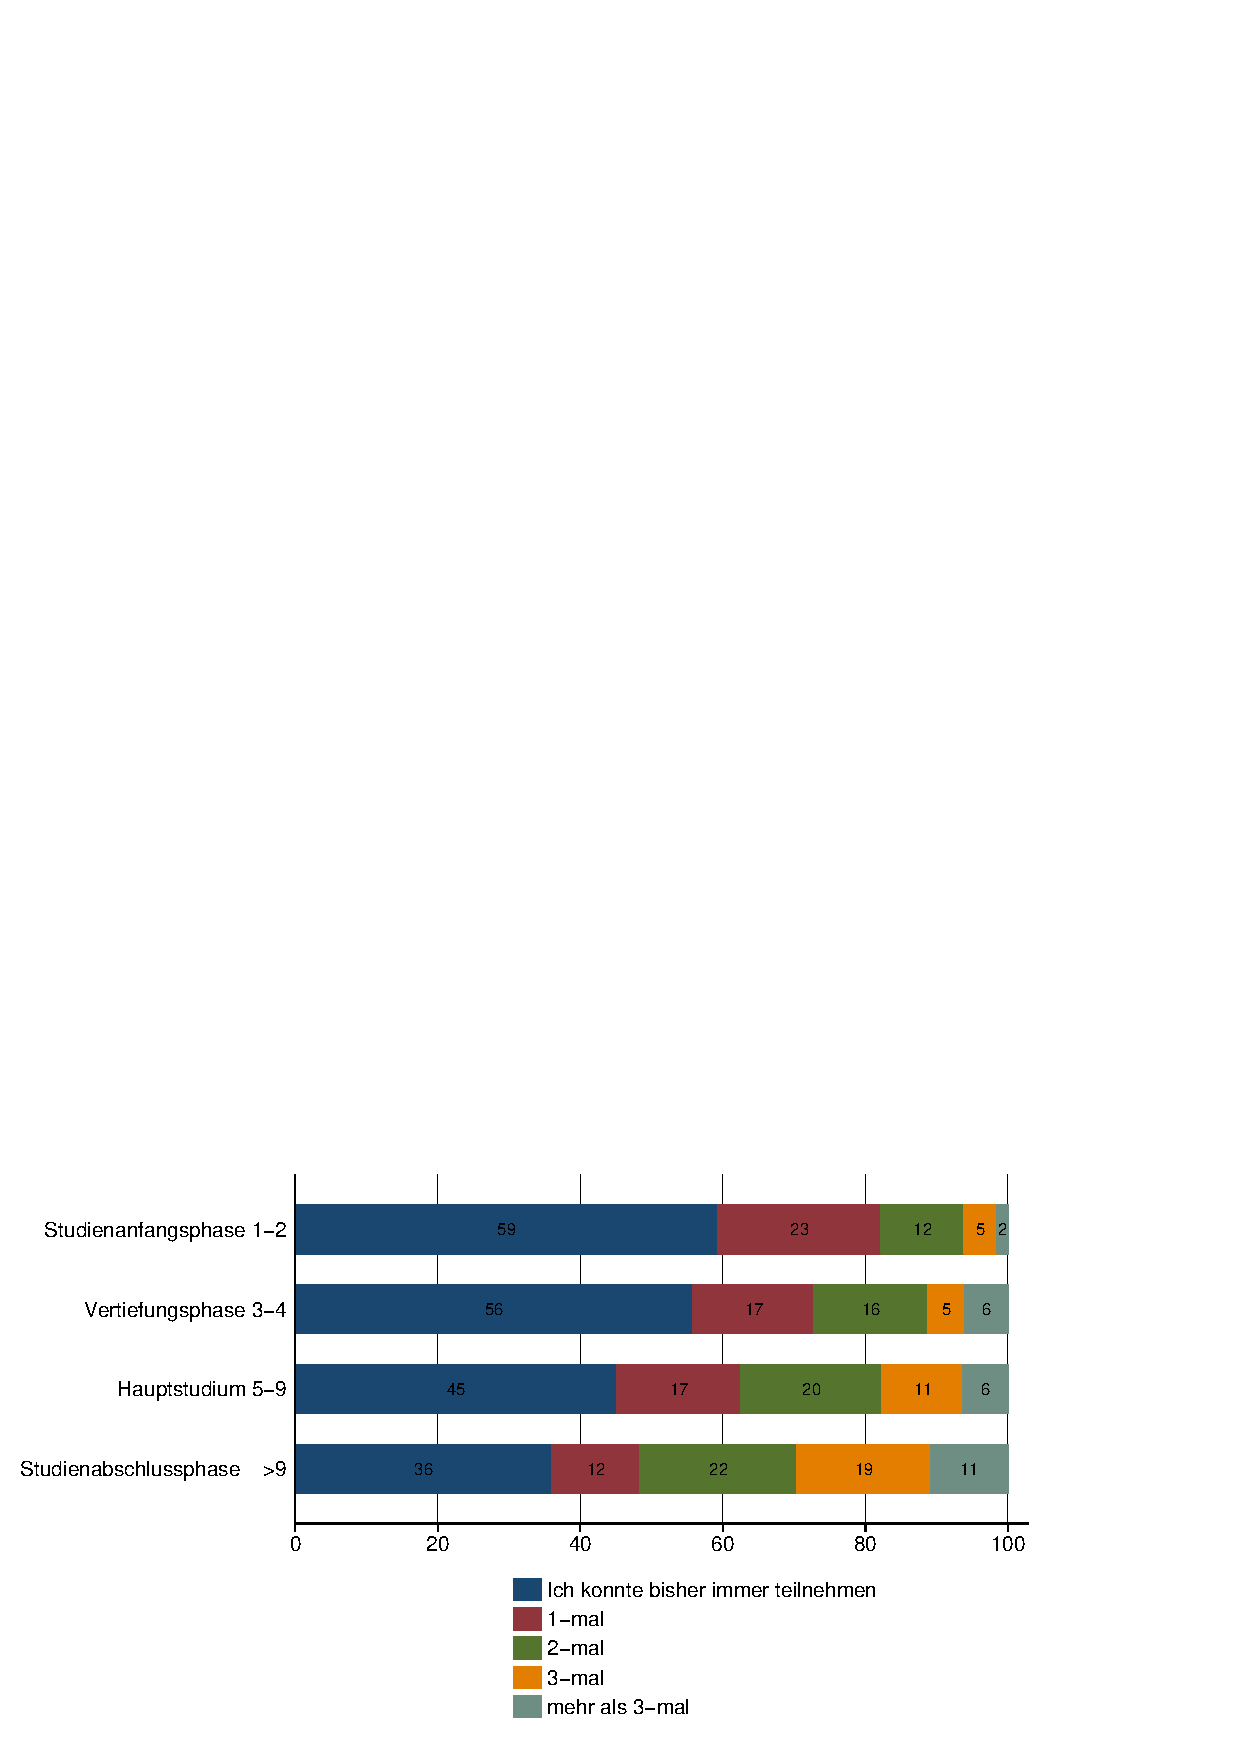
\includegraphics{image.PNG}|\tnote{c} \\
% \filenm{image.jpg} & \filenm{image.gif} & |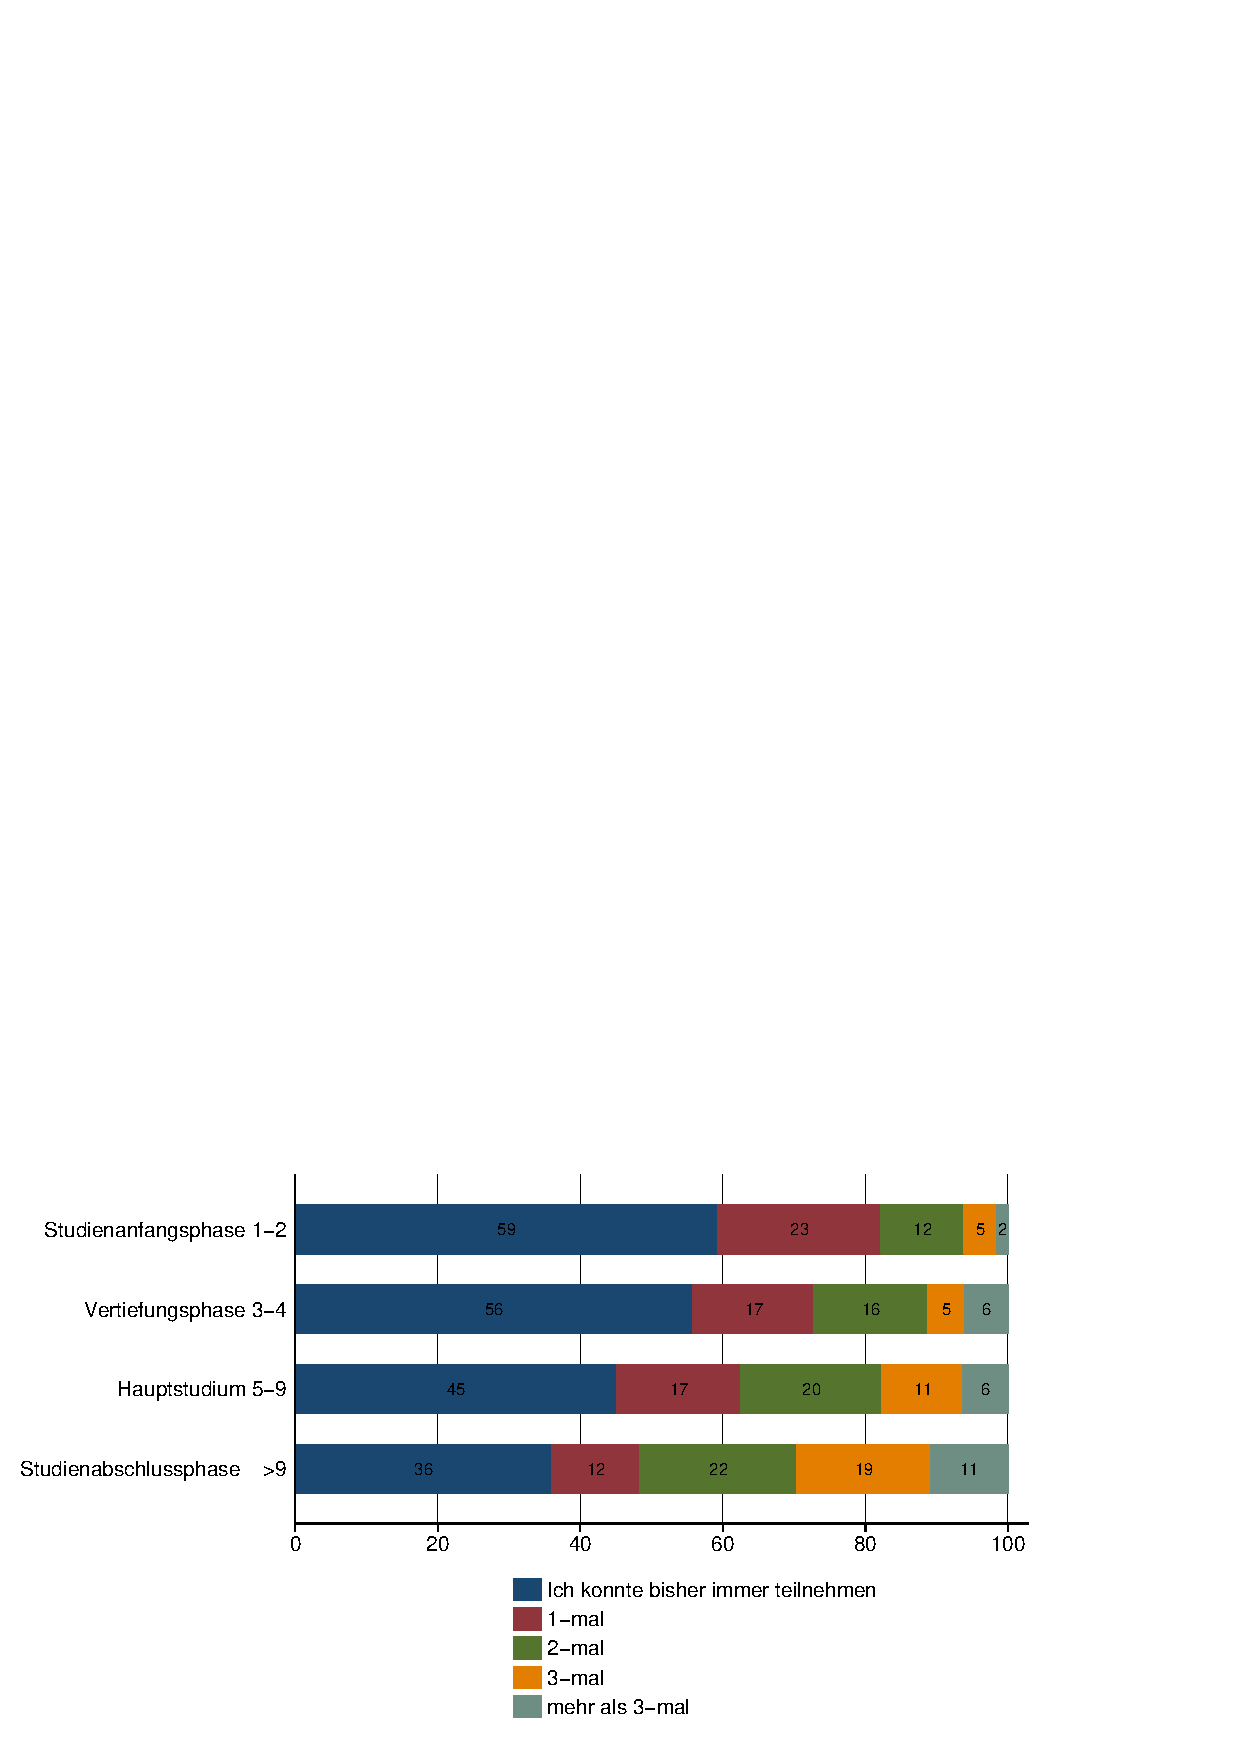
\includegraphics{image}| \\
% \bottomrule
% \end{tabular}
% \begin{tablenotes}
% \item[a:] Must be a lowercase file extension.
% \item[b:] The same file is used for print and \HTML.
% \item[c:] The uppercase extension must be specified.
% \end{tablenotes}
% \end{threeparttable}
% \end{center}
% \end{table}
% \limitsgraphics
%
%
% \subsubsection{\pkg{tikz} package}
% \label{sec:limitstikz}
%
% \DescribePackage{tikz}
% \limitstikz
% \changes{v0.51}{2018/03/18}{Docs: \pkg{tikz} limitations.}
%
%
% \subsubsection{\pkg{grffile} package}
%
% \DescribePackage{grffile}
% \limitsgrffile
%
%
% \subsubsection{\pkg{color} package}
%
% \DescribePackage{color}
% \limitscolor
%
%
% \subsubsection{\pkg{xcolor} package}
%
% \DescribePackage{xcolor}
% \limitsxcolor
%
%
% \subsubsection{\pkg{epstopdf} package}
%
% \DescribePackage{epstopdf}
% \limitsepstopdf
%
%
% \subsubsection{\pkg{pstricks} package}
%
% \DescribePackage{pstricks}
% \limitspstricks
%
%
% \subsubsection{\pkg{pdftricks} package}
%
% \DescribePackage{pdftricks}
% \limitspdftricks
%
%
% \subsubsection{\pkg{psfrag} package}
%
% \DescribePackage{psfrag}
% \trouble{psfrag=\pkg{psfrag}}
% \limitspsfrag
%
%
% \subsubsection{\pkg{pstool} package}
%
% \DescribePackage{pstool}
% \trouble{pstool=\pkg{pstool}}
% \limitspstool
%
%
% \needspace{15\baselineskip}
% \subsubsection{\pkg{asymptote} package}
% \changes{v0.62}{2018/10/16}{Docs: \pkg{asymptote}.}
%
% \DescribePackage{asymptote}
% \limitsasymptote
%
%
% \subsubsection{\pkg{overpic} package}
%
% \DescribePackage{overpic}
% \limitsoverpic
%
%
% \subsubsection{Multimedia packages}
%
% \DescribePackage{multimedia}
% \DescribePackage{movie15}
% \DescribePackage{media9}
% \trouble{multimedia=\pkg{multimedia}}
% \trouble{media9=\pkg{media9}}
% \trouble{movie15=\pkg{movie15}}
% \trouble{graphics>multimedia}
% \trouble{video}
% \trouble{audio}
% \gindex{video}
% \gindex{audio}
% \gindex{multimedia}
% \limitsmultimedia
%
%
%
% \subsection{Tabbing}
% \limitstabbing
%
%
% \subsection{Tabular}
%
% \subsubsection{\env{tabular} environment}
% \label{sec:limitstabular}
% \changes{v0.39}{2017/08/30}{Docs: Reorganized tabular discussion.}
% \limitstabular
%
% \subsubsection{\pkg{multirow} package}
% \gindex{multirow=\pkg{multirow}>mrowcell=\cs{mrowcell} and \cs{mcolrowcell}}
% \gindex{tabular=\env{tabular}>multirow=\pkg{multirow} \cs{mrowcell} and \cs{mcolrowcell}}
% \gindex{mrowcell=\cs{mrowcell}}
% \gindex{mcolrowcell=\cs{mcolrowcell}}
% \trouble{multirow=\pkg{multirow}>mrowcell=\cs{mrowcell} and \cs{mcolrowcell}}
% \trouble{tabular=\env{tabular}>multirow=\pkg{multirow} \cs{mrowcell} and \cs{mcolrowcell}}
% \trouble{mrowcell=\cs{mrowcell}}
% \trouble{mcolrowcell=\cs{mcolrowcell}}
% \gindex{multicolumn=\cs{multicolumn}>with \cs{multirow}}
% \gindex{multirow=\cs{multirow}>with \cs{multicolumn}}
% \gindex{tabular=\env{tabular}>multicolumn=\cs{multicolumn} with \cs{multirow}}
% \trouble{tabular=\env{tabular}>multicolumn=\cs{multicolumn} with \cs{multirow}}
% \limitsmultirow
%
% \subsubsection{\pkg{longtable} package}
%
% \DescribePackage{longtable}
% \trouble{longtable=\pkg{longtable}>endhead=\cs{endhead}, etc.}
% \trouble{endhead=\cs{endhead}, etc.}
% \limitslongtable
%
%
% \subsubsection{\pkg{threeparttablex} package}
% \label{sec:limitsthreeparttablex}
% \DescribePackage{threeparttablex}
% \trouble{threeparttablex=\pkg{threeparttablex}}
% \limitsthreeparttablex
%
%
% \subsubsection{\pkg{supertabular} and \pkg{xtab} packages}
%
% \DescribePackage{supertabular}
% \DescribePackage{xtab}
% \limitssupertabular
%
% \subsubsection{\pkg{colortbl} package}
%
% \DescribePackage{colortbl}
%     \limitscolortbl
%
% \subsubsection{\pkg{ctable} package}
%   \trouble{ctable=\pkg{ctable}}
%   \gindex{ctable=\pkg{ctable}}
%   \limitsctable
%
% \subsubsection{\pkg{bigdelim} package}
%
% \DescribePackage{bigdelim}
% \limitsbigdelim
%
%
% \subsection{Floats}
%
% \subsubsection{Float contents alignment}
%
% \limitsfloatalignment
%
%
% \subsubsection{\pkg{float}, \pkg{trivfloat}, and/or \pkg{algorithmicx} together}
%
% \DescribePackage{float}
% \DescribePackage{trivfloat}
% \DescribePackage{algorithmicx}
% \limitscombiningfloats
%
%
% \subsubsection{\pkg{caption} and \pkg{subcaption} packages}
%
% \DescribePackage{caption}
% \DescribePackage{subcaption}
% \label{sec:limitscaption}
% \limitscaption
%
%
%
%
% \subsubsection{\pkg{subfig} package}
%
% \DescribePackage{subfig}
% \limitssubfig
%
%
% \subsubsection{\pkg{floatrow} package}
%
% \DescribePackage{floatrow}
% \limitsfloatrow
%
%
% \subsubsection{\pkg{keyfloat} package}
%
% \DescribePackage{keyfloat}
% \limitskeyfloat
%
%
% \subsection{\brand{Koma-Script} classes}
%
% \DescribeClass{komascript}
% \limitskomascript
%
%
% \subsection{\brand{Memoir} class}
% \label{sec:limitsmemoir}
%
% \changes{v0.66}{2019/02/06}{\pkg{memoir}: Docs re: version numbers.}
%
% \DescribeClass{memoir}
% \limitsmemoir
%
% The custom frame commands in the \pkg{memoir} manual may be emulated by
% \trouble[\env{framewithtitle}, \env{titledframe}]{framewithtitle=\env{framewithtitle}}
% \trouble{titledframe=\env{titledframe}}
% \trouble{memoir=\pkg{memoir}>\env{framewithtitle}, \env{titledframe}}
% \gindex{memoir=\pkg{memoir}>\env{framewithtitle}, \env{titledframe}}
% placing the original defintions in the preamble inside \env{warpprint}
% environments, and then providing an \HTML\ equivalent:
% \begin{sourceverb}
% \begin{warpHTML}
% \newcommand{\FrameTitle}[2]{%
%     \textbf{#2}
% }
% 
% \newenvironment{framewithtitle}[2][\FrameFirst@Lab\ (cont.)]{%
%     \begin{fminipage}{\linewidth}
%     \textbf{#2}
%     \begin{minipage}{\linewidth}
% }
% {\end{minipage}\end{fminipage}}
% 
% \newcommand{\TitleFrame}[2]{%
%     \par
%     \textbf{#1}\par
%     \fboxBlock{#2}
% }
% 
% \newenvironment{titledframe}[2][\FrameFirst@Lab\ (cont.)]{%
%     \par
%     \textbf{#2}
%     \begin{fminipage}{\linewidth}
% }
% {\end{fminipage}}
% \end{warpHTML}
% \end{sourceverb}
%
%
% \subsection{International languages}
% \label{sec:international}
%
% If using \prog{pdflatex} with the setting |\booltrue{FileSectionNames}|,
% \trouble[section and file names]{sectioning>international language}
% \trouble{filename>corrupted}
% \trouble{filename>international, \UTF-8}
% \gindex{international>section names}
% \gindex{foreign>section names}
% \gindex{section>international languages}
% \gindex{filename>international languages}
% non-\acro{ASCII} text in section names can result in corrupted \HTML\ file names.
% \prog{pdflatex} may be used if setting |\boolfalse{FileSectionNames}|, in which case
% \HTML\ file numbers will be generated.
%
% For correct \HTML\ file names, use \prog{xelatex}, \prog{lualatex},
% or dedicated document classes \Slash engines.
%
% (As of this writing, this warning is only relevent to the \pkg{kotex} package.)
%
%
% \subsection{Miscellaneous packages}
%
% \subsubsection{\pkg{verse} and \pkg{memoir}}
%
% \DescribePackage{verse}
% \DescribeClass{memoir}
% \limitsverse
%
%
% \subsubsection{\pkg{newclude} package}
%
% \changes{v0.14}{2016/03/29}{Docs: Newclude limitations.}
%
% \DescribePackage{newclude}
% \limitsnewclude
%
%
%
% \subsubsection{\pkg{babel} package}
%
% \DescribePackage{babel}
% ^^A \limitsbabelone
% \limitsbabeltwo
%
%
% \subsubsection{\pkg{polyglossia} package}
% \label{sec:limitspolyglossia}
%
% \DescribePackage{polyglossia}
% \limitspolyglossia
%
%
% \subsubsection{\pkg{todonotes} and \pkg{luatodonotes} packages}
%
% \DescribePackage{todonotes}
% \DescribePackage{luatodonotes}
% \limitstodonotes
%
%
% \subsubsection{\pkg{fixme}}
%
% \DescribePackage{fixme}
% \limitsfixme
%
%
% \subsubsection{\pkg{acro} package}
% \limitsacro
% \trouble{acro=\pkg{acro}}
%
% \subsubsection{\pkg{chemfig} package}
%
% \limitschemfig
% \trouble{chemfig=\pkg{chemfig}}
%
%
% \subsubsection{\pkg{chemformula} package}
% \limitschemformula
% \trouble{array=\env{array}>chemformula=\pkg{chemformula}}
% \trouble{math>chemformula=\pkg{chemformula}}
%
%
% \subsubsection{\pkg{mhchem} package}
%
% See \cref{sec:mhchem}.
%
%
% \subsubsection{\pkg{kotex} package}
%
% \DescribePackage{kotex}
% See \cref{sec:international} regarding \prog{pdflatex} and
% Korean section names.
% \trouble[Korean section names]{filename>Korean}
%
%
% \clearpage
%
% \section{Compiling using custom shell commands}
% \label{sec:customcompiling}
% \gindex{compiling>custom}
%
% \changes{v0.61}{2018/09/21}{Docs: Compiling using custom shell commands.}
%
% \pkg{lwarp} and \prog{lwarpmk} try to make it easy to process
% print and \HTML\ compilation tasks in most situations.
% Depending on the operating system, command-line options, \TeX\ engine,
% and \pkg{lwarp} options, the commands \cmds{lwarpmk print} and
% \cmds{lwarpmk html} are automatically set up to correctly recompile the project.
% These actions may be overridden using \pkg{lwarp} options, thus allowing the use
% of packages such as \pkg{perltex} and \pkg{pythontex}.
%
% \subsection{Command options}
%
% \DescribeOption{PrintLatexCmd}
% \DescribeOption{HTMLLatexCmd}
% The \pkg{lwarp} options \optn{PrintLatexCmd} and \optn{HTMLLatexCmd}
% are used to set customized commands to be executed by
% \cmds{lwarpmk print} and \cmds{lwarpmk html}.
% \begin{description}
% \item[\optn{PrintLatexCmd}] should be set to shell commands which take \filenm{project.tex}
%     and generate \filenm{project.pdf}.
% \item[\optn{HTMLLatexCmd}] should be set to take \filenm{project_html.tex} and
%     generate \filenm{project_html.pdf}.
%     \prog{lwarpmk} will then take \filenm{project_html.pdf} and
%     automatically convert it and generate \filenm{project.html}.
% \end{description}
%
% \subsection{Literal character macros}
% The \pkg{lwarp} package options are parsed by \TeX, and so some characters
% require the use of a special macro to represent them.  See \cref{tab:literalchars}.
% \cs{LWRopquote} and \cs{LWRopseq} may be used to increase operating-system portability.
% \cs{jobname} must have |_html| appended for processing \HTML.
% \cs{space} may be necessary between other macros.
%
% To use these macros, either \pkg{kvoptions-patch} must be loaded before \pkg{lwarp}:
% \trouble[macro not found]{LWRopseq=\cs{LWRopseq}}
% \trouble{LWRpercent=\cs{LWRpercent}}
% \trouble{LWRdollar=\cs{LWRdollar}}
% \trouble{LWRhash=\cs{LWRhash}}
% \trouble{LWRbackslash=\cs{LWRbackslash}}
% \trouble{LWRopquote=\cs{LWRopquote}}
% \begin{Verbatim}[gobble=2,obeytabs,tabsize=4,frame=lines]
% \usepackage{kvoptions-patch}
% \usepackage[
%     PrintLatexCmd={ ... } ,
%     HTMLLatexCmd={ ... }
% ]{lwarp}
% \end{Verbatim}
% \needspace{18\baselineskip}
% or \cs{lwarpsetup} must be used to set \optn{PrintLatexCmd} and \optn{HTMLLatexCmd}:
% \begin{Verbatim}[gobble=2,obeytabs,tabsize=4,frame=lines]
% \usepackage[...]{lwarp}
% \lwarpsetup{
%   PrintLatexCmd=
%       {
%           latex tm \LWRopseq
%           dvips -o tm-pics.ps tm.dvi \LWRopseq
%           ps2pdf -dALLOWPSTRANSPARENCY tm-pics.ps \LWRopseq
%           pdflatex tm.tex
%       } ,
%   HTMLLatexCmd=
%       {
%           latex tm_html \LWRopseq
%           dvips -o tm_html-pics.ps tm_html.dvi \LWRopseq
%           ps2pdf -dALLOWPSTRANSPARENCY tm_html-pics.ps \LWRopseq
%           pdflatex tm_html.tex
%       }
% }
% \end{Verbatim}
%
% \begin{table}
% \centering
% \caption{Literal character macros}
% \label{tab:literalchars}
% \begin{tabular}{cll}
% Character & Macro & Comment \\
% |%| & \cs{LWRpercent} & \\
% |$| & \cs{LWRdollar} & \\
% |&| & \cs{LWRamp} & \\
% |%| & \cs{LWRhash} & \\
% |\| & \cs{LWRbackslash} & \\
% \texttt{\textquotesingle} or |"| & \cs{LWRopquote} & Depends on the operating system. \\
% |&| or |&&| & \cs{LWRopseq} & Depends on the operating system. \\
% (space) & \cs{space} & Forces an extra space. \\
% (jobname) & \cs{jobname} & Without file extension. \\
% \end{tabular}
% \hrule
% \end{table}
%
%
% \needspace{6\baselineskip}
%
% \subsection{\prog{latexmk}}
%
% \DescribeProgram{latexmk}
% If \prog{latexmk} is used for a project, it may be easiest to continue
% using it.
% \begin{description}
% \item[\cmds{latexmk project.tex}] would create \filenm{project.pdf} as normal.
% \item[\cmds{latexmk project\_html.tex}] would create \filenm{project_html.pdf},
%   then
% \item [\cmds{lwarpmk pdftohtml project\_html.pdf}] would take
%   \filenm{project_html.pdf} and convert it to \filenm{project.html}.
% \end{description}
%
% \prog{latexmk} may simplify the use of packages such as \pkg{sagetex}.
% \DescribePackage{sagetex}
%
%
% \subsection{\pkg{perltex} package}
%
% The \pkg{lwarp} package option settings to use \pkg{perltex} would be similar to:
% \DescribePackage{perltex}
% \begin{sourcedisplay}
% \cs{usepackage}[ \\
% \fquad \dots \\
% \fquad PrintLatexCmd=\{perltex -latex=pdflatex project.tex\} , \\
% \fquad HTMLLatexCmd=\{perltex -latex=pdflatex project\textgreen{\_html}.tex\} , \\
% \fquad \dots \\
% ]\{lwarp\}
% \end{sourcedisplay}
%
% Place \pkg{perltex} math expressions between
% \trouble[``impure'' math]{perltex=\pkg{perltex}}
% \cs{displaymathother} and \cs{displaymathnormal}, or
% \cs{inlinemathother} and \cs{inlinemathnormal}.
% See \cref{sec:displaymathother}.
%
%
% \subsection{\pkg{pythontex} package}
%
% \DescribePackage{pythontex}
% An example using \pkg{pythontex}:
% \begin{sourcedisplay}
% \cs{usepackage}[ \\
% \fquad \dots \\
% \fquad PrintLatexCmd=\{ \\
%     \fqquad pdflatex project.tex \cs{LWRopseq} \\
%     \fqquad pythontex project \cs{LWRopseq} \\
%     \fqquad pdflatex project.tex \\
% \fquad \} , \\
% \fquad HTMLLatexCmd=\{ \\
%     \fqquad pdflatex project\textgreen{\_html}.tex \cs{LWRopseq} \\
%     \fqquad pythontex project\textgreen{\_html} \cs{LWRopseq} \\
%     \fqquad pdflatex project\textgreen{\_html}.tex \\
% \fquad \} , \\
% \fquad \dots \\
% ]\{lwarp\}
% \end{sourcedisplay}
%
% Another possibility is to use \prog{latexmk}, placing the
% \cmds{latexmk \dots} commands in the \optn{PrintLatexCmd} and \optn{HTMLLatexCmd}
% options.
% While using these options, the \pkg{lwarp} option \optn{latexmk} would not be used.
%
% No attempt has yet been made to make \pkg{pythontex} robust with \HTML\ output.
% Some math objects must be surrounded by
% \trouble[``impure'' math]{pythontex=\pkg{pythontex}}
% \cs{displaymathother} \dots\ \cs{displaymathnormal},
% or \cs{inlinemathother} \dots\ \cs{inlinemathnormal}.
% Displays of code may have to be
% enclosed inside a \env{lateximage} environment
% \watchout[HTML look-alike]
% to prevent |<|, |>| and similar from being interpreted by the browser
% as \HTML\ entities.
%
%
% \subsection{\pkg{sympytex} package}
%
% \DescribePackage{sympytex}
% \trouble{sympytex=\pkg{sympytex}}
% For \pkg{sympytex}:
%
% \begin{sourcedisplay}
% \cs{usepackage}[ \\
% \fquad \dots \\
% \fquad PrintLatexCmd=\{ \\
%     \fqquad pdflatex project.tex \cs{LWRopseq} \\
%     \fqquad python project.sympy \cs{LWRopseq} \\
%     \fqquad pdflatex project.tex \\
% \fquad \} , \\
% \fquad HTMLLatexCmd=\{ \\
%     \fqquad pdflatex project\textgreen{\_html}.tex \cs{LWRopseq} \\
%     \fqquad python project\textgreen{\_html}.sympy \cs{LWRopseq} \\
%     \fqquad pdflatex project\textgreen{\_html}.tex \\
% \fquad \} , \\
% \fquad \dots \\
% ]\{lwarp\}
% \end{sourcedisplay}
%
% Also see the warnings for \pkg{pythontex}, above.

% \subsection{Other packages}
%
% \DescribePackage{rterface}
% \trouble{rterface=\pkg{rterface}}
% Other packages such as \pkg{rterface} would be set up
% similar to \pkg{pythontex}, and the same warnings would apply.
%
%
% \subsection{\prog{make} program}
% \gindex{make utility}
%
% \DescribeProgram{make}
% To use \pkg{lwarp} with the \prog{make} program,
% have the \filenm{makefile} take \filenm{project.tex} and
% generate the print version \filenm{project.pdf}, as normal.
% |\usepackage{lwarp}| must be used, and it generates \filenm{lwarpmk.conf}
% when the print version is created.
%
% To generate \HTML, first have \filenm{project_html.tex} be compiled to
% generate \filenm{project_html.pdf}.
% This must be in \PDF\ format.
% Finally, have \filenm{project_html.pdf} be converted to \HTML\ using
% \cmds{lwarpmk pdftohtml project\_html.pdf},
% and convert \SVG\ math with \cmds{lwarpmk limages}.
%
%
% \subsection{\UTF-8 locale}
% \label{sec:utf8locale}
% \gindex{locale}
% \gindex{UTF-8>locale}
%
% \changes{v0.62}{2018/10/20}{Docs: UTF-8 locale.}
%
% \prog{lwarpmk} uses the \prog{texlua} program, which sets the ``locale'' to ``|C|'',
% \trouble[UTF-8 locale]{UTF-8>locale}
% \trouble{Unicode>UTF-8 locale}
% \trouble{locale}
% including for external operating-system calls such as when executing \cmds{lwarpmk html}.
% In some cases, an external program called from the user's document
% may require the use of a \UTF-8 ``locale''.
% For \brand{Unix}-related operating systems, it may be required to use \pkg{lwarp}'s
% custom compilation options to add a locale change:
% \begin{sourcedisplay}
% \cs{usepackage}\{lwarp\}[\\
% \fquad PrintLatexCmd=\{\\
%   \fqquad \textred{env LC\_CTYPE=en\_US.UTF-8} \\
%       \fqqquad xelatex --shell-escape project.tex \\
% \fquad \} \\
% \fquad HTMLLatexCmd=\{\\
%   \fqquad \textred{env LC\_CTYPE=en\_US.UTF-8} \\
%       \fqqquad xelatex --shell-escape project\textgreen{\_html}.tex \\
% \fquad \} \\
% ] \\
% \end{sourcedisplay}
%
% \DescribePackage{ditaa}
% The only example seen so far where this is required is the \pkg{ditaa} package,
% \trouble{ditaa=\pkg{ditaa}}
% where the locale change allows the use of UTF-8 with Xe\LaTeX\ and \pkg{ditaa}.
% To use Lua\LaTeX\ instead, the locale change would have to be made inside the
% \pkg{ditaa} package where its calls the \prog{ditaa} program.
%
%
% \clearpage
%
% \section{\EPUB\ conversion}
% \label{sec:epub}
%
% \pkg{lwarp} does not produce \EPUB\ documents,
% but it may be told to modify its \HTML\ output
% to greatly assist in the conversion.
% An external program may then be used to finish the conversion
% to \EPUB.
%
% To assign the author's name for regular \pkg{lwarp} \HTML\
% \margintag{\element{meta} author}
% files, and also for the \EPUB,
% use \cs{HTMLAuthor} \marg{name}.  This assigns the name to the
% \element{meta} author element.  It may be set empty, and it defaults to
% \cs{theauthor}.
%
% A special boolean is provided to simplify the process of
% converting \pkg{lwarp} \HTML\ output to \EPUB:
%
% \begin{docsidebar}[\bool{FormatEPUB}]
% \DescribeBoolean{FormatEPUB}  \DescribeDefault{false}
%	\raggedright
%	|FormatEPUB| changes \HTML\ output for easy \EPUB\ conversion
%	via an external program. Removes per-file headers, footers, and nav.
%	Adds footnotes per chapter/section.
% \end{docsidebar}
%	\gindex{EPUB>HTML conversion settings}
%	\gindex{HTML>conversion settings>EPUB}
%
% To help convert \pkg{lwarp} \HTML\ output to \EPUB, add
%	\begin{sourcedisplay}
%	|\booltrue{FormatEPUB}|
%	\end{sourcedisplay}
% to the project's source preamble after |\usepackage{lwarp}|.
% The \EPUB\ version of the document cannot co-exist with the
% regular \HTML\ version, so
% \userentry{lwarpmk cleanall}
% \userentry{lwarpmk html}
% \userentry{lwarpmk limages}
% to recompile with the |FormatEPUB| boolean turned on.
% Several changes are then made to the \HTML\ output:
%	\begin{itemize}
%	\item Headers, footers, and navigation are removed at file splits.
%	\item Any accumulated footnotes are printed at the bottom of each section.
%	\end{itemize}
%
% The resulting files will be ready to be loaded into an \EPUB\ conversion
% program, such as the open-source program \prog{Calibre} (\url{https://calibre-ebook.com/}).
% \gindex{Calibre=\prog{Calibre}}
% \gindex{EPUB>conversion software}\margintag{\prog{Calibre}}
%
% The \EPUB\ conversion program must know what order the files are included.
% For \pkg{lwarp} projects, set the \EPUB\ conversion software to
% \trouble[search order]{EPUB>search order}
% \trouble{EPUB>page order}
% \trouble{Calibre=\prog{Calibre}>EPUB conversion}
% do a breadth-first search of the files.
% For \prog{Calibre}, this option is found in
% \begin{UIdisplay}
%	Preferences $\to$ Plugins $\to$ File type plugins $\to$ \HTML\ to Zip
% \end{UIdisplay}
% Check the box \textsf{Add linked files in breadth first order.}
% Set the document encoding as |utf-8|\trouble[encoding]{EPUB>encoding},
% which is what \pkg{lwarp} generates for \HTML,
% even if the original printed document uses some other encoding.
% 
% The \EPUB-conversion program must also know where the section breaks are located.
% \trouble[section breaks]{EPUB>section breaks}
% For a list of \pkg{lwarp}'s section headings,
% see \cref{tab:depthsheadings}.
% For example, an |article|
% class document would break at \cs{section}, which is mapped to \HTML\
% heading level \element{h4}, whereas a |book| class document would break at \cs{chapter},
% which is \HTML\ heading level \element{h3}.
% For \prog{Calibre}, this option is found in
% \begin{UIdisplay}
%	Preferences $\to$ Conversion (Common Options) $\to$
%	Structure Detection $\to$ Detect chapters at (XPath expression)
% \end{UIdisplay}
% Select the ``magic wand'' to the right of this entry box, and set
% the first entry
% \begin{UIdisplay}
%	Match \HTML\ tags with tag name:
% \end{UIdisplay}
% to ``h4''.  (Or ``h3'' for document classes with \cs{chapter}s.)
% The \textsf{Detect chapters at} field should then show
% \begin{UIdisplay}
%	//h:h4 \qquad \textmd{\textrm{---\,or\,---}} \qquad //h:h3
% \end{UIdisplay}
%
% This option is also available on the main tool bar at the \textsf{Convert books}
% button.
%
% Once these settings have been made, the \pkg{lwarp}-generated \HTML\ files
% may be loaded by \prog{Calibre}, and then converted to an \EPUB.
%
% \begin{docsidebar}[\MathJax\ support]
% \MathJax\ may be used in \EPUB\ documents.
% Some e-readers include \MathJax, but any given reader
% may or may not have a recent version, and may or may not include
% extensions such as support for \pkg{siunitx}.
%
% \pkg{lwarp} adds some modifications to \MathML\ to support equations numbered
% by chapter.  These modifications may not be compatible with the e-reader's
% version of \MathJax, so \pkg{lwarp} requests that a known version be loaded
% instead.  In some cases chapter numbering of equations still doesn't work.
%
% Until math support in \EPUB\ documents is improved, it is recommended to use
% \SVG\ images instead of \MathJax, especially for equations numbered by chapter,
% or where \pkg{siunitx} support is important.
% \end{docsidebar}
%
%
%
%
% \clearpage
%
% \section{Word-processor conversion}
% \label{sec:wordprocessorconversion}
%   \gindex{word processor>HTML conversion settings}
%   \gindex{HTML>conversion settings>word processor}
%   \gindex{LibreOffice=\brand{LibreOffice}>import into}
%   \gindex{export>to word processor}
%   \trouble{word processor>import}
%   \trouble{LibreOffice=\prog{LibreOffice}>import}
%
% \pkg{lwarp} may be told to modify its \HTML\ output to make it
% easier to import the \HTML\ document into a word processor.
% At the time of this writing, it seems that \brand{LibreOffice} works best at
% preserving table layout, but it still has some limitations, such as
% an inability to automatically assign figure and table
% frames and captions according to user-selected \HTML\ classes.
% \pkg{lwarp} provides some assistance in locating these frame boundaries,
% as shown below.
%
%
% \subsection{Activating word-processor conversion}
%
% A special boolean is provided to simplify the process of
% converting \pkg{lwarp} \HTML\ output to \EPUB:
% \begin{docsidebar}[\bool{FormatWP}]
% \DescribeBoolean{FormatWP} \DescribeDefault{false}
%	\raggedright
%	Changes \HTML\ output for easier conversion
%	by a word processor.
%	Removes headers and nav, prints footnotes per section,
%	and also forces single-file output and turns off \HTML\ debug
%	comments.
%   Additionally, honors the booleans |WPMarkFloats|, |WPMarkMinipages|,
%   |WPMarkTOC|, and |WPMarkLOFT|.
%	\end{docsidebar}
%
% To help modify \pkg{lwarp} \HTML\ output for easier
% import to a word processor, add
%	\begin{sourcedisplay}
%	|\booltrue{FormatWP}|
%	\end{sourcedisplay}
% to the project's source preamble after \pkg{lwarp} is loaded.
% The following changes are then made to the \HTML\ output:
% \margintag{formatting adjustments}
%	\begin{itemize}
%   \item If using a class without chapters, \cs{section} and lower are
%       shifted up in level for the \HTML\ heading tags.  The \CSS\ has
%       not been changed, so the section heading formats will not match the normal
%       \HTML\ output, but when imported to \prog{LibreOffice Writer} the higher
%       section headings will import as \UI{Heading~1} for the title, \UI{Heading~2}
%       for \cs{section}, etc.
%	\item Headers, footers, and navigation are removed at file splits.
%	\item Any accumulated footnotes are printed at the bottom of each section.
%	\item Forces single-file output.
%	\item Turns off \HTML\ debugging comments.
%		These are comments appearing inside the \HTML\ code,
%		marking the opening/closing of sections and \element{div}s,
%		but they are no longer useful when the document has been
%		imported into a word processor.
%   \item An additional \element{div} with an \attribute{id} encapsulates
%       each float and minipage, which on import into \prog{LibreOffice Writer}
%       causes a thin frame to appear around the text block for each.
%   \item Float captions are given an explicit italic formatting.
%   \item Tabular rule borders are made explicit for \prog{LibreOffice Writer}.
%       \brand{LibreOffice} displays a light border around each cell while editing,
%       even those which have no border when printed,
%       and \pkg{lwarp} also uses a light border for thin rules,
%       so it will be best to judge the results using
%       the print preview instead of while editing in \brand{LibreOffice}.
%   \item \cs{includegraphics} and \SVG\ math width and height
%       are made explicit for \brand{LibreOffice}.
%   \item \cs{hspace} is approximated by a number of \cs{quad}s,
%       and rules are approximated by a number of underscores.
%   \item Explicit \HTML\ styles are given to:
%       \begin{itemize}
%       \item \cs{textsc}, etc.
%       \item \cs{underline}, \pkg{soul} and \pkg{ulem} markup.
%       \item \env{center}, \env{flushleft}, \env{flushright}.
%       \item \cs{marginpar}, \pkg{keyfloat}, \pkg{sidenotes}, \pkg{floatflt},
%           and \pkg{wrapfig}.
%       \item \pkg{fancybox} \cs{shadowbox}, etc.
%       \item The \LaTeX\ and \TeX\ logos.
%       \end{itemize}
%   \item Honors several booleans:
%       \begin{description}
%       \item[\texttt{WPMarkFloats}:] Marks the begin and end of floats.
%       \item[\texttt{WPMarkMinipages}:] Marks the begin and end of minipages.
%       \item[\texttt{WPMarkTOC}:] Marks the location of the Table of Contents.
%       \item[\texttt{WPMarkLOFT}:] Marks the locations of the List of Figures/Tables.
%       \item[\texttt{WPMarkMath}:] Prints \LaTeX\ math instead of using images.
%       \item[\texttt{WPTitleHeading}:] Adjusts title and section headings.
%       \end{description}
%       Several of these may be used to add markers to the \HTML\ text
%       which help determine where to adjust the word processor document after
%       import.

%	\end{itemize}
%
%
% \subsection{Additional modifications}
%
% \newcommand{\describeWPMarkFloats}{
%   Adds
%   \begin{sourcedisplay}
%   === begin table === \\
%   \dots \\
%   === end ===
%   \end{sourcedisplay}
%   or
%   \begin{sourcedisplay}
%   === begin figure === \\
%   \dots \\
%   === end ===
%   \end{sourcedisplay}
%   around floats while formatting for word processors.
%   This helps identify boundaries of floats to be manually converted
%   to word-processor frames and captions.
% }
%
%	\begin{docsidebar}[\bool{WPMarkFloats}]
% \DescribeBoolean{WPMarkFloats} \DescribeDefault{false}
%	\raggedright
%   \describeWPMarkFloats
%	\end{docsidebar}
%
%
% \newcommand{\describeWPMarkMinipages}{
%   Adds
%   \begin{sourcedisplay}
%   === begin minipage === \\
%   \dots \\
%   === end minipage ===
%   \end{sourcedisplay}
%   around minipages while formatting for word processors.
%   This helps identify boundaries of minipages to be manually converted
%   to word-processor frames.
% }
%
%   \begin{docsidebar}[\bool{WPMarkMinipages}]
% \DescribeBoolean{WPMarkMinipages} \DescribeDefault{false}
%   \raggedright
%   \describeWPMarkMinipages
%   \end{docsidebar}
%
%
% \newcommand{\describeWPMarkTOC}{
%   While formatting for word processors, adds
%   \begin{sourcedisplay}
%   === table of contents === \\
%   \end{sourcedisplay}
%   where the Table of Contents would have been.
%   This helps identify where to insert the actual \TOC.
%
%   \emph{If set |false|, the actual \TOC\ is printed instead.}
% }
%
%   \begin{docsidebar}[\bool{WPMarkTOC}]
% \DescribeBoolean{WPMarkTOC} \DescribeDefault{true}
%   \raggedright
%   \describeWPMarkTOC
%   \end{docsidebar}
%
%
% \newcommand{\describeWPMarkLOFT}{
%   While formatting for word processors, adds
%   \begin{sourcedisplay}
%   === list of figures === \quad \textrm{\textit{and\,/\,or}} \\
%   === list of tables === \\
%   \end{sourcedisplay}
%   where each of these lists would have been.
%   This helps identify where to insert the actual lists.
%
%   \emph{If set |false|, the actual lists are printed instead.}
% }
%
%   \begin{docsidebar}[\bool{WPMarkLOFT}]
% \DescribeBoolean{WPMarkLOFT} \DescribeDefault{false}
%   \raggedright
%   \describeWPMarkLOFT
%   \end{docsidebar}
%
%
% \newcommand{\describeWPMarkMath}{
%   While formatting for word processors,
%   prints math as \LaTeX\ code instead of creating \SVG\ images or \MathJax.
%   This is useful for cut/paste into the \prog{LibreOffice Writer TeXMaths} extension.
% }
%
%   \begin{docsidebar}[\bool{WPMarkMath}]
% \trouble{TeXMaths}
% \trouble{siunitx=\pkg{siunitx}>with \prog{TeXMaths}}
%   \margintag{siunitx}
% \DescribeBoolean{WPMarkMath} \DescribeDefault{false}
% \DescribeProgram{TeXMaths}
%   \raggedright
%   \describeWPMarkMath
%
%   When using the \pkg{siunitx} package, enter
%   \begin{sourcedisplay}
%   \cs{usepackage}\{siunitx\}
%   \end{sourcedisplay}
%   in the \prog{TeXMaths} preamble.
%   Equation numbering is problematic for \AmS\ math environments.
%   \end{docsidebar}
%   \gindex{siunitx>with \prog{TeXMaths}}
%   \gindex{math>word processor conversion}
%
%
% \newcommand*{\describeWPTitleHeading}{
%   While formatting for word processors,
%   |true| sets the document title to \element{h1}, which is expected for \HTML\ documents,
%   but also causes the lower-level section headings to start at \UI{Heading 2} when
%   imported into \brand{LibreOffice}.
%   Set to |false| to cause the title to be plain text, and the section headings
%   to begin at \UI{Heading 1}.
%
%   See \cref{tab:WPsectionheadings} on \cpageref{tab:WPsectionheadings}.
% }
%
%   \begin{docsidebar}[\bool{WPTitleHeading}]
% \DescribeBoolean{WPTitleHeading} \DescribeDefault{false}
%   \margintag{section headings}
%   \raggedright
%   \describeWPTitleHeading
%   \end{docsidebar}
% \gindex{section>heading, word processor}
% \gindex{heading, word processor}
% \gindex{word processor>section headings}
% \gindex{LibreOffice=\brand{LibreOffice}>section headings}
% \trouble{sectioning>word processor import}
% \trouble{word processor>sectioning headings}
%
% \begin{table}
% \centering
% \begin{threeparttable}
% \caption{Section \HTML\ headings for word-processor conversion}
% \label{tab:WPsectionheadings}
% \begin{tabular}{lcccc}
% \toprule
% ~ & \multicolumn{4}{c}{\HTML\ headings\tnote{\textasteriskcentered}} \\
% \cmidrule{2-5}
% ~ & \multicolumn{2}{c}{With \cs{chapter}} & \multicolumn{2}{c}{Without \cs{chapter}} \\
% \cmidrule(r){2-3} \cmidrule(l){4-5}
% ~ & \multicolumn{2}{c}{|WPTitleHeading|} & \multicolumn{2}{c}{|WPTitleHeading|} \\
% Section & |true| & |false| & |true| & |false| \\
% \midrule
% Title & \element{h1} & plain & \element{h1} & plain \\
% \cs{book} & \element{div} & \element{div} & \element{div} & \element{div} \\
% \cs{part} & \element{h2} & \element{h1} & \element{h2} & \element{h1} \\
% \cs{chapter} & \element{h3} & \element{h2} & --- & --- \\
% \cs{section} & \element{h4} & \element{h3} & \element{h3} & \element{h2} \\
% \cs{subsection} & \element{h5} & \element{h4} & \element{h4} & \element{h3} \\
% \cs{paragraph} & \element{h6} & \element{h5} & \element{h5} & \element{h4} \\
% \cs{subparagraph} & \element{span} & \element{h6} & \element{h6} & \element{h5} \\
% \bottomrule
% \end{tabular}
% \begin{tablenotes}
% \footnotesize
% \item[\textasteriskcentered] For default depths when not |FormatWP|,
%   see \cref{tab:depthsheadings} on \cpageref{tab:depthsheadings}.
% \end{tablenotes}
% \end{threeparttable}
% \smallskip\hrule
% \end{table}
%
% \subsection{Recommendations}
%   \gindex{word processor>conversion recommendations}
%   \gindex{LibreOffice=\brand{LibreOffice}>conversion recommendations}
%
% For use with \prog{LibreOffice Writer}, it is recommended to:
% \margintag{TOC, LOF, LOT}
% \begin{enumerate}[nosep]
% \item Set |\booltrue{FormatWP}|
% \item Set |\booltrue{WPMarkTOC}| and |\boolfalse{WPMarkLOFT}|
% \item Use \pkg{lwarp} to generate the \HTML\ document.
% \item Copy/paste from the \HTML\ document into an empty \prog{LibreOffice Writer} document.
% \item Manually insert a \brand{LibreOffice} \TOC\ in the \brand{LibreOffice} document.
% \item Manually add frames around each float, adding a caption which is cut/pasted from
%   each float's simulated caption.
% \item Manually create cross references.
% \end{enumerate}
% This process yields a document with an actual \brand{LibreOffice} Table of Contents,
% but a simulated List of Figures and List of Tables.
%
% For \pkg{siunitx}, remember to adjust the preamble as mentioned above.
% \margintag{siunitx}
%
% \brand{LibreOffice} has options in the \UI{View} menu to turn on/off the display of
% \margintag{LO view border options}
% thin borders around table cells and text objects.
%
%
% \subsection{Limitations}
%
% Floats and captions are not explicitly converted to \brand{LibreOffice} floats with their
% own captions.  Floats are surrounded by a thin frame in the \brand{LibreOffice} editor,
% and may be marked with |WPMarkFloats|, but are not given a proper \brand{LibreOffice}
% object frame.
% Captions are given an explicit italic formatting,
% but not a proper \brand{LibreOffice} paragraph style.
%
% Cross references are not actual \brand{LibreOffice} linked cross references.
%
% The List of Figures and List of Tables are not linked.
% The pasted pseudo \LOF\ and \LOT\ match the numbering
% of the \LaTeX\ and \HTML\ versions.
%
% Equation numbering is not automatic, but the equation numbers in \SVG\ math
% will match the \LaTeX\ and \HTML\ output.
% \SVG\ math is recommended when using the \AmS\ environments, which may have
% multiple numbered equations per object.
%
% As of when last checked, \brand{LibreOffice} ignores the following:
% \begin{itemize}
% \item Minipage alignment.
% \item Tabular cell vertical alignment.
% \item Image rotation and scaling.
% \item Rounded border corners, which are also used by:
%   \begin{itemize}
%   \item \cs{textcircled}
%   \item \pkg{booktabs} trim
%   \end{itemize}
% \item \cs{hspace} and rules, also used by \pkg{algorithmic}.
% \item Coloring of text decorations, used by \pkg{soul} and \pkg{ulem}.
% \item Overline text decoration, used by \pkg{romanbar}.
% \end{itemize}
%
% \brand{LibreOffice} also has limitations with frames and backgrounds:
% \begin{itemize}
% \item Multiple lines in an object are framed individually instead of as a whole.
% \item Nested frames are not handled correctly.
% \item Images inside boxes are not framed correctly.
% \item Spans with background colors and frames are not displayed correctly.
% \end{itemize}
%
%
%
%
%
%
% \clearpage
%
% \section{Modifying \pkg{lwarp}}
% \pagestyle{pageheadfoot}
%
% To quickly find the source for a package in |lwarp.dtx|,
% \margintag{locating something}
% search for |*packagename|,
%   such as |*siunitx|.
%
% Likewise, to quickly find the source for a file in |lwarp.dtx|,
%   search for |*filename|, such as |*lwarp.css|.
%
% Purely text-based packages probably will work as-is when generating
% \HTML.
%
% Look to existing code for ideas on how to expand into new code.
%
% An environment may be converted to a |lateximage| then displayed
% \margintag{image of \TeX\ output}
% with an image of the resulting \LaTeX{} output.
% See \cref{sec:picture} for an example of the |picture| environment.
%
% To create a custom \HTML\ block or inline \CSS\ class,
% \margintag{\CSS\ classes}
% see \cref{sec:highlevelclasses}.
%
% To create print and \HTML\ versions of the same macro or environment,
% \margintag{print/HTML macros}
% see \cref{sec:definingprinthtml}.
%
% Any \TeX\ boxes must be undone, as \SVG\ math or \env{lateximage}s
% \watchout[\TeX\ boxes]
% require \cs{newpage}, which will not work in a \TeX\ box.
%
%
%
% \subsection{Creating a development system}
%
% The following creates a local development system for \pkg{lwarp} on a TeXLive system
% in a \brand{Unix}-like environment.
% Doing so allows anything requesting \pkg{lwarp} to use the development version
% instead of whichever version is installed in TeXLive.
%
% \begin{description}
% \item [Create a development directory:] \
%
%   Place into this directory \filenm{lwarp.dtx} and \filenm{lwarp.ins}.
%
%   To create \filenm{lwarp.sty},
%   execute \userentry{pdflatex lwarp.ins} which creates \filenm{lwarp.sty} and several
%   hundred additional \filenm{lwarp-*.sty} files for the various packages which are
%   supported.
%
%   To create the initial documentation \filenm{lwarp.pdf},
%   execute \userentry{pdflatex lwarp.dtx}
%
% \item[To make the development files visible to other projects:] \
%
%   Create the directory
%   \begin{quote}
%   \filenm{/usr/local/texlive/texmf-local/tex/latex/local/lwarp}
%   \end{quote}
%
%   Inside this directory, create the file \filenm{update}, containing:
% \begin{Verbatim}[gobble=2,obeytabs,tabsize=4,frame=lines]
% rm lwarp-*.sty
% ln -s /path_to_dev_directory/lwarp*.sty .
% ln -s /path_to_dev_directory/lwarp_baseline_marker.png .
% ln -s /path_to_dev_directory/lwarp_baseline_marker.eps .
% mktexlsr
% \end{Verbatim}
%   Run ./update now, and whenever a new lwarp-* package is added.

% \item[To make the development version of \prog{lwarpmk} visible to other projects:] \
%
% \begin{Verbatim}[gobble=2,obeytabs,tabsize=4,frame=lines]
% cd /opt
% ln -s /usr/local/texlive/texmf-local/bin/x86_64-linux texbin_local
% cd texbin_local
% ln -s ../../scripts/lwarp/lwarpmk.lua lwarpmk
% cd /usr/local/texlive/texmf-local/scripts/
% mkdir lwarp
% cd lwarp
% ln -s /path_to_dev_directory/lwarpmk.lua lwarpmk
% \end{Verbatim}
% Verify that the correct version is found with \userentry{which lwarpmk}
%
% \item [To make the local versions visible to the shell:] \
%
%   Paths must be set by the shell startup, such as in \filenm{.bashrc} and \filenm{.cshrc}:
%
%   In \filenm{.bashrc}:
% \begin{Verbatim}[gobble=2,obeytabs,tabsize=4,frame=lines]
% PATH=/opt/texbin_local:/opt/texbin:$PATH
% \end{Verbatim}
%
%   In \filenm{.cshrc}:
% \begin{Verbatim}[gobble=2,obeytabs,tabsize=4,frame=lines]
% setenv PATH ${HOME}/bin:/opt/texbin_local:/opt/texbin:${PATH}
% \end{Verbatim}
%
% \item[To fully compile the \pkg{lwarp} documentation and indexes:] \ \null
% \changes{v0.57}{2018/05/28}{Docs: Recreating the index for \pkg{lwarp} source.}
% \changes{v0.87}{2020/05/17}{Docs: Updated docs to compile \pkg{lwarp} documentation.}
% \gindex{documentation>compile}
% \gindex{lwarp=\pkg{lwarp}>compiling documentation}
% \begin{sourcedisplay}
% pdflatex lwarp.ins \\
% pdflatex lwarp.dtx \\
% pdflatex lwarp.dtx \hfill \textgreen{<if necessary>} \\
% makeindex -s gglo.ist -o lwarp.gls lwarp.glo \hfill \textgreen{<indexes>} \\
% splitindex lwarp.idx -- -s gind.ist \\
% pdflatex lwarp.dtx \\
% pdflatex lwarp.dtx  \hfill \textgreen{<if necessary>} \\
% makeindex -s gglo.ist -o lwarp.gls lwarp.glo \hfill \textgreen{<indexes>} \\
% splitindex lwarp.idx -- -s gind.ist  \hfill \textgreen{<again>} \\
% pdflatex lwarp.dtx \\
% pdflatex lwarp.dtx  \hfill \textgreen{<if necessary>}
% \end{sourcedisplay}
% (The second round of index processing is required to fully resolve the
% final Index of Indexes.)
%
% To make it easier to update the documentation after a minor change,
% it is useful to create a command script called \filenm{make_index}, containing:
% \begin{sourceverb}
% makeindex -s gglo.ist -o lwarp.gls lwarp.glo
% splitindex lwarp.idx -- -s gind.ist
% \end{sourceverb}
%
% Note that Index of Indexes and the cross-references to the indexes
% \trouble[references]{index>documentation references}
% \trouble{documentation>index cross-references}
% may not be correct until the above has been accomplished.
%
% \end{description}
% 
%
%
% \subsection{Modifying a package for \pkg{lwarp}}
%
% \gindex{package>modifying for \pkg{lwarp}}
% \gindex{modifying>package}
% \gindex{adapting>package}
% \gindex{converting>package}
%
% If a class loads additional packages, it will be required to modify the
% class for \pkg{lwarp}, since \pkg{lwarp} must be loaded before most other packages.
%
% To work with \pkg{lwarp}, a class must first set up anything which replicates
% the functions of the basic \LaTeX\ classes, load any required fonts,
% then load \pkg{lwarp}, then finally load and adjust any other required packages.
%
% When creating \HTML,
% \pkg{lwarp} redefines the \cs{usepackage} and \cs{RequirePackage}
% macros such that it first looks to see if a |lwarp-<packagename>.sty|
% version exists.  If so, the \pkg{lwarp} version is used instead.
% This modular system allows users to create their own
% versions of packages for \pkg{lwarp} to use for \HTML, simply by creating
% a new package with a |lwarp-| prefix.  If placed in the local
% directory along with the source code, it will be seen by that project
% alone.  If placed alongside the other |lwarp-| packages where \TeX\
% can see it, then the user's new package will be seen by any documents
% using \pkg{lwarp}.  (Remember |mktexlsr| or |texhash|.)
%
% An |lwarp-<packagename>.sty| package is only used during \HTML\
% generation.  Its purpose is to pretend to be the original package,
% while modify anything necessary to create a successful \HTML\ conversion.
% For many packages it is sufficient to simply provide nullified macros,
% lengths, counters, etc. for anything which the original package does,
% while passing the raw text on to be typeset.  See the pre-existing
% |lwarp-| packages for examples.
%
% Anything the user might expect of the original package
% must be replaced or emulated by the new |lwarp-| package, including
% package options, user-adjustable counters, lengths, and booleans, and
% conditional behaviors.
% In many of these packages, most of the new definitions have a ``local'' prefix
% according to the package name, and |@| characters inside the name,
% which hides these names from the user.  In most cases these macros
% will not need to be emulated for \HTML\ output.  Only the ``user-facing''
% macros need to be nullified or emulated.
%
% Each |lwarp-*| package should first call either of:
% \begin{sourcedisplay}
%   \cs{LWR@ProvidesPackage\textblue{Drop}} \\
%   \fquad \textrm{\orelse} \\
%   \cs{LWR@ProvidesPackage\textblue{Pass}}
% \end{sourcedisplay}
% If ``|Drop|''ped, the original print-version
% package is ignored, and only the |lwarp-| version is used.
% Use this where the original print version is useless for \HTML.
% If ``|Pass|''ed, the original package is loaded first, with the user-supplied options,
% then the |lwarp-| version continues loading as well.
% See \cref{sec:ntheorem} (\nameref{sec:ntheorem})
% for an example of selectively disabling user options for a package.
% Use this when \HTML\
% output only requires some modifications of the original package.
% For a case where the original package is usable without changes, there is no
% need to create a |lwarp-| version.
%
%
% \subsubsection{Adding a package to the \pkg{lwarp.dtx} file}
%
% When adding a package to |lwarp.dtx| for permanent inclusion in \pkg{lwarp},
% provide the |lwarp-<packagename>| code in |lwarp.dtx|,
% add its entry into |lwarp.ins|, and also remember to add
% \begin{sourcedisplay}
%   \cs{LWR@loadafter}\{\textless{}packagename\textgreater\}
% \end{sourcedisplay}
% to |lwarp.dtx| in \cref{sec:loadafter}.  This causes \pkg{lwarp} to stop with
% an error if \pkg{packagename} is loaded before \pkg{lwarp}.
% Finally, add an entry in \cref{tab:supported}, \nameref{tab:supported},
% and also the Updates section.
%
%
% \subsection{Modifying a class for \pkg{lwarp}}
%
% \gindex{class>modifying for \pkg{lwarp}}
% \gindex{modifying>class}
% \gindex{adapting>class}
% \gindex{converting>class}
%
% If a class loads additional packages, it will be required to modify the
% class for \pkg{lwarp}, since \pkg{lwarp} must be loaded before most other packages.
%
% To work with \pkg{lwarp}, a class must first set up anything which replicates
% the functions of the basic \LaTeX\ classes, load any required fonts,
% then load \pkg{lwarp}, then finally load and adjust any other required packages.
%
%
% \subsection{Testing \pkg{lwarp}}
%
% \changes{v0.25}{2017/03/22}{Docs: Testing \pkg{lwarp}.}
%
% Compiling \filenm{lwarp.ins} generates all the \filenm{*.sty} files for \pkg{lwarp}.
% It can be useful to create additional \filenm{*.ins} files to be able to
% recompile only the pieces which have changed.
%
% For example,
% \margintag{compiling individual packages}
% to be able to recompile the \pkg{lwarp} core alone,
% \DescribeFile{core.ins}
% copy \filenm{lwarp.ins} to \filenm{core.ins},
% then modify \filenm{core.ins} to only compile:
% \begin{sourceverb}
% \generate{
% \file{lwarp.sty}{\from{lwarp.dtx}{package}}
% }
% \end{sourceverb}
%
% For individual packages, create \filenm{packagename.ins}, set to compile only:
% \begin{sourceverb}
% \generate{
% \file{lwarp-packagename.sty}{\from{lwarp.dtx}{packagename}}
% }
% \end{sourceverb}
%
% When changes have been made, test the print output before testing the
% \HTML.  The print output compiles faster, and any errors in the printed
% version will be easier to figure out than the \HTML\ version.
%
% Remember that the configuration files
% \margintag{compiling \CSS\ and other generated files}
% are only rewritten when compiling the
% printed version of the document.
%
% \changes{v0.57}{2018/05/28}{Docs: Recompiling \prog{lwarpmk} or \CSS\ files.}
% When changing the source to \prog{lwarpmk} or a \CSS\ file in \filenm{lwarp.dtx}:
% \begin{enumerate}
% \item Change the source in \filenm{lwarp.dtx}.
% \item |pdflatex lwarp.ins| -or- |pdflatex core.ins|
% \item |pdflatex lwarp.dtx|
% \item If modifying \prog{lwarpmk} the new version should now be active.
% \item If modifying \CSS\ files or other files generated by \pkg{lwarp}:
%   \begin{enumerate}
%   \item For the document, |lwarpmk print| to update the \CSS\ files
%       in the project.
%   \item Reload the \HTML\ document to see the effect of the new \CSS\ files.
%   \end{enumerate}
% \end{enumerate}
%
% Sometimes it is worth checking the |<project>_html.pdf| file, which is the
% \PDF\ containing \HTML\ tags.  Also, |<project>_html.html| has
% the text conversion of these tags, before the file is split into individual
% \HTML\ files.
%
% It is also worth checking the browser's tools for verifying the correctness
% of \HTML\ and \CSS\ code.
%
%
% \subsection{Modifying \prog{lwarpmk}}
% \label{sec:modifylwarpmk}
%
% \changes{v0.28}{2017/04/14}{Docs: Modfying lwarpmk and index processing.}
%
% \DescribeProgram{lwarpmk}
% \DescribeFile{lwarpmk.lua}
% In most installations, \filenm{lwarpmk.lua} is an executable file located somewhere
% \gindex{lwarpmk=\prog{lwarpmk}>customizing}
% the operating system knows about, and it is called by typing \cmds{lwarpmk} into
% a terminal.
%
% A project-local copy of \filenm{lwarpmk.lua} may be generated, modified, and then used to
% compile documents:
% \begin{enumerate}
% \item Add the \optn{lwarpmk} option to the \pkg{lwarp} package.
% \item Recompile the printed version of the document.
%	The \optn{lwarpmk} option causes \pkg{lwarp} to create a local copy of \filenm{lwarpmk.lua}
% \item The \optn{lwarpmk} option may now be removed from the \pkg{lwarp} package.
% \item Copy and rename \filenm{lwarpmk.lua} to a new file such as \filenm{mymake.lua}.
% \item Modify \filenm{mymake.lua} as desired.
% \item If necessary, make \filenm{mymake.lua} executable.
% \item Use \filenm{mymake.lua} instead of \filenm{lwarpmk.lua}.
% \end{enumerate}
%
%
%
% \clearpage
%
% ^^A *troubleshooting
% \section{Troubleshooting}
% \label{sec:troubleshooting}
% \gindex{FAQ}\gindex{Frequently Asked Questions}\gindex{bugs}
% \gindex{troubleshooting}\gindex{problems}\gindex{error messages}
% \gindex{debugging}
% \trouble{error messages}
% \trouble{warning messages}
%
%
% \subsection{\pkg{lwarp} package error conditions and warnings}
% \label{sec:errortestingmessages}
% \changes{v0.71}{2019/04/11}{Docs: Error testing.}
%
% \pkg{lwarp} tests for a number of error conditions and prints appropriate
% warnings.  The following is a summary of these conditions.
%
% \subsubsection{Configuration file \filenm{lwarpmk.conf}}
%
% \begin{description}
% \item[File does not exist:] The configuration file must exist for \pkg{lwarpmk}.
% \item[Incorrect \optn{Unix} \slash \optn{Windows} selection:] The operating
%   system which was detected by \pkg{lwarp}.  So far only \optn{Unix} and \optn{Windows}
%   are supported.
% \item[Incorrect delimiter characters.] Older versions of \prog{lwarpmk} used
%   a different delimiter.
% \item[Source name is set to \optn{lwarp}:]
%   \pkg{lwarp} has recently been recompiled in this directory,
%   which overwrote the project's configuration files.
%   This also occurs if \prog{lwarpmk} is executed in \pkg{lwarp}'s source directory.
% \item[Incorrect operating system:] The configuratio file was set for a
%   different operating system, perhaps due to sharing in a collaborative project.
% \item[Outdated configuration files:]  \pkg{lwarp} has
%   been updated since this projects was last compiled.
%   If there appears to be a valid print command in the file, \pkg{lwarpmk} displays
%   this to instruct the user how to recompile the print version, which then
%   updates the configuration files.
% \item[The designated source file does not exist:] For whatever reason\dots
% \item[Unknown engine:] \pkg{lwarp} cannot determing which engine is being used.
%   Supported are \DVI\ \LaTeX, \PDF\ \LaTeX, \XeLaTeX, \LuaLaTeX, and up\LaTeX.
% \end{description}
%
% \subsubsection{Image generation with \cmds{lwarpmk limages}}
%
% \begin{description}
% \item[``Wait a moment for the images to complete before reloading page.'':] \
%
%   Images
%   are generated by background tasks.  If the document is reloaded before these
%   tasks are complete, some images may not yet be generated.
%   \prog{lwarpmk} tries to wait for background tasks to complete before exiting.
% \item[\HTML\ version does not exist:] Images are extracted from the \HTML\ version,
%   which must be compiled before images are generated.
% \item[\filenm{*-images.txt} does not exist:] This file tells which images to
%   extract from the \HTML\ file.  If the file does not exist, it may be that
%   no \SVG\ math or \env{lateximage}s were used.
%   If so, \cmds{lwarpmk limages} is not necessary.
% \item[Cross references are not correct:] The document must have up-to-date
%   cross references to locate the images to extract.
%   A number of conditions may cause incorrect cross references.
% \item[``WARNING: Images will be incorrect.'':] An image reference was not found.
%   Recompile.
% \item[\cmds{lwarpmk epstopdf *} or \cmds{lwarpmk pdftosvg *}:] Errors if
%   filenames are not found.
% \end{description}
%
% \subsubsection{Default bitmapped font}
%
% \pkg{lwarp} requires the use of a vector font.
% If \pkg{lwarp} detects that the document uses the default
% \brand{Computer Modern} font, and the \pkg{cm-super} package is not installed,
% it is assumed that the font is bitmapped.
% An error is generated, along with the recommendation to install \pkg{cm-super}
% or use \pkg{lmodern}.
%
% \subsubsection{Packages}
%
% \begin{description}
% \item[Loaded before \pkg{lwarp}:] Some packages and classes must be loaded
%   before \pkg{lwarp}.  These include input and font encoding,
%   \pkg{morewrites} and \pkg{newclude},
%   and a number of CJK-related packages and classes.
% \item[Loaded after \pkg{lwarp}:] Most packages which are modified by
%   \pkg{lwarp} must be loaded after \pkg{lwarp}.
% \item[Loaded never:] Some packages do not work with \pkg{lwarp}.
%   An error is generated, along with a list of alternatives to consider.
% \item[Specific packages:] Some packages enforce a specific load order vs.
%   certain other packages.
% \item[Patching error:] \pkg{lwarp} tries to patch some packages using
%   \pkg{xpatch}.  If the original package has been updated more recently than
%   \pkg{lwarp}, a patch may not work.  It may be necessary to use an older version
%   of the package until \pkg{lwarp} is updated.
% \item[\pkg{longtable}:] \pkg{lwarp}'s \pkg{longtable} package issues
%   detailed error messages regarding the use of the table headers and footers.
% \item[\pkg{polyglossia}:] If used, an informative message is printed to
%   instruct the user to be sure to set a language, without which an error will occur.
% \item[\pkg{babel} or \pkg{polyglossia}:] An informative message is printed to
%   note that not all langauges are supported by \pkg{cleveref}.
% \end{description}
%
% \subsubsection{Compiling}
%
% \begin{description}
% \item[\ctr{SideTOCDepth} < \ctr{FileDepth}:] A warning is displayed if these
%   counters are set such that the side\TOC\ will not be able to access all pages
%   of the website.
% \item[Filenames:] \pkg{lwarp} may generate file names from section names.
%   While doing so, the filenames are simplified, and special characters
%   and math are removed.
%   If this process generates a duplicate filename, and error is generated,
%   describing the filename and which section name generated it.
%   A warning is issued if dollar-delimited math is used.
%   Parenthesis-delimited math is recommended instead.
% \item[Multirow:] When \cs{multirow} or \cs{multicolrow} are used,
%   \trouble[\HTML\ corrupted]{HTML>corrupted}
%   \cs{mrowcell} or \cs{mcolrowcell} must be placed in the appropriate cells to
%   avoid corrupted \HTML\ output.
% \item[(width,height) missing a comma:] \cs{makebox} and \cs{framebox} can accept
%   a parenthesis-delimited width and height, which must be separated by a comma.
% \item[``Load graphicx or graphics for improved \SVG\ math baselines.'':] \SVG\ math
%   sizing and baselines are improved if either of these packages are used.
% \item[``Load graphicx or graphics for improved XeTeX logo.'':] If these packages
%   are loaded, the \XeLaTeX\ logo can use the reversed ``E''.
% \item[``It is recommended to use \texttt{[width=xx\cs{linewidth}]}
%       instead of
%       \texttt{[scale=yy]}
%   '':] Browser support of \optn{scale} does not have the same effect as in \LaTeX.
% \end{description}
%
%
% \subsection{Using the \pkg{lwarp} package}
%
% The following address problems which may occur, and possible solutions to each.
%
% Also see: \\
% \Cref{sec:printcommands}: \nameref{sec:printcommands} \\
% \Cref{sec:limitations}: \nameref{sec:limitations}
%
% \changes{v0.14}{2016/03/26}{Docs: Troubleshooting cross-references.}
% \changes{v0.16}{2016/04/08}{Docs: Text not converting.}
% \changes{v0.34}{2017/08/08}{Docs: Misplaced alignment character.}
% \changes{v0.42}{2017/10/13}{Docs: Improper \cs{prevdepth}.}
% \changes{v0.58}{2018/06/07}{Docs: Misplaced \cs{omit}.}
%
% \begin{description}
%
% \item [Text is not converting correctly / corrupted \HTML\ tags:] ~
%   \trouble[\HTML\ corrupted]{HTML>corrupted}
%	\begin{itemize}
%	\item Font-related UTF-8 information must be embedded in the \PDF\ file.
%		See \cref{sec:fonts} regarding bitmapped vs. vector fonts.
%   \item See \cref{sec:avoidtextformatting} regarding \HTML\ entities and
%       the characters |&|, |<|, and |>|.
%	\end{itemize}
%
% \item [Dotless j (\cs{j}):] See \cref{sec:fonts} regarding \pkg{cmap}, \pkg{mmap}.
%   \trouble[\pkg{dotlessj}]{dotlessj=\pkg{dotlessj}}
%
% \item [Undefined \HTML\ settings:] \
%   \trouble{HTML>settings>undefined}
%	\begin{itemize}
%	\item See the warning regarding the placement of the \HTML\ settings
%		at \cref{sec:htmlsettings}.
%	\end{itemize}
%
% \item [Tabular problems:] See \cref{sec:limitstabular}.
%
% \item [Obscure error messages:] ~
%   \begin{description}
%       \setlength{\parskip}{1ex}
%	    \item [Print first:] Be sure that a print version of the document compiles and
%		    that your document's \LaTeX{} code is correct, before attempting
%		    to generate an \HTML\ version.
%
%       \item [\texttt{\cs{end}\{warpHTML\}, \cs{end}\{warpprint\},
%           \cs{end}\{warpall\}, \cs{end}\{warpMathJax\}}:] ~ \\
%           \trouble{warpHTML}
%           \trouble{warpprint}\trouble{warpall}\trouble{warpMathJax}
%           Each of these must be without any other characters on the same line.
%           \watchout[\env{warpHTML}, \env{warpprint}, \env{warpMathJax}, \env{warpall}] 
%
%       \item[``\texttt{Runaway argument? File ended while scanning use of \cs{next}}:] ~ \\
%           \trouble{warpHTML}
%           \trouble{warpprint}\trouble{warpall}\trouble{warpMathJax}
%           \trouble{Runaway argument? File ended \dots}
%           \trouble{File ended while scanning use of \cs{next}}
%           Don't use \env{warpHTML}, \env{warpprint}, \env{warpall}, or
%           \env{warpMathJax} inside itself.
%
%       \item [Options clash:] If using \pkg{memoir}, see \cref{sec:limitsmemoir}.
%
%       \item [``Missing \cs{begin}\{document\}.'':]
%           Some packages require that their options be
%           specified before \pkg{lwarp} is loaded, or via the package's setup
%           macro, especially if these options include the use of braces.
%           See \cref{sec:thingstoavoid}.
%
%       \item [``No room for a new \cs{write}.'':] Before |\usepackage{lwarp}|, add:
%           \trouble{No room for a new \cs{write}}
%           \trouble{morewrites=\pkg{morewrites}}
%           \begin{sourcedisplay}
%           \cs{usepackage}\{morewrites\} \\
%           \cs{morewritessetup}\{allocate=10\}
%           \end{sourcedisplay}
%
%       \item [''! TeX capacity exceeded, sorry {[}text input levels=15{]}.'':] Packages
%           \trouble{Text input levels equals 15}
%           \trouble{TeX capacity exceeded>Text input levels equals 15}
%           were nested too many levels deep.  Locate the file \filenm{texmf.cnf}
%           for your distribution, and add the line
%           \begin{sourcedisplay}
%           max\_in\_open = 30
%           \end{sourcedisplay}
%
%       \item [``Missing \$ inserted.'':] If using a filename or URL in a
%           footnote or \cs{item}, escape underscores with \cs{\_}.
%           \trouble{Missing \$ inserted>filename or URL}
%           \trouble{URL>Missing \$ inserted}
%           \trouble{filename>Missing \$ inserted}
%
%       \item [``Label(s) may have changed. Rerun to get cross-references right.'':] \
%
%           This warning may repeat endlessly if a math expression is used in a caption.
%           Simple math expressions such as \$X=1\$ may be replaced with
%           \begin{sourcedisplay}
%           \cs{textit}\{X\}\cs{,}=\cs{,}1
%           \end{sourcedisplay}
%           \trouble{Label(s) may have changed}
%
%       \item [``Temporary page! LaTeX was unable to guess the total
%                           number of pages \dots'':] \
%           Harmless.  Recompile the document one more time.
%           \trouble{Temporary page \dots\ unable to guess \dots}
%           \trouble{LaTeX was unable to guess the total\dots}
%
%         \item [``Leaders not followed by proper glue'':] ~ \\
%           This can be caused by
%           a missing |l@<floattype>| or |l@<sectiontype>| definition.
%           See \pkg{lwarp}'s definitions for examples.
%           \trouble{Leaders not followed by proper glue}
% 
%         \item [``Improper \cs{prevdepth}'':]
%           \trouble{Improper \cs{prevdepth}>boxes}
%           \env{lateximage}s and \SVG\ math require \cs{newpage}, which
%           cannot work inside \TeX\ boxes or \cs{ensuremath}.
%           Anything using \cs{newsavebox}, \cs{newbox}, \env{lrbox},
%           \cs{savebox}, \cs{hbox}, \cs{vbox}, \cs{usebox}, \cs{sbox},
%           etc., must be modified to work without box commands.
%
%           \trouble{ensuremath=\cs{ensuremath}}
%           If you find something using \cs{ensuremath}, have it temporarily set:
%           \begin{sourcedisplay}
%           \cs{LetLtxMacro}\cs{@ensuredmath}\cs{LWR@origensuredmath}
%           \end{sourcedisplay}
%           inside a group first.
%
%           As a stop-gap measure, you may wish to try incrementing
%           \label{sec:troubletexboxes}
%           \margintag{\ctr{LWR@texboxdepth}}
%           the counter \ctr{LWR@texboxdepth} before the problematic
%           macro, and then decrementing it after.
%           Doing so tells \pkg{lwarp} to avoid using a \cs{newpage} inside
%           the macro, which may avoid this error.
%
%           Also, custom macros which appear inside a section,
%           \trouble[macros in section, table, figure names]{sectioning>macro in name}
%           \trouble{table>macro in name}
%           \trouble{figure>macro in name}
%           figure, or table name should be
%           made robust since they appear inside the \filenm{.toc}, \filenm{.lof}, or
%           \filenm{.lot} files.
%           Use \cs{newrobustcmd} or \cs{robustify} from \pkg{etoolbox}, \pkg{xparse}, etc.
%
%           If using BibTeX, see \cref{sec:limitsbibtex}.\watchout[BibTeX]
%
%       \item[``\texttt{!~Undefined control sequence. \dots\ \cs{\_\_hook} begindocument''}:] ~
%           \watchout[\pkg{polyglossia}] \\
%           See \cref{sec:limitspolyglossia}
%           if using \pkg{polyglossia}.
%
%       \item[``\texttt{\cs{begin}\{equation\} ended by \cs{end}\{document\}}'':] Do not
%           \trouble[custom macros for environments]{math>custom macros}
%           use custom macros such as \cs{beq} and \cs{eeq} to replace
%           \begin{sourcedisplay}
%           \cs{begin}\{equation\} \\
%           \dots \\
%           \cs{end}\{equation\}
%           \end{sourcedisplay}
%
%       \item[``\texttt{Misplaced \cs{omit}}'':] If using \cs{LWR@formatted} to
%           \watchout[\cs{LWR@formatted}]
%           define new macros for print and \HTML\ modes, see \cref{sec:definingprinthtml}
%           regarding \cs{LWR@expandableformatted}.
%
%       \item[''\texttt{Token not allowed in a PDF string}'':] This \pkg{hyperref}
%           \trouble{Token not allowed in a PDF string}
%           \trouble{hyperref=\pkg{hyperref}>Token not allowed in a PDF string}
%           warning appears while creating the print-mode document, not \HTML.
%           A low-level macro is being used in a section name which appears
%           in the \PDF\ bookmarks.  \pkg{hyperref} removes this macro from
%           the bookmark, and warns of doing so.
%           To avoid this warning, use \cs{pdfstringdefDisableCommands} in
%           the preamble to define simplified replacement macros for each, or use
%           \cs{texorpdfstring} in the \cs{section} or related macro
%           to declare what to use for the \TeX\ text, v.s. the \PDF\ bookmark.
%           See the \pkg{hyperref} manual.
%
%       \item[``\texttt{Command \cs{textquoteright} invalid in math mode}'':] This
%           \trouble[quote character]{Command \cs{textquoteright} invalid in math mode}
%           \trouble{math>Command \cs{textquoteright} invalid in math mode}
%           \trouble{textquoteright=\cs{textquoteright} invalid in math mode}
%           can occur when the document source has math containing
%           the slanted quote |’| character, instead of using
%           the upright quote |'| character.
%
%       \item[Complicated objects inside math:] Some objects, such as \TikZ,
%           \trouble[``impure'' math objects]{math>non-math contents}
%           may not compile in \pkg{lwarp}'s normal math emulation.
%           Insert
%           \begin{sourcedisplay}
%           \cs{displaymathother} \textrm{\orelse} \cs{inlinemathother}
%           \end{sourcedisplay}
%           before the math, and then
%           \begin{sourcedisplay}
%           \cs{displaymathnormal} \textrm{\orelse} \cs{inlinemathnormal}
%           \end{sourcedisplay}
%           when displaying ``normal'' math.
%           See \cref{sec:displaymathother}.
%       \item[Slow compliation of math objects:] Complicated math objects
%           \trouble{math>slow or failed compile}
%           \trouble{math>alt tags}
%           \trouble{alt tags}
%           can also cause problems with \attribute{alt} tags, resulting in
%           very slow compilation, large \attribute{alt} tags, and possible
%           crashes.  Use \cs{inlinemathother} \dots\ \cs{inlinemathnormal} or
%           \cs{displaymathother} \dots\ \cs{displaymathnormal} around the
%           math expression.
%   \end{description}
%
% \needspace{3\baselineskip}
% \item [Incorrect \MathJax:] Some objects do not convert to \brand{Mathjax}.
%   \trouble[\MathJax]{mathjax=\MathJax>errors}
%   \trouble{mathjax=\MathJax>unsupported packages}
%   Use \cs{displaymathother} before these objects, then \cs{displaymathnormal} to return
%   to ``normal'' display math.
%   See \cref{sec:displaymathother}.
%
% \needspace{3\baselineskip}
% \item [Missing sections:] See \cref{sec:filedepth} regarding the
%		|FileDepth| and |SideTOCDepth| counters,
%		and the use of \cs{tableofcontents} in the home page.
%
% \item [Misnumbered footnotes from section headings:] See \cref{sec:limitsfootnotes}.
%
% \item [Missing \HTML\ files:] \
%   \begin{itemize}
%	\item See the warning regarding changes to the \HTML\ settings
%		at \cref{sec:htmlsettings}.
%   \item Ensure that the filenames are unique after math and short words are removed.
%       See \optn{FileSectionNames} at \cref{sec:htmlsettings}.
%   \end{itemize}
%
% \item [Missing / incorrect cross-references:] \
% \trouble{reference>missing or incorrect}
% \trouble{cross reference>missing}
%	\begin{itemize}
%	\item Use |lwarpmk again| followed
% 		by |lwarpmk html| or |lwarpmk print| to compile the document one more time.
%	\item \limitsreferences
%	\item \limitscpageref
%	\end{itemize}
%
% \item [BibTeX errors with \cs{etalchar}:] See \cref{sec:limitsbibtex}.
%
% \item [Malformed URLs:] Do not use the \texttt{\%} character between
%   \trouble{hyperref=\pkg{hyperref}>incorrect link}
%   \trouble{reference>incorrect link}
%   \trouble{cross reference>incorrect link}
%   \trouble{reference>\% character between arguments}
%   arguments of \cs{hyperref}, etc., as this character is among those which
%   is neutralized for inclusion in \HTML\ \URL{}s.
%
% \item [Em-dashes or En-dashes in listing captions and titles:] \
%
%	Use	\XeLaTeX\ or \LuaLaTeX.
%   \trouble{listings=\pkg{listings}}
%
% \item [Floats out of sequence:] ~
%   \trouble{float>out of sequence}
%	\begin{description}
%	\item [Mixed ``Here'' and floating:] Floats [H]ere and regular floats may
%		become out of order.  \cs{clearpage} if necessary.
%	\item [Caption setup:] With \cs{captionsetup} set the positions for
%		the captions |above| or |below| to match their use in the source code.
%	\end{description}
%
% \item [Images are appearing in strange places:] ~
% \trouble{image>incorrect>added or removed}
% \trouble{graphics>incorrect>added or removed}
% \trouble{SVG image>incorrect>added or removed}
% \trouble{math>incorrect>added or removed}
%	\begin{itemize}
%	\item When images are added or removed,
%       Enter \cmds{lwarpmk limages} to refresh the \env{lateximage} images.
%	\end{itemize}
%
% \item[\SVG\ images:] \
%
% \limitssvgimages
%
% \needspace{3\baselineskip}
% \item [Plain-looking document:] \
%   \trouble{CSS}
%	\begin{itemize}
%	\item The document's \CSS\ stylesheet may not be available, or may be
%		linked incorrectly.  Verify any \cs{CSSFilename} statements point to
%		a valid \CSS\ file.
%	\end{itemize}
%
% \item [Broken fragments of HTML:] ~
%   \trouble[\HTML\ corrupted]{HTML>corrupted}
%	\begin{itemize}
%	\item Check the \PDF\ file used to create \HTML\
%		to see if the tags overflowed the margin.
%		(This is why such large page size and margins are used.)
%	\end{itemize}
%
% \item [Changes do not seem to be taking effect:] ~
%   \trouble{HTML>page did not update}
%   \trouble{HTML>missing pages>recompile}
%	\begin{itemize}
%	\item Be sure to |lwarpmk clean|, recompile, then start by reloading the home page.
%		You may have been looking at an older version of the document.
%		If you changed a section name, you may have been looking at
%		the file for the old name.
%	\item See the warning regarding changes to the \HTML\ settings
%		at \cref{sec:htmlsettings}.
%	\item Verify that the proper \CSS\ is actually being used.
%	\item The browser may compensate for some subtle changes, such as
%		automatically generating ligatures, reflowing text, etc.
%	\end{itemize}
%
% \item [Un-matched conditional compiles:] ~
%	\begin{itemize}
%	\item Verify the proper |begin|/|end| of |warpprint|, |warpHTML|, and |warpall| environments.
%	\end{itemize}
%
% \end{description}
%
%
% \subsubsection{Debug tracing output}
%
% \DescribeMacro{\tracinglwarp}
%   \trouble{tracing lwarp}
%	When \cs{tracinglwarp} is used, \pkg{lwarp} will add extra
%	tracing messages to the |.log| file.  The last several messages
%	may help track down errors.
%
%	Place \cs{tracinglwarp} just after |\usepackage{lwarp}| to
%	activate tracing.
%
%
%
%
% \subsection{Compiling the \filenm{lwarp.dtx} file}
%
% \begin{description}
% \item [\filenm{lwarp_tutorial.tex}:] Copy or link \filenm{lwarp_tutorial.txt}
%		from the \TDS\ |doc| directory to the |source| directory,
%		or wherever you wish to compile the documentation.
%		This file is included verbatim in the documentation, but is in the \filenm{doc}
%		directory so that it may be found by \prog{texdoc} and copied by the user.
% \item [Illogical error messages caused by an out-of-sync \filenm{lwarp.sty} file:] ~
%	\begin{enumerate}
%	\item Delete the \filenm{lwarp.sty} file.
%	\item Enter \cmds{pdflatex lwarp.ins} to generate a new \filenm{lwarp.sty} file.
%	\item Enter \cmds{pdflatex lwarp.dtx} to recompile the \filenm{lwarp.pdf} documentation.
%	\end{enumerate}
%
% \item [Un-nested environments:]~
%
%	Be sure to properly nest:
%	\begin{itemize}
%	\item |\begin{macrocode}| and |\end{macrocode}|
%	\item |\begin{macro}| and |\end{macro}|
%	\item |\begin{environment}| and |\end{environment}|
%	\end{itemize}
% \end{description}
%
%
%
% \clearpage
% \section{Trademarks}
%
% \changes{v0.14}{2016/03/29}{Docs: Trademarks section.}
%
% \begin{itemize}
% \item \TeX\ is a trademark of American Mathematical Society.
% \item \brand{Adobe}®  and \brand{Adobe} \prog{Framemaker}® are either registered trademarks or
%   trademarks of \brand{Adobe Systems Incorporated} in the United States and/or other countries.
% \item \brand{Linux}® is the registered trademark of Linus Torvalds in the U.S.\ and other countries.
% \item \brand{Mac\,OS}® is a trademark of \brand{Apple Inc.}
% \item \brand{MadCap Flare}™ is the property of \brand{MadCap Software, Inc.}
% \item \MathJax\ is copyright 2009 and later.
%   The \brand{MathJax Consortium} is a joint venture of the \brand{American Mathematical Society} (AMS)
%   and the \brand{Society for Industrial and Applied Mathematics} (SIAM)
%   to advance mathematical and scientific content on the web.
% \item \brand{Microsoft}®, \brand{Encarta}, \brand{MSN}, and \brand{Windows}® are either registered trademarks or
%   trademarks of \brand{Microsoft Corporation} in the United States and/or other countries.
% \item \brand{UNIX}® is a registered trademark of \brand{The Open Group}.
% \item \brand{YouTube}™ is trademark of \brand{Google LLC}.
% \end{itemize}
%
%
%
% \changes{v0.61}{2018/09/27}{Docs: Multiple indexes.}
%
% \makeatletter
%
% \StopEventually{
% ^^A \part{Change History and Index}
% ^^A  \part{Change History}
%
%
% \pagestyle{plain}
%
% ^^A Each index has a prologue which creates its own \part, label,
% ^^A and meta index entry.
%   \GlossaryPrologue{
%       \part{Change History}
%       \section{Chg Hist}
%       \label{sec:changehistory}
%       \sindex[meta]{Change History}
%       \markboth{{Change History}}{{Change History}}
%
%       For the most recent changes, see page \pageref{sec:changesend}.
%
%   }
%   \PrintChanges
%   \phantomsection
%   \label{sec:changesend}
%
%
% ^^A The instructions for the Index of Objects:
%   \IndexPrologue{
%       \clearpage
%       \expandafter\part\expandafter{\indexname}
%       \label{sec:index\indexshortcut}
%       \sindex[meta]{\indexname}
%         \markboth{Index of Objects}{Index of Objects}%
%
%       This is an index of macros, environments, booleans, counters, lengths,
%       packages, classes, options, keys, files, and various other programming objects.
%       Each is listed by itself, and also by category.
%       In some cases, they are further subdivided by [class].
%
%       Numbers written in italic refer to the page
%       where the corresponding entry is described;
%       numbers underlined refer to the
%       \ifcodeline@index
%       code line of the
%       \fi
%       definition.
% ^^A        ; numbers in roman refer to the
% ^^A         \ifcodeline@index
% ^^A         code lines
% ^^A         \else
% ^^A         pages
% ^^A         \fi
% ^^A         where the entry is used.
%   }
%
%   \printindex[idx][Index of Objects]
%
%
% ^^A The instructions for the General Index:
%   \IndexPrologue{
%       \clearpage
%       \expandafter\part\expandafter{\indexname}
%       \label{sec:index\indexshortcut}
%       \sindex[meta]{\indexname}
%
%       This is an index of instructions and concepts.
%       Look here when wondering how to do something, and
%       check the Troubleshooting Index when something goes wrong.
%   }
%
%   \printindex[gen][General Index]
%
%
% ^^A The instructions for the Troubleshooting Index:
%   \IndexPrologue{
%       \clearpage
%       \expandafter\part\expandafter{\indexname}
%       \label{sec:index\indexshortcut}
%       \sindex[meta]{\indexname}
%
%       This index is a sorted reference of problems and solutions.
%       In order to make it easier to locate a solution,
%       the same issue may be addressed by more than one entry.
%
%       Entries starting with page \pageref{source} are often duplicates of entries with
%       lower page numbers, as the same warning may occur within the user manual
%       and again within the source code.
%   }
%
%   \printindex[trb][Troubleshooting Index]
%
%
% ^^A The meta index does not get a meta index entry pointing  to itself:
%   \IndexPrologue{

%       \clearpage
%       \expandafter\part\expandafter{\indexname}
%       \label{sec:index\indexshortcut}
%   }
%
%   \printindex[meta][Index of Indexes]
% }
%
% \makeatother
%
%
% \clearpage
%
% \part{lwarp.sty}
%
%
% \section{Implementation}
%
%
% This package is perhaps best described as a large collection of smaller
% individual technical challenges,
% in many cases solved through a number of \sout{crude hacks} clever tricks.
% Reference sources are
% given for many of the solutions, and a quick internet search will provide
% additional possibilities.
%
% Judgement calls were made, and are often commented.  Improvements are possible.
% The author is open to ideas and suggestions.
%
% Packages were patched for re-use where they provided significant functionality.
% Examples include \pkg{xcolor} with its color models and conversion to \HTML\
% color output, and \pkg{siunitx} which provides many number and unit-formatting
% options, almost all of which are available in pure-text form, and thus
% easily used by \prog{pdftotext}.
%
% Packages were emulated where their primary purpose was visual formatting which is not
% relevent to \HTML\ output.  For example, packages related to sectioning
% are already patched by numerous other packages, creating a difficult number of
% combinations to try to support, and yet in \HTML\ output all of the
% formatting is thrown away, so these packages are merely emulated.
%
% Packages with graphical output are allowed as-is, but must be nested inside a
% \env{lateximage} environment to preserve the graphics.
%
%
%
% Testing has primarily been done with the Iceweasel/Firefox browser.
%
%
% \clearpage
%
% \section{Section depths and \HTML\ headings}
% \label{sec:stackdepths}
% \gindex{HTML>headings}
% \gindex{section>depths}\gindex{stack depths}
%
% Stacks are created to track depth inside the \LaTeX{} document structure.
% This depth is translated to \HTML\ headings as shown
% in \cref{tab:depthsheadings}.
% ``Depth'' here is not
% depth in the traditional computer-science stack-usage sense, but rather a
% representation of the nesting depth inside the \LaTeX{} document structure.
%
% When starting a new section, the program first must close out any existing
% sections and lists of a deeper level to keep the \HTML\ tags nested correctly.
%
% \begin{table}
% \centering
% \begin{threeparttable}
% \caption{Section depths and \HTML\ headings\label{tab:depthsheadings}}
% \begin{tabular}{lcl}
% \toprule
% Section & \parbox[b]{.35in}{\centering\LaTeX\ depth} &
%   \HTML\ headings \tnote{\textasteriskcentered} \\
% \midrule
% Title of the entire website & & \element{h1} \\
% (none)		& -5	& new for this package \\
% book			& -2	& \element{div class = "book"} \\
% part			& -1	& \element{h2} \\
% chapter		& 0 	& \element{h3} \\
% section		& 1		& \element{h4} \\
% subsection	& 2		& \element{h5} \\
% subsubsection	& 3		& \element{h6} \\
% paragraph		& 4		& \element{span class = "paragraph"} \\
% subparagraph	& 5		& \element{span class = "subparagraph"} \\
% listitem		& 7		& new for this package, used for list items \\
% \bottomrule
% \end{tabular}
% \begin{tablenotes}
% \footnotesize 
% \item{\textasteriskcentered} If |FormatWP| is true,
% section headings may be adjusted, depending on |WPTitleHeading|.
% See \cref{tab:WPsectionheadings} on \cpageref{tab:WPsectionheadings}.
% \end{tablenotes}
% \end{threeparttable}
% \smallskip
% \hrule
% \end{table}
%
% Support for the \pkg{memoir} package will require the addition of a |book|
% level, which may push the \HTML\ headings down a step, and also cause
% |subsubsection| to become a \element{div} due to a limit of six \HTML\ headings.
%
% It is possible to use \HTMLfive{} \element{section} and \element{h1} for all levels,
% but this may not be well-recognized by older browsers.
%
% Fixed levels for parts and chapters allow the \CSS\ to remain fixed as well.
%
%
% \clearpage
%
% 
% 
% \section{Source code}
%
% ^^A *source
% \label{source}
%
% This is where the documented source code for \pkg{lwarp} begins,
% continuing through the following sections all the way to the
% change log and index at the end of this document.
%
% \gindex{numbers>left margin}\gindex{line numbers}
% \gindex{margin>numbers}\gindex{margin>tags}
% \codedocumentationnotes
% \gindex{warning icon}\gindex{danger icon}\gindex{icon>warning}
% \changes{v0.15}{2016/04/05}{Docs: Added warning icons for items needing
% 	special attention.}
%
% \vfill
% 
% \begin{center}
% --- \pkg{lwarp} source code begins on the following page ---
% \end{center}
%
%
%
% \clearpage
%
% \section{Detecting the \TeX\ engine — \prog{pdflatex}, \prog{lualatex}, \prog{xelatex}}
%
% \changes{v0.16}{2016/04/07}{Added XeLaTeX, LuaLaTeX support.}
% See: \url{http://tex.stackexchange.com/a/47579}.
%
% Detects \XeTeX{} and \LuaLaTeX:
% \gindex{Xe\LaTeX>detection}\gindex{Lua\LaTeX>detection}
%
% \changes{v0.63}{2018/11/25}{Added p\TeX support.}
% \changes{v0.79}{2020/01/05}{\pkg{luatex85}: Removed.}
% \changes{v0.79}{2020/01/05}{\pkg{ifpdf}, \pkg{ifptex}: Provided by \pkg{iftex}.}
% \changes{v0.87}{2020/05/21}{\pkg{ifpdf}, \pkg{ifptex}: Restored to work on TL2019 and earlier.}
% ^^A *8* remove ifpdf, ifptex
%    \begin{macrocode}
\RequirePackage{iftex}[2019/11/07]
\RequirePackage{ifpdf}
\RequirePackage{ifptex}

\newif\ifxetexorluatex

\ifXeTeX
    \xetexorluatextrue
\else
    \ifLuaTeX
        \xetexorluatextrue
    \else
        \xetexorluatexfalse
    \fi
\fi
%    \end{macrocode}
%
%
%
% \section{Early package requirements}
%
%
% \DescribePackage{etoolbox} Provides \cs{ifbool} and other functions.
%
%    \begin{macrocode}
\RequirePackage{etoolbox}[2011/01/03]% v2.6 for \BeforeBeginEnvironment, etc.
%    \end{macrocode}
%
% Patch to fix copy of environment with a \cs{par}:
%
% \href{https://github.com/josephwright/etoolbox/issues/35}{https://github.com/josephwright/etoolbox/issues/35}
% \changes{v0.903}{2021/12/21}{\pkg{etoolbox}: Patch for \cs{NewCommandCopy}.}
%    \begin{macrocode}
\long\def\etb@carsquare#1#2#3\@nil{#1#2}
%    \end{macrocode}
%
%
% \DescribePackage{xpatch} Patches macros with optional arguments.
%
%    \begin{macrocode}
\RequirePackage{xpatch}
%    \end{macrocode}


% \DescribePackage{ifplatform}
% Provides \cs{ifwindows} to try to automatically detect
% \brand{Windows} OS.
%
%    \begin{macrocode}
\RequirePackage{ifplatform}% sense op-system platform
%    \end{macrocode}
%
%
%
%
% \DescribePackage{letltxmacro}
%
%    \begin{macrocode}
\RequirePackage{letltxmacro}
%    \end{macrocode}
%
%
%
% \section{Package load order}
%
% \changes{v0.21}{2017/02/22}{Add: Errors for misplaced packages.}
%
%
% Several packages must never be used with \pkg{lwarp},
% others should only be loaded before \pkg{lwarp},
% and others should only be loaded after.
% The \pkg{lwarp} core checks most of these cases.
% In some \filenm{lwarp-*} packages, \cs{LWR@loadbefore} is used to trigger an error
% if they are loaded after \pkg{lwarp}, while additional code provides necessary
% patches for when they are loaded before.
%
% Packages which must be loaded after \pkg{lwarp} are enfoced by
% a large number of \cs{LWR@loadafter} statements, below.
% Some packages are emulated by \pkg{memoir}, and so these are tested by
% \cs{LWR@notmemoirloadafter}, which does not cause an error if \pkg{memoir} is used.
%
% \cs{LWR@checkloadfilename} is used to check each filename to see if
% it must never be loaded, or must always be loaded before \pkg{lwarp}.
%
%
% \subsection{Tests of package load order}
%
% \begin{macro}{\LWR@loadafter} \marg{packagename} \quad
% Error if this package was loaded before \pkg{lwarp}.
%
% \label{sec:loadafter}
%
%    \begin{macrocode}
\newcommand*{\LWR@loadafter}[1]{%
\IfPackageLoadedTF{#1}
{
    \PackageError{lwarp}
        {%
            Package #1,\MessageBreak
            or one which uses #1,\MessageBreak
            must be loaded after Lwarp.\MessageBreak
            Enter 'H' for possible solutions%
        }
        {%
            Move ``\protect\usepackage{#1}'' after
            ``\protect\usepackage{lwarp}''.\MessageBreak
            Package #1 may also be loaded by something else,\MessageBreak
            which must also be moved after Lwarp.%
        }
}
{\relax}
}
%    \end{macrocode}
% \end{macro}


% \begin{macro}{\LWR@notmemoirloadafter} \marg{packagename} \quad
% Error if not \pkg{memoir} class and this package was loaded before \pkg{lwarp}.
%
% \pkg{memoir} emulates many packages, and pretends that they have already been loaded.
%
% \changes{v0.45}{2017/12/03}{Added.}
%    \begin{macrocode}
\IfClassLoadedTF{memoir}
{\newcommand*{\LWR@notmemoirloadafter}[1]{}}
{\LetLtxMacro\LWR@notmemoirloadafter\LWR@loadafter}
%    \end{macrocode}
% \end{macro}


% \begin{macro}{\LWR@notltjloadafter} \marg{packagename} \quad
% Error if not a \pkg{ltjs*} class and this package was loaded before \pkg{lwarp}.
%
% \changes{v0.63}{2018/11/24}{Added.}
% \changes{v0.63}{2018/12/20}{Added more classes.}
%    \begin{macrocode}
\LetLtxMacro\LWR@notltjloadafter\LWR@loadafter

\IfClassLoadedTF{ltjarticle}{\renewcommand*{\LWR@notltjloadafter}[1]{}}{}
\IfClassLoadedTF{ltjbook}{\renewcommand*{\LWR@notltjloadafter}[1]{}}{}
\IfClassLoadedTF{ltjreport}{\renewcommand*{\LWR@notltjloadafter}[1]{}}{}
\IfClassLoadedTF{ltjsarticle}{\renewcommand*{\LWR@notltjloadafter}[1]{}}{}
\IfClassLoadedTF{ltjsbook}{\renewcommand*{\LWR@notltjloadafter}[1]{}}{}
\IfClassLoadedTF{ltjsreport}{\renewcommand*{\LWR@notltjloadafter}[1]{}}{}
\IfClassLoadedTF{ltjspf}{\renewcommand*{\LWR@notltjloadafter}[1]{}}{}
\IfClassLoadedTF{ltjskiyou}{\renewcommand*{\LWR@notltjloadafter}[1]{}}{}
\IfClassLoadedTF{ltjtarticle}{\renewcommand*{\LWR@notltjloadafter}[1]{}}{}
\IfClassLoadedTF{ltjtbook}{\renewcommand*{\LWR@notltjloadafter}[1]{}}{}
\IfClassLoadedTF{ltjtreport}{\renewcommand*{\LWR@notltjloadafter}[1]{}}{}
%    \end{macrocode}
% \end{macro}


% \begin{macro}{\LWR@loadbefore} \marg{packagename} \quad
% Error if this package is loaded after \pkg{lwarp}.
%
% \changes{v0.33}{2017/07/06}{Fix: No \cs{PackageError} if already loaded.}
%
%    \begin{macrocode}
\newcommand*{\LWR@loadbefore}[1]{%
\IfPackageLoadedTF{#1}
{\relax}
{
    \PackageError{lwarp}
    {%
        Package #1 must be loaded before lwarp.\MessageBreak
        Enter 'H' for possible solutions%
    }
    {Move ``\protect\usepackage{#1}'' before ``\protect\usepackage{lwarp}''.}
}
}
%    \end{macrocode}
% \end{macro}


% \begin{macro}{\LWR@checkloadbefore}
%   \marg{packagename}
%
% Given \cs{LWR@tempone} is the package name to compare to,
% if package names match, error if it is loaded after \pkg{lwarp}.
%
% \changes{v0.63}{2018/12/02}{Added.}
%
%    \begin{macrocode}
\newcommand*{\LWR@checkloadbefore}[1]{%
    \ifdefstring{\LWR@tempone}{#1}{%
        \LWR@loadbefore{#1}%
    }{}%
}
%    \end{macrocode}
% \end{macro}


% \begin{macro}{\LWR@loadnever} \marg{badpackagename} \marg{replacementpkgnames}
%
% The first packages is not supported, so tell the user to use the second instead.
% Factored from \cs{LWR@checkloadnever} and \cs{LWR@earlyloadnever}.
%
% \changes{v0.25}{2017/03/16}{Added the ability to prevent conflicting packages.}
% \changes{v0.897}{2021/05/08}{Replacements now optional.}
%
%    \begin{macrocode}
\newcommand*{\LWR@loadnever}[2]{%
\PackageError{lwarp}
{%
    Package #1 is not yet supported\MessageBreak
    by lwarp's HTML conversion%
    \ifblank{#2}{}{%
        .\MessageBreak
        Package(s)\MessageBreak
        \space\space#2\MessageBreak
        may be useful instead%
    }%
}
{%
    Package #1 might conflict with lwarp in some way,\MessageBreak
    or is superceded by another package.%
    \ifblank{#2}{}{%
        \MessageBreak
        For possible alternatives, see package(s) #2.%
    }%
}
}
%    \end{macrocode}
% \end{macro}
%
%
%
% \begin{macro}{\LWR@afterloadnever}
%       \marg{badpackagename} \marg{replacementpkgnames}
%
% Given: \cs{LWR@tempone} is set to the package name being tested against,
% if this package name is the bad packagename, suggest the replacements instead.
% This is used when loading packages after \pkg{lwarp}.
%
% \changes{v0.897}{2021/05/08}{Refactored.}
%
%    \begin{macrocode}
\newcommand*{\LWR@afterloadnever}[2]{%
    \ifdefstring{\LWR@tempone}{#1}{%
        \LWR@loadnever{#1}{#2}%
    }{}%
}
%    \end{macrocode}
% \end{macro}
%
%
% \begin{macro}{\LWR@earlyloadnever} \marg{badpackagename} \marg{replacementpkgname}
%
% The first package is not supported, so tell the user to use the second instead.
% This version checks immediately for packages which
% may have been loaded before \pkg{lwarp}.
%
% \changes{v0.897}{2021/05/08}{Refactored.}
%
%    \begin{macrocode}
\newcommand*{\LWR@earlyloadnever}[2]{%
    \IfPackageLoadedTF{#1}{%
        \LWR@loadnever{#1}{#2}%
    }{}%
}
%    \end{macrocode}
% \end{macro}
%
%
% \begin{macro}{\LWR@earlyclassloadnever} \marg{badclassname} \marg{replacementclassname}
%
% The first class is not supported, so tell the user to use the second instead.
% This version checks immediately for classes which may have been loaded before \pkg{lwarp}.
%
% \changes{v0.63}{2018/11/25}{Added.}
% \changes{v0.897}{2021/05/08}{Replacements now optional.}
%
%    \begin{macrocode}
\newcommand*{\LWR@earlyclassloadnever}[2]{%
\IfClassLoadedTF{#1}{%
\PackageError{lwarp}
{%
    Class #1 is not supported\MessageBreak
    by lwarp's HTML conversion%
    \ifblank{#2}{}{%
        .\MessageBreak
        #2 may be useful instead%
    }%
}
{%
    Class #1 might conflict with lwarp in some way,\MessageBreak
    or is superceded by another class.%
    \ifblank{#2}{}{%
        \MessageBreak
        For a possible alternative, see #2.%
    }%
}
}{\relax}%
}
%    \end{macrocode}
% \end{macro}
%
%
% \subsection{Error for disallowed packages and classes loaded before lwarp}
%
% \changes{v0.54}{2018/04/06}{Added early check for disallowed packages.}
% \changes{v0.54}{2018/09/26}{Never load \pkg{aecompl}.}
% \changes{v0.62}{2018/11/18}{Added early checks for \pkg{CJK}, \pkg{CJKutf8}.}
% \changes{v0.65}{2018/12/15}{Added early checks for \pkg{jarticle}, \pkg{tarticle}, and related.}
% \changes{v0.66}{2019/01/04}{Added early checks for \pkg{colortab}, \pkg{epsf}, \pkg{hyper},
%       \pkg{picinpar}, \pkg{picins}, \pkg{sistyle}, \pkg{ucs}.}
% \changes{v0.68}{2019/02/26}{Prevented \pkg{alg}, \pkg{algorithmic}, \pkg{fncylab}, \pkg{pdfcprot}.}
% \changes{v0.80}{2020/02/15}{Prevented \pkg{formula}, \pkg{shadethm}, \pkg{slashbox}.}
% \changes{v0.81}{2020/02/15}{Prevented \pkg{statex}.}
% \changes{v0.87}{2020/05/14}{Prevented \pkg{csvtools}.}
% \changes{v0.88}{2020/07/07}{Prevented \pkg{shadethm}.}
% \changes{v0.891}{2020/09/16}{Prevented \pkg{libgreek}.}
% \changes{v0.893}{2020/11/15}{Allowed \pkg{picinpar}.}
% \changes{v0.895}{2021/01/19}{Allowed \pkg{epsf}.}
%
%
% \begin{macro}{\LWR@checkloadnevers}
% Checks against a list of incompatible packages.
%
% \changes{v0.897}{2021/05/08}{Refactored.}
%
%  ^^A *earlyloadnever *loadnever
%    \begin{macrocode}
\newcommand*{\LWR@checkloadnevers}{
\LWR@checkloadnever{ae}{cm-super, lmodern}
\LWR@checkloadnever{aecompl}{cm-super, lmodern}
\LWR@checkloadnever{aecc}{cm-super, lmodern}
\LWR@checkloadnever{alg}{algorithm2e, algorithmicx}
\LWR@checkloadnever{algorithmic}{algorithm2e, algorithmicx}
\LWR@checkloadnever{bitfield}{bytefield}
%    \end{macrocode}
% \pkg{bxcjkatype} is based on \pkg{CJK}:
%    \begin{macrocode}
\LWR@checkloadnever{bxcjkjatype}{upLaTeX, bxjsarticle, ujarticle, utarticle}
%    \end{macrocode}
%    \begin{macrocode}
\LWR@checkloadnever{caption2}{caption}
% \LWR@checkloadnever{ccaption}{caption}% might be preloaded by memoir
\LWR@checkloadnever{colortab}{colortbl}
\LWR@checkloadnever{csvtools}{datatool}
\LWR@checkloadnever{doublespace}{setspace}
\LWR@checkloadnever{fancyheadings}{fancyhdr}
\LWR@checkloadnever{fncylab}{cleveref}
\LWR@checkloadnever{formula}{siunitx}
\LWR@checkloadnever{glossary}{glossaries}
%    \end{macrocode}
% \pkg{hangul} is not in TeXLive, and is not tested:
%    \begin{macrocode}
\LWR@checkloadnever{hangul}{kotex, xetexko, luatexko}
%    \end{macrocode}
%    \begin{macrocode}
\LWR@checkloadnever{hyper}{hyperref}
\LWR@checkloadnever{libgreek}{libertinust1math, newtx}
\LWR@checkloadnever{newthm}{ntheorem}
\LWR@checkloadnever{pdfcprot}{microtype}
\LWR@checkloadnever{picins}{floatflt, wrapfig, wrapfig2}
\LWR@checkloadnever{rplain}{fancyhdr}
\LWR@checkloadnever{si}{siunitx}
\LWR@checkloadnever{sistyle}{siunitx}
\LWR@checkloadnever{slashbox}{diagbox}
\LWR@checkloadnever{statex}{statex2}
\LWR@checkloadnever{t1enc}{fontenc, inputenc, inputenx}
\LWR@checkloadnever{ucs}{inputenc, inputencx}
\LWR@checkloadnever{wasysym}{textcomp, amssymb, amsfonts, mnsymbol, fdsymbol}
%    \end{macrocode}
%
% The following may one day be supported by lwarp:
%
% ^^A *notyet
%    \begin{macrocode}
% \LWR@checkloadnever{adjustbox}{}% req'd for menukeys
\LWR@checkloadnever{animate}{}
\LWR@checkloadnever{auto-pst-pdf}{}
\LWR@checkloadnever{auto-pst-pdf-lua}{}
\LWR@checkloadnever{algorithms}{}
\LWR@checkloadnever{arraycols}{}
\LWR@checkloadnever{bidi}{}
\LWR@checkloadnever{cals}{}
%    \end{macrocode}
% \changes{v0.903}{2022/01/06}{Alternative for \pkg{cellspace}.}
%    \begin{macrocode}
\LWR@checkloadnever{cellspace}{tabls}
%    \end{macrocode}
%    \begin{macrocode}
\LWR@checkloadnever{cgloss4e}{}
\LWR@checkloadnever{collcell}{}
\LWR@checkloadnever{colophon}{}
\LWR@checkloadnever{cooltooltips}{}
\LWR@checkloadnever{covington}{}
\LWR@checkloadnever{crbox}{}
\LWR@checkloadnever{decision-table}{}
\LWR@checkloadnever{dvgloss}{}
\LWR@checkloadnever{ednotes}{}
\LWR@checkloadnever{edfnotes}{}
\LWR@checkloadnever{eledform}{}
\LWR@checkloadnever{eledmac}{}
\LWR@checkloadnever{embedfile}{}
\LWR@checkloadnever{endnotes-hy}{endnotes}
\LWR@checkloadnever{expex}{}
\LWR@checkloadnever{fancytooltips}{}
\LWR@checkloadnever{fixocgx}{}
\LWR@checkloadnever{flowfram}{}
\LWR@checkloadnever{gb4e}{}
\LWR@checkloadnever{gmverse}{}
\LWR@checkloadnever{graphbox}{}
\LWR@checkloadnever{graphicxbox}{}
\LWR@checkloadnever{hvfloat}{}
\LWR@checkloadnever{inline-images}{}
\LWR@checkloadnever{isorot}{rotating}
\LWR@checkloadnever{ledmac}{}
\LWR@checkloadnever{linguex}{}
\LWR@checkloadnever{longdiv}{}
\LWR@checkloadnever{longfigure}{}
\LWR@checkloadnever{longtabu}{}
\LWR@checkloadnever{mdwenv}{}
\LWR@checkloadnever{mdwlist}{}
\LWR@checkloadnever{mdwtab}{}
\LWR@checkloadnever{navigator}{}
\LWR@checkloadnever{nccpic}{}
\LWR@checkloadnever{nccsect}{}
\LWR@checkloadnever{newvbtm}{}
\LWR@checkloadnever{ocg-p}{}
\LWR@checkloadnever{ocgtools}{}
\LWR@checkloadnever{ocgx}{}
\LWR@checkloadnever{ocgx2}{}
\LWR@checkloadnever{parrun}{}
\LWR@checkloadnever{poemscol}{}
\LWR@checkloadnever{poetry}{}
\LWR@checkloadnever{program}{}
\LWR@checkloadnever{proofread}{}
\LWR@checkloadnever{pst-pdf}{}
\LWR@checkloadnever{refstyle}{}
\LWR@checkloadnever{robustindex}{}
\LWR@checkloadnever{robustglossary}{}
\LWR@checkloadnever{semioneside}{}
\LWR@checkloadnever{slemph}{}
\LWR@checkloadnever{snotez}{sidenotes}
\LWR@checkloadnever{spacingtricks}{}
\LWR@checkloadnever{sverb}{verbatim, fancyvrb}
\LWR@checkloadnever{syntax}{}
\LWR@checkloadnever{tablists}{}
\LWR@checkloadnever{tabto}{}
\LWR@checkloadnever{tabu}{}
\LWR@checkloadnever{tabularht}{}
\LWR@checkloadnever{tabularkv}{}
\LWR@checkloadnever{thumby}{}
\LWR@checkloadnever{titles}{}
\LWR@checkloadnever{typehtml}{}
\LWR@checkloadnever{unicode-bidi}{}
\LWR@checkloadnever{vcell}{}
\LWR@checkloadnever{xhfill}{}
}
%    \end{macrocode}
% \end{macro}
%
%
% \begin{macro}{\LWR@checkloadnever} \marg{badpackagename} \marg{replacementpkgname}
%
% The first package is not supported, so tell the user to use the second instead.
%
% When \pkg{lwarp} is first loaded, this is set to \cs{LWR@earlyloadnever}
% to check for incompatible packages which were loaded before \pkg{lwarp}.
% After \pkg{lwarp} is loaded, this is changed to \cs{LWR@afterloadnever} to
% check for incompatible packages during \cs{usepackage}.
%
% \changes{v0.897}{2021/05/08}{Refactored.}
%
%    \begin{macrocode}
\LetLtxMacro\LWR@checkloadnever\LWR@earlyloadnever
%    \end{macrocode}
% \end{macro}
%
%
% Now check for incompatible packages which have been loaded before \pkg{lwarp}:
%    \begin{macrocode}
\LWR@checkloadnevers
%    \end{macrocode}
%
%
% The older \pkg{CJK} and \pkg{CJKutf8} only work with \pkg{xeCJK}:
%    \begin{macrocode}
\IfPackageLoadedTF{xeCJK}{}{
    \LWR@checkloadnever{CJK}{ctex, xeCJK}
    \LWR@checkloadnever{CJKutf8}{ctex, xeCJK}
}
%    \end{macrocode}
%
%
% Some classes do not work with \pkg{lwarp}:
% \changes{v0.902}{2021/09/15}{Forbid \pkg{beamer}.}
%    \begin{macrocode}
\LWR@earlyclassloadnever{beamer}{beamerarticle}
\LWR@earlyclassloadnever{jarticle}{ujarticle}
\LWR@earlyclassloadnever{jbook}{ujbook}
\LWR@earlyclassloadnever{jreport}{ujreport}
\LWR@earlyclassloadnever{tarticle}{utarticle}
\LWR@earlyclassloadnever{tbook}{utbook}
\LWR@earlyclassloadnever{treport}{utreport}
\LWR@earlyclassloadnever{novel}{}
\LWR@earlyclassloadnever{powerdot}{}
%    \end{macrocode}
%
%
%
% \subsection{Enforcing package loading after \pkg{lwarp}}
%
% Packages which should only be loaded after \pkg{lwarp} are tested
% here to trip an error of they have already been loaded.
%
% \changes{v0.25}{2017/03/16}{Fix: Allows XE\LaTeX\ and
%   \LuaLaTeX\ to preload graphics and graphicx.}
% \changes{v0.45}{2017/12/03}{Allows \pkg{memoir}'s preloaded packages.}
% \changes{v0.58}{2018/06/21}{Fix: \pkg{memoir} and \pkg{ccaption}.}
% \changes{v0.82}{2020/03/17}{\pkg{syntonly}: Added to \cs{LWR@loadafter}.}
% \changes{v0.89}{2020/08/12}{Allow preload of \pkg{amsmath}, \pkg{amsthm}, \pkg{centernot}.}
%
% The following packages must be loaded after \pkg{lwarp}:
% ^^A *loadafter
%    \begin{macrocode}
\LWR@loadafter{2in1}
\LWR@loadafter{2up}
\LWR@loadafter{a4}
\LWR@loadafter{a4wide}
\LWR@loadafter{a5comb}
\LWR@notmemoirloadafter{abstract}
\LWR@loadafter{academicons}
\LWR@loadafter{accents}
\LWR@loadafter{accessibility}
\LWR@loadafter{accsupp}
\LWR@loadafter{acro}
\LWR@loadafter{acronym}
\LWR@loadafter{adjmulticol}
\LWR@loadafter{addlines}
\LWR@loadafter{afterpage}
\LWR@loadafter{algorithm2e}
\LWR@loadafter{algorithmicx}
\LWR@loadafter{alltt}
\LWR@loadafter{amscdx}
% \LWR@loadafter{amsmath}% may be preloaded
% \LWR@loadafter{amsthm}% may be preloaded
\LWR@loadafter{anonchap}
\LWR@loadafter{anysize}
\LWR@notmemoirloadafter{appendix}
\LWR@loadafter{ar}
\LWR@loadafter{arabicfront}
\LWR@notmemoirloadafter{array}
\LWR@loadafter{arydshln}
\LWR@loadafter{asymptote}
% \LWR@loadafter{atbegshi}% now in LaTeX core, also used by morewrites
\LWR@loadafter{attachfile}
\LWR@loadafter{attachfile2}
\LWR@loadafter{authblk}
\LWR@loadafter{authoraftertitle}% Supported as-is, but must be loaded after.
\LWR@loadafter{autobreak}
\LWR@loadafter{autonum}
\LWR@loadafter{awesomebox}
\LWR@loadafter{axessibility}
\LWR@loadafter{axodraw2}
\LWR@loadafter{backnaur}
\LWR@loadafter{backref}
\LWR@loadafter{balance}
\LWR@loadafter{bbding}
\LWR@loadafter{beamerarticle}
\LWR@loadafter{bigdelim}
\LWR@loadafter{bigfoot}
\LWR@loadafter{bigstrut}
\LWR@loadafter{bitpattern}
\LWR@loadafter{blowup}
\LWR@loadafter{bm}
\LWR@loadafter{booklet}
\LWR@loadafter{bookmark}
\LWR@notmemoirloadafter{booktabs}
\LWR@loadafter{bophook}
\LWR@loadafter{bounddvi}
\LWR@loadafter{boxedminipage}
\LWR@loadafter{boxedminipage2e}
\LWR@loadafter{braket}
\LWR@loadafter{breakurl}
\LWR@loadafter{breqn}
\LWR@loadafter{bsheaders}
\LWR@loadafter{bussproofs}
\LWR@loadafter{bxpapersize}
\LWR@loadafter{bytefield}
\LWR@loadafter{ccicons}
\LWR@loadafter{cancel}
\LWR@loadafter{canoniclayout}
\LWR@loadafter{caption}
\LWR@loadafter{caption2}
\LWR@loadafter{caption3}
\LWR@loadafter{cases}
% catoptions is supported by the lwarp core
% \LWR@loadafter{ccaption}% may be preloaded by memoir
\LWR@loadafter{centerlastline}
% \LWR@loadafter{centernot}% may be preloaded by newtx
\LWR@loadafter{changebar}
\LWR@loadafter{changelayout}
\LWR@notmemoirloadafter{changepage}
\LWR@loadafter{changes}
\LWR@loadafter{chappg}
\LWR@loadafter{chapterbib}
\LWR@loadafter{chemfig}
\LWR@loadafter{chemformula}
\LWR@loadafter{chemgreek}
\LWR@loadafter{chemmacros}
\LWR@loadafter{chemnum}
\LWR@loadafter{chkfloat}
\LWR@notmemoirloadafter{chngpage}
\LWR@loadafter{cite}
\LWR@loadafter{citeref}
\LWR@loadafter{classicthesis}
\LWR@loadafter{cleveref}
% cmbright may be preloaded
\LWR@loadafter{cmdtrack}
\LWR@loadafter{colonequals}
\LWR@loadafter{color}
\LWR@loadafter{colortbl}
\LWR@loadafter{continue}
\LWR@loadafter{copyrightbox}
\LWR@notmemoirloadafter{crop}
% ctex must be loaded before lwarp
\LWR@loadafter{ctable}
\LWR@loadafter{cuted}
\LWR@loadafter{cutwin}
\LWR@loadafter{dblfloatfix}
\LWR@loadafter{dblfnote}
\LWR@notmemoirloadafter{dcolumn}
\LWR@loadafter{decimal}
\LWR@loadafter{decorule}
\LWR@loadafter{diagbox}
\LWR@loadafter{dingbat}
\LWR@loadafter{DotArrow}
\LWR@loadafter{dotlessi}
\LWR@loadafter{dprogress}
\LWR@loadafter{draftcopy}
\LWR@loadafter{draftfigure}
\LWR@loadafter{draftwatermark}
\LWR@loadafter{drftcite}
\LWR@loadafter{easy-todo}
\LWR@loadafter{ebook}
\LWR@loadafter{econometrics}
\LWR@loadafter{ed}
\LWR@loadafter{ellipsis}
\LWR@loadafter{embrac}
\LWR@loadafter{emptypage}
\LWR@loadafter{endfloat}
\LWR@loadafter{endheads}
\LWR@loadafter{endnotes}
\LWR@loadafter{engtlc}
\LWR@loadafter{enotez}
\LWR@notmemoirloadafter{enumerate}
\LWR@loadafter{enumitem}
\LWR@notmemoirloadafter{epigraph}
\LWR@loadafter{epsf}
\LWR@loadafter{epsfig}
\LWR@loadafter{epstopdf}
\LWR@loadafter{epstopdf-base}
\LWR@loadafter{eqlist}
\LWR@loadafter{eqparbox}
\LWR@loadafter{errata}
\LWR@loadafter{eso-pic}
\LWR@loadafter{esvect}
\LWR@loadafter{etoc}
\LWR@loadafter{eurosym}
\LWR@loadafter{everypage}
% \LWR@loadafter{everyshi}% now in LaTeX core
\LWR@loadafter{extarrows}
\LWR@loadafter{extramarks}
\LWR@loadafter{fancybox}
\LWR@loadafter{fancyhdr}
\LWR@loadafter{fancypar}
\LWR@loadafter{fancyref}
\LWR@loadafter{fancytabs}
\LWR@loadafter{fancyvrb}
\LWR@loadafter{fbox}
\LWR@loadafter{fewerfloatpages}
\LWR@loadafter{figcaps}
\LWR@loadafter{figsize}
\LWR@loadafter{fitbox}
\LWR@loadafter{fix2col}
\LWR@loadafter{fixmath}
\LWR@loadafter{fixme}
\LWR@loadafter{fixmetodonotes}
\LWR@loadafter{flafter}
\LWR@loadafter{flippdf}
\LWR@loadafter{float}
\LWR@loadafter{floatflt}
\LWR@loadafter{floatpag}
\LWR@loadafter{floatrow}
\LWR@loadafter{fltrace}
\LWR@loadafter{flushend}
\LWR@loadafter{fnbreak}
\LWR@loadafter{fncychap}
\LWR@loadafter{fnlineno}
\LWR@loadafter{fnpara}
\LWR@loadafter{fnpos}
\LWR@loadafter{fontawesome}
\LWR@loadafter{fontawesome5}
% fontenc must be loaded before lwarp
% fontspec must be loaded before lwarp
\LWR@loadafter{footmisc}
\LWR@loadafter{footnote}
\LWR@loadafter{footnotebackref}
\LWR@loadafter{footnotehyper}
\LWR@loadafter{footnoterange}
\LWR@loadafter{footnpag}
\LWR@loadafter{foreign}
\LWR@loadafter{forest}
\LWR@loadafter{fouridx}
% fourier may be loaded before lwarp
\LWR@loadafter{framed}
\LWR@loadafter{froufrou}
\LWR@loadafter{ftcap}
\LWR@loadafter{ftnright}
\LWR@loadafter{fullminipage}
\LWR@loadafter{fullpage}
\LWR@loadafter{fullwidth}
\LWR@loadafter{fvextra}
\LWR@loadafter{fwlw}
\LWR@loadafter{gensymb}
\LWR@loadafter{gentombow}
% geometry is always loaded by lwarp, and lwarp-geometry is AtBeginDocument
\LWR@loadafter{ghsystem}
\LWR@loadafter{gindex}
\LWR@loadafter{glossaries}
\LWR@loadafter{gmeometric}
% \LWR@loadafter{graphics}% pre-loaded by xunicode
% \LWR@loadafter{graphicx}% pre-loaded by xunicode
\LWR@loadafter{gloss}
\LWR@loadafter{glossary}
\LWR@loadafter{grffile}
\LWR@loadafter{grid}
\LWR@loadafter{grid-system}
\LWR@loadafter{gridset}
\LWR@loadafter{hang}
\LWR@loadafter{hanging}
\LWR@loadafter{hepunits}
\LWR@loadafter{hhline}
\LWR@loadafter{hhtensor}
\LWR@loadafter{hypbmsec}
\LWR@loadafter{hypcap}
\LWR@loadafter{hypdestopt}
\LWR@loadafter{hypernat}
\LWR@loadafter{hyperref}
\LWR@loadafter{hyperxmp}
\LWR@loadafter{hyphenat}
\LWR@loadafter{idxlayout}
\LWR@loadafter{ifoddpage}
\LWR@loadafter{imakeidx}
\LWR@loadafter{impnattypo}
\LWR@notmemoirloadafter{index}
% inputenc must be loaded before lwarp
% inputenx must be loaded before lwarp
% inputtrc may be loaded before lwarp
\LWR@loadafter{intopdf}
\LWR@loadafter{isomath}
\LWR@loadafter{isotope}
\LWR@loadafter{jurabib}
\LWR@loadafter{karnaugh-map}
\LWR@loadafter{keyfloat}
\LWR@loadafter{keystroke}
% kpfonts may be loaded before lwarp
% kpfonts-otf may be loaded before lwarp
\LWR@loadafter{layaureo}
\LWR@loadafter{layout}
\LWR@loadafter{layouts}
\LWR@loadafter{leading}
\LWR@loadafter{leftidx}
\LWR@loadafter{letterspace}
\LWR@loadafter{lettrine}
% libertinust1math may be loaded before lwarp
\LWR@loadafter{lineno}
\LWR@loadafter{lips}
\LWR@loadafter{listings}
\LWR@loadafter{listliketab}
\LWR@loadafter{lltjp-siunitx}
\LWR@loadafter{lltjp-tascmac}
\LWR@loadafter{longtable}
\LWR@loadafter{lpic}
\LWR@loadafter{lscape}
\LWR@loadafter{ltablex}
\LWR@loadafter{ltcaption}
\LWR@loadafter{ltxgrid}
\LWR@loadafter{ltxtable}
\LWR@loadafter{lua-check-hyphen}
\LWR@loadafter{lua-visual-debug}
\LWR@loadafter{luacolor}
\LWR@loadafter{luamplib}
\LWR@loadafter{luatodonotes}
\LWR@loadafter{luavlna}
\LWR@loadafter{lyluatex}
\LWR@loadafter{magaz}
\LWR@notmemoirloadafter{makeidx}
\LWR@loadafter{manyfoot}
\LWR@loadafter{marginfit}
\LWR@loadafter{marginfix}
\LWR@loadafter{marginnote}
\LWR@loadafter{marvosym}
% mathalpha may be loaded before lwarp
\LWR@loadafter{mathastext}
\LWR@loadafter{mathcomp}
\LWR@loadafter{mathdesign}
\LWR@loadafter{mathdots}
\LWR@loadafter{mathfixs}
\LWR@loadafter{mathpazo}
\LWR@loadafter{mathptmx}
\LWR@loadafter{mathspec}
\LWR@loadafter{mathtools}
\LWR@loadafter{mattens}
\LWR@loadafter{maybemath}
\LWR@loadafter{mcaption}
\LWR@loadafter{mdframed}
\LWR@loadafter{mdwmath}
\LWR@loadafter{media9}
\LWR@loadafter{memhfixc}
\LWR@loadafter{menukeys}
\LWR@loadafter{metalogo}
\LWR@loadafter{metalogox}
\LWR@loadafter{mhchem}
\LWR@loadafter{microtype}
\LWR@loadafter{midfloat}
\LWR@loadafter{midpage}
\LWR@loadafter{minibox}
\LWR@loadafter{minitoc}
\LWR@loadafter{minted}
\LWR@loadafter{mismath}
\LWR@loadafter{mleftright}
% morefloats must be allowed early for print mode
\LWR@notmemoirloadafter{moreverb}
% morewrites must be loaded before lwarp
\LWR@notmemoirloadafter{movie15}
\LWR@notmemoirloadafter{mparhack}
\LWR@loadafter{multibib}
\LWR@loadafter{multicap}
%\LWR@loadafter{multicol}% loaded by ltxdoc
\LWR@loadafter{multicolrule}
\LWR@loadafter{multimedia}
\LWR@loadafter{multiobjective}
\LWR@loadafter{multirow}
\LWR@loadafter{multitoc}
\LWR@loadafter{musicography}
\LWR@loadafter{mwe}
\LWR@loadafter{nameauth}
\LWR@loadafter{nameref}
\LWR@loadafter{natbib}
\LWR@notmemoirloadafter{nccfancyhdr}
\LWR@loadafter{nccfoots}
\LWR@loadafter{nccmath}
\LWR@notmemoirloadafter{needspace}
% newclude must be loaded before lwarp
% newpxmath may be preloaded
% newtxmath may be loaded before lwarp
% newtxsf may be loaded before lwarp
% newunicodechar must be loaded before lwarp
\LWR@notmemoirloadafter{nextpage}
\LWR@loadafter{nicefrac}
\LWR@loadafter{niceframe}
\LWR@loadafter{nicematrix}
\LWR@loadafter{noitcrul}
\LWR@loadafter{nolbreaks}
\LWR@loadafter{nomencl}
\LWR@loadafter{nonfloat}
\LWR@loadafter{nonumonpart}
\LWR@loadafter{nopageno}
\LWR@loadafter{notes}
\LWR@loadafter{notespages}
\LWR@loadafter{nowidow}
\LWR@loadafter{ntheorem}
\LWR@loadafter{octave}
\LWR@loadafter{orcidlink}
\LWR@loadafter{overpic}
\LWR@loadafter{pagegrid}
\LWR@notmemoirloadafter{pagenote}
\LWR@loadafter{pagesel}
\LWR@loadafter{paralist}
\LWR@loadafter{parallel}
\LWR@loadafter{parcolumns}
\LWR@loadafter{parnotes}
\LWR@notmemoirloadafter{parskip}
\LWR@loadafter{pbalance}
\LWR@loadafter{pbox}
\LWR@loadafter{pdfcol}
\LWR@loadafter{pdfcolfoot}
\LWR@loadafter{pdfcolmk}
\LWR@loadafter{pdfcolparallel}
\LWR@loadafter{pdfcolparcolumns}
\LWR@loadafter{pdfcomment}
\LWR@loadafter{pdfcrypt}
\LWR@loadafter{pdflscape}
\LWR@loadafter{pdfmarginpar}
\LWR@loadafter{pdfpages}
\LWR@loadafter{pdfprivacy}
\LWR@loadafter{pdfrender}
\LWR@loadafter{pdfsync}
\LWR@loadafter{pdftricks}
\LWR@loadafter{pdfx}
\LWR@loadafter{perpage}
\LWR@loadafter{pfnote}
\LWR@loadafter{phfqit}
\LWR@loadafter{physics}
\LWR@loadafter{physunits}
\LWR@loadafter{picinpar}
\LWR@loadafter{pifont}
\LWR@loadafter{pinlabel}
\LWR@loadafter{placeins}
\LWR@loadafter{plarray}
\LWR@loadafter{plarydshln}
\LWR@loadafter{plextarray}
\LWR@loadafter{plextarydshln}
\LWR@loadafter{plcolortbl}
\LWR@loadafter{plextdelarray}
\LWR@loadafter{plimsoll}
\LWR@loadafter{prelim2e}
\LWR@loadafter{prettyref}
\LWR@loadafter{preview}
\LWR@loadafter{psfrag}
\LWR@loadafter{psfragx}
\LWR@loadafter{pst-eps}
\LWR@loadafter{pstool}
\LWR@loadafter{pstricks}
% \LWR@loadafter{pxatbegshi}% may be used by morewrites
\LWR@loadafter{pxeveryshi}
% \LWR@loadafter{pxfonts}% may be loaded before lwarp
\LWR@loadafter{pxftnright}
\LWR@loadafter{pxjahyper}
\LWR@loadafter{quotchap}
\LWR@loadafter{quoting}
\LWR@loadafter{ragged2e}
\LWR@loadafter{refcheck}
\LWR@loadafter{register}
\LWR@loadafter{relsize}
\LWR@loadafter{repeatindex}
\LWR@loadafter{resizegather}
\LWR@loadafter{returntogrid}
\LWR@loadafter{rlepsf}
\LWR@loadafter{rmathbr}
\LWR@loadafter{rmpage}
\LWR@loadafter{romanbar}
\LWR@loadafter{romanbarpagenumber}
\LWR@loadafter{rotating}
\LWR@loadafter{rotfloat}
\LWR@loadafter{rviewport}
\LWR@loadafter{savetrees}
% scalefnt is loaded by babel-french
\LWR@loadafter{scalerel}
\LWR@loadafter{schemata}
\LWR@loadafter{scrextend}
\LWR@loadafter{scrhack}
\LWR@loadafter{scrlayer}
\LWR@loadafter{scrlayer-notecolumn}
\LWR@loadafter{scrlayer-scrpage}
\LWR@loadafter{scrpage2}
\LWR@loadafter{section}
\LWR@loadafter{sectionbreak}
\LWR@loadafter{sectsty}
\LWR@loadafter{selectp}
\LWR@loadafter{semantic-markup}
\LWR@notmemoirloadafter{setspace}
\LWR@loadafter{shadow}
\LWR@loadafter{shapepar}
\LWR@notmemoirloadafter{showidx}
\LWR@loadafter{showlabels}
\LWR@loadafter{showkeys}
\LWR@loadafter{showtags}
\LWR@loadafter{shuffle}
\LWR@loadafter{sidecap}
\LWR@loadafter{sidenotes}
\LWR@loadafter{simplebnf}
\LWR@loadafter{SIunits}
\LWR@loadafter{siunitx}
\LWR@loadafter{siunitx-v2}
\LWR@loadafter{skmath}
\LWR@loadafter{slantsc}
\LWR@loadafter{slashed}
\LWR@loadafter{soul}
\LWR@loadafter{soulpos}
\LWR@loadafter{soulutf8}
\LWR@loadafter{splitbib}
\LWR@loadafter{splitidx}
\LWR@loadafter{srcltx}
\LWR@loadafter{srctex}
\LWR@loadafter{stabular}
\LWR@loadafter{stackengine}
\LWR@loadafter{stackrel}
\LWR@loadafter{statex2}
\LWR@loadafter{statistics}
\LWR@loadafter{statmath}
\LWR@loadafter{steinmetz}
\LWR@notltjloadafter{stfloats}
\LWR@loadafter{struktex}
\LWR@loadafter{subcaption}
\LWR@loadafter{subfig}
\LWR@loadafter{subfigure}
\LWR@loadafter{subsupscripts}
\LWR@loadafter{supertabular}
\LWR@loadafter{svg}
\LWR@loadafter{swfigure}
\LWR@loadafter{sympytex}
\LWR@loadafter{syntonly}
\LWR@loadafter{t1inc}
\LWR@loadafter{tabfigures}
\LWR@loadafter{tabls}
\LWR@loadafter{tablefootnote}
\LWR@notmemoirloadafter{tabularx}
\LWR@loadafter{tabulary}
\LWR@loadafter{tagpdf}
\LWR@loadafter{tagpdf-mc-code-generic}
\LWR@loadafter{tagpdf-mc-code-lua}
\LWR@loadafter{tascmac}
\LWR@loadafter{tcolorbox}
\LWR@loadafter{tensor}
\LWR@loadafter{termcal}
\LWR@loadafter{textarea}
% \LWR@loadafter{textcomp}% maybe before lwarp with font packages
\LWR@loadafter{textfit}
\LWR@loadafter{textpos}
\LWR@loadafter{theorem}
\LWR@loadafter{thinsp}
\LWR@loadafter{thm-listof}
\LWR@loadafter{thm-restate}
\LWR@loadafter{thmbox}
\LWR@loadafter{thmtools}
\LWR@loadafter{threadcol}
\LWR@loadafter{threeparttable}
\LWR@loadafter{threeparttablex}
\LWR@loadafter{thumb}
\LWR@loadafter{thumbs}
\LWR@loadafter{tikz}
\LWR@loadafter{tikz-imagelabels}
\LWR@loadafter{titleps}
\LWR@loadafter{titlesec}
\LWR@loadafter{titletoc}
\LWR@notmemoirloadafter{titling}
% \LWR@loadafter{tocbasic}% preloaded by koma-script classes
\LWR@notmemoirloadafter{tocbibind}
\LWR@loadafter{tocdata}
\LWR@loadafter{tocenter}
\LWR@notmemoirloadafter{tocloft}
\LWR@loadafter{tocstyle}
\LWR@loadafter{todo}
\LWR@loadafter{todonotes}
\LWR@loadafter{topcapt}
\LWR@loadafter{tram}
\LWR@loadafter{transparent}
\LWR@loadafter{trimclip}
\LWR@loadafter{trivfloat}
\LWR@loadafter{truncate}
\LWR@loadafter{turnthepage}
\LWR@loadafter{twoup}
% \LWR@loadafter{txfonts}% may be loaded before lwarp
% txgreeks may be loaded before lwarp
%    \end{macrocode}
% \changes{v0.44}{2017/11/19}{Adjustment for \pkg{koma-script}.}
%    \begin{macrocode}
% \LWR@loadafter{typearea}% preloaded by koma-script classes
\LWR@loadafter{typicons}
% \LWR@loadafter{ulem}% preloaded by ctexart and related classes
\LWR@loadafter{umoline}
\LWR@loadafter{underscore}
% unicode-math may be loaded before lwarp
\LWR@loadafter{units}
\LWR@loadafter{unitsdef}
\LWR@loadafter{upgreek}
\LWR@loadafter{upref}
\LWR@loadafter{url}
\LWR@loadafter{ushort}
\LWR@loadafter{uspace}
\LWR@loadafter{varioref}
\LWR@notmemoirloadafter{verse}
\LWR@loadafter{versonotes}
\LWR@loadafter{vertbars}
\LWR@loadafter{vmargin}
\LWR@loadafter{vowel}
\LWR@loadafter{vpe}
\LWR@loadafter{vwcol}
\LWR@loadafter{wallpaper}
\LWR@loadafter{watermark}
\LWR@loadafter{widetable}
\LWR@loadafter{widows-and-orphans}
\LWR@loadafter{witharrows}
\LWR@loadafter{wrapfig}
\LWR@loadafter{wrapfig2}
\LWR@loadafter{xbmks}
\LWR@loadafter{xcolor}
\LWR@loadafter{xechangebar}
\LWR@loadafter{xellipsis}
% xetexko must be loaded before lwarp
\LWR@loadafter{xevlna}
\LWR@loadafter{xfakebold}
\LWR@loadafter{xfrac}
\LWR@loadafter{xltabular}
\LWR@loadafter{xltxtra}
\LWR@loadafter{xmpincl}
\LWR@loadafter{xpiano}
\LWR@loadafter{xpinyin}
\LWR@loadafter{xr}
\LWR@loadafter{xr-hyper}
\LWR@loadafter{xtab}
% xunicode must be loaded before lwarp
\LWR@loadafter{xurl}
\LWR@loadafter{xy}
\LWR@loadafter{zwpagelayout}
%    \end{macrocode}
%
%
%
%
% \section{MD5 hashing}
%
% The MD5 hash is used for \env{lateximage} filenames for \SVG\ math.
%
%    \begin{macrocode}
\newcommand{\LWR@mdfive}[1]{%
    \PackageError{lwarp}
        {No MD5 macro was found}
        {%
            Lwarp must find the macros \protect\pdfmdfivesum\space
            or \protect\mdfivesum.%
        }
}
%    \end{macrocode}
%
% The default for \pdfLaTeX, \dviLaTeX, up\LaTeX, etc:
% \changes{v0.63}{2018/11/30}{Fix: Default \cs{LWR@mdfive}.}
%    \begin{macrocode}
\let\LWR@mdfive\pdfmdfivesum
%    \end{macrocode}
%
% For \LuaLaTeX:
%    \begin{macrocode}
\ifLuaTeX
\RequirePackage{pdftexcmds}
\let\LWR@mdfive\pdf@mdfivesum
\fi
%    \end{macrocode}
%
% For \XeLaTeX:
%    \begin{macrocode}
\ifXeTeX
\@ifundefined{pdffivesum}{}
    {\let\LWR@mdfive\pdfmdfivesum}
\@ifundefined{mdfivesum}{}
    {\let\LWR@mdfive\mdfivesum}
\fi
%    \end{macrocode}
%
%
% \section{\pdfLaTeX\ T1 and \UTF-8 encoding}
%
% When using \pdfLaTeX, \pkg{lwarp} requires T1 font encoding,
% and recommends \UTF-8 input encoding.
%
% If some other input encoding is already defined, \pkg{lwarp} will
% try to use it instead, and hope for the best.
%
% \XeLaTeX\ and Lua\LaTeX\ are both \UTF-8 by nature.
%
% \changes{v0.44}{2017/11/16}{If pdfLaTeX, require T1 and \UTF-8 encoding.}
% \changes{v0.52}{2018/03/26}{If pdfLaTeX, allow other input encoding.}
% \changes{v0.63}{2018/11/25}{p\TeX: Encoding.}
%
% \begin{macro}{\LWR@pdfencoding}
% Sets \optn{T1}, and also \optn{utf8} if not already set.
%    \begin{macrocode}
\newcommand*{\LWR@pdfencoding}{%
    \RequirePackage[T1]{fontenc}

    \IfPackageLoadedTF{inputenc}{}{
        \IfPackageLoadedTF{inputenx}{}{
            \RequirePackage[utf8]{inputenc}
        }
    }
}
%    \end{macrocode}
% \end{macro}
%
%    \begin{macrocode}
\ifPDFTeX% pdflatex or dvi latex
    \LWR@pdfencoding
\fi

\ifpTeX
    \LWR@pdfencoding
\fi
%    \end{macrocode}
%
%
%
% \section{Unicode input characters}
% \changes{v0.18}{2016/05/17}{PDF=\PDF\ Unicode input characters.}
% \gindex{Unicode>input characters}
%
% \codeall
%
% If using \prog{pdflatex}, convert a minimal set of Unicode characters.
% Additional characters may be defined by the user, as needed.
%
% A commonly-used multiply symbol is declared to be \cs{texttimes}.
%
% The first arguments of \cs{newunicodechar} below are text ligatures in
% the source code, even though they are not printed in the following
% listing.
%
% \changes{v0.63}{2018/11/25}{p\TeX: No \pkg{newunicodechar}.}
%    \begin{macrocode}
\ifpTeX
\else
\RequirePackage{newunicodechar}

\newunicodechar{⨯}{\texttimes}

\ifPDFTeX% pdflatex or dvi latex
\newunicodechar{ff}{ff}% Here, the first arguments are ligatures.
\newunicodechar{fi}{fi}
\newunicodechar{fl}{fl}
\newunicodechar{ffi}{ffi}
\newunicodechar{ffl}{ffl}
\newunicodechar{—}{---}
\newunicodechar{–}{--}
\fi

\fi
%    \end{macrocode}
%
%
% \section{Avoid a bitmapped font}
%
% If \DVI\ or \PDF\ \LaTeX,
% and if the default Computer Modern is the selected font family,
% ensure that \pkg{cm-super} or \pkg{lmodern} is used to provide a vector font.
%
% \changes{v0.70}{2019/03/25}{Ensure vector font.}
%    \begin{macrocode}
\ifxetexorluatex
\else
    \ifdefstring{\f@family}{cmr}{
        \IfFileExists{type1ec.sty}% found in cm-super
        {}
        {% cm-super not installed
            \IfFileExists{lmodern.sty}{
                \PackageInfo{lwarp}{cm-super not installed, loading lmodern}
                \RequirePackage{lmodern}
            }{
                \PackageError{lwarp}
                {%
                    Lwarp requires a vector font.\MessageBreak
                    Install and load cm-super, lmodern, or another\MessageBreak
                    Type-1 vector font before loading lwarp.\MessageBreak
                    Enter 'H' for possible solutions%
                }
                {%
                    Install cm-super or lmodern.\MessageBreak
                    If lmodern, load it before lwarp:\MessageBreak
                        \space\space\protect\usepackage{lmodern}\MessageBreak
                        \space\space\protect\usepackage{lwarp}%
                }
            }
        }% cm-super not installed
    }{}% f@family
\fi
%    \end{macrocode}
%
%
% \section{Upright quotes}
%
% In \pdfTeX, preserve upright quotes in verbatim text.
% \pkg{upquote} also loads \pkg{textcomp}.
%
% \changes{v0.63}{2018/11/25}{p\TeX: Load \pkg{upquote}.}
%    \begin{macrocode}
\ifPDFTeX
\RequirePackage{upquote}
\fi

\ifpTeX
    \RequirePackage{upquote}
\fi
%    \end{macrocode}
%
%
%
% \section{Avoid bad font combinations}
%
% For \XeLaTeX\ and \LuaLaTeX, certain font combinations cause problems
% with \pkg{lwarp}.
%
% \pkg{libertinus-otf} has special handling for \cs{textquotedbl}.
% Search for \cs{LWR@orig@textquotedbl}.
%
% \changes{v0.895}{2021/01/14}{Use \pkg{kpfonts-otf} if \LuaLaTeX, \XeLaTeX.}
%
%    \begin{macrocode}
\ifxetexorluatex
    \AtBeginDocument{
        \IfPackageLoadedTF{kpfonts}{
            \PackageError{lwarp}
                {%
                    When using XeLaTeX or LuaLaTeX,\MessageBreak
                    use kpfonts-otf instead of kpfonts%
                }
                {%
                    Replace: \protect\usepackage{kpfonts}\MessageBreak
                    with: \protect\usepackage{kpfonts-otf}
                }
        }{}
    }
\fi
%    \end{macrocode}
%
%
% \section{Miscellaneous tools}
%
%
% \subsection{Variables}
%
%    \begin{macrocode}
\newlength{\LWR@templengthone}
\newlength{\LWR@templengthtwo}
\newlength{\LWR@templengththree}
\newcounter{LWR@tempcountone}
%    \end{macrocode}
%
%
% \subsection{Lengths and units}
%
% \begin{macro}{\LWR@providelength} \marg{\cs{lengthname}}
% Provides the length if it isn't defined yet.
%
% Used to provide source compatibility for lengths which will be ignored,
% but might or might not be already provided by other packages.
%
% \changes{v0.46}{2018/01/23}{Added.}
%    \begin{macrocode}
\newcommand*\LWR@providelength[1]{%
    \ifdeflength{#1}{}{\newlength{#1}}%
}
%    \end{macrocode}
% \end{macro}
%
%
% \begin{macro}{\LWR@convertto} \marg{dest unit} \marg{length}
%
% Prints a length in the given units, without printing the unit itself.
%    \begin{macrocode}
\newcommand*{\LWR@convertto}[2]{\strip@pt\dimexpr #2*65536/\number\dimexpr 1#1}
%    \end{macrocode}
% \end{macro}


% \begin{macro}{\LWR@printpercentlength} \marg{smaller} \marg{larger}
%
% Prints a percent ratio of the two lengths.
%    \begin{macrocode}
\newcommand*{\LWR@printpercentlength}[2]{%
    \setcounter{LWR@tempcountone}{100*\ratio{#1}{#2}}%
    \arabic{LWR@tempcountone}%
}
%    \end{macrocode}
% \end{macro}


% \subsection{Counters}

% \begin{macro}{\defaddtocounter} \marg{name} \marg{value}
%
% Locally add to a counter.
%    \begin{macrocode}
\providecommand*{\defaddtocounter}[2]{%
    \defcounter{#1}{\value{#1}+#2}%
}
%    \end{macrocode}
% \end{macro}


% \subsection{Patching macros}

% \begin{macro}{\LWR@patcherror} \marg{packagename} \marg{macroname}
%
% Prints an error if could not patch a macro.
% \changes{v0.89}{2020/09/01}{Improved message.}
%    \begin{macrocode}
\newcommand*{\LWR@patcherror}[2]{%
    \PackageError{lwarp}%
        {%
            Unable to patch package #1,\MessageBreak
            macro \LWRbackslash #2.\MessageBreak
            Lwarp or #1 may need to be updated%
        }%
        {Please contact the maintainer of the Lwarp package.}%
}
%    \end{macrocode}
% \end{macro}
%
%
% \subsection{Copying macros}
%
% \begin{macro}{\csNewCommandCopycs} \marg{dest csname} \marg{source csname}
%
% Given a cs-name for each, copies a macro to a new definition.
%
% \changes{v0.903}{2021/12/21}{Added.}
%    \begin{macrocode}
\providecommand*{\csNewCommandCopycs}[2]{%
    \expandafter\NewCommandCopy\csname#1\expandafter\endcsname%
        \csname#2\endcsname%
}
%    \end{macrocode}
% \end{macro}
%
% \begin{macro}{\NewEnvironmentCopy} \marg{dest} \marg{source}
%
% Copies an environment to a new definition.
%
% \changes{v0.903}{2021/12/21}{Added.}
%    \begin{macrocode}
\providecommand*{\NewEnvironmentCopy}[2]{%
    \csNewCommandCopycs{#1}{#2}%
    \csNewCommandCopycs{end#1}{end#2}%
}
%    \end{macrocode}
% \end{macro}
%
%
% \subsection{Chinese text isolation}
%
% \begin{macro}{\LWR@isolate} \marg{text}
%   Isolates Chinese characters from the surrounding text.
%   This is required to avoid extra spaces on either side of the Chinese
%   characters, especially when written to a file.
%
% \changes{v0.62}{2018/11/17}{Added.}
% \changes{v0.63}{2018/11/24}{Fix for \pkg{xeCJK}.}
%
%    \begin{macrocode}
\newcommand{\LWR@isolate}[1]{#1}%

\IfPackageLoadedTF{ctexpatch}{
    \renewcommand{\LWR@isolate}[1]{\null#1\null}%
}{}

\IfPackageLoadedTF{xeCJK}{
    \renewcommand{\LWR@isolate}[1]{\null#1\null}%
}{}
%    \end{macrocode}
% \end{macro}
%
%
% \begin{macro}{\LWR@disablepinyin} Disable \pkg{xpinyin} during
% file, side\acro{TOC}, and footnote generation.
% Set by \pkg{xpinyin}.
% \changes{v0.82}{2020/03/25}{Added.}
%    \begin{macrocode}
\newcommand*{\LWR@disablepinyin}{}
%    \end{macrocode}
% \end{macro}
%
%
% \subsection{Inserting vertical space}
%
% \begin{macro}{\LWR@forceemptyline} Extra vertical space in the \HTML\ output.
% Use after \cs{LWR@stoppars}.
% \changes{v0.73}{2019/06/26}{Added.}
%    \begin{macrocode}
\newcommand*{\LWR@forceemptyline}{%
    \LWR@origrule{0pt}{1\baselineskip}%
    \LWR@orignewline%
}
%    \end{macrocode}
% \end{macro}
%
%
% \subsection{Argument selection}
%
% \changes{v0.905}{2022/03/21}{Added last of three, four.}
% \begin{macro}{\LWR@thirdofthree} \marg{first} \marg{second} \marg{third}
% \begin{macro}{\LWR@fourthoffour} \marg{first} \marg{second} \marg{third} \marg{fourth}
% \begin{macro}{\LWR@firstoffive} \marg{first} \marg{second} \marg{third} \marg{fourth} \marg{fifth}
% \changes{v0.63}{2019/01/25}{Added.}
% \changes{v0.896}{2021/04/05}{Changed to firstoffive instead of four.}
% \begin{macro}{\LWR@secondoffive} \marg{first} \marg{second} \marg{third} \marg{fourth} \marg{fifth}
% \begin{macro}{\LWR@thirdoffive} \marg{first} \marg{second} \marg{third} \marg{fourth} \marg{fifth}
% \begin{macro}{\LWR@fourthoffive} \marg{first} \marg{second} \marg{third} \marg{fourth} \marg{fifth}
% \begin{macro}{\LWR@fifthoffive} \marg{first} \marg{second} \marg{third} \marg{fourth} \marg{fifth}
%
% Expands to the nth  of the five arguments.
% Used for extra cross referencing.
%
%    \begin{macrocode}
\long\def\LWR@thirdofthree#1#2#3{#3}%
\long\def\LWR@fourthoffour#1#2#3#4{#4}%

\long\def\LWR@firstoffive#1#2#3#4#5{#1}
\long\def\LWR@secondoffive#1#2#3#4#5{#2}
\long\def\LWR@thirdoffive#1#2#3#4#5{#3}
\long\def\LWR@fourthoffive#1#2#3#4#5{#4}
\long\def\LWR@fifthoffive#1#2#3#4#5{#5}
%    \end{macrocode}
% \end{macro}
% \end{macro}
% \end{macro}
% \end{macro}
% \end{macro}
% \end{macro}
% \end{macro}
%
%
% \subsection{Inside boxes}
%
% Greater than zero if currently inside a \TeX\ box,
% thus should not use \cs{LWR@orignewpage}.
% See \cref{sec:troubletexboxes}.
% \changes{v0.88}{2020/06/06}{Added \ctr{LWR@texboxdepth}.}
%    \begin{macrocode}
\newcounter{LWR@texboxdepth}
\setcounter{LWR@texboxdepth}{0}
%    \end{macrocode}
%
% \begin{macro}{\LWR@maybe@orignewpage}
% Only do \cs{LWR@orignewpage} if not inside a \TeX\ box.
% \changes{v0.88}{2020/06/06}{Added.}
%    \begin{macrocode}
\newcommand*{\LWR@maybe@orignewpage}{%
    \LWR@traceinfo{LWR@maybe@orignewpage}%
    \ifnumgreater{\value{LWR@texboxdepth}}{0}
        {}%
        {\LWR@orignewpage}%
    \LWR@traceinfo{LWR@maybe@orignewpage done}%
}
%    \end{macrocode}
% \end{macro}
%
%
% \subsection{Global boxes}
%
% \begin{macro}{\LWR@gsavebox} \marg{macroname} \marg{contents}
%
% From
% \href{https://tex.stackexchange.com/questions/288702/savebox-forgets-its-content-across-columns-inside-align}
%   {https://tex.stackexchange.com/questions/288702/ \\ \fqquad\ savebox-forgets-its-content-across-columns-inside-align}
%
% \changes{v0.73}{2019/06/11}{Added global save boxes.}
%
%    \begin{macrocode}
\DeclareRobustCommand\LWR@gsavebox[1]{%
  \@ifnextchar(%)
    {\LWR@@gsavepicbox#1}{\@ifnextchar[{\LWR@@gsavebox#1}{\LWR@gsbox#1}}}%
\long\def\LWR@gsbox#1#2{\global\setbox#1\hbox{%
  \color@setgroup#2\color@endgroup}}
\def\LWR@@gsavebox#1[#2]{%
  \@ifnextchar [{\LWR@@igsavebox#1[#2]}{\LWR@@igsavebox#1[#2][c]}}
\long\def\LWR@@igsavebox#1[#2][#3]#4{%
  \LWR@gsbox#1{\@imakebox[#2][#3]{#4}}}
\def\LWR@@gsavepicbox#1(#2,#3){%
  \@ifnextchar[%]
    {\LWR@@igsavepicbox#1(#2,#3)}{\LWR@@igsavepicbox#1(#2,#3)[]}}
\long\def\LWR@@igsavepicbox#1(#2,#3)[#4]#5{%
  \LWR@gsbox#1{\@imakepicbox(#2,#3)[#4]{#5}}}
%    \end{macrocode}
% \end{macro}

% \begin{environment}{LWR@glrbox} \marg{macroname}
%    \begin{macrocode}
\def\LWR@glrbox#1{%
  \edef\reserved@a{%
    \endgroup
    \global\setbox#1\hbox{%
      \begingroup\aftergroup}%
        \def\noexpand\@currenvir{\@currenvir}%
        \def\noexpand\@currenvline{\on@line}}%
  \reserved@a
    \@endpefalse
    \color@setgroup
      \ignorespaces}
\let\LWR@endglrbox\LWR@endlrbox
%    \end{macrocode}
% \end{environment}
%
%
% \subsection{Converting a macro name to a cs name}
%
% \begin{macro}{\macrotocsname} \marg{macro name with backslash}
%
% Results in the macro name without the leading backslash.
%
% Ref: \href{https://tex.stackexchange.com/questions/42318/removing-a-backslash-from-a-character-sequence}
%       {\texttt{https://tex.stackexchange.com/questions/42318/ \\
%           \hspace*{\fill}removing-a-backslash-from-a-character-sequence}}
%
% \changes{v0.79}{2020/01/18}{Added.}
%    \begin{macrocode}
\newcommand*{\macrotocsname}[1]{%
  \ifcat\relax\noexpand#1%
    \expandafter\expandafter\expandafter\@gobble\expandafter\string
  \fi
  #1%
}
%    \end{macrocode}
% \end{macro}
%
%
% \subsection{Title case}
%
% \begin{macro}{\LWRtexttitlecase}
%    \begin{macrocode}
\ExplSyntaxOn
\newcommand*{\LWRtexttitlecase}[1]{%
    \text_titlecase:n{#1}%
}
\ExplSyntaxOff
%    \end{macrocode}
% \end{macro}
%
%
% \subsection{LetLtxMacrocs}
%
% \begin{macro}{\LWR@LetLtxMacrocs} \marg{newcsname} \marg{oldcsname}
%
% \cs{LetLtxMacro} with cs names.
%
% \changes{v0.88}{2020/07/05}{Added.}
%    \begin{macrocode}
\newcommand*{\LWR@LetLtxMacrocs}[2]{%
    \expandafter\LetLtxMacro\csname #1\expandafter\endcsname%
    \csname#2\endcsname%
}
%    \end{macrocode}
% \end{macro}
%
%
% \subsection{Absorbing a star}
%
% \begin{macro}{\LWR@absorbstar} \marg{csname}
%
% Modifies a macro to aborb a star.
% Used for \pkg{cleveref}, since \pkg{hyperref} is emulated, so the
% starred macros are not created by \pkg{cleveref}.
%
% \changes{v0.88}{2020/07/05}{Added.}
%    \begin{macrocode}
\newcommand*{\LWR@absorbstar}[1]{%
    \LWR@LetLtxMacrocs{LWR@origns@#1}{#1}%
    \csdef{#1}{\@ifstar{\csuse{LWR@origns@#1}}{\csuse{LWR@origns@#1}}}
    \expandafter\robustify\csname #1\endcsname
}
%    \end{macrocode}
% \end{macro}
%
%
%
% \section{Operating-System portability}
% \label{sec:OSportability}
% \changes{v0.11}{2016/03/11}{Added section: Operating-System portability.}
%
% \osportabilityusage
%
%
%
% \subsection{Literal characters}
%
% Literal characters to be used in \optn{PrintLatexCmd} and \optn{HTMLLatexCmd}.
% These are defined without |@| to easily allow their inclusion in the user's document.
%
% The literal |%| character:
%    \begin{macrocode}
\let\LWRpercent\@percentchar
%    \end{macrocode}
%
%
% The literal |$| character:
%    \begin{macrocode}
\catcode`\$=12
\def\LWRdollar{$}
\def\LWRdollar{$}% syntax highlighting
\catcode`\$=3
%    \end{macrocode}
%
%
% The literal |&| character:
%    \begin{macrocode}
\catcode`\&=12
\def\LWRamp{&}
\catcode`\&=4
%    \end{macrocode}
%
%
% The literal |\| character.
% The ampersand is temporarily set to the escape character during the
% definition of the backslash macro.
%    \begin{macrocode}
\catcode`\&=0
&catcode`&\=12
&def&LWRbackslash{\}
&catcode`&\=0
\catcode`\&=4
%    \end{macrocode}
%
%
% The literal |{| character.
% The ampersand is temporarily set to the begin group character during the
% definition of the leftbrace macro.
%    \begin{macrocode}
\catcode`\&=1
\catcode`\{=12
\def\LWRleftbrace&{}
\catcode`\{=1
\catcode`\&=4
%    \end{macrocode}
%
%
% The literal |}| character.
% The ampersand is temporarily set to the end group character during the
% definition of the leftbrace macro.
%    \begin{macrocode}
\catcode`\&=2
\catcode`\}=12
\def\LWRrightbrace{}&
\catcode`\}=2
\catcode`\&=4
%    \end{macrocode}
%
%
% The literal |#| character:
%    \begin{macrocode}
\catcode`\#=12
\def\LWRhash{#}
\catcode`\#=6
%    \end{macrocode}
%
%
% \begin{macro}{\LWRopquote}
% The operating system's quote mark, \brand{Unix} default.
% For \brand{Windows}, see \cs{LWR@setOSWindows}, below.
%    \begin{macrocode}
\def\LWRopquote{'}
%    \end{macrocode}
% \end{macro}
%
%
% \begin{macro}{\LWRopseq}
% The operating system's sequential execution command, \brand{Unix} default.
% For \brand{Windows}, see \cs{LWR@setOSWindows}, below.
% \changes{v0.61}{2018/10/06}{Added spaces.}
%    \begin{macrocode}
\def\LWRopseq{\space\LWRamp\LWRamp\space\space}
%    \end{macrocode}
% \end{macro}
%
%
% \subsection{Common portability code}
%
% \DescribeBoolean{usingOSWindows} Set if the \optn{OSWindows} option is used,
% or if \brand{Windows} is automatically detected.
%    \begin{macrocode}
\newbool{usingOSWindows}
\boolfalse{usingOSWindows}
%    \end{macrocode}


% \subsection{\brand{Unix}, \brand{Linux}, and \brand{Mac\,OS}}

% \begin{macro}{\OSPathSymbol}
% Symbol used to separate directories in a path.
%    \begin{macrocode}
\newcommand*{\OSPathSymbol}{/}
%    \end{macrocode}
% \end{macro}


% \subsection{\brand{MS-Windows}}

% For \brand{MS-Windows}:
%
% \begin{macro}{\LWR@setOSWindows}
% Set defaults for the \brand{MS-Windows} operating system.
% \pkg{lwarp} attempts to auto-detect the operatings system,
% and the \optn{OSWindows} option may also be used to force
% \brand{MS-Windows} compatibility.
%
% \changes{v0.20}{2016/12/19}{Auto-detects operating system.}
%
%    \begin{macrocode}
\newcommand*{\LWR@setOSWindows}
{
\booltrue{usingOSWindows}
\renewcommand*{\OSPathSymbol}{\@backslashchar}
\def\LWRopquote{"}
\def\LWRopseq{\space\LWRamp\space\space}
}
%    \end{macrocode}
% \end{macro}
%
% Test for windows during compile.  The user may also specify
% \optn{OSWindows} package option in case this test fails.
%    \begin{macrocode}
\ifwindows
\LWR@setOSWindows
\fi
%    \end{macrocode}





%
% \section{Package options}
% \label{sec:packageoptions}
%
%


% \DescribePackage{kvoptions}
% Allows key/value package options.
%    \begin{macrocode}
\RequirePackage{kvoptions}
\SetupKeyvalOptions{family=LWR,prefix=LWR@}
%    \end{macrocode}


% \begin{macro}{\lwarpsetup}
% A user interface to set the keys:
% \changes{v0.61}{2018/09/21}{Added.}
%    \begin{macrocode}
\newcommand{\lwarpsetup}[1]{\setkeys{LWR}{#1}}
%    \end{macrocode}
% \end{macro}


% \DescribeBoolean{warpingprint}
% \DescribeBoolean{warpingHTML}
% \DescribeBoolean{mathjax}
% \DescribeBoolean{LWR@origmathjax}
% ^^A \DescribeBoolean{mathKaTeX}
%
% Set to true/false depending on the package option selections for
% print/\HTML/\EPUB\ output and mathsvg/mathjax.
%
% \optn{LWR@origmathjax} remembers the original setting to be restored
% by \cs{displaymathnormal}.
%    \begin{macrocode}
\newbool{warpingprint}
\newbool{warpingHTML}
\newbool{mathjax}
\newbool{LWR@origmathjax}
%    \end{macrocode}
% ^^A %    \begin{macrocode}
% ^^A \newbool{mathKaTeX}
% ^^A %    \end{macrocode}
%
%
% The default is print output,
% \margintag{defaults}
% and \SVG\ math if the user chose \HTML\ output.
%    \begin{macrocode}
\booltrue{warpingprint}%
\boolfalse{warpingHTML}%
\boolfalse{mathjax}%
%    \end{macrocode}
%
%
%
% \DescribeOption{warpdisable}
% If the \optn{warpdisable} option is given,
% both boolean |warpingprint| and boolean |warpingHTML| are false,
% and may be used for \cs{ifbool} tests.
% This option may be used to disable almost all of \pkg{lwarp},
% for testing purposes.
%
% \changes{v0.909}{2022/11/21}{Added option \optn{warpdisable}.}
%    \begin{macrocode}
\DeclareVoidOption{warpdisable}{%
    \PackageInfo{lwarp}{Using option 'warpdisable'}
    \boolfalse{warpingprint}%
    \boolfalse{warpingHTML}%
}
%    \end{macrocode}

% \DescribeOption{warpprint}
% If the \optn{warpprint} option is given,
% boolean |warpingprint| is true and boolean |warpingHTML| is false,
% and may be used for \cs{ifbool} tests.
%
%
%    \begin{macrocode}
\DeclareVoidOption{warpprint}{%
    \PackageInfo{lwarp}{Using option 'warpprint'}
    \booltrue{warpingprint}%
    \boolfalse{warpingHTML}%
}
%    \end{macrocode}

% \DescribeOption{warpHTML}
% Anything in the |warpHTML| environment will be generated for \HTML\ output only.
%
% \DescribeOption{warpHTML}
% If the \optn{warpHTML} option is given,
% boolean |warpingHTML| is true and boolean |warpingprint| is false,
% and may be used for \cs{ifbool} tests.
%
%    \begin{macrocode}
\DeclareVoidOption{warpHTML}{%
    \PackageInfo{lwarp}{Using option 'warpHTML'}%
    \booltrue{warpingHTML}%
    \boolfalse{warpingprint}%
}
%    \end{macrocode}
%
%
%


%
% \changes{v0.19}{2016/05/25}{Options: mathsvg and mathjax}
% \DescribeOption{mathsvg}
% Option \optn{mathsvg} selects \SVG\ math display:
% \gindex{math>mathsvg=\optn{mathsvg} option}
% \gindex{SVG>mathsvg=\optn{mathsvg} option}
% If the \optn{mathsvg} option is given, boolean |mathjax| is false,
% and may be used for \cs{ifbool} tests.
%    \begin{macrocode}
\DeclareVoidOption{mathsvg}{%
    \PackageInfo{lwarp}{Using option 'mathsvg'}
    \boolfalse{mathjax}%
    \boolfalse{LWR@origmathjax}%
%    \end{macrocode}
% ^^A %    \begin{macrocode}
% ^^A \boolfalse{mathKaTeX}%
% ^^A %    \end{macrocode}
%    \begin{macrocode}
}
%    \end{macrocode}
%
% \DescribeOption{mathjax}
% Option \optn{mathjax} selects \MathJax\ math display:
% \gindex{math>mathjax=\optn{mathjax} option}
% \gindex{mathjax=\MathJax>mathjax=\optn{mathjax} option}
% If the \optn{mathjax} option is given, boolean |mathjax| is true, may be used for \cs{ifbool} tests.
%    \begin{macrocode}
\DeclareVoidOption{mathjax}{%
    \PackageInfo{lwarp}{Using option 'mathjax'}
    \booltrue{mathjax}%
    \booltrue{LWR@origmathjax}%
%    \end{macrocode}
% ^^A %    \begin{macrocode}
% ^^A \boolfalse{mathKaTeX}%
% ^^A %    \end{macrocode}
%    \begin{macrocode}
}
%    \end{macrocode}

% ^^A \DescribeOption{mathKaTeX}
% ^^A Option \optn{mathKaTeX} selects Ka\TeX\ math display:
% ^^A \gindex{math>mathKaTeX=\optn{mathKaTeX} option}
% ^^A \gindex{KaTeX=Ka\TeX>mathKaTeX=\optn{mathKaTeX} option}
% ^^A If the \optn{mathKaTeX} option is given, boolean |mathKaTeX| is true,
% ^^A may be used for \cs{ifbool} tests.
% ^^A Boolean |mathjax| is also set true, as most code is shared with
% ^^A \MathJax\ functions.
% ^^A    \begin{macrocode}
% ^^A \DeclareVoidOption{mathKaTeX}{%
% ^^A \PackageInfo{lwarp}{Using option 'mathKaTeX'}
% ^^A \booltrue{mathjax}%
% ^^A \booltrue{LWR@origmathjax}%
% ^^A \booltrue{mathKaTeX}%
% ^^A }
% ^^A   \end{macrocode}



% \DescribeOption{BaseJobname}
% \DescribeDefault{\cs{jobname}}
% Option \optn{BaseJobname} sets the \cs{BaseJobname} for this document.
%
% This is the \cs{jobname} of the printed version, even if currently
% compiling the \HTML\ version.
% I.e. this is the \cs{jobname} without |_html| appended.
% This is used to set \cs{HomeHTMLFilename} if the user did not provide one.
%    \begin{macrocode}
\DeclareStringOption[\jobname]{BaseJobname}
%    \end{macrocode}


% \DescribeOption{ImagesDirectory}
% \DescribeDefault{\cs{jobname}-images}
% Option \optn{ImagesDirectory} sets the name of the directory
% to use for the \env{lateximage} images.
%
% \changes{v0.66}{2019/01/27}{Added option \optn{ImagesDirectory}.}
%    \begin{macrocode}
\DeclareStringOption[\BaseJobname-images]{ImagesDirectory}
%    \end{macrocode}


% \DescribeOption{ImagesName}
% \DescribeDefault{image-}
% Option \optn{ImagesName} sets the prefix
% to use for the \env{lateximage} images.
%
% \changes{v0.66}{2019/01/27}{Added option \optn{ImagesName}.}
%    \begin{macrocode}
\DeclareStringOption[image-]{ImagesName}
%    \end{macrocode}


% \DescribeOption{makeindexStyle} Selects a custom |.ist| file.
% \DescribeDefault{lwarp.ist}
% A customized file should be based on |lwarp.ist|.
% See \cref{sec:modifymakeindex}.
%
% \changes{v0.58}{2018/06/21}{Added option \optn{makeindexStyle.}}
%
%    \begin{macrocode}
\DeclareStringOption[lwarp.ist]{makeindexStyle}
%    \end{macrocode}


% \DescribeOption{xindyStyle} Selects a custom |.xdy| file.
% \DescribeDefault{lwarp.xdy}
% A customized file should be based on |lwarp.xdy|.
% See \cref{sec:modifyxindy}.
%
% \changes{v0.30}{2017/04/28}{Option \optn{xdyFilename} added.}
% \changes{v0.54}{2018/04/06}{Option \optn{xdyFilename} changed to \optn{xindyStyle.}}
%
%    \begin{macrocode}
\DeclareStringOption[lwarp.xdy]{xindyStyle}
%    \end{macrocode}


% \DescribeOption{xindyLanguage} Sets the \prog{xindy} language to be assigned
% \DescribeDefault{english}
%	in \prog{lwarpmk}'s configuration files.  This is then used by \prog{lwarpmk} while
%	processing the index and glossary.
%
% \changes{v0.29}{2017/04/15}{Add: \optn{lwarpmklang} option for \pkg{lwarp}.}
% \changes{v0.30}{2017/04/28}{Option \optn{lwarpmklang} changed to \optn{IndexLanguage}.}
% \changes{v0.54}{2018/04/06}{Option \optn{IndexLanguage} changed to \optn{xindyLanguage}.}
%
%    \begin{macrocode}
\DeclareStringOption[english]{xindyLanguage}
%    \end{macrocode}


% \DescribeOption{xindyCodepage} Sets the \prog{xindy} codepage to be assigned
% \DescribeDefault{utf8}
%   in \prog{lwarpmk}'s configuration files.  This is then used by \prog{lwarpmk} while
%   processing the index.
% ^^A and glossary.
%
% \changes{v0.54}{2018/04/06}{Add: \optn{xindyCodepage}.}
%
%    \begin{macrocode}
\DeclareStringOption[utf8]{xindyCodepage}
%    \end{macrocode}



% \DescribeOption{xindexConfig} Selects a custom |xindex-*.lua| file.
% \DescribeDefault{<empty>}
% A customized file should be based on |xindex-cfg.lua|.
% See \cref{sec:modifyxindex}.

% \changes{v0.88}{2020/07/08}{Option \optn{xindexConfig} added.}
%    \begin{macrocode}
\DeclareStringOption[]{xindexConfig}
%    \end{macrocode}



% \limitspdftotextenc
%
% \changes{v0.54}{2018/04/06}{Add: \optn{pdftotextEnc}.}
%
%    \begin{macrocode}
\DeclareStringOption[UTF-8]{pdftotextEnc}
%    \end{macrocode}



% \DescribeOption{lwarpmk} Tells \pkg{lwarp} to
%	generate a local copy of \prog{lwarpmk} called \filenm{lwarpmk.lua}.
%	Useful for archiving for future use.
%	This file may be made executable and acts just like \prog{lwarpmk}.
%
% If \optn{lwarpmk} option, creates a local copy of \filenm{lwarpmk.lua}:
%    \begin{macrocode}
\newbool{LWR@creatinglwarpmk}
\boolfalse{LWR@creatinglwarpmk}

\DeclareVoidOption{lwarpmk}{
    \PackageInfo{lwarp}{Using option 'lwarpmk'}
    \booltrue{LWR@creatinglwarpmk}
}
%    \end{macrocode}



% \DescribeOption{OSWindows} Tells \pkg{lwarp} to use \brand{MS-Windows} compatibility.
% Auto-detection of the operating system is attempted, and this option is only
% necessary if the auto-detection fails.
% See the automatically-generated |lwarpmk.conf| file to find out
% whether the operating system was detected correctly.
%
% \changes{v0.30}{2017/04/27}{Option \optn{OSWindows} replaces macro \cs{warpOSwindows}.}
%
%    \begin{macrocode}
\DeclareVoidOption{OSWindows}{
    \PackageInfo{lwarp}{Using option 'OSWindows'}
    \LWR@setOSWindows
}
%    \end{macrocode}



% \DescribeOption{HomeHTMLFilename} \DescribeDefault{\cs{BaseJobname}}
% The filename of the homepage.
% The default is the jobname.
% This option is stored into \cs{LWR@HomeHTMLFilename},
% and later transferred into \cs{HomeHTMLFilename} for internal use.
%
% \changes{v0.30}{2017/04/27}{Options \optn{HomeHTMLFilename} and \optn{HTMLFilename}
%	replace macros \cs{HomeHTMLFilename} and \cs{HTMLFilename}.}
%
%    \begin{macrocode}
\DeclareStringOption[]{HomeHTMLFilename}
%    \end{macrocode}


% \DescribeOption{HTMLFilename} \DescribeDefault{<empty>}
% The filename prefix of web pages after the homepage.
% The default is empty, no prefix.
% This option is stored into \cs{LWR@HTMLFilename},
% and later transferred into \cs{HTMLFilename} for internal use.
%
%    \begin{macrocode}
\DeclareStringOption[]{HTMLFilename}
%    \end{macrocode}

% \DescribeOption{PrintLatexCmd} \DescribeDefault{<automatic>}
% The shell commands to use to compile the print document.
%
% \changes{v0.61}{2018/09/20}{Added \optn{PrintLatexCmd} option.}
%    \begin{macrocode}
\DeclareStringOption[]{PrintLatexCmd}
%    \end{macrocode}

% \DescribeOption{HTMLLatexCmd} \DescribeDefault{<automatic>}
% The shell commands to use to compile the \HTML\ document.
%
% \changes{v0.61}{2018/09/20}{Added \optn{HTMLLatexCmd} option.}
%    \begin{macrocode}
\DeclareStringOption[]{HTMLLatexCmd}
%    \end{macrocode}

% \DescribeOption{PrintIndexCmd} \DescribeDefault{<empty>}
% The shell commands to use to compile the print indexes.
%
%    \begin{macrocode}
\DeclareStringOption[]{PrintIndexCmd}
%    \end{macrocode}

% \DescribeOption{HTMLIndexCmd} \DescribeDefault{<empty>}
% The shell commands to use to compile the \HTML\ indexes.
%
%    \begin{macrocode}
\DeclareStringOption[]{HTMLIndexCmd}
%    \end{macrocode}


% \DescribeOption{LatexmkIndexCmd} \DescribeDefault{<empty>}
% The shell commands to by used by \prog{latexmk} to compile the print indexes.
% Unlike \optn{PrintIndexCmd} and \optn{HTMLIndexCmd},
% \optn{LatexmkIndexCmd} does not include the filename, which will be
% provided by \prog{latexmk}.
%
%    \begin{macrocode}
\DeclareStringOption[]{LatexmkIndexCmd}
%    \end{macrocode}

% \DescribeOption{makeindex} Tells \pkg{lwarp} to
%   use \prog{makeindex} for index generation.
%   When \filenm{lwarpmk.conf} and \filenm{*.lwarpmkconf} are generated,
%   \optn{PrintIndexCmd} and \optn{HTMLIndexCmd} will be set for \prog{makeindex}
%   with a single index file.
% \changes{v0.58}{2018/06/20}{Added \optn{makeindex} option.}
%    \begin{macrocode}
\DeclareBoolOption[false]{makeindex}
%    \end{macrocode}


% \DescribeOption{xindy} Tells \pkg{lwarp} to
%   use \prog{xindy} for index generation.
%   When \filenm{lwarpmk.conf} and \filenm{*.lwarpmkconf} are generated,
%   \optn{PrintIndexCmd} and \optn{HTMLIndexCmd} will be set for \prog{xindy}
%   with a single index file.
% \changes{v0.58}{2018/06/20}{Added \optn{xindy} option.}
%    \begin{macrocode}
\DeclareBoolOption[false]{xindy}
%    \end{macrocode}


% \DescribeOption{xindex} Tells \pkg{lwarp} to
%   use \prog{xindex} for index generation.
%   When \filenm{lwarpmk.conf} and \filenm{*.lwarpmkconf} are generated,
%   \optn{PrintIndexCmd} and \optn{HTMLIndexCmd} will be set for \prog{xindex}
%   with a single index file.
% \changes{v0.88}{2020/07/08}{Added \optn{xindex} option.}
%    \begin{macrocode}
\DeclareBoolOption[false]{xindex}
%    \end{macrocode}


% \DescribeOption{IndexRef}
%   \DescribeDefault{cref}
%   Tells \pkg{lwarp} how to
%   display the index entries in \HTML output.
%   See \cref{sec:optionindexref}.
% \changes{v0.88}{2020/07/18}{Added \optn{IndexRef} option.}
%    \begin{macrocode}
\DeclareStringOption[cref]{IndexRef}
%    \end{macrocode}


% \DescribeOption{GlossaryCmd} \DescribeDefault{makeglossaries}
% The shell command to use to compile the glossary.
% The print or \HTML\ version of the glossary filename will be appended to this command.
%
%    \begin{macrocode}
\DeclareStringOption[makeglossaries]{GlossaryCmd}
%    \end{macrocode}


% \DescribeOption{latexmk}
% Option \optn{latexmk} tells \prog{lwarpmk} to use \prog{latexmk} when compiling documents.
%
% \changes{v0.30}{2017/04/29}{Option \prog{latexmk} replaces macro \cs{UseLatexmk}.}
%
%    \begin{macrocode}
\DeclareBoolOption[false]{latexmk}
%    \end{macrocode}


% \DescribeOption{dvips}
% Option \optn{dvips} tells \prog{lwarpmk} to use \prog{dvips}
% when compiling \DVI\ \prog{latex} documents.
%
% \changes{v0.59}{2018/09/02}{Added option \optn{dvips}.}
%
%    \begin{macrocode}
\DeclareBoolOption[false]{dvips}
%    \end{macrocode}


% \DescribeOption{dvipdfm}
% Option \optn{dvipdfm} tells \prog{lwarpmk} to use \prog{dvipdfm}
% when compiling \DVI\ \prog{latex} documents.
%
% \changes{v0.59}{2018/09/02}{Added option \optn{dvipdfm}.}
%
%    \begin{macrocode}
\DeclareBoolOption[false]{dvipdfm}
%    \end{macrocode}


% \DescribeOption{dvipdfmx}
% Option \optn{dvipdfmx} tells \prog{lwarpmk} to use \prog{dvipdfmx}
% when compiling \DVI\ \prog{latex} documents.
%
% \changes{v0.59}{2018/09/02}{Added option \optn{dvipdfmx}.}
%
%    \begin{macrocode}
\DeclareBoolOption[false]{dvipdfmx}
%    \end{macrocode}




% Execute the package options, with the defaults which have been set just above:
% \margintag{Execute options}
%    \begin{macrocode}
\ProcessKeyvalOptions*\relax
%    \end{macrocode}




% \subsection{Additional options support}


% Assign the \cs{BaseJobname} if the user hasn't provided one:
%    \begin{macrocode}
\providecommand*{\BaseJobname}{\LWR@BaseJobname}
%    \end{macrocode}


% Defaults unless already over-ridden by the user:
%    \begin{macrocode}
\ifcsempty{LWR@HomeHTMLFilename}{
    \newcommand*{\HomeHTMLFilename}{\BaseJobname}
}{
    \csedef{HomeHTMLFilename}{\LWR@HomeHTMLFilename}
}

\csedef{HTMLFilename}{\LWR@HTMLFilename}
%    \end{macrocode}
% 
%
% Special handling for underscores in labels and filenames.
%
% \begin{macro}{\LWR@sanitized} The sanitized version of what was given
%   to \cs{LWR@sanitize}.
% Characters are set to their detokenized versions.
% Required for underscores in labels and filenames.
%    \begin{macrocode}
\newcommand*{\LWR@sanitized}{}
%    \end{macrocode}
% \end{macro}

% \begin{macro}{\LWR@sanitize} \marg{text}
%
% Sanitizes the text and returns the result in \cs{LWR@sanitized}.
%    \begin{macrocode}
\newcommand*{\LWR@sanitize}[1]{%
\edef\LWR@sanitized{#1}%
\edef\LWR@sanitized{\detokenize\expandafter{\LWR@sanitized}}%
}
%    \end{macrocode}
% \end{macro}


% Sanitize some string options to neutralize underscores.
% \changes{v0.66}{2019/01/28}{Sanitize filenames.}
%    \begin{macrocode}
\LWR@sanitize{\LWR@BaseJobname}
\edef\LWR@BaseJobname{\LWR@sanitized}

\LWR@sanitize{\LWR@ImagesDirectory}
\edef\LWR@ImagesDirectory{\LWR@sanitized}

\LWR@sanitize{\LWR@ImagesName}
\edef\LWR@ImagesName{\LWR@sanitized}
%    \end{macrocode}
%
%
%
% \cs{LWR@PrintIndexCmd} and \cs{LWR@HTMLIndexCmd} are tested to see if they are empty.
% If so, they are set to a reasonable defaults for a single index using \prog{makeindex},
% then possibly set to defaults for \prog{xindy}
% if the \pkg{lwarp} \optn{xindy} option was selected,
% then likewise for \prog{xindex} if the \optn{xindex} option was selected.
%
%    \begin{macrocode}
\ifdefempty{\LWR@PrintIndexCmd}{
    \renewcommand{\LWR@PrintIndexCmd}{%
        makeindex  -s \LWR@makeindexStyle \space  \jobname.idx%
    }
    \ifbool{LWR@xindy}{
        \renewcommand{\LWR@PrintIndexCmd}{%
            xindy
            -M \LWR@xindyStyle \space
            -L \LWR@xindyLanguage \space
            -C \LWR@xindyCodepage \space
            \jobname.idx%
        }
    }{}
    \ifbool{LWR@xindex}{
        \ifdefvoid{\LWR@xindexConfig}{
            \renewcommand{\LWR@PrintIndexCmd}{%
                xindex
                \jobname.idx%
            }
        }{
            \renewcommand{\LWR@PrintIndexCmd}{%
                xindex
                -c \LWR@xindexConfig \space
                \jobname.idx%
            }
        }
    }{}
}{}

\ifdefempty{\LWR@HTMLIndexCmd}{
    \renewcommand{\LWR@HTMLIndexCmd}{%
        makeindex  -s \LWR@makeindexStyle \space  \jobname_html.idx%
    }
    \ifbool{LWR@xindy}{
        \renewcommand{\LWR@HTMLIndexCmd}{%
            xindy
            -M \LWR@xindyStyle \space
            -L \LWR@xindyLanguage \space
            -C \LWR@xindyCodepage \space
            \jobname_html.idx%
        }
    }{}
    \ifbool{LWR@xindex}{
        \ifdefvoid{\LWR@xindexConfig}{
            \renewcommand{\LWR@HTMLIndexCmd}{%
                xindex
                \jobname_html.idx%
            }
        }{
            \renewcommand{\LWR@HTMLIndexCmd}{%
                xindex
                -c \LWR@xindexConfig \space
                \jobname_html.idx%
            }
        }
    }{}
}{}

\ifdefempty{\LWR@LatexmkIndexCmd}{
    \renewcommand{\LWR@LatexmkIndexCmd}{%
        makeindex  -s \LWR@makeindexStyle%
    }
    \ifbool{LWR@xindy}{
        \renewcommand{\LWR@LatexmkIndexCmd}{%
            xindy
            -M \LWR@xindyStyle \space
            -L \LWR@xindyLanguage \space
            -C \LWR@xindyCodepage%
        }
    }{}
    \ifbool{LWR@xindex}{
        \ifdefvoid{\LWR@xindexConfig}{
            \renewcommand{\LWR@LatexmkIndexCmd}{%
                xindex
            }
        }{
            \renewcommand{\LWR@LatexmkIndexCmd}{%
                xindex
                -c \LWR@xindexConfig
            }
        }
    }{}
}{}
%    \end{macrocode}
%
%
% \subsection{Conditional compilation}
%
% \begin{macro}{\warpprintonly} \marg{contents}
%
% Only process the contents if producing printed output.
% \changes{v0.19}{2016/06/06}{Replaces \cs{rowprintedonly}.}
%    \begin{macrocode}
\newcommand{\warpprintonly}[1]{\ifbool{warpingprint}{#1}{}}
%    \end{macrocode}
% \end{macro}
%
%
% \begin{macro}{\warpHTMLonly} \marg{contents}
%
% Only process the contents if producing \HTML\ output.
% \changes{v0.19}{2016/06/06}{Added.}
%    \begin{macrocode}
\newcommand{\warpHTMLonly}[1]{\ifbool{warpingHTML}{#1}{}}
%    \end{macrocode}
% \end{macro}
%
%
% \DescribePackage{comment} Provides conditional code blocks.
%
% Attempts to use \pkg{versions} or \pkg{verbatim} fail in some cases, and do not
% provide much of a speed benefit even when they do work.
%
%    \begin{macrocode}
\RequirePackage{comment}
%    \end{macrocode}


% \begin{macro}{\LWR@includecomment} \marg{env name} \marg{partial filename}
% \begin{macro}{\LWR@excludecomment} \marg{env name} \marg{partial filename}
%
% Use many \pkg{comment} cut files to avoid collision in case the
% user uses the \pkg{comment} package.  Each filename is ``|comment_#2.cut|''.
% Based on the \pkg{comment} package.
% \changes{v0.84}{2020/03/30}{Independent cut files.}
% \changes{v0.891}{2020/09/15}{Error if nested comment.}
%    \begin{macrocode}
\def\LWR@includecomment
 #1#2{\message{Lwarp: Including comment '#1'}%
    \csarg\def{After#1Comment}{%
        \CloseAndInputCutFile%
        \csundef{LWR@#1commentused}%
    }
    \csarg\def{#1}{%
        \endgroup
        \ifcsdef{LWR@#1commentused}{
            \PackageError{lwarp}%
                {Nested #1 environment}%
                {%
                    Environment #1 cannot be nested.\MessageBreak
                    This can happen when a package is loaded
                    from inside a\MessageBreak
                    #1 environment.%
                }%
        }{\relax}
        \csdef{LWR@#1commentused}{}
        \message{Including '#1' comment.}%
        \def\CommentCutFile{comment_#2.cut}
        \SetUpCutFile
        \ProcessComment{#1}
    }%
    \CommentEndDef{#1}
}

\def\LWR@excludecomment
 #1#2{\message{Lwarp: Excluding comment '#1'}%
    \csarg\def{#1}{
        \endgroup
        \message{Excluding '#1' comment.}%
        \begingroup
           \def\CommentCutFile{comment_#2.cut}
            \def\ProcessCutFile{}%
           \def\ThisComment####1{}%
            \ProcessComment{#1}
    }%
    \csarg\def{After#1Comment}{\CloseAndInputCutFile \endgroup}
    \CommentEndDef{#1}}
%    \end{macrocode}
% \end{macro}
% \end{macro}

% \begin{environment}{warpall}
% Anything in the |warpall| environment will be generated for print or \HTML\ outputs.
%    \begin{macrocode}
\LWR@includecomment{warpall}{all}
%    \end{macrocode}
% \end{environment}


% \begin{environment}{warpHTML}
%
% For \HTML\ output:
%    \begin{macrocode}
\ifbool{warpingHTML}
    {\LWR@includecomment{warpHTML}{html}}
    {\LWR@excludecomment{warpHTML}{html}}
%    \end{macrocode}
% \end{environment}

% \begin{environment}{warpprint}
%
% Anything in the |warpprint| environment will be generated for print output only.
%    \begin{macrocode}
\ifbool{warpingprint}
    {\LWR@includecomment{warpprint}{print}}
    {\LWR@excludecomment{warpprint}{print}}
%    \end{macrocode}
% \end{environment}


% If \optn{warpdisable}, turn off both print and HTML output:
% \changes{v0.909}{2022/11/21}{Added option \optn{warpdisable}.}
%    \begin{macrocode}
\ifboolexpr{bool {warpingprint} or bool {warpingHTML}}
    {}
    {
        \LWR@excludecomment{warpHTML}{html}
        \LWR@excludecomment{warpprint}{print}
        \LWR@excludecomment{warpMathJax}{mathjax}
    }
%    \end{macrocode}



% \begin{environment}{warpMathJax}
% Only if \MathJax\ is being used along with \HTML.
% \changes{v0.79}{2020/01/26}{Added.}
%    \begin{macrocode}
\begin{warpprint}
\LWR@excludecomment{warpMathJax}{mathjax}
\end{warpprint}

\begin{warpHTML}
\ifbool{mathjax}
    {\LWR@includecomment{warpMathJax}{mathjax}}
    {\LWR@excludecomment{warpMathJax}{mathjax}}
\end{warpHTML}
%    \end{macrocode}
% \end{environment}


% \begin{environment}{warpsvg}
% Only if \SVG\ math is being used along with \HTML,
% or in print mode.
% \changes{v0.901}{2021/08/26}{Added.}
%    \begin{macrocode}
\begin{warpprint}
\LWR@includecomment{warpsvg}{mathsvg}
\end{warpprint}

\begin{warpHTML}
\ifbool{mathjax}
    {\LWR@excludecomment{warpsvg}{mathsvg}}
    {\LWR@includecomment{warpsvg}{mathsvg}}
\end{warpHTML}
%    \end{macrocode}
% \end{environment}


% \begin{environment}{LWRcreatelwarpmk}
% Optionally generate a local copy of \prog{lwarpmk}.
% Default to no.
%    \begin{macrocode}
\ifbool{LWR@creatinglwarpmk}
    {\LWR@includecomment{LWRcreatelwarpmk}{lwarpmk}}
    {\LWR@excludecomment{LWRcreatelwarpmk}{lwarpmk}}
%    \end{macrocode}
% \end{environment}
%
%
%
%
%



% ^^A *required
% \section{Required packages}
% \label{sec:requiredpackages}
% \gindex{package>required}
% \changes{v0.16}{2016/04/08}{Lwarp no longer selects fonts.}

% These packages are automatically loaded by \pkg{lwarp} when generating
% \HTML\ output.  Some of them are also automatically loaded when
% generating print output, but some are not.
%
% \codehtml
%    \begin{macrocode}
\begin{warpHTML}
%    \end{macrocode}
% ^^A 
% ^^A 
% ^^A % For \XeTeX{} or \LuaLaTeX, use \pkg{fontspec}.
% ^^A % \marginpar{\textcolor{blue}{\XeTeX{} or \LuaLaTeX{} only:}}
% ^^A %
% ^^A % See:\\
% ^^A % \href
% ^^A %	{http://tex.stackexchange.com/questions/2984/frequently-loaded-packages-differences-between-pdflatex-and-xelatex}
% ^^A %	{http://tex.stackexchange.com/questions/2984/\\
% ^^A %		\hspace*{.25in}frequently-loaded-packages-differences-between-pdflatex-and-xelatex}
% ^^A %
% ^^A % \gindex{font>during conversion}
% ^^A % For \XeLaTeX{} and \LuaLaTeX, uses DejaVu Serif for enhanced Cyrillic and Greek coverage.
% ^^A % \gindex{Unicode>XeLaTeX \& LuaLaTeX}
% ^^A 
% ^^A 
%
% \DescribePackage{fontspec}
% Load \pkg{fontspec} if necessary:
% \changes{v0.50}{2018/02/24}{Fix: Load \pkg{fontspec} if necessary.}
%    \begin{macrocode}
\ifxetexorluatex
\IfPackageLoadedTF{fontspec}{}{
    \usepackage[no-math]{fontspec}
}
%    \end{macrocode}
% ^^A     \defaultfontfeatures{Ligatures=Common}
% ^^A     \setmainfont{DejaVu Serif}
% ^^A     \setsansfont{DejaVu Sans}
% ^^A     \setmonofont{DejaVu Sans Mono}
% The monospaced font is used for \HTML\ tags,
% so turn off its TeX ligatures and common ligatures:
%    \begin{macrocode}
\defaultfontfeatures[\rmfamily]{Ligatures={NoCommon,TeX}}
\defaultfontfeatures[\sffamily]{Ligatures={NoCommon,TeX}}
\defaultfontfeatures[\ttfamily]{Ligatures=NoCommon}
\else
%    \end{macrocode}
% ^^A % For \prog{pdflatex}, use \pkg{fontenc} and \pkg{lmodern}:
% ^^A % \marginpar{\textcolor{blue}{\prog{pdflatex} only:}}
% ^^A % \gindex{Unicode>pdfLaTeX}
% ^^A % \gindex{pdfLaTeX>Unicode support}
% ^^A %    \begin{macrocode}
% ^^A     \RequirePDFTeX % error if not pdflatex
% ^^A 
% ^^A     \input glyphtounicode.tex
% ^^A     \input glyphtounicode-cmr.tex% from the pdfx package
% ^^A     \pdfgentounicode=1 
% ^^A 
% ^^A     \usepackage{cmap}% help map Russian to unicode
% ^^A     \defaulthyphenchar=127%
% ^^A %    \end{macrocode}
% ^^A 
% ^^A % \DescribePackage{lmodern}
% ^^A %
% ^^A % \pdflatexonly
% ^^A %
% ^^A % \prog{pdftotext} works better with a vector font.
% ^^A % This font choice does not control the \HTML\ file, but it does appear in the
% ^^A % images generated from math expressions.
% ^^A %    \begin{macrocode}
% ^^A \RequirePackage{lmodern}
% ^^A %    \end{macrocode}
% ^^A 
% ^^A 
% ^^A % \DescribePackage{fontenc}
% ^^A %
% ^^A % \pdflatexonly
% ^^A %
% ^^A %    \begin{macrocode}
% ^^A \RequirePackage[T1]{fontenc}
% ^^A %    \end{macrocode}
% ^^A 
% ^^A 
% ^^A % \DescribePackage{inputenc}
% ^^A %
% ^^A % \pdflatexonly
% ^^A %
% ^^A %    \begin{macrocode}
% ^^A \RequirePackage[utf8]{inputenc}
% ^^A %    \end{macrocode}
% ^^A 

% \pdflatexonly
%

% \DescribePackage{microtype}
% \changes{v0.18}{2016/05/18}{Microtype disabled during \HTML\ generation}
%
% Older browsers don't
% \gindex{ligatures}
% display ligatures.
% \margintag{ligatures}
% Turn off letter ligatures, keeping
% \LaTeX{} dash and quote ligatures, which may fail on older browers
% but at least won't corrupt written words.
%    \begin{macrocode}
\RequirePackage{microtype}

\microtypesetup{
    protrusion=false,
    expansion=false,
    tracking=false,
    kerning=false,
    spacing=false}
%    \begin{macrocode}
%
% Disable ligatures for typewriter fonts.
% The comma was causing issues with \MathJax\ and \cs{,} followed by a comma.
% Ligatures for f, q, t, etc used to be disabled for non-typewriter fonts, but
% are now allowed.
% \changes{v0.89}{2020/08/01}{Disable typewriter ligatures.}
% ^^A \DisableLigatures[{,},f,q,t,T,Q]{encoding = *,family = *}% previous
%    \begin{macrocode}
\DisableLigatures{encoding = *,family = tt*}
%    \end{macrocode}
% ^^A 
% ^^A 
% ^^A % \DescribePackage{newunicodechar}
% ^^A % 
% ^^A %
% ^^A % \pdflatexonly
% ^^A %
% ^^A % Note that the font used by the source code listing may not correctly display the
% ^^A % \watchout
% ^^A % actual Unicode character contained in the \cs{newunicode\{\}} expression.
% ^^A % The listing printout may not display ligatures or the dashes correctly.
% ^^A %    \begin{macrocode}
% ^^A \RequirePackage{newunicodechar}
% ^^A \newunicodechar{Í}{\IeC {\'I}}
% ^^A \newunicodechar{ff}{ff}% ligatures
% ^^A \newunicodechar{fi}{fi}
% ^^A \newunicodechar{fl}{fl}
% ^^A \newunicodechar{ffi}{ffi}
% ^^A \newunicodechar{ffl}{ffl}
% ^^A %% \newunicodechar{°}{\degree}
% ^^A \newunicodechar{ρ}{\ensuremath{\rho}}
% ^^A \newunicodechar{⨯}{\texttimes}
% ^^A %% \newunicodechar{®}{\textregistered}
% ^^A %% \newunicodechar{©}{\textcopyright}
% ^^A \newunicodechar{—}{---}% emdash
% ^^A \newunicodechar{–}{--}% endash
% ^^A %% \newunicodechar{”}{''}% closing quote
% ^^A %% \newunicodechar{“}{``}% opening quote
% ^^A %% \newunicodechar{§}{\S}
% ^^A %% \newunicodechar{¶}{\P}
% ^^A %% \newunicodechar{†}{\dag}
% ^^A %% \newunicodechar{‡}{\ddag}
% ^^A %    \end{macrocode}
% ^^A 
% ^^A 
% ^^A % \DescribePackage{textcomp}
% ^^A % 
% ^^A %
% ^^A % \pdflatexonly
% ^^A %
% ^^A % Provides \cs{degree}, \cs{textquotesingle}, \cs{textmu}.
% ^^A %    \begin{macrocode}
% ^^A \RequirePackage{textcomp}
% ^^A %    \end{macrocode}
% ^^A 
%    \begin{macrocode}
\fi
%    \end{macrocode}
% ^^A % \marginpar{\textcolor{blue}{End of \XeLaTeX, \LuaLaTeX, \pdfLaTeX\ choices.}}
% ^^A 
%    \begin{macrocode}
\end{warpHTML}
%    \end{macrocode}


% \DescribePackage{geometry}
% Tactics to avoid unwanted page breaks and margin overflow:
% \begin{itemize}
% \item Uses a very long and wide page to minimize page breaks and margin overflow.
% \item Uses a scriptsize font.
% \item Uses extra space at the margin to avoid \HTML\ tag overflow off the page.
% \item Forces a new \PDF\ page before some environments.
% \item Forces line break between major pieces of long tags.
% \end{itemize}
%
% \changes{v0.20}{2017/01/12}{Page geometry set to 6in wide with large margins.}
% \changes{v0.27}{2017/04/04}{Page geometry modified to reduce line overflow.}
% \changes{v0.28}{2017/04/13}{Forced oneside to maintain large right margin.}
% \changes{v0.52}{2018/03/31}{Fix: \MathJax\ script line wraps.  Reduced right margin.}
% \changes{v0.74}{2019/08/13}{Remembers user's geometry.}
%
% \codehtml
%    \begin{macrocode}
\begin{warpHTML}
%    \end{macrocode}
%
% If \pkg{geometry} has not yet been loaded,
% use the preexising page and text sizes to be preserved for
% later reuse.
% These will be replaced by \pkg{lwarp} \cs{AtBeginDocument}
% with a very large page size to reduce \HTML\ tag overflow off the page.
%    \begin{macrocode}
\IfPackageLoadedTF{geometry}
{}{
    \RequirePackage[
        reset,
        paperwidth=\paperwidth,
        paperheight=\paperheight,
        textwidth=\textwidth,
        textheight=\textheight,
        left=\oddsidemargin,
        top=\topmargin,
        marginparsep=\marginparsep,
        marginparwidth=\marginparwidth,
    ]{geometry}
}
%    \end{macrocode}
%
% Remember the original definitions for later reuse.
% If the \pkg{geometry} package is loaded by the user,
% \pkg{lwarp-geometry} will nullify the user-level originals.
%    \begin{macrocode}
\LetLtxMacro\LWR@origgeometry\geometry
\LetLtxMacro\LWR@orignewgeometry\newgeometry
\LetLtxMacro\LWR@origrestoregeometry\restoregeometry
\LetLtxMacro\LWR@origsavegeometry\savegeometry
\LetLtxMacro\LWR@origloadgeometry\loadgeometry
%    \end{macrocode}
%
%
% \DescribeBoolean{LWR@allowanothergeometry}
% \pkg{geometry} may be loaded by the user before \pkg{lwarp},
% after \pkg{lwarp}, or not at all.
% If before \pkg{lwarp}, it will have already been loaded by now
% and its page layout has already been saved.
% If \pkg{geometry} is loaded after \pkg{lwarp},
% its layout will be set at that time and the user macros nullified.
% \cs{AtEndPreamble} this layout will be saved.
% If the user never loads \pkg{geometry},
% \pkg{lwarp-geometry} will be loaded \cs{AtBeginDocument},
% but it should not change the page layout set here.
% This is controlled by the boolean \bool{LWR@allowanothergeometry}.
% Geometry may be adjusted throughout the preamble until
% \cs{AtEndPreamble}, when this boolean is set \optn{false}.
%    \begin{macrocode}
\newbool{LWR@allowanothergeometry}
\booltrue{LWR@allowanothergeometry}
%    \end{macrocode}
%
% Use \cs{AtEndPreamble} to avoid class and option conflict by
% changing settings after other packages load,
% instead of using \pkg{geometry} package options:
% \changes{v0.63}{2018/11/24}{\pkg{geometry}: Fix for \pkg{bxjs*} classes.}
% \changes{v0.65}{2018/12/21}{\pkg{geometry}: Fix for \pkg{bxjs*} classes.}
%    \begin{macrocode}
\AtEndPreamble{
%    \end{macrocode}
%
% Whatever geometry choices the user has made in the preamble,
% either before or after \pkg{lwarp} was loaded,
% are now saved for possible temporary reuse, such as by \pkg{lyluatex}.
%
% See the \pkg{lwarp-geometry} section for what happens if \pkg{geometry}
% is loaded after \pkg{lwarp}.
%    \begin{macrocode}
\LWR@origsavegeometry{LWR@usergeometry}
%    \end{macrocode}
%
% The user's paper size is saved for later reuse,
% such as by the \pkg{pdfpages} or \pkg{parallel} packages.
% \changes{v0.79}{2019/12/29}{\pkg{geometry}: Also save \cs{textwidth}, \cs{textheight}.}
%%    \begin{macrocode}
\newlength{\LWR@userspaperwidth}
\setlength{\LWR@userspaperwidth}{\paperwidth}

\newlength{\LWR@userspaperheight}
\setlength{\LWR@userspaperheight}{\paperheight}

\newlength{\LWR@usersmarginparwidth}
\setlength{\LWR@usersmarginparwidth}{\marginparwidth}

\newlength{\LWR@userstextwidth}
\setlength{\LWR@userstextwidth}{\textwidth}

\newlength{\LWR@userstextheight}
\setlength{\LWR@userstextwidth}{\textheight}
%    \end{macrocode}
%
% For \pkg{lwarp}, use a very large page and margins
% to help avoid letting \HTML\ tags run off the edge:
%    \begin{macrocode}
\LWR@origgeometry{
    reset,
    paperheight=190in,
    paperwidth=20in,
    left=2in,
    right=6in,
    top=1in,
    bottom=1in,
    heightrounded,%
}
%    \end{macrocode}
%
% The \pkg{lwarp} page geometry is saved for future restore:
%    \begin{macrocode}
\LWR@origsavegeometry{LWR@lwarpgeometry}
%    \end{macrocode}
%
% No longer adjust the page layout when \pkg{lwarp-geometry} is
% loaded \cs{AtBeginDocument}:
%    \begin{macrocode}
\boolfalse{LWR@allowanothergeometry}%
%    \end{macrocode}
%
% \pkg{ltjsbook} and other classes can print vertically,
% and require these to be reset by \pkg{lwarp}:
%    \begin{macrocode}
\setlength{\textheight}{0.8\paperheight}
\setlength{\textwidth}{0.7\paperwidth}

\@twosidefalse
\@mparswitchfalse
}% \AtEndPreamble

\end{warpHTML}
%    \end{macrocode}


% \codeall
%    \begin{macrocode}
\begin{warpall}
%    \end{macrocode}

% \DescribePackage{xparse}
%
% \LaTeX{}3 command argument parsing
% ^^A \RequirePackage[log-declarations=false]{xparse}
%    \begin{macrocode}
\RequirePackage{xparse}
%    \end{macrocode}

% \changes{v0.51}{2018/03/06}{\pkg{afterpackage}: No longer required.}

% \DescribePackage{calc}
% \changes{v0.62}{2018/11/10}{\pkg{calc}: Fix: Required for print version.}
%    \begin{macrocode}
\RequirePackage{calc}
%    \end{macrocode}

%    \begin{macrocode}
\end{warpall}
%    \end{macrocode}



% \codehtml
%    \begin{macrocode}
\begin{warpHTML}
%    \end{macrocode}

% \DescribePackage{expl3}
%
% \LaTeX{}3 programming
%    \begin{macrocode}
\RequirePackage{expl3}
%    \end{macrocode}

% ^^A % \DescribePackage{l3regex}
% ^^A %
% ^^A % \LaTeX{}3 regular expression handling
% ^^A %    \begin{macrocode}
% ^^A \RequirePackage{l3regex}
% ^^A %    \end{macrocode}



% ^^A % \begin{macro}{\EmulatesPackage} \marg{pkg name} \oarg{yyyy/mm/dd and comments}
% ^^A %
% ^^A % Similar to \cs{ProvidesPackage}.  Used where the \pkg{lwarp} package emulates
% ^^A % other packages.
% ^^A % For example, \pkg{trivfloat} wants to load \pkg{float}, which is emulated by \pkg{lwarp}.
% ^^A % Since |\EmulatesPackage{float}| is declared by \pkg{lwarp},
% ^^A % \pkg{trivfloat} will not load \pkg{float} on its own.
% ^^A % Doing so would have over-written the \pkg{lwarp} emulation.
% ^^A %
% ^^A % Do not use \cs{EmulatesPackage} for packages which are patched by other
% ^^A % \watchout
% ^^A % packages. The emulated code cannot be patched correctly.
% ^^A %
% ^^A %    \begin{macrocode}
% ^^A \NewDocumentCommand{\EmulatesPackage}{m O{}}{%
% ^^A \expandafter\xdef\csname ver@#1.sty\endcsname{#2 ---
% ^^A 	Emulated by package \@currname.}
% ^^A }
% ^^A \@onlypreamble\EmulatesPackage
% ^^A %    \end{macrocode}
% ^^A % \end{macro}
% ^^A 


% \DescribePackage{gettitlestring}
%
% Used to emulate \cs{nameref}.
%    \begin{macrocode}
\RequirePackage{gettitlestring}


\end{warpHTML}
%    \end{macrocode}


% \codeall
%    \begin{macrocode}
\begin{warpall}
%    \end{macrocode}

% \DescribePackage{filecontents}
%
% Used to write helper files while creating the print version.
%
% \changes{v0.34}{2017/08/02}{\pkg{filecontents}: Required.  Patched for \pkg{morewrites}.}
% \changes{v0.78}{2019/11/05}{\pkg{filecontents}: Fix to overwrite existing files using new \env{filecontents} environment.}
%
% Recent versions of \LaTeX\ (as of Fall 2019) now include the functionality
% of the \pkg{filecontents} package, but with a new optional argument
% used to specify whether to force the overwriting of an existing file.
% If an older \LaTeX\ kernel is used, the original \pkg{filecontents} package is used,
% but it is patched to throw away the new optional argument.
%
%    \begin{macrocode}
\@ifundefined{filec@ntents@opt}{% older kernel, discard optional args

    \RequirePackage{filecontents}

    \LetLtxMacro\LWR@orig@filec@ntents\filec@ntents

    \IfPackageAtLeastTF{filecontents}{2011/10/08}
    {
%    \end{macrocode}
% For a newer version of the \pkg{filecontents} package, simply
% discard the optional argument.
%    \begin{macrocode}
        \renewcommand*{\filec@ntents}[1][]{\LWR@orig@filec@ntents}
    }
    {% patch older package for morewrites
%    \end{macrocode}
% For an older version of \pkg{filecontents},
% discard the optional argument, and also patch to work with \pkg{morewrites}, per
% \href
%   {https://tex.stackexchange.com/questions/312830/does-morewrites-not-support-filecontents-and-can-i-write-body-of-environment-us/312910}
%   {\texttt{https://tex.stackexchange.com/questions/312830/\\
%       does-morewrites-not-support-filecontents-and-can-i-write-body-of-environment-us/\\
%       312910}}
%    \begin{macrocode}
        \newwrite\fcwrite
        \renewcommand*{\filec@ntents}[1][]{%
            \def\chardef##1\write{\let\reserved@c\fcwrite}%
            \LWR@orig@filec@ntents%
        }
    }

}% older kernel
{% newer kernel
%    \end{macrocode}
% For a newer kernel with a \env{filecontents} environment which accepts the
% optional \optn{overwrite} argument, use the environment as-is.
%    \begin{macrocode}
}% newer kernel, filecontents env accepts optional args, do not load package
%    \end{macrocode}

%    \begin{macrocode}
\end{warpall}
%    \end{macrocode}


% \codehtml
%    \begin{macrocode}
\begin{warpHTML}
%    \end{macrocode}


% \DescribePackage{xifthen}
%    \begin{macrocode}
\RequirePackage{xifthen}
%    \end{macrocode}


% \DescribePackage{verbatim}
%    \begin{macrocode}
\RequirePackage{verbatim}
%    \end{macrocode}


% \DescribePackage{refcount}
%
% Provides \cs{setcounterref}, \cs{setcounterpageref}, etc.
%    \begin{macrocode}
\RequirePackage{refcount}
%    \end{macrocode}


% \DescribePackage{newfloat}
%    \begin{macrocode}
\RequirePackage{newfloat}
%    \end{macrocode}

% \changes{v0.24}{2017/03/06}{No longer preloads \pkg{subcaption};
%	conflicted with \pkg{subfig}.}

%    \begin{macrocode}
\end{warpHTML}
%    \end{macrocode}


% \codeall
%    \begin{macrocode}
\begin{warpall}
%    \end{macrocode}


% \DescribePackage{xstring}
% There was a short-term bug in \pkg{xstring} regarding \cs{IfInteger} which affected
% \pkg{lwarp}'s index generation.  The updated version is requested here.
% \trouble[index]{index>xstring=\pkg{xstring} bug}
% \trouble{index>numbers, not links}
% \trouble{xstring=\pkg{xstring}}
%    \begin{macrocode}
\RequirePackage{xstring}[2019/02/01]
%    \end{macrocode}


% \DescribePackage{environ}
% Used to encapsulate math environments for re-use in \HTML\ \element{alt} text.
%
%    \begin{macrocode}
\RequirePackage{environ}
%    \end{macrocode}

%    \begin{macrocode}
\end{warpall}
%    \end{macrocode}


% \codehtml
%    \begin{macrocode}
\begin{warpHTML}
%    \end{macrocode}


% \changes{v0.40}{2017/09/07}{\pkg{xfrac}: No longer preloaded.}
% \changes{v0.66}{2019/01/27}{\pkg{zref}: No longer used.}


% \DescribePackage{printlen}
% Used to convert lengths for image width/height options.
%
%    \begin{macrocode}
\RequirePackage{printlen}
%    \end{macrocode}

% \begin{macro}{\LWR@printlength} \marg{length}
%
% Prints a length using a locally-controlled unit and space.
% Rounding is used unless the length is small.
%
% \changes{v0.49}{2018/02/19}{Fix: Group \pkg{printlen} changes.}
%    \begin{macrocode}
\newrobustcmd*{\LWR@printlength}[1]{%
    \begingroup%
    \uselengthunit{PT}%
    \renewcommand*{\unitspace}{}%
    \ifdimless{#1}{10pt}{%
        \printlength{#1}%
    }{%
        \rndprintlength{#1}%
    }%
    \endgroup%
}
%    \end{macrocode}
% \end{macro}


%    \begin{macrocode}
\end{warpHTML}
%    \end{macrocode}



% \section{Loading packages}
%
%
% \cs{RequirePackage} and \cs{usepackage} are modified to error-check
% for certain packages, and for \HTML\ they load the \pkg{lwarp-} version if
% it exists.
%
% \codeall
%    \begin{macrocode}
\begin{warpall}
%    \end{macrocode}
%
% Remember the original \cs{RequirePackage}:
%    \begin{macrocode}
\LetLtxMacro\LWR@origRequirePackage\RequirePackage
\LetLtxMacro\LWR@origRequirePackageWithOptions\RequirePackageWithOptions
%    \end{macrocode}

% \begin{macro}{\LWR@requirepackagenames}
%       Stores the list of required package names.
%    \begin{macrocode}
\newcommand*{\LWR@requirepackagenames}{}
%    \end{macrocode}
% \end{macro}

% \begin{macro}{\LWR@parsedrequirepackagenames}
%       Stores the parsed list of required package names
%       after spaces are removed and |lwarp-| is prepended.
% \changes{v0.48}{2018/02/03}{Fix: Parsing similar package names.}
%    \begin{macrocode}
\newcommand*{\LWR@parsedrequirepackagenames}{}
%    \end{macrocode}
% \end{macro}

% \begin{macro}{\LWR@nullifycomment}
%
%   Remove the preexisting \env{comment} environment.
%   Certain packages define it for their own use.
%
%    \begin{macrocode}
\newcommand*{\LWR@nullifycomment}{%
    \PackageInfo{lwarp}%
        {Nullifying the comment environment before loading \LWR@strresulttwo,}%
    \let\comment\relax%
    \let\endcomment\relax%
}
%    \end{macrocode}
% \end{macro}

% \begin{macro}{\LWR@findword} \oarg{1: separator} \marg{2: list}
%                               \marg{3: index} \oarg{4: destination}
%
% Note that argument 4 is passed directly to \cs{StrBetween}.
%    \begin{macrocode}
\newcommand*\LWR@findword[3][,]{%
    \StrBetween[#3,\numexpr#3+1]{#1#2#1}{#1}{#1}%
}
%    \end{macrocode}
% \end{macro}
%
%
% \begin{macro}{\LWR@checkloadnever} \marg{bad package name} \marg{replacement package names}
%
% From now on, check for incompatible packages loaded via \cs{usepackage},
% instead of packages loaded before \pkg{lwarp}:
%    \begin{macrocode}
\LetLtxMacro\LWR@checkloadnever\LWR@afterloadnever
%    \end{macrocode}
% \end{macro}
%
%
% \begin{macro}{\LWR@checkloadfilename} \marg{filename}
% Checks if this filename should be loaded after \pkg{lwarp},
% or never at all.
%
% \changes{v0.63}{2018/12/02}{Added to reduce number of \filenm{lwarp-*} files.}
% \changes{v0.64}{2018/12/07}{Prevented \pkg{bitfield}, \pkg{doublespace},
%                               \pkg{newthm}, \pkg{rplain}, \pkg{si}.}
% \changes{v0.66}{2019/01/04}{Prevented \pkg{colortab}, \pkg{epsf}, \pkg{hyper}, \pkg{picinpar}, 
%                               \pkg{picins}, \pkg{sistyle}, \pkg{ucs}.}
% \changes{v0.68}{2019/02/26}{Prevented \pkg{alg}, \pkg{algorithmic}, \pkg{fncylab}, \pkg{pdfcprot}.}
% \changes{v0.79}{2020/01/09}{Prevented \pkg{bxcjkjatype}, \pkg{hangul}.}
% \changes{v0.80}{2020/02/15}{Prevented \pkg{formula}, \pkg{shadethm}, \pkg{slashbox}.}
% \changes{v0.81}{2020/02/28}{Prevented \pkg{statex}.}
% \changes{v0.87}{2020/05/14}{Prevented \pkg{csvtools}.}
% \changes{v0.88}{2020/07/07}{Prevented \pkg{shadethm}.}
% \changes{v0.891}{2020/09/16}{Prevented \pkg{libgreek}.}
% \changes{v0.893}{2020/11/15}{Allowed \pkg{picinpar}.}
% \changes{v0.895}{2021/01/19}{Allowed \pkg{epsf}.}

%
% ^^A *checkload
%    \begin{macrocode}
\newcommand*{\LWR@checkloadfilename}[1]{%
%    \end{macrocode}
%
% Remember the package name to compare with, to be used
% by \cs{LWR@checkloadnever} and \cs{LWR@checkloadbefore}.
%    \begin{macrocode}
    \edef\LWR@tempone{#1}%
%    \end{macrocode}
%
% Check against the list of packages which should never be loaded:
%
% \changes{v0.897}{2021/05/08}{Refactored.}
%    \begin{macrocode}
    \LWR@checkloadnevers
%    \end{macrocode}
%
%
% ^^A *loadbefore
% The following should only be loaded before \pkg{lwarp}:
% \changes{v0.895}{2021/01/14}{\pkg{kpfonts} load before \pkg{lwarp}.}
%    \begin{macrocode}
    \LWR@checkloadbefore{ctex}
    \LWR@checkloadbefore{fontspec}
    \LWR@checkloadbefore{inputenc}
    \LWR@checkloadbefore{inputenx}
    \LWR@checkloadbefore{nfssext-cfr}
    \LWR@checkloadbefore{fontaxes}
    \LWR@checkloadbefore{kotex}
    \LWR@checkloadbefore{kpfonts}% textcomp option clash
    \LWR@checkloadbefore{luatexja}
    \LWR@checkloadbefore{luatexja-fontspec}
    \LWR@checkloadbefore{luatexko}
    \LWR@checkloadbefore{morewrites}
    \LWR@checkloadbefore{newclude}
    \LWR@checkloadbefore{newunicodechar}
    \LWR@checkloadbefore{plext}
    \LWR@checkloadbefore{xeCJK}
    \LWR@checkloadbefore{xetexko}
    \LWR@checkloadbefore{zxjatype}
}
%    \end{macrocode}
% \end{macro}

% \begin{macro}{\LWR@lookforpackagename} \marg{index}
%
% If \HTML, and if this is an \pkg{lwarp}-supported package name,
% re-direct it to the \pkg{lwarp} version
% by renaming it |lwarp-| followed by the original name.
%
% Looks |index| deep into the list of package names, \cs{LWR@requirepackagenames}, and
% builds \cs{LWR@parsedrequirepackagenames} which is the modified list of names.
% \changes{v0.48}{2018/02/03}{Fix: Parsing similar package names.}
%    \begin{macrocode}
\newcommand*{\LWR@lookforpackagename}[1]{%
%    \end{macrocode}
% Find the |index|'th package name from the list:
%    \begin{macrocode}
\LWR@findword{\LWR@requirepackagenames}{#1}[\LWR@strresult]%
%    \end{macrocode}
% Remove blanks.
% The original name with blanks is in |LWR@strresult| and
% the final name with no blanks goes into |LWR@strresulttwo|.
%    \begin{macrocode}
\StrSubstitute[100]{\LWR@strresult}{ }{}[\LWR@strresulttwo]%
%    \end{macrocode}
% See if the package name was found:
%    \begin{macrocode}
\IfStrEq{\LWR@strresulttwo}{}%
{}% no filename
{% yes filename was found
%    \end{macrocode}
% Possible adjustments before loading the package.
% Maybe nullify the \env{comment} environment if the new package
% will be redefining it for a new purpose.
% \changes{v0.67}{2019/02/15}{\pkg{easyReview}: Supported.}
% \changes{v0.70}{2019/03/23}{\pkg{changes}: Updated to v3.1.2.}
%    \begin{macrocode}
    \ifdefstring{\LWR@strresulttwo}{easyReview}{\LWR@nullifycomment}{}%
    \ifdefstring{\LWR@strresulttwo}{changes}{\LWR@nullifycomment}{}%
%    \end{macrocode}
% If \HTML, check if the package should be loaded before \pkg{lwarp},
% or never at all:
%    \begin{macrocode}
    \ifbool{warpingHTML}{\LWR@checkloadfilename{\LWR@strresulttwo}}{}%
%    \end{macrocode}
% If \HTML, and if found, and if an \pkg{lwarp}-equivalent name exists,
% use |lwarp-|* instead.
%    \begin{macrocode}
    \ifboolexpr{
        bool{warpingHTML} and
        test{\IfFileExists{lwarp-\LWR@strresulttwo.sty}}
    }%
    {% lwarp-* file found
        \ifdefvoid{\LWR@parsedrequirepackagenames}{%
            \edef\LWR@parsedrequirepackagenames{lwarp-\LWR@strresulttwo}%
        }{%
            \edef\LWR@parsedrequirepackagenames{%
                \LWR@parsedrequirepackagenames,lwarp-\LWR@strresulttwo%
            }%
        }%
    }%
    {%
%    \end{macrocode}
% Otherwise, use the current package name.
% \changes{v0.46}{2018/01/23}{Fix: Spaces in \cs{usepackage}.}
%    \begin{macrocode}
        \ifdefvoid{\LWR@parsedrequirepackagenames}{%
            \edef\LWR@parsedrequirepackagenames{\LWR@strresulttwo}%
        }{%
            \edef\LWR@parsedrequirepackagenames{%
                \LWR@parsedrequirepackagenames,\LWR@strresulttwo%
            }%
        }%
    }% no lwarp-* file
}% yes filename
}
%    \end{macrocode}
% \end{macro}

%
% \begin{macro}{\RequirePackage} \oarg{1: options} \marg{2: package names} \oarg{3: version}
%
% For each of many package names in a comma-separated list,
% if an \pkg{lwarp} version of a package exists,
% select it instead of the \LaTeX\ version.
%
% \changes{v0.32}{2017/06/09}{Fix: Ignores blanks in package list.}
%
%    \begin{macrocode}
\RenewDocumentCommand{\RequirePackage}{o m o}{%
%    \end{macrocode}
%
% Redirect up to twenty names:\footnote{This was originally nine names, but
% then I came across a package which used twelve...}
% \changes{v0.61}{2018/10/02}{Support up to 20 packages.}
%    \begin{macrocode}
\renewcommand*{\LWR@requirepackagenames}{#2}%
\renewcommand*{\LWR@parsedrequirepackagenames}{}%
\LWR@lookforpackagename{1}%
\LWR@lookforpackagename{2}%
\LWR@lookforpackagename{3}%
\LWR@lookforpackagename{4}%
\LWR@lookforpackagename{5}%
\LWR@lookforpackagename{6}%
\LWR@lookforpackagename{7}%
\LWR@lookforpackagename{8}%
\LWR@lookforpackagename{9}%
\LWR@lookforpackagename{10}%
\LWR@lookforpackagename{11}%
\LWR@lookforpackagename{12}%
\LWR@lookforpackagename{13}%
\LWR@lookforpackagename{14}%
\LWR@lookforpackagename{15}%
\LWR@lookforpackagename{16}%
\LWR@lookforpackagename{17}%
\LWR@lookforpackagename{18}%
\LWR@lookforpackagename{19}%
\LWR@lookforpackagename{20}%
%    \end{macrocode}
%
% Error if braces are used in optional argument.
% This can cause an error, so tell how to avoid.
% \changes{v0.896}{2021/03/14}{Warn if package option has braces.}
% \changes{v0.897}{2021/05/08}{Fixed warning.}
%    \begin{macrocode}
\IfSubStr{\detokenize\expandafter{#1}}{\LWRleftbrace}%
    {%
        \PackageError{lwarp}{%
            You used:\MessageBreak
            \protect\usepackage[#1]{#2}\MessageBreak
            Braces in the package options will fail with Lwarp.\MessageBreak
            Instead, use:\MessageBreak
            \protect\PassOptionsToPackage{#1}{#2}\MessageBreak
            \protect\usepackage{#2}\MessageBreak
            near the line number given below.\MessageBreak
            Enter 'h' for more info%
        }%
        {%
            See the Lwarp manual troubleshooting index entry for\MessageBreak
            ``package, options with braces''%
        }%
    }%
    {}% no brace
%    \end{macrocode}
%
% \cs{RequirePackage} depending on the options and version:
%    \begin{macrocode}
\IfValueTF{#1}%
{% options given
    \IfValueTF{#3}% version given?
        {\LWR@origRequirePackage[#1]{\LWR@parsedrequirepackagenames}[#3]}%
        {\LWR@origRequirePackage[#1]{\LWR@parsedrequirepackagenames}}%
}%
{% no options given
    \IfValueTF{#3}% version given?
        {\LWR@origRequirePackage{\LWR@parsedrequirepackagenames}[#3]}%
        {\LWR@origRequirePackage{\LWR@parsedrequirepackagenames}}%
}%
}
\LetLtxMacro\usepackage\RequirePackage
\@onlypreamble\RequirePackage
\@onlypreamble\usepackage
%    \end{macrocode}
% \end{macro}

%    \begin{macrocode}
\end{warpall}
%    \end{macrocode}


% \codehtml
%    \begin{macrocode}
\begin{warpHTML}
%    \end{macrocode}

% \begin{macro}{\LWR@ProvidesPackagePass} \marg{pkgname} \oarg{version}
%
% Uses the original package, including options.
%    \begin{macrocode}
\NewDocumentCommand{\LWR@ProvidesPackagePass}{m o}{
    \PackageInfo{lwarp}{%
        Using package `#1',\MessageBreak
        and adding lwarp modifications, including options,\MessageBreak%
    }%
    \IfValueTF{#2}%
        {\ProvidesPackage{lwarp-#1}[#2]}%
        {\ProvidesPackage{lwarp-#1}}%
    \DeclareOption*{%
        \PassOptionsToPackage{\CurrentOption}{#1}%
    }%
    \ProcessOptions\relax%
%    \end{macrocode}
%
% If using \pkg{catoptions}, an error occurs if a package is loaded with an option
% then loaded again with no options.  \pkg{lwarp} does this if a package is preloaded
% then later patched.  To avoid an error while using \pkg{catoptions},
% if a package has already been loaded, it is loaded again with its original options.
% \changes{v0.79}{2019/12/31}{Fix: \pkg{catoptions}.}
%    \begin{macrocode}
    \IfPackageLoadedTF{#1}{%
        \edef\LWR@tempone{\csuse{opt@#1.sty}}%
        \IfValueTF{#2}%
            {%
                \expandafter\LWR@origRequirePackage%
                    \expandafter[\LWR@tempone]{#1}[#2]%
            }%
            {%
                \expandafter\LWR@origRequirePackage%
                    \expandafter[\LWR@tempone]{#1}%
            }%
    }{%
        \IfValueTF{#2}%
            {\LWR@origRequirePackage{#1}[#2]}%
            {\LWR@origRequirePackage{#1}}%
    }%
%    \end{macrocode}
% In some cases, the following seems to be required
% to avoid an ``unknown option'' error, such
% as when loading \pkg{xcolor} with options.
% \changes{v0.62}{2018/11/11}{Fix: Unknown option error.}
%    \begin{macrocode}
    \DeclareOption*{}%
    \ProcessOptions\relax%
}
%    \end{macrocode}
% \end{macro}


% \begin{macro}{\LWR@ProvidesPackageDropA} \marg{name} \marg{date or -NoValue-}
%
% Declares the package.  Factored for reuse.
%
%    \begin{macrocode}
\newcommand*{\LWR@ProvidesPackageDropA}[2]{%
    \PackageInfo{lwarp}{%
        Replacing package `#1' with the lwarp version,\MessageBreak
        and discarding options,%
    }%
    \IfValueTF{#2}
    {\ProvidesPackage{lwarp-#1}[#2]}
    {\ProvidesPackage{lwarp-#1}}
}
%    \end{macrocode}
% \end{macro}
%
%
% \begin{macro}{\LWR@ProvidesPackageDropB}
% Nullifies then processes the options.
%
% Seems to be required when options contain curly braces, which were causing
% ``|Missing \begin{document}|''.
% \changes{v0.48}{2018/02/04}{Fix: Options with braces.}
%    \begin{macrocode}
\newcommand*{\LWR@ProvidesPackageDropB}{%
% \ProcessOptions\relax% original LaTeX code
\let\ds@\@empty%         from the original \ProcessOptions
\edef\@curroptions{}%    lwarp modification to \ProcessOptions
\@process@ptions\relax%  from the original \ProcessOptions
}
%    \end{macrocode}
% \end{macro}
%
%
% \begin{macro}{\LWR@ProvidesPackageDrop} \marg{pkgname} \oarg{version}
%
% Ignores the original package and uses lwarp's version instead.
% Drops/discards all options.
%
%    \begin{macrocode}
\NewDocumentCommand{\LWR@ProvidesPackageDrop}{m o}{
%    \end{macrocode}
% Declare the package:
%    \begin{macrocode}
\LWR@ProvidesPackageDropA{#1}{#2}
%    \end{macrocode}
% Ignore all options:
%    \begin{macrocode}
\DeclareOption*{}
%    \end{macrocode}
% Process the options:
%    \begin{macrocode}
\LWR@ProvidesPackageDropB
}
%    \end{macrocode}
% \end{macro}

%    \begin{macrocode}
\end{warpHTML}
%    \end{macrocode}



% \section{File handles}

% Defines file handles for writes.

% \changes{v0.37}{2017/08/19}{File handles reorganized.}

% \codeall
%    \begin{macrocode}
\begin{warpall}
%    \end{macrocode}

% \begin{macro}{\LWR@quickfile}
% For quick temporary use only.
% This is reused in several places.
%    \begin{macrocode}
\newwrite\LWR@quickfile%
%    \end{macrocode}
% \end{macro}

%    \begin{macrocode}
\end{warpall}
%    \end{macrocode}


% \codehtml
%    \begin{macrocode}
\begin{warpHTML}
%    \end{macrocode}

% \begin{macro}{\LWR@lateximagesfile}
% For \filenm{<project>-images.txt}:
%    \begin{macrocode}
\newwrite\LWR@lateximagesfile
%    \end{macrocode}
% \end{macro}

%    \begin{macrocode}
\end{warpHTML}
%    \end{macrocode}


% \section{Include a file}
%
% During \HTML\ output, |\include{<filename>}| causes the following to occur:
%
% \begin{enumerate}
% \item \pkg{lwarp} creates |<filename>_html_inc.tex| whose contents are:
%       \begin{sourcedisplay}
%       \cs{input} \textless{}filename\textgreater.tex
%       \end{sourcedisplay}
% \item |<filename>_html_inc.tex| is then \cs{include}d instead of |<filename>.tex|.
% \item |<filename>_html_inc.aux| is automatically generated and used by \LaTeX.
% \end{enumerate}
%
% \codehtml
%    \begin{macrocode}
\begin{warpHTML}
%    \end{macrocode}

% \begin{macro}{\@include} \marg{filename} Modified to load |_html_inc| files.
%
% (Below, \cs{clearpage} caused missing text, and was changed to \cs{newpage}.)
%
% \changes{v0.37}{2017/08/19}{Maintains independent \filenm{aux} files for \protect\HTML.}
% \changes{v0.73}{2019/06/20}{Fix: \cs{newpage} instead of \cs{clearpage}.}
%    \begin{macrocode}
\def\@include#1 {%
\immediate\openout\LWR@quickfile #1_html_inc.tex% lwarp
\immediate\write\LWR@quickfile{\string\input{#1.tex}}% lwarp
\immediate\closeout\LWR@quickfile% lwarp
\LWR@maybe@orignewpage% changed from clearpage
\if@filesw
    \immediate\write\@mainaux{\string\@input{#1_html_inc.aux}}% changed
\fi
\@tempswatrue
\if@partsw
    \@tempswafalse
    \edef\reserved@b{#1}%
    \@for\reserved@a:=\@partlist\do
    {\ifx\reserved@a\reserved@b\@tempswatrue\fi}%
\fi
\if@tempswa
    \let\@auxout\@partaux
    \if@filesw
        \immediate\openout\@partaux #1_html_inc.aux % changed
        \immediate\write\@partaux{\relax}%
    \fi
    \@input@{#1_html_inc.tex}% changed
    \LWR@maybe@orignewpage% changed from clearpage
    \@writeckpt{#1}%
    \if@filesw
        \immediate\closeout\@partaux
    \fi
\else
    \deadcycles\z@
    \@nameuse{cp@#1}%
\fi
\let\@auxout\@mainaux%
}
%    \end{macrocode}
% \end{macro}

%    \begin{macrocode}
\end{warpHTML}
%    \end{macrocode}



% \section{Copying a file}

% \codehtml
%    \begin{macrocode}
\begin{warpHTML}
%    \end{macrocode}

% \begin{macro}{\LWR@copyfile} \marg{source filename} \marg{destination filename}
%
% Used to copy the \filenm{.toc} file to |.sidetoc| to re-print the \TOC\ in
% the side\TOC\ navigation pane.
%    \begin{macrocode}
\newwrite\LWR@copyoutfile   % open the file to write to
\newread\LWR@copyinfile     % open the file to read from

\newcommand*{\LWR@copyfile}[2]{%
    \LWR@traceinfo{LWR@copyfile: copying #1 to #2}

    \immediate\openout\LWR@copyoutfile=#2
    \openin\LWR@copyinfile=#1
    \begingroup\endlinechar=-1
    \makeatletter

    \LWR@traceinfo{LWR@copyfile: about to loop}

    \loop\unless\ifeof\LWR@copyinfile
        \LWR@traceinfo{LWR@copyfile: one line}
        \read\LWR@copyinfile to\LWR@fileline  % Read one line and store it into \LWR@fileline
%   \LWR@fileline\par                   % print the content into the pdf
% print the content:
        \immediate\write\LWR@copyoutfile{\unexpanded\expandafter{\LWR@fileline}}%
    \repeat
    \immediate\closeout\LWR@copyoutfile
    \LWR@traceinfo{LWR@copyfile: done}
    \endgroup
}
%    \end{macrocode}
% \end{macro}

%    \begin{macrocode}
\end{warpHTML}
%    \end{macrocode}


% \section{Debugging messages}
% \label{sec:debuggingmessages}
%
% \gindex{HTML>conversion settings>debug comments}
% \gindex{tracing log}
% \gindex{debugging>HTML debug comments}
% \gindex{debugging>tracing log}
% \gindex{troubleshooting>HTML debug comments}
% \gindex{troubleshooting>tracing log}
%
% \changes{v0.61}{2018/09/25}{Docs: HTMLDebugComments}
%
% To have the \HTML\ output include additional \HTML\ comments, such as
% \margintag{\HTML\ comments}
% which \element{div} is closing, use
% \begin{sourcedisplay}
% \cs{booltrue\{HTMLDebugComments\}}
% \end{sourcedisplay}
%
% \changes{v0.61}{2018/09/25}{Docs: \cs{tracinglwarp}}
%
% To have debug information written to the log,
% \margintag{debugging information}
% use
% \begin{sourcedisplay}
% \cs{tracinglwarp}
% \end{sourcedisplay}
%
% \codeall
%    \begin{macrocode}
\begin{warpall}
%    \end{macrocode}

% \DescribeBoolean{LWR@tracinglwarp} True if tracing is turned on.
%    \begin{macrocode}
\newbool{LWR@tracinglwarp}
%    \end{macrocode}
%
% \begin{macro}{\tracinglwarp} Turns on the debug tracing messages.
% \changes{v0.20}{2017/02/07}{Added.}
%    \begin{macrocode}
\newcommand{\tracinglwarp}{\booltrue{LWR@tracinglwarp}}
%    \end{macrocode}
% \end{macro}
%
% \begin{macro}{\LWR@traceinfo} \marg{text} \quad If tracing is turned on, writes
%	the text to the |.log| file.
%    \begin{macrocode}
\newcommand{\LWR@traceinfo}[1]{%
\ifbool{LWR@tracinglwarp}%
{%
    \typeout{*** lwarp: #1}%
}%
{}%
}
%    \end{macrocode}
% \end{macro}


% \DescribeBoolean{HTMLDebugComments}  \DescribeDefault{false}
%	Add comments in \HTML\
%	about closing \element{div}s, sections, etc.
%
% \changes{v0.28}{2017/04/09}{Added boolean \progcode{HTMLDebugComments}.}
%
%    \begin{macrocode}
\newbool{HTMLDebugComments}
\boolfalse{HTMLDebugComments}
%    \end{macrocode}



% If \cs{tracinglwarp}, show where preamble hooks occur:
%    \begin{macrocode}
\AfterEndPreamble{
\LWR@traceinfo{AfterEndPreamble}
}

\AtBeginDocument{
\LWR@traceinfo{AtBeginDocument}
}
%    \end{macrocode}

%    \begin{macrocode}
\end{warpall}
%    \end{macrocode}



% \section{Defining print and \HTML\ versions of macros and environments}
% \label{sec:definingprinthtml}
% \gindex{print>defining print \Slash HTML macros \Slash envs}
% \gindex{HTML>defining print \Slash HTML macros \Slash envs}
% \gindex{LWR@formatted=\cs{LWR@formatted} print \Slash HTML}
% \gindex{defining print \Slash HTML macros \Slash envs}
%
% \changes{v0.903}{2021/12/19}{Docs: Now using \cs{NewCommandCopy}, \pkg{xparse} OK.}
%
% The following refers to defining objects inside \pkg{lwarp},
% and may also be of some use for package authors to adapt their
% packages for \pkg{lwarp}.
% The following is not for the user's document.
%
% Many macros and environments must be provided as both print and \HTML\ versions.
%
% While generating the print version of a document, the original macros
% as defined by \LaTeX\ and its packages are used as-is.
%
% While generating the \HTML\ version of a document,
% the original macro or environment is redefined to call a new \HTML\ version
% or a copy of the original print version.
% The new \HTML\ versions of macros and environments are used most of the time.
% Copies of the print versions are used inside a \env{lateximage} environment,
% which draws and remembers an image of the printed output, and also several
% other places.
%
% The general structure for providing print and \HTML\ versions of a macro or
% environment is as follows:
%
% \begin{description}
%
% \item[For a preexisting macro:] An \HTML\ version
% is provided with a special name, inside a \env{warpHTML} environment,
% then \cs{LWR@formatted} is used to redefine and patch various macros:
% \needspace{5\baselineskip}
% \begin{sourceverb}
% \begin{warpHTML}
% \newcommand{\LWR@HTML@name}{...}
%
% \LWR@formatted{name}
% \end{warpHTML}
% \end{sourceverb}
% |\LWR@formatted{name}| copies the original print version to a new
% name \cs{LWR@print@<name>},
% then redefines \cs{name} to use either the print or \HTML\ version depending
% on which mode \pkg{lwarp} is using.

% \item[For a preexisiting environment:] The process
% is similar.  Note the use of \cs{LWR@formattedenv} instead of \cs{LWR@formatted}.
% \needspace{5\baselineskip}
% \begin{sourceverb}
% \begin{warpHTML}
% \newenvironment{LWR@HTML@name}{...}{..}
%
% \LWR@formattedenv{name}
% \end{warpHTML}
% \end{sourceverb}

% \item[For a new macro or environment:] The print version is defined inside
% \env{warpall}, so that it can also be seen and modified by during \HTML\ outut.
% \needspace{9\baselineskip}
% \begin{sourceverb}
% \begin{warpall}
% \newcommand{\name}{...}% The print version.
% \end{warpall}
%
% \begin{warpHTML}
% \newcommand{\LWR@HTML@name}{...}
%
% \LWR@formatted{name}
% \end{warpHTML}
% \end{sourceverb}
% Similar for an environment, using \cs{formattedenv}.
%
% \end{description}

% In general, \cs{LWR@formatted} or \cs{LWR@formattedenv} are placed inside
% a \env{warpHTML} environment, and while producing an \HTML\ document
% they do the following:
% \begin{itemize}
%   \item Macros are modified:
%     \begin{enumerate}
%     \item The pre-existing print version \cs{name} is saved as \cs{LWR@print@<name>},
%         unless \cs{LWR@print@<name>} is already defined.
%     \item The original \cs{name} is redefined to call either the print or \HTML\ version
%         depending on which format is in use at the moment, as set by \cs{LWR@formatting},
%        which is defined as either ``|print|'' or ``|HTML|''.
%     \end{enumerate}
%   \item When \pkg{lwarp} is producing a print document, the original definitions are
%       used, as well as any new definitions defined in \env{warpall} above.
%   \item When \pkg{lwarp} is generating \HTML\ output, \cs{LWR@formatting} is
%       set to ``|HTML|'', and \cs{name} is directed to \cs{LWR@HTML@<name>}.
%       For an environment, \cs{endname} is directed to \cs{endLWR@HTML@<name>}.
%   \item When \pkg{lwarp} is generating \HTML\ output
%       but enters a \env{lateximage} environment,
%       or for some other reason needs to draw images using the original print
%       defintions, \cs{LWR@formatting} is changed to ``|print|'' and \cs{name} is
%       then redirected to \cs{LWR@print@<name>}, which was the original \cs{name}.
%   \item Since the new \cs{name} does not process any arguments,
%       they are processed by \cs{LWR@print@name} or \cs{LWR@HTML@name}.
% \end{itemize}
%
% Expandable versions are also provided as well.
% These usually are necessary for anything which could appear inside a \env{tabular},
% without which a ``|Misplaced \omit|'' error may occur.
% \trouble[Misplaced \cs{omit} error]{Misplaced \cs{omit}>tabular}
% \begin{sourcedisplay}
% \cs{LWR@expandableformatted} \\
% \cs{LWR@expandableformattedenv}
% \end{sourcedisplay}
%
% (Older versions of \pkg{lwarp} used \cs{LetLtxMacro} for everything,
% but this could fail when using macros defined by \pkg{xparse}.
% This older system is still in use for many definitions.)
% ^^A *8* Modify the above when all old \lets are removed.
%
% \changes{v0.57}{2018/05/28}{New system for switching print and \HTML\ outputs.}
%


% Print or disabled versions:
%
% \codeall
%    \begin{macrocode}
\begin{warpall}
%    \end{macrocode}

% \changes{v0.901}{2021/08/20}{Added print versions of \cs{LWR@formatted}, etc.}
% \changes{v0.909}{2022/11/21}{Added option \optn{warpdisable}.}
%    \begin{macrocode}
\newcommand*{\LWR@formatted}[1]{}
\newcommand*{\LWR@expandableformatted}[1]{}
\newcommand*{\LWR@formattedenv}[1]{}
\newcommand*{\LWR@expandableformattedenv}[1]{}
%    \end{macrocode}

%    \begin{macrocode}
\end{warpall}
%    \end{macrocode}



% \codehtml

% HTML versions:
%
%    \begin{macrocode}
\begin{warpHTML}
%    \end{macrocode}
%
%
% \begin{macro}{\LWR@formatting} Remembers if selected print/\HTML\ formatting.
%
% Used while \cs{LWR@restoreorigformatting}, such as in an \env{lateximage}.
% May be set to either ``|print|'' or ``|HTML|''.
%
%    \begin{macrocode}
\newcommand*{\LWR@formatting}{HTML}
%    \end{macrocode}
% \end{macro}
%
%
%
% \begin{macro}{\LWR@formatted@checkname} \marg{name}
% \changes{v0.893}{2020/11/15}{Added.}
% \changes{v0.901}{2021/08/18}{Improved error handling.}
%    \begin{macrocode}
\newcommand*{\LWR@formatted@checkname}[1]{%
    \ifcsundef{#1}{%
        \ifcsundef{LWR@print@#1}{%
            \PackageError{lwarp}
            {%
                \LWRbackslash#1 or \protect\LWR@print@#1\MessageBreak
                must be defined before using \protect\LWR@formatted, etc%
            }
            {Perhaps #1 is misspelled.}
        }{\relax}%
    }{\relax}%
    \ifcsundef{LWR@HTML@#1}{%
        \PackageError{lwarp}
        {%
            \protect\LWR@HTML@#1 must be defined
            before using \protect\LWR@formatted, etc%
        }
        {Perhaps #1 is misspelled.}
    }{\relax}%
}
%    \end{macrocode}
% \end{macro}
%
% \begin{macro}{\LWR@formatted@checkendname} \marg{name}
% \changes{v0.893}{2020/11/15}{Added.}
% \changes{v0.901}{2021/08/18}{Improved error handling.}
%    \begin{macrocode}
\newcommand*{\LWR@formatted@checkendname}[1]{%
    \ifcsundef{end#1}{%
        \ifcsundef{endLWR@print@#1}{%
            \PackageError{lwarp}
            {%
                \protect\end#1 or \protect\endLWR@print@#1\MessageBreak
                must be defined before using \protect\LWR@formatted, etc%
            }
            {Perhaps #1 is misspelled.}
        }{\relax}%
    }{\relax}%
    \ifcsundef{endLWR@HTML@#1}{%
        \PackageError{lwarp}
        {%
            \protect\endLWR@HTML@#1 must be defined
            before using \protect\LWR@formatted, etc%
        }
        {Perhaps #1 is misspelled.}
    }{\relax}%
}
%    \end{macrocode}
% \end{macro}
%
% \begin{macro}{\LWR@formatted} \marg{macroname} \qquad No backslash in the macro name.
%
% If not yet defined, defines \cs{LWR@print@<name>} as
% the original print-mode \cs{<name>}.
% Also redefines \cs{<name>} to use \cs{LWR@<format>@<name>},
% where <format> is set by \cs{LWR@formatting}, and is |print| or |HTML|.
%
% \changes{v0.893}{2020/11/15}{Improved error handling.}
% \changes{v0.903}{2021/12/19}{Now using \cs{NewCommandCopy}.}
%    \begin{macrocode}
\renewcommand*{\LWR@formatted}[1]{%
    \LWR@formatted@checkname{#1}%
    \ifcsundef{LWR@print@#1}{%
        \csNewCommandCopycs{LWR@print@#1}{#1}%
    }{}%
    \ifcsundef{#1}{%
        \expandafter\newrobustcmd\csname #1\endcsname{%
            \@nameuse{LWR@\LWR@formatting @#1}%
        }%
    }{%
        \expandafter\renewrobustcmd\csname #1\endcsname{%
            \@nameuse{LWR@\LWR@formatting @#1}%
        }%
    }%
}
%    \end{macrocode}
% \end{macro}
%
%
% \begin{macro}{\LWR@expandableformatted} \marg{macroname} \qquad No backslash
%   in the macro name.
%
% An expandable version of \cs{LWR@formatted}.
%
% \changes{v0.893}{2020/11/15}{Improved error handling.}
% \changes{v0.903}{2021/12/19}{Now using \cs{NewCommandCopy}.}
%    \begin{macrocode}
\renewcommand*{\LWR@expandableformatted}[1]{%
    \LWR@formatted@checkname{#1}%
    \ifcsundef{LWR@print@#1}{%
        \csNewCommandCopycs{LWR@print@#1}{#1}%
    }{}%
    \ifcsundef{#1}{%
        \expandafter\newcommand\csname #1\endcsname{%
            \@nameuse{LWR@\LWR@formatting @#1}%
        }%
    }{%
        \expandafter\renewcommand\csname #1\endcsname{%
            \@nameuse{LWR@\LWR@formatting @#1}%
        }%
    }%
}
%    \end{macrocode}
% \end{macro}
%
%
% \begin{macro}{\LWR@formattedenv} \marg{environmentname}
%
% If not yet defined, defines the environment \env{LWR@print@<name>} as
% the original print-mode \env{<name>}.
% Also redefines the environment |<name>| to use environment |LWR@<format>@<name>|,
% where <format> is set by \cs{LWR@formatting}, and is |print| or |HTML|.
%
% \changes{v0.893}{2020/11/15}{Improved error handling.}
% \changes{v0.903}{2021/12/19}{Now using \cs{NewCommandCopy}.}
%    \begin{macrocode}
\renewcommand*{\LWR@formattedenv}[1]{%
    \LWR@formatted@checkname{#1}%
    \LWR@formatted@checkendname{#1}%
    \ifcsundef{LWR@print@#1}{%
        \NewEnvironmentCopy{LWR@print@#1}{#1}%
    }{}%
    \DeclareDocumentEnvironment{#1}{}%
    {%
        \@nameuse{LWR@\LWR@formatting @#1}%
    }%
    {%
        \@nameuse{endLWR@\LWR@formatting @#1}%
    }%
}
%    \end{macrocode}
% \end{macro}
%
%
% \begin{macro}{\LWR@expandableformattedenv} \marg{environmentname}
%
% An expandable version of \env{LWR@formattedenv}.
%
% \changes{v0.893}{2020/11/15}{Improved error handling.}
% \changes{v0.903}{2021/12/19}{Now using \cs{NewCommandCopy}.}
%    \begin{macrocode}
\renewcommand*{\LWR@expandableformattedenv}[1]{%
    \LWR@formatted@checkname{#1}%
    \LWR@formatted@checkendname{#1}%
    \ifcsundef{LWR@print@#1}{%
        \NewEnvironmentCopy{LWR@print@#1}{#1}%
    }{}%
    \DeclareExpandableDocumentEnvironment{#1}{}%
    {%
        \@nameuse{LWR@\LWR@formatting @#1}%
    }%
    {%
        \@nameuse{endLWR@\LWR@formatting @#1}%
    }%
}
%    \end{macrocode}
% \end{macro}
%
%    \begin{macrocode}
\end{warpHTML}
%    \end{macrocode}



% \section{\HTML-conversion output modifications}
%
% These booleans modify the \HTML\ output in various ways
% to improve conversion to \EPUB\ or word processor imports.
%
% \codeall
%    \begin{macrocode}
\begin{warpall}
%    \end{macrocode}
%
% \subsection{User-level controls}
%
% \DescribeBoolean{FormatEPUB}   \DescribeDefault{false}
%	Changes \HTML\ output for easy \EPUB\ conversion
%	via an external program. Removes per-file headers, footers, and nav.
%	Adds footnotes per chapter/section.
%	\gindex{EPUB>HTML conversion settings}
%	\gindex{HTML>conversion settings>EPUB}
%
% \changes{v0.28}{2017/04/09}{Added boolean \progcode{FormatEPUB}.}
%
%    \begin{macrocode}
\newbool{FormatEPUB}
\boolfalse{FormatEPUB}
%    \end{macrocode}
%
%
% \DescribeBoolean{FormatWP}  \DescribeDefault{false}
%	Changes \HTML\ output for easier conversion
%	by a word processor.
%	Removes headers and nav, prints footnotes per section,
%	and also forces single-file output and turns off \HTML\ debug
%	comments.
%	\gindex{word processor>HTML conversion settings}
%	\gindex{HTML>conversion settings>word processor}
%
% \changes{v0.28}{2017/04/09}{Added boolean \progcode{FormatWP}.}
%
%    \begin{macrocode}
\newbool{FormatWP}
\boolfalse{FormatWP}
%    \end{macrocode}
%
%
% \DescribeBoolean{WPMarkFloats} \DescribeDefault{false}
% \describeWPMarkFloats
%	\footnote{Perhaps some day word processors will have \HTML\ import options
%	for identifying \element{figure} and caption tags
%   for figures and tables.}
%	\gindex{word processor>HTML conversion settings}
%	\gindex{HTML>conversion settings>word processor}
%
% \changes{v0.28}{2017/04/09}{Added boolean \progcode{HTMLMarkFloats}, changed
%   to \progcode{WPMarkFloats} as of v0.42.}
%
%    \begin{macrocode}
\newbool{WPMarkFloats}
\boolfalse{WPMarkFloats}
%    \end{macrocode}

% \DescribeBoolean{WPMarkMinipages} \DescribeDefault{false}
% \changes{v0.42}{2017/10/18}{Added boolean \progcode{WPMarkMinipages}.}
% \describeWPMarkMinipages
%    \begin{macrocode}
\newbool{WPMarkMinipages}
\boolfalse{WPMarkMinipages}
%    \end{macrocode}

% \DescribeBoolean{WPMarkTOC} \DescribeDefault{true}
% \changes{v0.42}{2017/10/18}{Added boolean \progcode{WPMarkTOC}.}
% \describeWPMarkTOC
%    \begin{macrocode}
\newbool{WPMarkTOC}
\booltrue{WPMarkTOC}
%    \end{macrocode}


% \DescribeBoolean{WPMarkLOFT} \DescribeDefault{false}
% \changes{v0.42}{2017/10/19}{Added boolean \progcode{WPMarkLOFT}.}
% \describeWPMarkLOFT
%    \begin{macrocode}
\newbool{WPMarkLOFT}
\boolfalse{WPMarkLOFT}
%    \end{macrocode}


% \DescribeBoolean{WPMarkMath} \DescribeDefault{false}
% \changes{v0.42}{2017/10/19}{Added boolean \progcode{WPMarkMath}.}
% \describeWPMarkMath
%    \begin{macrocode}
\newbool{WPMarkMath}
\boolfalse{WPMarkMath}
%    \end{macrocode}


% \DescribeBoolean{WPTitleHeading} \DescribeDefault{false}
% \changes{v0.42}{2017/10/19}{Added boolean \progcode{WPTitleHeading}.}
% \describeWPTitleHeading
%    \begin{macrocode}
\newbool{WPTitleHeading}
\boolfalse{WPTitleHeading}
%    \end{macrocode}

%    \begin{macrocode}
\end{warpall}
%    \end{macrocode}

%
% \subsection{Heading adjustments}
%
% \changes{v0.42}{2017/10/19}{If \progcode{FormatWP},
%                       shift section headings.}
% If formatting the \HTML\ for a word processor, adjust heading levels.
%
% If |WPTitleHeading| is true, adjust so that |part| is \UI{Heading~1}.
%
% If |WPTitleHeading| is false, use \element{h1} for the title,
%    and set |part| to \UI{Heading~2}.
%
%
% \codehtml
%    \begin{macrocode}
\begin{warpHTML}
%    \end{macrocode}
%
% \changes{v0.895}{2021/01/14}{Improved \HTML\ quotes.}
%    \begin{macrocode}
\AtBeginDocument{
\ifbool{FormatWP}{
\@ifundefined{chapter}{
\ifbool{WPTitleHeading}{% part and section starting at h2
\renewcommand*{\LWR@tagtitle}{h1}
\renewcommand*{\LWR@tagtitleend}{/h1}
\renewcommand*{\LWR@tagpart}{h2}
\renewcommand*{\LWR@tagpartend}{/h2}
\renewcommand*{\LWR@tagsection}{h3}
\renewcommand*{\LWR@tagsectionend}{/h3}
\renewcommand*{\LWR@tagsubsection}{h4}
\renewcommand*{\LWR@tagsubsectionend}{/h4}
\renewcommand*{\LWR@tagsubsubsection}{h5}
\renewcommand*{\LWR@tagsubsubsectionend}{/h5}
\renewcommand*{\LWR@tagparagraph}{h6}
\renewcommand*{\LWR@tagparagraphend}{/h6}
\renewcommand*{\LWR@tagsubparagraph}{span class=\textquotedbl{}subparagraph\textquotedbl}
\renewcommand*{\LWR@tagsubparagraphend}{/span}
}% WPTitleHeading
{% not WPTitleHeading, part and section starting at h1
\renewcommand*{\LWR@tagtitle}{div class=\textquotedbl{}title\textquotedbl}
\renewcommand*{\LWR@tagtitleend}{/div}
\renewcommand*{\LWR@tagpart}{h1}
\renewcommand*{\LWR@tagpartend}{/h1}
\renewcommand*{\LWR@tagsection}{h2}
\renewcommand*{\LWR@tagsectionend}{/h2}
\renewcommand*{\LWR@tagsubsection}{h3}
\renewcommand*{\LWR@tagsubsectionend}{/h3}
\renewcommand*{\LWR@tagsubsubsection}{h4}
\renewcommand*{\LWR@tagsubsubsectionend}{/h4}
\renewcommand*{\LWR@tagparagraph}{h5}
\renewcommand*{\LWR@tagparagraphend}{/h5}
\renewcommand*{\LWR@tagsubparagraph}{h6}
\renewcommand*{\LWR@tagsubparagraphend}{/h6}
}% not WPTitleHeading
}% chapter undefined
{% chapter defined
\ifbool{WPTitleHeading}{}
{% not WPTitleHeading, part and chapter starting at h1
\renewcommand*{\LWR@tagtitle}{div class=\textquotedbl{}title\textquotedbl}
\renewcommand*{\LWR@tagtitleend}{/div}
\renewcommand*{\LWR@tagpart}{h1}
\renewcommand*{\LWR@tagpartend}{/h1}
\renewcommand*{\LWR@tagchapter}{h2}
\renewcommand*{\LWR@tagchapterend}{/h2}
\renewcommand*{\LWR@tagsection}{h3}
\renewcommand*{\LWR@tagsectionend}{/h3}
\renewcommand*{\LWR@tagsubsection}{h4}
\renewcommand*{\LWR@tagsubsectionend}{/h4}
\renewcommand*{\LWR@tagsubsubsection}{h5}
\renewcommand*{\LWR@tagsubsubsectionend}{/h5}
\renewcommand*{\LWR@tagparagraph}{h6}
\renewcommand*{\LWR@tagparagraphend}{/h6}
\renewcommand*{\LWR@tagsubparagraph}{span class=\textquotedbl{}subparagraph\textquotedbl}
\renewcommand*{\LWR@tagsubparagraphend}{/span}
}% not WPTitleHeading
}% chapter defined
}{}% FormatWP
}% AtBeginDocument
%    \end{macrocode}

%    \begin{macrocode}
\end{warpHTML}
%    \end{macrocode}


% \section{Remembering original formatting macros}

% \codehtml
%    \begin{macrocode}
\begin{warpHTML}
%    \end{macrocode}


% Remember original definitions of formatting commands.
% Will be changed to \HTML\ commands for most uses.
% Will be temporarily restored to original meaning inside any \env{lateximage} environment
% and inside a \env{tabbing} environment.
% Also nullify unused commands.
%
% Some packages redefine \cs{\#}, which is used to generate \HTML, so the original must
% be remembered here.
% \changes{v0.51}{2018/03/12}{Fix: Remember original \cs{\#} in case is redefined.}
% \changes{v0.72}{2019/05/24}{Use \cs{LWR@formatted} for \cs{bfseries}, etc.}
%    \begin{macrocode}
\chardef\LWR@origpound=`\#
%    \end{macrocode}
%    \begin{macrocode}
\let\LWR@origcomma\,
\let\LWR@origtilde~
\let\LWR@orighfil\hfil
\let\LWR@orighss\hss
\let\LWR@origllap\llap
\let\LWR@origrlap\rlap
\let\LWR@orighfilneg\hfilneg
\let\LWR@orighspace\hspace

\let\LWR@origrule\rule

\let\LWR@origmedskip\medskip
\let\LWR@origbigskip\bigskip
%    \end{macrocode}
%
% \pkg{libertinus-otf} has too much kerning for \cs{textquotedbl},
% causing an extra space.
% \changes{v0.895}{2021/01/14}{Fixed \pkg{libertinus-otf} \cs{textquotedbl} kern.}
%    \begin{macrocode}
\LetLtxMacro\LWR@orig@@textquotedbl\textquotedbl
\LetLtxMacro\LWR@orig@textquotedbl\LWR@orig@@textquotedbl

\AtEndPreamble{
\IfPackageLoadedTF{libertinus-otf}{
    \renewcommand{\LWR@orig@textquotedbl}{\LWR@orig@@textquotedbl\kern-.15em}
    \LetLtxMacro\textquotedbl\LWR@orig@textquotedbl
}{}
}
%    \end{macrocode}
%    \begin{macrocode}
\LetLtxMacro\LWR@origttfamily\ttfamily

\LetLtxMacro\LWR@origem\em

\LetLtxMacro\LWR@orignormalfont\normalfont

\let\LWR@origonecolumn\onecolumn

\let\LWR@origsp\sp
\let\LWR@origsb\sb

\LetLtxMacro\LWR@origunderline\underline
%    \end{macrocode}
%
%    \begin{macrocode}
\let\LWR@orignewpage\newpage

\let\LWR@origpagestyle\pagestyle
\let\LWR@origthispagestyle\thispagestyle
\LetLtxMacro\LWR@origpagenumbering\pagenumbering

\let\LWR@orignewline\newline

\AtBeginDocument{% in case packages change definition
\let\LWR@orig@trivlist\@trivlist
\let\LWR@origtrivlist\trivlist
\let\LWR@origendtrivlist\endtrivlist
\LetLtxMacro\LWR@origitem\item
\LetLtxMacro\LWR@origitemize\itemize
\LetLtxMacro\LWR@endorigitemize\enditemize
\LetLtxMacro\LWR@origenumerate\enumerate
\LetLtxMacro\LWR@endorigenumerate\endenumerate
\LetLtxMacro\LWR@origdescription\description
\LetLtxMacro\LWR@endorigdescription\enddescription
\let\LWR@orig@mklab\@mklab
\let\LWR@origmakelabel\makelabel
\let\LWR@orig@donoparitem\@donoparitem
\LetLtxMacro\LWR@orig@item\@item
\let\LWR@orig@nbitem\@nbitem
}

\let\LWR@origpar\par

\LetLtxMacro\LWR@origfootnote\footnote
\let\LWR@orig@mpfootnotetext\@mpfootnotetext


\AtBeginDocument{% in case packages change definition
\LetLtxMacro\LWR@orighline\hline%
\LetLtxMacro\LWR@origcline\cline%
}
%    \end{macrocode}

%    \begin{macrocode}
\end{warpHTML}
%    \end{macrocode}



% \section{Accents}
%
% \limitsaccents
%
% \changes{v0.37}{2017/08/18}{\protect\LaTeX\ accents: Added.}
% \changes{v0.84}{2020/04/12}{\protect\LaTeX\ accents: Add'l symbols.}
%
% \codehtml
%    \begin{macrocode}
\begin{warpHTML}
%    \end{macrocode}
%
%
% Without \cs{AtBeginDocument}, \cs{t} was being re-defined somewhere.
%    \begin{macrocode}
\AtBeginDocument{
%    \end{macrocode}
% The following are restored for print when inside a \env{lateximage}.
%
% For Unicode engines, only \cs{t} needs to be redefined:
%    \begin{macrocode}
\LetLtxMacro\LWR@origtie\t
%    \end{macrocode}
% For \pdfLaTeX, additional work is required:
%    \begin{macrocode}
\ifPDFTeX% pdflatex or dvi latex
\LetLtxMacro\LWR@origgraveaccent\`
\LetLtxMacro\LWR@origacuteaccent\'
\LetLtxMacro\LWR@origcircumflexaccent\^
\LetLtxMacro\LWR@origtildeaccent\~
\LetLtxMacro\LWR@origmacronaccent\=
\LetLtxMacro\LWR@origbreve\u
\LetLtxMacro\LWR@origdotaccent\.
\LetLtxMacro\LWR@origdiaeresisaccent\"
\LetLtxMacro\LWR@origdoubleacuteaccent\H
\LetLtxMacro\LWR@origcaronaccent\v
\LetLtxMacro\LWR@origdotbelowaccent\d
\LetLtxMacro\LWR@origcedillaaccent\c
\LetLtxMacro\LWR@origmacronbelowaccent\b
%    \end{macrocode}
% The \HTML\ redefinitions follow.
%
% For \pdfLaTeX, Unicode diacritical marks are used:
%    \begin{macrocode}
\renewcommand*{\`}[1]{#1\HTMLunicode{0300}}
\renewcommand*{\'}[1]{#1\HTMLunicode{0301}}
\renewcommand*{\^}[1]{#1\HTMLunicode{0302}}
\renewcommand*{\~}[1]{#1\HTMLunicode{0303}}
\renewcommand*{\=}[1]{#1\HTMLunicode{0304}}
\renewcommand*{\u}[1]{#1\HTMLunicode{0306}}
\renewcommand*{\.}[1]{#1\HTMLunicode{0307}}
\renewcommand*{\"}[1]{#1\HTMLunicode{0308}}
\renewcommand*{\H}[1]{#1\HTMLunicode{030B}}
\renewcommand*{\v}[1]{#1\HTMLunicode{030C}}
\renewcommand*{\d}[1]{#1\HTMLunicode{0323}}
\renewcommand*{\c}[1]{#1\HTMLunicode{0327}}
\renewcommand*{\b}[1]{#1\HTMLunicode{0331}}
\fi
%    \end{macrocode}
% For all engines, a Unicode diacritical tie is used:
%    \begin{macrocode}
\def\LWR@t#1#2{#1\HTMLunicode{0361}#2}
\renewcommand*{\t}[1]{\LWR@t#1}
%    \end{macrocode}
%
% \begin{macro}{\LWR@restoreorigaccents}
% Called from \cs{restoreoriginalformatting} when a \env{lateximage} is begun.
%    \begin{macrocode}
\ifPDFTeX% pdflatex or dvi latex
\newcommand*{\LWR@restoreorigaccents}{%
    \LetLtxMacro\`\LWR@origgraveaccent%
    \LetLtxMacro\'\LWR@origacuteaccent%
    \LetLtxMacro\^\LWR@origcircumflexaccent%
    \LetLtxMacro\~\LWR@origtildeaccent%
    \LetLtxMacro\=\LWR@origmacronaccent%
    \LetLtxMacro\u\LWR@origbreve%
    \LetLtxMacro\.\LWR@origdotaccent%
    \LetLtxMacro\"\LWR@origdiaeresisaccent%
    \LetLtxMacro\H\LWR@origdoubleacuteaccent%
    \LetLtxMacro\v\LWR@origcaronaccent%
    \LetLtxMacro\t\LWR@origtie%
    \LetLtxMacro\d\LWR@origdotbelowaccent%
    \LetLtxMacro\c\LWR@origcedillaaccent%
    \LetLtxMacro\b\LWR@origmacronbelowaccent%
}%
\else% XeLaTeX, LuaLaTeX:
\newcommand*{\LWR@restoreorigaccents}{%
    \LetLtxMacro\t\LWR@origtie%
}%
\fi%
}% AtBeginDocument
%    \end{macrocode}
% \end{macro}
%
%
%
%    \begin{macrocode}
\end{warpHTML}
%    \end{macrocode}





% \section{Configuration files}

% \changes{v0.20}{2016/12/20}{\pkg{lwarp-newproject}: Added.}
% \changes{v0.30}{2017/04/27}{\pkg{lwarp-newproject} removed, and combined with \pkg{lwarp}.}



% \subsection{Decide whether to generate configuration files}

% Configuration files are only written if processing the print version of the document,
% and not processing a \pkg{pstool} image.
% \pkg{pstool} uses an additional compile for each image using the original
% document's preamble, which includes \pkg{lwarp}, so the \pkg{lwarp}
% configuration files are turned off if \filenm{-pstool} is part of the \cs{jobname}.
%
% Default to no configuration files:
% \changes{v0.61}{2018/10/02}{Don't write configuration files if processing \pkg{pstool} image.}
%    \begin{macrocode}
\LWR@excludecomment{LWRwriteconf}{writeconf}
%    \end{macrocode}
%
% Generate configuration files if print mode and not \filenm{-pstool}:
%
% \codeprint
%    \begin{macrocode}
\begin{warpprint}
\fullexpandarg%
\IfSubStr*{\jobname}{-pstool}
    {
        \PackageInfo{lwarp}{%
            Jobname with -pstool is found.\MessageBreak
            Not generating lwarp configuration files,%
        }
    }
    {
        \PackageInfo{lwarp}{Generating lwarp configuration files,}%
        \LWR@includecomment{LWRwriteconf}{writeconf}
    }
\end{warpprint}
%    \end{macrocode}


% \subsection{\filenm{<project>_html.tex}}
%
% \DescribeFile{*_html.tex} Used to allow an \HTML\ version of the
% document to exist alongside the print version.
%
% \codeconfig
%    \begin{macrocode}
\begin{LWRwriteconf}
\immediate\openout\LWR@quickfile=\jobname_html.tex
\immediate\write\LWR@quickfile{%
\detokenize{\PassOptionsToPackage}%
{warpHTML,BaseJobname=\jobname}{lwarp}%
}
\immediate\write\LWR@quickfile{%
\detokenize{\input}\string{\jobname.tex\string }%
}
\immediate\closeout\LWR@quickfile
\end{LWRwriteconf}
%    \end{macrocode}


% \subsection{\prog{lwarpmk} configuration files}
% ^^A *lwarpmk.conf

% \codeconfig
%    \begin{macrocode}
\begin{LWRwriteconf}
%    \end{macrocode}


% \begin{macro}{\LWR@lwarpconfversion}
% The version number of the configuration file, allowing \prog{lwarpmk} to detect
% an obsolete configuration file format.
% Incremented by one each time the configuration file format changes.
% (This is NOT the same as the \pkg{lwarp} version number.)
%    \begin{macrocode}
\newcommand*{\LWR@lwarpconfversion}{2}% also in lwarpmk.lua
%    \end{macrocode}
% \end{macro}
%
%
%
% \subsubsection{Helper macros}
%
% \begin{macro}{\LWR@shellescapecmd}
% The LaTeX compile option for shell escape, if used.
%    \begin{macrocode}
\ifshellescape
    \def\LWR@shellescapecmd{--shell-escape }
\else
    \def\LWR@shellescapecmd{}
\fi
%    \end{macrocode}
% \end{macro}
%
%
% \begin{macro}{\LWR@compilecmd} \marg{engine} \marg{suffix}
%
% Used to form the basic compilation command for a document, adding
% the optional shell escape.
%
% Engine is \prog{pdflatex}, etc.  Suffix is empty or \filenm{_html}
%    \begin{macrocode}
\newcommand*{\LWR@compilecmd}[2]{%
    #1 \LWR@shellescapecmd \jobname#2%
}
%    \end{macrocode}
% \end{macro}
%
%
% \begin{macro}{\LWR@addcompilecmd} \marg{cmd} \marg{suffix}
%
% Adds to the compilation command.
%
% Cmd is \prog{dvipdfmx}, etc.  Suffix is empty or \filenm{_html}
% \changes{v0.61}{2018/10/06}{Removed spaces.}
%    \begin{macrocode}
\newcommand*{\LWR@addcompilecmd}[2]{%
    \LWRopseq
    #1 \jobname#2%
}
%    \end{macrocode}
% \end{macro}
%
%
% \begin{macro}{\LWR@unknownengine}
% Error message if not sure which \LaTeX\ engine is being used.
%    \begin{macrocode}
\newcommand*{\LWR@unknownengine}{%
    \PackageError{lwarp}%
        {Unknown LaTeX engine}%
        {%
            Lwarp only knows about pdflatex, DVI latex,
            xelatex, lualatex, and upLateX.%
        }%
}
%    \end{macrocode}
% \end{macro}
%
%
% \begin{macro}{\LWR@latexmkvar} \marg{varname} \marg{value}
%
% Adds a \prog{latexmk} variable assignment.
%    \begin{macrocode}
\newcommand*{\LWR@latexmkvar}[2]{%
    -e
    \LWRopquote%
    \LWRdollar #1=q/#2/%
    \LWRopquote
}
%    \end{macrocode}
% \end{macro}
%
% \begin{macro}{\LWR@latexmkcmd} \marg{\prog{latexmk} options}
%
% Sets a call to \prog{latexmk} with the given options, possibly adding
% \optn{-\/-shell-escape}, and also adding the indexing program.
% \changes{v0.59}{2018/09/05}{Fix: \optn{-\/-shell-escape} with \prog{latexmk}.}
%    \begin{macrocode}
\newcommand*{\LWR@latexmkcmd}[1]{%
    latexmk  \space \LWR@shellescapecmd \space  #1 \space
    -recorder \space
    \LWR@latexmkvar{makeindex}{\LWR@LatexmkIndexCmd}%
}
%    \end{macrocode}
% \end{macro}
%
%
% \begin{macro}{\LWR@latexmkdvipdfm} \marg{\prog{dvipdfm} or \prog{dvipdfmx}}
%
% Adds the options settings for \prog{dvipdfm} or \prog{dvipdfmx}.
%    \begin{macrocode}
\newcommand*{\LWR@latexmkdvipdfm}[1]{%
    -pdfdvi \space
    \LWR@latexmkvar{dvipdf}{%
        #1
        \@percentchar O
        -o \@percentchar D
        \@percentchar S%
    }
}
%    \end{macrocode}
% \end{macro}
%
%
% \begin{macro}{\LWR@compileuplatex}
%   Sets compile options for up\LaTeX\ with \pkg{ujarticle} or related classes.
% \changes{v0.63}{2018/11/25}{Added.}
%    \begin{macrocode}
\newcommand*{\LWR@compileuplatex}{
    \def\LWR@tempprintlatexcmd{%
        \LWR@compilecmd{uplatex}{}
        \LWR@addcompilecmd{dvipdfmx}{}
    }
    \def\LWR@tempHTMLlatexcmd{%
        \LWR@compilecmd{uplatex}{_html}
        \LWR@addcompilecmd{dvipdfmx}{_html}
    }
}
%    \end{macrocode}
% \end{macro}
%
%
%
% \begin{macro}{\LWR@PrintLatexCmd}
% \begin{macro}{\LWR@HTMLLatexCmd}
%
% If not set by the user,
% the following sets the command to use to compile the source to \PDF\ form.
%
% If using \prog{latexmk}, a complicated string is created,
% eventually resulting in something such as:
%
% For \prog{xelatex} with \optn{-\/-shell-escape}:
%   \begin{Verbatim}[tabsize=4,gobble=2,frame=lines]
% [[latexmk   -xelatex   --shell-escape  -recorder
%     -e '$makeindex = q/makeindex -s lwarp.ist/'  <jobname>_html]]
%   \end{Verbatim}
%
% For \prog{dvipdfmx}:
%   \begin{Verbatim}[tabsize=4,gobble=2,frame=lines]
% [[latexmk   -pdfdvi  -e '$dvipdf=q/dvipdfmx %O -o %D %S/'
%     -recorder
%     -e '$makeindex=q/makeindex -s lwarp.ist/'   <jobname>_html]]
%   \end{Verbatim}
%
% For the following, temporary values are computed, but the permanent
% values are only set if the originals were not assigned by the user.
%    \begin{macrocode}
\ifbool{LWR@latexmk}{
%    \end{macrocode}
% For \prog{latexmk} with \prog{pdflatex} or \prog{lualatex}:
%    \begin{macrocode}
    \ifpdf
%    \end{macrocode}
% For \prog{latexmk} with \prog{pdflatex}:
%    \begin{macrocode}
        \ifPDFTeX
            \def\LWR@latexcmd{\LWR@latexmkcmd{-pdf -dvi- -ps-}}
        \else
%    \end{macrocode}
% For \prog{latexmk} with \prog{lualatex}:
%    \begin{macrocode}
            \ifLuaTeX
                \def\LWR@latexcmd{\LWR@latexmkcmd{-lualatex}}
            \else
                \LWR@unknownengine
            \fi
        \fi
    \else% \ifpdf
%    \end{macrocode}
% For \prog{latexmk} with \prog{xelatex} or \DVI\ \prog{latex}:
%    \begin{macrocode}
        \ifXeTeX
%    \end{macrocode}
% For \prog{latexmk} with \prog{xelatex}:
%    \begin{macrocode}
            \def\LWR@latexcmd{\LWR@latexmkcmd{-xelatex}}
        \else% \ifXeTeX
%    \end{macrocode}
% For \prog{latexmk} with \DVI\ \prog{latex}:
%    \begin{macrocode}
            \ifbool{LWR@dvipdfm}{
                \def\LWR@latexcmd{%
                    \LWR@latexmkcmd{%
                        \LWR@latexmkdvipdfm{dvipdfm}%
                    }
                }
            }{
                \ifbool{LWR@dvipdfmx}{
                    \def\LWR@latexcmd{%
                        \LWR@latexmkcmd{%
                            \LWR@latexmkdvipdfm{dvipdfmx}%
                        }
                    }
                }{
                    \def\LWR@latexcmd{\LWR@latexmkcmd{-pdfps}}
                }
            }
        \fi
    \fi% \ifpdf
%    \end{macrocode}
% The final assignment if \prog{latexmk}:
%    \begin{macrocode}
    \def\LWR@tempprintlatexcmd{\LWR@latexcmd \space \jobname}
    \def\LWR@tempHTMLlatexcmd{\LWR@latexcmd \space \jobname_html}
}% latexmk
%    \end{macrocode}
% Without \prog{latexmk}, the compiling command is simply the compiler name
% and the optional shell escape:
%    \begin{macrocode}
{% not latexmk
    \ifpdf
%    \end{macrocode}
% For \prog{pdflatex} or \prog{lualatex}:
%    \begin{macrocode}
        \ifPDFTeX
%    \end{macrocode}
% For \prog{pdflatex}:
%    \begin{macrocode}
            \def\LWR@tempprintlatexcmd{\LWR@compilecmd{pdflatex}{}}
            \def\LWR@tempHTMLlatexcmd{\LWR@compilecmd{pdflatex}{_html}}
        \else
            \ifLuaTeX
%    \end{macrocode}
% For \prog{lualatex}:
%    \begin{macrocode}
                \def\LWR@tempprintlatexcmd{\LWR@compilecmd{lualatex}{}}
                \def\LWR@tempHTMLlatexcmd{\LWR@compilecmd{lualatex}{_html}}
            \else
                \LWR@unknownengine
            \fi
        \fi
    \else% \ifpdf
%    \end{macrocode}
% For \DVI\ \prog{latex} or \prog{xelatex}:
%    \begin{macrocode}
        \ifXeTeX
%    \end{macrocode}
% For \prog{xelatex}:
%    \begin{macrocode}
            \def\LWR@tempprintlatexcmd{\LWR@compilecmd{xelatex}{}}
            \def\LWR@tempHTMLlatexcmd{\LWR@compilecmd{xelatex}{_html}}
        \else
%    \end{macrocode}
% For \DVI\ \prog{latex}.  Default to \prog{dvips}, unless
% told to use \prog{dvipdfm} or \prog{dvipdfmx}:
%    \begin{macrocode}
            \ifbool{LWR@dvipdfm}{
%    \end{macrocode}
% For \DVI\ \prog{latex} with \prog{dvipdfm}:
%    \begin{macrocode}
                \def\LWR@tempprintlatexcmd{%
                    \LWR@compilecmd{latex}{}
                    \LWR@addcompilecmd{dvipdfm}{}
                }
                \def\LWR@tempHTMLlatexcmd{%
                    \LWR@compilecmd{latex}{_html}
                    \LWR@addcompilecmd{dvipdfm}{_html}
                }
            }{
                \ifbool{LWR@dvipdfmx}{
%    \end{macrocode}
% For \DVI\ \prog{latex} with \prog{dvipdfmx}:
%    \begin{macrocode}
                    \def\LWR@tempprintlatexcmd{%
                        \LWR@compilecmd{latex}{}
                        \LWR@addcompilecmd{dvipdfmx}{}
                    }
                    \def\LWR@tempHTMLlatexcmd{%
                        \LWR@compilecmd{latex}{_html}
                        \LWR@addcompilecmd{dvipdfmx}{_html}
                    }
                }{% dvips
%    \end{macrocode}
% For \DVI\ \prog{latex} with \prog{dvips} and \prog{ps2pdf}:
% \changes{v0.903}{2021/10/04}{Allow transparency.}
%    \begin{macrocode}
                    \def\LWR@tempprintlatexcmd{%
                        \LWR@compilecmd{latex}{}
                        \LWR@addcompilecmd{dvips}{}
                        \LWR@addcompilecmd{ps2pdf -dALLOWPSTRANSPARENCY}{}.ps
                    }
                    \def\LWR@tempHTMLlatexcmd{%
                        \LWR@compilecmd{latex}{_html}
                        \LWR@addcompilecmd{dvips}{_html}
                        \LWR@addcompilecmd{ps2pdf -dALLOWPSTRANSPARENCY}{_html}.ps
                    }
                }
            }
        \fi% \ifXeTeX
    \fi% \ifpdf
}% latexmk
%    \end{macrocode}
% For \pkg{ujarticle}, \pkg{utarticle}, and related, using up\LaTeX\ and \prog{dvipdfmx}:
% \changes{v0.63}{2018/11/25}{\pkg{ujarticle} and related: Compile options.}
% \changes{v0.64}{2018/12/07}{\pkg{utarticle} and related: Added.}
%    \begin{macrocode}
\IfClassLoadedTF{ujarticle}{\LWR@compileuplatex}{}
\IfClassLoadedTF{ujbook}{\LWR@compileuplatex}{}
\IfClassLoadedTF{ujreport}{\LWR@compileuplatex}{}
\IfClassLoadedTF{utarticle}{\LWR@compileuplatex}{}
\IfClassLoadedTF{utbook}{\LWR@compileuplatex}{}
\IfClassLoadedTF{utreport}{\LWR@compileuplatex}{}
%    \end{macrocode}
% Only make the setting permanent if the original was empty:
% \changes{v0.61}{2018/09/20}{Added \optn{PrintLatexCmd} option.}
% \changes{v0.61}{2018/09/20}{Added \optn{HTMLLatexCmd} option.}
%    \begin{macrocode}
\ifdefempty{\LWR@PrintLatexCmd}{
    \def\LWR@PrintLatexCmd{\LWR@tempprintlatexcmd}
}{}
\ifdefempty{\LWR@HTMLLatexCmd}{
    \def\LWR@HTMLLatexCmd{\LWR@tempHTMLlatexcmd}
}{}
%    \end{macrocode}
% \end{macro}
% \end{macro}
%
%
% \begin{macro}{\LWR@writeconf} \marg{filename}
%
% Common code for each of \filenm{lwarpmk.conf} and \filenm{<project>.lwarpmkconf}.
% Each entry is a variable name, the equal sign, and a quoted string
% inside |[[| and |]]|, which are \prog{lua}'s long quote characters, allowing the
% use of single and double quotes inside.
%
% \changes{v0.59}{2018/08/21}{Compilation commands now preassigned by \pkg{lwarp} instead
%   of being computed by \prog{lwarpmk}.}
% \changes{v0.66}{2019/01/27}{Added \optn{ImagesDirectory} and \optn{ImagesName}.}
%    \begin{macrocode}
\newcommand{\LWR@writeconf}[1]{
\ifcsdef{LWR@quickfile}{}{\newwrite{\LWR@quickfile}}
\immediate\openout\LWR@quickfile=#1
\immediate\write\LWR@quickfile{confversion = [[\LWR@lwarpconfversion]]}
\ifbool{usingOSWindows}{
    \immediate\write\LWR@quickfile{opsystem = [[Windows]]}
}{
    \immediate\write\LWR@quickfile{opsystem = [[Unix]]}
}
\immediate\write\LWR@quickfile{sourcename = [[\jobname]]}
\immediate\write\LWR@quickfile{homehtmlfilename = [[\HomeHTMLFilename]]}
\immediate\write\LWR@quickfile{htmlfilename = [[\HTMLFilename]]}
\immediate\write\LWR@quickfile{imagesdirectory = [[\LWR@ImagesDirectory]]}
\immediate\write\LWR@quickfile{imagesname = [[\LWR@ImagesName]]}
\immediate\write\LWR@quickfile{latexmk = [[\ifbool{LWR@latexmk}{true}{false}]]}
\immediate\write\LWR@quickfile{printlatexcmd = [[\LWR@PrintLatexCmd]]}
\immediate\write\LWR@quickfile{HTMLlatexcmd = [[\LWR@HTMLLatexCmd]]}
\immediate\write\LWR@quickfile{printindexcmd = [[\LWR@PrintIndexCmd]]}
\immediate\write\LWR@quickfile{HTMLindexcmd = [[\LWR@HTMLIndexCmd]]}
\immediate\write\LWR@quickfile{latexmkindexcmd = [[\LWR@LatexmkIndexCmd]]}
\immediate\write\LWR@quickfile{glossarycmd = [[\LWR@GlossaryCmd]]}
\immediate\write\LWR@quickfile{pdftotextenc = [[\LWR@pdftotextEnc]]}
\immediate\closeout\LWR@quickfile
}

%    \end{macrocode}
% \end{macro}

%    \begin{macrocode}
\end{LWRwriteconf}
%    \end{macrocode}



% \subsubsection{\filenm{lwarpmk.conf}}
%
% \DescribeFile{lwarpmk.conf}
% |lwarpmk.conf| is automatically (re-)created by the \pkg{lwarp} package when
% executing\\
% \hspace*{2ex} |pdflatex <project.tex>|,\\
% or similar for \prog{xelatex} or \prog{lualatex}, in print-document generation mode,
% which is the default unless the \optn{warpHTML} option is given.
% |lwarpmk.conf| is then used by the utility \prog{lwarpmk}.
%
% \changes{v0.29}{2017/04/15}{\filenm{lwarpmk.conf}: Add: \optn{language}
%       option for config files.}
% \changes{v0.54}{2018/04/06}{\filenm{lwarpmk.conf}: Option \optn{xdyFilename} changed to \optn{xindyStyle}.}
% \changes{v0.54}{2018/04/06}{\filenm{lwarpmk.conf}: Option \optn{IndexLanguage} changed to \optn{xindyLanguage}.}
% \changes{v0.54}{2018/04/06}{\filenm{lwarpmk.conf}: Option \optn{xindyCodepage} added.}
% \changes{v0.54}{2018/04/06}{\filenm{lwarpmk.conf}: Option \optn{pdftotextEnc} added.}
% \changes{v0.56}{2018/05/11}{\filenm{lwarpmk.conf}: Records \texttt{-\/-shell-escape}.}
% \changes{v0.58}{2018/06/20}{\filenm{lwarpmk.conf}: Generated \cs{AtBeginDocument}.}
% \changes{v0.58}{2018/06/20}{\filenm{lwarpmk.conf}: Added options \optn{makeindex} and \optn{xindy}.}
% \changes{v0.58}{2018/06/21}{\filenm{lwarpmk.conf}: Added option \optn{makeindexstyle}.}
% \codeconfig
%    \begin{macrocode}
\begin{LWRwriteconf}

\AtBeginDocument{\LWR@writeconf{lwarpmk.conf}}

\end{LWRwriteconf}
%    \end{macrocode}



% \subsubsection{\filenm{<project>.lwarpmkconf}}
%
% \DescribeFile{project.lwarpmkconf} A project-specific configuration file for \prog{lwarpmk}.
%
% \changes{v0.29}{2017/04/15}{\filenm{*.lwarpmkconf}: Add: \optn{language}
%   option for config files.}
% \changes{v0.54}{2018/04/06}{\filenm{*.lwarpmkconf}: Option \optn{xdyFilename} changed to \optn{xindyStyle}.}
% \changes{v0.54}{2018/04/06}{\filenm{*.lwarpmkconf}: Option \optn{IndexLanguage} changed to \optn{xindyLanguage}.}
% \changes{v0.54}{2018/04/06}{\filenm{*.lwarpmkconf}: Option \optn{xindyCodepage} added.}
% \changes{v0.54}{2018/04/06}{\filenm{*.lwarpmkconf}: Option \optn{pdftotextEnc} added.}
% \changes{v0.56}{2018/05/11}{\filenm{*.lwarpmkconf}: Records \texttt{-\/-shell-escape}.}
% \changes{v0.58}{2018/06/20}{\filenm{*.lwarpmkconf}: Generated \cs{AtBeginDocument}.}
% \changes{v0.58}{2018/06/20}{\filenm{*.lwarpmkconf}: Added options \optn{makeindex} and \optn{xindy}.}
% \changes{v0.58}{2018/06/21}{\filenm{*.lwarpmkconf}: Added option \optn{makeindexstyle}.}
% The \optn{makeindex} and \optn{xindy} options have already been handled
%   for \filenm{lwarp.conf}.
%
% \codeconfig
%    \begin{macrocode}
\begin{LWRwriteconf}

\AtBeginDocument{\LWR@writeconf{\jobname.lwarpmkconf}}

\end{LWRwriteconf}
%    \end{macrocode}






% \subsection{\filenm{lwarp.css}}

% \DescribeFile{lwarp.css}
% This is the base \CSS\ layer used by \pkg{lwarp}.
%
% This must be present both when compiling the project
% and also when distributing the \HTML\ files.
%
% \changes{v0.26}{2017/03/30}{\filenm{lwarp.css}: Improved responsive
%	\attribute{marginpar} and \attribute{marginblock}.}
% \changes{v0.30}{2017/04/26}{Fix: \filenm{*.css} files only written in print mode.}
% \changes{v0.50}{2018/03/02}{\filenm{lwarp.css}: Improved \SVG\ display math centering.}
% \changes{v0.54}{2018/04/24}{\filenm{lwarp.css}: Fix: Text-decoration-skip: auto.}
% \changes{v0.56}{2018/04/27}{\filenm{lwarp.css}: Added \attribute{span.textbf}, etc.}
% \changes{v0.56}{2018/05/09}{\filenm{lwarp.css}: Added \attribute{div.textbf}, etc.}
% \changes{v0.57}{2018/05/21}{\filenm{lwarp.css}: Added ruled, boxed, boxruled floats.}
% \changes{v0.57}{2018/05/21}{\filenm{lwarp.css}: Increased float vertical margins.}
% \changes{v0.61}{2018/10/05}{\filenm{lwarp.css}: Footnotes text align left.}
% \changes{v0.61}{2018/10/05}{\filenm{lwarp.css}: Minipage table and footnotes: tighter margin.}
% \changes{v0.62}{2018/11/02}{\filenm{lwarp.css}: Reduced margins in titlepage.}
% \changes{v0.62}{2018/11/02}{\filenm{lwarp.css}: Fixed \CSS\ for \cs{textup}.}
% \changes{v0.62}{2018/11/02}{\filenm{lwarp.css}: Added \CSS\ for \pkg{xfrac}, \pkg{nicefrac}.}
% \changes{v0.63}{2018/11/30}{\filenm{lwarp.css}: Added \CSS\ for vertical writing.}
% \changes{v0.63}{2018/12/01}{\filenm{lwarp.css}: Improved \CSS\ for \pkg{mdframed}.}
% \changes{v0.65}{2018/12/09}{\filenm{lwarp.css}: Improved \CSS\ for quotations.}
% \changes{v0.65}{2018/12/09}{\filenm{lwarp.css}: Side\TOC to left for improved \cs{marginpar}s.}
% \changes{v0.65}{2018/12/09}{\filenm{lwarp.css}: Added \cs{sishape}, \cs{textsi}.}
% \changes{v0.65}{2018/12/18}{\filenm{lwarp.css}: Improved \CSS\ for page layout.}
% \changes{v0.66}{2019/01/02}{\filenm{lwarp.css}: Improved \CSS\ for definition lists.}
% \changes{v0.66}{2019/02/28}{\filenm{lwarp.css}: Added \pkg{niceframe}.}
% \changes{v0.72}{2019/05/24}{\filenm{lwarp.css}: Added \pkg{backnaur}.}
% \changes{v0.72}{2019/05/26}{\filenm{lwarp.css}: Removed unneeded support for \cs{sishape}, \cs{textsi}.}
% \changes{v0.73}{2019/06/21}{\filenm{lwarp.css}: Added \cs{book} for \pkg{memoir}.}
% \changes{v0.73}{2019/06/30}{\filenm{lwarp.css}: Improved pkg{tocdata} formatting.}
% \changes{v0.74}{2019/08/04}{\filenm{lwarp.css}: Added \pkg{lyluatex}.}
% \changes{v0.75}{2019/09/22}{\filenm{lwarp.css}: Improved marginblock.}
% \changes{v0.76}{2019/10/02}{\filenm{lwarp.css}: Fix for small caps.}
% \changes{v0.79}{2020/01/17}{\filenm{lwarp.css}: Fix: Nested \env{tabular}s.}
% \changes{v0.81}{2020/02/22}{\filenm{lwarp.css}: Added \pkg{nolbreaks}.}
% \changes{v0.84}{2020/03/28}{\filenm{lwarp.css}: Added \pkg{koma-*} subject.}
% \changes{v0.84}{2020/04/10}{\filenm{lwarp.css}: Improved \pkg{realscripts}.}
% \changes{v0.84}{2020/04/13}{\filenm{lwarp.css}: Improved \pkg{nfssext-cfr}.}
% \changes{v0.84}{2020/04/18}{\filenm{lwarp.css}: Fix: Minipage tex align.}
% \changes{v0.84}{2020/04/24}{\filenm{lwarp.css}: Fix: Top nav if narrow window.}
% \changes{v0.88}{2020/07/04}{\filenm{lwarp.css}: Added \pkg{tcolorbox}, \pkg{thmbox}.}
% \changes{v0.88}{2020/07/14}{\filenm{lwarp.css}: Added \optn{indexheading} for \pkg{gindex}.}
% \changes{v0.893}{2020/10/18}{\filenm{lwarp.css}: Added \pkg{keystroke}.}
% \changes{v0.894}{2020/12/15}{\filenm{lwarp.css}: \TeX\ logos no longer below baseline.}
% \changes{v0.896}{2021/03/04}{\filenm{lwarp.css}: Added \element{main}, adjusted \element{sidetoccontainer} margin.}
% \changes{v0.899}{2021/06/25}{\filenm{lwarp.css}: Improved \pkg{multicol}.}
% \changes{v0.901}{2021/08/20}{\filenm{lwarp.css}: Tabular cell text alignment.}
% \changes{v0.901}{2021/08/20}{\filenm{lwarp.css}: Improved captions.}
% \changes{v0.902}{2021/09/15}{\filenm{lwarp.css}: Centered \element{div} \attribute{author}.}
% \changes{v0.902}{2021/09/15}{\filenm{lwarp.css}: Added \pkg{beamerarticle}.}
% \changes{v0.902}{2021/09/28}{\filenm{lwarp.css}: Added \attribute{textnormal}.}
% \changes{v0.903}{2022/01/02}{\filenm{lwarp.css}: Improved pars in lists.}
%
% ^^A *lwarp.css
%
% \codeconfig
%    \begin{macrocode}
\begin{LWRwriteconf}
\begin{filecontents*}[overwrite]{lwarp.css}
/*
  CSS stylesheet for the LaTeX Lwarp package
  Copyright 2016-2022 Brian Dunn — BD Tech Concepts LLC
*/


/* a fix for older browsers: */
header, section, footer, aside, nav, main,
    article, figure { display: block; }


A:link {color:#000080 ; text-decoration: none ; }
A:visited {color:#800000 ; }
A:hover {color:#000080 ; text-decoration: underline ;}
A:active {color:#800000 ; }

a.tocbook {display: inline-block ; margin-left: 0em ;
    font-weight: bold ; margin-top: 1ex ; margin-bottom: 1ex ; }
a.tocpart {display: inline-block ; margin-left: 0em ;
    font-weight: bold ;}
a.tocchapter {display: inline-block ; margin-left: 0em ;
    font-weight: bold ;}
a.tocsection {display: inline-block ; margin-left: 1em ;
    text-indent: -.5em ; font-weight: bold ; }
a.tocsubsection {display: inline-block ; margin-left: 2em ;
    text-indent: -.5em ; }
a.tocsubsubsection {display: inline-block ; margin-left: 3em ;
    text-indent: -.5em ; }
a.tocparagraph {display: inline-block ; margin-left: 4em ;
    text-indent: -.5em ; }
a.tocsubparagraph {display: inline-block ; margin-left: 5em ;
    text-indent: -.5em ; }
a.tocfigure {margin-left: 0em}
a.tocsubfigure {margin-left: 2em}
a.toctable {margin-left: 0em}
a.tocsubtable {margin-left: 2em}
a.toctheorem {margin-left: 0em}
a.toclstlisting {margin-left: 0em}

body {
    font-family: "DejaVu Serif", "Bitstream Vera Serif",
        "Lucida Bright", Georgia, serif;
    background: #FAF7F4 ;
    color: black ;
    margin:0em ;
    padding:0em ;
    font-size: 100% ;
    line-height: 1.2 ;
}

p {margin: 1.5ex 0em 1.5ex 0em ;}
table p {margin: .5ex 0em .5ex 0em ;}

/* Holds a section number */
span.sectionnumber { margin-right: 0em }

/* Inserted in front of index lines */
span.indexitem {margin-left: 0em}
span.indexsubitem {margin-left: 2em}
span.indexsubsubitem {margin-left: 4em}
div.indexheading {margin-top: 2ex ; font-weight: bold}

div.hidden, span.hidden { display: none ; }

kbd, span.texttt, p span.texttt {
    font-family: "DejaVu Mono", "Bitstream Vera Mono", "Lucida Console",
        "Nimbus Mono L", "Liberation Mono", "FreeMono", "Andale Mono",
        "Courier New", monospace;
    font-size: 100% ;
}

pre { padding: 3pt ; }

span.strong, span.textbf, div.strong, div.textbf, table td.tdbfseries { font-weight: bold; }

span.textit, div.textit, table td.tditshape { font-style: italic; }

table td.tdbfit { font-weight: bold ; font-style:italic }

span.textnormal, div.textnormal {
    font-weight: normal; 
    font-style: normal;
    font-variant: normal;
    font-variant-numeric: normal ;
    font-family: "DejaVu Serif", "Bitstream Vera Serif",
        "Lucida Bright", Georgia, serif;
}

span.textmd, div.textmd { font-weight: normal; }

span.textup, div.textup {
    font-style: normal;
    font-variant: normal;
    font-variant-numeric: normal ;
}

span.textsc, div.textsc {
    font-variant: small-caps;
    font-variant-numeric: oldstyle-nums ;
}

span.textulc, div.textulc {
    font-variant: normal ;
    font-variant-numeric: normal ;
}

span.textsl, div.textsl { font-style: oblique; }

span.textrm, div.textrm {
    font-family: "DejaVu Serif", "Bitstream Vera Serif",
    "Lucida Bright", Georgia, serif;
}

span.textsf, div.textsf {
     font-family: "DejaVu Sans", "Bitstream Vera Sans",
        Geneva, Verdana, sans-serif ;
}

/* nfssext-cfr lining figures */
span.textln, div.textln {
    font-variant-numeric: lining-nums ;
}

/* nfssext-cfr proportional figures */
span.textp, div.textp {
    font-variant-numeric: proportional-nums ;
}

/* nfssext-cfr tabular figures */
span.textt, div.textt {
    font-variant-numeric: tabular-nums ;
}

/* nfssext-cfr font weights */
span.textdb, div.textdb {
    font-weight: 500 ;
}

span.textsb, div.textsb {
    font-weight: 600 ;
}

span.texteb, div.texteb {
    font-weight: 800 ;
}

span.textub, div.textub {
    font-weight: 900 ;
}

span.textlg, div.textlg {
    font-weight: 300 ;
}

span.textel, div.textel {
    font-weight: 200 ;
}

span.textul, div.textul {
    font-weight: 100 ;
}



span.textcircled { border: 1px solid black ; border-radius: 1ex ; }

span.underline {
    text-decoration: underline ;
    text-decoration-skip: auto ;
}

span.overline {
    text-decoration: overline ;
    text-decoration-skip: auto ;
}

div.hrule { border-top: 1px solid silver }


/* for vertical text: */
div.verticalrl { writing-mode: vertical-rl }
div.horizontaltb { writing-mode: horizontal-tb }


/* for diagbox */
div.diagboxtitleN { border-bottom: 1px solid gray }
div.diagboxtitleS { border-top: 1px solid gray }

div.diagboxE {
    padding-left: 2em ;
    text-align: right ;
}

div.diagboxW {
    padding-right: 2em ;
    text-align: left ;
}



/* For realscripts */
.supsubscript {
    display: inline-block;
    text-align:left ;
}

.supsubscript sup,
.supsubscript sub {
    position: relative;
    display: block;
    font-size: .7em;
    line-height: 1;
}

.supsubscript sup {
    top: .3em;
}

.supsubscript sub {
    top: .3em;
}

div.attribution p {
    text-align: right ;
    font-size: 80%
}

span.poemtitle {
  font-size: 120% ; font-weight: bold;
}

pre.tabbing {
    font-family: "Linux Libertine Mono O", "Lucida Console",
        "Droid Sans Mono", "DejaVu Mono", "Bitstream Vera Mono",
        "Liberation Mono", "FreeMono", "Andale Mono",
        "Nimbus Mono L", "Courier New", monospace;
}

blockquote {
    display: block ;
    margin-left: 2em ;
    margin-right: 2em ;
}

/* quotchap is for the quotchap package */
div.quotchap {
    display: block ;
    font-style: oblique ;
    overflow-x: auto ;
    margin-left: 2em ;
    margin-right: 2em ;
}

blockquote p, div.quotchap p {
    line-height: 1.5;
    text-align: left ;
    font-size: .85em ;
}

/* qauthor is for the quotchap package */
div.qauthor {
  display: block ;
  text-align: right ;
  margin-left: auto ;
  margin-right: 2em ;
  font-size: 80% ;
  font-variant: small-caps;
}

div.qauthor p {
  text-align: right ;
}

div.epigraph, div.dictum {
  line-height: 1.2;
    text-align: left ;
    padding: 3ex 1em 0ex 1em ;
/*     margin: 3ex auto 3ex auto ; */ /* Epigraph centered */
    margin: 3ex 1em 3ex auto ; /* Epigraph to the right */
/*    margin: 3ex 1em 3ex 1em ; */ /* Epigraph to the left */
    font-size: .85em ;
    max-width: 27em ;
}

div.epigraphsource, div.dictumauthor {
    text-align:right ;
    margin-left:auto ;
/*     max-width: 50% ; */
    border-top: 1px solid #A0A0A0 ;
    padding-bottom: 3ex ;
    line-height: 1.2;
}

div.epigraph p, div.dictum p { padding: .5ex ; margin: 0ex ;}
div.epigraphsource p, div.dictumauthor p { padding: .5ex 0ex 0ex 0ex ; margin: 0ex ;}
div.dictumauthor { font-style:italic }


/* copyrightbox package: */
div.copyrightbox { margin: .5ex .5em }
div.copyrightbox p {margin: 0px .5em ; padding: 0px}
div.copyrightboxnote {text-align: left ; font-size: 60%}


/* lettrine package: */
span.lettrine { font-size: 4ex ; float: left ; }
span.lettrinetext { font-variant: small-caps ; }

/* ulem, soul, umoline packages: */
span.uline {
    text-decoration: underline ;
    text-decoration-skip: auto ;
}

span.uuline {
    text-decoration: underline ;
    text-decoration-skip: auto ;
    text-decoration-style: double ;
}

span.uwave {
    text-decoration: underline ;
    text-decoration-skip: auto ;
    text-decoration-style: wavy ;
}

span.sout {
    text-decoration: line-through ;
}

span.oline {
    text-decoration: overline ;
    text-decoration-skip: auto ;
}

span.xout {
    text-decoration: line-through ;
}

span.dashuline {
    text-decoration: underline ;
    text-decoration-skip: auto ;
    text-decoration-style: dashed ;
}

span.dotuline {
    text-decoration: underline ;
    text-decoration-skip: auto ;
    text-decoration-style: dotted ;
}

span.letterspacing { letter-spacing: .2ex ; }

span.capsspacing {
    font-variant: small-caps ;
    letter-spacing: .1ex ;
}

span.highlight { background: #F8E800 ; }


/* keystroke package: */
span.keystroke {
    border-style: outset ;
    padding: 0pt .5em 0pt .5em ;
}


html body {
  margin: 0 ;
  line-height: 1.2;
}


body div {
  margin: 0ex;
}


div.book, h1, h2, h3, h4, h5, h6, span.paragraph, span.subparagraph
{
    font-family: "Linux Libertine O", "Hoefler Text", "Garamond",
        "Bembo", "Janson", "TeX Gyre Pagella", "Palatino",
        "Liberation Serif", "Nimbus Roman No 9 L",  "FreeSerif", Times,
        "Times New Roman", serif;
    font-style: normal ;
    font-weight: bold ;
    text-align: left ;
}

h1 {    /* title of the entire website, used on each page */
    text-align: center ;
    font-size: 2.5em ;
    padding: .4ex 0em 0ex 0em ;
}

div.book {
    text-align: center ;
    font-size: 2.325em ;
    padding: .4ex 0em 0ex 0em ;
}

h2 { font-size: 2.25em }
h3 { font-size: 2em }
h4 { font-size: 1.75em }
h5 { font-size: 1.5em }
h6 { font-size: 1.25em }
span.paragraph {font-size: 1em ; font-variant: normal ;
    margin-right: 1em ; }
span.subparagraph {font-size: 1em ; font-variant: normal ;
    margin-right: 1em ;  }

div.minisec {
    font-family: "DejaVu Sans", "Bitstream Vera Sans",
        Geneva, Verdana, sans-serif ;
    font-style: normal ;
    font-weight: bold ;
    text-align: left ;
}

h1 {
  margin: 0ex 0em 0ex 0em ;
  line-height: 1.3;
  text-align: center ;
}

h2 {
  margin: 1ex 0em 1ex 0em ;
  line-height: 1.3;
  text-align: center ;
}

h3 {
  margin: 3ex 0em 1ex 0em ;
  line-height: 1.3;
}

h4 {
  margin: 3ex 0em 1ex 0em ;
  line-height: 1.3;
}

h5 {
  margin: 3ex 0em 1ex 0em ;
  line-height: 1.3;
}

h6 {
  margin: 3ex 0em 1ex 0em ;
  line-height: 1.3;
}


div.titlepage {
  text-align: center ;
}

.footnotes {
    text-align: left ;
    font-size: .85em ;
    margin: 3ex 2em 0ex 2em ;
    border-top: 1px solid silver ;
}

.marginpar, .marginparblock {
    max-width: 50%;
    float: right ;
    clear: both ;
    text-align: left ;
    margin: 1ex 0.5em 1ex 1em ;
    padding: 1ex 0.5em 1ex 0.5em ;
    font-size: 85% ;
    border-top: 1px solid silver ;
    border-bottom: 1px solid silver ;
    overflow-x: auto ;
}

.marginpar br { margin-bottom: 2ex ; }

div.marginblock, div.marginparblock {
    max-width:50%;
    min-width: 10em; /* room for caption */
    float:right;
    text-align:left;
    margin: 1ex 0.5em 1ex 1em ;
    padding: 1ex 0.5em 1ex 0.5em ;
    overflow-x: auto;
}

div.marginblock div.minipage,
div.marginparblock div.minipage {
    display: inline-block ;
    margin: 0pt auto 0pt auto ;
}

div.marginblock div.minipage p ,
div.marginparblock div.minipage p
    { font-size: 85%}

div.marginblock br ,
div.marginparblock br
    { margin-bottom: 2ex ; }

main.bodycontainer {
    float: left ;
    width: 80% ;
}

div.bodywithoutsidetoc main.bodycontainer {
    float: none ;
    width: 100% ;
}

section.textbody div.footnotes{
    margin: 1ex 2em 2ex 2em ;
    border-bottom: 2px solid silver ;
}

.footnoteheader {
    border-top: 2px solid silver ;
    margin-top: 3ex ;
    padding-top: 1ex ;
    font-weight: bold ;
}

.mpfootnotes {
    text-align: left ;
    font-size: .85em ;
    margin-left: 1em ;
    border-top: 1px solid silver ;
}

/* Remove footnote top border in the title page. */
div.titlepage div.mpfootnotes {
    border-top: none ;
}



ul, ol {
  margin: 1ex 1em 1ex 0em;
  line-height: 1.2;
}

body dir, body menu {
  margin: 3ex 1em 3ex 0em;
  line-height: 1.2;
}

li { margin: 0ex 0em 1ex 0em; }

li.p { display: inline ; }

html {
  margin: 0; 
  padding: 0;
}

.programlisting {
  font-family: "DejaVu Mono", "Bitstream Vera Mono", "Lucida Console",
        "Nimbus Mono L", "Liberation Mono", "FreeMono", "Andale Mono",
        "Courier New", monospace;
  margin: 1ex 0ex 1ex 0ex ;
  padding: .5ex 0pt .5ex 0pt ;
  overflow-x: auto;
}

section.textbody>pre.programlisting {
border-top: 1px solid silver ;
border-bottom: 1px solid silver ;
}


div.displaymath {
    text-align: center ;
}

div.displaymathnumbered {
    text-align: right ;
    margin-left: 5% ;
    margin-right: 5% ;
    min-width: 2.5in ;
}

@media all and (min-width: 400px) {
    div.displaymathnumbered {
        margin-left: 10% ;
        margin-right: 10% ;
    }
}

@media all and (min-width: 800px) {
    div.displaymathnumbered {
        margin-right: 20% ;
    }
}

@media all and (min-width: 1200px) {
    div.displaymathnumbered {
        margin-right: 30% ;
    }
}


.inlineprogramlisting {
  font-family: "DejaVu Mono", "Bitstream Vera Mono", "Lucida Console",
        "Nimbus Mono L", "Liberation Mono", "FreeMono", "Andale Mono",
        "Courier New", monospace;
  overflow-x: auto;
}

span.listinglabel {
    display: inline-block ;
    font-size: 70% ;
    width: 4em ;
    text-align: right ;
    margin-right: 2em ;
}

div.abstract {
  margin: 2em 5% 2em 5% ;
  padding: 1ex 1em 1ex 1em ;
/*  font-weight: bold ; */
  font-size: 90% ;
    text-align: left ;
}

div.abstract dl {line-height:1.5;}
div.abstract dt {color:#304070;}

div.abstracttitle{
    font-family: "URW Classico", Optima, "Linux Biolinum O",
        "Linux Libertine O", "Liberation Serif", "Nimbus Roman No 9 L",
        "FreeSerif", "Hoefler Text", Times, "Times New Roman", serif;
    font-weight:bold;
    font-size:1.25em;
    text-align: center ;
}

span.abstractrunintitle{
    font-family: "URW Classico", Optima, "Linux Biolinum O",
        "Linux Libertine O", "Liberation Serif", "Nimbus Roman No 9 L",
        "FreeSerif", "Hoefler Text", Times, "Times New Roman", serif;
    font-weight:bold;
}


.verbatim {
    overflow-x: auto ;
}

.alltt {
    overflow-x: auto ;
}


.bverbatim {
    margin: 1ex 0pt 1ex 0pt ;
    padding: .5ex 0pt .5ex 0pt ;
    overflow-x: auto ;
}

.lverbatim {
    margin: 1ex 0pt 1ex 0pt ;
    padding: .5ex 0pt .5ex 0pt ;
    overflow-x: auto ;
}

.fancyvrb {
    font-size:.85em ;
    margin: 3ex 0pt 3ex 0pt
}

.fancyvrblabel {
    font-size: .85em ;
    text-align: center ;
    font-weight: bold ;
    margin-top: 1ex ;
    margin-bottom: 1ex ;
}


.verse {
    font-family: "Linux Libertine Mono O", "Lucida Console",
        "Droid Sans Mono", "DejaVu Mono", "Bitstream Vera Mono",
        "Liberation Mono", "FreeMono", "Andale Mono",
        "Nimbus Mono L", "Courier New", monospace;
    margin-left: 1em ;
}


div.singlespace { line-height: 1.2 ; }
div.onehalfspace { line-height: 1.5 ; }
div.doublespace { line-height: 2 ; }


/* Word processor format output: */
div.wpfigure { border: 1px solid red ; margin: .5ex ; padding: .5ex ; }
div.wptable { border: 1px solid blue ; margin: .5ex ; padding: .5ex ; }
div.wpminipage { border: 1px solid green ; margin: .5ex ; padding: .5ex ;}




/* Minipage environments, vertically aligned to top, center, bottom: */
.minipage, .fminipage, .fcolorminipage {
    /* display: inline-block ; */
        /* Mini pages which follow each other will be tiled. */
    text-align:left;
    margin: .25em .25em .25em .25em;
    padding: .25em .25em .25em .25em;
    display: inline-flex;
    flex-direction: column ;
    overflow: auto;
}

.inlineminipage {
    display: inline-block ;
    text-align: left
}

/* Paragraphs in the flexbox did not collapse their margins. */
/* Have not yet researched this. */
.minipage p {margin: .75ex 0em .75ex 0em ;}

.fboxBlock .minipage, .colorbox .minipage, .colorboxBlock .minipage,
.fcolorbox .minipage, .fcolorboxBlock .minipage
    {border: none ; background: none;}

.fbox, .fboxBlock { border: 1px solid black ; padding: 4pt }

.fbox, .fboxBlock, .fcolorbox, .fcolorboxBlock, .colorbox, .colorboxBlock,
.fminipage, .fcolorminipage
    {display: inline-block}

.shadowbox, .shabox {
   border: 1px solid black;
    box-shadow: 3px 3px 3px #808080 ;
     border-radius: 0px ;
    padding: .4ex .3em .4ex .3em ;
    margin: 0pt .3ex 0pt .3ex ;
  display: inline-block ;
}

.doublebox {
   border: 3px double black;
     border-radius: 0px ;
    padding: .4ex .3em .4ex .3em ;
    margin: 0pt .3ex 0pt .3ex ;
  display: inline-block ;
}

.ovalbox, .Ovalbox {
   border: 1px solid black;
     border-radius: 1ex ;
    padding: .4ex .3em .4ex .3em ;
    margin: 0pt .3ex 0pt .3ex ;
  display: inline-block ;
}

.Ovalbox { border-width: 2px ; }

.framebox {
   border: 1px solid black;
     border-radius: 0px ;
    padding: .3ex .2em 0ex .2em ;
    margin: 0pt .1ex 0pt .1ex ;
  display: inline-block ;
}


/* mdframed, tcolorbox, shadebox packages */
.mdframed, .tcolorbox, .shadebox {
    padding: 0ex ;
    margin: 2ex 0em 2ex 0em ;
    border: 1px solid black ;
}

.tcolorbox {
    border-radius: 10pt ;
    margin: 2ex 1em 2ex 1em ;
}

.mdframed p, .tcolorbox p { padding: 0ex .5em 0ex .5em ; }

.mdframed dl, .tcolorbox dl { padding: 1ex .5em 0ex .5em ; }

.mdframedtitle, .tcolorboxtitle {
    padding: .5ex 0pt 0pt 0pt ;
    border-radius: 10pt 10pt 0pt 0pt ;
    display: block ;
    margin-bottom: 1ex ;
    border-bottom: 1px solid silver ;
}

.tcolorboxsubtitle .tcolorbox {
    margin: 2ex 0em 2ex 0em ;
    border-radius: 0pt ;
}

.mdframedsubtitle {
    display: block ;
}

.mdframedsubsubtitle {
    display: block ;
}

.mdtheorem {
    padding: 0ex .5em 0ex .5em ;
    margin: 3ex 5% 3ex 5% ;
}


/* framed package */
.framed, pre.boxedverbatim, fcolorbox {
    margin: 3ex 0em 3ex 0em ;
   border: 1px solid black;
     border-radius: 0px ;
    padding: .3ex 1em 0ex 1em ;
  display: block ;
}

.shaded {
    margin: 3ex 0em 3ex 0em ;
    padding: .3ex 1em .3ex 1em ;
    display: block ;
}

.snugframed {
    margin: 3ex 0em 3ex 0em ;
   border: 1px solid black;
     border-radius: 0px ;
  display: block ;
}

.framedleftbar {
    margin: 3ex 0em 3ex 0em ;
   border-left: 3pt solid black;
     border-radius: 0px ;
    padding: .3ex .2em .3ex 1em ;
  display: block ;
}

.framedtitle {
    margin: 0em ;
    padding: 0em ;
    font-size: 130%
}

.framedtitle p { padding: .3em }


/* For the niceframe package: */

div.niceframe, div.curlyframe, div.artdecoframe, div.generalframe {
    padding: 1ex ;
    margin: 2ex auto ;
    border-radius: 2ex ;
}

div.niceframe {
    border: 6px groove black ;
}

div.curlyframe {
    border-left: 3px dotted black ;
    border-right: 3px dotted black ;
    border-radius: 6ex ;
}

div.artdecoframe {
    border-left: 10px double black ;
    border-right: 10px double black ;
    border-radius: 6ex ;
}

div.generalframe {
    border: 6px groove black ;
}


/* For beamerarticle: */
div.beamerframe {
    margin: 3ex 1em 3ex 1em ;
   border: 1px solid gray;
     border-radius: 0px ;
    padding: .3ex 1em 0ex 1em ;
  display: block ;
}


dl {
  margin: 1ex 2em 1ex 0em;
  line-height: 1.3;
}

dl dt {
    display: block ;
    float:left ;
    font-weight: bold;
    padding-right: 1em ;
}

dl dd { display: block ; }

dl dd:after { content: "" ; display: block ; clear: both }

dl dd p { margin-top: 0em; }

dd ul, dd ol, dd dl {
    clear: both ;
/*    padding-top: 1ex ; */
}


nav {
    font-family: "URW Classico", Optima, "Linux Biolinum O",
        "DejaVu Sans", "Bitstream Vera Sans",
        Geneva, Verdana, sans-serif ;
    margin-bottom: 4ex ;
}

nav p {
    line-height: 1.2 ;
    margin-top:.5ex ;
    margin-bottom:.5ex;
    font-size: .9em ;
}



img, img.hyperimage, img.borderimage {
    max-width: 600px;
    border: 1px solid silver;
    box-shadow: 3px 3px 3px #808080 ;
    padding: .5% ;
    margin: .5% ;
    background: none ;
}

img.inlineimage{
    padding: 0px ;
    box-shadow: none ;
    border: none ;
    background: none ;
    margin: 0px ;
    display: inline-block ;
    border-radius: 0px ;
}

img.logoimage{
    max-width: 300px ;
    box-shadow: 3px 3px 3px #808080 ;
    border: 1px solid black ;
    background:none ;
    padding:0 ;
    margin:.5ex ;
    border-radius: 10px ;
}


.section {
/*
    To have each section float relative to each other:
*/
/*
    display: block ;
    float: left ;
    position: relative ;
    background: white ;
    border: 1px solid silver ;
    padding: .5em ;
*/
    margin: 0ex .5em 0ex .5em ;
    padding: 0 ;
}


figure {
    margin: 5ex auto 5ex auto ;
    padding: 1ex 1em 1ex 1em ;
    overflow-x: auto ;
}


/* To automatically center images in figures: */
/*
figure img.inlineimage {
    margin: 0ex auto 0ex auto ;
    display: block ;
}
*/

/* To automatically center minipages in figures: */
/*
figure div.minipage, figure div.minipage div.minipage {
    margin: 1ex auto 1ex auto ;
    display: block ;
}
*/

figure figure { margin: 0pt }

figure div.minipage p { font-size: 85% ; }

figure.subfigure, figure.subtable  {
    display: inline-block ; margin: 3ex 1em 3ex 1em ;
}

div.figurecaption .minipage { margin:0 ; padding: 0 }

/* for subcaptions: */
figure div.minipage div.figurecaption {
    max-width: 100% ;   /* fallback if min() does not work */
    max-width: min(30em,100%)
}

div.minipage figure { border: none ; box-shadow: none ; }
div.minipage figure.table { margin: 0ex }
div.minipage div.footnotes { margin: 1ex 2em 0ex 2em }

div.floatrow { text-align: center; }

div.floatrow figure { display: inline-block ; margin: 1ex 2% ; }

div.floatfoot { font-size: .85em ;
    border-top: 1px solid silver ; line-height: 1.2 ; }

/* Center if only one line, "start" align if more than one line: */
div.figurecaption , .lstlistingtitle {
    font-size: .85em ;
    font-weight: bold ;
    text-align: start ;
    margin: 1ex auto;
    width: max-content;
    max-width: 100%;
}

/* A marginblock is small, so always center and don't mess with the width. */
div.marginblock div.figurecaption {
    width: 100% ;
    text-align: center ;
}

figure.subfigure div.figurecaption, figure.subtable div.figurecaption  {
    border-bottom: none ; background: none ;
}

div.nonfloatcaption {
    margin: 1ex auto 1ex auto ;
    font-size: .85em ;
    text-align: center ;
    font-weight: bold ;
}

/* For a \RawCaption inside a minipage inside a figure's floatrow: */
figure div.floatrow div.minipage div.figurecaption {
    border: none ;
    background: none ;
}


/* For packages such as float, rotfloat, and algorithm2e: */

figure.boxed, figure.boxruled {
    border: 1px solid black ;
}

figure.ruled {
    border-top: 1px solid black ;
    border-bottom: 1px solid black ;
    border-left: 0px ;
    border-right: 0px ;
    border-radius: 0px ;
    background: none ;
    box-shadow: none ;
}

figure.ruled div.figurecaption, figure.boxruled div.figurecaption {
    border-top: 1px solid silver ;
    border-bottom: 1px solid silver ;
}


table {
    margin: 1ex auto 1ex auto ;
    border-collapse: separate ;
    border-spacing: 0px ;
    line-height: 1.3 ;
    }

table > tbody > tr.hline > td {border-top: 1px solid #808080 ; margin-top: 0ex ;
    margin-bottom: 0ex ; } /* for \hline */

tr.tbrule td {border-top: 1px solid black ; margin-top: 0ex ;
    margin-bottom: 0ex ; } /* for \toprule, \bottomrule */

td {padding: .5ex .5em .5ex .5em ;}

table td.tdl { text-align: left ; vertical-align: middle ; }
table td.tdc { text-align: center ; vertical-align: middle ; }
table td.tdat { text-align: center ; vertical-align: middle ; padding: 0px ; margin: 0px ; }
table td.tdbang { text-align: center ; vertical-align: middle ; }
table td.tdr { text-align: right ; vertical-align: middle ; }
table td.tdp { text-align: left ; vertical-align: bottom ; }
table td.tdm { text-align: left ; vertical-align: middle ; }
table td.tdb { text-align: left ; vertical-align: top ; }

table td.tvertbarl { border-left: 1px solid black }
table td.tvertbarldouble { border-left: 4px double black }
table td.tvertbarr { border-right: 1px solid black }
table td.tvertbarrdouble { border-right: 4px double black }

table td.tvertbarldash { border-left: 1px dashed black }
table td.tvertbarldoubledash { border-left: 2px dashed black }
table td.tvertbarrdash { border-right: 1px dashed black }
table td.tvertbarrdoubledash { border-right: 2px dashed black }

table td.tdcenter { text-align: center}
table td.tdleft { text-align: left}
table td.tdright { text-align: right}


/* for cmidrules: */
table td.tdrule {
    border-top: 1px solid #A0A0A0 ;
}

table td.tdrulel {
    border-top-left-radius:.5em ; 
    border-top: 1px solid #A0A0A0 ;
}

table td.tdruler {
    border-top-right-radius:.5em ; 
    border-top: 1px solid #A0A0A0 ;
}

table td.tdrulelr {
    border-top-left-radius:.5em ; 
    border-top-right-radius:.5em ; 
    border-top: 1px solid #A0A0A0 ;
}


/* Margins of paragraphs inside table cells: */
td.tdp p , td.tdprule p , td.tdP p , td.tdPrule p { padding-top: 1ex ;
    padding-bottom: 1ex ; margin: 0ex ; }
td.tdm p , td.tmbrule p , td.tdM p , td.tdMrule p { padding-top: 1ex ;
    padding-bottom: 1ex ; margin: 0ex ; }
td.tdb p , td.tdbrule p , td.tdB p , td.tdBrule p { padding-top: 1ex ;
    padding-bottom: 1ex ; margin: 0ex ; }

td.tdp , td.tdprule , td.tdP , td.tdPrule
    { padding: 0ex .5em 0ex .5em ; }
td.tdm , td.tdmrule , td.tdM , td.tdMrule
    { padding: 0ex .5em 0ex .5em ; }
td.tdb , td.tdbrule , td.tdB , td.tdBrule
    { padding: 0ex .5em 0ex .5em ; }


/* table notes: */
.tnotes {
    margin: 0ex 5% 1ex 5% ;
    padding: 0.5ex 1em 0.5ex 1em;
    font-size:.80em;
    text-align: left ;
}

.minipage .tnotes {
    margin: 0pt ;
    padding: 0pt ;
}

.tnotes dl dt p {margin-bottom:0px;}

.tnoteitemheader {margin-right: 1em;}


/* for colortbl and cell color */
div.cellcolor {
    width: 100% ;
    padding: .5ex .5em .5ex .5em ;
    margin: -.5ex -.5em -.5ex -.5em ;
}


/* for lyluatex */
span.lyluatex {
    display: inline-block ;
}

div.lyluatex p span.lateximagesource img {
    display: block ;
    margin-top: 3ex ;
    margin-bottom: 3ex ;
}


/* for bigdelim */
.ldelim, .rdelim { font-size: 200% }


/* center, flushleft, flushright environments */
div.center{text-align:center;}
div.center table {margin-left:auto;margin-right:auto;}
div.flushleft{text-align:left;}
div.flushleft table {margin-left:0em ; margin-right:auto;}
div.flushright{text-align:right;}
div.flushright table {margin-left:auto ; margin-right: 0em ;}


/* Fancybox */
div.Btrivlist table tr td {
    padding: .2ex 0em ;
}


/* program listing callouts: */
span.callout {
     font-family: "DejaVu Sans", "Bitstream Vera Sans",
        Geneva, Verdana, sans-serif ;
    border-radius: .5em;
    background-color:black;
    color:white;
    padding:0px .25em 0px .25em;
    margin: 0 ;
    font-weight: bold;
    font-size:.72em ;
}

div.programlisting pre.verbatim span.callout{
    font-size: .85em ;
}

span.verbatim {
    font-family: "DejaVu Mono", "Bitstream Vera Mono", "Lucida Console",
        "Nimbus Mono L", "Liberation Mono", "FreeMono", "Andale Mono",
        "Courier New", monospace;
}



div.titlehead
{
    text-align: left ;
    font-style: normal ;
    font-weight: normal ;
    font-style: normal ;
    font-size: .8em ;
    margin: 1ex 0em 1ex 0em ;
}

div.subject
{
    text-align: center ;
    font-style: normal ;
    font-weight: bold ;
    font-style: normal ;
    font-size: .8em ;
    margin: 1ex 0em 1ex 0em ;
}

div.published
{
    text-align: center ;
    font-variant: normal ;
    font-style: italic ;
    font-size: 1em ;
    margin: 1ex 0em 1ex 0em ;
}

div.subtitle
{
    text-align: center ;
    font-variant: normal ;
    font-style: italic ;
    font-size: 1.25em ;
    margin: 1ex 0em 1ex 0em ;
}

div.subtitle p { margin: 1ex ; }

div.author
{
    text-align: center ;
    font-variant: normal ;
    font-style: normal ;
    font-size: 1em ;
    margin: 1ex 0em 1ex 0em ;
}

div.oneauthor {
    display: inline-block ;
    margin: 0ex 1em 0ex 1em ;
}

/*
div.author table {
    margin: 1ex auto 0ex auto ;
    background: none ;
}

div.author table tbody tr td { padding: .25ex ; }
*/

span.affiliation {font-size: .85em ; font-variant: small-caps; }

div.titledate {
    text-align: center ;
    font-size: .85em ;
    font-style: italic;
    margin: 1ex 0em 1ex 0em ;
}


nav.topnavigation{ 
    text-align: left ;
    padding: 0.5ex 1em 0.5ex 1em ;
/*     margin: 2ex 0em 3ex 0em ; */
    margin: 0 ;
    border-bottom: 1px solid silver ;
    border-top: 1px solid silver ;
    clear:both ;
}

nav.botnavigation{ 
    text-align: left ;
    padding: 0.5ex 1em 0.5ex 1em ;
/*     margin: 3ex 0em 2ex 0em ; */
    margin: 0 ;
    border-top: 1px solid silver ;
    border-bottom: 1px solid silver ;
    clear:both ;
}


header {
    line-height: 1.2 ;
    font-size: 1em ;
    border-bottom: 1px solid silver ;
    margin: 0px ;
    padding: 2ex 1em 2ex 1em ;
    text-align:left ;
}


footer {
    font-size: .85em ;
    line-height: 1.2 ;
    margin-top: 1ex ;
    border-top: 1px solid silver ;
    padding: 2ex 1em 2ex 1em ;
    clear:both ;
    text-align:left ;
}


/* for \LinkHome, \LinkPrevious, and \LinkNext: */
a.linkhome { font-weight:bold ; font-size: 1em ;}


div.lateximagesource { padding: 0px ; margin: 0px ; display: none; }

img.lateximage{
    padding: 0pt ;
    margin: 0pt ;
    box-shadow: none ;
    border: none ;
    background: none ;
    max-width: 100% ;
    border-radius: 0ex ;
    border: none ;
}


div.sidetoccontainer {
    font-family: "DejaVu Serif", "Bitstream Vera Serif",
        "Lucida Bright", Georgia, serif;
    float: left ;
    width: 19%; /* room for border-right next to 80% main */
    margin: 0pt 0em 3ex 0pt ;
    border-right: 1px solid silver;
    border-bottom: 1px solid silver;
    background: #FAF7F4 ;
    font-size:.9em ;
    border-radius: 0px 0px 20px 0px ;
}

div.sidetoccontents {
    overflow-y: auto ;
    width: 100% ;
    text-align: left ;
}


nav.sidetoc p {line-height:1.2 ; margin: 1ex .5em 1ex .5em ;
    text-indent: 0 ; }

nav.sidetoc p a {color:black ; font-size: .7em ;}

div.sidetoctitle {font-size: 1.2em; font-weight:bold; text-align:center;
    border-bottom: 1px solid silver ;    }

nav.sidetoc a:hover {text-decoration: underline ; }



section.textbody { margin: 0ex 1em 0ex 1em ;}


div.multicolsheading { -webkit-column-span: all;
    -moz-column-span: all; column-span: all; }
div.multicols {
    -webkit-columns: 3 auto ;
    -moz-columns: 3 auto ;
    columns: 3 auto ;
}
div.multicols p {margin-top: 0ex}


/* Used for xfrac and nicefrac: */
span.numerator {
    font-size: 60% ;
    vertical-align: .4em ;
}

span.denominator {
    font-size: 60%
}


/* Used for algorithm2e: */
div.alg2evline{
    margin-left: 1em ;
    padding-left: 1em ;
    border-left: 1px solid black ;
    border-radius: 0px 0px 0px 1ex ;
}

div.alg2evsline{
    margin-left: 1em ;
    padding-left: 1em ;
    border-left: 1px solid black ;
}

div.alg2enoline{
    margin-left: 1em ;
    padding-left: 1em ;
}

span.alg2elinenumber{
    margin-right: .5em ;
    font-size: 60% ;
    color: red ;
}


/* Used for algorithmicx: */
span.floatright { float: right ; }


/* keyfloat and tocdata: */
.floatnotes {
    margin: 0ex 5% 0ex 5% ;
    padding: 0ex 1em 0ex 1em ;
    font-size:.80em ;
    text-align: left ;
}

.authorartist{
    display:block ;
    font-size:.70em ;
    font-style: italic;
}

nav .authorartist{ display:inline; }



/* Native LaTeX theorems: */

.theoremcontents {
    font-style: italic; margin-top: 3ex ; margin-bottom: 3ex ;
}

.theoremlabel {
    font-style: normal; font-weight: bold ; margin-right: .5em ;
}



/* theorem, amsthm, and ntheorem packages */

span.theoremheader, 
span.theoremheaderplain,
span.theoremheaderdefinition,
span.theoremheaderbreak,
span.theoremheadermarginbreak,
span.theoremheaderchangebreak,
span.theoremheaderchange,
span.theoremheadermargin
{
    font-style:normal ; font-weight: bold ; margin-right: 1em ;
}

span.amsthmnameplain,
span.amsthmnamedefinition,
span.amsthmnumberplain,
span.amsthmnumberdefinition
{
    font-style:normal ; font-weight: bold ;
}


span.amsthmnameremark,
span.amsthmnumberremark
{font-style:italic ; font-weight: normal ; }


span.amsthmnoteplain,
span.amsthmnotedefinition
{font-style:normal ;}


span.theoremheaderremark,
span.theoremheaderproof,
span.amsthmproofname
{font-style:italic ; font-weight: normal ; margin-right: 1em ; }

span.theoremheadersc
{
    font-style:normal ;
    font-variant: small-caps ;
    font-weight: normal ;
    margin-right: 1em ;
}

.theoremendmark {float:right}

div.amsthmbodyplain, div.theorembodyplain, div.theorembodynonumberplain,
div.theorembodybreak, div.theorembodynonumberbreak,
div.theorembodymarginbreak,
div.theorembodychangebreak,
div.theorembodychange,
div.theorembodymargin
{
    font-style:italic;
    margin-top: 3ex ; margin-bottom: 3ex ;
}

div.theorembodydefinition, div.theorembodyremark, div.theorembodyproof,
div.theorembodyplainupright, nonumberplainuprightsc,
div.amsthmbodydefinition, div.amsthmbodyremark,
div.amsthmproof
{
    font-style: normal ;
    margin-top: 3ex ; margin-bottom: 3ex ;
}

span.amsthmnoteremark {}


/* thmbox */

.thmbox {
    font-style: italic; margin-top: 3ex ; margin-bottom: 3ex ;
    border: 1px solid gray ;
    padding: 1ex ;
}

.thmboxtitle {
    font-style: normal; font-weight: bold ; margin-right: .5em ;
    border-bottom: 1px solid gray ;
}

span.thmboxproofname, span.thmboxexamplename {
    font-weight: bold ;
}

div.thmboxproof, div.thmboxexample {
    font-size: 0.85em ;
    margin: 2ex ;
}

div.thmboxleftbar {
    border-left: 2px solid black ;
    padding-left: 1em ;
}



/* For the backnaur package: */
div.backnaur {
    display: block ;
    margin: 2ex 2em 2ex 2em ;
}

div.backnaur p {
    margin: .25ex 0ex .25ex 0ex ;
}

div.backnaurprod {
    display: inline-block ;
    min-width: 8em ;
    text-align:right ;
}

div.backnaurdesc {
    display: inline-block ;
}


/* For the notes package: */
div.notesimportantnote, div.noteswarningnote, div.notesinformationnote {
    clear: both ;
    margin: 2ex 2em 2ex 2em ;
    border: 1px solid silver ;
}

div.notesicon {
    float:left ;
    display: inline-block ;
    background: gold ;
    padding: 0ex 1em 0ex 1em ;
    margin-right: 1em ;
    font-weight: bold ;
}

div.notescontents { font-style: italic }


/* nolbreaks package: */
span.nolbreaks { white-space: nowrap ; }


/*
For CSS LaTeX and related logos:
Based on spacing demonstrated by the metafont package.

The subscripts are shrunk instead of lowered below the baseline,
to avoid browser rendering errors with the line height in lists, etc.
*/

.latexlogofont {
    font-family: "Linux Libertine O", "Nimbus Roman No 9 L",
        "FreeSerif", "Hoefler Text", Times, "Times New Roman", serif;
    font-variant: normal ;
}

.latexlogo {
    font-family: "Linux Libertine O", "Nimbus Roman No 9 L",
        "FreeSerif", "Hoefler Text", Times, "Times New Roman", serif;
}

.latexlogosup {
  text-transform: uppercase;
  letter-spacing: .03em ;
  font-size: 0.7em;
  vertical-align: 0.25em;
  margin-left: -0.4em;
  margin-right: -0.15em;
}

.latexlogosub {
  text-transform: uppercase;
/*  vertical-align: -0.27ex; */
  margin-left: -0.08em;
  margin-right: -0.07em;
/*  font-size: 1em; */
    font-size: .7em ;
}

.latexlogotwoe {
  text-transform: none ;
  font-variant-numeric: oldstyle-nums ;
}

.latexlogotwoesub {
  font-style:italic ;
/*  vertical-align: -0.27ex; */
  margin-left: -0.11em;
  margin-right: -0.1em;
/*  font-size: 1em; */
    font-size: .7em ;
}

.xelatexlogo {
    font-family: "Linux Libertine O", "Nimbus Roman No 9 L",
        "FreeSerif", "Hoefler Text", Times, "Times New Roman", serif;
    letter-spacing: .03em ;
}

.xelatexlogosub {
/*  vertical-align: -0.27ex; */
  margin-left: -0.0667em;
  margin-right: -.05em;
/*  font-size: 1em; */
    font-size: .7em ;
  letter-spacing: .03em ;
}

.amslogo {
    font-family: "TeXGyreChorus","URW Chancery L",
        "Apple Chancery","ITC Zapf Chancery","Monotype Corsiva",
        "Linux Libertine O", "Nimbus Roman No 9 L",  "FreeSerif",
        "Hoefler Text", Times, "Times New Roman", serif ;
    font-style: italic ;
}

.lyxlogo {
    font-family: "URW Classico", Optima, "Linux Biolinum O",
        "DejaVu Sans", "Bitstream Vera Sans", Geneva,
        Verdana, sans-serif ;
}


/* Only display top and bottom navigation if a small screen: */
/* Hide the sidetoc if a small screen: */
nav.topnavigation { display:none; }
nav.botnavigation { display:none; }

/* Only display the sidetoc's webpage title if a small screen */
span.sidetocthetitle { display: none }

@media screen and (max-width: 100em) {
    div.multicols {
        -webkit-columns: 2 auto ;
        -moz-columns: 2 auto ;
        columns: 2 auto ;
    }
}

@media screen and (max-width: 50em) {
    div.sidetoccontainer {
        float: none ;
        width: 100% ;
        padding: 0 ;
        border-radius: 0 ;
        border-bottom: 1px solid black ;
        border-top: 1px solid black ;
        box-shadow: none ;
    }
    span.sidetocthetitle { display: inline }
    nav.topnavigation { display:block }
    nav.botnavigation { display:block }
    main.bodycontainer { width: 100% }
    .marginpar {
        max-width: 100%;
        float: none;
        display:block ;
        margin: 1ex 1em 1ex 1em ;
    }
    div.multicols {
        -webkit-columns: 1 auto ;
        -moz-columns: 1 auto ;
        columns: 1 auto ;
    }
}

@media print {
    body {
        font-family: "Linux Libertine O",
        "DejaVu Serif", "Bitstream Vera Serif",
        "Liberation Serif", "Nimbus Roman No 9 L",
        "FreeSerif", "Hoefler Text", Times, "Times New Roman", serif;
    }
    div.sidetoccontainer { display:none; }
    nav.topnavigation { display: none; }
    nav.botnavigation { display: none; }
    main.bodycontainer { width: 100% }
}

@media handheld {
    div.sidetoccontainer { display:none; }
    nav.topnavigation { display:block }
    nav.botnavigation { display:block }
    main.bodycontainer { width: 100% }
}

@media projection {
    div.sidetoccontainer { display:none; }
    nav.topnavigation { display:block }
    nav.botnavigation { display:block }
    main.bodycontainer { width: 100% }
}
\end{filecontents*}
% \end{Verbatim}% for syntax highlighting
\end{LWRwriteconf}
%    \end{macrocode}




% \subsection{\filenm{lwarp_sagebrush.css}}

% \DescribeFile{lwarp_sagebrush.css}
% An optional \CSS\ which may be used for
% a semi-modern appearance.
%
% If used, this must be present both when compiling the project
% and also when distributing the \HTML\ files.
%
% \changes{v0.65}{2018/12/09}{\filenm{lwarp_sagebrush.css}: Side\TOC to left for improved \cs{marginpar}s.}
% \changes{v0.73}{2019/06/21}{\filenm{lwarp_formal.css}: Added \cs{book} for \pkg{memoir}.}
%
% ^^A *lwarp_sagebrush.css
%
% \codeconfig
%    \begin{macrocode}
\begin{LWRwriteconf}
\begin{filecontents*}[overwrite]{lwarp_sagebrush.css}
@import url("lwarp.css") ;


A:link {color:#105030 ; text-decoration: none ; }
A:visited {color:#705030 ; text-shadow:1px 1px 2px #a0a0a0;}
A:hover {color:#006000 ; text-decoration: underline ; text-shadow:0px 0px 2px #a0a0a0;}
A:active {color:#00C000 ; text-shadow:1px 1px 2px #a0a0a0;}



div.book, h1, h2, h3, h4, h5, h6, span.paragraph, span.subparagraph
{
    font-family: "URW Classico", Optima, "Linux Biolinum O",
        "Linux Libertine O", "Liberation Serif",
        "Nimbus Roman No 9 L",  "FreeSerif",
        "Hoefler Text", Times, "Times New Roman", serif;
    font-variant: small-caps ;
    font-weight: normal ;
    color: #304070 ;
    text-shadow: 2px 2px 3px #808080;
}

h1 {    /* title of the entire website, used on each page */
    font-variant: small-caps ;
    color: #304070 ;
    text-shadow: 2px 2px 3px #808080;
    background-color: #F7F7F0 ;
    background-image: linear-gradient(to bottom, #F7F7F0, #C0C0C4);
}

h1 {
  border-bottom: 1px solid #304070;
/*  border-top: 2px solid #304070; */
}

h2 {
  border-bottom: 1px solid #304070;
/*  border-top: 2px solid #304070; */
    background-color: #F7F7F0 ;
    background-image: linear-gradient(to bottom, #F7F7F0, #DAD0C0);
}



div.abstract {
    background: #f5f5eb ;
    background-image: linear-gradient(to bottom, #f5f5eb, #C8C8B8);

  border: 1px solid silver;
    border-radius: 1em ;
}

div.abstract dl {line-height:1.5;}
div.abstract dt {color:#304070;}

div.abstracttitle{
    font-family: "URW Classico", Optima, "Linux Biolinum O",
        "Linux Libertine O", "Liberation Serif", "Nimbus Roman No 9 L",
        "FreeSerif", "Hoefler Text", Times, "Times New Roman", serif;
    font-weight:bold;
    font-variant: small-caps ;
    font-size:1.5em;
    border-bottom: 1px solid silver ;
    color: #304070 ;
    text-align: center ;
    text-shadow: 1px 1px 2px #808080;
}

span.abstractrunintitle{
    font-family: "URW Classico", Optima, "Linux Biolinum O",
        "Linux Libertine O", "Liberation Serif", "Nimbus Roman No 9 L",
        "FreeSerif", "Hoefler Text", Times, "Times New Roman", serif;
    font-weight:bold;
}


div.epigraph, div.dictum {
    background: #f5f5eb ;
    background-image: linear-gradient(to bottom, #f5f5eb, #C8C8B8);

    border: 1px solid silver ;
    border-radius: 1ex ;
    box-shadow: 3px 3px 3px #808080 ;
}


.example {
    background-color: #f5f5eb ;
    background-image: linear-gradient(to bottom, #f5f5eb, #C8C8B8);

}

div.exampletitle{
    font-family: "URW Classico", Optima, "Linux Biolinum O",
        "Linux Libertine O", "Liberation Serif", "Nimbus Roman No 9 L",
        "FreeSerif", "Hoefler Text", Times, "Times New Roman", serif;
    font-weight:bold;
    font-variant: small-caps ;
    border-bottom: 1px solid silver ;
    color: #304070 ;
    text-align: center ;
    text-shadow: 1px 1px 2px #808080;
}


.sidebar {
    background-color: #f5f5eb ;
    background-image: linear-gradient(to bottom, #f5f5eb, #C8C8B8);

}

div.sidebartitle{
    font-family: "URW Classico", Optima, "Linux Biolinum O",
        "Linux Libertine O", "Liberation Serif", "Nimbus Roman No 9 L",
        "FreeSerif", "Hoefler Text", Times, "Times New Roman", serif;
    font-weight:bold;
    font-variant: small-caps ;
    border-bottom: 1px solid silver ;
    color: #304070 ;
    text-align: center ;
    text-shadow: 1px 1px 2px #808080;
}


.fancyvrblabel {
    font-family: "URW Classico", Optima, "Linux Biolinum O",
        "Linux Libertine O", "Liberation Serif", "Nimbus Roman No 9 L",
        "FreeSerif", "Hoefler Text", Times, "Times New Roman", serif;
    font-weight:bold;
    font-variant: small-caps ;
    font-size: 1.5em ;
    color: #304070 ;
    text-align: center ;
    text-shadow: 1px 1px 2px #808080;
}

div.minipage {
    background-color: #eeeee7 ;
    border: 1px solid silver ;
    border-radius: 1ex ;
}

table div.minipage { background: none ; border: none ; }

div.framebox div.minipage {border:none ; background:none}

section.textbody > div.minipage {
    box-shadow: 3px 3px 3px #808080 ;
}

div.fboxBlock div.minipage { box-shadow: none ; }

.framed .minipage , .framedleftbar .minipage {
    border: none ;
    background: none ;
    padding: 0ex ;
    margin: 0ex ;
}

figure.figure .minipage, div.figurecaption .minipage { border: none; }

div.marginblock div.minipage ,
div.marginparblock div.minipage
    { border: none; }

figure , div.marginblock {
    background-color: #eeeee7 ;
    border: 1px solid silver ;
    border-radius: 1ex ;
    box-shadow: 3px 3px 3px #808080 ;
}

figure figure {
    border: 1px solid silver ;
    margin: 0em ;
    box-shadow: none ;
}

/*
div.figurecaption {
    border-top: 1px solid silver ;
    border-bottom: 1px solid silver ;
    background-color: #e8e8e8 ;
}
*/


div.table {
    box-shadow: 3px 3px 3px #808080 ;
}

/*
.tnotes {
    background: #e8e8e8;
    border: 1px solid silver;
}
*/


nav.topnavigation{ 
    background-color: #b0b8b0 ;
    background-image: linear-gradient(to bottom,#e0e0e0,#b0b8b0) ;
}

nav.botnavigation{ 
    background-color: #b0b8b0 ;
    background-image: linear-gradient(to top,#e0e0e0,#b0b8b0) ;
}



header{
    background-color: #F7F7F0 ;
    background-image: linear-gradient(to top, #F7F7F0, #b0b8b0);
}

footer{
    background-color: #F7F7F0 ;
    background-image: linear-gradient(to bottom, #F7F7F0, #b0b8b0);
}



div.sidetoccontainer {
    background-color: #F7F7F0 ;
    background-image: linear-gradient(to bottom, #F7F7F0, #C0C0C0);
    box-shadow: 3px 3px 3px #808080 ;
    }

div.sidetoctitle {color: #304070 ; }

nav.sidetoc a:hover {
    color:#006000 ;
    text-decoration: none ;
    text-shadow:0px 0px 2px #a0a0a0;
}


@media screen and (max-width: 45em) {
    div.sidetoccontainer { border-radius: 0 ; }
}


\end{filecontents*}
% \end{Verbatim}% for syntax highlighting
\end{LWRwriteconf}
%    \end{macrocode}




% \subsection{\filenm{lwarp_formal.css}}

% \DescribeFile{lwarp_formal.css}
% An optional \CSS\ which may be used for
% a more formal appearance.
%
% If used, this must be present both when compiling the project
% and also when distributing the \HTML\ files.
%
% \changes{v0.62}{2018/11/10}{\filenm{lwarp_formal.css}: Fix: Font for verse.}
% \changes{v0.65}{2018/12/09}{\filenm{lwarp_formal.css}: Side\TOC to left for improved \cs{marginpar}s.}
% \changes{v0.66}{2019/01/02}{\filenm{lwarp_formal.css}: Improved \CSS\ for table notes.}
% \changes{v0.73}{2019/06/21}{\filenm{lwarp_formal.css}: Added \cs{book} for \pkg{memoir}.}
%
% ^^A *lwarp_formal.css
%
% \codeconfig
%    \begin{macrocode}
\begin{LWRwriteconf}
\begin{filecontents*}[overwrite]{lwarp_formal.css}
@import url("lwarp.css") ;



A:link {color:#802020 ; text-decoration:none; }
A:visited {color:#802020 ; text-shadow:none ;}
A:hover {color:#400000 ; text-shadow:none ;}
A:active {color:#C00000 ; text-shadow:none ;}


body {
    font-family: "Linux Libertine O", "Hoefler Text", "Garamond",
        "Bembo", "Janson", "TeX Gyre Pagella", "Palatino",
        "Liberation Serif", "Nimbus Roman No 9 L",  "FreeSerif", Times,
        "Times New Roman", serif;
    background: #fffcf5;
}

span.textrm {
    font-family: "Linux Libertine O", "Hoefler Text", "Garamond",
        "Bembo", "Janson", "TeX Gyre Pagella", "Palatino",
        "Liberation Serif", "Nimbus Roman No 9 L",  "FreeSerif", Times,
        "Times New Roman", serif;
}

span.textsf {
     font-family: "DejaVu Sans", "Bitstream Vera Sans",
        Geneva, Verdana, sans-serif ;
}



div.book, h1, h2, h3, h4, h5, h6, span.paragraph, span.subparagraph
{
    font-family: "Linux Libertine O", "Hoefler Text", "Garamond",
        "Bembo", "Janson", "TeX Gyre Pagella", "Palatino",
        "Liberation Serif", "Nimbus Roman No 9 L",  "FreeSerif", Times,
        "Times New Roman", serif;
    color: #800000 ;
    text-shadow: none ;
}

h1, h2 {
    background-color: #fffcf5 ;
    background-image: none ;
    border-bottom: 1px solid #808080;
/*    border-top: 2px solid #808080; */
}

div.abstracttitle {
    font-family: "Linux Libertine O", "Hoefler Text", "Garamond",
        "Bembo", "Janson", "TeX Gyre Pagella", "Palatino",
        "Liberation Serif", "Nimbus Roman No 9 L",  "FreeSerif", Times,
        "Times New Roman", serif;
    color: black ;
    text-shadow: none ;
}

span.abstractrunintitle {
    font-family: "Linux Libertine O", "Hoefler Text", "Garamond",
        "Bembo", "Janson", "TeX Gyre Pagella", "Palatino",
        "Liberation Serif", "Nimbus Roman No 9 L",  "FreeSerif", Times,
        "Times New Roman", serif;
    color: black ;
    text-shadow: none ;
}

div.abstract { font-size: 100% }

.sidebar {
    background: #fffcf5;
    background-image: none ;
  margin: 2em 5% 2em 5%;
  padding: 0.5em 1em;
  border: none ;
  border-top : 1px solid silver;
  border-bottom : 1px solid silver;
  font-size: 90% ;
}

div.sidebartitle{
    font-family: "Linux Libertine O", "Hoefler Text", "Garamond",
        "Bembo", "Janson", "TeX Gyre Pagella", "Palatino",
        "Liberation Serif", "Nimbus Roman No 9 L",  "FreeSerif", Times,
        "Times New Roman", serif;
    color: #800000 ;
    text-shadow: none ;
    border: none ;
}

.example {
    background: #fffcf5;
    background-image: none ;
  margin: 2em 5% 2em 5%;
  padding: 0.5em 1em;
  border: none ;
  border-top : 1px solid silver;
  border-bottom : 1px solid silver;
}

div.exampletitle{
    font-family: "Linux Libertine O", "Hoefler Text", "Garamond",
        "Bembo", "Janson", "TeX Gyre Pagella", "Palatino",
        "Liberation Serif", "Nimbus Roman No 9 L",  "FreeSerif", Times,
        "Times New Roman", serif;
    color: #800000 ;
    text-shadow: none ;
    border: none ;
}

div.fancyvrblabel{
    font-family: "Linux Libertine O", "Hoefler Text", "Garamond",
        "Bembo", "Janson", "TeX Gyre Pagella", "Palatino",
        "Liberation Serif", "Nimbus Roman No 9 L",  "FreeSerif", Times,
        "Times New Roman", serif;
    color: #800000 ;
    text-shadow: none ;
    border: none ;
}



figure {
    margin: 5ex 5% 5ex 5% ;
    padding: 1ex 1em 1ex 1em ;
    background-color: #fffcf5 ;
    overflow-x: auto ;
    border: none ;
/*     border-top: 1px solid silver; */
/*     border-bottom: 1px solid silver; */
}


div.figurecaption , .lstlisting {
    border: none ;
/*     border-top: 1px solid silver ; */
/*     border-bottom: 1px solid silver ; */
    background-color: #fffcf5 ;
}

.tnotes {
    background: #fffcf5 ;
    border-top: 1px solid silver ;
    border-bottom: 1px solid silver ;
}

.theorem {
        background: none ;
}

.minipage {
    background-color: #fffcf5 ;
    border: none ;
}

div.floatrow figure { border: none ; }

figure figure { border: none ; }


nav.toc, nav.lof, nav.lot, nav.lol {
    font-family: "Linux Libertine O", "Hoefler Text", "Garamond",
        "Bembo", "Janson", "TeX Gyre Pagella", "Palatino",
        "Liberation Serif", "Nimbus Roman No 9 L",  "FreeSerif", Times,
        "Times New Roman", serif;
}

div.sidetoccontainer {
    font-family: "Linux Libertine O", "Hoefler Text", "Garamond",
        "Bembo", "Janson", "TeX Gyre Pagella", "Palatino",
        "Liberation Serif", "Nimbus Roman No 9 L",  "FreeSerif", Times,
        "Times New Roman", serif;
    background-image: linear-gradient(to bottom, #fffcf5, #C0C0C0);
}

div.sidetoctitle{
    color: #800000 ;
}

header{
    background-color: #e0e0e0 ;
    background-image: linear-gradient(to top, #fffcf5, #b0b0b0);
    text-align:center ;
}

footer{
    background-color: #e0e0e0 ;
    background-image: linear-gradient(to bottom, #fffcf5, #b0b0b0);
    padding: 2ex 1em 2ex 1em ;
    text-align:left ;
}

nav.botnavigation {
    background: #dedcd5 ;
    border-top: 1px solid black ;
}
\end{filecontents*}
% \end{Verbatim}% for syntax highlighting
\end{LWRwriteconf}
%    \end{macrocode}



% \subsection{\filenm{sample_project.css}}

% \DescribeFile{sample_project.css}
% The project-specific \CSS\ file.  Use with \cs{CSSFilename}.
%
% If used, this must be present both when compiling the project
% and also when distributing the \HTML\ files.
%
% ^^A *sample_project.css
%
% \codeconfig
%    \begin{macrocode}
\begin{LWRwriteconf}
\begin{filecontents*}[overwrite]{sample_project.css}
/* ( --- Start of project.css --- ) */
/* ( --- A sample project-specific CSS file for lwarp --- ) */

/* Uncomment one of the following: */
@import url("lwarp.css") ;
/* @import url("lwarp_formal.css") ; */
/* @import url("lwarp_sagebrush.css") ; */

/* Project-specific CSS setting follow here. */
/* . . . */

/* ( --- End of project.css --- ) */
\end{filecontents*}
% \end{Verbatim}% for syntax highlighting
\end{LWRwriteconf}
%    \end{macrocode}


% \subsection{\filenm{lwarp.ist}}

% \DescribeFile{lwarp.ist}
% Used to modify the index for \pkg{lwarp}.
%
% This must be present when compiling the project,
% but does not need to be present when distributing
% the resulting \HTML\ files.
%
% The page compositor line is for \pkg{memoir}'s \cs{specialindex}.
%
% \changes{v0.58}{2018/06/17}{\filenm{lwarp_html.ist}: Added.}
%
% ^^A *lwarp.ist
%
% \codeconfig
%    \begin{macrocode}
\begin{LWRwriteconf}
\begin{filecontents*}[overwrite]{lwarp.ist}
preamble
"\\begin{theindex}
  \\providecommand*\\lettergroupDefault[1]{}
  \\providecommand*\\lettergroup[1]{%
      \\par\\textbf{#1}\\par
      \\nopagebreak
  }
"
headings_flag 1
heading_prefix "
  \\lettergroup{"
heading_suffix "}"
delim_0 ", \\hyperindexref{"
delim_1 ", \\hyperindexref{"
delim_2 ", \\hyperindexref{"
delim_n "}, \\hyperindexref{"
delim_r "} -- \\hyperindexref{"
delim_t "}"
page_compositor "."
\end{filecontents*}
% \end{Verbatim}% for syntax highlighting
\end{LWRwriteconf}
%    \end{macrocode}



% \subsection{\filenm{lwarp.xdy}}

% \DescribeFile{lwarp.xdy}
% Used to modify the index for \pkg{lwarp}.
%
% This must be present when compiling the project,
% but does not need to be present when distributing
% the resulting \HTML\ files.
%
% See: \\
% \href{https://tex.stackexchange.com/questions/80300/how-can-i-convince-hyperref-and-xindy-to-play-together-nicely}
% {https://tex.stackexchange.com/questions/80300/ \\ \fqquad\ how-can-i-convince-hyperref-and-xindy-to-play-together-nicely}
%
% \changes{v0.30}{2017/04/28}{File: \filenm{lwarp_html.xdy} renamed to \filenm{lwarp.xdy}.}
% \changes{v0.30}{2017/04/26}{Fix: \filenm{lwarp.xdy} only written in print mode.}
% \changes{v0.58}{2018/06/19}{\filenm{lwarp.xdy}: Requires \filenm{makeindex.xdy}.}
% \changes{v0.58}{2018/06/21}{\filenm{lwarp.xdy}: Supports bold, italic.}
%
% ^^A *lwarp.xdy
%
% \codeconfig
%    \begin{macrocode}
\begin{LWRwriteconf}
\begin{filecontents*}[overwrite]{lwarp.xdy}
(require "tex/inputenc/latin.xdy")
(merge-rule "\\PS *" "Postscript")
(require "texindy.xdy")
(require "page-ranges.xdy")
(require "book-order.xdy")
(define-location-class "arabic-page-numbers"
    ("arabic-numbers") :min-range-length 1)
(require "makeindex.xdy")
(define-attributes (("hyperindexref")))
(markup-locref :open "\hyperindexref{" :close "}")
(markup-locref :open "\hyperindexref{" :close "}" :attr "hyperpage")
(markup-locref :open "\textbf{\hyperindexref{" :close "}}" :attr "textbf")
(markup-locref :open "\textit{\hyperindexref{" :close "}}" :attr "textit")
(define-location-class-order ("roman-page-numbers"
                  "arabic-page-numbers"
                  "alpha-page-numbers"
                  "Roman-page-numbers"
                  "Alpha-page-numbers"
                  "see"
                  "seealso"))
\end{filecontents*}
% \end{Verbatim}% for syntax highlighting
\end{LWRwriteconf}
%    \end{macrocode}





% \subsection{\filenm{lwarp_one_limage.cmd}}
%
% \DescribeFile{lwarp_one_limage.cmd}
% Used by \pkg{lwarp} to help make \env{lateximage}s when using \brand{Windows}.
%
% This must be present when compiling the project,
% but does not need to be present when distributing
% the resulting \HTML\ files.
%
% The arguments are each of the three fields from \filenm{<project>-images.txt},
% and also the base name of the source file.
%
% \prog{MiKTeX} does not allow file \filenm{lwarp_one_limage.cmd} to be
% created directly by \prog{lwarpmk}, so \filenm{lwarp_one_limage.txt} is created instead,
% then copied to \filenm{lwarp_one_limage.cmd} by \prog{lwarpmk}.
% This occurs each time \prog{lwarpmk} used to create \env{lateximage}s.
%
% \changes{v0.50}{2018/02/27}{\filenm{lwarp_one_limage.txt}: Added.}
% \changes{v0.51}{2018/03/16}{\filenm{lwarp_one_limage.txt}: \prog{pdftocairo} \optn{-noshrink} added.}
% \changes{v0.66}{2019/01/30}{\filenm{lwarp_one_limage.txt}: Image directory and prefix.}
% \changes{v0.906}{2022/05/02}{\filenm{lwarp_one_limage.txt}: Added \prog{pdfcrop} \optn{margin}.}
% \changes{v0.907}{2022/07/11}{\filenm{lwarp_one_limage.txt}: Fixed \brand{Windows} images.}
%
% ^^A *lwarp_one_limage.txt
%
% \codeconfig
%    \begin{macrocode}
\begin{LWRwriteconf}
\immediate\openout\LWR@quickfile=lwarp_one_limage.txt
\immediate\write\LWR@quickfile{%
    pdfseparate -f \LWRpercent 1 -l \LWRpercent 1 \LWRpercent 4_html.pdf %
    \LWR@ImagesDirectory\OSPathSymbol lateximagetemp-\LWRpercent\LWRpercent d.pdf%
}
\immediate\write\LWR@quickfile{%
    pdfcrop --hires  --margins \LWRopquote0 1 0 0\LWRopquote\space %
    \LWR@ImagesDirectory\OSPathSymbol lateximagetemp-\LWRpercent 1.pdf %
    \LWR@ImagesDirectory\OSPathSymbol\LWRpercent 3.pdf%
}
\immediate\write\LWR@quickfile{%
    pdftocairo  -svg -noshrink  \LWR@ImagesDirectory\OSPathSymbol\LWRpercent 3.pdf %
    \LWR@ImagesDirectory\OSPathSymbol\LWRpercent 3.svg%
}
\immediate\write\LWR@quickfile{%
    del \LWR@ImagesDirectory\OSPathSymbol\LWRpercent 3.pdf%
}
\immediate\write\LWR@quickfile{%
    del \LWR@ImagesDirectory\OSPathSymbol lateximagetemp-\LWRpercent 1.pdf%
}
\immediate\write\LWR@quickfile{exit}
\immediate\closeout\LWR@quickfile
\end{LWRwriteconf}
%    \end{macrocode}



% \subsection{\filenm{lwarp_mathjax.txt}}

% \credits{Davide P. Cervone}

% \DescribeFile{lwarp_mathjax.txt}
% The default \MathJax\ script used by \pkg{lwarp} when using \MathJax.
% A recent version of \MathJax\ is used, as served by the recommended repository.
% Adjustments are made to allow \LaTeX\ to control the equation tags
% and provide for starred macros.
%
% \cs{MathJaxFilename} determines which script file is copied into the \HTML\ pages,
% and defaults to \filenm{lwarp_mathjax.txt}.
% The script files must be present when compiling the project,
% but do not need to be present when distributing
% the resulting \HTML\ files.
%
% \gindex{mathjax=\MathJax>custom script}
% \trouble{mathjax=\MathJax>custom script}
% To generate a custom script, such as to use a local repository,
% \margintag{custom script}
% copy \filenm{lwarp_mathjax.txt} to a new file,
% make changes while keeping \pkg{lwarp}'s adjustments for equation numbering
% and starred macros, and use \cs{MathJaxFilename} to select the new filename.
%
% \changes{v0.28}{2017/04/11}{File: \filenm{lwarp_mathjax.txt}: Updated \protect\acro{CDN} repository.}
% \changes{v0.30}{2017/04/26}{Fix: \filenm{lwarp_mathjax.txt}: Only written in print mode.}
% \changes{v0.34}{2017/07/27}{File: \filenm{lwarp_mathjax.txt}: Version change.}
% \changes{v0.42}{2017/10/16}{File: \filenm{lwarp_mathjax.txt}: Updated \pkg{siunitx} script.}
% \changes{v0.45}{2017/12/21}{File: \filenm{lwarp_mathjax.txt}: Allow \MathJax\ inside \env{tabbing}.}
% \changes{v0.45}{2018/01/23}{File: \filenm{lwarp_mathjax.txt}: Allow \MathJax\ inside \env{verse}.}
% \changes{v0.59}{2018/07/13}{File: \filenm{lwarp_mathjax.txt}: Updated to \MathJax\ v2.7.4.}
% \changes{v0.59}{2018/07/16}{File: \filenm{lwarp_mathjax.txt}: Fix: Removed chapter number from tagged non-numeric \MathJax\ equations.}
% \changes{v0.62}{2018/11/05}{File: \filenm{lwarp_mathjax.txt}: Removed inoperable \pkg{siunitx} extension.}
% \changes{v0.70}{2019/03/24}{File: \filenm{lwarp_mathjax.txt}: Updated to \MathJax\ v2.7.5.}
% \changes{v0.70}{2019/03/24}{File: \filenm{lwarp_mathjax.txt}: Loads \filenm{autoload-all.js} extension.}
% \changes{v0.76}{2019/10/05}{File: \filenm{lwarp_mathjax.txt}: Updated to \MathJax\ v2.7.6.}
% \changes{v0.86}{2020/05/03}{File: \filenm{lwarp_mathjax.txt}: Updated to \MathJax\ v3 current.}
% \changes{v0.86}{2020/05/03}{File: \filenm{lwarp_mathjax.txt}: Improved equation numbering.}
% \changes{v0.86}{2020/05/03}{File: \filenm{lwarp_mathjax.txt}: Added support for starred macros.}
% \changes{v0.87}{2020/05/20}{File: \filenm{lwarp_mathjax.txt}: Now provides \cs{ifstar}, \cs{ifnextchar}.}
% \changes{v0.891}{2020/09/07}{File: \filenm{lwarp_mathjax.txt}: Renamed \filenm{tagformat} extension.}
% \changes{v0.892}{2020/09/26}{File: \filenm{lwarp_mathjax.txt}: Added \cs{left} \Slash \cs{right} delimiters.}
% \changes{v0.895}{2021/01/13}{File: \filenm{lwarp_mathjax.txt}: Added \cs{ifblank}, \cs{ifstrequal} macros.}
% \changes{v0.904}{2022/02/21}{File: \filenm{lwarp_mathjax.txt}: Added \cs{gsub} macro.}
% \changes{v0.904}{2022/02/25}{File: \filenm{lwarp_mathjax.txt}: Defaults to \SVG\ instead of \acro{chtml}.}
% ^^A *lwarp_mathjax.txt
%
% \codeconfig
%    \begin{macrocode}
\begin{LWRwriteconf}
\begin{filecontents*}[overwrite]{lwarp_mathjax.txt}
<script>
// Lwarp MathJax emulation code
//
// Based on code by Davide P. Cervone.
// Equation numbering: https://github.com/mathjax/MathJax/issues/2427
// Starred and ifnextchar macros: https://github.com/mathjax/MathJax/issues/2428
// \left, \right delimiters: https://github.com/mathjax/MathJax/issues/2535
// 
// Modified by Brian Dunn to adjust equation numbering and add subequations.
//
// LaTeX can use \seteqnumber{subequations?}{section}{number} before each equation.
// subequations? is 0 usually, 1 if inside subequations.
// section is a string printed as-is, or empty.
// number is auto-incremented by MathJax between equations.
//
MathJax = {
  subequations: "0",
  section: "",
  loader: {
    load: ['[tex]/tagformat', '[tex]/textmacros'],
  },
  startup: {
    ready() {
      //  These would be replaced by import commands if you wanted to make
      //  a proper extension.
      const Configuration = MathJax._.input.tex.Configuration.Configuration;
      const CommandMap = MathJax._.input.tex.SymbolMap.CommandMap;
      const Macro = MathJax._.input.tex.Symbol.Macro;
      const TexError = MathJax._.input.tex.TexError.default;
      const ParseUtil = MathJax._.input.tex.ParseUtil.default;
      const expandable = MathJax._.util.Options.expandable;

      //  Insert the replacement string into the TeX string, and check
      //  that there haven't been too many maxro substitutions (prevents
      //  infinite loops).
      const useArgument = (parser, text) => {
        parser.string = ParseUtil.addArgs(parser, text, parser.string.slice(parser.i));
        parser.i = 0;
        if (++parser.macroCount > parser.configuration.options.maxMacros) {
          throw new TexError('MaxMacroSub1',
          'MathJax maximum macro substitution count exceeded; ' +
          'is there a recursive macro call?');
        }
      }

      //  Create the command map for:
      //    \ifstar, \ifnextchar, \ifblank, \ifstrequal, \gsub, \seteqnumber
      new CommandMap('Lwarp-macros', {
        ifstar: 'IfstarFunction',
        ifnextchar: 'IfnextcharFunction',
        ifblank: 'IfblankFunction',
        ifstrequal: 'IfstrequalFunction',
        gsubstitute: 'GsubstituteFunction',
        seteqnumber: 'SeteqnumberFunction'
      }, {
        //  This function implements an ifstar macro.
        IfstarFunction(parser, name) {
          const resultstar = parser.GetArgument(name);
          const resultnostar = parser.GetArgument(name);
          const star = parser.GetStar();                 // true if there is a *
          useArgument(parser, star ? resultstar : resultnostar);
        },

        //  This function implements an ifnextchar macro.
        IfnextcharFunction(parser, name) {
          let whichchar = parser.GetArgument(name);
          if (whichchar.match(/^(?:0x[0-9A-F]+|[0-9]+)$/i)) {
            // $ syntax highlighting
            whichchar = String.fromCodePoint(parseInt(whichchar));
          }
          const resultnextchar = parser.GetArgument(name);
          const resultnotnextchar = parser.GetArgument(name);
          const gotchar = (parser.GetNext() === whichchar);
          useArgument(parser, gotchar ? resultnextchar : resultnotnextchar);
        },

        // This function implements an ifblank macro.
        IfblankFunction(parser, name) {
          const blankarg = parser.GetArgument(name);
          const resultblank = parser.GetArgument(name);
          const resultnotblank = parser.GetArgument(name);
          const isblank = (blankarg.trim() == "");
          useArgument(parser, isblank ? resultblank : resultnotblank);
        },

        // This function implements an ifstrequal macro.
        IfstrequalFunction(parser, name) {
          const strequalfirst = parser.GetArgument(name);
          const strequalsecond = parser.GetArgument(name);
          const resultequal = parser.GetArgument(name);
          const resultnotequal = parser.GetArgument(name);
          const isequal = (strequalfirst == strequalsecond);
          useArgument(parser, isequal ? resultequal : resultnotequal);
        },

        // This function implements a gsub macro.
        GsubstituteFunction(parser, name) {
          const gsubfirst = parser.GetArgument(name);
          const gsubsecond = parser.GetArgument(name);
          const gsubthird = parser.GetArgument(name);
          let gsubresult=gsubfirst.replace(gsubsecond, gsubthird);
          useArgument(parser, gsubresult);
        },

        //  This function modifies the equation numbers.
        SeteqnumberFunction(parser, name) {
            //  Get the macro parameters
            const star = parser.GetStar();                  // true if there is a *
            const optBrackets = parser.GetBrackets(name);   // contents of optional brackets
            const newsubequations = parser.GetArgument(name);  // the subequations argument
            const neweqsection = parser.GetArgument(name);  // the eq section argument
            const neweqnumber = parser.GetArgument(name);   // the eq number argument
            MathJax.config.subequations=newsubequations ;   // a string with boolean meaning
            MathJax.config.section=neweqsection ;           // a string with numeric meaning
            parser.tags.counter = parser.tags.allCounter = neweqnumber ;
        }

      });

      //  Create the Lwarp-macros package
      Configuration.create('Lwarp-macros', {
        handler: {macro: ['Lwarp-macros']}
      });

      MathJax.startup.defaultReady();

      // For forward references:
      MathJax.startup.input[0].preFilters.add(({math}) => {
        if (math.inputData.recompile){
            MathJax.config.subequations = math.inputData.recompile.subequations;
            MathJax.config.section = math.inputData.recompile.section;
        }
      });
      MathJax.startup.input[0].postFilters.add(({math}) => {
        if (math.inputData.recompile){
            math.inputData.recompile.subequations = MathJax.config.subequations;
            math.inputData.recompile.section = MathJax.config.section;
        }
      });

        // For \left, \right with unicode-math:
        const {DelimiterMap} = MathJax._.input.tex.SymbolMap;
        const {Symbol} = MathJax._.input.tex.Symbol;
        const {MapHandler} = MathJax._.input.tex.MapHandler;
        const delimiter = MapHandler.getMap('delimiter');
        delimiter.add('\\lBrack', new Symbol('\\lBrack', '\u27E6'));
        delimiter.add('\\rBrack', new Symbol('\\rBrack', '\u27E7'));
        delimiter.add('\\lAngle', new Symbol('\\lAngle', '\u27EA'));
        delimiter.add('\\rAngle', new Symbol('\\rAngle', '\u27EB'));
        delimiter.add('\\lbrbrak', new Symbol('\\lbrbrak', '\u2772'));
        delimiter.add('\\rbrbrak', new Symbol('\\rbrbrak', '\u2773'));
        delimiter.add('\\lbag', new Symbol('\\lbag', '\u27C5'));
        delimiter.add('\\rbag', new Symbol('\\rbag', '\u27C6'));
        delimiter.add('\\llparenthesis', new Symbol('\\llparenthesis', '\u2987'));
        delimiter.add('\\rrparenthesis', new Symbol('\\rrparenthesis', '\u2988'));
        delimiter.add('\\llangle', new Symbol('\\llangle', '\u2989'));
        delimiter.add('\\rrangle', new Symbol('\\rrangle', '\u298A'));
        delimiter.add('\\Lbrbrak', new Symbol('\\Lbrbrak', '\u27EC'));
        delimiter.add('\\Rbrbrak', new Symbol('\\Rbrbrak', '\u27ED'));
        delimiter.add('\\lBrace', new Symbol('\\lBrace', '\u2983'));
        delimiter.add('\\rBrace', new Symbol('\\rBrace', '\u2984'));
        delimiter.add('\\lParen', new Symbol('\\lParen', '\u2985'));
        delimiter.add('\\rParen', new Symbol('\\rParen', '\u2986'));
        delimiter.add('\\lbrackubar', new Symbol('\\lbrackubar', '\u298B'));
        delimiter.add('\\rbrackubar', new Symbol('\\rbrackubar', '\u298C'));
        delimiter.add('\\lbrackultick', new Symbol('\\lbrackultick', '\u298D'));
        delimiter.add('\\rbracklrtick', new Symbol('\\rbracklrtick', '\u298E'));
        delimiter.add('\\lbracklltick', new Symbol('\\lbracklltick', '\u298F'));
        delimiter.add('\\rbrackurtick', new Symbol('\\rbrackurtick', '\u2990'));
        delimiter.add('\\langledot', new Symbol('\\langledot', '\u2991'));
        delimiter.add('\\rangledot', new Symbol('\\rangledot', '\u2992'));
        delimiter.add('\\lparenless', new Symbol('\\lparenless', '\u2993'));
        delimiter.add('\\rparengtr', new Symbol('\\rparengtr', '\u2994'));
        delimiter.add('\\Lparengtr', new Symbol('\\Lparengtr', '\u2995'));
        delimiter.add('\\Rparenless', new Symbol('\\Rparenless', '\u2996'));
        delimiter.add('\\lblkbrbrak', new Symbol('\\lblkbrbrak', '\u2997'));
        delimiter.add('\\rblkbrbrak', new Symbol('\\rblkbrbrak', '\u2998'));
        delimiter.add('\\lvzigzag', new Symbol('\\lvzigzag', '\u29D8'));
        delimiter.add('\\rvzigzag', new Symbol('\\rvzigzag', '\u29D9'));
        delimiter.add('\\Lvzigzag', new Symbol('\\Lvzigzag', '\u29DA'));
        delimiter.add('\\Rvzigzag', new Symbol('\\Rvzigzag', '\u29DB'));
        delimiter.add('\\lcurvyangle', new Symbol('\\lcurvyangle', '\u29FC'));
        delimiter.add('\\rcurvyangle', new Symbol('\\rcurvyangle', '\u29FD'));
        delimiter.add('\\Vvert', new Symbol('\\Vvert', '\u2980'));
    }   // ready
  },    // startup

  tex: {
    packages: {'[+]': ['tagformat', 'Lwarp-macros', 'textmacros']},
    tags: "ams",
        tagformat: {
            number: function (n) {
                if(MathJax.config.subequations==0)
                    return(MathJax.config.section + n);
                else
                    return(MathJax.config.section + String.fromCharCode(96+n));
            },
        },
  }
}
</script>

<script
    id="MathJax-script"
    src="https://cdn.jsdelivr.net/npm/mathjax@3/es5/tex-svg.js"
></script>
\end{filecontents*}
% \end{Verbatim}% for syntax highlighting
\end{LWRwriteconf}
%    \end{macrocode}



% ^^A \subsection{\filenm{lwarp_KaTeX.txt}}

% ^^A \DescribeFile{lwarp_KaTeX.txt}
% ^^A Used by \pkg{lwarp} when using Ka\TeX.
%
% ^^A This must be present when compiling the project,
% ^^A but does not need to be present when distributing
% ^^A the resulting \HTML\ files.
%
% ^^A \changes{v0.59}{2018/11/03}{File: \filenm{lwarp_KaTeX.txt}: Added.}
%
%
% ^^A ^^A *lwarp_KaTeX.txt
%
% ^^A \codeconfig
% ^^A    \begin{macrocode}
% ^^A \begin{LWRwriteconf}
% ^^A \begin{filecontents*}{lwarp_KaTeX.txt}
% ^^A <link rel="stylesheet" href="https://cdn.jsdelivr.net/npm/katex@0.10.0/dist/katex.min.css" integrity="sha384-9eLZqc9ds8eNjO3TmqPeYcDj8n+Qfa4nuSiGYa6DjLNcv9BtN69ZIulL9+8CqC9Y" crossorigin="anonymous">
% ^^A <script defer src="https://cdn.jsdelivr.net/npm/katex@0.10.0/dist/katex.min.js" integrity="sha384-K3vbOmF2BtaVai+Qk37uypf7VrgBubhQreNQe9aGsz9lB63dIFiQVlJbr92dw2Lx" crossorigin="anonymous"></script>
% ^^A <script defer src="https://cdn.jsdelivr.net/npm/katex@0.10.0/dist/contrib/auto-render.min.js" integrity="sha384-kmZOZB5ObwgQnS/DuDg6TScgOiWWBiVt0plIRkZCmE6rDZGrEOQeHM5PcHi+nyqe" crossorigin="anonymous"
% ^^A     onload="renderMathInElement(document.body);"></script>
% ^^A \end{filecontents*}
% ^^A % \end{Verbatim}% for syntax highlighting
% ^^A \end{LWRwriteconf}
% ^^A   \end{macrocode}



% \subsection{\filenm{lwarpmk.lua} — \optn{lwarpmk} option}

% \DescribeOption{lwarpmk} Creates a local copy of \prog{lwarpmk}.
%
% \DescribeProgram{lwarpmk} Command-line utility to process \pkg{lwarp} files and images.
%
% \env{lateximage}s and \SVG\ math images are generated using
% \margintag{parallel processing}
% \gindex{image>processing}
% \gindex{lateximage>processing}
% \gindex{SVG>image processing}
% multiple processes in parallel.
% For \brand{Unix} and \brand{Linux}, every 32 images the |wait| command is
% issued to wait for the previous batch of images to finish processing before
% starting a new batch.
% For \brand{Windows}, every 32 images one task is dispatched with
% \begin{sourcedisplay}
% START /B /WAIT /BELOWNORMAL
% \end{sourcedisplay}
% which causes the operating system to wait until this lesser-priority tasks finishes,
% hopefully also waiting for the normal priority tasks which were already in
% progress to also complete.  Afterwards, the next batch of images is started.
%
% \changes{v0.21}{2017/02/11}{\prog{lwarpmk}: Fix: \cmds{lwarpmk again} for \brand{Windows}.}
% \changes{v0.21}{2017/02/22}{\prog{lwarpmk}: Fix: \cmds{lwarpmk limages} for \brand{Windows}.}
% \changes{v0.21}{2017/02/22}{\prog{lwarpmk}: Fix: \prog{lwarpmk} uses \filenm{lateximages} text file instead of shell script.}
% \changes{v0.28}{2017/04/14}{\prog{lwarpmk}: Add: \cmds{printglossary} and \cmds{htmlglossary} commands.}
% \changes{v0.29}{2017/04/15}{\prog{lwarpmk}: Add: \optn{language} option for config files.}
% \changes{v0.30}{2017/04/22}{\prog{lwarpmk}: \optn{language} now used for both index and glossary generation.}
% \changes{v0.30}{2017/04/22}{\prog{lwarpmk}: Fix: \prog{xindy} now used for print index generation with \prog{latexmk}.}
% \changes{v0.30}{2017/04/28}{\prog{lwarpmk}: Fix: \prog{xindy} and \prog{texindy}
%		adjusted for \prog{pdflatex}, \prog{xelatex} and \prog{lualatex}.}
% \changes{v0.30}{2017/04/28}{\prog{lwarpmk}: Add: \optn{xdyfile} configuration option.}
% \changes{v0.32}{2017/06/08}{\prog{lwarpmk}: Fix: \cmds{io.lines()} changed to \cmds{file:lines()}
%		due to \prog{luatex} changes.}
% \changes{v0.37}{2017/08/19}{\prog{lwarpmk}: Removes additional \HTML\ \filenm{aux} files.}
% \changes{v0.38}{2017/08/24}{\prog{lwarpmk}: Added \cmds{print1} and \cmds{html1} actions.}
% \changes{v0.47}{2018/01/24}{\prog{lwarpmk}: \prog{pdfcrop}: Removed \optn{hires} option for improved crop accuracy.}
% \changes{v0.50}{2018/02/22}{\prog{lwarpmk}: MD5 hash avoids duplicate \SVG\ math.}
% \changes{v0.50}{2018/02/27}{\prog{lwarpmk}: Multiprocess support making lateximages.}
% \changes{v0.50}{2018/02/28}{\prog{lwarpmk}: Error if \filenm{lateximages.txt} does not exist.}
% \changes{v0.50}{2018/02/28}{\prog{lwarpmk}: Error if \filenm{lwarpmk.conf} points to \pkg{lwarp}.}
% \changes{v0.50}{2018/02/28}{\prog{lwarpmk}: Improved error messages.}
% \changes{v0.51}{2018/03/14}{\prog{lwarpmk}: \prog{pdfcrop}: Restored \optn{hires} option.}
% \changes{v0.51}{2018/03/16}{\prog{lwarpmk}: \prog{pdftocairo} \optn{-noshrink} added.}
% \changes{v0.52}{2018/03/31}{\prog{lwarpmk}: Fix: Memory overflow when spawning tasks.}
% \changes{v0.52}{2018/04/01}{\prog{lwarpmk}: Fix: Skip image generation if from page 0.}
% \changes{v0.53}{2018/04/01}{\prog{lwarpmk}: Added warning for corrupted images.}
% \changes{v0.53}{2018/04/01}{\prog{lwarpmk}: Added \cmds{lwarpmk cleanlimages}.}
% \changes{v0.54}{2018/04/06}{\prog{lwarpmk}: Changed \optn{xdyfile} to \optn{xindystyle}.}
% \changes{v0.54}{2018/04/06}{\prog{lwarpmk}: Changed \optn{language} to \optn{xindylanguage}.}
% \changes{v0.54}{2018/04/06}{\prog{lwarpmk}: Added \optn{xindycodepage}.}
% \changes{v0.54}{2018/04/06}{\prog{lwarpmk}: Added \optn{pdftotextenc}.}
% \changes{v0.54}{2018/04/09}{\prog{lwarpmk}: Increased prominence for error for an unknown command.}
% \changes{v0.54}{2018/04/11}{\prog{lwarpmk}: Verifies image references before \progcode{lwarpmk limages}.}
% \changes{v0.54}{2018/04/11}{\prog{lwarpmk}: Verifies \HTML\ version exists before \progcode{lwarpmk limages}.}
% \changes{v0.54}{2018/04/19}{\prog{lwarpmk}: Improved error if configuration file does not exist.}
% \changes{v0.56}{2018/04/29}{\prog{lwarpmk}: Added \progcode{lwarpmk pdftosvg}.}
% \changes{v0.56}{2018/05/11}{\prog{lwarpmk}: Supports \texttt{-\/-shell-escape}.}
% \changes{v0.57}{2018/05/20}{\prog{lwarpmk}: Improved code factoring.}
% \changes{v0.57}{2018/05/20}{\prog{lwarpmk}: Improved error handling.}
% \changes{v0.58}{2018/06/14}{\prog{lwarpmk}: Added \texttt{-p} option for project name.}
% \changes{v0.58}{2018/06/14}{\prog{lwarpmk}: Added optional list of names for \cmds{lwarpmk printindex} and /cmds{lwarpmk htmlindex}.}
% \changes{v0.58}{2018/06/18}{\prog{lwarpmk}: Glossary generation now uses \prog{makeglossaries}.}
% \changes{v0.58}{2018/06/20}{\prog{lwarpmk}: Added \optn{makeindex} and \optn{xindy} options.}
% \changes{v0.58}{2018/06/20}{\prog{lwarpmk}: \cmds{lwarpmk clean} removes all \filenm{*.ind} and \filenm{*.idx} files.}
% \changes{v0.59}{2018/07/29}{\prog{lwarpmk}: Warning if operating system changed.}
% \changes{v0.59}{2018/07/29}{\prog{lwarpmk}: Error if \filenm{lwarpmk.conf} format changed.}
% \changes{v0.59}{2018/08/05}{\prog{lwarpmk}: Double insead of single-dashed \optn{-\/-shell-escape} option.}
% \changes{v0.59}{2018/08/21}{\prog{lwarpmk}: Consolidated compiling options into \optn{printlatexcmd} and \optn{HTMLlatexcmd}.}
% \changes{v0.59}{2018/09/06}{\prog{lwarpmk}: Added \cmds{lwarpmk epstopdf}.}
% \changes{v0.66}{2019/01/27}{\prog{lwarpmk}: Added \optn{ImagesDirectory} and \optn{ImagesName}.}
% \changes{v0.66}{2019/01/30}{\prog{lwarpmk}: Fix for \cmds{cleanlimages}.}
% \changes{v0.68}{2019/03/02}{\prog{lwarpmk}: Improved error handling if incomplete compile.}
% \changes{v0.71}{2019/04/11}{\prog{lwarpmk}: If wrong \filenm{lwarpmk.conf} version,
%                                               or wrong OS,
%                                               displays the print command to recompile.}
% \changes{v0.74}{2019/08/05}{\prog{lwarpmk}: \cmds{lwarpmk clean} removes add'l files.}
% \changes{v0.74}{2019/08/14}{\prog{lwarpmk}: \cmds{lwarpmk epstopdf} and \cmds{pdftosvg} honor directories.}
% \changes{v0.81}{2020/03/04}{\prog{lwarpmk}: Improved error if in \pkg{lwarp} source directory.}
% \changes{v0.84}{2020/03/30}{\prog{lwarpmk}: \optn{clean} also removes \filenm{comment_*.cut}}
% \changes{v0.89}{2020/08/29}{\prog{lwarpmk}: \optn{clean} also removes \filenm{*.bbl}}
% \changes{v0.899}{2021/05/30}{\prog{lwarpmk}: Warn if \pkg{lwarp} package not detected.}
% \changes{v0.903}{2021/11/30}{\prog{lwarpmk}: Error if \prog{pdftotext} not available.}
% \changes{v0.906}{2022/05/02}{\prog{lwarpmk}: Added \prog{pdfcrop} \optn{margin}.}
%
% The following is only generated if the \optn{lwarpmk} option
%   was given to \pkg{lwarp}.
%    \begin{macrocode}
\begin{LWRcreatelwarpmk}
%    \end{macrocode}
%
% ^^A *lwarpmk.lua
%    \begin{macrocode}
\begin{filecontents*}[overwrite]{lwarpmk.lua}
#!/usr/bin/env texlua

-- Copyright 2016-2022 Brian Dunn


printversion = "v0.910"
requiredconfversion = "2" -- also at *lwarpmk.conf

function printhelp ()
print ("lwarpmk: Use lwarpmk -h or lwarpmk --help for help.") ;
end


function printusage ()
--
-- Print the usage of the lwarpmk command:
--
print ( [[

lwarpmk print [-p project]: Compile the print version if necessary.
lwarpmk print1 [-p project]: Forced single compile of the print version.
lwarpmk printindex [-p project]: Process print indexes.
lwarpmk printglossary [-p project]: Process the glossary for the print version.
lwarpmk html [-p project]: Compile the HTML version if necessary.
lwarpmk html1 [-p project]: Forced single compile of the HTML version.
lwarpmk htmlindex [-p project]: Process HTML indexes.
lwarpmk htmlglossary [-p project]: Process the glossary for the html version.
lwarpmk again [-p project]: Touch the source code to trigger recompiles.
lwarpmk limages [-p project]: Process the "lateximages" created by lwarp.sty.
lwarpmk pdftohtml [-p project]:
    For use with latexmk or a Makefile:
    Converts project_html.pdf to project_html.html and individual HTML files.
    Finishes the HTML conversion even if there was a compile error.
lwarpmk pdftosvg <list of file names>: Converts each PDF file to SVG.
lwarpmk epstopdf <list of file names>: Converts each EPS file to PDF.
lwarpmk clean [-p project]: Remove *.aux, *.toc, *.lof/t,
    *.idx, *.ind, *.bbl, *.log, *_html_inc.*, .gl*,
    *_html.pdf, *_html.html, *_html.sidetoc
lwarpmk cleanall [-p project]: Remove auxiliary files, project.pdf, *.html
lwarpmk cleanlimages: Removes all images from the "lateximages" directory.
lwarpmk -v: Print the version number.
lwarpmk -h: Print this help message.
lwarpmk --help: Print this help message.

]] )
-- printconf ()
end


function splitfilename ( pathandfilename )
--
-- Separates out the path and extension from a filename.
-- Returns path, filename with extension, and extension.
-- Ex: thispath, thisfilename, thisextension = splitfilename ("path/to/filename.ext")
--
-- https://www.fhug.org.uk/wiki/wiki/doku.php?id=plugins:code_snippets:
--      split_filename_in_to_path_filename_and_extension
--
    if lfs.attributes(pathandfilename,"mode") == "directory" then
        local strPath = pathandfilename:gsub("[\\/]$","") -- $ (syntax highlighting)
        return strPath.."\\","",""
    end
    pathandfilename = pathandfilename.."."
    return pathandfilename:match("^(.-)([^\\/]-)%.([^\\/%.]-)%.?$")
end


function splitfile (destfile,sourcefile)
--
-- Split one large sourcefile into a number of files,
-- starting with destfile.
-- The file is split at each occurance of <!--|Start file|newfilename|*
-- If lwarp is in use, sets usinglwarp.
--
usinglwarp = false ;
print ("lwarpmk: Splitting " .. sourcefile .. " into " .. destfile) ;
local sfile = io.open(sourcefile)
io.output(destfile)
for line in sfile:lines() do
i,j,copen,cstart,newfilename = string.find (line,"(.*)|(.*)|(.*)|") ;
if ( (i~= nil) and (copen == "<!--") and (cstart == "Start file")) then
    -- split the file
    io.output(newfilename) ;
else
if ( (i~= nil) and (copen == "<!--") and (cstart == "Using lwarp")) then
    -- verified the use of \usepackage{lwarp}
    usinglwarp = true ;
else
    -- not a splitpoint
    io.write (line .. "\n") ;
end end
end -- do
io.close(sfile)
if ( usinglwarp == false ) then
    print ("lwarpmk: ===")
    print ("lwarpmk: \\usepackage{lwarp} was not detected.")
    print ("lwarpmk: The HTML output will not be correct.")
    print ("lwarpmk: Ensured that \\usepackage{lwarp} is enabled,")
    print ("lwarpmk: then lwarpmk print and lwarpmk html again.")
    print ("lwarpmk: ===")
end
end -- function


function cvalueerror ( line, linenum , cvalue )
--
-- Incorrect value, so print an error and exit.
--
    print ("lwarpmk: ===")
    print ("lwarpmk: " .. linenum .. " : " .. line ) ;
    print (
        "lwarpmk: incorrect variable value \"" .. cvalue ..
        "\" in lwarpmk.conf.\n"
    ) ;
    print ("lwarpmk: ===")
--    printconf () ;
    os.exit(1) ;
end


function printhowtorecompile ()
-- Tells the user how to recompile to regenerate the configuration files.
    print ("lwarpmk: The configuration files lwarpmk.conf and "..sourcename..".lwarpmkconf" )
    print ("lwarpmk:   must be updated.  To do so, recompile" )
    print ("lwarpmk:   " , sourcename..".tex" )
    if ( printlatexcmd == "" ) then
        print ("lwarpmk:   using xe/lua/pdflatex," )
    else
        print ("lwarpmk:   using the command:")
        print ("lwarpmk:   " , printlatexcmd )
    end
    print ("lwarpmk:   then use lwarpmk again.")
end -- printhowtorecompile


function ignoreconf ()
-- Global argument index
argindex = 2
end

function loadconf ()
--
-- Load settings from the project's "lwarpmk.conf" file:
--
-- Default configuration filename:
local conffile = "lwarpmk.conf"
local confroot = "lwarpmk"
-- Global argument index
argindex = 2
-- Optional configuration filename:
if ( arg[argindex] == "-p" ) then
    argindex = argindex + 1
    confroot = arg[argindex]
    conffile = confroot..".lwarpmkconf"
    argindex = argindex + 1
end
-- Additional defaults:
confversion = "0"
opsystem = "Unix"
imagesdirectory = "lateximages"
imagesname = "image-"
latexmk = "false"
printlatexcmd = ""
HTMLlatexcmd = ""
printindexcmd = ""
HTMLindexcmd = ""
latexmkindexcmd = ""
-- to be removed:
-- indexprog = "makeindex"
-- makeindexstyle = "lwarp.ist"
-- xindylanguage = "english"
-- xindycodepage = "utf8"
-- xindystyle = "lwarp.xdy"
-- pdftotextenc = "UTF-8"
glossarycmd = "makeglossaries"
-- Verify the file exists:
if (lfs.attributes(conffile,"mode")==nil) then
    -- file not exists
    print ("lwarpmk: ===")
    print ("lwarpmk: File \"" .. conffile .."\" does not exist.")
    print ("lwarpmk: Move to the project's source directory,")
    print ("lwarpmk: recompile using pdflatex, xelatex, or lualatex,")
    print ("lwarpmk: then try using lwarpmk again.")
    if ( arg[argindex] ~= nil ) then
        print (
            "lwarpmk: (\"" .. confroot ..
            "\" does not appear to be a project name.)"
        )
    end
    print ("lwarpmk: ===")
    printhelp () ;
    os.exit(1) -- exit the entire lwarpmk script
else -- file exists
-- Read the file:
print ("lwarpmk: Reading " .. conffile ..".")
local cfile = io.open(conffile)
-- Scan each line, parsing each line as: name = [[string]]
local linenum = 0
for line in cfile:lines() do -- scan lines
linenum = linenum + 1
i,j,cvarname,cvalue = string.find (line,"([%w-_]*)%s*=%s*%[%[([^%]]*)%]%]") ;
-- Error if incorrect enclosing characters:
if ( i == nil ) then
    print ("lwarpmk: ===")
    print ("lwarpmk: " ..  linenum .. " : " .. line ) ;
    print ("lwarpmk: Incorrect entry in " .. conffile ..".\n" ) ;
    print ("lwarpmk: ===")
--    printconf () ;
    os.exit(1) ;
end -- nil
if ( cvarname == "confversion" ) then
    confversion = cvalue
elseif ( cvarname == "opsystem" ) then
    -- Verify choice of opsystem:
    if ( (cvalue == "Unix") or (cvalue == "Windows") ) then
        opsystem = cvalue
    else
        cvalueerror ( line, linenum , cvalue )
    end
elseif ( cvarname == "sourcename" ) then sourcename = cvalue
elseif ( cvarname == "homehtmlfilename" ) then homehtmlfilename = cvalue
elseif ( cvarname == "htmlfilename" ) then htmlfilename = cvalue
elseif ( cvarname == "imagesdirectory" ) then imagesdirectory = cvalue
elseif ( cvarname == "imagesname" ) then imagesname = cvalue
elseif ( cvarname == "latexmk" ) then latexmk = cvalue
elseif ( cvarname == "printlatexcmd" ) then printlatexcmd = cvalue
elseif ( cvarname == "HTMLlatexcmd" ) then HTMLlatexcmd = cvalue
elseif ( cvarname == "printindexcmd" ) then printindexcmd = cvalue
elseif ( cvarname == "HTMLindexcmd" ) then HTMLindexcmd = cvalue
elseif ( cvarname == "latexmkindexcmd" ) then latexmkindexcmd = cvalue
elseif ( cvarname == "glossarycmd" ) then glossarycmd = cvalue
elseif ( cvarname == "pdftotextenc" ) then pdftotextenc = cvalue
else
    print ("lwarpmk: ===")
    print ("lwarpmk: " .. linenum .. " : " .. line ) ;
    print (
        "lwarpmk: Incorrect variable name \"" .. cvarname .. "\" in " ..
        conffile ..".\n"
    ) ;
    print ("lwarpmk: ===")
--    printconf () ;
os.exit(1) ;
end -- cvarname
end -- do scan lines
io.close(cfile)
end -- file exists
-- Error if sourcename is "lwarp".
-- This could happen if a local copy of lwarp has recently been recompiled.
if sourcename=="lwarp" then
    print ("lwarpmk: ===")
    print ("lwarpmk: lwarp.sty has recently been recompiled in this directory,")
    print ("lwarpmk: and \"lwarpmk.conf\" is no longer set for your own project.")
    print ("lwarpmk:   (Perhaps you are not in your project's directory?)")
    print ("lwarpmk: In your project directory, recompile your project")
    print ("lwarpmk: using pdf/lua/xelatex <projectname>.")
    print ("lwarpmk: After a recompile, \"lwarpmk.conf\" will be set for your project,")
    print ("lwarpmk: and you may again use lwarpmk.")
    print ("lwarpmk: ===")
    os.exit(1)
end -- sourcename of "lwarp"
-- Select some operating-system commands:
if opsystem=="Unix" then  -- For Unix / Linux / Mac OS:
    rmname = "rm"
    mvname = "mv"
    cpname = "cp"
    touchnamepre = "touch"
    touchnamepost = ""
    newtouchname = "touch"
    dirslash = "/"
    opquote= "\'"
    cmdgroupopenname = " ( "
    cmdgroupclosename = " ) "
    seqname = " && "
    bgname = " &"
elseif opsystem=="Windows" then -- For Windows
    rmname = "DEL"
    mvname = "MOVE"
    cpname = "COPY"
    touchnamepre = "COPY /b"
    touchnamepost = "+,,"
    newtouchname = "echo empty >"
    dirslash = "\\"
    opquote= "\""
    cmdgroupopenname = ""
    cmdgroupclosename = ""
    seqname = " & "
    bgname = ""
else
    print ("lwarpmk: ===")
    print ("lwarpmk: Select Unix or Windows for opsystem." )
    print ("lwarpmk: ===")
    os.exit(1)
end --- for Windows
-- Warning if the operating system does not appear to be correct,
-- in case files were transferred to another system.
if ( (package.config:sub(1,1)) ~= dirslash ) then
    print ("lwarpmk: ===")
    print ("lwarpmk: It appears that lwarpmk.conf is for a different operating system." )
    printhowtorecompile ()
    print ("lwarpmk: ===")
    os.exit(1)
end
-- Error if the configuration file's version is not current:
if ( confversion ~= requiredconfversion ) then
    print ("lwarpmk: ===")
    printhowtorecompile ()
    print ("lwarpmk: ===")
    os.exit(1)
end
end -- loadconf


function executecheckerror ( executecommands , errormessage )
--
-- Execute an operating system call,
-- and maybe exit with an error message.
--
local err
err = os.execute ( executecommands )
if ( err ~= 0 ) then
    print ("lwarpmk: ===")
    print ("lwarpmk: " .. errormessage )
    print ("lwarpmk: ===")
    os.exit(1)
end
end -- executecheckerror


function refreshdate ()
os.execute(touchnamepre .. " " .. sourcename .. ".tex " .. touchnamepost)
end



function reruntoget (filesource)
--
-- Scan the LaTeX log file for the phrase "Rerun to get",
-- indicating that the file should be compiled again.
-- Return true if found.
--
local fsource = io.open(filesource)
for line in fsource:lines() do
if ( string.find(line,"Rerun to get") ~= nil ) then
    io.close(fsource)
    return true 
end -- if
end -- do
io.close(fsource)
return false
end



function onetime (latexcmd, fsuffix)
--
-- Compile one time, return true if should compile again.
-- fsuffix is "" for print, "_html" for HTML output.
--
print("lwarpmk: Compiling with: " .. latexcmd)
executecheckerror (
    latexcmd ,
    "Compile error."
)
return (reruntoget(sourcename .. fsuffix .. ".log") ) ;
end


function manytimes (latexcmd, fsuffix)
--
-- Compile up to five times.
-- fsuffix is "" for print, "_html" for HTML output
--
if onetime(latexcmd, fsuffix) == true then
if onetime(latexcmd, fsuffix) == true then
if onetime(latexcmd, fsuffix) == true then
if onetime(latexcmd, fsuffix) == true then
if onetime(latexcmd, fsuffix) == true then
end end end end end
end


function verifyfileexists (filename)
--
-- Exit if the given file does not exist.
--
if (lfs.attributes ( filename , "modification" ) == nil ) then
    print ("lwarpmk: ===")
    print ("lwarpmk: " .. filename .. " not found." ) ;
    print ("lwarpmk: ===")
    os.exit (1) ;
end
end



function pdftohtml ()
--
-- Convert <project>_html.pdf into HTML files:
--
-- Convert to text:
print ("lwarpmk: Converting " .. sourcename
    .."_html.pdf to " .. sourcename .. "_html.html")
err = os.execute("pdftotext  -enc " .. pdftotextenc .. "  -nopgbrk  -layout "
    .. sourcename .. "_html.pdf " .. sourcename .. "_html.html")
if ( err ~= 0 ) then
    print ("lwarpmk: ===")
    print ("lwarpmk: Ensure that the Poppler utilities are installed." )
    print ("lwarpmk: See the Lwarp manual: `Installing additional utilities'." )
    print ("lwarpmk: ===")
    os.exit(1)
end
-- Split the result into individual HTML files:
splitfile (homehtmlfilename .. ".html" , sourcename .. "_html.html")
end


function removeaux ()
--
-- Remove auxiliary files:
-- All .aux files are removed since there may be many bbl*.aux files.
-- Also removes sourcename_html.pdf, sourcename_html.html,
-- and sourcename_html.sidetoc, plus comment_*.cut.
--
os.execute ( rmname .. " *.aux " ..
    sourcename ..".toc " .. sourcename .. "_html.toc " ..
    sourcename ..".lof " .. sourcename .. "_html.lof " ..
    sourcename ..".lot " .. sourcename .. "_html.lot " ..
    sourcename ..".bbl " .. sourcename .. "_html.bbl " ..
    " *.idx " ..
    " *.ind " ..
    sourcename ..".ps " .. sourcename .."_html.ps " ..
    sourcename ..".log " .. sourcename .. "_html.log " ..
    sourcename ..".gl* " .. sourcename .. "_html.gl* " ..
    sourcename .. "_html.pdf " ..
    sourcename .. "_html.html " ..
    sourcename .. "_html.sidetoc " ..
    " *_html_inc.* " ..
    " comment_*.cut"
    )
end

function checkhtmlpdfexists ()
--
-- Error if the HTML document does not exist.
-- The lateximages are drawn from the HTML PDF version of the document,
-- so "lwarpmk html" must be done before "lwarpmk limages".
--
local htmlpdffile = io.open(sourcename .. "_html.pdf", "r")
if ( htmlpdffile == nil ) then
    print ("")
    print ("lwarpmk: ===")
    print ("lwarpmk: The HTML version of the document does not exist.")
    print ("lwarpmk: Enter \"lwarpmk html\" to compile the HTML version.")
    print ("lwarpmk: ===")
    os.exit(1)
end
io.close (htmlpdffile)
end -- checkhtmlpdfexists


function warnlimages ()
--
-- Warning of a missing <sourcename>-images.txt file:
    print ("lwarpmk: ===")
    print ("lwarpmk: \"" .. sourcename .. "-images.txt\" does not exist.")
    print ("lwarpmk: Your project does not use SVG math or other lateximages,")
    print ("lwarpmk: or the file has been deleted somehow.")
    print ("lwarpmk: Use \"lwarpmk html1\" to recompile your project")
    print ("lwarpmk: and recreate \"" .. sourcename .. "-images.txt\".")
    print ("lwarpmk: If your project does not use SVG math or other lateximages,")
    print ("lwarpmk: then \"" .. sourcename .. "-images.txt\" will never exist, and")
    print ("lwarpmk: \"lwarpmk limages\" will not be necessary.")
    print ("lwarpmk: ===")
end -- warnlimages


function warnlimagesrecompile ()
-- Warning if must recompile before creating limages:
    print ("")
    print ("lwarpmk: ===")
    print ("lwarpmk: Cross-references are not yet correct.")
    print ("lwarpmk: The document must be recompiled before creating the lateximages.")
    print ("lwarpmk: Enter \"lwarpmk html1\" again, then try \"lwarpmk limages\" again.")
    print ("lwarpmk: ===")
end --warnlimagesrecompile


function checklimages ()
--
-- Check <sourcename>.txt to see if need to recompile first.
-- If any entry has a page number of zero, then there were incorrect images.
--
print ("lwarpmk: Checking for a valid " .. sourcename .. "-images.txt file.")
local limagesfile = io.open(sourcename .. "-images.txt", "r")
if ( limagesfile == nil ) then
    warnlimages ()
    os.exit(1)
end
-- Track warning to recompile if find a page 0
local pagezerowarning = false
-- Scan <sourcename>.txt
for line in limagesfile:lines() do
    -- lwimgpage is the page number in the PDF which has the image
    -- lwimghash is true if this filename is a hash
    -- lwimgname is the lateximage filename root to assign for the image
    i,j,lwimgpage,lwimghash,lwimgname = string.find (line,"|(.*)|(.*)|(.*)|")
    -- For each entry:
    if ( (i~=nil) ) then
        -- If the page number is 0, image references are incorrect
        --  and must recompile the soure document:
        if ( lwimgpage == "0" ) then
            pagezerowarning = true
        end
    end -- if i~=nil
end -- do
-- The last line should be |end|end|end|.
-- If not, the compile must have aborted, and the images are incomplete.
if ( lwimgpage ~= "end" ) then
    warnlimagesrecompile()
    os.exit(1) ;
end
if ( pagezerowarning ) then
    warnlimagesrecompile()
    os.exit(1) ;
end -- pagezerowarning
end -- checklimages


function createuniximage ( lwimgfullname )
--
-- Create one lateximage for Unix / Linux / Mac OS.
--
executecheckerror (
    cmdgroupopenname ..
    "pdfseparate -f " .. lwimgpage .. " -l " .. lwimgpage .. " " .. 
        sourcename .."_html.pdf " ..
        imagesdirectory .. dirslash .."lateximagetemp-%d" .. ".pdf" ..
        seqname ..
    -- Crop the image:
    "pdfcrop  --hires  --margins \"0 1 0 0\"  " .. imagesdirectory .. dirslash .. "lateximagetemp-" ..
        lwimgpage .. ".pdf " ..
        imagesdirectory .. dirslash .. lwimgname .. ".pdf" ..
        seqname ..
    -- Convert the image to svg:
    "pdftocairo -svg  -noshrink  " .. imagesdirectory .. dirslash .. lwimgname .. ".pdf " ..
        imagesdirectory .. dirslash .. lwimgname ..".svg" ..
        seqname ..
    -- Remove the temporary files:
    rmname .. " " .. imagesdirectory .. dirslash .. lwimgname .. ".pdf" .. seqname ..
    rmname .. " " .. imagesdirectory .. dirslash .. "lateximagetemp-" .. lwimgpage .. ".pdf" ..
    cmdgroupclosename .. " >/dev/null " .. bgname
    ,
    "File error trying to convert " .. lwimgfullname
)
-- Every 32 images, wait for completion at below normal priority,
--  allowing other image tasks to catch up.
numimageprocesses = numimageprocesses + 1
if ( numimageprocesses > 32 ) then
    numimageprocesses = 0
    print ( "lwarpmk: waiting" )
    executecheckerror ( "wait" , "File error trying to wait.")
end
end -- createuniximage


function createwindowsimage ( lwimgfullname )
--
-- Create one lateximage for Windows.
--
-- Every 32 images, wait for completion at below normal priority,
--  allowing other image tasks to catch up.
numimageprocesses = numimageprocesses + 1
if ( numimageprocesses > 32 ) then
    numimageprocesses = 0
    thiswaitcommand = "/WAIT /BELOWNORMAL"
    print ( "lwarpmk: waiting" )
else
    thiswaitcommand = ""
end
-- Execute the image generation command
executecheckerror (
    "start /B " .. thiswaitcommand .. " \"\" lwarp_one_limage " ..
    lwimgpage .. " " ..
    lwimghash .. " " ..
    lwimgname .. " " ..
    sourcename .. " <nul >nul"
    ,
    "File error trying to create image."
)
end -- createwindowsimage


function createonelateximage ( line )
--
-- Given the next line of <sourcename>.txt, convert a single image.
--
-- lwimgpage is the page number in the PDF which has the image
-- lwimghash is true if this filename is a hash
-- lwimgname is the lateximage filename root to assign for the image
i,j,lwimgpage,lwimghash,lwimgname = string.find (line,"|(.*)|(.*)|(.*)|")
-- For each entry:
if ( (i~=nil) ) then
    -- Skip if the page number is 0:
    if ( lwimgpage == "0" ) then
        pagezerowarning = true
    -- Skip if the page number is "end":
    else if ( lwimgpage == "end" ) then
    else
        -- Skip is this image is hashed and already exists:
        local lwimgfullname = imagesdirectory .. dirslash .. lwimgname .. ".svg"
        if (
            (lwimghash ~= "true") or
            (lfs.attributes(lwimgfullname,"mode")==nil) -- file not exists
        )
        then -- not hashed or not exists:
            -- Print the name of the file being generated:
            print ( "lwarpmk: " .. lwimgname )
            -- Touch/create the dest so that only once instance tries to build it:
            executecheckerror (
                newtouchname .. " " .. lwimgfullname ,
                "File error trying to touch " .. lwimgfullname
            )
            -- Separate out the image into its own single-page pdf:
            if opsystem=="Unix" then
                createuniximage (lwimgfullname)
            elseif opsystem=="Windows" then
                createwindowsimage (lwimgfullname)
            end
        end -- not hashed or not exists
    end -- not page "end"
    end -- not page 0
end -- not nil
end -- createonelateximage


function createlateximages ()
--
-- Create lateximages based on <sourcename>-images.txt:
--
-- See if the document must be recompiled first:
checklimages ()
-- See if the HTML version exists:
checkhtmlpdfexists ()
-- Attempt to create the lateximages:
print ("lwarpmk: Creating lateximages.")
local limagesfile = io.open(sourcename .. "-images.txt", "r")
if ( limagesfile == nil ) then
    warnlimages ()
    os.exit(1)
end
-- Create the lateximages directory, ignore error if already exists
err = os.execute("mkdir " .. imagesdirectory)
-- For Windows, create lwarp_one_limage.cmd from lwarp_one_limage.txt:
if opsystem=="Windows" then
    executecheckerror (
        cpname .. " lwarp_one_limage.txt lwarp_one_limage.cmd" ,
        "File error trying to copy lwarp_one_limage.txt to lwarp_one_limage.cmd"
    )
end -- create lwarp_one_limage.cmd
-- Track the number of parallel processes
numimageprocesses = 0
-- Track warning to recompile if find a page 0
pagezerowarning = false
-- Scan <sourcename>.txt
for line in limagesfile:lines() do
    createonelateximage ( line )
end -- do
io.close(limagesfile)
print ( "lwarpmk limages: ===")
print ( "lwarpmk limages: Wait a moment for the images to complete" )
print ( "lwarpmk limages:   before reloading the page." )
print ( "lwarpmk limages: ===")
print ( "lwarpmk limages: Done." )
if ( pagezerowarning == true ) then
    print ( "lwarpmk limages: WARNING: Images will be incorrect." )
    print ( "lwarpmk limages:   Enter \"lwarpmk cleanlimages\", then" )
    print ( "lwarpmk limages:   recompile the document one more time, then" )
    print ( "lwarpmk limages:   repeat \"lwarpmk images\" again." )
end -- pagezerowarning
end -- function


function convertepstopdf ()
--
-- Converts EPS files to PDF files.
-- The filenames are arg[argindex] and up.
-- arg[1] is the command "epstopdf".
--
ignoreconf ()
for i = argindex , #arg do
    if (lfs.attributes(arg[i],"mode")==nil) then
        print ("lwarpmk: File \"" .. arg[i] .. "\" does not exist.")
    else
        print ("lwarpmk: Converting \"" .. arg[i] .. "\"")
        thispath, thisfilename, thisextension = splitfilename(arg[i])
        if ( thispath == nil ) then
            os.execute ( "epstopdf " .. arg[i] )
        else
            os.execute (
                "epstopdf " ..
                thispath .. thisfilename .. "." .. thisextension .. " " ..
                thispath .. thisfilename .. ".pdf"
            )
        end
    end -- if
end -- do
end --function


function convertpdftosvg ()
--
-- Converts PDF files to SVG files.
-- The filenames are arg[argindex] and up.
-- arg[1] is the command "pdftosvg".
--
ignoreconf ()
for i = argindex , #arg do
    if (lfs.attributes(arg[i],"mode")==nil) then
        print ("lwarpmk: File \"" .. arg[i] .. "\" does not exist.")
    else
        print ("lwarpmk: Converting \"" .. arg[i] .. "\"")
        thispath, thisfilename, thisextension = splitfilename(arg[i])
        if ( thispath == nil ) then
            os.execute ( "pdftocairo -svg " .. arg[i] )
        else
            os.execute (
                "pdftocairo -svg " ..
                thispath .. thisfilename .. "." .. thisextension .. " " ..
                thispath .. thisfilename .. ".svg"
            )
        end
    end -- if
end -- do
end --function


-- Force an update and conclude processing:
function updateanddone ()
print ("lwarpmk: Forcing an update of " .. sourcename ..".tex.")
refreshdate ()
print ("lwarpmk: " .. sourcename ..".tex is ready to be recompiled.")
print ("lwarpmk: Done.")
end -- function


-- Start of the main code: --


-- lwarpmk --version :

if (arg[1] == "--version") then
print ( "lwarpmk: " .. printversion )

else -- not --version


-- print intro:

print ("lwarpmk: " .. printversion .. "  Automated make for the LaTeX Lwarp package.")


-- lwarpmk print:

if arg[1] == "print" then
loadconf ()
if ( latexmk == "true" ) then
    print ("lwarpmk: Compiling with: " .. printlatexcmd)
    executecheckerror (
        printlatexcmd ,
        "Compile error."
    )
    print ("lwarpmk: Done.")
else -- not latexmk
    verifyfileexists (sourcename .. ".tex") ;
    -- See if up to date:
    if (
        ( lfs.attributes ( sourcename .. ".pdf" , "modification" ) == nil ) or
        (
            lfs.attributes ( sourcename .. ".tex" , "modification" ) >
            lfs.attributes ( sourcename .. ".pdf" , "modification" )
        )
    ) then
        -- Recompile if not yet up to date:
        manytimes(printlatexcmd, "")
        print ("lwarpmk: Done.") ;
    else
        print ("lwarpmk: " .. sourcename .. ".pdf is up to date.") ;
    end
end -- not latexmk


-- lwarpmk print1:

elseif arg[1] == "print1" then
    loadconf ()
    verifyfileexists (sourcename .. ".tex") ;
    onetime(printlatexcmd, "")
    print ("lwarpmk: Done.") ;


-- lwarpmk printindex:
-- Compile the index then touch the source
-- to trigger a recompile of the document:

elseif arg[1] == "printindex" then
loadconf ()
os.execute ( printindexcmd )
print ("lwarpmk: -------")
updateanddone ()


-- lwarpmk printglossary:
-- Compile the glossary then touch the source
-- to trigger a recompile of the document:

elseif arg[1] == "printglossary" then
loadconf ()
print ("lwarpmk: Processing the glossary.")

os.execute(glossarycmd .. " " .. sourcename)
updateanddone ()


-- lwarpmk html:

elseif arg[1] == "html" then
loadconf ()
if ( latexmk == "true" ) then
    print ("lwarpmk: Compiling with: " .. HTMLlatexcmd)
    executecheckerror (
        HTMLlatexcmd ,
        "Compile error."
    )
    pdftohtml ()
    print ("lwarpmk: Done.")
else -- not latexmk
    verifyfileexists ( sourcename .. ".tex" ) ;
    -- See if exists and is up to date:
    if (
        ( lfs.attributes ( homehtmlfilename .. ".html" , "modification" ) == nil ) or
        (
            lfs.attributes ( sourcename .. ".tex" , "modification" ) >
            lfs.attributes ( homehtmlfilename .. ".html" , "modification" )
        )
    ) then
        -- Recompile if not yet up to date:
        manytimes(HTMLlatexcmd, "_html")
        pdftohtml ()
        print ("lwarpmk: Done.")
    else
        print ("lwarpmk: " .. homehtmlfilename .. ".html is up to date.")
    end
end -- not latexmk


-- lwarpmk html1:

elseif arg[1] == "html1" then
    loadconf ()
    verifyfileexists ( sourcename .. ".tex" ) ;
    onetime(HTMLlatexcmd, "_html")
    pdftohtml ()
    print ("lwarpmk: Done.")


-- lwarpmk pdftohtml:
elseif arg[1] == "pdftohtml" then
    loadconf ()
    pdftohtml ()


-- lwarpmk htmlindex:
-- Compile the index then touch the source
-- to trigger a recompile of the document:

elseif arg[1] == "htmlindex" then
loadconf ()
os.execute ( HTMLindexcmd )
print ("lwarpmk: -------")
updateanddone ()


-- lwarpmk htmlglossary:
-- Compile the glossary then touch the source
-- to trigger a recompile of the document.
-- The <sourcename>.xdy file is created by the glossaries package.

elseif arg[1] == "htmlglossary" then
loadconf ()
print ("lwarpmk: Processing the glossary.")
os.execute(glossarycmd .. " " .. sourcename .. "_html")
updateanddone ()


-- lwarpmk limages:
-- Scan the <sourcename>.txt file to create lateximages.

elseif arg[1] == "limages" then
loadconf ()
print ("lwarpmk: Processing images.")
createlateximages ()
print ("lwarpmk: Done.")


-- lwarpmk again:
-- Touch the source to trigger a recompile.

elseif arg[1] == "again" then
loadconf ()
updateanddone ()


-- lwarpmk clean:
-- Remove project.aux, .toc, .lof, .lot, .log, *.idx, *.ind, *_html_inc.*, .gl*

elseif arg[1] == "clean" then
loadconf ()
removeaux ()
print ("lwarpmk: Done.")


-- lwarpmk cleanall
-- Remove project.aux, .toc, .lof, .lot, .log, *.idx, *.ind, *_html_inc.*, .gl*
--    and also project.pdf, project.dvi, *.html

elseif arg[1] == "cleanall" then
loadconf ()
removeaux ()
os.execute ( rmname .. " " ..
    sourcename .. ".pdf " .. sourcename .. "_html.pdf " ..
    sourcename .. ".dvi " .. sourcename .. "_html.dvi " ..
    "*.html"
    )
print ("lwarpmk: Done.")


-- lwarpmk cleanlimages
-- Remove images from the imagesdirectory.

elseif arg[1] == "cleanlimages" then
loadconf ()
os.execute ( rmname .. " " .. imagesdirectory .. dirslash .. "*" )
print ("lwarpmk: Done.")

-- lwarpmk epstopdf <list of file names>
-- Convert EPS files to PDF using epstopdf
elseif arg[1] == "epstopdf" then
convertepstopdf ()
print ("lwarpmk: Done.")


-- lwarpmk pdftosvg <list of file names>
-- Convert PDF files to SVG using pdftocairo
elseif arg[1] == "pdftosvg" then
convertpdftosvg ()
print ("lwarpmk: Done.")


-- lwarpmk with no argument :

elseif (arg[1] == nil) then
printhelp ()


-- lwarpmk -v:

elseif (arg[1] == "-v" ) then
-- The version number has already been printed
-- by the lwarpmk intro.

-- lwarpmk -h or lwarpmk --help :

elseif (arg[1] == "-h" ) or (arg[1] == "--help") then
printusage ()


-- Unknown command:

else
printhelp ()
print ("\nlwarpmk: ****** Unknown command \""..arg[1].."\". ******\n")
end

end -- not --version
\end{filecontents*}
% \end{Verbatim}% for syntax highlighting
%    \end{macrocode}
%
%    \begin{macrocode}
\end{LWRcreatelwarpmk}
%    \end{macrocode}
%





% \section{Stacks}

% \codehtml
%    \begin{macrocode}
\begin{warpHTML}
%    \end{macrocode}
%
% Stacks are used to remember how to close sections and list items.
% Before a new section is started, previously nested sections and items must
% be closed out (un-nested) in proper order.
% Note that starting a new section may close several levels of previously
% \watchout
% nested items at the same time.
% For example, starting a new \cs{section} would close any currently open
% subsection, subsubsection, and paragraph.
% General environments are not nested on the stack since they have their own close
% mechanism.  List environments are nested, and items inside those environments
% are nested one level deeper still.
% List environments may be nested inside other list environments, and list items
% are nested inside list environments as well.  Thus, the stack may have items
% which are not necessarily in order, since a description may contain an enumerate,
% for example.
% Depths to be recorded in |\LWR@closedepthone|, etc.

% \subsection{Assigning depths}

% initial depths for empty stack entries:
%    \begin{macrocode}
\newcommand*{\LWR@depthnone}{-5}
%    \end{macrocode}
% All sectioning depths are deeper than |LWR@depthfinished|:
% \changes{v0.73}{2019/06/21}{Added \cs{book} for \pkg{memoir}.}
%    \begin{macrocode}
\newcommand*{\LWR@depthfinished}{-4}
\newcommand*{\LWR@depthbook}{-2}
\newcommand*{\LWR@depthpart}{-1}
\newcommand*{\LWR@depthchapter}{0}
\newcommand*{\LWR@depthsection}{1}
\newcommand*{\LWR@depthsubsection}{2}
\newcommand*{\LWR@depthsubsubsection}{3}
\newcommand*{\LWR@depthparagraph}{4}
\newcommand*{\LWR@depthsubparagraph}{5}
%    \end{macrocode}
% Used by \cs{itemize}, \cs{enumerate}, \cs{description}:
%    \begin{macrocode}
\newcommand*{\LWR@depthlist}{6}
%    \end{macrocode}
% Used by \cs{item}:
%    \begin{macrocode}
\newcommand*{\LWR@depthlistitem}{7}
\let\LWR@depthdescitem\LWR@depthlistitem
%    \end{macrocode}


% \subsection{Closing actions}

% A stack to record the action to take to close each nesting level:
% Add more levels of stack if necessary for a very deeply nested document,
% adding to \cs{pushclose} and \cs{popclose} as well.
% \changes{v0.896}{2021/03/15}{Stack 19 deep.}
%    \begin{macrocode}
\newcommand*{\LWR@closeone}{}% top of the stack
\newcommand*{\LWR@closetwo}{}
\newcommand*{\LWR@closethree}{}
\newcommand*{\LWR@closefour}{}
\newcommand*{\LWR@closefive}{}
\newcommand*{\LWR@closesix}{}
\newcommand*{\LWR@closeseven}{}
\newcommand*{\LWR@closeeight}{}
\newcommand*{\LWR@closenine}{}
\newcommand*{\LWR@closeten}{}
\newcommand*{\LWR@closeeleven}{}
\newcommand*{\LWR@closetwelve}{}
\newcommand*{\LWR@closethirteen}{}
\newcommand*{\LWR@closefourteen}{}
\newcommand*{\LWR@closefifteen}{}
\newcommand*{\LWR@closesixteen}{}
\newcommand*{\LWR@closeseventeen}{}
\newcommand*{\LWR@closeeighteen}{}
\newcommand*{\LWR@closenineteen}{}
%    \end{macrocode}

% \subsection{Closing depths}

% A stack to record the depth of each level:
%
% Note that nested \LaTeX\ structures may push depths which are non-sequential.
% \watchout
%
% \begin{docsidebar}[Ex:]
% \vspace*{-2\baselineskip}
% \begin{Verbatim}[gobble=2,obeytabs,tabsize=4]
% \begin{itemize} 
%    \item{A}
%    \begin{description}
%       \item{B}
%    \end{description}
% \end{itemize}
% \end{Verbatim}
% \vspace{-\baselineskip}
% \end{docsidebar}
%
% \changes{v0.896}{2021/03/15}{Stack 19 deep.}
%    \begin{macrocode}
\newcommand*{\LWR@closedepthone}{\LWR@depthnone}% top of the stack
\newcommand*{\LWR@closedepthtwo}{\LWR@depthnone}
\newcommand*{\LWR@closedepththree}{\LWR@depthnone}
\newcommand*{\LWR@closedepthfour}{\LWR@depthnone}
\newcommand*{\LWR@closedepthfive}{\LWR@depthnone}
\newcommand*{\LWR@closedepthsix}{\LWR@depthnone}
\newcommand*{\LWR@closedepthseven}{\LWR@depthnone}
\newcommand*{\LWR@closedeptheight}{\LWR@depthnone}
\newcommand*{\LWR@closedepthnine}{\LWR@depthnone}
\newcommand*{\LWR@closedepthten}{\LWR@depthnone}
\newcommand*{\LWR@closedeptheleven}{\LWR@depthnone}
\newcommand*{\LWR@closedepthtwelve}{\LWR@depthnone}
\newcommand*{\LWR@closedepththirteen}{\LWR@depthnone}
\newcommand*{\LWR@closedepthfourteen}{\LWR@depthnone}
\newcommand*{\LWR@closedepthfifteen}{\LWR@depthnone}
\newcommand*{\LWR@closedepthsixteen}{\LWR@depthnone}
\newcommand*{\LWR@closedepthseventeen}{\LWR@depthnone}
\newcommand*{\LWR@closedeptheighteen}{\LWR@depthnone}
\newcommand*{\LWR@closedepthnineteen}{\LWR@depthnone}
%    \end{macrocode}

% \subsection{Pushing and popping the stack}

% \begin{macro}{\LWR@pushclose} \marg{sectiontype}

% Pushes one return action and its \LaTeX\ depth onto the stacks.
% \changes{v0.46}{2018/01/18}{Fix: Stack unnesting.}
% \changes{v0.896}{2021/03/15}{Stack 19 deep.}
%    \begin{macrocode}
\NewDocumentCommand{\LWR@pushclose}{m}
{%
\global\let\LWR@closenineteen\LWR@closeeighteen%
\global\let\LWR@closeeighteen\LWR@closeseventeen%
\global\let\LWR@closeseventeen\LWR@closesixteen%
\global\let\LWR@closesixteen\LWR@closefifteen%
\global\let\LWR@closefifteen\LWR@closefourteen%
\global\let\LWR@closefourteen\LWR@closethirteen%
\global\let\LWR@closethirteen\LWR@closetwelve%
\global\let\LWR@closetwelve\LWR@closeeleven%
\global\let\LWR@closeeleven\LWR@closeten%
\global\let\LWR@closeten\LWR@closenine%
\global\let\LWR@closenine\LWR@closeeight%
\global\let\LWR@closeeight\LWR@closeseven%
\global\let\LWR@closeseven\LWR@closesix%
\global\let\LWR@closesix\LWR@closefive%
\global\let\LWR@closefive\LWR@closefour%
\global\let\LWR@closefour\LWR@closethree%
\global\let\LWR@closethree\LWR@closetwo%
\global\let\LWR@closetwo\LWR@closeone%
\global\csletcs{LWR@closeone}{LWR@printclose#1}%
\global\let\LWR@closedepthnineteen\LWR@closedeptheighteen%
\global\let\LWR@closedeptheighteen\LWR@closedepthseventeen%
\global\let\LWR@closedepthseventeen\LWR@closedepthsixteen%
\global\let\LWR@closedepthsixteen\LWR@closedepthfifteen%
\global\let\LWR@closedepthfifteen\LWR@closedepthfourteen%
\global\let\LWR@closedepthfourteen\LWR@closedepththirteen%
\global\let\LWR@closedepththirteen\LWR@closedepthtwelve%
\global\let\LWR@closedepthtwelve\LWR@closedeptheleven%
\global\let\LWR@closedeptheleven\LWR@closedepthten%
\global\let\LWR@closedepthten\LWR@closedepthnine%
\global\let\LWR@closedepthnine\LWR@closedeptheight%
\global\let\LWR@closedeptheight\LWR@closedepthseven%
\global\let\LWR@closedepthseven\LWR@closedepthsix%
\global\let\LWR@closedepthsix\LWR@closedepthfive%
\global\let\LWR@closedepthfive\LWR@closedepthfour%
\global\let\LWR@closedepthfour\LWR@closedepththree%
\global\let\LWR@closedepththree\LWR@closedepthtwo%
\global\let\LWR@closedepthtwo\LWR@closedepthone%
\global\csletcs{LWR@closedepthone}{LWR@depth#1}%
%    \end{macrocode}
%
% Error if the deepest depth is no longer \cs{LWR@depthnone},
% which means that it somehow has been nested too deeply,
% or things are not being unnested correctly.
% \changes{v0.896}{2021/03/15}{Error if stack overflow.}
%    \begin{macrocode}
\ifdefstring{\LWR@closedepthnineteen}{\LWR@depthnone}%
    {}%
    {%
        \PackageError{lwarp}%
            {The document is nested too deeply for Lwarp}%
            {PLEASE inform the Lwarp maintainer!}%
    }%
}
%    \end{macrocode}
% \end{macro}


% \begin{macro}{\LWR@popclose}

% Pops one action and its depth off the stacks.
% \changes{v0.46}{2018/01/18}{Fix: Stack unnesting.}
% \changes{v0.896}{2021/03/15}{Stack 19 deep.}
%    \begin{macrocode}
\newcommand*{\LWR@popclose}
{%
\global\let\LWR@closeone\LWR@closetwo%
\global\let\LWR@closetwo\LWR@closethree%
\global\let\LWR@closethree\LWR@closefour%
\global\let\LWR@closefour\LWR@closefive%
\global\let\LWR@closefive\LWR@closesix%
\global\let\LWR@closesix\LWR@closeseven%
\global\let\LWR@closeseven\LWR@closeeight%
\global\let\LWR@closeeight\LWR@closenine%
\global\let\LWR@closenine\LWR@closeten%
\global\let\LWR@closeten\LWR@closeeleven%
\global\let\LWR@closeeleven\LWR@closetwelve%
\global\let\LWR@closetwelve\LWR@closethirteen%
\global\let\LWR@closethirteen\LWR@closefourteen%
\global\let\LWR@closefourteen\LWR@closefifteen%
\global\let\LWR@closefifteen\LWR@closesixteen%
\global\let\LWR@closesixteen\LWR@closeseventeen%
\global\let\LWR@closeseventeen\LWR@closeeighteen%
\global\let\LWR@closeeighteen\LWR@closenineteen%
\global\let\LWR@closedepthone\LWR@closedepthtwo%
\global\let\LWR@closedepthtwo\LWR@closedepththree%
\global\let\LWR@closedepththree\LWR@closedepthfour%
\global\let\LWR@closedepthfour\LWR@closedepthfive%
\global\let\LWR@closedepthfive\LWR@closedepthsix%
\global\let\LWR@closedepthsix\LWR@closedepthseven%
\global\let\LWR@closedepthseven\LWR@closedeptheight%
\global\let\LWR@closedeptheight\LWR@closedepthnine%
\global\let\LWR@closedepthnine\LWR@closedepthten%
\global\let\LWR@closedepthten\LWR@closedeptheleven%
\global\let\LWR@closedeptheleven\LWR@closedepthtwelve%
\global\let\LWR@closedepthtwelve\LWR@closedepththirteen%
\global\let\LWR@closedepththirteen\LWR@closedepthfourteen%
\global\let\LWR@closedepthfourteen\LWR@closedepthfifteen%
\global\let\LWR@closedepthfifteen\LWR@closedepthsixteen%
\global\let\LWR@closedepthsixteen\LWR@closedepthseventeen%
\global\let\LWR@closedepthseventeen\LWR@closedeptheighteen%
\global\let\LWR@closedeptheighteen\LWR@closedepthnineteen%
}
%    \end{macrocode}
% \end{macro}

%    \begin{macrocode}
\end{warpHTML}
%    \end{macrocode}




% \section{Data arrays}
% \label{sec:dataarray}
% 
% These macros are similar to the \pkg{arrayjobx} package, except
% that \cs{LWR@setexparray}'s argument is expanded only once when assigned.
%
% |name| has no backslash, |index| can be a number or a text name,
% and an empty |value| must be \cs{relax} instead of empty.
%
% To assign an empty value:
%	\begin{sourcedisplay}
%	|\LWR@setexparray{name}{index}{}|
%	\end{sourcedisplay}
%
% \changes{v0.20}{2017/01/07}{Added single-expansion data arrays.}
%
%
% \codehtml
%    \begin{macrocode}
\begin{warpHTML}
%    \end{macrocode}
% 
% \begin{macro}{\LWR@setexparray} \marg{name} \marg{index} \marg{contents}
% \changes{v0.66}{2018/12/31}{Fix with \cs{par}.}
% \changes{v0.79}{2020/01/18}{Fix: Nested \env{tabular}s.}
% \changes{v0.903}{2021/12/17}{Par handling.}
%    \begin{macrocode}
\newbool{LWR@setexparray@doingparhooks}

\NewDocumentCommand{\LWR@setexparray}{m m m}{%
%    \end{macrocode}
%
% Temporarily disable paragraph handling during the assignment.
% This is not done in a group with global assignments because
% a table may be nested.
%    \begin{macrocode}
    \let\ifLWR@setexparray@doingparhooks\ifLWR@doingparhooks%
    \setbool{LWR@doingparhooks}{false}%
    \let\LWR@setexparray@par\par%
    \let\par\relax%
%    \end{macrocode}
%
% The name of the control sequence is the given name with the
% index appended.
%    \begin{macrocode}
    \xdef\LWR@thisexparrayname{#1#2}%
%    \end{macrocode}
%
% Locally assign the value to the control sequence:
%    \begin{macrocode}
    \ifstrempty{#3}%
        {\csdef{\LWR@thisexparrayname}{}}%
        {\csedef{\LWR@thisexparrayname}{#3}}%
%    \end{macrocode}
%
% Restore the paragraph handling:
%    \begin{macrocode}
    \let\ifLWR@doingparhooks\ifLWR@setexparray@doingparhooks%
    \let\par\LWR@setexparray@par%
}
%    \end{macrocode}
% \end{macro}
%
% \begin{macro}{\LWR@getexparray} \marg{name} \marg{index}
%    \begin{macrocode}
\newcommand*{\LWR@getexparray}[2]{%
    \@nameuse{#1#2}%
}
%    \end{macrocode}
% \end{macro}

%    \begin{macrocode}
\end{warpHTML}
%    \end{macrocode}



% \section{Localizing catcodes}
% \label{sec:localizingcatcodes}
%
% \codeall
%    \begin{macrocode}
\begin{warpall}
%    \end{macrocode}
%
% Place \cs{StartDefiningTabulars} and
%   \cs{StopDefiningTabulars}
%   \trouble[Misplaced alignment tab character \&]
%       {Misplaced alignment tab character \&>tabular>macros}
%   \trouble{tabular=\env{tabular}>Misplaced alignment tab character \&>rules}
% before and after defining macros or environments which include
% the tabular |&| character in their definitions.
%
% The catcode of |&| must be changed before the definitions begin,
%   and must be restored afterwards.  Doing so avoids the error\\
%   \hspace*{.5in}\texttt{Misplaced alignment tab character \&.}
%
% \begin{macro}{\StartDefiningTabulars} Place before defining something with |&| in it.
% \changes{v0.33}{2017/06/20}{Add: Avoids error: \protect\texttt{Misplaced alignment tab character \&}.}
%    \begin{macrocode}
\newcommand{\StartDefiningTabulars}{%
    \LWR@traceinfo{StartDefiningTabulars}%
    \warpHTMLonly{\catcode`\&=\active}%
}
%    \end{macrocode}
% \end{macro}
%
% \begin{macro}{\StopDefiningTabulars} Place after defining something with |&| in it.
%    \begin{macrocode}
\newcommand{\StopDefiningTabulars}{%
    \LWR@traceinfo{StopDefiningTabulars}%
    \warpHTMLonly{\catcode`\&=4}%
}
%    \end{macrocode}
% \end{macro}

% \DescribeBoolean{LWR@mathmacro} True if currently defining math macros.
%   Used to disable \SVG\ math hashing and \MathJax\ math contents while
%   defining a macro using inline math.
%   Begin a macro, it is not guaranteed that the contents are static, and so
%   the image must be unique.  The contents also almost certainly will not be
%   parsed correctly by \MathJax.
%    \begin{macrocode}
\newbool{LWR@mathmacro}
\boolfalse{LWR@mathmacro}
%    \end{macrocode}

% \begin{macro}{\StartDefiningMath} Place before defining something with |$| in it.
% \changes{v0.57}{2018/05/23}{Added.}
%    \begin{macrocode}
\newcommand{\StartDefiningMath}{%
    \LWR@traceinfo{StartDefiningMath}%
    \warpHTMLonly{\catcode`\$=\active}%
}
%    \end{macrocode}
% \end{macro}
%
% \begin{macro}{\StopDefiningMath} Place after defining something with |$| in it.
%    \begin{macrocode}
\newcommand{\StopDefiningMath}{%
    \LWR@traceinfo{StopDefiningMath}%
    \warpHTMLonly{\catcode`\$=3}% math shift
}
%    \end{macrocode}
% \end{macro}

%    \begin{macrocode}
\end{warpall}
%    \end{macrocode}


% \codehtml
%    \begin{macrocode}
\begin{warpHTML}
%    \end{macrocode}

% A definition for |&| in case it is referred to after
% \cs{StartDefiningTabulars} but outside a \env{tabular}.
% \changes{v0.904}{2022/03/03}{Warn if \& outside \env{tabular}.}
%    \begin{macrocode}
\StartDefiningTabulars
\protected\gdef&{%
    \PackageWarning{lwarp}{%
        An ampersand is being used inside a tabular\MessageBreak
    }%
}%
\StopDefiningTabulars
%    \end{macrocode}

%    \begin{macrocode}
\end{warpHTML}
%    \end{macrocode}



% \section{Localizing dynamic math}
% \label{sec:localizingdynamicmath}
% \trouble{SVG image>math incorrect>dymamic}
% \gindex{SVG>dynamic math}
% \trouble{math>incorrect>dynamic}
% \trouble{math>dynamic}
% \trouble{mathjax=\MathJax>errors}
% \gindex{math>dynamic}
% \gindex{dynamic math expressions}
%
% Inline \SVG\ math usually uses a hash of its contents to generate \env{lateximage}s
% which are reusable for multiple instances with the same contents.
% If the contents may change for each use, such as depending on the current
% value of a counter, then \cs{inlinemathother} must be used before the
% inline math expression, and \cs{inlinemathnormal} must be used after.
%
% For \MathJax, the inline math expression is usually printed for \MathJax\ to
% interpret.  When marked as dynamic math, the following inline math expression
% will be displayed as an unhashed inline \SVG\ image instead.
%
% For existing code and packages, it may be possible to patch macros after
% they have been defined, using the \pkg{xpatch} package,
% which is pre-loaded by \pkg{lwarp}:
% \begin{Verbatim}[gobble=2,obeytabs,tabsize=4,frame=lines]
% \xpatchcmd{\macroname}
%     {$math expression$}
%     {\inlinemathother$math expression$\inlinemathnormal}
%     {}
%     {\typeout{Error patching macroname.}}
% \end{Verbatim}
%
%
% \codeall
%    \begin{macrocode}
\begin{warpall}
%    \end{macrocode}
%
% \DescribeBoolean{LWR@dynamicmath} True to mark inline math which is dynamic in
% nature, thus should not be hashed for reuse.
% \DescribeDefault{false}
%    \begin{macrocode}
\newbool{LWR@dynamicmath}
\boolfalse{LWR@dynamicmath}
%    \end{macrocode}
%
% \begin{macro}{\inlinemathother} Place before using |$| \dots\ |$| or \cs{(} \dots\ \cs{)}
% if the contents of the math are not static, depending on counters or dynamic macros.
% \changes{v0.57}{2018/05/23}{Added.}
% \changes{v0.61}{2018/09/20}{Changed name from \cs{StartDynamicMath} to \cs{inlinemathother}.}
%    \begin{macrocode}
\newcommand{\inlinemathother}{%
\LWR@traceinfo{inlinemathother}%
\booltrue{LWR@dynamicmath}%
}
%    \end{macrocode}
% \end{macro}
%
% \begin{macro}{\inlinemathnormal} Place after using |$| \dots\ |$| or \cs{(} \dots\ \cs{)}
% with dynamic contents.
% \changes{v0.61}{2018/09/20}{Changed name from \cs{StopDynamicMath} to \cs{inlinemathnormal}.}
%    \begin{macrocode}
\newcommand{\inlinemathnormal}{%
\LWR@traceinfo{inlinemathnormal}%
\boolfalse{LWR@dynamicmath}%
}
%    \end{macrocode}
% \end{macro}
%
%    \begin{macrocode}
\end{warpall}
%    \end{macrocode}





% \section{\HTML\ entities}

% \codehtml
%    \begin{macrocode}
\begin{warpHTML}
%    \end{macrocode}

% \HTML\ Unicode entities:

%    \begin{macrocode}
\let\LWR@origampersand\&
%    \end{macrocode}


% \begin{macro}{\LWR@fontfortags} \marg{macro name} \marg{argument}
%
% Forces roman TT font for \HTML\ tags.
% \changes{v0.904}{2022/03/02}{Improved font control.}
%    \begin{macrocode}
\newrobustcmd*{\LWR@fontfortags}[2]{%
    \ifmmode%
        \PackageError{lwarp}%
            {%
                An HTML tag was generated inside math.\MessageBreak
                This should never occur.\MessageBreak
                Something is broken in Lwarp.\MessageBreak
                Enter `h' for details%
            }%
            {(Using #1{#2}.)}%
    \else%
%    \end{macrocode}
%
% Used by \pkg{ltjtbook}, \pkg{platex}, and related.
%    \begin{macrocode}
        \ifdef{\romanencoding}%
            {%
                \romanencoding{\encodingdefault}%
            }%
            {%
%    \end{macrocode}
%
% Used by \pkg{babel}:
%    \begin{macrocode}
                \ifdef{\latintext}
                    {\latintext}
                    {\fontencoding\encodingdefault}%
            }%
        \LWR@print@normalfont%
        \LWR@origttfamily%
    \fi%
}
%    \end{macrocode}
% \end{macro}

% \begin{macro}{\HTMLentity} \marg{entitytag}
%
% \cs{protect} is in case the tag appears in \TOC, \LOF, \LOT.
%
% \changes{v0.904}{2022/02/19}{Improved font control.}
%    \begin{macrocode}
\newcommand*{\HTMLentity}[1]{%
% \LWR@traceinfo{HTMLentity \detokenize{#1}}%
    \begingroup%
    \LWR@hook@processingtags%
    \LWR@fontfortags{HTMLentity}{\detokenize{#1}}%
    \protect\LWR@origampersand\LWR@isolate{#1};%
    \endgroup%
% \LWR@traceinfo{HTMLentity done}%
}
%    \end{macrocode}
% \end{macro}

% \begin{macro}{\HTMLunicode} \marg{hex\_unicode}
%    \begin{macrocode}
\newcommand*{\HTMLunicode}[1]{\HTMLentity{\LWR@origpound{}x#1}}
%    \end{macrocode}
% \end{macro}

% \DescribeMacro{\&}
%    \begin{macrocode}
\renewrobustcmd*{\&}{\HTMLentity{amp}}
%    \end{macrocode}

% \begin{macro}{\textless}
% \changes{v0.66}{2019/02/07}{Made robust.}
%    \begin{macrocode}
\let\LWR@origtextless\textless
\renewrobustcmd*{\textless}{\HTMLentity{lt}}
%    \end{macrocode}
% \end{macro}

% \begin{macro}{\textgreater}
% \changes{v0.66}{2019/02/07}{Made robust.}
%    \begin{macrocode}
\let\LWR@origtextgreater\textgreater
\renewrobustcmd*{\textgreater}{\HTMLentity{gt}}
%    \end{macrocode}
% \end{macro}

%    \begin{macrocode}
\end{warpHTML}
%    \end{macrocode}



% \section{\HTML\ filename generation}
%

% The filename of the homepage is set to |\HomeHTMLFilename.html|.
% The filenames of additional sections start with |\HTMLFilename|, to which is
% appended a section number or a simplified section name, depending on |FileSectionNames|.
%

% \codeall
%    \begin{macrocode}
\begin{warpall}
%    \end{macrocode}


% \begin{macro}{\BaseJobname}
% The \cs{jobname} of the printed version, even if currently
% compiling the \HTML\ version.
% I.e. this is the \cs{jobname} without |_html| appended.
% This is used to set \cs{HomeHTMLFilename} if the user did not provide one.
%    \begin{macrocode}
\providecommand*{\BaseJobname}{\jobname}
%    \end{macrocode}
% \end{macro}

% \begin{macro}{\HTMLFilename}
% \changes{v0.19}{2016/05/28}{Docs: Escape filename underscores.}
% \changes{v0.20}{2016/12/18}{No longer escape underscores.}
% The prefix for all generated \HTML\ files other than the home page,
% defaulting to empty.  See \cref{sec:filenameexamples}.
%
%    \begin{macrocode}
\providecommand*{\HTMLFilename}{}
%    \end{macrocode}
% \end{macro}
%
% \begin{macro}{\HomeHTMLFilename}
% \changes{v0.19}{2016/05/28}{Docs: Escape filename underscores.}
% \changes{v0.20}{2016/12/18}{No longer escape underscores.}
% The filename of the home page, defaulting to the \cs{BaseJobname}.
% See \cref{sec:filenameexamples}.
%
%    \begin{macrocode}
\providecommand*{\HomeHTMLFilename}{\BaseJobname}
%    \end{macrocode}
% \end{macro}
%

% \begin{macro}{\SetHTMLFileNumber} \marg{number}
%
% \changes{v0.20}{2016/09/11}{Add: Control file numbers.}
% Sets the file number for the next
% file to be generated.  0 is the home page.
% Use just before the next sectioning command, and set it to one less than the
% desired number of the next section.
% May be used to generate numbered groups of nodes
% such as 100+ for one chapter, 200+ for another chapter, etc.
%    \begin{macrocode}
\newcommand*{\SetHTMLFileNumber}[1]{%
    \setcounter{LWR@htmlfilenumber}{#1}%
}
%    \end{macrocode}
% \end{macro}

% \DescribeBoolean{FileSectionNames}
% Selects how to create \HTML\ file names.
%
% Defaults to use section names in the filenames.
%    \begin{macrocode}
\newbool{FileSectionNames}
\booltrue{FileSectionNames}
%    \end{macrocode}

%    \begin{macrocode}
\end{warpall}
%    \end{macrocode}



% \codehtml
%    \begin{macrocode}
\begin{warpHTML}
%    \end{macrocode}


% Updated each time a new \HTML\ file is begun.
% Used to provide \HTML\ previous/next web page links.
%    \begin{macrocode}
\newcounter{LWR@HTMLpagenum}
\setcounter{LWR@HTMLpagenum}{0}
%    \end{macrocode}


% \DescribeCounter{LWR@htmlseqfilenumber}
% A sequential count of the number of each \HTML\ file as it is being created.
% Number 0 is the home page.
% Unlike \cs{LWR@htmlfilenumber}, this one is known to increment by one
% for each file.  This is used to generate previous \slash next links for
% each web page, via labels called |\BaseJobname-autofile-*|, and the
% last page is also labelled |\BaseJobname-autofile-last|.
%
% \changes{v0.84}{2020/04/24}{Added prev/next links.}
%    \begin{macrocode}
\newcounter{LWR@htmlseqfilenumber}
\setcounter{LWR@htmlseqfilenumber}{0}
%    \end{macrocode}

% \DescribeBoolean{LWR@setseqfilelabel}
% At each new \HTML\ file, this is false until a sectional unit is used,
% at which point this is set true and a label is placed.
% In this way, the previous/next labels will point to a named section.
%    \begin{macrocode}
\newbool{LWR@setseqfilelabel}
\setbool{LWR@setseqfilelabel}{false}
%    \end{macrocode}


% \DescribeCounter{LWR@htmlfilenumber}
% Records the number of each \HTML\ file as it is being created.
% Number 0 is the home page.
% This might not be sequential, as the user may use
% \cs{SetHTMLFileNumber} to create groups of numbered nodes.
%    \begin{macrocode}
\newcounter{LWR@htmlfilenumber}
\setcounter{LWR@htmlfilenumber}{0}
%    \end{macrocode}


% \begin{macro}{\LWR@htmlsectionfilename} \marg{htmlfilenumber or name}
%
% \changes{v0.14}{2016/03/28}{Fix: Links to home page.}
% \changes{v0.17}{2016/04/11}{Fix: Links when entire doc is one \HTML\ page.}
% \changes{v0.20}{2016/09/11}{HTMLFilename: removed additional trailing '-', and may be empty.}
% \changes{v0.20}{2016/09/11}{Sections called ``Index'' or ``index'' have an underscore
% prepended to their filenames if no prefix.}
% \changes{v0.66}{2019/01/30}{Sanitize underscores.}
% \changes{v0.84}{2020/04/10}{Fix: Sections called ``Index'' or ``index'' have \filenm{-0}
%       appended to their filenames if no prefix.}
%
% Prints the filename for a given section: |\HTMLFilename{}filenumber/name.html|
%    \begin{macrocode}
\newcommand*{\LWR@htmlsectionfilename}[1]{%
\LWR@traceinfo{LWR@htmlsectionfilename A !\detokenize{#1}!}%
\begingroup%
%    \end{macrocode}
%
% Disable CJK \pkg{xpinyin} while generating file names.
%    \begin{macrocode}
\LWR@disablepinyin%
%    \end{macrocode}
%
% Section 0 or empty is given the home filename.
% The filename must be detokenized for underscores.
%    \begin{macrocode}
% \LWR@traceinfo{about to assign temp}%
\LWR@sanitize{#1}%
\LWR@traceinfo{about to compare with ??}%
\ifdefstring{\LWR@sanitized}{??}
    {\LWR@traceinfo{found ??}}%
    {\LWR@traceinfo{not found ??}}%
\LWR@traceinfo{about to compare with zero or empty}%
\ifboolexpr{
    test {\ifdefstring{\LWR@sanitized}{0}} or
    test {\ifdefstring{\LWR@sanitized}{}} or
    test {\ifdefstring{\LWR@sanitized}{??}}
}
{%
    \LWR@traceinfo{LWR@htmlsectionfilename B \HomeHTMLFilename.html}%
    \HomeHTMLFilename.html%
}%
%    \end{macrocode}
% For a \LaTeX\ section named ``Index'' or ``index'' without a prefix, create a filename
% with a trailing \filenm{-0} to avoid colliding with the \HTML\ filename |index.html|:
%    \begin{macrocode}
{%
    \LWR@traceinfo{LWR@htmlsectionfilename C \LWR@sanitized}%
    \ifboolexpr{
            test{\ifdefvoid{\HTMLFilename}} and
            (
                test{\ifdefstring{\LWR@sanitized}{Index}} or
                test{\ifdefstring{\LWR@sanitized}{index}}
            )
    }%
    {%
        \LWR@traceinfo{Adding a zero to the index filename.}%
        \LWR@sanitized-0.html%
    }%
%    \end{macrocode}
% Otherwise, create a filename with the chosen prefix:
%    \begin{macrocode}
    {%
        \HTMLFilename\LWR@isolate{\LWR@sanitized}.html%
    }%
}%
\LWR@traceinfo{LWR@htmlsectionfilename Z}%
\endgroup%
}
%    \end{macrocode}
% \end{macro}

% \begin{macro}{\LWR@htmlrefsectionfilename} \marg{label}
%
% Prints the filename for the given label
%
% \changes{v0.50}{2018/02/20}{Fix: \SVG\ math in a section name.}
%    \begin{macrocode}
\newcommand*{\LWR@htmlrefsectionfilename}[1]{%
    \LWR@traceinfo{LWR@htmlrefsectionfilename: !\detokenize{#1}!}%
%    \end{macrocode}
% \cs{LWR@nullfonts} to allow math in a section name.
%    \begin{macrocode}
    \begingroup%
    \LWR@nullfonts%
    \LWR@htmlsectionfilename{\LWR@htmlfileref{#1}}%
    \endgroup%
    \LWR@traceinfo{LWR@htmlrefsectionfilename: done}%
}
%    \end{macrocode}
% \end{macro}

%    \begin{macrocode}
\end{warpHTML}
%    \end{macrocode}



% \section{Homepage link}

% \codeall
%    \begin{macrocode}
\begin{warpall}
%    \end{macrocode}


% \begin{macro}{\linkhomename}
% Holds the default name for the home link.
%
% \changes{v0.63}{2018/11/29}{Added.}
%    \begin{macrocode}
\newcommand{\linkhomename}{Home}
%    \end{macrocode}
% \end{macro}

%    \begin{macrocode}
\end{warpall}
%    \end{macrocode}


% \codehtml
%    \begin{macrocode}
\begin{warpHTML}
%    \end{macrocode}

% \begin{macro}{\LinkHome}
% May be used wherever you wish to place a link back to the homepage.
% The filename must be detokenized for underscores.
%    \begin{macrocode}
\newcommand*{\LinkHome}{%
    \LWR@subhyperrefclass{\HomeHTMLFilename.html}{\linkhomename}{linkhome}%
}
%    \end{macrocode}
% \end{macro}

%    \begin{macrocode}
\end{warpHTML}
%    \end{macrocode}


% \codeprint
%    \begin{macrocode}
\begin{warpprint}
%    \end{macrocode}

% \begin{macro}{\LinkHome}
% May be used wherever you wish to place a link back to the homepage.
% For print output, if \pkg{hyperref} is available a hyperlink to the first page
% is used, named by \cs{linkhomename}.
% If \pkg{hyperref} is not available, a pageref is used instead.
%
% \cs{BaseJobname} is included in the link label in case multiple
% documents are cross-referenced.
%
% \changes{v0.63}{2018/11/29}{Fix: Print version.}
% \changes{v0.66}{2019/01/23}{Fix: Document cross-references.}
%    \begin{macrocode}
\AtBeginDocument{
\@ifundefined{hyperref}{
    \newcommand*{\LinkHome}{%
        \linkhomename\ --- page \pageref{\BaseJobname-page-LWRfirstpage}%
    }
}{
    \newcommand*{\LinkHome}{%
        \hyperref[\BaseJobname-page-LWRfirstpage]{\linkhomename}%
    }
}
}

\AfterEndPreamble{\label{\BaseJobname-page-LWRfirstpage}}
%    \end{macrocode}
% \end{macro}

%    \begin{macrocode}
\end{warpprint}
%    \end{macrocode}



% \codehtml
%    \begin{macrocode}
\begin{warpHTML}
%    \end{macrocode}

% \begin{macro}{\LWR@topnavigation}
%
% Creates a link to the homepage at the top of the page for use when the window is too
% narrow for the side\TOC.
%    \begin{macrocode}
\newcommand*{\LWR@topnavigation}{%
    \LWR@htmlelementclassline{nav}{topnavigation}{\LinkHome}
}
%    \end{macrocode}
% \end{macro}

% \begin{macro}{\LWR@botnavigation}
%
% Creates a link to the homepage at the bottom of the page for use when the window is too
% narrow for the side\TOC.
%    \begin{macrocode}
\newcommand*{\LWR@botnavigation}{%
    \LWR@htmlelementclassline{nav}{botnavigation}{\LinkHome}
}
%    \end{macrocode}
% \end{macro}

%    \begin{macrocode}
\end{warpHTML}
%    \end{macrocode}


% \section{Previous \Slash next navigation links}

% \codeall
%    \begin{macrocode}
\begin{warpall}
%    \end{macrocode}

% \begin{macro}{\linkpreviousname} What to call the link to the previous web page.
% \changes{v0.84}{2020/04/24}{Added prev/next links.}
%    \begin{macrocode}
\newcommand*{\linkpreviousname}{Previous}
%    \end{macrocode}
% \end{macro}

% \begin{macro}{\linknextname} What to call the link to the next web page.
% \changes{v0.84}{2020/04/24}{Added prev/next links.}
%    \begin{macrocode}
\newcommand*{\linknextname}{Next}
%    \end{macrocode}
% \end{macro}

%    \begin{macrocode}
\end{warpall}
%    \end{macrocode}


% \codeprint
%    \begin{macrocode}
\begin{warpprint}
%    \end{macrocode}

% \begin{macro}{\LinkPrevious} Creates a link to the previous web page if there is one.
%    \begin{macrocode}
\newcommand*{\LinkPrevious}{}
%    \end{macrocode}
% \end{macro}

% \begin{macro}{\LinkNext} Creates a link to the next web page if there is one.
%    \begin{macrocode}
\newcommand*{\LinkNext}{}
%    \end{macrocode}
% \end{macro}

%    \begin{macrocode}
\end{warpprint}
%    \end{macrocode}


% \codehtml
%    \begin{macrocode}
\begin{warpHTML}
%    \end{macrocode}

% \begin{macro}{\LinkPrevious} Creates a link to the previous web page if there is one.
%
% The links refer to the \LaTeX\ labels |\Basejobname-autofile-*|
%
% \changes{v0.84}{2020/04/24}{Added prev/next links.}
%    \begin{macrocode}
\newcommand*{\LinkPrevious}{%
    \ifnumless{\value{LWR@htmlseqfilenumber}}{1}{}{%
        \setcounter{LWR@tempcountone}{\value{LWR@htmlseqfilenumber}-1}%
        \LWR@subhyperrefclass{%
            \LWR@htmlrefsectionfilename{%
                \BaseJobname-autofile-\arabic{LWR@tempcountone}%
            }%
        }{\linkpreviousname}{linkhome}%
    }%
}
%    \end{macrocode}
% \end{macro}

% \begin{macro}{\LinkNext} Creates a link to the next web page if there is one.
%
% The links refer to the \LaTeX\ labels |\Basejobname-autofile-*| \\
% and the last is the label |\Basejobname-autofile-last|
%
% \changes{v0.84}{2020/04/24}{Added prev/next links.}
%    \begin{macrocode}
\newcommand*{\LinkNext}{%
    \ifcsdef{r@\BaseJobname-autofile-last@lwarp}{%
        \edef\LWR@tempone{%
            \LWR@htmlfileref{\BaseJobname-autofile-\arabic{LWR@htmlseqfilenumber}}%
        }%
        \edef\LWR@temptwo{%
            \LWR@htmlfileref{\BaseJobname-autofile-last}%
        }%
        \ifdefequal{\LWR@tempone}{\LWR@temptwo}{}{%
            \setcounter{LWR@tempcountone}{\value{LWR@htmlseqfilenumber}+1}%
            \LWR@subhyperrefclass{%
                \LWR@htmlrefsectionfilename{%
                    \BaseJobname-autofile-\arabic{LWR@tempcountone}%
                }%
            }{\linknextname}{linkhome}%
        }%
    }{}%
}
%    \end{macrocode}
% \end{macro}

%    \begin{macrocode}
\end{warpHTML}
%    \end{macrocode}


% \section{\cs{LWRPrintStack} diagnostic tool}

% Diagnostics tool:
% Prints the \LaTeX\ nesting depth values for the stack levels.
% \cs{LWR@startpars} is used before printing the stack, so that \cs{LWRPrintStack} may
% \watchout
% be called from anywhere in the normal text flow.

% \codehtml
%    \begin{macrocode}
\begin{warpHTML}
%    \end{macrocode}

% \begin{macro}{\LWRPrintStack} Prints the closedepth stack.
% \changes{v0.46}{2018/01/15}{Name changed from \cs{PrintStack}.}
% \changes{v0.896}{2021/03/15}{Stack 19 deep.}
%    \begin{macrocode}
\newcommand*{\LWR@subprintstack}{
\LWR@closedepthone\ \LWR@closedepthtwo\ \LWR@closedepththree\ 
\LWR@closedepthfour\ \LWR@closedepthfive\ \LWR@closedepthsix\ 
\LWR@closedepthseven\ \LWR@closedeptheight\ \LWR@closedepthnine\ 
\LWR@closedepthten\ \LWR@closedeptheleven\ \LWR@closedepthtwelve\ 
\LWR@closedepththirteen\ \LWR@closedepthfourteen\ \LWR@closedepthfifteen\
\LWR@closedepthsixteen\ \LWR@closedepthseventeen\ \LWR@closedeptheighteen\ 
\LWR@closedepthnineteen\
}

\newcommand*{\LWRPrintStack}{
\LWR@startpars
\LWR@subprintstack
}
%    \end{macrocode}
% \end{macro}

%    \begin{macrocode}
\end{warpHTML}
%    \end{macrocode}

% \codeprint
%    \begin{macrocode}
\begin{warpprint}
%    \end{macrocode}

%    \begin{macrocode}
\newcommand*{\LWRPrintStack}{}
%    \end{macrocode}

%    \begin{macrocode}
\end{warpprint}
%    \end{macrocode}




% \section{Closing stack levels}

% \codehtml
%    \begin{macrocode}
\begin{warpHTML}
%    \end{macrocode}


% Close one nested level:
%    \begin{macrocode}
\newcommand*{\LWR@closeoneprevious}{%

\LWR@closeone

\LWR@popclose
}
%    \end{macrocode}

% \begin{macro}{\LWR@closeprevious} \marg{sectintype}
% Close everything up to the given depth:
%    \begin{macrocode}
\newcommand*{\LWR@closeprevious}[1]{%
\LWR@traceinfo{%
    LWR@closeprevious to depth \csuse{LWR@depth#1}, %
    depths are \LWR@subprintstack%
}%
%    \end{macrocode}
% Close any pending paragraph:
%    \begin{macrocode}
\LWR@stoppars%
%    \end{macrocode}
% Close anything nested deeper than the desired depth.
% First close anything deeper, then at most one of the same level.
% \changes{v0.46}{2018/01/18}{Fix: Stack unnesting.}
%    \begin{macrocode}
\whileboolexpr{test{\ifnumcomp{\LWR@closedepthone}{>}{\csuse{LWR@depth#1}}}}%
{%
    \LWR@traceinfo{LWR@closeprevious: closing out depth \LWR@closedepthone}%
    \LWR@closeoneprevious%
}%
\ifboolexpr{test{\ifnumcomp{\LWR@closedepthone}{=}{\csuse{LWR@depth#1}}}}%
{%
    \LWR@traceinfo{LWR@closeprevious: closing out depth \LWR@closedepthone}%
    \LWR@closeoneprevious%
}{}%
\LWR@traceinfo{LWR@closeprevious: done, depths are \LWR@subprintstack}%
}
%    \end{macrocode}
% \end{macro}

%    \begin{macrocode}
\end{warpHTML}
%    \end{macrocode}




% \section{\PDF\ pages and styles}

% \changes{v0.38}{2017/08/21}{Added \cs{markboth}, \cs{sloppy}, etc.}

% \codehtml
%    \begin{macrocode}
\begin{warpHTML}
%    \end{macrocode}


% \begin{macro}{\LWR@forcenewpage} New \PDF\ page a before major environment.
%
% This is used just before major environments, such as \env{verse}.
% Reduces the chance of an environment overflowing the \HTML\ \PDF\ output page.
%
% \changes{v0.28}{2017/04/13}{Forces new \PDF\ page before major environments.}
% \changes{v0.46}{2018/01/20}{Fix: Improper \cs{prevdepth}.}
%    \begin{macrocode}
\newcommand{\LWR@forcenewpage}{%
\LWR@traceinfo{LWR@forcenewpage}%
\ifinner\else%
    \LWR@traceinfo{LWR@forcenewpage A}%
    \LWR@stoppars%
    \LWR@traceinfo{LWR@forcenewpage B}%
    \LWR@maybe@orignewpage%
    \LWR@traceinfo{LWR@forcenewpage C}%
    \LWR@startpars%
\fi%
\LWR@traceinfo{LWR@forcenewpage done}%
}
%    \end{macrocode}
%
%
%
% \cs{pagestyle}, etc. are nullified for \HTML\ output.
%
%
% \begin{macro}{\pagestyle} \marg{style}
%    \begin{macrocode}
\renewcommand*{\pagestyle}[1]{}
%    \end{macrocode}
% \end{macro}
%
% \begin{macro}{\thispagestyle} \marg{style}
%    \begin{macrocode}
\renewcommand*{\thispagestyle}[1]{}
%    \end{macrocode}
% \end{macro}
%
% \begin{macro}{\markboth} \marg{left} \marg{right}
%    \begin{macrocode}
\renewcommand*{\markboth}[2]{}
%    \end{macrocode}
% \end{macro}
%
%
% \begin{macro}{\markright} \marg{right}
%    \begin{macrocode}
\renewcommand*{\markright}[1]{}
%    \end{macrocode}
% \end{macro}
%
%
% \begin{macro}{\raggedbottom}
%    \begin{macrocode}
\renewcommand*{\raggedbottom}{}
%    \end{macrocode}
% \end{macro}
%
%
% \begin{macro}{\flushbottom}
%    \begin{macrocode}
\renewcommand*{\flushbottom}{}
%    \end{macrocode}
% \end{macro}
%
%
% \begin{macro}{\sloppy}
%    \begin{macrocode}
\renewcommand*{\sloppy}{}
%    \end{macrocode}
% \end{macro}
%
%
% \begin{macro}{\fussy}
%    \begin{macrocode}
\renewcommand*{\fussy}{}
%    \end{macrocode}
% \end{macro}
%
%
%
% \begin{macro}{\pagenumbering} * \marg{commands}
%    \begin{macrocode}
\RenewDocumentCommand{\pagenumbering}{s m}{}
%    \end{macrocode}
% \end{macro}
%
%
%
%    \begin{macrocode}
\end{warpHTML}
%    \end{macrocode}
% \end{macro}



% \section{\HTML\ tags, spans, divs, elements}

% \codehtml
%    \begin{macrocode}
\begin{warpHTML}
%    \end{macrocode}


% \subsection{Mapping \LaTeX\ sections to \HTML\ sections}
%
% \changes{v0.73}{2019/06/21}{Added \cs{book} for \pkg{memoir}.}
% \changes{v0.895}{2021/01/14}{Improved \HTML\ quotes.}
%    \begin{macrocode}
\newcommand*{\LWR@tagtitle}{h1}
\newcommand*{\LWR@tagtitleend}{/h1}
\newcommand*{\LWR@tagbook}{div class=\textquotedbl{}book\textquotedbl}
\newcommand*{\LWR@tagbookend}{/div}
\newcommand*{\LWR@tagpart}{h2}
\newcommand*{\LWR@tagpartend}{/h2}
\newcommand*{\LWR@tagchapter}{h3}
\newcommand*{\LWR@tagchapterend}{/h3}
\newcommand*{\LWR@tagsection}{h4}
\newcommand*{\LWR@tagsectionend}{/h4}
\newcommand*{\LWR@tagsubsection}{h5}
\newcommand*{\LWR@tagsubsectionend}{/h5}
\newcommand*{\LWR@tagsubsubsection}{h6}
\newcommand*{\LWR@tagsubsubsectionend}{/h6}
\newcommand*{\LWR@tagparagraph}{span class=\textquotedbl{}paragraph\textquotedbl}
\newcommand*{\LWR@tagparagraphend}{/span}
\newcommand*{\LWR@tagsubparagraph}{span class=\textquotedbl{}subparagraph\textquotedbl}
\newcommand*{\LWR@tagsubparagraphend}{/span}

\newcommand*{\LWR@tagregularparagraph}{p}
%    \end{macrocode}


% \subsection{Hook while processing tags}
%
% \DescribeHook[lwarp]{\LWR@hook@processingtags}
% This is used to disable special text processing while processing \HTML\ tags.
% Special processing includes that done by
% \pkg{babel-french}, \pkg{luavina}, \pkg{xevlna}.
%
% \begin{macro}{\LWR@hook@processingtags} Disable special text processing
%       while generating tags.
%       Replaces \cs{LWR@FBcancel} in most places.
% \changes{v0.895}{2021/01/12}{Added.}
%    \begin{macrocode}
\newcommand*{\LWR@hook@processingtags}{}
%    \end{macrocode}
% \end{macro}


% \subsection{Babel-French tag modifications}

% \changes{v0.34}{2017/08/03}{\pkg{babel-french}: Adds fixed-width \HTML\ spaces to punctuation.}
% \changes{v0.36}{2017/08/15}{\pkg{babel-french}: Adjustements for French variants,
%   load order, footnotes, ellipses.}
% \changes{v0.37}{2017/08/19}{\pkg{babel-french}: Adjustment for load order.}
% \changes{v0.45}{2017/12/29}{\pkg{babel-french}: Robust commands.}
%
% Adjust \pkg{babel-french} for \HTML\ spaces.
% So far, this only works for \prog{pdflatex} and \prog{xelatex}.
%
% \credits{Daniel Flipo}
%
%    \begin{macrocode}
\providecommand*{\LWR@FBcancel}{}

\AtBeginDocument{%
%    \end{macrocode}
% In some circumstances, \cs{NoAutoSpacing} may be defined when \cs{frenchbsetup} is not.
% \changes{v0.78}{2019/10/29}{\pkg{babel-french}: Fix: Hyperlinks.}
%    \begin{macrocode}
\@ifundefined{NoAutoSpacing}%
    {}%
    {%
        \LetLtxMacro\LWR@FBcancel\NoAutoSpacing%
        \appto{\LWR@hook@processingtags}{\LWR@FBcancel}%
    }%

\@ifundefined{frenchbsetup}%
{}%
{%
    \frenchbsetup{FrenchFootnotes=false}%
%    \end{macrocode}
% ^^A OR: redefine \insertfootnotemarkFB?
%    \begin{macrocode}
%
    \renewrobustcmd*{\FBcolonspace}{%
        \begingroup%
        \LWR@hook@processingtags%
        \LWR@origampersand{}nbsp;%
        \endgroup%
    }%
    \renewrobustcmd*{\FBthinspace}{%
        \begingroup%
        \LWR@hook@processingtags%
        \LWR@origampersand\LWR@origpound{}x202f;% \,
        \endgroup%
    }%
    \renewrobustcmd*{\FBguillspace}{%
        \begingroup%
        \LWR@hook@processingtags%
        \LWR@origampersand{}nbsp;% ~,  for \og xyz \fg{}
        \endgroup%
    }%
    \DeclareDocumentCommand{\FBmedkern}{}{%
        \begingroup%
        \LWR@hook@processingtags%
        \LWR@origampersand\LWR@origpound{}x202f;% \,
        \endgroup%
    }%
    \DeclareDocumentCommand{\FBthickkern}{}{%
        \begingroup%
        \LWR@hook@processingtags%
        \LWR@origampersand{}nbsp;% ~
        \endgroup%
    }%
    \renewrobustcmd*{~}{\HTMLentity{nbsp}}% was overwritten by babel-french
    \ifFBunicode%
    \else%
        \DeclareTextSymbol{\FBtextellipsis}{LY1}{133}%
        \DeclareTextCommandDefault{\FBtextellipsis}{\textellipsis\xspace}%
    \fi%
}%
}
%    \end{macrocode}


% \subsection{\HTML\ output formatting}
%
% Helps format the output \HTML\ code for human readability.
%
% \begin{macro}{\LWR@indentHTML} Newline and indent the output \HTML\ code.
% \changes{v0.66}{2019/02/01}{Added.}
%    \begin{macrocode}
\newcommand*{\LWR@indentHTML}{%
    \LWR@orignewline\LWR@origrule{2em}{0pt}%
}
%    \end{macrocode}
% \end{macro}

% \begin{macro}{\LWR@indentHTMLtwo} Newline and indent the output \HTML\ code.
% \changes{v0.73}{2019/06/26}{Added.}
%    \begin{macrocode}
\newcommand*{\LWR@indentHTMLtwo}{%
    \LWR@orignewline\LWR@origrule{4em}{0pt}%
}
%    \end{macrocode}
% \end{macro}


% \subsection{\HTML\ tags}

% \begin{macro}{\LWR@htmltagc} \marg{tag}
% Break ligatures and use upright apostrophes in \HTML\ tags.
%
% \cs{protect} is in case the tag appears in \TOC, \LOF, \LOT.
%
% \changes{v0.85}{2020/04/30}{Fix: Added print macros for \pkg{fontspec}.}
% \changes{v0.904}{2022/02/19}{Improved font control.}
%    \begin{macrocode}
\newcommand*{\LWR@htmltagc}[1]{%
    \LWR@traceinfo{LWR@htmltagc !\detokenize{#1}!}%
    \begingroup%
    \LWR@hook@processingtags%
    \LWR@fontfortags{LWR@htmltagc}{\detokenize{#1}}%
    \protect\LWR@origtextless%
    \LWR@isolate{#1}%
    \protect\LWR@origtextgreater%
    \endgroup%
}
%    \end{macrocode}
% \end{macro}
% 

% \begin{macro}{\LWR@spanwarnformat} \marg{object}
%
% Warns if the given object is used inside a span.
%    \begin{macrocode}
\newcommand*{\LWR@spanwarnformat}[1]{%
    \ifnumcomp{\value{LWR@spandepth}}{>}{0}{%
        \PackageWarning{lwarp}{%
            A #1 is being used inside a span.\MessageBreak
            Formatting may be lost,%
        }%
    }{}%
}
%    \end{macrocode}
% \end{macro}

% \begin{macro}{\LWR@spanwarninvalid} \marg{object}
%
% Warns if the given object is used inside a span.
%    \begin{macrocode}
\newcommand*{\LWR@spanwarninvalid}[1]{%
    \ifnumcomp{\value{LWR@spandepth}}{>}{0}{%
        \PackageWarning{lwarp}{%
            A #1 is being used inside a span.\MessageBreak
            This generates invalid HTML,%
        }%
    }{}%
}
%    \end{macrocode}
% \end{macro}

% \begin{environment}{LWR@nestspan} Disable \env{minipage}, \cs{parbox},
%	and \HTML\ \element{div}s inside a \element{span}.
%
% |\begin{LWR@nestspan}| must follow the opening \element{span} tag to allow
% \watchout
% a paragraph to start if the span is at the beginning of a new paragraph.
%
% |\end{LWR@nestspan}| must follow the \element{/span} or a \element{p} may appear
% \watchout
%	inside the span.
%
% \changes{v0.20}{2016/12/24}{Fix: Minipages inside a span.}
% \changes{v0.34}{2017/07/29}{Fix: Minipages, BlocksClass, and lists inside a span.}
% \changes{v0.44}{2017/11/15}{Added \env{list} and \env{trivlist}.}
% \changes{v0.70}{2019/04/02}{Improved \env{minipage}, \cs{parbox} inside a span.}
% \changes{v0.73}{2019/06/23}{Fix: \env{quote}, \env{quotation} inside a span.}
% \changes{v0.84}{2020/04/22}{Nullified \env{minipage}, \cs{parbox} inside a span.}
% \changes{v0.84}{2020/04/22}{Issue warnings inside a span.}
% \changes{v0.896}{2021/03/05}{Issue \env{BlockClassWP} warning inside a span.}
% \changes{v0.903}{2021/12/17}{Par handling.}
%
%    \begin{macrocode}
\newcommand*{\LWR@nestspanitem}{%
    \if@newlist\else{
        \LWR@htmltagc{br /}%
        \LWR@orignewline%
    }\fi%
    \LWR@origitem%
}

\newenvironment*{LWR@nestspan}
{%
    \LWR@traceinfo{LWR@nestspan starting}%
    \ifnumcomp{\value{LWR@lateximagedepth}}{>}{0}%
    {%
        \LWR@traceinfo{LWR@nestspan: inside a lateximage}%
    }%
    {% not in a lateximage
        \LWR@traceinfo{LWR@nestspan: NOT inside a lateximage}%
        \addtocounter{LWR@spandepth}{1}%
%    \end{macrocode}
% Nullify several objects inside the span:
% ^^A        {\LWR@subhtmlelementclass{span}{inlineminipage}}%
% ^^A         {\LWR@htmltagc{/span}}%
%    \begin{macrocode}
        \RenewDocumentEnvironment{minipage}{O{t} o O{t} m}%
            {\LWR@spanwarnformat{minipage or \protect\parbox}}%
            {}%
        \RenewDocumentEnvironment{BlockClass}{o m}%
            {\LWR@spanwarnformat{multi-paragraph object}}%
            {}%
        \RenewDocumentEnvironment{LWR@BlockClassWP}{m m D(){} m}%
            {\LWR@spanwarnformat{multi-paragraph object}}%
            {}%
        \renewcommand{\BlockClassSingle}[2]{%
            {\LWR@spanwarnformat{multi-paragraph object}}%
            ##2%
        }%
        \renewcommand{\LWR@forcenewpage}{}%
        \renewcommand{\LWR@liststart}{\LetLtxMacro\item\LWR@nestspanitem}%
        \renewcommand{\LWR@listend}{\leavevmode}%
        \renewenvironment{quote}{\LWR@htmltagc{br /}}{\LWR@htmltagc{br /}}%
        \renewenvironment{quotation}{\LWR@htmltagc{br /}}{\LWR@htmltagc{br /}}%
    }% not in a lateximage
    \LWR@traceinfo{LWR@nestspan starting: done}%
}% starting env
{% ending env
    \LWR@traceinfo{LWR@nestspan ending}%
    \ifnumcomp{\value{LWR@lateximagedepth}}{>}{0}%
    {}%
    {\addtocounter{LWR@spandepth}{-1}}%
    \LWR@traceinfo{LWR@nestspan ending: done}%
}
%    \end{macrocode}
% \end{environment}


% \begin{macro}{\LWR@htmlspan} \marg{tag} \marg{text}
%
% \cs{LWR@spandepth} is used to ensure that paragraph tags are not
% generated inside a span.  The exact sequence of when to add and subtract
% \watchout
% the counter is important to correctly handle the paragraph tags before
% and after the span.
%
%    \begin{macrocode}
\NewDocumentCommand{\LWR@htmlspan}{m +m}{%
    \LWR@ensuredoingapar%
    \LWR@htmltagc{#1}%
    \begin{LWR@nestspan}%
    #2%
    \LWR@htmltagc{/#1}%
    \end{LWR@nestspan}%
}
%    \end{macrocode}
% \end{macro}


% \begin{macro}{\LWR@htmlspanclass}
%                   \oarg{style} \parg{\ARIA\ role} \marg{class} \marg{text}
%
% \changes{v0.34}{2017/08/02}{Moved optional argument in front of mandatory.}
% \changes{v0.896}{2021/03/05}{Added \ARIA\ role.}
%    \begin{macrocode}
\NewDocumentCommand{\LWR@htmlspanclass}{o D(){} m +m}{%
    \LWR@traceinfo{LWR@htmlspanclass |#1|#2|#3|}%
    \LWR@ensuredoingapar%
    \ifblank{#2}%
        {\LWR@subhtmlelementclass{span}[#1]{#3}}%
        {\LWR@subhtmlelementclass{span}[#1](#2){#3}}%
    \begin{LWR@nestspan}%
    #4%
    \LWR@htmltagc{/span}%
    \LWR@traceinfo{LWR@htmlspanclass done}%
    \end{LWR@nestspan}%
}
%    \end{macrocode}
% \end{macro}


% \begin{macro}{\LWR@htmltag} \marg{tag}

% Print an \HTML\ tag: \textless{}tag\textgreater{}
%    \begin{macrocode}
\newcommand*{\LWR@htmltag}[1]{%
    \LWR@htmltagc{#1}%
}
%    \end{macrocode}
% \end{macro}

% \subsection{Block tags and comments}

% In the following, \cs{origttfamily} breaks ligatures, which may not be used for \HTML\ codes:
%
% \begin{macro}{\LWR@htmlopencomment}
% \begin{macro}{\LWR@htmlclosecomment}
% \changes{v0.47}{2018/01/25}{Add \cs{mbox} to prevent line breaks.}
% \changes{v0.63}{2018/11/30}{Fix: Break ligature for \pkg{luatexko}.}
% \changes{v0.85}{2020/04/29}{Fix: Added print macros for \pkg{fontspec}.}
%    \begin{macrocode}
\newcommand*{\LWR@htmlopencomment}{%
% \LWR@traceinfo{LWR@htmlopencomment}%
    \begingroup%
    \LWR@hook@processingtags%
    \LWR@fontfortags{LWR@htmlopencomment}{}%
    \LWR@print@mbox{\LWR@origtextless{}!-\/-}%
    \endgroup%
}

\newcommand*{\LWR@htmlclosecomment}{%
% \LWR@traceinfo{LWR@htmlclosecomment}%
    \begingroup%
    \LWR@hook@processingtags%
    \LWR@fontfortags{LWr@htmlclosecomment}{}%
    \LWR@print@mbox{-\/-\LWR@origtextgreater}%
    \endgroup%
}
%    \end{macrocode}
% \end{macro}
% \end{macro}

% \begin{macro}{\LWR@htmlcomment} \marg{comment}
%
% \changes{v0.28}{2017/04/13}{Breaks ligatures in \HTML\ comments.}
% \changes{v0.85}{2020/04/29}{Fix: Added print macros for \pkg{fontspec}.}
% \changes{v0.893}{2020/10/16}{Disabled in math mode.}
%    \begin{macrocode}
\newcommand{\LWR@htmlcomment}[1]{%
    \ifmmode%
    \else%
        \LWR@htmlopencomment{}%
        {%
            \LWR@print@normalfont%
            \LWR@origttfamily% break ligatures
            #1%
        }%
        \LWR@htmlclosecomment{}%
    \fi%
}
%    \end{macrocode}
% \end{macro}
%
%
% \begin{macro}{\LWR@htmlblockcomment} \marg{comment}
%    \begin{macrocode}
\newcommand{\LWR@htmlblockcomment}[1]
    {\LWR@stoppars\LWR@htmlcomment{#1}\LWR@startpars}
%    \end{macrocode}
% \end{macro}

% \begin{macro}{\LWR@htmlblocktag} \marg{tag}  print a stand-alone \HTML\ tag
%    \begin{macrocode}
\newcommand*{\LWR@htmlblocktag}[1]{%
    \LWR@stoppars%
    \LWR@htmltag{#1}%
    \LWR@startpars%
}
%    \end{macrocode}
% \end{macro}



% \subsection{Div class and element class}


% \begin{macro}{\LWR@subhtmlelementclass}
%                       \marg{element} \oarg{style} \parg{\ARIA\ role} \marg{class}
%
% Factored and reused in several places.
%
% The trailing spaces allow more places for a line break.
%
% The use of \cs{textquotedbl} instead of |"| provides improved
% compatibility with \pkg{xeCJK}.
%
% \changes{v0.20}{2017/01/17}{Factored code.}
% \changes{v0.34}{2017/08/02}{Moved optional argument in front of mandatory.}
% \changes{v0.63}{2018/11/24}{Fix for \pkg{xeCJK}.}
% \changes{v0.66}{2019/02/02}{Improved \HTML\ formatting.}
% \changes{v0.892}{2020/10/03}{Ignore empty class.}
% \changes{v0.896}{2021/03/05}{Added \ARIA\ role.}
%
%    \begin{macrocode}
\NewDocumentCommand{\LWR@subhtmlelementclass}{m O{} D(){} m}{%
    \LWR@traceinfo{LWR@subhtmlelementclass !#1!#2!#3!#4!}%
    \ifblank{#2}%
    {% empty style
        \LWR@htmltag{%
            #1%
            \ifblank{#3}{}{ role=\textquotedbl#3\textquotedbl}% spaces
            \ifblank{#4}{}{ class=\textquotedbl#4\textquotedbl}% spaces
        }%
    }%
    {% non-empty style
        \LWR@htmltag{%
            #1\LWR@indentHTML%
            \ifblank{#3}{}{role=\textquotedbl#3\textquotedbl\LWR@indentHTML}%
            \ifblank{#4}{}{class=\textquotedbl#4\textquotedbl\LWR@indentHTML}%
            style=\textquotedbl#2\textquotedbl\LWR@orignewline%
        }%
    }%
    \LWR@traceinfo{LWR@subhtmlelementclass done}%
}
%    \end{macrocode}
% \end{macro}


% \begin{macro}{\LWR@htmlelementclass} \marg{element} \oarg{style} \marg{class}
%
% \changes{v0.20}{2017/01/17}{Added optional style.}
% \changes{v0.34}{2017/08/02}{Moved optional argument in front of mandatory.}
% \changes{v0.73}{2019/06/26}{Vertical space.}
% \changes{v0.896}{2021/03/05}{Added \ARIA\ role.}
%    \begin{macrocode}
\NewDocumentCommand{\LWR@htmlelementclass}{m o D(){} m}{%
    \LWR@stoppars%
    \LWR@forceemptyline%
    \ifblank{#3}%
        {\LWR@subhtmlelementclass{#1}[#2]{#4}}%
        {\LWR@subhtmlelementclass{#1}[#2](#3){#4}}%
    \LWR@startpars%
}
%    \end{macrocode}
% \end{macro}


% \begin{macro}{\LWR@htmlelementclassend} \marg{element} \marg{class}
%    \begin{macrocode}
\newcommand*{\LWR@htmlelementclassend}[2]{%
    \LWR@stoppars%
    \LWR@htmltag{/#1}%
    \ifbool{HTMLDebugComments}{%
        \LWR@htmlcomment{End of #1 ``#2''}%
    }{}%
    \LWR@startpars%
}
%    \end{macrocode}
% \end{macro}

% \begin{macro}{\LWR@htmldivclass} \oarg{style} \parg{\ARIA\ role} \marg{class}
%
% \changes{v0.20}{2017/01/17}{Added optional style.}
% \changes{v0.34}{2017/08/02}{Moved optional argument in front of mandatory.}
% \changes{v0.896}{2021/03/05}{Added \ARIA\ role.}
%
%    \begin{macrocode}
\NewDocumentCommand{\LWR@htmldivclass}{o D(){} m}{%
    \ifblank{#2}
        {\LWR@htmlelementclass{div}[#1]{#3}}%
        {\LWR@htmlelementclass{div}[#1](#2){#3}}%
}
%    \end{macrocode}
% \end{macro}

% \begin{macro}{\LWR@htmldivclassend} \marg{class}
%    \begin{macrocode}
\newcommand*{\LWR@htmldivclassend}[1]{%
    \LWR@htmlelementclassend{div}{#1}%
}
%    \end{macrocode}
% \end{macro}

% \subsection{Single-line elements}

% A single-line element, without a paragraph tag for the line of text:

% \begin{macro}{\LWR@htmlelementclassline}
%				\marg{element} \oarg{style} \marg{class} \marg{text}
%
% \changes{v0.34}{2017/08/02}{Moved optional argument in front of mandatory.}
% \changes{v0.73}{2019/06/26}{Vertical space.}
%    \begin{macrocode}
\NewDocumentCommand{\LWR@htmlelementclassline}{m o m +m}{%
    \LWR@stoppars
    \LWR@forceemptyline%
    \LWR@subhtmlelementclass{#1}[#2]{#3}%
    #4%
    \LWR@htmltag{/#1}
    \LWR@startpars
}
%    \end{macrocode}
% \end{macro}
% 
% 


% \subsection{\HTMLfive\ semantic elements}


% \begin{macro}{\LWR@htmlelement} \marg{element}
%    \begin{macrocode}
\newcommand*{\LWR@htmlelement}[1]{%
    \LWR@htmlblocktag{#1}
}
%    \end{macrocode}
% \end{macro}

% \begin{macro}{\LWR@htmlelementend} \marg{element}
%    \begin{macrocode}
\newcommand*{\LWR@htmlelementend}[1]{%
    \LWR@stoppars
    \LWR@htmltag{/#1}
    \LWR@startpars
}

\end{warpHTML}
%    \end{macrocode}
% \end{macro}



% \subsection{High-level block and inline classes}
% \label{sec:highlevelclasses}
%

% These are high-level commands which allow the creation of
% arbitrary block or inline
% sections which may be formatted with \CSS.
%
% Nullified versions are provided for print mode.
%
% For other direct-formatting commands, see \cref{sec:directformatting}.
%
%
% \begin{environment}{BlockClass} \oarg{style} \parg{\ARIA\ role} \marg{class} \quad
% High-level interface for \element{div} classes.
%
% \qquad Ex: |\begin{BlockClass}{class}| text |\end{BlockClass}|
%
% \changes{v0.20}{2017/01/03}{Renamed from "blockclass".}
% \changes{v0.20}{2017/01/17}{Added optional style.}
% \changes{v0.34}{2017/08/02}{Moved optional argument in front of mandatory.}
% \changes{v0.57}{2018/05/28}{Improved print/\HTML\ output selection.}
% \changes{v0.896}{2021/03/05}{Added \ARIA\ role.}
% \changes{v0.903}{2021/12/19}{Now using \cs{NewCommandCopy}.}
%
% \codeall
%    \begin{macrocode}
\begin{warpall}
\NewDocumentEnvironment{BlockClass}{o D(){} m}{}{}
\end{warpall}
%    \end{macrocode}
% \end{environment}
%
% \codehtml
%    \begin{macrocode}
\begin{warpHTML}

\NewDocumentEnvironment{LWR@HTML@BlockClass}{o D(){} m}%
    {\LWR@htmldivclass[#1](#2){#3}}%
    {\LWR@htmldivclassend{#3}}

\LWR@formattedenv{BlockClass}
\end{warpHTML}
%    \end{macrocode}
% 
% 
% 
% \begin{macro}{\BlockClassSingle} \marg{class} \marg{text} \quad
% A single-line \element{div}, without a paragraph tag for the line of text.
% 
% \changes{v0.20}{2017/01/03}{Renamed from "LWR@htmldivclassline".}
% \changes{v0.57}{2018/05/28}{Improved print/\HTML\ output selection.}
%
% \codeall
%    \begin{macrocode}
\begin{warpall}
\newcommand{\BlockClassSingle}[2]{#2}
\end{warpall}
%    \end{macrocode}
%
% \codehtml
%    \begin{macrocode}
\begin{warpHTML}
\newcommand{\LWR@HTML@BlockClassSingle}[2]{%
    \LWR@htmlelementclassline{div}{#1}{#2}%
}

\LWR@formatted{BlockClassSingle}
\end{warpHTML}
%    \end{macrocode}
%
% 
% \end{macro}


% \begin{macro}{\InlineClass} \parg{WP style} \oarg{style} \marg{class} \marg{text}
%
% High-level interface for inline span classes.
%
% \parg{WP style} is \CSS\ styling to add when formatting for a word processor import.
%
% \oarg{style} is the \CSS\ styling to add when not formatting for a word processor.
%
% \changes{v0.20}{2017/01/03}{Renamed from "inlineclass".}
% \changes{v0.34}{2017/08/02}{Moved optional argument in front of mandatory.}
% \changes{v0.57}{2018/05/28}{Improved print/\HTML\ output selection.}
% \changes{v0.62}{2018/10/24}{Added optional word-processing style.  Replaces \cs{LWR@HTMLtextstyle}.}
% \changes{v0.903}{2021/12/19}{Now using \cs{NewCommandCopy}.}
%
% \codeall
%    \begin{macrocode}
\begin{warpall}
\NewDocumentCommand{\InlineClass}{D{(}{)}{} o m +m}{#4}%
\end{warpall}
%    \end{macrocode}
% \end{macro}
%
% \codehtml
%    \begin{macrocode}
\begin{warpHTML}
\NewDocumentCommand{\LWR@HTML@InlineClass}{D{(}{)}{} o m +m}{%
    \LWR@traceinfo{LWR@HTML@InlineClass #3}%
    \ifbool{FormatWP}{%
        \LWR@traceinfo{LWR@HTML@InlineClass: FormatWP}%
        \LWR@htmlspanclass[#1]{#3}{#4}%
    }{%
        \LWR@traceinfo{LWR@HTML@InlineClass: not FormatWP}%
        \LWR@htmlspanclass[#2]{#3}{#4}%
    }%
    \LWR@traceinfo{LWR@HTML@InlineClass: done}%
}

\LWR@formatted{InlineClass}
\end{warpHTML}
%    \end{macrocode}


% \begin{environment}{LWR@BlockClassWP}
%       \marg{WPstyle} \marg{HTMLstyle} \parg{\ARIA\ role} \marg{class} \quad
% Low-level interface for \element{div} classes with an automatic float ID.
% These are often used when |\ifbool{FormatWP}|.
%
% The use of \cs{textquotedbl} instead of |"| provides improved
% compatibility with \pkg{xeCJK}.
%
% \changes{v0.42}{2017/10/26}{Added to factor code.}
% \changes{v0.47}{2018/01/26}{Fix: Line wrap at \HTML\ hyphen.}
% \changes{v0.57}{2018/05/28}{Improved print/\HTML\ output selection.}
% \changes{v0.63}{2018/11/24}{Fix for \pkg{xeCJK}.}
% \changes{v0.896}{2021/03/05}{Added \ARIA\ role.}
% \changes{v0.903}{2021/12/19}{Now using \cs{NewCommandCopy}.}
%
% \codeall
%    \begin{macrocode}
\begin{warpall}
\NewDocumentEnvironment{LWR@BlockClassWP}{m m D(){} m}{}{}
\end{warpall}
%    \end{macrocode}
% \end{environment}
%
% \codehtml
%    \begin{macrocode}
\begin{warpHTML}
\NewDocumentEnvironment{LWR@HTML@LWR@BlockClassWP}{m m D(){} m}%
    {%
        \LWR@stoppars%
        \ifbool{FormatWP}%
        {%
            \addtocounter{LWR@thisautoidWP}{1}%
%    \end{macrocode}
% \changes{v0.65}{2018/12/21}{Fix space between class and id.}
%    \begin{macrocode}
            \LWR@htmltag{%
                div class=\textquotedbl#4\textquotedbl\ % space
                id=\textquotedbl%
                    \LWR@print@mbox{autoidWP-\arabic{LWR@thisautoidWP}}%
                \textquotedbl%
                \ifblank{#3}{}{ role=\textquotedbl#3\textquotedbl}%
                \ifblank{#1}{}{ style=\textquotedbl#1\textquotedbl}%
            }%
        }% FormatWP
        {% not FormatWP
            \LWR@htmltag{%
                div class=\textquotedbl#4\textquotedbl%
                \ifblank{#3}{}{ role=\textquotedbl#3\textquotedbl}%
                \ifblank{#2}{}{ style=\textquotedbl#2\textquotedbl}%
            }%
        }% not FormatWP
        \LWR@startpars%
    }
    {\LWR@htmldivclassend{#4}}

\LWR@formattedenv{LWR@BlockClassWP}
\end{warpHTML}
%    \end{macrocode}


% \subsection{Closing \HTML\ tags}

% \codehtml
%    \begin{macrocode}
\begin{warpHTML}
%    \end{macrocode}

% Sections H1, H2, etc.\ do not need a closing \HTML\ tag, but we add a comment for readability:
%    \begin{macrocode}
\newcommand*{\LWR@printclosebook}
    {\ifbool{HTMLDebugComments}{\LWR@htmlcomment{Closing book}}{}}
\newcommand*{\LWR@printclosepart}
    {\ifbool{HTMLDebugComments}{\LWR@htmlcomment{Closing part}}{}}
\newcommand*{\LWR@printclosechapter}
    {\ifbool{HTMLDebugComments}{\LWR@htmlcomment{Closing chapter}}{}}
\newcommand*{\LWR@printclosesection}
    {\ifbool{HTMLDebugComments}{\LWR@htmlcomment{Closing section}}{}}
\newcommand*{\LWR@printclosesubsection}
    {\ifbool{HTMLDebugComments}{\LWR@htmlcomment{Closing subsection}}{}}
\newcommand*{\LWR@printclosesubsubsection}
    {\ifbool{HTMLDebugComments}{\LWR@htmlcomment{Closing subsubsection}}{}}
\newcommand*{\LWR@printcloseparagraph}
    {\ifbool{HTMLDebugComments}{\LWR@htmlcomment{Closing paragraph}}{}}
\newcommand*{\LWR@printclosesubparagraph}
    {\ifbool{HTMLDebugComments}{\LWR@htmlcomment{Closing subparagraph}}{}}
%    \end{macrocode}

% Lists require closing \HTML\ tags:
%    \begin{macrocode}
\newcommand*{\LWR@printcloselistitem}
    {\LWR@htmltag{/li}}
\newcommand*{\LWR@printclosedescitem}
    {\LWR@htmltag{/dd}}
\newcommand*{\LWR@printcloseitemize}
    {\LWR@htmltag{/ul}}
\newcommand*{\LWR@printcloseenumerate}
    {\LWR@htmltag{/ol}}
\newcommand*{\LWR@printclosedescription}
    {\LWR@htmltag{/dl}}
%    \end{macrocode}

%    \begin{macrocode}
\end{warpHTML}
%    \end{macrocode}







% \section{Paragraph handling}
% \label{sec:parhanding}
%
% These commands generate the \HTML\ paragraph tags when allowed and
% required.
%
% Paragraph tags are or are not allowed depending on many conditions.
% \Cref{sec:parstartstop} has high-level commands which allow
% paragraph-tag generation to start/stop.
% Even when allowed (\bool{LWR@doingstartpars}),
% tags are not generated until a \LaTeX{} paragraph
% is being used (\bool{LWR@doingapar}).
% \ctr{LWR@lateximagedepth} is used to prevent nesting tags inside
% a \env{lateximage}.
% \ctr{LWR@spandepth} is used to prevent nesting paragraph tags inside
% a paragraph, which became important inside \cs{fbox} commands and other spans.
%
% The \LaTeX\ paragraph hooks are used to manage tag creation.
%
% \codehtml
%    \begin{macrocode}
\begin{warpHTML}
%    \end{macrocode}


% \DescribeCounter{LWR@spandepth}
% Do not create paragraph tags inside of an \HTML\ span.
%    \begin{macrocode}
\newcounter{LWR@spandepth}
\setcounter{LWR@spandepth}{0}
%    \end{macrocode}


% \DescribeBoolean{LWR@doingparhooks}
% Tells whether the \pkg{lwarp} paragraph hooks are to be active.
%    \begin{macrocode}
\newbool{LWR@doingparhooks}
\boolfalse{LWR@doingparhooks}
%    \end{macrocode}

% \DescribeBoolean{LWR@in@multirow@par}
% Tells whether to generate break instead of paragraph tags inside a \cs{multirow}.
% \changes{v0.903}{2021/12/17}{Par handling.}
%    \begin{macrocode}
\newbool{LWR@in@multirow@par}
\boolfalse{LWR@in@multirow@par}
%    \end{macrocode}


% \DescribeBoolean{LWR@starting@fancybox}
% Suppresses \element{br} if beginning a \pkg{fancybox} environment.
% \changes{v0.903}{2022/01/29}{Par handling.}
%    \begin{macrocode}
\newbool{LWR@starting@fancybox}
\boolfalse{LWR@starting@fancybox}
%    \end{macrocode}


% \DescribeBoolean{LWR@doingstartpars}
% Tells whether paragraphs may be generated.
%    \begin{macrocode}
\newbool{LWR@doingstartpars}
\boolfalse{LWR@doingstartpars}
%    \end{macrocode}

% \DescribeBoolean{LWR@doingapar}
%  Tells whether have actually generated and are currently processing paragraph text.
%    \begin{macrocode}
\newbool{LWR@doingapar}
\global\boolfalse{LWR@doingapar}
%    \end{macrocode}

% \DescribeBoolean{LWR@algocf@dopars}
% Tells whether \pkg{algorithm2e} has patched paragraph handling using \cs{everypar}.
% If so, the open paragraph tags are generated by
% \pkg{algorithm2e}'s \cs{algocf@everypar} instead of \cs{LWR@openparagraph}.
% \changes{v0.902}{2021/09/28}{Improved par tags.}
%    \begin{macrocode}
\newbool{LWR@algocf@dopars}
\boolfalse{LWR@algocf@dopars}
%    \end{macrocode}



% \begin{macro}{\PN@parnotes@auto} Redefined by \pkg{parnotes} to print
% paragraph notes at the end of each paragraph.
%    \begin{macrocode}
\def\PN@parnotes@auto{}%
%    \end{macrocode}
% \end{macro}


% \begin{macro}{\LWR@ensuredoingapar}
% \begin{macro}{\LWR@openparagraph}
%
% These were different in older versions of \pkg{lwarp},
% but are now the same thing.
%    \begin{macrocode}
\newcommand*{\LWR@openparagraph}
{%
%    \end{macrocode}
%
% See if paragraph handling is enabled:
%    \begin{macrocode}
    \ifboolexpr{
        bool{LWR@doingparhooks} and
        bool{LWR@doingstartpars}
    }%
    {% handling pars
%    \end{macrocode}
%
% See if have already started a \env{lateximage} or a \element{span}.
% If so, do not generate nested paragraph tags.
%    \begin{macrocode}
        \ifboolexpr{
            test {\ifnumcomp{\value{LWR@lateximagedepth}}{>}{0}} or
            test {\ifnumcomp{\value{LWR@spandepth}}{>}{0}}
        }% nested par tags?
%    \end{macrocode}
%
% If so: Do nothing if already started a \env{lateximage} page.
% Cannot nest a \env{lateximage}.
% Also do nothing if already inside a \element{span}.  Do not nest paragraph tags
% inside a \element{span}.
%    \begin{macrocode}
        {}% no nested par tags
%    \end{macrocode}
%
% Else: No \env{lateximage} or \element{span} has been started yet,
% so it's OK to generate paragraph tags.
%    \begin{macrocode}
        {% yes nest par tags
            \ifbool{LWR@doingapar}{}{%
%    \end{macrocode}
%
% If \pkg{parnotes} is used, paragraph notes are inserted
% before starting the next paragraph:
% \changes{v0.56}{2018/05/09}{Added support for \pkg{parnotes}.}
% \changes{v0.902}{2021/09/20}{Improved \pkg{parnotes}.}
%    \begin{macrocode}
                \PN@parnotes@auto%
%    \end{macrocode}
%
% Set flag before creating the tag, so that the tag itself does not trigger
% a new paragraph:
% \changes{v0.902}{2021/09/20}{Improved par tags.}
%    \begin{macrocode}
                \global\booltrue{LWR@doingapar}%
%    \end{macrocode}
%
% The opening paragraph tag.
% Do not create tag if doing \pkg{algorithm2e} handling instead:
% \changes{v0.66}{2019/02/02}{Improved \HTML\ formatting.}
% \changes{v0.903}{2021/12/17}{Par handling.}
%    \begin{macrocode}
                \ifbool{LWR@algocf@dopars}{}{%
                    \ifbool{LWR@in@multirow@par}%
                        {}%
                        {\LWR@htmltagc{\LWR@tagregularparagraph}\LWR@orignewline}%
                }%
            }%
        }% end of yes nest par tags
    }% end of handling pars
    {}% not handling pars
}

\let\LWR@ensuredoingapar\LWR@openparagraph
%    \end{macrocode}
% \end{macro}
% \end{macro}


% \begin{macro}{\LWR@closeparagraph@br}
%
% Add an \HTML\ break if in a span, and not in a \env{lateximage},
% and not in tabular metadata.  Factored from \cs{LWR@closeparagraph}.
%
% \changes{v0.66}{2019/01/01}{Factored.}
% \changes{v0.903}{2021/12/17}{Par handling.}
%    \begin{macrocode}
\newcommand*{\LWR@closeparagraph@br}
{%
    \ifboolexpr{
        test {\ifnumcomp{\value{LWR@spandepth}}{>}{0}} and
        test {\ifnumcomp{\value{LWR@lateximagedepth}}{=}{0}} and
        not bool {LWR@starting@fancybox} and
        not bool {LWR@intabularmetadata} or
        bool {LWR@in@multirow@par}
    }%
        {\unskip\LWR@htmltagc{br /}}%
        {}%
}
%    \end{macrocode}
% \end{macro}


% \begin{macro}{\LWR@closeparagraph}
% \changes{v0.20}{2017/01/17}{No break tags in the start/end of a tabular.}
% \changes{v0.20}{2017/01/17}{\cs{unskip} extra spaces.}
% \changes{v0.36}{2017/08/15}{Extra \protect\HTML\ source space after paragraphs.}
%    \begin{macrocode}
\newcommand*{\LWR@closeparagraph}
{%
% \LWR@traceinfo{LWR@closeparagraph}%
%    \end{macrocode}
%
% See if paragraph handling is enabled:
%    \begin{macrocode}
    \ifbool{LWR@doingparhooks}{%
        \ifbool{LWR@doingapar}%
%    \end{macrocode}
%
% If currently in paragraph mode:
%    \begin{macrocode}
        {% handling pars
%    \end{macrocode}
%
% See if already started a \env{lateximage} or a \element{span}:
% \changes{v0.903}{2021/12/17}{Par handling.}
%    \begin{macrocode}
            \ifboolexpr{
                test {\ifnumcomp{\value{LWR@lateximagedepth}}{>}{0}} or
                test {\ifnumcomp{\value{LWR@spandepth}}{>}{0}} or
                bool{LWR@in@multirow@par}
            }%
%    \end{macrocode}
%
% Add a parbreak if in a span, not in a lateximage,
% and not in table metadata.
%    \begin{macrocode}
            {% no nested par tags
                \LWR@closeparagraph@br%
            }% no nested par tags
%    \end{macrocode}
%
% If have not already started a \env{lateximage} or a \element{span}:
%    \begin{macrocode}
            {% yes nest par tags
%    \end{macrocode}
%
% Print a closing tag.
%
% (The fill seems to be required to force the \pkg{caption}
% package to create flush left caption text in the \HTML.)
% \changes{v0.66}{2019/02/02}{Improved \HTML\ formatting.}
% \changes{v0.70}{2019/03/25}{Reduced underfull \cs{hbox} warnings.}
% \changes{v0.71}{2019/04/08}{Flush left captions.}
%    \begin{macrocode}
                \@hspacer{\fill}% \hspace*{\fill}
                \leavevmode\LWR@orignewline%
                \LWR@htmltagc{/\LWR@tagregularparagraph}%
%    \end{macrocode}
%
% No longer doing a paragraph:
%    \begin{macrocode}
                \global\boolfalse{LWR@doingapar}%
%    \end{macrocode}
%
% Disable the special \env{minipage} \& \cs{hspace} interaction
% until a new minipage is found:
%    \begin{macrocode}
                \global\boolfalse{LWR@minipagethispar}%
%    \end{macrocode}
%
% If \pkg{parnotes} is used, paragraph notes are inserted
% after ending the previous paragraph:
% \changes{v0.56}{2018/05/09}{Added support for \pkg{parnotes}.}
% \changes{v0.902}{2021/09/20}{Improved \pkg{parnotes}.}
%    \begin{macrocode}
                \PN@parnotes@auto%
%    \end{macrocode}
%
%    \begin{macrocode}
            }% end of yes nest par tags
        }% LWR@doingapar: end of handling pars
%    \end{macrocode}
%
% Add a parbreak if in a span, not in a lateximage,
% and not in table metadata.
% \changes{v0.66}{2019/01/01}{Fix: Combined span, \env{tabular}, and \env{lateximage}.}
%    \begin{macrocode}
        {% not LWR@doingapar: not handling pars
            \LWR@closeparagraph@br%
        }% not handling pars
%    \end{macrocode}
%
% In most cases, finish with a \LaTeX\ \cs{par}, but in the case
% of paragraphs between lines in a tabular fetch the next token instead.
% Required for \cs{multicolumn}.
% \changes{v0.46}{2018/01/19}{Fix: Tabular empty lines.}
%    \begin{macrocode}
        \ifboolexpr{%
            not bool {LWR@doingapar} and
            test {\ifnumcomp{\value{LWR@tabulardepth}}{>}{0}} and
            test {
                \ifnumcomp{\value{LWR@tabulardepth}}{=}{\value{LWR@tabularpardepth}}
            } and
            bool {LWR@intabularmetadata} and
            not bool {LWR@tableparcell} and
            test {\ifnumcomp{\value{LWR@lateximagedepth}}{=}{0}}
        }%
            {\LWR@getmynexttoken}%
            {}%
    }% LWR@doingparhooks
    {}% not LWR@doingparhooks
% Do not place anything here, due to the above \LWR@getmynexttoken.
}
%    \end{macrocode}
% \end{macro}


% \subsection{Paragraph Hooks}
%
% \changes{v0.903}{2021/12/17}{Par handling.}
%
% \DescribeHook[LaTeX]{para/begin}
%    \begin{macrocode}
\AddToHook{para/begin}[lwarp]{\LWR@openparagraph}
%    \end{macrocode}
%
% \DescribeHook[LaTeX]{para/end}
%    \begin{macrocode}
\AddToHook{para/end}[lwarp]{\LWR@closeparagraph}
%    \end{macrocode}


%    \begin{macrocode}
\end{warpHTML}
%    \end{macrocode}





% \section{Paragraph start/stop handling}
% \label{sec:parstartstop}
% These commands allow/disallow the generation of \HTML\
% paragraph tags.
%
% \Cref{sec:parhanding} has the commands which actually generate
% the tags.
%
% The \LaTeX\ paragraph hooks are used to generate the opening and closing
% paragraph tags.

% \codehtml
%    \begin{macrocode}
\begin{warpHTML}
%    \end{macrocode}


% \begin{macro}{\LWR@startpars}
% Begin handling \HTML\ paragraphs.
% This allows an \HTML\ paragraph to start, but one has not yet begun.
% \changes{v0.84}{2020/04/14}{Ignore if in \env{lateximage}.}
% \changes{v0.903}{2021/12/17}{Par handling.}
%    \begin{macrocode}
\newcommand*{\LWR@startpars}%
{%
%    \end{macrocode}
%
% Ignore if inside a \env{lateximage} or \element{span}:
%    \begin{macrocode}
    \ifboolexpr{
        test {\ifnumcomp{\value{LWR@lateximagedepth}}{>}{0}} or
        test {\ifnumcomp{\value{LWR@spandepth}}{>}{0}}
    }%
        {}% nesting
        {% not nesting
%    \end{macrocode}
%
% The \LaTeX\ paragraph hook controls tag generation for
% the start and end of paragraphs.
%
% See if currently handling \HTML\ paragraphs:
%    \begin{macrocode}
            \ifboolexpr {bool{LWR@doingparhooks} and bool{LWR@doingstartpars}}%
%    \end{macrocode}
%
% If already in paragraph mode, do nothing.
%    \begin{macrocode}
                {}%
%    \end{macrocode}
%
% If not currently in paragraph mode:
%    \begin{macrocode}
                {\par}%
%    \end{macrocode}
%
% Are now handling paragraphs, but have not yet actually started one:
%    \begin{macrocode}
            \global\booltrue{LWR@doingstartpars}%
%    \end{macrocode}
%
% No \element{par} tag yet to undo:
%    \begin{macrocode}
            \global\boolfalse{LWR@doingapar}%
        }% not nesting
}
%    \end{macrocode}
% \end{macro}


% \begin{macro}{\LWR@stoppars}
% Stop handling \HTML\ paragraphs.
% Any currently open \HTML\ paragraph is closed, and no more will be opened.
%
% \changes{v0.36}{2017/08/15}{Extra \protect\HTML\ source space after paragraphs.}
% \changes{v0.84}{2020/04/14}{Ignore if in \env{lateximage}.}
% \changes{v0.903}{2021/12/17}{Par handling.}
%    \begin{macrocode}
\newcommand*{\LWR@stoppars}%
{%
%    \end{macrocode}
%
% Ignore if inside a \env{lateximage} or \element{span}:
%    \begin{macrocode}
    \ifboolexpr{
        test {\ifnumcomp{\value{LWR@lateximagedepth}}{>}{0}} or
        test {\ifnumcomp{\value{LWR@spandepth}}{>}{0}}
    }%
        {}% nesting
        {% not nesting
%    \end{macrocode}
%
% See if currently handling \HTML\ paragraphs:
%    \begin{macrocode}
            \ifboolexpr{bool{LWR@doingparhooks} and bool{LWR@doingapar}}%
%    \end{macrocode}
%
% if currently in an \HTML\ paragraph:
%    \begin{macrocode}
            {%
%    \end{macrocode}
%
% Print a closing tag:
% \changes{v0.66}{2019/02/02}{Improved \HTML\ formatting.}
%    \begin{macrocode}
                \leavevmode\LWR@orignewline%
                \LWR@htmltagc{/\LWR@tagregularparagraph}%
                \LWR@orignewline%
%    \end{macrocode}
%
% No longer have an open \HTML\ paragraph:
%    \begin{macrocode}
                \global\boolfalse{LWR@doingapar}%
%    \end{macrocode}
%
% Disable the special \env{minipage} \& \cs{hspace} interaction
% until a new minipage is found:
% \changes{v0.71}{2019/04/08}{Reduced underfull \cs{hbox} warnings.}
%    \begin{macrocode}
                \global\boolfalse{LWR@minipagethispar}%
            }%
%    \end{macrocode}
%
% If was not in an \HTML\ paragraph:
%    \begin{macrocode}
            {}%
%    \end{macrocode}
%
% No longer in paragraph mode:
%    \begin{macrocode}
            \global\setbool{LWR@doingstartpars}{false}%
%    \end{macrocode}
%
% No \element{p} tag to undo:
%    \begin{macrocode}
            \global\boolfalse{LWR@doingapar}%
        }% not nesting
}
%    \end{macrocode}
% \end{macro}

%    \begin{macrocode}
\end{warpHTML}
%    \end{macrocode}



% \section{Indentfirst}
%
% \DescribePackage{indentfirst}
% \pkg{indentfirst} redefines \cs{@afterindentfalse} to be \cs{@afterindenttrue}.
% This is reversed \cs{AtBeginDocument} here.
%
% \changes{v0.66}{2019/02/04}{Added support for \pkg{indentfirst}.}
%
% \codehtml
%    \begin{macrocode}
\begin{warpHTML}
%    \end{macrocode}

%    \begin{macrocode}
\AtBeginDocument{
    \def\@afterindentfalse{\let\if@afterindent\iffalse}
    \@afterindentfalse
}
\let\LWR@afterindent@syntaxhighlight\fi% syntax highlighting
%    \end{macrocode}

%    \begin{macrocode}
\end{warpHTML}
%    \end{macrocode}


% \section{Page headers and footers}

% \codeall
%    \begin{macrocode}
\begin{warpall}
%    \end{macrocode}

% In the following, catcode is manually changed back and forth
% without groups, since new macros are being defined which must
% not be contained within the groups.
% \changes{v0.84}{2020/04/24}{Added \cs{FirstPageBottom}.}
%    \begin{macrocode}
\newcommand{\LWR@firstpagetop}{}	% for the home page alone
\newcommand{\LWR@firstpagebottom}{} % for the home page alone
\newcommand{\LWR@pagetop}{}			% for all other pages
\newcommand{\LWR@pagebottom}{}
%    \end{macrocode}
%
%
% \begin{macro}{\HTMLFirstPageTop} \marg{text and logos}
%
% \changes{v0.30}{2017/04/28}{Renamed from \cs{SetFirstPageTop}.}
%
%    \begin{macrocode}
\newcommand{\HTMLFirstPageTop}[1]{%
    \renewcommand{\LWR@firstpagetop}{#1}%
}
%    \end{macrocode}
%
%
% \end{macro}
%
% \begin{macro}{\HTMLFirstPageBottom} \marg{text and logos}
%
% \changes{v0.84}{2020/04/24}{Added \cs{FirstPageBottom}.}
%
%    \begin{macrocode}
\newcommand{\HTMLFirstPageBottom}[1]{%
    \renewcommand{\LWR@firstpagebottom}{#1}%
}
%    \end{macrocode}
%
%
% \end{macro}
%
%
% \begin{macro}{\HTMLPageTop} \marg{text and logos}
%
% \changes{v0.30}{2017/04/28}{Renamed from \cs{SetPageTop}.}
%
%    \begin{macrocode}
\newcommand{\HTMLPageTop}[1]{%
    \renewcommand{\LWR@pagetop}{#1}%
}
%    \end{macrocode}
% \end{macro}
%
%
% \begin{macro}{\HTMLPageBottom} \marg{text and logos}
%
% \changes{v0.30}{2017/04/28}{Renamed from \cs{SetPageBottom}.}
%
%    \begin{macrocode}
\newcommand{\HTMLPageBottom}[1]{%
    \renewcommand{\LWR@pagebottom}{#1}%
}
%    \end{macrocode}
% \end{macro}

%    \begin{macrocode}
\end{warpall}
%    \end{macrocode}



% \section{\CSS}

% \codehtml
%    \begin{macrocode}
\begin{warpHTML}
%    \end{macrocode}

% \begin{macro}{\LWR@currentcss} The \CSS\ filename to use.
% This may be changed mid-document using \cs{CSSFilename},
% allowing different \CSS\ files to be used
% for different sections of the document.

%    \begin{macrocode}
\newcommand*{\LWR@currentcss}{lwarp.css}
%    \end{macrocode}
% \end{macro}

% \begin{macro}{\CSSFilename} \marg{new-css-filename.css} \qquad
% Assigns the \CSS\ file to be used by the following \HTML\ pages.
%
% \changes{v0.30}{2017/04/28}{Renamed from \cs{NewCSS}.}
% \changes{v0.45}{2017/12/29}{Improved filenames with underscores.}
%
%    \begin{macrocode}
\newcommand*{\CSSFilename}[1]{%
    \renewcommand*{\LWR@currentcss}{#1}%
    \@onelevel@sanitize\LWR@currentcss%
}

\end{warpHTML}
%    \end{macrocode}
%
% \codeprint
%    \begin{macrocode}
\begin{warpprint}
\newcommand*{\CSSFilename}[1]{}
\end{warpprint}
%    \end{macrocode}
% \end{macro}





% \section{\MathJax\ script}

% \codehtml
%    \begin{macrocode}
\begin{warpHTML}
%    \end{macrocode}

% \begin{macro}{\LWR@mathjaxfilename}
% \DescribeDefault{\filenm{lwarp_mathjax.txt}}
% The \MathJax\ script filename to use.
% This file is copied into the head of each \HTML\ page.
% This may be changed mid-document using \cs{MathJaxFilename},
% allowing the use of a custom \MathJax\ script, such as for a local repository,
% or different \MathJax\ script files to be used for different sections of the document.
%
% \changes{v0.70}{2019/03/24}{Added.}
%    \begin{macrocode}
\newcommand*{\LWR@mathjaxfilename}{lwarp_mathjax.txt}
%    \end{macrocode}
% \end{macro}

% \begin{macro}{\MathJaxFilename} \marg{filename} \qquad
% Assigns the \MathJax\ script file to be used by the following \HTML\ pages.
%
% \changes{v0.70}{2019/03/24}{Added.}
%    \begin{macrocode}
\newcommand*{\MathJaxFilename}[1]{%
    \renewcommand*{\LWR@mathjaxfilename}{#1}%
    \@onelevel@sanitize\LWR@mathjaxfilename%
}

\end{warpHTML}
%    \end{macrocode}
%
% \codeprint
%    \begin{macrocode}
\begin{warpprint}
\newcommand*{\MathJaxFilename}[1]{}
\end{warpprint}
%    \end{macrocode}
% \end{macro}


% \section{Title, \HTML\ meta author, \HTML\ meta description}
%
%
% \codehtml
%    \begin{macrocode}
\begin{warpHTML}
%    \end{macrocode}
%
% \begin{macro}{\title} \marg{title}
% Modified to remember \cs{thetitle}, which is used to set the \HTML\ page titles.
% \gindex{HTML>meta tag>title}
% \gindex{title>HTML meta tag}
% \gindex{meta tag, HTML>title}
% \changes{v0.44}{2017/11/18}{Added \cs{thetitle}.}
%    \begin{macrocode}
\let\LWR@origtitle\title

\renewcommand*{\title}[1]{%
    \LWR@origtitle{#1}%
    \begingroup%
        \renewcommand{\thanks}[1]{}%
        \protected@xdef\thetitle{#1}%
    \endgroup%
}
%    \end{macrocode}
% \end{macro}
%
%    \begin{macrocode}
\end{warpHTML}
%    \end{macrocode}
%
%
% \codeall
%    \begin{macrocode}
\begin{warpall}
%    \end{macrocode}
%
% \begin{macro}{\HTMLTitle} \marg{Titlename} \qquad
%   The Title to place into an \HTML\ meta tag.
%   The default is to use the document \cs{title}'s setting.
%
% \gindex{HTML>meta tag>title}
% \gindex{title>HTML meta tag}
% \gindex{meta tag, HTML>title}
%
% \changes{v0.44}{2017/11/18}{Added.}
% \changes{v0.73}{2019/06/24}{Added default title if none specified.}
%    \begin{macrocode}
\providecommand{\thetitle}{\BaseJobname}

\newcommand{\theHTMLTitle}{\thetitle}

\newcommand{\HTMLTitle}[1]{\renewcommand{\theHTMLTitle}{#1}}
%    \end{macrocode}
% \end{macro}
%
%
%
% \begin{macro}{\HTMLAuthor} \marg{authorname} \qquad
%   The author to place into an \HTML\ meta tag.
%   If none given, the default is \cs{theauthor}, which is empty unless
%   the \pkg{titling} package is used.
%
% \gindex{HTML>meta tag>author}
% \gindex{author>HTML meta tag}
% \gindex{meta tag, HTML>author}
%
% \changes{v0.28}{2017/04/06}{Added \cs{HTMLauthor}. (Renamed in v0.30.)}
% \changes{v0.30}{2017/04/28}{Renamed from \cs{HTMLauthor}.}
% \changes{v0.33}{2017/06/18}{Fix: Provides empty default author if none given.}
%
%    \begin{macrocode}
\providecommand{\theauthor}{}

\newcommand{\theHTMLAuthor}{\theauthor}

\newcommand{\HTMLAuthor}[1]{\renewcommand{\theHTMLAuthor}{#1}}
%    \end{macrocode}
% \end{macro}


% This is placed inside an \HTML\ meta tag at the start of each file.
% This may be changed mid-document using \cs{HTMLDescription},
% allowing different \HTML\ descriptions to be used
% for different sections of the document.
%
% Do not use double quotes, and do not exceed 150 characters.
% \trouble[HTML author]{HTMLAuthor=\cs{HTMLAuthor}}
% \trouble{HTML>author}

% \begin{macro}{\HTMLDescription} \marg{New \HTML\ meta description.} \qquad
% Assigns the \HTML\ file's description meta tag.
%
% \gindex{HTML>meta tag>description}
% \gindex{description>HTML meta tag}
% \gindex{meta tag, HTML>description}
%
% \changes{v0.20}{2016/06/27}{Added \cs{NewHTMLdescription}.  (Renamed in v0.30.)}
% \changes{v0.30}{2017/04/28}{Renamed from \cs{NewHTMLdescription}.}
%
%    \begin{macrocode}
\newcommand{\LWR@currentHTMLDescription}{}

\newcommand{\HTMLDescription}[1]{%
\renewcommand{\LWR@currentHTMLDescription}{#1}
}

\end{warpall}
%    \end{macrocode}
% \end{macro}



% \section{Footnotes}
% \label{sec:footnotes}
%
% \gindex{footnotes}
%
% \limitsfootnotes
%
% \changes{v0.26}{2017/03/28}{Footnotes now are \LaTeX\ boxes instead of pagenotes.}
%
% Several kinds of footnotes are used: in a regular page, in a minipage, or
% as thanks in the titlepage.  Each of these is handle differently.
%
% \subsection{Regular page footnotes}
% In \HTML\ documents, footnotes are placed at the
% bottom of the web page or the section, depending on \progcode{FootnoteDepth},
% using the \LaTeX\ box \cs{LWR@footnotebox}.
% Using this instead of the original \cs{footins} box
% avoids having footnotes be printed by the output routine,
% since footnotes should be printed per \HTML\ page
% instead of per \PDF\ page.
%
% See \cref{sec:footnotesregular} for the implementation.
%
% \subsection{Minipage footnotes}
% See \cref{sec:footnotesminipage} for how minipage footnotes are gathered.
% See \cref{sec:footnotesminipageplaced} for how minipage footnotes are placed into
% the document.
%
% \subsection{Titlepage thanks}
% See \cref{sec:titlehtml} for titlepage footnotes.
%
% \subsection{Regular page footnote implementation}
% \label{sec:footnotesregular}
%
%
% \codeall
%    \begin{macrocode}
\begin{warpall}
%    \end{macrocode}

% \DescribeCounter{FootnoteDepth} \DescribeDefault{3} Determines how deeply
% to place footnotes in the \HTML\ files, similar to |tocdepth|.
% The default of |3| places footnotes before each \cs{subsubsection} or higher.
% See \cref{tab:depthsheadings} for a table of \LaTeX\ section headings.
% \changes{v0.43}{2017/11/08}{Added \progcode{FootnoteDepth}.}
% \changes{v0.52}{2018/03/28}{Changed \progcode{FootnoteDepth} default
%       to \cs{subsbusection}.}
%    \begin{macrocode}
\newcounter{FootnoteDepth}
\setcounter{FootnoteDepth}{3}
%    \end{macrocode}
%
%
% \DescribeCounter{footnoteReset}
% \DescribeDefault{0}
% If non-zero, the \ctr{footnote} counter
% is reset to this value each time the footnotes are printed,
% as controlled by \ctr{FootnoteDepth}.
% For the \pkg{manyfoot} and \pkg{bigfoot} packages,
% additional counters such as |footnote<suffix>Reset| will be defined as well.
% These counters may be set non-zero by the user, and
% are also set if the \pkg{perpage}'s
% \cs{MakePerPage} or \cs{MakeSortedPerPage} macros are used for the
% |footnote| or |footnote<suffix>| counters.
%
% (The name is not capitalized because it is made from the counter's name with
% ``Reset'' appended.)
%
%    \begin{macrocode}
\newcounter{footnoteReset}
\setcounter{footnoteReset}{0}
%    \end{macrocode}
%
%
%    \begin{macrocode}
\end{warpall}
%    \end{macrocode}



% \codehtml
%    \begin{macrocode}
\begin{warpHTML}
%    \end{macrocode}


% Required for footnotes inside \env{description} or \pkg{amstheorem} square braces:
% \changes{v0.902}{2021/09/20}{Fixed: Footnotes inside square brackets.}
%    \begin{macrocode}
\AtBeginDocument{
\robustify{\footnote}
\robustify{\footnotemark}
}
%    \end{macrocode}


% \begin{macro}{\LWR@footnotebox}
% Patch \LaTeX\ footnotes to use a new \cs{box} instead of an insert
% for \pkg{lwarp} footnotes.
% This avoids having the original \cs{footins} appear
% at the bottom of a \env{lateximage}, which is on its own new page.
%    \begin{macrocode}
\newbox\LWR@footnotebox
%    \end{macrocode}
% \end{macro}
%
%
% \DescribeBoolean{LWR@spewingnotes}
% Used with the \pkg{footnote} package to suppress paragraph tags
% before and after \cs{spewnotes}.
% \changes{v0.902}{2021/09/20}{Improved \pkg{footnote} par tags.}
%    \begin{macrocode}
\newbool{LWR@spewingnotes}% For the footnote package.
%    \end{macrocode}
%
%
% Much of the following has unneeded print-mode formatting removed.
%
% \begin{macro}{\@makefntext} \marg{text}
%
% \changes{v0.902}{2021/09/20}{Fixed: Footnotes inside square brackets.}
%    \begin{macrocode}
\long\def\@makefntext#1{\textsuperscript{\@thefnmark}~{#1}}
%    \end{macrocode}
% \end{macro}
%
% \begin{macro}{\@makefnmark}
%    \begin{macrocode}
\def\@makefnmark{%
    \textsuperscript{\@thefnmark}%
}
%    \end{macrocode}
% \end{macro}
%
%
% Footnotes may be in regular text, in which case paragraphs are tagged,
% or in a table data cell or \env{lateximage},
% in which case paragraph tags must be added manually.
%
% In a \env{lateximage} during \HTML\ output, the \env{lateximage} is placed
% inside a print-mode \env{minipage}, but the footnotes are broken out by:
% \begin{sourcedisplay}
% \cs{def}\cs{@mpfn}\{footnote\} \\
% \cs{def}\cs{thempfn}\{\cs{thefootnote}\} \\
% \cs{let}\cs{@footnotetext}\cs{LWR@footnotetext}
% \end{sourcedisplay}
%
%
% \begin{macro}{\LWR@@footnotetext} \marg{text} \marg{footnote box name}
%
% Factored to allow multiple footnote boxes for \pkg{manyfoot}.
%
% \changes{v0.27}{2017/04/04}{Fix for table footnote par tags.}
% \changes{v0.36}{2017/08/15}{Extra \protect\HTML\ source space after paragraphs.}
% \changes{v0.36}{2017/08/16}{Force \protect\HTML\ superscripts.}
% \changes{v0.68}{2019/03/04}{Factored for multiple foot boxes.}
% \changes{v0.896}{2021/04/04}{Fix: \ctr{autopage} references in footnotes.}
%
%    \begin{macrocode}
\long\def\LWR@@footnotetext#1#2{%
\LWR@traceinfo{LWR@footnotetext}%
%    \end{macrocode}
%
% Perhaps generate an autopage in the text to link a citation backreference
% closer to its usage.
%    \begin{macrocode}
\LWR@newautopagelabel{page}%
\LWR@ensuredoingapar%
%    \end{macrocode}
%
% Locally disable auto page labels inside the footnote text.
% Footnotes are accumulated in the current page before finally being placed
% in a potentially later page, so the autopages would be incorrect.
%    \begin{macrocode}
\begingroup%
\let\LWR@newautopagelabel\LWR@null@newautopagelabel%
%    \end{macrocode}
%
% Take the existing footnote box and add the new content:
%    \begin{macrocode}
\global\setbox\csname #2\endcsname=\vbox{%
    \unvbox\csname #2\endcsname%
%    \end{macrocode}
% Remember the footnote number for \cs{ref}:
%    \begin{macrocode}
    \protected@edef\@currentlabel{%
        \csname p@footnote\endcsname\@thefnmark%
    }% @currentlabel
%    \end{macrocode}
% Open a group:
%    \begin{macrocode}
    \color@begingroup%
%    \end{macrocode}
%
% Disable CJK \pkg{xpinyin} while generating footnotes.
%    \begin{macrocode}
    \LWR@disablepinyin%
%    \end{macrocode}
%
% Use \HTML\ superscripts in the footnote even when the main text is
% inside a \env{lateximage}, because the footnote will be in \HTML:
% \changes{v0.50}{2018/02/20}{Robustify macros.}
%    \begin{macrocode}
    \renewrobustcmd{\textsuperscript}[1]{\LWR@htmlspan{sup}{##1}}%
%    \end{macrocode}
%
% Use paragraph tags if in a tabular data cell or a \env{lateximage}:
% \changes{v0.66}{2019/02/02}{Improved \HTML\ formatting.}
% \changes{v0.902}{2021/09/20}{Improved \pkg{footnote} par tags.}
%    \begin{macrocode}
    \ifbool{LWR@spewingnotes}{}{%
        \LWR@htmltagc{\LWR@tagregularparagraph}\LWR@orignewline%
    }%
%    \end{macrocode}
% Append the footnote to the list:
%    \begin{macrocode}
    \@makefntext{#1}%
%    \end{macrocode}
% Closing paragraph tag:
% \changes{v0.902}{2021/09/20}{Improved \pkg{footnote} par tags.}
%    \begin{macrocode}
    \ifbool{LWR@spewingnotes}{}{%
        \LWR@origtilde\LWR@orignewline%
        \LWR@htmltagc{/\LWR@tagregularparagraph}%
        \LWR@orignewline%
    }%
%    \end{macrocode}
% Close the group:
%    \begin{macrocode}
    \color@endgroup%
}% vbox
\endgroup%
}%
%    \end{macrocode}
% \end{macro}

% \begin{macro}{\LWR@footnotetext} \marg{text}
%    \begin{macrocode}
\long\def\LWR@footnotetext#1{\LWR@@footnotetext{#1}{LWR@footnotebox}}%
%    \end{macrocode}
% \end{macro}
%
%
% \begin{macro}{\@footnotetext} \marg{text}
%    \begin{macrocode}
\LetLtxMacro\@footnotetext\LWR@footnotetext
%    \end{macrocode}
% \end{macro}
%
%
%
% \subsection{Minipage footnote implementation}
% \label{sec:footnotesminipage}
%
% Patch \LaTeX\ minipage footnotes to use a new \cs{box} instead of an insert
% for \pkg{lwarp} minipage footnotes.
% This avoids having the original \cs{@mpfootins} appear
% at the bottom of a \env{lateximage}, which is on its own new page.
%    \begin{macrocode}
\newbox\LWR@mpfootnotes
%    \end{macrocode}
%
% \begin{macro}{\@mpfootnotetext} \marg{text}
%    \begin{macrocode}
\long\def\@mpfootnotetext#1{%
\LWR@traceinfo{@mpfootnotetext}%
\LWR@ensuredoingapar%
\global\setbox\LWR@mpfootnotes\vbox{%
    \unvbox\LWR@mpfootnotes%
    \reset@font\footnotesize%
    \hsize\columnwidth%
    \@parboxrestore%
    \protected@edef\@currentlabel%
        {\csname p@mpfootnote\endcsname\@thefnmark}%
    \color@begingroup%
%    \end{macrocode}
% Add paragraph tag:
% \changes{v0.66}{2019/02/02}{Improved \HTML\ formatting.}
% \changes{v0.902}{2021/09/24}{Improved par tags.}
%    \begin{macrocode}
    \LWR@htmltagc{\LWR@tagregularparagraph}\LWR@orignewline%
%    \end{macrocode}
%    \begin{macrocode}
    \@makefntext{%
        \ignorespaces#1%
    }%
%    \end{macrocode}
% Add the closing paragraph tag:
% \changes{v0.71}{2019/04/07}{Improved \HTML\ formatting.}
% \changes{v0.71}{2019/04/08}{Reduced underfull \cs{hbox} warnings.}
% \changes{v0.902}{2021/09/24}{Improved par tags.}
%    \begin{macrocode}
    \leavevmode\LWR@orignewline%
    \LWR@htmltagc{/\LWR@tagregularparagraph}%
%    \end{macrocode}
%    \begin{macrocode}
    \color@endgroup%
}% vbox
%    \end{macrocode}
% Paragraph handling:
% \changes{v0.52}{2018/03/28}{Fix: Paragraph handling.}
%    \begin{macrocode}
\LWR@ensuredoingapar%
\LWR@traceinfo{@mpfootnotetext: done}%
}
%    \end{macrocode}
% \end{macro}
%
%
%
% \begin{macro}{\thempfootnote} Redefined to remove the \cs{itshape}, which caused
%   an obscure compiling error in some situations.
% \changes{v0.48}{2018/02/11}{Removed \cs{itshape}.}
%    \begin{macrocode}
\AtBeginDocument{
    \def\thempfootnote{\@alph\c@mpfootnote}
}
%    \end{macrocode}
% \end{macro}
%
%
%
%
% \subsection{Printing pending footnotes}
%
%
% \begin{macro}{\LWR@@printpendingfootnotes} \marg{footnote counter name}
% \changes{v0.896}{2021/03/05}{Added \ARIA\ role.}
% \changes{v0.896}{2021/03/26}{Fix: Backref to footnote.}
%    \begin{macrocode}
\newcommand*{\LWR@@printpendingfootnotes}[1]{%
\expandafter\ifvoid\csname LWR@#1box\endcsname\else
    \LWR@forcenewpage
    \begin{BlockClass}(note){footnotes}%
%    \end{macrocode}
%
% Create a new autopage in case citation back references occur inside the footnotes:
%    \begin{macrocode}
    \LWR@newautopagelabel{page}%
%    \end{macrocode}
%    \begin{macrocode}
    \null
    \unvbox\csuse{LWR@#1box}
    \setbox\csuse{LWR@#1box}=\vbox{}
    \end{BlockClass}
    \ifltxcounter{#1Reset}{%
        \ifnumgreater{\value{#1Reset}}{0}{%
            \setcounter{#1}{\value{#1Reset}}%
            \addtocounter{#1}{-1}%
        }{}%
    }{}%
\fi
}
%    \end{macrocode}
% \end{macro}
%
% \begin{macro}{\LWR@printpendingfootnotes}
% Enclose the footnotes in a class, print, then clear.
% For \pkg{manynotes}, new footnotes may be added via \cs{appto}.
%
% \changes{v0.68}{2019/03/04}{Factored for multiple footnote boxes.}
%    \begin{macrocode}
\newcommand*{\LWR@printpendingfootnotes}{%
    \LWR@@printpendingfootnotes{footnote}%
}
%    \end{macrocode}
% \end{macro}
%
% \begin{macro}{\LWR@maybeprintpendingfootnotes} \marg{depth}
% Used to print footnotes before sections only if formatting for an \EPUB\ or word processor:
% \changes{v0.43}{2017/11/08}{Added \progcode{FootnoteDepth}.}
%    \begin{macrocode}
\newcommand*{\LWR@maybeprintpendingfootnotes}[1]{%
\ifboolexpr{
    not test{\ifnumcomp{#1}{>}{\value{FootnoteDepth}}} or
    bool{FormatEPUB} or
    bool{FormatWP}
}%
{\LWR@printpendingfootnotes}%
{}%
}
%    \end{macrocode}
% \end{macro}

% \begin{macro}{\LWR@printpendingmpfootnotes}
% Enclose the minipage footnotes in a class, print, then clear.
% \changes{v0.45}{2018/01/10}{Added.}
% \changes{v0.896}{2021/03/05}{Added \ARIA\ role.}
%    \begin{macrocode}
\newcommand*{\LWR@printpendingmpfootnotes}{%
\ifvoid\LWR@mpfootnotes\else
    \LWR@forcenewpage
    \begin{BlockClass}(note){footnotes}%
    \null
    \unvbox\LWR@mpfootnotes
    \setbox\LWR@mpfootnotes=\vbox{}
    \end{BlockClass}
\fi
}
%    \end{macrocode}
% \end{macro}
%

% \begin{macro}{\LWR@nullifyfootnotes}
%
% Cancels footnotes, such as inside an \HTML\ comment or a \cs{nameref}.
% \changes{v0.903}{2021/12/28}{Added.}
%    \begin{macrocode}
\newcommand*{\LWR@nullifyfootnotes}{%
    \renewcommand{\footnote}[2][]{}%
    \renewcommand{\footnotemark}[1][]{}%
}
%    \end{macrocode}
% \end{macro}


%    \begin{macrocode}
\end{warpHTML}
%    \end{macrocode}




% \section{Marginpars}
%
% \limitsmarginpars
% 
% \codehtml
%    \begin{macrocode}
\begin{warpHTML}
%    \end{macrocode}


% \begin{macro}{\marginpar} \oarg{left} \marg{right}
%
% \changes{v0.21}{2017/02/11}{Fixed source listing.}
% \changes{v0.42}{2017/10/26}{If \progcode{FormatWP} emulate a wrapfig.}
% \changes{v0.896}{2021/03/05}{Added \ARIA\ role.}
%    \begin{macrocode}
\renewcommand{\marginpar}[2][]{%
\ifbool{FormatWP}%
{%
    \begin{LWR@BlockClassWP}%
        {width:2in; float:right; margin:10pt}{}(note){marginblock}%
    #2
    \end{LWR@BlockClassWP}%
}%
{%
    \LWR@htmlspanclass(note){marginpar}{#2}%
}%
}
%    \end{macrocode}
% \end{macro}
%
% \begin{macro}{\marginparBlock} \oarg{left} \marg{right}
%
% For use when the marginpar will be more than one paragraph,
% and/or contains more than simple text.
%
% \HTML\ version.
%
% \changes{v0.21}{2017/02/11}{Fixed source listing.}
% \changes{v0.42}{2017/10/26}{If \progcode{FormatWP} emulate a wrapfig.}
% \changes{v0.44}{2017/11/10}{Added.}
% \changes{v0.73}{2019/06/25}{Fix: Paragraph tags.}
% \changes{v0.896}{2021/03/05}{Added \ARIA\ role.}
%    \begin{macrocode}
\newcommand{\marginparBlock}[2][]{%
    \LWR@stoppars%
    \ifbool{FormatWP}%
    {%
        \begin{LWR@BlockClassWP}%
            {width:2in; float:right; margin:10pt}{}%
            (note){marginblock}%
        #2
        \end{LWR@BlockClassWP}
    }%
    {%
        \begin{BlockClass}[width:2in; float:right; margin:10pt]%
            (note){marginparblock}%
        #2
        \end{BlockClass}
    }%
    \LWR@startpars%
}
%    \end{macrocode}
% \end{macro}
%
%
% \begin{macro}{\reversemarginpar}
% \changes{v0.45}{2017/12/12}{Added.}
%    \begin{macrocode}
\renewcommand*{\reversemarginpar}{}
%    \end{macrocode}
% \end{macro}
%
% \begin{macro}{\normalmarginpar}
% \changes{v0.45}{2017/12/12}{Added.}
%    \begin{macrocode}
\renewcommand*{\normalmarginpar}{}
%    \end{macrocode}
% \end{macro}
%
%
%
%    \begin{macrocode}
\end{warpHTML}
%    \end{macrocode}


% \codeprint
%    \begin{macrocode}
\begin{warpprint}
%    \end{macrocode}
%
% \begin{macro}{\marginparBlock} \oarg{left} \marg{right}
%
% For use when the marginpar will be more than one paragraph,
% and/or contains more than simple text.
%
% Print version.
%
%    \begin{macrocode}
\LetLtxMacro\marginparBlock\marginpar
%    \end{macrocode}
% \end{macro}
%
%    \begin{macrocode}
\end{warpprint}
%    \end{macrocode}



% \section{Tracking internal cross references}
%
% Cross references are generated using the \PDF\ file's page number during
% \LaTeX\ compilation.
% Internal labels are generated which include these page numbers in the label.
%
%
% \DescribeFile{*_html.aux}
% A new entry in the \filenm{*_html.aux} file is used to help
% cross-references:
% \begin{sourceverb}
% \newlabel{autopage-<nnn>}{{<x>}{<y>}}
% \end{sourceverb}
%
%
% \DescribeCounter{LWR@currentautosecpage} Records the page number when the section
%   was created.  (If a math expression is included in the section name,
%   and \SVG\ math is used, the corresponding \env{lateximage} will cause the
%   page number to change by the time the following autosec label is created,
%   thus the initial page number is recorded here.)
%   \ctr{LWR@currentautosecfloatpage} is updated
%   more often than \ctr{LWR@currentautosecpage}.
% \changes{v0.43}{2017/11/01}{\ctr{LWR@currentautosecpage}: Added.}
% \changes{v0.66}{2019/01/28}{\ctr{LWR@currentautosecpage}: Fix for \LOF, \LOT float in home page.}
%    \begin{macrocode}
\newcounter{LWR@currentautosecpage}
\setcounter{LWR@currentautosecpage}{1}
%    \end{macrocode}
%
%
% \DescribeCounter{LWR@currentautosecfloatpage}
% The \HTML\ output's \PDF\ page number at the start of a new \HTML\ file, section,
% or float.
% Updated more often than \ctr{LWR@currentautosecpage}, such as when a new float occurs.
% Used only for table of contents, list of figures, list of tables,
% but not for general cross references such as \cs{label}, citation backlinks, etc.
%
% \cs{LWRsetnextfloat} is written with this and the |autoid|
% by the modified \cs{addcontentsline} just before each float's entry.
%    \begin{macrocode}
\newcounter{LWR@currentautosecfloatpage}
\setcounter{LWR@currentautosecfloatpage}{1}
%    \end{macrocode}
%
%
% \DescribeCounter{LWR@previousautopagelabel} Remembers which autopage label
% was most recently generated.  Used to avoid duplicates.
%    \begin{macrocode}
\newcounter{LWR@previousautopagelabel}
\setcounter{LWR@previousautopagelabel}{-1}
%    \end{macrocode}
%
%
% \begin{macro}{\LWR@newautopagelabel} \marg{pagenumber counter}
% \changes{v0.48}{2018/02/11}{Fix: \TOC, \LOF, \LOT\ links.}
% \changes{v0.72}{2019/06/05}{Fix: References for \pkg{xr}, \pkg{xr-hyper}.}
% \changes{v0.896}{2021/03/26}{Fix: Refs if page changed.}
%
% \cs{BaseJobname} is added to the label in case \pkg{xr} or \pkg{xr-hyper} are used.
%    \begin{macrocode}
\newcommand*{\LWR@newautopagelabel}[1]{%
%    \end{macrocode}
%
% No action if this autopage label has already been defined:
%    \begin{macrocode}
\ifnumequal{\value{LWR@previousautopagelabel}}{\value{page}}%
    {}%
%    \end{macrocode}
%
% If the \PDF\ page has changed, create a label using the desired counter.
%
% If the counter is \ctr{LWR@currentautosecpage}, that was the page number
% when the section generation began,
% but the current \PDF\ page may be different by now
% if the section name had an \SVG\ image, such as \SVG\ math.
% To allow the cross-reference to point just after the section heading, the
% label must be made after the section heading is complete, which may have
% generated a new \PDF\ page.
% Thus, the label is made with the given counter, which may be the \PDF\ page
% number where the section heading began,
% then if the \PDF\ page number has changed,
% another label is made for the current page number.
%    \begin{macrocode}
    {%
        \label{\BaseJobname-autopage-\csuse{the#1}}%
%    \end{macrocode}
%
% If there are intervening pages, such as an \SVG\ image,
% define another label for the new page:
%    \begin{macrocode}
        \ifnumequal{\value{#1}}{\value{page}}%
            {}%
            {\label{\BaseJobname-autopage-\csuse{thepage}}}%
%    \end{macrocode}
%
% Remember the latest autopage label:
%    \begin{macrocode}
        \setcounter{LWR@previousautopagelabel}{\value{page}}%
    }%
}
%    \end{macrocode}
% \end{macro}

% \begin{macro}{\LWR@null@newautopagelabel} \marg{pagenumber counter}
% \changes{v0.896}{2021/04/04}{Fix: Refs in footnotes.}
%
% Inside a footnote, the page numbers will be incorrect,
% so this is nullified.
%    \begin{macrocode}
\newcommand*{\LWR@null@newautopagelabel}[1]{}
%    \end{macrocode}
% \end{macro}




% \section{Splitting \HTML\ files}
%
% \begin{itemize}
% \item Files are split according to |FileDepth| and |CombineHigherDepths|.
% \item Filenames are sanitized by |\LWR@filenamenoblanks|.
% \item |\LWR@newhtmlfile| finishes an \HTML\ page,
%	adds a comment to tell where and how to split the file,
%	then starts a new \HTML\ page.
% \end{itemize}


% \codeall
%    \begin{macrocode}
\begin{warpall}
%    \end{macrocode}

% \DescribeCounter{FileDepth} \marg{section depth} determines how deeply
% to break into new \HTML\ files, similar to |tocdepth|.
% The default of -5 produces one large \HTML\ file.
%    \begin{macrocode}
\newcounter{FileDepth}
\setcounter{FileDepth}{-5}
%    \end{macrocode}


% \DescribeBoolean{CombineHigherDepths} Combile higher-level sections
%		together into one file?
%    \begin{macrocode}
\newbool{CombineHigherDepths}
\booltrue{CombineHigherDepths}
%    \end{macrocode}


% \begin{macro}{\FilenameLimit}
%   Maximum length of the generated filenames.
%    \begin{macrocode}
\newcommand*{\FilenameLimit}{80}
%    \end{macrocode}
% \end{macro}


%    \begin{macrocode}
\end{warpall}
%    \end{macrocode}


% \codehtml
%    \begin{macrocode}
\begin{warpHTML}
%    \end{macrocode}


% \begin{macro}{\LWR@thisfilename}
% The currently-active filename or number.
% At first, this is the homepage.
%    \begin{macrocode}
\AtBeginDocument{
\ifbool{FileSectionNames}%
    {\newcommand*{\LWR@thisfilename}{\HomeHTMLFilename}}
    {\newcommand*{\LWR@thisfilename}{0}}
}
%    \end{macrocode}
% \end{macro}


% \begin{macro}{\LWR@thisnewfilename}
% The filename being sanitized.
%    \begin{macrocode}
\newcommand*{\LWR@thisnewfilename}{}
%    \end{macrocode}
% \end{macro}


% \begin{macro}{\LWR@simplifyname} * \marg{expression} \qquad Simplify \cs{LWR@thisnewfilename}.
%
%   If starred, detokenizes the input expression.
%   If found, changes the expression to a single detokenized dash.
%
% \changes{v0.66}{2019/02/07}{Added.}
%    \begin{macrocode}
\NewDocumentCommand{\LWR@simplifyname}{s m}{%
\IfBooleanTF{#1}{%
    \StrSubstitute{\LWR@thisnewfilename}%
        {\detokenize{#2}}%
        {\detokenize{-}}[\LWR@thisnewfilename]%
}{%
    \StrSubstitute{\LWR@thisnewfilename}%
        {#2}%
        {\detokenize{-}}[\LWR@thisnewfilename]%
}
}
%    \end{macrocode}
% \end{macro}


% \begin{macro}{\LWR@simplifycustom}
%   User-defined filename simplifications.
%   Redefine with \cs{newcommand}.
% \changes{v0.67}{2019/02/13}{Added.}
%    \begin{macrocode}
\newcommand*{\LWR@simplifycustom}{}
%    \end{macrocode}
% \end{macro}


% \begin{macro}{\FilenameSimplify} * \marg{phrase}
%   Assign a user-defined filename simplification.
%   Appends to \cs{LWR@simplifycustom}.
% \changes{v0.67}{2019/02/13}{Added.}
%    \begin{macrocode}
\NewDocumentCommand{\FilenameSimplify}{s m}{%
\IfBooleanTF{#1}{%
    \appto{\LWR@simplifycustom}{%
        \LWR@simplifyname*{#2}%
    }%
}{%
    \appto{\LWR@simplifycustom}{%
        \LWR@simplifyname{#2}%
    }%
}%
}
%    \end{macrocode}
% \end{macro}


% \begin{macro}{\LWR@avoiddupfilenames} \qquad
%   Instructions for how to avoid duplicate filenames.
%   This is used in a warning in \cs{LWR@filenamenoblanks},
%   and in an error in \cs{LWR@newhtmlfile}.
%    \begin{macrocode}
\newcommand*{\LWR@avoiddupfilenames}{%
    To avoid duplicate filenames, use the optional\MessageBreak
    short Table of Contents entry:\MessageBreak
    \space\space\protect\section[Unique name, no math]{Name with math}%
        \MessageBreak
    or use \protect\texorpdfstring, from the hyperref package:\MessageBreak
    \space\space%
        \protect\section{\MessageBreak
            \space\space\space\space\protect\texorpdfstring\MessageBreak
                \space\space\space\space\space\space%
                {Name with math}{Unique name, no math}\MessageBreak
        \space\space}
}
%    \end{macrocode}
% \end{macro}


% \begin{macro}{\LWR@filenamenoblanks} \marg{filename}
%
% Convert blanks into dashes, removes short words,
% store result in \\ |\LWR@thisfilename|.
%
% Also see \cs{LWR@nullfonts} for nullified macros.
%
% \changes{v0.66}{2019/02/07}{Improved file name generation.}
% \changes{v0.67}{2019/02/13}{Improved file name generation.}
%
%    \begin{macrocode}
\newcommand*{\LWR@filenamenoblanks}[1]{%
\begingroup
%    \end{macrocode}
%
% Locally temporarily disable direct-formatting commands,
% not used in filenames:
%    \begin{macrocode}
\LWR@nullfonts%
\renewcommand*{\LWR@htmltagc}[1]{}%
%    \end{macrocode}
%
%    \begin{macrocode}
\edef\LWR@thisnewfilename{#1}%
%    \end{macrocode}
%
% Replaces common macros with hyphens.
% (\cs{\&} is done by \cs{LWR@nullfonts}.)
%    \begin{macrocode}
\RenewDocumentCommand{\LWR@subsingledollar}{s m m m}{}%
\LWR@simplifyname{\_}
\LWR@simplifyname{\#}
\LWR@simplifyname{\textbackslash}
\LWR@simplifyname{\protect}
\LWR@simplifyname{\ }
\LWR@simplifyname{\textless}
\LWR@simplifyname{\textgreater}
%    \end{macrocode}
% \changes{v0.66}{2019/02/06}{Fix: Section names detokenized.}
%    \begin{macrocode}
\edef\LWR@thisnewfilename{\detokenize\expandafter{\LWR@thisnewfilename}}%
%    \end{macrocode}
%
% Warn if there is dollar math in the section name:
%    \begin{macrocode}
\ifbool{FileSectionNames}{%
    \IfSubStr{\LWR@thisnewfilename}{\LWRdollar}{%
        \PackageWarning{lwarp}
        {%
            This section name:\MessageBreak
            \space\space``\detokenize\expandafter{#1}''\MessageBreak
            at the line number listed below,\MessageBreak
            is using $dollar-delimited math$,
            which generates\MessageBreak
            complicated file names.  It is better to use\MessageBreak
            \space\space%
                \protect\section{Name with \protect\(parenthesis math\protect\)}%
                \MessageBreak
            The math then will be removed from the file name.\MessageBreak
            \MessageBreak
            \LWR@avoiddupfilenames%
            \MessageBreak
            This section is found before or%
        }
    }{}%
}{}
%    \end{macrocode}
%    \begin{macrocode}
\LWR@traceinfo{LWR@filenamenoblanks edef: !\LWR@thisnewfilename!}%
\fullexpandarg%
%    \end{macrocode}
% Convert spaces into hyphens:
%    \begin{macrocode}
\LWR@simplifyname*{ }
%    \end{macrocode}
% Convert punctutation into hyphens:
% \changes{v0.86}{2020/05/04}{Fix: \filenm{*}, \filenm{(}, \filenm{)}, \filenm{.} in filename.}
%    \begin{macrocode}
\LWR@simplifyname*{*}
\LWR@simplifyname*{(}
\LWR@simplifyname*{)}
\LWR@simplifyname*{.}
\LWR@simplifyname*{!}
\LWR@simplifyname*{,}
\LWR@simplifyname*{'}
\LWR@simplifyname*{+}
\LWR@simplifyname*{/}
\LWR@simplifyname*{:}
\LWR@simplifyname*{;}
\LWR@simplifyname*{=}
\LWR@simplifyname*{?}
\LWR@simplifyname*{@}
\LWR@simplifyname*{^}
\LWR@simplifyname*{&}
\LWR@simplifyname*{"}
\LWR@simplifyname*{<}
\LWR@simplifyname*{>}
%    \end{macrocode}
% \changes{v0.66}{2019/02/06}{Fix: Section names with macros.}
%    \begin{macrocode}
\LWR@simplifyname{\LWRbackslash}
%    \end{macrocode}
% Braces are removed entirely to avoid extra dashes in the result.
%    \begin{macrocode}
\StrSubstitute{\LWR@thisnewfilename}%
    {\LWRleftbrace}{}[\LWR@thisnewfilename]%
\StrSubstitute{\LWR@thisnewfilename}%
    {\LWRrightbrace}{}[\LWR@thisnewfilename]%
%    \end{macrocode}
% \changes{v0.66}{2019/02/06}{Fix: Section names with percent.}
%    \begin{macrocode}
\LWR@simplifyname{\LWRpercent}
\LWR@simplifyname{\LWRdollar}
%    \end{macrocode}
%    \begin{macrocode}
\LWR@simplifyname*{|}
\LWR@simplifyname*{^}
\LWR@simplifyname*{~}
\LWR@simplifyname*{[}
\LWR@simplifyname*{]}
\LWR@simplifyname*{`}
%    \end{macrocode}
% Convert short words:
%    \begin{macrocode}
\LWR@simplifyname*{-s-}
\LWR@simplifyname*{-S-}
\LWR@simplifyname*{-a-}
\LWR@simplifyname*{-A-}
\LWR@simplifyname*{-an-}
\LWR@simplifyname*{-AN-}
\LWR@simplifyname*{-to-}
\LWR@simplifyname*{-TO-}
\LWR@simplifyname*{-by-}
\LWR@simplifyname*{-BY-}
\LWR@simplifyname*{-of-}
\LWR@simplifyname*{-OF-}
\LWR@simplifyname*{-and-}
\LWR@simplifyname*{-AND-}
\LWR@simplifyname*{-for-}
\LWR@simplifyname*{-FOR-}
\LWR@simplifyname*{-the-}
\LWR@simplifyname*{-THE-}
%    \end{macrocode}
% Convert custom words:
%    \begin{macrocode}
\LWR@simplifycustom%
%    \end{macrocode}
%
% If \pdfLaTeX\ and not \optn{utf8} encoding, don't try to convert emdash, endash:
% \changes{v0.52}{2018/04/01}{Fix: \cs{FileDepth} with non-utf8 encoding.}
% \changes{v0.84}{2020/04/21}{Fix: Dashes in filename.}
%    \begin{macrocode}
\ifPDFTeX% pdflatex or dvi latex
\ifdefstring{\inputencodingname}{utf8}{%
    \LWR@simplifyname*{—}
%     emdash
    \LWR@simplifyname*{–}
%     endash
}{}%
\else% not PDFTeX
    \LWR@simplifyname*{—}
    \LWR@simplifyname*{–}
\fi%
%    \end{macrocode}
%
% Convert multiple hyphens:
%    \begin{macrocode}
\LWR@simplifyname*{-----}
\LWR@simplifyname*{----}
\LWR@simplifyname*{---}
\LWR@simplifyname*{--}
%    \end{macrocode}
% If starts with a dash, remove the leading dash:
%    \begin{macrocode}
\IfBeginWith{\LWR@thisnewfilename}{\detokenize{-}}{%
    \StrGobbleLeft{\LWR@thisnewfilename}{1}[\LWR@thisnewfilename]%
}{}%
%    \end{macrocode}
% If ends with a dash, remove the trailing dash:
%    \begin{macrocode}
\IfEndWith{\LWR@thisnewfilename}{\detokenize{-}}{%
    \StrGobbleRight{\LWR@thisnewfilename}{1}[\LWR@thisnewfilename]%
}{}%
%    \end{macrocode}
% Limits the length of the filename:
% \changes{v0.66}{2019/02/07}{Limits filename length.}
%    \begin{macrocode}
\StrLeft{\LWR@thisnewfilename}{\FilenameLimit}[\LWR@thisnewfilename]%
%    \end{macrocode}
% Return the global result:
%    \begin{macrocode}
\global\let\LWR@thisfilename\LWR@thisnewfilename%
\endgroup%
\LWR@traceinfo{LWR@filenamenoblanks: result is \LWR@thisfilename}%
}
%    \end{macrocode}
% \end{macro}


% \subsection{Sanitizing expressions for \HTML}

% Math expressions are converted to |lateximage|s,
% and some math environments may contain
% |&|, |<|, or |>|, which should not be allowed
% inside an \HTML\ \element{alt} tag, so must convert them to \HTML\ entities.
%
%
% \begin{macro}{\LWR@replacestrings} \marg{search} \marg{replace}
%
% Replaces strings inside \cs{tmpb}.
%
% Modified from the original, by \textsc{Petr Olsak}, from the \pkg{opmac} package.
%
% \changes{v0.81}{2020/02/24}{Added.}
%    \begin{macrocode}
\bgroup
\catcode`!=3 \catcode`?=3

\long\gdef\LWR@replacestrings@addto#1#2{%
    \expandafter\def\expandafter#1\expandafter{#1#2}%
}

\gdef\LWR@replacestrings#1#2{%
    \long\def\LWR@replacestringsA##1#1{\def\tmpb{##1}\LWR@replacestringsB}%
   \long\def\LWR@replacestringsB##1#1{%
        \ifx!##1\relax \else\LWR@replacestrings@addto\tmpb{#2##1}%
        \expandafter\LWR@replacestringsB\fi%
    }%                                           improved version <May 2016> inspired
    \expandafter\LWR@replacestringsA\tmpb?#1!#1% from pysyntax.tex by Petr Krajnik
    \long\def\LWR@replacestringsA##1?{%
        \def\tmpb{##1}%
    }\expandafter\LWR@replacestringsA\tmpb%
}
\egroup
%    \end{macrocode}
% \end{macro}

% \DescribeBoolean{LWR@MathJax@silentquotes}
%   If true, double quotes (\cs{"} and |"|) are removed (used for \pkg{mathspec}).
%   This unfortunately includes double quotes used inside \cs{text} with \MathJax.
%   If false, double quotes are escaped.
%    \begin{macrocode}
\newbool{LWR@MathJax@silentquotes}
\boolfalse{LWR@MathJax@silentquotes}
%    \end{macrocode}



% \begin{macro}{\LWR@subHTMLsanitize}
%
% \cs{LWR@strresult} must first be set by \cs{LWR@HTMLsanitize},
% \cs{LWR@HTMLsanitizeexpand}, or \cs{CustomizeMathJax}.
%
% \changes{v0.36}{2017/08/16}{Fix for \pkg{babel-french}.}
% \changes{v0.51}{2018/03/07}{Fix: Escapes double quotes.}
% \changes{v0.79}{2020/01/27}{Fix: \cs{\&}.  Factored.}
% \changes{v0.81}{2020/02/24}{Faster.}
%    \begin{macrocode}
\catcode`\#=12
\catcode`\&=12
\newcommand{\LWR@subHTMLsanitize}{%
%    \end{macrocode}
% The |&|, |<|, and |>| may be interpreted by the browser:
%
%    \begin{macrocode}
    \edef\tmpb{\detokenize\expandafter{\LWR@strresult}}%
    \LWR@replacestrings{&}{&amp;}%
    \LWR@replacestrings{<}{&lt;}%
    \LWR@replacestrings{>}{&gt;}%
%    \end{macrocode}
% The quotes occasionally causes problems.
% For \pkg{mathspec}, also allow neutralization of \cs{"} and the |"| character.
% \changes{v0.891}{2020/09/09}{Neutralized single quotes.}
% \changes{v0.893}{2020/11/22}{Optionally neutralized single quotes.}
%    \begin{macrocode}
    \ifbool{LWR@MathJax@silentquotes}
        {%
            \expandafter\LWR@replacestrings\expandafter{\LWRbackslash"}{}%
            \LWR@replacestrings{"}{}%
        }%
        {\LWR@replacestrings{"}{&quot;}}%
    \LWR@replacestrings{'}{&apos;}%
    \LWR@replacestrings{`}{&grave;}%
%    \end{macrocode}
% \MathJax\ allows expressions to be defined with \cs{newcommand}.
% These expressions would appear with |##| for each argument,
% and each must be changed to a single |#|.
% This must be done after all the above changes.
% Attempting another conversion after this causes an error upon further expansion.
%    \begin{macrocode}
    \LWR@replacestrings{##}{#}%
    \edef\LWR@strresult{\detokenize\expandafter{\tmpb}}%
}
\catcode`\#=6
\catcode`\&=4
%    \end{macrocode}
% \end{macro}


% \begin{macro}{\LWR@HTMLsanitizedetokenized} \marg{detokenized text}
%
% Prints the sanitized text, already detokenized.
%
% \changes{v0.903}{2021/12/17}{Added.}
%    \begin{macrocode}
\newrobustcmd{\LWR@HTMLsanitizedetokenized}[1]{%
    \LWR@traceinfo{LWR@HTMLsanitizedetokenized !#1!}%
%    \end{macrocode}
% Cancel French \pkg{babel} character handling,
% and fully expand the strings:
%    \begin{macrocode}
    \begingroup%
    \LWR@hook@processingtags%
    \edef\LWR@strresult{#1}%
    \LWR@subHTMLsanitize%
    \LWR@strresult%
    \endgroup%
    \LWR@traceinfo{LWR@HTMLsanitize done}%
}
%    \end{macrocode}
% \end{macro}


% \begin{macro}{\LWR@HTMLsanitizeexpanded} \marg{text}%
%
% This version must be given the detokenized and expanded text.
% This is only used for adding math to \MathJax\ expressions or
% \env{lateximage} \attribute{alt} tags.
%
% \changes{v0.36}{2017/08/16}{Fix for \pkg{babel-french}.}
% \changes{v0.51}{2018/03/07}{Fix: Escapes double quotes.}
% ^^A \changes{v0.79}{2020/01/27}{Fix: \cs{\&}.}
% \changes{v0.89}{2020/08/08}{Fix: Nested \MathJax\ environments.}
%    \begin{macrocode}
\edef\LWR@beginspaceleftbrace{begin \LWRleftbrace}
\edef\LWR@beginspaceleftbrace{\detokenize\expandafter{\LWR@beginspaceleftbrace}}
\edef\LWR@beginleftbrace{begin\LWRleftbrace}
\edef\LWR@beginleftbrace{\detokenize\expandafter{\LWR@beginleftbrace}}

\edef\LWR@endspacerightbrace{end \LWRrightbrace}
\edef\LWR@endspacerightbrace{\detokenize\expandafter{\LWR@endspacerightbrace}}
\edef\LWR@endrightbrace{end\LWRrightbrace}
\edef\LWR@endrightbrace{\detokenize\expandafter{\LWR@endrightbrace}}

\newrobustcmd{\LWR@HTMLsanitizeexpanded}[1]{%
%    \end{macrocode}
% Cancel French \pkg{babel} character handling,
% and fully expand the strings:
%    \begin{macrocode}
    \begingroup%
    \LWR@hook@processingtags%
%    \end{macrocode}
%    \begin{macrocode}
    \edef\LWR@strresult{#1}%
%    \end{macrocode}
%
% The math expression may includes spaces between tokens,
% but \MathJax\ does not want a space between \cs{begin} or \cs{end}
% and the following brace.
% This space is removed here.
% ^^A *88*
%    \begin{macrocode}
    \protect\StrSubstitute{\LWR@strresult}%
        {\LWR@beginspaceleftbrace}{\LWR@beginleftbrace}[\LWR@strresult]%
    \protect\StrSubstitute{\LWR@strresult}%
        {\LWR@endspacerightbrace}{\LWR@endrightbrace}[\LWR@strresult]%
%    \end{macrocode}
%    \begin{macrocode}
    \LWR@subHTMLsanitize%
    \LWR@strresult%
    \endgroup%
}
%    \end{macrocode}
% \end{macro}


% \subsection{Customizing \MathJax}

% \begin{macro}{\LWR@customizedMathJax}
% Additional \MathJax\ definitions to be added to the start of each \HTML\ page.
% \changes{v0.52}{2018/03/31}{Added.}
%    \begin{macrocode}
\newcommand*{\LWR@customizedMathJax}{}
%    \end{macrocode}
% \end{macro}

%
% \DescribeBoolean{LWR@warnedcustomizemathjax}
% Used to issue only one warning about
% using a \cs{CustomizeMathJax} per macro.
%    \begin{macrocode}
\newbool{LWR@warnedcustomizemathjax}
\boolfalse{LWR@warnedcustomizemathjax}
%    \end{macrocode}
%

% \begin{macro}{\LWR@subcustomizedmathjax} \marg{macro definition}
%    \begin{macrocode}
\newcommand*{\LWR@subcustomizedmathjax}[1]{%
    \begingroup%
    \LWR@hook@processingtags%
    \edef\LWR@strresult{\detokenize{#1}}%
    \LWR@subHTMLsanitize%
    \xdef\LWR@customizedMathJax{%
        \LWR@customizedMathJax%
            \LWR@strresult%
    }%
    \endgroup%
}
\@onlypreamble\LWR@subcustomizedmathjax
%    \end{macrocode}
% \end{macro}

% \begin{macro}{\CustomizeMathJax} \marg{macro definition}
%
% ^^A \limitscustomizemathjax
%
% A warning is issued if a very long argument is given.
%
% \changes{v0.52}{2018/03/31}{Added.}
% \changes{v0.79}{2020/01/22}{Fix: Sanitize for \HTML.}
% \changes{v0.80}{2020/02/06}{Warn of slow compile.}
% \changes{v0.80}{2020/02/06}{Fix: Made \cs{@onlypreamble}.}
%    \begin{macrocode}
\newcommand*{\CustomizeMathJax}[1]{%
    \ifbool{LWR@warnedcustomizemathjax}{}{%
        \StrLen{\detokenize{#1}}[\LWR@tempone]%
        \ifnumgreater{\LWR@tempone}{350}{%
            \AtEndDocument{%
                \PackageNoteNoLine{lwarp}{%
                    To ensure faster MathJax compilation, place each\MessageBreak
                    custom macro in its own \protect\CustomizeMathJax.\MessageBreak
                    See the Lwarp documentation regarding customizing\MessageBreak
                    MathJax%
                }%
            }%
            \booltrue{LWR@warnedcustomizemathjax}%
        }{}%
    }%
    \appto\LWR@customizedMathJax{\LWRbackslash(}%
    \LWR@subcustomizedmathjax{#1}%
    \appto\LWR@customizedMathJax{\LWRbackslash)\par}%
}
\@onlypreamble\CustomizeMathJax
%    \end{macrocode}
% \end{macro}
%

% \begin{macro}{\LWR@infoprocessingmathjax} \marg{package name}
% \changes{v0.80}{2020/02/06}{Add: Info message.}
%    \begin{macrocode}
\newcommand*{\LWR@infoprocessingmathjax}[1]{%
\typeout{---}
\typeout{Package lwarp: Processing MathJax customizations for #1.}
\typeout{\space\space This may take a moment.}
\typeout{---}
}
%    \end{macrocode}
% \end{macro}


% ^^A *mathjax customizations
% Default customizations:
% \margintag{defaults}
%
% In the \MathJax\ code, footnotes are only referenced.
% For equations, they are also generated
% in the \HTML\ when the \LaTeX\ math is generated inside the \HTML\ comment.
% For other math environments, the \cs{footnotemark} \Slash \cs{footnotetext}
% method must be used. See \cref{sec:limitsfootnotes} regarding \cs{footnotemark}.
% \watchout[\cs{footnotemark}]
%
% \changes{v0.51}{2018/03/18}{\MathJax: Nullifies \cs{ensuremath}.}
% \changes{v0.57}{2018/05/24}{\MathJax: Supports \cs{footnote}, \cs{footnotemark}.}
% \changes{v0.79}{2020/01/24}{\MathJax: Additional macros.}
% \changes{v0.893}{2020/10/14}{\MathJax: Added \cs{mathnormal}.}
% \changes{v0.894}{2020/12/22}{\MathJax: Added \cs{arabic}, \cs{number}, \cs{noalign}.}
%
% For footnotes, \cs{footnotename} is used in most cases, however
% for \env{equation} the footnote is picked up from \LaTeX in \cs{LWR@doendequation}.
%
% First, \cs{footnotename} for \MathJax\ is copied from \LaTeX.
% \changes{v0.82}{2020/03/09}{\MathJax: Improved footnotes.}
%    \begin{macrocode}
\providecommand{\footnotename}{footnote}

% due to warpMathJax:
\end{warpHTML}

\begin{warpMathJax}
\xdef\LWR@customizedMathJax{\LWR@customizedMathJax%
    \LWRbackslash(%
    \LWRbackslash{}newcommand%
    \{\LWRbackslash{}footnotename\}%
    \{\footnotename\}%
    \LWRbackslash)\par%
}
\end{warpMathJax}
%    \end{macrocode}

% \cs{LWRfootnote} is set per \env{equation} if a footnote is detected in the
% equation's math expression, otherwise it defaults to \cs{footnotename}.
%    \begin{macrocode}
\begin{warpMathJax}
\CustomizeMathJax{\def\LWRfootnote{1}}
\CustomizeMathJax{\newcommand{\footnote}[2][\LWRfootnote]{{}^{\mathrm{#1}}}}
\CustomizeMathJax{\newcommand{\footnotemark}[1][\LWRfootnote]{{}^{\mathrm{#1}}}}
%    \end{macrocode}
%
% \cs{hspace} is modified to accept and ignore a star:
% \changes{v0.894}{2020/12/21}{\MathJax: Accept starred \cs{hspace}.}
%    \begin{macrocode}
\CustomizeMathJax{\let\LWRorighspace\hspace}
\CustomizeMathJax{\renewcommand{\hspace}{\ifstar\LWRorighspace\LWRorighspace}}
%    \end{macrocode}
%
% Various other customizations:
%    \begin{macrocode}
\CustomizeMathJax{\newcommand{\mathnormal}[1]{{#1}}}
\CustomizeMathJax{\newcommand\ensuremath[1]{#1}}
\CustomizeMathJax{% absorb two optional arguments
    \newcommand{\LWRframebox}[2][]{\fbox{#2}}
    \newcommand{\framebox}[1][]{\LWRframebox}
}
\CustomizeMathJax{\newcommand{\setlength}[2]{}}
\CustomizeMathJax{\newcommand{\addtolength}[2]{}}
\CustomizeMathJax{\newcommand{\setcounter}[2]{}}
\CustomizeMathJax{\newcommand{\addtocounter}[2]{}}
\CustomizeMathJax{\newcommand{\arabic}[1]{}}
\CustomizeMathJax{\newcommand{\number}[1]{}}
\CustomizeMathJax{\newcommand{\noalign}[1]{\text{#1}\notag \\}}
\CustomizeMathJax{\newcommand{\cline}[1]{}}
\CustomizeMathJax{\newcommand{\directlua}[1]{\text{(directlua)}}}
\CustomizeMathJax{\newcommand{\luatexdirectlua}[1]{\text{(directlua)}}}
%    \end{macrocode}
%
% \cs{protect}, \cs{mathchar}, and \cs{delimiter} are silently discarded; and
% \cs{mathcode} and \cs{delcode} are ignored.
% \changes{v0.89}{2020/07/27}{mathjax=\MathJax: Added \cs{protect}, and
%   \cs{mathcode} and related.}
%    \begin{macrocode}
\CustomizeMathJax{\newcommand{\protect}{}}
\CustomizeMathJax{\def\LWRabsorbnumber#1 {}}
\CustomizeMathJax{\def\LWRabsorbquotenumber"#1 {}}
\CustomizeMathJax{\newcommand{\LWRabsorboption}[1][]{}}
\CustomizeMathJax{\newcommand{\LWRabsorbtwooptions}[1][]{\LWRabsorboption}}
\CustomizeMathJax{\def\mathchar{\ifnextchar"\LWRabsorbquotenumber\LWRabsorbnumber}}
\CustomizeMathJax{\def\mathcode#1={\mathchar}}
\CustomizeMathJax{\let\delcode\mathcode}
\CustomizeMathJax{\let\delimiter\mathchar}
%    \end{macrocode}
%
% Some text symbols missing from \MathJax:
% \changes{v0.902}{2021/09/10}{mathjax=\MathJax: Added std. intl. symbols.}
%    \begin{macrocode}
\CustomizeMathJax{\def\oe{\unicode{x0153}}}
\CustomizeMathJax{\def\OE{\unicode{x0152}}}
\CustomizeMathJax{\def\ae{\unicode{x00E6}}}
\CustomizeMathJax{\def\AE{\unicode{x00C6}}}
\CustomizeMathJax{\def\aa{\unicode{x00E5}}}
\CustomizeMathJax{\def\AA{\unicode{x00C5}}}
\CustomizeMathJax{\def\o{\unicode{x00F8}}}
\CustomizeMathJax{\def\O{\unicode{x00D8}}}
\CustomizeMathJax{\def\l{\unicode{x0142}}}
\CustomizeMathJax{\def\L{\unicode{x0141}}}
\CustomizeMathJax{\def\ss{\unicode{x00DF}}}
\CustomizeMathJax{\def\SS{\unicode{x1E9E}}}
\CustomizeMathJax{\def\dag{\unicode{x2020}}}
\CustomizeMathJax{\def\ddag{\unicode{x2021}}}
\CustomizeMathJax{\def\P{\unicode{x00B6}}}
\CustomizeMathJax{\def\copyright{\unicode{x00A9}}}
\CustomizeMathJax{\def\pounds{\unicode{x00A3}}}
\end{warpMathJax}


\begin{warpHTML}% due to warpMathJax
%    \end{macrocode}


% \begin{macro}{\LWR@customizeMathJax}
%   Prints \MathJax\ commands to the \HTML\ output.
%
% \changes{v0.79}{2020/01/28}{MathJax: Hide definitions.}
%    \begin{macrocode}
\newcommand{\LWR@customizeMathJax}{%
\ifbool{mathjax}{
%    \end{macrocode}
% ^^A \ifboolexpr{bool{mathjax} and not bool{mathKaTeX}}{
%    \begin{macrocode}
\LWR@stoppars
\LWR@htmlcomment{MathJax customizations:}

\begin{BlockClass}{hidden}
\LWR@stoppars
%    \end{macrocode}
% 
% Avoid ligatures while printing \MathJax\ customizations:
% \changes{v0.89}{2020/08/02}{Print \MathJax\ customizations with typewriter font.}
%    \begin{macrocode}
{
    \LWR@print@ttfamily
    \LWR@customizedMathJax
}
\LWR@startpars
\end{BlockClass}

\LWR@startpars
}{}
}
%    \end{macrocode}
% \end{macro}


% ^^A % \subsection{Customizing Ka\TeX}

% ^^A % \begin{macro}{\LWR@customizedKaTeX}
% ^^A % Additional Ka\TeX\ definitions to be added to the start of each \HTML\ page.
% ^^A % \changes{v0.62}{2018/11/03}{Added.}
% ^^A %    \begin{macrocode}
% ^^A \newcommand*{\LWR@customizedKaTeX}{}
% ^^A %    \end{macrocode}
% ^^A % \end{macro}


% ^^A % \begin{macro}{\CustomizeKaTeX}
% ^^A %
% ^^A % \limitscustomizeKaTeX
% ^^A %
% ^^A % \changes{v0.62}{2018/11/03}{Added.}
% ^^A %    \begin{macrocode}
% ^^A \newcommand*{\CustomizeKaTeX}[1]{%
% ^^A     \appto{\LWR@customizedKaTeX}{%
% ^^A         \(#1\)\par
% ^^A     }%
% ^^A }
% ^^A %    \end{macrocode}
% ^^A % \end{macro}


% ^^A % \begin{macro}{\LWR@customizeKaTeX}
% ^^A % \changes{v0.62}{2018/11/03}{Added.}
% ^^A %    \begin{macrocode}
% ^^A \newcommand{\LWR@customizeKaTeX}{%
% ^^A \ifboolexpr{bool{mathjax} and bool{mathKaTeX}}{
% ^^A \LWR@stoppars
% ^^A \LWR@htmlcomment{Nullify \textbackslash{}ensuremath, footnotes for KaTeX:}
% ^^A 
% ^^A \(\gdef\ensuremath##1{##1}\)
% ^^A 
% ^^A \(\gdef\footnote[##1]##2{\text{( Footnote ##1 )}}\)
% ^^A 
% ^^A \(\gdef\footnotemark[##1]{\text{( Footnote ##1 )}}\)
% ^^A 
% ^^A \LWR@htmlcomment{Additional customizations for KaTeX:}
% ^^A 
% ^^A \LWR@customizedKaTeX
% ^^A 
% ^^A \LWR@startpars
% ^^A }{}
% ^^A }
% ^^A %    \end{macrocode}
% ^^A % \end{macro}


%    \begin{macrocode}
\end{warpHTML}
%    \end{macrocode}


% \codeprint
%    \begin{macrocode}
\begin{warpprint}
%    \end{macrocode}

% \begin{macro}{\CustomizeMathJax}
% The print-mode version:
%    \begin{macrocode}
\newcommand*{\CustomizeMathJax}[1]{}
%    \end{macrocode}
% \end{macro}

% ^^A % \begin{macro}{\CustomizeKaTeX}
% ^^A % The print-mode version:
% ^^A %    \begin{macrocode}
% ^^A \newcommand*{\CustomizeKaTeX}[1]{}
% ^^A %    \end{macrocode}
% ^^A % \end{macro}

% \begin{macro}{\FilenameSimplify} * \marg{expression}
% \changes{v0.67}{2019/02/13}{Added.}
%    \begin{macrocode}
\NewDocumentCommand{\FilenameSimplify}{s m}{}
%    \end{macrocode}
% \end{macro}

%    \begin{macrocode}
\end{warpprint}
%    \end{macrocode}



% \codehtml
%    \begin{macrocode}
\begin{warpHTML}
%    \end{macrocode}


% \begin{macro}{\LWR@createfooter}  If specified, create the first or later web page footer.
% \changes{v0.73}{2019/06/23}{Fix: Empty header/footer.}
% \changes{v0.84}{2020/04/24}{Added \cs{FirstPageBottom}.}
%    \begin{macrocode}
\newcommand*{\LWR@createfooter}{%
    \ifnumless{\value{LWR@htmlseqfilenumber}}{1}{%
        \ifdefempty{\LWR@firstpagebottom}{}{%
            \LWR@htmlelement{footer}

            \LWR@firstpagebottom

            \LWR@htmlelementend{footer}
        }%
    }{%
        \ifdefempty{\LWR@pagebottom}{}{%
            \LWR@htmlelement{footer}

            \LWR@pagebottom

            \LWR@htmlelementend{footer}
        }%
    }%
}
%    \end{macrocode}
% \end{macro}


% \begin{macro}{\LWR@newhtmlfile} \marg{section name}
% \changes{v0.18}{2016/04/23}{side\TOC\ after title, improving responsive design.}
% \changes{v0.21}{2017/02/22}{Skip title if not given.}
% \changes{v0.28}{2017/04/06}{If \progcode{FormatEPUB} or \progcode{FormatWP}: skips headers, footers, nav.}
%
% Finishes the current \HTML\ page with footnotes, footer, navigation,
% then starts a new \HTML\ page with an \HTML\ comment telling where to
% split the page and what the new filename and \CSS\ are, then adds
% navigation, side \TOC, header, and starts the text body.
%    \begin{macrocode}
\newcommand*{\LWR@newhtmlfile}[1]{
\LWR@traceinfo{LWR@newhtmlfile}
%    \end{macrocode}
%
% At the bottom of the ending file:
%
% \changes{v0.65}{2018/12/18}{Improved \CSS\ for page layout.}
% \changes{v0.896}{2021/03/04}{Added \element{main}.}
%    \begin{macrocode}
\LWR@htmlelementclassend{section}{textbody}
\LWR@htmlelementclassend{main}{bodycontainer}
\LWR@htmlelementclassend{div}{bodyandsidetoc}

\LWR@printpendingfootnotes

%    \end{macrocode}
%
%
% No footer between files if \EPUB:
%    \begin{macrocode}
\ifbool{FormatEPUB}{}{\LWR@createfooter}
%    \end{macrocode}
%
%
% No bottom navigation if are finishing the home page or
% formatting for \EPUB\ or a word-processor.
%    \begin{macrocode}
\ifthenelse{\boolean{FormatEPUB}\OR\boolean{FormatWP}}
    {}
    {\ifnumcomp{\value{LWR@htmlfilenumber}}{>}{0}{\LWR@botnavigation}{}}
%    \end{macrocode}

% End of this \HTML\ file:
%    \begin{macrocode}
\LWR@stoppars
\LWR@htmltag{/body}\LWR@orignewline
\LWR@htmltag{/html}\LWR@orignewline
\LWR@traceinfo{LWR@newhtmlfile: about to LWR@orignewpage}
\LWR@maybe@orignewpage
%    \end{macrocode}
% \changes{v0.84}{2020/04/24}{Added prev/next links.}
%    \begin{macrocode}
\addtocounter{LWR@htmlfilenumber}{1}%
\addtocounter{LWR@htmlseqfilenumber}{1}%
%    \end{macrocode}
%
%
% If using a filename based on section name, create a version without blanks.
% The filename without blanks will be placed into \cs{LWR@thisfilename}.
% Duplicates will be detected using MD5 hashes.
%
% If not using a filename, the file number will be used instead.
%
% \changes{v0.12}{2016/03/13}{Bugfix: \TOC\ with numbered files.}
% \changes{v0.65}{2018/12/21}{Error if duplicate file name.}
%    \begin{macrocode}
\ifbool{FileSectionNames}%
{%
%    \end{macrocode}
% Convert the section name to a filename with blanks and common words removed.
% The resulting filename is in \cs{LWR@thisfilename}.
%    \begin{macrocode}
    \LWR@filenamenoblanks{#1}%
%    \end{macrocode}
% Create a macro name from the MD5 hash of the file name, to detect duplicates:
%    \begin{macrocode}
    \edef\LWR@hashedname{\LWR@mdfive{\LWR@thisfilename}}%
%    \end{macrocode}
% If the macro name is not yet defined, this filename is unique.
%    \begin{macrocode}
    \ifcsundef{LWR@filename\LWR@hashedname}{%
%    \end{macrocode}
% If the filename is unique, create a macro using the hashed name,
% to be used to test for additional duplicates in the future.
%    \begin{macrocode}
        \csdef{LWR@filename\LWR@hashedname}{}%
    }{%
%    \end{macrocode}
% If the filename is not unique, create an error.
%    \begin{macrocode}
        \PackageError{lwarp}%
            {%
                The section name:\MessageBreak
                ``#1'',\MessageBreak
                at the line number listed below,\MessageBreak
                generates the filename\MessageBreak
                ``\LWR@thisfilename'',\MessageBreak
                which appears to be a duplicate.  There is a\MessageBreak
                previous section with an identical or similar name.\MessageBreak
                While generating file names, Lwarp sanitizes math,\MessageBreak
                most symbols, and a few common short words,\MessageBreak
                and this may cause a conflict.\MessageBreak
                Enter 'H' for possible solutions%
            }%
            {%
                \LWR@avoiddupfilenames%
            }%
    }%
}%
%    \end{macrocode}
% If using file numbers instead of names, the name is set to the next file number.
%    \begin{macrocode}
{\renewcommand*{\LWR@thisfilename}{\arabic{LWR@htmlfilenumber}}}
%    \end{macrocode}
%
%
% Include an \HTML\ comment to instruct lwarpmk
% where to split the files apart.
% Uses pipe-separated fields for |split_html.gawk|.
% Uses monospaced font with ligatures disabled for everything except the title.
%
% \changes{v0.50}{2018/02/20}{Fix: \SVG\ math in a section name.}
%    \begin{macrocode}
\LWR@traceinfo{LWR@newhtmlfile: about to print start file}%
%    \end{macrocode}
% \cs{LWR@nullfonts} to allow math in a section name.
%    \begin{macrocode}
\begingroup%
\LWR@nullfonts%
\LWR@htmlblockcomment{%
|Start file|%
\LWR@htmlsectionfilename{\LWR@thisfilename}|%
}
\endgroup%
%    \end{macrocode}
%
%
% At the top of the starting file:
%    \begin{macrocode}
\LWR@stoppars

%    \end{macrocode}
%
% Start a new file with the given section name:
%    \begin{macrocode}
\LWR@filestart[#1]

%    \end{macrocode}
%
% Track the \PDF\ page numbers of the \HTML\ output.
% This is updated more frequently than \ctr{LWR@currentautosecpage}.
% \changes{v0.48}{2018/02/11}{Fix: \TOC, \LOF, \LOT\ links.}
%    \begin{macrocode}
\setcounter{LWR@currentautosecfloatpage}{\value{page}}%
\LWR@newautopagelabel{LWR@currentautosecfloatpage}%
%    \end{macrocode}
%
%
% No navigation between files if formatting for an \EPUB\ or word processor:
%    \begin{macrocode}
\ifthenelse{\boolean{FormatEPUB}\OR\boolean{FormatWP}}
    {}
    {\LWR@topnavigation}

%    \end{macrocode}
%
%
% No header if between files if formatting for an \EPUB\ or word processor:
%    \begin{macrocode}
\ifthenelse{\boolean{FormatEPUB}\OR\boolean{FormatWP}}
    {}
    {
%    \end{macrocode}
% \changes{v0.73}{2019/06/23}{Fix: Empty header/footer.}
%    \begin{macrocode}
        \ifdefempty{\LWR@pagetop}{}{
            \LWR@htmlelement{header}

            \LWR@pagetop

            \LWR@htmlelementend{header}
        }
    }

%    \end{macrocode}
%
%
% The container for the sidetoc and text body:
%    \begin{macrocode}
\LWR@htmlelementclass{div}{bodyandsidetoc}
%    \end{macrocode}
%
%
% No side\TOC\ if formatting for an \EPUB\ or word processor:
%    \begin{macrocode}
\ifthenelse{\boolean{FormatEPUB}\OR\boolean{FormatWP}}
    {}
    {\LWR@sidetoc}

%    \end{macrocode}
%
%
% Start of the \element{textbody}:
% \changes{v0.65}{2018/12/18}{Improved \CSS\ for page layout.}
% \changes{v0.84}{2020/04/24}{Added prev/next links.}
% \changes{v0.896}{2021/03/04}{Added \element{main}.}
%    \begin{macrocode}
\LWR@htmlelementclass{main}{bodycontainer}
\LWR@htmlelementclass{section}{textbody}
%    \end{macrocode}
%
% Not yet found a new section in this file.
% Once one is found, a label will be placed for
% previous/next links.
%    \begin{macrocode}
\boolfalse{LWR@setseqfilelabel}
%    \end{macrocode}
%
%
% Print title only if there is one.
% Skip if formatting for an \EPUB\ or word processor:
%    \begin{macrocode}
\ifthenelse{\boolean{FormatEPUB}\OR\boolean{FormatWP}}%
    {}%
    {%
        \ifcsvoid{thetitle}{}{%
            \LWR@printthetitle%
        }%
    }%
%    \end{macrocode}
%
%
% Keep paragraph tags disabled for now:
%    \begin{macrocode}
\LWR@stoppars

%    \end{macrocode}
%
% If using \MathJax, print the customizations here.
%    \begin{macrocode}
\LWR@customizeMathJax
%    \end{macrocode}
%
% ^^A % Likewise for Ka\TeX:
% ^^A % \changes{v0.62}{2018/11/03}{KaTeX: Nullifies \cs{ensuremath}.}
% ^^A %    \begin{macrocode}
% ^^A \LWR@customizeKaTeX
% ^^A %    \end{macrocode}
%
%    \begin{macrocode}
\LWR@traceinfo{LWR@newhtmlfile: done}
}
%    \end{macrocode}
% \end{macro}

%    \begin{macrocode}
\end{warpHTML}
%    \end{macrocode}




% \section{Sectioning}

%
% Sectioning and cross-references have been emulated from scratch, rather
% than try to patch several layers of existing \LaTeX{} code and packages.
% Formatting is handled by \CSS, so the emulated code has much less
% work to do than the print versions.
%
% Section names and the resulting filenames with accented characters
% \margintag{Unicode}
% are partially supported, depending on the ability of
% \prog{pdflatex} to generate characters and \prog{pdftotext} to read them.
% If extra symbols appear in the text,
% \trouble[accents in filenames]{filename>accents}
% \trouble{accents>file names}
% \trouble{sectioning>accents}
% \gindex{filename>accent in}
% \gindex{accents>in section \& file names}
% it may be that \prog{pdflatex} is actually producing a symbol over or under a
% character, resulting in \prog{pdftotext} picking up the accent symbol separately.
%
% \XeLaTeX{} and \LuaLaTeX{} directly support accented section and file names,
% \gindex{accents>in section \& file names}
% \gindex{Unicode>file \& section names}
% \gindex{UTF-8>file \& section names}
% \gindex{Xe\LaTeX>file \& section names}
% \gindex{Lua\LaTeX>file \& section names}
% but it may be necessary to use \LaTeX\ accents instead of
% native Unicode accents.  \LaTeX\ accents will have the accents stripped
% when creating file names, whereas using Unicode accents will create filenames
% which include accents, which may cause issues with some operating systems.
%
%
%
% \codehtml
%    \begin{macrocode}
\begin{warpHTML}
%    \end{macrocode}
%
%
%
% \subsection{User-level starred section commands}
%
%
% \begin{macro}{\ForceHTMLPage}
%   For \HTML\ output, forces the next section to be on its own \HTML\ page,
%   if |FileDepth| allows, even if starred.
%   For use with \cs{printindex} and others which generate a starred section
%   which should be on its own \HTML\ page.  Also see \cs{ForceHTMLTOC}.
%
%   For print output, no effect.
%
% \changes{v0.38}{2017/08/22}{Added.}
%
%    \begin{macrocode}
\newbool{LWR@forcinghtmlpage}
\boolfalse{LWR@forcinghtmlpage}

\newcommand*{\ForceHTMLPage}{%
\global\booltrue{LWR@forcinghtmlpage}%
}
%    \end{macrocode}
% \end{macro}
%
%
% \begin{macro}{\ForceHTMLTOC}
%   For \HTML\ output, forces the next section to have a \TOC\ entry, even if starred.
%   For use with \cs{printindex} and others which generate a starred section
%   which should be in the \TOC\ so that it may be accessed via \HTML.
%   Not necessary if used with \pkg{tocbibind}.  Also see \cs{ForceHTMLPage}.
%
%   For print output, no effect.
%
% \changes{v0.38}{2017/08/22}{Added.}
%
%    \begin{macrocode}
\newbool{LWR@forcinghtmltoc}
\boolfalse{LWR@forcinghtmltoc}

\newcommand*{\ForceHTMLTOC}{%
\global\booltrue{LWR@forcinghtmltoc}%
}
%    \end{macrocode}
% \end{macro}
%
%    \begin{macrocode}
\end{warpHTML}
%    \end{macrocode}
%
%
%
% \codeprint
%    \begin{macrocode}
\begin{warpprint}
\newcommand*{\ForceHTMLPage}{}
\newcommand*{\ForceHTMLTOC}{}
\end{warpprint}
%    \end{macrocode}
%
%
%
% \codehtml
%    \begin{macrocode}
\begin{warpHTML}
%    \end{macrocode}
%
%
%
%
% \subsection{Book class commands}
%
%
% \begin{macro}{\mainmatter}
%
% Declare the main matter section of the document.  Does not reset the page number,
% \watchout
% which must be consecutive arabic numbers for the \HTML\ conversion.
%    \begin{macrocode}
\newbool{LWR@mainmatter}
\DeclareDocumentCommand{\mainmatter}{}{%
\booltrue{LWR@mainmatter}%
}
%    \end{macrocode}
% \end{macro}

% \begin{macro}{\frontmatter}
%
% Declare the front matter section of the document,
% using arabic numbering for the internal numbering.  Does not reset the page number.
%    \begin{macrocode}
\DeclareDocumentCommand{\frontmatter}{}{%
\boolfalse{LWR@mainmatter}%
}
%    \end{macrocode}
% \end{macro}

% \begin{macro}{\backmatter}
%
% Declare the back matter section of the document.  Does not reset the page number.
%    \begin{macrocode}
\DeclareDocumentCommand{\backmatter}{}{%
\boolfalse{LWR@mainmatter}
}
%    \end{macrocode}
% \end{macro}
%
%
% \subsection{Sectioning support macros}
%
% \begin{macro}{\LWR@sectionumber} \marg{section type}
%
% Typeset a section number and its trailing space with \CSS\ formatting:
%    \begin{macrocode}
\newcommand*{\LWR@sectionnumber}[1]{%
\InlineClass{sectionnumber}{#1}%
}
%    \end{macrocode}
% \end{macro}


% \DescribeObject{autosec} A tag used by the \TOC\ and index.
%
% \begin{macro}{\LWR@createautosec} \marg{section type}
%
% Create an autosection tag.
%
% The use of \cs{textquotedbl} instead of |"| provides improved
% compatibility with \pkg{xeCJK}.
%
% \changes{v0.47}{2018/01/26}{Fix: Line wrap at \HTML\ hyphen.}
% \changes{v0.63}{2018/11/24}{Fix for \pkg{xeCJK}.}
%    \begin{macrocode}
\newcommand*{\LWR@createautosec}[1]{%
\LWR@htmltag{%
    #1 % space
    id=\textquotedbl\LWR@print@mbox{autosec-\arabic{page}}\textquotedbl%
}%
}
%    \end{macrocode}
% \end{macro}




% \begin{macro}{\LWR@pushoneclose} \marg{sectiontype}
% Stacks the new sectioning level's closing tag,
% to be used when this section is closed some time later.
%
% \cs{LWR@stoppars} must be executed first.
% \watchout
%    \begin{macrocode}
\NewDocumentCommand{\LWR@pushoneclose}{m}{%
\LWR@traceinfo{LWR@pushoneclose #1}%
    \LWR@pushclose{#1}%
}
%    \end{macrocode}
% \end{macro}


% \begin{macro}{\LWR@startnewdepth} \marg{sectiontype}
%
% Closes currently stacked tags of a lesser level,
% then opens the new nesting level by saving this new sectioning
% level's closing tag for later use.
%
% \cs{LWR@stoppars} must be executed first.
% \watchout
%    \begin{macrocode}
\NewDocumentCommand{\LWR@startnewdepth}{m}{%
%    \end{macrocode}
% Close any stacked sections up to this new one.
%    \begin{macrocode}
\LWR@closeprevious{#1}%
%    \end{macrocode}
% Push a new section depth:
%    \begin{macrocode}
\LWR@pushoneclose{#1}%
}
%    \end{macrocode}
% \end{macro}
%
%
%
% \DescribeCounter{LWR@prevFileDepth} Remembers the previous |LWR@FileDepth|.
%
% Initialized to a deep level so that any section will trigger a new \HTML\
% page after the home page.
%    \begin{macrocode}
\newcounter{LWR@prevFileDepth}
\setcounter{LWR@prevFileDepth}{\LWR@depthsubparagraph}
%    \end{macrocode}
%
%
% \begin{macro}{\@seccntformat} \marg{sectiontype}
% \changes{v0.38}{2017/08/21}{Added for \pkg{appendix}.}
%
%    \begin{macrocode}
\def\@seccntformat#1{\csname the#1\endcsname\quad}
%    \end{macrocode}
% \end{macro}
%
%
% \begin{macro}{\simplechapterdelim} Used by \pkg{tocbibind} and \pkg{anonchap}.
% \changes{v0.40}{2017/09/12}{Added for \pkg{tocbibind}, \pkg{anonchap}.}
%
%    \begin{macrocode}
\newcommand*{\simplechapterdelim}{}
%    \end{macrocode}
% \end{macro}
%
%
% \begin{macro}{\@chapcntformat} \marg{sectiontype}
%
% \cs{let} to \cs{@seccntformat} by default, but may be redefined
% by \cs{simplechapter} and \cs{restorechapter} from \pkg{tocbibind} or
% \pkg{anonchap}.
%
% \changes{v0.40}{2017/09/12}{Added for \pkg{tocbibind}, \pkg{anonchap}.}
%
%    \begin{macrocode}
\let\@chapcntformat\@seccntformat
%    \end{macrocode}
% \end{macro}
%
%
% \begin{macro}{\@partcntformat} \marg{sectiontype}
%
% \cs{let} to \cs{@seccntformat} by default, but may be redefined
% by \pkg{ctex}.
%
% \changes{v0.62}{2018/11/17}{Added for \pkg{ctex}.}
%
%    \begin{macrocode}
\let\@partcntformat\@seccntformat
%    \end{macrocode}
% \end{macro}
%
%
% \begin{macro}{\@partnameformat}
% Prints ``Part'' for part sections.
%
% Nullified by \pkg{ctex}.
%
% \changes{v0.62}{2018/11/17}{Added for \pkg{ctex}.}
%    \begin{macrocode}
\newcommand*{\@partnameformat}{\LWR@isolate{\partname}~}%
%    \end{macrocode}
% \end{macro}
%
%
%
% \begin{macro}{\LWR@printchaptername}
% Print \cs{chaptername} in most cases,
% but this is nullified for \pkg{ctexbook}, \pkg{komascript}, \pkg{ujt*} classes.
% \changes{v0.88}{2020/06/20}{Conditionally print \cs{chaptername}.}
%    \begin{macrocode}
\newcommand*{\LWR@printchaptername}{%
    \ifdefvoid{\chaptername}{}{\chaptername~}%
}
%    \end{macrocode}
% \end{macro}
%
%
% \begin{macro}{\LWR@section} * \oarg{TOC name} \marg{name} \marg{sectiontype}
%
% \changes{v0.20}{2017/01/09}{Combined higher-level sections together into files.}
% \changes{v0.36}{2017/08/15}{Improved spacing.}
% \changes{v0.38}{2017/08/21}{\cs{part*} starts a new \HTML\ page, for \pkg{appendix}.}
% \changes{v0.38}{2017/08/21}{Modified spacing, uses \cs{numberline}.}
%
% The common actions for the high-level sectioning commands.
%    \begin{macrocode}
\DeclareDocumentCommand{\LWR@section}{m m m m}{%
\IfValueTF{#2}%
    {\LWR@traceinfo{LWR@section: starting #4 #2}}%
    {\LWR@traceinfo{LWR@section: starting #4 #3}}%
%    \end{macrocode}
% Warn if starting a section inside a \element{span}:
% \changes{v0.84}{2020/04/22}{Warn inside a \element{span}.}
%    \begin{macrocode}
    \LWR@spanwarninvalid{section}%
%    \end{macrocode}
%    \begin{macrocode}
\LWR@maybeprintpendingfootnotes{\csuse{LWR@depth#4}}%
\LWR@stoppars%
\LWR@startnewdepth{#4}%
%    \end{macrocode}
% Cancel special \env{minipage} horizontal space interaction:
%    \begin{macrocode}
\global\boolfalse{LWR@minipagethispar}%
%    \end{macrocode}
%
% Start a new \HTML\ file unless starred,
%   and if is a shallow sectioning depth.
%
% Exception: Also start a new \HTML\ file for \cs{part*}, for \pkg{appendix}.
%
% Generate a new \LaTeX\ page so that \TOC\ and index page number points to the section:
%    \begin{macrocode}
\LWR@traceinfo{LWR@section: testing whether to start a new HTML file}%
\IfBooleanT{#1}{\LWR@traceinfo{LWR@section: starred}}%
\ifbool{LWR@forcinghtmlpage}{\LWR@traceinfo{LWR@section: forcinghtmlpage}}{}%
\ifthenelse{%
    \(%
        \(\NOT\equal{#1}{\BooleanTrue}\)\OR%
        \(\cnttest{\@nameuse{LWR@depth#4}}{=}{\LWR@depthpart}\)\OR%
        \(\boolean{LWR@forcinghtmlpage}\)%
    \)%
    \AND%
    \cnttest{\@nameuse{LWR@depth#4}}{<=}{\value{FileDepth}}%
    \AND%
    \(%
        \NOT\boolean{CombineHigherDepths}\OR%
        \cnttest{\@nameuse{LWR@depth#4}}{<=}{\value{LWR@prevFileDepth}}%
    \)%
    \AND%
%    \end{macrocode}
% \changes{v0.43}{2017/10/31}{Fix: Expansion in comparison.}
%    \begin{macrocode}
    \(% phantomsection
        \NOT\isempty{#3}%
        \OR%
        \(\NOT\equal{#1}{\BooleanTrue}\)%
    \)%
}%
%    \end{macrocode}
% If so: start a new \HTML\ file:
%    \begin{macrocode}
{% new file
    \LWR@traceinfo{LWR@section: new HTML file}%
%    \end{macrocode}
% See if there was an optional \TOC\ name entry:
%    \begin{macrocode}
    \IfNoValueTF{#2}%
%    \end{macrocode}
% If no optional entry
%    \begin{macrocode}
        {\LWR@newhtmlfile{#3}}%
%    \end{macrocode}
% If yes an optional entry
%    \begin{macrocode}
        {\LWR@newhtmlfile{#2}}%
}% new file
%    \end{macrocode}
% Else: No new \HTML\ file:
%    \begin{macrocode}
{% not new file
%    \end{macrocode}
% Generate a new \LaTeX\ page so that \TOC\ and index page number points to the section:
%    \begin{macrocode}
    \LWR@traceinfo{LWR@section: not a new HTML file, about to LWR@orignewpage}%
    \LWR@maybe@orignewpage%
}% not new file

%    \end{macrocode}
%
% Remember this section's name for \cs{nameref}:
%    \begin{macrocode}
\IfValueT{#3}{%
    \LWR@traceinfo{LWR@section: about to LWR@setlatestname}%
    \IfValueTF{#2}{\LWR@setlatestname{#2}}{\LWR@setlatestname{#3}}%
}%
%    \end{macrocode}
%
% Print an opening comment with the level and the name;
% ex: ``section'' ``Introduction''
% Footnotes may be used in section names, which would also appear in the
% \HTML\ section opening comments, so the short \TOC\ entry is used if possible,
% and a limited opening comment is made if the sectional unit is starred.
% \changes{v0.43}{2017/10/31}{Fix: Nullify fonts inside \HTML\ comment.}
% \changes{v0.52}{2018/03/28}{Fix: Footnote numbering: Limited \HTML\ comment if starred.}
% \changes{v0.52}{2018/03/28}{Fix: Footnote numbering: Use short \TOC\ entry
%                                       for HTMLDebug comments.}
% \changes{v0.903}{2021/12/28}{Add: Sectioning \HTML\ comment divider.}
% \changes{v0.903}{2021/12/28}{Fix: Nullfiy footnotes in \HTML\ comment.}
% \changes{v0.906}{2022/06/21}{Improved \HTML\ comment divider.}
%    \begin{macrocode}
\begingroup%
\LWR@nullfonts%
\LWR@nullifyfootnotes%
\LWR@htmlcomment{%
    \LWR@orignewline%
    \IfValueTF{#2}%
        {...... #4 #2 ......}%
        {...... #4 #3 ......}%
    \LWR@orignewline%
}%
\LWR@orignewline%
\ifbool{HTMLDebugComments}%
    {%
        \IfBooleanTF{#1}% starred
            {%
                \IfNoValueTF{#2}% short TOC
                    {\LWR@htmlcomment{Opening #4* ``#3''}}%
                    {\LWR@htmlcomment{Opening #4* ``#2''}}%
            }%
            {%
                \IfNoValueTF{#2}% short TOC
                    {\LWR@htmlcomment{Opening #4 ``#3''}}%
                    {\LWR@htmlcomment{Opening #4 ``#2''}}%
            }%
        \LWR@orignewline%
    }%
    {}%
\endgroup%
%    \end{macrocode}
%
% For inline sections paragraph and subparagraph, start a new paragraph now:
%    \begin{macrocode}
\ifthenelse{%
    \cnttest{\@nameuse{LWR@depth#4}}{>=}{\LWR@depthparagraph}%
}%
    {\LWR@startpars}%
    {}%
%    \end{macrocode}
%
% Create the opening tag with an autosec:
%    \begin{macrocode}
\LWR@traceinfo{LWR@section: about to LWR@createautosec}%
\LWR@createautosec{\@nameuse{LWR@tag#4}}%
%    \end{macrocode}
% \changes{v0.43}{2017/11/01}{Fix: Math in section name.}
%    \begin{macrocode}
\setcounter{LWR@currentautosecpage}{\value{page}}%
%    \end{macrocode}
%
% Check if starred:
%    \begin{macrocode}
\IfBooleanTF{#1}%
{%
    \LWR@traceinfo{LWR@section: starred}%
%    \end{macrocode}
%
% Starred, but also forcing a \TOC\ entry, so
% add unnumbered \TOC\ name or regular name:
%    \begin{macrocode}
    \ifbool{LWR@forcinghtmltoc}%
    {%
        \addcontentsline{toc}{#4}{%
            \IfValueTF{#2}{\LWR@isolate{#2}}{\LWR@isolate{#3}}%
        }%
    }%
    {}%
}% starred
%    \end{macrocode}
%
% Not starred, so step counter and add to \TOC:
%    \begin{macrocode}
{% not starred
%    \end{macrocode}
%
% Only add a numbered \TOC\ entry if section number is not too deep:
%    \begin{macrocode}
    \ifthenelse{%
        \cnttest{\@nameuse{LWR@depth#4}}{<=}{\value{secnumdepth}}%
    }%
    {% if secnumdepth
%    \end{macrocode}
%
% If in the main matter, step the counter and add the \TOC\ entry.
% For |article| class, \pkg{lwarp} assumes that all is mainmatter.
%    \begin{macrocode}
        \LWR@traceinfo{LWR@section: about to test main matter}%
        \ifbool{LWR@mainmatter}%
        {%
            \LWR@traceinfo{LWR@section: yes mainmatter}%
            \refstepcounter{#4}%
%    \end{macrocode}
%
% Add main matter numbered \TOC\ entry with the \TOC\ name or the regular name:
% \changes{v0.64}{2018/12/07}{Support for \pkg{ujarticle and related.}}
%    \begin{macrocode}
            \LWR@traceinfo{LWR@section: about to addcontentsline}%
            \addcontentsline{toc}{#4}%
            {%
                \protect\numberline{%
                    \@nameuse{pre#4name}%
                    \@nameuse{the#4}%
                    \@nameuse{post#4name}%
                }%
                {%
                    \ignorespaces%
                    \IfValueTF{#2}{\LWR@isolate{#2}}{\LWR@isolate{#3}}\protect\relax%
                }%
            }%
            \LWR@traceinfo{LWR@section: finished addcontentsline}%
        }% end of if main matter
%    \end{macrocode}
%
% If not main matter, add unnumbered \TOC\ name or regular name:
%    \begin{macrocode}
        {% not main matter
            \LWR@traceinfo{LWR@section: no main matter}%
            \addcontentsline{toc}{#4}{%
                \IfValueTF{#2}{\LWR@isolate{#2}}{\LWR@isolate{#3}}%
            }%
        }% end of not main matter
    }% end of secnumdepth
%    \end{macrocode}
%
% Deeper than secnumdepth, so add an unnumbered \TOC\ entry:
%    \begin{macrocode}
    {%
        \addcontentsline{toc}{#4}{%
            \IfValueTF{#2}{\LWR@isolate{#2}}{\LWR@isolate{#3}}%
        }%
    }%
%    \end{macrocode}
%
% For part, print ``Part'':
%    \begin{macrocode}
    \ifbool{LWR@mainmatter}%
    {%
        \ifthenelse{%
            \(\cnttest{\@nameuse{LWR@depth#4}}{<=}%
                {\value{secnumdepth}}\) \AND%
            \(\cnttest{\@nameuse{LWR@depth#4}}{=}{\LWR@depthpart}\)%
        }%
            {\@partnameformat}%
            {}%
%    \end{macrocode}
%
% Print the section number:
%    \begin{macrocode}
        \LWR@traceinfo{LWR@section: about to print section number}%
        \ifthenelse{%
            \cnttest{\@nameuse{LWR@depth#4}}{<=}{\value{secnumdepth}}%
        }%
            {%
                \ifstrequal{#4}{part}%
                {\protect\LWR@sectionnumber{\@partcntformat{#4}}}%
                {%
                    \ifstrequal{#4}{chapter}%
                        {%
%    \end{macrocode}
% \changes{v0.88}{2020/06/20}{Conditionally print \cs{chaptername}.}
%    \begin{macrocode}
                            \LWR@printchaptername%
                            \protect\LWR@sectionnumber{\@chapcntformat{#4}}%
                        }%
                        {\protect\LWR@sectionnumber{\@seccntformat{#4}}}%
                }%
            }%
            {}%
        \LWR@traceinfo{LWR@section: finished print section number}%
    }{}%
}% not starred
%    \end{macrocode}
% Print the section name:
%    \begin{macrocode}
\LWR@traceinfo{LWR@section: about to print the section name}%
\LWR@isolate{#3}%
%    \end{macrocode}
% Close the heading tag, such as /H2:
% \changes{v0.66}{2019/02/02}{Improved \HTML\ formatting.}
%    \begin{macrocode}
\LWR@traceinfo{LWR@section: about to close the heading tag}%
\LWR@htmltag{\@nameuse{LWR@tag#4end}}%
\LWR@orignewline%
%    \end{macrocode}
%
% Generate a \LaTeX{} label.
%
% Track the \PDF\ page numbers of the \HTML\ output.
% A new autopage label may be generated for \ctr{LWR@currentautosecpage}
% for the start of the section,
% and also for the current page if it is different due to an \SVG\ image
% in the section name.
% Also, the final page after the section has been created is updated
% in \ctr{LWR@currentautosecfloatpage}.
%
% \changes{v0.43}{2017/11/01}{Fix: Math in section name.}
% \changes{v0.48}{2018/02/11}{Fix: \TOC, \LOF, \LOT\ links.}
% \changes{v0.66}{2019/01/28}{Fix: \TOC, \LOF, \LOT\ links.}
% \changes{v0.66}{2019/02/02}{Improved \HTML\ formatting.}
%    \begin{macrocode}
\LWR@traceinfo{LWR@section: about to create the LaTeX label}%
\setcounter{LWR@currentautosecfloatpage}{\value{page}}%
\LWR@newautopagelabel{LWR@currentautosecpage}\LWR@orignewline%
%    \end{macrocode}
%
% If this is the first section found in this file,
% create a label for prevous/next links:
% \changes{v0.84}{2020/04/24}{Added prev/next links.}
%    \begin{macrocode}
\ifbool{LWR@setseqfilelabel}{}{%
    \label{\BaseJobname-autofile-\arabic{LWR@htmlseqfilenumber}}%
    \booltrue{LWR@setseqfilelabel}%
}%
%    \end{macrocode}
%
%
% Start paragraph handing unless is an inline paragraph or subparagraph:
%    \begin{macrocode}
\ifthenelse{%
    \cnttest{\@nameuse{LWR@depth#4}}{<}{\LWR@depthparagraph}%
}%
    {\LWR@startpars}%
    {}%
%    \end{macrocode}
% If not starred, remember the previous depth to
% possibly trigger a new \HTML\ page.
%
% HOWEVER, allow a \cs{part*} to start a new \HTML\ page.
% This is used by \pkg{appendix}.
%
% A starred section does not trigger a new \HTML\ page at the beginning
% of this macro, so it should not affect it here at the end either.
% This became an issue when a \cs{listoftables} was tested in the middle of
% the document.  The \cs{chapter*} for the list was not allowing
% a new \HTML\ page for the section following it
% while |CombineHigherDepths| was true.
%    \begin{macrocode}
\ifthenelse{%
    \NOT\equal{#1}{\BooleanTrue}\OR%
    \cnttest{\@nameuse{LWR@depth#4}}{=}{\LWR@depthpart}%
}%
    {% not starred
        \setcounter{LWR@prevFileDepth}{\@nameuse{LWR@depth#4}}%
    }% not starred
    {}%
%    \end{macrocode}
% Reset to defaults if not a phantomsection:
%    \begin{macrocode}
\ifstrempty{#3}%
    {}%
    {%
        \global\boolfalse{LWR@forcinghtmlpage}%
        \global\boolfalse{LWR@forcinghtmltoc}%
    }%
%
\LWR@traceinfo{LWR@section: done}%
}
%    \end{macrocode}
% \end{macro}


% \subsection{Pre- and post- sectioning names}


% \begin{macro}{\prebookname}
% \begin{macro}{\postbookname}
%
% Usually null, but is used by \pkg{uj*} and \pkg{ut*} Japanese classes.
%
% \changes{v0.73}{2019/06/21}{Added \cs{book} for \pkg{memoir}.}
%    \begin{macrocode}
\providecommand*{\prebookname}{}
\providecommand*{\postbookname}{}
%    \end{macrocode}
% \end{macro}
% \end{macro}

% \begin{macro}{\prepartname}
% \begin{macro}{\postpartname}
%
% Usually null, but is used by \pkg{uj*} and \pkg{ut*} Japanese classes.
%    \begin{macrocode}
\providecommand*{\prepartname}{}
\providecommand*{\postpartname}{}
%    \end{macrocode}
% \end{macro}
% \end{macro}

% \begin{macro}{\prechaptername}
% \begin{macro}{\postchaptername}
%
% Usually null, but is used by \pkg{uj*} and \pkg{ut*} Japanese classes.
%    \begin{macrocode}
\providecommand*{\prechaptername}{}
\providecommand*{\postchaptername}{}
%    \end{macrocode}
% \end{macro}
% \end{macro}

% \begin{macro}{\presectionname}
% \begin{macro}{\postsectionname}
%
% Always null, but provided here for algorithmic simplicity in \cs{LWR@section}.
%    \begin{macrocode}
\providecommand*{\presectionname}{}
\let\postsectionname\presectionname

\let\presubsectionname\presectionname
\let\postsubsectionname\postsectionname

\let\presubsubsectionname\presectionname
\let\postsubsubsectionname\postsectionname

\let\preparagraphname\presectionname
\let\postparagraphname\postsectionname

\let\presubparagraphname\presectionname
\let\postsubparagraphname\postsectionname
%    \end{macrocode}
% \end{macro}
% \end{macro}


% \subsection{\cs{section} and friends}
%
% For \pkg{memoir}, a second optional argument is allowed.
%
% For \pkg{hypbmsec}, a second optional argument or either parenthesis argument
%   is allowed.
%
% Each of these additional arguments are for headers or \PDF\ bookmarks,
% and are ignored for \HTML\ output.


% \begin{macro}{\part} * \parg{2:PDF name} \oarg{3:TOC name}
%                           \oarg{4:PDF name} \parg{5:PDF name} \marg{6:name}
%
% \changes{v0.38}{2017/08/21}{Fix with \pkg{article} class.}
% \changes{v0.44}{2017/11/21}{Add preamble for \pkg{koma-script}.}
% \changes{v0.72}{2019/05/27}{Added support for \pkg{hypbmsec}.}
%
%    \begin{macrocode}
\newcommand{\part@preamble}{}% for koma-script

\DeclareDocumentCommand{\part}{s d() o o d() m}{%
    \LWR@section{#1}{#3}{#6}{part}%

    \part@preamble% for koma-script
    \renewcommand{\part@preamble}{}%
}
%    \end{macrocode}
% \end{macro}


% \begin{macro}{\chapter} * \parg{2:PDF name} \oarg{3:TOC name}
%                           \oarg{4:PDF name} \parg{5:PDF name} \marg{6:name}
%
% \changes{v0.28}{2017/04/06}{If \EPUB, prints footnotes before each section.}
% \changes{v0.40}{2017/09/22}{Added support for \pkg{quotchap}.}
% \changes{v0.44}{2017/11/21}{Add preamble for \pkg{koma-script}.}
% \changes{v0.45}{2017/12/04}{Add optional heading title for \pkg{memoir}.}
% \changes{v0.72}{2019/05/27}{Added support for \pkg{hypbmsec}.}
%    \begin{macrocode}
\let\@printcites\relax% for quotchap package

\newcommand{\chapter@preamble}{}% for koma-script

\@ifundefined{chapter}
{}
{%
    \DeclareDocumentCommand{\chapter}{s d() o o d() m}{%
        \LWR@section{#1}{#3}{#6}{chapter}%

        \@printcites% for quotchap package

        \chapter@preamble% for koma-script
        \renewcommand{\chapter@preamble}{}%
    }
}
%    \end{macrocode}
% \end{macro}


% \begin{macro}{\section} * \parg{2:PDF name} \oarg{3:TOC name}
%                           \oarg{4:PDF name} \parg{5:PDF name} \marg{6:name}
% \changes{v0.45}{2017/12/04}{Add optional heading title for \pkg{memoir}.}
% \changes{v0.72}{2019/05/27}{Added support for \pkg{hypbmsec}.}
%    \begin{macrocode}
\DeclareDocumentCommand{\section}{s d() o o d() m}{%
    \LWR@section{#1}{#3}{#6}{section}%
}
%    \end{macrocode}
% \end{macro}



% \begin{macro}{\subsection} * \parg{2:PDF name} \oarg{3:TOC name}
%                           \oarg{4:PDF name} \parg{5:PDF name} \marg{6:name}
% \changes{v0.72}{2019/05/27}{Added support for \pkg{hypbmsec}.}
%    \begin{macrocode}
\DeclareDocumentCommand{\subsection}{s d() o o d() m}{%
    \LWR@section{#1}{#3}{#6}{subsection}%
}
%    \end{macrocode}
% \end{macro}



% \begin{macro}{\subsubsection} * \parg{2:PDF name} \oarg{3:TOC name}
%                           \oarg{4:PDF name} \parg{5:PDF name} \marg{6:name}
% \changes{v0.72}{2019/05/27}{Added support for \pkg{hypbmsec}.}
%    \begin{macrocode}
\DeclareDocumentCommand{\subsubsection}{s d() o o d() m}{%
    \LWR@section{#1}{#3}{#6}{subsubsection}%
}
%    \end{macrocode}
% \end{macro}




% \begin{macro}{\paragraph} * \parg{2:PDF name} \oarg{3:TOC name}
%                           \oarg{4:PDF name} \parg{5:PDF name} \marg{6:name}
% \changes{v0.72}{2019/05/27}{Added support for \pkg{hypbmsec}.}
%    \begin{macrocode}
\DeclareDocumentCommand{\paragraph}{s d() o o d() m}{%
    \LWR@section{#1}{#3}{#6}{paragraph}%
}
%    \end{macrocode}
% \end{macro}



% \begin{macro}{\subparagraph} * \parg{2:PDF name} \oarg{3:TOC name}
%                           \oarg{4:PDF name} \parg{5:PDF name} \marg{6:name}
% \changes{v0.72}{2019/05/27}{Added support for \pkg{hypbmsec}.}
%    \begin{macrocode}
\DeclareDocumentCommand{\subparagraph}{s d() o o d() m}{%
    \LWR@section{#1}{#3}{#6}{subparagraph}%
}
%    \end{macrocode}
% \end{macro}


%    \begin{macrocode}
\end{warpHTML}
%    \end{macrocode}





% \section{Starting a new file}
% \label{sec:startingfile}

% \codeall
%    \begin{macrocode}
\begin{warpall}
%    \end{macrocode}

% \begin{macro}{\HTMLLanguage} Default language for the \HTML\ |lang| tag.
% \gindex{language HTML metadata}
%
% \changes{v0.30}{2017/04/28}{Renamed from \cs{MetaLanguage}.}
%
%    \begin{macrocode}
\newcommand*{\LWR@currentHTMLLanguage}{en-US}

\newcommand*{\HTMLLanguage}[1]{%
    \renewcommand*{\LWR@currentHTMLLanguage}{#1}%
}
%    \end{macrocode}
% \end{macro}


% \begin{macro}{\theHTMLTitleSeparator}
% May be used inside \cs{theHTMLTitleSection} to separate the
% website's overall \HTML\ title and the particular page's
% section name.
% \changes{v0.52}{2018/04/01}{Fix: \cs{FileDepth} with non-utf8 encoding.}
% \changes{v0.62}{2018/11/02}{Refactored.}
% \changes{v0.64}{2018/12/07}{Added \pkg{utarticle} and related.}
% \changes{v0.84}{2020/04/21}{Improved spacing for \pkg{xeCJK}.}
%    \begin{macrocode}
\ifPDFTeX% pdflatex or dvi latex
    \ifdefstring{\inputencodingname}{utf8}{%
        \newcommand*{\theHTMLTitleSeparator}{ —\ }% EMdash
    }{%
        \newcommand*{\theHTMLTitleSeparator}{ -\ }% hyphen
    }%
\else%
    \ifpTeX
        \newcommand*{\theHTMLTitleSeparator}{ -\ }% hyphen
    \else
        \newcommand*{\theHTMLTitleSeparator}{ —\ }% EMdash
    \fi%
\fi%
%    \end{macrocode}
% \end{macro}


% \begin{macro}{\HTMLTitleBeforeSection}
% Sets the \HTML\ page's meta \attribute{title} tag to
% show the website title before the section name.
%    \begin{macrocode}
\newcommand*{\HTMLTitleBeforeSection}{%
    \def\theHTMLTitleSection{%
        \theHTMLTitle\theHTMLTitleSeparator\theHTMLSection%
    }%
}
%    \end{macrocode}
% \end{macro}


% \begin{macro}{\HTMLTitleAfterSection}
% Sets the \HTML\ page's meta \attribute{title} tag to
% show the section name before the website title.
%    \begin{macrocode}
\newcommand*{\HTMLTitleAfterSection}{%
    \def\theHTMLTitleSection{%
        \theHTMLSection\theHTMLTitleSeparator\theHTMLTitle%
    }%
}
%    \end{macrocode}
% \end{macro}


% \begin{macro}{\theHTMLTitleSection}
% Forms the \HTML\ page's meta \attribute{title} tag.
% The default is to show the website title before the section name.
% \changes{v0.62}{2018/11/02}{Added.}
%    \begin{macrocode}
\HTMLTitleBeforeSection
%    \end{macrocode}
% \end{macro}


% \begin{macro}{\theHTMLSection}
% The section name is passed to \cs{LWR@filestart},
% which then sets \cs{theHTMLSection} for use
% inside \cs{theHTMLTitleSection} to create an
% \HTML\ meta \attribute{title} tag.
% \changes{v0.62}{2018/11/02}{Added.}
%    \begin{macrocode}
\newcommand*{\theHTMLSection}{}
%    \end{macrocode}
% \end{macro}

%    \begin{macrocode}
\end{warpall}
%    \end{macrocode}



% \codehtml
%    \begin{macrocode}
\begin{warpHTML}
%    \end{macrocode}


% \begin{macro}{\LWR@filestart} \oarg{section name} \qquad
% Creates the opening \HTML\ tags.
% \changes{v0.19}{2016/05/25}{lwarp\_mathjax.txt loaded.}
% \changes{v0.20}{2016/06/27}{Adds meta description.}
% \changes{v0.21}{2017/02/22}{Skip title if not given.}
% \changes{v0.28}{2017/04/06}{Adds \HTML\ meta author.}
%
%    \begin{macrocode}
\newcommand*{\LWR@filestart}[1][]{%
\LWR@traceinfo{LWR@filestart !#1!}%
%    \end{macrocode}
%
% Locally temporarily disable direct-formatting commands:
%    \begin{macrocode}
\begingroup%
\LWR@nullfonts%
%    \end{macrocode}
%
% Save the section name for use while creating the
% \HTML\ meta \attribute{title} tag:
%    \begin{macrocode}
\edef\theHTMLSection{#1}%
%    \end{macrocode}
%
% Remove extra material:
% \changes{v0.84}{2020/04/12}{Improved \HTML\ title.}
%    \begin{macrocode}
\StrSubstitute{\theHTMLSection}{\protect}{\detokenize{-}}[\theHTMLSection]%
\StrSubstitute{\theHTMLSection}%
    {\detokenize{-----}}{\detokenize{-}}[\theHTMLSection]%
\StrSubstitute{\theHTMLSection}%
    {\detokenize{----}}{\detokenize{-}}[\theHTMLSection]%
\StrSubstitute{\theHTMLSection}%
    {\detokenize{---}}{\detokenize{-}}[\theHTMLSection]%
\StrSubstitute{\theHTMLSection}%
    {\detokenize{--}}{\detokenize{-}}[\theHTMLSection]%
%    \end{macrocode}
%
% If starts with a dash, remove the leading dash:
%    \begin{macrocode}
\IfBeginWith{\theHTMLSection}{\detokenize{-}}{%
    \StrGobbleLeft{\theHTMLSection}{1}[\theHTMLSection]%
}{}%
%    \end{macrocode}
%
% Create the page's \HTML\ header:
%    \begin{macrocode}
\LWR@htmltag{!DOCTYPE html}\LWR@orignewline
%    \end{macrocode}
%
% The language is user-adjustable:
%
% NOTE: \cs{LWR@orig@textquotedbl} is used here because \cs{textquotedbl} is
% nullified by \cs{LWR@nullfonts} while starting the new file.
%
%    \begin{macrocode}
\LWR@htmltag{%
    html lang=\LWR@orig@textquotedbl\LWR@currentHTMLLanguage\LWR@orig@textquotedbl%
}\LWR@orignewline
%    \end{macrocode}
%
% Start of the meta data:
%    \begin{macrocode}
\LWR@htmltag{head}\LWR@orignewline
%    \end{macrocode}
%
% Charset is fixed at UTF-8:
%    \begin{macrocode}
\LWR@htmltag{%
    meta charset=\LWR@orig@textquotedbl{}UTF-8\LWR@orig@textquotedbl\ /%
}\LWR@orignewline
%    \end{macrocode}
%
% Author:
% \changes{v0.44}{2017/11/18}{Fix \cs{HTMLAuthor}.}
%    \begin{macrocode}
\ifthenelse{\equal{\theHTMLAuthor}{}}%
    {}%
    {%
        \LWR@htmltag{%
            meta name=\LWR@orig@textquotedbl{}author\LWR@orig@textquotedbl\ % space
            content=\LWR@orig@textquotedbl\theHTMLAuthor\LWR@orig@textquotedbl\ /%
        }\LWR@orignewline%
    }%
%    \end{macrocode}
%
% \pkg{lwarp} is the generator:
% \gindex{HTML>meta tag>generator}
% \gindex{generator>HTML meta tag}
% \gindex{meta tag, HTML>generator}
%    \begin{macrocode}
\LWR@htmltag{%
    meta % space
    name=\LWR@orig@textquotedbl{}generator\LWR@orig@textquotedbl\ % space
    content=\LWR@orig@textquotedbl{}LaTeX Lwarp package\LWR@orig@textquotedbl\ /%
}\LWR@orignewline%
%    \end{macrocode}
% If there is a description, add it now:
%    \begin{macrocode}
\ifdefempty{\LWR@currentHTMLDescription}{}{%
    \LWR@htmltag{%
        meta name=\LWR@orig@textquotedbl{}description\LWR@orig@textquotedbl\ % space
        content=\LWR@orig@textquotedbl\LWR@currentHTMLDescription\LWR@orig@textquotedbl\ /%
    }\LWR@orignewline
}%
%    \end{macrocode}
%
% Mobile-friendly viewport:
% \gindex{HTML>meta tag>viewport}
% \gindex{viewport>HTML meta tag}
% \gindex{meta tag, HTML>viewport}
%    \begin{macrocode}
\LWR@htmltag{%
    meta % space
    name=\LWR@orig@textquotedbl{}viewport\LWR@orig@textquotedbl\ % space
    content=\LWR@orig@textquotedbl{}width=device-width, initial-scale=1.0\LWR@orig@textquotedbl\ /%
}\LWR@orignewline
%    \end{macrocode}
%
% IE patch:
% \changes{v0.63}{2018/11/30}{Fix: Break ligature for \pkg{luatexko}.}
%    \begin{macrocode}
\LWR@htmltag{!-\/-[if lt IE 9]}\LWR@orignewline
\LWR@htmltag{%
    script % space
    src=\LWR@orig@textquotedbl{}%
        http://html5shiv.googlecode.com/svn/trunk/html5.js%
    \LWR@orig@textquotedbl%
}%
\LWR@htmltag{/script}\LWR@orignewline
\LWR@htmltag{![endif]-\/-}\LWR@orignewline
%    \end{macrocode}
%
% The page's title, if there is one.  
% A section name is also added if given.
% \changes{v0.44}{2017/11/18}{Add \cs{HTMLTitle}.}
% \changes{v0.62}{2018/11/02}{Refactored.}
%    \begin{macrocode}
\ifthenelse{\equal{\theHTMLTitle}{}}%
    {}%
    {%
        \LWR@htmltag{title}%
        \ifdefempty{\theHTMLSection}%
            {\theHTMLTitle}%
            {\theHTMLTitleSection}%
        \LWR@htmltag{/title}\LWR@orignewline%
    }%
%    \end{macrocode}
%
% The page's stylesheet:
%    \begin{macrocode}
\LWR@htmltag{%
    link % space
    rel=\LWR@orig@textquotedbl{}stylesheet\LWR@orig@textquotedbl\ % space
    type=\LWR@orig@textquotedbl{}text/css\LWR@orig@textquotedbl\ % space
    href=\LWR@orig@textquotedbl\LWR@currentcss\LWR@orig@textquotedbl\ /%
}%
\LWR@orignewline
%    \end{macrocode}
%
% Optional \MathJax\ support.  The \HTML\ tags must be turned off
% during the verbatim input, and the paragraph handling which was
% turned on at the end of verbatim input must be immediately turned off
% again.
%    \begin{macrocode}
\ifbool{mathjax}%
{%
    \begingroup%
    \LWR@restoreoriglists%
    \boolfalse{LWR@verbtags}%
%    \end{macrocode}
% ^^A     \ifbool{mathKaTeX}{%
% ^^A         \verbatiminput{lwarp_KaTeX.txt}%
% ^^A     }{%
% \changes{v0.86}{2020/05/03}{Error if missing file.}
%    \begin{macrocode}
        \IfFileExists{\LWR@mathjaxfilename}%
            {\verbatiminput{\LWR@mathjaxfilename}}%
            {%
                \PackageError{lwarp}%
                    {%
                        \protect\MathJaxFilename\space specified the file\MessageBreak
                        \space\space\LWR@mathjaxfilename\MessageBreak
                        which does not exist%
                    }%
                    {Specify an existing file, or remove \protect\MathJaxFilename.}%
            }%
%    \end{macrocode}
% ^^A     }%
%    \begin{macrocode}
    \booltrue{LWR@verbtags}%
    \endgroup%
    \LWR@stoppars%
}% end of mathjax
{}%
%    \end{macrocode}
%
% End of the header:
%    \begin{macrocode}
\LWR@htmltag{/head}\LWR@orignewline
%    \end{macrocode}
%
% Start of the body:
%    \begin{macrocode}
\LWR@htmltag{body}\LWR@orignewline
%    \end{macrocode}
% \changes{v0.900}{2021/06/14}{Spurrious space.}
%    \begin{macrocode}
\endgroup%
\LWR@traceinfo{LWR@filestart: done}%
}
%    \end{macrocode}
% \end{macro}

%    \begin{macrocode}
\end{warpHTML}
%    \end{macrocode}






% \section{Starting \HTML\ output}

% \codehtml
%    \begin{macrocode}
\begin{warpHTML}
%    \end{macrocode}


% \begin{macro}{\LWR@LwarpStart}
% Executed at the beginning of the entire document.
%
% The use of \cs{textquotedbl} instead of |"| improves compatibility with \pkg{xeCJK}.
%
% \changes{v0.19}{2016/06/01}{Enabled \textbackslash\textbackslash{} equal to \cs{newline}.}
% \changes{v0.21}{2017/02/22}{Changed \filenm{lateximages} to a \filenm{.txt} file.}
% \changes{v0.28}{2017/04/09}{\progcode{FormatWordProcessor} forces single-file output.}
% \changes{v0.63}{2018/11/24}{Fixes for \pkg{xeCJK}.}
%    \begin{macrocode}
\catcode`\$=\active
\newcommand*{\LWR@LwarpStart}
{%
\LWR@traceinfo{LWR@lwarpStart}
%    \end{macrocode}
%
% If formatting for a word processor,
%	force filedepth to single-file only,
%	force \HTML\ debug comments off.
%    \begin{macrocode}
\ifbool{FormatWP}{%
    \setcounter{FileDepth}{-5}%
    \boolfalse{HTMLDebugComments}%
}{}
%    \end{macrocode}
%
% Expand and detokenize \cs{HomeHTMLFilename} and \cs{HTMLFilename}:
%    \begin{macrocode}
\edef\LWR@strresult{\HomeHTMLFilename}
\edef\HomeHTMLFilename{\detokenize\expandafter{\LWR@strresult}}
\edef\LWR@strresult{\HTMLFilename}
\edef\HTMLFilename{\detokenize\expandafter{\LWR@strresult}}
%    \end{macrocode}
% Force onecolumn and empty page style:
%    \begin{macrocode}
\LWR@origonecolumn%
\LWR@origpagestyle{empty}%
%    \end{macrocode}
% No black box for overfull lines:
% \changes{v0.55}{2018/04/24}{Fix: Overfull boxes in \env{lateximage}s.}
%    \begin{macrocode}
\overfullrule=0pt
%    \end{macrocode}
% Reduce chance of line overflow when \HTML\ tags are added:
%    \begin{macrocode}
\LWR@print@footnotesize%
%    \end{macrocode}
% In \PDF\ output, don't allow line breaks to interfere with \HTML\ tags:
%    \begin{macrocode}
\LWR@print@raggedright%
\LetLtxMacro{\\}{\LWR@endofline}%
%    \end{macrocode}
% Spread the lines for \prog{pdftotext} to read them well:
%    \begin{macrocode}
\linespread{1.3}%
%    \end{macrocode}
% For \prog{pdftotext} to reliably identify paragraph splits:
%    \begin{macrocode}
\setlength{\parindent}{0pt}
\setlength{\parskip}{2ex}
%    \end{macrocode}
%
% For the \env{lateximage} record file:
%    \begin{macrocode}
\immediate\openout\LWR@lateximagesfile=\BaseJobname-images.txt
%    \end{macrocode}
%
% Removes space around the caption in the \HTML:
% \changes{v0.48}{2018/02/13}{Adjusted space around captions.}
%    \begin{macrocode}
\setlength{\belowcaptionskip}{0ex}
\setlength{\abovecaptionskip}{0ex}
%    \end{macrocode}
% Redefine the plain page style to be empty when used by index pages:
%    \begin{macrocode}
\renewcommand{\ps@plain}{}
%    \end{macrocode}
% Plug in some new actions.
% This is done just before the document start
% so that they won't be over-written by some other package.
% \changes{v0.13}{2016/03/23}{\cs{up} and \cs{fup}}
%
% Float captions:
%    \begin{macrocode}
\let\LWR@origcaption\caption
%    \end{macrocode}
%
% Not yet started any paragraph handling:
%    \begin{macrocode}
\global\booltrue{LWR@doingparhooks}
\global\boolfalse{LWR@doingapar}
\global\boolfalse{LWR@doingstartpars}
%    \end{macrocode}
%
% \cs{color@endgroup}'s \cs{endgraf} was conflicting with \pkg{lwarp}'s
% paragraph handling.
% \changes{v0.903}{2021/12/13}{Par handling.}
%    \begin{macrocode}
\let\color@endgroup\endgroup
%    \end{macrocode}
%
% Document and page settings:
% \changes{v0.45}{2017/12/08}{Fix: Lateximages on incorrect pages with \brand{Mathjax}.}
%    \begin{macrocode}
\mainmatter
\LWR@origpagenumbering{arabic}
%    \end{macrocode}
% Start a new \HTML\ file and a header:
%    \begin{macrocode}
\LWR@traceinfo{LWR@lwarpStart: Starting new file.}
\LWR@filestart%
%    \end{macrocode}
% Tell \prog{lwarpmk} that the \pkg{lwarp} package is in use.
% This allows \prog{lwarpmk} to warn if |usepackage{lwarp}| was somehow
% disabled.
% \changes{v0.899}{2021/05/30}{Warn if \pkg{lwarp} package not detected.}
%    \begin{macrocode}
\begingroup%
\LWR@nullfonts%
\LWR@htmlblockcomment{%
|Using lwarp|%
\LWR@htmlsectionfilename{\LWR@thisfilename}|%
}
\endgroup%
%    \end{macrocode}
% \changes{v0.73}{2019/06/23}{Fix: Empty header/footer.}
%    \begin{macrocode}
\LWR@traceinfo{LWR@lwarpStart: Generating first header.}
\ifdefempty{\LWR@firstpagetop}{}{%
    \LWR@htmltag{header}\LWR@orignewline
    \LWR@startpars
    \LWR@firstpagetop
    \LWR@stoppars
    \LWR@htmltag{/header}\LWR@orignewline
}%
%    \end{macrocode}
% \changes{v0.65}{2018/12/18}{Improved \CSS\ for page layout.}
% \changes{v0.896}{2021/03/04}{Added \element{main}.}
%    \begin{macrocode}
\LWR@htmlelementclass{div}{bodywithoutsidetoc}
\LWR@htmlelementclass{main}{bodycontainer}
\LWR@traceinfo{LWR@lwarpStart: Generating textbody.}
\LWR@htmlelementclass{section}{textbody}
%    \end{macrocode}
%
% Create a label for previous/next links, and remember it has been done:
% \changes{v0.84}{2020/04/24}{Added prev/next links.}
%    \begin{macrocode}
\booltrue{LWR@setseqfilelabel}%
\label{\BaseJobname-autofile-\arabic{LWR@htmlseqfilenumber}}
%    \end{macrocode}
%
% Patch the |itemize|, |enumerate|, and |description| environments and \cs{item}.
% This works with the native \LaTeX\ environments, as well as
% those provided by \pkg{enumitem}, \pkg{enumerate}, and \pkg{paralist}.
%    \begin{macrocode}
\LWR@patchlists
%    \end{macrocode}
%
% Ensure that math mode is active to call \pkg{lwarp}'s patches:
%    \begin{macrocode}
\catcode`\$=\active
%    \end{macrocode}
%
% Required for \cs{nameref} to work with \SVG\ math:
% \changes{v0.47}{2018/01/25}{Fix for \SVG\ math in \cs{nameref}.}
%    \begin{macrocode}
\immediate\write\@mainaux{\catcode`\string$\active}%
\LetLtxMacro\LWR@syntaxhighlightone$% balance for editor syntax highlighting
%    \end{macrocode}
%
% Allow \HTML\ paragraphs to begin:
%    \begin{macrocode}
\LWR@startpars
%    \end{macrocode}
%
% If using \MathJax,
% disable \cs{ensuremath} by printing a nullified
% definition at the start of each file, and add further customizations:
% \changes{v0.51}{2018/03/18}{MathJax: Nullifies \cs{ensuremath}.}
% \changes{v0.89}{2020/08/17}{MathJax: Improved info message.}
%    \begin{macrocode}
\ifbool{mathjax}{
    \typeout{---}
    \typeout{Package lwarp:}
    \typeout{Processing MathJax customizations for the first HTML page.}
    \typeout{Later HTML pages will take the same amount of time.}
    \typeout{If this takes too long, see the Lwarp manual regarding customizing MathJax.}
}{}

\LWR@customizeMathJax

\ifbool{mathjax}{
    \typeout{Done.}
    \typeout{---}
}{}
%    \end{macrocode}
%
% ^^A % Likewise for Ka\TeX:
% ^^A % \changes{v0.62}{2018/11/03}{KaTeX: Nullifies \cs{ensuremath}.}
% ^^A %    \begin{macrocode}
% ^^A \LWR@customizeKaTeX
% ^^A %    \end{macrocode}
%
%
% First autopage label in case a figure occurs early before the first section:
% A new autopage label may be generated for \ctr{LWR@currentautosecpage}
% for the start of the section,
% and also for the current page if it is different due to an \SVG\ image
% in the section name.
% Also, the final page after the section has been created is updated
% in \ctr{LWR@currentautosecfloatpage}.
% \changes{v0.66}{2019/01/28}{Fix: \TOC, \LOF, \LOT\ links.}
%    \begin{macrocode}
\setcounter{LWR@currentautosecfloatpage}{\value{page}}%
\LWR@newautopagelabel{LWR@currentautosecpage}%
%    \end{macrocode}
%
%    \begin{macrocode}
\LWR@traceinfo{LWR@lwarpStart: done}
}
\catcode`\$=3% math shift until lwarp starts
%    \end{macrocode}
% \end{macro}


%    \begin{macrocode}
\end{warpHTML}
%    \end{macrocode}





% \section{Ending \HTML\ output}

% \codehtml
%    \begin{macrocode}
\begin{warpHTML}
%    \end{macrocode}


% \begin{macro}{\LWR@requesttoc} \marg{boolean} \marg{suffix}
% \changes{v0.18}{2016/05/19}{Reorganize \cs{HomeHTMLFilename} logic.}
% Requests that a \TOC, \LOF, or \LOT be generated.

%    \begin{macrocode}
\newcommand*{\LWR@requesttoc}[2]{%
\ifbool{#1}
{
    \expandafter\newwrite\@nameuse{tf@#2}
    \immediate\openout \@nameuse{tf@#2} \jobname.#2\relax
}{}
}
%    \end{macrocode}
% \end{macro}


% \begin{macro}{\LWR@LwarpEnd}
% Final stop of all \HTML\ output:
%
% \changes{v0.28}{2017/04/06}{If \progcode{FormatEPUB} or \progcode{FormatWP}, no bottom nav.}
%    \begin{macrocode}
\newcommand*{\LWR@LwarpEnd}
{
\LWR@stoppars
\LWR@closeprevious{finished}
%    \end{macrocode}
% At the bottom of the ending file:
%
% Print any pending footnotes:
% \changes{v0.896}{2021/03/14}{Fix: Footnotes at end of document.}
%    \begin{macrocode}
\LWR@printpendingfootnotes
%    \end{macrocode}
%
% Close the textbody.
%
% \changes{v0.65}{2018/12/18}{Improved \CSS\ for page layout.}
% \changes{v0.84}{2020/04/24}{Added prev/next links.}
%
% (The \cs{LWR@origtilde} is in case no autopage is required for the label,
% which would not print anything, and something must be printed before the newline.)
%
%    \begin{macrocode}
\label{\BaseJobname-autofile-last}\LWR@origtilde\LWR@orignewline
%    \end{macrocode}
%
% \changes{v0.896}{2021/03/04}{Added \element{main}.}
%    \begin{macrocode}
\LWR@htmlelementclassend{section}{textbody}
\LWR@htmlelementclassend{main}{bodycontainer}
\LWR@htmlelementclassend{div}{bodyandsidetoc}
%    \end{macrocode}
%
% Create the footer if not \EPUB\:
% \changes{v0.84}{2020/04/24}{Fix: No footer for \EPUB}
%    \begin{macrocode}
\ifbool{FormatEPUB}{}{\LWR@createfooter}
%    \end{macrocode}

% No bottom navigation if are finishing the home page,
% or if formatting for an \EPUB\ or word processor.
%
% Presumably has a table-of-contents.
%    \begin{macrocode}
\ifthenelse{\boolean{FormatEPUB}\OR\boolean{FormatWP}}
    {}
    {
        \ifnumcomp{\value{LWR@htmlfilenumber}}{>}{0}{\LWR@botnavigation}{}
    }
%    \end{macrocode}
%    \begin{macrocode}
\LWR@stoppars% final stop of all paragraphs
%    \end{macrocode}
% Finish the \HTML\ file:
%    \begin{macrocode}
\LWR@htmltag{/body}\LWR@orignewline
\LWR@htmltag{/html}\LWR@orignewline
%    \end{macrocode}
% Seems to be required sometimes:
%    \begin{macrocode}
\LWR@maybe@orignewpage
}
%    \end{macrocode}
% \end{macro}


% \DescribeHook[LaTeX]{enddocument/info} Used to close the \filenm{*-images.txt} file.

% \begin{macro}{\enddocument}
% If labels have not changed, mark successful completion
% of the \filenm{lateximages.txt} file.
% Executed as everything is being shut down.
%
% For the newer kernel hooks, see \cmds{texdoc lthooks-doc}
% and \cmds{texdoc ltshipout-doc}.
% \changes{v0.70}{2019/03/26}{If labels changed, require recompile before making limages.}
% \changes{v0.89}{2020/07/28}{Adapt to \LaTeX\ core changes.}
%    \begin{macrocode}
\ifdef{\AddToHook}{% newer kernel
    \AddToHook{enddocument/info}{%
       \if@filesw
       \ifx \@multiplelabels \relax
         \if@tempswa
%    \end{macrocode}
% This is where warnings of duplicate labels would appear.
%    \begin{macrocode}
         \else
%    \end{macrocode}
% No duplicate labels, so safe to create images.
%    \begin{macrocode}
            \immediate\write\LWR@lateximagesfile{%
                |end|end|end|%
            }%
         \fi
       \fi\fi
    }
}% newer kernel
{% older kernel
    \xpatchcmd{\enddocument}
        {%
            \if@tempswa
            \@latex@warning@no@line{Label(s) may have changed.
            Rerun to get cross-references right}%
            \fi
        }
        {%
            \if@tempswa
                \@latex@warning@no@line{Label(s) may have changed.
                Rerun to get cross-references right}%
            \else
%    \end{macrocode}
% No duplicate labels, so safe to create images.
%    \begin{macrocode}
                \immediate\write\LWR@lateximagesfile{%
                    |end|end|end|%
                }%
            \fi
        }
        {}
        {
            \AtEndDocument{
                \PackageWarningNoLine{lwarp}
                {%
                    Could not patch \protect\enddocument.\MessageBreak
                    If labels have changed, be sure to recompile before\MessageBreak
                    creating lateximages with\MessageBreak
                    \space\space lwarpmk limages,\MessageBreak
                    or the images may be corrupt%
                }
            }
        }
}% older kernel
%    \end{macrocode}
% \end{macro}


% \section{Nullifying foreground \Slash background hooks}
%
% See \cmds{texdoc lthooks-doc} and \cmds{textdoc ltshipout-doc}.
%
% \DescribeHook[LaTeX]{shipoout/background} Nullified.
%
% \DescribeHook[LaTeX]{shipoout/foreground} Nullified.
%
% \changes{v0.89}{2020/07/28}{Foreground/background hooks: Adapt to \LaTeX\ core changes.}
%    \begin{macrocode}
\ifdef{\RemoveFromHook}{
    \AfterEndPreamble{
        \IfHookEmptyTF{shipout/background}{}{
            \PackageInfo{lwarp}{Removing background hook}
            \RemoveFromHook{shipout/background}[*]
        }
        \IfHookEmptyTF{shipout/foreground}{}{
            \PackageInfo{lwarp}{Removing foreground hook}
            \RemoveFromHook{shipout/foreground}[*]
        }
    }
}{}
%    \end{macrocode}



%    \begin{macrocode}
\end{warpHTML}
%    \end{macrocode}


% \section{Title page}
% \label{sec:titles}
%
% \limitstitlepage
%
% \pkg{lwarp} provides for the \cs{author} macro an additional \cs{affiliation}
% \margintag{affiliation}
% macro to provide an affiliation and other additional information
% for each author in the title page.
% The affiliation information is removed when using
% \pkg{titlingpage}'s \cs{theauthor} in the main text.
%
% The \pkg{titling} package maintains the definitions of \cs{thetitle},
% \margintag{reusing titlepage information}
% \cs{theauthor}, etc., after the title has been typeset.
% These commands are to be used to refer to the document's title
% and author, etc., in the main text.
% These definitions
% have the \cs{thanks} and \cs{affiliation} removed, and for \cs{author} the
% \cs{and} is replaced to generate a simple inline list of authors separated
% by commas.
% Note: \cs{theauthor} does not work well
% \trouble[\cs{theauthor}, \pkg{authblk}]{theauthor=\cs{theauthor} and \pkg{authblk}}
% \trouble{authblk=\pkg{authblk}>theauthor=\cs{theauthor}}
% with \pkg{authblk} unless the traditional \LaTeX\ syntax is used.
%
% \cs{printtitle}, \cs{printauthor}, etc., are provided for use inside a custom
% \margintag{custom titlepages}
% \env{titlepage} or \env{titlingpage} environment, and these retain
% the \cs{thanks} and \cs{affiliation}.
%
% \DescribeMacro{\printthanks}
% \cs{printthanks} has been added to force the printing of thanks inside
% a \env{titlingpage} environment when \cs{maketitle} is not used.
%
% Inside a \cs{titlepage} or \cs{titlingpage} environment, use
% \trouble[\cs{thanks}]{title>thanks=\cs{thanks}}
% \trouble{footnote>title}
% \cs{thanks} instead of \cs{footnote} for acknowledgements, etc.
%
%
% \subsection{Setting the title, etc.}
%
% The following provide setting commands for both \HTML\ and print outputs.
%
% \DescribeMacro{\author} \marg{author}
% \DescribeMacro{\and}
% While using \cs{maketitle} and print mode,
% the author is treated as a single-column \env{tabular}
% and the \cs{and} feature finishes the current \env{tabular} then starts a new one for
% the next author.  Each author thus is placed into its own \env{tabular}, and an
% affiliation may be placed on its own line such as
%
% |\author{Name \\ Affiliation \and Second Name \\ Second Affiliation}|
%
% For \HTML, the entire author block is placed inside
% a \element{div} of class \attribute{author},
% and each individual author is inside a \element{div} of class \attribute{oneauthor}.
%
% \DescribeMacro{\@title}
% \DescribeMacro{\@author}
% \DescribeMacro{\@date}
% \cs{@title}, \cs{@author}, and \cs{@date} \ store the values
% as originally assigned, including any \cs{thanks}, \cs{and}, or \cs{affiliation}.
% These are low-level macros intended to be used by other macros
% only inside a \env{titlepage} or \env{titlingpage},
% and are used by \cs{maketitle}.
% The author is printed inside a single-column \env{tabular},
% which becomes multiple single-column \env{tabular}s if multiples authors are included.
% For \HTML, these \env{tabular}s become side-by-side \element{div}s
% of class \attribute{oneauthor}, all of which are combined into one \element{div}
% of class \attribute{author}.
%
% \DescribeMacro{\printtitle}
% \DescribeMacro{\printauthor}
% \DescribeMacro{\printdate}
% \cs{printtitle}, etc.\ are user-level macros intended to
% be used in custom \env{titlepage} or \env{titlingpage} environments in cases where
% \cs{maketitle} is not desired.  These commands preserve the \cs{thanks}, etc.,
% and should not be used in the main text.
%
% \DescribeMacro{\thetitle}
% \DescribeMacro{\theauthor}
% \DescribeMacro{\thedate}
% \DescribeMacro{\HTMLPageBottom}
% \cs{thetitle}, \cs{theauthor}, and \cs{thedate} are available
% if \pkg{titling} has been loaded, and are sanitized user-level
% versions from which have been removed the \cs{thanks} and \cs{affiliation},
% and \cs{and} is changed for inline text usage.
% The author is printed inline without \cs{affiliation} or \cs{thanks},
% with \cs{and} placing commas between multiple authors.
% Thus, these commands are to be used in the main text whenever the user
% wishes to refer to the document's title and such.  One practical use for this
% is to place the authors at the bottom of each \HTML\ page, such as:
% \begin{sourceverb}
% \HTMLPageBottom{
%   \begin{center}\textcopyright~20xx \theauthor\end{center}
% }
% \end{sourceverb}
%
% \cs{theauthor} does not work well if \pkg{authblk} is used.
% \trouble[\cs{theauthor}, \pkg{authblk}]{theauthor=\cs{theauthor} and \pkg{authblk}}
% \trouble{authblk=\pkg{authblk}>theauthor=\cs{theauthor}}
% If \cs{theauthor} is important, it is recommended to use the standard
% \LaTeX\ syntax for \cs{author}, optionally with
% \pkg{lwarp}'s \cs{affiliation} macro as well.
%
% After \cs{maketitle} has completed, \cs{theauthor} retains the definition of
% \trouble[affiliations]{author>affiliation}
% \trouble{title>affiliation}
% \trouble{affiliation}
% the author, but \cs{and} is changed to become a comma and a space, intending to
% print the authors names separated by spaces.  This fails when affiliations are
% included on their own table rows.
%
% A solution, provide here, is to define a macro \cs{affiliation} which,
% \margintag{\cs{affiliation}}
% during \cs{maketitle}, starts a new row and adds the affiliation,
% but after \cs{maketitle} is finished \cs{affiliation} is re-defined
% to discard its argument, thus printing only the author names
% when \cs{author} is later used inline.
%
%
% \subsection{\cs{if@titlepage}}
%
% \codeall
%    \begin{macrocode}
\begin{warpall}
%    \end{macrocode}
%
% \begin{macro}{\if@titlepage}
% Some classes do not provide \cs{if@titlepage}.
% In this case, provide it and force it |false|.
%    \begin{macrocode}
\ifcsvoid{@titlepagefalse}{
    \newif\if@titlepage
    \@titlepagefalse
}{}
%    \end{macrocode}
% \end{macro}
%
%    \begin{macrocode}
\end{warpall}
%    \end{macrocode}
%
%
% \subsection{Changes for \cs{affiliation}}
%
%
% \begin{macro}{\affiliation} \marg{text}
%
% Adds the affiliation to the author for use in \cs{maketitle}.
%
% Inside \env{titlepage}, this macro prints its argument.
% Outside, it is null.
%
% \changes{v0.49}{2018/02/18}{Fix: Adapts to classes which already provide.}
%
% \codeall
%    \begin{macrocode}
\begin{warpall}
\providerobustcmd{\affiliation}[1]{}
\end{warpall}
%    \end{macrocode}
% \end{macro}
%
%
%
% \codeprint
%    \begin{macrocode}
\begin{warpprint}
%    \end{macrocode}
%
%    \begin{macrocode}
\AtBeginEnvironment{titlepage}{
\renewrobustcmd{\affiliation}[1]{\\ \textsc{\small#1}}
}

\AtBeginDocument{
\IfPackageLoadedTF{titling}{
\AtBeginEnvironment{titlingpage}{
\renewrobustcmd{\affiliation}[1]{\\ \textsc{\small#1}}
}
}{}% titling loaded
}% AtBeginDocument
%    \end{macrocode}
%
%    \begin{macrocode}
\end{warpprint}
%    \end{macrocode}
%
%
% \codehtml
%    \begin{macrocode}
\begin{warpHTML}
%    \end{macrocode}
%
% \begin{environment}{titlepage}
% Sets up a \element{div} of class \attribute{titlepage}.
% Provided even for \pkg{memoir} class, since it is used by \cs{maketitle}.
%
% \changes{v0.39}{2017/09/02}{Clear pending footnotes.}
% \changes{v0.39}{2017/09/03}{Removed minipages.}
%    \begin{macrocode}
\DeclareDocumentEnvironment{titlepage}{}
{%
    \renewrobustcmd{\affiliation}[1]{\\ \InlineClass{affiliation}{##1}}%
    \LWR@printpendingfootnotes
    \LWR@forcenewpage
    \BlockClass{titlepage}
}
{
    \endBlockClass
    \LWR@printpendingfootnotes
}
%    \end{macrocode}
% \end{environment}
%
%
%    \begin{macrocode}
\end{warpHTML}
%    \end{macrocode}
%
%
% \subsection{Printing the thanks}
%
% \begin{macro}{\printthanks} Forces the \cs{thanks} to be printed.
% This is necessary in a \env{titlingpage} environment
% when \cs{maketitle} was not used.
%
% \changes{v0.84}{2020/03/29}{Fix: \cs{printthanks} in print mode.}
%
% \codeprint
%    \begin{macrocode}
\begin{warpprint}
\newcommand*{\printthanks}{\@thanks}
\end{warpprint}
%    \end{macrocode}

% \changes{v0.73}{2019/06/25}{Fix: Paragraph tags.}
% \codehtml
%    \begin{macrocode}
\begin{warpHTML}
\newcommand*{\printthanks}{\LWR@stoppars\@thanks\LWR@startpars}
\end{warpHTML}
%    \end{macrocode}
% \end{macro}


% \subsection{Printing the title, etc.\ in \HTML}
%
% \changes{v0.20}{2017/01/21}{Enhanced \pkg{titling} support.}
%
% The following are for printing the title, etc.
% in a \env{titlepage} or a \env{titlingpage}
% in \HTML:
%
% \codehtml
%    \begin{macrocode}
\begin{warpHTML}
%    \end{macrocode}
%
%
%
% \begin{macro}{\printtitle}
%    \begin{macrocode}
\newcommand*{\printtitle}
{%
    \LWR@stoppars%
    \LWR@htmltag{\LWR@tagtitle}%
    \@title%
    \LWR@htmltag{\LWR@tagtitleend}%
    \LWR@startpars%
}
%    \end{macrocode}
% \end{macro}
% \begin{macro}{\LWR@printthetitle}
%
% A private version which prints the title without footnotes,
% used to title each \HTML\ page.
%    \begin{macrocode}
\newcommand*{\LWR@printthetitle}
{%
    \LWR@stoppars%
    \LWR@htmltag{\LWR@tagtitle}%
    \thetitle%
    \LWR@htmltag{\LWR@tagtitleend}%
    \LWR@startpars%
}
%    \end{macrocode}
% \end{macro}

% \begin{macro}{\printauthor}
%   \HTML\ version.
%
% \changes{v0.39}{2017/09/01}{Supports \pkg{authblk} with
% \element{div}s of class \attribute{oneauthor} instead of tabular.}
% \changes{v0.39}{2017/09/03}{Removed minipages.}
%
%    \begin{macrocode}
\newcommand*{\printauthor}{
%    \end{macrocode}
% The entire author block is contained in a \element{div} named \attribute{author}:
%    \begin{macrocode}
\begin{BlockClass}{author}
%    \end{macrocode}
% \cs{and} finishes one author and starts the next:
%    \begin{macrocode}
\renewcommand{\and}{%
\end{BlockClass}
\begin{BlockClass}{oneauthor}
}
%    \end{macrocode}
% Individual authors are contained in a \element{div} named \attribute{oneauthor}:
%    \begin{macrocode}
\begin{BlockClass}{oneauthor}
\@author
\end{BlockClass}
\end{BlockClass}
}
%    \end{macrocode}
% \end{macro}


% \begin{macro}{\printdate}
%    \begin{macrocode}
\newcommand*{\printdate}{%
\begin{BlockClass}{titledate}
\@date
\end{BlockClass}
}
%    \end{macrocode}
% \end{macro}

%    \begin{macrocode}
\end{warpHTML}
%    \end{macrocode}



% \subsection{Printing the title, etc.\ in print form}
%
% The following are for printing the title, etc.
% in a \env{titlepage} or a \env{titlingpage}
% in print form:
%
% \codeprint
%    \begin{macrocode}
\begin{warpprint}
%    \end{macrocode}

% \changes{v0.16}{2016/04/07}{\cs{titlingpage}: Improved print-output spacing.}
% \changes{v0.16}{2016/04/07}{Test Suite: Improved titlingpage.}
%

% \begin{macro}{\printtitle}
%    \begin{macrocode}
\newcommand*{\printtitle}{{\Huge\@title}}
%    \end{macrocode}
% \end{macro}

% \begin{macro}{\printauthor}
%   Print mode.
%    \begin{macrocode}
\newcommand*{\printauthor}
    {{\large\begin{tabular}[t]{c}\@author\end{tabular}}}
%    \end{macrocode}
% \end{macro}

% \begin{macro}{\printdate}
%    \begin{macrocode}
\newcommand*{\printdate}{{\small\textit{\@date}}}
%    \end{macrocode}
% \end{macro}
%
%    \begin{macrocode}
\end{warpprint}
%    \end{macrocode}
%
%
%
% \subsection{\cs{maketitle} for \HTML\ output}
% \label{sec:titlehtml}
%
% An \HTML\ \element{div} of class \attribute{titlepage} is used.
%
% \cs{thanks} are a form of footnotes used in the title page.
% See \cref{sec:footnotes} for other kinds of footnotes.
%
% See |\thanksmarkseries{series}|, below, to set the style of the footnote marks.
%
% \codehtml
%    \begin{macrocode}
\begin{warpHTML}
%    \end{macrocode}
%
%
%    \begin{macrocode}
\IfClassLoadedTF{memoir}
{
\newcommand{\LWR@setfootnoteseries}{%
    \renewcommand\thefootnote{\@arabic\c@footnote}%
}
}{% not memoir
\if@titlepage
\newcommand{\LWR@setfootnoteseries}{%
    \renewcommand\thefootnote{\@arabic\c@footnote}%
}
\else
\newcommand{\LWR@setfootnoteseries}{%
    \renewcommand\thefootnote{\@fnsymbol\c@footnote}%
}
\fi
}% not memoir
%    \end{macrocode}
%
%
%\begin{macro}{\LWR@maketitlesetup} Patches \cs{thanks} macros.
%
%    \begin{macrocode}
\newcommand*{\LWR@maketitlesetup}{%
%    \end{macrocode}
%
% Redefine the footnote mark:
%
%    \begin{macrocode}
\LWR@setfootnoteseries%
\def\@makefnmark{%
    \textsuperscript{\thefootnote}%
}
%    \end{macrocode}
%
% \begin{center}
% \begin{minipage}{.7\linewidth}
% \cs{thefootnote} \goesto\ \cs{nameuse}\{arabic\}\{footnote\}, or
%
% \cs{thefootnote} \goesto\  \cs{nameuse}\{fnsymbol\}\{footnote\}
% \end{minipage}
% \end{center}
%
% Redefine the footnote text:
%
%    \begin{macrocode}
\long\def\@makefntext##1{%
%    \end{macrocode}
% Make the footnote mark and some extra horizontal space for the tags:
%    \begin{macrocode}
\textsuperscript{\@thefnmark}~%
%    \end{macrocode}
% \begin{center}
% \begin{minipage}{.7\linewidth}
% \cs{makethanksmark} \goesto\  \cs{thanksfootmark} \goesto\  \cs{tamark} \goesto\
%
% \hfill \cs{@thefnmark} \goesto\  \cs{itshape} a (or similar)
% \end{minipage}
% \end{center}
%
% Print the text:
%    \begin{macrocode}
{##1}%
}%
}
%    \end{macrocode}
% \end{macro}

% \begin{macro}{\@fnsymbol} \marg{counter}
%
% Re-defined to use an \HTML\ entity for the double vertical bar symbol.
% The original definition used \cs{\textbar} which was not being seen by \prog{pdftotext}.
%
% \changes{v0.34}{2017/08/07}{Text symbols instead of math.}
% \changes{v0.84}{2020/04/17}{\cs{LWR@formatted}, fixed double bar.}
%
%    \begin{macrocode}
\def\LWR@HTML@@fnsymbol#1{%
    \ifcase#1\or *\or
    \HTMLentity{dagger}\or
    \HTMLentity{Dagger}\or
    \HTMLentity{sect}\or
    \HTMLentity{para}\or
    \HTMLunicode{2016}\or
    **\or
    \HTMLentity{dagger}\HTMLentity{dagger} \or
    \HTMLentity{Dagger}\HTMLentity{Dagger} \else
    \@ctrerr\fi%
}
\LWR@formatted{@fnsymbol}
%    \end{macrocode}
% \end{macro}
%
%
%
%\begin{macro}{\maketitle}
%   \HTML\ mode.
%   Creates an \HTML\ titlepage div
%	and typesets the title, etc.
%
% Code from the \pkg{titling} package is adapted, simplified, and
% modified for \HTML\ output.
%
% The name \cs{LWR@maketitle} is used to preserve its definition in case
% a later package overwrites \cs{maketitle}.
%
% \changes{v0.902}{2021/09/15}{Now named \cs{LWR@maketitle} to avoid being overwritten later.}
%    \begin{macrocode}
\newcommand*{\LWR@maketitle}{%
%    \end{macrocode}
% An \HTML\ titlepage \element{div} is used for all classes.
%    \begin{macrocode}
\begin{titlepage}
%    \end{macrocode}
% Set up special patches:
%    \begin{macrocode}
\LWR@maketitlesetup
%    \end{macrocode}
% Typeset the title, etc:
%    \begin{macrocode}
\@maketitle
%    \end{macrocode}
% Immediately generate any \cs{thanks} footnotes:
% \changes{v0.73}{2019/06/25}{Fix: Paragraph tags.}
%    \begin{macrocode}
\LWR@stoppars\@thanks\LWR@startpars
%    \end{macrocode}
% Close the \HTML\ titlepage div and cleanup:
%    \begin{macrocode}
\end{titlepage}
\setcounter{footnote}{0}%
\global\let\thanks\relax
\global\let\maketitle\relax
\global\let\@maketitle\relax
\global\let\@thanks\@empty
\global\let\@author\@empty
\global\let\@date\@empty
\global\let\@title\@empty
\global\let\title\relax
\global\let\author\relax
\global\let\date\relax
\global\let\and\relax
}

\LetLtxMacro\maketitle\LWR@maketitle
%    \end{macrocode}
% \end{macro}
%
%
% \begin{macro}{\@maketitle}
%   \HTML\ mode.  Typesets the title, etc.:
%
% \changes{v0.39}{2017/09/01}{Supports \pkg{authblk} with
% \element{div}s of class \attribute{oneauthor} instead of tabular.}
% \changes{v0.39}{2017/09/03}{Removed minipages.}
% \changes{v0.39}{2017/09/04}{Native \protect\LaTeX\ version.}
%
%    \begin{macrocode}
\providecommand*{\@maketitle}{}
\renewrobustcmd{\@maketitle}{%
    \LWR@stoppars%
    \LWR@htmltag{\LWR@tagtitle}%
    \@title%
    \LWR@htmltag{\LWR@tagtitleend}%
    \LWR@startpars%
    \begin{BlockClass}{author}%
%    \end{macrocode}
% For \pkg{IEEEtran} class:
% \changes{v0.48}{2018/02/04}{Fix: Errors with \pkg{IEEEtran} class.}
%    \begin{macrocode}
    \renewcommand*{\cr}{}%
    \renewcommand*{\crcr}{}%
    \renewcommand*{\noalign}{}%
%    \end{macrocode}
%    \begin{macrocode}
        \renewcommand{\and}{%
            \end{BlockClass}%
            \begin{BlockClass}{oneauthor}%
        }%
        \begin{BlockClass}{oneauthor}%
            \@author%
        \end{BlockClass}%
    \end{BlockClass}%
    \begin{BlockClass}{titledate}%
    \@date%
    \end{BlockClass}%
}
%    \end{macrocode}
% \end{macro}



% \begin{macro}{\LWR@titlingmaketitle}
% \cs{maketitle} for use inside an \HTML\ \env{titlingpage} environment.
%    \begin{macrocode}
\newcommand*{\LWR@titlingmaketitle}{%
%    \end{macrocode}
% Keep pending footnotes out of the title block:
% \changes{v0.73}{2019/06/25}{\pkg{titling}: Fix: Paragraph tags.}
%    \begin{macrocode}
\LWR@stoppars\@thanks\LWR@startpars
%    \end{macrocode}
% Set up special patches:
%    \begin{macrocode}
\LWR@maketitlesetup
%    \end{macrocode}
% Typeset the title, etc:
%    \begin{macrocode}
\@maketitle
%    \end{macrocode}
% Immediately generate any \cs{thanks} footnotes:
% \changes{v0.73}{2019/06/25}{Fix: Paragraph tags.}
%    \begin{macrocode}
\LWR@stoppars\@thanks\LWR@startpars
}
%    \end{macrocode}
% \end{macro}
%
%    \begin{macrocode}
\end{warpHTML}
%    \end{macrocode}
%
%
%
% \subsection{\cs{published} and \cs{subtitle}}
%
% \label{sec:publishedsubtitle}
%
% \changes{v0.39}{2017/09/05}{Titlepage \cs{published} and \cs{subtitle} removed.
%   \cs{AddSubtitlePublished} restores.}
%
% To add \cs{subtitle} and \cs{published} to the titlepage,
% \margintag{\cs{subtitle} and \cs{published}}
% \gindex{subtitle=\cs{subtitle}}%
% \gindex{published=\cs{published}}
% \gindex{titlepage>subtitle=\cs{subtitle} and \cs{published}}
% load the \pkg{titling} package and use \cs{AddSubtitlePublished}
% in the preamble.
%
% The default |lwarp.css| has definitions for the |published| and |subtitle| classes.
%
% If \pkg{titling} is loaded, \cs{AddSubtitlePublished} creates a number
% of additional macros, and also assigns some of the \pkg{titling} hooks.
% If \pkg{titling} is not loaded, \cs{AddSubtitlePublished} creates null macros.
%
% Do not use \cs{AddSubtitlePublished} if the user has patched the \pkg{titling}
% \trouble[\pkg{titling} hooks]{titling=\pkg{titling}>hooks}
% \trouble{AddSubtitlePublished=\cs{AddSubtitlePublished}}
% hooks for some other reason.
% Portions are marked \cs{warpprintonly} to reduce extra tags in \HTML.
% Similarly, \env{BlockClass} has no effect in print mode.
% Thus, the following may be marked \env{warpall}.
%
%
% \codeall
%    \begin{macrocode}
\begin{warpall}
%    \end{macrocode}

% \begin{macro}{\AddSubtitlePublished}
% Adds \cs{published} and \cs{subtitle}, and related.
%
% \changes{v0.39}{2017/09/05}{Added.}
%
%    \begin{macrocode}
\newcommand*{\AddSubtitlePublished}{%
\IfPackageLoadedTF{titling}{% yes titling package
    \newcommand{\@published}{}%
    \newcommand{\published}[1]{\gdef\@published{##1}}%
    \renewcommand*{\maketitlehooka}{\printpublished}%
    \newcommand*{\printpublished}{%
        \warpprintonly{\begin{center}\unskip}%
        \begin{BlockClass}{published}%
        \warpprintonly{\large\itshape}%
        \@published%
        \end{BlockClass}%
        \warpprintonly{\end{center}}%
    }%
    \newcommand{\@subtitle}{}%
    \newcommand{\subtitle}[1]{\gdef\@subtitle{##1}}%
    \renewcommand*{\maketitlehookb}{\printsubtitle}%
    \newcommand*{\printsubtitle}{%
        \warpprintonly{\begin{center}\unskip}%
        \begin{BlockClass}{subtitle}%
        \warpprintonly{\Large\itshape}%
        \@subtitle%
        \end{BlockClass}%
        \warpprintonly{\end{center}}%
    }%
}% yes titling package
{% no titling package
%    \end{macrocode}
% \changes{v0.84}{2020/03/28}{Fixed \cs{subtitle}, \cs{printsubtitle} if no \pkg{titling}.}
% \changes{v0.84}{2020/03/28}{Added \cs{subtitle}, \cs{published} for \pkg{koma*}.}
%    \begin{macrocode}
    \def\@published{}%
    \DeclareDocumentCommand{\published}{m}{\gdef\@published{##1}}%
    \DeclareDocumentCommand{\printpublished}{}{}%
    \def\@subtitle{}%
    \DeclareDocumentCommand{\subtitle}{m}{\gdef\@subtitle{##1}}%
    \DeclareDocumentCommand{\printsubtitle}{}{}%
}% no titling package
}% \AddSubtitlePublished
%    \end{macrocode}
% \end{macro}

%    \begin{macrocode}
\end{warpall}
%    \end{macrocode}




% \section{Abstract}
%
% The following code replaces the \LaTeX\ default,
% and will itself be replaced later if the \pkg{abstract}
% package is loaded.
%
%
% \codehtml
%    \begin{macrocode}
\begin{warpHTML}
%    \end{macrocode}

% \begin{macro}{\abstractname}
% User-redefinable title for the abstract.
%
% Also over-written by the \pkg{babel} package.
%    \begin{macrocode}
\providecommand*{\abstractname}{Abstract}
%    \end{macrocode}
% \end{macro}
%
% Some classes allow an optional name, so it is allowed here.
% \begin{environment}{abstract}
% \changes{v0.48}{2018/02/05}{Allow optional name.}
%    \begin{macrocode}
\DeclareDocumentEnvironment{abstract}{O{\abstractname}}
{
    \LWR@forcenewpage
    \BlockClass{abstract}
    \BlockClassSingle{abstracttitle}{#1}
}
{
    \endBlockClass
}
%    \end{macrocode}
% \end{environment}

%    \begin{macrocode}
\end{warpHTML}
%    \end{macrocode}






% \section{Quote and verse}

% \subsection{Attributions}

% \begin{macro}{\attribution} \marg{name}
%
% For use with quote, quotation, verse:
%
% Ex: |"A quotation." \attribution{\textsc{Author Name}\\\textsl{Book Title}}|
%
% \changes{v0.73}{2019/06/25}{Fix: Paragraph tags.}
% \changes{v0.84}{2020/04/14}{Added print mode.}
%
% \codeall
%    \begin{macrocode}
\begin{warpall}
\newcommand{\attribution}[1]{
    \begin{flushright}
    \unskip
    #1
    \end{flushright}%
}
\end{warpall}
%    \end{macrocode}
% \end{macro}
%
% \codehtml
%    \begin{macrocode}
\begin{warpHTML}
\newcommand{\LWR@HTML@attribution}[1]{%
    \LWR@stoppars%
    \begin{BlockClass}{attribution}
    #1
    \end{BlockClass}
    \LWR@startpars%
}
\LWR@formatted{attribution}
\end{warpHTML}
%    \end{macrocode}


% \subsection{Quotes, quotations}

% \codehtml
%    \begin{macrocode}
\begin{warpHTML}
%    \end{macrocode}
%
% \begin{environment}{quote}
% \changes{v0.84}{2020/04/14}{Added print mode.}
%    \begin{macrocode}
\newenvironment*{LWR@HTML@quote}
{
    \LWR@forcenewpage
    \LWR@htmlblocktag{blockquote}
}
{\LWR@htmlblocktag{/blockquote}}

\LWR@formattedenv{quote}
%    \end{macrocode}
% \end{environment}
%
% \begin{environment}{quotation}
% \changes{v0.71}{2019/04/27}{Fix: \env{blockquotation} tag.}
% \changes{v0.84}{2020/04/14}{Added print mode.}
%    \begin{macrocode}
\newenvironment*{LWR@HTML@quotation}
{
    \LWR@forcenewpage
    \LWR@htmlblocktag{blockquote}
}
{\LWR@htmlblocktag{/blockquote}}

\LWR@formattedenv{quotation}
%    \end{macrocode}
% \end{environment}

%    \begin{macrocode}
\end{warpHTML}
%    \end{macrocode}



% \subsection{Verse}
%
% \limitsverse
%
% \subsubsection{\LaTeX\ core \env{verse} environment}
%
% \codehtml
%    \begin{macrocode}
\begin{warpHTML}
%    \end{macrocode}
%
% \begin{environment}{verse}
% \changes{v0.54}{2018/04/08}{Fix: Line spacing.}
% \changes{v0.84}{2020/04/14}{Added print mode.}
%    \begin{macrocode}
\newenvironment{LWR@HTML@verse}
               {\let\\\newline% lwarp
                \list{}{\itemsep      \z@
                        \itemindent   -1.5em%
                        \listparindent\itemindent
                        \rightmargin  \leftmargin
                        \advance\leftmargin 1.5em}%
                \item\relax}
               {\endlist}

\LWR@formattedenv{verse}
%    \end{macrocode}
% \end{environment}
%
%    \begin{macrocode}
\end{warpHTML}
%    \end{macrocode}
%
%
% \codeall
%    \begin{macrocode}
\begin{warpall}
%    \end{macrocode}
%
% \subsubsection{\pkg{verse} and \pkg{memoir}}
%
% The following lengths are used by \pkg{verse} and \pkg{memoir}.
% They may be set in either print or \HTML\ output,
% but are only used in \HTML.
% This allows the user to set \cs{vleftskip} and \cs{leftmargini} for
% print output, and optionally select different values for \HTML.
%

% \DescribeLength{\HTMLvleftskip}
% Sets \cs{vleftskip} inside a \env{verse} environment in \HTML.
%    \begin{macrocode}
\newlength{\HTMLvleftskip}
\setlength{\HTMLvleftskip}{1em}
%    \end{macrocode}

% \DescribeLength{\HTMLleftmargini}
% Sets \cs{leftmargini} inside a \env{verse} environment in \HTML.
%    \begin{macrocode}
\newlength{\HTMLleftmargini}
\setlength{\HTMLleftmargini}{4.5em}
%    \end{macrocode}

%    \begin{macrocode}
\end{warpall}
%    \end{macrocode}






% \section{Verbatim and tabbing}

% \changes{v0.34}{2017/07/27}{Verbatim refactored to
%		remove \pkg{fancyvrb} requirement.}


% \codeall
%    \begin{macrocode}
\begin{warpall}
%    \end{macrocode}
%
%
%
% \DescribeLength{\VerbatimHTMLWidth} Width to use in \HTML\ |Verbatim| environment.
%
% This width is used when placing line numbers to the right.
% Ignored during print output.
%    \begin{macrocode}
\newlength{\VerbatimHTMLWidth}
\setlength{\VerbatimHTMLWidth}{4in}
\end{warpall}
%    \end{macrocode}


% \codehtml
%    \begin{macrocode}
\begin{warpHTML}
%    \end{macrocode}

% \DescribeBoolean{LWR@verbtags} Used to temporarily turn off verbatim tags
%	while doing \cs{verbatiminput} in the \HTML\ head.
%    \begin{macrocode}
\newbool{LWR@verbtags}
\booltrue{LWR@verbtags}
%    \end{macrocode}


% \begin{macro}{\verb}
%
% Patched to encapsulate the verbatim text inside span
% with a class of \attribute{texttt}.
%
% \changes{v0.891}{2020/09/12}{\cs{verb} as \cs{texttt}.}
%    \begin{macrocode}
\LetLtxMacro\LWR@orig@verb@egroup\verb@egroup

\def\LWR@verb@egroup@endspan{%
    \LWR@orig@verb@egroup%
    \LWR@htmltag{/span}%
    \endgroup%
}
%    \end{macrocode}
%
% \changes{v0.895}{2021/01/14}{Improved \HTML\ quotes.}
%    \begin{macrocode}
\xpretocmd{\verb}
    {%
        \begingroup%
        \LWR@htmltag{span class=\textquotedbl{}texttt\textquotedbl}%
        \let\verb@egroup\LWR@verb@egroup@endspan%
    }
    {}
    {\LWR@patcherror{LaTeX}{verb}}
%    \end{macrocode}
% \end{macro}


% \begin{macro}{\LWR@atbeginverbatim}
%       \oarg{1: style}
%       \marg{2: class}
%
% Encloses a verbatim environment with the given \CSS\ class.
%
% The use of \cs{textquotedbl} instead of |"| improves compatibility with \pkg{xeCJK}.
%
% \changes{v0.51}{2018/03/17}{Adds vertical offset.}
% \changes{v0.63}{2018/11/24}{Fix for \pkg{xeCJK}.}
%    \begin{macrocode}
\newcommand*{\LWR@atbeginverbatim}[2][]
{%
%    \end{macrocode}
% Stop generating \HTML\ paragraph tags:
%    \begin{macrocode}
\LWR@stoppars%
%    \end{macrocode}
% Avoid excessive space between lines:
% \changes{v0.891}{2020/09/12}{Fix for verbatim, \pkg{alltt} with lists}
%    \begin{macrocode}
\setlength{\parskip}{0ex}%
\setlength{\topsep}{0pt}%
\setlength{\partopsep}{0pt}%
%    \end{macrocode}
%
% Inside the verbatim, temporarily prevent underfull \cs{hbox} warnings.
% \changes{v0.898}{2021/05/24}{Reduced underfull \cs{hbox} warnings.}
%    \begin{macrocode}
            \hbadness=10000\relax%
%    \end{macrocode}
%
% Create a new |pre| of the given class.
% The tags may temporarily be turned off for internal use, such
% as loading the \MathJax\ script.
%    \begin{macrocode}
\ifbool{LWR@verbtags}{%
    \LWR@htmltag{pre class=\textquotedbl#2\textquotedbl%
        \ifthenelse{\equal{#1}{}}{}{ style=\textquotedbl#1\textquotedbl}%
    }%
    \par%
}{}%
%    \end{macrocode}
%
% Use a mono-spaced font to preserve horizontal positioning.
% If horizontal alignment is important for the user, use a mono-spaced font
% in the \CSS\ for the |verse| class.
% \changes{v0.50}{2018/03/02}{Improved column alignment.}
%    \begin{macrocode}
\begingroup%
%    \end{macrocode}
% \changes{v0.50}{2018/03/02}{Improved column alignment.}
% \changes{v0.54}{2018/04/06}{Improved column alignment.}
% \changes{v0.85}{2020/04/29}{Fix: Added print macros for \pkg{fontspec}.}
%    \begin{macrocode}
\LWR@print@normalfont%
\LWR@origttfamily%
\LWR@print@scriptsize%
%    \end{macrocode}
% Since inside a \element{pre}, restore the original list processing:
%    \begin{macrocode}
\LWR@restoreoriglists%
%    \end{macrocode}
% Turn off \pkg{babel-french} extra space before punctuation:
%    \begin{macrocode}
\LWR@hook@processingtags%
%    \end{macrocode}
% Do not produce \HTML\ tags for \cs{hspace} inside a verse |par|.
% Restore plain \LaTeX{} \cs{hspace} functionality:
%    \begin{macrocode}
\let\hspace\LWR@print@hspace%
}
%    \end{macrocode}
% \end{macro}


% \begin{macro}{\LWR@afterendverbatim}
%
%       Finishes enclosing a verbatim environment.
% \changes{v0.54}{2018/04/07}{Added vspace argument.}
%    \begin{macrocode}
\newcommand*{\LWR@afterendverbatim}{%
\endgroup%
\par%
%    \end{macrocode}
% At the end of the environment, close the |pre|:
%    \begin{macrocode}
\ifbool{LWR@verbtags}{%
    \noindent\LWR@htmltag{/pre}\par% pre
}{}%
%    \end{macrocode}
% Resume regular paragraph handling:
%    \begin{macrocode}
\LWR@startpars%
}
%    \end{macrocode}
% \end{macro}
%


% \begin{macro}{\verbatiminput} \marg{filename}
%
% Patch \cs{verbatiminput} to add \HTML\ tags:
%
% \changes{v0.84}{2020/04/16}{Added print mode.}
%    \begin{macrocode}
\newcommand{\LWR@HTML@verbatim@input}[2]{%
    \ifbool{LWR@verbtags}{\LWR@forcenewpage}{}%
    \LWR@atbeginverbatim{Verbatim}%
    \LWR@print@verbatim@input{#1}{#2}%
    \LWR@afterendverbatim%
}

\LWR@formatted{verbatim@input}
%    \end{macrocode}
% \end{macro}



% \begin{environment}{verbatim}
%
% \changes{v0.20}{2016/12/24}{Added.}
% \changes{v0.84}{2020/04/16}{Added print mode.}
% \changes{v0.903}{2022/01/02}{Added \env{verbatim*}.}
%
%    \begin{macrocode}
\AfterEndPreamble{
\LWR@traceinfo{Patching verbatim.}
\AtBeginEnvironment{verbatim}{%
    \ifnumcomp{\value{LWR@lateximagedepth}}{>}{0}%
        {}%
        {%
            \LWR@forcenewpage%
            \LWR@atbeginverbatim{verbatim}%
        }%
}
\AfterEndEnvironment{verbatim}{%
    \ifnumcomp{\value{LWR@lateximagedepth}}{>}{0}%
        {}%
        {%
            \LWR@afterendverbatim%
        }%
}
%
\AtBeginEnvironment{verbatim*}{%
    \ifnumcomp{\value{LWR@lateximagedepth}}{>}{0}%
        {}%
        {%
            \LWR@forcenewpage%
            \LWR@atbeginverbatim{verbatim}%
        }%
}
\AfterEndEnvironment{verbatim*}{%
    \ifnumcomp{\value{LWR@lateximagedepth}}{>}{0}%
        {}%
        {%
            \LWR@afterendverbatim%
        }%
}
}
%    \end{macrocode}
% \end{environment}


% \begin{environment}{tabbing}
%
% \limitstabbing
%
% \changes{v0.42}{2017/10/13}{Added.}
% \changes{v0.52}{2018/03/27}{Fix to allow inside \env{lateximage}.}
% \changes{v0.58}{2018/06/07}{Improved print/\HTML\ output selection.}
% \changes{v0.84}{2020/04/17}{Restore spacing.}
% \changes{v0.903}{2021/12/20}{Converted to env.}
% \changes{v0.906}{2022/06/10}{Used \cs{LWR@formatted} for more items.}
%    \begin{macrocode}
\newenvironment*{LWR@HTML@tabbing}
{%
    \LWR@forcenewpage%
    \LWR@atbeginverbatim{tabbing}%
    \let\enskip\LWR@print@enskip%
    \let\quad\LWR@print@quad%
    \let\qquad\LWR@print@qquad%
    \let~\LWR@origtilde%
    \let\,\LWR@origcomma%
    \let\thinspace\LWR@print@thinspace%
    \let\negthinspace\LWR@print@negthinspace%
    \LWR@print@tabbing%
}
{%
    \endLWR@print@tabbing%
    \LWR@afterendverbatim%
}

\LWR@formattedenv{tabbing}
%    \end{macrocode}
%
% \end{environment}

%    \begin{macrocode}
\end{warpHTML}
%    \end{macrocode}






% \section{Theorems}
%
% \changes{v0.25}{2017/03/17}{Basic \LaTeX\ theorems: improved \CSS.}
%
%
% \DescribeMacro{\newtheorem} \marg{text} \oarg{counter} \orelse\ \oarg{oldname} \marg{text}
%
% A few minor changes are made to supply \HTML\ tags.
%
% \begin{itemize}
% \item The entire theorem is placed into a \element{div} of class \attribute{theoremcontents}.
% \item The label for each theorem is placed inside a \element{span} of class \attribute{theoremlabel}.
% \item The contents are placed inside a \element{div} of class {theoremcontents}.
% \end{itemize}

% \codehtml
%    \begin{macrocode}
\begin{warpHTML}
%    \end{macrocode}
%
% \begin{macro}{\@begintheorem} \marg{name} \marg{number}
%    \begin{macrocode}
\renewcommand{\@begintheorem}[2]{%
\LWR@forcenewpage
%    \end{macrocode}
% \changes{v0.896}{2021/03/14}{Intersperse footnotes.}
%    \begin{macrocode}
    \LWR@printpendingfootnotes%                   lwarp
%    \end{macrocode}
%    \begin{macrocode}
\BlockClass{theoremcontents}
\trivlist
\item[\InlineClass{theoremlabel}{#1\ #2\ }]\itshape
}
%    \end{macrocode}
% \end{macro}
%
%
% \begin{macro}{\@opargbegintheorem} \marg{name} \marg{number} \marg{oparg}
%
% \LaTeX\ defines this, but \pkg{amsthm} \cs{relax}es it,
% so it will not be defined if \pkg{amsthm} is loaded before \pkg{lwarp}.
% \changes{v0.89}{2020/08/12}{Allow preload of \pkg{amsmath}, \pkg{amsthm}, \pkg{centernot}.}
%    \begin{macrocode}
\ifundef{\@opargbegintheorem}{}{
    \renewcommand{\@opargbegintheorem}[3]{%
        \LWR@forcenewpage
        \BlockClass{theoremcontents}
        \trivlist
        \item[\InlineClass{theoremlabel}{#1\ #2\ (#3)\ }]\itshape
    }
}
%    \end{macrocode}
% \end{macro}
%
%
% \begin{macro}{\@endtheorem}
%    \begin{macrocode}
\renewcommand*{\@endtheorem}{%
\endtrivlist
%    \end{macrocode}
% \changes{v0.896}{2021/03/14}{Intersperse footnotes.}
%    \begin{macrocode}
    \LWR@printpendingfootnotes%                   lwarp
%    \end{macrocode}
%    \begin{macrocode}
\endBlockClass% theoremcontents
}
%    \end{macrocode}
% \end{macro}

%    \begin{macrocode}
\end{warpHTML}
%    \end{macrocode}



% \section{Lists}
%
% \limitslists
%
% ^^A \limitsbabelone
%
% The environments |itemize|, |enumerate|, and |description| are patched
% when \pkg{lwarp} is started.  These patches support the standard
% \LaTeX\ environments, as well as those of \pkg{enumerate}, \pkg{enumitem},
% and \pkg{paralist}, and at least the French version of \pkg{babel}.
% Additional patches are done on a package-specific basis.
%
% The \LaTeX\ source for |itemize| and |enumerate| are found in |source2e|, but
% the source for |description| is found in |article.cls|, etc.
%
% To have an empty item,\margintag{empty item}
% \gindex{item>empty}%
% \gindex{list>empty item}%
% \trouble{list>empty item}%
% use |\mbox{}| or a trailing backslash.
% This forces a new line in print output, matching the new line which
% will appear in \HTML\ output.
% Ex:
%\begin{Verbatim}[gobble=2,frame=lines,obeytabs,tabsize=4]
%\begin{itemize}
%\item \mbox{}
%     \begin{itemize}
%	...
%     \end{itemize}
%\item \
%     \begin{itemize}
%   ...
%     \end{itemize}
%\end{Verbatim}
%
%
%
% \DescribeMacro{\makelabel}
% \limitsmakelabel
%
% \changes{v0.34}{2017/07/27}{Lists refactored to remove \pkg{enumitem} requirement.}
%
% \subsection{List environment}
%
% \codehtml
%    \begin{macrocode}
\begin{warpHTML}
%    \end{macrocode}


% \begin{macro}{\LWR@printcloselist}
% May be locally redefined by \env{enumerate} or \env{description}.
%    \begin{macrocode}
\newcommand*{\LWR@printcloselist}{\LWR@printcloseitemize}
%    \end{macrocode}
% \end{macro}

% \begin{macro}{\LWR@printopenlist}
% May be locally redefined by \env{enumerate} or \env{description}.
% \changes{v0.47}{2018/01/26}{Fix: Line wrap at \HTML\ hyphen.}
% \changes{v0.895}{2021/01/14}{Improved \HTML\ quotes.}
%    \begin{macrocode}
\newcommand*{\LWR@printopenlist}{%
    ul style=\textquotedbl\LWR@print@mbox{list-style-type:none}\textquotedbl{}%
}
%    \end{macrocode}
% \end{macro}

% \begin{macro}{\@mklab}
% Removes \PDF\ spacing.
% \changes{v0.45}{2018/01/11}{Modified for \HTML.}
%    \begin{macrocode}
\AtBeginDocument{
\def\@mklab#1{%
%     \hfil %
    #1}
\let\makelabel\@mklab
}
%    \end{macrocode}
% \end{macro}

% \begin{macro}{\@donoparitem}
% Modified for \HTML\ output by replacing \TeX\ boxes with plain text.
% Also removes \PDF\ spacing.
% \changes{v0.45}{2018/01/11}{Modified for \HTML.}
%    \begin{macrocode}
\def\@donoparitem{%
  \@noparitemfalse
%   \global\setbox\@labels\hbox{\hskip -\leftmargin
%                                \unhbox\@labels
%                                 \hskip \leftmargin}%
%   \if@minipage\else
%     \@tempskipa\lastskip
%     \vskip -\lastskip
%     \advance\@tempskipa\@outerparskip
%     \advance\@tempskipa -\parskip
%     \vskip\@tempskipa
%   \fi
}
%    \end{macrocode}
% \end{macro}
%
%
%
%
% \begin{macro}{\@item}
% Modified for \HTML\ output by replacing \TeX\ boxes with plain text.
% Also removes \PDF\ spacing.
% \changes{v0.45}{2018/01/11}{Modified for \HTML.}
% \changes{v0.48}{2018/02/02}{Honors \cs{makelabel}.}
%    \begin{macrocode}
\def\LWR@HTML@item[#1]{%
\LWR@traceinfo{@item}%
  \if@noparitem
    \@donoparitem
  \else
%     \if@inlabel
%       \indent
%     \fi
    \ifhmode
%       \unskip\unskip
    \fi
    \if@newlist
      \if@nobreak
        \@nbitem
      \else
%         \addpenalty\@beginparpenalty
%         \addvspace\@topsep
%         \addvspace{-\parskip}%
      \fi
    \else
%       \addpenalty\@itempenalty
%       \addvspace\itemsep
    \fi
    \global\@inlabeltrue
  \fi
%   \everypar{%
    \@minipagefalse
    \global\@newlistfalse
%    \end{macrocode}
%    \begin{macrocode}
%     \if@inlabel
%       \global\@inlabelfalse
%    \end{macrocode}
%    \begin{macrocode}
%       {\setbox\z@\lastbox
%        \ifvoid\z@
%          \kern-\itemindent
%        \fi}%
%    \end{macrocode}
%
%    \begin{macrocode}
%       \box\@labels
%       \penalty\z@
%     \fi
%    \end{macrocode}
%    \begin{macrocode}
%     \if@nobreak
%       \@nobreakfalse
%       \clubpenalty \@M
%     \else
%       \clubpenalty \@clubpenalty
%       \everypar{}%
%     \fi}%
%    \end{macrocode}
%    \begin{macrocode}
  \if@noitemarg
    \@noitemargfalse
    \if@nmbrlist
%    \end{macrocode}
%    \begin{macrocode}
      \refstepcounter\@listctr
    \fi
  \fi
%    \end{macrocode}
% \changes{v0.51}{2018/03/17}{Restored list label space.}
%    \begin{macrocode}
    \makelabel{#1} % extra space
%   \sbox\@tempboxa{\makelabel{#1}%
%   \global\setbox\@labels\hbox{%
%     \unhbox\@labels
%     \hskip \itemindent
%     \hskip -\labelwidth
%     \hskip -\labelsep
%     \ifdim \wd\@tempboxa >\labelwidth
%       \box\@tempboxa
%    \end{macrocode}
%    \begin{macrocode}
%     \else
%       \hbox to\labelwidth {\unhbox\@tempboxa}%
%     \fi
%     \hskip \labelsep}%
  \ignorespaces%
}
%    \end{macrocode}
% \end{macro}

% \begin{macro}{\@nbitem}
%    \begin{macrocode}
\def\@nbitem{%
%   \@tempskipa\@outerparskip
%   \advance\@tempskipa -\parskip
%   \addvspace\@tempskipa
}
%    \end{macrocode}
% \end{macro}
%


% \begin{macro}{\LWR@listitem} \oarg{label}
%
% Handles \cs{item} inside a \env{list}, \env{itemize}, or \env{enumerate}.
%
% See \cs{LWR@openparagraph} where extra \cs{hspace} is used to
% leave room for the label while inside a list during paragraph construction.
%
% \changes{v0.44}{2017/11/15}{Added \env{list} and \env{trivlist}.}
% \changes{v0.903}{2021/12/17}{Par handling.}
%    \begin{macrocode}
\newcommand*{\LWR@listitem}{%
    \LWR@stoppars%
    \LWR@startnewdepth{listitem}%
    \LWR@htmltag{li}%
    \LWR@orignewline%
    \LWR@startpars%
    \LWR@ensuredoingapar%
    \LWR@origitem%
}
%    \end{macrocode}
% \end{macro}


% \begin{macro}{\LWR@nulllistfills} Nullifies various \TeX\ fill commands,
% in case they are used inside \cs{makelabel}.
% Problems are caused when these are nullified all the time.
%    \begin{macrocode}
\newcommand*{\LWR@nulllistfills}{%
    \renewcommand*{\hss}{}%
    \renewcommand*{\llap}[1]{##1}%
    \renewcommand*{\rlap}[1]{##1}%
    \renewcommand*{\hfil}{}%
    \renewcommand*{\hfilneg}{}%
    \renewcommand*{\hfill}{}%
}
%    \end{macrocode}
% \end{macro}

% \begin{environment}{list} \marg{label} \marg{commands}
% \changes{v0.44}{2017/11/15}{Added \env{list} and \env{trivlist}.}
%    \begin{macrocode}
\newcommand*{\LWR@liststart}{%
    \LWR@traceinfo{LWR@liststart}%
    \LWR@stoppars%
    \LWR@pushoneclose{list}%
    \LWR@htmltag{\LWR@printopenlist}\LWR@orignewline%
    \LWR@startpars%
    \setlength{\topsep}{0pt}%
    \setlength{\partopsep}{0pt}%
    \setlength{\itemsep}{0pt}%
    \setlength{\parsep}{0pt}%
    \setlength{\leftmargin}{0pt}%
    \setlength{\rightmargin}{0pt}%
    \setlength{\listparindent}{0pt}%
    \setlength{\itemindent}{0pt}%
    \setlength{\labelsep}{1em}%
    \LWR@nulllistfills%
}
%    \end{macrocode}
%
% \changes{v0.46}{2018/01/21}{Fix: Stack unnesting.}
%    \begin{macrocode}
\newcommand*{\LWR@listend}{%
    \LWR@traceinfo{LWR@listend}%
    \LWR@stoppars%
    \LWR@closeprevious{list}%
    \LWR@startpars%
}
%    \end{macrocode}
% \end{environment}


% \subsection{Itemize}

% \begin{macro}{\LWR@itemizeitem} \oarg{label}
%
% Handles \cs{item} inside an itemize or enumerate.
%
% The optional argument is passed to \cs{LWR@origitem}.
%
% See \cs{LWR@openparagraph} where extra \cs{hspace} is used to
% leave room for the label while inside a list during paragraph construction.
% \changes{v0.903}{2021/12/17}{Par handling.}
%    \begin{macrocode}
\newcommand*{\LWR@itemizeitem}{%
    \LWR@stoppars%
    \LWR@startnewdepth{listitem}%
    \LWR@htmltag{li}%
    \LWR@orignewline%
    \LWR@startpars%
    \LWR@ensuredoingapar%
    \LWR@origitem%
}
%    \end{macrocode}
% \end{macro}

% \begin{environment}{itemize} \oarg{options}
% \changes{v0.47}{2018/01/26}{Fix: Line wrap at \HTML\ hyphen.}
% \changes{v0.895}{2021/01/14}{Improved \HTML\ quotes.}
%    \begin{macrocode}
\newcommand*{\LWR@itemizestart}{%
    \renewcommand*{\LWR@printcloselist}{\LWR@printcloseitemize}%
    \renewcommand*{\LWR@printopenlist}{%
        ul style=\textquotedbl\LWR@print@mbox{list-style-type:none}\textquotedbl{}%
    }%
    \LetLtxMacro\item\LWR@itemizeitem%
    \LWR@nulllistfills%
}
%    \end{macrocode}
% \end{environment}



% \subsection{Enumerate}

% An \HTML\ unordered list is used with customized \LaTeX-generated labels.

% \begin{environment}{enumerate} \oarg{options}
% \changes{v0.47}{2018/01/26}{Fix: Line wrap at \HTML\ hyphen.}
% \changes{v0.895}{2021/01/14}{Improved \HTML\ quotes.}
%    \begin{macrocode}
\newcommand*{\LWR@enumeratestart}{%
    \renewcommand*{\LWR@printcloselist}{\LWR@printcloseitemize}%
    \renewcommand*{\LWR@printopenlist}{%
        ul style=\textquotedbl\LWR@print@mbox{list-style-type:none}\textquotedbl{}%
    }%
    \LetLtxMacro\item\LWR@itemizeitem%
    \LWR@nulllistfills%
}
%    \end{macrocode}
% \end{environment}


% \subsection{Description}

% \begin{macro}{\LWR@descitem} \oarg{label}
% Handles an \cs{item} inside a description.
%    \begin{macrocode}
\newcommand*{\LWR@descitem}[1][]{%
    \LWR@stoppars%
    \LWR@setlatestname{#1}%
    \LWR@startnewdepth{descitem}%
%    \end{macrocode}
% While creating the label, encase it inside tags and disable \cs{hspace},
% which is used by the standard classes to add space to the labels.
% \changes{v0.73}{2019/06/23}{Fix: \HTML\ tags.}
%    \begin{macrocode}
    \begingroup%
    \let\LWR@orig@desc@makelabel\makelabel
    \renewcommand*{\makelabel}[1]{%
        \LWR@htmltag{dt}%
        \LWR@orig@desc@makelabel{#1}%
        \LWR@htmltag{/dt}%
    }
    \RenewDocumentCommand{\hspace}{s m}{}%
    \LWR@origitem[#1]%
    \endgroup%
    \LWR@orignewline%
    \LWR@htmltag{dd}%
    \LWR@startpars%
}
%    \end{macrocode}
% \end{macro}

% \begin{environment}{description} \oarg{options}
%
% Footnotes are modified to correctly parse optional arguments.
% \changes{v0.896}{2021/03/14}{Fix: Footnotes inside \env{description} label.}
% \changes{v0.902}{2021/09/24}{Improved footnotes.}
%    \begin{macrocode}
\newcommand*{\LWR@descriptionstart}{%
    \renewcommand*{\LWR@printcloselist}{\LWR@printclosedescription}
    \renewcommand*{\LWR@printopenlist}{dl}
    \LetLtxMacro\item\LWR@descitem%
    \LWR@nulllistfills%
}
%    \end{macrocode}
% \end{environment}


% \subsection{Patching the lists}

% \begin{macro}{\LWR@patchlists} Patches list environments.
%
% \cs{LWR@patchlists} remembers \cs{item} as defined by whatever packages have
%	been loaded, then
% patches the |itemize|, |enumerate|, and |description| environments and \cs{item}.
% This works with the native \LaTeX\ environments, as well as
% those provided by \pkg{enumitem}, \pkg{enumerate}, and \pkg{paralist}.
%
% \changes{v0.44}{2017/11/15}{Added \env{list} and \env{trivlist}.}
%
%    \begin{macrocode}
\newcommand*{\LWR@patchlists}{%
    \LetLtxMacro\item\LWR@listitem%
    \LetLtxMacro\@item\LWR@HTML@item%
    \renewcommand*{\@trivlist}{%
        \LWR@traceinfo{@trivlist start}%
        \LWR@liststart%
        \LWR@orig@trivlist%
        \LWR@traceinfo{@trivlist done}%
    }%
    \renewcommand*{\trivlist}{%
        \LWR@traceinfo{trivlist}%
        \LWR@origtrivlist%
    }%
    \renewcommand*{\endtrivlist}{%
        \LWR@traceinfo{endtrivlist start}%
        \LWR@origendtrivlist\LWR@listend%
        \LWR@traceinfo{endtrivlist done}%
    }%
    \renewcommand*{\itemize}{%
        \LWR@itemizestart\LWR@origitemize%
    }%
    \renewcommand*{\enumerate}{%
        \LWR@enumeratestart\LWR@origenumerate%
    }%
    \renewcommand*{\description}{%
        \LWR@descriptionstart\LWR@origdescription%
    }%
}
%    \end{macrocode}
% \end{macro}

% \begin{macro}{\LWR@restoreoriglists} Restores the original \env{trivlist} environment.
%    \begin{macrocode}
\newcommand*{\LWR@restoreoriglists}{%
    \LWR@traceinfo{LWR@restoreoriglists}%
    \LetLtxMacro\item\LWR@origitem%
    \LetLtxMacro\@item\LWR@orig@item%
    \let\@trivlist\LWR@orig@trivlist%
    \let\trivlist\LWR@origtrivlist%
    \let\endtrivlist\LWR@origendtrivlist%
    \LetLtxMacro\itemize\LWR@origitemize%
    \LetLtxMacro\enditemize\LWR@endorigitemize%
    \LetLtxMacro\enumerate\LWR@origenumerate%
    \LetLtxMacro\endenumerate\LWR@endorigenumerate%
    \LetLtxMacro\description\LWR@origdescription%
    \LetLtxMacro\enddescription\LWR@endorigdescription%
    \let\@mklab\LWR@orig@mklab%
    \let\makelabel\LWR@origmakelabel%
    \let\@donoparitem\LWR@orig@donoparitem%
    \let\@nbitem\LWR@orig@nbitem%
}
%    \end{macrocode}
% \end{macro}

%    \begin{macrocode}
\end{warpHTML}
%    \end{macrocode}






% \section{Tabular}
%
% This is arguably the most complicated part of the entire package.
% Numerous tricks are employed to handle the syntax of the \LaTeX\ core
% and the various tabular-related packages.
%
%
% \subsection{Limitations}
%
% \limitstabular
%
% \changes{v0.20}{2017/01/07}{Added @, \protect\textless, \protect\textgreater\ columns.}
% \changes{v0.20}{2017/01/17}{Tabular: \cs{unskip} extra spaces.}
% \changes{v0.33}{2017/06/20}{New handling of \progcode{\&} to localize catcode changes.}
% \changes{v0.33}{2017/07/10}{Add: Tabular at and bang columns now have their
%	own \HTML\ columns.}
%
% \codehtml
%    \begin{macrocode}
\begin{warpHTML}
%    \end{macrocode}
%
%
% \subsection{Temporary package-related macros}
%
% These macros are temporary placeholders for macros defined by various
% packages.  If the relevent package is not loaded, these placeholders are used instead.
%
%
% \subsubsection{\pkg{arydshln}}
%
% Emualated by the original \LaTeX\ non-dashed versions.
% \changes{v0.56}{2018/05/04}{\pkg{arydshln}: Added.}
%    \begin{macrocode}
\LetLtxMacro\hdashline\hline
\LetLtxMacro\cdashline\cline
\LetLtxMacro\firsthdashline\hline
\LetLtxMacro\lasthdashline\hline
%    \end{macrocode}
%
%
% \subsection{Token lookahead}

% Used by \cs{LWR@futurenonspacelet} to look at the next token.

% \begin{macro}{\LWR@mynexttoken}
%    \begin{macrocode}
\newcommand\LWR@mynexttoken\relax
%    \end{macrocode}
% \end{macro}


% \begin{macro}{\LWR@futurenonspacelet}
%
% \cs{futurelet} copies the next token then executes a function to analyze it.
%
% \cs{LWR@futurenonspacelet} does the same, but ignores intervening spaces
% and paragraphs.
%
% Based on the \pkg{booktabs} style:
%
% \changes{v0.903}{2021/10/13}{Now ignores \cs{par}.}
%    \begin{macrocode}
\def\LWR@futurenonspacelet#1{\def\LWR@cs{#1}%
\afterassignment\LWR@fnslone\let\nexttoken= }

\def\LWR@fnslone{\expandafter\futurelet\LWR@cs\LWR@fnsltwo}

\def\LWR@fnsltwo{%
    \expandafter\ifx\LWR@cs\@sptoken%
        \let\next=\LWR@fnslthree%
    \else%
        \expandafter\ifx\LWR@cs\par%
            \let\next=\LWR@fnslthree%
        \else%
            \let\next=\nexttoken%
        \fi%
    \fi\next}

\def\LWR@fnslthree{\afterassignment\LWR@fnslone\let\next= }
%    \end{macrocode}
% \end{macro}


% \begin{macro}{\LWR@getmynexttoken}
% Looks ahead and copies the next token into \cs{LWR@mynexttoken}.
%    \begin{macrocode}
\newcommand*{\LWR@getmynexttoken}{%
    \LWR@traceinfo{LWR@getmynexttoken}%
%    \end{macrocode}
%
% Nothing must follow this next line:\watchout
%    \begin{macrocode}
    \LWR@futurenonspacelet\LWR@mynexttoken\LWR@tabledatacolumntag
}
%    \end{macrocode}
% \end{macro}


% \subsection{Tabular variables}
%
% In order to support nested \env{tabular}s, each of these is used locally.
% For local counters, \pkg{etoolbox}'s \cs{defcounter} and
% \pkg{lwarp}'s new \cs{defaddtocounter} are used.

% \DescribeBoolean{LWR@startedrow}
% True if should print a row tag before this column.
%    \begin{macrocode}
\newbool{LWR@startedrow}
\boolfalse{LWR@startedrow}
%    \end{macrocode}

% \DescribeBoolean{LWR@tabularcelladded}
% True if have added a data cell for this position.
% \changes{v0.60}{2018/09/17}{\env{tabular}: Improved memory management: Global boolean.}
%    \begin{macrocode}
\newbool{LWR@tabularcelladded}
\boolfalse{LWR@tabularcelladded}
%    \end{macrocode}

% \DescribeCounter{LWR@hlines}
% Number of \cs{hline}s or \cs{midrule}s above the next row.
%    \begin{macrocode}
\newcounter{LWR@hlines}
%    \end{macrocode}

% \DescribeCounter{LWR@hdashedlines}
% Number of \pkg{arydshln} dashed lines above the next row.
%    \begin{macrocode}
\newcounter{LWR@hdashedlines}
%    \end{macrocode}

% \DescribeBoolean{LWR@doingtbrule}
% True if the next row will have a top/bottom rule above it.
% \changes{v0.60}{2018/09/17}{\env{tabular}: Improved memory management: Global boolean.}
%    \begin{macrocode}
\newbool{LWR@doingtbrule}
\boolfalse{LWR@doingtbrule}
%    \end{macrocode}

% \DescribeBoolean{LWR@doingcmidrule}
% True if the next row will have a cmidrule above it.
%
% This is used by \cs{LWR@tabularfinishrow} to force a final empty row
% to create the border for the \cs{cmidrule}.
%    \begin{macrocode}
\newbool{LWR@doingcmidrule}
\boolfalse{LWR@doingcmidrule}
%    \end{macrocode}

% \DescribeBoolean{LWR@tableparcell}
% True if are handling a paragraph inside a table cell,
% so must close the paragraph tag before moving on.
%    \begin{macrocode}
\newbool{LWR@tableparcell}
%    \end{macrocode}

% \DescribeBoolean{LWR@skippingmrowcell}
% True if are doing an empty \cs{multirow} cell,
% and thus there is no data tag to close.
%    \begin{macrocode}
\newbool{LWR@skippingmrowcell}
%    \end{macrocode}

% \DescribeBoolean{LWR@skippingmcolrowcell}
% True if are doing an empty \cs{multicolumnrow} cell,
% and thus there is no data tag to close, and
% do not print |@| and |!| columns.
%    \begin{macrocode}
\newbool{LWR@skippingmcolrowcell}
%    \end{macrocode}

% \DescribeBoolean{LWR@usedmultirow}
% Used to error if used \cs{multirow} or \cs{multicolumnrow} without
% using \cs{mrowcell} or \cs{mcolrowcell}.
%    \begin{macrocode}
\newbool{LWR@usedmultirow}
%    \end{macrocode}

% \DescribeBoolean{LWR@foundmrowcell}
% Used to error if used \cs{multirow} or \cs{multicolumnrow} without
% using \cs{mrowcell} or \cs{mcolrowcell}.
%    \begin{macrocode}
\newbool{LWR@foundmrowcell}
%    \end{macrocode}

% \DescribeBoolean{LWR@skipatbang}
% True if just finished a \cs{multicolumn} so should not create the trailing
% |@| or |!| columns table data cells.
%    \begin{macrocode}
\newbool{LWR@skipatbang}
%    \end{macrocode}


% \DescribeBoolean{LWR@emptyatbang}
% True if finishing a row and should print empty |@| or |!| column table data cells.
%    \begin{macrocode}
\newbool{LWR@emptyatbang}
%    \end{macrocode}


% \DescribeBoolean{LWR@intabularmetadata}
% True if are in a tabular but not in a data cell.
% Used to prevent extra \HTML\ breaks if not inside table data.
%    \begin{macrocode}
\newbool{LWR@intabularmetadata}
\boolfalse{LWR@intabularmetadata}
%    \end{macrocode}


% \DescribeBoolean{LWR@exitingtabular}
% When \cs{end} is found, turns off the next opening data tag.
%    \begin{macrocode}
\newbool{LWR@exitingtabular}
%    \end{macrocode}


% \DescribeBoolean{LWR@tabularmutemods}
% Mutes \HTML\ output for |@|, |!|, |<| and |>|.
%
% This is used while printing the final row to generate \cs{bottomrule}s.
%    \begin{macrocode}
\newbool{LWR@tabularmutemods}
%    \end{macrocode}


% \DescribeBoolean{LWR@tabularfinalrow}
% Used to set \attribute{aria-hidden} if adding a final row for the purpose
% of adding the bottom border.
% \changes{v0.906}{2022/05/28}{Added \attribute{aria-hidden}.}
%    \begin{macrocode}
\newbool{LWR@tabularfinalrow}
%    \end{macrocode}


% \DescribeBoolean{LWR@validtablecol} True if found a valid table column type.
%    \begin{macrocode}
\newbool{LWR@validtablecol}
%    \end{macrocode}
%
%
% \DescribeBoolean{LWR@opttablecol} True if found a table column optional argument.
%    \begin{macrocode}
\newbool{LWR@opttablecol}
%    \end{macrocode}

% Used to add a style to a table data cell:
%    \begin{macrocode}
\newbool{LWR@tdhavecellstyle}
%    \end{macrocode}



% \DescribeCounter{LWR@tabularDepth}
% Tracks whether |&| is being used inside a \env{tabular}.
%    \begin{macrocode}
\newcounter{LWR@tabulardepth}
\setcounter{LWR@tabulardepth}{0}
%    \end{macrocode}
%
% \DescribeCounter{LWR@tabularpardepth}
% Tracks whether should look ahead at the next token
%   when encountering a \cs{par} while processing tabular contents.
%
% When |LWR@tabularpardepth| is deeper than |LWR@tabulardepth| then
% \pkg{lwarp} has started looking at the contents of the |tabular|, and thus
% any \cs{par}s encountered must be followed by another token lookahead.
% \changes{v0.46}{2018/01/18}{\ctr{LWR@tabularpardepth} added.}
%    \begin{macrocode}
\newcounter{LWR@tabularpardepth}
\setcounter{LWR@tabularpardepth}{0}
%    \end{macrocode}
%
%
%    \begin{macrocode}
\newcommand*{\LWR@colsresult}{}%temp storage for column format results
\newcommand*{\LWR@pposition}{}
\newcommand*{\LWR@pleft}{}
\newcommand*{\LWR@pright}{}
%    \end{macrocode}


% \DescribeObject{LWR@tablecolspec} Holds the parsed column specification,
% of total width |LWR@tabletotalLaTeXcols|, not counting |@| and |!| columns.
%
% Will contain a string such as |llrrccpc|, exactly one letter per \LaTeX\ table column,
% without |@|, |!|, |>|, |<|, or the vertical bar.
% \changes{v0.60}{2018/09/17}{\env{tabular}: Improved memory management: Not using \pkg{xstring}.}


% \begin{macro}{\LWR@strresult} Holds the result of |Str| functions.
% \changes{v0.44}{2017/11/19}{Fix: \cs{providecommand}.}
%    \begin{macrocode}
\providecommand*{\LWR@strresult}{}
\providecommand*{\LWR@strresulttwo}{}
%    \end{macrocode}
% \end{macro}

% \begin{macro}{\LWR@origcolspec} Holds the original column specs given to \env{tabular}.
%    \begin{macrocode}
\newcommand*{\LWR@origcolspec}{}
%    \end{macrocode}
% \end{macro}


% \DescribeCounter{LWR@tablecolspecwidth}
% Holds the number of tokens in the table columns specification.
%
% This is includes one for each |@|, |!|, |<|, |>| column,
% and also one for each of the parameters of |p|, |@|, |!|, |<|, |>| columns,
% and three for each |D| column.
%
% (This is not the total \# of \LaTeX\ columns in the table.)
%    \begin{macrocode}
\newcounter{LWR@tablecolspecwidth}
%    \end{macrocode}

% \DescribeCounter{LWR@tablecolspecindex}
% While parsing the \LaTeX\ table column specification,
% starts at 1 and is incremented per token of the specification.
%    \begin{macrocode}
\newcounter{LWR@tablecolspecindex}
%    \end{macrocode}

% \DescribeCounter{LWR@tableLaTeXcolindex}
% While producing the table, resets to 1 at the start of the table and
% also at each end of line, and is incremented by 1 by each ampersand.
%    \begin{macrocode}
\newcounter{LWR@tableLaTeXcolindex}
%    \end{macrocode}

% \DescribeCounter{LWR@tabletotalLaTeXcols}
% While parsing a table column specification,
% begins at 0 and increments by 1 per \LaTeX\ table column.
% Eventually holds the final number of \LaTeX\ table columns in each row,
% not counting |@| and |!| columns.
% (In \HTML, |@| and |!| cells become their own columns, but are not included in
% |LWR@tabletotalLaTeXcols|.)
%    \begin{macrocode}
\newcounter{LWR@tabletotalLaTeXcols}
%    \end{macrocode}

% \DescribeCounter{LWR@tabletotalLaTeXcolsnext}
% Holds the next \LaTeX\ table column index while parsing,
% equal to one more than |LWR@tabletotalLaTeXcols|.
%    \begin{macrocode}
\newcounter{LWR@tabletotalLaTeXcolsnext}
%    \end{macrocode}

% \DescribeObject{LWR@colatspec} A data array of specifications for |@| columns.
% The leftmost's index is |leftedge|, the others are counter values.
% See \cref{sec:dataarray}.
% 
% \DescribeObject{LWR@colbangspec} A data array of specifications for |!| columns.
% The leftmost's index is |leftedge|, the others are counter values.
% See \cref{sec:dataarray}.
% 
% \DescribeObject{LWR@colbeforespec} A data array of specifications for |>| columns.
%
% \DescribeObject{LWR@colafterspec} A data array of specifications for |<| columns.
%
% \DescribeObject{LWR@colbarspec} A data array of specifications for vertical rules.

% \DescribeObject{LWR@coladdclass} A data array of extra \CSS\ class, as set by |>|.
% 
% \DescribeCounter{LWR@cellcolordepth}
% Counts how many cell color \element{div}s were added to the current tabular data cell.
%    \begin{macrocode}
\newcounter{LWR@cellcolordepth}
%    \end{macrocode}


% \subsubsection{Multicolumn variables}

%    \begin{macrocode}
\newcounter{LWR@tablemulticolswidth}
%    \end{macrocode}
%
% Indexes into the multicolumn specification:
%    \begin{macrocode}
\newcounter{LWR@tablemulticolspos}
%    \end{macrocode}

% Remembers multicolumn vertical rules if found in the column spec.
%    \begin{macrocode}
\newcounter{LWR@mcolvertbarsl}
\newcounter{LWR@mcolvertbarsr}
\newcounter{LWR@mcolvertbarsldash}
\newcounter{LWR@mcolvertbarsrdash}
\newbool{LWR@mcolvertbaronleft}
%    \end{macrocode}


% \subsubsection{Longtable variables}
% \DescribeBoolean{LWR@starredlongtable}
% Per the \pkg{caption} package, step the counter if |longtable*|.
%
%    \begin{macrocode}
\newbool{LWR@starredlongtable}
\boolfalse{LWR@starredlongtable}
%    \end{macrocode}
%

% \subsubsection{Midrule variables}

% \DescribeCounter{LWR@midrulecounter}
% Indexes across the |LWR@midrules| and |LWR@trim<l/r>rules| data arrays.
%    \begin{macrocode}
\newcounter{LWR@midrulecounter}
%    \end{macrocode}




% \subsection{Handling \progcode{\&}, \progcode{@}, \progcode{!}, and bar}
%
% \begin{minipage}{\linewidth}
% For technical discussion regarding problems redefining |\&|, See: \\
% \href{http://tex.stackexchange.com/questions/11638/where-do-i-find-futurelets-nasty-behaviour-documented/11860#11860}
%	{http://tex.stackexchange.com/questions/11638/ \\ \hspace*{.25in} where-do-i-find-futurelets-nasty-behaviour-documented/11860\#11860}
% \end{minipage}
%

% \begin{macro}{\LWR@instertatbangcols}
%    \begin{macrocode}
\newcommand*{\LWR@insertatbangcols}{%
    \ifbool{LWR@skipatbang}%
    {}%
    {%
        \LWR@printatbang{at}{\arabic{LWR@tableLaTeXcolindex}}%
        \LWR@printatbang{bang}{\arabic{LWR@tableLaTeXcolindex}}%
    }%
}
%    \end{macrocode}
% \end{macro}


% \begin{macro}{\LWR@closetabledatacell}
% If |LWR@skippingmrowcell| or |LWR@skippingmcolrowcell| then
% there is no data tag to close.
% Otherwise, close any paragraphs, then close the data tag.
%
% \changes{v0.41}{2017/10/02}{Add: Mute \progcode{\protect\textgreater} for \cs{bottomrule}.}
% \changes{v0.61}{2018/09/23}{Fix: Par tags in \env{tabular}.}
%
%    \begin{macrocode}
\newcommand*{\LWR@closetabledatacell}{%
    \booltrue{LWR@intabularmetadata}%
    \ifbool{LWR@exitingtabular}%
    {%
%    \end{macrocode}
% \changes{v0.71}{2019/04/27}{Fix: Tabular par tags.}
%    \begin{macrocode}
        \LWR@stoppars%
    }%
    {% not exiting tabular
        \ifboolexpr{bool{LWR@skippingmrowcell} or bool{LWR@skippingmcolrowcell}}%
        {%
%    \end{macrocode}
% \changes{v0.71}{2019/04/27}{Fix: Tabular par tags.}
%    \begin{macrocode}
            \LWR@stoppars%
%    \end{macrocode}
% If not skipping a \cs{multicolumnrow} cell,
% insert the |@| and |!| columns after this non-existant column.
% \changes{v0.41}{2017/10/03}{Fix: At/bang column with \cs{multirow}.}
%    \begin{macrocode}
            \ifbool{LWR@skippingmcolrowcell}%
                {}%
                {\LWR@insertatbangcols}%
        }%
        {% not skippingmrowcell
%    \end{macrocode}
% Insert any |<| then any |@| and |!| column contents, unless muted
% for the \cs{bottomrule} or a \cs{multicolumn}:
% \changes{v0.41}{2017/10/02}{Fix: Cancel \progcode{\protect\textless} for \cs{multicolumn}.}
%    \begin{macrocode}
            \unskip%
            \ifboolexpr{%
                bool{LWR@tabularmutemods} or
                bool{LWR@skipatbang} or
                bool{LWR@emptyatbang}
            }%
                {}%
                {%
                    \LWR@getexparray{LWR@colafterspec}%
                        {\arabic{LWR@tableLaTeXcolindex}}%
                }%
%    \end{macrocode}
% Close paragraphs:
% \changes{v0.71}{2019/04/27}{Fix: Tabular par tags.}
%    \begin{macrocode}
            \LWR@stoppars%
            \boolfalse{LWR@tableparcell}%
%    \end{macrocode}
%
% Close the table data cell.
%
% Close any color \element{div}s.
% \changes{v0.48}{2018/02/06}{\pkg{colortbl}: Added.}
%    \begin{macrocode}
            \whileboolexpr{test {\ifnumcomp{\value{LWR@cellcolordepth}}{>}{0}}}{%
                \LWR@htmltag{/div}\LWR@orignewline%
                \defaddtocounter{LWR@cellcolordepth}{-1}%
            }%
%    \end{macrocode}
% Skip the |@| and |!| cells if are closing a multicolumn cell.
%    \begin{macrocode}
            \leavevmode\unskip\LWR@htmltag{/td}\LWR@orignewline%
            \global\booltrue{LWR@tabularcelladded}%
            \LWR@insertatbangcols%
        }% not skipping mrowcell
    }% not exiting tabular
    \boolfalse{LWR@skippingmrowcell}%
    \boolfalse{LWR@skippingmcolrowcell}%
    \boolfalse{LWR@skipatbang}%
%    \end{macrocode}
% Color control.  Column is set by |>{}| for each cell, so it must be cleared here.
% \changes{v0.48}{2018/02/06}{\pkg{colortbl}: Added.}
% \changes{v0.79}{2020/01/18}{Fix: Nested \env{tabular}s.}
%    \begin{macrocode}
    \def\LWR@cellHTMLcolor{}%
    \def\LWR@columnHTMLcolor{}%
    \defcounter{LWR@cellcolordepth}{0}%
}
%    \end{macrocode}
% \end{macro}
%
% When not used inside a \env{tabular}, |&| performs its original
% function as recorded here ( with catcode 4 ).
%    \begin{macrocode}
\let\LWR@origampmacro&
%    \end{macrocode}

%    \begin{macrocode}
\end{warpHTML}
%    \end{macrocode}
%
%
%
%
% \subsubsection{Handling \progcode{\&}}
%
% \codehtml
%    \begin{macrocode}
\begin{warpHTML}
%    \end{macrocode}
%
% \changes{v0.15}{2016/03/31}{Ampersand (\&): Fixed handling when passed as an argument.}
%
% \begin{macro}{&} Will behave depending on whether it is being used inside \env{tabular}.
%
% |&| is redefined to test whether it is inside a tabular environment,
% in which case it performs special processing for \HTML\ conversion.
% If not, it behaves normally.
%
%    \begin{macrocode}
\newcommand*{\LWR@tabularampersand}{%
    \LWR@traceinfo{LWR@tabularampersand}%
    \ifnumcomp{\value{LWR@tabulardepth}}{>}{0}%
    {%
%    \end{macrocode}
% If not skipping a multirow cell, close the current data cell.
%    \begin{macrocode}
        \unskip%
        \LWR@closetabledatacell%
%    \end{macrocode}
% Move to the next column.
%    \begin{macrocode}
        \defaddtocounter{LWR@tableLaTeXcolindex}{1}%
%    \end{macrocode}
% Have not yet added data in this column:
%    \begin{macrocode}
        \global\boolfalse{LWR@tabularcelladded}%
%    \end{macrocode}
% Look at the next token to decide multi or single column data tag.
%    \begin{macrocode}
        \LWR@getmynexttoken%
    }%
%    \end{macrocode}
% If not inside a tabular, performs the original action:
%    \begin{macrocode}
    {%
        \LWR@origampmacro%
    }%
}
%    \end{macrocode}
% |&| is left with its original catcode for now.
%
% \pkg{tikz} package seems to require |&| be left alone until after
% \pkg{tikz} has been loaded.  Also, \pkg{cleveref} uses the ampersand in
% one of its options.
%
% |&| is made active inside a \env{tabular}.
%
% |&| is left alone when in math alignments.
% \end{macro}



% \subsection{Filling an unfinished row}

% \begin{macro}{\LWR@tabularfinishrow}
% Adds empty table cells if necessary to finish the row.
%
% At the end of the table, if any bottom rules are requested then
% an empty row must be generated to form the borders which show the rules.
%
% \changes{v0.41}{2017/10/02}{Unfinished tabular rows automatically filled.}
%
%    \begin{macrocode}
\newcommand*{\LWR@tabularfinishrow}{%
%    \end{macrocode}
%
% If not exiting the tabular, or doing a rule, or have already started a row,
% finish this row:
%    \begin{macrocode}
    \ifboolexpr{%
        not bool {LWR@exitingtabular} or%
        bool{LWR@doingtbrule} or%
        bool{LWR@doingcmidrule} or%
        test{\ifnumcomp{\value{LWR@hlines}}{>}{0}} or%
        test{\ifnumcomp{\value{LWR@hdashedlines}}{>}{0}} or%
        bool{LWR@startedrow}%
    }{%
%    \end{macrocode}
%
% Temporarily turn off |LWR@exitingtabular| so that
% table data tags will still be generated.
%
% If generating a final row for the \cs{bottomrule} borders,
% turn off the |@|, |!|, |<|, and |>| column output:
%    \begin{macrocode}
    \ifbool{LWR@exitingtabular}{%
        \booltrue{LWR@tabularmutemods}%
    }{%
        \boolfalse{LWR@tabularmutemods}%
    }%
%    \end{macrocode}
%
% Locally reenable the table data tags until finished with the final row:
%    \begin{macrocode}
    \boolfalse{LWR@exitingtabular}%
%    \end{macrocode}
%
% Generate table data tags and ampersands until the right edge:
%    \begin{macrocode}
    \whileboolexpr{%
        test {
            \ifnumcomp{\value{LWR@tableLaTeXcolindex}}{<}
                {\value{LWR@tabletotalLaTeXcols}}
        } or %
        (%
            bool{LWR@intabularmetadata} and%
            not bool{LWR@tabularcelladded} and%
            test {
                \ifnumcomp{\value{LWR@tableLaTeXcolindex}}{=}
                    {\value{LWR@tabletotalLaTeXcols}}
            }%
        )%
    }%
    {%
        \LWR@tabledatasinglecolumntag%
%    \end{macrocode}
%
% The following is essentially \cs{LWR@tabularampersand} with
% |LWR@emptyatbang| added to empty the following cells:
%    \begin{macrocode}
        \LWR@closetabledatacell%
        \defaddtocounter{LWR@tableLaTeXcolindex}{1}%
        \global\boolfalse{LWR@tabularcelladded}%
        \booltrue{LWR@emptyatbang}%
%    \end{macrocode}
%
% Starts the next cell:
%    \begin{macrocode}
        \ifnumcomp{\value{LWR@tableLaTeXcolindex}}{<}
                {\value{LWR@tabletotalLaTeXcols}}%
            {\LWR@getmynexttoken}%
            {}%
    }%
%    \end{macrocode}
%
% Reenable the original |LWR@exitingtabular| to close the entire table:
%    \begin{macrocode}
    \ifbool{LWR@tabularmutemods}{%
        \booltrue{LWR@exitingtabular}%
    }{%
        \boolfalse{LWR@exitingtabular}%
    }%
    \boolfalse{LWR@tabularmutemods}%
%    \end{macrocode}
%    \begin{macrocode}
    \boolfalse{LWR@emptyatbang}%
    }{}% ifboolexpr
}
%    \end{macrocode}
% \end{macro}
%
%


% \subsection{Handling \protect\textbackslash\protect\textbackslash}

% Inside tabular, |\\| is redefined to |\LWR@tabularendofline|
%
% Throws away options |\\[dim]| or |\\*|
%
% \begin{macro}{\LWR@tabularendofline}
%    \begin{macrocode}
\NewDocumentCommand{\LWR@tabularendofline}{s o}{%
%    \end{macrocode}
%
% Finish the row:
%    \begin{macrocode}
    \ifnumcomp{\value{LWR@tableLaTeXcolindex}}{<}
            {\value{LWR@tabletotalLaTeXcols}}%
        {\LWR@tabularfinishrow}%
        {\LWR@closetabledatacell}%
    \LWR@htmltag{/tr}\LWR@orignewline%
%    \end{macrocode}
%
% \pkg{xcolor} row color support:
%    \begin{macrocode}
    \@rowc@lors%
%    \end{macrocode}
%
% No longer inside a data cell:
%    \begin{macrocode}
    \booltrue{LWR@intabularmetadata}%
%    \end{macrocode}
%
% Not yet started a table row:
%    \begin{macrocode}
    \boolfalse{LWR@startedrow}%
%    \end{macrocode}
%
% Additional setup:
%    \begin{macrocode}
    \defcounter{LWR@hlines}{0}%
    \defcounter{LWR@hdashedlines}{0}%
    \boolfalse{LWR@doingtbrule}%
    \boolfalse{LWR@doingcmidrule}%
    \LWR@clearmidrules%
%    \end{macrocode}
%
% \changes{v0.79}{2020/01/18}{Fix: Nested \env{tabular}s.}
%    \begin{macrocode}
    \def\LWR@rowHTMLcolor{}%
%    \end{macrocode}
%
% Start at first column:
%    \begin{macrocode}
    \defcounter{LWR@tableLaTeXcolindex}{1}%
%    \end{macrocode}
%
% Have not yet added data in this column:
%    \begin{macrocode}
    \global\boolfalse{LWR@tabularcelladded}%
%    \end{macrocode}
%
% Allow \TeX\ to flush the pending paragraph.
% Not doing so causes a slowdown for very large tables.
% \changes{v0.60}{2018/09/17}{Fix: Slowdown for long tables.}
%    \begin{macrocode}
    \LWR@stoppars%
    \LWR@forceemptyline%
%    \end{macrocode}
%
% Look at the next token to decide between single column data tag
% or a special case:
%    \begin{macrocode}
    \LWR@getmynexttoken%
}
%    \end{macrocode}
% \end{macro}


% \subsection{Looking ahead in the column specifications}
%
% \begin{macro}{\LWR@columnspeclookahead} \marg{offset}
%
% Looks |offset| tokens ahead in the column specification,
% setting \cs{LWR@strresulttwo}.
%
% The |w| column alignment will be seen as a single unit such as |{c}|.
%    \begin{macrocode}
\newcommand*{\LWR@columnspeclookahead}[1]{%
    \setcounter{LWR@tempcountone}{\value{LWR@tablecolspecindex}}%
    \addtocounter{LWR@tempcountone}{#1}%
    \fullexpandarg%
    \StrChar{\LWR@origcolspec}{\arabic{LWR@tempcountone}}[\LWR@strresulttwo]%
%    \end{macrocode}
% Get the contents of the first group in \cs{LWR@strresulttwo}:
%    \begin{macrocode}
        \exploregroups%
        \StrChar{\LWR@strresulttwo}{1}[\LWR@strresulttwo]%
        \noexploregroups%
}
%    \end{macrocode}
% \end{macro}


% \subsection{Parsing @, >, <, !, bar columns}
%
%
% Holds the parsed argument for |@|, |>|, |<|, or |!| columns:
%    \begin{macrocode}
\newcommand*{\LWR@colparameter}{}
%    \end{macrocode}
%
%
% \begin{macro}{\LWR@parseatcolumn} \marg{this column type}
%
% Handles |@{text}| columns.
%
% The argument is ignored,
% but provided for compatibility with \cs{LWR@parsenormalcolumn}.
%
% \changes{v0.33}{2017/07/07}{Fix: Column alignment with leftmost \progcode{@}.}
%
%    \begin{macrocode}
\newcommand*{\LWR@parseatcolumn}[1]{%
%    \end{macrocode}
% Move to the next token after the '@':
%    \begin{macrocode}
    \LWR@traceinfo{at column}%
    \defaddtocounter{LWR@tablecolspecindex}{1}%
%    \end{macrocode}
% Read the next token into \cs{LWR@colparameter}, expanding once:
%    \begin{macrocode}
    \LWR@traceinfo{about to read the next token:}%
    \expandarg%
    \StrChar{\LWR@origcolspec}%
        {\arabic{LWR@tablecolspecindex}}[\LWR@colparameter]%
    \fullexpandarg%
%    \end{macrocode}
% Store the result into a data array, expanding once out of \cs{LWR@colparameter}:
% \changes{v0.79}{2020/01/16}{Remove outermost braces.}
%    \begin{macrocode}
    \LWR@traceinfo{have now read the next token}%
    \ifnumcomp{\value{LWR@tabletotalLaTeXcols}}{=}{0}%
    {% left edge of the table:
        \LWR@traceinfo{at the left edge}%
        \LWR@setexparray{LWR@colatspec}%
            {leftedge}%
            {\expandafter\@firstofone\LWR@colparameter}%
        \LWR@traceinfo{at the left edge: %
            \LWR@getexparray{LWR@colatspec}{leftedge}}%
    }%
    {% not at the left edge:
        \LWR@traceinfo{not at the left edge}%
        \LWR@setexparray{LWR@colatspec}%
            {\arabic{LWR@tabletotalLaTeXcols}}%
            {\expandafter\@firstofone\LWR@colparameter}%
        \LWR@traceinfo{at \arabic{LWR@tabletotalLaTeXcols}%
        : % space
        \LWR@getexparray{LWR@colatspec}{\arabic{LWR@tabletotalLaTeXcols}}}%
    }%
    \let\LWR@colparameter\relax%
    \booltrue{LWR@validtablecol}%
}
%    \end{macrocode}
% \end{macro}
%
%
% \begin{macro}{\LWR@parsebangcolumn} \marg{this column type}
% Handles |!{text}| columns.
%
% The argument is ignored,
% but provided for compatibility with \cs{LWR@parsenormalcolumn}.
%
% \changes{v0.22}{2017/02/28}{Added tabular \progcode{!!} column.}
%
%    \begin{macrocode}
\newcommand*{\LWR@parsebangcolumn}[1]{%
%    \end{macrocode}
% Move to the next token after the '!':
%    \begin{macrocode}
    \LWR@traceinfo{bang column}%
    \defaddtocounter{LWR@tablecolspecindex}{1}%
%    \end{macrocode}
% Read the next token into \cs{LWR@colparameter}, expanding once:
%    \begin{macrocode}
    \LWR@traceinfo{about to read the next token:}%
    \expandarg%
    \StrChar{\LWR@origcolspec}%
        {\arabic{LWR@tablecolspecindex}}[\LWR@colparameter]%
    \fullexpandarg%
%    \end{macrocode}
% Store the result into a data array,
% expanding once out of \cs{LWR@colparameter}:
% \changes{v0.79}{2020/01/16}{Remove outermost braces.}
%    \begin{macrocode}
    \LWR@traceinfo{have now read the next token}%
    \ifnumcomp{\value{LWR@tabletotalLaTeXcols}}{=}{0}%
    {% left edge of the table:
        \LWR@traceinfo{at the left edge}%
        \LWR@setexparray{LWR@colbangspec}%
            {leftedge}%
            {\expandafter\@firstofone\LWR@colparameter}%
    }%
    {% not at the left edge:
        \LWR@traceinfo{not at the left edge}%
        \LWR@setexparray{LWR@colbangspec}%
            {\arabic{LWR@tabletotalLaTeXcols}}%
            {\expandafter\@firstofone\LWR@colparameter}%
        \LWR@traceinfo{bang \arabic{LWR@tabletotalLaTeXcols}: \LWR@colparameter!}%
    }%
    \let\LWR@colparameter\relax%
    \booltrue{LWR@validtablecol}%
}
%    \end{macrocode}
% \end{macro}
%
%
% \begin{macro}{\LWR@checkbeforeaddclass} \marg{compared csname} \marg{\CSS\ class to add}
%    \begin{macrocode}
\newcommand*{\LWR@checkbeforeaddclass}[2]{%
    \ifcsstrequal{LWR@tempone}{#1}%
        {%
            \LWR@setexparray{LWR@coladdclass}%
                {\arabic{LWR@tabletotalLaTeXcolsnext}}%
                { #2}% space is intentional
        }{}%
}
%    \end{macrocode}
% \end{macro}
%
%
% \begin{macro}{\LWR@checkmathcolpar} Error if using math in column parameters.
% \changes{v0.901}{2021/08/21}{Error if math in column specifier.}
%    \begin{macrocode}
\newcommand*{\LWR@checkmathcolpar}{%
    \IfSubStr{\detokenize\expandafter{\LWR@colparameter}}{\LWRdollar}%
        {%
            \PackageError{lwarp}%
                {%
                    Lwarp does not support `$' in column specifiers.\MessageBreak
                    Specify `$' math for each cell in the column.\MessageBreak
                    Enter 'h' for more info%
                }%
                {%
                    For example, replace `>{$}c<{$}' with `c', and then\MessageBreak
                    use `$cell contents$' for each cell in the column.%
                }%
        }{}%
}
%    \end{macrocode}
% \end{macro}
%
%
% \begin{macro}{\LWR@parsebeforecolumn} \marg{this column type}
%
% Handles |>{text}| columns.
%
% The argument is ignored,
% but provided for compatibility with \cs{LWR@parsenormalcolumn}.
%
%    \begin{macrocode}
\newcommand*{\LWR@parsebeforecolumn}[1]{%
%    \end{macrocode}
%
% Move to the next token after the '>':
%    \begin{macrocode}
    \defaddtocounter{LWR@tablecolspecindex}{1}%
%    \end{macrocode}
%
% Read the next token, expanding once into \cs{LWR@colparameter}:
%    \begin{macrocode}
    \expandarg%
    \StrChar{\LWR@origcolspec}%
        {\arabic{LWR@tablecolspecindex}}[\LWR@colparameter]%
    \fullexpandarg%
%    \end{macrocode}
%
% Error if using |>{$}|, which is not supported by \pkg{lwarp}.
% \changes{v0.901}{2021/08/21}{Error if math in column specifier.}
%    \begin{macrocode}
    \LWR@checkmathcolpar%
%    \end{macrocode}
%
% Store the result into a data array, expanding once out of \cs{LWR@colparameter}:
% \changes{v0.79}{2020/01/16}{Remove outermost braces.}
%    \begin{macrocode}
    \LWR@setexparray{LWR@colbeforespec}%
        {\arabic{LWR@tabletotalLaTeXcolsnext}}%
        {\expandafter\@firstofone\LWR@colparameter}%
%
    \edef\LWR@tempone{\expandafter\@firstofone\LWR@colparameter}%
%    \end{macrocode}
%
% If detect |>{\centering\arraybackslash}| or related, add a \CSS\ class.
% \changes{v0.901}{2021/08/20}{Tabular cell text alignment.}
%    \begin{macrocode}
    \LWR@checkbeforeaddclass{LWR@detect@centeringarraybackslash}{tdcenter}
    \LWR@checkbeforeaddclass{LWR@detect@raggedrightarraybackslash}{tdleft}
    \LWR@checkbeforeaddclass{LWR@detect@raggedleftarraybackslash}{tdright}
    \LWR@checkbeforeaddclass{LWR@detect@itshape}{tditshape}
    \LWR@checkbeforeaddclass{LWR@detect@bfseries}{tdbfseries}
    \LWR@checkbeforeaddclass{LWR@detect@bfit}{tdbfit}
%    \end{macrocode}
%    \begin{macrocode}
    \let\LWR@colparameter\relax%
    \booltrue{LWR@validtablecol}%
}
%    \end{macrocode}
% \end{macro}
%
% \begin{macro}{\LWR@parseaftercolumn} \marg{this column type}
%
% Handles |<{text}| columns.
%
% The argument is ignored,
% but provided for compatibility with \cs{LWR@parsenormalcolumn}.
%
%    \begin{macrocode}
\newcommand*{\LWR@parseaftercolumn}[1]{%
%    \end{macrocode}
%
% Move to the next token after the '<':
%    \begin{macrocode}
    \defaddtocounter{LWR@tablecolspecindex}{1}%
%    \end{macrocode}
%
% Read the next token, expanding once into \cs{LWR@colparameter}:
%    \begin{macrocode}
    \expandarg%
    \StrChar{\LWR@origcolspec}%
        {\arabic{LWR@tablecolspecindex}}[\LWR@colparameter]%
    \fullexpandarg%
%    \end{macrocode}
%
% Error if using |>{$}|, which is not supported by \pkg{lwarp}.
% \changes{v0.901}{2021/08/21}{Error if math in column specifier.}
%    \begin{macrocode}
    \LWR@checkmathcolpar%
%    \end{macrocode}
%
% Store the result into a data array, expanding once out of \cs{LWR@colparameter}:
% \changes{v0.79}{2020/01/16}{Remove outermost braces.}
%    \begin{macrocode}
    \LWR@setexparray{LWR@colafterspec}%
        {\arabic{LWR@tabletotalLaTeXcols}}%
        {\expandafter\@firstofone\LWR@colparameter}%
    \let\LWR@colparameter\relax%
    \booltrue{LWR@validtablecol}%
}
%    \end{macrocode}
% \end{macro}
%
%
% \begin{macro}{\LWR@parsebarcolumn}  \marg{this column type}
%
% Handles vertical rules.
%
% The argument is ignored,
% but provided for compatibility with \cs{LWR@parsenormalcolumn}.
%
% \changes{v0.41}{2017/10/07}{Added vertical rules.}
% \changes{v0.56}{2018/04/30}{Adds support for double vertical rules.}
%
%    \begin{macrocode}
\newcommand*{\LWR@parsebarcolumn}[1]{%
    \LWR@traceinfo{LWR@parsebarcolumn}%
%    \end{macrocode}
%
% Remember the bar at this position:
%    \begin{macrocode}
    \ifnumcomp{\value{LWR@tabletotalLaTeXcols}}{=}{0}%
    {% left edge of the table:
        \edef\LWR@tempone{\LWR@getexparray{LWR@colbarspec}{leftedge}}%
        \ifdefstring{\LWR@tempone}{tvertbarl}%
        {\LWR@setexparray{LWR@colbarspec}{leftedge}{tvertbarldouble}}%
        {\LWR@setexparray{LWR@colbarspec}{leftedge}{tvertbarl}}%
    }%
    {% not at the left edge:
        \edef\LWR@tempone{%
            \LWR@getexparray{LWR@colbarspec}{\arabic{LWR@tabletotalLaTeXcols}}%
        }%
        \ifdefstring{\LWR@tempone}{tvertbarr}%
        {%
            \LWR@setexparray{LWR@colbarspec}%
                {\arabic{LWR@tabletotalLaTeXcols}}{tvertbarrdouble}%
        }%
        {%
            \LWR@setexparray{LWR@colbarspec}%
                {\arabic{LWR@tabletotalLaTeXcols}}{tvertbarr}%
        }%
    }%
    \booltrue{LWR@validtablecol}%
}
%    \end{macrocode}
% \end{macro}
%
%
% \begin{macro}{\LWR@parsecoloncolumn}  \marg{this column type}
%
% Handles vertical rules.
%
% The argument is ignored,
% but provided for compatibility with \cs{LWR@parsenormalcolumn}.
%
% \changes{v0.56}{2018/05/04}{\pkg{arydshln}: Added.}
%    \begin{macrocode}
\newcommand*{\LWR@parsecoloncolumn}[1]{%
    \LWR@traceinfo{LWR@parsecoloncolumn}%
%    \end{macrocode}
%
% Remember the bar at this position:
%    \begin{macrocode}
    \ifnumcomp{\value{LWR@tabletotalLaTeXcols}}{=}{0}%
    {% left edge of the table:
        \edef\LWR@tempone{\LWR@getexparray{LWR@colbarspec}{leftedge}}%
        \ifdefstring{\LWR@tempone}{tvertbarldash}%
        {\LWR@setexparray{LWR@colbarspec}{leftedge}{tvertbarldoubledash}}%
        {\LWR@setexparray{LWR@colbarspec}{leftedge}{tvertbarldash}}%
    }%
    {% not at the left edge:
        \edef\LWR@tempone{%
            \LWR@getexparray{LWR@colbarspec}{\arabic{LWR@tabletotalLaTeXcols}}%
        }%
        \ifdefstring{\LWR@tempone}{tvertbarrdash}%
        {\LWR@setexparray{LWR@colbarspec}%
            {\arabic{LWR@tabletotalLaTeXcols}}{tvertbarrdoubledash}}%
        {\LWR@setexparray{LWR@colbarspec}%
            {\arabic{LWR@tabletotalLaTeXcols}}{tvertbarrdash}}%
    }%
    \booltrue{LWR@validtablecol}%
}
%    \end{macrocode}
% \end{macro}
%
%
% \begin{macro}{\LWR@parsesemicoloncolumn} \marg{this column type}
%
% Handles vertical rules.
%
% The argument is ignored,
% but provided for compatibility with \cs{LWR@parsenormalcolumn}.
%
% The arguments to the column type are absorbed by \cs{LWR@columntype@<char>},
% defined by \cs{LWR@modifycolumntype}.
%
% \changes{v0.56}{2018/05/04}{\pkg{arydshln}: Added.}
%    \begin{macrocode}
\newcommand*{\LWR@parsesemicoloncolumn}[1]{%
%    \end{macrocode}
%
% Treat |;| as a |:| column:
%    \begin{macrocode}
    \LWR@parsecoloncolumn{}%
}
%    \end{macrocode}
% \end{macro}
%
%
% \subsection{Parsing common column types}
%
% \begin{macro}{\LWR@parsenormalcolumn} \marg{this column type}
%
% Add to the accumulated column specs, advance counters,
% and pre-clear another column of at, before, and after specs.
%
% \cs{newcolumntype} definitons use \cs{LWR@parsenormalcolumn},
% so an \HTML\ and print version are given so that they may work inside
% a \env{lateximage}.
%
% The arguments to the column type are absorbed by \cs{LWR@columntype@<char>},
% defined by \cs{LWR@modifycolumntype}.
%
% \changes{v0.901}{2021/08/12}{Improved \cs{newcolumntype} emulation.}
%    \begin{macrocode}
\newcommand*{\LWR@HTML@LWR@parsenormalcolumn}[1]{%
    \defaddtocounter{LWR@tabletotalLaTeXcols}{1}%
    \defaddtocounter{LWR@tabletotalLaTeXcolsnext}{1}%
%    \end{macrocode}
% \changes{v0.60}{2018/09/17}{\env{tabular}: Improved memory management: Not using \pkg{xstring}.}
%    \begin{macrocode}
    \LWR@setexparray{LWR@tablecolspec}{\arabic{LWR@tabletotalLaTeXcols}}{#1}%
%    \end{macrocode}
%    \begin{macrocode}
    \LWR@traceinfo{normal column \arabic{LWR@tabletotalLaTeXcols}: #1}%
    \LWR@setexparray{LWR@colatspec}{\arabic{LWR@tabletotalLaTeXcolsnext}}{}%
    \LWR@setexparray{LWR@colbangspec}{\arabic{LWR@tabletotalLaTeXcolsnext}}{}%
    \LWR@setexparray{LWR@colbeforespec}{\arabic{LWR@tabletotalLaTeXcolsnext}}{}%
    \LWR@setexparray{LWR@colafterspec}{\arabic{LWR@tabletotalLaTeXcolsnext}}{}%
    \LWR@setexparray{LWR@colbarspec}{\arabic{LWR@tabletotalLaTeXcolsnext}}{}%
    \LWR@setexparray{LWR@coladdclass}{\arabic{LWR@tabletotalLaTeXcolsnext}}{}%
    \booltrue{LWR@validtablecol}%
}

\newcommand*{\LWR@print@LWR@parsenormalcolumn}[1]{}

\LWR@formatted{LWR@parsenormalcolumn}
%    \end{macrocode}
% \end{macro}



% \subsection{Parsing `w' columns}
%
% |W| and |w| columns are handled via \pkg{array} with \cs{HTMLnewcolumntype}.


% \subsection{Parsing '*' columns}
%
% \begin{macro}{\LWR@parsestarcolumn} \marg{this column type}
% Star columns should already have been expanded, so this should never be used.
%
% The arguments to the column type are absorbed by \cs{LWR@columntype@<char>},
% defined by \cs{LWR@modifycolumntype}.
%
% The argument is ignored,
% but provided for compatibility with \cs{LWR@parsenormalcolumn}.
%
%    \begin{macrocode}
\newcommand*{\LWR@parsestarcolumn}[1]{}
%    \end{macrocode}
% \end{macro}



% \subsection{Expanding the star column specifications}


% \begin{macro}{\LWR@expandpreamble} \marg{tabular preamble}
%
% From \pkg{array} \cs{@mkpream}.
%
% The resulting expanded preamble is stored in \cs{the}\cs{@temptokena}.
% Assign as:
% \begin{sourceverb}
% \edef\destination{\the\@temptokena}
% \end{sourceverb}
%    \begin{macrocode}
\newcommand*{\LWR@expandpreamble}[1]{%
    \edef\@tempa{\@temptokena={#1}}%
    \@tempa%
    \@tempswatrue%
    \@whilesw\if@tempswa\fi{%
        \@tempswafalse\the\NC@list%
    }%
}
%    \end{macrocode}
% \end{macro}


% \subsection{Parsing the column specifications}

% \HTML\ \CSS\ cannot exactly match the \LaTeX{} concept of a baseline for
% a table row.
% \trouble[tabular baselines]{tabular=\env{tabular}>baselines}
% \Cref{tab:baseline} shows the \LaTeX{} results for various
% vertical-alignment choices, with the baseline of the first column drawn across
% all the columns for comparison.
% See the |p| column specification in \cref{tab:columnconversions} for details.
%
% \begin{table}
% \caption{Tabular baseline\label{tab:baseline}}
% \gindex{tabular=\env{tabular}>baseline}\gindex{baseline>tabular}
% \centering
% \smallskip
% \begin{tabular}{lp{.25in}m{.25in}b{.25in}r}
% \toprule
% l & p & m & b & r \\
% \midrule
% l \rule{1.65in}{.4pt} \hspace{-1.4in} &
% par \newline par \newline par &
% mid \newline mid \newline mid &
% bot \newline bot \newline bot &
% r \\
% \bottomrule
% \end{tabular}
% \end{table}
%
%
% \Cref{tab:columnconversions} describes how each kind of column is
% converted to \HTML.
%
%
% \begin{table}
% \caption{Tabular \HTML\ column conversions\label{tab:columnconversions}}
% \gindex{tabular=\env{tabular}>HTML colummn conversion}
% \gindex{HTML>tabular column conversion}
%
% \medskip
%
% Each cell is given a \CSS\ class of \attribute{td<columntype>}.
%
% \medskip
%
% \hrule
% \begin{description}[parsep=.5ex]
% \item [l, r, c:] Converted to table cells without paragraph tags. \\
% Uses \CSS\ |vertical-align:middle| so that top or bottom-aligned cells may go above or below this cell.
% \item [p:] Converted to table cells with paragraph tags.
% Ref: \Cref{tab:baseline},
% \LaTeX{} places the top line of a parbox
% aligned with the rest of the text line, so \CSS\ |vertical-align:bottom| is used to
% have the \HTML\ result appear with the paragraph extending below the L, R, C cells at the middle, if possible.
% This may be confusing as a P cell may not top-align with an L,R,C cell in the \HTML\
% conversion, especially in the presence of a B cell, and two P cells side-by-side will
% be aligned at the bottom instead of the top.
% Some adjustment of the \CSS\ may be desired, changing
% |td.tdp|, |td.tdP|, |td.tdprule|, and |td.tdPrule| to |vertical-align: middle|.
% Another possibility is to change L,R,C, and P to |vertical-align: top| and not worry
% about the alignment of B and M cells or trying to approximate \LaTeX{} baselines.
% \item [m:] With paragraph tags, \CSS\ |vertical-align:middle|.
% \item [b:] With paragraph tags, \CSS\ |vertical-align:top| so that the bottom of the
% text is closest to the middle of the text line.
% \item [w and W:] Converted to |l|, |c|, or |r|.  No paragraph tags.
% \item [P, M, B:] Horizontally-centered versions.
% \item [S:] Treated as '|c|'.  Ignores optional argument.  From the \pkg{siunitx} package.
% \item [D:] Treated as '|c|'.  From the \pkg{dcolumn} package.
% \item [@, !, \textgreater{}, \textless{}:] One each, in that order.
% \item [\textbar:] Vertical rule.
% \item [Unknown:] Converted to '|l|'.
% \item [\cs{newcolumntype}:] Expands to its replacement text.
% \item [\cs{HTMLnewcolumntype}:] Provides simplified replacement text for \HTML.
% \end{description}
% \hrule
% \end{table}
%
% \Cref{tab:columnmacros} shows the various internal macros generated for
% each column type.
%
% \begin{table}
% \caption{HTML column type internal macros}
% \label{tab:columnmacros}
% \hrule
% \begin{description}
% \item[\texttt{<coltype>}:] The single-letter column type,
%       such as \texttt{c} or \texttt{X}.
% \item[Created by \cs{LWR@modifycolumntype}:] Used by \pkg{lwarp} to add
%       \HTML\ functionality to each built-in column type.
%       \begin{description}
%           \item[\cs{LWR@columntype@<coltype>}:] Handles tabular columns
%               depending on the type.
%               Calls \cs{LWR@parsenormalcolumn} or related,
%               then advances \cs{LWR@tablecolspecindex}.
%           \item[\cs{LWR@columntype@mctype@<coltype>}:] Generates the
%               \cs{multicolumn} \HTML\ cell \CSS\ class.
%               Calls \cs{LWR@printmccoltype@normal} or related.
%           \item[\cs{LWR@columntype@mcdata@<coltype>}:] Generates the
%               \cs{multicolumn} \HTML\ cell data.
%               Calls \cs{LWR@printmccoldata@normal} or related.
%       \end{description}
% \item[Created by \cs{newcolumntype}:] From \pkg{array}.
%       \begin{description}
%           \item[\cs{NC@find@<coltype>}:] Internally used to parse
%               the column specifier.
%           \item[\cs{NC@rewrite@<coltype>}:] Stores the print-mode replacement text.
%       \end{description}
% \item[Created by \cs{HTMLnewcolumntype}:] From \pkg{lwarp}.
%       \begin{description}
%           \item[\cs{LWR@print@NC@rewrite@<coltype>}:] Copied
%               from \cs{NC@rewrite@<type>}.
%           \item[\cs{LWR@HTML@NC@rewrite@<coltype>}:] Stores the
%               \HTML-mode replacement text.
%           \item[\cs{NC@rewrite@<coltype>}:] Redefined to use
%               the print or \HTML\ version.
%       \end{description}
% \end{description}
% \hrule
% \end{table}
%
%
% \begin{macro}{\LWR@modifycolumntype}
%       \marg{1: column type letter}
%       \marg{2: number args to ignore}
%       \marg{3: csname of the cell action}
%       \marg{4: csname of the multicolumn print type action}
%       \marg{5: csname of the multicolumn print data action}
%
% Add \HTML\ functionality to an existing print version column type.
%
% \changes{v0.901}{2021/08/17}{Improved \cs{newcolumntype} emulation.}
%    \begin{macrocode}
\newcommand*{\LWR@modifycolumntype}[5]{%
    \LWR@traceinfo{LWR@modifycolumntype !#1!#2!#3!#4!#5!}%
            \LWR@traceinfo{LWR@modifycolumntype #1}%
            \edef\@tempa{%
                \noexpand\csdef{LWR@columntype@#1}{%
                    \noexpand\@nameuse{#3}{#1}%
                    \noexpand\defaddtocounter{LWR@tablecolspecindex}{#2}%
                }%
                \noexpand\csdef{LWR@columntype@mctype@#1}{%
                    \noexpand\@nameuse{#4}{#1}%
                }%
                \noexpand\csdef{LWR@columntype@mcdata@#1}{%
                    \noexpand\@nameuse{#5}{#2}%
                }%
            }%
            \@tempa%
    \LWR@traceinfo{LWR@modifycolumntype done}%
}
%    \end{macrocode}
% \end{macro}

%    \begin{macrocode}
\LWR@modifycolumntype{l}{0}{LWR@parsenormalcolumn}
    {LWR@printmccoltype@normal}{LWR@printmccoldata@normal}

\LWR@modifycolumntype{c}{0}{LWR@parsenormalcolumn}
    {LWR@printmccoltype@normal}{LWR@printmccoldata@normal}

\LWR@modifycolumntype{r}{0}{LWR@parsenormalcolumn}
    {LWR@printmccoltype@normal}{LWR@printmccoldata@normal}
%    \end{macrocode}
%    \begin{macrocode}
\LWR@modifycolumntype{@}{0}{LWR@parseatcolumn}
    {LWR@printmccoltype@ignore}{LWR@printmccoldata@other}

\LWR@modifycolumntype{!}{0}{LWR@parsebangcolumn}
    {LWR@printmccoltype@ignore}{LWR@printmccoldata@other}

\LWR@modifycolumntype{>}{0}{LWR@parsebeforecolumn}
    {LWR@printmccoltype@ignore}{LWR@printmccoldata@other}

\LWR@modifycolumntype{<}{0}{LWR@parseaftercolumn}
    {LWR@printmccoltype@ignore}{LWR@printmccoldata@other}

\LWR@modifycolumntype{|}{0}{LWR@parsebarcolumn}
    {LWR@printmccoltype@vertbar}{LWR@printmccoldata@skip}

\LWR@modifycolumntype{:}{0}{LWR@parsecoloncolumn}
    {LWR@printmccoltype@colon}{LWR@printmccoldata@skip}

\LWR@modifycolumntype{;}{1}{LWR@parsesemicoloncolumn}
    {LWR@printmccoltype@semicolon}{LWR@printmccoldata@skip}
%    \end{macrocode}
%    \begin{macrocode}
\LWR@modifycolumntype{p}{1}{LWR@parsenormalcolumn}
    {LWR@printmccoltype@normal}{LWR@printmccoldata@paragraph}

\LWR@modifycolumntype{m}{1}{LWR@parsenormalcolumn}
    {LWR@printmccoltype@normal}{LWR@printmccoldata@paragraph}

\LWR@modifycolumntype{b}{1}{LWR@parsenormalcolumn}
    {LWR@printmccoltype@normal}{LWR@printmccoldata@paragraph}
%    \end{macrocode}
% A star column:
%    \begin{macrocode}
\LWR@modifycolumntype{*}{2}{LWR@parsestarcolumn}
    {LWR@printmccoltype@ignore}{LWR@printmccoldata@skip}
%    \end{macrocode}
%
%
%
% \begin{macro}{\HTMLnewcolumntype}
%   \marg{col type}
%   \oarg{num args}
%   \oarg{optional arg}
%   \marg{replacement text}
%
% A user-level macro to creates an \HTML\ version
% of the replacement text for the column type.
%
% This is the equivalent to:
% \begin{sourceverb}
% \newcommand*{\LWR@HTML@NC@rewrite@<columntype>}[<num args>]
%       {\NC@find <replacement text>}
% \LWR@formatted{NC@rewrite@<columntype>}
% \end{sourceverb}
%
% \changes{v0.901}{2021/08/17}{Improved \cs{newcolumntype} emulation.}
% \changes{v0.904}{2022/03/05}{Added optional arg.}
%    \begin{macrocode}
\NewDocumentCommand{\HTMLnewcolumntype}{m O{0} o m}{%
    \IfValueTF{#3}
    {
        \expandafter\newcommand\expandafter*%
            \csname LWR@HTML@NC@rewrite@#1\endcsname[#2][#3]{\NC@find #4}%
        \LWR@formatted{NC@rewrite@#1}%
    }
    {
        \expandafter\newcommand\expandafter*%
            \csname LWR@HTML@NC@rewrite@#1\endcsname[#2]{\NC@find #4}%
        \LWR@formatted{NC@rewrite@#1}%
    }
}
%    \end{macrocode}
% \end{macro}
%
%    \begin{macrocode}
\end{warpHTML}
%    \end{macrocode}
%
% \codeprint
%    \begin{macrocode}
\begin{warpprint}
%    \end{macrocode}
%
%    \begin{macrocode}
\NewDocumentCommand{\HTMLnewcolumntype}{m O{0} o m}{}
%    \end{macrocode}
%
%    \begin{macrocode}
\end{warpprint}
%    \end{macrocode}
%
% \codehtml
%    \begin{macrocode}
\begin{warpHTML}
%    \end{macrocode}
%
%
% \begin{macro}{\LWR@parsetablecols} \marg{colspecs}
%
% Scans the column specification left to right.
%
% Builds \cs{LWR@tablecolspec} with the final specification,
% one \LaTeX\ column per entry.  The final number of \LaTeX\ columns in each row is
% stored in |LWR@tabletotalLaTeXcols|,
% which is the number of |&| and |\\| in each line, but
% which does not include |@|, |!|, |<|, |>| specifications in the count.
%
% \changes{v0.22}{2017/02/28}{Unknown table column types become \progcode{l}.
%	Added tabular \progcode{D}, \progcode{!!}, \progcode{X} columns.}
%
% \changes{v0.23}{2017/03/02}{Fix for vert bar column type.}
% \changes{v0.28}{2017/04/11}{Added L, C, R, J column types.}
%
%    \begin{macrocode}
\newcommand*{\LWR@parsetablecols}[1]{%
    \LWR@traceinfo{LWR@parsetablecols}%
%    \end{macrocode}
% Remember the original supplied column spec:
%    \begin{macrocode}
    \renewcommand*{\LWR@origcolspec}{#1}%
%    \end{macrocode}
% Remove spaces:
% \changes{v0.43}{2017/11/01}{Ignore spaces in col spec.}
%    \begin{macrocode}
    \expandarg%
    \StrSubstitute{\LWR@origcolspec}{ }{}[\LWR@origcolspec]%
%    \end{macrocode}
%
% Expand any star columns:
%    \begin{macrocode}
    \LWR@expandpreamble{\LWR@origcolspec}%
    \edef\LWR@origcolspec{\the\@temptokena}%
%    \end{macrocode}
%
% The parsed column spec data array, |LWR@tablecolspec|,
% will be overwritten with new values.
%
% Total number of columns found so far.
% Also pre-initialize the first several columns of specs:
%    \begin{macrocode}
    \defcounter{LWR@tabletotalLaTeXcols}{0}%
    \defcounter{LWR@tabletotalLaTeXcolsnext}{1}%
    \LWR@setexparray{LWR@colatspec}{leftedge}{}%
    \LWR@setexparray{LWR@colatspec}{1}{}%
    \LWR@setexparray{LWR@colatspec}{2}{}%
    \LWR@setexparray{LWR@colatspec}{3}{}%
    \LWR@setexparray{LWR@colbangspec}{leftedge}{}%
    \LWR@setexparray{LWR@colbangspec}{1}{}%
    \LWR@setexparray{LWR@colbangspec}{2}{}%
    \LWR@setexparray{LWR@colbangspec}{3}{}%
    \LWR@setexparray{LWR@colbeforespec}{1}{}%
    \LWR@setexparray{LWR@colbeforespec}{2}{}%
    \LWR@setexparray{LWR@colbeforespec}{3}{}%
    \LWR@setexparray{LWR@colafterspec}{1}{}%
    \LWR@setexparray{LWR@colafterspec}{2}{}%
    \LWR@setexparray{LWR@colafterspec}{3}{}%
    \LWR@setexparray{LWR@colbarspec}{leftedge}{}%
    \LWR@setexparray{LWR@colbarspec}{1}{}%
    \LWR@setexparray{LWR@colbarspec}{2}{}%
    \LWR@setexparray{LWR@colbarspec}{3}{}%
    \LWR@setexparray{LWR@coladdclass}{1}{}%
    \LWR@setexparray{LWR@coladdclass}{2}{}%
    \LWR@setexparray{LWR@coladdclass}{3}{}%
%    \end{macrocode}
%
% Starting at the first column specification:
%    \begin{macrocode}
    \defcounter{LWR@tablecolspecindex}{1}%
%    \end{macrocode}
%
% Place the colspecs string length into \cs{LWR@strresult},
% and remember the number of characters in the column specification:
%    \begin{macrocode}
    \expandarg%
    \StrLen{\LWR@origcolspec}[\LWR@strresult]%
    \fullexpandarg%
    \LWR@traceinfo{original column spec length: \LWR@strresult}%
    \defcounter{LWR@tablecolspecwidth}{\LWR@strresult}%
%    \end{macrocode}
%
% Haven't seen any optional arguments so far
%    \begin{macrocode}
    \boolfalse{LWR@opttablecol}%
%    \end{macrocode}
%
% Scan through the column specifications:
%    \begin{macrocode}
    \whileboolexpr{%
        not test{%
            \ifnumcomp{\value{LWR@tablecolspecindex}}{>}%
                {\value{LWR@tablecolspecwidth}}%
        }%
    }%
    {%
%    \end{macrocode}
%
% Place the next single-character column type into \cs{LWR@strresult}:
%    \begin{macrocode}
    \expandarg%
    \StrChar{\LWR@origcolspec}{\arabic{LWR@tablecolspecindex}}[\LWR@strresult]%
    \LWR@traceinfo{position \arabic{LWR@tablecolspecindex}: \LWR@strresult}%
    \fullexpandarg%
%    \end{macrocode}
%
% Not yet found a valid column type:
%    \begin{macrocode}
    \boolfalse{LWR@validtablecol}%
%    \end{macrocode}
%
% Skip over any optional arguments, such as \pkg{siunitx} |S| column:
% \changes{v0.48}{2018/02/04}{Fix: Ignore optional tabular column arguments.}
%    \begin{macrocode}
    \IfStrEq{\LWR@strresult}{[}{\booltrue{LWR@opttablecol}}{}%
%    \end{macrocode}
%
% Throw away anything found inside the optional argument:
%    \begin{macrocode}
    \ifbool{LWR@opttablecol}%
    {}% inside an optional argument
    {% not an optional tabular argument
%    \end{macrocode}
%
% Not inside an optional argument, so consider the column type:
% \changes{v0.901}{2021/08/12}{Improved \cs{newcolumntype} emulation.}
%    \begin{macrocode}
        \ifcsdef{LWR@columntype@\LWR@strresult}%
            {\csuse{LWR@columntype@\LWR@strresult}}%
            {}%
%    \end{macrocode}
%
% If an unknown column type, use |l|:
%    \begin{macrocode}
        \ifbool{LWR@validtablecol}{}{%
            \LWR@traceinfo{invalid column type: \LWR@strresult}%
            \LWR@parsenormalcolumn{l}%
        }%
    }% not an optional column argument
%    \end{macrocode}
%
% If read the closing bracket, no longer inside the optional argument:
%    \begin{macrocode}
    \IfStrEq{\LWR@strresult}{]}{\boolfalse{LWR@opttablecol}}{}%
%    \end{macrocode}
% Move to the next character:
%    \begin{macrocode}
    \defaddtocounter{LWR@tablecolspecindex}{1}%
    }% whiledo
}%
%    \end{macrocode}
% \end{macro}


% \subsection{\pkg{colortbl} and \pkg{xcolor} tabular color support}
%
% \changes{v0.48}{2018/02/06}{\pkg{colortbl}: Added.}
% \changes{v0.49}{2018/02/17}{\pkg{xcolor}: Added tabular row colors.}
%
% These macros provide a minimal emulation of some \pkg{colortbl} macros
% which might appear between table cells.
% If \pkg{colortbl} is loaded, these macros will be replaced with
% functional versions.
%
% For each of the \HTML\ colors below, the text for the \HTML\ color is
% set if requested, but the macro is empty if none has been set.
%
% \begin{macro}{\rownum}
% Reserve a counter register.
%    \begin{macrocode}
 \@ifundefined{rownum}{\newcount\rownum}{}
%    \end{macrocode}
% \end{macro}
%
% \begin{macro}{\@rowcolors} Emulated in case \pkg{xcolor} is not used.
%    \begin{macrocode}
\newcommand*{\@rowcolors}{}
%    \end{macrocode}
% \end{macro}
%
% \begin{macro}{\@rowc@lors} Emulated in case \pkg{xcolor} is not used.
%    \begin{macrocode}
\newcommand*{\@rowc@lors}{}
%    \end{macrocode}
% \end{macro}
%
% \begin{macro}{\LWR@xcolorrowHTMLcolor} Emulated \pkg{xcolor} row color.
%    \begin{macrocode}
\newcommand*{\LWR@xcolorrowHTMLcolor}{}
%    \end{macrocode}
% \end{macro}
%
% \begin{macro}{\LWR@columnHTMLcolor} \HTML style code for the column color.
%    \begin{macrocode}
\def\LWR@columnHTMLcolor{}
%    \end{macrocode}
% \end{macro}
%
% \begin{macro}{\LWR@rowHTMLcolor} \HTML style code for the row color.
%    \begin{macrocode}
\def\LWR@rowHTMLcolor{}
%    \end{macrocode}
% \end{macro}
%
% \begin{macro}{\LWR@cellHTMLcolor} \HTML style code for the cell color.
%    \begin{macrocode}
\def\LWR@cellHTMLcolor{}
%    \end{macrocode}
% \end{macro}
%
% \begin{macro}{\LWR@ruleHTMLcolor} \HTML style code for the rule color.
%    \begin{macrocode}
\newcommand*{\LWR@ruleHTMLcolor}{}
%    \end{macrocode}
% \end{macro}
%
% \begin{macro}{\rowcolor} \oarg{model} \marg{color} \oarg{left overhang} \oarg{right overhang}
% Print version.  The \HTML\ version is in \pkg{lwarp-colortbl}.
% Used before starting a tabular data cell, thus \cs{LWR@getmynexttoken}.
%    \begin{macrocode}
\newcommand*{\rowcolor}{\LWR@getmynexttoken}%
%    \end{macrocode}
% \end{macro}

% \begin{macro}{\arrayrulecolor} \oarg{model} \marg{color}
% \begin{macro}{\arrayrulecolornexttoken} \oarg{model} \marg{color}
%
% Print versions for use outside and inside a \env{tabular}:
%    \begin{macrocode}
\newcommand{\arrayrulecolor}[2][named]{}
\newcommand{\arrayrulecolornexttoken}[2][named]{\LWR@getmynexttoken}
%    \end{macrocode}
% \end{macro}
% \end{macro}

% \begin{macro}{\doublerulesepcolor} \oarg{model} \marg{color}
% \begin{macro}{\doublerulesepcolornexttoken} \oarg{model} \marg{color}
%
% Print versions for use inside and outside a \env{tabular}:
%    \begin{macrocode}
\newcommand{\doublerulesepcolor}[2][named]{}
\newcommand{\doublerulesepcolornexttoken}[2][named]{\LWR@getmynexttoken}
%    \end{macrocode}
% \end{macro}
% \end{macro}


% \subsection{Starting a new row}

% \begin{macro}{\LWR@maybenewtablerow}
%
% If have not yet started a new table row, begin one now.
% Creates a new row tag, adding a class for |hline| or |tbrule| if
% necessary.
%
% \changes{v0.906}{2022/05/28}{Removed final empty row if no border.}
%
%    \begin{macrocode}
\newcommand*{\LWR@maybenewtablerow}
{%
    \ifbool{LWR@startedrow}%
    {}% started the row
    {% not started the row
%    \end{macrocode}
%
% Pre-compute the \attribute{aria-hidden} attribute,
% used to hide from screen readers the final row if
% it is only used to create the bottom border:
% \changes{v0.906}{2022/05/28}{Added \attribute{aria-hidden}.}
%    \begin{macrocode}
        \ifbool{LWR@tabularfinalrow}%
            {%
                \renewcommand*{\LWR@tempone}%
                    { aria-hidden=\textquotedbl{}true\textquotedbl}%
            }%
            {%
                \renewcommand*{\LWR@tempone}{}%
            }%
%    \end{macrocode}
%
% Start a new row if doing \cs{hline}:
%    \begin{macrocode}
        \ifboolexpr{%
            test{\ifnumcomp{\value{LWR@hlines}}{>}{0}} or%
            test{\ifnumcomp{\value{LWR@hdashedlines}}{>}{0}}%
        }%
        {%
            \LWR@htmltag{%
                tr %
                class=\textquotedbl{}hline\textquotedbl%
                \LWR@tempone% aria-hidden
            }%
            \LWR@orignewline%
%    \end{macrocode}
%
% Remember that now have started the row,
% and create the row tag, with a class if necessary.
% \changes{v0.895}{2021/01/14}{Improved \HTML\ quotes.}
%    \begin{macrocode}
            \booltrue{LWR@startedrow}%
            \booltrue{LWR@intabularmetadata}%
        }%
%    \end{macrocode}
%
% If not doing \cs{hline}, start a row if doing a top or bottom rule:
%    \begin{macrocode}
        {% not doing hline
            \ifbool{LWR@doingtbrule}%
            {%
                \ifdefvoid{\LWR@ruleHTMLcolor}{%
                    \LWR@htmltag{%
                        tr %
                        class=\textquotedbl{}tbrule\textquotedbl%
                        \LWR@tempone% aria-hidden
                    }%
                }{%
                    \LWR@htmltag{%
                        tr class=\textquotedbl{}tbrule\textquotedbl\ % space
                        style=\textquotedbl{}border-top: 1px solid % space
                            \LWR@origpound\LWR@ruleHTMLcolor \textquotedbl{}%
                        \LWR@tempone% aria-hidden
                    }%
                }%
                \LWR@orignewline%
%    \end{macrocode}
%
% Remember that now have started the row,
% and create the row tag, with a class if necessary.
% \changes{v0.895}{2021/01/14}{Improved \HTML\ quotes.}
%    \begin{macrocode}
                \booltrue{LWR@startedrow}%
                \booltrue{LWR@intabularmetadata}%
            }%
            {%
%    \end{macrocode}
%
% If not the final row, start a new row:
%    \begin{macrocode}
                \ifbool{LWR@tabularfinalrow}%
                    {}%
                    {%
                        \LWR@htmltag{tr}\LWR@orignewline%
%    \end{macrocode}
%
% Remember that now have started the row,
% and create the row tag, with a class if necessary.
% \changes{v0.895}{2021/01/14}{Improved \HTML\ quotes.}
%    \begin{macrocode}
                        \booltrue{LWR@startedrow}%
                        \booltrue{LWR@intabularmetadata}%
                    }%
            }%
        }% end of not doing hline
    }% end of not started the row
}
%    \end{macrocode}
% \end{macro}


% \subsection{Printing vertical bar tags}

% \begin{macro}{\LWR@printbartag} \marg{index}
%
% Adds to a tabular data cell an \HTML\ class name for a left/right vertical bar.
%
% \changes{v0.41}{2017/10/07}{Added vertical rules.}
%
%    \begin{macrocode}
\newcommand*{\LWR@printbartag}[1]{%
    \LWR@traceinfo{LWR@printbartag !#1!}%
    \ifboolexpr{bool{LWR@tabularmutemods} or bool{LWR@emptyatbang}}%
    {}% muting or empty
    {% not muting
        \edef\LWR@tempone{\LWR@getexparray{LWR@colbarspec}{#1}}%
        \ifdefempty{\LWR@tempone}{}{ \LWR@tempone}%
    }% not muting
    \LWR@traceinfo{LWR@printbartag done}%
}
%    \end{macrocode}
% \end{macro}


% \subsection{Printing @ or ! tags}

% \begin{macro}{\LWR@printatbang} \marg{at \orelse\ bang} \marg{index}
%
% \changes{v0.41}{2017/09/28}{Add: \cs{cmidrule} trims.}
% \changes{v0.41}{2017/10/02}{Add: Mute at and bang columns for \cs{bottomrule}.}
%    \begin{macrocode}
\newcommand*{\LWR@printatbang}[2]{%
%    \end{macrocode}
% Fetch the column at or bang spec:
%    \begin{macrocode}
    \xdef\LWR@atbangspec{\LWR@getexparray{LWR@col#1spec}{#2}}%
    \LWR@traceinfo{atbang: #2 !\LWR@atbangspec!}%
%    \end{macrocode}
% Only generate if is not empty;
% \changes{v0.895}{2021/01/14}{Improved \HTML\ quotes.}
%    \begin{macrocode}
    \ifdefempty{\LWR@atbangspec}%
    {}%
    {% not empty
        \LWR@htmltag{%
            td class=\textquotedbl{}td#1%
            \LWR@subaddcmidruletrim{}{}%
            \LWR@printbartag{#2}%
            \textquotedbl{}%
            \LWR@tdstartstyles%
            \LWR@addcmidrulewidth%
            \LWR@addcdashline%
            \LWR@addtabularrulecolors%
            \LWR@tdendstyles%
        }%
%    \end{macrocode}
% Create an empty cell if muting for the \cs{bottomrule}:
%    \begin{macrocode}
        \ifboolexpr{bool{LWR@tabularmutemods} or bool{LWR@emptyatbang}}%
            {}%
            {\LWR@atbangspec}%
%
        \LWR@htmltag{/td}\LWR@orignewline%
        \global\booltrue{LWR@tabularcelladded}%
    }% not empty
}%
%    \end{macrocode}
% \end{macro}


% \begin{macro}{\LWR@addleftmostbartag}
%    \begin{macrocode}
\newcommand*{\LWR@addleftmostbartag}{%
    \ifnumcomp{\value{LWR@tableLaTeXcolindex}}{=}{1}{%
        \LWR@printbartag{leftedge}%
    }{}%
}
%    \end{macrocode}
% \end{macro}


% \begin{macro}{\LWR@tabularleftedge}
%    \begin{macrocode}
\newcommand*{\LWR@tabularleftedge}{%
    \ifnumcomp{\value{LWR@tableLaTeXcolindex}}{=}{1}%
    {%
        \LWR@printatbang{at}{leftedge}%
        \LWR@printatbang{bang}{leftedge}%
    }% left edge
    {}% not left edge
}
%    \end{macrocode}
% \end{macro}



% \subsection{Cell opening tag}


% \begin{macro}{\LWR@thiscolspec} Temporary storage.
%    \begin{macrocode}
\newcommand*{\LWR@thiscolspec}{}
%    \end{macrocode}
% \end{macro}


% \begin{macro}{\LWR@tabledatasinglecolumntag}
% Print a table data opening tag with style for alignment and color.
%
% \changes{v0.33}{2017/06/22}{Fix: Macros in tabular could cause extra data cell.}
% \changes{v0.41}{2017/09/28}{Add: \cs{cmidrule} trims.}
% \changes{v0.41}{2017/10/02}{Add: Mute \progcode{\protect\textless} for \cs{bottomrule}.}
%
%    \begin{macrocode}
\newcommand*{\LWR@tabledatasinglecolumntag}%
{%
    \LWR@traceinfo{LWR@tabledatasinglecolumntag}%
    \LWR@maybenewtablerow%
%    \end{macrocode}
%
% Don't start a new paragraph tag if have already started one:
%    \begin{macrocode}
    \ifbool{LWR@intabularmetadata}%
    {%
%    \end{macrocode}
%
% If have found the end of tabular command, do not create the next data cell:
%    \begin{macrocode}
        \ifbool{LWR@exitingtabular}{}%
        {% not exiting tabular
%    \end{macrocode}
%
% Print the |@| and |!| contents before first column:
%    \begin{macrocode}
            \LWR@tabularleftedge%
%    \end{macrocode}
%
% Fetch the current column's alignment character into \cs{LWR@strresult}:
% \changes{v0.60}{2018/09/17}{\env{tabular}: Improved memory management: Not using \pkg{xstring}.}
%    \begin{macrocode}
            \xdef\LWR@strresult{%
                \LWR@getexparray{LWR@tablecolspec}{\arabic{LWR@tableLaTeXcolindex}}%
            }%
%    \end{macrocode}
%
% Print the start of a new table data cell:
% \changes{v0.895}{2021/01/14}{Improved \HTML\ quotes.}
%    \begin{macrocode}
            \LWR@traceinfo{LWR@tabledatasinglecolumntag: about to print td tag}%
            \LWR@htmltag{%
                td class=\textquotedbl{}td%
%    \end{macrocode}
%
% Append this column's spec:
%    \begin{macrocode}
                \LWR@strresult%
%    \end{macrocode}
%
% If this column has a cmidrule, add ``rule'' to the end of the \HTML\ class tag.
% Also add vertical bar tags.
%    \begin{macrocode}
                \LWR@addcmidruletrim%
                \LWR@addleftmostbartag%
                \LWR@printbartag{\arabic{LWR@tableLaTeXcolindex}}%
%    \end{macrocode}
%
% Add any tabular |>| column text alignment or font control \CSS:
% \changes{v0.901}{2021/08/20}{Tabular cell text alignment.}
%    \begin{macrocode}
                \LWR@getexparray{LWR@coladdclass}%
                    {\arabic{LWR@tableLaTeXcolindex}}%
%    \end{macrocode}
%
% Close the class description:
%    \begin{macrocode}
                \textquotedbl{}%
%    \end{macrocode}
%
% Add styles for rules, alignment:
% \changes{v0.42}{2017/10/26}{If \progcode{FormatWP} add cell alignment.}
%    \begin{macrocode}
                \LWR@tdstartstyles%
                \LWR@addcmidrulewidth%
                \LWR@addcdashline%
%    \end{macrocode}
%
% \changes{v0.60}{2018/09/17}{\env{tabular}: Improved memory management: Not using \pkg{xstring}.}
%    \begin{macrocode}
                \xdef\LWR@thiscolspec{%
                    \LWR@getexparray{LWR@tablecolspec}%
                        {\arabic{LWR@tableLaTeXcolindex}}%
                }% 
                \LWR@addformatwpalignment{\LWR@thiscolspec}%
%    \end{macrocode}
%
% Add styles for cell and rule colors:
% \changes{v0.48}{2018/02/08}{\pkg{colortbl}: Added.}
%    \begin{macrocode}
                \LWR@addtabularrowcolor%
                \LWR@addtabularrulecolors%
%    \end{macrocode}
%
%    \begin{macrocode}
                \LWR@tdendstyles%
            }% HTML td
            \LWR@traceinfo{LWR@tabledatasinglecolumntag: done printing td tag}%
%    \end{macrocode}
%
% If this is a |p|, |m|, |b|, or X column, allow paragraphs:
%    \begin{macrocode}
            \ifboolexpr{%
                test{ \ifdefstring{\LWR@strresult}{p} } or
                test{ \ifdefstring{\LWR@strresult}{m} } or 
                test{ \ifdefstring{\LWR@strresult}{b} }
            }%
            {% allow pars
                \LWR@traceinfo{LWR@tabledatasinglecolumntag: about to LWR@startpars}%
                \booltrue{LWR@tableparcell}%
                \LWR@startpars%
                \LWR@traceinfo{LWR@tabledatasinglecolumntag: done with LWR@startpars}%
            }% allow pars
            {}% no pars
%    \end{macrocode}
%
% Print the |>| contents unless muted for the \cs{bottomrule}:
%    \begin{macrocode}
            \ifboolexpr{bool{LWR@tabularmutemods} or bool{LWR@emptyatbang}}%
            {}%
            {%
                \LWR@getexparray{LWR@colbeforespec}{\arabic{LWR@tableLaTeXcolindex}}%
            }%
            \boolfalse{LWR@intabularmetadata}%
        }% not exiting tabular
    }{}% in tabular metadata
    \LWR@traceinfo{LWR@tabledatasinglecolumntag: done}%
}%
%    \end{macrocode}
% \end{macro}


% \subsection{Midrules}
%
% \DescribeObject{LWR@midrules}|LWR@midrules| is a data array
% (\cref{sec:dataarray}) of columns each containing a non-zero width
%  if a midrule should be created for this column.

% \DescribeObject{LWR@trimlrules}|LWR@trimlrules| is a data array
% (\cref{sec:dataarray}) of columns containing
% |l| if a midrule should be left trimmed for each column.

% \DescribeObject{LWR@trimrrules}|LWR@trimrrules| is a data array
% (\cref{sec:dataarray}) of columns containing
% |r| if a midrule should be right trimmed for each column.

% \DescribeObject{LWR@cdashlines}|LWR@cdashlines| is a data array
% (\cref{sec:dataarray}) of columns each containing a |Y|
% if an \pkg{arydshln} package "cdashed line" should be
% created for this column.




% \DescribeLength{\LWR@heavyrulewidth}
% The default width of the rule.
%    \begin{macrocode}
\newlength{\LWR@heavyrulewidth}
\setlength{\LWR@heavyrulewidth}{.08em}
%    \end{macrocode}


% \DescribeLength{\LWR@lightrulewidth}
% The default width of the rule.
%    \begin{macrocode}
\newlength{\LWR@lightrulewidth}
\setlength{\LWR@lightrulewidth}{.05em}
%    \end{macrocode}


% \DescribeLength{\LWR@cmidrulewidth}
% The default width of the rule.
%    \begin{macrocode}
\newlength{\LWR@cmidrulewidth}
\setlength{\LWR@cmidrulewidth}{.03em}
%    \end{macrocode}


% \DescribeLength{\LWR@thiscmidrulewidth}
% The width of the next rule, defaulting to \cs{LWR@cmidrulewidth}.
%
% If not \cs{LWR@cmidrulewidth}, a style will be used to generate
% the custom width.
%
% Assigned from the |LWR@midrules| array.
%    \begin{macrocode}
\newlength{\LWR@thiscmidrulewidth}
\setlength{\LWR@thiscmidrulewidth}{\LWR@cmidrulewidth}
%    \end{macrocode}


% \begin{macro}{\LWR@clearmidrules}
% Start new midrules.  Called at beginning of tabular and also at |\\|.
%
% Clears all |LWR@midrules| and |LWR@trimrules| markers for this line.
%
% \changes{v0.41}{2017/09/28}{Add: \cs{cmidrule} trims.}
% \changes{v0.60}{2018/09/17}{\env{tabular}: Fix for midrules.}
%    \begin{macrocode}
\newcommand*{\LWR@clearmidrules}
{%
    \defcounter{LWR@midrulecounter}{1}%
    \whileboolexpr{%
        not test{%
            \ifnumcomp{\value{LWR@midrulecounter}}{>}%
                {\value{LWR@tabletotalLaTeXcols}}%
        }%
    }%
    {%
        \LWR@setexparray{LWR@midrules}{\arabic{LWR@midrulecounter}}{0pt}%
        \setlength{\LWR@thiscmidrulewidth}{\LWR@cmidrulewidth}%
        \LWR@setexparray{LWR@trimlrules}{\arabic{LWR@midrulecounter}}{}%
        \LWR@setexparray{LWR@trimrrules}{\arabic{LWR@midrulecounter}}{}%
        \LWR@setexparray{LWR@cdashlines}{\arabic{LWR@midrulecounter}}{N}%
        \defaddtocounter{LWR@midrulecounter}{1}%
    }%
}
%    \end{macrocode}
% \end{macro}


% \begin{macro}{\LWR@subcmidrule} \marg{width} \marg{trim} \marg{leftcolumn} \marg{rightcolumn}
%
% Marks |LWR@midrules| data array elements to be
% non-zero widths from left to right columns.
% Also marks trimming for the L and/or R columns.
%
% |LWR@doingcmidrule| is set to force an empty row at the end of the tabular
% to create the rule.
%
% \changes{v0.41}{2017/09/28}{Add: \cs{cmidrule} trims.}
%
%    \begin{macrocode}
\newcommand*{\LWR@subcmidrule}[4]{%
    \defcounter{LWR@midrulecounter}{#3}%
    \whileboolexpr{%
        not test {%
            \ifnumcomp{\value{LWR@midrulecounter}}{>}{#4}%
        }%
    }%
    {%
        \LWR@setexparray{LWR@midrules}{\arabic{LWR@midrulecounter}}{#1}%
        \defaddtocounter{LWR@midrulecounter}{1}%
    }% whiledo
    \IfSubStr{#2}{l}{\LWR@setexparray{LWR@trimlrules}{#3}{l}}{}%
    \IfSubStr{#2}{r}{\LWR@setexparray{LWR@trimrrules}{#4}{r}}{}%
    \booltrue{LWR@doingcmidrule}%
}
%    \end{macrocode}
% \end{macro}


% \begin{macro}{\LWR@docmidrule} \oarg{width} \parg{trim} \marg{leftcolumn-rightcolumn}
%
% Marks |LWR@midrules| array elements to be a non-zero width from left to right columns.
% Also marks trimming for the L and/or R columns.
%
%    \begin{macrocode}
\NewDocumentCommand{\LWR@docmidrule}
    {O{\LWR@cmidrulewidth} D(){} >{\SplitArgument{1}{-}}m}
    {\LWR@subcmidrule{#1}{#2}#3}
%    \end{macrocode}
% \end{macro}



% \begin{macro}{\LWR@subcdashline} \marg{leftcolumn} \marg{rightcolumn}
%
% Marks |LWR@cdashlines| data array elements to be |Y| from
% left to right columns.
%
% |LWR@doingcmidrule| is set to force an empty row at the end of the tabular
% to create the rule.
%
%    \begin{macrocode}
\newcommand*{\LWR@subcdashline}[2]{%
    \defcounter{LWR@midrulecounter}{#1}%
    \whileboolexpr{%
        not test {%
            \ifnumcomp{\value{LWR@midrulecounter}}{>}{#2}%
        }%
    }%
    {%
        \LWR@setexparray{LWR@cdashlines}{\arabic{LWR@midrulecounter}}{Y}%
        \defaddtocounter{LWR@midrulecounter}{1}%
    }% whiledo
    \booltrue{LWR@doingcmidrule}%
}
%    \end{macrocode}
% \end{macro}


% \begin{macro}{\LWR@docdashline} \marg{leftcolumn-rightcolumn}
%
% Marks |LWR@cdashlines| data array elements to be |Y| from
% left to right columns.
%
%    \begin{macrocode}
\NewDocumentCommand{\LWR@docdashline}{>{\SplitArgument{1}{-}}m}%
{%
    \LWR@subcdashline#1%
}
%    \end{macrocode}
% \end{macro}



% \begin{macro}{\LWR@tdstartstyles}
% Begins possibly adding a table data cell style.
%    \begin{macrocode}
\newcommand*{\LWR@tdstartstyles}{\boolfalse{LWR@tdhavecellstyle}}
%    \end{macrocode}
% \end{macro}

% \begin{macro}{\LWR@tdaddstyle}
% Starts adding a table data cell style.
% \changes{v0.895}{2021/01/14}{Improved \HTML\ quotes.}
%    \begin{macrocode}
\newcommand*{\LWR@tdaddstyle}{%
    \ifbool{LWR@tdhavecellstyle}%
        {; }%
        { style=\textquotedbl}%
    \booltrue{LWR@tdhavecellstyle}%
}
%    \end{macrocode}
% \end{macro}

% \begin{macro}{\LWR@tdendstyles}
% Finishes possibly adding a table data cell style.
% Prints the closing quote.
% \changes{v0.895}{2021/01/14}{Improved \HTML\ quotes.}
%    \begin{macrocode}
\newcommand*{\LWR@tdendstyles}{%
    \ifbool{LWR@tdhavecellstyle}%
        {%
            \textquotedbl%
            \boolfalse{LWR@tdhavecellstyle}%
        }{}%
}
%    \end{macrocode}
% \end{macro}


% \begin{macro}{\LWR@subaddcmidruletrim} \marg{lefttrim} \marg{righttrim}
% Adds a \cs{cmidrule} with optional trim.
%
% \changes{v0.41}{2017/10/05}{Added.}
% \changes{v0.42}{2017/10/19}{0pt if no rule given.}
%
%    \begin{macrocode}
\newcommand*{\LWR@subaddcmidruletrim}[2]{%
    \setlength{\LWR@templengthone}{%
        \LWR@getexparray{LWR@midrules}{\arabic{LWR@tableLaTeXcolindex}}%
    }%
    \ifdimcomp{\LWR@templengthone}{>}{0pt}%
        {%
%    \end{macrocode}
% Print the class with left and right trim letters appended:
%    \begin{macrocode}
            \LWR@origtilde tdrule#1#2%
%    \end{macrocode}
%   Remember the width of the rule:
%    \begin{macrocode}
            \setlength{\LWR@thiscmidrulewidth}{\LWR@templengthone}%
        }%
        {%
            \setlength{\LWR@thiscmidrulewidth}{0pt}%
        }%
}
%    \end{macrocode}
% \end{macro}


% \begin{macro}{\LWR@addcmidruletrim}
% Adds left or right trim to a \cs{cmidrule}.
%
% \changes{v0.41}{2017/09/28}{Add: \cs{cmidrule} trims.}
%
%    \begin{macrocode}
\newcommand*{\LWR@addcmidruletrim}{%
    \LWR@subaddcmidruletrim%
        {\LWR@getexparray{LWR@trimlrules}{\arabic{LWR@tableLaTeXcolindex}}}%
        {\LWR@getexparray{LWR@trimrrules}{\arabic{LWR@tableLaTeXcolindex}}}%
}
%    \end{macrocode}
% \end{macro}


% \begin{macro}{\LWR@addrulewidth} \marg{thiswidth} \marg{defaultwidth}
%
% If not default width, add a custom style with width and color
% depending on |thiswidth|.
%
% Must be placed between \cs{LWR@tdstartstyles} and \cs{LWR@tdendstyles}.
%
% \changes{v0.42}{2017/10/10}{If \progcode{FormatWP} force explicit border.}
%
%    \begin{macrocode}
\newcommand{\LWR@addrulewidth}[2]{%
%    \end{macrocode}
% Only add a custom width if |thiswidth| is different than the |defaultwidth|,
% or if a color is being used:
%    \begin{macrocode}
    \ifboolexpr{%
        test{\ifdimcomp{#1}{=}{0pt}} or
        (
            ( test{\ifdimcomp{#1}{=}{#2}} and not bool{FormatWP} )
            and ( test {\ifdefvoid{\LWR@ruleHTMLcolor}} )
        )
    }%
    {}% default width and color
    {% custom width and/or color
%    \end{macrocode}
% Ensure that the width is wide enough to display in the browser:
%    \begin{macrocode}
        \LWR@forceminwidth{#1}%
%    \end{macrocode}
% Begin adding another style:
%    \begin{macrocode}
        \LWR@tdaddstyle%
%    \end{macrocode}
% The style itself:
%    \begin{macrocode}
        border-top:\LWR@printlength{\LWR@atleastonept} solid % space
%    \end{macrocode}
% If default gray, the darkness of the color depends on the thickness of the rule:
%    \begin{macrocode}
        \ifdefvoid{\LWR@ruleHTMLcolor}{%
            \ifdimcomp{#1}{<}{\LWR@lightrulewidth}%
            {\LWR@origpound{}A0A0A0}%
            {% lightrule or heaver
                \ifdimcomp{#1}{<}{\LWR@heavyrulewidth}%
                {\LWR@origpound{}808080}%
                {black}%
            }% lightrule or heavier
        }{%
            \LWR@origpound\LWR@ruleHTMLcolor%
        }%
    }% custom width and/or color
}
%    \end{macrocode}
% \end{macro}


% \begin{macro}{\LWR@addcmidrulewidth}
% Adds a \attribute{style} for the rule width.
%
% Must be placed between \cs{LWR@tdstartstyles} and \cs{LWR@tdendstyles}.
%    \begin{macrocode}
\newcommand{\LWR@addcmidrulewidth}{%
    \LWR@addrulewidth{\LWR@thiscmidrulewidth}{\LWR@cmidrulewidth}%
}
%    \end{macrocode}
% \end{macro}


% \begin{macro}{\LWR@addcdashline}
%
% Must be placed between \cs{LWR@tdstartstyles} and \cs{LWR@tdendstyles}.
%
% \changes{v0.56}{2018/05/04}{\pkg{arydshln}: Added.}
%    \begin{macrocode}
\newcommand{\LWR@addcdashline}{%
    \edef\LWR@tempone{%
        \LWR@getexparray{LWR@cdashlines}{\arabic{LWR@tableLaTeXcolindex}}%
    }%
    \ifdefstring{\LWR@tempone}{Y}{%
        \LWR@tdaddstyle%
        border-top: 1pt dashed %
        \ifdefvoid{\LWR@ruleHTMLcolor}%
            {black}%
            {\LWR@origpound\LWR@ruleHTMLcolor}%
    }{}%
}
%    \end{macrocode}
% \end{macro}


% \begin{macro}{\LWR@WPcell} \marg{text-align} \marg{vertical-align}
% \changes{v0.47}{2018/01/26}{Fix: Line wrap at \HTML\ hyphen.}
%    \begin{macrocode}
\newcommand*{\LWR@WPcell}[2]{%
    \LWR@tdaddstyle%
    \LWR@print@mbox{text-align:#1}; \LWR@print@mbox{vertical-align:#2}%
}
%    \end{macrocode}
% \end{macro}

% \begin{macro}{\LWR@addformatwpalignment} \marg{colspec}
%
% If |FormatWP|, adds a \attribute{style} for the alignment.
%
% Must be placed between \cs{LWR@tdstartstyles} and \cs{LWR@tdendstyles}.
%
% \changes{v0.42}{2017/10/26}{If \progcode{FormatWP} add explicit style
%   for cell alignment.}
% \changes{v0.44}{2017/11/08}{Fix for multicolumn alignment if \progcode{FormatWP}.}
%    \begin{macrocode}
\newcommand*{\LWR@addformatwpalignment}[1]{%
    \ifbool{FormatWP}{%
        \IfSubStr{#1}{l}{\LWR@WPcell{left}{middle}}{}%
        \IfSubStr{#1}{c}{\LWR@WPcell{center}{middle}}{}%
        \IfSubStr{#1}{r}{\LWR@WPcell{right}{middle}}{}%
        \IfSubStr{#1}{p}{\LWR@WPcell{left}{bottom}}{}%
        \IfSubStr{#1}{m}{\LWR@WPcell{left}{middle}}{}%
        \IfSubStr{#1}{b}{\LWR@WPcell{left}{top}}{}%
    }{}%
}
%    \end{macrocode}
% \end{macro}


% \subsection{Cell colors}

% \changes{v0.48}{2018/02/06}{\pkg{colortbl}: Added.}
%
% \begin{macro}{\LWR@addtabularrowcolor} Adds a cell's row color style, if needed.
%
% No color is added for the final row of empty cells which finishes each \env{tabular}.
%
%    \begin{macrocode}
\newcommand*{\LWR@addtabularrowcolor}{%
    \ifbool{LWR@tabularmutemods}{}{%
        \ifdefvoid{\LWR@rowHTMLcolor}{%
            \ifdefvoid{\LWR@xcolorrowHTMLcolor}{}%
            {% xcolor row color
                \LWR@tdaddstyle%
                background:\LWR@origpound\LWR@xcolorrowHTMLcolor%
            }%
        }%
        {% explicit row color
            \LWR@tdaddstyle%
            background:\LWR@origpound\LWR@rowHTMLcolor%
        }%
    }%
}
%    \end{macrocode}
% \end{macro}


%
% \begin{macro}{\LWR@addtabularhrulecolor} Adds a cell's horizontal rule color style, if needed.
% \changes{v0.48}{2018/02/08}{\pkg{colortbl}: Added.}
% \changes{v0.56}{2018/04/30}{Adds support for double \cs{hline}s and \cs{midrule}s.}
% \changes{v0.56}{2018/05/02}{Adds support for \pkg{arydshln} dashed rules.}
%    \begin{macrocode}
\newcommand*{\LWR@addtabularhrulecolor}{%
%    \end{macrocode}
% If either form of horizontal rule is requested:
%    \begin{macrocode}
    \ifboolexpr{%
        test{\ifnumcomp{\value{LWR@hlines}}{>}{0}} or%
        test{\ifnumcomp{\value{LWR@hdashedlines}}{>}{0}} or%
        bool{LWR@doingtbrule}%
    }{%
%    \end{macrocode}
% If there is a no custom color:
%    \begin{macrocode}
        \ifdefvoid{\LWR@ruleHTMLcolor}%
        {%
            \ifnumcomp{\value{LWR@hlines}}{>}{1}%
            {%
                \LWR@tdaddstyle%
                border-top: 4px double%
            }{% else
            \ifnumcomp{\value{LWR@hdashedlines}}{>}{1}%
            {%
                \LWR@tdaddstyle%
                border-top: 2px dashed%
            }{% else
            \ifnumcomp{\value{LWR@hdashedlines}}{=}{1}%
            {%
                \LWR@tdaddstyle%
                border-top: 1px dashed%
            }{}}}%
%    \end{macrocode}
% If no color and not doubled or dashed, then add nothing, since
% a simpler rule is the default.
%    \begin{macrocode}
        }%
%    \end{macrocode}
% If there is a custom color:
%    \begin{macrocode}
        {%
            \ifnumcomp{\value{LWR@hlines}}{>}{1}%
            {%
                \LWR@tdaddstyle%
                border-top: 4px double \LWR@origpound\LWR@ruleHTMLcolor%
            }{% else
            \ifnumcomp{\value{LWR@hdashedlines}}{>}{1}%
            {%
                \LWR@tdaddstyle%
                border-top: 2px dashed \LWR@origpound\LWR@ruleHTMLcolor%
            }{% else
            \ifnumcomp{\value{LWR@hdashedlines}}{=}{1}%
            {%
                \LWR@tdaddstyle%
                border-top: 1px dashed \LWR@origpound\LWR@ruleHTMLcolor%
            }{% else
                \LWR@tdaddstyle%
                border-top: 1px solid \LWR@origpound\LWR@ruleHTMLcolor%
            }}}%
        }%
    }{}%
}
%    \end{macrocode}
% \end{macro}


%
% \begin{macro}{\LWR@addtabularrulecolors} Adds a cell's rule color styles, if needed.
% \changes{v0.48}{2018/02/08}{\pkg{colortbl}: Added.}
% \changes{v0.56}{2018/04/30}{Adds support for double vertical rules.}
% \changes{v0.56}{2018/05/05}{Adds support for dashed vertical rules.}
%
% No color is added for the final row of empty cells which finishes each \env{tabular}.
%
%    \begin{macrocode}
\newcommand*{\LWR@addtabularrulecolors}{%
%    \end{macrocode}
% Custom horizonal rule color:
%    \begin{macrocode}
    \LWR@addtabularhrulecolor%
%    \end{macrocode}
% No vertical rules if finishing the \env{tabular} with a row of empty cells:
%    \begin{macrocode}
    \ifbool{LWR@tabularmutemods}{}{%
%    \end{macrocode}
% If at the leftmost cell, possibly add a leftmost vertical rule:
%    \begin{macrocode}
        \ifnumequal{\value{LWR@tableLaTeXcolindex}}{1}{%
%    \end{macrocode}
% Fetch the left edge's vertical bar specification:
%    \begin{macrocode}
            \edef\LWR@tempone{\LWR@getexparray{LWR@colbarspec}{leftedge}}%
%    \end{macrocode}
% Add a custom style if a vertical bar was requested:
%    \begin{macrocode}
            \ifdefstring{\LWR@tempone}{tvertbarl}{%
                    \LWR@tdaddstyle%
                    border-left: 1px solid % space
                        \LWR@vertruleHTMLcolor%
            }{}%
            \ifdefstring{\LWR@tempone}{tvertbarldouble}{%
                    \LWR@tdaddstyle%
                    border-left: 4px double % space
                        \LWR@vertruleHTMLcolor%
            }{}%
            \ifdefstring{\LWR@tempone}{tvertbarldash}{%
                    \LWR@tdaddstyle%
                    border-left: 1px dashed % space
                        \LWR@vertruleHTMLcolor%
            }{}%
            \ifdefstring{\LWR@tempone}{tvertbarldoubledash}{%
                    \LWR@tdaddstyle%
                    border-left: 2px dashed % space
                        \LWR@vertruleHTMLcolor%
            }{}%
        }{}%
%    \end{macrocode}
% Possibly add a right vertical rule for this cell:
%    \begin{macrocode}
        \edef\LWR@tempone{%
            \LWR@getexparray{LWR@colbarspec}{\arabic{LWR@tableLaTeXcolindex}}%
        }%
        \ifdefstring{\LWR@tempone}{tvertbarr}{%
%    \end{macrocode}
% Add a custom style if a vertical bar was requested:
%    \begin{macrocode}
                \LWR@tdaddstyle%
                border-right: 1px solid \LWR@vertruleHTMLcolor%
        }{}%
        \ifdefstring{\LWR@tempone}{tvertbarrdouble}{%
                \LWR@tdaddstyle%
                border-right: 4px double \LWR@vertruleHTMLcolor%
        }{}%
        \ifdefstring{\LWR@tempone}{tvertbarrdash}{%
                \LWR@tdaddstyle%
                border-right: 1px dashed \LWR@vertruleHTMLcolor%
        }{}%
        \ifdefstring{\LWR@tempone}{tvertbarrdoubledash}{%
                \LWR@tdaddstyle%
                border-right: 2px dashed \LWR@vertruleHTMLcolor%
        }{}%
    }%
}
%    \end{macrocode}
% \end{macro}


% \begin{macro}{\LWR@subaddtabularcellcolor} \marg{\HTML\ color}
% \changes{v0.895}{2021/01/14}{Improved \HTML\ quotes.}
%    \begin{macrocode}
\newcommand*{\LWR@subaddtabularcellcolor}[1]{%
    \LWR@htmltag{div class=\textquotedbl{}cellcolor\textquotedbl\ % space
        style=\textquotedbl{}%
        background:\LWR@origpound{}{}#1 %
        \textquotedbl\ %
    }% space
    \defaddtocounter{LWR@cellcolordepth}{1}%
}
%    \end{macrocode}
% \end{macro}


% \begin{macro}{\LWR@addtabularcellcolor} Adds a cell color style, if needed.
% \changes{v0.49}{2018/02/18}{\pkg{xcolor}: Added tabular row colors.}
%    \begin{macrocode}
\newcommand*{\LWR@addtabularcellcolor}{%
    \ifdefvoid{\LWR@cellHTMLcolor}%
    {%
        \ifdefvoid{\LWR@rowHTMLcolor}%
        {%
            \ifdefvoid{\LWR@xcolorrowHTMLcolor}%
            {%
                \ifdefvoid{\LWR@columnHTMLcolor}%
                {}%
                {\LWR@subaddtabularcellcolor{\LWR@columnHTMLcolor}}%
            }%
            {\LWR@subaddtabularcellcolor{\LWR@xcolorrowHTMLcolor}}%
        }%
        {\LWR@subaddtabularcellcolor{\LWR@rowHTMLcolor}}%
    }%
    {\LWR@subaddtabularcellcolor{\LWR@cellHTMLcolor}}%
}
%    \end{macrocode}
% \end{macro}


% \subsection{Multicolumns}

% \subsubsection{Parsing multicolumns}

% \begin{macro}{\LWR@printmccoltype@normal} \marg{col type}
%
% Prints the column type, and remembers that any vertical bars
% are no longer on the left edge.
%    \begin{macrocode}
\newcommand*{\LWR@printmccoltype@normal}[1]{%
    #1%
    \boolfalse{LWR@mcolvertbaronleft}%
}
%    \end{macrocode}
% \end{macro}


% \begin{macro}{\LWR@printmccoltype@ignore} \marg{col type}
%
% This type does not print a multi-column data cell.
%    \begin{macrocode}
\newcommand*{\LWR@printmccoltype@ignore}[1]{}%
%    \end{macrocode}
% \end{macro}


% \begin{macro}{\LWR@printmccoltype@vertbar} \marg{col type}
%
% Adds a left or right vertical bar.
%    \begin{macrocode}
\newcommand*{\LWR@printmccoltype@vertbar}[1]{%
    \ifbool{LWR@mcolvertbaronleft}%
        {\defaddtocounter{LWR@mcolvertbarsl}{1}}% left edge
        {\defaddtocounter{LWR@mcolvertbarsr}{1}}% not left edge
}
%    \end{macrocode}
% \end{macro}

% \begin{macro}{\LWR@printmccoltype@colon} \marg{col type}
%
% Adds a left or right vertical bar.
%    \begin{macrocode}
\newcommand*{\LWR@printmccoltype@colon}[1]{%
    \ifbool{LWR@mcolvertbaronleft}%
        {\defaddtocounter{LWR@mcolvertbarsldash}{1}}% left edge
        {\defaddtocounter{LWR@mcolvertbarsrdash}{1}}% not left edge
}
%    \end{macrocode}
% \end{macro}

% \begin{macro}{\LWR@printmccoltype@semicolon} \marg{col type}
%
% Adds a left or right vertical bar.
%    \begin{macrocode}
\let\LWR@printmccoltype@semicolon\LWR@printmccoltype@colon
%    \end{macrocode}
% \end{macro}


% \begin{macro}{\LWR@printmccoltype} \marg{colspec}
% Print any valid column type found.  Does not print |@|, |!|, |>|, or |<| columns
% or their associated tokens.
%
% This is printed as part of the table data tag's |class|.
%
% \cs{LWR@columntype@mctype@<type>} is defined by \cs{LWR@modifycolumntype}.
%    \begin{macrocode}
\newcommand*{\LWR@printmccoltype}[1]{%
    \LWR@traceinfo{lwr@printmccoltype -#1-}%
%    \end{macrocode}
%
% Get one token of the column spec:
%    \begin{macrocode}
    \StrChar{#1}{\arabic{LWR@tablemulticolspos}}[\LWR@strresult]%
%    \end{macrocode}
%
% Detokenize to avoid problems with special characters:
%    \begin{macrocode}
    \edef\LWR@strresult{\detokenize\expandafter{\LWR@strresult}}%
%    \end{macrocode}
%
% Add to the \HTML\ tag depending on which column type is found:
% \changes{v0.901}{2021/08/17}{Improved \cs{newcolumntype} emulation.}
%
%    \begin{macrocode}
    \ifcsdef{LWR@columntype@mctype@\LWR@strresult}%
        {\csuse{LWR@columntype@mctype@\LWR@strresult}}%
        {\boolfalse{LWR@mcolvertbaronleft}}%
    \LWR@traceinfo{lwr@printmccoltype done}%
}
%    \end{macrocode}
% \end{macro}


% \begin{macro}{\LWR@printmccoldata@other}  \marg{num args to skip} \marg{entire colspec}
%
% For |@|, |!|, |>|, |<|, print the next token without paragraph tags:
%    \begin{macrocode}
\newcommand*{\LWR@printmccoldata@other}[2]{%
    \defaddtocounter{LWR@tablemulticolspos}{1}%
    \StrChar{#2}{\arabic{LWR@tablemulticolspos}}[\LWR@strresult]%
    \LWR@strresult%
%    \end{macrocode}
%
% A valid column data type was found:
%    \begin{macrocode}
    \booltrue{LWR@validtablecol}%
}
%    \end{macrocode}
% \end{macro}

% \begin{macro}{\LWR@printmccoldata@skip}  \marg{num args to skip} \marg{entire colspec}
%
% Nothing to print for this column type.
%    \begin{macrocode}
\newcommand*{\LWR@printmccoldata@skip}[2]{%
    \defaddtocounter{LWR@tablemulticolspos}{#1}%
%    \end{macrocode}
%
% A valid column data type was found:
%    \begin{macrocode}
    \booltrue{LWR@validtablecol}%
}
%    \end{macrocode}
% \end{macro}


% For \cs{LWR@printmccoldata@...>}, \marg{num args to skip} is provided by
% \cs{LWR@columntype@mcdata@<coltype>} when it was defined by
% \cs{LWR@modifycolumntype}.
% \cs{entire colspec} is provided by \cs{LWR@printmccoldata} when it uses
% \cs{LWR@columntype@mcdata@<coltype>}.

% \begin{macro}{\LWR@printmccoldata@normal} \marg{num args to skip} \marg{entire colspec}
%    \begin{macrocode}
\newcommand*{\LWR@printmccoldata@normal}[2]{%
    \LWR@multicoltext%
    \defaddtocounter{LWR@tablemulticolspos}{#1}%
}
%    \end{macrocode}
% \end{macro}

% \begin{macro}{\LWR@printmccoldata@paragraph} \marg{num args to skip} \marg{entire colspec}
%    \begin{macrocode}
\newcommand*{\LWR@printmccoldata@paragraph}[2]{%
    \LWR@startpars%
    \LWR@multicoltext%
    \defaddtocounter{LWR@tablemulticolspos}{#1}%
    \LWR@stoppars%
}
%    \end{macrocode}
% \end{macro}


% \begin{macro}{\LWR@printmccoldata} \marg{entire colspec}
%
% Print the data for any valid column type found.
%
% \changes{v0.22}{2017/02/28}{Added tabular \progcode{D}, \progcode{!!},
%	and \progcode{X} columns.}
%
% \changes{v0.23}{2017/03/02}{Fix for vert bar column type.}
% \changes{v0.901}{2021/08/17}{Improved \cs{newcolumntype} emulation.}
%
%    \begin{macrocode}
\newcommand*{\LWR@printmccoldata}[1]{%
    \LWR@traceinfo{lwr@printmccoldata -#1}%
%    \end{macrocode}
%
% Not yet found a valid column type:
%    \begin{macrocode}
    \boolfalse{LWR@validtablecol}%
%    \end{macrocode}
%
% Get one token of the column spec, into a local copy in case nested.
%    \begin{macrocode}
    \StrChar{#1}{\arabic{LWR@tablemulticolspos}}[\LWR@strresult]%
    \edef\LWR@printmccoldatatoken{\LWR@strresult}%
%    \end{macrocode}
%
% Print the text depending on which column type is found.
% Also handles |@|, |>|, |<| as it comes to them.
%    \begin{macrocode}
    \ifcsdef{LWR@columntype@mcdata@\LWR@printmccoldatatoken}%
        {\csuse{LWR@columntype@mcdata@\LWR@printmccoldatatoken}{#1}}%
        {}%
%    \end{macrocode}
%
% If an unknown column type, print the text:
%    \begin{macrocode}
    \ifbool{LWR@validtablecol}{}{\LWR@multicoltext{}}%
%    \end{macrocode}
%
% Tracing:
%    \begin{macrocode}
    \LWR@traceinfo{lwr@printmccoldata done}%
}
%    \end{macrocode}
% \end{macro}




% \begin{macro}{\parsemulticolumnalignment}
%		\marg{1: colspec} \marg{2: printresults csname}
%
% Scan the multicolumn specification and execute the printfunction
% for each entry.
%
% Note that the spec for a |p{spec}| column, or |@|, |>|, |<|, is a token list
% which will NOT match |l|, |c|, |r|, or |p|.
%    \begin{macrocode}
\newcommand*{\LWR@parsemulticolumnalignment}[2]{%
    \defcounter{LWR@tablemulticolspos}{1}%
    \StrLen{#1}[\LWR@strresult]%
    \defcounter{LWR@tablemulticolswidth}{\LWR@strresult}%
%    \end{macrocode}
%
% Scan across the tokens in the column spec:
%    \begin{macrocode}
    \whileboolexpr{%
        not test {%
            \ifnumcomp{\value{LWR@tablemulticolspos}}{>}%
                {\value{LWR@tablemulticolswidth}}%
        }%
    }%
    {%
%    \end{macrocode}
%
% Execute the assigned print function for each token in the column spec:
%    \begin{macrocode}
        \csuse{#2}{#1}%
%    \end{macrocode}
%
% Move to the next token in the column spec:
%    \begin{macrocode}
        \defaddtocounter{LWR@tablemulticolspos}{1}%
    }%
}
%    \end{macrocode}
% \end{macro}



% \subsubsection{Multicolumn factored code}

% \begin{macro}{\LWR@addmulticolvertrulecolor}
% \changes{v0.56}{2018/04/30}{Adds support for double vertical rules.}
% \changes{v0.56}{2018/05/05}{Adds support for dashed vertical rules.}
%    \begin{macrocode}
\newcommand*{\LWR@addmulticolvertrulecolor}{%
%    \end{macrocode}
% No vertical rules if finishing the \env{tabular} with a row of empty cells:
%    \begin{macrocode}
    \ifbool{LWR@tabularmutemods}{}{%
%    \end{macrocode}
% Left side:
%    \begin{macrocode}
        \ifnumcomp{\value{LWR@mcolvertbarsl}}{=}{1}{%
            \LWR@tdaddstyle%
            border-left: 1px solid \LWR@vertruleHTMLcolor%
        }{}%
        \ifnumcomp{\value{LWR@mcolvertbarsl}}{>}{1}{%
            \LWR@tdaddstyle%
            border-left: 4px double \LWR@vertruleHTMLcolor%
        }{}%
        \ifnumcomp{\value{LWR@mcolvertbarsldash}}{=}{1}{%
            \LWR@tdaddstyle%
            border-left: 1px dashed \LWR@vertruleHTMLcolor%
        }{}%
        \ifnumcomp{\value{LWR@mcolvertbarsldash}}{>}{1}{%
            \LWR@tdaddstyle%
            border-left: 2px dashed \LWR@vertruleHTMLcolor%
        }{}%
%    \end{macrocode}
% Right side:
%    \begin{macrocode}
        \ifnumcomp{\value{LWR@mcolvertbarsr}}{=}{1}{%
            \LWR@tdaddstyle%
            border-right: 1px solid \LWR@vertruleHTMLcolor%
        }{}%
        \ifnumcomp{\value{LWR@mcolvertbarsr}}{>}{1}{%
            \LWR@tdaddstyle%
            border-right: 4px double \LWR@vertruleHTMLcolor%
        }{}%
        \ifnumcomp{\value{LWR@mcolvertbarsrdash}}{=}{1}{%
            \LWR@tdaddstyle%
            border-right: 1px dashed \LWR@vertruleHTMLcolor%
        }{}%
        \ifnumcomp{\value{LWR@mcolvertbarsrdash}}{>}{1}{%
            \LWR@tdaddstyle%
            border-right: 2px dashed \LWR@vertruleHTMLcolor%
        }{}%
    }%
}
%    \end{macrocode}
% \end{macro}


%    \begin{macrocode}
\newcommand{\LWR@multicoltext}{}
%    \end{macrocode}

% To find multicolumn right trim:
%    \begin{macrocode}
\newcounter{LWR@lastmulticolumn}
%    \end{macrocode}


% \begin{macro}{\LWR@domulticolumn}
%   \oarg{1: vpos} \oarg{2: \#rows}
%   \marg{3: numLaTeXcols} \marg{4: numHTMLcols}
%   \marg{5: colspec} \marg{6: text}
%
% \changes{v0.39}{2017/08/30}{Add: Optional \optn{vpos} and \# rows.}
% \changes{v0.41}{2017/09/28}{Add: \cs{cmidrule} trims.}
%
%    \begin{macrocode}
\NewDocumentCommand{\LWR@domulticolumn}{o o m m m +m}{%
    \LWR@traceinfo{LWR@domulticolumn -#1- -#2- -#4- -#5-}%
%    \end{macrocode}
%
% Remember the text to be inserted, and when used
% remember that a valid column type was found:
%    \begin{macrocode}
    \renewcommand{\LWR@multicoltext}{%
        #6%
        \booltrue{LWR@validtablecol}%
    }%
%    \end{macrocode}
%
% Expand the preamble and save it.
%    \begin{macrocode}
    \LWR@expandpreamble{#5}%
    \edef\LWR@origmccolspec{\the\@temptokena}%
%    \end{macrocode}
%
% Compute the rightmost column to be included.
% This is used to create the right trim.
% \changes{v0.43}{2017/11/07}{Fix: Multicolumn trim.}
%    \begin{macrocode}
    \defcounter{LWR@lastmulticolumn}{\value{LWR@tableLaTeXcolindex}}%
    \defaddtocounter{LWR@lastmulticolumn}{#3}%
    \defaddtocounter{LWR@lastmulticolumn}{-1}%
%    \end{macrocode}
%
% Row processing:
%    \begin{macrocode}
    \LWR@maybenewtablerow%
%    \end{macrocode}
%
% Begin the opening table data tag:
% \changes{v0.895}{2021/01/14}{Improved \HTML\ quotes.}
%    \begin{macrocode}
    \LWR@htmltag{%
        td colspan=\textquotedbl#4\textquotedbl\ %
%    \end{macrocode}
% 
%    \begin{macrocode}
        \IfValueT{#2}{ % rows?
            rowspan=\textquotedbl#2\textquotedbl\ %
        }%
%    \end{macrocode}
% 
% \changes{v0.84}{2020/04/16}{Fix: Multicolumn style.}
% \changes{v0.895}{2021/01/14}{Improved \HTML\ quotes.}
%    \begin{macrocode}
        class=\textquotedbl{}td%
%    \end{macrocode}
%
% Print the column type and vertical bars:
%    \begin{macrocode}
        \defcounter{LWR@mcolvertbarsl}{0}%
        \defcounter{LWR@mcolvertbarsr}{0}%
        \defcounter{LWR@mcolvertbarsldash}{0}%
        \defcounter{LWR@mcolvertbarsrdash}{0}%
        \booltrue{LWR@mcolvertbaronleft}%
        \LWR@parsemulticolumnalignment{\LWR@origmccolspec}{LWR@printmccoltype}%
%    \end{macrocode}
%
% If this column has a cmidrule, add ``rule'' to the end of the \HTML\ class tag.
%
% If this position had a ``Y'' then add ``rule'' for a horizontal rule:
% \changes{v0.43}{2017/11/07}{Fix: Multicolumn trim.}
%    \begin{macrocode}
        \LWR@subaddcmidruletrim%
            {%
                \LWR@getexparray{LWR@trimlrules}%
                    {\arabic{LWR@tableLaTeXcolindex}}%
            }%
            {%
                \LWR@getexparray{LWR@trimrrules}%
                    {\arabic{LWR@lastmulticolumn}}%
            }%
%    \end{macrocode}
%
% Also add vertical bar class.
% \changes{v0.41}{2017/10/07}{Added vertical rules.}
% \changes{v0.43}{2017/11/07}{Fix for vertical rules.}
% \changes{v0.56}{2018/04/30}{Adds support for double vertical rules.}
% \changes{v0.56}{2018/05/05}{Adds support for dashed vertical rules.}
%    \begin{macrocode}
        \ifnumcomp{\value{LWR@mcolvertbarsl}}{=}{1}{ tvertbarl}{}%
        \ifnumcomp{\value{LWR@mcolvertbarsl}}{>}{1}{ tvertbarldouble}{}%
        \ifnumcomp{\value{LWR@mcolvertbarsr}}{=}{1}{ tvertbarr}{}%
        \ifnumcomp{\value{LWR@mcolvertbarsr}}{>}{1}{ tvertbarrdouble}{}%
        \ifnumcomp{\value{LWR@mcolvertbarsldash}}{=}{1}{ tvertbarldash}{}%
        \ifnumcomp{\value{LWR@mcolvertbarsldash}}{>}{1}%
            { tvertbarldoubledash}{}%
        \ifnumcomp{\value{LWR@mcolvertbarsrdash}}{=}{1}{ tvertbarrdash}{}%
        \ifnumcomp{\value{LWR@mcolvertbarsrdash}}{>}{1}%
            { tvertbarrdoubledash}{}%
%    \end{macrocode}
%
% Close the class tag's opening quote:
% \changes{v0.895}{2021/01/14}{Improved \HTML\ quotes.}
%    \begin{macrocode}
        \textquotedbl{}%
%    \end{macrocode}
%
% \changes{v0.42}{2017/10/26}{If \progcode{FormatWP} add cell alignment.}
%    \begin{macrocode}
        \LWR@tdstartstyles%
%    \end{macrocode}
%
% Style for vertical position:
% \changes{v0.47}{2018/01/26}{Fix: Line wrap at \HTML\ hyphen.}
%    \begin{macrocode}
        \IfValueT{#1}{% vpos?
            \ifstrequal{#1}{b}%
                {%
                    \LWR@tdaddstyle%
                    \LWR@print@mbox{vertical-align:bottom}%
                }{}%
            \ifstrequal{#1}{t}%
                {%
                    \LWR@tdaddstyle%
                    \LWR@print@mbox{vertical-align:top}%
                }{}%
        }% vpos?
%    \end{macrocode}
% 
% Style for row colors:
% \changes{v0.49}{2018/02/18}{\pkg{xcolor}: Added tabular row colors.}
%    \begin{macrocode}
        \LWR@addtabularrowcolor%
%    \end{macrocode}
%
% Other styles:
%    \begin{macrocode}
        \LWR@addcmidrulewidth%
        \LWR@addcdashline%
        \LWR@addtabularhrulecolor%
        \LWR@addmulticolvertrulecolor%
        \LWR@addformatwpalignment{\LWR@origmccolspec}%
        \LWR@tdendstyles%
    }% end of the opening table data tag
    \boolfalse{LWR@intabularmetadata}%
    \LWR@parsemulticolumnalignment{\LWR@origmccolspec}{LWR@printmccoldata}%
}
%    \end{macrocode}
% \end{macro}


% \subsubsection{Multicolumn}

% \begin{macro}{\LWR@htmlmulticolumn} \marg{numcols} \marg{alignment} \marg{text}
%    \begin{macrocode}
\NewDocumentCommand{\LWR@htmlmulticolumn}{m m +m}%
{%
%    \end{macrocode}
% Figure out how many extra \HTML\ columns to add for |@| and |!| columns:
%    \begin{macrocode}
    \LWR@tabularhtmlcolumns{\arabic{LWR@tableLaTeXcolindex}}{#1}%
%    \end{macrocode}
% Create the multicolumn tag:
%    \begin{macrocode}
    \LWR@domulticolumn{#1}{\arabic{LWR@tabhtmlcoltotal}}{#2}{#3}%
%    \end{macrocode}
% Move to the next \LaTeX\ column:
%    \begin{macrocode}
    \defaddtocounter{LWR@tableLaTeXcolindex}{#1}%
    \defaddtocounter{LWR@tableLaTeXcolindex}{-1}%
%    \end{macrocode}
% Skip any trailing |@| or |!| columns for this cell:
%    \begin{macrocode}
    \booltrue{LWR@skipatbang}%
}
%    \end{macrocode}
% \end{macro}
%
%
%
%
% \subsubsection{Longtable captions}
%
% \pkg{longtable} captions use \cs{multicolumn}.

%
% Per the \pkg{caption} package.  User-redefinable float type.
%    \begin{macrocode}
\providecommand*{\LTcaptype}{table}
%    \end{macrocode}
%
%
% \begin{macro}{\LWR@longtabledatacaptiontag} * \oarg{toc entry} \marg{caption}
%
% \changes{v0.20}{2017/01/08}{Fix: Pars in captions.}
%
%    \begin{macrocode}
\NewDocumentCommand{\LWR@longtabledatacaptiontag}{s o +m}
{%
%    \end{macrocode}
%
% Remember the latest name for \cs{nameref}:
%    \begin{macrocode}
    \IfValueTF{#2}{% optional given?
        \ifblank{#2}% optional empty?
        {\LWR@setlatestname{#3}}% empty
        {\LWR@setlatestname{#2}}% given and non-empty
    }% optional given
    {\LWR@setlatestname{#3}}% no optional
%    \end{macrocode}
%
% Create a multicolumn across all the columns:
%
% Figure out how many extra \HTML\ columns to add for |@| and |!| columns
% found between the first and the last column:
%    \begin{macrocode}
    \LWR@tabularhtmlcolumns{1}{\arabic{LWR@tabletotalLaTeXcols}}%
%    \end{macrocode}
%
% Create the multicolumn tag.  The caption will be centered by the \CSS\ caption class.
%    \begin{macrocode}
    \LWR@domulticolumn{\arabic{LWR@tabletotalLaTeXcols}}%
        {\arabic{LWR@tabhtmlcoltotal}}%
        {p}%
    {% \LWR@domulticolumn
    \IfBooleanTF{#1}% star?
%    \end{macrocode}
%
% Star version, show a caption but do not make a LOT entry:
%    \begin{macrocode}
    {% yes star
        \LWR@figcaption%
        \LWR@isolate{#3}%
        \endLWR@figcaption%
    }%
    {% No star:
%    \end{macrocode}
%
% Not the star version:
%
% Don't step the counter if |\caption[]{A caption.}|
%    \begin{macrocode}
        \ifbool{LWR@starredlongtable}%
        {%
            \ifblank{#2}% TOC entry
            {}%
            {%
                \refstepcounter{\LTcaptype}%
                \protected@edef\@currentlabel{%
                    \@nameuse{p@\LTcaptype}\@nameuse{the\LTcaptype}%
                }%
            }%
        }{}%
%    \end{macrocode}
%
% Create an \HTML\ caption.  Afterwards, maybe make a LOT entry.
%    \begin{macrocode}
        \LWR@figcaption%
        \LWR@isolate{\@nameuse{fnum@\LTcaptype}}%
        \CaptionSeparator%
        \LWR@isolate{#3}%
        \endLWR@figcaption%
%    \end{macrocode}
%
% See if an optional caption was given:
%    \begin{macrocode}
        \ifblank{#2}% TOC entry empty
%    \end{macrocode}
%
% if the optional caption was given, but empty, do not form a \TOC\ entry
%    \begin{macrocode}
        {}%
%    \end{macrocode}
%
% If the optional caption was given, but might only be |[]|:
%    \begin{macrocode}
        {% TOC entry not empty
            \IfNoValueTF{#2}% No TOC entry?
%    \end{macrocode}
%
% The optional caption is |[]|:
%    \begin{macrocode}
            {% No TOC entry
                \addcontentsline%
                {\@nameuse{ext@\LTcaptype}}%
                {\LTcaptype}%
                {%
                    \protect\numberline%
                    {\LWR@isolate{\@nameuse{p@\LTcaptype}}\@nameuse{the\LTcaptype}}%
                    {\ignorespaces \LWR@isolate{#3}\protect\relax}%
                }%
            }% end of No TOC entry
%    \end{macrocode}
%
% The optional caption has text enclosed:
%    \begin{macrocode}
            {% yes TOC entry
                \addcontentsline%
                {\@nameuse{ext@\LTcaptype}}%
                {\LTcaptype}%
                {%
                    \protect\numberline%
                    {\LWR@isolate{\@nameuse{p@\LTcaptype}}\@nameuse{the\LTcaptype}}%
                    {\ignorespaces \LWR@isolate{#2}\protect\relax}%
                }%
            }% end of yes TOC entry
        }% end of TOC entry not empty
    }% end of no star
%    \end{macrocode}
%
% Skip any trailing |@| or |!| columns for this cell:
%    \begin{macrocode}
    \booltrue{LWR@skipatbang}%
    }% end of \LWR@domulticolumn
    \defaddtocounter{LWR@tableLaTeXcolindex}{\value{LWR@tabletotalLaTeXcols}}%
    \defaddtocounter{LWR@tableLaTeXcolindex}{-1}

}
%    \end{macrocode}
% \end{macro}



% \subsubsection{Counting \HTML\ tabular columns}

% The \LaTeX\ specification for a table includes a number of columns separated
% by the |&| character.  These columns differ in content from line to line.
% Additional virtual columns may be specified by the special |@| and |!| columns.
% These columns are identical from line to line, but may be skipped during a
% multicolumn cell.
%
% For \HTML\ output, |@| and |!| columns are placed into their own tabular columns.
% Thus, a \LaTeX\ \cs{multicolumn} command may span several additional |@| and |!|
% columns in \HTML\ output.  These additional columns must be added to the total
% number of columns spanned by an \HTML\ multi-column data cell.

%    \begin{macrocode}
\newcounter{LWR@tabhtmlcolindex}
\newcounter{LWR@tabhtmlcolend}
\newcounter{LWR@tabhtmlcoltotal}
%    \end{macrocode}


% \begin{macro}{\LWR@subtabularhtmlcolumns} \marg{index}
%
% Factored from \cs{LWr@tabularhtmlcolumns}, which follows.
%    \begin{macrocode}
\newcommand*{\LWR@subtabularhtmlcolumns}[1]{%
%    \end{macrocode}
% Temporarily define a macro equal to the |@| specification for this column:
%    \begin{macrocode}
    \edef\LWR@atbangspec{\LWR@getexparray{LWR@colatspec}{#1}}%
%    \end{macrocode}
% If the |@| specification is not empty, add to the count:
%    \begin{macrocode}
    \ifdefempty{\LWR@atbangspec}%
        {}%
        {\defaddtocounter{LWR@tabhtmlcoltotal}{1}}%
%    \end{macrocode}
% Likewise for the |!| columns:
%    \begin{macrocode}
    \edef\LWR@atbangspec{\LWR@getexparray{LWR@colbangspec}{#1}}%
    \ifdefempty{\LWR@atbangspec}%
        {}%
        {\defaddtocounter{LWR@tabhtmlcoltotal}{1}}%
}
%    \end{macrocode}
% \end{macro}

% \begin{macro}{\LWR@tabularhtmlcolumns}
%   \marg{starting \LaTeX\ column} \marg{number \LaTeX\ columns}
%
% Compute the total number of \HTML\ columns being spanned, considering the
% starting \LaTeX\ table column and the number of \LaTeX\ tabular columns being
% spanned.  Any |@| and |!| columns within this span are included in the total count.
% The resulting number of \HTML\ columns is returned in the counter |LWR@tabhtmlcoltotal|.
%    \begin{macrocode}
\newcommand*{\LWR@tabularhtmlcolumns}[2]{%
%    \end{macrocode}
% Count the starting index, compute ending index,
% and begin with the count being the \LaTeX\ span, to which additional |@| and |!|
% columns may be added:
%    \begin{macrocode}
    \defcounter{LWR@tabhtmlcolindex}{#1}%
    \defcounter{LWR@tabhtmlcoltotal}{#2}%
    \defcounter{LWR@tabhtmlcolend}{#1}%
    \defaddtocounter{LWR@tabhtmlcolend}{#2}%
%    \end{macrocode}
% If at the left edge, add the at/bang columns for the left edge:
%    \begin{macrocode}
    \ifnumcomp{\value{LWR@tabhtmlcolindex}}{=}{1}{%
        \LWR@subtabularhtmlcolumns{leftedge}%
    }{}%
%    \end{macrocode}
% Walk across the \LaTeX\ columns looking for |@| and |!| columns:
%    \begin{macrocode}
    \whileboolexpr{%
        test {%
            \ifnumcomp{\value{LWR@tabhtmlcolindex}}{<}{\value{LWR@tabhtmlcolend}}%
        }%
    }%
    {%
        \LWR@subtabularhtmlcolumns{\arabic{LWR@tabhtmlcolindex}}%
        \defaddtocounter{LWR@tabhtmlcolindex}{1}%
    }% whiledo
}
%    \end{macrocode}
% \end{macro}
%
%    \begin{macrocode}
\end{warpHTML}
%    \end{macrocode}
%
%
% \subsection{Multirow if not loaded}
%
% A default defintion in case \pkg{multirow} is not loaded.
% This is used during table parsing.
%    \begin{macrocode}
\begin{warpHTML}
\newcommand{\multirow}[2][c]{}
\end{warpHTML}
%    \end{macrocode}
%
%
% \subsection{Multicolumnrow}
%
% \label{sec:printmultirow}
%
% A print-mode version is defined here, and is also used during \HTML\ output
% while inside a \env{lateximage}.
%
% See \cref{sec:multirow} for the \HTML\ versions.
%
% \codeall
%    \begin{macrocode}
\begin{warpall}
%    \end{macrocode}
%
% \begin{macro}{\multicolumnrow}
%   \marg{1:cols} \marg{2:halign}
%   \oarg{3:vpos} \marg{4:numrows} \oarg{5:bigstruts}
%       \marg{6:width} \oarg{7:fixup} \marg{8:text}
%
% For discussion of the use of \cs{DeclareExpandableDocumentCommand}, see: \\
%   \href
%    {https://tex.stackexchange.com/questions/168434/problem-with-abbreviation-of-multirow-and-multicolumn-latex}
%    {https://tex.stackexchange.com/questions/168434/\\%
%       problem-with-abbreviation-of-multirow-and-multicolumn-latex}
%
% \changes{v0.39}{2017/08/31}{Added.}
% \changes{v0.40}{2017/09/22}{Fix: Adapts to older \pkg{multirow} and \pkg{xparse}.}
% \changes{v0.57}{2018/06/01}{Improved print/\HTML\ output selection.}
%
% \cs{AtBeginDocument} to adjust after the user may have loaded \pkg{multirow},
% which requires several tests to determine which version is loaded
% and thus which options are available.
%    \begin{macrocode}
\AtBeginDocument{
%    \end{macrocode}
%
% |\@ifundefined{@xmultirow}| determines if \pkg{multirow} was never loaded.
%
% Null action if not loaded:
%    \begin{macrocode}
\@ifundefined{@xmultirow}
{
\DeclareExpandableDocumentCommand{\LWR@print@multicolumnrow}%
    {+m +m +O{c} +m +O{0} +m +O{0pt} +m}%
    {}%
}% no version of multirow was loaded
{% \@xmultirow defined, so some version of multirow was loaded
%    \end{macrocode}
%
% |\IfPackageLoadedTF{multirow}| determines if v2.0 or later of
% \pkg{multirow} was used, which included the \cs{ProvidesPackage} macro.
%
% The print version:
%    \begin{macrocode}
\IfPackageLoadedTF{multirow}{% v2.0 or newer
\IfPackageAtLeastTF{multirow}{2016/09/01}% 2016/09/27 for v2.0
{% v2.0+:
\DeclareExpandableDocumentCommand{\LWR@print@multicolumnrow}%
    {+m +m +O{c} +m +O{0} +m +O{0pt} +m}%
    {\multicolumn{#1}{#2}{\@xmultirow[#3]{#4}[#5]{#6}[#7]{#8}}}%
}
{% loaded but older, probably not executed:
\DeclareExpandableDocumentCommand{\LWR@print@multicolumnrow}%
    {+m +m +O{c} +m +O{0} +m +O{0pt} +m}%
    {\multicolumn{#1}{#2}{\@xmultirow{#4}[#5]{#6}[#7]{#8}}}%
}
}% packageloaded{multirow}
%    \end{macrocode}
%
% If not |\IfPackageLoadedTF{multirow}| but \cs{@xmultirow} is defined,
% then this must be v1.6 or earlier, which did not |\ProvidesPackage{multirow}|,
% and did not have the \optn{vposn} option.
%
%    \begin{macrocode}
{% v1.6 or older did not \ProvidePackage
\DeclareExpandableDocumentCommand{\LWR@print@multicolumnrow}%
    {+m +m +O{c} +m +O{0} +m +O{0pt} +m}%
    {\multicolumn{#1}{#2}{\@xmultirow{#4}[#5]{#6}[#7]{#8}}}%
}

}% \@ifundefined{@xmultirow}

\providecommand*{\multicolumnrow}{\LWR@print@multicolumnrow}

}% AtBeginDocument
%    \end{macrocode}
% \end{macro}
%
%    \begin{macrocode}
\end{warpall}
%    \end{macrocode}
%
%
%
% \subsection{Utility macros inside a table}
%
% \codehtml
%    \begin{macrocode}
\begin{warpHTML}
%    \end{macrocode}
%
% Used to prevent opening a tabular data cell if the following token is
% one which does not create tabular data:
%    \begin{macrocode}
\newcommand*{\LWR@donothing}{}
%    \end{macrocode}
%
% In case \pkg{array} is not loaded:
% \changes{v0.58}{2018/06/21}{\pkg{memoir}: Fix for \cs{firsthlline}, \cs{lasthline}.}
%    \begin{macrocode}
\let\firsthline\relax
\let\lasthline\relax
\newcommand*{\firsthline}{}
\newcommand*{\lasthline}{}
%    \end{macrocode}
%
% In case \pkg{bigdelim} is not loaded:
%    \begin{macrocode}
\newcommand*{\ldelim}{}
\newcommand*{\rdelim}{}
%    \end{macrocode}

%    \begin{macrocode}
\end{warpHTML}
%    \end{macrocode}


% \subsection{Special-case tabular markers}

% \codeall
%    \begin{macrocode}
\begin{warpall}
%    \end{macrocode}
%
% \begin{macro}{\TabularMacro}
% Place this just before inserting a custom macro in a table data cell.
% Doing so tells \pkg{lwarp} not to automatcally start a new \HTML\ table data cell yet.
% See \cref{sec:limitstabular}.
%
% \changes{v0.39}{2017/08/29}{Added.}
% \changes{v0.43}{2017/11/07}{\cs{newcommand} instead of \cs{relax} to fix \pkg{supertabular} and \pkg{xtab}.}
%    \begin{macrocode}
\newcommand*{\TabularMacro}{}
%    \end{macrocode}
% \end{macro}

%    \begin{macrocode}
\end{warpall}
%    \end{macrocode}



% \begin{macro}{\ResumeTabular} Used to resume tabular entries after resuming
%   an environment.
%
% \changes{v0.39}{2017/08/29}{Added.}
%
% \limitsresumetabular
% \bigskip
%
% \codehtml
%    \begin{macrocode}
\begin{warpHTML}
%    \end{macrocode}

%    \begin{macrocode}
\newcommand*{\ResumeTabular}{%
    \boolfalse{LWR@exitingtabular}%
    \boolfalse{LWR@tabularmutemods}%
    \boolfalse{LWR@tabularfinalrow}%
    \LWR@getmynexttoken%
}
%    \end{macrocode}
% \end{macro}

%    \begin{macrocode}
\end{warpHTML}
%    \end{macrocode}



% \codeprint
%    \begin{macrocode}
\begin{warpprint}
%    \end{macrocode}

%    \begin{macrocode}
\newcommand*{\ResumeTabular}{}
%    \end{macrocode}

%    \begin{macrocode}
\end{warpprint}
%    \end{macrocode}



% \subsection{Checking for a new table cell}


% \codehtml
%    \begin{macrocode}
\begin{warpHTML}
%    \end{macrocode}





% \begin{macro}{\LWR@tabledatacolumntag}
% Open a new \HTML\ table cell unless the next token is for a macro
% which does not create data, such as \cs{hline}, \cs{toprule}, etc:
%
% \changes{v0.34}{2017/08/08}{\pkg{booktabs}: Works inside \env{lateximage}.}
% \changes{v0.39}{2017/08/29}{Don't start a data cell if see \cs{TabularMacro}.}
% \changes{v0.40}{2017/09/09}{Fix for \pkg{bigdelim}: \cs{ldelim}, \cs{rdelim}.}
%
%    \begin{macrocode}
\newcommand*{\LWR@tabledatacolumntag}%
{%
    \LWR@traceinfo{LWR@tabledatacolumntag}%
%    \end{macrocode}
%
% \hspace*{.5in} |\show\LWR@mynexttoken| to see what tokens to look for
%    \begin{macrocode}
%    \end{macrocode}
%
% If not any of the below, start a new table cell:
%    \begin{macrocode}
    \global\let\LWR@mynextaction\LWR@tabledatasinglecolumntag%
%    \end{macrocode}
%
% If find \cs{end}, exit the tabular:
% \changes{v0.906}{2022/05/28}{Added \attribute{aria-hidden}.}
%    \begin{macrocode}
    \ifdefequal{\LWR@mynexttoken}{\end}%
        {%
            \booltrue{LWR@tabularfinalrow}%
            \booltrue{LWR@exitingtabular}%
        }{}%
%    \end{macrocode}
%
% \env{longtable} can have a caption in a cell
%    \begin{macrocode}
    \ifdefequal{\LWR@mynexttoken}{\caption}%
        {\global\let\LWR@mynextaction\LWR@donothing}{}%
%    \end{macrocode}
%
% Look for other things which would not start a table cell:
%    \begin{macrocode}
    \ifdefequal{\LWR@mynexttoken}{\multicolumn}%
        {\global\let\LWR@mynextaction\LWR@donothing}{}%
    \ifdefequal{\LWR@mynexttoken}{\multirow}%
        {\global\let\LWR@mynextaction\LWR@donothing}{}%
    \ifdefequal{\LWR@mynexttoken}{\multicolumnrow}%
        {\global\let\LWR@mynextaction\LWR@donothing}{}%
    \ifdefequal{\LWR@mynexttoken}{\noalign}%
        {\global\let\LWR@mynextaction\LWR@donothing}{}%
%    \end{macrocode}
%
% If an \cs{mrowcell}, this is a cell to be skipped over:
%    \begin{macrocode}
    \ifdefequal{\LWR@mynexttoken}{\mrowcell}%
        {\global\let\LWR@mynextaction\LWR@donothing}{}%
%    \end{macrocode}
%
% If an \cs{mcolrowcell}, this is a cell to be skipped over:
%    \begin{macrocode}
    \ifdefequal{\LWR@mynexttoken}{\mcolrowcell}%
        {\global\let\LWR@mynextaction\LWR@donothing}{}%
%    \end{macrocode}
%    \begin{macrocode}
    \ifdefequal{\LWR@mynexttoken}{\TabularMacro}%
        {\global\let\LWR@mynextaction\LWR@donothing}{}%
%    \end{macrocode}
%    \begin{macrocode}
    \ifdefequal{\LWR@mynexttoken}{\hline}%
        {\global\let\LWR@mynextaction\LWR@donothing}{}%
%    \end{macrocode}
%    \begin{macrocode}
    \ifdefequal{\LWR@mynexttoken}{\firsthline}%
        {\global\let\LWR@mynextaction\LWR@donothing}{}%
%    \end{macrocode}
%    \begin{macrocode}
    \ifdefequal{\LWR@mynexttoken}{\lasthline}%
        {\global\let\LWR@mynextaction\LWR@donothing}{}%
%    \end{macrocode}
%    \begin{macrocode}
    \ifdefequal{\LWR@mynexttoken}{\toprule}%
        {\global\let\LWR@mynextaction\LWR@donothing}{}%
%    \end{macrocode}
%    \begin{macrocode}
    \ifdefequal{\LWR@mynexttoken}{\midrule}%
        {\global\let\LWR@mynextaction\LWR@donothing}{}%
%    \end{macrocode}
%    \begin{macrocode}
    \ifdefequal{\LWR@mynexttoken}{\cmidrule}%
        {\global\let\LWR@mynextaction\LWR@donothing}{}%
%    \end{macrocode}
% \changes{v0.56}{2018/05/02}{Fix: \cs{morecmidrules}}
%    \begin{macrocode}
    \ifdefequal{\LWR@mynexttoken}{\morecmidrules}%
        {\global\let\LWR@mynextaction\LWR@donothing}{}%
%    \end{macrocode}
%    \begin{macrocode}
    \ifdefequal{\LWR@mynexttoken}{\specialrule}%
        {\global\let\LWR@mynextaction\LWR@donothing}{}%
%    \end{macrocode}
%    \begin{macrocode}
    \ifdefequal{\LWR@mynexttoken}{\cline}%
        {\global\let\LWR@mynextaction\LWR@donothing}{}%
%    \end{macrocode}
%    \begin{macrocode}
    \ifdefequal{\LWR@mynexttoken}{\bottomrule}%
        {\global\let\LWR@mynextaction\LWR@donothing}{}%
%    \end{macrocode}
%    \begin{macrocode}
    \ifdefequal{\LWR@mynexttoken}{\hhline}%
        {\global\let\LWR@mynextaction\LWR@donothing}{}%
%    \end{macrocode}
%    \begin{macrocode}
    \ifdefequal{\LWR@mynexttoken}{\rowcolor}%
        {\global\let\LWR@mynextaction\LWR@donothing}{}%
%    \end{macrocode}
%    \begin{macrocode}
    \ifdefequal{\LWR@mynexttoken}{\arrayrulecolor}%
        {\global\let\LWR@mynextaction\LWR@donothing}{}%
%    \end{macrocode}
%    \begin{macrocode}
    \ifdefequal{\LWR@mynexttoken}{\doublerulesepcolor}%
        {\global\let\LWR@mynextaction\LWR@donothing}{}%
%    \end{macrocode}
%    \begin{macrocode}
    \ifdefequal{\LWR@mynexttoken}{\warpprintonly}%
        {\global\let\LWR@mynextaction\LWR@donothing}{}%
%    \end{macrocode}
%    \begin{macrocode}
    \ifdefequal{\LWR@mynexttoken}{\warpHTMLonly}%
        {\global\let\LWR@mynextaction\LWR@donothing}{}%
%    \end{macrocode}
%    \begin{macrocode}
    \ifdefequal{\LWR@mynexttoken}{\ldelim}%
        {\global\let\LWR@mynextaction\LWR@donothing}{}%
%    \end{macrocode}
%    \begin{macrocode}
    \ifdefequal{\LWR@mynexttoken}{\rdelim}%
        {\global\let\LWR@mynextaction\LWR@donothing}{}%
%    \end{macrocode}
% For \pkg{arydshln}:
%    \begin{macrocode}
    \ifdefequal{\LWR@mynexttoken}{\hdashline}%
        {\global\let\LWR@mynextaction\LWR@donothing}{}%
%    \end{macrocode}
%    \begin{macrocode}
    \ifdefequal{\LWR@mynexttoken}{\cdashline}%
        {\global\let\LWR@mynextaction\LWR@donothing}{}%
%    \end{macrocode}
%    \begin{macrocode}
    \ifdefequal{\LWR@mynexttoken}{\firsthdashline}%
        {\global\let\LWR@mynextaction\LWR@donothing}{}%
%    \end{macrocode}
%    \begin{macrocode}
    \ifdefequal{\LWR@mynexttoken}{\lasthdashline}%
        {\global\let\LWR@mynextaction\LWR@donothing}{}%
%    \end{macrocode}
%
% Ignore an empty line between rows:
% \changes{v0.45}{2017/12/06}{Fix: Empty line between rows.}
%    \begin{macrocode}
    \ifdefequal{\LWR@mynexttoken}{\par}%
        {%
            \global\let\LWR@mynextaction\LWR@donothing%
        }{}%
%    \end{macrocode}
%
% No action for an \cs{end} token.
%
% Add similar to the above for any other non-data tokens
% which might appear in the table.
%
% Start the new table cell if was not any of the above:
%    \begin{macrocode}
    \LWR@traceinfo{LWR@tabledatacolumntag: done, about to do LWR@mynextaction}%
    \LWR@mynextaction%
}
%    \end{macrocode}
% \end{macro}

%    \begin{macrocode}
\end{warpHTML}
%    \end{macrocode}


% \subsection{\cs{mrowcell}}

% \codeall
%    \begin{macrocode}
\begin{warpall}
%    \end{macrocode}

% \begin{macro}{\mrowcell}
% The user must insert \cs{mrowcell} into any \cs{multirow} cells which must be skipped.
% This command has no action during print output.
% \watchout[multirow cells]
%    \begin{macrocode}
\newcommand*{\mrowcell}{}
%    \end{macrocode}

%    \begin{macrocode}
\end{warpall}
%    \end{macrocode}
% \end{macro}


% \subsection{\cs{mcolrowcell}}

% \codeall
%    \begin{macrocode}
\begin{warpall}
%    \end{macrocode}

% \begin{macro}{\mcolrowcell}
% The user must insert \cs{mcolrowcell} into any \cs{multicolumnrow} cells
% which must be skipped.
% This command has no action during print output.
% \watchout[multirow cells]
% \changes{v0.41}{2017/10/05}{Added for \cs{multicolumrow} cells.}
%    \begin{macrocode}
\newcommand*{\mcolrowcell}{}
%    \end{macrocode}

%    \begin{macrocode}
\end{warpall}
%    \end{macrocode}
% \end{macro}


% \subsection{\HTML\ \env{tabular} environment}

% \codehtml
%    \begin{macrocode}
\begin{warpHTML}
%    \end{macrocode}
%
%
% These are default defininitions in case \pkg{booktabs} is not loaded,
% and are not expected to used, but must exist as placeholders.
% \pkg{memoir} may have already loaded \pkg{booktabs}.
%
% \changes{v0.34}{2017/08/08}{\pkg{booktabs}: Works inside \env{lateximage}.}
% \changes{v0.58}{2018/06/21}{\pkg{memoir}: Fix for \pkg{booktabs}.}
% \changes{v0.79}{2019/12/09}{\pkg{booktabs}: Fix for \pkg{memoir} with \env{lateximage}.}
%    \begin{macrocode}
\providecommand*{\toprule}[1][]{\hline}
\providecommand*{\midrule}[1][]{\hline}
\providecommand*{\cmidrule}{\cline}
\providecommand*{\bottomrule}[1][]{\hline}
\providecommand*{\addlinespace}[1][]{}
\providecommand*{\morecmidrules}{}
\providecommand*{\specialrule}[3]{\hline}
%    \end{macrocode}
%
%
% \begin{macro}{\noalign} \marg{text}
% Redefined for use inside \env{tabular}.
% \changes{v0.49}{2018/02/18}{Fix: \cs{noalign} inside \env{tabular}.}
% \changes{v0.79}{2020/01/18}{Fix: Nested \env{tabular}s.}
%    \begin{macrocode}
\LetLtxMacro\LWR@orignoalign\noalign

\newcommand{\LWR@tabularnoalign}[1]{%
    \advance\rownum\m@ne%
    \LetLtxMacro\LWR@save@xcolorrowHTMLcolor\LWR@xcolorrowHTMLcolor%
    \renewcommand*{\LWR@xcolorrowHTMLcolor}{}%
    \multicolumn{\value{LWR@tabletotalLaTeXcols}}{l}{#1} \\
    \LetLtxMacro\LWR@xcolorrowHTMLcolor\LWR@save@xcolorrowHTMLcolor%
    % \@rowc@lors%
    \LWR@getmynexttoken%
}
%    \end{macrocode}
% \end{macro}
%
% \begin{macro}{\LWR@HTMLhline}
% The definition of \cs{hline} depends on whether \pkg{tabls} has been loaded.
% If so, optional space below the line may be specified, but will be ignored.
%
% \changes{v0.40}{2017/09/06}{Added.}
% \changes{v0.42}{2017/10/19}{If \progcode{FormatWP} force explicit border.}
%
%    \begin{macrocode}
\AtBeginDocument{

\IfPackageLoadedTF{lwarp-tabls}
{
    \newcommand*{\LWR@HTMLhline}[1][]{%
        \ifbool{FormatWP}%
            {\LWR@docmidrule{1-\arabic{LWR@tabletotalLaTeXcols}}}%
            {\defaddtocounter{LWR@hlines}{1}}%
        \LWR@getmynexttoken}%
}
{
    \newcommand*{\LWR@HTMLhline}{%
        \ifbool{FormatWP}%
            {\LWR@docmidrule{1-\arabic{LWR@tabletotalLaTeXcols}}}%
            {\defaddtocounter{LWR@hlines}{1}}%
        \LWR@getmynexttoken}%
}

}% AtBeginDocument
%    \end{macrocode}
% \end{macro}


% \begin{macro}{\LWR@HTMLcline} \marg{columns}
% \changes{v0.906}{2022/06/21}{Fix: \cs{cline} at end of tabular.}
%    \begin{macrocode}
\NewDocumentCommand{\LWR@HTMLcline}{m}%
{%
    \LWR@docmidrule{#1}%
    \LWR@maybenewtablerow%
    \LWR@getmynexttoken%
}%
%    \end{macrocode}
% \end{macro}


% \begin{macro}{\LWR@tabular@warpprintonly} \marg{contents}
%
% Only process the contents if producing printed output.
% Modified inside a \env{tabular} to grab the next token.
% \changes{v0.68}{2019/03/01}{Added.}
%    \begin{macrocode}
\newcommand{\LWR@tabular@warpprintonly}[1]{%
    \ifbool{warpingprint}{#1}{}%
    \LWR@getmynexttoken%
}
%    \end{macrocode}
% \end{macro}
%
%


% \begin{macro}{\LWR@nullifyNoAutoSpacing}
% For \pkg{babel-french}, turn off auto spacing at the start of the tabular,
% then nullify the autospacing commands inside the tabular,
% since they were not compatible with the tabular parsing code for each cell,
% which uses \pkg{xstring}.
% \changes{v0.41}{2017/10/06}{\pkg{babel-french}: Fix: \cs{NoAutoSpacing} in a tabular.}
% \changes{v0.78}{2019/10/29}{\pkg{babel-french}: Fix: Hyperlinks.}
%    \begin{macrocode}
\AtBeginDocument{
\@ifundefined{NoAutoSpacing}%
{% no babel-french
    \newcommand*{\LWR@nullifyNoAutoSpacing}{}
}% no babel-french
{% yes babel-french
    \newcommand*{\LWR@nullifyNoAutoSpacing}{%
        \NoAutoSpacing%
        \renewcommand*{\NoAutoSpacing}{}%
        \renewcommand*{\LWR@FBcancel}{}%
    }
}% yes babel-french
}% AtBeginDocument
%    \end{macrocode}
% \end{macro}

%
% \begin{environment}{tabular} |<direction>| \oarg{vertposition} \marg{colspecs}
%
% The |<direction>| is from \pkg{plext} for Japanese documents, and is ignored.
%
% \changes{v0.34}{2017/08/08}{\pkg{booktabs}: Works inside \env{lateximage}.}
% \changes{v0.36}{2017/08/16}{Fix for \pkg{babel-french}.}
% \changes{v0.65}{2018/12/15}{Added support for \pkg{plext}.}
% \changes{v0.65}{2018/12/16}{Fix: \env{tabular*}.}
% \changes{v0.73}{2019/06/26}{Fix and warning for \env{tabular} inside a \element{span}.}
%    \begin{macrocode}
\StartDefiningTabulars

\NewDocumentCommand{\LWR@HTML@@tabular}{d<> o m}
{%
    \LWR@traceinfo{LWR@HTML@@tabular started}%
%    \end{macrocode}
%
% In \LaTeX, a \env{tabular} may be placed inside a \env{minipage},
% \watchout[\element{table} inside \element{span}]
% but in \HTML\ a \element{table} may not be inside a \element{span}.
% Since there may be several nested \element{span}s, with an unknown number
% of other objects between, it is hard to undo all these \element{span}s before the
% \element{table} then redo them after.
% The broswer probably compensates for this situation,
% but formatting may be lost inside the \element{table} because several
% things are neutralized inside a \element{span}.
% Furthermore, in the \HTML\ output, the entire \element{table} is placed
% on a single line of \HTML\ code, since the line breaking commands are
% neutralized inside a \element{span}.  Since this is such a sloppy situation,
% a warning is issued here instructing the user to please isolate the \element{span}
% to print-only.
%    \begin{macrocode}
    \LWR@spanwarnformat{tabular}%
    \addtocounter{LWR@tabulardepth}{1}%
%    \end{macrocode}
% Not yet started a table row:
%    \begin{macrocode}
    \boolfalse{LWR@startedrow}%
%    \end{macrocode}
% Not yet doing any rules:
%    \begin{macrocode}
    \defcounter{LWR@hlines}{0}%
    \defcounter{LWR@hdashedlines}{0}%
    \boolfalse{LWR@doingtbrule}%
    \boolfalse{LWR@doingcmidrule}%
%    \end{macrocode}
%
% For \pkg{babel-french}, turn off auto spacing one time, then nullify
% the autospacing commands since were not compatible with the tabular parsing code.
%
% \changes{v0.41}{2017/10/06}{Fix: \cs{NoAutoSpacing} in a tabular
%   with \pkg{babel-french}.}
%    \begin{macrocode}
    \LWR@nullifyNoAutoSpacing%
%    \end{macrocode}
%
% Have not yet found the end of tabular command.
% Unmute the |@| and |!| columns.
%    \begin{macrocode}
    \boolfalse{LWR@exitingtabular}%
    \boolfalse{LWR@tabularmutemods}%
%    \end{macrocode}
%
% Not adding final row for the lower border:
% \changes{v0.906}{2022/05/28}{Added \attribute{aria-hidden}.}
%    \begin{macrocode}
    \boolfalse{LWR@tabularfinalrow}%
%    \end{macrocode}
%
% Error if failed to use \cs{mrowcell} or \cs{mcolrowcell} when needed.
% \changes{v0.69}{2019/03/07}{Error if \cs{multirow} without \cs{mrowcell}.}
%    \begin{macrocode}
    \boolfalse{LWR@usedmultirow}%
    \boolfalse{LWR@foundmrowcell}%
%    \end{macrocode}
%
% In case of nesting:
%    \begin{macrocode}
    \renewcommand*{\LWR@multicoltext}{}%
    \booltrue{LWR@intabularmetadata}%
%    \end{macrocode}
%
% New \PDF\ page, unless in a \cs{multirow}:
% \changes{v0.903}{2021/12/17}{Par handling.}
%    \begin{macrocode}
    \ifbool{LWR@in@multirow@par}%
        {\leavevmode\LWR@orignewline}%
        {\LWR@forcenewpage}%
%    \end{macrocode}
%
% In case of nesting, locally no longer in a \cs{multirow}:
% \changes{v0.903}{2021/12/17}{Par handling.}
%    \begin{macrocode}
    \boolfalse{LWR@in@multirow@par}%
%    \end{macrocode}
%
% Create the |table| tag:
%    \begin{macrocode}
    \LWR@htmlblocktag{table}%
%    \end{macrocode}
%
% Parse the table columns:
%    \begin{macrocode}
    \LWR@parsetablecols{#3}%
%    \end{macrocode}
%
% Table col spec is: \cs{LWR@tablecolspec} which is a string of |llccrr|, etc.
%
% Do not place the table inside a paragraph:
%    \begin{macrocode}
    \LWR@stoppars%
%    \end{macrocode}
%
% Without at least one header cell, some screen readers think that the
% table is just for page layout, and do not read it as data.
% Add a hidden row with a single non-empty header cell to tell
% the screen readers that this is a table of data for the user.
%
% \changes{v0.906}{2022/05/01}{Add empty header.}
%    \begin{macrocode}
    \LWR@htmltag{tr style="display:none"}%
    \LWR@htmltag{th}.\LWR@htmltag{/th}%
    \LWR@htmltag{/tr}%
    \LWR@orignewline%
    \LWR@forceemptyline%
%    \end{macrocode}
%
% Track column \#:
%    \begin{macrocode}
    \defcounter{LWR@tableLaTeXcolindex}{1}%
%    \end{macrocode}
% Have not yet added data in this column:
%    \begin{macrocode}
    \global\boolfalse{LWR@tabularcelladded}%
%    \end{macrocode}
% Start looking for midrules:
%    \begin{macrocode}
    \LWR@clearmidrules%
%    \end{macrocode}
% |\\| becomes a macro to end the table row:
%    \begin{macrocode}
    \LetLtxMacro{\\}{\LWR@tabularendofline}%
%    \end{macrocode}
%
% \cs{warpprintonly} inside a \env{tabular} must grab the next token.
% \changes{v0.68}{2019/03/01}{Fix: \cs{warpprintonly} inside \env{tabular}.}
%    \begin{macrocode}
    \LetLtxMacro\warpprintonly\LWR@tabular@warpprintonly%
%    \end{macrocode}
%
% The following adjust for \pkg{colortbl}.
% \changes{v0.48}{2018/02/06}{\pkg{colortbl}: Added.}
% \changes{v0.79}{2020/01/18}{\pkg{colortbl}: Fix: Nested \env{tabular}s.}
%    \begin{macrocode}
    \LetLtxMacro\arrayrulecolor\arrayrulecolornexttoken%
    \LetLtxMacro\doublerulesepcolor\doublerulesepcolornexttoken%
    \def\LWR@columnHTMLcolor{}%
    \def\LWR@rowHTMLcolor{}%
    \def\LWR@cellHTMLcolor{}%
    \@rowcolors%
%    \end{macrocode}
%
% The vertical rules are set to the color active at the start of the tabular.
% \cs{arrayrulecolor} will then affect horizontal rules inside the tabular,
% but not the vertical rules.
% \changes{v0.65}{2018/12/19}{Fix: Rule color.}
%    \begin{macrocode}
    \ifdefvoid{\LWR@ruleHTMLcolor}%
        {\edef\LWR@vertruleHTMLcolor{black}}%
        {\edef\LWR@vertruleHTMLcolor{\LWR@origpound\LWR@ruleHTMLcolor}}%
%    \end{macrocode}
%
% Tracking the depth of cell color \element{div}s:
%    \begin{macrocode}
    \defcounter{LWR@cellcolordepth}{0}%
%    \end{macrocode}
%
% The following may appear before a data cell is created,
% so after doing their actions, we look ahead with \cs{LWR@getmynextoken}
% to see if the next token might create a new data cell:
%
% The optional parameter for \cs{hline} supports the \pkg{tabls} package.
%    \begin{macrocode}
    \LWR@traceinfo{LWR@@HTML@tabular: redefining macros}%
    \LetLtxMacro\noalign\LWR@tabularnoalign%
    \LetLtxMacro\hline\LWR@HTMLhline%
    \LetLtxMacro\cline\LWR@HTMLcline%
%    \end{macrocode}
%    \begin{macrocode}
    \DeclareDocumentCommand{\hdashline}{o}{%
        \ifbool{FormatWP}%
            {\LWR@docdashline{1-\arabic{LWR@tabletotalLaTeXcols}}}%
            {\defaddtocounter{LWR@hdashedlines}{1}}%
        \LWR@getmynexttoken%
    }%
%    \end{macrocode}
%    \begin{macrocode}
    \DeclareDocumentCommand{\cdashline}{m}{%
        \LWR@docdashline{##1}\LWR@getmynexttoken%
    }%
%    \end{macrocode}
%    \begin{macrocode}
    \DeclareDocumentCommand{\firsthdashline}{o}{%
        \ifbool{FormatWP}%
            {\LWR@docdashline{1-\arabic{LWR@tabletotalLaTeXcols}}}%
            {\defaddtocounter{LWR@hdashedlines}{1}}%
        \LWR@getmynexttoken%
    }%
%    \end{macrocode}
%    \begin{macrocode}
    \DeclareDocumentCommand{\lasthdashline}{o}{%
        \ifbool{FormatWP}%
            {\LWR@docdashline{1-\arabic{LWR@tabletotalLaTeXcols}}}%
            {\defaddtocounter{LWR@hdashedlines}{1}}%
        \LWR@getmynexttoken%
    }%
%    \end{macrocode}
% The following create data cells and will have no more data in this cell,
% so we do not want to look ahead for a possible data cell,
% so do not want to use \cs{LWR@getmynexttoken}.
% \changes{v0.69}{2019/03/07}{Error if \cs{multirow} without \cs{mrowcell}.}
%    \begin{macrocode}
    \renewcommand{\multicolumn}{\LWR@htmlmulticolumn}%
    \renewcommand*{\mrowcell}{%
        \LWR@maybenewtablerow%
        \LWR@tabularleftedge%
        \booltrue{LWR@skippingmrowcell}%
        \booltrue{LWR@foundmrowcell}%
    }%
    \renewcommand*{\mcolrowcell}{%
        \LWR@maybenewtablerow%
        \booltrue{LWR@skippingmcolrowcell}%
        \booltrue{LWR@foundmrowcell}%
    }%
    \LetLtxMacro\caption\LWR@longtabledatacaptiontag%
%    \end{macrocode}
% Reset for new processing:
%    \begin{macrocode}
    \boolfalse{LWR@tableparcell}%
    \boolfalse{LWR@skippingmrowcell}%
    \boolfalse{LWR@skippingmcolrowcell}%
    \boolfalse{LWR@skipatbang}%
    \boolfalse{LWR@emptyatbang}%
%    \end{macrocode}
% Set |&| for its special meaning inside the tabular:
%    \begin{macrocode}
    \StartDefiningTabulars%
    \protected\gdef&{\LWR@tabularampersand}%
%    \end{macrocode}
% Locally force any minipages to be fullwidth, until the end of the \env{tabular}:
% \changes{v0.66}{2018/12/31}{Fix: Minipages inside \env{tabular}.}
%    \begin{macrocode}
    \booltrue{LWR@forceminipagefullwidth}%
%    \end{macrocode}
% Nest one level deeper of tabular paragraph handling:
% \changes{v0.46}{2018/01/18}{Fix: Tabular empty lines.}
%    \begin{macrocode}
    \addtocounter{LWR@tabularpardepth}{1}%
%    \end{macrocode}
% Look ahead for a possible table data cell:
%    \begin{macrocode}
    \LWR@traceinfo{LWR@@HTML@tabular: about to LWR@getmynexttoken}%
    \LWR@getmynexttoken%
}%
%    \end{macrocode}
%
%
%
% Ending the environment:
%    \begin{macrocode}
\newcommand*{\LWR@HTML@endtabular}
{%
    \LWR@traceinfo{LWR@HTML@endtabular}%
%    \end{macrocode}
%
% Unnest one level of tabular paragraph handling:
% \changes{v0.46}{2018/01/18}{Fix: Tabular empty lines.}
%    \begin{macrocode}
    \addtocounter{LWR@tabularpardepth}{-1}%
%    \end{macrocode}
%
% Finish a row which is not yet done:
%    \begin{macrocode}
    \ifboolexpr{%
        test {%
            \ifnumcomp{\value{LWR@tableLaTeXcolindex}}{<}%
                {\value{LWR@tabletotalLaTeXcols}}
        } or %
        (%
            bool{LWR@intabularmetadata} and%
            not bool{LWR@tabularcelladded} and%
            test {%
                \ifnumcomp{\value{LWR@tableLaTeXcolindex}}{=}%
                    {\value{LWR@tabletotalLaTeXcols}}%
            }%
        )%
    }%
    {%
%    \end{macrocode}
%
% \changes{v0.906}{2022/05/28}{Added \attribute{aria-hidden}.}
%    \begin{macrocode}
        \booltrue{LWR@tabularfinalrow}%
        \LWR@tabularfinishrow%
        \boolfalse{LWR@tabularfinalrow}%
    }%
    {%
        \LWR@closetabledatacell%
    }%
    \ifbool{LWR@startedrow}%
        {\LWR@htmltag{/tr}\LWR@orignewline}%
        {}%
%    \end{macrocode}
%
% \pkg{xcolor} row color support:
%    \begin{macrocode}
    \@rowc@lors%
%    \end{macrocode}
%    \begin{macrocode}
    \LWR@htmlblocktag{/table}%
    \boolfalse{LWR@intabularmetadata}%
%    \end{macrocode}
%
% Unnest one level of tabular:
%    \begin{macrocode}
    \addtocounter{LWR@tabulardepth}{-1}%
%    \end{macrocode}
%
% Restore |&| to its usual meaning:
% \changes{v0.79}{2020/01/18}{Fix: Nested \env{tabular}s.}
%    \begin{macrocode}
    \ifnumequal{\value{LWR@tabulardepth}}{0}{%
        \protected\gdef&{\LWR@origampmacro}%
        \StopDefiningTabulars%
    }{}%
%    \end{macrocode}
%
% Error if used \cs{multirow} or \cs{multicolumnrow} without
% using \cs{mrowcell} or \cs{mcolrowcell}.
% \changes{v0.69}{2019/03/07}{Error if \cs{multirow} without \cs{mrowcell}.}
%    \begin{macrocode}
    \ifbool{LWR@usedmultirow}{%
        \ifbool{LWR@foundmrowcell}%
            {\relax}%
            {%
                \PackageError{lwarp}%
                {%
                    When using \protect\multirow, \protect\multicolumnrow,\MessageBreak
                    or the bigdelim package,\MessageBreak
                    place \protect\mrowcell\space or \protect\mcolrowcell\MessageBreak
                    in empty cells which are to be skipped.\MessageBreak
                    See the Lwarp package documentation:\MessageBreak
                    "Special cases and limitations" -> "Tabular"
                }%
                {%
                    See the Lwarp package documentation:\MessageBreak
                    "Special cases and limitations" -> "Tabular".
                }%
            }%
    }{}%
%    \end{macrocode}
%    \begin{macrocode}
    \LWR@traceinfo{LWR@HTML@endtabular finished}%
}

\csletcs{LWR@HTML@endtabular*}{LWR@HTML@endtabular}

\StopDefiningTabulars
%    \end{macrocode}
%
% \pkg{siunitx} may redefine \env{tabular}, so set the following later:
%    \begin{macrocode}
\AtBeginDocument{
    \LetLtxMacro\LWR@origendtabular\endtabular
    \csletcs{LWR@origendtabular*}{endtabular*}
    \LWR@formatted{@tabular}
    \LWR@formatted{endtabular}
    \LWR@formatted{endtabular*}
}
%    \end{macrocode}
% \end{environment}

%    \begin{macrocode}
\end{warpHTML}
%    \end{macrocode}



% \section{Cross-references}
%
% Sectioning commands have been emulated from scratch, so the cross-referencing
% commands are custom-written for them.
% Emulating both avoids several layers of patches.
%
% \DescribeFile{*_html.aux}
% A new entry in \filenm{*_html.aux} is used to remember section name, file, and
% lateximage depth and number for each label:
% \begin{sourceverb}
% \newlabel{<labelname>@lwarp}{{<section name>}{<filename>}
%                                   {<limagedepth>}{<limagenumber>}}
% \end{sourceverb}
%
% \Cref{tab:crossrefdata} shows the data structures related to cross-referencing.
%
% \changes{v0.14}{2016/03/29}{Docs: Table: Cross-referencing data structures.}
% \changes{v0.19}{2016/05/25}{Docs: Table: Cross-referencing data structures, updated.}
% \begin{table}
% \small
% \caption{Cross-referencing data structures\label{tab:crossrefdata}}
% \medskip
% \hrule
% \smallskip
% \begin{description}[nosep]
% \raggedright
% \item [Original \LaTeX:] \hfill (print and \HTML)
%	\begin{description}
%	\item [\cs{refstepcounter}:] Steps the couunter and sets \cs{@currentlabel}.
%	\item [\cs{@currentlabel}:] \cs{p@<ctr>}\cs{the<ctr>} Updated by \cs{refstepcounter}.
%	\item [\cs{label}:] Writes to the |.aux| file:
%		\qquad |\newlabel{<label>}{{\@currentlabel}{\thepage}}|
%	\item [\cs{newlabel}:] When the |.aux| file is read, sets \cs{r@<label>}.
%	\item [\cs{r@<label>}:] Set to: |{{\@currentlabel}{\thepage}}|
%	\item [\cs{ref}:] Returns the first part of \cs{r@<label>}.
%	\item [\cs{pageref}:] Returns the second part of \cs{r@<label>}.
%	\end{description}
% \item [Added by \pkg{lwarp}:] \hfill (\HTML\ only)
%	\begin{description}
%	\item [\cs{label}:] Adds \HTML\ tags (\cref{sec:labels}),
%		and another \filenm{.aux} entry (\cref{sec:lwarplabelsetup}).
%       If \pkg{memoir} is used, its \cs{@mem@old@label} points to \pkg{lwarp}'s version,
%       and \pkg{cleveref} patches.
%   \item [\cs{newlabel}:] Unchanged.  When the |.aux| file is read, sets \cs{r@<label>@lwarp}.
%   \item [\cs{r@<label>@lwarp}:] Set to |{{section_name}{file_name}{depth}{number}}|:
%		\begin{description}
%		\item [\cs{LWR@nameref}:] The section or object name for this label.
%       \item [\cs{LWR@currentautosecpageref}:] The \ctr{LWR@currentautosecpage} for this label.
%		\item [\cs{LWR@htmlfileref}:] The filenumber or name for this label.
%		\item [\cs{LWR@lateximagedepthref}:] The |lateximagedepth| for this label.
%		\item [\cs{LWR@lateximagenumberref}:] The |lateximagenumber| for this label.
%		\end{description}
%	\item [\cs{nameref}:] Emualted from \pkg{hyperref} for \pkg{lwarp}.
%		See \cref{sec:references}.
%	\item [\cs{ref} and \cs{nameref}:] Adds \HTML\ tags.
%		See \cref{sec:references}.
%	\end{description}
% \item [Added by \pkg{amsmath}:] \hfill (print and \HTML)
%	\begin{description}
%	\item [\cs{label}:] Execution is delayed until the math environment is completed.
%	\item [\cs{ltx@label}:] \LaTeX\ \cs{label},
%		(\HTML: patched by \pkg{lwarp},) later patched by \pkg{cleveref}.
%	\end{description}
% \item [Added by \pkg{cleveref}:] \hfill (print and \HTML)
%	\begin{description}
%	\item [\cs{refstepcounter:}] Added: sets \cs{cref@currentlabel}.
%	\item [\cs{cref@currentlabel}:] (|<type>|=|<ctr>| unless an alias is used):
%		\qquad |[<type>][\arabic{<ctr>}][<parent ctrs>]{\p@<ctr>\the<ctr>}|
%		Also see \cref{sec:footnotesregular} for use with footnotes.
%	\item [\cs{label}:] Writes to the |.aux| file:
%		\qquad |\newlabel{<label>@cref}{{\cref@currentlabel}{\thepage}}|
%	\item [\cs{newlabel}:] Unchanged.  When the |.aux| file is read, sets \cs{r@<label>@cref}.
%	\item [\cs{r@<label>@cref}:] Set to: |{{\cref@currentlabel}{\thepage}}|
%	\item [Utility functions:] See \cs{cref@getlabel}, \cs{cref@gettype},
%		\cs{cref@getcounter}, \cs{cref@getprefix}.
%	\item [Cross-referencing names:] \cs{crefname} and \cs{Crefname} assign
%		human-readable names for references to this counter type.
%	\end{description}
% \item [Additionally patched by \pkg{lwarp}:] \hfill (\HTML\ only)
%	\begin{description}
%	\item [\cs{cref}, etc.:] Modified for \pkg{lwarp}.
%		See \cref{sec:cleveref}.
%	\item [\cs{label} inside math:] See \cref{sec:amsmathsupport}.
%	\end{description}
% \item [Footnotes:] See \cs{noteentry} in \cref{sec:footnotesregular}.
% \end{description}
% \hrule
% \end{table}
%
%
% ^^A % See:
% ^^A %
% ^^A % \href{http://tex.stackexchange.com/questions/85956/redefining-label-and-ref-when-using-hyperref}
% ^^A %     {\texttt{http://tex.stackexchange.com/questions/85956/redefining-label-and-ref-when-\\using-hyperref}}

% \codehtml
%    \begin{macrocode}
\begin{warpHTML}
%    \end{macrocode}


% \subsection{Setup}

%
%
% \begin{macro}{\@currentlabelname}
% To remember the most recently defined section name,
% description, or caption, for \cs{nameref}.
%
% \changes{v0.44}{2017/11/19}{Adjustment for \pkg{koma-script}.}
% \changes{v0.84}{2020/04/24}{Default name for previous/next links.}
%    \begin{macrocode}
\def\@currentlabelname{\linkhomename}%
%    \end{macrocode}
% \end{macro}
%
% \begin{macro}{\LWR@stripperiod} \marg{text} \oarg{.}
%
% Removes a trailing period.
%    \begin{macrocode}
\def\LWR@stripperiod#1.\ltx@empty#2\@nil{#1}%
%    \end{macrocode}
% \end{macro}
%
%
% \begin{macro}{\LWR@setlatestname} \marg{object name}
%
% Removes \cs{label}, strips any final period, and remembers the result.
%    \begin{macrocode}
\newcommand*{\LWR@setlatestname}[1]{%
%    \end{macrocode}
% Remove \cs{label} and other commands from the name, the strip any final period.
% See \pkg{gettitlestring}.
%    \begin{macrocode}
    \GetTitleStringExpand{#1}%
    \edef\@currentlabelname{\detokenize\expandafter{\GetTitleStringResult}}%
    \edef\@currentlabelname{%
        \expandafter\LWR@stripperiod\@currentlabelname%
        \ltx@empty.\ltx@empty\@nil%
    }%
}
%    \end{macrocode}
% \end{macro}


% \subsection{New \pkg{lwarp} labels.}
% \label{sec:lwarplabelsetup}
%
% \DescribeFile{*_html.aux}
% A new entry in \filenm{*_html.aux} is used to remember section name, file, and
% lateximage depth and number for each label:
% \begin{sourceverb}
% \newlabel{<labelname>@lwarp}{{<section name>}{<filename>}
%                                   {<limagedepth>}{<limagenumber>}}
% \end{sourceverb}
%
%
% See: \\
% \href{http://tex.stackexchange.com/questions/57194/extract-section-number-from-equation-reference}
%    {\ttfamily http://tex.stackexchange.com/questions/57194/ \\
%		\fqquad\ extract-section-number-from-equation-reference}
%
%
% \begin{macro}{\LWR@setref} \marg{args list} \marg{selector} \marg{label}
%
% \cs{@setref} without the \cs{null} (\cs{hbox}), and without the
% warning messages.
% Each caused problems with \pkg{lwarp} references.
% The regular reference will cause the warning.
%
% \changes{v0.66}{2019/01/30}{No longer use \pkg{zref}.}
%    \begin{macrocode}
\def\LWR@setref#1#2#3{%
  \ifx#1\relax%
    ??%
  \else%
   \expandafter#2#1%
  \fi}
%    \end{macrocode}
% \end{macro}
%
%
% \begin{macro}{\LWR@nameref} \marg{label}
% Returns the section name for this label:
% \changes{v0.66}{2019/01/27}{No longer use \pkg{zref}.}
% \changes{v0.902}{2021/09/24}{Nullify footnotes in \cs{nameref}.}
%    \begin{macrocode}
\newcommand*{\LWR@nameref}[1]{%
    \begingroup%
    \LWR@nullifyfootnotes%
    \expandafter\LWR@setref\csname r@#1@lwarp\endcsname\LWR@firstoffive{#1}%
    \endgroup%
}
%    \end{macrocode}
% \end{macro}
%
%
% \begin{macro}{\LWR@currentautosecpageref} \marg{label}
% Returns the \ctr{LWR@currentautosecpage} for this label:
% \changes{v0.896}{2021/04/05}{Added.}
%    \begin{macrocode}
\newcommand*{\LWR@currentautosecpageref}[1]{%
    \expandafter\LWR@setref\csname r@#1@lwarp\endcsname\LWR@secondoffive{#1}%
}
%    \end{macrocode}
% \end{macro}
%
%
% \begin{macro}{\LWR@htmlfileref} \marg{label}
% Returns the file number or name for this label:
% \changes{v0.24}{2017/03/13}{Fix: Index links while \cs{tracinglwarp}.}
% \changes{v0.66}{2019/01/27}{No longer use \pkg{zref}.}
%    \begin{macrocode}
\newcommand*{\LWR@htmlfileref}[1]{%
    \expandafter\LWR@setref\csname r@#1@lwarp\endcsname\LWR@thirdoffive{#1}%
}
%    \end{macrocode}
% \end{macro}
%
%
% \begin{macro}{\LWR@lateximagedepthref} \marg{label}
% Returns the |lateximagedepth| for this label:
% \changes{v0.66}{2019/01/27}{No longer use \pkg{zref}.}
%    \begin{macrocode}
\newcommand*{\LWR@lateximagedepthref}[1]{%
    \expandafter\LWR@setref\csname r@#1@lwarp\endcsname\LWR@fourthoffive{#1}%
}
%    \end{macrocode}
% \end{macro}
%
%
%
% \begin{macro}{\LWR@lateximagenumberref} \marg{label}
% Returns the |lateximagenumber| for this label:
% \changes{v0.66}{2019/01/27}{No longer use \pkg{zref}.}
%    \begin{macrocode}
\newcommand*{\LWR@lateximagenumberref}[1]{%
    \expandafter\LWR@setref\csname r@#1@lwarp\endcsname\LWR@fifthoffive{#1}%
}
%    \end{macrocode}
% \end{macro}
%
%
% \begin{macro}{\LWR@write@lwarplabel} \marg{label}
% Sanitize the name and then creates the label:
% \changes{v0.66}{2019/01/27}{No longer use \pkg{zref}.}
% \changes{v0.896}{2021/04/05}{Added \cs{LWR@currentautosecpage}.}
%    \begin{macrocode}
\newcommand*{\LWR@write@lwarplabel}[1]{%
    \LWR@traceinfo{LWR@write@lwarplabel !#1!}%
    \LWR@setlatestname{\@currentlabelname}%
        \@bsphack%
        \protected@write\@auxout{}%
            {%
                \string\newlabel{#1@lwarp}{%
                    {\@currentlabelname}%
                    {\theLWR@currentautosecpage}%
                    {%
                        \ifbool{FileSectionNames}%
                            {\LWR@thisfilename}%
                            {\arabic{LWR@htmlfilenumber}}%
                    }%
                    {\arabic{LWR@lateximagedepth}}%
                    {\arabic{LWR@lateximagenumber}}%
                }%
            }%
        \@esphack%
}
%    \end{macrocode}
% \end{macro}
%



% \subsection{Labels}
% \label{sec:labels}


% \begin{macro}{\LWR@label@subcreatetag} Creates the tag from \cs{LWR@sanitized}.
% \changes{v0.895}{2021/01/14}{Improved \HTML\ quotes.}
%    \begin{macrocode}
\newcommand*{\LWR@label@subcreatetag}{%
    \LWR@htmltag{a \LWR@print@mbox{id=\textquotedbl\LWR@sanitized\textquotedbl}}%
    \LWR@htmltag{/a}%
}
%    \end{macrocode}
% \end{macro}


% \begin{macro}{\LWR@label@inmathcomment}
% \changes{v0.86}{2020/05/11}{Fix: Labels in \env{eqnarray}.}
%    \begin{macrocode}
\newcommand*{\LWR@label@inmathcomment}{%
    \ifboolexpr{bool{mathjax} or ( bool{FormatWP} and bool{WPMarkMath} ) }%
    {%
%    \end{macrocode}
% The combined \LaTeX\ \& \HTML\ label is printed in a \cs{mbox} field:%
%    \begin{macrocode}
        \mbox{%
%    \end{macrocode}
% Shift the label over to the right side of the environment to avoid
% over-printing the math:
%    \begin{macrocode}
            \ifdef{\totwidth@}{\ifbool{LWR@amsmultline}{}{\hspace*{\totwidth@}}}{}%
%    \end{macrocode}
% Temporarily end the \HTML\ comment,
% insert the \LaTeX{} \& \HTML\ label, then
% resume the \HTML\ comment.
% \cs{@firstofone} is required to remove extra braces
%   introduced by the \pkg{amsmath} package.)
%    \begin{macrocode}
            \LWR@htmlclosecomment%
            \LWR@label@subcreatetag%
            \LWR@htmlopencomment%
        }% mbox
    }% mathjax
    {%
        \LWR@label@subcreatetag%
    }%
}
%    \end{macrocode}
% \end{macro}



% \begin{macro}{\LWR@label@createtag} \marg{label} \quad
% Creates an \HTML\ id tag.
%
% Used by \cs{LWR@new@label} and \cs{hyperdef}.
%
% \cs{detokenize} is used to allow underscores in the labels.
% \changes{v0.45}{2017/12/29}{Fix: Labels with underscores.}
%    \begin{macrocode}
\newcommand*{\LWR@label@createtag}[1]{%
    \LWR@traceinfo{LWR@label@createtag !#1!}%
%    \end{macrocode}
% Create an \HTML\ id tag unless are inside a lateximage,
% since it would appear in the image:
%    \begin{macrocode}
    \ifnumcomp{\value{LWR@lateximagedepth}}{>}{0}%
    {}%
    {% not lateximage
%    \end{macrocode}
% If not doing a lateximage, create an \HTML\ ID tag.
%
% \changes{v0.47}{2018/01/26}{Fix: Line wrap at \HTML\ hyphen.}
% \changes{v0.86}{2020/05/11}{Fix: Labels in \env{eqnarray}.}
%    \begin{macrocode}
        \LWR@sanitize{#1}%
        \ifbool{LWR@insidemathcomment}%
        {% inside HTML math comment
            \LWR@label@inmathcomment%
        }% inside HTML math comment
        {% not inside HTML math comment
            \ifbool{LWR@doingstartpars}%
            {% pars allowed
                \ifbool{LWR@doingapar}%
                {% par started
                    \LWR@label@subcreatetag%
                }% par started
                {% par not started
                    \LWR@stoppars%
                    \LWR@label@subcreatetag%
                    \LWR@startpars%
                }% par not started
            }% pars allowed
            {% pars not allowed
                    \LWR@label@subcreatetag%
            }% pars not allowed
        }% not inside HTML math comment
    }% not lateximage
}
%    \end{macrocode}
% \end{macro}
%
%
% \begin{macro}{\LWR@new@label} \marg{label}
%
% \cs{label} during \HTML\ output when not in \SVG\ math mode,
% removing extra spaces around the label, as done by a regular \LaTeX\ \cs{label}.
%
% The is also used during a \env{lateximage}, including \SVG\ math, since
% the special label handling is required, but \cs{LWR@label@createtag} does not
% generate \HTML\ tags inside a \env{lateximage}.
%
% If \pkg{memoir} is used, it's \cs{@mem@old@label} is pointed here.
%
% \pkg{clevereref} later encases this to add its own cross-referencing,
% and also patches \pkg{memoir}.
%
% \changes{v0.84}{2020/04/05}{Removed optional args.}
% \changes{v0.896}{2021/04/08}{Revert to a simple \cs{newcommand*}.}
%    \begin{macrocode}
\newcommand*{\LWR@new@label}[1]{%
    \LWR@traceinfo{LWR@new@label: starting}%
    \LWR@traceinfo{LWR@new@label: !#1!}%
% \@bsphack%
%    \end{macrocode}
% Create a traditional \LaTeX\ label, as modified by \pkg{cleveref}:
%    \begin{macrocode}
    \LWR@orig@label{#1}%
%    \end{macrocode}
% Create a special label which holds the section number, section name,
% |LWR@htmlfilenumber|, |LWR@lateximagedepth|, and |LWR@lateximagenumber|:
%    \begin{macrocode}
    \LWR@traceinfo{%
        LWR@new@label: filesectionnames is %
        \ifbool{FileSectionNames}{true}{false}%
    }%
    \LWR@traceinfo{%
        LWR@new@label: LWR@thisfilename is !\LWR@thisfilename!%
    }%
    \LWR@traceinfo{%
        LWR@new@label: LWR@htmlfilenumber is \arabic{LWR@htmlfilenumber}%
    }%
    \LWR@write@lwarplabel{#1}%
    \LWR@label@createtag{#1}%
    % \@esphack%
    \LWR@traceinfo{LWR@new@label: done}%
}
%    \end{macrocode}
% \end{macro}



% \subsection{References}
% \label{sec:references}


% \begin{macro}{\LWR@addlinktitle}
% \changes{v0.74}{2019/08/25}{Added.}
% \changes{v0.895}{2021/01/14}{Improved \HTML\ quotes.}
%    \begin{macrocode}
\newcommand*{\LWR@addlinktitle}{%
    \ifdefvoid{\LWR@ThisAltText}{}{ % space
        title=\textquotedbl\LWR@ThisAltText\textquotedbl\ % space
        \gdef\LWR@ThisAltText{}%
    }%
}
%    \end{macrocode}
% \end{macro}


% \begin{macro}{\LWR@startref} \marg{label} \quad
% (Common code for \cs{ref} and \cs{nameref}.)
%
% Open an \HTML\ tag reference to a filename, \# character, and a label.
%
% \changes{v0.28}{2017/04/13}{Removed space.}
% \changes{v0.47}{2018/01/26}{Fix: Line wrap at \HTML\ hyphen.}
% \changes{v0.66}{2019/01/27}{No longer use \pkg{zref}.}
%
%    \begin{macrocode}
\newcommand*{\LWR@startref}[1]
{%
    \LWR@sanitize{#1}%
    \LWR@traceinfo{LWR@startref A: !#1!}%
%    \end{macrocode}
% Create the filename part of the link:
% \changes{v0.895}{2021/01/14}{Improved \HTML\ quotes.}
%    \begin{macrocode}
    \LWR@htmltag{a href=\textquotedbl%
    \LWR@traceinfo{LWR@startref B}%
    \LWR@print@mbox{\LWR@htmlrefsectionfilename{#1}}%
    \LWR@traceinfo{LWR@startref C}%
    \LWR@origpound%
%    \end{macrocode}
% Create the destination id:
%
% See if |LWR@lateximagedepth| is unknown:
%    \begin{macrocode}
    \LWR@traceinfo{LWR@startref D: !#1!}%
    \ifcsundef{r@#1@lwarp}%
%    \end{macrocode}
% ``|??|'' if |LWR@lateximagedepth| is unknown,
% so create a link with an unknown destination:
%    \begin{macrocode}
    {%
        \LWR@traceinfo{LWR@startref D0: ??}%
        ??%
    }%
%    \end{macrocode}
% If |LWR@lateximagedepth| is known.
% Use a lateximage if the depth is greater than zero,
% or a regular link otherwise:
%
% (Using \pkg{xifthen} \cs{ifthenelse} here failed in some cases,
% but \pkg{etoolbox} \cs{ifnumgreater} works.)
% \changes{v0.908}{2022/07/13}{Fixed reference expansion.}
%    \begin{macrocode}
    {%
        \ifnumgreater{\LWR@lateximagedepthref{#1}}{0}%
            {%
%    \end{macrocode}
% \changes{v0.86}{2020/05/11}{Fixed: \cs{label} inside \env{lateximage}.}
%    \begin{macrocode}
                lateximage-\BaseJobname-\LWR@lateximagenumberref{#1}%
            }%
            {%
                \LWR@traceinfo{LWR@startref D3}%
%    \end{macrocode}
% \cs{detokenize} is used to allow underscores in the labels:
% \changes{v0.45}{2017/12/01}{Fix: Labels with underscores.}
%    \begin{macrocode}
                \LWR@print@mbox{\LWR@sanitized}%
            }%
    }%
    \LWR@traceinfo{LWR@startref E}%
%    \end{macrocode}
% Closing quote:
% \changes{v0.895}{2021/01/14}{Improved \HTML\ quotes.}
%    \begin{macrocode}
    \textquotedbl%
%    \end{macrocode}
% Maybe add a title:
%    \begin{macrocode}
    \LWR@addlinktitle%
    }%
    \LWR@traceinfo{LWR@startref F}%
}
%    \end{macrocode}
% \end{macro}


% \begin{macro}{\LWR@subnewref} \marg{label} \marg{label or sub@label}
%
% Factored for the \pkg{subfig} package.
% Uses the original label for the hyper-reference,
% but prints its own text, such as ``|1(b)|''.
%    \begin{macrocode}
\NewDocumentCommand{\LWR@subnewref}{m m}{%
    \LWR@traceinfo{LWR@subnewref #1 #2}%
    \LWR@startref{#1}%
    \LWR@print@ref{#2}%
    \LWR@htmltag{/a}%
}
%    \end{macrocode}
% \end{macro}

% \begin{macro}{\ref} * \marg{label}
%
%   \cs{ref} is redefined to \cs{LWR@HTML@ref},
%   except inside the text part of a \cs{hyperref},
%   where it is redefined to \cs{LWR@ref@ignorestar}.
%
% \begin{macro}{\LWR@HTML@ref} * \marg{label}
%   Create an internal document reference link,
%   or without a link if starred per \pkg{hyperref}.
%
% \changes{v0.909}{2022/10/20}{Removed print version \cs{ref*}.}
%
% The \HTML\ version:
% \changes{v0.58}{2018/06/07}{Improved print/\HTML\ output selection.}
% \changes{v0.906}{2022/05/02}{Added \cs{Ref}.}
%    \begin{macrocode}
\NewDocumentCommand{\LWR@HTML@ref}{s m}{%
    \LWR@traceinfo{LWR@HTML@ref !#2!}%
    \IfBooleanTF{#1}%
        {\LWR@print@ref{#2}}%
        {\LWR@subnewref{#2}{#2}}%
}

\LWR@formatted{ref}


\NewDocumentCommand{\LWR@HTML@Ref}{s m}{%
    \LWR@traceinfo{LWR@HTML@Ref !#2!}%
    \IfBooleanTF{#1}%
        {\LWR@print@Ref{#2}}%
        {\LWR@subnewref{#2}{#2}}%
}

\LWR@formatted{Ref}
%    \end{macrocode}
%
%
% \begin{macro}{\LWR@refwithsection} * \marg{label}
%
% Creates a reference, using the section number as the text.
% Used for back references.
%
% \changes{v0.896}{2021/04/21}{Added.}
% \changes{v0.903}{2021/12/13}{Fixed: Ref undefined or w/o label.}
%    \begin{macrocode}
\NewDocumentCommand{\LWR@refwithsection}{s m}{%
    \LWR@traceinfo{LWR@refwithsection !#2!}%
%    \end{macrocode}
%
% If starred, just use the text without a hyperlink:
%    \begin{macrocode}
    \IfBooleanTF{#1}%
        {\LWR@print@ref{\BaseJobname-autopage-\LWR@currentautosecpageref{#2}}}%
        {%
%    \end{macrocode}
%
% Open the reference:
%    \begin{macrocode}
            \LWR@startref{#2}%
%    \end{macrocode}
%
% Add the text of the link.
%
% Check for and handle an undefined reference:
%    \begin{macrocode}
            \edef\@tempa{\LWR@currentautosecpageref{#2}}%
            \ifdefstring{\@tempa}{??}%
                {??}%
%    \end{macrocode}
%
% For a defined reference:
%    \begin{macrocode}
                {%
%    \end{macrocode}
%
% Set \cs{@tempa} to \cs{r@<label>}, which is |{section number}{page number}|.
%    \begin{macrocode}
                    \edef\@tempa{%
                        \csname
                            r@\BaseJobname-autopage-\LWR@currentautosecpageref{#2}%
                        \endcsname%
                    }%
%    \end{macrocode}
%
% Check the section number alone:
%    \begin{macrocode}
                    \edef\@tempa{\expandafter\@firstoftwo\@tempa}%
%    \end{macrocode}
%
% If the reference has no section number print an asterisk:
%    \begin{macrocode}
                    \expandafter\ifblank\expandafter{\@tempa}%
                        {*}
%    \end{macrocode}
%
% If there is a section number, print it:
%    \begin{macrocode}
                        {%
                            \LWR@print@ref{%
                                \BaseJobname-autopage-\LWR@currentautosecpageref{#2}%
                            }%
                        }%
                }%
%    \end{macrocode}
%
% Close the reference:
%    \begin{macrocode}
            \LWR@htmltag{/a}%
        }%
}
%    \end{macrocode}
% \end{macro}
%
%
% For \MathJax:
% \changes{v0.88}{2020/07/05}{Added \MathJax.}
%    \begin{macrocode}
\CustomizeMathJax{\let\LWRref\ref}
\CustomizeMathJax{\renewcommand{\ref}{\ifstar\LWRref\LWRref}}
%    \end{macrocode}
% \end{macro}
% \end{macro}
%
%
%
% \label{sec:pagerefpagefor}
% \begin{macro}{\pagerefPageFor} Text for page references.
%
%    \begin{macrocode}
\newcommand*{\pagerefPageFor}{see }
%    \end{macrocode}
% \end{macro}
%
%
% \begin{macro}{\pageref} * \marg{label} \quad
% Create an internal document reference,
% or just the unlinked number if starred, per \pkg{hyperref}.
%
% \changes{v0.20}{2017/01/03}{Added.}
%
%    \begin{macrocode}
\NewDocumentCommand{\LWR@new@pageref}{s m}{%
    \IfBooleanTF{#1}%
        {(\pagerefPageFor\LWR@print@ref{#2})}%
        {(\cpageref{#2})}%
}
%    \end{macrocode}
% \end{macro}


% \begin{macro}{\nameref} \marg{label}
%
% \changes{v0.43}{2017/10/31}{Made robust.}
%    \begin{macrocode}
\newrobustcmd*{\nameref}[1]{%
    \LWR@traceinfo{nameref}%
    \LWR@startref{#1}%
    \LWR@traceinfo{nameref B}%
    \LWR@nameref{#1}%
    \LWR@traceinfo{nameref C}%
    \LWR@htmltag{/a}%
    \LWR@traceinfo{nameref: done}%
}
%    \end{macrocode}
% \end{macro}



% \begin{macro}{\Nameref} \marg{label}
% In print, adds the page number.  In \HTML, does not.
%    \begin{macrocode}
\LetLtxMacro\Nameref\nameref
%    \end{macrocode}
% \end{macro}



% \subsection{Hyper-references}
%
% Note that the code currently only sanitizes the underscore character.
% \watchout
% Additional characters should be rendered inert as well.
% See the |hyperref.sty| definition of  \cs{gdef}\cs{hyper@normalise} for an example.
%

% \DescribePackage{hyperref}

% Do not tell other packages that \pkg{hyperref} is emulated.
% \watchout
% Some packages patch various commands if \pkg{hyperref} is present,
% which will probably break something, and the emulation already handles
% whatever may be emulated anyhow.
%
%    \begin{macrocode}
% DO NOT TELL OTHER PACKAGES TO ASSUME HYPERREF, lest they attempt to patch it:
% \EmulatesPackage{hyperref}[2015/08/01]% Disabled.  Do not do this.
%    \end{macrocode}



% Emulates \pkg{hyperref}:
% \begin{macro}{\@currentHref} Added to support \pkg{backref}.
% \changes{v0.45}{2018/01/14}{Added.}
% \changes{v0.84}{2020/04/07}{\pkg{backref}: Fixed from \pkg{lwarp} v0.72 changes.}
% \changes{v0.896}{2021/04/05}{\pkg{backref}: Improved back refs.}
%    \begin{macrocode}
\AtBeginDocument{
    \def\@currentHref{\BaseJobname-autopage-\theLWR@previousautopagelabel}%
}
%    \end{macrocode}
% \end{macro}


% \begin{macro}{\LWR@linkcatcodes}
% Sets catcodes before processing macros which have hyperlinks as arguments.
% \changes{v0.78}{2019/10/29}{Factored.}
%    \begin{macrocode}
\newcommand*{\LWR@linkcatcodes}{%
    \catcode`\#=12%
    \catcode`\%=12%
    \catcode`\&=12%
    \catcode`\~=12%
    \catcode`\_=12%
%    \end{macrocode}
% For \pkg{babel-french}:
% \changes{v0.78}{2019/10/29}{\pkg{babel-french}: Fix: Hyperlinks.}
%    \begin{macrocode}
    \LWR@hook@processingtags%
}
%    \end{macrocode}
% \end{macro}


% \begin{macro}{\LWR@linkmediacatcodes}
% Sets catcodes before processing macros which have hyperlinks as arguments.
% Modified for multimedia links.
% \changes{v0.78}{2019/10/29}{Factored.}
%    \begin{macrocode}
\newcommand*{\LWR@linkmediacatcodes}{%
    \catcode`\#=12%
    \catcode`\%=12%
%   \catcode`\&=12% left alone for splitting flash variables
    \catcode`\~=12%
    \catcode`\_=12%
%    \end{macrocode}
% For \pkg{babel-french}:
% \changes{v0.78}{2019/10/29}{\pkg{babel-french}: Fix: Hyperlinks.}
%    \begin{macrocode}
    \LWR@hook@processingtags%
}
%    \end{macrocode}
% \end{macro}


% \begin{macro}{\LWR@subhyperref} \marg{URL}
%
% Starts a link for \cs{LWR@hrefb}.
% A group must have been opened first, with nullified catcodes.
% The text name is printed afterwards, after the group is closed and catcodes restored.
%
% \changes{v0.18}{2016/04/14}{Improved \HTML\ output linebreaks.}
% \changes{v0.45}{2017/12/29}{Improved URLs with underscores.}
% \changes{v0.57}{2018/06/05}{Fix: Text catcodes.}
% \changes{v0.895}{2021/01/14}{Improved \HTML\ quotes.}
%    \begin{macrocode}
\NewDocumentCommand{\LWR@subhyperref}{m}{%
    \LWR@traceinfo{LWR@subhyperref !#1!}%
    \LWR@sanitize{#1}%
    \LWR@htmltag{%
        a href=\textquotedbl\LWR@sanitized\textquotedbl\ % space
        \LWR@addlinktitle % space
        target=\textquotedbl\_{}blank\textquotedbl\ % space
    }%
}
%    \end{macrocode}
% \end{macro}

% \begin{macro}{\LWR@subhyperreftext} \marg{text}
%
% Finishes the hyperref for \cs{LWR@hrefb}.  Catcodes must have been restored already.
% To be used after \cs{LWR@subhyperref}, and after its group has been closed.
%
% \changes{v0.57}{2018/06/05}{Fix: Text catcodes.}
%    \begin{macrocode}
\newcommand{\LWR@subhyperreftext}[1]{%
    #1%
    \LWR@htmltag{/a}%
    \LWR@ensuredoingapar%
}
%    \end{macrocode}
% \end{macro}


% \begin{macro}{\LWR@subhyperrefclass} \marg{URL} \marg{text} \marg{htmlclass}
% \changes{v0.18}{2016/04/14}{Improved \HTML\ output linebreaks.}
% \changes{v0.45}{2017/12/29}{Improved URLs with underscores.}
% \changes{v0.66}{2019/02/02}{Improved \HTML\ formatting.}
% \changes{v0.78}{2019/11/05}{Remove extra space.}
% \changes{v0.895}{2021/01/14}{Improved \HTML\ quotes.}
%    \begin{macrocode}
\NewDocumentCommand{\LWR@subhyperrefclass}{m +m m}{%
    \LWR@htmltag{%
        a % space
        href=\textquotedbl\begingroup\@sanitize#1\endgroup\textquotedbl\ % space
        class=\textquotedbl#3\textquotedbl\ % space
        \LWR@addlinktitle % space
    }\LWR@orignewline%
    #2%
    \LWR@htmltag{/a}%
    \LWR@ensuredoingapar%
}
%    \end{macrocode}
% \end{macro}



% \begin{macro}{\LWR@href} \oarg{options} \marg{URL} \marg{text}
%
% Create a link with accompanying text:
%
% \changes{v0.43}{2017/10/31}{Made robust.}
% \changes{v0.49}{2018/02/18}{Fix: Adapt to classes.}
% \changes{v0.52}{2018/03/26}{Fix: \progcode{\#}, \progcode{\%}, \progcode{\&}, \progcode{\~}, \progcode{\_} in \URL.}
% \changes{v0.57}{2018/06/05}{Fix: Text catcodes.}
% \changes{v0.86}{2020/05/07}{\pkg{hyperref}: Adjusted emulation.}
%    \begin{macrocode}
\DeclareDocumentCommand{\LWR@hrefb}{O{} m}{%
    \LWR@ensuredoingapar%
    \LWR@subhyperref{#2}%
    \endgroup% restore catcodes
    \LWR@subhyperreftext%
}

\newrobustcmd*{\LWR@href}{%
    \begingroup%
    \LWR@linkcatcodes%
    \LWR@hrefb%
}
%    \end{macrocode}
% \end{macro}

% \begin{macro}{\LWR@nolinkurl} \marg{URL}
%
% Print the name of the link without creating the link:
% \changes{v0.43}{2017/10/31}{Made robust.}
% \changes{v0.45}{2017/12/29}{Fix: Underscore in \URL.}
% \changes{v0.52}{2018/03/26}{Fix: \progcode{\#}, \progcode{\%}, \progcode{\&}, \progcode{\~}, \progcode{\_} in \URL.}
% \changes{v0.86}{2020/05/07}{\pkg{hyperref}: Adjusted emulation.}
%    \begin{macrocode}
\newcommand*{\LWR@nolinkurlb}[1]{%
    \LWR@ensuredoingapar%
    \def\LWR@templink{#1}%
    \@onelevel@sanitize\LWR@templink%
    \LWR@templink%
    \endgroup%
}

\newrobustcmd*{\LWR@nolinkurl}{%
    \begingroup%
    \LWR@linkcatcodes%
    \LWR@nolinkurlb%
}
%    \end{macrocode}
% \end{macro}


% \begin{macro}{\LWR@url} \marg{URL}
%
% Create a link whose text name is the address of the link.
%
% The \pkg{url} package may redefine \cs{url}, so it is \cs{let} to \cs{LWR@urla}here
% and also redefined by \pkg{lwarp-url}.
%
% \changes{v0.43}{2017/10/31}{Made robust.}
% \changes{v0.45}{2017/12/29}{Improved URLs with underscores.}
% \changes{v0.49}{2018/02/18}{Fix: Adapt to classes.}
% \changes{v0.52}{2018/03/26}{Fix: \progcode{\#}, \progcode{\%}, \progcode{\&}, \progcode{\~}, \progcode{\_} in \URL.}
% \changes{v0.86}{2020/05/07}{\pkg{hyperref}: Adjusted emulation.}
%    \begin{macrocode}
\DeclareDocumentCommand{\LWR@urlb}{m}{%
    \LWR@ensuredoingapar%
    \def\LWR@templink{#1}%
    \@onelevel@sanitize\LWR@templink%
    \LWR@href{\LWR@templink}{\LWR@templink}%
    \endgroup%
}

\newrobustcmd*{\LWR@url}{%
    \begingroup%
    \LWR@linkcatcodes%
    \LWR@urlb%
}
%    \end{macrocode}
% \end{macro}


% \begin{macro}{\LWR@subinlineimage} \marg{1: \element{alt} tag} \marg{2: class}
%	\marg{3: filename} \marg{4: extension} \marg{5: \CSS\ style} \marg{6: \ARIA\ role}
%
% Factored from \env{lateximage}.
%
% \changes{v0.18}{2016/05/18}{Suppress extra space.}
% \changes{v0.66}{2019/02/02}{Improved \HTML\ formatting.}
% \changes{v0.74}{2019/08/20}{Add \cs{ThisAltText}.}
% \changes{v0.895}{2021/01/14}{Improved \HTML\ quotes.}
% \changes{v0.896}{2021/03/05}{Added \ARIA\ role.}
%    \begin{macrocode}
\newcommand*{\LWR@subinlineimage}[6]{%
    \ifblank{#6}%
        {\renewcommand*{\LWR@tempone}{}}%
        {\renewcommand*{\LWR@tempone}{role="#6"\LWR@indentHTML}}%
    \ifblank{#1}%
    {%
        \LWR@htmltag{img \LWR@indentHTML
            src=\textquotedbl#3.#4\textquotedbl \LWR@indentHTML
            alt=\textquotedbl#3\textquotedbl \LWR@indentHTML
            \LWR@tempone
            style=\textquotedbl#5\textquotedbl \LWR@indentHTML
            class=\textquotedbl#2\textquotedbl \LWR@orignewline
        }%
    }%
    {%
        \LWR@htmltag{img \LWR@indentHTML
            src=\textquotedbl#3.#4\textquotedbl \LWR@indentHTML
            alt=\textquotedbl#1\textquotedbl \LWR@indentHTML
            \LWR@tempone
            style=\textquotedbl#5\textquotedbl \LWR@indentHTML
            class=\textquotedbl#2\textquotedbl \LWR@orignewline
        }%
    }%
}
%    \end{macrocode}
% \end{macro}

%    \begin{macrocode}
\end{warpHTML}
%    \end{macrocode}


% \clearpage

% \section{Floats}
% \label{sec:floats}

% Floats are supported, although partially through emulation.
%
% \Cref{tab:floatdata} shows the data structure associated with each |<type>|
% of float.

% \changes{v0.14}{2016/03/28}{Docs: Table: Float data structures.}
% \begin{table}
% \caption{Float data structures\label{tab:floatdata}}
%
% \bigskip
% For each |<type>| of float (figure, table, etc.) there exists the following:
%
% \hrule
% \begin{description}
% \item [counter \progcode{<type>}:] A counter called |<type>|, such as |figure|, |table|.
% \item [\cs{<type>name}:] Name.  \cs{figurename} prints ``Figure'', etc.%
% \item [\cs{ext@<type>}:] File extension.  \cs{ext@figure} prints ``lof'', etc.
% \item [\cs{fps@<type>}:] Placement.
% \item [\cs{the<type>}:] Number.  \cs{thetable} prints the number of the table, etc.
% \item [\cs{p@<type>}:] Parent's number.
%	Prints the number of the [within] figure, etc.
% \item [\cs{fnum@<type>}:] Prints the figure number for the caption. \\
%	\cs{<type>name}~\cs{the<type>}, ``Figure 123''.
% \item [\cs{<type>}:] Starts the float environment. |\figure| or |\begin{figure}|
% \item [\cs{end<type>}:] Ends the float environment. |\endfigure| or |\end{figure}|
% \item [\cs{tf@<ext>}:] The \LaTeX{} file identifier for the output file.
% \item [\progcode{LWR@have<type>}:] A boolean remembering whether a \cs{listof} was
%	requested for a float of this type.
% \item [File with extension \filenm{lo<f,t,a-z>}:] An output file containing
%	the commands to build the
%	\cs{listof<type>} ``table-of-contents'' structure.
% \item [Cross-referencing names:] For \pkg{cleveref}'s \cs{cref} and related,
%	\cs{crefname} and \cs{Crefname} assign human-readable names for references to this float type.
% \end{description}
% \hrule
% \end{table}
%
% ^^A \cs{@makecaption} is redefined to print the float number and caption text,
% ^^A separated by \cs{CaptionSeparator}, which works with the \pkg{babel} package to
% ^^A adjust the caption separator according to the language.  French, for example,
% ^^A uses an en-dash instead of a colon: ``Figure 123 -- Caption text''.

% \subsection{Float environment}

% \codehtml
%    \begin{macrocode}
\begin{warpHTML}
%    \end{macrocode}


% \begin{macro}{\LWR@floatbegin} \marg{type} \oarg{placement} \qquad
% Begins a \cs{newfloat} environment.
%
%    \begin{macrocode}
\NewDocumentCommand{\LWR@floatbegin}{m o}{%
%    \end{macrocode}
% Warn if starting a float inside a \element{span}:
% \changes{v0.84}{2020/04/22}{Warn inside a \element{span}.}
%    \begin{macrocode}
    \LWR@spanwarninvalid{float}%
%    \end{macrocode}
%    \begin{macrocode}
    \ifbool{FormatWP}{\newline}{}%
    \LWR@stoppars%
%    \end{macrocode}
% There is a new float, so increment the unique float counter:
%    \begin{macrocode}
    \addtocounter{LWR@thisautoid}{1}%
    \booltrue{LWR@freezethisautoid}%
%    \end{macrocode}
%
%    \begin{macrocode}
    \begingroup%
%    \end{macrocode}
% Settings while inside the environment:
%    \begin{macrocode}
    \LWR@print@raggedright%
%    \end{macrocode}
% Open an \HTML\ |figure| tag.
% The figure is assigned a \attribute{class} equal to its type,
% and another class according to the \pkg{float} package style, if used.
% Note that \cs{csuse} returns an empty string if \cs{LWR@floatstyle@<type>}
% is not defined.
% \changes{v0.42}{2017/10/26}{If \progcode{FormatWP} add a text frame.}
% \changes{v0.47}{2018/01/26}{Fix: Line wrap at \HTML\ hyphen.}
% \changes{v0.56}{2018/05/14}{Adds a \element{class} per \pkg{float} package style.}
% \changes{v0.895}{2021/01/14}{Improved \HTML\ quotes.}
%    \begin{macrocode}
    \LWR@htmltag{%
        figure id=\textquotedbl%
            \LWR@print@mbox{autoid-\arabic{LWR@thisautoid}}%
        \textquotedbl\ % space
        class=\textquotedbl#1 \@nameuse{LWR@floatstyle@#1}\textquotedbl%
    }%
    \ifbool{FormatWP}{%
        \LWR@orignewline%
        \LWR@BlockClassWP{}{}{wp#1}%
    }{}%
%    \end{macrocode}
% Update the caption type:
%    \begin{macrocode}
    \renewcommand*{\@captype}{#1}%
%    \end{macrocode}
% Mark the float for a word processor conversion:
%    \begin{macrocode}
    \LWR@startpars%
    \ifboolexpr{bool{FormatWP} and bool{WPMarkFloats}}{%

    === begin #1 ===

    }{}%
%    \end{macrocode}
% After each \cs{LWR@floatbegin}, look for \cs{centering}, etc next,
% using \cs{LWR@floatalignment}.
%    \begin{macrocode}
}
%    \end{macrocode}
% \end{macro}
%
% For \pkg{koma-script}.  The following does not work for tables.
% \changes{v0.55}{2018/04/25}{Fix: \cs{centering}, etc. for \pkg{koma-script}.}
%    \begin{macrocode}
\AtBeginDocument{

\IfPackageLoadedTF{tocbasic}{

\appto\figure@atbegin{%
    \LWR@futurenonspacelet\LWR@mynexttoken\LWR@floatalignment%
}

}{}% tocbasic

}% AtBeginDocument
%    \end{macrocode}
%
%
%
% \begin{macro}{\@xfloat}
% \begin{macro}{\@xdlbfloat} Support packages which create floats directly.
%
% Look for \cs{centering}, etc using \cs{LWR@floatalignment}.
%
% \changes{v0.54}{2018/04/19}{Honor \cs{centering}, etc. in floats.}
% \changes{v0.55}{2018/04/24}{Fix: Float optional args.}
% \changes{v0.84}{2020/04/19}{\pkg{caption} now optional.}
%    \begin{macrocode}
\AtBeginDocument{
    \def\@xfloat #1[#2]{%
        \LWR@floatbegin{#1}[#2]
        \LWR@futurenonspacelet\LWR@mynexttoken\LWR@floatalignment%
    }
    \def\@xdblfloat #1[#2]{%
        \LWR@floatbegin{#1}[#2]
        \LWR@futurenonspacelet\LWR@mynexttoken\LWR@floatalignment%
    }
}
%    \end{macrocode}
% \end{macro}
% \end{macro}
%
%
% \begin{macro}{\LWR@floatend}
%
% Ends a \cs{newfloat} environment.
%    \begin{macrocode}
\newcommand*{\LWR@floatend}{%
%    \end{macrocode}
% If saw a \cs{centering}, finish the \env{center} environment:
% \changes{v0.54}{2018/04/19}{Honor \cs{centering}, etc. in floats.}
%    \begin{macrocode}
    \LWR@endfloatalignment%
%    \end{macrocode}
% Mark the float end for a word processor conversion:
%    \begin{macrocode}
    \ifboolexpr{bool{FormatWP} and bool{WPMarkFloats}}{%

    === end ===

    }{}%
    \LWR@stoppars%
%    \end{macrocode}
% Close an \HTML\ |figure| tag:
% \changes{v0.42}{2017/10/26}{If \progcode{FormatWP} add a text frame.}
%    \begin{macrocode}
    \ifbool{FormatWP}{\endLWR@BlockClassWP}{}%
    \LWR@htmlelementend{figure}%
    \endgroup%
    \boolfalse{LWR@freezethisautoid}%
    \LWR@startpars%
    \ifbool{FormatWP}{\newline}{}%
}
%    \end{macrocode}
% \end{macro}
%
%
% \begin{macro}{\end@float}
% \begin{macro}{\end@dlbfloat} Support packages which create floats directly.
% \changes{v0.84}{2020/04/19}{\pkg{caption} now optional.}
%    \begin{macrocode}
\AtBeginDocument{
    \let\end@float\LWR@floatend
    \let\end@dblfloat\LWR@floatend
}
%    \end{macrocode}
% \end{macro}
% \end{macro}


% \subsection{Float tracking}
%
% \DescribeCounter{LWR@thisautoid}
% A sequential counter for all floats and theorems.
% This is used to identify the float or theorem
% then reference it from the List of Figures and
% List of Tables.
%    \begin{macrocode}
\newcounter{LWR@thisautoid}
%    \end{macrocode}

% \DescribeCounter{LWR@thisautoidWP}
% A sequential counter for all word processor conversion \element{div}s.
% This is used to convince \brand{LibreOffice} to form a frame around this element.
% \changes{v0.45}{2017/12/09}{Separate \ctr{LWR@thisautoidWP} for word processor \element{div}s.}
%    \begin{macrocode}
\newcounter{LWR@thisautoidWP}
%    \end{macrocode}

% \DescribeBoolean{LWR@freezethisautoid}
% Prevents multiple increments of \cs{LWR@thisautoid} inside a float.
%    \begin{macrocode}
\newbool{LWR@freezethisautoid}
\boolfalse{LWR@freezethisautoid}
%    \end{macrocode}

% \begin{macro}{\LWR@forcenewautoidanchor}
% Adds a new \element{autoid} anchor.
% \changes{v0.79}{2019/12/09}{Factored.}
% \changes{v0.84}{2020/04/16}{\element{par} handling.}
% \changes{v0.88}{2020/07/04}{Inline handling.}
% \changes{v0.895}{2021/01/14}{Improved \HTML\ quotes.}
%    \begin{macrocode}
\newcommand*{\LWR@forcenewautoidanchor}{%
    \addtocounter{LWR@thisautoid}{1}%
    \ifbool{LWR@doingapar}%
    {%
        \LWR@htmltag{a id=\textquotedbl%
            \LWR@print@mbox{autoid-\arabic{LWR@thisautoid}}%
            \textquotedbl\ }% space
        \LWR@htmltag{/a }%
    }%
    {%
        \LWR@stoppars%
        \LWR@htmltag{a id=\textquotedbl%
            \LWR@print@mbox{autoid-\arabic{LWR@thisautoid}}%
        \textquotedbl\ }% space
        \LWR@htmltag{/a }%
        \LWR@startpars%
    }%
}
%    \end{macrocode}
% \end{macro}

% \begin{macro}{\LWR@newautoidanchor}
% Sometimes adds a new \element{autoid} anchor.
% \changes{v0.45}{2017/12/07}{Fix: No anchor if frozen autoid.}
% \changes{v0.47}{2018/01/26}{Fix: Line wrap at \HTML\ hyphen.}
% \changes{v0.51}{2018/03/16}{Fix: No autoid is inside a \env{lateximage}.}
%    \begin{macrocode}
\newcommand*{\LWR@newautoidanchor}{%
    \ifnumcomp{\value{LWR@lateximagedepth}}{>}{0}%
        {}%
        {\ifbool{LWR@freezethisautoid}{}{\LWR@forcenewautoidanchor}}%
}
%    \end{macrocode}
% \end{macro}


% \begin{macro}{\@captype}
% Remembers which float type is in use.
%    \begin{macrocode}
\newcommand*{\@captype}{}
%    \end{macrocode}
% \end{macro}

% \begin{macro}{\LWR@floatalignmentname}
% Set to |center|, |flushleft|, or |flushright| if saw
% \cs{centering}, \cs{raggedright}, or \cs{raggedleft}.
%    \begin{macrocode}
\newcommand*{\LWR@floatalignmentname}{}
%    \end{macrocode}
% \end{macro}

% \begin{macro}{\LWR@floatalignment}
% If sees a \cs{centering}, \cs{raggedleft}, or \cs{raggedright},
% creates a \env{center}, \env{flushright}, or \env{flushleft} environment.
% \changes{v0.54}{2018/04/19}{Honor \cs{centering}, etc. in floats.}
%    \begin{macrocode}
\newcommand*{\LWR@floatalignment}{%
    \ifdefstrequal{\LWR@mynexttoken}{\centering}{%
        \center%
        \renewcommand*{\LWR@floatalignmentname}{center}%
    }{}%
    \ifdefstrequal{\LWR@mynexttoken}{\raggedright}{%
        \flushleft%
        \renewcommand*{\LWR@floatalignmentname}{flushleft}%
    }{}%
    \ifdefstrequal{\LWR@mynexttoken}{\raggedleft}{%
        \flushright%
        \renewcommand*{\LWR@floatalignmentname}{flushright}%
    }{}%
}
%    \end{macrocode}
% \end{macro}

% \begin{macro}{\LWR@endfloatalignment}
% Closes an environment from \cs{LWR@floatalignment}.
% \changes{v0.54}{2018/04/19}{Honor \cs{centering}, etc. in floats.}
%    \begin{macrocode}
\newcommand*{\LWR@endfloatalignment}{%
    \ifdefvoid{\LWR@floatalignmentname}%
        {}%
        {\@nameuse{end\LWR@floatalignmentname}}%
    \renewcommand*{\LWR@floatalignmentname}{}%
}
%    \end{macrocode}
% \end{macro}


% \subsection{Caption inside a float environment}

% \begin{macro}{\CaptionSeparator} How to separate the float number and the caption text,
% if not defined by the user.
% In most cases, \pkg{caption}'s settings are used instead.
% \changes{v0.13}{2016/03/23}{Fix for newer babel package.}
%    \begin{macrocode}
\AtBeginDocument{\providecommand*{\CaptionSeparator}{:~}}
%    \end{macrocode}
% \end{macro}


% \begin{macro}{\@caption} \marg{posn} \oarg{name} \marg{long name}
% \begin{macro}{\@makecaption} \marg{name and num} \marg{text}
%
% Prints the float type and number, the caption separator, and the caption text.
%
% \cs{@caption} is provided here in case \pkg{caption} is not loaded, and
% is based on the \pkg{nameref} package.
%
% \changes{v0.84}{2020/04/20}{\pkg{caption} now optional.}
%    \begin{macrocode}
\AtBeginDocument{
    \IfPackageLoadedTF{caption}{}{
        \let\LWR@orig@caption\@caption%
        \long\def\@caption#1[#2]{%
%    \end{macrocode}
% Warn if using a caption inside a \element{span}:
% \changes{v0.84}{2020/04/22}{Warn inside a \element{span}.}
%    \begin{macrocode}
            \LWR@spanwarnformat{caption}%
%    \end{macrocode}
%    \begin{macrocode}
            \LWR@setlatestname{#2}%
            \LWR@orig@caption{#1}[{#2}]% also takes third argument
        }%

        \renewcommand{\@makecaption}[2]{%
            \LWR@traceinfo{@makecaption}%
            \caption@begin{\@captype}%
            \LWR@isolate{#1}%
            \edef\LWR@tempone{#1}%
            \ifdefvoid{\LWR@tempone}{}{\CaptionSeparator}%
            \LWR@isolate{#2}%
            \caption@end%
            \LWR@traceinfo{@makecaption: done}%
        }%
    }
}
%    \end{macrocode}
% \end{macro}
% \end{macro}


% \subsection{Caption and \LOF\ linking and tracking}

% When a new \HTML\ file is marked in the \LaTeX\ \PDF\ file,
% or at the start of a new section,
% the \LaTeX\ \PDF\ page number at that point is stored in \ctr{LWR@currentautosecfloatpage},
% (and the associated filename is remembered by the special \LaTeX\ labels).
% This page number is used to generate an |autopage| \HTML\ \element{id}
% in the \HTML\ output at the start of the new \HTML\ file or section.
% Meanwhile, there is a float counter used to generate an \HTML\ |autoid|
% \element{id} at the start of the float itself in the \HTML\ file.
% The |autopage| and |autoid| values to use for each float are written to the
% \filenm{.lof}, etc. files just before each float's entry.  These values are used
% by \cs{l@figure}, etc. to create the \HTML\ links in the List of Figures, etc.
%
% \DescribeCounter{LWR@nextautoid} Tracks |autoid| for floats.
% \DescribeCounter{LWR@nextautopage} Tracks |autopage| for floats.
%
% These are updated per float as the \filenm{.lof}, \filenm{.lot} file is read.
%    \begin{macrocode}
\newcounter{LWR@nextautoid}
\newcounter{LWR@nextautopage}
%    \end{macrocode}
%
%
%
% \begin{macro}{\LWRsetnextfloat} \marg{autopage} \marg{float autoid}
%
% \DescribeFile{*_html.lof}
% \DescribeFile{*_html.lot}
% This is written to the \filenm{*_html.lof} or \filenm{*_html.lot} file
% just before each float's usual entry.
% The |autopage| and the float's |autoid| are remembered for \cs{l@figure} to use when
% creating the \HTML\ links.
%
%    \begin{macrocode}
\newcommand*{\LWRsetnextfloat}[2]{%
    \setcounter{LWR@nextautopage}{#1}%
    \setcounter{LWR@nextautoid}{#2}%
}
%    \end{macrocode}
% \end{macro}



% \begin{environment}{LWR@figcaption}
%
% An \HTML\ \element{figcaption} is not allowed in places where
% \LaTeX\ does allow a figure caption, such as inside a \env{longtable}
% where the tabular has already started, or inside a \env{center} environment.
% Therefore, a \element{div} of class \attribute{figurecaption} is used
% instead.
% \changes{v0.42}{2017/10/20}{If \progcode{FormatWP} forces italic captions.}
% \changes{v0.65}{2018/12/21}{Uses \element{figurecaption} instead of \element{figcaption}.}
%    \begin{macrocode}
\newenvironment*{LWR@figcaption}
    {%
        \ifbool{FormatWP}{%
            \BlockClass[font-style:italic]{figurecaption}%
        }{%
            \BlockClass{figurecaption}%
        }%
%    \end{macrocode}
%
% Inside the caption, temporarily prevent underfull \cs{hbox} warnings,
% such as when the caption contains a math \SVG\ image.
% \changes{v0.898}{2021/05/24}{Reduced underfull \cs{hbox} warnings.}
%    \begin{macrocode}
            \hbadness=10000\relax%
%    \end{macrocode}
%    \begin{macrocode}
    }%
    {\endBlockClass}
%    \end{macrocode}
% \end{environment}
%
%
% \begin{macro}{\LWR@HTML@caption@begin} \marg{type}
%
% Low-level code to create \HTML\ tags for captions.
%
% The print versions are from the \pkg{caption} package, if loaded.
%
% \changes{v0.47}{2018/01/28}{Fix: Argument passed to \cs{LWR@origcaption@begin}.}
% \changes{v0.58}{2018/06/07}{Improved print/\HTML\ output selection.}
%    \begin{macrocode}
\newcommand*{\LWR@HTML@caption@begin}[1]
{%
    \LWR@traceinfo{LWR@HTML@caption@begin}%
%    \end{macrocode}
% Keep par and minipage changes local:
%    \begin{macrocode}
    \begingroup%
%    \end{macrocode}
% No need for a |minipage| or \cs{parbox} inside the caption:
%    \begin{macrocode}
    \RenewDocumentEnvironment{minipage}{O{t} o O{t} m}{}{}%
    \RenewDocumentCommand{\parbox}{O{t} O{} O{t} m +m}{##5}%
%    \end{macrocode}
% Enclose the original caption code inside an \HTML\ tag:
%    \begin{macrocode}
    \LWR@figcaption%
    \LWR@traceinfo{LWR@HTML@caption@begin: about to LWR@origcaption@begin}%
    \LWR@print@caption@begin{#1}%
    \LWR@traceinfo{LWR@HTML@caption@begin: done}%
}
%    \end{macrocode}
% \end{macro}

% \begin{macro}{\LWR@HTML@caption@end}
% Low-level patches to create \HTML\ tags for captions.
% \changes{v0.58}{2018/06/07}{Improved print/\HTML\ output selection.}
%    \begin{macrocode}
\newcommand*{\LWR@HTML@caption@end}
{%
    \LWR@traceinfo{LWR@HTML@caption@end}%
    \LWR@print@caption@end%
%    \end{macrocode}
% Closing tag:
%    \begin{macrocode}
    \endLWR@figcaption%
    \endgroup%
    % \leavevmode% avoid bad space factor (0) error
    \LWR@traceinfo{LWR@HTML@caption@end: done}%
}
%    \end{macrocode}
% \end{macro}

% \begin{macro}{\caption@begin}
% \begin{macro}{\caption@end}
% Low-level patches to create \HTML\ tags for captions.
% These are assigned \cs{AtBeginDocument} so that other packages
% which modify captions will have already been loaded before saving the
% print-mode version.
%
% Print versions are provided here in case \pkg{caption} is not loaded.
%
% \changes{v0.84}{2020/04/20}{\pkg{caption} now optional.}
%    \begin{macrocode}
\AtBeginDocument{
    \providecommand{\caption@begin}[1]{}
    \LWR@formatted{caption@begin}

    \providecommand{\caption@end}{}
    \LWR@formatted{caption@end}
}
%    \end{macrocode}
% \end{macro}
% \end{macro}


% \begin{macro}{\captionlistentry}
% Tracks the float number for this caption used outside a float.
% Patched to create an \HTML\ anchor.
% \changes{v0.47}{2018/01/26}{Fix: Line wrap at \HTML\ hyphen.}
% \changes{v0.84}{2020/04/20}{\pkg{caption} now optional.}
%    \begin{macrocode}
\AtBeginDocument{%
\IfPackageLoadedTF{caption}{
    \let\LWR@origcaptionlistentry\captionlistentry

    \renewcommand*{\captionlistentry}{%
        \LWR@ensuredoingapar%
        \LWR@origcaptionlistentry%
    }
%    \end{macrocode}
%
% \changes{v0.79}{2019/12/09}{Fix: Duplicate \attribute{auto-id}.}
%    \begin{macrocode}
    \def\LWR@LTcaptionlistentry{%
        \LWR@ensuredoingapar%
        \LWR@forcenewautoidanchor%
        \bgroup%
        \@ifstar{\egroup\LWR@LT@captionlistentry}% gobble *
            {\egroup\LWR@LT@captionlistentry}%
    }%

    \def\LWR@LT@captionlistentry#1{%
        \caption@listentry\@firstoftwo[\LTcaptype]{#1}%
    }%
}% caption loaded
{% caption not loaded
    \newcommand{\captionlistentry}[2][]{}%
    \newcommand{\LWR@LT@captionlistentry}[2][]{}%
}
}% AtBeginDocument
%    \end{macrocode}
% \end{macro}

% \begin{macro}{\addcontentsline}
% Patched to write the |autopage| and |autoid| before each float's entry.
% No changes if writing \filenm{.toc}
% For a theorem, automatically defines \cs{ext@<type>} as needed, to
% mimic and reuse the float mechanism.
%
% \changes{v0.25}{2017/03/16}{Handles theorems.}
% \changes{v0.44}{2017/11/10}{Automatic \cs{LWR@newfloatanchor}.}
%f
%    \begin{macrocode}
\let\LWR@origaddcontentsline\addcontentsline

\renewcommand*{\addcontentsline}[3]{%
    \ifstrequal{#1}{toc}{}{% not TOC
%    \end{macrocode}
% \changes{v0.51}{2018/03/11}{No anchor ID if inside \SVG\ image.}
%    \begin{macrocode}
    \ifnumcomp{\value{LWR@lateximagedepth}}{>}{0}%
        {}%
        {\LWR@newautoidanchor}%
%    \end{macrocode}
% \changes{v0.51}{2018/03/11}{Add missing support for float mechanism if necessary.}
%    \begin{macrocode}
        \ifcsvoid{ext@#2}{\csdef{ext@#2}{#1}}{}%
%    \end{macrocode}
%    \begin{macrocode}
        \addtocontents{\@nameuse{ext@#2}}{%
            \protect\LWRsetnextfloat%
            {\arabic{LWR@currentautosecfloatpage}}%
            {\arabic{LWR@thisautoid}}%
        }%
    }% not TOC
    \LWR@origaddcontentsline{#1}{#2}{#3}%
}
%    \end{macrocode}
% \end{macro}
%
%
% \DescribePackage{capt-of}
% \DescribePackage{caption} Either package provides \cs{captionof}, which
% is later patched at the beginning of the document.
%
% \begin{macro}{\captionof}
% Patched to handle paragraph tags.
% \changes{v0.84}{2020/04/20}{\pkg{caption} now optional.}
%    \begin{macrocode}
\RequirePackage{capt-of}

\AtBeginDocument{
    \let\LWR@origcaptionof\captionof

    \renewcommand*{\captionof}{%
        \LWR@stoppars%
        \LWR@origcaptionof%
    }
}% AtBeginDocument
%    \end{macrocode}
% \end{macro}

%    \begin{macrocode}
\end{warpHTML}
%    \end{macrocode}





% \section{Table of Contents, LOF, LOT}
%
% This section controls the generation of the \TOC, \LOF, and \LOT.
%
% The \filenm{.toc}, \filenm{.lof}, and \filenm{.lot} files are named by the source code \cs{jobname}.
%
% In \HTML, the printed tables are placed inside a \element{div}
%   of class \attribute{toc}, \attribute{lof}, or \attribute{lot}.
%
% A ``sidetoc'' is provided which prints a subset of the \TOC\ on the side of each page other
% than the homepage.
%
% The regular \LaTeX{} infrastructure is used for \TOC,
% along with some patches to generate \HTML\ output.

% \codehtml
%    \begin{macrocode}
\begin{warpHTML}
%    \end{macrocode}


% \subsection{Reading and printing the \TOC}

% \begin{macro}{\LWR@myshorttoc} \marg{toc/lof/lot/sidetoc}
% \changes{v0.18}{2016/05/19}{Reorganize \cs{HomeHTMLFilename} logic.}
%
% Reads in and prints the \TOC/\LOF/\LOT\ at the current position.
% While doing so, makes the |@| character into a normal letter to allow
% formatting commands in the section names.
%
% Unlike in regular \LaTeX{}, the file is not reset after being read, since
% the side\TOC\ may be referred to again in each \HTML\ page.
%    \begin{macrocode}
\newcommand*{\LWR@myshorttoc}[1]{%
    \LWR@traceinfo{LWR@myshorttoc: #1}%
%    \end{macrocode}
% Only if the file exists:
%    \begin{macrocode}
    \IfFileExists{\jobname.#1}{%
        \LWR@traceinfo{LWR@myshorttoc: loading}%
%    \end{macrocode}
%
% Many of the commands in the file will have |@| characters in them, so |@|
% \watchout
% must be made a regular letter.
%    \begin{macrocode}
        \begingroup%
        \makeatletter%
%    \end{macrocode}
%
% Disable \cs{ref} to avoid nested \HTML\ references.
% \changes{v0.905}{2022/03/21}{Disable \cs{ref} and CJK pinyin in \TOC, etc.}
%    \begin{macrocode}
     \LetLtxMacro\ref\LWR@print@ref%
     \LWR@disablepinyin%
%    \end{macrocode}
%
% Read in the \TOC\ file:
%    \begin{macrocode}
        \@input{\jobname.#1}%
        \endgroup%
    }%
    {}%
    \LWR@traceinfo{LWR@myshorttoc: done}%
}
%    \end{macrocode}
% \end{macro}


% \begin{macro}{\LWR@subtableofcontents} \marg{toc/lof/lot} \marg{sectionstarname}
%
% Places a \TOC/\LOF/\LOT\ at the current position.
%    \begin{macrocode}
\NewDocumentCommand{\LWR@subtableofcontents}{m m}{%
%    \end{macrocode}
% Closes previous levels:
%    \begin{macrocode}
    \@ifundefined{chapter}%
        {\LWR@closeprevious{section}}%
        {\LWR@closeprevious{chapter}}%
%    \end{macrocode}
% Prints any pending footnotes so that they appear above the potentially
% large \TOC:
%    \begin{macrocode}
    \LWR@printpendingfootnotes%
%    \end{macrocode}
% Place the list into its own chapter (if defined) or section:
%    \begin{macrocode}
    \@ifundefined{chapter}{\section*{#2}}{\chapter*{#2}}%
%    \end{macrocode}
% Create a new \HTML\ |nav| containing the \TOC/\LOF/\LOT:
%    \begin{macrocode}
    \LWR@htmlelementclass{nav}{#1}%
%    \end{macrocode}
% Create the actual list:
%    \begin{macrocode}
    \LWR@myshorttoc{#1}%
%    \end{macrocode}
% Close the |nav|:
%    \begin{macrocode}
    \LWR@htmlelementclassend{nav}{#1}%
}
%    \end{macrocode}
% \end{macro}

% \begin{macro}{\@starttoc} \marg{ext}
%
% Patch \cs{@starttoc} to encapsulate the \TOC\ inside \HTML\ tags:
%    \begin{macrocode}
\let\LWR@orig@starttoc\@starttoc

\renewcommand{\@starttoc}[1]{
    \LWR@htmlelementclass{nav}{#1}%
    \LWR@orig@starttoc{#1}%
    \LWR@htmlelementclassend{nav}{#1}%
}
%    \end{macrocode}
% \end{macro}
%
%
% \DescribeBoolean{LWR@copiedsidetoc} Used to only copy the
% \TOC\ file to the sidetoc a single time.
%
% (\pkg{listings} and perhaps other packages would re-use \cs{tableofcontents}
% for their own purposes, causing the sidetoc to be copied more than once, and
% thus end up empty.)
% \changes{v0.45}{2017/12/09}{Fix: Empty sidetoc.}
%    \begin{macrocode}
\newbool{LWR@copiedsidetoc}
\boolfalse{LWR@copiedsidetoc}
%    \end{macrocode}
%
%
%
% \begin{macro}{\tableofcontents}
% Patch \cs{tableofcontents}, etc. to print footnotes first.
% \pkg{newfloat} uses \cs{listoffigures} for all future float types.
% \changes{v0.45}{2017/12/07}{Fix: Patch \cs{AtBeginDocument}.}
% \changes{v0.45}{2017/12/09}{Fix: Empty sidetoc.}
%    \begin{macrocode}
\AtBeginDocument{

\LetLtxMacro\LWR@origtableofcontents\tableofcontents

\renewcommand*{\tableofcontents}{%
%    \end{macrocode}
% Do not print the table of contents if formatting for a word processor,
% which will presumably auto-generate its own updated table of contents:
% \changes{v0.42}{2017/10/18}{Added boolean \progcode{WPMarkTOC}.}
%    \begin{macrocode}
    \ifboolexpr{bool{FormatWP} and bool{WPMarkTOC}}{

    === table of contents ===

    }
    {
%    \end{macrocode}
% Copy the \filenm{.toc} file to |.sidetoc| for printing the side\TOC.
% The original \filenm{.toc} file is renewed when \cs{tableofcontents} is finished.
%    \begin{macrocode}
        \ifbool{LWR@copiedsidetoc}{}{%
            \LWR@copyfile{\jobname.toc}{\jobname.sidetoc}%
            \booltrue{LWR@copiedsidetoc}%
        }%
        \LWR@printpendingfootnotes
%    \end{macrocode}
%
% Disable \cs{ref} to avoid nested \HTML\ references.
% \changes{v0.905}{2022/03/21}{Disable \cs{ref} and CJK pinyin in \TOC, etc.}
%    \begin{macrocode}
        \begingroup%
        \LetLtxMacro\ref\LWR@print@ref%
        \LWR@disablepinyin%
        \LWR@origtableofcontents%
        \endgroup%
    }
}% \tableofcontents

}% AtBeginDocument
%    \end{macrocode}
% \end{macro}

% \begin{macro}{\listoffigures}
% \changes{v0.42}{2017/10/18}{Added boolean \progcode{WPMarkLOFT}.}
%    \begin{macrocode}
\let\LWR@origlistoffigures\listoffigures

\renewcommand*{\listoffigures}{
    \ifboolexpr{bool{FormatWP} and bool{WPMarkLOFT}}{

    === list of figures ===

    }
    {
        \LWR@printpendingfootnotes
%    \end{macrocode}
%
% Disable \cs{ref} to avoid nested \HTML\ references.
% \changes{v0.905}{2022/03/21}{Disable \cs{ref} and CJK pinyin in \TOC, etc.}
%    \begin{macrocode}
        \begingroup%
        \LetLtxMacro\ref\LWR@print@ref%
        \LWR@disablepinyin%
        \LWR@origlistoffigures%
        \endgroup%
    }
}
%    \end{macrocode}
% \end{macro}

% \begin{macro}{\listoftables}
% \changes{v0.42}{2017/10/18}{Added boolean \progcode{WPMarkLOFT}.}
%    \begin{macrocode}
\let\LWR@origlistoftables\listoftables

\renewcommand*{\listoftables}{
    \ifboolexpr{bool{FormatWP} and bool{WPMarkLOFT}}{

    === list of tables ===

    }
    {
        \LWR@printpendingfootnotes
%    \end{macrocode}
%
% Disable \cs{ref} to avoid nested \HTML\ references.
% \changes{v0.905}{2022/03/21}{Disable \cs{ref} and CJK pinyin in \TOC, etc.}
%    \begin{macrocode}
        \begingroup%
        \LetLtxMacro\ref\LWR@print@ref%
        \LWR@disablepinyin%
        \LWR@origlistoftables%
        \endgroup%
    }
}
%    \end{macrocode}
% \end{macro}


% \subsection{\TOC\ commands}

% \label{sec:listof}
% \begin{macro}{\LWR@listof} \marg{type} \marg{title}
%
% Emulate the \cs{listof} command
% from the \pkg{float} package (\cref{sec:float}).
% Used to create lists of custom float types.  Also used to redefine
% the standard \LaTeX{} \cs{listoffigures} and \cs{listoftables} commands,
% and in \pkg{tocloft} and \pkg{memoir}.
%
% \changes{v0.57}{2018/05/26}{Fix: Provide \cs{l@name} if not defined.}
% \changes{v0.61}{2018/09/26}{Fix: \pkg{newfloat} lists.}
% \changes{v0.897}{2021/05/18}{Improved compatibility with \pkg{newfloat}, \pkg{keyfloat}.}
%    \begin{macrocode}
\NewDocumentCommand{\LWR@listof}{m +m}{%
    \@ifundefined{l@#1}{%
        \csdef{l@#1}##1##2{\hypertocfloat{1}{#1}{\@nameuse{ext@#1}}{##1}{##2}}%
    }{}%
    \LWR@subtableofcontents{\@nameuse{ext@#1}}{#2}%
    \expandafter\newwrite\csname tf@\csname ext@#1\endcsname\endcsname%
    \immediate\openout \csname tf@\csname ext@#1\endcsname\endcsname%
        \jobname.\@nameuse{ext@#1}\relax%
}
%    \end{macrocode}
% \end{macro}


% \subsection{Side \TOC}
% \label{sec:sidetoc}

% The ``side \TOC'' is a table-of-contents positioned to the side.
%
% It may be renamed by redefining \cs{sidetocname}, and may contain paragraphs.
%
% Per \cref{tab:sidetoccss}, \CSS\ may be used to format the side\TOC.
%
% \begin{table}[h]
% \caption{CSS related to the side\TOC}
% \label{tab:sidetoccss}
% \begin{description}[parsep=0ex]
% \vspace*{-\baselineskip}
% \item [|div.sidetoccontainer|:] The entire side\TOC.
% \item [|div.sidetoctitle|:] The title.
% \item [|div.sidetoccontents|:] The table of contents.
% \end{description}
% \end{table}

%    \begin{macrocode}
\end{warpHTML}
%    \end{macrocode}


% \codeall
%    \begin{macrocode}
\begin{warpall}
%    \end{macrocode}

% \DescribeCounter{SideTOCDepth}
% Controls how deep the side-TOC gets.  Use a standard \LaTeX{} section level
% similar to |tocdepth|.  Warn if parts of the website may be inaccessible.
%    \begin{macrocode}
\newcounter{SideTOCDepth}
\setcounter{SideTOCDepth}{1}

\AtEndDocument{%
    \ifnumcomp{\value{SideTOCDepth}}{<}{\value{FileDepth}}{
        \PackageWarningNoLine{lwarp}
        {%
            SideTOCDepth is less than FileDepth,\MessageBreak
            so some website pages may be inaccessible%
        }
    }{}
}
%    \end{macrocode}

% \begin{macro}{\sidetocname}
% Holds the default name for the side\TOC.
%
%    \begin{macrocode}
\newcommand{\sidetocname}{Contents}
%    \end{macrocode}
% \end{macro}

%    \begin{macrocode}
\end{warpall}
%    \end{macrocode}


% \codehtml
%    \begin{macrocode}
\begin{warpHTML}
%    \end{macrocode}

% \begin{macro}{\LWR@sidetoc}
% Creates the actual side-TOC.
%    \begin{macrocode}
\newcommand*{\LWR@sidetoc}{%
    \LWR@forcenewpage
    \LWR@stoppars

%    \end{macrocode}
% The entire side\TOC\ is placed into a |nav| of class |sidetoc|.
%    \begin{macrocode}
    \LWR@htmlelementclass{div}{sidetoccontainer}
    \LWR@htmlelementclass{nav}{sidetoc}

    \setcounter{tocdepth}{\value{SideTOCDepth}}

%    \end{macrocode}
% The title is placed into a \element{div} of class \attribute{sidetoctitle}, and may
% contain paragraphs.
%    \begin{macrocode}
    \begin{BlockClass}{sidetoctitle}
    \ifcsvoid{thetitle}{}{\InlineClass{sidetocthetitle}{\thetitle}\par}
    \sidetocname
    \end{BlockClass}
%    \end{macrocode}
% The table of contents is placed into a \element{div} of class \attribute{sidetoccontents}.
%    \begin{macrocode}
    \begin{BlockClass}{sidetoccontents}
    \LinkHome

    \LWR@myshorttoc{sidetoc}
    \end{BlockClass}
    \LWR@htmlelementclassend{nav}{sidetoc}
    \LWR@htmlelementclassend{div}{sidetoccontainer}
}
%    \end{macrocode}
% \end{macro}




% \subsection{Low-level \TOC\ line formatting}

% \begin{macro}{\numberline} \marg{number}
%
% (Called from each line in the |.aux|, \filenm{.lof} files.)
%
% Record this section number for further use:
%
% \changes{v0.38}{2017/08/21}{Added trailing \cs{quad}.}
%
%    \begin{macrocode}
\newcommand*{\LWR@numberline}[1]{%
    \LWR@sectionnumber{#1}\quad%
}

\LetLtxMacro\numberline\LWR@numberline
%    \end{macrocode}
% \end{macro}

% \begin{macro}{\LWR@maybetocdata} Replaced by \pkg{tocdata}.  Adds author name.
% \changes{v0.69}{2019/03/21}{Added support for \pkg{tocdata}.}
%    \begin{macrocode}
\newcommand*{\LWR@maybetocdata}{}
%    \end{macrocode}
% \end{macro}

% \begin{macro}{\hypertoc}  \marg{1: depth} \marg{2: type} \marg{3: name} \marg{4: page}
%
% Called by \cs{l@section}, etc. to create a hyperlink to a section.
%
% The |autopage| label is always created just after the section opens.
%
% \begin{description}
% \item[\#1] is depth
% \item[\#2] is |section|, |subsection|, etc.
% \item[\#3] the text of the caption
% \item[\#4] page number
% \end{description}
%    \begin{macrocode}
\NewDocumentCommand{\hypertoc}{m m +m m}{%
    \LWR@traceinfo{hypertoc !#1!#2!#3!#4!}%
%    \end{macrocode}
% Respond to |tocdepth|:
%    \begin{macrocode}
    \ifnumcomp{#1}{>}{\value{tocdepth}}%
        {}%
        {%
            \LWR@startpars%
%    \end{macrocode}
%
% Create an \HTML\ link to |<filename>#autosec-(page)|, with the name,
% of the given \HTML\ class.
%
% \cs{BaseJobname} is added to the label in case \pkg{xr} or \pkg{xr-hyper} are used.
%
% \changes{v0.47}{2018/01/26}{Fix: Line wrap at \HTML\ hyphen.}
% \changes{v0.72}{2019/06/05}{Fix: References for \pkg{xr}, \pkg{xr-hyper}.}
%    \begin{macrocode}
            \LWR@subhyperrefclass{%
                \LWR@htmlrefsectionfilename{\BaseJobname-autopage-#4}%
                    \LWR@origpound\LWR@print@mbox{autosec-#4}%
            }{#3}{toc#2}%
%    \end{macrocode}
% \changes{v0.69}{2019/03/21}{Added support for \pkg{tocdata}.}
%    \begin{macrocode}
            \LWR@maybetocdata%
%    \end{macrocode}
%    \begin{macrocode}
            \LWR@stoppars%
        }%
    \LWR@traceinfo{hypertoc done}%
}
%    \end{macrocode}
% \end{macro}

% \DescribeCounter{lofdepth} \TOC\ depth for figures.
%    \begin{macrocode}
\IfClassLoadedTF{memoir}{}{
    \newcounter{lofdepth}
    \setcounter{lofdepth}{1}
}
%    \end{macrocode}

% \DescribeCounter{lotdepth} \TOC\ depth for tables.
%    \begin{macrocode}
\IfClassLoadedTF{memoir}{}{
    \newcounter{lotdepth}
    \setcounter{lotdepth}{1}
}
%    \end{macrocode}


% \begin{macro}{\hypertocfloat} \marg{1: depth} \marg{2: type}
%			\marg{3: ext of parent} \marg{4: caption} \marg{5: page}
%
% \begin{description}
% \item[\#1] is depth
% \item[\#2] is |figure|, |table|, etc.
% \item[\#3] is |lof|, |lot|, of the parent.
% \item[\#4] the text of the caption
% \item[\#5] page number
% \end{description}
%
% \changes{v0.24}{2017/03/06}{List of floats responds to \progcode{lofdepth}, \progcode{lotdepth}.}
%
%    \begin{macrocode}
\newcommand{\hypertocfloat}[5]{%
%    \end{macrocode}
% If some float-creation package has not yet defined
% the float type's |lofdepth| counter, etc, define it here:
%    \begin{macrocode}
    \@ifundefined{c@#3depth}{%
        \newcounter{#3depth}%
        \setcounter{#3depth}{1}%
    }{}%
%    \end{macrocode}
% Respond to |lofdepth|, etc.:
%    \begin{macrocode}
    \LWR@traceinfo{hypertocfloat depth is #1 #3depth is \arabic{#3depth}}%
    \ifthenelse{\cnttest{#1}{<=}{\arabic{#3depth}}}%
        {%
            \LWR@startpars%
%    \end{macrocode}
%
% Create an \HTML\ link to
% filename\#autoid-(float number), with text of the caption,
% of the given \HTML\ class.
%
% \cs{BaseJobname} is added to the label in case \pkg{xr} or \pkg{xr-hyper} are used.
%
% \changes{v0.47}{2018/01/26}{Fix: Line wrap at \HTML\ hyphen.}
% \changes{v0.72}{2019/06/05}{Fix: References for \pkg{xr}, \pkg{xr-hyper}.}
%    \begin{macrocode}
            \LWR@subhyperrefclass{%
            \LWR@htmlrefsectionfilename{%
                \BaseJobname-autopage-\arabic{LWR@nextautopage}%
            }%
            \LWR@origpound\LWR@print@mbox{autoid-\arabic{LWR@nextautoid}}}%
            {#4}{toc#2}%
%    \end{macrocode}
% \changes{v0.69}{2019/03/21}{Added support for \pkg{tocdata}.}
%    \begin{macrocode}
            \LWR@maybetocdata%
%    \end{macrocode}
%    \begin{macrocode}
            \LWR@stoppars%
        }%
        {}%
}
%    \end{macrocode}
% \end{macro}

% Automatically called by \cs{contentsline}:
%
% \begin{macro}{\l@book} \marg{name} \marg{page}
%
% Uses \cs{DeclareDocumentCommand} in case the class does not happen to have a \cs{book}.
% \changes{v0.73}{2019/06/21}{Added \cs{book} for \pkg{memoir}.}
%    \begin{macrocode}
\DeclareDocumentCommand{\l@book}{m m}{\hypertoc{-2}{book}{#1}{#2}}
%    \end{macrocode}
% \end{macro}

% \begin{macro}{\l@part} \marg{name} \marg{page}
%
% Uses \cs{DeclareDocumentCommand} in case the class does not happen to have a \cs{part}.
% \changes{v0.48}{2018/02/03}{Adapts to classes without \cs{part}.}
%    \begin{macrocode}
\DeclareDocumentCommand{\l@part}{m m}{\hypertoc{-1}{part}{#1}{#2}}
%    \end{macrocode}
% \end{macro}

% \begin{macro}{\l@chapter} \marg{name} \marg{page}
%
% Uses \cs{DeclareDocumentCommand} in case the class does not happen to have a \cs{chapter}.
% \changes{v0.62}{2018/11/17}{Don't define if no \cs{chapter}.
%   Fix for \pkg{algorithm2e}.}
%    \begin{macrocode}
\@ifundefined{chapter}
{}
{
\DeclareDocumentCommand{\l@chapter}{m m}
    {\hypertoc{0}{chapter}{#1}{#2}}
}
%    \end{macrocode}
% \end{macro}

% \begin{macro}{\l@section} \marg{name} \marg{page}
%    \begin{macrocode}
\renewcommand{\l@section}[2]{\hypertoc{1}{section}{#1}{#2}}
%    \end{macrocode}
% \end{macro}

% \begin{macro}{\l@subsection} \marg{name} \marg{page}
%    \begin{macrocode}
\renewcommand{\l@subsection}[2]{\hypertoc{2}{subsection}{#1}{#2}}
%    \end{macrocode}
% \end{macro}

% \begin{macro}{\l@subsubsection} \marg{name} \marg{page}
%    \begin{macrocode}
\renewcommand{\l@subsubsection}[2]{\hypertoc{3}{subsubsection}{#1}{#2}}
%    \end{macrocode}
% \end{macro}

% \begin{macro}{\l@paragraph} \marg{name} \marg{page}
%    \begin{macrocode}
\renewcommand{\l@paragraph}[2]{\hypertoc{4}{paragraph}{#1}{#2}}
%    \end{macrocode}
% \end{macro}

% \begin{macro}{\l@subparagraph} \marg{name} \marg{page}
%    \begin{macrocode}
\renewcommand{\l@subparagraph}[2]{\hypertoc{5}{subparagraph}{#1}{#2}}
%    \end{macrocode}
% \end{macro}

% \begin{macro}{\l@figure} \marg{name} \marg{page}
%    \begin{macrocode}
\renewcommand{\l@figure}[2]{\hypertocfloat{1}{figure}{lof}{#1}{#2}}
%    \end{macrocode}
% \end{macro}

% \begin{macro}{\l@table} \marg{name} \marg{page}
%    \begin{macrocode}
\renewcommand{\l@table}[2]{\hypertocfloat{1}{table}{lot}{#1}{#2}}
%    \end{macrocode}
% \end{macro}

%    \begin{macrocode}
\end{warpHTML}
%    \end{macrocode}



% \section{Index and glossary}
% \label{sec:index}

% See:\\
% \href{http://tex.stackexchange.com/questions/187038/how-to-mention-section-number-in-index-created-by-imakeidx}
%   {\texttt{http://tex.stackexchange.com/questions/187038/\\
%		\fqquad\ how-to-mention-section-number-in-index-created-by-imakeidx}}

% Index links are tracked by the counter |LWR@autoindex|.
% This counter is used to create a label for each index entry, and
% a reference to this label for each entry in the index listing.
% This method allows each index entry to link directly to its exact position in the document.

% \codehtml
%    \begin{macrocode}
\begin{warpHTML}
%    \end{macrocode}


%    \begin{macrocode}
\newcounter{LWR@autoindex}
\setcounter{LWR@autoindex}{0}

\newcounter{LWR@autoglossary}
\setcounter{LWR@autoglossary}{0}
%    \end{macrocode}


% \begin{macro}{\IndexPageSeparator}
% \begin{macro}{\IndexRangeSeparator}
% User-adjustable delimiters for page and range separators in the \filenm{*.ind} files.
% \changes{v0.88}{2020/07/16}{Added.}
%    \begin{macrocode}
\newcommand*{\IndexPageSeparator}{, }
\newcommand*{\IndexRangeSeparator}{--}
%    \end{macrocode}
% \end{macro}
% \end{macro}


% \begin{environment}{theindex}
%    \begin{macrocode}
\@ifundefined{chapter}
    {\newcommand*{\LWR@indexsection}[1]{\section*{#1}}}
    {\newcommand*{\LWR@indexsection}[1]{\chapter*{#1}}}


\AtBeginDocument{

\renewenvironment*{theindex}{%
    \LWR@indexsection{\indexname}%
    \LetLtxMacro\item\LWR@indexitem%
    \LetLtxMacro\subitem\LWR@indexsubitem%
    \LetLtxMacro\subsubitem\LWR@indexsubsubitem%
}{}

}% AtBeginDocument
%    \end{macrocode}
% \end{environment}


% \begin{macro}{\LWR@indexitem} \oarg{index key} \qquad
% The optional argument is added to support \pkg{repeatindex}.
%
% \changes{v0.58}{2018/06/21}{Accepts optional arg for \pkg{repeatindex}.}
% \changes{v0.73}{2019/06/24}{Fix: Avoid empty \element{span}.}
%    \begin{macrocode}
\newcommand{\LWR@indexitem}[1][\@empty]{

    \InlineClass{indexitem}{\LWR@htmlcomment{}}#1%
}
%    \end{macrocode}
% \end{macro}

% \begin{macro}{\LWR@indexsubitem}
% \changes{v0.73}{2019/06/24}{Fix: Avoid empty \element{span}.}
%    \begin{macrocode}
\newcommand{\LWR@indexsubitem}{

    \InlineClass{indexsubitem}{\LWR@htmlcomment{}}%
}
%    \end{macrocode}
% \end{macro}

% \begin{macro}{\LWR@indexsubsubitem}
% \changes{v0.73}{2019/06/24}{Fix: Avoid empty \element{span}.}
%    \begin{macrocode}
\newcommand{\LWR@indexsubsubitem}{

    \InlineClass{indexsubsubitem}{\LWR@htmlcomment{}}%
}
%    \end{macrocode}
% \end{macro}



% \begin{macro}{\LWR@xindex@modifyentry} \marg{indexing term}
%
% If using \prog{xindex}, modifies the pipe character to become \cs{hyperindexformat}.
% The indexing term is split into two argument at the pipe, then fed to
% \cs{LWR@xindex@modifyentrysub}.
%
% \changes{v0.88}{2020/07/12}{Added support for \prog{xindex}.}
%    \begin{macrocode}
\NewDocumentCommand{\LWR@xindex@modifyentry}{>{\SplitArgument{1}{|}}m}
    {\LWR@xindex@modifyentrysub#1}
%    \end{macrocode}
%
% Handle left and right parenthesis range argument,
% or add a |hyperindexformat| clause.
%    \begin{macrocode}
\newcommand*{\LWR@xindex@modifyentrysub}[2]{%
    \edef\LWR@tempone{#1}%
    \edef\LWR@temptwo{#2}%
    \IfValueTF{#2}{%
        \ifx#2(%
            \appto\LWR@tempone{|(}%
        \else%
            \ifx#2)%
                \appto\LWR@tempone{|)}%
            \else%
                \appto\LWR@tempone{%
                    |hyperindexformat\LWRleftbrace%
                    \LWRbackslash#2%
                    \LWRrightbrace%
                }%
            \fi%
        \fi%
    }%
    {}%
}
%    \end{macrocode}
% \end{macro}

% \DescribeBoolean{LWR@xindex@tricked} Used to track \pkg{xindex} creation.  See next.
%    \begin{macrocode}
\newbool{LWR@xindex@tricked}
\boolfalse{LWR@xindex@tricked}
%    \end{macrocode}


% \begin{macro}{\@wrindex} \marg{indexing term} \qquad
% Redefined to write the |LWR@autoindex| counter instead of |page|.
%
% If using \prog{xindex}, the first line is a comment
% including a special phrase which tricks \prog{xindex} into
% thinking that \pkg{hyperref} was used.
%
% \changes{v0.28}{2017/04/13}{Improved indexing.}
% \changes{v0.88}{2020/07/12}{Added support for \prog{xindex}.}
%    \begin{macrocode}
\def\LWR@wrindex#1{%
    \ifbool{LWR@xindex}{%
        \ifbool{LWR@xindex@tricked}{}{%
            \protected@write\@indexfile{}%
            {%
                \LWRpercent\space hyperpage\LWRrightbrace%
                \LWRpercent\space trick xindex to assume hyperref%
            }%
            \global\booltrue{LWR@xindex@tricked}%
        }%
        \LWR@xindex@modifyentry{#1}%
    }{%
        \def\LWR@tempone{#1}%
    }%
    \addtocounter{LWR@autoindex}{1}%
    \protected@write\@indexfile{}%
		{\string\indexentry{\LWR@tempone}{\arabic{LWR@autoindex}}}%
%    \end{macrocode}
% The label is assigned after the file write to avoid conflict with \pkg{cleveref}.
% \changes{v0.905}{2022/03/21}{Label after file write.}
%    \begin{macrocode}
    \label{LWRindex-\arabic{LWR@autoindex}}%
    \endgroup%
    \@esphack%
}

\AtBeginDocument{
\let\@wrindex\LWR@wrindex
}
%    \end{macrocode}
% \end{macro}


% \begin{macro}{\@wrglossary} \marg{term} \qquad
% Redefined to write the |LWR@autoglossary| counter instead of |page|.
%    \begin{macrocode}
\def\@wrglossary#1{%
    \addtocounter{LWR@autoglossary}{1}%
    \LWR@new@label{LWRglossary-\theLWR@autoglossary}%
    \protected@write\@glossaryfile{}%
    {\string\glossaryentry{#1}{\theLWR@autoglossary}}%
    \endgroup%
    \@esphack%
}
%    \end{macrocode}
% \end{macro}


% \begin{macro}{\LWR@indexnameref@anonref} \marg{LWR@autoindex}
%
% Displays a reference link where there no \cs{ref} available.
%    \begin{macrocode}
\newcommand*{\LWR@indexnameref@anonref}[1]{%
    \LWR@startref{LWRindex-#1}%
    (*)%
    \LWR@htmltag{/a}%
}
%    \end{macrocode}
% \end{macro}

% \begin{macro}{\LWR@indexnameref@ref} \marg{LWR@autoindex}
%
% Creates \cs{ref}-style index references.
% To avoid an unwanted space if there is nothing to reference,
% the reference is checked first.
%    \begin{macrocode}
\newcommand*{\LWR@indexnameref@ref}[1]{%
    \edef\LWR@thisref{\csuse{r@LWRindex-#1}}%
    \ifdefvoid{\LWR@thisref}{}{%
        \edef\LWR@thisref{\expandafter\@firstoftwo\LWR@thisref}%
        \ifdefvoid{\LWR@thisref}%
            {\LWR@indexnameref@anonref{#1}}%
            {\ref{LWRindex-#1}}%
    }%
}
%    \end{macrocode}
% \end{macro}


% \begin{macro}{\LWR@indexnameref@refnameref} \marg{LWR@autoindex}
%
% Creates \cs{ref}-style index references.
% To avoid an unwanted space if there is nothing to reference,
% the reference is checked first.
% For links to starred or |??| objects, only the name is used.
%    \begin{macrocode}
\newcommand*{\LWR@indexnameref@refnameref}[1]{%
    \edef\LWR@thisref{\csuse{r@LWRindex-#1}}%
    \ifdefvoid{\LWR@thisref}{}{%
        \edef\LWR@thisref{\expandafter\@firstoftwo\LWR@thisref}%
        \ifdefvoid{\LWR@thisref}{}{%
            \ifdefstring{\LWR@thisref}{(*)}%
                {}%
                {\ref{LWRindex-#1} }% space
        }%
    }%
    \nameref{LWRindex-#1}%
}
%    \end{macrocode}
% \end{macro}


% \begin{macro}{\LWR@indexnameref@cref} \marg{LWR@autoindex}
%
% Creates \cs{cref}-style index references.
% If no numbered reference is available, a \cs{nameref} is used instead.
% If the reference is |??|, which will be changed by \cs{LWR@indexnameref}
% to become |(*)|, then the link is changed to show |(*)|.
%    \begin{macrocode}
\newcommand*{\LWR@indexnameref@cref}[1]{%
    \edef\LWR@thisref{\csuse{r@LWRindex-#1}}%
    \ifdefvoid{\LWR@thisref}{%
        \nameref{LWRindex-#1}%
    }{%
        \edef\LWR@thisref{\expandafter\@firstoftwo\LWR@thisref}%
        \ifdefvoid{\LWR@thisref}{%
            \nameref{LWRindex-#1}%
        }{%
            \ifdefstring{\LWR@thisref}{(*)}{%
                \LWR@indexnameref@anonref{#1}%
            }{%
                \cref{LWRindex-#1}%
            }%
        }%
    }%
}
%    \end{macrocode}
% \end{macro}


% \begin{macro}{\LWR@indexnameref@crefnameref} \marg{LWR@autoindex}
%
% Creates \cs{cref}-style index references.
% If no numbered reference is available, a \cs{nameref} is used instead.
% If the reference is |??|, which will be changed by \cs{LWR@indexnameref}
% to become |(*)|, then the link is changed to show only the name.
%    \begin{macrocode}
\newcommand*{\LWR@indexnameref@crefnameref}[1]{%
    \edef\LWR@thisref{\csuse{r@LWRindex-#1}}%
    \ifdefvoid{\LWR@thisref}%
        {}%
        {%
            \edef\LWR@thisref{\expandafter\@firstoftwo\LWR@thisref}%
            \ifdefvoid{\LWR@thisref}%
                {}%
                {%
                    \ifdefstring{\LWR@thisref}{(*)}%
                        {}%
                        {\cref{LWRindex-#1}} % space
                }%
        }%
    \nameref{LWRindex-#1}%
}
%    \end{macrocode}
% \end{macro}


% \begin{macro}{\LWR@indexnameref} \marg{LWR@autoindex}
%
% Creates a hyperlink based on the given entry's autoindex.
% \changes{v0.88}{2020/07/19}{Added \optn{IndexRef} option, refactored.}
%    \begin{macrocode}
\newcommand*{\LWR@indexnameref}[1]{%
    {% group
%    \end{macrocode}
% Temporarily redefine \pkg{caption}'s \cs{caption@xref} because it was printing |??|
% in the indexes, and also causing error on expansion:
%    \begin{macrocode}
        \ifdef{\caption@xref}{%
            \renewcommand*{\caption@xref}[2]{(*)}%
        }{}%
%    \end{macrocode}
%    \begin{macrocode}
        \ifdefstring{\LWR@IndexRef}{ref}{%
            \LWR@indexnameref@ref{#1}%
        }{%
        \ifdefstring{\LWR@IndexRef}{nameref}{%
            \nameref{LWRindex-#1}%
        }{%
        \ifdefstring{\LWR@IndexRef}{refnameref}{%
            \LWR@indexnameref@refnameref{#1}%
        }{%
        \ifdefstring{\LWR@IndexRef}{cref}{%
            \LWR@indexnameref@cref{#1}%
        }{%
        \ifdefstring{\LWR@IndexRef}{crefnameref}{%
            \LWR@indexnameref@crefnameref{#1}%
        }{%
        \ifdefstring{\LWR@IndexRef}{autoref}{%
            \LWR@indexnameref@cref{#1}%
        }{% text string
            \LWR@startref{LWRindex-#1}%
            \LWR@IndexRef%
            \LWR@htmltag{/a}%
        }}}}}}%
    }% group
}
%    \end{macrocode}
% \end{macro}

% \begin{macro}{\LWR@doindexentrysubsub} \marg{range start: LWR@autoindex, or macros.} \marg{range end or blank}
%
% Creates a hyperlink, or handles \cs{see}, \cs{textbf}, etc.
%
% \changes{v0.58}{2018/06/17}{Adds support for \cs{see}, \cs{seealso}, \cs{emph}, \cs{textbf}, etc.}
% \changes{v0.88}{2020/07/11}{Handles a range, for \prog{xindex}.}
%    \begin{macrocode}
\newrobustcmd{\LWR@doindexentrysubsub}[2]{%
    \IfInteger{#1}%
        {\LWR@indexnameref{#1}}%
        {#1}%
    \IfValueT{#2}{%
        \IndexRangeSeparator%
        \IfInteger{#2}%
            {\LWR@indexnameref{#2}}%
            {#2}%
    }%
}
%    \end{macrocode}
% \end{macro}
%
% \begin{macro}{\LWR@doindexentrysub}
%       \marg{range delimiter} \marg{LWR@autoindex or macros, possible a range}
% \changes{v0.88}{2020/07/15}{Adapts to \pkg{gindex}.}
%    \begin{macrocode}
\NewDocumentCommand{\LWR@doindexentrysub}{m >{\SplitArgument{1}{#1}}m}
    {\LWR@doindexentrysubsub#2}
%    \end{macrocode}
% \end{macro}

% \begin{macro}{\LWR@doindexentry} \marg{LWR@autoindex or macros, possible a range}
% \changes{v0.88}{2020/07/15}{Adapts to \pkg{gindex}.}
%    \begin{macrocode}
\newcommand*{\LWR@doindexentry}[1]{%
    \relax% required
    \expandafter\LWR@doindexentrysub\expandafter{\IndexRangeSeparator}{#1}%
}
%    \end{macrocode}
% \end{macro}



% \begin{macro}{\LWR@hyperindexrefnullified}
% Handles macros commonly seen inside an \cs{index} entry.
% Each macro is redefined to create and format a link to its entry.
%
% To handle additional macros:
% \trouble[index formatting]{index>formatting}
% \gindex{index>formatting}
% \begin{sourcedisplay}
% \cs{appto}\cs{LWR@hyperindexrefnullified}\{\dots\}
% \end{sourcedisplay}
%
% \changes{v0.58}{2018/06/17}{Adds support for \cs{see}, \cs{seealso}, \cs{emph}, \cs{textbf}, etc.}
% \changes{v0.61}{2018/09/27}{Made robust,}
% \changes{v0.65}{2018/12/09}{Added \cs{textsi}.}
%    \begin{macrocode}
\newcommand{\LWR@hyperindexrefnullified}{%
    \renewrobustcmd{\emph}[1]{\LWR@HTML@emph{\LWR@doindexentry{##1}}}%
    \renewrobustcmd{\textbf}[1]{\LWR@HTML@textbf{\LWR@doindexentry{##1}}}%
    \renewrobustcmd{\texteb}[1]{\LWR@HTML@texteb{\LWR@doindexentry{##1}}}%
    \renewrobustcmd{\textlg}[1]{\LWR@HTML@textlg{\LWR@doindexentry{##1}}}%
    \renewrobustcmd{\textrm}[1]{\LWR@HTML@textrm{\LWR@doindexentry{##1}}}%
    \renewrobustcmd{\textsf}[1]{\LWR@HTML@textsf{\LWR@doindexentry{##1}}}%
    \renewrobustcmd{\texttt}[1]{\LWR@HTML@texttt{\LWR@doindexentry{##1}}}%
    \renewrobustcmd{\textup}[1]{\LWR@HTML@textup{\LWR@doindexentry{##1}}}%
    \renewrobustcmd{\textsc}[1]{\LWR@HTML@textsc{\LWR@doindexentry{##1}}}%
    \renewrobustcmd{\textulc}[1]{\LWR@HTML@textulc{\LWR@doindexentry{##1}}}%
    \renewrobustcmd{\textsi}[1]{\LWR@HTML@textsi{\LWR@doindexentry{##1}}}%
    \renewrobustcmd{\textit}[1]{\LWR@HTML@textit{\LWR@doindexentry{##1}}}%
    \renewrobustcmd{\textsl}[1]{\LWR@HTML@textsl{\LWR@doindexentry{##1}}}%
}
%    \end{macrocode}
% \end{macro}


% \begin{macro}{\hyperindexref} \marg{list of LWR@autoindex, commas, and ranges}
%
% |\hyperindexref{LWR@autoindex}| is inserted into |*.ind| by
% the \prog{makeindex} style file \filenm{lwarp.ist} or
% the \prog{xindy} style file \filenm{lwarp.xdy}.
% For \prog{xindex}, \cs{hyperpage} is inserted, which is \cs{let} to \cs{hyperindexref}.
% For \prog{gindex}, \cs{addindexitem} and related are inserted, which
% are defined to use \cs{hyperindexref}.
%
% The argument is split at commas, and also for ranges,
% then passed to \cs{LWR@hyperindexrefsub}.
%
% \changes{v0.88}{2020/07/14}{Rewritten to parse commas and ranges.}
%    \begin{macrocode}
\newcommand*{\hyperindexref}[1]{%
    \relax% required
    \expandafter\LWR@hyperindexref@comma\expandafter{\IndexPageSeparator}{#1}%
}
%    \end{macrocode}
% \end{macro}
%
% \begin{macro}{\LWR@hyperindexref@comma} \marg{separator} \marg{list of args}
%
% The list is split at commas, and passed to \cs{LWR@hyperindexref@@comma}.
%    \begin{macrocode}
\NewDocumentCommand{\LWR@hyperindexref@comma}
    {m >{\SplitList{#1}} m}
    {%
%    \end{macrocode}
% Used to place the separtor between each entry, but not before the first.
%    \begin{macrocode}
        \def\LWR@hyperindexref@thiscomma{}%
        \def\LWR@hyperindexref@nextcomma{#1}%
%    \end{macrocode}
% Each comma-delimited entry is now passed individually to \cs{LWR@hyperindexref@@comma}.
%    \begin{macrocode}
        \ProcessList{#2}\LWR@hyperindexref@@comma%
    }
%    \end{macrocode}
% \end{macro}
%
% \begin{macro}{\LWR@hyperindexref@@comma} \marg{arg, perhaps with a range}
%
% A comma separator is placed if not the first item,
% then the range is parsed.
%    \begin{macrocode}
\newcommand*{\LWR@hyperindexref@@comma}[1]{%
    \LWR@hyperindexref@thiscomma%
    \renewcommand{\LWR@hyperindexref@thiscomma}{\LWR@hyperindexref@nextcomma}%
    \expandafter\LWR@hyperindexref@range\expandafter{\IndexRangeSeparator}{#1}%
}
%    \end{macrocode}
% \end{macro}
%
% \begin{macro}{\LWR@hyperindexref@range} \marg{range delimiter} \marg{arg}
%    \begin{macrocode}
\NewDocumentCommand{\LWR@hyperindexref@range}
    {m >{\SplitArgument{1}{#1}} m}
    {\LWR@hyperindexrefsub#2}
%    \end{macrocode}
% \end{macro}


% \begin{macro}{\LWR@hyperindexrefsub}
%   \marg{range start: LWR@autoindex}
%   \marg{range end, or |-NoValue-|}
%
% Handles the start and end of a range, if applicable.
%    \begin{macrocode}
\newcommand*{\LWR@hyperindexrefsub}[2]{%
    \LWR@hyperindexrefsubtwo{#1}%
    \IfValueT{#2}{%
        \IndexRangeSeparator%
        \LWR@hyperindexrefsubtwo{#2}%
    }%
}
%    \end{macrocode}
% \end{macro}

% \begin{macro}{\LWR@hyperindexrefsubtwo} \marg{LWR@autoindex}
%
% \changes{v0.20}{2016/12/19}{Print mode provided in case \pkg{hyperref} not used.}
% \changes{v0.28}{2017/04/13}{Improved indexing.}
% \changes{v0.58}{2018/06/17}{Adds support for \cs{see}, \cs{seealso}, \cs{emph}, \cs{textbf}, etc.}
% \changes{v0.66}{2019/02/05}{Fix: Long index entries.}
% \changes{v0.88}{2020/07/11}{Adds support for a range, for \prog{xindex}.}
%    \begin{macrocode}
\newcommand*{\LWR@hyperindexrefsubtwo}[1]{%
%    \end{macrocode}
% In long index lines with numerous entries,
% \prog{makeindex} can insert a newline before the page number,
% resulting in an extra space before the first digit.
% If the first character is a space, remove it first.
% ^^A Or use the trimspaces package.
%    \begin{macrocode}
    \edef\LWR@tempone{#1}%
    \IfBeginWith{\LWR@tempone}{ }{%
        \StrGobbleLeft{\LWR@tempone}{1}[\LWR@tempone]%
    }{}%
%    \end{macrocode}
% If a numeric entry, create a link.
% If not numeric, such as \cs{see}, use the entry as-is.
% \cs{emph}, \cs{textit}, etc. have been redefined above to create and
% format the entry.
%    \begin{macrocode}
    \IfInteger{\LWR@tempone}%
        {\LWR@indexnameref{\LWR@tempone}}%
        {%
            \begingroup%
            \LWR@hyperindexrefnullified%
            #1%
            \endgroup%
        }%
}
%    \end{macrocode}
% \end{macro}


% \begin{macro}{\hyperpage} Emulate \pkg{hyperref}.
% \changes{v0.88}{2020/07/12}{Added.}
%    \begin{macrocode}
\LetLtxMacro\hyperpage\hyperindexref
%    \end{macrocode}
% \end{macro}

% \begin{macro}{\nohyperpage} Emulate \pkg{hyperref}.
% \changes{v0.88}{2020/07/12}{Added.}
%    \begin{macrocode}
\def\nohyperpage#1{}
%    \end{macrocode}
% \end{macro}

% \begin{macro}{\hyperindexformat} Emulate \pkg{hyperref}.
% \changes{v0.88}{2020/07/12}{Added.}
%    \begin{macrocode}
\def\hyperindexformat#1#2{%
    #1{\hyperpage{#2}}%
}%
%    \end{macrocode}
% \end{macro}


%    \begin{macrocode}
\end{warpHTML}
%    \end{macrocode}


% \codeprint
%
% A null command for print mode, in case \pkg{hyperref} was not used:
%    \begin{macrocode}
\begin{warpprint}
\newcommand{\hyperindexref}[1]{#1}
\end{warpprint}
%    \end{macrocode}



% \codeall
%
% For the \pkg{glossaries} package, try to prevent an error where
% \cs{glo@name} was not found:
%
% \changes{v0.32}{2017/06/08}{\pkg{glossaries}: Prevent error with \cs{glo@name} not defined.}
%    \begin{macrocode}
\begin{warpall}
\providecommand{\glo@name}{}
\end{warpall}
%    \end{macrocode}
%
%
%
%
% \section{Bibliography presentation}
% ^^A *bibliography
%
% \codehtml
%    \begin{macrocode}
\begin{warpHTML}
%    \end{macrocode}
%
%
% \begin{macro}{\bibliography} \marg{filenames} \qquad
% At one time this was modified to read \cs{BaseJobname}\filenm{.bbl},
% which meant the \HTML\ version could not resolve until the print version was
% also present.  This also confused \pkg{multibib}.
% It has been reverted to the original to use \cs{jobname}\filenm{.bbl}.
% \changes{v0.87}{2020/05/17}{Reverted to original.}
% \end{macro}
%
%
% \begin{macro}{\@biblabel} \marg{text-refnumber}
%
% \changes{v0.48}{2018/02/04}{Improved bibliography label.}
%    \begin{macrocode}
\renewcommand{\@biblabel}[1]{[#1]\quad}
%    \end{macrocode}
% \end{macro}
%
%
%
% \begin{environment}{thebibliography}
% To emphasize document titles in the bibliography,
% the following redefines \cs{em} inside \env{thebibliography}
% to gather everything until the next closing brace,
% then display these tokens with \cs{textit}.
%
% {
%   \footnotesize
%   \textit{Adapted from |embracedef.sty|, which is by \textup{\textsc{Takayuki YATO}}:} \\
%   \fqquad\url{https://gist.github.com/zr-tex8r/b72555e3e7ad2f0a37f1}
% }
%
% \changes{v0.45}{2018/01/13}{Patched to emphasize titles.}
%    \begin{macrocode}
\AtBeginDocument{

\AtBeginEnvironment{thebibliography}{

\providecommand*{\LWR@newem}[1]{\textit{#1}}

\renewrobustcmd{\em}{%
  \begingroup
    \gdef\LWR@em@after{\LWR@em@finish\LWR@newem}%
    \afterassignment\LWR@em@after
    \toks@\bgroup
}

\def\LWR@em@finish#1{%
    \xdef\LWR@em@after{\noexpand#1{\the\toks@}}%
  \endgroup
  \LWR@em@after\egroup
}

}% \AtBeginEnvironment{thebibliography}

}% \AtBeginDocument
%    \end{macrocode}
% \end{environment}

%    \begin{macrocode}
\end{warpHTML}
%    \end{macrocode}



% \section{Restoring original formatting}
%
% \codehtml
%    \begin{macrocode}
\begin{warpHTML}
%    \end{macrocode}
%
%
% \begin{macro}{\LWR@restoreMathJaxformatting}
% A few macros (ref: \pkg{tcolorbox}) must be treated
% separately while printing the \HTML\
% comment for a \MathJax\ expression.
% These are set here, to which other functions may be appended.
% \changes{v0.88}{2020/06/25}{Added.}
%    \begin{macrocode}
\newcommand*{\LWR@restoreMathJaxformatting}{}
%    \end{macrocode}
% \end{macro}
%
%
% \begin{macro}{\LWR@restoreorigformatting}
% Used to temporarily restore
% the print-mode meaning of a number of formatting, graphics, and symbols-related
% macros while generating \SVG\ math or a \env{lateximage}.
%
% Must be used inside a group.
%
% Sets \cs{LWR@formatting} to |print| until the end of the group.
%
% A number of packages will \cs{appto} additional actions to this macro.
%
% Various packages add to this macro using \cs{appto}.
%
% \label{sec:restoreorigformatting}
%
% \changes{v0.34}{2017/08/05}{Improved font control.}
% \changes{v0.34}{2017/08/08}{\pkg{booktabs}: Works inside \env{lateximage}.}
% \changes{v0.36}{2017/08/16}{\pkg{siunitx}: Improved super/subscripts in a \env{lateximage}.}
% \changes{v0.39}{2017/09/01}{Appended with \cs{appto} instead of calling various macros.}
% \changes{v0.40}{2017/09/09}{Improved symbols inside a \env{lateximage}.}
% \changes{v0.40}{2017/09/09}{Improved \protect\LaTeX\ logos inside a \env{lateximage}.}
% \changes{v0.40}{2017/09/09}{Nullified \cs{InlineClass}, etc. inside a \env{lateximage}.}

%    \begin{macrocode}
\newcommand*{\LWR@restoreorigformatting}{%
    \LWR@traceinfo{LWR@restoreorigformatting}%
%    \end{macrocode}
% Numerous macros change their print/\HTML\ meaning depending on \cs{LWR@formatting}:
%    \begin{macrocode}
    \renewcommand*{\LWR@formatting}{print}%
    \linespread{1}%
%    \end{macrocode}
%
% \changes{v0.903}{2021/12/17}{Par handling.}
%    \begin{macrocode}
    \setbool{LWR@doingparhooks}{false}%
%    \end{macrocode}
%
% \changes{v0.903}{2021/12/13}{Par handling.}
%    \begin{macrocode}
    \def\color@endgroup{\endgraf\endgroup}%
%    \end{macrocode}
%
% \changes{v0.48}{2018/02/04}{Fix: Spacing in \SVG\ math, \env{lateximage}, \TikZ.}
%    \begin{macrocode}
    \LetLtxMacro\hfil\LWR@orighfil%
    \let\hss\LWR@orighss%
    \let\llap\LWR@origllap%
    \let\rlap\LWR@origrlap%
    \let\hfilneg\LWR@orighfilneg%
%    \end{macrocode}
%    \begin{macrocode}
    \let\,\LWR@origcomma% disable HTML short unbreakable space
    \let\textless\LWR@origtextless%
    \let\textgreater\LWR@origtextgreater%
%    \end{macrocode}
% \changes{v0.70}{2019/03/28}{Fix: \cs{\&} in a lateximage.}
%    \begin{macrocode}
    \let\&\LWR@origampersand%
%    \end{macrocode}
% \changes{v0.72}{2019/05/24}{Use \cs{LWR@formatted} for \cs{bfseries}, etc.}
%    \begin{macrocode}
    \LetLtxMacro\em\LWR@origem%
    \LetLtxMacro\normalfont\LWR@orignormalfont%
    \let\sp\LWR@origsp%
    \let\sb\LWR@origsb%
    \LetLtxMacro\underline\LWR@origunderline%
    \let~\LWR@origtilde%
%    \end{macrocode}
%
% \cs{endtabular} must be restored to its original,
% instead of relying on \pkg{lwarp}'s \cs{LWR@formatted} mechanism:
% \changes{v0.65}{2018/12/16}{Fix: \env{tabular*}.}
%    \begin{macrocode}
    \LetLtxMacro\endtabular\LWR@origendtabular%
    \csletcs{endtabular*}{LWR@origendtabular*}%
%    \end{macrocode}
%    \begin{macrocode}
    \LetLtxMacro\noalign\LWR@orignoalign%
    \LetLtxMacro\hline\LWR@orighline%
%    \end{macrocode}
%    \begin{macrocode}
    \let\newline\LWR@orignewline%
    \LetLtxMacro\includegraphics\LWR@origincludegraphics%
%    \end{macrocode}
% \changes{v0.42}{2017/10/16}{Improved \cs{ensuremath}.}
%    \begin{macrocode}
    \LetLtxMacro\@ensuredmath\LWR@origensuredmath%
%    \end{macrocode}
% \changes{v0.80}{2020/02/14}{Improved \env{math}, \env{displaymath}.}
%    \begin{macrocode}
    \let\math\LWR@orig@math%
    \let\endmath\LWR@orig@endmath%
    \let\displaymath\LWR@orig@displaymath%
    \let\enddisplaymath\LWR@orig@enddisplaymath%
%
    \LWR@restoreorigaccents%
    \LWR@restoreoriglists%
%    \end{macrocode}
% \changes{v0.902}{2021/09/24}{Improved minipage footnotes.}%
%    \begin{macrocode}
    \let\@mpfootnotetext\LWR@orig@mpfootnotetext%
%    \end{macrocode}
%    \begin{macrocode}
    \LWR@hook@processingtags%
%    \end{macrocode}
%
% To enable \MathJax-specific nullification, used for \pkg{tcolorbox}:
% \changes{v0.88}{2020/06/25}{Support for \MathJax.}
%    \begin{macrocode}
    \ifboolexpr{bool{mathjax} or ( bool{FormatWP} and bool{WPMarkMath} ) }%
        {\LWR@restoreMathJaxformatting}%
        {}%
}
%    \end{macrocode}
% \end{macro}
%
%    \begin{macrocode}
\end{warpHTML}
%    \end{macrocode}
%
%
% \section{Nullifying filename formatting}
%
% The following are used to nullify certain macros and
% environments while converting section names to file names.
%
%
% \codehtml
%    \begin{macrocode}
\begin{warpHTML}
%    \end{macrocode}
%
%
% Also commonly used are \cs{@empty}, \cs{@gobble}, and \cs{@firstofone}.
%
%    \begin{macrocode}
\newcommand*{\LWR@dash}{-}
%    \end{macrocode}
%
%
% \begin{macro}{\LWR@nullfonts} Removes formatting during filename operations,
%       file references, and \HTML\ comments.
%
% \textred{Use only inside a group.}\watchout
%
% The following are \emph{not} made robust,
%   since they must be expanded to their nullified versions.
%
% \changes{v0.34}{2017/08/05}{Improved font control.}
% \changes{v0.36}{2017/08/15}{Fix: Filenames while using \MathJax.}
% \changes{v0.40}{2017/09/21}{Fix: Long arguments for expandable command.}
% \changes{v0.43}{2017/10/31}{Fix: Nullify dollar inside filesnames.}
% \changes{v0.48}{2018/02/04}{Fix: \cs{newline} in title.}
% \changes{v0.65}{2018/12/09}{Added \cs{textsi}.}
% \changes{v0.84}{2020/04/11}{Factored out redefinitions.}
% \changes{v0.84}{2020/04/12}{Fix: Accents.}
%    \begin{macrocode}
\catcode`\$=\active% redefining $ below
\catcode`\_=12% redefining \_ below
\newcommand*{\LWR@nullfonts}{%
%    \end{macrocode}
% Various built-in symbols.
% \changes{v0.67}{2019/02/13}{Add'l symbols.}
% \changes{v0.84}{2020/04/12}{Add'l symbols.}
%    \begin{macrocode}
    \renewcommand*{\$}{-}%
    \renewcommand*{\%}{-}%
    \renewcommand*{\_}{-}%
    \renewcommand*{\}}{-}%
    \renewcommand*{\{}{-}%
    \renewcommand*{\&}{-}% used to be 'and'
    \renewcommand*{\#}{-}%
    \renewcommand*{\,}{-}%
    \renewcommand*{~}{-}%
%
% accents:
    \renewcommand*{\`}[1]{##1}%
    \renewcommand*{\'}[1]{##1}%
    \renewcommand*{\^}[1]{##1}%
    \renewcommand*{\~}[1]{##1}%
    \renewcommand*{\=}[1]{##1}%
    \renewcommand*{\u}[1]{##1}%
    \renewcommand*{\.}[1]{##1}%
    \renewcommand*{\"}[1]{##1}%
    \renewcommand*{\H}[1]{##1}%
    \renewcommand*{\v}[1]{##1}%
    \renewcommand*{\d}[1]{##1}%
    \renewcommand*{\c}[1]{##1}%
    \renewcommand*{\b}[1]{##1}%
    \renewcommand*{\t}[1]{##1}%
%
    \let\newline\LWR@dash%
    \let\textasciicircum\LWR@dash%
    \let\textasciitilde\LWR@dash%
    \let\textasteriskcentered\LWR@dash%
    \let\textbackslash\LWR@dash%
    \let\textbar\LWR@dash%
    \let\textbardbl\LWR@dash%
    \let\textbigcircle\LWR@dash%
    \let\textbraceleft\LWR@dash%
    \let\textbraceright\LWR@dash%
    \let\textbullet\LWR@dash%
    \let\textcopyright\LWR@dash%
    \let\textdagger\LWR@dash%
    \let\textdaggerdbl\LWR@dash%
    \let\textdollar\LWR@dash%
    \let\textellipsis\LWR@dash%
    \let\textemdash\LWR@dash%
    \let\textendash\LWR@dash%
    \let\textexclamdown\LWR@dash%
    \let\textgreater\LWR@dash%
    \let\textless\LWR@dash%
    \let\textordfeminine\LWR@dash%
    \let\textordmasculine\LWR@dash%
    \let\textparagraph\LWR@dash%
    \let\textperiodcentered\LWR@dash%
    \let\textpertenthousand\LWR@dash%
    \let\textperthousand\LWR@dash%
    \let\textquestiondown\LWR@dash%
    \let\textquotedblleft\LWR@dash%
    \let\textquotedblright\LWR@dash%
    \let\textquoteleft\LWR@dash%
    \let\textquoteright\LWR@dash%
    \let\textregistered\LWR@dash%
    \let\textsection\LWR@dash%
    \let\textsterling\LWR@dash%
    \let\texttrademark\LWR@dash%
    \let\textunderscore\LWR@dash%
    \let\textvisiblespace\LWR@dash%
    \let\copyright\LWR@dash%
    \let\dag\LWR@dash%
    \let\ddag\LWR@dash%
    \let\dots\LWR@dash%
    \let\P\LWR@dash%
    \let\pounds\LWR@dash%
    \let\S\LWR@dash%
%
    \renewcommand*{\aa}{a}%
    \renewcommand*{\AA}{A}%
    \renewcommand*{\AE}{AE}%
    \renewcommand*{\ae}{ae}%
    \renewcommand*{\dh}{d}%
    \renewcommand*{\DH}{D}%
    \renewcommand*{\DJ}{D}%
    \renewcommand*{\dj}{d}%
    \renewcommand*{\IJ}{IJ}%
    \renewcommand*{\ij}{ij}%
    \renewcommand*{\L}{L}%
    \renewcommand*{\l}{l}%
    \renewcommand*{\NG}{NG}%
    \renewcommand*{\ng}{ng}%
    \renewcommand*{\O}{O}%
    \renewcommand*{\o}{o}%
    \renewcommand*{\oe}{oe}%
    \renewcommand*{\OE}{OE}%
    \renewcommand*{\ss}{ss}%
    \renewcommand*{\SS}{SS}%
    \renewcommand*{\th}{th}%
    \renewcommand*{\TH}{TH}%
%
    \let\guillemotleft\@empty%
    \let\guilsinglleft\@empty%
    \let\quotedblbase\@empty%
    \let\textquotedbl\@empty%
    \let\guillemotright\@empty%
    \let\guilsinglright\@empty%
    \let\quotesinglbase\@empty%
%    \end{macrocode}
%    \begin{macrocode}
    \renewcommand*{\HTMLunicode}[1]{}%
    \renewcommand*{\HTMLentity}[1]{}%
%    \end{macrocode}
%    \begin{macrocode}
    \renewcommand{\textsuperscript}[1]{##1}%
    \renewcommand{\textsubscript}[1]{##1}%
%    \end{macrocode}
% \changes{v0.50}{2018/02/20}{Fix: \cs{underline} in sectioning file name.}
%    \begin{macrocode}
    \renewcommand{\underline}[1]{##1}%
%    \end{macrocode}
% \changes{v0.73}{2019/06/24}{Fix: \cs{hspace} in sectioning file name.}
%    \begin{macrocode}
    \RenewDocumentCommand{\hspace}{s m}{}%
%    \end{macrocode}
% \changes{v0.896}{2021/03/05}{Added \ARIA\ role.}
% \changes{v0.896}{2021/03/15}{Added groups.}
%    \begin{macrocode}
    \RenewDocumentCommand{\LWR@htmlspanclass}{o D(){} m +m}{{##4}}%
    \DeclareExpandableDocumentCommand{\InlineClass}{D{(}{)}{} o m +m}{{##4}}%
%    \end{macrocode}
% Nullify math macros.
% \changes{v0.55}{2018/04/24}{Removed extraneous space which appeared in file links.}
%    \begin{macrocode}
    \def\(##1\){}%
    \def\[##1\]{}%
    \RenewDocumentCommand{\LWR@subsingledollar}{s m m m}{}%
%    \end{macrocode}
% Nullify logos:
% \changes{v0.66}{2019/02/01}{Logos.}
%    \begin{macrocode}
    \renewcommand*{\TeX}{TeX}%
    \renewcommand*{\LaTeX}{LaTeX}%
    \renewcommand*{\LaTeXe}{LaTeX2e}%
    \renewcommand*{\LuaTeX}{LuaTeX}%
    \renewcommand*{\LuaLaTeX}{LuaLaTeX}%
    \renewcommand*{\XeTeX}{XeTeX}%
    \renewcommand*{\XeLaTeX}{XeLaTeX}%
    \renewcommand*{\ConTeXt}{ConTeXt}%
    \renewcommand*{\BibTeX}{BibTeX}%
    \renewcommand*{\MakeIndex}{MakeIndex}%
    \renewcommand*{\AmS}{AmS}%
    \renewcommand*{\MiKTeX}{MiKTeX}%
    \renewcommand*{\LyX}{LyX}%
%    \end{macrocode}
% Use the simpler form with \cs{texorpdfstring}:
% \changes{v0.52}{2018/03/31}{Fix: \cs{texorpdfstring} in section names.}
% \changes{v0.84}{2020/04/12}{Revised \cs{texorpdfstring}.}
%    \begin{macrocode}
    \def\texorpdfstring{\expandafter\@secondoftwo}%
}
\catcode`\$=3%
\catcode`\_=8%
%    \end{macrocode}
% \end{macro}
%
%
% \begin{macro}{\FilenameNullify} \marg{redefinitions}
%
% Adds more nullifying definitions for filename generation.
%
% \changes{v0.67}{2019/02/13}{Added.}
%    \begin{macrocode}
\newcommand*{\FilenameNullify}[1]{%
    \appto{\LWR@nullfonts}{#1}%
}
%    \end{macrocode}
% \end{macro}
%
%    \begin{macrocode}
\end{warpHTML}
%    \end{macrocode}
%
%
%
% \section{Math}
% \label{sec:math}
%
% \subsection{Limitations}
%
% See \nameref{sec:limitsmath}, \cref{sec:limitsmath}.
%
%
%
% \subsection{\HTML\ \attribute{alt} tag names}
%
% Redefinable names for the \HTML\ \attribute{alt} tags,
% for translation according to the reader's native language.
%
% \codeall
%    \begin{macrocode}
\begin{warpall}
%    \end{macrocode}


% \begin{macro}{\AltTextOpen} The opening part of \HTML\ \attribute{alt} tag for
%   an image.  The default is a left parenthesis. \\
% \DescribeDefault{(}
% \changes{v0.74}{2019/08/20}{Added.}
%    \begin{macrocode}
\newcommand*{\AltTextOpen}{(}
%    \end{macrocode}
% \end{macro}


% \begin{macro}{\AltTextClose} The closing part of \HTML\ \attribute{alt} tag for
%   an image.  The default is a right parenthesis. \\
% \DescribeDefault{(}
% \changes{v0.74}{2019/08/20}{Added.}
%    \begin{macrocode}
\newcommand*{\AltTextClose}{)}
%    \end{macrocode}
% \end{macro}


% \begin{macro}{\ImageAltText} The \HTML\ \attribute{alt} tag for
%   an image. \\
% \DescribeDefault{image}
% \changes{v0.74}{2019/08/07}{Added.}
%    \begin{macrocode}
\newcommand*{\ImageAltText}{image}
%    \end{macrocode}
% \end{macro}


% \begin{macro}{\MathImageAltText} The \HTML\ \attribute{alt} tag for
%   an \SVG\ math image. \\
% \DescribeDefault{``math image''}
% \changes{v0.57}{2018/05/22}{Added.}
% \changes{v0.74}{2019/08/07}{Renamed from \cs{mathimage}.}
%    \begin{macrocode}
\newcommand*{\MathImageAltText}{math image}
%    \end{macrocode}
% \end{macro}


% \begin{macro}{\LWR@ThisAltText} The \HTML\ \attribute{alt} tag for
%   the next image.
%   Cleared after use, and also after each \env{lateximage},
%   \cs{LWR@subsingledollar}, and each use of \MathJax.
%
% \changes{v0.74}{2019/08/20}{Add \cs{ThisAltText}.}
%    \begin{macrocode}
\newcommand*{\LWR@ThisAltText}{}
%    \end{macrocode}
% \end{macro}

% \begin{macro}{\ThisAltText} \marg{text}
%
% Assigns the \HTML\ \attribute{alt} tag for the next image
% generated by \pkg{lwarp}, such as a \env{lateximage},
% \env{picture},  or \SVG\ math.
%
% \changes{v0.74}{2019/08/20}{Add \cs{ThisAltText}.}
%    \begin{macrocode}
\newcommand*{\ThisAltText}[1]{%
    \renewcommand{\LWR@ThisAltText}{#1}%
}
%    \end{macrocode}
% \end{macro}


% \begin{macro}{\PackageDiagramAltText} Appended to the \env{lateximage}
%       \HTML\ \attribute{alt} tag for the images generated by many packages.
% \DescribeDefault{``diagram''}
% \changes{v0.57}{2018/05/22}{Added.}
% \changes{v0.74}{2019/08/07}{Renamed from \cs{packagediagramname}.}
%    \begin{macrocode}
\newcommand*{\PackageDiagramAltText}{diagram}
%    \end{macrocode}
% \end{macro}

%    \begin{macrocode}
\end{warpall}
%    \end{macrocode}


% \subsection{Inline and display math}
%
% \codehtml
%    \begin{macrocode}
\begin{warpHTML}
%    \end{macrocode}
%
% \DescribeCounter{LWR@externalfilecnt}
% Counter for the external files which are generated and then referenced from the \HTML:
%    \begin{macrocode}
\newcounter{LWR@externalfilecnt}
%    \end{macrocode}


% \DescribeBoolean{LWR@indisplaymathimage}
% True if processing display math for \SVG\ output.
% Inside a \env{lateximage}, display math is only set to print-mode output
% if |LWR@indisplaymathimage| is false.
% Used to avoid nullifying display math before it has been completed.
%    \begin{macrocode}
\newbool{LWR@indisplaymathimage}
%    \end{macrocode}


% \DescribeBoolean{LWR@insidemathcomment}
% True while inside an \HTML\ comment which is displaying a math
% environment.
% Used to undo the comment for a moment while creating a \cs{label},
% so that the label's \HTML\ tags will be seen by \HTML.
% \changes{v0.86}{2020/05/11}{\bool{LWR@insidemathcomment}: Added.}
%    \begin{macrocode}
\newbool{LWR@insidemathcomment}
\boolfalse{LWR@insidemathcomment}
%    \end{macrocode}


% \DescribeBoolean{LWR@xfakebold}
% True if \pkg{xfakebold} \cs{setBold} is in use.
% \changes{v0.67}{2019/02/17}{\pkg{xfakebold}: Added support.}
%    \begin{macrocode}
\newbool{LWR@xfakebold}
\boolfalse{LWR@xfakebold}
%    \end{macrocode}

% \begin{macro}{\LWR@orig@setBold}
% Redefined by \pkg{lwarp-xfakebold}.
%    \begin{macrocode}
\newcommand*{\LWR@orig@setBold}{}
%    \end{macrocode}
% \end{macro}

% \begin{macro}{\LWR@orig@unsetBold}
% Redefined by \pkg{lwarp-xfakebold}.
%    \begin{macrocode}
\newcommand*{\LWR@orig@unsetBold}{}
%    \end{macrocode}
% \end{macro}

% \begin{macro}{\LWR@applyxfakebold}
% Redefined by \pkg{lwarp-xfakebold}.
%    \begin{macrocode}
\newcommand*{\LWR@applyxfakebold}{}
%    \end{macrocode}
% \end{macro}




% \begin{macro}{\LWR@setcurrentfont}
% Sets the actual \LaTeX\ font to that which was selected for
% \HTML\ output.
% Ex: In \HTML\ mode, \cs{bfseries} sets \cs{LWR@f@series} to ``|bf|''.
% This sets the \PDF\ output here for use inside a \env{lateximage}.
% \changes{v0.74}{2019/09/01}{Factored.}
%    \begin{macrocode}
\newcommand*{\LWR@setcurrentfont}{%
    \LWR@traceinfo{Using font family \LWR@f@family}%
    \@nameuse{LWR@print@\LWR@f@family family}%
    \LWR@traceinfo{Using font series \LWR@f@series}%
    \@nameuse{LWR@print@\LWR@f@series series}%
    \LWR@traceinfo{Using font shape \LWR@f@shape}%
    \@nameuse{LWR@print@\LWR@f@shape shape}%
    \LWR@traceinfo{Using font caps shape \LWR@f@shapecaps}%
    \@nameuse{LWR@print@\LWR@f@shapecaps shape}%
}
%    \end{macrocode}
% \end{macro}





% \DescribeMacro{\$}
%	Plain dollar signs appearing in the \HTML\ output may be interpreted
%	by \MathJax\ to be math shifts.
%	For a plain text dollar |\$|, use an \HTML\ entity to avoid
%	it being interpreted by \MathJax, unless are inside a lateximage,
%	in which case it will not be seen by \MathJax.
% \changes{v0.19}{2016/06/08}{Avoids \MathJax.}
% \changes{v0.26}{2017/03/30}{Dollar span avoided in a lateximage.}
% \changes{v0.51}{2018/03/23}{Named \HTML\ entity used for text dollar.}
% \changes{v0.73}{2019/06/24}{Numbered \HTML\ entity used for text dollar.}
%    \begin{macrocode}
\let\LWR@origtextdollar\$

\renewcommand*{\$}{%
    \ifnumcomp{\value{LWR@lateximagedepth}}{>}{0}%
        {\LWR@origtextdollar}%
        {\HTMLunicode{00024}}%
}
%    \end{macrocode}


% \DescribeFile{lwarp_baseline_marker.png}
% \DescribeFile{lwarp_baseline_marker.eps}
% A marker to be used to help \prog{pdfcrop} identify the inline math baseline
% and width.  If either \pkg{graphicx} or \pkg{graphics} is loaded, this marker is
% placed at the lower left and lower right corners of the inline math.
% \prog{pdfcrop} is then able to identify the width of the image, and also
% the height of an image such as a horizontal dash which does not
% otherwise touch the baseline.
%
% A marker with alpha or opacity of 0\% is not registered by \prog{pdfcrop}, so
% the marker is a small square block of 1\% alpha, which seems to work while still being
% effectively invisible in the final \SVG\ image.
%
% If \pkg{graphicx} is loaded, this marker is sized as a tiny 1\,sp square.
% If \pkg{graphics} is loaded, this marker is used at its default size of around
% .25\,pt.
% If neither graphics package is loaded, the marker is replaced by a 10\,sp horizontal
% space, and there is no assistance for determining baseline or width of the inline
% math image.
% The best results are obtained when using \pkg{graphicx}.
%
% \begin{macro}{\LWR@addbaselinemarker} Places a small marker in an \SVG\ inline image.
% If \pkg{graphics} or \pkg{graphicx} are loaded, the marker is a mostly transparent
% image.
% If neither is loaded, no marker is used.
% \changes{v0.51}{2018/03/16}{Improved \SVG\ math baseline.}
% \changes{v0.52}{2018/03/24}{Warnings if \filenm{lwarp_baseline_marker.png} is not present
%               or if graphicx/s not loaded.}
% \changes{v0.59}{2018/09/02}{Uses \filenm{.eps} if \DVI\ \prog{latex}.}
% \changes{v0.73}{2019/06/30}{Improved warning messages.}
% \changes{v0.81}{2020/02/29}{Improved warning messages.}
%    \begin{macrocode}
\AtBeginDocument{

\ifpdf
    \newcommand*{\LWR@baselinename}{lwarp_baseline_marker.png}
\else
    \ifXeTeX
        \newcommand*{\LWR@baselinename}{lwarp_baseline_marker.png}
    \else
        \newcommand*{\LWR@baselinename}{lwarp_baseline_marker.eps}
    \fi
\fi

\IfFileExists{\LWR@baselinename}%
{
    \IfPackageLoadedTF{graphicx}{
        \newcommand*{\LWR@addbaselinemarker}{%
            \LWR@origincludegraphics{\LWR@baselinename}%
        }
    }{
        \IfPackageLoadedTF{graphics}{
            \newcommand*{\LWR@addbaselinemarker}{%
                \LWR@origincludegraphics{\LWR@baselinename}%
            }
        }{
            \newcommand*{\LWR@addbaselinemarker}{%
                \global\booltrue{LWR@warnbaselinemarker}%
            }
            \AtEndDocument{
                \ifbool{LWR@warnbaselinemarker}{
                    \PackageNoteNoLine{lwarp}{%
                        Load graphicx or graphics for improved\MessageBreak
                        SVG math sizing and baselines%
                    }
                }{}
            }
        }
    }
}{% lwarp_baseline_marker.png or .eps is not present
    \newcommand*{\LWR@addbaselinemarker}{%
        \global\booltrue{LWR@warnbaselinemarker}%
    }
    \AtEndDocument{
        \ifbool{LWR@warnbaselinemarker}{
            \PackageWarningNoLine{lwarp}{%
                File \LWR@baselinename\space is not installed\MessageBreak
                alongside the lwarp-*.sty files, so\MessageBreak
                SVG math sizing and baselines may not be accurate}
        }{}
    }
}

}% AtBeginDocument
%    \end{macrocode}
% \end{macro}


% \DescribeBoolean{LWR@warnbaselinemarker}
% True if the math baseline marker was ever called for, but
% \pkg{graphics} or \pkg{graphicx} were not loaded.
%    \begin{macrocode}
\newbool{LWR@warnbaselinemarker}
\boolfalse{LWR@warnbaselinemarker}
%    \end{macrocode}



% \DescribeBoolean{LWR@unknownmathsize}
% If \TikZ\ or other objects are used inside math mode, the resulting
% image may exceed the \TeX\ box, resulting in an incorrect measurement of
% the size of the resulting image.  If this is so, the \HTML\ styles for
% image size and depth will be neutralized.
%    \begin{macrocode}
\newbool{LWR@unknownmathsize}
%    \end{macrocode}


% \begin{macro}{\LWR@singledollarmeasure} \marg{math expression}
%
% Measures the size of the image of the math expression.
%
% (In some circumstances \SVG\ math is used even if \MathJax\ is
% preferred.)
%
% \begin{description}
% \item [\SVG\ math:] \cs{LWR@origensuredmath} is part of argument \#4.
% \item [\SVG\ math \cs{ensuremath}:] \cs{LWR@origensuredmath} is part of argument \#4.
% \item [\SVG\ dynamic math:] \cs{LWR@origensuredmath} is part of argument \#4.
% \item [\MathJax:] Argument \#4 is the contents of the math expression
%   without \cs{LWR@origensuredmath}.  This case is handled above.
% \item [\MathJax\ \cs{ensuremath}:] \cs{LWR@origensuredmath} is part of argument \#4.
% \item [\MathJax\ dynamic math:]  Argument \#4 is the contents of the math expression
%   without \cs{LWR@origensuredmath}, so \cs{LWR@origensuredmath} is added below.\
% \item [\cs{ifmmode}:] Included ``just in case''.
% \end{description}
%
% Factored from \cs{LWR@subsingledollarsvg}.
% \changes{v0.79}{2019/12/14}{Factored.}
%    \begin{macrocode}
\newcommand*{\LWR@singledollarmeasure}[1]{%
    \begingroup%
%    \end{macrocode}
% Temporarily disable formatting while measuring the image parameters:
%    \begin{macrocode}
    \LWR@restoreorigformatting%
    \RenewDocumentEnvironment{lateximage}{s o s o o d()}{}{}% inside group
    \LWR@print@normalsize%
%    \end{macrocode}
% Temporarily set font for the \HTML\ \PDF\ output:
% \changes{v0.51}{2018/03/14}{Fix: Honors text font around \SVG\ math.}
% \changes{v0.74}{2019/09/01}{Fix: Font control.}
%    \begin{macrocode}
    \LWR@setcurrentfont%
%    \end{macrocode}
% |lateximagedepth| must be nested to avoid generating paragraph tags.
% \AmS\ math modifies the \cs{text} macro such that \cs{addtocounter} does not
% always occur as expected.  Lower-level code is used instead.
%    \begin{macrocode}
    \global\advance\c@LWR@lateximagedepth 1\relax%
%    \end{macrocode}
%
% Typeset the math in a box.
% While doing so, some macros or environments may set \bool{LWR@unknownmathsize},
% in which case this will be used to cancel the \HTML\ styles being generated here.
%
% \changes{v0.51}{2018/03/07}{Fix: \env{lateximage} inside \AmS\ \cs{text}.}
% \changes{v0.51}{2018/03/12}{Typeset \SVG\ math only once during measurement.}
% \changes{v0.57}{2018/05/23}{Fix: Dynamic inline math expressions.}
%    \begin{macrocode}
    \boolfalse{LWR@unknownmathsize}%
    \ifmmode%
        \global\sbox{\LWR@singledollarbox}{#1}%
    \else%
        \ifbool{LWR@dynamicmath}{%
            \ifbool{mathjax}{%
                \global\sbox{\LWR@singledollarbox}%
                    {\LWR@origensuredmath{#1}}%
            }{%
                \global\sbox{\LWR@singledollarbox}{#1}%
            }%
        }{%
            \global\sbox{\LWR@singledollarbox}{#1}%
        }%
    \fi%
%    \end{macrocode}
% Add a small and almost transparent marker at the depth of the image.
%
% A math minus sign has the same depth as a plus, even though it does not draw
% anything below the baseline.  This means that \prog{pdfcrop} would crop the image
% without depth.  The marker below the baseline is seen by \prog{pdfcrop}
% and preserves the depth.
% \changes{v0.51}{2018/03/16}{Improved \SVG\ math baseline.}
%    \begin{macrocode}
    \global\sbox{\LWR@singledollarbox}{%
        \usebox{\LWR@singledollarbox}%
        \raisebox{-\dp\LWR@singledollarbox}{%
            \LWR@addbaselinemarker%
        }%
    }%
%    \end{macrocode}
% More low-level code to undo the counter change.
%    \begin{macrocode}
    \global\advance\c@LWR@lateximagedepth -1\relax% Due to AmS \text macro.
%    \end{macrocode}
% Measure the depth:
% \changes{v0.52}{2018/03/24}{Added user-adjustable \SVG\ math font scaling.}
%    \begin{macrocode}
    \setlength{\LWR@singledollardepth}{%
        \LateximageFontScale\dp\LWR@singledollarbox%
    }%
%    \end{macrocode}
% Make the length a global change:
%    \begin{macrocode}
    \global\LWR@singledollardepth=\LWR@singledollardepth%
%    \end{macrocode}
% Likewise for width:
%    \begin{macrocode}
    \setlength{\LWR@singledollarwidth}{%
        \LateximageFontScale\wd\LWR@singledollarbox%
    }%
    \global\LWR@singledollarwidth=\LWR@singledollarwidth%
%    \end{macrocode}
% Likewise for total height:
%    \begin{macrocode}
    \setlength{\LWR@singledollarheight}{%
        \LateximageFontScale\ht\LWR@singledollarbox%
    }%
    \addtolength{\LWR@singledollarheight}{%
        \LateximageFontScale\dp\LWR@singledollarbox%
    }%
    \global\LWR@singledollarheight=\LWR@singledollarheight%
%    \end{macrocode}
%    \begin{macrocode}
    \endgroup%
}
%    \end{macrocode}
% \end{macro}


% \begin{macro}{\LWR@subsingledollarsvg} * \marg{2: alt text} \marg{3: add'l hashing}
%                                               \marg{4: math expression}
%
% For inline math.
% Uses \SVG\ math.  The image is measured and ajusted to the baseline
% of the \HTML\ output, and placed inside a \env{lateximage}.
%
% (In some circumstances \SVG\ math is used even if \MathJax\ is
% preferred.)
%
% Factored from \cs{LWR@subsingledollar}.
% \changes{v0.79}{2019/12/14}{Factored.}
%    \begin{macrocode}
\newcommand*{\LWR@subsingledollarsvg}[4]{%
    \LWR@traceinfo{LWR@subsingledollartsvg}%
%    \end{macrocode}
% Measure the depth, width, and height of the math image:
% \changes{v0.51}{2018/03/04}{Fix: \SVG\ math with enclosed \env{lateximage}.}
%    \begin{macrocode}
    \LWR@singledollarmeasure{#4}%
%    \end{macrocode}
%
% Set a style for the the height or width.
% The |em| unit is used so that the math scales according to the
% user's selected font size.
%
% Start with the greater of the width or the height, biased towards the width:
%    \begin{macrocode}
    \ifdimgreater{\LWR@singledollarwidth}{.7\LWR@singledollarheight}{%
        \def\LWR@singledollarstyle{%
            width:\LWR@convertto{em}{\the\LWR@singledollarwidth} em%
        }%
    }{%
        \def\LWR@singledollarstyle{%
            height:\LWR@convertto{em}{\the\LWR@singledollarheight} em%
        }%
    }%
%    \end{macrocode}
% If a very narrow width, use the height.
%    \begin{macrocode}
    \ifdimless{\LWR@singledollarwidth}{.2em}%
    {%
        \def\LWR@singledollarstyle{%
            height:\LWR@convertto{em}{\the\LWR@singledollarheight} em%
        }%
    }%
    {}%
%    \end{macrocode}
% If very wide and short, use the width:
%    \begin{macrocode}
    \ifdimless{\LWR@singledollarheight}{.2em}%
    {%
        \def\LWR@singledollarstyle{%
            width:\LWR@convertto{em}{\the\LWR@singledollarwidth} em%
        }%
    }%
    {}%
%    \end{macrocode}
% If there is significant text depth, add the depth to the style.
% \changes{v0.47}{2018/01/26}{Fix: Line wrap at \HTML\ hyphen.}
%    \begin{macrocode}
    \ifdimgreater{\LWR@singledollardepth}{0.05ex}{%
        \def\LWR@singledollardepthstyle{%
            \ ; % extra space
            \LWR@print@mbox{%
                vertical-align:-\LWR@convertto{em}{\the\LWR@singledollardepth} em%
            } % extra space
        }%
    }{%
        \def\LWR@singledollardepthstyle{}%
    }%
%    \end{macrocode}
%
% If using certain \TikZ\ actions inside math, the resulting image may exceed the
% \TeX\ boundaries, so the \HTML\ size styles may be incorrect, and must
% be neutralized.
% \changes{v0.79}{2020/01/31}{Adjust for unknown size.}
%    \begin{macrocode}
    \ifbool{LWR@unknownmathsize}{%
        \def\LWR@singledollarstyle{}%
        \def\LWR@singledollardepthstyle{}%
    }{}%
%    \end{macrocode}
%
% Create the \env{lateximage} using the alternate tag and the computed
% size and depth.
% The star causes \env{lateximage} to use an MD5 hash as the filename.
% When hashing, also include the current font and color in the hash.
% \changes{v0.50}{2018/02/22}{MD5 hash avoids duplicate \SVG\ math.}
% \changes{v0.57}{2018/05/23}{Fix: Dynamic inline math expressions.}
% \changes{v0.74}{2019/08/20}{Adds star argument for \env{lateximage}.}
% \changes{v0.896}{2021/03/05}{Added \ARIA\ role.}
%    \begin{macrocode}
    \ifbool{LWR@dynamicmath}{%
        \LWR@traceinfo{subsingledollarsvg: dynamic}%
        \begin{lateximage}% no hashing
            [\MathImageAltText]% alt tag
            []% no add'l hashing
            [\LWR@singledollarstyle \LWR@singledollardepthstyle]% CSS
            (math)% ARIA
    }{% not dynamic math
        \LWR@traceinfo{subsingledollarsvg: static}%
        \IfValueTF{#1}{% #1 True
            \LWR@findcurrenttextcolor% sets \LWR@tempcolor
%    \end{macrocode}
% Support for \pkg{xfakebold}:
% \changes{v0.67}{2019/02/17}{\pkg{xfakebold}: Added support.}
%    \begin{macrocode}
            \ifbool{LWR@xfakebold}%
                {\def\LWR@tempone{Y}}%
                {\def\LWR@tempone{N}}%
%    \end{macrocode}
%    \begin{macrocode}
            \LWR@traceinfo{subsingledollarsvg about to lateximage}%
            \begin{lateximage}*% use hashing
                [#2]% alt
                *% do not add open/closing braces
                [% addl' hashing
                    #3%
                    FM\LWR@f@family%
                    SR\LWR@f@series%
                    SH\LWR@f@shape%
                    SHC\LWR@f@shapecaps%
                    CL\LWR@tempcolor%
                    FB\LWR@tempone% xfakebold
                ]%
                [\LWR@singledollarstyle \LWR@singledollardepthstyle]% CSS
                (math)% ARIA
                \LWR@traceinfo{subsingledollar did lateximage}%
        }{% #1 False
            \begin{lateximage}% no hashing
                [#2]% alt
                []% no add'l hashing
                [\LWR@singledollarstyle \LWR@singledollardepthstyle]% CSS
                (math)% ARIA
        }%
    }% not dynamic math
%    \end{macrocode}
% Place small and almost transparent markers on the baseline
% at the left and right edges of the image.
% These markers are seen by \prog{pdfcrop},
% and force vertically-centered objects such as a dash
% to be raised off the baseline in the cropped image,
% and also force the total width and left \Slash right margins to be correct.
% (Except that in some fonts a character may exceed the bounding box, and thus
% may appear wider than expected when converted to an image.)
% \changes{v0.51}{2018/03/10}{SVG math baseline improved with invisible rule at corner.}
%    \begin{macrocode}
    \LWR@addbaselinemarker%
%    \end{macrocode}
% Support for \pkg{xfakebold}:
% \changes{v0.67}{2019/02/17}{\pkg{xfakebold}: Added support.}
%    \begin{macrocode}
    \LWR@applyxfakebold%
%    \end{macrocode}
% Typeset the contents:
%    \begin{macrocode}
    \usebox{\LWR@singledollarbox}%
%    \end{macrocode}
% The closing baseline marker:
%    \begin{macrocode}
    \LWR@addbaselinemarker%
%    \end{macrocode}
%    \begin{macrocode}
    \end{lateximage}%
%
}
%    \end{macrocode}
% \end{macro}


% \begin{macro}{\LWR@subsingledollar} * \marg{2: alt text} \marg{3: add'l hashing}
%                                               \marg{4: math expression}
%
% For inline math.
% Uses \MathJax, or for \SVG\ math the image is measured and ajusted to the baseline
% of the \HTML\ output, and placed inside a \env{lateximage}.
%
% \begin{description}
% \item [\SVG\ math:] \cs{LWR@origensuredmath} is part of argument \#4.
% \item [\SVG\ math \cs{ensuremath}:] \cs{LWR@origensuredmath} is part of argument \#4.
% \item [\SVG\ dynamic math:] \cs{LWR@origensuredmath} is part of argument \#4.
% \item [\MathJax:] Argument \#4 is the contents of the math expression
%   without \cs{LWR@origensuredmath}.  This case is handled above.
% \item [\MathJax\ \cs{ensuremath}:] \cs{LWR@origensuredmath} is part of argument \#4.
% \item [\MathJax\ dynamic math:]  Argument \#4 is the contents of the math expression
%   without \cs{LWR@origensuredmath}, so \cs{LWR@origensuredmath} is added below.\
% \end{description}
%
% \describehashing
%
% \changes{v0.19}{2016/05/25}{\MathJax\ support.}
% \changes{v0.42}{2017/10/26}{If \progcode{FormatWP} print LaTeX expression.}
% \changes{v0.47}{2018/01/24}{Added \SVG\ math image baseline adjust and em sizing.}
% \changes{v0.50}{2018/02/23}{Fix: Use \env{lateximage} even if \MathJax.}
% \changes{v0.50}{2018/02/24}{Improved \SVG\ math \attribute{alt} tags.}
%    \begin{macrocode}
\newlength{\LWR@singledollarwidth}
\newlength{\LWR@singledollarheight}
\newlength{\LWR@singledollardepth}

\newsavebox{\LWR@singledollarbox}

\NewDocumentCommand{\LWR@subsingledollar}{s m m m}{%
    \LWR@traceinfo{LWR@subsingledollar !#2!}%
%    \end{macrocode}
%    \begin{macrocode}
    \ifnumcomp{\value{LWR@lateximagedepth}}{>}{0}%
    {%
        \LWR@traceinfo{LWR@subsingledollar: already in a lateximage}%
            #4% contents
    }%
    {% not in a lateximage
        \begingroup%
%    \end{macrocode}
% Support for \pkg{xfakebold}:
% \changes{v0.67}{2019/02/17}{\pkg{xfakebold}: Added support.}
%    \begin{macrocode}
        \LWR@applyxfakebold%
%    \end{macrocode}
% \MathJax\ cannot parse the often complicated \TeX\ expressions which
% appear in the various uses of \cs{ensuredmath}.
% \cs{ensuremath} forces the \attribute{alt} tag to ``|(math image)|'', as
% translated according to \cs{MathImageAltText}.
% If this is the case, force the use of a \env{lateximage} even if \MathJax.
% Likewise for \pkg{siunitx} if |parse-numbers=false|.
%
% If \MathJax, or if formatting math for a word processor, and not \cs{ensuredmath},
% and not a dynamic math expression, print the math expression:
% \changes{v0.51}{2018/03/11}{Fix: \cs{ensuredmath} inside \SVG\ image.}
% \changes{v0.57}{2018/05/23}{Fix: Dynamic inline math expressions.}
%    \begin{macrocode}
        \ifboolexpr{%
            (
                bool{mathjax} or
                ( bool{FormatWP} and bool{WPMarkMath} )
            ) and
            ( not test {
                    \ifstrequal {#2}% from \ensuredmath
                        {\AltTextOpen\MathImageAltText\AltTextClose}
                }
            ) and
            ( not bool{LWR@dynamicmath} )
        }%
%    \end{macrocode}
% For \MathJax, print the math between |\(| and |\)|:
% \changes{v0.89}{2020/08/01}{TT font for \MathJax.}
%    \begin{macrocode}
        {%
            \LWR@traceinfo{LWR@subsingledollar: Mathjax}%
            {%
                \textbackslash(%
                {%
%    \end{macrocode}
% \cs{ifmmode} to avoid error about \cs{ttfamily} inside math mode
% in the case of nested math, ex. equation with tcolorbox with math.
% \changes{v0.903}{2021/12/18}{Improved math sanitization.}
%    \begin{macrocode}
                    \ifmmode\else\LWR@print@ttfamily\fi%
                    \LWR@HTMLsanitizedetokenized{\detokenize{#4}}%
                }%
                \textbackslash)%
            }%
        }% mathjax
%    \end{macrocode}
% For \SVG, print the math inside a \env{lateximage},
% with an \element{alt} tag of the \LaTeX\ code,
% and a \CSS\ style to control the baseline adjustment.
%    \begin{macrocode}
        {% not mathjax
            \LWR@traceinfo{%
                LWR@subsingledollar: NOT mathjax, or is ensuremath, or is dynamic%
            }%
            \LWR@subsingledollarsvg{#1}{#2}{#3}{#4}%
        }% not mathjax
        \endgroup%
    }% not in a lateximage
%    \end{macrocode}
% Clear the single-use \attribute{alt} text:
% \changes{v0.74}{2019/08/20}{Add \cs{ThisAltText}.}
%    \begin{macrocode}
    \gdef\LWR@ThisAltText{}%
    \LWR@traceinfo{LWR@subsingledollar: done}%
}
%    \end{macrocode}
% \end{macro}


%    \begin{macrocode}
\LetLtxMacro\LWR@origdollar$
\LetLtxMacro\LWR@secondorigdollar$% balance for editor syntax highlighting
%    \end{macrocode}

%    \begin{macrocode}
\LetLtxMacro\LWR@origopenparen\(
\LetLtxMacro\LWR@origcloseparen\)
\LetLtxMacro\LWR@origopenbracket\[
\LetLtxMacro\LWR@origclosebracket\]
%    \end{macrocode}
%
% \DescribeObject{$}
% \DescribeObject{$$}
% Redefine the dollar sign to place math inside a \env{lateximage},
% or use \MathJax:
%    \begin{macrocode}
\begingroup
\catcode`\$=\active%
\protected\gdef${\@ifnextchar$\LWR@doubledollar\LWR@singledollar}%
%    \end{macrocode}

% Used by \pkg{chemformula} to escape single-dollar math:
%    \begin{macrocode}
\protected\gdef\LWR@newsingledollar{\@ifnextchar$\LWR@doubledollar\LWR@singledollar}%
%    \end{macrocode}


% \begin{macro}{\LWR@doubledollar}
%
% \changes{v0.42}{2017/10/16}{Improved \cs{ensuremath}.}
%
% Redefine the double dollar sign to place math inside a \env{lateximage},
% or use \MathJax:
%    \begin{macrocode}
\protected\gdef\LWR@doubledollar$#1$${%
%    \end{macrocode}
%
% If \MathJax\ or formatting for a word processor, print the \LaTeX\ expression:
% \changes{v0.19}{2016/05/25}{\MathJax\ support.}
% \changes{v0.42}{2017/10/26}{If \progcode{FormatWP} print LaTeX expression.}
%    \begin{macrocode}
    \ifboolexpr{bool{mathjax} or ( bool{FormatWP} and bool{WPMarkMath} ) }%
%    \end{macrocode}
%
% For \MathJax, print the math between |\[| and |\]|.
% If there is a footnote, endnote, or other kind of note (`|note|' is present),
% sync the note numbers.
%
% \changes{v0.42}{2017/10/16}{Improved line spacing with mathjax.}
% \changes{v0.89}{2020/08/01}{TT font for \MathJax.}
% \changes{v0.896}{2021/04/07}{Fix: Displaymath notes with \MathJax.}
%    \begin{macrocode}
    {% intentional blank line:

        \IfSubStr{\detokenize\expandafter{#1}}{\detokenize{note}}{%
%    \end{macrocode}
%
% The equation is printed to the \PDF\ output inside \HTML\ comment tags.
% This allows labels and footnotes to be accepted and processed.
% The \env{math} environment is selected here, and \cs{LWR@hidelatexequation}
% will use the original print-mode meaning of \env{math}.
%    \begin{macrocode}
            \LWR@hidelatexequation{math}{#1}%
%    \end{macrocode}
%
% \changes{v0.903}{2021/12/18}{Improved math sanitization.}
%    \begin{macrocode}
            \InlineClass{hidden}{\LWR@syncnotenumbers}%
            \textbackslash[%
            {%
                \LWR@print@ttfamily%
                \LWR@HTMLsanitizedetokenized{\detokenize{#1}}%
            }%
            \textbackslash]
            \InlineClass{hidden}{\LWR@syncnotenames}%
        }{%
            \textbackslash[%
            {%
                \LWR@print@ttfamily%
                \LWR@HTMLsanitizedetokenized{\detokenize{#1}}%
            }%
            \textbackslash]
        }%

    }% mathjax
%    \end{macrocode}
%
% For \SVG, print the math inside a \env{lateximage},
%   with an \element{alt} tag of the \LaTeX\ code:
% \changes{v0.50}{2018/02/24}{Improved \SVG\ math \attribute{alt} tags.}
% \changes{v0.50}{2018/03/02}{Improved \SVG\ math display.}
% \changes{v0.51}{2018/03/11}{Fix: \cs{addcontentsline} inside \SVG\ math.  Provides an autoid anchor.}
% \changes{v0.896}{2021/03/05}{Added \ARIA\ role.}
% \changes{v0.903}{2021/12/18}{Improved alt tag sanitization.}
%    \begin{macrocode}
    {% not mathjax
        \begin{BlockClass}{displaymath}%
        \LWR@newautoidanchor%
        \booltrue{LWR@indisplaymathimage}%
        \begin{lateximage}%
        [%
            \textbackslash{[} % extra space
            \LWR@HTMLsanitizedetokenized{\detokenize{#1}} % extra space
            \textbackslash{]}%
        ]%
        *% do not add open/closing braces
        (math)% ARIA
%    \end{macrocode}
%
% Support for \pkg{xfakebold}:
% \changes{v0.67}{2019/02/17}{\pkg{xfakebold}: Added support.}
%    \begin{macrocode}
        \LWR@applyxfakebold%
%    \end{macrocode}
%    \begin{macrocode}
        \LWR@origdollar\LWR@origdollar#1\LWR@origdollar\LWR@origdollar%
        \end{lateximage}%
        \end{BlockClass}%
    }% not mathjax
%    \end{macrocode}
% Clear the single-use \attribute{alt} text:
% \changes{v0.74}{2019/08/20}{Add \cs{ThisAltText}.}
%    \begin{macrocode}
    \gdef\LWR@ThisAltText{}%
}%
%    \end{macrocode}
% \end{macro}
%
%
%
% \begin{macro}{\LWR@singledollar} \marg{math expression}
% \changes{v0.89}{2020/08/01}{TT font for \MathJax.}
% \changes{v0.903}{2021/12/18}{Improved alt tag sanitization.}
%    \begin{macrocode}
\protected\gdef\LWR@singledollar#1${%
    \LWR@traceinfo{LWR@singledollar}%
    \ifbool{mathjax}{%
        \LWR@subsingledollar*%
        {% alt tag
            \textbackslash( %
            \LWR@HTMLsanitizedetokenized{\detokenize{#1}} % extra space
            \textbackslash)%
        }%
        {singledollar}% add'l hashing
        {#1}% contents
    }{% not mathjax
        \LWR@subsingledollar*%
        {% alt tag
            \textbackslash( %
            \LWR@HTMLsanitizedetokenized{\detokenize{#1}} % extra space
            \textbackslash)%
        }%
        {singledollar}% add'l hashing
        {\LWR@origensuredmath{#1}}% contents
    }% not mathjax
%    \end{macrocode}
%
% Clear the single-use \attribute{alt} text:
% \changes{v0.74}{2019/08/20}{Add \cs{ThisAltText}.}
%    \begin{macrocode}
    \gdef\LWR@ThisAltText{}%
}
%    \end{macrocode}
% \end{macro}


% \begin{macro}{\(}
% \begin{macro}{\[}
% Redefine to the above dollar macros.
%    \begin{macrocode}
\AtBeginDocument{
    \protected\gdef\(#1\){$#1$}
    \protected\gdef\[#1\]{$$#1$$}
}

\endgroup% active $
%    \end{macrocode}
% \changes{v0.59}{2018/08/23}{Fix with \cs{displaymathnormal}.}
%    \begin{macrocode}
\AtBeginDocument{
\LetLtxMacro\LWR@openbracketnormal\[
\LetLtxMacro\LWR@closebracketnormal\]
}
%    \end{macrocode}
% \end{macro}
% \end{macro}


% \begin{macro}{\@ensuredmath} \marg{expression}
%
% If \MathJax, a \env{lateximage} is used, since \cs{ensuremath} is
% often used for complex \TeX\ expressions which \MathJax\ may not render.
% If \SVG\ math, a hashed file is used with a simple \attribute{alt} tag, but
% additional hashing provided by the contents.
%
% \changes{v0.51}{2018/02/24}{Hashes \cs{ensuremath}.}
% \changes{v0.42}{2017/10/16}{Improved \cs{ensuremath}.}
% \changes{v0.50}{2018/02/23}{Fix: Use \env{lateximage} even if \MathJax.}
% \changes{v0.50}{2018/02/24}{Improved \SVG\ math \attribute{alt} tags.}
% \changes{v0.52}{2018/03/25}{Improved hashing expansion.}
% \changes{v0.903}{2021/12/18}{Improved math sanitization.}
%    \begin{macrocode}
\LetLtxMacro\LWR@origensuredmath\@ensuredmath

\renewcommand{\@ensuredmath}[1]{%
    \ifbool{mathjax}{%
        \LWR@subsingledollar*{\AltTextOpen\MathImageAltText\AltTextClose}%
        {%
            \protect\LWR@HTMLsanitizedetokenized{\detokenize\expandafter{#1}}%
        }%
        {%
            \relax%
            \LWR@origensuredmath{#1}%
        }%
    }{% SVG math
%    \end{macrocode}
% If already inside a \env{lateximage} in math mode, continue as-is.
%    \begin{macrocode}
        \ifmmode%
            \LWR@origensuredmath{#1}%
        \else%
%    \end{macrocode}
% Create an inline math \env{lateximage} with a simple \attribute{alt} tag
% and additional hashing according to the contents.
%    \begin{macrocode}
            \ifnumcomp{\value{LWR@lateximagedepth}}{>}{0}%
                {\LWR@origensuredmath{#1}}%
                {%
                    \LWR@subsingledollar*%
                        {\AltTextOpen\MathImageAltText\AltTextClose}%
                        {%
                            \protect\LWR@HTMLsanitizedetokenized{%
                                \detokenize\expandafter{#1}%
                            }%
                        }%
                        {\LWR@origensuredmath{#1}}%
                }%
        \fi%
    }%
%    \end{macrocode}
% Clear the single-use \attribute{alt} text:
% \changes{v0.74}{2019/08/20}{Add \cs{ThisAltText}.}
%    \begin{macrocode}
    \gdef\LWR@ThisAltText{}%
}
%    \end{macrocode}
% \end{macro}


% Remember then remove the old |math| and |displaymath| environments:
%
% \changes{v0.80}{2020/02/14}{Improved \env{math}, \env{displaymath}.}
%    \begin{macrocode}
\let\LWR@orig@math\math
\let\LWR@orig@endmath\endmath

\let\LWR@orig@displaymath\displaymath
\let\LWR@orig@enddisplaymath\enddisplaymath

\let\math\relax
\let\endmath\relax

\let\displaymath\relax
\let\enddisplaymath\relax
%    \end{macrocode}

% \begin{environment}{math}
% Set math mode then typeset the body of what was between the begin/end.
% See the \pkg{environ} package for \cs{BODY}.
%    \begin{macrocode}
\NewEnviron{math}{\expandafter\(\BODY\)}
%    \end{macrocode}
% \end{environment}
%
% \begin{environment}{LWR@displaymathnormal}
% Set math mode then typeset the body of what was between the begin/end.
% See the \pkg{environ} package for \cs{BODY}.
%    \begin{macrocode}
\NewEnviron{LWR@displaymathnormal}{\expandafter\[\BODY\]\@ignoretrue}
%    \end{macrocode}
% \end{environment}


% Set the default displaymath to the normal version:
%
% \changes{v0.89}{2020/08/12}{Removed \cs{let} of \cs{[}, \cs{]}.}
% ^^A \LetLtxMacro\[\LWR@openbracketnormal% (but not yet defined)
% ^^A \LetLtxMacro\]\LWR@closebracketnormal%
%
%    \begin{macrocode}
\LetLtxMacro\displaymath\LWR@displaymathnormal%
\LetLtxMacro\enddisplaymath\endLWR@displaymathnormal%
%    \end{macrocode}
%
%
% \begin{environment}{LWR@displaymathother}
% A version of \env{displaymath} which can handle complicated objects,
% but does not supply \MathJax\ or \HTML\ \attribute{alt} tags.
% \changes{v0.51}{2018/03/21}{Processing for complicated display math.}
% \changes{v0.74}{2019/08/07}{Uses \cs{MathImageAltText}.}
% \changes{v0.896}{2021/03/05}{Added \ARIA\ role.}
%    \begin{macrocode}
\newenvironment{LWR@displaymathother}
{%
    \begin{BlockClass}{displaymath}%
    \LWR@newautoidanchor%
    \booltrue{LWR@indisplaymathimage}%
    \begin{lateximage}[\MathImageAltText](math)% [alt](ARIA)
    \LWR@origdollar\LWR@origdollar%
}
{%
    \LWR@origdollar\LWR@origdollar%
    \end{lateximage}%
    \end{BlockClass}%
}
%    \end{macrocode}
% \end{environment}
%
%
% \begin{environment}{LWR@equationother}
% A version of \env{displaymath} which can handle complicated objects,
% but does not supply \MathJax\ or \HTML\ \attribute{alt} tags.
% \changes{v0.51}{2018/03/21}{Processing for complicated display math.}
% \changes{v0.74}{2019/08/07}{Uses \cs{MathImageAltText}.}
% \changes{v0.896}{2021/03/05}{Added \ARIA\ role.}
%    \begin{macrocode}
\newenvironment{LWR@equationother}
{%
    \begin{BlockClass}{displaymathnumbered}%
    \LWR@newautoidanchor%
    \booltrue{LWR@indisplaymathimage}%
    \begin{lateximage}[\MathImageAltText](math)% [alt](ARIA)
    \LWR@orig@equation%
}
{%
    \LWR@orig@endequation%
    \end{lateximage}%
    \end{BlockClass}%
}
%    \end{macrocode}
% \end{environment}


% \subsection{\MathJax\ support}
% \changes{v0.19}{2016/05/25}{\MathJax\ support added.}
%
% \DescribeCounter{LWR@nextequation} Used to add one to compute the next equation number.
%    \begin{macrocode}
\newcounter{LWR@nextequation}
%    \end{macrocode}
%
%
% Determing how to set \MathJax\ section and equation numbers.
% Adjusts for various kinds of \cs{theequation} to determine
% \cs{theMathJaxsection} and \cs{theMathJaxequation}.
%
%    \begin{macrocode}
\newcommand\LWR@article@theequation{\@arabic\c@equation}

\newcommand\LWR@book@theequation
  {\ifnum \c@chapter>\z@ \thechapter.\fi \@arabic\c@equation}


\newcommand\LWR@chapter@theequation{\thechapter.\arabic{equation}}
\newcommand\LWR@section@thequation{\thesection.\arabic{equation}}
\newcommand\LWR@subsection@thequation{\thesubsection.\arabic{equation}}

\AtBeginDocument{
    % default per article class:
    \newcommand*{\theMathJaxsubequations}{0}
    \newcommand*{\theMathJaxsection}{}
    \newcommand*{\theMathJaxequation}{\arabic{equation}}

    \ifdefstrequal{\theequation}{\LWR@article@theequation}
    {}{
    \ifdefstrequal{\theequation}{\LWR@book@theequation}{
        \renewcommand*{\theMathJaxsection}{\ifnum \c@chapter>\z@ \thechapter.\fi}
    }{
    \ifdefstrequal{\theequation}{\LWR@subsection@thequation}{
        \renewcommand*{\theMathJaxsection}{\thesubsection{}.}
    }{
    \ifdefstrequal{\theequation}{\LWR@section@thequation}{
        \renewcommand*{\theMathJaxsection}{\thesection{}.}
    }{
    \ifdefstrequal{\theequation}{\LWR@chapter@theequation}{
        \renewcommand*{\theMathJaxsection}{\thechapter{}.}
    }{% unknown format
        \PackageWarningNoLine{lwarp}
        {%
            Unknown equation tag format for \protect\theequation.\MessageBreak
            Article-style equation numbering will be used%
        }
    }}}}}
}
%    \end{macrocode}
%
%
%
% \begin{macro}{\LWR@syncmathjax} Sets the \MathJax\ equation format
% and number for the following equations.
%
% These \MathJax\ commands are printed inside ``\cs{(}'' and ``\cs{)}'' characters.
% They are printed to \HTML\ output, not interpreted by \LaTeX.
%    \begin{macrocode}
\newcommand*{\LWR@syncmathjax}{%
%    \end{macrocode}
%
% Tell \MathJax\ that the next equation number is
% the current \LaTeX{} equation number.
%
% Before each equation, \pkg{lwarp} inserts into the \HTML\ code:
% \begin{sourceverb}
% \seteqnumber{subequations?}{section}{number}
% \end{sourceverb}
% \begin{description}
% \item [|subequations?|] is |0| usually, |1| if inside \pkg{amsmath} \env{subequations}.
% \item [|section|] is a string printed as-is, or empty.
% \item [|number|] is auto-incremented by \MathJax\ between equations.
% \end{description}
%
% Place the \MathJax\ command inside ``\cs{(}'' and ``\cs{)}'' characters,
% to be printed to \HTML, not interpreted by \LaTeX.
% \changes{v0.82}{2020/03/09}{Removed \element{par} tags.}
% \changes{v0.86}{2020/05/08}{Improved \MathJax\ equation numbers.}
%    \begin{macrocode}
        \LWR@stoppars%
        \InlineClass{hidden}{
            \textbackslash(%
            \textbackslash{}seteqnumber%
            \{\theMathJaxsubequations\}%
            \{\theMathJaxsection\}%
            \{\theMathJaxequation\}%
            \textbackslash)%
        }
        \LWR@startpars%
}
%    \end{macrocode}
% \end{macro}
%
%
% \begin{macro}{\LWR@hidelatexequation} \marg{environment} \marg{contents}
%
% Creates the \LaTeX{} version of the equation
% inside an \HTML\ comment.
%    \begin{macrocode}
\NewDocumentCommand{\LWR@hidelatexequation}{m +m}{%
%    \end{macrocode}
% Stop \HTML\ paragraph handling and open an \HTML\ comment:
%    \begin{macrocode}
    \LWR@stoppars
    \LWR@htmlopencomment

%    \end{macrocode}
% Start the \LaTeX\ math environment inside the \HTML\ comment:
%    \begin{macrocode}
    \begingroup
    \@nameuse{LWR@orig@#1}
%    \end{macrocode}
% While in the math environment,
% restore various commands to their \LaTeX\ meanings.
%    \begin{macrocode}
    \LWR@restoreorigformatting
    \booltrue{LWR@insidemathcomment}
%    \end{macrocode}
%
% Temporarily prevent underfull \cs{hbox} warnings.
% \changes{v0.898}{2021/05/24}{Reduced underfull \cs{hbox} warnings.}
%    \begin{macrocode}
    \hbadness=10000\relax%
%    \end{macrocode}
%
% ^^A When a label is encountered, the \HTML\ comment is closed,
% ^^A the label is generated in an \HTML-output context,
% ^^A then the \HTML\ comment is opened again.
% See \cs{LWR@htmlmathlabel} in \cref{sec:amsmathsupport}.
%
% Print the contents of the equation:
%    \begin{macrocode}
    #2
%    \end{macrocode}
% End the \LaTeX{} math environment inside the \HTML\ comment:
%    \begin{macrocode}
    \@nameuse{LWR@orig@end#1}
    \endgroup

%    \end{macrocode}
% Close the \HTML\ comment and resume \HTML\ paragraph handling:
%    \begin{macrocode}
    \LWR@htmlclosecomment
    \boolfalse{LWR@insidemathcomment}
    \LWR@startpars
}
%    \end{macrocode}
% \end{macro}


% \begin{macro}{\LWR@addmathjax} \marg{environment name} \marg{contents}
%
% Given the name of a math environment and its contents,
% create a \MathJax\ instance.
% The contents are printed to \HTML\ output, not interpreted by \LaTeX.
%    \begin{macrocode}
\NewDocumentCommand{\LWR@addmathjax}{m +m}{%
%    \end{macrocode}
%    \begin{macrocode}
    \LWR@origtilde\LWR@orignewline
%    \end{macrocode}
% Enclose the \MathJax\ environment inside printed ``\cs{(}'' and ``\cs{)}'' characters.
% Print the environment name and contents, sanitizing for \HTML\ special characters.
% \changes{v0.89}{2020/08/01}{TT font for \MathJax.}
%    \begin{macrocode}
    {%
        \LWR@print@ttfamily%
        \textbackslash{}begin\{#1\}
%    \end{macrocode}
%
% The \env{alignat} environment takes a mandatory argument, which must
% be replicated here.
% \changes{v0.900}{2021/07/11}{Fix: \env{alignat} with \MathJax.}
%    \begin{macrocode}
        \ifboolexpr{
            test {\ifstrequal{#1}{alignat}} or
            test {\ifstrequal{#1}{alignat*}} or
            test {\ifstrequal{#1}{alignat+}}
        }%
            {\{\arabic{LWR@maxfields@}\}}%
            {}%
%    \end{macrocode}
% The environment contents and \cs{end}:
%    \begin{macrocode}
        \LWR@orignewline%
        \LWR@HTMLsanitizeexpanded{\detokenize\expandafter{#2}}%
        \LWR@orignewline%
        \textbackslash{}end\{#1\}
    }%
%    \end{macrocode}
%    \begin{macrocode}
    \LWR@orignewline
}
%    \end{macrocode}
% \end{macro}


% \subsection{Equation environment}
%
% Remember existing \env{equation} environment,
% after redefined by \pkg{amsmath}, if loaded.
%    \begin{macrocode}
\AtBeginDocument{
    \let\LWR@orig@equation\equation
    \let\LWR@orig@endequation\endequation
    \csletcs{LWR@orig@equation*}{equation*}
    \csletcs{LWR@orig@endequation*}{endequation*}
}
%    \end{macrocode}
%
%
% \begin{macro}{\LWR@doequation} \marg{env contents} \marg{env name}
%
% \changes{v0.19}{2016/05/25}{\MathJax\ support.}
% \changes{v0.52}{2018/03/28}{Fix: \env{equation*} with \env{split}.}
%
% For \SVG\ math output, 
% the contents are typeset using the original \env{equation}
% inside a \env{lateximage}, along with an \element{alt} tag
% containing a detokenized copy of the \LaTeX\ source for
% the math.
%
% For \MathJax\ output, the contents are typeset in an
% original \env{equation} environment placed inside a \HTML\
% comment, with special processing for \cs{label}s.
% The contents are also printed to the \HTML\ output
% for processing by the \MathJax\ script.
%    \begin{macrocode}
\newcommand*{\LWR@doequation}[2]{%

%    \end{macrocode}
% If |mathjax| or |FormatWP|, print the \LaTeX\ expression:
% \changes{v0.42}{2017/10/26}{If \progcode{FormatWP} print LaTeX expression.}
%    \begin{macrocode}
    \ifboolexpr{bool{mathjax} or ( bool{FormatWP} and bool{WPMarkMath} ) }%
%    \end{macrocode}
% \MathJax\ output:
%    \begin{macrocode}
    {
%    \end{macrocode}
% Print commands to syncronize \MathJax's equation number and format
% to the current \LaTeX\ chapter/section and equation number:
%    \begin{macrocode}
        \LWR@syncmathjax%
%    \end{macrocode}
% Print the \LaTeX\ math inside an \HTML\ comment:
%    \begin{macrocode}
        \LWR@hidelatexequation{#2}{#1}
    }
%    \end{macrocode}
% \SVG\ output:
% Create the |lateximage| along with an \HTML\ \element{alt} tag
% having an equation number, the \LaTeX{} equation environment
% commands, and the contents of the environment's \cs{BODY}.
%    \begin{macrocode}
    {% not mathjax
%    \end{macrocode}
% Begin the \env{lateximage} with an \element{alt} tag containing the math source:
% \changes{v0.50}{2018/03/02}{Improved \SVG\ math display.}
% \changes{v0.51}{2018/03/11}{Fix: \cs{addcontentsline} inside \SVG\ math.  Provides an autoid anchor.}
% \changes{v0.52}{2018/03/31}{Fix: \env{equation*} now based on \env{equation} instead of \env{displaymath}.}
% \changes{v0.896}{2021/03/05}{Added \ARIA\ role.}
%    \begin{macrocode}
        \ifstrequal{#2}{equation*}{%
            \begin{BlockClass}{displaymath}%
        }{%
            \begin{BlockClass}{displaymathnumbered}%
        }%
        \LWR@newautoidanchor%
        \booltrue{LWR@indisplaymathimage}%
        \begin{lateximage}[%
            \ifstrequal{#2}{equation*}{%
                \ifdefequal{\LWR@equationtag}{\theequation}{%
    %                                   no tag was given
                }{%
                    (\LWR@equationtag) % tag was given
                }%
            }{%
                (\LWR@equationtag) % automatic numbering
            }%
            \textbackslash{begin\{#2\}} % extra space
            \LWR@HTMLsanitizeexpanded{\detokenize\expandafter{#1}} % extra space
            \textbackslash{end\{#2\}}%
        ]*(math)% alt tag, ARIA
%    \end{macrocode}
% Support for \pkg{xfakebold}:
% \changes{v0.67}{2019/02/17}{\pkg{xfakebold}: Added support.}
%    \begin{macrocode}
        \LWR@applyxfakebold%
%    \end{macrocode}
% Create the actual \LaTeX-formatted equation inside
% the |lateximage| using the contents of the environment.
%    \begin{macrocode}
        \@nameuse{LWR@orig@#2}%
        #1% contents collected by \collect@body
        \@nameuse{LWR@orig@end#2}%
        \end{lateximage}%
        \end{BlockClass}%
    }% not mathjax
%    \end{macrocode}
% Clear the single-use \attribute{alt} text:
% \changes{v0.74}{2019/08/20}{Add \cs{ThisAltText}.}
%    \begin{macrocode}
    \gdef\LWR@ThisAltText{}%
}
%    \end{macrocode}
%
% After the environment, if \MathJax, print the math to the \HTML\ output
% for \MathJax\ processing.
% If a footnote is used, sync the \ctr{footnote} counter before,
% then unsync after for non-equation environments, as defined next.
% \changes{v0.82}{2020/03/09}{\MathJax: Improved footnotes.}
%    \begin{macrocode}
\newcommand*{\LWR@doendequation}[1]{%
    \ifboolexpr{bool{mathjax} or ( bool{FormatWP} and bool{WPMarkMath} ) }%
    {%
        \IfSubStr{\detokenize\expandafter{\BODY}}{\detokenize{note}}{%
            \InlineClass{hidden}{\LWR@syncnotenumbers}%
            \LWR@addmathjax{#1}{\BODY}%
            \InlineClass{hidden}{\LWR@syncnotenames}%
        }{%
            \LWR@addmathjax{#1}{\BODY}%
        }%
    }{}%

%    \end{macrocode}
% Clear the single-use \attribute{alt} text:
% \changes{v0.74}{2019/08/20}{Add \cs{ThisAltText}.}
%    \begin{macrocode}
    \gdef\LWR@ThisAltText{}%
}
%    \end{macrocode}
% \end{macro}


% The following are used to syncronize footnote marks and related to
% \MathJax\ if |*note*| is used inside the \MathJax\ expression.
% The counter is read from \LaTeX\ then defined into \MathJax\ for use during
% the following equation.  After the equation, the \MathJax\ value is
% returned to the text from \cs{footnotename}.  Other notes may be added by
% appending to \cs{LWR@syncnotenumbers} and \cs{LWR@syncnotenames}.
%
% \changes{v0.82}{2020/03/09}{\MathJax: Improved footnotes.}
%
% \begin{macro}{\LWR@synconenotenumber} \marg{\MathJax\ variable} \marg{mark}
%    \begin{macrocode}
\newcommand*{\LWR@synconenotenumber}[2]{%
    \textbackslash(
    \textbackslash{}def\textbackslash{}#1\{#2\}
    \textbackslash)
}
%    \end{macrocode}
% \end{macro}


% \begin{macro}{\LWR@syncnotenumbers} Assignments to make.
%    \begin{macrocode}
\newcommand*{\LWR@syncnotenumbers}{\LWR@synconenotenumber{LWRfootnote}{\thefootnote}}
%    \end{macrocode}
% \end{macro}


% \begin{macro}{\LWR@synconenotename} \marg{\MathJax\ variable} \marg{text}
% \changes{v0.896}{2021/04/07}{Fix: \MathJax: Footnote names.}
%    \begin{macrocode}
\newcommand*{\LWR@synconenotename}[2]{%
    \textbackslash(
    \textbackslash{}def\textbackslash{}#1name\{#2\}
    \textbackslash)
}
%    \end{macrocode}
% \end{macro}


% \begin{macro}{\LWR@syncnotenames} Assignments to make.
%    \begin{macrocode}
\newcommand*{\LWR@syncnotenames}{\LWR@synconenotename{LWRfootnote}{\footnotename}}
%    \end{macrocode}
% \end{macro}


% Remove existing \env{equation} environment:
%    \begin{macrocode}
\AtBeginDocument{
    \let\equation\relax
    \let\endequation\relax
    \csletcs{equation*}{relax}
    \csletcs{endequation*}{relax}
}
%    \end{macrocode}


% \begin{environment}{equation}
% The new \env{equation} environment is created with
% \cs{NewEnviron} (from the \pkg{environ} package),
% which stores the contents of its environment in a
% macro called \cs{BODY}.
%    \begin{macrocode}
\AtBeginDocument{
    \NewEnviron{equation}%
        {\LWR@doequation{\BODY}{equation}}%
        [\LWR@doendequation{equation}]

    \LetLtxMacro\LWR@equationnormal\equation
    \LetLtxMacro\endLWR@equationnormal\endequation
}% AtBeginDocument
%    \end{macrocode}
% \end{environment}


% \begin{environment}{equation*}
%    \begin{macrocode}
\AtBeginDocument{
    \NewEnviron{equation*}%
        {\LWR@doequation{\BODY}{equation*}}%
        [\LWR@doendequation{equation*}]

    \csletcs{LWR@equationnormalstar}{equation*}
    \csletcs{LWR@endequationnormalstar}{endequation*}
}% AtBeginDocument
%    \end{macrocode}
% \end{environment}


% Remember the ``less'' version of \env{equation}, which uses \MathJax
% and \attribute{alt} tags, but does not support complicated contents such as
% some \TikZ\ expressions.
%    \begin{macrocode}
\AtBeginDocument{
    \LetLtxMacro\LWR@equationless\equation
    \LetLtxMacro\endLWR@equationless\endequation
    \csletcs{LWR@equationlessstar}{equation*}
    \csletcs{LWR@endequationlessstar}{endequation*}
}
%    \end{macrocode}


% \subsection{\cs{displaymathnormal} and \cs{displaymathother}}
%
% \limitsmathdisplay
%
% \begin{macro}{\displaymathnormal} Use when display math environments have simple
% math which is to sent to \MathJax\ or included in \HTML\ \attribute{alt} tags.
% \margintag{simple math objects}
% \changes{v0.51}{2018/03/21}{Processing for complicated display math.}
%    \begin{macrocode}
\newcommand*{\displaymathnormal}{%
    \ifbool{LWR@origmathjax}{\booltrue{mathjax}}{\boolfalse{mathjax}}%
    \LetLtxMacro\[\LWR@openbracketnormal%
    \LetLtxMacro\]\LWR@closebracketnormal%
    \LetLtxMacro\displaymath\LWR@displaymathnormal%
    \LetLtxMacro\enddisplaymath\endLWR@displaymathnormal%
    \LetLtxMacro\equation\LWR@equationnormal%
    \LetLtxMacro\endequation\endLWR@equationnormal%
    \csletcs{equation*}{LWR@equationnormalstar}%
    \csletcs{endequation*}{LWR@endequationnormalstar}%
}
%    \end{macrocode}
% \end{macro}


% \begin{macro}{\displaymathother} Use when display math environments have complicated
% objects which will not work with \MathJax\ or should not be
% included in \HTML\ \attribute{alt} tags. \margintag{complicated math objects}
% Complicated contents are more likely to compile correctly.
% \changes{v0.51}{2018/03/21}{Processing for complicated display math.}
%    \begin{macrocode}
\newcommand*{\displaymathother}{%
    \boolfalse{mathjax}%
    \LetLtxMacro\displaymath\LWR@displaymathother%
    \LetLtxMacro\enddisplaymath\endLWR@displaymathother%
    \LetLtxMacro\[\LWR@displaymathother%
    \LetLtxMacro\]\endLWR@displaymathother%
    \LetLtxMacro\equation\LWR@equationother%
    \LetLtxMacro\endequation\endLWR@equationother%
    \csletcs{equation*}{displaymath}%
    \csletcs{endequation*}{enddisplaymath}%
}
%    \end{macrocode}
% \end{macro}

%    \begin{macrocode}
\end{warpHTML}
%    \end{macrocode}


% \codeprint
%    \begin{macrocode}
\begin{warpprint}
%    \end{macrocode}

% Print-mode versions:
% \changes{v0.906}{2022/05/07}{Added \cs{theMathJaxsection}, etc.}
%    \begin{macrocode}
\newcommand*{\displaymathnormal}{}
\newcommand*{\displaymathother}{}
\newcommand*{\theMathJaxsubequations}{0}
\newcommand*{\theMathJaxsection}{}
\newcommand*{\theMathJaxequation}{\arabic{equation}}
%    \end{macrocode}

%    \begin{macrocode}
\end{warpprint}
%    \end{macrocode}


% \codehtml
%    \begin{macrocode}
\begin{warpHTML}
%    \end{macrocode}


% \subsection{AMS Math environments}
% \changes{v0.19}{2016/05/25}{\MathJax\ support added.}
%
% \subsubsection{Support macros}
% \label{sec:amsmathsupport}
%
% \DescribeBoolean{LWR@amsmultline} True if processing a multline environment.
%
% To compensate for \env{multline}-spefific code,
% |LWR@amsmultline| is used to add extra horizontal space in \cs{LWR@htmlmathlabel} if
% is used in an \pkg{amsmath} environment which is
% not a \env{multline} environment and not an \env{equation}.
%    \begin{macrocode}
\newbool{LWR@amsmultline}
\boolfalse{LWR@amsmultline}
%    \end{macrocode}


% \begin{macro}{\LWR@beginhideamsmath}
% Starts hiding \LaTeX\ math inside an \HTML\ comment.
%    \begin{macrocode}
\newcommand*{\LWR@beginhideamsmath}{
    \LWR@stoppars
    \LWR@origtilde\LWR@orignewline
    \LWR@htmlopencomment

    \begingroup
    \LWR@restoreorigformatting
%    \end{macrocode}
%
% Temporarily prevent underfull \cs{hbox} warnings.
% \changes{v0.898}{2021/05/24}{Reduced underfull \cs{hbox} warnings.}
%    \begin{macrocode}
    \hbadness=10000\relax%
%    \end{macrocode}
%    \begin{macrocode}
    \booltrue{LWR@insidemathcomment}
}
%    \end{macrocode}
% \end{macro}

% \begin{macro}{\LWR@endhideamsmath}
% Ends hiding \LaTeX\ math inside an \HTML\ comment.
%    \begin{macrocode}
\newcommand*{\LWR@endhideamsmath}{
    \endgroup

    \LWR@htmlclosecomment
    \boolfalse{LWR@insidemathcomment}
    \LWR@orignewline
    \LWR@startpars
}
%    \end{macrocode}
% \end{macro}




% \subsubsection{Environment patches}
%
% \changes{v0.19}{2016/05/25}{\MathJax\ support added.}
% \changes{v0.33}{2017/06/20}{Fix: Incorrectly-inline math environments.}
% \changes{v0.34}{2017/07/29}{Fix: Added the \env{eqnarray} environments.}
%
% The \pkg{amsmath} environments already collect their contents
% in \cs{@envbody} for further processing.
% \env{eqnarray} is not an \AmS\ package, and thus requires special handling.
%
% For \SVG\ math: Each envrionment is encapsulated inside a \env{lateximage} environment,
% along with a special optional argument of \cs{LWR@amsmathbody}
% or \cs{LWR@amsmathbodynumbered}
% telling \env{lateximage} to use as the \HTML\ \element{alt} tag
% the environment's contents which
% were automatically captured by the \AmS{} environment.
%
% For \MathJax: Each environment is synched with \LaTeX's equation numbers,
% typeset with \LaTeX\ inside an \HTML\ comment, then
% printed to \HTML\ output for \MathJax\ to process.
%


% \begin{environment}{eqnarray}
%
% This environmnet is not an \AmS\ environment and thus its body is not
% automatically captured, so the \pkg{environ} package is used to
% capture the environment into \cs{BODY}.
%    \begin{macrocode}
\let\LWR@origeqnarray\eqnarray
\let\LWR@origendeqnarray\endeqnarray
%    \end{macrocode}
%
% To remember whether the starred environment was used, and thus
% whether to number the equations:
%    \begin{macrocode}
\newbool{LWR@numbereqnarray}
\booltrue{LWR@numbereqnarray}
%    \end{macrocode}
%
% Common code used by \env{eqnarray} and \env{Beqnarray} (from \pkg{fancybox}):
%    \begin{macrocode}
\newcommand{\LWR@eqnarrayfactor}{%
%    \end{macrocode}
%
% If |mathjax| or |FormatWP|, print the \LaTeX\ expression:
% \changes{v0.42}{2017/10/26}{If \progcode{FormatWP} print LaTeX expression.}
%    \begin{macrocode}
    \ifboolexpr{bool{mathjax} or ( bool{FormatWP} and bool{WPMarkMath} ) }%
    {%
%    \end{macrocode}
%
% If \MathJax, the environment contents (the \cs{BODY}) are executed in a
% \HTML\ comment to trigger the correct equation number increment (if not starred),
% then are included verbatim in the output for \MathJax\ to interpret:
%    \begin{macrocode}
        \LWR@syncmathjax%
        \boolfalse{LWR@amsmultline}%
        \ifbool{LWR@numbereqnarray}%
        {%
%    \end{macrocode}
%
% If numbering the equations, execute a copy inside an \HTML\ comment block:
%    \begin{macrocode}
            \LWR@beginhideamsmath%
            \LWR@origeqnarray%
            \BODY%
            \LWR@origendeqnarray%
            \LWR@endhideamsmath%
%    \end{macrocode}
%
% Then print the (sanitized) contents to the output for \MathJax\ to interpret:
%    \begin{macrocode}
            \LWR@addmathjax{eqnarray}{\BODY}%
        }%
        {% not LWR@numbereqnarray
%    \end{macrocode}
%
% If not numbering equations, just create the contents for \MathJax:
%    \begin{macrocode}
            \LWR@addmathjax{eqnarray*}{\BODY}%
        }% LWR@numbereqnarray
    }% mathjax
    {% not mathjax
        \ifbool{LWR@numbereqnarray}%
        {%
%    \end{macrocode}
%
% For numbered \SVG\ equations, first create a \env{lateximage} with
%	an \attribute{alt} attribute containing sanitized copy of the source code:
% \changes{v0.42}{2017/10/12}{Fix: Numbering and naming AMS math environments.}
% \changes{v0.50}{2018/03/02}{Improved \SVG\ math display.}
% \changes{v0.51}{2018/03/11}{Fix: \cs{addcontentsline} inside \SVG\ math.  Provides an autoid anchor.}
% \changes{v0.89}{2020/08/02}{\cs{textendash} for number range.}
%    \begin{macrocode}
            \begin{BlockClass}{displaymathnumbered}%
            \LWR@newautoidanchor%
            \booltrue{LWR@indisplaymathimage}%
            \begin{lateximage}[(\LWR@startingequationtag\textendash\LWR@equationtag)%
                \LWR@addmathjax{eqnarray}{\BODY}]*(math)%
%    \end{macrocode}
% Support for \pkg{xfakebold}:
% \changes{v0.67}{2019/02/17}{\pkg{xfakebold}: Added support.}
%    \begin{macrocode}
            \LWR@applyxfakebold%
%    \end{macrocode}
% Create the image contents using an actual \env{eqnarray}:
%    \begin{macrocode}
            \LWR@origeqnarray%
            \BODY%
            \LWR@origendeqnarray%
            \end{lateximage}%
            \end{BlockClass}%
        }%
        {% not LWR@numbereqnarray
%    \end{macrocode}
% If not numbered, do the same, but an extra \cs{nonumber} seems to be required:
% \changes{v0.50}{2018/03/02}{Improved \SVG\ math display.}
% \changes{v0.51}{2018/03/11}{Fix: \cs{addcontentsline} inside \SVG\ math.  Provides an autoid anchor.}
%    \begin{macrocode}
            \begin{BlockClass}{displaymath}%
            \LWR@newautoidanchor%
            \booltrue{LWR@indisplaymathimage}%
            \begin{lateximage}[\LWR@addmathjax{eqnarray*}{\BODY}]*(math)%
%    \end{macrocode}
% Support for \pkg{xfakebold}:
% \changes{v0.67}{2019/02/17}{\pkg{xfakebold}: Added support.}
% \changes{v0.80}{2020/02/10}{Fix: \env{eqnarray*}.}
%    \begin{macrocode}
            \LWR@applyxfakebold%
%    \end{macrocode}
%    \begin{macrocode}
            \def\@eqncr{\nonumber\@seqncr}
            \csuse{LWR@origeqnarray}%
            \BODY%
            \nonumber\csuse{LWR@origendeqnarray}%
            \end{lateximage}%
            \end{BlockClass}%
        }% LWR@numbereqnarray
    }% not mathjax
%    \end{macrocode}
%
% Default to number equations in the future:
%    \begin{macrocode}
    \booltrue{LWR@numbereqnarray}%
%    \end{macrocode}
% Clear the single-use \attribute{alt} text:
% \changes{v0.74}{2019/08/20}{Add \cs{ThisAltText}.}
%    \begin{macrocode}
    \gdef\LWR@ThisAltText{}%
}
%    \end{macrocode}
%
% \env{eqnarray} itself is made with a blank line before and after to
% force it to be on its own line:
%    \begin{macrocode}
\RenewEnviron{eqnarray}
{%

\LWR@eqnarrayfactor

}
%    \end{macrocode}
%
% The starred version is patched to turn off the numbering:
%    \begin{macrocode}
\csgpreto{eqnarray*}{\boolfalse{LWR@numbereqnarray}}
%    \end{macrocode}
% \end{environment}
%
%
%    \begin{macrocode}
\end{warpHTML}
%    \end{macrocode}





% \section{Lateximages}
%
% \subsection{Description}
%
% \DescribeEnv{lateximage}
% A \env{lateximage} is a piece of the document which is typeset in
% \LaTeX\ then included in the \HTML\ output as an image.
% This is used for math if \SVG\ math is chosen, and also
% for the \env{picture}, \env{tikzpicture}, and other environments.
%
% Before typesetting the \env{lateximage} a large number of formatting,
% graphics, and symbols-related macros are temporarily restored
% to their print-mode meaning by \cs{LWR@restoreorigformatting}.
% (See \cref{sec:restoreorigformatting}.)
%
% A \env{lateximage} is typeset on its own \PDF\ page inside an \HTML\ comment
% which starts on the preceeding page and ends on following page, and instructions are written to
% |lateximage.txt| for \prog{lwarpmk} to extract the \env{lateximage} from the page of the \PDF\ file
% then generate an accompanying |.svg| file image file.  Meanwhile, instructions to
% show this image are placed into the \HTML\ file after the comment.
%
% An \HTML\ \element{span} is created to hold both the \HTML\ comment,
% which will have the \prog{pdftotext} conversion,
% and also the link to the final |.svg| image.
%
% A \LaTeX\ label is used to remember which \PDF\ page has the image.
% A label is used because footnotes, endnotes, and pagenotes may cause the image to appear
% at a later time.  The label is declared along with the image, and so it correctly remembers
% where the image finally ended up.
%
% The \HTML\ \attribute{alt} tag is set to the \LaTeX\ source for \SVG\ math,
% \margintag{\HTML\ \attribute{alt} tag}
% some chemistry expressions, and perhaps some other expressions which make sense
% for text copy/paste.  In some other cases, the \attribute{alt} tag is set
% according to the package name.
%
% \describeMathImageAltText
%
% \describePackageDiagramAltText
%
% \limitslateximagefontsize
%
%
%
% \subsection{Support counters and macros}
%
% \codehtml
%    \begin{macrocode}
\begin{warpHTML}
%    \end{macrocode}
%
%
% \DescribeCounter{LWR@lateximagenumber}
% Sequence the images.
%    \begin{macrocode}
\newcounter{LWR@lateximagenumber}
\setcounter{LWR@lateximagenumber}{0}
%    \end{macrocode}
% \DescribeCounter{LWR@lateximagedepth}
% Do not create \cs{lateximage} inside of \cs{lateximage}.
%    \begin{macrocode}
\newcounter{LWR@lateximagedepth}
\setcounter{LWR@lateximagedepth}{0}
%    \end{macrocode}

% A few utility macros to write special characters:
%    \begin{macrocode}
\edef\LWR@hashmark{\string#}	% for use in \write
\edef\LWR@percent{\@percentchar}	% for use in \write
%    \end{macrocode}
%
%
% \DescribeCounter{LWR@LIpage}
% Used to reference the \PDF\ page number of a lateximage
% to be written into |<project>-images.txt|.
%    \begin{macrocode}
\newcounter{LWR@LIpage}
%    \end{macrocode}
%
%    \begin{macrocode}
\end{warpHTML}
%    \end{macrocode}


% \subsection{Font size}
% \label{sec:mathfontscale}
%
% \codeall
%    \begin{macrocode}
\begin{warpall}
%    \end{macrocode}

% \begin{macro}{\LateximageFontSizeName}
% Declares how large to write text in \cs{lateximage}s.  The |.svg| file text size
% should blend well with the surrounding \HTML\ text size.
%
% \emph{Do not include the leading backslash in the name.}
% \trouble[no backslash]{LateximageFontSizeName=\cs{LateximageFontSizeName}}
%
% \changes{v0.19}{2016/05/29}{Add: User-adjustable math/lateximage font size.}
% \changes{v0.54}{2018/04/16}{Defaults to \progcode{normalsize}.}
%    \begin{macrocode}
\newcommand*{\LateximageFontSizeName}{normalsize}
%    \end{macrocode}
% \end{macro}

% \begin{macro}{\LateximageFontScale}
% \changes{v0.52}{2018/03/24}{Added user-adjustable \SVG\ math font scaling.}
% \changes{v0.74}{2019/09/02}{Adjusted \SVG\ math font scaling default to 1.}
% Declares how large to scale inline \SVG\ math images.  The |.svg| file text size
% should blend well with the surrounding \HTML\ text size.
% The default is 1, but it may be redefined as needed depending on the
% \HTML\ font.
%
%    \begin{macrocode}
\newcommand*{\LateximageFontScale}{1}
%    \end{macrocode}
% \end{macro}

%    \begin{macrocode}
\end{warpall}
%    \end{macrocode}



% \subsection{Equation numbers}

% \codehtml
%    \begin{macrocode}
\begin{warpHTML}
%    \end{macrocode}


% \DescribeCounter{LWR@startingequation}
%   For use with |lateximage| and multi-line numbered equations.
%   Remembers the next equation number so that it may be printed
%   in the alt tag.
%
% \changes{v0.42}{2017/10/12}{Fix: Numbering and naming AMS math environments.}
%
%    \begin{macrocode}
\newcounter{LWR@startingequation}

\@ifundefined{chapter}
{
\renewcommand{\theLWR@startingequation}{%
    \arabic{LWR@startingequation}%
}
}
{% chapter defined
\renewcommand{\theLWR@startingequation}{%
    \ifnumcomp{\value{chapter}}{>}{0}{\arabic{chapter}.}{}%
    \arabic{LWR@startingequation}%
}
}
%    \end{macrocode}

% \DescribeBoolean{LWR@isstartingequation}
% True for the first equation tag, false for later tags in the same environment.
%    \begin{macrocode}
\newbool{LWR@isstartingequation}
%    \end{macrocode}


% \begin{macro}{\LWR@startingequationtag} \quad
%   Prints the starting equation number or tag.
%    \begin{macrocode}
\let\LWR@startingequationtag\theLWR@startingequation
%    \end{macrocode}
% \end{macro}

% \begin{macro}{\LWR@equationtag} \quad
%   Prints the ending equation number or tag.
%
% This is reset by \env{lateximage},
% may be temporarily overwritten by \cs{tag} calling \cs{LWR@remembertag}.
%    \begin{macrocode}
\newcommand*{\LWR@equationtag}{}
%    \end{macrocode}
% \end{macro}


% Only if \SVG\ math, patch \cs{tag} after packages have loaded,
% in case someone else modified \cs{tag}.
%    \begin{macrocode}
\AtBeginDocument{

\ifbool{mathjax}{}{% not mathjax
%    \end{macrocode}

% \begin{macro}{\LWR@remembertag} \marg{tag}
%
% For use inside the math environments while using \SVG\ math.
% Sets \cs{theLWR@startingequation} and \cs{theequation}
% to the given tag.
%
% \changes{v0.42}{2017/10/12}{Fix: Numbering and naming AMS math environments.}
%
%    \begin{macrocode}
\NewDocumentCommand{\LWR@remembertag}{m}{%
    \ifbool{LWR@isstartingequation}%
    {%
        \global\boolfalse{LWR@isstartingequation}%
        \xdef\LWR@startingequationtag{#1}%
    }{}%
    \xdef\LWR@equationtag{#1}%
}%
%    \end{macrocode}
% \end{macro}

%    \begin{macrocode}
}% not mathjax
}% AtBeginDocument
%    \end{macrocode}


% \subsection{\HTML\ \attribute{alt} tags}

% \begin{macro}{\LWR@amsmathbody} \marg{envname} \qquad
%   For use inside the optional argument to a \env{lateximage}
%   to add the contents of a AMS math environment to the \element{alt} tag.
%
% \changes{v0.42}{2017/10/12}{Fix: Numbering and naming AMS math environments.}
%
%    \begin{macrocode}
\newcommand*{\LWR@amsmathbody}[1]
{%
    \textbackslash\{begin\}\{#1\} % extra space
    \LWR@HTMLsanitizeexpanded{\detokenize\expandafter{\the\@envbody}}%
    \textbackslash\{end\}\{#1\}%
}
%    \end{macrocode}
% \end{macro}

% \begin{macro}{\LWR@amsmathbodynumbered} \marg{envname} \qquad
%   For use inside the optional argument to a \env{lateximage}
%   to add the contents of a AMS math environment to the \attribute{alt} tag,
%   prefixed by the equation numbers.
%
% \changes{v0.42}{2017/10/12}{Fix: Numbering and naming AMS math environments.}
% \changes{v0.89}{2020/08/02}{\cs{textendash} for number range.}
%
%    \begin{macrocode}
\newcommand*{\LWR@amsmathbodynumbered}[1]
{%
    \ifnumcomp{\value{LWR@startingequation}}{=}{\value{equation}}%
        {(\LWR@equationtag)}%
        {(\LWR@startingequationtag\textendash\LWR@equationtag)} % extra space
    \LWR@amsmathbody{#1} % extra space
}
%    \end{macrocode}
% \end{macro}


% \subsection{\env{lateximage} environment}


% \begin{macro}{\LWR@lateximage@oneimageb} \marg{1: alt text} \marg{2: filename}
%                                               \marg{3: \CSS\ style}
%                                               \marg{4: \ARIA\ role}
% Creates the image for the \env{lateximage}.
%
% \changes{v0.74}{2019/08/26}{Factored from \env{lateximage}.}
% \changes{v0.896}{2021/03/05}{Added \ARIA\ role.}
%    \begin{macrocode}
\newcommand{\LWR@lateximage@oneimageb}[4]{%
    \LWR@subinlineimage{#1}{lateximage}%
    {%
        \LWR@print@mbox{%
            \LWR@ImagesDirectory\OSPathSymbol%
            #2%
        }%
    }{svg}{#3}{#4}%
}
%    \end{macrocode}
% \end{macro}


% \begin{macro}{\LWR@lateximage@oneimage} \marg{1: alt text} \marg{2: filename}
%                                               \marg{3: \CSS\ style} \marg{4: delimit?}
%                                               \marg{5: \ARIA\ role}
%
% Creates an image for the \env{lateximage},
% whose \attribute{alt} text depends on the circumstances.
%
% \changes{v0.74}{2019/08/26}{Factored from \env{lateximage}.}
% \changes{v0.896}{2021/03/05}{Added \ARIA\ role.}
%    \begin{macrocode}
\newcommand{\LWR@lateximage@oneimage}[5]{%
    \LWR@traceinfo{LWR@lateximage@oneimage !#1!#2!#3!#4!#5!}%
    \ifdefvoid{\LWR@ThisAltText}{%
        \IfBooleanTF{#4}{%
            \LWR@lateximage@oneimageb{#1}{#2}{#3}{#5}%
        }{%
            \LWR@lateximage@oneimageb%
                {\AltTextOpen#1\AltTextClose}%
                {#2}{#3}{#5}%
        }%
    }{%
        \LWR@lateximage@oneimageb%
            {\AltTextOpen\LWR@ThisAltText\AltTextClose}%
            {#2}{#3}{#5}%
    }%
}
%    \end{macrocode}
% \end{macro}


% \begin{environment}{lateximage} * \oarg{2: \element{alt} tag} *
%                                       \oarg{4: add'l hashing} \oarg{5: \CSS\ style}
%                                       \parg{6: \ARIA\ role}
%
% Typesets the contents and then renders the result as an \SVG\ file.
% Star \#1 causes the image to be hashed for reuse.
% Star \#3 causes the \attribute{alt} tag to not include \cs{AltTextOpen} and
% \cs{AltTextClose}, for use with math expressions.
%
% The optional \element{alt} tag is included in the \HTML\ code for use with copy/paste.
%
% \describehashing
%
% \DescribeFile{*_html.aux}
% A new label is placed into the file \filenm{*_html.aux}:
% \begin{sourceverb}
% \newlabel{LWRlateximage-<BaseJobname>-<number>}{{<x>}{<y>}}
% \end{sourceverb}
% This is used to find the image in the \PDF\ file, according to its name.
%
% \DescribeFile{*-images.txt}
% A list of images to generate is created in \filenm{<jobname>-images.txt}.
% Each line has three pipe-delimited fields,
% containing the \PDF\ page number from \filenm{<jobname>_html.pdf}, where the image
% is located, a boolean indicating whether the image is hashed, and
% the filename of the image.
% The last line has ``|end|'' in each field, and is used to detect
% an incomplete compile.
%
%
% \changes{v0.18}{2016/05/18}{Suppress extra space.}
% \changes{v0.18}{2016/05/18}{pdfcrop: -{}-hires added.}
% \changes{v0.18}{2016/05/19}{Reorganize \cs{HomeHTMLFilename} logic.}
% \changes{v0.26}{2017/03/22}{Print mode now uses a \env{minipage} of \cs{linewidth}.}
% \changes{v0.26}{2017/03/29}{Labels track page numbers of lateximages.}
% \changes{v0.34}{2017/07/29}{Fix: \env{lateximage} with
%		\env{minipage}, \cs{parbox}, \cs{makebox}, \cs{fbox}, \cs{framebox},
%		\cs{raisebox}, \cs{scalebox}, \cs{reflectbox}.}
% \changes{v0.36}{2017/08/16}{Footnotes appear in regular text instead of
%       the \protect\env{lateximage} \protect\env{minipage}.}
% \changes{v0.47}{2018/01/24}{Added \CSS\ style option.}
% \changes{v0.51}{2018/03/07}{Added additional hashing option.}
% \changes{v0.66}{2019/01/27}{Added \cs{BaseJobname} for multiple projects.}
% \changes{v0.74}{2019/08/20}{Added second starred argument.}
% \changes{v0.896}{2021/03/05}{Added \ARIA\ role.}
%
%    \begin{macrocode}
\catcode`\$=\active%

\NewDocumentEnvironment{lateximage}{s O{\ImageAltText} s O{} O{} D(){}}%
{%
\LWR@traceinfo{lateximage !#1!#2!#3!#4!#5!#6!}%
\LWR@traceinfo{lateximage: starting on \jobname.pdf page \arabic{page}}%
\LWR@traceinfo{lateximage: entering depth is \arabic{LWR@lateximagedepth}}%
%    \end{macrocode}
% Nested |lateximage|s remain one large |lateximage|:
%    \begin{macrocode}
\ifnumcomp{\value{LWR@lateximagedepth}}{>}{0}%
%    \end{macrocode}
% If nesting inside an already-existing lateximage, simply record one more level.
% \AmS\ packages redefine \cs{addtocounter} to do nothing if inside a \cs{text},
% so lower-level \TeX\ macros are used for tracking nested \env{lateximage}s.
% \changes{v0.51}{2018/03/07}{Fix: \env{lateximage} inside \AmS\ \cs{text}.}
%    \begin{macrocode}
{%
%     \addtocounter{LWR@lateximagedepth}{1}%
    \global\advance\c@LWR@lateximagedepth 1\relax% Due to AmS \text macro.
}%
%    \end{macrocode}
% Otherwise, this is the outer-most lateximage:
%    \begin{macrocode}
{% start of outer-most lateximage
%    \end{macrocode}
% Remember the next equation number to be allocated, in case it must be
% printed in a multi-equation environment:
% \changes{v0.42}{2017/10/12}{Fix: Numbering and naming AMS math environments.}
%    \begin{macrocode}
    \LWR@traceinfo{lateximage: starting outer-most lateximage}%
    \setcounter{LWR@startingequation}{\value{equation}}%
    \addtocounter{LWR@startingequation}{1}%
    \booltrue{LWR@isstartingequation}%
    \let\LWR@startingequationtag\theLWR@startingequation%
%    \end{macrocode}
% The default equation tag, unless overwritten by \cs{tag}:
%    \begin{macrocode}
    \let\LWR@equationtag\theequation%
%    \end{macrocode}
% Starting a new lateximage:
%    \begin{macrocode}
    \addtocounter{LWR@lateximagenumber}{1}%
    \LWR@traceinfo{lateximage: LWR@lateximagenumber is \arabic{LWR@lateximagenumber}}%
%    \end{macrocode}
% While inside a lateximage, locally do not use mathjax:
%    \begin{macrocode}
    \boolfalse{mathjax}%
%    \end{macrocode}
% Be sure that are doing a paragraph:
%    \begin{macrocode}
    \LWR@ensuredoingapar%
%    \end{macrocode}
%
% Inside the \env{lateximage}, temporarily prevent underfull \cs{hbox} warnings.
% \changes{v0.898}{2021/05/24}{Reduced underfull \cs{hbox} warnings.}
%    \begin{macrocode}
    \hbadness=10000\relax%
%    \end{macrocode}
%
% Next file:
%    \begin{macrocode}
    \addtocounter{LWR@externalfilecnt}{1}%
    \LWR@traceinfo{lateximage: LWR@externalfilecnt is \arabic{LWR@externalfilecnt}}%
%    \end{macrocode}
% Figure out what the next page number will be.
% \cs{setcounterpageref} assigns |LWR@LIpage| to the page number for
% the reference |LWRlateximage-BaseJobname-XXX|:
%    \begin{macrocode}
    \setcounterpageref{LWR@LIpage}{%
        LWRlateximage-\BaseJobname-\arabic{LWR@lateximagenumber}%
    }%
    \LWR@traceinfo{lateximage: LWR@LIpage is \arabic{LWR@LIpage}}%
%    \end{macrocode}
% Create an \HTML\ span which will hold the comment which contains the \prog{pdftotext} translation
% of the image's page, and also will hold the link to the |.svg| file:
% \changes{v0.66}{2019/02/02}{Improved \HTML\ formatting.}
% \changes{v0.895}{2021/01/14}{Improved \HTML\ quotes.}
%    \begin{macrocode}
    \LWR@htmltag{span\LWR@indentHTML%
        id=\textquotedbl{}%
            lateximage-\BaseJobname-\arabic{LWR@lateximagenumber}%
            \textquotedbl\LWR@indentHTML
        class=\textquotedbl{}lateximagesource\textquotedbl\LWR@orignewline
    }%
%    \end{macrocode}
% Write instructions to the |<ImagesDirectory>.txt| file:
% \changes{v0.50}{2018/02/22}{MD5 hash avoids duplicate \SVG\ math.}
%    \begin{macrocode}
    \LWR@traceinfo{lateximage: about to write to \BaseJobname-images.txt}%
    \IfBooleanTF{#1}% starred
    {% hash
%    \end{macrocode}
% Compute and save the hashed file name for later use:
% \changes{v0.52}{2018/03/25}{Fix for hash expansion.}
% \changes{v0.74}{2019/09/01}{Improved \attribute{alt} text.}
%    \begin{macrocode}
        \ifdefvoid{\LWR@ThisAltText}{%
            \IfBooleanTF{#3}{%
                \edef\LWR@hashedname{%
                    \LWR@mdfive{\detokenize\expandafter{#2}-!-#4}%
                }%
            }{%
                \edef\LWR@hashedname{%
                    \LWR@mdfive{\detokenize\expandafter{\AltTextOpen#2\AltTextClose}-!-#4}%
                }%
            }%
        }{%
            \edef\LWR@hashedname{%
                \LWR@mdfive{\detokenize\expandafter{\AltTextOpen\LWR@ThisAltText\AltTextClose}-!-#4}%
            }%
        }%
        \LWR@traceinfo{lateximage: hash is \LWR@hashedname}%
%    \end{macrocode}
% Write the page, hashing, and hashed name:
%    \begin{macrocode}
        \immediate\write\LWR@lateximagesfile{%
            |\arabic{LWR@LIpage}|true|\LWR@hashedname|%
        }%
    }% hash
    {% no hash
%    \end{macrocode}
% No hash, so write the page, no hashing, and the image number:
%    \begin{macrocode}
        \LWR@traceinfo{lateximage: hash false}%
        \immediate\write\LWR@lateximagesfile{%
            |\arabic{LWR@LIpage}|false|\LWR@ImagesName\arabic{LWR@externalfilecnt}|%
        }%
    }% no hash
%    \end{macrocode}
% Place an open comment tag.
% This will hide any traces of the lateximage \PDF\ page which were picked up by
% \prog{pdftotext}.
%    \begin{macrocode}
    \LWR@traceinfo{lateximage: about to create open comment}%
    \LWR@htmlopencomment%
%    \end{macrocode}
% One level deeper.  At this outer-most \env{lateximage}, it is known
% that this is not being used inside an \AmS\ \cs{text}, since the outer-most
% level will never be in math mode.
%    \begin{macrocode}
     \addtocounter{LWR@lateximagedepth}{1}%
%    \end{macrocode}
% Start the new \PDF\ page:
%    \begin{macrocode}
    \LWR@traceinfo{lateximage: about to create a new page}%
    \LWR@maybe@orignewpage%
%    \end{macrocode}
% If the current page is larger,
% typeset the image in a ``standard'' width page and font size:
% \changes{v0.79}{2020/01/05}{Improved \cs{linewidth}.}
%    \begin{macrocode}
    \LWR@traceinfo{lateximage: about to create minipage}%
    \setcounter{LWR@mpfootnote@store}{\value{mpfootnote}}
    \ifdimless{\linewidth}{6in}{%
        \LWR@print@minipage{\linewidth}%
    }{%
        \LWR@print@minipage{6in}%
    }%
%    \end{macrocode}
% \changes{v0.902}{2021/09/24}{Improved footnotes.}
%    \begin{macrocode}
    \ifnumgreater{\value{LWR@minipage@depth}}{0}%
        {\setcounter{mpfootnote}{\value{LWR@mpfootnote@store}}}%
        {}%
    \@nameuse{LWR@print@\LateximageFontSizeName}%
%    \end{macrocode}
% Temporarily restore formatting to its \PDF\ definitions:
% Do not produce \HTML\ tags for \cs{hspace}, etc. inside a lateximage.
%    \begin{macrocode}
    \LWR@traceinfo{lateximage: about to temporarily restore formatting}%
    \LWR@restoreorigformatting%
%    \end{macrocode}
% If not inside a \env{minipage},
% use full-page footnotes instead of minipage footnotes.
% These become \HTML\ footnotes.
% \changes{v0.902}{2021/09/24}{Improved footnotes.}
%    \begin{macrocode}
    \ifnumgreater{\value{LWR@minipage@depth}}{0}%
        {}%
        {%
            \def\@mpfn{footnote}%
            \def\thempfn{\thefootnote}%
            \LetLtxMacro\@footnotetext\LWR@footnotetext%
        }%
%    \end{macrocode}
% Create the |LWRlateximage<number>| label:
%    \begin{macrocode}
    \LWR@traceinfo{lateximage: about to create label}%
    \LWR@orig@label{LWRlateximage-\BaseJobname-\arabic{LWR@lateximagenumber}}%
    \LWR@traceinfo{lateximage: finished creating the label}%
%    \end{macrocode}
%
% Adjust the rule color to match \HTML:
% \changes{v0.80}{2020/02/04}{Fix: Rule color in \env{lateximage}.}
%    \begin{macrocode}
    \ifdefvoid{\LWR@ruleHTMLcolor}{}{%
        \LWR@print@arrayrulecolor[HTML]{\LWR@ruleHTMLcolor}%
    }%
%    \end{macrocode}
%
% Enable print-mode math functions:
% \changes{v0.50}{2018/02/20}{Fix: \SVG\ math in a section name.}
%    \begin{macrocode}
    \LetLtxMacro$\LWR@origdollar%
    \catcode`\$=3% math shift
    \LetLtxMacro\(\LWR@origopenparen%
    \LetLtxMacro\)\LWR@origcloseparen%
%    \end{macrocode}
%
% Only enable print-mode display math if are not already inside display math:
% \changes{v0.51}{2018/03/21}{Processing for complicated display math.}
%    \begin{macrocode}
    \ifbool{LWR@indisplaymathimage}{}{% not in display math
        \LetLtxMacro\[\LWR@origopenbracket%
        \LetLtxMacro\]\LWR@origclosebracket%
        \let\equation\LWR@orig@equation%
        \let\endequation\LWR@orig@endequation%
        \csletcs{equation*}{LWR@orig@equation*}%
        \csletcs{endequation*}{LWR@orig@endequation*}%
    }% not in display math
%    \end{macrocode}
%
% For \pkg{chemformula}:
%    \begin{macrocode}
    \LetLtxMacro\LWR@newsingledollar$%
    \LetLtxMacro\LWR@newsingledollar$% syntax highlighting
%    \end{macrocode}
%    \begin{macrocode}
}% end of outer-most lateximage
\LWR@traceinfo{lateximage: finished start of environment}%
}% end of \begin{lateximage}
%    \end{macrocode}
%
%
% When the \env{lateximage} environment closes:
% \margintag{\cs{endlateximage}}
%
%    \begin{macrocode}
{% start of \end{lateximage}
\LWR@traceinfo{lateximage: starting end of lateximage}%
%    \end{macrocode}
%
% Nested more than one deep?
%    \begin{macrocode}
\LWR@traceinfo{lateximage: internal depth was \arabic{LWR@lateximagedepth}}%
\ifnumcomp{\value{LWR@lateximagedepth}}{>}{1}%
%    \end{macrocode}
%
% If nesting inside an already existing lateximage, simply record one less level.
% Uses a lower-level \TeX\ macro due to \AmS\ \cs{text} change of \cs{addtocounter}.
%    \begin{macrocode}
{%
    \LWR@traceinfo{lateximage: unnesting}%
    \global\advance\c@LWR@lateximagedepth -1\relax%
}%
%    \end{macrocode}
%
% If this is the outer-most lateximage:
%    \begin{macrocode}
{% end of outer-most lateximage
%    \end{macrocode}
%
% Finish the lateximage minipage and start a new \PDF\ page:
% \changes{v0.69}{2019/03/14}{Fix for \prog{pdftotext} errors from font size change.}
%    \begin{macrocode}
\LWR@traceinfo{lateximage: ending outer-most lateximage}%
    \endLWR@print@minipage%
    \LWR@maybe@orignewpage%
%    \end{macrocode}
%
% Close the \HTML\ comment which encapsulated any traces of the lateximage picked up by \prog{pdftotext}:
%    \begin{macrocode}
    \LWR@print@vspace*{.5\baselineskip}%
    \LWR@htmlclosecomment%
    \LWR@traceinfo{lateximage: The page after the image is \arabic{page}}%
%    \end{macrocode}
%
% Create a link to the lateximage, allowing its natural height:
% \changes{v0.47}{2018/01/26}{Fix: Line wrap at \HTML\ hyphen.}
% \changes{v0.50}{2018/02/22}{MD5 hash avoids duplicate \SVG\ math.}
% \changes{v0.74}{2019/08/20}{New syntax for \cs{LWR@subinlineimage}.}
% \changes{v0.896}{2021/03/05}{Added \ARIA\ role.}
%    \begin{macrocode}
    \LWR@traceinfo{about to LWR@lateximage@oneimage !#2!}%
    \IfBooleanTF{#1}% starred
    {% hash
        \LWR@lateximage@oneimage{#2}{\LWR@hashedname}{#5}{#3}{#6}%
    }% hash
    {% no hash
        \LWR@lateximage@oneimage{#2}{\LWR@ImagesName\theLWR@externalfilecnt}{#5}{#3}{#6}%
    }% no hash
%    \end{macrocode}
%
% Be sure that are doing a paragraph:
%    \begin{macrocode}
    \LWR@ensuredoingapar%
%    \end{macrocode}
%
% Close the \HTML\ span which has the \prog{pdftotext} comment and also the link to the |.svg| image:
%    \begin{macrocode}
    \LWR@htmltag{/span}%
    \ifbool{HTMLDebugComments}{%
        \LWR@htmlcomment{End of lateximage}%
    }{}%
%    \end{macrocode}
%
% Undo one lateximage level.
% This is not inside an \AmS\ \cs{text}, so regular \cs{addtocounter} may be used here.
%    \begin{macrocode}
    \addtocounter{LWR@lateximagedepth}{-1}%
%    \end{macrocode}
%
% Clear the single-use \attribute{alt} text:
% \changes{v0.74}{2019/08/20}{Add \cs{ThisAltText}.}
%    \begin{macrocode}
    \gdef\LWR@ThisAltText{}%
}% end of outer-most lateximage
\LWR@traceinfo{lateximage: exiting depth is \arabic{LWR@lateximagedepth}}%
\LWR@traceinfo{lateximage: done}%
}%
\catcode`\$=3% math shift
\end{warpHTML}
%    \end{macrocode}
% \end{environment}

% \codeprint
%    \begin{macrocode}
\begin{warpprint}
%    \end{macrocode}

% \begin{environment}{lateximage} * \oarg{\element{alt} tag} *
%                                   \oarg{add'l hashing} \oarg{\CSS\ style}
%
% Ignored in print mode.
%
% \changes{v0.902}{2021/09/24}{Removed \pkg{varwidth}.}
%    \begin{macrocode}
\NewDocumentEnvironment{lateximage}{s o s o o d()}
    {}{}
%    \end{macrocode}
% \end{environment}

%    \begin{macrocode}
\end{warpprint}
%    \end{macrocode}




% \section{\env{center}, \env{flushleft}, \env{flushright}}

% \codehtml
%    \begin{macrocode}
\begin{warpHTML}
%    \end{macrocode}

% \begin{environment}{center}
% Replace \env{center} functionality with \CSS\ tags.
% In a \element{span}, these macros are nullified, but extra \% are used
% to remove spurrious spaces here as well.
% \changes{v0.42}{2017/10/26}{If \progcode{FormatWP} use explicit \attribute{text-align}.}
% \changes{v0.47}{2018/01/26}{Fix: Line wrap at \HTML\ hyphen.}
% \changes{v0.84}{2020/04/14}{Added print mode.}
% \changes{v0.896}{2021/04/07}{Spurrious space in a \element{span}.}
%    \begin{macrocode}
\newenvironment*{LWR@HTML@center}
{%
    \LWR@forcenewpage%
    \ifbool{FormatWP}%
        {\BlockClass[\LWR@print@mbox{text-align:center}]{center}}%
        {\BlockClass{center}}%
}
{\endBlockClass}

\LWR@formattedenv{center}
%    \end{macrocode}
% \end{environment}


% \begin{environment}{flushright}
% \changes{v0.47}{2018/01/26}{Fix: Line wrap at \HTML\ hyphen.}
% \changes{v0.84}{2020/04/14}{Added print mode.}
% \changes{v0.896}{2021/04/07}{Spurrious space in a \element{span}.}
%    \begin{macrocode}
\newenvironment*{LWR@HTML@flushright}
{%
    \LWR@forcenewpage%
    \ifbool{FormatWP}%
        {\BlockClass[\LWR@print@mbox{text-align:right}]{flushright}}%
        {\BlockClass{flushright}}%
}
{\endBlockClass}

\LWR@formattedenv{flushright}
%    \end{macrocode}
% \end{environment}

% \begin{environment}{flushleft}
% \changes{v0.47}{2018/01/26}{Fix: Line wrap at \HTML\ hyphen.}
% \changes{v0.84}{2020/04/14}{Added print mode.}
% \changes{v0.896}{2021/04/07}{Spurrious space in a \element{span}.}
%    \begin{macrocode}
\newenvironment*{LWR@HTML@flushleft}
{%
    \LWR@forcenewpage%
    \ifbool{FormatWP}%
        {\BlockClass[\LWR@print@mbox{text-align:left}]{flushleft}}%
        {\BlockClass{flushleft}}%
}
{\endBlockClass}

\LWR@formattedenv{flushleft}
%    \end{macrocode}
% \end{environment}


% \cs{centering}, \cs{raggedleft}, and \cs{raggedright} usually have no effect
% on the \HTML\ output, but they may be used to compare with the next token
% to identify their use at the start of a float.  See \cs{LWR@floatalignment}.

% \begin{macro}{\centering}
% \changes{v0.54}{2018/04/19}{Added debug comment.}
%    \begin{macrocode}
\newcommand*{\LWR@HTML@centering}{%
    \ifbool{HTMLDebugComments}{%
        \LWR@htmlcomment{centering}%
    }{}%
}
\LWR@formatted{centering}
%    \end{macrocode}
% \end{macro}

% \begin{macro}{\raggedleft}
% \changes{v0.54}{2018/04/19}{Added debug comment.}
%    \begin{macrocode}
\newcommand*{\LWR@HTML@raggedleft}{%
    \ifbool{HTMLDebugComments}{%
        \LWR@htmlcomment{raggedleft}%
    }{}%
}
\LWR@formatted{raggedleft}
%    \end{macrocode}
% \end{macro}

% \begin{macro}{\raggedright}
% \changes{v0.54}{2018/04/19}{Added debug comment.}
%    \begin{macrocode}
\newcommand*{\LWR@HTML@raggedright}{%
    \ifbool{HTMLDebugComments}{%
        \LWR@htmlcomment{raggedright}%
    }{}%
}
\LWR@formatted{raggedright}
%    \end{macrocode}
% \end{macro}


% \begin{macro}{\leftline} \marg{text}
% \changes{v0.48}{2018/02/03}{Added.}
%    \begin{macrocode}
\renewcommand{\leftline}[1]{\begin{flushleft}#1\end{flushleft}}
%    \end{macrocode}
% \end{macro}

% \begin{macro}{\centerline} \marg{text}
% \changes{v0.48}{2018/02/03}{Added.}
%    \begin{macrocode}
\renewcommand{\centerline}[1]{\begin{center}#1\end{center}}
%    \end{macrocode}
% \end{macro}

% \begin{macro}{\rightline} \marg{text}
% \changes{v0.48}{2018/02/03}{Added.}
%    \begin{macrocode}
\renewcommand{\rightline}[1]{\begin{flushright}#1\end{flushright}}
%    \end{macrocode}
% \end{macro}


%    \begin{macrocode}
\end{warpHTML}
%    \end{macrocode}






% ^^A *preloaded
% \section{Preloaded packages}
%
% \codehtml
%    \begin{macrocode}
\begin{warpHTML}
%    \end{macrocode}
%
%
% If the given package was loaded before or by \pkg{lwarp},
% load the \pkg{lwarp} version as well.
% \begin{macro}{\LWR@PreloadedPackage} \marg{packagename}
% \changes{v0.62}{2018/11/17}{Added.}
% \changes{v0.65}{2018/12/21}{\cs{AtBeginDocument} to avoid option clashes.}
%    \begin{macrocode}
\newcommand*{\LWR@PreloadedPackage}[1]{%
    \IfPackageLoadedTF{#1}%
        {%
            \AtBeginDocument{
                \LWR@origRequirePackage{lwarp-#1}%
            }
        }%
        {}%
}
%    \end{macrocode}
% \end{macro}

% If \pkg{inputtrc} was loaded before \pkg{lwarp},
% as is usually done,
% explicitly load the lwarp patches now:
%    \begin{macrocode}
\LWR@PreloadedPackage{inputtrc}
%    \end{macrocode}

% If \pkg{textcomp} was loaded before \pkg{lwarp},
% perhaps as part of the font-related packages,
% explicitly load the lwarp patches now:
%    \begin{macrocode}
\LWR@PreloadedPackage{textcomp}
%    \end{macrocode}

% If \pkg{xunicode} was loaded before \pkg{lwarp},
% perhaps as part of the font-related packages,
% explicitly load the lwarp patches now:
%    \begin{macrocode}
\LWR@PreloadedPackage{xunicode}
%    \end{macrocode}

% If \pkg{graphics} or \pkg{graphicx} were loaded before \pkg{lwarp},
% perhaps by \pkg{xunicode}, explicitly load the lwarp patches now:
%    \begin{macrocode}
\LWR@PreloadedPackage{graphics}
\LWR@PreloadedPackage{graphicx}
%    \end{macrocode}

% \pkg{tagpdf-base} may have been preloaded by \pkg{pdfmanagement-testphase}
%    \begin{macrocode}
\LWR@PreloadedPackage{tagpdf-base}
%    \end{macrocode}

% \pkg{scalefnt} may have been preloaded by \pkg{babel}
%    \begin{macrocode}
\LWR@PreloadedPackage{scalefnt}
%    \end{macrocode}

% \pkg{fontaxes} must be preloaded so that \pkg{lwarp} may patch it for \HTML.
%    \begin{macrocode}
\LWR@PreloadedPackage{fontaxes}
%    \end{macrocode}

% Various font packages which may be loaded before \pkg{lwarp}:
%    \begin{macrocode}
\LWR@PreloadedPackage{cmbright}
\LWR@PreloadedPackage{fourier}
\LWR@PreloadedPackage{kpfonts}
\LWR@PreloadedPackage{kpfonts-otf}
\LWR@PreloadedPackage{libertinust1math}
\LWR@PreloadedPackage{pxfonts}
\LWR@PreloadedPackage{txfonts}
\LWR@PreloadedPackage{txgreeks}
\LWR@PreloadedPackage{newpxmath}
\LWR@PreloadedPackage{newtxmath}
\LWR@PreloadedPackage{newtxsf}
\LWR@PreloadedPackage{mathalpha}
\LWR@PreloadedPackage{unicode-math}
%    \end{macrocode}

% \changes{v0.909}{2022/10/24}{Allow preloaded \pkg{realscripts}.}
%    \begin{macrocode}
\LWR@PreloadedPackage{realscripts}
%    \end{macrocode}


% \pkg{nfssext-cfr} may be preloaded by \pkg{cfm-lm} or related font packages.
%    \begin{macrocode}
\LWR@PreloadedPackage{nfssext-cfr}
%    \end{macrocode}

% \pkg{ulem} may be preloaded by \pkg{ctex}, \pkg{ctexart}, and related classes.
%    \begin{macrocode}
\LWR@PreloadedPackage{ulem}
%    \end{macrocode}

%    \begin{macrocode}
\LWR@PreloadedPackage{xetexko}
%    \end{macrocode}

% \pkg{geometry} is preloaded by \pkg{lwarp}, and perhaps by various classes.
%    \begin{macrocode}
\LWR@PreloadedPackage{geometry}
%    \end{macrocode}

% \pkg{plext} is preloaded by some CJK classes.
%    \begin{macrocode}
\LWR@PreloadedPackage{plext}
%    \end{macrocode}

% \pkg{stfloats} is preloaded by \pkg{ltj*} classes.
%    \begin{macrocode}
\LWR@PreloadedPackage{stfloats}
%    \end{macrocode}

% \pkg{lltjext} is preloaded by \pkg{ltj*} classes.
%    \begin{macrocode}
\LWR@PreloadedPackage{lltjext}
%    \end{macrocode}

% \pkg{luatexko} must be loaded before \pkg{lwarp}.
%    \begin{macrocode}
\LWR@PreloadedPackage{luatexko}
%    \end{macrocode}


%    \begin{macrocode}
\end{warpHTML}
%    \end{macrocode}



% \section{\pkg{siunitx}}
% \label{sec:siunitx}

% \DescribePackage{siunitx}

% A few \HTML\ unit equivalents are defined here.

% \limitssiunitx
%
% \changes{v0.36}{2017/08/16}{\pkg{siunitx}: Fix for \pkg{babel-french}.}

% \codehtml
%    \begin{macrocode}
\begin{warpHTML}
%    \end{macrocode}


% Options for siunitx:
% \changes{v0.50}{2018/02/24}{\pkg{siunitx}: Improved units.}
% \changes{v0.897}{2021/05/23}{\pkg{siunitx}: Rollback for v2.}
% \changes{v0.904}{2022/02/19}{\pkg{siunitx}: Added v3.}
%    \begin{macrocode}
\newrobustcmd{\LWR@siunitx@textcelsius}{\HTMLentity{deg}C}
\newrobustcmd{\LWR@siunitx@textdegree}{\HTMLentity{deg}}
\newrobustcmd{\LWR@siunitx@textprime}{\HTMLunicode{2032}}
\newrobustcmd{\LWR@siunitx@textdblprime}{\HTMLunicode{2033}}
\newrobustcmd{\LWR@siunitx@textplanckbar}{\text{\textit{\HTMLunicode{210F}}}}

\appto\LWR@restoreorigformatting{%
\renewrobustcmd{\LWR@siunitx@textcelsius}{\text{\ensuremath{^\circ}C}}%
\renewrobustcmd{\LWR@siunitx@textdegree}{\text{\ensuremath{^\circ}}}%
\renewrobustcmd{\LWR@siunitx@textprime}{\text{\ensuremath{^\prime}}}%
\renewrobustcmd{\LWR@siunitx@textdblprime}{\text{\ensuremath{^{\prime\prime}}}}%
\renewrobustcmd{\LWR@siunitx@textplanckbar}{\text{\ensuremath{\hbar}}}%
}
%    \end{macrocode}

%    \begin{macrocode}
\end{warpHTML}
%    \end{macrocode}


% \codeprint
%
% The print version of \cs{HTMLDeclareSIUnit}.
%    \begin{macrocode}
\begin{warpprint}
\NewDocumentCommand{\HTMLDeclareSIUnit}{o +m m}{}
\end{warpprint}
%    \end{macrocode}


% \section{Graphics print-mode modifications}
%
% \gindex{image>graphicx package}
%
% \subsection{General limitations}
% \limitsgraphics
%
% \subsection{Print-mode modifications}
% \label{sec:graphicsprint}
%
% \codeprint
%
% For print output, accept and then discard the new |class| key:
% \changes{v0.65}{2018/12/19}{\pkg{graphics}: Added \cs{includegraphics} \attribute{alt} key.}
% \changes{v0.903}{2021/12/23}{\pkg{graphics}: \attribute{alt} now in \pkg{graphicx} core.}
%    \begin{macrocode}
\begin{warpprint}
\define@key{Gin}{class}{}
%    \end{macrocode}
%
% Print-mode additions for the \pkg{overpic} package.
% See \cref{sec:overpic} for the \HTML\ version.
%    \begin{macrocode}
\AtBeginDocument{
\IfPackageLoadedTF{overpic}{
\newcommand*{\overpicfontsize}{12}
\newcommand*{\overpicfontskip}{14}
}{}
}
\end{warpprint}
%    \end{macrocode}


% \section{\pkg{xcolor} boxes}
%
% \label{sec:xcolorpatches}
%
% \DescribePackage{xcolor}
% A few new definitions are provided for enhanced \HTML\ colored boxes,
% and \cs{fcolorbox} is slightly modified.
% Print-mode version are also provided.
%
%
% Print-mode versions of new \pkg{xcolor} defintions.
% These are defined inside \env{warpall} because they are also used
% for \HTML\ while inside a \env{lateximage}.
% They are defined \cs{AtBeginDocument} so that the \pkg{xcolor} originals
% may first be loaded and saved for reuse.
%
% The framed versions are modified to allow a background color of |none|, in which
% case only the frame is drawn, allowing the background page color to show.
%
% \codeall
%    \begin{macrocode}
\begin{warpall}
%    \end{macrocode}
%
%
% \textred{After \pkg{xparse} may have been loaded \dots}
%    \begin{macrocode}
\AtBeginDocument{
%    \end{macrocode}
% \textred{\dots\ and \emph{only} if \pkg{xcolor} was loaded:}
%    \begin{macrocode}
\IfPackageLoadedTF{xcolor}{
\LWR@traceinfo{patching xcolor}
%    \end{macrocode}
%
%
% The print version:
% \begin{macro}{\colorboxBlock}
% \cs{colorboxBlock} is the same as \cs{colorbox}:
%    \begin{macrocode}
\LetLtxMacro\colorboxBlock\colorbox
%    \end{macrocode}
% \end{macro}
%
%
%
% The original definition is reused by the new versions:
%    \begin{macrocode}
\LetLtxMacro\LWR@orig@print@fcolorbox\fcolorbox
%    \end{macrocode}

% \begin{macro}{\fcolorbox}
%	\oarg{framemodel} \marg{framecolor} \oarg{boxmodel} \marg{boxcolor} \marg{text}
%
% In print mode, \cs{fcolorbox} is modified to accept a background color of |none|.
%
% (\cs{fcolorbox} is particular about its optional arguments, thus the
% elaborate combinations of \cs{ifthenelse}.)
%    \begin{macrocode}
\newsavebox{\LWR@colorminipagebox}

\NewDocumentCommand{\LWR@print@fcolorbox}{o m o m +m}{%
    \LWR@traceinfo{LWR@print@fcolorbox #2 #4}%
%    \end{macrocode}
% Pre-load the contents into an LR box so that they can
% be used inside a \cs{fcolorbox}:
%    \begin{macrocode}
    \begin{lrbox}{\LWR@colorminipagebox}%
    #5%
    \end{lrbox}%
%    \end{macrocode}
% Sort out the various optional arguments and the background color of |none|.
% In each case, the LRbox is placed inside a \cs{fcolorbox}.
%
% The current color is remembered, then set to the frame, then the current
% color is used for the contents.
% \changes{v0.62}{2018/10/18}{Fix: No longer requires \pkg{xifthen}.}
%    \begin{macrocode}
    \ifstrequal{#4}{none}%
    {% #4 none
        \LWR@traceinfo{background is none}%
        {% scope the \colorlet
            \colorlet{LWR@currentcolor}{.}%
            \color{#2}%
            \fbox{%
                \color{LWR@currentcolor}%
                \usebox{\LWR@colorminipagebox}%
            }% fbox
        }% colorlet
    }% #4 none
    {% #4 not none
    \LWR@traceinfo{background not none}%
    \IfValueTF{#1}%
    {%
        \IfValueTF{#3}%
        {\LWR@orig@print@fcolorbox[#1]{#2}[#3]{#4}{\usebox{\LWR@colorminipagebox}}}%
        {\LWR@orig@print@fcolorbox[#1]{#2}{#4}{\usebox{\LWR@colorminipagebox}}}%
    }%
    {% no value #1
        \IfValueTF{#3}%
        {\LWR@orig@print@fcolorbox{#2}[#3]{#4}{\usebox{\LWR@colorminipagebox}}}%
        {\LWR@orig@print@fcolorbox{#2}{#4}{\usebox{\LWR@colorminipagebox}}}%
    }% no value #1
    }% #4 not none
    \LWR@traceinfo{LWR@print@fcolorbox done}%
}
%    \end{macrocode}
%
% \changes{v0.80}{2020/02/03}{Made robust.}
%    \begin{macrocode}
\renewrobustcmd*{\fcolorbox}{\LWR@print@fcolorbox}%
%    \end{macrocode}
% \end{macro}
%
%
% \begin{macro}{\fcolorboxBlock}
%	\oarg{framemodel} \marg{framecolor} \oarg{boxmodel} \marg{boxcolor} \marg{text}
%
% In print mode, \cs{fcolorboxBlock} is the same as \cs{fcolorbox}.
%    \begin{macrocode}
\newcommand*{\LWR@print@fcolorboxBlock}{\LWR@print@fcolorbox}
%    \end{macrocode}

% \changes{v0.80}{2020/02/03}{Made robust.}
%    \begin{macrocode}
\newrobustcmd*{\fcolorboxBlock}{\LWR@print@fcolorboxBlock}
%    \end{macrocode}
% \end{macro}


% \begin{environment}{fcolorminipage}
%	\oarg{1:framemodel} \marg{2:framecolor} \oarg{3:boxmodel} \marg{4:boxcolor} 
%	\oarg{5:align} \oarg{6:height} \oarg{7:inner-align} \marg{8:width}
%
% In print mode, becomes a \cs{fcolorbox} containing a \env{minipage}:
% \changes{v0.903}{2021/12/19}{Now using \cs{NewCommandCopy}.}
%    \begin{macrocode}
\NewDocumentEnvironment{fcolorminipage}{o m o m O{c} O{} o m}
{%
    \LWR@traceinfo{*** fcolorminipage: #2 #4 #8}%
%    \end{macrocode}
% Pre-load the contents into an LR box so that they can
% be used inside a \cs{fcolorbox}:
%    \begin{macrocode}
    \begin{lrbox}{\LWR@colorminipagebox}%
%    \end{macrocode}
% If inner alignment is not given, use the outer alignment instead:
%    \begin{macrocode}
    \IfValueTF{#7}%
    {\begin{minipage}[#5][#6][#7]{#8}}%
    {\begin{minipage}[#5][#6][#5]{#8}}%
}%
{%
    \end{minipage}%
    \end{lrbox}%
    \LWR@traceinfo{*** starting end fcolorminipage #1 #2 #3 #4 #8}%
%    \end{macrocode}
% Sort out the various optional arguments and the background color of |none|.
% In each case, the LRbox is placed inside a \cs{fcolorbox}.
%
% The current color is remembered, then set to the frame, then the current
% color is used for the contents.
% \changes{v0.62}{2018/10/18}{Fix: No longer requires \pkg{xifthen}.}
%    \begin{macrocode}
    \ifstrequal{#4}{none}%
    {% #4 none
        {% scope the \colorlet
            \colorlet{LWR@currentcolor}{.}%
            \color{#2}%
            \fbox{%
                \color{LWR@currentcolor}%
                \usebox{\LWR@colorminipagebox}%
            }% fbox
        }% colorlet
    }% #4 none
    {% #4 not none
        \IfValueTF{#1}%
        {%
        \IfValueTF{#3}%
        {\LWR@orig@print@fcolorbox[#1]{#2}[#3]{#4}{\usebox{\LWR@colorminipagebox}}}%
        {\LWR@orig@print@fcolorbox[#1]{#2}{#4}{\usebox{\LWR@colorminipagebox}}}%
        }%
        {% no value #1
        \IfValueTF{#3}%
        {\LWR@orig@print@fcolorbox{#2}[#3]{#4}{\usebox{\LWR@colorminipagebox}}}%
        {\LWR@orig@print@fcolorbox{#2}{#4}{\usebox{\LWR@colorminipagebox}}}%
        }% no value #1
    }% #4 not none
    \LWR@traceinfo{*** finished end fcolorminipage}%
}
%    \end{macrocode}
% \end{environment}

% \pkg{xcolor} is known to have been loaded, and provided
% \HTML\ versions of the following, and the print versions are provide above,
% so now they may be \cs{LW@formatted}.
% \changes{v0.901}{2021/08/20}{\pkg{xcolor}: Moved \cs{LWR@formatted}.}
%    \begin{macrocode}
\LWR@formatted{colorbox}
\LWR@formatted{colorboxBlock}
\LWR@formatted{fcolorbox}
\LWR@formatted{fcolorboxBlock}
\LWR@formattedenv{fcolorminipage}
%    \end{macrocode}

%    \begin{macrocode}
\LWR@traceinfo{xcolor patches done}
}{}% xcolor loaded
}% AtBeginDocument
%    \end{macrocode}
%
%    \begin{macrocode}
\end{warpall}
%    \end{macrocode}



% \section{\pkg{chemmacros} environments}
% \label{sec:chemmacrosprintenvs}
%
% \cs{makepolymerdelims} and redox reactions must be enclosed in a \env{lateximage}
% during \HTML\ output.
% These environments are provided here in print mode, and in the \pkg{chemmacros}
% code in \HTML\ mode, as a high-level semantic syntax which automatically embeds the
% contents in a \env{lateximage} with an appropriate \attribute{alt} tag.
%
% \codeprint
%
%    \begin{macrocode}
\begin{warpprint}
%    \end{macrocode}

%    \begin{macrocode}
\AtBeginDocument{
\IfPackageLoadedTF{chemmacros}{
%    \end{macrocode}
%
% \begin{noindenvironment}{polymerdelims}
%    \begin{macrocode}
\DeclareDocumentEnvironment{polymerdelims}{}
    {}{}
%    \end{macrocode}
% \end{noindenvironment}

% \begin{noindenvironment}{redoxreaction} \marg{space above} \marg{space below}
%
% For print output, extra space is include above and below the image, and
% a \env{lateximage} is not necessary.
% This extra space must be enforced, even inside a float, so zero-width rules are used.
%
% For the \HTML\ version, see \cref{sec:chemmacroshtmlenvs}.
%    \begin{macrocode}
\DeclareDocumentEnvironment{redoxreaction}{m m}
    {\rule{0pt}{#1}}{\rule[-#2]{0pt}{#2}}
%    \end{macrocode}
% \end{noindenvironment}
%
%    \begin{macrocode}
}{}% chemmacros
}% AtBeginDocument
%    \end{macrocode}

%    \begin{macrocode}
\end{warpprint}
%    \end{macrocode}



% \section{\pkg{cleveref}}
%
% \pkg{cleveref} and \pkg{lwarp-cleveref} with its associated macro patches are
% \margintag{loading order}
% automatically preloaded at the end of the preamble via \cs{AtEndPreamble}
% and \cs{AfterEndPreamble}.
% This is done because the \HTML\ conversion requires \pkg{cleveref}.
% The user's document may not require \pkg{cleveref}, thus the user
% may never explicitly load it, so during \HTML\ output \pkg{lwarp} loads it last.
% If the user's document preamble uses \pkg{cleveref} options, or functions such as
% \cs{crefname}, then \pkg{cleveref} may be loaded in the user's preamble near the
% end, and \pkg{lwarp}'s additional loading of \pkg{cleveref} will have no effect.
%
% \cs{AtEndPreable} forces \pkg{cleveref} to be loaded last,
% if it has not yet been loaded by the user.
%
% \changes{v0.19}{2016/06/06}{cleveref: Loaded \cs{AtEndPreamble}.}
% \changes{v0.33}{2017/06/18}{cleveref: Fix: Loaded \cs{AtEndPreamble}.}
%
% \codehtml
%    \begin{macrocode}
\begin{warpHTML}

\AtEndPreamble{
    \RequirePackage{cleveref}
}

\end{warpHTML}
%    \end{macrocode}
%
%
% \section{Preexisting label and reference definitions}
%
% Remember and patch some label-related defintions.
% These will be further encased and patched by other packages later.
%
% \cs{label} and \cs{pageref} do NOT change their behavior according to
% print or \HTML\ output, and thus do not use the \cs{LWR@formatted} system.
%
% \codehtml
%    \begin{macrocode}
\begin{warpHTML}

\LetLtxMacro\LWR@orig@label\label% includes memoir, before cleveref
\LetLtxMacro\label\LWR@new@label

\LetLtxMacro\LWR@orig@pageref\pageref
\LetLtxMacro\pageref\LWR@new@pageref

\end{warpHTML}
%    \end{macrocode}



% \section{\env{picture} environment}
% \label{sec:picture}

% \DescribeEnv{picture} The \env{picture} environment is enclosed
% inside a \cs{lateximage}.
%
%
% \codehtml
%    \begin{macrocode}
\begin{warpHTML}
%    \end{macrocode}

% \begin{environment}{picture}
% \changes{v0.24}{2017/03/13}{Fix for inline images.}
% \changes{v0.26}{2017/03/30}{Fix for \cs{makebox} in \env{picture}.}
% \changes{v0.44}{2017/11/16}{\pkg{overpic}: Fix: Groups for lateximages.}
% \changes{v0.59}{2018/09/05}{Added an \attribute{alt} tag.}
%    \begin{macrocode}
\BeforeBeginEnvironment{picture}{\begin{lateximage}[picture]}

\AfterEndEnvironment{picture}{\end{lateximage}}
%    \end{macrocode}
% \end{environment}

%    \begin{macrocode}
\end{warpHTML}
%    \end{macrocode}





% \section{Minipages and Boxes}
%
% A \CSS\ flexbox is used for minipages and parboxes,
% allowing external and internal vertical positioning.
%
%
% \limitsminipage
%

% \codehtml
%    \begin{macrocode}
\begin{warpHTML}
%    \end{macrocode}


% \subsection{Computed lengths}
%
% \DescribeLength{\LWR@minipagewidth}
% Used to convert the width into printable units.
%    \begin{macrocode}
\newlength{\LWR@minipagewidth}
%    \end{macrocode}
%
% \DescribeLength{\LWR@minipageheight}
% Used to convert the height into printable units.
%    \begin{macrocode}
\newlength{\LWR@minipageheight}
%    \end{macrocode}
%
%
% \subsection{Virtual page size}
%
% \DescribeCounter{LWR@virtualpagedepth}
% Used to only reset the line width at the outermost minipage.
%    \begin{macrocode}
\newcounter{LWR@virtualpagedepth}
\setcounter{LWR@virtualpagedepth}{0}
%    \end{macrocode}
%
%
% \begin{environment}{LWR@setvirtualpage} * \oarg{columns}
%
% If not nesting a minipage, adjust \cs{linewidth}, \cs{textwidth},
% and \cs{textheight} for a virtual $6 \times 9$ page, and start on a new
% \PDF\ page to help prevent page overflows.
%
% If starred, force a new page in the \PDF\ before generating more \HTML.
% This may be done to reduce the chance of page overflow when starting a
% new minipage.
%
% The optional number of columns defaults to 1.
%
% \changes{v0.79}{2020/01/08}{Factored.}
%    \begin{macrocode}
\NewDocumentEnvironment{LWR@setvirtualpage}{s O{1}}{%
    \ifnumequal{\value{LWR@virtualpagedepth}}{0}{%
        \IfBooleanT{#1}{\LWR@maybe@orignewpage}%
        \setlength{\linewidth}{6in/#2}%
        \setlength{\textwidth}{6in}%
        \setlength{\textheight}{9in}%
    }{}%
    \addtocounter{LWR@virtualpagedepth}{1}%
}
{\addtocounter{LWR@virtualpagedepth}{-1}}
%    \end{macrocode}
% \end{environment}
%
%
% \subsection{Footnote handling}
%
% Also see \cref{sec:footnotes} for other forms of footnotes.
% Minipage footnotes are gathered in \cref{sec:footnotesminipage},
% and then placed into the document in \cref{sec:footnotesminipageplaced}.
%
%
%
% \subsection{Minipage handling}
% \label{sec:footnotesminipageplaced}
%
%
% \DescribeBoolean{LWR@minipagefullwidth} Should the next minipage
% have no \HTML\ |width|?
%    \begin{macrocode}
\newbool{LWR@minipagefullwidth}
\boolfalse{LWR@minipagefullwidth}
%    \end{macrocode}
%
%
% \DescribeBoolean{LWR@forceminipagefullwidth} Should the next minipage
% have no \HTML\ |width|?  Used to force full width for all minipages
% in an environment such as \env{tabular} or \env{multicols},
% where the actual width depends on the browser width.
% Controlled by \cs{useminipagewidths} and \cs{ignoreminipagewidths}.
%    \begin{macrocode}
\newbool{LWR@forceminipagefullwidth}
\boolfalse{LWR@forceminipagefullwidth}
%    \end{macrocode}
%
%
% \begin{macro}{\minipagefullwidth} Requests that the next minipage
% have no |width| tag in \HTML:
% \changes{v0.19}{2016/05/28}{Added: No width tag for the next minipage in HTML.}
% \changes{v0.66}{2018/12/28}{Made \cs{global}.}
%
% \codehtml
%
%    \begin{macrocode}
\newcommand*{\minipagefullwidth}{\global\booltrue{LWR@minipagefullwidth}}
%    \end{macrocode}
% \end{macro}
%
% \begin{macro}{\UseMinipageWidths} Locally requests that minipage widths be
%   honored.
% \changes{v0.66}{2018/12/31}{Added,}
%    \begin{macrocode}
\newcommand*{\UseMinipageWidths}{\boolfalse{LWR@forceminipagefullwidth}}
%    \end{macrocode}
% \end{macro}
%
% \begin{macro}{\IgnoreMinipageWidths} Locally requests that minipage widths be
%   ignored.
% \changes{v0.66}{2018/12/31}{Added,}
%    \begin{macrocode}
\newcommand*{\IgnoreMinipageWidths}{\booltrue{LWR@forceminipagefullwidth}}
\end{warpHTML}
%    \end{macrocode}
% \end{macro}
%
%
% \codeprint
%
%    \begin{macrocode}
\begin{warpprint}
\newcommand*{\minipagefullwidth}{}
\newcommand*{\UseMinipageWidths}{}
\newcommand*{\IgnoreMinipageWidths}{}
\end{warpprint}
%    \end{macrocode}
%
%
%
% \codehtml
%    \begin{macrocode}
\begin{warpHTML}
%    \end{macrocode}
%
% \DescribeBoolean{LWR@minipagethispar}
% Has a minipage been seen this paragraph?
% If true, prevents paragraph tags around horizontal space
% between minipages.
%    \begin{macrocode}
\newbool{LWR@minipagethispar}
\boolfalse{LWR@minipagethispar}
%    \end{macrocode}

% \DescribeCounter{LWR@minipage@depth}
% Used to track whether to change footnote styles
% in a \env{lateximage} inside an \HTML\ minipage.
% \changes{v0.902}{2021/09/24}{Improved footnotes.}
%    \begin{macrocode}
\newcounter{LWR@minipage@depth}
\setcounter{LWR@minipage@depth}{0}
%    \end{macrocode}
%
% \DescribeCounter{LWR@mpfootnote@store}
% Used to maintain minipage footnote number
% while nesting inside a \env{lateximage}.
%    \begin{macrocode}
\newcounter{LWR@mpfootnote@store}
%    \end{macrocode}

%
% \begin{environment}{minipage} \oarg{vert position} \oarg{height}
%                                   \oarg{inner vert position} \marg{width}
% \changes{v0.18}{2016/05/17}{Fix: \cs{linewidth}, \cs{textwidth}, \cs{textheight} inside a minipage.}
% \changes{v0.57}{2018/05/28}{Improved print/\HTML\ output selection.}
% \changes{v0.65}{2018/12/17}{Refactored to later allow Japanese \textless{}t/y\textgreater{} argument.}
%
% The vertical positions may be 'c', 't', or 'b'.
% The inner position may also be 's'.
%
% When using \cs{linewidth}, \cs{textwidth}, or \cs{textheight}, these are scaled proportionally to a
% 6\texttimes{}9 inch text area.
%
%    \begin{macrocode}
\NewDocumentEnvironment{LWR@HTML@sub@minipage}{m m m m}
{%
\LWR@traceinfo{minipage}%
%    \end{macrocode}
%
% Start an environment, in which width and height is
% computed based on a virtual page size instead of
% the extra-large \PDF\ page used during \HTML\ tag generation.
%
% \changes{v0.79}{2020/01/07}{Fix: Adjust for virtual page size.}
%    \begin{macrocode}
\begin{LWR@setvirtualpage}*%
%    \end{macrocode}
%
% Save the requested width now that \cs{linewidth}, etc. are adjusted to virtual size.
% \changes{v0.79}{2020/01/07}{Fix: Adjust for virtual page size.}
%    \begin{macrocode}
\setlength{\LWR@minipagewidth}{#4}%
\ifnumequal{\value{LWR@virtualpagedepth}}{1}{%
    \addtolength{\LWR@minipagewidth}{3em}% room for frames
}{}%
\LWR@traceinfo{computed width is \LWR@printlength{\LWR@minipagewidth}}%
%    \end{macrocode}
%
% Compute height:
%    \begin{macrocode}
\setlength{\LWR@minipageheight}{\textheight}% default unless specified
\ifblank{#2}{}{\setlength{\LWR@minipageheight}{#2}}%
%    \end{macrocode}
%
% \LaTeX{} wants to start a paragraph for the virtual minipage,
% then start a paragraph again for the contents of the minipage,
% so cancel the  paragraph tag handling until the minipage has begun.
%    \begin{macrocode}
\ifbool{FormatWP}{\newline}{}%
\LWR@stoppars%
%    \end{macrocode}
%
% If |FormatWP|, add a text frame:
% \changes{v0.42}{2017/10/26}{If \progcode{FormatWP} add a text frame.}
% \changes{v0.47}{2018/01/26}{Fix: Line wrap at \HTML\ hyphen.}
% \changes{v0.895}{2021/01/14}{Improved \HTML\ quotes.}
%    \begin{macrocode}
\ifbool{FormatWP}{%

\addtocounter{LWR@thisautoidWP}{1}%
\LWR@htmltag{%
    div id=\textquotedbl%
        \LWR@print@mbox{autoidWP-\arabic{LWR@thisautoidWP}}%
    \textquotedbl\ % space
    class=\textquotedbl{}wpminipage\textquotedbl%
}%

}{}%
%    \end{macrocode}
%
% Create the \element{div} tag with optional alignment style:
% \changes{v0.47}{2018/01/26}{Fix: Line wrap at \HTML\ hyphen.}
% \changes{v0.895}{2021/01/14}{Improved \HTML\ quotes.}
%    \begin{macrocode}
\LWR@traceinfo{minipage: creating div class}%
\LWR@htmltag{div class=\textquotedbl{}minipage\textquotedbl\ style=\textquotedbl%
\ifthenelse{\equal{#1}{t}}{\LWR@print@mbox{vertical-align:bottom} ; }{}%
\ifthenelse{\equal{#1}{c}}{\LWR@print@mbox{vertical-align:middle} ; }{}%
\ifthenelse{\equal{#1}{b}}{\LWR@print@mbox{vertical-align:top} ; }{}%
\ifthenelse{\equal{#3}{t}}{\LWR@print@mbox{justify-content:flex-start} ; }{}%
\ifthenelse{\equal{#3}{c}}{\LWR@print@mbox{justify-content:center} ; }{}%
\ifthenelse{\equal{#3}{b}}{\LWR@print@mbox{justify-content:flex-end} ; }{}%
\ifthenelse{\equal{#3}{s}}{\LWR@print@mbox{justify-content:space-between} ; }{}%
%    \end{macrocode}
%
% Print the width and optional height styles:
% \changes{v0.66}{2018/12/31}{Honor \cs{LWR@forceminipagefullwidth}.}
%    \begin{macrocode}
\LWR@traceinfo{minipage: about to print the width of \LWR@printlength{\LWR@minipagewidth}}%
\ifbool{LWR@minipagefullwidth}%
{\global\boolfalse{LWR@minipagefullwidth}}%
{%
    \ifbool{LWR@forceminipagefullwidth}%
        {}%
        {%
            \ifdimequal{#4}{\linewidth}%
                {}%
                {width:\LWR@printlength{\LWR@minipagewidth} ; }%
        }%
}%
\LWR@traceinfo{minipage: about to print the height}%
\ifblank{#2}{}{height:\LWR@printlength{\LWR@minipageheight} ; }%
\textquotedbl%
}%
%    \end{macrocode}
%
% Finish with an empty line to start the contents on a new line.
%    \begin{macrocode}

% The preceding empty line is required.
%    \end{macrocode}
%
% Set the user-accessible line and text width and height values
% inside the virtual minipage.
% These do not affect the actual size of the \PDF\ output,
% but are used by any reference to \cs{linewidth}, etc.
% inside the virtual minipage being created here.
% \cs{LWR@minipagewidth} was the original then padded by 3em,
% which is restored here.  This is done instead of settings back to \#4,
% in case \#4 was \cs{linewidth}, which was changed to 6in above.
% \changes{v0.75}{2019/09/17}{Fix: \cs{linewidth}.}
% \changes{v0.79}{2019/09/17}{Fix: \cs{linewidth} frame padding.}
%    \begin{macrocode}
\ifnumequal{\value{LWR@virtualpagedepth}}{1}{%
    \addtolength{\LWR@minipagewidth}{-3em}% undo frame padding
}{}%
\setlength{\linewidth}{\LWR@minipagewidth}%
%    \end{macrocode}
%
% \cs{raggedright} cancels hyphenation, which will be done by \HTML\ instead.
%    \begin{macrocode}
\LWR@print@raggedright%
%    \end{macrocode}
%
% \changes{v0.896}{2021/04/06}{Improved back refs.}
%    \begin{macrocode}
    \LWR@newautopagelabel{page}%
%    \end{macrocode}
%
% Set minipage footnotes:
%    \begin{macrocode}
\def\@mpfn{mpfootnote}%
\def\thempfn{\thempfootnote}\c@mpfootnote\z@%
\let\@footnotetext\@mpfootnotetext%
%    \end{macrocode}
%
% Track depth for \env{lateximage} footnote type:
% \changes{v0.902}{2021/09/24}{Improved footnotes.}
%    \begin{macrocode}
\addtocounter{LWR@minipage@depth}{1}%
%    \end{macrocode}
%
% Resume paragraph tag handling for the contents of the minipage:
% \changes{v0.42}{2017/10/18}{Added boolean \progcode{WPMarkMinipages}.}
%    \begin{macrocode}
\LWR@startpars%
\ifboolexpr{bool{FormatWP} and bool{WPMarkMinipages}}{%

=== begin minipage ===

}{}%
\LWR@traceinfo{minipage: finished starting the minipage}%
}% finished \minipage
{% \endminipage
%    \end{macrocode}
%
% Print pending minipage footnotes:
% \changes{v0.45}{2017/12/01}{Fix: Improper \cs{prevdepth}.}
%    \begin{macrocode}
\LWR@printpendingmpfootnotes%
%    \end{macrocode}
%
% End the environment with closing tag:
% \changes{v0.42}{2017/10/18}{Added boolean \progcode{WPMarkMinipages}.}
%    \begin{macrocode}
\ifboolexpr{bool{FormatWP} and bool{WPMarkMinipages}}{%

=== end minipage ===

}{}%
\LWR@stoppars%

\ifbool{FormatWP}{%

\LWR@htmlelementend{div}%

}{}%
%    \end{macrocode}
%
% Wrapup:
% \changes{v0.902}{2021/09/24}{Improved footnotes.}
%    \begin{macrocode}
\addtocounter{LWR@minipage@depth}{-1}%
%    \end{macrocode}
%    \begin{macrocode}
\LWR@htmldivclassend{minipage}%

\end{LWR@setvirtualpage}%
\LWR@startpars%
\ifbool{FormatWP}{\newline}{}%
%    \end{macrocode}
%
% Prevent paragraph tags around horizontal white space
% until the start of the next paragraph:
%    \begin{macrocode}
\global\booltrue{LWR@minipagethispar}%
\LWR@traceinfo{LWR@minipage: done}%
}

\NewDocumentEnvironment{LWR@HTML@minipage}{O{t} O{} O{t} m}
    {\LWR@HTML@sub@minipage{#1}{#2}{#3}{#4}}
    {\endLWR@HTML@sub@minipage}

\LWR@formattedenv{minipage}
%    \end{macrocode}
% \end{environment}
%
%
% \subsection{\cs{parbox}, \cs{mbox}, \cs{makebox}, \cs{framebox}, \cs{fbox}, \cs{raisebox}}
%
% \codehtml
%
% \null
%
% \begin{macro}{\parbox} \oarg{pos} \oarg{height} \oarg{inner-pos} \marg{width} \marg{text}
%
% A parbox uses the minipage code:
%
% \changes{v0.57}{2018/05/28}{Improved print/\HTML\ output selection.}
%    \begin{macrocode}
\NewDocumentCommand{\LWR@HTML@parbox}{O{t} O{} O{t} m +m}
{
\LWR@traceinfo{parbox of width #4}%
\begin{minipage}[#1][#2][#3]{#4}%
#5
\end{minipage}%
}

\LWR@formatted{parbox}
%    \end{macrocode}
% \end{macro}
%
%
%
% \begin{macro}{\mbox} \marg{text}
%   \qquad Nullified for \HTML.
% \changes{v0.48}{2018/02/04}{Nullified for \HTML.}
% \changes{v0.57}{2018/05/28}{Improved print/\HTML\ output selection.}
% \changes{v0.896}{2021/03/15}{Added a group.}
%    \begin{macrocode}
\newcommand*{\LWR@HTML@mbox}[1]{{#1}}

\LWR@formatted{mbox}
%    \end{macrocode}
% \end{macro}
%
%
% \begin{macro}{\LWR@@makebox@paren} \marg{width} , \marg{height}
%
% Adds to the style in \cs{LWR@temptwo}.
%    \begin{macrocode}
\NewDocumentCommand{\LWR@@makebox@paren}{m m}{%
\IfValueTF{#2}{%
    \setlength{\LWR@tempwidth}{#1\unitlength}%
    \setlength{\LWR@tempheight}{#2\unitlength}%
    \appto{\LWR@temptwo}{%
        \LWR@print@mbox{width:\LWR@printlength{\LWR@tempwidth}} ; % space
        \LWR@print@mbox{height:\LWR@printlength{\LWR@tempheight}} ; % space
    }%
}{%
    \PackageError{lwarp}%
        {(width,height) is missing a comma ',' character}%
        {\protect\makebox\space and \protect\framebox\space accept
            a size in the format (width,height).}%
}%
}
%    \end{macrocode}
% \end{macro}
%
% \begin{macro}{\LWR@@makebox@align} \marg{alignment character}
%
% Adds to the style in \cs{LWR@temptwo}.
%    \begin{macrocode}
\newcommand*{\LWR@@makebox@align}[1]{%
    \def\LWR@align{center}%
    \ifstrequal{#1}{l}{\def\LWR@align{left}}{}%
    \ifstrequal{#1}{r}{\def\LWR@align{right}}{}%
    \ifstrequal{#1}{s}{\def\LWR@align{justify}}{}%
    \appto{\LWR@temptwo}{%
        \LWR@print@mbox{text-align:\LWR@align} ; %
    }%
}
%    \end{macrocode}
% \end{macro}
%
%
% \begin{macro}{\makebox} \parg{width,height} \oarg{width} \oarg{pos} \marg{text}
%
% \changes{v0.34}{2017/07/31}{Fix: Handles paren arg.}
% \changes{v0.36}{2017/08/15}{Fix: Handles width and horiz position.}
% \changes{v0.57}{2018/05/28}{Improved print/\HTML\ output selection.}
% \changes{v0.69}{2019/03/09}{Fix: Handle paren arg.}
% \changes{v0.70}{2019/04/02}{Fix: Accept long arg.}
% \changes{v0.70}{2019/04/02}{Fix: No width given.}
% \changes{v0.70}{2019/04/02}{Fix: Ignore width of 0pt.}
% \changes{v0.79}{2020/01/07}{Fix: Adjust for virtual page size.}
%    \begin{macrocode}
\NewDocumentCommand{\LWR@HTML@makebox}{>{\SplitArgument{1}{,}}d() o o +m}{%
%    \end{macrocode}
%
% Build the style depending on arguments:
%    \begin{macrocode}
    \begin{LWR@setvirtualpage}%
        \def\LWR@temptwo{}%
        \IfValueTF{#1}%
        {% (width,height) ..
            \LWR@@makebox@paren #1%
            \IfValueT{#2}%
            {% (width,height) [posn]
                \LWR@@makebox@align{#2}%
            }%
        }%
        {% [width]
            \IfValueT{#2}% [width]
            {%
                \setlength{\LWR@tempwidth}{#2}%
                \ifdimgreater{\LWR@tempwidth}{0pt}{%
                    \appto{\LWR@temptwo}{%
                        width:\LWR@printlength{\LWR@tempwidth} ; % space
                    }%
                }{}%
            }%
        }%
        \IfValueT{#3}%
        {% [width] [posn]
            \LWR@@makebox@align{#3}%
        }%
        \InlineClass[%
            \LWR@print@mbox{display:inline-block} ; %
            \LWR@temptwo%
        ]%
        {makebox}%
        {#4}%
    \end{LWR@setvirtualpage}%
}
\LWR@formatted{makebox}
%    \end{macrocode}
% \end{macro}
%
%
% \begin{macro}{\framebox} \parg{width,height} \oarg{width} \oarg{pos} \marg{text}
% \changes{v0.36}{2017/08/15}{Fix: Handles width and horiz position.}
% \changes{v0.57}{2018/05/28}{Improved print/\HTML\ output selection.}
% \changes{v0.69}{2019/03/09}{Fix: Handle paren arg.}
% \changes{v0.70}{2019/04/02}{Fix: Accept long arg.}
%
%    \begin{macrocode}
\NewDocumentCommand{\LWR@HTML@framebox}{d() o o +m}{%
    \fbox{\makebox(#1)[#2][#3]{#4}}%
}

\LWR@formatted{framebox}
%    \end{macrocode}
% \end{macro}
%
%
%
%
% \begin{macro}{\LWR@forceminwidth} \marg{legth}
%
% Sets \cs{LWR@atleastonept} to be at least 1pt.
%    \begin{macrocode}
\newlength{\LWR@atleastonept}

\newcommand*{\LWR@forceminwidth}[1]{%
\setlength{\LWR@atleastonept}{#1}%
\ifthenelse{%
    \lengthtest{\LWR@atleastonept>0pt}\AND%
    \lengthtest{\LWR@atleastonept<1pt}%
}%
    {\setlength{\LWR@atleastonept}{1pt}}%
    {}%
}
%    \end{macrocode}
% \end{macro}
%
%

% \begin{macro}{\LWR@fboxstyle}
% Prints the \HTML\ attributes for a black border and padding.
%
% \cs{LWR@forceminwidth} must be used first in order to set the border width.
%
% \changes{v0.66}{2019/02/04}{Use current text color.}
% 
%    \begin{macrocode}
\newcommand*{\LWR@fboxstyle}{%
\LWR@findcurrenttextcolor%
\LWR@traceinfo{LWR@fboxstyle B}%
border:\LWR@printlength{\LWR@atleastonept} solid \LWR@origpound\LWR@tempcolor ; %
padding:\LWR@printlength{\fboxsep} ; %
color:\LWR@origpound\LWR@tempcolor%
}
%    \end{macrocode}
% \end{macro}
%
%
% \begin{macro}{\fbox} \marg{text}
%
% Creates a framed inline span enclosing the text.
%
% \changes{v0.36}{2017/08/10}{Fix: Uses \cs{fboxrule} and \cs{fboxsep}.}
% \changes{v0.66}{2019/02/02}{Fix: Removed extra space.}
%
% Create a new \HTML\ version, but don't use it until after \pkg{xcolor}
% may have loaded:
%    \begin{macrocode}
\newcommand{\LWR@HTML@fbox}[1]{%
    \LWR@traceinfo{HTML fbox}%
    \LWR@forceminwidth{\fboxrule}%
    \LWR@traceinfo{HTML fbox B}%
    \InlineClass[%
        \LWR@print@mbox{display:inline-block} ; %
        \LWR@fboxstyle%
    ]{fbox}{#1}%
    \LWR@traceinfo{HTML fbox: done}%
}
%    \end{macrocode}
% \pkg{xcolor} \cs{let}s things to \cs{fbox} when it is loaded,
% and this must remain even for \HTML\ output while in a \env{lateximage},
% so \cs{fbox} is not modified until \cs{AtBeginDocument}:
%    \begin{macrocode}
\AtBeginDocument{\LWR@formatted{fbox}}
%    \end{macrocode}
% \end{macro}
%
%
% \begin{macro}{\fboxBlock} \marg{text}
% Creates a framed \HTML\ \element{div} of the text.
%
% First, a print-mode version.
% This is newly defined for print mode, so it is defined inside \env{warpall}.
%
% \codeall
%    \begin{macrocode}
\end{warpHTML}

\begin{warpall}
\let\fboxBlock\fbox
\end{warpall}

\begin{warpHTML}
%    \end{macrocode}
% \codehtml
%
% Next, an \HTML\ version:
% \changes{v0.34}{2017/07/31}{Added.}
% \changes{v0.57}{2018/05/28}{Improved print/\HTML\ output selection.}
% \changes{v0.73}{2019/06/24}{Fix: Paragraph tags.}
%
%    \begin{macrocode}
\newcommand{\LWR@HTML@fboxBlock}[1]{%
\LWR@forceminwidth{\fboxrule}%
\LWR@stoppars%
\begin{BlockClass}[\LWR@fboxstyle]{fboxBlock}
#1
\end{BlockClass}
\LWR@startpars%
}

\LWR@formatted{fboxBlock}

\end{warpHTML}
%    \end{macrocode}
% \end{macro}
%
%
% \begin{environment}{fminipage} \oarg{align} \oarg{height} \oarg{align} \marg{width}
%
% Creates a framed \HTML\ \element{div} around its contents.
% \changes{v0.34}{2017/07/31}{Added.}
% \changes{v0.57}{2018/05/28}{Improved print/\HTML\ output selection.}
% \changes{v0.903}{2021/12/19}{Now using \cs{NewCommandCopy}.}
%
% Print version:
% \codeall \\
%
%    \begin{macrocode}
\begin{warpall}

\newsavebox{\LWR@fminipagebox}

\NewDocumentEnvironment{fminipage}{O{t} o O{t} m}
{%
%    \end{macrocode}
% An outer minipage will be used for vertical alignment.
% An inner minipage will be framed with \cs{fbox}.
%
% If the optional inner alignment is not given, use the outer instead:
%    \begin{macrocode}
\IfValueTF{#3}%
{\def\LWR@thisalign{#3}}
{\def\LWR@thisalign{#1}}%
%    \end{macrocode}
% Form the outer minipage depending on whether a height was given.
% Make the outer minipage larger to compensate for the frame.
%    \begin{macrocode}
\IfValueTF{#2}%
{\minipage[#1][#2+2\fboxsep+2\fboxrule][\LWR@thisalign]{#4+2\fboxsep+2\fboxrule}}%
{\minipage[#1]{#4+2\fboxsep+2\fboxrule}}%
%    \end{macrocode}
% Capture the contents of the environment:
%    \begin{macrocode}
\begin{lrbox}{\LWR@fminipagebox}%
%    \end{macrocode}
% Nest the contents inside an inner minipage of the desired size:
%    \begin{macrocode}
\IfValueTF{#2}%
{\minipage[#1][#2][\LWR@thisalign]{#4}}%
{\minipage[#1]{#4}}%
}
{%
%    \end{macrocode}
% Close the inner minipage and the LR box with the contents:
%    \begin{macrocode}
\endminipage%
\end{lrbox}%
%    \end{macrocode}
% Create a frame around the contents of the environment:
%    \begin{macrocode}
\fbox{\usebox{\LWR@fminipagebox}}%
%    \end{macrocode}
% The entire thing is placed inside the outer minipage:
%    \begin{macrocode}
\endminipage%
}
\end{warpall}
%    \end{macrocode}
%
% \HTML\ version:
%
% \codehtml
% \changes{v0.69}{2019/03/09}{Honors \cs{minipagefullwidth}.}
%    \begin{macrocode}
\begin{warpHTML}

\NewDocumentEnvironment{LWR@HTML@fminipage}{O{t} o O{t} m}
{%
\LWR@traceinfo{fminipage #1 #2 #3 #4}%
%    \end{macrocode}
%
% Locally change to the virtual page size before processing the requested sizes:
% \changes{v0.79}{2020/01/07}{Fix: Adjust for virtual page size.}
%    \begin{macrocode}
\begin{LWR@setvirtualpage}*%
\setlength{\LWR@tempwidth}{#4}%
\IfValueT{#2}{\setlength{\LWR@tempheight}{#2}}%
%    \end{macrocode}
% Use a rule of at least one pixel in width:
%    \begin{macrocode}
\LWR@forceminwidth{\fboxrule}%
%    \end{macrocode}
% \changes{v0.62}{2018/11/11}{Fix: Horiz white space.}
%    \begin{macrocode}
\LWR@stoppars%
%    \end{macrocode}
%    \begin{macrocode}
\begin{BlockClass}[%
\LWR@fboxstyle ; %
\IfValueT{#2}{height:\LWR@printlength{\LWR@tempheight} ; }%
\ifbool{LWR@minipagefullwidth}%
{\global\boolfalse{LWR@minipagefullwidth}}%
{%
    \ifbool{LWR@forceminipagefullwidth}%
        {}%
        {%
            \ifdimequal{\LWR@tempwidth}{\linewidth}%
                {}%
                {width:\LWR@printlength{\LWR@tempwidth} ; }%
        }%
}%
]{fminipage}%
}
{%
\end{BlockClass}%
\end{LWR@setvirtualpage}%
%    \end{macrocode}
%
% Prevent paragraph tags around horizontal white space
% until the start of the next paragraph:
% \changes{v0.62}{2018/11/11}{Fix: Horiz white space.}
%    \begin{macrocode}
\global\booltrue{LWR@minipagethispar}%
\LWR@traceinfo{fminipage done}%
}

\LWR@formattedenv{fminipage}
%    \end{macrocode}
% \end{environment}
%
%
% \begin{macro}{\raisebox} \marg{raiselen} \oarg{height} \oarg{depth} \marg{text}
% \changes{v0.57}{2018/05/28}{Improved print/\HTML\ output selection.}
%    \begin{macrocode}
\NewDocumentCommand{\LWR@HTML@raisebox}{m o o m}{%
#4%
}

\LWR@formatted{raisebox}
%    \end{macrocode}
% \end{macro}

%    \begin{macrocode}
\end{warpHTML}
%    \end{macrocode}





% \section{Direct formatting}
% \label{sec:directformatting}
%
% \limitstext
%
% For high-level block and inline custom \CSS\ classes,
% see \cref{sec:highlevelclasses}.


% \codeall
%    \begin{macrocode}
\begin{warpall}
%    \end{macrocode}

% \DescribeBoolean{FixSmallCaps}
% User may set \bool{FixSmallCaps} to \optn{true} if small caps
% are being incorrectly rendered as all caps.
%
% \changes{v0.87}{2020/05/12}{Added \bool{FixSmallCaps} to remove \cs{LWR@print@scshape}
%    for \pkg{erewhon}, et. al.}
%    \begin{macrocode}
\newbool{FixSmallCaps}
\boolfalse{FixSmallCaps}
%    \end{macrocode}

%    \begin{macrocode}
\end{warpall}
%    \end{macrocode}


% \codehtml
%    \begin{macrocode}
\begin{warpHTML}
%    \end{macrocode}


% \changes{v0.34}{2017/08/05}{Improved font control.}
% \changes{v0.35}{2017/08/08}{Fix: \cs{textbf} and related.}
% \changes{v0.42}{2017/10/20}{\cs{textbf} and related: If \progcode{FormatWP}, use explicit styles for
%   \cs{textsc}, etc.}
% \changes{v0.62}{2018/11/11}{\cs{textbf} and related: Improved font detection.}
% \changes{v0.80}{2020/02/16}{\cs{textbf} and related: Use \HTML\ series, etc.}

% \begin{macro}{\emph} \marg{text}
%    \begin{macrocode}
\DeclareRobustCommand{\LWR@HTML@emph}[1]{%
    {%
        \LWR@HTML@itshape%
        \LWR@htmlspan{em}{#1}%
    }%
}

\LWR@formatted{emph}
%    \end{macrocode}
% \end{macro}


% \begin{macro}{\textmd} \marg{text}
%    \begin{macrocode}
\DeclareRobustCommand{\LWR@HTML@textmd}[1]{%
    {%
        \LWR@HTML@mdseries%
        \InlineClass(font-weight:normal){textmd}{#1}%
    }%
}

\LWR@formatted{textmd}
%    \end{macrocode}
% \end{macro}


% \begin{macro}{\textbf} \marg{text}
%    \begin{macrocode}
\DeclareRobustCommand{\LWR@HTML@textbf}[1]{%
    {%
        \LWR@HTML@bfseries%
        \LWR@htmlspan{b}{#1}%
    }%
}

\LWR@formatted{textbf}
%    \end{macrocode}
% \end{macro}


% \begin{macro}{\texteb} \marg{text} \qquad From \pkg{nfssext-cfr}.
% \changes{v0.72}{2019/05/26}{\pkg{nfssext-cfr}: Added.}
%    \begin{macrocode}
\IfPackageLoadedTF{nfssext-cfr}{
\DeclareRobustCommand{\LWR@HTML@texteb}[1]{%
    {%
        \LWR@HTML@ebweight%
        \InlineClass{texteb}{#1}%
    }%
}

\LWR@formatted{texteb}
}{% if not loaded
    \providerobustcmd{\texteb}[1]{}
}
%    \end{macrocode}
% \end{macro}


% \begin{macro}{\textlg} \marg{text} \qquad From \pkg{nfssext-cfr}.
% \changes{v0.72}{2019/05/26}{\pkg{nfssext-cfr}: Added.}
%    \begin{macrocode}
\IfPackageLoadedTF{nfssext-cfr}{
\DeclareRobustCommand{\LWR@HTML@textlg}[1]{%
    {%
        \LWR@HTML@lgweight%
        \InlineClass{textlg}{#1}%
    }%
}

\LWR@formatted{textlg}
}{% if not loaded
    \providerobustcmd{\textlg}[1]{}
}
%    \end{macrocode}
% \end{macro}


% \begin{macro}{\textrm} \marg{text}
%    \begin{macrocode}
\DeclareRobustCommand{\LWR@HTML@textrm}[1]{%
    {%
        \LWR@HTML@rmfamily%
        \InlineClass(font-family:serif){textrm}{#1}%
    }%
}

\LWR@formatted{textrm}
%    \end{macrocode}
% \end{macro}


% \begin{macro}{\textsf} \marg{text}
%    \begin{macrocode}
\DeclareRobustCommand{\LWR@HTML@textsf}[1]{%
    {%
        \LWR@HTML@sffamily%
        \InlineClass(font-family:sans){textsf}{#1}%
    }%
}

\LWR@formatted{textsf}
%    \end{macrocode}
% \end{macro}

% \begin{macro}{\texttt} \marg{text}
%    \begin{macrocode}
\DeclareRobustCommand{\LWR@HTML@texttt}[1]{%
    {%
        \LWR@HTML@ttfamily%
        \LWR@htmlspan{kbd}{#1}%
    }%
}

\LWR@formatted{texttt}
%    \end{macrocode}
% \end{macro}

% \begin{macro}{\textup} \marg{text}
% \changes{v0.28}{2017/04/13}{Fixed span class.}
% \changes{v0.62}{2018/11/11}{Fixed WP span class.}
%    \begin{macrocode}
\DeclareRobustCommand{\LWR@HTML@textup}[1]{%
    {%
        \LWR@HTML@upshape%
        \InlineClass(font-style:normal){textup}{#1}%
    }%
}

\LWR@formatted{textup}
%    \end{macrocode}
% \end{macro}

% \begin{macro}{\textit} \marg{text}
%    \begin{macrocode}
\DeclareRobustCommand{\LWR@HTML@textit}[1]{%
    {%
        \LWR@HTML@itshape%
        \LWR@htmlspan{i}{#1}%
    }%
}

\LWR@formatted{textit}
%    \end{macrocode}
% \end{macro}


% \begin{macro}{\textsc} \marg{text}
%    \begin{macrocode}
\DeclareRobustCommand{\LWR@HTML@textsc}[1]{%
    {%
        \LWR@HTML@scshape%
        \InlineClass{textsc}{#1}%
    }%
}

\LWR@formatted{textsc}
%    \end{macrocode}
% \end{macro}


% \begin{macro}{\textulc} \marg{text}   \qquad From \pkg{fontaxes}.
% \changes{v0.72}{2019/05/27}{\pkg{fontaxes}: Added.}
%    \begin{macrocode}
\DeclareRobustCommand{\LWR@HTML@textulc}[1]{%
    {%
        \LWR@HTML@ulcshape%
        \InlineClass{textulc}{#1}%
    }%
}

\LWR@formatted{textulc}
%    \end{macrocode}
% \end{macro}


% \begin{macro}{\textsi} \marg{text}
% \changes{v0.65}{2018/12/09}{Added.}
%    \begin{macrocode}
\@ifundefined{textsi}{
    \LetLtxMacro\LWR@print@textsi\LWR@print@textsc
}{}

\DeclareRobustCommand{\LWR@HTML@textsi}[1]{%
    {%
        \LWR@HTML@sishape%
        \textsc{\textit{#1}}%
%         \InlineClass(
%             font-style: italic; 
%             font-variant: small-caps ;
%             font-variant-numeric: oldstyle-nums ;
%         ){textsi}{#1}%
    }%
}

\LWR@formatted{textsi}
%    \end{macrocode}
% \end{macro}

% \begin{macro}{\textsl} \marg{text}
%    \begin{macrocode}
\DeclareRobustCommand{\LWR@HTML@textsl}[1]{%
    {%
        \slshape%
        \InlineClass(font-style:oblique){textsl}{#1}%
    }%
}

\LWR@formatted{textsl}
%    \end{macrocode}
% \end{macro}


% \begin{macro}{\textssc} \marg{text}
% \changes{v0.84}{2020/04/13}{Moved to core.}
%    \begin{macrocode}
\newrobustcmd{\LWR@HTML@textssc}[1]{\textsc{#1}}
\LWR@formatted{textssc}
%    \end{macrocode}
% \end{macro}


% \begin{macro}{\textnormal} \marg{text}
% \changes{v0.902}{2021/09/28}{Reduce nested spans.}
% \changes{v0.904}{2022/03/02}{Improved.}
%    \begin{macrocode}
\DeclareRobustCommand{\LWR@HTML@textnormal}[1]{%
        \LWR@HTML@mdseries%
        \LWR@HTML@rmfamily%
        \LWR@HTML@upshape%
        \LWR@HTML@ulcshape%
        \InlineClass(%
            font-weight: normal;
            font-family: serif;
            font-style: normal;
            font-variant: normal;
            font-variant-numeric: normal ;
        ){textnormal}{#1}%
}

\LWR@formatted{textnormal}
%    \end{macrocode}
% \end{macro}


%    \begin{macrocode}
\FilenameNullify{%
    \LetLtxMacro\emph\@firstofone%
    \LetLtxMacro\textmd\@firstofone%
    \LetLtxMacro\textbf\@firstofone%
    \LetLtxMacro\texteb\@firstofone%
    \LetLtxMacro\textlg\@firstofone%
    \LetLtxMacro\textrm\@firstofone%
    \LetLtxMacro\textsf\@firstofone%
    \LetLtxMacro\texttt\@firstofone%
    \LetLtxMacro\textup\@firstofone%
    \LetLtxMacro\textit\@firstofone%
    \LetLtxMacro\textsc\@firstofone%
    \LetLtxMacro\textulc\@firstofone%
    \LetLtxMacro\textsi\@firstofone%
    \LetLtxMacro\textsl\@firstofone%
    \LetLtxMacro\textssc\@firstofone%
    \LetLtxMacro\textnormal\@firstofone%
}
%    \end{macrocode}
%
%
%
%
%
% \changes{v0.48}{2018/02/02}{Improved font control.}
% \changes{v0.72}{2019/05/27}{\pkg{fontaxes}: Added.}

% Remembers the current font family, series, and shape.
% \pkg{fontaxes} support is integrated here.
%    \begin{macrocode}
\newcommand*{\LWR@f@family}{rm}
\newcommand*{\LWR@f@series}{md}
\newcommand*{\LWR@f@shape}{up}
\newcommand*{\LWR@f@shapecaps}{ulc}
%    \end{macrocode}


% \begin{macro}{\LWR@textcurrentfont} \marg{text}
%
% Prints the text with the current font choices.
% Avoids nesting repeated font selections.
%
% \changes{v0.48}{2018/02/02}{Added.  Improves font control.}
% \changes{v0.56}{2018/04/27}{Added \attribute{span.textbf}, etc.}
% \changes{v0.62}{2018/11/15}{Tracks depth to avoid nesting repeated font changes.}
% \changes{v0.904}{2022/03/02}{Uses \optn{textnormal} if possible.}
%    \begin{macrocode}
\newcounter{LWR@textcurrentfontdepth}
\setcounter{LWR@textcurrentfontdepth}{0}

\newcommand*{\LWR@textcurrentfont}[1]{%
    \ifnumcomp{\value{LWR@textcurrentfontdepth}}{>}{0}%
        {%
            \addtocounter{LWR@textcurrentfontdepth}{1}%
            #1%
            \addtocounter{LWR@textcurrentfontdepth}{-1}%
        }%
        {%
            \addtocounter{LWR@textcurrentfontdepth}{1}%
            \ifboolexpr{%
                test {\ifdefstring{\LWR@f@family}{rm}} and
                test {\ifdefstring{\LWR@f@series}{md}} and
                test {\ifdefstring{\LWR@f@shape}{up}} and
                test {\ifdefstring{\LWR@f@shapecaps}{ulc}}
            }%
                {\InlineClass{textnormal}{#1}}%
                {%
                    \InlineClass{%
                            text\LWR@f@family\LWR@origtilde{}%
                            text\LWR@f@series\LWR@origtilde{}%
                            text\LWR@f@shape\LWR@origtilde{}%
                            text\LWR@f@shapecaps%
                        }%
                        {#1}%
                }%
            \addtocounter{LWR@textcurrentfontdepth}{-1}%
        }%
}
%    \end{macrocode}
% \end{macro}

% \begin{environment}{LWR@blocktextcurrentfont}
%
% Prints the contents with the current font choices.
%
% \changes{v0.56}{2018/05/09}{Added \attribute{div.textbf}, etc.}
% \changes{v0.73}{2019/06/25}{Fix: Paragraph tags.}
%    \begin{macrocode}
\newenvironment*{LWR@blocktextcurrentfont}{%
\LWR@stoppars%
\BlockClass{%
        text\LWR@f@family\LWR@origtilde{}%
        text\LWR@f@series\LWR@origtilde{}%
        text\LWR@f@shape\LWR@origtilde{}%
        text\LWR@f@shapecaps%
    }%
}{\endBlockClass\LWR@startpars}
%    \end{macrocode}
% \end{environment}


% \changes{v0.48}{2018/02/02}{Improved font control.}
% \changes{v0.50}{2018/02/20}{Robustify macros.}
% \changes{v0.72}{2019/05/24}{Use \cs{LWR@formatted} for \cs{bfseries}, etc.}
% \changes{v0.85}{2020/04/29}{Fix: Added print macros for \pkg{fontspec}.}
%
% \begin{macro}{\mdseries}
%    \begin{macrocode}
\newrobustcmd*{\LWR@HTML@mdseries}{%
    \LWR@print@mdseries%
    \renewcommand*{\LWR@f@series}{md}%
}
\LWR@formatted{mdseries}
%    \end{macrocode}
% \end{macro}

% \begin{macro}{\bfseries}
%    \begin{macrocode}
\newrobustcmd*{\LWR@HTML@bfseries}{%
    \LWR@print@bfseries%
    \renewcommand*{\LWR@f@series}{bf}%
}
\LWR@formatted{bfseries}
%    \end{macrocode}
% \end{macro}

% \begin{macro}{\ebweight} From \pkg{nfssext-cfr}.
% \changes{v0.72}{2019/05/26}{\pkg{nfssext-cfr}: Added.}
%    \begin{macrocode}
\IfPackageLoadedTF{nfssext-cfr}{
\newrobustcmd*{\LWR@HTML@ebweight}{%
    \LWR@print@ebweight%
    \renewcommand*{\LWR@f@series}{eb}%
}
\LWR@formatted{ebweight}
}{}
%    \end{macrocode}
% \end{macro}

% \begin{macro}{\lgweight} From \pkg{nfssext-cfr}.
% \changes{v0.72}{2019/05/26}{\pkg{nfssext-cfr}: Added.}
%    \begin{macrocode}
\IfPackageLoadedTF{nfssext-cfr}{
\newrobustcmd*{\LWR@HTML@lgweight}{%
    \LWR@print@lgweight%
    \renewcommand*{\LWR@f@series}{lg}%
}
\LWR@formatted{lgweight}
}{}
%    \end{macrocode}
% \end{macro}

% \begin{macro}{\rmfamily}
%    \begin{macrocode}
\newrobustcmd*{\LWR@HTML@rmfamily}{%
    \LWR@print@rmfamily%
    \renewcommand*{\LWR@f@family}{rm}%
}
\LWR@formatted{rmfamily}
%    \end{macrocode}
% \end{macro}

% \begin{macro}{\sffamily}
%    \begin{macrocode}
\newrobustcmd*{\LWR@HTML@sffamily}{%
    \LWR@print@sffamily%
    \renewcommand*{\LWR@f@family}{sf}%
}
\LWR@formatted{sffamily}
%    \end{macrocode}
% \end{macro}

% \begin{macro}{\ttfamily}
%    \begin{macrocode}
\newrobustcmd*{\LWR@HTML@ttfamily}{%
    \LWR@print@ttfamily%
    \renewcommand*{\LWR@f@family}{tt}%
}
\LWR@formatted{ttfamily}
%    \end{macrocode}
% \end{macro}
%
%
% The following use \cs{AtBeginDocument} due to the
% \LaTeX\ core \cs{reinstall@nfss@defs}, which redefines these
% \cs{AtBeginDocument}.   See \cmds{texdoc source2e}.
%
% \begin{macro}{\upshape}
%    \begin{macrocode}
\newrobustcmd*{\LWR@HTML@upshape}{%
    \LWR@print@upshape%
    \renewcommand*{\LWR@f@shape}{up}%
}
\AtBeginDocument{\LWR@formatted{upshape}}
%    \end{macrocode}
% \end{macro}

% \begin{macro}{\itshape}
%    \begin{macrocode}
\newrobustcmd*{\LWR@HTML@itshape}{%
    \LWR@print@itshape%
    \renewcommand*{\LWR@f@shape}{it}%
}
\AtBeginDocument{\LWR@formatted{itshape}}
%    \end{macrocode}
% \end{macro}


% \begin{macro}{\scshape}
%
% Note: \cs{LWR@print@scshape} is not used here since some fonts,
% such as \pkg{erewhon}, copy/paste as all-caps.
%
% \changes{v0.87}{2020/05/12}{Added \bool{FixSmallCaps} to remove \cs{LWR@print@scshape}
%    for \pkg{erewhon}, et. al.}
%    \begin{macrocode}
\newrobustcmd*{\LWR@HTML@scshape}{%
    \ifbool{FixSmallCaps}{}{%
        \LWR@print@scshape%
    }%
    \renewcommand*{\LWR@f@shapecaps}{sc}%
}
\AtBeginDocument{\LWR@formatted{scshape}}
%    \end{macrocode}
% \end{macro}

% \begin{macro}{\ulcshape}  From \pkg{fontaxes}.
% \changes{v0.72}{2019/05/27}{\pkg{fontaxes}: Added.}
%    \begin{macrocode}
\@ifundefined{ulcshape}{
    \LetLtxMacro\ulcshape\upshape
}{}
\newrobustcmd*{\LWR@HTML@ulcshape}{%
    \LWR@print@ulcshape%
    \renewcommand*{\LWR@f@shapecaps}{ulc}%
}
\AtBeginDocument{\LWR@formatted{ulcshape}}
%    \end{macrocode}
% \end{macro}

% \begin{macro}{\sishape}
% \changes{v0.65}{2018/12/10}{Added \cs{sishape}.}
% \changes{v0.87}{2020/05/12}{Added \bool{FixSmallCaps} to remove \cs{LWR@print@scshape}
%    for \pkg{erewhon}, et. al.}
%    \begin{macrocode}
\@ifundefined{sishape}{
    \LetLtxMacro\sishape\scshape
}{}
\newrobustcmd*{\LWR@HTML@sishape}{%
    \ifbool{FixSmallCaps}{}{%
        \LWR@print@sishape%
    }%
    \renewcommand*{\LWR@f@shape}{it}
    \renewcommand*{\LWR@f@shapecaps}{sc}%
}
\AtBeginDocument{\LWR@formatted{sishape}}
%    \end{macrocode}
% \end{macro}

% \begin{macro}{\slshape}
% \changes{v0.62}{2018/11/11}{Added.}
%    \begin{macrocode}
\newrobustcmd*{\LWR@HTML@slshape}{%
    \LWR@print@slshape%
    \renewcommand*{\LWR@f@shape}{sl}%
}
\AtBeginDocument{\LWR@formatted{slshape}}
%    \end{macrocode}
% \end{macro}

% \begin{macro}{\sscshape}
% \changes{v0.84}{2020/04/13}{Moved to core.}
%    \begin{macrocode}
\newrobustcmd{\LWR@HTML@sscshape}{\LWR@HTML@scshape}
\AtBeginDocument{\LWR@formatted{sscshape}}
%    \end{macrocode}
% \end{macro}

% \begin{macro}{\normalfont}
% \changes{v0.78}{2019/11/05}{Uses \cs{LWR@formatted}.}
%    \begin{macrocode}
\newrobustcmd*{\LWR@HTML@normalfont}{\rmfamily\mdseries\upshape\ulcshape}
\LWR@formatted{normalfont}
%    \end{macrocode}
% \end{macro}



%    \begin{macrocode}
\FilenameNullify{%
    \LetLtxMacro\rmfamily\@empty%
    \LetLtxMacro\sffamily\@empty%
    \LetLtxMacro\ttfamily\@empty%
    \LetLtxMacro\bfseries\@empty%
    \LetLtxMacro\ebweight\@empty%
    \LetLtxMacro\lgweight\@empty%
    \LetLtxMacro\mdseries\@empty%
    \LetLtxMacro\upshape\@empty%
    \LetLtxMacro\slshape\@empty%
    \LetLtxMacro\sishape\@empty%
    \LetLtxMacro\scshape\@empty%
    \LetLtxMacro\itshape\@empty%
    \LetLtxMacro\ulcshape\@empty%
    \LetLtxMacro\sscshape\@empty%
    \LetLtxMacro\normalfont\@empty%
}
%    \end{macrocode}


% \begin{macro}{\sp} \marg{text}

% For \pkg{siunitx}.  Must work in math mode.
%    \begin{macrocode}
\renewcommand{\sp}[1]{\text{<sup>#1</sup>}{}}
%    \end{macrocode}
% \end{macro}

% \begin{macro}{\sb} \marg{text}

% For \pkg{siunitx}.  Must work in math mode.
%    \begin{macrocode}
\renewcommand{\sb}[1]{\text{<sub>#1</sub>}{}}
%    \end{macrocode}
% \end{macro}


% \begin{macro}{\textsuperscript} \marg{text}
% \changes{v0.50}{2018/02/20}{Robustify macros.}
% \changes{v0.84}{2020/04/13}{Use \cs{LWR@formatted}.}
%    \begin{macrocode}
\newrobustcmd{\LWR@HTML@textsuperscript}[1]{\LWR@htmlspan{sup}{#1}}
\LWR@formatted{textsuperscript}
%    \end{macrocode}
% \end{macro}

% \begin{macro}{\@textsuperscript} \marg{text}
% \changes{v0.42}{2017/10/16}{Added.}
% \changes{v0.84}{2020/04/13}{Use \cs{LWR@formatted}.}
%    \begin{macrocode}
\newcommand{\LWR@HTML@@textsuperscript}[1]{\LWR@htmlspan{sup}{#1}}
\LWR@formatted{@textsuperscript}
%    \end{macrocode}
% \end{macro}

% \begin{macro}{\textsubscript} \marg{text}
% \changes{v0.50}{2018/02/20}{Robustify macros.}
% \changes{v0.84}{2020/04/13}{Use \cs{LWR@formatted}.  No longer \cs{AtBeginDocument}.}
%    \begin{macrocode}
    \newrobustcmd{\LWR@HTML@textsubscript}[1]{\LWR@htmlspan{sub}{#1}}
    \LWR@formatted{textsubscript}
%    \end{macrocode}
% \end{macro}

% \begin{macro}{\@textsubscript} \marg{text}
% \changes{v0.42}{2017/10/16}{Added.}
% \changes{v0.84}{2020/04/13}{Use \cs{LWR@formatted}.  No longer \cs{AtBeginDocument}.}
%    \begin{macrocode}
    \newcommand{\LWR@HTML@@textsubscript}[1]{\LWR@htmlspan{sub}{#1}}
    \LWR@formatted{@textsubscript}
%    \end{macrocode}
% \end{macro}



% \begin{macro}{\up} \marg{text} Prints superscript.
%
% This is \cs{let} at the beginning of the document in case some other package
% has changed the definition.
%    \begin{macrocode}
\AtBeginDocument{\let\up\textsuperscript}
%    \end{macrocode}
% \end{macro}

% \begin{macro}{\fup} \marg{text} Prints superscript.
%
% Supports \pkg{fmtcount} package.
%
% This is \cs{let} at the beginning of the document in case some other package
% has changed the definition.
%    \begin{macrocode}
\AtBeginDocument{\let\fup\textsuperscript}
%    \end{macrocode}
% \end{macro}


% \begin{macro}{\underline} \marg{text}
% \changes{v0.40}{2017/09/12}{Added.}
% \changes{v0.42}{2017/10/20}{If \progcode{FormatWP}, use explicit styles for
%   \cs{underline}, etc.}
%    \begin{macrocode}
\renewcommand{\underline}[1]{%
    \InlineClass%
        (text-decoration:underline; text-decoration-skip: auto)%
        {underline}{#1}%
}
%    \end{macrocode}
% \end{macro}


% \begin{macro}{\LWR@overline} \marg{text}
% \changes{v0.50}{2018/02/21}{Added.}
%    \begin{macrocode}
\newcommand{\LWR@overline}[1]{%
    \InlineClass%
        (text-decoration:overline; text-decoration-skip: auto)%
        {overline}{#1}%
}
%    \end{macrocode}
% \end{macro}


% \begin{macro}{\LWR@currenttextcolor}
% The color to use for text and \cs{rule}, defaulting to black:
%
% \changes{v0.36}{2017/08/16}{Fix for \cs{rule} when \pkg{xcolor} not loaded.}
%
%    \begin{macrocode}
\newcommand*{\LWR@currenttextcolor}{black}
%    \end{macrocode}
% \end{macro}
%
% \begin{macro}{\LWR@tempcolor}
% \begin{macro}{\LWR@tempcolortwo}
% \begin{macro}{\LWR@tempcolorthree}
% The color converted to \HTML\ colorspace.
%    \begin{macrocode}
\newcommand*{\LWR@tempcolor}{}
\newcommand*{\LWR@tempcolortwo}{}
\newcommand*{\LWR@tempcolorthree}{}
%    \end{macrocode}
% \end{macro}
% \end{macro}
% \end{macro}
%
%
% \begin{macro}{\LWR@findcurrenttextcolor}
% \changes{v0.51}{2018/03/14}{Added \cs{LWR@findcurrenttextcolor} when no \pkg{xcolor}.}
% Sets \cs{LWR@tempcolor} to the current color.
% \changes{v0.66}{2019/02/04}{Fix: Color if \pkg{xcolor} not loaded.}
%    \begin{macrocode}
\newcommand*{\LWR@findcurrenttextcolor}{%
    \renewcommand{\LWR@tempcolor}{000000}%
}
%    \end{macrocode}
% \end{macro}
%
%
% \begin{macro}{\LWR@textcurrentcolor} \marg{text}
% Like \cs{textcolor} but uses the current \cs{color} instead.
% \changes{v0.51}{2018/03/11}{\pkg{xcolor}: \cs{LWR@textcurrentcolor} if \pkg{xcolor} not loaded.}
%    \begin{macrocode}
\NewDocumentCommand{\LWR@textcurrentcolor}{m}{%
    \renewcommand*{\LWR@currenttextcolor}{black}%
    #1%
}
%    \end{macrocode}
% \end{macro}


%    \begin{macrocode}
\end{warpHTML}
%    \end{macrocode}



% \codeprint
%    \begin{macrocode}
\begin{warpprint}
%    \end{macrocode}

% \begin{macro}{\LWR@textcurrentfont} \marg{text}
%
% Prints the text with the current font choices.
%
% \changes{v0.62}{2018/11/11}{Added print version.}
%    \begin{macrocode}
\newcommand*{\LWR@textcurrentfont}[1]{#1}
%    \end{macrocode}
% \end{macro}

% \begin{environment}{LWR@blocktextcurrentfont}
%
% Prints the contents with the current font choices.
%
% \changes{v0.62}{2018/11/11}{Added print version.}
%    \begin{macrocode}
\newenvironment*{LWR@blocktextcurrentfont}{}{}
%    \end{macrocode}
% \end{environment}

% \begin{macro}{\FilenameNullify} \marg{macros to nullify}
% \changes{v0.67}{2019/02/13}{Added.}
%    \begin{macrocode}
\newcommand*{\FilenameNullify}[1]{}
%    \end{macrocode}
% \end{macro}

%    \begin{macrocode}
\end{warpprint}
%    \end{macrocode}



% \section{Skips, spaces, font sizes}

% \codehtml
%    \begin{macrocode}
\begin{warpHTML}
%    \end{macrocode}
%
% \cs{,} and \cs{thinspace} may be redefined by other packages, so
% are redefined \cs{AtBeginDocument} here.
%
% Direct-formatting space commands become \HTML\ entities:
%
% \changes{v0.45}{2017/12/29}{Improved: Robust \cs{,}, \cs{~}, and \cs{textellipsis} commands.}
% \changes{v0.56}{2018/05/09}{Added \cs{thinspace}.}
% \changes{v0.61}{2018/09/23}{Spaces redefined \cs{AtBeginDocument}.}
% \changes{v0.88}{2020/07/03}{Added \cs{vdots}.}
% \changes{v0.906}{2022/06/10}{Used \cs{LWR@formatted} for more items.}
%    \begin{macrocode}
\AtBeginDocument{%
\renewrobustcmd*{\,}{\HTMLunicode{202f}}% HTML thin non-breakable space, not using LWR@formatted
\newrobustcmd*{\LWR@HTML@thinspace}{\HTMLunicode{202f}}% HTML thin non-breakable space
\LWR@formatted{thinspace}
\newrobustcmd*{\LWR@HTML@negthinspace}{\HTMLunicode{202f}}    % HTML thin non-breakable space
\LWR@formatted{negthinspace}
\renewrobustcmd*{~}{\HTMLentity{nbsp}}% cannot use \LWR@formatted
\newrobustcmd*{\LWR@HTML@textellipsis}{\HTMLunicode{2026}}
\LWR@formatted{textellipsis}
\newrobustcmd*{\LWR@HTML@vdots}{\HTMLunicode{22EE}}
\LWR@formatted{vdots}
}
%    \end{macrocode}
%
% Direct-formatting font sizes are remembered for future use:
%
% \changes{v0.58}{2018/06/07}{Improved print/\HTML\ output selection.}
% \changes{v0.79}{2020/01/01}{Remember \HTML\ font size.}
%    \begin{macrocode}
\newcommand*{\LWR@font@size}{normalsize}

\newrobustcmd*{\LWR@HTML@normalsize}{\renewcommand*{\LWR@font@size}{normalsize}}
\LWR@formatted{normalsize}

\newrobustcmd*{\LWR@HTML@small}{\renewcommand*{\LWR@font@size}{small}}
\LWR@formatted{small}

\newrobustcmd*{\LWR@HTML@footnotesize}{\renewcommand*{\LWR@font@size}{footnotesize}}
\LWR@formatted{footnotesize}

\newrobustcmd*{\LWR@HTML@scriptsize}{\renewcommand*{\LWR@font@size}{scriptsize}}
\LWR@formatted{scriptsize}

\newrobustcmd*{\LWR@HTML@tiny}{\renewcommand*{\LWR@font@size}{tiny}}
\LWR@formatted{tiny}

\newrobustcmd*{\LWR@HTML@large}{\renewcommand*{\LWR@font@size}{large}}
\LWR@formatted{large}

\newrobustcmd*{\LWR@HTML@Large}{\renewcommand*{\LWR@font@size}{Large}}
\LWR@formatted{Large}

\newrobustcmd*{\LWR@HTML@LARGE}{\renewcommand*{\LWR@font@size}{LARGE}}
\LWR@formatted{LARGE}

\newrobustcmd*{\LWR@HTML@huge}{\renewcommand*{\LWR@font@size}{huge}}
\LWR@formatted{huge}

\newrobustcmd*{\LWR@HTML@Huge}{\renewcommand*{\LWR@font@size}{Huge}}
\LWR@formatted{Huge}
%    \end{macrocode}
%
% \changes{v0.49}{2018/02/18}{Fix: Adapt to classes.}
%    \begin{macrocode}
\DeclareDocumentCommand{\onecolumn}{}{}

\DeclareDocumentCommand{\twocolumn}{O{}}{

#1

}
%    \end{macrocode}


% \begin{macro}{\hfill}
% \changes{v0.20}{2016/12/12}{Inserts a \cs{qquad}.}
% \changes{v0.58}{2018/06/07}{Improved print/\HTML\ output selection.}
%    \begin{macrocode}
\newcommand*{\LWR@HTML@hfill}{\qquad}
\LWR@formatted{hfill}
%    \end{macrocode}
% \end{macro}

% \begin{macro}{\hrulefill}
% \changes{v0.20}{2017/01/19}{Inserts a short rule.}
% \changes{v0.58}{2018/06/07}{Improved print/\HTML\ output selection.}
% \changes{v0.88}{2020/06/28}{Full line \element{div} if not started paragraph.}
%    \begin{macrocode}
\newcommand*{\LWR@HTML@hrulefill}{%
    \ifbool{LWR@doingapar}%
        {\rule{1in}{1pt}}%
        {%
            \LWR@findcurrenttextcolor%
            \ifdefstring{\LWR@tempcolor}{000000}%
            {%
                \begin{BlockClass}{hrule}%
                \end{BlockClass}%
            }%
            {%
                \begin{BlockClass}[%
                    border-top: 1px solid \LWR@origpound\LWR@tempcolor % space
                ]{hrule}%
                \end{BlockClass}%
            }%
        }%
}%
\LWR@formatted{hrulefill}
%    \end{macrocode}
% \end{macro}

% \begin{macro}{\dotfill}
% \changes{v0.20}{2017/01/19}{Inserts an ellipsis.}
% \changes{v0.58}{2018/06/07}{Improved print/\HTML\ output selection.}
%    \begin{macrocode}
\newcommand*{\LWR@HTML@dotfill}{\dots}
\LWR@formatted{dotfill}
%    \end{macrocode}
% \end{macro}


% \begin{macro}{\newpage}
% \changes{v0.45}{2018/01/12}{Added.}
%    \begin{macrocode}
\renewcommand*{\newpage}{

}
%    \end{macrocode}
% \end{macro}


% \begin{macro}{\newline}
% Uses the \HTML\ \element{br /} element.
% \changes{v0.50}{2018/02/20}{Robustify macros.}
%    \begin{macrocode}
\newrobustcmd*{\LWR@newlinebr}{\unskip\LWR@htmltag{br /}\LWR@orignewline}%
\LetLtxMacro\newline\LWR@newlinebr
%    \end{macrocode}
% \end{macro}


% \DescribeMacro{\\} Redefined to \cs{LWR@endofline} or \cs{LWR@tabularendofline}.
%
% \begin{macro}{\LWR@endofline} * \oarg{len}
% \changes{v0.20}{2016/08/20}{Fix: \protect\textbackslash\protect\textbackslash}
%
% |\\| is assigned to \cs{LWR@endofline} at \cs{LWR@LwarpStart}.
%
% Inside |tabular|, |\\| is temporarily changed to \cs{LWR@tabularendofline}.
%    \begin{macrocode}
\LetLtxMacro\LWR@origendofline\\
\NewDocumentCommand{\LWR@endofline}{s O{0pt}}
{%
\newline%
%    \end{macrocode}
% \changes{v0.62}{2018/10/14}{Extra space if optional arg.}
%    \begin{macrocode}
\setlength{\LWR@templengthone}{#2}%
\ifdimgreater{\LWR@templengthone}{0pt}{\newline}{}%
}
%    \end{macrocode}
% \end{macro}





% \begin{macro}{\LWR@minipagestartpars}
% \changes{v0.19}{2016/05/31}{Suppresses paragraph tags between minipages.}
% \gindex{minipage>horizontal space between}
% \gindex{space>horizontal>between minipages}
% \gindex{horizontal space>between minipages}
% \trouble{minipage>horizontal space between}
% Minipages are often placed side-by-side inside figures, with a bit of
% horizontal space to separate them.  Since \HTML\ does not allow
% a \element{div} to be inside a |p|, paragraphs must be turned off during the
% generation of the minipage, then turned on after the minipage is complete.
% When this occurs between side-by-side minipages, |lwarp| correctly
% suppresses the paragraph tags between the minipages, unless some other
% text is between the minipages.  Such text forms its own paragraph, resulting
% in text after a minipage to be on its own line.  Since people often place
% \DescribeMacro{\hspace}
% \DescribeMacro{\enskip}
% \DescribeMacro{\quad}
% \DescribeMacro{\qquad}
% small horizontal space between minipages, it is desirable to maintain this
% space if possible.  |lwarp| tries to do this by remembering that a minipage
% has been seen, in which case paragraph tags are suppressed around
% \cs{hspace}, \cs{enskip}, \cs{quad}, and \cs{qquad} until the end of the paragraph, when
% the closing |p| tag is created.
%
% When a minipage is seen, the boolean
% |LWR@minipagethispar| is set, telling the following horizontal
% whitespace commands to try to suppress their surrounding paragraph
% tags.  |LWR@minipagethispar| is cleared at the next
% end of paragraph, when the \HTML\ paragraph closing tag is
% generated.
%
% Placed just before \cs{hspace}, \cs{quad}, or \cs{qquad}'s \HTML\ output.
%    \begin{macrocode}
\newcommand*{\LWR@minipagestartpars}{%
    \ifbool{LWR@minipagethispar}{\LWR@startpars}{}%
}
%    \end{macrocode}
% \end{macro}

% \begin{macro}{\LWR@minipagestoppars}
% Placed just after \cs{hspace}, \cs{quad}, or \cs{qquad}'s \HTML\ output.
%    \begin{macrocode}
\newcommand*{\LWR@minipagestoppars}{%
    \ifbool{LWR@minipagethispar}{\LWR@stoppars}{}%
}
%    \end{macrocode}
% \end{macro}


% \begin{macro}{\quad}
% Handles special minipage \& horizontal space interactions.
% Uses |2003 EM SPACE| to pass validation.
% \changes{v0.64}{2018/12/08}{Made robust.}
% \changes{v0.65}{2018/12/22}{Changed to Unicode EM SPACE.}
% \changes{v0.906}{2022/06/10}{\cs{LWR@formatted}.}
%    \begin{macrocode}
\newrobustcmd*{\LWR@HTML@quad}{%
    \LWR@minipagestoppars%
    \HTMLunicode{2003}%
    \LWR@minipagestartpars%
}
\LWR@formatted{quad}
%    \end{macrocode}
% \end{macro}

% \begin{macro}{\qquad}
% Handles special minipage \& horizontal space interactions.
% \changes{v0.64}{2018/12/08}{Made robust.}
% \changes{v0.906}{2022/06/10}{\cs{LWR@formatted}.}
%    \begin{macrocode}
\newrobustcmd*{\LWR@HTML@qquad}{\quad\quad}
\LWR@formatted{qquad}
%    \end{macrocode}
% \end{macro}

% \begin{macro}{\enskip}
% Handles special minipage \& horizontal space interactions.
% \changes{v0.64}{2018/12/08}{Made robust.}
% \changes{v0.65}{2018/12/22}{Changed to Unicode EN SPACE.}
% \changes{v0.906}{2022/06/10}{\cs{LWR@formatted}.}
%    \begin{macrocode}
\newrobustcmd*{\LWR@HTML@enskip}{%
    \LWR@minipagestoppars%
    \HTMLunicode{2002}%
    \LWR@minipagestartpars%
}
\LWR@formatted{enskip}
%    \end{macrocode}
% \end{macro}


% \DescribeLength{\LWR@tempwidth}
% \DescribeLength{\LWR@tempheight}
% \DescribeLength{\LWR@tempraise}
% Used to compute span width, height, raise for \cs{hspace} and \cs{rule}:
%    \begin{macrocode}
\newlength{\LWR@tempwidth}
\newlength{\LWR@tempheight}
\newlength{\LWR@tempraise}
%    \end{macrocode}
%

% \begin{macro}{\hspace} * \marg{length} * \marg{length}
%
% Handles special minipage \& horizontal space interactions.
% \changes{v0.18}{2016/05/13}{\cs{hspace} supported.}
% \changes{v0.19}{2016/05/29}{Fix: \cs{hspace} length computations.}
% \changes{v0.20}{2016/08/22}{Add: Supports \HTML\ thin breakable space.}
% \changes{v0.24}{2017/03/14}{Add: \cs{hspace} \cs{fill} converts to 2em}
% \changes{v0.74}{2019/08/04}{Ignore negative space.}
% \changes{v0.906}{2022/06/10}{\cs{LWR@formatted}.}
%
% Prints a span of a given width.  Ignores the optional star.
%
% |\hspace{\fill}| is converted to |\hspace{2em}|, equal to \cs{qquad}.
%    \begin{macrocode}
\NewDocumentCommand{\LWR@HTML@hspace}{s m}{%
\setlength{\LWR@tempwidth}{#2}%
%    \end{macrocode}
% If \cs{fill}, change to \cs{qquad}:
%    \begin{macrocode}
\ifnum\gluestretchorder\LWR@tempwidth>0%
\setlength{\LWR@tempwidth}{2em}%
\fi%
%    \end{macrocode}
% Only if the width is greater than zero:
%    \begin{macrocode}
\ifdimcomp{\LWR@tempwidth}{>}{0pt}{%
%    \end{macrocode}
% If had a minipage this paragraph, try to inline the
% white space without generating paragraph tags:
%    \begin{macrocode}
    \LWR@minipagestoppars%
%    \end{macrocode}
% Support the \HTML\ thin wrappable space:
%    \begin{macrocode}
    \ifdimcomp{\LWR@tempwidth}{=}{.16667em}%
    {%
        \HTMLunicode{2009}% thin breakable space
    }%
%    \end{macrocode}
% Print the span with the converted width.  Not rounded.
% \changes{v0.895}{2021/01/14}{Improved \HTML\ quotes.}
%    \begin{macrocode}
    {%
        \LWR@htmltagc{%
            span style=\textquotedbl{}width:\LWR@printlength{\LWR@tempwidth};  % extra space
                display:inline-block\textquotedbl%
        }%
%    \end{macrocode}
% If formatting for a word processor, approximate with a number of \cs{quad}s,
% in case a span of a given width is not supported:
% \changes{v0.42}{2017/10/27}{If \progcode{FormatWP} add \cs{quad}s.}
%    \begin{macrocode}
        \ifbool{FormatWP}{%
            \setlength{\LWR@templengthone}{\LWR@tempwidth}%
            \whiledo{\lengthtest{\LWR@templengthone>1em}}{%
                \quad%
                \addtolength{\LWR@templengthone}{-1em}%
            }%
        }%
%    \end{macrocode}
% If NOT formatting for a word processor,
% include an empty comment to avoid an empty span:
% \changes{v0.73}{2019/06/24}{Fix: Avoid empty \element{span}.}
%    \begin{macrocode}
        {\LWR@htmlcomment{}}%
%    \end{macrocode}
% Close the span:
%    \begin{macrocode}
        \LWR@htmltagc{/span}%
    }%
%    \end{macrocode}
% If had a minipage this paragraph, try to inline the
% white space without generating paragraph tags:
%    \begin{macrocode}
    \LWR@minipagestartpars%
}{}% width greater than 0
}%
\LWR@formatted{hspace}
%    \end{macrocode}
% \end{macro}
%


% \begin{macro}{\LWR@vspace} * \marg{length} Nullified vspace.
%
% \changes{v0.33}{2017/06/21}{Add: \cs{vspace} nullified.}
% \changes{v0.50}{2018/02/20}{Robustify macros.}
% \changes{v0.57}{2018/05/28}{Improved print/\HTML\ output selection.}
%
%    \begin{macrocode}
\NewDocumentCommand{\LWR@HTML@vspace}{s m}{}

\LWR@formatted{vspace}
%    \end{macrocode}
% \end{macro}
%
%


% \begin{macro}{\linebreak} \oarg{num} \qquad
% Inserts an \HTML\ |br| tag.
%    \begin{macrocode}
\renewcommand*{\linebreak}[1][]{\newline}
%    \end{macrocode}
% \end{macro}

% \begin{macro}{\nolinebreak} \oarg{num}
%    \begin{macrocode}
\renewcommand*{\nolinebreak}[1][]{}
%    \end{macrocode}
% \end{macro}

% \begin{macro}{\pagebreak} \oarg{num} \qquad
% Starts a new paragraph.
%    \begin{macrocode}
\renewcommand*{\pagebreak}[1][]{

}
%    \end{macrocode}
% \end{macro}

% \begin{macro}{\nopagebreak} \oarg{num}
%    \begin{macrocode}
\renewcommand*{\nopagebreak}[1][]{}
%    \end{macrocode}
% \end{macro}

% \begin{macro}{\enlargethispage} * \marg{len}
%    \begin{macrocode}
\RenewDocumentCommand{\enlargethispage}{s m}{}
%    \end{macrocode}
% \end{macro}
%
% \begin{macro}{\clearpage}
% \begin{macro}{\cleardoublepage}
%    \begin{macrocode}
\renewcommand*{\clearpage}{}
\renewcommand*{\cleardoublepage}{}
%    \end{macrocode}
% \end{macro}
% \end{macro}
%
%
%
%
% \begin{macro}{\rule} \oarg{raise} \marg{width} \marg{height}
%
% Handles special minipage \& horizontal space interactions.
%
% Creates a span of a given width and height.  Ignores the optional star.
%
% \cs{fill} is zero-width, so |\hspace{\fill}| is ignored.
%    \begin{macrocode}
\newcommand*{\LWR@HTML@rule}[3][]{%
%    \end{macrocode}
% The width is copied into a temporary \LaTeX\ length, from which
% comparisons and conversions may be made:
%    \begin{macrocode}
\setlength{\LWR@tempwidth}{#2}%
%    \end{macrocode}
% If it's zero-width then skip the entire rule:
%    \begin{macrocode}
\ifthenelse{\lengthtest{\LWR@tempwidth=0pt}}%
{}% zero- width
{% non-zero width
%    \end{macrocode}
% If it's non-zero width, set a minimal thickness so that it
% more reliably shows in the browser:
%    \begin{macrocode}
    \ifthenelse{%
        \lengthtest{\LWR@tempwidth>0pt}\AND%
        \lengthtest{\LWR@tempwidth<1pt}%
    }%
        {\setlength{\LWR@tempwidth}{1pt}}%
        {}%
%    \end{macrocode}
% Likewise with height:
%    \begin{macrocode}
    \setlength{\LWR@tempheight}{#3}%
    \ifthenelse{%
        \lengthtest{\LWR@tempheight>0pt}\AND%
        \lengthtest{\LWR@tempheight<1pt}%
    }%
        {\setlength{\LWR@tempheight}{1pt}}%
        {}%
%    \end{macrocode}
% If had a minipage this paragraph, try to inline the
% rule without generating paragraph tags:
%    \begin{macrocode}
    \LWR@minipagestoppars%
%    \end{macrocode}
% Print the span with the converted width and height.
% The width and height are NOT rounded, since a height of
% less than 1pt is quite common in \LaTeX\ code.
% \changes{v0.57}{2018/06/02}{Fix: Colored rules.}
% \changes{v0.66}{2019/02/02}{Improved \HTML\ formatting.}
% \changes{v0.895}{2021/01/14}{Improved \HTML\ quotes.}
%    \begin{macrocode}
    \LWR@findcurrenttextcolor%
    \LWR@htmltagc{%
    span\LWR@indentHTML%
    style=\textquotedbl%
%    \end{macrocode}
% The \HTML\ background color is used to draw the filled rule according
% to the \LaTeX\ foreground color set by \cs{textcolor}.
%    \begin{macrocode}
    \ifbool{FormatWP}{}{background:\LWR@currenttextcolor ; }%
%    \end{macrocode}
% The width and height are printed, converted to PT:
%    \begin{macrocode}
    width:\LWR@printlength{\LWR@tempwidth} ; %
    height:\LWR@printlength{\LWR@tempheight} ; %
%    \end{macrocode}
% The raise height is converted to a \CSS\ transform.
% The |*2| raise multiplier is to approximately match \HTML\ output's X height.
% Conversion to a \LaTeX\ length allows a typical \LaTeX\ expression to be
% used as an argument for the raise, whereas printing the raise argument
% directly to \HTML\ output without conversion to a \LaTeX\ length
% limits the allowable syntax.  To do:\ A superior method would compute a
% ratio of \LaTeX\ ex height, then print that to \HTML\ with an ex unit.
%    \begin{macrocode}
    \ifblank{#1}%
    {}%
    {%
        \setlength{\LWR@tempraise}{0pt-#1}%
        \setlength{\LWR@tempraise}{\LWR@tempraise*2}%
        \LWR@indentHTML%
        -ms-transform: translate(0pt,\LWR@printlength{\LWR@tempraise}); %
        \LWR@indentHTML%
        -webkit-transform: translate(0pt,\LWR@printlength{\LWR@tempraise}); %
        \LWR@indentHTML%
        transform: translate(0pt,\LWR@printlength{\LWR@tempraise}); %
        \LWR@indentHTML%
    }%
%    \end{macrocode}
% Display inline-block to place the span inline with the text:
% \changes{v0.895}{2021/01/14}{Improved \HTML\ quotes.}
%    \begin{macrocode}
    display:inline-block;\textquotedbl\LWR@orignewline%
    }%
%    \end{macrocode}
% If formatting for a word processor, approximate with a number of underscores,
% in case a span of a given width is not supported:
% \changes{v0.42}{2017/10/27}{If \progcode{FormatWP} add \cs{quad}s.}
%    \begin{macrocode}
        \ifbool{FormatWP}{%
            \setlength{\LWR@templengthone}{\LWR@tempwidth}%
            \whiledo{\lengthtest{\LWR@templengthone>1em}}{%
                \_{}%
                \addtolength{\LWR@templengthone}{-1em}%
            }%
        }%
%    \end{macrocode}
% If NOT formatting for a word processor,
% add a comment to avoid an empty \element{span}:
% \changes{v0.73}{2019/06/24}{Fix: Avoid empty \element{span}.}
%    \begin{macrocode}
        {\LWR@htmlcomment{}}%
%    \end{macrocode}
% Close the span:
%    \begin{macrocode}
    \LWR@htmltagc{/span}%
%    \end{macrocode}
% If had a minipage this paragraph, try to inline the
% white space without generating paragraph tags:
%    \begin{macrocode}
    \LWR@minipagestartpars%
}% non-zero width
}

\LWR@formatted{rule}
%    \end{macrocode}
% \end{macro}
%
%
% ^^A This doesn't work because \hrule is used in many places at a low level.
% ^^A % \begin{macro}{\hrule}
% ^^A % Generates a <div>, then uses the original to consume any arguments.
% ^^A % The print-mode rule is not seen by \prog{pdftotext}.
% ^^A %
% ^^A % \changes{v0.88}{2020/06/22}{Added.}
% ^^A %    \begin{macrocode}
% ^^A \renewcommand*{\hrule}{%
% ^^A     \ifbool{LWR@doingstartpars}%
% ^^A     {%
% ^^A         \begin{BlockClass}[border-top:1px solid silver]{hrule}%
% ^^A         \end{BlockClass}%
% ^^A     }{}%
% ^^A     \LWR@orig@hrule%
% ^^A }
% ^^A %    \end{macrocode}
% ^^A %
% ^^A % Not needed, since print-mode \env{BlockClass} does nothing:
% ^^A % \begin{sourceverb}
% ^^A % \appto\LWR@restoreorigformatting{
% ^^A %     \let\hrule\LWR@orig@hrule%
% ^^A % }
% ^^A % \end{sourceverb}
% ^^A % \end{macro}
%
%
%    \begin{macrocode}
\end{warpHTML}
%    \end{macrocode}




% \section{\cs{phantomsection}}

% \codehtml
%    \begin{macrocode}
\begin{warpHTML}
%    \end{macrocode}

% \begin{macro}{\LWR@phantomsection}
% Emulate the \pkg{hyperref} \cs{phantomsection} command,
% often used to insert the bibliography into the table of contents.
% Ignores \cs{ForceHTMLTOC}.
% \changes{v0.55}{2018/04/26}{Fix: \cs{ForceHTMLTOC} with \cs{phantomsection}.}
% \changes{v0.86}{2020/05/07}{\pkg{hyperref}: Adjusted emulation.}
%    \begin{macrocode}
\newrobustcmd*{\LWR@phantomsection}{%
    \begingroup%
    \boolfalse{LWR@forcinghtmltoc}%
    \section*{}%
    \endgroup%
}
%    \end{macrocode}
% \end{macro}


%    \begin{macrocode}
\end{warpHTML}
%    \end{macrocode}





% \section{\cs{LaTeX} and other logos}

% Logos for \HTML\ and print modes:
%
% Some of these logos may be redefined in a later package,
% so after loading other packages, and at the beginning of the document,
% their definitions are finally set by \cs{LWR@formatted}.
%
% For \CSS\ conversions, see: \\
% \url{http://edward.oconnor.cx/2007/08/tex-poshlet} \\
% \url{http://nitens.org/taraborelli/texlogo} \\
% and the spacing described in the \pkg{metafont} package documentation.
%
% \changes{v0.62}{2018/10/23}{Logos: CSS instead of \element{sup}, \element{sub}.}
% \changes{v0.62}{2018/10/23}{Logos: Improved CSS.}
% \changes{v0.62}{2018/10/23}{Logos: Made robust.}
% \changes{v0.70}{2019/03/30}{Logos: Improved for \pkg{metalogox}, \env{lateximage}s.}
%
%
% \changes{v0.62}{2018/10/23}{Logos: Fix for \XeTeX\ logo if \pkg{graphics} is not loaded.}
% \changes{v0.84}{2020/04/06}{Logos: Only warn about \pkg{graphics} if actually use \cs{Xe}.}
%
% \codeall
%    \begin{macrocode}
\begin{warpall}
\newbool{LWR@warnXe}
\boolfalse{LWR@warnXe}

\newrobustcmd*{\Xe}
    {%
        X\hspace{-.1667em}\raisebox{-.5ex}{E}%
        \global\booltrue{LWR@warnXe}%
    }

\AtBeginDocument{
    \IfPackageLoadedTF{graphics}{
        \IfPackageLoadedTF{metalogo}{}{
            \renewrobustcmd*{\Xe}
                {X\hspace{-.1667em}\raisebox{-.5ex}{\reflectbox{E}}}
        }
    }{}
}

\AtEndDocument{
    \ifbool{LWR@warnXe}{
        \PackageNoteNoLine{lwarp}{Load graphicx or graphics
            for improved XeTeX logo}
    }{}
}

\providerobustcmd*{\XeTeX}{\mbox{\Xe\hspace{-.125em}\TeX}}
\providerobustcmd*{\XeLaTeX}{\mbox{\Xe\hspace{-.125em}\LaTeX}}
\providerobustcmd*{\AmS}{%
    \leavevmode\hbox{$\mathcal A\kern-.2em\lower.376ex%
    \hbox{$\mathcal M$}\kern-.2em\mathcal S$}%
}
\newrobustcmd*{\LyX}{\textsf{LyX}}
\providerobustcmd*{\LuaTeX}{\mbox{Lua\TeX}}
\providerobustcmd*{\LuaLaTeX}{\mbox{Lua\LaTeX}}
\providerobustcmd*{\BibTeX}{\mbox{B\textsc{ib}\TeX}}
\providerobustcmd*{\MakeIndex}{\mbox{\textit{MakeIndex}}}
\providerobustcmd*{\ConTeXt}{\mbox{Con\TeX{}t}}
\providerobustcmd*{\MiKTeX}{\mbox{MiK\TeX}}
\end{warpall}
%    \end{macrocode}
%
%
%
% \codehtml
%    \begin{macrocode}
\begin{warpHTML}
%    \end{macrocode}
%
% The print-mode versions of the following may be changed by \pkg{metalogo},
% so their print formatting is recorded \cs{AtBeginDocument}.
%
% \begin{macro}{\TeX} \TeX
% \nopagebreak
%
% |latexlogo| is a \CSS\ class used to properly typeset the E and A in \LaTeX{} and friends.
%
% |latexlogofont| is a \CSS\ class used to select the font for the rest of the logo in
% \LaTeX, \LuaTeX, \ConTeXt, etc.
% \changes{v0.42}{2017/10/20}{If \progcode{FormatWP} use explicit style.}
%    \begin{macrocode}
\newrobustcmd*{\LWR@HTML@TeX}
{%
    \InlineClass{latexlogofont}%
    {%
        \InlineClass{latexlogo}%
        {%
            T%
            \InlineClass{latexlogosub}{e}%
            X%
        }%
    }%
}
\AtBeginDocument{\LWR@formatted{TeX}}% may have been patched by metalogo
%    \end{macrocode}
% \end{macro}
%
% \begin{macro}{\LaTeX}
% \changes{v0.42}{2017/10/20}{If \progcode{FormatWP} use explicit style.}
% \begin{macro}{\LaTeXe} \LaTeX, \LaTeXe
%    \begin{macrocode}
\newrobustcmd*{\LWR@HTML@LaTeX}
{%
    \InlineClass{latexlogofont}%
    {%
        \InlineClass{latexlogo}%
        {%
            L%
            \InlineClass{latexlogosup}{a}%
            T%
            \InlineClass{latexlogosub}{e}%
            X%
        }%
    }%
}

\AtBeginDocument{\LWR@formatted{LaTeX}}% may have been patched by metalogo


\newrobustcmd*{\LWR@HTML@LaTeXe}
{%
    \LaTeX%
    \InlineClass{latexlogofont}{%
        \InlineClass{latexlogotwoe}{%
            2%
            \InlineClass{latexlogotwoesub}{\HTMLunicode{03B5}}%
        }%
    }%
}
\AtBeginDocument{\LWR@formatted{LaTeXe}}% may have been patched by metalogo
%    \end{macrocode}
% \end{macro}
% \end{macro}
%
%
% \begin{macro}{\LuaTeX}
% \begin{macro}{\LuaLaTeX} \LuaTeX, \LuaLaTeX
%    \begin{macrocode}
\newrobustcmd*{\LWR@HTML@LuaTeX}{\InlineClass{latexlogofont}{Lua}\TeX}
\AtBeginDocument{\LWR@formatted{LuaTeX}}% may have been patched by metalogo

\newrobustcmd*{\LWR@HTML@LuaLaTeX}{\InlineClass{latexlogofont}{Lua}\LaTeX}
\AtBeginDocument{\LWR@formatted{LuaLaTeX}}% may have been patched by metalogo
%    \end{macrocode}
% \end{macro}
% \end{macro}
%
%
% \begin{macro}{\XeTeX}
% \begin{macro}{\XeLaTeX} \XeTeX, \XeLaTeX
% \nopagebreak
%
% |xetexlogo| is a \CSS\ class which aligns the backwards E in \XeTeX{} and spaces \TeX{}
% appropriately.
%
% |xelatexlogo| is a \CSS\ class which aligns the backwards E in \XeLaTeX{} and spaces
% \LaTeX{} appropriately.
%    \begin{macrocode}
\newrobustcmd*{\LWR@HTML@Xe}
    {%
        X%
        \InlineClass{xelatexlogosub}{\HTMLunicode{18e}}%
    }
\AtBeginDocument{\LWR@formatted{Xe}}% may have been patched by metalogo

\newrobustcmd*{\LWR@HTML@XeTeX}{\InlineClass{xelatexlogo}{\Xe}\TeX}
\AtBeginDocument{\LWR@formatted{XeTeX}}% may have been patched by metalogo

\newrobustcmd*{\LWR@HTML@XeLaTeX}{\InlineClass{xelatexlogo}{\Xe}\LaTeX}
\AtBeginDocument{\LWR@formatted{XeLaTeX}}% may have been patched by metalogo
%    \end{macrocode}
% \end{macro}
% \end{macro}
% \begin{macro}{\ConTeXt} \ConTeXt
%    \begin{macrocode}
\newrobustcmd*{\LWR@HTML@ConTeXt}{%
    \InlineClass{latexlogofont}{Con}\TeX{}%
    \InlineClass{latexlogofont}{t}%
}
\LWR@formatted{ConTeXt}
%    \end{macrocode}
% \end{macro}
%
%
% \begin{macro}{\BibTeX}
% \begin{macro}{\MakeIndex} \BibTeX, \MakeIndex
%    \begin{macrocode}
\newrobustcmd*{\LWR@HTML@BibTeX}
    {\InlineClass{latexlogofont}{B\textsc{ib}}\TeX}
\LWR@formatted{BibTeX}

\newrobustcmd*{\LWR@HTML@MakeIndex}
    {\InlineClass{latexlogofont}{\textit{MakeIndex}}}
\LWR@formatted{MakeIndex}
%    \end{macrocode}
% \end{macro}
% \end{macro}
%
%
% \begin{macro}{\AmS} \AmS
% \nopagebreak
%
% |amslogo| is a \CSS\ class used for the \AmS\ logo.
%    \begin{macrocode}
\AtBeginDocument{%
\newrobustcmd*{\LWR@HTML@AmS}
{%
    \InlineClass{amslogo}{%
        \textit{%
            A%
            \InlineClass{latexlogosub}{M}%
            S%
        }%
    }%
}%
\LWR@formatted{AmS}
}
%    \end{macrocode}
% \end{macro}
%
%
% \begin{macro}{\MiKTeX} \MiKTeX
%    \begin{macrocode}
\newrobustcmd*{\LWR@HTML@MiKTeX}{\InlineClass{latexlogofont}{MiK}\TeX}
\LWR@formatted{MiKTeX}
%    \end{macrocode}
% \end{macro}
%
%
% \begin{macro}{\LyX} \LyX
% \nopagebreak
%
% |lyxlogo| is a \CSS\ class used for the \LyX\ logo.
%    \begin{macrocode}
\newrobustcmd*{\LWR@HTML@LyX}{\InlineClass{lyxlogo}{LyX}}
\LWR@formatted{LyX}
%    \end{macrocode}
% \end{macro}
%
%
%    \begin{macrocode}
\end{warpHTML}
%    \end{macrocode}
%
%


% \section{Starting and stopping \pkg{lwarp}}

% \codehtml
%    \begin{macrocode}
\begin{warpHTML}
%    \end{macrocode}

% \begin{macro}{\LWR@LwarpStart}
% \begin{macro}{\LWR@LwarpEnd}
% Automatically sets up the \HTML-related actions for the start and end of the
% document.
% \changes{v0.905}{2022/03/21}{Fixed \cs{LWR@LwarpEnd} hook order.}
%    \begin{macrocode}
\AfterEndPreamble{\LWR@LwarpStart}
\AtEndDocument{\LWR@LwarpEnd}
\DeclareHookRule{enddocument}{lwarp}{after}{legacy}
%    \end{macrocode}
% \end{macro}
% \end{macro}


%    \begin{macrocode}
\end{warpHTML}
%    \end{macrocode}



% \section{Loading \pkg{array}}
%
% \pkg{array} is required for \pkg{lwarp}'s column parsing.
% It and its patches are now loaded.
%
% \changes{v0.901}{2021/08/19}{\pkg{array}: Now required.}
%
% \codehtml
%    \begin{macrocode}
\begin{warpHTML}
\RequirePackage{array}
%    \end{macrocode}
%
% The following are compared with the tabular preamble |>| to add \CSS\ classes
% to adjust tabular cells.
% Defined here now that \cs{arraybackslash} is defined after \pkg{array} is loaded.
%    \begin{macrocode}
\edef\LWR@detect@centeringarraybackslash{\centering\arraybackslash}
\edef\LWR@detect@raggedrightarraybackslash{\raggedright\arraybackslash}
\edef\LWR@detect@raggedleftarraybackslash{\raggedleft\arraybackslash}
\def\LWR@detect@itshape{\itshape}
\def\LWR@detect@bfseries{\bfseries}
\def\LWR@detect@bfit{\bfseries\itshape}
\end{warpHTML}
%    \end{macrocode}


% \section{Loading \pkg{everyshi} patches}
%
% \pkg{everyshi} is emulated by the \LaTeX\ core, so its patches are loaded
% here.
% \cs{AtBeginDocument} is used in case an older verison of \LaTeX\ is
% used.
%
% \changes{v0.89}{2020/07/28}{\pkg{everyshi}: Included in \LaTeX\ core.}
%
% \codehtml
%    \begin{macrocode}
\begin{warpHTML}
\AtBeginDocument{
    \IfPackageLoadedTF{everyshi}{
        \RequirePackage{lwarp-everyshi}
    }{}
}
\end{warpHTML}
%    \end{macrocode}


% \section{Loading \pkg{textcomp} patches}
%
% \pkg{textcomp} has now been integrated into the \LaTeX\ core,
% so its patches are loaded now.
%
% \codehtml
%
% \changes{v0.84}{2020/04/14}{Fixed: \pkg{textcomp} now in kernel.}
%    \begin{macrocode}
\begin{warpHTML}
\RequirePackage{lwarp-textcomp}
\end{warpHTML}
%    \end{macrocode}



% \section{Loading \pkg{amsmath}, \pkg{amsthm} patches, \pkg{centernot}}
%
% \pkg{amsmath}, \pkg{amsthm}, and \pkg{centernot} may have been preloaded,
% such as by \pkg{newtx}, so their patches are loaded now.
%
% \codehtml
%
% \changes{v0.89}{2020/08/12}{Allow preload of \pkg{amsmath}, \pkg{amsthm}, \pkg{centernot}.}
%    \begin{macrocode}
\begin{warpHTML}
\IfPackageLoadedTF{amsthm}{
    \RequirePackage{lwarp-amsthm}
}{}
%    \end{macrocode}
%
%    \begin{macrocode}
\IfPackageLoadedTF{amsmath}{
    \RequirePackage{lwarp-amsmath}
}{}
%    \end{macrocode}
%
%
% \pkg{amsthm} may load \pkg{centernot}, so \pkg{centernot} must be checked second.
%    \begin{macrocode}
\IfPackageLoadedTF{centernot}{
    \RequirePackage{lwarp-centernot}
}{}
\end{warpHTML}
%    \end{macrocode}


% \section{Loading \brand{Koma-script} class patches}
%
% Load patches to \pkg{koma-script}.
%
% \codehtml
%    \begin{macrocode}
\begin{warpHTML}
%    \end{macrocode}
%
%    \begin{macrocode}
\IfClassLoadedTF{scrbook}{\RequirePackage{lwarp-patch-komascript}}{}
\IfClassLoadedTF{scrartcl}{\RequirePackage{lwarp-patch-komascript}}{}
\IfClassLoadedTF{scrreprt}{\RequirePackage{lwarp-patch-komascript}}{}
%    \end{macrocode}
%
%    \begin{macrocode}
\end{warpHTML}
%    \end{macrocode}


% \section{Loading \brand{Memoir} class patches}
%
% Load patches to \pkg{memoir}.
%
% \changes{v0.45}{2017/12/03}{\pkg{memoir}: Added.}
% \changes{v0.84}{2020/03/31}{\pkg{memoir}: Preloads \pkg{xcolor}.}
%
% \codeprint
%    \begin{macrocode}
\begin{warpprint}
\IfClassLoadedTF{memoir}{\LWR@origRequirePackage{xcolor}}{}
\end{warpprint}
%    \end{macrocode}

% \codehtml
%    \begin{macrocode}
\begin{warpHTML}
\IfClassLoadedTF{memoir}{\RequirePackage{lwarp-patch-memoir}}{}
\end{warpHTML}
%    \end{macrocode}




% \section{\pkg{ut*} class patches}
%
% Load patches to \pkg{uj*} and \pkg{ut*} classes, as well as \pkg{ltj*} classes.
%
% \changes{v0.64}{2018/12/07}{\pkg{ujarticle} and related: Improved \cs{today}.}
% \changes{v0.64}{2018/12/07}{Added \pkg{utarticle} and related.}
% \changes{v0.65}{2018/12/15}{Fix for \cs{rensuji}.}
%
% \codehtml
%    \begin{macrocode}
\begin{warpHTML}
%    \end{macrocode}
%
%    \begin{macrocode}
\newcommand*{\LWR@patchujtclasses}{
%    \end{macrocode}
%
% \pkg{uj/t} does not use \cs{partname}
%    \begin{macrocode}
    \def\@partnameformat{}
%    \end{macrocode}
%    \begin{macrocode}
    \def\@partcntformat##1{%
        \prepartname%
        \csname the##1\endcsname%
        \postpartname%
        \quad%
    }
    \@ifundefined{chapter}{}{
        \def\@chapcntformat##1{%
            \prechaptername%
            \csname the##1\endcsname%
            \postchaptername%
            \quad%
        }
    }
    \renewcommand*{\LWR@printchaptername}{}
%    \end{macrocode}
% Use decimal points instead of centered dots:
%    \begin{macrocode}
    \renewcommand{\thepart}{\@Roman\c@part}
    \@ifundefined{chapter}{
        \renewcommand{\thesection}{\@arabic\c@section}
    }{
        \renewcommand{\thechapter}{\@arabic\c@chapter}
        \renewcommand{\thesection}{\thechapter.\@arabic\c@section}
    }
    \renewcommand{\thesubsection}{\thesection.\@arabic\c@subsection}
    \renewcommand{\thesubsubsection}{%
    \thesubsection.\@arabic\c@subsubsection}
    \renewcommand{\theparagraph}{%
    \thesubsubsection.\@arabic\c@paragraph}
    \renewcommand{\thesubparagraph}{%
    \theparagraph.\@arabic\c@subparagraph}
    \@ifundefined{chapter}{
        \renewcommand{\thefigure}{\@arabic\c@figure}
        \renewcommand{\thetable}{\@arabic\c@table}
    }{
        \renewcommand{\thefigure}{%
        \ifnum\c@chapter>\z@\thechapter.\fi\@arabic\c@figure}
        \renewcommand{\thetable}{%
        \ifnum\c@chapter>\z@\thechapter.\fi\@arabic\c@table}
    }
}

\IfClassLoadedTF{ujarticle}{\LWR@patchujtclasses}{}
\IfClassLoadedTF{ujbook}{\LWR@patchujtclasses}{}
\IfClassLoadedTF{ujreport}{\LWR@patchujtclasses}{}
\IfClassLoadedTF{utarticle}{\LWR@patchujtclasses}{}
\IfClassLoadedTF{utbook}{\LWR@patchujtclasses}{}
\IfClassLoadedTF{utreport}{\LWR@patchujtclasses}{}
\IfClassLoadedTF{ltjarticle}{\LWR@patchujtclasses}{}
\IfClassLoadedTF{ltjbook}{\LWR@patchujtclasses}{}
\IfClassLoadedTF{ltjreport}{\LWR@patchujtclasses}{}
\IfClassLoadedTF{ltjsarticle}{\LWR@patchujtclasses}{}
\IfClassLoadedTF{ltjsbook}{\LWR@patchujtclasses}{}
\IfClassLoadedTF{ltjsreport}{\LWR@patchujtclasses}{}
\IfClassLoadedTF{ltjskiyou}{\LWR@patchujtclasses}{}
\IfClassLoadedTF{ltjspf}{\LWR@patchujtclasses}{}
\IfClassLoadedTF{ltjtarticle}{\LWR@patchujtclasses}{}
\IfClassLoadedTF{ltjtbook}{\LWR@patchujtclasses}{}
\IfClassLoadedTF{ltjtreport}{\LWR@patchujtclasses}{}
%    \end{macrocode}
%
%    \begin{macrocode}
\end{warpHTML}
%    \end{macrocode}


% ^^A *ctex
% \section{C\TeX\ patches}
%
% Patches for \pkg{ctex} and related classes,
% which are loaded before \pkg{lwarp}.
%
% All C\TeX\ classes and the \pkg{ctex} package seem to
% load \pkg{ctexpatch}, so its presence is used to
% decide whether to have \pkg{lwarp} patch C\TeX.
%
% \changes{v0.62}{2018/11/17}{\pkg{ctexpatch}: Added patch.}
%
% \codehtml
%    \begin{macrocode}
\begin{warpHTML}
%    \end{macrocode}
%
% \cs{AtBeginDocument} in case the user set |FileSectionNames| in the preamble.
%
%    \begin{macrocode}
\AtBeginDocument{
    \IfPackageLoadedTF{ctexpatch}{%
        \def\@partcntformat#1{%
            \LWR@isolate{\CTEX@partname}~%
            \CTEX@part@aftername%
        }%

        \def\@partnameformat{}

        \def\@chapcntformat#1{%
            \LWR@isolate{\CTEX@chaptername}~%
            \CTEX@chapter@aftername%
        }%

        \renewcommand*{\LWR@printchaptername}{}
    }{}
}
%    \end{macrocode}
%
%    \begin{macrocode}
\end{warpHTML}
%    \end{macrocode}
%
%
%
% ^^A *kotexutf
% \section{\pkg{kotexutf} patches}
%
% Patch for \pkg{kotexutf}, which is loaded before \pkg{lwarp}.
%
% \pkg{kotexutf}'s \cs{@setref} was conflicting with \pkg{lwarp}'s
% cross references.
%
% \changes{v0.66}{2019/01/29}{\pkg{kotexutf}: Patch for references.}
%
% \codehtml
%    \begin{macrocode}
\begin{warpHTML}
%    \end{macrocode}
%
% If \pkg{kotexutf}'s version of \cs{@setref} is detected,
% it is reverted to the original.
%    \begin{macrocode}
\AtBeginDocument{
\IfPackageLoadedTF{kotexutf}{%
    \def\LWR@kotexutf@setref#1#2#3{%
        \@setref@dhucs@orig{#1}{#2}{#3}%
      \ifx#1\relax\else
        \bgroup
        \dhucs@make@cjkchar@null
        \edef\@temp{\expandafter#2#1}\global\josatoks\expandafter{\@temp}%
        \egroup
      \fi%
    }%

    \ifdefequal{\@setref}{\LWR@kotexutf@setref}{
        \let\@setref\@setref@dhucs@orig
    }{}
}{}
}
%    \end{macrocode}
%
%    \begin{macrocode}
\end{warpHTML}
%    \end{macrocode}




% \section{\pkg{babel} and \pkg{polyglossia} warnings}
% \label{sec:languages}
%
% \changes{v0.79}{2019/12/15}{\pkg{babel} and \pkg{polyglossia}: Added info messages.}
%
% \pkg{lwarp} prints a message instructing the user how to avoid the following error.
%
% (These are not \cs{PackageWarning}s because there may not be a problem.)
%
% \limitspolyglossia
%
% \codehtml
%    \begin{macrocode}
\begin{warpHTML}
\AtBeginDocument{

\IfPackageLoadedTF{polyglossia}{
    \PackageNoteNoLine{lwarp}
    {%
        Polyglossia has been loaded.  Lwarp also uses cleveref.\MessageBreak
        See the cleveref documentation regarding\MessageBreak
        polyglossia support.  Some languages are not supported.\MessageBreak
        --- \MessageBreak
        If the error\MessageBreak
        \space\space Undefined control sequence ...
        \protect\__hook begindocument\MessageBreak
        occurs here, use the polyglossia macro:\MessageBreak
        \space\space\protect\setmainlanguage\protect{...\protect}
    }
}{
    \IfPackageLoadedTF{babel}{
        \PackageNoteNoLine{lwarp}
        {%
            Babel has been loaded.  Lwarp also uses cleveref.\MessageBreak
            See the cleveref documentation regarding\MessageBreak
            babel support.  Some languages are not supported%
        }
    }{}
}

}
\end{warpHTML}
%    \end{macrocode}
%
%
%
%
% \section{\MathJax\ warnings}
%
% \begin{macro}{\LWR@mathjaxwarn} \marg{packagename} \marg{More text.}
%
% Issue a warning that \MathJax\ is emulated.
% To be done \cs{AtBeginDocument}.
%
% \changes{v0.79}{2020/01/18}{Warn if using packages partially supported by \MathJax.}
%    \begin{macrocode}
\newcommand*{\LWR@mathjaxwarn}[2]{%
    \IfPackageLoadedTF{lwarp-#1}{%
        \ifblank{#2}{%
            \PackageWarningNoLine{lwarp}
                {%
                    Lwarp provides emulation for MathJax when used\MessageBreak
                    with the #1 package%
                }
        }{%
            \PackageWarningNoLine{lwarp}
                {%
                    Lwarp provides emulation for MathJax when used\MessageBreak
                    with the #1 package.\MessageBreak
                    #2%
                }
        }%
    }{}%
}

% \begin{macro}{\LWR@nomathjaxwarn} \marg{packagename} \marg{More text.}
%
% Issue a warning that \MathJax\ is not supported.
% To be done \cs{AtBeginDocument}.
%
% \changes{v0.894}{2020/12/22}{Warn if using packages not supported by \MathJax.}
% \changes{v0.895}{2021/01/08}{Improved \MathJax\ warning.}
%    \begin{macrocode}
\newcommand*{\LWR@nomathjaxwarn}[2]{%
    \IfPackageLoadedTF{lwarp-#1}{%
        \ifblank{#2}{%
            \PackageWarningNoLine{lwarp}
                {%
                    Lwarp does not provide MathJax support for #1.\MessageBreak
                    Use SVG math by removing the Lwarp mathjax option%
                }
        }{%
            \PackageWarningNoLine{lwarp}
                {%
                    Lwarp does not provide MathJax support for #1.\MessageBreak
                    #2%
                }
        }%
    }{}%
}
%    \end{macrocode}
%
% \begin{macro}{\LWR@forceSVGmessage} \marg{packagename}
% \changes{v0.894}{2020/12/22}{Improved \MathJax\ warnings.}
% \changes{v0.895}{2021/01/08}{Improved \MathJax\ warning.}
%    \begin{macrocode}
\newcommand*{\LWR@forceSVGmessage}[1]{%
    SVG math output may be enabled for select math\MessageBreak
    expressions to preserve #1 visual\MessageBreak
    features for those particular expressions.\MessageBreak
    Before the chosen inline math, use \protect\inlinemathother\MessageBreak
    to begin using SVG math, and \protect\inlinemathnormal\MessageBreak
    afterward to resume using MathJax math.\MessageBreak
    Before display math, use \protect\displaymathother\MessageBreak
    to begin using SVG math, and use \protect\displaymathnormal\MessageBreak
    after to resume using MathJax for the following math.\MessageBreak
    Or, use SVG math for all expressions by removing\MessageBreak
    the mathjax option for the lwarp package%
}
%    \end{macrocode}
% \end{macro}
%
%
% ^^A *mathjax warnings
%
% If \MathJax\ is being used, issue a warning for certain packages.
% \changes{v0.894}{2020/12/22}{Improved \MathJax\ warnings.}
% \changes{v0.895}{2021/02/06}{Added \MathJax\ warnings for
%               \pkg{aligned-overset}, \pkg{autoaligne}, \pkg{boldtensors},
%               \pkg{liberitinust1math}, \pkg{tensind}.}
% \changes{v0.895}{2021/02/06}{Improved \MathJax\ warning  for \pkg{unicode-math}.}
%    \begin{macrocode}
\AtBeginDocument{
    \ifbool{mathjax}{
        \LWR@nomathjaxwarn{aligned-overset}{}
        \LWR@nomathjaxwarn{amscdx}{\LWR@forceSVGmessage{amscdx}}
        \LWR@mathjaxwarn{arydshln}
            {In a math array, do not use the optional argument\MessageBreak
            for \protect\cdashline.\space\space
            Furthermore, \protect\cline\space is not\MessageBreak
            supported by MathJax}
        \LWR@nomathjaxwarn{autoaligne}{}
        \LWR@mathjaxwarn{autonum}
            {MathJax does not support equation+.\MessageBreak
            You may use the warpprint and warpHTML\MessageBreak
            environments to isolate the package load\MessageBreak
            and the equation+ environments}
        \LWR@mathjaxwarn{bigdelim}
            {Delimiters appear only of the first line}
        \LWR@nomathjaxwarn{boldtensors}{}
        \LWR@mathjaxwarn{booktabs}
            {\protect\cmidrule\space is not displayed}
        \LWR@mathjaxwarn{breqn}
            {Each environment becomes an SVG image}
        \LWR@mathjaxwarn{colortbl}
            {Colors are ignored in MathJax.\MessageBreak
            (Text mode tabular does support colortbl.)\MessageBreak
            \LWR@forceSVGmessage{colortbl}}
        \LWR@mathjaxwarn{delarray}{\LWR@forceSVGmessage{delarray}}
        \LWR@nomathjaxwarn{gauss}{\LWR@forceSVGmessage{gauss}}
        \LWR@mathjaxwarn{hhline}
            {A simple \protect\hline\space is used}
        \LWR@mathjaxwarn{isomath}
            {Some of the symbol font macros such as \protect\mathsfbfit\MessageBreak
                do not use a sans font because MathJax does not yet\MessageBreak
                have sans Greek.  Tensors may look like vectors%
            }
        \LWR@nomathjaxwarn{jkmath}{\LWR@forceSVGmessage{jkmath}}
        \LWR@mathjaxwarn{libertinust1math}
            {Some of the symbol font macros such as \protect\mathsfbfit\MessageBreak
                do not use a sans font because MathJax does not yet\MessageBreak
                have sans Greek.  Tensors may look like vectors%
            }
        \LWR@mathjaxwarn{mathtools}
            {See the Lwarp manual regarding the disallowspaces\MessageBreak
            and showonlyrefs options, the alignat environment,\MessageBreak
            and \protect\DeclarePairedDelimiter\space and related%
            }
        \LWR@mathjaxwarn{mathspec}
            {Double quotes are removed, even inside \protect\text}
        \LWR@mathjaxwarn{multirow}
            {Multirow works as expected in text mode, but\MessageBreak
            limited emulation is provided for MathJax math.\MessageBreak
            \protect\multirow\space ignores all arguments except\MessageBreak
            the text}
        \LWR@mathjaxwarn{nicematrix}
            {Keys/values are ignored in MathJax.\MessageBreak
            \protect\Cdots, etc. do not span multiple cells.\MessageBreak
            AutoNiceMatrix, etc. are not supported for MathJax.\MessageBreak
            \protect\CodeBefore, \protect\Body, and \protect\CodeAfter\MessageBreak
            \space\space also are not supported for MathJax.\MessageBreak
            \LWR@forceSVGmessage{nicematrix}%
            }
        \LWR@nomathjaxwarn{pb-diagram}{\LWR@forceSVGmessage{pb-diagram}}
%         \LWR@mathjaxwarn{physics}
% %             {The third-party extension is not used.\MessageBreak
%             {The MathJax v3 extension is used.\MessageBreak
%             See the Lwarp manual for details}
        \LWR@mathjaxwarn{siunitx}
            {Place \protect\sisetup\space before \protect\begin{document}.\MessageBreak
            Many optional arguments are ignored}
        \LWR@nomathjaxwarn{tensind}{}
        \LWR@mathjaxwarn{unicode-math}
            {Do not use embedded Unicode characters.\MessageBreak
            (Not all characters are encoded correctly.)\MessageBreak
            Some symbol fonts are not supported by MathJax,\MessageBreak
            and are only approximated.\MessageBreak
            Greek macros such as \protect\alpha\space respond to the math-style\MessageBreak
            option.  Latin symbols does not, per MathJax\MessageBreak
            limitations, unless placed inside \protect\symbit\space or similar}
        \LWR@nomathjaxwarn{unitsdef}{}
        \LWR@mathjaxwarn{witharrows}
            {Arrows can only point to the next line.\MessageBreak
            Text is only placed on a single line}
        \LWR@nomathjaxwarn{xy}
            {In text, xy works as-is.  SVG images will be generated.\MessageBreak
            \LWR@forceSVGmessage{xy}}
    }{}
}
%    \end{macrocode}
% \end{macro}
%
%
% \iffalse
%</package>
% \fi
%
%
%
%
%
%
%
%
% \changes{v0.20}{2016/12/12}{Code factored into independent \filenm{lwarp_html} files.}
%
% ^^A The following adjustments apply to the lwarp-* package listings:
%
% \addtocontents{toc}{\protect\setcounter{tocdepth}{0}}
%
% \titleformat{\part}[hang]
%     {\hrule\nopagebreak[4]\large\ttfamily\bfseries}{}{0pt}{}[\marginpar{\hfill{}File\,\thepart}]
% \titlespacing*{\part}{0pt}{*4}{0ex}
% 
% \titleformat{\section}[hang]
%     {\LARGE\sffamily\bfseries}{}{0pt}{}[\marginpar{\hfill\textsection\,\thesection \qquad Package}]
% \titlespacing*{\section}{0pt}{0ex}{0ex}
%
% \titleformat{\subsection}[hang]
%     {\large\rmfamily\bfseries}{}{0pt}{}[\marginpar{\hfill\textsection\,\thesubsection}]
% \titlespacing*{\subsection}{0pt}{0ex}{0ex}
%
% \titleformat{\subsubsection}[hang]
%     {\normalsize\rmfamily\bfseries}{}{0pt}{}[\marginpar{\hfill\textsection\,\thesubsubsection}]
% \titlespacing*{\subsection}{0pt}{0ex}{0ex}
%
% \renewcommand{\bottomtitlespace}{.2\textheight}
%
%
% \clearpage
%
%
%
% \changes{v0.66}{2018/12/29}{Package dates added where possible.}
%
%
% \iffalse
%<*2in1>
% \fi
%
% \part{lwarp-2in1.sty}
%
% \section{2in1}
%
% \DescribePackage{2in1}
% \pkg{2in1} is ignored.
%
% \changes{v0.62}{2018/10/16}{\pkg{2in1}: Added.}
%
% \codehtml
%
%    \begin{macrocode}
\LWR@ProvidesPackageDrop{2in1}
%    \end{macrocode}
%
% \iffalse
%</2in1>
% \fi
%
%
%
%
% \iffalse
%<*2up>
% \fi
%
% \part{lwarp-2up.sty}
%
% \section{2up}
%
% \DescribePackage{2up}
% \pkg{2up} is ignored.
%
% \changes{v0.60}{2018/09/18}{\pkg{2up}: Added.}
%
% \codehtml
%
%    \begin{macrocode}
\LWR@ProvidesPackageDrop{2up}[2010/05/15]
%    \end{macrocode}
%
%    \begin{macrocode}
\def\source#1#2#3{}
\def\target#1#2#3{}
\def\targetlayout#1{}
\newdimen\pageseplength
\newdimen\pagesepwidth
\newdimen\pagesepoffset
\def\twoupemptypage{}
\def\twoupclearpage{}
\def\twoupeject{}
\def\twouparticle{}
\def\twoupplain{}
\def\twouplegaltarget{}
\def\twouplandscape{}
\def\TwoupWrites{}
%    \end{macrocode}
%
% \iffalse
%</2up>
% \fi
%
%
%
%
%
% \iffalse
%<*a4>
% \fi
%
% \part{lwarp-a4.sty}
%
% \section{a4}
%
% \DescribePackage{a4}
% \pkg{a4} is ignored.
%
% \changes{v0.39}{2017/08/27}{\pkg{a4}: Added.}
%
% \codehtml
%
%    \begin{macrocode}
\LWR@ProvidesPackageDrop{a4}[2004/04/15]
%    \end{macrocode}
%
%    \begin{macrocode}
\newcommand*{\WideMargins}{}
%    \end{macrocode}
%
% \iffalse
%</a4>
% \fi
%
%
%
%
%
% \iffalse
%<*a4wide>
% \fi
%
% \part{lwarp-a4wide.sty}
%
% \section{a4wide}
%
% \DescribePackage{a4wide}
% \pkg{a4wide} is ignored.
%
% \changes{v0.39}{2017/08/27}{\pkg{a4wide}: Added.}
%
% \codehtml
%
%    \begin{macrocode}
\LWR@ProvidesPackageDrop{a4wide}[1994/08/30]
%    \end{macrocode}
%
%
% \iffalse
%</a4wide>
% \fi
%
%
%
% \iffalse
%<*a5comb>
% \fi
%
% \part{lwarp-a5comb.sty}
%
% \section{a5comb}
%
% \DescribePackage{a5comb}
% \pkg{a5comb} is ignored.
%
% \changes{v0.39}{2017/08/27}{\pkg{a5comb}: Added.}
%
% \codehtml
%
%    \begin{macrocode}
\LWR@ProvidesPackageDrop{a5comb}
%    \end{macrocode}
%
%
% \iffalse
%</a5comb>
% \fi
%
%
%
%
%
% \iffalse
%<*abstract>
% \fi
%
% \part{lwarp-abstract.sty}
%
% \section{abstract}
%
% \credits{Peter Wilson}
%
% \DescribePackage{abstract}
% \pkg{abstract} is supported and patched by \pkg{lwarp}.
%
% \limitsabstract
%
% \changes{v0.22}{2017/03/01}{\pkg{abstract}: Added.}
%
% \codehtml
%
% \pkg{memoir} provides an \env{abstract} environment even though it
% is not an \pkg{article} or \pkg{report} class.
% Meanwhile, \pkg{lwarp} loads \pkg{book} to
% emulate \pkg{memoir}, but \pkg{book} does not have an \env{abstract}
% environment, so when the \pkg{abstract} package is loaded for emulation there
% is no pre-existing \env{abstract} to redefine, which would cause an error.
% Thus, a null \env{abstract} is provide here:
%    \begin{macrocode}
\ProvideDocumentEnvironment{abstract}{}{}{}
%    \end{macrocode}
%
% Accept all options for \pkg{lwarp-abstract}:
%    \begin{macrocode}
\LWR@ProvidesPackagePass{abstract}[2009/06/08]
%    \end{macrocode}


%    \begin{macrocode}
\AtBeginDocument{
\BeforeBeginEnvironment{abstract}{
\LWR@forcenewpage
\BlockClass{abstract}
}
\AfterEndEnvironment{abstract}{\endBlockClass}
}

\renewcommand{\@bsrunintitle}{%
\hspace*{\abstitleskip}%
{\abstractnamefont%
\InlineClass{abstractrunintitle}{\abstractname}%
\@bslabeldelim}%
}
%    \end{macrocode}
%
% \changes{v0.84}{2020/03/28}{\pkg{abstract}: Updated for \pkg{memoir}.}
%    \begin{macrocode}
\IfClassLoadedTF{memoir}
{
  \renewenvironment{abstract}{%
% %     \titlepage
%     \null\vfil
%     \@beginparpenalty\@lowpenalty
  \setup@bstract
    \if@bsrunin
    \else
%       \if@bsstyle
%         \abstitlestyle{\BlockClassSingle{abstracttitle}{\abstractname}}
%       \else
        \ifnumber@bs
          \num@bs
        \else
          \begin{\absnamepos}%
  \abstractnamefont \BlockClassSingle{abstracttitle}{\abstractname}
%             \@endparpenalty\@M
          \end\absnamepos%
       \vspace{\abstitleskip}%
        \fi
%       \fi
%       \vspace{\abstitleskip}%
    \fi
    \put@bsintoc%
    \begin{@bstr@ctlist}\if@bsrunin\@bsrunintitle\fi\abstracttextfont}%
    {\par\end{@bstr@ctlist}%\vfil\null%\endtitlepage
    }
}{% not memoir
\if@titlepage
  \renewenvironment{abstract}{%
%     \titlepage
    \null\vfil
    \@beginparpenalty\@lowpenalty
    \if@bsrunin
    \else
      \if@bsstyle
        \abstitlestyle{\BlockClassSingle{abstracttitle}{\abstractname}}
      \else
        \ifnumber@bs
          \num@bs
        \else
          \begin{\absnamepos}%
  \abstractnamefont \BlockClassSingle{abstracttitle}{\abstractname}
            \@endparpenalty\@M
          \end\absnamepos%
%%        \vspace{\abstitleskip}%
        \fi
      \fi
      \vspace{\abstitleskip}%
    \fi
    \put@bsintoc%
    \begin{@bstr@ctlist}\if@bsrunin\@bsrunintitle\fi\abstracttextfont}%
    {\par\end{@bstr@ctlist}\vfil\null%\endtitlepage
    }
\else
  \renewenvironment{abstract}{%
    \if@bsrunin
    \else
      \if@bsstyle
        \abstitlestyle{\BlockClassSingle{abstracttitle}{\abstractname}}
      \else
        \ifnumber@bs
          \num@bs
        \else
\begin{\absnamepos}%
\abstractnamefont\BlockClassSingle{abstracttitle}{\abstractname}%
\end\absnamepos%
%%        \vspace{\abstitleskip}%
        \fi
      \fi
      \vspace{\abstitleskip}%
    \fi
    \put@bsintoc%
    \begin{@bstr@ctlist}\if@bsrunin\@bsrunintitle\fi\abstracttextfont}%
    {\par\end{@bstr@ctlist}}
\fi
}% not memoir
%    \end{macrocode}

% \iffalse
%</abstract>
% \fi
%
%
%
%
%
% \iffalse
%<*academicons>
% \fi
%
% \part{lwarp-academicons.sty}
%
% \section{academicons}
%
% \credits{Diogo A. B. Fernandes}
%
% \DescribePackage{academicons}
% \pkg{academicons} is patched for use by \pkg{lwarp}.
%
% If \cs{aiicon} is used, the name of the icon is used in the \attribute{alt} tag.
% Otherwise, for each of the individual icon macros, a generic \attribute{alt} tag is used.
%
% \changes{v0.67}{2019/02/23}{\pkg{academicons}: Added.}
%
% \codehtml
%
%    \begin{macrocode}
\LWR@ProvidesPackagePass{academicons}[2018/06/27]
%    \end{macrocode}
%
%    \begin{macrocode}
\LetLtxMacro\LWR@orig@symbol\symbol

\let\LWR@academicons@orig@AI\AI

\newcommand*{\LWR@academicons@symbol}[1]{%
    \begin{lateximage}*[academicon][academicons#1]%
    \begingroup%
    \LWR@academicons@orig@AI%
    \LWR@orig@symbol{#1}%
    \endgroup%
    \end{lateximage}%
}

\renewcommand*{\AI}{%
    \LetLtxMacro\symbol\LWR@academicons@symbol%
}

\renewcommand*{\aiicon}[1]
{%
    \begin{lateximage}*[#1 icon][academicons#1]%
    \AI\csname aiicon@#1\endcsname%
    \end{lateximage}%
}
%    \end{macrocode}
%
% \iffalse
%</academicons>
% \fi
%
%
%
%
%
% \iffalse
%<*accents>
% \fi
%
% \part{lwarp-accents.sty}
%
% \section{accents}
%
% \credits{Javier Bezos}
%
% \DescribePackage{accents}
% \pkg{accents} is used as-is for \SVG\ math, and is
% emulated for \MathJax.
%
% \changes{v0.89}{2020/07/21}{\pkg{accents}: Added.}
%
% \codehtml
%
%    \begin{macrocode}
\LWR@ProvidesPackagePass{accents}[2006/05/12]
%    \end{macrocode}
%
% For \MathJax:
%    \begin{macrocode}
\begin{warpMathJax}
\LWR@infoprocessingmathjax{accents}

\CustomizeMathJax{\newcommand{\ring}[1]{\mathring{#1}}}
\CustomizeMathJax{\newcommand{\accentset}[2]{\overset{#1{}}{#2}}}
%    \end{macrocode}
%
% As of this writing, \MathJax\ v3 does not yet support
% groups for macros, so for \cs{underaccent}, the originals are remembered here,
% then they are temporarily redefined and used inside \cs{underaccent},
% then restored to their originals.
% \cs{LARGE} gives a reasonable size, and \cs{raise} is used to
% adjust vertically without introducing extra line space.
%    \begin{macrocode}
\CustomizeMathJax{\let\LWRgrave\grave}
\CustomizeMathJax{\let\LWRacute\acute}
\CustomizeMathJax{\let\LWRcheck\check}
\CustomizeMathJax{\let\LWRbreve\breve}
\CustomizeMathJax{\let\LWRbar\bar}
\CustomizeMathJax{\let\LWRhat\hat}
\CustomizeMathJax{\let\LWRdot\dot}
\CustomizeMathJax{\let\LWRtilde\tilde}
\CustomizeMathJax{\let\LWRddot\ddot}
\CustomizeMathJax{\let\LWRvec\vec}
\CustomizeMathJax{\let\LWRwidetilde\widetilde}

\CustomizeMathJax{\newcommand{\underaccent}[2]{%
    {%
    \renewcommand{\grave}[1]{{\LARGE\LWRgrave{##1}}}%
    \renewcommand{\acute}[1]{{\LARGE\LWRacute{##1}}}%
    \renewcommand{\check}[1]{{\LARGE\LWRcheck{##1}}}%
    \renewcommand{\breve}[1]{{\LARGE\LWRbreve{##1}}}%
    \renewcommand{\bar}[1]{{\LARGE\LWRbar{##1}}}%
    \renewcommand{\hat}[1]{{\LARGE\LWRhat{##1}}}%
    \renewcommand{\dot}[1]{{\LARGE\LWRdot{##1}}}%
    \renewcommand{\tilde}[1]{{\LARGE\LWRtilde{##1}}}%
    \renewcommand{\ddot}[1]{{\LARGE\LWRddot{##1}}}%
    \renewcommand{\vec}[1]{{\LARGE\LWRvec{##1}}}%
    \renewcommand{\widetilde}[1]{{\LARGE\LWRwidetilde{\hphantom{#2}}}}%
    \underset{\raise 2pt {#1{}}}{#2}%
    \let\grave\LWRgrave%
    \let\acute\LWRacute%
    \let\check\LWRcheck%
    \let\breve\LWRbreve%
    \let\bar\LWRbar%
    \let\hat\LWRhat%
    \let\dot\LWRdot%
    \let\tilde\LWRtilde%
    \let\ddot\LWRddot%
    \let\vec\LWRvec%
    \let\widetilde\LWRwidetilde%
    }%
}}

\CustomizeMathJax{\newcommand{\undertilde}[1]{%
    \underset{\raise 3pt {\widetilde{\hphantom{#1}}}}{#1}%
}}
\end{warpMathJax}
%    \end{macrocode}
%
% \iffalse
%</accents>
% \fi
%
%
%
%
% \iffalse
%<*accessibility>
% \fi
%
% \part{lwarp-accessibility.sty}
%
% \section{accessibility}
%
% \DescribePackage{accessibility} \pkg{accessibility} is emulated.
%
% \changes{v0.78}{2019/10/17}{\pkg{accessibility}: Added.}
%
% \codehtml
%
% Discard all options for \pkg{lwarp-accessibility}:
%    \begin{macrocode}
\LWR@ProvidesPackageDrop{accessibility}[2019/10/14]
%    \end{macrocode}
%
%    \begin{macrocode}
\newcommand{\alt}[1]{\ThisAltText{#1}}
\newcommand{\newhref}[3]{\ThisAltText{#2}\LWR@href{#1}{#3}}%
\providecommand{\thead}[1]{\textbf{#1}}
%    \end{macrocode}
%
%
% For \MathJax:
%
% \changes{v0.80}{2020/02/06}{\pkg{accessibility}: Added \MathJax\ emulation.}
%    \begin{macrocode}
\begin{warpMathJax}
\CustomizeMathJax{\newcommand{\alt}[1]{}}
\CustomizeMathJax{\newcommand{\thead}[1]{\text{\textbf{#1}}}}
\end{warpMathJax}
%    \end{macrocode}
%
% \iffalse
%</accessibility>
% \fi
%
%
%
% \iffalse
%<*accsupp>
% \fi
%
% \part{lwarp-accsupp.sty}
%
% \section{accsupp}
%
% \DescribePackage{accsupp}
% \pkg{accsupp} is ignored.
%
% \changes{v0.59}{2018/07/25}{\pkg{accsupp}: Added.}
%
% \codehtml
%
%    \begin{macrocode}
\LWR@ProvidesPackageDrop{accsupp}[2018/03/28]
%    \end{macrocode}
%
%    \begin{macrocode}
\newcommand*{\BeginAccSupp}[1]{}
\newcommand*{\EndAccSupp}[1]{}
%    \end{macrocode}
%
% For \MathJax:
% \changes{v0.80}{2020/02/20}{\pkg{accsupp}: Added \MathJax\ emulation.}
%    \begin{macrocode}
\begin{warpMathJax}
\CustomizeMathJax{\newcommand{\BeginAccSupp}[1]{}}
\CustomizeMathJax{\newcommand{\EndAccSupp}[1]{}}
\end{warpMathJax}
%    \end{macrocode}
%
% \iffalse
%</accsupp>
% \fi
%
%
%
% \iffalse
%<*acro>
% \fi
%
% \part{lwarp-acro.sty}

% \section{acro}
%
% \credits{Clemens Niederberger}
%
% \DescribePackage{acro}
% \pkg{acro} is patched for use by \pkg{lwarp}.
%
% \limitsacro
%
% \changes{v0.48}{2018/02/02}{\pkg{acro}: Added.}
%
% \codehtml
%
%    \begin{macrocode}
\LWR@ProvidesPackagePass{acro}[2019/10/12]
%    \end{macrocode}


% \cs{DeclareAcronym} is used in the preamble,
% where \pkg{lwarp} has not yet made the dollar active,
% so temporarily enable \pkg{lwarp} math catcode just for this
% definition:
%    \begin{macrocode}
\ExplSyntaxOn
\NewDocumentCommand \LWR@DeclareAcronym {mm}
{
    \acro_declare_acronym:nn {#1} {#2}
    \catcode`\$=3% lwarp
}
\ExplSyntaxOff

\RenewDocumentCommand{\DeclareAcronym}{}{
    \catcode`\$=\active% lwarp
    \LWR@DeclareAcronym
}
%    \end{macrocode}
%
%
% Replace dot fill with simple dots:
% \changes{v0.895}{2021/01/20}{\pkg{acro}: Updated to v3.5.}
%    \begin{macrocode}
\ExplSyntaxOn
\cs_new_protected:Npn \LWR@HTML@acro_dot_fill: {\dots\space}
\LWR@formatted{acro_dot_fill:}
\ExplSyntaxOff
%    \end{macrocode}
%
%
% Modified to activate the current font:
% \changes{v0.76}{2019/10/07}{\pkg{acro}: Updated for v2.10.}
%    \begin{macrocode}
\ExplSyntaxOn
\IfPackageAtLeastTF{acro}{2020/04/29}%
{}% v3 or later
{% before v3
\IfPackageAtLeastTF{acro}{2019/09/23}%
{% v2.10 or later
\cs_gset_protected:Npn \__acro_typeset:nn #1#2
  {
    \mode_if_horizontal:F { \leavevmode }
    \group_begin:
      \use:x
        {
          \bool_if:cTF {l__acro_custom_#1_format_bool}
            { \exp_not:v {l__acro_custom_#1_format_tl} }
            { \exp_not:v {l__acro_#1_format_tl} }
            {\exp_not:N\LWR@textcurrentfont{#2}}%   lwarp
        }
    \group_end:
  }

\cs_gset_protected:Npn \__acro_ending_format:nn #1#2
  {
    \bool_if:NTF \l__acro_include_endings_format_bool
      {
        \str_case:nn {#1}
          {
            {long}
            {
              \bool_if:NTF \l__acro_custom_long_format_bool
                { \l__acro_custom_long_format_tl }
                {
                  \bool_if:NTF \l__acro_first_instance_bool
                    { \l__acro_first_long_format_tl }
                    { \l__acro_long_format_tl }
                }
            }
            {short}
            {
              \bool_if:NTF \l__acro_custom_short_format_bool
                { \l__acro_custom_short_format_tl }
                { \l__acro_short_format_tl }
            }
            {alt}
            {
              \bool_if:NTF \l__acro_custom_alt_format_bool
                { \l__acro_custom_alt_format_tl }
                { \l__acro_alt_format_tl }
            }
          }
      }
      { \use:n }
      {\exp_not:N\LWR@textcurrentfont{#2}}% lwarp
  }
}% v2.10 or later
{% before v2.10
\cs_gset_protected:Npn \acro_write_short:nn #1#2
  {
    \mode_if_horizontal:F { \leavevmode }
    \group_begin:
      \bool_if:NTF \l__acro_custom_format_bool
        { \l__acro_custom_format_tl }
        { \l__acro_short_format_tl }
      {\LWR@textcurrentfont{#2}}% lwarp
    \group_end:
  }

\cs_gset_protected:Npn \acro_write_alt:nn #1#2
  {
    \mode_if_horizontal:F { \leavevmode }
    \group_begin:
      \bool_if:NTF \l__acro_custom_format_bool
        { \l__acro_custom_format_tl }
        { \l__acro_alt_format_tl }
      {\LWR@textcurrentfont{#2}}% lwarp
    \group_end:
  }

\cs_gset_protected:Npn \acro_write_long:nn #1#2
  {
    \mode_if_horizontal:F { \leavevmode }
    \group_begin:
      \bool_if:NTF \l__acro_custom_long_format_bool
        { \l__acro_custom_long_format_tl }
        { \use:n }
      {
        \use:x
          {
            \exp_not:n {#1}
            {
              \bool_if:NTF \l__acro_first_upper_bool
                { \exp_not:N \__acro_first_upper_case:n { \exp_not:n {
                    \LWR@textcurrentfont{#2}% lwarp
                } } }
                { \exp_not:n {\LWR@textcurrentfont{#2}} }% lwarp
            }
          }
      }
    \group_end:
  }
}% before v2.10
}% before v3
\ExplSyntaxOff
%    \end{macrocode}

% \iffalse
%</acro>
% \fi
%
%
%
%
% \iffalse
%<*acronym>
% \fi
%
% \part{lwarp-acronym.sty}

% \section{acronym}
%
% \credits{Tobias Oetiker}
%
% \DescribePackage{acronym}
% \pkg{acronym} is patched for use by \pkg{lwarp}.
%
% \cs{acresetall} does not work with \pkg{cleveref},
% \trouble[multiply-defined labels]{multiply-defined labels>acronym=\pkg{acronym}}
% \trouble{acronym=\pkg{acronym}>multiply-defined labels}
% causing multiply-defined labels.
% \pkg{lwarp} patches \pkg{acronym} for \HTML, but not for print mode.
%
% \changes{v0.48}{2018/02/02}{\pkg{acronym}: Added.}
%
% \codehtml
%
%    \begin{macrocode}
\LWR@ProvidesPackagePass{acronym}[2020/04/17]
%    \end{macrocode}

% Simplifies for \HTML:
% \changes{v0.905}{2022/03/21}{\pkg{acronym}: Updated to v1.47.}
%    \begin{macrocode}
\expandafter\def\csname AC@\AC@prefix{}@acro\endcsname#1[#2]#3{%
  \ifAC@nolist%
  \else%
  \ifnum%
    \ifAC@printonlyused 1%
    \else\ifAC@printonlyreused 1%
    \else 0\fi\fi%
  =1\relax%
    \ifnum%
      \ifAC@printonlyused%
        \expandafter\ifx\csname acused@#1@once\endcsname\AC@used 1 \else 0 \fi%
      \else\ifAC@printonlyreused%
        \expandafter\ifx\csname acused@#1@twice\endcsname\AC@used 1 \else 0 \fi%
      \else 0 \fi\fi%
    =1\relax%
      \item[\protect\AC@hypertarget{#1}{%
        \AC@hyperref[acro:#1]{\aclabelfont{#2}\hfill}%
      }]\AC@hyperref[acro:#1]{#3}%
          \ifAC@withpage%
            \expandafter\ifx\csname r@acro:#1\endcsname\relax%
               \PackageInfo{acronym}{%
                 Acronym #1 used in text but not spelled out in
                 full in text}%
            \else%
%               \nobreak\leaders\hbox{%
%                   $\m@th\mkern\@dotsep mu\hbox{.}\mkern\@dotsep mu$%
%               }\hfill%
%               \nobreak\hb@xt@\@pnumwidth{%
%               \hfil\normalfont\normalcolor
                \qquad --- %    lwarp
                \AC@pageref{acro:#1}%
%               }%
            \fi%
          \fi\\%
    \fi%
  \else%
    \item[\protect\AC@hypertarget{#1}{\AC@hyperref[acro:#1]{\aclabelfont{#2}\hfill}}]%
        \AC@hyperref[acro:#1]{#3}%
  \fi%
  \fi%
  \begingroup
    \def\acroextra##1{}%
    \@bsphack
      \ifAC@printonlyreused%
        \protected@write\@auxout{}{%
          \string\newacro{#1}[%
            \expandafter\ifx\csname acused@#1@twice\endcsname\AC@used%
              \string\AC@hyperlink{#1}{#2}%
            \else%
              {#2}%
            \fi%
          ]{#3}%
        }%
      \else%
        \protected@write\@auxout{}{%
          \string\newacro{#1}[\string\AC@hyperlink{#1}{#2}]{#3}%
        }%
      \fi%
    \@esphack
  \endgroup
  \ignorespaces}
%    \end{macrocode}

% Uses \cs{textit} instead of \cs{itshape}:
%    \begin{macrocode}
\renewcommand{\acfia}[1]{%
  {\textit{\AC@acl{#1}}} (\ifAC@starred\acs*{#1}\else\acs{#1}\fi)}
%    \end{macrocode}


% Removes the mbox to allow math inside:
%    \begin{macrocode}
\renewcommand*\AC@acs[1]{%
%     \mbox{
 \expandafter\AC@get\csname fn@#1\endcsname\@firstoftwo{#1}}
% }
%    \end{macrocode}

% Fix for acronym labels in the captions of floats.
% \changes{v0.66}{2019/01/28}{\pkg{acronym}: Fix for acronym in caption.}
%    \begin{macrocode}
\renewcommand{\@starttoc}[1]{%
    \LWR@htmlelementclass{nav}{#1}
    \LetLtxMacro\@verridelabel\@gobble
    \LWR@orig@starttoc{#1}
    \LWR@htmlelementclassend{nav}{#1}
}
%    \end{macrocode}


% Modified for \pkg{cleveref} and \pkg{lwarp}:
% \changes{v0.66}{2019/01/27}{\pkg{acronym}: No longer uses \pkg{zref}.}
%    \begin{macrocode}
\renewcommand*\AC@und@newl@bel[3]{%
    \@ifundefined{#1@#3}%
    {%
        \global\expandafter\let\csname#2@#3\endcsname\@nnil
        \global\expandafter\let\csname#2@#3@lwarp\endcsname\@nnil% lwarp
        \global\expandafter\let\csname#2@#3@cref\endcsname\@nnil% lwarp
    }%
    {%
        \global\expandafter\let\csname#1@#3\endcsname\relax
        \global\expandafter\let\csname#1@#3@lwarp\endcsname\relax% lwarp
        \global\expandafter\let\csname#1@#3@cref\endcsname\relax% lwarp
    }%
}%
%    \end{macrocode}

% Improve paragraph handling:
% \changes{v0.905}{2022/03/21}{\pkg{acronym}: Improved pars.}
%    \begin{macrocode}
\BeforeBeginEnvironment{acronym}{\LWR@stoppars}
\AfterEndEnvironment{acronym}{\LWR@startpars}
%    \end{macrocode}

% Create hyperlinks, even though \pkg{hyperref} is only emulated:
% \changes{v0.905}{2022/03/21}{\pkg{acronym}: Add hyperlinks.}
%    \begin{macrocode}
\AtBeginDocument{
      \LetLtxMacro\AC@hyperlink\hyperlink
      \LetLtxMacro\AC@hyperref\hyperref
      \newcommand*\AC@raisedhypertarget[2]{%
%         \Hy@raisedlink{%
            \hypertarget{#1}{}%
%          }%
          #2}%
      \LetLtxMacro\AC@hypertarget\AC@raisedhypertarget
      \def\AC@phantomsection{%
%        \Hy@GlobalStepCount\Hy@linkcounter
%        \edef\@currentHref{section*.\the \Hy@linkcounter}%
%        \Hy@raisedlink{%
%          \hyper@anchorstart{\@currentHref}\hyper@anchorend
%        }%
%        \phantomsection%
      }%
}

\appto\LWR@restoreorigformatting{%
      \LetLtxMacro\AC@hyperlink\@secondoftwo%
      \LetLtxMacro\AC@hyperref\LWR@nullify@hyperref%
}
%    \end{macrocode}

% \iffalse
%</acronym>
% \fi
%
%
%
%
%
% \iffalse
%<*adjmulticol>
% \fi
%
% \part{lwarp-adjmulticol.sty}
%
% \section{adjmulticol}
%
% \credits{Boris Veytsman}
%
% \DescribePackage{adjmulticol}
% \pkg{adjmulticol} is emulated.
%
% Emulation similar to \pkg{multicols} is used, with adjusted margins.
% If the number of columns is specified as 1, it is set so, but if
% two or greater are used, \pkg{lwarp} allows a variable number of columns
% up to three.
%
% \changes{v0.40}{2017/09/06}{\pkg{adjmulticol}: Added.}
%
% \codehtml
%
%    \begin{macrocode}
\LWR@ProvidesPackageDrop{adjmulticol}[2012/01/20]
%    \end{macrocode}
%
%    \begin{macrocode}
\RequirePackage{multicol}
%    \end{macrocode}


% * \marg{numcols} \marg{left margi} \marg{right margin}
%   \marginpar{\hfill\env{adjmulticols}}
%    \begin{macrocode}
\NewDocumentEnvironment{adjmulticols}{s m m m}
{%
%    \end{macrocode}
% Compute the margins, and limit to positive only:
%    \begin{macrocode}
\setlength{\LWR@templengthone}{#3}%
\ifdimcomp{\LWR@templengthone}{<}{0pt}{\setlength{\LWR@templengthone}{0pt}}{}%
\setlength{\LWR@templengthtwo}{#4}
\ifdimcomp{\LWR@templengthtwo}{<}{0pt}{\setlength{\LWR@templengthtwo}{0pt}}{}%
%    \end{macrocode}
% If one column is specified, use a \element{div} of class \attribute{singlecolumn},
% else use \attribute{multicols}:
%    \begin{macrocode}
\newcommand*{\LWR@mcolstype}{multicols}%
\ifnumcomp{#2}{=}{1}{\renewcommand*{\LWR@mcolstype}{singlecolumn}}{}%
%    \end{macrocode}
% Help avoid page overflow:
%    \begin{macrocode}
\LWR@forcenewpage%
%    \end{macrocode}
% Create the \element{div} with the given margin and class:
% \changes{v0.47}{2018/01/26}{\pkg{adjmulticol}: Fix: Line wrap at \HTML\ hyphen.}
%    \begin{macrocode}
\BlockClass[%
    \LWR@print@mbox{margin-left:\LWR@printlength{\LWR@templengthone}} ; %
    \LWR@print@mbox{margin-right:\LWR@printlength{\LWR@templengthtwo}}%
]{\LWR@mcolstype}%
}
{\endBlockClass}
%    \end{macrocode}
%
% \iffalse
%</adjmulticol>
% \fi
%
%
%
%
% \iffalse
%<*addlines>
% \fi
%
% \part{lwarp-addlines.sty}
%
% \section{addlines}
%
% \credits{Will Robertson}
%
% \DescribePackage{addlines}
% \pkg{addlines} is ignored.
%
% \changes{v0.39}{2017/08/27}{\pkg{addlines}: Added.}
% \changes{v0.64}{2018/12/06}{\pkg{addlines}: Updated to v0.3.}
%
% \codehtml
%
%    \begin{macrocode}
\LWR@ProvidesPackageDrop{addlines}[2018/12/05]
%    \end{macrocode}
%
%    \begin{macrocode}
\newcommand\addlines{\@ifstar\addlines@a\addlines@a}
\newcommand\addlines@a[1][1]{}
\let\addline\addlines
\newcommand\removelines{\@ifstar\removelines@a\removelines@a}
\newcommand\removelines@a[1][1]{}
\let\removeline\removelines
\newcommand\squeezepage[1][0]{}
%    \end{macrocode}
%
% \iffalse
%</addlines>
% \fi
%
%
%
%
%
% \iffalse
%<*afterpage>
% \fi
%
% \part{lwarp-afterpage.sty}
%
% \section{afterpage}
%
% \credits{David Carlisle}
%
% \DescribePackage{afterpage} \pkg{afterpage} is emulated.
%
% \changes{v0.20}{2017/01/11}{\pkg{afterpage}: Added.}
%
% \codehtml
%
% Discard all options for \pkg{lwarp-afterpage}:
%    \begin{macrocode}
\LWR@ProvidesPackageDrop{afterpage}[2014/10/28]
%    \end{macrocode}
%
%    \begin{macrocode}
\newcommand{\afterpage}[1]{#1}
%    \end{macrocode}
%
% \iffalse
%</afterpage>
% \fi
%
%
%
% \iffalse
%<*algorithm2e>
% \fi
%
% \part{lwarp-algorithm2e.sty}

% \section{algorithm2e}
%
% \credits{Christophe Fiorio}
%
% \DescribePackage{algorithm2e}
% \pkg{algorithm2e} is patched for use by \pkg{lwarp}.
%
% \changes{v0.57}{2018/05/20}{\pkg{algorithm2e}: Added.}
%
% For print output, captions are placed according to package options,
% but for \HTML\ output captions are placed where used.
% Therefore, to have captions appear at the top of the algorithms for both
% print and \HTML, place each captions at the top of each algorithm.
%
% \codehtml
%
%    \begin{macrocode}
\LWR@ProvidesPackagePass{algorithm2e}[2017/07/18]
%    \end{macrocode}

% For the list-of entries:
%    \begin{macrocode}
\renewcommand{\l@algocf}[2]{\hypertocfloat{1}{algocf}{loa}{#1}{#2}}
%    \end{macrocode}
%
%
% Select the \pkg{lwarp} float style according to the \pkg{algorithm2e} style:
%    \begin{macrocode}
\newcommand*{\LWR@floatstyle@algocf}{ruled}

\ifdefstring{\algocf@style}{boxed}{%
\renewcommand*{\LWR@floatstyle@algocf}{boxed}
}{}

\ifdefstring{\algocf@style}{boxruled}{%
\renewcommand*{\LWR@floatstyle@algocf}{boxruled}
}{}

\ifdefstring{\algocf@style}{plain}{%
\renewcommand*{\LWR@floatstyle@algocf}{plain}
}{}
%    \end{macrocode}
%
%
% Paragraph handling to allow line numbers under certain conditions:
%    \begin{macrocode}
\renewcommand{\algocf@everypar}{%
    \ifbool{LWR@algocf@dopars}{%
        \ifbool{LWR@doingstartpars}{%
            \ifnumcomp{\value{LWR@lateximagedepth}}{>}{0}%
                {}%
                {%
%    \end{macrocode}
% \pkg{algorthm2e} uses \cs{everypar}, so the open paragraph tag
% is generated here instead of \cs{LWR@openparagraph}:
%    \begin{macrocode}
                    \LWR@htmltagc{\LWR@tagregularparagraph}\LWR@orignewline%
%    \end{macrocode}
%    \begin{macrocode}
                    \algocf@everyparnl\algocf@everyparhanging%
                }%
        }{}%
    }{}%
}
%    \end{macrocode}
%
%
% \pkg{lwarp} caption handling:
%    \begin{macrocode}
\renewcommand{\algocf@makecaption}[2]{%
    \LWR@HTML@caption@begin{algocf}%
    \LWR@isolate{\algocf@captiontext{#1}{#2}}%
    \LWR@HTML@caption@end%
}
%    \end{macrocode}
%
%
% Print any caption where it is declared:
%    \begin{macrocode}
\renewcommand{\algocf@makecaption@plain}[2]{%
    \LWR@HTML@caption@begin{algocf}%
    \LWR@isolate{\algocf@captiontext{#1}{#2}}%
    \LWR@HTML@caption@end%
}

\renewcommand{\algocf@makecaption@boxed}[2]{%
    \LWR@HTML@caption@begin{algocf}%
    \LWR@isolate{\algocf@captiontext{#1}{#2}}%
    \LWR@HTML@caption@end%
}

\renewcommand{\algocf@makecaption@ruled}[2]{%
    \LWR@HTML@caption@begin{algocf}%
    \LWR@isolate{\algocf@captiontext{#1}{#2}}%
    \LWR@HTML@caption@end%
}
%    \end{macrocode}
%
%
% Turn off line numbering while making the caption:
%    \begin{macrocode}
\long\def\algocf@latexcaption#1[#2]#3{% original definition of caption
\boolfalse{LWR@algocf@dopars}%      lwarp
  \par%
  \addcontentsline{\csname ext@#1\endcsname}{#1}%
  {\protect\numberline{\csname the#1\endcsname}{\ignorespaces \LWR@isolate{#2}}}%
  \begingroup%
  \@parboxrestore%
  \if@minipage%
    \@setminipage%
  \fi%
  \normalsize%
  \@makecaption{\csname fnum@#1\endcsname}{\ignorespaces #3}\par%
  \endgroup%
\booltrue{LWR@algocf@dopars}%       lwarp
}
%    \end{macrocode}
%
%
% Line numbers are printed in a \element{span} of class \attribute{alg2elinenumber}:
%    \begin{macrocode}
\renewcommand{\algocf@printnl}[1]{%
    \InlineClass{alg2elinenumber}{\NlSty{#1}}~%
}%
%    \end{macrocode}
%
%
% While initializing an algorithm environment,
% locally declare the style of a regular figure to be the same as the algorithm style,
% in case the \optn{figure} option was used.
%    \begin{macrocode}
\preto\@algocf@init{%
  \edef\LWR@floatstyle@figure{\LWR@floatstyle@algocf}%
}
%    \end{macrocode}
%
%
% For \pkg{lwarp}, the algorithm is not assembled inside a box,
% since \env{lateximage}s would not work, so the captions are
% printed where declared.
%    \begin{macrocode}
\renewcommand{\@algocf@start}{%
    \let\@mathsemicolon=\;\def\;{\ifmmode\@mathsemicolon\else\@endalgoln\fi}%
%     \raggedright%
    \AlFnt{}%
    \booltrue{LWR@algocf@dopars}% lwarp
}

\renewcommand{\@algocf@finish}{%
    \boolfalse{LWR@algocf@dopars}% lwarp
    \lineskip\normallineskip\setlength{\skiptotal}{\@defaultskiptotal}%
    \let\;=\@mathsemicolon%  
    \let\]=\@emathdisplay%
}
%    \end{macrocode}
%
%
% Use an \HTML\ break:
%    \begin{macrocode}
\renewcommand{\BlankLine}{%
\LWR@stoppars%
\LWR@htmltagc{br /}%
\LWR@startpars%
}
%    \end{macrocode}
%
%
% Simplified for \HTML.
% The paragraph handling must be preserved.
%    \begin{macrocode}
\renewcommand{\SetKwInOut}[2]{%
  \algocf@newcommand{#1}[1]{%
    \ifthenelse{\boolean{algocf@hanginginout}}%
        {\relax}%
        {\algocf@seteveryparhanging{\relax}}%
    \ifthenelse{\boolean{algocf@inoutnumbered}}%
        {\relax}%
        {\algocf@seteveryparnl{\relax}}%
    {%
            \KwSty{#2\algocf@typo:}%
        ~##1\par%
    }%
    \algocf@linesnumbered% reset the numbering of the lines
    \ifthenelse{\boolean{algocf@hanginginout}}%
        {\relax}%
        {\algocf@reseteveryparhanging}%
  }%
}%

\renewcommand{\ResetInOut}[1]{}%
%    \end{macrocode}
%
%
% Each of the following creates a \element{div} of a given class,
% and turns off line numbering while creating the \element{div} tags:
%    \begin{macrocode}
\renewcommand{\algocf@Vline}[1]{%
    \boolfalse{LWR@algocf@dopars}%
    \begin{BlockClass}{alg2evline}
    \booltrue{LWR@algocf@dopars}%
    #1
    \boolfalse{LWR@algocf@dopars}%
    \end{BlockClass}
    \booltrue{LWR@algocf@dopars}%
}
%    \end{macrocode}
%
%    \begin{macrocode}
\renewcommand{\algocf@Vsline}[1]{%
    \boolfalse{LWR@algocf@dopars}%
    \begin{BlockClass}{alg2evsline}
    \booltrue{LWR@algocf@dopars}%
    #1
    \boolfalse{LWR@algocf@dopars}%
    \end{BlockClass}
    \booltrue{LWR@algocf@dopars}%
}
%    \end{macrocode}
%
%    \begin{macrocode}
\renewcommand{\algocf@Noline}[1]{%
    \boolfalse{LWR@algocf@dopars}%
    \begin{BlockClass}{alg2enoline}
    \booltrue{LWR@algocf@dopars}%
    #1
    \boolfalse{LWR@algocf@dopars}%
    \end{BlockClass}
    \booltrue{LWR@algocf@dopars}%
}
%    \end{macrocode}
%
%
% The |[H]| environment is converted to a regular float, which in \HTML\
% is placed where declared.  Reusing the regular float allows the |[H]|
% version to reuse the ruled and boxed options.
%    \begin{macrocode}
\LetLtxMacro\algocf@Here\algocf
\LetLtxMacro\endalgocf@Here\endalgocf
%    \end{macrocode}

% \iffalse
%</algorithm2e>
% \fi
%
%
%
% \iffalse
%<*algorithmicx>
% \fi
%
% \part{lwarp-algorithmicx.sty}
%
% \section{algorithmicx}
% \label{sec:algorithmicx}
%
% \credits{Sz\'{a}sz J\'{a}nos}
%
% \DescribePackage{algorithmicx}
% \pkg{algorithmicx} is supported with minor adjustments.
%
% \codehtml
%    \begin{macrocode}
\LWR@ProvidesPackagePass{algorithmicx}[2005/04/27]
%    \end{macrocode}
%
%
% Inside the \env{algorithmic} environment, level indenting is converted to a \element{span}
% of the required length, and comments are placed inside a \element{span} which is floated right.
%
% \limitscombiningfloats
%
% \changes{v0.42}{2017/10/27}{\pkg{algorithmicx}: If \progcode{FormatWP} add \cs{quad}s.}
% \changes{v0.44}{2017/11/16}{\pkg{algorithmicx}: Improved comment symbol.}
% \changes{v0.895}{2021/01/14}{Improved \HTML\ quotes.}
%
%    \begin{macrocode}
\AtBeginEnvironment{algorithmic}{%
%
\let\origALG@doentity\ALG@doentity%
%
\renewcommand*{\ALG@doentity}{%
\origALG@doentity%
\LWR@htmltagc{%
    span style=\textquotedbl{}%
        width:\LWR@printlength{\ALG@thistlm}; display:inline-block;%
    \textquotedbl%
}%
\ifbool{FormatWP}{%
\setlength{\LWR@templengthone}{\the\ALG@thistlm}%
\whiledo{\lengthtest{\LWR@templengthone>1em}}{%
\quad%
\addtolength{\LWR@templengthone}{-1em}%
}%
}{}%
\LWR@htmltagc{/span}%
}%

\let\LWR@origComment\Comment%

\renewcommand{\Comment}[1]{%
    \InlineClass{floatright}{\LWR@origComment{#1}}%
}%
}

\renewcommand\algorithmiccomment[1]{%
\hfill\HTMLunicode{25B7} #1% white right triangle
}%
%    \end{macrocode}

% \iffalse
%</algorithmicx>
% \fi
%
%
%
%
% \iffalse
%<*alltt>
% \fi
%
% \part{lwarp-alltt.sty}
%
% \section{alltt}
%
% \credits{Johannes Braams}
%
% \DescribePackage{alltt}
% \pkg{alltt} is patched for use by \pkg{lwarp}.
%
% \changes{v0.20}{2017/01/11}{\pkg{alltt}: Added.}
% \changes{v0.84}{2020/04/16}{\pkg{alltt}: Added print mode.}
%
% \codehtml
%
%    \begin{macrocode}
\LWR@ProvidesPackagePass{alltt}[1997/06/16]
%    \end{macrocode}
%
%    \begin{macrocode}
\AfterEndPreamble{
\LWR@traceinfo{Patching alltt.}

\AtBeginEnvironment{alltt}{%
    \ifnumcomp{\value{LWR@lateximagedepth}}{>}{0}%
        {}%
        {%
            \LWR@forcenewpage
%    \end{macrocode}
% Vertical spacing changes if inside a list.
%    \begin{macrocode}
            \LWR@atbeginverbatim{alltt}%
        }%
}

\AfterEndEnvironment{alltt}{%
    \ifnumcomp{\value{LWR@lateximagedepth}}{>}{0}%
        {}%
        {%
%    \end{macrocode}
% Vertical spacing changes if inside a list.
%    \begin{macrocode}
            \LWR@afterendverbatim%
        }%
}

}
%    \end{macrocode}
%
% \iffalse
%</alltt>
% \fi
%
%
%
%
% \iffalse
%<*amscdx>
% \fi
%
% \part{lwarp-amscdx.sty}
%
% \section{amscdx}
%
% \credits{Martin Vermeer}
%
% \DescribePackage{amscdx}
% \pkg{amscdx} is used as-is for \SVG\ math.
%
% For \MathJax, a warning notes that the \env{CD} environment
% \trouble[\MathJax]{amscdx=\pkg{amscdx}}
% must be enclosed between \cs{displaymathother} and \cs{displaymathnormal}.
%
% \changes{v0.895}{2021/01/08}{\pkg{amscdx}: Added.}
%
% \codehtml
%
%    \begin{macrocode}
\LWR@ProvidesPackagePass{amscdx}[2019/07/02]
%    \end{macrocode}
%
%    \begin{macrocode}
\begin{warpMathJax}
\CustomizeMathJax{%
    \renewenvironment{CD}
        {\text{(Use \unicode{x005C}displaymathother before the CD enviroment.) \quad}}
        {\quad \text{(Use \unicode{x005C}displaymathnormal after the CD enviroment.)}}
}

\CustomizeMathJax{\newcommand{\CDfattrue}{}}
\CustomizeMathJax{\newcommand{\CDfatfalse}{}}
\CustomizeMathJax{\newcommand{\CDashtrue}{}}
\CustomizeMathJax{\newcommand{\CDashfalse}{}}
\CustomizeMathJax{\newcommand{\CDlor}[1]{}}
\end{warpMathJax}
%    \end{macrocode}
%
% \iffalse
%</amscdx>
% \fi
%
%
%
%
% \iffalse
%<*amsmath>
% \fi
%
% \part{lwarp-amsmath.sty}
%
% \section{amsmath}
%
% \credits{American Mathematical Society, \LaTeX3 Project}
%
% \DescribePackage{amsmath}
% \pkg{amsmath} is patched for use by \pkg{lwarp}.
%
% \changes{v0.33}{2016/06/21}{\pkg{amsmath}: Removed \optn{fleqn} option.}
% \changes{v0.59}{2018/07/13}{\pkg{amsmath}: Moved from the \pkg{lwarp} core.}
%
% \codehtml
%
%    \begin{macrocode}
\LWR@ProvidesPackagePass{amsmath}[2017/09/02]
%    \end{macrocode}
%
% \begin{noindmacro}{\dotso} An \HTML\ text-mode version.
% \changes{v0.88}{2020/07/03}{\pkg{amsmath}: Added \cs{dotso} text mode.}
%    \begin{macrocode}
\newcommand*{\LWR@HTML@dotso}{\textellipsis\ }
\LWR@formatted{dotso}
%    \end{macrocode}
% \end{noindmacro}
%
%
% Patches to allow \cs{eqref} inside a caption:
%
% \changes{v0.49}{2018/02/18}{\pkg{amsmath}: Fix: Patches for \cs{eqref}.}
% \changes{v0.50}{2018/03/02}{\pkg{amsmath}: Fix: Upright tags for \SVG math.}
%    \begin{macrocode}
\def\maketag@@@#1{\text{#1}}
\def\tagform@#1{\maketag@@@{(\ignorespaces#1\unskip)}}
%    \end{macrocode}

% Patches for \AmS\ math \cs{tag} macro to remember the first tag:
%    \begin{macrocode}
\ifbool{mathjax}{}{% not mathjax

\LetLtxMacro\LWR@origmake@df@tag@@\make@df@tag@@
\LetLtxMacro\LWR@origmake@df@tag@@@\make@df@tag@@@

\renewcommand*{\make@df@tag@@}[1]{%
    \LWR@remembertag{#1}%
    \LWR@origmake@df@tag@@{#1}%
}

\renewcommand*{\make@df@tag@@@}[1]{%
    \LWR@remembertag{#1}%
    \LWR@origmake@df@tag@@@{#1}%
}

}% not mathjax
%    \end{macrocode}
%
%
% For nesting \AmS\ environments:
%    \begin{macrocode}
\newcounter{LWR@amsmathdepth}
\setcounter{LWR@amsmathdepth}{0}
%    \end{macrocode}
%
%
% The following \AmS\ environments are patched in-place:
%
% \changes{v0.44}{2017/11/16}{AMS environments: Fix: Groups for \env{lateximage}s.}
% \changes{v0.50}{2018/03/01}{AMS environments: Improved \SVG\ math display.}
% \changes{v0.51}{2018/03/11}{AMS environments: Fix: \cs{addcontentsline} inside \SVG\ math.  Provides an autoid anchor.}
% \changes{v0.67}{2019/02/17}{AMS environments: Added \pkg{xfakebold} support.}
% \changes{v0.70}{2019/03/29}{AMS environments: Refactored.}
% \changes{v0.73}{2019/06/25}{AMS environments: Fix: \attribute{alt} tags.}
% \changes{v0.73}{2019/06/25}{AMS environments: Fix: Paragraph tags.}
%
%
% \DescribeCounter{LWR@maxfields@} A copy of \ctr{maxfields@} as it was passed.
% This is used to generate the mandatory argument for \env{alignat} and \env{alignat*}
% when using \MathJax.
% \changes{v0.900}{2021/07/11}{Fix: \env{alignat} with \MathJax.}
%    \begin{macrocode}
\newcounter{LWR@maxfields@}

\xpatchcmd{\start@align}
    {\maxfields@#3\relax}
    {%
        \maxfields@#3\relax%
        \setcounter{LWR@maxfields@}{#3}%
    }
    {}
    {\LWR@patcherror{amsmath}{start@align}}
%    \end{macrocode}
%
%
% \begin{noindmacro}{\LWR@amsmathenv@@before}* \marg{environment name}
%
% |*| if the environment was starred.
%
% Embeds the environment inside a \env{lateximage}.
%
% \changes{v0.80}{2020/02/13}{AMS environments: Fix: Centering starred envs.}
% \changes{v0.89}{2020/08/02}{AMS environments: Fix: \element{ALT} text env name.}
%    \begin{macrocode}
\NewDocumentCommand{\LWR@amsmathenv@@before}{s m}{%
    \IfBooleanTF{#1}{
        \begin{BlockClass}{displaymath}
    }{
        \begin{BlockClass}{displaymathnumbered}
    }
    \LWR@newautoidanchor%
    \booltrue{LWR@indisplaymathimage}%
    \begin{lateximage}[\LWR@amsmathbodynumbered{#2}]*%
    \LWR@applyxfakebold%
}
%    \end{macrocode}
% \end{noindmacro}
%
%
% \begin{noindmacro}{\LWR@amsmathenv@before}* \marg{environment name}
%
% |*| if the environment was starred.
%
% Embeds the environment with \MathJax\ or a \env{lateximage}.
% \changes{v0.79}{2020/01/31}{AMS environments: Fix: Nested.}
% \changes{v0.80}{2020/02/13}{AMS environments: Fix: Centering starred envs.}
%    \begin{macrocode}
\NewDocumentCommand{\LWR@amsmathenv@before}{s m}{%
    \ifnumequal{\value{LWR@amsmathdepth}}{0}{%
        \LWR@stoppars%
        \ifboolexpr{bool{mathjax} or ( bool{FormatWP} and bool{WPMarkMath} ) }%
        {
            \LWR@syncmathjax
            \boolfalse{LWR@amsmultline}
            \ifstrequal{#2}{multline}{\booltrue{LWR@amsmultline}}{}
            \ifstrequal{#2}{multline*}{\booltrue{LWR@amsmultline}}{}
%    \end{macrocode}
% \pkg{autonum}'s ``+'' environments are not supported by \MathJax.
% \watchout
%    \begin{macrocode}
            \LWR@beginhideamsmath
        }
        {
            \IfBooleanTF{#1}{
                \LWR@amsmathenv@@before*{#2}
            }{
                \LWR@amsmathenv@@before{#2}
            }
        }
    }{}
    \addtocounter{LWR@amsmathdepth}{1}
}
%    \end{macrocode}
% \end{noindmacro}
%
%
% \begin{noindmacro}{\LWR@amsmathenv@@after}
%
% Embeds the environment inside a \env{lateximage}.
% \changes{v0.73}{2019/06/25}{AMS environments: Fix: Paragraph tags.}
% \changes{v0.79}{2020/01/31}{AMS environments: Fix: Nested.}
%    \begin{macrocode}
\newcommand*{\LWR@amsmathenv@@after}{%
    \end{lateximage}\end{BlockClass}\LWR@startpars%
}
%    \end{macrocode}
% \end{noindmacro}
%
%
% \begin{noindmacro}{\LWR@amsmathenv@after}* \marg{environment name}
%
% |*| if the environment was starred.  Ignored here, only used for
% a consistent syntax.
%
% Embeds the environment with \MathJax\ or a \env{lateximage}.
%
% \changes{v0.80}{2020/02/13}{AMS environments: Fix: Centering starred envs.}
%    \begin{macrocode}
\NewDocumentCommand{\LWR@amsmathenv@after}{s m}{%
    \ifnumequal{\value{LWR@amsmathdepth}}{1}{%
        \ifboolexpr{bool{mathjax} or ( bool{FormatWP} and bool{WPMarkMath} ) }%
        {
            \LWR@endhideamsmath
            \boolfalse{LWR@amsmultline}
            \LWR@addmathjax{#2}{\the\@envbody}
        }
        {\LWR@amsmathenv@@after}
%    \end{macrocode}
% Clear the single-use \attribute{alt} text:
% \changes{v0.74}{2019/08/20}{\pkg{amsmath}: Add \cs{ThisAltText}.}
%    \begin{macrocode}
        \gdef\LWR@ThisAltText{}%
    }{}
    \addtocounter{LWR@amsmathdepth}{-1}
}
%    \end{macrocode}
% \end{noindmacro}
%
%
% \begin{environment}{multline}
%    \begin{macrocode}
\BeforeBeginEnvironment{multline}{\LWR@amsmathenv@before{multline}}

\AfterEndEnvironment{multline}{\LWR@amsmathenv@after{multline}}
%    \end{macrocode}
% \end{environment}


% \begin{environment}{multline*}
%    \begin{macrocode}
\BeforeBeginEnvironment{multline*}{\LWR@amsmathenv@before*{multline*}}

\AfterEndEnvironment{multline*}{\LWR@amsmathenv@after*{multline*}}

%    \end{macrocode}
% \end{environment}


% \begin{environment}{gather}
%    \begin{macrocode}
\BeforeBeginEnvironment{gather}{\LWR@amsmathenv@before{gather}}

\AfterEndEnvironment{gather}{\LWR@amsmathenv@after{gather}}
%    \end{macrocode}
% \end{environment}

% \begin{environment}{gather*}
%    \begin{macrocode}
\BeforeBeginEnvironment{gather*}{\LWR@amsmathenv@before*{gather*}}

\AfterEndEnvironment{gather*}{\LWR@amsmathenv@after*{gather*}}
%    \end{macrocode}
% \end{environment}


% \begin{environment}{align}
%    \begin{macrocode}
\BeforeBeginEnvironment{align}{\LWR@amsmathenv@before{align}}

\AfterEndEnvironment{align}{\LWR@amsmathenv@after{align}}
%    \end{macrocode}
% \end{environment}


% \begin{environment}{align*}
%    \begin{macrocode}
\BeforeBeginEnvironment{align*}{\LWR@amsmathenv@before*{align*}}

\AfterEndEnvironment{align*}{\LWR@amsmathenv@after*{align*}}
%    \end{macrocode}
% \end{environment}


% \begin{environment}{flalign}
%    \begin{macrocode}
\BeforeBeginEnvironment{flalign}{\LWR@amsmathenv@before{flalign}}

\AfterEndEnvironment{flalign}{\LWR@amsmathenv@after{flalign}}
%    \end{macrocode}
% \end{environment}


% \begin{environment}{flalign*}
%    \begin{macrocode}
\BeforeBeginEnvironment{flalign*}{\LWR@amsmathenv@before*{flalign*}}

\AfterEndEnvironment{flalign*}{\LWR@amsmathenv@after*{flalign*}}
%    \end{macrocode}
% \end{environment}


% \begin{environment}{alignat}
% \changes{v0.51}{2018/03/11}{\pkg{amsmath}: Fix: Added.}
%    \begin{macrocode}
\BeforeBeginEnvironment{alignat}{\LWR@amsmathenv@before{alignat}}

\AfterEndEnvironment{alignat}{\LWR@amsmathenv@after{alignat}}
%    \end{macrocode}
% \end{environment}


% \begin{environment}{alignat*}
%    \begin{macrocode}
\BeforeBeginEnvironment{alignat*}{\LWR@amsmathenv@before*{alignat*}}

\AfterEndEnvironment{alignat*}{\LWR@amsmathenv@after*{alignat*}}
%    \end{macrocode}
% \end{environment}
%
%
% \changes{v0.86}{2020/05/08}{\pkg{amsmath}: Added support for \MathJax.}
%    \begin{macrocode}
\AtBeginEnvironment{subequations}{
    \renewcommand*{\theMathJaxsubequations}{1}
    \renewcommand*{\theMathJaxsection}{\theparentequation}
    \renewcommand*{\theMathJaxequation}{\arabic{equation}}
}
%    \end{macrocode}
%
%
% For \MathJax:
% \changes{v0.79}{2020/01/27}{\pkg{amsmath}: Added \MathJax\ emulation.}
% \changes{v0.82}{2020/03/14}{\pkg{amsmath}: Fixed: \cs{intertext} for \MathJax.}
% \changes{v0.895}{2021/02/11}{\pkg{amsmath}: Added \cs{Hat}, etc..}
%    \begin{macrocode}
\begin{warpMathJax}
\CustomizeMathJax{\newcommand{\intertext}[1]{\text{#1}\notag \\}}
\CustomizeMathJax{\let\Hat\hat}
\CustomizeMathJax{\let\Check\check}
\CustomizeMathJax{\let\Tilde\tilde}
\CustomizeMathJax{\let\Acute\acute}
\CustomizeMathJax{\let\Grave\grave}
\CustomizeMathJax{\let\Dot\dot}
\CustomizeMathJax{\let\Ddot\ddot}
\CustomizeMathJax{\let\Breve\breve}
\CustomizeMathJax{\let\Bar\bar}
\CustomizeMathJax{\let\Vec\vec}
\end{warpMathJax}
%    \end{macrocode}
%
% \iffalse
%</amsmath>
% \fi
%
%
%
%
%
% \iffalse
%<*amsthm>
% \fi

% \part{lwarp-amsthm.sty}

% \section{amsthm}
%
% \credits{Publications Technical Group \Dash American Mathematical Society}
%
% The original source code is located in |amsclass.dtx|, and printed in
% |amsclass.pdf|.
%
% \DescribePackage{amsthm}
% \pkg{amsthm} is patched for use by \pkg{lwarp}.
%
% \changes{v0.25}{2017/03/15}{\pkg{amsthm}: Added.}
%
% \begin{table}[ht]
% \hrule\smallskip
% \caption{\pkg{amsthm} package \Dash \CSS\ styling of theorems and proofs}
% \begin{description}
% \item [Theorem:] \element{div} of class |amsthmbody<theoremstyle>|
% \item [Theorem Name:] \element{span} of class |amsthmname<theoremtyle>|
% \item [Theorem Number:] \element{span} of class |amsthmnumber<theoremstyle>|
% \item [Theorem Note:] \element{span} of class |amsthmnote<theoremstyle>|
% \item [Proof:] \element{div} of class |amsthmproof|
% \item [Proof Name:] \element{span} of class |amsthmproofname|
% \end{description}
% where |<theoremstyle>| is |plain|, |definition|, etc.
% \smallskip
% \hrule
% \end{table}
% 
%
% \codehtml
%
% \pkg{amsthm} must be loaded before \pkg{mdframed}:
% \changes{v0.63}{2018/12/01}{\pkg{amsthm}, \pkg{mdframed}: Fix for enforced load order.}
%    \begin{macrocode}
\IfPackageLoadedTF{mdframed}{
    \PackageError{lwarp}
    {%
        Package mdframed must be loaded after package amsthm.\MessageBreak
        Enter 'H' for solutions%
    }
    {%
        Move ``\protect\usepackage{amsthm}'' before
        ``\protect\usepackage{mdframed}''.\MessageBreak
        Package amsthm may be loaded by something else,\MessageBreak
        which must also be moved before mdframed.%
    }
}
{\relax}
%    \end{macrocode}
%
%
% Necessary for \cs{text}, used by \cs{openbox}, etc., below:
% \changes{v0.88}{2020/07/01}{\pkg{amsthm}: Requires \pkg{amsmath}.}
%    \begin{macrocode}
\RequirePackage{amsmath}
%    \end{macrocode}
%
%
%    \begin{macrocode}
\LWR@ProvidesPackagePass{amsthm}[2017/10/31]
%    \end{macrocode}
%
%
% Storage for the style being used for new theorems:
%    \begin{macrocode}
\newcommand{\LWR@newtheoremstyle}{plain}
%    \end{macrocode}

% Patched to remember the style being used for new theorems:
%    \begin{macrocode}
\renewcommand{\theoremstyle}[1]{%
  \@ifundefined{th@#1}{%
    \PackageWarning{amsthm}{Unknown theoremstyle `#1'}%
    \thm@style{plain}%
    \renewcommand{\LWR@newtheoremstyle}{plain}% lwarp
  }{%
    \thm@style{#1}%
    \renewcommand{\LWR@newtheoremstyle}{#1}% lwarp
  }%
}
%    \end{macrocode}

% Patched to remember the style for this theorem type:
%    \begin{macrocode}
\def\@xnthm#1#2{%
  \csedef{LWR@thmstyle#2}{\LWR@newtheoremstyle}% lwarp
  \let\@tempa\relax
  \@xp\@ifdefinable\csname #2\endcsname{%
    \global\@xp\let\csname end#2\endcsname\@endtheorem
    \ifx *#1% unnumbered, need to get one more mandatory arg
      \edef\@tempa##1{%
        \gdef\@xp\@nx\csname#2\endcsname{%
          \@nx\@thm{\@xp\@nx\csname th@\the\thm@style\endcsname}%
            {}{##1}}}%
    \else % numbered theorem, need to check for optional arg
      \def\@tempa{\@oparg{\@ynthm{#2}}[]}%
    \fi
    \AtBeginEnvironment{#2}{%                               lwarp
        \edef\LWR@thisthmstyle{\@nameuse{LWR@thmstyle#2}}%  lwarp
    }%                                                      lwarp
  }%
  \@tempa%
}
%    \end{macrocode}

% Patched to enclose with \CSS:
%    \begin{macrocode}
\newcommand{\LWR@haveamsthmname}{
    \renewcommand{\thmname}[1]{%
        \InlineClass{amsthmname\LWR@thisthmstyle}{##1}%
    }
}

\newcommand{\LWR@haveamsthmnumber}{
    \renewcommand{\thmnumber}[1]{%
        \InlineClass{amsthmnumber\LWR@thisthmstyle}{##1}%
    }
}

\newcommand{\LWR@haveamsthmnote}{
    \renewcommand{\thmnote}[1]{%
        \InlineClass{amsthmnote\LWR@thisthmstyle}{##1}%
    }
}

\LWR@haveamsthmname
\LWR@haveamsthmnumber
\LWR@haveamsthmnote
%    \end{macrocode}
%
% Patched for \CSS:
%    \begin{macrocode}
\def\@begintheorem#1#2[#3]{%
%    \end{macrocode}
% \changes{v0.84}{2020/04/07}{\pkg{amsthm}: Fix for \cs{nameref}.}
%    \begin{macrocode}
    \GetTitleString{#3}%                                lwarp
    \let\@currentlabelname\GetTitleStringResult%        lwarp
    \item[%
%    \end{macrocode}
% \changes{v0.896}{2021/04/05}{\pkg{amsthm}: Improved back refs.}
%    \begin{macrocode}
    \LWR@newautopagelabel{page}\LWR@orignewline%
%    \end{macrocode}
%    \begin{macrocode}
%   \deferred@thm@head{
%     \the\thm@headfont \thm@indent
    \@ifempty{#1}{\let\thmname\@gobble}{\LWR@haveamsthmname}%       lwarp
    \@ifempty{#2}{\let\thmnumber\@gobble}{\LWR@haveamsthmnumber}%   lwarp
    \@ifempty{#3}{\let\thmnote\@gobble}{\LWR@haveamsthmnote}%       lwarp
    \thm@swap\swappedhead\thmhead{#1}{#2}{#3}%
    \the\thm@headpunct % space
    \thmheadnl % possibly a newline.
    \hskip\thm@headsep
%   }%
    ]%
  \ignorespaces}
%    \end{macrocode}
%
% Patched for \CSS:
% \changes{v0.46}{2018/01/22}{\pkg{amsthm}: Adapted to \env{trivlist} changes.}
%    \begin{macrocode}
\def\@thm#1#2#3{%
  \ifhmode\unskip\unskip\par\fi
  \normalfont
  \LWR@forcenewpage%                            lwarp
%    \end{macrocode}
% \changes{v0.896}{2021/03/14}{\pkg{amsthm}: Intersperse footnotes.}
%    \begin{macrocode}
  \LWR@printpendingfootnotes%                   lwarp
%    \end{macrocode}
%    \begin{macrocode}
  \BlockClass{amsthmbody\LWR@thisthmstyle}%     lwarp
  \trivlist
  \let\thmheadnl\relax
  \let\thm@swap\@gobble
  \thm@notefont{\fontseries\mddefault\upshape}%
  \thm@headpunct{.}% add period after heading
  \thm@headsep 5\p@ plus\p@ minus\p@\relax
  \thm@space@setup
  #1% style overrides
  \@topsep \thm@preskip               % used by thm head
  \@topsepadd \thm@postskip           % used by \@endparenv
  \def\@tempa{#2}\ifx\@empty\@tempa
    \def\@tempa{\@oparg{\@begintheorem{#3}{}}[]}%
  \else
    \refstepcounter{#2}%
    \def\@tempa{\@oparg{\@begintheorem{#3}{\csname the#2\endcsname}}[]}%
  \fi
  \@tempa%
}
%    \end{macrocode}
%
% \pkg{cleveref} patches \cs{@thm} to do \cs{cref@thmoptarg} if an optional
% argument is given.  \pkg{lwarp} then patches \cs{cref@thmoptarg}
% \cs{AtBeginDocument}.
%    \begin{macrocode}
\AtBeginDocument{%
\def\cref@thmoptarg[#1]#2#3#4{%
    \ifhmode\unskip\unskip\par\fi%
    \normalfont%
    \LWR@forcenewpage%                          lwarp
%    \end{macrocode}
% \changes{v0.896}{2021/03/14}{\pkg{amsthm}: Intersperse footnotes.}
%    \begin{macrocode}
    \LWR@printpendingfootnotes%                   lwarp
%    \end{macrocode}
%    \begin{macrocode}
    \BlockClass{amsthmbody\LWR@thisthmstyle}%   lwarp
    \trivlist%
    \let\thmheadnl\relax%
    \let\thm@swap\@gobble%
    \thm@notefont{\fontseries\mddefault\upshape}%
    \thm@headpunct{.}% add period after heading
    \thm@headsep 5\p@ plus\p@ minus\p@\relax%
    \thm@space@setup%
    #2% style overrides
    \@topsep \thm@preskip               % used by thm head
    \@topsepadd \thm@postskip           % used by \@endparenv
    \def\@tempa{#3}\ifx\@empty\@tempa%
        \def\@tempa{\@oparg{\@begintheorem{#4}{}}[]}%
    \else%
        \refstepcounter[#1]{#3}%  <<< cleveref modification
        \def\@tempa{\@oparg{\@begintheorem{#4}{\csname the#3\endcsname}}[]}%
    \fi%
    \@tempa
}%
}% AtBeginDocument

\def\@endtheorem{%
    \endtrivlist%
%    \end{macrocode}
% \changes{v0.896}{2021/03/14}{\pkg{amsthm}: Intersperse footnotes.}
%    \begin{macrocode}
  \LWR@printpendingfootnotes%                   lwarp
%    \end{macrocode}
%    \begin{macrocode}
    \endBlockClass%
    \@endpefalse%
}
%    \end{macrocode}
%
%
%
%
% Proof QED symbol:
% \changes{v0.55}{2018/04/24}{Fix: QED symbols in \env{lateximage}.}
%    \begin{macrocode}
\AtBeginDocument{
\@ifundefined{LWR@orig@openbox}{
\LetLtxMacro\LWR@orig@openbox\openbox
\LetLtxMacro\LWR@orig@blacksquare\blacksquare
\LetLtxMacro\LWR@orig@Box\Box

\def\openbox{\text{\HTMLunicode{25A1}}}% UTF-8 white box
\def\blacksquare{\text{\HTMLunicode{220E}}}% UTF-8 end-of-proof
\def\Box{\text{\HTMLunicode{25A1}}}% UTF-8 white box

\appto\LWR@restoreorigformatting{%
    \LetLtxMacro\openbox\LWR@orig@openbox%
    \LetLtxMacro\blacksquare\LWR@orig@blacksquare%
    \LetLtxMacro\Box\LWR@orig@Box%
}% appto
}{}% @ifundefined
}% AtBeginDocument
%    \end{macrocode}
%
%
% Patched to add a \element{span}:
% \changes{v0.902}{2021/09/24}{\pkg{amsthm}: Fixed empty \attribute{theoremendmark} \element{span}.}
%    \begin{macrocode}
\DeclareRobustCommand{\qed}{%
  \ifmmode \mathqed
  \else
%     \leavevmode\unskip\penalty9999 \hbox{}\nobreak\hfill
%     \quad\hbox{\qedsymbol}%
        \InlineClass{theoremendmark}{\qedsymbol}%   lwarp
  \fi
}
%    \end{macrocode}
%
% Patched for \CSS:
% \changes{v0.896}{2021/04/05}{\pkg{amsthm}: Improved back refs.}
%    \begin{macrocode}
\renewenvironment{proof}[1][\proofname]{\par
  \LWR@forcenewpage% lwarp
%    \end{macrocode}
% \changes{v0.896}{2021/03/14}{\pkg{amsthm}: Intersperse footnotes.}
%    \begin{macrocode}
  \LWR@printpendingfootnotes%                   lwarp
%    \end{macrocode}
%    \begin{macrocode}
    \BlockClass{amsthmproof}% lwarp
    \LWR@newautopagelabel{page}%
  \pushQED{\qed}%
  \normalfont \topsep6\p@\@plus6\p@\relax
  \trivlist
  \item[
        \InlineClass{amsthmproofname}{#1\@addpunct{.}}]\ignorespaces% changes
}{%
  \popQED\endtrivlist%
%    \end{macrocode}
% \changes{v0.896}{2021/03/14}{\pkg{amsthm}: Intersperse footnotes.}
%    \begin{macrocode}
  \LWR@printpendingfootnotes%                   lwarp
%    \end{macrocode}
%    \begin{macrocode}
  \endBlockClass% lwarp
  \@endpefalse
}
%    \end{macrocode}


% \iffalse
%</amsthm>
% \fi
%
%
%
%
%
% \iffalse
%<*anonchap>
% \fi
%
% \part{lwarp-anonchap.sty}
%
% \section{anonchap}
%
% \credits{Peter Wilson}
%
% \DescribePackage{anonchap}
% \pkg{anonchap} is emulated.
%
% \limitstocloft
%
% The code is shared by \pkg{tocbibind}.
%
% \changes{v0.40}{2017/09/12}{\pkg{anonchap}: Added.}
%
% \codehtml
%
%    \begin{macrocode}
\LWR@ProvidesPackageDrop{anonchap}[2009/08/03]
%    \end{macrocode}
%
%    \begin{macrocode}
\newcommand{\simplechapter}[1][\@empty]{%
    \def\@chapcntformat##1{%
        #1~\csname the##1\endcsname\simplechapterdelim\quad%
    }%
}

\newcommand{\restorechapter}{%
\let\@chapcntformat\@seccntformat%
}
%    \end{macrocode}
%
% \iffalse
%</anonchap>
% \fi
%
%
%
%
%
% \iffalse
%<*anysize>
% \fi
%
% \part{lwarp-anysize.sty}
%
% \section{anysize}
%
% \credits{Michael Salzenberg, Thomas Esser}
%
% \DescribePackage{anysize}
% \pkg{anysize} is ignored.
%
% \changes{v0.39}{2017/08/27}{\pkg{anysize}: Added.}
%
% \codehtml
%
%    \begin{macrocode}
\LWR@ProvidesPackageDrop{anysize}[1994/08/13]
%    \end{macrocode}
%
%    \begin{macrocode}
\def\papersize#1#2{}
\def\marginsize#1#2#3#4{}
%    \end{macrocode}
%
% \iffalse
%</anysize>
% \fi
%
%
%
%
%
%
% \iffalse
%<*appendix>
% \fi
%
% \part{lwarp-appendix.sty}
%
% \section{appendix}
%
% \credits{Peter Wilson}
%
% \DescribePackage{appendix}
% \pkg{appendix} is patched for use by \pkg{lwarp}.
%
% \limitsappendix
%
% \changes{v0.38}{2017/08/21}{\pkg{appendix}: Added.}
%
% \codehtml
%
%    \begin{macrocode}
\LWR@ProvidesPackagePass{appendix}[2009/09/02]
%    \end{macrocode}
%
%    \begin{macrocode}
\renewcommand*{\@chap@pppage}{%
\part*{\appendixpagename}
 \if@dotoc@pp
 \addappheadtotoc
 \fi
}

\renewcommand*{\@sec@pppage}{%
\part*{\appendixpagename}
 \if@dotoc@pp
 \addappheadtotoc
 \fi
}
%    \end{macrocode}
%
% \iffalse
%</appendix>
% \fi
%
%
%
%
%
% \iffalse
%<*ar>
% \fi
%
% \part{lwarp-ar.sty}
%
% \section{ar}
%
% \credits{Agostino De Marco}
%
% \DescribePackage{ar}
% \pkg{ar} is patched for use by \pkg{lwarp}.
%
% \changes{v0.66}{2018/12/31}{\pkg{ar}: Added.}
%
% \codehtml
%
%    \begin{macrocode}
\LWR@ProvidesPackagePass{ar}[2012/01/23]
%    \end{macrocode}
%
% Measure and print the width of the supplied glyph.
%    \begin{macrocode}
\newlength{\LWR@ar@width}

\newcommand*{\LWR@ar@printwidth}[1]{%
    \setlength{\LWR@ar@width}{\widthof{#1}}%
    width:%
    \LWR@convertto{em}{\the\LWR@ar@width}em%
}
%    \end{macrocode}
%
% The \HTML\ version of \cs{AR}:
%    \begin{macrocode}
\newrobustcmd*{\LWR@HTML@AR}{%
%    \end{macrocode}
% Start a hashed \env{lateximage}, additionally hashed by the font series,
% with a width depending on the given glyph:
%    \begin{macrocode}
    \begin{lateximage}*[AR][\LWR@f@series][\LWR@ar@printwidth{\LWR@print@AR}]%
%    \end{macrocode}
% For text mode, set the font series according to the \HTML\ font series:
%    \begin{macrocode}
    \ifmmode\else\csuse{LWR@orig\LWR@f@series series}\fi%
%    \end{macrocode}
% Print the original glyph using the newly set font series:
%    \begin{macrocode}
    \LWR@print@AR%
%    \end{macrocode}
% Done.
%    \begin{macrocode}
    \end{lateximage}%
}
%    \end{macrocode}
%
% Combine the print and \HTML\ versions:
%    \begin{macrocode}
\LWR@formatted{AR}
%    \end{macrocode}
%
%    \begin{macrocode}
\newrobustcmd*{\LWR@HTML@ARb}{%
    \begin{lateximage}*[AR][b][\LWR@ar@printwidth{\LWR@print@ARb}]%
    \LWR@print@ARb%
    \end{lateximage}%
}
\LWR@formatted{ARb}
%    \end{macrocode}
%
%    \begin{macrocode}
\newrobustcmd*{\LWR@HTML@ARss}{%
    \begin{lateximage}*[ARss][\LWR@f@series][\LWR@ar@printwidth{\LWR@print@ARss}]%
    \ifmmode\else\csuse{LWR@orig\LWR@f@series series}\fi%
    \LWR@print@ARss%
    \end{lateximage}%
}
\LWR@formatted{ARss}
%    \end{macrocode}
%
%    \begin{macrocode}
\newrobustcmd*{\LWR@HTML@ARssb}{%
    \begin{lateximage}*[AR][ssb][\LWR@ar@printwidth{\LWR@print@ARssb}]%
    \LWR@print@ARssb%
    \end{lateximage}%
}
\LWR@formatted{ARssb}
%    \end{macrocode}
%
%    \begin{macrocode}
\newrobustcmd*{\LWR@HTML@ARtt}{%
    \begin{lateximage}*[AR][tt][\LWR@ar@printwidth{\LWR@print@ARtt}]%
    \LWR@print@ARtt%
    \end{lateximage}%
}
\LWR@formatted{ARtt}
%    \end{macrocode}
%
%
% For \MathJax:
% \changes{v0.79}{2020/01/30}{\pkg{ar}: Added \MathJax\ emulation.}
%    \begin{macrocode}
\begin{warpMathJax}
\CustomizeMathJax{\newcommand{\AR}{\mathit{A\!\!R}}}
\CustomizeMathJax{\newcommand{\ARb}{\boldsymbol{A\!\!R}}}
\end{warpMathJax}
%    \end{macrocode}
%
%
% \iffalse
%</ar>
% \fi
%
%
%
%
% \iffalse
%<*arabicfront>
% \fi
%
% \part{lwarp-arabicfront.sty}
%
% \section{arabicfront}
%
% \DescribePackage{arabicfront}
% \pkg{arabicfront} is ignored.
%
% \changes{v0.38}{2017/08/25}{\pkg{arabicfront}: Added.}
%
% \codehtml
%
%    \begin{macrocode}
\LWR@ProvidesPackageDrop{arabicfront}[2006/09/03]
%    \end{macrocode}
%
%
% \iffalse
%</arabicfront>
% \fi
%
%
%
%
%
% \iffalse
%<*array>
% \fi
%
% \part{lwarp-array.sty}
%
% \section{array}
%
% \DescribePackage{array}
% \pkg{array} is used as-is for print output, and emulated for \HTML.
%
% \pkg{plarray} and \pkg{plextarray} do not affect \cs{firsthline} or
% \cs{lasthline}, and so are not affected by the following.
%
% \changes{v0.45}{2017/12/03}{\pkg{array}: Added.}
% \changes{v0.58}{2018/06/07}{\pkg{array}: Improved print/\HTML\ output selection.}
%
% \codehtml
%
% If \pkg{array} is not yet loaded, remove the default nullfied macros:
% \changes{v0.901}{2021/08/20}{\pkg{array}: Fixed if \pkg{array} already loaed.}
%    \begin{macrocode}
\IfPackageLoadedTF{array}{}{%
    \let\firsthline\relax
    \let\lasthline\relax
}

\LWR@ProvidesPackagePass{array}[2018/12/30]
%    \end{macrocode}
%
% Provide simplified column types for \HTML:
% \changes{v0.901}{2021/08/12}{\pkg{array}: Improved \cs{newcolumntype} emulation.}
% \changes{v0.904}{2022/03/05}{\pkg{array}: Improved \texttt{W} and \texttt{w} processing.}
%    \begin{macrocode}
\HTMLnewcolumntype{w}[2]{#1}
\HTMLnewcolumntype{W}[2]{#1}
%    \end{macrocode}
%
% More \HTML\ versions:
%    \begin{macrocode}
\newcommand*{\LWR@HTML@firsthline}{\LWR@HTMLhline}%
\LWR@expandableformatted{firsthline}

\newcommand*{\LWR@HTML@lasthline}{\LWR@HTMLhline}%
\LWR@expandableformatted{lasthline}
%    \end{macrocode}
%
% \changes{v0.69}{2019/03/09}{\pkg{array}: Fix for \cs{tabularnewline}.}
%    \begin{macrocode}
\let\tabularnewline\\
\providecommand*{\LWR@HTML@tabularnewline}{\LWR@tabularendofline}
\LWR@formatted{tabularnewline}
%    \end{macrocode}
%
% For \MathJax:
%    \begin{macrocode}
\CustomizeMathJax{
    \newcommand{\multicolumn}[3]{#3}% only uses one cell
}
%    \end{macrocode}
%
% \iffalse
%</array>
% \fi
%
%
%
%
%
%
% \iffalse
%<*arydshln>
% \fi
%
% \part{lwarp-arydshln.sty}

% \section{arydshln}
%
% \credits{Hiroshi Nakashima}
%
% \DescribePackage{arydshln}
% \pkg{arydshln} heavily patches tabular code, so the
% actual package is not used.
% \pkg{arydshln} is emulated for \HTML\ \env{tabular},
% and reverts to solid rules for \SVG\ math \env{array}
% and \env{tabular} in a \env{lateximage}.
%
% \CSS\ is not able to display a double-dashed border, so
% a single-dashed rule is displayed as a single-dashed border, and
% a double-dashed rule is displayed as a thicker single-dashed border.
%
% For \MathJax, limited emulation is provided for math mode.
% \trouble{arydshln=\pkg{arydshln}}
% \trouble{mathjax=\MathJax>arydshln=\pkg{arydshln}}
%
% \changes{v0.56}{2018/05/02}{\pkg{arydshln}: Added.}
%
% \codehtml
%
% \pkg{array} is required to allow \cs{newcolumn} below.
%    \begin{macrocode}
\RequirePackage{array}
%    \end{macrocode}
%    \begin{macrocode}
\LWR@ProvidesPackageDrop{arydshln}[2018/09/26]
%    \end{macrocode}
%
% Ignored, but included for source compatibility:
%    \begin{macrocode}
\newdimen\dashlinedash \dashlinedash4pt %
\newdimen\dashlinegap \dashlinegap4pt %
\let\hdashlinewidth\dashlinedash
\let\hdashlinegap\dashlinegap

\def\ADLnullwide{}
\def\ADLsomewide{}
\def\ADLnullwidehline{}
\def\ADLsomewidehline{}

\def\ADLactivate{}
\def\ADLinactivate{}
\newcommand*{\ADLdrawingmode}[1]{}
\newcommand*{\ADLnoshorthanded}{}
\newcommand*{\dashgapcolor}[2][]{}
\newcommand*{\nodashgapcolor}{}
%    \end{macrocode}
%
%
% In a \env{lateximage}, revert to solid vertical rules:
%    \begin{macrocode}
\appto\LWR@restoreorigformatting{%
\newcolumntype{:}{|}%
\newcolumntype{;}[1]{|}%
\LetLtxMacro\hdashline\hline%
}
%    \end{macrocode}
%
%
% Some of these macros are already defined as temporary placeholders in the
% \pkg{lwarp} core, so they must be redefined here.
%
% The emulated defaults also work for an emulated print mode inside a \env{lateximage}:
%    \begin{macrocode}
\def\hdashline{
%     \adl@hdashline\adl@ihdashline
    \adl@hdashline\adl@inactivehdl
}
\def\adl@hdashline#1{\noalign{\ifnum0=`}\fi
%         \ifadl@zwhrule \vskip-\arrayrulewidth
%         \else
%             \adl@hline\adl@connect\arrayrulewidth
                \hrule \@height \arrayrulewidth% lwarp
%         \fi
        \@ifnextchar[%]
                     {#1}%
                     {#1[%
%                          \dashlinedash/\dashlinegap
                        1pt/1pt
                     ]}}
% \def\adl@ihdashline[#1/#2]{\ifnum0=`{\fi}%
%         \multispan{\adl@columns}\unskip \adl@hcline\z@[#1/#2]%
%         \noalign{\ifnum0=`}\fi
%         \futurelet\@tempa\adl@xhline}
\def\adl@inactivehdl[#1/#2]{
%         \ifadl@zwhrule \vskip-\arrayrulewidth \fi
        \hrule\@height\arrayrulewidth
        \futurelet\@tempa\adl@xhline}
\def\adl@xhline{\ifx\@tempa\hline \adl@ixhline\fi
        \ifx\@tempa\hdashline \adl@ixhline\fi
        \ifnum0=`{\fi}}
\def\adl@ixhline{\vskip\doublerulesep \adl@hline\relax\doublerulesep}
\def\adl@hline#1#2{%
% \@tempcnta#2
%         \global\advance\adl@totalheight\@tempcnta
%         \xdef\adl@rowsL{\adl@rowsL
%                 (#1/\number\@tempcnta);}%
%         \xdef\adl@rowsR{\adl@rowsR
%                 (#1/\number\@tempcnta);}
}

\def\cdashline#1{\noalign{\ifnum0=`}\fi
        \@ifnextchar[%]
%                      {\adl@cdline[#1]}%
%                      {\adl@cdline[#1][\dashlinedash/\dashlinegap]}
                     {\adl@inactivecdl[#1]}%
                     {\adl@inactivecdl[#1][\dashlinedash/\dashlinegap]}
}

\def\adl@inactivecdl[#1-#2][#3]{\ifnum0=`{\fi}\cline{#1-#2}}
%    \end{macrocode}


% \changes{v0.79}{2020/01/30}{\pkg{arydshln}: Added \MathJax\ emulation.}
%    \begin{macrocode}
\begin{warpMathJax}
\CustomizeMathJax{\newcommand{\firsthdashline}[1][]{\hdashline}}
\CustomizeMathJax{\let\lasthdashline\firsthdashline}
\CustomizeMathJax{\let\cdashline\cline}
\end{warpMathJax}
%    \end{macrocode}

% \iffalse
%</arydshln>
% \fi
%
%
%
%
%
%
% \iffalse
%<*asymptote>
% \fi
%
% \part{lwarp-asymptote.sty}
%
% \section{asymptote}
%
% \credits{Andy Hammerlindl, John Bowman, Tom Prince}
%
% \DescribePackage{asymptote}
% \pkg{asymptote} is patched for use by \pkg{lwarp}.
%
% \needspace{3\baselineskip}
% \limitsasymptote
%
% \changes{v0.59}{2018/07/10}{\pkg{asymptote}: Added.}
% \changes{v0.62}{2018/10/16}{\pkg{asymptote}: Improved \attribute{alt} tags.}
%
% \codehtml
%
%    \begin{macrocode}
\LWR@ProvidesPackagePass{asymptote}[2016/11/26]
%    \end{macrocode}
%
%    \begin{macrocode}
\BeforeBeginEnvironment{asy}{%
    \begin{lateximage}[-asymptote-~\PackageDiagramAltText]%
}
\AfterEndEnvironment{asy}{\end{lateximage}}

\xpatchcmd{\asyinclude}
    {\begingroup}
    {\begin{lateximage}[-asymptote-~\PackageDiagramAltText]}
    {}
    {\LWR@patcherror{asymptote}{asyinclude-begingroup}}

\xpatchcmd{\asyinclude}
    {\endgroup}
    {\end{lateximage}}
    {}
    {\LWR@patcherror{asymptote}{asyinclude-endgroup}}
%    \end{macrocode}
%
% \iffalse
%</asymptote>
% \fi
%
%
%
%
% \iffalse
%<*atbegshi>
% \fi
%
% \part{lwarp-atbegshi.sty}
%
% \section{atbegshi}
%
% \credits{Heiko Oberdiek}
%
% \DescribePackage{atbegshi} \pkg{atbegshi} is ignored.
%
% \changes{v0.44}{2017/11/10}{\pkg{atbegshi}: Added.}
%
% \codehtml
%
% Discard all options for \pkg{lwarp-atbegshi}:
%    \begin{macrocode}
\LWR@ProvidesPackageDrop{atbegshi}[2011/10/05]
%    \end{macrocode}
%
% \changes{v0.89}{2020/07/28}{\pkg{atbegshi}: Adapt to \LaTeX kernel changes.}
%    \begin{macrocode}
\let\AtBeginShipout\relax
\let\AtBeginShipoutNext\relax
\let\AtBeginShipoutFirst\relax
\let\AtBeginShipoutDiscard\relax
\let\AtBeginShipoutInit\relax
\let\AtBeginShipoutAddToBox\relax
\let\AtBeginShipoutAddToBoxForeground\relax
\let\AtBeginShipoutUpperLeft\relax
\let\AtBeginShipoutUpperLeftForeground\relax
\let\AtBeginShipoutOriginalShipout\relax

\newcommand*{\AtBeginShipout}[1]{}
\newbox\AtBeginShipoutBox
\newcommand*{\AtBeginShipoutNext}[1]{}
\newcommand*{\AtBeginShipoutFirst}[1]{}
\newcommand*{\AtBeginShipoutDiscard}{}
\newcommand*{\AtBeginShipoutInit}{}
\newcommand*{\AtBeginShipoutAddToBox}[1]{}
\newcommand*{\AtBeginShipoutAddToBoxForeground}[1]{}
\newcommand*{\AtBeginShipoutUpperLeft}[1]{}
\newcommand*{\AtBeginShipoutUpperLeftForeground}[1]{}
\newcommand*{\AtBeginShipoutOriginalShipout}[1]{}
\def\AtBeginShipoutBoxWidth{0pt}
\def\AtBeginShipoutBoxHeight{0pt}
\def\AtBeginShipoutBoxDepth{0pt}
%    \end{macrocode}
%
% \iffalse
%</atbegshi>
% \fi
%
%
%
%
% \iffalse
%<*attachfile>
% \fi
%
% \part{lwarp-attachfile.sty}

% \section{attachfile}
%
% \credits{Scott Pakin}
%
% \DescribePackage{attachfile}
% \pkg{attachfile} is patched for use by \pkg{lwarp}.
%
% Metadata is ignored for now.\watchout
%
% \changes{v0.58}{2018/06/08}{\pkg{attachfile}: Added.}
%
% \codehtml
%
%    \begin{macrocode}
\LWR@ProvidesPackagePass{attachfile}[2016/09/18]
%    \end{macrocode}
%
% Encloses each icon:
%    \begin{macrocode}
\newenvironment*{LWR@attachfile@icon}
{
    \begin{lateximage}*%
        [-attachfile-]%
        [%
            \detokenize\expandafter{\atfi@icon@icon}-%
            \detokenize\expandafter{\atfi@color@rgb}%
        ]%
}
{
    \end{lateximage}
}
%    \end{macrocode}
%
% Each icon is enclosed inside a \env{LWR@attachfile@icon} environment:
%    \begin{macrocode}
\xpretocmd{\atfi@acroGraph}{\LWR@attachfile@icon}{}{}
\xapptocmd{\atfi@acroGraph}{\endLWR@attachfile@icon}{}{}

\xpretocmd{\atfi@acroPaperclip}{\LWR@attachfile@icon}{}{}
\xapptocmd{\atfi@acroPaperclip}{\endLWR@attachfile@icon}{}{}

\xpretocmd{\atfi@acroPushPin}{\LWR@attachfile@icon}{}{}
\xapptocmd{\atfi@acroPushPin}{\endLWR@attachfile@icon}{}{}

\xpretocmd{\atfi@acroTag}{\LWR@attachfile@icon}{}{}
\xapptocmd{\atfi@acroTag}{\endLWR@attachfile@icon}{}{}
%    \end{macrocode}
%
% Disable \PDF\ file embedding:
%    \begin{macrocode}
\DeclareRobustCommand{\atfi@embedfile}[1]{}
%    \end{macrocode}
%
% The displayed output for an \cs{attachfile} reference:
%    \begin{macrocode}
\newcommand*{\LWR@attachfile@appearance}{}

\DeclareRobustCommand{\atfi@set@appearance}[1]{%
    \def\LWR@attachfile@appearance{#1}%
}
%    \end{macrocode}
%
% A file annotation becomes a reference:
%    \begin{macrocode}
\DeclareRobustCommand{\atfi@insert@file@annot}[1]{%
    \LWR@href{#1}{\LWR@attachfile@appearance}%
}
%    \end{macrocode}

% \iffalse
%</attachfile>
% \fi
%
%
%
%
% \iffalse
%<*attachfile2>
% \fi
%
% \part{lwarp-attachfile2.sty}

% \section{attachfile2}
%
% \credits{Heiko Oberdiek}
%
% \DescribePackage{attachfile2}
% \pkg{attachfile2} is patched for use by \pkg{lwarp}.
%
% Metadata is ignored for now.\watchout
%
% \changes{v0.58}{2018/06/08}{\pkg{attachfile2}: Added.}
%
% \codehtml
%
%    \begin{macrocode}
\LWR@ProvidesPackagePass{attachfile2}[2016/05/16]
%    \end{macrocode}
%
% Adds memory of the selected color:
%    \begin{macrocode}
\def\LWR@attachfiletwo@color{}%

\define@key{AtFi}{color}{%
    \def\LWR@attachfiletwo@color{#1}%   lwarp
  \HyColor@AttachfileColor{#1}%
          \atfi@color@tex\atfi@color@inline\atfi@color@annot
          {attachfile2}{color}%
}
%    \end{macrocode}
%
% Encloses each icon:
%    \begin{macrocode}
\newenvironment*{LWR@attachfile@icon}
{
    \begin{lateximage}*%
        [-attachfile-]%
        [%
            \detokenize\expandafter{\atfi@icon@icon}-%
            \detokenize\expandafter{\LWR@attachfiletwo@color}%
        ]%
}
{
    \end{lateximage}
}
%    \end{macrocode}
%
% Each icon is enclosed inside a \env{LWR@attachfile@icon} environment:
%    \begin{macrocode}
\xpretocmd{\atfi@acroGraph}{\LWR@attachfile@icon}{}{}
\xapptocmd{\atfi@acroGraph}{\endLWR@attachfile@icon}{}{}

\xpretocmd{\atfi@acroPaperclip}{\LWR@attachfile@icon}{}{}
\xapptocmd{\atfi@acroPaperclip}{\endLWR@attachfile@icon}{}{}

\xpretocmd{\atfi@acroPushPin}{\LWR@attachfile@icon}{}{}
\xapptocmd{\atfi@acroPushPin}{\endLWR@attachfile@icon}{}{}

\xpretocmd{\atfi@acroTag}{\LWR@attachfile@icon}{}{}
\xapptocmd{\atfi@acroTag}{\endLWR@attachfile@icon}{}{}
%    \end{macrocode}
%
% Disable \PDF\ file embedding:
%    \begin{macrocode}
\DeclareRobustCommand{\atfi@embedfile}[1]{}
%    \end{macrocode}
%
% The displayed output for an \cs{attachfile} reference:
%    \begin{macrocode}
\newcommand*{\LWR@attachfile@appearance}{}

\def\atfi@set@appearance@icon{%
    \atfi@set@appearance{\csname atfi@acro\atfi@icon@icon\endcsname}%
}

\DeclareRobustCommand{\atfi@set@appearance}[1]{%
    \def\LWR@attachfile@appearance{#1}%
}
%    \end{macrocode}
%
% A file annotation becomes a reference:
%    \begin{macrocode}
\DeclareRobustCommand{\atfi@insert@file@annot}[1]{%
    \LWR@href{#1}{\LWR@attachfile@appearance}%
}
%    \end{macrocode}
%
% Modified for text color:
%    \begin{macrocode}
\DeclareRobustCommand{\notextattachfile}[2][]{%
  \begingroup
    \atfi@setup{#1}%
    \ifatfi@print
      \leavevmode
      \begingroup
        \HyColor@UseColor\atfi@color@tex
        \LWR@textcurrentcolor{#2}%      lwarp
% \strut
      \endgroup
%     \else
%       \sbox\ltx@zero{#2\strut}%
%       \makebox[\wd0]{}%
    \fi
  \endgroup
}
%    \end{macrocode}
%
% Modified to draw the icon:
%    \begin{macrocode}
\DeclareRobustCommand{\noattachfile}[1][]{%
  \begingroup
    \atfi@setup{#1}%
    \atfi@set@appearance@icon
    \ifatfi@print
        \LWR@attachfile@appearance%     lwarp
%       \expandafter
%       \atfi@refxform\csname atfi@appobj@\atfi@icon@icon\endcsname
%     \else
%       \makebox[\atfi@appearancewidth]{}%
    \fi
  \endgroup
}
%    \end{macrocode}

% \iffalse
%</attachfile2>
% \fi
%
%
%
%
% \iffalse
%<*authblk>
% \fi
%
% \part{lwarp-authblk.sty}
%
% \section{authblk}
%
% \credits{Patrick W. Daly}
%
% \DescribePackage{authblk}
% \pkg{authblk} is patched for \HTML.
%
% \changes{v0.39}{2017/08/31}{\pkg{authblk}: Added.}
%
% \limitstitlepage
%
% \credits{Patrick W. Daly}
%
% \codehtml
%
% Require that \pkg{authblk} be loaded before \pkg{titling}:
%    \begin{macrocode}
\IfPackageLoadedTF{titling}{
    \PackageError{lwarp-authblk}
        {Package authblk must be loaded before titling}
        {%
            Titling appends authblk's author macro,
            so authblk must be loaded first.%
        }
}
{\relax}
%    \end{macrocode}
%
% Load \pkg{authblk}:
%    \begin{macrocode}
\LWR@ProvidesPackagePass{authblk}[2001/02/27]
%    \end{macrocode}
%
% Patch to add a class for the affiliation:
%    \begin{macrocode}
\LetLtxMacro\LWRAB@affil\affil

\renewcommand{\affil}[2][]{%
\LWRAB@affil[#1]{\protect\InlineClass{affiliation}{#2}}
}
%    \end{macrocode}
% Create an \HTML\ break for an \cs{authorcr}:
%    \begin{macrocode}
\renewcommand*{\authorcr}{\protect\LWR@newlinebr}
%    \end{macrocode}
%
% \iffalse
%</authblk>
% \fi
%
%
%
%
%
% \iffalse
%<*autobreak>
% \fi
%
% \part{lwarp-autobreak.sty}
%
% \section{autobreak}
%
% \credits{Takahiro Ueda}
%
% \DescribePackage{autobreak}
% \pkg{autobreak} is used as-is for \SVG\ math, and
% nullified for \MathJax.
%
% \changes{v0.80}{2020/02/09}{\pkg{autobreak}: Added.}
%
% \codehtml
%
%    \begin{macrocode}
\LWR@ProvidesPackagePass{autobreak}[2017/02/23]
%    \end{macrocode}
%
% For \MathJax.
% The modified \env{align} environment is used for \SVG\ math,
% but is reverted to its original for \MathJax.
% (Extraneous commas were appearing in the result.)
%    \begin{macrocode}
\begin{warpMathJax}
\renewenvironment{autobreak}{\newcommand{\MoveEqLeft}[1]{}}{}
\let\start@align\@autobreak@oldstart@align
\let\endalign\@autobreak@oldendalign
\CustomizeMathJax{\newenvironment{autobreak}{}{}}
\CustomizeMathJax{\newcommand{\MoveEqLeft}[1][]{}}
\CustomizeMathJax{\newcommand{\everybeforeautobreak}[1]{}}
\CustomizeMathJax{\newcommand{\everyafterautobreak}[1]{}}
\end{warpMathJax}
%    \end{macrocode}
%
% \iffalse
%</autobreak>
% \fi
%
%
%
%
%
% \iffalse
%<*autonum>
% \fi
%
% \part{lwarp-autonum.sty}
%
% \section{autonum}
%
% \DescribePackage{autonum}
% \pkg{autonum} is ignored.
%
% All equations are numbered in \HTML\ output.
% \trouble[numbering, \texttt{+}]{autonum=\pkg{autonum}}
% \MathJax\ does not support the ``+'' environments.
%
% \changes{v0.70}{2019/03/28}{\pkg{autonum}: Added.}
%
% \codehtml
%
%    \begin{macrocode}
\LWR@ProvidesPackageDrop{autonum}[2015/01/18]
%    \end{macrocode}
%
%    \begin{macrocode}
\RequirePackage{amsmath}


\newenvironment{equation+}{\equation}{\endequation}


\newenvironment{gather+}{\gather}{\endgather}

\BeforeBeginEnvironment{gather+}{\LWR@amsmathenv@@before{gather+}}

\AfterEndEnvironment{gather+}{\LWR@amsmathenv@@after}


\newenvironment{multline+}{\multline}{\endmultline}

\BeforeBeginEnvironment{multline+}{\LWR@amsmathenv@@before{multline+}}

\AfterEndEnvironment{multline+}{\LWR@amsmathenv@@after}
%    \end{macrocode}
%
% \changes{v0.900}{2021/07/11}{Fix: \env{flalign} name.}
%    \begin{macrocode}
\newenvironment{flalign+}{\flalign}{\endflalign}

\BeforeBeginEnvironment{flalign+}{\LWR@amsmathenv@@before{flalign+}}

\AfterEndEnvironment{flalign+}{\LWR@amsmathenv@@after}


\newenvironment{align+}{\align}{\endalign}

\BeforeBeginEnvironment{align+}{\LWR@amsmathenv@@before{aline+}}

\AfterEndEnvironment{align+}{\LWR@amsmathenv@@after}


\newenvironment{alignat+}{\alignat}{\endalignat}

\BeforeBeginEnvironment{alignat+}{\LWR@amsmathenv@@before{alineat+}}

\AfterEndEnvironment{alignat+}{\LWR@amsmathenv@@after}


\newenvironment{split+}{\split}{\endsplit}
%    \end{macrocode}
%
% \iffalse
%</autonum>
% \fi
%
%
%
% \iffalse
%<*awesomebox>
% \fi
%
% \part{lwarp-awesomebox.sty}
%
% \section{awesomebox}
%
% \credits{\'{E}tienne Deparis}
%
% \DescribePackage{awesomebox}
% \pkg{awesomebox} is patched for use by \pkg{lwarp}.
%
% \changes{v0.79}{2020/01/01}{\pkg{awesomebox}: Added.}
%
% \codehtml
%
%    \begin{macrocode}
\LWR@ProvidesPackagePass{awesomebox}[2019/07/27]
%    \end{macrocode}
%
%    \begin{macrocode}
\newcommand*{\LWR@awesomebox@boxborders}{}%
\newcommand*{\LWR@awesomebox@contentsborders}{}%

\newcommand*{\LWR@awesomebox@ruleborders}{%
    border-top: 1px solid black ;
    border-bottom: 1px solid black%
}

% \awesomebox[1:vrulecolor][2:hrule][3:title]{4:vrulewidth}{5:icon}{6:iconcolor}{7:content}
\RenewDocumentCommand \awesomebox { O{abvrulecolor} O{} o m m m +m }{%
    \begin{awesomeblock}[#1][#2][#3]{#4}{#5}{#6}
    #7
    \end{awesomeblock}
}

% \begin{awesomeblock}[1:vrulecolor][2:hrule][3:title]{4:vrulewidth}{5:icon}{6:iconcolor}
% <contents>
% \end{awesomeblock}
\RenewDocumentEnvironment{awesomeblock}{ O{abvrulecolor} O{} o m m m }
{%
    \LWR@forceminwidth{#4}%
    \convertcolorspec{named}{#1}{HTML}\LWR@tempcolor%
    \renewcommand*{\LWR@awesomebox@boxborders}{}%
    \renewcommand*{\LWR@awesomebox@contentsborders}{}%
    \ifdefstrequal{\abShortLine}{#2}{%
        \renewcommand*{\LWR@awesomebox@contentsborders}{\LWR@awesomebox@ruleborders}%
    }{}%
    \ifdefstrequal{\abLongLine}{#2}{%
        \renewcommand*{\LWR@awesomebox@boxborders}{\LWR@awesomebox@ruleborders}%
    }{}%
    \begin{BlockClass}[\LWR@awesomebox@boxborders]{awesomebox}
    \begin{BlockClass}[%
        margin-left: 2\% ;
        vertical-align: top
    ]{minipage}
        \color{#6}\Huge #5
    \end{BlockClass}
    \begin{BlockClass}[%
        width:75\% ;
        vertical-align: top ;
        padding-left: 1em ;
        \LWR@awesomebox@contentsborders ;
        border-left: \LWR@printlength{\LWR@atleastonept} %
            solid \LWR@origpound\LWR@tempcolor%
    ]{minipage}
        \IfValueTF{#3}{#3\newline}{}
}
{%
    \end{BlockClass}
    \end{BlockClass}
}
%    \end{macrocode}
%
% \iffalse
%</awesomebox>
% \fi
%
%
%
% \iffalse
%<*axessibility>
% \fi
%
% \part{lwarp-axessibility.sty}
%
% \section{axessibility}
%
% \DescribePackage{axessibility}
% \pkg{axessibility} is ignored.
%
% \changes{v0.59}{2018/07/25}{\pkg{axessibility}: Added.}
% \changes{v0.81}{2020/02/20}{\pkg{axessibility}: Updated to 2020/01/08 version.}
%
% \codehtml
%
%    \begin{macrocode}
\PackageInfo{lwarp}{Using the lwarp version of package `axessibility'.}%
\ProvidesPackage{lwarp-axessibility}% no date is declared by the original

\newif\iftagpdfopt

\DeclareOption{accsupp}{
  \tagpdfoptfalse
}

\DeclareOption{tagpdf}{
  \tagpdfopttrue
}

\ProcessOptions\relax

\iftagpdfopt
    \RequirePackage{tagpdf}
\else
    \RequirePackage{accsupp}
\fi
%    \end{macrocode}
%
%    \begin{macrocode}
\long\def\wrap#1{}
\long\def\wrapml#1{}
\long\def\wrapmlstar#1{}
\long\def\wrapmlalt#1{}
%    \end{macrocode}
%
% For \MathJax.  These usually will not be needed.
% \changes{v0.81}{2020/02/20}{\pkg{axessibility}: Added \MathJax\ emulation.}
%    \begin{macrocode}
\begin{warpMathJax}
\CustomizeMathJax{\newcommand{\wrap}[1]{}}
\CustomizeMathJax{\newcommand{\wrapml}[1]{}}
\CustomizeMathJax{\newcommand{\wrapmlstar}[1]{}}
\CustomizeMathJax{\newcommand{\wrapmlalt}[1]{}}
\end{warpMathJax}
%    \end{macrocode}
%
% \iffalse
%</axessibility>
% \fi
%
%
%
%
% \iffalse
%<*axodraw2>
% \fi
%
% \part{lwarp-axodraw2.sty}

% \section{axodraw2}
%
% \credits{John C. Collins, J.A.M. Vermaseren}
%
% \DescribePackage{axodraw2}
% \pkg{axodraw2} is patched for use by \pkg{lwarp}.
%
% \changes{v0.50}{2018/02/22}{\pkg{axodraw2}: Added.}
%
% \codehtml
%
%    \begin{macrocode}
\LWR@ProvidesPackagePass{axodraw2}[2018/02/15]
%    \end{macrocode}

%    \begin{macrocode}
\BeforeBeginEnvironment{axopicture}{%
    \begin{lateximage}[-axopicture-~\PackageDiagramAltText]%
}

\AfterEndEnvironment{axopicture}{\end{lateximage}}
%    \end{macrocode}

% \iffalse
%</axodraw2>
% \fi
%
%
%
%
% \iffalse
%<*backnaur>
% \fi
%
% \part{lwarp-backnaur.sty}
%
% \section{backnaur}
%
% \credits{Adrian P. Robson}
%
% \DescribePackage{backnaur}
% \pkg{backnaur} is patched for use by \pkg{lwarp},
% and emulated for \MathJax.
%
% \changes{v0.72}{2019/05/20}{\pkg{backnaur}: Added.}
%
% \codehtml
%
%    \begin{macrocode}
\LWR@ProvidesPackagePass{backnaur}[2019/06/18]
%    \end{macrocode}
%
%    \begin{macrocode}
\renewenvironment{bnf}{\eqnarray}{\endeqnarray}
\renewenvironment{bnf*}{\csuse{eqnarray*}}{\csuse{endeqnarray*}}
%    \end{macrocode}
%
% ^^A % For HTML without \SVG\ images, but also without equation numbering:
% ^^A %
% ^^A % A purely \HTML\ text output is generated, without math images.
% ^^A %
% ^^A % The various instances of \cs{LWR@stoppars} are added because the
% ^^A % print version uses the \env{eqnarray} environment
% ^^A % with \cs{\textbackslash} between
% ^^A % lines.  For \HTML, paragraph handling must be turned off so that these
% ^^A % \cs{\textbackslash} macros are converted to \element{br} elements
% ^^A % without extra paragraph space.
% ^^A %
% ^^A %    \begin{macrocode}
% ^^A % \renewenvironment*{bnf}{%
% ^^A %     \BlockClass{backnaur}%
% ^^A %     \LWR@stoppars%
% ^^A % }{\endBlockClass}
% ^^A % 
% ^^A % \renewenvironment*{bnf*}{%
% ^^A %     \BlockClass{backnaur}%
% ^^A %     \LWR@stoppars%
% ^^A % }{\endBlockClass}
% ^^A % 
% ^^A % \renewcommand{\bnfpn}[1]{\HTMLunicode{27e8}#1\HTMLunicode{27e9}}% \langle, rangle
% ^^A % \renewcommand{\bnfor}{ \HTMLunicode{7c} }% \mid
% ^^A % \renewcommand{\bnfsp}{ }
% ^^A % \renewcommand{\bnfes}{\HTMLunicode{3bb}}% \lambda
% ^^A % \renewcommand{\bnftd}[1]{\textnormal{\textit{#1}}}
% ^^A % \renewcommand{\bnfsk}{\HTMLunicode{2026} }% \dots, ellipsis
% ^^A % \renewcommand{\bnfpo}{\HTMLunicode{22a8}}% \models
% ^^A % 
% ^^A % \RenewDocumentCommand{\bnfprod}{s m m}{%
% ^^A %     \begin{BlockClass}{backnaurprod}\bnfpn{#2} \bnfpo \end{BlockClass}%
% ^^A %     \begin{BlockClass}{backnaurdesc}#3\end{BlockClass}%
% ^^A %     \LWR@stoppars%
% ^^A % }%
% ^^A % 
% ^^A % \RenewDocumentCommand{\bnfmore}{s m}{%
% ^^A %     \begin{BlockClass}{backnaurprod}\end{BlockClass}
% ^^A %     \begin{BlockClass}{backnaurdesc}#2\end{BlockClass}
% ^^A %     \LWR@stoppars%
% ^^A % }
% ^^A % 
% ^^A % \IfPackageLoadedWithOptionsTF{backnaur}{perp}{\renewcommand{\bnfes}{\HTMLunicode{27c2}}}{}% \perp
% ^^A % \IfPackageLoadedWithOptionsTF{backnaur}{epsilon}{\renewcommand{\bnfes}{\HTMLunicode{3f5}}}{}% \epsilon
% ^^A %    \end{macrocode}
%
%
% For \MathJax:
%    \begin{macrocode}
\begin{warpMathJax}
\CustomizeMathJax{\newcommand{\bnfpn}[1]{\langle \text{\textrm{#1}} \rangle}}
\CustomizeMathJax{\newcommand{\bnfor}{\; \mid \;}}
\CustomizeMathJax{\newcommand{\bnfsp}{\;}}
\IfPackageLoadedWithOptionsTF{backnaur}{perp}{
    \CustomizeMathJax{\newcommand{\bnfes}{\perp}}
}{
    \IfPackageLoadedWithOptionsTF{backnaur}{epsilon}{
        \CustomizeMathJax{\newcommand{\bnfes}{\epsilon}}
    }{
        \CustomizeMathJax{\newcommand{\bnfes}{\lambda}}
    }
}
\IfPackageLoadedWithOptionsTF{backnaur}{tsrm}{
    \CustomizeMathJax{\newcommand{\bnfts}[1]{\text{#1}}}
}{
    \CustomizeMathJax{\newcommand{\bnfts}[1]{\text{\texttt{#1}}}}
}
\CustomizeMathJax{\newcommand{\bnftd}[1]{\text{\textit{#1}}}}
\CustomizeMathJax{\newcommand{\bnfsk}{\dots}}
\IfPackageLoadedWithOptionsTF{backnaur}{altpo}{
    \CustomizeMathJax{\newcommand{\bnfpo}{::=}}
}{
    \CustomizeMathJax{\newcommand{\bnfpo}{\models}}
}
\CustomizeMathJax{\newcommand{\bnfprod}{\ifstar{\LWRbnfprodnn}{\LWRbnfprodyn}}}
\CustomizeMathJax{\newcommand{\LWRbnfprodyn}[2]{\bnfpn{#1} & \bnfpo & #2}}
\CustomizeMathJax{\newcommand{\LWRbnfprodnn}[2]{\nonumber \bnfpn{#1} & \bnfpo & #2}}
\CustomizeMathJax{\newcommand{\bnfmore}{\ifstar{\LWRbnfmorenn}{\LWRbnfmoreyn}}}
\CustomizeMathJax{\newcommand{\LWRbnfmoreyn}[1]{ &  & #1}}
\CustomizeMathJax{\newcommand{\LWRbnfmorenn}[1]{\nonumber &  & #1}}
\end{warpMathJax}
%    \end{macrocode}
%
% \iffalse
%</backnaur>
% \fi
%
%
%
%
% \iffalse
%<*backref>
% \fi
%
% \part{lwarp-backref.sty}

% \section{backref}
%
% \credits{David Carlisle and Sebastian Rahtz}
%
% \DescribePackage{backref}
% \pkg{backref} is patched for use by \pkg{lwarp}.
%
% Note that \pkg{backref} must be explicitly loaded,
% \trouble[loading]{backref}
% and is not automatically loaded by \pkg{hyperref} when
% generating \HTML\ output.
%
% \changes{v0.45}{2018/01/14}{\pkg{backref}: Added.}
% \changes{v0.84}{2020/04/07}{\pkg{backref}: Fixed from \pkg{lwarp} v0.72 changes.}
% \changes{v0.896}{2021/04/05}{\pkg{backref}: Improved backrefs.}
%
% \codehtml
%
%    \begin{macrocode}
\LWR@ProvidesPackagePass{backref}[2016/05/21]
%    \end{macrocode}

% Force the \optn{hyperref} option:
%    \begin{macrocode}
\def\backref{}

\long\def\hyper@section@backref#1#2#3{%
    \LWR@refwithsection{#3}%
}

\let\backrefxxx\hyper@section@backref
%    \end{macrocode}

% \iffalse
%</backref>
% \fi
%
%
%
%
%
%
% \iffalse
%<*balance>
% \fi
%
% \part{lwarp-balance.sty}
%
% \section{balance}
%
% \credits{Patrick W. Daly}
%
% \DescribePackage{balance} \pkg{balance} is ignored.
%
% \changes{v0.34}{2017/07/27}{\pkg{balance}: Added.}
%
% \codehtml
%
% Discard all options for \pkg{lwarp-balance}:
%    \begin{macrocode}
\LWR@ProvidesPackageDrop{balance}[1999/02/23]
%    \end{macrocode}
%
%
%    \begin{macrocode}
\newcommand*{\balance}{}
\newcommand*{\nobalance}{}
%    \end{macrocode}
%
%
% \iffalse
%</balance>
% \fi
%
%
%
%
% \iffalse
%<*bbding>
% \fi
%
% \part{lwarp-bbding.sty}
%
% \section{bbding}
%
% \credits{Karel Horak, Peter Møller Neergaard}
%
% \DescribePackage{bbding}
% \pkg{bbding} is patched for use by \pkg{lwarp}.
%
% \changes{v0.67}{2019/02/20}{\pkg{bbding}: Added.}
%
% \codehtml
%
%    \begin{macrocode}
\LWR@ProvidesPackagePass{bbding}[1999/04/15]
%    \end{macrocode}
%
%    \begin{macrocode}
\newcommand*{\LWR@bbdingsymbol}[2]{\HTMLunicode{#2}}

\newcommand{\LWR@HTML@ScissorRightBrokenBottom}{\LWR@bbdingsymbol{000}    {2701}}
\newcommand{\LWR@HTML@ScissorRight}{\LWR@bbdingsymbol{001}                {2702}}
\newcommand{\LWR@HTML@ScissorRightBrokenTop}{\LWR@bbdingsymbol{002}       {2703}}
\newcommand{\LWR@HTML@ScissorLeftBrokenBottom}{\LWR@bbdingsymbol{003}     {2701}}
\newcommand{\LWR@HTML@ScissorLeft}{\LWR@bbdingsymbol{004}                 {2702}}
\newcommand{\LWR@HTML@ScissorLeftBrokenTop}{\LWR@bbdingsymbol{005}        {2703}}
\newcommand{\LWR@HTML@ScissorHollowRight}{\LWR@bbdingsymbol{006}          {2704}}
\newcommand{\LWR@HTML@ScissorHollowLeft}{\LWR@bbdingsymbol{007}           {2704}}
\newcommand{\LWR@HTML@Phone}{\LWR@bbdingsymbol{010}                       {260E}}
\newcommand{\LWR@HTML@PhoneHandset}{\LWR@bbdingsymbol{011}                {2706}}
\newcommand{\LWR@HTML@Tape}{\LWR@bbdingsymbol{012}                        {2707}}
\newcommand{\LWR@HTML@Plane}{\LWR@bbdingsymbol{013}                       {2708}}
\newcommand{\LWR@HTML@Envelope}{\LWR@bbdingsymbol{014}                    {2709}}
\newcommand{\LWR@HTML@HandCuffRight}{\LWR@bbdingsymbol{015}               {261B}}
\newcommand{\LWR@HTML@HandCuffLeft}{\LWR@bbdingsymbol{016}                {261A}}
\newcommand{\LWR@HTML@HandCuffRightUp}{\LWR@bbdingsymbol{017}             {261D}}
\newcommand{\LWR@HTML@HandCuffLeftUp}{\LWR@bbdingsymbol{020}              {261F}}
\newcommand{\LWR@HTML@HandRight}{\LWR@bbdingsymbol{021}                   {261E}}
\newcommand{\LWR@HTML@HandLeft}{\LWR@bbdingsymbol{022}                    {261C}}
\newcommand{\LWR@HTML@HandRightUp}{\LWR@bbdingsymbol{023}                 {261D}}
\newcommand{\LWR@HTML@HandLeftUp}{\LWR@bbdingsymbol{024}                  {261F}}
\newcommand{\LWR@HTML@Peace}{\LWR@bbdingsymbol{025}                       {270C}}
\newcommand{\LWR@HTML@HandPencilLeft}{\LWR@bbdingsymbol{026}              {270D}}
\newcommand{\LWR@HTML@PencilRight}{\LWR@bbdingsymbol{027}                 {270F}}
\newcommand{\LWR@HTML@PencilLeft}{\LWR@bbdingsymbol{030}                  {270F}}
\newcommand{\LWR@HTML@PencilRightUp}{\LWR@bbdingsymbol{031}               {2710}}
\newcommand{\LWR@HTML@PencilLeftUp}{\LWR@bbdingsymbol{032}                {2710}}
\newcommand{\LWR@HTML@PencilRightDown}{\LWR@bbdingsymbol{033}             {270E}}
\newcommand{\LWR@HTML@PencilLeftDown}{\LWR@bbdingsymbol{034}              {270E}}
\newcommand{\LWR@HTML@NibRight}{\LWR@bbdingsymbol{035}                    {2711}}
\newcommand{\LWR@HTML@NibLeft}{\LWR@bbdingsymbol{036}                     {2711}}
\newcommand{\LWR@HTML@NibSolidRight}{\LWR@bbdingsymbol{037}               {2712}}
\newcommand{\LWR@HTML@NibSolidLeft}{\LWR@bbdingsymbol{040}                {2712}}
\newcommand{\LWR@HTML@Checkmark}{\LWR@bbdingsymbol{041}                   {2713}}
\newcommand{\LWR@HTML@CheckmarkBold}{\LWR@bbdingsymbol{042}               {2714}}
\newcommand{\LWR@HTML@XSolid}{\LWR@bbdingsymbol{043}                      {2715}}
\newcommand{\LWR@HTML@XSolidBold}{\LWR@bbdingsymbol{044}                  {2716}}
\newcommand{\LWR@HTML@XSolidBrush}{\LWR@bbdingsymbol{045}                 {2717}}
\newcommand{\LWR@HTML@PlusOutline}{\LWR@bbdingsymbol{046}                 {2719}}
\newcommand{\LWR@HTML@Plus}{\LWR@bbdingsymbol{047}                        {271A}}
\newcommand{\LWR@HTML@PlusCenterOpen}{\LWR@bbdingsymbol{050}              {271C}}
\newcommand{\LWR@HTML@PlusThinCenterOpen}{\LWR@bbdingsymbol{051}          {271B}}
\newcommand{\LWR@HTML@Cross}{\LWR@bbdingsymbol{052}                       {271D}}
\newcommand{\LWR@HTML@CrossOpenShadow}{\LWR@bbdingsymbol{053}             {271E}}
\newcommand{\LWR@HTML@CrossOutline}{\LWR@bbdingsymbol{054}                {271F}}
\newcommand{\LWR@HTML@CrossBoldOutline}{\LWR@bbdingsymbol{055}            {271F}}
\newcommand{\LWR@HTML@CrossMaltese}{\LWR@bbdingsymbol{056}                {2720}}
\newcommand{\LWR@HTML@DavidStarSolid}{\LWR@bbdingsymbol{057}              {2721}}
\newcommand{\LWR@HTML@DavidStar}{\LWR@bbdingsymbol{060}                   {2721}}
\newcommand{\LWR@HTML@FourAsterisk}{\LWR@bbdingsymbol{061}                {2722}}
\newcommand{\LWR@HTML@JackStar}{\LWR@bbdingsymbol{062}                    {2723}}
\newcommand{\LWR@HTML@JackStarBold}{\LWR@bbdingsymbol{063}                {2724}}
\newcommand{\LWR@HTML@CrossClowerTips}{\LWR@bbdingsymbol{064}             {2725}}
\newcommand{\LWR@HTML@FourStar}{\LWR@bbdingsymbol{065}                    {2726}}
\newcommand{\LWR@HTML@FourStarOpen}{\LWR@bbdingsymbol{066}                {2727}}
\newcommand{\LWR@HTML@FiveStarLines}{\LWR@bbdingsymbol{067}               {2729}}
\newcommand{\LWR@HTML@FiveStar}{\LWR@bbdingsymbol{070}                    {2605}}
\newcommand{\LWR@HTML@FiveStarOpen}{\LWR@bbdingsymbol{071}                {2729}}
\newcommand{\LWR@HTML@FiveStarOpenCircled}{\LWR@bbdingsymbol{072}         {272A}}
\newcommand{\LWR@HTML@FiveStarCenterOpen}{\LWR@bbdingsymbol{073}          {272B}}
\newcommand{\LWR@HTML@FiveStarOpenDotted}{\LWR@bbdingsymbol{074}          {272C}}
\newcommand{\LWR@HTML@FiveStarOutline}{\LWR@bbdingsymbol{075}             {272D}}
\newcommand{\LWR@HTML@FiveStarOutlineHeavy}{\LWR@bbdingsymbol{076}        {272E}}
\newcommand{\LWR@HTML@FiveStarConvex}{\LWR@bbdingsymbol{077}              {272F}}
\newcommand{\LWR@HTML@FiveStarShadow}{\LWR@bbdingsymbol{100}              {2730}}
\newcommand{\LWR@HTML@AsteriskBold}{\LWR@bbdingsymbol{101}                {2731}}
\newcommand{\LWR@HTML@AsteriskCenterOpen}{\LWR@bbdingsymbol{102}          {2732}}
\newcommand{\LWR@HTML@AsteriskThin}{\LWR@bbdingsymbol{103}                {273B}}
\newcommand{\LWR@HTML@AsteriskThinCenterOpen}{\LWR@bbdingsymbol{104}      {273C}}
\newcommand{\LWR@HTML@EightStarTaper}{\LWR@bbdingsymbol{105}              {2733}}
\newcommand{\LWR@HTML@EightStarConvex}{\LWR@bbdingsymbol{106}             {2735}}
\newcommand{\LWR@HTML@SixStar}{\LWR@bbdingsymbol{107}                     {2736}}
\newcommand{\LWR@HTML@EightStar}{\LWR@bbdingsymbol{110}                   {2737}}
\newcommand{\LWR@HTML@EightStarBold}{\LWR@bbdingsymbol{111}               {2738}}
\newcommand{\LWR@HTML@TwelweStar}{\LWR@bbdingsymbol{112}                  {2739}}
\newcommand{\LWR@HTML@SixteenStarLight}{\LWR@bbdingsymbol{113}            {273A}}
\newcommand{\LWR@HTML@SixFlowerPetalRemoved}{\LWR@bbdingsymbol{114}       {273B}}
\newcommand{\LWR@HTML@SixFlowerOpenCenter}{\LWR@bbdingsymbol{115}         {273C}}
\newcommand{\LWR@HTML@Asterisk}{\LWR@bbdingsymbol{116}                    {273D}}
\newcommand{\LWR@HTML@SixFlowerAlternate}{\LWR@bbdingsymbol{117}          {273E}}
\newcommand{\LWR@HTML@FiveFlowerPetal}{\LWR@bbdingsymbol{120}             {273F}}
\newcommand{\LWR@HTML@SixFlowerPetalDotted}{\LWR@bbdingsymbol{121}        {2740}}
\newcommand{\LWR@HTML@FiveFlowerOpen}{\LWR@bbdingsymbol{122}              {2740}}
\newcommand{\LWR@HTML@EightFlowerPetal}{\LWR@bbdingsymbol{123}            {2741}}
\newcommand{\LWR@HTML@SunshineOpenCircled}{\LWR@bbdingsymbol{124}         {2742}}
\newcommand{\LWR@HTML@SixFlowerAltPetal}{\LWR@bbdingsymbol{125}           {2743}}
\newcommand{\LWR@HTML@FourClowerOpen}{\LWR@bbdingsymbol{126}              {273F}}
\newcommand{\LWR@HTML@FourClowerSolid}{\LWR@bbdingsymbol{127}             {273F}}
\newcommand{\LWR@HTML@AsteriskRoundedEnds}{\LWR@bbdingsymbol{130}         {2749}}
\newcommand{\LWR@HTML@EightFlowerPetalRemoved}{\LWR@bbdingsymbol{131}     {274A}}
\newcommand{\LWR@HTML@EightAsterisk}{\LWR@bbdingsymbol{132}               {274B}}
\newcommand{\LWR@HTML@SixFlowerRemovedOpenPetal}{\LWR@bbdingsymbol{133}   {2740}}
\newcommand{\LWR@HTML@SparkleBold}{\LWR@bbdingsymbol{134}                 {2748}}
\newcommand{\LWR@HTML@Sparkle}{\LWR@bbdingsymbol{135}                     {2747}}
\newcommand{\LWR@HTML@SnowflakeChevron}{\LWR@bbdingsymbol{136}            {2744}}
\newcommand{\LWR@HTML@SnowflakeChevronBold}{\LWR@bbdingsymbol{137}        {2746}}
\newcommand{\LWR@HTML@Snowflake}{\LWR@bbdingsymbol{140}                   {2744}}
\newcommand{\LWR@HTML@CircleSolid}{\LWR@bbdingsymbol{141}                 {25CF}}
\newcommand{\LWR@HTML@Ellipse}{\LWR@bbdingsymbol{142}                     {274D}}
\newcommand{\LWR@HTML@EllipseSolid}{\LWR@bbdingsymbol{143}                {25CF}}
\newcommand{\LWR@HTML@CircleShadow}{\LWR@bbdingsymbol{144}                {274D}}
\newcommand{\LWR@HTML@EllipseShadow}{\LWR@bbdingsymbol{145}               {274D}}
\newcommand{\LWR@HTML@Square}{\LWR@bbdingsymbol{146}                      {25A1}}
\newcommand{\LWR@HTML@SquareSolid}{\LWR@bbdingsymbol{147}                 {25A0}}
\newcommand{\LWR@HTML@SquareShadowBottomRight}{\LWR@bbdingsymbol{150}     {2751}}
\newcommand{\LWR@HTML@SquareShadowTopRight}{\LWR@bbdingsymbol{151}        {2752}}
\newcommand{\LWR@HTML@SquareShadowTopLeft}{\LWR@bbdingsymbol{152}         {2752}}
\newcommand{\LWR@HTML@SquareCastShadowBottomRight}{\LWR@bbdingsymbol{153} {2751}}
\newcommand{\LWR@HTML@SquareCastShadowTopRight}{\LWR@bbdingsymbol{154}    {2752}}
\newcommand{\LWR@HTML@SquareCastShadowTopLeft}{\LWR@bbdingsymbol{155}     {2752}}
\newcommand{\LWR@HTML@TriangleUp}{\LWR@bbdingsymbol{156}                  {25B2}}
\newcommand{\LWR@HTML@TriangleDown}{\LWR@bbdingsymbol{157}                {25BC}}
\newcommand{\LWR@HTML@DiamondSolid}{\LWR@bbdingsymbol{160}                {25C6}}
\newcommand{\LWR@HTML@OrnamentDiamondSolid}{\LWR@bbdingsymbol{161}        {2756}}
\newcommand{\LWR@HTML@HalfCircleRight}{\LWR@bbdingsymbol{162}             {25D7}}
\newcommand{\LWR@HTML@HalfCircleLeft}{\LWR@bbdingsymbol{163}              {25D6}}
\newcommand{\LWR@HTML@RectangleThin}{\LWR@bbdingsymbol{164}               {2758}}
\newcommand{\LWR@HTML@Rectangle}{\LWR@bbdingsymbol{165}                   {2759}}
\newcommand{\LWR@HTML@RectangleBold}{\LWR@bbdingsymbol{166}               {275A}}
\newcommand{\LWR@HTML@ArrowBoldRightStrobe}{\LWR@bbdingsymbol{167}        {27A0}}
\newcommand{\LWR@HTML@ArrowBoldUpRight}{\LWR@bbdingsymbol{170}            {27A6}}
\newcommand{\LWR@HTML@ArrowBoldDownRight}{\LWR@bbdingsymbol{171}          {27A5}}
\newcommand{\LWR@HTML@ArrowBoldRightShort}{\LWR@bbdingsymbol{172}         {27A7}}
\newcommand{\LWR@HTML@ArrowBoldRightCircled}{\LWR@bbdingsymbol{173}       {27B2}}


\LWR@formatted{ScissorRightBrokenBottom}
\LWR@formatted{ScissorRight}
\LWR@formatted{ScissorRightBrokenTop}
\LWR@formatted{ScissorLeftBrokenBottom}
\LWR@formatted{ScissorLeft}
\LWR@formatted{ScissorLeftBrokenTop}
\LWR@formatted{ScissorHollowRight}
\LWR@formatted{ScissorHollowLeft}
\LWR@formatted{Phone}
\LWR@formatted{PhoneHandset}
\LWR@formatted{Tape}
\LWR@formatted{Plane}
\LWR@formatted{Envelope}
\LWR@formatted{HandCuffRight}
\LWR@formatted{HandCuffLeft}
\LWR@formatted{HandCuffRightUp}
\LWR@formatted{HandCuffLeftUp}
\LWR@formatted{HandRight}
\LWR@formatted{HandLeft}
\LWR@formatted{HandRightUp}
\LWR@formatted{HandLeftUp}
\LWR@formatted{Peace}
\LWR@formatted{HandPencilLeft}
\LWR@formatted{PencilRight}
\LWR@formatted{PencilLeft}
\LWR@formatted{PencilRightUp}
\LWR@formatted{PencilLeftUp}
\LWR@formatted{PencilRightDown}
\LWR@formatted{PencilLeftDown}
\LWR@formatted{NibRight}
\LWR@formatted{NibLeft}
\LWR@formatted{NibSolidRight}
\LWR@formatted{NibSolidLeft}
\LWR@formatted{Checkmark}
\LWR@formatted{CheckmarkBold}
\LWR@formatted{XSolid}
\LWR@formatted{XSolidBold}
\LWR@formatted{XSolidBrush}
\LWR@formatted{PlusOutline}
\LWR@formatted{Plus}
\LWR@formatted{PlusCenterOpen}
\LWR@formatted{PlusThinCenterOpen}
\LWR@formatted{Cross}
\LWR@formatted{CrossOpenShadow}
\LWR@formatted{CrossOutline}
\LWR@formatted{CrossBoldOutline}
\LWR@formatted{CrossMaltese}
\LWR@formatted{DavidStarSolid}
\LWR@formatted{DavidStar}
\LWR@formatted{FourAsterisk}
\LWR@formatted{JackStar}
\LWR@formatted{JackStarBold}
\LWR@formatted{CrossClowerTips}
\LWR@formatted{FourStar}
\LWR@formatted{FourStarOpen}
\LWR@formatted{FiveStarLines}
\LWR@formatted{FiveStar}
\LWR@formatted{FiveStarOpen}
\LWR@formatted{FiveStarOpenCircled}
\LWR@formatted{FiveStarCenterOpen}
\LWR@formatted{FiveStarOpenDotted}
\LWR@formatted{FiveStarOutline}
\LWR@formatted{FiveStarOutlineHeavy}
\LWR@formatted{FiveStarConvex}
\LWR@formatted{FiveStarShadow}
\LWR@formatted{AsteriskBold}
\LWR@formatted{AsteriskCenterOpen}
\LWR@formatted{AsteriskThin}
\LWR@formatted{AsteriskThinCenterOpen}
\LWR@formatted{EightStarTaper}
\LWR@formatted{EightStarConvex}
\LWR@formatted{SixStar}
\LWR@formatted{EightStar}
\LWR@formatted{EightStarBold}
\LWR@formatted{TwelweStar}
\LWR@formatted{SixteenStarLight}
\LWR@formatted{SixFlowerPetalRemoved}
\LWR@formatted{SixFlowerOpenCenter}
\LWR@formatted{Asterisk}
\LWR@formatted{SixFlowerAlternate}
\LWR@formatted{FiveFlowerPetal}
\LWR@formatted{SixFlowerPetalDotted}
\LWR@formatted{FiveFlowerOpen}
\LWR@formatted{EightFlowerPetal}
\LWR@formatted{SunshineOpenCircled}
\LWR@formatted{SixFlowerAltPetal}
\LWR@formatted{FourClowerOpen}
\LWR@formatted{FourClowerSolid}
\LWR@formatted{AsteriskRoundedEnds}
\LWR@formatted{EightFlowerPetalRemoved}
\LWR@formatted{EightAsterisk}
\LWR@formatted{SixFlowerRemovedOpenPetal}
\LWR@formatted{SparkleBold}
\LWR@formatted{Sparkle}
\LWR@formatted{SnowflakeChevron}
\LWR@formatted{SnowflakeChevronBold}
\LWR@formatted{Snowflake}
\LWR@formatted{CircleSolid}
\LWR@formatted{Ellipse}
\LWR@formatted{EllipseSolid}
\LWR@formatted{CircleShadow}
\LWR@formatted{EllipseShadow}
\LWR@formatted{Square}
\LWR@formatted{SquareSolid}
\LWR@formatted{SquareShadowBottomRight}
\LWR@formatted{SquareShadowTopRight}
\LWR@formatted{SquareShadowTopLeft}
\LWR@formatted{SquareCastShadowBottomRight}
\LWR@formatted{SquareCastShadowTopRight}
\LWR@formatted{SquareCastShadowTopLeft}
\LWR@formatted{TriangleUp}
\LWR@formatted{TriangleDown}
\LWR@formatted{DiamondSolid}
\LWR@formatted{OrnamentDiamondSolid}
\LWR@formatted{HalfCircleRight}
\LWR@formatted{HalfCircleLeft}
\LWR@formatted{RectangleThin}
\LWR@formatted{Rectangle}
\LWR@formatted{RectangleBold}
\LWR@formatted{ArrowBoldRightStrobe}
\LWR@formatted{ArrowBoldUpRight}
\LWR@formatted{ArrowBoldDownRight}
\LWR@formatted{ArrowBoldRightShort}
\LWR@formatted{ArrowBoldRightCircled}
%    \end{macrocode}
%
% \iffalse
%</bbding>
% \fi
%
%
%
%
%
% \iffalse
%<*beamerarticle>
% \fi
%
% \part{lwarp-beamerarticle.sty}
%
% \section{beamerarticle}
%
% \credits{Till Tantau, Vedran Mileti\'c, Louis Stuart, Joseph Wright}
%
% \DescribePackage{beamerarticle}
% \pkg{beamerarticle} is patched for use by \pkg{lwarp}.
%
% \changes{v0.902}{2021/09/24}{\pkg{beamerarticle}: Added.}
%
% \codehtml
%
%    \begin{macrocode}
\LWR@ProvidesPackagePass{beamerarticle}[2021/05/26]
%    \end{macrocode}
%
%    \begin{macrocode}
\renewcommand<>{\textcolor}{\only#1{\beameroriginal{\textcolor}}}

\AtBeginDocument{

\renewcommand<>{\LWR@listitem}{%
    \only#1{%
        \beameroriginal{\LWR@listitem}%
    }%
}

\renewcommand<>{\LWR@itemizeitem}{%
    \only#1{%
        \beameroriginal{\LWR@itemizeitem}%
    }%
}

\renewcommand<>{\LWR@descitem}{%
    \only#1{%
        \beameroriginal{\LWR@descitem}%
    }%
}

\renewcommand<>{\abstract}{%
    \only#1{%
        \beameroriginal{\abstract}%
    }%
}

\renewcommand<>{\LWR@includegraphicsb}{%
    \only#1{%
        \beameroriginal{\LWR@includegraphicsb}%
    }%
}

\xpretocmd\frame
    {
            \LWR@forcenewpage
            \BlockClass{beamerframe}%
    }
    {}
    {\LWR@patcherror{beamerarticle}{frame}}

\xapptocmd\beamer@endframe
    {\endBlockClass}
    {}
    {\LWR@patcherror{beamerarticle}{beamer@endframe}}
%    \end{macrocode}
%
% An example in the beamer docs for \cs{includegraphics}
% shows the use of \cs{llap} in a frame.
%
%    \begin{macrocode}
\xpretocmd\beamer@article@startframe
    {\LWR@nulllistfills}
    {}
    {\LWR@patcherror{beamerarticle}{beamer@article@startframe}}

}% AtBeginDocument

\let\beamer@@tmpop@frametitle@default\relax
\defbeamertemplate<article>*{frametitle}{default}{%
    \paragraph*{\insertframetitle}\ \par%
    \ifdefempty{\insertframesubtitle}{}{%
        \noindent\emph{\insertframesubtitle}\par%
    }%
}


\NewDocumentCommand{\LWR@beamer@itemize}{o}{%
    \LWR@itemizestart\LWR@origitemize%
}%
\NewDocumentCommand{\LWR@beamer@description}{o o}{%
    \LWR@descriptionstart\LWR@origdescription%
}%

\xapptocmd{\LWR@patchlists}
    {%
        \LetLtxMacro\itemize\LWR@beamer@itemize%
        \LetLtxMacro\description\LWR@beamer@description%
    }
    {}
    {\LWR@patcherror{beamerarticle}{LWR@patchlists}}


\LetLtxMacro\maketitle\LWR@maketitle

\renewcommand{\subtitle}[2][]{
    \gdef\@subtitle{#2}
    \def\insertsubtitle{#2}
}
%    \end{macrocode}
%
% Add subtitle if not already present:
%
% \changes{v0.909}{2022/10/21}{\pkg{beamerarticle}: Fixed w/ Komascript.}
%
%    \begin{macrocode}
\AtBeginDocument{
\IfPackageLoadedTF{lwarp-scrextend}
    {}% komascript already has subtitle
    {% not komascript
        \xpatchcmd{\@maketitle}
            {%
                \LWR@htmltag{\LWR@tagtitleend}%
                \LWR@startpars%
            }%
            {%
                \LWR@htmltag{\LWR@tagtitleend}%
                \ifdefvoid{\@subtitle}{}{%
                    \begin{BlockClass}{subtitle}%
                    \@subtitle%
                    \end{BlockClass}%
                }%
                \LWR@startpars%
            }%
            {}
            {\LWR@patcherror{beamerarticle}{@maketitle}}
    }% not komascript
}

\RequirePackage{fancyvrb}
\DefineVerbatimEnvironment{semiverbatim}{Verbatim}{commandchars=\\\{\}}
%    \end{macrocode}
%
% \iffalse
%</beamerarticle>
% \fi
%
%
%
%
%
% \iffalse
%<*biblatex>
% \fi
%
% \part{lwarp-biblatex.sty}
%
% \section{biblatex}
%
% \credits{Philipp Lehman}
%
% \DescribePackage{biblatex}
% When \pkg{biblatex} is used, modifications from \pkg{newfloat} may have to
% be undone.
%
% \changes{v0.64}{2018/12/08}{\pkg{biblatex}: Added patch for C\TeX.}
%
% \codehtml
%
% \begin{enumerate}
% \item \pkg{lwarp} uses \pkg{newfloat}.
% \item For classes with chapters which \pkg{newfloat} does not know about,
%           such as C\TeX-related classes, \pkg{newfloat} may modify
%           \cs{addtocontents}.
% \item \pkg{biblatex}, though, wants to patch \cs{addtocontents},
%           which causes an error if \cs{addtocontents} has been changed.
% \item Therefore, \cs{addtocontents} is restored to its original here,
%           since \pkg{biblatex} is about to be loaded.
% \item This means that the \pkg{newfloat}'s \optn{chapterlistsgaps}
%           option may no longer work.
% \end{enumerate}
% 
%    \begin{macrocode}
\ifdef{\newfloat@addtocontents@ORI}{
    \let\addtocontents\newfloat@addtocontents@ORI
}{}
%    \end{macrocode}
%
% \pkg{hyperref} emulation is loaded \cs{AtBeginDocument} to avoid an
% options clash.
% \changes{v0.84}{2020/04/24}{\pkg{biblatex}: Fixed: Requires \pkg{hyperref}.}
%    \begin{macrocode}
\AtBeginDocument{\RequirePackage{hyperref}}

\LWR@ProvidesPackagePass{biblatex}[2018/03/04]
%    \end{macrocode}
%
% The following create hyperlinks to the references.
% The original code to use \pkg{hyperref} is recreated here,
% because \pkg{hyperref} is emulated.
%
% \changes{v0.80}{2020/01/06}{\pkg{biblatex}: Creates hyperlinks.}
%    \begin{macrocode}
\AfterPreamble{

\let\blx@anchors\@empty
\protected\def\blx@anchor{%
    \xifinlist{\the\c@refsection @\abx@field@entrykey}{\blx@anchors}
        {}
        {\listxadd\blx@anchors{\the\c@refsection @\abx@field@entrykey}%
        \hypertarget{cite.\the\c@refsection @\abx@field@entrykey}{}}}

\protected\def\blx@imc@bibhyperref{%
    \@ifnextchar[%]
      {\blx@bibhyperref}
      {\blx@bibhyperref[\abx@field@entrykey]}}%

\long\def\blx@bibhyperref[#1]#2{%
%        \blx@sfsave
        \hyperlink{cite.\the\c@refsection @#1}{%
%             \blx@sfrest
         #2%
%        \blx@sfsave
        }%
% \blx@sfrest%
}%% \def\blx@nohyperref[#1]#2{#2}%

\protected\long\def\blx@imc@bibhyperlink#1#2{%
%        \blx@sfsave
        \hyperlink{cite.\the\c@refsection:#1}{%
%         \blx@sfrest
         #2%
%        \blx@sfsave
        }%
%         \blx@sfrest%
}%

\protected\long\def\blx@imc@bibhypertarget#1#2{%
%        \blx@sfsave%
        \hypertarget{cite.\the\c@refsection:#1}{%
%         \blx@sfrest
         #2%
%        \blx@sfsave%
        }%
%         \blx@sfrest%
}

\let\blx@imc@ifhyperref\@firstoftwo
%    \end{macrocode}
%
% Ensure that an autopage reference is current where each \cs{cite} is used,
% although this is nullified inside footnotes since they now use a \LaTeX\ box.
% \changes{v0.896}{2021/03/25}{\pkg{biblatex}: Fix: Citation references.}
%    \begin{macrocode}
\xpretocmd{\blx@citecmdinit}
    {\LWR@newautopagelabel{page}}%
    {}
    {\LWR@patcherror{biblatex}{blx@citecmdinit}}
%    \end{macrocode}
%
% Ensure that an autopage reference is current for each backref.
% If the citation is in a footnote, the backref will point to whatever
% preceeded the footnotes.
% \changes{v0.896}{2021/03/25}{\pkg{biblatex}: Fix: Back references.}
%    \begin{macrocode}
\xpatchcmd{\blx@addbackref@i}
    {\thepage}
    {\theLWR@previousautopagelabel}% ref to the most recent object
    {}
    {\LWR@patcherror{biblatex}{blx@addbackref@i A}}

\xpatchcmd{\blx@addbackref@i}
    {\c@page}
    {\c@LWR@previousautopagelabel}% ref to the most recent object
    {}
    {\LWR@patcherror{biblatex}{blx@addbackref@i B}}
%    \end{macrocode}
%
%
% The following patches are for back page references.
%
% \changes{v0.891}{2020/09/05}{\pkg{biblatex}: Fixed: Back page references.}
% \changes{v0.896}{2021/04/05}{\pkg{biblatex}: Improved refs: \cs{ref} to \cs{LWR@refwithsection}.}
%    \begin{macrocode}
\DeclareListFormat{pageref}{%
  \ifnumless{\abx@pagerefstyle}{0}
    {\usebibmacro{list:plain}%
     \ifhyperref
       {%
%             \hyperlink{page.#1}{#1}%
            \LWR@refwithsection{\BaseJobname-autopage-#1}%  lwarp
       }
       {#1}}
    {\ifnumequal{\value{listcount}}{1}
       {\usebibmacro{pageref:init}}
       {}%
     \usebibmacro{pageref:comp}{#1}%
     \ifnumequal{\value{listcount}}{\value{liststop}}
       {\usebibmacro{pageref:dump}}
       {}}}

\renewbibmacro*{pageref:comp}[1]{%
  \numdef\abx@range@prev{\abx@range@prev+1}%
  \ifinteger{#1}
    {\def\abx@range@num{#1}%
     \def\abx@range@this{1}%
     \ifnumequal{\abx@range@this}{\abx@range@last}
       {}
       {\def\abx@range@prev{-1}}}
    {\ifrmnum{#1}
       {\numdef\abx@range@num{\rmntonum{#1}}%
        \def\abx@range@this{2}%
        \ifnumequal{\abx@range@this}{\abx@range@last}
          {}
          {\def\abx@range@prev{-1}}}
       {\undef\abx@range@num
        \def\abx@range@this{0}%
        \def\abx@range@prev{-1}}}%
  \ifdef\abx@range@num
    {\ifnumequal{\abx@range@num}{\abx@range@prev}
       {\def\abx@range@hold{#1}%
        \numdef\abx@range@diff{\abx@range@diff+1}}
       {\usebibmacro{pageref:dump}%
        \ifnumgreater{\abx@range@last}{-1}
          {\printdelim{multilistdelim}}
          {}%
        \ifhyperref
%           {\hyperlink{page.#1}{#1}}
          {\LWR@refwithsection{\BaseJobname-autopage-#1}}%  lwarp
          {#1}}%
     \edef\abx@range@prev{\abx@range@num}}
    {\usebibmacro{pageref:dump}%
     \ifnumgreater{\abx@range@last}{-1}
       {\printdelim{multilistdelim}}
       {}%
     \ifhyperref
%        {\hyperlink{page.#1}{#1}}
       {\LWR@refwithsection{\BaseJobname-autopage-#1}}%  lwarp
       {#1}%
     \def\abx@range@prev{-1}}%
  \edef\abx@range@last{\abx@range@this}}

\renewbibmacro*{pageref:dump}{%
  \ifnumgreater{\abx@range@diff}{0}
    {\ifcase\abx@pagerefstyle\relax % two
       \bibrangedash
       \ifhyperref
%          {\hyperlink{page.\abx@range@hold}{\abx@range@hold}}
         {\LWR@refwithsection{\BaseJobname-autopage-\abx@range@hold}}%  lwarp
         {\abx@range@hold}%
     \or % three
       \ifnumless{\abx@range@diff}{2}
         {\printdelim{multilistdelim}}
         {\bibrangedash}%
       \ifhyperref
%          {\hyperlink{page.\abx@range@hold}{\abx@range@hold}}
         {\LWR@refwithsection{\BaseJobname-autopage-\abx@range@hold}}%  lwarp
         {\abx@range@hold}%
     \or % two+
       \ifnumless{\abx@range@diff}{2}
         {\sqspace
          \ifhyperref
%             {\hyperlink{page.\abx@range@hold}{\bibstring{sequens}}}
            {\LWR@refwithsection{\BaseJobname-autopage-\abx@range@hold}}%  lwarp
            {\bibstring{sequens}}}
         {\bibrangedash
          \ifhyperref
%             {\hyperlink{page.\abx@range@hold}{\abx@range@hold}}
            {\LWR@refwithsection{\BaseJobname-autopage-\abx@range@hold}}%  lwarp
            {\abx@range@hold}}%
     \or % three+
       \ifnumless{\abx@range@diff}{2}
         {\sqspace
          \ifhyperref
%             {\hyperlink{page.\abx@range@hold}{\bibstring{sequens}}}
            {\LWR@refwithsection{\BaseJobname-autopage-\abx@range@hold}}%  lwarp
            {\bibstring{sequens}}}
         {\ifnumless{\abx@range@diff}{3}
            {\sqspace
             \ifhyperref
%                {\hyperlink{page.\abx@range@hold}{\bibstring{sequentes}}}
               {\LWR@refwithsection{\BaseJobname-autopage-\abx@range@hold}}%  lwarp
               {\bibstring{sequentes}}}
            {\bibrangedash
             \ifhyperref
%                {\hyperlink{page.\abx@range@hold}{\abx@range@hold}}
               {\LWR@refwithsection{\BaseJobname-autopage-\abx@range@hold}}%  lwarp
               {\abx@range@hold}}}%
     \else % all+
       \ifnumless{\abx@range@diff}{2}
         {\sqspace
          \ifhyperref
%             {\hyperlink{page.\abx@range@hold}{\bibstring{sequens}}}
            {\LWR@refwithsection{\BaseJobname-autopage-\abx@range@hold}}%  lwarp
            {\bibstring{sequens}}}
         {\sqspace
          \ifhyperref
%             {\hyperlink{page.\abx@range@hold}{\bibstring{sequentes}}}
            {\LWR@refwithsection{\BaseJobname-autopage-\abx@range@hold}}%  lwarp
            {\bibstring{sequentes}}}%
     \fi
     \def\abx@range@diff{0}}
    {}}

}% \AfterPreamble
%    \end{macrocode}
%
% \iffalse
%</biblatex>
% \fi
%
%
%
%
%
% \iffalse
%<*bibunits>
% \fi
%
% \part{lwarp-bibunits.sty}

% \section{bibunits}
%
% \credits{Thorsten Hansen}
%
% \DescribePackage{bibunits}
% \pkg{bibunits} is patched for use by \pkg{lwarp}.
%
% \changes{v0.54}{2018/03/09}{\pkg{bibunits}: Added.}
%
% \codehtml
%
%    \begin{macrocode}
\LWR@ProvidesPackagePass{bibunits}[2004/05/12]
%    \end{macrocode}

%    \begin{macrocode}
\def\bu@bibdata{\BaseJobname}
%    \end{macrocode}

% \iffalse
%</bibunits>
% \fi
%
%
%
% \iffalse
%<*bigdelim>
% \fi
%
% \part{lwarp-bigdelim.sty}
%
% \section{bigdelim}
% \label{sec:bigdelim}
%
% \credits{Piet van Oostrum, Øystein Bache, Jerry Leichter}
%
% \DescribePackage{bigdelim}
% \pkg{bigdelim} is used as-is for print or \env{lateximage}, and
% patched for \HTML.
%
% The delimiters are displayed in \HTML\
% by printing the delimiter, the text, and a thick border across the side of
% the \cs{multirow} which indicates the actual height of the delimiter.
% The delimiter character is given a \element{span} class of \attribute{ldelim} or
% \attribute{rdelim}, and the default \CSS\ sets this to \attribute{font-size:200\%}
%
% \limitsbigdelim\bigskip
%
% \changes{v0.39}{2017/08/31}{\pkg{bigdelim}: Added.}
% \changes{v0.40}{2017/09/09}{\pkg{bigdelim}: Improved documentation.}
% \changes{v0.57}{2018/06/01}{\pkg{bigdelim}: Improved print/\HTML\ output selection.}
% \changes{v0.896}{2021/03/16}{\pkg{bigdelim}: Updated to v2.8.}
%
% \codehtml
%
% First, remove the temporary definitions of \cs{ldelim} and \cs{rdelim}, which were
% previously defined for tabular scanning in case \pkg{bigdelim} was not loaded:
%    \begin{macrocode}
\let\ldelim\relax
\let\rdelim\relax
%    \end{macrocode}
%
% Next, load the package's new definitions:
%    \begin{macrocode}
\LWR@ProvidesPackagePass{bigdelim}[2021/03/15]
%    \end{macrocode}
%
%
% \marg{1:delimiter} \marg{2:\#rows} \oarg{3: vmove} \marg{4:width} \oarg{5:text}
% \marginpar{\hfill\cs{ldelim}}\marginpar{\hfill\cs{rdelim}}
%    \begin{macrocode}
\NewDocumentCommand{\LWR@HTML@ldelim}{m m o m O{}}{%
\renewcommand{\LWR@multirowborder}{right}%
\multirow{#2}{#4}{#5 \InlineClass{ldelim}{#1}}%
}

\LWR@formatted{ldelim}

\NewDocumentCommand{\LWR@HTML@rdelim}{m m o m O{}}{%
\renewcommand{\LWR@multirowborder}{left}%
\multirow{#2}{#4}{\InlineClass{rdelim}{#1} #5}%
}

\LWR@formatted{rdelim}
%    \end{macrocode}

% Limited emulation for \MathJax.
% The delimiter is printed on the first row, along with any optional text.
% \changes{v0.79}{2020/01/20}{\pkg{bigdelim}: Added \MathJax\ emulation.}
%    \begin{macrocode}
\begin{warpMathJax}
% \ldelim ( {n}{width}[text]
\CustomizeMathJax{\newcommand{\LWRldelimtwo}[1][]{\text{#1}~\LWRbigdelim}}
\CustomizeMathJax{\newcommand{\LWRldelimone}[2][]{\LWRldelimtwo}}
\CustomizeMathJax{\def\ldelim#1#2{\def\LWRbigdelim{#1}\LWRldelimone}}
% \rdelim ) {n}{width}[text]
\CustomizeMathJax{\newcommand{\LWRrdelimtwo}[1][]{\LWRbigdelim~\text{#1}}}
\CustomizeMathJax{\newcommand{\LWRrdelimone}[2][]{\LWRrdelimtwo}}
\CustomizeMathJax{\def\rdelim#1#2{\def\LWRbigdelim{#1}\LWRrdelimone}}
\end{warpMathJax}
%    \end{macrocode}
%
% \iffalse
%</bigdelim>
% \fi
%
%
%
%
% \iffalse
%<*bigfoot>
% \fi
%
% \part{lwarp-bigfoot.sty}
%
% \section{bigfoot}
%
% \DescribePackage{bigfoot}
% \pkg{bigfoot} is emulated.
%
% \changes{v0.68}{2019/03/05}{\pkg{bigfoot}: Added.}
%
% \codehtml
%
%    \begin{macrocode}
\LWR@ProvidesPackageDrop{bigfoot}[2015/08/30]
%    \end{macrocode}
%
%    \begin{macrocode}
\RequirePackage{manyfoot}
\RequirePackage{perpage}

\def\RestyleFootnote#1#2{}
\def\FootnoteSpecific#1{}
\def\DefineFootnoteStack#1{}
\def\PushFootnoteMark#1{}
\def\PopFootnoteMark#1{}
\def\hfootfraction{0.9}
\def\vtypefraction{0.7}
\def\FootnoteMinimum{1sp}
\def\FootnoteMainMinimum{0pt}
\newcount\bigfoottolerance
\bigfoottolerance=100
\providecommand\footnotecarryratio{2}
%    \end{macrocode}
%
% \iffalse
%</bigfoot>
% \fi
%
%
%
%
% \iffalse
%<*bigstrut>
% \fi
%
% \part{lwarp-bigstrut.sty}
%
% \section{bigstrut}
%
% \credits{Piet van Oostrum, Øystein Bache, Jerry Leichter}
%
% \DescribePackage{bigstrut}
% \pkg{bigstrut} is used as-is for print or \env{lateximage}, and
% patched for \HTML.
%
% \changes{v0.39}{2017/08/31}{\pkg{bigstrut}: Added.}
%
% \codehtml
%
%    \begin{macrocode}
\LWR@ProvidesPackagePass{bigstrut}[2018/08/03]
%    \end{macrocode}
%
%    \begin{macrocode}
\LetLtxMacro\LWR@origbigstrut\bigstrut

\renewcommand\bigstrut[1][x]{}

\appto\LWR@restoreorigformatting{%
\LetLtxMacro\bigstrut\LWR@origbigstrut%
}

%    \end{macrocode}
%
% \changes{v0.79}{2020/01/20}{\pkg{bigstrut}: Added \MathJax\ emulation.}
%    \begin{macrocode}
\begin{warpMathJax}
\CustomizeMathJax{\newcommand{\bigstrut}[1][]{}}
\end{warpMathJax}
%    \end{macrocode}
%
%
% \iffalse
%</bigstrut>
% \fi
%
%
%
%
%
% \iffalse
%<*bitpattern>
% \fi
%
% \part{lwarp-bitpattern.sty}
%
% \section{bitpattern}
%
% \credits{Jean-Marc Bourguet}
%
% \DescribePackage{bitpattern}
% \pkg{bitpattern} is patched for use by \pkg{lwarp}.
%
% \changes{v0.62}{2018/10/16}{\pkg{bitpattern}: Added.}
%
% \codehtml
%
%    \begin{macrocode}
\LWR@ProvidesPackagePass{bitpattern}[2015/12/11]
%    \end{macrocode}
%
%    \begin{macrocode}
\xpatchcmd{\bitpattern}
    {\begingroup}
    {\begin{lateximage}[-bitpattern-~\PackageDiagramAltText]}
    {}
    {\LWR@patcherror{bitpattern}{bitpattern}}

\xpatchcmd{\bp@Done}
    {\endgroup}
    {\end{lateximage}}
    {}
    {\LWR@patcherror{bitpattern}{bp@Done}}
%    \end{macrocode}
%
% \iffalse
%</bitpattern>
% \fi
%
%
%
%
% \iffalse
%<*blowup>
% \fi
%
% \part{lwarp-blowup.sty}
%
% \section{blowup}
%
% \DescribePackage{blowup}
% \pkg{blowup} is ignored.
%
% \changes{v0.47}{2018/01/25}{\pkg{blowup}: Added.}
%
% \codehtml
%
%    \begin{macrocode}
\LWR@ProvidesPackageDrop{blowup}[2018/01/02]
%    \end{macrocode}
%
%    \begin{macrocode}
\newcommand*\blowUp[1]{}
%    \end{macrocode}
%
% \iffalse
%</blowup>
% \fi
%
%
%
%
% \iffalse
%<*bm>
% \fi
%
% \part{lwarp-bm.sty}
%
% \section{bm}
%
% \credits{David Carlisle, Frank Mittelbach}
%
% \DescribePackage{bm}
% \pkg{bm} is patched for use by \pkg{lwarp}.
%
% \changes{v0.79}{2020/02/18}{\pkg{bm}: Added.}
%
% \codehtml
%
%    \begin{macrocode}
\LWR@ProvidesPackagePass{bm}[2019/07/24]
%    \end{macrocode}
%
% \cs{DeclareBoldMathCommand} must only be used in the preamble, since it
% adds to the \MathJax\ setup code.
%
%    \begin{macrocode}
\begin{warpMathJax}
\LetLtxMacro\LWR@orig@DeclareBoldMathCommand\DeclareBoldMathCommand

\renewcommand\DeclareBoldMathCommand[3][bold]{%
    \LWR@orig@DeclareBoldMathCommand[#1]{#2}{#3}%
    \CustomizeMathJax{\newcommand{#2}{\boldsymbol{#3}}}%
}

\@onlypreamble\DeclareBoldMathCommand

\CustomizeMathJax{\newcommand{\bm}[1]{\boldsymbol{#1}}}
\end{warpMathJax}
%    \end{macrocode}
%
% \iffalse
%</bm>
% \fi
%
%
%
%
% \iffalse
%<*booklet>
% \fi
%
% \part{lwarp-booklet.sty}
%
% \section{booklet}
%
% \credits{Peter Wilson}
%
% \DescribePackage{booklet}
% \pkg{booklet} is ignored.
%
% \changes{v0.60}{2018/09/18}{\pkg{booklet}: Added.}
%
% \codehtml
%
%    \begin{macrocode}
\LWR@ProvidesPackageDrop{booklet}[2009/09/02]
%    \end{macrocode}
%
%    \begin{macrocode}
\newdimen\pageseplength
\newdimen\pagesepwidth
\newdimen\pagesepoffset
\newif\ifsidebyside     \sidebysidetrue
\newif\ifuselandscape   \uselandscapefalse
\newif\ifprintoption    \printoptionfalse
\newcommand*{\pagespersignature}[1]{}
\def\magstepminus#1{}
\newcommand*{\target}[3]{}
\newcommand*{\source}[3]{}
\newcommand*{\setpdftargetpages}{}
\newcommand*{\setdvipstargetpages}{}
\newcommand*{\targettopbottom}{}
\newcommand*{\twoupemptypage}{}
\newcommand*{\twoupclearpage}{}
\newcommand*{\checkforlandscape}{}
%    \end{macrocode}
%
% \iffalse
%</booklet>
% \fi
%
%
%
%
% \iffalse
%<*bookmark>
% \fi

% \part{lwarp-bookmark.sty}

% \section{bookmark}
%
% \credits{Heiko Oberdiek}
%
% \DescribePackage{bookmark}
% \pkg{bookmark} is ignored.

% \changes{v0.20}{2017/01/03}{\pkg{bookmark}: Added.}
%
% \codehtml
%
% Discard all options for \pkg{lwarp-bookmark}:
%    \begin{macrocode}
\LWR@ProvidesPackageDrop{bookmark}[2016/05/17]
%    \end{macrocode}
%
%    \begin{macrocode}
\newcommand*{\bookmarksetup}[1]{}
\newcommand*{\bookmarksetupnext}[1]{}
\newcommand*{\bookmark}[2][]{}
\newcommand*{\bookmarkdefinestyle}[2]{}
\newcommand*{\bookmarkget}[1]{}
\newcommand{\BookmarkAtEnd}[1]{}
%    \end{macrocode}
%
% \iffalse
%</bookmark>
% \fi
%
%
%
%
% \iffalse
%<*booktabs>
% \fi
%
% \part{lwarp-booktabs.sty}
%
% \section{booktabs}
% \label{sec:booktabs}
%
% \credits{Simon Fear}
%
% \DescribePackage{booktabs}
% \pkg{booktabs} is emulated during \HTML\ output, and
% used as-is during print output and inside an \HTML\ \env{lateximage}.
%
% For \MathJax, emulation is provided in math mode, but \watchout[\cs{cmidrule}]
% \trouble{booktabs=\pkg{booktabs}}
% \trouble{mathjax=\MathJax>booktabs=\pkg{booktabs}}
% \cs{cmidrule} trim must not be used.
%
% \changes{v0.34}{2017/08/08}{\pkg{booktabs}: Works inside \env{lateximage}.}
%
% \codehtml
%
% If \pkg{booktabs} has already been loaded before \pkg{lwarp},
% such as by \pkg{memoir}, use it as-is.
% If not, the \pkg{lwarp} core will have placed some dummy macros which should
% be removed before loading the actual \pkg{booktabs} definitions.
% \changes{v0.79}{2019/12/09}{\pkg{booktabs}: Fix for \pkg{memoir} with \env{lateximage}.}
%    \begin{macrocode}
\IfPackageLoadedTF{booktabs}{}{
    \LetLtxMacro\toprule\relax
    \LetLtxMacro\midrule\relax
    \LetLtxMacro\cmidrule\cline
    \LetLtxMacro\bottomrule\relax
    \LetLtxMacro\addlinespace\relax
    \LetLtxMacro\morecmidrules\relax
    \LetLtxMacro\specialrule\relax
}
%    \end{macrocode}
%
% Next, load the \pkg{booktabs} package:
%    \begin{macrocode}
\LWR@ProvidesPackagePass{booktabs}[2019/10/08]
%    \end{macrocode}
%
% Adjust to work even if \pkg{xltabular} is loaded:
% \changes{v0.77}{2019/10/15}{\pkg{booktabs}: Updated to v1.6180339.}
%    \begin{macrocode}
% \def\LWR@HTML@@BLTrule{\@BTnormal}
% 
% \LWR@formatted{@BLTrule}
\LetLtxMacro\@BLTrule\@BTnormal
%    \end{macrocode}
%
% \changes{v0.41}{2017/10/03}{\pkg{booktabs}: Improved rules.}
% \changes{v0.42}{2017/10/19}{\pkg{booktabs}: If \progcode{FormatWP} force explicit border.}
%    \begin{macrocode}
\DeclareDocumentCommand{\LWR@HTML@toprule}{o d()}%
    {%
        \IfValueTF{#1}%
            {\LWR@docmidrule[#1](){1-\arabic{LWR@tabletotalLaTeXcols}}}%
            {%
                \ifbool{FormatWP}%
                    {\LWR@docmidrule[#1](){1-\arabic{LWR@tabletotalLaTeXcols}}}%
                    {\booltrue{LWR@doingtbrule}}%
            }%
    \LWR@getmynexttoken}

\LWR@expandableformatted{toprule}

\DeclareDocumentCommand{\LWR@HTML@midrule}{o d()}%
    {%
        \IfValueTF{#1}%
            {\LWR@docmidrule[#1](){1-\arabic{LWR@tabletotalLaTeXcols}}}%
            {%
                \ifbool{FormatWP}%
                    {\LWR@docmidrule[#1](){1-\arabic{LWR@tabletotalLaTeXcols}}}%
                    {\defaddtocounter{LWR@hlines}{1}}%
            }%
    \LWR@getmynexttoken}

\LWR@expandableformatted{midrule}

\DeclareDocumentCommand{\LWR@HTML@cmidrule}{O{\LWR@cmidrulewidth} d() m}{%
    \LWR@docmidrule[#1](#2){#3}%
    \LWR@getmynexttoken%
}%

\LWR@expandableformatted{cmidrule}

\DeclareDocumentCommand{\LWR@HTML@bottomrule}{o d()}{%
    \IfValueTF{#1}%
        {\LWR@docmidrule[#1](){1-\arabic{LWR@tabletotalLaTeXcols}}}%
        {%
            \ifbool{FormatWP}%
                {\LWR@docmidrule[#1](){1-\arabic{LWR@tabletotalLaTeXcols}}}%
                {\booltrue{LWR@doingtbrule}}%
        }%
    \LWR@getmynexttoken%
}%

\LWR@expandableformatted{bottomrule}

\DeclareDocumentCommand{\LWR@HTML@addlinespace}{o}{}%

\LWR@expandableformatted{addlinespace}

\DeclareDocumentCommand{\LWR@HTML@morecmidrules}{}{}%

\LWR@expandableformatted{morecmidrules}

\DeclareDocumentCommand{\LWR@HTML@specialrule}{m m m d()}%
    {\LWR@docmidrule[#1](){1-\arabic{LWR@tabletotalLaTeXcols}}\LWR@getmynexttoken}%

\LWR@expandableformatted{specialrule}
%    \end{macrocode}
%
%
% For \MathJax:
% \changes{v0.79}{2020/01/30}{\pkg{booktabs}: Added \MathJax\ emulation.}
% \changes{v0.894}{2020/12/22}{\pkg{booktabs}: \MathJax: Absorb \cs{cmidrule} trim arg.}
%    \begin{macrocode}
\begin{warpMathJax}
\CustomizeMathJax{\newcommand{\toprule}[1][]{\hline}}
\CustomizeMathJax{\let\midrule\toprule}
\CustomizeMathJax{\let\bottomrule\toprule}
\CustomizeMathJax{\def\LWRbooktabscmidruleparen(#1)#2{}}
\CustomizeMathJax{\newcommand{\LWRbooktabscmidrulenoparen}[1]{}}
\CustomizeMathJax{\newcommand{\cmidrule}[1][]{%
    \ifnextchar(\LWRbooktabscmidruleparen\LWRbooktabscmidrulenoparen%
}}
\CustomizeMathJax{\newcommand{\morecmidrules}{}}
\CustomizeMathJax{\newcommand{\specialrule}[3]{\hline}}
\CustomizeMathJax{\newcommand{\addlinespace}[1][]{}}
\end{warpMathJax}
%    \end{macrocode}
%
%
% \iffalse
%</booktabs>
% \fi
%
%
%
%
% \iffalse
%<*bophook>
% \fi
%
% \part{lwarp-bophook.sty}
%
% \section{bophook}
%
% \DescribePackage{bophook}
% \pkg{bophook} is ignored.
%
% \changes{v0.60}{2018/09/19}{\pkg{bophook}: Added.}
%
% \codehtml
%
%    \begin{macrocode}
\LWR@ProvidesPackageDrop{bophook}[2001/03/29]
%    \end{macrocode}
%
%    \begin{macrocode}
\newcommand*{\AtBeginPage}[1]{}
\newcommand*{\PageLayout}[1]{}
%    \end{macrocode}
%
% \iffalse
%</bophook>
% \fi
%
%
%
%
% \iffalse
%<*bounddvi>
% \fi
%
% \part{lwarp-bounddvi.sty}
%
% \section{bounddvi}
%
% \DescribePackage{bounddvi}
% \pkg{bounddvi} is ignored.
%
% \changes{v0.65}{2018/12/18}{\pkg{bounddvi}: Added.}
%
% \codehtml
%
%    \begin{macrocode}
\LWR@ProvidesPackageDrop{bounddvi}[2016/12/28]
%    \end{macrocode}
%
% \iffalse
%</bounddvi>
% \fi
%
%
%
%
% \iffalse
%<*boxedminipage>
% \fi

% \part{lwarp-boxedminipage.sty}

% \section{boxedminipage}
%
% \credits{Scott Pakin}
%
% \DescribePackage{boxedminipage}
% \pkg{boxedminipage} is emulated for \HTML, and used as-is for \env{lateximage}s.
%
% \changes{v0.34}{2017/07/26}{\pkg{boxedminipage2e}: Added.}
% \changes{v0.72}{2019/06/07}{\pkg{boxedminipage2e}: Added support for \env{lateximage}s.}
% \changes{v0.73}{2019/06/24}{\pkg{boxedminipage2e}: Fix: Paragraph tags.}
% \changes{v0.84}{2020/04/23}{\pkg{boxedminipage}: Renamed from \pkg{boxedminipage2e} per author.}
%
% \codehtml
%
%    \begin{macrocode}
\LWR@ProvidesPackagePass{boxedminipage}[2020/04/19]
%    \end{macrocode}

%    \begin{macrocode}
\newenvironment{LWR@HTML@boxedminipage}{%
    \LWR@stoppars%
    \begin{BlockClass}{framebox}%
    \minipage%
}
{%
    \endminipage%
    \end{BlockClass}%
    \LWR@startpars%
}
\LWR@formattedenv{boxedminipage}
%    \end{macrocode}

% \iffalse
%</boxedminipage>
% \fi
%
%
%
% \iffalse
%<*boxedminipage2e>
% \fi

% \part{lwarp-boxedminipage2e.sty}

% \section{boxedminipage2e}
%
% \credits{Scott Pakin}
%
% \DescribePackage{boxedminipage2e}
% \pkg{boxedminipage2e} has been renamed \pkg{boxedminipage} by the author.
%
% \changes{v0.84}{2020/04/23}{\pkg{boxedminipage}: Renamed from \pkg{boxedminipage2e} per author.}
%
% \codehtml
%
% Automatically loads \pkg{boxedminipage}:
%    \begin{macrocode}
\LWR@ProvidesPackagePass{boxedminipage2e}
%    \end{macrocode}

% \iffalse
%</boxedminipage2e>
% \fi
%
%
%
%
%
% \iffalse
%<*braket>
% \fi
%
% \part{lwarp-braket.sty}
%
% \section{braket}
%
% \credits{Donald Arseneau}
%
% \DescribePackage{braket}
% \pkg{braket} works as-is for \HTML\ with \SVG\ math.
% For \MathJax, the \MathJax\ extension is used.
%
% \changes{v0.79}{2020/01/29}{\pkg{braket}: Added.}
% \changes{v0.893}{2020/10/30}{\pkg{braket}: Now uses \MathJax\ extension.}
%
% \codehtml
%
%    \begin{macrocode}
\LWR@ProvidesPackagePass{braket}% No date is provided by the file.
%    \end{macrocode}
%
%    \begin{macrocode}
\begin{warpMathJax}
    \CustomizeMathJax{\require{braket}}
\end{warpMathJax}
%    \end{macrocode}
%
% \iffalse
%</braket>
% \fi
%
%
%
%
% \iffalse
%<*breakurl>
% \fi
%
% \part{lwarp-breakurl.sty}
%
% \section{breakurl}
%
% \credits{Vilar Camara Neto}
%
% \DescribePackage{breakurl}
% \pkg{breakurl} is emulated.
%
% \changes{v0.43}{2017/10/31}{\pkg{breakurl}: Added.}
% \changes{v0.45}{2017/12/29}{\pkg{breakurl}: Fix: Underscore in \URL.}
% \changes{v0.52}{2018/03/26}{\pkg{breakurl}: Fix: \progcode{\#}, \progcode{\%}, \progcode{\&}, \progcode{\~}, \progcode{\_} in \URL.}
% \changes{v0.57}{2018/06/05}{\pkg{breakurl}: Fix: Text catcodes.}
%
% \codehtml
%
%    \begin{macrocode}
\LWR@ProvidesPackageDrop{breakurl}[2013/04/10]
%    \end{macrocode}
%
%    \begin{macrocode}
\LetLtxMacro\burl\LWR@url

\NewDocumentCommand{\LWR@burlaltb}{O{} +m m}{%
    \LWR@ensuredoingapar%
    \LWR@subhyperref{#2}%
    \LWR@subhyperreftext{#3}%
    \endgroup% restore catcodes
}

\newrobustcmd*{\burlalt}{%
    \begingroup%
    \LWR@linkcatcodes%
    \LWR@burlaltb%
}

\LetLtxMacro\urlalt\burlalt
%    \end{macrocode}
%
% \iffalse
%</breakurl>
% \fi
%
%
%
%
% \iffalse
%<*breqn>
% \fi
%
% \part{lwarp-breqn.sty}
%
% \section{breqn}
%
% \credits{Michael J. Downes, Morten Høgholm}
%
% \DescribePackage{breqn}
% \pkg{breqn} is patched for use by \pkg{lwarp}.
%
% \env{darray} is not supported, and in fact does not work in
% the print version either.
% \trouble[\env{darray}]{breqn=\pkg{breqn}>darray}
%
% While using \MathJax, \pkg{breqn} objects are
% converted to \SVG\ images.
%
% \changes{v0.59}{2018/07/25}{\pkg{breqn}: Added.}
%
% \codehtml
%
%    \begin{macrocode}
\LWR@ProvidesPackagePass{breqn}[2017/01/27]
%    \end{macrocode}
%
%    \begin{macrocode}
\setkeys{breqn}{spread={5pt}}

\def\eqnumside{R}
% \def\eqnumplace{T}

\BeforeBeginEnvironment{dmath}{
    \begin{BlockClass}{displaymathnumbered}
    \LWR@newautoidanchor%
    \booltrue{LWR@indisplaymathimage}%
    \begin{lateximage}[-breqn dmath- \MathImageAltText]
}

\AfterEndEnvironment{dmath}{
    \end{lateximage}\end{BlockClass}
}

\BeforeBeginEnvironment{dmath*}{
    \begin{BlockClass}{displaymath}
    \LWR@newautoidanchor%
    \booltrue{LWR@indisplaymathimage}%
    \begin{lateximage}[-breqn dmath*- \MathImageAltText]
}

\AfterEndEnvironment{dmath*}{
    \end{lateximage}\end{BlockClass}
}

\BeforeBeginEnvironment{dseries}{
    \begin{BlockClass}{displaymathnumbered}
    \LWR@newautoidanchor%
    \booltrue{LWR@indisplaymathimage}%
    \begin{lateximage}[-breqn dseries- \MathImageAltText]
}

\AfterEndEnvironment{dseries}{
    \end{lateximage}\end{BlockClass}
}

\BeforeBeginEnvironment{dseries*}{
    \begin{BlockClass}{displaymath}
    \LWR@newautoidanchor%
    \booltrue{LWR@indisplaymathimage}%
    \begin{lateximage}[-breqn dseries*- \MathImageAltText]
}

\AfterEndEnvironment{dseries*}{
    \end{lateximage}\end{BlockClass}
}

\BeforeBeginEnvironment{dgroup}{
    \begin{BlockClass}{displaymath}
    \LWR@newautoidanchor%
    \booltrue{LWR@indisplaymathimage}%
    \begin{lateximage}[-breqn dgroup- \MathImageAltText]
}

\AfterEndEnvironment{dgroup}{
    \end{lateximage}\end{BlockClass}
}

\BeforeBeginEnvironment{dgroup*}{
    \begin{BlockClass}{displaymath}
    \LWR@newautoidanchor%
    \booltrue{LWR@indisplaymathimage}%
    \begin{lateximage}[-breqn dgroup*- \MathImageAltText]
}

\AfterEndEnvironment{dgroup*}{
    \end{lateximage}\end{BlockClass}
}
%    \end{macrocode}
%
% \iffalse
%</breqn>
% \fi
%
%
%
% \iffalse
%<*bsheaders>
% \fi
%
% \part{lwarp-bsheaders.sty}
%
% \section{bsheaders}
%
% \DescribePackage{bsheaders}
% \pkg{bsheaders} is ignored.
%
% \changes{v0.64}{2018/12/07}{\pkg{bsheaders}: Added.}
%
% \codehtml
%
%    \begin{macrocode}
\LWR@ProvidesPackageDrop{bsheaders}[1997/10/06]
%    \end{macrocode}
%
% \iffalse
%</bsheaders>
% \fi
%
%
%
% \iffalse
%<*bussproofs>
% \fi
%
% \part{lwarp-bussproofs.sty}
%
% \section{bussproofs}
%
% \credits{Samuel R. Buss}
%
% \DescribePackage{bussproofs}
% \pkg{bussproofs} is used as-is for \HTML, and
% emulated by \MathJax's extension.
%
% If not using \MathJax, inline proofs with \cs{DisplayMath} must be placed
% \trouble[\cs{DisplayProof}]{bussproofs=\pkg{bussproofs}}
% inside a math expression.
%
% If using \MathJax, only the \env{prooftree} environment may be used,
% not \cs{DisplayProof}.
%
% \changes{v0.891}{2020/09/20}{\pkg{bussproofs}: Added.}
%
% \codehtml
%
%    \begin{macrocode}
\LWR@ProvidesPackagePass{bussproofs}% no date in file
%    \end{macrocode}
%
%    \begin{macrocode}
\ifbool{mathjax}{
    \CustomizeMathJax{\require{bussproofs}}

    \NewEnviron{LWR@HTML@prooftree}%
        {\LWR@doequation{\BODY}{prooftree}}%
        [\LWR@doendequation{prooftree}]
    \LWR@formattedenv{prooftree}
}{% SVG HTML
    \BeforeBeginEnvironment{prooftree}{%
        \begin{lateximage}[-bussproofs-~\PackageDiagramAltText]%
    }
    \AfterEndEnvironment{prooftree}{\end{lateximage}}
}
%    \end{macrocode}
%
% \iffalse
%</bussproofs>
% \fi
%
%
%
%
% \iffalse
%<*bxpapersize>
% \fi
%
% \part{lwarp-bxpapersize.sty}
%
% \section{bxpapersize}
%
% \DescribePackage{bxpapersize}
% \pkg{bxpapersize} is ignored.
%
% \changes{v0.59}{2018/09/06}{\pkg{bxpapersize}: Added.}
%
% \codehtml
%
%    \begin{macrocode}
\LWR@ProvidesPackageDrop{bxpapersize}[2017/10/08]
%    \end{macrocode}
%
%    \begin{macrocode}
\providecommand*\papersizesetup{\bxpapersizesetup}
\newcommand*\bxpapersizesetup[1]{}
%    \end{macrocode}
%
% \iffalse
%</bxpapersize>
% \fi
%
%
%
%
% \iffalse
%<*bytefield>
% \fi
%
% \part{lwarp-bytefield.sty}

% \section{bytefield}
%
% \credits{Scott Pakin}
%
% \DescribePackage{bytefield}
% \pkg{bytefield} is patched for use by \pkg{lwarp}.
%
% \changes{v0.50}{2018/02/22}{\pkg{bytefield}: Added.}
%
% \codehtml
%
%    \begin{macrocode}
\LWR@ProvidesPackagePass{bytefield}[2017/09/15]
%    \end{macrocode}

%    \begin{macrocode}
\BeforeBeginEnvironment{bytefield}{%
    \begin{lateximage}[-bytefield-~\PackageDiagramAltText]%
}

\AfterEndEnvironment{bytefield}{\end{lateximage}}
%    \end{macrocode}

% \iffalse
%</bytefield>
% \fi
%
%
%
% \iffalse
%<*cancel>
% \fi
%
% \part{lwarp-cancel.sty}
%
% \section{cancel}
%
% \DescribePackage{cancel}
% \pkg{cancel} is used as-is for \SVG\ math, and emulated for \HTML\ text output.
%
% \changes{v0.44}{2017/11/16}{\pkg{cancel}: Added.}
% \changes{v0.87}{2020/06/02}{\pkg{cancel}: Now uses \MathJax\ v3 extension.}
% \changes{v0.904}{2022/03/08}{\pkg{cancel}: Now \cs{LWR@formatted}.}
%
% \codehtml
%
%    \begin{macrocode}
\LWR@origRequirePackage{lwarp-xcolor}% for \convertcolorspec
\LWR@ProvidesPackagePass{cancel}[2013/04/12]
%    \end{macrocode}
%
%
%
% \cs{cancelto} is math-only, so is used as-is.


% \begin{noindmacro}{\LWR@cancelcolor}
%   \marg{text} \marg{color} \marg{class} \marg{colorstyle} \marg{FormatWPstyle}
%
% Add colors if not empty:
%    \begin{macrocode}
\newcommand{\LWR@cancelcolor}[5]{%
\ifcsempty{#2}%
{\InlineClass(#5){#3}{#1}}%
{\LWR@htmlspanclass[#5;#4:\LWR@origpound\LWR@tempcolor]{#3}{#1}}%
}
%    \end{macrocode}
% \end{noindmacro}

% \begin{noindmacro}{\cancel} \marg{text}
%    \begin{macrocode}
\DeclareRobustCommand{\LWR@HTML@cancel}[1]{%
\begingroup%
\CancelColor%
\LWR@findcurrenttextcolor%
\color{black}%
\LWR@cancelcolor{#1}{LWR@tempcolor}{sout}{text-decoration-color}%
    {text-decoration:line-through}%
\endgroup%
}
\LWR@formatted{cancel}%

\LetLtxMacro\bcancel\cancel
\LetLtxMacro\xcancel\cancel
%    \end{macrocode}
% \end{noindmacro}
%
% For \MathJax:
%    \begin{macrocode}
\begin{warpMathJax}
\PackageNoteNoLine{lwarp, cancel}{The MathJax v3 extension will be used}
\CustomizeMathJax{\require{cancel}}
\end{warpMathJax}
%    \end{macrocode}

%
% \iffalse
%</cancel>
% \fi
%
%
%
%
%
%
% \iffalse
%<*canoniclayout>
% \fi
%
% \part{lwarp-canoniclayout.sty}
%
% \section{canoniclayout}
%
% \DescribePackage{canoniclayout}
% \pkg{canoniclayout} is ignored.
%
% \changes{v0.59}{2018/07/10}{\pkg{canoniclayout}: Added.}
%
% \codehtml
s%
%    \begin{macrocode}
\LWR@ProvidesPackageDrop{canoniclayout}[2011/11/05]
%    \end{macrocode}
%
%    \begin{macrocode}
\newcommand*{\currentfontletters}{}
\newcommand*{\charactersperpage}{}
%    \end{macrocode}
%
% \iffalse
%</canoniclayout>
% \fi
%
%
%
%
% \iffalse
%<*caption>
% \fi
%
% \part{lwarp-caption.sty}

% \section{caption}
%
% \credits{Axel Sommerfeldt}
%
% \DescribePackage{caption}
% \pkg{caption} is patched for use by \pkg{lwarp}.
%
% \changes{v0.47}{2018/01/25}{\pkg{caption}: Added.}
% \changes{v0.78}{2019/10/30}{\pkg{caption}: Added warning regarding passing options.}
% \changes{v0.84}{2020/04/16}{\pkg{caption}: Simplified.}
% \changes{v0.84}{2020/04/20}{\pkg{caption}: Non-width \cs{parbox}es.}
% \changes{v0.89}{2020/08/25}{\pkg{caption}: Adapt to v3.5.}
% \changes{v0.893}{2020/11/26}{\pkg{caption}: Updated date to v3.5g.}
%
% \codehtml
%
%    \begin{macrocode}
\typeout{---}
\typeout{Packages lwarp and caption:}
\typeout{If a ``Missing \protect\begin\protect{document\protect}'' error occurs here,}
\typeout{try using: \space \protect\usepackage\protect{caption\protect}\space%
    \protect\captionsetup{options}}
\typeout{instead of: \protect\usepackage[options]\protect{caption\protect}.}
\typeout{---}

\LWR@ProvidesPackagePass{caption}[2020/10/26]
%    \end{macrocode}
%
% ^^A This could be given a permanent standardized name, then redefined by lwarp.
%    \begin{macrocode}
\long\def\caption@iibox@#1#2#3#4{%
%   \setbox\@tempboxa\hbox{#4}%
  \caption@iiibox{#1}{#2}{#3}%
%         [\wd\@tempboxa]%
        []%                             lwarp
        [\captionbox@hj@default]%
%         {\unhbox\@tempboxa}%
        {{#4}}%                         lwarp
}
%    \end{macrocode}
%
%    \begin{macrocode}
\long\def\caption@iiiibox#1#2#3#4#5[#6][#7]#8{%
  \begingroup
  #1*% set \caption@position
  \caption@iftop{%
    \endgroup
%    \end{macrocode}
%
% ^^A This parbox could be factored out, given a permanent name,
% ^^A then redefined by lwarp.
%    \begin{macrocode}
    \minipagefullwidth%                 lwarp
    \parbox[t]{\linewidth}{%
      #1\relax
      \caption@setposition t%
%       #2%
            {\caption#4{#5}}%
%       \captionbox@hrule
%       \csname caption@hj@#7\endcsname
      #8%
    }%
  }{%
    \endgroup
%    \end{macrocode}
%
% ^^A This parbox could be factored out, given a permanent name,
% ^^A then redefined by lwarp.
%    \begin{macrocode}
%     \parbox[b]{#6}{%
    \minipagefullwidth%                 lwarp
    \parbox[b]{\linewidth}{%            lwarp
      #1\relax
      \caption@setposition b%
%       \csname caption@hj@#7\endcsname
      #8%
%       \captionbox@hrule
%       #3
            {\caption#4{#5}}%
    }%
  }%
}
%    \end{macrocode}

% \begin{noindmacro}{\caption@makecaption}
% \changes{v0.71}{2019/04/08}{\pkg{caption}: Reduced underfull \cs{hbox} warnings.}
% ^^A Lwarp could nullify \caption@make@above/bottom.
%    \begin{macrocode}
\long\def\caption@makecaption#1#2{%
%   \caption@make@above
  \caption@@make{#1}{#2}%
%   \caption@make@below
}

\AtBeginDocument{
    \let\@makecaption\caption@makecaption
}
%    \end{macrocode}
% \end{noindmacro}


% Appended to look ahead to the next token for \cs{centering}, etc:
% \changes{v0.84}{2020/04/20}{\pkg{caption}: Improved integration.}
% \changes{v0.891}{2020/09/04}{\pkg{caption}: Improved integration.}
%    \begin{macrocode}
\AtBeginDocument{
\xapptocmd{\@xfloat}
    {\LWR@futurenonspacelet\LWR@mynexttoken\LWR@floatalignment}
    {}
    {\LWR@patcherror{caption}{@xfloat}}

\xapptocmd{\@xdblfloat}
    {\LWR@futurenonspacelet\LWR@mynexttoken\LWR@floatalignment}
    {}
    {\LWR@patcherror{caption}{@xdblfloat}}
}
%    \end{macrocode}


% \changes{v0.904}{2022/03/04}{\pkg{caption}: Added \cs{captiontext}.}
%    \begin{macrocode}
\long\def\caption@@@text#1#2#3[#4]#5{%
    \begin{BlockClass}{figurecaption}%      lwarp
  \begingroup
    #3{\csname c@#1\endcsname #4\relax}%
    #2{\caption@fnum{#1}}{#5}%
  \endgroup%
    \end{BlockClass}%                       lwarp
}
%    \end{macrocode}


% Updates for late patches for \pkg{scrextend}:
% \changes{v0.88}{2020/07/15}{\pkg{caption}, \pkg{scrextend}: Fixed \cs{caption*}.}
%    \begin{macrocode}
\caption@AtBeginDocument{
\IfPackageLoadedTF{lwarp-scrextend}{
    \LetLtxMacro\captionbelow\caption
    \LetLtxMacro\captionabove\caption
    \LetLtxMacro\captionofbelow\captionof
    \LetLtxMacro\captionofabove\captionof
}{}
}
%    \end{macrocode}
%
% \iffalse
%</caption>
% \fi
%
%
%
%
%
% \iffalse
%<*caption3>
% \fi
%
% \part{lwarp-caption3.sty}

% \section{caption3}
%
% \credits{Axel Sommerfeldt}
%
% \DescribePackage{caption3}
% \pkg{caption3} is patched for use by \pkg{lwarp}.
%
% \changes{v0.89}{2020/08/25}{\pkg{caption3}: Split from \pkg{lwarp-caption}.}
% \changes{v0.893}{2020/11/26}{\pkg{caption3}: Updated date to v2.2e.}
%
% \codehtml
%
%    \begin{macrocode}
\LWR@ProvidesPackagePass{caption3}[2020/10/21]
%    \end{macrocode}
%
%
% \begin{noindmacro}{\caption@@@make}
%   \marg{caption label} \marg{caption text}
%    \begin{macrocode}
\IfPackageAtLeastTF{caption3}{2020/08/23}{
\renewcommand\caption@@@make[2]{%
\LWR@traceinfo{caption@@@make}%
%    \end{macrocode}
%
% ^^A Lwarp has to stop and start its paragraph handling,
% ^^A so I guess caption package could provide null macros for
% ^^A \LWR@stoppars and \LWR@startpars if lwarp has not already defined them.
%    \begin{macrocode}
    \LWR@stoppars%                              lwarp
%    \end{macrocode}
%
% ^^A This could be factored out into a macro with a standard name
% ^^A which lwarp could nullify:
%    \begin{macrocode}
%   \sbox\@tempboxa{#1}%
%   \ifdim\wd\@tempboxa=\z@
%     \caption@set{labelseparator}{none}%
%   \fi
  \caption@ifempty{#2}{%
    \caption@set{labelseparator}{none}%
    \caption@set{textformat}{simple}%
  }%
  \caption@labelseparator % defines \caption@iflabelfont, 
%       \caption@labelsep and \caption@labelsep@name
%       (the latter is needed by \caption@fmt)
%
%    \end{macrocode}
%
% ^^A This could be factored out into a macro with a standard name
% ^^A which lwarp could nullify:
%    \begin{macrocode}
%   \@setpar{\@@par\caption@@par}\caption@@par
  \caption@applyfont
%    \end{macrocode}
%
% \cs{caption@fmt} with \optn{plain} format is defined as |{#1#2#3\par}|:
%
%    \begin{macrocode}
%   \caption@fmt
    {\ifcaption@star\else
       \begingroup
         \captionlabelfont
%    \end{macrocode}
%
% ^^A \LWR@isolate could also be provided by caption if lwarp has
% ^^A not already defined it.  For caption, it might be \@firstofone, for example.
% ^^A (For lwarp it improved Chinese text handling.)
%    \begin{macrocode}
         \LWR@isolate{#1}%                      lwarp
       \endgroup
     \fi}%
    {\ifcaption@star\else
       \begingroup
         \caption@iflabelfont\captionlabelfont
         \relax\caption@labelsep
       \endgroup
     \fi}%
    {{\captiontextfont
%    \end{macrocode}
%
% ^^A Another null macro in caption, which could be provided if
% ^^A lwarp has not yet defined it:
%    \begin{macrocode}
        \let\\\newline%                         lwarp
%
      \caption@textstart
%    \end{macrocode}
%
% ^^A This could be factored out into a macro with a standard name
% ^^A which lwarp could nullify:
%    \begin{macrocode}
%       \caption@ifstrut
%         {\vrule\@height\ht\strutbox\@width\z@}%
%         {}%
%       \nobreak\hskip\z@skip % enable hyphenation
%    \end{macrocode}
%
% ^^A \LWR@isolate again:
%    \begin{macrocode}
      \LWR@isolate{\caption@textformat{#2}}%    lwarp
%    \end{macrocode}
%
% ^^A This could be factored out into a macro with a standard name
% ^^A which lwarp could nullify:
%    \begin{macrocode}
%       \caption@ifstrut
%         {\ifhmode\@finalstrut\strutbox\fi}%
%         {}%
      \caption@textend}}%
%    \end{macrocode}
%
% ^^A as \LWR@startpars above:
%    \begin{macrocode}
    \LWR@startpars%                              lwarp
\LWR@traceinfo{caption@@@make done}%
}
}% later than 2020/08/23
{% earlier than 2020/08/23
\renewcommand\caption@@@make[2]{%
\LWR@traceinfo{caption@@@make}%
    \LWR@stoppars%                              lwarp
%   \sbox\@tempboxa{#1}%
%   \ifdim\wd\@tempboxa=\z@
%     \let\caption@lsep\relax
%   \fi
  \caption@ifempty{#2}{%
    \let\caption@lsep\@empty
    \let\caption@tfmt\@firstofone
  }%
%   \@setpar{\@@par\caption@@par}\caption@@par
  \caption@applyfont
%    \end{macrocode}
% \cs{caption@fmt} with \optn{plain} format is defined as |{#1#2#3\par}|:
%    \begin{macrocode}
%     \caption@fmt
    {\ifcaption@star\else
       \begingroup
        \captionlabelfont
         \LWR@isolate{#1}%                      lwarp
       \endgroup
     \fi}%
    {\ifcaption@star\else
       \begingroup
         \caption@iflf\captionlabelfont
         \relax
        \caption@lsep
       \endgroup
     \fi}%
    {{%
        \captiontextfont
        \let\\\newline%                         lwarp
%       \caption@ifstrut
%         {\vrule\@height\ht\strutbox\@width\z@}%
%         {}%
%       \nobreak\hskip\z@skip % enable hyphenation
        \LWR@isolate{\caption@tfmt{#2}}%        lwarp
%       \caption@ifstrut
%         {\ifhmode\@finalstrut\strutbox\fi}%
%         {}%
      }}%
    \LWR@startpars%                              lwarp
\LWR@traceinfo{caption@@@make done}%
}
}% earlier than 2020/08/23
%    \end{macrocode}
% \end{noindmacro}
%
%
% \begin{noindmacro}{\caption@@make@} \marg{} \marg{}
% ^^A This could be given a standardized name,
% ^^A and redefined by lwarp as follows.  Most of the original
% ^^A is thrown away.
%    \begin{macrocode}
\renewcommand{\caption@@make@}[2]{%
  \caption@stepthecounter%
  \caption@beginhook%
%   \caption@box\hsize{%
%     \caption@singlelinecheck{\caption@slc{#1}{#2}\caption@singleline\caption@multiline}{\caption@multiline}%
%     \caption@calcmargin
%     \caption@make@leftmargin
%     \caption@make@parbox{%
%       \caption@make@indention
      \caption@@@make{#1}{#2}%
%     }
%     \caption@make@rightmargin
%   }%
  \caption@endhook%
}
%    \end{macrocode}
% \end{noindmacro}
%
%
%
% ^^A These are simplifications for HTML:
%    \begin{macrocode}
\DeclareCaptionBox{none}{#2}
\DeclareCaptionBox{parbox}{%
    #2%
}
%    \end{macrocode}
%
% ^^A Simplification for HTML:
%    \begin{macrocode}
\DeclareCaptionBox{colorbox}{%
    #2%
}
%    \end{macrocode}
%
% \iffalse
%</caption3>
% \fi
%
%
%
%
%
% \iffalse
%<*cases>
% \fi
%
% \part{lwarp-cases.sty}
%
% \section{cases}
%
% \credits{Donald Arseneau}
%
% \DescribePackage{cases}
% \pkg{cases} is patched for use by \pkg{lwarp}.
%
% While using \MathJax, \pkg{cases} objects are converted to \SVG\ math images.
% The MathJax 3.2 \pkg{cases} package does not yet work with \pkg{lwarp}.
%
% \changes{v0.58}{2018/06/08}{\pkg{cases}: Added.}
%
% \codehtml
%
%    \begin{macrocode}
\LWR@ProvidesPackagePass{cases}[2020/03/29]
%    \end{macrocode}
%
%    \begin{macrocode}
\BeforeBeginEnvironment{numcases}{
    \begin{BlockClass}{displaymathnumbered}
    \LWR@newautoidanchor%
    \booltrue{LWR@indisplaymathimage}%
    \begin{lateximage}[-cases- \MathImageAltText]
}

\AfterEndEnvironment{numcases}{
    \end{lateximage}\end{BlockClass}
}

\BeforeBeginEnvironment{subnumcases}{
    \begin{BlockClass}{displaymathnumbered}
    \LWR@newautoidanchor%
    \booltrue{LWR@indisplaymathimage}%
    \begin{lateximage}[-cases- \MathImageAltText]
}

\AfterEndEnvironment{subnumcases}{
    \end{lateximage}\end{BlockClass}
}
%    \end{macrocode}

% \changes{v0.905}{2022/03/21}{\pkg{cases}: Removed \pkg{microtype} bug fix.}

%
% \iffalse
%</cases>
% \fi
%
%
%
%
% \iffalse
%<*ccicons>
% \fi
%
% \part{lwarp-ccicons.sty}
%
% \section{ccicons}
%
% \credits{Michael Ummels}
%
% \DescribePackage{ccicons} \pkg{ccicons} is used as \SVG\ images for \HTML.
%
% \changes{v0.896}{2021/03/15}{\pkg{ccicons}: Added.}
%
% \codehtml
%
% Discard all options for \pkg{lwarp-ccicons}:
%    \begin{macrocode}
\LWR@ProvidesPackagePass{ccicons}[2017/10/30]
%    \end{macrocode}
%
%    \begin{macrocode}
\newcommand{\LWR@ccicons}[2]{%
    {\begin{lateximage}*[#1]\ccicons@font\char#2\end{lateximage}}
}
\renewcommand{\ccicons@logo}{\LWR@ccicons{ccLogo}{0}}
\renewcommand{\ccicons@by}{\LWR@ccicons{ccAttribution}{1}}
\renewcommand{\ccicons@sa}{\LWR@ccicons{ccShareAlike}{2}}
\renewcommand{\ccicons@nd}{\LWR@ccicons{ccNoDerivatives}{3}}
\renewcommand{\ccicons@nc}{\LWR@ccicons{ccNonCommercial}{4}}
\renewcommand{\ccicons@nceu}{\LWR@ccicons{ccNonCommercialEU}{5}}
\renewcommand{\ccicons@ncjp}{\LWR@ccicons{ccNonCommercialJP}{6}}
\renewcommand{\ccicons@pd}{\LWR@ccicons{ccPublicDomain}{7}}
\renewcommand{\ccicons@zero}{\LWR@ccicons{ccZero}{8}}
\renewcommand{\ccicons@sampling}{\LWR@ccicons{ccSampling}{9}}
\renewcommand{\ccicons@share}{\LWR@ccicons{ccShare}{10}}
\renewcommand{\ccicons@remix}{\LWR@ccicons{ccRemix}{11}}
\renewcommand{\ccicons@copy}{\LWR@ccicons{ccCopy}{12}}
\renewcommand{\ccicons@pdalt}{\LWR@ccicons{ccPublicDomainAlt}{13}}
%    \end{macrocode}
%
% \iffalse
%</ccicons>
% \fi
%
%
%
% \iffalse
%<*centerlastline>
% \fi
%
% \part{lwarp-centerlastline.sty}
%
% \section{centerlastline}
%
% \DescribePackage{centerlastline}
% \pkg{centerlastline} is ignored.
%
% \changes{v0.897}{2021/04/18}{\pkg{centerlastline}: Added.}
%
% \codehtml
%
%    \begin{macrocode}
\LWR@ProvidesPackageDrop{centerlastline}[2020/10/12]
%    \end{macrocode}
%
%    \begin{macrocode}
\providecommand{\centerlastline}{}
\def\endcenterlastline{\par}
%    \end{macrocode}
%
% \iffalse
%</centerlastline>
% \fi
%
%
% \iffalse
%<*centernot>
% \fi
%
% \part{lwarp-centernot.sty}
%
% \section{centernot}
%
% \credits{Heiko Oberdiek}
%
% \DescribePackage{centernot}
% \pkg{centernot} is used as-is for \SVG\ math,
% and emulated for \MathJax.
%
% \changes{v0.80}{2020/02/08}{\pkg{centernot}: Added.}
% \changes{v0.89}{2020/08/17}{\pkg{centernot}: Improved.}
% \changes{v0.901}{2021/08/26}{\pkg{centernot}: Now uses \MathJax\ 3.2 package.}
%
% \codehtml
%
%    \begin{macrocode}
\LWR@ProvidesPackagePass{centernot}[2016/05/16]
%    \end{macrocode}
%
%    \begin{macrocode}
\begin{warpMathJax}
\CustomizeMathJax{\require{centernot}}
\end{warpMathJax}
%    \end{macrocode}
%
% \iffalse
%</centernot>
% \fi
%
%
%
%
% \iffalse
%<*changebar>
% \fi
%
% \part{lwarp-changebar.sty}
%
% \section{changebar}
%
% \DescribePackage{changebar}
% \pkg{changebar} is ignored.
%
% \changes{v0.45}{2017/12/15}{\pkg{changebar}: Added.}
%
% \codehtml
%
%    \begin{macrocode}
\LWR@ProvidesPackageDrop{changebar}[2018/03/09]
%    \end{macrocode}
%
%    \begin{macrocode}
\newcommand*{\cbstart}{}
\newcommand*{\cbend}{}
\newenvironment*{\changebar}{}{}
\newcommand*{\cbdelete}{}
\newcommand*{\nochnagebars}{}
\newcommand*{\cbcolor}[1]{}
\newlength{\changebarwidth}
\newlength{\deletebarwidth}
\newlength{\changebarsep}
\newcounter{changebargrey}
%    \end{macrocode}
%
% \iffalse
%</changebar>
% \fi
%
%
%
%
% \iffalse
%<*changelayout>
% \fi
%
% \part{lwarp-changelayout.sty}
%
% \section{changelayout}
%
% \credits{Ahmed Musa}
%
% \DescribePackage{changelayout}
% \pkg{changelayout} is patched for use by \pkg{lwarp}.
%
% \changes{v0.70}{2019/04/02}{\pkg{changelayout}: Added.}
%
% \codehtml
%
%    \begin{macrocode}
\LWR@ProvidesPackagePass{changelayout}[2009/10/07]
%    \end{macrocode}
%
%    \begin{macrocode}
\renewrobustcmd\cpl@backtodefaults{}

\renewrobustcmd\cpl@checkifoddpage{%
  \cpl@oddpagefalse%
}

\renewrobustcmd\changepagelayout[1]{%
  \setkeys[KV]{changelay}{#1}%
}

\renewrobustcmd{\changetextlayout}[1]{\changepagelayout{#1}}

\renewrobustcmd\adjustpagelayout[1]{%
  \setkeys[KV@X]{changelay}{#1}%
}

\renewrobustcmd{\adjusttextlayout}[1]{\adjustpagelayout{#1}}

\renewrobustcmd\adjusttextwidth[1]{%
  \setkeys[KV]{changelay}{#1}%
    \begin{BlockClass}[color:\LWR@colorstyle{named}{\cpl@textcolor}]{changelayout}
        \color{\cpl@textcolor}%
        \cpl@content
    \end{BlockClass}
}
%    \end{macrocode}
%
% \iffalse
%</changelayout>
% \fi
%
%
%
%
% \iffalse
%<*changepage>
% \fi

% \part{lwarp-changepage.sty}

% \section{changepage}
%
% \credits{Peter Wilson}
%
% \DescribePackage{changepage}
% \pkg{changepage} is ignored.
%
% \changes{v0.22}{2017/03/02}{\pkg{changepage}: Added.}
%
% \codehtml
%
% Discard all options for \pkg{lwarp-changepage}:
%    \begin{macrocode}
\LWR@ProvidesPackageDrop{changepage}[2009/10/20]
%    \end{macrocode}

%    \begin{macrocode}
\newif\ifoddpage
\DeclareRobustCommand{\checkoddpage}{\oddpagetrue}
\DeclareRobustCommand{\changetext}[5]{}
\DeclareRobustCommand{\changepage}[9]{}

\@ifundefined{adjustwidth}{
\newenvironment{adjustwidth}[2]{}{}
\newenvironment{adjustwidth*}[2]{}{}
}{
\renewenvironment{adjustwidth}[2]{}{}
\renewenvironment{adjustwidth*}[2]{}{}
}
%    \end{macrocode}

% \changes{v0.44}{2017/11/13}{\pkg{changepage}: Additional options.}
% \changes{v0.47}{2018/01/30}{\pkg{changepage}: Fix for pagecheck macros.}
%    \begin{macrocode}
\DeclareDocumentCommand{\strictpagecheck}{}{}
\DeclareDocumentCommand{\easypagecheck}{}{}
%    \end{macrocode}

% \iffalse
%</changepage>
% \fi
%
%
%
% \iffalse
%<*changes>
% \fi
%
% \part{lwarp-changes.sty}
%
% \section{changes}
%
% \credits{Ekkart Kleinod}
%
% \DescribePackage{changes}
% \pkg{changes} is patched for use by \pkg{lwarp}.
%
% Use \optn{commandnameprefix=ifneeded} to avoid a conflict with the \cs{comment}
% \trouble[\cs{comment}]{changes=\pkg{changes}}
% command when using \pkg{lwarp}.
%
% \changes{v0.67}{2019/02/15}{\pkg{changes}: Added.}
% \changes{v0.70}{2019/03/24}{\pkg{changes}: Updated to v3.1.2.}
% \changes{v0.895}{2021/01/30}{\pkg{changes}: Updated to v4.0.1.}
% \changes{v0.900}{2021/06/14}{\pkg{changes}: Updated to v4.2.1.}
%
% \codehtml
%
%    \begin{macrocode}
\LWR@ProvidesPackagePass{changes}[2021/07/15]
%    \end{macrocode}
%
% \cs{BaseJobname} is added to the label in case \pkg{xr} or \pkg{xr-hyper} are used.
%
% \changes{v0.72}{2019/06/05}{\pkg{changes}: Fix references for \pkg{xr}, \pkg{xr-hyper}.}
%    \begin{macrocode}
\renewcommand{\ChangesListline}[4]{%
    \IfIsInList{#1}{\Changes@loc@show}{%
        \LWR@startpars%
        #2: #3 \qquad
        \nameref{\BaseJobname-autopage-#4}%
        \LWR@stoppars%
    }{}%
}

\renewcommand{\listofchanges}[1][\@empty]{%
\setkeys{Changes@loc}{#1}%
\ifbool{Changes@optiondraft}%
{%
\IfIsInList{\Changes@loc@style}{list|summary|compactsummary}%
{}%
{%
\PackageWarning{changes}{Wrong style for list of changes: '\Changes@loc@style', using 'list' instead.}%
\def\Changes@loc@style{}%
}%
\IfIsEmpty{\Changes@loc@style}%
{\def\Changes@loc@style{list}}%
{}%
\IfStrEq{\Changes@loc@show}{all}%
{\def\Changes@loc@show{added|deleted|replaced|highlight|comment}}%
{}%
\IfIsInList{\Changes@loc@show}{added|deleted|replaced|highlight|comment}%
{}%
{%
\PackageWarning{changes}{Wrong show-value for list of changes: '\Changes@loc@show', using 'all' instead.}%
\def\Changes@loc@show{}%
}%
\IfIsEmpty{\Changes@loc@show}%
{\def\Changes@loc@show{added|deleted|replaced|highlight|comment}}%
{}%
\IfIsEmpty{\Changes@loc@title}%
{%
\IfStrEq{\Changes@loc@style}{list}%
{\def\Changes@heading{\listofchangesname}}{}%
\IfStrEq{\Changes@loc@style}{summary}%
{\def\Changes@heading{\summaryofchangesname}}{}%
\IfStrEq{\Changes@loc@style}{compactsummary}%
{\def\Changes@heading{\compactsummaryofchangesname}}{}%
}%
{\def\Changes@heading{\Changes@loc@title}}%
\section*{\Changes@heading}
\IfIsInList{\Changes@loc@style}{list}%
{%
\IfFileExists{\jobname.\Changes@locextension}%
{%
\newread\Changes@InFile%
\openin\Changes@InFile=\jobname.\Changes@locextension%
\loop\unless\ifeof\Changes@InFile%
\read\Changes@InFile to \Changes@Line%
\ifeof\Changes@InFile\else%
\Changes@Line%
\fi
\repeat
\closein\Changes@InFile%
}{%
\emph{\changesnoloc}%
\PackageWarning{changes}{LaTeX rerun needed for list of changes}%
}%
}{}%
\IfIsInList{\Changes@loc@style}{summary|compactsummary}%
{%
\IfFileExists{\jobname.\Changes@socextension}%
{%
\newread\Changes@InFile%
\openin\Changes@InFile = \jobname.\Changes@socextension%
\loop\unless\ifeof\Changes@InFile%
\read\Changes@InFile to \Changes@Line%
\ifeof\Changes@InFile\else%
\expandafter\changes@chopline\Changes@Line\\%
\textbf{%
\IfIsColored%
{\color{\Changes@Incolor}}%
{}%
\IfIsAnonymous{\Changes@Inid}%
{%
    \LWR@textcurrentcolor{%     lwarp
        \changesauthorname: \changesanonymousname%
    }%  lwarp
}%
{%
    \LWR@textcurrentcolor{%     lwarp
\changesauthorname: \Changes@Inid%
    }%  lwarp
\IfIsEmpty{\Changes@Inname}%
{}%
{ %
    \LWR@textcurrentcolor{%     lwarp
(\Changes@Inname)%
    }%  lwarp
}%
}%
}\\%
\numdef{\Changes@InSum}{0}%
\renewcommand*{\do}[1]{%
\numdef{\Changes@InSum}{\Changes@InSum + \csuse{Changes@In########1}}%
}%
\expandafter\dopsvlist\expandafter{\Changes@loc@show}%
\ifnumcomp{\Changes@InSum}{=}{0}%
{%
% \parbox{\Changes@summary@width}{% lwarp
    \changesnochanges%
% }%    lwarp
% \\[1ex]%    lwarp
    \par%   \lwarp
}%
{%
\numdef{\Changes@InCount}{0}%
\renewcommand*{\do}[1]{%
\numdef{\Changes@InCount}{\Changes@InCount + \csuse{Changes@In########1}}%
\ifboolexpr{%
not test {\IfStrEq{\Changes@loc@style}{compactsummary}} or%
test {\ifnumgreater{\csuse{Changes@In########1}}{0}}%
}%
{%
% \parbox{\Changes@summary@width}{%  lwarp
\csuse{changes########1name}~%
% \let\cleaders\leaders\dotfill~%   lwarp
\dotfill~%   \lwarp
\csuse{Changes@In########1}%
% }%    lwarp
% \ifnumless{\Changes@InCount}{\Changes@InSum}%     lwarp
{\\}%
% {\\[1ex]}%    lwarp
}%
{}%
}%
\expandafter\dopsvlist\expandafter{\Changes@loc@show}%
    \par%   lwarp
}%
\fi%
\repeat
\closein\Changes@InFile%
}{%
\emph{\changesnosoc}%
\PackageWarning{changes}{LaTeX rerun needed for summary of changes}%
}%
}{}%
}{}%
}


\renewcommand{\Changes@Markup@comment}[3]{%
\IfStrEq{\Changes@optioncommentmarkup}{todo}%
{%
\IfIsColored%
{\colorlet{Changes@todocolor}{authorcolor}}%
{\colorlet{Changes@todocolor}{black}}%
\todo[color=Changes@todocolor!10, bordercolor=Changes@todocolor, linecolor=Changes@todocolor!70, nolist]{\textbf{[\IfIsAnonymous{#2}{}{#3~}\arabic{authorcommentcount}]} #1}%
}{}%
\IfStrEq{\Changes@optioncommentmarkup}{margin}%
{%
\marginpar{%
\IfIsColored%
{\leavevmode\color{authorcolor}}%
{}%
    \LWR@textcurrentcolor{%     lwarp
\textbf{[\IfIsAnonymous{#2}{}{#3~}\arabic{Changes@commentCount#2}]:} #1%
    }%  lwarp
}%
}{}%
\IfStrEq{\Changes@optioncommentmarkup}{footnote}%
{%
\footnote{%
    \LWR@textcurrentcolor{%     lwarp
\textbf{[\IfIsAnonymous{#2}{}{#3~}\arabic{Changes@commentCount#2}]:} #1%
    }%  lwarp
}%
}{}%
\IfStrEq{\Changes@optioncommentmarkup}{uwave}%
{%
{%
\IfIsColored%
{\color{authorcolor}}%
{}%
\allowbreak%
\uwave{%
\textbf{[\IfIsAnonymous{#2}{}{#3~}\arabic{Changes@commentCount#2}]:} #1%
}%
}%
}{}%
}

\renewrobustcmd{\Changes@output}[7]{%
\ifbool{Changes@optiondraft}%
{%
\Changes@check@author{#2}%
\Changes@set@color{#2}%
{%
\IfIsInList{#1}{added|deleted|replaced|highlight}%
{%
\IfIsEmpty{#5}%
{%
\IfIsAuthorEmptyAtPosition{#2}{left}%
{}%
{{%
\IfIsColored%
{\color{authorcolor}}%
{}%
    \LWR@textcurrentcolor{%     lwarp
\Changes@Markup@author{\Changes@output@author@position{#2}{left}}%
    }%  lwarp
}}%
}{}%
{%
\IfStrEq{#1}{highlight}%
{}{%
\IfIsColored%
{\color{authorcolor}}%
{}%
}%
    \LWR@textcurrentcolor{%     lwarp
\IfStrEq{#1}{added}{\Changes@Markup@added{#3}}{}%
\IfStrEq{#1}{deleted}{\Changes@Markup@deleted{#4}}{}%
\IfStrEq{#1}{replaced}{{\Changes@Markup@added{#3}}\allowbreak\Changes@Markup@deleted{#4}}{}%
\IfStrEq{#1}{highlight}{\Changes@Markup@highlight{#3}}{}%
    }%  lwarp
}%
\IfIsEmpty{#5}%
{%
\IfIsAuthorEmptyAtPosition{#2}{right}%
{}%
{{%
\IfIsColored%
{\color{authorcolor}}%
{}%
    \LWR@textcurrentcolor{%     lwarp
\Changes@Markup@author{\Changes@output@author@position{#2}{right}}%
    }%  lwarp
}}%
}{}%
\stepcounter{Changes@#1Count#2}%
}{}%
\IfIsEmpty{#5}%
{}%
{%
\stepcounter{Changes@commentCount#2}%
\Changes@set@commentcount{#2}%
\Changes@Markup@comment%
{#5}%
{#2}%
{\Changes@output@author{#2}}%
}%
}%
\IfIsEmpty{#2}%
{\def\Changes@locid{}}%
{\def\Changes@locid{~(#2)}}%
\addtocontents{\Changes@locextension}{\protect\ChangesListline{#1}{#6\Changes@locid}{#7}{\thepage}}%
}%
{%
\IfIsEmpty{#3}%
{\@bsphack\@esphack}%
{#3}%
}%
}
%    \end{macrocode}
%
% \iffalse
%</changes>
% \fi
%
%
%
% \iffalse
%<*chappg>
% \fi
%
% \part{lwarp-chappg.sty}
%
% \section{chappg}
%
% \credits{Robin Fairbairns}
%
% \DescribePackage{chappg}
% \pkg{chappg} is ignored.
%
% \changes{v0.38}{2017/08/25}{\pkg{chappg}: Added.}
%
% \codehtml
%
%    \begin{macrocode}
\LWR@ProvidesPackageDrop{chappg}[2006/05/09]
%    \end{macrocode}
%
%    \begin{macrocode}
\renewcommand{\pagenumbering}[2][]{}
\providecommand{\chappgsep}{--}
%    \end{macrocode}
%
% \iffalse
%</chappg>
% \fi
%
%
%
%
% \iffalse
%<*chapterbib>
% \fi
%
% \part{lwarp-chapterbib.sty}

% \section{chapterbib}
%
% \credits{Donald Arseneau}
%
% \DescribePackage{chapterbib}
% \pkg{chapterbib} is patched for use by \pkg{lwarp}.
%
% \changes{v0.48}{2018/02/05}{\pkg{chapterbib}: Added.}
%
% \codehtml
%
%    \begin{macrocode}
\LWR@ProvidesPackagePass{chapterbib}[2010/09/18]
%    \end{macrocode}

%    \begin{macrocode}
\xdef\@savedjobname{\BaseJobname}
\let\@currentipfile\@savedjobname
%    \end{macrocode}

% \iffalse
%</chapterbib>
% \fi
%
%
%
%
% \iffalse
%<*chemfig>
% \fi
%
% \part{lwarp-chemfig.sty}

% \section{chemfig}
%
% \credits{Christian Tellechea}
%
% \DescribePackage{chemfig}
% \pkg{chemfig} is patched for use by \pkg{lwarp}.
%
% \limitschemfig
%
% The images are not hashed because they depend on external settings which
% may be changed at any time, and are unlikely to be reused inline anyhow.
%
% \changes{v0.51}{2018/03/04}{\pkg{chemfig}: Added.}
% \changes{v0.71}{2019/04/25}{\pkg{chemfig}: Updated to v1.4.}
% \changes{v0.82}{2020/03/12}{\pkg{chemfig}: Updated to v1.5.}
% \changes{v0.896}{2021/03/04}{\pkg{chemfig}: Updated to v1.6a.}
%
% \codehtml
%
%    \begin{macrocode}
\LWR@ProvidesPackagePass{chemfig}[2021/02/28]
%    \end{macrocode}

%    \begin{macrocode}
\catcode`\_=11

\IfPackageAtLeastTF{chemfig}{2020/03/05}
{
    \xpretocmd\charge{\begin{lateximage}[-chemfig-~\PackageDiagramAltText]}
        {}{\LWR@patcherror{chemfig}{charge}}
    \xpretocmd\Charge{\begin{lateximage}[-chemfig-~\PackageDiagramAltText]}
        {}{\LWR@patcherror{chemfig}{Charge}}
    \xapptocmd\charge_c{\end{lateximage}}
        {}{\LWR@patcherror{chemfig}{charge_c}}
}{}

\IfPackageAtLeastTF{chemfig}{2019/04/18}%
{% 2019/04/18 or newer
%    \end{macrocode}
% \changes{v0.896}{2021/03/04}{\pkg{chemfig}: Updated to v1.6a.}
%    \begin{macrocode}
    \xpretocmd{\CF_chemfiga}
        {\begin{lateximage}[-chemfig-~\PackageDiagramAltText]}
        {}{\LWR@patcherror{chemfig}{CF_chemfiga}}

    \xpatchcmd{\CF_chemfigb}
        {\let\CF_flipstate\CF_zero}
        {\end{lateximage}\let\CF_flipstate\CF_zero}
        {}{\LWR@patcherror{chemfig}{CF_chemfigb}}

    \GlobalLetLtxMacro\LWR@chemfig@origCF_lewisc\CF_lewisc
    \gdef\CF_lewisc#1,#2\_nil{%
    \begin{lateximage}[-chemfig-~\PackageDiagramAltText]%
    \LWR@chemfig@origCF_lewisc#1,#2\_nil
    \end{lateximage}
    }

    \gpreto{\schemestart}{%
        \begin{lateximage}[-chemfig-~\PackageDiagramAltText]%
    }
    \gappto{\CF_schemestop}{\end{lateximage}}

}% 2019/04/18 or newer
{% older than 2019/04/18

    \LetLtxMacro\LWR@chemfig@origchemfig\chemfig

    \DeclareDocumentCommand\chemfig{s O{} O{} m}{%
        \begin{lateximage}[-chemfig-~\PackageDiagramAltText]%
        \IfBooleanTF{#1}{%
            \LWR@chemfig@origchemfig*[#2][#3]{#4}%
        }{%
            \LWR@chemfig@origchemfig[#2][#3]{#4}%
        }
        \end{lateximage}%
    }

    \LetLtxMacro\LWR@chemfig@origCF@lewis@b\CF@lewis@b

    \def\CF@lewis@b#1#2{%
    \begin{lateximage}[-chemfig-~\PackageDiagramAltText]%
    \LWR@chemfig@origCF@lewis@b{#1}{#2}%
    \end{lateximage}%
    }

    \preto{\schemestart}{%
        \begin{lateximage}[-chemfig-~\PackageDiagramAltText]%
    }
    \appto{\CF@schemestop}{\end{lateximage}}

}% older than 2019/04/18

\catcode`\_=8%



\LetLtxMacro\LWR@chemfig@origchemleft\chemleft

\def\chemleft#1#2\chemright#3{%
\begin{lateximage}[-chemfig-~\PackageDiagramAltText]%
\LWR@chemfig@origchemleft#1#2\chemright#3%
\end{lateximage}%
}

\LetLtxMacro\LWR@chemfig@origchemup\chemup

\def\chemup#1#2\chemdown#3{%
\begin{lateximage}[-chemfig-~\PackageDiagramAltText]%
\LWR@chemfig@origchemup#1#2\chemdown#3%
\end{lateximage}%
}
%    \end{macrocode}

% \iffalse
%</chemfig>
% \fi
%
%
%
%
%
% \iffalse
%<*chemformula>
% \fi
%
% \part{lwarp-chemformula.sty}

% \section{chemformula}
%
% \credits{Clemens Niederberger}
%
% \DescribePackage{chemformula}
% \pkg{chemformula} is patched for use by \pkg{lwarp}.
%
% The \SVG\ images are hashed according to contents and local options.
% Global options are assumed to be constant document-wide.
%
% \limitschemformula
%
% \changes{v0.51}{2018/03/05}{\pkg{chemformula}: Added.}
%
% \codehtml
%
%    \begin{macrocode}
\LWR@ProvidesPackagePass{chemformula}[2022/01/23]
%    \end{macrocode}

%    \begin{macrocode}
\ExplSyntaxOn
%    \end{macrocode}
%
% \begin{noindmacro}{\ch}
% Enclose in an inline \SVG\ image or \MathJax.
% The \attribute{alt} tag is is the contents of the \cs{ch} expression.
% The filename is hashed, and also has additional hashing information based on
% the local options.
%    \begin{macrocode}
\RenewDocumentCommand \ch { O{}m }
  {%
%    \end{macrocode}
% To work inside \env{align} with \cs{displaymathother}, a simple version
% must be used to work with \pkg{chemformula}'s adaptation to \env{align}.
%    \begin{macrocode}
    \ifnumcomp{\value{LWR@lateximagedepth}}{>}{0}%  lwarp
    {
        \chemformula_ch:nn {#1} {#2}%   original
    }
%    \end{macrocode}
% If used as the outer level, must temporarily ensure \MathJax\ is disabled:
%    \begin{macrocode}
    {
        \begingroup%
        \boolfalse{mathjax}%
%    \end{macrocode}
% An inline image is used, adjusted for the baseline:
% \changes{v0.903}{2021/12/18}{\pkg{chemformula}: Improved alt tag sanitization.}
%    \begin{macrocode}
        \LWR@subsingledollar*{% lwarp
            \textbackslash{}%
            ch%
            \{%
                \LWR@HTMLsanitizedetokenized{\detokenize{#2}}%
            \}% alt text
        }{%
           \protect\LWR@HTMLsanitizedetokenized{%
                \detokenize\expandafter{#1}%
            }% add'l hashing
        }%
        {%
            \chemformula_ch:nn {#1} {#2}%   original
        }%
        \endgroup%
    }
  }
%    \end{macrocode}
% \end{noindmacro}
%
% \begin{noindmacro}{\chcpd}
% Similar to \cs{ch}.
% \changes{v0.77}{2019/10/15}{\pkg{chemformula}: Updated to v4.15.}
% \changes{v0.903}{2021/12/18}{\pkg{chemformula}: Improved alt tag sanitization.}
%    \begin{macrocode}
\IfPackageAtLeastTF{chemformula}{2019/10/13}{
\cs_gset_protected:Npn \chemformula_chcpd:nn #1#2
  {
    \begingroup%
    \boolfalse{mathjax}%
    \LWR@subsingledollar*{% lwarp
        \textbackslash{}%
        chcpd%
        \{%
            \LWR@HTMLsanitizedetokenized{\detokenize{#2}}%
        \}%
    }{%
        \protect\LWR@HTMLsanitizedetokenized{\detokenize\expandafter{#1}}%
    }{% original
    \group_begin:
      \tl_if_blank:nF {#2}
        {
          \keys_set:nn {chemformula} {#1}
          \__chemformula_save_catcodes:
          \__chemformula_sanitize:Nn
            \l__chemformula_chemformula_tmpa_tl
            {#2}
          \__chemformula_input_compound_no_check:NV
            \l__chemformula_compound_tl
            \l__chemformula_chemformula_tmpa_tl
          \__chemformula_prepare_output:NV
            \l__chemformula_compound_tl
            \l__chemformula_catcodes_tl
          \chemformula_write:V \l__chemformula_compound_tl
        }
    \group_end:
    }
    \endgroup
  }
}% later than 2019/10/13
{% earlier than 2019/10/13
% \changes{v0.903}{2021/12/18}{\pkg{chemformula}: Improved alt tag sanitization.}
\cs_gset_protected:Npn \chemformula_chcpd:nn #1#2
  {
    \begingroup%
    \boolfalse{mathjax}%
    \LWR@subsingledollar*{% lwarp
        \textbackslash{}%
        chcpd%
        \{%
            \LWR@HTMLsanitizedetokenized{\detokenize{#2}}%
        \}%
    }{%
        \protect\LWR@HTMLsanitizedetokenized{\detokenize\expandafter{#1}}%
    }{% original
    \group_begin:
      \tl_if_blank:nF {#2}
        {
          \keys_set:nn {chemformula} {#1}
          \__chemformula_save_catcodes:
          \__chemformula_sanitize:Nn
            \l__chemformula_chemformula_tmpa_tl
            {#2}
          \__chemformula_input_compound_no_check:NV
            \l__chemformula_compound_tl
            \l__chemformula_chemformula_tmpa_tl
          \__chemformula_prepare_output:N \l__chemformula_compound_tl
          \chemformula_write:V \l__chemformula_compound_tl
        }
    \group_end:
    }
    \endgroup
  }
}% earlier than 2019/10/13
%    \end{macrocode}
% \end{noindmacro}
%
% \begin{noindmacro}{\charrow}
% If standalone, appears in a regular \env{lateximage}.
%    \begin{macrocode}
\RenewDocumentCommand \charrow { mO{}O{} }
{
    \begin{lateximage}[-chemformula- charrow]
    \group_begin:
      \__chemformula_draw_arrow:nnn {#1} {#2} {#3}
    \group_end:
    \end{lateximage}
}
%    \end{macrocode}
% \end{noindmacro}
%
% \begin{noindmacro}{\chname}
% If standalone, appears in a regular \env{lateximage}, hashed according to contents.
% \changes{v0.903}{2021/12/18}{\pkg{chemformula}: Improved alt tag sanitization.}
%    \begin{macrocode}
\RenewDocumentCommand \chname { R(){}R(){} }
  {
    \begin{lateximage}*[%
        \textbackslash{}%
        chname%
        (\LWR@HTMLsanitizedetokenized{\detokenize{#1}})%
        (\LWR@HTMLsanitizedetokenized{\detokenize{#2}})%
    ]*%
        \chemformula_chwritebelow:nn {#1} {#2}
    \end{lateximage}
  }
%    \end{macrocode}
% \end{noindmacro}
%
% \begin{noindmacro}{\chlewis}
% Placed inline, hashed according to contents and options.
% \changes{v0.903}{2021/12/18}{\pkg{chemformula}: Improved alt tag sanitization.}
%    \begin{macrocode}
\RenewDocumentCommand \chlewis { O{}mm }
  {
    \begingroup%
    \boolfalse{mathjax}%
    \LWR@subsingledollar*{\textbackslash{}chlewis\{#2\}\{#3\}}%
    {
        \protect\LWR@HTMLsanitizedetokenized{\detokenize\expandafter{#1}}%
    }{
        \chemformula_lewis:nnn {#1} {#2} {#3}
    }
    \endgroup%
  }
%    \end{macrocode}
% \end{noindmacro}
%
%
% \pkg{lwarp} redefines the |$| character, so special handling is required
% to escape math expressions inside \cs{ch}.
%
% This boolean tracks a new kind of escaped math:
%    \begin{macrocode}
\bool_new:N      \l__chemformula_first_last_LWRdollar_bool
%    \end{macrocode}
%
% \begin{noindmacro}{\chemformula\_input\_escape\_math} \\
%
% Adds additional escaping for the new dollar definition:
%    \begin{macrocode}
\cs_gset_protected:Npn \__chemformula_input_escape_math:n #1
  {
    \__chemformula_first_last_math:n {#1}
    \bool_if:NT \l__chemformula_first_last_dollar_bool
      {
        \bool_set_true:N \l__chemformula_first_last_math_bool
        \__chemformula_read_escape_dollar:w #1 \q_nil
      }
    \bool_if:NT \l__chemformula_first_last_mathbraces_bool
      {
        \bool_set_true:N \l__chemformula_first_last_math_bool
        \__chemformula_read_escape_mathbraces:w #1 \q_nil
      }
%    \end{macrocode}
% Added by \pkg{lwarp}:
%    \begin{macrocode}
    \bool_if:NT \l__chemformula_first_last_LWRdollar_bool%      lwarp
      {
        \bool_set_true:N \l__chemformula_first_last_math_bool%  lwarp
        \__chemformula_read_escape_LWRdollar:w #1 \q_nil%       lwarp
      }
  }
%    \end{macrocode}
% \end{noindmacro}
%
% \begin{noindmacro}{\chemformula\_read\_escape\_LWRdollar} \\
%
% The following parses the contents inside the new dollars.
%
% \pkg{lwarp} keeps the dollar as its original math shift until the document
% starts.
% While \pkg{chemmacros} is being patched, the dollar must temporarily
% be set to its new meaning during the following definition.
%
%    \begin{macrocode}
\begingroup
\catcode`\$=\active

\cs_new_protected:Npn \__chemformula_read_escape_LWRdollar:w $#1$ \q_nil
{
    \__chemformula_read_escape_math:n {#1}
}

\endgroup
%    \end{macrocode}
% \end{noindmacro}
%
%
% \begin{noindmacro}{\chemformula\_bool\_set\_if\_first\_last} \\
%
% The following looks at the first and last tokens for delimiters to escape
% math inside \cs{ch}.
% The original definition is modified to look for the
% control sequences which are used by the new meaning of |$|.
%    \begin{macrocode}
\cs_new_protected:Npn \__chemformula_bool_cs_set_if_first_last:NnNN #1#2#3#4
  {
    \int_zero:N \l__chemformula_tmpa_int
    \int_zero:N \l__chemformula_tmpb_int
    \int_set:Nn \l__chemformula_tmpa_int { \tl_count:n {#2} }
    \tl_map_inline:nn {#2}
      {
        \int_incr:N \l__chemformula_tmpb_int
        \int_compare:nT { \l__chemformula_tmpb_int = 1 }
          {
%    \end{macrocode}
% At the start, the |cs_| version compares control sequences:
%    \begin{macrocode}
            \ifdefstrequal{##1}{#3}% lwarp
                {
                    \bool_set_true:N #1
                }% lwarp
                {}
          }
%    \end{macrocode}
% At the end, compare more control sequences:
%    \begin{macrocode}
        \int_compare:nT { \l__chemformula_tmpb_int = \l__chemformula_tmpa_int }
          {
            \ifdefstrequal{##1}{#4}
                {}
                {
                    \bool_set_false:N #1
                }
          }
      }
  }
%    \end{macrocode}
% \end{noindmacro}
%
%
% \begin{noindmacro}{\chemformula\_first\_last\_math} \\
%
% Modified to check for the new meaning of |$| at first/last:
%    \begin{macrocode}
\cs_gset_protected:Npn \__chemformula_first_last_math:n #1
  {
    \bool_set_false:N \l__chemformula_first_last_math_bool
    \bool_set_false:N \l__chemformula_first_last_dollar_bool
    \bool_set_false:N \l__chemformula_first_last_LWRdollar_bool%    lwarp
    \bool_set_false:N \l__chemformula_first_last_mathbraces_bool
    \__chemformula_bool_set_if_first_last:Nnnn
      \l__chemformula_first_last_dollar_bool
      {#1}
      { $ } { $ }
    \bool_if:NF \l__chemformula_first_last_dollar_bool
      {
        \__chemformula_bool_set_if_first_last:Nnnn
          \l__chemformula_first_last_mathbraces_bool
          {#1}
          { \( } { \) }
%    \end{macrocode}
% Added by \pkg{lwarp}:
%    \begin{macrocode}
          \bool_if:NF \l__chemformula_first_last_mathbraces_bool%   lwarp
            {
                \__chemformula_bool_cs_set_if_first_last:NnNN
                \l__chemformula_first_last_LWRdollar_bool
                {#1}
                { \LWR@newsingledollar } { \LWR@newsingledollar }
            }%  lwarp
      }
  }
%    \end{macrocode}
% \end{noindmacro}
%
%
%    \begin{macrocode}
\ExplSyntaxOff
%    \end{macrocode}
%
% \iffalse
%</chemformula>
% \fi
%
%
%
% \iffalse
%<*chemgreek>
% \fi
%
% \part{lwarp-chemgreek.sty}

% \section{chemgreek}
%
% \credits{Clemens Niederberger}
%
% \DescribePackage{chemgreek}
% \pkg{chemgreek} is patched for use by \pkg{lwarp}.
%
% To use text-mode symbols, \margintag{Greek symbols}
% use packages \pkg{textalpha} or \pkg{textgreek}.
% Using the other packages supported by \pkg{chemgreek}
% \trouble[package selection]{Greek packages}
% \trouble{chemgreek=\pkg{chemgreek}>text-mode symbols}
% will result in math-mode greek characters,
% which will result in \SVG\ images being used.
% These images will be hashed.
% \gindex{chemistry>Greek symbols}
% \gindex{Greek>chemistry symbols}
%
% If using \XeLaTeX\ or \LuaLaTeX, select the |fontspec| mapping:
% \trouble[\XeLaTeX, \LuaLaTeX]{chemgreek=\pkg{chemgreek}>fontspec mapping}
% \begin{sourcedisplay}
% \cs{selectchemgreekmapping}\{fontspec\}
% \end{sourcedisplay}
%
%
% \changes{v0.51}{2018/03/08}{\pkg{chemgreek}: Added.}
%
% \codehtml
%
%    \begin{macrocode}
\LWR@ProvidesPackagePass{chemgreek}[2020/01/16]
%    \end{macrocode}

%    \begin{macrocode}
\ExplSyntaxOn

\cs_gset_protected:Npn \chemgreek_text:n #1
  { { \text {#1} } }

\appto\LWR@restoreorigformatting{%
\cs_set_protected:Npn \chemgreek_text:n #1%
  { \ensuremath { \text {#1} } }%
}

\ExplSyntaxOff
%    \end{macrocode}

% \iffalse
%</chemgreek>
% \fi
%
%
% \addtocontents{toc}{\protect\setcounter{tocdepth}{2}}
%
%
% \iffalse
%<*chemmacros>
% \fi
%
% \part{lwarp-chemmacros.sty}

% \section{chemmacros}
%
% \credits{Clemens Niederberger}
%
% \DescribePackage{chemmacros}
% \pkg{chemmacros} is patched for use by \pkg{lwarp}.
%
% \changes{v0.51}{2018/03/13}{\pkg{chemmacros}: Added.}
%
% \codehtml
%
%    \begin{macrocode}
\LWR@ProvidesPackagePass{chemmacros}[2022/02/13]
%    \end{macrocode}
%
% \SVG\ file hashing assumes that the relevent options are constant for the entire document.
%
% \subsection{Changes to the user's document}
%
% When using \cs{makepolymerdelims},
% \trouble[\cs{makepolymerdelims}]{chemmacros=\pkg{chemmacros}>makepolymerdelims=\cs{makepolymerdelims}}
% enclose the entire expression inside a \env{polymerdelims} environment,
% such as (from the \pkg{chemmacros} manual):
%
% \begin{Verbatim}[gobble=2]
% \begin{polymerdelims}
% \chemfig{-[@{op,.75}]CH_2-CH(-[6]Cl)-[@{cl,0.25}]}
% \makepolymerdelims{5pt}[27pt]{op}{cl}
% \end{polymerdelims}
% \end{Verbatim}
%
% \hrule
%
% Redox reactions must be enclosed inside
% a \env{redoxreaction} environment.
% \trouble[redox reactions]{chemmacros=\pkg{chemmacros}>redox reactions}
% For print output, extra space must be included above and/or below the result,
% so they are declared as arguments to the environment, instead of
% being manually entered as per the \pkg{chemmacros} manual.
% For \HTML\ output, the extra space is ignored and a \env{lateximage} is used instead.
% \begin{Verbatim}[gobble=2]
% \begin{redoxreaction}{7mm}{7mm}
% \OX{a,Na} $\rightarrow$ \OX{b,Na}\pch\redox(a,b){oxidation}
% \end{redoxreaction}
% \end{Verbatim}
%
% \subsection{Code}
%
%
%    \begin{macrocode}
\ExplSyntaxOn
%    \end{macrocode}
%
%
% \subsection{Loading packages}
%
% Also accept the \pkg{lwarp} version:
% \changes{v0.904}{2022/03/03}{\pkg{chemmacros}: Accept \pkg{lwarp} version of pkgs.}
%    \begin{macrocode}
\prg_set_conditional:Npnn \chemmacros_if_package_loaded:n #1 {p,T,F,TF}
  {
    \cs_if_exist:cTF {ver@#1.sty}
      { \prg_return_true: }
      {
        \cs_if_exist:cTF {ver@lwarp-#1.sty}
            { \prg_return_true: }
            { \prg_return_false: }
      }
  }
%    \end{macrocode}
%
% Nullify \pkg{hyperref} detection:
% \changes{v0.904}{2022/03/03}{\pkg{chemmacros}: Nullify \pkg{hyperref} detection.}
%    \begin{macrocode}
\hook_gput_code:nnn {begindocument/end} {chemmacros}
  {
      \bool_set_false:N \l__chemmacros_hyperref_bool
  }
%    \end{macrocode}
%
%
%
% \subsection{Loading modules}
%
% Patching \pkg{chemmacros} modules must be done \cs{AtBeginDocument},
% since modules are invoked by the user in the preamble, and each patch is
% only done if the module is loaded.
%
%
% \subsection{New environments}
% \label{sec:chemmacroshtmlenvs}
%
% \cs{makepolymerdelims} and redox reactions must be enclosed in a \env{lateximage}
% during \HTML\ output.
% These environments are provided here in \HTML\ mode, and in the \pkg{lwarp} core
% in print mode, as a high-level semantic syntax which automatically embeds the
% contents in a \env{lateximage} with an appropriate \attribute{alt} tag.
%
% \begin{noindenvironment}{polymerdelims}
%    \begin{macrocode}
\DeclareDocumentEnvironment{polymerdelims}{}
{\begin{lateximage}[-chemmacros- polymer]}
{\end{lateximage}}
%    \end{macrocode}
% \end{noindenvironment}

% \begin{noindenvironment}{redoxreaction} \marg{space above} \marg{space below}
%
% For \HTML\ output, the above and below space is ignored, and a \env{lateximage}
% is used instead.
% For the print output version, see \cref{sec:chemmacrosprintenvs}.
%    \begin{macrocode}
\DeclareDocumentEnvironment{redoxreaction}{m m}
{\begin{lateximage}[-chemmacros- redoxreaction]}
{\end{lateximage}}
%    \end{macrocode}
% \end{noindenvironment}
%
%
% \subsection{Acid-base}
%
% \changes{v0.903}{2021/12/18}{\pkg{chemmacros}: Improved alt tag sanitization.}
%    \begin{macrocode}
\AtBeginDocument{
\chemmacros_module_if_loaded:nTF{{acid-base}}{
\PackageInfo{lwarp}{Patching~chemmacros~module~acid-base}

\cs_gset_protected:Npn \chemmacros_p:n #1
  {
    \begingroup
    \boolfalse{mathjax}
    \LWR@subsingledollar*{
        \textbackslash{}%
        p%
        \{%
            \LWR@HTMLsanitizedetokenized{\detokenize{#1}}%
        \}
    }{
        chemmacrosp%
        \protect\LWR@HTMLsanitizedetokenized{\detokenize\expandafter{#1}}%
    }{
    \group_begin:
      \mbox
        {
          \chemmacros_p_style:n {p}
          \ensuremath {#1}
        }
    \group_end:
    }
    \endgroup
  }

\RenewDocumentCommand \pH  {} {
    \begingroup
    \boolfalse{mathjax}
    \LWR@subsingledollar*{\textbackslash{}pH}{chemmacros}{
        \chemmacros_p:n { \chemmacros_formula:n {H} }
    }
    \endgroup
}

\RenewDocumentCommand \pOH {} {
    \begingroup
    \boolfalse{mathjax}
    \LWR@subsingledollar*{\textbackslash{}pOH}{chemmacros}{
        \chemmacros_p:n { \chemmacros_formula:n {OH} }
    }
    \endgroup
}

\RenewDocumentCommand \pKa {O{}}
  {
    \begingroup
    \boolfalse{mathjax}
    \LWR@subsingledollar*{\textbackslash{}pKa{[}#1{]}}{chemmacros #1}{
        \chemmacros_p:n
        {
            \Ka \ifblank {#1} {}
            { {} \c_math_subscript_token { \chemmacros_bold:n {#1} } }
        }
    }
    \endgroup
  }

\RenewDocumentCommand \pKb {O{}}
  {
    \begingroup
    \boolfalse{mathjax}
    \LWR@subsingledollar*{\textbackslash{}pKb{[}#1{]}}{chemmacros #1}{
        \chemmacros_p:n
        {
            \Kb \ifblank {#1} {}
            { {} \c_math_subscript_token { \chemmacros_bold:n {#1} } }
        }
    }
    \endgroup
  }

\LetLtxMacro\LWR@chemmacros@origKa\Ka
\renewcommand*{\Ka}{%
    \begingroup
    \boolfalse{mathjax}
    \LWR@subsingledollar*{\textbackslash{}Ka}{chemmacros}{%
        \LWR@chemmacros@origKa%
    }%
    \endgroup
}

\LetLtxMacro\LWR@chemmacros@origKb\Kb
\renewcommand*{\Kb}{%
    \begingroup
    \boolfalse{mathjax}
    \LWR@subsingledollar*{\textbackslash{}Kb}{chemmacros}{%
        \LWR@chemmacros@origKb%
    }%
    \endgroup
}

\LetLtxMacro\LWR@chemmacros@origKw\Kw
\renewcommand*{\Kw}{%
    \begingroup
    \boolfalse{mathjax}
    \LWR@subsingledollar*{\textbackslash{}Kw}{chemmacros}{
        \LWR@chemmacros@origKw
    }
    \endgroup
}

}{}% module loaded
}% AtBeginDocument
%    \end{macrocode}
%
%
% \subsection{Charges}
%
%    \begin{macrocode}
\AtBeginDocument{
\chemmacros_module_if_loaded:nTF{{charges}}{
\PackageInfo{lwarp}{Patching~chemmacros~module~charges}

\cs_gset_protected:Npn \fplus  {
    \begingroup
    \boolfalse{mathjax}
    \LWR@subsingledollar*{\textbackslash{}fplus}{chemmacros}
    { \LWR@origensuredmath{\chemformula_fplus:}  }
    \endgroup
}
\cs_gset_protected:Npn \fminus {
    \begingroup
    \boolfalse{mathjax}
    \LWR@subsingledollar*{\textbackslash{}fminus}{chemmacros}
    { \LWR@origensuredmath{\chemformula_fminus:} }
    \endgroup
}

}{}% Module loaded.
}% AtBeginDocument
%    \end{macrocode}
%
%
% \subsection{Nomenclature}
%
%    \begin{macrocode}
\AtBeginDocument{
\chemmacros_module_if_loaded:nTF{{nomenclature}}{
\PackageInfo{lwarp}{Patching~chemmacros~module~nomenclature}

\cs_gset_protected:Npn \chemmacros_charge:n #1
  {
    \ifnumcomp{\value{LWR@lateximagedepth}}{>}{0}
    {\chemmacros_formula:n { {}^{#1} }}
    {
        \ifmmode
            {\chemmacros_formula:n { {}^{#1} }}
        \else
            { \textsuperscript{\ensuremath{#1}} }
        \fi
    }
  }
%    \end{macrocode}


% \changes{v0.906}{2022/06/10}{\pkg{chemmacros}: \cs{chemprime} \cs{LWR@formatted}.}
%    \begin{macrocode}

\hook_gput_code:nnn {begindocument/end} {chemmacros}
{
\protected\def\LWR@HTML@chemprime { \HTMLunicode{2032} }
\LWR@formatted{chemprime}
}
%    \end{macrocode}
%
%
%    \begin{macrocode}
\cs_gset_protected:Npn \__chemmacros_cip:n #1
  {
    \tl_set:Nn \l__chemmacros_tmpa_tl {#1}
    \int_step_inline:nnnn {0} {1} {9}
      {
        \tl_replace_all:Nnn \l__chemmacros_tmpa_tl
          {##1}
          { { \l__chemmacros_cip_number_tl ##1} }
      }
    {
        \l__chemmacros_cip_inner_tl
        \LWR@textcurrentcolor{\LWR@textcurrentfont{% lwarp
            \l__chemmacros_tmpa_tl
        }}% lwarp
    }
  }
%    \end{macrocode}
%
%    \begin{macrocode}
\RenewDocumentCommand \Sconf { O{S} } {
\begin{lateximage}[\textbackslash{}Sconf{[}#1{]}]*
    \chemmacros_sconf:n {#1}
\end{lateximage}
}

\RenewDocumentCommand \Rconf { O{R} } {
\begin{lateximage}[\textbackslash{}Rconf{[}#1{]}]*
    \chemmacros_rconf:n {#1}
\end{lateximage}
}
%    \end{macrocode}
%
%    \begin{macrocode}
\cs_gset_protected:Npn \chemmacros_hapto:n #1
  {
    \begingroup
    \boolfalse{mathjax}
    \LWR@subsingledollar*{\textbackslash{}hapto\{#1\}}{chemmacros}{
        \chemmacros_coordination_symbol:nnnn
        { \l__chemmacros_coord_use_hyphen_bool }
        {
            { \c_true_bool }
        }
        { \chemeta }
        {#1}
    }
    \endgroup
  }

\cs_gset_protected:Npn \chemmacros_dento:n #1
  {
    \begingroup
    \boolfalse{mathjax}
    \LWR@subsingledollar*{\textbackslash{}dento\{#1\}}{chemmacros}{
        \chemmacros_coordination_symbol:nnnn
        { \l__chemmacros_coord_use_hyphen_bool }
        {
            { \c_true_bool }
        }
        { \chemkappa }
        {#1}
    }
    \endgroup
  }

\cs_gset_protected:Npn \chemmacros_bridge:n #1
  {
    \begingroup
    \boolfalse{mathjax}
    \LWR@subsingledollar*{\textbackslash{}bridge\{#1\}}{chemmacros}{
        \chemmacros_coordination_symbol:nnnn
        { \l__chemmacros_coord_use_hyphen_bool }
        { \l__chemmacros_bridge_super_bool }
        { \chemmu }
        {#1}
    }
    \endgroup
  }
}{}% Module loaded.
}% AtBeginDocument
%    \end{macrocode}
%
%
% \subsection{Particles}
%
%    \begin{macrocode}
\AtBeginDocument{
\chemmacros_module_if_loaded:nTF{{particles}}{
\PackageInfo{lwarp}{Patching~chemmacros~module~particles}

\cs_gset_protected:Npn \chemmacros_declare_nucleophile:Nn #1#2
  {
    \cs_set_protected:cpn {__chemmacros_ \chemmacros_remove_backslash:N #1:}
      {
        \bool_if:NTF \l__chemmacros_nucleophile_elpair_bool
          {
            \chemmacros_elpair:n { #2 }
              { \skip_horizontal:N \l__chemmacros_nucleophile_dim }
            \chemmacros_formula:n { {}^{-} }
          }
          { \chemmacros_formula:n { #2^{-} } }
      }
    \DeclareDocumentCommand #1 {o}
      {%
        \begin{lateximage}%
        \group_begin:%
          \IfNoValueF {##1}%
            { \chemmacros_set_keys:nn {particles} {##1} }%
          \use:c {__chemmacros_ \chemmacros_remove_backslash:N #1:}%
        \group_end:%
        \end{lateximage}%
      }
  }

\RenewChemNucleophile \Nuc {Nu}
\RenewChemNucleophile \ba  {ba}

}{}% Module loaded.
}% AtBeginDocument
%    \end{macrocode}
%
%
% \subsection{Phases}
%
%    \begin{macrocode}
\AtBeginDocument{
\chemmacros_module_if_loaded:nTF{{phases}}{
\PackageInfo{lwarp}{Patching~chemmacros~module~phases}

\cs_undefine:N \chemmacros_phase:n
\cs_new_protected:Npn \chemmacros_phase:n #1
  {
%    \end{macrocode}
% \changes{v0.80}{2020/02/16}{\pkg{chemmacros}: Updated to v5.10.}
%    \begin{macrocode}
    \mode_leave_vertical:
%    \end{macrocode}
%    \begin{macrocode}
    \bool_if:NTF \l__chemmacros_phases_sub_bool
      {
        \ifnumequal{\value{LWR@lateximagedepth}}{0}
        {
            \textsubscript{ (#1) }
        }
        {
            \chemformula_subscript:n { (#1) }
        }
      }
      {
        \skip_horizontal:N \l__chemmacros_phases_space_dim
        \chemmacros_text:n { (#1) }
      }
  }

}{}% Module loaded.
}% AtBeginDocument
%    \end{macrocode}
%
% \subsection{Mechanisms}
%
%    \begin{macrocode}
\AtBeginDocument{
\chemmacros_module_if_loaded:nTF{{mechanisms}}{
\PackageInfo{lwarp}{Patching~chemmacros~module~mechanisms}

\chemmacros_define_keys:nn {textmechanisms}
  {
    type      .choice: ,
    type /    .code:n    =
      {
        \__chemmacros_set_mechanisms:nnn { S }
          {
              \textsubscript{N}
          }
          { }
      } ,
    type / 1  .code:n    =
      {
        \__chemmacros_set_mechanisms:nnn { S }
          {
              \textsubscript{N}
            1
          }
          { }
      } ,
    type / 2  .code:n    =
      {
        \__chemmacros_set_mechanisms:nnn { S }
          {
              \textsubscript{N}
            2
          }
          { }
      } ,
    type / se .code:n    =
      {
        \__chemmacros_set_mechanisms:nnn { S }
          {
              \textsubscript{E}
          }
          { }
      } ,
    type / 1e .code:n    =
      {
        \__chemmacros_set_mechanisms:nnn { S }
          {
              \textsubscript{E}
            1
          }
          { }
      } ,
    type / 2e .code:n    =
      {
        \__chemmacros_set_mechanisms:nnn { S }
          {
              \textsubscript{E}
            2
          }
          { }
      } ,
    type / ar .code:n    =
      {
        \__chemmacros_set_mechanisms:nnn { S }
          {
              \textsubscript{E}
          }
          { Ar - }
      } ,
    type / e  .code:n    =
      { \__chemmacros_set_mechanisms:nnn { E } { } { } } ,
    type / e1 .code:n    =
      { \__chemmacros_set_mechanisms:nnn { E } { 1 } { } } ,
    type / e2 .code:n    =
      { \__chemmacros_set_mechanisms:nnn { E } { 2 } { } } ,
    type / cb .code:n    =
      {
        \__chemmacros_set_mechanisms:nnn { E }
          {
            1
              \textsubscript{cb}
          }
          { }
      } ,
    type      .default:n = 
  }

\cs_gset_protected:Npn \chemmacros_mechanisms:n #1
  {
    \tl_if_blank:nTF {#1}
      { \chemmacros_set_keys:nn {textmechanisms} { type } }
      { \chemmacros_set_keys:nn {textmechanisms} { type = #1 } }
    \mbox
      {
        \tl_use:N \l__chemmacros_mechanisms_ar_tl
        \tl_use:N \l__chemmacros_mechanisms_type_tl
        \tl_use:N \l__chemmacros_mechanisms_mol_tl
      }
  }

\appto\LWR@restoreorigformatting{%
\cs_set_protected:Npn \chemmacros_mechanisms:n #1%
  {%
    \tl_if_blank:nTF {#1}%
      { \chemmacros_set_keys:nn {mechanisms} { type } }%
      { \chemmacros_set_keys:nn {mechanisms} { type = #1 } }%
    \mbox%
      {%
        \tl_use:N \l__chemmacros_mechanisms_ar_tl%
        \tl_use:N \l__chemmacros_mechanisms_type_tl%
        \tl_use:N \l__chemmacros_mechanisms_mol_tl%
      }%
  }%
}

}{}% Module loaded.
}% AtBeginDocument
%    \end{macrocode}
%
%
% \subsection{Newman}
%
% There are so many options that it is hard to hash these images for reuse.
%
%    \begin{macrocode}
\AtBeginDocument{
\chemmacros_module_if_loaded:nTF{{newman}}{
\PackageInfo{lwarp}{Patching~chemmacros~module~newman}

\RenewDocumentCommand \newman {od()m}%
  {
    \IfValueTF{#2}
    {\begin{lateximage}[\textbackslash{}newman(#2)\{#3\}]*}
    {\begin{lateximage}[\textbackslash{}newman\{#3\}]*}
    \group_begin:
      \IfNoValueF  {#1} { \chemmacros_set_keys:nn {newman} {#1} }
      \IfNoValueTF {#2}
        { \chemmacros_newman:nn {  } {#3} }
        { \chemmacros_newman:nn {#2} {#3} }
    \group_end:
    \end{lateximage}
  }%

}{}% Module loaded.
}% AtBeginDocument
%    \end{macrocode}
%
% \subsection{Orbital}
%
% \changes{v0.903}{2021/12/18}{\pkg{chemmacros}: Improved alt tag sanitization.}
%    \begin{macrocode}
\AtBeginDocument{
\chemmacros_module_if_loaded:nTF{{orbital}}{
\PackageInfo{lwarp}{Patching~chemmacros~module~orbital}

\RenewDocumentCommand \orbital {om}
  {
    \IfValueTF{#1}
    {
        \begin{lateximage}[%
            \textbackslash{}%
            orbital{[}%
            \LWR@HTMLsanitizedetokenized{\detokenize{#1}}%
            {]}\{#2\}%
        ]*[][margin-left: 1em ; margin-right: 1em]
    }
    {
        \begin{lateximage}[%
            \textbackslash{}orbital\{#2\}%
        ]*[][margin-left: 1em ; margin-right: 1em]
    }
    \group_begin:
      \chemmacros_set_keys:nn {orbital/type} {#2}
      \IfNoValueTF {#1}
        { \chemmacros_orbital:n {  } }
        { \chemmacros_orbital:n {#1} }
    \group_end:
    \end{lateximage}
  }

}{}% Module loaded.
}% AtBeginDocument
%    \end{macrocode}
%
%
% \subsection{Reactions}
%
% \begin{noindmacro}{\chemmacros\_declare\_reaction\_env} \\
%   \fqquad \marg{chem} \marg{math} \marg{args number} \marg{argument list (\{\#2\}\{\#3\}...)}
%    \begin{macrocode}
\AtBeginDocument{
\chemmacros_module_if_loaded:nTF{{reactions}}{
\PackageInfo{lwarp}{Patching~chemmacros~module~reactions}

% #1: chem
% #2: math
% #3: args number
% #4: argument list ({#2}{#3}...)
\cs_gset_protected:Npn \__chemmacros_declare_reaction_env:nnnn #1#2#3#4
  {
    \exp_args:Nnx \DeclareDocumentEnvironment {#1}
      { \int_compare:nT { #3+0 = 0 } {!} O{} \prg_replicate:nn {#3+0} {m} }
      {
        \boolfalse{mathjax}%                        lwarp
        \ifdefvoid{\LWR@ThisAltText}{%              lwarp
            \ThisAltText{-chemmacros-~reaction}%    lwarp
        }{}%                                        lwarp
        \chemmacros_add_reaction_description:n {##1}
        \__chemmacros_begin_reaction:
        \__chemmacros_reaction_read:nnw {#2} {#4}
      }
      {
        \__chemmacros_end_reaction:
        \gdef\LWR@ThisAltText{}%                    lwarp
        \ignorespacesafterend
      }
  }

\cs_generate_variant:Nn \chemmacros_declare_reaction_env:nnnn {nnnV}

\RenewChemReaction {reaction}   {equation}
\RenewChemReaction {reaction*}  {equation*}
\RenewChemReaction {reactions}  {align}
\RenewChemReaction {reactions*} {align*}

}{}% Module loaded.
}% AtBeginDocument
%    \end{macrocode}
% \end{noindmacro}
%
%
% \subsection{Reactants}
%
% Recompiled for tabular ampersand processing,
% with the only change being \cs{StartDefiningTabulars}.
% \cs{xpatchcmd} does not work here.
%
%    \begin{macrocode}
\StartDefiningTabulars%     lwarp

% #1: star: include ID in table
\RenewDocumentCommand \printreactants {s}
  {
    \group_begin:
      \chemmacros_set_keys:nn {reactants} { switch = false }
      \int_step_variable:nNn
        { \seq_count:N \g_chemnum_initiated_compounds_seq }
        \l__chemmacros_reactants_tmpa_tl 
        {
          \seq_put_right:Nx 
            \l__chemmacros_reactants_tmpa_seq
            {
              \chemnum_cmpd:nnne { \c_false_bool } { \c_true_bool } {}
                {
                  \seq_item:NV
                    \g_chemnum_initiated_compounds_seq
                    \l__chemmacros_reactants_tmpa_tl
                }
              & 
              \bool_if:nT {#1}
                {
                  \seq_item:NV
                    \g_chemnum_initiated_compounds_seq
                    \l__chemmacros_reactants_tmpa_tl
                  &
                }
              % TODO: expl3-command ??
              \solvent
                {
                  \seq_item:NV
                    \g_chemnum_initiated_compounds_seq
                    \l__chemmacros_reactants_tmpa_tl
                }
              \tabularnewline
            }
          \tl_set:Nx
            \l__chemmacros_reactants_tmpb_tl
            {
              \seq_item:NV
                \g_chemnum_initiated_compounds_seq
                \l__chemmacros_reactants_tmpa_tl
            }
          \chemmacros_reactants_list_subreactant:Vn
            \l__chemmacros_reactants_tmpb_tl
            {#1}
        }
      % TODO: longtable ?
      %       table customizable?
      % first draft of two styles
      \par
      \noindent
      \bool_if:NTF \l__chemmacros_reactants_printreactants_style_bool
        {
          \str_case:Vn \l__chemmacros_reactants_printreactants_style_str
            {
              {xltabular}
              {
                \chemmacros_if_package_loaded:nTF {xltabular}
                  {   
                    \bool_if:nTF {#1}
                      {
                        \begin {xltabular}
                          { \textwidth }
                          { @{}ll>{\raggedright\arraybackslash}X@{} }
                      }
                      {
                        \begin {xltabular}
                          { \textwidth }
                          { @{}l>{\raggedright\arraybackslash}X@{} }
                      }
                    \seq_use:Nn \l__chemmacros_reactants_tmpa_seq { }
                    \end{xltabular}
                  }
                  {
                    \msg_expandable_error:nnnn
                      {chemmacros}
                      {package-not-loaded}
                      { \printreactants }
                      {xltabular}
                  }
              }
              {longtable}
              {
                \chemmacros_if_package_loaded:nTF {longtable}
                  {   
                    \bool_if:nTF {#1}
                      {
                        \begin {longtable}[l]
                          { @{}ll>{\raggedright\arraybackslash}p{0.6\textwidth}@{} }
                      }
                      {
                        \begin {longtable}[l]
                        { @{}l>{\raggedright\arraybackslash}p{0.9\textwidth}@{} }
                      }
                    \seq_use:Nn \l__chemmacros_reactants_tmpa_seq { }
                    \end{longtable}
                  }
                  {
                    \msg_expandable_error:nnnn
                      {chemmacros}
                      {package-not-loaded}
                      { \printreactants }
                      {longtable}
                  }
              }
            }
    }
        {
            \msg_warning:nn {chemmacros} {missing-printreactants-style}
        }
    \group_end:
  }

% #1: full ID
% #2: star, include ID in table
\cs_gset_protected:Npn \chemmacros_reactants_list_subreactant:nn #1#2
  {
    \chemnum_if_subcompounds:nT {#1}
      {
        \int_step_variable:nNn
          { \chemnum_count_subcompounds:n {#1} } 
          \l__chemmacros_reactants_tmpa_tl 
          {
            \seq_put_right:Nx 
            \l__chemmacros_reactants_tmpa_seq
              {
                \chemnum_cmpd:nnne { \c_false_bool } { \c_true_bool } {}
                  {
                    \exp_not:n {#1}
                    \exp_not:V \l_chemnum_compound_separator_tl
                    \chemnum_get_subcompound:nV
                      {#1}
                      \l__chemmacros_reactants_tmpa_tl
                  }
                & 
                \bool_if:nT {#2}
                  {
                    #1
                    \l_chemnum_compound_separator_tl
                    \chemnum_get_subcompound:nV
                      {#1}
                      \l__chemmacros_reactants_tmpa_tl
                    &
                  }
                % TODO: expl3-command ??
                \solvent
                  {
                    #1
                    \l_chemnum_compound_separator_tl
                    \chemnum_get_subcompound:nV
                      {#1}
                      \l__chemmacros_reactants_tmpa_tl
                  }
                \tabularnewline
              }
          }
      }
  }
\cs_generate_variant:Nn \chemmacros_reactants_list_subreactant:nn {V}

\StopDefiningTabulars%      lwarp
%    \end{macrocode}
%
%
% \subsection{Redox}
%
% \changes{v0.903}{2021/12/18}{\pkg{chemmacros}: Improved alt tag sanitization.}
%    \begin{macrocode}
\AtBeginDocument{
\chemmacros_module_if_loaded:nTF{{redox}}{
\PackageInfo{lwarp}{Patching~chemmacros~module~redox}

\NewDocumentCommand \LWR@chemmacros@ox { s m >{\SplitArgument{1}{,}}m }
  {
    \IfBooleanTF {#1}
      { \chemmacros_ox:nnnn {#1} {#2} #3 }
      { \chemmacros_ox:nnnn {  } {#2} #3 }
  }

\RenewDocumentCommand \ox { s O{} m }
  {
    \begingroup
    \boolfalse{mathjax}
    \IfBooleanTF {#1}
      {
        \LWR@subsingledollar*{% yes hash
            \textbackslash{}%
            ox*%
            \{%
                \LWR@HTMLsanitizedetokenized{\detokenize{#3}}%
            \}% alt
        }{%
            star \protect\LWR@HTMLsanitizedetokenized{\detokenize\expandafter{#2}}%
        }{%
            \LWR@chemmacros@ox* {#2} {#3}% contents
        }%
      }
      {
        \LWR@subsingledollar*{% yes hash
            \textbackslash{}%
            ox%
            \{%
                \LWR@HTMLsanitizedetokenized{\detokenize{#3}}%
            \}% alt
        }{%
            \protect\LWR@HTMLsanitizedetokenized{\detokenize\expandafter{#2}}%
        }{%
            \LWR@chemmacros@ox {#2} {#3}% contents
        }%
      }
    \endgroup
  }

}{}% Module loaded.
}% AtBeginDocument
%    \end{macrocode}
%
% \subsection{Scheme}
%
% Fix for \pkg{chemmacros} as of v5.8b, when using \pkg{newfloat} and \pkg{babel}:
%    \begin{macrocode}
\AtBeginDocument{
\chemmacros_module_if_loaded:nTF{{scheme}}{
\PackageInfo{lwarp}{Patching~chemmacros~module~scheme}

\ifdefstring{\schemename}{los}{
\SetupFloatingEnvironment{scheme}{
name = \chemmacros_translate:n {scheme-name}
}
}{}

}{}% Module loaded.
}% AtBeginDocument
%    \end{macrocode}
%
% \subsection{Spectroscopy}
%
%    \begin{macrocode}
\AtBeginDocument{
\chemmacros_module_if_loaded:nTF{{spectroscopy}}{
\PackageInfo{lwarp}{Patching~chemmacros~module~spectroscopy}

\cs_gset_protected:Npn \__chemmacros_nmr_base:nn #1#2
  {
    \group_begin:
      \tl_use:N \l__chemmacros_nmr_base_format_tl
      \tl_if_blank:VF \g__chemmacros_nmr_element_coupled_tl
        {
          \tl_put_left:Nn \g__chemmacros_nmr_element_coupled_tl { \{ }
          \tl_put_right:Nn \g__chemmacros_nmr_element_coupled_tl { \} }
        }
      \tl_put_left:Nn \g__chemmacros_nmr_element_coupled_tl {#2}
%       \chemmacros_formula:n { ^{#1} }
      \textsuperscript{#1}
      \tl_if_blank:VF \g__chemmacros_nmr_element_coupled_tl
        {
          \bool_if:NTF \l__chemmacros_nmr_parse_bool
            { \chemformula_ch:nV {} \g__chemmacros_nmr_element_coupled_tl }
            { \chemmacros_formula:V \g__chemmacros_nmr_element_coupled_tl }
        }
      \tl_use:N \l__chemmacros_nmr_element_method_connector_tl
      \tl_use:N \l__chemmacros_nmr_method_tl
    \group_end:
  }


\cs_gset_protected:Npn \chemmacros_nmr_position:n #1
  {
    \chemmacros_formula:x
      {
        \exp_not:V \g__chemmacros_nmr_element_tl
        \bool_if:NF \l__chemmacros_nmr_position_side_bool
          {
            \tl_if_eq:NnTF \l__chemmacros_nmr_position_tl {^}% lwarp
            { \textsuperscript{\exp_not:n { {#1} }} }% lwarp
            { \textsubscript{\exp_not:n { {#1} }} }% lwarp
%             \exp_not:V \l__chemmacros_nmr_position_tl
%             \exp_not:n { {#1} }
          }
      }
    \bool_if:NT \l__chemmacros_nmr_position_side_bool
      {
        \tl_use:N \l__chemmacros_nmr_position_tl
        \__chemmacros_nmr_position:n {#1}
      }
  }

\cs_gset_protected:Npn \__chemmacros_nmr_coupling:w (#1;#2)
  {
    \tl_set:Nn \l__chemmacros_nmr_coupling_bonds_tl
      {
        \l__chemmacros_nmr_coupling_bonds_pre_tl
        #1
        \l__chemmacros_nmr_coupling_bonds_post_tl
      }
    \bool_if:NTF \l__chemmacros_nmr_coupling_nuclei_sub_bool
      {
        \tl_set:Nn \l__chemmacros_nmr_coupling_nuclei_tl
          {
%             \c_math_subscript_token
            \textsubscript% lwarp
              {
                \l__chemmacros_nmr_coupling_nuclei_pre_tl
                \chemmacros_formula:n {#2}
                \l__chemmacros_nmr_coupling_nuclei_post_tl
              }
          }
      }
      {
        \tl_set:Nn \l__chemmacros_nmr_coupling_nuclei_tl
          {
            \l__chemmacros_nmr_coupling_nuclei_pre_tl
            \chemmacros_formula:n {#2}
            \l__chemmacros_nmr_coupling_nuclei_post_tl
          }
      }
    \__chemmacros_nmr_coupling_aux_i:w
  }
\AfterEndPreamble{% After \AtBeginDocument
% \NMR{<num>,<elem>}(<num>,<unit>)[<solvent>] ALL arguments are optional
% \NMR* same but without ": $\delta$" at end
\cs_gset_protected:Npn \chemmacros_nmr:nnnn #1#2#3#4
    {
    \bool_if:NT \l__chemmacros_nmr_list_bool { \item \scan_stop: }
    \group_begin:
%    \end{macrocode}
% \changes{v0.80}{2020/02/16}{\pkg{chemmacros}: Updated to v5.10.}
%    \begin{macrocode}
        \mode_leave_vertical:
%    \end{macrocode}
%    \begin{macrocode}
        \bool_set_false:N \l__chemmacros_nmr_frequency_bool
        \bool_set_false:N \l__chemmacros_nmr_solvent_bool
        \tl_if_empty:nF {#3}
        { \bool_set_true:N \l__chemmacros_nmr_frequency_bool }
        \tl_if_empty:nF {#4}
        { \bool_set_true:N \l__chemmacros_nmr_solvent_bool }
        \bool_if:nT
        {
            \l__chemmacros_nmr_frequency_bool
            ||
            \l__chemmacros_nmr_solvent_bool
        }
        { \bool_set_true:N \l__chemmacros_nmr_delimiters_bool }
        \bool_if:nT
        {
            \l__chemmacros_nmr_frequency_bool
            &&
            \l__chemmacros_nmr_solvent_bool
        }
        { \bool_set_true:N \l__chemmacros_nmr_comma_bool }
        \tl_if_empty:nTF {#2}
        {
            \__chemmacros_nmr_nucleus:VV
            \l__chemmacros_nmr_isotope_default_tl
            \l__chemmacros_nmr_element_default_tl
        }
        { \__chemmacros_nmr_nucleus:w #2 \q_stop }
        \mode_if_math:TF
        {
            \text
            {
                \group_begin:
                \tl_use:N \l__chemmacros_nmr_format_tl
\LWR@textcurrentcolor{\LWR@textcurrentfont{% lwarp
                \__chemmacros_nmr_base:VV
                    \g__chemmacros_nmr_isotope_tl
                    \g__chemmacros_nmr_element_tl
                \bool_if:NT \l__chemmacros_nmr_delimiters_bool
                    { ~ ( }
                \bool_if:NT \l__chemmacros_nmr_frequency_bool
                    { \__chemmacros_nmr_frequency:n {#3} }
                \bool_if:NT \l__chemmacros_nmr_comma_bool
                    { , ~ }
                \bool_if:NT \l__chemmacros_nmr_solvent_bool
                    { \chemmacros_formula:n {#4} }
                \bool_if:NT \l__chemmacros_nmr_delimiters_bool
                    { ) }
                \tl_if_blank:nT {#1} {:~}
}}% lwarp
                \group_end:
            }
            \tl_if_blank:nT {#1}
            {
                \delta
                \text { \l__chemmacros_nmr_delta_tl }
                \bool_if:NT \l__chemmacros_nmr_use_equal_bool {=}
            }
        }
        {
            \group_begin:
            \tl_use:N \l__chemmacros_nmr_format_tl
\LWR@textcurrentcolor{\LWR@textcurrentfont{% lwarp
            \__chemmacros_nmr_base:VV
                \g__chemmacros_nmr_isotope_tl
                \g__chemmacros_nmr_element_tl
            \bool_if:NT \l__chemmacros_nmr_delimiters_bool
                {~(}
            \bool_if:NT \l__chemmacros_nmr_frequency_bool
                { \__chemmacros_nmr_frequency:n {#3} }
            \bool_if:NT \l__chemmacros_nmr_comma_bool
                {,~}
            \bool_if:NT \l__chemmacros_nmr_solvent_bool
                {
                \bool_if:NTF \l__chemmacros_nmr_parse_bool
%    \end{macrocode}
% \changes{v0.59}{2018/08/30}{\pkg{chemformula}: Fix for \cs{NMR}.}
%    \begin{macrocode}
%                     { \chemformula_ch:nn { } {#4} }%  original
                    {\ch{#4}}%  lwarp
                    {#4}
                }
            \bool_if:NT \l__chemmacros_nmr_delimiters_bool
                {)}
}}% lwarp
            \tl_if_blank:nT {#1} {:}
            \group_end:
            \tl_if_blank:nT {#1}
            {
                \tl_use:N \c_space_tl
                \c_math_toggle_token
                \delta
                \c_math_toggle_token
                \l__chemmacros_nmr_delta_tl
                \bool_if:NT \l__chemmacros_nmr_use_equal_bool {~=}
            }
        }
    \group_end:
    }
}% AfterEndPremble


\RenewDocumentCommand \chemmacros_data:w { smo }
  {
    \bool_if:NT \l__chemmacros_nmr_list_bool { \item }
      {
%         \tl_use:N \l__chemmacros_nmr_format_tl #2
        \tl_use:N \l__chemmacros_nmr_format_tl
        \LWR@textcurrentcolor{\LWR@textcurrentfont{% lwarp
            #2
            \IfNoValueF {#3} { ~ ( #3 ) }
            \IfBooleanT {#1} { \bool_if:NT \l__chemmacros_nmr_use_equal_bool { : } }
        }}% lwarp
      }
    \IfBooleanF {#1} { \bool_if:NT \l__chemmacros_nmr_use_equal_bool { ~ = } }
  }

}{}% Module loaded.
}% AtBeginDocument
%    \end{macrocode}
%
%
% \subsection{Thermodynamics}
%
% \changes{v0.903}{2021/12/18}{\pkg{chemmacros}: Improved alt tag sanitization.}
%    \begin{macrocode}
\AtBeginDocument{
\chemmacros_module_if_loaded:nTF{{thermodynamics}}{
\PackageInfo{lwarp}{Patching~chemmacros~module~thermodynamics}

\cs_gset_protected:Npn \chemmacros_state:nnnnnn #1#2#3#4#5#6
  {
    \group_begin:
      \chemmacros_set_keys:ne {thermodynamics}
        {
          \exp_not:n {#1} ,
          \tl_if_novalue:nF {#2} { subscript-left = \exp_not:n {#2} , }
          \tl_if_novalue:nF {#3} { superscript-left = \exp_not:n {#3} , }
          \tl_if_novalue:nF {#5} { subscript-right = \exp_not:n {#5} , }
          \tl_if_novalue:nF {#6} { superscript-right = \exp_not:n {#6} }
        }
        \LWR@subsingledollar*{% yes hashing
            \textbackslash{}state%
            \{\LWR@HTMLsanitizedetokenized{\detokenize{#4}}\}% alt
        }{%
            chemmacros_state% add'l hashing
            #1% options
            LSP \tl_use:N \l__chemmacros_state_sp_left_tl% super/subscripts
            LSB \tl_use:N \l__chemmacros_state_sb_left_tl
            RSP \tl_use:N \l__chemmacros_state_sp_right_tl
            RSB \tl_use:N \l__chemmacros_state_sb_right_tl
        }
        {
            \LWR@origensuredmath
                {
                \chemmacros_text:V \l__chemmacros_state_pre_tl
                \c_math_superscript_token
                    { \chemmacros_text:V \l__chemmacros_state_sp_left_tl }
%    \end{macrocode}
% Only add the subscripts if they are being used.
% This avoids causing an incorrect depth, as the empty subscript will be
% measured by \TeX\ but cropped out by \prog{pdfcrop}.
%    \begin{macrocode}
                \tl_if_empty:NTF \l__chemmacros_state_sb_left_tl
                {}
                {
                    \c_math_subscript_token
                        { \chemmacros_text:V \l__chemmacros_state_sb_left_tl }
                }
                #4
                \c_math_superscript_token
                    { \chemmacros_text:V \l__chemmacros_state_sp_right_tl }
                \tl_if_empty:NTF \l__chemmacros_state_sb_right_tl
                {}
                {
                    \c_math_subscript_token
                    { \chemmacros_text:V \l__chemmacros_state_sb_right_tl }
                }
                \chemmacros_text:V \l__chemmacros_state_post_tl
                }
        }
    \group_end:
  }
\cs_generate_variant:Nn \chemmacros_state:nnnnnn { nVVVVV }

\cs_gset_protected:Npn \chemmacros_declare_state:Nn #1#2
  {
    \chemmacros_define_keys:xn
      {thermodynamics/\chemmacros_remove_backslash:N #1}
      {
        pre               .meta:nn = {chemmacros/thermodynamics} { pre = ##1 } ,
        post              .meta:nn = {chemmacros/thermodynamics} { post = ##1 } ,
        superscript-left  .meta:nn = {chemmacros/thermodynamics} { superscript-left = ##1 } ,
        superscript-right .meta:nn = {chemmacros/thermodynamics} { superscript-right = ##1 } ,
        superscript       .meta:n  = { superscript-right = ##1 } ,
        subscript-left    .meta:nn = {chemmacros/thermodynamics} { subscript-left = ##1 } ,
        subscript-right   .meta:nn = {chemmacros/thermodynamics} { subscript-right = ##1 } ,
        subscript         .meta:n     = { subscript-left = ##1 } ,
        subscript-pos     .choices:nn =
          { left , right }
          { \tl_set_eq:NN \l__chemmacros_state_sb_pos_tl \l_keys_choice_tl } ,
        symbol            .tl_set:N = \l__chemmacros_state_symbol_tl ,
        unit              .tl_set:N = \l__chemmacros_state_unit_tl
      }
    \DeclareDocumentCommand #1 { sO{}D(){}m }
      {
        \group_begin:
          \chemmacros_set_keys:en
            {thermodynamics/\chemmacros_remove_backslash:N #1}
            {#2}
          \tl_if_blank:nF {##3}
            {
              \chemmacros_set_keys:ne {thermodynamics}
                { subscript-\l__chemmacros_state_sb_pos_tl = \exp_not:n {##3} }
            }
%           \LWR@origensuredmath
%             {
              \chemmacros_state:nVVVVV
                {##2}
                \c_novalue_tl
                \c_novalue_tl
                \l__chemmacros_state_symbol_tl
                \c_novalue_tl
                \c_novalue_tl
              \chemmacros_set_keys_groups:nnn {thermodynamics} {variables} {##2}
              \IfBooleanF {##1} { = \qty {##4} { \l__chemmacros_state_unit_tl } }
%             }
        \group_end:
      }
  }
%    \end{macrocode}
%
% The pre-existing macros are redefined with the new definition:
%    \begin{macrocode}
\RenewChemState \enthalpy { symbol = H , unit = \kilo\joule\per\mole }
\RenewChemState \entropy  { symbol = S , unit = \joule\per\kelvin\per\mole , pre = }
\RenewChemState \gibbs    { symbol = G , unit = \kilo\joule\per\mole }

}{}% Module loaded.
}% AtBeginDocument
%    \end{macrocode}
%
%    \begin{macrocode}
\ExplSyntaxOff
%    \end{macrocode}

% \iffalse
%</chemmacros>
% \fi
%
%
% \addtocontents{toc}{\protect\setcounter{tocdepth}{0}}
%
%
% \iffalse
%<*chemnum>
% \fi
%
% \part{lwarp-chemnum.sty}

% \section{chemnum}
%
% \credits{Clemens Niederberger}
%
% \DescribePackage{chemnum}
% \pkg{chemnum} is patched for use by \pkg{lwarp}.
%
% \changes{v0.51}{2018/03/04}{\pkg{chemnum}: Added.}
%
% \codehtml
%
%    \begin{macrocode}
\LWR@ProvidesPackagePass{chemnum}[2016/04/14]
%    \end{macrocode}

%    \begin{macrocode}
\ExplSyntaxOn

\cs_gset_protected:Npn \chemnum_compound_write:n #1
  {
    \chemnum_get_compound_property:nn {#1} {pre-main-label-code}
    \group_begin:
      \bool_if:NTF \l__chemnum_compound_local_bool
        { \l__chemnum_local_label_format_tl }
        { \chemnum_get_compound_property:nn {#1} {label-format} }
      {
        \LWR@textcurrentfont{
            \chemnum_get_compound_property:nn {#1} {counter-representation}
        }
      }
    \group_end:
    \chemnum_get_compound_property:nn {#1} {post-main-label-code}
  }

\cs_gset_protected:Npn \chemnum_subcompound_write:nn #1#2
  {
    \group_begin:
      \bool_if:NTF \l__chemnum_compound_local_bool
        { \l__chemnum_local_label_format_tl }
        { \chemnum_get_compound_property:nn {#1} {label-format} }
      {
        \LWR@textcurrentfont{
            \chemnum_get_subcompound_property:nnn {#1} {#2}
            {counter-representation}
        }
      }
    \group_end:
  }

\ExplSyntaxOff
%    \end{macrocode}

% \iffalse
%</chemnum>
% \fi
%
%
%
%
% \iffalse
%<*chkfloat>
% \fi
%
% \part{lwarp-chkfloat.sty}
%
% \section{chkfloat}
%
% \DescribePackage{chkfloat}
% \pkg{chkfloat} is ignored.
%
% \changes{v0.61}{2018/10/05}{\pkg{chkfloat}: Added.}
%
% \codehtml
%
%    \begin{macrocode}
\LWR@ProvidesPackageDrop{chkfloat}[2012/08/19]
%    \end{macrocode}
%
% \iffalse
%</chkfloat>
% \fi
%
%
%
%
%
%
% \iffalse
%<*chngpage>
% \fi

% \part{lwarp-chngpage.sty}

% \section{chngpage}
%
% \credits{Peter Wilson}
%
% \DescribePackage{chngpage}
% \pkg{chngpage} is ignored.
%
% \changes{v0.54}{2018/04/19}{\pkg{chngpage}: Added.}
% \changes{v0.62}{2018/10/18}{\pkg{chngpage}: Fix: Loads \pkg{lwarp-chngpage}.}
%
% \codehtml
%
% Discard all options for \pkg{lwarp-chngpage}:
%    \begin{macrocode}
\LWR@ProvidesPackageDrop{chngpage}[2009/10/20]
\LWR@origRequirePackage{lwarp-changepage}
%    \end{macrocode}

% \iffalse
%</chngpage>
% \fi
%
%
%
% \iffalse
%<*cite>
% \fi
%
% \part{lwarp-cite.sty}

% \section{cite}
%
% \credits{Donald Arseneau}
%
% \DescribePackage{cite}
% \pkg{cite} is patched for use by \pkg{lwarp}.
%
% \changes{v0.45}{2018/01/13}{\pkg{cite}: Added.}
%
% \codehtml
%
%    \begin{macrocode}
\LWR@ProvidesPackagePass{cite}[2015/02/27]
%    \end{macrocode}

% For the [super] option, the \cs{kern} must be removed:
%    \begin{macrocode}
\def\LWRCT@biblabel#1{\@citess{#1}\kern-\labelsep\,}

\ifdefstrequal{\@biblabel}{\LWRCT@biblabel}
{
    \def\@biblabel#1{\@citess{#1}}
}{}
%    \end{macrocode}

% For the [super] option, \cs{textsuperscript} is used instead of math superscript:
%    \begin{macrocode}
\def\@citess#1{\textsuperscript{#1}}

\DeclareDocumentCommand\citepunct{}{,\,\relax}
%    \end{macrocode}

% \iffalse
%</cite>
% \fi
%
%
%
% \iffalse
%<*citeref>
% \fi
%
% \part{lwarp-citeref.sty}
%
% \section{citeref}
%
% \credits{Bj\"orn Briel}
%
% \DescribePackage{citeref}
% \pkg{citeref} is patched for use by \pkg{lwarp}.
%
% \changes{v0.87}{2020/05/16}{\pkg{citeref}: Added.}
% \changes{v0.896}{2021/04/05}{\pkg{citeref}: Improved refs: \cs{ref} to \cs{LWR@refwithsection}.}
%
% \codehtml
%
%    \begin{macrocode}
\LWR@ProvidesPackagePass{citeref}[1999/27/05]
%    \end{macrocode}
%
%    \begin{macrocode}
\def\@cprwrite#1={%
    \write\@auxout{\string\citepageref{#1}{\theLWR@previousautopagelabel}}%
}

\def\citepageref#1#2{%
    \xdef\cpr@testa{\@nameuse{cpr@last@#1}}%letzte Zitatstelle
    \xdef\cpr@testb{#2}% Seite dieser Zitatstelle
    \ifx\cpr@testa\cpr@testb%
        \relax% Konsekutive identische Seitenangaben weglassen
    \else%
        \@namexdef{cpr@last@#1}{#2}%
        \@ifundefined{cpr@#1}%
            {\@namexdef{cpr@#1}{\LWR@refwithsection{\BaseJobname-autopage-#2}}}%   lwarp
            {%      lwarp
                \@namexdef{cpr@#1}{\@nameuse{cpr@#1}, % space
                \LWR@refwithsection{\BaseJobname-autopage-#2}}%
            }%
    \fi
    }
%    \end{macrocode}
%
% \iffalse
%</citeref>
% \fi
%
%
%
% \iffalse
%<*CJK>
% \fi
%
% \part{lwarp-CJK.sty}
%
% \section{CJK}
%
% \DescribePackage{CJK}
% \pkg{CJK} does not work with \pkg{lwarp} unless called from \pkg{ctex}.
%
% \changes{v0.62}{2018/11/18}{\pkg{CJK}: Prevented unless \pkg{xeCJK}.}
%
% \codehtml
%    \begin{macrocode}
\IfPackageLoadedTF{xeCJK}{}{
    \LWR@loadnever{CJK}{ctex, xeCJK}
}

\LWR@ProvidesPackagePass{CJK}[2015/04/18]
%    \end{macrocode}
%
% \iffalse
%</CJK>
% \fi
%
%
%
%
% \iffalse
%<*CJKutf8>
% \fi
%
% \part{lwarp-CJKutf8.sty}
%
% \section{CJKutf8}
%
% \DescribePackage{CJKutf8}
% \pkg{CJKutf8} does not work with \pkg{lwarp} unless called from \pkg{ctex}.
%
% \changes{v0.62}{2018/11/18}{\pkg{CJKutf8}: Prevented unless \pkg{xeCJK}.}
%
% \codehtml
%    \begin{macrocode}
\IfPackageLoadedTF{xeCJK}{}{
    \LWR@loadnever{CJKutf8}{ctex, xeCJK}
}

\LWR@ProvidesPackagePass{CJKutf8}[2015/04/18]
%    \end{macrocode}
%
% \iffalse
%</CJKutf8>
% \fi
%
%
%
% \iffalse
%<*classicthesis>
% \fi
%
% \part{lwarp-classicthesis.sty}
%
% \section{classicthesis}
%
% \credits{André Miede and Ivo Pletikosić}
%
% \DescribePackage{classicthesis} \pkg{classicthesis} is emulated.
%
% \changes{v0.896}{2021/03/15}{\pkg{classicthesis}: Added.}
%
% \codehtml
%
% Discard all options for \pkg{lwarp-classicthesis}:
%    \begin{macrocode}
\LWR@ProvidesPackageDrop{classicthesis}[2018/06/03]
%    \end{macrocode}
%
%    \begin{macrocode}
\RequirePackage{scrlayer-scrpage} % provides headers and footers (KOMA Script)
\RequirePackage{scrtime} % time access
\PassOptionsToPackage{titles}{tocloft}
\RequirePackage{textcase} % for \MakeTextUppercase
\RequirePackage[newparttoc]{titlesec} % newparttoc to write \part to .toc with \numberline
\RequirePackage{tocloft}
\PassOptionsToPackage{headinclude,footinclude}{typearea} % for classes other than KOMA
\RequirePackage{typearea}
\PassOptionsToPackage{marginal}{footmisc}% marginal flushmargin
\RequirePackage{footmisc}%
\RequirePackage{prelim2e}
\RequirePackage{remreset}%

\DeclareRobustCommand{\spacedallcaps}[1]{\textsc{\MakeTextUppercase{#1}}}
\DeclareRobustCommand{\spacedlowsmallcaps}[1]{\textsc{\MakeTextLowercase{#1}}}
\newcommand{\ctparttext}[1]{}
\newcommand{\tocEntry}[1]{}
\DeclareRobustCommand*{\deactivateaddvspace}{}%
\newlength{\beforebibskip}
%    \end{macrocode}
%
% \iffalse
%</classicthesis>
% \fi
%
%
%
% \iffalse
%<*cleveref>
% \fi
%
% \part{lwarp-cleveref.sty}
%
% \section{cleveref}
% \label{sec:cleveref}
%
% \credits{Toby Cubitt}
%
% \DescribePackage{cleveref}
% \pkg{cleveref} is patched for \HTML, and
% limited \MathJax\ emulation is added.
%
% \limitscpageref
%
% \Cref{tab:crossrefdata} on page \pageref{tab:crossrefdata}
% shows the data structure of the label/reference system
% as revised by \pkg{lwarp} and \pkg{cleveref}.
%
% For \MathJax,
% each references is printed as an \cs{eqref}, without \pkg{cleveref}'s
% description text.  Page references are also printed as simple \cs{eqref}s.
% Multiple labels in a single \cs{cref} will print as \texttt{(???)} in \MathJax.
% \watchout[multiple labels]
%
% \codehtml
%
%    \begin{macrocode}
\LWR@ProvidesPackagePass{cleveref}[2018/03/27]
%    \end{macrocode}
%
%
% \changes{v0.20}{2017/01/05}{\pkg{cleveref} and referencing patches:
%   Applied \cs{AfterEndPreamble}.}
%
% The following patches are applied.
% Print-mode versions are not required since they all come down to \cs{ref} eventually,
% and \cs{ref} has a print-mode version.
%
% \begin{macro}{\@@@setcref} \marg{kindofref} \marg{label}
%
% \cs{@templabel} becomes the section number.
%
% \changes{v0.48}{2018/02/10}{Fix for new v0.21 of \pkg{cleveref}.}
%    \begin{macrocode}
\def\LWR@orig@@@setcref#1#2{\cref@getlabel{#2}{\@templabel}#1{\@templabel}{}{}}%

\ifdefequal{\@@setcref}{\LWR@orig@@@setcref}{% before v0.21
    \renewcommand*{\@@setcref}[2]{#1{\ref{#2}}{}{}}
}{
    \ifdefequal{\@@@setcref}{\LWR@orig@@@setcref}{% as of v0.21
        \renewcommand*{\@@@setcref}[2]{%
            #1{\ref{#2}}{}{}}
    }{
        \PackageWarningNoLine{lwarp-cleveref}{
            Unknown version of cleveref.
            \protect\cref\space will fail.
        }%
    }
}
%    \end{macrocode}
% \end{macro}

%\begin{macro}{\@@@setcrefrange} \marg{text} \marg{label} \marg{label}
% \changes{v0.48}{2018/02/10}{Fix for new v0.21 of \pkg{cleveref}.}
%    \begin{macrocode}
\def\LWR@orig@@@setcrefrange#1#2#3{%
  \cref@getlabel{#2}{\@labela}%
  \cref@getlabel{#3}{\@labelb}%
  #1{\@labela}{\@labelb}{}{}{}{}}%

\ifdefequal{\@@setcrefrange}{\LWR@orig@@@setcrefrange}{
    \renewcommand{\@@setcrefrange}[3]{%
        #1{\ref{#2}}{\ref{#3}}{}{}{}{}%
    }
}{
    \ifdefequal{\@@@setcrefrange}{\LWR@orig@@@setcrefrange}{
        \renewcommand{\@@@setcrefrange}[3]{%
            #1{\ref{#2}}{\ref{#3}}{}{}{}{}%
        }
    }{
        \PackageWarningNoLine{lwarp-cleveref}{
            Unknown version of cleveref.
            \protect\crefrange\space will fail.
        }
    }
}
%    \end{macrocode}
% \end{macro}

% ^^A  orig:
% ^^A  \def\@@setcpageref#1#2{%
% ^^A    \cref@getpageref{#2}{\@temppage}#1{\@temppage}{}{}}


% \label{sec:cpagereffor}
% \begin{macro}{\cpagerefFor} Redefinable word between ``page(s)'' and the page numbers.
%
% \changes{v0.20}{2017/01/03}{User-redefinable word for page references.}
%
%    \begin{macrocode}
\newcommand*{\cpagerefFor}{for}
%    \end{macrocode}
% \end{macro}

% \begin{macro}{\@@@setcpageref} \marg{typeofref} \marg{label},
% where typeofref is ``page'' or ``pages''
%
% \changes{v0.48}{2018/02/10}{Fix for new v0.21 of \pkg{cleveref}.}
%    \begin{macrocode}
\def\LWR@orig@@setcpageref#1#2{% before v0.21
  \cref@getpageref{#2}{\@temppage}#1{\@temppage}{}{}}%

\def\LWR@orig@@@setcpageref#1#2{% as of v0.21
  \cpageref@getlabel{#2}{\@temppage}#1{\@temppage}{}{}}%

\ifdefequal{\@@setcpageref}{\LWR@orig@@setcpageref}{
    \renewcommand*{\@@setcpageref}[2]{%
        #1{\cpagerefFor\ \cref{#2}}{}{}%
    }
}{
    \ifdefequal{\@@@setcpageref}{\LWR@orig@@@setcpageref}{
        \renewcommand*{\@@@setcpageref}[2]{%
            #1{\cpagerefFor\ \cref{#2}}{}{}%
        }
    }
    {
        \PackageWarningNoLine{lwarp-cleveref}{
            Unknown version of cleveref.
            \protect\cpageref\space will fail.
        }
    }
}
%    \end{macrocode}
% \end{macro}


% ^^A  orig:
% ^^A  \def\@@setcpagerefrange#1#2#3{%
% ^^A    \cref@getpageref{#2}{\@pagea}%
% ^^A    \cref@getpageref{#3}{\@pageb}%
% ^^A    #1{\@pagea}{\@pageb}{}{}{}{}}

%    \begin{macrocode}
\def\LWR@orig@@setcpagerefrange#1#2#3{% before v0.21
  \cref@getpageref{#2}{\@pagea}%
  \cref@getpageref{#3}{\@pageb}%
  #1{\@pagea}{\@pageb}{}{}{}{}}%

\def\LWR@orig@@@setcpagerefrange#1#2#3{% as of v0.21
  \cpageref@getlabel{#2}{\@pagea}%
  \cpageref@getlabel{#3}{\@pageb}%
  #1{\@pagea}{\@pageb}{}{}{}{}}%

\ifdefequal{\@@setcpagerefrange}{\LWR@orig@@setcpagerefrange}{
    \renewcommand*{\@@setcpagerefrange}[3]{%
        #1{\cpagerefFor\ \cref{#2}}{\cref{#3}}{}{}{}{}%
    }
}{
    \ifdefequal{\@@@setcpagerefrange}{\LWR@orig@@@setcpagerefrange}{
        \renewcommand*{\@@@setcpagerefrange}[3]{%
            #1{\cpagerefFor\ \cref{#2}}{\cref{#3}}{}{}{}{}%
        }
    }
    {
        \PackageWarningNoLine{lwarp-cleveref}{
            Unknown version of cleveref.
            \protect\cpagerefrange\space will fail.
        }
    }
}
%    \end{macrocode}
%
% If \pkg{hyperref} is loaded, \pkg{cleveref} defines starred versions of the following,
% but since \pkg{hyperref} is only emulated, starred versions are defined here:
% \changes{v0.88}{2020/07/05}{\pkg{cleveref}, \pkg{varioref}: Fix for starred macros.}
%    \begin{macrocode}
\LWR@absorbstar{cref}
\LWR@absorbstar{Cref}
\LWR@absorbstar{crefrange}
\LWR@absorbstar{Crefrange}
\LWR@absorbstar{cpageref}
\LWR@absorbstar{Cpageref}
\LWR@absorbstar{cpagerefrange}
\LWR@absorbstar{Cpagerefrange}
\LWR@absorbstar{labelcref}
\LWR@absorbstar{labelcpageref}
%    \end{macrocode}
%
% ^^A *varioref
% If \pkg{hyperref} is loaded, \pkg{cleveref} also defines starred versions
% of \pkg{varioref} macros, so they are defined here.
%    \begin{macrocode}
\IfPackageLoadedTF{varioref}{
    \LWR@absorbstar{vref}
    \LWR@absorbstar{Vref}
    \LWR@absorbstar{vrefrange}
    \LWR@absorbstar{Vrefrange}
    \LWR@absorbstar{fullref}
    \LWR@absorbstar{Fullref}
}{}% varioref
%    \end{macrocode}
%
%
% \changes{v0.896}{2021/04/07}{\pkg{cleveref}: Undo \pkg{memoir} changes.}
%    \begin{macrocode}
\IfClassLoadedTF{memoir}{
\AtBeginDocument{
\def\sf@memsub@label(#1)#2{%
  \protected@edef\mem@currentlabelname{#1}%
  \sf@@memsub@label{#2}}
}
}{}
%    \end{macrocode}
%
% \changes{v0.896}{2021/04/07}{\pkg{cleveref}: Undo \pkg{subfig} changes.}
%    \begin{macrocode}
\IfPackageLoadedTF{subfig}{
\def\sf@sub@label(#1)#2{%
  \ifhyperrefloaded
    \protected@edef\@currentlabelname{%
      \expandafter\strip@period #1\relax.\relax\@@@}%
  \fi
  \sf@@sub@label{#2}}
}{}
%    \end{macrocode}
%
%
% ^^A % For \MathJax\ and \pkg{cleveref},
% ^^A % but not \pkg{varioref} since \pkg{varioref} macros would only
% ^^A % be useful in math inside a \cs{text} macro, where they do not
% ^^A % work in \MathJax.
% ^^A %
% ^^A % \changes{v0.88}{2020/07/05}{\pkg{cleveref}: Added \MathJax\ emulation.}
% ^^A %    \begin{macrocode}
% ^^A \CustomizeMathJax{\newcommand{\cref}{\ifstar\eqref\eqref}}
% ^^A \CustomizeMathJax{\let\Cref\cref}
% ^^A \CustomizeMathJax{\newcommand{\LWRcrefrange}[2]{%
% ^^A     \eqref{#1}--\eqref{#2}%
% ^^A }}
% ^^A \CustomizeMathJax{\newcommand{\crefrange}{%
% ^^A     \ifstar\LWRcrefrange\LWRcrefrange%
% ^^A }}
% ^^A \CustomizeMathJax{\let\Crefrange\crefrange}
% ^^A \CustomizeMathJax{\let\cpageref\cref}
% ^^A \CustomizeMathJax{\let\Cpageref\cref}
% ^^A \CustomizeMathJax{\let\cpagerefrange\crefrange}
% ^^A \CustomizeMathJax{\let\Cpagerefrange\crefrange}
% ^^A \CustomizeMathJax{\let\labelcref\cref}
% ^^A \CustomizeMathJax{\let\labelcpageref\cpageref}
% ^^A %    \end{macrocode}
% ^^A %
% ^^A % For \pkg{varioref}, which is modified by \pkg{cleveref},
% ^^A % so must be patched here:
% ^^A %    \begin{macrocode}
% ^^A \CustomizeMathJax{\let\vref\cref}
% ^^A \CustomizeMathJax{\let\Vref\cref}
% ^^A \CustomizeMathJax{\let\vpageref\cref}
% ^^A \CustomizeMathJax{\let\Vpageref\cref}
% ^^A \CustomizeMathJax{\let\vrefrange\crefrange}
% ^^A \CustomizeMathJax{\let\Vrefrange\crefrange}
% ^^A \CustomizeMathJax{\let\vpagerefrange\crefrange}
% ^^A \CustomizeMathJax{\let\Vpagerefrange\crefrange}
% ^^A \CustomizeMathJax{\let\fullref\cref}
% ^^A \CustomizeMathJax{\let\Fullref\cref}
% ^^A %    \end{macrocode}
%
% \iffalse
%</cleveref>
% \fi
%
%
%
%
% \iffalse
%<*clrdblpg>
% \fi
%
% \part{lwarp-clrdblpg.sty}
%
% \section{clrdblpg}
%
% \DescribePackage{clrdblpg}
% \pkg{clrdblpg} is ignored.
%
% \changes{v0.55}{2018/04/24}{\pkg{clrdblpg}: Added.}
%
% \codehtml
%
%    \begin{macrocode}
\LWR@ProvidesPackageDrop{clrdblpg}[2018/04/21]
%    \end{macrocode}
%
% \iffalse
%</clrdblpg>
% \fi
%
%
%
%
% \iffalse
%<*cmbright>
% \fi
%
% \part{lwarp-cmbright.sty}
%
% \section{cmbright}
%
% \credits{Walter Schmidt}
%
% \DescribePackage{cmbright}
% \pkg{cmbright} is used as-is for \SVG\ math, and is
% emulated for \MathJax.
%
% The \MathJax\ emulation ignores all package options,
% \trouble[limitations]{cmbright=\pkg{cmbright}}
% except \optn{slantedGreek} is honored, and \cs{mathbold} is available.
%
% The dedicated macros for upright Greek letters do work correctly.
%
% \SVG\ math should appear the same as the printed output.
%
% \changes{v0.891}{2020/09/14}{\pkg{cmbright}: Added.}
%
% \codehtml
%
%    \begin{macrocode}
\LWR@ProvidesPackagePass{cmbright}[2005/04/13]

\LWR@infoprocessingmathjax{cmbright}
%    \end{macrocode}
%
%    \begin{macrocode}
\LWR@origRequirePackage{lwarp-common-mathjax-letters}

\begin{warpMathJax}

\IfPackageLoadedWithOptionsTF{cmbright}{slantedGreek}
{
    \LWR@mathjax@addgreek@u@it*{}{}
}
{}

\LWR@mathjax@addgreek@u@up*{up}{}

\CustomizeMathJax{\newcommand{\mathbold}[1]{\boldsymbol{#1}}}

\end{warpMathJax}
%    \end{macrocode}
%
% \iffalse
%</cmbright>
% \fi
%
%
%
%
% \iffalse
%<*cmdtrack>
% \fi
%
% \part{lwarp-cmdtrack.sty}
%
% \section{cmdtrack}
%
% \DescribePackage{cmdtrack}
% \pkg{cmdtrack} is ignored.
%
% \changes{v0.61}{2018/10/05}{\pkg{cmdtrack}: Added.}
%
% \codehtml
%
%    \begin{macrocode}
\LWR@ProvidesPackageDrop{cmdtrack}[2012/12/18]
%    \end{macrocode}
%
%    \begin{macrocode}
\newcommand{\untrack}[1]{}
%    \end{macrocode}
%
% \iffalse
%</cmdtrack>
% \fi
%
%
%
%
%
% \iffalse
%<*colonequals>
% \fi
%
% \part{lwarp-colonequals.sty}
%
% \section{colonequals}
%
% \credits{Heiko Oberdiek}
%
% \DescribePackage{colonequals}
% \pkg{colonequals} is used as-is for \SVG\ math, and
% is emulated for \MathJax.
%
% Since \brand{Unicode} symbols are not available for each of the following,
% only two are used for the single and double colons, and the other symbols
% are derived in a consistent manner.  Occasional negative space is added as well.
% This may need to be undone for some fonts.
%
% \changes{v0.81}{2020/03/03}{\pkg{colonequals}: Added.}
% \changes{v0.891}{2020/09/08}{\pkg{colonequals}: Uses Unicode and \cs{mathrel}.}
%
% \codehtml
%
%    \begin{macrocode}
\LWR@ProvidesPackagePass{colonequals}[2016/05/16]
%    \end{macrocode}
%
%    \begin{macrocode}
\begin{warpMathJax}
\LWR@infoprocessingmathjax{colonequals}

\CustomizeMathJax{\newcommand{\ratio}{\mathrel{\unicode{x2236}}}}
\CustomizeMathJax{\newcommand{\coloncolon}{\mathrel{\unicode{x2237}}}}
\CustomizeMathJax{\newcommand{\colonequals}{\mathrel{\unicode{x2236}\!=}}}
\CustomizeMathJax{\newcommand{\coloncolonequals}{\mathrel{\unicode{x2237}\!=}}}
\CustomizeMathJax{\newcommand{\equalscolon}{\mathrel{=\!\unicode{x2236}}}}
\CustomizeMathJax{\newcommand{\equalscoloncolon}{\mathrel{=\!\unicode{x2237}}}}
\CustomizeMathJax{\newcommand{\colonminus}{\mathrel{\unicode{x2236}-}}}
\CustomizeMathJax{\newcommand{\coloncolonminus}{\mathrel{\unicode{x2237}-}}}
\CustomizeMathJax{\newcommand{\minuscolon}{\mathrel{-\unicode{x2236}}}}
\CustomizeMathJax{\newcommand{\minuscoloncolon}{\mathrel{-\unicode{x2237}}}}
\CustomizeMathJax{\newcommand{\colonapprox}{\mathrel{\unicode{x2236}\!\approx}}}
\CustomizeMathJax{\newcommand{\coloncolonapprox}{\mathrel{\unicode{x2237}\!\approx}}}
\CustomizeMathJax{\newcommand{\approxcolon}{\mathrel{\approx\!\unicode{x2236}}}}
\CustomizeMathJax{\newcommand{\approxcoloncolon}{\mathrel{\approx\!\unicode{x2237}}}}
\CustomizeMathJax{\newcommand{\colonsim}{\mathrel{\unicode{x2236}\!\sim}}}
\CustomizeMathJax{\newcommand{\coloncolonsim}{\mathrel{\unicode{x2237}\!\sim}}}
\CustomizeMathJax{\newcommand{\simcolon}{\mathrel{\sim\!\unicode{x2236}}}}
\CustomizeMathJax{\newcommand{\simcoloncolon}{\mathrel{\sim\!\unicode{x2237}}}}
\end{warpMathJax}
%    \end{macrocode}
%
% \iffalse
%</colonequals>
% \fi
%
%
%
% \iffalse
%<*color>
% \fi
%
% \part{lwarp-color.sty}
%
% \section{color}
%
% \DescribePackage{color}  Allowed but ignored.
% \pkg{xcolor} is then required as well.
%
% \limitscolor
%
% \changes{v0.37}{2017/08/18}{\pkg{color}: Prevented.}
% \changes{v0.38}{2017/08/25}{\pkg{color}: Forces \pkg{xcolor} as well.}
% \changes{v0.67}{2019/02/12}{\pkg{color}: Fix for version number.}
%
% \codehtml
%    \begin{macrocode}
\LWR@ProvidesPackageDrop{color}[2016/07/10]
\RequirePackage{xcolor}
%    \end{macrocode}
%
% \cs{color@endgroup}'s \cs{endgraf} was conflicting with \pkg{lwarp}'s
% paragraph handling.
% \changes{v0.903}{2021/12/13}{\pkg{color}: Par handling.}
%    \begin{macrocode}
\let\color@endgroup\endgroup
%    \end{macrocode}
%
% \iffalse
%</color>
% \fi
%
%
%
% \iffalse
%<*colortbl>
% \fi
%
% \part{lwarp-colortbl.sty}
%
% \section{colortbl}
%
% \DescribePackage{colortbl}
% \pkg{colortbl} is used as-is for print output,
% and emulated for \HTML.
%
% \changes{v0.48}{2018/02/05}{\pkg{colortbl}: Added.}
%
% \limitscolortbl
%
%
% \codehtml
%
% A placeholder definition is forgotten first:
%    \begin{macrocode}
\let\rowcolor\relax

\LWR@ProvidesPackagePass{colortbl}[2018/12/12]
%    \end{macrocode}
%
%
% The following \cs{LWR@HTML} versions are used inside an \HTML\ \env{tabular}.
%
% \begin{noindmacro}{\columncolor} \oarg{model} \marg{color} \oarg{left overhang} \oarg{right overhang}
%
% \cs{LWR@getmynexttoken} is not used here because \cs{columncolor} is not used
% inside the data area of the tabular.
%
% \changes{v0.57}{2018/06/02}{\pkg{colortbl}: New system for switching print and \HTML\ outputs.}
%
% \cs{columncolor} is provided here to satisfy \cs{LWR@formatted}'s test for
% the existence of the print-mode macro.
%    \begin{macrocode}
\ProvideDocumentCommand{\columncolor}{O{named} m o o}{}%

\NewDocumentCommand{\LWR@HTML@columncolor}{O{named} m o o}{%
    \convertcolorspec{#1}{#2}{HTML}\LWR@columnHTMLcolor%
    \LWR@addtabularcellcolor%
}

\AtBeginDocument{\LWR@formatted{columncolor}}
%    \end{macrocode}
% \end{noindmacro}
%
%
% \cs{LWR@getmynexttoken} is used for \cs{rowcolor} because it is used
% inside the data area of the tabular.
%
%
% \begin{noindmacro}{\rowcolor} \oarg{model} \marg{color} \oarg{left overhang} \oarg{right overhang}
%
% \changes{v0.57}{2018/06/02}{\pkg{colortbl}: New system for switching print and \HTML\ outputs.}
%    \begin{macrocode}
\NewDocumentCommand{\LWR@HTML@rowcolor}{O{named} m o o}{%
    \convertcolorspec{#1}{#2}{HTML}\LWR@rowHTMLcolor%
    \LWR@getmynexttoken%
}

\AtBeginDocument{\LWR@expandableformatted{rowcolor}}
%    \end{macrocode}
% \end{noindmacro}
%
%
% \begin{noindmacro}{\cellcolor} \oarg{model} \marg{color} \oarg{left overhang} \oarg{right overhang}
%
% \changes{v0.57}{2018/06/02}{\pkg{colortbl}: New system for switching print and \HTML\ outputs.}
%    \begin{macrocode}
\NewDocumentCommand{\LWR@HTML@cellcolor}{O{named} m o o}{%
    \convertcolorspec{#1}{#2}{HTML}\LWR@cellHTMLcolor%
    \LWR@addtabularcellcolor%
}

\AtBeginDocument{\LWR@formatted{cellcolor}}
%    \end{macrocode}
% \end{noindmacro}

% \begin{noindmacro}{\arrayrulecolor} \oarg{model} \marg{color}
%
% The \HTML\ version for use outside a \env{tabular}.
% Inside a \env{tabular}, \cs{LWR@HTML@arrayrulecolornexttoken} is used instead.
%
% \changes{v0.57}{2018/06/02}{\pkg{colortbl}: New system for switching print and \HTML\ outputs.}
%    \begin{macrocode}
\newcommand{\LWR@HTML@arrayrulecolor}[2][named]{%
    \convertcolorspec{#1}{#2}{HTML}\LWR@ruleHTMLcolor%
}

\AtBeginDocument{\LWR@expandableformatted{arrayrulecolor}}
%    \end{macrocode}
% \end{noindmacro}

% \begin{noindmacro}{\LWR@arrayrulecolornexttoken} \oarg{model} \marg{color}
%
% The \HTML\ version for use inside a \env{tabular}.
%
% \changes{v0.57}{2018/06/02}{\pkg{colortbl}: New system for switching print and \HTML\ outputs.}
%    \begin{macrocode}
\newcommand{\LWR@HTML@arrayrulecolornexttoken}[2][named]{%
    \convertcolorspec{#1}{#2}{HTML}\LWR@ruleHTMLcolor%
    \LWR@getmynexttoken%
}

\AtBeginDocument{\LWR@expandableformatted{arrayrulecolornexttoken}}
%    \end{macrocode}
% \end{noindmacro}

% \begin{noindmacro}{\doublerulesepcolor} \oarg{model} \marg{color}
%
% The version for use outside a \env{tabular}.
%    \begin{macrocode}
\newcommand{\LWR@HTML@doublerulesepcolor}[2][named]{}

\AtBeginDocument{\LWR@expandableformatted{doublerulesepcolor}}
%    \end{macrocode}
% \end{noindmacro}

% \begin{noindmacro}{\LWR@doublerulesepcolornexttoken} \oarg{model} \marg{color}
%
% The version for use inside a \env{tabular}.
%    \begin{macrocode}
\newcommand{\LWR@HTML@doublerulesepcolornexttoken}[2][named]{\LWR@getmynexttoken}

\AtBeginDocument{\LWR@expandableformatted{doublerulesepcolornexttoken}}
%    \end{macrocode}
% \end{noindmacro}

% For \MathJax, use the \MathJax\ package.
% The unused macro options are ignored.
% \changes{v0.894}{2020/12/22}{\pkg{colortbl}: Added \MathJax\ emulation.}
%    \begin{macrocode}
\begin{warpMathJax}

\CustomizeMathJax{\require{colortbl}}
\CustomizeMathJax{\let\LWRorigcolumncolor\columncolor}
\CustomizeMathJax{\renewcommand{\columncolor}[2][named]{%
    \LWRorigcolumncolor[#1]{#2}%
    \LWRabsorbtwooptions%
}}

\CustomizeMathJax{\let\LWRorigrowcolor\rowcolor}
\CustomizeMathJax{\renewcommand{\rowcolor}[2][named]{%
    \LWRorigrowcolor[#1]{#2}%
    \LWRabsorbtwooptions%
}}

\CustomizeMathJax{\let\LWRorigcellcolor\cellcolor}
\CustomizeMathJax{\renewcommand{\cellcolor}[2][named]{%
    \LWRorigcellcolor[#1]{#2}%
    \LWRabsorbtwooptions%
}}

\end{warpMathJax}
%    \end{macrocode}


% \iffalse
%</colortbl>
% \fi
%
%
%
%
% \iffalse
%<*continue>
% \fi
%
% \part{lwarp-continue.sty}
%
% \section{continue}
%
% \DescribePackage{continue}
% \pkg{continue} is ignored.
%
% \changes{v0.45}{2017/12/19}{\pkg{continue}: Added.}
%
% \codehtml
%
%    \begin{macrocode}
\LWR@ProvidesPackageDrop{continue}}[2018/12/09]
%    \end{macrocode}
%
%    \begin{macrocode}
\newcommand*{\flagcont}{}
\newcommand*{\flagend}{}
\newcommand*{\flagword}{}
\newcommand*{\preflagword}{}
\newcommand*{\postflagword}{}
\newlength\contsep
\newlength\contdrop
%    \end{macrocode}
%
% \iffalse
%</continue>
% \fi
%
%
%
%
% \iffalse
%<*copyrightbox>
% \fi
%
% \part{lwarp-copyrightbox.sty}
%
% \section{copyrightbox}
%
% \credits{Thomas Fischer, Ives van der Flaas}
%
% \DescribePackage{copyrightbox}
% \pkg{copyrightbox} is emulated for use by \pkg{lwarp}.
%
% The entire copyright box is placed inside a \element{div} of class \attribute{copyrightbox}.
%
% The contents are placed inside a \element{div} of class \attribute{copyrightboxcontents}.
%
% The copyright notice is placed inside a \element{div} of class \attribute{copyrightboxnote}.
%
% \changes{v0.61}{2018/09/23}{\pkg{copyrightbox}: Added.}
%
% \codehtml
%
%    \begin{macrocode}
\LWR@ProvidesPackageDrop{copyrightbox}[2011/11/27]
%    \end{macrocode}
%
%    \begin{macrocode}
\newcommand{\copyrightbox}[3][r]{%
\begin{BlockClass}[
    display: inline-flex;
    flex-direction: column ;
]{copyrightbox}
\begin{BlockClass}{copyrightboxcontents}
#2
\end{BlockClass}
\begin{BlockClass}{copyrightboxnote}
#3
\end{BlockClass}
\end{BlockClass}
}

\newcommand{\CRB@setcopyrightfont}{}
\newcommand{\CRB@setcopyrightparagraphstyle}{}
%    \end{macrocode}
%
% \iffalse
%</copyrightbox>
% \fi
%
%
%
%
% \iffalse
%<*crop>
% \fi
%
% \part{lwarp-crop.sty}
%
% \section{crop}
%
% \credits{Melchior FRANZ}
%
% \DescribePackage{crop} \pkg{crop} is ignored.
%
% \changes{v0.34}{2017/08/03}{\pkg{crop}: Added.}
%
% \codehtml
%
% Discard all options for \pkg{lwarp-crop}:
%    \begin{macrocode}
\LWR@ProvidesPackageDrop{crop}[2003/05/20]
%    \end{macrocode}
%
%    \begin{macrocode}
\newcommand*{\crop}[1][]{}
\newcommand*{\cropdef}[6][]{}
%    \end{macrocode}
%
% \iffalse
%</crop>
% \fi
%
%
%
%
%
% \iffalse
%<*ctable>
% \fi
%
% \part{lwarp-ctable.sty}
%
% \section{ctable}
%
% \credits{Wybo Dekker}
%
% \DescribePackage{ctable}
% \pkg{ctable} is patched for use by \pkg{lwarp}.
%
% \limitsctable
%
% \changes{v0.69}{2019/03/09}{\pkg{ctable}: Added.}
%
% \codehtml
%
%    \begin{macrocode}
\LWR@ProvidesPackagePass{ctable}[2015/10/17]
%    \end{macrocode}
%
% The following is in the original:
%    \begin{macrocode}
\newcommand{\LWR@HTML@ctable}[4][]{%
   \let\@CTtaborfig  \@dfltCTtaborfig
   \let\@CTalign     \@dfltCTalign
   \let\@CTsideways  \@dfltCTsideways
   \let\@CTcontinued \empty
   \let\@CTpos       \@dfltCTpos
   \let\@CTcaption   \empty
   \let\@CTcap       \undefined
   \let\@CTlabel     \empty
   \let\@CTbotcap    \@dfltCTbotcap
   \let\@CTstarred   \@dfltCTstarred
   \let\@CTsuper     \@dfltCTsuper
   \let\@CTnotespar  \@dfltCTnotespar
   \let\@CTdoinside  \@dfltCTdoinside
   \let\@CTbgopacity \@dfltCTbgopacity
   \@CTframerule     \@dfltCTframerule
   \@CTcaptionskip   \@dfltCTcaptionskip
   \@CTframesep      \@dfltCTframesep
   \@CTwidth         \@dfltCTwidth
   \@CTmaxwidth      \@dfltCTmaxwidth
   \@CTmincapwidth   \@dfltCTmincapwidth
   \@CTfooterwidth   \@dfltCTfooterwidth
   \def\@CTfgactual {@dfltCTframefg}%
   \def\@CTbgactual {@dfltCTframebg}%
   \def\@CTbeg      {\begin{\@CTsideways\@CTtaborfig\@CTstarred}}%
   \def\@CTbegin    {\@CTbeg}%
   \def\@CTend      {\end{\@CTsideways\@CTtaborfig\@CTstarred}}%
   \setkeys{CT}{#1}%
   \ifx\@CTcap\undefined\let\@CTcap\@CTcaption\fi
   \ifx\@CTcap\empty
     \if@CTcaptionloaded\else
       \PackageWarningNoLine{lwarp-ctable}{\MessageBreak
          An empty cap= option prevents lot/loc entry only\MessageBreak
          if the caption package is loaded!}
     \fi
   \fi
   \if@CTinmemoir\else
      \ifx\@CTbotcap\undefined
         \PackageError{lwarp-ctable}{\MessageBreak
            You can, currently, use the sidecap option only with\MessageBreak
            memoir documents. Use topcap or botcap only}
            {}
      \fi
   \fi
   \ifdim\@CTwidth=0pt\else
      \ifdim\@CTmaxwidth=0pt\else
         \PackageError{lwarp-ctable}{\MessageBreak
            You may not use the width and maxwidth options together\MessageBreak
            Use either width or maxwidth}
            {}
      \fi
   \fi
   \ifx\@CTpos\empty
      \ifx\@CTsideways\empty\else
      \PackageError{lwarp-ctable}{\MessageBreak
         You may not use the pos and sideways options together\MessageBreak
         Rotated tables and figures are always typeset on a separate page}
        {}
      \fi
   \fi
   \ifx\@CTcaption\empty
      \ifx\@CTlabel\empty\else
         \PackageError{lwarp-ctable}{\MessageBreak
            You may not label a captionless table\MessageBreak
            Such a label can't be referenced}
            {}
      \fi
   \fi
%    \end{macrocode}
%
% Some of the original, regarding computing the width of \cs{CT@t}, is removed here.
%
%    \begin{macrocode}
   \@CTbegin
      \ifx\@CTcontinued\empty\else\addtocounter{\@CTtaborfig}{-1}\fi
      \@CTalign
%    \end{macrocode}
%
% \pkg{lwarp}'s patches begin here:
%    \begin{macrocode}
    \begin{center}
        \setlength{\fboxrule}{\@CTframerule}
        \setlength{\fboxsep}{\@CTframesep}
        \LWR@forceminwidth{\fboxrule}%  lwarp
        \convertcolorspec{named}{\@CTbgactual}{HTML}\LWR@tempcolor% lwarp
        \begin{BlockClass}[%                            lwarp
            border:
                \LWR@printlength{\LWR@atleastonept}
                solid
                \LWR@colorstyle{named}{\@CTfgactual} ; %
            padding:\LWR@printlength{\fboxsep} ; %
            \ifdefstring{\LWR@tempcolor}{FFFFFF}{}{%
                background: \LWR@colorstyle{named}{\@CTbgactual} ; %
            }%
        ]{fminipage}%       lwarp
         \ifx\@CTbotcap\@CTfalse\@CTCaption\vskip\@CTcaptionskip\fi
         \ifx\@CTbotcap\undefined%
             \begin{sidecaption}[\@CTcap]{\@CTcaption}[\@CTlabel]
         \fi
         \@CTdoinside
         \begin{tabularx}{\linewidth}{#2}%      lwarp
            #4%
         \end{tabularx}%                    lwarp
         \def\@CTfootnotes{#3}%
         \ifx#3\empty\else{% append footnotes, if any
            \begin{BlockClass}{tnotes}%     lwarp
            #3
            \end{BlockClass}%               lwarp
         }
         \fi
         \ifx\@CTbotcap\undefined\end{sidecaption}\fi
         \ifx\@CTbotcap\@CTtrue\vskip\@CTcaptionskip\@CTCaption\fi
        \end{BlockClass}
    \end{center}
   \@CTend
}
\LWR@formatted{ctable}
%    \end{macrocode}
%
% Required to properly detect the toprule:
%    \begin{macrocode}
\LetLtxMacro\FL\toprule
%    \end{macrocode}
%
% Table notes are redefined for \HTML:
%    \begin{macrocode}
\newcommand{\LWR@HTML@tmark}[1][a]{%
   \textsuperscript{\textrm{\textit{#1}}}
}
\LWR@formatted{tmark}

\newcommand{\LWR@HTML@tnote}[2][a]{%
    \tmark[#1]\,#2\par
}
\LWR@formatted{tnote}
%    \end{macrocode}
%
% \iffalse
%</ctable>
% \fi
%
%
%
% \iffalse
%<*cuted>
% \fi
%
% \part{lwarp-cuted.sty}
%
% \section{cuted}
%
% \credits{Sigitas Tolu\v{s}is}
%
% \DescribePackage{cuted}
% \pkg{cuted} is ignored.
%
% \changes{v0.40}{2017/09/07}{\pkg{cuted}: Added.}
% \changes{v0.903}{2021/10/12}{\pkg{cuted}: Updated to v2.0.}
%
% \codehtml
%
%    \begin{macrocode}
\LWR@ProvidesPackageDrop{cuted}[2021/10/04]
%    \end{macrocode}
%
%    \begin{macrocode}
\newenvironment{strip}{}{}
\newskip\stripsep
\newtoks\preCutedStrip \preCutedStrip{}
\newtoks\postCutedStrip \postCutedStrip{}
\def\oldcolsbreak#1{}
%    \end{macrocode}
%
% \iffalse
%</cuted>
% \fi
%
%
%
%
%
%
% \iffalse
%<*cutwin>
% \fi
%
% \part{lwarp-cutwin.sty}
%
% \section{cutwin}
%
% \credits{Peter Wilson and Alan Hoenig}
%
% \DescribePackage{cutwin} \pkg{cutwin} is emulated.
%
% \changes{v0.26}{2017/03/30}{\pkg{cutwin}: Added.}
%
% \codehtml
%
% Discard all options for \pkg{lwarp-cutwin}:
%    \begin{macrocode}
\LWR@ProvidesPackageDrop{cutwin}[2010/09/29]
%    \end{macrocode}
%
%    \begin{macrocode}
\newcommand*{\opencutleft}{}
\newcommand*{\opencutright}{}
\newcommand*{\opencutcenter}{}
\newcommand*{\cutfuzz}{}

\newenvironment{cutout}[4]
{\marginpar{\windowpagestuff}}
{}

\newcommand*{\windowpagestuff}{}

\newcommand*{\pageinwindow}{%
% \begin{minipage}{.3\linewidth}
\windowpagestuff
% \end{minipage}
}

\newenvironment{shapedcutout}[3]
{\marginpar{\picinwindow}}
{}

\newcommand*{\putstuffinpic}{}

\newcommand*{\picinwindow}{%
\begin{picture}(0,0)
\putstuffinpic
\end{picture}}
%    \end{macrocode}
%
% \iffalse
%</cutwin>
% \fi
%
%
%
%
% \iffalse
%<*dblfloatfix>
% \fi
%
% \part{lwarp-dblfloatfix.sty}
%
% \section{dblfloatfix}
%
% \DescribePackage{dblfloatfix}
% \pkg{dblfloatfix} is ignored.
%
% \changes{v0.50}{2018/02/20}{\pkg{dblfloatfix}: Added.}
%
% \codehtml
%
%    \begin{macrocode}
\LWR@ProvidesPackageDrop{dblfloatfix}[2012/12/31]
%    \end{macrocode}
%
% \iffalse
%</dblfloatfix>
% \fi
%
%
%
%
% \iffalse
%<*dblfnote>
% \fi
%
% \part{lwarp-dblfnote.sty}
%
% \section{dblfnote}
%
% \credits{Hiroshi Nakashima}
%
% \DescribePackage{dblfnote}
% \pkg{dblfnote} is ignored.
%
% \changes{v0.40}{2017/09/06}{\pkg{dblfnote}: Added.}
%
% \codehtml
%
%    \begin{macrocode}
\LWR@ProvidesPackageDrop{dblfnote}[1999/07/14]
%    \end{macrocode}
%
%    \begin{macrocode}
\newcounter{DFNsloppiness}
\newdimen\DFNcolumnsep
\newdimen\DFNcolumnwidth
\def\DFNallowcbreak{}
\def\DFNinhibitcbreak{}
\def\DFNtrysingle{}
\def\DFNalwaysdouble{}
\def\DFNruleboth{}
\def\DFNruleleft{}
%    \end{macrocode}
%
% \iffalse
%</dblfnote>
% \fi
%
%
%
%
% \iffalse
%<*dcolumn>
% \fi
%
% \part{lwarp-dcolumn.sty}
%
% \section{dcolumn}
% \label{sec:dcolumn}
%
% \changes{v0.22}{2017/02/24}{\pkg{dcolumn}: Added.}
% \changes{v0.901}{2021/08/12}{\pkg{dcolumn}: Works inside \env{lateximage}.}
%
% \DescribePackage{dcolumn}
% \pkg{dcolumn} is used as-is in a \env{lateximage}, and
% is emulated by the \pkg{lwarp} core.
%
% \pkg{dcolumn} used to be \cs{LWR@ProvidesPackageDrop} in prior versions of \pkg{lwarp},
% but is now supported for print mode.
%
%    \begin{macrocode}
\LWR@ProvidesPackagePass{dcolumn}[2014/10/28]
%    \end{macrocode}
%
% Due to how the |D| column is created, cannot use \cs{HTMLnewcolumntype} here.
% An \HTML\ version neutralizes the lower-level macros, leaving a |c| column type.
%    \begin{macrocode}
\newcommand*{\LWR@HTML@DC@}[3]{}
\LWR@formatted{DC@}

\providecommand*{\DC@end}{}

\newcommand*{\LWR@HTML@DC@end}{}
\LWR@formatted{DC@end}
%    \end{macrocode}
%
% \iffalse
%</dcolumn>
% \fi
%
%
%
%
%
% \iffalse
%<*decimal>
% \fi
%
% \part{lwarp-decimal.sty}
%
% \section{decimal}
%
% \credits{A.\,Syropoulos and R.\,W.\,D.\,Nickalls}
%
% \DescribePackage{decimal}
% \pkg{decimal} works as-is for \SVG\ math, and
% is emulated for \MathJax.
%
% \changes{v0.81}{2020/02/22}{\pkg{decimal}: Added.}
%
% \codehtml
%
%    \begin{macrocode}
\LWR@ProvidesPackagePass{decimal}[2011/06/03]
%    \end{macrocode}
%
%    \begin{macrocode}
\begin{warpMathJax}
\CustomizeMathJax{\def\.{\mbox{.}}}
\end{warpMathJax}
%    \end{macrocode}
%
% \iffalse
%</decimal>
% \fi
%
%
%
%
% \iffalse
%<*decorule>
% \fi
%
% \part{lwarp-decorule.sty}
%
% \section{decorule}
%
% \credits{Peter Flynn}
%
% \DescribePackage{decorule}
% \pkg{decorule} is patched for use by \pkg{lwarp}.
%
% \changes{v0.897}{2021/05/02}{\pkg{decorule}: Added.}
%
% \codehtml
%
%    \begin{macrocode}
\LWR@ProvidesPackagePass{decorule}[2020/04/01]
%    \end{macrocode}
%
%    \begin{macrocode}
\xpretocmd{\decorule}
    {\begin{lateximage}*[decorule]}
    {}
    {\LWR@patcherror{decorule}{decorule A}}

\xapptocmd{\decorule}
    {\end{lateximage}}
    {}
    {\LWR@patcherror{decorule}{decorule B}}
%    \end{macrocode}
%
% \iffalse
%</decorule>
% \fi
%
%
%
% \iffalse
%<*diagbox>
% \fi
%
% \part{lwarp-diagbox.sty}

% \section{diagbox}
%
% \credits{Leo Liu}
%
% \DescribePackage{diagbox}
% \pkg{diagbox} is patched for use by \pkg{lwarp}.
%
% \changes{v0.50}{2018/02/21}{\pkg{diagbox}: Added.}
%
% \codehtml
%
%    \begin{macrocode}
\LWR@ProvidesPackagePass{diagbox}[2016/12/28]
%    \end{macrocode}
%
% To restore print-mode inside a \env{lateximage}:
%    \begin{macrocode}
\LetLtxMacro\LWR@origdiagbox@double\diagbox@double
\LetLtxMacro\LWR@origdiagbox@triple\diagbox@triple

\appto\LWR@restoreorigformatting{%
\LetLtxMacro\diagbox@double\LWR@origdiagbox@double%
\LetLtxMacro\diagbox@triple\LWR@origdiagbox@triple%
}
%    \end{macrocode}

% \begin{noindmacro}{\LWR@diagbox@AB} \marg{E/W} \marg{A} \marg{E/W} \marg{B}
%    \begin{macrocode}
\newcommand{\LWR@diagbox@AB}[4]{
\begingroup%
\LetLtxMacro\\\newline%
\BlockClassSingle{diagbox#1}{#2}%
\BlockClassSingle{diagbox#3}{#4}%
\endgroup%
\LWR@stoppars%
}
%    \end{macrocode}
% \end{noindmacro}

% \begin{noindmacro}{\LWR@diagboxNW} \marg{A} \marg{B}
%    \begin{macrocode}
\newcommand{\LWR@diagboxNW}[2]{%
\LWR@diagbox@AB{E}{#2}{W}{#1}%
}
%    \end{macrocode}
% \end{noindmacro}

% Likewise for NE, SW, SE:
%    \begin{macrocode}
\newcommand{\LWR@diagboxNE}[2]{%
\LWR@diagbox@AB{W}{#1}{E}{#2}%
}

\let\LWR@diagboxSW\LWR@diagboxNE
\let\LWR@diagboxSE\LWR@diagboxNW
%    \end{macrocode}

% \begin{noindmacro}{\diagbox@double} \marg{keys} \marg{A} \marg{B}
%    \begin{macrocode}
\def\diagbox@double#1#2#3{%
\setkeys{diagbox}{dir=NW,#1}%
\@nameuse{LWR@diagbox\diagbox@dir}{#2}{#3}%
}
%    \end{macrocode}
% \end{noindmacro}

% \begin{noindmacro}{\LWR@diagboxTNW} \marg{title} \marg{A} \marg{B}
%    \begin{macrocode}
\newcommand{\LWR@diagboxTNW}[3]{%
\BlockClassSingle{diagboxtitleN}{#1}
\LWR@diagboxNW{#2}{#3}
}
%    \end{macrocode}
% \end{noindmacro}

% Likewise for NE, SW, SE:
% \changes{v0.60}{2018/09/17}{\pkg{diagbox}: Fix for par tags.}
%    \begin{macrocode}
\newcommand{\LWR@diagboxTNE}[3]{%
\BlockClassSingle{diagboxtitleN}{#1}
\LWR@diagboxNE{#2}{#3}
}

\newcommand{\LWR@diagboxTSW}[3]{%
\LWR@diagboxSW{#2}{#3}
\BlockClassSingle{diagboxtitleS}{#1}
\LWR@stoppars%
}

\newcommand{\LWR@diagboxTSE}[3]{%
\LWR@diagboxSE{#2}{#3}
\BlockClassSingle{diagboxtitleS}{#1}
\LWR@stoppars%
}
%    \end{macrocode}
%
% \begin{noindmacro}{\diagbox@triple} \marg{keys} \marg{A} \marg{T} \marg{B}
%    \begin{macrocode}
\def\diagbox@triple#1#2#3#4{%
\setkeys{diagbox}{dir=NW,#1}%
\@nameuse{LWR@diagboxT\diagbox@dir}{#3}{#2}{#4}%
}
%    \end{macrocode}
% \end{noindmacro}
%
% \iffalse
%</diagbox>
% \fi
%
%
%
%
%
% \iffalse
%<*dingbat>
% \fi
%
% \part{lwarp-dingbat.sty}
%
% \section{dingbat}
%
% \credits{Scott Pakin}
%
% \DescribePackage{dingbat}
% \pkg{dingbat} is patched for use by \pkg{lwarp}.
%
% \changes{v0.67}{2019/02/22}{\pkg{dingbat}: Added.}
%
% \codehtml
%
%    \begin{macrocode}
\LWR@ProvidesPackagePass{dingbat}[2001/04/27]
%    \end{macrocode}
%
%    \begin{macrocode}
\newcommand*{\LWR@dingbatsymbol}[1]{\HTMLunicode{#1}}

\newcommand{\LWR@HTML@rightpointright}{\LWR@dingbatsymbol{261E}}
\newcommand{\LWR@HTML@leftpointright}{\LWR@dingbatsymbol{261E}}
\newcommand{\LWR@HTML@leftthumbsdown}{\LWR@dingbatsymbol{1F44E}}
\newcommand{\LWR@HTML@leftthumbsup}{\LWR@dingbatsymbol{1F44D}}
\newcommand{\LWR@HTML@rightpointleft}{\LWR@dingbatsymbol{261C}}
\newcommand{\LWR@HTML@rightthumbsdown}{\LWR@dingbatsymbol{1F44E}}
\newcommand{\LWR@HTML@rightthumbsup}{\LWR@dingbatsymbol{1F44D}}
\newcommand{\LWR@HTML@squarewithdots}{\LWR@dingbatsymbol{25C7}}
\newcommand{\LWR@HTML@filledsquarewithdots}{\LWR@dingbatsymbol{25C6}}
\newcommand{\LWR@HTML@Sborder}{\LWR@dingbatsymbol{271A}}
\newcommand{\LWR@HTML@Zborder}{\LWR@dingbatsymbol{274B}}
\newcommand{\LWR@HTML@largepencil}{\LWR@dingbatsymbol{270E}}
\newcommand{\LWR@HTML@anchor}{\LWR@dingbatsymbol{2693}}
\newcommand{\LWR@HTML@carriagereturn}{\LWR@dingbatsymbol{23CE}}
\newcommand{\LWR@HTML@checkmark}{\LWR@dingbatsymbol{2713}}
\newcommand{\LWR@HTML@eye}{\LWR@dingbatsymbol{1F441}}
\newcommand{\LWR@HTML@satellitedish}{\LWR@dingbatsymbol{1F4E1}}
\newcommand{\LWR@HTML@smallpencil}{\LWR@dingbatsymbol{270E}}

\LWR@formatted{rightpointright}
\LWR@formatted{leftpointright}
\LWR@formatted{leftthumbsdown}
\LWR@formatted{leftthumbsup}
\LWR@formatted{rightpointleft}
\LWR@formatted{rightthumbsdown}
\LWR@formatted{rightthumbsup}
\LWR@formatted{squarewithdots}
\LWR@formatted{filledsquarewithdots}
\LWR@formatted{Sborder}
\LWR@formatted{Zborder}
\LWR@formatted{largepencil}
\LWR@formatted{anchor}
\LWR@formatted{carriagereturn}
\LWR@formatted{checkmark}
\LWR@formatted{eye}
\LWR@formatted{satellitedish}
\LWR@formatted{smallpencil}
%    \end{macrocode}
%
% \iffalse
%</dingbat>
% \fi
%
%
%
%
% \iffalse
%<*DotArrow>
% \fi
%
% \part{lwarp-DotArrow.sty}
%
% \section{DotArrow}
%
% \credits{Sven Schneider}
%
% \DescribePackage{DotArrow}
% \pkg{DotArrow} is patched for use by \pkg{lwarp},
% and emulated for \MathJax.
%
% \changes{v0.81}{2020/03/03}{\pkg{DotArrow}: Added.}
%
% \codehtml
%
%    \begin{macrocode}
\LWR@ProvidesPackagePass{DotArrow}[2007/02/12]
%    \end{macrocode}
%
% The width must be recomputed each time, depending on print or \HTML\ output.
%    \begin{macrocode}
\xpretocmd{\dotarrow}{\settowidth{\oneWidth}{\onePartX}}{}{}

\begin{warpMathJax}
\CustomizeMathJax{\newcommand{\dotarrow}[1]{\stackrel{#1}{\unicode{x21E2}}}}
\end{warpMathJax}
%    \end{macrocode}
%
% \iffalse
%</DotArrow>
% \fi
%
%
%
%
%
% \iffalse
%<*dotlessi>
% \fi
%
% \part{lwarp-dotlessi.sty}
%
% \section{dotlessi}
%
% \credits{Javier Bezos}
%
% \DescribePackage{dotlessi}
% \pkg{dotlessi} is used as-is for \SVG\ math, and
% is emulated for \MathJax.
%
% Use |\usepackage{cmap}| if \cs{dotlessj} does not appear in \HTML\ in text mode.
% \watchout[\HTML\ \cs{dotlessj}]
% See \cref{sec:fonts}.
%
% For \MathJax, use \cs{boldsymbol} instead of \cs{mathbf}.
% \watchout[not bold]
%
% \changes{v0.81}{2020/02/21}{\pkg{dotlessi}: Added.}
%
% \codehtml
%
%    \begin{macrocode}
\LWR@ProvidesPackagePass{dotlessi}[1999/10/12]
%    \end{macrocode}
%
% For \MathJax:
%    \begin{macrocode}
\begin{warpMathJax}
\CustomizeMathJax{\let\dotlessi\imath}
\CustomizeMathJax{\let\dotlessj\jmath}
\end{warpMathJax}
%    \end{macrocode}
%
% \iffalse
%</dotlessi>
% \fi
%
%
%
%
% \iffalse
%<*dprogress>
% \fi
%
% \part{lwarp-dprogress.sty}
%
% \section{dprogress}
%
% \DescribePackage{dprogress}
% \pkg{dprogress} is ignored.
%
% \changes{v0.61}{2018/10/05}{\pkg{dprogress}: Added.}
%
% \codehtml
%
%    \begin{macrocode}
\LWR@ProvidesPackageDrop{dprogress}[2008/02/21]
%    \end{macrocode}
%
% \iffalse
%</dprogress>
% \fi
%
%
%
% \iffalse
%<*draftcopy>
% \fi
%
% \part{lwarp-draftcopy.sty}
%
% \section{draftcopy}
%
% \DescribePackage{draftcopy}
% \pkg{draftcopy} is ignored.
%
% \changes{v0.59}{2018/09/06}{\pkg{draftcopy}: Added.}
%
% \codehtml
%
%    \begin{macrocode}
\LWR@ProvidesPackageDrop{draftcopy}[2002/02/25]
%    \end{macrocode}
%
%    \begin{macrocode}
\newcommand{\draftcopyVersion}[1]{}
\newcommand{\draftcopySetGrey}[1]{}
\newcommand{\draftcopySetScale}[1]{}
\newcommand{\draftcopySetScaleFactor}[1]{}
\newcommand{\draftcopyFirstPage}[1]{}
\newcommand{\draftcopyLastPage}[1]{}
\newcommand{\draftcopyName}[2]{}
\newcommand{\draftcopyPageTransform}[1]{}
\newcommand{\draftcopyBottomTransform}[1]{}
\newcommand{\draftcopyPageX}[1]{}
\newcommand{\draftcopyPageY}[1]{}
\newcommand{\draftcopyBottomX}[1]{}
\newcommand{\draftcopyBottomY}[1]{}
%    \end{macrocode}
%
% \iffalse
%</draftcopy>
% \fi
%
%
%
%
% \iffalse
%<*draftfigure>
% \fi
%
% \part{lwarp-draftfigure.sty}
%
% \section{draftfigure}
%
% \DescribePackage{draftfigure}
% \pkg{draftfigure} is ignored.
%
% \changes{v0.60}{2018/09/18}{\pkg{draftfigure}: Added.}
%
% \codehtml
%
%    \begin{macrocode}
\LWR@ProvidesPackageDrop{draftfigure}[2017/07/19]
\RequirePackage{xkeyval}
%    \end{macrocode}
%
%    \begin{macrocode}
\define@key{draftfigure}{code}{}
\define@key{draftfigure}{noframe}[true]{}
\define@key{draftfigure}{filename}[true]{}
\define@key{draftfigure}{content}[]{}
\define@key{draftfigure}{style}[normal]{}
\define@key{draftfigure}{position}[left]{}
\define@key{draftfigure}{size}[normal]{}
\newcommand\setdf[1]{\setkeys{draftfigure}{#1}}
%    \end{macrocode}
%
% \iffalse
%</draftfigure>
% \fi
%
%
%
% \iffalse
%<*draftwatermark>
% \fi

% \part{lwarp-draftwatermark.sty}

% \section{draftwatermark}
% \label{sec:draftwatermark}
%
% \credits{Sergio Callegari}
%
% \changes{v0.20}{2017/01/11}{\pkg{draftwatermark}: Added.}
% \changes{v0.82}{2020/03/21}{\pkg{draftwatermark}: Updated to v2.0.}
%
% \DescribePackage{draftwatermark}
% \pkg{draftwatermark} is ignored.

% \codehtml

%    \begin{macrocode}
\LWR@ProvidesPackageDrop{draftwatermark}[2020/03/14]
%    \end{macrocode}

%    \begin{macrocode}
\newcommand{\DraftwatermarkOptions}[1]{}
\newcommand{\DraftwatermarkStdMark}{}
\newcommand{\SetWatermarkAngle}[1]{}
\newcommand{\SetWatermarkColor}[1]{}
\newcommand{\SetWatermarkLightness}[1]{}
\newcommand{\SetWatermarkFontSize}[1]{}
\newcommand{\SetWatermarkScale}[1]{}
\newcommand{\SetWatermarkHorCenter}[1]{}
\newcommand{\SetWatermarkVertCenter}[1]{}
\newcommand{\SetWatermarkText}[1]{}
%    \end{macrocode}

% \iffalse
%</draftwatermark>
% \fi
%
%
%
%
% \iffalse
%<*drftcite>
% \fi
%
% \part{lwarp-drftcite.sty}
%
% \section{drftcite}
%
% \credits{Donald Arseneau}
%
% \DescribePackage{drftcite}
% \pkg{drftcite} is patched for use by \pkg{lwarp}.
%
% \changes{v0.87}{2020/06/02}{\pkg{drftcite}: Added.}
%
% \codehtml
%
%    \begin{macrocode}
\LWR@ProvidesPackagePass{drftcite}[1995/01/23]
%    \end{macrocode}
%
%    \begin{macrocode}
\def\@lbibitem[#1]#2{\global\@HighCite\z@
  \item[
    \textsuperscript{\@nameuse{DCN@#2\@extra@b@citeb}}~%     lwarp
    \@biblabel{\@ifundefined{DCN@#2\@extra@b@citeb}{\@warning
    {Reference `#2' on page \thepage\space was never cited}}{}%
%    \DC@llap{$^{\@nameuse{DCN@#2\@extra@b@citeb}}$\ \ }%%o
   \@citeverb{#2}}\hfil]\if@filesw{\def\protect##1{\string ##1\space}%
   \immediate\write\@auxout{\string\bibcite{#2}{#1}}}\fi\ignorespaces}
%    \end{macrocode}
%
% \iffalse
%</drftcite>
% \fi
%
%
%
%
% \iffalse
%<*easy-todo>
% \fi
%
% \part{lwarp-easy-todo.sty}

% \section{easy-todo}
%
% \credits{Juan Rada-Vilela}
%
% \DescribePackage{easy-todo}
% \pkg{easy-todo} is patched for use by \pkg{lwarp}.
%
% To remove the ``P.'' heading for \HTML:
% \begin{sourceverb}
% \warpHTMLonly{\renewcommand{\todoindexpagetitle}{}}
% \end{sourceverb}
%
% \changes{v0.44}{2017/11/10}{\pkg{easy-todo}: Added.}
%
% \codehtml
%
%    \begin{macrocode}
\LWR@ProvidesPackagePass{easy-todo}[2014/01/01]
%    \end{macrocode}

% \begin{noindmacro}{\listoftodos}
% Modified to correct buggy use of \cs{flushright}.
%    \begin{macrocode}
\let\LWR@easytodo@origlistoftodos\listoftodos

\renewcommand{\listoftodos}{%
\begingroup
\renewcommand{\flushright}{}
\LWR@easytodo@origlistoftodos
\endgroup
}
%    \end{macrocode}
% \end{noindmacro}


% \begin{noindmacro}{\todoii}
% Modified to use \cs{textcolor} instead of \cs{color}.
%    \begin{macrocode}
\renewcommand{\todoii}[2]{%
\ifthenelse{\equal{\@todoobeyfinal}{true}}%
    {%
        \ifoptionfinal{\todoenable{false}}{\todoenable{true}}%
    }%
    {}%
\ifthenelse{\equal{\@todoenable}{true}}%
    {%
        \refstepcounter{todos}%
        \noindent{%
            \todocolor%
            \LWR@textcurrentcolor{%
                \normalfont\scriptsize{\bfseries{\thetodos.#1}}%
            }%
        }%
        \addcontentsline{lod}{todos}{\protect{\thetodos. }\LWR@isolate{#2}}%
    }%
    {}%
}
%    \end{macrocode}
% \end{noindmacro}


% \iffalse
%</easy-todo>
% \fi
%
%
%
%
%
% \iffalse
%<*ebook>
% \fi
%
% \part{lwarp-ebook.sty}
%
% \section{ebook}
%
% \credits{Jørgen Steensgaard}
%
% \DescribePackage{ebook}
% \pkg{ebook} is ignored.
%
% \changes{v0.39}{2017/08/27}{\pkg{ebook}: Added.}
%
% \codehtml
%
%    \begin{macrocode}
\LWR@ProvidesPackageDrop{ebook}
%    \end{macrocode}
%
%    \begin{macrocode}
\setcounter{secnumdepth}{0}
\setcounter{tocdepth}{2}

\providecommand{\pagefill}[1][0.001mm]{\noindent}

\providecommand{\ebook}{
\setcounter{secnumdepth}{0}
\setcounter{tocdepth}{2}
}
%    \end{macrocode}
%
% \iffalse
%</ebook>
% \fi
%
%
%
% \iffalse
%<*econometrics>
% \fi
%
% \part{lwarp-econometrics.sty}
%
% \section{econometrics}
%
% \credits{Erik Kole}
%
% \DescribePackage{econometrics}
% \pkg{econometrics} is used as-is for \SVG\ math, and
% is emulated for \MathJax.
%
% \changes{v0.81}{2020/03/01}{\pkg{econometrics}: Added.}
% \changes{v0.89}{2020/09/02}{\pkg{econometrics}: Uses \pkg{lwarp-common-mathjax-letters}.}
%
% \codehtml
%
%    \begin{macrocode}
\LWR@ProvidesPackagePass{econometrics}% no date specified in the original
%    \end{macrocode}
%
%
%    \begin{macrocode}
\LWR@origRequirePackage{lwarp-common-mathjax-letters}

\begin{warpMathJax}
\LWR@infoprocessingmathjax{econometrics}

\CustomizeMathJax{\newcommand{\SC}{\mathbb{C}}}
\CustomizeMathJax{\newcommand{\SN}{\mathbb{N}}}
\CustomizeMathJax{\newcommand{\SQ}{\mathbb{Q}}}
\CustomizeMathJax{\newcommand{\SR}{\mathbb{R}}}
\CustomizeMathJax{\newcommand{\SZ}{\mathbb{Z}}}

\CustomizeMathJax{\newcommand{\calA}{\mathcal{A}}}
\CustomizeMathJax{\newcommand{\calB}{\mathcal{B}}}
\CustomizeMathJax{\newcommand{\calC}{\mathcal{C}}}
\CustomizeMathJax{\newcommand{\calD}{\mathcal{D}}}
\CustomizeMathJax{\newcommand{\calE}{\mathcal{E}}}
\CustomizeMathJax{\newcommand{\calF}{\mathcal{F}}}
\CustomizeMathJax{\newcommand{\calG}{\mathcal{G}}}
\CustomizeMathJax{\newcommand{\calH}{\mathcal{H}}}
\CustomizeMathJax{\newcommand{\calI}{\mathcal{I}}}
\CustomizeMathJax{\newcommand{\calJ}{\mathcal{J}}}
\CustomizeMathJax{\newcommand{\calK}{\mathcal{K}}}
\CustomizeMathJax{\newcommand{\calL}{\mathcal{L}}}
\CustomizeMathJax{\newcommand{\calM}{\mathcal{M}}}
\CustomizeMathJax{\newcommand{\calN}{\mathcal{N}}}
\CustomizeMathJax{\newcommand{\calO}{\mathcal{O}}}
\CustomizeMathJax{\newcommand{\calP}{\mathcal{P}}}
\CustomizeMathJax{\newcommand{\calQ}{\mathcal{Q}}}
\CustomizeMathJax{\newcommand{\calR}{\mathcal{R}}}
\CustomizeMathJax{\newcommand{\calS}{\mathcal{S}}}
\CustomizeMathJax{\newcommand{\calT}{\mathcal{T}}}
\CustomizeMathJax{\newcommand{\calU}{\mathcal{U}}}
\CustomizeMathJax{\newcommand{\calV}{\mathcal{V}}}
\CustomizeMathJax{\newcommand{\calW}{\mathcal{W}}}
\CustomizeMathJax{\newcommand{\calX}{\mathcal{X}}}
\CustomizeMathJax{\newcommand{\calY}{\mathcal{Y}}}
\CustomizeMathJax{\newcommand{\calZ}{\mathcal{Z}}}

\LWR@mathjax@addlatin@u@bfit{m}% uppercase Latin, bold italic
\LWR@mathjax@addlatin@l@bfit{v}% lowercase Latin, bold italic

\LWR@mathjax@addgreek@l@bfit{v}{}% lowercase Greek bold italic
\LWR@mathjax@addgreek@u@bfit*{m}{}% uppercase Greek bold italic, capitalized macro names

\CustomizeMathJax{\newcommand{\rb}{\mathrm{b}}}
\CustomizeMathJax{\newcommand{\rB}{\mathrm{B}}}
\CustomizeMathJax{\newcommand{\rC}{\mathrm{C}}}
\CustomizeMathJax{\newcommand{\rD}{\mathrm{D}}}
\CustomizeMathJax{\newcommand{\rf}{\mathrm{f}}}
\CustomizeMathJax{\newcommand{\rF}{\mathrm{F}}}
\CustomizeMathJax{\newcommand{\rH}{\mathrm{H}}}
\CustomizeMathJax{\newcommand{\rL}{\mathrm{L}}}
\CustomizeMathJax{\newcommand{\rN}{\mathrm{N}}}
\CustomizeMathJax{\newcommand{\rt}{\mathrm{t}}}
\CustomizeMathJax{\newcommand{\rU}{\mathrm{U}}}
\CustomizeMathJax{\newcommand{\rGam}{\mathrm{Gam}}}
\CustomizeMathJax{\newcommand{\rBeta}{\mathrm{Beta}}}

\CustomizeMathJax{\newcommand{\Bin}{\mathrm{Bin}}}
\CustomizeMathJax{\newcommand{\eu}{\mathrm{e}}}
\CustomizeMathJax{\newcommand{\iu}{\mathrm{i}}}
\CustomizeMathJax{\newcommand{\LN}{\mathrm{LN}}}
\CustomizeMathJax{\newcommand{\IN}{\mathrm{IN}}}

\CustomizeMathJax{\newcommand{\Poi}{\mathrm{Poi}}}

\CustomizeMathJax{\newcommand{\ped}[1]{_\mathrm{#1}}}
\CustomizeMathJax{\newcommand{\ap}[1]{^\mathrm{#1}}}
\CustomizeMathJax{\renewcommand{\Re}{\mathrm{Re}}{\nolimits}}
\CustomizeMathJax{\renewcommand{\Im}{\mathrm{Im}}{\nolimits}}

\CustomizeMathJax{\newcommand{\deriv}[3][]{%
    \frac{\mathrm{d}^{#1}#2}{\mathrm{d}\,#3^{#1}}%
}}
\CustomizeMathJax{\newcommand{\pderiv}[3][]{%
    \frac{\partial^{#1}#2}{\partial #3^{#1}}%
}}

\CustomizeMathJax{\newcommand{\bias}{\operatorname{bias}}}
\CustomizeMathJax{\newcommand{\col}{\operatorname{col}}}
\CustomizeMathJax{\newcommand{\corr}{\operatorname{corr}}}
\CustomizeMathJax{\newcommand{\cov}{\operatorname{cov}}}
\CustomizeMathJax{\newcommand{\dg}{\operatorname{dg}}}
\CustomizeMathJax{\newcommand{\diag}{\operatorname{diag}}}
\CustomizeMathJax{\newcommand{\E}{\operatorname{E}}}
\CustomizeMathJax{\newcommand{\etr}{\operatorname{etr}}}
\CustomizeMathJax{\newcommand{\ip}{\mathrm{int}}{\nolimits}}
\CustomizeMathJax{\newcommand{\kur}{\operatorname{kur}}}
\CustomizeMathJax{\newcommand{\MSE}{\operatorname{MSE}}}
\CustomizeMathJax{\newcommand{\MSFE}{\operatorname{MSFE}}}
\CustomizeMathJax{\newcommand{\OLS}{\operatorname{OLS}}}
\CustomizeMathJax{\newcommand{\plim}{\operatorname{plim}}}
\CustomizeMathJax{\newcommand{\resid}{\operatorname{resid}}}
\CustomizeMathJax{\newcommand{\rk}{\operatorname{rk}}}
\CustomizeMathJax{\newcommand{\SE}{\operatorname{SE}}}
\CustomizeMathJax{\newcommand{\sgn}{\operatorname{sgn}}}
\CustomizeMathJax{\newcommand{\tr}{\operatorname{tr}}}
\CustomizeMathJax{\newcommand{\var}{\operatorname{var}}}
\CustomizeMathJax{\renewcommand{\vec}{\operatorname{vec}}}
\CustomizeMathJax{\newcommand{\vech}{\operatorname{vech}}}

\CustomizeMathJax{\newcommand{\distr}{\sim}}
\CustomizeMathJax{\newcommand{\adistr}{\stackrel{a}{\distr}}}
\CustomizeMathJax{\newcommand{\diff}{\Delta}}
\CustomizeMathJax{\newcommand{\fdiff}{\diff_{\rf}}}
\CustomizeMathJax{\newcommand{\bdiff}{\diff_{\rb}}}

\CustomizeMathJax{\newcommand{\eps}{\epsilon}}
\CustomizeMathJax{\newcommand{\epsi}{\varepsilon}}

\CustomizeMathJax{\newcommand{\longto}{\longrightarrow}}
\CustomizeMathJax{\newcommand{\pto}{\stackrel{p}{\longrightarrow}}}
\CustomizeMathJax{\newcommand{\dto}{\stackrel{d}{\longrightarrow}}}
\CustomizeMathJax{\newcommand{\wto}{\stackrel{w}{\longrightarrow}}}

\CustomizeMathJax{\newcommand{\Infmat}{\bm\calI}}
\CustomizeMathJax{\newcommand{\Hesmat}{\bm\calH}}
\CustomizeMathJax{\newcommand{\bcdot}{\bullet}}

\CustomizeMathJax{\newcommand{\vones}{\bm\imath}}
\CustomizeMathJax{\newcommand{\vzeros}{\boldsymbol{0}}}
\CustomizeMathJax{\newcommand{\mZeros}{\mathbf{O}}}

\CustomizeMathJax{\newcommand{\e}{\eu}}
\CustomizeMathJax{\newcommand{\mply}{\cdot}}
\CustomizeMathJax{\newcommand{\rW}{\ensuremath{\mathrm{W}}}}
\end{warpMathJax}
%    \end{macrocode}
%
% \iffalse
%</econometrics>
% \fi
%
%
%
%
% \iffalse
%<*ed>
% \fi
%
% \part{lwarp-ed.sty}
%
% \section{ed}
%
% \credits{Michael Kohlhase}
%
% \DescribePackage{ed}
% \pkg{ed} is patched for use by \pkg{lwarp}.
%
% \changes{v0.66}{2019/02/05}{\pkg{ed}: Added.}
%
% \codehtml
%
%    \begin{macrocode}
\LWR@ProvidesPackagePass{ed}[2012/01/29]
%    \end{macrocode}
%
% Bugs:
%   \begin{enumerate}
%   \item \env{todolist} fails with the \optn{hide} option, as does \cs{edexplanation}.
%   \item \cs{edstubURI} is actually \cs{edstuURI}.
%   \end{enumerate}
%
%    \begin{macrocode}
\RequirePackage{xcolor}

\renewenvironment{edstub}[2][The following blue text]
{%
    \def\@test{#1}%
    \begin{center}%
        \huge%
        \textcolor{red}{%
            #1 is only a provisional stub\\\Large
            the Office document
            \ifx\ed@stubURI\@empty{#2}\else\LWR@href{\ed@stubURI}{#2}\fi\
            contains more text\\which will be merged for the final document%
        }%
    \end{center}%
    \BlockClass[color:blue]{edstub}%
}
{\endBlockClass}
%    \end{macrocode}
%
% \iffalse
%</ed>
% \fi
%
%
%
%
% \iffalse
%<*ellipsis>
% \fi

% \part{lwarp-ellipsis.sty}

% \section{ellipsis}
% \label{sec:ellipsis}
%
% \credits{Peter J. Heslin}
%
% \changes{v0.25}{2017/03/16}{\pkg{ellipsis}: Added.}
% \changes{v0.57}{2018/05/15}{\pkg{ellipsis}: Added \cs{midwordellipsis}.}
%
% \DescribePackage{ellipsis}
% \pkg{ellipsis} is emulated.

%    \begin{macrocode}
\LWR@ProvidesPackageDrop{ellipsis}[2004/09/28]

\newcommand{\ellipsisgap}{0.1em}

\newcommand*{\midwordellipsis}{\,\textellipsis\,}
%    \end{macrocode}

% \iffalse
%</ellipsis>
% \fi
%
%
%
%
%
% \iffalse
%<*embrac>
% \fi
%
% \part{lwarp-embrac.sty}
%
% \section{embrac}
%
% \credits{Clemens Niederberger}
%
% \DescribePackage{embrac}
% \pkg{embrac} is patched for \HTML\, and used as-is for print.
%
% \changes{v0.65}{2018/12/10}{\pkg{embrac}: Added.}
%
% \codehtml
%
%    \begin{macrocode}
\LWR@ProvidesPackagePass{embrac}[2017/07/04]
%    \end{macrocode}
%
% \changes{v0.87}{2020/05/14}{\pkg{embrac}: Neutralized kerning.}
%    \begin{macrocode}
\ExplSyntaxOn
\RenewDocumentCommand{\embrac_kern:n}{m}{}
\ExplSyntaxOff
%    \end{macrocode}
%
%    \begin{macrocode}
\LetLtxMacro\LWR@orig@HTML@emph\LWR@HTML@emph
\RenewDocumentCommand{\LWR@HTML@emph}{s m}{\LWR@orig@HTML@emph{#2}}

\LetLtxMacro\LWR@orig@HTML@textit\LWR@HTML@textit
\RenewDocumentCommand{\LWR@HTML@textit}{s m}{\LWR@orig@HTML@textit{#2}}

\LetLtxMacro\LWR@orig@HTML@textsl\LWR@HTML@textsl
\RenewDocumentCommand{\LWR@HTML@textsl}{s m}{\LWR@orig@HTML@textsl{#2}}

\ifxetexorluatex
    \LetLtxMacro\LWR@orig@HTML@textsi\LWR@HTML@textsi
    \RenewDocumentCommand{\LWR@HTML@textsi}{s m}{%
    \LWR@orig@HTML@textsi{#2}}
\fi

\AtBeginDocument{
    \LWR@formatted{emph}
    \LWR@formatted{textit}
    \LWR@formatted{textsl}
    \ifxetexorluatex
        \LWR@formatted{textsi}
    \fi
}

\newcommand{\LWR@HTML@EmbracOff}{}
\LWR@formatted{EmbracOff}

\newcommand{\LWR@HTML@EmbracOn}{}
\LWR@formatted{EmbracOn}
%    \end{macrocode}
%
% \iffalse
%</embrac>
% \fi
%
%
%
%
%
% \iffalse
%<*emptypage>
% \fi

% \part{lwarp-emptypage.sty}

% \section{emptypage}
%
% \DescribePackage{emptypage}
% \pkg{emptypage} is ignored.
%
% \changes{v0.25}{2017/03/22}{\pkg{emptypage}: Added.}
%
% \codehtml
%
% Discard all options for \pkg{lwarp-emptypage}:
%    \begin{macrocode}
\LWR@ProvidesPackageDrop{emptypage}[2010/05/30]
%    \end{macrocode}

% \iffalse
%</emptypage>
% \fi
%
%
%
%
%
%
% \iffalse
%<*endfloat>
% \fi
%
% \part{lwarp-endfloat.sty}
%
% \section{endfloat}
%
% \DescribePackage{endfloat}
% \pkg{endfloat} is ignored.
%
% \changes{v0.45}{2017/12/19}{\pkg{endfloat}: Added.}
% \changes{v0.52}{2018/03/26}{\pkg{endfloat}: Updated for v2.6.}
% \changes{v0.71}{2019/04/25}{\pkg{endfloat}: Updated for v2.7.}
%
% \codehtml
%
%    \begin{macrocode}
\LWR@ProvidesPackageDrop{endfloat}[2019/04/15]
%    \end{macrocode}
%
%    \begin{macrocode}
\newcommand\figureplace{}
\newcommand\tableplace{}
\newcommand\floatplace[1]{}
\newcounter{posttable}
\newcounter{postfigure}
\newcommand*{\theposttbl}{}
\newcommand*{\thepostfig}{}
\newcommand{\AtBeginFigures}[1]{}
\newcommand{\AtBeginTables}[1]{}
\newcommand{\AtBeginDelayedFloats}[1]{}
\newcommand*{\processdelayedfloats}{}
\newcommand*{\efloatseparator}{}
\def\efloattype{}
\providecommand\efloatheading[1]{}
\providecommand\efloatpreamble{}
\providecommand\efloatpostamble{}
\NewDocumentCommand{\addtodelayedfloat}{s m m}{}
\providecommand{\efloatbegin}{}
\providecommand{\efloatend}{}
\providecommand{\efloatbeginlist}{}
\providecommand{\efloatendlist}{}
%    \end{macrocode}
%
% \iffalse
%</endfloat>
% \fi
%
%
%
%
% \iffalse
%<*endheads>
% \fi
%
% \part{lwarp-endheads.sty}
%
% \section{endheads}
%
% \DescribePackage{endheads}
% \pkg{endheads} is ignored.
%
% \changes{v0.47}{2018/01/25}{\pkg{endheads}: Added.}
%
% \codehtml
%
%    \begin{macrocode}
\LWR@ProvidesPackageDrop{endheads}[2017/04/06]
%    \end{macrocode}
%
%    \begin{macrocode}
\newcommand{\changesinglepageabbrev}[1]{}
\newcommand{\changemultiplepageabbrev}[1]{}
\newcommand{\changenotesname}[1]{}
\newcommand{\changenotesheader}[1]{}
\newcommand{\changenotescontentsname}[1]{}
\newcommand{\changechapternotesline}[1]{}
\newcommand{\checknoteheaders}{}
\newif\ifnotesincontentson \notesincontentsonfalse
\newcommand{\notesincontents}{\notesincontentsontrue}
\newif\ifendnoteheaderson \endnoteheadersonfalse
\newcommand{\setupendnoteheaders}{%
    \endnoteheadersontrue%
}
\newif\iftitleinnotes \titleinnotestrue
\newcommand{\styleforchapternotebegin}{}
\newcommand{\styleforchapternoteend}{}
\newcommand{\setstyleforchapternotebegin}[1]{%
    \renewcommand{\styleforchapternotebegin}{#1}%
}
\newcommand{\setstyleforchapternoteend}[1]{%
    \renewcommand{\styleforchapternoteend}{#1}%
}
\newcommand{\resetendnotes}{}
\newif\ifnotesbychapteron \notesbychapteronfalse
\newcommand{\notesbychapter}{\notesbychapterontrue}
%    \end{macrocode}
%
% \iffalse
%</endheads>
% \fi
%
%
%
%
%
% \iffalse
%<*endnotes>
% \fi

% \part{lwarp-endnotes.sty}
%
% \section{endnotes}
%
% \credits{John Lavagnino}
%
% \DescribePackage{endnotes} Patched for \HTML.
%
% \limitsendnotes
%
% \bigskip
%
% \changes{v0.26}{2017/03/27}{\pkg{endnotes}: Added.}
%
%
% \codehtml
%    \begin{macrocode}
\LWR@ProvidesPackagePass{endnotes}
%    \end{macrocode}
%
%    \begin{macrocode}
\def\enoteformat{%
% \rightskip\z@ \leftskip\z@ \parindent=1.8em
\leavevmode
% \llap{
\makeenmark
% }
}
%    \end{macrocode}
%
% \changes{v0.82}{2020/03/14}{\pkg{endnotes}: Fix: Mark in print mode.}
%    \begin{macrocode}
\def\LWR@HTML@@makeenmark{\hbox{\LWR@htmlspan{sup}{\normalfont\theenmark}}}
\LWR@formatted{@makeenmark}

\def\makeenmark{\@makeenmark}
%    \end{macrocode}
%
% To nullify the endnotes:
% \changes{v0.903}{2021/12/28}{\pkg{endnotes}: Nullify endnotes.}
%    \begin{macrocode}
\apptocmd{\LWR@nullifyfootnotes}{%
    \renewcommand{\endnote}[2][]{}%
    \renewcommand{\endnotemark}[1]{}%
}{}{}
%    \end{macrocode}
%
% For \MathJax:
% \changes{v0.82}{2020/03/14}{\pkg{endnotes}: Added \MathJax\ emulation.}
%    \begin{macrocode}
\begin{warpMathJax}
\def\endnotename{endnote}
\appto\LWR@syncnotenumbers{\LWR@synconenotenumber{LWRendnote}{\theendnote}}
\appto\LWR@syncnotenames{\LWR@synconenotename{LWRendnote}{\endnotename}}
\CustomizeMathJax{\def\LWRendnote{1}}
\CustomizeMathJax{\newcommand{\endnote}[2][\LWRendnote]{{}^{\mathrm{#1}}}}
\CustomizeMathJax{\newcommand{\endnotemark}[1][\LWRendnote]{{}^{\mathrm{#1}}}}
\end{warpMathJax}
%    \end{macrocode}
%
%
% \iffalse
%</endnotes>
% \fi
%
%
%
%
% \iffalse
%<*engtlc>
% \fi
%
% \part{lwarp-engtlc.sty}
%
% \section{engtlc}
%
% \credits{Claudio Fiandrino}
%
% \DescribePackage{engtlc}
% \pkg{engtlc} is patched for use by \pkg{lwarp}.
% \MathJax\ is emulated.
%
% For \MathJax, \cs{signt}, \cs{signf}, \cs{signn}, and \cs{signz}
% \watchout
% do not force letter case as they do in \SVG\ math.
%
% \changes{v0.81}{2020/02/25}{\pkg{engtlc}: Added.}
%
% \codehtml
%
%    \begin{macrocode}
\LWR@ProvidesPackagePass{engtlc}[2012/12/18]
%    \end{macrocode}
%
%    \begin{macrocode}
\newcommand{\LWR@HTML@finees}{%
    \begin{BlockClass}[text-align:right]{exerend}%
    \HTMLunicode{220E}%
    \end{BlockClass}%
}
\LWR@formatted{finees}

\newcommand{\LWR@HTML@exerend}{\finees}
\LWR@formatted{exerend}

\begin{warpMathJax}
\LWR@infoprocessingmathjax{engtlc}

\CustomizeMathJax{\newcommand{\unit}[1]{\,\mathrm{#1}}}
\CustomizeMathJax{\newcommand{\micro}{\mathrm{\unicode{x00B5}}}}
%
\CustomizeMathJax{\newcommand{\ho}{\unit{h}}}
\CustomizeMathJax{\newcommand{\s}{\unit{s}}}
\CustomizeMathJax{\newcommand{\ms}{\unit{ms}}}
\CustomizeMathJax{\newcommand{\us}{\unit{\micro s}}}
\CustomizeMathJax{\newcommand{\ns}{\unit{ns}}}
\CustomizeMathJax{\newcommand{\ps}{\unit{ps}}}
%
\CustomizeMathJax{\newcommand{\um}{\unit{\micro m}}}
\CustomizeMathJax{\newcommand{\mm}{\unit{mm}}}
\CustomizeMathJax{\newcommand{\cm}{\unit{cm}}}
\CustomizeMathJax{\newcommand{\dm}{\unit{dm}}}
\CustomizeMathJax{\newcommand{\m}{\unit{m}}}
\CustomizeMathJax{\newcommand{\km}{\unit{km}}}
%
\CustomizeMathJax{\newcommand{\MA}{\unit{MA}}}
\CustomizeMathJax{\newcommand{\kA}{\unit{kA}}}
\CustomizeMathJax{\newcommand{\A}{\unit{A}}}
\CustomizeMathJax{\newcommand{\mA}{\unit{mA}}}
\CustomizeMathJax{\newcommand{\uA}{\unit{\micro A}}}
\CustomizeMathJax{\newcommand{\nA}{\unit{nA}}}
%
\CustomizeMathJax{\newcommand{\MV}{\unit{MV}}}
\CustomizeMathJax{\newcommand{\kV}{\unit{kV }}}
\CustomizeMathJax{\newcommand{\V}{\unit{V}}}
\CustomizeMathJax{\newcommand{\mV}{\unit{mV}}}
\CustomizeMathJax{\newcommand{\uV}{\unit{\micro V}}}
%
\CustomizeMathJax{\newcommand{\mohm}{\unit{m\Omega}}}
\CustomizeMathJax{\newcommand{\ohm}{\unit{\Omega}}}
\CustomizeMathJax{\newcommand{\kohm}{\unit{k\Omega}}}
\CustomizeMathJax{\newcommand{\Mohm}{\unit{M\Omega}}}
%
\CustomizeMathJax{\newcommand{\pSi}{\unit{pS}}}
\CustomizeMathJax{\newcommand{\nSi}{\unit{nS}}}
\CustomizeMathJax{\newcommand{\uSi}{\unit{\micro S}}}
\CustomizeMathJax{\newcommand{\mSi}{\unit{mS}}}
\CustomizeMathJax{\newcommand{\Si}{\unit{S}}}
\CustomizeMathJax{\newcommand{\kSi}{\unit{kS}}}
\CustomizeMathJax{\newcommand{\MSi}{\unit{MS}}}
%
\CustomizeMathJax{\newcommand{\fFa}{\unit{fF}}}
\CustomizeMathJax{\newcommand{\pFa}{\unit{pF}}}
\CustomizeMathJax{\newcommand{\nFa}{\unit{nF}}}
\CustomizeMathJax{\newcommand{\uFa}{\unit{\micro F}}}
\CustomizeMathJax{\newcommand{\mFa}{\unit{mF}}}
\CustomizeMathJax{\newcommand{\Fa}{\unit{F}}}
%
\CustomizeMathJax{\newcommand{\fHe}{\unit{fH}}}
\CustomizeMathJax{\newcommand{\pHe}{\unit{pH}}}
\CustomizeMathJax{\newcommand{\nHe}{\unit{nH}}}
\CustomizeMathJax{\newcommand{\uHe}{\unit{\micro H}}}
\CustomizeMathJax{\newcommand{\mHe}{\unit{mH}}}
\CustomizeMathJax{\newcommand{\He}{\unit{H}}}
%
\CustomizeMathJax{\newcommand{\dB}{\unit{dB}}}
\CustomizeMathJax{\newcommand{\dBm}{\unit{dBm}}}
%
\CustomizeMathJax{\newcommand{\uW}{\unit{\micro W}}}
\CustomizeMathJax{\newcommand{\mW}{\unit{mW}}}
\CustomizeMathJax{\newcommand{\W}{\unit{W}}}
\CustomizeMathJax{\newcommand{\kW}{\unit{kW}}}
\CustomizeMathJax{\newcommand{\MW}{\unit{MW}}}
%
\CustomizeMathJax{\newcommand{\Hz}{\unit{Hz}}}
\CustomizeMathJax{\newcommand{\kHz}{\unit{kHz}}}
\CustomizeMathJax{\newcommand{\MHz}{\unit{MHz}}}
\CustomizeMathJax{\newcommand{\GHz}{\unit{GHz}}}
\CustomizeMathJax{\newcommand{\THz}{\unit{THz}}}
%
\CustomizeMathJax{\newcommand{\bit}{\unit{bit}}}
\CustomizeMathJax{\newcommand{\kbit}{\unit{Kib}}}
\CustomizeMathJax{\newcommand{\Mbit}{\unit{Mib}}}
\CustomizeMathJax{\newcommand{\Byte}{\unit{B}}}
\CustomizeMathJax{\newcommand{\kByte}{\unit{KiB}}}
\CustomizeMathJax{\newcommand{\MByte}{\unit{Mib}}}
\CustomizeMathJax{\newcommand{\GByte}{\unit{GiB}}}
\CustomizeMathJax{\newcommand{\TByte}{\unit{TiB}}}
\CustomizeMathJax{\newcommand{\bits}{\unit{bit/s}}}
\CustomizeMathJax{\newcommand{\kbits}{\unit{Kib/s}}}
\CustomizeMathJax{\newcommand{\Mbits}{\unit{Mib/s}}}
\CustomizeMathJax{\newcommand{\Bytes}{\unit{B/s}}}
\CustomizeMathJax{\newcommand{\kBytes}{\unit{KiB/s}}}
\CustomizeMathJax{\newcommand{\MBytes}{\unit{MiB/s}}}
\CustomizeMathJax{\newcommand{\GBytes}{\unit{GiB/s}}}
\CustomizeMathJax{\newcommand{\TBytes}{\unit{TiB/s}}}
\CustomizeMathJax{\newcommand{\chips}{\unit{chip/s}}}
\CustomizeMathJax{\newcommand{\kchips}{\unit{Ki\mkern2mu chip/s}}}
\CustomizeMathJax{\newcommand{\Mchips}{\unit{Mi\mkern2mu chip/s}}}
\CustomizeMathJax{\newcommand{\chipsubit}{\unit{chip/bit}}}
%
\CustomizeMathJax{\newcommand{\frecciadex}[1][0.5]{%
    \hspace{.25cm}\Longrightarrow \hspace{.25cm}}%
}
\CustomizeMathJax{\newcommand{\varianzarumore}{\frac{N_0}{2}}}
%
\CustomizeMathJax{\newcommand{\etsymbolbracearg}[2]{%
    #1\mathopen{}\left\lbrace#2\right\rbrace\mathclose{}}%
}
\CustomizeMathJax{\newcommand{\fourier}[1]{\etsymbolbracearg{\mathcal{F}}{#1}}}
\CustomizeMathJax{\newcommand{\invfourier}[1]{\etsymbolbracearg{\mathcal{F}^{-1}}{#1}}}
\CustomizeMathJax{\newcommand{\partereale}[1]{\etsymbolbracearg{\textbf{Re}}{#1}}}
\CustomizeMathJax{\newcommand{\parteimm}[1]{\etsymbolbracearg{\textbf{Im}}{#1}}}
\CustomizeMathJax{\newcommand{\Info}[1]{I\left(#1\right)}}
\CustomizeMathJax{\newcommand{\versore}[1]{\hat{#1}}}
\CustomizeMathJax{\newcommand{\vettore}[1]{\overrightarrow{#1}}}
\CustomizeMathJax{\newcommand{\coseno}[1]{\cos\left(2\pi#1t\right)}}
\CustomizeMathJax{\newcommand{\seno}[1]{\sin\left(2\pi#1t\right)}}
\CustomizeMathJax{\newcommand{\energia}[1]{\mathcal{E}_{#1}}}
\CustomizeMathJax{\newcommand{\moduloexp}[2]{\left\vert#1\right\vert^{#2}}}
\CustomizeMathJax{\newcommand{\modulo}[1]{\left\vert#1\right\vert}}
\CustomizeMathJax{\newcommand{\indB}[1]{%
    \mathopen{}\left.#1\right\vert_{\mathrm{dB}}\mathclose{}}}%
\CustomizeMathJax{\newcommand{\for}[2]{\left. #1 \right\vert_{#2}}}
\CustomizeMathJax{\newcommand{\massimo}[1]{\etsymbolbracearg{\max}{#1}}}
\CustomizeMathJax{\newcommand{\minimo}[1]{\etsymbolbracearg{\min}{#1}}}
\CustomizeMathJax{\newcommand{\valc}{3\cdot 10^8}}
\CustomizeMathJax{\newcommand{\loga}[2]{\log_{#1}#2}}
\CustomizeMathJax{\newcommand{\analitic}[1]{\mathring{#1}}}
\CustomizeMathJax{\newcommand{\diff}{\mathop{}\mathopen{\mathrm{d}}}}
\CustomizeMathJax{\newcommand{\intinf}[1]{\int_{-\infty}^{+\infty}{#1}}}
\CustomizeMathJax{\newcommand{\deltain}[1]{\delta\left(#1\right)}}
\CustomizeMathJax{\newcommand{\iu}{\mathrm{j}}}
\CustomizeMathJax{\newcommand{\ex}[1]{\mathrm{e}^{#1}}}
%
\CustomizeMathJax{\newcommand{\gammatens}{{}^{\mathrm{V}}\Gamma}}
\CustomizeMathJax{\newcommand{\gammacorr}{{}^{\mathrm{I}}\Gamma}}
\CustomizeMathJax{\newcommand{\gammatensin}[1]{{}^{\mathrm{V}}\Gamma_{\mathrm{#1}}}}
\CustomizeMathJax{\newcommand{\gammacorrin}[1]{{}^{\mathrm{I}}\Gamma_{\mathrm{#1}}}}
\CustomizeMathJax{\newcommand{\gammain}[1]{\Gamma_{\mathrm{#1}}}}
\CustomizeMathJax{\newcommand{\gammak}{{}^{\mathrm{k}}\Gamma}}
%
\CustomizeMathJax{\newcommand{\lbvt}{\lambda_0}}
\CustomizeMathJax{\newcommand{\lbg}{\lambda_g}}
\CustomizeMathJax{\newcommand{\lbgvt}{\lambda_{g_0}}}
%
\CustomizeMathJax{\newcommand{\potin}[1]{P_{\mathrm{#1}}}}
\CustomizeMathJax{\newcommand{\potdisp}[1][]{P_{\mathrm{disp}}^{#1}}}
\CustomizeMathJax{\newcommand{\potDC}[1][]{P_{\mathrm{DC}}^{#1}}}
\CustomizeMathJax{\newcommand{\potCC}[1][]{P_{\mathrm{CC}}^{#1}}}
\CustomizeMathJax{\newcommand{\potirr}[1][]{P_{\mathrm{irr}}^{#1}}}
\CustomizeMathJax{\newcommand{\potdiss}[1][]{P_{\mathrm{diss}}^{#1}}}
\CustomizeMathJax{\newcommand{\potinc}[1][]{P_{\mathrm{inc}}^{#1}}}
%
\CustomizeMathJax{\newcommand{\z}[1]{Z_{\mathrm{#1}}}}
\CustomizeMathJax{\newcommand{\znorm}[1]{z_{\mathrm{#1}}}}
\CustomizeMathJax{\newcommand{\y}[1]{Y_{\mathrm{#1}}}}
\CustomizeMathJax{\newcommand{\ynorm}[1]{y_{\mathrm{#1}}}}
\CustomizeMathJax{\newcommand{\zinf}[1][]{Z_{\infty#1}}}
\CustomizeMathJax{\newcommand{\zinfn}[1]{\zinf[#1]}}
\CustomizeMathJax{\newcommand{\yinf}[1][]{Y_{\infty#1}}}
\CustomizeMathJax{\newcommand{\yinfn}[1]{\yinf[#1]}}
\CustomizeMathJax{\newcommand{\zvt}{Z_0}}
\CustomizeMathJax{\newcommand{\yvt}{Y_0}}
%
\CustomizeMathJax{\newcommand{\campoe}{\underline{\mathcal{E}}(\underline{r},t)}}
\CustomizeMathJax{\newcommand{\campoefas}{\underline{E}(\underline{r})}}
\CustomizeMathJax{\newcommand{\campoh}{\underline{\mathcal{H}}(\underline{r},t)}}
\CustomizeMathJax{\newcommand{\campohfas}{\underline{H}(\underline{r})}}
%
\CustomizeMathJax{\newcommand{\signt}[1]{{#1}(t)}}
\CustomizeMathJax{\newcommand{\signf}[1]{{#1}(f)}}
\CustomizeMathJax{\newcommand{\signn}[1]{{#1}(n)}}
\CustomizeMathJax{\newcommand{\signz}[1]{{#1}(z)}}
%
\CustomizeMathJax{\newcommand{\prob}[1]{\mathcal{P}\left(#1\right)}}
\CustomizeMathJax{\newcommand{\valatt}[1]{\mathbb{E}\left[#1\right]}}
\CustomizeMathJax{\newcommand{\var}[1]{\mathrm{Var}\left[#1\right]}}
\CustomizeMathJax{\newcommand{\comma}{\, , \,}}
\CustomizeMathJax{\newcommand{\dato}{\,|\,}}
%
\CustomizeMathJax{\let\bfRe\partereale}
\CustomizeMathJax{\let\bfIm\parteimm}
\CustomizeMathJax{\let\noisevar\varianzarumore}
% \CustomizeMathJax{\let\exerend\finees}
\CustomizeMathJax{\let\Spimplies\frecciadex}
\CustomizeMathJax{\let\Downimplies\frecciadown}
\CustomizeMathJax{\let\unitvec\versore}
\CustomizeMathJax{\let\vector\vettore}
\CustomizeMathJax{\let\cosine\coseno}
\CustomizeMathJax{\let\sine\seno}
\CustomizeMathJax{\let\energy\energia}
\CustomizeMathJax{\let\Abs\modulo}
\CustomizeMathJax{\let\AbsPow\moduloexp}
\CustomizeMathJax{\let\Max\massimo}
\CustomizeMathJax{\let\Min\minimo}
\CustomizeMathJax{\let\clight\valc}
\CustomizeMathJax{\let\Log\loga}
\CustomizeMathJax{\let\analytic\analitic}
\CustomizeMathJax{\let\infint\intinf}
\CustomizeMathJax{\let\deltaimp\deltain}
\CustomizeMathJax{\let\Vgamma\gammatens}
\CustomizeMathJax{\let\Cgamma\gammacorr}
\CustomizeMathJax{\let\Vgammain\gammatensin}
\CustomizeMathJax{\let\Cgammain\gammacorrin}
\CustomizeMathJax{\let\Kgamma\gammak}
\CustomizeMathJax{\let\powerin\potin}
\CustomizeMathJax{\let\availpow\potdisp}
\CustomizeMathJax{\let\irrpow\potirr}
\CustomizeMathJax{\let\disspow\potdiss}
\CustomizeMathJax{\let\incpow\potinc}
\CustomizeMathJax{\let\potalim\potCC}
\CustomizeMathJax{\let\potDC\potCC}
\CustomizeMathJax{\let\Efield\campoe}
\CustomizeMathJax{\let\Hfield\campoh}
\CustomizeMathJax{\let\phasorEfield\campoefas}
\CustomizeMathJax{\let\phasorHfiled\campohfas}
\CustomizeMathJax{\let\given\dato}
\CustomizeMathJax{\let\expval\valatt}
\CustomizeMathJax{\let\rmexp\ex}
\end{warpMathJax}
%    \end{macrocode}
%
% \iffalse
%</engtlc>
% \fi
%
%
%
%
% \iffalse
%<*enotez>
% \fi
%
% \part{lwarp-enotez.sty}
%
% \section{enotez}
%
% \credits{Clemens Niederberger}
%
% \DescribePackage{enotez}
% \pkg{enotez} is patched for use by \pkg{lwarp}.
%
% \changes{v0.896}{2021/04/07}{\pkg{enotez}: Added.}
%
% \codehtml
%
%    \begin{macrocode}
\LWR@ProvidesPackagePass{enotez}[2020/12/13]
%    \end{macrocode}
%
% Hyperref is emulated by \pkg{lwarp}, so it is forced on for \pkg{enotez}:
%    \begin{macrocode}
\ExplSyntaxOn
\AtBeginDocument{
    \bool_set_true:N \l__enotez_hyperref_bool
    \bool_set_true:N \l__enotez_hyperfootnotes_bool
}
%    \end{macrocode}
%
% Do not move or \cs{hbox} the \cs{hypertarget}:
%    \begin{macrocode}
% typeset the actual mark:
% #1: id
% #2: mark
\cs_gset_protected:Npn \enotez_write_mark:nn #1#2
  {
    \bool_if:NTF \l__enotez_hyperfootnotes_bool
      {
        \enotezwritemark { \hyperlink {enz.#1} { \enmarkstyle #2 } }
        \bool_if:NT \l__enotez_hyperbackref_bool
          {
%             \box_move_up:nn {1em} { 
%                 \hbox:n {
                    \hypertarget {enz.#1.backref} { }
%                 }
%             }
          }
      }
      { \enotezwritemark { \enmarkstyle #2 } }
  }
\cs_generate_variant:Nn \enotez_write_mark:nn {x}
%    \end{macrocode}
%
% Do not move or \cs{hbox} the \cs{hypertarget}:
%    \begin{macrocode}
\cs_gset_protected:Npn \enotez_write_list_number:n #1
  {
    \bool_if:NT \l__enotez_hyperfootnotes_bool
      {
%         \box_move_up:nn {1em} { \hbox:n {
            \hypertarget {enz.#1} { }
%         } }
      }
    \tl_use:N \l__enotez_list_number_format_tl
    \tl_if_eq:nxTF {a} { \prop_item:Nn \g__enotez_endnote_man_prop {#1} }
      {
        \bool_if:nTF
          { \l__enotez_hyperfootnotes_bool && \l__enotez_hyperbackref_bool }
          {
            \exp_args:Nnx
            \hyperlink {enz.#1.backref}
              { \exp_not:V \l__enotez_endnote_mark_tl }
          }
          { \prop_item:Nn \g__enotez_endnote_mark_prop {#1} }
      }
      {
        \bool_if:nTF
          { \l__enotez_hyperfootnotes_bool && \l__enotez_hyperbackref_bool }
          {
            \exp_args:Nnx
            \hyperlink {enz.#1.backref}
              { \exp_not:V \l__enotez_endnote_mark_tl }
          }
          { \tl_use:N \l__enotez_endnote_mark_tl }
      }
  }
%    \end{macrocode}
%
% Do not move the label to the left:
%    \begin{macrocode}
\DeclareTemplateCode {enotez-list} {paragraph} {1}
  {
    heading       = \enotez_list_heading:n           ,
    format        = \l__enotez_list_format_tl        ,
    number        = \enotez_list_number:n            ,
    number-format = \l__enotez_list_number_format_tl ,
    notes-sep     = \l__enotez_list_notes_sep_dim
  }
  {
    \AssignTemplateKeys
    \enotez_set_totoc:
    \enotez_list_heading:n { \l__enotez_list_name_tl }
    \enotez_list_preamble:
    \enotez_build_print_list:nnnn {#1}
      {}
      {
        \par\noindent
        \group_begin:
          \tl_use:N \l__enotez_list_format_tl
%           \hbox_overlap_left:n
%             {
              \enotez_list_number:n
                { \enotez_write_list_number:n {##1} }
              \tl_use:N \c_space_tl
%             }
          % \cs_set:cpn {@currentlabel}
          %   { \p@endnote \l__enotez_endnote_mark_tl }
          \tl_use:N \g__enotez_endnote_text_tl
          \par
          \dim_compare:nT { \l__enotez_list_notes_sep_dim != 0pt }
            { \addvspace { \l__enotez_list_notes_sep_dim } }
        \group_end:
      }
      {}
    \enotez_list_postamble:
  }

\ExplSyntaxOff
%    \end{macrocode}
%
% For \MathJax:
%    \begin{macrocode}
\begin{warpMathJax}
\def\endnotename{endnote}
\appto\LWR@syncnotenumbers{\LWR@synconenotenumber{LWRendnote}{\theendnote}}
\appto\LWR@syncnotenames{\LWR@synconenotename{LWRendnote}{\endnotename}}
\CustomizeMathJax{\def\LWRendnote{1}}
\CustomizeMathJax{\newcommand{\endnote}[2][\LWRendnote]{{}^{\mathrm{#1}}}}
\CustomizeMathJax{\newcommand{\endnotemark}[1][\LWRendnote]{{}^{\mathrm{#1}}}}
\end{warpMathJax}
%    \end{macrocode}

%
% \iffalse
%</enotez>
% \fi
%
%
%
%
% \iffalse
%<*enumerate>
% \fi
%
% \part{lwarp-enumerate.sty}
%
% \section{enumerate}
% \label{sec:enumerate}
%
% \DescribePackage{enumerate}
% \pkg{enumerate} is supported with no changes.

% This package is only required because it was used in the past to drop
% and then emulate the package.
% It cannot be removed because an older version which dropped the
% package may still remain, for example in a local vs. distribution directory,
% but it is now supported directly by \pkg{lwarp} and thus must no longer be dropped.
%
% \changes{v0.34}{2017/07/27}{\pkg{enumerate}: Added.}
%
% \codehtml
%    \begin{macrocode}
\LWR@ProvidesPackagePass{enumerate}[2015/07/23]
%    \end{macrocode}
%
%
% \iffalse
%</enumerate>
% \fi
%
%
%
%
%
%
%
% \iffalse
%<*enumitem>
% \fi
%
% \part{lwarp-enumitem.sty}
%
% \section{enumitem}
% \label{sec:enumitem}
%
% \credits{Javier Bezos}
%
% \DescribePackage{enumitem}
% \pkg{enumitem} is supported with minor adjustments.
%
% \changes{v0.34}{2017/07/27}{\pkg{enumitem}: Added, no longer required.}
% \changes{v0.63}{2018/12/02}{\pkg{emumitem}: v3.6: Nullifiy \cs{DrawEnumitemLabel}.}
%
% \codehtml
%    \begin{macrocode}
\LWR@ProvidesPackagePass{enumitem}[2018/11/30]
%    \end{macrocode}
%
%
%

% \cs{newlist} \marg{name} \marg{type} \marg{maxdepth} \\
% \cs{renewlist} \marg{name} \marg{type} \marg{maxdepth}
%
% For \pkg{enumitem} lists, new lists must have the start and end actions assigned to
% the new environment.  Renewed lists already have their actions assigned, and
% thus need no changes.
%    \begin{macrocode}
\let\LWR@enumitem@orignewlist\newlist

\renewcommand*{\newlist}[3]{%
\LWR@enumitem@orignewlist{#1}{#2}{#3}%
\AtBeginEnvironment{#1}{\@nameuse{LWR@#2start}}%
\AtEndEnvironment{#1}{\@nameuse{LWR@#2end}}%
}

\def\DrawEnumitemLabel{}
%    \end{macrocode}


% \iffalse
%</enumitem>
% \fi
%
%
%
%
%
%
%
%
% \iffalse
%<*epigraph>
% \fi

% \part{lwarp-epigraph.sty}

% \section{epigraph}
% \label{sec:epigraph}
%
% \credits{Peter Wilson}
%
% \DescribePackage{epigraph}
% \pkg{epigraph} is emulated for \HTML, and used as-is for print output.
%
% Use \CSS\ to format epigraphs.
%
% \changes{v0.42}{2017/10/27}{\pkg{epigraph}: If \progcode{FormatWP} add \HTML\ styles.}
% \changes{v0.84}{2020/04/16}{\pkg{epigraph}: Added print mode.}
%
% \codehtml

%    \begin{macrocode}
\LWR@ProvidesPackagePass{epigraph}[2020/01/02]
%    \end{macrocode}

% \changes{v0.73}{2019/06/25}{\pkg{epigraph}: Fix: Paragraph tags.}
%    \begin{macrocode}
\DeclareDocumentCommand{\LWR@HTML@qitem}{m m}
{%
    \begin{BlockClass}{qitem}%
    #1%
    \LWR@stoppars%
    \ifbool{FormatWP}%
        {\begin{BlockClass}[border-top:1px solid gray]{epigraphsource}}%
        {\begin{BlockClass}{epigraphsource}}%
    #2%
    \end{BlockClass}%
    \end{BlockClass}%
}
\LWR@formatted{qitem}
%    \end{macrocode}

% \changes{v0.47}{2018/01/26}{\pkg{epigraph}: Fix: Line wrap at \HTML\ hyphen.}
% \changes{v0.896}{2021/03/05}\pkg{epigraph}: {Added \ARIA\ role.}
%    \begin{macrocode}
\DeclareDocumentCommand{\LWR@HTML@epigraph}{m m}
{%
    \begin{LWR@BlockClassWP}{\LWR@print@mbox{text-align:right}}{}(note){epigraph}%
    \qitem{#1}{#2}%
    \end{LWR@BlockClassWP}%
}
\LWR@formatted{epigraph}

\DeclareDocumentEnvironment{LWR@HTML@epigraphs}{}
    {\LWR@BlockClassWP{\LWR@print@mbox{text-align:right}}{}(note){epigraph}}%
    {\endLWR@BlockClassWP}
\LWR@formattedenv{epigraphs}
%    \end{macrocode}
%
%
% The following cannot be used in print mode while generating \HTML:
%    \begin{macrocode}
\renewcommand{\epigraphhead}[2][0]{#2}
\renewcommand{\dropchapter}[1]{}
\renewcommand*{\undodrop}{}
%    \end{macrocode}
%
%
% \iffalse
%</epigraph>
% \fi
%
%
%
% \iffalse
%<*epsf>
% \fi
%
% \part{lwarp-epsf.sty}
%
% \section{epsf}
%
% \credits{Tom Rokicki}
%
% \DescribePackage{epsf}
% \pkg{epsf} is patched for use by \pkg{lwarp}.
%
% \changes{v0.895}{2019/01/19}{\pkg{epsf}: Added.}
%
% \codehtml
%
%    \begin{macrocode}
\LWR@ProvidesPackagePass{epsf}% not date given
%    \end{macrocode}
%
%    \begin{macrocode}
\xpretocmd{\epsfsetgraph}
    {\begin{lateximage}}
    {}
    {\LWR@patcherror{lwarp-epsf}{epsfsetgraph-begin}}

\xapptocmd{\epsfsetgraph}
    {\end{lateximage}}
    {}
    {\LWR@patcherror{lwarp-epsf}{epsfsetgraph-end}}
%    \end{macrocode}
%
% \iffalse
%</epsf>
% \fi
%
%
%
%
% \iffalse
%<*epsfig>
% \fi
%
% \part{lwarp-epsfig.sty}
%
% \section{epsfig}
%
% \DescribePackage{epsfig}
% \pkg{epsfig} is emulated for use by \pkg{lwarp}.
%
% Only the \LaTeX 2e syntax is emulated.
% \watchout
%
% \changes{v0.61}{2018/10/01}{\pkg{epsfig}: Added.}
% \changes{v0.895}{2021/01/17}{\pkg{epsfig}: Supports \env{lateximage}.}
%
% \codehtml
%
%    \begin{macrocode}
\LWR@ProvidesPackagePass{epsfig}[2017/06/25]
%    \end{macrocode}
%
% A few additional keys to capture the filename:
%    \begin{macrocode}
\RequirePackage{graphics}

\define@key{igraph}{file}{%
    \xdef\LWR@epsfig@filename{#1}%
}

\define@key{igraph}{figure}{%
    \xdef\LWR@epsfig@filename{#1}%
}

\define@key{igraph}{prolog}{}

\define@key{igraph}{silent}[]{}
%    \end{macrocode}
%
% The captured filename is used as the argument to \cs{includegraphics}:
%    \begin{macrocode}
\newcommand{\LWR@HTML@epsfig}[1]{\includegraphics[#1]{\LWR@epsfig@filename}}
\LWR@formatted{epsfig}

\newcommand{\LWR@HTML@psfig}[1]{\includegraphics[#1]{\LWR@epsfig@filename}}
\LWR@formatted{psfig}
%    \end{macrocode}
%
% \iffalse
%</epsfig>
% \fi
%
%
%
%
%
% \iffalse
%<*epstopdf>
% \fi
%
% \part{lwarp-epstopdf.sty}
%
% \section{epstopdf}
%
% \DescribePackage{epstopdf}
% Previous versions of \pkg{lwarp} had a nullfied version, but
% now \pkg{epstopdf-base} is supported.
% \pkg{lwarp-epstopdf} becomes a placeholder to overwrite
% previous versions.
%
% See package \pkg{epstopdf-base} for details.
%
% \changes{v0.50}{2018/02/21}{\pkg{epstopdf}: Added.}
% \changes{v0.59}{2018/08/27}{\pkg{epstopdf}: Improved.}
% \changes{v0.893}{2020/11/26}{\pkg{epstopdf}: Updated date to v2.11.}
%
% \codehtml
%
%    \begin{macrocode}
\LWR@ProvidesPackagePass{epstopdf}[2020-01-24]
%    \end{macrocode}
%
% \iffalse
%</epstopdf>
% \fi
%
%
%
% \iffalse
%<*epstopdf-base>
% \fi
%
% \part{lwarp-epstopdf-base.sty}
%
% \section{epstopdf-base}
%
% \DescribePackage{epstopdf-base}
%
% \limitsepstopdf
%
% \changes{v0.51}{2018/03/03}{\pkg{epstopdf-base}: Added.}
% \changes{v0.59}{2018/08/27}{\pkg{epstopdf-base}: Improved.}
% \changes{v0.893}{2020/11/26}{\pkg{epstopdf-base}: Updated date to v2.11.}
%
% \codehtml
%
%    \begin{macrocode}
\LWR@ProvidesPackagePass{epstopdf-base}[2020-01-24]
%    \end{macrocode}
%
% Redefine to remember the image filename, replacing |.pdf| with |.svg|.
% Use the \pkg{epstopdf} print version inside a \env{lateximage}.
%    \begin{macrocode}
\newcommand*{\LWR@HTML@ETE@OrgGin@setfile}[3]{%
    \edef\LWR@tempone{#3}%
    \StrSubstitute{\LWR@tempone}{.pdf}{.svg}[\LWR@tempone]%
    \StrSubstitute{\LWR@tempone}{.PDF}{.SVG}[\LWR@tempone]%
    \xdef\LWR@parsedfilename{\LWR@tempone}%
}

\LWR@formatted{ETE@OrgGin@setfile}
%    \end{macrocode}
%
% \cs{includegraphics} in \HTML\ mode redefines \cs{Gin@setfile} to
% be \cs{LWR@HTML@Gin@setfile}, which is now redirected to \pkg{epstopdf}'s version:
%    \begin{macrocode}
\renewcommand*{\LWR@HTML@Gin@setfile}[3]{%
    \ETE@Gin@setfile{#1}{#2}{#3}%
}
%    \end{macrocode}
%
% Allow \filenm{.eps} images to be found if a suffix is not provided:
%    \begin{macrocode}
\AtBeginDocument{
\DeclareGraphicsExtensions{%
    .eps,.EPS,.svg,.SVG,.gif,.GIF,.png,.PNG,.jpg,.JPG,.jpeg,.JPEG%
}
\DeclareGraphicsRule{.svg}{svg}{.svg}{}
\DeclareGraphicsRule{.SVG}{svg}{.SVG}{}
}
%    \end{macrocode}
%
% Likewise when inside a \env{lateximage}:
%    \begin{macrocode}
\appto\LWR@restoreorigformatting{%
\DeclareGraphicsExtensions{%
    .eps,.EPS,.pdf,.PDF,.gif,.GIF,.png,.PNG,.jpg,.JPG,.jpeg,.JPEG%
}%
}
%    \end{macrocode}
%
% \iffalse
%</epstopdf-base>
% \fi
%
%
%
%
%
% \iffalse
%<*eqlist>
% \fi
%
% \part{lwarp-eqlist.sty}
%
% \section{eqlist}
%
% \DescribePackage{eqlist}
% \pkg{eqlist} is emulated.
%
% \changes{v0.69}{2019/03/08}{\pkg{eqlist}: Added.}
%
% \codehtml
%
%    \begin{macrocode}
\LWR@ProvidesPackageDrop{eqlist}[2002/08/15]
%    \end{macrocode}
%
%    \begin{macrocode}
\newenvironment{eqlist}[1][]{\description}{\enddescription}
\newenvironment{eqlist*}[1][]{\description}{\enddescription}
\newenvironment{Eqlist}[2][]{\description}{\enddescription}
\newenvironment{Eqlist*}[2][]{\description}{\enddescription}
\newcommand*{\longitem}[1][]{\item[#1]}
\newcommand*{\eqlistinit}{}
\newcommand*{\eqliststarinit}{}
\newcommand*{\eqlistinitpar}{}
\def\eqlistlabel#1{#1}
\newcommand{\eqlistauto}[1]{}
\newcommand{\eqlistnoauto}{}
%    \end{macrocode}
%
% \iffalse
%</eqlist>
% \fi
%
%
%
%
% \iffalse
%<*eqparbox>
% \fi
%
% \part{lwarp-eqparbox.sty}
%
% \section{eqparbox}
%
% \credits{Scott Pakin}
%
% \DescribePackage{eqparbox}
% \pkg{eqparbox} is patched for use by \pkg{lwarp}.
%
% \changes{v0.69}{2019/03/08}{\pkg{eqparbox}: Added.}
%
% \codehtml
%
%    \begin{macrocode}
\LWR@ProvidesPackagePass{eqparbox}[2017/09/03]
%    \end{macrocode}
%
%    \begin{macrocode}
\NewDocumentCommand{\LWR@HTML@eqparbox}{O{t} O{} O{t} m +m}{%
    {%
        \minipagefullwidth%
        \parbox[#1][#2][#3]{\linewidth}{#5}%
    }%
}
\LWR@formatted{eqparbox}

\NewDocumentCommand{\LWR@HTML@eqmakebox}{o o m}{%
    \makebox[#2]{#3}%
}
\LWR@formatted{eqmakebox}

\NewDocumentCommand{\LWR@HTML@eqframebox}{o o m}{%
    \framebox[#2]{#3}%
}
\LWR@formatted{eqframebox}

\NewDocumentEnvironment{LWR@HTML@eqminipage}{O{t} O{} O{t} m}
{%
    \begingroup%
    \minipagefullwidth%
    \minipage[#1][#2][#3]{\linewidth}%
}%
{%
    \endminipage%
    \endgroup%
}

\newcommand*{\LWR@HTML@eqboxwidth}[1]{.25\linewidth}
\LWR@formatted{eqboxwidth}

\newcommand*{\LWR@HTML@eqsetminwidth}[2]{}
\newcommand*{\LWR@HTML@eqsetmaxwidth}[2]{}

\newcommand*{\LWR@HTML@eqsetminwidthto}[2]{}
\newcommand*{\LWR@HTML@eqsetmaxwidthto}[2]{}
%    \end{macrocode}
%
% \iffalse
%</eqparbox>
% \fi
%
%
%
% \iffalse
%<*errata>
% \fi
%
% \part{lwarp-errata.sty}

% \section{errata}
%
% \credits{Michael Kohlhase}
%
% \DescribePackage{errata}
% \pkg{errata} is patched for use by \pkg{lwarp}.
%
% This is for v0.3 of \pkg{errata}.
% A newer version of \pkg{errata} with more features is under development,
% at which time the \pkg{lwarp} version will have to be updated.
%
% \changes{v0.57}{2018/05/23}{\pkg{errata}: Added.}
%
% \codehtml
%
% Macros are being defined with the math dollar,
% so enable the \HTML\ version during package loading:
%    \begin{macrocode}
\StartDefiningMath
%    \end{macrocode}

% Now load the package:
%    \begin{macrocode}
\LWR@ProvidesPackagePass{errata}[2006/11/12]
%    \end{macrocode}

% Patches for dynamic inline math:
%    \begin{macrocode}
\xpatchcmd{\erratumAdd}
    {$_a^{\arabic{erratum}}$}
%     {\inlinemathother$_a^{\arabic{erratum}}$\inlinemathnormal}
    {\textsubscript{a}\textsuperscript{\arabic{erratum}}}
    {}
    {\LWR@patcherror{erratum}{erratumAdd}}

\xpatchcmd{\erratumDelete}
    {$_d^{\arabic{erratum}}$}
%     {\inlinemathother$_d^{\arabic{erratum}}$\inlinemathnormal}
    {\textsubscript{d}\textsuperscript{\arabic{erratum}}}
    {}
    {\LWR@patcherror{erratum}{erratumDelete}}

\xpatchcmd{\erratumReplace}
    {$_r^{\arabic{erratum}}$}
%     {\inlinemathother$_r^{\arabic{erratum}}$\inlinemathnormal}
    {\textsubscript{r}\textsuperscript{\arabic{erratum}}}
    {}
    {\LWR@patcherror{erratum}{erratumReplace}}

\xpatchcmd{\erratum}
    {$_a$}
%     {\inlinemathother$_a$\inlinemathnormal}
    {\textsubscript{a}}
    {}
    {\LWR@patcherror{erratum}{erratumDelete}}

\xpatchcmd{\erratum}
    {$_d^{\@thefnmark}$}
%     {\inlinemathother$_d^{\@thefnmark}$\inlinemathnormal}
    {\textsubscript{d}\textsuperscript{\@thefnmark}}
    {}
    {\LWR@patcherror{erratum}{eDelete}}

\xpatchcmd{\erratum}
    {$_r^{\@thefnmark}$}
%     {\inlinemathother$_r^{\@thefnmark}$\inlinemathnormal}
    {\textsubscript{r}\textsuperscript{\@thefnmark}}
    {}
    {\LWR@patcherror{erratum}{eReplace}}
%    \end{macrocode}

% Finish the current page's errata before closing and reloading the list:
%    \begin{macrocode}
\preto\PrintErrata{\LWR@maybe@orignewpage}
%    \end{macrocode}

% No longer defining math macros with the \HTML\ |$|:
%    \begin{macrocode}
\StopDefiningMath
%    \end{macrocode}

% \iffalse
%</errata>
% \fi
%
%
%
% \iffalse
%<*eso-pic>
% \fi
%
% \part{lwarp-eso-pic.sty}

% \section{eso-pic}
% \label{sec:eso-pic}
%
% \credits{Rolf Niepraschk}
%
% \changes{v0.20}{2017/01/11}{\pkg{eso-pic}: Added.}
%
% \DescribePackage{eso-pic}
% \pkg{eso-pic} is ignored.

% \codehtml

%    \begin{macrocode}
\LWR@ProvidesPackageDrop{eso-pic}[2018/04/12]
%    \end{macrocode}

%    \begin{macrocode}
\newcommand*{\LenToUnit}{}
\newcommand{\AtPageUpperLeft}[1]{}
\newcommand{\AtPageLowerLeft}[1]{}
\newcommand{\AtPageCenter}[1]{}
\newcommand{\AtStockLowerLeft}[1]{}
\newcommand{\AtStockUpperLeft}[1]{}
\newcommand{\AtStockCenter}[1]{}
\newcommand{\AtTextUpperLeft}[1]{}
\newcommand{\AtTextLowerLeft}[1]{}
\newcommand{\AtTextCenter}[1]{}
\NewDocumentCommand{\AddToShipoutPictureBG}{s +m}{}
%    \end{macrocode}
% \changes{v0.49}{2018/02/18}{\pkg{eso-pic}: Fix for \cs{AddToShipoutPicture}.}
%    \begin{macrocode}
\newcommand{\AddToShipoutPicture}{\AddToShipoutPictureBG}
\NewDocumentCommand{\AddToShipoutPictureFG}{s +m}{}
\newcommand*{\ClearShipoutPictureBG}{}
\newcommand*{\ClearShipoutPicture}{}
\newcommand*{\ClearShipoutPictureFG}{}
\newcommand{\gridSetup}[6][]{}
%    \end{macrocode}

% \iffalse
%</eso-pic>
% \fi
%
%
%
%
%
% \iffalse
%<*esvect>
% \fi
%
% \part{lwarp-esvect.sty}
%
% \section{esvect}
%
% \credits{Eddie Saudrais}
%
% \DescribePackage{esvect}
% \pkg{esvect} is used as-is for \SVG\ math,
% and emulated for \MathJax.
%
% \changes{v0.893}{2020/10/14}{\pkg{esvect}: Added.}
%
% \codehtml
%
%    \begin{macrocode}
\LWR@ProvidesPackagePass{esvect}% no date given
%    \end{macrocode}
%
%    \begin{macrocode}
\begin{warpMathJax}
\CustomizeMathJax{\newcommand{\LWResvectvv}[1]{\overrightarrow{#1}}}
\CustomizeMathJax{\newcommand{\LWResvectvvstar}[2]{\overrightarrow{#1}\!_{#2}}}
\CustomizeMathJax{\newcommand{\vv}{\ifstar\LWResvectvvstar\LWResvectvv}}
\end{warpMathJax}
%    \end{macrocode}
%
% \iffalse
%</esvect>
% \fi
%
%
%
%
% \iffalse
%<*etoc>
% \fi
%
% \part{lwarp-etoc.sty}
%
% \section{etoc}
%
% \DescribePackage{etoc}
% \pkg{etoc} is ignored.
% All commands are nullified.
%
% The \pkg{etoc} package uses a non-standard syntax which looks ahead
% \watchout[\cs{tableofcontents} with \cs{ref}]
% after a \cs{tableofcontents} for a following \cs{ref}.
% These \cs{ref}s appear in the \HTML\ result unless they are removed.
% Where a \cs{tableofcontents} is followed by \cs{ref}, and perhaps also
% \cs{label} as well, enclose all of them inside \cs{warpprintonly}:
% \begin{sourcedisplay}
% \textblue{\cs{warpprintonly}\{}\cs{tableofcontents}
%       \textred{\cs{ref}\{toc:abc\}} \cs{label}\{toc:def\}\textblue{\}}
% \end{sourcedisplay}
% or place all code related to a local \cs{tableofcontents} inside
% a \env{warpprint} environment.
%
% Be sure to keep the initial \cs{tableofcontents} on the home page,
% \watchout[home page]
% perhaps in its own \cs{warpHTMLonly} macro or \env{warpHTML} environment.
%
% \changes{v0.82}{2020/03/22}{\pkg{etoc}: Added.}
%
% \codehtml
%
%    \begin{macrocode}
\LWR@ProvidesPackageDrop{etoc}[2019/11/17]
%    \end{macrocode}
%
%    \begin{macrocode}
\def\etocsetlevel#1#2{}
\def\etocskipfirstprefix{}
\let\etocthename   \@empty
\let\etocthenumber \@empty
\let\etocthepage   \@empty
\let\etocthelinkedname   \@empty
\let\etocthelinkednumber \@empty
\let\etocthelinkedpage   \@empty
\let\etocthelink   \@firstofone % prior to 1.08j its was \let to \@empty
\DeclareRobustCommand*{\etocname}  {}
\DeclareRobustCommand*{\etocnumber}{}
\DeclareRobustCommand*{\etocpage}  {}
\DeclareRobustCommand*{\etoclink}  {\@firstofone}
\DeclareRobustCommand*{\etocifnumbered}{\@firstoftwo}
\DeclareRobustCommand*{\etociffirst}{\@firstoftwo}
\DeclareRobustCommand*\etocifwasempty{\@firstoftwo}
\let\etocaftertitlehook    \@empty
\let\etocaftercontentshook \@empty
\def\etoctableofcontents{}
\newcommand*\localtableofcontents{}
\newcommand*\localtableofcontentswithrelativedepth[1]{}
\newcommand\etocsettocstyle[2]{}
\long\def\etocsetstyle#1#2#3#4#5{}
\def\etocfontminustwo {\normalfont \LARGE \bfseries}
\def\etocfontminusone {\normalfont \large \bfseries}
\def\etocfontzero     {\normalfont \large \bfseries}
\def\etocfontone      {\normalfont \normalsize \bfseries}
\def\etocfonttwo      {\normalfont \normalsize}
\def\etocfontthree    {\normalfont \footnotesize}
\def\etocsepminustwo  {4ex \@plus .5ex \@minus .5ex}
\def\etocsepminusone  {4ex \@plus .5ex \@minus .5ex}
\def\etocsepzero      {2.5ex \@plus .4ex \@minus .4ex}
\def\etocsepone       {1.5ex \@plus .3ex \@minus .3ex}
\def\etocseptwo       {.5ex \@plus .1ex \@minus .1ex}
\def\etocsepthree     {.25ex \@plus .05ex \@minus .05ex}
\def\etocbaselinespreadminustwo {1}
\def\etocbaselinespreadminusone {1}
\def\etocbaselinespreadzero     {1}
\def\etocbaselinespreadone      {1}
\def\etocbaselinespreadtwo      {1}
\def\etocbaselinespreadthree    {.9}
\def\etocminustwoleftmargin  {1.5em plus 0.5fil}
\def\etocminustworightmargin {1.5em plus -0.5fil}
\def\etocminusoneleftmargin  {1em}
\def\etocminusonerightmargin {1em}
\def\etoctoclineleaders
        {\hbox{\normalfont\normalsize\hb@xt@2ex {\hss.\hss}}}
\def\etocabbrevpagename {p.~}
\def\etocpartname       {Part}% modified 1.08b
\def\etocbookname       {Book}
\def\etocdefaultlines{}
\def\etocabovetocskip{3.5ex \@plus 1ex \@minus .2ex}
\def\etocbelowtocskip{3.5ex \@plus 1ex \@minus .2ex}
\def\etoccolumnsep{2em}
\def\etocmulticolsep{0ex}
\def\etocmulticolpretolerance{-1}
\def\etocmulticoltolerance{200}
\def\etocdefaultnbcol{2}
\def\etocinnertopsep{2ex}
\newcommand\etocmulticolstyle[2][]{}
\def\etocinnerbottomsep{3.5ex}
\def\etocinnerleftsep{2em}
\def\etocinnerrightsep{2em}
\def\etoctoprule{\hrule}
\def\etocleftrule{\vrule}
\def\etocrightrule{\vrule}
\def\etocbottomrule{\hrule}
\def\etoctoprulecolorcmd{\relax}
\def\etocbottomrulecolorcmd{\relax}
\def\etocleftrulecolorcmd{\relax}
\def\etocrightrulecolorcmd{\relax}
\newcommand*\etocruledstyle[2][]{}
\def\etocframedmphook{\relax}
\long\def\etocbkgcolorcmd{\relax}
\newcommand*\etocframedstyle[2][]{}
\def\etocmulticol{}
\def\etocruled{}
\def\etocframed{}
\def\etoclocalmulticol{}
\def\etoclocalruled{}
\def\etoclocalframed{}
\def\etocarticlestyle{}
\def\etocarticlestylenomarks{}
\def\etocbookstyle{}
\def\etocbookstylenomarks{}
\let\etocreportstyle\etocbookstyle
\let\etocreportstylenomarks\etocbookstylenomarks
\def\etocmemoirtoctotocfmt #1#2{}
\def\etocmemoirstyle{}
\def\etocscrartclstyle{}
\let\etocscrbookstyle\etocscrartclstyle
\let\etocscrreprtstyle\etocscrartclstyle
\def\etocstandarddisplaystyle{\etocarticlestyle}
\newcommand*\etocmarkboth[1]{}
\newcommand*\etocmarkbothnouc[1]{}
\newcommand\etoctocstyle[3][section]{}
\newcommand\etoctocstylewithmarks[4][section]{}
\newcommand\etoctocstylewithmarksnouc[4][section]{}
\def\etocignoretoctocdepth{}
\def\etocsettocdepth[1]{}
\def\etocdepthtag   #1#{\Etoc@depthtag }
\def\Etoc@depthtag  #1{}
\def\etocignoredepthtags {}
\def\etocobeydepthtags   {}
\def\etocsettagdepth #1#2{}
\def\invisibletableofcontents {}
\def\invisiblelocaltableofcontents{}
\def\etocsetnexttocdepth #1{}
\def\etocsetlocaltop #1#{\Etoc@set@localtop}
\def\Etoc@set@localtop #1{}
\def\etocstandardlines {}
\def\etoctoclines      {}
\let\etocaftertochook    \@empty
\let\etocbeforetitlehook \@empty
\appto\tableofcontents{\def\tableofcontents{}}
%    \end{macrocode}
%
% \iffalse
%</etoc>
% \fi
%
%
%
%
%
% \iffalse
%<*eurosym>
% \fi
%
% \part{lwarp-eurosym.sty}
%
% \section{eurosym}
%
% \credits{Henrik Theiling}
%
% \DescribePackage{eurosym}
% \pkg{eurosym} is patched for use by \pkg{lwarp}.
%
% \changes{v0.67}{2019/02/20}{\pkg{eurosym}: Added.}
%
% \codehtml
%
%    \begin{macrocode}
\LWR@ProvidesPackagePass{eurosym}[1998/08/06]
%    \end{macrocode}
%
%    \begin{macrocode}
\renewrobustcmd\officialeuro{\HTMLentity{euro}}
\let\geneuro\officialeuro
\let\geneuronarrow\officialeuro
\let\geneurowide\officialeuro
\let\euro\officialeuro
\renewrobustcmd\eurobars{}
\renewrobustcmd\eurobarsnarrow{}
\renewrobustcmd\eurobarswide{}
%    \end{macrocode}
%
% \iffalse
%</eurosym>
% \fi
%
%
%
%
%
% \iffalse
%<*everypage>
% \fi

% \part{lwarp-everypage.sty}

% \section{everypage}
% \label{sec:everypage}
%
% \credits{Sergio Callegari}
%
% \changes{v0.20}{2017/01/11}{\pkg{everypage}: Added.}
%
% \DescribePackage{everypage}
% \pkg{everypage} is ignored.

% \codehtml
%    \begin{macrocode}
\LWR@ProvidesPackageDrop{everypage}[2007/06/20]
%    \end{macrocode}

%    \begin{macrocode}
\newcommand*{\AddEverypageHook}[1]{}
\newcommand*{\AddThispageHook}[1]{}
%    \end{macrocode}

% \iffalse
%</everypage>
% \fi
%
%
%
%
% \iffalse
%<*everyshi>
% \fi
%
% \part{lwarp-everyshi.sty}
%
% \section{everyshi}
%
% \credits{Martin Schr\"{o}der}
%
% \DescribePackage{everyshi} ignored.
%
% \changes{v0.34}{2017/08/03}{\pkg{everyshi}: Added.}
%
% \codehtml
%
% Discard all options for \pkg{lwarp-everyshi}:
% \changes{v0.89}{2020/07/28}{\pkg{everyshi}: Adapt to \LaTeX kernel changes.}
%    \begin{macrocode}
\LWR@ProvidesPackageDrop{everyshi}[2001/05/15]
%    \end{macrocode}
%
%    \begin{macrocode}
\let\EveryShipout\relax
\newcommand*{\EveryShipout}[1]{}

\let\AtNextShipout\relax
\newcommand*{\AtNextShipout}[1]{}
%    \end{macrocode}
%
% \iffalse
%</everyshi>
% \fi
%
%
%
% \iffalse
%<*extarrows>
% \fi
%
% \part{lwarp-extarrows.sty}
%
% \section{extarrows}
%
% \credits{Huynh Ky Anh}
%
% \DescribePackage{extarrows}
% \pkg{extarrows} is used as-is for \SVG\ math, and
% emulted for \MathJax.
%
% \changes{v0.80}{2020/02/15}{\pkg{extarrows}: Added.}
%
% \codehtml
%
%    \begin{macrocode}
\LWR@ProvidesPackagePass{extarrows}[2008/05/15]
%    \end{macrocode}
%
%    \begin{macrocode}
\begin{warpMathJax}
\CustomizeMathJax{\Newextarrow\xLongleftarrow{10,10}{0x21D0}}
\CustomizeMathJax{\Newextarrow\xLongrightarrow{10,10}{0x21D2}}
\CustomizeMathJax{\Newextarrow\xLongleftrightarrow{10,10}{0x21D4}}
\CustomizeMathJax{\Newextarrow\xLeftrightarrow{10,10}{0x21D4}}
\CustomizeMathJax{\Newextarrow\xlongleftrightarrow{10,10}{0x2194}}
\CustomizeMathJax{\Newextarrow\xleftrightarrow{10,10}{0x2194}}
\CustomizeMathJax{\let\xlongleftarrow\xleftarrow}
\CustomizeMathJax{\let\xlongrightarrow\xrightarrow}
\end{warpMathJax}
%    \end{macrocode}
%
% \iffalse
%</extarrows>
% \fi
%
%
%
% \iffalse
%<*extramarks>
% \fi

% \part{lwarp-extramarks.sty}

% \section{extramarks}
%
% \credits{Piet van Oostrum}
%
% \DescribePackage{extramarks}
% \pkg{extramarks} is ignored.
%
% \changes{v0.20}{2017/01/11}{\pkg{extramarks}: Added.}
% \changes{v0.66}{2019/02/02}{\pkg{extramarks}: Updated to v3.10.}
%
% \codehtml
%
% Discard all options for \pkg{lwarp-extramarks}:
%    \begin{macrocode}
\LWR@ProvidesPackageDrop{extramarks}[2019/01/31]
%    \end{macrocode}

%    \begin{macrocode}
\newcommand*{\extramarks}[2]{}
\newcommand*{\firstleftxmark}{}
\newcommand*{\lastleftxmark}{}
\newcommand*{\firstrightxmark}{}
\newcommand*{\lastrightxmark}{}
\newcommand*{\firstxmark}{}
\newcommand*{\lastxmark}{}
\newcommand*{\topxmark}{}
\newcommand*{\topleftxmark}{}
\newcommand*{\toprightxmark}{}
\newcommand*{\firstleftmark}{}
\newcommand*{\lastrightmark}{}
\newcommand*{\firstrightmark}{}
\newcommand*{\lastleftmark}{}
%    \end{macrocode}

% \iffalse
%</extramarks>
% \fi
%
%
%
%
%
%
% \iffalse
%<*fancybox>
% \fi
%
% \part{lwarp-fancybox.sty}
%
% \section{fancybox}
% \label{sec:fancybox}
%
% \credits{Timothy Van Zandt}
%
% \DescribePackage{fancybox}
% \pkg{fancybox} is supported with some patches.
%
% \limitsfancybox
%
% \limitsverbatimfootnotes
%
% \changes{v0.34}{2017/07/27}{\pkg{fancybox}: Added.}
% \changes{v0.42}{2017/10/27}{\pkg{fancybox}: If \progcode{FormatWP} add \HTML\ styles.}
% \changes{v0.52}{2018/03/29}{\pkg{fancybox}: Initial support for \cs{VerbatimFootnotes}.}
%
%    \begin{macrocode}
\LWR@ProvidesPackagePass{fancybox}[2010/05/15]
%    \end{macrocode}
%
% After the preamble is loaded, after any patches to \env{Verbatim}:
%    \begin{macrocode}
\AfterEndPreamble{
\LWR@traceinfo{Patching fancybox.}
%    \end{macrocode}
%
% \begin{noindmacro}{\VerbatimFootnotes}
% Patched to use the new version.
%    \begin{macrocode}
\def\VerbatimFootnotes{%
\let\@footnotetext\V@footnotetext%
\let\LWR@footnotetext\V@footnotetext% lwarp
}
%    \end{macrocode}
% \end{noindmacro}
%
% \begin{noindmacro}{\V@@footnotetext}
% Patches in a subset of \pkg{lwarp}'s \cs{LWR@footnotetext} to the
% \pkg{fancyvrb} version of \cs{V@@footnotetext}.
% \changes{v0.896}{2021/04/04}{\pkg{fancybox}: Fix: \ctr{autopage} references in footnotes.}
%    \begin{macrocode}
\def\V@@footnotetext{%
\LWR@traceinfo{V@footnotetext}%
%    \end{macrocode}
%
% Place an autopage marker so that back references to citations inside
% a footnote will link closer to the footnote text, if possible.
%    \begin{macrocode}
\LWR@newautopagelabel{page}%
%    \end{macrocode}
%
% Take the current footnote box, then append:
%    \begin{macrocode}
\global\setbox\LWR@footnotebox=\vbox\bgroup%
%    \end{macrocode}
% Add to any current footnotes:
%    \begin{macrocode}
    \unvbox\LWR@footnotebox%
%    \end{macrocode}
% Remember the footnote number for \cs{ref}:
%    \begin{macrocode}
    \protected@edef\@currentlabel{%
        \csname p@footnote\endcsname\@thefnmark%
    }% @currentlabel
%    \end{macrocode}
% Use \HTML\ superscripts in the footnote even inside a \env{lateximage}:
%    \begin{macrocode}
    \renewrobustcmd{\textsuperscript}[1]{\LWR@htmlspan{sup}{##1}}%
%    \end{macrocode}
% Use paragraph tags if in a tabular data cell or a \env{lateximage}:
% \changes{v0.66}{2019/02/02}{\pkg{fancybox}: Improved \HTML\ formatting.}
% \changes{v0.902}{2021/09/29}{\pkg{fancybox}: Improved footnote par tags.}
%    \begin{macrocode}
    \LWR@htmltagc{\LWR@tagregularparagraph}\LWR@orignewline%
%    \end{macrocode}
% Append the footnote to the list:
%    \begin{macrocode}
    \@makefntext{}%
%    \end{macrocode}
% The footnote text will follow after \cs{V@@@footnotetext} has completed.
%    \begin{macrocode}
  \bgroup%
  \aftergroup\V@@@footnotetext%
%    \end{macrocode}
%
% Do not generate autopages inside the footnotes, since they are
% accumulated at the moment before finally being used perhaps on a later page.
%    \begin{macrocode}
    \let\LWR@newautopagelabel\LWR@null@newautopagelabel%
%    \end{macrocode}
%    \begin{macrocode}
  \ignorespaces%
}%
%    \end{macrocode}
% \end{noindmacro}
%
% \begin{noindmacro}{\V@@@footnotetext}
% \changes{v0.902}{2021/09/29}{\pkg{fancybox}: Improved footnote par tags.}
%    \begin{macrocode}
\def\V@@@footnotetext{%
    \LWR@origtilde\LWR@orignewline%
    \LWR@htmltagc{/\LWR@tagregularparagraph}\LWR@orignewline%
    \strut\egroup%
}
%    \end{macrocode}
% \end{noindmacro}
%
%    \begin{macrocode}
}% AfterEndPreamble
%    \end{macrocode}
%
%
%    \begin{macrocode}
\renewcommand*{\@shadowbox}[1]{%
\ifbool{FormatWP}%
{\InlineClass[border:1px solid black]{shadowbox}{#1}}%
{\InlineClass{shadowbox}{#1}}%
}

\renewcommand*{\@doublebox}[1]{%
\ifbool{FormatWP}%
{\InlineClass[border:1px double black]{doublebox}{#1}}%
{\InlineClass{doublebox}{#1}}%
}

\renewcommand*{\@ovalbox}[2]{%
\ifbool{FormatWP}%
{\InlineClass[border:1px solid black; border-radius:1ex]{ovalbox}{#2}}%
{%
    \ifthenelse{\isequivalentto{#1}{\thinlines}}%
        {\InlineClass{ovalbox}{#2}}%
        {\InlineClass{Ovalbox}{#2}}%
}%
}
%    \end{macrocode}
%
%
% Convert minipages, parboxes, and lists into linear text
% using the |LWR@nestspan| environment:
%    \begin{macrocode}
\let\LWR@origSbox\Sbox

\def\Sbox{\LWR@origSbox\LWR@nestspan}


\let\LWR@origendSbox\endSbox

\def\endSbox{\endLWR@nestspan\LWR@origendSbox}
%    \end{macrocode}
%
% \env{Beqnarray} is adapted for \MathJax\ or enclosed inside a \env{lateximage}:
%
%    \begin{macrocode}
\RenewEnviron{Beqnarray}
{\LWR@eqnarrayfactor}

\csgpreto{Beqnarray*}{\boolfalse{LWR@numbereqnarray}}
%    \end{macrocode}
%
% \cs{GenericCaption} is enclosed in an \HTML\ block:
%
%    \begin{macrocode}
\renewcommand{\GenericCaption}[1]{%
    \LWR@figcaption%
    \LWR@isolate{#1}%
    \endLWR@figcaption%
}
%    \end{macrocode}
%
% \env{Btrivlist} is enclosed in an \HTML\ block.
% This is a tabular, and does not use \cs{item}.
%
% \begin{noindmacro}{Btrivlist} \marg{l/c/r} \oarg{t/c/b}
% \changes{v0.73}{2019/06/24}{\pkg{fancyvrb}: \env{Btrivlist}: Fixed paragraph tags.}
%    \begin{macrocode}
\RenewDocumentEnvironment{Btrivlist}{m o}
{%
    \LWR@stoppars%
    \begin{BlockClass}{Btrivlist}%
    \tabular{#1}%
}
{%
    \endtabular%
    \end{BlockClass}%
    \LWR@startpars%
}
%    \end{macrocode}
% \end{noindmacro}
%
% \env{Btrivlist} is also neutralized when used inside a span:
%
%    \begin{macrocode}
\AtBeginEnvironment{LWR@nestspan}{%
    \RenewDocumentEnvironment{Btrivlist}{m o}{}{}%
}
%    \end{macrocode}
%
% \pkg{lwarp}'s handling of \cs{item} is patched to accept
% \pkg{fancybox}'s optional arguments:
%
%    \begin{macrocode}
\let\LWRFB@origitemizeitem\LWR@itemizeitem
\let\LWRFB@origdescitem\LWR@descitem

\RenewDocumentCommand{\LWR@itemizeitem}{d()o}{%
    \IfValueTF{#2}{%
        \LWRFB@origitemizeitem[#2]%
    }{%
        \LWRFB@origitemizeitem%
    }%
}

\RenewDocumentCommand{\LWR@descitem}{d()o}{%
    \IfValueTF{#2}{%
        \LWRFB@origdescitem[#2]~%
    }{%
        \LWRFB@origdescitem%
    }%
}
%    \end{macrocode}
%
% \changes{v0.51}{2018/03/17}{\pkg{fancybox}: Fix: Optional tag for \cs{item} in a span.}
%    \begin{macrocode}
\RenewDocumentCommand{\LWR@nestspanitem}{d()}{%
    \if@newlist\else{
        \LWR@htmltagc{br /}%
        \LWR@orignewline%
    }\fi%
    \LWR@origitem%
}
%    \end{macrocode}
%
% The various boxed lists become regular lists:
%
% \changes{v0.903}{2022/01/29}{\pkg{fancybox}: Par handling.}
% \changes{v0.903}{2022/01/29}{\pkg{fancybox}: Warn if span.}
%    \begin{macrocode}
\renewenvironment{Bitemize}[1][]
    {%
        \LWR@spanwarnformat{Bitemize}%
        \booltrue{LWR@starting@fancybox}%
        \begin{itemize}%
        \boolfalse{LWR@starting@fancybox}%
    }
    {\end{itemize}}

\renewenvironment{Benumerate}[1][]
    {%
        \LWR@spanwarnformat{Benumerate}%
        \booltrue{LWR@starting@fancybox}%
        \begin{enumerate}%
        \boolfalse{LWR@starting@fancybox}%
    }
    {\end{enumerate}}

\renewenvironment{Bdescription}[1][]
    {%
        \LWR@spanwarnformat{Bdescription}%
        \booltrue{LWR@starting@fancybox}%
        \begin{description}%
        \boolfalse{LWR@starting@fancybox}%
    }
    {\end{description}}
%    \end{macrocode}
%
% \cs{boxput} simply prints one then the other argument,
% side-by-side instead of above and behind:
%
%    \begin{macrocode}
\RenewDocumentCommand{\boxput}{s d() m m}{%
    \IfBooleanTF{#1}{#3\quad#4}{#4\quad#3}%
}
%    \end{macrocode}
%
% Neutralized commands:
%
%    \begin{macrocode}
\RenewDocumentCommand{\fancyput}{s d() m}{}
\RenewDocumentCommand{\thisfancyput}{s d() m}{}

\RenewDocumentCommand{\fancypage}{m m}{}
\RenewDocumentCommand{\thisfancypage}{m m}{}

\def\LandScape#1{}
\def\endLandScape{}
\def\@Landscape#1#2#3{}
\def\endLandscape{}
%    \end{macrocode}
%
% Low-level patches for \env{UseVerbatim} and friends:
%
%    \begin{macrocode}
\let\LWRFB@UseVerbatim\UseVerbatim
\renewcommand*{\UseVerbatim}[1]{%
    \LWR@atbeginverbatim{Verbatim}%
    \LWRFB@UseVerbatim{#1}%
    \LWR@afterendverbatim%
}

\let\LWRFB@LUseVerbatim\LUseVerbatim

\renewcommand*{\LUseVerbatim}[1]{%
    \LWR@atbeginverbatim{LVerbatim}%
    \noindent%
    \LWRFB@LUseVerbatim{#1}%
    \LWR@afterendverbatim%
}

\def\@BUseVerbatim[#1]#2{%
    \LWR@atbeginverbatim{BVerbatim}%
    \LWRFB@UseVerbatim{#2}%
    \LWR@afterendverbatim%
}
%    \end{macrocode}
%
% \iffalse
%</fancybox>
% \fi
%
%
%
%
%
%
%
% \iffalse
%<*fancyhdr>
% \fi

% \part{lwarp-fancyhdr.sty}

% \section{fancyhdr}
%
% \credits{Piet van Oostrum}
%
% \DescribePackage{fancyhdr}
% \pkg{fancyhdr} is ignored.
%
% \changes{v0.20}{2017/01/11}{\pkg{fancyhdr}: Added.}
% \changes{v0.33}{2017/06/18}{\pkg{fancyhdr}: Fix: Optional args for \cs{lhead}, etc.}
% \changes{v0.66}{2019/02/02}{\pkg{fancyhdr}: Updated to v3.10.}
% \changes{v0.895}{2020/01/05}{\pkg{fancyhdr}: Updated to v4.0.}
%
% \codehtml
%
% Discard all options for \pkg{lwarp-fancyhdr}:
%    \begin{macrocode}
\LWR@ProvidesPackageDrop{fancyhdr}[2021/01/04]
%    \end{macrocode}

%    \begin{macrocode}
\newcommand*{\fancyhead}[2][]{}
\newcommand*{\fancyfoot}[2][]{}
\newcommand*{\fancyhf}[2][]{}

\newcommand*{\lhead}[2][]{}
\newcommand*{\chead}[2][]{}
\newcommand*{\rhead}[2][]{}
\newcommand*{\lfoot}[2][]{}
\newcommand*{\cfoot}[2][]{}
\newcommand*{\rfoot}[2][]{}
\newcommand*{\headrulewidth}{}
\newcommand*{\footrulewidth}{}
\providecommand{\headruleskip}{0pt}
\providecommand{\footruleskip}{0pt}
\newcommand{\plainheadrulewidth}{0pt}
\newcommand{\plainfootrulewidth}{0pt}
\def\fancyplain#1#2{#1}
\newcommand*{\headrule}{}
\newcommand*{\footrule}{}
\newlength{\headwidth}
\newcommand*{\fancycenter}[1][1em]{}
\newcommand*{\fancyheadoffset}[2][]{}
\newcommand*{\fancyfootoffset}[2][]{}
\newcommand*{\fancyhfoffset}[2][]{}
\newcommand{\fancyheadinit}[1]{}
\newcommand{\fancyfootinit}[1]{}
\newcommand{\fancyhfinit}[1]{}
\newcommand*{\iffloatpage}[2]{#2}
\newcommand*{\ifftopfloat}[2]{#2}
\newcommand*{\iffbotfloat}[2]{#2}
\newcommand*{\iffootnote}[2]{#2}

\newcommand{\fancypagestyle}[1]{%
  \@ifnextchar[{\f@nch@pagestyle{#1}}{\f@nch@pagestyle{#1}[]}%
}
\long\def\f@nch@pagestyle#1[#2]#3{}
%    \end{macrocode}

% \iffalse
%</fancyhdr>
% \fi
%
%
%
%
% \iffalse
%<*fancypar>
% \fi
%
% \part{lwarp-fancypar.sty}
%
% \section{fancypar}
%
% \credits{Gonzalo Medina}
%
% \DescribePackage{fancypar}
% \pkg{fancypar} is used as-is for print output,
% and emulated for \HTML.
%
% \cs{NotebookPar} and related are used as-is inside a \env{lateximage},
% \trouble[\CSS\ classes]{fancypar=\pkg{fancypar}}
% but for \HTML\ these are emulated as a \element{div} of
% class \attribute{NotebookPar}, etc.
% For \HTML, the package options and the macro optional arguments are ignored.
% The user must provide custom \CSS\ for each if visual effects are required.
% See \cref{sec:csscustomization}.
%
% If using a custom paragraph style,
% \trouble[custom styles]{fancypar=\pkg{fancypar}}
% such as \cs{MyStylePar} from the documentation,
% use the following to generate an \HTML\ \element{div} of class \attribute{MyStylePar}:
% \begin{sourceverb}
% ... (existing definiton of \MyStylePar, print version) ...
% \begin{warpHTML}
% \AddFancyparClass{MyStyle}
% \end{warpHTML}
% \end{sourceverb}
% \cs{MyStylePar} is then modified to emulate \HTML.
% An optional argument is allowed, which is ignored.
%
% \changes{v0.897}{2021/05/02}{\pkg{fancypar}: Added.}
%
% \codehtml
%
%    \begin{macrocode}
\LWR@ProvidesPackagePass{fancypar}[2019/01/18]
%    \end{macrocode}
%
%    \begin{macrocode}
\begin{warpHTML}
\makeatletter

\newcommand{\LWR@fancypar}[2]{%
    \begin{BlockClass}{#1Par}
    #2
    \end{BlockClass}
}

\newcommand{\LWR@HTML@NotebookPar}[2][]{\LWR@fancypar{Notebook}{#2}}
\LWR@formatted{NotebookPar}

\newcommand{\LWR@HTML@ZebraPar}[2][]{\LWR@fancypar{Zebra}{#2}}
\LWR@formatted{ZebraPar}

\newcommand{\LWR@HTML@DashedPar}[2][]{\LWR@fancypar{Dashed}{#2}}
\LWR@formatted{DashedPar}

\newcommand{\LWR@HTML@MarkedPar}[2][]{\LWR@fancypar{Marked}{#2}}
\LWR@formatted{MarkedPar}

\newcommand{\LWR@HTML@UnderlinedPar}[2][]{\LWR@fancypar{Underlined}{#2}}
\LWR@formatted{UnderlinedPar}


\newcommand{\LWR@HTML@add@fancy@format}{}
\LWR@formatted{add@fancy@format}


\newcommand{\AddFancyparClass}[1]{%
    \expandafter\newcommand\csname LWR@HTML@#1Par\endcsname[2][]{%
        \LWR@fancypar{#1}{##2}%
    }
    \LWR@formatted{#1Par}
}

\makeatother
\end{warpHTML}
%    \end{macrocode}
%
% \iffalse
%</fancypar>
% \fi
%
%
%
% \iffalse
%<*fancyref>
% \fi
%
% \part{lwarp-fancyref.sty}
%
% \section{fancyref}
%
% \credits{Axel Reichert}
%
% \DescribePackage{fancyref}
% \pkg{fancyref} is modifed for \HTML\ output.
%
% \changes{v0.44}{2017/11/22}{\pkg{fancyref}: Added.}
% \changes{v0.48}{2018/02/04}{\pkg{fancyref}: Now directly supported.}
% \changes{v0.88}{2020/07/20}{\pkg{fancyref}: Now uses \pkg{varioref} which ignores page-related output.}
%
% \codehtml
%
%    \begin{macrocode}
\LWR@ProvidesPackagePass{fancyref}[1999/02/03]
%    \end{macrocode}
%
% \DescribeHook[fancyref]{\fancyrefhook}
% To remove the \optn{margin} option, if \cs{fancyrefhook} is anything
% other than the \optn{paren} option, then force it to the default instead.
% (Comparing to the \optn{margin} option was not possible since \pkg{lwarp} has
% revised the meaning of \cs{mbox} so the comparison failed.)
%    \begin{macrocode}
\newcommand*{\LWRfref@parenfancyrefhook}[1]{(#1)}

\ifdefstrequal{\fancyrefhook}{\LWRfref@parenfancyrefhook}
{}{
    \renewcommand*{\fancyrefhook}[1]{#1}%
}
%    \end{macrocode}
%
% \iffalse
%</fancyref>
% \fi
%
%
%
%
%
% \iffalse
%<*fancytabs>
% \fi
%
% \part{lwarp-fancytabs.sty}
%
% \section{fancytabs}
%
% \DescribePackage{fancytabs}
% \pkg{fancytabs} is ignored.
%
% \changes{v0.60}{2018/09/19}{\pkg{fancytabs}: Added.}
%
% \codehtml
%
%    \begin{macrocode}
\LWR@ProvidesPackageDrop{fancytabs}[2016/03/29]
%    \end{macrocode}
%
%    \begin{macrocode}
\newcommand{\fancytab}[3][RIGHT]{}
\newcommand{\fancytabsStyle}[1]{}
\newcommand{\fancytabsHeight}[1]{}
\newcommand{\fancytabsWidth}[1]{}
\newcommand{\fancytabsCount}[1]{}
\newcommand{\fancytabsLeftColor}[1]{}
\newcommand{\fancytabsRightColor}[1]{}
\newcommand{\fancytabsTop}[1]{}
\newcommand{\fancytabsTextVPos}[1]{}
\newcommand{\fancytabsTextHPos}[1]{}
\newcommand{\fancytabsGap}[1]{}
\newcommand{\fancytabsFloor}[1]{}
\newcommand{\fancytabsRotate}[1]{}
%    \end{macrocode}
%
% \iffalse
%</fancytabs>
% \fi
%
%
%
%
%
%
% \iffalse
%<*fancyvrb>
% \fi
%
% \part{lwarp-fancyvrb.sty}
%
% \section{fancyvrb}
% \label{sec:fancyvrb}
%
% \credits{Timothy Van Zandt}
%
% \DescribePackage{fancyvrb}
% \pkg{fancyvrb} is supported with some patches.
%
% The fancy verbatim environment is placed inside
% \margintag{\HTML\ classes}
% a \element{div} of class \attribute{fancyvrb}.
% The label is placed inside a \element{div} of class \attribute{fancyvrblabel}.
% The verbatim text itself is placed inside a \element{div} of class \attribute{verbatim}.
%
% \limitsverbatimfootnotes
%
% \changes{v0.34}{2017/07/27}{\pkg{fancyvrb}: Added, no longer required.}
% \changes{v0.45}{2018/01/07}{\pkg{fancyvrb}: Improvements.}
% \changes{v0.52}{2018/03/29}{\pkg{fancyvrb}: Initial support for \cs{VerbatimFootnotes}.}
%
%
%    \begin{macrocode}
\AtBeginDocument{\RequirePackage{xcolor}}% for \convertcolorspec

\LWR@ProvidesPackagePass{fancyvrb}[2008/02/07]
%    \end{macrocode}
%
% Initial default patch for fancyvrb:
%    \begin{macrocode}
\fvset{frame=none}%
%    \end{macrocode}
%
% After the preamble is loaded, after any patches to \env{Verbatim}:
%    \begin{macrocode}
\AfterEndPreamble{
\LWR@traceinfo{Patching fancyvrb.}
%    \end{macrocode}
%
%
% \begin{noindmacro}{\VerbatimFootnotes}
% Patched to use the new version.
%    \begin{macrocode}
\def\VerbatimFootnotes{%
    \let\@footnotetext\V@footnotetext%
    \let\footnote\V@footnote%
    \let\LWR@footnotetext\V@footnotetext% lwarp
}
%    \end{macrocode}
% \end{noindmacro}
%
%
% \begin{noindmacro}{\V@@footnotetext}
% Patches in a subset of \pkg{lwarp}'s \cs{LWR@footnotetext} to the
% \pkg{fancyvrb} version of \cs{V@@footnotetext}.
% \changes{v0.896}{2021/04/04}{Fix: \ctr{autopage} references in footnotes.}
%    \begin{macrocode}
\def\V@@footnotetext{%
\LWR@traceinfo{V@footnotetext}%
%    \end{macrocode}
%
% Place an autopage marker so that back references to citations inside
% a footnote will link closer to the footnote text, if possible.
%    \begin{macrocode}
    \LWR@newautopagelabel{page}%
%    \end{macrocode}
%
% Take the current footnote box, then append:
%    \begin{macrocode}
    \global\setbox\LWR@footnotebox=\vbox\bgroup%
%    \end{macrocode}
% Add to any current footnotes:
%    \begin{macrocode}
    \unvbox\LWR@footnotebox%
%    \end{macrocode}
% Remember the footnote number for \cs{ref}:
%    \begin{macrocode}
    \protected@edef\@currentlabel{%
        \csname p@footnote\endcsname\@thefnmark%
    }% @currentlabel
%    \end{macrocode}
% Use \HTML\ superscripts in the footnote even inside a \env{lateximage}:
%    \begin{macrocode}
    \renewrobustcmd{\textsuperscript}[1]{\LWR@htmlspan{sup}{##1}}%
%    \end{macrocode}
% Use paragraph tags if in a tabular data cell or a \env{lateximage}:
% \changes{v0.66}{2019/02/02}{Improved \HTML\ formatting.}
% \changes{v0.902}{2021/09/29}{\pkg{fancyvrb}: Improved footnote par tags.}
%    \begin{macrocode}
    \LWR@htmltagc{\LWR@tagregularparagraph}\LWR@orignewline%
%    \end{macrocode}
% Append the footnote mark to the list:
%    \begin{macrocode}
    \@makefntext{}%
%    \end{macrocode}
% The footnote text will follow after \cs{V@@@footnotetext} has completed.
%    \begin{macrocode}
    \bgroup%
    \aftergroup\V@@@footnotetext%
%    \end{macrocode}
%
% Do not generate autopages inside the footnotes, since they are
% accumulated at the moment before finally being used perhaps on a later page.
%    \begin{macrocode}
    \let\LWR@newautopagelabel\LWR@null@newautopagelabel%
%    \end{macrocode}
%    \begin{macrocode}
    \ignorespaces%
}%
%    \end{macrocode}
% \end{noindmacro}
%
% \begin{noindmacro}{\V@@@footnotetext}
% \changes{v0.902}{2021/09/29}{\pkg{fancyvrb}: Improved footnote par tags.}
%    \begin{macrocode}
\def\V@@@footnotetext{%
    \LWR@origtilde\LWR@orignewline%
    \LWR@htmltagc{/\LWR@tagregularparagraph}\LWR@orignewline%
    \strut\egroup%
}
%    \end{macrocode}
% \end{noindmacro}
%
%
% \changes{v0.45}{2018/01/07}{\pkg{fancyvrb}: Improvements.}
%    \begin{macrocode}
\preto\FVB@Verbatim{\LWR@forcenewpage}
\preto\FVB@LVerbatim{\LWR@forcenewpage}
% \preto\FVB@BVerbatim{\LWR@forcenewpage}% Fails, so done below.
%    \end{macrocode}
%
% Simplified to remove \PDF\ formatting:
% \changes{v0.45}{2018/01/07}{\pkg{fancyvrb}: Improvements.}
%    \begin{macrocode}
\def\FV@BeginListFrame@Single{%
  \FV@SingleFrameLine{\z@}%
}

\def\FV@EndListFrame@Single{%
  \FV@SingleFrameLine{\@ne}%
}

\def\FV@BeginListFrame@Lines{%
  \FV@SingleFrameLine{\z@}%
}

\def\FV@EndListFrame@Lines{%
    \FV@SingleFrameLine{\@ne}%
}

\renewcommand*{\FV@SingleFrameSep}{}
%    \end{macrocode}
%
% Adds \HTML\ formatting:
% \changes{v0.891}{2020/09/12}{\pkg{fancyvrb}: Fix: \env{BVerbatim} with labels.}
%    \begin{macrocode}
\def\FV@BUseVerbatim#1{%
    \FV@BVerbatimBegin#1\FV@BVerbatimEnd%
}
%    \end{macrocode}


% \begin{macro}{\LWR@FVstyle} Holds the style of the verbatim.
%    \begin{macrocode}
\newcommand*{\LWR@FVstyle}{}
%    \end{macrocode}
% \end{macro}
%
% The following patches to \env{Verbatim} are executed at the
% start and end of the environment, depending on the choice of |frame|.
% Original code is from the \pkg{fancyvrb} package.
% \changes{v0.73}{2019/06/26}{\pkg{fancyvrb}: Fix: Nested \element{div}/\element{pre}.}
% \changes{v0.895}{2021/01/14}{Improved \HTML\ quotes.}
%    \begin{macrocode}
\newcommand*{\LWR@fvstartnone}{%
\LWR@traceinfo{fvstartnone}%
% \hbox to\z@{
\BlockClass[\LWR@FVstyle]{fancyvrb}
\LWR@stoppars
\ifx\FV@LabelPositionTopLine\relax\else
    \ifx\FV@LabelBegin\relax\else
        \FancyVerbRuleColor{\LWR@FVfindbordercolor}
        \LWR@htmltagc{%
            div class=\textquotedbl{}fancyvrblabel\textquotedbl\ % space
                style=\textquotedbl{}color: \LWR@origpound\LWR@tempcolor\textquotedbl%
        }
        \LWR@print@textrm{\FV@LabelBegin}% \textrm preserves emdash
        \LWR@htmltagc{/div}\LWR@orignewline%
    \fi
\fi
\LWR@atbeginverbatim{verbatim}%
% }%
}

\newcommand*{\LWR@fvendnone}{%
\LWR@traceinfo{fvendnone}%
% \hbox to\z@{
\LWR@afterendverbatim%
\LWR@stoppars%
\ifx\FV@LabelPositionBottomLine\relax\else
    \ifx\FV@LabelEnd\relax\else
        \FancyVerbRuleColor{\LWR@FVfindbordercolor}
        \LWR@htmltagc{%
            div class=\textquotedbl{}fancyvrblabel\textquotedbl\ % space
                style=\textquotedbl{}color: \LWR@origpound\LWR@tempcolor\textquotedbl%
        }
        \LWR@print@textrm{\FV@LabelEnd}
        \LWR@htmltagc{/div}\LWR@orignewline%
    \fi
\fi
\endBlockClass
}

\newcommand*{\LWR@fvstartsingle}{%
\LWR@traceinfo{fvstartsingle}%
\LWR@fvstartnone%
\FV@BeginListFrame@Single%
}

\newcommand*{\LWR@fvendsingle}{%
\LWR@traceinfo{fvendsingle}%
\FV@EndListFrame@Single%
\LWR@fvendnone%
}

\newcommand*{\LWR@fvstartline}{%
\LWR@traceinfo{fvstartline}%
\LWR@fvstartnone%
% \setlength{\LWR@templengthone}{\baselineskip}%
\FV@BeginListFrame@Lines%
% \setlength{\baselineskip}{\LWR@templengthone}%
% \setlength{\baselineskip}{5pt}%
}

\newcommand*{\LWR@fvendline}{%
\LWR@traceinfo{fvendline}%
\FV@EndListFrame@Lines%
\LWR@fvendnone%
}
%    \end{macrocode}
%
% The following patches select the start/left/right/end
% behaviors depending on |frame|.
% Original code is from the \pkg{fancyvrb} package.
%    \begin{macrocode}
\newcommand*{\LWR@FVfindbordercolor}{%
\FancyVerbRuleColor%
\LWR@findcurrenttextcolor%
\color{black}%
}

% border width of \FV@FrameRule
\newcommand*{\LWR@FVborderstyle}[1]{%
padding#1: \strip@pt\dimexpr \FV@FrameSep\relax\relax pt ; % space
\LWR@FVfindbordercolor\LWR@indentHTMLtwo%
border#1: \strip@pt\dimexpr \FV@FrameRule\relax\relax pt % space
solid {\FancyVerbRuleColor{\LWR@origpound\LWR@tempcolor}} ; % space
}

\def\FV@Frame@none{%
\renewcommand*{\LWR@FVstyle}{\LWR@currenttextcolorstyle}%
\let\FV@BeginListFrame\LWR@fvstartnone%
\let\FV@LeftListFrame\relax%
\let\FV@RightListFrame\relax%
\let\FV@EndListFrame\LWR@fvendnone}

\FV@Frame@none% default values

\def\FV@Frame@single{%
\renewcommand*{\LWR@FVstyle}{%
    \LWR@currenttextcolorstyle\LWR@indentHTMLtwo%
    \LWR@FVborderstyle{}%
}%
\let\FV@BeginListFrame\LWR@fvstartsingle%
\let\FV@LeftListFrame\FV@LeftListFrame@Single%
\let\FV@RightListFrame\FV@RightListFrame@Single%
\let\FV@EndListFrame\LWR@fvendsingle}

\def\FV@Frame@lines{%
\renewcommand*{\LWR@FVstyle}{%
    \LWR@currenttextcolorstyle\LWR@indentHTMLtwo%
    \LWR@FVborderstyle{-top}%
    \LWR@indentHTMLtwo%
    \LWR@FVborderstyle{-bottom}%
}%
\let\FV@BeginListFrame\LWR@fvstartline%
\let\FV@LeftListFrame\relax%
\let\FV@RightListFrame\relax%
\let\FV@EndListFrame\LWR@fvendline}

\def\FV@Frame@topline{%
\renewcommand*{\LWR@FVstyle}{%
    \LWR@currenttextcolorstyle\LWR@indentHTMLtwo%
    \LWR@FVborderstyle{-top}%
}%
\let\FV@BeginListFrame\LWR@fvstartline%
\let\FV@LeftListFrame\relax%
\let\FV@RightListFrame\relax%
\let\FV@EndListFrame\LWR@fvendnone}

\def\FV@Frame@bottomline{%
\renewcommand*{\LWR@FVstyle}{%
    \LWR@currenttextcolorstyle\LWR@indentHTMLtwo%
    \LWR@FVborderstyle{-bottom}%
}%
\let\FV@BeginListFrame\LWR@fvstartnone%
\let\FV@LeftListFrame\relax%
\let\FV@RightListFrame\relax%
\let\FV@EndListFrame\LWR@fvendline}
%    \end{macrocode}
%
% Seems to be required in some situations:
% \changes{v0.892}{2020/10/06}{\pkg{fancyvrb}: Provided \cs{FV@FrameFillLine}.}
%    \begin{macrocode}
\def\FV@FrameFillLine{}%
%    \end{macrocode}
%    \begin{macrocode}
\def\FV@Frame@leftline{%
\renewcommand*{\LWR@FVstyle}{%
    \LWR@currenttextcolorstyle\LWR@indentHTMLtwo%
    \LWR@FVborderstyle{-left}%
}%
% To define the \FV@FrameFillLine macro (from \FV@BeginListFrame)
\ifx\FancyVerbFillColor\relax%
\let\FV@FrameFillLine\relax%
\else%
\@tempdima\FV@FrameRule\relax%
\multiply\@tempdima-\tw@%
\edef\FV@FrameFillLine{%
{\noexpand\FancyVerbFillColor{\vrule\@width\number\@tempdima sp}%
\kern-\number\@tempdima sp}}%
\fi%
\let\FV@BeginListFrame\LWR@fvstartnone%
\let\FV@LeftListFrame\FV@LeftListFrame@Single%
\let\FV@RightListFrame\relax%
\let\FV@EndListFrame\LWR@fvendnone}
%    \end{macrocode}
%
% Adds the optional label to the top and bottom edges.
% Original code is from the \pkg{fancyvrb} package.
% \changes{v0.73}{2019/06/26}{\pkg{fancyvrb}: Fix: Nested \element{div}/\element{pre}.}
%    \begin{macrocode}
\def\FV@SingleFrameLine#1{%
%   \hbox to\z@{%
%     \kern\leftmargin
    \ifnum#1=\z@\relax
      \let\FV@Label\FV@LabelBegin
    \else
      \let\FV@Label\FV@LabelEnd
    \fi
    \ifx\FV@Label\relax
%       \FancyVerbRuleColor{\vrule \@width\linewidth \@height\FV@FrameRule}%
    \else
      \ifnum#1=\z@
%         \setbox\z@\hbox{\strut\enspace\FV@LabelBegin\enspace\strut}%
        \ifx\FV@LabelPositionTopLine\relax
        \else
        \fi
      \else
%         \setbox\z@\hbox{\strut\enspace\FV@LabelEnd\enspace\strut}%
        \ifx\FV@LabelPositionBottomLine\relax
        \else
        \fi
      \fi
    \fi
%     \hss
%     }
}
%    \end{macrocode}
%
% Processes each line, adding optional line numbers.
% Original code is from the \pkg{fancyvrb} package.
%    \begin{macrocode}
\def\FV@ListProcessLine#1{%
   \hbox to \hsize{%
%      \kern\leftmargin
      \hbox to \VerbatimHTMLWidth {%
       \ifcsvoid{FV@LeftListNumber}{}{\kern 2.5em}%
        \FV@LeftListNumber%
%       \FV@LeftListFrame
      \FancyVerbFormatLine{#1}%
      \hss%
%       \FV@RightListFrame
      \FV@RightListNumber%
    }%
      \hss% required to avoid underfull hboxes
}
}
%    \end{macrocode}

% \changes{v0.892}{2020/10/05}{\pkg{fancyvrb}: Adapted to \pkg{fvextra}.}
%    \begin{macrocode}
\def\FV@ListProcessLine@i#1{%
%   \hbox{%
    \ifvoid\@labels\else
      \hbox to \z@{\kern\@totalleftmargin\box\@labels\hss}%
    \fi
    \FV@ListProcessLine{#1}%
%   }%
%   \let\FV@ProcessLine\FV@ListProcessLine@ii%
}
%    \end{macrocode}

% \changes{v0.892}{2020/10/05}{\pkg{fancyvrb}: Adapted to \pkg{fvextra}.}
%    \begin{macrocode}
\def\FV@ListProcessLastLine{}
%    \end{macrocode}


% \begin{environment}{BVerbatim}
% \changes{v0.891}{2020/09/12}{\pkg{fancyvrb}: Fix: \env{BVerbatim} with labels.}
%    \begin{macrocode}

\xpretocmd{\FV@BeginVBox}
    {%
        \LWR@forcenewpage% instead of \preto
        \LWR@atbeginverbatim{bverbatim}%
    }
    {}
    {\LWR@patcherror{fancyvrb}{FV@BeginVBox}}

\xapptocmd{\FV@EndVBox}
    {%
        \LWR@afterendverbatim%
    }
    {}
    {\LWR@patcherror{fancyvrb}{FV@EndVBox}}
%    \end{macrocode}
% \end{environment}

% End of the modifications to make at the end of the preamble:
%    \begin{macrocode}
} % \AfterEndPreamble
%    \end{macrocode}

% \iffalse
%</fancyvrb>
% \fi
%
%
%
%
%
% \iffalse
%<*fbox>
% \fi
%
% \part{lwarp-fbox.sty}
%
% \section{fbox}
%
% \credits{Herbert Voß}
%
% \DescribePackage{fbox}
% \pkg{fbox} is patched for use by \pkg{lwarp}.
%
% \changes{v0.88}{2020/06/30}{\pkg{fbox}: Added.}
%
% \codehtml
%
%    \begin{macrocode}
\LWR@ProvidesPackagePass{fbox}[2022/02/20]
%    \end{macrocode}
%
% This will be \cs{LWR@formatted} when  \cs{AtBeginDocument}:
%    \begin{macrocode}
\LetLtxMacro\LWR@HTML@fbox\fbox
%    \end{macrocode}
%
% Instead of using the original, the new version is used with all borders:
%    \begin{macrocode}
\renewcommand*{\orig@fbox}{\FBox@i[tblr]}
%    \end{macrocode}
%
% \begin{noindmacro}{LWR@fboxpkg@border}
%   \marg{1: top \Slash bottom \Slash left \Slash right}
%   \marg{2: t \Slash b \Slash l \Slash r}
%   \marg{3: padding, or empty}
%
% Accumulates \HTML\ styles for border, and padding if given:
% \changes{v0.904}{2022/03/05}{\pkg{fbox}: Added border colors.}
%    \begin{macrocode}
\newcommand*{\LWR@fboxpkg@border}[3]{%
    \colorlet{LWR@border@color}{\csuse{fbox@#2color}}%
    \protect\convertcolorspec{named}{LWR@border@color}{HTML}\LWR@tempbordercolor\relax%
    \appto\LWR@tempone{%
        border-#1: % space
        \LWR@printlength{\LWR@atleastonept} % space
        solid \LWR@origpound%
    }%
    \expandafter\appto\expandafter\LWR@tempone\expandafter{\LWR@tempbordercolor}%
    \appto\LWR@tempone{ ;\LWR@indentHTML}%
    \ifblank{#3}{}{%
        \appto\LWR@tempone{%
            padding-#1: \LWR@printlength{#3} ;\LWR@indentHTML
        }%
    }%
}
%    \end{macrocode}
% \end{noindmacro}
%
% A hack to reuse the same code for inline and blocks:
%    \begin{macrocode}
\newbool{LWR@fboxpkg@ispar}
\boolfalse{LWR@fboxpkg@ispar}
%    \end{macrocode}
%
% Acculumate \HTML\ styles for left and right padding,
% depending on \cs{if@fbox@space@left}, \cs{if@fbox@space@right}:
%    \begin{macrocode}
\newcommand{\LWR@fboxpkg@lrpadding}[1]{%
    \csuse{if@fbox@space@#1}%
        \appto\LWR@tempone{%
            padding-#1: \LWR@printlength{\fbox@@sep};\LWR@indentHTML
        }
    \else%
        \appto\LWR@tempone{%
            padding-#1: 0pt;\LWR@indentHTML
        }
    \fi%
}
%    \end{macrocode}
%
% The \HTML\ version, modified to use \HTML\ styles and either
% an \cs{InlineClass} or \env{BlockClass}:
%    \begin{macrocode}
\newcommand{\LWR@HTML@FBox@iii}[1]{%
%    \end{macrocode}
%
% Find and set the text color, rule width, margin:
%    \begin{macrocode}
    \LWR@forceminwidth{\fbox@@rule}%
    \LWR@findcurrenttextcolor%
    \def\LWR@tempone{%
        color: \LWR@origpound\LWR@tempcolor ; \LWR@indentHTML
        margin: 1ex ; \LWR@indentHTML
    }%
%    \end{macrocode}
%
% Add left/right padding:
%    \begin{macrocode}
    \LWR@fboxpkg@lrpadding{left}%
    \LWR@fboxpkg@lrpadding{right}%
%    \end{macrocode}
%
% Per the original to decode the borders, in a new way:
% \changes{v0.904}{2022/03/05}{\pkg{fbox}: Added border colors.}
%    \begin{macrocode}
    \ifnum\the\@tempcntb>8\relax
        \advance\@tempcntb by -8\relax
        \LWR@fboxpkg@border{top}{t}{\fbox@@sep}%
    \fi
    \ifnum\@tempcntb>3
        \advance\@tempcntb by -4\relax
        \LWR@fboxpkg@border{left}{l}{}%
    \fi
    \ifnum\@tempcntb>1\relax
        \LWR@fboxpkg@border{right}{r}{}%
    \fi
    \ifodd\@tempcntb
        \LWR@fboxpkg@border{bottom}{b}{\fbox@@sep}%
    \fi
%    \end{macrocode}
%
% Generate a \env{BlockClass} or \cs{InlineClass} with the contents:
%    \begin{macrocode}
    \color@begingroup
    \ifbool{LWR@fboxpkg@ispar}%
        {%
            \begin{BlockClass}[\LWR@tempone]{fboxpkg}%
                #1%
            \end{BlockClass}%
        }%
        {%
            \InlineClass[\LWR@tempone]{fboxpkg}{%
                #1%
            }%
        }%
    \color@endgroup
    \boolfalse{LWR@fboxpkg@ispar}% globally
}
\LWR@formatted{FBox@iii}
%    \end{macrocode}
%
% For \cs{fparbox}, set the use of \env{BlockClass}, then reuse the above:
%    \begin{macrocode}
\long\def\LWR@HTML@FParBox@i[#1]#2{%
    \booltrue{LWR@fboxpkg@ispar}%
    \FBox@i[#1]{#2}
}
\LWR@formatted{FParBox@i}

\long\def\LWR@HTML@FParBox@ii#1{%
    \booltrue{LWR@fboxpkg@ispar}%
    \FBox@i[tblr]{#1}%
}
\LWR@formatted{FParBox@ii}
%    \end{macrocode}
%
% For \MathJax, absorb and ignore star and optional arguments:
%    \begin{macrocode}
\CustomizeMathJax{\let\LWRorigfbox\fbox}
\CustomizeMathJax{\newcommand{\LWRfboxpkgtwo}[2][]{\LWRorigfbox{#2}}}
\CustomizeMathJax{\renewcommand{\fbox}{\ifstar\LWRfboxpkgtwo\LWRfboxpkgtwo}}
\CustomizeMathJax{\newcommand{\fparbox}{\fbox}}
%    \end{macrocode}
%
% \iffalse
%</fbox>
% \fi
%
%
%
%
% \iffalse
%<*fewerfloatpages>
% \fi
%
% \part{lwarp-fewerfloatpages.sty}
%
% \section{fewerfloatpages}
%
% \DescribePackage{fewerfloatpages}
% \pkg{fewerfloatpages} is ignored.
%
% \changes{v0.80}{2020/02/15}{\pkg{fewerfloatpages}: Added.}
%
% \codehtml
%
%    \begin{macrocode}
\LWR@ProvidesPackageDrop{fewerfloatpages}[2020/02/14]
%    \end{macrocode}
%
%    \begin{macrocode}
\newcommand\floatpagekeepfraction{\textfraction}
\newcounter{floatpagedeferlimit}
\newcounter{floatpagekeeplimit}
%    \end{macrocode}
%
% \iffalse
%</fewerfloatpages>
% \fi
%
%
%
%
%
% \iffalse
%<*figcaps>
% \fi
%
% \part{lwarp-figcaps.sty}
%
% \section{figcaps}
%
% \credits{Patrick W. Daly}
%
% \DescribePackage{figcaps} \pkg{{figcaps}} is ignored.
%
% \changes{v0.34}{2017/07/27}{\pkg{figcaps}: Added.}
%
% \codehtml
%
% Discard all options for \pkg{lwarp-figcaps}:
%    \begin{macrocode}
\LWR@ProvidesPackageDrop{figcaps}[1999/02/23]
%    \end{macrocode}
%
%    \begin{macrocode}
\newcommand*{\figcapson}{}
\newcommand*{\figcapsoff}{}
\newcommand*{\printfigures}{}
\newcommand*{\figmarkon}{}
\newcommand*{\figmarkoff}{}
\def\figurecapname{Figure Captions}
\def\tablepagename{Tables}
\def\figurepagename{Figures}
%    \end{macrocode}
%
% \iffalse
%</figcaps>
% \fi
%
%
%
%
% \iffalse
%<*figsize>
% \fi
%
% \part{lwarp-figsize.sty}
%
% \section{figsize}
%
% \credits{Anthony A. Tanbakuchi}
%
% \DescribePackage{figsize}
% \pkg{figsize} is emulated.
%
% \changes{v0.49}{2018/02/15}{\pkg{figsize}: Added.}
%
% \codehtml
%
%    \begin{macrocode}
\LWR@ProvidesPackageDrop{figsize}[2002/03/18]
%    \end{macrocode}
%
% Emulates a virtual 6\texttimes9 inch textsize.
%    \begin{macrocode}
\newlength{\figwidth}
\newlength{\figheight}

\newcommand{\SetFigLayout}[3][0]{%
\setlength{\figheight}{8in}%
\setlength{\figheight}{\figheight / #2}%
%
\setlength{\figwidth}{5.5in}%
\setlength{\figwidth}{\figwidth / #3}%
}
%    \end{macrocode}
%
% \iffalse
%</figsize>
% \fi
%
%
%
%
% \iffalse
%<*fitbox>
% \fi
%
% \part{lwarp-fitbox.sty}
%
% \section{fitbox}
%
% \DescribePackage{fitbox}
% \pkg{fitbox} is ignored.
%
% \changes{v0.67}{2019/02/23}{\pkg{fitbox}: Added.}
%
% \codehtml
%
%    \begin{macrocode}
\LWR@ProvidesPackageDrop{fitbox}[2019/02/20]
%    \end{macrocode}
%
%    \begin{macrocode}
\NewDocumentCommand{\fitbox}{s o m}{%
    \begin{BlockClass}{fitbox}
    #3
    \end{BlockClass}
}

\newcommand*{\fitboxset}[1]{}

\newdimen\fitboxnatheight
\newdimen\fitboxnatwidth

\newcommand\SetFitboxLayout[3][]{}
%    \end{macrocode}
%
% \iffalse
%</fitbox>
% \fi
%
%
%
%
% \iffalse
%<*fix2col>
% \fi
%
% \part{lwarp-fix2col.sty}
%
% \section{fix2col}
%
% \DescribePackage{fix2col}
% \pkg{fix2col} is ignored.
%
% \changes{v0.38}{2017/08/25}{\pkg{fix2col}: Added.}
%
% \codehtml
%
%    \begin{macrocode}
\LWR@ProvidesPackageDrop{fix2col}[2015/11/13]
%    \end{macrocode}
%
%
% \iffalse
%</fix2col>
% \fi
%
%
%
%
% \iffalse
%<*fixmath>
% \fi
%
% \part{lwarp-fixmath.sty}
%
% \section{fixmath}
%
% \credits{Walter Schmidt}
%
% \DescribePackage{fixmath}
% \pkg{fixmath} is used as-is for \SVG\ math, and
% emulated for \MathJax.
%
% \MathJax\ does not have full font support for bold italic Greek.
% \watchout[limitations]
%
% \changes{v0.893}{2020/10/30}{\pkg{fixmath}: Added.}
%
% \codehtml
%
%    \begin{macrocode}
\LWR@ProvidesPackagePass{fixmath}[2000/04/11]
%    \end{macrocode}
%
%    \begin{macrocode}
\LWR@origRequirePackage{lwarp-common-mathjax-letters}

\begin{warpMathJax}
\LWR@mathjax@addgreek@u@it*{}{}
\LWR@mathjax@addletter{\BooleanTrue}{up}{}{delta}{0394}
\LWR@mathjax@addletter{\BooleanTrue}{up}{}{omega}{03A9}
\CustomizeMathJax{\newcommand{\mathbold}[1]{\boldsymbol{#1}}}
\end{warpMathJax}
%    \end{macrocode}
%
% \iffalse
%</fixmath>
% \fi
%
%
%
% \iffalse
%<*fixme>
% \fi
%
% \part{lwarp-fixme.sty}

% \section{fixme}
%
% \credits{Didier Verna}
%
% \DescribePackage{fixme}
% \pkg{fixme} is patched for use by \pkg{lwarp}.
%
% \limitsfixme
%
% \changes{v0.44}{2017/11/13}{\pkg{fixme}: Added.}
%
% \codehtml
%
%    \begin{macrocode}
\LWR@ProvidesPackagePass{fixme}[2019/01/03]
%    \end{macrocode}
%
% Restore \pkg{lwarp}'s version of \cs{@wrindex},
% ignoring the \pkg{fixme} package's \optn{target} option:
%    \begin{macrocode}
\let\@wrindex\LWR@wrindex
%    \end{macrocode}
%
% Float-related macros required by \pkg{lwarp}:
% \changes{v0.84}{2020/04/09}{\pkg{fixme}: Added section name.}
%    \begin{macrocode}
\newcommand{\ext@fixme}{lox}

\renewcommand{\l@fixme}[2]{%
    \hypertocfloat{1}{fixme}{lox}%
        {\LWR@nameref{\BaseJobname-autopage-\arabic{LWR@nextautopage}} --- #1}%
        {#2}
}
%    \end{macrocode}
%
% Other modifications.
% Done \cs{AtBeginDocument} to hopefully work if the user customizes the layouts.
% \changes{v0.897}{2021/04/19}{\pkg{fixme}: Modified \cs{AtBeginDocument}.}
%    \begin{macrocode}
\AtBeginDocument{

\def\FXFaceInlineHTMLStyle{font-weight:bold}

\renewcommand*\FXLayoutInline[3]{ % space
    \InlineClass[\FXFaceInlineHTMLStyle]{fixmeinline}%
        {\@fxtextstd{#1}{#2}{#3}}%
}

\def\FXFaceEnvHTMLStyle{font-weight:bold}

\renewcommand*\FXEnvLayoutPlainBegin[2]{%
    \BlockClass[\FXFaceEnvHTMLStyle]{fixmebold}
    \ignorespaces#2 \fxnotename{#1}: \ignorespaces%
}

\renewcommand*\FXEnvLayoutPlainEnd[2]{\endBlockClass}

\renewcommand*\FXEnvLayoutSignatureBegin[2]{%
    \BlockClass[\FXFaceEnvHTMLStyle]{fixmebold}
    \fxnotename{#1}: \ignorespaces%
}

\renewcommand*\FXEnvLayoutSignatureEnd[2]{\@fxsignature{#2}\endBlockClass}

\def\FXFaceSignatureHTMLStyle{font-style:italic}

\DeclareRobustCommand*\@fxsignature[1]{%
    \ifthenelse{\equal{#1}{}}%
        {}%
        { -- {\InlineClass[\FXFaceSignatureHTMLStyle]{fixmesignature}{#1}}}%
}


\def\FXFaceTargetHTMLStyle{font-style:italic}

\renewcommand\FXTargetLayoutPlain[2]{%
    \InlineClass[\FXFaceTargetHTMLStyle]{fixmetarget}{#2}%
}

}% \AtBeginDocument
%    \end{macrocode}

% \iffalse
%</fixme>
% \fi
%
%
%
%
% \iffalse
%<*fixmetodonotes>
% \fi
%
% \part{lwarp-fixmetodonotes.sty}

% \section{fixmetodonotes}
%
% \credits{Gioele Barabucci}
%
% \DescribePackage{fixmetodonotes}
% \pkg{fixmetodonotes} is patched for use by \pkg{lwarp}.
%
% \changes{v0.44}{2017/11/10}{\pkg{fixmetodonotes}: Added.}
%
% \codehtml
%
%    \begin{macrocode}
\LWR@ProvidesPackagePass{fixmetodonotes}[2013/04/28]
%    \end{macrocode}

%    \begin{macrocode}
\renewcommand{\NOTES@addtolist}[2]{%
    \refstepcounter{NOTES@note}%
%   \phantomsection% REMOVED
    \addcontentsline{notes}{NOTES@note}{%
        \protect\numberline{\theNOTES@note}{{#1}: {#2}}%
    }%
}

\renewcommand{\NOTES@marker}[2]{\fbox{%
    \textcolor{#2}{% WAS \color
        \textbf{#1}}%
    }}

\renewcommand{\NOTES@colorline}[2]{%
  \bgroup%
    \ULon{\LWR@backgroundcolor{#1}{#2}}%
}
%    \end{macrocode}

% \iffalse
%</fixmetodonotes>
% \fi
%
%
%
%
%
% \iffalse
%<*flafter>
% \fi
%
% \part{lwarp-flafter.sty}
%
% \section{flafter}
%
% \DescribePackage{flafter}
% \pkg{flafter} is ignored.
%
% \changes{v0.45}{2017/12/02}{\pkg{flafter}: Added.}
%
% \codehtml
%
%    \begin{macrocode}
\LWR@ProvidesPackageDrop{flafter}[2018/01/08]
\providecommand\fl@trace[1]{}
%    \end{macrocode}
%
% \iffalse
%</flafter>
% \fi
%
%
%
%
% \iffalse
%<*flippdf>
% \fi
%
% \part{lwarp-flippdf.sty}
%
% \section{flippdf}
%
% \DescribePackage{flippdf}
% \pkg{flippdf} is ignored.
%
% \changes{v0.62}{2018/10/18}{\pkg{flippdf}: Added.}
%
% \codehtml
%
%    \begin{macrocode}
\LWR@ProvidesPackageDrop{flippdf}[2006/06/30]
%    \end{macrocode}
%
%    \begin{macrocode}
\newcommand\FlipPDF{}
\newcommand\UnFlipPDF{}
%    \end{macrocode}
%
% \iffalse
%</flippdf>
% \fi
%
%
%
%
%
% \iffalse
%<*float>
% \fi

% \part{lwarp-float.sty}

% \section{float}
% \label{sec:newfloat}
% \label{sec:float}
%
% \credits{Anselm Lingnau}
%
% \DescribePackage{float}
% \pkg{float} is emulated.
%
% Float styles |boxed| and |ruled| are emulated by \CSS\ and a float class according
% to style.
%
% The \HTML\ \element{figure} \attribute{class} is set to the float type,
% so \CSS\ may also be used to format the float and its caption, according to
% float type.
% Furthermore, an additional class is set to the float style: |plain|, |plaintop|,
% |boxed|, or |ruled|, so \CSS\ may be used to format by float style as well.
% Default formatting by \CSS\ is provided for |ruled| and |boxed| styles.
%
% Always declare a \cs{newfloat} before modifying it with \cs{floatname}, etc.
% \trouble[not seem to be a floating environment]{float>not seem to be a floating environment}
% \trouble{float=\pkg{float}}
%
% \changes{v0.20}{2017/01/22}{\pkg{float}: Improved float caption type handling.}
%
% \codehtml
%    \begin{macrocode}
\LWR@ProvidesPackageDrop{float}[2001/11/08]
%    \end{macrocode}


% \begin{macro}{\LWR@floatstyle}
% The default float style.
%    \begin{macrocode}
\newcommand*{\LWR@floatstyle}{plain}
%    \end{macrocode}
% \end{macro}

% \begin{noindmacro}{\newfloat} \marg{1: type} \marg{2: placement}
%							\marg{3: ext} \oarg{4: within}
%
% Emulates the \cs{newfloat} command from the \pkg{float} package.
%
% ``placement'' is ignored.
%
%    \begin{macrocode}
\NewDocumentCommand{\newfloat}{m m m o}{%
    \IfValueTF{#4}%
        {\DeclareFloatingEnvironment[fileext=#3,within=#4]{#1}}%
        {\DeclareFloatingEnvironment[fileext=#3]{#1}}%
%    \end{macrocode}
%
% Remember the float style:
% \changes{v0.57}{2018/05/14}{\pkg{float}: Added float styles.}
%    \begin{macrocode}
    \csedef{LWR@floatstyle@#1}{\LWR@floatstyle}%
%    \end{macrocode}
%
% \pkg{newfloat} package automatically creates the \cs{listof} command
% for new floats, but \pkg{float} does not,
% so remove \cs{listof} here in case it is manually created later.
%    \begin{macrocode}
    \cslet{listof#1s}\relax%
    \cslet{listof#1es}\relax%
%    \end{macrocode}
%
% Likesize, \pkg{newfloat} also creates \cs{l@<type>}, but \pkg{float} does not,
% so remove it here:
% \changes{v0.57}{2018/05/26}{\pkg{float}: Fix: Do not pre-define \cs{l@name}.}
%    \begin{macrocode}
    \cslet{l@#1}\relax%
}
%    \end{macrocode}
% \end{noindmacro}

% \begin{noindmacro}{\floatname} \marg{type} \marg{name}
%
% Sets the text name of the float, such as ``Figure''.
% Avoids trying to set a recursive name, from \pkg{trivfloat}.
% \changes{v0.84}{2020/04/08}{\pkg{float}: Fix: Recursive name.}
%    \begin{macrocode}
\NewDocumentCommand{\floatname}{m +m}{%
    \def\LWR@tempone{#2}%
    \def\LWR@temptwo{\@nameuse{#1name}}%
    \ifdefequal{\LWR@tempone}{\LWR@temptwo}{}{%
        \SetupFloatingEnvironment{#1}{name=#2}%
    }%
}
%    \end{macrocode}
% \end{noindmacro}


% \begin{noindmacro}{\floatplacement} \marg{type} \marg{placement}
%
% Float placement is ignored.
%    \begin{macrocode}
\newcommand*{\floatplacement}[2]{%
    \SetupFloatingEnvironment{#1}{placement=#2}%
}
%    \end{macrocode}
% \end{noindmacro}


% \begin{noindmacro}{\floatstyle} \marg{style}
%
% Remember the style for future floats:
%    \begin{macrocode}
\newcommand{\floatstyle}[1]{%
    \def\LWR@floatstyle{#1}%
}%
%    \end{macrocode}
% \end{noindmacro}


% \begin{noindmacro}{\restylefloat} * \marg{type}
%
% Remember the style for this float:
%    \begin{macrocode}
\NewDocumentCommand{\restylefloat}{s m}{%
    \csedef{LWR@floatstyle@#2}{\LWR@floatstyle}%
}
%    \end{macrocode}
% \end{noindmacro}


% \begin{noindmacro}{\listof}
% See \cref{sec:listof} for the \cs{LWR@listof} command in the \pkg{lwarp} core.
% \changes{v0.897}{2021/05/18}{\pkg{float}: Improved compatibility with \pkg{newfloat}, \pkg{keyfloat}.}
%    \begin{macrocode}
\newcommand{\listof}{\LWR@listof}
%    \end{macrocode}
% \end{noindmacro}

% \iffalse
%</float>
% \fi
%
%
%
%
% \iffalse
%<*floatflt>
% \fi
%
% \part{lwarp-floatflt.sty}
%
% \section{floatflt}
%
% \credits{Mats Dahlgren}
%
% \DescribePackage{floatflt} \pkg{floatflt} is emulated.
%
% \changes{v0.26}{2017/03/30}{\pkg{floatflt}: Added.}
%
% \codehtml
%
% Discard all options for \pkg{lwarp-floatflt}:
%    \begin{macrocode}
\LWR@ProvidesPackageDrop{floatflt}[1997/07/16]
%    \end{macrocode}
%
%
%
% \begin{noindenvironment} \oarg{offset} \marg{type} \marg{width}
% Borrowed from the \pkg{lwarp} version of \pkg{keyfloat}:
% \changes{v0.42}{2017/10/26}{\pkg{floatflt}: Added width.}
% \changes{v0.79}{2020/01/08}{\pkg{floatflt}: Improved width control.}
% \changes{v0.896}{2021/03/05}{\pkg{floatflt}: Added \ARIA\ role.}
%    \begin{macrocode}
\NewDocumentEnvironment{KFLTfloatflt@marginfloat}{O{-1.2ex} m m}
{%
    \begin{LWR@setvirtualpage}*%
    \ifblank{#3}{%
        \LWR@BlockClassWP{%
            float:right; %
            width: 1.5in; % reasonable dummy width for word processor
            margin:10pt%
        }{}%
        (note)%
        {marginblock}%
    }{%
        \setlength{\LWR@templengthone}{#3}%
        \LWR@BlockClassWP{%
            float:right; %
            width:\LWR@printlength{\LWR@templengthone};  % extra space
            margin:10pt%
        }{%
            width:\LWR@printlength{\LWR@templengthone}%
        }%
        (note)%
        {marginblock}%
    }%
    \renewcommand*{\@captype}{#2}%
}
{%
    \endLWR@BlockClassWP%
    \end{LWR@setvirtualpage}%
}
%    \end{macrocode}
% \end{noindenvironment}
%
% \begin{noindenvironment}{floatingfigure} \oarg{placement} \marg{width}
%    \begin{macrocode}
\DeclareDocumentEnvironment{floatingfigure}{o m}
  {\begin{KFLTfloatflt@marginfloat}{figure}{#2}}
  {\end{KFLTfloatflt@marginfloat}}
%    \end{macrocode}
% \end{noindenvironment}
%
% \begin{noindenvironment}{floatingtable} \oarg{placement}
%    \begin{macrocode}
\DeclareDocumentEnvironment{floatingtable}{o}
  {\begin{KFLTfloatflt@marginfloat}{table}{}}
  {\end{KFLTfloatflt@marginfloat}}
%    \end{macrocode}
% \end{noindenvironment}
%
% \iffalse
%</floatflt>
% \fi
%
%
%
%
%
%
% \iffalse
%<*floatpag>
% \fi
%
% \part{lwarp-floatpag.sty}
%
% \section{floatpag}
%
% \credits{Vytas Statulevi\v{c}ius and Sigitas Tolu\v{s}is}
%
% \DescribePackage{floatpag} \pkg{floatpag} is ignored.
%
% \changes{v0.34}{2017/08/03}{\pkg{floatpag}: Added.}
%
% \codehtml
%
% Discard all options for \pkg{lwarp-floatpag}:
%    \begin{macrocode}
\LWR@ProvidesPackageDrop{floatpag}[2012/05/29]
%    \end{macrocode}
%
%    \begin{macrocode}
\newcommand*{\floatpagestyle}[1]{}
\newcommand*{\rotfloatpagestyle}[1]{}
\newcommand*{\thisfloatpagestyle}[1]{}
%    \end{macrocode}
%
% \iffalse
%</floatpag>
% \fi
%
%
%
%
%
% \iffalse
%<*floatrow>
% \fi

% \part{lwarp-floatrow.sty}

% \section{floatrow}
% \label{sec:floatrow}
%
% \credits{Olga Lapko}
%
% \DescribePackage{floatrow}
% \pkg{floatrow} is emulated.

% \codehtml
%    \begin{macrocode}
\LWR@ProvidesPackageDrop{floatrow}[2008/08/02]
%    \end{macrocode}

% \changes{v0.14}{2016/03/31}{\pkg{floatrow}: Added.}
% \changes{v0.24}{2017/03/15}{\pkg{floatrow}: Support for \pkg{subfig}.}

% \limitsfloatrow

% After everything has loaded, remember whether \pkg{subcaption} was loaded.
% If not, it is assumed that \pkg{subfig} is used instead:
%    \begin{macrocode}
\newbool{LWR@subcaptionloaded}

\AtBeginDocument{
\IfPackageLoadedTF{subcaption}
    {\booltrue{LWR@subcaptionloaded}}
    {\boolfalse{LWR@subcaptionloaded}}
}
%    \end{macrocode}

% \begin{noindmacro}{\floatbox}
% \oarg{1 preamble} \marg{2 captype}
% \oarg{3 width} \oarg{4 height} \oarg{5 vert pos}
% \marg{6 caption} \marg{7 object}
%
% Only parameters for captype, width, caption, and object are used.
%
% |LWR@insubfloatrow| is true if inside a \env{subfloatrow} environment.
%
% There are two actions, depending on the use of \pkg{subcaption} or \pkg{subfig}.
%    \begin{macrocode}
\NewDocumentCommand{\floatbox}{o m o o o +m +m}{%
\ifbool{LWR@subcaptionloaded}%
{% subcaption
%    \end{macrocode}
% For \pkg{subcaption}:
%    \begin{macrocode}
    \ifbool{LWR@insubfloatrow}%
    {% subcaption in a subfloatrow
%    \end{macrocode}
% \env{subfigure} and \env{subtable} environments take width as an argument.
%    \begin{macrocode}
        \IfValueTF{#3}%
        {\@nameuse{sub#2}{#3}}%
        {\@nameuse{sub#2}{\linewidth}}%
    }% subcaption in a subfloatrow
    {% subcaption not in subfloatrow
%    \end{macrocode}
% \env{figure} and \env{table} environments do not take a width argument.
%    \begin{macrocode}
        \@nameuse{#2}%
    }% subcaption not in subfloatrow
    #6

    #7
%    \end{macrocode}
% End the environments:
%    \begin{macrocode}
    \ifbool{LWR@insubfloatrow}%
    {\@nameuse{endsub#2}}%
    {\@nameuse{end#2}}%
}% subcaption
{% assume subfig
%    \end{macrocode}
% For \pkg{subfig}:
%    \begin{macrocode}
\ifbool{LWR@insubfloatrow}%
{% subfig in a subfloatrow
%    \end{macrocode}
% \cs{subfloat} is a macro, not an environment.
%
% Package \pkg{subfig}'s \cs{subfloat} command takes an optional argument which is the
% caption, but \cs{floatbox} argument \#6 contains commands to create
% the caption and label, not the caption itself.  Thus, \cs{caption}
% is temporarily disabled to return its own argument without braces.
%    \begin{macrocode}
    \begingroup
    \let\caption\@firstofone
    \subfloat[#6]{#7}
    \endgroup
}% subfig in a subfloatrow
{% subfig package, but not a subfig
%    \end{macrocode}
% \env{figure} and \env{table} are environments:
%    \begin{macrocode}
\@nameuse{#2}
#6

#7
\@nameuse{end#2}
}% subfig package, but not a subfig
}% assume subfig
}
%    \end{macrocode}
% \end{noindmacro}


% Not used:
%    \begin{macrocode}
\newcommand*{\nocapbeside}{}
\newcommand*{\capbeside}{}
\newcommand*{\captop}{}
\newlength{\FBwidth}
\setlength{\FBwidth}{.3\linewidth}
\newlength{\FBheight}
\setlength{\FBheight}{2in}
\newcommand*{\useFCwidth}{}
\newcommand{\floatsetup}[2][]{}
\newcommand{\thisfloatsetup}[1]{}
\newcommand{\clearfloatsetup}[1]{}
\newcommand*{\killfloatstyle}{}
%    \end{macrocode}


% \begin{noindmacro}{\newfloatcommand} \marg{1 command} \marg{2 captype}
%	\oarg{3 preamble} \oarg{4 default width}
%
% Preamble and default width are ignored.
%    \begin{macrocode}
\NewDocumentCommand{\newfloatcommand}{m m o o}{%
\@namedef{#1}{
\floatbox{#2}
}
}
%    \end{macrocode}
% \end{noindmacro}

% \begin{noindmacro}{\renewfloatcommand} \marg{1 command} \marg{2 captype}
%	\oarg{3 preamble} \oarg{4 default width}
%
% Preamble and default width are ignored.
%    \begin{macrocode}
\NewDocumentCommand{\renewfloatcommand}{m m o o}{%
\@namedef{#1}{%
\floatbox{#2}
}
}
%    \end{macrocode}
% \end{noindmacro}

% \begin{noindmacro}{\ffigbox} \oarg{width} \oarg{height} \oarg{vposn}
%	\marg{caption commands} \marg{contents}
%    \begin{macrocode}
\newfloatcommand{ffigbox}{figure}[\nocapbeside][]
%    \end{macrocode}
% \end{noindmacro}
%
% \begin{noindmacro}{\ttabbox} \oarg{width} \oarg{height} \oarg{vposn}
%	\marg{caption commands} \marg{contents}
% \changes{v0.15}{2016/03/31}{Fixed \& handling.}
%    \begin{macrocode}
\newfloatcommand{ttabbox}{table}[\captop][\FBwidth]
%    \end{macrocode}
% \end{noindmacro}
%
% \begin{noindmacro}{\fcapside} \oarg{width} \oarg{height} \oarg{vposn}
%	\marg{caption commands} \marg{contents}
%    \begin{macrocode}
\newfloatcommand{fcapside}{figure}[\capbeside][]
%    \end{macrocode}
% \end{noindmacro}


% \begin{noindenvironment}{floatrow} \oarg{numfloats}
% \changes{v0.20}{2016/08/20}{Fix: \cs{linewidth} in a floatrow.}
% \changes{v0.79}{2020/01/10}{Factored to \cs{LWR@setvirtualpage}.}
% \changes{v0.79}{2020/01/10}{Fix: Use full \cs{linewidth}.}
%
% The row of floats is placed into a \element{div} of class |floatrow|.
%    \begin{macrocode}
\newenvironment*{floatrow}[1][2]
{%
    \begin{LWR@setvirtualpage}*%
    \BlockClass{floatrow}%
}
{
    \endBlockClass%
    \end{LWR@setvirtualpage}%
}
%    \end{macrocode}
% \end{noindenvironment}
%
% Keys for \cs{DeclareNewFloatType}:
%    \begin{macrocode}
\newcommand*{\LWR@frowkeyplacement}{}
\newcommand*{\LWR@frowkeyname}{}
\newcommand*{\LWR@frowkeyfileext}{}
\newcommand*{\LWR@frowkeywithin}{}
\newcommand*{\LWR@frowkeycapstyle}{}

\define@key{frowkeys}{placement}{}%
\define@key{frowkeys}{name}{\renewcommand{\LWR@frowkeyname}{#1}}%
\define@key{frowkeys}{fileext}{\renewcommand{\LWR@frowkeyfileext}{#1}}%
\define@key{frowkeys}{within}{\renewcommand{\LWR@frowkeywithin}{#1}}%
\define@key{frowkeys}{relatedcapstyle}{}%
%    \end{macrocode}

% \begin{noindmacro}{\DeclareNewFloatType} \marg{type} \marg{options}
%
% Use |\listof{type}{Title}| to print a list of the floats.
%    \begin{macrocode}
\newcommand*{\DeclareNewFloatType}[2]{%
%    \end{macrocode}
% Reset key values:
%    \begin{macrocode}
\renewcommand*{\LWR@frowkeyplacement}{}%
\renewcommand*{\LWR@frowkeyname}{}%
\renewcommand*{\LWR@frowkeyfileext}{}%
\renewcommand*{\LWR@frowkeywithin}{}%
\renewcommand*{\LWR@frowkeycapstyle}{}%
%    \end{macrocode}
% Read new key values:
%    \begin{macrocode}
\LWR@traceinfo{about to setkeys frowkeys}%
\setkeys{frowkeys}{#2}%
\LWR@traceinfo{finished setkeys frowkeys}%
%    \end{macrocode}
% Create a new float with optional [within]:
% \changes{v0.79}{2020/01/10}{Fix: Use \pkg{newfloat} instead of \pkg{float}.}
%    \begin{macrocode}
\ifthenelse{\equal{\LWR@frowkeywithin}{}}%
{%
    \DeclareFloatingEnvironment[
        placement=\LWR@frowkeyplacement,
        fileext=\LWR@frowkeyfileext
    ]{#1}%
}%
{%
    \DeclareFloatingEnvironment[
        placement=\LWR@frowkeyplacement,
        fileext=\LWR@frowkeyfileext,
        within=\LWR@frowkeywithin
    ]{#1}%
%     \LWR@traceinfo{finished newfloat #1}%
}%
%    \end{macrocode}
% Rename the float if a name was given:
%    \begin{macrocode}
\ifthenelse{\equal{\LWR@frowkeyname}{}}%
    {}%
    {%
        \SetupFloatingEnvironment{#1}{name={\LWR@frowkeyname}}%
    }%
}
%    \end{macrocode}
% \end{noindmacro}

% Not used:
%    \begin{macrocode}
\newcommand{\buildFBBOX}[2]{}
\newcommand*{\CenterFloatBoxes}{}
\newcommand*{\TopFloatBoxes}{}
\newcommand*{\BottomFloatBoxes}{}
\newcommand*{\PlainFloatBoxes}{}

\newcommand{\capsubrowsettings}{}

\NewDocumentCommand{\RawFloats}{o o}{}
%    \end{macrocode}

% \begin{noindmacro}{\RawCaption} \marg{text}
%
% \changes{v0.15}{2016/03/31}{Fix: steps counter}
%
% To be used inside a minipage or parbox.
%    \begin{macrocode}
\newcommand{\RawCaption}[1]{#1}
%    \end{macrocode}
% \end{noindmacro}


% \begin{noindmacro}{\floatfoot} \marg{text}
%
% Places additional text inside a float,
% inside a \CSS\ \element{div} of class |floatfoot|.
%    \begin{macrocode}
\NewDocumentCommand{\floatfoot}{s +m}{%
    \begin{BlockClass}{floatfoot}
    #2
    \end{BlockClass}
}
%    \end{macrocode}
% \end{noindmacro}


% ^^A \DescribeBoolean{LWR@insubfloatrow}
% Used to compute \cs{linewidth}.
%    \begin{macrocode}
\newbool{LWR@insubfloatrow}
\boolfalse{LWR@insubfloatrow}
%    \end{macrocode}

% \begin{noindenvironment}{subfloatrow} \oarg{num\_floats}
% \changes{v0.15}{2016/04/01}{Added.}
%    \begin{macrocode}
\newenvironment*{subfloatrow}[1][2]
{
%    \end{macrocode}
% The row of floats is placed into a \element{div} of class |floatrow|:
%    \begin{macrocode}
    \LWR@forcenewpage
    \BlockClass{floatrow}
%    \end{macrocode}
% While inside the floatrow, |LWR@insubfloatrow| is set true,
% which tells \cs{floatbox} to use \cs{subfigure} or \cs{subtable}.
%    \begin{macrocode}
    \begingroup%
    \booltrue{LWR@insubfloatrow}%
}
{%
    \endgroup%
    \endBlockClass%
    \boolfalse{LWR@insubfloatrow}%
}
%    \end{macrocode}
% \end{noindenvironment}

% \iffalse
%</floatrow>
% \fi
%
%
%
%
%
%
% \iffalse
%<*fltrace>
% \fi
%
% \part{lwarp-fltrace.sty}
%
% \section{fltrace}
%
% \DescribePackage{fltrace}
% \pkg{fltrace} is ignored.
%
% \changes{v0.45}{2017/12/02}{\pkg{fltrace}: Added.}
%
% \codehtml
%
%    \begin{macrocode}
\LWR@ProvidesPackageDrop{fltrace}[2018/01/08]
%    \end{macrocode}
%
%    \begin{macrocode}
\def\tracefloats{}
\def\tracefloatsoff{}
\def\tracefloatvals{}
%    \end{macrocode}
%
% \iffalse
%</fltrace>
% \fi
%
%
%
%
%
% \iffalse
%<*flushend>
% \fi
%
% \part{lwarp-flushend.sty}
%
% \section{flushend}
%
% \credits{Sigitas Tolu\v{s}is}
%
% \DescribePackage{flushend} \pkg{flushend} is ignored.
%
% \changes{v0.34}{2017/07/27}{\pkg{flushend}: Added.}
% \changes{v0.903}{2021/10/12}{\pkg{flushend}: Updated to v4.0.}
%
% \codehtml
%
% Discard all options for \pkg{lwarp-flushend}:
%    \begin{macrocode}
\LWR@ProvidesPackageDrop{flushend}[2021/10/04]
%    \end{macrocode}
%
%    \begin{macrocode}
\newcommand*{\flushend}{}
\newcommand*{\raggedend}{}
\newcommand*{\flushcolsend}{}
\newcommand*{\raggedcolsend}{}
\newtoks\atColsBreak \atColsBreak={}
\newtoks\atColsEnd   \atColsEnd={}
\newcommand*{\showcolsendrule}{}
%    \end{macrocode}
%
% \iffalse
%</flushend>
% \fi
%
%
%
%
% \iffalse
%<*fnbreak>
% \fi
%
% \part{lwarp-fnbreak.sty}
%
% \section{fnbreak}
%
% \DescribePackage{fnbreak}
% \pkg{fnbreak} is ignored.
%
% \changes{v0.59}{2018/07/09}{\pkg{fnbreak}: Added.}
%
% \codehtml
%
%    \begin{macrocode}
\LWR@ProvidesPackageDrop{fnbreak}[2012/01/01]
%    \end{macrocode}
%
%    \begin{macrocode}
\newcommand*{\fnbreakverbose}{}
\newcommand*{\fnbreaknonverbose}{}
\newcommand*{\fnbreaklabel}{}
\newcommand*{\fnbreaknolabel}{}
%    \end{macrocode}
%
% \iffalse
%</fnbreak>
% \fi
%
%
%
%
%
% \iffalse
%<*fncychap>
% \fi

% \part{lwarp-fncychap.sty}

% \section{fncychap}
%
% \credits{Ulf A. Lindgren}
%
% \DescribePackage{fncychap}
% \pkg{fncychap} is ignored.
%
% \changes{v0.38}{2017/08/24}{\pkg{fncychap}: Added.}
%
% \codehtml
%
% Discard all options for \pkg{lwarp-fncychap}:
%    \begin{macrocode}
\LWR@ProvidesPackageDrop{fncychap}[2007/07/30]
%    \end{macrocode}

%    \begin{macrocode}
\def\mghrulefill#1{}
\def\ChNameLowerCase{}
\def\ChNameUpperCase{}
\def\ChNameAsIs{}
\def\ChTitleLowerCase{}
\def\ChTitleUpperCase{}
\def\ChTitleAsIs{}
\newcommand{\ChRuleWidth}[1]{}
\newcommand{\ChNameVar}[1]{}
\newcommand{\ChNumVar}[1]{}
\newcommand{\ChTitleVar}[1]{}
\newcommand{\TheAlphaChapter}{}
\newcommand{\DOCH}{}
\newcommand{\DOTI}[1]{}
\newcommand{\DOTIS}[1]{}
\newlength{\mylen}
\newlength{\myhi}
\newlength{\px}
\newlength{\py}
\newlength{\pyy}
\newlength{\pxx}
\newlength{\RW}
\newcommand{\FmN}[1]{#1}
\newcommand{\FmTi}[1]{#1}
%    \end{macrocode}

% \iffalse
%</fncychap>
% \fi
%
%
%
%
%
% \iffalse
%<*fnlineno>
% \fi
%
% \part{lwarp-fnlineno.sty}
%
% \section{fnlineno}
%
% \DescribePackage{fnlineno}
% \pkg{fnlineno} is ignored.
%
% \changes{v0.49}{2018/02/19}{\pkg{fnlineno}: Added.}
%
% \codehtml
%
%    \begin{macrocode}
\LWR@ProvidesPackageDrop{fnlineno}[2011/01/07]
%    \end{macrocode}
%
% \iffalse
%</fnlineno>
% \fi
%
%
%
%
% \iffalse
%<*fnpara>
% \fi
%
% \part{lwarp-fnpara.sty}
%
% \section{fnpara}
%
% \DescribePackage{fnpara}
% \pkg{fnpara} is ignored.
%
% \changes{v0.68}{2019/02/28}{\pkg{fnpara}: Added.}
%
% \codehtml
%
%    \begin{macrocode}
\LWR@ProvidesPackageDrop{fnpara}
%    \end{macrocode}
%
% \iffalse
%</fnpara>
% \fi
%
%
%
%
% \iffalse
%<*fnpos>
% \fi
%
% \part{lwarp-fnpos.sty}
%
% \section{fnpos}
%
% \credits{Hiroshi Nakashima}
%
% \DescribePackage{fnpos}
% \pkg{fnpos} is ignored.
%
% \changes{v0.40}{2017/09/06}{\pkg{fnpos}: Added.}
%
% \codehtml
%
%    \begin{macrocode}
\LWR@ProvidesPackageDrop{fnpos}[1999/07/14]
%    \end{macrocode}
%
%    \begin{macrocode}
\newcommand*{\makeFNbottom}{}
\newcommand*{\makeFNmid}{}
\newcommand*{\makeFNbelow}{}
\newcommand*{\makeFNabove}{}
%    \end{macrocode}
%
% \iffalse
%</fnpos>
% \fi
%
%
%
%
%
% \iffalse
%<*fontawesome>
% \fi
%
% \part{lwarp-fontawesome.sty}
%
% \section{fontawesome}
%
% \credits{Xavier Danaux}
%
% \DescribePackage{fontawesome}
% \pkg{fontawesome} is patched for use by \pkg{lwarp}.
%
% Hashed inline images are used, as there may not be Unicode support for all icons.
%
% If using \pdfLaTeX, \prog{poppler} may issue a syntax warning
% \trouble[\prog{poppler} syntax warning]{poppler=\prog{poppler}>Syntax Warning (ligature)}
% \trouble{Syntax Warning (ligature)}
% regarding parsing a ligature component.
% \XeLaTeX\ or \LuaLaTeX\ may be used to avoid this warning.
%
% In the following, the general strategy is to intercept \cs{symbol} and
% embed it inside a \env{lateximage}.  These changes are done inside a local group.
%
% For \pdfLaTeX, the \attribute{alt} tag includes the icon (symbol) number.
% For \XeLaTeX\ and \LuaLaTeX, the \attribute{alt} tag is generic.
%
% \changes{v0.67}{2019/02/22}{\pkg{fontawesome}: Added.}
% \changes{v0.79}{2020/01/01}{\pkg{fontawesome}: Supports font size, color.}
% \changes{v0.79}{2020/01/01}{\pkg{fontawesome}: Refactored with fix for \cs{FAthree}.}
%
% \codehtml
%
%    \begin{macrocode}
\LWR@ProvidesPackagePass{fontawesome}[2016/05/15]
%    \end{macrocode}
%
%    \begin{macrocode}
\LetLtxMacro\LWR@orig@symbol\symbol

\ifxetexorluatex

\newfontfamily{\LWR@orig@FA}{FontAwesome}

\newcommand*{\LWR@fontawesome@xelatex@symbol}[1]{%
    \LWR@findcurrenttextcolor%
    \begin{lateximage}*[icon][fontawesomexetex#1SZ\LWR@font@size{}CL\LWR@tempcolor]%
    \csuse{\LWR@font@size}%
    \LWR@orig@FA%
    \LWR@orig@symbol{#1}%
    \end{lateximage}%
}

\RenewDocumentCommand{\FA}{}{%
    \LetLtxMacro\symbol\LWR@fontawesome@xelatex@symbol%
}

\else

\newcommand*{\LWR@fontawesome@symbolX}[2]{%
    \LWR@findcurrenttextcolor%
    \begin{lateximage}*[icon #1][fontawesome#2#1SZ\LWR@font@size{}CL\LWR@tempcolor]%
    \csuse{\LWR@font@size}%
    \fontencoding{U}\fontfamily{fontawesome#2}\selectfont%
    \LWR@orig@symbol{#1}%
    \end{lateximage}%
}

\newcommand*{\LWR@fontawesome@symbolone}[1]{%
    \LWR@fontawesome@symbolX{#1}{one}%
}

\newcommand*{\LWR@fontawesome@symboltwo}[1]{%
    \LWR@fontawesome@symbolX{#1}{two}%
}

\newcommand*{\LWR@fontawesome@symbolthree}[1]{%
    \LWR@fontawesome@symbolX{#1}{three}%
}

\renewrobustcmd\FAone{%
    \LetLtxMacro\symbol\LWR@fontawesome@symbolone%
}

\renewrobustcmd\FAtwo{%
    \LetLtxMacro\symbol\LWR@fontawesome@symboltwo%
}

\renewrobustcmd\FAthree{%
    \LetLtxMacro\symbol\LWR@fontawesome@symbolthree%
}
\fi
%    \end{macrocode}
%
% \iffalse
%</fontawesome>
% \fi
%
%
%
%
%
% \iffalse
%<*fontawesome5>
% \fi
%
% \part{lwarp-fontawesome5.sty}
%
% \section{fontawesome5}
%
% \credits{Marcel Kr\"uger}
%
% \DescribePackage{fontawesome5}
% \pkg{fontawesome5} is patched for use by \pkg{lwarp}.
%
% Hashed inline images are used, as there may not be Unicode support for all icons.
%
% The \attribute{alt} tag has the name of the icon.
%
% \changes{v0.67}{2019/02/22}{\pkg{fontawesome5}: Added.}
% \changes{v0.79}{2020/01/01}{\pkg{fontawesome5}: Supports font size, color.}
%
% \codehtml
%
%    \begin{macrocode}
\LWR@ProvidesPackagePass{fontawesome5}[2018/07/27]
%    \end{macrocode}
%
%    \begin{macrocode}
\ExplSyntaxOn
\cs_set:Nn\fontawesome_use_icon:nn{
    \LWR@findcurrenttextcolor
  \cs_if_exist:cTF{c__fontawesome_slot_#2_tl}{
    \begin{lateximage}*[#2][fontawesome5#1SZ\LWR@font@size{}CL\LWR@tempcolor]
    \csuse{\LWR@font@size}
    \exp_last_unbraced:Nv
      \__fontawesome_icon_at:nnnn
      {c__fontawesome_slot_#2_tl}
        {#1}{#2}
    \end{lateximage}
  }{
    \msg_error:nnxx{fontawesome5}{icon-not-found}{#2}{#1}
  }
}
\ExplSyntaxOff
%    \end{macrocode}
%
% \iffalse
%</fontawesome5>
% \fi
%
%
%
% \iffalse
%<*fontaxes>
% \fi
%
% \part{lwarp-fontaxes.sty}
%
% \section{fontaxes}
%
% \credits{Andreas B\"{u}hmann, Michael Ummels}
%
% \DescribePackage{fontaxes}
% \pkg{fontaxes} is emulated for \HTML, and used as-is for print output.
%
% Functionality for small caps is in the \pkg{lwarp} core.
% Swashes and figure styles are ignored for \HTML.
%
% \changes{v0.72}{2019/05/27}{\pkg{fontaxes}: Added.}
% \changes{v0.84}{2020/04/13}{\pkg{fontaxes}: Moved sscshape to core.  \cs{FilenameNullify}.}
%
% \codehtml
%
%    \begin{macrocode}
\LWR@ProvidesPackagePass{fontaxes}[2014/03/23]
%    \end{macrocode}
%
%    \begin{macrocode}
\ifdef{\LWR@HTML@swshape}{}{% duplicated by nfssext-cfr
    \newcommand{\LWR@HTML@swshape}{}
    \LWR@formatted{swshape}

    \newrobustcmd{\LWR@HTML@textsw}[1]{#1}
    \LWR@formatted{textsw}

    \FilenameNullify{%
        \LetLtxMacro\swshape\@empty%
        \LetLtxMacro\textsw\firstofone%
    }
}
%    \end{macrocode}
%
% \iffalse
%</fontaxes>
% \fi
%
%
%
% \iffalse
%<*fontenc>
% \fi
%
% \part{lwarp-fontenc.sty}
%
% \section{fontenc}
%
% \DescribePackage{fontenc}
% If using \pdfLaTeX, \pkg{lwarp} used to require \pkg{fontenc} be loaded
% before \pkg{lwarp},
% but now \pkg{lwarp} itself loads \cs{fontenc} with T1 encoding, which
% \pkg{lwarp} requires.  \pkg{fontenc} is now allowed to be loaded with another
% encoding after \pkg{lwarp}.
%
% \pkg{lwarp-fontenc} is no longer necessary, but is still provided to overwrite
% older versions.
%
% \changes{v0.21}{2017/02/22}{\pkg{fontenc}: Added.}
% \changes{v0.44}{2017/11/16}{\pkg{fontenc}: Allowed after \pkg{lwarp}.}
%
% \codehtml
%    \begin{macrocode}
\LWR@ProvidesPackagePass{fontenc}[2017/04/05]
%    \end{macrocode}
%
% \iffalse
%</fontenc>
% \fi
%
%
%
%
% \iffalse
%<*footmisc>
% \fi
%
% \part{lwarp-footmisc.sty}
%
% \section{footmisc}
% \label{sec:footmisc}
%
% \credits{Robin Fairbairns}
%
% \changes{v0.26}{2017/03/27}{\pkg{footmisc}: Added.}
%
% \DescribePackage{footmisc}
% \pkg{footmisc} is emulated.
%
% \pkg{lwarp} incidentally happens to emulate the \optn{stable} option.
%
%    \begin{macrocode}
\LWR@ProvidesPackageDrop{footmisc}[2011/06/06]
%    \end{macrocode}
%
% Some nullified commands:
%    \begin{macrocode}
\newcommand{\footnotelayout}{}
\newcommand{\setfnsymbol}[1]{}
\NewDocumentCommand{\DefineFNsymbols}{s m o m}{}

\newdimen\footnotemargin
\footnotemargin1.8em\relax

\newcommand*\hangfootparskip{0.5\baselineskip}
\newcommand*\hangfootparindent{0em}%

\let\pagefootnoterule\footnoterule
\let\mpfootnoterule\footnoterule
\def\splitfootnoterule{\kern-3\p@ \hrule \kern2.6\p@}

\providecommand*{\multiplefootnotemarker}{3sp}
\providecommand*{\multfootsep}{,}
%    \end{macrocode}
%
% Using \pkg{cleveref}.
% \cs{labelcref} only prints the number of the object, not its type.
%    \begin{macrocode}
\providecommand*{\footref}[1]{\labelcref{#1}}
%    \end{macrocode}
%
% The following work as-is:
%    \begin{macrocode}
\newcommand\mpfootnotemark{%
  \@ifnextchar[%
    \@xmpfootnotemark%
    {%
      \stepcounter\@mpfn%
      \protected@xdef\@thefnmark{\thempfn}%
      \@footnotemark%
    }%
}
\def\@xmpfootnotemark[#1]{%
  \begingroup%
    \csname c@\@mpfn\endcsname #1\relax%
    \unrestored@protected@xdef\@thefnmark{\thempfn}%
  \endgroup%
  \@footnotemark%
}
%    \end{macrocode}
%
% \iffalse
%</footmisc>
% \fi
%
%
%
%
%
% \iffalse
%<*footnote>
% \fi
%
% \part{lwarp-footnote.sty}
%
% \section{footnote}
%
% \credits{Mark Wooding}
%
% \DescribePackage{footnote}
% \pkg{footnote} is used with minor patches.
%
% \changes{v0.26}{2017/03/26}{\pkg{footnote}: Added.}
% \changes{v0.36}{2017/08/15}{\pkg{footnote}: Extra \protect\HTML\ source space after paragraphs.}
%
% \codehtml
%
% \pkg{footnote} patches \cs{@makefntext} in a strange way.
% It must be restored to the expected defintion before loading \pkg{footnote},
% then replaced again after.
%    \begin{macrocode}
\long\def\@makefntext#1{\textsuperscript{\@thefnmark}~#1}

\LWR@ProvidesPackagePass{footnote}[1997/01/28]

\long\def\@makefntext#1{\textsuperscript{\@thefnmark}~{#1}}
%    \end{macrocode}


% \changes{v0.902}{2021/09/20}{\pkg{footnote}: Improved par tags.}
%    \begin{macrocode}
\def\spewnotes{%
  \endgroup%
  \if@savingnotes\else\ifvoid\fn@notes\else\begingroup%
    \let\@makefntext\@empty%
    \let\@finalstrut\@gobble%
    \let\rule\@gobbletwo%
    \booltrue{LWR@spewingnotes}%        lwarp
    \@footnotetext{\unvbox\fn@notes}%
  \endgroup\fi\fi%
}
\let\endsavenotes\spewnotes


\def\fn@fntext#1{%
  \ifx\ifmeasuring@\@@undefined%
    \expandafter\@secondoftwo\else\expandafter\@iden%
  \fi%
  {\ifmeasuring@\expandafter\@gobble\else\expandafter\@iden\fi}%
  {%
    \global\setbox\fn@notes\vbox{%
      \unvbox\fn@notes%
      \LWR@htmltagc{\LWR@tagregularparagraph}%      lwarp
      \LWR@orignewline%                             lwarp
      \fn@startnote%
      \@makefntext{%
        \rule\z@\footnotesep%
        \ignorespaces%
        #1%
        \@finalstrut\strutbox%
      }%
      \fn@endnote%
    }%
  }%
}
%    \end{macrocode}
%
% Removed print-version formatting:
%    \begin{macrocode}
\def\fn@startnote{%
%   \@parboxrestore%
  \protected@edef\@currentlabel{\csname p@\@mpfn\endcsname\@thefnmark}%
%   \color@begingroup% *** conflicts with lwarp
}

% \let\fn@endnote\color@endgroup% *** conflicts with lwarp
\def\fn@endnote{%
    \LWR@origtilde\LWR@orignewline%
    \LWR@htmltagc{/\LWR@tagregularparagraph}\LWR@orignewline%
    \LWR@origtilde\LWR@orignewline%
}
%    \end{macrocode}
%
% Removed print-version formatting:
% \changes{v0.902}{2021/09/18}{\pkg{footnote}: Fixed missing number.}
%    \begin{macrocode}
\def\fn@startfntext{%
  \setbox\z@\vbox\bgroup%
    \LWR@htmltagc{\LWR@tagregularparagraph}%    lwarp
    \LWR@orignewline%                           lwarp
    \fn@startnote%
    \fn@prefntext% Req'd for numbering.
%     \rule\z@\footnotesep%
    \ignorespaces%
}

%    \end{macrocode}
%
% Removed print-version formatting, added closing paragraph tag:
%
% \changes{v0.902}{2021/09/20}{\pkg{footnote}: Improved par tags.}
%    \begin{macrocode}
\def\fn@endfntext{%
    \fn@postfntext%
    \LWR@origtilde\LWR@orignewline%
    \LWR@htmltagc{/\LWR@tagregularparagraph}%
    \LWR@orignewline%
  \egroup%
  \begingroup%
    \let\@makefntext\@empty%
    \let\@finalstrut\@gobble%
%    \end{macrocode}
% ^^A  *8* In the following line, also the optional argument?
%    \begin{macrocode}
    \LetLtxMacro\rule\@gobbletwo%
    \booltrue{LWR@spewingnotes}%    lwarp
    \@footnotetext{\unvbox\z@}%
  \endgroup%
}
%    \end{macrocode}
%
% These have been redefined, so re-\cs{let} them again:
%    \begin{macrocode}
\let\endfootnote\fn@endfntext
\let\endfootnotetext\endfootnote
%    \end{macrocode}
%
%
% \iffalse
%</footnote>
% \fi
%
%
%
%
% \iffalse
%<*footnotebackref>
% \fi
%
% \part{lwarp-footnotebackref.sty}
%
% \section{footnotebackref}
%
% \DescribePackage{footnotebackref}
% \pkg{footnotebackref} is ignored.
%
% \changes{v0.68}{2019/03/01}{\pkg{footnotebackref}: Added.}
%
% \codehtml
%
%    \begin{macrocode}
\LWR@ProvidesPackageDrop{footnotebackref}[2012/07/01]
%    \end{macrocode}
%
% \iffalse
%</footnotebackref>
% \fi
%
%
%
%
%
% \iffalse
%<*footnotehyper>
% \fi

% \part{lwarp-footnotehyper.sty}

% \section{footnotehyper}
%
% \DescribePackage{footnotehyper}
% \pkg{footnotehyper} is a \pkg{hyperref}-safe version of \pkg{footnote}.
% For \pkg{lwarp}, \pkg{footnotehyper} is emulated.
%
% \changes{v0.26}{2017/03/23}{\pkg{footnotehyper}: Added.}
%
% \codehtml
%
% Discard all options for \pkg{lwarp-footnotehyper}:
%    \begin{macrocode}
\RequirePackage{footnote}

\LWR@ProvidesPackageDrop{footnotehyper}[2018/01/23]
%    \end{macrocode}
%
%
% \iffalse
%</footnotehyper>
% \fi
%
%
%
%
% \iffalse
%<*footnoterange>
% \fi
%
% \part{lwarp-footnoterange.sty}
%
% \section{footnoterange}
%
% \credits{H.-Martin Münch}
%
% \DescribePackage{footnoterange}
% \pkg{footnoterange} is patched for use by \pkg{lwarp}.
%
% \changes{v0.65}{2018/12/10}{\pkg{footnoterange}: Added.}
%
% \codehtml
%
%    \begin{macrocode}
\LWR@ProvidesPackagePass{footnoterange}[2012/02/17]
%    \end{macrocode}
%
%    \begin{macrocode}
\csletcs{footnoterange}{footnoterange*}
\csletcs{endfootnoterange}{endfootnoterange*}
%    \end{macrocode}
%
% \iffalse
%</footnoterange>
% \fi
%
%
%
%
% \iffalse
%<*footnpag>
% \fi
%
% \part{lwarp-footnpag.sty}
%
% \section{footnpag}
%
% \DescribePackage{footnpag}
% \pkg{footnpag} is ignored.
%
% \changes{v0.45}{2017/12/19}{\pkg{footnpag}: Added.}
%
% \codehtml
%
%    \begin{macrocode}
\LWR@ProvidesPackageDrop{footnpag}
%    \end{macrocode}
%
% \iffalse
%</footnpag>
% \fi
%
%
%
%
% \iffalse
%<*foreign>
% \fi
%
% \part{lwarp-foreign.sty}
%
% \section{foreign}
%
% \credits{Philip G. Ratcliffe}
%
% \DescribePackage{foreign}
% \pkg{foreign} is patched for use by \pkg{lwarp}.
%
% \changes{v0.67}{2019/02/17}{\pkg{foreign}: Added.}
%
% \codehtml
%
%    \begin{macrocode}
\LWR@ProvidesPackagePass{foreign}[2012/09/25]
%    \end{macrocode}
%
%    \begin{macrocode}
\renewcommand\foreignabbrfont{\emph}
%    \end{macrocode}
%
% \iffalse
%</foreign>
% \fi
%
%
%
% \iffalse
%<*forest>
% \fi
%
% \part{lwarp-forest.sty}

% \section{forest}
%
% \credits{Sa\v{s}o \v{Z}ivanovi\'{c}}
%
% \DescribePackage{forest}
% \pkg{forest} is patched for use by \pkg{lwarp}.
%
% The starred version of the macro \cs{Forest*} is not supported.
% \trouble[\cs{Forest*}]{forest=\pkg{forest}}
% \pkg{lwarp} encases each \env{lateximage} in an environment, so the
% global results of the starred \cs{Forest*} are lost.
%
% \changes{v0.54}{2018/04/14}{\pkg{forest}: Added.}
% \changes{v0.74}{2019/09/01}{\pkg{forest}: \attribute{alt} text.}
%
% \codehtml
%
%    \begin{macrocode}
\LWR@ProvidesPackagePass{forest}[2017/07/14]
%    \end{macrocode}

%    \begin{macrocode}
\BeforeBeginEnvironment{forest}{%
    \begin{lateximage}[-forest-~\PackageDiagramAltText]%
}

\AfterEndEnvironment{forest}{\end{lateximage}}

\RenewDocumentCommand{\Forest}{s D(){} m}{%
  \forest@config{#2}%
  \IfBooleanTF{#1}{%
        \PackageError{lwarp-forest}%
        {\protect\Forest* is not supported}%
        {Lwarp uses an environment for images,\MessageBreak
            but \protect\Forest* cannot work in an environment.}%
        \let\forest@next\forest@env%
    }{\let\forest@next\forest@group@env}%
    \begin{lateximage}[-forest-~\PackageDiagramAltText]%     lwarp
  \forest@next{#3}%
    \end{lateximage}%               lwarp
}
%    \end{macrocode}

% \iffalse
%</forest>
% \fi
%
%
%
%
% \iffalse
%<*fouridx>
% \fi
%
% \part{lwarp-fouridx.sty}
%
% \section{fouridx}
%
% \credits{Stefan Karrmann}
%
% \DescribePackage{fouridx}
% \pkg{fouridx} works as-is with \SVG\ math, and
% is emulated for \MathJax.
%
% \changes{v0.80}{2020/02/10}{\pkg{fouridx}: Added.}
%
% \codehtml
%
%    \begin{macrocode}
\LWR@ProvidesPackagePass{fouridx}[2013/11/21]
%    \end{macrocode}
%
%    \begin{macrocode}
\begin{warpMathJax}
\CustomizeMathJax{%
    \newcommand{\fourIdx}[5]{%
        \vphantom{#5}^{\hphantom{#2}#1}_{\hphantom{#1}#2}{#5}^{#3}_{#4}%
    }%
}
\end{warpMathJax}
%    \end{macrocode}
%
% \iffalse
%</fouridx>
% \fi
%
%
%
%
% \iffalse
%<*fourier>
% \fi
%
% \part{lwarp-fourier.sty}
%
% \section{fourier}
%
% \credits{Michel Bovani}
%
% \DescribePackage{fourier}
% \pkg{fourier} is used as-is for \SVG\ math, and is
% emulated for \MathJax.
%
% The \MathJax\ emulation ignores all package options,
% \trouble[limitations]{fourier=\pkg{fourier}}
% except \optn{sloped} and \optn{upright} are honored for Greek characters,
% but \MathJax\ cannot yet honor these for Latin characters.
%
% The dedicated macros for upright and italic Greek letters do work correctly.
%
% \SVG\ math should appear the same as the printed output.
%
% \changes{v0.891}{2020/09/14}{\pkg{fourier}: Added.}
%
% \codehtml
%
%    \begin{macrocode}
\LWR@ProvidesPackagePass{fourier}[2020/03/03]

\LWR@infoprocessingmathjax{fourier}
%    \end{macrocode}
%
%    \begin{macrocode}
\LWR@origRequirePackage{lwarp-common-mathjax-letters}

\LWR@origRequirePackage{lwarp-common-mathjax-overlaysymbols}

\begin{warpMathJax}

\IfPackageLoadedWithOptionsTF{fourier}{sloped}
    {
        \LWR@mathjax@addgreek@l@up{other}{}
        \LWR@mathjax@addgreek@u@it*{other}{}
    }% sloped
    {% not sloped
        \IfPackageLoadedWithOptionsTF{fourier}{upright}
            {% upright option
                \LWR@mathjax@addgreek@l@up{}{}
                \LWR@mathjax@addgreek@u@up*{}{}
                \LWR@mathjax@addgreek@l@it{other}{}
                \LWR@mathjax@addgreek@u@it*{other}{}
            }
            {% neither sloped nor upright
                \LWR@mathjax@addgreek@l@up{other}{}
                \LWR@mathjax@addgreek@u@it*{other}{}
            }
    }

\CustomizeMathJax{\newcommand{\othergreek}[1]{#1}}
\CustomizeMathJax{\let\varvarrho\varrho}
\CustomizeMathJax{\let\varvarpi\varpi}
\CustomizeMathJax{\let\othervarvarpi\othervarpi}
\CustomizeMathJax{\let\othervarvarrho\othervarrho}
\CustomizeMathJax{\let\varpartialdiff\partial}
%    \end{macrocode}
%
% \filenm{lwarp_mathjax.txt} adds \cs{left} \Slash \cs{right} support for
% delimiters.
% \changes{v0.892}{2020/09/26}{\pkg{fourier}: Added \cs{left} \Slash \cs{right} support in \filenm{lwarp_mathjax.txt}.}
%    \begin{macrocode}
\CustomizeMathJax{\let\llbracket\lBrack}
\CustomizeMathJax{\let\rrbracket\rBrack}
\CustomizeMathJax{\let\dblbrackleft\lBrack}
\CustomizeMathJax{\let\dblbrackright\rBrack}

\CustomizeMathJax{\let\VERT|}

\CustomizeMathJax{\newcommand{\parallelslant}{\mathrel{\unicode{x02AFD}}}}
\CustomizeMathJax{\newcommand{\thething}{\mathord{\unicode{x1F60E}}}}
\CustomizeMathJax{\newcommand{\nparallelslant}{%
    \mathrel{\LWRoverlaysymbols{-}{\unicode{x02AFD}}}%
}}
\CustomizeMathJax{\newcommand{\xswordsup}{\mathord{\unicode{x2694}}}}
\CustomizeMathJax{\newcommand{\xswordsdown}{\mathord{\unicode{x2694}}}}% up
\CustomizeMathJax{\newcommand{\notowns}{\mathrel{\unicode{x220C}}}}

\CustomizeMathJax{\newcommand{\iintop}{\mathop{\unicode{x222C}}\limits}}
\CustomizeMathJax{\newcommand{\iiintop}{\mathop{\unicode{x222D}}\limits}}
\CustomizeMathJax{\newcommand{\oiint}{\mathop{\unicode{x222F}}\limits}}
\CustomizeMathJax{\let\oiintop\oiint}
\CustomizeMathJax{\newcommand{\oiiint}{\mathop{\unicode{x2230}}\limits}}
\CustomizeMathJax{\let\oiiintop\oiiint}
\CustomizeMathJax{\newcommand{\slashint}{\mathop{\unicode{x2A0D}}\limits}}
\CustomizeMathJax{\let\slashintop\slashint}

\CustomizeMathJax{\let\overgroup\overparen}
\CustomizeMathJax{\let\wideparen\overparen}
\CustomizeMathJax{\let\widearc\overparen}
\CustomizeMathJax{\let\wideOarc\overrightarrow}
\CustomizeMathJax{\newcommand{\widering}[1]{\stackrel{\unicode{x2218}}{\overgroup{#1}}}}

\end{warpMathJax}
%    \end{macrocode}
%
% \iffalse
%</fourier>
% \fi
%
%
%
%
% \iffalse
%<*framed>
% \fi

% \part{lwarp-framed.sty}
%
% \section{framed}
%
% \credits{Donald Arseneau}
%
% \DescribePackage{framed}
% \pkg{framed} is supported and patched by \pkg{lwarp}.
%
% \changes{v0.25}{2017/03/19}{\pkg{framed}: Added.}
%
% \codehtml
%
% Accept all options for \pkg{lwarp-framed}:
%    \begin{macrocode}
\LWR@ProvidesPackagePass{framed}[2011/10/22]

\AtBeginDocument{\RequirePackage{xcolor}}% for \convertcolorspec
%    \end{macrocode}


%    \begin{macrocode}
\renewenvironment{framed}
{%
    \LWR@forcenewpage
    \BlockClass{framed}%
}
{\endBlockClass}

\renewenvironment{oframed}
{%
    \LWR@forcenewpage
    \BlockClass{framed}%
}
{\endBlockClass}


\renewenvironment{shaded}
{%
    \convertcolorspec{named}{shadecolor}{HTML}\LWR@tempcolor%
    \LWR@forcenewpage
    \BlockClass[background: \LWR@origpound\LWR@tempcolor]{shaded}%
}
{\endBlockClass}

\renewenvironment{shaded*}
{%
    \convertcolorspec{named}{shadecolor}{HTML}\LWR@tempcolor%
    \LWR@forcenewpage
    \BlockClass[background: \LWR@origpound\LWR@tempcolor]{shaded}%
}
{\endBlockClass}


\renewenvironment{leftbar}{%
    \LWR@forcenewpage
    \BlockClass{framedleftbar}
    \def\FrameCommand{}%
    \MakeFramed {}
}%
{\endMakeFramed\endBlockClass}


\renewenvironment{snugshade}
{%
    \convertcolorspec{named}{shadecolor}{HTML}\LWR@tempcolor%
    \LWR@forcenewpage
    \BlockClass[background: \LWR@origpound\LWR@tempcolor]{snugframed}%
}
{\endBlockClass}

\renewenvironment{snugshade*}
{%
    \convertcolorspec{named}{shadecolor}{HTML}\LWR@tempcolor%
    \LWR@forcenewpage
    \BlockClass[background: \LWR@origpound\LWR@tempcolor]{snugframed}%
}
{\endBlockClass}

\let\oframed\framed
\let\endoframed\endframed


\RenewEnviron{titled-frame}[1]{%
    \CustomFBox{#1}{}{0pt}{0pt}{0pt}{0pt}{\BODY}
}
%    \end{macrocode}



% \begin{noindmacro}{\CustomFBox} \marg{toptitle} \marg{bottitle}
%	\marg{thicknesstop} \marg{bottom} \marg{left} \marg{right}
%	\marg{text contents}
%    \begin{macrocode}
\renewcommand{\CustomFBox}[7]{%
    \convertcolorspec{named}{TFFrameColor}{HTML}\LWR@tempcolor%
    \LWR@forcenewpage
    \begin{BlockClass}[border: 3px solid \LWR@origpound\LWR@tempcolor]{framed}%
    \ifthenelse{\isempty{#1}}{}{% not empty
        \begin{BlockClass}[background: \LWR@origpound\LWR@tempcolor]{framedtitle}%
        \textcolor{TFTitleColor}{\textbf{#1}}%
        \end{BlockClass}%
    }% not empty

    #7

    \ifthenelse{\isempty{#2}}{}{% not empty
        \convertcolorspec{named}{TFFrameColor}{HTML}\LWR@tempcolor%
        \begin{BlockClass}[background: \LWR@origpound\LWR@tempcolor]{framedtitle}%
        \textcolor{TFTitleColor}{\textbf{#2}}%
        \end{BlockClass}%
    }% not empty
    \end{BlockClass}%
}
%    \end{macrocode}
% \end{noindmacro}

% \begin{noindmacro}{\TitleBarFrame} \oarg{marker} \marg{title} \marg{contents}
%    \begin{macrocode}
\renewcommand\TitleBarFrame[3][]{%
    \CustomFBox%
        {#2}{}%
        \fboxrule\fboxrule\fboxrule\fboxrule%
        {#3}%
}
%    \end{macrocode}
% \end{noindmacro}


%    \begin{macrocode}
\renewcommand{\TF@Title}[1]{#1}
%    \end{macrocode}


% \begin{noindenvironment}{MakeFramed} \marg{settings}
%    \begin{macrocode}
\let\MakeFramed\relax
\let\endMakeFramed\relax

\NewEnviron{MakeFramed}[1]{%
    \FrameCommand{\begin{minipage}{\linewidth}\BODY\end{minipage}}%
}
%    \end{macrocode}
% \end{noindenvironment}


% \begin{noindmacro}{\fb@put@frame} \marg{frame cmd no split} \marg{frame cmd split}
%    \begin{macrocode}
\renewcommand*{\fb@put@frame}[2]{%
    \relax%
    \@tempboxa%
}
%    \end{macrocode}
% \end{noindmacro}

% \iffalse
%</framed>
% \fi
%
%
%
% \iffalse
%<*froufrou>
% \fi
%
% \part{lwarp-froufrou.sty}
%
% \section{froufrou}
%
% \credits{Nelson Lago}
%
% \DescribePackage{froufrou}
% \pkg{froufrou} is patched for use by \pkg{lwarp}.
%
% \changes{v0.897}{2021/05/02}{\pkg{froufrou}: Added.}
% \changes{v0.900}{2021/06/14}{\pkg{froufrou}: Updated to v1.4.0.}
%
% \codehtml
%
%    \begin{macrocode}
\LWR@ProvidesPackagePass{froufrou}[2020/12/22]
%    \end{macrocode}
%
%    \begin{macrocode}
\ExplSyntaxOn
\xpretocmd{\setfroufrou}
    {\edef\LWR@latestfroufrou{\detokenize{#1}}}
    {}
    {\LWR@patcherror{froufrou}{setfroufrou}}
\ExplSyntaxOff

\RenewDocumentCommand{\froufrou}{s O{}}{%
  \nopagebreak[4]\par

  \IfBooleanTF{#1}{\@afterindenttrue}{\@afterindentfalse}

  \nopagebreak[4]\@froufrouspacebefore\nopagebreak[4]

  \bgroup
    \setfroufrou{#2}%
    \normalsize
    \ifdefvoid{\setstretch}{}{\setstretch{\setspace@singlespace}}% normally 1
    \setlength{\parskip}{0pt}
    \noindent\centering\bgroup%
        \begin{center}%                                         lwarp
        \begin{lateximage}*[froufrou][\LWR@latestfroufrou]%     lwarp
        \@froufrouOrnament%
        \end{lateximage}%                                       lwarp
        \end{center}%                                           lwarp
    \egroup\par
  \egroup

  \nopagebreak[4]\@froufrouspaceafter\nopagebreak[4]

  \@froufrouFixSpacingAfter

  \nopagebreak[3]

  \@afterheading
}
%    \end{macrocode}
%
% \iffalse
%</froufrou>
% \fi
%
%
%
%
% \iffalse
%<*ftcap>
% \fi
%
% \part{lwarp-ftcap.sty}
%
% \section{ftcap}
%
% \DescribePackage{ftcap}
% \pkg{ftcap} is ignored.
%
% \changes{v0.69}{2019/03/17}{\pkg{ftcap}: Added.}
%
% \codehtml
%
%    \begin{macrocode}
\LWR@ProvidesPackageDrop{ftcap}
%    \end{macrocode}
%
% \iffalse
%</ftcap>
% \fi
%
%
%
%
% \iffalse
%<*ftnright>
% \fi

% \part{lwarp-ftnright.sty}

% \section{ftnright}
%
% \DescribePackage{ftnright}
% \pkg{ftnright} is ignored.
%
% \changes{v0.22}{2017/03/01}{\pkg{ftnright}: Added.}
%
% \codehtml
%
% Discard all options for \pkg{lwarp-ftnright}:
%    \begin{macrocode}
\LWR@ProvidesPackageDrop{ftnright}[2014/10/28]
%    \end{macrocode}

% \iffalse
%</ftnright>
% \fi
%
%
%
%
%
% \iffalse
%<*fullminipage>
% \fi
%
% \part{lwarp-fullminipage.sty}
%
% \section{fullminipage}
%
% \DescribePackage{fullminipage}
% \pkg{fullminipage} is ignored.
%
% \changes{v0.60}{2018/09/18}{\pkg{fullminipage}: Added.}
%
% \codehtml
%
%    \begin{macrocode}
\LWR@ProvidesPackageDrop{fullminipage}[2014/07/06]
%    \end{macrocode}
%
%    \begin{macrocode}
\newenvironment{fullminipage}[1][]{}{}
%    \end{macrocode}
%
% \iffalse
%</fullminipage>
% \fi
%
%
%
%
%
% \iffalse
%<*fullpage>
% \fi
%
% \part{lwarp-fullpage.sty}
%
% \section{fullpage}
%
% \DescribePackage{fullpage} \pkg{fullpage} is ignored.
%
% \changes{v0.34}{2017/07/27}{\pkg{fullpage}: Added.}
%
% \codehtml
%
% Discard all options for \pkg{lwarp-fullpage}:
%    \begin{macrocode}
\LWR@ProvidesPackageDrop{fullpage}[1994/06/01]
%    \end{macrocode}
%
%
% \iffalse
%</fullpage>
% \fi
%
%
%
%
%
% \iffalse
%<*fullwidth>
% \fi
%
% \part{lwarp-fullwidth.sty}
%
% \section{fullwidth}
%
% \credits{Marco Daniel}
%
% \DescribePackage{fullwidth}
% \pkg{fullwidth} is emulated.
%
% A minipage is used, of no \HTML\ width.
%
% \changes{v0.39}{2017/08/27}{\pkg{fullwidth}: Added.}
%
% \codehtml
%
%    \begin{macrocode}
\LWR@ProvidesPackageDrop{fullwidth}[2011/11/18]
%    \end{macrocode}
%
%    \begin{macrocode}
\newenvironment*{fullwidth}[1][]{%
\minipagefullwidth%
\minipage{\linewidth}%
}
{%
\endminipage%
}
%    \end{macrocode}
%
% \iffalse
%</fullwidth>
% \fi
%
%
%
%
% \iffalse
%<*fvextra>
% \fi
%
% \part{lwarp-fvextra.sty}
%
% \section{fvextra}
%
% \credits{Geoffrey M. Poore}
%
% \DescribePackage{fvextra}
% \pkg{fvextra} is patched for use by \pkg{lwarp}.
%
% \changes{v0.892}{2020/10/05}{\pkg{fvextra}: Added.}
% \changes{v0.910}{2022/12/15}{\pkg{fvextra}: Updated to v1.5.}
%
% \codehtml
%
%    \begin{macrocode}
\LWR@ProvidesPackagePass{fvextra}[2022/11/30]
%    \end{macrocode}
%
% Ignored are \optn{highlight},
%   \optn{showtabs}, \optn{obeytabs}, \optn{tab}, \optn{tabcolor}.
%   Also ignored are all options regarding line breaking
%   except \optn{breaklines}, which is emulated as true.
%
% \optn{tabsize} is honored.
%
% If line numbers on the right side are used along with \optn{breaklines},
% the line numbers will not be aligned.
%    \begin{macrocode}
\define@booleankey{FV}{obeytabs}%
%   {\let\FV@ObeyTabsInit\FV@@ObeyTabsInit}%
  {\let\FV@ObeyTabsInit\relax}
  {\let\FV@ObeyTabsInit\relax}

\define@key{FV}{tabcolor}%
 {}

\define@key{FV}{tab}{}

\define@booleankey{FV}{showtabs}%
%  {\def\FV@TabChar{\FV@TabColor{\FancyVerbTab}}}%
 {\let\FV@TabChar\relax}
 {\let\FV@TabChar\relax}

\newbool{LWR@FV@breaklines}

\define@booleankey{FV}{breaklines}%
  {\boolfalse{FV@breaklines}
    \booltrue{LWR@FV@breaklines}
    \let\FV@ListProcessLine\FV@ListProcessLine@NoBreak}
  {\boolfalse{FV@breaklines}
    \boolfalse{LWR@FV@breaklines}
    \let\FV@ListProcessLine\FV@ListProcessLine@NoBreak}
% \fvset{breaklines}

\define@key{FV}{breakanywheresymbolpre}{\def\FancyVerbBreakAnywhereSymbolPre{}}
\fvset{breakanywheresymbolpre={}}

\define@key{FV}{breakanywheresymbolpost}{\def\FancyVerbBreakAnywhereSymbolPost{}}
\fvset{breakanywheresymbolpost={}}

\define@key{FV}{breakbeforesymbolpre}{\def\FancyVerbBreakBeforeSymbolPre{}}
\fvset{breakbeforesymbolpre={}}

\define@key{FV}{breakbeforesymbolpost}{\def\FancyVerbBreakBeforeSymbolPost{}}
\fvset{breakbeforesymbolpost={}}

\define@key{FV}{breakaftersymbolpre}{\def\FancyVerbBreakAfterSymbolPre{}}
\fvset{breakaftersymbolpre={}}

\define@key{FV}{breakaftersymbolpost}{\def\FancyVerbBreakAfterSymbolPost{}}
\fvset{breakaftersymbolpost={}}

\define@key{FV}{breaksymbolleft}{\def\FancyVerbBreakSymbolLeft{}}

\define@key{FV}{breaksymbol}{\fvset{breaksymbolleft={}}}

\fvset{breaksymbolleft={}}

\define@key{FV}{breaksymbolright}{\def\FancyVerbBreakSymbolRight{}}
\fvset{breaksymbolright={}}

\def\FV@ListProcessLine@NoBreak#1{%
%   \hbox to \hsize{%
%     \kern\leftmargin
%     \hbox to \linewidth{%
      \FV@LeftListNumber%
      \FV@LeftListFrame%
      \FancyVerbFormatLine{%
        \FancyVerbHighlightLine{%
          \FV@ObeyTabs{\FancyVerbFormatText{#1}}}}%\hss
      \FV@RightListFrame%
      \FV@RightListNumber%
%     }%
%     \hss}%
\null\par%                   lwarp
}


\newcommand*{\LWR@FV@linethensep}{%
    \ifbool{LWR@FV@breaklines}%
        {\theFancyVerbLine\kern\FV@NumberSep}%
        {\hbox to\z@{\hss\theFancyVerbLine\kern\FV@NumberSep}}%
}

\newcommand*{\LWR@FV@septhenline}{%
    \ifbool{LWR@FV@breaklines}%
        {\kern\FV@NumberSep\theFancyVerbLine}%
        {\hbox to\z@{\kern\FV@NumberSep\theFancyVerbLine\hss}}%
}

\xpatchcmd{\FV@Numbers@left}
    {\hbox to\z@{\hss\theFancyVerbLine\kern\FV@NumberSep}}
    {\LWR@FV@linethensep}
    {}
    {\LWR@patcherror{fvextra}{FV@Numbers@left A}}

\xpatchcmd{\FV@Numbers@left}
    {\hbox to\z@{\hss\theFancyVerbLine\kern\FV@NumberSep}}
    {\LWR@FV@linethensep}
    {}
    {\LWR@patcherror{fvextra}{FV@Numbers@left B}}

\xpatchcmd{\FV@Numbers@left}
    {\hbox to\z@{\hss\theFancyVerbLine\kern\FV@NumberSep}}
    {\LWR@FV@linethensep}
    {}
    {\LWR@patcherror{fvextra}{FV@Numbers@left C}}

\xpatchcmd{\FV@Numbers@right}
    {\hbox to\z@{\kern\FV@NumberSep\theFancyVerbLine\hss}}
    {\LWR@FV@septhenline}
    {}
    {\LWR@patcherror{fvextra}{FV@Numbers@right A}}

\xpatchcmd{\FV@Numbers@right}
    {\hbox to\z@{\kern\FV@NumberSep\theFancyVerbLine\hss}}
    {\LWR@FV@septhenline}
    {}
    {\LWR@patcherror{fvextra}{FV@Numbers@right B}}

\xpatchcmd{\FV@Numbers@right}
    {\hbox to\z@{\hss\theFancyVerbLine\kern\FV@NumberSep}}
    {\LWR@FV@linethensep}
    {}
    {\LWR@patcherror{fvextra}{FV@Numbers@right C}}

\xpatchcmd{\FV@Numbers@both}
    {\hbox to\z@{\hss\theFancyVerbLine\kern\FV@NumberSep}}
    {\LWR@FV@linethensep}
    {}
    {\LWR@patcherror{fvextra}{FV@Numbers@both A}}

\xpatchcmd{\FV@Numbers@both}
    {\hbox to\z@{\hss\theFancyVerbLine\kern\FV@NumberSep}}
    {\LWR@FV@linethensep}
    {}
    {\LWR@patcherror{fvextra}{FV@Numbers@both B}}

\xpatchcmd{\FV@Numbers@both}
    {\hbox to\z@{\hss\theFancyVerbLine\kern\FV@NumberSep}}
    {\LWR@FV@linethensep}
    {}
    {\LWR@patcherror{fvextra}{FV@Numbers@both C}}

\xpatchcmd{\FV@Numbers@both}
    {\hbox to\z@{\kern\FV@NumberSep\theFancyVerbLine\hss}}
    {\LWR@FV@septhenline}
    {}
    {\LWR@patcherror{fvextra}{FV@Numbers@both D}}

\xpatchcmd{\FV@Numbers@both}
    {\hbox to\z@{\kern\FV@NumberSep\theFancyVerbLine\hss}}
    {\LWR@FV@septhenline}
    {}
    {\LWR@patcherror{fvextra}{FV@Numbers@both E}}

\xpatchcmd{\FV@Numbers@both}
    {\hbox to\z@{\hss\theFancyVerbLine\kern\FV@NumberSep}}
    {\LWR@FV@linethensep}
    {}
    {\LWR@patcherror{fvextra}{FV@Numbers@both F}}
%    \end{macrocode}
%
% \iffalse
%</fvextra>
% \fi
%
%
%
%
% \iffalse
%<*fwlw>
% \fi
%
% \part{lwarp-fwlw.sty}
%
% \section{fwlw}
%
% \DescribePackage{fwlw}
% \pkg{fwlw} is ignored.
%
% \changes{v0.45}{2017/12/19}{\pkg{fwlw}: Added.}
%
% \codehtml
%
%    \begin{macrocode}
\LWR@ProvidesPackageDrop{fwlw}
%    \end{macrocode}
%
%    \begin{macrocode}
\newbox\FirstWordBox     \global\setbox\FirstWordBox\hbox{}
\newbox\NextWordBox      \global\setbox\NextWordBox\hbox{}
\newbox\LastWordBox      \global\setbox\LastWordBox\hbox{}
\def\ps@fwlwhead{}
\def\ps@NextWordFoot{}
%    \end{macrocode}
%
% \iffalse
%</fwlw>
% \fi
%
%
%
%
% \iffalse
%<*gensymb>
% \fi
%
% \part{lwarp-gensymb.sty}
%
% \section{gensymb}
%
% \credits{Walter Schmidt}
%
% \DescribePackage{gensymb}
% \pkg{gensymb} works as-is for \SVG\ math, and
% uses the \MathJax\ package.
%
% \changes{v0.80}{2020/02/09}{\pkg{gensymb}: Added.}
% \changes{v0.901}{2021/08/26}{\pkg{gensymb}: Use \MathJax\ 3.2 package.}
%
% \codehtml
%
%    \begin{macrocode}
\LWR@ProvidesPackagePass{gensymb}[2003/07/02]
%    \end{macrocode}
%
%    \begin{macrocode}
\begin{warpMathJax}
\CustomizeMathJax{\require{gensymb}}
\end{warpMathJax}
%    \end{macrocode}
%
% \iffalse
%</gensymb>
% \fi
%
%
%
%
%
% \iffalse
%<*gentombow>
% \fi
%
% \part{lwarp-gentombow.sty}
%
% \section{gentombow}
%
% \DescribePackage{gentombow}
% \pkg{gentombow} is ignored.
%
% \changes{v0.65}{2018/12/18}{\pkg{gentombow}: Added.}
%
% \codehtml
%
%    \begin{macrocode}
\LWR@ProvidesPackageDrop{gentombow}[2018/05/17]
%    \end{macrocode}
%
%    \begin{macrocode}
\newcommand{\settombowbanner}[1]{}
\newcommand{\settombowbannerfont}[1]{}
\newcommand{\settombowwidth}[1]{}
\newcommand{\settombowbleed}[1]{}
\newcommand{\settombowcolor}[1]{}
%    \end{macrocode}
%
% \iffalse
%</gentombow>
% \fi
%
%
%
%
%
% \iffalse
%<*geometry>
% \fi

% \part{lwarp-geometry.sty}

% \section{geometry}
%
% \credits{Hideo Umeki}
%
% \DescribePackage{geometry}
% \pkg{geometry} is preloaded by \pkg{lwarp}, but must be nullified
% as seen by the user's source code.
%
% \changes{v0.22}{2017/03/01}{\pkg{geometry}: Nullified commands.}
% \changes{v0.74}{2019/08/13}{\pkg{geometry}: Remembers user's geometry.}
%
% \codehtml
%
% Discard all options for \pkg{lwarp-geometry}:
%    \begin{macrocode}
\LWR@ProvidesPackageDropA{geometry}{2018/04/16}
%    \end{macrocode}
%
% If \pkg{geometry} is never loaded by the user,
% it will be loaded by \pkg{lwarp} \cs{AtBeginDocument}.
% If this is the case, the page layout should not be changed
% but the user macros should still be nullified.
%    \begin{macrocode}
\ifbool{LWR@allowanothergeometry}{%
%    \end{macrocode}
%
% Assign and set the selected geometry with \optn{reset} prepended.
% \cs{AtEndPreamble} \pkg{lwarp} will save this, then set its own geometry.
% \changes{v0.78}{2019/10/20}{\pkg{geometry}: Cleaner option handling.}
%    \begin{macrocode}
    \edef\LWR@tempone{reset,\@ptionlist{\@currname.\@currext}}%
    \expandafter\LWR@origgeometry\expandafter{\LWR@tempone}%
}{}% LWR@allowanothergeometry
%    \end{macrocode}
%
% The user-level commands are nullified:
%    \begin{macrocode}
\renewcommand*{\geometry}[1]{}
\renewcommand*{\newgeometry}[1]{}
\renewcommand*{\restoregeometry}{}
\renewcommand*{\savegeometry}[1]{}
\renewcommand*{\loadgeometry}[1]{}
%    \end{macrocode}
%
% \iffalse
%</geometry>
% \fi
%
%
%
% \iffalse
%<*ghsystem>
% \fi
%
% \part{lwarp-ghsystem.sty}
%
% \section{ghsystem}
%
% \credits{Clemens Niederberger}
%
% \DescribePackage{ghsystem}
% \pkg{ghsystem} is patched for use by \pkg{lwarp}.
%
% Images must be provided in \SVG\ format, unless \JPG\ is specified.
% \watchout[\cs{ghspic} images]
% It is recommended to create a local \filenm{images} directory,
% copy into it the relevent \PDF\ \pkg{ghsystem} images, and then
% convert them with \userentry{lwarpmk pdftosvg images/*.pdf}
%
% \changes{v0.80}{2020/02/16}{\pkg{ghsystem}: Added.}
%
% \codehtml
%
%    \begin{macrocode}
\LWR@ProvidesPackagePass{ghsystem}[2020/02/17]
%    \end{macrocode}
%
%    \begin{macrocode}
\ExplSyntaxOn

\cs_set_protected:Npn \ghsystem_filler:n #1
  { \emph { \textless #1 \textgreater } }

\cs_set_protected:Npn \ghsystem_pic:n #1
  {
    \__ghsystem_includegraphics:xn
      {
%         scale = \fp_to_tl:N \l__ghsystem_picture_scale_fp
        width = 1.25cm
        \exp_not:V \l__ghsystem_picture_includegraphics_tl
      }
      { ghsystem_ #1 . \l__ghsystem_picture_type_tl }
  }

\ExplSyntaxOff
%    \end{macrocode}
%
% \iffalse
%</ghsystem>
% \fi
%
%
%
%
% \iffalse
%<*gindex>
% \fi
%
% \part{lwarp-gindex.sty}
%
% \section{gindex}
%
% \credits{Javier Bezos}
%
% \DescribePackage{gindex}
% \pkg{gindex} is patched for use by \pkg{lwarp}.
%
% See \cref{sec:indexsetup}.
%
% \changes{v0.88}{2020/07/16}{\pkg{gindex}: Added.}
%
% \codehtml
%
%    \begin{macrocode}
\LWR@ProvidesPackagePass{gindex}[2019/10/07]
%    \end{macrocode}
%
% Set the index page and range separators.
% These are set \cs{AtBeginDocument} to allow the user to change them.
% They are then protected so that the \pkg{lwarp} core looks for the
% tokens instead of their expanded contents, since the \filenm{*.ind}
% files will contain \cs{indexpagessep} and \cs{indexrangesep} instead of
% their literal contents.
% Finally, \pkg{lwarp} is told of the \pkg{gindex} macros.
%    \begin{macrocode}
\AtBeginDocument{
    \robustify{\indexpagessep}
    \robustify{\indexrangesep}
    \renewcommand*{\IndexPageSeparator}{\indexpagessep}
    \renewcommand*{\IndexRangeSeparator}{\indexrangesep}
}
%    \end{macrocode}
%
% \cs{hyperindexref} is added:
%    \begin{macrocode}
\def\addindexitem#1#2{%
  \indexflushitem
  \gix@getspecial#1\indexspecial\indexspecial\@@\indexitem{\hyperindexref{#2}}}

\def\addindexsubitem#1#2{%
  \stepcounter{indexsubitems}%
  \gix@getspecial#1\indexspecial\indexspecial\@@\indexsubitem{\hyperindexref{#2}}}

\def\addindexsubsubitem#1#2{%
  \gix@getspecial#1\indexspecial\indexspecial\@@\indexsubsubitem{\hyperindexref{#2}}}
%    \end{macrocode}
%
% Uses a \element{div} of class \attribute{indexheading}:
%    \begin{macrocode}
\renewcommand\indexheading[1]{%
    \begin{BlockClass}{indexheading}
    \MakeUppercase{#1}%
    \end{BlockClass}
}
%    \end{macrocode}
%
% \iffalse
%</gindex>
% \fi
%
%
%
%
% \iffalse
%<*gloss>
% \fi
%
% \part{lwarp-gloss.sty}
%
% \section{gloss}
%
% \credits{Jose Luis D\'iiaz, Javier Bezos}
%
% \DescribePackage{gloss}
% \pkg{gloss} is patched for use by \pkg{lwarp}.
%
% \limitsgloss
%
% \changes{v0.67}{2019/02/19}{\pkg{gloss}: Added.}
%
% \codehtml
%
%    \begin{macrocode}
\LWR@ProvidesPackagePass{gloss}[2002/07/26]
%    \end{macrocode}
%
% \cs{BaseJobname} is added to the label in case \pkg{xr} or \pkg{xr-hyper} are used.
%
% \changes{v0.72}{2019/06/05}{\pkg{gloss}: Fix references for \pkg{xr}, \pkg{xr-hyper}.}
%    \begin{macrocode}
\xpatchcmd{\gls@gloss@iii}
    {\thepage}
    {\theLWR@previousautopagelabel}
    {}
    {\LWR@patcherror{gloss}{gls@gloss@iii}}

\def\gls@page@i#1#2{%
  \endgroup%
  \global\@namedef{glsp@#1}{\nameref{\BaseJobname-autopage-#2}}}%
%    \end{macrocode}
%
% \iffalse
%</gloss>
% \fi
%
%
%
%
%
% \iffalse
%<*glossaries>
% \fi
%
% \part{lwarp-glossaries.sty}

% \section{glossaries}
%
% \credits{Nicola L.C. Talbot}
%
% \DescribePackage{glossaries}
% \limitsglossaries
%
% \changes{v0.28}{2017/04/14}{\pkg{glossaries}: Added.}
%
% \codehtml
%
%    \begin{macrocode}
\PassOptionsToPackage{xindy}{glossaries}

\LWR@ProvidesPackagePass{glossaries}[2018/07/23]

\setupglossaries{nonumberlist}
\setglossarystyle{index}
%    \end{macrocode}
%
% Patched to fix \TOC\ pointing to the previous page:
%    \begin{macrocode}
\renewcommand*{\@p@glossarysection}[2]{%
  \glsclearpage
  \LWR@phantomsection
  \ifdefempty\@@glossarysecstar
  {%
    \csname\@@glossarysec\endcsname{#2}%
  }%
  {%
%    \end{macrocode}
% In the original, the \TOC\ entry was made before the section,
% thus linking to the phantomsection in the printed version, but for
% \HTML, this caused the link to point to the page before the glossaries,
% which could be a different \HTML\ file.
% Here, the \TOC\ entry is made after the section is created:
%    \begin{macrocode}
      \csname\@@glossarysec\endcsname*{#2}%
    \@gls@toc{#1}{\@@glossarysec}% Moved after the previous line.
  }%
  \@@glossaryseclabel
}
%    \end{macrocode}
%
% \pkg{lwarp}'s sectioning commands cannot handle robust macros when
% splitting \HTML\ into named filenames.
% \pkg{glossaries} uses \cs{translate} in sectioning names, and \cs{translate}
% is robust and cannot be expanded.
% The following pre-expands the translations at this moment, making use
% of \cs{translatelet}.
%
% \changes{v0.54}{2018/04/21}{\pkg{glossaries}: Fix when
%           not using \pkg{babel} or \pkg{polyglossia}.}
%
%    \begin{macrocode}
\newcommand*{\LWR@comp@glossaryname}{\translate{Glossary}}

\ifdefstrequal{\glossaryname}{\LWR@comp@glossaryname}{
    \translatelet\LWR@translatetemp{Glossary}
    \edef\glossaryname{\LWR@translatetemp}
}{}

\newcommand*{\LWR@comp@acronymname}{\translate{Acronym}}

\ifdefstrequal{\acronymname}{\LWR@comp@acronymname}{
    \translatelet\LWR@translatetemp{Acronym}
    \edef\acronymname{\LWR@translatetemp}
}{}

\newcommand*{\LWR@comp@glssymbolsgroupname}{\translate{Symbols (glossaries)}}

\ifdefstrequal{\glssymbolsgroupname}{\LWR@comp@glssymbolsgroupname}{
    \translatelet\LWR@translatetemp{Symbols (glossaries)}
    \edef\glssymbolsgroupname{\LWR@translatetemp}
}{}

\newcommand*{\LWR@comp@glsnumbersgroupname}{\translate{Numbers (glossaries)}}

\ifdefstrequal{\glsnumbersgroupname}{\LWR@comp@glsnumbersgroupname}{
    \translatelet\LWR@translatetemp{Numbers (glossaries)}
    \edef\glsnumbersgroupname{\LWR@translatetemp}
}{}
%    \end{macrocode}
%
% \iffalse
%</glossaries>
% \fi
%
%
%
%
% \iffalse
%<*gmeometric>
% \fi
%
% \part{lwarp-gmeometric.sty}
%
% \section{gmeometric}
%
% \DescribePackage{gmeometric}
% \pkg{gmeometric} is ignored.
%
% \changes{v0.64}{2018/12/07}{\pkg{gmeometric}: Added.}
% \changes{v0.80}{2020/02/16}{\pkg{gmeometric}: Requires \pkg{geometry}.}
%
% \codehtml
%
%    \begin{macrocode}
\LWR@ProvidesPackageDrop{gmeometric}[2008/11/22]
\RequirePackageWithOptions{geometry}
%    \end{macrocode}
%
% \iffalse
%</gmeometric>
% \fi
%
%
% \addtocontents{toc}{\protect\setcounter{tocdepth}{2}}
%
%
% \iffalse
%<*graphics>
% \fi

% \part{lwarp-graphics.sty}

% \section{graphics}
%
% \credits{D. P. Carlisle}
%
% \DescribePackage{graphics}
% \pkg{graphics} is emulated.
%
% \changes{v0.28}{2017/04/12}{\pkg{graphics}: Added.}
% \changes{v0.40}{2017/09/07}{\pkg{graphics}: Moved out of the \pkg{lwarp} core.}
% \changes{v0.40}{2017/09/07}{\pkg{graphics}: Restores \cs{includegraphics}
%       and \cs{DeclareGraphicsExtensions} in a \env{lateximage}.}
% \changes{v0.893}{2020/11/26}{\pkg{graphics}: Updated date to v1.4c.}
%
% \codehtml
%    \begin{macrocode}
\LWR@ProvidesPackagePass{graphics}[2020/08/30]
%    \end{macrocode}


% \subsection{Graphics extensions}

% \begin{macro}{\DeclareGraphicsExtensions} \marg{list}
%
% \cs{AtBeginDocument} allow \SVG\ files instead of \PDF:
%    \begin{macrocode}
\AtBeginDocument{
\DeclareGraphicsExtensions{.svg,.SVG,.gif,.GIF,.png,.PNG,.jpg,.JPG,.jpeg,.JPEG}
\DeclareGraphicsRule{.svg}{svg}{.svg}{}
\DeclareGraphicsRule{.SVG}{svg}{.SVG}{}
}
%    \end{macrocode}
%
% Inside a \env{lateximage}, allow \PDF\ instead of \SVG:
% \changes{v0.61}{2018/10/06}{Fix: \EPS\ for \DVI\ \LaTeX.}
%    \begin{macrocode}
\ifpdf
\appto\LWR@restoreorigformatting{%
\DeclareGraphicsExtensions{.pdf,.PDF,.gif,.GIF,.png,.PNG,.jpg,.JPG,.jpeg,.JPEG}%
}
\else% \ifpdf
        \ifXeTeX
\appto\LWR@restoreorigformatting{%
\DeclareGraphicsExtensions{.pdf,.PDF,.gif,.GIF,.png,.PNG,.jpg,.JPG,.jpeg,.JPEG}%
}
        \else
\appto\LWR@restoreorigformatting{%
\DeclareGraphicsExtensions{.eps,.EPS,.gif,.GIF,.png,.PNG,.jpg,.JPG,.jpeg,.JPEG}%
}
        \fi
\fi
%    \end{macrocode}
% \end{macro}


% \subsection{Length conversions and graphics options}
%
% A scaled image in \LaTeX{} by default takes only as much space
% on the page as it
% requires, but \HTML\ browsers use as much space as the
% \trouble[whitespace]{graphics>scaled}
% original unscaled image would have taken,
% with the scaled image over- or under-flowing the area.

% Used to store the user's selected dimensions and \HTML\ class.
%
% The class defaults to ``inlineimage'' unless changed by a \optn{class=xyx} option.
%    \begin{macrocode}
\newlength{\LWR@igwidth}
\newlength{\LWR@igheight}
\newcommand*{\LWR@igwidthstyle}{}
\newcommand*{\LWR@igheightstyle}{}
\newcommand*{\LWR@igorigin}{}
\newcommand*{\LWR@igangle}{}
\newcommand*{\LWR@igxscale}{1}
\newcommand*{\LWR@igyscale}{1}

\newbool{LWR@igkeepaspectratio}
\boolfalse{LWR@igkeepaspectratio}

\newcommand*{\LWR@igclass}{inlineimage}
%    \end{macrocode}
% \changes{v0.65}{2018/12/19}{\pkg{graphics}: Added \cs{includegraphics} \attribute{alt} key.}
%    \begin{macrocode}
\newcommand*{\LWR@igalt}{\ImageAltText}
%    \end{macrocode}

% Set the actions of each of the key/value combinations for
% \cs{includegraphics}.  Many are ignored.
%
% If an optional width was given, set an \HTML\ style:
%    \begin{macrocode}
\define@key{igraph}{width}{%
\setlength{\LWR@igwidth}{#1}%
\ifthenelse{\lengthtest{\LWR@igwidth > 0pt}}%
{%
%    \end{macrocode}
% Default to use the converted fixed length given:
%    \begin{macrocode}
    \renewcommand*{\LWR@igwidthstyle}{width:\LWR@printlength{\LWR@igwidth}}%
%    \end{macrocode}
% If ex or em dimensions were given, use those instead:
%    \begin{macrocode}
    \IfEndWith{#1}{ex}%
    {\renewcommand*{\LWR@igwidthstyle}{width:#1}}% yes ex
    {}% not ex
    \IfEndWith{#1}{em}%
    {\renewcommand*{\LWR@igwidthstyle}{width:#1}}% yes em
    {}% not em
    \IfEndWith{#1}{\%}%
    {\renewcommand*{\LWR@igwidthstyle}{width:#1}}% yes percent
    {}% not percent
    \IfEndWith{#1}{px}%
    {\renewcommand*{\LWR@igwidthstyle}{width:#1}}% yes px
    {}% not px
}{}% end of length > 0pt
}
%    \end{macrocode}
%
% If an optional height was given, set an \HTML\ style:
%    \begin{macrocode}
\define@key{igraph}{height}{%
\setlength{\LWR@igheight}{#1}%
\ifthenelse{\lengthtest{\LWR@igheight > 0pt}}%
{%
%    \end{macrocode}
% Default to use the converted fixed length given:
%    \begin{macrocode}
    \renewcommand*{\LWR@igheightstyle}{%
    height:\LWR@printlength{\LWR@igheight} % extra space
    }%
%    \end{macrocode}
% If ex or em dimensions were given, use those instead:
%    \begin{macrocode}
    \IfEndWith{#1}{ex}%
    {\renewcommand*{\LWR@igheightstyle}{height:#1}}% yes ex
    {}% not ex
    \IfEndWith{#1}{em}%
    {\renewcommand*{\LWR@igheightstyle}{height:#1}}% yes em
    {}% not em
    \IfEndWith{#1}{\%}%
    {\renewcommand*{\LWR@igheightstyle}{height:#1}}% yes percent
    {}% not percent
    \IfEndWith{#1}{px}%
    {\renewcommand*{\LWR@igheightstyle}{height:#1}}% yes px
    {}% not px
}{}% end of length > 0pt
}
%    \end{macrocode}
%
%
% Handle \optn{keepaspectratio} key:
% \changes{v0.899}{2021/06/25}{\pkg{graphics}: Supports \optn{keepaspectratio}.}
%    \begin{macrocode}
\define@key{igraph}{keepaspectratio}[false]{%
    \booltrue{LWR@igkeepaspectratio}%
}
%    \end{macrocode}
%
% Handle \optn{origin} key:
% \changes{v0.52}{2018/03/27}{\pkg{graphics}: Added defaults.}
%    \begin{macrocode}
\define@key{igraph}{origin}[c]{%
    \renewcommand*{\LWR@igorigin}{#1}%
}
%    \end{macrocode}
%
%
% Handle \optn{angle} key:
%    \begin{macrocode}
\define@key{igraph}{angle}{\renewcommand*{\LWR@igangle}{#1}}
%    \end{macrocode}
%
%
% Handle \optn{class} key:
%    \begin{macrocode}
\define@key{igraph}{class}{\renewcommand*{\LWR@igclass}{#1}}
%    \end{macrocode}
%
% Handle \optn{alt} key:
% \changes{v0.65}{2018/12/19}{\pkg{graphics}: Added \cs{includegraphics} \attribute{alt} key.}
% \changes{v0.74}{2019/08/20}{\pkg{graphics}: Add \cs{ThisAltText}.}
%    \begin{macrocode}
\define@key{igraph}{alt}{\renewcommand*{\LWR@igalt}{#1}}
%    \end{macrocode}
%
% ^^A \define@key{igraph}{xscale}{\renewcommand*{\LWR@igxscale}{#1}}
% ^^A \define@key{igraph}{yscale}{\renewcommand*{\LWR@igyscale}{#1}}
% It appears that \pkg{graphicx} does not have separate keys for
% |xscale| and |yscale|.  |scale| adjusts both at the same time.
% \changes{v0.69}{2019/03/10}{\pkg{graphics}: Warning if using \optn{scale} option.}
%    \begin{macrocode}
\define@key{igraph}{scale}{%
    \ifthenelse{\equal{#1}{1}}{}{%  must expand #1
        \PackageNote{lwarp}{%
            It is recommended to use ``[width=xx\protect\linewidth]''\MessageBreak
            instead of ``[scale=yy]'',%
        }%
    }%
    \renewcommand*{\LWR@igxscale}{#1}%
    \renewcommand*{\LWR@igyscale}{#1}%
}
%    \end{macrocode}
%
% Numerous ignored keys:
% \changes{v0.52}{2018/03/27}{\pkg{graphics}: Added defaults.}
%    \begin{macrocode}
\define@key{igraph}{bb}{}
\define@key{igraph}{bbllx}{}
\define@key{igraph}{bblly}{}
\define@key{igraph}{bburx}{}
\define@key{igraph}{bbury}{}
\define@key{igraph}{natwidth}{}
\define@key{igraph}{natheight}{}
\define@key{igraph}{hiresbb}[true]{}
\define@key{igraph}{viewport}{}
\define@key{igraph}{trim}{}
\define@key{igraph}{totalheight}{}
\define@key{igraph}{clip}[true]{}
\define@key{igraph}{draft}[true]{}
\define@key{igraph}{type}{}
\define@key{igraph}{ext}{}
\define@key{igraph}{read}{}
\define@key{igraph}{command}{}
%    \end{macrocode}
% New in v1.1a:
% \changes{v0.52}{2018/03/27}{\pkg{graphics}: Updated for v1.1a.}
%    \begin{macrocode}
\define@key{igraph}{quite}{}
\define@key{igraph}{page}{}
\define@key{igraph}{pagebox}{}
\define@key{igraph}{interpolate}[true]{}
%    \end{macrocode}
% New in v1.1b:
% \changes{v0.52}{2018/03/27}{\pkg{graphics}: Updated for v1.1b.}
%    \begin{macrocode}
\define@key{igraph}{decodearray}{}
%    \end{macrocode}


% \subsection{Printing \HTML\ styles}

% \begin{noindmacro}{\LWR@rotstyle} \marg{prefix} \marg{degrees}
%
% Prints the rotate style with the given prefix.
%
% |prefix| is |-ms-| or |-webkit-| or nothing, and is used to generate
% three versions of the |transform:rotate| style.
% \changes{v0.79}{2019/12/05}{\pkg{graphics}: Fix for negative angles.}
%    \begin{macrocode}
\newcommand*{\LWR@rotstyle}[2]{%
    \edef\LWR@tempone{#2}%
    \setcounter{LWR@tempcountone}{-1*\real{\LWR@tempone}} % space
    #1transform:rotate(\arabic{LWR@tempcountone}deg); % space
}
%    \end{macrocode}
% \end{noindmacro}


% \begin{noindmacro}{\LWR@scalestyle} \marg{prefix} \marg{xscale} \marg{yscale}
%
% Prints the scale style with the given prefix.
%
% |prefix| is |-ms-| or |-webkit-| or nothing, and is used to generate
% three versions of the |transform:scale| style.
%    \begin{macrocode}
\newcommand*{\LWR@scalestyle}[3]{%
    #1transform:scale(#2,#3);
}
%    \end{macrocode}
% \end{noindmacro}




% \subsection{\cs{includegraphics}}



% \begin{noindmacro}{\LWR@opacity} For \HTML, used only for \cs{includegraphics}.
%
% \cs{LWR@opacity} may be set by the \pkg{transparent} package.
%    \begin{macrocode}
\def\LWR@opacity{1}
%    \end{macrocode}
% \end{noindmacro}


% \begin{noindmacro}{\LWR@imagesizebox}
% Used to determine the actual image size if needed.
%    \begin{macrocode}
\newsavebox{\LWR@imagesizebox}
%    \end{macrocode}
% \end{noindmacro}


% \begin{noindmacro}{\LWR@HTML@Gin@setfile} \marg{w} \marg{h} \marg{filename}
% Sets the parsed filename for \HTML\ output.
%    \begin{macrocode}
\newcommand*{\LWR@HTML@Gin@setfile}[3]{%
    \xdef\LWR@parsedfilename{#3}%
}
%    \end{macrocode}
% \end{noindmacro}


% \DescribeKey[Gin]{class} \CSS\ class for the image.
%
% Define the new class key for the print-mode version of \cs{includegraphics},
% which is enabled inside a \env{lateximage}.
% \changes{v0.42}{2017/10/24}{\pkg{graphics}: Fix: Class key.}
% \changes{v0.65}{2018/12/19}{\pkg{graphics}: Added \cs{includegraphics} \attribute{alt} key.}
% \changes{v0.903}{2021/12/23}{\pkg{graphics}: \attribute{alt} now in \pkg{graphicx} core.}
%    \begin{macrocode}
\AtBeginDocument{
\define@key{Gin}{class}{}
}
%    \end{macrocode}


% \begin{noindmacro}{\LWR@replaceEPSSVG}
%
% Usually, references to \EPS\ files become \SVG\ files,
% but if the \pkg{epstopdf} package is being used, it automatically
% converts \EPS\ to \PDF, and the following must NOT be done.
%    \begin{macrocode}
\AtBeginDocument{
\IfPackageLoadedTF{epstopdf}
{
    \newcommand*{\LWR@replaceEPSSVG}{}
}{%
    \newcommand*{\LWR@replaceEPSSVG}{%
        \StrSubstitute{\LWR@tempone}{.eps}{.svg}[\LWR@tempone]%
        \StrSubstitute{\LWR@tempone}{.EPS}{.SVG}[\LWR@tempone]%
    }
}%
}
%    \end{macrocode}
% \end{noindmacro}


% \begin{noindmacro}{\LWR@ig@useactualimagesize} * \oarg{2: options} \oarg{3: options} \marg{4: filename}
%
% If formatting for a word processor, find and set the actual image size,
% without rotation, using \PDF\ instead of \SVG\ to find the original bounding box:
% \changes{v0.42}{2017/10/24}{\pkg{graphics}: If \progcode{FormatWP}, use explicit size.}
% \changes{v0.61}{2018/10/06}{\pkg{graphics}: Fix: \EPS\ for \DVI\ \LaTeX.}
% \changes{v0.62}{2018/10/27}{\pkg{graphics}: Fix: \bool{FormatWP}.}
% \changes{v0.79}{2019/12/09}{\pkg{graphics}: Factored from \cs{LWR@includegraphicsb}.}
%    \begin{macrocode}
\newcommand*{\LWR@ig@useactualimagesize}[4]{%
    \begingroup%
    \LWR@restoreorigformatting%
    \ifpdf%
    \appto\LWR@restoreorigformatting{%
        \DeclareGraphicsExtensions{%
            .pdf,.PDF,.gif,.GIF,.png,.PNG,.jpg,.JPG,.jpeg,.JPEG%
        }%
    }%
    \else% \ifpdf
            \ifXeTeX%
    \appto\LWR@restoreorigformatting{%
        \DeclareGraphicsExtensions{%
            .pdf,.PDF,.gif,.GIF,.png,.PNG,.jpg,.JPG,.jpeg,.JPEG%
        }%
    }%
            \else%
    \appto\LWR@restoreorigformatting{%
        \DeclareGraphicsExtensions{%
            .eps,.EPS,.gif,.GIF,.png,.PNG,.jpg,.JPG,.jpeg,.JPEG%
        }%
    }%
            \fi%
    \fi% \ifpdf
%    \end{macrocode}
% For a word processor, do not use rotation:
%    \begin{macrocode}
    \ifbool{FormatWP}{\define@key{Gin}{angle}{}}{}%
%    \end{macrocode}
%    \begin{macrocode}
    \IfBooleanTF{#1}%
    {% starred
        \IfValueTF{#3}%
        {%
            \global\sbox{\LWR@imagesizebox}{%
                \LWR@origincludegraphics*[#2][#3]{#4}%
            }%
        }%
        {%
            \IfValueTF{#2}%
            {%
                \global\sbox{\LWR@imagesizebox}{%
                    \LWR@origincludegraphics*[#2]{#4}%
                }%
            }{%
                \global\sbox{\LWR@imagesizebox}{%
                    \LWR@origincludegraphics*{#4}%
                }%
            }%
        }%
    }% starred
    {% not starred
        \IfValueTF{#3}%
        {%
            \global\sbox{\LWR@imagesizebox}{%
                \LWR@origincludegraphics[#2][#3]{#4}%
            }%
        }%
        {%
            \IfValueTF{#2}%
            {%
                \global\sbox{\LWR@imagesizebox}{%
                    \LWR@origincludegraphics[#2]{#4}%
                }%
            }{%
                \global\sbox{\LWR@imagesizebox}{%
                    \LWR@origincludegraphics{#4}%
                }%
            }%
        }%
    }% not starred
    \endgroup%
    \settowidth{\LWR@igwidth}{\usebox{\LWR@imagesizebox}}%
    \global\renewcommand*{\LWR@igwidthstyle}{%
        width:\LWR@printlength{\LWR@igwidth}%
    }%
    \settoheight{\LWR@igheight}{\usebox{\LWR@imagesizebox}}%
    \global\renewcommand*{\LWR@igheightstyle}{%
        height:\LWR@printlength{\LWR@igheight}%
    }%
}
%    \end{macrocode}
% \end{noindmacro}


% \begin{noindmacro}{\LWR@ig@htmltag}
% For the \HTML\ reference, add the graphicspath, filename, extension,
% alt tag, style, and class.
% \changes{v0.79}{2019/12/09}{\pkg{graphics}: Factored from \cs{LWR@includegraphicsb}.}
% \changes{v0.895}{2021/01/14}{Improved \HTML\ quotes.}
%    \begin{macrocode}
\newcommand*{\LWR@ig@htmltag}{%
    img\LWR@indentHTML%
    src=\textquotedbl%
%    \end{macrocode}
% \changes{v0.62}{2018/10/27}{\pkg{graphics}: Fix: Filename expansion.}
%    \begin{macrocode}
    \detokenize\expandafter{\LWR@parsedfilename}%
%    \end{macrocode}
%    \begin{macrocode}
    \textquotedbl\LWR@indentHTML%
%    \end{macrocode}
%
% Only include a style tag if a width, height, angle, or scale was given:
% \changes{v0.895}{2021/01/14}{Improved \HTML\ quotes.}
%    \begin{macrocode}
    \ifthenelse{
        \NOT\equal{\LWR@igwidthstyle}{} \OR
        \NOT\equal{\LWR@igheightstyle}{} \OR
        \NOT\equal{\LWR@igorigin}{} \OR
        \NOT\equal{\LWR@igangle}{} \OR
        \NOT\equal{\LWR@igxscale}{1} \OR
        \NOT\equal{\LWR@igyscale}{1}
    }%
    {%
        style=\textquotedbl\LWR@indentHTML
        \ifthenelse{\NOT\equal{\LWR@igwidthstyle}{}}%
            {\LWR@igwidthstyle;\LWR@indentHTML}{}%
        \ifthenelse{\NOT\equal{\LWR@igheightstyle}{}}%
            {\LWR@igheightstyle;\LWR@indentHTML}{}%
        \ifthenelse{\NOT\equal{\LWR@igorigin}{}}%
            {%
                transform-origin: \LWR@originnames{\LWR@igorigin};%
                \LWR@indentHTML%
            }{}%
        \ifthenelse{\NOT\equal{\LWR@igangle}{}}%
        {%
            \LWR@rotstyle{-ms-}{\LWR@igangle}\LWR@indentHTML
            \LWR@rotstyle{-webkit-}{\LWR@igangle}\LWR@indentHTML
            \LWR@rotstyle{}{\LWR@igangle }\LWR@indentHTML
        }{}%
        \ifthenelse{%
            \NOT\equal{\LWR@igxscale}{1}\OR%
            \NOT\equal{\LWR@igyscale}{1}%
        }%
        {%
            \LWR@scalestyle{-ms-}{\LWR@igxscale}{\LWR@igyscale}%
            \LWR@indentHTML
            \LWR@scalestyle{-webkit-}{\LWR@igxscale}{\LWR@igyscale}%
            \LWR@indentHTML
            \LWR@scalestyle{}{\LWR@igxscale}{\LWR@igyscale}%
            \LWR@indentHTML
        }{}%
        %
        \ifthenelse{\NOT\equal{\LWR@opacity}{1}}%
            {opacity:\LWR@opacity;\LWR@indentHTML}{}%
        %
        \textquotedbl\LWR@indentHTML%
    }{}%
%    \end{macrocode}
%
% Set the class and alt tag:
% \changes{v0.65}{2018/12/19}{\pkg{graphics}: Added \cs{includegraphics} \attribute{alt} key.}
% \changes{v0.895}{2021/01/14}{Improved \HTML\ quotes.}
%    \begin{macrocode}
    class=\textquotedbl\LWR@igclass\textquotedbl\LWR@indentHTML%
    alt=\textquotedbl\AltTextOpen\LWR@igalt\AltTextClose\textquotedbl\ \LWR@orignewline%
}% end of image tags
%    \end{macrocode}
% \end{noindmacro}


% \begin{noindmacro}{\LWR@includegraphicsb} * \oarg{2: options} \oarg{3: options} \marg{4: filename}
%
% \pkg{graphics} syntax is \cs{includegraphics} * \oarg{llx,lly} \oarg{urx,ury} \marg{filename}
%
% \pkg{graphicx} syntax is \cs{includegraphics} \oarg{key values} \marg{filename}
%
% If |#3| is empty, only one optional argument was given, thus \pkg{graphicx} syntax.
%
% If using \cs{epsfig} or \cs{psfig} from the \pkg{epsfig} package,
% |#4| will be \cs{LWR@epsfig@filename}, which will have been set by the |file| or |figure| keys.
% Therefore, |#4| must not be used until after the keys have been processed.
%
% \changes{v0.18}{2016/04/14}{\pkg{graphics}: Improved \HTML\ output linebreaks.}
% \changes{v0.18}{2016/05/17}{\pkg{graphics}: Fix: \cs{linewidth}, \cs{textwidth}, \cs{textheight}
%   inside a minipage.}
% \changes{v0.18}{2016/05/17}{\pkg{graphics}: em, ex, \%, px dimensions preserved.}
% \changes{v0.18}{2016/05/17}{\pkg{graphics}: Add: \SVG\ file extension.}
% \changes{v0.20}{2016/08/20}{\pkg{graphics}: Fix: \cs{linewidth} in a floatrow.}
% \changes{v0.20}{2017/01/12}{\pkg{graphics}: Fix: Expands filename.}
% \changes{v0.28}{2017/04/12}{\pkg{graphics}: Adapts to \pkg{graphics} syntax.}
% \changes{v0.29}{2017/04/15}{\pkg{graphics}: Fix: Error when no optional arguments.}
% \changes{v0.40}{2017/09/08}{\pkg{graphics}: Add: Full \cs{graphicspath} support.}
% \changes{v0.42}{2017/10/26}{\pkg{graphics}: Fix: Filename expansion.}
% \changes{v0.45}{2017/12/29}{\pkg{graphics}: Improved URLs with underscores.}
% \changes{v0.59}{2018/09/07}{\pkg{graphics}: Now works with \filenm{.pdf} and \filenm{.eps}
%                               filename extensions.}
% \changes{v0.66}{2019/02/02}{\pkg{graphics}: Improved \HTML\ formatting.}
%    \begin{macrocode}
\NewDocumentCommand{\LWR@includegraphicsb}{s o o m}
{%
%    \end{macrocode}
% Start the image tag on a new line, allow \PDF\ output word wrap:
%    \begin{macrocode}
    \LWR@origtilde \LWR@orignewline%
%    \end{macrocode}
% Temporarily compute \cs{linewidth}, \cs{textwidth}, \cs{textheight} arguments with a 6x9 inch size
% until the next \cs{endgroup}.
% \changes{v0.48}{2018/02/11}{\pkg{graphics}: Fix: Virtual page size limited to a group.}
% \changes{v0.79}{2020/01/10}{Factored to \cs{LWR@setvirtualpage}.}
%    \begin{macrocode}
    \begin{LWR@setvirtualpage}%
%    \end{macrocode}
% For correct em sizing during the width and height conversions:
%    \begin{macrocode}
    \large%
%    \end{macrocode}
%
% Temporarily prevent underfull \cs{hbox} warnings.
% \changes{v0.898}{2021/05/24}{Reduced underfull \cs{hbox} warnings.}
%    \begin{macrocode}
    \hbadness=10000\relax%
%    \end{macrocode}
%
% Reset some defaults, possibly will be changed below if options were given:
%    \begin{macrocode}
    \setlength{\LWR@igwidth}{0pt}%
    \setlength{\LWR@igheight}{0pt}%
    \renewcommand*{\LWR@igwidthstyle}{}%
    \renewcommand*{\LWR@igheightstyle}{}%
    \renewcommand*{\LWR@igorigin}{}%
    \renewcommand*{\LWR@igangle}{}%
    \renewcommand*{\LWR@igxscale}{1}%
    \renewcommand*{\LWR@igyscale}{1}%
    \renewcommand*{\LWR@igclass}{inlineimage}%
    \boolfalse{LWR@igkeepaspectratio}%
%    \end{macrocode}
% \changes{v0.65}{2018/12/19}{\pkg{graphics}: Added \cs{includegraphics} \attribute{alt} key.}
% \changes{v0.74}{2019/08/20}{\pkg{graphics}: Add \cs{ThisAltText}.}
% \changes{v0.78}{2019/10/17}{\pkg{graphics}: Fix: \attribute{alt} tag expansion.}
%    \begin{macrocode}
    \ifdefvoid{\LWR@ThisAltText}{%
        \edef\LWR@igalt{\ImageAltText}%
    }{%
        \edef\LWR@igalt{\LWR@ThisAltText}%
    }%
%    \end{macrocode}
% 
% If |#3| is empty, only one optional argument was given, thus \pkg{graphicx} syntax:
%    \begin{macrocode}
    \IfValueF{#3}{%
        \IfValueTF{#2}%
            {\setkeys{igraph}{#2}}%
            {\setkeys{igraph}{}}%
    }%
%    \end{macrocode}
%
% Fully expand and detokenize the filename,
% changing the file extension to \filenm{.svg} if necessary.
%
% Note that uppercase file extensions are detected and reported as lowercase,
% so \pkg{lwarp} can only report to the browser lowercase extensions,
% so all images must have lowercase file extensions.
% \changes{v0.59}{2018/08/28}{\pkg{graphics}: Fix: Expand filename.}
% \changes{v0.61}{2018/10/01}{\pkg{graphics}: Set keys before using filename, for \pkg{epsfig}.}
%    \begin{macrocode}
    \begingroup%
    \LetLtxMacro\Gin@setfile\LWR@HTML@Gin@setfile%
    \edef\LWR@tempone{#4}%
%    \end{macrocode}
%
% \PDF\ extensions are removed to allow a search for another
% graphics format such as \SVG\ or \PNG.
%    \begin{macrocode}
    \StrSubstitute{\LWR@tempone}{.pdf}{}[\LWR@tempone]%
    \StrSubstitute{\LWR@tempone}{.PDF}{}[\LWR@tempone]%
%    \end{macrocode}
%    \begin{macrocode}
    \LWR@replaceEPSSVG%
    \xdef\LWR@parsedfilename{\LWR@tempone}%
    \Ginclude@graphics{\detokenize\expandafter{\LWR@parsedfilename}}%
    \endgroup%
    \filename@parse{\LWR@parsedfilename}%
%    \end{macrocode}
%
% Remove doubled |//| in the directory path,
% from the 2020/10/01 \LaTeX\ kernel change.
% \changes{v0.892}{2020/10/01}{\pkg{graphics}: Fix path from kernel change.}
%    \begin{macrocode}
    \StrSubstitute{\LWR@parsedfilename}{//}{/}[\LWR@parsedfilename]%
%    \end{macrocode}
%    \begin{macrocode}
    \LWR@traceinfo{LWR@parsedfilename is \LWR@parsedfilename}%
%    \end{macrocode}
% ^^A \LWR@sanitize{\LWR@parsedfilename}%
%
% If formatting for a word processor, or if using \optn{keepaspectratio},
% find and set the actual image size,
% without rotation, using \PDF\ instead of \SVG\ to find the original bounding box:
% \changes{v0.899}{2021/06/25}{\pkg{graphics}: Supports \optn{keepaspectratio}.}
%    \begin{macrocode}
    \ifboolexpr{
        bool {FormatWP} or
        bool {LWR@igkeepaspectratio}
    }{\LWR@ig@useactualimagesize{#1}{#2}{#3}{#4}}{}%
%    \end{macrocode}
%
% Create the \HTML\ reference with the graphicspath, filename, extension,
% alt tag, style, and class:
%    \begin{macrocode}
    \LWR@traceinfo{LWR@includegraphicsb: about to create href}%
    \LWR@href{\LWR@parsedfilename}%
    {% start of href
        \LWR@traceinfo{LWR@includegraphicsb: about to LWR@htmltag}%
        \LWR@htmltag{\LWR@ig@htmltag}%
    }% end of href
%    \end{macrocode}
% Return to original page size and font size:
% \changes{v0.48}{2018/02/11}{\pkg{graphics}: Fix: Virtual page size limited to a group.}
%    \begin{macrocode}
    \end{LWR@setvirtualpage}%
%    \end{macrocode}
% Clear the single-use \attribute{alt} text:
% \changes{v0.74}{2019/08/20}{\pkg{graphics}: Add \cs{ThisAltText}.}
%    \begin{macrocode}
    \gdef\LWR@ThisAltText{}%
    \LWR@traceinfo{LWR@includegraphicsb done}%
}
%    \end{macrocode}
% \end{noindmacro}


% \begin{macro}{\includegraphics} \oarg{key=val} \marg{filename}

% Handles width and height, converted to fixed width and heights.

% The user should always use no file suffix in the document source.

%    \begin{macrocode}
\AtBeginDocument{

\LWR@traceinfo{Patching includegraphics.}

\LetLtxMacro\LWR@origincludegraphics\includegraphics
%    \end{macrocode}

% \changes{v0.80}{2020/02/03}{Made robust.}
%    \begin{macrocode}
\renewrobustcmd*{\includegraphics}
{%
%    \end{macrocode}
% This graphic should trigger an \HTML\ paragraph even if alone,
% so ensure that are doing paragraph handling:
%    \begin{macrocode}
\LWR@traceinfo{includegraphics}%
\LWR@ensuredoingapar%
\LWR@includegraphicsb%
}% includegraphics
}% AtBeginDocument
%    \end{macrocode}
% \end{macro}


% \subsection{Boxes}

% \begin{noindmacro}{\LWR@rotboxorigin} Holds the origin key letters.
%    \begin{macrocode}
\newcommand*{\LWR@rotboxorigin}{}
%    \end{macrocode}
% \end{noindmacro}
%
%
% \begin{noindmacro}{\LWR@originname} \marg{letter}
%
% Given one \LaTeX{} origin key value,
% translate into an \HTML\ origin word:
%    \begin{macrocode}
\newcommand*{\LWR@originname}[1]{%
    \ifthenelse{\equal{#1}{t}}{top}{}%
    \ifthenelse{\equal{#1}{b}}{bottom}{}%
    \ifthenelse{\equal{#1}{c}}{center}{}%
    \ifthenelse{\equal{#1}{l}}{left}{}%
    \ifthenelse{\equal{#1}{r}}{right}{}%
}
%    \end{macrocode}
% \end{noindmacro}
%
%
% \begin{noindmacro}{\LWR@originnames} \marg{letters}
%
% Given one- or two-letter \LaTeX{} origin key values,
% translate into \HTML\ origin words:
%    \begin{macrocode}
\newcommand*{\LWR@originnames}[1]{%
\StrChar{#1}{1}[\LWR@strresult]%
\LWR@originname{\LWR@strresult}
\StrChar{#1}{2}[\LWR@strresult]%
\LWR@originname{\LWR@strresult}
}
%    \end{macrocode}
% \end{noindmacro}
%
%
% Handle the \optn{origin} key for \cs{rotatebox}:
%    \begin{macrocode}
\define@key{krotbox}{origin}{%
\renewcommand*{\LWR@rotboxorigin}{#1}%
}
%    \end{macrocode}
% These keys are ignored:
%    \begin{macrocode}
\define@key{krotbox}{x}{}
\define@key{krotbox}{y}{}
\define@key{krotbox}{units}{}
%    \end{macrocode}
%
%
% \begin{macro}{\rotatebox} \oarg{keyval list} \marg{angle} \marg{text}
% \changes{v0.57}{2018/05/28}{Improved print/\HTML\ output selection.}
%    \begin{macrocode}
\AtBeginDocument{
%    \end{macrocode}
%
% The \HTML\ version:
%    \begin{macrocode}
\NewDocumentCommand{\LWR@HTML@rotatebox}{O{} m +m}{%
%    \end{macrocode}
% Reset the origin to ``none-given'':
%    \begin{macrocode}
\renewcommand*{\LWR@rotboxorigin}{}
%    \end{macrocode}
% Process the optional keys, which may set \cs{LWR@rotateboxorigin}:
%    \begin{macrocode}
\setkeys{krotbox}{#1}%
%    \end{macrocode}
% Select |inline-block| so that \HTML\ will transform this span:
% \changes{v0.66}{2019/02/02}{Improved \HTML\ formatting.}
% \changes{v0.895}{2021/01/14}{Improved \HTML\ quotes.}
%    \begin{macrocode}
\LWR@htmltagc{%
    span\LWR@indentHTML
    style=\textquotedbl\LWR@indentHTML
    display: inline-block;\LWR@indentHTML
%    \end{macrocode}
% If an origin was given, translate and print the origin information:
%    \begin{macrocode}
    \ifthenelse{\NOT\equal{\LWR@rotboxorigin}{}}%
        {transform-origin: \LWR@originnames{\LWR@rotboxorigin};\LWR@indentHTML}%
        {}%
%    \end{macrocode}
% Print the rotation information:
%    \begin{macrocode}
    \LWR@rotstyle{-ms-}{#2}\LWR@indentHTML
    \LWR@rotstyle{-webkit-}{#2}\LWR@indentHTML
    \LWR@rotstyle{}{#2}\textquotedbl\LWR@orignewline%
}\LWR@orignewline%
%    \end{macrocode}
% Print the text to be rotated:
%    \begin{macrocode}
\begin{LWR@nestspan}%
#3%
%    \end{macrocode}
% Close the span:
%    \begin{macrocode}
\LWR@htmltagc{/span}%
\end{LWR@nestspan}%
}
%    \end{macrocode}
%
% The high-level interface:
%    \begin{macrocode}
\LWR@formatted{rotatebox}

}% AtBeginDocument
%    \end{macrocode}
% \end{macro}


% \begin{macro}{\scalebox} \marg{h-scale} \oarg{v-scale} \marg{text}
% \changes{v0.57}{2018/05/28}{Improved print/\HTML\ output selection.}
%    \begin{macrocode}
\AtBeginDocument{
%    \end{macrocode}
%
% The \HTML\ version:
%    \begin{macrocode}
\NewDocumentCommand{\LWR@HTML@scalebox}{m o m}{%
%    \end{macrocode}
% Select |inline-block| so that \HTML\ will transform this span:
% \changes{v0.66}{2019/02/02}{Improved \HTML\ formatting.}
% \changes{v0.895}{2021/01/14}{Improved \HTML\ quotes.}
%    \begin{macrocode}
\LWR@htmltagc{%
    span\LWR@indentHTML
    style=\textquotedbl\LWR@indentHTML
    display: inline-block;\LWR@indentHTML
%    \end{macrocode}
% Print the scaling information:
%    \begin{macrocode}
    \LWR@scalestyle{-ms-}{#1}{\IfNoValueTF{#2}{#1}{#2}}\LWR@indentHTML
    \LWR@scalestyle{-webkit-}{#1}{\IfNoValueTF{#2}{#1}{#2}}\LWR@indentHTML
    \LWR@scalestyle{}{#1}{\IfNoValueTF{#2}{#1}{#2}}
    \textquotedbl\LWR@orignewline
}\LWR@orignewline%
%    \end{macrocode}
% Print the text to be scaled:
%    \begin{macrocode}
\begin{LWR@nestspan}%
#3%
%    \end{macrocode}
% Close the span:
%    \begin{macrocode}
\LWR@htmltagc{/span}%
\end{LWR@nestspan}%
}
%    \end{macrocode}
%
% The high-level interface:
%    \begin{macrocode}
\LWR@formatted{scalebox}

}% AtBeginDocument
%    \end{macrocode}
% \end{macro}


% \begin{macro}{\reflectbox} \marg{text}
% \changes{v0.57}{2018/05/28}{Improved print/\HTML\ output selection.}
%    \begin{macrocode}
\AtBeginDocument{

\newcommand{\LWR@HTML@reflectbox}[1]{%
    \scalebox{-1}[1]{#1}%
}% \reflectbox

\LWR@formatted{reflectbox}

}% AtBeginDocument
%    \end{macrocode}
% \end{macro}



% \begin{macro}{\resizebox} \marg{h-length} \marg{v-length} \marg{text}
%
% Simply prints its text argument.
%
% \changes{v0.57}{2018/05/28}{Improved print/\HTML\ output selection.}
%    \begin{macrocode}
\AtBeginDocument{

\NewDocumentCommand{\LWR@HTML@resizebox}{s m m m}{%
    #4%
}

\LWR@formatted{resizebox}

}% AtBeginDocument
%    \end{macrocode}
% \end{macro}
%
% \iffalse
%</graphics>
% \fi
%
%
% \addtocontents{toc}{\protect\setcounter{tocdepth}{0}}
%
%
%
% \iffalse
%<*graphicx>
% \fi

% \part{lwarp-graphicx.sty}

% \section{graphicx}
%
% \DescribePackage{graphicx}
% \pkg{graphicx} is emulated.
%
% \pkg{graphicx} loads \pkg{graphics}, which also loads \pkg{lwarp-graphics},
% which remembers the original graphics definitions for use inside a \env{lateximage},
% and then patches them \cs{AtBeginDocument} for \HTML\ output.
%
% \pkg{lwarp-graphics} handles the syntax of either \pkg{graphics} or \pkg{graphicx}.
%
% \changes{v0.40}{2017/09/07}{\pkg{graphicx}: Moved out of the \pkg{lwarp} core.}
% \changes{v0.893}{2020/11/26}{\pkg{graphicx}: Updated date to v1.2b.}
%
% \codehtml
%    \begin{macrocode}
\LWR@ProvidesPackagePass{graphicx}[2020/09/09]
%    \end{macrocode}

% \iffalse
%</graphicx>
% \fi
%
%
%
%
%
%
%
% \iffalse
%<*grffile>
% \fi
%
% \part{lwarp-grffile.sty}
%
% \section{grffile}
%
% \DescribePackage{grffile}
% \limitsgrffile
%
% \pkg{lwarp-grffile} now exists as a placeholder since \pkg{grffile}
% used to be emulated by \pkg{lwarp}, and thus older versions of \pkg{lwarp-grffile}
% may exist and should be overwritten by this newer version.
%
% \changes{v0.38}{2017/08/25}{\pkg{grffile}: Added.}
% \changes{v0.40}{2017/09/25}{\pkg{grffile}: Directly supported.}
%
% \codehtml
%
%    \begin{macrocode}
\LWR@ProvidesPackagePass{grffile}[2017/06/30]
%    \end{macrocode}
%
% \iffalse
%</grffile>
% \fi
%
%
%
%
%
% \iffalse
%<*grid>
% \fi
%
% \part{lwarp-grid.sty}
%
% \section{grid}
%
% \DescribePackage{grid}
% \pkg{grid} is ignored.
%
% \changes{v0.51}{2018/03/08}{\pkg{grid}: Added.}
%
% \codehtml
%
%    \begin{macrocode}
\LWR@ProvidesPackageDrop{grid}[2009/06/16]
%    \end{macrocode}
%
%    \begin{macrocode}
\newenvironment*{gridenv}{}{}
%    \end{macrocode}
%
% \iffalse
%</grid>
% \fi
%
%
%
%
% \iffalse
%<*grid-system>
% \fi
%
% \part{lwarp-grid-system.sty}
%
% \section{grid-system}
%
% \credits{Marcus Bitzl}
%
% \DescribePackage{grid-system}
% \pkg{grid-system} is patched for use by \pkg{lwarp}.
%
% \changes{v0.60}{2018/09/18}{\pkg{grid-system}: Added.}
%
% \codehtml
%
%    \begin{macrocode}
\LWR@ProvidesPackagePass{grid-system}[2014/02/16]
%    \end{macrocode}
%
% (\cs{ifdef} is in case the older syntax is removed.)
%
%    \begin{macrocode}
\AtBeginEnvironment{Row}{\setlength{\linewidth}{6in}}

\ifdef{\endrow}{
    \AtBeginEnvironment{row}{\setlength{\linewidth}{6in}}
}{}

\renewcommand{\gridsystem@finishcell}{\hspace{\gridsystem@cellsep}}
%    \end{macrocode}
%
% \iffalse
%</grid-system>
% \fi
%
%
%
%
% \iffalse
%<*gridset>
% \fi
%
% \part{lwarp-gridset.sty}
%
% \section{gridset}
%
% \DescribePackage{gridset}
% \pkg{gridset} is ignored.
%
% \changes{v0.54}{2018/04/11}{\pkg{gridset}: Added.}
% \changes{v0.81}{2020/02/21}{\pkg{gridset}: Updated to v0.3.}
%
% \codehtml
%
%    \begin{macrocode}
\LWR@ProvidesPackageDrop{gridset}[2020-02-12]
%    \end{macrocode}
%
%    \begin{macrocode}
\newcommand*{\gridbase}{}
\newcommand*{\gridinterval}{}
\newcommand*{\SavePos}[1]{}
\ifLuaTeX
\else
\let\savepos\SavePos
\fi
\newcommand*{\vskipnextgrid}{}
\newcommand*{\thegridinfo}[1]{(thegridinfo)}
\newcommand*{\theposinfo}[1]{(theposinfo)}
\newcommand*{\theypos}[1]{(theypos)}
%    \end{macrocode}
%
% \iffalse
%</gridset>
% \fi
%
%
%
% \iffalse
%<*hang>
% \fi
%
% \part{lwarp-hang.sty}
%
% \section{hang}
%
% \credits{Andreas Nolda}
%
% \DescribePackage{hang}
% \pkg{hang} is emulated.
%
% \changes{v0.44}{2017/11/15}{\pkg{hang}: Added.}
% \changes{v0.47}{2018/01/26}{\pkg{hang}: Fix: Line wrap at \HTML\ hyphen.}
% \changes{v0.895}{2021/01/14}{Improved \HTML\ quotes.}
%
% \codehtml
%
%    \begin{macrocode}
\LWR@ProvidesPackageDrop{hang}[2017/02/18]
%    \end{macrocode}
%
%    \begin{macrocode}
\newlength{\hangingindent}
\setlength{\hangingindent}{1em}
\newlength{\hangingleftmargin}
\setlength{\hangingleftmargin}{0em}

\newcommand*{\LWR@findhangingleftmargin}{%
\setlength{\LWR@templengthone}{\hangingleftmargin}%
\addtolength{\LWR@templengthone}{\hangingindent}%
}

\newenvironment{hangingpar}
{
    \LWR@findhangingleftmargin%
    \BlockClass[%
        \LWR@print@mbox{margin-left:\LWR@printlength{\LWR@templengthone}} ; %
        \LWR@print@mbox{text-indent:-\LWR@printlength{\hangingindent}}%
    ]%
    {hangingpar}%
}
{\endBlockClass}

\newenvironment{hanginglist}
{%
    \renewcommand*{\LWR@printcloselist}{\LWR@printcloseitemize}%
    \renewcommand*{\LWR@printopenlist}{%
        \LWR@findhangingleftmargin%
        ul style=\textquotedbl%
            \LWR@print@mbox{list-style-type:none;} % extra space
            \LWR@print@mbox{%
                margin-left:\LWR@printlength{\LWR@templengthone}%
            } ; % extra space
            \LWR@print@mbox{%
                text-indent:-\LWR@printlength{\hangingindent}%
            }%
        \textquotedbl%
    }%
    \LetLtxMacro\item\LWR@itemizeitem%
    \list{}{}%
}
{\endlist}

\newenvironment{compacthang}
{\hanginglist}
{\endhanginglist}

\newlength{\labeledleftmargin}
\setlength{\labeledleftmargin}{0em}

\newenvironment{labeledpar}[2]
{%
    \BlockClass[%
        \LWR@findhangingleftmargin%
        \LWR@print@mbox{margin-left:\LWR@printlength{\LWR@templengthone}} ; %
        \LWR@print@mbox{text-indent:-\LWR@printlength{\hangingindent}}%
    ]{labeledpar}#2%
}
{\endBlockClass}

\newenvironment{labeledlist}[1]
{\hanginglist}
{\endhanginglist}

\newenvironment{compactlabel}[1]
{\hanginglist}
{\endhanginglist}
%    \end{macrocode}
%
% \iffalse
%</hang>
% \fi
%
%
%
%
% \iffalse
%<*hanging>
% \fi
%
% \part{lwarp-hanging.sty}
%
% \section{hanging}
%
% \DescribePackage{hanging}
% \pkg{hanging} is emulated.
%
% \changes{v0.45}{2017/12/02}{\pkg{hanging}: Added.}
%
% \codehtml
%
%    \begin{macrocode}
\LWR@ProvidesPackageDrop{hanging}[2009/09/02]
%    \end{macrocode}
%
%
%    \begin{macrocode}
\IfClassLoadedTF{memoir}{
\let\hangpara\relax
\let\hangparas\relax
\let\endhangparas\relax
\let\hangpunct\relax
\let\endhangpunct\relax
}{}
%    \end{macrocode}
%
% \begin{noindmacro}{\hangpara} \marg{indent} \marg{afternum}
%
% \textred{Use \env{hangparas} instead.}
%    \begin{macrocode}
\newcommand*{\hangpara}[2]{}
%    \end{macrocode}
% \end{noindmacro}

% \begin{noindenvironment}{hangparas} \marg{indent} \marg{afternum}
% \changes{v0.47}{2018/01/26}{\pkg{hanging}: Fix: Line wrap at \HTML\ hyphen.}
%    \begin{macrocode}
\newenvironment*{hangparas}[2]
{%
    \BlockClass[%
        \LWR@print@mbox{margin-left:\LWR@printlength{#1}} ; %
        \LWR@print@mbox{text-indent:-\LWR@printlength{#1}}%
    ]%
    {hangingpar}%
}
{\endBlockClass}
%    \end{macrocode}
% \end{noindenvironment}
%
% \begin{noindenvironment}{hangpunct}
%    \begin{macrocode}
\newenvironment*{hangpunct}
{\BlockClass{hangpunct}}
{\endBlockClass}
%    \end{macrocode}
% \end{noindenvironment}
%
%    \begin{macrocode}
\newcommand{\nhpt}{.}
\newcommand{\nhlq}{‘}
\newcommand{\nhrq}{’}
%    \end{macrocode}
%
% \iffalse
%</hanging>
% \fi
%
%
%
%
% \iffalse
%<*hepunits>
% \fi
%
% \part{lwarp-hepunits.sty}
%
% \section{hepunits}
%
% \credits{Andy Buckley}
%
% \DescribePackage{hepunits}
% \pkg{hepunits} is used as-is, and emulated for \MathJax.
%
% \changes{v0.89}{2020/07/23}{\pkg{hepunits}: Added.}
%
% \codehtml
%
%    \begin{macrocode}
\LWR@ProvidesPackagePass{hepunits}[2020/04/10]
%    \end{macrocode}
%
%    \begin{macrocode}
\begin{warpMathJax}
\LWR@infoprocessingmathjax{hepunits}

\ifx\@HEPopt@sicmds\@yes
\CustomizeMathJax{\newcommand{\micron}{\micro\metre}}
\CustomizeMathJax{\newcommand{\mrad}{\milli\radian}}
\fi

\CustomizeMathJax{\newcommand{\gauss}{\mathrm{G}}}

\CustomizeMathJax{\newcommand{\invcmsq}{\centi\metre\tothe{-2}}}
\CustomizeMathJax{\newcommand{\invcmsqpersecond}{\invcmsq\second\tothe{-1}}}
\CustomizeMathJax{\newcommand{\invcmsqpersec}{\invcmsqpersecond}}

%% (Inverse) cross-sections
\CustomizeMathJax{\newcommand{\invbarn}{\barn\tothe{-1}}}

\ifx\@HEPopt@noprefixcmds\@empty
\CustomizeMathJax{\newcommand{\millibarn}{\milli\barn}}
\CustomizeMathJax{\newcommand{\microbarn}{\micro\barn}}
\CustomizeMathJax{\newcommand{\nanobarn}{\nano\barn}}
\CustomizeMathJax{\newcommand{\picobarn}{\pico\barn}}
\CustomizeMathJax{\newcommand{\femtobarn}{\femto\barn}}
\CustomizeMathJax{\newcommand{\attobarn}{\atto\barn}}
\CustomizeMathJax{\newcommand{\zeptobarn}{\zepto\barn}}
\CustomizeMathJax{\newcommand{\yoctobarn}{\yocto\barn}}
\CustomizeMathJax{\newcommand{\invnanobarn}{\nano\invbarn}}
\CustomizeMathJax{\newcommand{\invpicobarn}{\pico\invbarn}}
\CustomizeMathJax{\newcommand{\invfemtobarn}{\femto\invbarn}}
\CustomizeMathJax{\newcommand{\invattobarn}{\atto\invbarn}}
\CustomizeMathJax{\newcommand{\invzeptobarn}{\zepto\invbarn}}
\CustomizeMathJax{\newcommand{\invyoctobarn}{\yocto\invbarn}}
\CustomizeMathJax{\newcommand{\invnb}{\invnanobarn}}
\CustomizeMathJax{\newcommand{\invpb}{\invpicobarn}}
\CustomizeMathJax{\newcommand{\invfb}{\invfemtobarn}}
\CustomizeMathJax{\newcommand{\invab}{\invattobarn}}
\CustomizeMathJax{\newcommand{\invzb}{\invzeptobarn}}
\CustomizeMathJax{\newcommand{\invyb}{\invyoctobarn}}
\fi

\CustomizeMathJax{\newcommand{\electronvoltc}{\electronvolt\per\mathit{c}}}
\CustomizeMathJax{\newcommand{\electronvoltcsq}{\electronvolt\per\mathit{c}\squared}}
\CustomizeMathJax{\let\eVc\electronvoltc}
\CustomizeMathJax{\let\eVcsq\electronvoltcsq}

\ifx\@HEPopt@noprefixcmds\@empty
\CustomizeMathJax{\newcommand{\meV}{\milli\eV}}
\CustomizeMathJax{\newcommand{\keV}{\kilo\eV}}
\CustomizeMathJax{\newcommand{\MeV}{\mega\eV}}
\CustomizeMathJax{\newcommand{\GeV}{\giga\eV}}
\CustomizeMathJax{\newcommand{\TeV}{\tera\eV}}
\CustomizeMathJax{\newcommand{\meVc}{\milli\eVc}}
\CustomizeMathJax{\newcommand{\keVc}{\kilo\eVc}}
\CustomizeMathJax{\newcommand{\MeVc}{\mega\eVc}}
\CustomizeMathJax{\newcommand{\GeVc}{\giga\eVc}}
\CustomizeMathJax{\newcommand{\TeVc}{\tera\eVc}}
\CustomizeMathJax{\newcommand{\meVcsq}{\milli\eVcsq}}
\CustomizeMathJax{\newcommand{\keVcsq}{\kilo\eVcsq}}
\CustomizeMathJax{\newcommand{\MeVcsq}{\mega\eVcsq}}
\CustomizeMathJax{\newcommand{\GeVcsq}{\giga\eVcsq}}
\CustomizeMathJax{\newcommand{\TeVcsq}{\tera\eVcsq}}
\fi
\end{warpMathJax}
%    \end{macrocode}
%
% \iffalse
%</hepunits>
% \fi
%
%
%
% \iffalse
%<*hhline>
% \fi
%
% \part{lwarp-hhline.sty}
%
% \section{hhline}
%
% \credits{David Carlisle}
%
% \DescribePackage{hhline}
% \pkg{hhline} is patched for use by \pkg{lwarp}.
%
% Only a rudimentary emulation is provided so far.
% If the argument contains any \texttt{=} characters, the
% result is a double \cs{hline}.  If none, the result is a
% single \cs{hline}.
%
% \changes{v0.80}{2020/02/04}{\pkg{hhline}: Added.}
%
% \codehtml
%
%    \begin{macrocode}
\LWR@ProvidesPackagePass{hhline}[2014/10/28]
%    \end{macrocode}
%
%    \begin{macrocode}
\newrobustcmd*{\LWR@HTML@hhline}[1]{%
    \edef\LWR@tempone{\detokenize\expandafter{#1}}%
    \IfSubStr[1]{\LWR@tempone}{=}{\hline\hline}{\hline}%
}
% ^^A or:
% ^^A \newrobustcmd*{\LWR@HTML@hhline}[1]{\LWR@getmynexttoken}

\AtBeginDocument{\LWR@expandableformatted{hhline}}
%    \end{macrocode}
%
%
% For \MathJax.  A simple \cs{hline} is used.
%    \begin{macrocode}
\begin{warpMathJax}
\CustomizeMathJax{\newcommand{\hhline}[1]{\hline}}
\end{warpMathJax}
%    \end{macrocode}
%
% \iffalse
%</hhline>
% \fi
%
%
%
%
% \iffalse
%<*hhtensor>
% \fi
%
% \part{lwarp-hhtensor.sty}
%
% \section{hhtensor}
%
% \credits{Harald Harders}
%
% \DescribePackage{hhtensor}
% \pkg{hhtensor} is used as-is, and emulated for \MathJax.
%
% \changes{v0.88}{2020/07/23}{\pkg{hhtensor}: Added.}
%
% \codehtml
%
%    \begin{macrocode}
\LWR@ProvidesPackagePass{hhtensor}[2011/12/29]
%    \end{macrocode}
%
%    \begin{macrocode}
\begin{warpMathJax}
\iftensor@bold
  \CustomizeMathJax{\newcommand{\vec}[1]{\boldsymbol{#1}}}
  \CustomizeMathJax{\newcommand{\matr}[1]{\boldsymbol{#1}}}
  \CustomizeMathJax{\newcommand{\tens}[2]{\boldsymbol{#1}}}
\else
  \iftensor@uline
    \CustomizeMathJax{\newcommand{\vec}[1]{\ushort{#1}}}
    \CustomizeMathJax{\newcommand{\matr}[1]{\ushortd{#1}}}
    \CustomizeMathJax{\newcommand{\tens}[2]{
        \underset{
            \raise{.5ex}{\underset{#2}{\sim}}
        }{#1}
    }}
  \else
    \CustomizeMathJax{\newcommand{\matr}[1]{\vec{\vec{#1}}}}
    \CustomizeMathJax{\newcommand{\tens}[2]{
        \underset{
            \raise{.5ex}{\underset{#2}{\sim}}
        }{#1}
    }}
  \fi
\fi
\CustomizeMathJax{\newcommand{\dcdot}{\mathrel{\cdot\mkern 0.0mu \cdot}}}
\CustomizeMathJax{\newcommand{\trans}{{}^{\mathrm{T}}}}
\end{warpMathJax}
%    \end{macrocode}
%
% \iffalse
%</hhtensor>
% \fi
%
%
%
% \iffalse
%<*hypbmsec>
% \fi
%
% \part{lwarp-hypbmsec.sty}
%
% \section{hypbmsec}
%
% \DescribePackage{hypbmsec}
% \pkg{hypbmsec} is emulated by the \pkg{lwarp} core.
%
% \changes{v0.72}{2019/05/28}{\pkg{hypbmsec}: Added.}
%
% \codehtml
%
%    \begin{macrocode}
\LWR@ProvidesPackageDrop{hypbmsec}[2016/05/16]
%    \end{macrocode}
%
%
% \iffalse
%</hypbmsec>
% \fi
%
%
%
%
% \iffalse
%<*hypcap>
% \fi
%
% \part{lwarp-hypcap.sty}
%
% \section{hypcap}
%
% \DescribePackage{hypcap}
% \pkg{hypcap} is ignored.
%
% \changes{v0.48}{2018/02/07}{\pkg{hypcap}: Added.}
%
% \codehtml
%
%    \begin{macrocode}
\LWR@ProvidesPackageDrop{hypcap}[2016/05/16]
%    \end{macrocode}
%
%    \begin{macrocode}
\newcommand*{\capstart}{}
\newcommand*{\hypcapspace}{}
\newcommand*{\hypcapredef}[1]{}
\newcommand*{\capstartfalse}{}
\newcommand*{\capstarttrue}{}
%    \end{macrocode}
%
% \iffalse
%</hypcap>
% \fi
%
%
%
%
% \iffalse
%<*hypdestopt>
% \fi
%
% \part{lwarp-hypdestopt.sty}
%
% \section{hypdestopt}
%
% \DescribePackage{hypdestopt}
% \pkg{hypdestopt} is ignored.
%
% \changes{v0.49}{2018/02/15}{\pkg{hypdestopt}: Added.}
%
% \codehtml
%
%    \begin{macrocode}
\LWR@ProvidesPackageDrop{hypdestopt}[2016/05/21]
%    \end{macrocode}
%
% \iffalse
%</hypdestopt>
% \fi
%
%
%
%
% \iffalse
%<*hypernat>
% \fi
%
% \part{lwarp-hypernat.sty}
%
% \section{hypernat}
%
% \DescribePackage{hypernat}
% \pkg{hypernat} is ignored.
%
% \changes{v0.48}{2018/02/07}{\pkg{hypernat}: Added.}
%
% \codehtml
%
%    \begin{macrocode}
\LWR@ProvidesPackageDrop{hypernat}[2001/07/09]
%    \end{macrocode}
%
% \iffalse
%</hypernat>
% \fi
%
%
%
%
% \iffalse
%<*hyperref>
% \fi

% \part{lwarp-hyperref.sty}

% \section{hyperref}
%
% \credits{Sebastian Rahtz, Heiko Oberdiek, The \LaTeX3 Project}
%
% \DescribePackage{hyperref}
% \pkg{hyperref} is emulated.

% \changes{v0.20}{2017/01/03}{\pkg{hyperref}: Additional user macros.}
%
% \codehtml
%    \begin{macrocode}
% \LWR@ProvidesPackageDrop{hyperref}% not allowed
% \ProvidesPackage{lwarp-#1-#2}% not allowed
\PackageInfo{lwarp}{%
Using the lwarp HTML version of package `hyperref',\MessageBreak
and discarding options except backref, pagebackref.\MessageBreak
(Not using \protect\ProvidesPackage, so that other packages\MessageBreak
do not attempt to patch lwarp's version of `hyperref'.)\MessageBreak}
%    \end{macrocode}
%
%
% \changes{v0.891}{2020/09/05}{\pkg{hyperref}: Added \optn{backref}, \optn{pagebackref}.}
%    \begin{macrocode}
\SetupKeyvalOptions{family=LWR@hyperref,prefix=LWR@hyperref@}

\newcommand{\hypersetup}[1]{\setkeys{LWR@hyperref}{#1}}

\define@key{LWR@hyperref}{a4paper}[]{}
\define@key{LWR@hyperref}{a5paper}[]{}
\define@key{LWR@hyperref}{b5paper}[]{}
\define@key{LWR@hyperref}{letterpaper}[]{}
\define@key{LWR@hyperref}{legalpaper}[]{}
\define@key{LWR@hyperref}{executivepaper}[]{}
\define@key{LWR@hyperref}{implicit}[]{}
\define@key{LWR@hyperref}{draft}[]{}
\define@key{LWR@hyperref}{final}[]{}
\define@key{LWR@hyperref}{setpagesize}[]{}
\define@key{LWR@hyperref}{debug}[]{}
\define@key{LWR@hyperref}{linktocpage}[]{}
\define@key{LWR@hyperref}{linktoc}[]{}
\define@key{LWR@hyperref}{extension}[]{}
\define@key{LWR@hyperref}{verbose}[]{}
\define@key{LWR@hyperref}{typexml}[]{}
\define@key{LWR@hyperref}{raiselinks}[]{}
\define@key{LWR@hyperref}{breaklinks}[]{}
\define@key{LWR@hyperref}{localanchorname}[]{}
\define@key{LWR@hyperref}{pageanchor}[]{}
\define@key{LWR@hyperref}{plainpages}[]{}
\define@key{LWR@hyperref}{naturalnames}[]{}
\define@key{LWR@hyperref}{hypertexnames}[]{}
\define@key{LWR@hyperref}{nesting}[]{}
\define@key{LWR@hyperref}{destlabel}[]{}
\define@key{LWR@hyperref}{unicode}[]{}
\define@key{LWR@hyperref}{pdfencoding}[]{}
\define@key{LWR@hyperref}{psdextra}[]{}
\define@key{LWR@hyperref}{pdfversion}[]{}
\define@key{LWR@hyperref}{dvipdfmx-outline-open}[]{}
\define@key{LWR@hyperref}{driverfallback}[]{}
\define@key{LWR@hyperref}{customdriver}[]{}
\define@key{LWR@hyperref}{hyperfigures}[]{}
\define@key{LWR@hyperref}{hyperfootnotes}[]{}
\define@key{LWR@hyperref}{hyperindex}[]{}
\define@key{LWR@hyperref}{encap}[]{}
\define@key{LWR@hyperref}{colorlinks}[]{}
\define@key{LWR@hyperref}{ocgcolorlinks}[]{}
\define@key{LWR@hyperref}{frenchlinks}[]{}
\define@key{LWR@hyperref}{bookmarks}[]{}
\define@key{LWR@hyperref}{bookmarksopen}[]{}
\define@key{LWR@hyperref}{bookmarksdepth}[]{}
\define@key{LWR@hyperref}{bookmarksopenlevel}[]{}
\define@key{LWR@hyperref}{bookmarkstype}[]{}
\define@key{LWR@hyperref}{bookmarksnumbered}[]{}
\define@key{LWR@hyperref}{CJKbookmarks}[]{}
\define@key{LWR@hyperref}{link}[]{}
\define@key{LWR@hyperref}{anchor}[]{}
\define@key{LWR@hyperref}{cite}[]{}
\define@key{LWR@hyperref}{file}[]{}
\define@key{LWR@hyperref}{url}[]{}
\define@key{LWR@hyperref}{menu}[]{}
\define@key{LWR@hyperref}{run}[]{}
\define@key{LWR@hyperref}{linkbordercolor}[]{}
\define@key{LWR@hyperref}{anchorbordercolor}[]{}
\define@key{LWR@hyperref}{citebordercolor}[]{}
\define@key{LWR@hyperref}{filebordercolor}[]{}
\define@key{LWR@hyperref}{urlbordercolor}[]{}
\define@key{LWR@hyperref}{menubordercolor}[]{}
\define@key{LWR@hyperref}{runbordercolor}[]{}
\define@key{LWR@hyperref}{pagecolor}[]{}
\define@key{LWR@hyperref}{baseurl}[]{}
\define@key{LWR@hyperref}{linkfileprefix}[]{}
\define@key{LWR@hyperref}{pdfpagetransition}[]{}
\define@key{LWR@hyperref}{pdfpageduration}[]{}
\define@key{LWR@hyperref}{pdfpagehidden}[]{}
\define@key{LWR@hyperref}{pagebordercolor}[]{}
\define@key{LWR@hyperref}{allbordercolors}[]{}
\define@key{LWR@hyperref}{pdfhighlight}[]{}
\define@key{LWR@hyperref}{pdfborder}[]{}
\define@key{LWR@hyperref}{pdfborderstyle}[]{}
\define@key{LWR@hyperref}{pdfprintpagerange}[]{}
\define@key{LWR@hyperref}{pdfusetitle}[]{}
\define@key{LWR@hyperref}{pdftitle}[]{}
\define@key{LWR@hyperref}{pdfauthor}[]{}
\define@key{LWR@hyperref}{pdfproducer}[]{}
\define@key{LWR@hyperref}{pdfcreator}[]{}
\define@key{LWR@hyperref}{addtopdfcreator}[]{}
\define@key{LWR@hyperref}{pdfcreationdate}[]{}
\define@key{LWR@hyperref}{pdfmoddate}[]{}
\define@key{LWR@hyperref}{pdfsubject}[]{}
\define@key{LWR@hyperref}{pdfkeywords}[]{}
\define@key{LWR@hyperref}{pdftrapped}[]{}
\define@key{LWR@hyperref}{pdfinfo}[]{}
\define@key{LWR@hyperref}{pdfview}[]{}
\define@key{LWR@hyperref}{pdflinkmargin}[]{}
\define@key{LWR@hyperref}{pdfstartpage}[]{}
\define@key{LWR@hyperref}{pdfstartview}[]{}
\define@key{LWR@hyperref}{pdfremotestartview}[]{}
\define@key{LWR@hyperref}{pdfpagescrop}[]{}
\define@key{LWR@hyperref}{pdftoolbar}[]{}
\define@key{LWR@hyperref}{pdfmenubar}[]{}
\define@key{LWR@hyperref}{pdfwindowui}[]{}
\define@key{LWR@hyperref}{pdffitwindow}[]{}
\define@key{LWR@hyperref}{pdfcenterwindow}[]{}
\define@key{LWR@hyperref}{pdfdisplaydoctitle}[]{}
\define@key{LWR@hyperref}{pdfa}[]{}
\define@key{LWR@hyperref}{pdfnewwindow}[]{}
\define@key{LWR@hyperref}{pdflang}[]{}
\define@key{LWR@hyperref}{pdfpagelabels}[]{}
\define@key{LWR@hyperref}{pdfescapeform}[]{}
\define@key{LWR@hyperref}{english}[]{}
\define@key{LWR@hyperref}{UKenglish}[]{}
\define@key{LWR@hyperref}{british}[]{}
\define@key{LWR@hyperref}{USenglish}[]{}
\define@key{LWR@hyperref}{american}[]{}
\define@key{LWR@hyperref}{german}[]{}
\define@key{LWR@hyperref}{austrian}[]{}
\define@key{LWR@hyperref}{ngerman}[]{}
\define@key{LWR@hyperref}{naustrian}[]{}
\define@key{LWR@hyperref}{russian}[]{}
\define@key{LWR@hyperref}{brazil}[]{}
\define@key{LWR@hyperref}{brazilian}[]{}
\define@key{LWR@hyperref}{portuguese}[]{}
\define@key{LWR@hyperref}{spanish}[]{}
\define@key{LWR@hyperref}{catalan}[]{}
\define@key{LWR@hyperref}{afrikaans}[]{}
\define@key{LWR@hyperref}{french}[]{}
\define@key{LWR@hyperref}{frenchb}[]{}
\define@key{LWR@hyperref}{francais}[]{}
\define@key{LWR@hyperref}{acadian}[]{}
\define@key{LWR@hyperref}{canadien}[]{}
\define@key{LWR@hyperref}{italian}[]{}
\define@key{LWR@hyperref}{magyar}[]{}
\define@key{LWR@hyperref}{hungarian}[]{}
\define@key{LWR@hyperref}{greek}[]{}
\define@key{LWR@hyperref}{dutch}[]{}
\define@key{LWR@hyperref}{tex4ht}[]{}
\define@key{LWR@hyperref}{pdftex}[]{}
\define@key{LWR@hyperref}{luatex}[]{}
\define@key{LWR@hyperref}{nativepdf}[]{}
\define@key{LWR@hyperref}{dvipdfm}[]{}
\define@key{LWR@hyperref}{dvipdfmx}[]{}
\define@key{LWR@hyperref}{xetex}[]{}
\define@key{LWR@hyperref}{pdfmark}[]{}
\define@key{LWR@hyperref}{dvips}[]{}
\define@key{LWR@hyperref}{hypertex}[]{}
\define@key{LWR@hyperref}{vtex}[]{}
\define@key{LWR@hyperref}{vtexpdfmark}[]{}
\define@key{LWR@hyperref}{dviwindo}[]{}
\define@key{LWR@hyperref}{dvipsone}[]{}
\define@key{LWR@hyperref}{textures}[]{}
\define@key{LWR@hyperref}{latex2html}[]{}
\define@key{LWR@hyperref}{ps2pdf}[]{}
\define@key{LWR@hyperref}{vietnamese}[]{}
\define@key{LWR@hyperref}{vietnam}[]{}
\define@key{LWR@hyperref}{arabic}[]{}
\define@key{LWR@hyperref}{hidelinks}[]{}
\define@key{LWR@hyperref}{draft}[]{}
\define@key{LWR@hyperref}{nolinks}[]{}
\define@key{LWR@hyperref}{final}[]{}
\define@key{LWR@hyperref}{pdfa}[]{}
\define@key{LWR@hyperref}{pdfversion}[]{}
\define@key{LWR@hyperref}{typexml}[]{}
\define@key{LWR@hyperref}{tex4ht}[]{}
\define@key{LWR@hyperref}{pdftex}[]{}
\define@key{LWR@hyperref}{nativepdf}[]{}
\define@key{LWR@hyperref}{dvipdfm}[]{}
\define@key{LWR@hyperref}{dvipdfmx}[]{}
\define@key{LWR@hyperref}{dvipdfmx-outline-open}[]{}
\define@key{LWR@hyperref}{pdfmark}[]{}
\define@key{LWR@hyperref}{dvips}[]{}
\define@key{LWR@hyperref}{hypertex}[]{}
\define@key{LWR@hyperref}{vtex}[]{}
\define@key{LWR@hyperref}{vtexpdfmark}[]{}
\define@key{LWR@hyperref}{dviwindo}[]{}
\define@key{LWR@hyperref}{dvipsone}[]{}
\define@key{LWR@hyperref}{textures}[]{}
\define@key{LWR@hyperref}{latex2html}[]{}
\define@key{LWR@hyperref}{ps2pdf}[]{}
\define@key{LWR@hyperref}{xetex}[]{}
\define@key{LWR@hyperref}{driverfallback}[]{}
\define@key{LWR@hyperref}{customdriver}[]{}
\define@key{LWR@hyperref}{pdfversion}[]{}
\define@key{LWR@hyperref}{bookmarks}[]{}
\define@key{LWR@hyperref}{ocgcolorlinks}[]{}
\define@key{LWR@hyperref}{colorlinks}[]{}
\define@key{LWR@hyperref}{frenchlinks}[]{}
\define@key{LWR@hyperref}{backref}[]{}
\define@key{LWR@hyperref}{pagebackref}[]{}
\define@key{LWR@hyperref}{destlabel}[]{}
\define@key{LWR@hyperref}{pdfpagescrop}[]{}
\define@key{LWR@hyperref}{pdfpagemode}[]{}
\define@key{LWR@hyperref}{pdfnonfullscreenpagemode}[]{}
\define@key{LWR@hyperref}{pdfdirection}[]{}
\define@key{LWR@hyperref}{pdfviewarea}[]{}
\define@key{LWR@hyperref}{pdfviewclip}[]{}
\define@key{LWR@hyperref}{pdfprintarea}[]{}
\define@key{LWR@hyperref}{pdfprintclip}[]{}
\define@key{LWR@hyperref}{pdfprintscaling}[]{}
\define@key{LWR@hyperref}{pdfduplex}[]{}
\define@key{LWR@hyperref}{pdfpicktraybypdfsize}[]{}
\define@key{LWR@hyperref}{pdfprintpagerange}[]{}
\define@key{LWR@hyperref}{pdfnumcopies}[]{}
\define@key{LWR@hyperref}{pdfstartview}[]{}
\define@key{LWR@hyperref}{pdfstartpage}[]{}
\define@key{LWR@hyperref}{pdftoolbar}[]{}
\define@key{LWR@hyperref}{pdfmenubar}[]{}
\define@key{LWR@hyperref}{pdfwindowui}[]{}
\define@key{LWR@hyperref}{pdffitwindow}[]{}
\define@key{LWR@hyperref}{pdfcenterwindow}[]{}
\define@key{LWR@hyperref}{pdfdisplaydoctitle}[]{}
\define@key{LWR@hyperref}{pdfpagelayout}[]{}
\define@key{LWR@hyperref}{pdflang}[]{}
\define@key{LWR@hyperref}{baseurl}[]{}
\define@key{LWR@hyperref}{pdfusetitle}[]{}
\define@key{LWR@hyperref}{pdfpagelabels}[]{}
\define@key{LWR@hyperref}{hyperfootnotes}[]{}
\define@key{LWR@hyperref}{hyperfigures}[]{}
\define@key{LWR@hyperref}{hyperindex}[]{}
\define@key{LWR@hyperref}{encap}[]{}
\define@key{LWR@hyperref}{linkcolor}[]{}
\define@key{LWR@hyperref}{anchorcolor}[]{}
\define@key{LWR@hyperref}{citecolor}[]{}
\define@key{LWR@hyperref}{filecolor}[]{}
\define@key{LWR@hyperref}{urlcolor}[]{}
\define@key{LWR@hyperref}{menucolor}[]{}
\define@key{LWR@hyperref}{runcolor}[]{}
\define@key{LWR@hyperref}{allcolors}[]{}

\DeclareStringOption[false]{backref}[section]

\DeclareBoolOption{pagebackref}

\DeclareDefaultOption{}

\ProcessKeyvalOptions*\relax
%    \end{macrocode}
%
% Maybe load \pkg{backref}:
%    \begin{macrocode}
\ifdefstring{\LWR@hyperref@backref}{section}
    {\RequirePackage{backref}}
    {}

\ifdefstring{\LWR@hyperref@backref}{slide}
    {\RequirePackage{backref}}
    {}

\ifdefstring{\LWR@hyperref@backref}{page}
    {\RequirePackage{backref}}
    {}

\ifLWR@hyperref@pagebackref
    \RequirePackage{backref}
\fi
%    \end{macrocode}
%
%
% \changes{v0.86}{2020/05/07}{\pkg{hyperref}: Adjusted emulation.}
%    \begin{macrocode}
\LetLtxMacro\href\LWR@href
\LetLtxMacro\nolinkurl\LWR@nolinkurl
\LetLtxMacro\url\LWR@url
\LetLtxMacro\phantomsection\LWR@phantomsection
%    \end{macrocode}


%    \begin{macrocode}
\newcommand*{\hyperbaseurl}[1]{}
%    \end{macrocode}


% No application for \pkg{lwarp}:
% \changes{v0.904}{2022/03/04}{\pkg{hyperref}: Added \cs{HyperDest*}.}
%    \begin{macrocode}
\newcommand*{\HyperDestNameFilter}[1]{#1}
\newcommand*{\HyperDestLabelReplace}[1]{#1}
\newcommand*{\HyperDestRename}[2]{}
%    \end{macrocode}

% No application for \pkg{lwarp}:
% \changes{v0.904}{2022/03/04}{\pkg{hyperref}: Added \cs{hyperget}.}
%    \begin{macrocode}
\newcommand*{\hyperget}[2]{}
%    \end{macrocode}



% \begin{noindmacro}{\hyperimage} \marg{URL} \marg{alt text}
%
% Insert an image with alt text:
%
% \changes{v0.43}{2017/10/31}{\pkg{hyperref}: Made robust.}
% \changes{v0.45}{2017/12/29}{\pkg{hyperref}: Fix: Underscore in \URL.}
% \changes{v0.52}{2018/03/26}{\pkg{hyperref}: Fix: \progcode{\#}, \progcode{\%}, \progcode{\&}, \progcode{\~}, \progcode{\_} in \URL.}
% \changes{v0.895}{2021/01/14}{Improved \HTML\ quotes.}
%    \begin{macrocode}
\NewDocumentCommand{\LWR@hyperimageb}{m +m}{%
    \LWR@ensuredoingapar%
    \def\LWR@templink{#1}%
    \@onelevel@sanitize\LWR@templink%
    \LWR@htmltag{%
        img src=\textquotedbl\LWR@templink\textquotedbl\ %
        alt=\textquotedbl#2\textquotedbl\ %
        class=\textquotedbl{}hyperimage\textquotedbl%
    }%
    \LWR@ensuredoingapar%
    \endgroup%
}

\newrobustcmd*{\hyperimage}{%
    \begingroup%
    \LWR@linkcatcodes%
    \LWR@hyperimageb%
}

%    \end{macrocode}
% \end{noindmacro}
%
%
% \begin{noindmacro}{\hyperdef}
% \marg{1: category} \marg{2: name} \marg{3: text}
%
% Creates an \HTML\ anchor to |category.name| with the given text.
%
% \changes{v0.52}{2018/03/26}{\pkg{hyperref}: Fix: \progcode{\#}, \progcode{\%}, \progcode{\&}, \progcode{\~}, \progcode{\_} in \URL.}
%    \begin{macrocode}
\NewDocumentCommand{\LWR@hyperdefb}{m m +m}{%
    \LWR@ensuredoingapar%
    \LWR@label@createtag{#1.#2}%
    #3%
    \endgroup%
}

\newcommand*{\hyperdef}{%
    \begingroup%
    \LWR@linkcatcodes%
    \LWR@hyperdefb%
}

%    \end{macrocode}
% \end{noindmacro}
%
%
% \begin{noindmacro}{\LWR@hyperrefb} \marg{1: URL} \marg{2: category}
%							\marg{3: name} \marg{4: text}
% \changes{v0.45}{2018/01/02}{\pkg{hyperref}: Fix: Underscore in \URL.}
% \changes{v0.52}{2018/03/26}{\pkg{hyperref}: Fix: \progcode{\#}, \progcode{\%}, \progcode{\&}, \progcode{\~}, \progcode{\_} in \URL.}
% \changes{v0.57}{2018/06/05}{\pkg{subcaption}: Fix: \cs{subref}.}
% \changes{v0.895}{2021/01/14}{Improved \HTML\ quotes.}
%
% Creates an \HTML\ link to |URL#category.name| with the given text.
%
%    \begin{macrocode}
\newcommand{\LWR@hyperreffinish}[1]{%
    \begingroup%
    \RenewDocumentCommand{\ref}{s m}{\LWR@print@ref{##2}}%
    #1%
    \endgroup%
    \LWR@htmltag{/a}%
}

\newcommand*{\LWR@hyperrefbb}[3]{%
    \LWR@htmltag{%
        a href=\textquotedbl%
            \detokenize\expandafter{#1}\LWR@hashmark%
            \detokenize\expandafter{#2}.\detokenize\expandafter{#3}%
        \textquotedbl%
        \LWR@addlinktitle%
    }%
    \endgroup%
    \LWR@hyperreffinish%
}

\newrobustcmd*{\LWR@hyperrefb}{%
    \begingroup%
    \LWR@linkcatcodes%
    \LWR@hyperrefbb%
}
%    \end{macrocode}
% \end{noindmacro}

% \begin{noindmacro}{\LWR@hyperrefc} \oarg{label} \marg{text}
%
% Creates text as an \HTML\ link to the \LaTeX\ label.
%    \begin{macrocode}
\NewDocumentCommand{\LWR@hyperrefcb}{O{label}}{%
    \LWR@startref{#1}%
    \endgroup%
    \LWR@hyperreffinish%
}

\newcommand*{\LWR@hyperrefc}{%
    \begingroup%
    \LWR@linkcatcodes%
    \LWR@hyperrefcb%
}
%    \end{macrocode}
% \end{noindmacro}

% \begin{noindmacro}{\hyperref}
% \marg{1: URL} \marg{2: category} \marg{3: name} \marg{4: text} \quad ---\,or\,--- \\
% \oarg{1: label} \marg{2: text}
%
% \changes{v0.43}{2017/10/31}{\pkg{hyperref}: Made robust.}
% \changes{v0.54}{2018/04/19}{\pkg{hyperref}: Fix: \cs{ref} in \cs{hyperref} and \cs{hyperlink} caused nested link.}
% \changes{v0.54}{2018/04/19}{\pkg{hyperref}: Fix: \cs{hyperref} and \cs{hyperlink} with special chars in text.}
%    \begin{macrocode}
\DeclareRobustCommand*{\hyperref}{%
    \LWR@ensuredoingapar%
    \@ifnextchar[\LWR@hyperrefc\LWR@hyperrefb%
}
%    \end{macrocode}
% \end{noindmacro}



% \begin{noindmacro}{\hypertarget} \marg{name} \marg{text}
%
% Creates an anchor to |name| with the given text.
%
% \changes{v0.52}{2018/03/26}{\pkg{hyperref}: Fix: \progcode{\#}, \progcode{\%}, \progcode{\&}, \progcode{\~}, \progcode{\_} in \URL.}
%    \begin{macrocode}
\NewDocumentCommand{\LWR@hypertargetb}{m +m}{%
    \label{LWR-ht-#1}%
    #2%
    \endgroup%
}

\newcommand*{\hypertarget}{%
    \LWR@ensuredoingapar%
    \begingroup%
    \LWR@linkcatcodes%
    \LWR@hypertargetb%
}
%    \end{macrocode}
% \end{noindmacro}


% \begin{noindmacro}{\hyperlink} \marg{name} \marg{text}
%
% Creates a link to the anchor created by hypertarget,
% with the given link text.
%
% Declared because also defined by \pkg{memoir}.
%
% \changes{v0.52}{2018/03/26}{\pkg{hyperref}: Fix: \progcode{\#}, \progcode{\%}, \progcode{\&}, \progcode{\~}, \progcode{\_} in \URL.}
% \changes{v0.54}{2018/04/19}{\pkg{hyperref}: Fix: \cs{ref} in \cs{hyperref} and \cs{hyperlink} caused nested link.}
% \changes{v0.54}{2018/04/19}{\pkg{hyperref}: Fix: \cs{hyperref} and \cs{hyperlink} with special chars in text.}
% \changes{v0.896}{2021/04/07}{\pkg{hyperref}: Fix: No \cs{hyperlink} in \HTML\ comment.}
%    \begin{macrocode}
\DeclareDocumentCommand{\LWR@hyperlinkb}{m}{%
    \ifbool{LWR@insidemathcomment}%
        {\endgroup}%
        {\LWR@hyperrefcb[LWR-ht-#1]}%
}

\DeclareDocumentCommand{\hyperlink}{}{%
    \LWR@ensuredoingapar%
    \begingroup%
    \LWR@linkcatcodes%
    \LWR@hyperlinkb%
}
%    \end{macrocode}
% \end{noindmacro}


% \begin{noindmacro}{\LWR@nullify@hyperref}
% \marg{1: URL} \marg{2: category} \marg{3: name} \marg{4: text} \quad ---\,or\,--- \\
% \oarg{1: label} \marg{2: text}
%
%    \begin{macrocode}
\newcommand{\LWR@nullify@hyperrefb}[2][]{}

\newcommand*{\LWR@nullify@hyperref}{%
    \@ifnextchar[\LWR@nullify@hyperrefb\@fourthoffour%
}
%    \end{macrocode}
% \end{noindmacro}
%
% To nullify in a \env{lateximage} or \SVG\ math.
% \cs{hypertarget} must be left active for references to work, and does not harm.
% \changes{v0.905}{2022/03/21}{\pkg{hyperref}: Fix: No \HTML\ tags if math mode.}
%    \begin{macrocode}
\appto\LWR@restoreorigformatting{%
    \LetLtxMacro\hyperdef\@thirdofthree
    \LetLtxMacro\hyperlink\@secondoftwo%
    \LetLtxMacro\hyperref\LWR@nullify@hyperref%
}
%    \end{macrocode}



% \begin{noindmacro}{\autoref} * \marg{label}
%
% For \HTML, \cs{cleveref} is used instead.
%
%    \begin{macrocode}
\NewDocumentCommand{\autoref}{s m}{%
    \IfBooleanTF{#1}{\ref{#2}}{\cref{#2}}%
}
%    \end{macrocode}
% \end{noindmacro}
%
%
% \begin{noindmacro}{\autopageref} \marg{label}
%
% For \HTML, \cs{cleveref} is used instead.
%
%    \begin{macrocode}
\NewDocumentCommand{\autopageref}{s m}{%
    \IfBooleanTF{#1}{\cpageref{#2}}{\cref{#2}}%
}
%    \end{macrocode}
% \end{noindmacro}

% Default names:
% \changes{v0.896}{2021/03/13}{\pkg{hyperref}: Fix: Added \cs{*autorefname} macros.}
%    \begin{macrocode}
\def\equationautorefname{Equation}%
\def\footnoteautorefname{footnote}%
\def\itemautorefname{item}%
\def\figureautorefname{Figure}%
\def\tableautorefname{Table}%
\def\partautorefname{Part}%
\def\appendixautorefname{Appendix}%
\def\chapterautorefname{chapter}%
\def\sectionautorefname{section}%
\def\subsectionautorefname{subsection}%
\def\subsubsectionautorefname{subsubsection}%
\def\paragraphautorefname{paragraph}%
\def\subparagraphautorefname{subparagraph}%
\def\FancyVerbLineautorefname{line}%
\def\theoremautorefname{Theorem}%
\def\pageautorefname{page}%
%    \end{macrocode}



% \begin{noindmacro}{\pdfstringdef} \marg{macroname} \marg{\TeX{}string}
%
%    \begin{macrocode}
\newcommand{\pdfstringdef}[2]{}
%    \end{macrocode}
% \end{noindmacro}


% \begin{noindmacro}{\pdfbookmark} \oarg{level} \marg{text} \marg{name}
%
%    \begin{macrocode}
\newcommand{\pdfbookmark}[3][]{}
%    \end{macrocode}
% \end{noindmacro}


% \begin{noindmacro}{\currentpdfbookmark} \marg{text} \marg{name}
%
%    \begin{macrocode}
\newcommand{\currentpdfbookmark}[2]{}
%    \end{macrocode}
% \end{noindmacro}


% \begin{noindmacro}{\subpdfbookmark} \marg{text} \marg{name}
%
%    \begin{macrocode}
\newcommand{\subpdfbookmark}[2]{}
%    \end{macrocode}
% \end{noindmacro}


% \begin{noindmacro}{\belowpdfbookmark} \marg{text} \marg{name}
%
%    \begin{macrocode}
\newcommand{\belowpdfbookmark}[2]{}
%    \end{macrocode}
% \end{noindmacro}


% \begin{noindmacro}{\texorpdfstring} \marg{\TeX{}string} \marg{PDFstring}
%
% \changes{v0.48}{2018/02/02}{\pkg{hyperref}: \cs{texorpdfstring} now uses the \TeX\ string.}
% \changes{v0.891}{2020/09/21}{\pkg{hyperref}: Fixed \cs{texorpdfstring} with \pkg{babel-french}.}
%    \begin{macrocode}
\let\texorpdfstring\relax
\newcommand{\texorpdfstring}[2]{#1}
%    \end{macrocode}
% \end{noindmacro}


% \begin{noindmacro}{\pdfstringdefDisableCommands} \marg{commands}
%
% \changes{v0.81}{2020/03/04}{\pkg{hyperref}: Added \cs{pdfstringdefDisableCommands}.}
%    \begin{macrocode}
\newcommand{\pdfstringdefDisableCommands}[1]{}
%    \end{macrocode}
% \end{noindmacro}


% \begin{noindmacro}{\hypercalcbp} \marg{dimen} \quad
% From \pkg{hyperref}.
%
%    \begin{macrocode}
\def\hypercalcbp#1{%
    \strip@pt\dimexpr 0.99626401\dimexpr(#1)\relax\relax
}%
%    \end{macrocode}
% \end{noindmacro}


% \begin{noindmacro}{\Acrobatmenu} \marg{menuoption} \marg{text}
%
%    \begin{macrocode}
\newcommand{\Acrobatmenu}[2]{}
%    \end{macrocode}
% \end{noindmacro}


% \begin{noindmacro}{\TextField} \oarg{parameters} \marg{label}
% \changes{v0.43}{2017/10/31}{\pkg{hyperref}: Made robust.}
%
%    \begin{macrocode}
\DeclareRobustCommand{\TextField}[2][]{}
%    \end{macrocode}
% \end{noindmacro}


% \begin{noindmacro}{\CheckBox} \oarg{parameters} \marg{label}
%
%    \begin{macrocode}
\DeclareRobustCommand{\CheckBox}[2][]{}
%    \end{macrocode}
% \end{noindmacro}


% \begin{noindmacro}{\ChoiceMenu} \oarg{parameters} \marg{label} \marg{choices}
%
%    \begin{macrocode}
\DeclareRobustCommand{\ChoiceMenu}[3][]{}
%    \end{macrocode}
% \end{noindmacro}


% \begin{noindmacro}{\PushButton} \oarg{parameters} \marg{label}
%
%    \begin{macrocode}
\DeclareRobustCommand{\PushButton}[2][]{}
%    \end{macrocode}
% \end{noindmacro}


% \begin{noindmacro}{\Submit} \oarg{parameters} \marg{label}
%
%    \begin{macrocode}
\DeclareRobustCommand{\Submit}[2][]{}
%    \end{macrocode}
% \end{noindmacro}


% \begin{noindmacro}{\Reset} \oarg{parameters} \marg{label}
%
%    \begin{macrocode}
\DeclareRobustCommand{\Reset}[2][]{}
%    \end{macrocode}
% \end{noindmacro}


% \begin{noindmacro}{\Gauge} \oarg{parameters} \marg{label}
%
% \changes{v0.43}{2017/10/31}{\pkg{hyperref}: \cs{Gauge} added.}
%    \begin{macrocode}
\DeclareRobustCommand{\Gauge}[2][]{}
%    \end{macrocode}
% \end{noindmacro}


% \begin{noindmacro}{\LayoutTextField} \marg{label} \marg{field}
%
%    \begin{macrocode}
\newcommand*{\LayoutTextField}[2]{}
%    \end{macrocode}
% \end{noindmacro}


% \begin{noindmacro}{\LayoutChoiceField} \marg{label} \marg{field}
%
%    \begin{macrocode}
\newcommand*{\LayoutChoiceField}[2]{}
%    \end{macrocode}
% \end{noindmacro}


% \begin{noindmacro}{\LayoutCheckField} \marg{label} \marg{field}
%
%    \begin{macrocode}
\newcommand*{\LayoutCheckField}[2]{}
%    \end{macrocode}
% \end{noindmacro}


% \begin{noindmacro}{\MakeRadioField} \marg{width} \marg{height}
%
%    \begin{macrocode}
\newcommand*{\MakeRadioField}[2]{}
%    \end{macrocode}
% \end{noindmacro}


% \begin{noindmacro}{\MakeCheckField} \marg{width} \marg{height}
%
%    \begin{macrocode}
\newcommand*{\MakeCheckField}[2]{}
%    \end{macrocode}
% \end{noindmacro}


% \begin{noindmacro}{\MakeTextField} \marg{width} \marg{height}
%
%    \begin{macrocode}
\newcommand*{\MakeTextField}[2]{}
%    \end{macrocode}
% \end{noindmacro}


% \begin{noindmacro}{\MakeChoiceField} \marg{width} \marg{height}
%
%    \begin{macrocode}
\newcommand*{\MakeChoiceField}[2]{}
%    \end{macrocode}
% \end{noindmacro}


% \begin{noindmacro}{\MakeFieldButton} \marg{text}
%
%    \begin{macrocode}
\newcommand{\MakeFieldButton}[1]{}
%    \end{macrocode}
% \end{noindmacro}

% \iffalse
%</hyperref>
% \fi
%
%
%
%
%
%
% \iffalse
%<*hyperxmp>
% \fi
%
% \part{lwarp-hyperxmp.sty}
%
% \section{hyperxmp}
%
% \DescribePackage{hyperxmp} \pkg{hyperxmp} is ignored.
%
% \changes{v0.34}{2017/08/03}{\pkg{hyperxmp}: Added.}
% \changes{v0.896}{2021/03/13}{\pkg{hyperxmp}: Added keys.}
%
% \codehtml
%
% Discard all options for \pkg{lwarp-hyperxmp}:
%    \begin{macrocode}
\LWR@ProvidesPackageDrop{hyperxmp}[2018/11/27]

\define@key{LWR@hyperref}{pdfdate}[]{}
\define@key{LWR@hyperref}{pdfmetadate}[]{}
\define@key{LWR@hyperref}{pdfcopyright}[]{}
\define@key{LWR@hyperref}{pdftype}[]{}
\define@key{LWR@hyperref}{pdflicenseurl}[]{}
\define@key{LWR@hyperref}{pdfauthortitle}[]{}
\define@key{LWR@hyperref}{pdfcaptionwriter}[]{}
\define@key{LWR@hyperref}{pdfmetalang}[]{}
\define@key{LWR@hyperref}{pdfapart}[]{}
\define@key{LWR@hyperref}{pdfaconformance}[]{}
\define@key{LWR@hyperref}{pdfuapart}[]{}
\define@key{LWR@hyperref}{pdfxstandard}[]{}
\define@key{LWR@hyperref}{pdfsource}[]{}
\define@key{LWR@hyperref}{pdfdocumentid}[]{}
\define@key{LWR@hyperref}{pdfinstanceid}[]{}
\define@key{LWR@hyperref}{pdfversionid}[]{}
\define@key{LWR@hyperref}{pdfrendition}[]{}
\define@key{LWR@hyperref}{pdfpublication}[]{}
\define@key{LWR@hyperref}{pdfpubtype}[]{}
\define@key{LWR@hyperref}{pdfbytes}[]{}
\define@key{LWR@hyperref}{pdfnumpages}[]{}
\define@key{LWR@hyperref}{pdfissn}[]{}
\define@key{LWR@hyperref}{pdfeissn}[]{}
\define@key{LWR@hyperref}{pdfisbn}[]{}
\define@key{LWR@hyperref}{pdfbookedition}[]{}
\define@key{LWR@hyperref}{pdfpublisher}[]{}
\define@key{LWR@hyperref}{pdfvolumenum}[]{}
\define@key{LWR@hyperref}{pdfissuenum}[]{}
\define@key{LWR@hyperref}{pdfpagerange}[]{}
\define@key{LWR@hyperref}{pdfdoi}[]{}
\define@key{LWR@hyperref}{pdfurl}[]{}
\define@key{LWR@hyperref}{pdfidentifier}[]{}
\define@key{LWR@hyperref}{pdfsubtitle}[]{}
\define@key{LWR@hyperref}{pdfpubstatus}[]{}
\define@key{LWR@hyperref}{pdfcontactaddress}[]{}
\define@key{LWR@hyperref}{pdfcontactcity}[]{}
\define@key{LWR@hyperref}{pdfcontactregion}[]{}
\define@key{LWR@hyperref}{pdfcontactpostcode}[]{}
\define@key{LWR@hyperref}{pdfcontactcountry}[]{}
\define@key{LWR@hyperref}{pdfcontactphone}[]{}
\define@key{LWR@hyperref}{pdfcontactemail}[]{}
\define@key{LWR@hyperref}{pdfcontacturl}[]{}
\define@key{LWR@hyperref}{keeppdfinfo}[]{}
\define@key{LWR@hyperref}{pdfauthor}[]{}
\define@key{LWR@hyperref}{pdfkeywords}[]{}
%    \end{macrocode}
%
%
% \iffalse
%</hyperxmp>
% \fi
%
%
%
%
%
% \iffalse
%<*hyphenat>
% \fi
%
% \part{lwarp-hyphenat.sty}
%
% \section{hyphenat}
%
% \DescribePackage{hyphenat}
% \pkg{hyphenat} is emulated during \HTML\ output, while
% the print-mode version is used inside a \env{lateximage}.
%
% \changes{v0.49}{2018/02/15}{\pkg{hyphenat}: Added.}
%
% \codehtml
%
%    \begin{macrocode}
\LWR@ProvidesPackagePass{hyphenat}[2009/09/02]
%    \end{macrocode}
%
%    \begin{macrocode}
\LetLtxMacro\LWRHYNAT@origtextnhtt\textnhtt
\LetLtxMacro\LWRHYNAT@orignhttfamily\nhttfamily
\LetLtxMacro\LWRHYNAT@orignohyphens\nohyphens
\LetLtxMacro\LWRHYNAT@origbshyp\bshyp
\LetLtxMacro\LWRHYNAT@origfshyp\fshyp
\LetLtxMacro\LWRHYNAT@origdothyp\dothyp
\LetLtxMacro\LWRHYNAT@origcolonhyp\colonhyp
\LetLtxMacro\LWRHYNAT@orighyp\hyp

\LetLtxMacro\textnhtt\texttt
\LetLtxMacro\nhttfamily\ttfamily

\renewcommand{\nohyphens}[1]{#1}
\renewrobustcmd{\bshyp}{%
    \ifmmode\backslash\else\textbackslash\fi%
}
\renewrobustcmd{\fshyp}{/}
\renewrobustcmd{\dothyp}{.}
\renewrobustcmd{\colonhyp}{:}
\renewrobustcmd{\hyp}{-}

\appto\LWR@restoreorigformatting{%
\LetLtxMacro\textnhtt\LWRHYNAT@origtextnhtt%
\LetLtxMacro\nhttfamily\LWRHYNAT@orignhttfamily%
\LetLtxMacro\nohyphens\LWRHYNAT@orignohyphens%
\LetLtxMacro\bshyp\LWRHYNAT@origbshyp%
\LetLtxMacro\fshyp\LWRHYNAT@origfshyp%
\LetLtxMacro\dothyp\LWRHYNAT@origdothyp%
\LetLtxMacro\colonhyp\LWRHYNAT@origcolonhyp%
\LetLtxMacro\hyp\LWRHYNAT@orighyp%
}
%    \end{macrocode}
%
% \iffalse
%</hyphenat>
% \fi
%
%
% \iffalse
%<*idxlayout>
% \fi
%
% \part{lwarp-idxlayout.sty}
%
% \section{idxlayout}
%
% \credits{Thomas Titz}
%
% \DescribePackage{idxlayout} \pkg{idxlayout} is emulated.
%
% \changes{v0.34}{2017/07/27}{\pkg{idxlayout}: Added.}
%
% \codehtml
%
% Discard all options for \pkg{lwarp-idxlayout}:
%    \begin{macrocode}
\LWR@ProvidesPackageDrop{idxlayout}[2012/03/30]
%    \end{macrocode}
%
%    \begin{macrocode}
\newcommand{\LWR@indexprenote}{}
%    \end{macrocode}
%
% \cs{AtBeginDocument} to help with package load order.
% \changes{v0.85}{2020/04/29}{\pkg{idxlayout}: Fixed: \cs{AtBeginDocument} for load order.}
%    \begin{macrocode}
\AtBeginDocument{
    \preto\printindex{

    \LWR@maybe@orignewpage
    \LWR@startpars

    \LWR@indexprenote

    }
}
%    \end{macrocode}
%
%    \begin{macrocode}
\newcommand{\setindexprenote}[1]{\renewcommand{\LWR@indexprenote}{#1}}
\newcommand*{\noindexprenote}{\renewcommand{\LWR@indexprenote}{}}

\newcommand{\idxlayout}[1]{}
\newcommand*{\indexfont}{}
\newcommand*{\indexjustific}{}
\newcommand*{\indexsubsdelim}{}
\newcommand*{\indexstheadcase}{}
%    \end{macrocode}
%
% \iffalse
%</idxlayout>
% \fi
%
%
%
%
% \iffalse
%<*ifoddpage>
% \fi

% \part{lwarp-ifoddpage.sty}

% \section{ifoddpage}
%
% \credits{Martin Scharrer}
%
% \DescribePackage{ifoddpage}
% \pkg{ifoddpage} is emulated.
%
% \changes{v0.44}{2017/11/13}{\pkg{ifoddpage}: Added.}
%
% \codehtml
%
% Discard all options for \pkg{lwarp-ifoddpage}:
%    \begin{macrocode}
\LWR@ProvidesPackageDrop{ifoddpage}[2016/04/23]
%    \end{macrocode}

%    \begin{macrocode}
\newif\ifoddpage

\newif\ifoddpageoroneside

\DeclareRobustCommand{\checkoddpage}{\oddpagetrue\oddpageoronesidetrue}

\def\oddpage@page{1}

\def\@ifoddpage{%
        \expandafter\@firstoftwo
}

\def\@ifoddpageoroneside{%
        \expandafter\@firstoftwo
}
%    \end{macrocode}

% \iffalse
%</ifoddpage>
% \fi
%
%
%
%
% \iffalse
%<*imakeidx>
% \fi
%
% \part{lwarp-imakeidx.sty}
%
% \section{imakeidx}
% \label{sec:imakeidx}
%
% \credits{Enrico Gregorio}
%
% \DescribePackage{imakeidx}
% \pkg{imakeidx} is patched for use by \pkg{lwarp}.
%
% \limitsimakeidx
%
% \changes{v0.58}{2018/06/13}{\pkg{imakeidx}: Added.}
%
% \codehtml
%
%    \begin{macrocode}
\LWR@ProvidesPackagePass{imakeidx}[2016/10/15]
%    \end{macrocode}
%
% Use the new \HTML\ suffix:
%    \begin{macrocode}
\catcode`\_=12%
\define@key{imki}{name}{\def\imki@name{#1_html}}
\catcode`\_=8%
%    \end{macrocode}
%
% \begin{noindmacro}{\printindex}
% The \HTML\ version of \cs{printindex}:
%    \begin{macrocode}
\catcode`\_=12%

\renewcommand*{\printindex}[1][\imki@jobname]{%
\LWR@maybe@orignewpage%
\LWR@startpars%
\ifstrequal{#1}{\imki@jobname}{%
  \@ifundefined{#1@idxfile}{%
        \imki@error{#1}%
    }{%
        \imki@putindex{#1}%
    }%
}{%
  \@ifundefined{#1_html@idxfile}{\imki@error{#1_html}}{\imki@putindex{#1_html}}%
}%
}

\catcode`\_=8%
%    \end{macrocode}
% \end{noindmacro}
%
% \begin{noindmacro}{\@index}
% The \HTML\ version of \cs{@index}:
%    \begin{macrocode}
\catcode`\_=12%

\def\@index[#1]{%
    \ifstrequal{#1}{\imki@jobname}%
    {%
        \@ifundefined{#1@idxfile}%
        {%
            \PackageWarning{lwarp-imakeidx}{Undefined index file `#1'}%
            \begingroup
            \@sanitize
            \imki@nowrindex%
        }%
        {%
            \edef\@idxfile{#1}%
            \begingroup
            \@sanitize
            \@wrindex\@idxfile%
        }%
    }%
    {%
        \@ifundefined{#1_html@idxfile}%
        {%
            \PackageWarning{lwarp-imakeidx}{Undefined index file `#1_html'}%
            \begingroup
            \@sanitize
            \imki@nowrindex%
        }%
        {%
            \edef\@idxfile{#1_html}%
            \begingroup
            \@sanitize
            \@wrindex\@idxfile%
        }%
    }%
}

\catcode`\_=8%
%    \end{macrocode}
% \end{noindmacro}
%
% \begin{noindmacro}{\item}
% \begin{noindmacro}{\subitem}
% \begin{noindmacro}{\subsubitem}
% \HTML\ versions of \cs{item}, etc.:
%    \begin{macrocode}
\appto\theindex{%
    \LetLtxMacro\item\LWR@indexitem%
    \LetLtxMacro\subitem\LWR@indexsubitem%
    \LetLtxMacro\subsubitem\LWR@indexsubsubitem%
}
%    \end{macrocode}
% \end{noindmacro}
% \end{noindmacro}
% \end{noindmacro}
%
% \begin{noindmacro}{\imki@wrindexentrysplit} \marg{file} \marg{entry} \marg{page}
% \begin{noindmacro}{\imki@wrindexentryunique} \marg{file} \marg{entry} \marg{page}
%
% While writing index entries, adds an \HTML\ label, and
% writes the label's index instead of the page number:
%    \begin{macrocode}
\renewcommand\imki@wrindexentrysplit[3]{%
    \addtocounter{LWR@autoindex}{1}%
    \expandafter\protected@write\csname#1@idxfile\endcsname{}%
        {\string\indexentry{#2}{\arabic{LWR@autoindex}}}%
%    \end{macrocode}
% The label is assigned after the file write to avoid conflict with \pkg{cleveref}.
% \changes{v0.905}{2022/03/21}{Label after file write.}
%    \begin{macrocode}
    \label{LWRindex-\arabic{LWR@autoindex}}%
}

\renewcommand\imki@wrindexentryunique[3]{%
    \addtocounter{LWR@autoindex}{1}%
    \protected@write\@indexfile{}%
        {\string\indexentry[#1]{#2}{\arabic{LWR@autoindex}}}%
%    \end{macrocode}
% The label is assigned after the file write to avoid conflict with \pkg{cleveref}.
% \changes{v0.905}{2022/03/21}{Label after file write.}
%    \begin{macrocode}
    \label{LWRindex-\arabic{LWR@autoindex}}%
}

\def\imki@wrindexsplit#1#2{%
\imki@wrindexentrysplit{#1}{#2}{\thepage}%
\endgroup\imki@showidxentry{#1}{#2}%
  \@esphack%
}

\def\imki@wrindexunique#1#2{%
\imki@wrindexentryunique{#1}{#2}{\thepage}%
\endgroup\imki@showidxentry{#1}{#2}%
  \@esphack%
  }

%    \end{macrocode}
% \end{noindmacro}
% \end{noindmacro}
%
% \begin{noindmacro}{\LWR@imki@setxdydefopts}
%
% Sets the \prog{xindy} \HTML\ options, ignoring the user's settings.
%    \begin{macrocode}
\newcommand*{\LWR@imki@setxdydefopts}{%
    \edef\imki@options{ \space %
        -M \space \LWR@xindyStyle\space %
        -L \space \LWR@xindyLanguage\space %
        -C \space \LWR@xindyCodepage\space %
    }%
}
%    \end{macrocode}
% \end{noindmacro}
%
% \begin{noindmacro}{\LWR@imki@setdefopts} \marg{user options}
%
% Sets the \HTML\ options, added to the user's settings,
% depending on whether \prog{makeindex} or \prog{xindy} are used.
%
% For \prog{makeindex}, the user's choice is ignored, and only the \pkg{lwarp}
% version is used.  (Only one style at a time is possible.)
%
% For \prog{xindy}, multiple modules may be specified, and the \pkg{lwarp}
% version is appended.
%    \begin{macrocode}
\newcommand*{\LWR@imki@setdefopts}[1]{%
\ifblank{#1}{%
    \edef\imki@options{\space -s \space \LWR@makeindexStyle \space}%
    \ifdefstring{\imki@progdefault}{xindy}{\LWR@imki@setxdydefopts}{}%
    \ifdefstring{\imki@progdefault}{texindy}{\LWR@imki@setxdydefopts}{}%
    \ifdefstring{\imki@progdefault}{truexindy}{\LWR@imki@setxdydefopts}{}%
}{%
    \edef\imki@options{\space #1 \space}%
}%
}
%    \end{macrocode}
% \end{noindmacro}
%
% \begin{noindmacro}{\imki@makeindex}
% Use the new \HTML\ options:
%    \begin{macrocode}
\xpatchcmd{\imki@makeindex}
    {\let\imki@options\space}
    {\LWR@imki@setdefopts{}}%
    {}
    {\LWR@patcherror{imakeidx}{makeindex}}
%    \end{macrocode}
% \end{noindmacro}
%
% Use the new \HTML\ options.
%    \begin{macrocode}
\define@key{imki}{options}{\LWR@imki@setdefopts{#1}}
%    \end{macrocode}
%
% \begin{noindmacro}{\imki@resetdefaults}
% Use the new \HTML\ options:
%    \begin{macrocode}
\xpatchcmd{\imki@resetdefaults}
    {\def\imki@options{ }}
    {\LWR@imki@setdefopts{}}
    {}
    {\LWR@patcherror{imakeidx}{resetdefaults}}
%    \end{macrocode}
% \end{noindmacro}
%
% \env{theindex} was already defined \cs{AtBeginDocument} by  the \pkg{lwarp} core,
% so it must be redefined here similarly, but patched for \pkg{imakeidx}:
% \begin{noindenvironment}{theindex}
%    \begin{macrocode}
\AtBeginDocument{
\renewenvironment*{theindex}{%
    \imki@maybeaddtotoc
     \imki@indexlevel{\indexname}
    \LetLtxMacro\item\LWR@indexitem%
    \LetLtxMacro\subitem\LWR@indexsubitem%
    \LetLtxMacro\subsubitem\LWR@indexsubsubitem%
}{}
}% AtBeginDocument
%    \end{macrocode}
% \end{noindenvironment}
%
%
% Update to the new defaults:
%    \begin{macrocode}
\imki@resetdefaults
%    \end{macrocode}
%
% Update to the new patches:
%
% \cs{AtBeginDocument} is because \cs{@wrindex} is previously defined
% as \cs{AtBeginDocument} in the \pkg{lwarp} core.
%
%    \begin{macrocode}
\ifimki@splitindex
  \let\imki@startidx\imki@startidxunique
  \AtBeginDocument{\let\@wrindex\imki@wrindexunique}
  \let\imki@putindex\imki@putindexunique
  \let\imki@wrindexentry\imki@wrindexentryunique
  \let\imki@startidxsplit\@undefined
  \let\imki@wrindexsplit\@undefined
  \let\imki@putindexsplit\@undefined
\else
  \let\imki@startidx\imki@startidxsplit
  \AtBeginDocument{\let\@wrindex\imki@wrindexsplit}
  \let\imki@putindex\imki@putindexsplit
  \let\imki@wrindexentry\imki@wrindexentrysplit
  \let\imki@startidxunique\@undefined
  \let\imki@wrindexunique\@undefined
  \let\imki@putindexunique\@undefined
\fi
%    \end{macrocode}
%
% \iffalse
%</imakeidx>
% \fi
%
%
%
%
%
% \iffalse
%<*impnattypo>
% \fi
%
% \part{lwarp-impnattypo.sty}
%
% \section{impnattypo}
%
% \DescribePackage{impnattypo}
% \pkg{impnattypo} is ignored.
%
% \changes{v0.895}{2021/01/13}{\pkg{impnattypo}: Added.}
%
% \codehtml
%
%    \begin{macrocode}
\LWR@ProvidesPackageDrop{impnattypo}[2019/03/04]
%    \end{macrocode}
%
% \iffalse
%</impnattypo>
% \fi
%
%
%
% \iffalse
%<*index>
% \fi
%
% \part{lwarp-index.sty}
%
% \section{index}
% \label{sec:indexpkg}
%
% \credits{David M. Jones}
%
% \DescribePackage{index}
% \pkg{index} is patched for use by \pkg{lwarp}.
%
% \changes{v0.58}{2018/07/06}{\pkg{index}: Added.}
%
% \codehtml
%
%    \begin{macrocode}
\LWR@ProvidesPackagePass{index}[2004/01/20]
%    \end{macrocode}
%
% Use \cs{theLWR@autoindex} instead of \cs{thepage}.
% \cs{@tempswatrue} is used to force an immediate write to the index file
% instead of waiting until the end of the page.
%    \begin{macrocode}
\xpatchcmd{\newindex}
    {\x@newindex[thepage]}
    {%
        \@tempswatrue%
        \x@newindex[theLWR@autoindex]%
    }
    {}
    {\LWR@patcherror{index}{newindex}}

\xpatchcmd{\renewindex}
    {\x@renewindex[thepage]}
    {%
        \@tempswatrue%
        \x@renewindex[theLWR@autoindex]%
    }
    {}
    {\LWR@patcherror{index}{renewindex}}
%    \end{macrocode}
%
% Patched to set a new autoindex:
%    \begin{macrocode}
\xpatchcmd{\@wrindex}
    {\begingroup}
    {%
        \addtocounter{LWR@autoindex}{1}%                    lwarp
        \label{LWRindex-\arabic{LWR@autoindex}}%    lwarp
        \begingroup%
    }
    {}
    {\LWR@patcherror{index}{@wrindex}}
%    \end{macrocode}
%
% \cs{AtBeginDocument} \pkg{lwarp} core \cs{let}s \cs{@wrindex} to \cs{LWR@wrindex}.
% Since the \pkg{index} package has been loaded, \cs{let} to its version instead:
%    \begin{macrocode}
\let\LWR@index@wrindex\@wrindex

\AtBeginDocument{
\let\@wrindex\LWR@index@wrindex
}
%    \end{macrocode}
%
% Modified to add \cs{index@prologue}:
%    \begin{macrocode}
\AtBeginDocument{
\renewenvironment*{theindex}{%
    \LWR@indexsection{\indexname}%
    \ifx\index@prologue\@empty\else
        \index@prologue
        \bigskip
    \fi
    \LetLtxMacro\item\LWR@indexitem%
    \LetLtxMacro\subitem\LWR@indexsubitem%
    \LetLtxMacro\subsubitem\LWR@indexsubsubitem%
}{}
}% AtBeginDocument
%    \end{macrocode}
%
%
% Disabled:
%    \begin{macrocode}
\def\@showidx#1{}
\let\@texttop\relax
\renewcommand*{\raggedbottom}{}
\renewcommand*{\flushbottom}{}
\renewcommand*{\markboth}[2]{}
\renewcommand*{\markright}[1]{}
%    \end{macrocode}

%
% \iffalse
%</index>
% \fi
%
%
%
% \iffalse
%<*inputtrc>
% \fi
%
% \part{lwarp-inputtrc.sty}
%
% \section{inputtrc}
%
% \credits{Uwe L\"uck}
%
% \DescribePackage{inputtrc}
% \pkg{inputtrc} is patched for use by \pkg{lwarp}.
%
% \changes{v0.70}{2019/03/30}{\pkg{inputtrc}: Added.}
%
% \codehtml
%
%    \begin{macrocode}
\LWR@ProvidesPackagePass{inputtrc}[2012/10/10]
%    \end{macrocode}
%
% Patched to remove extraneous spaces,
% which sometimes showed up in logos inside a \env{lateximage}.
%    \begin{macrocode}
\renewcommand*{\IT@prim@input}[1]{%
  \typeout{\IT@indent\IT@currfile INPUTTING #1}%
%% ... TODO: option to write to `.log' only.
  \xdef\IT@filestack{{\IT@currfile}\IT@filestack}%
  \xdef\IT@currfile{#1}%
  \expandafter \gdef\expandafter \IT@indent\expandafter{%
    \IT@indent \IT@indent@unit}%                lwarp
  \@@input#1%                                   lwarp
  \expandafter\IT@pop@indent\IT@indent   \@nil% lwarp
  \expandafter\IT@pop@file  \IT@filestack\@nil% lwarp
  \IT@maybe@returnmessage%% v0.2                lwarp
}
%    \end{macrocode}
%
% \iffalse
%</inputtrc>
% \fi
%
%
%
% \iffalse
%<*intopdf>
% \fi
%
% \part{lwarp-intopdf.sty}
%
% \section{intopdf}
%
% \DescribePackage{intopdf}
% \pkg{intopdf} is emulated.
%
% \changes{v0.58}{2018/06/08}{\pkg{intopdf}: Added.}
% \changes{v0.73}{2019/06/09}{\pkg{intopdf}: Updated to v0.2.1.}
%
% The filespec, MIME type, and description are ignored for now.
%
% \codehtml
%
%    \begin{macrocode}
\LWR@ProvidesPackageDrop{intopdf}[2019/05/28]
%    \end{macrocode}
%
%    \begin{macrocode}
\NewDocumentCommand{\attachandlink}{o m o m m}{%
    \LWR@href{#2}{#5}%
}
%    \end{macrocode}
%
% \iffalse
%</intopdf>
% \fi
%
%
%
%
% \iffalse
%<*isomath>
% \fi
%
% \part{lwarp-isomath.sty}
%
% \section{isomath}
%
% \credits{Günter Milde}
%
% \DescribePackage{isomath}
% \pkg{isomath} is used as-is for \SVG\ math, and
% emulated for \MathJax.
%
% \MathJax\ does not provide a sans math font, so sans is typeset as roman.
% \trouble[\MathJax\ sans]{isomath=\pkg{isomath}}
%
% \changes{v0.895}{2021/02/08}{\pkg{isomath}: Added.}
%
% \codehtml
%
%    \begin{macrocode}
\LWR@ProvidesPackagePass{isomath}[2012/09/04]
%    \end{macrocode}
%
%    \begin{macrocode}
\begin{warpMathJax}
\CustomizeMathJax{\let\mathbfit\boldsymbol}
\CustomizeMathJax{\let\mathsfbfit\mathbfit}% not sans
\CustomizeMathJax{\let\mathsfit\mathit}% not sans
\CustomizeMathJax{\let\vectorsym\mathbfit}
\CustomizeMathJax{\let\matrixsym\mathbfit}
\CustomizeMathJax{\let\tensorsym\mathsfbfit}
\CustomizeMathJax{\let\mathboldsans\mathsfbfit}
\CustomizeMathJax{\let\mathbold\mathbfit}
\CustomizeMathJax{\let\mathsans\mathrm}% not sans
\end{warpMathJax}
%    \end{macrocode}
%
% \iffalse
%</isomath>
% \fi
%
%
%
%
% \iffalse
%<*isotope>
% \fi
%
% \part{lwarp-isotope.sty}
%
% \section{isotope}
%
% \credits{Heiko Bauke}
%
% \DescribePackage{isotope}
% \pkg{isotope} is patched for use by \pkg{lwarp} with \SVG\ math,
% and emulated for \MathJax.
%
% \changes{v0.895}{2021/01/10}{\pkg{isotope}: Added.}
%
% \codehtml
%
%    \begin{macrocode}
\LWR@ProvidesPackagePass{isotope}[2011/08/26]
%    \end{macrocode}
%
%    \begin{macrocode}
\newcommand{\LWR@HTML@isotope@two}[2][]{%
    \renewcommand{\isotope@atomicnumber}{#1}%
    \edef\LWR@isotope@alttag{%
        \textbackslash(
        \textbackslash{}isotope
        [\isotope@nucleonnumber]%
        [\isotope@atomicnumber]%
        \{#2\}
        \textbackslash)%
    }%
  \ifbool{mathjax}%
    {\LWR@isotope@alttag}%
    {% SVG
        \m@th%
        \LWR@subsingledollar*%
        {% alt tag
            \LWR@isotope@alttag%
        }%
        {isotope}% add'l hashing
        {% contents
            \settowidth\@tempdimb{%
                \ensuremath{\scriptstyle\isotope@nucleonnumber}%
            }%
            \settowidth\@tempdimc{%
                \ensuremath{\scriptstyle\isotope@atomicnumber}%
            }%
            \ifdim\@tempdimb<\@tempdimc\@tempdimb=\@tempdimc\fi%
            \ensuremath{
                {}%
                ^{\makebox[\@tempdimb][r]{%
                    \ensuremath{%
                    \scriptstyle\isotope@nucleonnumber%
                    }% ensuremath
                }}%
                _{\makebox[\@tempdimb][r]{%
                    \ensuremath{%
                        \scriptstyle\isotope@atomicnumber%
                    }% ensuremath
                }}%
                \isotopestyle{#2}%
            }% ensuremath
        }% contents
    }% SVG
  \endgroup%
}%
\LWR@formatted{isotope@two}

\begin{warpMathJax}
\CustomizeMathJax{%
    \newcommand{\LWRisotopetwo}[2][]{%
        {%
            \vphantom{\mathrm{#2}}%
            {}^{\LWRisotopenucleonnumber}_{#1}%
            \mathrm{#2}%
        }%
    }%
}

\CustomizeMathJax{%
    \newcommand{\isotope}[1][]{%
        \def\LWRisotopenucleonnumber{#1}%
        \LWRisotopetwo%
    }%
}
\end{warpMathJax}
%    \end{macrocode}
%
% \iffalse
%</isotope>
% \fi
%
%
%
%
% \iffalse
%<*jurabib>
% \fi
%
% \part{lwarp-jurabib.sty}
%
% \section{jurabib}
%
% \credits{Jens Berger}
%
% \DescribePackage{jurabib}
% \pkg{jurabib} is patched for use by \pkg{lwarp}.
%
% \changes{v0.87}{2020/05/18}{\pkg{jurabib}: Added.}
%
% \codehtml
%
%    \begin{macrocode}
\LWR@ProvidesPackagePass{jurabib}[2004/01/25]
%    \end{macrocode}
%
%    \begin{macrocode}
\renewrobustcmd{\jblangle}{\textless}

\renewrobustcmd{\jbrangle}{\textgreater}

\renewcommand*{\jb@biblaw@item}{%
    \hspace{0.5em}%
%     $\triangleright$
    \HTMLunicode{25B7}%     lwarp%
    \hspace{0.5em}%
}

\renewrobustcmd{\jbarchsig}[2]{%
     \ifjbweareinbib
        \settowidth{\jb@subarchitemwidth}{\jbsamesubarchindent+#1}%
        \setlength{\jb@subarchentrywidth}{\textwidth-\jb@subarchitemwidth-4em}%
%         \begin{tabular}{@{}p{\jb@subarchitemwidth}@{}j{\jb@subarchentrywidth}@{}}%
           #1\ifjb@dot\unskip\unskip\unskip.\fi
%             &
            \quad%      lwarp
            \ifthenelse{\equal{#2}{}}{}{\jbarchnameformat{#2}}%
%         \end{tabular}
     \fi
}%


\xpatchcmd{\jb@do@post@item}
    {\begin{tabular}{p{\jb@biblaw@item@width}j{\jb@biblaw@entry@width}}}
    {}
    {}
    {\LWR@patcherror{jurabib}{jb@do@post@item 1}}

\xpatchcmd{\jb@do@post@item}
    {\multicolumn{2}{p{\columnwidth}}{\jb@@name}}
    {\jb@@name}
    {}
    {\LWR@patcherror{jurabib}{jb@do@post@item 2}}

\xpatchcmd{\jb@do@post@item}
    {\jb@biblaw@item & \jb@@fulltitle}
    {\jb@biblaw@item \quad \jb@@fulltitle}
    {}
    {\LWR@patcherror{jurabib}{jb@do@post@item 3}}

\xpatchcmd{\jb@do@post@item}
    {\end{tabular}}
    {}
    {}
    {\LWR@patcherror{jurabib}{jb@do@post@item 4}}

\xpatchcmd{\jb@do@post@item}
    {\begin{minipage}[t]{\bibnumberwidth}}
    {}
    {}
    {\LWR@patcherror{jurabib}{jb@do@post@item 5}}

\xpatchcmd{\jb@do@post@item}
    {\end{minipage}}
    {\quad}
    {}
    {\LWR@patcherror{jurabib}{jb@do@post@item 6}}
%    \end{macrocode}
%
% \iffalse
%</jurabib>
% \fi
%
%
%
%
%
%
% \iffalse
%<*karnaugh-map>
% \fi
%
% \part{lwarp-karnaugh-map.sty}
%
% \section{karnaugh-map}
%
% \credits{Mattias Jacobsson}
%
% \DescribePackage{karnaugh-map}
% \pkg{karnaugh-map} is patched for use by \pkg{lwarp}.
%
% \changes{v0.67}{2019/02/17}{\pkg{karnaugh-map}: Added.}
%
% \codehtml
%
%    \begin{macrocode}
\LWR@ProvidesPackagePass{karnaugh-map}[2017/02/20]
%    \end{macrocode}
%
% This patch is needed only because \pkg{lwarp} changes the definition of \cs{\&},
% and the original uses \cs{ifnum} to compare |0| with \cs{\&}.
% It is hard to patch this environment, so the entire thing is redefined here,
%   with the \pkg{lwarp} modifications identified in comments.
%
%    \begin{macrocode}
\RenewDocumentEnvironment{karnaugh-map}{s O{4} O{4} O{1} O{$X_1X_0$} O{$X_3X_2$} O{$X_5X_4$}} {%
  \begingroup
    % store map size {[START]
      \renewcommand{\@karnaughmap@var@mapsizex@}{#2}%
      \renewcommand{\@karnaughmap@var@mapsizey@}{#3}%
      \renewcommand{\@karnaughmap@var@mapsizez@}{#4}%
    % [END]}
    % determinate if markings should be color or black and white
    \IfBooleanTF{#1}{%
      % should be black and white
      \renewcommand{\@karnaughmap@var@bw@}{1}%
    }{%
      % should be color
      \renewcommand{\@karnaughmap@var@bw@}{0}%
    }%
    %
    % find matching matrix template and alignment parameters {[START]
      \newcommand{\@karnaughmap@local@matrixtemplate@}{0}% '0' is considered as missing matrix template
      \newcommand{\@karnaughmap@local@maprealignmentx@}{0}%
      \newcommand{\@karnaughmap@local@maprealignmenty@}{0}%
      \ifnum\@karnaughmap@var@mapsizex@\@karnaughmap@var@mapsizey@\@karnaughmap@var@mapsizez@=221
        \renewcommand{\@karnaughmap@local@matrixtemplate@}{%
                       \&                       0 \&                       1 \& \phantom{0} \\
                     0 \& |(000000)|  \phantom{0} \& |(000001)|  \phantom{0} \&             \\
                     1 \& |(000010)|  \phantom{0} \& |(000011)|  \phantom{0} \&             \\
          \phantom{0}  \&                         \&                         \&             \\
        }%
      \fi
      \ifnum\@karnaughmap@var@mapsizex@\@karnaughmap@var@mapsizey@\@karnaughmap@var@mapsizez@=241
        \renewcommand{\@karnaughmap@local@matrixtemplate@}{%
                       \&                       0 \&                       1 \& \phantom{00} \\
                    00 \& |(000000)|  \phantom{0} \& |(000001)|  \phantom{0} \&              \\
                    01 \& |(000010)|  \phantom{0} \& |(000011)|  \phantom{0} \&              \\
                    11 \& |(000110)|  \phantom{0} \& |(000111)|  \phantom{0} \&              \\
                    10 \& |(000100)|  \phantom{0} \& |(000101)|  \phantom{0} \&              \\
          \phantom{00} \&                         \&                         \&              \\
        }%
      \fi
      \ifnum\@karnaughmap@var@mapsizex@\@karnaughmap@var@mapsizey@\@karnaughmap@var@mapsizez@=421
        \renewcommand{\@karnaughmap@local@matrixtemplate@}{%
                       \&                      00 \&                      01 \&                      11 \&                      10 \& \phantom{00} \\
                    0  \& |(000000)|  \phantom{0} \& |(000001)|  \phantom{0} \& |(000011)|  \phantom{0} \& |(000010)|  \phantom{0} \&              \\
                    1  \& |(000100)|  \phantom{0} \& |(000101)|  \phantom{0} \& |(000111)|  \phantom{0} \& |(000110)|  \phantom{0} \&              \\
          \phantom{00} \&                         \&                         \&                         \&                         \&              \\
        }%
      \fi
      \ifnum\@karnaughmap@var@mapsizex@\@karnaughmap@var@mapsizey@\@karnaughmap@var@mapsizez@=441
        \renewcommand{\@karnaughmap@local@matrixtemplate@}{%
                       \&                      00 \&                      01 \&                      11 \&                      10 \& \phantom{00} \\
                    00 \& |(000000)|  \phantom{0} \& |(000001)|  \phantom{0} \& |(000011)|  \phantom{0} \& |(000010)|  \phantom{0} \&              \\
                    01 \& |(000100)|  \phantom{0} \& |(000101)|  \phantom{0} \& |(000111)|  \phantom{0} \& |(000110)|  \phantom{0} \&              \\
                    11 \& |(001100)|  \phantom{0} \& |(001101)|  \phantom{0} \& |(001111)|  \phantom{0} \& |(001110)|  \phantom{0} \&              \\
                    10 \& |(001000)|  \phantom{0} \& |(001001)|  \phantom{0} \& |(001011)|  \phantom{0} \& |(001010)|  \phantom{0} \&              \\
          \phantom{00} \&                         \&                         \&                         \&                         \&              \\
        }%
      \fi
      \ifnum\@karnaughmap@var@mapsizex@\@karnaughmap@var@mapsizey@\@karnaughmap@var@mapsizez@=442
        \renewcommand{\@karnaughmap@local@matrixtemplate@}{%
                       \&                      00 \&                      01 \&                      11 \&                      10 \& \phantom{00} \&                      00 \&                      01 \&                      11 \&                      10 \& \phantom{00} \\
                    00 \& |(000000)|  \phantom{0} \& |(000001)|  \phantom{0} \& |(000011)|  \phantom{0} \& |(000010)|  \phantom{0} \&              \& |(010000)|  \phantom{0} \& |(010001)|  \phantom{0} \& |(010011)|  \phantom{0} \& |(010010)|  \phantom{0} \&              \\
                    01 \& |(000100)|  \phantom{0} \& |(000101)|  \phantom{0} \& |(000111)|  \phantom{0} \& |(000110)|  \phantom{0} \&              \& |(010100)|  \phantom{0} \& |(010101)|  \phantom{0} \& |(010111)|  \phantom{0} \& |(010110)|  \phantom{0} \&              \\
                    11 \& |(001100)|  \phantom{0} \& |(001101)|  \phantom{0} \& |(001111)|  \phantom{0} \& |(001110)|  \phantom{0} \&              \& |(011100)|  \phantom{0} \& |(011101)|  \phantom{0} \& |(011111)|  \phantom{0} \& |(011110)|  \phantom{0} \&              \\
                    10 \& |(001000)|  \phantom{0} \& |(001001)|  \phantom{0} \& |(001011)|  \phantom{0} \& |(001010)|  \phantom{0} \&              \& |(011000)|  \phantom{0} \& |(011001)|  \phantom{0} \& |(011011)|  \phantom{0} \& |(011010)|  \phantom{0} \&              \\
          \phantom{00} \&                         \&                         \&                         \&                         \&              \&                         \&                         \&                         \&                         \&              \\
        }%
        \renewcommand{\@karnaughmap@local@maprealignmentx@}{2.5}%
      \fi
      \ifnum\@karnaughmap@var@mapsizex@\@karnaughmap@var@mapsizey@\@karnaughmap@var@mapsizez@=444
        \renewcommand{\@karnaughmap@local@matrixtemplate@}{%
                       \&                      00 \&                      01 \&                      11 \&                      10 \& \phantom{00} \&                      00 \&                      01 \&                      11 \&                      10 \& \phantom{00} \\
                    00 \& |(000000)|  \phantom{0} \& |(000001)|  \phantom{0} \& |(000011)|  \phantom{0} \& |(000010)|  \phantom{0} \&              \& |(010000)|  \phantom{0} \& |(010001)|  \phantom{0} \& |(010011)|  \phantom{0} \& |(010010)|  \phantom{0} \&              \\
                    01 \& |(000100)|  \phantom{0} \& |(000101)|  \phantom{0} \& |(000111)|  \phantom{0} \& |(000110)|  \phantom{0} \&              \& |(010100)|  \phantom{0} \& |(010101)|  \phantom{0} \& |(010111)|  \phantom{0} \& |(010110)|  \phantom{0} \&              \\
                    11 \& |(001100)|  \phantom{0} \& |(001101)|  \phantom{0} \& |(001111)|  \phantom{0} \& |(001110)|  \phantom{0} \&              \& |(011100)|  \phantom{0} \& |(011101)|  \phantom{0} \& |(011111)|  \phantom{0} \& |(011110)|  \phantom{0} \&              \\
                    10 \& |(001000)|  \phantom{0} \& |(001001)|  \phantom{0} \& |(001011)|  \phantom{0} \& |(001010)|  \phantom{0} \&              \& |(011000)|  \phantom{0} \& |(011001)|  \phantom{0} \& |(011011)|  \phantom{0} \& |(011010)|  \phantom{0} \&              \\
          \phantom{00} \&                         \&                         \&                         \&                         \&              \&                         \&                         \&                         \&                         \&              \\
                    00 \& |(100000)|  \phantom{0} \& |(100001)|  \phantom{0} \& |(100011)|  \phantom{0} \& |(100010)|  \phantom{0} \&              \& |(110000)|  \phantom{0} \& |(110001)|  \phantom{0} \& |(110011)|  \phantom{0} \& |(110010)|  \phantom{0} \&              \\
                    01 \& |(100100)|  \phantom{0} \& |(100101)|  \phantom{0} \& |(100111)|  \phantom{0} \& |(100110)|  \phantom{0} \&              \& |(110100)|  \phantom{0} \& |(110101)|  \phantom{0} \& |(110111)|  \phantom{0} \& |(110110)|  \phantom{0} \&              \\
                    11 \& |(101100)|  \phantom{0} \& |(101101)|  \phantom{0} \& |(101111)|  \phantom{0} \& |(101110)|  \phantom{0} \&              \& |(111100)|  \phantom{0} \& |(111101)|  \phantom{0} \& |(111111)|  \phantom{0} \& |(111110)|  \phantom{0} \&              \\
                    10 \& |(101000)|  \phantom{0} \& |(101001)|  \phantom{0} \& |(101011)|  \phantom{0} \& |(101010)|  \phantom{0} \&              \& |(111000)|  \phantom{0} \& |(111001)|  \phantom{0} \& |(111011)|  \phantom{0} \& |(111010)|  \phantom{0} \&              \\
          \phantom{00} \&                         \&                         \&                         \&                         \&              \&                         \&                         \&                         \&                         \&              \\
        }%
        \renewcommand{\@karnaughmap@local@maprealignmentx@}{2.5}%
        \renewcommand{\@karnaughmap@local@maprealignmenty@}{-2.5}%
      \fi
    % [END]}
    % test if a matrix template is found or not(aka "\@karnaughmap@local@matrixtemplate@" equals to '0')
    \ifdefstring{\@karnaughmap@local@matrixtemplate@}{0}{%  lwarp
%     \ifnum0=\@karnaughmap@local@matrixtemplate@%  original
      % print error if no template could be found
      \PackageError{lwarp-karnaugh-map}{%
        Can not find a template fitting your specification
        (\@karnaughmap@var@mapsizex@\space x \@karnaughmap@var@mapsizey@\space x
        \@karnaughmap@var@mapsizez@)%
      }{%
        Existing templates have the following dimensions:
        2x2x1, 2x4x1, 4x2x1, 4x4x1, 4x4x2, and 4x4x4.
      }%
%     \fi   original
    }{\relax}%    lwarp
    \begin{tikzpicture}
      % grid
      % for all dimensions
      \draw[color=black, ultra thin] (0,0) grid (\@karnaughmap@var@mapsizex@,\@karnaughmap@var@mapsizey@);
      % when there are 2 sub maps
      \ifnum\@karnaughmap@var@mapsizez@=2
        \draw[color=black, ultra thin] (5,0) grid (9,4);
      \fi
      % when there are 4 sub maps
      \ifnum\@karnaughmap@var@mapsizez@=4
        \draw[color=black, ultra thin] (5,0) grid (9,4);
        \draw[color=black, ultra thin] (0,-5) grid (4,-1);
        \draw[color=black, ultra thin] (5,-5) grid (9,-1);
      \fi
      % labels
      % for all dimensions
      \node[above] at (\@karnaughmap@var@mapsizex@*0.5,\@karnaughmap@var@mapsizey@+0.9) {\small{#5}};
      \node[left] at (-0.9,\@karnaughmap@var@mapsizey@*0.5) {\small{#6}};
      % when there are 2 sub maps
      \ifnum\@karnaughmap@var@mapsizez@=2
        \node[above] at (7,4.9) {\small{#5}};
        % extra sub maps labels
        \node[below] at (2,-0.1) {\small{#7$=0$}};
        \node[below] at (7,-0.1) {\small{#7$=1$}};
      \fi
      % when there are 4 sub maps
      \ifnum\@karnaughmap@var@mapsizez@=4
        \node[above] at (7,4.9) {\small{#5}};
        \node[left] at (-0.9,-3) {\small{#6}};
        % extra sub maps labels
        \node[below] at (2,-0.1) {\small{#7$=00$}};
        \node[below] at (7,-0.1) {\small{#7$=01$}};
        \node[below] at (2,-5.1) {\small{#7$=10$}};
        \node[below] at (7,-5.1) {\small{#7$=11$}};
      \fi
      % data
      \matrix[
        matrix of nodes,
        ampersand replacement=\&,
        column sep={1cm,between origins},
        row sep={1cm,between origins},
      ] at (\@karnaughmap@var@mapsizex@*0.5+\@karnaughmap@local@maprealignmentx@,\@karnaughmap@var@mapsizey@*0.5+\@karnaughmap@local@maprealignmenty@) {
        \@karnaughmap@local@matrixtemplate@%
      };
}{
    \end{tikzpicture}
  \endgroup
}
%    \end{macrocode}
%
% \iffalse
%</karnaugh-map>
% \fi
%
%
%
%
%
% \iffalse
%<*keyfloat>
% \fi

% \part{lwarp-keyfloat.sty}

% \section{keyfloat}
% \label{sec:keyfloat}
%
% \credits{Brian Dunn}
%
% \DescribePackage{keyfloat}
% \pkg{keyfloat} is supported with a considerable amount of hacking.
% (It's a mashup of \pkg{lwarp}, \pkg{keyfloat}, and \pkg{tocdata}.)
%
% \limitskeyfloat
%
% \changes{v0.20}{2017/01/16}{\pkg{keyfloat}: Added.}
% \changes{v0.31}{2017/05/12}{\pkg{keyfloat}: Improved compatibility.}
% \changes{v0.69}{2019/03/20}{\pkg{keyfloat}: Updated for v2.00.}
%
% \codehtml
%    \begin{macrocode}
\LWR@ProvidesPackagePass{keyfloat}[2019/09/23]

\IfPackageAtLeastTF{keyfloat}{2019/09/23}{\relax}{
    \PackageError{lwarp-keyfloat}
    {%
        The keyfloat package is out of date.\MessageBreak
        Update to keyfloat v2.01 2019/09/23 or later%
    }
    {%
        Please update the keyfloat package.  It's worth it!%
    }
}
%    \end{macrocode}


% After \pkg{keyfloat} has loaded:
%    \begin{macrocode}
\AtBeginDocument{
%    \end{macrocode}

% \DescribeHook[keyfloat]{\KFLT@LWR@hook@boxouter} Integration for \pkg{keyfloat}.
%
% \changes{v0.75}{2019/09/12}{\pkg{keyfloat}: Fix: \cs{normalcolor}.}
%    \begin{macrocode}
\providecommand*{\KFLT@LWR@hook@boxouter}{}

\renewcommand*{\KFLT@LWR@hook@boxouter}{%
    \ifbool{KFLT@keywrap}{%
    }{%
        \ifnumequal{\value{KFLT@keyfloatdepth}}{0}{%
            \setlength{\linewidth}{6in}%
            \setlength{\textwidth}{6in}%
            \setlength{\textheight}{9in}%
        }{}%
    }%
    \normalcolor%
}
%    \end{macrocode}
%
% \DescribeHook[keyfloat]{\KFLT@LWR@hook@keysubfloats} Integration for \pkg{keyfloat}.
%
% \changes{v0.75}{2019/09/12}{\pkg{keyfloat}: Fix: \cs{normalcolor}.}
%    \begin{macrocode}
\LetLtxMacro\KFLT@LWR@hook@keysubfloats\KFLT@LWR@hook@boxouter
%    \end{macrocode}
%
% \DescribeHook[keyfloat]{\KFLT@LWR@hook@keyfloatsminipage} Integration for \pkg{keyfloat}.
%    \begin{macrocode}
\let\KFLT@LWR@hook@keyfloatsminipage\relax
\let\endKFLT@LWR@hook@keyfloatsminipage\relax
\newenvironment*{KFLT@LWR@hook@keyfloatsminipage}[1]{}{}
%    \end{macrocode}
%
% \DescribeHook[keyfloat]{\KFLT@LWR@hook@keyfloats} Integration for \pkg{keyfloat}.
% \changes{v0.75}{2019/09/12}{\pkg{keyfloat}: Fix: \cs{normalcolor}.}
%    \begin{macrocode}
\LetLtxMacro\KFLT@LWR@hook@keyfloats\KFLT@LWR@hook@boxouter

\renewcommand*{\KFLT@maybeendfloatrow}{%
    \ifnumless{\value{KFLT@thiscol}}{\value{KFLT@numcols}}%
        {}% thiscol < numcols
        {% >=
            \defcounter{KFLT@thiscol}{0}%
        }%
}%

\renewcommand{\KFLT@trackrows}%
{%
%    \end{macrocode}
% If are nested inside a keyfloats or a subfloat:
%    \begin{macrocode}
    \ifboolexpr{%
        test {\ifnumgreater{\value{KFLT@keyfloatdepth}}{0}} or%
        bool{KFLT@inkeysubfloats}%
    }%
    {% nested
%    \end{macrocode}
% Tracks row start and end:
%    \begin{macrocode}
        \KFLT@maybestartfloatrow%
%    \end{macrocode}
% Possibly fill space between columns:
%    \begin{macrocode}
        \ifnumgreater{\value{KFLT@thiscol}}{1}%
            {%
%                 \hfill%
            }%
            {}%
    }% nested
    {}% not nested
}
%    \end{macrocode}
%
% \changes{v0.47}{2018/01/26}{\pkg{keyfloat}: Fix for \SVG\ math in captions.}
%    \begin{macrocode}
\RenewDocumentCommand{\KFLT@onefigureimage}{m}
{%
\LWR@traceinfo{KFLT@onefigureimage}%
% \begin{lrbox}{\KFLT@envbox}%
\ifthenelse{\NOT\equal{\KFLT@lw}{}}%
    {%
%    \end{macrocode}
% \changes{v0.899}{2021/06/25}{\pkg{keyfloat}: Fix: \optn{lw} w/ \optn{h}.}
%    \begin{macrocode}
        \ifdimgreater{\KFLT@h}{0pt}%
        {%
            \KFLT@frame{%
                \includegraphics%
                [%
                    scale=\KFLT@s,%
                    width=\KFLT@imagewidth,%
                    height=\KFLT@h,%
                    \KFLT@keepaspectratio,%
                ]{#1}%
            }%
        }%
        {%
            \KFLT@frame{\includegraphics%
            [scale=\KFLT@s,width=\KFLT@imagewidth]{#1}}%
        }%
    }%
    {% not linewidth
        \ifthenelse{\dimtest{\KFLT@w}{>}{0pt}}%
        {% width is given
            \ifthenelse{\dimtest{\KFLT@h}{>}{0pt}}%
            {% w and h
                \KFLT@frame{\includegraphics[%
                    scale=\KFLT@s,%
                    width=\KFLT@imagewidth,%
                    height=\KFLT@h,%
                    \KFLT@keepaspectratio,%
                ]{#1}}%
            }% w and h
            {% only w
                \KFLT@frame{\includegraphics%
                [scale=\KFLT@s,width=\KFLT@imagewidth]{#1}}%
            }% only w
        }% width is given
        {% width is not given
            \ifthenelse{\dimtest{\KFLT@h}{>}{0pt}}%
            {%
                \KFLT@frame{\includegraphics%
                [scale=\KFLT@s,height=\KFLT@h]{#1}}%
            }%
            {%
                \KFLT@frame{\includegraphics%
                [scale=\KFLT@s]{#1}}%
            }%
        }% width is not given
    }% not linewidth
% \end{lrbox}%
% \unskip%
% \KFLT@findenvboxwidth%
% \begin{turn}{\KFLT@r}%
% \KFLT@frame{\usebox{\KFLT@envbox}}%
% \unskip%
% \end{turn}%
\LWR@traceinfo{KFLT@onefigureimage: done}%
}
%    \end{macrocode}
%
%    \begin{macrocode}
\RenewDocumentEnvironment{KFLT@boxinner}{}
{%
    \LWR@traceinfo{KFLT@boxinner}%
    \LWR@stoppars%
    \minipagefullwidth%
    \ifboolexpr{bool{KFLT@ft} or bool{KFLT@f}}{%
        \fminipage{\KFLT@imagewidth}%
    }{%
        \minipage{\KFLT@imagewidth}%
    }%
}
{%
    \ifboolexpr{bool{KFLT@ft} or bool{KFLT@f}}{%
        \endfminipage%
    }{%
        \endminipage%
    }%
    \LWR@startpars%
    \LWR@traceinfo{KFLT@boxinner: done}%
}
%    \end{macrocode}


%    \begin{macrocode}
\newcommand*{\LWR@KFLT@settextalign}[1]{%
    \def\LWR@KFLT@textalign{justify}%
    \ifcsstring{KFLT@#1textalign}{\centering}%
        {\def\LWR@KFLT@textalign{center}}%
        {}%
    \ifcsstring{KFLT@#1textalign}{\raggedleft}%
        {\def\LWR@KFLT@textalign{right}}%
        {}%
    \ifcsstring{KFLT@#1textalign}{\raggedright}%
        {\def\LWR@KFLT@textalign{left}}%
        {}%
}

\renewcommand{\KFLT@addtext}[1]
{%
%    \end{macrocode}
% Is there text to add?
%    \begin{macrocode}
    \ifcsempty{KFLT@#1t}%
    {}% no text
    {% text to add
        {% local
%    \end{macrocode}
% Add some space, then create a \element{div} to contain the text:
%    \begin{macrocode}
        \addvspace{\smallskipamount}%
        \LWR@KFLT@settextalign{#1}%
        \begin{BlockClass}[text-align:\LWR@KFLT@textalign]{floatnotes}%
%    \end{macrocode}
% Set the alignment and some text parameters:
%    \begin{macrocode}
%         \csuse{KFLT@#1textalign}%
%         \footnotesize%
        \setlength{\parskip}{1.5ex}%
        \setlength{\parindent}{0em}%
%    \end{macrocode}
% Typeset the actual text:
%    \begin{macrocode}
        \csuse{KFLT@#1t}%
%    \end{macrocode}
% Close it all out with a little more space:
%    \begin{macrocode}
        \end{BlockClass}%
%         \par\addvspace{2ex}%
        }% local
    }% text to add
}

\IfPackageLoadedTF{tocdata}
{}
{% tocdata not loaded

    \newcommand*{\LWR@KFLT@setnamealign}[1]{%
        \def\LWR@KFLT@textalign{justify}%
        \ifstrequal{#1}{\centering}%
            {\def\LWR@KFLT@textalign{center}}%
            {}%
        \ifstrequal{#1}{\raggedleft}%
            {\def\LWR@KFLT@textalign{right}}%
            {}%
        \ifstrequal{#1}{\raggedright}%
            {\def\LWR@KFLT@textalign{left}}%
            {}%
    }

    \renewcommand*{\KFLT@@addartisttext}[3]{%
%    \end{macrocode}
% Add space and create the name inside a \element{div}:
%    \begin{macrocode}
%         \addvspace{\medskipamount}%
%     \begin{minipage}{\linewidth}%
        \LWR@KFLT@setnamealign{#3}%
        \begin{BlockClass}[text-align:\LWR@KFLT@textalign]{floatnotes}%
%    \end{macrocode}
% Text alignment is |#3|, and depends on artist or author:
%    \begin{macrocode}
%     #3%
%    \end{macrocode}
% |#1| is empty or '|subgrp'| \\
% |#2| is empty for artist, `|u|' for author:
%    \begin{macrocode}
        \footnotesize\textsc{%
            \KFLT@optionalname{\csuse{KFLT@#1a#2p}}%
            \KFLT@optionalname{\csuse{KFLT@#1a#2f}}%
            \csuse{KFLT@#1a#2l}%
            \csuse{KFLT@#1a#2s}%
        }%
%     \end{minipage}%
        \end{BlockClass}
%         \par\addvspace{2ex}%
    }

}% tocdata not loaded
%    \end{macrocode}


% \begin{noindenvironment}{KFLT@marginfloat} \oarg{offset} \marg{type}
% \changes{v0.42}{2017/10/26}{\pkg{keyfloat}: If \progcode{FormatWP} add explicit \HTML\ style.}
% \changes{v0.896}{2021/03/05}{\pkg{keyfloat}: Added \ARIA\ role.}
% \changes{v0.901}{2021/08/22}{\pkg{keyfloat}: More room.}
%    \begin{macrocode}
\DeclareDocumentEnvironment{KFLT@marginfloat}{O{-1.2ex} m}
{%
    \uselengthunit{PT}%
    \LWR@BlockClassWP%
        {float:right; width:2in; margin:10pt}%
        {}%
        (note)%
        {marginblock}%
    \renewcommand*{\@captype}{#2}%
    \minipage{1.2\LWR@usersmarginparwidth}%
    \setlength{\marginparwidth}{.95\LWR@usersmarginparwidth}%
}
{%
    \endminipage%
    \endLWR@BlockClassWP%
}
%    \end{macrocode}
% \end{noindenvironment}


%    \begin{macrocode}
\DeclareDocumentEnvironment{marginfigure}{o}
    {\begin{KFLT@marginfloat}{figure}}
    {\end{KFLT@marginfloat}}

\DeclareDocumentEnvironment{margintable}{o}
    {\begin{KFLT@marginfloat}{table}}
    {\end{KFLT@marginfloat}}
%    \end{macrocode}


% \begin{noindenvironment}{keywrap} \marg{width} \marg{keyfloat}
% \changes{v0.79}{2020/01/10}{\pkg{keyfloat}: Factored to \cs{LWR@setvirtualpage}.}
% \changes{v0.896}{2021/03/05}{\pkg{keyfloat}: Added \ARIA\ role.}
% ^^A % Modified to vertically align minipage for \HTML\ output:
%    \begin{macrocode}
\DeclareDocumentEnvironment{keywrap}{m +m}
{%
    \begin{LWR@setvirtualpage}*
    \setlength{\LWR@templengthone}{#1}%
    \begin{LWR@BlockClassWP}%
        {%
            float:right; width:\LWR@printlength{\LWR@templengthone};  % extra space
            margin:10pt%
        }%
        {}%
        (note)%
        {marginblock}%
    \setlength{\linewidth}{.95\LWR@templengthone}%
    \booltrue{KFLT@keywrap}%
    #2%
    \end{LWR@BlockClassWP}%
    \end{LWR@setvirtualpage}%
}
{}
%    \end{macrocode}
% \end{noindenvironment}
%
%    \begin{macrocode}
}% AtBeginDocument
%    \end{macrocode}


% \iffalse
%</keyfloat>
% \fi
%
%
%
%
% \iffalse
%<*keystroke>
% \fi
%
% \part{lwarp-keystroke.sty}
%
% \section{keystroke}
%
% \credits{Werner Fink}
%
% \DescribePackage{keystroke}
% \pkg{keystroke} is patched for use by \pkg{lwarp}.
%
% \changes{v0.893}{2020/10/18}{\pkg{keystroke}: Added.}
%
% \codehtml
%
%    \begin{macrocode}
\LWR@ProvidesPackagePass{keystroke}[2010/04/23]
%    \end{macrocode}
%
%    \begin{macrocode}
\newcommand*{\LWR@HTML@keystroke}[1]{
    \InlineClass{keystroke}{#1}
}
\LWR@formatted{keystroke}


\newcommand*{\LWR@HTML@Return}{\keystroke{\HTMLunicode{021A9}}}
\LWR@formatted{Return}

\newcommand*{\LWR@HTML@BSpace}{\keystroke{\HTMLunicode{027FB}}}
\LWR@formatted{BSpace}

\newcommand*{\LWR@HTML@Tab}{\keystroke{|\HTMLunicode{021C6}|}}
\LWR@formatted{Tab}

\newcommand*{\LWR@HTML@UArrow}{\keystroke{\HTMLunicode{02191}}}
\LWR@formatted{UArrow}

\newcommand*{\LWR@HTML@DArrow}{\keystroke{\HTMLunicode{02193}}}
\LWR@formatted{DArrow}

\newcommand*{\LWR@HTML@LArrow}{\keystroke{\HTMLunicode{02190}}}
\LWR@formatted{LArrow}

\newcommand*{\LWR@HTML@RArrow}{\keystroke{\HTMLunicode{02192}}}
\LWR@formatted{RArrow}

% Preserves the language options:
\LetLtxMacro\LWR@HTML@Shift\Shift
\xpatchcmd{\LWR@HTML@Shift}
    {$\Uparrow$}
    {\HTMLunicode{21D1}}
    {}
    {}
\LWR@formatted{Shift}

\LetLtxMacro\LWR@HTML@PgUp\PgUp
\xpatchcmd{\LWR@HTML@PgUp}
    {$\uparrow$}
    {\HTMLunicode{2191}}
    {}
    {}
\LWR@formatted{PgUp}

\LetLtxMacro\LWR@HTML@PgDown\PgDown
\xpatchcmd{\LWR@HTML@PgDown}
    {$\downarrow$}
    {\HTMLunicode{2193}}
    {}
    {}
\LWR@formatted{PgDown}
%    \end{macrocode}
%
% \iffalse
%</keystroke>
% \fi
%
%
%
% \iffalse
%<*kpfonts>
% \fi
%
% \part{lwarp-kpfonts.sty}
%
% \section{kpfonts}
%
% \credits{Christophe Caignaert}
%
% \DescribePackage{kpfonts}
% \pkg{kpfonts} is used as-is for \SVG\ math, and is
% emulated for \MathJax.
%
% The \MathJax\ emulation honors the options
% \trouble[limitations]{kpfonts=\pkg{kpfonts}}
%   \optn{uprightRoman} for \cs{D} only,
%   \optn{classicReIm},
%   \optn{frenchstyle} for Greek only,
%   \optn{upright} for Greek only,
%   \optn{uprightgreeks},
%   \optn{slantedGreeks},
%   and \optn{mathcalasscript}.
%
% The dedicated macros for Greek work correctly.
%
% \SVG\ math should appear the same as the printed output.
%
% \changes{v0.891}{2020/09/19}{\pkg{kpfonts}: Added.}
%
% \codehtml
%
%    \begin{macrocode}
\LWR@ProvidesPackagePass{kpfonts}[2010/08/20]

\LWR@infoprocessingmathjax{kpfonts}

\LWR@origRequirePackage{lwarp-common-mathjax-newpxtxmath}

\LWR@origRequirePackage{lwarp-common-mathjax-letters}

\begin{warpMathJax}

\ifkp@calasscr
    \CustomizeMathJax{\let\LWRorigmathscr\mathscr}
    \CustomizeMathJax{\let\LWRorigmathcal\mathcal}
    \CustomizeMathJax{\let\mathscr\LWRorigmathcal}
    \CustomizeMathJax{\let\mathcal\LWRorigmathscr}
\fi

\ifkp@upgrk % lowercase
    \LWR@mathjax@addgreek@l@up{}{}
    \LWR@mathjax@addgreek@l@it{other}{}
\else
    \LWR@mathjax@addgreek@l@up{other}{}
\fi

\ifkp@slGrk
    \LWR@mathjax@addgreek@u@it*{}{}
    \LWR@mathjax@addgreek@u@up*{other}{}
    \LWR@mathjax@addgreek@u@up*{var}{}
\else
    \LWR@mathjax@addgreek@u@it*{other}{}
    \LWR@mathjax@addgreek@u@it*{var}{}
\fi

\LWR@mathjax@addgreek@u@up*{}{up}
\LWR@mathjax@addgreek@l@up{}{up}

\LWR@mathjax@addgreek@u@it*{}{sl}
\LWR@mathjax@addgreek@l@it{}{sl}

\CustomizeMathJax{\newcommand{\partialsl}{\mathord{\unicode{x1D715}}}}
\CustomizeMathJax{\let\partialup\uppartial}% not upright

\ifkp@oldReIm
\else
    \CustomizeMathJax{\renewcommand{\Re}{\mathfrak{Re}}}
    \CustomizeMathJax{\renewcommand{\Im}{\mathfrak{Im}}}
\fi

\ifkp@Dcommand
    \ifkp@upRm%
        \CustomizeMathJax{
            \def\D#1{\mathclose{\,\mathrm{d}}#1}
        }
    \else
        \CustomizeMathJax{
            \def\D#1{\mathclose{\,\mathit{d}}#1}
        }
    \fi
\fi

\CustomizeMathJax{\let\pounds\mathsterling}
\CustomizeMathJax{\let\kppounds\mathsterling}

\CustomizeMathJax{\newcommand{\mathup}[1]{\mathrm{#1}}}% never sans
\CustomizeMathJax{\let\mathupright\mathup}

\end{warpMathJax}
%    \end{macrocode}
%
% \iffalse
%</kpfonts>
% \fi
%
%
%
% \iffalse
%<*kpfonts-otf>
% \fi
%
% \part{lwarp-kpfonts-otf.sty}
%
% \section{kpfonts-otf}
%
% \credits{Daniel Flipo}
%
% \DescribePackage{kpfonts-otf}
% \pkg{kpfonts-otf} is used as-is for \SVG\ math, and is
% emulated for \MathJax.
%
% The \MathJax\ emulation honors the options
% \trouble[limitations]{kpfonts-otf=\pkg{kpfonts-otf}}
%   \optn{fancyReIm},
%   \optn{mathcal},
%   \optn{frenchstyle} for Greek only,
%   and \optn{mathcalasscript}.
%
% Also see the options for \pkg{unicode-math}, which is loaded by \pkg{kpfonts-otf}.
%
% The \pkg{unicode-math} dedicated macros for Greek work correctly.
%
% The \MathJax\ emulation does not change with the use of \cs{mathversion}.
% \watchout[\cs{mathversion}]
% Whatever emulation is established at the begin of the document will remain.
%
% \SVG\ math should appear the same as the printed output.
%
% \changes{v0.891}{2020/09/20}{\pkg{kpfonts-otf}: Added.}
%
% \codehtml
%
%    \begin{macrocode}
\LWR@ProvidesPackagePass{kpfonts-otf}[2020/06/20]

\LWR@infoprocessingmathjax{kpfonts-otf}

\LWR@origRequirePackage{lwarp-common-mathjax-nonunicode}

\LWR@origRequirePackage{lwarp-common-mathjax-letters}

\begin{warpMathJax}

\ifkp@calasscr
    \CustomizeMathJax{\let\mathscr\mathcal}
\else
    \CustomizeMathJax{\let\mathcal\mathscr}
\fi

\ifkp@frenchstyle
    \LWR@mathjax@addgreek@l@up{}{}
    \LWR@mathjax@addgreek@u@up*{}{}
\fi

\ifkp@oldReIm
    \CustomizeMathJax{\renewcommand{\Re}{\mathfrak{Re}}}
    \CustomizeMathJax{\renewcommand{\Im}{\mathfrak{Im}}}
\else
\fi

\ifkp@Dcommand
    \CustomizeMathJax{
        \def\D#1{\mathclose{\,\mathrm{d}}#1}
    }
\fi

\CustomizeMathJax{\let\varint\int}
\CustomizeMathJax{\let\variint\iint}
\CustomizeMathJax{\let\variiint\iiint}
\CustomizeMathJax{\let\variiiint\iiiint}
\CustomizeMathJax{\let\varidotsint\idotsint}

\CustomizeMathJax{\newcommand{\varointctrclockwise}{%
    \mathop{\unicode{x2939}\!\!\unicode{x0222E}}%
}}

\CustomizeMathJax{\newcommand{\oiintclockwise}{%
    \mathop{\unicode{x0222F}\!\!\unicode{x2938}}%
}}

\CustomizeMathJax{\newcommand{\oiintctrclockwise}{%
    \mathop{\unicode{x2939}\!\!\unicode{x0222F}}%
}}

\CustomizeMathJax{\newcommand{\varoiintclockwise}{%
    \mathop{\unicode{x0222F}\!\!\unicode{x2938}}%
}}

\CustomizeMathJax{\newcommand{\varoiintctrclockwise}{%
    \mathop{\unicode{x2939}\!\!\unicode{x0222F}}%
}}

\CustomizeMathJax{\newcommand{\oiiintclockwise}{%
    \mathop{\unicode{x02230}\!\!\unicode{x2938}}%
}}

\CustomizeMathJax{\newcommand{\oiiintctrclockwise}{%
    \mathop{\unicode{x2939}\!\!\unicode{x02230}}%
}}

\CustomizeMathJax{\newcommand{\varoiiintclockwise}{%
    \mathop{\unicode{x02230}\!\!\unicode{x2938}}%
}}

\CustomizeMathJax{\newcommand{\varoiiintctrclockwise}{%
    \mathop{\unicode{x2939}\!\!\unicode{x02230}}%
}}

\CustomizeMathJax{\newcommand{\sqiint}{%
    \mathop{\unicode{x2A16}\!\!\unicode{x2A16}}%
}}

\CustomizeMathJax{\newcommand{\sqiiint}{%
    \mathop{\unicode{x2A16}\!\!\unicode{x2A16}\!\!\unicode{x2A16}}%
}}

\CustomizeMathJax{\let\widearc\overparen}
\CustomizeMathJax{\let\widearcarrow\overrightarrow}
\CustomizeMathJax{\let\overrightarc\overrightarrow}

\end{warpMathJax}
%    \end{macrocode}
%
% \iffalse
%</kpfonts-otf>
% \fi
%
%
%
% \iffalse
%<*layaureo>
% \fi
%
% \part{lwarp-layaureo.sty}
%
% \section{layaureo}
%
% \DescribePackage{layaureo}
% \pkg{layaureo} is ignored.
%
% \changes{v0.60}{2018/09/18}{\pkg{layaureo}: Added.}
%
% \codehtml
%
%    \begin{macrocode}
\LWR@ProvidesPackageDrop{layaureo}[2004/09/16]
%    \end{macrocode}
%
% \iffalse
%</layaureo>
% \fi
%
%
%
% \iffalse
%<*layout>
% \fi

% \part{lwarp-layout.sty}

% \section{layout}
%
% \DescribePackage{layout}
% \pkg{layout} is ignored.
%
% \changes{v0.22}{2017/03/01}{\pkg{layout}: Added.}
%
% \codehtml
%
% Discard all options for \pkg{lwarp-layout}:
%    \begin{macrocode}
\LWR@ProvidesPackageDrop{layout}[2014/10/28]
%    \end{macrocode}

%    \begin{macrocode}
\NewDocumentCommand{\layout}{s}{}
%    \end{macrocode}

% \iffalse
%</layout>
% \fi
%
%
%
%
%
% \iffalse
%<*layouts>
% \fi
%
% \part{lwarp-layouts.sty}
%
% \section{layouts}
%
% \DescribePackage{layouts}
% \pkg{layouts} is ignored.
%
% \changes{v0.68}{2019/02/26}{\pkg{layouts}: Added.}
%
% \codehtml
%
%    \begin{macrocode}
\LWR@ProvidesPackageDrop{layouts}[2009/09/02]
%    \end{macrocode}
%
%    \begin{macrocode}
\newif\ifoddpagelayout
  \oddpagelayouttrue
\newif\iftwocolumnlayout
  \twocolumnlayoutfalse
\newif\ifdrawmarginpars
  \drawmarginparstrue
\newif\ifdrawparameters
  \drawparameterstrue
\newif\iflistaspara
  \listasparatrue
\newif\ifruninhead
  \runinheadfalse
\newif\ifprintparameters
  \printparameterstrue
\newif\ifdrawdimensions
  \drawdimensionsfalse
\newif\ifprintheadings
  \printheadingstrue
\newcommand{\testdrawdimensions}{}
\newcommand{\testprintparameters}{}
\newcommand{\setlabelfont}[1]{}
\newcommand{\setparametertextfont}[1]{}
\newcommand{\setvaluestextsize}[1]{}
\newcommand{\setlayoutscale}[1]{}
\newcommand{\setuplayouts}{}
\newcommand{\printinunitsof}[1]{}
\newcommand{\prntlen}[1]{}
\newcommand{\trypaperwidth}[1]{}
\newcommand{\trypaperheight}[1]{}
\newcommand{\tryhoffset}[1]{}
\newcommand{\tryvoffset}[1]{}
\newcommand{\trytopmargin}[1]{}
\newcommand{\tryheadheight}[1]{}
\newcommand{\tryheadsep}[1]{}
\newcommand{\trytextheight}[1]{}
\newcommand{\tryfootskip}[1]{}
\newcommand{\tryoddsidemargin}[1]{}
\newcommand{\tryevensidemargin}[1]{}
\newcommand{\trytextwidth}[1]{}
\newcommand{\trymarginparsep}[1]{}
\newcommand{\trymarginparwidth}[1]{}
\newcommand{\trymarginparpush}[1]{}
\newcommand{\trycolumnsep}[1]{}
\newcommand{\trycolumnseprule}[1]{}
\newcommand{\setfootbox}[2]{}
\newcommand{\currentpage}{}
\newcommand{\drawpage}{(draw page)}
\newcommand{\pagediagram}{(page diagram)}
\newcommand{\pagedesign}{(page design)}
\newcommand{\pagevalues}{(page values)}
\newcommand{\trystockwidth}[1]{}
\newcommand{\trystockheight}[1]{}
\newcommand{\trytrimedge}[1]{}
\newcommand{\trytrimtop}[1]{}
\newcommand{\tryuppermargin}[1]{}
\newcommand{\tryspinemargin}[1]{}
\newcommand{\currentstock}{}
\newcommand{\drawstock}{(draw stock)}
\newcommand{\stockdiagram}{(stock diagram)}
\newcommand{\stockdesign}{(stock design)}
\newcommand{\stockvalues}{(stock values)}
\newcommand{\tryitemindent}[1]{}
\newcommand{\trylabelwidth}[1]{}
\newcommand{\trylabelsep}[1]{}
\newcommand{\tryleftmargin}[1]{}
\newcommand{\tryrightmargin}[1]{}
\newcommand{\trylistparindent}[1]{}
\newcommand{\trytopsep}[1]{}
\newcommand{\tryparskip}[1]{}
\newcommand{\trypartopsep}[1]{}
\newcommand{\tryparsep}[1]{}
\newcommand{\tryitemsep}[1]{}
\newcommand{\currentlist}{}
\newcommand{\drawlist}{(draw list)}
\newcommand{\listdiagram}{(list diagram)}
\newcommand{\listdesign}{(list design)}
\newcommand{\listvalues}{(list values)}
\newcommand{\tryfootins}[1]{}
\newcommand{\tryfootnotesep}[1]{}
\newcommand{\tryfootnotebaseline}[1]{}
\newcommand{\tryfootruleheight}[1]{}
\newcommand{\tryfootrulefrac}[1]{}
\newcommand{\currentfootnote}{}
\newcommand{\drawfootnote}{(draw footnote)}
\newcommand{\footnotediagram}{(footnote diagram)}
\newcommand{\footnotedesign}{(footnote design)}
\newcommand{\footnotevalues}{(footnote values)}
\newcommand{\tryparindent}[1]{}
\newcommand{\tryparlinewidth}[1]{}
\newcommand{\tryparbaselineskip}[1]{}
\newcommand{\currentparagraph}{}
\newcommand{\drawparagraph}{(draw paragraph)}
\newcommand{\paragraphdiagram}{(paragraph diagram)}
\newcommand{\paragraphdesign}{(paragraph design)}
\newcommand{\paragraphvalues}{(paragraph values)}
\newcommand{\trybeforeskip}[1]{}
\newcommand{\tryafterskip}[1]{}
\newcommand{\tryindent}[1]{}
\newcommand{\currentheading}{}
\newcommand{\drawheading}[1]{(draw heading)}
\newcommand{\headingdiagram}[1]{(heading diagram)}
\newcommand{\headingdesign}[1]{(heading design)}
\newcommand{\headingvalues}{(heading values)}
\newcommand{\trytextfloatsep}[1]{}
\newcommand{\tryfloatsep}[1]{}
\newcommand{\tryintextsep}[1]{}
\newcommand{\trytopfigrule}[1]{}
\newcommand{\trybotfigrule}[1]{}
\newcommand{\currentfloat}{}
\newcommand{\drawfloat}{(draw float)}
\newcommand{\floatdiagram}{(float diagram)}
\newcommand{\floatdesign}{(float design)}
\newcommand{\floatvalues}{(float values)}
\newcommand{\trytotalnumber}[1]{}
\newcommand{\trytopnumber}[1]{}
\newcommand{\trybottomnumber}[1]{}
\newcommand{\trytopfraction}[1]{}
\newcommand{\trytextfraction}[1]{}
\newcommand{\trybottomfraction}[1]{}
\newcommand{\currentfloatpage}{}
\newcommand{\drawfloatpage}{(draw floatpage)}
\newcommand{\floatpagediagram}{(floatpage diagram)}
\newcommand{\floatpagedesign}{(floatpage design)}
\newcommand{\floatpagevalues}{(floatpage values)}
\newcommand{\trytocindent}[1]{}
\newcommand{\trytocnumwidth}[1]{}
\newcommand{\trytoclinewidth}[1]{}
\newcommand{\trytocrmarg}[1]{}
\newcommand{\trytocpnumwidth}[1]{}
\newcommand{\trytocdotsep}[1]{}
\newcommand{\currenttoc}{}
\newcommand{\drawtoc}{(draw toc)}
\newcommand{\tocdiagram}{(toc diagram)}
\newcommand{\tocdesign}{(toc design)}
\newcommand{\tocvalues}{(toc values)}
\newcommand{\drawaspread}[8][0]{(a spread)}
\newcommand{\drawfontframe}[1]{(font frame)}
\newcommand{\drawfontframelabel}[1]{}
%    \end{macrocode}
%
% \iffalse
%</layouts>
% \fi
%
%
%
%
%
% \iffalse
%<*leading>
% \fi
%
% \part{lwarp-leading.sty}
%
% \section{leading}
%
% \DescribePackage{leading}
% \pkg{leading} is ignored.
%
% \changes{v0.60}{2018/09/18}{\pkg{leading}: Added.}
%
% \codehtml
%
%    \begin{macrocode}
\LWR@ProvidesPackageDrop{leading}[2008/12/11]
%    \end{macrocode}
%
%    \begin{macrocode}
\newcommand\leading[1]{}
%    \end{macrocode}
%
% \iffalse
%</leading>
% \fi
%
%
%
%
%
% \iffalse
%<*leftidx>
% \fi
%
% \part{lwarp-leftidx.sty}
%
% \section{leftidx}
%
% \credits{Harald Harders}
%
% \DescribePackage{leftidx}
% \pkg{leftidx} works as-is with \SVG\ math, and
% is emulated for \MathJax.
%
% \changes{v0.80}{2020/02/10}{\pkg{leftidx}: Added.}
%
% \codehtml
%
%    \begin{macrocode}
\LWR@ProvidesPackagePass{leftidx}[2003/09/24]
%    \end{macrocode}
%
%    \begin{macrocode}
\begin{warpMathJax}
\CustomizeMathJax{\newcommand{\leftidx}[3]{{\vphantom{#2}}#1#2#3}}
\CustomizeMathJax{\newcommand{\ltrans}[1]{\leftidx{^\mathrm{t}}{\!#1}{}}}
\end{warpMathJax}
%    \end{macrocode}
%
% \iffalse
%</leftidx>
% \fi
%
%
%
%
% \iffalse
%<*letterspace>
% \fi

% \part{lwarp-letterspace.sty}

% \section{letterspace}
%
% \credits{R Schlicht}
%
% \DescribePackage{letterspace}
% \pkg{letterspace} is a subset of microtype, which is pre-loaded by \pkg{lwarp}.
% All user options and macros are ignored and disabled.

% \changes{v0.20}{2017/01/03}{\pkg{letterspace}: User-interface emulated.}
%
% \codehtml
%
% Discard all options for \pkg{lwarp-letterspace}:
%    \begin{macrocode}
\LWR@ProvidesPackageDrop{letterspace}[2018/01/14]
%    \end{macrocode}

%    \begin{macrocode}
\newcommand*\lsstyle{}
\newcommand\textls[2][]{}
\def\textls#1#{}
\newcommand*\lslig[1]{#1}
%    \end{macrocode}

% \iffalse
%</letterspace>
% \fi
%
%
%
%
%
%
% \iffalse
%<*lettrine>
% \fi
%
% \part{lwarp-lettrine.sty}
%
% \section{lettrine}
%
% \credits{Daniel Flipo}
%
% \DescribePackage{lettrine} \pkg{lettrine} is emulated.
%
% \changes{v0.27}{2017/04/02}{\pkg{lettrine}: Added.}
%
% \codehtml
%
% Discard all options for \pkg{lwarp-lettrine}:
%    \begin{macrocode}
\LWR@ProvidesPackageDrop{lettrine}[2018-08-28]
%    \end{macrocode}
%
% The initial letter is in a \element{span} of class |lettrine|, and the following
% text is in a \element{span} of class |lettrinetext|.
% \cs{lettrine} \oarg{keys} \marg{letter} \marg{additional text}
%    \begin{macrocode}
\DeclareDocumentCommand{\lettrine}{o m m}{%
    \InlineClass{lettrine}{#2}\InlineClass{lettrinetext}{#3} % extra space
}

\newcounter{DefaultLines}
\setcounter{DefaultLines}{2}
\newcounter{DefaultDepth}
\newcommand*{\DefaultOptionsFile}{\relax}
\newcommand*{\DefaultLoversize}{0}
\newcommand*{\DefaultLraise}{0}
\newcommand*{\DefaultLhang}{0}
\newdimen\DefaultFindent
\setlength{\DefaultFindent}{\z@}
\newdimen\DefaultNindent
\setlength{\DefaultNindent}{0.5em}
\newdimen\DefaultSlope
\setlength{\DefaultSlope}{\z@}
\newdimen\DiscardVskip
\setlength{\DiscardVskip}{0.2\p@}
\newif\ifLettrineImage
\newif\ifLettrineOnGrid
\newif\ifLettrineRealHeight

\newcommand*{\LettrineTextFont}{\scshape}
\newcommand*{\LettrineFontHook}{}
\newcommand*{\LettrineFont}[1]{\InlineClass{lettrine}{#1}}
\newcommand*{\LettrineFontEPS}[1]{\includegraphics[height=1.5ex]{#1}}
%    \end{macrocode}
%
% \iffalse
%</lettrine>
% \fi
%
%
%
% \iffalse
%<*libertinust1math>
% \fi
%
% \part{lwarp-libertinust1math.sty}
%
% \section{libertinust1math}
%
% \credits{Michael Sharpe}
%
% \DescribePackage{libertinust1math}
% \pkg{libertinust1math} is used as-is for \SVG\ math, and is
% emulated for \MathJax.
%
% The \MathJax\ emulation honors
% \optn{frenchmath} for Greek but not Latin characters,
% and \optn{slantedGreek}, \optn{uprightGreek}, and \optn{ISO}
% also adjust Greek characters.
% \MathJax\ cannot yet honor options for adjusting Latin characters.
%
% The dedicated macros for upright and italic Greek letters do work correctly.
%
% Some of the symbol font macros such as \cs{mathsfbf} do not use a sans font
% because \MathJax\ does not yet have sans Greek.
%
% \SVG\ math honors all font choices, and should appear the same as the printed output.
%
% \changes{v0.891}{2020/09/18}{\pkg{libertinust1math}: Added.}
%
% \codehtml
%
%    \begin{macrocode}
\LWR@ProvidesPackagePass{libertinust1math}[2020/06/10]

\LWR@infoprocessingmathjax{libertinust1math}
%    \end{macrocode}
%
%    \begin{macrocode}
\LWR@origRequirePackage{lwarp-common-mathjax-letters}

\begin{warpMathJax}

\iflibus@slantedG
    \LWR@mathjax@addgreek@u@it*{}{}
\else
    \LWR@mathjax@addgreek@u@up*{}{}
\fi

\LWR@mathjax@addgreek@u@it*{}{it}
\LWR@mathjax@addgreek@u@up*{up}{}
\LWR@mathjax@addgreek@u@up*{}{up}

\iflibus@frenchm
    \LWR@mathjax@addgreek@l@up{}{}
\else
    \LWR@mathjax@addgreek@l@it{}{}
\fi

\LWR@mathjax@addgreek@l@it{}{it}
\LWR@mathjax@addgreek@l@up{}{up}
\LWR@mathjax@addgreek@l@up{up}{}

\CustomizeMathJax{\let\uppartial\partial}% not upright
%    \end{macrocode}
%
% \changes{v0.895}{2021/01/04}{\pkg{libertinust1math}: \MathJax: Fixed for Greek, ignoring sans.}
%    \begin{macrocode}
\CustomizeMathJax{\let\mathsfbf\mathbf}% not sans
% \CustomizeMathJax{\newcommand{\mathsfbf}[1]{%
%     \mmlToken{mi}[mathvariant="bold-sans-serif"]{#1}% not greek
% }}% not sans

% \CustomizeMathJax{\newcommand{\mathbfit}[1]{\boldsymbol{#1}}}
\CustomizeMathJax{\let\mathbfit\boldsymbol}
%    \end{macrocode}
%
% \changes{v0.895}{2021/01/04}{\pkg{libertinust1math}: \MathJax: Fixed for Greek, ignoring sans.}
%    \begin{macrocode}
% \CustomizeMathJax{\newcommand{\mathsfbfit}[1]{\boldsymbol{#1}}}% not sans
\CustomizeMathJax{\let\mathsfbfit\mathbfit}% not sans
% \CustomizeMathJax{\newcommand{\mathsfbfit}[1]{%
%     \mmlToken{mi}[mathvariant="sans-serif-bold-italic"]{#1}% not greek
% }}%
%    \end{macrocode}
%
% \changes{v0.895}{2021/01/04}{\pkg{libertinust1math}: \MathJax: Fixed for Greek, ignoring sans.}
%    \begin{macrocode}
\CustomizeMathJax{\let\mathsfit\mathit}% not sans
% \CustomizeMathJax{\newcommand{\mathsfit}[1]{%
%     \mmlToken{mi}[mathvariant="sans-serif-italic"]{#1}% not greek
% }}

\CustomizeMathJax{\let\vectorsym\mathbfit}
\CustomizeMathJax{\let\matrixsym\mathbfit}
\CustomizeMathJax{\let\tensorsym\mathsfbfit}
\CustomizeMathJax{\let\mathboldsans\mathsfbfit}
\CustomizeMathJax{\let\mathbold\mathbfit}
%    \end{macrocode}
%
% \filenm{lwarp_mathjax.txt} adds \cs{left} \Slash \cs{right} support for
% delimiters.
% \changes{v0.892}{2020/09/26}{\pkg{libertinust1math}: Added \cs{left} \Slash \cs{right} support in \filenm{lwarp_mathjax.txt}.}
%    \begin{macrocode}
\CustomizeMathJax{\let\dlb\lBrack}
\CustomizeMathJax{\let\drb\rBrack}

\CustomizeMathJax{\let\sqrtsign\sqrt}

\CustomizeMathJax{\let\smallintsl\smallint}
\CustomizeMathJax{\newcommand{\smalliintsl}{\mathop{\unicode{x222C}}\limits}}
\CustomizeMathJax{\newcommand{\smalliiintsl}{\mathop{\unicode{x222D}}\limits}}
\CustomizeMathJax{\newcommand{\smalliiiintsl}{\mathop{\unicode{x2A0C}}\limits}}
\CustomizeMathJax{\newcommand{\smallointsl}{\mathop{\unicode{x222E}}\limits}}
\CustomizeMathJax{\newcommand{\smalloiintsl}{\mathop{\unicode{x222F}}\limits}}

\CustomizeMathJax{\let\smallintup\smallint}
\CustomizeMathJax{\newcommand{\smalliintup}{\mathop{\unicode{x222C}}\limits}}
\CustomizeMathJax{\newcommand{\smalliiintup}{\mathop{\unicode{x222D}}\limits}}
\CustomizeMathJax{\newcommand{\smalliiiintup}{\mathop{\unicode{x2A0C}}\limits}}
\CustomizeMathJax{\newcommand{\smallointup}{\mathop{\unicode{x222E}}\limits}}
\CustomizeMathJax{\newcommand{\smalloiintup}{\mathop{\unicode{x222F}}\limits}}

\CustomizeMathJax{\let\intslop\int}
\CustomizeMathJax{\newcommand{\iintslop}{\mathop{\unicode{x222C}}\limits}}
\CustomizeMathJax{\newcommand{\iiintslop}{\mathop{\unicode{x222D}}\limits}}
\CustomizeMathJax{\newcommand{\iiiintslop}{\mathop{\unicode{x2A0C}}\limits}}
\CustomizeMathJax{\let\ointslop\oint}
\CustomizeMathJax{\newcommand{\oiintslop}{\mathop{\unicode{x222F}}\limits}}
\CustomizeMathJax{\newcommand{\oiiintslop}{\mathop{\unicode{x2230}}\limits}}

\CustomizeMathJax{\let\intupop\int}
\CustomizeMathJax{\newcommand{\iintupop}{\mathop{\unicode{x222C}}\limits}}
\CustomizeMathJax{\newcommand{\iiintupop}{\mathop{\unicode{x222D}}\limits}}
\CustomizeMathJax{\newcommand{\iiiintupop}{\mathop{\unicode{x2A0C}}\limits}}
\CustomizeMathJax{\let\ointupop\oint}
\CustomizeMathJax{\newcommand{\oiintupop}{\mathop{\unicode{x222F}}\limits}}
\CustomizeMathJax{\newcommand{\oiiintupop}{\mathop{\unicode{x2230}}\limits}}

\CustomizeMathJax{\newcommand{\smalliint}{\mathop{\unicode{x222C}}\limits}}
\CustomizeMathJax{\newcommand{\smalliiint}{\mathop{\unicode{x222D}}\limits}}
\CustomizeMathJax{\newcommand{\smalliiiint}{\mathop{\unicode{x2A0C}}\limits}}
\CustomizeMathJax{\newcommand{\smalloint}{\mathop{\unicode{x222E}}\limits}}
\CustomizeMathJax{\newcommand{\smalloiint}{\mathop{\unicode{x222F}}\limits}}

\CustomizeMathJax{\let\intop\int}
\CustomizeMathJax{\newcommand{\iintop}{\mathop{\unicode{x222C}}\limits}}
\CustomizeMathJax{\newcommand{\iiintop}{\mathop{\unicode{x222D}}\limits}}
\CustomizeMathJax{\newcommand{\iiiintop}{\mathop{\unicode{x2A0C}}\limits}}
\CustomizeMathJax{\let\ointop\oint}
\CustomizeMathJax{\newcommand{\oiintop}{\mathop{\unicode{x222F}}\limits}}
\CustomizeMathJax{\newcommand{\oiiintop}{\mathop{\unicode{x2230}}\limits}}

\CustomizeMathJax{\newcommand{\oiint}{\mathop{\unicode{x222F}}\limits}}

\CustomizeMathJax{\newcommand{\bigcupdot}{\mathop{\unicode{x2A03}}}}
\CustomizeMathJax{\newcommand{\bigsqcap}{\mathop{\unicode{x2A05}}}}
\CustomizeMathJax{\newcommand{\xsol}{\mathop{\unicode{x29F8}}}}
\CustomizeMathJax{\newcommand{\xbsol}{\mathop{\unicode{x29F9}}}}
\CustomizeMathJax{\let\prodop\prod}
\CustomizeMathJax{\let\coprodop\coprod}
\CustomizeMathJax{\let\sumop\sum}
\CustomizeMathJax{\let\bigwedgeop\bigwedge}
\CustomizeMathJax{\let\bigveeop\bigvee}
\CustomizeMathJax{\let\bigcapop\bigcap}
\CustomizeMathJax{\let\bigcupop\bigcup}
\CustomizeMathJax{\let\xsolop\xsol}
\CustomizeMathJax{\let\xbsolop\xbsol}
\CustomizeMathJax{\let\bigodotop\bigodot}
\CustomizeMathJax{\let\bigoplusop\bigoplus}
\CustomizeMathJax{\let\bigotimesop\bigotimes}
\CustomizeMathJax{\let\bigcupdotop\bigcupdot}
\CustomizeMathJax{\let\biguplusop\biguplus}
\CustomizeMathJax{\let\bigsqcapop\bigsqcap}
\CustomizeMathJax{\let\bigsqcupop\bigsqcup}

\CustomizeMathJax{\newcommand{\ovhook}[1]{\mathord{#1\unicode{x00309}}}}
\CustomizeMathJax{\newcommand{\candra}[1]{\mathord{#1\unicode{x00310}}}}
\CustomizeMathJax{\newcommand{\oturnedcomma}[1]{\mathord{#1\unicode{x00312}}}}
\CustomizeMathJax{\newcommand{\ocommatopright}[1]{\mathord{#1\unicode{x00315}}}}
\CustomizeMathJax{\newcommand{\droang}[1]{\mathord{#1\unicode{x0031A}}}}
\CustomizeMathJax{\newcommand{\leftharpoonaccent}[1]{\mathord{#1\unicode{x020D0}}}}
\CustomizeMathJax{\newcommand{\rightharpoonaccent}[1]{\mathord{#1\unicode{x020D1}}}}
\CustomizeMathJax{\newcommand{\leftarrowaccent}[1]{\mathord{#1\unicode{x020D0}}}}
\CustomizeMathJax{\let\rightarrowaccent\vec}

\CustomizeMathJax{\newcommand{\leftrightarrowaccent}[1]{\mathord{#1\unicode{x020E1}}}}
\CustomizeMathJax{\newcommand{\annuity}[1]{\mathord{#1\unicode{x020E7}}}}
\CustomizeMathJax{\newcommand{\widebridgeabove}[1]{\mathord{#1\unicode{x020E9}}}}
\CustomizeMathJax{\newcommand{\asteraccent}[1]{\mathord{#1\unicode{x020F0}}}}

% neutralized:
\CustomizeMathJax{\newcommand{\braceld}{}}
\CustomizeMathJax{\newcommand{\bracerd}{}}
\CustomizeMathJax{\newcommand{\bracelu}{}}
\CustomizeMathJax{\newcommand{\braceru}{}}
\CustomizeMathJax{\newcommand{\braceex}{}}
\CustomizeMathJax{\newcommand{\bracemu}{}}
\CustomizeMathJax{\newcommand{\bracemd}{}}
\CustomizeMathJax{\newcommand{\parenld}{}}
\CustomizeMathJax{\newcommand{\parenrd}{}}
\CustomizeMathJax{\newcommand{\parenlu}{}}
\CustomizeMathJax{\newcommand{\parenru}{}}
\CustomizeMathJax{\newcommand{\bracketld}{}}
\CustomizeMathJax{\newcommand{\bracketrd}{}}
\CustomizeMathJax{\newcommand{\bracketlu}{}}
\CustomizeMathJax{\newcommand{\bracketru}{}}
\CustomizeMathJax{\newcommand{\bracketex}{}}
\CustomizeMathJax{\newcommand{\parenex}{}}

\CustomizeMathJax{\newcommand{lhook}{~}}
\CustomizeMathJax{\newcommand{rhook}{~}}
\CustomizeMathJax{\newcommand{relbar}{-}}
\CustomizeMathJax{\newcommand{Relbar}{=}}

\CustomizeMathJax{\newcommand{\mapstochar}{\mathrel{\unicode{x21A6}}}}

\CustomizeMathJax{\newcommand{\Zbar}{\mathord{\unicode{x0001B5}}}}
\CustomizeMathJax{\newcommand{\notchar}{\mathrel{\unicode{x000AC}}}}
\CustomizeMathJax{\newcommand{\upbackepsilon}{\mathord{\unicode{x03F6}}}}
\CustomizeMathJax{\newcommand{\smblkcircle}{\mathbin{\unicode{x02022}}}}
\CustomizeMathJax{\newcommand{\enleadertwodots}{\mathord{\unicode{x02025}}}}
\CustomizeMathJax{\newcommand{\unicodeellipsis}{\mathord{\unicode{x02026}}}}
\CustomizeMathJax{\newcommand{\mathellipsis}{\mathinner{\unicode{x02026}}}}
\CustomizeMathJax{\newcommand{\dprime}{\mathord{\unicode{x02033}}}}
\CustomizeMathJax{\newcommand{\trprime}{\mathord{\unicode{x02034}}}}
\CustomizeMathJax{\newcommand{\backdprime}{\mathord{\unicode{x02036}}}}
\CustomizeMathJax{\newcommand{\backtrprime}{\mathord{\unicode{x02037}}}}
\CustomizeMathJax{\newcommand{\caretinsert}{\mathord{\unicode{x02038}}}}
\CustomizeMathJax{\newcommand{\Exclam}{\mathord{\unicode{x0203C}}}}

\CustomizeMathJax{\newcommand{\hyphenbullet}{\mathord{\unicode{x02043}}}}
\CustomizeMathJax{\newcommand{\fracslash}{\mathbin{\unicode{x02044}}}}
\CustomizeMathJax{\newcommand{\Question}{\mathord{\unicode{x02047}}}}
\CustomizeMathJax{\newcommand{\closure}{\mathrel{\unicode{x02050}}}}
\CustomizeMathJax{\newcommand{\qprime}{\mathord{\unicode{x02057}}}}
\CustomizeMathJax{\newcommand{\vertoverlay}{\mathrel{\unicode{x020D2}}}}
\CustomizeMathJax{\newcommand{\enclosecircle}{\mathord{\unicode{x020DD}}}}
\CustomizeMathJax{\newcommand{\enclosesquare}{\mathord{\unicode{x020DE}}}}
\CustomizeMathJax{\newcommand{\enclosetriangle}{\mathord{\unicode{x020E4}}}}
\CustomizeMathJax{\newcommand{\Eulerconst}{\mathord{\unicode{x02107}}}}
\CustomizeMathJax{\newcommand{\turnediota}{\mathord{\unicode{x02129}}}}
\CustomizeMathJax{\newcommand{\Angstrom}{\mathord{\unicode{x0212B}}}}

\CustomizeMathJax{\newcommand{\sansLturned}{\mathord{\unicode{x02142}}}}
\CustomizeMathJax{\newcommand{\sansLmirrored}{\mathord{\unicode{x02143}}}}
\CustomizeMathJax{\newcommand{\Yup}{\mathord{\unicode{x02144}}}}
\CustomizeMathJax{\newcommand{\upand}{\mathbin{\unicode{x0214B}}}}
\CustomizeMathJax{\newcommand{\increment}{\mathord{\unicode{x02206}}}}
\CustomizeMathJax{\newcommand{\smallin}{\mathrel{\unicode{x0220A}}}}
\CustomizeMathJax{\newcommand{\nni}{\mathrel{\unicode{x0220C}}}}

\CustomizeMathJax{\newcommand{\smallni}{\mathrel{\unicode{x0220D}}}}
\CustomizeMathJax{\newcommand{\QED}{\mathord{\unicode{x0220E}}}}
\CustomizeMathJax{\newcommand{\vysmwhtcircle}{\mathbin{\unicode{x02218}}}}
\CustomizeMathJax{\newcommand{\vysmblkcircle}{\mathbin{\unicode{x02219}}}}
\CustomizeMathJax{\newcommand{\rightangle}{\mathord{\unicode{x0221F}}}}

\CustomizeMathJax{\newcommand{\Colon}{\mathrel{\unicode{x02237}}}}
\CustomizeMathJax{\newcommand{\dotminus}{\mathbin{\unicode{x02238}}}}
\CustomizeMathJax{\newcommand{\dashcolon}{\mathrel{\unicode{x02239}}}}
\CustomizeMathJax{\newcommand{\dotsminusdots}{\mathrel{\unicode{x0223A}}}}
\CustomizeMathJax{\newcommand{\kernelcontraction}{\mathrel{\unicode{x0223B}}}}
\CustomizeMathJax{\newcommand{\invlazys}{\mathbin{\unicode{x0223E}}}}

\CustomizeMathJax{\newcommand{\sinewave}{\mathord{\unicode{x0223F}}}}
\CustomizeMathJax{\newcommand{\nsime}{\mathrel{\unicode{x02244}}}}
\CustomizeMathJax{\newcommand{\simneqq}{\mathrel{\unicode{x02246}}}}
\CustomizeMathJax{\newcommand{\napprox}{\mathrel{\unicode{x02249}}}}
\CustomizeMathJax{\newcommand{\approxident}{\mathrel{\unicode{x0224B}}}}
\CustomizeMathJax{\newcommand{\backcong}{\mathrel{\unicode{x0224C}}}}

\CustomizeMathJax{\newcommand{\nasymp}{\mathrel{\unicode{x0226D}}}}
\CustomizeMathJax{\newcommand{\nlesssim}{\mathrel{\unicode{x02274}}}}
\CustomizeMathJax{\newcommand{\ngtrsim}{\mathrel{\unicode{x02275}}}}
\CustomizeMathJax{\newcommand{\nlessgtr}{\mathrel{\unicode{x02278}}}}
\CustomizeMathJax{\newcommand{\ngtrless}{\mathrel{\unicode{x02279}}}}

\CustomizeMathJax{\newcommand{\nsubset}{\mathrel{\unicode{x02284}}}}
\CustomizeMathJax{\newcommand{\nsupset}{\mathrel{\unicode{x02285}}}}

\CustomizeMathJax{\newcommand{\cupleftarrow}{\mathbin{\unicode{x0228C}}}}
\CustomizeMathJax{\newcommand{\cupdot}{\mathbin{\unicode{x0228D}}}}
\CustomizeMathJax{\newcommand{\circledequal}{\mathbin{\unicode{x0229C}}}}

\CustomizeMathJax{\newcommand{\assert}{\mathrel{\unicode{x022A6}}}}
\CustomizeMathJax{\newcommand{\VDash}{\mathrel{\unicode{x022AB}}}}
\CustomizeMathJax{\newcommand{\prurel}{\mathrel{\unicode{x022B0}}}}

\CustomizeMathJax{\newcommand{\origof}{\mathrel{\unicode{x022B6}}}}
\CustomizeMathJax{\newcommand{\smallprod}{\mathop{\unicode{x0220F}}}}% not small
\CustomizeMathJax{\newcommand{\smallcoprod}{\mathop{\unicode{x02210}}}}% not small
\CustomizeMathJax{\newcommand{\smallsum}{\mathop{\unicode{x02211}}}}% not small
\CustomizeMathJax{\newcommand{\Hfraktur}{\mathord{\unicode{x1D525}}}}
\CustomizeMathJax{\newcommand{\dsol}{\mathbin{\unicode{x029F6}}}}
\CustomizeMathJax{\newcommand{\rsolbar}{\mathbin{\unicode{x029F7}}}}

\CustomizeMathJax{\newcommand{\eqless}{\mathrel{\unicode{x022DC}}}}
\CustomizeMathJax{\newcommand{\eqgtr}{\mathrel{\unicode{x022DD}}}}
\CustomizeMathJax{\newcommand{\npreccurlyeq}{\mathrel{\unicode{x022E0}}}}
\CustomizeMathJax{\newcommand{\nsucccurlyeq}{\mathrel{\unicode{x022E1}}}}
\CustomizeMathJax{\newcommand{\nsqsubseteq}{\mathrel{\unicode{x022E2}}}}
\CustomizeMathJax{\newcommand{\nsqsupseteq}{\mathrel{\unicode{x022E3}}}}
\CustomizeMathJax{\newcommand{\sqsubsetneq}{\mathrel{\unicode{x022E4}}}}
\CustomizeMathJax{\newcommand{\sqsupsetneq}{\mathrel{\unicode{x022E5}}}}
\CustomizeMathJax{\newcommand{\nvartriangleleft}{\mathrel{\unicode{x022EA}}}}
\CustomizeMathJax{\newcommand{\nvartriangleright}{\mathrel{\unicode{x022EB}}}}

\CustomizeMathJax{\newcommand{\vdotsmath}{\mathrel{\unicode{x022EE}}}}
\CustomizeMathJax{\newcommand{\unicodecdots}{\mathord{\unicode{x022EF}}}}
\CustomizeMathJax{\newcommand{\adots}{\mathrel{\unicode{x022F0}}}}
\CustomizeMathJax{\newcommand{\succneq}{\mathrel{\unicode{x02AB2}}}}
\CustomizeMathJax{\newcommand{\preceqq}{\mathrel{\unicode{x02AB3}}}}
\CustomizeMathJax{\newcommand{\succeqq}{\mathrel{\unicode{x02AB4}}}}
\CustomizeMathJax{\newcommand{\precneq}{\mathrel{\unicode{x02AB1}}}}

\CustomizeMathJax{\newcommand{\mapsfrom}{\mathrel{\unicode{x021A4}}}}

\CustomizeMathJax{\newcommand{\longmapsfrom}{\mathrel{\unicode{x027FB}}}}

\CustomizeMathJax{\newcommand{\diameter}{\mathord{\unicode{x02300}}}}
\CustomizeMathJax{\newcommand{\coloneq}{\mathrel{\unicode{x02254}}}}
\CustomizeMathJax{\newcommand{\eqcolon}{\mathrel{\unicode{x02255}}}}
\CustomizeMathJax{\newcommand{\arceq}{\mathrel{\unicode{x02258}}}}
\CustomizeMathJax{\newcommand{\wedgeq}{\mathrel{\unicode{x02259}}}}
\CustomizeMathJax{\newcommand{\veeeq}{\mathrel{\unicode{x0225A}}}}

\CustomizeMathJax{\newcommand{\stareq}{\mathrel{\unicode{x0225B}}}}
\CustomizeMathJax{\newcommand{\eqdef}{\mathrel{\unicode{x0225D}}}}
\CustomizeMathJax{\newcommand{\measeq}{\mathrel{\unicode{x0225E}}}}
\CustomizeMathJax{\newcommand{\questeq}{\mathrel{\unicode{x0225F}}}}
\CustomizeMathJax{\newcommand{\nequiv}{\mathrel{\unicode{x02262}}}}
\CustomizeMathJax{\newcommand{\Equiv}{\mathrel{\unicode{x02263}}}}

\CustomizeMathJax{\newcommand{\house}{\mathord{\unicode{x02302}}}}

\CustomizeMathJax{\newcommand{\musicalnote}{\mathord{\unicode{x0266A}}}}
\CustomizeMathJax{\newcommand{\degree}{\mathord{\unicode{x000B0}}}}
\CustomizeMathJax{\newcommand{\mathsection}{\mathord{\unicode{x000A7}}}}
\CustomizeMathJax{\newcommand{\mathparagraph}{\mathord{\unicode{x000B6}}}}
\CustomizeMathJax{\newcommand{\checkmarkmath}{\mathord{\unicode{x02713}}}}
\CustomizeMathJax{\newcommand{\invnot}{\mathord{\unicode{x02310}}}}

\CustomizeMathJax{\newcommand{\mathvisiblespace}{\mathord{\unicode{x02423}}}}
\CustomizeMathJax{\newcommand{\mdlgblksquare}{\mathord{\unicode{x025A0}}}}
\CustomizeMathJax{\newcommand{\mdlgwhtsquare}{\mathord{\unicode{x025A1}}}}

\CustomizeMathJax{\newcommand{\bigblacktriangleup}{\mathord{\unicode{x025B2}}}}
\CustomizeMathJax{\newcommand{\varbigtriangleup}{\mathord{\unicode{x025B3}}}}

\CustomizeMathJax{\newcommand{\bigblacktriangledown}{\mathord{\unicode{x025BC}}}}
\CustomizeMathJax{\newcommand{\varbigtriangledown}{\mathord{\unicode{x025BD}}}}
\CustomizeMathJax{\newcommand{\Longmapsfrom}{\mathrel{\unicode{x027FD}}}}

% bug in print font:
\CustomizeMathJax{\newcommand{\mdlgblkdiamond}{\mathord{\unicode{x025C6}}}}

\CustomizeMathJax{\newcommand{\mdlgwhtdiamond}{\mathord{\unicode{x025C7}}}}
\CustomizeMathJax{\newcommand{\Longmapsto}{\mathrel{\unicode{x027FE}}}}
\CustomizeMathJax{\newcommand{\fisheye}{\mathord{\unicode{x025C9}}}}
\CustomizeMathJax{\newcommand{\mdlgwhtlozenge}{\mathord{\unicode{x025CA}}}}
\CustomizeMathJax{\newcommand{\mdlgwhtcircle}{\mathbin{\unicode{x025CB}}}}
\CustomizeMathJax{\newcommand{\bullseye}{\mathord{\unicode{x025CE}}}}
\CustomizeMathJax{\newcommand{\mdlgblkcircle}{\mathord{\unicode{x025CF}}}}

\CustomizeMathJax{\newcommand{\Nwarrow}{\mathrel{\unicode{x021D6}}}}
\CustomizeMathJax{\newcommand{\Nearrow}{\mathrel{\unicode{x021D7}}}}
\CustomizeMathJax{\newcommand{\Searrow}{\mathrel{\unicode{x021D8}}}}
\CustomizeMathJax{\newcommand{\Swarrow}{\mathrel{\unicode{x021D9}}}}

\CustomizeMathJax{\newcommand{\Mapsfrom}{\mathord{\unicode{x02906}}}}
\CustomizeMathJax{\newcommand{\smwhtcircle}{\mathord{\unicode{x025E6}}}}
\CustomizeMathJax{\newcommand{\smwhtdiamond}{\mathbin{\unicode{x022C4}}}}
\CustomizeMathJax{\newcommand{\Mapsto}{\mathord{\unicode{x02907}}}}

\CustomizeMathJax{\let\ngets\nleftarrow}
\CustomizeMathJax{\let\nsimeq\nsime}
\CustomizeMathJax{\let\nle\nleq}
\CustomizeMathJax{\let\nge\ngeq}

\end{warpMathJax}
%    \end{macrocode}
%
% \iffalse
%</libertinust1math>
% \fi
%
%
% \iffalse
%<*lineno>
% \fi
%
% \part{lwarp-lineno.sty}
%
% \section{lineno}
%
% \credits{Stephan I. Böttcher}
%
% \DescribePackage{lineno}
% \pkg{lineno} is partly emulated, but mostly ignored.
%
% \changes{v0.49}{2018/02/19}{\pkg{lineno}: Added.}
% \changes{v0.892}{2020/10/02}{\pkg{lineno}: Fix for \env{internallinenumbers*}.}
%
% \codehtml
%
%    \begin{macrocode}
\LWR@ProvidesPackageDrop{lineno}[2005/11/02]
%    \end{macrocode}
%
%    \begin{macrocode}
\newcommand*\resetlinenumber[1][\@ne]{}

\def\linenumbers{% 
     \@ifnextchar[{\resetlinenumber}%]
                 {\@ifstar{\resetlinenumber}{}}%
     }

\newcommand*{\nolinenumbers}{}

\@namedef{linenumbers*}{\par\linenumbers*}
\@namedef{runninglinenumbers*}{\par\runninglinenumbers*}

\def\endlinenumbers{\par}
\let\endrunninglinenumbers\endlinenumbers
\let\endpagewiselinenumbers\endlinenumbers
\expandafter\let\csname endlinenumbers*\endcsname\endlinenumbers
\expandafter\let\csname endrunninglinenumbers*\endcsname\endlinenumbers
\let\endnolinenumbers\endlinenumbers

\def\pagewiselinenumbers{\linenumbers\setpagewiselinenumbers}

\def\runninglinenumbers{\setrunninglinenumbers\linenumbers}

\def\setpagewiselinenumbers{}

\def\setrunninglinenumbers{}

\def\linenomath{}%
\@namedef{linenomath*}{}%
\def\endlinenomath{}
\expandafter\let\csname endlinenomath*\endcsname\endlinenomath

\let\linelabel\label

\def\switchlinenumbers{\@ifstar{}{}}
\def\setmakelinenumbers#1{\@ifstar{}{}}

\def\leftlinenumbers{\@ifstar{}{}}
\def\rightlinenumbers{\@ifstar{}{}}

\newcounter{linenumber}
\newcount\c@pagewiselinenumber
\let\c@runninglinenumber\c@linenumber

\def\runningpagewiselinenumbers{}
\def\realpagewiselinenumbers{}


\NewDocumentCommand\modulolinenumbers{s o}{}

\chardef\c@linenumbermodulo=5
\modulolinenumbers[1]

\newcommand*\firstlinenumber[1]{}

\newcommand\internallinenumbers{}
\let\endinternallinenumbers\endlinenumbers
\@namedef{internallinenumbers*}{\internallinenumbers}
\expandafter\let\csname endinternallinenumbers*\endcsname\endlinenumbers

\newcommand*{\linenoplaceholder}[1]{% redefine per language
    (line number reference for \detokenize\expandafter{#1})
}

\newcommand*{\lineref}[2][]{\linenoplaceholder{#2}}
\newcommand*{\linerefp}[2][]{\linenoplaceholder{#2}}
\newcommand*{\linerefr}[2][]{\linenoplaceholder{#2}}

\newcommand\quotelinenumbers
   {\@ifstar\linenumbers{\@ifnextchar[\linenumbers{\linenumbers*}}}

\newdimen\linenumbersep
\newdimen\linenumberwidth
\newdimen\quotelinenumbersep

\quotelinenumbersep=\linenumbersep
\let\quotelinenumberfont\linenumberfont

\def\linenumberfont{\normalfont\tiny\sffamily}


\linenumberwidth=10pt
\linenumbersep=10pt

\def\thelinenumber{}

\def\LineNumber{}
\def\makeLineNumber{}
\def\makeLineNumberLeft{}
\def\makeLineNumberRight{}
\def\makeLineNumberOdd{}
\def\makeLineNumberEven{}
\def\makeLineNumberRunning{}


\newenvironment{numquote}     {\quote}{\endquote}
\newenvironment{numquotation} {\quotation}{\endquotation}
\newenvironment{numquote*}    {\quote}{\endquote}
\newenvironment{numquotation*}{\quotation}{\endquotation}

\newdimen\bframerule
\bframerule=\fboxrule

\newdimen\bframesep
\bframesep=\fboxsep

\newenvironment{bframe}
{%
    \LWR@forceminwidth{\bframerule}%
    \BlockClass[
        border:\LWR@printlength{\LWR@atleastonept} solid black ; %
        padding:\LWR@printlength{\bframesep}%
    ]{bframe}
}
{\endBlockClass}
%    \end{macrocode}
%
% \iffalse
%</lineno>
% \fi
%
%
%
%
%
% \iffalse
%<*lips>
% \fi

% \part{lwarp-lips.sty}

% \section{lips}
% \label{sec:lips}
%
% \credits{Matt Swift}
%
% \changes{v0.25}{2017/03/16}{\pkg{lips}: Added.}
%
% \DescribePackage{lips}
% \pkg{lips} is emulated.

%    \begin{macrocode}
% \LWR@ProvidesPackageDrop{lips}
\PackageInfo{lwarp}{Using the lwarp version of package `lips'.}%
\ProvidesPackage{lwarp-lips}[2001/08/31]

\NewDocumentCommand{\Lips}{}{\textellipsis}

\NewDocumentCommand{\BracketedLips}{}{[\textellipsis]}

\let\lips\Lips
\let\olips\lips

\DeclareOption*{}
\DeclareOption{mla}{
\let\lips\BracketedLips
}
\ProcessOptions\relax

\newcommand \LPNobreakList {}
%    \end{macrocode}

% \iffalse
%</lips>
% \fi
%
%
%
%
% \iffalse
%<*lipsum>
% \fi
%
% \part{lwarp-lipsum.sty}
%
% \section{lipsum}
%
% \credits{Patrick Happel}
%
% \DescribePackage{lipsum}
% \pkg{lipsum} is patched for use by \pkg{lwarp}.
%
% \changes{v0.900}{2021/06/15}{\pkg{lipsum}: Added.}
%
% \codehtml
%
%    \begin{macrocode}
\LWR@ProvidesPackagePass{lipsum}[2021-03-03]
%    \end{macrocode}
%
%    \begin{macrocode}
\SetLipsumParListItemEnd{%
    \LWR@closeparagraph%
%    \end{macrocode}
% \changes{v0.903}{2021/12/13}{\pkg{lipsum}: Par handling.}
%    \begin{macrocode}
    \leavevmode\LWR@orignewline%
%    \end{macrocode}
%    \begin{macrocode}
}
%    \end{macrocode}
%
% \iffalse
%</lipsum>
% \fi
%
%
%
% \iffalse
%<*listings>
% \fi

% \part{lwarp-listings.sty}

% \section{listings}
% \label{sec:listings}
%
% \credits{Carsten Heinz, Brooks Moses, Jobst Hoffmann}
%
%
% \DescribePackage{listings}
% \pkg{listings} is supported with some limitations.
% Text formatting and escape characters are not yet supported.
%
% \changes{v0.20}{2017/01/01}{\pkg{listings}: Added.}
%
%
%    \begin{macrocode}
\LWR@ProvidesPackagePass{listings}[2018/09/02]
%    \end{macrocode}

%
% ^^A For passing optional arguments to an environment, see:
% ^^A \href
% ^^A {http://tex.stackexchange.com/questions/9035/how-to-pass-an-optional-argument-to-an-environment-with-verbatim-content}
% ^^A {\texttt{http://tex.stackexchange.com/questions/9035/ \\
% ^^A 	\hspace*{3em}how-to-pass-an-optional-argument-to-\\
% ^^A 	\hspace*{3em}an-environment-with-verbatim-content}}
%
% Force flexible columns.  Fixed columns inserts spaces in the \PDF\ output.
% \changes{v0.50}{2018/03/02}{\pkg{listings}: Force flexible columns.}
%    \begin{macrocode}
\lst@column@flexible
%    \end{macrocode}
%
%
% Patches to embed listings inside |pre| tags:
%
%    \begin{macrocode}
\let\LWR@origlst@Init\lst@Init
\let\LWR@origlst@DeInit\lst@DeInit

\let\LWR@origlsthkEveryPar\lsthk@EveryPar

\renewcommand{\l@lstlisting}[2]{\hypertocfloat{1}{lstlisting}{lol}{#1}{#2}}
%    \end{macrocode}
%
% \begin{noindmacro}{\lstset} \marg{options}
%
% Use the \pkg{listings} \optn{literate} option to replace
% \HTML\ entities:
% \changes{v0.60}{2018/09/12}{\pkg{listings}: Fix for \HTML\ entities.}
% \changes{v0.891}{2020/09/21}{\pkg{listings}: Improved \HTML\ sanitizing.}
%    \begin{macrocode}
\def\lstset@#1{\endgroup%
%  \ifx\@empty#1%
%         \@empty%
%     \else%
        \setkeys{lst}{%
            #1%
            ,literate=%
            {<}{\HTMLentity{lt}}{4}%
            {>}{\HTMLentity{gt}}{4}%
            {'}{\HTMLentity{apos}}{6}%
            {`}{\HTMLentity{grave}}{7}%
%    \end{macrocode}
% The ampersand is not treated here, as the result is inconsistent spacing.
% It is nevertheless converted to |&amp;| elsewhere.
% Sanitizing the double quote interferes with \pkg{listings}' conversion of
% visible spaces inside strings.
% \changes{v0.891}{2020/09/21}{\pkg{listings}: Improved spacing around ampersand.}
% ^^A       {"}{\HTMLentity{quot}}{6}%
% ^^A       {\&}{\HTMLentity{amp}}{5}% inconsistent spacing
%    \begin{macrocode}
        }%
%     \fi%
}
%    \end{macrocode}
% \end{noindmacro}
%
% \begin{noindmacro}{\lst@Init} \marg{backslash-processing} \quad
% Done at the start of a listing.
%    \begin{macrocode}
\renewcommand{\lst@Init}[1]{%
%    \end{macrocode}
%
% Perform the \pkg{listings} initialization:
%
% \changes{v0.51}{2018/03/17}{\pkg{listings}: Forces cleared options.}
%    \begin{macrocode}
\LWR@traceinfo{lst@Init}%
%    \end{macrocode}
%
% \cs{LWR@forcenewpage} is moved to the start to avoid a spurrious bug
% with paragraph handling and conditionals.
% \changes{v0.891}{2020/09/16}{\pkg{listings}: Fix for \MathJax: Moved \cs{LWR@forcenewpage} to start.}
%    \begin{macrocode}
\lst@ifdisplaystyle%        lwarp
    \LWR@forcenewpage%      lwarp
\fi%                        lwarp
%    \end{macrocode}
%
% Escapes do not work yet, and are disabled:
% \changes{v0.896}{2021/03/14}{\pkg{listings}: Escapes accepted but disabled.}
%    \begin{macrocode}
\let\lst@ifmathescape\iffalse%      lwarp
\let\lst@DefEsc\relax%              lwarp
\def\lst@escapebegin{}%             lwarp
\def\lst@escapeend{}%               lwarp
%    \end{macrocode}
%    \begin{macrocode}
\renewcommand*{\@captype}{lstlisting}%      lwarp
    \let\lst@aboveskip\z@\let\lst@belowskip\z@%     lwarp
    \gdef\lst@boxpos{t}%            lwarp
    \let\lst@frame\@empty%          lwarp
    \let\lst@frametshape\@empty%    lwarp
    \let\lst@framershape\@empty%    lwarp
    \let\lst@framebshape\@empty%    lwarp
    \let\lst@framelshape\@empty%    lwarp
    \lstframe@\lst@frameround ffff\relax%   lwarp
    \lst@multicols\@empty%  lwarp
    \begingroup%
%    \end{macrocode}
%
% Inside the listing, temporarily prevent underfull \cs{hbox} warnings.
% \changes{v0.898}{2021/05/24}{\pkg{listings}: Reduced underfull \cs{hbox} warnings.}
%    \begin{macrocode}
            \hbadness=10000\relax%
%    \end{macrocode}
%    \begin{macrocode}
    \ifx\lst@float\relax\else%
        \edef\@tempa{\noexpand\lst@beginfloat{lstlisting}[\lst@float]}%
        \expandafter\@tempa%
    \fi%
    \ifx\lst@multicols\@empty\else%
        \edef\lst@next{\noexpand\multicols{\lst@multicols}}%
        \expandafter\lst@next%
    \fi%
    \ifhmode\ifinner \lst@boxtrue \fi\fi%
    \lst@ifbox%
        \lsthk@BoxUnsafe%
        \hbox to\z@\bgroup%
             $\if t\lst@boxpos \vtop%
        \else \if b\lst@boxpos \vbox%
        \else \vcenter \fi\fi%
        \bgroup \par\noindent%
    \else%
        \lst@ifdisplaystyle%
            \lst@EveryDisplay%
            \par\penalty-50\relax%
            \vspace\lst@aboveskip%
        \fi%
    \fi%
    \normalbaselines%
    \abovecaptionskip\lst@abovecaption\relax%
    \belowcaptionskip\lst@belowcaption\relax%
    \lst@MakeCaption t%
%    \end{macrocode}
%
% Use the overall listing label instead of the line number label:
% \changes{v0.896}{2021/03/14}{\pkg{listings}: Fix: Labels.}
%    \begin{macrocode}
\LWR@traceinfo{lst@Init: defining current label !\@currentlabel!}%
    \let\LWR@listings@currentlabel\@currentlabel%            lwarp
\LWR@traceinfo{lst@Init: defining current label !\cref@currentlabel!}%
    \let\LWR@listings@cref@currentlabel\cref@currentlabel%   lwarp
%    \end{macrocode}
%    \begin{macrocode}
\LWR@traceinfo{lst@Init: preinit and init}%
    \lsthk@PreInit \lsthk@Init%
%    \end{macrocode}
%    \begin{macrocode}
    \let\@currentlabel\LWR@listings@currentlabel%            lwarp
    \let\cref@currentlabel\LWR@listings@cref@currentlabel%   lwarp
%    \end{macrocode}
%
%    \begin{macrocode}
\LWR@traceinfo{lst@Init: M}%
    \lst@ifdisplaystyle
        \global\let\lst@ltxlabel\@empty
        \if@inlabel
            \lst@ifresetmargins
                \leavevmode
            \else
                \xdef\lst@ltxlabel{\the\everypar}%
                \lst@AddTo\lst@ltxlabel{%
                    \global\let\lst@ltxlabel\@empty
                    \everypar{\lsthk@EveryLine\lsthk@EveryPar}}%
            \fi
        \fi
        \everypar\expandafter{\lst@ltxlabel
                              \lsthk@EveryLine\lsthk@EveryPar}%
    \else
        \everypar{}
        \let\lst@NewLine\@empty
    \fi
\LWR@traceinfo{lst@Init: P}%
    \lsthk@InitVars \lsthk@InitVarsBOL
    \lst@Let{13}\lst@MProcessListing
    \let\lst@Backslash#1%
    \lst@EnterMode{\lst@Pmode}{\lst@SelectCharTable}%
    \lst@InitFinalize%
\LWR@traceinfo{lst@Init: S}%
%    \end{macrocode}
% Avoids extra horizontal space:
% \changes{v0.60}{2018/09/12}{\pkg{listings}: Fix if inside a list.}
%    \begin{macrocode}
\def\lst@framelr{}%     lwarp
%    \end{macrocode}
%    \begin{macrocode}
\LWR@traceinfo{lst@Init: finished origlst@Init}%
\lst@ifdisplaystyle%    lwarp
%    \end{macrocode}
% Creating a display.
%
% Disable line numbers,
% produce the \element{pre}, then
% reenable line numbers.
%    \begin{macrocode}
    \LWR@traceinfo{lst@Init: About to create verbatim.}%  lwarp
    \let\lsthk@EveryPar\relax%                  lwarp
%    \end{macrocode}
% \changes{v0.891}{2020/09/16}{\pkg{listings}: Fix for \MathJax: Moved \cs{LWR@forcenewpage} to start.}
%    \begin{macrocode}
    \LWR@atbeginverbatim{programlisting}%       lwarp

    \let\lsthk@EveryPar\LWR@origlsthkEveryPar%  lwarp
\else%                                          lwarp
%    \end{macrocode}
% Inline, so open a \element{span}:
% \changes{v0.895}{2021/01/14}{Improved \HTML\ quotes.}
%    \begin{macrocode}
    \ifbool{LWR@verbtags}{\LWR@htmltag{%        lwarp
        span class=\textquotedbl{}inlineprogramlisting\textquotedbl%    lwarp
    }}{}%                                       lwarp
\fi%                                            lwarp
\LWR@traceinfo{lst@Init: done}%
}
%    \end{macrocode}
% \end{noindmacro}
%
%
% \begin{noindmacro}{\lst@DeInit} \quad Done at the end of a listing.
%    \begin{macrocode}
\renewcommand*{\lst@DeInit}{%
\LWR@traceinfo{lst@DeInit}%
\lst@ifdisplaystyle%
%    \end{macrocode}
%
% Creating a display.
%
% Disable line numbers, produce the \element{/pre}, then reenable line numbers:
%    \begin{macrocode}
    \let\lsthk@EveryPar\relax%
    \LWR@afterendverbatim%
    \let\lsthk@EveryPar\LWR@origlsthkEveryPar%
\else%
%    \end{macrocode}
%
% Inline, so create the closing \element{/span}:
%    \begin{macrocode}
    \ifbool{LWR@verbtags}{\noindent\LWR@htmltag{/span}}{}%
\fi%
%    \end{macrocode}
%
% Final \pkg{listings} deinit:
%    \begin{macrocode}
    \lst@XPrintToken \lst@EOLUpdate
    \global\advance\lst@newlines\m@ne
    \lst@ifshowlines
        \lst@DoNewLines
    \else
        \setbox\@tempboxa\vbox{\lst@DoNewLines}%
    \fi
    \lst@ifdisplaystyle \par\removelastskip \fi
    \lsthk@ExitVars\everypar{}\lsthk@DeInit\normalbaselines\normalcolor
    \lst@MakeCaption b%
    \lst@ifbox
        \egroup $\hss \egroup
        \vrule\@width\lst@maxwidth\@height\z@\@depth\z@
    \else
        \lst@ifdisplaystyle
            \par\penalty-50\vspace\lst@belowskip
        \fi
    \fi
    \ifx\lst@multicols\@empty\else
        \def\lst@next{\global\let\@checkend\@gobble
                      \endmulticols
                      \global\let\@checkend\lst@@checkend}
        \expandafter\lst@next
    \fi
    \ifx\lst@float\relax\else
        \expandafter\lst@endfloat
    \fi
    \endgroup
\LWR@traceinfo{lst@DeInit done}%
}
%    \end{macrocode}
% \end{noindmacro}
%
%
%
% \begin{noindmacro}{\lst@MakeCaption} \marg{t/b}
%
% This is called BOTH at the top and at the bottom of each listing.
%
% Patched for \pkg{lwarp}.
%    \begin{macrocode}
\def\lst@MakeCaption#1{%
\LWR@traceinfo{lst@MakeCaption at #1}%
  \lst@ifdisplaystyle
\LWR@traceinfo{lst@MakeCaption: making a listings display caption}%
    \ifx #1t%
         \ifx\lst@@caption\@empty\expandafter\lst@HRefStepCounter \else
                                 \expandafter\refstepcounter
         \fi {lstlisting}%
% \LWR@traceinfo{About to assign label: !\lst@label!}%
%         \ifx\lst@label\@empty\else
% \label{\lst@label}\fi
% \LWR@traceinfo{Finished assigning the label.}%
        \let\lst@arg\lst@intname \lst@ReplaceIn\lst@arg\lst@filenamerpl
        \global\let\lst@name\lst@arg \global\let\lstname\lst@name
        \lst@ifnolol\else
            \ifx\lst@@caption\@empty
                \ifx\lst@caption\@empty
                    \ifx\lst@intname\@empty
                    \else
                        \def\lst@temp{ }%
                        \ifx\lst@intname\lst@temp \else
%    \end{macrocode}
% This code places a contents entry for a non-float.
% This would have to be modified for \pkg{lwarp}:
%    \begin{macrocode}
\LWR@traceinfo{lst@MakeCaption: addcontents lst@name: -\lst@name-}%
%                            \addcontentsline{lol}{lstlisting}{\lst@name}
                        \fi
                    \fi
                \fi
            \else
%    \end{macrocode}
% This would have to be modified for \pkg{lwarp}:
%    \begin{macrocode}
\LWR@traceinfo{lst@MakeCaption: addcontents lst@@caption: -\lst@@caption-}%
                 \addcontentsline{lol}{lstlisting}%
{\protect\numberline{\thelstlisting}%
{\protect\ignorespaces \LWR@isolate{\lst@@caption} \protect\relax}}%
            \fi
         \fi
     \fi
    \ifx\lst@caption\@empty\else
\LWR@traceinfo{lst@MakeCaption: lst@caption not empty-}%
        \lst@IfSubstring #1\lst@captionpos
            {\begingroup
\LWR@traceinfo{lst@MakeCaption: at the selected position}%
%    \end{macrocode}
% These space and box commands are not needed for \HTML\ output:
%    \begin{macrocode}
%              \let\@@vskip\vskip
%              \def\vskip{\afterassignment\lst@vskip \@tempskipa}%
%              \def\lst@vskip{\nobreak\@@vskip\@tempskipa\nobreak}%
%              \par\@parboxrestore\normalsize\normalfont % \noindent (AS)
%              \ifx #1t\allowbreak \fi
             \ifx\lst@title\@empty
%    \end{macrocode}
% New \pkg{lwarp} code to create a caption:
% \changes{v0.73}{2019/06/25}{\pkg{listings}: Fix: Paragraph tags.}
%    \begin{macrocode}
                    \LWR@stoppars%      lwarp
                  \lst@makecaption\fnum@lstlisting{\ignorespaces \lst@caption}
             \else
%    \end{macrocode}
% New \pkg{lwarp} code to create a title:
%    \begin{macrocode}
%                  \lst@maketitle\lst@title % (AS)
\LWR@traceinfo{lst@MakeCaption: Making title: \lst@title}%
\begin{BlockClass}{lstlistingtitle}%    lwarp
\lst@maketitle\lst@title%               lwarp
\end{BlockClass}%                       lwarp
             \fi%
\LWR@traceinfo{lst@MakeCaption: About to assign label: !\lst@label!}%
        \ifx\lst@label\@empty\else%
\leavevmode% gets rid of bad space factor error
\GetTitleStringExpand{\lst@caption}%
\edef\LWR@lntemp{\GetTitleStringResult}%
\edef\@currentlabelname{\detokenize\expandafter{\LWR@lntemp}}%
\label{\lst@label}\fi%
\LWR@traceinfo{lst@MakeCaption: Finished assigning the label.}%
%    \end{macrocode}
% Not needed for \pkg{lwarp}:
%    \begin{macrocode}
%              \ifx #1b\allowbreak \fi
             \endgroup}{}%
    \fi
\LWR@traceinfo{lst@MakeCaption: end of making a listings display caption}%
  \else
\LWR@traceinfo{lst@MakeCaption: INLINE}%
  \fi
\LWR@traceinfo{lst@MakeCaption: done at #1}%
}

\renewcommand{\lst@maketitle}[1]{%
    \LWR@isolate{#1}%
}%

%    \end{macrocode}
% \end{noindmacro}
%
%
%
% Patched to keep left line numbers outside of the left margin, and
% \margintag{line numbers}
% place right line numbers in a field \cs{VerbatimHTMLWidth} wide.
%
% \changes{v0.60}{2018/09/12}{\pkg{listings}: Fix if inside a list.}
% \changes{v0.68}{2019/03/05}{\pkg{listings}: Fix for \pkg{listings} v1.7.}
%
% ^^A \DescribeKey[listings]{numbers} Activates line numbers.
%    \begin{macrocode}
\lst@Key{numbers}{none}{%
    \let\lst@PlaceNumber\@empty
    \lstKV@SwitchCases{#1}%
    {none:\\%
     left:\def\lst@PlaceNumber{%
%    \end{macrocode}
% For now, \pkg{lwarp} places left line numbers inline.
% Ideally the entire line would be moved to the right, but
% conflicts with list indenting occurs.
%    \begin{macrocode}
%         \LWR@origllap{
            \LWR@orignormalfont%
            \lst@numberstyle{\thelstnumber}\kern\lst@numbersep%
%         }
    }\\%
     right:\def\lst@PlaceNumber{\LWR@origrlap{\LWR@orignormalfont
                \kern 6in \kern\lst@numbersep
                \lst@numberstyle{\thelstnumber}}}%
    }{\PackageError{lwarp-listings}{Numbers #1 unknown}\@ehc}}
%    \end{macrocode}
%
% \iffalse
%</listings>
% \fi
%
%
%
%
% \iffalse
%<*listliketab>
% \fi
%
% \part{lwarp-listliketab.sty}
%
% \section{listliketab}
%
% \DescribePackage{listliketab}
% \pkg{listliketab} is ignored.
%
% \changes{v0.69}{2019/03/08}{\pkg{listliketab}: Added.}
%
% \codehtml
%
%    \begin{macrocode}
\LWR@ProvidesPackageDrop{listliketab}[2005/01/09]
%    \end{macrocode}
%
%    \begin{macrocode}
\newcommand*{\storestyleof}[1]{}
\newcommand*{\storeliststyle}{}
\newenvironment{listliketab}{}{}
%    \end{macrocode}
%
% \iffalse
%</listliketab>
% \fi
%
%
%
%
%
% \iffalse
%<*lltjext>
% \fi
%
% \part{lwarp-lltjext.sty}
%
% \section{lltjext}
%
% \credits{The Lua\TeX-ja project team}
%
% \DescribePackage{lltjext}
% \pkg{lltjext} is patched for use by \pkg{lwarp}.
%
% \changes{v0.65}{2018/12/21}{\pkg{lltjext}: Added.}
%
% \codehtml
%
%    \begin{macrocode}
\LWR@ProvidesPackagePass{lltjext}[2018/10/07]
%    \end{macrocode}
%
%    \begin{macrocode}
\protected\def\yoko{%
  \directlua{luatexja.direction.set_list_direction(4, 'yoko')}%
}
\protected\def\tate{\yoko}
\protected\def\dtou{\yoko}
\protected\def\utod{\yoko}

\define@key[ltj]{japaram}{direction}{}

\yoko

\DeclareExpandableDocumentCommand{\rensuji}{s o m}{#3}

\DeclareDocumentCommand{\layoutfloat}{d() o m}{}

\DeclareDocumentCommand{\DeclareLayoutCaption}{m d<> d() o}{}

\LetLtxMacro\pcaption\caption

\DeclareDocumentCommand{\layoutcaption}{d<> d() o}{}

\let\captiondir\relax
\RenewDocumentEnvironment{LWR@HTML@minipage}{d<> O{t} O{} O{t} m}
    {\LWR@HTML@sub@minipage{#2}{#3}{#4}{#5}}
    {\endLWR@HTML@sub@minipage}

\RenewDocumentCommand{\LWR@HTML@parbox}{d<> O{t} O{} O{t} m +m}
{
\LWR@traceinfo{parbox of width #4}%
\begin{minipage}[#2][#3][#4]{#5}%
#6
\end{minipage}%
}

\RenewDocumentCommand{\pbox}{d<> O{0pt} O{c} m}{%
\global\booltrue{LWR@minipagefullwidth}%
\parbox{#2}{#4}%
}
%    \end{macrocode}
%
% \iffalse
%</lltjext>
% \fi
%
%
%
% \iffalse
%<*lltjp-siunitx>
% \fi
%
% \part{lwarp-lltjp-siunitx.sty}
%
% \section{lltjp-siunitx}
%
% \credits{The Lua\TeX-ja project team}
%
% \DescribePackage{lltjp-siunitx}
% \pkg{lltjp-siunitx} is patched for use by \pkg{lwarp}.
%
% \changes{v0.904}{2022/03/08}{\pkg{lltjp-siunitx}: Added.}
%
% \codehtml
%
%    \begin{macrocode}
\LWR@ProvidesPackagePass{lltjp-siunitx}% 2021-10-31, no date assigned in file
%    \end{macrocode}
%
% This is the \pkg{siunitx} v3 file, as patched by \pkg{lltjp-siunitx}.
%
%    \begin{macrocode}
\ExplSyntaxOn

\cs_set_protected:Npn \siunitx_print_text:n #1
  {
    \text
      {
        \ltj@allalchar % <--- LuaTeX-ja
        \bool_if:NT \l__siunitx_print_text_family_bool
          { \fontfamily { \familydefault } }
        \bool_if:NT \l__siunitx_print_text_series_bool
          { \fontseries { \seriesdefault } }
        \bool_if:NT \l__siunitx_print_text_shape_bool
          { \fontshape { \shapedefault } }
        \bool_lazy_any:nT
          {
            { \l__siunitx_print_text_family_bool }
            { \l__siunitx_print_text_series_bool }
            { \l__siunitx_print_text_shape_bool }
          }
          { \selectfont }
        \tl_use:N \l__siunitx_print_text_font_tl
        \exp_args:NnV \tl_if_head_eq_meaning:nNTF {#1} \l_siunitx_unit_fraction_tl
          {
            \__siunitx_print_text_fraction:Nnn #1
          }
          {
            \__siunitx_print_text_replace:n {#1}
          }
      }
  }

\ExplSyntaxOff
%    \end{macrocode}
%
% \iffalse
%</lltjp-siunitx>
% \fi
%
%
%
% \iffalse
%<*lltjp-tascmac>
% \fi
%
% \part{lwarp-lltjp-tascmac.sty}
%
% \section{lltjp-tascmac}
%
% \DescribePackage{lltjp-tascmac}
% \pkg{lltjp-tascmac} is a patch for \pkg{tascmac}, and is ignored.
%
% \changes{v0.901}{2021/08/19}{\pkg{lltjp-tascmac}: Added.}
%
% \codehtml
%
%    \begin{macrocode}
\LWR@ProvidesPackageDrop{lltjp-tascmac}[2020/12/24]
%    \end{macrocode}
%
% \iffalse
%</lltjp-tascmac>
% \fi
%
%
%
%
% \iffalse
%<*longtable>
% \fi

% \part{lwarp-longtable.sty}

% \section{longtable}
% \label{sec:longtable}
%
% \credits{David Carlisle}
%
% \DescribePackage{longtable}
% \pkg{longtable} is emulated.

% \codehtml
%    \begin{macrocode}
\LWR@ProvidesPackageDrop{longtable}[2014/10/28]
%    \end{macrocode}
%
% \limitslongtable
%
% See: \\
% \href{http://tex.stackexchange.com/questions/43006/why-is-input-not-expandable}
%	{\texttt{http://tex.stackexchange.com/questions/43006/\\why-is-input-not-expandable}}
%
%
% Used to detect more than one of \cs{endhead} and \cs{endfirsthead} in use
% for \HTML\ at the same time.
%    \begin{macrocode}
\newbool{LWR@longtable@havehead}
\boolfalse{LWR@longtable@havehead}
%    \end{macrocode}
%
%
% \begin{environment}{longtable} * \oarg{horizalignment} \marg{colspec}
% Emulates the \env{longtable} environment.
%
% Per the \pkg{caption} package, the starred version steps the counter per caption.
% The unstarred version steps the counter once at the beginning, but
% not at each caption.
%
% Options [c], [l], and [r] are ignored.
%
% \changes{v0.84}{2020/04/20}{\pkg{caption} now optional.}
%
%    \begin{macrocode}
\newenvironment{longtable*}[2][]{%
    \LWR@floatbegin{table}%
    \ifdef{\setcaptiontype}{% caption package:
        \setcaptiontype{\LTcaptype}%
        \caption@setoptions{longtable}%
        \caption@setoptions{@longtable}%
        \caption@LT@setup%
    }{% w/o caption package:
        \renewcommand*{\@captype}{\LTcaptype}%
    }%
    \booltrue{LWR@starredlongtable}%
    \boolfalse{LWR@longtable@havehead}%
    \let\captionlistentry\LWR@LTcaptionlistentry%
    \tabular{#2}%
}
{\endtabular\LWR@floatend}

\newenvironment{longtable}[2][]{%
    \LWR@floatbegin{table}%
    \ifdef{\setcaptiontype}{% caption package:
        \setcaptiontype{\LTcaptype}%
        \caption@setoptions{longtable}%
        \caption@setoptions{@longtable}%
        \caption@LT@setup%
    }{% w/o caption package:
        \renewcommand*{\@captype}{\LTcaptype}%
    }%
    \refstepcounter{\LTcaptype}%
    \boolfalse{LWR@longtable@havehead}%
    \let\captionlistentry\LWR@LTcaptionlistentry%
    \tabular{#2}%
}
{\endtabular\LWR@floatend}
%    \end{macrocode}
% \end{environment}

% Provided for compatibility, but ignored:
%    \begin{macrocode}
\newcounter{LTchunksize}
%    \end{macrocode}
%
% Error for heads which should have been in \cs{warpprintonly}:
%    \begin{macrocode}
\newcommand*{\LWR@longtable@headerror}{%
    \PackageError{lwarp-longtable}
    {For longtable:\MessageBreak
    1: Keep either one of an \protect\endhead\space or\MessageBreak
        \space\protect\endfirsthead\space phrase as-is,\MessageBreak
        \space to be used by both print and HTML.\MessageBreak
    2: Place any other \protect\end... phrases inside a\MessageBreak
        \space\protect\warpprintonly\space macro,
            to be ignored by HTML.\MessageBreak
    3: At the end of the table,\MessageBreak
        \space add a final footer for HTML\MessageBreak
        \space inside a \protect\warpHTMLonly\space macro.
            This can be\MessageBreak
        \space a copy of an \protect\endfoot\space or
            \protect\endfirstfoot\MessageBreak
        \space phrase, but without the actual \protect\endfoot\MessageBreak
        \space or \protect\endfirstfoot\space macros.\MessageBreak
        \space If using threeparttablex, add\MessageBreak
        \space \protect\insertTableNotes\space here,
            optionally with\MessageBreak
        \space \protect\UseMinipageWidths\space in front.\MessageBreak
    See the Lwarp documentation regarding\MessageBreak
    longtables and threeparttablex}
    {See the Lwarp documentation regading longtables and threeparttablex.}
}
%    \end{macrocode}
%
% Error if more than one of \cs{endhead} or \cs{endfirsthead} is
%   outside of \env{warpprintonly}.
% \changes{v0.68}{2019/03/01}{\pkg{longtable}: Improved error handling.}
%    \begin{macrocode}
\newcommand*{\LWR@longtable@maybeheaderror}{%
\ifbool{LWR@longtable@havehead}%
    {\LWR@longtable@headerror}%
    {%
        \booltrue{LWR@longtable@havehead}
        \LWR@tabularendofline% throws away options //[dim] and //*
    }%
}
%    \end{macrocode}
%
% Error if more than one of these is outside of \env{warpprint}.
%    \begin{macrocode}
\def\endhead{\LWR@longtable@maybeheaderror}
\def\endfirsthead{\LWR@longtable@maybeheaderror}
%    \end{macrocode}
%
% Error if ANY of these is outside of \env{warpprint}.
%    \begin{macrocode}
\def\endfoot{\LWR@longtable@headerror}
\def\endlastfoot{\LWR@longtable@headerror}
%    \end{macrocode}
%
% \changes{v0.69}{2019/03/09}{\pkg{longtable}: Fix for \cs{tabularnewline}.}
%    \begin{macrocode}
\let\tabularnewline\\
\providecommand*{\LWR@HTML@tabularnewline}{\LWR@tabularendofline}
\LWR@formatted{tabularnewline}
%    \end{macrocode}
%
%    \begin{macrocode}
\newcommand{\setlongtables}{}% Obsolete command, does nothing.
\newlength{\LTleft}
\newlength{\LTright}
\newlength{\LTpre}
\newlength{\LTpost}
\newlength{\LTcapwidth}
%    \end{macrocode}
%
% \changes{v0.52}{2018/03/27}{Restore \cs{kill} in a \env{lateximage}.}
%    \begin{macrocode}
\LetLtxMacro\LWR@origkill\kill
\renewcommand*{\kill}{\LWR@tabularendofline}
\appto\LWR@restoreorigformatting{%
\LetLtxMacro\kill\LWR@origkill%
}
%    \end{macrocode}

% \iffalse
%</longtable>
% \fi
%
%
%
%
%
%
%
% \iffalse
%<*lpic>
% \fi
%
% \part{lwarp-lpic.sty}
%
% \section{lpic}
%
% \credits{R. Matveyev}
%
% \DescribePackage{lpic}
% \pkg{lpic} is patched for use by \pkg{lwarp}.
%
% \changes{v0.895}{2021/01/19}{\pkg{lpic}: Added.}
%
% \codehtml
%
%    \begin{macrocode}
\LWR@ProvidesPackagePass{lpic}[2010/12/23]
%    \end{macrocode}
%
%    \begin{macrocode}
\BeforeBeginEnvironment{lpic}{%
    \begin{lateximage}[-lpic-~\PackageDiagramAltText]%
}

\AfterEndEnvironment{lpic}{\end{lateximage}}
%    \end{macrocode}
%
% \iffalse
%</lpic>
% \fi
%
%
%
%
%
%
% \iffalse
%<*lscape>
% \fi

% \part{lwarp-lscape.sty}

% \section{lscape}
%
% \credits{D. P. Carlisle}
%
% \DescribePackage{lscape}
% \pkg{lscape} is ignored.
%
% \changes{v0.22}{2017/03/01}{\pkg{lscape}: Added.}
%
% \codehtml
%
% Discard all options for \pkg{lwarp-lscape}.
%    \begin{macrocode}
\LWR@ProvidesPackageDrop{lscape}[2000/10/22]
%    \end{macrocode}

%    \begin{macrocode}
\newenvironment*{landscape}{}{}
%    \end{macrocode}

% \iffalse
%</lscape>
% \fi
%
%
%
%
%
%
% \iffalse
%<*ltablex>
% \fi

% \part{lwarp-ltablex.sty}

% \section{ltablex}
%
% \credits{Anil K. Goel}
%
% \DescribePackage{ltablex}
% \pkg{ltablex} is emulated by \pkg{lwarp}.
%
% \changes{v0.57}{2018/05/25}{\pkg{ltablex}: Added.}
% \changes{v0.79}{2020/01/18}{\pkg{ltablex}: Fix: Require \pkg{longtable}.}
%
% \codehtml
%
% Relies on \pkg{tabularx}.
%
%    \begin{macrocode}
\RequirePackage{longtable}
\RequirePackage{tabularx}

\LWR@ProvidesPackageDrop{ltablex}[2014/08/13]

\DeclareDocumentEnvironment{tabularx}{m o m}
{\longtable{#3}}
{\endlongtable}

\DeclareDocumentEnvironment{tabularx*}{m o m}
{\longtable{#3}}
{\endlongtable}

\newcommand*{\keepXColumns}{}
\newcommand*{\convertXColumns}{}
%    \end{macrocode}
%
%
% \iffalse
%</ltablex>
% \fi
%
%
%
%
%
%
% \iffalse
%<*ltcaption>
% \fi

% \part{lwarp-ltcaption.sty}

% \section{ltcaption}
% \label{sec:ltcaption}
%
% \credits{Axel Sommerfeldt}
%
% \DescribePackage{ltcaption}
% \pkg{ltcaption} is ignored.

% \changes{v0.20}{2017/01/29}{\pkg{ltcaption}: Added.}

% \codehtml
%    \begin{macrocode}
\LWR@ProvidesPackageDrop{ltcaption}[2018/08/26]
%    \end{macrocode}

%
% \cs{LTcaptype} is already defined by \pkg{lwarp}.
%
% \env{longtable*} is already defined by \pkg{lwarp-longtable}.
%
%    \begin{macrocode}
\newlength{\LTcapskip}
\newlength{\LTcapleft}
\newlength{\LTcapright}
\newcommand*{\LTcapmarginsfalse}{}
%    \end{macrocode}
%
%
% \iffalse
%</ltcaption>
% \fi
%
%
%
%
%
% \iffalse
%<*ltxgrid>
% \fi
%
% \part{lwarp-ltxgrid.sty}
%
% \section{ltxgrid}
%
% \DescribePackage{ltxgrid}
% \pkg{ltxgrid} is ignored.
%
% \changes{v0.51}{2018/03/08}{\pkg{ltxgrid}: Added.}
%
% \codehtml
%
%    \begin{macrocode}
\LWR@ProvidesPackageDrop{ltxgrid}[2010/07/25]
%    \end{macrocode}
%
%    \begin{macrocode}
\newcommand*{\onecolumngrid}{}
\newcommand*{\twocolumngrid}{}
\newcommand*{\removestuff}{}
\newcommand*{\addstuff}[2]{}
\newcommand*{\replacestuff}[2]{}
%    \end{macrocode}
%
% \iffalse
%</ltxgrid>
% \fi
%
%
%
%
% \iffalse
%<*ltxtable>
% \fi
%
% \part{lwarp-ltxtable.sty}
%
% \section{ltxtable}
%
% \DescribePackage{ltxtable}
% \pkg{ltxtable} is emulated.
%
% The print version does not seem to honor \env{longtable*} from the
% \trouble[table numbering]{ltxtable=\pkg{ltxtable}>numbering}
% \trouble{table>numbering>ltextable=\pkg{ltxtable}}
% \pkg{caption} package, while \pkg{lwarp} does.
%
% \changes{v0.44}{2017/11/15}{\pkg{ltxtable}: Added.}
% \changes{v0.79}{2020/01/18}{\pkg{ltxtable}: Fix: Required packages.}
%
% \codehtml
%
%    \begin{macrocode}
\RequirePackage{tabularx,longtable}
\LWR@ProvidesPackageDrop{ltxtable}[1995/12/11]
%    \end{macrocode}
%
% \begin{noindmacro}{\LTXtable} \marg{width} \marg{file}
%    \begin{macrocode}
\newcommand*{\LTXtable}[2]{%
    \input{#2}%
}
%    \end{macrocode}
% \end{noindmacro}
%
%
% \iffalse
%</ltxtable>
% \fi
%
%
%
%
% \iffalse
%<*lua-check-hyphen>
% \fi
%
% \part{lwarp-lua-check-hyphen.sty}
%
% \section{lua-check-hyphen}
%
% \DescribePackage{lua-check-hyphen}
% \pkg{lua-check-hyphen} is ignored.
%
% \changes{v0.56}{2018/04/26}{\pkg{lua-check-hyphen}: Added.}
%
% \codehtml
%
%    \begin{macrocode}
\LWR@ProvidesPackageDrop{lua-check-hyphen}[2018/04/19]
%    \end{macrocode}
%
%    \begin{macrocode}
\newcommand*{\LuaCheckHyphen}[1]{}
%    \end{macrocode}
%
% \iffalse
%</lua-check-hyphen>
% \fi
%
%
%
%
% \iffalse
%<*lua-visual-debug>
% \fi
%
% \part{lwarp-lua-visual-debug.sty}
%
% \section{lua-visual-debug}
%
% \DescribePackage{lua-visual-debug}
% \pkg{lua-visual-debug} is ignored.
%
% \changes{v0.61}{2018/10/05}{\pkg{lua-visual-debug}: Added.}
%
% \codehtml
%
%    \begin{macrocode}
\LWR@ProvidesPackageDrop{lua-visual-debug}[2016/05/30]
%    \end{macrocode}
%
% \iffalse
%</lua-visual-debug>
% \fi
%
%
%
%
%
% \iffalse
%<*luacolor>
% \fi
%
% \part{lwarp-luacolor.sty}
%
% \section{luacolor}
%
% \DescribePackage{luacolor}
% \pkg{luacolor} is ignored.
%
% \changes{v0.49}{2018/02/15}{\pkg{luacolor}: Added.}
%
% \codehtml
%
%    \begin{macrocode}
\LWR@ProvidesPackageDrop{luacolor}[2016/05/16]
%    \end{macrocode}
%
%    \begin{macrocode}
\newcommand{\luacolorProcessBox}[1]{}
%    \end{macrocode}
%
% \iffalse
%</luacolor>
% \fi
%
%
%
%
%
% \iffalse
%<*luamplib>
% \fi
%
% \part{lwarp-luamplib.sty}
%
% \section{luamplib}
%
% \credits{Hans Hagen, Taco Hoekwater, Elie Roux, Philipp Gesang, Kim Dohyun}
%
% \DescribePackage{luamplib}
% \pkg{luamplib} is patched for use by \pkg{lwarp}.
%
% \changes{v0.81}{2020/02/27}{\pkg{luamplib}: Added.}
%
% \codehtml
%
%    \begin{macrocode}
\LWR@ProvidesPackagePass{luamplib}[2020/02/24]
%    \end{macrocode}
%
%    \begin{macrocode}
\BeforeBeginEnvironment{mplibcode}{%
    \begin{lateximage}[-mplibcode-~\PackageDiagramAltText]%
}
\AfterEndEnvironment{mplibcode}{\end{lateximage}}
%    \end{macrocode}
%
% \iffalse
%</luamplib>
% \fi
%
%
%
%
%
% \iffalse
%<*luatexko>
% \fi
%
% \part{lwarp-luatexko.sty}
%
% \section{luatexko}
%
% \credits{Dohyun Kim, Soojin Nam}
%
% \DescribePackage{luatexko}
% \pkg{luatexko} is patched for use by \pkg{lwarp}.
%
% Modern \HTML\ is used for \cs{dotemph}, \cs{ruby}, and
% offset and thickness control for \cs{uline}, etc.
%
% \changes{v0.82}{2020/03/22}{\pkg{luatexko}: Added.}
% \changes{v0.902}{2021/09/30}{\pkg{luatexko}: Updated to v3.3.}
%
% \codehtml
%
%    \begin{macrocode}
\LWR@ProvidesPackagePass{luatexko}[2021/07/10]
%    \end{macrocode}
%
%
%    \begin{macrocode}
\protected\def\typesetvertical{}
\protected\def\typesethorizontal{}

\def\verticaltypesetting{\BlockClass{verticalrl}}
\def\beginverticaltypesetting{\BlockClass{verticalrl}}
\def\endverticaltypesetting{\endBlockClass}

\protected\def\vertical#1{\BlockClass{verticalrl}}
\protected\def\endvertical{\endBlockClass}
\protected\def\horizontal#1{\BlockClass{horizontaltb}}
\protected\def\endhorizontal{\endBlockClass}
\DeclareDocumentCommand{\vertlatin}{m}{#1}
%    \end{macrocode}
%
%    \begin{macrocode}
\newcommand{\LWR@HTML@dotemph}[1]{%
%     \uline{#1}%
    \InlineClass[text-emphasis-style: dot]{dotemph}{#1}%
}
\LWR@formatted{dotemph}
%    \end{macrocode}

% \changes{v0.902}{2021/09/30}{\pkg{luatexko}: Removed deprecated \element{rb}.}
%    \begin{macrocode}
\newcommand{\LWR@HTML@ruby}[2]{%
    \LWR@htmltagc{ruby}%
    #1%
    \LWR@htmltagc{rp}(\LWR@htmltagc{/rp}%
    \LWR@htmltagc{rt}#2\LWR@htmltagc{/rt}%
    \LWR@htmltagc{rp})\LWR@htmltagc{/rp}%
    \LWR@htmltagc{/ruby}%
}
\LWR@formatted{ruby}
%    \end{macrocode}
%
% The following is modified from \pkg{lwarp-ulem}:
%    \begin{macrocode}
\NewDocumentCommand{\LWR@HTML@uline}{+m}{%
    \InlineClass%
        (text-decoration:underline; text-decoration-skip: auto)%
        [%
            text-underline-offset: \ulinedown ;
            text-decoration-thickness: \ulinewidth%
        ]%
        {uline}{\LWR@isolate{#1}}%
}
\LWR@formatted{uline}

\NewDocumentCommand{\LWR@HTML@uuline}{+m}{%
    \InlineClass%
        (%
            text-decoration:underline; text-decoration-skip: auto;%
            text-decoration-style:double%
        )%
        [%
            text-underline-offset: \ulinedown ;
            text-decoration-thickness: \ulinewidth%
        ]%
        {uuline}{\LWR@isolate{#1}}%
}
\LWR@formatted{uuline}

\NewDocumentCommand{\LWR@HTML@uwave}{+m}{%
    \InlineClass%
        (%
            text-decoration:underline; text-decoration-skip: auto;%
            text-decoration-style:wavy%
        )%
        [%
            text-underline-offset: \ulinedown ;
            text-decoration-thickness: \ulinewidth%
        ]%
        {uwave}{\LWR@isolate{#1}}%
}
\LWR@formatted{uwave}

\NewDocumentCommand{\LWR@HTML@sout}{+m}{%
    \InlineClass%
        (text-decoration:line-through)%
        [text-decoration-thickness: \ulinewidth]%
        {sout}{\LWR@isolate{#1}}%
}
\LWR@formatted{sout}

\NewDocumentCommand{\LWR@HTML@xout}{+m}{%
    \InlineClass%
        (text-decoration:line-through)%
        [text-decoration-thickness: \ulinewidth]%
        {xout}{\LWR@isolate{#1}}%
}
\LWR@formatted{xout}

\NewDocumentCommand{\LWR@HTML@dashuline}{+m}{%
    \InlineClass%
        (%
            text-decoration:underline;%
            text-decoration-skip: auto;%
            text-decoration-style:dashed%
        )%
        [%
            text-underline-offset: \ulinedown ;
            text-decoration-thickness: \ulinewidth%
        ]%
        {dashuline}{\LWR@isolate{#1}}%
}
\LWR@formatted{dashuline}

\NewDocumentCommand{\LWR@HTML@dotuline}{+m}{%
    \InlineClass%
        (%
            text-decoration:underline;%
            text-decoration-skip: auto;%
            text-decoration-style: dotted%
        )%
        [%
            text-underline-offset: \ulinedown ;
            text-decoration-thickness: \ulinewidth%
        ]%
        {dotuline}{\LWR@isolate{#1}}%
}
\LWR@formatted{dotuline}
%    \end{macrocode}
%
% \iffalse
%</luatexko>
% \fi
%
%
%
% \iffalse
%<*luatodonotes>
% \fi
%
% \part{lwarp-luatodonotes.sty}
%
% \section{luatodonotes}
%
% \credits{Fabian Lipp}
%
% \DescribePackage{luatodonotes}
% \pkg{luatodonotes} is emulated.
%
% \limitstodonotes
%
% \changes{v0.43}{2017/11/07}{\pkg{luatodonotes}: Added.}
% \changes{v0.44}{2017/11/10}{\pkg{luatodonotes}: Improved.}
%
% \codehtml
%
%    \begin{macrocode}
\LWR@ProvidesPackagePass{luatodonotes}[2017/09/30]
%    \end{macrocode}
%
%
% Nullify options:
%    \begin{macrocode}
\@todonotes@additionalMarginEnabledfalse
%    \end{macrocode}
%
%
%    \begin{macrocode}
\if@todonotes@disabled
\else

\newcommand{\ext@todo}{tdo}

\renewcommand{\l@todo}[2]{\hypertocfloat{1}{todo}{ldo}{#1}{#2}}
%    \end{macrocode}
%
% \changes{v0.48}{2018/02/12}{\pkg{luatodonotes}: Improved \cs{todototoc}.}
%    \begin{macrocode}
\let\LWRTODONOTES@orig@todototoc\todototoc

\renewcommand*{\todototoc}{%
\LWR@phantomsection%
\LWRTODONOTES@orig@todototoc%
}


\renewcommand{\@todonotes@drawMarginNoteWithLine}{%
\fcolorbox
    {\@todonotes@currentbordercolor}
    {\@todonotes@currentbackgroundcolor}
    {\arabic{@todonotes@numberoftodonotes}}
\marginpar{\@todonotes@drawMarginNote}
}

\renewcommand{\@todonotes@drawInlineNote}{%
\fcolorboxBlock%
    {\@todonotes@currentbordercolor}%
    {\@todonotes@currentbackgroundcolor}%
    {%
        \if@todonotes@authorgiven%
        {\@todonotes@author:\,}%
        \fi%
        \@todonotes@text%
    }%
}

\newcommand{\@todonotes@drawMarginNote}{%
    \if@todonotes@authorgiven%
        \@todonotes@author\par%
    \fi%
    \arabic{@todonotes@numberoftodonotes}: %
    \fcolorbox%
    {\@todonotes@currentbordercolor}%
    {\@todonotes@currentbackgroundcolor}%
    {%
        \@todonotes@sizecommand%
        \@todonotes@text %
    }%
}%

\renewcommand{\missingfigure}[2][]{%
\setkeys{todonotes}{#1}%
\addcontentsline{tdo}{todo}{\@todonotes@MissingFigureText: #2}%
\fcolorboxBlock%
    {\@todonotes@currentbordercolor}%
    {\@todonotes@currentfigcolor}%
    {%
        \setlength{\fboxrule}{4pt}%
        \fcolorbox{red}{white}{Missing figure} \quad #2%
    }
}

\LetLtxMacro\LWRTODONOTES@orig@todocommon\@todocommon

\RenewDocumentCommand{\@todocommon}{m m}{%
\begingroup%
\renewcommand*{\phantomsection}{}%
\LWRTODONOTES@orig@todocommon{#1}{#2}%
\endgroup%
}

\renewcommand{\@todoarea}[3][]{%
    \@todonotes@areaselectedtrue%
    \@todocommon{#1}{#2}%
    \todonotes@textmark@highlight{#3}%
    \zref@label{@todonotes@\arabic{@todonotes@numberoftodonotes}@end}%
}%


\DeclareDocumentCommand{\todonotes@textmark@highlight}{m}{%
\InlineClass[background:\LWR@origpound{}B3FFB3]{highlight}{#1}%
}

\fi% \if@todonotes@disabled
%    \end{macrocode}
%
% \iffalse
%</luatodonotes>
% \fi
%
%
%
%
% \iffalse
%<*luavlna>
% \fi
%
% \part{lwarp-luavlna.sty}
%
% \section{luavlna}
%
% \credits{Michal Hoftich, Miro Hrončok}
%
% \DescribePackage{luavlna}
% \pkg{luavlna} is patched for use by \pkg{lwarp}.
%
% The package is disabled for \HTML\ output, due to incompatibilities with
% \pkg{lwarp}'s handling of math \SVG\ images.
%
% \changes{v0.895}{2020/01/13}{\pkg{luavlna}: Added.}
%
% \codehtml
%
%    \begin{macrocode}
\LWR@ProvidesPackagePass{luavlna}[2019/10/30]
%    \end{macrocode}
%
%    \begin{macrocode}
\preventsingleoff
\LetLtxMacro\preventsingleon\preventsingleoff
%    \end{macrocode}
%
% \iffalse
%</luavlna>
% \fi
%
%
%
%
% \iffalse
%<*lyluatex>
% \fi
%
% \part{lwarp-lyluatex.sty}
%
% \section{lyluatex}
%
% \credits{Fr. Jacques Peron, Urs Liska, Br. Samuel Springuel}
%
% \DescribePackage{lyluatex}
% \pkg{lyluatex} is patched for use by \pkg{lwarp}.
%
% \trouble{lylualatex=\pkg{lylualatex}}
% For the first compile, to set \prog{lwarpmk}'s configuration, use:
% \begin{sourceverb}
% lualatex --shell-escape <filename>
% \end{sourceverb}
%
% After compiling the document with \cmds{lwarpmk html},
% \watchout[images]
% use \cmds{lwarpmk limages} to convert the Lilypond images for \HTML.
%
% The option \optn{insert=systems} results in an image per system.
% Each music image ``system'' is placed inside a
% \margintag{\CSS}
% \element{span} of class \attribute{lyluatex},
% which defaults to |display: inline-block|.
%
% The option \optn{insert=fullpage} results in a single image per
% \watchout[\optn{insert=fullpage}]
% page of printed output.
% Each music ``fullpage'' image is placed inside a
% \margintag{\CSS}
% \element{div} of class \attribute{lyluatex}.
% To match the number of measures per line with the printed version,
% use the \pkg{geometry} package to select the page geometry, or
% use the \pkg{lyluatex} options for page and staff sizes.
%
% To use \cs{linewidth} or \cs{textwidth} inside the package options for
% \watchout[options]
% \pkg{lyluatex}, use the \pkg{kvoptions-patch} package first:
% \begin{sourceverb}
% \usepackage{kvoptions-patch}
% \usepackage[...,line-width-0.8\linewidth,...]{lyluatex}
% \end{sourceverb}
%
% If using \optn{raw-pdf}, the resulting \PDF\ images must be converted
% \watchout[\optn{raw-pdf}]
% to \SVG:
% \userentry{lwarpmk pdftosvg tmp-ly/*.pdf}
%
% \changes{v0.73}{2019/06/10}{\pkg{lyluatex}: Added.}
% \changes{v0.909}{2022/11/22}{\pkg{lyluatex}: Updated to v1.1.1.}
%
% \codehtml
%
%    \begin{macrocode}
\LWR@origRequirePackage{luacode}

\LWR@ProvidesPackagePass{lyluatex}[2022/11/07]
%    \end{macrocode}
%
% User-redefinable \attribute{ALT} tag:
% \changes{v0.74}{2019/08/25}{\pkg{lyluatex}: Renamef \cs{lyluateximagename}.}
%    \begin{macrocode}
\newcommand*{\LyluatexImageAltText}{-lilypond-~\PackageDiagramAltText}
%    \end{macrocode}
%
% \begin{noindmacro}{\ly@compilescore} \marg{\prog{Lilypond} object}
% \changes{v0.74}{2019/08/04}{\pkg{lyluatex}: Split system images, assign class.}
%    \begin{macrocode}
\LetLtxMacro\LWR@orig@ly@compilescore\ly@compilescore

\renewcommand*{\ly@compilescore}[1]{%
%    \end{macrocode}
%
% A local group holds a number of changes:
%    \begin{macrocode}
    \begingroup%
%    \end{macrocode}
%
% The user's original geometry and font size are restored to match the print version.
% This allows for correct spacing in the musical score.
% \changes{v0.74}{2019/08/13}{\pkg{lyluatex}: Adapts to user's geometry.}
%    \begin{macrocode}
    \LWR@maybe@orignewpage%
    \LWR@origloadgeometry{LWR@usergeometry}%
    \LWR@print@normalsize%
%    \end{macrocode}
%
% A local group holds a redefined \cs{includegraphics} which
% is used by \prog{lyluatex.lua} to insert the \prog{Lilypond} score
% if \optn{insert=systems} is used.
% This is now placed inside a \env{lateximage}, which itself is placed
% inside a \element{span} of class \attribute{lyluatex}.
%
% \cs{LWR@addbaselinemarker} preserves the left margins.
% \changes{v0.74}{2019/08/05}{\pkg{lyluatex}: Preserves left margin.}
%    \begin{macrocode}
    \renewcommand{\includegraphics}[2][]{%
        \InlineClass{lyluatex}{%
            \begin{lateximage}[\LyluatexImageAltText]%
            \LWR@addbaselinemarker%
            \LWR@origincludegraphics{##2}%
            \end{lateximage}%
        }%
    }%
%    \end{macrocode}
%
% From the original:
%    \begin{macrocode}
    \ly@setunits%
    \setluaoption{ly}{currfiledir}{\currfiledir}
    \setluaoption{ly}{twoside}{\ly@istwosided}
    \directlua{
        #1
        ly.newpage_if_fullpage()
    }%
    \ly@resetunits%
    \ly@currentfonts%
%    \end{macrocode}
% The fullpage version is set inside an \HTML\ \element{div}:
%    \begin{macrocode}
    \directlua{
        if (ly.score.insert == 'fullpage') then
            tex.print{[[\string\begin{BlockClass}{lyluatex}]]}
        end
    }%
%    \end{macrocode}
% Generate the score:
%    \begin{macrocode}
    \directlua{ly.score:process()}%
%    \end{macrocode}
% Close the \element{div}:
%    \begin{macrocode}
    \directlua{
        if (ly.score.insert == 'fullpage') then
            tex.print{[[\string\end{BlockClass}]]}
        end
    }%
%    \end{macrocode}
% Move to a new page and renew the regular page geometry:
%    \begin{macrocode}
    \LWR@maybe@orignewpage%
    \LWR@origrestoregeometry%
%    \end{macrocode}
% End of the local group.
%    \begin{macrocode}
    \endgroup%
}
%    \end{macrocode}
% \end{noindmacro}
%
% In \HTML\ the following generates an error, so is removed:
%    \begin{macrocode}
\xpatchcmd{\endly@bufferenv}
    {\hspace{0pt}\\}
    {}
    {}
    {\LWR@patcherror{lyluatex}{endly@bufferenv}}
%    \end{macrocode}
%
% \iffalse
%</lyluatex>
% \fi
%
%
%
%
% \iffalse
%<*magaz>
% \fi
%
% \part{lwarp-magaz.sty}
%
% \section{magaz}
%
% \DescribePackage{magaz}
% \pkg{magaz} is emulated.
%
% \changes{v0.54}{2018/04/1}{\pkg{magaz}: Added.}
%
% \codehtml
%
%    \begin{macrocode}
\LWR@ProvidesPackageDrop{magaz}[2011/11/24]
%    \end{macrocode}
%
%    \begin{macrocode}
\newcommand\FirstLine[1]{%
    \begingroup%
    \FirstLineFont{%
        \LWR@textcurrentcolor{%
            \LWR@textcurrentfont{%
                #1%
            }%
        }%
    }%
    \endgroup%
}

\providecommand\FirstLineFont{\scshape}
%    \end{macrocode}
%
% \iffalse
%</magaz>
% \fi
%
%
%
%
% \iffalse
%<*makeidx>
% \fi
%
% \part{lwarp-makeidx.sty}
%
% \section{makeidx}
%
% \credits{\LaTeX\ Project Team}
%
% \DescribePackage{makeidx}
% \pkg{makeidx} is patched for use by \pkg{lwarp}.
%
% \changes{v0.58}{2018/06/30}{\pkg{makeidx}: Added.  Moved from \pkg{lwarp} core.}
%
% \codehtml
%
%    \begin{macrocode}
\LWR@ProvidesPackagePass{makeidx}[2014/09/29]
%    \end{macrocode}
%
% \cs{@wrindex} is redefined \cs{AtBeginDocument} by the \pkg{lwarp} core.
%
% \begin{macro}{\printindex}
%
% \changes{v0.58}{2018/06/13}{Fix: Extra \cs{newpage} to flush pending \cs{index} writes.}
%    \begin{macrocode}
\preto\printindex{%
    \LWR@maybe@orignewpage%
    \LWR@startpars%
}
%    \end{macrocode}
% \end{macro}
%
% \iffalse
%</makeidx>
% \fi
%
%
%
%
% \iffalse
%<*manyfoot>
% \fi
%
% \part{lwarp-manyfoot.sty}
%
% \section{manyfoot}
%
% \DescribePackage{manyfoot}
% \pkg{manyfoot} is emulated.
%
% \limitsmanyfootbigfoot
%
% \pkg{lwarp}'s emulation of \pkg{bigfoot} uses \pkg{manyfoot}, so
% some of the \pkg{bigfoot} enhancements are included here.
%
% The \pkg{bigfoot} ``default'' footnote is ignored, using the \pkg{lwarp}
% version instead.
%
% \changes{v0.68}{2019/03/03}{\pkg{manyfoot}: Added.}
%
% \codehtml
%
%    \begin{macrocode}
\LWR@ProvidesPackageDrop{manyfoot}[2005/09/11]
%    \end{macrocode}
%
%    \begin{macrocode}
\RequirePackage{nccfoots}

\newcommand{\extrafootnoterule}{}

\let\defaultfootnoterule\footnoterule

\newcommand*{\SelectFootnoteRule}[2][0]{}

\newcommand{\footnoterulepriority}{1}

\newcommand{\SetFootnoteHook}[1]{}
\@onlypreamble\SetFootnoteHook

\newcommand{\SplitNote}{}

\newcommand*\ExtraParaSkip[1]{}

\newcommand*{\newfootnote}[2][plain]{%
    \ifstrequal{#2}{default}{}{% not "default"
        \expandafter\newbox\csname LWR@footnote#2box\endcsname%
        \appto{\LWR@printpendingfootnotes}{%
            \LWR@@printpendingfootnotes{footnote#2}%
        }
        \long\csdef{Footnotetext#2}##1##2{%
            \NCC@makefnmark{##1}%
            \LWR@@footnotetext{##2}{LWR@footnote#2box}%
        }%
        \long\csdef{Footnotetext#2+}##1##2{%
            \NCC@makefnmark{##1}%
            \LWR@@footnotetext{##2}{LWR@footnote#2box}%
        }%
    }% not "default"
}
\@onlypreamble\newfootnote

\newcommand*{\DeclareNewFootnote}[2][plain]{%
  \@ifnextchar[%
        {\LWR@manyfoot@declare{#1}{#2}}%
        {\LWR@manyfoot@declare{#1}{#2}[arabic]}%
}

\def\LWR@manyfoot@declare#1#2[#3]{%
\ifstrequal{#2}{default}{}{% not "default"
  \newfootnote[#1]{#2}%
  \newcounter{footnote#2}%
    \newcounter{footnote#2Reset}%
    \setcounter{footnote#2Reset}{0}%
    \csdef{thefootnote#2}{%
      \expandafter\noexpand\csname @#3\endcsname%
      \expandafter\noexpand\csname c@footnote#2\endcsname%
    }%
%    \end{macrocode}
% For \pkg{bigfoot}, the footnote commands may be appended with one or two
% plusses or one or two minuses, which are ignored in \HTML.
%    \begin{macrocode}
    \expandafter\NewDocumentCommand\csname footnote#2\endcsname{t{+}t{+}t{-}t{-}}{%
        \stepcounter{footnote#2}%
        \protected@xdef\@thefnmark{\csname thefootnote#2\endcsname}%
        \@footnotemark%
        \csuse{Footnotetext#2}{\@thefnmark}% absorbs the footnote contents
    }%
    \csdef{footnotemark#2}{%
        \stepcounter{footnote#2}%
        \protected@xdef\@thefnmark{\csname thefootnote#2\endcsname}%
        \@footnotemark%
    }%
    \expandafter\NewDocumentCommand\csname footnotetext#2\endcsname{t{+}t{+}t{-}t{-}}{%
        \protected@xdef\@thefnmark{\csname thefootnote#2\endcsname}%
        \csuse{Footnotetext#2}{\@thefnmark}% absorbs the footnote contents
    }%
    \csdef{Footnotemark#2}{%
      \Footnotemark%
    }%
    \csdef{Footnote#2}##1{%
      \Footnotemark{##1}%
      \csuse{Footnotetext#2}{##1}%
    }%
}% not "default"
}
\@onlypreamble\DeclareNewFootnote
%    \end{macrocode}
%
% \iffalse
%</manyfoot>
% \fi
%
%
%
%
%
% \iffalse
%<*marginal>
% \fi
%
% \part{lwarp-marginal.sty}
%
% \section{marginal}
%
% \DescribePackage{marginal}
% \pkg{marginal} is ignored.
%
% \changes{v0.64}{2018/127/07}{\pkg{marginal}: Added.}
%
% \codehtml
%
%    \begin{macrocode}
\LWR@ProvidesPackageDrop{marginal}
%    \end{macrocode}
%
%    \begin{macrocode}
\newcommand*{\showlostmarginals}{}
\newcommand*{\enlargefreelist}{}
\newcommand*{\onesidemarginals}{}
%    \end{macrocode}
%
% \iffalse
%</marginal>
% \fi
%
%
%
%
% \iffalse
%<*marginfit>
% \fi
%
% \part{lwarp-marginfit.sty}
%
% \section{marginfit}
%
% \DescribePackage{marginfit} \pkg{marginfit} is ignored.
%
% \changes{v0.34}{2017/07/25}{\pkg{marginfit}: Added.}
%
% \codehtml
%
% Discard all options for \pkg{lwarp-marginfit}:
%    \begin{macrocode}
\LWR@ProvidesPackageDrop{marginfit}[2018/06/08]
%    \end{macrocode}
%
% \iffalse
%</marginfit>
% \fi
%
%
%
%
%
% \iffalse
%<*marginfix>
% \fi
%
% \part{lwarp-marginfix.sty}
%
% \section{marginfix}
%
% \credits{Stephen Hicks}
%
% \DescribePackage{marginfix} \pkg{marginfix} is ignored.
%
% \changes{v0.26}{2017/03/29}{\pkg{marginfix}: Added.}
%
% \codehtml
%
% Discard all options for \pkg{lwarp-marginfix}:
%    \begin{macrocode}
\LWR@ProvidesPackageDrop{marginfix}[2013/09/08]
%    \end{macrocode}
%
%    \begin{macrocode}
\newcommand*{\marginskip}[1]{}
\newcommand*{\clearmargin}{}
\newcommand*{\softclearmargin}{}
\newcommand*{\extendmargin}[1]{}
\newcommand*{\mparshift}[1]{}
\newdimen\marginheightadjustment
\newdimen\marginposadjustment
\newcommand*{\blockmargin}[1][]{}
\newcommand*{\unblockmargin}[1][]{}
\newcommand*{\marginphantom}[2][]{}
%    \end{macrocode}
%
% \iffalse
%</marginfix>
% \fi
%
%
%
%
%
%
%
% \iffalse
%<*marginnote>
% \fi
%
% \part{lwarp-marginnote.sty}
%
% \section{marginnote}
%
% \credits{Markus Kohm}
%
% \DescribePackage{marginnote} \pkg{marginnote} is emulated.
%
% \changes{v0.26}{2017/03/30}{\pkg{marginnote}: Added.}
% \changes{v0.57}{2018/06/05}{\pkg{marginnote}: Fix: Long optional argument.}
%
% \codehtml
%
% Discard all options for \pkg{lwarp-marginnote}:
%    \begin{macrocode}
\LWR@ProvidesPackageDrop{marginnote}[2018/08/09]
%    \end{macrocode}
%
% \changes{v0.57}{2018/06/05}{\pkg{marginnote}: Fix: Long optional argument.}
%    \begin{macrocode}
\NewDocumentCommand{\marginnote}{+o +m o}{\marginpar{#2}}
%    \end{macrocode}
%    \begin{macrocode}
\newcommand*{\marginnoteleftadjust}{}
\newcommand*{\marginnoterightadjust}{}
\newcommand*{\marginnotetextwidth}{}
\let\marginnotetextwidth\textwidth
\newcommand*{\marginnotevadjust}{}
\newcommand*{\marginfont}{}
\newcommand*{\raggedleftmarginnote}{}
\newcommand*{\raggedrightmarginnote}{}
%    \end{macrocode}
%
% \changes{v0.82}{2020/03/14}{\pkg{marginnote}: Fix: Neutralize in print mode.}
%    \begin{macrocode}
\appto\LWR@restoreorigformatting{%
    \RenewDocumentCommand{\marginnote}{+o +m o}{}
}
%    \end{macrocode}
%
% For \MathJax:
% \changes{v0.82}{2020/03/14}{\pkg{marginnote}: Added \MathJax\ emulation.}
%    \begin{macrocode}
\begin{warpMathJax}
\CustomizeMathJax{\newcommand{\LWRmarginnote}[1][]{}}
\CustomizeMathJax{\newcommand{\marginnote}[2][]{\qquad{\small\textrm{#2}}\LWRmarginnote}}
\end{warpMathJax}
%    \end{macrocode}
%
% \iffalse
%</marginnote>
% \fi
%
%
%
%
% \iffalse
%<*marvosym>
% \fi
%
% \part{lwarp-marvosym.sty}
%
% \section{marvosym}
%
% \credits{Thomas Henlich, Mojca Miklavec}
%
% \DescribePackage{marvosym}
% \pkg{marvosym} is patched for use by \pkg{lwarp}.
%
% Hashed inline images are used, as there may not be Unicode support for all icons.
%
% \changes{v0.67}{2019/02/23}{\pkg{marvosym}: Added.}
%
% \codehtml
%
%    \begin{macrocode}
\LWR@ProvidesPackagePass{marvosym}[2011/07/20]
%    \end{macrocode}
%
%    \begin{macrocode}
\renewcommand{\mvchr}[1]{%
    \begin{lateximage}*[symbol #1][marvosym #1]%
    \mvs\char#1%
    \end{lateximage}%
}

\renewcommand{\textmvs}[1]{%
    \begin{lateximage}%
    \mvs #1%
    \end{lateximage}%
}
%    \end{macrocode}
%
% \iffalse
%</marvosym>
% \fi
%
%
%
%
% \iffalse
%<*mathalpha>
% \fi
%
% \part{lwarp-mathalpha.sty}
%
% \section{mathalpha}
%
% \credits{Michael Sharpe}
%
% \DescribePackage{mathalpha}
% \pkg{mathalpha} is used as-is for \SVG\ math, and is
% emulated for \MathJax.
%
% The \MathJax\ emulation ignores all package options,
% \trouble[limitations]{mathalpha=\pkg{mathalpha}}
% and some bold fonts may not be not supported by \MathJax.
%
% \changes{v0.89}{2020/08/31}{\pkg{mathalpha}: Added.}
% \changes{v0.903}{2021/12/23}{\pkg{mathalpha}: Updated for v1.14+.}
%
% \codehtml
%
%    \begin{macrocode}
\LWR@ProvidesPackagePass{mathalpha}[2021/11/18]

\begin{warpMathJax}
\CustomizeMathJax{\newcommand{\mathbfbb}[1]{\boldsymbol{\mathbb{#1}}}}% not bold
\CustomizeMathJax{\newcommand{\mathbfcal}[1]{\boldsymbol{\mathcal{#1}}}}
\CustomizeMathJax{\newcommand{\mathbffrak}[1]{\boldsymbol{\mathfrak{#1}}}}
\CustomizeMathJax{\newcommand{\mathbfscr}[1]{\boldsymbol{\mathscr{#1}}}}% not bold

\IfPackageLoadedWithOptionsTF{mathalpha}{oldbold}
{
\CustomizeMathJax{\newcommand{\mathbbb}[1]{\boldsymbol{\mathbb{#1}}}}% not bold
\CustomizeMathJax{\newcommand{\mathbcal}[1]{\boldsymbol{\mathcal{#1}}}}
\CustomizeMathJax{\newcommand{\mathbfrak}[1]{\boldsymbol{\mathfrak{#1}}}}
\CustomizeMathJax{\newcommand{\mathbscr}[1]{\boldsymbol{\mathscr{#1}}}}% not bold
}{}
\end{warpMathJax}
%    \end{macrocode}
%
% \iffalse
%</mathalpha>
% \fi
%
%
%
%
% \iffalse
%<*mathastext>
% \fi
%
% \part{lwarp-mathastext.sty}
%
% \section{mathastext}
%
% \credits{Jean-Fran\c{c}ois Burnol}
%
% \DescribePackage{mathastext}
% \pkg{mathastext} is used as-is for \SVG\ math,
% and emulated for \MathJax.
%
% \changes{v0.893}{2020/10/14}{\pkg{mathastext}: Added.}
%
% \codehtml
%
%    \begin{macrocode}
\LWR@ProvidesPackagePass{mathastext}[2019/11/16]
%    \end{macrocode}
%
%    \begin{macrocode}
\LWR@origRequirePackage{lwarp-common-mathjax-letters}

\begin{warpMathJax}
\ifmst@itgreek
%     \LWR@mathjax@addgreek@l@it{}{}
\else
    \ifmst@upgreek
        \LWR@mathjax@addgreek@l@up{}{}
    \else
        \ifmst@frenchmath
            \LWR@mathjax@addgreek@l@up{}{}
        \else
            \ifmst@italic
%               \LWR@mathjax@addgreek@l@it{}{}
            \else
                \LWR@mathjax@addgreek@l@up{}{}
            \fi
        \fi
    \fi
\fi

\ifcase\mst@greek@select
    \or{\LWR@mathjax@addgreek@u@it*{}{}}
%     \or{\LWR@mathjax@addgreek@u@up*{}{}}
\fi

\CustomizeMathJax{\newcommand{\mathnormalbold}[1]{\boldsymbol{#1}}}
\CustomizeMathJax{\newcommand{\MathEulerBold}[1]{\boldsymbol{#1}}}
\CustomizeMathJax{\newcommand{\MathEuler}[1]{{#1}}}
\CustomizeMathJax{\newcommand{\MathPSymbol}[1]{{#1}}}
\CustomizeMathJax{\let\fouriervec\vec}
\CustomizeMathJax{\let\pmvec\vec}
\CustomizeMathJax{\let\inodot\imath}
\CustomizeMathJax{\let\jnodot\jmath}
\CustomizeMathJax{\let\shortiff\iff}
\CustomizeMathJax{\let\longto\longrightarrow}
\CustomizeMathJax{\newcommand{\inftypsy}{\mathord{\unicode{x221E}}}}
\CustomizeMathJax{\newcommand{\proptopsy}{\mathrel{\unicode{x221D}}}}
\CustomizeMathJax{\let\prodpsy\prod}
\CustomizeMathJax{\let\sumpsy\sum}
\CustomizeMathJax{\let\MToriginalprod\prod}
\CustomizeMathJax{\let\MToriginalsum\sum}
\CustomizeMathJax{\newcommand{\DotTriangle}{\mathord{\unicode{x2234}}}}
\end{warpMathJax}
%    \end{macrocode}
%
% \iffalse
%</mathastext>
% \fi
%
%
%
%
% \iffalse
%<*mathcomp>
% \fi
%
% \part{lwarp-mathcomp.sty}
%
% \section{mathcomp}
%
% \credits{Tilmann B\"o\textup{\textrm{\ss}}}
%
% \DescribePackage{mathcomp}
% \pkg{mathcomp} is supported as-is for \SVG\ math, and
% is emulated for \MathJax.
%
% \changes{v0.80}{2020/02/09}{\pkg{mathcomp}: Added.}
%
% \codehtml
%
%    \begin{macrocode}
\LWR@ProvidesPackagePass{mathcomp}[2001/01/07]
%    \end{macrocode}
%
%    \begin{macrocode}
\begin{warpMathJax}
\CustomizeMathJax{\newcommand{\tcohm}{\mathrm{\Omega}}}
\CustomizeMathJax{\newcommand{\tccelsius}{\unicode{x2103}}}
\CustomizeMathJax{\newcommand{\tcmu}{\mathrm{\unicode{x00B5}}}}
\CustomizeMathJax{\newcommand{\tcperthousand}{\unicode{x2030}}}
\CustomizeMathJax{\newcommand{\tcpertenthousand}{\unicode{x2031}}}
\CustomizeMathJax{\newcommand{\tcdegree}{\mathrm{^\circ}}}
\CustomizeMathJax{\newcommand{\tcdigitoldstyle}[1]{\oldstyle{#1}}}
\end{warpMathJax}
%    \end{macrocode}
%
% \iffalse
%</mathcomp>
% \fi
%
%
%
%
%
% \iffalse
%<*mathdesign>
% \fi
%
% \part{lwarp-mathdesign.sty}
%
% \section{mathdesign}
%
% \credits{Paul Pichaureau}
%
% \DescribePackage{mathdesign}
% \pkg{mathdesign} is used as-is for \SVG\ math, and is
% emulated for \MathJax.
%
% The \MathJax\ emulation ignores all package options
% \trouble[limitations]{mathdesign=\pkg{mathdesign}}
% except \optn{greekuppercase} and \optn{greeklowercase}.
% The dedicated macros for upright and italic greek letters work correctly,
% although the user may wish to swap the definitions for
% epsilon and phi.
%
% \SVG\ math should appear the same as the printed output.
%
% \changes{v0.89}{2020/08/08}{\pkg{mathdesign}: Added.}
%
% \codehtml
%
%    \begin{macrocode}
\LWR@ProvidesPackagePass{mathdesign}[2013/08/29]
%    \end{macrocode}
%
% For \MathJax:
%    \begin{macrocode}
\LWR@origRequirePackage{lwarp-common-mathjax-letters}

\LWR@origRequirePackage{lwarp-common-mathjax-overlaysymbols}

\begin{warpMathJax}
\LWR@infoprocessingmathjax{mathdesign}
%    \end{macrocode}

% Default greek upright or italicized:
%
% \changes{v0.891}{2020/09/06}{\pkg{mathdesign}: Honors \optn{greekuppercase},
%                                                   \optn{greeklowercase}.}
%    \begin{macrocode}
\if@MD@grupright
\LWR@mathjax@addgreek@l@up{}{}
\fi

\if@MD@GRupright
\else
\LWR@mathjax@addgreek@u@it*{}{}
\fi
%    \end{macrocode}
%
% Upright:
%    \begin{macrocode}
\LWR@mathjax@addgreek@l@up{}{up}
\LWR@mathjax@addgreek@u@up*{}{up}
%    \end{macrocode}
%
% Italicized:
%    \begin{macrocode}
\LWR@mathjax@addgreek@l@it{}{it}
\LWR@mathjax@addgreek@u@it*{}{it}
%    \end{macrocode}
%
% Adapt to \pkg{mathdesign} inconsistency:
%    \begin{macrocode}
\CustomizeMathJax{\let\digammaup\Digammaup}
\CustomizeMathJax{\renewcommand{\digammait}{\mathit{\digammaup}}}
%    \end{macrocode}
%
% Extra symbols:
% \changes{v0.891}{2020/09/08}{\pkg{mathdesign}: Added \cs{mathrel}, \cs{mathord}.}
%    \begin{macrocode}
\CustomizeMathJax{\newcommand{\smallin}{\mathrel{\unicode{x220A}}}}
\CustomizeMathJax{\newcommand{\smallowns}{\mathrel{\unicode{x220D}}}}
\CustomizeMathJax{\newcommand{\notsmallin}{\mathrel{\LWRoverlaysymbols{/}{\unicode{x220A}}}}}
\CustomizeMathJax{\newcommand{\notsmallowns}{\mathrel{\LWRoverlaysymbols{/}{\unicode{x220D}}}}}
\CustomizeMathJax{\newcommand{\rightangle}{\mathord{\unicode{x221F}}}}
%    \end{macrocode}
%
% Integrals:
% \changes{v0.891}{2020/09/08}{\pkg{mathdesign}: Added \cs{mathop}.}
%    \begin{macrocode}
\CustomizeMathJax{\newcommand{\intclockwise}{\mathop{\unicode{x2231}}\limits}}
\CustomizeMathJax{\newcommand{\ointclockwise}{\mathop{\unicode{x2232}}\limits}}
\CustomizeMathJax{\newcommand{\ointctrclockwise}{\mathop{\unicode{x2233}}\limits}}
\CustomizeMathJax{\newcommand{\oiint}{\mathop{\unicode{x222F}}\limits}}
\CustomizeMathJax{\newcommand{\oiiint}{\mathop{\unicode{x2230}}\limits}}
%    \end{macrocode}
%
% Math and text mode:
%    \begin{macrocode}
\CustomizeMathJax{\newcommand{\ddag}{\unicode{x2021}}}
\CustomizeMathJax{\newcommand{\P}{\unicode{x00B6}}}
\CustomizeMathJax{\newcommand{\copyright}{\unicode{x00A9}}}
\CustomizeMathJax{\newcommand{\dag}{\unicode{x2020}}}
\CustomizeMathJax{\newcommand{\pounds}{\unicode{x00A3}}}
%    \end{macrocode}
%
% Extra symbols:
% \changes{v0.891}{2020/09/08}{\pkg{mathdesign}: Added \cs{mathinner}, \cs{mathbin}.}
%    \begin{macrocode}
\CustomizeMathJax{\newcommand{\iddots}{\mathinner{\unicode{x22F0}}}}
\CustomizeMathJax{\newcommand{\utimes}{\mathbin{\overline{\times}}}}
\CustomizeMathJax{\newcommand{\dtimes}{\mathbin{\underline{\times}}}}
\CustomizeMathJax{\newcommand{\udtimes}{\mathbin{\overline{\underline{\times}}}}}
\CustomizeMathJax{\newcommand{\leftwave}{\left\{}}
\CustomizeMathJax{\newcommand{\rightwave}{\right\}}}

\end{warpMathJax}
%    \end{macrocode}
%
% \iffalse
%</mathdesign>
% \fi
%
%
%
%
% \iffalse
%<*mathdots>
% \fi
%
% \part{lwarp-mathdots.sty}
%
% \section{mathdots}
%
% \credits{Dan Luecking}
%
% \DescribePackage{mathdots}
% \pkg{mathdots} is used as-is for \SVG\ math, and
% emulated for \MathJax.
%
% \changes{v0.80}{2020/02/16}{\pkg{mathdots}: Added.}
% \changes{v0.891}{2020/09/08}{\pkg{mathdots}: Added more macros, \cs{mathinner}.}
%
% \codehtml
%
%    \begin{macrocode}
\LWR@ProvidesPackagePass{mathdots}[2014/06/11]
%    \end{macrocode}
%
%    \begin{macrocode}
\begin{warpMathJax}
\CustomizeMathJax{\newcommand{\iddots}{\mathinner{\unicode{x22F0}}}}
\CustomizeMathJax{\let\fixedddots\ddots}
\CustomizeMathJax{\let\fixedvdots\vdots}
\CustomizeMathJax{\let\fixediddots\iddots}
\CustomizeMathJax{\let\originalddots\ddots}
\CustomizeMathJax{\let\originalvdots\vdots}
\CustomizeMathJax{\let\originaliddots\iddots}
\CustomizeMathJax{\let\originaldddot\dddot}
\CustomizeMathJax{\let\originalddddot\ddddot}
\end{warpMathJax}
%    \end{macrocode}
%
% \iffalse
%</mathdots>
% \fi
%
%
%
%
% \iffalse
%<*mathfixs>
% \fi
%
% \part{lwarp-mathfixs.sty}
%
% \section{mathfixs}
%
% \credits{Niklas Beisert}
%
% \DescribePackage{mathfixs}
% \pkg{mathfixs} is used as-is for \SVG\ math, and
% is emulated for \MathJax.
%
% Greek letters are unchanged.\watchout
%
% \changes{v0.80}{2020/02/09}{\pkg{mathfixs}: Added.}
% \changes{v0.891}{2020/09/08}{\pkg{mathfixs}: Added \cs{mathinner}.}
%
% \codehtml
%
%    \begin{macrocode}
\LWR@ProvidesPackagePass{mathfixs}[2018/12/30]
%    \end{macrocode}
%
%    \begin{macrocode}
\begin{warpMathJax}
\CustomizeMathJax{\newcommand{\rfrac}[2]{\tfrac{#1}{#2}}}
\CustomizeMathJax{\newcommand{\vfrac}[2]{\mathinner{{}^{#1}\!/{}_{#2}}}}
\CustomizeMathJax{\newcommand{\ProvideMathFix}[1]{}}
\CustomizeMathJax{\newcommand{\mathbold}[1]{\boldsymbol{#1}}}
\CustomizeMathJax{\newcommand{\.}{\,}}
\end{warpMathJax}
%    \end{macrocode}
%
% \iffalse
%</mathfixs>
% \fi
%
%
%
%
%
% \iffalse
%<*mathpazo>
% \fi
%
% \part{lwarp-mathpazo.sty}
%
% \section{mathpazo}
%
% \credits{Walter Schmidt}
%
% \DescribePackage{mathpazo}
% \pkg{mathpazo} is used as-is for \SVG\ math, and is
% emulated for \MathJax.
%
% The \MathJax\ emulation ignores all package options.
% \trouble[limitations]{mathpazo=\pkg{mathpazo}}
% The dedicated macros for upright greek letters do work correctly.
%
% \SVG\ math should appear the same as the printed output.
%
% \changes{v0.89}{2020/08/10}{\pkg{mathpazo}: Added.}
% \changes{v0.891}{2020/09/06}{\pkg{mathpazo}: Honors \optn{slantedGreek}.}
%
% \codehtml
%
%    \begin{macrocode}
\LWR@ProvidesPackagePass{mathpazo}[2020/03/25]
%    \end{macrocode}
%
% For \MathJax:
%    \begin{macrocode}
\LWR@origRequirePackage{lwarp-common-mathjax-letters}

\begin{warpMathJax}
\LWR@infoprocessingmathjax{mathpazo}

\ifpazo@slGreek
\LWR@mathjax@addgreek@u@it*{}{}
\fi

\LWR@mathjax@addgreek@u@up*{up}{}

\CustomizeMathJax{\newcommand{\mathbold}[1]{\boldsymbol{#1}}}
\end{warpMathJax}
%    \end{macrocode}
%
% \iffalse
%</mathpazo>
% \fi
%
%
%
% \iffalse
%<*mathptmx>
% \fi
%
% \part{lwarp-mathptmx.sty}
%
% \section{mathptmx}
%
% \credits{Walter Schmidt}
%
% \DescribePackage{mathptmx}
% \pkg{mathptmx} is used as-is for \SVG\ math, and is
% emulated for \MathJax.
%
% The \MathJax\ emulation ignores all package options.
% \trouble[limitations]{mathptmx=\pkg{mathptmx}}
% The dedicated macros for upright greek letters do work correctly.
%
% \SVG\ math should appear the same as the printed output.
%
% \changes{v0.89}{2020/08/10}{\pkg{mathptmx}: Added.}
% \changes{v0.891}{2020/09/06}{\pkg{mathptmx}: Honors \optn{slantedGreek}.}
%
% \codehtml
%
%    \begin{macrocode}
\LWR@ProvidesPackagePass{mathptmx}[2020/03/25]
%    \end{macrocode}
%
% For \MathJax:
%    \begin{macrocode}
\LWR@origRequirePackage{lwarp-common-mathjax-letters}

\begin{warpMathJax}
\LWR@infoprocessingmathjax{mathptmx}

\IfPackageLoadedWithOptionsTF{mathptmx}{slantedGreek}
    {\LWR@mathjax@addgreek@u@it*{}{}}
    {}

\LWR@mathjax@addgreek@u@up*{up}{}
\end{warpMathJax}
%    \end{macrocode}
%
% \iffalse
%</mathptmx>
% \fi
%
%
%
%
% \iffalse
%<*mathspec>
% \fi
%
% \part{lwarp-mathspec.sty}
%
% \section{mathspec}
%
% \credits{Andrew Gilbert Moschou}
%
% \DescribePackage{mathspec}
% \pkg{mathspec} is used as-is with \SVG\ math,
% and is emulated for \MathJax.
%
% Double quotes (\cs{"} and the |"| character)
% \trouble[quotes]{mathspec=\pkg{mathspec}}
% are removed during \MathJax\ emulation,
% but this also includes inside \cs{text}.
%
% \changes{v0.893}{2020/11/22}{\pkg{mathspec}: Added.}
%
% \codehtml
%
%    \begin{macrocode}
\LWR@ProvidesPackagePass{mathspec}[2016/12/22]
%    \end{macrocode}
%
%    \begin{macrocode}
\LWR@origRequirePackage{lwarp-common-mathjax-letters}

\begin{warpMathJax}
%    \end{macrocode}
%
% Neutralize double quotes (|"| and \cs{"}):
%    \begin{macrocode}
\booltrue{LWR@MathJax@silentquotes}
%    \end{macrocode}
%
% Sort options for out Greek emulation:
%    \begin{macrocode}
\AtBeginDocument{
\ifcase\eu@GreekUppercase@@value %% If Greek Uppercase Regular
    \LWR@mathjax@addgreek@u@up*{}{}
\or %% If Greek Uppercase Italic 
    \LWR@mathjax@addgreek@u@it*{}{}
\or %% If Greek Uppercase Plain
    \LWR@mathjax@addgreek@u@up*{}{}
\fi
\ifcase\eu@GreekLowercase@@value %% If Greek Lowercase Regular
    \LWR@mathjax@addgreek@l@up{}{}
\or %% If Greek Lowercase Italic
    \LWR@mathjax@addgreek@l@it{}{}
\or %% If Greek Lowercase Plain
    \LWR@mathjax@addgreek@l@it{}{}
\fi
}
%    \end{macrocode}
%
% Swap definitions according the \pkg{mathspec} conditionals:
%    \begin{macrocode}
\newcommand*{\LWR@mathspec@varforms}{%
\eu@ifbooltrue{GreekLowercase}{
    \eu@ifbooltrue{exchangebetaforms}{
        \CustomizeMathJax{\let\LWRorigbeta\beta}
        \CustomizeMathJax{\let\beta\varbeta}
        \CustomizeMathJax{\let\varbeta\LWRorigbeta}
    }
    \eu@ifbooltrue{exchangeepsilonforms}{
        \CustomizeMathJax{\let\LWRorigepsilon\epsilon}
        \CustomizeMathJax{\let\epsilon\varepsilon}
        \CustomizeMathJax{\let\varepsilon\LWRorigepsilon}
    }
    \eu@ifbooltrue{exchangethetaforms}{
        \CustomizeMathJax{\let\LWRorigtheta\theta}
        \CustomizeMathJax{\let\theta\vartheta}
        \CustomizeMathJax{\let\vartheta\LWRorigtheta}
    }
    \eu@ifbooltrue{exchangekappaforms}{
        \CustomizeMathJax{\let\LWRorigkappa\kappa}
        \CustomizeMathJax{\let\kappa\varkappa}
        \CustomizeMathJax{\let\varkappa\LWRorigkappa}
    }
    \eu@ifbooltrue{exchangepiforms}{
        \CustomizeMathJax{\let\LWRorigpi\pi}
        \CustomizeMathJax{\let\pi\varpi}
        \CustomizeMathJax{\let\varpi\LWRorigpi}
    }
    \eu@ifbooltrue{exchangerhoforms}{
        \CustomizeMathJax{\let\LWRorigrho\rho}
        \CustomizeMathJax{\let\rho\varrho}
        \CustomizeMathJax{\let\varrho\LWRorigrho}
    }
    \eu@ifbooltrue{exchangephiforms}{
        \CustomizeMathJax{\let\LWRorigphi\phi}
        \CustomizeMathJax{\let\phi\varphi}
        \CustomizeMathJax{\let\varphi\LWRorigphi}
    }
}
\eu@ifbooltrue{GreekUppercase}{
    \eu@ifbooltrue{exhangeThetaforms}{
        \CustomizeMathJax{\let\LWRorigTheta\Theta}
        \CustomizeMathJax{\let\Theta\varTheta}
        \CustomizeMathJax{\let\varTheta\LWRorigTheta}
    }
}
}
%    \end{macrocode}
%
% Append new action to \pkg{mathspec}'s \cs{AtBeginDocument} code:
%    \begin{macrocode}
\xapptocmd{\exchangeforms}
    {\AtBeginDocument{\LWR@mathspec@varforms}}
    {}
    {\LWR@patcherror{mathspec}{exchangeforms}}

\end{warpMathJax}
%    \end{macrocode}
%
% \iffalse
%</mathspec>
% \fi
%
%
%
%
% \iffalse
%<*mathtools>
% \fi
%
% \part{lwarp-mathtools.sty}
%
% \section{mathtools}
%   \label{sec:mathtools}
%
% \credits{Morten Høgholm, Lars Madsen}
%
% \DescribePackage{mathtools}
% \pkg{mathtools} is patched for use by \pkg{lwarp}.
% Emulation macros are provided for \MathJax.
%
% \limitsmathtools
%
% \changes{v0.70}{2019/03/28}{\pkg{mathtools}: Added.}
%
% \codehtml
%
%    \begin{macrocode}
\LWR@ProvidesPackagePass{mathtools}[2018/01/08]
%    \end{macrocode}
%
%    \begin{macrocode}
\RequirePackage{graphicx}
%    \end{macrocode}
%    \begin{macrocode}
\MHInternalSyntaxOn
%    \end{macrocode}
%
% Forces \optn{showonlyrefs} off because \pkg{lwarp} uses \pkg{cleveref},
% which is not compatible with \optn{showonlyrefs}.
%    \begin{macrocode}
\renewcommand*\MT_showonlyrefs_true:{%
    \PackageWarningNoLine{lwarp}
    {%
        Mathtools \space showonlyrefs \space conflicts \space
        with \space cleveref,\MessageBreak
        which \space is \space used \space by \space lwarp, \space
        so \space showonlyrefs \space is\MessageBreak
        forced \space off. \space\space
        Equation \space numbers \space may \space not \space match%
    }
    \MT_showonlyrefs_false:
}
\mathtoolsset{showonlyrefs=false}
%    \end{macrocode}
%
% Forces math italic correction off.
% Not patched for \pkg{lwarp}.
%    \begin{macrocode}
\renewcommand*{\MT_mathic_true:}{\MT_mathic_false:}
\mathtoolsset{mathic=false}
%    \end{macrocode}
%    \begin{macrocode}
\MHInternalSyntaxOff
%    \end{macrocode}
%
%
% For \MathJax.
%
% The \MathJax\ package is used, and improvements are added.
%
% \changes{v0.79}{2020/01/26}{\pkg{mathtools}: Added \MathJax\ emulation.}
% \changes{v0.87}{2020/05/20}{\pkg{mathtools}: Updated starred macros.}
% \changes{v0.87}{2020/05/20}{\pkg{mathtools}: Improved \cs{underbraket}, \cs{overbracket}.}
% \changes{v0.891}{2020/09/19}{\pkg{mathtools}: Improved \cs{underbraket}, \cs{overbracket}.}
% \changes{v0.901}{2021/08/26}{\pkg{mathtools}: Uses \MathJax\ 3.2 package.}
%    \begin{macrocode}
\begin{warpMathJax}
\CustomizeMathJax{\require{mathtools}}

\LWR@infoprocessingmathjax{mathtools}

\CustomizeMathJax{\newenvironment{crampedsubarray}[1]{}{}}

\CustomizeMathJax{\newcommand{\smashoperator}[2][]{#2\limits}}

\CustomizeMathJax{\newcommand{\SwapAboveDisplaySkip}{}}

\CustomizeMathJax{\newcommand{\LaTeXunderbrace}[1]{\underbrace{#1}}}
\CustomizeMathJax{\newcommand{\LaTeXoverbrace}[1]{\overbrace{#1}}}


\CustomizeMathJax{\newcommand{\LWRmultlined}[1][]{\begin{multline*}}}
\CustomizeMathJax{\newenvironment{multlined}[1][]{\LWRmultlined}{\end{multline*}}}

\CustomizeMathJax{\let\LWRorigshoveleft\shoveleft}
\CustomizeMathJax{\renewcommand{\shoveleft}[1][]{\LWRorigshoveleft}}
\CustomizeMathJax{\let\LWRorigshoveright\shoveright}
\CustomizeMathJax{\renewcommand{\shoveright}[1][]{\LWRorigshoveright}}

\CustomizeMathJax{\newcommand{\shortintertext}[1]{\text{#1}\notag \\}}

\LetLtxMacro\LWR@mathtools@orig@DeclarePairedDelimiter\DeclarePairedDelimiter
\renewcommand{\DeclarePairedDelimiter}[3]{
    \LWR@mathtools@orig@DeclarePairedDelimiter{#1}{#2}{#3}
% starred:
    \appto\LWR@customizedMathJax{\LWRbackslash(}
    \appto\LWR@customizedMathJax{%
        \LWRbackslash{}newcommand\{\LWRbackslash\macrotocsname{#1}LWRsubstar\}%
    }%
    \appto\LWR@customizedMathJax{[2][]}%
    \appto\LWR@customizedMathJax{\{\{}%
    \LWR@subcustomizedmathjax{##1\left#2##2##1\right#3}%
    \appto\LWR@customizedMathJax{\}\}}%
    \appto\LWR@customizedMathJax{\LWRbackslash)\par}%
% not starred:
    \appto\LWR@customizedMathJax{\LWRbackslash(}
    \appto\LWR@customizedMathJax{%
        \LWRbackslash{}newcommand\{\LWRbackslash\macrotocsname{#1}LWRsubnostar\}%
    }%
    \appto\LWR@customizedMathJax{[2][]}%
    \appto\LWR@customizedMathJax{\{\{}%
    \LWR@subcustomizedmathjax{##1#2##2##1#3}%
    \appto\LWR@customizedMathJax{\}\}}%
    \appto\LWR@customizedMathJax{\LWRbackslash)\par}%
% user macro:
    \appto\LWR@customizedMathJax{\LWRbackslash(}
    \appto\LWR@customizedMathJax{%
        \LWRbackslash{}newcommand\{\LWRbackslash{}\macrotocsname{#1}\}%
        \{\LWRbackslash{}ifstar%
            \LWRbackslash{}\macrotocsname{#1}LWRsubstar%
            \LWRbackslash{}\macrotocsname{#1}LWRsubnostar%
        \}%
    }%
    \appto\LWR@customizedMathJax{\LWRbackslash)\par}%
}
\@onlypreamble\DeclareParedDelimiter

% (DeclarePairedDelimiterX is already defined to use \DeclarePairedDelimiterXPP.)

\LetLtxMacro\LWR@mathtools@orig@DeclarePairedDelimiterXPP\DeclarePairedDelimiterXPP
\DeclareDocumentCommand{\DeclarePairedDelimiterXPP}{m O{1} m m m m m}{
    \LWR@mathtools@orig@DeclarePairedDelimiterXPP{#1}[#2]{#3}{#4}{#5}{#6}{#7}
% subsubstar, second opt arg
    \appto\LWR@customizedMathJax{\LWRbackslash(}%
    \appto\LWR@customizedMathJax{%
        \LWRbackslash{}newcommand\{\LWRbackslash\macrotocsname{#1}LWRsubsubstar\}%
    }%
    \appto\LWR@customizedMathJax{[#2]}%
    \appto\LWR@customizedMathJax{\{\{\LWRbackslash{}left}%
    \LWR@subcustomizedmathjax{#3#4#7}%
    \appto\LWR@customizedMathJax{\LWRbackslash{}right}%
    \LWR@subcustomizedmathjax{#5#6}%
    \appto\LWR@customizedMathJax{\}\}}%
    \appto\LWR@customizedMathJax{\LWRbackslash)\par}%
% substar, first opt arg
    \appto\LWR@customizedMathJax{\LWRbackslash(}%
    \appto\LWR@customizedMathJax{%
        \LWRbackslash{}newcommand\{\LWRbackslash\macrotocsname{#1}LWRsubstar\}[1][]%
    }%
    \appto\LWR@customizedMathJax{%
        \{
        \LWRbackslash{}def\LWRbackslash{}delimsize\{\#1\}
        \LWRbackslash\macrotocsname{#1}LWRsubsubstar
        \}%
    }%
    \appto\LWR@customizedMathJax{\LWRbackslash)\par}%
% subsubnostar, second opt arg
    \appto\LWR@customizedMathJax{\LWRbackslash(}%
    \appto\LWR@customizedMathJax{%
        \LWRbackslash{}newcommand\{\LWRbackslash\macrotocsname{#1}LWRsubsubnostar\}%
    }%
    \appto\LWR@customizedMathJax{[#2]}%
    \appto\LWR@customizedMathJax{\{\{\LWRbackslash{}delimsize}%
    \LWR@subcustomizedmathjax{#3#4#7}%
    \appto\LWR@customizedMathJax{\LWRbackslash{}delimsize}%
    \LWR@subcustomizedmathjax{#5#6}%
    \appto\LWR@customizedMathJax{\}\}}%
    \appto\LWR@customizedMathJax{\LWRbackslash)\par}%
% subnostar, first opt arg
    \appto\LWR@customizedMathJax{\LWRbackslash(}%
    \appto\LWR@customizedMathJax{%
        \LWRbackslash{}newcommand\{\LWRbackslash\macrotocsname{#1}LWRsubnostar\}[1][]%
    }%
    \appto\LWR@customizedMathJax{%
        \{
        \LWRbackslash{}def\LWRbackslash{}delimsize\{\#1\}
        \LWRbackslash\macrotocsname{#1}LWRsubsubnostar
        \}%
    }%
    \appto\LWR@customizedMathJax{\LWRbackslash)\par}%
% user macro:
    \appto\LWR@customizedMathJax{\LWRbackslash(}
    \appto\LWR@customizedMathJax{%
        \LWRbackslash{}newcommand\{%
            \LWRbackslash{}\macrotocsname{#1}%
        \}%
            \{\LWRbackslash{}ifstar%
                \LWRbackslash{}\macrotocsname{#1}LWRsubstar%
                \LWRbackslash{}\macrotocsname{#1}LWRsubnostar%
            \}%
    }%
    \appto\LWR@customizedMathJax{\LWRbackslash)\par}%
}
\@onlypreamble\DeclareParedDelimiterXPP
\@onlypreamble\DeclareParedDelimiterX

\CustomizeMathJax{\newcommand{\vcentcolon}{\mathrel{\unicode{x2236}}}}

\LetLtxMacro\LWR@mathtools@orig@newgathered\newgathered
\renewcommand{\newgathered}[4]{%
    \LWR@mathtools@orig@newgathered{#1}{#2}{#3}{#4}%
    \appto\LWR@customizedMathJax{\LWRbackslash(}%
    \LWR@subcustomizedmathjax{%
        \newenvironment{#1}{\begin{gathered}}{\end{gathered}}%
    }%
    \appto\LWR@customizedMathJax{\LWRbackslash)}%
}
\@onlypreamble\newgathered

\end{warpMathJax}
%    \end{macrocode}
%
% \iffalse
%</mathtools>
% \fi
%
%
%
%
%
% \iffalse
%<*mattens>
% \fi
%
% \part{lwarp-mattens.sty}
%
% \section{mattens}
%
% \credits{Danie Els}
%
% \DescribePackage{mattens}
% \pkg{mattens} is used as-is for \SVG\ math,
% and is emulated for \MathJax.
%
% \changes{v0.895}{2021/02/11}{\pkg{mattens}: Added.}
%
% \codehtml
%
%    \begin{macrocode}
\LWR@ProvidesPackagePass{mattens}[2010/03/26]
%    \end{macrocode}
%
%    \begin{macrocode}
\begin{warpMathJax}
\CustomizeMathJax{\newcommand{\LWRmattensnull}{}}

\CustomizeMathJax{\newcommand{\LWRmattensnostar}[2][]{%
    {#1{\LWRmattensundercmd{\LWRmattensovercmd{\LWRmattenscross{\boldsymbol{#2}}}}}}%
}}

\CustomizeMathJax{\newcommand{\LWRmattensstar}[2][]{%
    {#1{\LWRmattensundercmd{\LWRmattensovercmd{\LWRmattenscross{#2}}}}}%
}}

\CustomizeMathJax{\newcommand{\LWRmattens}{
    \ifstar\LWRmattensstar\LWRmattensnostar%
}}

\CustomizeMathJax{\newcommand{\aS}{%
    \let\LWRmattenscross\LWRmattensnull%
    \let\LWRmattensovercmd\overrightarrow%
    \let\LWRmattensundercmd\LWRmattensnull%
    \LWRmattens%
}}

\CustomizeMathJax{\newcommand{\Sa}{%
    \let\LWRmattenscross\LWRmattensnull%
    \let\LWRmattensovercmd\underrightarrow%
    \let\LWRmattensundercmd\LWRmattensnull%
    \LWRmattens%
}}

\CustomizeMathJax{\newcommand{\bS}{%
    \let\LWRmattenscross\LWRmattensnull%
    \let\LWRmattensovercmd\overline%
    \let\LWRmattensundercmd\LWRmattensnull%
    \LWRmattens%
}}

\CustomizeMathJax{\newcommand{\Sb}{%
    \let\LWRmattenscross\LWRmattensnull%
    \let\LWRmattensovercmd\underline%
    \let\LWRmattensundercmd\LWRmattensnull%
    \LWRmattens%
}}

\CustomizeMathJax{\newcommand{\aSa}{%
    \let\LWRmattenscross\LWRmattensnull%
    \let\LWRmattensovercmd\overrightarrow%
    \let\LWRmattensundercmd\underrightarrow%
    \LWRmattens%
}}

\CustomizeMathJax{\newcommand{\aSb}{%
    \let\LWRmattenscross\LWRmattensnull%
    \let\LWRmattensovercmd\overrightarrow%
    \let\LWRmattensundercmd\underline%
    \LWRmattens%
}}

\CustomizeMathJax{\newcommand{\bSa}{%
    \let\LWRmattenscross\LWRmattensnull%
    \let\LWRmattensovercmd\overline%
    \let\LWRmattensundercmd\underrightarrow%
    \LWRmattens%
}}

\CustomizeMathJax{\newcommand{\bSb}{%
    \let\LWRmattenscross\LWRmattensnull%
    \let\LWRmattensovercmd\overline%
    \let\LWRmattensundercmd\underline%
    \LWRmattens%
}}

\CustomizeMathJax{\newcommand{\aCSa}{%
    \let\LWRmattenscross\tilde%
    \let\LWRmattensovercmd\overrightarrow%
    \let\LWRmattensundercmd\underrightarrow%
    \LWRmattens%
}}

\CustomizeMathJax{\newcommand{\bCSb}{%
    \let\LWRmattenscross\tilde%
    \let\LWRmattensovercmd\overline%
    \let\LWRmattensundercmd\underline%
    \LWRmattens%
}}
\end{warpMathJax}
%    \end{macrocode}
%
% \iffalse
%</mattens>
% \fi
%
%
%
% \iffalse
%<*maybemath>
% \fi
%
% \part{lwarp-maybemath.sty}
%
% \section{maybemath}
%
% \credits{Andy Buckley}
%
% \DescribePackage{maybemath}
% \pkg{maybemath} is used as-is for \SVG\ math,
% and is emulated for \MathJax.
%
% \MathJax\ is not able to detect the surrounding text font,
% \trouble[no effect]{maybemath=\pkg{maybemath}}
% so all \pkg{maybemath} macros are ignored.
%
% \changes{v0.895}{2021/01/08}{\pkg{maybemath}: Added.}
%
% \codehtml
%
%    \begin{macrocode}
\LWR@ProvidesPackagePass{maybemath}[2005/2/22]
%    \end{macrocode}
%
%    \begin{macrocode}
\begin{warpMathJax}
\CustomizeMathJax{\newcommand{\mayberm}[1]{{#1}}}
\CustomizeMathJax{\let\maybebm\mayberm}
\CustomizeMathJax{\let\maybeit\mayberm}
\CustomizeMathJax{\let\maybeitrm\mayberm}
\CustomizeMathJax{\let\maybeitsubscript\mayberm}
\CustomizeMathJax{\let\maybesf\mayberm}
\CustomizeMathJax{\let\maybebmsf\mayberm}
\end{warpMathJax}
%    \end{macrocode}
%
% \iffalse
%</maybemath>
% \fi
%
%
%
%
%
% \iffalse
%<*mcaption>
% \fi

% \part{lwarp-mcaption.sty}

% \section{mcaption}
%
% \credits{Stephan Hennig}
%
% \DescribePackage{mcaption}
% \pkg{mcaption} is ignored.
%
% \changes{v0.22}{2017/03/01}{\pkg{mcaption}: Added.}
%
% \codehtml
%
% Discard all options for \pkg{lwarp-mcaption}:
%    \begin{macrocode}
\LWR@ProvidesPackageDrop{mcaption}[2009/03/13]
%    \end{macrocode}

%    \begin{macrocode}
\newenvironment{margincap}{}{}
\newcommand*{\margincapalign}{}
\newlength{\margincapsep}
%    \end{macrocode}

% \iffalse
%</mcaption>
% \fi
%
%
%
% \addtocontents{toc}{\protect\setcounter{tocdepth}{2}}
%
%
%
% \iffalse
%<*mdframed>
% \fi

% \part{lwarp-mdframed.sty}

% \section{mdframed}
% \label{sec:mdframed}
%
% \credits{Marco Daniel, Elke Schubert}
%
% \DescribePackage{mdframed}
% \pkg{mdframed} is loaded with options forced to
% |framemethod=none|.
%
% \changes{v0.17}{2016/04/14}{\pkg{mdframed}: Added.}
%
%
% \subsection{Limitations}
%
% \limitsmdframed
%
% Pre-existing hooks are used to patch extra functions before and after the frames.
%
%
% \subsection{Package loading}
%
% \codehtml
%    \begin{macrocode}
\RequirePackage{xcolor}% for \convertcolorspec

\LWR@ProvidesPackageDrop{mdframed}[2013/07/01]
%    \end{macrocode}
%
%
% Do not require \TikZ{} or pstricks:
%    \begin{macrocode}
\LWR@origRequirePackage[framemethod=none]{mdframed}
%    \end{macrocode}
%
%
% \subsection{Patches}
%
% Patch to remove \PDF\ formatting and add \HTML\ tags:
%    \begin{macrocode}
\AtBeginDocument{
\def\mdf@trivlist#1{%
  \edef\mdf@temp{%
%     \topsep=\the\topsep\relax%
%     \partopsep=\the\partopsep\relax%
%     \parsep=\the\parsep\relax%
  }%
%   \setlength{\topsep}{#1}%
%   \topskip\z@%
%   \partopsep\z@%
%   \parsep\z@%
%   \@nmbrlistfalse%
%   \@trivlist%
%   \labelwidth\z@%
%   \leftmargin\z@%
%   \itemindent\z@%
  \let\@itemlabel\@empty%
  \def\makelabel##1{##1}%
%   \item\relax\mdf@temp\relax%
}

\renewcommand*{\endmdf@trivlist}{%
\LWR@traceinfo{endmdf@trivlist}%
% \endtrivlist%
\LWR@listend%
}
}% AtBeginDocument
%    \end{macrocode}
%
%
% \subsection{Initial setup}
%
% ^^A \DescribeMacro{\mdfsetup}
% To handle \CSS\ and paragraphs,
% patch code at start and end of environment and contents.
% \cs{LWR@print@raggedright} helps avoid hyphenation.
%
% \changes{v0.25}{2017/03/16}{\pkg{mdframed}: Help avoid hyphenation.}
%
%    \begin{macrocode}
\mdfsetup{
startcode={\LWR@mdframedstart\LWR@print@raggedright},
endcode={\LWR@mdframedend},
startinnercode={\LWR@startpars\LWR@print@raggedright},
endinnercode={\LWR@stoppars},
}
%    \end{macrocode}
%
%
% \subsection{Color and length \HTML\ conversion}
%
% \begin{noindmacro}{\LWR@mdfprintcolor} \marg{mdfcolorkey}
%
% Given the \pkg{mdframed} key, print the color.
%    \begin{macrocode}
\newcommand*{\LWR@mdfprintcolor}[1]{%
\convertcolorspec{named}{\@nameuse{mdf@#1}}{HTML}\LWR@tempcolor%
\LWR@origpound\LWR@tempcolor
}
%    \end{macrocode}
% \end{noindmacro}

% \begin{noindmacro}{\LWR@mdfprintlength} \marg{mdflengthkey}
%
% Given the \pkg{mdframed} key, print the length.
%
% \changes{v0.63}{2018/12/02}{\pkg{mdframed}: Avoid thin rules.}
%    \begin{macrocode}
\newcommand*{\LWR@mdfprintlength}[1]{%
\LWR@forceminwidth{\@nameuse{mdf@#1@length}}%
\LWR@printlength{\LWR@atleastonept}%
}
%    \end{macrocode}
% \end{noindmacro}
%
%
% \subsection{Environment encapsulation}
%
% \begin{noindmacro}{\LWR@mdframedstart}
% Actions before an mdframe starts.
%
% Encapsulate a frame inside a \element{div} of the desired |class|.
%    \begin{macrocode}
\newcommand*{\LWR@mdframedstart}{%
\LWR@traceinfo{LWR@mdframedstart start}%
%    \end{macrocode}
% Warn if starting a frame inside a \element{span}:
% \changes{v0.84}{2020/04/22}{\pkg{mdframed}: Warn inside a \element{span}.}
%    \begin{macrocode}
    \LWR@spanwarninvalid{mdframe}%
%    \end{macrocode}
% Turn off paragraph handling during the generation of
% the encapsulating tags:
%    \begin{macrocode}
\LWR@stoppars%
%    \end{macrocode}
% Open a \element{div} and with custom \attribute{class} and custom \attribute{style}.
% A \env{BlockClass} environment is not used because this \element{div} is
% created by the \pkg{mdframed} \optn{startcode} and \optn{endcode} settings,
% which do not properly nest the \element{div} inside the \env{mdframed} environment.
% \changes{v0.895}{2021/01/14}{Improved \HTML\ quotes.}
%    \begin{macrocode}
\LWR@htmltagc{div class=\textquotedbl%
mdframed%
\ifdefstring{\LWR@mdthisenv}{mdframed}{}{ \LWR@mdthisenv}%
\textquotedbl \LWR@orignewline
style=\textquotedbl\LWR@orignewline
%    \end{macrocode}
% Convert and print the background color:
%    \begin{macrocode}
background: \LWR@mdfprintcolor{backgroundcolor} ; \LWR@orignewline
%    \end{macrocode}
% Convert and print the border color and width:
%    \begin{macrocode}
border: \LWR@mdfprintlength{linewidth} solid
\LWR@mdfprintcolor{linecolor} ; \LWR@orignewline
%    \end{macrocode}
% Convert and print the border radius:
%    \begin{macrocode}
border-radius: \LWR@mdfprintlength{roundcorner} ; \LWR@orignewline
%    \end{macrocode}
% Convert and print the shadow:
%    \begin{macrocode}
\ifbool{mdf@shadow}{%
    box-shadow:
    \LWR@mdfprintlength{shadowsize}
    \LWR@mdfprintlength{shadowsize}
    \LWR@mdfprintlength{shadowsize}
    \LWR@mdfprintcolor{shadowcolor} ;
}
{box-shadow: none ;}
\LWR@orignewline
%    \end{macrocode}
%    \begin{macrocode}
\textquotedbl}
% \LWR@htmldivclass{\LWR@mdthisenv}
%    \end{macrocode}
% \env{mdframed} environment may not work with the \HTML\ versions of the following,
% so restore them to their originals while inside \env{mdframed}:
%    \begin{macrocode}
\let\hspace\LWR@print@hspace%
\renewcommand*{\rule}{\LWR@print@rule}
\LetLtxMacro\makebox\LWR@print@makebox%
%    \end{macrocode}
%    \begin{macrocode}
\LWR@startpars%
\LWR@traceinfo{LWR@mdframedstart done}%
}
%    \end{macrocode}
% \end{noindmacro}
%
%
% \begin{noindmacro}{\LWR@mdframedend}
% Actions after an mdframe ends.
%
% After closing the \element{div}, globally restore to the default environment type:
%    \begin{macrocode}
\newcommand*{\LWR@mdframedend}{
\LWR@traceinfo{LWR@mdframedend start}%
%    \end{macrocode}
% Close the custom \element{div}:
%    \begin{macrocode}
\LWR@htmldivclassend{\LWR@mdthisenv}
%    \end{macrocode}
% Reset future custom class to the default:
%    \begin{macrocode}
\gdef\LWR@mdthisenv{mdframed}
%    \end{macrocode}
% Resume paragraph handling:
%    \begin{macrocode}
\LWR@startpars%
\LWR@traceinfo{LWR@mdframedend done}%
}
%    \end{macrocode}
% \end{noindmacro}
%
%
% \subsection{Mdframed environment}
%
% \changes{v0.46}{2018/01/21}{\pkg{mdframed}: Fixes for \SVG\ math or \env{lateximage} in title.}
%    \begin{macrocode}
\renewenvironment{mdframed}[1][]{%
 \color@begingroup%
   \mdfsetup{userdefinedwidth=\linewidth,#1}%
   \mdf@startcode%
   \mdf@preenvsetting%
   \ifdefempty{\mdf@firstframetitle}{}%
           {\let\mdf@frametitlesave\mdf@frametitle%
            \let\mdf@frametitle\mdf@firstframetitle%
           }%
   \ifvmode\nointerlineskip\fi%
        \ifdefempty{\mdf@frametitle}{}%
            {\mdfframedtitleenv{\mdf@frametitle}%
%             \mdf@@frametitle@use%
            }%
   \mdf@trivlist{\mdf@skipabove@length}%%
   \mdf@settings%
%    \mdf@lrbox{\mdf@splitbox@one}%
%    \mdf@startinnercode%
  }%
  {%
%    \mdf@@ignorelastdescenders%
   \par%
%     \unskip\ifvmode\nointerlineskip\hrule \@height\z@ \@width\hsize\fi%%
   \ifmdf@footnoteinside%
      \def\mdf@reserveda{%
        \mdf@footnoteoutput%
%         \mdf@endinnercode%
%         \endmdf@lrbox%
%         \ifdefempty{\mdf@frametitle}{}%
%             {\mdfframedtitleenv{\mdf@frametitle}\mdf@@frametitle@use}%
%         \detected@mdf@put@frame
      }%
   \else%
      \def\mdf@reserveda{%
%         \mdf@endinnercode%
%         \endmdf@lrbox%
%         \ifdefempty{\mdf@frametitle}{}%
%             {\mdfframedtitleenv{\mdf@frametitle}\mdf@@frametitle@use}%
%         \detected@mdf@put@frame%
        \mdf@footnoteoutput%
        }%
   \fi%
   \mdf@reserveda%
  \aftergroup\endmdf@trivlist%
 \color@endgroup%
 \mdf@endcode%
}
%    \end{macrocode}
%
% \changes{v0.46}{2018/01/21}{\pkg{mdframed}: Fixes for footnotes.}
% \begin{noindmacro}{\mdf@footnoteoutput}
%    \begin{macrocode}
\renewrobustcmd*\mdf@footnoteoutput{%
    \LWR@printpendingmpfootnotes%
}
%    \end{macrocode}
% \end{noindmacro}
%
%
% \subsection{Titles and subtitles}
%
% \begin{noindmacro}{\mdfframedtitleenv} \marg{title}
%
% Place the title inside a \element{div} of class \attribute{mdframedtitle}:
%    \begin{macrocode}
\newlength{\LWR@titleroundcorner}

\renewrobustcmd\mdfframedtitleenv[1]{%
\LWR@traceinfo{LWR@mdframedtitleenv start}%
%    \end{macrocode}
% Open a \element{div} with a custom |class| and custom |style|:
% \changes{v0.63}{2018/12/01}{Improved titles.}
%    \begin{macrocode}
\begin{BlockClass}[%
%    \end{macrocode}
% Convert and print the title background color:
%    \begin{macrocode}
background:
\LWR@mdfprintcolor{frametitlebackgroundcolor}
; \LWR@orignewline
%    \end{macrocode}
% Convert and print the title rule:
%    \begin{macrocode}
\ifbool{mdf@frametitlerule}{%
    border-bottom:
    \LWR@mdfprintlength{frametitlerulewidth}
    solid
    \LWR@mdfprintcolor{frametitlerulecolor}
    ; \LWR@orignewline
}{}%
%    \end{macrocode}
% ^^A The title's top border radius is adjusted for the line width:
% ^^A    \begin{macrocode}
% ^^A border-radius:
% ^^A \setlength{\LWR@titleroundcorner}
% ^^A     {\maxof{\mdf@roundcorner@length-\mdf@linewidth@length}{0pt}}
% ^^A     \LWR@printlength{\LWR@titleroundcorner}
% ^^A     \LWR@printlength{\LWR@titleroundcorner}
% ^^A     0pt 0pt
% ^^A     \LWR@orignewline
% ^^A    \end{macrocode}
% Finish the custom style and the opening \element{div} tag:
%    \begin{macrocode}
]{mdframedtitle}%
%    \end{macrocode}
% Print the title inside the \element{div}:
% \changes{v0.63}{2018/12/02}{\pkg{mdframed}: Improved font control.}
%    \begin{macrocode}
\mdf@frametitlefont{\LWR@textcurrentfont{#1}}%
%    \end{macrocode}
% Close the \element{div}:
%    \begin{macrocode}
\end{BlockClass}%
\LWR@traceinfo{LWR@mdframedtitleenv end}%
}
%    \end{macrocode}
% \end{noindmacro}
%
%
% \begin{noindmacro}{\LWR@mdfsubtitlecommon}
% \marg{sub \orelse\ subsub} \oarg{options} \marg{title}
%
% Common code for \cs{LWR@mdfsubtitle} and \cs{LWR@mdfsubsubtitle}.
%
% Encapsulate the subtitle inside a \element{div} of class |mdframedsubtitle|:
%    \begin{macrocode}
\NewDocumentCommand{\LWR@mdfsubtitlecommon}{m o m}
{% the following empty line is required

\LWR@traceinfo{LWR@mdframedsubtitlecommon start}%
%    \end{macrocode}
% Open a \element{div} with a custom \attribute{class} and custom \attribute{style}:
% \changes{v0.63}{2018/12/01}{Improved titles.}
%    \begin{macrocode}
\begin{BlockClass}[%
%    \end{macrocode}
% Convert and print the background color:
%    \begin{macrocode}
background:
\LWR@mdfprintcolor{#1titlebackgroundcolor}
; \LWR@orignewline
%    \end{macrocode}
% Convert and print the above line:
%    \begin{macrocode}
\ifbool{mdf@#1titleaboveline}{%
    border-top:
    \LWR@mdfprintlength{#1titleabovelinewidth}
    solid
    \LWR@mdfprintcolor{#1titleabovelinecolor}
    ; \LWR@orignewline
}{}%
%    \end{macrocode}
% Convert and print the below line:
%    \begin{macrocode}
\ifbool{mdf@#1titlebelowline}{%
    border-bottom:
    \LWR@mdfprintlength{#1titlebelowlinewidth}
    solid
    \LWR@mdfprintcolor{#1titlebelowlinecolor}
    ; \LWR@orignewline
}{}%
%    \end{macrocode}
% Finish the custom style and the opening \element{div} tag:
%    \begin{macrocode}
]{mdframed#1title}%
%    \end{macrocode}
% Perform the original subtitle action:
% \changes{v0.63}{2018/12/02}{\pkg{mdframed}: Improved font control.}
%    \begin{macrocode}
\IfNoValueTF{#2}
{\@nameuse{LWR@origmdf#1title}{\csuse{mdf@#1titlefont}{\LWR@textcurrentfont{#3}}}}%
{\@nameuse{LWR@origmdf#1title}[#2]{\csuse{mdf@#1titlefont}{\LWR@textcurrentfont{#3}}}}%
%    \end{macrocode}
% Close the \element{div}:
%    \begin{macrocode}
\end{BlockClass}%
\LWR@traceinfo{LWR@mdframedsubtitlecommon end}%
}
%    \end{macrocode}
% \end{noindmacro}
%
% \begin{noindmacro}{\LWR@mdfsubtitle} \oarg{options} \marg{title}
%    \begin{macrocode}
\newcommand*{\LWR@mdfsubtitle}{%
\LWR@mdfsubtitlecommon{sub}%
}
\let\mdfsubtitle\LWR@mdfsubtitle
%    \end{macrocode}
% \end{noindmacro}
%
%
% \begin{noindmacro}{\LWR@mdfsubsubtitle} \oarg{options} \marg{title}
%    \begin{macrocode}
\newcommand*{\LWR@mdfsubsubtitle}{%
\LWR@mdfsubtitlecommon{subsub}%
}
\let\mdfsubsubtitle\LWR@mdfsubsubtitle
%    \end{macrocode}
% \end{noindmacro}
%
%
% \subsection{New environments}
%
% \begin{noindmacro}{\LWR@mdthisenv}
% Stores the environment of the frame about to be created:
%    \begin{macrocode}
\newcommand*{\LWR@mdthisenv}{mdframed}
%    \end{macrocode}
% \end{noindmacro}
%
%
% \begin{noindmacro}{\newmdenv} \oarg{options} \marg{env-name}
%
% Modified from the original to remember the environment.
%    \begin{macrocode}
\renewrobustcmd*\newmdenv[2][]{%
\newenvironment{#2}%
{%
\mdfsetup{#1}%
\renewcommand*{\LWR@mdthisenv}{md#2}%
\begin{mdframed}%
}
{\end{mdframed}}%
}
%    \end{macrocode}
% \end{noindmacro}
%
% \begin{noindmacro}{\surroundwithmdframed} \oarg{options} \marg{environment}
%
% Modified from the original to remember the environment.
%    \begin{macrocode}
\renewrobustcmd*{\surroundwithmdframed}[2][]{%
\BeforeBeginEnvironment{#2}{%
\renewcommand*{\LWR@mdthisenv}{md#2}%
\begin{mdframed}[#1]}%
\AfterEndEnvironment{#2}{\end{mdframed}}%
}
%    \end{macrocode}
% \end{noindmacro}
%
%
% \begin{noindmacro}{\mdtheorem} \oarg{mdframed-options} \marg{envname}
%        \oarg{numberedlike} \marg{caption} \oarg{within}
%
% Modified from the original to remember the environment.
%
% \changes{v0.34}{2017/08/05}{\pkg{mdframed}: Improved \env{mdtheorem} patch.}
% \changes{v0.63}{2018/12/02}{\pkg{mdframed}: Improved font control.}
%
%    \begin{macrocode}
\DeclareDocumentCommand{\mdtheorem}{ O{} m o m o }%
 {\ifcsdef{#2}%
   {\mdf@PackageWarning{Environment #2 already exits\MessageBreak}}%
   {%
    \IfNoValueTF {#3}%
     {%#3 not given -- number relationship
      \IfNoValueTF {#5}%
        {%#3+#5 not given
        \@definecounter{#2}%
        \expandafter\xdef\csname the#2\endcsname{\@thmcounter{#2}}%
        \newenvironment{#2}[1][]{%
          \refstepcounter{#2}%
          \ifstrempty{##1}%
            {\let\@temptitle\relax}%
            {%
             \def\@temptitle{\mdf@theoremseparator%
                             \mdf@theoremspace%
                             \mdf@theoremtitlefont%
                             \LWR@textcurrentfont{##1}}% lwarp
             \mdf@thm@caption{#2}{{#4}{\csname the#2\endcsname}{##1}}%
             }%
          \begin{mdframed}[#1,frametitle={\strut#4\ \csname the#2\endcsname%
                                          \@temptitle}]}%
          {\end{mdframed}}%
        \newenvironment{#2*}[1][]{%
          \ifstrempty{##1}{\let\@temptitle\relax}{\def\@temptitle{:\ ##1}}%
          \begin{mdframed}[#1,frametitle={\strut#4\@temptitle}]}%
          {\end{mdframed}}%
        }%
        {%#5 given -- reset counter
        \@definecounter{#2}\@newctr{#2}[#5]%
        \expandafter\xdef\csname the#2\endcsname{\@thmcounter{#2}}%
        \expandafter\xdef\csname the#2\endcsname{%
               \expandafter\noexpand\csname the#5\endcsname \@thmcountersep%
                  \@thmcounter{#2}}%
        \newenvironment{#2}[1][]{%
          \refstepcounter{#2}%
          \ifstrempty{##1}%
            {\let\@temptitle\relax}%
            {%
             \def\@temptitle{\mdf@theoremseparator%
                             \mdf@theoremspace%
                             \mdf@theoremtitlefont%
                             \LWR@textcurrentfont{##1}}% lwarp
             \mdf@thm@caption{#2}{{#4}{\csname the#2\endcsname}{##1}}%
             }
          \begin{mdframed}[#1,frametitle={\strut#4\ \csname the#2\endcsname%
                                          \@temptitle}]}%
          {\end{mdframed}}%
        \newenvironment{#2*}[1][]{%
          \ifstrempty{##1}%
            {\let\@temptitle\relax}%
            {%
             \def\@temptitle{\mdf@theoremseparator%
                             \mdf@theoremspace%
                             \mdf@theoremtitlefont%
                             \LWR@textcurrentfont{##1}}% lwarp
             \mdf@thm@caption{#2}{{#4}{\csname the#2\endcsname}{##1}}%
             }%
          \begin{mdframed}[#1,frametitle={\strut#4\@temptitle}]}%
          {\end{mdframed}}%
        }%
     }%
     {%#3 given -- number relationship
        \global\@namedef{the#2}{\@nameuse{the#3}}%
        \newenvironment{#2}[1][]{%
          \refstepcounter{#3}%
          \ifstrempty{##1}%
            {\let\@temptitle\relax}%
            {%
             \def\@temptitle{\mdf@theoremseparator%
                             \mdf@theoremspace%
                             \mdf@theoremtitlefont%
                             \LWR@textcurrentfont{##1}}% lwarp
             \mdf@thm@caption{#2}{{#4}{\csname the#2\endcsname}{##1}}%
             }
          \begin{mdframed}[#1,frametitle={\strut#4\ \csname the#2\endcsname%
                                          \@temptitle}]}%
          {\end{mdframed}}%
        \newenvironment{#2*}[1][]{%
          \ifstrempty{##1}{\let\@temptitle\relax}{\def\@temptitle{:\ ##1}}%
          \begin{mdframed}[#1,frametitle={\strut#4\@temptitle}]}%
          {\end{mdframed}}%
     }%
    \BeforeBeginEnvironment{#2}{\renewcommand*{\LWR@mdthisenv}{md#2}}% lwarp
    \BeforeBeginEnvironment{#2*}{\renewcommand*{\LWR@mdthisenv}{md#2}}% lwarp
   }%
 }
%    \end{macrocode}
% \end{noindmacro}
%
%
% \begin{noindmacro}{\newmdtheoremenv} \oarg{1: mdframed-options} \marg{2: envname}
%        \oarg{3: numberedlike} \marg{4: caption} \oarg{5: within}
%
% Modified from the original to remember the environment.
%    \begin{macrocode}
\DeclareDocumentCommand\newmdtheoremenv{O{} m o m o }{%
 \ifboolexpr{ test {\IfNoValueTF {#3}} and test {\IfNoValueTF {#5}} }%
    {\newtheorem{#2}{#4}}%
    {%
     \IfValueT{#3}{\newtheorem{#2}[#3]{#4}}%
     \IfValueT{#5}{\newtheorem{#2}{#4}[#5]}%
    }%
\BeforeBeginEnvironment{#2}{%
\renewcommand*{\LWR@mdthisenv}{md#2}%
\begin{mdframed}[#1]}%
\AfterEndEnvironment{#2}{%
\end{mdframed}}%
}
%    \end{macrocode}
% \end{noindmacro}

% \iffalse
%</mdframed>
% \fi
%
%
%
% \addtocontents{toc}{\protect\setcounter{tocdepth}{0}}
%
%
% \iffalse
%<*mdwmath>
% \fi
%
% \part{lwarp-mdwmath.sty}
%
% \section{mdwmath}
%
% \credits{Mark Wooding}
%
% \DescribePackage{mdwmath}
% \pkg{mdwmath} is used as-is for \SVG\ math, and
% is emulated for \MathJax.
%
% \changes{v0.895}{2021/01/11}{\pkg{mdwmath}: Added.}
%
% \codehtml
%
%    \begin{macrocode}
\LWR@ProvidesPackagePass{mdwmath}[1996/04/11]
%    \end{macrocode}
%
%    \begin{macrocode}
\begin{warpMathJax}
\CustomizeMathJax{\let\LWRmdwmathsqrt\sqrt}
\CustomizeMathJax{\renewcommand{\sqrt}{\ifstar\LWRmdwmathsqrt\LWRmdwmathsqrt}}
\CustomizeMathJax{\newcommand{\bitand}{\mathbin\&}}
\CustomizeMathJax{\def\bitor{\mathbin\mid}}
\CustomizeMathJax{\def\dblor{\mathbin{\mid\mid}}}
\CustomizeMathJax{\def\dbland{\mathbin{\mathrel\bitand\mathrel\bitand}}}
\end{warpMathJax}
%    \end{macrocode}
%
% \iffalse
%</mdwmath>
% \fi
%
%
%
% \iffalse
%<*media9>
% \fi
%
% \part{lwarp-media9.sty}
%
% \section{media9}
%
% \DescribePackage{media9}
% \pkg{media9} is emulated.
%
% \limitsmultimedia
%
% Many special characters are converted to regular catcode 12 characters
% \watchout[\& in a URL]
% for use inside a \URL.
% \& is used in the flash variables fields, which are split with
% \pkg{xparse} \cs{SplitList}, which does not seem to work with a
% catcode 12 divider token, so \& is not
% converted to catcode 12, and will not work in a \URL\ with \pkg{media9}.
% Using \& in a \URL\ in a \optn{flashvars} field may also cause parsing problems
% with print output, as well.
%
%
% \changes{v0.71}{2018/04/23}{\pkg{media9}: Added.}
%
% \codehtml
%
%    \begin{macrocode}
\LWR@ProvidesPackageDrop{media9}[2019/02/21]
%    \end{macrocode}
%
%    \begin{macrocode}
\LWR@origRequirePackage{lwarp-common-multimedia}

\RequirePackage{xkeyval}
%    \end{macrocode}
%
% \begin{noindmacro}{\addmediapath} \marg{path}
%
% Supported.
%    \begin{macrocode}
\newcommand*{\LWR@medianine@path}{}

\newcommand*{\addmediapath}[1]{\appto\LWR@medianine@path{{#1}}}
%    \end{macrocode}
% \end{noindmacro}
%
% The options and poster text are reused in several places.
%    \begin{macrocode}
\newcommand*{\LWR@medianine@postertext}{}
\newcommand*{\LWR@medianine@options}{}
%    \end{macrocode}
%
% Each \optn{addresource} can generate a multimedia object.
%    \begin{macrocode}
\define@key{LWR@medianine}{addresource}{%
    \expandafter\LWR@multimedia\expandafter[\LWR@medianine@options]
        {\LWR@medianine@postertext}
        {#1}
}
%    \end{macrocode}
%
% Each \optn{flashvars} \optn{source} can generate a multimedia object.
%    \begin{macrocode}
\newcommand*{\LWR@medianine@flashvarsb}[1]{%
    \IfBeginWith{#1}{source=}{%
        \StrGobbleLeft{#1}{7}[\LWR@tempone]%
        \expandafter\LWR@multimedia\expandafter[\LWR@medianine@options]%
            {\LWR@medianine@postertext}%
            {\LWR@tempone}%
    }{}%
    \IfBeginWith{#1}{src=}{%
        \StrGobbleLeft{#1}{4}[\LWR@tempone]%
        \expandafter\LWR@multimedia\expandafter[\LWR@medianine@options]%
            {\LWR@medianine@postertext}%
            {\LWR@tempone}%
    }{}%
}

\NewDocumentCommand{\LWR@medianine@flashvars}{ >{\SplitList{&}} m }{%
    \ProcessList {#1}{\LWR@medianine@flashvarsb}%
}

\define@key{LWR@medianine}{flashvars}{%
    \LWR@medianine@flashvars{#1}%
}
%    \end{macrocode}
%
% \begin{noindmacro}{\includemedia} \oarg{options} \marg{poster text} \marg{file or \URL}
%    \begin{macrocode}
\newcommand*{\LWR@includemediab}[3][]{%
    \let\input@path\LWR@medianine@path%
    \renewcommand*{\LWR@medianine@options}{#1}%
    \renewcommand*{\LWR@medianine@postertext}{#2}%
    \setkeys*{LWR@medianine}{#1}%
    \IfBeginWith{#3}{http}{\LWR@multimedia[#1]{#2}{#3}}{%
    \IfBeginWith{#3}{HTTP}{\LWR@multimedia[#1]{#2}{#3}}{%
    \IfBeginWith{#3}{ftp}{\LWR@multimedia[#1]{#2}{#3}}{%
    \IfBeginWith{#3}{FTP}{\LWR@multimedia[#1]{#2}{#3}}{%
    }}}}%
    \endgroup%
}

\newrobustcmd*{\includemedia}{%
    \begingroup%
    \LWR@linkmediacatcodes%
    \LWR@includemediab%
}
%    \end{macrocode}
% \end{noindmacro}
%
% \begin{noindmacro}{\mediabutton} \oarg{options} \marg{text}
%
% Ignored.
%    \begin{macrocode}
\newcommand*{\mediabutton}[2][]{}
%    \end{macrocode}
% \end{noindmacro}
%
% \iffalse
%</media9>
% \fi
%
%
%
%
% \iffalse
%<*memhfixc>
% \fi
%
% \part{lwarp-memhfixc.sty}
%
% \section{memhfixc}
%
% \DescribePackage{memhfixc}
% \pkg{memhfixc} is ignored.
%
% \changes{v0.45}{2018/01/03}{\pkg{memhfixc}: Added.}
%
% \codehtml
%
%    \begin{macrocode}
\LWR@ProvidesPackageDrop{memhfixc}[2013/05/30]
%    \end{macrocode}
%
% \iffalse
%</memhfixc>
% \fi
%
%
%
% \iffalse
%<*menukeys>
% \fi
%
% \part{lwarp-menukeys.sty}
%
% \section{menukeys}
%
% \credits{Tobias Weh}
%
% \DescribePackage{menukeys}
% \pkg{menukeys} is patched for use by \pkg{lwarp}.
%
% \changes{v0.893}{2020/11/07}{\pkg{menukeys}: Added.}
%
% \codehtml
%
%    \begin{macrocode}
\LWR@ProvidesPackagePass{menukeys}[2020/12/19]
%    \end{macrocode}
%
% Patch to use a \env{lateximage} whose \attribute{alt} text
% is the contents of this use of the macro.
% A hash on these contents allows the reuse of the image for
% each instance of the same contents.
% \changes{v0.893}{2020/12/24}{\pkg{menukeys}: Updated to v1.6.1.}
%    \begin{macrocode}
\xpatchcmd{\tw@define@menu@macro@}
    {\@nameuse{tw@style@#4@pre}}
    {%
        \begin{lateximage}*[\detokenize{##2}]%
        \@nameuse{tw@style@#4@pre}%
    }
    {}
    {\LWR@patcherror{menukeys}{tw@define@menu@macro@}}

\xpatchcmd{\tw@define@menu@macro@}
    {\@nameuse{tw@style@#4@post}}
    {%
        \@nameuse{tw@style@#4@post}%
        \end{lateximage}%
    }
    {}
    {\LWR@patcherror{menukeys}{tw@define@menu@macro@ B}}
%    \end{macrocode}
%
% Patch the existing macros:
%    \begin{macrocode}
\renewmenumacro{\menu}[>]{menus}
\renewmenumacro{\directory}[/]{paths}
\renewmenumacro{\keys}[+]{roundedkeys}
%    \end{macrocode}
%
% \iffalse
%</menukeys>
% \fi
%
%
%
% \iffalse
%<*metalogo>
% \fi
%
% \part{lwarp-metalogo.sty}
%
% \section{metalogo}
%
% \credits{Andrew Gilbert Moschou}
%
% \DescribePackage{metalogo}
% \pkg{metalogo} is used in print mode, and emulated in \HTML.
%
% \changes{v0.38}{2017/08/25}{\pkg{metalogo}: Added.}
% \changes{v0.70}{2019/03/29}{\pkg{metalogo}: Used in print mode.}
%
% \codehtml
%
%    \begin{macrocode}
\LWR@ProvidesPackagePass{metalogo}[2010/05/29]
%    \end{macrocode}
%
%    \begin{macrocode}
\newcommand*{\LWR@HTML@setlogokern}[2]{}
\newcommand*{\LWR@HTML@setlogodrop}[2][XeTeX]{}
\newcommand*{\LWR@HTML@setLaTeXa}[1]{}
\newcommand*{\LWR@HTML@setLaTeXee}[1]{}
\newcommand*{\LWR@HTML@seteverylogo}[1]{}
\newcommand*{\LWR@HTML@everylogo}[1]{}

\LWR@formatted{setlogokern}
\LWR@formatted{setlogodrop}
\LWR@formatted{setLaTeXa}
\LWR@formatted{setLaTeXee}
\LWR@formatted{seteverylogo}
\LWR@formatted{everylogo}
%    \end{macrocode}
%
% \iffalse
%</metalogo>
% \fi
%
%
%
% \iffalse
%<*metalogox>
% \fi
%
% \part{lwarp-metalogox.sty}
%
% \section{metalogox}
%
% \credits{Brian Dunn}
%
% \DescribePackage{metalogox}
% \pkg{metalogox} is patched for use by \pkg{lwarp}.
%
% \changes{v0.70}{2019/03/30}{\pkg{metalogox}: Added.}
%
% \codehtml
%
%    \begin{macrocode}
\LWR@ProvidesPackagePass{metalogox}[2019/01/20]
%    \end{macrocode}
%
% \cs{AtBeginDocument}, adjust the logo setting according to the font
% which is active at that moment.
%    \begin{macrocode}
\AtBeginDocument{
    \let\LWR@metalogox@currentformatting\LWR@formatting
    \renewcommand*{\LWR@formatting}{print}%
    \autoadjustlogos*
    \let\LWR@formatting\LWR@metalogox@currentformatting
}
%    \end{macrocode}
%
% \iffalse
%</metalogox>
% \fi
%
%
%
% \iffalse
%<*mhchem>
% \fi
%
% \part{lwarp-mhchem.sty}

% \section{mhchem}
% \label{sec:mhchem}
%
% \credits{Martin Hensel}
%
% \DescribePackage{mhchem}
% \pkg{mhchem} is patched for use by \pkg{lwarp}.
%
% Without \MathJax, \pkg{mhchem} expressions are converted to \SVG\ math.
% \margintag{without \MathJax}
% Inline expressions use hashed filenames to allow reuse,
% and assume that any \pkg{mhchem} options are global.
%
% For \MathJax, the \pkg{mhchem} extension is used if
% \trouble{mathjax=\MathJax>mhchem=\pkg{mhchem}}
% \trouble{mhchem=\pkg{mhchem}>mathjax=\MathJax}
% \margintag{\MathJax\ with \pkg{mhchem} extension}
% the \pkg{mhchem} expression is used inside a math expression:
% \begin{sourceverb}
% $\ce{C6H5-CHO}$
% \end{sourceverb}
% To force the use of \SVG\ math for an expression which does not work with
% \MathJax,
% place the expression between \cs{displaymathother} and \cs{displaymathnormal}:
% \begin{sourcedisplay}
% \cs{displaymathother} \\
% \cs{[} \cs{ce}\{ \dots\ \} \cs{]}  \qquad \dots \qquad \$ \cs{ce} \{ \dots\ \} \$ \\
% \cs{displaymathnormal}
% \end{sourcedisplay}
%
% If \emph{not} used inside a math expression, \pkg{lwarp} converts standalone \pkg{mhchem}
% \marginpar{not inside math}
% expressions into \SVG\ math images.
%
% When producing \HTML\ output without the \MathJax\ \pkg{mhchem} extension,
% \pkg{lwarp} does not support
% \trouble[nested math]{mhchem=\pkg{mhchem}>nested dollar signs}
% the use of nested dollar signs in \pkg{mhchem} expressions.
% \gindex{array=\env{array}>mhchem=\pkg{mhchem}}
% \gindex{math>mhchem=\pkg{mhchem}}
%
% For some examples from the \pkg{mhchem} manual, change as follows:
% \begin{Verbatim}[gobble=2,frame=leftline, xleftmargin=.5in,obeytabs,tabsize=4]
% $\ce{NaOH(aq,$\infty$)}$            % old
% $\ce{NaOH(aq,\infty)}$              % new
%
% $\ce{Fe(CN)_{$\frac{6}{2}}$}$       % old
% $\ce{Fe(CN)_{\frac{6}{2}}}$         % new
%
% $\ce{NO_$x$}$                       % old
% $\ce{NO_x}$                         % new
% 
% $\ce{NO_${x}$}$                     % old
% $\ce{NO_{x}}$                       % new
% 
% $\ce{$cis${-}[PtCl2(NH3)2]}$        % old
% $\ce{\mathit{cis}{-}[PtCl2(NH3)2]}$ % new
% \end{Verbatim}
%
% \changes{v0.51}{2018/03/04}{\pkg{mhchem}: Added.}
% \changes{v0.74}{2019/08/26}{\pkg{mhchem}: Modified for new \env{lateximage}.}
% \changes{v0.87}{2020/06/02}{\pkg{mhchem}: Now uses \MathJax\ v3 extension.}
%
% \codehtml
%
%    \begin{macrocode}
\LWR@ProvidesPackagePass{mhchem}[2018/06/22]
%    \end{macrocode}

% The original definition of \cs{ce}:
%    \begin{macrocode}
\LetLtxMacro\LWR@mhchem@origce\ce
%    \end{macrocode}

% The new definition, called from the new \cs{ce} after math shift is set.
% The starred \env{lateximage} uses a hashed filename for the \SVG\ image.
% The \attribute{alt} tag is set to the \pkg{mhchem} expression.
% \changes{v0.903}{2021/12/18}{\pkg{mhchem}: Improved alt tag sanitization.}
%    \begin{macrocode}
\newcommand{\LWR@mhchem@HTML@ce}[1]{%
    \LWR@findcurrenttextcolor% sets \LWR@tempcolor
    \ifbool{LWR@xfakebold}%
        {\def\LWR@tempone{Y}}%
        {\def\LWR@tempone{N}}%
    \begin{lateximage}%
        *%
        [%
            \textbackslash{}%
            ce%
            \{\LWR@HTMLsanitizedetokenized{\detokenize{#1}}\}%
        ]%
        *%
        [%
            FM\LWR@f@family%
            SR\LWR@f@series%
            SH\LWR@f@shape%
            SHC\LWR@f@shapecaps%
            CL\LWR@tempcolor%
            FB\LWR@tempone% xfakebold
        ]%
    \LWR@setcurrentfont%
    \LWR@mhchem@origce{#1}%
    \end{lateximage}%
    \endgroup%
    \addtocounter{LWR@mhchem@cedepth}{-1}%
}
%    \end{macrocode}

% Only set math shift if outer depth:
%    \begin{macrocode}
\newcounter{LWR@mhchem@cedepth}
\setcounter{LWR@mhchem@cedepth}{0}
%    \end{macrocode}

% The new \cs{ce}.  Sets math shift then continues.
%    \begin{macrocode}
\renewcommand{\ce}{%
    \begingroup%
    \ifnumequal{\value{LWR@mhchem@cedepth}}{0}{%
        \catcode`\$=3% math shift
    }{}%
    \addtocounter{LWR@mhchem@cedepth}{1}%
    \LWR@mhchem@HTML@ce%
}
%    \end{macrocode}

% The original definition of \cs{cesplit}:
%    \begin{macrocode}
\LetLtxMacro\LWR@mhchem@origcesplit\cesplit
%    \end{macrocode}

% The new definition, called from the new \cs{cesplit} after math shift is set.
% The starred \env{lateximage} uses a hashed filename for the \SVG\ image.
% The \attribute{alt} tag is set to the \pkg{mhchem} expression.
% \changes{v0.903}{2021/12/18}{\pkg{chemmacros}: Improved alt tag sanitization.}
%    \begin{macrocode}
\newcommand*{\LWR@mhchem@HTML@cesplit}[2]
{%
    \LWR@findcurrenttextcolor% sets \LWR@tempcolor
    \ifbool{LWR@xfakebold}%
        {\def\LWR@tempone{Y}}%
        {\def\LWR@tempone{N}}%
    \begin{lateximage}%
        *%
        [%
            \textbackslash{}%
            cesplit%
            \{\LWR@HTMLsanitizedetokenized{\detokenize{#2}}\}%
        ]%
        *%
        [%
            FM\LWR@f@family%
            SR\LWR@f@series%
            SH\LWR@f@shape%
            SHC\LWR@f@shapecaps%
            CL\LWR@tempcolor%
            FB\LWR@tempone% xfakebold
        ]%
    \LWR@setcurrentfont%
    \LWR@mhchem@origcesplit{#1}{#2}%
    \end{lateximage}%
    \endgroup%
}
%    \end{macrocode}

% Only set math shift if outer depth:
%    \begin{macrocode}
\newcounter{LWR@mhchem@cesplitdepth}
\setcounter{LWR@mhchem@cesplitdepth}{0}
%    \end{macrocode}

% The new \cs{cesplit}.  Sets math shift then continues.
%    \begin{macrocode}
\renewcommand{\cesplit}{%
    \begingroup%
    \ifnumequal{\value{LWR@mhchem@cesplitdepth}}{0}{%
        \catcode`\$=3% math shift
    }{}%
    \addtocounter{LWR@mhchem@cesplitdepth}{1}%
    \LWR@mhchem@HTML@cesplit%
}
%    \end{macrocode}

% Resore originals inside a \env{lateximage}:
%    \begin{macrocode}
\appto\LWR@restoreorigformatting{%
\LetLtxMacro\ce\LWR@mhchem@origce%
\LetLtxMacro\cesplit\LWR@mhchem@origcesplit%
}

\begin{warpMathJax}
\CustomizeMathJax{\require{mhchem}}
\end{warpMathJax}
%    \end{macrocode}

% \iffalse
%</mhchem>
% \fi
%
%
%
%
%
%
% \iffalse
%<*microtype>
% \fi

% \part{lwarp-microtype.sty}

% \section{microtype}
%
% \credits{R Schlicht}
%
% \DescribePackage{microtype}
% \pkg{microtype} is pre-loaded by \pkg{lwarp}.
% All user options and macros are ignored and disabled.

% \changes{v0.20}{2017/01/03}{\pkg{microtype}: User-interface emulated.}
% \changes{v0.27}{2017/04/01}{\pkg{microtype}: Fix with Xe\LaTeX, \LuaLaTeX.}
%
% \codehtml
%
% Discard all options for \pkg{lwarp-microtype}:
%    \begin{macrocode}
\LWR@ProvidesPackageDrop{microtype}[2018/01/14]
%    \end{macrocode}

%    \begin{macrocode}
\DeclareDocumentCommand{\DeclareMicrotypeSet}{o m m}{}
\DeclareDocumentCommand{\UseMicrotypeSet}{o m}{}
\DeclareDocumentCommand{\DeclareMicrotypeSetDefault}{o m}{}
\DeclareDocumentCommand{\SetProtrusion}{o m m}{}
\DeclareDocumentCommand{\SetExpansion}{o m m}{}
\DeclareDocumentCommand{\SetTracking}{o m m}{}
\DeclareDocumentCommand{\SetExtraKerning}{o m m}{}
\DeclareDocumentCommand{\SetExtraSpacing}{o m m}{}
\DeclareDocumentCommand{\DisableLigatures}{o m}{}
\DeclareDocumentCommand{\DeclareCharacterInheritance}{o m m}{}
\DeclareDocumentCommand{\DeclareMicrotypeVariants}{m}{}
\DeclareDocumentCommand{\DeclareMicrotypeAlias}{m m}{}
\DeclareDocumentCommand{\LoadMicrotypeFile}{m}{}
\DeclareDocumentCommand{\DeclareMicrotypeBabelHook}{m m}{}
\DeclareDocumentCommand{\microtypesetup}{m}{}
\DeclareDocumentCommand{\microtypecontext}{m}{}
\DeclareDocumentCommand{\textmicrotypecontext}{m m}{#2}
\IfPackageLoadedTF{letterspace}{\let\MT@textls\relax}{%
\DeclareDocumentCommand{\lsstyle}{}{}
\DeclareDocumentCommand{\textls}{o +m}{}
\DeclareDocumentCommand{\lslig}{m}{#1}
}
\def\DeclareMicrotypeSet#1#{\@gobbletwo}
\def\DeclareMicrotypeVariants#1#{\@gobble}
\@onlypreamble\DeclareMicrotypeSet
\@onlypreamble\UseMicrotypeSet
\@onlypreamble\DeclareMicrotypeSetDefault
\@onlypreamble\DisableLigatures
\@onlypreamble\DeclareMicrotypeVariants
\@onlypreamble\DeclareMicrotypeBabelHook
%    \end{macrocode}

% \iffalse
%</microtype>
% \fi
%
%
%
%
% \iffalse
%<*midfloat>
% \fi
%
% \part{lwarp-midfloat.sty}
%
% \section{midfloat}
%
% \credits{Sigitas Tolu\v{s}is}

% \DescribePackage{midfloat}
% \pkg{midfloat} is emulated.
%
% \changes{v0.40}{2017/09/07}{\pkg{midfloat}: Added.}
%
% \codehtml
%
%    \begin{macrocode}
\LWR@ProvidesPackageDrop{midfloat}[2012/05/29]
%    \end{macrocode}
%
%    \begin{macrocode}
\newenvironment{strip}[1][]{}{}
\newskip\stripsep
%    \end{macrocode}
%
% \iffalse
%</midfloat>
% \fi
%
%
%
%
% \iffalse
%<*midpage>
% \fi
%
% \part{lwarp-midpage.sty}
%
% \section{midpage}
%
% \DescribePackage{midpage}
% \pkg{midpage} is ignored.
%
% \changes{v0.39}{2017/08/27}{\pkg{midpage}: Added.}
%
% \codehtml
%
%    \begin{macrocode}
\LWR@ProvidesPackageDrop{midpage}[2009/09/03]
%    \end{macrocode}
%
% \changes{v0.47}{2018/01/26}{\pkg{midpage}: Fix: Line wrap at \HTML\ hyphen.}
%    \begin{macrocode}
\newenvironment{midpage}
{\begin{BlockClass}[%
    \LWR@print@mbox{margin-top:6ex} ; \LWR@print@mbox{margin-bottom:6ex}%
]{midpage}}
{\end{BlockClass}}
%    \end{macrocode}
%
% \iffalse
%</midpage>
% \fi
%
%
%
%
%
% \iffalse
%<*minibox>
% \fi
%
% \part{lwarp-minibox.sty}
%
% \section{minibox}
%
% \credits{Will Robertson}
%
% \DescribePackage{minibox}
% \pkg{minibox} is patched for use by \pkg{lwarp}.
%
% Due to \HTML\ limitations regarding paragraphs and \element{div}s,
% miniboxes inline with other text will appear on their own line.
%
% \changes{v0.72}{2019/06/05}{\pkg{minibox}: Added.}
%
% \codehtml
%
%    \begin{macrocode}
\LWR@ProvidesPackagePass{minibox}[2013/06/21]
%    \end{macrocode}
%
%    \begin{macrocode}
\ExplSyntaxOn
\newcommand\LWR@HTML@minibox[2][]{%
    \LWR@stoppars%
    \group_begin:
    \keys_set:nn {minibox} {#1}
    \bool_if:NTF \l_minibox_frame_bool
    {
        \setlength\fboxrule{\l_minibox_rule_dim}
        \setlength\fboxsep{\l_minibox_pad_dim}
        \fboxBlock{%
            \begin{tabular}[\l_minibox_tabular_valign_tl]%
              {\l_minibox_tabular_preamble_tl}
                {#2}
            \end{tabular}
        }%
    }
    {
        \begin{BlockClass}[display:inline-block]{minibox}
        \begin{tabular}[\l_minibox_tabular_valign_tl]%
          {\l_minibox_tabular_preamble_tl}
            {#2}
        \end{tabular}
        \end{BlockClass}
    }
    \group_end:
    \LWR@startpars%
}
\ExplSyntaxOff

\LWR@formatted{minibox}
%    \end{macrocode}
%
% \iffalse
%</minibox>
% \fi
%
%
%
% \iffalse
%<*minitoc>
% \fi
%
% \part{lwarp-minitoc.sty}
%
% \section{minitoc}
%
% \DescribePackage{minitoc}
% \pkg{minitoc} is ignored.
%
% \changes{v0.69}{2019/03/06}{\pkg{minitoc}: Added.}
%
% \codehtml
%
%    \begin{macrocode}
\LWR@ProvidesPackageDrop{minitoc}[2018/07/12]
%    \end{macrocode}
%
% \pkg{mtcoff} disables \pkg{minitoc}.
%    \begin{macrocode}
\usepackage{mtcoff}
%    \end{macrocode}
%
% \iffalse
%</minitoc>
% \fi
%
%
%
%
% \iffalse
%<*minted>
% \fi
%
% \part{lwarp-minted.sty}
%
% \section{minted}
%
% \credits{Geoffrey M. Poore}
%
% \DescribePackage{minted}
% \pkg{minted} is patched for use by \pkg{lwarp}.
%
%
% \optn{mathescape} and \optn{highlightlines} don't work.
% \trouble[limitations]{minted=\pkg{minted}}
% Line numbers on the right will not be aligned.
% Due to \prog{pdftotext}, extra spaces may appear in broken lines
% if other formatting is included.
%
% \changes{v0.892}{2020/10/07}{\pkg{minted}: Added.}
% \changes{v0.903}{2022/01/02}{\pkg{minted}: Updated to v2.6.}
% \changes{v0.910}{2022/12/15}{\pkg{minted}: Updated to v2.7.}
%
% \codehtml
%
%    \begin{macrocode}
\LWR@ProvidesPackagePass{minted}[2022/12/12]
%    \end{macrocode}
%
%    \begin{macrocode}
\renewcommand{\setminted}[2][]{%
  \ifthenelse{\equal{#1}{}}%
    {\setkeys{minted@opt@g}{%
        #2,
        mathescape=false,breaklines,texcomments=false,highlightlines={}% lwarp
    }}%
    {\minted@configlang{#1}%
      \setkeys{minted@opt@lang}{%
        #2,
        mathescape=false,breaklines,texcomments=false,highlightlines={}% lwarp
    }}}
    
\renewcommand{\setmintedinline}[2][]{%
  \ifthenelse{\equal{#1}{}}%
    {\setkeys{minted@opt@g@i}{%
        #2,
        mathescape=false,breaklines,texcomments=false,highlightlines={}% lwarp
    }}%
    {\minted@configlang{#1}%
      \setkeys{minted@opt@lang@i}{%
        #2,
        mathescape=false,breaklines,texcomments=false,highlightlines={}% lwarp
    }}}

\xpatchcmd{\RobustMintInlineProcess}
    {\setkeys{minted@opt@cmd}{#1}}
    {%
        \setkeys{minted@opt@cmd}{%
            #1,%
            mathescape=false,breaklines,texcomments=false,highlightlines={}%
        }%
    }
    {}
    {\LWR@patcherror{minted}{minted}}

\xpatchcmd{\RobustMintProcess}
    {\setkeys{minted@opt@cmd}{#1}}
    {%
        \setkeys{minted@opt@cmd}{%
            #1,%
            mathescape=false,breaklines,texcomments=false,highlightlines={}%
        }%
    }
    {}
    {\LWR@patcherror{minted}{minted}}

\xpatchcmd{\minted}
    {\setkeys{minted@opt@cmd}{#1}}
    {%
        \setkeys{minted@opt@cmd}{%
            #1,%
            mathescape=false,breaklines,texcomments=false,highlightlines={}%
        }%
    }
    {}
    {\LWR@patcherror{minted}{minted}}

\xpatchcmd{\inputminted}
    {\setkeys{minted@opt@cmd}{#1}}
    {\setkeys{minted@opt@cmd}{%
            #1,%
            mathescape=false,breaklines,texcomments=false,highlightlines={}%
        }%
    }
    {}
    {\LWR@patcherror{minted}{inputminted}}



%\xpatchcmd{\mintinline}
%    {\setkeys{minted@opt@cmd}{#1}}
%    {\setkeys{minted@opt@cmd}{%
%            #1,%
%            mathescape=false,breaklines,texcomments=false,highlightlines={}%
%        }%
%    }
%    {}
%    {\LWR@patcherror{minted}{mintinline}}

%\xpatchcmd{\mint}
%    {\setkeys{minted@opt@cmd}{#1}}
%    {%
%        \setkeys{minted@opt@cmd}{%
%            #1,%
%            mathescape=false,breaklines,texcomments=false,highlightlines={}%
%        }%
%    }
%    {}
%    {\LWR@patcherror{minted}{mint}}

\renewenvironment{minted@snugshade*}[1]%
{%
    \colorlet{shadecolor}{#1}%
    \begin{snugshade*}%
}
{%
    \end{snugshade*}%
}
%    \end{macrocode}
%
% \iffalse
%</minted>
% \fi
%
%
%
%
% \iffalse
%<*mismath>
% \fi
%
% \part{lwarp-mismath.sty}
%
% \section{mismath}
%
% \credits{Antoine Missier}
%
% \DescribePackage{mismath}
% \pkg{mismath} is patched for \SVG\ math, and
% emulated for \MathJax.
%
% \cs{enumber}, \cs{inumber}, \cs{jnumber}, and \cs{pinumber} are
% \watchout[\MathJax]
% ignored for \MathJax, except that \cs{itpi} is made available as a
% clone of \cs{pi}.
%
% For \MathJax, \cs{boldvect} and \cs{arrowvect} are honored if
% in the preamble.
%
% If \cs{boldvectcommand} is set to \cs{mathbf} in the preamble,
% it will be used for \MathJax, otherwise it will default to \cs{mathit}.
% \cs{boldvectcommand} may also be set with \cs{CustomizeMathJax} in
% the preamble.  See \cref{sec:limitscustomizemathjax}.
% Note that as of this writing there is not a bold italic font across all
% \MathJax\ fonts.
%
% If \cs{probastyle} is set to \cs{mathbb} in the preamble,
% it will be used for \MathJax, otherwise it will default to \cs{mathrm}.
% \cs{probastyle} may be set with \cs{CustomizeMathJax} in the preamble.
%
% If \cs{mathset} is set to \cs{mathbb} in the preamble,
% it will be used for \MathJax, otherwise it will default to \cs{mathbf}.
% \cs{mathset} may be set with \cs{CustomizeMathJax} in the preamble.
%
% \changes{v0.80}{2020/02/14}{\pkg{mismath}: Added.}
% \changes{v0.89}{2020/09/02}{\pkg{mismath}: Improved math operators.}
% \changes{v0.909}{2022/11/21}{\pkg{mismath}: Updated to v2.0.}
%
% \codehtml
%
%    \begin{macrocode}
\LWR@ProvidesPackagePass{mismath}[2022/11/11]
%    \end{macrocode}
%
% For \MathJax, used in the \HTML\ comment before the environment.
%    \begin{macrocode}
\ifbool{mathjax}{
    \RenewEnviron{mathcols}{%
        \preto\BODY{\begin{aligned}\displaystyle}
        \appto\BODY{\end{aligned}}
        \expandafter\(\BODY\)
    }
}% mathjax
%    \end{macrocode}
%
% For \SVG\ math.
% The \env{lateximage} restores the original defintion of the \env{math} environment.
%    \begin{macrocode}
{% svg
    \renewenvironment{mathcols}{
        \begin{lateximage}
        \begin{math}
        \begin{aligned}\displaystyle
    }{
        \end{aligned}%
        \end{math}
        \end{lateximage}
    }
}% svg

\renewcommand{\changecol}{
    \end{aligned}   \qquad
    \begin{aligned}\displaystyle
}

\begin{warpMathJax}
\CustomizeMathJax{\newcommand{\mathup}[1]{\mathrm{#1}}}
\CustomizeMathJax{\newcommand{\e}{\mathrm{e}}}
\CustomizeMathJax{\newcommand{\i}{\mathrm{i}}}
\CustomizeMathJax{\newcommand{\j}{\mathrm{j}}}

\CustomizeMathJax{\newcommand{\boldvect}{}}
\CustomizeMathJax{\newcommand{\arrowvect}{}}
\CustomizeMathJax{\newcommand{\pinumber}[1][]{}}
\CustomizeMathJax{\newcommand{\hvect}[1]{\vec{\vphantom{h}#1}}}
\CustomizeMathJax{\newcommand{\hvec}[1]{\vec{\vphantom{t}#1}}}
\CustomizeMathJax{%
    \newcommand{\norm}[1]{\left\vert\left\vert#1\right\vert\right\vert}
}
\CustomizeMathJax{\newcommand{\di}{\mathop{}\!\mathrm{d}}}

\CustomizeMathJax{\newcommand{\P}{\operatorname{\probastyle{P}}}}
\CustomizeMathJax{\newcommand{\E}{\operatorname{\probastyle{E}}}}
\CustomizeMathJax{\newcommand{\V}{\operatorname{\probastyle{V}}}}
\CustomizeMathJax{\newcommand{\Par}{\unicode{x00B6}}}

\CustomizeMathJax{\DeclareMathOperator{\adj}{adj}}
\CustomizeMathJax{\DeclareMathOperator{\Aut}{Aut}}
\CustomizeMathJax{\DeclareMathOperator{\Conv}{Conv}}
\CustomizeMathJax{\DeclareMathOperator{\cov}{cov}}
\CustomizeMathJax{\DeclareMathOperator{\Cov}{Cov}}
\CustomizeMathJax{\newcommand{\curl}{\operatorname{\vect{\mathrm{curl}}}}}
\CustomizeMathJax{\DeclareMathOperator{\divg}{div}}
\CustomizeMathJax{\DeclareMathOperator{\End}{End}}

\CustomizeMathJax{\DeclareMathOperator{\erf}{erf}}
\CustomizeMathJax{\newcommand{\grad}{\operatorname{\vect{\mathrm{grad}}}}}
\CustomizeMathJax{\DeclareMathOperator{\id}{id}}
\CustomizeMathJax{\DeclareMathOperator{\Id}{Id}}
\CustomizeMathJax{\DeclareMathOperator{\im}{im}}
\CustomizeMathJax{\let\oldIm\Im}
\CustomizeMathJax{\renewcommand{\Im}{\operatorname{Im}}}
\CustomizeMathJax{\DeclareMathOperator{\lb}{lb}}
\CustomizeMathJax{\DeclareMathOperator{\lcm}{lcm}}

\CustomizeMathJax{\DeclareMathOperator{\rank}{rank}}
\CustomizeMathJax{\let\oldRe\Re}
\CustomizeMathJax{\renewcommand{\Re}{\operatorname{Re}}}
\CustomizeMathJax{\newcommand{\rot}{\operatorname{\vect{\mathrm{rot}}}}}
\CustomizeMathJax{\DeclareMathOperator{\sgn}{sgn}}
\CustomizeMathJax{\DeclareMathOperator{\spa}{span}}
\CustomizeMathJax{\DeclareMathOperator{\tr}{tr}}
\CustomizeMathJax{\DeclareMathOperator{\Var}{Var}}
\CustomizeMathJax{\DeclareMathOperator{\Zu}{Z}}

\CustomizeMathJax{\DeclareMathOperator{\arccot}{arccot}}
\CustomizeMathJax{\DeclareMathOperator{\sech}{sech}}
\CustomizeMathJax{\DeclareMathOperator{\csch}{csch}}
\CustomizeMathJax{\DeclareMathOperator{\arsinh}{arsinh}}
\CustomizeMathJax{\DeclareMathOperator{\arcosh}{arcosh}}
\CustomizeMathJax{\DeclareMathOperator{\artanh}{artanh}}
\CustomizeMathJax{\DeclareMathOperator{\arcoth}{arcoth}}
\CustomizeMathJax{\DeclareMathOperator{\arsech}{arsech}}
\CustomizeMathJax{\DeclareMathOperator{\arcsch}{arcsch}}

\CustomizeMathJax{\DeclareMathOperator{\bigO}{\mathcal{O}}}
\CustomizeMathJax{\DeclareMathOperator{\bigo}{O}}
\CustomizeMathJax{\DeclareMathOperator{\lito}{o}}

\CustomizeMathJax{\newcommand{\R}{\mathset{R}}}
\CustomizeMathJax{\newcommand{\C}{\mathset{C}}}
\CustomizeMathJax{\newcommand{\N}{\mathset{N}}}
\CustomizeMathJax{\newcommand{\Z}{\mathset{Z}}}
\CustomizeMathJax{\newcommand{\Q}{\mathset{Q}}}
\CustomizeMathJax{\newcommand{\F}{\mathset{F}}}
\CustomizeMathJax{\newcommand{\K}{\mathset{K}}}

\CustomizeMathJax{\newcommand{\ds}{\displaystyle}}
\CustomizeMathJax{\newcommand{\dlim}{\lim\limits}}
\CustomizeMathJax{\newcommand{\dsum}{\sum\limits}}
\CustomizeMathJax{\newcommand{\dprod}{\prod\limits}}
\CustomizeMathJax{\newcommand{\dcup}{\bigcup\limits}}
\CustomizeMathJax{\newcommand{\dcap}{\bigcap\limits}}
\CustomizeMathJax{\newcommand{\lbar}{\overline}}
\CustomizeMathJax{\newcommand{\hlbar}[1]{\overline{\vphantom{h}#1}}}
\CustomizeMathJax{\newcommand{\eqdef}{\stackrel{\mathrm{def}}{=}}}
\CustomizeMathJax{\newcommand{\unbr}{\underbrace}}
\CustomizeMathJax{\newcommand{\iif}{if and only if }}

\CustomizeMathJax{\newcommand{\mul}{\mathord{\times}}}
\CustomizeMathJax{\newcommand{\then}{\ \Longrightarrow \ \mbox{} }}
\CustomizeMathJax{\newcommand{\txt}[1]{\quad\text{#1}\quad}}
\CustomizeMathJax{\newcommand{\pow}[2]{\left( #1 \right)^{\!#2}}}
\CustomizeMathJax{\newcommand{\abs}[1]{\left\vert#1\right\vert}}
\CustomizeMathJax{\newcommand{\lfrac}[2]{\frac{\:#1\:}{\:#2\:}}}

\CustomizeMathJax{\newenvironment{system}[1][l]%
    {\left\{\begin{array}{@{.15em}#1@{}}}
    {\end{array}\right.}
}

\CustomizeMathJax{\newenvironment{spmatrix}
    {\left(\begin{smallmatrix}}
    {\end{smallmatrix}\right)}
}

\CustomizeMathJax{%
    \newenvironment{mathcols}
        {\begin{aligned}\displaystyle}
        {\end{aligned}}
}
\CustomizeMathJax{\newcommand{\changecol}{\end{aligned}\qquad\begin{aligned}}}
%    \end{macrocode}
% 
% User-adjustable settings, detected if in the preamble.
%    \begin{macrocode}
\AtBeginDocument{
\ifdef{\itpi}{
    \CustomizeMathJax{\let\itpi\pi}
}{}
\ifdefstring{\boldvectcommand}{\mathbf}{
    \CustomizeMathJax{\newcommand{\boldvectcommand}[1]{\mathbf{#1}}}
}{
    \CustomizeMathJax{\newcommand{\boldvectcommand}[1]{\boldsymbol{#1}}}
}
\ifbool{arrowvect}{
    \CustomizeMathJax{\newcommand{\vect}[1]{\overrightarrow{#1}}}
}{
    \CustomizeMathJax{\newcommand{\vect}[1]{\boldvectcommand{#1}}}
}
\ifdefstring{\probastyle}{\mathbb}{
    \CustomizeMathJax{\newcommand{\probastyle}[1]{\mathbb{#1}}}
}{
    \CustomizeMathJax{\newcommand{\probastyle}[1]{\mathrm{#1}}}
}
\ifdefstring{\mathset}{\mathbb}{
    \CustomizeMathJax{\newcommand{\mathset}[1]{\mathbb{#1}}}
}{
    \CustomizeMathJax{\newcommand{\mathset}[1]{\mathbf{#1}}}
}
}
\end{warpMathJax}
%    \end{macrocode}
%
% \iffalse
%</mismath>
% \fi
%
%
%
% \iffalse
%<*mleftright>
% \fi
%
% \part{lwarp-mleftright.sty}
%
% \section{mleftright}
%
% \credits{Heiko Oberdiek}
%
% \DescribePackage{mleftright}
% \pkg{mleftright} is used as-is, and is emulated for \MathJax.
%
% \changes{v0.88}{2020/07/22}{\pkg{mleftright}: Added.}
%
% \codehtml
%
%    \begin{macrocode}
\LWR@ProvidesPackagePass{mleftright}[2019/12/03]
%    \end{macrocode}
%
%    \begin{macrocode}
\begin{warpMathJax}
\CustomizeMathJax{\newcommand{\mleft}{\left}}
\CustomizeMathJax{\newcommand{\mright}{\right}}
\CustomizeMathJax{\newcommand{\mleftright}{}}
\CustomizeMathJax{\newcommand{\mleftrightrestore}{}}
\end{warpMathJax}
%    \end{macrocode}
%
% \iffalse
%</mleftright>
% \fi
%
%
%
% \iffalse
%<*morefloats>
% \fi
%
% \part{lwarp-morefloats.sty}
%
% \section{morefloats}
%
% \DescribePackage{morefloats}
% \pkg{morefloats} is ignored.
%
% \changes{v0.50}{2018/02/22}{\pkg{morefloats}: Added.}
%
% \codehtml
%
%    \begin{macrocode}
\LWR@ProvidesPackageDrop{morefloats}[2015/07/22]
%    \end{macrocode}
%
% \iffalse
%</morefloats>
% \fi
%
%
%
%
% \iffalse
%<*moreverb>
% \fi
%
% \part{lwarp-moreverb.sty}
%
% \section{moreverb}
% \label{sec:moreverb}
%
% \credits{Robin Fairbairns}
%
% \DescribePackage{moreverb}
% \pkg{moreverb} is supported with some patches.
%
% \changes{v0.34}{2017/08/02}{\pkg{moreverb}: Added.}
% \changes{v0.42}{2017/10/27}{\pkg{moreverb}: Simplified formatting of listings.}
%
%    \begin{macrocode}
\LWR@ProvidesPackagePass{moreverb}[2008/06/03]
%    \end{macrocode}
%
%
%    \begin{macrocode}
\BeforeBeginEnvironment{verbatimtab}{%
\LWR@forcenewpage
\LWR@atbeginverbatim{Verbatim}%
}
\AfterEndEnvironment{verbatimtab}{%
\LWR@afterendverbatim%
}


\LetLtxMacro\LWRMV@orig@verbatimtabinput\@verbatimtabinput

\renewcommand{\@verbatimtabinput}[2][]{%
\LWR@forcenewpage
\LWR@atbeginverbatim{Verbatim}%
\LWRMV@orig@verbatimtabinput[#1]{#2}%
\LWR@afterendverbatim%
}

\BeforeBeginEnvironment{listing}{%
\LWR@forcenewpage
\LWR@atbeginverbatim{programlisting}%
}

\AfterEndEnvironment{listing}{%
\LWR@afterendverbatim%
}

\BeforeBeginEnvironment{listingcont}{%
\LWR@forcenewpage
\LWR@atbeginverbatim{programlisting}%
}

\AfterEndEnvironment{listingcont}{%
\LWR@afterendverbatim%
}
%    \end{macrocode}

% ^^A UNNECESSARY, AND CAUSED PROBLEMS WITH FORMATTING FOR A WORD PROCESSOR:
% ^^A \renewcommand{\listinglabel}[1]{%
% ^^A \ifbool{FormatWP}
% ^^A {\InlineClass{listinglabel}{\qquad\the#1\quad}}%
% ^^A {\InlineClass{listinglabel}{\the#1}}%
% ^^A }
% 
% ^^A \def\thelisting@line{%
% ^^A \@tempcnta=\listing@line%
% ^^A \divide\@tempcnta\listing@step \multiply\@tempcnta\listing@step%
% ^^A \ifnum\listing@line=\@ne%
% ^^A \listinglabel\listing@line%
% ^^A \else%
% ^^A \ifnum\@tempcnta=\listing@line%
% ^^A \listinglabel\listing@line%
% ^^A \else%
% ^^A \InlineClass{listinglabel}{\ifbool{FormatWP}{\qquad\quad}{}}%
% ^^A \fi%
% ^^A \fi}

%    \begin{macrocode}
\LetLtxMacro\LWRMV@@listinginput\@listinginput

\renewcommand{\@listinginput}[3][]{
\LWR@forcenewpage
\LWR@atbeginverbatim{programlisting}%
\LWRMV@@listinginput[#1]{#2}{#3}%
\LWR@afterendverbatim%
}


\renewenvironment*{boxedverbatim}
{
\LWR@forcenewpage
\LWR@atbeginverbatim{boxedverbatim}%
\verbatim%
}
{
\endverbatim%
\LWR@afterendverbatim%
}
%    \end{macrocode}
%
% \iffalse
%</moreverb>
% \fi
%
%
%
%
%
% \iffalse
%<*movie15>
% \fi
%
% \part{lwarp-movie15.sty}
%
% \section{movie15}
%
% \DescribePackage{movie15}
% \pkg{movie15} is emualted.
%
% \limitsmultimedia
%
% \changes{v0.71}{2019/04/22}{\pkg{movie15}: Added.}
%
% \codehtml
%
%    \begin{macrocode}
\LWR@ProvidesPackageDrop{movie15}[2012/05/16]
%    \end{macrocode}
%
%    \begin{macrocode}
\LWR@origRequirePackage{lwarp-common-multimedia}

\RequirePackage{xkeyval}

\newcommand*{\LWR@moviefifteen@text}{}

\define@key{LWR@moviefifteen}{text}{\renewcommand{\LWR@moviefifteen@text}{#1}}

\newcommand*{\LWR@includemovieb}[4][]{%
    \renewcommand{\LWR@moviefifteen@text}{(multimedia)}
    \setkeys*{LWR@moviefifteen}{#1}%
    \LWR@multimediab[#1,width=#2,height=#3]{\LWR@moviefifteen@text}{#4}%
}

\newrobustcmd*{\includemovie}{%
    \begingroup%
    \LWR@linkmediacatcodes%
    \LWR@includemovieb%
}


\newcommand*{\movieref}[3][]{}

\LetLtxMacro\movie\LWR@multimedia
% \LetLtxMacro\sound\LWR@multimedia% not in media15

\newcommand{\hyperlinkmovie}[3][]{}
%    \end{macrocode}
%
% \iffalse
%</movie15>
% \fi
%
%
%
%
% \iffalse
%<*mparhack>
% \fi
%
% \part{lwarp-mparhack.sty}
%
% \section{mparhack}
%
% \DescribePackage{mparhack} \pkg{mparhack} is ignored.
%
% \changes{v0.26}{2017/03/29}{\pkg{mparhack}: Added.}
%
% \codehtml
%
% Discard all options for \pkg{lwarp-mparhack}:
%    \begin{macrocode}
\LWR@ProvidesPackageDrop{mparhack}[2005/04/17]
%    \end{macrocode}
%
% \iffalse
%</mparhack>
% \fi
%
%
%
% \iffalse
%<*multibib>
% \fi
%
% \part{lwarp-multibib.sty}
%
% \section{multibib}
%
% \credits{Thorsten Hansen}
%
% \DescribePackage{multibib}
% \pkg{multibib} is patched for use by \pkg{lwarp}.
%
% \changes{v0.87}{2020/05/17}{\pkg{multibib}: Added.}
%
% \codehtml
%
%    \begin{macrocode}
\LWR@ProvidesPackagePass{multibib}[2008/12/10]
%    \end{macrocode}
%
%    \begin{macrocode}
\xpatchcmd{\newcites}
    {{\@suffix}}
    {{\@suffix_html}}
    {}
    {\LWR@patcherror{multibib}{newcites}}
%    \end{macrocode}
%
% \iffalse
%</multibib>
% \fi
%
%
%
%
%
% \iffalse
%<*multicap>
% \fi
%
% \part{lwarp-multicap.sty}
%
% \section{multicap}
%
% \DescribePackage{multicap}
% \pkg{multicap} is emualted.
%
% \changes{v0.67}{2019/02/18}{\pkg{multicap}: Added.}
%
% \codehtml
%
%    \begin{macrocode}
\LWR@ProvidesPackageDrop{multicap}[2002/05/04]
%    \end{macrocode}
%
%    \begin{macrocode}
\newcommand*{\mfcaption}{\captionof{figure}}
\newcommand*{\mtcaption}{\captionof{table}}
\newcounter{mcapsize}
\newcounter{mcapskip}
\newlength{\abvmcapskip}
\newlength{\blwmcapskip}
%    \end{macrocode}
%
% \iffalse
%</multicap>
% \fi
%
%
%
%
%
% \iffalse
%<*multicol>
% \fi

% \part{lwarp-multicol.sty}

% \section{multicol}
% \label{sec:multicol}
%
% \credits{Frank Mittelbach}
%
% \DescribePackage{multicol}
% \pkg{multicol} is emulated.

% \codehtml
%    \begin{macrocode}
\LWR@ProvidesPackageDrop{multicol}[2021/10/28]
%    \end{macrocode}

% Multicols are converted into a 1--3 column display, browser-supported.
%
% The optional multicols heading is placed inside a \element{div} of class |multicolsheading|.
%
% The content is placed inside a \element{div} of class |multicols|.


% \begin{noindenvironment}{multicols} * \marg{numcols} \oarg{heading}
%    \begin{macrocode}
\NewDocumentEnvironment{multicols}{s m o}
%    \end{macrocode}
% \HTML\ \element{div} class to contain everything:
%    \begin{macrocode}
{
    \LWR@forcenewpage
    \BlockClass{multicols}
%    \end{macrocode}
% Optional \HTML\ \element{div} class for the heading:
%    \begin{macrocode}
    \IfValueT{#3}{\begin{BlockClass}{multicolsheading}#3\end{BlockClass}}%
%    \end{macrocode}
% Change \cs{linewidth} to compensate for expected size:
%    \begin{macrocode}
    \setlength{\linewidth}{\linewidth/#2}
%    \end{macrocode}
% Locally force any minipages to be fullwidth:
% \changes{v0.66}{2018/12/31}{Fix: Minipages inside \env{multicols}.}
%    \begin{macrocode}
    \booltrue{LWR@forceminipagefullwidth}
}
%    \end{macrocode}
% When done with the environment, close the \element{div}:
%    \begin{macrocode}
{\endBlockClass}
%    \end{macrocode}
% \end{noindenvironment}

% Emulated null functions which are not used in \HTML:
% \changes{v0.904}{2022/02/07}{\pkg{multicol}: Added \cs{newcolumn}.}
%    \begin{macrocode}
\newcommand*{\columnbreak}{}
\newcommand*{\newcolumn}{}
\newcommand*{\RLmulticolcolumns}{}
\newcommand*{\LRmulticolcolumns}{}

\newlength{\premulticols}
\newlength{\postmulticols}
\newlength{\multicolsep}
\newlength{\multicolbaselineskip}
\newlength{\multicoltolerance}
\newlength{\multicolpretolerance}
\newcommand*{\columnseprulecolor}{\normalcolor}
\newcounter{columnbadness}
\newcounter{finalcolumnbadness}
\newcounter{collectmore}
\newcounter{unbalance}
\newlength{\multicolovershoot}
\newlength{\multicolundershoot}
%    \end{macrocode}
%
% \changes{v0.65}{2018/12/15}{\pkg{multicol}: Added \cs{docolaction}.}
%    \begin{macrocode}
\NewDocumentCommand{\docolaction}{s o m m m}{%
    \IfValueTF{#2}{#2}{#3}%
}
%    \end{macrocode}


% \iffalse
%</multicol>
% \fi
%
%
%
%
%
% \iffalse
%<*multicolrule>
% \fi
%
% \part{lwarp-multicolrule.sty}
%
% \section{multicolrule}
%
% \DescribePackage{multicolrule}
% \pkg{multicolrule} is ignored.
%
% \changes{v0.65}{2018/12/21}{\pkg{multicolrule}: Added.}
% \changes{v0.66}{2019/01/04}{\pkg{multicolrule}: Updated for v1.2.}
%
% \codehtml
%
%    \begin{macrocode}
\RequirePackage{multicol}

\LWR@ProvidesPackageDrop{multicolrule}[2019/01/01]
%    \end{macrocode}
%
%    \begin{macrocode}
\newcommand*{\SetMCRule}[1]{}
\NewDocumentCommand{\DeclareMCRulePattern}{m m}{}
%    \end{macrocode}
%
% \iffalse
%</multicolrule>
% \fi
%
%
%
%
%
% \iffalse
%<*multimedia>
% \fi
%
% \part{lwarp-multimedia.sty}
%
% \section{multimedia}
%
% \DescribePackage{multimedia}
% \pkg{multimedia} is emulated.
%
% \limitsmultimedia
%
% \changes{v0.71}{2019/04/22}{\pkg{multimedia}: Added.}
% \changes{v0.902}{2021/09/07}{\pkg{multimedia}: Added \cs{hyperlinksound}, \cs{hyperlinkmute}.}
%
% \codehtml
%
%    \begin{macrocode}
\LWR@ProvidesPackageDrop{multimedia}[2012/05/02]
%    \end{macrocode}
%
%    \begin{macrocode}
\LWR@origRequirePackage{lwarp-common-multimedia}

\LetLtxMacro\movie\LWR@multimedia
\LetLtxMacro\sound\LWR@multimedia

\newcommand{\hyperlinkmovie}[3][]{}

\newcommand{\hyperlinksound}[3][]{}

\newcommand{\hyperlinkmute}
%    \end{macrocode}
%
% \iffalse
%</multimedia>
% \fi
%
%
%
%
% \iffalse
%<*multiobjective>
% \fi
%
% \part{lwarp-multiobjective.sty}
%
% \section{multiobjective}
%
% \credits{Luis Mart\'{i}}
%
% \DescribePackage{multiobjective}
% \pkg{multiobjective} is used as-is for \SVG\ math, and
% is emulated for \MathJax.
%
% \changes{v0.81}{2020/03/03}{\pkg{multiobjective}: Added.}
%
% \codehtml
%
%    \begin{macrocode}
\LWR@ProvidesPackagePass{multiobjective}[2008/08/19]
%    \end{macrocode}
%
%    \begin{macrocode}
\begin{warpMathJax}
\CustomizeMathJax{\newcommand{\dom}{\prec}}
\CustomizeMathJax{\newcommand{\negdom}{\not\prec}}
\CustomizeMathJax{\newcommand{\weakdom}{\preccurlyeq}}
\CustomizeMathJax{\newcommand{\negweakdom}{\not\preccurlyeq}}
%    \end{macrocode}
% \changes{v0.891}{2020/09/08}{\pkg{multiobjective}: Improved.}
%    \begin{macrocode}
\CustomizeMathJax{\newcommand{\strictdom}{\mathord{\prec}\!\!\!\mathord{\prec}}}
\CustomizeMathJax{\newcommand{\negstrictdom}{\mathord{\not\prec}\!\!\!\mathord{\prec}}}
\CustomizeMathJax{\newcommand{\multepsilondom}{\preccurlyeq_{\epsilon\cdot}}}
\CustomizeMathJax{\newcommand{\addiepsilondom}{\preccurlyeq_{\epsilon +}}}
\CustomizeMathJax{\newcommand{\better}{\triangleleft}}
\CustomizeMathJax{\def\vec#1{%
    \mathchoice%
        {{\displaystyle\boldsymbol{#1}}}%
        {{\textstyle\boldsymbol{#1}}}%
        {{\scriptstyle\boldsymbol{#1}}}%
        {{\scriptscriptstyle\boldsymbol{#1}}}%
}}

\CustomizeMathJax{\newcommand{\set}[1]{%
    \mathchoice%
        {{\displaystyle\mathcal{#1}}}%
        {{\textstyle\mathcal{#1}}}%
        {{\scriptstyle\mathcal{#1}}}%
        {{\scriptscriptstyle\mathcal{#1}}}%
}}
\CustomizeMathJax{\def\argmax{\mathop{{\mathrm{arg}}\,\max}}}
\CustomizeMathJax{\def\argmin{\mathop{{\mathrm{arg}}\,\min}
}}
\end{warpMathJax}
%    \end{macrocode}
%
% \iffalse
%</multiobjective>
% \fi
%
%
%
%
%
% \iffalse
%<*multirow>
% \fi

% \part{lwarp-multirow.sty}

% \section{multirow}
% \label{sec:multirow}
%
% \credits{Piet van Oostrum, Øystein Bache, Jerry Leichter}
%
% \DescribePackage{multirow}
% \pkg{multirow} is emulated during \HTML\ output, and
% used as-is while inside a \env{lateximage}.
%
% \limitsmultirow
%
% In a \env{lateximage}, the print versions are restored.
%
% See \cref{sec:printmultirow} for the print-mode versions.
%
% \codehtml
%
% Remove the placeholder macro which was used if \pkg{multirow} was not loaded:
%    \begin{macrocode}
\LetLtxMacro\multirow\relax
%    \end{macrocode}
%
%    \begin{macrocode}
\LWR@ProvidesPackagePass{multirow}[2021/03/15]
%    \end{macrocode}
%
%
% \begin{macro}{\LWR@multirowborder}
% Set to |left| or |right| to create a thick border for the cell,
% for use by \pkg{bigdelim}:
%    \begin{macrocode}
\newcommand{\LWR@multirowborder}{}
%    \end{macrocode}
% \end{macro}
%
%
% \subsection{Multirow}
%
% \begin{noindmacro}{\LWR@multirow@par} \cs{par} inside a \cs{multirow}.
%    \begin{macrocode}
\newcommand*{\LWR@multirow@par}{%
    \LWR@htmltag{br /}%
}%
%    \end{macrocode}
% \end{noindmacro}
%
% \DescribeMacro{\multirow}
%   \oarg{1: vpos} \marg{2: numrows} \oarg{3:bigstruts}
%   \marg{4: width} \oarg{5: vmove} \marg{6: text}
% \changes{v0.19}{2015/05/28}{\pkg{multirow}: Added optional args.}
% \changes{v0.39}{2017/08/30}{\pkg{multirow}: Add: New optional \optn{vpos} argument.}
% \changes{v0.39}{2017/08/30}{\pkg{multirow}: Add: Supports left/right border for \pkg{bigdelim}.}
% \changes{v0.39}{2017/08/30}{\pkg{multirow}: Fix: Long text argument.}
% \changes{v0.40}{2017/09/22}{\pkg{multirow}: Improved \pkg{bigdelim} borders.}
% \changes{v0.41}{2017/09/28}{\pkg{multirow}: Add: \cs{cmidrule} trims.}
% \changes{v0.47}{2018/01/26}{\pkg{multirow}: Fix: Line wrap at \HTML\ hyphen.}
% \changes{v0.57}{2018/05/28}{\pkg{multirow}: Improved print/\HTML\ output selection.}
%    \begin{macrocode}
\NewDocumentCommand{\LWR@HTML@multirow}{O{c} m o m o +m}%
{%
    \LWR@traceinfo{LWR@HTML@multirow #1 #2 #4}%
%    \end{macrocode}
% \changes{v0.69}{2019/03/07}{\pkg{multirow}: Error if \cs{multirow} without \cs{mrowcell}.}
%    \begin{macrocode}
    \booltrue{LWR@usedmultirow}%
%    \end{macrocode}
%    \begin{macrocode}
    \LWR@maybenewtablerow%
    \LWR@tabularleftedge%
%    \end{macrocode}
%
% Print the start of a new table data cell:
% \changes{v0.895}{2021/01/14}{\pkg{multirow}: Improved \HTML\ quotes.}
%    \begin{macrocode}
    \LWR@htmltag{%
        td rowspan=\textquotedbl#2\textquotedbl\ %
%    \end{macrocode}
%
% A class adds the column spec and the rule:
%    \begin{macrocode}
        class=\textquotedbl{}td%
%    \end{macrocode}
%
% Append this column's spec:
% \changes{v0.60}{2018/09/17}{\pkg{multirow}: \env{tabular}: Improved memory management: Not using \pkg{xstring}.}
%    \begin{macrocode}
        \LWR@getexparray{LWR@tablecolspec}{\arabic{LWR@tableLaTeXcolindex}}%
%    \end{macrocode}
%
% If this column has a cmidrule, add ``rule'' to the end of the \HTML\ class tag.
% Also add the vertical bar class.
% \changes{v0.41}{2017/10/07}{\pkg{multirow}: Added vertical rules.}
%    \begin{macrocode}
        \LWR@addcmidruletrim%
        \LWR@addleftmostbartag%
        \LWR@printbartag{\arabic{LWR@tableLaTeXcolindex}}%
        \textquotedbl%
%    \end{macrocode}
% \changes{v0.42}{2017/10/26}{\pkg{multirow}: If \progcode{FormatWP} add cell alignment.}
%    \begin{macrocode}
        \LWR@tdstartstyles%
%    \end{macrocode}
%
% The vertical alignment, if given:
% \changes{v0.79}{2020/01/17}{\pkg{multirow}: Fix: Centered vertical alignment.}
% \changes{v0.84}{2020/04/16}{\pkg{multirow}: Fix: Multirow style.}
%    \begin{macrocode}
        \ifstrequal{#1}{c}{\LWR@tdaddstyle\LWR@print@mbox{vertical-align:middle}}{}%
        \ifstrequal{#1}{b}{\LWR@tdaddstyle\LWR@print@mbox{vertical-align:bottom}}{}%
        \ifstrequal{#1}{t}{\LWR@tdaddstyle\LWR@print@mbox{vertical-align:top}}{}%
%    \end{macrocode}
%
% The left/right border, if given:
% \changes{v0.84}{2020/04/16}{\pkg{multirow}: Fix: Multirow style.}
%    \begin{macrocode}
        \ifdefvoid{\LWR@multirowborder}{}{%
            \LWR@tdaddstyle%
            \LWR@print@mbox{border-\LWR@multirowborder:} 2px dotted black ; %
            \LWR@print@mbox{padding-\LWR@multirowborder:} 2px%
        }%
%    \end{macrocode}
%
% Additional style elements:
%    \begin{macrocode}
        \LWR@addcmidrulewidth%
        \LWR@addcdashline%
        \LWR@addtabularrulecolors%
        \LWR@tdendstyles%
    }%
%    \end{macrocode}
% \changes{v0.41}{2017/10/05}{\pkg{multirow}: Fix: \protect\textless\ spec.}
% The column's |<| spec:
%    \begin{macrocode}
    \LWR@getexparray{LWR@colbeforespec}{\arabic{LWR@tableLaTeXcolindex}}%
%    \end{macrocode}
%
% While printing the text, redefine |\\| to generate a new line.
% If a nested \env{tabular} occurs, |\\| is redefined to
% \cs{LWR@tabularendofline} at the start of the \env{tabular}, then
% \cs{LWR@endofline} before again printing any
% \cs{multirow} contents inside the nested \env{tabular}.
%
% \cs{par} is redefined to insert an \HTML\ break, and if \env{tabular}
% is nested, it is redefined at the start of \env{tabular}.
% \changes{v0.895}{2021/01/31}{\pkg{multirow}: Allow \cs{par}.}
% \changes{v0.903}{2021/12/17}{\pkg{multirow}: Par handling.}
%    \begin{macrocode}
    \begingroup%
        \LetLtxMacro{\\}{\LWR@endofline}%
        \booltrue{LWR@in@multirow@par}%
        #6%
    \endgroup%
    \LWR@stoppars%
    \boolfalse{LWR@intabularmetadata}%
    \renewcommand{\LWR@multirowborder}{}%
    \LWR@traceinfo{LWR@HTML@multirow done}%
}%

\LWR@formatted{multirow}
%    \end{macrocode}
%
%
% \subsection{Combined multicolumn and multirow}
% \label{sec:multicolumnmultirow}
%
% \begin{macro}{\multicolumnrow}
%   \marg{1:cols} \marg{2:halign}
%   \oarg{3:vpos} \marg{4:numrows} \oarg{5:bigstruts}
%       \marg{6:width} \oarg{7:fixup} \marg{8:text}
%
% \changes{v0.39}{2017/08/30}{\pkg{multirow}: Added.}
% \changes{v0.57}{2018/05/28}{\pkg{multirow}: Improved print/\HTML\ output selection.}
%
% |\IfPackageLoadedTF{multirow}| determines if v2.0 or later of
% \pkg{multirow} was used, which included the \cs{ProvidesPackage} macro.
%
%
% The \HTML\ version follows.
%
% \cs{AtBeginDocument} because the print version had to see if \pkg{multirow}
% was loaded before determining how to define \cs{LWR@print@multicolumnrow}.
%    \begin{macrocode}
\AtBeginDocument{

\NewExpandableDocumentCommand{\LWR@HTML@multicolumnrow}{m m O{} m O{} m O{} +m}{%
%    \end{macrocode}
% \changes{v0.69}{2019/03/07}{\pkg{multirow}: Error if \cs{multirow} without \cs{mrowcell}.}
%    \begin{macrocode}
\booltrue{LWR@usedmultirow}%
%    \end{macrocode}
% Figure out how many extra \HTML\ columns to add for |@| and |!| columns:
%    \begin{macrocode}
\LWR@tabularhtmlcolumns{\arabic{LWR@tableLaTeXcolindex}}{#1}
%    \end{macrocode}
% Create the multicolumn/multirow tag, temporarily redefining the end of line.
% (Using a group caused problems with a nested \env{tabular}.
% \changes{v0.79}{2020/01/18}{\pkg{multirow}: Fix: Nested \env{tabular}s.}
%    \begin{macrocode}
\LetLtxMacro{\\}{\LWR@endofline}%
\LWR@domulticolumn[#3][#4]{#1}{\arabic{LWR@tabhtmlcoltotal}}{#2}{#8}%
\LetLtxMacro{\\}{\LWR@tabularendofline}%
%    \end{macrocode}
% Move to the next \LaTeX\ column:
%    \begin{macrocode}
\defaddtocounter{LWR@tableLaTeXcolindex}{#1}%
\defaddtocounter{LWR@tableLaTeXcolindex}{-1}%
%    \end{macrocode}
% Skip any trailing |@| or |!| columns for this cell:
%    \begin{macrocode}
\booltrue{LWR@skipatbang}%
}

\LWR@expandableformatted{multicolumnrow}

}% \AtBeginDocument
%    \end{macrocode}
% \end{macro}
%
%
% For \MathJax.
% Only the text is used.  All other parameters are ignored.
% \changes{v0.79}{2020/01/27}{\pkg{multirow}: Add: \MathJax\ emulation.}
%    \begin{macrocode}
\begin{warpMathJax}
% \multirow[vpos]{num}[bigstruts]{width}[vmove]{text}
\CustomizeMathJax{\newcommand{\LWRsubmultirow}[2][]{#2}}
\CustomizeMathJax{\newcommand{\LWRmultirow}[2][]{\LWRsubmultirow}}
\CustomizeMathJax{\newcommand{\multirow}[2][]{\LWRmultirow}}
%
\CustomizeMathJax{\newcommand{\mrowcell}{}}
\CustomizeMathJax{\newcommand{\mcolrowcell}{}}
\CustomizeMathJax{\newcommand{\STneed}[1]{}}
\end{warpMathJax}
%    \end{macrocode}
%
%
% \iffalse
%</multirow>
% \fi
%
%
%
%
% \iffalse
%<*multitoc>
% \fi
%
% \part{lwarp-multitoc.sty}
%
% \section{multitoc}
%
% \DescribePackage{multitoc}
% \pkg{multitoc} is ignored.
%
% \changes{v0.47}{2018/01/25}{\pkg{multitoc}: Added.}
%
% \codehtml
%
%    \begin{macrocode}
\LWR@ProvidesPackageDrop{multitoc}[1999/06/08]
%    \end{macrocode}
%
%    \begin{macrocode}
\newcommand{\multicolumntoc}{2}
\newcommand{\multicolumnlot}{2}
\newcommand{\multicolumnlof}{2}
\newcommand*{\immediateaddtocontents}[2]{}
%    \end{macrocode}
%
% \iffalse
%</multitoc>
% \fi
%
%
%
%
% \iffalse
%<*musicography>
% \fi
%
% \part{lwarp-musicography.sty}
%
% \section{musicography}
%
% \credits{Andrew A. Cashner}
%
% \DescribePackage{musicography}
% \pkg{musicography} is patched for use by \pkg{lwarp}.
%
% Images are used for the meter symbols and fingered bass, since the
% \HTML\ fonts tend not to be the correct size and \HTML\ cannot stack items.
% The \HTML\ \attribute{alt} tag copies |C| and |3/2|, etc.
% Hashes are used for the meter images, which are then reused
% as necessary.
%
% Note that browser support for musical symbols may be buggy.
% \watchout
% ALT text and copy/paste into a text editor work well.
%
% \changes{v0.62}{2017/11/12}{\pkg{musicography}: Added.}
% \changes{v0.73}{2019/06/09}{\pkg{musicography}: Updated to 2019/05/28.
%                                   Now supports \env{lateximage}s.}
%
% \codehtml
%
%    \begin{macrocode}
\LWR@ProvidesPackagePass{musicography}[2019/05/28]
%    \end{macrocode}
%
%    \begin{macrocode}
\NewDocumentCommand{\LWR@HTML@musSymbol}{ O{\musFont} m m m m }{%
\begin{lateximage}%
{#1\kern#2\raisebox{#3}{#5}\kern#4}%
\end{lateximage}%
}

\LWR@formatted{musSymbol}

\NewDocumentCommand{\LWR@HTML@musStemmedNote}{ m }{%
\begin{lateximage}%
\musSymbol{0.05em}{0.5ex}{0.2em}{#1\musStem}%
\end{lateximage}%
}

\LWR@formatted{musStemmedNote}

\NewDocumentCommand{\LWR@HTML@musFlaggedNote}{ m m }{%
\begin{lateximage}%
\musSymbol{0.05em}{0.5ex}{0pt}{#1\musStem}%
\musSymbol{0pt}{0pt}{0.9em}{#2}%
\end{lateximage}%
}

\LWR@formatted{musFlaggedNote}

\NewDocumentCommand{\LWR@HTML@musDottedNote}{ m }{%
\begin{lateximage}%
#1\musDot%
\end{lateximage}%
}

\LWR@formatted{musDottedNote}

\NewDocumentCommand{\LWR@HTML@musMeter}{ m m }{%
\begin{lateximage}*[#1/#2][#1#2]*%
\musStack{#1 #2}\kern0.05em%
\end{lateximage}%
}

\LWR@formatted{musMeter}

\NewDocumentCommand{\LWR@HTML@meterCplus}{ m }{%
\begin{lateximage}*[C#1]*%
    \meterC{}\kern-0.7pt#1%
\end{lateximage}%
}

\LWR@formatted{meterCplus}

\NewDocumentCommand{\LWR@HTML@meterC}{}{%
\begin{lateximage}*[C]*%
\musSymbolMeter{\symbol{83}}%
\end{lateximage}%
}

\LWR@formatted{meterC}

\NewDocumentCommand{\LWR@HTML@meterCutC}{}{%
\begin{lateximage}*[C|]*%
\musSymbolMeter{\symbol{82}}%
\end{lateximage}%
}

\LWR@formatted{meterCutC}

\NewDocumentCommand{\LWR@HTML@meterCThreeTwo}{}{%
\begin{lateximage}*[C3/2]*%
\meterCplus{\musStack{3 2}}%
\end{lateximage}%
}

\LWR@formatted{meterCThreeTwo}

\NewDocumentCommand{\LWR@HTML@meterO}{}{\HTMLunicode{25EF}}

\LWR@formatted{meterO}

\newcommand{\LWR@null@noFig}[1][]{}%

\NewDocumentCommand{\LWR@HTML@musFig}{ m }{%
\begin{lateximage}*[%
    {% ALT text for copy/paste
        \LetLtxMacro\noFig\LWR@null@noFig%
        \LetLtxMacro\musSharp\LWR@HTML@musSharp%
        \LetLtxMacro\musDoubleSharp\LWR@HTML@musDoubleSharp%
        \LetLtxMacro\musFlat\LWR@HTML@musFlat%
        \LetLtxMacro\musDoubleFlat\LWR@HTML@musDoubleFlat%
        \LetLtxMacro\musNatural\LWR@HTML@musNatural%
        {#1}% braces here because \noFig uses []
    }%
]*%
    \musStack[\musFigFont]{#1}%
\end{lateximage}%
}

\LWR@formatted{musFig}

\NewDocumentCommand{\LWR@HTML@musFlat}       {}{\HTMLunicode{266D}}
\NewDocumentCommand{\LWR@HTML@musDoubleFlat} {}{\HTMLunicode{1D12B}}
\NewDocumentCommand{\LWR@HTML@musSharp}      {}{\HTMLunicode{266F}}
\NewDocumentCommand{\LWR@HTML@musDoubleSharp}{}{\HTMLunicode{1D12A}}
\NewDocumentCommand{\LWR@HTML@musNatural}    {}{\HTMLunicode{266E}}

\LWR@formatted{musFlat}
\LWR@formatted{musDoubleFlat}
\LWR@formatted{musSharp}
\LWR@formatted{musDoubleSharp}
\LWR@formatted{musNatural}

\NewDocumentCommand{\LWR@HTML@musWhole}         {}{\HTMLunicode{1D15D}}
\NewDocumentCommand{\LWR@HTML@musHalf}          {}{\HTMLunicode{1D15E}}
\NewDocumentCommand{\LWR@HTML@musQuarter}       {}{\HTMLunicode{1D15F}}
\NewDocumentCommand{\LWR@HTML@musEighth}        {}{\HTMLunicode{1D160}}
\NewDocumentCommand{\LWR@HTML@musSixteenth}     {}{\HTMLunicode{1D161}}
\NewDocumentCommand{\LWR@HTML@musThirtySecond}  {}{\HTMLunicode{1D162}}
\NewDocumentCommand{\LWR@HTML@musSixtyFourth}   {}{\HTMLunicode{1D163}}

\LWR@formatted{musWhole}
\LWR@formatted{musHalf}
\LWR@formatted{musQuarter}
\LWR@formatted{musEighth}
\LWR@formatted{musSixteenth}
\LWR@formatted{musThirtySecond}
\LWR@formatted{musSixtyFourth}

\NewDocumentCommand{\LWR@HTML@musWholeDotted}{}
    {\HTMLunicode{1D15D}\HTMLunicode{1D16D}}
\NewDocumentCommand{\LWR@HTML@musHalfDotted}{}
    {\HTMLunicode{1D15E}\HTMLunicode{1D16D}}
\NewDocumentCommand{\LWR@HTML@musQuarterDotted}{}
    {\HTMLunicode{1D15F}\HTMLunicode{1D16D}}
\NewDocumentCommand{\LWR@HTML@musEighthDotted}{}
    {\HTMLunicode{1D160}\HTMLunicode{1D16D}}
\NewDocumentCommand{\LWR@HTML@musSixteenthDotted}{}
    {\HTMLunicode{1D161}\HTMLunicode{1D16D}}
\NewDocumentCommand{\LWR@HTML@musThirtySecondDotted}{}
    {\HTMLunicode{1D162}\HTMLunicode{1D16D}}
\NewDocumentCommand{\LWR@HTML@musSixtyFourthDotted}{}
    {\HTMLunicode{1D163}\HTMLunicode{1D16D}}

\LWR@formatted{musWholeDotted}
\LWR@formatted{musHalfDotted}
\LWR@formatted{musQuarterDotted}
\LWR@formatted{musEighthDotted}
\LWR@formatted{musSixteenthDotted}
\LWR@formatted{musThirtySecondDotted}
\LWR@formatted{musSixtyFourthDotted}
%    \end{macrocode}
%
% \iffalse
%</musicography>
% \fi
%
%
%
% \iffalse
%<*mwe>
% \fi
%
% \part{lwarp-mwe.sty}
%
% \section{mwe}
%
% \credits{Martin Scharrer}
%
% \DescribePackage{mwe}
% \pkg{mwe} is used as-is, but a warning is issued to copy the images
% to the local directory.
%
% \changes{v0.901}{2021/08/02}{\pkg{mwe}: Added.}
%
% \codehtml
%
%    \begin{macrocode}
\LWR@ProvidesPackagePass{mwe}[2018/03/30]
%    \end{macrocode}
%
%    \begin{macrocode}
\AtEndDocument{%
    \PackageWarningNoLine{lwarp}{%
        For package mwe, copy any mwe images to be used for\MessageBreak
        HTML, such as PNG or JPG, to the document's base\MessageBreak
        directory.  Neither a subdirectory nor the mwe\MessageBreak
        directory will work, due to the TeX file search\MessageBreak
        algorithm%
    }%
}%
%    \end{macrocode}
%
% \iffalse
%</mwe>
% \fi
%
%
%
%
% \iffalse
%<*nameauth>
% \fi
%
% \part{lwarp-nameauth.sty}
%
% \section{nameauth}
%
% \credits{Charles P. Schaum}
%
% \DescribePackage{nameauth}
% \pkg{nameauth} is patched for use by \pkg{lwarp}.
%
% \changes{v0.66}{2019/02/05}{\pkg{nameauth}: Added.}
%
% \codehtml
%
%    \begin{macrocode}
\LWR@ProvidesPackagePass{nameauth}[2017/03/22]
%    \end{macrocode}
%
% \DescribeHook[nameauth]{\@nameauth@Hook}
% \pkg{lwarp} formatting is inserted.
%    \begin{macrocode}
\renewcommand*\@nameauth@Hook[1]
{%
  \if@nameauth@Lock
    \@nameauth@InHooktrue%
    \protected@edef\test{#1}%
    \expandafter\@nameauth@TestDot\expandafter{\test}%
    \if@nameauth@InAKA
      \if@nameauth@AlwaysFormat
        \@nameauth@FirstFormattrue%
      \else
        \unless\if@nameauth@AKAFormat
        \@nameauth@FirstFormatfalse\fi
      \fi
      \if@nameauth@MainFormat
        \if@nameauth@FirstFormat
          \bgroup\NamesFormat{%
            \LWR@textcurrentcolor{\LWR@textcurrentfont{#1}}%    lwarp
          }\egroup%
        \else
          \bgroup\MainNameHook{%
            \LWR@textcurrentcolor{\LWR@textcurrentfont{#1}}%    lwarp
          }\egroup%
        \fi
      \else
        \if@nameauth@FirstFormat
          \bgroup\FrontNamesFormat{%
            \LWR@textcurrentcolor{\LWR@textcurrentfont{#1}}%    lwarp
          }\egroup%
        \else
          \bgroup\FrontNameHook{%
            \LWR@textcurrentcolor{\LWR@textcurrentfont{#1}}%    lwarp
          }\egroup%
        \fi
      \fi
    \else
      \if@nameauth@AlwaysFormat
        \@nameauth@FirstFormattrue%
      \fi
      \if@nameauth@MainFormat
        \if@nameauth@FirstFormat
          \bgroup\NamesFormat{%
            \LWR@textcurrentcolor{\LWR@textcurrentfont{#1}}%    lwarp
          }\egroup%
        \else
          \bgroup\MainNameHook{%
            \LWR@textcurrentcolor{\LWR@textcurrentfont{#1}}%    lwarp
          }\egroup%
        \fi
      \else
        \if@nameauth@FirstFormat
          \bgroup\FrontNamesFormat{%
            \LWR@textcurrentcolor{\LWR@textcurrentfont{#1}}%    lwarp
          }\egroup%
        \else
          \bgroup\FrontNameHook{%
            \LWR@textcurrentcolor{\LWR@textcurrentfont{#1}}%    lwarp
          }\egroup%
        \fi
      \fi
    \fi
    \@nameauth@FirstFormatfalse%
    \@nameauth@InHookfalse%
  \fi
}
%    \end{macrocode}
%
% \iffalse
%</nameauth>
% \fi
%
%
%
%
% \iffalse
%<*nameref>
% \fi

% \part{lwarp-nameref.sty}

% \section{nameref}
%
% \DescribePackage{nameref}
% \pkg{nameref} is emulated by \pkg{lwarp}.
%
% \changes{v0.22}{2017/03/01}{\pkg{nameref}: Added.}
%
% \codehtml
%
% Discard all options for \pkg{lwarp-nameref}:
%    \begin{macrocode}
\PackageInfo{lwarp}{%
Using the lwarp HTML version of package `nameref',\MessageBreak
and discarding options.\MessageBreak
(Not using \protect\ProvidesPackage, so that other packages\MessageBreak
do not attempt to patch lwarp's version of `nameref'.)\MessageBreak
}
\DeclareOption*{}
\ProcessOptions\relax
%    \end{macrocode}

% \iffalse
%</nameref>
% \fi
%
%
%
% \iffalse
%<*natbib>
% \fi
%
% \part{lwarp-natbib.sty}

% \section{natbib}
%
% \credits{Patrick W. Daly}
%
% \DescribePackage{natbib}
% \pkg{natbib} is patched for use by \pkg{lwarp}.
%
% \changes{v0.45}{2018/01/13}{\pkg{natbib}: Added.}
%
% \codehtml
%
%    \begin{macrocode}
\LWR@ProvidesPackagePass{natbib}[2010/09/13]
%    \end{macrocode}
%
% Replace math $<$ and $>$ with \cs{textless} and \cs{textgreater}:
%
% A macro to compare:
%    \begin{macrocode}
\newcommand{\LWRNB@NAT@open}{$<$}
%    \end{macrocode}
% To patch \cs{NAT@open} and \cs{NAT@close}
%    \begin{macrocode}
\newcommand{\LWRNB@patchnatbibopenclose}{
\ifdefstrequal{\NAT@open}{\LWRNB@NAT@open}
{
    \renewcommand{\NAT@open}{\textless}
    \renewcommand{\NAT@close}{\textgreater}
}{}
}
%    \end{macrocode}
% Do it now in case |angle| was selected as an option:
%    \begin{macrocode}
\LWRNB@patchnatbibopenclose
%    \end{macrocode}
% Also patch \cs{setcitestyle} to patch after settings are made:
%    \begin{macrocode}
\let\LWRNB@origsetcitestyle\setcitestyle

\renewcommand{\setcitestyle}[1]{%
\LWRNB@origsetcitestyle{#1}%
\LWRNB@patchnatbibopenclose%
}
%    \end{macrocode}
%
% Syncronize the autopage labels:
% \changes{v0.896}{2021/03/26}{\pkg{natbib}: Fix: Citation references..}
%    \begin{macrocode}
\xpretocmd{\NAT@reset@parser}
    {\LWR@newautopagelabel{page}}%
    {}
    {\LWR@patcherror{natbib}{NAT@reset@parser}}
%    \end{macrocode}
%
% \iffalse
%</natbib>
% \fi
%
%
%
% \iffalse
%<*nccfancyhdr>
% \fi
%
% \part{lwarp-nccfancyhdr.sty}
%
% \section{nccfancyhdr}
%
% \credits{Alexander I. Rozhenko}
%
% \DescribePackage{nccfancyhdr}
% \pkg{nccfancyhdr} is ignored.
%
% \changes{v0.59}{2018/08/06}{\pkg{nccfancyhdr}: Added.}
%
% \codehtml
%
%    \begin{macrocode}
\LWR@ProvidesPackageDrop{nccfancyhdr}[2004/12/07]
%    \end{macrocode}
%
%    \begin{macrocode}
\newcommand*{\headrulewidth}{}
\newcommand*{\footrulewidth}{}
\newcommand{\headstrutheight}{}
\newcommand{\footstrutheight}{}
\newcommand*{\headrule}{}
\newcommand*{\footrule}{}

\newdimen\headwidth
\newcommand*{\extendedheaders}{}
\newcommand*{\normalheaders}{}

\newcommand*{\fancyhead}[2][]{}
\newcommand*{\fancyfoot}[2][]{}
\newcommand*{\fancyhf}[2][]{}
\newcommand*{\fancypagestyle}[2]{}
\newcommand*{\lhead}[2][]{}
\newcommand*{\chead}[2][]{}
\newcommand*{\rhead}[2][]{}
\newcommand*{\lfoot}[2][]{}
\newcommand*{\cfoot}[2][]{}
\newcommand*{\rfoot}[2][]{}

\newcommand{\nouppercase}[1]{#1}

\NewDocumentCommand{\fancycenter}{o o m m m}{}

\NewDocumentCommand{\newpagestyle}{m o m}{}

\newcommand*{\iffloatpage}[2]{#2}
\newcommand*{\ifftopfloat}[2]{#2}
\newcommand*{\iffbotfloat}[2]{#2}
%    \end{macrocode}
%
% \iffalse
%</nccfancyhdr>
% \fi
%
%
%
%
% \iffalse
%<*nccfoots>
% \fi
%
% \part{lwarp-nccfoots.sty}
%
% \section{nccfoots}
%
% \credits{Alexander I. Rozhenko}
%
% \DescribePackage{nccfoots}
% \pkg{nccfoots} is used as-is, and emulated for \MathJax.
%
% \changes{v0.82}{2020/03/14}{\pkg{nccfoots}: Added \MathJax\ emulation.}
%
% \codehtml
%
%    \begin{macrocode}
\LWR@ProvidesPackagePass{nccfoots}[2005/02/03]
%    \end{macrocode}
%
% To nullify the footnotes where necessary:
% \changes{v0.903}{2021/12/28}{\pkg{nccfoots}: Nullify footnotes.}
%    \begin{macrocode}
\apptocmd{\LWR@nullifyfootnotes}{%
    \renewcommand*{\Footnote}[1]{}%
    \renewcommand*{\Footnotemark}[1]{}%
}{}{}
%    \end{macrocode}
%
% For \MathJax.
% There is no way to test for an empty argument, \watchout
% so the mark is not automatically duplicated.
%    \begin{macrocode}
\begin{warpMathJax}
\CustomizeMathJax{\newcommand{\Footnotemark}[1]{{}^{\mathrm{#1}}}}
\CustomizeMathJax{\newcommand{\Footnote}[2]{\Footnotemark{#1}}}
\end{warpMathJax}
%    \end{macrocode}
%
% \iffalse
%</nccfoots>
% \fi
%
%
%
%
%
% \iffalse
%<*nccmath>
% \fi
%
% \part{lwarp-nccmath.sty}
%
% \section{nccmath}
%
% \credits{Alexander I. Rozhenko}
%
% \DescribePackage{nccmath}
% \pkg{nccmath} is patched for use by \pkg{lwarp}, and
% emulated for \MathJax.
%
% \changes{v0.80}{2020/02/13}{\pkg{nccmath}: Added.}
%
% \codehtml
%
%    \begin{macrocode}
\LWR@ProvidesPackagePass{nccmath}[2006/01/20]
%    \end{macrocode}
%
%    \begin{macrocode}
\let\LWR@origeqnarray\eqnarray
\let\LWR@origendeqnarray\endeqnarray

\csletcs{LWR@origeqnarraystar}{eqnarray*}
\csletcs{LWR@origendeqnarraystar}{endeqnarray*}

\RenewEnviron{eqnarray}
{%

    \LWR@eqnarrayfactor

}

\RenewEnviron{eqnarray*}
{%

    \begingroup
    \csletcs{LWR@origeqnarray}{LWR@origeqnarraystar}
    \csletcs{LWR@origendeqnarray}{LWR@origendeqnarraystar}
    \boolfalse{LWR@numbereqnarray}
    \LWR@eqnarrayfactor
    \endgroup

}

\def\eqs{%
    \@ifstar\LWR@nccmath@eqsstar\LWR@nccmath@eqs%
}
\newcommand*{\LWR@nccmath@eqsstar}[2][]{\begin{eqnarray*}#2\end{eqnarray*}}
\newcommand*{\LWR@nccmath@eqs}[2][]{\begin{eqnarray}#2\end{eqnarray}}

\begin{warpMathJax}
%    \end{macrocode}
%
%    \begin{macrocode}
\CustomizeMathJax{\renewcommand{\intertext}[2][]{\text{#2}\notag \\}}
\CustomizeMathJax{\newenvironment{fleqn}[1][]{}{}}
\CustomizeMathJax{\newenvironment{ceqn}{}{}}
\CustomizeMathJax{\newenvironment{darray}[2][c]{\begin{array}[#1]{#2}}{\end{array}}}
\CustomizeMathJax{\newcommand{\dmulticolumn}[3]{#3}}
%    \end{macrocode}
%
% As of v0.86, \MathJax\ v3 does not offer \cs{\textbackslash*}, so
% the unstarred version is used here.
% \changes{v0.86}{2020/05/10}{\pkg{nccmath}: Fixed \cs{nr}, added starred.}
% \changes{v0.87}{2020/05/20}{\pkg{nccmath}: Updated starred, improved \cs{underref}.}
%    \begin{macrocode}
\CustomizeMathJax{\newcommand{\LWRnrnostar}[1][0.5ex]{\\[#1]}}
\CustomizeMathJax{\newcommand{\nr}{\ifstar\LWRnrnostar\LWRnrnostar}}

\CustomizeMathJax{\newcommand{\mrel}[1]{\begin{aligned}#1\end{aligned}}}
\CustomizeMathJax{\newcommand{\underrel}[2]{\underset{#2}{#1}}}
\CustomizeMathJax{\newcommand{\medmath}[1]{#1}}
\CustomizeMathJax{\newcommand{\medop}[1]{#1}}
\CustomizeMathJax{\newcommand{\medint}[1]{#1}}
\CustomizeMathJax{\newcommand{\medintcorr}[1]{#1}}
\CustomizeMathJax{\newcommand{\mfrac}[2]{\frac{#1}{#2}}}
\CustomizeMathJax{\newcommand{\mbinom}[2]{\binom{#1}{#2}}}
\CustomizeMathJax{\newenvironment{mmatrix}{\begin{matrix}}{\end{matrix}}}
%    \end{macrocode}
%
% \changes{v0.86}{2020/05/10}{\pkg{nccmath}: Added \cs{displaybreak}.}
%    \begin{macrocode}
\CustomizeMathJax{\newcommand{\displaybreak}[1][]{}}
%    \end{macrocode}
%
% \cs{eq}, \cs{eqs}, \cs{eqalign} are created by \LaTeX, not \MathJax.
%
%    \begin{macrocode}
\end{warpMathJax}
%    \end{macrocode}
%
% \iffalse
%</nccmath>
% \fi
%
%
%
%
%
% \iffalse
%<*needspace>
% \fi

% \part{lwarp-needspace.sty}

% \section{needspace}
%
% \credits{Peter Wilson}
%
% \DescribePackage{needspace}
% \pkg{needspace} is ignored.
%
% \changes{v0.20}{2016/12/22}{\pkg{needspace}: Added.}
%
% \codehtml
%
% Discard all options for \pkg{lwarp-needspace}:
%    \begin{macrocode}
\LWR@ProvidesPackageDrop{needspace}[2010/09/12]

\DeclareDocumentCommand{\needspace}{m}{}
\DeclareDocumentCommand{\Needspace}{s m}{}
%    \end{macrocode}

% \iffalse
%</needspace>
% \fi
%
%
%
% \iffalse
%<*newpxmath>
% \fi
%
% \part{lwarp-newpxmath.sty}
%
% \section{newpxmath}
%
% \credits{Michael Sharpe}
%
% \DescribePackage{newpxmath}
% \pkg{newpxmath} is used as-is for \SVG\ math, and is
% emulated for \MathJax.
%
% The \MathJax\ emulation ignores all package options,
% \trouble[limitations]{newpxmath=\pkg{newpxmath}}
% except \optn{slantedGreek} is honored.
% The dedicated macros for upright and italic Greek do work correctly.
%
% \SVG\ math should appear the same as the printed output.
%
% \changes{v0.89}{2020/08/31}{\pkg{newpxmath}: Added.}
% \changes{v0.891}{2020/09/06}{\pkg{newpxmath}: Honors \optn{uprightGreek}, \optn{slantedGreek}.}
%
% \codehtml
%
% The \MathJax\ code from \pkg{newtxmath} is used:
%    \begin{macrocode}
\LWR@ProvidesPackagePass{newpxmath}[2020/01/09]

\LWR@infoprocessingmathjax{newpxmath}

\LWR@origRequirePackage{lwarp-common-mathjax-newpxtxmath}

\LWR@origRequirePackage{lwarp-common-mathjax-letters}

\begin{warpMathJax}

%   * \marg{2: prefix} \marg{3: postfix} \marg{4: i/u: italic/upright}
\LWR@mathjax@addgreek@u@up*{}{up}
\LWR@mathjax@addgreek@u@up*{up}{}
\LWR@mathjax@addgreek@l@up{up}{}
\LWR@mathjax@addgreek@l@up{}{up}
\LWR@mathjax@addgreek@u@it*{}{it}
\LWR@mathjax@addgreek@l@it{}{it}
%    \end{macrocode}
%
% Optional slanted Greek:
%    \begin{macrocode}
\ifpx@slantedG
    \LWR@mathjax@addgreek@u@it*{}{}
\fi

\end{warpMathJax}
%    \end{macrocode}
%
% \iffalse
%</newpxmath>
% \fi
%
%
%
% \iffalse
%<*newtxmath>
% \fi
%
% \part{lwarp-newtxmath.sty}
%
% \section{newtxmath}
%
% \credits{Michael Sharpe}
%
% \DescribePackage{newtxmath}
% \pkg{newtxmath} is used as-is for \SVG\ math, and is
% emulated for \MathJax.
%
% The \MathJax\ emulation ignores all package options,
% \trouble[limitations]{newtxmath=\pkg{newtxmath}}
% except \optn{slantedGreek} is honored, and
% except that bold italic Latin letters are not defined for \MathJax\ if
% the option is not selected.
%
% The dedicated macros for upright and italic Greek and bold italic Latin letters
% do work correctly.
%
% \SVG\ math should appear the same as the printed output.
%
% \changes{v0.89}{2020/08/31}{\pkg{newtxmath}: Added.}
% \changes{v0.891}{2020/09/06}{\pkg{newtxmath}: Honors \optn{uprightGreek}, \optn{slantedGreek}.}
%
% \codehtml
%
%    \begin{macrocode}
\LWR@ProvidesPackagePass{newtxmath}[2020/08/04]

\LWR@infoprocessingmathjax{newtxmath}

\LWR@origRequirePackage{lwarp-common-mathjax-newpxtxmath}

\LWR@origRequirePackage{lwarp-common-mathjax-letters}

\begin{warpMathJax}

%   * \marg{2: prefix} \marg{3: postfix} \marg{4: i/u: italic/upright}
\LWR@mathjax@addgreek@u@up*{}{up}
\LWR@mathjax@addgreek@u@up*{up}{}
\LWR@mathjax@addgreek@l@up{up}{}
\LWR@mathjax@addgreek@l@up{}{up}
\LWR@mathjax@addgreek@u@it*{}{it}
\LWR@mathjax@addgreek@l@it{}{it}

% only newtxmath, not newpxmath:
\LWR@mathjax@addgreek@u@it*{it}{}
\LWR@mathjax@addgreek@l@it{it}{}

% only newtxmath, not newpxmath:
\ifdef{\iftx@BI}{
    \iftx@BI
        \LWR@mathjax@addlatin@u@bfit{BI}
        \LWR@mathjax@addlatin@l@bfit{BI}
    \fi
}{}
%    \end{macrocode}
%
% Optional slanted Greek:
%    \begin{macrocode}
\iftx@slantedG
    \LWR@mathjax@addgreek@u@it*{}{}
\fi

\end{warpMathJax}
%    \end{macrocode}
%
% \iffalse
%</newtxmath>
% \fi
%
%
%
%
% \iffalse
%<*newtxsf>
% \fi
%
% \part{lwarp-newtxsf.sty}
%
% \section{newtxsf}
%
% \credits{Michael Sharpe}
%
% \DescribePackage{newtxsf}
% \pkg{newtxsf} is used as-is for \SVG\ math, and is
% emulated for \MathJax.
%
% The \MathJax\ emulation ignores all package options,
% \trouble[limitations]{newtxsf=\pkg{newtxsf}}
% except \optn{slantedGreek} is honored.
% The dedicated macros for upright and italic Greek and bold italic Latin letters
% do work correctly.
%
% \SVG\ math should appear the same as the printed output.
%
% \changes{v0.89}{2020/08/31}{\pkg{newtxsf}: Added.}
% \changes{v0.891}{2020/09/06}{\pkg{newpxmath}: Honors \optn{uprightGreek}, \optn{slantedGreek}.}
%
% \codehtml
%
%    \begin{macrocode}
\LWR@ProvidesPackagePass{newtxsf}[2020/05/02]

\LWR@infoprocessingmathjax{newtxsf}

\LWR@origRequirePackage{lwarp-common-mathjax-newpxtxmath}

\LWR@origRequirePackage{lwarp-common-mathjax-letters}

\begin{warpMathJax}

%   * \marg{2: prefix} \marg{3: postfix} \marg{4: i/u: italic/upright}
\LWR@mathjax@addgreek@u@up*{}{up}
\LWR@mathjax@addgreek@u@up*{up}{}
\LWR@mathjax@addgreek@l@up{up}{}
\LWR@mathjax@addgreek@l@up{}{up}
\LWR@mathjax@addgreek@u@it*{}{it}
\LWR@mathjax@addgreek@l@it{}{it}

% only newtxmath, not newpxmath:
\LWR@mathjax@addgreek@u@it*{it}{}
\LWR@mathjax@addgreek@l@it{it}{}
%
% only newtxmath, not newpxmath:
\ifdef{\iftx@BI}{
    \iftx@BI
        \LWR@mathjax@addlatin@u@bfit{BI}
        \LWR@mathjax@addlatin@l@bfit{BI}
    \fi
}{}
%    \end{macrocode}
%
% Optional slanted Greek:
%    \begin{macrocode}
\iftx@slantedG
    \LWR@mathjax@addgreek@u@it*{}{}
\fi

\end{warpMathJax}
%    \end{macrocode}
%
% \iffalse
%</newtxsf>
% \fi
%
%
%
% \iffalse
%<*nextpage>
% \fi

% \part{lwarp-nextpage.sty}

% \section{nextpage}
%
% \credits{Peter Wilson}
%
% \DescribePackage{nextpage}
% \pkg{nextpage} is ignored.
%
% \changes{v0.22}{2017/03/01}{\pkg{nextpage}: Added.}
%
% \codehtml
%
% Discard all options for \pkg{lwarp-nextpage}.
%    \begin{macrocode}
\LWR@ProvidesPackageDrop{nextpage}[2009/09/03]
%    \end{macrocode}

%    \begin{macrocode}
\DeclareDocumentCommand{\cleartoevenpage}{o}{}
\DeclareDocumentCommand{\movetoevenpage}{o}{}
\DeclareDocumentCommand{\cleartooddpage}{o}{}
\DeclareDocumentCommand{\movetooddpage}{o}{}
%    \end{macrocode}

% \iffalse
%</nextpage>
% \fi
%
%
%
%
% \iffalse
%<*nfssext-cfr>
% \fi
%
% \part{lwarp-nfssext-cfr.sty}
%
% \section{nfssext-cfr}
%
% \credits{Clea F. Rees}
%
% \DescribePackage{nfssext-cfr}
% \pkg{nfssext-cfr} is emulated in \HTML, and used as-is in print output.
%
% Results depend on the browser's font.
%
% \changes{v0.72}{2019/05/26}{\pkg{nfssext-cfr}: Added.}
%
% \codehtml
%
%    \begin{macrocode}
\LWR@ProvidesPackagePass{nfssext-cfr}[2017/03/28]
%    \end{macrocode}
%
%
% Macros which are present in the \pkg{lwarp} core are commented out here.
% \changes{v0.84}{2020/04/13}{\pkg{nfssext-cfr}: Improved.}
%    \begin{macrocode}
\newrobustcmd{\LWR@HTML@lnstyle}{}
\newrobustcmd{\LWR@HTML@osstyle}{\LWR@HTML@scshape}
\newrobustcmd{\LWR@HTML@instyle}{}
\newrobustcmd{\LWR@HTML@sustyle}{}
\newrobustcmd{\LWR@HTML@swstyle}{}
\newrobustcmd{\LWR@HTML@pstyle}{}
\newrobustcmd{\LWR@HTML@tistyle}{}
\newrobustcmd{\LWR@HTML@ostyle}{\LWR@HTML@scshape}
\newrobustcmd{\LWR@HTML@postyle}{\LWR@HTML@scshape}
\newrobustcmd{\LWR@HTML@ltstyle}{}
\newrobustcmd{\LWR@HTML@ofstyle}{}
\newrobustcmd{\LWR@HTML@altstyle}{}
\newrobustcmd{\LWR@HTML@regstyle}{}
\newrobustcmd{\LWR@HTML@embossstyle}{}
\newrobustcmd{\LWR@HTML@ornamentalstyle}{}
\newrobustcmd{\LWR@HTML@qtstyle}{}
\newrobustcmd{\LWR@HTML@shstyle}{}
\newrobustcmd{\LWR@HTML@swashstyle}{}
\newrobustcmd{\LWR@HTML@tmstyle}{\renewcommand*{\LWR@f@family}{tt}}
\newrobustcmd{\LWR@HTML@tvstyle}{\renewcommand*{\LWR@f@family}{tt}}
\newrobustcmd{\LWR@HTML@tstyle}{}
\newrobustcmd{\LWR@HTML@lstyle}{}
\newrobustcmd{\LWR@HTML@tlstyle}{}
\newrobustcmd{\LWR@HTML@plstyle}{}
\newrobustcmd{\LWR@HTML@tostyle}{\LWR@HTML@scshape}
% \newrobustcmd{\LWR@HTML@sishape}{}
\newrobustcmd{\LWR@HTML@olshape}{}
\newrobustcmd{\LWR@HTML@scolshape}{}
\newrobustcmd{\LWR@HTML@ushape}{}
\newrobustcmd{\LWR@HTML@scushape}{}
\newrobustcmd{\LWR@HTML@uishape}{\LWR@HTML@itshape}
\newrobustcmd{\LWR@HTML@rishape}{}
\newrobustcmd{\LWR@HTML@regwidth}{}
\newrobustcmd{\LWR@HTML@nwwidth}{}
\newrobustcmd{\LWR@HTML@cdwidth}{}
\newrobustcmd{\LWR@HTML@ecwidth}{}
\newrobustcmd{\LWR@HTML@ucwidth}{}
\newrobustcmd{\LWR@HTML@etwidth}{}
\newrobustcmd{\LWR@HTML@epwidth}{}
\newrobustcmd{\LWR@HTML@exwidth}{}
\newrobustcmd{\LWR@HTML@uxwidth}{}
\newrobustcmd{\LWR@HTML@mbweight}{\renewcommand*{\LWR@f@series}{md}}
\newrobustcmd{\LWR@HTML@dbweight}{\renewcommand*{\LWR@f@series}{db}}
\newrobustcmd{\LWR@HTML@sbweight}{\renewcommand*{\LWR@f@series}{sb}}
% \newrobustcmd{\LWR@HTML@ebweight}{\renewcommand*{\LWR@f@series}{eb}}
\newrobustcmd{\LWR@HTML@ubweight}{\renewcommand*{\LWR@f@series}{ub}}
% \newrobustcmd{\LWR@HTML@lgweight}{\renewcommand*{\LWR@f@series}{lg}}
\newrobustcmd{\LWR@HTML@elweight}{\renewcommand*{\LWR@f@series}{el}}
\newrobustcmd{\LWR@HTML@ulweight}{\renewcommand*{\LWR@f@series}{ul}}
% \newrobustcmd{\LWR@HTML@itshape}{}
% \newrobustcmd{\LWR@HTML@scshape}{}
% \newrobustcmd{\LWR@HTML@upshape}{}
\newrobustcmd{\LWR@HTML@dfshape}{}

\ifdef{\LWR@HTML@swshape}{}{% duplicated by fontaxes
    \newrobustcmd{\LWR@HTML@swshape}{}
}

\newrobustcmd{\LWR@HTML@ornament}[1]{}

\LWR@formatted{lnstyle}
\LWR@formatted{osstyle}
\LWR@formatted{instyle}
\LWR@formatted{sustyle}
\LWR@formatted{swstyle}
\LWR@formatted{pstyle}
\LWR@formatted{tistyle}
\LWR@formatted{ostyle}
\LWR@formatted{postyle}
\LWR@formatted{ltstyle}
\LWR@formatted{ofstyle}
\LWR@formatted{altstyle}
\LWR@formatted{regstyle}
\LWR@formatted{embossstyle}
\LWR@formatted{ornamentalstyle}
\LWR@formatted{qtstyle}
\LWR@formatted{shstyle}
\LWR@formatted{swashstyle}
\LWR@formatted{tmstyle}
\LWR@formatted{tvstyle}
\LWR@formatted{tstyle}
\LWR@formatted{lstyle}
\LWR@formatted{tlstyle}
\LWR@formatted{plstyle}
\LWR@formatted{tostyle}
% \LWR@formatted{sishape}
\LWR@formatted{olshape}
\LWR@formatted{scolshape}
\LWR@formatted{ushape}
\LWR@formatted{scushape}
\LWR@formatted{uishape}
\LWR@formatted{rishape}
\LWR@formatted{regwidth}
\LWR@formatted{nwwidth}
\LWR@formatted{cdwidth}
\LWR@formatted{ecwidth}
\LWR@formatted{ucwidth}
\LWR@formatted{etwidth}
\LWR@formatted{epwidth}
\LWR@formatted{exwidth}
\LWR@formatted{uxwidth}
\LWR@formatted{mbweight}
\LWR@formatted{dbweight}
\LWR@formatted{sbweight}
% \LWR@formatted{ebweight}
\LWR@formatted{ubweight}
% \LWR@formatted{lgweight}
\LWR@formatted{elweight}
\LWR@formatted{ulweight}
\LWR@formatted{itshape}% adapt to the new print version
\LWR@formatted{scshape}% adapt to the new print version
\LWR@formatted{upshape}% adapt to the new print version
\LWR@formatted{dfshape}

\ifdef{\LWR@HTML@swshape}{}{% duplicated by fontaxes
    \LWR@formatted{swshape}
}

\LWR@formatted{ornament}
%    \end{macrocode}
%
% \changes{v0.84}{2020/04/11}{\pkg{nfssext-cfr}: \cs{FilenameNullify}.}
%    \begin{macrocode}
\FilenameNullify{%
    \LetLtxMacro\lnstyle\@empty%
    \LetLtxMacro\osstyle\@empty%
    \LetLtxMacro\instyle\@empty%
    \LetLtxMacro\sustyle\@empty%
    \LetLtxMacro\swstyle\@empty%
    \LetLtxMacro\pstyle\@empty%
    \LetLtxMacro\tistyle\@empty%
    \LetLtxMacro\ostyle\@empty%
    \LetLtxMacro\postyle\@empty%
    \LetLtxMacro\ltstyle\@empty%
    \LetLtxMacro\ofstyle\@empty%
    \LetLtxMacro\altstyle\@empty%
    \LetLtxMacro\regstyle\@empty%
    \LetLtxMacro\embossstyle\@empty%
    \LetLtxMacro\ornamentalstyle\@empty%
    \LetLtxMacro\qtstyle\@empty%
    \LetLtxMacro\shstyle\@empty%
    \LetLtxMacro\swashstyle\@empty%
    \LetLtxMacro\tmstyle\@empty%
    \LetLtxMacro\tvstyle\@empty%
    \LetLtxMacro\tstyle\@empty%
    \LetLtxMacro\lstyle\@empty%
    \LetLtxMacro\tlstyle\@empty%
    \LetLtxMacro\plstyle\@empty%
    \LetLtxMacro\tostyle\@empty%
%   \LetLtxMacro\sishape\@empty%
    \LetLtxMacro\olshape\@empty%
    \LetLtxMacro\scolshape\@empty%
    \LetLtxMacro\ushape\@empty%
    \LetLtxMacro\scushape\@empty%
    \LetLtxMacro\uishape\@empty%
    \LetLtxMacro\rishape\@empty%
    \LetLtxMacro\regwidth\@empty%
    \LetLtxMacro\nwwidth\@empty%
    \LetLtxMacro\cdwidth\@empty%
    \LetLtxMacro\ecwidth\@empty%
    \LetLtxMacro\ucwidth\@empty%
    \LetLtxMacro\etwidth\@empty%
    \LetLtxMacro\epwidth\@empty%
    \LetLtxMacro\exwidth\@empty%
    \LetLtxMacro\uxwidth\@empty%
    \LetLtxMacro\mbweight\@empty%
    \LetLtxMacro\dbweight\@empty%
    \LetLtxMacro\sbweight\@empty%
%   \LetLtxMacro\ebweight\@empty%
    \LetLtxMacro\ubweight\@empty%
%   \LetLtxMacro\lgweight\@empty%
    \LetLtxMacro\elweight\@empty%
    \LetLtxMacro\ulweight\@empty%
%   \LetLtxMacro\itshape\@empty%
%   \LetLtxMacro\scshape\@empty%
%   \LetLtxMacro\upshape\@empty%
    \LetLtxMacro\dfshape\@empty%
    \LetLtxMacro\swshape\@empty%
    \LetLtxMacro\ornament\@gobble%
}

\newrobustcmd{\LWR@HTML@textln}[1]{\InlineClass{textln}{#1}}
\newrobustcmd{\LWR@HTML@textos}[1]{\textsc{#1}}
\newrobustcmd{\LWR@HTML@textin}[1]{#1}
\newrobustcmd{\LWR@HTML@textsu}[1]{#1}
% \newrobustcmd{\LWR@HTML@textsi}[1]{#1}
\newrobustcmd{\LWR@HTML@textdf}[1]{#1}
%    \end{macrocode}
%
% \changes{v0.883}{2020/11/16}{\pkg{nfssext-cfr}: Fixed \cs{textsw}.}
%    \begin{macrocode}
\ifdef{\LWR@HTML@textsw}{}{% duplicated by fontaxes
    \newrobustcmd{\LWR@HTML@textsw}[1]{#1}
    \LWR@formatted{textsw}
}

\newrobustcmd{\LWR@HTML@textti}[1]{#1}
\newrobustcmd{\LWR@HTML@textlt}[1]{#1}
\newrobustcmd{\LWR@HTML@textof}[1]{#1}
\newrobustcmd{\LWR@HTML@textalt}[1]{#1}
\newrobustcmd{\LWR@HTML@textreg}[1]{#1}
\newrobustcmd{\LWR@HTML@emboss}[1]{#1}
\newrobustcmd{\LWR@HTML@textorn}[1]{#1}
\newrobustcmd{\LWR@HTML@textqt}[1]{#1}
\newrobustcmd{\LWR@HTML@textsh}[1]{#1}
\newrobustcmd{\LWR@HTML@texttm}[1]{\texttt{#1}}
\newrobustcmd{\LWR@HTML@texttv}[1]{\texttt{#1}}
\newrobustcmd{\LWR@HTML@textl}[1]{\InlineClass{textln}{#1}}
\newrobustcmd{\LWR@HTML@texto}[1]{\textsc{#1}}
\newrobustcmd{\LWR@HTML@textp}[1]{\InlineClass{textp}{#1}}
\newrobustcmd{\LWR@HTML@textt}[1]{\InlineClass{textt}{#1}}
\newrobustcmd{\LWR@HTML@textpl}[1]{#1}
\newrobustcmd{\LWR@HTML@textpo}[1]{\textsc{#1}}
\newrobustcmd{\LWR@HTML@texttl}[1]{\InlineClass{textln}{#1}}
\newrobustcmd{\LWR@HTML@textto}[1]{\textsc{#1}}
\newrobustcmd{\LWR@HTML@textol}[1]{#1}
\newrobustcmd{\LWR@HTML@textswash}[1]{#1}
\newrobustcmd{\LWR@HTML@textu}[1]{#1}
\newrobustcmd{\LWR@HTML@textscu}[1]{#1}
\newrobustcmd{\LWR@HTML@textui}[1]{\LWR@HTML@textit{#1}}
\newrobustcmd{\LWR@HTML@textri}[1]{#1}
\newrobustcmd{\LWR@HTML@textnw}[1]{#1}
\newrobustcmd{\LWR@HTML@textcd}[1]{#1}
\newrobustcmd{\LWR@HTML@textec}[1]{#1}
\newrobustcmd{\LWR@HTML@textuc}[1]{#1}
\newrobustcmd{\LWR@HTML@textet}[1]{#1}
\newrobustcmd{\LWR@HTML@textep}[1]{#1}
\newrobustcmd{\LWR@HTML@textex}[1]{#1}
\newrobustcmd{\LWR@HTML@textux}[1]{#1}
\newrobustcmd{\LWR@HTML@textrw}[1]{#1}
\newrobustcmd{\LWR@HTML@textmb}[1]{{\LWR@HTML@mbweight\InlineClass{textmb}{#1}}}
\newrobustcmd{\LWR@HTML@textdb}[1]{{\LWR@HTML@dbweight\InlineClass{textdb}{#1}}}
\newrobustcmd{\LWR@HTML@textsb}[1]{{\LWR@HTML@sbweight\InlineClass{textsb}{#1}}}
% \newrobustcmd{\LWR@HTML@texteb}[1]}{#1}
\newrobustcmd{\LWR@HTML@textub}[1]{{\LWR@HTML@ubweight\InlineClass{textub}{#1}}}
% \newrobustcmd{\LWR@HTML@textlg}[1]}{#1}
\newrobustcmd{\LWR@HTML@textel}[1]{{\LWR@HTML@elweight\InlineClass{textel}{#1}}}
\newrobustcmd{\LWR@HTML@textul}[1]{{\LWR@HTML@ulweight\InlineClass{textul}{#1}}}

\LWR@formatted{textln}
\LWR@formatted{textos}
\LWR@formatted{textin}
\LWR@formatted{textsu}
% \LWR@formatted{textsi}
\LWR@formatted{textdf}
\LWR@formatted{textti}
\LWR@formatted{textlt}
\LWR@formatted{textof}
\LWR@formatted{textalt}
\LWR@formatted{textreg}
\LWR@formatted{emboss}
\LWR@formatted{textorn}
\LWR@formatted{textqt}
\LWR@formatted{textsh}
\LWR@formatted{texttm}
\LWR@formatted{texttv}
\LWR@formatted{textl}
\LWR@formatted{texto}
\LWR@formatted{textp}
\LWR@formatted{textt}
\LWR@formatted{textpl}
\LWR@formatted{textpo}
\LWR@formatted{texttl}
\LWR@formatted{textto}
\LWR@formatted{textol}
\LWR@formatted{textswash}
\LWR@formatted{textu}
\LWR@formatted{textscu}
\LWR@formatted{textui}
\LWR@formatted{textri}
\LWR@formatted{textnw}
\LWR@formatted{textcd}
\LWR@formatted{textec}
\LWR@formatted{textuc}
\LWR@formatted{textet}
\LWR@formatted{textep}
\LWR@formatted{textex}
\LWR@formatted{textux}
\LWR@formatted{textrw}
\LWR@formatted{textmb}
\LWR@formatted{textdb}
\LWR@formatted{textsb}
% \LWR@formatted{texteb}
\LWR@formatted{textub}
% \LWR@formatted{textlg}
\LWR@formatted{textel}
\LWR@formatted{textul}

%    \end{macrocode}
%
% \changes{v0.84}{2020/04/11}{\pkg{nfssext-cfr}: \cs{FilenameNullify}.}
%    \begin{macrocode}
\FilenameNullify{%
    \LetLtxMacro\textln\@firstofone%
    \LetLtxMacro\textos\@firstofone%
    \LetLtxMacro\textin\@firstofone%
    \LetLtxMacro\textsu\@firstofone%
%   \LetLtxMacro\textsi\@firstofone%
    \LetLtxMacro\textdf\@firstofone%
    \LetLtxMacro\textsw\@firstofone%
    \LetLtxMacro\textti\@firstofone%
    \LetLtxMacro\textlt\@firstofone%
    \LetLtxMacro\textof\@firstofone%
    \LetLtxMacro\textalt\@firstofone%
    \LetLtxMacro\textreg\@firstofone%
    \LetLtxMacro\emboss\@firstofone%
    \LetLtxMacro\textorn\@firstofone%
    \LetLtxMacro\textqt\@firstofone%
    \LetLtxMacro\textsh\@firstofone%
    \LetLtxMacro\texttm\@firstofone%
    \LetLtxMacro\texttv\@firstofone%
    \LetLtxMacro\textl\@firstofone%
    \LetLtxMacro\texto\@firstofone%
    \LetLtxMacro\textp\@firstofone%
    \LetLtxMacro\textt\@firstofone%
    \LetLtxMacro\textpl\@firstofone%
    \LetLtxMacro\textpo\@firstofone%
    \LetLtxMacro\texttl\@firstofone%
    \LetLtxMacro\textto\@firstofone%
    \LetLtxMacro\textol\@firstofone%
    \LetLtxMacro\textswash\@firstofone%
    \LetLtxMacro\textu\@firstofone%
    \LetLtxMacro\textscu\@firstofone%
    \LetLtxMacro\textui\@firstofone%
    \LetLtxMacro\textri\@firstofone%
    \LetLtxMacro\textnw\@firstofone%
    \LetLtxMacro\textcd\@firstofone%
    \LetLtxMacro\textec\@firstofone%
    \LetLtxMacro\textuc\@firstofone%
    \LetLtxMacro\textet\@firstofone%
    \LetLtxMacro\textep\@firstofone%
    \LetLtxMacro\textex\@firstofone%
    \LetLtxMacro\textux\@firstofone%
    \LetLtxMacro\textrw\@firstofone%
    \LetLtxMacro\textmb\@firstofone%
    \LetLtxMacro\textdb\@firstofone%
    \LetLtxMacro\textsb\@firstofone%
%   \LetLtxMacro\texteb\@firstofone%
    \LetLtxMacro\textub\@firstofone%
%   \LetLtxMacro\textlg\@firstofone%
    \LetLtxMacro\textel\@firstofone%
    \LetLtxMacro\textul\@firstofone%
}

\providecommand*{\zeroslash}{0}
\newrobustcmd*{\LWR@HTML@zeroslash}{0}
\LWR@formatted{zeroslash}
%    \end{macrocode}
%
% \iffalse
%</nfssext-cfr>
% \fi
%
%
%
%
% \iffalse
%<*nicefrac>
% \fi
%
% \part{lwarp-nicefrac.sty}

% \section{nicefrac}
%
% \credits{Axel Reichert}
%
% \DescribePackage{nicefrac}
% \pkg{nicefrac} is patched for use by \pkg{lwarp}.
%
% \changes{v0.52}{2018/03/25}{\pkg{nicefrac}: Added.}
% \changes{v0.62}{2018/11/15}{\pkg{nicefrac}: Improved font control and \CSS,
%       honors \optn{nice}, \optn{ugly}.}
%
% \codehtml
%
%    \begin{macrocode}
\LWR@ProvidesPackagePass{nicefrac}[1998/08/04]
%    \end{macrocode}
%
%    \begin{macrocode}
\DeclareRobustCommand*{\LWR@HTML@@UnitsNiceFrac}[3][]{%
    {% localize font selection
        #1{%
            \LWR@textcurrentfont{%
                \InlineClass{numerator}{#2}%
                /%
                \InlineClass{denominator}{#3}%
            }%
        }%
    }%
}

\LWR@formatted{@UnitsNiceFrac}

\DeclareRobustCommand*{\LWR@HTML@@UnitsUglyFrac}[3][]{%
    {% localize font selection
        #1{\LWR@textcurrentfont{#2/#3}}%
    }%
}

\LWR@formatted{@UnitsUglyFrac}
%    \end{macrocode}
%
% For \brand{Mathjax}:
% \changes{v0.891}{2020/09/08}{\pkg{nicefrac}: Added \cs{mathinner}, improved fraction.}
%    \begin{macrocode}
\begin{warpMathJax}
\CustomizeMathJax{\newcommand{\nicefrac}[3][]{\mathinner{{}^{#2}\!/\!_{#3}}}}
\end{warpMathJax}
%    \end{macrocode}
%
% ^^A For Ka\TeX:
% ^^A %    \begin{macrocode}
% ^^A \CustomizeKaTeX{\gdef\nicefrac[#1]#2#3{#2/#3}}
% ^^A %    \end{macrocode}
%
% \iffalse
%</nicefrac>
% \fi
%
%
%
%
%
% \iffalse
%<*niceframe>
% \fi
%
% \part{lwarp-niceframe.sty}
%
% \section{niceframe}
%
% \DescribePackage{niceframe}
% \pkg{niceframe} is emulated.
%
% \changes{v0.68}{2019/02/28}{\pkg{niceframe}: Added.}
%
% \codehtml
%
%    \begin{macrocode}
\LWR@ProvidesPackageDrop{niceframe}% the original date is in yyyy/dd/mm format
%    \end{macrocode}
%
% \changes{v0.79}{2020/01/07}{\pkg{niceframe}: Fix: Adjust for virtual page size.}
%    \begin{macrocode}
\newcommand{\LWR@niceframe}[3]{%
    \begin{LWR@setvirtualpage}*%
    \setlength{\LWR@templengthone}{#1}%
    \begin{BlockClass}[max-width:\LWR@printlength{\LWR@templengthone}]{#3}%
    #2
    \end{BlockClass}%
    \end{LWR@setvirtualpage}%
}

\newcommand{\niceframe}[2][\textwidth]{\LWR@niceframe{#1}{#2}{niceframe}}
\newcommand{\curlyframe}[2][\textwidth]{\LWR@niceframe{#1}{#2}{curlyframe}}
\newcommand{\artdecoframe}[2][\textwidth]{\LWR@niceframe{#1}{#2}{artdecoframe}}

\newcommand{\generalframe}[9]{\LWR@niceframe{\textwidth}{#9}{generalframe}}
%    \end{macrocode}
%
% \iffalse
%</niceframe>
% \fi
%
%
%
% \iffalse
%<*nicematrix>
% \fi
%
% \part{lwarp-nicematrix.sty}
%
% \section{nicematrix}
%
% \credits{F. Pantigny}
%
% \DescribePackage{nicematrix}
% \pkg{nicematrix} is used as-is for \SVG\ math, and
% is emulated for \MathJax.
%
% Keys/values are ignored in \MathJax.
% \trouble[\MathJax]{nicematrix=\pkg{nicematrix}}
% \cs{Cdots}, etc. do not span multiple cells.
% \env{AutoNiceMatrix}, etc. are not supported for \MathJax.
% \SVG\ math output preserves all nicematrix features.
% To force \SVG\ output for one or more consecutive
% math expressions, for inline math use
% \cs{inlinemathother} and \cs{inlinemathnormal}, or
% for display math use \cs{displaymathother} and \cs{displaymathnormal}.
% 
% \changes{v0.894}{2020/12/21}{\pkg{nicematrix}: Added.}
%
% \codehtml

% Skip the test for \env{array}, which does not work with \pkg{lwarp}:
% \changes{v0.909}{2022/10/23}{\pkg{nicematrix}: Fixed array test.}
%    \begin{macrocode}
\PassOptionsToPackage{no-test-for-array}{nicematrix}
%    \end{macrocode}

%    \begin{macrocode}
\LWR@ProvidesPackagePass{nicematrix}[2022/10/06]
%    \end{macrocode}
%
% \env{NiceTabular} must be converted to \SVG\ to support the
% various \pkg{nicematrix} options:
%    \begin{macrocode}
\begin{warpHTML}
\BeforeBeginEnvironment{NiceTabular}{%
    \begin{lateximage}[-nicematrix-~\PackageDiagramAltText]%
}
\AfterEndEnvironment{NiceTabular}{\end{lateximage}}
\BeforeBeginEnvironment{NiceTabular*}{%
    \begin{lateximage}[-nicematrix-~\PackageDiagramAltText]%
}
\AfterEndEnvironment{NiceTabular*}{\end{lateximage}}
\end{warpHTML}
%    \end{macrocode}
%
% Special handling for the optional arguments, and the lack of a delimiter:
%    \begin{macrocode}
\begin{warpMathJax}
\CustomizeMathJax{\newcommand{\LWRnicearrayarray}[1]{\begin{array}{#1}}}
\CustomizeMathJax{\def\LWRnicearrayarrayopt#1[#2] {\begin{array}{#1}}}

\CustomizeMathJax{%
    \newenvironment{NiceArray}[2][]%
        {\ifnextchar[{\LWRnicearrayarrayopt{#2}}{\LWRnicearrayarray{#2}}}%
        {\end{array}}%
}

\CustomizeMathJax{%
    \newcommand{\LWRnicearraywithdelimtwo}[2][]{%
        \ifnextchar[{\LWRnicearrayarrayopt{#2}}{\LWRnicearrayarray{#2}}%
    }%
}
%    \end{macrocode}
%
% General case with left \Slash right delimiters:
%    \begin{macrocode}
\CustomizeMathJax{%
    \newenvironment{NiceArrayWithDelims}[2]%
        {%
            \def\LWRnicearrayrightdelim{\right#2}%
            \left#1%
            \LWRnicearraywithdelimtwo%
        }%
        {\end{array}\LWRnicearrayrightdelim}%
}
%    \end{macrocode}
%
% Instances of specific delimiters:
%    \begin{macrocode}
\CustomizeMathJax{%
    \newenvironment{pNiceArray}
        {\begin{NiceArrayWithDelims}{(}{)}}
        {\end{NiceArrayWithDelims}}
}

\CustomizeMathJax{%
    \newenvironment{bNiceArray}
        {\begin{NiceArrayWithDelims}{[}{]}}
        {\end{NiceArrayWithDelims}}
}

\CustomizeMathJax{%
    \newenvironment{BNiceArray}
        {\begin{NiceArrayWithDelims}{\{}{\}}}
        {\end{NiceArrayWithDelims}}
}

\CustomizeMathJax{%
    \newenvironment{vNiceArray}
        {\begin{NiceArrayWithDelims}{\vert}{\vert}}
        {\end{NiceArrayWithDelims}}
}

\CustomizeMathJax{%
    \newenvironment{VNiceArray}
        {\begin{NiceArrayWithDelims}{\Vert}{\Vert}}
        {\end{NiceArrayWithDelims}}
}
%    \end{macrocode}
%
% Ignore optional arg and use standard environments:
%    \begin{macrocode}
\CustomizeMathJax{\newenvironment{NiceMatrix}[1][]{\begin{matrix}}{\end{matrix}}}
\CustomizeMathJax{\newenvironment{pNiceMatrix}[1][]{\begin{pmatrix}}{\end{pmatrix}}}
\CustomizeMathJax{\newenvironment{bNiceMatrix}[1][]{\begin{bmatrix}}{\end{bmatrix}}}
\CustomizeMathJax{\newenvironment{BNiceMatrix}[1][]{\begin{Bmatrix}}{\end{Bmatrix}}}
\CustomizeMathJax{\newenvironment{vNiceMatrix}[1][]{\begin{vmatrix}}{\end{vmatrix}}}
\CustomizeMathJax{\newenvironment{VNiceMatrix}[1][]{\begin{Vmatrix}}{\end{Vmatrix}}}
%    \end{macrocode}
%
% Ignore optional argument and size.  Print contents.
%    \begin{macrocode}
\CustomizeMathJax{\newcommand{\LWRnicematrixBlock}[1]{#1}}
\CustomizeMathJax{\def\LWRnicematrixBlockopt<#1>#2{#2}}

\CustomizeMathJax{%
    \newcommand{\Block}[2][]{\ifnextchar<\LWRnicematrixBlockopt\LWRnicematrixBlock}%
}
%    \end{macrocode}
%
% Form an approximation:
%    \begin{macrocode}
\CustomizeMathJax{%
    \newcommand{\diagbox}[2]{%
        \begin{array}{l}\hfill\quad#2\\\hline#1\quad\hfill\end{array}%
    }%
}
%    \end{macrocode}
%
% More approximations:
%    \begin{macrocode}
\CustomizeMathJax{\let\hdottedline\hdashline}
%    \end{macrocode}
%
% \changes{v0.901}{2021/08/26}{\pkg{nicematrix}: Added \cs{Hline}.}
% \changes{v0.909}{2022/10/25}{\pkg{nicematrix}: \cs{Hline} opt arg.}
%    \begin{macrocode}
\CustomizeMathJax{\newcommand{\Hline}[1][]{\hline}}
%    \end{macrocode}
%
% \changes{v0.909}{2021/10/24}{\pkg{nicematrix}: Added \cs{CodeBefore}, \cs{CodeAfter},
%                       \cs{Body}, \cs{line}, \cs{RowStyle}, \cs{SubMatrix},
%                       \cs{OverBrace}, \cs{UnderBrace}, \cs{ShowCellNames}.}
%    \begin{macrocode}
\CustomizeMathJax{\newcommand{\CodeBefore}{}}
\CustomizeMathJax{\newcommand{\Body}{}}
\CustomizeMathJax{\newcommand{\CodeAfter}{}}
\CustomizeMathJax{\newcommand{\line}[3][]{}}
\CustomizeMathJax{\newcommand{\RowStyle}[2][]{}}
\CustomizeMathJax{\newcommand{\LWRSubMatrix}[1][]{}}
\CustomizeMathJax{\newcommand{\SubMatrix}[4]{\LWRSubMatrix}}
\CustomizeMathJax{\newcommand{\OverBrace}[4][]{}}
\CustomizeMathJax{\newcommand{\UnderBrace}[4][]{}}
\CustomizeMathJax{\newcommand{\ShowCellNames}{}}
%    \end{macrocode}
%
% \changes{v0.909}{2021/10/24}{\pkg{nicematrix}: Added \cs{cellcolor}, etc.}
%    \begin{macrocode}
\CustomizeMathJax{\newcommand{\cellcolor}[3][]{}}
\CustomizeMathJax{\newcommand{\rowcolor}[3][]{}}
\CustomizeMathJax{\newcommand{\LWRrowcolors}[1][]{}}
\CustomizeMathJax{\newcommand{\rowcolors}[4][]{\LWRrowcolors}}
\CustomizeMathJax{\newcommand{\rowlistcolors}[3][]{\LWRrowcolors}}
\CustomizeMathJax{\newcommand{\columncolor}[3][]{}}
\CustomizeMathJax{\newcommand{\rectanglecolor}[4][]{}}
\CustomizeMathJax{\newcommand{\arraycolor}[2][]{}}
\CustomizeMathJax{\newcommand{\chessboardcolors}[3][]{}}
%    \end{macrocode}
%
%    \begin{macrocode}
\CustomizeMathJax{\newcommand{\ldots}[1][]{\dots}}
\CustomizeMathJax{\newcommand{\Cdots}[1][]{\cdots}}
\CustomizeMathJax{\newcommand{\Vdots}[1][]{\vdots}}
\CustomizeMathJax{\newcommand{\Ddots}[1][]{\ddots}}
\CustomizeMathJax{\newcommand{\Iddots}[1][]{\mathinner{\unicode{x22F0}}}}

\CustomizeMathJax{\newcommand{\Hdotsfor}[1]{\ldots}}
\CustomizeMathJax{\newcommand{\Vdotsfor}[1]{\vdots}}
%    \end{macrocode}
%
% There is no way to emulate \env{AutoNiceMatrix} in \MathJax.
%    \begin{macrocode}
\CustomizeMathJax{\newcommand{\AutoNiceMatrix}[2]{\text{(AutoNiceMatrix #1)}}}
\CustomizeMathJax{\let\pAutoNiceMatrix\AutoNiceMatrix}
\CustomizeMathJax{\let\bAutoNiceMatrix\AutoNiceMatrix}
\CustomizeMathJax{\let\BAutoNiceMatrix\AutoNiceMatrix}
\CustomizeMathJax{\let\vAutoNiceMatrix\AutoNiceMatrix}
\CustomizeMathJax{\let\VAutoNiceMatrix\AutoNiceMatrix}
\end{warpMathJax}
%    \end{macrocode}
%
% \iffalse
%</nicematrix>
% \fi
%
%
%
% \iffalse
%<*noitcrul>
% \fi
%
% \part{lwarp-noitcrul.sty}
%
% \section{noitcrul}
%
% \credits{Paul Ebermann}
%
% \DescribePackage{noitcrul}
% \pkg{noitcrul} is used as-is for \SVG\, and
% emulated for \MathJax.
%
% \changes{v0.80}{2020/02/13}{\pkg{noitcrul}: Added.}
%
% \codehtml
%
%    \begin{macrocode}
\LWR@ProvidesPackagePass{noitcrul}[2006/04/11]
%    \end{macrocode}
%
%    \begin{macrocode}
\begin{warpMathJax}
\CustomizeMathJax{\newcommand{\noitUnderline}[1]{\underline{#1}\!}}
\end{warpMathJax}
%    \end{macrocode}
%
% \iffalse
%</noitcrul>
% \fi
%
%
%
%
%
% \iffalse
%<*nolbreaks>
% \fi
%
% \part{lwarp-nolbreaks.sty}
%
% \section{nolbreaks}
%
% \credits{Donald Arseneau}
%
% \DescribePackage{nolbreaks}
% \pkg{nolbreaks} is emulated.
%
% \changes{v0.81}{2020/02/22}{\pkg{nolbreaks}: Added.}
%
% \codehtml
%
%    \begin{macrocode}
\LWR@ProvidesPackageDrop{nolbreaks}[2012/05/31]
%    \end{macrocode}
%
%    \begin{macrocode}
\NewDocumentCommand{\nolbreaks}{s m}{\InlineClass{nolbreaks}{#2}}
%    \end{macrocode}
%
% \iffalse
%</nolbreaks>
% \fi
%
%
%
%
% \iffalse
%<*nomencl>
% \fi
%
% \part{lwarp-nomencl.sty}
%
% \section{nomencl}
%
% \credits{Boris Veytsman, Bernd Schandl, Lee Netherton, CV Radhakrishnan}
%
% \DescribePackage{nomencl}
% \pkg{nomencl} is patched for use by \pkg{lwarp}.
%
% \limitsnomencl
%
% \changes{v0.67}{2019/02/18}{\pkg{nomencl}: Added.}
%
% \codehtml
%
%    \begin{macrocode}
\LWR@ProvidesPackagePass{nomencl}[2005/09/22]
%    \end{macrocode}
%
% \cs{BaseJobname} is added to the label in case \pkg{xr} or \pkg{xr-hyper} are used.
%
% \changes{v0.72}{2019/06/05}{\pkg{nomencl}: Fix references for \pkg{xr}, \pkg{xr-hyper}.}
%    \begin{macrocode}
\def\@@@nomenclature[#1]#2#3{%
 \def\@tempa{#2}\def\@tempb{#3}%
 \protected@write\@nomenclaturefile{}%
  {\string\nomenclatureentry{#1\nom@verb\@tempa @[{\nom@verb\@tempa}]%
      \begingroup\nom@verb\@tempb\protect\nomeqref{\theequation}%
        |nompageref}{\theLWR@previousautopagelabel}}%   lwarp
 \endgroup
 \@esphack}

\renewcommand*{\pagedeclaration}[1]{, \nameref{\BaseJobname-autopage-#1}}%
%    \end{macrocode}
%
% \iffalse
%</nomencl>
% \fi
%
%
%
%
%
% \iffalse
%<*nonfloat>
% \fi
%
% \part{lwarp-nonfloat.sty}
%
% \section{nonfloat}
%
% \credits{Kai Rascher}
%
% \DescribePackage{nonfloat}
% \pkg{nonfloat} is emulated.
%
% \changes{v0.50}{2018/02/21}{\pkg{nonfloat}: Added.}
%
% \codehtml
%
%    \begin{macrocode}
\LWR@ProvidesPackageDrop{nonfloat}[1999/07/05]
%    \end{macrocode}
%
%    \begin{macrocode}
\LetLtxMacro\topcaption\caption
\newcommand{\figcaption}{\def\@captype{figure}\caption}
\newcommand{\tabcaption}{\def\@captype{table}\topcaption}
\newenvironment{narrow}[2]{}{}
%    \end{macrocode}
%
% \iffalse
%</nonfloat>
% \fi
%
%
%
% \iffalse
%<*nonumonpart>
% \fi
%
% \part{lwarp-nonumonpart.sty}
%
% \section{nonumonpart}
%
% \DescribePackage{nonumonpart}
% \pkg{nonumonpart} is ignored.
%
% \changes{v0.38}{2017/08/25}{\pkg{nonumonpart}: Added.}
%
% \codehtml
%
%    \begin{macrocode}
\LWR@ProvidesPackageDrop{nonumonpart}[2011/04/15]
%    \end{macrocode}
%
%
% \iffalse
%</nonumonpart>
% \fi
%
%
%
% \iffalse
%<*nopageno>
% \fi
%
% \part{lwarp-nopageno.sty}
%
% \section{nopageno}
%
% \DescribePackage{nopageno}
% \pkg{nopageno} is ignored.
%
% \changes{v0.38}{2017/08/25}{\pkg{nopageno}: Added.}
%
% \codehtml
%
%    \begin{macrocode}
\LWR@ProvidesPackageDrop{nopageno}[1989/01/01]
%    \end{macrocode}
%
%
% \iffalse
%</nopageno>
% \fi
%
%
%
%
%
% \iffalse
%<*notes>
% \fi
%
% \part{lwarp-notes.sty}
%
% \section{notes}
%
% \DescribePackage{notes}
% \pkg{notes} is emulated.
%
% \changes{v0.67}{2019/02/18}{\pkg{notes}: Added.}
%
% \codehtml
%
%    \begin{macrocode}
\LWR@ProvidesPackageDrop{notes}[2002/10/29]
%    \end{macrocode}
%
%    \begin{macrocode}
\newcommand*{\LWR@notes@onenote}[2]{%
\newenvironment{#1}
    {
        \BlockClass{notes#1}
        \begin{BlockClass}{notesicon}\textcircled{~#2~}\end{BlockClass}
        \BlockClass{notescontents}
    }
    {\endBlockClass\endBlockClass}
}

\LWR@notes@onenote{importantnote}{!}

\LWR@notes@onenote{warningnote}{--}

\LWR@notes@onenote{informationnote}{i}
%    \end{macrocode}
%
% \iffalse
%</notes>
% \fi
%
%
%
%
%
% \iffalse
%<*notespages>
% \fi
%
% \part{lwarp-notespages.sty}
%
% \section{notespages}
%
% \DescribePackage{notespages}
% \pkg{notespages} is ignored.
%
% \changes{v0.62}{2018/11/11}{\pkg{notespages}: Added.}
%
% \codehtml
%
%    \begin{macrocode}
\LWR@ProvidesPackageDrop{notespages}[2016/08/21]
%    \end{macrocode}
%
%    \begin{macrocode}
\newcommand*{\npnotesname}{}
\newcommand*{\npnotestext}{}
\newcommand*{\remainingtextheight}{}
\newdimen\remainingtextheight
\newcommand*{\notestitletext}{}
\newcommand*{\notesareatext}{}
\newcommand*{\npnpinfo}[1]{}
\newcommand*{\tracingnpmarks}{}
\newcommand*{\notespage}[1][]{}
\newcommand*{\notespages}[1][]{}
\newcommand*{\notesfill}[1][]{}
\newcommand*{\setnotespages}[1]{}
\newcommand*{\definenotesoption}[2]{}
\newcommand{\definenotesstyle}[2]{}
\newcommand{\definetitlestyle}[2]{}
\newcommand{\nppatchchapter}[1]{}
\newcommand{\npunpatchchapter}{}
%    \end{macrocode}
%
% \iffalse
%</notespages>
% \fi
%
%
%
%
%
%
% \iffalse
%<*nowidow>
% \fi

% \part{lwarp-nowidow.sty}

% \section{nowidow}
%
% \credits{Rapha\"{e}l Pinson}
%
% \DescribePackage{nowidow} \pkg{nowidow} is ignored.
%
% \changes{v0.20}{2017/01/03}{\pkg{nowidow}: Added.}
%
%
% Discard all options for \pkg{lwarp-nowidow}:
% \codehtml
%    \begin{macrocode}
\LWR@ProvidesPackageDrop{nowidow}[2011/09/20]
%    \end{macrocode}

% \begin{noindmacro}{\nowidow} \oarg{lines}
% \begin{noindmacro}{\setnowidow} \oarg{lines}
%    \begin{macrocode}
\newcommand*{\nowidow}[1][]{}
\newcommand*{\setnowidow}[1][]{}
%    \end{macrocode}
% \end{noindmacro}
% \end{noindmacro}
%
% \begin{noindmacro}{\noclub} \oarg{lines}
% \begin{noindmacro}{\setnoclub} \oarg{lines}
%    \begin{macrocode}
\newcommand*{\noclub}[1][]{}
\newcommand*{\setnoclub}[1][]{}
%    \end{macrocode}
% \end{noindmacro}
% \end{noindmacro}
%
% \iffalse
%</nowidow>
% \fi
%
%
%
% \addtocontents{toc}{\protect\setcounter{tocdepth}{2}}
%
%
%
% \iffalse
%<*ntheorem>
% \fi

% \part{lwarp-ntheorem.sty}
%
% \section{ntheorem}
%
% \label{sec:ntheorem}
%
% \credits{Wolfgang May, Andreas Schedler}
%
% \DescribePackage{ntheorem}
% \pkg{ntheorem} is patched for use by \pkg{lwarp}.
%
% \changes{v0.25}{2017/03/22}{\pkg{ntheorem}: Added.}
% \changes{v0.46}{2018/01/22}{\pkg{ntheorem}: Adapted to \env{trivlist} changes.}
%
% \begin{table}[ht]
% \hrule
% \smallskip
% \caption{Ntheorem package \Dash \CSS\ styling of theorems and proofs}\unskip
% \begin{description}
% \item [Theorem:] \element{div} of class |theorembody<theoremstyle>|
% \item [Theorem Header:] \element{span} of class |theoremheader<style>|
% \end{description}
% where |<theoremstyle>| is |plain|, |break|, etc.
% \smallskip
% \hrule
% \end{table}
%
%
% \subsection{Limitations}
%
% \limitsntheorem
%
% \subsection{Options}
%
% Options |amsthm| or |standard| choose which set of theorems and proofs
% to initialize.
%
% The options |thmmarks| and |amsmath| are disabled, since they
% \trouble[Disabled options]{ntheorem=\pkg{ntheorem}}
% heavily modify the underlying math code.  Theorem marks are emulated.
% The AMS-math modifications are not done.
%
% Option |thref| is disabled because \pkg{cleveref} functions are used instead.
% \cs{thref} is emulated.
%
% Option |hyperref| is disabled because \pkg{lwarp} emulated \pkg{hyperref}.
%
% \codehtml
%
% Some disabled options:
% \changes{v0.84}{2020/04/06}{\pkg{ntheorem}: Warning if \optn{thref}.}
%    \begin{macrocode}
\DeclareOption{thref}{
    \AtEndDocument{
        \PackageWarningNoLine{lwarp}{%
            Lwarp uses cleveref, which takes over ntheorem's\MessageBreak
            referencing, including
                \protect\label \space and \protect\thref.\MessageBreak
            Cleveref does not accept ntheorem's optional\MessageBreak
            argument for \protect\label, so it will appear\MessageBreak
            in the text.  It is recommended to remove the\MessageBreak
            thref option, \protect\usepackage{cleveref} instead,\MessageBreak
            and remove any trailing optional arguments for \protect\label%
        }%
    }
}


\newbool{LWR@ntheoremmarks}
\boolfalse{LWR@ntheoremmarks}

\DeclareOption{thmmarks}{
\booltrue{LWR@ntheoremmarks}
\newif\ifsetendmark\setendmarktrue
}


\newbool{LWR@ntheoremamsthm}
\boolfalse{LWR@ntheoremamsthm}

\DeclareOption{amsthm}{\booltrue{LWR@ntheoremamsthm}}


\DeclareOption{amsmath}{}
\DeclareOption{hyperref}{}

\LWR@ProvidesPackagePass{ntheorem}[2011/08/15]
%    \end{macrocode}
%
%
% \subsection{Remembering the theorem style}
%
% Storage for the style being used for new theorems.
%    \begin{macrocode}
\newcommand{\LWR@newtheoremstyle}{plain}
%    \end{macrocode}
%
%
%    \begin{macrocode}
\AtBeginDocument{
\IfPackageLoadedTF{cleveref}{
\gdef\@thm#1#2#3{%
   \if@thmmarks
     \stepcounter{end\InTheoType ctr}%
   \fi
   \renewcommand{\InTheoType}{#1}%
   \if@thmmarks
     \stepcounter{curr#1ctr}%
     \setcounter{end#1ctr}{0}%
   \fi
   \refstepcounter[#1]{#2}%  <<< cleveref modification
   \theorem@prework
    \LWR@forcenewpage% lwarp
%    \end{macrocode}
% \changes{v0.896}{2021/03/14}{\pkg{ntheorem}: Intersperse footnotes.}
%    \begin{macrocode}
    \LWR@printpendingfootnotes%                   lwarp
%    \end{macrocode}
%    \begin{macrocode}
    \BlockClass{theorembody#1}%\LWR@thisthmstyle% lwarp
   \trivlist % latex's \trivlist, calling latex's \@trivlist unchanged
   \ifuse@newframeskips  % cf. latex.ltx for topsepadd: \@trivlist
     \ifthm@inframe
       \thm@topsep\theoreminframepreskipamount
       \thm@topsepadd\theoreminframepostskipamount
      \else
       \thm@topsep\theorempreskipamount
       \thm@topsepadd\theorempostskipamount
      \fi
    \else% oldframeskips
      \thm@topsep\theorempreskipamount
      \thm@topsepadd \theorempostskipamount
      \ifvmode\advance\thm@topsepadd\partopsep\fi
   \fi
   \@topsep\thm@topsep
   \@topsepadd\thm@topsepadd
   \advance\linewidth -\theorem@indent
   \advance\linewidth -\theorem@rightindent
   \advance\@totalleftmargin \theorem@indent
   \parshape \@ne \@totalleftmargin \linewidth
   \@ifnextchar[{\@ythm{#1}{#2}{#3}}{\@xthm{#1}{#2}{#3}}
}
}{% not @ifpackageloaded{cleveref}
\gdef\@thm#1#2#3{%
   \if@thmmarks
     \stepcounter{end\InTheoType ctr}%
   \fi
   \renewcommand{\InTheoType}{#1}%
   \if@thmmarks
     \stepcounter{curr#1ctr}%
     \setcounter{end#1ctr}{0}%
   \fi
   \refstepcounter{#2}%
   \theorem@prework
    \LWR@forcenewpage% lwarp
%    \end{macrocode}
% \changes{v0.896}{2021/03/14}{\pkg{ntheorem}: Intersperse footnotes.}
%    \begin{macrocode}
    \LWR@printpendingfootnotes%                   lwarp
%    \end{macrocode}
%    \begin{macrocode}
    \BlockClass{theorembody#1}%\LWR@thisthmstyle% lwarp
   \trivlist % latex's \trivlist, calling latex's \@trivlist unchanged
   \ifuse@newframeskips  % cf. latex.ltx for topsepadd: \@trivlist
     \ifthm@inframe
       \thm@topsep\theoreminframepreskipamount
       \thm@topsepadd\theoreminframepostskipamount
      \else
       \thm@topsep\theorempreskipamount
       \thm@topsepadd\theorempostskipamount
      \fi
    \else% oldframeskips
      \thm@topsep\theorempreskipamount
      \thm@topsepadd \theorempostskipamount
      \ifvmode\advance\thm@topsepadd\partopsep\fi
   \fi
   \@topsep\thm@topsep
   \@topsepadd\thm@topsepadd
   \advance\linewidth -\theorem@indent
   \advance\linewidth -\theorem@rightindent
   \advance\@totalleftmargin \theorem@indent
   \parshape \@ne \@totalleftmargin \linewidth
   \@ifnextchar[{\@ythm{#1}{#2}{#3}}{\@xthm{#1}{#2}{#3}}
}
}
}% AtBeginDocument
%    \end{macrocode}
%
%
%
% Patched to remember the style being used for new theorems:
%    \begin{macrocode}
\gdef\theoremstyle#1{%
   \@ifundefined{th@#1}{\@warning
          {Unknown theoremstyle `#1'. Using `plain'}%
          \theorem@style{plain}
            \renewcommand{\LWR@newtheoremstyle}{plain}% lwarp
            }%
      {
        \theorem@style{#1}
        \renewcommand{\LWR@newtheoremstyle}{#1}% lwarp
        }
}
%    \end{macrocode}
%
%
% Patched to remember the style for this theorem type,
% and set it later when the environment is started.
%    \begin{macrocode}

\gdef\@xnthm#1#2[#3]{%
  \ifthm@tempif
     \csedef{LWR@thmstyle#1}{\LWR@newtheoremstyle}% lwarp
     \expandafter\@ifundefined{c@#1}%
        {\@definecounter{#1}}{}%
     \@newctr{#1}[#3]%
     \expandafter\xdef\csname the#1\endcsname{%
       \expandafter\noexpand\csname the#3\endcsname \@thmcountersep
          {\noexpand\csname\the\theoremnumbering\endcsname{#1}}}%
     \expandafter\gdef\csname mkheader@#1\endcsname
       {\csname setparms@#1\endcsname
        \@thm{#1}{#1}{#2}
        }%
     \global\@namedef{end#1}{\@endtheorem}
     \AtBeginEnvironment{#1}{\edef\LWR@thisthmstyle{\@nameuse{LWR@thmstyle#1}}}% lwarp
  \fi
}

\gdef\@ynthm#1#2{%
  \ifthm@tempif
     \csedef{LWR@thmstyle#1}{\LWR@newtheoremstyle}% lwarp
     \expandafter\@ifundefined{c@#1}%
        {\@definecounter{#1}}{}%
     \expandafter\xdef\csname the#1\endcsname
        {\noexpand\csname\the\theoremnumbering\endcsname{#1}}%
     \expandafter\gdef\csname mkheader@#1\endcsname
       {\csname setparms@#1\endcsname
        \@thm{#1}{#1}{#2}
        }%
     \global\@namedef{end#1}{\@endtheorem}
     \AtBeginEnvironment{#1}{\edef\LWR@thisthmstyle{\@nameuse{LWR@thmstyle#1}}}% lwarp
  \fi
}

\gdef\@othm#1[#2]#3{%
  \@ifundefined{c@#2}{\@nocounterr{#2}}%
   {\ifthm@tempif
     \csedef{LWR@thmstyle#1}{\LWR@newtheoremstyle}% lwarp
     \global\@namedef{the#1}{\@nameuse{the#2}}%
     \expandafter\protected@xdef\csname num@addtheoremline#1\endcsname{%
              \noexpand\@num@addtheoremline{#1}{#3}}%
     \expandafter\protected@xdef\csname nonum@addtheoremline#1\endcsname{%
              \noexpand\@nonum@addtheoremline{#1}{#3}}%
    \theoremkeyword{#3}%
    \expandafter\protected@xdef\csname #1Keyword\endcsname
             {\the\theoremkeyword}%
     \expandafter\gdef\csname mkheader@#1\endcsname
       {\csname setparms@#1\endcsname
                \@thm{#1}{#2}{#3}
        }%
     \global\@namedef{end#1}{\@endtheorem}
     \AtBeginEnvironment{#1}{\edef\LWR@thisthmstyle{\@nameuse{LWR@thmstyle#1}}}% lwarp
  \fi}
}
%    \end{macrocode}
%
%
% \subsection{\HTML\ cross-referencing}
%
% Mimics a float by incrementing the float counter and generating
% an \HTML\ anchor.  These are used for list-of-theorem cross-references.
% \changes{v0.47}{2018/01/26}{\pkg{ntheorem}: Fix: Line wrap at \HTML\ hyphen.}
% \changes{v0.895}{2021/01/14}{Improved \HTML\ quotes.}
%    \begin{macrocode}
\newcommand{\LWR@inctheorem}{%
\addtocounter{LWR@thisautoid}{1}%
\LWR@stoppars%
\LWR@htmltag{%
    a id=\textquotedbl\LWR@print@mbox{autoid-\arabic{LWR@thisautoid}}\textquotedbl%
}%
\LWR@htmltag{/a}\LWR@orignewline%
\LWR@startpars%
}
%    \end{macrocode}
%
%
% \subsection{\cs{newtheoremstyle}}
%
% The following are patched for \CSS.
%
% These were in individual files |thp.sty| for plain,
% |thmb.sty| for margin break, etc.
% They are gathered together here.
%
% Each theorem is encased in a \env{BlockClass} environment
% of class |theorembody<style>|.
%
% Each header is encased in an \cs{InlineClass} of class |theoremheader<style>|.
%    \begin{macrocode}
\gdef\newtheoremstyle#1#2#3{%
  \expandafter\@ifundefined{th@#1}%
   {\expandafter\gdef\csname th@#1\endcsname{%
    \def\@begintheorem####1####2{%
    \LWR@inctheorem% lwarp
    #2}%
    \def\@opargbegintheorem####1####2####3{%
    \LWR@inctheorem% lwarp
    #3}%
}%
}%
{\PackageError{\basename}{Theorem style #1 already defined}\@eha}
}
%    \end{macrocode}
%
% \subsection{Standard styles}
%
%    \begin{macrocode}
\renewtheoremstyle{plain}%
  {\item[
    \InlineClass{theoremheaderplain}{##1\ ##2\theorem@separator}]}%
  {\item[
    \InlineClass{theoremheaderplain}{##1\ ##2\ (##3)\theorem@separator}]}

\renewtheoremstyle{break}%
  {\item[
    \InlineClass{theoremheaderbreak}{##1\ ##2\theorem@separator}\newline
    ]}%
  {\item[
    \InlineClass{theoremheaderbreak}%
        {##1\ ##2\ (##3)\theorem@separator}\newline
    ]}

\renewtheoremstyle{change}%
  {\item[
    \InlineClass{theoremheaderchange}{##2\ ##1\theorem@separator}]}%
  {\item[
    \InlineClass{theoremheaderchange}{##2\ ##1\ (##3)\theorem@separator}]}

\renewtheoremstyle{changebreak}%
  {\item[
        \InlineClass{theoremheaderchangebreak}%
            {##2\ ##1\theorem@separator}\newline
    ]}%
  {\item[
        \InlineClass{theoremheaderchangebreak}%
            {##2\ ##1\ (##3)\theorem@separator}\newline
    ]}

\renewtheoremstyle{margin}%
  {\item[
        \InlineClass{theoremheadermargin}{##2 \qquad ##1\theorem@separator}
    ]}%
  {\item[
        \InlineClass{theoremheadermargin}{##2 \qquad ##1\ (##3)\theorem@separator}
    ]}

\renewtheoremstyle{marginbreak}%
  {\item[
    \InlineClass{theoremheadermarginbreak}%
        {##2 \qquad ##1\theorem@separator}\newline
    ]}%
  {\item[
    \InlineClass{theoremheadermarginbreak}%
        {##2 \qquad ##1\ (##3)\theorem@separator}\newline
    ]}

\renewtheoremstyle{nonumberplain}%
  {\item[
    \InlineClass{theoremheaderplain}{##1\theorem@separator}]}%
  {\item[
    \InlineClass{theoremheaderplain}{##1\ (##3)\theorem@separator}]}

\renewtheoremstyle{nonumberbreak}%
  {\item[
    \InlineClass{theoremheaderbreak}{##1\theorem@separator}\newline
    ]}%
  {\item[
    \InlineClass{theoremheaderbreak}{##1\ (##3)\theorem@separator}\newline
    ]}

\renewtheoremstyle{empty}%
  {\item[]}%
  {\item[
    \InlineClass{theoremheaderplain}{##3}]}

\renewtheoremstyle{emptybreak}%
  {\item[]}%
  {\item[
    \InlineClass{theoremheaderplain}{##3}] \ \newline}
%    \end{macrocode}
%
%
% \subsection{Additional objects}
%
% The following manually adjust the \CSS\ for the standard configuration
% objects which are not a purely plain style:
%    \begin{macrocode}
\ifbool{LWR@ntheoremamsthm}{}{%
%    \end{macrocode}
% Upright text via CSS:
%    \begin{macrocode}
    \newtheoremstyle{plainupright}%
    {\item[
        \InlineClass{theoremheaderplain}{##1\ ##2\theorem@separator}]}%
    {\item[
        \InlineClass{theoremheaderplain}{##1\ ##2\ (##3)\theorem@separator}]}
%    \end{macrocode}
% Upright text and small caps header via CSS:
%    \begin{macrocode}
    \newtheoremstyle{nonumberplainuprightsc}%
    {\item[
        \InlineClass{theoremheadersc}{##1\theorem@separator}]}%
    {\item[
        \InlineClass{theoremheadersc}{##1\ (##3)\theorem@separator}]}
}% not amsthm
%    \end{macrocode}
%
%
% \subsection{Renewed standard configuration}
%
% The following standard configuration is renewed using the new \CSS:
%    \begin{macrocode}
\ifbool{LWR@ntheoremamsthm}{}{%
%    \end{macrocode}
% \changes{v0.50}{2018/03/01}{\pkg{ntheorem}: Fix: Not \optn{standard} nor \optn{amsthm} selected.}
%    \begin{macrocode}
\ifx\thm@usestd\@undefined
\else
    \theoremnumbering{arabic}
    \theoremstyle{plain}
    \RequirePackage{latexsym}
    \theoremsymbol{\Box}
    \theorembodyfont{\itshape}
    \theoremheaderfont{\normalfont\bfseries}
    \theoremseparator{}
    \renewtheorem{Theorem}{Theorem}
    \renewtheorem{theorem}{Theorem}
    \renewtheorem{Satz}{Satz}
    \renewtheorem{satz}{Satz}
    \renewtheorem{Proposition}{Proposition}
    \renewtheorem{proposition}{Proposition}
    \renewtheorem{Lemma}{Lemma}
    \renewtheorem{lemma}{Lemma}
    \renewtheorem{Korollar}{Korollar}
    \renewtheorem{korollar}{Korollar}
    \renewtheorem{Corollary}{Corollary}
    \renewtheorem{corollary}{Corollary}

    \theoremstyle{plainupright}
    \theorembodyfont{\upshape}
    \theoremsymbol{\HTMLunicode{25A1}}% UTF-8 white box
    \renewtheorem{Example}{Example}
    \renewtheorem{example}{Example}
    \renewtheorem{Beispiel}{Beispiel}
    \renewtheorem{beispiel}{Beispiel}
    \renewtheorem{Bemerkung}{Bemerkung}
    \renewtheorem{bemerkung}{Bemerkung}
    \renewtheorem{Anmerkung}{Anmerkung}
    \renewtheorem{anmerkung}{Anmerkung}
    \renewtheorem{Remark}{Remark}
    \renewtheorem{remark}{Remark}
    \renewtheorem{Definition}{Definition}
    \renewtheorem{definition}{Definition}

    \theoremstyle{nonumberplainuprightsc}
    \theoremsymbol{\HTMLunicode{220E}}% UTF-8 end-of-proof
    \renewtheorem{Proof}{Proof}
    \renewtheorem{proof}{Proof}
    \renewtheorem{Beweis}{Beweis}
    \renewtheorem{beweis}{Beweis}
    \qedsymbol{\HTMLunicode{220E}}% UTF-8 end-of-proof

    \theoremsymbol{}
\fi
}% not amsthm
%    \end{macrocode}
%
%
% \subsection{\pkg{amsthm} option}
%
% Only if the \optn{amsthm} option was given:
%    \begin{macrocode}
\ifbool{LWR@ntheoremamsthm}{

\gdef\th@plain{%
  \def\theorem@headerfont{\normalfont\bfseries}\itshape%
  \def\@begintheorem##1##2{%
        \LWR@inctheorem% lwarp
      \item[
 			\InlineClass{theoremheaderplain}{##1\ ##2.}
        ]}%
  \def\@opargbegintheorem##1##2##3{%
        \LWR@inctheorem% lwarp
     \item[
 		\InlineClass{theoremheaderplain}{##1\ ##2\ (##3).}
        ]}}

\gdef\th@nonumberplain{%
  \def\theorem@headerfont{\normalfont\bfseries}\itshape%
  \def\@begintheorem##1##2{%
        \LWR@inctheorem% lwarp
      \item[
 			\InlineClass{theoremheaderplain}{##1.}
        ]}%
  \def\@opargbegintheorem##1##2##3{%
        \LWR@inctheorem% lwarp
     \item[
 		\InlineClass{theoremheaderplain}{##1\ (##3).}
        ]}}

\gdef\th@definition{%
  \def\theorem@headerfont{\normalfont\bfseries}\normalfont%
  \def\@begintheorem##1##2{%
        \LWR@inctheorem% lwarp
      \item[
 			\InlineClass{theoremheaderdefinition}{##1\ ##2.}
        ]}%
  \def\@opargbegintheorem##1##2##3{%
        \LWR@inctheorem% lwarp
     \item[
 		\InlineClass{theoremheaderdefinition}{##1\ ##2\ (##3).}
        ]}}

\gdef\th@nonumberdefinition{%
  \def\theorem@headerfont{\normalfont\bfseries}\normalfont%
  \def\@begintheorem##1##2{%
        \LWR@inctheorem% lwarp
      \item[
 			\InlineClass{theoremheaderdefinition}{##1.}
        ]}%
  \def\@opargbegintheorem##1##2##3{%
        \LWR@inctheorem% lwarp
     \item[
 		\InlineClass{theoremheaderdefinition}{##1\ (##3).}
        ]}}

\gdef\th@remark{%
  \def\theorem@headerfont{\itshape}\normalfont%
  \def\@begintheorem##1##2{%
        \LWR@inctheorem% lwarp
      \item[
 			\InlineClass{theoremheaderremark}{##1\ ##2.}
        ]}%
  \def\@opargbegintheorem##1##2##3{%
        \LWR@inctheorem% lwarp
     \item[
 		\InlineClass{theoremheaderremark}{##1\ ##2\ (##3).}
        ]}}

\gdef\th@nonumberremark{%
  \def\theorem@headerfont{\itshape}\normalfont%
  \def\@begintheorem##1##2{%
        \LWR@inctheorem% lwarp
      \item[
 			\InlineClass{theoremheaderremark}{##1.}
        ]}%
  \def\@opargbegintheorem##1##2##3{%
        \LWR@inctheorem% lwarp
     \item[
 		\InlineClass{theoremheaderremark}{##1\ (##3).}
        ]}}

\gdef\th@proof{%
  \def\theorem@headerfont{\normalfont\bfseries}\itshape%
  \def\@begintheorem##1##2{%
        \LWR@inctheorem% lwarp
      \item[
 			\InlineClass{theoremheaderproof}{##1.}
        ]}%
  \def\@opargbegintheorem##1##2##3{%
        \LWR@inctheorem% lwarp
     \item[
 		\InlineClass{theoremheaderproof}{##1\ (##3).}
        ]}}



\newcounter{proof}%
\if@thmmarks
    \newcounter{currproofctr}%
    \newcounter{endproofctr}%
\fi

\gdef\proofSymbol{\openbox}

\newcommand{\proofname}{Proof}

\newenvironment{proof}[1][\proofname]{
    \th@proof
    \def\theorem@headerfont{\itshape}%
    \normalfont
    \theoremsymbol{\HTMLunicode{220E}}% UTF-8 end-of-proof
    \@thm{proof}{proof}{#1}
}%
{\@endtheorem}

}{}% amsthm option
%    \end{macrocode}
%
%
% \subsection{Ending a theorem}
%
% Patched for \CSS:
%    \begin{macrocode}
\let\LWR@origendtheorem\@endtheorem
\renewcommand{\@endtheorem}{%
\ifbool{LWR@ntheoremmarks}{%
    \ifsetendmark%
    \InlineClass{theoremendmark}{\csname\InTheoType Symbol\endcsname}%
    \setendmarkfalse%
    \fi%
}{}%
\LWR@origendtheorem% also does \@endtrivlist
\ifbool{LWR@ntheoremmarks}{\global\setendmarktrue}{}%
%    \end{macrocode}
% \changes{v0.896}{2021/03/14}{\pkg{ntheorem}: Intersperse footnotes.}
%    \begin{macrocode}
    \LWR@printpendingfootnotes%                   lwarp
%    \end{macrocode}
%    \begin{macrocode}
\endBlockClass%
}
%    \end{macrocode}
%
%
% \subsection{\cs{NoEndMark}}
%
%    \begin{macrocode}
\gdef\NoEndMark{\global\setendmarkfalse}
%    \end{macrocode}
%
%
% \subsection{List-of}
%
% Redefined to reuse the float mechanism to add list-of-theorem links:
%
% \cs{thm@thmline} \marg{1: printed type} \marg{2: \#} \marg{3: optional} \marg{4: page}
%    \begin{macrocode}
\renewcommand{\thm@@thmline@noname}[4]{%
\hypertocfloat{1}{theorem}{thm}{#2 #3}{}%
}

\renewcommand{\thm@@thmline@name}[4]{%
\hypertocfloat{1}{theorem}{thm}{#1 #2 #3}{}%
}
%    \end{macrocode}
%
% This was redefined by \pkg{ntheorem} when loaded,
% so it is now redefined for \pkg{lwarp}:
%    \begin{macrocode}
\def\thm@@thmline{\thm@@thmline@name}
%    \end{macrocode}
%
%
% Patch for \CSS:
%    \begin{macrocode}
\def\listtheorems#1{
\LWR@htmlelementclass{nav}{lothm}%
\begingroup
\c@tocdepth=-2%
\def\thm@list{#1}\thm@processlist
\endgroup
\LWR@htmlelementclassend{nav}{lothm}%
}
%    \end{macrocode}
%
%
% \subsection{Symbols}
%
% Proof QED symbol:
% \changes{v0.55}{2018/04/24}{Fix: QED symbols in \env{lateximage}.}
%    \begin{macrocode}
\newcommand{\qed}{\qquad\the\qedsymbol}

\AtBeginDocument{
\@ifundefined{LWR@orig@openbox}{
\LetLtxMacro\LWR@orig@openbox\openbox
\LetLtxMacro\LWR@orig@blacksquare\blacksquare
\LetLtxMacro\LWR@orig@Box\Box

\def\openbox{\text{\HTMLunicode{25A1}}}% UTF-8 white box
\def\blacksquare{\text{\HTMLunicode{220E}}}% UTF-8 end-of-proof
\def\Box{\text{\HTMLunicode{25A1}}}% UTF-8 white box

\appto\LWR@restoreorigformatting{%
\LetLtxMacro\openbox\LWR@orig@openbox%
\LetLtxMacro\blacksquare\LWR@orig@blacksquare%
\LetLtxMacro\Box\LWR@orig@Box%
}% appto
}{}% @ifundefined
}% AtBeginDocument
%    \end{macrocode}
%
% \subsection{Cross-referencing}
%
% \cs{thref} \marg{label}
%    \begin{macrocode}
\newcommand*{\thref}[1]{\cref{#1}}%
%    \end{macrocode}
%
% \iffalse
%</ntheorem>
% \fi
%
%
% \addtocontents{toc}{\protect\setcounter{tocdepth}{0}}
%
%
%
% \iffalse
%<*octave>
% \fi
%
% \part{lwarp-octave.sty}
%
% \section{octave}
%
% \credits{Andrew A. Cashner}
%
% \DescribePackage{octave}
% \pkg{octave} is patched for use by \pkg{lwarp}.
%
% \changes{v0.62}{2018/11/12}{\pkg{octave}: Added.}
%
% \codehtml
%
%    \begin{macrocode}
\LWR@ProvidesPackagePass{octave}[2017/10/31]
%    \end{macrocode}
%
% Remove the leading 1pt kern:
%    \begin{macrocode}
\RenewDocumentCommand{\@PrintTicks}{ m }{%
\kern-1pt%  lwarp
\@TickNum = #1%
\loop
\@Tick{}%
\advance\@TickNum by -1
\ifnum\@TickNum > 0
\repeat
}
%    \end{macrocode}
%
% Use unicode for the prime character:
%    \begin{macrocode}
\RenewDocumentCommand{\@Tick}{}{\HTMLunicode{2032}}
%    \end{macrocode}
%
% Catch the inline font:
%    \begin{macrocode}
\RenewDocumentCommand{\pitch}{ m o m }{%
\if@OctaveNumber%
{%
    \pitchfont{%
        \LWR@textcurrentfont{%  lwarp
            \MakeUppercase{#1}%
            \IfValueTF{#2}{#2}{}\textsubscript{#3}%
        }%
    }%
}%
\else%
{%
    \pitchfont{%
        \LWR@textcurrentfont{%  lwarp
            \@GetOctaveTick{#1}[#2]{#3}%
        }%
    }%
}%
\fi%
}
%    \end{macrocode}
%
% The original was hard to adapt to \pkg{lwarp}'s handling of \&.
%    \begin{macrocode}
\StartDefiningTabulars
\renewcommand{\octavetable}{%
\begin{tabular}{ll}
\octaveprimes \pitch{C}{0} & \octavenumbers \pitch{C}{0} \\
\octaveprimes \pitch{C}{1} & \octavenumbers \pitch{C}{1} \\
\octaveprimes \pitch{C}{2} & \octavenumbers \pitch{C}{2} \\
\octaveprimes \pitch{C}{3} & \octavenumbers \pitch{C}{3} \\
\octaveprimes \pitch{C}{4} & \octavenumbers \pitch{C}{4} \\
\octaveprimes \pitch{C}{5} & \octavenumbers \pitch{C}{5} \\
\octaveprimes \pitch{C}{6} & \octavenumbers \pitch{C}{6} \\
\octaveprimes \pitch{C}{7} & \octavenumbers \pitch{C}{7} \\
\end{tabular}
}
\StopDefiningTabulars
%    \end{macrocode}
%
% \iffalse
%</octave>
% \fi
%
%
% \iffalse
%<*orcidlink>
% \fi
%
% \part{lwarp-orcidlink.sty}
%
% \section{orcidlink}
%
% \credits{Leo C. Stein}
%
% \DescribePackage{orcidlink}
% \pkg{orcidlink} is patched for use by \pkg{lwarp}.
%
% \changes{v0.896}{2021/03/19}{\pkg{orcidlink}: Added.}
%
% \codehtml
%
%    \begin{macrocode}
\RequirePackage{lwarp-scalerel}

\LWR@ProvidesPackagePass{orcidlink}[2020/11/21]
%    \end{macrocode}
%
%    \begin{macrocode}
\renewcommand\orcidlink[1]{%
    \texorpdfstring%
        {%
            \href%
                {https://orcid.org/#1}%
                {%
                    \begin{lateximage}[orcid #1]%   lwarp
                    \mbox{%
                        \scalerel*{%
                            \begin{tikzpicture}[yscale=-1,transform shape]
                            \pic{orcidlogo};
                            \end{tikzpicture}
                        }{|}%
                    }%
                    \end{lateximage}%   lwarp
                }%
        }%
        {}%
}

\begin{warpMathJax}
\CustomizeMathJax{\newcommand{\orcidlink}[1]{}}
\end{warpMathJax}
%    \end{macrocode}
%
% \iffalse
%</orcidlink>
% \fi
%
%
%
%
% \iffalse
%<*overpic>
% \fi
%
% \part{lwarp-overpic.sty}

% \section{overpic}
% \label{sec:overpic}
%
% \credits{Rolf Niepraschk}
%
% \DescribePackage{overpic}
% \pkg{overpic} is patched for use by \pkg{lwarp}.
%
% \changes{v0.42}{2017/10/16}{\pkg{overpic}: Added.}
% \changes{v0.44}{2017/11/16}{\pkg{overpic}: Fix: Groups for lateximages.}
%
% \limitsoverpic
%
% See \cref{sec:graphicsprint} for the print-mode version of
% \cs{overpicfontsize} and \cs{overpicfontskip}.
%
% \codehtml
%
%    \begin{macrocode}
\LWR@ProvidesPackagePass{overpic}[2017/10/06]
%    \end{macrocode}

%    \begin{macrocode}
\newcommand*{\overpicfontsize}{12}
\newcommand*{\overpicfontskip}{14}

\BeforeBeginEnvironment{overpic}{%
    \begin{lateximage}%
    \fontsize{\overpicfontsize}{\overpicfontskip}%
    \selectfont%
}

\AfterEndEnvironment{overpic}{\end{lateximage}}

\BeforeBeginEnvironment{Overpic}{%
    \begin{lateximage}%
    \fontsize{\overpicfontsize}{\overpicfontskip}%
    \selectfont%
}

\AfterEndEnvironment{Overpic}{\end{lateximage}}
%    \end{macrocode}

% \iffalse
%</overpic>
% \fi
%
%
%
%
% \iffalse
%<*pagegrid>
% \fi
%
% \part{lwarp-pagegrid.sty}
%
% \section{pagegrid}
%
% \DescribePackage{pagegrid}
% \pkg{pagegrid} is ignored.
%
% \changes{v0.49}{2018/02/15}{\pkg{pagegrid}: Added.}
%
% \codehtml
%
%    \begin{macrocode}
\LWR@ProvidesPackageDrop{pagegrid}[2016/05/16]
%    \end{macrocode}
%
%    \begin{macrocode}
\newcommand*{\pagegridsetup}[1]{}
%    \end{macrocode}
%
% \iffalse
%</pagegrid>
% \fi
%
%
%
% \iffalse
%<*pagenote>
% \fi

% \part{lwarp-pagenote.sty}

% \section{pagenote}
%
% \DescribePackage{pagenote}
% \limitspagenote
%
% \changes{v0.26}{2017/03/29}{\pkg{pagenote}: Supported as-is.}
% \changes{v0.38}{2017/08/24}{\pkg{pagenote}: Option \optn{page} disabled.}
%
% \codehtml
%    \begin{macrocode}
\DeclareOption{page}{}
\LWR@ProvidesPackagePass{pagenote}[2009/09/03]
%    \end{macrocode}
%
%
% For \MathJax:
% \changes{v0.82}{2020/03/14}{\pkg{pagenote}: Added \MathJax\ emulation.}
%    \begin{macrocode}
\begin{warpMathJax}
\appto\LWR@syncnotenumbers{\LWR@synconenotenumber{LWRpagenote}{\thepagenote}}
\CustomizeMathJax{\def\LWRpagenote{1}}
\CustomizeMathJax{\newcommand{\pagenote}[2][\LWRpagenote]{{}^{\mathrm{#1}}}}
\end{warpMathJax}
%    \end{macrocode}
%
% There is no \cs{pagenotemark}, so the following are not required:
% \begin{sourceverb}
% \providecommand{\pagenotename}{pagenote}
% \appto\LWR@syncnotenames{\LWR@synconenotename{LWRpagenote}{\pagenotename}}
% \end{sourceverb}
%
%
% \iffalse
%</pagenote>
% \fi
%
%
%
%
%
% \iffalse
%<*pagesel>
% \fi
%
% \part{lwarp-pagesel.sty}
%
% \section{pagesel}
%
% \DescribePackage{pagesel}
% \pkg{pagesel} is ignored.
%
% \changes{v0.45}{2017/12/24}{\pkg{pagesel}: Added.}
%
% \codehtml
%
%    \begin{macrocode}
\LWR@ProvidesPackageDrop{pagesel}[2016/05/16]
%    \end{macrocode}
%
% \iffalse
%</pagesel>
% \fi
%
%
%
%
% \iffalse
%<*paralist>
% \fi
%
% \part{lwarp-paralist.sty}
%
% \section{paralist}
% \label{sec:paralist}
%
% \credits{Bernd Schandl}
%
% \DescribePackage{paralist}
% \pkg{paralist} is supported with minor changes.

% \changes{v0.34}{2017/07/27}{\pkg{paralist}: Added.}
% \changes{v0.56}{2018/05/06}{\pkg{paralist}: Fixes for
%   \env{compactenum}, \env{compactitem}, \env{compactdesc}.}
%
% \codehtml
%    \begin{macrocode}
\LWR@ProvidesPackagePass{paralist}[2017/01/22]
%    \end{macrocode}
%
% The compact environments are identical to the regular ones:
%    \begin{macrocode}
\LetLtxMacro\compactitem\itemize
\LetLtxMacro\compactenum\enumerate
\LetLtxMacro\compactdesc\description
\LetLtxMacro\endcompactitem\enditemize
\LetLtxMacro\endcompactenum\endenumerate
\LetLtxMacro\endcompactdesc\enddescription
%    \end{macrocode}
%
% For the inline environments, revert \cs{item} to its original print-mode version:
%    \begin{macrocode}
\AtBeginEnvironment{inparaitem}{\LetLtxMacro\item\LWR@origitem}
\AtBeginEnvironment{inparaenum}{\LetLtxMacro\item\LWR@origitem}
\AtBeginEnvironment{inparadesc}{\LetLtxMacro\item\LWR@origitem}
%    \end{macrocode}
%
% Manual formatting of the description labels:
%    \begin{macrocode}
\def\paradescriptionlabel#1{{\normalfont\textbf{#1}}}
%    \end{macrocode}
%
% \iffalse
%</paralist>
% \fi
%
%
%
%
% \iffalse
%<*parallel>
% \fi
%
% \part{lwarp-parallel.sty}
%
% \section{parallel}
%
% \credits{Matthias Eckermann}
%
% \DescribePackage{parallel} \pkg{parallel} is emulated.
%
% Package options are ignored.  Footnotes are treated as normal \pkg{lwarp} footnotes.
%
% Environment option \optn{c} gives side-by-side \element{div}s
% of class \attribute{minipage}, each of whose width is a percent depending
% on the given left and right widths, proportional to \cs{linewidth}.
%
% Inside each environment, \cs{linewidth} and \cs{textwidth} are
% set for the print-output sizes.
%
% \changes{v0.79}{2019/12/29}{\pkg{parallel}: Added.}
%
% \codehtml
%
% Discard all options for \pkg{lwarp-parallel}:
%    \begin{macrocode}
\LWR@ProvidesPackageDrop{parallel}[2003/04/13]
%    \end{macrocode}
%
%
%    \begin{macrocode}
\newcounter{LWR@parallel@Lwidth}
\newcounter{LWR@parallel@Rwidth}
\newcommand*{\LWR@parallel@border}

\newenvironment*{Parallel}[3][]%
    {%
        \LWR@printpendingfootnotes%
        \setlength{\linewidth}{\LWR@userstextwidth}%
        \setlength{\textwidth}{\LWR@userstextwidth}%
        \renewcommand*{\LWR@parallel@border}{}%
        \ifstrequal{#1}{v}%
            {%
                \renewcommand*{\LWR@parallel@border}{ ; border-left: 2px solid black}%
            }%
            {}%
        \ifblank{#2}{%
            \ifblank{#3}{% {}{}
                \setcounter{LWR@parallel@Lwidth}{45}%
                \setcounter{LWR@parallel@Rwidth}{45}%
            }% {}{}
            {% {}{x}
                \setlength{\LWR@templengthone}{\linewidth-#3}%
                \setcounter{LWR@parallel@Lwidth}{%
                    90*\ratio{\LWR@templengthone}{\linewidth}%
                }%
                \setcounter{LWR@parallel@Rwidth}{%
                    90*\ratio{#3}{\linewidth}%
                }%
            }% {}{x}
        }% #2 blank
        {% #2 non-blank
            \ifblank{#3}{% {x}{}
                \setcounter{LWR@parallel@Lwidth}{%
                    90*\ratio{#2}{\linewidth}%
                }%
                \setlength{\LWR@templengthone}{\linewidth-#2}%
                \setcounter{LWR@parallel@Rwidth}{%
                    90*\ratio{\LWR@templengthone}{\linewidth}%
                }%
            }% {x}{}
            {% {x}{x}
                \setcounter{LWR@parallel@Lwidth}{%
                    90*\ratio{#2}{\linewidth}%
                }%
                \setcounter{LWR@parallel@Rwidth}{%
                    90*\ratio{#3}{\linewidth}%
                }%
            }% {x}{x}
        }% #2 non-blank
    }
    {%
        \ParallelAtEnd%
        \renewcommand*{\ParallelAtEnd}{}%
        \LWR@printpendingfootnotes%
    }

\newcommand*{\ParallelLText}[1]{%
    \begin{BlockClass}[%
        width:\arabic{LWR@parallel@Lwidth}\% ; % space
        padding: .5ex 1\% ; % space
    ]{minipage}%
    #1%
    \end{BlockClass}%
}

\newcommand*{\ParallelRText}[1]{%
    \begin{BlockClass}[%
        width:\arabic{LWR@parallel@Rwidth}\% ; % space
        padding: .5ex 1\% ; % space
        \LWR@parallel@border%
    ]{minipage}%
    #1%
    \end{BlockClass}%
}

\newcommand*{\ParallelPar}{\LWR@printpendingfootnotes}

\newcommand*{\ParallelAtEnd}{}
%    \end{macrocode}
%
% \iffalse
%</parallel>
% \fi
%
%
%
%
%
%
%
% \iffalse
%<*parcolumns>
% \fi
%
% \part{lwarp-parcolumns.sty}
%
% \section{parcolumns}
%
% \credits{Jonathan Sauer}
%
% \DescribePackage{parcolumns} \pkg{parcolumns} is emulated.
%
% \optn{rulebetween} is honored.  The other keys are ignored, including \optn{colwidths}.
%
% Each column is placed inside a \element{div} of class \attribute{minipage},
% each of whose width is fixed at 85\% divided by the number of columns.
% In most cases, this results in side-by-side minipages adapting to the browser width.
% Inside each minipage, \cs{linewidth}, \cs{textwidth}, and \cs{textheight} are
% set for a virtual $6\times9$ inch page, with \cs{linewidth} divided by the number
% of columns.
%
% \changes{v0.79}{2019/12/22}{\pkg{parcolumns}: Added.}
%
% \codehtml
%
% Discard all options for \pkg{lwarp-parcolumns}:
%    \begin{macrocode}
\RequirePackage{keyval}%

\LWR@ProvidesPackageDrop{parcolumns}[2004/11/25]
%    \end{macrocode}
%
%    \begin{macrocode}
\newcounter{LWR@parcolumns@numcols}
\newcounter{LWR@parcolumns@thiscol}
\newcounter{LWR@parcolumns@width}
\newbool{LWR@parcolumns@started}
\newbool{LWR@parcolumns@rule}

\define@key{LWRparcols}{colwidths}{}
\define@key{LWRparcols}{distance}{}
\define@key{LWRparcols}{rulebetween}[true]{%
    \setbool{LWR@parcolumns@rule}{#1}%
}
\define@key{LWRparcols}{nofirstindent}{}
\define@key{LWRparcols}{sloppy}{}
\define@key{LWRparcols}{sloppyspaces}{}

\newenvironment*{parcolumns}[2][]
    {%
        \begin{LWR@setvirtualpage}*[#2]%
        \setcounter{LWR@parcolumns@numcols}{#2}%
        \setcounter{LWR@parcolumns@thiscol}{1}%
        \boolfalse{LWR@parcolumns@started}%
        \boolfalse{LWR@parcolumns@rule}%
        \setcounter{LWR@parcolumns@width}{%
            85/#2
        }%
        \setkeys{LWRparcols}{#1}%
    }
    {%
%    \end{macrocode}
%
% \changes{v0.84}{2020/04/21}{\pkg{parcolumns}: Fixed: Missing \cs{colplacechunks}.}
%    \begin{macrocode}
        \colplacechunks%
        \end{LWR@setvirtualpage}%
    }

\newcommand{\LWR@parcolumns@onecol}[1]{%
    \ifbool{LWR@parcolumns@started}%
        {}%
        {%
            \LWR@htmldivclass{parcolumns}%
            \booltrue{LWR@parcolumns@started}%
        }%
    \ifboolexpr{%
        bool {LWR@parcolumns@rule} and
        test {%
            \ifnumgreater
                {\value{LWR@parcolumns@thiscol}}
                {1}
        }%
    }%
        {\renewcommand{\LWR@tempone}{ ; border-left: 2px solid black}}%
        {\renewcommand{\LWR@tempone}{}}%
    \begin{BlockClass}[%
        width:\arabic{LWR@parcolumns@width}\% ; % space
        padding: .5ex 1\% ; % space
        \LWR@tempone%
    ]{minipage}%
    #1%
    \end{BlockClass}%
    \addtocounter{LWR@parcolumns@thiscol}{1}%
}

\newcommand{\colchunk}[2][\value{LWR@parcolumns@thiscol}]{%
    \whileboolexpr{%
        test {%
            \ifnumcomp%
                {\value{LWR@parcolumns@thiscol}}
                {<}
                {#1}%
        }%
    }{%
        \LWR@parcolumns@onecol{}%
    }%
    \LWR@parcolumns@onecol{#2}%
}

\newcommand*{\colplacechunks}{%
    \ifbool{LWR@parcolumns@started}%
        {%
            \LWR@htmldivclassend{div}%
            \boolfalse{LWR@parcolumns@started}%
        }%
        {}%
    \setcounter{LWR@parcolumns@thiscol}{1}%
}
%    \end{macrocode}
%
% \iffalse
%</parcolumns>
% \fi
%
%
%
%
% \iffalse
%<*parnotes>
% \fi
%
% \part{lwarp-parnotes.sty}
%
% \section{parnotes}
%
% \credits{Chelsea Hughes}
%
% \DescribePackage{parnotes}
% \pkg{parnotes} is supported with some patches.
%
% \changes{v0.56}{2018/05/08}{\pkg{parnotes}: Added.}
% \changes{v0.896}{2021/03/05}{\pkg{parnotes}: Added \ARIA\ role.}
%
% \codehtml
%
%    \begin{macrocode}
\LWR@ProvidesPackagePass{parnotes}[2019/07/23]
%    \end{macrocode}
%
%    \begin{macrocode}
\long\def\PN@parnote@real#1#2{%
    \parnotemark{#1}%
    % Unless this is the first parnote in \PN@text, add a separator first
    \unless\ifx\PN@text\@empty\g@addto@macro\PN@text{\parnoteintercmd}\fi
    % Redefine \@currentlabel to the parnote label, so \label works
    \g@addto@macro\PN@text{%
%         \phantomsection%
        \def\@currentlabel{#1}%
        \def\cref@currentlabel{%        lwarp
            [parnotemark][\arabic{parnotemark}][]\theparnotemark%
        }%
    }%
    \g@addto@macro\PN@text{%
        \LWR@textcurrentfont{%          lwarp
            \parnotemark{#1}\nolinebreak\thinspace#2%
        }%
    }%
}

\def\PN@parnotes@real{%
%    \end{macrocode}
%
% \changes{v0.903}{2022/01/01}{\pkg{parnotes}: Par handling.}
%    \begin{macrocode}
\ifPN@inparnotes
\else
%    \end{macrocode}
%
%    \begin{macrocode}
    \LWR@stoppars%
%    \end{macrocode}
%
% Avoid nested paragraphs:
%    \begin{macrocode}
    \addtocounter{LWR@spandepth}{1}%
%    \end{macrocode}
%
%    \begin{macrocode}
    % We call \par later, so this avoids recursion with \PN@parnotes@auto
    \PN@inparnotestrue
%     \unless\ifvmode\par\fi
    % Avoid page breaks between a paragraph and its parnotes
%     \nopagebreak\addvspace{\parnotevskip}%
    \begin{BlockClass}(note){footnotes}%    lwarp
    \leavevmode\LWR@orignewline%
%    \end{macrocode}
%
% Typeset the parnote inside its own group to avoid global changes:
%    \begin{macrocode}
    {%
        \parnotefmt{\PN@text}%
    }%
    \leavevmode\LWR@orignewline%
    \end{BlockClass}%                       lwarp
%    \end{macrocode}
%
%    \begin{macrocode}
    \leavevmode\LWR@orignewline%
    \global\def\PN@text{}%
    %
    % These can be enabled or disabled by package options
    %
    \PN@disable@indent
    \PN@reset@optional
    \PN@inparnotesfalse
%    \end{macrocode}
%
% Reenable normal paragraph handling:
%    \begin{macrocode}
    \addtocounter{LWR@spandepth}{-1}%
\fi
}
%    \end{macrocode}

% \changes{v0.903}{2022/01/01}{\pkg{parnotes}: Par handling.}
%    \begin{macrocode}
\newbool{LWR@parnotes@doingauto}
\boolfalse{LWR@parnotes@doingauto}
%    \end{macrocode}

% \changes{v0.903}{2022/01/01}{\pkg{parnotes}: Par handling.}
%    \begin{macrocode}
\def\PN@parnotes@auto{%
    \ifbool{LWR@parnotes@doingauto}{
        \ifx\@currenvir\@PN@autopn
            \unless\ifPN@inparnotes
                \unless\ifx\PN@text\@empty
                    \expandafter\PN@parnotes@real
                \fi
            \fi
        \fi
    }{}%
}
%    \end{macrocode}
%
% Replace original logic due to the use of new \LaTeX paragraph hook handling:
% \changes{v0.903}{2022/01/01}{\pkg{parnotes}: Par handling.}
%    \begin{macrocode}
\renewenvironment{autopn}%
    {\booltrue{LWR@parnotes@doingauto}}
    {\PN@parnotes@auto}%
%    \end{macrocode}
%
% If \pkg{cleveref} is in use, name the new notes:
% \changes{v0.903}{2022/01/01}{\pkg{parnotes}: Fixed if no \pkg{cleveref}.}
%    \begin{macrocode}
\AtBeginDocument{
    \ifdef{\crefname}{
        \crefname{parnotemark}{paragraph note}{paragraph notes}
        \Crefname{parnotemark}{Paragraph note}{Paragraph notes}
    }{}
}
%    \end{macrocode}
%
% To nullify the footnotes where necessary:
% \changes{v0.903}{2022/01/01}{\pkg{parnotes}: Nullify footnotes.}
%    \begin{macrocode}
\apptocmd{\LWR@nullifyfootnotes}{%
    \renewcommand{\parnote}[2][]{}%
    \renewcommand\parnotemark[1]{}%
}{}{}
%    \end{macrocode}
%
%
% For \MathJax:
% \changes{v0.82}{2020/03/15}{\pkg{parnotes}: Added \MathJax\ emulation.}
%    \begin{macrocode}
\begin{warpMathJax}
\providecommand{\parnotename}{parnote}
\appto\LWR@syncnotenumbers{%
    \addtocounter{parnotemark}{-1}% specific to parnotes
    \LWR@synconenotenumber{LWRparnote}{\theparnotemark}%
    \addtocounter{parnotemark}{1}% specific to parnotes
}
\appto\LWR@syncnotenames{\LWR@synconenotename{LWRparnote}{\parnotename}}
\CustomizeMathJax{\def\LWRparnote{1}}
\CustomizeMathJax{\newcommand{\parnote}[2][\LWRparnote]{{}^{\mathrm{#1}}}}
\CustomizeMathJax{\newcommand{\parnotemark}[1][\LWRparnote]{{}^{\mathrm{#1}}}}
\end{warpMathJax}
%    \end{macrocode}
%
% \iffalse
%</parnotes>
% \fi
%
%
%
%
%
% \iffalse
%<*parskip>
% \fi

% \part{lwarp-parskip.sty}

% \section{parskip}
%
% \DescribePackage{parskip}
% \pkg{parskip} is ignored.
%
% \changes{v0.22}{2017/03/01}{\pkg{parskip}: Added.}
%
% \codehtml
%
% Discard all options for \pkg{lwarp-parskip}.
%    \begin{macrocode}
\LWR@ProvidesPackageDrop{parskip}[2001/04/09]
%    \end{macrocode}

% \iffalse
%</parskip>
% \fi
%
%
%
% \iffalse
%<*pbalance>
% \fi
%
% \part{lwarp-pbalance.sty}
%
% \section{pbalance}
%
% \DescribePackage{pbalance}
% \pkg{pbalance} is ignored.
%
% \changes{v0.897}{2021/04/18}{\pkg{pbalance}: Added.}
% \changes{v0.909}{2022/10/26}{\pkg{pbalance}: Updated to v1.4.0.}
%
% \codehtml
%
%    \begin{macrocode}
\RequirePackage{balance}

\LWR@ProvidesPackageDrop{pbalance}[2022/07/28]
%    \end{macrocode}
%
%    \begin{macrocode}
\newcommand\shrinkLastPage[1]{}
\newcommand\balancePageNum[1]{}
\newcommand\nopbalance{}
%    \end{macrocode}
%
% \iffalse
%</pbalance>
% \fi
%
%
%
%
% \iffalse
%<*pbox>
% \fi
%
% \part{lwarp-pbox.sty}
%
% \section{pbox}
%
% \credits{Simon Law}
%
% \DescribePackage{pbox}
% \pkg{pbox} is emulated.
%
% \changes{v0.50}{2018/02/21}{\pkg{pbox}: Added.}
%
% \codehtml
%
%    \begin{macrocode}
\LWR@ProvidesPackageDrop{pbox}[2011/12/07]
%    \end{macrocode}
%
%    \begin{macrocode}
\NewDocumentCommand{\pbox}{O{t} O{} O{t} m +m}{%
\global\booltrue{LWR@minipagefullwidth}%
\parbox[#1][#2][#3]{#4}{#5}%
}

\newcommand{\settominwidth}[3][\columnwidth]{%
\settowidth{#2}{#3}%
}

\newcommand{\widthofpbox}[1]{%
\widthof{#1}%
}
%    \end{macrocode}
%
% \iffalse
%</pbox>
% \fi
%
%
%
% \iffalse
%<*pdfcol>
% \fi
%
% \part{lwarp-pdfcol.sty}
%
% \section{pdfcol}
%
% \DescribePackage{pdfcol}
% \pkg{pdfcol} is ignored.
%
% \changes{v0.79}{2019/12/18}{\pkg{pdfcol}: Added.}
%
% \codehtml
%
%    \begin{macrocode}
\LWR@ProvidesPackageDrop{pdfcol}[2018/11/01]

\ltx@newif\ifpdfcolAvailable
\pdfcolAvailablefalse

\def\pdfcolErrorNoStacks{
    \PackageInfo{lwarp-pdfcol}{Ignoring pdfcol for HTML output.}
}

\def\pdfcolInitStack#1{}%

\long\def\pdfcolIfStackExists#1#2#3{#3}%

\def\pdfcolSwitchStack#1{}%

\def\pdfcolSetCurrentColor{}%

\def\pdfcolSetCurrent#1{}%
%    \end{macrocode}
%
% \iffalse
%</pdfcol>
% \fi
%
%
%
%
% \iffalse
%<*pdfcolfoot>
% \fi
%
% \part{lwarp-pdfcolfoot.sty}
%
% \section{pdfcolfoot}
%
% \DescribePackage{pdfcolfoot}
% \pkg{pdfcolfoot} is ignored.
%
% \changes{v0.79}{2019/12/18}{\pkg{pdfcolfoot}: Added.}
%
% \codehtml
%
%    \begin{macrocode}
\LWR@ProvidesPackageDrop{pdfcolfoot}[2016/05/16]

\newcommand*{\pdfcolfoot@switch}{}

\newcommand*{\pdfcolfoot@current}{}
%    \end{macrocode}
%
% \iffalse
%</pdfcolfoot>
% \fi
%
%
%
%
% \iffalse
%<*pdfcolmk>
% \fi
%
% \part{lwarp-pdfcolmk.sty}
%
% \section{pdfcolmk}
%
% \DescribePackage{pdfcolmk}
% \pkg{pdfcolmk} is ignored.
%
% \changes{v0.79}{2019/11/18}{\pkg{pdfcolmk}: Added.}
%
% \codehtml
%
%    \begin{macrocode}
\LWR@ProvidesPackageDrop{pdfcolmk}[2016/05/16]
%    \end{macrocode}
%
% \iffalse
%</pdfcolmk>
% \fi
%
%
%
%
% \iffalse
%<*pdfcolparallel>
% \fi
%
% \part{lwarp-pdfcolparallel.sty}
%
% \section{pdfcolparallel}
%
% \DescribePackage{pdfcolparallel}
% \pkg{pdfcolparallel} is ignored.
%
% \changes{v0.79}{2019/12/29}{\pkg{pdfcolparallel}: Added.}
%
% \codehtml
%
%    \begin{macrocode}
\RequirePackage{keyval}%

\LWR@ProvidesPackageDropA{pdfcolparallel}{2016/05/16}
%    \end{macrocode}
% Pass options to \pkg{parallel}:
%    \begin{macrocode}
\DeclareOption*{%
    \PassoptionsToPackage{\CurrentOption}{parallel}%
}
%    \end{macrocode}
% Process the options:
%    \begin{macrocode}
\LWR@ProvidesPackageDropB
%    \end{macrocode}
%
% Require \pkg{parallel} with the given options:
%    \begin{macrocode}
\RequirePackage{parallel}[2003/04/13]
%    \end{macrocode}
%
% Ignore the new key:
%    \begin{macrocode}
\define@key{parallel}{rulebetweencolor}{}
%    \end{macrocode}
%
% \iffalse
%</pdfcolparallel>
% \fi
%
%
%
%
% \iffalse
%<*pdfcolparcolumns>
% \fi
%
% \part{lwarp-pdfcolparcolumns.sty}
%
% \section{pdfcolparcolumns}
%
% \DescribePackage{pdfcolparcolumns}
% \pkg{pdfcolparcolumns} is ignored.
%
% \changes{v0.79}{2019/12/22}{\pkg{pdfcolparcolumns}: Added.}
%
% \codehtml
%
%    \begin{macrocode}
\LWR@ProvidesPackageDropA{pdfcolparcolumns}{2016/05/16}
%    \end{macrocode}
% Pass options to \pkg{parcolumns}:
%    \begin{macrocode}
\DeclareOption*{%
    \PassoptionsToPackage{\CurrentOption}{parcolumns}%
}
%    \end{macrocode}
% Process the options:
%    \begin{macrocode}
\LWR@ProvidesPackageDropB
%    \end{macrocode}
% Require \pkg{parcolumns} with the given options:
%    \begin{macrocode}
\RequirePackage{parcolumns}[2004/11/25]
%    \end{macrocode}
%
% Ignore the new key:
%    \begin{macrocode}
\define@key{LWRparcols}{rulebetweencolor}{}
%    \end{macrocode}
%
% \iffalse
%</pdfcolparcolumns>
% \fi
%
%
%
%
% \iffalse
%<*pdfcomment>
% \fi
%
% \part{lwarp-pdfcomment.sty}
%
% \section{pdfcomment}
%
% \DescribePackage{pdfcomment}
% \pkg{pdfcomment} is ignored.
%
% \changes{v0.62}{2018/11/11}{\pkg{pdfcomment}: Added.}
%
% \codehtml
%
%    \begin{macrocode}
\LWR@ProvidesPackageDrop{pdfcomment}[2016/06/13]
%    \end{macrocode}
%
%    \begin{macrocode}
\newenvironment{pdfsidelinecomment}[2][]{}{}
\newcommand{\pdfcomment}[2][]{}
\newcommand{\pdfmargincomment}[2][]{}
\newcommand{\pdfmarkupcomment}[3][]{#2}
\newcommand{\pdffreetextcomment}[2][]{}
\newcommand{\pdfsquarecomment}[2][]{}
\newcommand{\pdfcirclecomment}[2][]{}
\newcommand{\pdflinecomment}[2][]{}
\newcommand{\pdftooltip}[3][]{#2}
\newcommand{\pdfcommentsetup}[2][]{}
\newcommand{\listofpdfcomments}[1][]{}
\newcommand{\setliststyle}[1]{}
\newcommand{\defineliststyle}[2]{}
\newcommand{\defineavatar}[2]{}
\newcommand{\definestyle}[2]{}
%    \end{macrocode}
%
%
% For \MathJax:
% \changes{v0.80}{2020/02/08}{\pkg{pdfcomment}: Added \MathJax\ emulation.}
%    \begin{macrocode}
\begin{warpMathJax}
\CustomizeMathJax{\newcommand{\pdfmarkupcomment}[3][]{#2}}
\CustomizeMathJax{\newcommand{\pdftooltip}[3][]{#2}}
\end{warpMathJax}
%    \end{macrocode}
%
% \iffalse
%</pdfcomment>
% \fi
%
%
%
% \iffalse
%<*pdfcrypt>
% \fi
%
% \part{lwarp-pdfcrypt.sty}
%
% \section{pdfcrypt}
%
% \DescribePackage{pdfcrypt}
% \pkg{pdfcrypt} is ignored.
%
% \changes{v0.72}{2019/05/27}{\pkg{pdfcrypt}: Added.}
%
% \codehtml
%
%    \begin{macrocode}
\LWR@ProvidesPackageDrop{pdfcrypt}[2016/05/16]
%    \end{macrocode}
%
%    \begin{macrocode}
\newcommand*{\pdfcryptsetup}[1]{}
%    \end{macrocode}
%
% \iffalse
%</pdfcrypt>
% \fi
%
%
%
% \iffalse
%<*pdflscape>
% \fi
%
% \part{lwarp-pdflscape.sty}
%
% \section{pdflscape}
%
% \DescribePackage{pdflscape} \pkg{pdflscape} is ignored.
%
% \changes{v0.34}{2017/08/03}{\pkg{pdflscape}: Added.}
% \changes{v0.896}{2021/03/14}{\pkg{pdflscape}: Fix: Added \env{landscape}.}
%
% \codehtml
%
% Discard all options for \pkg{lwarp-pdflscape}:
%    \begin{macrocode}
\LWR@ProvidesPackageDrop{pdflscape}[2019/12/05]
%    \end{macrocode}
%
%    \begin{macrocode}
\let\landscape\relax
\let\endlandscape\relax

\newenvironment*{landscape}{}{}
%    \end{macrocode}
%
% \iffalse
%</pdflscape>
% \fi
%
%
%
%
%
%
% \iffalse
%<*pdfmarginpar>
% \fi
%
% \part{lwarp-pdfmarginpar.sty}
%
% \section{pdfmarginpar}
%
% \DescribePackage{pdfmarginpar}
% \pkg{pdfmarginpar} is ignored.
%
% \changes{v0.62}{2018/11/11}{\pkg{pdfmarginpar}: Added.}
%
% \codehtml
%
%    \begin{macrocode}
\LWR@ProvidesPackageDrop{pdfmarginpar}[2011/08/05]
%    \end{macrocode}
%
%    \begin{macrocode}
\newcommand{\pdfmarginpar}[2][]{}
\newcommand{\pdfmarginparset}[1]{}
%    \end{macrocode}
%
% \iffalse
%</pdfmarginpar>
% \fi
%
%
%
%
% \iffalse
%<*pdfpages>
% \fi
%
% \part{lwarp-pdfpages.sty}
%
% \section{pdfpages}
%
% \credits{Andreas Matthias}
%
% \DescribePackage{pdfpages}
% \pkg{pdfpages} is patched for use by \pkg{lwarp}.
%
% Option \optn{link} and \optn{linkname} work:
% \begin{Verbatim}[tabsize=4,gobble=2,frame=lines]
% \hyperlink{<filename>.pdf.<pagenubmer}{some text}
% \hyperlink{<linkname>.<pagenubmer}{some text}
% \end{Verbatim}
%
% Options which make no sense in \HTML\ are disabled.
%
% \changes{v0.58}{2018/06/11}{\pkg{pdfpages}: Added.}
%
% \codehtml
%
%    \begin{macrocode}
\LWR@ProvidesPackagePass{pdfpages}[2022-10-09]
%    \end{macrocode}
%
% Disable option which have no meaning for \HTML\ output:
%    \begin{macrocode}
\define@key{pdfpages}{fitpaper}[false]{}
\define@key{pdfpages}{landscape}[false]{}
\define@key{pdfpages}{openright}[false]{}
\define@key{pdfpages}{signature}{}
\define@key{pdfpages}{signature*}{}
\define@key{pdfpages}{booklet}[false]{}
\define@key{pdfpages}{rotateoversize}[false]{}
\define@key{pdfpages}{doublepages}[false]{}
\define@key{pdfpages}{doublepagestwist}[false]{}
\define@key{pdfpages}{doublepagestwistodd}[false]{}
\define@key{pdfpages}{doublepagestwist*}[false]{}
\define@key{pdfpages}{doublepagestwistodd*}[false]{}
\define@key{pdfpages}{duplicatepages}[2]{}
\define@key{pdfpages}{thread}[false]{}
\define@key{pdfpages}{threadname}{}
\define@key{pdfpages}{linkfit}{}
\define@key{pdfpages}{linktodoc}[false]{}
\define@key{pdfpages}{linktodocfit}{}
\define@key{pdfpages}{linkfilename}{}
\define@key{pdfpages}{survey}[false]{}
\define@key{pdfpages}{survey-nolink}[false]{}
\define@key{pdfpages}{newwindow}[false]{}
%    \end{macrocode}
%
% Use print mode while measuring the page numbers:
%    \begin{macrocode}
\xpretocmd{\AM@getpagecount}{\LWR@restoreorigformatting}{}{}
%    \end{macrocode}
%
% Emulate a bit of \pkg{eso-pic}:
%    \begin{macrocode}
\newif\ifESO@texcoord

\newcommand{\ESO@HookIIBG}{}

\renewcommand{\AM@AddToShipoutPicture}{\g@addto@macro\ESO@HookIIBG}

\renewcommand{\ClearShipoutPicture}{}
%    \end{macrocode}
%
% \begin{noindmacro}{\LWR@esopic@newpage}
% At each \cs{newpage}.
%
%    \begin{macrocode}
\newcommand*{\LWR@esopic@newpage}{%
%    \end{macrocode}
%
% Is there something to draw?
%    \begin{macrocode}
\ifdefvoid{\ESO@HookIIBG}%
{}%
{%
%    \end{macrocode}
%
% If the \optn{link} option was specified, add a hyper target:
%    \begin{macrocode}
    \ifAM@link%
        \hypertarget{\AM@linkname.\AM@page}{}%
    \fi%
%    \end{macrocode}
%
% Draw inside a picture environment of the size of a virtual page:
%    \begin{macrocode}
    \begingroup%
    \setlength{\unitlength}{1in}%
    \begin{picture}(8,10.5)%
    \ESO@HookIIBG%
    \end{picture}%
    \endgroup%
    \global\let\ESO@HookIIBG\@empty%
}
}
%    \end{macrocode}
% \end{noindmacro}
%
% \begin{noindmacro}{\AM@output}
% Patched to use \cs{LWR@esopic@newpage}.
% \changes{v0.909}{2022/07/15}{\pkg{pdfpages}: Updated to v0.5w.}
%    \begin{macrocode}
\xpatchcmd{\AM@output@i}
    {\newpage}
    {\LWR@esopic@newpage}
    {}
    {\LWR@patcherror{pdfpages}{AM@output-1}}

\xpatchcmd{\AM@output@i}
    {\newpage}
    {\LWR@esopic@newpage}
    {}
    {\LWR@patcherror{pdfpages}{AM@output-2}}

\xpatchcmd{\AM@output@i}
    {\newpage}
    {\LWR@esopic@newpage}
    {}
    {\LWR@patcherror{pdfpages}{AM@output-3}}
%    \end{macrocode}
% \end{noindmacro}
%
% \begin{noindmacro}{\includepdf} Patched to set the user's paper size.
% \changes{v0.74}{2019/08/16}{\pkg{pdfpages}: Adjust to user's paper size.}
%    \begin{macrocode}
\xpretocmd{\includepdf}{%
    \begingroup%
    \setlength{\paperwidth}{\LWR@userspaperwidth}%
    \setlength{\paperheight}{\LWR@userspaperheight}%
}{}{}

\xapptocmd{\includepdf}{%
    \endgroup%
}{}{}
%    \end{macrocode}
% \end{noindmacro}

% \begin{noindmacro}{\includepdfmerge} Patched to set the user's paper size.
% \changes{v0.74}{2019/08/16}{\pkg{pdfpages}: Adjust to user's paper size.}
%    \begin{macrocode}
\xpretocmd{\includepdfmerge}{%
    \begingroup%
    \setlength{\paperwidth}{\LWR@userspaperwidth}%
    \setlength{\paperheight}{\LWR@userspaperheight}%
}{}{}

\xapptocmd{\includepdfmerge}{%
    \endgroup%
}{}{}
%    \end{macrocode}
% \end{noindmacro}
%
% \begin{noindmacro}{\AM@hyper@begin@i}
% Hyper links are created by \cs{LWR@esopic@newpage},
% so don't create them here:
%    \begin{macrocode}
\renewcommand{\AM@hyper@begin@i}{}
%    \end{macrocode}
% \end{noindmacro}
%
% \iffalse
%</pdfpages>
% \fi
%
%
%
%
% \iffalse
%<*pdfprivacy>
% \fi
%
% \part{lwarp-pdfprivacy.sty}
%
% \section{pdfprivacy}
%
% \DescribePackage{pdfprivacy}
% \pkg{pdfprivacy} is ignored.
%
% \changes{v0.61}{2018/09/23}{\pkg{pdfprivacy}: Added.}
%
% \codehtml
%
%    \begin{macrocode}
\LWR@ProvidesPackageDrop{pdfprivacy}[2017/12/03]
%    \end{macrocode}
%
% \iffalse
%</pdfprivacy>
% \fi
%
%
%
% \iffalse
%<*pdfrender>
% \fi
%
% \part{lwarp-pdfrender.sty}
%
% \section{pdfrender}
%
% \DescribePackage{pdfrender}
% \pkg{pdfrender} is allowed during \HTML, but it has no effect on
% \HTML\ text output.
% \pkg{pdfrender} is enabled for use with \pkg{xfakebold}, and
% it is enabled during \HTML\ so that it may be in use when
% an \SVG\ math image is started.
% I.e. \pkg{xfakebold}'s \cs{setBold} may be used outside of a
% math expression and still be detected when the math begins.
%
% The \pkg{lwarp-pdfrender} package is present because it used to
% disable \pkg{pdfrender}, so this newer version is to overwrite
% older versions.
%
% \changes{v0.49}{2018/02/15}{\pkg{pdfrender}: Added.}
% \changes{v0.88}{2020/06/29}{\pkg{pdfrender}: Restored for \pkg{xfakebold}.}
%
% \codehtml
%
%    \begin{macrocode}
\LWR@ProvidesPackagePass{pdfrender}[2019/12/29]
%    \end{macrocode}
%
%
% \iffalse
%</pdfrender>
% \fi
%
%
%
% \iffalse
%<*pdfsync>
% \fi
%
% \part{lwarp-pdfsync.sty}
%
% \section{pdfsync}
%
% \credits{J. Laurens}
%
% \DescribePackage{pdfsync} \pkg{pdfsync} is ignored.
%
% \changes{v0.34}{2017/08/03}{\pkg{pdfsync}: Added.}
% \changes{v0.44}{2017/11/19}{\pkg{pdfsync}: Fixes.}
%
% \codehtml
%
% Discard all options for \pkg{lwarp-pdfsync}:
%    \begin{macrocode}
\LWR@ProvidesPackageDrop{pdfsync}[2008/01/26]
%    \end{macrocode}
%
%    \begin{macrocode}
\newcommand*{\pdfsync}{}
\newcommand*{\pdfsyncstart}{}
\newcommand*{\pdfsyncstop}{}
%    \end{macrocode}
%
% \iffalse
%</pdfsync>
% \fi
%
%
%
%
% \iffalse
%<*pdftricks>
% \fi
%
% \part{lwarp-pdftricks.sty}
%
% \section{pdftricks}
%
% \credits{C. V. Rad­hakr­ish­nan, C. V. Ra­jagopal, Antoine Chambert-Loir}
%
% \DescribePackage{pdftricks}
% \pkg{pdftricks} is patched for use by \pkg{lwarp}.
%
% \limitspdftricks
%
% \changes{v0.59}{2018/08/29}{\pkg{pdftricks}: Added.}
%
% \codehtml
%
%    \begin{macrocode}
\LWR@ProvidesPackagePass{pdftricks}[2003/08/10]
%    \end{macrocode}
%
% Reuse the print-mode images:
%    \begin{macrocode}
\def\PDFTfigname{\BaseJobname-fig\thepsfig}
%    \end{macrocode}
%
% If the \filenm{.pdf} images have not yet been converted to \filenm{.svg} then
% an error about a missing file will occur.
% Warn the user to convert the images.
%    \begin{macrocode}
\PackageWarning{lwarp-pdftricks}{%
When the pdftricks images change,
remember to convert PDF images to SVG using 'lwarpmk pdftosvg *-fig.pdf',
}

\AfterEndDocument{\typeout{***}}
\AfterEndDocument{\typeout{*** Note: If pdftricks images are not found, new, or updated,}}
\AfterEndDocument{\typeout{*** \space use 'lwarpmk pdftosvg \BaseJobname-fig*.pdf'}}
\AfterEndDocument{\typeout{***}}
%    \end{macrocode}
%
%    \begin{macrocode}
%    \end{macrocode}
%
% \iffalse
%</pdftricks>
% \fi
%
%
%
%
% \iffalse
%<*pdfx>
% \fi
%
% \part{lwarp-pdfx.sty}
%
% \section{pdfx}
%
% \DescribePackage{pdfx}
% \pkg{pdfx} is ignored.
%
% \changes{v0.58}{2018/06/08}{\pkg{pdfx}: Added.}
%
% \codehtml
%
%    \begin{macrocode}
\LWR@ProvidesPackageDrop{pdfx}[2017/05/18]
%    \end{macrocode}
%
% \iffalse
%</pdfx>
% \fi
%
%
%
%
%
%
% \iffalse
%<*perpage>
% \fi
%
% \part{lwarp-perpage.sty}
%
% \section{perpage}
%
% \credits{David Kastrup}
%
% \DescribePackage{perpage}
% \pkg{perpage} is mostly ignored, but support is added for footnote counters.
%
% There is no page number in \HTML, so most counters are not reset.
% If the document redefines \cs{the<countername>} to include \cs{theperpage},
% it is necessary to place that redefininition inside a \env{warpprint}
% environment to avoid modifying the \HTML\ defintions.
%
% \cs{AddAbsoluteCounter} must not be inside \env{warpprint}, as the
% counter must be added for \HTML\ also, although it is not incremented.
%
% \limitsperpage
%
% \changes{v0.68}{2019/02/26}{\pkg{perpage}: Added.}
%
% \codehtml
%
%    \begin{macrocode}
\LWR@ProvidesPackageDrop{perpage}[2014/10/25]
%    \end{macrocode}
%
%    \begin{macrocode}
\newcommand\AddAbsoluteCounter[1]
{
    \@ifundefined{c@abs#1}{%
        \expandafter\newcount\csname c@abs#1\endcsname
        \global\value{abs#1}\@ne
%         \global\expandafter\let\csname cl@abs#1\endcsname\@empty
        \expandafter\xdef\csname theabs#1\endcsname{%
%             \noexpand\number \csname c@abs#1\endcsname
        }%
%         \global\@namedef{c@pabs@#1}{\pp@cl@begin
%         \stepcounter{abs#1}%
%         \pp@cl@end}%
%         \@addtoreset{pabs@#1}{#1}
    }
    {}
}

\AddAbsoluteCounter{page}
\def\theabspage{1}

\newcommand*\MakePerPage[2][1]{%
    \ifltxcounter{#2Reset}{%
        \setcounter{#2Reset}{#1}%
    }{

}%
}

\newcommand*\MakeSorted[1]{}

\newcommand*\MakeSortedPerPage[2][1]{%
    \ifltxcounter{#2Reset}{%
        \setcounter{#2Reset}{#1}%
    }{
}%
}

\newcommand*{\theperpage}{1}
%    \end{macrocode}
%
% \iffalse
%</perpage>
% \fi
%
%
%
%
%
%
% \iffalse
%<*pfnote>
% \fi
%
% \part{lwarp-pfnote.sty}
%
% \section{pfnote}
%
% \DescribePackage{pfnote}
% \pkg{pfnote} is ignored.
%
% \limitspfnote
%
% \changes{v0.40}{2017/09/06}{\pkg{pfnote}: Added.}
%
% \codehtml
%
%    \begin{macrocode}
\LWR@ProvidesPackageDrop{pfnote}[1999/07/14]
%    \end{macrocode}
%
% \iffalse
%</pfnote>
% \fi
%
%
%
% \iffalse
%<*phfqit>
% \fi
%
% \part{lwarp-phfqit.sty}

% \section{phfqit}
%
% \credits{Philippe Faist}
%
% \DescribePackage{phfqit}
% \pkg{phfqit} is patched for use by \pkg{lwarp}.
%
% \changes{v0.50}{2018/02/22}{\pkg{phfqit}: Added.}
%
% \codehtml
%
%    \begin{macrocode}
\LWR@ProvidesPackagePass{phfqit}[2017/08/16]
%    \end{macrocode}

%    \begin{macrocode}
\LetLtxMacro\LWR@origbitstring\bitstring

\renewcommand\bitstring[1]{%
\InlineClass[%
    text-decoration: overline underline ;
]{bitstring}{#1}%
% \phfqit@bitstring{#1}%
}

\appto\LWR@restoreorigformatting{%
\LetLtxMacro\bitstring\LWR@origbitstring%
}
%    \end{macrocode}

% \iffalse
%</phfqit>
% \fi
%
%
%
%
%
% \iffalse
%<*physics>
% \fi
%
% \part{lwarp-physics.sty}
%
% \section{physics}
%
% \credits{Sergio C. de la Barrera}
%
% \DescribePackage{physics}
% \limitsphysics
%
% \changes{v0.79}{2020/01/29}{\pkg{physics}: Added.}
% \changes{v0.87}{2020/06/02}{\pkg{physics}: Now uses \MathJax\ v3 extension.}
%
% \codehtml
%
%    \begin{macrocode}
\LWR@ProvidesPackagePass{physics}% No date is provided by the package.
%    \end{macrocode}
%
%    \begin{macrocode}
\begin{warpMathJax}
\PackageNoteNoLine{lwarp, physics}{The MathJax v3 extension will be used}
\CustomizeMathJax{\require{physics}}
\end{warpMathJax}
%    \end{macrocode}
%
% \iffalse
%</physics>
% \fi
%
%
%
%
% \iffalse
%<*physunits>
% \fi
%
% \part{lwarp-physunits.sty}
%
% \section{physunits}
%
% \credits{Brian W. Mulligan}
%
% \DescribePackage{physunits}
% \pkg{physunits} is supported as-is for \SVG\ math, and
% is emulated for \MathJax.
%
% \changes{v0.81}{2020/02/29}{\pkg{physunits}: Added.}
% \changes{v0.83}{2020/03/26}{\pkg{physunits}: Updated to v1.0.4.}
%
% \codehtml
%
%    \begin{macrocode}
\LWR@ProvidesPackagePass{physunits}[2020/03/26]
%    \end{macrocode}
%
%    \begin{macrocode}
\begin{warpMathJax}
\LWR@infoprocessingmathjax{physunits}

\CustomizeMathJax{\newcommand{\micro}{\mu}}
\CustomizeMathJax{\newcommand{\V}[1][ ]{\,\mathrm{#1V}}}
\CustomizeMathJax{\newcommand{\Volt}[1][ ]{\,\mathrm{#1V}}}
\CustomizeMathJax{\newcommand{\Coulomb}[1][ ]{\,\mathrm{#1C}}}
\CustomizeMathJax{\newcommand{\esu}{\,\mathrm{esu}}}
\CustomizeMathJax{\newcommand{\Ohm}[1][ ]{\,\mathrm{#1\Omega}}}
\CustomizeMathJax{\newcommand{\Amp}[1][ ]{\,\mathrm{#1A}}}
\CustomizeMathJax{\newcommand{\Farad}[1][ ]{\,\mathrm{#1F}}}
\CustomizeMathJax{\newcommand{\Tesla}[1][ ]{\,\mathrm{#1T}}}
\CustomizeMathJax{\newcommand{\Gauss}[1][ ]{\,\mathrm{#1G}}}
\CustomizeMathJax{\newcommand{\Henry}[1][ ]{\,\mathrm{#1H}}}
\CustomizeMathJax{\newcommand{\eV}[1][ ]{\,\mathrm{#1eV}}}
\CustomizeMathJax{\newcommand{\keV}{\,\mathrm{keV}}}
\CustomizeMathJax{\newcommand{\MeV}{\,\mathrm{MeV}}}
\CustomizeMathJax{\newcommand{\J}[1][ ]{\,\mathrm{#1J}}}
\CustomizeMathJax{\newcommand{\Joule}[1][ ]{\,\mathrm{#1J}}}
\CustomizeMathJax{\newcommand{\erg}{\,\mathrm{erg}}}
\CustomizeMathJax{\newcommand{\kcal}{\,\mathrm{kcal}}}
\CustomizeMathJax{\newcommand{\Cal}{\,\mathrm{Cal}}}
\CustomizeMathJax{\newcommand{\calorie}[1][ ]{\,\mathrm{#1cal}}}
\CustomizeMathJax{\newcommand{\BTU}{\,\mathrm{BTU}}}
\CustomizeMathJax{\newcommand{\tnt}{\,\mathrm{ton\, of\, TNT}}}
\CustomizeMathJax{\newcommand{\Watt}[1][ ]{\,\mathrm{#1W}}}
\CustomizeMathJax{\newcommand{\hpi}{\,\mathrm{hp(I)}}}
\CustomizeMathJax{\newcommand{\hpm}{\,\mathrm{hp(M)}}}
\CustomizeMathJax{\newcommand{\hp}{\,\mathrm{hp}}}
\CustomizeMathJax{\newcommand{\meter}[1][ ]{\,\mathrm{#1m}}}
\CustomizeMathJax{\newcommand{\m}[1][ ]{\,\mathrm{#1m}}}
\CustomizeMathJax{\newcommand{\km}{\,\mathrm{km}}}
\CustomizeMathJax{\newcommand{\au}{\,\mathrm{au}}}
\CustomizeMathJax{\newcommand{\pc}[1][ ]{\,\mathrm{#1pc}}}
\CustomizeMathJax{\newcommand{\ly}[1][ ]{\,\mathrm{#1ly}}}
\CustomizeMathJax{\newcommand{\cm}{\,\mathrm{cm}}}
\CustomizeMathJax{\newcommand{\nm}{\,\mathrm{nm}}}
\CustomizeMathJax{\newcommand{\ft}{\,\mathrm{ft}}}
\CustomizeMathJax{\newcommand{\inch}{\,\mathrm{in}}}
\CustomizeMathJax{\newcommand{\mi}{\,\mathrm{mi}}}
\CustomizeMathJax{\newcommand{\s}[1][ ]{\,\mathrm{#1s}}}
\CustomizeMathJax{\newcommand{\Sec}[1][ ]{\,\mathrm{#1s}}}
\CustomizeMathJax{\newcommand{\Min}{\,\mathrm{min}}}
\CustomizeMathJax{\newcommand{\h}{\,\mathrm{h}}}
\CustomizeMathJax{\newcommand{\y}[1][ ]{\,\mathrm{#1y}}}
\CustomizeMathJax{\newcommand{\Day}{\,\mathrm{d}}}

\CustomizeMathJax{\newcommand{\gm}[1][ ]{\,\mathrm{#1g}}}
\CustomizeMathJax{\newcommand{\kg}{\,\mathrm{kg}}}
\CustomizeMathJax{\newcommand{\lb}{\,\mathrm{lb}}}
\CustomizeMathJax{\newcommand{\amu}{\,\mathrm{amu}}}
\CustomizeMathJax{\newcommand{\N}[1][ ]{\,\mathrm{#1N}}}
\CustomizeMathJax{\newcommand{\Newton}[1][ ]{\,\mathrm{#1N}}}
\CustomizeMathJax{\newcommand{\dyne}[1][ ]{\,\mathrm{#1dyn}}}
\CustomizeMathJax{\newcommand{\lbf}{\,\mathrm{lbf}}}
\CustomizeMathJax{\newcommand{\kmps}{\,\mathrm{km}\,\mathrm{s}^{-1}}}
\CustomizeMathJax{\newcommand{\kmph}{\,\mathrm{km}\,\mathrm{h}^{-1}}}
\CustomizeMathJax{\newcommand{\mps}[1][ ]{\,\mathrm{#1m}\,\mathrm{s}^{-1}}}
\CustomizeMathJax{\newcommand{\miph}{\,\mathrm{mi}\,\mathrm{h}^{-1}}}
\CustomizeMathJax{\newcommand{\kts}{\,\mathrm{kts}}}

\CustomizeMathJax{\newcommand{\mpss}[1][ ]{\,\mathrm{#1m}\,\mathrm{s}^{-2}}}
\CustomizeMathJax{\newcommand{\gacc}{\,\mathrm{g}}}
\CustomizeMathJax{\newcommand{\ftpss}{\,\mathrm{ft}\,\mathrm{s}^{-2}}}
\CustomizeMathJax{\newcommand{\K}[1][ ]{\,\mathrm{#1K}}}
\CustomizeMathJax{\newcommand{\Kelvin}[1][ ]{\,\mathrm{#1K}}}
\CustomizeMathJax{\newcommand{\Celcius}{\,^\circ{\mathrm{C}}}}
\CustomizeMathJax{\newcommand{\Rankine}{\,^\circ{\mathrm{R}}}}
\CustomizeMathJax{\newcommand{\Fahrenheit}{\,^\circ{\mathrm{F}}}}

\CustomizeMathJax{\newcommand{\rpm}{\,\mathrm{rev}\,\Min^{-1}}}

\CustomizeMathJax{\newcommand{\Hz}[1][ ]{\,\mathrm{#1Hz}}}
\CustomizeMathJax{\newcommand{\barP}[1][ ]{\,\mathrm{#1bar}}}
\CustomizeMathJax{\newcommand{\atm}{\,\mathrm{atm}}}
\CustomizeMathJax{\newcommand{\Pa}[1][ ]{\,\mathrm{#1Pa}}}
\CustomizeMathJax{\newcommand{\mmHg}{\,\mathrm{mmHg}}}
\CustomizeMathJax{\newcommand{\inHg}{\,\mathrm{inHg}}}
\CustomizeMathJax{\newcommand{\lbsi}{\,\mathrm{psi}}}
\CustomizeMathJax{\newcommand{\lbsf}{\,\mathrm{psf}}}
\CustomizeMathJax{\newcommand{\Ba}[1][ ]{\,\mathrm{#1Ba}}}
\CustomizeMathJax{\newcommand{\Torr}[1][ ]{\,\mathrm{#1Torr}}}
\CustomizeMathJax{\newcommand{\mol}{\,\mathrm{mol}}}
\end{warpMathJax}
%    \end{macrocode}
%
% \iffalse
%</physunits>
% \fi
%
%
%
%
% \iffalse
%<*picinpar>
% \fi
%
% \part{lwarp-picinpar.sty}
%
% \section{picinpar}
%
% \credits{Friedhelm Sowa}
%
% \DescribePackage{picinpar}
% \pkg{picinpar} is patched for use by \pkg{lwarp}.
%
% \changes{v0.893}{2020/11/15}{\pkg{picinpar}: Added.}
%
% \codehtml
%
%    \begin{macrocode}
\LWR@ProvidesPackagePass{picinpar}% No date is assigned.
%    \end{macrocode}
%
% The \env{window} is floated by a \env{BlockClass} style.
% \changes{v0.896}{2021/03/05}{\pkg{picinpar}: Added \ARIA\ role.}
%    \begin{macrocode}
\long\def\LWR@HTML@window[#1,#2,#3,#4] {%
    \if #2r%
        \begin{BlockClass}[float:right](note){marginblock}%
    \else%
        \begin{BlockClass}[float:left](note){marginblock}%
    \fi%
    #3\par%
    #4%
    \end{BlockClass}%
}

\def\endLWR@HTML@window{}

\LWR@formattedenv{window}
%    \end{macrocode}
%
% The \env{framepic} and \env{wframepic} are placed inside a \env{BlockClass}
% of class \attribute{framebox}.
%    \begin{macrocode}
\def\LWR@HTML@framepic#1{%
    \begin{BlockClass}{framebox}
    \expandafter\box\csname #1box\endcsname%
    \end{BlockClass}
}
\LWR@formatted{framepic}
%    \end{macrocode}
%
%    \begin{macrocode}
\def\LWR@HTML@wframepic#1{%
    \begin{BlockClass}{framebox}
    \expandafter\box\csname #1box\endcsname%
    \end{BlockClass}
}
\LWR@formatted{wframepic}
%    \end{macrocode}
%
% The caption is placed inside a \env{BlockClass} of class \attribute{figurecaption}.
%    \begin{macrocode}
\long\def\LWR@HTML@@makewincaption#1#2{%
\begin{BlockClass}{figurecaption}
#1: #2
\end{BlockClass}
}
\LWR@formatted{@makewincaption}
%    \end{macrocode}
%
% With \HTML\ output, \env{figwindow} and \env{tabwindow} must not pre-decrement
% their counters.
%    \begin{macrocode}
\long\def\LWR@HTML@figwindow[#1,#2,#3,#4] {%
%      \advance\c@figure -1
     \window[#1,#2,{#3},{\def\@captype{figure}%
        \wincaption#4\par}] }

\def\endLWR@HTML@figwindow{\endwindow}

\LWR@formattedenv{figwindow}
%    \end{macrocode}
%
% For \env{tabwindow}, to change the catcode of |&|,
% \cs{StartDefiningTabulars} is used before
% absorbing the arguments, and \cs{EndDefiningTabulars} is used
% at the end of the environment.
%    \begin{macrocode}
\long\def\LWR@HTML@subtabwindow[#1,#2,#3,#4] {%
%      \advance\c@table -1
     \window[#1,#2,{#3},{\def\@captype{table}%
        \wincaption#4\par}] }

\newcommand*{\LWR@HTML@tabwindow}{%
    \StartDefiningTabulars%
    \LWR@HTML@subtabwindow%
}

\def\endLWR@HTML@tabwindow{%
    \endwindow%
    \StopDefiningTabulars%
}

\LWR@formattedenv{tabwindow}
%    \end{macrocode}
%
% \iffalse
%</picinpar>
% \fi
%
%
%
%
% \iffalse
%<*pifont>
% \fi
%
% \part{lwarp-pifont.sty}
%
% \section{pifont}
%
% \credits{Walter Schmidt}
%
% \DescribePackage{pifont}
% \pkg{pifont} is patched for use by \pkg{lwarp}.
%
% Hashed inline images are used, as there may not be Unicode support for all icons.
%
% \changes{v0.67}{2019/02/23}{\pkg{pifont}: Added.}
%
% \codehtml
%
%    \begin{macrocode}
\LWR@ProvidesPackagePass{pifont}[2005/04/12]
%    \end{macrocode}
%
%    \begin{macrocode}
\renewcommand{\Pisymbol}[2]{%
    \begin{lateximage}*[Pisymbol][pisymbol#1#2]%
    {\Pifont{#1}\char#2}%
    \end{lateximage}%
}

\newcommand{\LWR@HTML@Pifill}[2]{
    \Pisymbol{#1}{#2} \Pisymbol{#1}{#2} \Pisymbol{#1}{#2}
}
\LWR@formatted{Pifill}

\newcommand{\LWR@HTML@Piline}[2]{%
    \par\noindent\hspace*{0.5in}
    \Pifill{#1}{#2} \Pifill{#1}{#2} \Pifill{#1}{#2}
}
\LWR@formatted{Piline}
%    \end{macrocode}
%
% \iffalse
%</pifont>
% \fi
%
%
%
%
%
% \iffalse
%<*pinlabel>
% \fi
%
% \part{lwarp-pinlabel.sty}
%
% \section{pinlabel}
%
% \credits{Colin Rourke}
%
% \DescribePackage{pinlabel}
% \pkg{pinlabel} is patched for use by \pkg{lwarp}.
%
% \changes{v0.895}{2021/01/19}{\pkg{pinlabel}: Added.}
%
% \codehtml
%
%    \begin{macrocode}
\LWR@ProvidesPackagePass{pinlabel}% no date given
%    \end{macrocode}
%
%    \begin{macrocode}
\xpretocmd{\psfig}
    {\begin{lateximage}[-pinlabel-~\PackageDiagramAltText]}
    {}
    {\LWR@patcherror{pinlabel}{psfigA}}

\xapptocmd{\psfig}
    {\end{lateximage}}
    {}
    {\LWR@patcherror{pinlabel}{psfigB}}
%    \end{macrocode}
%
% \iffalse
%</pinlabel>
% \fi
%
%
%
% \iffalse
%<*placeins>
% \fi
%
% \part{lwarp-placeins.sty}
%
% \section{placeins}
%
% \credits{Donald Arseneau}
%
% \DescribePackage{placeins} \pkg{placeins} is ignored.
%
% \changes{v0.20}{2017/01/19}{\pkg{placeins}: Added.}
%

% Discard all options for \pkg{lwarp-placeins}:

% \codehtml
%    \begin{macrocode}
\LWR@ProvidesPackageDrop{placeins}[2005/04/18]
%    \end{macrocode}

%    \begin{macrocode}
\newcommand*{\FloatBarrier}{}
%    \end{macrocode}

% \iffalse
%</placeins>
% \fi
%
%
%
%
% \iffalse
%<*plarydshln>
% \fi
%
% \part{lwarp-plarydshln.sty}
%
% \section{plarydshln}
%
% \DescribePackage{plarydshln}
% \pkg{plarydshln} is emulated by \pkg{lwarp-arydshln}.
%
% \changes{v0.65}{2018/12/17}{\pkg{plarydshln}: Added.}
%
% \codehtml
%
%    \begin{macrocode}
\LWR@ProvidesPackageDrop{plarydshln}[2018/10/20]
%    \end{macrocode}
%
%    \begin{macrocode}
\LWR@origRequirePackage{lwarp-arydshln}
%    \end{macrocode}
%
% \iffalse
%</plarydshln>
% \fi
%
%
%
%
%
% \iffalse
%<*plext>
% \fi
%
% \part{lwarp-plext.sty}
%
% \section{plext}
%
% \DescribePackage{plext}
% \pkg{plext} is preloaded by \pkg{jtarticle} and related classes.
%
% \changes{v0.65}{2017/08/27}{\pkg{plext}: Added.}
%
% \codehtml
%
%    \begin{macrocode}
\LWR@loadbefore{plext}

\LWR@ProvidesPackagePass{plext}[2017/07/21]
%    \end{macrocode}
%
% ^^A *8* if \cs{layoutfloat}, frame the next float
%    \begin{macrocode}
\let\tate\relax

\DeclareExpandableDocumentCommand{\rensuji}{s o m}{#3}

% \layoutfloat(width,height)[pos]#4
\DeclareDocumentCommand{\layoutfloat}{d() o m}{}

% \DeclareLayoutCaption{type} <dir>(width)[pos1pos2]
\DeclareDocumentCommand{\DeclareLayoutCaption}{m d<> d() o}{}

\LetLtxMacro\pcaption\caption

% \layoutcaption<dir>(width)[pos]
\DeclareDocumentCommand{\layoutcaption}{d<> d() o}{}

\let\captiondir\relax
%    \end{macrocode}
%
% Add the optional |<t/y>| direction:
%    \begin{macrocode}
\RenewDocumentEnvironment{LWR@HTML@minipage}{d<> O{t} O{} O{t} m}
    {\LWR@HTML@sub@minipage{#2}{#3}{#4}{#5}}
    {\endLWR@HTML@sub@minipage}

\RenewDocumentCommand{\LWR@HTML@parbox}{d<> O{t} O{} O{t} m +m}
{
\LWR@traceinfo{parbox of width #4}%
\begin{minipage}[#2][#3][#4]{#5}%
#6
\end{minipage}%
}

% \pbox <t/y> [width] [l/r] {contents}
\RenewDocumentCommand{\pbox}{d<> O{0pt} O{c} m}{%
\global\booltrue{LWR@minipagefullwidth}%
\parbox{#2}{#4}%
}
%    \end{macrocode}
%
% \env{picture}, as modified by \pkg{pext},
% is encapsulated by the \pkg{lwarp} core.
%
% \iffalse
%</plext>
% \fi
%
%
%
%
% \iffalse
%<*plextarydshln>
% \fi
%
% \part{lwarp-plextarydshln.sty}
%
% \section{plextarydshln}
%
% \DescribePackage{plextarydshln}
% \pkg{plextarydshln} is emulated by \pkg{lwarp-arydshln}.
%
% \changes{v0.65}{2018/12/17}{\pkg{plextarydshln}: Added.}
%
% \codehtml
%
%    \begin{macrocode}
\LWR@ProvidesPackageDrop{plextarydshln}[2018/10/20]
%    \end{macrocode}
%
%    \begin{macrocode}
\LWR@origRequirePackage{lwarp-arydshln}
%    \end{macrocode}
%
% \iffalse
%</plextarydshln>
% \fi
%
%
%
%
% \iffalse
%<*plextcolortbl>
% \fi
%
% \part{lwarp-plextcolortbl.sty}
%
% \section{plextcolortbl}
%
% \DescribePackage{plextcolortbl}
% \pkg{plextcolortbl} is emulated by \pkg{lwarp-colortbl}.
%
% \changes{v0.65}{2018/12/17}{\pkg{plextcolortbl}: Added.}
%
% \codehtml
%
%    \begin{macrocode}
\LWR@ProvidesPackageDrop{plextcolortbl}[2018/09/19]
%    \end{macrocode}
%
%    \begin{macrocode}
\LWR@origRequirePackage{lwarp-colortbl}
%    \end{macrocode}
%
% \iffalse
%</plextcolortbl>
% \fi
%
%
%
% \iffalse
%<*plimsoll>
% \fi
%
% \part{lwarp-plimsoll.sty}
%
% \section{plimsoll}
%
% \credits{Palle Jørgensen}
%
% \DescribePackage{plimsoll}
% \pkg{plimsoll} is used as-is for \SVG\ math, and
% emulated for \MathJax.
%
% The \optn{circ} option is honored.
% For \MathJax, \cs{plimsollsans} is the same as \cs{plimsollroman}.
%
% \changes{v0.893}{2020/10/12}{\pkg{plimsoll}: Added.}
%
% \codehtml
%
%    \begin{macrocode}
\LWR@ProvidesPackagePass{plimsoll}[2020/10/09]
%    \end{macrocode}
%
%    \begin{macrocode}
\begin{warpMathJax}
\CustomizeMathJax{\newcommand{\plimsollroman}{\unicode{x029B5}}}

\CustomizeMathJax{\let\plimsoll\plimsollroman}
\CustomizeMathJax{\let\plimsollsans\plimsoll}

\ifdefstring{\stst}{^{\circ}}
    {\CustomizeMathJax{\newcommand{\stst}{^{\circ}}}}
    {\CustomizeMathJax{\newcommand{\stst}{^{\plimsoll}}}}
\end{warpMathJax}
%    \end{macrocode}
%
% \iffalse
%</plimsoll>
% \fi
%
%
%
%
%
% \iffalse
%<*prelim2e>
% \fi
%
% \part{lwarp-prelim2e.sty}
%
% \section{prelim2e}
%
% \credits{Martin Schröder}
%
% \DescribePackage{prelim2e} \pkg{prelim2e} is ignored.
%
% \changes{v0.34}{2017/08/03}{\pkg{prelim2e}: Added.}
%
% \codehtml
%
% Discard all options for \pkg{lwarp-prelim2e}:
%    \begin{macrocode}
\LWR@ProvidesPackageDrop{prelim2e}[2009/05/29]
%    \end{macrocode}
%
%    \begin{macrocode}
\newcommand{\PrelimText}{}
\newcommand{\PrelimTextStyle}{}
\newcommand{\PrelimWords}{}
%    \end{macrocode}
%
% \iffalse
%</prelim2e>
% \fi
%
%
%
%
%
% \iffalse
%<*prettyref>
% \fi
%
% \part{lwarp-prettyref.sty}

% \section{prettyref}
%
% \credits{Kevin S. Ruland}
%
% \DescribePackage{prettyref}
% \pkg{prettyref} is patched for use by \pkg{lwarp}.
%
% \changes{v0.45}{2017/12/11}{\pkg{prettyref}: Added.}
%
% \codehtml
%
%    \begin{macrocode}
\LWR@ProvidesPackagePass{prettyref}[1998/07/09]
%    \end{macrocode}

%    \begin{macrocode}
\newrefformat{fig}{Figure \ref{#1}}
\newrefformat{tab}{Table \ref{#1}}
%    \end{macrocode}

% \iffalse
%</prettyref>
% \fi
%
%
%
%
% \iffalse
%<*preview>
% \fi
%
% \part{lwarp-preview.sty}
%
% \section{preview}
%
% \DescribePackage{preview}
% \pkg{preview} is ignored.
%
% \changes{v0.44}{2017/11/22}{\pkg{preview}: Added.}
%
% \codehtml
%
%    \begin{macrocode}
\LWR@ProvidesPackageDrop{preview}[2017/04/24]
%    \end{macrocode}
%
%    \begin{macrocode}
\newenvironment{preview}{}{}
\newenvironment{nopreview}{}{}
\NewDocumentCommand{\PreviewMacro}{s o o +m}{}
\NewDocumentCommand{\PreviewEnvironment}{s o o +m}{}
\newcommand{\PreviewSnarfEnvironment}[2][]{}
\NewDocumentCommand{\PreviewOpen}{s o}{}
\NewDocumentCommand{\PreviewClose}{s o}{}
\let\ifPreview\iffalse% \fi for syntax highlighting
%    \end{macrocode}
%
% \iffalse
%</preview>
% \fi
%
%
%
%
% \iffalse
%<*psfrag>
% \fi
%
% \part{lwarp-psfrag.sty}
%
% \section{psfrag}
%
% \credits{Michael C. Grant, David Carlisle}
%
% \DescribePackage{psfrag}
% \pkg{psfrag} is patched for use by \pkg{lwarp}.
%
% \limitspsfrag
%
% \changes{v0.61}{2018/10/01}{\pkg{psfrag}: Added.}
%
% \codehtml
%
%    \begin{macrocode}
\LWR@ProvidesPackagePass{psfrag}[1998/04/11]
%    \end{macrocode}
%
% A \env{lateximage} captures the modified image from the document.
%    \begin{macrocode}
\BeforeBeginEnvironment{psfrags}{%
    \begin{lateximage}[-psfrags-~\PackageDiagramAltText]%
}

\AfterEndEnvironment{psfrags}{\end{lateximage}}
%    \end{macrocode}
%
% \iffalse
%</psfrag>
% \fi
%
%
%
%
%
% \iffalse
%<*psfragx>
% \fi
%
% \part{lwarp-psfragx.sty}
%
% \section{psfragx}
%
% \credits{Pascal Kockaert}
%
% \DescribePackage{psfragx}
% \pkg{psfragx} is patched for use by \pkg{lwarp}.
%
% \changes{v0.61}{2018/10/03}{\pkg{psfragx}: Added.}
%
% \codehtml
%
%    \begin{macrocode}
\LWR@ProvidesPackagePass{psfragx}[2012/05/02]
%    \end{macrocode}
%
% A \env{lateximage} captures the modified image from the document.
%    \begin{macrocode}
\def\pfx@includegraphicx#1#2{%
    \begin{lateximage}[-psfragx-~\PackageDiagramAltText]%
    \mbox{\pfx@overpix{#1}{#2}\endpfx@overpix}%
    \end{lateximage}%
}

\def\@@@overpix[#1]<#2>[#3]#4{%
    \begin{lateximage}[-psfragx-~\PackageDiagramAltText]%
    \pfx@overpix{#1,ovpfgd={#2},ovpbgd={#3}}{#4}%
}

\def\endoverpix{%
    \endpfx@overpix%
    \end{lateximage}%
}
%    \end{macrocode}
%
% \iffalse
%</psfragx>
% \fi
%
%
%
% \iffalse
%<*pst-eps>
% \fi
%
% \part{lwarp-pst-eps.sty}
%
% \section{pst-eps}
%
% \credits{Herbert Voß}
%
% \DescribePackage{pst-eps}
% \pkg{pst-eps} is patched for use by \pkg{lwarp}.
%
% \changes{v0.59}{2018/09/05}{\pkg{pst-eps}: Added.}
%
% \codehtml
%
%    \begin{macrocode}
\LWR@ProvidesPackagePass{pst-eps}[2005/05/20]
%    \end{macrocode}
%
%    \begin{macrocode}
\renewenvironment{TeXtoEPS}{}{}
\renewcommand{\PSTtoEPS}[3][]{}
%    \end{macrocode}
%
% \iffalse
%</pst-eps>
% \fi
%
%
%
%
% \iffalse
%<*pstool>
% \fi
%
% \part{lwarp-pstool.sty}
%
% \section{pstool}
%
% \credits{Zebb Prime, Will Robertson}
%
% \DescribePackage{pstool}
% \pkg{pstool} is patched for use by \pkg{lwarp}.
%
% \changes{v0.61}{2018/10/02}{\pkg{pstool}: Added.}
%
% \limitspstool
%
% \codehtml
%
%    \begin{macrocode}
\LWR@ProvidesPackagePass{pstool}[2018/01/20]
%    \end{macrocode}
%
% Each image is placed inside a \env{lateximage} to capture the results of \pkg{psfrag}.
%
%    \begin{macrocode}
\renewcommand\pstool@alwaysprocess[3][]{%
    \begin{lateximage}[-pstool-~\PackageDiagramAltText]%
    \includegraphics{#2.pdf}%
    \end{lateximage}%
}
\LetLtxMacro\pstool@neverprocess\pstool@alwaysprocess
\LetLtxMacro\pstool@maybeprocess\pstool@alwaysprocess

\renewcommand\pstool@@psfragfig[4]{%
    \begin{lateximage}[-pstool-~\PackageDiagramAltText]%
    \includegraphics{#2.pdf}%
    \end{lateximage}%
}
%    \end{macrocode}
%
% \iffalse
%</pstool>
% \fi
%
%
%
% \iffalse
%<*pstricks>
% \fi
%
% \part{lwarp-pstricks.sty}
%
% \section{pstricks}
%
% \credits{Timothy Van Zandt}
%
% \DescribePackage{pstricks}
% \pkg{pstricks} is patched for use by \pkg{lwarp}.
%
% \limitspstricks
%
% \changes{v0.59}{2018/09/05}{\pkg{pstricks}: Added.}
% \changes{v0.893}{2020/10/28}{\pkg{pstricks}: Fixed \env{pspicture*}.}
%
% \codehtml
%
%    \begin{macrocode}
\LWR@ProvidesPackagePass{pstricks}[2018/01/06]
%    \end{macrocode}
%
%    \begin{macrocode}
\BeforeBeginEnvironment{pspicture}{%
    \begin{lateximage}[pspicture]%
}
\AfterEndEnvironment{pspicture}{\end{lateximage}}

\BeforeBeginEnvironment{pspicture*}{%
    \begin{lateximage}[pspicture]%
}
\AfterEndEnvironment{pspicture*}{\end{lateximage}}
%    \end{macrocode}
%
% \iffalse
%</pstricks>
% \fi
%
%
%
%
%
% \iffalse
%<*pxatbegshi>
% \fi
%
% \part{lwarp-pxatbegshi.sty}
%
% \section{pxatbegshi}
%
% \DescribePackage{pxatbegshi}
% \pkg{pxatbegshi} is ignored.
%
% \changes{v0.65}{2018/12/17}{\pkg{pxatbegshi}: Added.}
%
% \codehtml
%
%    \begin{macrocode}
\LWR@ProvidesPackageDrop{pxatbegshi}[2017/11/04]
%    \end{macrocode}
%
%    \begin{macrocode}
\LWR@origRequirePackage{lwarp-atbegshi}
%    \end{macrocode}
%
% \iffalse
%</pxatbegshi>
% \fi
%
%
%
% \iffalse
%<*pxeveryshi>
% \fi
%
% \part{lwarp-pxeveryshi.sty}
%
% \section{pxeveryshi}
%
% \DescribePackage{pxeveryshi}
% \pkg{pxeveryshi} is ignored.
%
% \changes{v0.65}{2018/12/17}{\pkg{pxeveryshi}: Added.}
%
% \codehtml
%
%    \begin{macrocode}
\LWR@ProvidesPackageDrop{pxeveryshi}[2012/05/19]
%    \end{macrocode}
%
%    \begin{macrocode}
\LWR@origRequirePackage{lwarp-everyshi}
%    \end{macrocode}
%
% \iffalse
%</pxeveryshi>
% \fi
%
%
%
%
% \iffalse
%<*pxfonts>
% \fi
%
% \part{lwarp-pxfonts.sty}
%
% \section{pxfonts}
%
% \credits{Young Ryu}
%
% \DescribePackage{pxfonts}
% \pkg{pxfonts} is used as-is for \SVG\ math, and is
% emulated for \MathJax.
%
% \changes{v0.89}{2020/08/10}{\pkg{pxfonts}: Added.}
%
% \codehtml
%
%    \begin{macrocode}
\LWR@ProvidesPackagePass{pxfonts}[2008/01/22]
%    \end{macrocode}
%
% For \MathJax:
%    \begin{macrocode}
\LWR@origRequirePackage{lwarp-common-mathjax-letters}

\begin{warpMathJax}
\LWR@infoprocessingmathjax{pxfonts}

\LWR@mathjax@addgreek@l@up{}{up}
\end{warpMathJax}
%    \end{macrocode}
%
% \iffalse
%</pxfonts>
% \fi
%
%
%
% \iffalse
%<*pxftnright>
% \fi
%
% \part{lwarp-pxftnright.sty}
%
% \section{pxftnright}
%
% \DescribePackage{pxftnright}
% \pkg{pxftnright} is ignored.
%
% \changes{v0.65}{2018/12/17}{\pkg{pxftnright}: Added.}
%
% \codehtml
%
%    \begin{macrocode}
\LWR@ProvidesPackageDrop{pxftnright}[2017/02/28]
%    \end{macrocode}
%
%    \begin{macrocode}
\LWR@origRequirePackage{lwarp-ftnright}
%    \end{macrocode}
%
% \iffalse
%</pxftnright>
% \fi
%
%
%
%
% \iffalse
%<*pxjahyper>
% \fi
%
% \part{lwarp-pxjahyper.sty}
%
% \section{pxjahyper}
%
% \DescribePackage{pxjahyper}
% \pkg{pxjahyper} is ignored.
%
% \changes{v0.65}{2018/12/15}{\pkg{pxjahyper}: Added.}
%
% \codehtml
%
%    \begin{macrocode}
\LWR@ProvidesPackageDrop{pxjahyper}[2018/07/15]
%    \end{macrocode}
%
% \iffalse
%</pxjahyper>
% \fi
%
%
%
%
% \iffalse
%<*quotchap>
% \fi
%
% \part{lwarp-quotchap.sty}
%
% \section{quotchap}
%
% \credits{Karsten Tinnefeld, Jan Klever}
%
% \DescribePackage{quotchap}
% \pkg{quotchap} is emulated.
%
% \changes{v0.40}{2017/09/22}{\pkg{quotchap}: Added.}
% \changes{v0.73}{2019/07/11}{\pkg{quotchap}: Updated to v1.2.}
%
% \codehtml
%
%    \begin{macrocode}
\LWR@ProvidesPackageDrop{quotchap}[2019/07/09]
%    \end{macrocode}
%
%    \begin{macrocode}
\newcommand{\@quotchap}{}
\newlength{\LWR@quotchapwidth}

\let\@printcites\relax

\newcommand*{\@iprintcites}{%
%    \end{macrocode}
% Place the quotes inside a \element{div}
% of class \attribute{quotchap},
% of the maximum selected width:
%    \begin{macrocode}
\begin{BlockClass}[max-width: \LWR@printlength{\LWR@quotchapwidth}]{quotchap}
%\begin{minipage}{\LWR@quotchapwidth}
\@quotchap
%\end{minipage}
\end{BlockClass}
%    \end{macrocode}
% Deactivate the quote printing:
%    \begin{macrocode}
\global\let\@printcites\relax
}

\NewEnviron{savequote}[1][\linewidth]{%
%    \end{macrocode}
% Remember the width, adjusted for \HTML,
% and make the length assignment global, per: \\ 
%\href{https://tex.stackexchange.com/questions/300823/why-is-setlength-ineffective-inside-a-tabular-environment}
%{\ttfamily https://tex.stackexchange.com/questions/300823/ \\
%	\fqquad\ why-is-setlength-ineffective-inside-a-tabular-environment}
%    \begin{macrocode}
\setlength{\LWR@quotchapwidth}{#1*2}%
\global\LWR@quotchapwidth=\LWR@quotchapwidth%
%    \end{macrocode}
% Remember the body, and activate the quote printing:
%    \begin{macrocode}
\global\let\@quotchap\BODY
\global\let\@printcites\@iprintcites%
}
%    \end{macrocode}
% The quotation author is placed inside a \element{div}
% of class \attribute{qauthor}:
% \changes{v0.73}{2019/06/24}{\pkg{quotchap}: Fix: Paragraph tags.}
%    \begin{macrocode}
\newcommand{\qauthor}[1]{%
    \LWR@stoppars%
    \begin{BlockClass}{qauthor}%
    {#1}%
    \end{BlockClass}%
    \LWR@startpars%
}
%    \end{macrocode}
% Fonts are ignored.  Use \CSS.
%    \begin{macrocode}
\newcommand{\qsetcnfont}[1]{}
\providecommand*{\quotefont}{}
\providecommand*{\qauthorfont}{}
%    \end{macrocode}
%
% \iffalse
%</quotchap>
% \fi
%
%
%
%
% \iffalse
%<*quoting>
% \fi
%
% \part{lwarp-quoting.sty}

% \section{quoting}
%
% \credits{Thomas Titz}
%
% \DescribePackage{quoting}
% \pkg{quoting} is patched for use by \pkg{lwarp}.
%
% \changes{v0.56}{2018/05/09}{\pkg{quoting}: Added.}
% \changes{v0.73}{2019/06/25}{\pkg{quoting}: Fix: Paragraph tags.}
%
% \codehtml
%
%    \begin{macrocode}
\LWR@ProvidesPackagePass{quoting}[2014/01/28]
%    \end{macrocode}

%    \begin{macrocode}
\xpatchcmd{\quoting}{\quo@begintext}
    {\begin{LWR@blocktextcurrentfont}\quo@begintext}
    {}
    {\LWR@patcherror{quoting}{quoting}}

\xpatchcmd{\endquoting}{\quo@endtext}
    {\quo@endtext\end{LWR@blocktextcurrentfont}\LWR@stoppars}
    {}
    {\LWR@patcherror{quoting}{endquoting}}
%    \end{macrocode}

% \iffalse
%</quoting>
% \fi
%
%
%
%
%
% \iffalse
%<*ragged2e>
% \fi
%
% \part{lwarp-ragged2e.sty}
%
% \section{ragged2e}
%
% \credits{Martin Schröder}
%
% \DescribePackage{ragged2e}
% \pkg{ragged2e} is emulated.
%
% \changes{v0.20}{2017/01/19}{\pkg{ragged2e}: Added.}
% \changes{v0.54}{2018/04/19}{\pkg{ragged2e}: Fix: \cs{centering}, etc.}
%

% Discard all options for \pkg{lwarp-ragged2e}:

% \codehtml
%    \begin{macrocode}
\LWR@ProvidesPackageDrop{ragged2e}[2009/05/21]
%    \end{macrocode}

%    \begin{macrocode}
\LetLtxMacro\Centering\centering
\LetLtxMacro\RaggedLeft\raggedleft
\LetLtxMacro\RaggedRight\raggedright
\newcommand*{\justifying}{}
\newlength{\CenteringLeftskip}
\newlength{\RaggedLeftLeftskip}
\newlength{\RaggedRightLeftskip}
\newlength{\CenteringRightskip}
\newlength{\RaggedLeftRightskip}
\newlength{\RaggedRightRightskip}
\newlength{\CenteringParfillskip}
\newlength{\RaggedLeftParfillskip}
\newlength{\RaggedRightParfillskip}
\newlength{\JustifyingParfillskip}
\newlength{\CenteringParindent}
\newlength{\RaggedLeftParindent}
\newlength{\RaggedRightParindent}
\newlength{\JustifyingParindent}
\newenvironment*{Center}{\center}{\endcenter}
\newenvironment*{FlushLeft}{\flushleft}{\endflushleft}
\newenvironment*{FlushRight}{\flushright}{\endflushright}
\newenvironment*{justify}{\justifying}{\endjustifying}
%    \end{macrocode}


% \iffalse
%</ragged2e>
% \fi
%
%
%
%
%
% \iffalse
%<*realscripts>
% \fi
%
% \part{lwarp-realscripts.sty}
%
% \section{realscripts}
%
% \credits{Will Robertson}
%
% \DescribePackage{realscripts}
% \pkg{realscripts} is emulated.
% See |lwarp.css| for the \element{span} of class \attribute{supsubscript}.
%
% \changes{v0.38}{2017/08/26}{\pkg{realscripts}: Added.}
% \changes{v0.42}{2017/10/16}{\pkg{realscripts}: Fix for subscripts in a \env{lateximage}.}
% \changes{v0.47}{2018/01/26}{\pkg{realscripts}: Fix: Line wrap at \HTML\ hyphen.}
% \changes{v0.84}{2020/04/10}{\pkg{realscripts}: Fixed starred \cs{textsuperscript},
%                                                   \cs{textsubscript}.}
% \changes{v0.84}{2020/04/13}{\pkg{realscripts}: Improved supersub scripts.}
% \changes{v0.84}{2020/04/13}{\pkg{realscripts}: Added print mode.}
% \changes{v0.909}{2022/10/24}{\pkg{realscripts}: Removed print defns due to improved \pkg{xparse} support.}
%
% \codehtml
%
%    \begin{macrocode}
\LWR@ProvidesPackagePass{realscripts}[2016/02/13]
%    \end{macrocode}
%
%
%    \begin{macrocode}
\ExplSyntaxOn

\DeclareDocumentCommand \LWR@HTML@realsubscript {m} {
    \LWR@HTML@textsubscript{#1}
}

\LWR@formatted{realsubscript}


\DeclareDocumentCommand \LWR@HTML@realsuperscript {m} {
    \LWR@HTML@textsuperscript{#1}
}

\LWR@formatted{realsuperscript}


\ExplSyntaxOff


\newcommand*{\LWR@realscriptsalign}{}

\newcommand*{\LWR@setrealscriptsalign}[1]{%
    \renewcommand*{\LWR@realscriptsalign}{}%
    \ifthenelse{\equal{#1}{c}}{%
        \renewcommand{\LWR@realscriptsalign}{%
            \LWR@print@mbox{text-align:center} ; %
        }%
    }{}%
    \ifthenelse{\equal{#1}{r}}{%
        \renewcommand{\LWR@realscriptsalign}{%
            \LWR@print@mbox{text-align:right} ; %
        }%
    }{}%
}

\DeclareDocumentCommand \LWR@HTML@textsubsuperscript {s O{l} mm} {%
    \LWR@setrealscriptsalign{#2}%
    \InlineClass[\LWR@realscriptsalign]{supsubscript}{%
        \textsuperscript{#4}\textsubscript{#3}%
    }%
}
\LWR@formatted{textsubsuperscript}

\FilenameNullify{%
    \RenewDocumentCommand{\textsuperscript}{s m}{}%
    \RenewDocumentCommand{\textsubscript}{s m}{}%
    \renewcommand{\fakesubscript}[1]{}%
    \renewcommand{\fakesuperscript}[1]{}%
    \renewcommand{\realsubscript}[1]{}%
    \renewcommand{\realsuperscript}[1]{}%
    \renewcommand{\textsubsuperscript}[2]{}%
    \renewcommand{\textsupersubscript}[2]{}%
}
%    \end{macrocode}
%
% \iffalse
%</realscripts>
% \fi
%
%
%
%
% \iffalse
%<*refcheck>
% \fi
%
% \part{lwarp-refcheck.sty}
%
% \section{refcheck}
%
% \DescribePackage{refcheck}
% \pkg{refcheck} is ignored.
%
% \changes{v0.61}{2018/10/05}{\pkg{refcheck}: Added.}
%
% \codehtml
%
%    \begin{macrocode}
\LWR@ProvidesPackageDrop{refcheck}[2013/02/14]
%    \end{macrocode}
%
%    \begin{macrocode}
\def\showrefnames{}
\def\norefnames{}
\def\showcitenames{}
\def\nocitenames{}
\def\setonmsgs{}
\def\setoffmsgs{}
\def\checkunlbld{}
\def\ignoreunlbld{}
\newcommand*{\refcheckxrdoc}[2][]{}
%    \end{macrocode}
%
% \iffalse
%</refcheck>
% \fi
%
%
%
% \iffalse
%<*register>
% \fi
%
% \part{lwarp-register.sty}

% \section{register}
%
% \credits{Matthew Lovell}
%
% \DescribePackage{register}
% \pkg{register} is patched for use by \pkg{lwarp}.
%
% \changes{v0.57}{2018/06/03}{\pkg{register}: Added.}
% \changes{v0.62}{2018/11/12}{\pkg{register}: Updated to v1.8.}
% \changes{v0.66}{2019/01/04}{\pkg{register}: Verified for v1.9.}
%
% \codehtml
%
%    \begin{macrocode}
\LWR@ProvidesPackagePass{register}[2019/01/01]
%    \end{macrocode}

%    \begin{macrocode}
\xpatchcmd{\register}
    {\centering}
    {%
        \begin{center}%
        \begin{lateximage}[-register-~\PackageDiagramAltText]%
    }
    {}
    {\LWR@patcherror{register}{register}}

\xpatchcmd{\endregister}
    {\leftskip}
    {%
        \end{lateximage}\end{center}%
        \leftskip%
    }%
    {}
    {\LWR@patcherror{register}{endregister}}

\expandafter\xapptocmd\csname register*\endcsname
    {%
        \begin{center}%
        \begin{lateximage}[-register-~\PackageDiagramAltText]%
    }
    {}
    {\LWR@patcherror{register}{register*}}

\expandafter\xpatchcmd\csname endregister*\endcsname
    {\leftskip}
    {%
        \end{lateximage}\end{center}%
        \leftskip%
    }%
    {}
    {\LWR@patcherror{register}{endregister*}}

\setlength{\regWidth}{5in}
%    \end{macrocode}

% \iffalse
%</register>
% \fi
%
%
%
%
% \iffalse
%<*relsize>
% \fi
%
% \part{lwarp-relsize.sty}

% \section{relsize}
%
% \credits{Donald Arseneau, Bernie Cosell, Matt Swift}
%
% \DescribePackage{relsize}
% \pkg{relsize} is patched for use by \pkg{lwarp}, and
% emulated for \MathJax.
%
% \limitsrelsize
%
% \changes{v0.38}{2017/08/25}{\pkg{relsize}: Added.}
%
% \codehtml
%
%    \begin{macrocode}
\LWR@ProvidesPackagePass{relsize}[2013/03/29]
%    \end{macrocode}
%
%    \begin{macrocode}
\let\LWR@origrelsize\relsize
\LetLtxMacro\LWR@origlarger\larger
\LetLtxMacro\LWR@origsmaller\smaller
\let\LWR@relscale\relscale
\LetLtxMacro\LWR@origtextlarger\textlarger
\LetLtxMacro\LWR@origtextsmaller\textsmaller
\let\LWR@textscale\textscale

\appto\LWR@restoreorigformatting{%
\let\relsize\LWR@origrelsize%
\LetLtxMacro\larger\LWR@origlarger%
\LetLtxMacro\smaller\LWR@origsmaller%
\let\relscale\LWR@relscale%
\LetLtxMacro\textlarger\LWR@origtextlarger%
\LetLtxMacro\textsmaller\LWR@origtextsmaller%
\let\textscale\LWR@textscale%
}

\newcounter{LWR@relsizetemp}

\renewcommand*{\relsize}[1]{}
\renewcommand*{\larger}[1][]{}
\renewcommand*{\smaller}[1][]{}
\renewcommand*{\relscale}[1]{}

\renewcommand*{\textlarger}[2][1]{%
\setcounter{LWR@relsizetemp}{100+(#1*20)}%
\InlineClass[font-size:\arabic{LWR@relsizetemp}\%]{textlarger}{#2}%
}

\renewcommand*{\textsmaller}[2][1]{%
\setcounter{LWR@relsizetemp}{100-(#1*20)}%
\InlineClass[font-size:\arabic{LWR@relsizetemp}\%]{textsmaller}{#2}%
}

\renewcommand*{\textscale}[2]{%
\setcounter{LWR@relsizetemp}{100*\real{#1}}%
\InlineClass[font-size:\arabic{LWR@relsizetemp}\%]{textscale}{#2}%
}
%    \end{macrocode}
%
%
% For \MathJax:
% \changes{v0.80}{2020/02/06}{\pkg{relsize}: Added \MathJax\ emulation.}
%    \begin{macrocode}
\begin{warpMathJax}
\CustomizeMathJax{\newcommand{\mathlarger}[1]{#1}}
\CustomizeMathJax{\newcommand{\mathsmaller}[1]{#1}}
\end{warpMathJax}
%    \end{macrocode}
%
%
% \iffalse
%</relsize>
% \fi
%
%
%
% \iffalse
%<*repeatindex>
% \fi
%
% \part{lwarp-repeatindex.sty}
%
% \section{repeatindex}
%
% \DescribePackage{repeatindex}
% \pkg{repeatindex} is emulated for \pkg{lwarp}.
%
% \pkg{lwarp} must be used with a special style file:
% \trouble[style file]{repeatindex=\pkg{repeatindex}}
% \begin{sourcedisplay}
% \cs{usepackage}[makeindex,\textred{makeindexStyle=\{lwarp\_repeatindex\}}]\{lwarp\}
% \end{sourcedisplay}
% where \filenm{lwarp_repeatindex.ist} may be copied from the following
% modified version of \filenm{lwarp.ist}:
% \begin{Verbatim}[gobble=2,obeytabs,tabsize=4,frame=leftline]
% preamble
% "\\begin{theindex}
%   \\providecommand*\\lettergroupDefault[1]{}
%   \\providecommand*\\lettergroup[1]{%
%       \\par\\textbf{#1}\\par
%       \\nopagebreak
%   }
% "
% headings_flag 1
% heading_prefix "
%   \\lettergroup{"
% heading_suffix "}"
% delim_0 "], \\hyperindexref{"
% delim_1 ", \\hyperindexref{"
% delim_2 ", \\hyperindexref{"
% delim_n "}, \\hyperindexref{"
% delim_r "} -- \\hyperindexref{"
% delim_t "}"
% 
% item_0 "\n  \\item ["
% \end{Verbatim}
% (The modifications are the |delim_0| and |item_0| entries.)
%
% \changes{v0.58}{2018/06/21}{\pkg{repeatindex}: Added.}
%
% \codehtml
%
%    \begin{macrocode}
\LWR@ProvidesPackageDrop{repeatindex}[2001/10/13]
%    \end{macrocode}
%
% In the \pkg{lwarp} core, \cs{LWR@indexitem} is modified
% to accept the optional \cs{item} argument.
%
%    \begin{macrocode}
\RequirePackage{makeidx}
\def\entryprefix{\itshape}
\def\entrypostfix{\dots}
%    \end{macrocode}
%
% \iffalse
%</repeatindex>
% \fi
%
%
%
% \iffalse
%<*repltext>
% \fi
%
% \part{lwarp-repltext.sty}
%
% \section{repltext}
%
% \DescribePackage{repltext}
% \pkg{repltext} is ignored.
%
% \changes{v0.893}{2020/10/16}{\pkg{repltext}: Added.}
%
% \codehtml
%
%    \begin{macrocode}
\LWR@ProvidesPackageDrop{repltext}[2020/09/25]
%    \end{macrocode}
%
%    \begin{macrocode}
\newcommand{\repltext}[2]{#2}
\newcommand*{\prevrepl}{}
%    \end{macrocode}
%
% For \MathJax:
%    \begin{macrocode}
\begin{warpMathJax}
\CustomizeMathJax{\newcommand{\repltext}[2]{#2}}
\end{warpMathJax}
%    \end{macrocode}
%
% \iffalse
%</repltext>
% \fi
%
%
%
% \iffalse
%<*resizegather>
% \fi
%
% \part{lwarp-resizegather.sty}
%
% \section{resizegather}
%
% \DescribePackage{resizegather}
% \pkg{resizegather} is ignored.
%
% \changes{v0.49}{2018/02/15}{\pkg{resizegather}: Added.}
%
% \codehtml
%
%    \begin{macrocode}
\LWR@ProvidesPackageDrop{resizegather}[2016/05/16]
%    \end{macrocode}
%
%    \begin{macrocode}
\newcommand*{\resizegathersetup}[1]{}
%    \end{macrocode}
%
% \iffalse
%</resizegather>
% \fi
%
%
%
%
%
% \iffalse
%<*returntogrid>
% \fi
%
% \part{lwarp-returntogrid.sty}
%
% \section{returntogrid}
%
% \DescribePackage{returntogrid}
% \pkg{returntogrid} is ignored.
%
% \changes{v0.81}{2020/02/21}{\pkg{returntogrid}: Added.}
%
% \codehtml
%
%    \begin{macrocode}
\LWR@ProvidesPackageDrop{returntogrid}[2018/08/21]
%    \end{macrocode}
%
%    \begin{macrocode}
\NewDocumentCommand\returntogrid{ O {} }{}
\NewDocumentCommand\returntogridsetup { m } {}
\NewDocumentCommand\showdebugpagegrid {} {}
%    \end{macrocode}
%
% \iffalse
%</returntogrid>
% \fi
%
%
%
%
%
% \iffalse
%<*rlepsf>
% \fi
%
% \part{lwarp-rlepsf.sty}
%
% \section{rlepsf}
%
% \credits{Michael Greene, Colin Rourke}
%
% \DescribePackage{rlepsf}
% \pkg{rlepsf} is patched for use by \pkg{lwarp}.
%
% The file \filenm{rlepsf.tex} must be copied to \filenm{rlepsf.sty} for
% \trouble[Rename the style file!]{rlepsf=\pkg{rlepsf}}
% \pkg{lwarp} to detect and patch it.
%
% \changes{v0.895}{2019/01/19}{\pkg{rlepsf}: Added.}
%
% \codehtml
%
%    \begin{macrocode}
\LWR@ProvidesPackagePass{rlepsf}% No date given.
%    \end{macrocode}
%
%    \begin{macrocode}
\xpretocmd{\relabelbox}
    {\begin{lateximage}}
    {}
    {\LWR@patcherror{rlepsf}{relabelbox}}

\xapptocmd{\endrelabelbox}
    {\end{lateximage}}
    {}
    {\LWR@patcherror{rlepsf}{endrelabelbox}}
%    \end{macrocode}
%
% \iffalse
%</rlepsf>
% \fi
%
%
%
%
% \iffalse
%<*rmathbr>
% \fi
%
% \part{lwarp-rmathbr.sty}
%
% \section{rmathbr}
%
% \credits{Denis Ryabov}
%
% \DescribePackage{rmathbr}
% \pkg{rmathbr} is used as-is for \SVG\ math, and
% emulated for \MathJax.
%
% \changes{v0.80}{2020/02/17}{\pkg{rmathbr}: Added.}
% \changes{v0.894}{2020/12/16}{\pkg{rmathbr}: Updated to v1.1.}
%
% \codehtml
%
%    \begin{macrocode}
\LWR@ProvidesPackagePass{rmathbr}[2020/12/11]
%    \end{macrocode}
%
%    \begin{macrocode}
\begin{warpMathJax}
\CustomizeMathJax{\def\*{~}}
\CustomizeMathJax{\newcommand{\cdott}{\cdot}}
\CustomizeMathJax{\newcommand{\nobr}{}}
\end{warpMathJax}
%    \end{macrocode}
%
% \iffalse
%</rmathbr>
% \fi
%
%
%
%
% \iffalse
%<*rmpage>
% \fi
%
% \part{lwarp-rmpage.sty}
%
% \section{rmpage}
%
% \DescribePackage{rmpage}
% \pkg{rmpage} is ignored.
%
% \changes{v0.64}{2018/12/07}{\pkg{rmpage}: Added.}
%
% \codehtml
%
%    \begin{macrocode}
\LWR@ProvidesPackageDrop{rmpage}[1997/09/29]
%    \end{macrocode}
%
% \iffalse
%</rmpage>
% \fi
%
%
%
%
%
% \iffalse
%<*romanbar>
% \fi
%
% \part{lwarp-romanbar.sty}

% \section{romanbar}
%
% \credits{H.-Martin M\"{u}nch}

%
% \DescribePackage{romanbar}
% \pkg{romanbar} is patched for use by \pkg{lwarp}.
%
% An inline class with an overline and underline is used.
%
% \changes{v0.38}{2017/08/21}{\pkg{romanbar}: Added.}
%
% \codehtml
%
%    \begin{macrocode}
\LWR@ProvidesPackagePass{romanbar}[2012/01/01]
%    \end{macrocode}

%    \begin{macrocode}
\DeclareRobustCommand{\Roman@bar}[1]{% #1 is in Roman, i.e. MMXII
\InlineClass[%
    text-decoration: overline underline ;
]{romanbar}{#1}%
}
%    \end{macrocode}

% \iffalse
%</romanbar>
% \fi
%
%
%
% \iffalse
%<*romanbarpagenumber>
% \fi
%
% \part{lwarp-romanbarpagenumber.sty}
%
% \section{romanbarpagenumber}
%
% \DescribePackage{romanbarpagenumber}
% \pkg{romanbarpagenumber} is ignored.
%
% \changes{v0.38}{2017/08/25}{\pkg{romanbarpagenumber}: Added.}
%
% \codehtml
%
%    \begin{macrocode}
\LWR@ProvidesPackageDrop{romanbarpagenumber}[2015/02/06]
%    \end{macrocode}
%
%
% \iffalse
%</romanbarpagenumber>
% \fi
%
%
%
%
%
% \iffalse
%<*rotating>
% \fi

% \part{lwarp-rotating.sty}

% \section{rotating}
%
% \credits{Robin Fairbairns, Sebastian Rahtz, Leonor Barroca}
%
% \DescribePackage{rotating}
% \pkg{rotating} is emulated.
%
% All rotations are ignored in \HTML\ output.
%
% \changes{v0.69}{2019/03/09}{\pkg{rotating}: Requires \pkg{graphicx}.}
% \changes{v0.895}{2021/01/19}{\pkg{rotating}: Supports \env{lateximage}.}
%
% \codehtml
%    \begin{macrocode}
\LWR@ProvidesPackagePass{rotating}[2016/08/11]
\RequirePackage{graphicx}
%    \end{macrocode}

%    \begin{macrocode}
\LetLtxMacro\LWR@HTML@sidewaystable\table
\let\endLWR@HTML@sidewaystable\endtable
\LWR@formattedenv{sidewaystable}

\LetLtxMacro\LWR@HTML@sidewaysfigure\figure
\let\endLWR@HTML@sidewaysfigure\endfigure
\LWR@formattedenv{sidewaysfigure}

\newenvironment*{LWR@HTML@sideways}{}{}
\LWR@formattedenv{sideways}

\newenvironment*{LWR@HTML@turn}[1]{}{}
\LWR@formattedenv{turn}

\newenvironment*{LWR@HTML@rotate}[1]{}{}
\LWR@formattedenv{rotate}

\NewDocumentCommand{\LWR@HTML@turnbox}{m +m}{#2}
\LWR@formatted{turnbox}

\let\LWR@HTML@rotcaption\caption
\LWR@formatted{rotcaption}

\let\LWR@HTML@@makerotcaption\@makecaption
\LWR@formatted{@makerotcaption}
%    \end{macrocode}


% \iffalse
%</rotating>
% \fi
%
%
%
%
%
%
%
% \iffalse
%<*rotfloat>
% \fi

% \part{lwarp-rotfloat.sty}

% \section{rotfloat}
%
% \credits{Axel Sommerfeldt}
%
% \DescribePackage{rotfloat}
% \pkg{rotfloat} is emulated.
%
% \changes{v0.34}{2017/07/25}{\pkg{rotfloat}: Added.}
% \changes{v0.84}{2020/04/08}{\pkg{rotfloat}: Fix: Requires \pkg{rotating}.}
%
% \codehtml
%    \begin{macrocode}
\LWR@ProvidesPackageDrop{rotfloat}[2004/01/04]

\RequirePackage{float}
\RequirePackage{rotating}
%    \end{macrocode}
%
%
% \begin{macro}{\newfloat} \marg{1: type} \marg{2: placement}
%							\marg{3: ext} \oarg{4: within}
%
% Emulates the \cs{newfloat} command from the \pkg{float} package.
% Sideways floats are \cs{let} to the same as regular floats.
%
% ``placement'' is ignored.
%
%    \begin{macrocode}
\RenewDocumentCommand{\newfloat}{m m m o}{%
\IfValueTF{#4}%
{%
    \DeclareFloatingEnvironment[fileext=#3,within=#4]{#1}%
}%
{%
    \DeclareFloatingEnvironment[fileext=#3]{#1}%
}%
\csletcs{sideways#1}{#1}%
\csletcs{endsideways#1}{end#1}%
%    \end{macrocode}
% Remember the float style:
% \changes{v0.57}{2018/05/14}{\pkg{rotfloat}: Added float styles.}
%    \begin{macrocode}
\csedef{LWR@floatstyle@#1}{\LWR@floatstyle}%
\csedef{LWR@floatstyle@sideways#1}{\LWR@floatstyle}%
%    \end{macrocode}
% \pkg{newfloat} package automatically creates the \cs{listof} command
% for new floats, but \pkg{float} does not,
% so remove \cs{listof} here in case it is manually created later:
% \changes{v0.57}{2018/05/14}{\pkg{rotfloat}: Fix for listof sideways floats.}
%    \begin{macrocode}
\cslet{listof#1s}\relax%
\cslet{listof#1es}\relax%
\cslet{listofsideways#1s}\relax%
\cslet{listofsideways#1es}\relax%
}
%    \end{macrocode}
% \end{macro}
%
% \iffalse
%</rotfloat>
% \fi
%
%
%
%
%
% \iffalse
%<*rviewport>
% \fi
%
% \part{lwarp-rviewport.sty}
%
% \section{rviewport}
%
% \DescribePackage{rviewport}
% \pkg{rviewport} is honored inside a \env{lateximage}, and
% otherwise ignored for \HTML\ output.
%
% If \pkg{rviewport} is important for an image, enclose the
% image inside a \env{lateximage} environment.
%
% \changes{v0.62}{2018/11/05}{\pkg{rviewport}: Added.}
%
% \codehtml
%
%    \begin{macrocode}
\LWR@ProvidesPackagePass{rviewport}[2011/08/27]
%    \end{macrocode}
%
%    \begin{macrocode}
\define@key{igraph}{rviewport}{}
%    \end{macrocode}
%
% \iffalse
%</rviewport>
% \fi
%
%
%
%
%
% \iffalse
%<*savetrees>
% \fi
%
% \part{lwarp-savetrees.sty}
%
% \section{savetrees}
%
% \DescribePackage{savetrees} \pkg{savetrees} is ignored.
%
% \changes{v0.34}{2017/07/27}{\pkg{savetrees}: Added.}
%
% \codehtml
%
% Discard all options for \pkg{lwarp-savetrees}:
%    \begin{macrocode}
\LWR@ProvidesPackageDrop{savetrees}[2016/04/13]
%    \end{macrocode}
%
%
% \iffalse
%</savetrees>
% \fi
%
%
%
%
%
% \iffalse
%<*scalefnt>
% \fi
%
% \part{lwarp-scalefnt.sty}

% \section{scalefnt}
%
% \credits{D. Carlisle}
%
% \DescribePackage{scalefnt}
% \pkg{scalefnt} is ignored.
%
% \changes{v0.38}{2017/08/25}{\pkg{scalefnt}: Added.}
%
% \codehtml
%
%    \begin{macrocode}
\LWR@ProvidesPackageDrop{scalefnt}
%    \end{macrocode}
%
%    \begin{macrocode}
\DeclareRobustCommand\scalefont[1]{}
%    \end{macrocode}
%
% \iffalse
%</scalefnt>
% \fi
%
%
%
%
% \iffalse
%<*scalerel>
% \fi
%
% \part{lwarp-scalerel.sty}
%
% \section{scalerel}
%
% \credits{Steven B. Segletes}
%
% \DescribePackage{scalerel}
% \pkg{scalerel} is used as-is for \SVG\ math, and is
% emulated and ignored for \MathJax.
%
% \changes{v0.891}{2020/09/10}{\pkg{scalerel}: Added.}
%
% \codehtml
%
%    \begin{macrocode}
\LWR@ProvidesPackagePass{scalerel}[2016/12/29]
%    \end{macrocode}
%
% For \MathJax:
%    \begin{macrocode}
\begin{warpMathJax}
\LWR@infoprocessingmathjax{scalerel}

\CustomizeMathJax{\newcommand{\scalerel}{\ifstar{\scalerelplain}{\scalerelplus}}}
\CustomizeMathJax{\newcommand{\scalerelplain}[3][]{#2}}
\CustomizeMathJax{\newcommand{\scalerelplus}[3][]{#2#3}}
\CustomizeMathJax{\newcommand{\stretchrel}{\ifstar{\stretchrelplain}{\stretchrelplus}}}
\CustomizeMathJax{\newcommand{\stretchrelplain}[3][]{#2}}
\CustomizeMathJax{\newcommand{\stretchrelplus}[3][]{#2#3}}
\CustomizeMathJax{\newcommand{\scaleto}[3][]{#2}}
\CustomizeMathJax{\newcommand{\stretchto}[3][]{#2}}
\CustomizeMathJax{\newcommand{\scaleleftright}[4][]{#2#3#4}}
\CustomizeMathJax{\newcommand{\stretchleftright}[4][]{#2#3#4}}
\CustomizeMathJax{\newcommand{\hstretch}[2]{#2}}
\CustomizeMathJax{\newcommand{\vstretch}[2]{#2}}
\CustomizeMathJax{\newcommand{\scaleobj}[2]{#2}}
\CustomizeMathJax{\newcommand{\ThisStyle}[1]{#1}}
\CustomizeMathJax{\newcommand{\SavedStyle}{}}
\CustomizeMathJax{\def\scriptstyleScaleFactor{.7}}
\CustomizeMathJax{\def\scriptscriptstyleScaleFactor{.5}}
\CustomizeMathJax{\newcommand{\discernmathstyle}{}}
\CustomizeMathJax{\newcommand{\ignoremathstyle}[1][T]{}}
\CustomizeMathJax{\newcommand{\Isnextbyte}[3][v]{}}
\end{warpMathJax}
%    \end{macrocode}
%
% \iffalse
%</scalerel>
% \fi
%
%
%
%
% \iffalse
%<*schemata>
% \fi
%
% \part{lwarp-schemata.sty}

% \section{schemata}
%
% \credits{Charles P. Schaum}
%
% \DescribePackage{schemata}
% \pkg{schemata} is patched for use by \pkg{lwarp}.
%
% \changes{v0.50}{2018/02/23}{\pkg{schemata}: Added.}
% \changes{v0.893}{2020/11/26}{\pkg{schemata}: Added \element{alt} text.}
%
% \codehtml
%
%    \begin{macrocode}
\LWR@ProvidesPackagePass{schemata}[2020/11/23]
%    \end{macrocode}

%    \begin{macrocode}
\LetLtxMacro\LWR@schemata@origschema\schema
\LetLtxMacro\LWR@schemata@origSchema\Schema

\renewcommand{\schema}[3][open]{%
    \begin{lateximage}[-schemata-~\PackageDiagramAltText]%
    \LWR@print@normalsize%
    \LWR@schemata@origschema[#1]{#2}{#3}%
    \end{lateximage}%
}

\renewcommand{\Schema}[5][open]{%
    \begin{lateximage}[-schemata-~\PackageDiagramAltText]%
    \LWR@print@normalsize%
    \LWR@schemata@origSchema[#1]{#2}{#3}{#4}{#5}%
    \end{lateximage}%
}
%    \end{macrocode}

% \iffalse
%</schemata>
% \fi
%
%
%
% \iffalse
%<*scrextend>
% \fi
%
% \part{lwarp-scrextend.sty}
%
% \section{scrextend}
%
% \DescribePackage{scrextend}
% \pkg{scrextend} is emulated.
%
% \usedbykomascript
%
% \changes{v0.44}{2017/11/20}{\pkg{scrextend}: Added.}
% \changes{v0.47}{2018/01/26}{\pkg{scrextend}: Fix: Line wrap at \HTML\ hyphen.}
% \changes{v0.84}{2020/03/28}{\pkg{scrextend}: Updated to v3.29.}
%
% \codehtml
%
%    \begin{macrocode}
\LWR@ProvidesPackageDrop{scrextend}[2020/01/24]
%    \end{macrocode}
%
%    \begin{macrocode}
\DeclareDocumentCommand{\setkomafont}{m m}{}
\DeclareDocumentCommand{\addkomafont}{m m}{}
\DeclareDocumentCommand{\usekomafont}{m}{}

\DeclareDocumentCommand{\usefontofkomafont}{m}{}
\DeclareDocumentCommand{\useencodingofkomafont}{m}{}
\DeclareDocumentCommand{\usesizeofkomafont}{m}{}
\DeclareDocumentCommand{\usefamilyofkomafont}{m}{}
\DeclareDocumentCommand{\useseriesofkomafont}{m}{}
\DeclareDocumentCommand{\useshapeofkomafont}{m}{}

\providecommand*{\coverpagetopmargin}{}
\providecommand*{\coverpagebottommargin}{}
\providecommand*{\coverpageleftmargin}{}
\providecommand*{\coverpagerightmargin}{}

%    \end{macrocode}
%
% Title page:
% \changes{v0.84}{2020/03/28}{\pkg{scrextend}: Added \cs{titlehead}, \cs{subject},
%                               \cs{subtitle}, \cs{published}.}
%    \begin{macrocode}
\AtBeginDocument{
    \let\LWR@koma@orig@maketitle\maketitle
    \DeclareDocumentCommand{\maketitle}{o}{\LWR@koma@orig@maketitle}
}

\providecommand*{\@maketitle}{}
\renewrobustcmd{\@maketitle}{%
    \ifdefvoid{\@titlehead}{}{%
        \begin{BlockClass}{titlehead}%
        \@titlehead%
        \end{BlockClass}%
    }%
    \ifdefvoid{\@subject}{}{%
        \begin{BlockClass}{subject}%
        \@subject%
        \end{BlockClass}%
    }%
    \LWR@stoppars%
    \LWR@htmltag{\LWR@tagtitle}%
    \@title%
    \LWR@htmltag{\LWR@tagtitleend}%
    \ifdefvoid{\@subtitle}{}{%
        \begin{BlockClass}{subtitle}%
        \@subtitle%
        \end{BlockClass}%
    }%
    \LWR@startpars%
    \begin{BlockClass}{author}%
%    \end{macrocode}
%    \begin{macrocode}
    \renewcommand*{\cr}{}%
    \renewcommand*{\crcr}{}%
    \renewcommand*{\noalign}{}%
%    \end{macrocode}
%    \begin{macrocode}
        \renewcommand{\and}{%
            \end{BlockClass}%
            \begin{BlockClass}{oneauthor}%
        }%
        \begin{BlockClass}{oneauthor}%
            \@author%
        \end{BlockClass}%
    \end{BlockClass}%
    \begin{BlockClass}{titledate}%
    \@date%
    \end{BlockClass}%
    \ifdefvoid{\@published}{}{%
        \begin{BlockClass}{published}%
        \@published%
        \end{BlockClass}%
    }%
}

\AddSubtitlePublished

\DeclareDocumentCommand{\extratitle}{m}{}
\DeclareDocumentCommand{\frontispiece}{m}{}

\def\@titlehead{}%
\DeclareDocumentCommand{\titlehead}{m}{\gdef\@titlehead{#1}}%

\def\@subject{}%
\DeclareDocumentCommand{\subject}{m}{\gdef\@subject{#1}}%

% \subtitle and \published are defined by \AddSubtitlePublished

\DeclareDocumentCommand{\publishers}{m}{\published{#1}}

\DeclareDocumentCommand{\uppertitleback}{m}{}
\DeclareDocumentCommand{\lowertitleback}{m}{}
\DeclareDocumentCommand{\dedication}{m}{}

\DeclareDocumentCommand{\ifthispageodd}{m m}{#1}

\DeclareDocumentCommand{\cleardoublepageusingstyle}{m}{}
\DeclareDocumentCommand{\cleardoubleemptypage}{}{}
\DeclareDocumentCommand{\cleardoubleplainpage}{}{}
\DeclareDocumentCommand{\cleardoublestandardpage}{}{}
\DeclareDocumentCommand{\cleardoubleoddpage}{}{}
\DeclareDocumentCommand{\cleardoubleoddpageusingstyle}{m}{}
\DeclareDocumentCommand{\cleardoubleoddemptypage}{}{}
\DeclareDocumentCommand{\cleardoubleoddplainpage}{}{}
\DeclareDocumentCommand{\cleardoubleoddstandardpage}{}{}
\DeclareDocumentCommand{\cleardoubleevenpage}{}{}
\DeclareDocumentCommand{\cleardoubleevenpageusingstyle}{m}{}
\DeclareDocumentCommand{\cleardoubleevenemptypage}{}{}
\DeclareDocumentCommand{\cleardoubleevenplainpage}{}{}
\DeclareDocumentCommand{\cleardoubleevenstandardpage}{}{}

\DeclareDocumentCommand{\multiplefootnoteseparator}{}{%
  \begingroup\let\thefootnotemark\multfootsep\@makefnmark\endgroup
}

\DeclareDocumentCommand{\multfootsep}{}{,}

\DeclareDocumentCommand{\footref}{m}{%
  \begingroup
    \unrestored@protected@xdef\@thefnmark{\ref{#1}}%
  \endgroup
  \@footnotemark
}

\DeclareDocumentCommand{\deffootnote}{o m m m}{}
\DeclareDocumentCommand{\deffootnotemark}{m}{}
\DeclareDocumentCommand{\setfootnoterule}{o m}{}
\DeclareDocumentCommand{\raggedfootnote}{}{}
%    \end{macrocode}
%
% \changes{v0.73}{2019/06/25}{\pkg{scrextend}: Fix: Paragraph tags.}
%    \begin{macrocode}
\DeclareDocumentCommand{\dictum}{o m}{
\begin{LWR@BlockClassWP}{\LWR@print@mbox{text-align:right}}{}{dictum}
    #2
    \IfValueT{#1}
    {
        \LWR@stoppars%
        \ifbool{FormatWP}
        {\begin{BlockClass}[\LWR@print@mbox{border-top:} 1px solid gray]{dictumauthor}}
        {\begin{BlockClass}{dictumauthor}}
        \dictumauthorformat{#1}
        \end{BlockClass}
    }
\end{LWR@BlockClassWP}
}

\DeclareDocumentCommand{\dictumwidth}{}{}
\DeclareDocumentCommand{\dictumauthorformat}{m}{(#1)}
\DeclareDocumentCommand{\dictumrule}{}{}
\DeclareDocumentCommand{\raggeddictum}{}{}
\DeclareDocumentCommand{\raggeddictumtext}{}{}
\DeclareDocumentCommand{\raggeddictumauthor}{}{}

\DeclareDocumentEnvironment{labeling}{o m}
{%
\def\sc@septext{#1}%
\list{}{}%
\let\makelabel\labelinglabel%
}
{
\endlist
}

\DeclareDocumentCommand{\labelinglabel}{m}{%
#1 \qquad \sc@septext%
}

\let\addmargin\relax
\let\endaddmargin\relax
\cslet{addmargin*}{\relax}
\cslet{endaddmargin*}{\relax}
%    \end{macrocode}
%
% \changes{v0.73}{2019/06/25}{\pkg{scrextend}: Fix: Paragraph tags.}
%    \begin{macrocode}
\NewDocumentEnvironment{addmargin}{s O{} m}
{
\LWR@stoppars%
\setlength{\LWR@templengthtwo}{#3}
\ifblank{#2}
{
    \begin{BlockClass}[
        \LWR@print@mbox{margin-left:\LWR@printlength{\LWR@templengthtwo}} ;
        \LWR@print@mbox{margin-right:\LWR@printlength{\LWR@templengthtwo}}
    ]{addmargin}
}
{
    \setlength{\LWR@templengthone}{#2}
    \begin{BlockClass}[
        \LWR@print@mbox{margin-left:\LWR@printlength{\LWR@templengthone}} ;
        \LWR@print@mbox{margin-right:\LWR@printlength{\LWR@templengthtwo}}
    ]{addmargin}
}
}
{\end{BlockClass}\LWR@startpars}
%    \end{macrocode}
% Ref to create a starred environment: \\
%   \href
%   {https://tex.stackexchange.com/questions/45401/use-the-s-star-argument-with-newdocumentenvironment}
%   {\ttfamily https://tex.stackexchange.com/questions/45401/ \\
%       \fqquad\ use-the-s-star-argument-with-newdocumentenvironment}
%    \begin{macrocode}

\ExplSyntaxOn
\cs_new:cpn {addmargin*} {\addmargin*}
\cs_new_eq:cN {endaddmargin*} \endaddmargin
\ExplSyntaxOff

\DeclareDocumentCommand{\marginline}{m}{\marginpar{#1}}
%    \end{macrocode}
%
% \iffalse
%</scrextend>
% \fi
%
%
%
% \iffalse
%<*scrhack>
% \fi
%
% \part{lwarp-scrhack.sty}
%
% \section{scrhack}
%
% \DescribePackage{scrhack}
% \pkg{scrhack} is ignored.
%
% \changes{v0.44}{2017/11/22}{\pkg{scrhack}: Added.}
%
% \codehtml
%
%    \begin{macrocode}
\LWR@ProvidesPackageDrop{scrhack}[2018/03/30]
%    \end{macrocode}
%
%
% \iffalse
%</scrhack>
% \fi
%
%
%
%
% \iffalse
%<*scrlayer>
% \fi
%
% \part{lwarp-scrlayer.sty}
%
% \section{scrlayer}
%
% \credits{Markus Kohm}
%
% \DescribePackage{scrlayer}
% \pkg{scrlayer} is emulated.
%
% \testthis
%
% \changes{v0.44}{2017/11/22}{\pkg{scrlayer}: Added.}
%
% \codehtml
%
%    \begin{macrocode}
\LWR@ProvidesPackageDrop{scrlayer}[2018/03/30]
%    \end{macrocode}
%
%    \begin{macrocode}
\newcommand*{\DeclareSectionNumberDepth}[2]{}
\newcommand*{\DeclareLayer}[2][]{}
\newcommand*{\DeclareNewLayer}[2][]{}
\newcommand*{\ProvideLayer}[2][]{}
\newcommand*{\RedeclareLayer}[2][]{}
\newcommand*{\ModifyLayer}[2][]{}
\newcommand*{\layerhalign}{}
\newcommand*{\layervalign}{}
\newcommand*{\layerxoffset}{}
\newcommand*{\layeryoffset}{}
\newcommand*{\layerwidth}{}
\newcommand*{\layerheight}{}
\providecommand*{\LenToUnit}[1]{\strip@pt\dimexpr#1*\p@/\unitlength}
\newcommand*{\putUL}[1]{}
\newcommand*{\putUR}[1]{}
\newcommand*{\putLL}[1]{}
\newcommand*{\putLR}[1]{}
\newcommand*{\putC}[1]{}
\newcommand*{\GetLayerContents}[1]{}
\newcommand{\IfLayerExists}[3]{#3}
\newcommand*{\DestroyLayer}[1]{}
\newcommand*{\layercontentsmeasure}{}
\newcommand*{\currentpagestyle}{}
\newcommand*{\BeforeSelectAnyPageStyle}[1]{}
\newcommand*{\AfterSelectAnyPageStyle}[1]{}
\newcommand*{\DeclarePageStyleAlias}[2]{}
\newcommand*{\DeclareNewPageStyleAlias}[2]{}
\newcommand*{\ProvidePageStyleAlias}[2]{}
\newcommand*{\RedeclarePageStyleAlias}[2]{}
\newcommand*{\DestroyPageStyleAlias}[1]{}
\newcommand*{\GetRealPageStyle}[1]{}
\newcommand*{\DeclarePageStyleByLayers}[3][]{}
\newcommand*{\DeclareNewPageStyleByLayers}[3][]{}
\newcommand*{\ProvidePageStyleByLayers}[3][]{}
\newcommand*{\RedeclarePageStyleByLayers}[3][]{}
\NewDocumentCommand{\ForEachLayerOfPageStyle}{s m m}{}
\newcommand*{\AddLayersToPageStyle}[2]{}
\newcommand*{\AddLayersAtBeginOfPageStyle}[2]{}
\newcommand*{\AddLayersAtEndOfPageStyle}[2]{}
\newcommand*{\RemoveLayersFromPageStyle}[2]{}
\newcommand*{\AddLayersToPageStyleBeforeLayer}[3]{}
\newcommand*{\AddLayersToPageStyleAfterLayer}[3]{}
\newcommand*{\UnifyLayersAtPageStyle}[1]{}
\newcommand*{\ModifyLayerPageStyleOptions}[2]{}
\newcommand*{\AddToLayerPageStyleOptions}[2]{}
\newcommand{\IfLayerPageStyleExists}[3]{#3}
\newcommand{\IfRealLayerPageStyleExists}[3]{#3}
\newcommand{\IfLayerAtPageStyle}[4]{#4}
\newcommand{\IfSomeLayerAtPageStyle}[4]{#4}
\newcommand{\IfLayersAtPageStyle}[4]{#4}
\newcommand*{\DestroyRealLayerPageStyle}[1]{}
\@ifundefined{footheight}{\newlength\footheight}{}
\DeclareDocumentCommand{\automark}{s o m}{}
\DeclareDocumentCommand{\manualmark}{}{}
\DeclareDocumentCommand{\MakeMarkcase}{m}{#1}
%    \end{macrocode}
% \changes{v0.64}{2018/12/07}{\pkg{scrlayer}: Fixes.}
%    \begin{macrocode}
\newcommand{\partmarkformat}{}
\if@chapter
\newcommand{\chaptermarkformat}{}
\fi
\newcommand{\sectionmarkformat}{}
\DeclareDocumentCommand{\GenericMarkFormat}{m}{}
%    \end{macrocode}
%    \begin{macrocode}
\newcommand*{\@mkleft}[1]{}
\newcommand*{\@mkright}[1]{}
\newcommand*{\@mkdouble}[1]{}
\newcommand*{\@mkboth}[2]{}
\newcommand*{\scrlayerInitInterface}[1][]{}
\newcommand{\scrlayerAddToInterface}[3][]{}
\newcommand{\scrlayerAddCsToInterface}[3][]{}
\newcommand{\scrlayerOnAutoRemoveInterface}[2][]{}
%    \end{macrocode}
%
% \iffalse
%</scrlayer>
% \fi
%
%
%
% \iffalse
%<*scrlayer-notecolumn>
% \fi
%
% \part{lwarp-scrlayer-notecolumn.sty}
%
% \section{scrlayer-notecolumn}
%
% \credits{Markus Kohm}
%
% \DescribePackage{scrlayer-notecolumn}
% \pkg{scrlayer-notecolumn} is emulated.
%
% \testthis
%
% \changes{v0.44}{2017/11/22}{\pkg{scrlayer-notecolumn}: Added.}
%
% \codehtml
%
%    \begin{macrocode}
\LWR@ProvidesPackageDrop{scrlayer-notecolumn}[2018/02/02]
%    \end{macrocode}
%
%    \begin{macrocode}
\newcommand*{\DeclareNoteColumn}[2][]{}
\newcommand*{\DeclareNewNoteColumn}[2][]{}
\newcommand*{\ProvideNoteColumn}[2][]{}
\newcommand*{\RedeclareNoteColumn}[2][]{}
\NewDocumentCommand{\makenote}{s o m}{\marginpar{#3}}
\newcommand*{\syncwithnotecolumn}[1][]{}
\newcommand*{\syncwithnotecolumns}[1][]{}
\newcommand*{\clearnotecolumn}[1][]{}
\newcommand*{\clearnotecolumns}[1][]{}
%    \end{macrocode}
%
% \iffalse
%</scrlayer-notecolumn>
% \fi
%
%
%
%
% \iffalse
%<*scrlayer-scrpage>
% \fi
%
% \part{lwarp-scrlayer-scrpage.sty}
%
% \section{scrlayer-scrpage}
%
% \credits{Markus Kohm}
%
% \DescribePackage{scrlayer-scrpage}
% \pkg{scrlayer-scrpage} is ignored.
%
% \testthis
%
% \changes{v0.44}{2017/11/22}{\pkg{scrlayer-scrpage}: Added.}
%
% \codehtml
%
%    \begin{macrocode}
\LWR@ProvidesPackageDrop{scrlayer-scrpage}[2018/03/30]
%    \end{macrocode}
%
%    \begin{macrocode}
\@ifundefined{footheight}{\newlength\footheight}{}
\NewDocumentCommand{\lehead}{s o m}{}
\NewDocumentCommand{\cehead}{s o m}{}
\NewDocumentCommand{\rehead}{s o m}{}
\NewDocumentCommand{\lohead}{s o m}{}
\NewDocumentCommand{\cohead}{s o m}{}
\NewDocumentCommand{\rohead}{s o m}{}
\NewDocumentCommand{\lefoot}{s o m}{}
\NewDocumentCommand{\cefoot}{s o m}{}
\NewDocumentCommand{\refoot}{s o m}{}
\NewDocumentCommand{\lofoot}{s o m}{}
\NewDocumentCommand{\cofoot}{s o m}{}
\NewDocumentCommand{\rofoot}{s o m}{}
\NewDocumentCommand{\ohead}{s o m}{}
\NewDocumentCommand{\chead}{s o m}{}
\NewDocumentCommand{\ihead}{s o m}{}
\NewDocumentCommand{\ofoot}{s o m}{}
\NewDocumentCommand{\cfoot}{s o m}{}
\NewDocumentCommand{\ifoot}{s o m}{}
%    \end{macrocode}
% \changes{v0.896}{2021/03/13}{\pkg{scrlayer-scrpage}: Added \cs{automark}, \cs{manualmark}.}
%    \begin{macrocode}
\NewDocumentCommand{\automark}{som}{}
\newcommand*{\manualmark}{}
%    \end{macrocode}
%    \begin{macrocode}
\DeclareDocumentCommand{\MakeMarkcase}{m}{#1}
%    \end{macrocode}
% \changes{v0.896}{2021/03/13}{\pkg{scrlayer-scrpage}: Added \cs{headmeark}, \cs{pagemark}.}
%    \begin{macrocode}
\let\headmark\leftmark
\providecommand{\pnumfont}{\normalfont}%
\DeclareRobustCommand\pagemark{{\pnumfont{\thepage}}}%
%    \end{macrocode}
%    \begin{macrocode}
\newcommand*{\defpairofpagestyles}[3][]{}
\newcommand*{\newpairofpagestyles}[3][]{}
\newcommand*{\renewpairofpagestyles}[3][]{}
\newcommand*{\providepairofpagestyles}[3][]{}
%    \end{macrocode}
% \changes{v0.64}{2018/12/07}{\pkg{scrlayer-scrpage}: Fixes.}
%    \begin{macrocode}
\newcommand*{\clearmainofpairofpagestyles}{}
\newcommand*{\clearplainofpairofpagestyles}{}
\newcommand*{\clearpairofpagestyles}{}
\newcommand*{\clearscrheadings}{}
\newcommand*{\clearscrheadfoot}{}
\newcommand*{\clearscrplain}{}
%    \end{macrocode}
%    \begin{macrocode}
\NewDocumentCommand{\deftriplepagestyle}{m o o m m m m m m}{}
\NewDocumentCommand{\newtriplepagestyle}{m o o m m m m m m}{}
\NewDocumentCommand{\renewtriplepagestyle}{m o o m m m m m m}{}
\NewDocumentCommand{\providetriplepagestyle}{m o o m m m m m m}{}
\newcommand*{\defpagestyle}[3]{}
\newcommand*{\newpagestyle}[3]{}
\newcommand*{\providepagestyle}[3]{}
\newcommand*{\renewpagestyle}[3]{}
%    \end{macrocode}
%
% \iffalse
%</scrlayer-scrpage>
% \fi
%
%
%
%
% \iffalse
%<*scrpage2>
% \fi
%
% \part{lwarp-scrpage2.sty}
%
% \section{scrpage2}
%
% \credits{Markus Kohm}
%
% \DescribePackage{scrpage2}
% \pkg{scrpage2} is ignored.
%
% \testthis
%
% \changes{v0.64}{2018/12/07}{\pkg{scrpage2}: Added.}
%
% \codehtml
%
%    \begin{macrocode}
\LWR@ProvidesPackageDrop{scrpage2}[2018/03/30]
%    \end{macrocode}
%
%    \begin{macrocode}
\@ifundefined{footheight}{\newlength\footheight}{}
\NewDocumentCommand{\lehead}{o m}{}
\NewDocumentCommand{\cehead}{o m}{}
\NewDocumentCommand{\rehead}{o m}{}
\NewDocumentCommand{\lohead}{o m}{}
\NewDocumentCommand{\cohead}{o m}{}
\NewDocumentCommand{\rohead}{o m}{}
\NewDocumentCommand{\lefoot}{o m}{}
\NewDocumentCommand{\cefoot}{o m}{}
\NewDocumentCommand{\refoot}{o m}{}
\NewDocumentCommand{\lofoot}{o m}{}
\NewDocumentCommand{\cofoot}{o m}{}
\NewDocumentCommand{\rofoot}{o m}{}
\NewDocumentCommand{\ohead}{o m}{}
\NewDocumentCommand{\chead}{o m}{}
\NewDocumentCommand{\ihead}{o m}{}
\NewDocumentCommand{\ofoot}{o m}{}
\NewDocumentCommand{\cfoot}{o m}{}
\NewDocumentCommand{\ifoot}{o m}{}
\DeclareDocumentCommand{\automark}{o m}{}
\DeclareDocumentCommand{\manualmark}{}{}
\DeclareDocumentCommand{\MakeMarkcase}{m}{#1}
\NewDocumentCommand{\deftripstyle}{m o o m m m m m m}{}
\NewDocumentCommand{\defpagestyle}{s m m m}{}
\NewDocumentCommand{\newpagestyle}{s m m m}{}
\NewDocumentCommand{\renewpagestyle}{s m m m}{}
\NewDocumentCommand{\providepagestyle}{s m m m}{}
\newcommand{\partmarkformat}{}
\if@chapter
\newcommand{\chaptermarkformat}{}
\fi
\newcommand{\sectionmarkformat}{}
\newcommand{\subsectionmarkformat}{}
\newcommand{\subsubsectionmarkformat}{}
\newcommand{\paragraphmarkformat}{}
\newcommand{\subparagraphmarkformat}{}

\newcommand*{\clearscrheadings}{}
\newcommand*{\clearscrheadfoot}{}
\newcommand*{\clearscrplain}{}
%    \end{macrocode}
%
% \iffalse
%</scrpage2>
% \fi
%
%
%
%
% \iffalse
%<*section>
% \fi
%
% \part{lwarp-section.sty}
%
% \section{section}
%
% \DescribePackage{section}
% \pkg{section} is ignored.
%
% \credits{Oliver Pretzel}
%
% \changes{v0.44}{2017/11/22}{\pkg{section}: Added.}
%
% \codehtml
%
%    \begin{macrocode}
\LWR@ProvidesPackageDrop{section}
%    \end{macrocode}
%
%    \begin{macrocode}
\ifx\chapter\undefined
 \def\chsize{\Large}\def\hdsize{\huge}\else
 \def\chsize{\huge}\def\hdsize{\Huge}
\fi
\let\ttsize\LARGE
\let\ausize\large
\let\dasize\large
\let\secsize\Large
\let\subsize\large
\let\hdpos\raggedright
\newcounter{hddepth}
\let\fpind\relax
\def\ttfnt{}
\def\hdfnt{}
\def\fefnt{}
\def\thfnt{}
\def\pgfnt{}
\def\hmkfnt{}
\let\mkcse\uppercase
\def\hddot{}
\def\cpdot{:}
\def\nmdot{}
\ifx\secindent\undefined
 \newdimen\secindent
 \newskip\secpreskp
 \newskip\secpstskp
 \newdimen\subindent
 \newskip\subpreskp
 \newskip\subpstskp
 \newskip\parpstskp
 \newcount\c@hddepth
\fi
%    \end{macrocode}
%
% \iffalse
%</section>
% \fi
%
%
%
%
%
% \iffalse
%<*sectionbreak>
% \fi
%
% \part{lwarp-sectionbreak.sty}

% \section{sectionbreak}
%
% \credits{Michal Hoftich}
%
% \DescribePackage{sectionbreak}
% \pkg{sectionbreak} is patched for use by \pkg{lwarp}.
%
% \changes{v0.47}{2018/01/25}{\pkg{sectionbreak}: Added.}
%
% \codehtml
%
%    \begin{macrocode}
\LWR@ProvidesPackagePass{sectionbreak}[2018-01-03]
%    \end{macrocode}

%    \begin{macrocode}
\renewcommand\asterism{\HTMLunicode{2042}}

\renewcommand\pre@sectionbreak{}
\renewcommand\post@sectionbreak{}

\renewcommand\print@sectionbreak[1]{%
\begin{center}
#1
\end{center}
}

%    \end{macrocode}

% \iffalse
%</sectionbreak>
% \fi
%
%
%
%
%
% \iffalse
%<*sectsty>
% \fi
%
% \part{lwarp-sectsty.sty}
%
% \section{sectsty}
%
% \credits{Rowland McDonnell}
%
% \DescribePackage{sectsty}
% \pkg{sectsty} is ignored.
%
% \changes{v0.40}{2017/09/12}{\pkg{sectsty}: Added.}
%
% \codehtml
%
%    \begin{macrocode}
\LWR@ProvidesPackageDrop{sectsty}[2002/02/25]
%    \end{macrocode}
%
%    \begin{macrocode}
\newcommand*{\partfont}          [1] {}
\newcommand*{\partnumberfont}    [1] {}
\newcommand*{\parttitlefont}     [1] {}
\newcommand*{\chapterfont}       [1] {}
\newcommand*{\chapternumberfont} [1] {}
\newcommand*{\chaptertitlefont}  [1] {}
\newcommand*{\sectionfont}       [1] {}
\newcommand*{\subsectionfont}    [1] {}
\newcommand*{\subsubsectionfont} [1] {}
\newcommand*{\paragraphfont}     [1] {}
\newcommand*{\subparagraphfont}  [1] {}
\newcommand*{\minisecfont}  [1] {}
\newcommand*{\allsectionsfont}[1] {}
\newcommand{\nohang}{}
%    \end{macrocode}
% \cs{sectionrule} is only to be used in |*font| commands, thus it is ignored.
%    \begin{macrocode}
\newcommand*{\sectionrule}[5]{}

\def\ulemheading#1#2{}
%    \end{macrocode}
%
% \iffalse
%</sectsty>
% \fi
%
%
%
%
% \iffalse
%<*selectp>
% \fi
%
% \part{lwarp-selectp.sty}
%
% \section{selectp}
%
% \DescribePackage{selectp}
% \pkg{selectp} is ignored.
%
% \changes{v0.893}{2020/10/16}{\pkg{selectp}: Added.}
%
% \codehtml
%
%    \begin{macrocode}
\LWR@ProvidesPackageDrop{selectp}% no date given
%    \end{macrocode}
%
%    \begin{macrocode}
\newcommand*{\outputonly}[1]{}
%    \end{macrocode}
%
% \iffalse
%</selectp>
% \fi
%
%
%
%
% \iffalse
%<*semantic-markup>
% \fi
%
% \part{lwarp-semantic-markup.sty}
%
% \section{semantic-markup}
%
% \credits{Andrew A. Cashner}
%
% \DescribePackage{semantic-markup}
% \pkg{semantic-markup} is patched for use by \pkg{lwarp}.
%
% If using the \optn{endnotes} option, add \cs{theendnotes}
% \watchout
% where desired.
%
% \changes{v0.62}{2018/11/12}{\pkg{semantic-markup}: Added.}
%
% \codehtml
%
%    \begin{macrocode}
\LWR@ProvidesPackagePass{semantic-markup}[2018/05/21]
%    \end{macrocode}
%
% The endnotes must be printed by the user before the end of the document,
% since the end is after the \HTML\ footer, etc.
%    \begin{macrocode}
\ifendnotes
\RenewDocumentCommand{\SetupEndnotes}{}{%
    \let\footnote=\endnote
%     \AtEndDocument{\DoBeforeEndnotes{\EndnoteFont\theendnotes}}%
}
\fi
%    \end{macrocode}
%
% \HTML\ unicode characters from \pkg{musicography} are used.
%    \begin{macrocode}
\RequirePackage{musicography}

\let\fl\musFlat
\let\sh\musSharp
\let\na\musNatural
%    \end{macrocode}
%
% The \cs{musfig} is placed inside a hashed image,
% with a simple \attribute{alt} tag.
%    \begin{macrocode}
\RequirePackage{amsmath}

\RenewDocumentCommand{\musfig}{ m m }{%
    \LWR@subsingledollar*%
        {#1/#2}% alt tag
        {musfig}% addl' hashing
        {% contents
            \LWR@origensuredmath{%
                \genfrac{}{}{0pt}{1}{\text{#1}}{\text{#2}}%
            }%
        }%
}
%    \end{macrocode}
%
% The \cs{meter} is taken from \pkg{musicography}, and becomes a hashed image
% with a simple \attribute{alt} tag.
%    \begin{macrocode}
\RenewDocumentCommand{\meter}{ m m }{%
    \musMeter{#1}{#2}%
}
%    \end{macrocode}
%
% \iffalse
%</semantic-markup>
% \fi
%
%
%
%
% \iffalse
%<*seqsplit>
% \fi
%
% \part{lwarp-seqsplit.sty}
%
% \section{seqsplit}
%
% \credits{Boris Veytsman}
%
% \DescribePackage{seqsplit}
% \pkg{seqsplit} is patched for use by \pkg{lwarp}.
%
% For \HTML\ output, the results are similar to print mode, and
% respond to window size.
%
% For \SVG\ math, the
% \trouble[\SVG\ math results]{seqsplit=\pkg{seqsplit}}
% output differs from print mode in that the contents
% are formatted in a minipage, which is then inline with the surrounding math.
%
% For \MathJax, the contents are used as-is.
%
% \changes{v0.893}{2020/10/16}{\pkg{seqsplit}: Added.}
%
% \codehtml
%
%    \begin{macrocode}
\LWR@ProvidesPackagePass{seqsplit}[2006/08/07]
%    \end{macrocode}
%
% Special handling because \pkg{lwarp} uses a box for \SVG\ math,
% which does not normally allow line breaks, so
% a print-mode \env{minipage} must be used to allow line breaks.
% The \env{minipage} will not be wrapped inline with any surrounding math.
%    \begin{macrocode}
\begin{warpHTML}
\LetLtxMacro\LWR@orig@seqsplit\seqsplit

\renewcommand*{\seqsplit}[1]{%
    \ifmmode%
        \begin{LWR@print@minipage}{6in}%
        \LWR@orig@seqsplit{#1}%
        \end{LWR@print@minipage}%
    \else%
        \InlineClass[word-wrap:break-word]{seqsplit}{\LWR@orig@seqsplit{#1}}%
    \fi
}
%    \end{macrocode}
%
% Between characters, an empty \HTML\ comment is placed to allow a
% line wrap in the \HTML\ source, without adding spaces in the output.
%    \begin{macrocode}
\AtBeginDocument{
    \newcommand*{\LWR@HTML@seqinsert}{%
        \LWR@htmlcomment{ }%
    }
    \LWR@formatted{seqinsert}
}
\end{warpHTML}

\begin{warpMathJax}
\CustomizeMathJax{\newcommand{\seqsplit}[1]{#1}}
\end{warpMathJax}
%    \end{macrocode}
%
% \iffalse
%</seqsplit>
% \fi
%
%
%
%
% \iffalse
%<*setspace>
% \fi

% \part{lwarp-setspace.sty}

% \section{setspace}
%
% \credits{Robin Fairbairns}
%
% \DescribePackage{setspace}
% \pkg{setspace} is emulated.
%
% \changes{v0.20}{2016/12/22}{\pkg{setspace}: Improved support.}
%

% Discard all options for \pkg{lwarp-setspace}:

% \codehtml
%    \begin{macrocode}
\LWR@ProvidesPackageDrop{setspace}[2011/12/19]

\newcommand*{\setstretch}[1]{}
\newcommand*{\SetSinglespace}[1]{}
\newcommand*{\singlespacing}{}
\newcommand*{\onehalfspacing}{}
\newcommand*{\doublespacing}{}

\newenvironment*{singlespace}
{
\LWR@forcenewpage
\BlockClass{singlespace}
}
{\endBlockClass}

\newenvironment*{singlespace*}
{
\LWR@forcenewpage
\BlockClass{singlespace}
}
{\endBlockClass}

\newenvironment*{spacing}[1]{

}{

}

\newenvironment*{onehalfspace}
{
\LWR@forcenewpage
\BlockClass{onehalfspace}
}
{\endBlockClass}

\newenvironment*{doublespace}
{
\LWR@forcenewpage
\BlockClass{doublespace}
}
{\endBlockClass}
%    \end{macrocode}

% \iffalse
%</setspace>
% \fi
%
%
%
%
%
% \iffalse
%<*shadethm>
% \fi
%
% \part{lwarp-shadethm.sty}
%
% \section{shadethm}
%
% \credits{Jim Hefferon}
%
% \DescribePackage{shadethm}
% \pkg{shadethm} is patched for use by \pkg{lwarp}.
%
% \changes{v0.88}{2020/07/07}{\pkg{shadethm}: Added.}
%
% \codehtml
%
%    \begin{macrocode}
\LWR@ProvidesPackagePass{shadethm}[1999/11/23]
%    \end{macrocode}
%
%    \begin{macrocode}
\newenvironment{LWR@HTML@shadebox}
{%
    \convertcolorspec{named}{shadethmcolor}{HTML}\LWR@tempcolor%
    \convertcolorspec{named}{shaderulecolor}{HTML}\LWR@tempcolortwo%
    \begin{BlockClass}[%
        background: \LWR@origpound\LWR@tempcolor ;
        border: 1px solid \LWR@origpound\LWR@tempcolortwo ;
    ]{shadebox}
}%
{\end{BlockClass}}
\LWR@formattedenv{shadebox}
%    \end{macrocode}
%
% \iffalse
%</shadethm>
% \fi
%
%
%
%
% \iffalse
%<*shadow>
% \fi

% \part{lwarp-shadow.sty}

% \section{shadow}
%
% \credits{Mauro Orlandini}
%
% \DescribePackage{shadow}
% \pkg{shadow} is emulated.
%
% \changes{v0.34}{2017/07/26}{\pkg{shadow}: Added.}
%
% \codehtml
%
% Discard all options for \pkg{lwarp-shadow}:
%    \begin{macrocode}
\LWR@ProvidesPackageDrop{shadow}[2003/02/19]
%    \end{macrocode}

%    \begin{macrocode}
\newdimen\sboxsep
\newdimen\sboxrule
\newdimen\sdim

\newcommand{\shabox}[1]{%
\InlineClass{shabox}{#1}%
}
%    \end{macrocode}

% \iffalse
%</shadow>
% \fi
%
%
%
%
%
%
% \iffalse
%<*shapepar>
% \fi
%
% \part{lwarp-shapepar.sty}
%
% \section{shapepar}
%
% \credits{Donald Arseneau}
%
% \DescribePackage{shapepar}
% \pkg{shapepar} is patched for use by \pkg{lwarp}.
% Shapes appear in print mode, as well as inside a \env{lateximage},
% but are ignored for \HTML.
%
% \changes{v0.72}{2019/06/06}{\pkg{shapepar}: Added.}
%
% \codehtml
%
%    \begin{macrocode}
\LWR@ProvidesPackagePass{shapepar}[2013/03/26]
%    \end{macrocode}
%
%    \begin{macrocode}
\newcommand*{\LWR@HTML@shapepar}[2][]{}
\LWR@formatted{shapepar}

\NewDocumentCommand{\LWR@HTML@cutout}{m d()}{}
\LWR@formatted{cutout}
%    \end{macrocode}
%
% \iffalse
%</shapepar>
% \fi
%
%
%
%
%
%
%
% \iffalse
%<*showidx>
% \fi

% \part{lwarp-showidx.sty}

% \section{showidx}
%
% \DescribePackage{showidx}
% \pkg{showidx} is ignored.
%
% \changes{v0.25}{2017/03/22}{\pkg{showidx}: Added.}
%
% \codehtml
%
% Discard all options for \pkg{lwarp-showidx}:
%    \begin{macrocode}
\LWR@ProvidesPackageDrop{showidx}[2014/09/29]
%    \end{macrocode}
%
% \cs{@wrindex} is redefined \cs{AtBeginDocument} by the \pkg{lwarp} core.
%
% \iffalse
%</showidx>
% \fi
%
%
%
%
%
% \iffalse
%<*showkeys>
% \fi

% \part{lwarp-showkeys.sty}

% \section{showkeys}
%
% \credits{David Carlisle, Morten Høgholm}
%
% \DescribePackage{showkeys}
% \pkg{showkeys} is ignored.
%
% \changes{v0.22}{2017/03/01}{\pkg{showkeys}: Added.}
%
% \codehtml
%
% Discard all options for \pkg{lwarp-showkeys}:
%    \begin{macrocode}
\LWR@ProvidesPackageDrop{showkeys}[2014/10/28]
%    \end{macrocode}

%    \begin{macrocode}
\NewDocumentCommand{\showkeys}{s}{}
%    \end{macrocode}

% \iffalse
%</showkeys>
% \fi
%
%
%
% \iffalse
%<*showlabels>
% \fi
%
% \part{lwarp-showlabels.sty}
%
% \section{showlabels}
%
% \DescribePackage{showlabels}
% \pkg{showlabels} is ignored.
%
% \changes{v0.903}{2021/12/18}{\pkg{showlabels}: Added.}
%
% \codehtml
%
%    \begin{macrocode}
\LWR@ProvidesPackageDrop{showlabels}[2021/10/27]
%    \end{macrocode}
%
%    \begin{macrocode}
\providecommand{\showlabelfont}{}
\providecommand{\showlabelsetlabel}[1]{}
\newcommand*{\showlabels}[2][]{}
\newcommand*{\showlabelrefline}{}
\newcommand*{\showlabelsinline}{}
%    \end{macrocode}
%
% \iffalse
%</showlabels>
% \fi
%
%
%
% \iffalse
%<*showtags>
% \fi
%
% \part{lwarp-showtags.sty}
%
% \section{showtags}
%
% \DescribePackage{showtags}
% \pkg{showtags} is ignored.
%
% \changes{v0.68}{2019/02/26}{\pkg{showtags}: Added.}
%
% \codehtml
%
%    \begin{macrocode}
\LWR@ProvidesPackageDrop{showtags}% no version is given
%    \end{macrocode}
%
%    \begin{macrocode}
\newcommand{\thecitetag}[1]{}
%    \end{macrocode}
%
% \iffalse
%</showtags>
% \fi
%
%
%
%
% \iffalse
%<*shuffle>
% \fi
%
% \part{lwarp-shuffle.sty}
%
% \section{shuffle}
%
% \credits{Julian Gilbey and Antoine Lejay}
%
% \DescribePackage{shuffle}
% \pkg{shuffle} is emulated for \SVG\ math, and
% also emulated for \MathJax.
%
% The font used for \pkg{shuffle} may not render correctly when
% converted to \SVG\ math, so a \env{picture} environment drawing
% is used instead.
%
% For \MathJax, the Unicode character is used, and for
% \cs{cshuffle} a \cs{bar} is added.
%
% \changes{v0.89}{2020/07/26}{\pkg{shuffle}: Added.}
%
% \codehtml
%
%    \begin{macrocode}
\LWR@ProvidesPackageDrop{shuffle}[2008/10/27]
\LWR@origRequirePackage{lwarp-common-mathjax-overlaysymbols}
%    \end{macrocode}
%
%    \begin{macrocode}
\newcommand*{\LWR@shuffle@start}{%
    \hspace*{.2em}
    \begin{picture}(.75,0.65)
    \setlength{\unitlength}{1em}
    \put(0,0){\line(1,0){.75}}
    \put(0,0){\line(0,1){.5}}
    \put(.375,0){\line(0,1){.5}}
    \put(.75,0){\line(0,1){.5}}
}

\newcommand*{\LWR@shuffle@finish}{%
    \end{picture}
    \hspace*{.75em}
    \hspace*{.2em}
}

\newcommand*{\shuffle}{%
    \LWR@shuffle@start%
    \LWR@shuffle@finish%
}

\newcommand*{\cshuffle}{%
    \LWR@shuffle@start%
    \put(.05,.65){\line(1,0){.65}}%
    \LWR@shuffle@finish%
}
%    \end{macrocode}
%
% \changes{v0.891}{2020/09/08}{\pkg{shuffle}: Added \cs{mathbin}, improved bar.}
%    \begin{macrocode}
\begin{warpMathJax}
\CustomizeMathJax{\newcommand{\shuffle}{\mathbin{\unicode{0x29E2}}}}
\CustomizeMathJax{\newcommand{\cshuffle}{%
    \mathbin{\LWRoverlaysymbols{\raise{.6ex}{-}}{\unicode{0x29E2}}}%
}}
\end{warpMathJax}
%    \end{macrocode}
%
% \iffalse
%</shuffle>
% \fi
%
%
%
%
% \iffalse
%<*sidecap>
% \fi

% \part{lwarp-sidecap.sty}

% \section{sidecap}
%
% \credits{Rolf Niepraschk, Hubert Gäßlein}
%
% \DescribePackage{sidecap}
% \pkg{sidecap} is emulated.
%
% \changes{v0.22}{2017/03/01}{\pkg{sidecap}: Added.}
%
% \codehtml
%
% Discard all options for \pkg{lwarp-sidecap}.
%    \begin{macrocode}
\LWR@ProvidesPackageDrop{sidecap}[2003/06/06]
%    \end{macrocode}

% See: \\
% \href
% {http://tex.stackexchange.com/questions/45401/use-the-s-star-argument-with-newdocumentenvironment}
% {\texttt{http://tex.stackexchange.com/questions/45401/ \\
%	use-the-s-star-argument-with-newdocumentenvironment}} \\
% regarding the creation of starred environments with \pkg{xparse}.
%    \begin{macrocode}
\NewDocumentEnvironment{SCtable}{soo}
{\IfValueTF{#3}{\table[#3]}{\table}}
{\endtable}

\ExplSyntaxOn
\cs_new:cpn {SCtable*} {\SCtable*}
\cs_new_eq:cN {endSCtable*} \endSCtable
\ExplSyntaxOff


\NewDocumentEnvironment{SCfigure}{soo}
{\IfValueTF{#3}{\figure[#3]}{\figure}}
{\endfigure}

\ExplSyntaxOn
\cs_new:cpn {SCfigure*} {\SCfigure*}
\cs_new_eq:cN {endSCfigure*} \endSCfigure
\ExplSyntaxOff


\newenvironment*{wide}{}{}
%    \end{macrocode}

% \iffalse
%</sidecap>
% \fi
%
%
%
%
%
%
%
% \iffalse
%<*sidenotes>
% \fi
%
% \part{lwarp-sidenotes.sty}
%
% \section{sidenotes}
%
% \credits{Andy Thomas, Oliver Schebaum}
%
% \DescribePackage{sidenotes} Patched for \pkg{lwarp}.
%
% \changes{v0.26}{2017/03/30}{\pkg{sidenotes}: Added.}
%
% \codehtml
%
%
% Load the original package:
%    \begin{macrocode}
\LWR@ProvidesPackagePass{sidenotes}
%    \end{macrocode}
%
%
% The following patch \pkg{sidenotes} for use with \pkg{lwarp}.
%
% An \ARIA\ |note| role is not assigned since the caption is an
% important part of the figure.
%
% \begin{noindmacro}{\sidecaption} * \oarg{entry} \oarg{offset} \marg{text}
% \changes{v0.47}{2018/01/30}{\pkg{sidenotes}: Fix for \SVG\ math in captions.}
% \changes{v0.84}{2020/04/16}{\pkg{sidenotes}: \cs{sidecaption} not long arg.}
%    \begin{macrocode}
\RenewDocumentCommand \sidecaption {s o o m}
{
    \LWR@stoppars
    \begingroup
  \captionsetup{style=sidecaption}%
  \IfBooleanTF{#1}
  { % starred
    \begin{BlockClass}[border:none ; box-shadow:none]{marginblock}%
    \caption*{#4}%
    \end{BlockClass}
  }
  { % unstarred
  \IfNoValueOrEmptyTF{#2}
    {\def\@sidenotes@sidecaption@tof{#4}}
    {\def\@sidenotes@sidecaption@tof{#2}}
    \begin{BlockClass}[border:none ; box-shadow:none]{marginblock}%
    \caption[\@sidenotes@sidecaption@tof]{#4}
    \end{BlockClass}
  }
    \endgroup
    \LWR@startpars
}
%    \end{macrocode}
% \end{noindmacro}
%
%
%
% Borrowed from the \pkg{lwarp} version of \pkg{keyfloat}:
% \changes{v0.42}{2017/10/26}{\pkg{sidenotes}: If \progcode{FormatWP} add explicit \HTML\ style.}
%    \begin{macrocode}
\NewDocumentEnvironment{KFLTsidenotes@marginfloat}{O{-1.2ex} m}
{% start
    \LWR@BlockClassWP{float:right; width:2in; margin:10pt}{}{marginblock}%
    \renewcommand*{\@captype}{#2}%
}
{%
    \endLWR@BlockClassWP%
}

\RenewDocumentEnvironment{marginfigure}{o}
  {\begin{KFLTsidenotes@marginfloat}{figure}}
  {\end{KFLTsidenotes@marginfloat}}

\RenewDocumentEnvironment{margintable}{o}
  {\begin{KFLTsidenotes@marginfloat}{table}}
  {\end{KFLTsidenotes@marginfloat}}
%    \end{macrocode}
%
% The following were changed by \pkg{sidenotes}, and now are
% reset back to their \pkg{lwarp}-supported originals:
%
% Restoring the definition from the \LaTeXe\ |article.cls| source:
%    \begin{macrocode}
\renewenvironment{figure*}
               {\@dblfloat{figure}}
               {\end@dblfloat}

\renewenvironment{table*}
               {\@dblfloat{table}}
               {\end@dblfloat}
%    \end{macrocode}
%
%
% For \MathJax:
%
% Note that \pkg{sidenotes} does not support \cs{sidenote} inside math in print mode.
% \watchout
% Use \cs{sidenotemark} and \cs{sidenotetext} instead.
%
% \changes{v0.82}{2020/03/14}{\pkg{sidenotes}: Added \MathJax\ emulation.}
%    \begin{macrocode}
\begin{warpMathJax}
\providecommand{\sidenotename}{sidenote}
\appto\LWR@syncnotenumbers{\LWR@synconenotenumber{LWRsidenote}{\thesidenote}}
\appto\LWR@syncnotenames{\LWR@synconenotename{LWRsidenote}{\sidenotename}}
\CustomizeMathJax{\def\LWRsidenote{1}}
\CustomizeMathJax{\newcommand{\sidenotemark}[1][\LWRsidenote]{{}^{\mathrm{#1}}}}
\end{warpMathJax}
%    \end{macrocode}
%
% The following is not defined since is not allowed inside math in print mode,
% and also would have to be modified to parse the optional offset argument:
% \begin{sourceverb}
% \CustomizeMathJax{\newcommand{\sidenote}[2][\LWRsidenote]{{}^{\mathrm{#1}}}}
% \end{sourceverb}
%
% \iffalse
%</sidenotes>
% \fi
%
%
%
% \iffalse
%<*simplebnf>
% \fi
%
% \part{lwarp-simplebnf.sty}
%
% \section{simplebnf}
%
% \credits{Jay Lee}
%
% \DescribePackage{simplebnf}
% \pkg{simplebnf} is patched for use by \pkg{lwarp}.
%
% \changes{v0.893}{2020/10/29}{\pkg{simplebnf}: Added.}
%
% \codehtml
%
%    \begin{macrocode}
\LWR@ProvidesPackagePass{simplebnf}[2022/05/08]
%    \end{macrocode}
%
% The entire object is placed inside a \env{lateximage} whose
% \attribute{alt} text is the \LaTeX\ source \acro{BNF} expression.
%    \begin{macrocode}
\ExplSyntaxOn

\RenewDocumentEnvironment { bnfgrammar } { O{llcll} O{[^\|]\|[^\|]} O{\|\|} +b }
  {
    \regex_gset:Nn \g_simplebnf_rhs_newline_r { #2 }
    \regex_gset:Nn \g_simplebnf_rhs_nb_r { #3 }

    %% \l__input_seq is a list of term definitions.
    \regex_split:nnN { ;; } { #4 } \l__input_seq
    \begin{center}
    \begin{lateximage}[#4]%     lwarp
      \tl_set:Nn \l__table_tl
        {
          \begin{tabular}{#1}
        }

    \bool_set_true:N \l_tmp_first_term % Is this the first term in this grammar?
    \seq_map_inline:Nn \l__input_seq
      {
        %% If not-first, add newline
        \bool_if:NTF \l_tmp_first_term
          {
            \bool_set_false:N \l_tmp_first_term
          }
          {
            \tl_put_right:Nn \l__table_tl { \\ }
          }

        \regex_split:nnNTF { ::= } { ##1 } \l__term_seq
          % Parse a ::= definition
          {
            %% \l__term_seq    - (lhs, rhses)...
            %% \l__term_tl     - lhs
            %% \l__keypairs_tl - rhses
            \seq_pop_left:NN \l__term_seq \l__term_tl
            \seq_pop_left:NN \l__term_seq \l__keypairs_tl

            \simplebnf_typeset_lhs:n{\l__term_tl}
            \tl_put_right:Nn \l__table_tl
              {
                & \SimpleBNFDefEq &
              }
            %% \l__keypairs_seq - (rhs:annot | rhs)...
            \regex_split:NVN \g_simplebnf_rhs_newline_r \l__keypairs_tl \l__keypairs_seq

            \bool_set_true:N \l__first_rhs
            \seq_map_function:NN \l__keypairs_seq \simplebnf_typeset_rhs:n
          }
          {
            % Else, parse a \in declaration
            \regex_split:nnNTF { \c{in} } { ##1 } \l__term_seq
              {
                %% \l__term_seq - (lhs, rhs)
                \seq_pop_left:NN \l__term_seq \l_tmpa_tl

                \simplebnf_typeset_lhs:n{\l_tmpa_tl}
                \tl_put_right:Nn \l__table_tl
                  {
                    & $\in$ & $
                  }
                \seq_pop_left:NN \l__term_seq \l_tmpa_tl
                \tl_put_right:NV \l__table_tl \l_tmpa_tl
                \tl_put_right:Nn \l__table_tl
                  {
                    $ &
                  }
              }
              { \msg_error:nn {simplebnf} { Could not parser ##1 } }
          }
      }

    \tl_put_right:Nn \l__table_tl { \end{tabular} }
    \tl_use:N \l__table_tl
    \end{lateximage}%       lwarp
    \end{center}
  }
  { }

\ExplSyntaxOff
%    \end{macrocode}
%
% \iffalse
%</simplebnf>
% \fi
%
%
%
% \iffalse
%<*SIunits>
% \fi
%
% \part{lwarp-SIunits.sty}
%
% \section{SIunits}
%
% \credits{Marcel Heldoorn}
%
% \DescribePackage{SIunits}
% \pkg{SIunits} is patched for use by \pkg{lwarp}.
%
% For \SVG\ math, it is recommended to use \cs{unit} where possible, which
% combines the entire expression into a single \env{lateximage},
% and adds the \attribute{alt} tag containing the \LaTeX\ code, allowing for
% copy/paste.  When units are used outside of the \cs{unit} macro,
% each unit macro will have its own \env{lateximage},
% and each will have the \attribute{alt} tag set according to \cs{MathImageAltText},
% which defaults to \optn{(math image)}.
%
% For \MathJax, individual units used in text will appear as \SVG\ images,
% since \cs{ensuremath} is used in the original defintions,
% and \cs{ensuremath} often has expressions which do not work well in \MathJax,
% so it is always forced to an \SVG\ image.
% If, however, \cs{unit} is used, the result is expressed with \MathJax
% instead of an \SVG\ image.
%
% \changes{v0.59}{2018/07/11}{\pkg{SIunits}: Added.}
% \changes{v0.81}{2020/02/23}{\pkg{SIunits}: Improved \cs{unit}. Fixed in math mode.
%                                               Added \MathJax\ emulation.}
%
% \codehtml
%
%    \begin{macrocode}
\LWR@ProvidesPackagePass{SIunits}[2007/12/02]
%    \end{macrocode}
%
% Patched for copy/paste with the \HTML\ \attribute{alt} tag:
% \changes{v0.903}{2021/12/18}{\pkg{SIunits}: Improved alt tag sanitization.}
%    \begin{macrocode}
\ifbool{mathjax}{
    \DeclareRobustCommand{\LWR@HTML@unit}[2]{%
        \LWR@subsingledollar*%  lwarp
        {% alt tag
            \textbackslash{}unit%
            \{\LWR@HTMLsanitizedetokenized{\detokenize{#1}}\}%
                \{ \LWR@HTMLsanitizedetokenized{\detokenize{#2}}\}% extra space
        }%
        {SIunits}% add'l hashing
        {%
            #1\,{#2}%
        }% contents
    }
}{% not MathJax
    \DeclareRobustCommand{\LWR@HTML@unit}[2]{%
        \@inunitcommandtrue%    original
        \LWR@subsingledollar*%  lwarp
        {% alt tag
            \textbackslash{}unit\{\LWR@HTMLsanitizedetokenized{\detokenize{#1}}\}%
                \{ \LWR@HTMLsanitizedetokenized{\detokenize{#2}}\}% extra space
        }%
        {SIunits}% add'l hashing
        {%
            \LWR@origensuredmath{%  lwarp modification
                \SI@fstyle{%
                    {#1}\@qsk\period@active{#2}%
                }%  original
            }%
        }% contents
        \@inunitcommandfalse%   original
    }
}% not MathJax
\LWR@formatted{unit}
%    \end{macrocode}
%
%
% For \MathJax:
%    \begin{macrocode}
\begin{warpMathJax}
\LWR@infoprocessingmathjax{SIunits}

\CustomizeMathJax{\newcommand{\one}{}}
\CustomizeMathJax{\newcommand{\meter}{\metre}}
\CustomizeMathJax{\newcommand{\deka}{\deca}}
\CustomizeMathJax{\newcommand{\dekad}{\decad}}
\CustomizeMathJax{\newcommand{\per}{/}}
\CustomizeMathJax{\newcommand{\usk}{\;}}
\CustomizeMathJax{\newcommand{\unit}[2]{#1\,{#2}}}
\CustomizeMathJax{\newcommand{\power}[2]{#1^{#2}}}

\AtBeginDocument{%
 \if@redefsquare
  \CustomizeMathJax{\renewcommand{\square}[1]{\power{#1}{2}}}
 \else
   \if@defsquaren
    \CustomizeMathJax{\newcommand{\squaren}[1]{\power{#1}{2}}}
   \else
     \CustomizeMathJax{\renewcommand{\square}[1]{\power{#1}{2}}}
   \fi %\if@defsquaren
 \fi   %\if@redefsquare
}     %\AtBeginDocument

\CustomizeMathJax{\newcommand{\squared}{^{2}}}
\CustomizeMathJax{\newcommand{\cubic}[1]{\power{#1}{3}}}
\CustomizeMathJax{\newcommand{\cubed}{^{3}}}
\CustomizeMathJax{\newcommand{\fourth}[1]{\power{#1}{4}}}
\CustomizeMathJax{\newcommand{\reciprocal}[1]{\power{#1}{-1}}}
\CustomizeMathJax{\newcommand{\rp}{\reciprocal}}
\CustomizeMathJax{\newcommand{\rpsquare}[1]{\power{#1}{-2}}}
\CustomizeMathJax{\newcommand{\rpsquared}{^{-2}}}
\CustomizeMathJax{\newcommand{\rpcubic}[1]{\power{#1}{-3}}}
\CustomizeMathJax{\newcommand{\rpcubed}{^{-3}}}
\CustomizeMathJax{\newcommand{\rpfourth}[1]{\power{#1}{-4}}}
\CustomizeMathJax{\newcommand{\yocto}{\mathrm{y}}}
\CustomizeMathJax{\newcommand{\zepto}{\mathrm{z}}}
\CustomizeMathJax{\newcommand{\atto}{\mathrm{a}}}
\CustomizeMathJax{\newcommand{\femto}{\mathrm{f}}}
\CustomizeMathJax{\newcommand{\pico}{\mathrm{p}}}
\CustomizeMathJax{\newcommand{\nano}{\mathrm{n}}}
\CustomizeMathJax{\newcommand{\micro}{\mathrm{\unicode{x00B5}}}}
\CustomizeMathJax{\newcommand{\milli}{\mathrm{m}}}
\CustomizeMathJax{\newcommand{\centi}{\mathrm{c}}}
\CustomizeMathJax{\newcommand{\deci}{\mathrm{d}}}
\CustomizeMathJax{\newcommand{\deca}{\mathrm{da}}}
\CustomizeMathJax{\newcommand{\hecto}{\mathrm{h}}}
\CustomizeMathJax{\newcommand{\kilo}{\mathrm{k}}}
\CustomizeMathJax{\newcommand{\mega}{\mathrm{M}}}
\CustomizeMathJax{\newcommand{\giga}{\mathrm{G}}}
\CustomizeMathJax{\newcommand{\tera}{\mathrm{T}}}
\CustomizeMathJax{\newcommand{\peta}{\mathrm{P}}}
\CustomizeMathJax{\newcommand{\exa}{\mathrm{E}}}
\CustomizeMathJax{\newcommand{\zetta}{\mathrm{Z}}}
\CustomizeMathJax{\newcommand{\yotta}{\mathrm{Y}}}
\CustomizeMathJax{\newcommand{\yoctod}{\power{10}{-24}}}
\CustomizeMathJax{\newcommand{\zeptod}{\power{10}{-21}}}
\CustomizeMathJax{\newcommand{\attod}{\power{10}{-18}}}
\CustomizeMathJax{\newcommand{\femtod}{\power{10}{-15}}}
\CustomizeMathJax{\newcommand{\picod}{\power{10}{-12}}}
\CustomizeMathJax{\newcommand{\nanod}{\power{10}{-9}}}
\CustomizeMathJax{\newcommand{\microd}{\power{10}{-6}}}
\CustomizeMathJax{\newcommand{\millid}{\power{10}{-3}}}
\CustomizeMathJax{\newcommand{\centid}{\power{10}{-2}}}
\CustomizeMathJax{\newcommand{\decid}{\power{10}{-1}}}
\CustomizeMathJax{\newcommand{\decad}{\power{10}{1}}}
\CustomizeMathJax{\newcommand{\hectod}{\power{10}{2}}}
\CustomizeMathJax{\newcommand{\kilod}{\power{10}{3}}}
\CustomizeMathJax{\newcommand{\megad}{\power{10}{6}}}
\CustomizeMathJax{\newcommand{\gigad}{\power{10}{9}}}
\CustomizeMathJax{\newcommand{\terad}{\power{10}{12}}}
\CustomizeMathJax{\newcommand{\petad}{\power{10}{15}}}
\CustomizeMathJax{\newcommand{\exad}{\power{10}{18}}}
\CustomizeMathJax{\newcommand{\zettad}{\power{10}{21}}}
\CustomizeMathJax{\newcommand{\yottad}{\power{10}{24}}}
\CustomizeMathJax{\newcommand{\gram}{\mathrm{g}}}
\CustomizeMathJax{\newcommand{\metre}{\mathrm{m}}}
\CustomizeMathJax{\newcommand{\kilogram}{\kilo\gram}}
\CustomizeMathJax{\newcommand{\second}{\mathrm{s}}}
\CustomizeMathJax{\newcommand{\ampere}{\mathrm{A}}}
\CustomizeMathJax{\newcommand{\kelvin}{\mathrm{K}}}
\CustomizeMathJax{\newcommand{\mole}{\mathrm{mol}}}
\CustomizeMathJax{\newcommand{\candela}{\mathrm{cd}}}
\CustomizeMathJax{\newcommand{\radian}{\mathrm{rad}}}
\CustomizeMathJax{\newcommand{\steradian}{\mathrm{sr}}}
\CustomizeMathJax{\newcommand{\hertz}{\mathrm{Hz}}}
\CustomizeMathJax{\newcommand{\newton}{\mathrm{N}}}
\CustomizeMathJax{\newcommand{\pascal}{\mathrm{Pa}}}
\CustomizeMathJax{\newcommand{\joule}{\mathrm{J}}}
\CustomizeMathJax{\newcommand{\watt}{\mathrm{W}}}
\CustomizeMathJax{\newcommand{\coulomb}{\mathrm{C}}}
\CustomizeMathJax{\newcommand{\volt}{\mathrm{V}}}
\CustomizeMathJax{\newcommand{\farad}{\mathrm{F}}}
\CustomizeMathJax{\newcommand{\ohm}{\mathrm{\Omega}}}
\CustomizeMathJax{\newcommand{\siemens}{\mathrm{S}}}
\CustomizeMathJax{\newcommand{\weber}{\mathrm{Wb}}}
\CustomizeMathJax{\newcommand{\tesla}{\mathrm{T}}}
\CustomizeMathJax{\newcommand{\henry}{\mathrm{H}}}
\CustomizeMathJax{\newcommand{\degreecelsius}{\mathrm{\unicode{x2103}}}}
\CustomizeMathJax{\newcommand{\celsius}{\degreecelsius}}
\CustomizeMathJax{\newcommand{\lumen}{\mathrm{lm}}}
\CustomizeMathJax{\newcommand{\lux}{\mathrm{lx}}}
\CustomizeMathJax{\newcommand{\becquerel}{\mathrm{Bq}}}
\CustomizeMathJax{\newcommand{\sievert}{\mathrm{Sv}}}
\CustomizeMathJax{\newcommand{\katal}{\mathrm{kat}}}

\ifdef{\radianbase}{
\CustomizeMathJax{\newcommand{\radianbase}%
        {\metre\usk\reciprocal\metre}}
\CustomizeMathJax{\newcommand{\steradianbase}%
        {\squaremetre\usk\rpsquare\metre}}
\CustomizeMathJax{\newcommand{\hertzbase}%
        {\reciprocal\second}}
\CustomizeMathJax{\newcommand{\newtonbase}%
        {\metre\usk\kilogram\usk\second\rpsquared}}
\CustomizeMathJax{\newcommand{\pascalbase}%
        {\reciprocal\metre\usk\kilogram\usk\second\rpsquared}}
\CustomizeMathJax{\newcommand{\joulebase}%
        {\squaremetre\usk\kilogram\usk\second\rpsquared}}
\CustomizeMathJax{\newcommand{\wattbase}%
        {\squaremetre\usk\kilogram\usk\rpcubic\second}}
\CustomizeMathJax{\newcommand{\coulombbase}%
        {\ampere\usk\second}}
\CustomizeMathJax{\newcommand{\voltbase}%
        {\squaremetre\usk\kilogram\usk\rpcubic\second\usk\reciprocal\ampere}}
\CustomizeMathJax{\newcommand{\faradbase}%
        {\rpsquare\metre\usk\reciprocal\kilogram\usk\fourth\second\usk\ampere\squared}}
\CustomizeMathJax{\newcommand{\ohmbase}%
        {\squaremetre\usk\kilogram\usk\rpcubic\second\usk\rpsquare\ampere}}
\CustomizeMathJax{\newcommand{\siemensbase}%
        {\rpsquare\metre\usk\reciprocal\kilogram\usk\cubic\second\usk\ampere\squared}}
\CustomizeMathJax{\newcommand{\weberbase}%
        {\squaremetre\usk\kilogram\usk\second\rpsquared\usk\reciprocal\ampere}}
\CustomizeMathJax{\newcommand{\teslabase}%
        {\kilogram\usk\second\rpsquared\usk\reciprocal\ampere}}
\CustomizeMathJax{\newcommand{\henrybase}%
        {\squaremetre\usk\kilogram\usk\second\rpsquared\usk\rpsquare\ampere}}
\CustomizeMathJax{\newcommand{\celsiusbase}%
        {\kelvin}}
\CustomizeMathJax{\newcommand{\lumenbase}%
        {\candela\usk\squaremetre\usk\rpsquare\metre}}
\CustomizeMathJax{\newcommand{\luxbase}%
        {\candela\usk\squaremetre\usk\rpfourth\metre}}
\CustomizeMathJax{\newcommand{\becquerelbase}%
        {\hertzbase}}
\CustomizeMathJax{\newcommand{\graybase}%
        {\squaremetre\usk\second\rpsquared}}
\CustomizeMathJax{\newcommand{\sievertbase}%
        {\graybase}}
\CustomizeMathJax{\newcommand{\katalbase}%
        {\rp\second\usk\mole }}
}{}

\ifdef{\derradian}{
\CustomizeMathJax{\newcommand{\derradian}%
        {\metre\usk\reciprocal\metre}}
\CustomizeMathJax{\newcommand{\dersteradian}%
        {\squaremetre\usk\rpsquare\metre}}
\CustomizeMathJax{\newcommand{\derhertz}%
        {\reciprocal\second}}
\CustomizeMathJax{\newcommand{\dernewton}%
        {\metre\usk\kilogram\usk\second\rpsquared}}
\CustomizeMathJax{\newcommand{\derpascal}%
        {\newton\usk\rpsquare\metre}}
\CustomizeMathJax{\newcommand{\derjoule}%
        {\newton\usk\metre}}
\CustomizeMathJax{\newcommand{\derwatt}%
        {\joule\usk\reciprocal\second}}
\CustomizeMathJax{\newcommand{\dercoulomb}%
        {\ampere\usk\second}}
\CustomizeMathJax{\newcommand{\dervolt}%
        {\watt\usk\reciprocal\ampere}}
\CustomizeMathJax{\newcommand{\derfarad}%
        {\coulomb\usk\reciprocal\volt}}
\CustomizeMathJax{\newcommand{\derohm}%
        {\volt\usk\reciprocal\ampere}}
\CustomizeMathJax{\newcommand{\dersiemens}%
        {\ampere\usk\reciprocal\volt}}
\CustomizeMathJax{\newcommand{\derweber}%
        {\squaremetre\usk\kilogram\usk\second\rpsquared\usk\reciprocal\ampere}}
\CustomizeMathJax{\newcommand{\dertesla}%
        {\weber\usk\rpsquare\metre}}
\CustomizeMathJax{\newcommand{\derhenry}%
        {\weber\usk\reciprocal\ampere}}
\CustomizeMathJax{\newcommand{\dercelsius}%
        {\kelvin}}
\CustomizeMathJax{\newcommand{\derlumen}%
        {\candela\usk\steradian}}
\CustomizeMathJax{\newcommand{\derlux}%
        {\lumen\usk\rpsquare\metre}}
\CustomizeMathJax{\newcommand{\derbecquerel}%
        {\derhertz}}
\CustomizeMathJax{\newcommand{\dergray}%
        {\joule\usk\reciprocal\kilogram}}
\CustomizeMathJax{\newcommand{\dersievert}%
        {\dergray}}
\CustomizeMathJax{\newcommand{\derkatal}%
        {\katalbase}}
}{}

\CustomizeMathJax{\newcommand{\minute}{\mathrm{min}}}
\CustomizeMathJax{\newcommand{\hour}{\mathrm{h}}}
\CustomizeMathJax{\newcommand{\dday}{\mathrm{d}}}
\CustomizeMathJax{\newcommand{\degree}{\mathrm{^\circ}}}
\CustomizeMathJax{\newcommand{\paminute}{^\prime}}
\CustomizeMathJax{\newcommand{\arcminute}{^\prime}}
\CustomizeMathJax{\newcommand{\pasecond}{^{\prime\prime}}}
\CustomizeMathJax{\newcommand{\arcsecond}{^{\prime\prime}}}
\CustomizeMathJax{\newcommand{\ton}{\mathrm{t}}}
\CustomizeMathJax{\newcommand{\tonne}{\mathrm{t}}}
\CustomizeMathJax{\newcommand{\liter}{\mathrm{L}}}
\CustomizeMathJax{\newcommand{\litre}{\mathrm{l}}}
\CustomizeMathJax{\newcommand{\neper}{\mathrm{Np}}}
\CustomizeMathJax{\newcommand{\bel}{\mathrm{B}}}
\CustomizeMathJax{\newcommand{\curie}{\mathrm{Ci}}}
\CustomizeMathJax{\newcommand{\rad}{\mathrm{rad}}}
\CustomizeMathJax{\newcommand{\arad}{\mathrm{rd}}}
\CustomizeMathJax{\newcommand{\rem}{\mathrm{rem}}}
\CustomizeMathJax{\newcommand{\roentgen}{\mathrm{R}}}
\CustomizeMathJax{\newcommand{\electronvolt}{\mathrm{\mathrm{eV}}}}
\CustomizeMathJax{\newcommand{\atomicmass}{\mathrm{u}}}
\CustomizeMathJax{\newcommand{\atomicmassunit}{\mathrm{u}}}
\CustomizeMathJax{\newcommand{\dalton}{\mathrm{Da}}}
\CustomizeMathJax{\newcommand{\are}{\mathrm{a}}}
\CustomizeMathJax{\newcommand{\hectare}{\mathrm{\hecto\are}}}
\CustomizeMathJax{\newcommand{\barn}{\mathrm{b}}}
\CustomizeMathJax{\newcommand{\bbar}{\mathrm{bar}}}
\CustomizeMathJax{\newcommand{\gal}{\mathrm{Gal}}}
\CustomizeMathJax{\newcommand{\angstrom}{\mathrm{\unicode{x212B}}}}
\CustomizeMathJax{\newcommand{\rperminute}{\mathrm{r}\per\minute}}
\CustomizeMathJax{\newcommand{\rpersecond}{\mathrm{r}\per\second}}
\CustomizeMathJax{\newcommand{\squaremetre}{\power{\metre}{2}}}
\CustomizeMathJax{\newcommand{\cubicmetre}{\cubic\metre}}
\CustomizeMathJax{\newcommand{\graypersecond}{\gray\per\second}}
\CustomizeMathJax{\newcommand{\graypersecondnp}{\gray\usk\reciprocal\second}}
\CustomizeMathJax{\newcommand{\metrepersquaresecond}{\metre\per\second\squared}}
\CustomizeMathJax{\newcommand{\metrepersquaresecondnp}{\metre\usk\second\rpsquared}}
\CustomizeMathJax{\newcommand{\joulepermole}{\joule\per\mole}}
\CustomizeMathJax{\newcommand{\joulepermolenp}{\joule\usk\reciprocal\mole}}
\CustomizeMathJax{\newcommand{\molepercubicmetre}{\mole\per\cubic\metre}}
\CustomizeMathJax{\newcommand{\molepercubicmetrenp}{\mole\usk\rpcubic\metre}}
\CustomizeMathJax{\newcommand{\radianpersquaresecond}{\radian\per\second\squared}}
\CustomizeMathJax{\newcommand{\radianpersquaresecondnp}{\radian\usk\second\rpsquared}}
\CustomizeMathJax{\newcommand{\kilogramsquaremetrepersecond}{%
    \kilogram\usk\squaremetre\per\second%
}}
\CustomizeMathJax{\newcommand{\kilogramsquaremetrepersecondnp}{%
    \kilogram\usk\squaremetre\usk\reciprocal\second%
}}
\CustomizeMathJax{\newcommand{\radianpersecond}{\radian\per\second}}
\CustomizeMathJax{\newcommand{\radianpersecondnp}{\radian\usk\reciprocal\second}}
\CustomizeMathJax{\newcommand{\squaremetrepercubicmetre}{\squaremetre\per\cubic\metre}}
\CustomizeMathJax{\newcommand{\squaremetrepercubicmetrenp}{%
    \squaremetre\usk\rpcubic\metre%
}}
\CustomizeMathJax{\newcommand{\katalpercubicmetre}{\katal\per\cubic\metre}}
\CustomizeMathJax{\newcommand{\katalpercubicmetrenp}{\katal\usk\rpcubic\metre}}
\CustomizeMathJax{\newcommand{\coulombpermol}{\coulomb\per\mole}}
\CustomizeMathJax{\newcommand{\coulombpermolnp}{\coulomb\usk\reciprocal\mole}}
\CustomizeMathJax{\newcommand{\amperepersquaremetre}{\ampere\per\squaremetre}}
\CustomizeMathJax{\newcommand{\amperepersquaremetrenp}{\ampere\usk\rpsquare\metre}}
\CustomizeMathJax{\newcommand{\kilogrampercubicmetre}{\kilogram\per\cubic\metre}}
\CustomizeMathJax{\newcommand{\kilogrampercubicmetrenp}{\kilogram\usk\rpcubic\metre}}
\CustomizeMathJax{\newcommand{\squaremetrepernewtonsecond}{%
    \squaremetre\per\newton\usk\second%
}}
\CustomizeMathJax{\newcommand{\squaremetrepernewtonsecondnp}{%
    \squaremetre\usk\reciprocal\newton\usk\reciprocal\second%
}}
\CustomizeMathJax{\newcommand{\pascalsecond}{\pascal\usk\second}}
\CustomizeMathJax{\newcommand{\coulombpercubicmetre}{\coulomb\per\cubic\metre}}
\CustomizeMathJax{\newcommand{\coulombpercubicmetrenp}{\coulomb\usk\rpcubic\metre}}
\CustomizeMathJax{\newcommand{\amperemetresecond}{\ampere\usk\metre\usk\second}}
\CustomizeMathJax{\newcommand{\voltpermetre}{\volt\per\metre}}
\CustomizeMathJax{\newcommand{\voltpermetrenp}{\volt\usk\reciprocal\metre}}
\CustomizeMathJax{\newcommand{\coulombpersquaremetre}{\coulomb\per\squaremetre}}
\CustomizeMathJax{\newcommand{\coulombpersquaremetrenp}{\coulomb\usk\rpsquare\metre}}
\CustomizeMathJax{\newcommand{\faradpermetre}{\farad\per\metre}}
\CustomizeMathJax{\newcommand{\faradpermetrenp}{\farad\usk\reciprocal\metre}}
\CustomizeMathJax{\newcommand{\ohmmetre}{\ohm\usk\metre}}
\CustomizeMathJax{\newcommand{\kilowatthour}{\kilo\watt\hour}}
\CustomizeMathJax{\newcommand{\wattpersquaremetre}{\watt\per\squaremetre}}
\CustomizeMathJax{\newcommand{\wattpersquaremetrenp}{\watt\usk\rpsquare\metre}}
\CustomizeMathJax{\newcommand{\joulepersquaremetre}{\joule\per\squaremetre}}
\CustomizeMathJax{\newcommand{\joulepersquaremetrenp}{\joule\usk\rpsquare\metre}}
\CustomizeMathJax{\newcommand{\newtonpercubicmetre}{\newton\per\cubic\metre}}
\CustomizeMathJax{\newcommand{\newtonpercubicmetrenp}{\newton\usk\rpcubic\metre}}
\CustomizeMathJax{\newcommand{\newtonperkilogram}{\newton\per\kilogram}}
\CustomizeMathJax{\newcommand{\newtonperkilogramnp}{\newton\usk\reciprocal\kilogram}}
\CustomizeMathJax{\newcommand{\jouleperkelvin}{\joule\per\kelvin}}
\CustomizeMathJax{\newcommand{\jouleperkelvinnp}{\joule\usk\reciprocal\kelvin}}
\CustomizeMathJax{\newcommand{\jouleperkilogram}{\joule\per\kilogram}}
\CustomizeMathJax{\newcommand{\jouleperkilogramnp}{\joule\usk\reciprocal\kilogram}}
\CustomizeMathJax{\newcommand{\coulombperkilogram}{\coulomb\per\kilogram}}
\CustomizeMathJax{\newcommand{\coulombperkilogramnp}{\coulomb\usk\reciprocal\kilogram}}
\CustomizeMathJax{\newcommand{\squaremetrepersecond}{\squaremetre\per\second}}
\CustomizeMathJax{\newcommand{\squaremetrepersecondnp}{%
    \squaremetre\usk\reciprocal\second%
}}
\CustomizeMathJax{\newcommand{\squaremetrepersquaresecond}{%
    \squaremetre\per\second\squared%
}}
\CustomizeMathJax{\newcommand{\squaremetrepersquaresecondnp}{%
    \squaremetre\usk\second\rpsquared%
}}
\CustomizeMathJax{\newcommand{\kilogrammetrepersecond}{%
    \kilogram\usk\metre\per\second%
}}
\CustomizeMathJax{\newcommand{\kilogrammetrepersecondnp}{%
    \kilogram\usk\metre\usk\reciprocal\second%
}}
\CustomizeMathJax{\newcommand{\candelapersquaremetre}{\candela\per\squaremetre}}
\CustomizeMathJax{\newcommand{\candelapersquaremetrenp}{\candela\usk\rpsquare\metre}}
\CustomizeMathJax{\newcommand{\amperepermetre}{\ampere\per\metre}}
\CustomizeMathJax{\newcommand{\amperepermetrenp}{\ampere\usk\reciprocal\metre}}
\CustomizeMathJax{\newcommand{\joulepertesla}{\joule\per\tesla}}
\CustomizeMathJax{\newcommand{\jouleperteslanp}{\joule\usk\reciprocal\tesla}}
\CustomizeMathJax{\newcommand{\henrypermetre}{\henry\per\metre}}
\CustomizeMathJax{\newcommand{\henrypermetrenp}{\henry\usk\reciprocal\metre}}
\CustomizeMathJax{\newcommand{\kilogrampersecond}{\kilogram\per\second}}
\CustomizeMathJax{\newcommand{\kilogrampersecondnp}{\kilogram\usk\reciprocal\second}}
\CustomizeMathJax{\newcommand{\kilogrampersquaremetresecond}{%
    \kilogram\per\squaremetre\usk\second%
}}
\CustomizeMathJax{\newcommand{\kilogrampersquaremetresecondnp}{%
    \kilogram\usk\rpsquare\metre\usk\reciprocal\second%
}}
\CustomizeMathJax{\newcommand{\kilogrampersquaremetre}{\kilogram\per\squaremetre}}
\CustomizeMathJax{\newcommand{\kilogrampersquaremetrenp}{\kilogram\usk\rpsquare\metre}}
\CustomizeMathJax{\newcommand{\kilogrampermetre}{\kilogram\per\metre}}
\CustomizeMathJax{\newcommand{\kilogrampermetrenp}{\kilogram\usk\reciprocal\metre}}
\CustomizeMathJax{\newcommand{\joulepermolekelvin}{\joule\per\mole\usk\kelvin}}
\CustomizeMathJax{\newcommand{\joulepermolekelvinnp}{%
    \joule\usk\reciprocal\mole\usk\reciprocal\kelvin%
}}
\CustomizeMathJax{\newcommand{\kilogramperkilomole}{\kilogram\per\kilo\mole}}
\CustomizeMathJax{\newcommand{\kilogramperkilomolenp}{%
    \kilogram\usk\kilo\reciprocal\mole%
}}
\CustomizeMathJax{\newcommand{\kilogramsquaremetre}{\kilogram\usk\squaremetre}}
\CustomizeMathJax{\newcommand{\kilogramsquaremetrenp}{\kilogramsquaremetre}}
\CustomizeMathJax{\newcommand{\kilogrammetrepersquaresecond}{%
    \kilogram\usk\metre\per\second\squared%
}}
\CustomizeMathJax{\newcommand{\kilogrammetrepersquaresecondnp}{%
    \kilogram\usk\metre\usk\second\rpsquared%
}}
\CustomizeMathJax{\newcommand{\newtonpersquaremetre}{\newton\per\squaremetre}}
\CustomizeMathJax{\newcommand{\newtonpersquaremetrenp}{\newton\usk\rpsquare\metre}}
\CustomizeMathJax{\newcommand{\persquaremetresecond}{1\per\squaremetre\usk\second}}
\CustomizeMathJax{\newcommand{\persquaremetresecondnp}{%
    \rpsquare\metre\usk\reciprocal\second%
}}
\CustomizeMathJax{\newcommand{\wattperkilogram}{\watt\per\kilogram}}
\CustomizeMathJax{\newcommand{\wattperkilogramnp}{\watt\usk\reciprocal\kilogram}}
\CustomizeMathJax{\newcommand{\wattpercubicmetre}{\watt\per\cubic\metre}}
\CustomizeMathJax{\newcommand{\wattpercubicmetrenp}{\watt\usk\rpcubic\metre}}
\CustomizeMathJax{\newcommand{\wattpersquaremetresteradian}{%
    \watt\per\squaremetre\usk\steradian%
}}
\CustomizeMathJax{\newcommand{\wattpersquaremetresteradiannp}{%
    \watt\usk\rpsquare\metre\usk\rp\steradian%
}}
\CustomizeMathJax{\newcommand{\jouleperkilogramkelvin}{\joule\per\kilogram\usk\kelvin}}
\CustomizeMathJax{\newcommand{\jouleperkilogramkelvinnp}{%
    \joule\usk\reciprocal\kilogram\usk\reciprocal\kelvin%
}}
\CustomizeMathJax{\newcommand{\squaremetreperkilogram}{\squaremetre\per\kilogram}}
\CustomizeMathJax{\newcommand{\rpsquaremetreperkilogram}{%
    \squaremetre\usk\reciprocal\kilogram%
}}
\CustomizeMathJax{\newcommand{\cubicmetreperkilogram}{\cubic\metre\per\kilogram}}
\CustomizeMathJax{\newcommand{\rpcubicmetreperkilogram}{%
    \cubic\metre\usk\reciprocal\kilogram%
}}
\CustomizeMathJax{\newcommand{\newtonpermetre}{\newton\per\metre}}
\CustomizeMathJax{\newcommand{\newtonpermetrenp}{\newton\usk\reciprocal\metre}}
\CustomizeMathJax{\newcommand{\Celsius}{\unicode{x2103}}}
\CustomizeMathJax{\newcommand{\wattpermetrekelvin}{\watt\per\metre\usk\kelvin}}
\CustomizeMathJax{\newcommand{\wattpermetrekelvinnp}{%
    \watt\usk\reciprocal\metre\usk\reciprocal\kelvin%
}}
\CustomizeMathJax{\newcommand{\newtonmetre}{\newton\usk\metre}
\CustomizeMathJax{\newcommand{\newtonmetrenp}{\newtonmetre}}}
\CustomizeMathJax{\newcommand{\squaremetrepercubicsecond}{%
    \squaremetre\per\cubic\second%
}}
\CustomizeMathJax{\newcommand{\squaremetrepercubicsecondnp}{%
    \squaremetre\usk\rpcubic\second%
}}
\CustomizeMathJax{\newcommand{\metrepersecond}{\metre\per\second}}
\CustomizeMathJax{\newcommand{\metrepersecondnp}{\metre\usk\reciprocal\second}}
\CustomizeMathJax{\newcommand{\joulepercubicmetre}{\joule\per\cubicmetre}}
\CustomizeMathJax{\newcommand{\joulepercubicmetrenp}{\joule\usk\rpcubic\metre}}
\CustomizeMathJax{\newcommand{\kilogrampercubicmetrecoulomb}{%
    \kilogram\per\cubic\metre\usk\coulomb%
}}
\CustomizeMathJax{\newcommand{\kilogrampercubicmetrecoulombnp}{%
    \kilogram\usk\rpcubic\metre\usk\reciprocal\coulomb%
}}
\CustomizeMathJax{\newcommand{\cubicmetrepersecond}{\cubicmetre\per\second}}
\CustomizeMathJax{\newcommand{\rpcubicmetrepersecond}{\cubicmetre\usk\reciprocal\second}}
\CustomizeMathJax{\newcommand{\kilogrampersecondcubicmetre}{%
    \kilogram\per\second\usk\cubicmetre%
}}
\CustomizeMathJax{\newcommand{\kilogrampersecondcubicmetrenp}{%
    \kilogram\usk\reciprocal\second\usk\rpcubic\metre%
}}
\end{warpMathJax}
%    \end{macrocode}
%
% \iffalse
%</SIunits>
% \fi
%
%
%
%
% \iffalse
%<*siunitx>
% \fi
%
% \part{lwarp-siunitx.sty}

% \section{siunitx}
%
% \credits{Joseph Wright}
%
% \DescribePackage{siunitx}
% \pkg{siunitx} is patched for use by \pkg{lwarp},
% and is emulated for \MathJax.
%
% ^^A \limitssiunitx
%
% \changes{v0.897}{2021/05/23}{\pkg{siunitx}: Rollback for v2.}
% \changes{v0.904}{2022/02/19}{\pkg{siunitx}: Added v3.}
%
% \codehtml
%
%    \begin{macrocode}
\providecommand\DeclareRelease[3]{}
\providecommand\DeclareCurrentRelease[2]{}

\DeclareRelease{2}{2010-05-23}{lwarp-siunitx-v2.sty}
\DeclareRelease{v2}{2010-05-23}{lwarp-siunitx-v2.sty}
\DeclareCurrentRelease{}{2021-05-17}

\RequirePackage{xcolor}% for \convertcolorspec

\LWR@ProvidesPackagePass{siunitx}[2022-02-15]

\ExplSyntaxOn
%    \end{macrocode}

% ^^A May be of use to try to create color for negative values:
% ^^A 
% ^^A % \cs_set_protected:Npn \__siunitx_number_parse_sign_aux:Nw #1#2 \q_stop
% ^^A %   {
% ^^A %     \tl_if_in:NnTF \l_siunitx_number_input_sign_tl {#1}
% ^^A %       {
% ^^A %         \tl_set:Nn \l__siunitx_number_arg_tl {#2}
% ^^A %         \bool_lazy_and:nnTF
% ^^A %           { \token_if_eq_charcode_p:NN #1 + }
% ^^A %           { ! \l__siunitx_number_explicit_plus_bool }
% ^^A %           { \tl_set:Nn \l__siunitx_number_parsed_tl { { } } }
% ^^A %           { \tl_set:Nn \l__siunitx_number_parsed_tl { {#1} } }
% ^^A %
% ^^A %           % If #! is { - } then is a negative number
% ^^A %
% ^^A %       }
% ^^A %       { \tl_set:Nn \l__siunitx_number_parsed_tl { { } } }
% ^^A %     \tl_if_empty:NTF \l__siunitx_number_arg_tl
% ^^A %       { \tl_clear:N \l__siunitx_number_parsed_tl }
% ^^A %       { \__siunitx_number_parse_exponent: }
% ^^A %   }
% ^^A %
% ^^A %
% ^^A % \cs_set_protected:Npn \siunitx_print_number:n #1
% ^^A %   {
% ^^A %     \__siunitx_print_aux:nn { number } {#1}
% ^^A %   }




%    \begin{macrocode}
\cs_set_protected:Npn \siunitx_number_format:nN #1#2
  {
    \group_begin:
      \bool_if:NTF \l_siunitx_number_parse_bool
        {
          \siunitx_number_parse:nN {#1} \l__siunitx_number_parsed_tl
          \siunitx_number_process:NN \l__siunitx_number_parsed_tl \l__siunitx_number_parsed_tl
          \tl_set:Nx \l__siunitx_number_outputted_tl
            { \siunitx_number_output:N \l__siunitx_number_parsed_tl }
        }
        {
            \tl_set:Nn \l__siunitx_number_outputted_tl
            {
                \LWR@subsingledollar{%                  lwarp
                    \textbackslash( % space
                    \LWR@HTMLsanitizedetokenized{%
                        \detokenize{#1}%
                    } \textbackslash)%                  lwarp
                }%
                {siunitx unparsed}%
                {\ensuremath{#1}}%                      lwarp
            }
        }
    \exp_args:NNNV \group_end:
    \tl_set:Nn #2 \l__siunitx_number_outputted_tl
  }
%    \end{macrocode}
%
%
%    \begin{macrocode}
\cs_set_protected:Npn \__siunitx_compound_unparsed:n #1
  {
    \tl_if_blank:nF {#1}
      { \seq_put_right:Nn \l__siunitx_compound_tmp_seq
        {
            \LWR@subsingledollar{%                  lwarp
                \textbackslash( % space
                \LWR@HTMLsanitizedetokenized{%
                    \detokenize{#1}%
                } \textbackslash)%                  lwarp
            }%
            {siunitx unparsed}%
            {\ensuremath{#1}}%                      lwarp
        }
      }
  }
%    \end{macrocode}
%
%
% If not in a \env{lateximage}, always use text mode.
% Ignore current text font if resetting text family, series, and shape.
%    \begin{macrocode}
\cs_set_protected:Npn \__siunitx_print_aux:nn #1#2
  {
    \tl_if_empty:cTF { l__siunitx_print_ #1 _color_tl }
      { \use:n }
      { \exp_args:Nv \textcolor { l__siunitx_print_ #1 _color_tl } }
        {
            \ifnumcomp{\value{LWR@lateximagedepth}}{>}{0}%      lwarp
            {
                \use:c
                    {
                    siunitx_print_
                    \tl_use:c { l__siunitx_print_ #1 _mode_tl } :n
                    }
                    {#2}
            }
            {
                \bool_lazy_all:nTF%     lwarp
                    {
                        {\l__siunitx_print_text_family_bool}
                        {\l__siunitx_print_text_series_bool}
                        {\l__siunitx_print_text_shape_bool}
                    }
                    {% No font control if reset-text-family/series/shape
                        \use:c
                            {
                            siunitx_print_%                         lwarp
                                text%                               lwarp
                                :n%                                 lwarp
                            }%                                      lwarp
                            {#2}%                                   lwarp
                    }
                    {
                        \LWR@textcurrentfont{%                      lwarp
                            \use:c
                                {
                                siunitx_print_%                     lwarp
                                    text%                           lwarp
                                    :n%                             lwarp
                                }%                                  lwarp
                                {#2}%                               lwarp
                        }
                    }
            }
        }
  }
%    \end{macrocode}
%
%
% To determine whether to make a complex root be italic or upright,
% \cs{l\_\_siunitx\_complex\_output\_root\_tl} is compared to
% \cs{LWR@siunitx@complexrm<i/j>}, and the \CSS\ style is set appropriately.
%    \begin{macrocode}
\newcommand*{\LWR@siunitx@complexrootstyle}{textrm}

\newcommand*{\LWR@siunitx@complexrmi}{\mathrm{i}}
\newcommand*{\LWR@siunitx@complexrmj}{\mathrm{j}}

\newcommand*{\LWR@siunitx@setcomplexroot}{%
    \renewcommand*{\LWR@siunitx@complexrootstyle}{textit}%
    \ifdefequal{\l__siunitx_complex_output_root_tl}{\LWR@siunitx@complexrmi}%
        {\renewcommand*{\LWR@siunitx@complexrootstyle}{textrm}}%
        {}%
    \ifdefequal{\l__siunitx_complex_output_root_tl}{\LWR@siunitx@complexrmj}%
        {\renewcommand*{\LWR@siunitx@complexrootstyle}{textrm}}%
        {}%
}
%    \end{macrocode}
%
%    \begin{macrocode}
\cs_set_protected:Npn \__siunitx_complex_format_auxii:n #1
  {
    \LWR@siunitx@setcomplexroot%                        lwarp
    \__siunitx_complex_format_units:n {#1}
    \tl_if_empty:NF \l__siunitx_complex_real_tl
      { \exp_after:wN \__siunitx_complex_drop_exponent:nnnnnnn \l__siunitx_complex_real_tl }
    \exp_after:wN \__siunitx_complex_format_sign:nnnnnnn \l__siunitx_complex_img_tl
    \tl_set:Nx \l__siunitx_complex_tmp_tl
      { \siunitx_number_output:NN \l__siunitx_complex_img_tl \q_nil }
    \exp_after:wN \__siunitx_complex_extract_exponent:w \l__siunitx_complex_tmp_tl \q_stop
    \tl_set:Nx \l__siunitx_complex_tmp_tl
      {
        \bool_lazy_or:nnTF
          {
            \bool_lazy_and_p:nn
              { \l_siunitx_number_bracket_ambiguous_bool }
              { ! \tl_if_empty_p:N \l__siunitx_complex_exp_tl }
          }
          {
            ! \bool_lazy_any_p:n
              {
                { \tl_if_blank_p:n {#1} }
                { \tl_if_empty_p:N \l__siunitx_complex_real_tl }
                { \tl_if_empty_p:N \l__siunitx_complex_img_tl }
              }
          }
          { \__siunitx_complex_format_bracket:n }
          { \use:n }
          {
            \siunitx_number_output:N \l__siunitx_complex_real_tl
            \exp_not:V \l__siunitx_complex_sign_tl
            \bool_if:NF \l__siunitx_complex_root_after_bool
              {
                \InlineClass{\LWR@siunitx@complexrootstyle}%    lwarp
                    {
                        \exp_not:V \l__siunitx_complex_output_root_tl
                    }
              }
             \exp_not:V \l__siunitx_complex_tmp_tl
            \bool_if:NT \l__siunitx_complex_root_after_bool
              {
                \InlineClass{\LWR@siunitx@complexrootstyle}%    lwarp
                    {
                        \exp_not:V \l__siunitx_complex_output_root_tl
                    }
              }
           }
         \exp_not:V \l__siunitx_complex_exp_tl
      }
  }
%    \end{macrocode}
%
%
% \marg{1: deg/min/sec character}
% \marg{2: ?}
% \marg{3: ?}
% \marg{4: integer part of angle}
% \marg{5: decimal point character}
% \marg{6: decimal part of angle}
% \marg{7: ?}
% \marg{8: ?}
%
% If not in a \env{lateximage}, print a simplified verison
% without the box measurement things which conflict with \pkg{lwarp}:
%    \begin{macrocode}
\cs_set_protected:Npn \__siunitx_angle_arc_print_auxii:nw
  #1#2 \q_nil #3 \q_nil #4 \q_nil #5 \q_nil #6 \q_nil #7 \q_nil #8 \q_stop
  {
    \mode_if_math:TF
      { \bool_set_true:N \l__siunitx_angle_tmp_bool }
      { \bool_set_false:N \l__siunitx_angle_tmp_bool }
    \siunitx_print_number:n {#2#3#4}
    \ifnumcomp{\value{LWR@lateximagedepth}}{>}{0}%      lwarp
    {%                                                  lwarp
        \tl_if_blank:nTF {#6}
        { \__siunitx_angle_arc_print_auxvi:n {#1} }
        {
            \hbox_set:Nn \l__siunitx_angle_marker_box
            {
                \__siunitx_angle_arc_print_auxiii:n
                { \siunitx_print_number:n {#5} }
            }
            \hbox_set:Nn \l__siunitx_angle_unit_box
            {
                \__siunitx_angle_arc_print_auxiii:n
                {
                    \siunitx_unit_format:nN {#1} \l__siunitx_angle_tmp_tl
                    \siunitx_print_unit:V \l__siunitx_angle_tmp_tl
                    \skip_horizontal:n { -\scriptspace }
                }
            }
            \dim_compare:nNnTF { \box_wd:N \l__siunitx_angle_marker_box } >
            { \box_wd:N \l__siunitx_angle_unit_box }
            {
                \__siunitx_angle_arc_print_auxiv:NN
                \l__siunitx_angle_marker_box
                \l__siunitx_angle_unit_box
            }
            {
                \__siunitx_angle_arc_print_auxiv:NN
                \l__siunitx_angle_unit_box
                \l__siunitx_angle_marker_box
            }
            \hbox_set_to_wd:Nnn \l__siunitx_angle_marker_box
            \l__siunitx_angle_tmp_dim
            {
                \hbox_overlap_right:n
                { \box_use_drop:N \l__siunitx_angle_marker_box }
                \hbox_overlap_right:n
                { \box_use_drop:N \l__siunitx_angle_unit_box }
                \tex_hfil:D
            }
            \box_use:N \l__siunitx_angle_marker_box
            \skip_horizontal:N \scriptspace
            \siunitx_print_number:n {#6}
        }
    }%
%    \end{macrocode}
%
% \marg{1: deg/min/sec character}
% \marg{2: ?}
% \marg{3: ?}
% \marg{4: integer part of angle}
% \marg{5: decimal point character}
% \marg{6: decimal part of angle}
% \marg{7: ?}
% \marg{8: ?}
%    \begin{macrocode}
    {%          lwarp: not in a lateximage, simplify for HTML
        \tl_if_blank:nTF {#6}
        { \__siunitx_angle_arc_print_auxvi:n {#1} }
        {
            \__siunitx_angle_arc_print_auxiii:n
            {
                \siunitx_print_number:n {#5}
            }
            \__siunitx_angle_arc_print_auxiii:n
            {
                \siunitx_unit_format:nN {#1} \l__siunitx_angle_tmp_tl
                \siunitx_print_unit:V \l__siunitx_angle_tmp_tl
            }
            \siunitx_print_number:n {#6}
        }
    }%          lwarp
  }
%    \end{macrocode}
%
% If not in a \env{lateximage}, print a simple inline fraction,
% avoiding the use of \SVG\ math:
%    \begin{macrocode}
\cs_set_protected:Npn \__siunitx_print_text_fraction:Nnn #1#2#3
  {
    \ifnumcomp{\value{LWR@lateximagedepth}}{>}{0}% lwarp
    {%
      \ensuremath
      {
        #1
          { \mbox { \__siunitx_print_text_replace:n {#2} } }
          { \mbox { \__siunitx_print_text_replace:n {#3} } }
      }
    }%
    {%                                                          lwarp
          { \mbox { \__siunitx_print_text_replace:n {#2} } }%   lwarp
            /%                                                  lwarp
          { \mbox { \__siunitx_print_text_replace:n {#3} } }%   lwarp
    }%      lwarp
  }
%    \end{macrocode}
%
% If not in a \env{lateximage}, print a \cs{textsubscript}:
%    \begin{macrocode}
\cs_set_protected:Npn \__siunitx_unit_format_qualifier_subscript:
  {
    \ifnumcomp{\value{LWR@lateximagedepth}}{>}{0}%      lwarp
    {%
        \__siunitx_unit_format_font:
        \tl_set:Nx \l__siunitx_unit_part_tl
        {
            \c__siunitx_unit_math_subscript_tl
            {
                \exp_not:V \l_siunitx_unit_font_tl
                { \exp_not:V \l__siunitx_unit_part_tl }
            }
        }
    }
    {%      lwarp simplified for HTML:
        \__siunitx_unit_format_font:
        \tl_set:Nx \l__siunitx_unit_part_tl
        {
            \textsubscript
            {
                \exp_not:V \l_siunitx_unit_font_tl
                { \exp_not:V \l__siunitx_unit_part_tl }
            }
        }
    }
  }
%    \end{macrocode}
%
%    \begin{macrocode}
\cs_set_protected:Npn \siunitx_quantity:nn #1#2
  {
    \group_begin:
      \siunitx_unit_options_apply:n {#2}
      \tl_if_blank:nTF {#1}
        {
          \siunitx_unit_format:nN {#2} \l__siunitx_quantity_unit_tl
          \siunitx_print_unit:V \l__siunitx_quantity_unit_tl
        }
        {
          \bool_if:NTF \l_siunitx_number_parse_bool
            { \__siunitx_quantity_parsed:nn {#1} {#2} }
            {
              \tl_set:Nn \l__siunitx_quantity_number_tl {
                \LWR@subsingledollar{%                  lwarp
                    \textbackslash( % space
                    \LWR@HTMLsanitizedetokenized{%
                        \detokenize{#1}%
                    } \textbackslash)%                  lwarp
                }%
                {siunitx unparsed}%
                {\ensuremath{#1}}%                      lwarp
              }
              \siunitx_unit_format:nN {#2} \l__siunitx_quantity_unit_tl
              \siunitx_quantity_print:VV
                \l__siunitx_quantity_number_tl \l__siunitx_quantity_unit_tl
            }
        }
    \group_end:
  }
%    \end{macrocode}
%

% ^^A *88* \cancel
%
% \cs{cancel} for \HTML\ does not work yet.
%    \begin{macrocode}
\newcommand*{\LWR@siunitx@nocancel}[1]{%
    \ifnumcomp{\value{LWR@lateximagedepth}}{>}{0}%
        {\cancel{#1}}%  SVG
        {#1}%           HTML
}

\AtBeginDocument{
\__siunitx_unit_set_symbolic:Npnn \cancel
  { }
%   { \__siunitx_unit_parse_special:n { \cancel } }
  { \__siunitx_unit_parse_special:n { \LWR@siunitx@nocancel } }%    lwarp
}
%    \end{macrocode}
%
%
% For \HTML, use a simple unaligned \cs{num}:
%    \begin{macrocode}
\newcommand{\LWR@HTML@tablenum}[2][]{\num[#1]{#2}}
\LWR@formatted{tablenum}
%    \end{macrocode}
%
%
% For \HTML, the |S| column is simplified to a |c| column.
% Keys are set locally, allowing \optn{drop-exponent}, etc.
%    \begin{macrocode}
\AtBeginDocument{
\HTMLnewcolumntype{S}[1][]{>{\begingroup\sisetup{#1}}c<{\endgroup}}
}
%    \end{macrocode}
%
%
% To define simplified units for \HTML:
%
% \begin{macro}{\HTMLDeclareSIUnit} \oarg{options} \marg{name} \marg{definition}
%    \begin{macrocode}
\NewDocumentCommand{\HTMLDeclareSIUnit}{o +m m}
{
    \ifcsdef{ __siunitx_unit_ \token_to_str:N #2 :w }
        {}
        {
            \PackageError{lwarp}
                {%
                    First~use\MessageBreak
                        \space\space\protect\DeclareSIUnit{
                          \token_to_str:N#2}{...}\MessageBreak
                    before~using\MessageBreak
                        \space\space\protect\HTMLDeclareSIUnit{
                          \token_to_str:N#2}{...}%
                }
                {%
                    See~the~Lwarp~manual~section~about~special~cases,~
                    regarding~siunitx.%
                }
        }
    \csNewCommandCopycs
        { __orig_siunitx_unit_ \token_to_str:N #2 :w }
        { __siunitx_unit_ \token_to_str:N #2 :w }
    \DeclareSIUnit[#1]{#2}
        {
            \ifnumcomp{\value{LWR@lateximagedepth}}{>}{0}
                {\csuse{ __orig_siunitx_unit_ \token_to_str:N #2 :w }}
                {#3}
        }
}
%    \end{macrocode}
% \end{macro}

%    \begin{macrocode}
\ExplSyntaxOff
%    \end{macrocode}

% \HTML\ versions for existing units:
%    \begin{macrocode}
\AtBeginDocument{
\HTMLDeclareSIUnit\celsius{\LWR@siunitx@textcelsius}
\HTMLDeclareSIUnit\arcminute{\LWR@siunitx@textprime}
\HTMLDeclareSIUnit\arcsecond{\LWR@siunitx@textdblprime}
\HTMLDeclareSIUnit\elementarycharge{\textit{e}}
%
\HTMLDeclareSIUnit\clight{\text{\textit{c}\textsubscript{0}}}
\HTMLDeclareSIUnit\bohr{\text{\textit{a}\textsubscript{0}}}
\HTMLDeclareSIUnit\electronmass{\text{\textit{m}\textsubscript{e}}}
\HTMLDeclareSIUnit\hartree{\text{\textit{E}\textsubscript{h}}}
\HTMLDeclareSIUnit\planckbar{\LWR@siunitx@textplanckbar}
}% \AtBeginDocument
%    \end{macrocode}
%



% Initial options:
%    \begin{macrocode}
\AtBeginDocument{
\sisetup{
    per-mode=symbol,    % fraction is not seen by pdftotext
    angle-symbol-degree = {\LWR@siunitx@textdegree},
    angle-symbol-minute = {\LWR@siunitx@textprime} ,
    angle-symbol-second = {\LWR@siunitx@textdblprime} ,
}
}
%    \end{macrocode}
%
%
% Load late paches for \pkg{lltjp-siunitx}:
%    \begin{macrocode}
\AtBeginDocument{
\ifdef{\ltj@allalchar}
    {\LWR@origRequirePackage{lwarp-lltjp-siunitx}}
    {}
}
%    \end{macrocode}
%
%
% For \MathJax:
%    \begin{macrocode}
\LWR@origRequirePackage{lwarp-common-mathjax-siunitx}

\CustomizeMathJax{\let\unit\si}
\CustomizeMathJax{\let\qty\SI}
\CustomizeMathJax{\let\qtylist\SIlist}
\CustomizeMathJax{\let\qtyrange\SIrange}
\CustomizeMathJax{\let\numproduct\num}
\CustomizeMathJax{\let\qtyproduct\SI}
\CustomizeMathJax{\let\complexnum\num}
\CustomizeMathJax{\newcommand{\complexqty}[3][]{(\complexnum{#2})\si{#3}}}
%    \end{macrocode}
%
% Pass \optn{range-phrase} to \pkg{common-mathjax-siunitx}:
% \changes{v0.904}{2022/02/28}{\pkg{siunitx}, \MathJax: Use \optn{range-phrase}.}
%    \begin{macrocode}
\ExplSyntaxOn
\AtBeginDocument{
\edef\LWR@siunitx@rangephrase{\l_siunitx_range_phrase_tl}
\expandafter\CustomizeMathJax\expandafter{%
    \expandafter\def\expandafter\LWRsiunitxrangephrase%
    \expandafter{\LWR@siunitx@rangephrase}%
}
}
\ExplSyntaxOff
%    \end{macrocode}

% \iffalse
%</siunitx>
% \fi
%
%
%
%
%
% \iffalse
%<*siunitx-v2>
% \fi
%
% \part{lwarp-siunitx-v2.sty}

% \section{siunitx-v2}
%
% \credits{Joseph Wright}
%
% \DescribePackage{siunitx-v2}
% \pkg{siunitx-v2} is patched for use by \pkg{lwarp},
% and is emulated for \MathJax.
%
% \limitssiunitx
%
% \changes{v0.36}{2017/08/17}{\pkg{siunitx}: Improved symbol support.}
% \changes{v0.37}{2017/08/17}{\pkg{siunitx}: Improved symbol support.}
% \changes{v0.38}{2017/08/26}{\pkg{siunitx}: Removed from \pkg{lwarp} core.}
% \changes{v0.50}{2018/10/23}{\pkg{siunitx}: Fix: Loads \pkg{xcolor}.}
% \changes{v0.897}{2021/05/23}{\pkg{siunitx-v2}: Rollback for v2.}
% \changes{v0.904}{2022/02/26}{\pkg{siunitx-v2}: Updated to v2.8e.}
%
% \codehtml
%
%    \begin{macrocode}
\RequirePackage{xcolor}% for \convertcolorspec

\LWR@ProvidesPackagePass{siunitx}[=v2]% 2021-04-17
%    \end{macrocode}

% \changes{v0.50}{2018/02/24}{\pkg{siunitx-v2}: Improved units.}
%    \begin{macrocode}
\AtBeginDocument{% in case textcomp was not loaded
    \DeclareSIUnit\bohr{\textit{a}\textsubscript{0}}
    \DeclareSIUnit\clight{\textit{c}\textsubscript{0}}
    \DeclareSIUnit\elementarycharge{\textit{e}}
    \DeclareSIUnit\electronmass{\textit{m}\textsubscript{e}}
    \DeclareSIUnit\hartree{\textit{E}\textsubscript{h}}
    \DeclareSIUnit\planckbar{\LWR@siunitx@textplanckbar}
}% AtBeginDocument
%    \end{macrocode}

% Support the |S| and |s| column types:
% \changes{v0.901}{2021/08/18}{\pkg{siunitx-v2}: Improved \cs{newcolumntype} emulation.}
%    \begin{macrocode}
\AtBeginDocument{
\HTMLnewcolumntype{S}[1][]{>{\begingroup\sisetup{#1}}c<{\endgroup}}
\HTMLnewcolumntype{s}[1][]{>{\begingroup\sisetup{#1}}c<{\endgroup}}
}
%    \end{macrocode}

%
% \cs{@ensuredmath} is not supported inside an \cs{hbox}, so it must
% temporarily be restored to its original.
% Similar for \cs{mbox}.
% \SVG\ math is created explicitly when necessary, using \cs{LWR@subsingledollar}.
%
% \changes{v0.42}{2017/10/16}{\pkg{siunitx-v2}: Improved \cs{ensuremath}.}
% \changes{v0.48}{2018/02/13}{\pkg{siunitx-v2}: Improved \SVG\ math.}
%    \begin{macrocode}

\ExplSyntaxOn
%
%    \end{macrocode}
%
% Modified to use the print version of \cs{@ensuredmath} to avoid
% having a \env{lateximage} each time.
%    \begin{macrocode}
\AtBeginDocument{
\cs_set_protected:Npn \__siunitx_print_text:
  {
    \LetLtxMacro\@ensuredmath\LWR@origensuredmath%          lwarp
    \tl_replace_all:Nnn \l__siunitx_print_arg_tl { - }
      { \textminus }
    \__siunitx_print_text_aux:
    \tl_replace_all:Nnn \l__siunitx_print_arg_tl { \mp }
      { \ensuremath { \mp } }
    \tl_remove_all:Nn \l__siunitx_print_arg_tl { \mathord }
    \cs_set_eq:NN \PrintSubscript   \__siunitx_print_text_sub:n
    \cs_set_eq:NN \PrintSuperscript \__siunitx_print_text_super:n
    \__siunitx_print_text_aux:NnN
      _ { math_subscript }   \__siunitx_print_text_sub:n
      _ { active }           \__siunitx_print_text_sub:n
      ^ { math_superscript } \__siunitx_print_text_super:n
      ^ { active }           \__siunitx_print_text_super:n
      \q_recursion_tail ?  ?
      \q_recursion_stop
    \l__siunitx_print_arg_tl
  }
}
%    \end{macrocode}
%
% Modified to set set \HTML\ \cs{textcolor} if not black:
% \changes{v0.48}{2018/02/14}{\pkg{siunitx-v2}: Improved color output.}
%    \begin{macrocode}
\cs_new_protected:Npn \LWR@HTML@__siunitx_print_aux:
  {
    \text
      {
        \__siunitx_ensure_ltr:n
          {
            \color@begingroup
%
            \__siunitx_print_color:
            \__siunitx_font_shape:
            \__siunitx_font_weight:
            \use:c
              {
                __siunitx_ \l__siunitx_print_type_tl _
                text \l__siunitx_font_family_tl :
              }
%    \end{macrocode}
% \changes{v0.897}{2021/05/23}{\pkg{siunitx-v2}: Do not use math mode.}
%    \begin{macrocode}
%             \bool_if:NTF \l__siunitx_font_math_mode_bool
%               {
%                     \__siunitx_print_math:
%               }
               {
                    \LWR@findcurrenttextcolor% lwarp
                    \ifdefstring{\LWR@tempcolor}{000000}% lwarp
                        {\__siunitx_print_text:}% lwarp
                        {% lwarp
                            \LWR@textcurrentcolor{% lwarp
                                \__siunitx_print_text:
                            }% lwarp
                        }% lwarp
               }
            \color@endgroup
%
          }
      }
  }
\LWR@formatted{__siunitx_print_aux:}

\cs_new_protected:Npn \LWR@HTML@__siunitx_set_math_fam:n #1 {
  \group_begin:
%     \LetLtxMacro\@ensuredmath\LWR@origensuredmath% lwarp
%     \LetLtxMacro\mbox\LWR@print@mbox% lwarp
%     \hbox_set:Nn \l__siunitx_tmp_box
%       {
        \ensuremath
          {
            \use:c { math #1 }
              {
                \int_const:cn { c__siunitx_math #1 _int } { \fam }
              }
          }
%       }
  \group_end:
}
\LWR@formatted{__siunitx_set_math_fam:n}

\cs_new_protected:Npn \LWR@HTML@__siunitx_combined_output:n #1 {
%
    \group_begin:% lwarp
  \bool_if:NTF \l__siunitx_number_parse_bool
    {
      \tl_clear:N \l__siunitx_number_out_tl
      \bool_set_false:N \l__siunitx_number_compound_bool
      \__siunitx_number_output_parse:n {#1}
    }
    {
%    \end{macrocode}
% For |parse-numbers=false|:
% \changes{v0.48}{2018/02/14}{\pkg{siunitx-v2}: Improved \SVG\ math.}
% \changes{v0.50}{2018/02/24}{\pkg{siunitx-v2}: Improved \SVG\ math \attribute{alt} tags.}
% \changes{v0.79}{2020/01/21}{\pkg{siunitx-v2}: Improved \MathJax.}
% \changes{v0.903}{2021/12/18}{\pkg{siunitx-v2}: Improved alt tag sanitization.}
%    \begin{macrocode}
        \__siunitx_unit_output_pre_print:
        \begingroup%                            lwarp
            \boolfalse{mathjax}%                lwarp
%       \__siunitx_print:nn { number } { \ensuremath {#1} }
            \LWR@subsingledollar%       lwarp
                {%  alt text
                    \textbackslash( % space
                    \LWR@HTMLsanitizedetokenized{%
                        \detokenize{#1}%
                    } \textbackslash)%          lwarp
                }
                {siunitx}%  addl hashing
                {%
                    \__siunitx_print:nn { number } {%
                        \LWR@origensuredmath{#1}%
                    }%
                }%                              lwarp
        \endgroup%                              lwarp
        \__siunitx_unit_output_print:
    }
   \group_end:% lwarp
%
}
\LWR@formatted{__siunitx_combined_output:n}
%    \end{macrocode}
%
%
% For |parse-numbers=false|:
% \changes{v0.79}{2020/01/21}{\pkg{siunitx-v2}: Improved \MathJax.}
% \changes{v0.903}{2021/12/18}{\pkg{siunitx-v2}: Improved alt tag sanitization.}
%    \begin{macrocode}
\cs_new_protected:Npn \LWR@HTML@__siunitx_range_numbers_aux:n #1
  {
    \bool_if:NTF \l__siunitx_number_parse_bool
      {
        \tl_clear:N \l__siunitx_number_out_tl
        \tl_clear:N \l__siunitx_number_out_saved_tl
        \bool_set_false:N \l__siunitx_number_compound_bool
        \__siunitx_number_output_parse:n {#1}
        \bool_if:NT \l__siunitx_number_compound_bool
          { \msg_error:nnx { siunitx } { multi-part-range } {#1} }
      }
      {
        \__siunitx_unit_output_pre_print:
        \begingroup%    lwarp
            \boolfalse{mathjax}%                        lwarp
%           \__siunitx_print:nn { number } {#1}
                \LWR@subsingledollar%                   lwarp
                    {%  alt text
                        \textbackslash( % space
                        \LWR@HTMLsanitizedetokenized{%
                            \detokenize{#1}%
                        } \textbackslash)%              lwarp
                    }%
                    {siunitx}%  addl hashing
                    {%
                        \__siunitx_print:nn { number } {%
                            \LWR@origensuredmath{#1}%
                        } %                             lwarp
                    }%                                  lwarp
        \endgroup%                                      lwarp
        \__siunitx_unit_output_print:
      }
  }
\LWR@formatted{__siunitx_range_numbers_aux:n}
%    \end{macrocode}
%
% For |parse-numbers=false|:
% \changes{v0.79}{2020/01/21}{\pkg{siunitx-v2}: Improved \MathJax.}
% \changes{v0.903}{2021/12/18}{\pkg{siunitx-v2}: Improved alt tag sanitization.}
%    \begin{macrocode}
\cs_new_protected:Npn \LWR@HTML@__siunitx_angle_print_direct_aux:nn #1#2 {
  \tl_if_empty:nF {#1}
    {
      \tl_set:Nn \l__siunitx_unit_tl {#2}
        \begingroup%                                    lwarp
            \boolfalse{mathjax}%                        lwarp
%           \__siunitx_print:nn { number } {#1}
                \LWR@subsingledollar{%                  lwarp
                    \textbackslash( % space
                    \LWR@HTMLsanitizedetokenized{%
                        \detokenize{#1}%
                    } \textbackslash)%                  lwarp
                }%
                {siunitx}%
                {%
                    \__siunitx_print:nn { number } {
                        \LWR@origensuredmath{#1}%
                    }%                                  lwarp
                }%                                      lwarp
        \endgroup%                                      lwarp
      \__siunitx_unit_output_print:
    }
}
\LWR@formatted{__siunitx_angle_print_direct_aux:nn}
%
%    \end{macrocode}
%
% For quotients, the fraction code is replaced by the symbol code:
% \changes{v0.48}{2018/02/14}{\pkg{siunitx-v2}: Changes fraction to symbol.}
%    \begin{macrocode}
\cs_new_protected:Npn \LWR@HTML@__siunitx_number_output_quotient_fraction: {
  \bool_set_true:N \l__siunitx_number_compound_bool
  \__siunitx_number_output_quotient_aux_i:
  \tl_set_eq:NN \l__siunitx_number_out_tl
    \l__siunitx_number_numerator_tl
  \tl_put_right:NV \l__siunitx_number_out_tl \l__siunitx_output_quotient_tl
  \tl_put_right:NV \l__siunitx_number_out_tl
    \l__siunitx_number_denominator_tl
  \__siunitx_number_output_single_aux:
}
\LWR@formatted{__siunitx_number_output_quotient_fraction:}
%    \end{macrocode}
%
% For units, the fraction code is replaced by the symbol code:
% \changes{v0.48}{2018/02/14}{\pkg{siunitx-v2}: Changes fraction to symbol.}
%    \begin{macrocode}
\cs_new_protected:Npn \LWR@HTML@__siunitx_unit_format_fraction_fraction: {
  \__siunitx_unit_format_fraction_symbol_aux:
  \int_compare:nNnT { \l__siunitx_unit_denominator_int } > { 1 }
    {
      \bool_if:NT \l__siunitx_unit_denominator_bracket_bool
        {
          \tl_put_left:NV \l__siunitx_unit_denominator_tl \l__siunitx_bracket_open_tl
          \tl_put_right:NV \l__siunitx_unit_denominator_tl \l__siunitx_bracket_close_tl
        }
    }
  \tl_set_eq:NN \l__siunitx_unit_tl \l__siunitx_unit_numerator_tl
  \tl_put_right:NV \l__siunitx_unit_tl \l__siunitx_per_symbol_tl
  \tl_put_right:NV \l__siunitx_unit_tl \l__siunitx_unit_denominator_tl
}
\LWR@formatted{__siunitx_unit_format_fraction_fraction:}
%    \end{macrocode}
%
% \changes{v0.50}{2018/02/24}{\pkg{siunitx-v2}: Improved units.}
%    \begin{macrocode}
\cs_new_protected:Npn \LWR@HTML@__siunitx_angle_print_astronomy_aux: {
  \prop_get:NnNT \l__siunitx_number_out_prop { mantissa-integer }
    \l__siunitx_tmpa_tl
    { \__siunitx_print:nV { number } \l__siunitx_tmpa_tl }
 \ifnumcomp{\value{LWR@lateximagedepth}}{>}{0}% lwarp
 {% lateximage
  \hbox_set:Nn \l__siunitx_angle_marker_box
    {
      \__siunitx_print:nn { number } { { \l__siunitx_output_decimal_tl } }
    }
  \hbox_set:Nn \l__siunitx_angle_unit_box
    {
      \__siunitx_print:nV { unit } \l__siunitx_unit_tl
      \skip_horizontal:n { -\scriptspace }
    }
  \__siunitx_angle_print_astronomy_aux:n { marker }
  \__siunitx_angle_print_astronomy_aux:n { unit }
  \hbox_set:Nn \l__siunitx_angle_marker_box
    {
      \box_use:N \l__siunitx_angle_marker_box
      \box_use:N \l__siunitx_angle_unit_box
    }
  \dim_compare:nNnTF
    { \l__siunitx_angle_marker_dim } > { \l__siunitx_angle_unit_dim }
    { \__siunitx_angle_print_astronomy_marker: }
    { \__siunitx_angle_print_astronomy_unit: }
 }% lateximage
 {% not a lateximage
      \__siunitx_print:nn { number } { { \l__siunitx_output_decimal_tl } }
      \__siunitx_print:nV { unit } \l__siunitx_unit_tl
 }% not a lateximage
  \prop_get:NnNT \l__siunitx_number_out_prop { mantissa-decimal }
    \l__siunitx_tmpa_tl
    { \__siunitx_print:nV { number } \l__siunitx_tmpa_tl }
}
\LWR@formatted{__siunitx_angle_print_astronomy_aux:}
%    \end{macrocode}
%
% \changes{v0.79}{2020/01/20}{\pkg{siunitx-v2}: Fix: \cs{square}, \cs{cubed}.}
%    \begin{macrocode}
\cs_new_protected:Npn \LWR@HTML@__siunitx_textsuperscript:n #1 {\textsuperscript{#1}}
\LWR@formatted{__siunitx_textsuperscript:n}

\cs_new_eq:NN \LWR@HTML@__siunitx_print_text_super:n \textsuperscript
\LWR@formatted{__siunitx_print_text_super:n}

\cs_new_eq:NN \LWR@HTML@__siunitx_print_text_sub:n \textsubscript
\LWR@formatted{__siunitx_print_text_sub:n}
%    \end{macrocode}


% \cs{LWR@origenduresmath} is added here in case the user asks for \cs{mathrm}, etc.
% for \optn{output-exponent-marker}.
%    \begin{macrocode}
\cs_new_protected:Npn \LWR@HTML@__siunitx_number_format_final_exponent: {
  \prop_get:NnN \l__siunitx_number_out_prop { exponent }
    \l__siunitx_tmpa_tl
  \tl_if_empty:NTF \l__siunitx_output_exponent_tl
    {
      \tl_set:Nx \l__siunitx_tmpa_tl
       { ^ { \exp_not:V \l__siunitx_tmpa_tl } }
      \tl_put_left:NV \l__siunitx_tmpa_tl \l__siunitx_exponent_base_tl
    }
    {
      \tl_set:Nx  \l__siunitx_tmpa_tl
        {
          \LWR@origensuredmath{%    lwarp
            \exp_not:V \l__siunitx_output_exponent_tl
          }%                        lwarp
          \exp_not:N \mathord
          \exp_not:V  \l__siunitx_tmpa_tl
        }
    }
  \prop_put:NnV \l__siunitx_number_out_prop { exponent-result }
    \l__siunitx_tmpa_tl
}
\LWR@formatted{__siunitx_number_format_final_exponent:}
%    \end{macrocode}


% \cs{LWR@origensuredmath} is added here to avoid using an image for the exponent product.
%    \begin{macrocode}
\cs_new_protected:Npn \LWR@HTML@__siunitx_number_format_final_combined: {
  \__siunitx_number_format_brackets:n { mantissa }
  \prop_get:NnN \l__siunitx_number_out_prop { mantissa-result }
    \l__siunitx_tmpa_tl
  \tl_if_empty:NT \l__siunitx_output_exponent_tl
    {
      \tl_put_right:Nx \l__siunitx_tmpa_tl
        {
          \exp_not:N \LWR@origensuredmath%       lwarp
            {
              \bool_if:NTF \l__siunitx_tight_bool
                { {  \exp_not:V \l__siunitx_exponent_product_tl } }
                { { } \exp_not:V \l__siunitx_exponent_product_tl { } }
            }
        }
    }
  \prop_get:NnN \l__siunitx_number_out_prop { exponent-result }
    \l__siunitx_tmpb_tl
  \tl_put_right:NV \l__siunitx_tmpa_tl \l__siunitx_tmpb_tl
  \prop_put:NnV \l__siunitx_number_out_prop { result }
    \l__siunitx_tmpa_tl
  \prop_put:Nnn \l__siunitx_number_out_prop
    { result-bracket-exponent } { true }
}
\LWR@formatted{__siunitx_number_format_final_combined:}
%    \end{macrocode}


% \cs{LWR@origensuredmath} is added here to avoid using an image for the exponent product.
%    \begin{macrocode}
\cs_new_protected:Npn \LWR@HTML@__siunitx_number_output_parts_aux: {
  \bool_if:NTF \l__siunitx_multi_repeat_bool
    {
      \prop_if_in:NnT \l__siunitx_number_out_prop { mantissa-result }
        {
          \__siunitx_number_output_parts_aux:n { mantissa }
          \__siunitx_number_output_parts_aux:n { complex }
        }
      \prop_get:NnNT \l__siunitx_number_out_prop { exponent-result }
        \l__siunitx_tmpa_tl
        {
          \prop_if_in:NnT \l__siunitx_number_out_prop { mantissa-result }
            {
              \tl_put_left:Nx \l__siunitx_tmpa_tl
                {
                  \exp_not:N \LWR@origensuredmath
                    {
                      \bool_if:NTF \l__siunitx_tight_bool
                        { {  \exp_not:V \l__siunitx_exponent_product_tl } }
                        { { } \exp_not:V \l__siunitx_exponent_product_tl { } }
                    }
                }
              \prop_put:NnV \l__siunitx_number_out_prop { exponent }
                \l__siunitx_tmpa_tl
            }
          \__siunitx_number_output_parts_print:n { exponent }
        }
    }
    { \__siunitx_number_output_single: }
}
\LWR@formatted{__siunitx_number_output_parts_aux:}
%    \end{macrocode}


% \cs{LWR@origensuredmath} is added here to avoid using an image for the exponent product.
%    \begin{macrocode}
\cs_new_protected:Npn \LWR@HTML@__siunitx_unit_output_print: {
  \int_compare:nNnF { \l__siunitx_unit_prefix_int } = { 0 }
    {
      \tl_set:Nx \l__siunitx_tmpa_tl
        {
          \bool_if:NTF \l__siunitx_tight_bool
            {
              \exp_not:N \LWR@origensuredmath%      lwarp
                { { \exp_not:V \l__siunitx_exponent_product_tl } }
            }
            {
              \exp_not:N \LWR@origensuredmath%      lwarp
                { { } \exp_not:V \l__siunitx_exponent_product_tl { } }
            }
          \int_use:N \l__siunitx_unit_prefix_base_int
          ^ { \int_use:N \l__siunitx_unit_prefix_int }
        }
      \__siunitx_print:nV { number } \l__siunitx_tmpa_tl
    }
  \tl_if_empty:NF \l__siunitx_unit_tl
    {
      \__siunitx_unit_output_number_sep:
      \__siunitx_print:nV { unit } \l__siunitx_unit_tl
    }
}
\LWR@formatted{__siunitx_unit_output_print:}
%    \end{macrocode}


% \cs{LWR@origensuredmath} is added here to avoid using an image for the exponent product.
%    \begin{macrocode}
\cs_new_protected:Npn \LWR@HTML@__siunitx_range_exponent:
  {
    \bool_if:NT \l__siunitx_process_fixed_bool
      {
        \tl_set_eq:NN \l__siunitx_tmpa_tl \l__siunitx_exponent_product_tl
        \bool_if:NT \l__siunitx_tight_bool
          {
            \tl_set:Nx \l__siunitx_tmpa_tl
              { \exp_not:N \mathord \exp_not:o \l__siunitx_tmpa_tl }
          }
        \tl_set:Nx \l__siunitx_tmpa_tl
          {
            \exp_not:N \LWR@origensuredmath {%      lwarp
                { } \exp_not:o \l__siunitx_tmpa_tl  { }
            }
            10 \exp_not:N \PrintSuperscript
              { \int_use:N \l__siunitx_process_fixed_int }
          }
        \__siunitx_print:nV { number } \l__siunitx_tmpa_tl
      }
  }
\LWR@formatted{__siunitx_range_exponent:}
%    \end{macrocode}


% \cs{LWR@origensuredmath} is added here to avoid using an image for the exponent product.
%    \begin{macrocode}
\cs_new_protected:Npn \LWR@HTML@__siunitx_table_print_S_reserved_exponent_product:
  {
    \tl_set_eq:NN \l__siunitx_tmpb_tl \l__siunitx_exponent_product_tl
    \bool_if:NT \l__siunitx_tight_bool
      {
        \tl_set:Nx \l__siunitx_tmpb_tl
          { \exp_not:N \mathord \exp_not:o \l__siunitx_tmpb_tl }
      }
    \tl_set:Nx \l__siunitx_tmpa_tl
      {
        \exp_not:N \LWR@origensuredmath { { } \exp_not:o \l__siunitx_tmpb_tl  { } }
        \exp_not:o \l__siunitx_tmpa_tl
      }
  }
\LWR@formatted{__siunitx_table_print_S_reserved_exponent_product:}
%    \end{macrocode}


% \cs{LWR@origensuredmath} is added here to avoid using an image for the output product.
%    \begin{macrocode}
\cs_new_protected:Npn \LWR@HTML@__siunitx_number_output_product_aux: {
  \bool_set_true:N \l__siunitx_number_compound_bool
  \__siunitx_number_preprocess:V \l__siunitx_number_arg_tl
  \bool_if:NF \l__siunitx_error_bool
    {
      \tl_if_empty:NTF \l__siunitx_number_multi_tl
        { \__siunitx_number_output_parse_aux: }
        { \__siunitx_number_output_quotient: }
      \tl_if_empty:NF \l__siunitx_number_next_tl
        {
          \bool_if:NTF \l__siunitx_tight_bool
            {
              \__siunitx_print:nn { number }
                { \LWR@origensuredmath { \l__siunitx_output_product_tl } }
            }
            {
              \__siunitx_print:nn  { number }
                { \LWR@origensuredmath { { } \l__siunitx_output_product_tl { } } }
            }
          \__siunitx_number_output_parse:V \l__siunitx_number_next_tl
        }
    }
}
\LWR@formatted{__siunitx_number_output_product_aux:}
%    \end{macrocode}


% Used to detect the math font.
%    \begin{macrocode}
\cs_set_protected:Npn \__siunitx_set_math_fam:n #1 {
  \group_begin:
    \hbox_set:Nn \l__siunitx_tmp_box
      {
        \LWR@origensuredmath%       lwarp
          {
            \use:c { math #1 }
              {
                \int_const:cn { c__siunitx_math #1 _int } { \fam }
              }
          }
      }
  \group_end:
}
%    \end{macrocode}

% Force \cs{text}:
% \changes{v0.904}{2022/02/26}{\pkg{siunitx-v2}: Improved range phrase.}
%    \begin{macrocode}
\cs_set_protected:Npn \__siunitx_range_numbers:nn #1#2
  {
    \__siunitx_range_numbers_aux:n {#1}
    \text{\l__siunitx_range_phrase_tl}%     lwarp
    \__siunitx_range_numbers_aux:n {#2}
  }
%    \end{macrocode}


% Force \cs{text}:
% \changes{v0.904}{2022/02/26}{\pkg{siunitx-v2}: Improved range phrase.}
%    \begin{macrocode}
\cs_set_protected:Npn \__siunitx_range_unit:nnnn #1#2#3#4 {
  \__siunitx_unit_parse_options:nn {#1} {#2}
  \bool_if:NTF \l__siunitx_range_repeat_bool
    {
      \__siunitx_unit_in:nn {#1} {#2}
      \__siunitx_range_numbers_aux:n {#3}
      \text{\l__siunitx_range_phrase_tl}%       lwarp
      \__siunitx_range_numbers_aux:n {#4}
    }
    {
      \bool_if:NT \l__siunitx_process_fixed_bool
        { \bool_set_true:N \l__siunitx_process_drop_exponent_bool }
      \bool_if:NT \l__siunitx_range_brackets_bool
        { \__siunitx_print:nV { number } \l__siunitx_bracket_open_tl }
      \__siunitx_range_numbers:nn {#3} {#4}
      \bool_if:NT \l__siunitx_range_brackets_bool
        { \__siunitx_print:nV { number } \l__siunitx_bracket_close_tl }
      \__siunitx_range_exponent:
      \__siunitx_unit_output_number_sep:
      \__siunitx_unit_output:nn {#1} {#2}
    }
}
%    \end{macrocode}


%    \begin{macrocode}
\ExplSyntaxOff
%    \end{macrocode}


%    \begin{macrocode}
\AtBeginDocument{
\sisetup{
    detect-mode=true,
    per-mode=symbol,    % fraction is not seen by pdftotext
    text-celsius = {\LWR@siunitx@textcelsius},
    text-degree = {\LWR@siunitx@textdegree},
    text-arcminute = {\LWR@siunitx@textprime} ,
    text-arcsecond = {\LWR@siunitx@textdblprime} ,
}
}
%    \end{macrocode}


%    \begin{macrocode}
\LWR@origRequirePackage{lwarp-common-mathjax-siunitx}
%    \end{macrocode}


% Passing \optn{range-phrase} to \pkg{common-mathjax-siunitx} does not
% seem to work with v2 using \pkg{translator} as it does with v3 using \pkg{translations}.
% The \optn{range-phrase} therefore is set to an en-dash.
% \changes{v0.904}{2022/02/28}{\pkg{siunitx-v2}, \MathJax: Use \optn{range-phrase}.}
%    \begin{macrocode}
\AtBeginDocument{
\CustomizeMathJax{\def\LWRsiunitxrangephrase{\unicode{x2013}}}
}
%    \end{macrocode}


% \iffalse
%</siunitx-v2>
% \fi




%
% \iffalse
%<*common-mathjax-siunitx>
% \fi
%
% \part{lwarp-common-mathjax-siunitx.sty}

% \section{common-mathjax-siunitx}
%
% \credits{Joseph Wright}
%
% \DescribePackage{common-mathjax-siunitx}
% \pkg{common-mathjax-siunitx} adds \MathJax\ for \pkg{siunitx} and \pkg{siunitx-v2}.
%
% \changes{v0.904}{2022/02/21}{\pkg{common-mathjax-siunitx}: Factored from \pkg{siunitx-v2}.}
%
% \codehtml
%
%
% For \MathJax.
% \margintag{\MathJax}
%
% The following runs much faster as separate \cs{CusomizeMathJax} calls instead
% of one single call.
%    \begin{macrocode}
\begin{warpMathJax}
\LWR@infoprocessingmathjax{siunitx}
%    \end{macrocode}
%
% \changes{v0.89}{2020/07/23}{\pkg{siunitx}: Fix: \MathJax\ for \cs{tothe}, \cs{raiseto}.}
%    \begin{macrocode}
\CustomizeMathJax{\newcommand{\tothe}[1]{^{#1}}}
\CustomizeMathJax{\newcommand{\raiseto}[2]{{#2}^{#1}}}
%    \end{macrocode}
%
% Used as an end marker when parsing values:
% \changes{v0.895}{2021/01/13}{\pkg{siunitx}: Fix: \MathJax\ for \cs{ang}.}
%    \begin{macrocode}
\CustomizeMathJax{\newcommand{\LWRsiunitxEND}{}}
%    \end{macrocode}
%
% \begin{noindmacro}{\ang} \oarg{options} \marg{value}
%    \begin{macrocode}
\CustomizeMathJax{\def\LWRsiunitxang#1;#2;#3;#4\LWRsiunitxEND{%
    \ifblank{#1}{}{\num{#1}\degree}%
    \ifblank{#2}{}{\num{#2}^{\unicode{x2032}}}% \prime
    \ifblank{#3}{}{\num{#3}^{\unicode{x2033}}}% \dblprime
}}
\CustomizeMathJax{\newcommand{\ang}[2][]{\LWRsiunitxang#2;;;\LWRsiunitxEND}}
%    \end{macrocode}
% \end{noindmacro}
%
% \begin{noindmacro}{\num} \oarg{options} \marg{value}
%
% \cs{num} handles optional powers (|e|, |E|, |d|, |D|),
% multiples (|x|), plus and minus, and period or comma decimal output.
%
% To split the string, \cs{def} is used with parameter delimiters.
% When each of the following macros is used, extra delimiters are padded to the end
% of the arguments of each macro when used, and
% the final argument of each collects any extra unused delimiters.
%
% The number is split by dimensions (|x|),
% then by powers (|E|, |e|, |D|, |d|),
% then by plus \Slash minus (|+-|, \cs{pm}),
% then by plus and minus (|+|, |-|),
% then into pieces before and after the decimal point or decimal comma.
%
% \changes{v0.895}{2021/01/14}{\pkg{siunitx}, \MathJax:
%       \cs{num} sci notation, multiples, +-, decimals, comma.}
%
% Determine if the number is output with a decimal period or a decimal comma.
% The enclosing braces tell \MathJax\ to not add extra space after the punctuation.
% \changes{v0.903}{2021/12/10}{\pkg{siunitx}, \MathJax: Improved decimal commas.}
%    \begin{macrocode}
\ExplSyntaxOn
\AtBeginDocument{
\ifdefstring{\l__siunitx_output_decimal_tl}{{,}}
    {\CustomizeMathJax{\def\LWRsiunitxdecimal{,}}}
    {\CustomizeMathJax{\def\LWRsiunitxdecimal{.}}}
}
\ExplSyntaxOff
%    \end{macrocode}
%
% Any units which must be distributed across multiple dimensions:
%    \begin{macrocode}
\CustomizeMathJax{\def\LWRsiunitxdistribunit{}}
%    \end{macrocode}
%
%
% \pkg{siunitx} accepts either commas or periods as decimal points.
% \cs{LWRsiunitxprintdecimal} splits its input by periods then commas,
% parsing out before and after sections to print on either side of the decimal point.
%
% \cs{LWRsiunitxENDTWO} is used only by \cs{LWRsiunitxprintdecimalsubtwo},
% to avoid a parsing conflict with the more widely-used \cs{LWRsiunitxEND}.
%
% The following splits by decimal commas:
% \changes{v0.903}{2021/12/10}{\pkg{siunitx}, \MathJax: Improved decimal commas.}
%    \begin{macrocode}
\CustomizeMathJax{\newcommand{\LWRsiunitxENDTWO}{}}

\CustomizeMathJax{\def\LWRsiunitxprintdecimalsubtwo#1,#2,#3\LWRsiunitxENDTWO{%
%    \end{macrocode}
%
% If nothing is ahead of the decimal comma, add a leading zero:
% \changes{v0.903}{2021/12/10}{\pkg{siunitx}, \MathJax: Leading zero.}
%    \begin{macrocode}
    \ifblank{#1}{0}{\mathrm{#1}}%
%    \end{macrocode}
%
% If something is after the decimal comma, print the decimal and the fraction:
%    \begin{macrocode}
    \ifblank{#2}%
        {}%
        {%
            {\LWRsiunitxdecimal}%
            \mathrm{#2}%
        }%
}}
%    \end{macrocode}
%
% The following splits by decimal periods:
% \changes{v0.903}{2021/12/10}{\pkg{siunitx}, \MathJax: Improved decimal commas.}
%    \begin{macrocode}
\CustomizeMathJax{\def\LWRsiunitxprintdecimalsub#1.#2.#3\LWRsiunitxEND{%
    \LWRsiunitxprintdecimalsubtwo#1,,\LWRsiunitxENDTWO%
    \ifblank{#2}%
        {}%
        {%
            {\LWRsiunitxdecimal}%
            \LWRsiunitxprintdecimalsubtwo#2,,\LWRsiunitxENDTWO%
        }%
}}

\CustomizeMathJax{\newcommand{\LWRsiunitxprintdecimal}[1]{%
    \LWRsiunitxprintdecimalsub#1...\LWRsiunitxEND%
}}
%    \end{macrocode}
%
% The following splits by |+|
%    \begin{macrocode}
\CustomizeMathJax{\def\LWRsiunitxnumplus#1+#2+#3\LWRsiunitxEND{%
    \ifblank{#2}%
        {%
            \LWRsiunitxprintdecimal{#1}%
        }% no plus
        {%
            \ifblank{#1}%
                {\LWRsiunitxprintdecimal{#2}}% leading plus, ignore
                {% a+b
                    \LWRsiunitxprintdecimal{#1}%
                    \unicode{x02B}% plus sign
                    \LWRsiunitxprintdecimal{#2}%
                }%
        }%
    \LWRsiunitxdistribunit%
}}
%    \end{macrocode}
%
% The following splits by |-|
%    \begin{macrocode}
\CustomizeMathJax{\def\LWRsiunitxnumminus#1-#2-#3\LWRsiunitxEND{%
    \ifblank{#2}%
        {\LWRsiunitxnumplus#1+++\LWRsiunitxEND}%
        {%
            \ifblank{#1}{}{\LWRsiunitxprintdecimal{#1}}%
            \unicode{x02212}% mathematical minus sign
            \LWRsiunitxprintdecimal{#2}%
            \LWRsiunitxdistribunit%
        }%
}}
%    \end{macrocode}
%
% The following splits by |\pm|
% \changes{v0.904}{2022/02/28}{\pkg{siunitx}, \MathJax: Fixed \cs{pm}.}
%    \begin{macrocode}
\CustomizeMathJax{\def\LWRsiunitxnumpmmacro#1\pm#2\pm#3\LWRsiunitxEND{%
    \ifblank{#2}%
        {\LWRsiunitxnumminus#1---\LWRsiunitxEND}%
        {%
            \LWRsiunitxprintdecimal{#1}%
            \unicode{x0B1}% \pm
            \LWRsiunitxprintdecimal{#2}%
            \LWRsiunitxdistribunit%
        }%
}}
%    \end{macrocode}
%
% The following splits by |+-|
%    \begin{macrocode}
\CustomizeMathJax{\def\LWRsiunitxnumpm#1+-#2+-#3\LWRsiunitxEND{%
    \ifblank{#2}%
        {\LWRsiunitxnumpmmacro#1\pm\pm\pm\LWRsiunitxEND}%
        {%
            \LWRsiunitxprintdecimal{#1}%
            \unicode{x0B1}% \pm
            \LWRsiunitxprintdecimal{#2}%
            \LWRsiunitxdistribunit%
        }%
}}
%    \end{macrocode}
%
%
% Processes scientific notation.
% Special handling for a mantissa which is either empty or only a minus sign.
% \changes{v0.895}{2021/01/14}{\pkg{siunitx}, \MathJax: Scientific notation.}
%    \begin{macrocode}
\CustomizeMathJax{\newcommand{\LWRsiunitxnumscientific}[2]{%
    \ifblank{#1}%
        {}%
        {%
            \ifstrequal{#1}{-}%
                {-}%
                {\LWRsiunitxprintdecimal{#1}\times}%
        }%
    10^{\LWRsiunitxprintdecimal{#2}}%
    \LWRsiunitxdistribunit%
}}
%    \end{macrocode}
%
%
% The following splits by |D|
%    \begin{macrocode}
\CustomizeMathJax{\def\LWRsiunitxnumD#1D#2D#3\LWRsiunitxEND{%
    \ifblank{#2}%
        {\LWRsiunitxnumpm#1+-+-\LWRsiunitxEND}%
        {\mathrm{\LWRsiunitxnumscientific{#1}{#2}}}%
}}
%    \end{macrocode}
%
% The following splits by |d|
%    \begin{macrocode}
\CustomizeMathJax{\def\LWRsiunitxnumd#1d#2d#3\LWRsiunitxEND{%
    \ifblank{#2}%
        {\LWRsiunitxnumD#1DDD\LWRsiunitxEND}%
        {\mathrm{\LWRsiunitxnumscientific{#1}{#2}}}%
}}
%    \end{macrocode}
%
% The following splits by |E|
%    \begin{macrocode}
\CustomizeMathJax{\def\LWRsiunitxnumE#1E#2E#3\LWRsiunitxEND{%
    \ifblank{#2}%
        {\LWRsiunitxnumd#1ddd\LWRsiunitxEND}%
        {\mathrm{\LWRsiunitxnumscientific{#1}{#2}}}%
}}
%    \end{macrocode}
%
% The following splits by |e|
%    \begin{macrocode}
\CustomizeMathJax{\def\LWRsiunitxnume#1e#2e#3\LWRsiunitxEND{%
    \ifblank{#2}%
        {\LWRsiunitxnumE#1EEE\LWRsiunitxEND}%
        {\mathrm{\LWRsiunitxnumscientific{#1}{#2}}}%
}}
%    \end{macrocode}
%
%
% The following splits by |x|
% \changes{v0.904}{2022/02/28}{\pkg{siunitx}, \MathJax: Split by \texttt{x} before \texttt{e}.}
%    \begin{macrocode}
\CustomizeMathJax{\def\LWRsiunitxnumx#1x#2x#3x#4\LWRsiunitxEND{%
    \ifblank{#2}%
        {\LWRsiunitxnume#1eee\LWRsiunitxEND}%
        {%
            \ifblank{#3}%
                {%
                    \LWRsiunitxnume#1eee\LWRsiunitxEND%
                    \times%
                    \LWRsiunitxnume#2eee\LWRsiunitxEND%
                }%
                {%
                    \LWRsiunitxnume#1eee\LWRsiunitxEND%
                    \times%
                    \LWRsiunitxnume#2eee\LWRsiunitxEND%
                    \times%
                    \LWRsiunitxnume#3eee\LWRsiunitxEND%
                }%
        }%
}}
%    \end{macrocode}
%
%
% \changes{v0.903}{2021/12/10}{\pkg{siunitx}, \MathJax: Improved decimal commas.}
%    \begin{macrocode}
\CustomizeMathJax{\newcommand{\num}[2][]{%
    \LWRsiunitxnumx#2xxxxx\LWRsiunitxEND%
}}
%    \end{macrocode}
% \end{noindmacro}
%
%
% \begin{noindmacro}{\si} \oarg{options} \marg{unit}
%
% |~| is converted to a thin space.
% Not able to convert period to thin space because the period might be in
% \cs{raiseto}, for example.
%    \begin{macrocode}
\CustomizeMathJax{\newcommand{\si}[2][]{%
    \mathrm{\gsubstitute{#2}{~}{\,}}%
}}
%    \end{macrocode}
% \end{noindmacro}
%
% \begin{noindmacro}{\SI} \oarg{options} \marg{value} \oarg{prefix} \marg{unit}
%
% \cs{SI} has a second optional arg, which is parsed using \cs{ifnextchar}.
% \changes{v0.895}{2021/01/14}{\pkg{siunitx}: \MathJax: \cs{SI} prefix parsing.}
%    \begin{macrocode}
\CustomizeMathJax{\def\LWRsiunitxSIopt#1[#2]#3{%
    \def\LWRsiunitxdistribunit{\,\si{#3}}%
    {#2}\num{#1}%
    \def\LWRsiunitxdistribunit{}%
}}

\CustomizeMathJax{\newcommand{\LWRsiunitxSI}[2]{%
    \def\LWRsiunitxdistribunit{\,\si{#2}}%
    \num{#1}%
    \def\LWRsiunitxdistribunit{}%
}}
%    \end{macrocode}
%
%    \begin{macrocode}
\CustomizeMathJax{\newcommand{\SI}[2][]{%
    \ifnextchar[%
        {\LWRsiunitxSIopt{#2}}%
        {\LWRsiunitxSI{#2}}%
}}
%    \end{macrocode}
% \end{noindmacro}
%
% \begin{noindmacro}{\numlist} \oarg{options} \marg{list}
%
% \cs{numlist} should only be used in text mode.
% If used in \MathJax, it is merely printed as text, so add space around the semicolons.
% \changes{v0.903}{2021/12/10}{\pkg{siunitx}: \MathJax: Improved \cs{numlist}.}
%    \begin{macrocode}
\CustomizeMathJax{\newcommand{\numlist}[2][]{\text{#2}}}
%    \end{macrocode}
% \end{noindmacro}
%
% \begin{noindmacro}{\numrange} \oarg{options} \marg{value1} \marg{value2}
%
% \cs{numrange} should only be used in text mode.
% If used in \MathJax\ math, an en-dash is used instead of the \optn{range-phrase}.
% \changes{v0.89}{2020/08/02}{\pkg{siunitx}: Unicode for endash.}
% \changes{v0.904}{2022/02/28}{\pkg{siunitx}, \MathJax: Use \optn{range-phrase}.}
%    \begin{macrocode}
\CustomizeMathJax{\newcommand{\numrange}[3][]{%
    \num{#2}\ \LWRsiunitxrangephrase\ \num{#3}%
}}
%    \end{macrocode}
% \end{noindmacro}
%
% \begin{noindmacro}{\SIlist} \oarg{options} \marg{list}
%
% \cs{SIlist} and \cs{SIrange} should only be used in text mode.
% If used in \MathJax, a simple emulation is provided.
% \changes{v0.903}{2021/12/10}{\pkg{siunitx}: \MathJax: Improved \cs{SIlist}.}
%    \begin{macrocode}
\CustomizeMathJax{\newcommand{\SIlist}[3][]{\text{#2}\,\si{#3}}}
%    \end{macrocode}
% \end{noindmacro}
%
% \begin{noindmacro}{\SIrange} \oarg{options} \marg{value1} \marg{value2} \marg{unit}
% \changes{v0.904}{2022/02/28}{\pkg{siunitx}, \MathJax: Use \optn{range-phrase}.}
%    \begin{macrocode}
\CustomizeMathJax{\newcommand{\SIrange}[4][]{%
    \num{#2}\,#4\ \LWRsiunitxrangephrase\ \num{#3}\,#4%
}}
%    \end{macrocode}
% \end{noindmacro}
%
% \begin{noindmacro}{\tablenum} \oarg{options} \marg{value}
%    \begin{macrocode}
\CustomizeMathJax{\newcommand{\tablenum}[2][]{\mathrm{#2}}}
%    \end{macrocode}
% \end{noindmacro}
%
%    \begin{macrocode}
\CustomizeMathJax{\newcommand{\ampere}{\mathrm{A}}}
\CustomizeMathJax{\newcommand{\candela}{\mathrm{cd}}}
\CustomizeMathJax{\newcommand{\kelvin}{\mathrm{K}}}
\CustomizeMathJax{\newcommand{\kilogram}{\mathrm{kg}}}
\CustomizeMathJax{\newcommand{\metre}{\mathrm{m}}}
\CustomizeMathJax{\newcommand{\mole}{\mathrm{mol}}}
\CustomizeMathJax{\newcommand{\second}{\mathrm{s}}}
%
\CustomizeMathJax{\newcommand{\becquerel}{\mathrm{Bq}}}
\CustomizeMathJax{\newcommand{\degreeCelsius}{\unicode{x2103}}}
\CustomizeMathJax{\newcommand{\coulomb}{\mathrm{C}}}
\CustomizeMathJax{\newcommand{\farad}{\mathrm{F}}}
\CustomizeMathJax{\newcommand{\gray}{\mathrm{Gy}}}
\CustomizeMathJax{\newcommand{\hertz}{\mathrm{Hz}}}
\CustomizeMathJax{\newcommand{\henry}{\mathrm{H}}}
\CustomizeMathJax{\newcommand{\joule}{\mathrm{J}}}
\CustomizeMathJax{\newcommand{\katal}{\mathrm{kat}}}
\CustomizeMathJax{\newcommand{\lumen}{\mathrm{lm}}}
\CustomizeMathJax{\newcommand{\lux}{\mathrm{lx}}}
\CustomizeMathJax{\newcommand{\newton}{\mathrm{N}}}
\CustomizeMathJax{\newcommand{\ohm}{\mathrm{\Omega}}}
\CustomizeMathJax{\newcommand{\pascal}{\mathrm{Pa}}}
\CustomizeMathJax{\newcommand{\radian}{\mathrm{rad}}}
\CustomizeMathJax{\newcommand{\siemens}{\mathrm{S}}}
\CustomizeMathJax{\newcommand{\sievert}{\mathrm{Sv}}}
\CustomizeMathJax{\newcommand{\steradian}{\mathrm{sr}}}
\CustomizeMathJax{\newcommand{\tesla}{\mathrm{T}}}
\CustomizeMathJax{\newcommand{\volt}{\mathrm{V}}}
\CustomizeMathJax{\newcommand{\watt}{\mathrm{W}}}
\CustomizeMathJax{\newcommand{\weber}{\mathrm{Wb}}}
\CustomizeMathJax{\newcommand{\day}{\mathrm{d}}}
\CustomizeMathJax{\newcommand{\degree}{\mathrm{^\circ}}}
\CustomizeMathJax{\newcommand{\hectare}{\mathrm{ha}}}
\CustomizeMathJax{\newcommand{\hour}{\mathrm{h}}}
\CustomizeMathJax{\newcommand{\litre}{\mathrm{l}}}
\CustomizeMathJax{\newcommand{\liter}{\mathrm{L}}}
\CustomizeMathJax{\newcommand{\arcminute}{^\prime}}
\CustomizeMathJax{\newcommand{\minute}{\mathrm{min}}}
\CustomizeMathJax{\newcommand{\arcsecond}{^{\prime\prime}}}
\CustomizeMathJax{\newcommand{\tonne}{\mathrm{t}}}
\CustomizeMathJax{\newcommand{\astronomicalunit}{au}}
\CustomizeMathJax{\newcommand{\atomicmassunit}{u}}
\CustomizeMathJax{\newcommand{\bohr}{\mathit{a}_0}}
\CustomizeMathJax{\newcommand{\clight}{\mathit{c}_0}}
\CustomizeMathJax{\newcommand{\dalton}{\mathrm{D}_\mathrm{a}}}
\CustomizeMathJax{\newcommand{\electronmass}{\mathit{m}_{\mathrm{e}}}}
\CustomizeMathJax{\newcommand{\electronvolt}{\mathrm{eV}}}
\CustomizeMathJax{\newcommand{\elementarycharge}{\mathit{e}}}
\CustomizeMathJax{\newcommand{\hartree}{\mathit{E}_{\mathrm{h}}}}
\CustomizeMathJax{\newcommand{\planckbar}{\mathit{\unicode{x210F}}}}
\CustomizeMathJax{\newcommand{\angstrom}{\mathrm{\unicode{x212B}}}}
\CustomizeMathJax{\let\LWRorigbar\bar}
\CustomizeMathJax{\newcommand{\bar}{\mathrm{bar}}}
\CustomizeMathJax{\newcommand{\barn}{\mathrm{b}}}
\CustomizeMathJax{\newcommand{\bel}{\mathrm{B}}}
\CustomizeMathJax{\newcommand{\decibel}{\mathrm{dB}}}
\CustomizeMathJax{\newcommand{\knot}{\mathrm{kn}}}
\CustomizeMathJax{\newcommand{\mmHg}{\mathrm{mmHg}}}
\CustomizeMathJax{\newcommand{\nauticalmile}{\mathrm{M}}}
\CustomizeMathJax{\newcommand{\neper}{\mathrm{Np}}}
%
\CustomizeMathJax{\newcommand{\yocto}{\mathrm{y}}}
\CustomizeMathJax{\newcommand{\zepto}{\mathrm{z}}}
\CustomizeMathJax{\newcommand{\atto}{\mathrm{a}}}
\CustomizeMathJax{\newcommand{\femto}{\mathrm{f}}}
\CustomizeMathJax{\newcommand{\pico}{\mathrm{p}}}
\CustomizeMathJax{\newcommand{\nano}{\mathrm{n}}}
\CustomizeMathJax{\newcommand{\micro}{\mathrm{\unicode{x00B5}}}}
\CustomizeMathJax{\newcommand{\milli}{\mathrm{m}}}
\CustomizeMathJax{\newcommand{\centi}{\mathrm{c}}}
\CustomizeMathJax{\newcommand{\deci}{\mathrm{d}}}
\CustomizeMathJax{\newcommand{\deca}{\mathrm{da}}}
\CustomizeMathJax{\newcommand{\hecto}{\mathrm{h}}}
\CustomizeMathJax{\newcommand{\kilo}{\mathrm{k}}}
\CustomizeMathJax{\newcommand{\mega}{\mathrm{M}}}
\CustomizeMathJax{\newcommand{\giga}{\mathrm{G}}}
\CustomizeMathJax{\newcommand{\tera}{\mathrm{T}}}
\CustomizeMathJax{\newcommand{\peta}{\mathrm{P}}}
\CustomizeMathJax{\newcommand{\exa}{\mathrm{E}}}
\CustomizeMathJax{\newcommand{\zetta}{\mathrm{Z}}}
\CustomizeMathJax{\newcommand{\yotta}{\mathrm{Y}}}
%
\CustomizeMathJax{\newcommand{\percent}{\mathrm{\%}}}
%
\CustomizeMathJax{\newcommand{\meter}{\mathrm{m}}}
\CustomizeMathJax{\newcommand{\metre}{\mathrm{m}}}
%
\CustomizeMathJax{\newcommand{\gram}{\mathrm{g}}}
\CustomizeMathJax{\newcommand{\kg}{\kilo\gram}}
\CustomizeMathJax{\newcommand{\of}[1]{_{\mathrm{#1}}}}
\CustomizeMathJax{\newcommand{\squared}{^2}}
\CustomizeMathJax{\newcommand{\square}[1]{\mathrm{#1}^2}}
\CustomizeMathJax{\newcommand{\cubed}{^3}}
\CustomizeMathJax{\newcommand{\cubic}[1]{\mathrm{#1}^3}}
%    \end{macrocode}
% \changes{v0.903}{2021/12/09}{\pkg{siunitx}: Improved \cs{per}.}
%    \begin{macrocode}
\CustomizeMathJax{\newcommand{\per}{\,\mathrm{/}}}
%    \end{macrocode}
%    \begin{macrocode}
\CustomizeMathJax{\newcommand{\celsius}{\unicode{x2103}}}
%
\CustomizeMathJax{\newcommand{\fg}{\femto\gram}}
\CustomizeMathJax{\newcommand{\pg}{\pico\gram}}
\CustomizeMathJax{\newcommand{\ng}{\nano\gram}}
\CustomizeMathJax{\newcommand{\ug}{\micro\gram}}
\CustomizeMathJax{\newcommand{\mg}{\milli\gram}}
\CustomizeMathJax{\newcommand{\g}{\gram}}
\CustomizeMathJax{\newcommand{\kg}{\kilo\gram}}
%
\CustomizeMathJax{\newcommand{\amu}{\mathrm{u}}}
%
\CustomizeMathJax{\newcommand{\pm}{\pico\metre}}
\CustomizeMathJax{\newcommand{\nm}{\nano\metre}}
\CustomizeMathJax{\newcommand{\um}{\micro\metre}}
\CustomizeMathJax{\newcommand{\mm}{\milli\metre}}
\CustomizeMathJax{\newcommand{\cm}{\centi\metre}}
\CustomizeMathJax{\newcommand{\dm}{\deci\metre}}
\CustomizeMathJax{\newcommand{\m}{\metre}}
\CustomizeMathJax{\newcommand{\km}{\kilo\metre}}
%
\CustomizeMathJax{\newcommand{\as}{\atto\second}}
\CustomizeMathJax{\newcommand{\fs}{\femto\second}}
\CustomizeMathJax{\newcommand{\ps}{\pico\second}}
\CustomizeMathJax{\newcommand{\ns}{\nano\second}}
\CustomizeMathJax{\newcommand{\us}{\micro\second}}
\CustomizeMathJax{\newcommand{\ms}{\milli\second}}
\CustomizeMathJax{\newcommand{\s}{\second}}
%
\CustomizeMathJax{\newcommand{\fmol}{\femto\mol}}
\CustomizeMathJax{\newcommand{\pmol}{\pico\mol}}
\CustomizeMathJax{\newcommand{\nmol}{\nano\mol}}
\CustomizeMathJax{\newcommand{\umol}{\micro\mol}}
\CustomizeMathJax{\newcommand{\mmol}{\milli\mol}}
\CustomizeMathJax{\newcommand{\mol}{\mol}}
\CustomizeMathJax{\newcommand{\kmol}{\kilo\mol}}
%
\CustomizeMathJax{\newcommand{\pA}{\pico\ampere}}
\CustomizeMathJax{\newcommand{\nA}{\nano\ampere}}
\CustomizeMathJax{\newcommand{\uA}{\micro\ampere}}
\CustomizeMathJax{\newcommand{\mA}{\milli\ampere}}
\CustomizeMathJax{\newcommand{\A}{\ampere}}
\CustomizeMathJax{\newcommand{\kA}{\kilo\ampere}}
%
\CustomizeMathJax{\newcommand{\ul}{\micro\litre}}
\CustomizeMathJax{\newcommand{\ml}{\milli\litre}}
\CustomizeMathJax{\newcommand{\l}{\litre}}
\CustomizeMathJax{\newcommand{\hl}{\hecto\litre}}
\CustomizeMathJax{\newcommand{\uL}{\micro\liter}}
\CustomizeMathJax{\newcommand{\mL}{\milli\liter}}
\CustomizeMathJax{\newcommand{\L}{\liter}}
\CustomizeMathJax{\newcommand{\hL}{\hecto\liter}}
%
\CustomizeMathJax{\newcommand{\mHz}{\milli\hertz}}
\CustomizeMathJax{\newcommand{\Hz}{\hertz}}
\CustomizeMathJax{\newcommand{\kHz}{\kilo\hertz}}
\CustomizeMathJax{\newcommand{\MHz}{\mega\hertz}}
\CustomizeMathJax{\newcommand{\GHz}{\giga\hertz}}
\CustomizeMathJax{\newcommand{\THz}{\tera\hertz}}
%
\CustomizeMathJax{\newcommand{\mN}{\milli\newton}}
\CustomizeMathJax{\newcommand{\N}{\newton}}
\CustomizeMathJax{\newcommand{\kN}{\kilo\newton}}
\CustomizeMathJax{\newcommand{\MN}{\mega\newton}}
%
\CustomizeMathJax{\newcommand{\Pa}{\pascal}}
\CustomizeMathJax{\newcommand{\kPa}{\kilo\pascal}}
\CustomizeMathJax{\newcommand{\MPa}{\mega\pascal}}
\CustomizeMathJax{\newcommand{\GPa}{\giga\pascal}}
%
\CustomizeMathJax{\newcommand{\mohm}{\milli\ohm}}
\CustomizeMathJax{\newcommand{\kohm}{\kilo\ohm}}
\CustomizeMathJax{\newcommand{\Mohm}{\mega\ohm}}
%
\CustomizeMathJax{\newcommand{\pV}{\pico\volt}}
\CustomizeMathJax{\newcommand{\nV}{\nano\volt}}
\CustomizeMathJax{\newcommand{\uV}{\micro\volt}}
\CustomizeMathJax{\newcommand{\mV}{\milli\volt}}
\CustomizeMathJax{\newcommand{\V}{\volt}}
\CustomizeMathJax{\newcommand{\kV}{\kilo\volt}}
%
\CustomizeMathJax{\newcommand{\W}{\watt}}
\CustomizeMathJax{\newcommand{\uW}{\micro\watt}}
\CustomizeMathJax{\newcommand{\mW}{\milli\watt}}
\CustomizeMathJax{\newcommand{\kW}{\kilo\watt}}
\CustomizeMathJax{\newcommand{\MW}{\mega\watt}}
\CustomizeMathJax{\newcommand{\GW}{\giga\watt}}
%
\CustomizeMathJax{\newcommand{\J}{\joule}}
\CustomizeMathJax{\newcommand{\uJ}{\micro\joule}}
\CustomizeMathJax{\newcommand{\mJ}{\milli\joule}}
\CustomizeMathJax{\newcommand{\kJ}{\kilo\joule}}
%
\CustomizeMathJax{\newcommand{\eV}{\electronvolt}}
\CustomizeMathJax{\newcommand{\meV}{\milli\electronvolt}}
\CustomizeMathJax{\newcommand{\keV}{\kilo\electronvolt}}
\CustomizeMathJax{\newcommand{\MeV}{\mega\electronvolt}}
\CustomizeMathJax{\newcommand{\GeV}{\giga\electronvolt}}
\CustomizeMathJax{\newcommand{\TeV}{\tera\electronvolt}}
%
\CustomizeMathJax{\newcommand{\kWh}{\kilo\watt\hour}}
%
\CustomizeMathJax{\newcommand{\F}{\farad}}
\CustomizeMathJax{\newcommand{\fF}{\femto\farad}}
\CustomizeMathJax{\newcommand{\pF}{\pico\farad}}
%
\CustomizeMathJax{\newcommand{\K}{\mathrm{K}}}
%
\CustomizeMathJax{\newcommand{\dB}{\mathrm{dB}}}
%
\CustomizeMathJax{\newcommand{\kibi}{\mathrm{Ki}}}
\CustomizeMathJax{\newcommand{\mebi}{\mathrm{Mi}}}
\CustomizeMathJax{\newcommand{\gibi}{\mathrm{Gi}}}
\CustomizeMathJax{\newcommand{\tebi}{\mathrm{Ti}}}
\CustomizeMathJax{\newcommand{\pebi}{\mathrm{Pi}}}
\CustomizeMathJax{\newcommand{\exbi}{\mathrm{Ei}}}
\CustomizeMathJax{\newcommand{\zebi}{\mathrm{Zi}}}
\CustomizeMathJax{\newcommand{\yobi}{\mathrm{Yi}}}
\end{warpMathJax}
%    \end{macrocode}
%
% \iffalse
%</common-mathjax-siunitx>
% \fi
%
%
%
% \iffalse
%<*skmath>
% \fi
%
% \part{lwarp-skmath.sty}
%
% \section{skmath}
%
% \credits{Simon Sigurdhsson}
%
% \DescribePackage{skmath}
% \pkg{skmath} is used as-is for \SVG\ math,
% and is emulated for \MathJax.
%
% \changes{v0.895}{2021/01/13}{\pkg{skmath}: Added.}
%
% \codehtml
%
%    \begin{macrocode}
\LWR@ProvidesPackagePass{skmath}[2019/10/15]
%    \end{macrocode}
%
% Only defined if package option requested:
%    \begin{macrocode}
\begin{warpMathJax}
\ExplSyntaxOn
\bool_if:NT\g__skmath_define_common_sets_bool{
\CustomizeMathJax{\newcommand{\N}{\mathbb{N}}}
\CustomizeMathJax{\newcommand{\Z}{\mathbb{Z}}}
\CustomizeMathJax{\newcommand{\Q}{\mathbb{Q}}}
\CustomizeMathJax{\newcommand{\R}{\mathbb{R}}}
\CustomizeMathJax{\newcommand{\C}{\mathbb{C}}}
}
%    \end{macrocode}
%
% \pkg{skmath} is using \pkg{l3keys}, which does not seem to have
% an equivalent to \cs{@ifpackagewith}.
% To detect package options, comparisons with the following are made to see if
% various macros have been defined as follows:
%    \begin{macrocode}
\cs_gset_nopar:Npn\LWR__skmath_imaginary_unit:n#1{{#1}}
\cs_gset_nopar:Npn\LWR__skmath_natural_log_e:{{e}}
\cs_gset_nopar:Npn\LWR__skmath_integral_d:{{d}}
\cs_gset_nopar:Npn\LWR__skmath_total_derivative_d:{{d}}
%    \end{macrocode}
%
% If \optn{notation=iso}, use upright, else italic:
%    \begin{macrocode}
\cs_if_eq:NNTF \__skmath_imaginary_unit:n \LWR__skmath_imaginary_unit:n
    {
        \CustomizeMathJax{\newcommand{ii}{\mathit{i}}}
        \CustomizeMathJax{\newcommand{jj}{\mathit{j}}}
    }
    {
        \CustomizeMathJax{\newcommand{ii}{\mathrm{i}}}
        \CustomizeMathJax{\newcommand{jj}{\mathrm{j}}}
    }
%    \end{macrocode}
%
% If \optn{notation=iso}, use upright, else italic:
%    \begin{macrocode}
\cs_if_eq:NNTF \__skmath_natural_log_e: \LWR__skmath_natural_log_e:
    { \CustomizeMathJax{\newcommand{\ee}{\mathit{e}}} }
    { \CustomizeMathJax{\newcommand{\ee}{\mathrm{e}}} }
%    \end{macrocode}
%
% \pkg{skmath} uses \cs{DeclarePairedDelimiter} from \pkg{mathtools}
% for \cs{abs} and \cs{norm},
% and \pkg{lwarp} uses this to automatically define \MathJax\ definitions for
% each.
%
% If \optn{notation=english}, use slanted, else upright:
%    \begin{macrocode}
\cs_if_eq:NNTF \__skmath_integral_d: \LWR__skmath_integral_d:
    { \CustomizeMathJax{\newcommand{\d}{\mathit{d}}} }
    { \CustomizeMathJax{\newcommand{\d}{\mathrm{d}}} }
%    \end{macrocode}
%
% Used to parse comma and caret arguments for \cs{pd} and \cs{td}:
%    \begin{macrocode}
\CustomizeMathJax{\def\LWRskmathEND{}}
%    \end{macrocode}
%
% Parse the arguments with up to four commas.
% Argument 6 contains any leftover commas.
%    \begin{macrocode}
\CustomizeMathJax{\def\LWRskmathpdstarsub#1#2,#3,#4,#5,#6\LWRskmathEND{
    #1_{#2#3#4#5}%
}}

\CustomizeMathJax{\newcommand{\LWRskmathpdstar}[2]{%
    \LWRskmathpdstarsub{#1}#2,,,,\LWRskmathEND%
}}
%    \end{macrocode}
%
% Parse the arguments with up to two carets.
% Argument 3 contains any leftover carets.
% \cs{LWRskmathpdplus} is used to only place a plus sign
% starting after the first term.
% \cs{LWRskmathpdone} is used to only place a |1| digit if
% a second or later term does not have a power.
%    \begin{macrocode}
\CustomizeMathJax{\def\LWRskmathpdnumerator#1^#2^#3\LWRskmathEND{%
    \ifblank{#1}{}{
        \ifblank{#2}{\LWRskmathpdplus\LWRskmathpdone}{\LWRskmathpdplus#2}
    }
}}
%    \end{macrocode}
%
% Parse the arguments with up to two carets.
% Argument 3 contains any leftover carets.
%    \begin{macrocode}
\CustomizeMathJax{\def\LWRskmathpddenominator#1^#2^#3\LWRskmathEND{%
    \ifblank{#1}{}{%
        \ifblank{#2}%
            {\partial{#1}}%
            {\partial{#1}^{#2}}%
    }%
}}
%    \end{macrocode}
%
% Factored from \cs{LWRskmathpdnostarsub}, following:
%
% The phrase |^{}| appears to be required while
% parsing the carets.
% \cs{LWRskmathpdplus} is used to only place a plus sign
% starting after the first term.
% \cs{LWRskmathpdone} is used to only place a |1| digit if
% a second or later term does not have a power.
%
% This may not be recursion-safe.
% (Is there really such as a thing as nested differentials?)
%    \begin{macrocode}
\CustomizeMathJax{\newcommand{\LWRskmathdonumerator}[5]{%
    \partial^{%
        \def\LWRskmathpdplus{}%
        \LWRskmathpdnumerator#2^{}^{}\LWRskmathEND%
        \def\LWRskmathpdplus{+}%
        \def\LWRskmathpdone{1}%
        \LWRskmathpdnumerator#3^{}^{}\LWRskmathEND%
        \LWRskmathpdnumerator#4^{}^{}\LWRskmathEND%
        \LWRskmathpdnumerator#5^{}^{}\LWRskmathEND%
    }%
    {#1}%
}}

\CustomizeMathJax{\newcommand{\LWRskmathdodenominator}[4]{%
    \LWRskmathpddenominator#1^{}^{}^{}\LWRskmathEND%
    \ifblank{#2}{}{\,}%
    \LWRskmathpddenominator#2^{}^{}^{}\LWRskmathEND%
    \ifblank{#3}{}{\,}%
    \LWRskmathpddenominator#3^{}^{}^{}\LWRskmathEND%
    \ifblank{#4}{}{\,}%
    \LWRskmathpddenominator#4^{}^{}^{}\LWRskmathEND%
}}
%    \end{macrocode}
%
% Parse the arguments with up to four commas.
% Argument 6 contains any leftover commas.
%    \begin{macrocode}
\CustomizeMathJax{\def\LWRskmathpdnostarsub#1#2,#3,#4,#5,#6\LWRskmathEND{
    \ifblank{#3}{\def\LWRskmathpdone{}}{\def\LWRskmathpdone{1}}
    \frac%
        {\LWRskmathdonumerator{#1}{#2}{#3}{#4}{#5}}%
        {\LWRskmathdodenominator{#2}{#3}{#4}{#5}}%
}}

\CustomizeMathJax{\newcommand{\LWRskmathpdnostar}[2]{%
    \LWRskmathpdnostarsub{#1}#2,,,,,,\LWRskmathEND%
}}
%    \end{macrocode}
%
%    \begin{macrocode}
\CustomizeMathJax{\newcommand{\pd}{\ifstar\LWRskmathpdstar\LWRskmathpdnostar}}
%    \end{macrocode}
%
% If \optn{notation=english} or \optn{legacy}, use slanted, else upright:
%    \begin{macrocode}
\cs_if_eq:NNTF \__skmath_total_derivative_d: \LWR__skmath_total_derivative_d:
    { \CustomizeMathJax{\newcommand{\LWRskmathtd}{\mathit{d}}} }
    { \CustomizeMathJax{\newcommand{\LWRskmathtd}{\mathrm{d}}} }
%    \end{macrocode}
%
%    \begin{macrocode}
\CustomizeMathJax{\def\LWRskmathtdsub#1#2^#3\LWRskmathEND{%
    \frac
        {\LWRskmathtd^{#3}{#1}}
        {\LWRskmathtd{#2}^{#3}}
}}

\CustomizeMathJax{\newcommand{\td}[2]{%
    \LWRskmathtdsub{#1}#2^{}\LWRskmathEND%
}}
%    \end{macrocode}
%
%    \begin{macrocode}
\CustomizeMathJax{\newcommand{\E}[1]{%
    \operatorname{E}\left[#1\right]%
}}
%    \end{macrocode}
%
%    \begin{macrocode}
\CustomizeMathJax{\let\given\mid}

\CustomizeMathJax{\newcommand{\P}[1]{%
    \operatorname{P}%
    \left(#1\right)%
}}
%    \end{macrocode}
%
%    \begin{macrocode}
\CustomizeMathJax{\newcommand{\var}[1]{%
  \operatorname{Var}\left(#1\right)%
}}

\CustomizeMathJax{\newcommand{\cov}[2]{%
  \operatorname{Cov}\left(#1,#2\right)%
}}
%    \end{macrocode}
%
% Common code for \cs{sin} etc:
%    \begin{macrocode}
\CustomizeMathJax{\newcommand{\LWRskmathtrigtwo}[2][]{%
    \ifblank{#1}{}{^{#1}}%
    \ifblank{#2}{}{\left(#2\right)}%
}}

\CustomizeMathJax{\newcommand{\LWRskmathtrig}[1]{%
    \operatorname{#1}%
    \LWRskmathtrigtwo%
}}
%    \end{macrocode}
%
%    \begin{macrocode}
\CustomizeMathJax{\renewcommand{\sin}{\LWRskmathtrig{sin}}}
\CustomizeMathJax{\renewcommand{\arcsin}{\LWRskmathtrig{arcsin}}}

\CustomizeMathJax{\renewcommand{\cos}{\LWRskmathtrig{cos}}}
\CustomizeMathJax{\renewcommand{\arccos}{\LWRskmathtrig{arccos}}}

\CustomizeMathJax{\renewcommand{\tan}{\LWRskmathtrig{tan}}}
\CustomizeMathJax{\renewcommand{\arctan}{\LWRskmathtrig{arctan}}}

\CustomizeMathJax{\renewcommand{\cot}{\LWRskmathtrig{cot}}}

\CustomizeMathJax{\renewcommand{\sinh}{\LWRskmathtrig{sinh}}}
\CustomizeMathJax{\renewcommand{\cosh}{\LWRskmathtrig{cosh}}}
\CustomizeMathJax{\renewcommand{\tanh}{\LWRskmathtrig{tanh}}}
%    \end{macrocode}
%
% Common code for \cs{ln} and \cs{log}:
%    \begin{macrocode}
\CustomizeMathJax{\newcommand{\LWRskmathlogtwo}[2][]{%
    \ifblank{#1}{}{_{#1}}%
    \ifblank{#2}{}{\left(#2\right)}%
}}

\CustomizeMathJax{\newcommand{\LWRskmathlog}[1]{%
    \operatorname{#1}%
    \LWRskmathlogtwo%
}}
%    \end{macrocode}
%
%    \begin{macrocode}
\CustomizeMathJax{\renewcommand{\ln}{\LWRskmathlog{ln}}}
\CustomizeMathJax{\renewcommand{\log}{\LWRskmathlog{log}}}
%    \end{macrocode}
%
%    \begin{macrocode}
\CustomizeMathJax{\newcommand{\LWRskmathexpparens}[1]{%
    \operatorname{exp}%
    \ifblank{#1}{}{\left(#1\right)}%
}}
%    \end{macrocode}
%
% See the \pkg{skmath} source for the original of the following:
%    \begin{macrocode}
\CustomizeMathJax{\newcommand{\LWRskmathexpnostar}[1]{%
    \mathchoice
        {\ee^{#1}}
        {\LWRskmathexpparens{#1}}
        {\LWRskmathexpparens{#1}}
        {\LWRskmathexpparens{#1}}
}}

\CustomizeMathJax{\renewcommand{\exp}{\ifstar\LWRskmathexpparens\LWRskmathexpnostar}}
%    \end{macrocode}
%
% Common code for \cs{min} etc:
%    \begin{macrocode}
\CustomizeMathJax{\newcommand{\LWRskmathminstar}[2][]{%
    \operatorname{\LWRskmathminname}%
    \ifblank{#1}{}{%
        _{\mathchoice{\mathclap{#1}}{#1}{#1}{#1}}
    }%
    \ifblank{#2}{}{#2}%
}}
%    \end{macrocode}
%
%    \begin{macrocode}
\CustomizeMathJax{\newcommand{\LWRskmathminnostar}[2][]{%
    \ifblank{#1}%
        {\operatorname{\LWRskmathminname}}%
        {%
            \underset%
                {\mathchoice{\mathclap{#1}}{#1}{#1}{#1}}%
                {\operatorname{\LWRskmathminname}}%
        }%
    \ifblank{#2}{}{\left\{#2\right\}}%
}}
%    \end{macrocode}
%
% \cs{LWRskmathminname} seems to be recursion-safe since it is used immediately.
%    \begin{macrocode}
\CustomizeMathJax{\newcommand{\LWRskmathmin}[1]{%
    \def\LWRskmathminname{#1}%
    \ifstar\LWRskmathminstar\LWRskmathminnostar%
}}
%    \end{macrocode}
%
%    \begin{macrocode}
\CustomizeMathJax{\renewcommand{\min}{\LWRskmathmin{min}}}
\CustomizeMathJax{\renewcommand{\argmin}{\arg\LWRskmathmin{min}}}

\CustomizeMathJax{\renewcommand{\max}{\LWRskmathmin{max}}}
\CustomizeMathJax{\renewcommand{\argmax}{\arg\LWRskmathmin{max}}}
\CustomizeMathJax{\renewcommand{\sup}{\LWRskmathmin{sup}}}
\CustomizeMathJax{\renewcommand{\inf}{\LWRskmathmin{inf}}}
%    \end{macrocode}
%
%    \begin{macrocode}
\CustomizeMathJax{\let\bar\overline}

\CustomizeMathJax{\let\vec\boldsymbol}
%    \end{macrocode}
%
% Remember the original definitions:
%    \begin{macrocode}
\CustomizeMathJax{\let\LWRskmathRe\Re}
\CustomizeMathJax{\let\LWRskmathIm\Im}
%    \end{macrocode}
%
% Redefine depending on \optn{notation=iso}:
%    \begin{macrocode}
\bool_if:NTF\g__skmath_iso_complex_parts_bool{
    \CustomizeMathJax{\renewcommand{\Re}[1]{%
        \LWRskmathRe%
        \ifblank{#1}{}{\left(#1\right)}%
    }}
    \CustomizeMathJax{\renewcommand{\Im}[1]{%
        \LWRskmathIm%
        \ifblank{#1}{}{\left(#1\right)}%
    }}
}{
    \CustomizeMathJax{\renewcommand{\Re}[1]{%
        \operatorname{Re}%
        \ifblank{#1}{}{#1}%
    }}
    \CustomizeMathJax{\renewcommand{\Im}[1]{%
        \operatorname{Im}%
        \ifblank{#1}{}{#1}%
    }}
}

\ExplSyntaxOff
\end{warpMathJax}
%    \end{macrocode}
%
% \iffalse
%</skmath>
% \fi
%
%
%
%
%
% \iffalse
%<*slantsc>
% \fi
%
% \part{lwarp-slantsc.sty}
%
% \section{slantsc}
%
% \credits{Harald Harders}
%
% \DescribePackage{slantsc}
% \pkg{slantsc} is emulated for \HTML, and used as-is for print output.
%
% \changes{v0.72}{2019/05/27}{\pkg{slantsc}: Added.}
% \changes{v0.84}{2020/04/11}{\pkg{slantsc}: \cs{FilenameNullfiy}.}
%
% \codehtml
%
%    \begin{macrocode}
\LWR@ProvidesPackagePass{slantsc}[2012/01/01]
%    \end{macrocode}
%
%    \begin{macrocode}
\newcommand*{\LWR@HTML@noscshape}{}
\LWR@formatted{noscshape}

\FilenameNullify{%
    \LetLtxMacro\noscshape\@empty%
}
%    \end{macrocode}
%
% \iffalse
%</slantsc>
% \fi
%
%
%
%
% \iffalse
%<*slashed>
% \fi
%
% \part{lwarp-slashed.sty}
%
% \section{slashed}
%
% \credits{David Carlisle}
%
% \DescribePackage{slashed}
% \pkg{slashed} works as-s for \HTML\ \SVG\ math.
% For \MathJax, emulation is provided.
%
% \changes{v0.79}{2020/01/30}{\pkg{slashed}: Added.}
%
% \codehtml
%
%    \begin{macrocode}
\LWR@ProvidesPackagePass{slashed}[1997/01/16]
%    \end{macrocode}
%
%    \begin{macrocode}
\begin{warpMathJax}
\CustomizeMathJax{\newcommand{\slashed}[1]{\cancel{#1}}}
\end{warpMathJax}
%    \end{macrocode}
%
% \iffalse
%</slashed>
% \fi
%
%
%
%
%
% \iffalse
%<*soul>
% \fi
%
% \part{lwarp-soul.sty}
%
% \section{soul}
%
% \credits{Melchior FRANZ}
%
% \DescribePackage{soul} \pkg{soul} is emulated.
%
% \changes{v0.27}{2017/04/02}{\pkg{soul}: Added.}
% \changes{v0.42}{2017/10/20}{\pkg{soul}: If \progcode{FormatWP}, add explicit styles.}
% \changes{v0.82}{2020/03/06}{\pkg{soul}: Fixed: \cs{<}.}
%
% \codehtml
%
%    \begin{macrocode}
\LWR@ProvidesPackageDrop{soul}[2003/11/17]
\RequirePackage{xcolor}% for \convertcolorspec
%    \end{macrocode}
%
% Storage for the colors to use:
%    \begin{macrocode}
\newcommand*{\LWR@soululcolor}{}

\newcommand*{\LWR@soulstcolor}{}

% \definecolor{LWR@soulhlcolordefault}{HTML}{F8E800}
% \newcommand*{\LWR@soulhlcolor}{LWR@soulhlcolordefault}
\newcommand*{\LWR@soulhlcolor}{}
%    \end{macrocode}
%
% \begin{noindmacro}{\so} \marg{text}
%
% Basic markup with \CSS:
%    \begin{macrocode}
\newcommand{\so}[1]{%
\InlineClass(letter-spacing:.2ex){letterspacing}{#1}%
}
%    \end{macrocode}
% \end{noindmacro}

% \begin{noindmacro}{\caps} \marg{text}
%    \begin{macrocode}
\newcommand{\caps}[1]{%
    \InlineClass%
        (font-variant:small-caps;letter-spacing:.1ex)%
        {capsspacing}{#1}%
}
%    \end{macrocode}
% \end{noindmacro}
%
% \begin{noindmacro}{\LWR@soulcolor}
%   \marg{text} \marg{color} \marg{class} \marg{colorstyle} \marg{FormatWPstyle}
%
% Add colors if not empty:
%    \begin{macrocode}
\newcommand{\LWR@soulcolor}[5]{%
\ifcsempty{#2}%
{%
    \InlineClass(#5){#3}{#1}%
}%
{%
    \convertcolorspec{named}{\@nameuse{#2}}{HTML}\LWR@tempcolor%
    \LWR@htmlspanclass[#5;#4:\LWR@origpound\LWR@tempcolor]{#3}{#1}%
}%
}
%    \end{macrocode}
% \end{noindmacro}

%    \begin{macrocode}
\newcommand{\ul}[1]{%
\LWR@soulcolor{#1}{LWR@soululcolor}{uline}{text-decoration-color}%
    {text-decoration:underline; text-decoration-skip: auto;}%
}

\newcommand{\st}[1]{
\LWR@soulcolor{#1}{LWR@soulstcolor}{sout}{text-decoration-color}%
    {text-decoration:line-through}%
}

\newcommand{\hl}[1]{
\LWR@soulcolor{#1}{LWR@soulhlcolor}{highlight}{background-color}%
    {background:\LWR@origpound{}F8E800}
}
%    \end{macrocode}
%
% Nullified:
%    \begin{macrocode}
\newcommand*{\soulaccent}[1]{}
\newcommand*{\soulregister}[2]{}
\newcommand{\sloppyword}[1]{#1}
\newcommand*{\sodef}[5]{\DeclareRobustCommand*#1[1]{\so{##1}}}
\newcommand*{\resetso}{}
\newcommand*{\capsdef}[5]{}
\newcommand*{\capsreset}{}
\newcommand*{\capssave}[1]{}
\newcommand*{\capsselect}[1]{}
\newcommand*{\setul}[2]{}
\newcommand*{\resetul}{}
\newcommand*{\setuldepth}[1]{}
\newcommand*{\setuloverlap}[1]{}
\newcommand*{\<}{}
%    \end{macrocode}
%
% Set colors:
%    \begin{macrocode}
\newcommand*{\setulcolor}[1]{\renewcommand{\LWR@soululcolor}{#1}}
\newcommand*{\setstcolor}[1]{\renewcommand{\LWR@soulstcolor}{#1}}
\newcommand*{\sethlcolor}[1]{\renewcommand{\LWR@soulhlcolor}{#1}}
%    \end{macrocode}
%
% Long versions of the user-level macros:
%    \begin{macrocode}
\let\textso\so
\let\textul\ul
\let\texthl\hl
\let\textcaps\caps
%    \end{macrocode}
%
% \iffalse
%</soul>
% \fi
%
%
%
% \iffalse
%<*soulpos>
% \fi
%
% \part{lwarp-soulpos.sty}
%
% \section{soulpos}
%
% \credits{Javier Bezos}
%
% \DescribePackage{soulpos}
% \pkg{soulpos} is emulated.
%
% \changes{v0.44}{2017/11/10}{\pkg{soulpos}: Added.}
%
% \codehtml
%
%    \begin{macrocode}
\RequirePackage{soul}
\RequirePackage{soulutf8}
\LWR@ProvidesPackageDrop{soulpos}[2012/02/25]
%    \end{macrocode}
%
%    \begin{macrocode}
\NewDocumentCommand{\ulposdef}{m o m}{}

\newdimen\ulwidth

\newcommand\ifulstarttype[1]{%
\expandafter\@secondoftwo%
}

\newcommand\ifulendtype[1]{%
\expandafter\@secondoftwo%
}

\newcommand{\ulstarttype}{0}
\newcommand{\ulendtype}{0}
\newcommand\ulpostolerance{0}%
%    \end{macrocode}
%
% \iffalse
%</soulpos>
% \fi
%
%
%
%
%
%
% \iffalse
%<*soulutf8>
% \fi
%
% \part{lwarp-soulutf8.sty}
%
% \section{soulutf8}
%
% \DescribePackage{soulutf8}
% \pkg{soulutf8} is emulated.
%
% \pkg{lwarp}'s \HTML\ output naturally supports \UTF-8 encoding.
%
% \changes{v0.44}{2017/11/10}{\pkg{soulutf8}: Added.}
% \changes{v0.72}{2019/06/07}{\pkg{soulutf8}: Fix: Loads \pkg{soul}.}
%
% \codehtml
%
%    \begin{macrocode}
\LWR@ProvidesPackageDrop{soulutf8}[2016/05/16]
\RequirePackage{soul}
%    \end{macrocode}
%
%
% \iffalse
%</soulutf8>
% \fi
%
%
%
% \iffalse
%<*splitbib>
% \fi
%
% \part{lwarp-splitbib.sty}
%
% \section{splitbib}
%
% \credits{Nicolas Markey}
%
% \DescribePackage{splitbib}
% \pkg{splitbib} is patched for use by \pkg{lwarp}.
%
% \changes{v0.87}{2020/05/17}{\pkg{splitbib}: Added.}
%
% \codehtml
%
%    \begin{macrocode}
\LWR@ProvidesPackagePass{splitbib}[2005/12/22]
%    \end{macrocode}
%
%    \begin{macrocode}
\def\NMSB@stylebox#1#2{%
\begin{BlockClass}[text-align:center ; border: 1px solid black]{splitbibbox}
    \csname SB\NMSB@level font\endcsname{\LWR@textcurrentfont{#1#2}}
\end{BlockClass}
}

\def\NMSB@stylebar#1#2{%
\begin{BlockClass}[%
    text-align:center ;
    border-top: 1px solid black ;
    border-bottom: 1px solid black ;
]{splitbibbar}
    \csname SB\NMSB@level font\endcsname{\LWR@textcurrentfont{#1#2}}
\end{BlockClass}
}

\def\NMSB@styledash#1#2{%
\begin{BlockClass}[%
    text-align:center ;
]{splitbibdash}
    \csname SB\NMSB@level font\endcsname{\LWR@textcurrentfont{---~#1#2~---}}
\end{BlockClass}
}

\def\NMSB@stylenone#1#2{%
    \par
}

\def\NMSB@stylesimple#1#2{%
\par
 \csname SB\NMSB@level font\endcsname{\LWR@textcurrentfont{#1#2}}
\par
}
%    \end{macrocode}
%
% \iffalse
%</splitbib>
% \fi
%
%
%
% \iffalse
%<*splitidx>
% \fi
%
% \part{lwarp-splitidx.sty}
%
% \section{splitidx}
% \label{sec:splitidx}
%
% \credits{Markus Kohm}
%
% \DescribePackage{splitidx}
% \pkg{splitidx} is patched for use by \pkg{lwarp}.
%
% \limitssplitidx
%
% \changes{v0.58}{2018/06/30}{\pkg{splitidx}: Added.}
%
% \codehtml
%
%    \begin{macrocode}
\LWR@ProvidesPackagePass{splitidx}[2016/02/18]
%    \end{macrocode}
%
%    \begin{macrocode}
\catcode`\_=12%
\xpatchcmd{\newindex}
    {\jobname-#2.idx}
    {\jobname-#2_html.idx}
    {}
    {\LWR@patcherror{splitidx}{@newindex}}
\catcode`\_=8%
%    \end{macrocode}
%
% Patched to use \pkg{lwarp}'s automatic indexing counter instead of \cs{thepage}:
%    \begin{macrocode}
\renewcommand*{\@wrsindex}[2][]{%
  \ifx\relax#1\relax
    \if@splitidx
      \@wrsindex[idx]{#2}%
    \else
      \def\@tempa{#2}%
      \if@verbindex\@onelevel@sanitize\@tempa\fi
      \@wrindex{\@tempa}%
    \fi
  \else
    \def\@tempa{#2}%
    \csname index@#1@hook\endcsname
%     \expandafter\ifx\csname @@wrsindex\endcsname\relax
    \addtocounter{LWR@autoindex}{1}%                    lwarp
%       \@@@wrsindex{#1}{{\@tempa}{\thepage}}%
    \@@@wrsindex{#1}{{\@tempa}{\arabic{LWR@autoindex}}}%
%     \else
%       \def\@tempb{\@@wrsindex{#1}}%
%       \expandafter\@tempb\@tempa||\\%
%     \fi
%    \end{macrocode}
% The label is assigned after the file write to avoid conflict with \pkg{cleveref}.
% \changes{v0.905}{2022/03/21}{Label after file write.}
%    \begin{macrocode}
    \label{LWRindex-\arabic{LWR@autoindex}}%    lwarp
    \endgroup
    \@esphack
  \fi
}
%    \end{macrocode}
%
% \pkg{lwarp} defines sectioning commands with \pkg{xparse},
% so the below patches are done as temporary redefinitions instead of being \cs{let}.
%    \begin{macrocode}
\xpatchcmd{\printsubindex}
    {\let\section\subsection}
    {\renewcommand*{\section}{\subsection}}
    {}
    {\LWR@patcherror{splitidx}{printsubindex-section}}

\xpatchcmd{\printsubindex}
    {\let\chapter\section}
    {\renewcommand*{\chapter}{\section}}
    {}
    {\LWR@patcherror{splitidx}{printsubindex-chapter}}

\xpatchcmd{\printsubindex}
    {\let\@makechapterhead\section}
    {\def\@makechapterhead{\section}}
    {}
    {\LWR@patcherror{splitidx}{printsubindex-chapter}}
%    \end{macrocode}
%
% \iffalse
%</splitidx>
% \fi
%
%
%
%
% \iffalse
%<*srcltx>
% \fi
%
% \part{lwarp-srcltx.sty}
%
% \section{srcltx}
%
% \DescribePackage{srcltx}
% \pkg{srcltx} is ignored.
%
% \changes{v0.61}{2018/10/05}{\pkg{srcltx}: Added.}
%
% \codehtml
%
%    \begin{macrocode}
\LWR@ProvidesPackageDrop{srcltx}[2006/11/12]
%    \end{macrocode}
%
%    \begin{macrocode}
\newif\ifSRCOK \SRCOKfalse
\newcommand*\srcIncludeHook[1]{}
\newcommand*\srcInputHook[1]{}
\newcommand*\MainFile{}
\def\MainFile{\jobname.tex}
\newcommand*\CurrentInput{}
\gdef\CurrentInput{\MainFile}
\newcommand\Input{}
\let\Input\input
%    \end{macrocode}
%
% \iffalse
%</srcltx>
% \fi
%
%
%
%
% \iffalse
%<*srctex>
% \fi
%
% \part{lwarp-srctex.sty}
%
% \section{srctex}
%
% \DescribePackage{srctex}
% \pkg{srctex} is ignored.
%
% \changes{v0.61}{2018/10/05}{\pkg{srctex}: Added.}
%
% \codehtml
%
%    \begin{macrocode}
\LWR@ProvidesPackageDrop{srctex}[2006/11/12]
\LWR@origRequirePackage{lwarp-srcltx}
%    \end{macrocode}
%
% \iffalse
%</srctex>
% \fi
%
%
%
%
%
% \iffalse
%<*stabular>
% \fi
%
% \part{lwarp-stabular.sty}
%
% \section{stabular}
%
% \credits{Sigitas Tolu\v{s}is}
%
% \DescribePackage{stabular}
% \pkg{stabular} is emulated.
%
% \changes{v0.40}{2017/09/07}{\pkg{stabular}: Added.}
%
% \codehtml
%
%    \begin{macrocode}
\LWR@ProvidesPackageDrop{stabular}[2014/03/20]
%    \end{macrocode}
%
% \oarg{vpos} \marg{colspec}
% \marginpar{\hfill {\footnotesize Env} \env{stabular}}
%    \begin{macrocode}
\newenvironment{stabular}[2][c]
{
\begin{tabular}[#1]{#2}
\renewcommand{\noalign}[1]{}
}
{\end{tabular}}
%    \end{macrocode}
%
% \marg{width} \oarg{vpos} \marg{colspec}
% \marginpar{\hfill {\footnotesize Env} \env{stabular}}
%    \begin{macrocode}
\NewDocumentEnvironment{stabular*}{m o m}
{
\begin{tabular}[#2]{#3}
\renewcommand{\noalign}[1]{}
}
{\end{tabular}}
%    \end{macrocode}
%
% \iffalse
%</stabular>
% \fi
%
%
%
%
%
% \iffalse
%<*stackengine>
% \fi
%
% \part{lwarp-stackengine.sty}
%
% \section{stackengine}
%
% \credits{Steven B. Segletes}
%
% \DescribePackage{stackengine}
% \pkg{stackengine} is patched for use by \pkg{lwarp}.
%
% \changes{v0.73}{2019/06/11}{\pkg{stackengine}: Added.}
% \changes{v0.74}{2019/09/01}{\pkg{stackengine}: \attribute{alt} tags.}
%
% \codehtml
%
%    \begin{macrocode}
\LWR@ProvidesPackagePass{stackengine}[2017/02/13]
%    \end{macrocode}
%
% The original version is neccessary for the patched \cs{@stack}
% and \cs{stackanchor},
% where nesting \env{lateximage}s does not work:
%    \begin{macrocode}
\LetLtxMacro\LWR@orig@stackengine\stackengine
%    \end{macrocode}
%    \begin{macrocode}
\renewcommand*{\stackengine}[8]{%
    \ifstrequal{#4}{O}%
        {\begin{lateximage}[\ImageAltText]}%
        {\begin{lateximage}[\ImageAltText][][vertical-align:top]}%
    \LWR@orig@stackengine{#1}{#2}{#3}{#4}{#5}{#6}{#7}{#8}%
    \end{lateximage}%
}
%    \end{macrocode}
%
% \cs{@stack} uses a \env{lateximage} with a vertical alignment:
%    \begin{macrocode}
\LetLtxMacro\LWR@orig@@stack\@stack

\xpatchcmd{\LWR@orig@@stack}{\stackengine}{\LWR@orig@stackengine}
    {}
    {\LWR@patcherror{stackengine}{LWR@orig@@stack}}

\renewcommand*{\@stack}[4]{%
    \ifstrequal{#3}{O}%
        {\begin{lateximage}[\ImageAltText]}%
        {\begin{lateximage}[\ImageAltText][][vertical-align:top]}%
    \LWR@orig@@stack{#1}{#2}{#3}{#4}%
    \end{lateximage}%
}
%    \end{macrocode}
%
%
% The lapping macros are disabled for \HTML:
%    \begin{macrocode}
\newcommand*\LWR@HTML@@stacklap[4]{#3}
\LWR@formatted{@stacklap}
%    \end{macrocode}
%
%
% \cs{stackanchor} is patched for two instances of \cs{stackengine}.
% A \env{lateximage} with vertical alignment is used.
%    \begin{macrocode}
\xpatchcmd{\stackanchor}{\stackengine}{\LWR@orig@stackengine}
    {}
    {\LWR@patcherror{stackengine}{stackanchor patch 1}}

\xpatchcmd{\stackanchor}{\stackengine}{\LWR@orig@stackengine}
    {}
    {\LWR@patcherror{stackengine}{stackanchor patch 2}}

\xpretocmd{\stackanchor}
    {\begin{lateximage}[\ImageAltText][][vertical-align:middle]}
    {}
    {\LWR@patcherror{stackengine}{stackanchor pre}}

\xapptocmd{\stackanchor}{\end{lateximage}}
    {}
    {\LWR@patcherror{stackengine}{stackanchor app}}
%    \end{macrocode}
%
% \cs{Centerstack} is simply placed inside a \env{lateximage} with a vertical alignment:
%    \begin{macrocode}
\xpretocmd{\Centerstack}
    {\begin{lateximage}[\ImageAltText][][vertical-align:middle]}
    {}
    {\LWR@patcherror{stackengine}{Centerstack pre}}

\xapptocmd{\Centerstack}{\end{lateximage}}
    {}
    {\LWR@patcherror{stackengine}{Centerstack app}}
%    \end{macrocode}
%
% \cs{savestack} reverts to print mode while saving the box, then places it inside a
% \env{lateximage} when used:
%    \begin{macrocode}
\renewcommand*\savestack[2]{%
  \xdef\sv@name{\stack@macro@name{#1}}%
  \@ifundefined{\sv@name content}{%
    \expandafter\newsavebox\expandafter{\csname\sv@name content\endcsname}%
   }{}%
    \begingroup%    lwarp
    \LWR@restoreorigformatting%     lwarp
    \RenewDocumentEnvironment{lateximage}{s o s o o d()}{}{}% lwarp: inside group
  \expandafter\LWR@gsavebox\csname\sv@name content\endcsname{#2}%
  \expandafter\gdef\expandafter#1\expandafter{%
        \expandafter\begin\expandafter{lateximage\expandafter}%     lwarp
        \expandafter\usebox\expandafter%
        {\csname\sv@name content\endcsname}%
        \expandafter\end\expandafter{lateximage\expandafter}%       lwarp
    }%
    \endgroup%      lwarp
}
%    \end{macrocode}
%
% \iffalse
%</stackengine>
% \fi
%
%
%
%
% \iffalse
%<*stackrel>
% \fi
%
% \part{lwarp-stackrel.sty}
%
% \section{stackrel}
%
% \credits{Heiko Oberdiek}
%
% \DescribePackage{stackrel}
% \pkg{stackrel} is used as-is for \SVG\ math, and
% is emulated for \MathJax.
%
% \changes{v0.81}{2020/03/03}{\pkg{stackrel}: Added.}
%
% \codehtml
%
%    \begin{macrocode}
\LWR@ProvidesPackagePass{stackrel}[2016/05/16]
%    \end{macrocode}
%
%    \begin{macrocode}
\begin{warpMathJax}
\CustomizeMathJax{\renewcommand{\stackrel}[3][]{%
    \mathrel{\mathop{#3}\limits_{#1}^{#2}}%
}}

\CustomizeMathJax{\newcommand{\stackbin}[3][]{%
    \mathbin{\mathop{#3}\limits_{#1}^{#2}}%
}}
\end{warpMathJax}
%    \end{macrocode}
%
% \iffalse
%</stackrel>
% \fi
%
%
%
% \iffalse
%<*statex2>
% \fi
%
% \part{lwarp-statex2.sty}
%
% \section{statex2}
%
% \credits{Rodney A Sparapani}
%
% \DescribePackage{statex2}
% \pkg{statex2} is patched for use by \pkg{lwarp},
% and emulated for \MathJax.
%
% As of this version, option \optn{autobold} does not appear to work for \PDF\ output.
% \watchout
%
% For \MathJax, the tilde character |~| does not create \cs{sim}.
%   \watchout
% Use \cs{sim} directly.
%
% Because \MathJax\ has limited conditional processing:
% \watchout
% \begin{itemize}
% \item \cs{wrap} only creates square braces, no matter what its optional arguments.
% \item \cs{P}, \cs{pCau}, \cs{pN}, and \cs{pU} do not handle special cases.
% \end{itemize}
%
% To have \cs{and} work if using \cs{maketitle},
%   \watchout[\cs{and}]
%   place the following after the start of the document:
% \begin{sourceverb}
%   \newcommand*{\and}{%
%       \relax\ifmmode%
%           \expandafter\;\mb{\mathrm{and}}\;%
%       \else%
%           \expandafter\STATEXand%
%       \fi%
%   }
% \end{sourceverb}
%
% \changes{v0.81}{2020/02/28}{\pkg{statex2}: Added.}
% \changes{v0.87}{2020/05/31}{\pkg{statex2}: \cs{pBin} exponent.}
%
% \codehtml
%
%    \begin{macrocode}
\LWR@ProvidesPackagePass{statex2}[2011/09/14]
%    \end{macrocode}
%
%    \begin{macrocode}
\newcommand*{\LWR@HTML@Alpha}[1][]{%
    \fcolorbox{black}{ForestGreen}{\textcolor{white}{\textsf{ALPHA}}}%
    \textbf{\textcolor{ForestGreen}{\textsf{#1}}}%
}
\LWR@formatted{Alpha}

\newcommand*{\LWR@HTML@List}[1]{%
    \textbf{\textcolor{Dandelion}{\textsf{L}\textsubscript{\textit{#1}}}}%
}
\LWR@formatted{List}

\newcommand*{\LWR@HTML@Snd}[1][]{%
    \fcolorbox{black}{Dandelion}{\textcolor{white}{\textsf{2nd}}}%
    \textbf{\textcolor{Dandelion}{\textsf{#1}}}%
}
\LWR@formatted{Snd}

\begin{warpMathJax}
\LWR@infoprocessingmathjax{statex2}

\CustomizeMathJax{\newcommand{\cpi}{\boldsymbol{\pi}}}
\CustomizeMathJax{\newcommand{\c}[1]{\boldsymbol{\mathrm{#1}}}}
\CustomizeMathJax{\newcommand{\sfsl}[1]{\mathsf#1}}%     not slanted

\if@manualbold
\CustomizeMathJax{\newcommand{\mb}[1]{#1}}
\else
\CustomizeMathJax{\newcommand{\mb}[1]{\boldsymbol{#1}}}
\fi

\CustomizeMathJax{\newcommand{\diag}{\mb{\mathrm{diag}}}}
\CustomizeMathJax{\newcommand{\blockdiag}{\mb{\mathrm{blockdiag}}}}
\CustomizeMathJax{\newcommand{\erf}{\mb{\mathrm{erf}}}}
\CustomizeMathJax{\newcommand{\logit}{\mb{\mathrm{logit}}}}
\CustomizeMathJax{\newcommand{\trace}{\mb{\mathrm{trace}}}}

\CustomizeMathJax{\newcommand{\chisq}{{\mb{\chi^2}}}}
\CustomizeMathJax{\newcommand{\deriv}[2]{\mb{\frac{\d{}}{\d{#1}}}\wrap{\mb{#2}}}}
\CustomizeMathJax{\newcommand{\derivf}[2]{\mb{\frac{\d{}}{\d{#2}}}\wrap{\mb{#1}}}}
\CustomizeMathJax{\newcommand{\e}[1]{\mb{\mathrm{e}^{#1}}}}
\CustomizeMathJax{\newcommand{\E}[2][]{\mb{\mathrm{E}}_{\mb{#1}} \wrap{\mb{#2}}}}
\CustomizeMathJax{\newcommand{\ha}{{\mb{\frac{\alpha}{2}}}}}
\CustomizeMathJax{\newcommand{\I}[2][]{%
    \mb{\mathrm{I}}_{\mb{#1}} \LWRwrapparen{\mb{#2}}%
}}
\CustomizeMathJax{\newcommand{\IBeta}[2]{%
    \mb{\frac{\Gamma[#1+#2]}{\Gamma[#1]\Gamma[#2]}}%
}}
\CustomizeMathJax{\newcommand{\If}{\;\mb{\mathrm{if}}\;}}
\CustomizeMathJax{\newcommand{\im}{\mb{\mathrm{i}}}}
\CustomizeMathJax{\newcommand{\ol}{\overline}}
\CustomizeMathJax{\newcommand{\ow}{\;\mb{\mathrm{otherwise}}\;}}
\CustomizeMathJax{\newcommand{\pderiv}[2]{%
    \mb{\frac{\partial}{\partial #1}}\wrap{\mb{#2}}%
}}
\CustomizeMathJax{\newcommand{\pderivf}[2]{%
    \mb{\frac{\partial}{\partial #2}}\wrap{\mb{#1}}%
}}
\CustomizeMathJax{\newcommand{\sd}{\mb{\sigma}}}
\CustomizeMathJax{\newcommand{\ul}{\underline}}
\CustomizeMathJax{\newcommand{\V}[2][]{\mb{\mathrm{V}}_{\mb{#1}} \wrap{\mb{#2}}}}
\CustomizeMathJax{\newcommand{\vs}{\;\mb{\mathrm{vs.}}\;}}
\CustomizeMathJax{\newcommand{\where}{\;\mb{\mathrm{where}}\;}}
\CustomizeMathJax{\newcommand{\wrap}[2][]{\left[ #2 \right]}}%          only []
\CustomizeMathJax{\newcommand{\LWRwrapparen}[1]{\left( #1 \right)}}%    lwarp

% \CustomizeMathJax{\renewcommand{~}{\mb{\sim}}}% doesn't work,
% replace <space>~<space> with <space>\sim<space>

\CustomizeMathJax{\newcommand{\iid}{\;\stackrel{\mb{\mathrm{iid}}}{\sim}\;}}
\CustomizeMathJax{\newcommand{\ind}{\;\stackrel{\mb{\mathrm{ind}}}{\sim}\;}}
\CustomizeMathJax{\newcommand{\indpr}{%
    \;\stackrel{\mb{\mathrm{ind}}}{\stackrel{\mb{\mathrm{prior}}}{\sim}}\;
}}
\CustomizeMathJax{\newcommand{\post}{\;\stackrel{\mb{\mathrm{post}}}{\sim}\;}}
\CustomizeMathJax{\newcommand{\prior}{\;\stackrel{\mb{\mathrm{prior}}}{\sim}\;}}

\CustomizeMathJax{\let\STATEXGamma=\Gamma}
\CustomizeMathJax{\renewcommand{\Gamma}[1][]{\mb{\STATEXGamma}\LWRwrapparen{\mb{#1}}}}
% 
\CustomizeMathJax{\renewcommand{\and}{\;\mb{\mathrm{and}}\;}}
% 
\CustomizeMathJax{\newcommand{\H}{\mb{\mathrm{H}}}}
% 
\CustomizeMathJax{\newcommand{\P}[2][]{\mb{\mathrm{P}}_{\mb{#1}}\wrap{\mb{#2}}}}
% 
\CustomizeMathJax{\newcommand{\|}{\mb{\mid}}}

\CustomizeMathJax{\newcommand{\B}[1]{\mb{\mathrm{B}}\LWRwrapparen{\mb{#1}}}}
\CustomizeMathJax{\newcommand{\BB}[1]{\mb{\mathrm{BetaBin}}\LWRwrapparen{\mb{#1}}}}
\CustomizeMathJax{\newcommand{\Bin}[2]{\mb{\mathrm{Bin}}\LWRwrapparen{\mb{#1,\ #2}}}}
\CustomizeMathJax{\newcommand{\Dir}[1]{\mb{\mathrm{Dirichlet}}\LWRwrapparen{\mb{#1}}}}
\CustomizeMathJax{\newcommand{\HG}[3]{%
    \mb{\mathrm{Hypergeometric}}\LWRwrapparen{\mb{#1,\ #2,\ #3}}%
}}
\CustomizeMathJax{\newcommand{\M}[2]{%
    \mb{\mathrm{Multinomial}}\LWRwrapparen{\mb{#1,\ #2}}%
}}
\CustomizeMathJax{\newcommand{\NB}[2]{\mb{\mathrm{NegBin}}\LWRwrapparen{\mb{#1,\ #2}}}}
\CustomizeMathJax{\newcommand{\Poi}[1]{\mb{\mathrm{Poisson}}\LWRwrapparen{\mb{#1}}}}
\CustomizeMathJax{\let\Poisson=\Poi}

\CustomizeMathJax{\newcommand{\pBB}[4][x]{%
    \mb{\frac{\Gamma[#2+1]\Gamma[#3+#1]\Gamma[#2+#4-#1]\Gamma[#3+#4]}%
    {\Gamma[#1+1]\Gamma[#2-#1+1]\Gamma[#2+#3+#4]\Gamma[#3]\Gamma[#4]}%
    \I[#1]{\{0, 1,\., #2\}}, \where #3>0,\; #4>0 \and n=1, 2,\.}%
}}
\CustomizeMathJax{\newcommand{\pBin}[3][x]{%
    \mb{\binom{#2}{#1}#3^{#1}} \LWRwrapparen{\mb{{1-#3}^{#2-#1}}}%
    \mb{\I[#1]{\{0,1,\.,#2\}}, \where p \in (0, 1) \and n=1, 2,\.}%
}}
\CustomizeMathJax{\newcommand{\pPoi}[2][x]{%
    \mb{\frac{1}{#1!}#2^{#1}\e{-#2}\I[#1]{\{0, 1,\.\}}, \where #2>0}%
}}

\CustomizeMathJax{\newcommand{\Cau}[2]{\mb{\mathrm{Cauchy}}\LWRwrapparen{\mb{#1,\ #2}}}}
\CustomizeMathJax{\let\Cauchy=\Cau}
\CustomizeMathJax{\newcommand{\Chi}[2][]{%
    \chisq_{\mb{#1}}\LWRwrapparen{\mb{#2}}%
}}
\CustomizeMathJax{\let\Chisq=\Chi}
\CustomizeMathJax{\newcommand{\Bet}[2]{\mb{\mathrm{Beta}}\LWRwrapparen{\mb{#1,\ #2}}}}
\CustomizeMathJax{\let\Beta=\Bet}
\CustomizeMathJax{\newcommand{\Exp}[1]{\mb{\mathrm{Exp}}\LWRwrapparen{\mb{#1}}}}
\CustomizeMathJax{\newcommand{\F}[2]{\mb{\mathrm{F}}\LWRwrapparen{\mb{#1,\ #2}}}}
\CustomizeMathJax{\newcommand{\Gam}[2]{\mb{\mathrm{Gamma}}\LWRwrapparen{\mb{#1,\ #2}}}}
\CustomizeMathJax{\newcommand{\IC}[1]{\mb{\mathrm{\chi^{-2}}}\LWRwrapparen{\mb{#1}}}}
\CustomizeMathJax{\newcommand{\IG}[2]{%
    \mb{\mathrm{Gamma^{-1}}}\LWRwrapparen{\mb{#1,\ #2}}%
}}
\CustomizeMathJax{\newcommand{\IW}[2]{%
    \mb{\mathrm{Wishart^{-1}}}\LWRwrapparen{\mb{#1,\ #2}}%
}}
\CustomizeMathJax{\newcommand{\Log}[2]{%
\mb{\mathrm{Logistic}}\LWRwrapparen{\mb{#1,\ #2}}%
}}
\CustomizeMathJax{\newcommand{\LogN}[2]{%
    \mb{\mathrm{Log\!-\!N}}\LWRwrapparen{\mb{#1,\ #2}}%
}}
\CustomizeMathJax{\newcommand{\N}[3][]{%
    \mb{\mathrm{N}}_{\mb{#1}}\LWRwrapparen{\mb{#2,\ #3}}%
}}
\CustomizeMathJax{\newcommand{\Par}[2]{\mb{\mathrm{Pareto}}\LWRwrapparen{\mb{#1,\ #2}}}}
\CustomizeMathJax{\let\Pareto=\Par}
\CustomizeMathJax{\newcommand{\Tsq}[2]{\mb{\mathrm{T^2}}\LWRwrapparen{\mb{#1,\ #2}}}}
\CustomizeMathJax{\newcommand{\U}[1]{\mb{\mathrm{U}}\LWRwrapparen{\mb{#1}}}}
\CustomizeMathJax{\newcommand{\W}[2]{\mb{\mathrm{Wishart}}\LWRwrapparen{\mb{#1,\ #2}}}}

\CustomizeMathJax{\renewcommand{\t}[1]{\mb{\mathrm{t}}\LWRwrapparen{\mb{#1}}}}

\CustomizeMathJax{\newcommand{\pBet}[3][x]{%
    \IBeta{#2}{#3}%
    #1^{#2-1}\LWRwrapparen{1-#1}^{#3-1}\I[#1]{0,\ 1}, \where #2>0 \and #3>0%
}}
\CustomizeMathJax{\newcommand{\pCau}[3][x]{%
%     \ifthenelse{\equal{#2, #3}{0, 1}}{\frac{1}{\cpi\LWRwrapparen{1+#1}^2}}%
    {\frac{1}{#3\cpi\left\{1+\wrap{\LWRwrapparen{x-#2}/#3}^2\right\}}, \where #3>0}%
}}% no special case for 0,1
\CustomizeMathJax{\newcommand{\pChi}[2][x]{%
    \frac{2^{-#2/2}}{\Gamma[#2/2]}#1^{#2/2-1}\e{-#1/2}%
    \I[#1]{0,\infty}, \where #2>0%
}}
\CustomizeMathJax{\newcommand{\pExp}[2][x]{%
    \frac{1}{#2}\e{-#1/#2}\I[#1]{0,\infty},%
    \where #2>0%
}}
\CustomizeMathJax{\newcommand{\pGam}[3][x]{%
    \frac{#3^{#2}}{\Gamma[#2]}#1^{#2-1}\e{-#3#1}%
    \I[#1]{0,\infty}, \where #2>0 \and #3>0%
}}
\CustomizeMathJax{\newcommand{\pN}[3][x]{%
%     \ifthenelse{\equal{#2, #3}{0, 1}}%
%     {\frac{1}{\sqrt{2\cpi}}\e{-#1^2/2}}%
    {\frac{1}{\sqrt{2\cpi \cdot #3}}\e{-\LWRwrapparen{#1-#2}^2/2 \cdot #3}}%
}}% no test for 0,1, must add \cdot
\CustomizeMathJax{\newcommand{\pPar}[3][x]{%
    \frac{#3}{#2\LWRwrapparen{1+#1/#2}^{#3+1}}\I[#1]{0,\infty},%
    \where #2>0 \and #3>0%
}}
\CustomizeMathJax{\newcommand{\pU}[3][x]{%
%     \ifthenelse{\equal{#2, #3}{0, 1}}{\I[#1]{0,\ 1}}%
    {\frac{1}{#3-#2}\I[#1]{#2,\ #3}, \where #2<#3}%
}}% no special case for 0,1

\CustomizeMathJax{\newcommand{\=}[1]{\bar{#1}}}
\CustomizeMathJax{\let\^\widehat}
\CustomizeMathJax{\let\~\widetilde}
\CustomizeMathJax{\newcommand{\'}[1]{\LWRwrapparen{\mb{#1}}}}
\CustomizeMathJax{\newcommand{\b}[1]{\bar{#1}}}
\CustomizeMathJax{\newcommand{\c}[1]{\mb{\mathrm{#1}}}}
\CustomizeMathJax{\newcommand{\d}[1]{\,\mb{\mathrm{d}{#1}}}}
\CustomizeMathJax{\newcommand{\.}{\mb{\ldots}}}
\end{warpMathJax}
%    \end{macrocode}
%
% \iffalse
%</statex2>
% \fi
%
%
%
%
% \iffalse
%<*statistics>
% \fi
%
% \part{lwarp-statistics.sty}
%
% \section{statistics}
%
% \credits{Julien Rivaud}
%
% \DescribePackage{statistics}
% \pkg{statistics} is patched for use by \pkg{lwarp}.
%
% The \pkg{statistics} documentation examples include the use of the \cs{color} macro.
% \trouble[\cs{color}]{statistics=\pkg{statistics}}
%  Use \cs{textcolor} instead.
%
% The \pkg{statistics} package uses math \env{array}s, but the
% \watchout[math]
% \HTML\ version uses text \env{tabular}s to allow text copy/paste.
% If math is required, use \cs{ensuremath} or \cs{(} and \cs{)} as needed.
%
% Pre/postline is ignored, and \cs{hline} is used instead.
% Each table will have an \cs{hline} above and below as a frame.
%
% \changes{v0.893}{2020/11/11}{\pkg{statistics}: Added.}
%
% \codehtml
%
%    \begin{macrocode}
\LWR@ProvidesPackagePass{statistics}[2019/09/29]
%    \end{macrocode}
%
%    \begin{macrocode}
\ExplSyntaxOn
%    \end{macrocode}
%
% ^^A % For lateximage output using math array instead of text tabular:
% ^^A % \RenewDocumentCommand \StatsTable { +O{} +m +O{} } {
% ^^A % \begin{lateximage}[StatsTable]
% ^^A %     \group_begin:
% ^^A %     \cs_if_exist:NF \firsthline {
% ^^A %         \cs_set_eq:NN \firsthline \hline
% ^^A %     }
% ^^A %     \cs_if_exist:NF \lasthline {
% ^^A %         \cs_set_eq:NN \lasthline \hline
% ^^A %     }
% ^^A %     \cs_if_exist:NF \IN {
% ^^A %         \cs_set_eq:NN \IN \__statistics_IN:w
% ^^A %     }
% ^^A %     \__statistics_setup:nn { table } { #1, #3 }
% ^^A %     \tl_if_single:nTF { #2 } {
% ^^A %         \cs_if_exist:NF #2 { #2 }
% ^^A %         \tl_set_eq:NN \l__statistics_data_tl #2
% ^^A %     }{
% ^^A %         \tl_set:Nn \l__statistics_data_tl { #2 }
% ^^A %     }
% ^^A %     \cs_set_nopar:Npn \getvalue {
% ^^A %         \seq_item:Nn \l__statistics_store_values_seq
% ^^A %     }
% ^^A %     \cs_set_nopar:Npn \getcount {
% ^^A %         \seq_item:Nn \l__statistics_store_count_seq
% ^^A %     }
% ^^A %     \fp_zero:N \l__statistics_total_fp
% ^^A %     \keyval_parse:NNV
% ^^A %             \__statistics_table_count:n
% ^^A %             \__statistics_table_count:nn
% ^^A %             \l__statistics_data_tl
% ^^A %     \__statistics_table_start:
% ^^A %     \fp_zero:N \l__statistics_table_prevICF_fp
% ^^A %     \keyval_parse:NNV
% ^^A %             \__statistics_table_make:n
% ^^A %             \__statistics_table_make:nn
% ^^A %             \l__statistics_data_tl
% ^^A %     \__statistics_table_end:
% ^^A %     \group_end:
% ^^A % \end{lateximage}
% ^^A % }
%
%
% To use text \env{tabular} instead of math \env{array}.
% This allows text copy/paste of the results.
%
%
% In the following, all changes for the Lwarp package are labelled "lwarp".
%
% Redefined using the lwarp version of |&|:
%    \begin{macrocode}
\StartDefiningTabulars%     lwarp
\cs_set_protected_nopar:Nn \__statistics_table_make:nn {
    \int_compare:nT
            { 0 < \l__statistics_table_maxcols_int
                = \l__statistics_nbvals_int } {
        \__statistics_table_end:
        \tl_use:N \l__statistics_table_sep_tl
        \__statistics_table_start:
    }
    \int_incr:N \l__statistics_nbvals_int
    \int_incr:N \l__statistics_currange_int
    \fp_add:Nn \l__statistics_curtotal_fp { #2 }
    \__statistics_set_if_shown:N \l_tmpa_bool
    \tl_set:Nx \l_tmpa_tl {
        \exp_not:n { & \tl_set:Nn \currentcolumn } {
            \int_use:N \l__statistics_currange_int
        }
    }
    \bool_if:NTF \l_tmpa_bool {
        \tl_put_right:Nn \l_tmpa_tl
            {\__statistics_table_shown_format:n}
    }{
        \tl_put_right:Nn \l_tmpa_tl
            {\__statistics_table_hidden_format:n}
    }
    \seq_put_right:Nn \l__statistics_store_values_seq { #1 }
    \bool_if:NT \l__statistics_table_values_bool {
        \tl_put_right:Nx \l__statistics_table_values_tl {
            \exp_not:V \l_tmpa_tl {
                \exp_not:n {
                    \__statistics_table_values_format:n { #1 }
                }
            }
        }
    }
    \seq_put_right:Nx \l__statistics_store_counts_seq { \fp_eval:n {#2} }
    \bool_if:NT \l__statistics_table_counts_bool {
        \tl_put_right:Nx \l__statistics_table_counts_tl {
            \exp_not:V \l_tmpa_tl {
                \exp_not:n {
                    \__statistics_table_counts_format:n {
                        { \__statistics_table_allcounts_format:n { #2 } }
                    }
                }
            }
        }
    }
    \bool_if:NT \l__statistics_table_icc_bool {
        \tl_put_right:Nx \l__statistics_table_icc_tl {
            \exp_not:V \l_tmpa_tl {
                \exp_not:n { \__statistics_table_icc_format:n }
                {
                    \exp_not:n{ \__statistics_table_allcounts_format:n }
                        { \fp_use:N \l__statistics_curtotal_fp }
                }
            }
        }
    }
    \bool_if:NT \l__statistics_table_dcc_bool {
        \tl_put_right:Nx \l__statistics_table_dcc_tl {
            \exp_not:V \l_tmpa_tl {
                \exp_not:n { \__statistics_table_dcc_format:n }
                {
                    \exp_not:n{ \__statistics_table_allcounts_format:n }
                    {
                        \fp_eval:n {
                            \l__statistics_total_fp
                                - \l__statistics_curtotal_fp
                                + #2
                        }
                    }
                }
            }
        }
    }
    \fp_set:Nn \l__statistics_table_curICF_fp {
        round(\l__statistics_curtotal_fp
                / \l__statistics_total_fp,
              \l__statistics_table_round_int)
    }
    \bool_if:NT \l__statistics_table_frequencies_bool {
        \tl_put_right:Nx \l__statistics_table_frequencies_tl {
            \exp_not:V \l_tmpa_tl {
                \exp_not:n { \__statistics_table_frequencies_format:n }
                {
                    \exp_not:n{ \__statistics_table_allfreqs_format:n }
                    {
                        \fp_eval:n {
                            \l__statistics_table_curICF_fp
                                - \l__statistics_table_prevICF_fp
                        }
                    }
                }
            }
        }
    }
    \bool_if:NT \l__statistics_table_icf_bool {
        \tl_put_right:Nx \l__statistics_table_icf_tl {
            \exp_not:V \l_tmpa_tl {
                \exp_not:n { \__statistics_table_icf_format:n }
                {
                    \exp_not:n{ \__statistics_table_allfreqs_format:n }
                        { \fp_to_decimal:N \l__statistics_table_curICF_fp }
                }
            }
        }
    }
    \bool_if:NT \l__statistics_table_dcf_bool {
        \tl_put_right:Nx \l__statistics_table_dcf_tl {
            \exp_not:V \l_tmpa_tl {
                \exp_not:n { \__statistics_table_dcf_format:n }
                {
                    \exp_not:n{ \__statistics_table_allfreqs_format:n }
                    {
                        \fp_eval:n {
                            1 - \l__statistics_table_prevICF_fp
                        }
                    }
                }
            }
        }
    }
    \fp_set_eq:NN
        \l__statistics_table_prevICF_fp
        \l__statistics_table_curICF_fp
}
\StopDefiningTabulars%  lwarp
%    \end{macrocode}


% Redefined using \env{tabular}.
% Also, preline and postline do not work correctly with \pkg{lwarp},
% which looks for certain tokens to detect \cs{hline}s, so \cs{hline}
% is used instead.
%    \begin{macrocode}
\cs_set_protected_nopar:Nn \__statistics_table_end: {
    \tl_set:Nx \l__statistics_table_preamble_tl {
%         \exp_not:n { \begin{array}[ }
        \exp_not:n {\begin{tabular}[ }%      lwarp
            \exp_not:V \l__statistics_table_valign_tl
        \exp_not:n { ] }
                { \exp_not:V \l__statistics_table_headcoltype_tl
                  \prg_replicate:nn { \l__statistics_nbvals_int }
                    { \exp_not:V \l__statistics_table_coltype_tl } }
    }
    \seq_clear:N \l__statistics_table_contents_seq
    \clist_map_inline:nn { values, counts, icc, dcc, frequencies, icf, dcf } {
        \bool_if:cT { l__statistics_table_##1_bool } {
            \seq_put_right:Nv
                    \l__statistics_table_contents_seq
                    { l__statistics_table_##1_tl }
        }
    }
%     $
    \tl_use:N \l__statistics_table_preamble_tl
        \hline%      lwarp
%         \l__statistics_table_preline_tl
        \seq_use:Nn
                \l__statistics_table_contents_seq
                { \l__statistics_table_newline_tl }
        \\
%         \l__statistics_table_postline_tl
        \hline%      lwarp
%     \end{array}$
    \end{tabular}%      lwarp
}
%    \end{macrocode}


% With \pkg{lwarp}, \cs{ensuremath} creates an \SVG\ image, but its
% \attribute{alt} tag does not contain the text of the contents
% for copy/paste, since these expressions are usually not simple
% text.
% For the \pkg{statistics} package, copy/paste is restored by
% using text instead of math output.
%
% For the leftmost column.
% Redefined to use text output:
%    \begin{macrocode}
\cs_set_protected_nopar:Nn \__statistics_table_start: {
    \int_zero:N \l__statistics_nbvals_int
    \clist_pop:NNT \l__statistics_table_maxcols_clist \l_tmpa_tl {
        \int_set:Nn \l__statistics_table_maxcols_int { \l_tmpa_tl }
    }
    \clist_map_inline:nn { values, counts, frequencies, icc, icf, dcc, dcf } {
        \tl_set:cx { l__statistics_table_##1_tl } {
%             \exp_not:N \ensuremath {
                \exp_not:N \hbox {
                    \exp_not:c { l__statistics_table_##1_name_tl }
                }
%             }
        }
    }
}
%    \end{macrocode}

% For the first row.
% Redefined to use text output:
%    \begin{macrocode}
\RenewDocumentCommand \__statistics_IN:w { m u{;} u{;} m } {
%     \ensuremath{ \left#1 \num{#2} \mathbin{;} \num{#3} \right#4 }
    #1 #2 ; #3 #4%      lwarp
}

\__statistics_setup:nn { table } {
%     values/format = \ensuremath{#1},
    values/format = {#1},%      lwarp
}
%    \end{macrocode}
%
% Added \cs{ExplSyntaxOn/Off} to avoid errors.
% (In once instance, a double subscript error appeared.)
%    \begin{macrocode}
\RenewDocumentCommand \StatsGraph { +O{} +m +O{} } {
    \group_begin:
    \int_gincr:N \g__statistics_graph_last_int
    \tl_set:Nx \l_tmpa_tl {
        \exp_not:n { g__statistics_graph_xstep_ }
        \int_use:N \g__statistics_graph_last_int
        \exp_not:n { _tl }
    }
    \tl_if_exist:cTF { \l_tmpa_tl } {
        \fp_gset:Nn \g__statistics_graph_xstep_fp
            { \tl_use:c {\l_tmpa_tl} }
    }{
        \fp_gset:Nn \g__statistics_graph_xstep_fp { \c_one_int }
    }
    \__statistics_setup:nn { graph } { #1, #3 }
    \tl_if_single:nTF { #2 } {
        \cs_if_exist:NF #2 { #2 }
        \tl_set_eq:NN \l__statistics_data_tl #2
    }{
        \tl_set:Nn \l__statistics_data_tl { #2 }
    }
    \fp_zero:N \l__statistics_graph_maxheight_fp
    \fp_set:Nn \l__statistics_graph_minvalue_fp {inf}
    \fp_set:Nn \l__statistics_graph_maxvalue_fp {-inf}
    \fp_zero:N \l__statistics_total_fp
    \int_zero:N \l__statistics_nbvals_int
    \bool_set_true:N \l__statistics_graph_allranges_bool
    \keyval_parse:NNV
            \__statistics_graph_prepare:n
            \__statistics_graph_prepare:nn
            \l__statistics_data_tl
    \tl_clear:N \l__statistics_graph_tikzdata_tl
    \tl_clear:N \l__statistics_graph_tikzinfo_tl
    \int_zero:N \l__statistics_currange_int
    \bool_if:NTF \l__statistics_graph_allranges_bool {
        \bool_if:NTF \l__statistics_graph_cumulative_bool {
 \ExplSyntaxOn%     lwarp
            \__statistics_graph_dopicture_cumulative:
 \ExplSyntaxOff%    lwarp
        }{
 \ExplSyntaxOn%     lwarp
            \__statistics_graph_dopicture_hist:
 \ExplSyntaxOff%    lwarp
        }
    }{
 \ExplSyntaxOn%    lwarp
        \__statistics_graph_dopicture_comb:
 \ExplSyntaxOff%    lwarp
    }
    \iow_now:Nx \@auxout {
        \exp_not:n {
            \ExplSyntaxOn
            \tl_gset:cn
        }
        {
            \exp_not:n {g__statistics_graph_xstep_}
            \int_use:N \g__statistics_graph_last_int
            \exp_not:n {_tl}
        }
        {
            \fp_to_decimal:N \g__statistics_graph_xstep_fp
        }
        \exp_not:n {
            \ExplSyntaxOff
        }
    }
    \group_end:
}

\ExplSyntaxOff
%    \end{macrocode}
%
% \iffalse
%</statistics>
% \fi
%
%
%
%
% \iffalse
%<*statmath>
% \fi
%
% \part{lwarp-statmath.sty}
%
% \section{statmath}
%
% \credits{Sebastian Ankargren}
%
% \DescribePackage{statmath}
% \pkg{statmath} is used as-is for \SVG\ math, and
% is emulated for \MathJax.
%
% \changes{v0.81}{2020/02/28}{\pkg{statmath}: Added.}
% \changes{v0.89}{2020/09/01}{\pkg{statmath}: Fixed \optn{abcbm},
%                                   uses \pkg{lwarp-common-mathjax-letters}.}
%
% \codehtml
%
%    \begin{macrocode}
\LWR@ProvidesPackagePass{statmath}[2018/03/08]
%    \end{macrocode}
%
%    \begin{macrocode}
\LWR@origRequirePackage{lwarp-common-mathjax-letters}

\begin{warpMathJax}
\LWR@infoprocessingmathjax{statmath}

\ifdefequal{\abcbf}{\mathbf}
    {\CustomizeMathJax{\newcommand{\abcbf}[1]{\mathbf{#1}}}}
    {\CustomizeMathJax{\newcommand{\abcbf}[1]{\boldsymbol{#1}}}}

\CustomizeMathJax{\newcommand{\greekbf}[1]{\boldsymbol{#1}}}

\CustomizeMathJax{\newcommand{\bfA}{\abcbf A}}
\CustomizeMathJax{\newcommand{\bfB}{\abcbf B}}
\CustomizeMathJax{\newcommand{\bfC}{\abcbf C}}
\CustomizeMathJax{\newcommand{\bfD}{\abcbf D}}
\CustomizeMathJax{\newcommand{\bfE}{\abcbf E}}
\CustomizeMathJax{\newcommand{\bfF}{\abcbf F}}
\CustomizeMathJax{\newcommand{\bfG}{\abcbf G}}
\CustomizeMathJax{\newcommand{\bfH}{\abcbf H}}
\CustomizeMathJax{\newcommand{\bfI}{\abcbf I}}
\CustomizeMathJax{\newcommand{\bfJ}{\abcbf J}}
\CustomizeMathJax{\newcommand{\bfK}{\abcbf K}}
\CustomizeMathJax{\newcommand{\bfL}{\abcbf L}}
\CustomizeMathJax{\newcommand{\bfM}{\abcbf M}}
\CustomizeMathJax{\newcommand{\bfN}{\abcbf N}}
\CustomizeMathJax{\newcommand{\bfO}{\abcbf O}}
\CustomizeMathJax{\newcommand{\bfP}{\abcbf P}}
\CustomizeMathJax{\newcommand{\bfQ}{\abcbf Q}}
\CustomizeMathJax{\newcommand{\bfR}{\abcbf R}}
\CustomizeMathJax{\newcommand{\bfS}{\abcbf S}}
\CustomizeMathJax{\newcommand{\bfT}{\abcbf T}}
\CustomizeMathJax{\newcommand{\bfU}{\abcbf U}}
\CustomizeMathJax{\newcommand{\bfV}{\abcbf V}}
\CustomizeMathJax{\newcommand{\bfW}{\abcbf W}}
\CustomizeMathJax{\newcommand{\bfX}{\abcbf X}}
\CustomizeMathJax{\newcommand{\bfY}{\abcbf Y}}
\CustomizeMathJax{\newcommand{\bfZ}{\abcbf Z}}
\CustomizeMathJax{\newcommand{\bfa}{\abcbf a}}
\CustomizeMathJax{\newcommand{\bfb}{\abcbf b}}
\CustomizeMathJax{\newcommand{\bfc}{\abcbf c}}
\CustomizeMathJax{\newcommand{\bfd}{\abcbf d}}
\CustomizeMathJax{\newcommand{\bfe}{\abcbf e}}
\CustomizeMathJax{\newcommand{\bff}{\abcbf f}}
\CustomizeMathJax{\newcommand{\bfg}{\abcbf g}}
\CustomizeMathJax{\newcommand{\bfh}{\abcbf h}}
\CustomizeMathJax{\newcommand{\bfi}{\abcbf i}}
\CustomizeMathJax{\newcommand{\bfj}{\abcbf j}}
\CustomizeMathJax{\newcommand{\bfk}{\abcbf k}}
\CustomizeMathJax{\newcommand{\bfl}{\abcbf l}}
\CustomizeMathJax{\newcommand{\bfm}{\abcbf m}}
\CustomizeMathJax{\newcommand{\bfn}{\abcbf n}}
\CustomizeMathJax{\newcommand{\bfo}{\abcbf o}}
\CustomizeMathJax{\newcommand{\bfp}{\abcbf p}}
\CustomizeMathJax{\newcommand{\bfq}{\abcbf q}}
\CustomizeMathJax{\newcommand{\bfr}{\abcbf r}}
\CustomizeMathJax{\newcommand{\bfs}{\abcbf s}}
\CustomizeMathJax{\newcommand{\bft}{\abcbf t}}
\CustomizeMathJax{\newcommand{\bfu}{\abcbf u}}
\CustomizeMathJax{\newcommand{\bfv}{\abcbf v}}
\CustomizeMathJax{\newcommand{\bfw}{\abcbf w}}
\CustomizeMathJax{\newcommand{\bfx}{\abcbf x}}
\CustomizeMathJax{\newcommand{\bfy}{\abcbf y}}
\CustomizeMathJax{\newcommand{\bfz}{\abcbf z}}

\LWR@mathjax@addgreek@l@bfit{bf}{}% Greek lowercase bold face italic
\LWR@mathjax@addgreek@u@bfup*{bf}{}% Greek uppercase bold face upright, cap macros.

\CustomizeMathJax{\newcommand{\bfzero}{\greekbf 0}}

\CustomizeMathJax{\DeclareMathOperator{\cov}{Cov}}
\CustomizeMathJax{\DeclareMathOperator{\E}{E}}
\CustomizeMathJax{\DeclareMathOperator{\V}{V}}
\CustomizeMathJax{\newcommand{\inas}{\overset{a.s.}{\to}}}
\CustomizeMathJax{\newcommand{\indist}{\overset{d}{\to}}}
\CustomizeMathJax{\newcommand{\inprob}{\overset{p}{\to}}}
\CustomizeMathJax{\DeclareMathOperator{\plim}{plim}}
\CustomizeMathJax{\DeclareMathOperator{\tr}{tr}}
\CustomizeMathJax{\DeclareMathOperator{\vc}{vec}}
\CustomizeMathJax{\DeclareMathOperator{\vcs}{vecs}}
\CustomizeMathJax{\DeclareMathOperator{\vch}{vech}}
\CustomizeMathJax{\DeclareMathOperator{\diag}{diag}}
\CustomizeMathJax{\DeclareMathOperator{\argmin}{arg\,min}}
\CustomizeMathJax{\DeclareMathOperator{\argmax}{arg\,max}}
\end{warpMathJax}
%    \end{macrocode}
%
% \iffalse
%</statmath>
% \fi
%
%
%
%
%
% \iffalse
%<*steinmetz>
% \fi
%
% \part{lwarp-steinmetz.sty}
%
% \section{steinmetz}
%
% \credits{Enrico Gregorio}
%
% \DescribePackage{steinmetz}
% \pkg{steinmetz} is patched for use by \pkg{lwarp}.
% Emulation is provided for \MathJax
%
% \changes{v0.79}{2020/01/31}{\pkg{steinmetz}: Added.}
%
% \codehtml
%
%    \begin{macrocode}
\LWR@ProvidesPackagePass{steinmetz}[2009/06/14]
%    \end{macrocode}
%
%    \begin{macrocode}
\renewcommand{\phase}[2][]{%
    \begin{lateximage}*[steinmetz\{\detokenize{#2}\}]
    \ensuremath{\underline{/#2}}
    \end{lateximage}
}

\begin{warpMathJax}
\CustomizeMathJax{\newcommand{\phase}[2][]{\underline{/#2}}}
\end{warpMathJax}
%    \end{macrocode}
%
% \iffalse
%</steinmetz>
% \fi
%
%
%
% \iffalse
%<*stfloats>
% \fi
%
% \part{lwarp-stfloats.sty}
%
% \section{stfloats}
%
% \DescribePackage{stfloats}
% \pkg{stfloats} is ignored.
%
% \changes{v0.48}{2018/02/07}{\pkg{stfloats}: Added.}
% \changes{v0.63}{2018/11/24}{\pkg{stfloats}: Adapted to \pkg{ltj*} classes.}
%
% \codehtml
%
%    \begin{macrocode}
\LWR@ProvidesPackageDrop{stfloats}[2017/03/27]
%    \end{macrocode}
%
% \pkg{stfloats} may have been preloaded by a \pkg{ltj*} class.
%
% The following are provided in case they have not yet been defined:
%    \begin{macrocode}
\providecommand*{\fnbelowfloat}{}
\providecommand*{\fnunderfloat}{}
\providecommand*{\setbaselinefloat}{}
\providecommand*{\setbaselinefixed}{}
%    \end{macrocode}
%
% Nullified for \HTML:
%    \begin{macrocode}
\renewcommand*{\fnbelowfloat}{}
\renewcommand*{\fnunderfloat}{}
\renewcommand*{\setbaselinefloat}{}
\renewcommand*{\setbaselinefixed}{}
%    \end{macrocode}
%
% \iffalse
%</stfloats>
% \fi
%
%
%
%
%
% \iffalse
%<*struktex>
% \fi
%
% \part{lwarp-struktex.sty}
%
% \section{struktex}
%
% \credits{Jobst Hoffmann}
%
% \DescribePackage{struktex}
% \pkg{struktex} is patched for use by \pkg{lwarp}.
%
% \changes{v0.67}{2019/02/17}{\pkg{struktex}: Added.}
% \changes{v0.74}{2019/09/01}{\pkg{struktex}: \attribute{alt} text.}
% \changes{v0.893}{2020/11/26}{\pkg{struktex}: Removed package date.}
%
% \codehtml
%
%    \begin{macrocode}
\LWR@ProvidesPackagePass{struktex}
%    \end{macrocode}
%
%    \begin{macrocode}
\BeforeBeginEnvironment{struktogramm}{%
    \begin{lateximage}[-struktex-~\PackageDiagramAltText]%
}
\AfterEndEnvironment{struktogramm}{\end{lateximage}}

\newenvironment{LWR@HTML@centernss}{\begin{center}}{\end{center}}
\LWR@formattedenv{centernss}

\newcommand{\LWR@HTML@CenterNssFile}[1]{%
    \begin{center}
    \input{#1.nss}
    \end{center}
}
\LWR@formatted{CenterNssFile}

\newcommand{\LWR@HTML@centernssfile}{\LWR@HTML@CenterNssFile}
\LWR@formatted{centernssfile}
%    \end{macrocode}
%
% \iffalse
%</struktex>
% \fi
%
%
%
%
% \iffalse
%<*subcaption>
% \fi
%
% \part{lwarp-subcaption.sty}
%
% \section{subcaption}
%
% \credits{Axel Sommerfeldt}
%
% \DescribePackage{subcaption}
% \pkg{subcaption} is patched for use by \pkg{lwarp}.
%
% \changes{v0.66}{2018/12/31}{\pkg{subcaption}: Added.}
%
% \codehtml
%
%    \begin{macrocode}
\LWR@ProvidesPackagePass{subcaption}[2018/05/01]
%    \end{macrocode}
%
% Tells \pkg{lwarp} to ignore minipage widths inside a subfigure or subtable.
% In print mode the minipages are used to place the items next to each other.
% In \HTML\ they are placed side-by-side automatically.
%    \begin{macrocode}
\xpretocmd{\subcaption@iiminipage}
    {\minipagefullwidth}
    {}
    {\LWR@patcherror{subcaption}{subcaption@iiminipage}}
%    \end{macrocode}
%
% Likewise for a \cs{subcaptionbox}:
%    \begin{macrocode}
\xpretocmd{\subcaptionbox}
    {\minipagefullwidth}
    {}
    {\LWR@patcherror{subcaption}{subcaptionbox}}
%    \end{macrocode}
%
% \iffalse
%</subcaption>
% \fi
%
%
%
%
%
%
%
% \iffalse
%<*subfig>
% \fi

% \part{lwarp-subfig.sty}
%
% \section{subfig}
%
% \credits{Steven Douglas Cochran}
%
% \DescribePackage{subfig}
% \pkg{subfig} is supported and patched by \pkg{lwarp}.
%
% \changes{v0.24}{2017/03/06}{\pkg{subfig}: Added.}
%
% \limitssubfig
%
% \codehtml
%
% Accept all options for \pkg{lwarp-subfig}:
%    \begin{macrocode}
\LWR@ProvidesPackagePass{subfig}[2005/06/28]
%    \end{macrocode}

% \begin{noindmacro}{\sf@@@subfloat}
%   \marg{1 type} \oarg{2 \LOF\ entry} \oarg{3 caption} \marg{4 contents}
%
% The outer minipage allows side-by-side subfloats with \cs{hfill} between.
%    \begin{macrocode}
\long\def\sf@@@subfloat#1[#2][#3]#4{%
\begin{minipage}{\linewidth}% lwarp
%    \end{macrocode}
% \changes{v0.47}{2018/01/30}{\pkg{subfig}: Fix: Support \cs{nameref}.}
%    \begin{macrocode}
\IfValueTF{#2}{%
    \LWR@setlatestname{#2}%
}{%
    \IfValueTF{#3}{%
        \LWR@setlatestname{#3}%
    }{}%
}%
\LWR@stoppars% lwarp
    \@ifundefined{FBsc@max}{}%
        {\FB@readaux{\let\FBsuboheight\relax}}%
    \@tempcnta=\@ne
    \if@minipage
      \@tempcnta=\z@
    \else\ifdim \lastskip=\z@ \else
      \@tempcnta=\tw@
    \fi\fi
    \ifmaincaptiontop
      \sf@top=\sf@nearskip
      \sf@bottom=\sf@farskip
    \else
      \sf@top=\sf@farskip
      \sf@bottom=\sf@nearskip
    \fi
    \leavevmode
%    \end{macrocode}
% \changes{v0.47}{2018/01/30}{\pkg{subfig}: Fix for \SVG\ math in captions.}
%    \begin{macrocode}
%     \setbox\@tempboxa \hbox{#4}%
%     \@tempdima=\wd\@tempboxa
%     \@ifundefined{FBsc@max}{}%
%         {\global\advance\Xhsize-\wd\@tempboxa
%          \dimen@=\ht\@tempboxa
%          \advance\dimen@\dp\@tempboxa
%          \ifdim\dimen@>\FBso@max
%            \global\FBso@max\dimen@
%          \fi}%
%    \end{macrocode}
% Do not use boxes, which interfere with |lateximage|s:
% \changes{v0.45}{2018/01/12}{\pkg{subfig}: Fix: Math in subcaptions.}
%    \begin{macrocode}
%     \vtop%
    \bgroup
%       \vbox%
      \bgroup
        \ifcase\@tempcnta
          \@minipagefalse
        \or
%           \vskip\sf@top
        \or
          \ifdim \lastskip=\z@ \else
%             \@tempskipb\sf@top\relax\@xaddvskip
          \fi
        \fi
        \sf@ifpositiontop{%
          \ifx \@empty#3\relax \else
            \sf@subcaption{#1}{#2}{#3}%
%             \vskip\sf@capskip
%             \vskip\sf@captopadj
          \fi\egroup
%           \hrule width0pt height0pt depth0pt
            \LWR@startpars% lwarp
% 			\box\@tempboxa
            #4
            \LWR@stoppars% lwarp
        }{%
        \LWR@startpars% lwarp
        \@ifundefined{FBsc@max}%
            {
% 				\box\@tempboxa
                #4
            }%
            {\ifx\FBsuboheight\relax
%                \box\@tempboxa
                #4
             \else
%                \vbox to \FBsuboheight{\FBafil\box\@tempboxa\FBbfil}%
                #4
             \fi}%
        \LWR@stoppars% lwarp
          \egroup
          \ifx \@empty#3\relax \else
%             \vskip\sf@capskip
%             \hrule width0pt height0pt depth0pt
            \sf@subcaption{#1}{#2}{#3}%
         \fi
        }%
%       \vskip\sf@bottom
    \egroup
    \@ifundefined{FBsc@max}{}%
        {\addtocounter{FRobj}{-1}%
         \ifnum\c@FRobj=0\else
           \subfloatrowsep
         \fi}%
    \ifmaincaptiontop\else
      \global\advance\@nameuse{c@\@captype}\m@ne
    \fi
\end{minipage}% lwarp
\LWR@startpars% lwarp
  \endgroup\ignorespaces%
}%
%    \end{macrocode}
% \end{noindmacro}

% \begin{noindmacro}{\sf@subcaption}
%   \marg{1 type} \marg{2 \LOF\ entry} \marg{3 caption}
%    \begin{macrocode}
\long\def\sf@subcaption#1#2#3{%
\LWR@stoppars% lwarp
  \ifx \relax#2\relax \else
    \bgroup
      \let\label=\@gobble
      \let\protect=\string
      \def\@subcaplabel{%
        \caption@lstfmt{\@nameuse{p@#1}}{\@nameuse{the#1}}}%
      \sf@updatecaptionlist{#1}{#2}{\the\value{\@captype}}{\the\value{#1}}%
    \egroup
  \fi
  \bgroup
    \ifx \relax#3\relax
      \let\captionlabelsep=\relax
    \fi
%     \setbox0\vbox{%
%        \hb@xt@\the\@tempdima{%
% 
% %          \hss
% %         \parbox[t]{\the\@tempdima}{%
%           \caption@make
%               {\@nameuse{sub\@captype name}}%
%               {\@nameuse{thesub\@captype}}%
%               {#3}
% % 		}%
% %            \hss
%  		}
% 	}%
    \@ifundefined{FBsc@max}%
%         {\box0}%
        {
% 			\parbox[t]{\the\@tempdima}{%
\LWR@traceinfo{sfsubcap B1}%    lwarp
            \LWR@figcaption%    lwarp
            \caption@make
                {\@nameuse{sub\@captype name}}%
                {\@nameuse{thesub\@captype}}%
                {\LWR@isolate{#3}}%
%    \end{macrocode}
% \changes{v0.45}{2017/12/18}{\pkg{subfig}: Fix for subcaption end tag.}
%    \begin{macrocode}
            \endLWR@figcaption%     lwarp
\LWR@traceinfo{sfsubcap B2}%        lwarp
% 			}%
        }%
        {\dimen@\ht0%
         \advance\dimen@\dp0%
         \ifdim\dimen@>\FBsc@max
           \global\FBsc@max\dimen@
         \fi
         \FB@readaux{\let\FBsubcheight\relax}%
         \ifx\FBsubcheight\relax
           \def\next{
% 				\parbox[t]{\the\@tempdima}
            }%
         \else
           \def\next{
% 				\parbox[t][\FBsubcheight][t]{\the\@tempdima}
            }%
         \fi
%          \vbox{%
%            \hb@xt@\the\@tempdima{%

%              \hss
%              \next{%
\LWR@traceinfo{sfsubcap C1}% lwarp
               \caption@make
                   {\@nameuse{sub\@captype name}}%
                   {\@nameuse{thesub\@captype}}%
                   {#3}
\LWR@traceinfo{sfsubcap C1}% lwarp
% 			}%
%              \hss

% 			}
%           }
        }%
  \egroup
\LWR@startpars% lwarp
}
%    \end{macrocode}
% \end{noindmacro}


% \begin{noindmacro}{\subfloat@label}
% Patches for \cs{sf@sub@label}:
%    \begin{macrocode}
\xpretocmd{\subfloat@label}
    {\LWR@ensuredoingapar}
    {}
    {\LWR@patcherror{subfig}{subfloat@label}}
%    \end{macrocode}
% \end{noindmacro}


% Patches for \cs{subref}.
%
% \begin{noindmacro}{\sf@subref} \marg{label}
%
% The unstarred version uses a \cs{ref} link whose printed text
% comes from the |sub@<label>|:
%    \begin{macrocode}
\renewcommand{\sf@subref}[1]{%
    \LWR@subnewref{#1}{sub@#1}%
}
%    \end{macrocode}
% \end{noindmacro}
%
%
% \begin{noindmacro}{\sf@@subref} \marg{label}
%
% The starred version uses the printed |sub@<label>| which is stored as
% if it were a page number:
%    \begin{macrocode}
\renewcommand{\sf@@subref}[1]{\LWR@orig@pageref{sub@#1}}
%    \end{macrocode}
% \end{noindmacro}
%
%
% Defining new subfloats.  The |l@sub<type>| for each is redefined.
%
% \begin{noindmacro}{\@newsubfloat} \oarg{keys/values} \marg{float name}
%    \begin{macrocode}
\LetLtxMacro\LWR@orig@newsubfloat\@newsubfloat

\def\@newsubfloat[#1]#2{%
\LWR@orig@newsubfloat[#1]{#2}%
\renewcommand{\l@sub#2}[2]{\hypertocfloat{2}{sub#2}{\ext@sub#2}{##1}{##2}}%
}
%    \end{macrocode}
% \end{noindmacro}
%
% Pre-defined for figures and tables:
%
% \begin{noindmacro}{\l@subfigure} \marg{text} \marg{pagenum}
%    \begin{macrocode}
\renewcommand{\l@subfigure}[2]{\hypertocfloat{2}{subfigure}{lof}{#1}{#2}}
%    \end{macrocode}
% \end{noindmacro}
%
% \begin{noindmacro}{\l@subtable} \marg{text} \marg{pagenum}
%    \begin{macrocode}
\renewcommand{\l@subtable}[2]{\hypertocfloat{2}{subtable}{lot}{#1}{#2}}
%    \end{macrocode}
% \end{noindmacro}
%
% ^^A \def\subfigure{\subfloat}
% ^^A \def\subtable{\subfloat}
%
% \iffalse
%</subfig>
% \fi
%
%
%
%
%
% \iffalse
%<*subfigure>
% \fi
%
% \part{lwarp-subfigure.sty}
%
% \section{subfigure}
%
% \DescribePackage{subfigure}
% \pkg{subfigure} is emulated by \pkg{subfig}.
%
% \changes{v0.45}{2017/12/02}{\pkg{subfigure}: Added.}
%
% \codehtml
%
%    \begin{macrocode}
\LWR@ProvidesPackageDrop{subfigure}[2002/03/15]
\RequirePackage{subfig}
%    \end{macrocode}
%
%    \begin{macrocode}
\LetLtxMacro\subfigure\subfloat
\LetLtxMacro\subtable\subfloat
\LetLtxMacro\Subref\subref
\@ifundefined{figuretopcaptrue}{\newif\iffiguretopcap}{}
\newif\ifsubfiguretopcap
\newif\ifsubcaphang
\newif\ifsubcapcenter
\newif\ifsubcapcenterlast
\newif\ifsubcapnooneline
\newif\ifsubcapraggedright
\newskip\subfigtopskip
\newskip\subfigcapskip
\newdimen\subfigcaptopadj
\newskip\subfigbottomskip
\newdimen\subfigcapmargin
\newskip\subfiglabelskip
\newcommand*{\subcapsize}{}
\newcommand*{\subcaplabelfont}{}
\newcommand*{\subcapfont}{}
%    \end{macrocode}
%
% \iffalse
%</subfigure>
% \fi
%
%
%
%
% \iffalse
%<*subsupscripts>
% \fi
%
% \part{lwarp-subsupscripts.sty}
%
% \section{subsupscripts}
%
% \credits{Riccardo Bresciani}
%
% \DescribePackage{subsupscripts}
% \pkg{subsupscripts} is used as-is for \SVG\ math, and
% is emulated for \MathJax.
%
% \changes{v0.80}{2020/02/13}{\pkg{subsupscripts}: Added.}
%
% \codehtml
%
%    \begin{macrocode}
\LWR@ProvidesPackagePass{subsupscripts}[2009/10/27]
%    \end{macrocode}
%
% The larger skips are used here.
%    \begin{macrocode}
\begin{warpMathJax}
\CustomizeMathJax{%
    \newcommand{\fourscriptsC}[7]{%
        {}^{#2}_{#3}\hspace{#6}#1\hspace{#7}{}^{#4}_{#5}%
    }
}
\CustomizeMathJax{%
    \newcommand{\lrsubscriptsC}[5]{%
        \fourscriptsC{#1}{}{#2}{}{#3}{#4}{#5}%
    }
}
\CustomizeMathJax{%
    \newcommand{\lrsuperscriptsC}[5]{%
        \fourscriptsC{#1}{#2}{}{#3}{}{#4}{#5}%
    }
}
\CustomizeMathJax{%
    \newcommand{\fourscripts}[5]{%
        \fourscriptsC{#1}{#2}{#3}{#4}{#5}{0ex}{0ex}%
    }
}
\CustomizeMathJax{%
    \newcommand{\lrsubscripts}[3]{\fourscripts{#1}{}{#2}{}{#3}}
}
\CustomizeMathJax{%
    \newcommand{\lrsuperscripts}[3]{\fourscripts{#1}{#2}{}{#3}{}}
}
\CustomizeMathJax{%
    \newcommand{\twolscripts}[4][-.16ex]{{}^{#3}_{#4}\hspace{#1}#2}
}
\CustomizeMathJax{%
    \newcommand{\tworscripts}[4][-.07ex]{#2\hspace{#1}{}^{#3}_{#4}}
}
\CustomizeMathJax{%
    \newcommand{\lsubscript}[3][-.16ex]{\twolscripts[#1]{#2}{}{#3}}
}
\CustomizeMathJax{%
    \newcommand{\lsuperscript}[3][-.16ex]{\twolscripts[#1]{#2}{#3}{}}
}
\CustomizeMathJax{%
    \newcommand{\rsubscript}[3][-.07ex]{\tworscripts[#1]{#2}{}{#3}}
}
\CustomizeMathJax{%
    \newcommand{\rsuperscript}[3][-.07ex]{\tworscripts[#1]{#2}{#3}{}}
}
\end{warpMathJax}
%    \end{macrocode}
%
% \iffalse
%</subsupscripts>
% \fi
%
%
%
% \iffalse
%<*supertabular>
% \fi

% \part{lwarp-supertabular.sty}

% \section{supertabular}
% \label{sec:supertabular}
%
% \credits{Johannes Braams, Theo Jurriens}
%
%
% \DescribePackage{supertabular}
% \pkg{supertabular} is emulated.
%
% \changes{v0.39}{2017/08/30}{\pkg{supertabular}: Added.}
%
% \codehtml
%    \begin{macrocode}
\LWR@ProvidesPackageDrop{supertabular}[2004/02/20]
%    \end{macrocode}
%
% \limitssupertabular
%
%
%    \begin{macrocode}
\newcommand{\LWRST@firsthead}{}

\newcommand{\tablefirsthead}[1]{%
    \long\gdef\LWRST@firsthead{#1}%
}

\newcommand{\tablehead}[1]{}
\newcommand{\tabletail}[1]{}

\newcommand{\LWRST@lasttail}{}

\newcommand{\tablelasttail}[1]{%
    \long\gdef\LWRST@lasttail{#1}%
}
%    \end{macrocode}
% \changes{v0.61}{2018/10/05}{\pkg{supertabular}: Fix for caption w/o opt arg.}
%    \begin{macrocode}
\newcommand{\tablecaption}[2][]{%
    \long\gdef\LWRST@caption{%
        \ifblank{#1}%
            {\caption{#2}}%
            {\caption[#1]{#2}}%
    }%
}

\let\topcaption\tablecaption
\let\bottomcaption\tablecaption
%    \end{macrocode}
% \changes{v0.44}{2017/11/19}{\pkg{supertabular}: Fix for caption.}
%    \begin{macrocode}
\newcommand*{\LWRST@caption}{}

\newcommand*{\shrinkheight}[1]{}

\NewDocumentEnvironment{supertabular}{s o m}
{%
\LWR@traceinfo{supertabular}%
\begin{table}%
\LWRST@caption%
\begin{tabular}{#3}%
\TabularMacro\ifdefvoid{\LWRST@firsthead}%
{\LWR@getmynexttoken}%
{\expandafter\LWR@getmynexttoken\LWRST@firsthead}%
}%
{%
\ifdefvoid{\LWRST@lasttail}%
{}%
{%
\TabularMacro\ResumeTabular%
\LWRST@lasttail%
}%
\end{tabular}%
\end{table}%
%    \end{macrocode}
% \changes{v0.69}{2019/03/15}{\pkg{supertabular}: Fix: Clear caption after use.}
%    \begin{macrocode}
\gdef\LWRST@caption{}%
%    \end{macrocode}
%    \begin{macrocode}
\LWR@traceinfo{supertabular done}%
}

\NewDocumentEnvironment{mpsupertabular}{s o m}
{\minipage{\linewidth}\supertabular{#3}}
{\endsupertabular\endminipage}
%    \end{macrocode}


% \iffalse
%</supertabular>
% \fi
%
%
%
%
%
% \iffalse
%<*svg>
% \fi
%
% \part{lwarp-svg.sty}
%
% \section{svg}
%
% \credits{Philip Ilten, Falk Hanisch}
%
% \DescribePackage{svg}
% \pkg{svg} is patched for use by \pkg{lwarp}.
%
% \changes{v0.79}{2020/01/05}{\pkg{svg}: Added.}
% \changes{v0.893}{2020/11/26}{\pkg{svg}: Updated date to v2.02j.}
%
% \codehtml
%
%    \begin{macrocode}
\LWR@ProvidesPackagePass{svg}[2020/10/23]
%    \end{macrocode}
%
%    \begin{macrocode}
\xpretocmd{\includesvg}%
    {\begin{lateximage}}%
    {}%
    {\LWR@patcherror{svg}{includesvg}}

\xapptocmd{\includesvg}%
    {\end{lateximage}}%
    {}%
    {\LWR@patcherror{svg}{includesvg}}

\xpretocmd{\includeinkscape}%
    {\begin{lateximage}}%
    {}%
    {\LWR@patcherror{svg}{includeinkscape}}

\xapptocmd{\includeinkscape}%
    {\end{lateximage}}%
    {}%
    {\LWR@patcherror{svg}{includeinkscape}}
%    \end{macrocode}
%
% \iffalse
%</svg>
% \fi
%
%
%
%
% \iffalse
%<*swfigure>
% \fi
%
% \part{lwarp-swfigure.sty}
%
% \section{swfigure}
%
% \credits{Claudio Beccari}
%
% \DescribePackage{swfigure}
% \pkg{swfigure} is emulated.
%
% \changes{v0.893}{2020/11/24}{\pkg{swfigure}: Added.}
%
% \codehtml
%
%    \begin{macrocode}
\LWR@ProvidesPackageDrop{swfigure}[2020-11-10]
%    \end{macrocode}
%
%    \begin{macrocode}
\NewDocumentEnvironment{DFimage}%
  {O{SW} m O{#4} m o D(){0.8} D<>{0} D||{0.25} D!!{}}%
{%
    \begin{figure}
    \centering
    \includegraphics{#2}
    \caption[#3]{#4}
    \IfValueT{#5}{\label{#5}}
    \end{figure}
}%
{}%
%    \end{macrocode}
%
% \iffalse
%</swfigure>
% \fi
%
%
%
%
%
% \iffalse
%<*sympytex>
% \fi
%
% \part{lwarp-sympytex.sty}
%
% \section{sympytex}
%
% \credits{Tim Molteno}
%
% \DescribePackage{sympytex}
% \pkg{sympytex} is patched for use by \pkg{lwarp}.
%
% \changes{v0.20}{2017/01/11}{\pkg{sympytex}: Added.}
% \changes{v0.84}{2020/04/16}{\pkg{sympytex}: Added print mode.}
% \changes{v0.902}{2021/09/29}{\pkg{sympytex}: Improved \env{sympyblock}.}
%
% \codehtml
%
%    \begin{macrocode}
\LWR@ProvidesPackagePass{sympytex}[2014/05/16]
%    \end{macrocode}
%
%    \begin{macrocode}
\AfterEndPreamble{

\AtBeginEnvironment{sympyblock}{%
    \ifnumcomp{\value{LWR@lateximagedepth}}{>}{0}%
        {}%
        {%
            \LWR@forcenewpage%
            \LWR@atbeginverbatim{verbatim}%
        }%
}

\AfterEndEnvironment{sympyblock}{%
    \ifnumcomp{\value{LWR@lateximagedepth}}{>}{0}%
        {}%
        {%
            \LWR@afterendverbatim%
        }%
}

}
%    \end{macrocode}
%
% \iffalse
%</sympytex>
% \fi
%
%
%
%
% \iffalse
%<*syntonly>
% \fi
%
% \part{lwarp-syntonly.sty}
%
% \section{syntonly}
%
% \credits{Frank Mittelbach, Rainer Sch\"{o}pf}
%
% \DescribePackage{syntonly} \pkg{syntonly} is ignored.
%
% \changes{v0.34}{2017/07/26}{\pkg{syntonly}: Added.}
%
% \codehtml
%
% Discard all options for \pkg{lwarp-syntonly}:
%    \begin{macrocode}
\LWR@ProvidesPackageDrop{syntonly}[2017/06/30]
%    \end{macrocode}
%
%    \begin{macrocode}
\newif\ifsyntax@
\syntax@false

\newcommand*{\syntaxonly}{}

\@onlypreamble\syntaxonly
%    \end{macrocode}

% \changes{v0.82}{2020/03/17}{\pkg{syntonly}: Added \cs{nopages@}.}
%    \begin{macrocode}
\def\nopages@{}
%    \end{macrocode}
%
% \iffalse
%</syntonly>
% \fi
%
%
%
%
%
% \iffalse
%<*tabfigures>
% \fi
%
% \part{lwarp-tabfigures.sty}
%
% \section{tabfigures}
%
% \DescribePackage{tabfigures}
% \pkg{tabfigures} is ignored.
%
% \changes{v0.72}{2019/05/27}{\pkg{tabfigures}: Added.}
%
% \codehtml
%
%    \begin{macrocode}
\LWR@ProvidesPackageDrop{tabfigures}[2012/01/24]
%    \end{macrocode}
%
%    \begin{macrocode}
%    \end{macrocode}
%
% \iffalse
%</tabfigures>
% \fi
%
%
%
%
% \iffalse
%<*tablefootnote>
% \fi
%
% \part{lwarp-tablefootnote.sty}
%
% \section{tablefootnote}
%
% \DescribePackage{tablefootnote}
% \pkg{tablefootnote} is ignored.
%
% \changes{v0.68}{2018/03/01}{\pkg{tablefootnote}: Added.}
%
% \codehtml
%
%    \begin{macrocode}
\LWR@ProvidesPackageDrop{tablefootnote}[2014/01/26]
%    \end{macrocode}
%
% This works because in \HTML\ tables are no longer floats.
%    \begin{macrocode}
\LetLtxMacro\tablefootnote\footnote
%    \end{macrocode}
%
% \iffalse
%</tablefootnote>
% \fi
%
%
%
%
% \iffalse
%<*tabls>
% \fi
%
% \part{lwarp-tabls.sty}
%
% \section{tabls}
%
% \credits{Donald Arseneau}
%
% \DescribePackage{tabls}
% \pkg{tabls} is emulated.
% \cs{LWR@hline} is used to handle the optional argument when
% \pkg{tabls} is loaded.
%
% \changes{v0.40}{2017/09/06}{\pkg{tabls}: Added.}
%
% \codehtml
%
%    \begin{macrocode}
\LWR@ProvidesPackageDrop{tabls}
%    \end{macrocode}
%
%    \begin{macrocode}
\newdimen\tablinesep
\newdimen\arraylinesep
\newdimen\extrarulesep
%    \end{macrocode}
%
% \iffalse
%</tabls>
% \fi
%
%
%
%
%
% \iffalse
%<*tabularx>
% \fi

% \part{lwarp-tabularx.sty}

% \section{tabularx}
%
% \credits{David Carlisle}
%
% \DescribePackage{tabularx}
% \pkg{tabularx} is emulated by \pkg{lwarp}.
%
% \changes{v0.22}{2017/03/01}{\pkg{tabularx}: Added.}
% \changes{v0.28}{2017/04/11}{\pkg{tabularx}: Fix for optional pos.}
% \changes{v0.69}{2019/03/09}{\pkg{tabularx}: Require \pkg{array}.}
%
% \codehtml
%
% Discard all options for \pkg{lwarp-tabularx}:
%    \begin{macrocode}
\LWR@ProvidesPackageDrop{tabularx}[2016/02/03]
\RequirePackage{array}
%    \end{macrocode}

% \cs{tabularxcolumn} is ignored.
% All |X| columns will be |p| for now.  The width is ignored.
% \changes{v0.901}{2021/08/17}{\pkg{tabularx}: Improved \cs{newcolumntype} emulation.}
%    \begin{macrocode}
\def\tabularxcolumn#1{p{#1}}
\newcolumntype{X}{p{1in}}
%    \end{macrocode}
%
%    \begin{macrocode}
\DeclareDocumentEnvironment{tabularx}{m o m}
    {\tabular{#3}}
    {\endtabular}

\DeclareDocumentEnvironment{tabularx*}{m o m}
    {\tabular{#3}}
    {\endtabular}
%    \end{macrocode}
%
%
% \iffalse
%</tabularx>
% \fi
%
%
%
%
%
% \iffalse
%<*tabulary>
% \fi

% \part{lwarp-tabulary.sty}

% \section{tabulary}
%
% \credits{David Carlisle}
%
% \DescribePackage{tabulary}
% \pkg{tabulary} is emulated by \pkg{lwarp}.
%
% \changes{v0.28}{2017/04/11}{\pkg{tabulary}: Added.}
% \changes{v0.69}{2019/03/09}{\pkg{tabulary}: Require \pkg{array}.}
%
% \codehtml
%
% Discard all options for \pkg{lwarp-tabulary}.
%
% Column types |L|, |C|, |R|, and |J| are emulated by \pkg{lwarp}
% core code.
%    \begin{macrocode}
\LWR@ProvidesPackageDrop{tabulary}[2014/06/11]
\RequirePackage{array}
%    \end{macrocode}

%    \begin{macrocode}
\NewDocumentEnvironment{tabulary}{m o m}
{\tabular{#3}}
{\endtabular}

\NewDocumentEnvironment{tabulary*}{m o m}
{\tabular{#3}}
{\endtabular}
%    \end{macrocode}
%
% \changes{v0.901}{2021/08/17}{\pkg{tabulary}: Improved \cs{newcolumntype} emulation.}
%    \begin{macrocode}
\newcolumntype{L}{l}
\newcolumntype{C}{c}
\newcolumntype{R}{r}
\newcolumntype{J}{l}
%    \end{macrocode}
%
%    \begin{macrocode}
\newdimen\tymin
\newdimen\tymax
\def\tyformat{}
%    \end{macrocode}

% \iffalse
%</tabulary>
% \fi
%
%
%
%
% \iffalse
%<*tagpdf>
% \fi
%
% \part{lwarp-tagpdf.sty}
%
% \section{tagpdf}
%
% \DescribePackage{tagpdf}
% \pkg{tagpdf} adds alt text, for images only.
% (\HTML\ only has alternate text for images.)
%
% The overall strategy is that \pkg{tagpdf} is deactivated,
% and slightly patched to process alt tags.
% Also see \pkg{tagpdf-base}, \pkg{tagpdf-mc-code-generic},
% and \pkg{tagpdf-mc-code-lua}, following \pkg{tagpdf}.
%
% \changes{v0.80}{2020/02/20}{\pkg{tagpdf}: Added.}
% \changes{v0.909}{2022/10/25}{\pkg{tagpdf}: Refactored.}
%
% \codehtml
%
%    \begin{macrocode}
\LWR@ProvidesPackagePass{tagpdf}[2022-08-24]
%    \end{macrocode}
%
%    \begin{macrocode}
\ExplSyntaxOn

\keys_define:nn { __tag / struct }
  {
    alt .code:n      = % Alt property
      {
%        \str_set_convert:Noon
%          \l__tag_tmpa_str
%          { #1 }
%          { default }
%          { utf16/hex }
%        \__tag_prop_gput:cnx
%          { g__tag_struct_\int_eval:n {\c@g__tag_struct_abs_int}_prop }
%          { Alt }
%          { <\l__tag_tmpa_str> }
        \gdef\LWR@ThisAltText{\detokenize\expandafter{#1}}%      lwarp
      },
  }

\ExplSyntaxOff
%    \end{macrocode}
%
% The package is deactivated on load,
% and also each time \cs{tagpdfsetup} is used.
%    \begin{macrocode}
\LWR@tagpdf@deactivate
%    \end{macrocode}
%
% \iffalse
%</tagpdf>
% \fi
%
%
%
%
% \iffalse
%<*tagpdf-base>
% \fi
%
% \part{lwarp-tagpdf-base.sty}
%
% \section{tagpdf-base}
%
% \credits{Ulrike Fischer}
%
% \DescribePackage{tagpdf-base}
% \pkg{tagpdf-base} is patched for use by \pkg{lwarp}.
%
% \changes{v0.909}{2022/10/25}{\pkg{tagpdf-base}: Added.}
%
% \codehtml
%
%    \begin{macrocode}
\LWR@ProvidesPackagePass{tagpdf-base}[2022-08-24]
%    \end{macrocode}
%
%    \begin{macrocode}
\ExplSyntaxOn

\newcommand*{\LWR@tagpdf@deactivate}{
    \keys_set:nn { __tag / setup } {
        activate-space = false ,
        activate-mc = false ,
        activate-tree = false ,
        activate-struct = false
    }
}

\RenewDocumentCommand \tagpdfsetup { m }{
    \keys_set:nn { __tag / setup } { #1 }
    \LWR@tagpdf@deactivate
}

\RenewDocumentCommand \tagmcbegin { m }
  {
%    \tag_mc_begin:n {#1}
    \keys_set:nn { __tag / mc } {#1}
  }

\RenewDocumentCommand \tagmcend {  }
  {
%    \tag_mc_end:
    \ThisAltText{}%     lwarp
  }

\RenewDocumentCommand \tagmcuse { m }
  {
%    \tag_mc_use:n {#1}
  }

\RenewDocumentCommand \tagstructbegin { m }
  {
    \keys_set:nn { __tag / struct} { #1 }%      lwarp
%    \tag_struct_begin:n {#1}
  }
  
\RenewDocumentCommand \tagstructend {  }
  {
%   \tag_struct_end:
  \ThisAltText{}%       lwarp
  }

\RenewDocumentCommand \tagstructuse { m }
  {
%    \tag_struct_use:n {#1}
  }

\ExplSyntaxOff
%    \end{macrocode}
%
% \iffalse
%</tagpdf-base>
% \fi
%
%
%
%
% \iffalse
%<*tagpdf-mc-code-generic>
% \fi
%
% \part{lwarp-tagpdf-mc-code-generic.sty}
%
% \section{tagpdf-mc-code-generic}
%
% \credits{Ulrike Fischer}
%
% \DescribePackage{tagpdf-mc-code-generic}
% \pkg{tagpdf-mc-code-generic} is patched for use by \pkg{lwarp}.
%
% \changes{v0.909}{2022/10/25}{\pkg{tagpdf-mc-code-generic}: Added.}
%
% \codehtml
%
%    \begin{macrocode}
\LWR@ProvidesPackagePass{tagpdf-mc-code-generic}[2022-08-24]
%    \end{macrocode}
%
%    \begin{macrocode}
\ExplSyntaxOn

% From tagpdf-mc-code-generic.sty:
\keys_define:nn { __tag / mc }
  {
    alt .code:n      = % Alt property
      {
%        \str_set_convert:Noon
%          \l__tag_tmpa_str
%          { #1 }
%          { default }
%          { utf16/hex }
%        \tl_put_right:Nn \l__tag_mc_key_properties_tl { /Alt~< }
%        \tl_put_right:No \l__tag_mc_key_properties_tl { \l__tag_tmpa_str>~ }
        \gdef\LWR@ThisAltText{\detokenize\expandafter{#1}}%      lwarp
      },
  }

\ExplSyntaxOff
%    \end{macrocode}
%
% \iffalse
%</tagpdf-mc-code-generic>
% \fi
%
%
%
% \iffalse
%<*tagpdf-mc-code-lua>
% \fi
%
% \part{lwarp-tagpdf-mc-code-lua.sty}
%
% \section{tagpdf-mc-code-lua}
%
% \credits{Ulrike Fischer}
%
% \DescribePackage{tagpdf-mc-code-lua}
% \pkg{tagpdf-mc-code-lua} is patched for use by \pkg{lwarp}.
%
% \changes{v0.909}{2022/10/25}{\pkg{tagpdf-mc-code-lua}: Added.}
%
% \codehtml
%
%    \begin{macrocode}
\LWR@ProvidesPackagePass{tagpdf-mc-code-lua}[2022-08-24]
%    \end{macrocode}
%
%    \begin{macrocode}
\ExplSyntaxOn

\keys_define:nn { __tag / mc }
  {
    alt .code:n      = % Alt property
      {
%        \str_set_convert:Noon
%          \l__tag_tmpa_str
%          { #1 }
%          { default }
%          { utf16/hex }
%        \tl_put_right:Nn \l__tag_mc_key_properties_tl { /Alt~< }
%        \tl_put_right:No \l__tag_mc_key_properties_tl { \l__tag_tmpa_str>~ }
%        \lua_now:e
%          {
%            ltx.__tag.func.store_mc_data
%              (
%                \__tag_get_mc_abs_cnt:,"alt","/Alt~<\str_use:N \l__tag_tmpa_str>"
%              )
%          }
        \gdef\LWR@ThisAltText{\detokenize\expandafter{#1}}%      lwarp
      },
  }

\ExplSyntaxOff
%    \end{macrocode}
%
% \iffalse
%</tagpdf-mc-code-lua>
% \fi
%
%
%
%
% \iffalse
%<*tascmac>
% \fi
%
% \part{lwarp-tascmac.sty}
%
% \section{tascmac}
%
% \DescribePackage{tascmac}
% \pkg{tascmac} is emulated.
%
% \changes{v0.65}{2018/12/21}{\pkg{tascmac}: Added.}
%
% \codehtml
%
%    \begin{macrocode}
\LWR@ProvidesPackageDrop{tascmac}[2018/03/09]
%    \end{macrocode}
%
%    \begin{macrocode}
\newenvironment*{boxnote}
    {
        \BlockClass[
            padding: .5ex ;
            border: 1px solid black ;
            border-top: 1px dashed black ;
        ]{boxnote}
    }
    {\endBlockClass}

\newenvironment*{screen}[1][]
    {
        \BlockClass[
            padding: .5ex ;
            border: 1px solid gray ;
            border-radius: 8pt
        ]{boxnote}
    }
    {\endBlockClass}

\newenvironment*{itembox}[2][]
    {
        \BlockClass[
            padding: .5ex ;
            border: 1px solid gray ;
            border-radius: 8pt
        ]{boxnote}
        \InlineClass{itemboxtitle}{#2}\par
    }
    {\endBlockClass}

\newenvironment*{shadebox}
    {
        \BlockClass[
            padding: .5ex ;
            border: 1px solid black ;
            box-shadow: 3px 3px 3px \#808080 ;
        ]{boxnote}
    }
    {\endBlockClass}

\newcommand*{\mask}[2]{%
    \InlineClass[background: lightgray]{mask}{#1}%
}

\newcommand*{\maskbox}[5]{%
    \InlineClass[background: lightgray]{mask}{#5}%
}

\newcommand*{\Maskbox}[6]{%
    \InlineClass[
        background: lightgray ;
        border: #5 solid black
    ]{mask}{#6}%
}

\newcommand*{\keytop}[2][]{%
    \InlineClass[%
        padding: .2ex ;
        border: 1px solid black ;
        border-radius: .7ex ;
    ]{keytop}{#2}%
}

\def\yen{\HTMLunicode{00A5}}

\def\return{\HTMLunicode{23CE}}

\def\Return{\HTMLunicode{23CE}}

\def\ascii{ASCII Corporation}

\def\Ascii{ASCII Corporation}

\def\ASCII{ASCII Corporation}
%    \end{macrocode}
%
% \iffalse
%</tascmac>
% \fi
%
%
%
%
%
% \iffalse
%<*tcolorbox>
% \fi
%
% \part{lwarp-tcolorbox.sty}
%
% \section{tcolorbox}
%
% \credits{Thomas F. Sturm}
%
% \DescribePackage{tcolorbox}
% \pkg{tcolorbox} is patched for use by \pkg{lwarp}.
%
% See \cref{sec:limitstcolorbox} for limitations.
%
% \changes{v0.88}{2020/06/25}{\pkg{tcolorbox}: Added.}
%
% \codehtml
%
%    \begin{macrocode}
\LWR@ProvidesPackagePass{tcolorbox}[2020/04/28]
%    \end{macrocode}
%
%    \begin{macrocode}
\newbool{LWR@havetcblower}
\boolfalse{LWR@havetcblower}
%    \end{macrocode}
%
% Colors are supported via \HTML\ styles:
%    \begin{macrocode}
\newcommand{\LWR@tcolorbox@findcolors}{%
    \convertcolorspec{named}{tcbcolback}{HTML}\LWR@tcbcolback
    \convertcolorspec{named}{tcbcolframe}{HTML}\LWR@tcbcolframe
    \iftcb@titlefilled%
        \convertcolorspec{named}{tcbcolbacktitle}{HTML}\LWR@tcbcolbacktitle
    \else
        \convertcolorspec{named}{tcbcolframe}{HTML}\LWR@tcbcolbacktitle
    \fi
    \convertcolorspec{named}{tcbcoltitle}{HTML}\LWR@tcbcoltitle
    \convertcolorspec{named}{tcbcolupper}{HTML}\LWR@tcbcolupper
    \convertcolorspec{named}{tcbcollower}{HTML}\LWR@tcbcollower
}

\newcommand*{\LWR@tcolorbox@titlecolorstyles}{%
    border-top: 1px solid \LWR@origpound\LWR@tcbcolframe ;
    border-bottom: 1px solid \LWR@origpound\LWR@tcbcolframe ;
    background: \LWR@origpound\LWR@tcbcolbacktitle ;
    color: \LWR@origpound\LWR@tcbcoltitle ;
}
%    \end{macrocode}
%
% The title is placed inside its own \element{div} of class \optn{tcolorboxtitle}.
%    \begin{macrocode}
\newcommand*{\LWR@showtitle@}[1]{%
    \begin{BlockClass}[
        \LWR@tcolorbox@titlecolorstyles
    ]{tcolorboxtitle}
%                     \cmdKV@LWRtcolorbox@title\par
    \kvtcb@before@title#1\kvtcb@after@title
    \end{BlockClass}
}
%    \end{macrocode}
%
% If no title, a non-breakable space is used to take some vertical space.
%    \begin{macrocode}
\newcommand*{\LWR@showtitle}[1]{%
    \iftcb@titlevisible
    \LWR@showtitle@{#1}
    \else
    \LWR@showtitle@{~}
    \fi
}

\newcommand*{\LWR@tcolorbox@dophantom}{%
%     \sbox\tcb@phantombox{\kvtcb@phantom}%
%     \iftcb@hasPhantom%
%         \box\tcb@phantombox%
%         \tcb@hasPhantomfalse%
%     \fi%
    \kvtcb@phantom
    \let\kvtcb@phantom\@empty%
}
%    \end{macrocode}
%
% The \env{tcolorbox} is placed inside
% an external \element{div} of class \optn{\#1}, which
% is \optn{tcolorbox} or \optn{tcolorbox inlineminipage}.
% The upper and lower parts are placed into their own internal
% \element{div}s of class \optn{tcolorboxupper} and \optn{tcolorboxlower}.
%    \begin{macrocode}
\newcommand*{\LWR@tcolorboxstart}[1]{
    \LWR@tcolorbox@findcolors
    \begin{BlockClass}[
        border: 1px solid \LWR@origpound\LWR@tcbcolframe ;
        background: \LWR@origpound\LWR@tcbcolback ;
    ]{#1}
    \LWR@tcolorbox@dophantom%
    \ifdefvoid{\kvtcb@title}
        {}
        {
            \LWR@showtitle{\kvtcb@title}
        }
    \begin{BlockClass}[
        color: \LWR@origpound\LWR@tcbcolupper ;
    ]{tcolorboxupper}
}
%    \end{macrocode}
%
% Floats enclose the \env{tcolorbox}.
%    \begin{macrocode}
\newcommand*{\LWR@tcolorbox@dostartfloat}{%
    \ifx\kvtcb@float\@empty%
%         \tcb@set@normal@unbroken@beforeafter%
    \else%
%         \edef\tcb@before@unbroken{%
%             \noexpand\tcb@float@env@begin{tcbfloat}[\kvtcb@float]%
%             \noexpand\kvtcb@everyfloat%
%         }%
%         \let\tcb@after@unbroken=\tcb@float@env@end%
        \tcb@float@env@begin{tcbfloat}[\kvtcb@float]
        \noexpand\kvtcb@everyfloat
    \fi%
}

\newcommand*{\LWR@tcolorbox@doendfloat}{%
    \ifx\kvtcb@float\@empty%
    \else%
        \tcb@float@env@end%
    \fi%
}
%    \end{macrocode}
%
% Footnotes are handled via the main footnote mechanism, and
% pending notes are printed before and after each \env{tcolorbox}.
% Footnote numbering will not match the print output.
%    \begin{macrocode}
\renewenvironment{tcolorbox}[1][]
    {
        \ifnumcomp{\value{LWR@lateximagedepth}}{>}{0}%
        {
            \PackageError{lwarp}
                {%
                    Lwarp cannot process a tcolorbox inside a lateximage\MessageBreak
                    or SVG math.\MessageBreak
                    Enter 'H' for possible solutions%
                }
                {%
                    Use \protect\tcbox, \protect\tcboxmath, or
                    \protect\tcbhighmath\space instead.\MessageBreak%
                    (Inside math, you probably want to use these anyhow.)%
                }
        }{\relax}
        \LWR@printpendingfootnotes
        \tcb@layer@inc
        \tcb@apply@box@options{#1}
        \LWR@tcolorbox@dostartfloat%
%         \tcbset{title=,#1}
        \boolfalse{LWR@havetcblower}
        \LWR@tcolorboxstart{tcolorbox}
        \tcb@insert@before@upper%
    }
    {
        \ifbool{LWR@havetcblower}{%
            \tcb@insert@after@lower%
        }{%
            \tcb@insert@after@upper%
        }%
        \end{BlockClass}
        \LWR@printpendingfootnotes
        \tcb@layer@dec
        \end{BlockClass}
        \LWR@tcolorbox@doendfloat%
    }
%    \end{macrocode}
%
% For the lower part, the upper part is finished then the lower is started.
% \cs{tcblower} is only temporarily defined where appropriate, so the \HTML\ version is
% defined globally via \cs{newcommand} instead of \cs{renewcommand}.
%    \begin{macrocode}
\newcommand{\tcblower}{
    \tcb@insert@after@upper%
    \end{BlockClass}
    \begin{BlockClass}[%
        border-top: 1px dashed \LWR@origpound\LWR@tcbcolframe ;
        color: \LWR@origpound\LWR@tcbcollower ;
    ]{tcolorboxlower}
    \tcb@insert@before@lower%
}
%    \end{macrocode}
%
% Starred and unstarred \cs{tcbline} are simple \cs{hrule}s.
%    \begin{macrocode}
\AtBeginDocument{
\ifdef{\tcbline}{
    \newcommand*{\LWR@sub@tcbline}{%
        \begin{BlockClass}{hrule}
        \end{BlockClass}
    }
    \newcommand{\LWR@HTML@tcbline}{\@ifstar\LWR@sub@tcbline\LWR@sub@tcbline}
    \LWR@formatted{tcbline}
}{}
}

\newcommand{\LWR@HTML@tcbox}[2][]{
    \LWR@printpendingfootnotes
    \LWR@tcolorbox@dostartfloat%
    \begingroup
    \tcb@layer@inc
    \tcb@apply@box@options{#1}
%     \tcbset{title=,#1}
    \boolfalse{LWR@havetcblower}
    \LWR@tcolorboxstart{tcolorbox inlineminipage}
    \tcb@insert@before@upper%
    #2
    \ifbool{LWR@havetcblower}{%
        \tcb@insert@after@lower%
    }{%
        \tcb@insert@after@upper%
    }%
    \end{BlockClass}
    \LWR@printpendingfootnotes
    \end{BlockClass}
    \tcb@layer@dec%
    \endgroup%
    \LWR@tcolorbox@dostartfloat%
    \global\booltrue{LWR@minipagethispar}%
}
\LWR@formatted{tcbox}

\appto\LWR@restoreMathJaxformatting{%
    \renewcommand{\tcbox}[2][]{#2}%
}
%    \end{macrocode}
%
% Patches for the subtitle, which is placed inside a \element{div}
% of class \optn{tcolorboxsubtitle}.
%    \begin{macrocode}
\xpatchcmd{\tcbsubtitle}
    {\begingroup}
    {\begingroup\let\kvtcb@title\relax\begin{BlockClass}{tcolorboxsubtitle}}
    {}
    {\LWR@patcherror{tcolorbox}{tcbsubtitle}}

\xpatchcmd{\tcbsubtitle}
    {\endgroup}
    {\end{BlockClass}\endgroup}
    {}
    {\LWR@patcherror{tcolorbox}{tcbsubtitleB}}
%    \end{macrocode}
%
% \cs{tcboxfit} is the same as \cs{tcbox}.
%    \begin{macrocode}
\AtBeginDocument{
    \ifdef{\tcboxfit}{%
        \let\LWR@HTML@tcboxfit\tcbox%
        \LWR@formatted{tcboxfit}
    }{}
}
%    \end{macrocode}
%
% \cs{tcbtitle} is patched to support the text font.
%    \begin{macrocode}
\LetLtxMacro\LWR@HTML@tcbtitle\tcbtitle
\xpatchcmd{\LWR@HTML@tcbtitle}
    {\kvtcb@before@title\tcbtitletext}
    {\kvtcb@before@title\LWR@textcurrentfont{\LWR@textcurrentcolor{\tcbtitletext}}}
    {}
    {\LWR@patcherror{tcolorbox}{LWR@HTML@tcbtitle}}
\LWR@formatted{tcbtitle}
%    \end{macrocode}
%
% List-of:
%    \begin{macrocode}
\renewcommand*\l@tcolorbox[2]{\hypertocfloat{1}{tcolorbox}{lof}{#1}{#2}}
%    \end{macrocode}
%
% Theorem limitations.
% An error is printed if the document uses \optn{math}, \optn{ams equation}, etc.
% \cs{tcboxmath} and \cs{tcbhighmath} are ignored for \HTML.
%    \begin{macrocode}
\AtBeginDocument{
\pgfkeysifdefined{/tcb/libload/theorems}{

    \def\LWR@HTML@tcb@hack@amsmath{%
        \PackageError{lwarp}
            {%
                tcolorbox ``math'', ``ams equation'', and related\MessageBreak
                are not supported.\MessageBreak
                \protect\tcboxmath\space and
                \protect\tcbhighmath\space are emulated.\MessageBreak
                Enter 'H' for possible solutions%
            }
            {%
                Remove tcolorbox math-related options, and instead\MessageBreak
                use the usual math environments inside each tcolorbox.%
            }
    }
    \LWR@formatted{tcb@hack@amsmath}

    % Cause an error if using math:
    \tcbset{%
        math upper/.style={before upper*=\tcb@hack@amsmath,after upper*=$},%
        math lower/.style={before lower*=\tcb@hack@amsmath,after lower*=$},%
    }

    \appto\LWR@restoreorigformatting{%
    \tcbset{%
        math upper/.style={before upper*=$\displaystyle,after upper*=$},%
        math lower/.style={before lower*=$\displaystyle,after lower*=$},%
    }%
    }

    \newcommand{\LWR@HTML@tcboxmath}[2][]{#2}
    \LWR@formatted{tcboxmath}
    \newcommand{\LWR@HTML@tcbhighmath}[2][]{#2}
    \LWR@formatted{tcbhighmath}
    \appto\LWR@restoreMathJaxformatting{%
        \renewcommand{\tcboxmath}[2][]{#2}%
        \renewcommand{\tcbhighmath}[2][]{#2}%
    }
}{}% theorems loaded
}% AtBeginDocument
%    \end{macrocode}
%
% For \MathJax:
%    \begin{macrocode}
\CustomizeMathJax{\newcommand{\tcbset}[1]{}}
\CustomizeMathJax{\newcommand{\tcbsetforeverylayer}[1]{}}
\CustomizeMathJax{\newcommand{\tcbox}[2][]{\boxed{\text{#2}}}}
\CustomizeMathJax{\newcommand{\tcboxfit}[2][]{\boxed{#2}}}
\CustomizeMathJax{\newcommand{\tcblower}{}}
\CustomizeMathJax{\newcommand{\tcbline}{}}
\CustomizeMathJax{\newcommand{\tcbtitle}{}}
\CustomizeMathJax{\newcommand{\tcbsubtitle[2][]{\mathrm{#2}}}}
\CustomizeMathJax{\newcommand{\tcboxmath}[2][]{\boxed{#2}}}
\CustomizeMathJax{\newcommand{\tcbhighmath}[2][]{\boxed{#2}}}
%    \end{macrocode}
%
% \iffalse
%</tcolorbox>
% \fi
%
%
%
%
% \iffalse
%<*tensor>
% \fi
%
% \part{lwarp-tensor.sty}
%
% \section{tensor}
%
% \credits{Philip G. Ratcliffe}
%
% \DescribePackage{tensor}
% \pkg{tensor} is used as-is for \SVG\ math, and
% is emulated for \MathJax.
%
% Compressed spacing and left justification are not possible with \MathJax.
% \trouble[spacing]{tensor=\pkg{tensor}}
%
% \changes{v0.895}{2021/01/23}{\pkg{tensor}: Added \MathJax.}
%
% \codehtml
%
%    \begin{macrocode}
\LWR@ProvidesPackagePass{tensor}[2004/12/20]
%    \end{macrocode}
%
% For \MathJax.
% Special handling is required to parse the superscript and subscript arguments.
%
% When a superscript or subscript is seen, it is processed and then the
% remainder is processesed recursively.
%    \begin{macrocode}
\begin{warpMathJax}
\CustomizeMathJax{\def\LWRtensorindicesthreesub#1#2{{_{#2}}\LWRtensorindicesthree}}
\CustomizeMathJax{\def\LWRtensorindicesthreesup#1#2{{^{#2}}\LWRtensorindicesthree}}
%    \end{macrocode}
%
% If not a superscript nor a subscript, processing stops.
%    \begin{macrocode}
\CustomizeMathJax{\newcommand{\LWRtensorindicesthreenotsup}{}}
%    \end{macrocode}
%
% Check ahead for a superscript or a subscript.
%    \begin{macrocode}
\CustomizeMathJax{\newcommand{\LWRtensorindicesthreenotsub}{
    \ifnextchar ^ \LWRtensorindicesthreesup \LWRtensorindicesthreenotsup
}}

\CustomizeMathJax{\newcommand{\LWRtensorindicesthree}{
    \ifnextchar _ \LWRtensorindicesthreesub \LWRtensorindicesthreenotsub
}}
%    \end{macrocode}
%
% Ignore star.
%    \begin{macrocode}
\CustomizeMathJax{\newcommand{\LWRtensorindicestwo}{
    \ifstar\LWRtensorindicesthree\LWRtensorindicesthree
}}
%    \end{macrocode}
%
% Remove the outer brace of the argument.
%    \begin{macrocode}
\CustomizeMathJax{\newcommand{\indices}[1]{\LWRtensorindicestwo#1}}
%    \end{macrocode}
%
% Attempting to use \cs{vphantom} here does not work:
%    \begin{macrocode}
\CustomizeMathJax{\newcommand{\LWRtensortwo}[3][]{{}\indices{#1}{#2}\indices{#3}}}
%    \end{macrocode}
%
% Ignore star.
%    \begin{macrocode}
\CustomizeMathJax{\newcommand{\tensor}{\ifstar\LWRtensortwo\LWRtensortwo}}
%    \end{macrocode}
%
% In text mode, \cs{nuclide} is converted to an \SVG\ image.
%    \begin{macrocode}
\CustomizeMathJax{%
    \newcommand{\LWRnuclidetwo}[2][]{%
        {%
            \vphantom{\mathrm{#2}}%
            {}^{\LWRtensornucleonnumber}_{#1}%
            \mathrm{#2}%
        }%
    }%
}
%    \end{macrocode}
%
%    \begin{macrocode}
\CustomizeMathJax{%
    \newcommand{\nuclide}[1][]{%
        \def\LWRtensornucleonnumber{#1}%
        \LWRnuclidetwo%
    }%
}
\end{warpMathJax}
%    \end{macrocode}
%
% \iffalse
%</tensor>
% \fi
%
%
%
%
% \iffalse
%<*termcal>
% \fi
%
% \part{lwarp-termcal.sty}
%
% \section{termcal}
%
% \credits{Bill Mitchell}
%
% \DescribePackage{termcal}
% \pkg{termcal} is patched for use by \pkg{lwarp}.
%
% \changes{v0.88}{2020/06/19}{\pkg{termcal}: Added.}
%
% \codehtml
%
%    \begin{macrocode}
\LWR@ProvidesPackagePass{termcal}% questionable date in the .sty file
%    \end{macrocode}
%
% Nullify the @{} because everything is being done in a token  list.
%    \begin{macrocode}
\xpatchcmd{\endcalendar}
    {@{}}
    {}
    {}
    {\LWR@patcherror{termcal}{endcalendar}}
%    \end{macrocode}
%
% Remove the hbox:
%    \begin{macrocode}
\xpatchcmd{\ca@doaday}
    {\hbox to \hsize{\calprintdate\hfill\ifclassday\calprintclass\fi}}
    {%
        \calprintdate\hfill\ifclassday\calprintclass\fi%
    }
    {}
    {\LWR@patcherror{termcal}{ca@doaday}}
%    \end{macrocode}
%
% Change each of two ampersands to call the lwarp tabular version:
%    \begin{macrocode}
\xpatchcmd{\calday}
    {&}
    {\LWR@tabularampersand}
    {}
    {\LWR@patcherror{termcal}{calday}}

\xpatchcmd{\calday}
    {&}
    {\LWR@tabularampersand}
    {}
    {\LWR@patcherror{termcal}{calday B}}
%    \end{macrocode}
%
% \iffalse
%</termcal>
% \fi
%
%
%
%
% \iffalse
%<*textarea>
% \fi
%
% \part{lwarp-textarea.sty}
%
% \section{textarea}
%
% \credits{Alexander I. Rozhenko}
%
% \DescribePackage{textarea}
% \pkg{textarea} is ignored.
%
% \changes{v0.39}{2017/08/27}{\pkg{textarea}: Added.}
%
% \codehtml
%
%    \begin{macrocode}
\LWR@ProvidesPackageDrop{textarea}[2005/12/26]
%    \end{macrocode}
%
%    \begin{macrocode}
\newcommand\StartFromTextArea{}
\newcommand\StartFromHeaderArea{}
\newcommand*\RestoreTextArea{}
\newcommand*\ExpandTextArea[1][*]{}
\let\NCC@restoretextarea\@empty
%    \end{macrocode}
%
% \iffalse
%</textarea>
% \fi
%
%
%
%
%
%
%
% \iffalse
%<*textcomp>
% \fi
%
% \part{lwarp-textcomp.sty}

% \section{textcomp}
%
% \credits{Frank Mittelbach, Robin Fairbairns, Werner Lemberg}

%
% \DescribePackage{textcomp}
% \pkg{textcomp} is patched for use by \pkg{lwarp}.
%
% For \MathJax, the \MathJax\ packge is used.
%
%
% \subsection{Limitations}
%
% \limitstextcomp
%
%
% \subsection{Package loading}
%
% \changes{v0.37}{2017/08/18}{\pkg{textcomp}: Improved support.}
% \changes{v0.38}{2017/08/21}{\pkg{textcomp}: Removed from \pkg{lwarp} core.}
% \changes{v0.40}{2017/09/07}{\pkg{textcomp}: Additional symbols,
%       improved XeLaTeX and LuaLaTeX support.}
% \changes{v0.42}{2017/10/13}{\pkg{textcomp}: Improved \cs{interrobangdown}.}
% \changes{v0.54}{2018/04/08}{\pkg{textcomp}: Fix for \cs{textperthousand}.}
% \changes{v0.58}{2018/06/07}{\pkg{textcomp}: Improved print/\HTML\ output selection.}
% \changes{v0.70}{2019/04/03}{\pkg{textcomp}: Fix for \cs{textinterrobang}.}
%
% \codehtml
%
%    \begin{macrocode}
\LWR@ProvidesPackagePass{textcomp}[2017/04/05]
%    \end{macrocode}
%
%
% \subsection{\HTML\ symbols}
%
% For \HTML, use \HTML\ entities or direct Unicode, depending on the engine.
%
% \cs{AtBeginDocument} improves support for \LuaLaTeX\ and \XeLaTeX.
%
% \subsubsection{pdf\protect\LaTeX\ symbols}
%
%    \begin{macrocode}
\AtBeginDocument{
\ifPDFTeX% pdflatex or dvi latex
\newcommand*{\LWR@HTML@textdegree}{\HTMLentity{deg}}
\newcommand*{\LWR@HTML@textcelsius}{\HTMLunicode{2103}}
\newcommand*{\LWR@HTML@textohm}{\HTMLunicode{2126}}
\newcommand*{\LWR@HTML@textmu}{\HTMLunicode{00B5}}
\newcommand*{\LWR@HTML@textlquill}{\HTMLunicode{2045}}
\newcommand*{\LWR@HTML@textrquill}{\HTMLunicode{2046}}
\newcommand*{\LWR@HTML@textcircledP}{\HTMLunicode{2117}}
\newcommand*{\LWR@HTML@texttwelveudash}{\HTMLunicode{2014}}% emdash
\newcommand*{\LWR@HTML@textthreequartersemdash}{\HTMLunicode{2014}}% emdash
\newcommand*{\LWR@HTML@textmho}{\HTMLunicode{2127}}
\newcommand*{\LWR@HTML@textnaira}{\HTMLunicode{20A6}}
\newcommand*{\LWR@HTML@textpeso}{\HTMLunicode{20B1}}
\newcommand*{\LWR@HTML@textrecipe}{\HTMLunicode{211E}}
\newcommand*{\LWR@HTML@textinterrobang}{\HTMLunicode{203D}}
\newcommand*{\LWR@HTML@textinterrobangdown}{\HTMLunicode{2E18}}
\newcommand*{\LWR@HTML@textperthousand}{\HTMLunicode{2030}}
\newcommand*{\LWR@HTML@textpertenthousand}{\HTMLunicode{2031}}
\newcommand*{\LWR@HTML@textbaht}{\HTMLunicode{0E3F}}
\newcommand*{\LWR@HTML@textdiscount}{\%}
\newcommand*{\LWR@HTML@textservicemark}{\HTMLunicode{2120}}
\else
%    \end{macrocode}
%
% \subsubsection{\XeLaTeX\ and \LuaLaTeX\ symbols}
%
% NOTE: Some of the following do not print well in the listing.
% Consult the .dtx or .sty file for the actual characters.
%    \begin{macrocode}
\newcommand*{\LWR@HTML@textdegree}{°}
\newcommand*{\LWR@HTML@textcelsius}{℃}
\newcommand*{\LWR@HTML@textohm}{Ω}
\newcommand*{\LWR@HTML@textmu}{µ}
\newcommand*{\LWR@HTML@textlquill}{⁅}
\newcommand*{\LWR@HTML@textrquill}{⁆}
\newcommand*{\LWR@HTML@textcircledP}{℗}
\newcommand*{\LWR@HTML@texttwelveudash}{—}% emdash
\newcommand*{\LWR@HTML@textthreequartersemdash}{—}% emdash
\newcommand*{\LWR@HTML@textmho}{℧}
\newcommand*{\LWR@HTML@textnaira}{₦}
\newcommand*{\LWR@HTML@textpeso}{₱}
\newcommand*{\LWR@HTML@textrecipe}{℞}
\newcommand*{\LWR@HTML@textinterrobang}{‽}
\newcommand*{\LWR@HTML@textinterrobangdown}{⸘}
\newcommand*{\LWR@HTML@textperthousand}{‰}
\newcommand*{\LWR@HTML@textpertenthousand}{‱}
\newcommand*{\LWR@HTML@textbaht}{฿}
\newcommand*{\LWR@HTML@textdiscount}{\%}
\newcommand*{\LWR@HTML@textservicemark}{℠}
\fi

\LWR@formatted{textdegree}
\LWR@formatted{textcelsius}
\LWR@formatted{textohm}
\LWR@formatted{textmu}
\LWR@formatted{textlquill}
\LWR@formatted{textrquill}
\LWR@formatted{textcircledP}
\LWR@formatted{texttwelveudash}
\LWR@formatted{textthreequartersemdash}
\LWR@formatted{textmho}
\LWR@formatted{textnaira}
\LWR@formatted{textpeso}
\LWR@formatted{textrecipe}
\LWR@formatted{textinterrobang}
\LWR@formatted{textinterrobangdown}
\LWR@formatted{textperthousand}
\LWR@formatted{textpertenthousand}
\LWR@formatted{textbaht}
\LWR@formatted{textdiscount}
\LWR@formatted{textservicemark}
%    \end{macrocode}
%
%
% \subsection{\HTML\ diacritics}
%
% For \HTML, Unicode diacritical marks are used:
%    \begin{macrocode}
\newcommand*{\LWR@HTML@capitalcedilla}[1]{#1\HTMLunicode{0327}}
\newcommand*{\LWR@HTML@capitalogonek}[1]{#1\HTMLunicode{0328}}
\newcommand*{\LWR@HTML@capitalgrave}[1]{#1\HTMLunicode{0300}}
\newcommand*{\LWR@HTML@capitalacute}[1]{#1\HTMLunicode{0301}}
\newcommand*{\LWR@HTML@capitalcircumflex}[1]{#1\HTMLunicode{0302}}
\newcommand*{\LWR@HTML@capitaltilde}[1]{#1\HTMLunicode{0303}}
\newcommand*{\LWR@HTML@capitaldieresis}[1]{#1\HTMLunicode{0308}}
\newcommand*{\LWR@HTML@capitalhungarumlaut}[1]{#1\HTMLunicode{30B}}
\newcommand*{\LWR@HTML@capitalring}[1]{#1\HTMLunicode{30A}}
\newcommand*{\LWR@HTML@capitalcaron}[1]{#1\HTMLunicode{30C}}
\newcommand*{\LWR@HTML@capitalbreve}[1]{#1\HTMLunicode{306}}
\newcommand*{\LWR@HTML@capitalmacron}[1]{#1\HTMLunicode{304}}
\newcommand*{\LWR@HTML@capitaldotaccent}[1]{#1\HTMLunicode{307}}
%    \end{macrocode}
% \cs{textcircled} becomes a span with a rounded border.
% \cs{providecommand} is used to avoid conflict with \pkg{xunicode}.
% \changes{v0.62}{2018/11/17}{\pkg{textcomp}: Fix conflict with \pkg{xunicode}.}
%    \begin{macrocode}
\providecommand*{\LWR@HTML@textcircled}[1]{%
    \InlineClass[border: 1px solid \LWR@currenttextcolor]{textcircled}{#1}%
}

\LWR@formatted{capitalcedilla}
\LWR@formatted{capitalogonek}
\LWR@formatted{capitalgrave}
\LWR@formatted{capitalacute}
\LWR@formatted{capitalcircumflex}
\LWR@formatted{capitaltilde}
\LWR@formatted{capitaldieresis}
\LWR@formatted{capitalhungarumlaut}
\LWR@formatted{capitalring}
\LWR@formatted{capitalcaron}
\LWR@formatted{capitalbreve}
\LWR@formatted{capitalmacron}
\LWR@formatted{capitaldotaccent}

\LWR@formatted{textcircled}
%    \end{macrocode}
% Nullify \pkg{textcomp} macros when generating filenames:
% \changes{v0.67}{2019/02/13}{\pkg{textcomp}: Nullify in filenames.}
%    \begin{macrocode}
\FilenameNullify{%
    \renewcommand*{\textdegree}{}%
    \renewcommand*{\textcelsius}{}%
    \renewcommand*{\textohm}{}%
    \renewcommand*{\textmu}{}%
    \renewcommand*{\textlquill}{}%
    \renewcommand*{\textrquill}{}%
    \renewcommand*{\textcircledP}{}%
    \renewcommand*{\texttwelveudash}{}%
    \renewcommand*{\textthreequartersemdash}{}%
    \renewcommand*{\textmho}{}%
    \renewcommand*{\textnaira}{}%
    \renewcommand*{\textpeso}{}%
    \renewcommand*{\textrecipe}{}%
    \renewcommand*{\textinterrobang}{}%
    \renewcommand*{\textinterrobangdown}{}%
    \renewcommand*{\textperthousand}{}%
    \renewcommand*{\textpertenthousand}{}%
    \renewcommand*{\textbaht}{}%
    \renewcommand*{\textdiscount}{}%
    \renewcommand*{\textservicemark}{}%
    \renewcommand*{\textcircled}[1]{#1}%
    \renewcommand*{\capitalcedilla}[1]{#1}%
    \renewcommand*{\capitalogonek}[1]{#1}%
    \renewcommand*{\capitalgrave}[1]{#1}%
    \renewcommand*{\capitalacute}[1]{#1}%
    \renewcommand*{\capitalcircumflex}[1]{#1}%
    \renewcommand*{\capitaltilde}[1]{#1}%
    \renewcommand*{\capitaldieresis}[1]{#1}%
    \renewcommand*{\capitalhungarumlaut}[1]{#1}%
    \renewcommand*{\capitalring}[1]{#1}%
    \renewcommand*{\capitalcaron}[1]{#1}%
    \renewcommand*{\capitalbreve}[1]{#1}%
    \renewcommand*{\capitalmacron}[1]{#1}%
    \renewcommand*{\capitaldotaccent}[1]{#1}%
}% FilenameNullify

}% AtBeginDocument
%    \end{macrocode}
%
%
% For \MathJax:
% \changes{v0.901}{2021/08/26}{\pkg{textcomp}: Uses \pkg{MathJax} 3.2 package.}
%    \begin{macrocode}
\CustomizeMathJax{\require{textcomp}}
%    \end{macrocode}
%
% \iffalse
%</textcomp>
% \fi
%
%
%
%
%
%
% \iffalse
%<*textfit>
% \fi
%
% \part{lwarp-textfit.sty}
%
% \section{textfit}
%
% \DescribePackage{textfit}
% \pkg{textfit} is emulated.
%
% Text is placed into a \element{span} of class \attribute{textfit}.
% Sizes are approximated, and also limited by browser min/max font-size settings.
%
% \changes{v0.45}{2017/12/24}{\pkg{textfit}: Added.}
%
% \codehtml
%
%    \begin{macrocode}
\LWR@ProvidesPackageDrop{textfit}[1994/04/15]
%    \end{macrocode}
%
%    \begin{macrocode}
\newsavebox{\LWR@textfitbox}

\newcommand*{\LWR@textfitscale}[2]{%
\setlength{\LWR@templengthone}{#1}%
\setlength{\LWR@templengthone}{%
    1em*\ratio{\LWR@templengthone}{\LWR@templengthtwo}%
}%
\InlineClass[font-size:\LWR@printlength{\LWR@templengthone}]{textfit}{#2}%
}

\newcommand*{\scaletowidth}[2]{%
\sbox{\LWR@textfitbox}{#2}%
\settowidth{\LWR@templengthtwo}{\usebox{\LWR@textfitbox}}%
\LWR@textfitscale{#1}{#2}%
}

\newcommand*{\scaletoheight}[2]{%
\sbox{\LWR@textfitbox}{#2}%
\settoheight{\LWR@templengthtwo}{\usebox{\LWR@textfitbox}}%
\LWR@textfitscale{#1}{#2}%
}
%    \end{macrocode}
%
% \iffalse
%</textfit>
% \fi
%
%
%
%
%
%
% \iffalse
%<*textpos>
% \fi

% \part{lwarp-textpos.sty}

% \section{textpos}
% \label{sec:textpos}
%
% \credits{Norman Gray}
%
% \changes{v0.20}{2017/01/11}{\pkg{textpos}: Added.}
% \changes{v0.70}{2019/03/28}{\pkg{textpos}: Added optional arg to \env{textblock}.}
% \changes{v0.71}{2019/04/25}{\pkg{textpos}: Updated for v1.9.1.}
%
% \DescribePackage{textpos}
% \pkg{textpos} is emulated.

% \codehtml
%    \begin{macrocode}
\LWR@ProvidesPackageDrop{textpos}[2020/09/26]
%    \end{macrocode}

%    \begin{macrocode}
\NewDocumentEnvironment{textblock}{m o r()}{}{}
\NewDocumentEnvironment{textblock*}{m o r()}{}{}
\newcommand*{\TPGrid}[3][]{}
\def\TPShowGrid{\@ifstar{\@TPShowGrid}{\@TPShowGrid}}
\def\@TPShowGrid#1#2{}
\NewDocumentCommand{\TPMargin}{s o}{}
\newcommand*{\textblockcolour}[1]{}
\newcommand*{\textblockrulecolour}[1]{}
\newcommand*{\textblockcolor}[1]{}
\newcommand*{\textblockrulecolor}[1]{}
\newcommand*{\tekstblokkulur}[1]{}
\newcommand*{\tekstblokrulekulur}[1]{}
\newlength{\TPHorizModule}
\newlength{\TPVertModule}
\newlength{\TPboxrulesize}
\newcommand{\textblocklabel}[1]{}
\newcommand*{\showtextsize}{}
\newcommand{\textblockorigin}[2]{}
\newcommand*{\TPoptions}[1]{}
\newcommand*{\TPReferencePosition}[1]{}
%    \end{macrocode}

% \iffalse
%</textpos>
% \fi
%
%
%
%
%
%
% \iffalse
%<*theorem>
% \fi

% \part{lwarp-theorem.sty}
%
% \section{theorem}
%
% \credits{Frank Mittelbach}
%
% \DescribePackage{theorem}
% \pkg{theorem} is patched for use by \pkg{lwarp}.
%
% \changes{v0.25}{2017/03/16}{\pkg{theorem}: Added.}
%
% \begin{table}[ht]
% \hrule
% \smallskip
% \caption{Theorem package \Dash \CSS\ styling of theorems and proofs}
% \begin{description}
% \item [Theorem:] \element{div} of class |theorembody<theoremstyle>|
% \item [Theorem Header:] \element{span} of class |theoremheader|
% \end{description}
% where |<theoremstyle>| is |plain|, |break|, etc.
% \smallskip
% \hrule
% \end{table}
%
%
% \codehtml
%
%    \begin{macrocode}
\LWR@ProvidesPackagePass{theorem}[2014/10/28]
%    \end{macrocode}


% \subsection{Remembering the theorem style}

% Storage for the style being used for new theorems:
%    \begin{macrocode}
\newcommand{\LWR@newtheoremstyle}{plain}
%    \end{macrocode}

% Patched to remember the style being used for new theorems:
%    \begin{macrocode}
\gdef\theoremstyle#1{%
   \@ifundefined{th@#1}{\@warning
          {Unknown theoremstyle `#1'. Using `plain'}%
          \theorem@style{plain}%
           \renewcommand{\LWR@newtheoremstyle}{plain}% lwarp
          }%
      {%
          \theorem@style{#1}%
          \renewcommand{\LWR@newtheoremstyle}{#1}% lwarp
      }%
      \begingroup
        \csname th@\the\theorem@style \endcsname
      \endgroup}
%    \end{macrocode}

% Patched to remember the style for this theorem type,
% and set it later when the environment is started.
%    \begin{macrocode}
\gdef\@xnthm#1#2[#3]{%
   \expandafter\@ifdefinable\csname #1\endcsname
   {%
    \csedef{LWR@thmstyle#1}{\LWR@newtheoremstyle}% lwarp
    \@definecounter{#1}\@newctr{#1}[#3]%
    \expandafter\xdef\csname the#1\endcsname
      {\expandafter \noexpand \csname the#3\endcsname
       \@thmcountersep \@thmcounter{#1}}%
    \def\@tempa{\global\@namedef{#1}}%
    \expandafter \@tempa \expandafter{%
      \csname th@\the \theorem@style
            \expandafter \endcsname \the \theorem@bodyfont
     \@thm{#1}{#2}}%
    \global \expandafter \let \csname end#1\endcsname \@endtheorem
    \AtBeginEnvironment{#1}{\edef\LWR@thisthmstyle{\@nameuse{LWR@thmstyle#1}}}% lwarp
   }}

\gdef\@ynthm#1#2{%
    \expandafter\@ifdefinable\csname #1\endcsname
   {
    \csedef{LWR@thmstyle#1}{\LWR@newtheoremstyle}% lwarp
    \@definecounter{#1}%
    \expandafter\xdef\csname the#1\endcsname{\@thmcounter{#1}}%
    \def\@tempa{\global\@namedef{#1}}\expandafter \@tempa
     \expandafter{\csname th@\the \theorem@style \expandafter
     \endcsname \the\theorem@bodyfont \@thm{#1}{#2}}%
    \global \expandafter \let \csname end#1\endcsname \@endtheorem
    \AtBeginEnvironment{#1}{\edef\LWR@thisthmstyle{\@nameuse{LWR@thmstyle#1}}}% lwarp
   }}

\gdef\@othm#1[#2]#3{%
  \expandafter\ifx\csname c@#2\endcsname\relax
   \@nocounterr{#2}%
  \else
   \expandafter\@ifdefinable\csname #1\endcsname
   {
    \csedef{LWR@thmstyle#1}{\LWR@newtheoremstyle}% lwarp
    \expandafter \xdef \csname the#1\endcsname
     {\expandafter \noexpand \csname the#2\endcsname}%
    \def\@tempa{\global\@namedef{#1}}\expandafter \@tempa
     \expandafter{\csname th@\the \theorem@style \expandafter
     \endcsname \the\theorem@bodyfont \@thm{#2}{#3}}%
    \global \expandafter \let \csname end#1\endcsname \@endtheorem
    \AtBeginEnvironment{#1}{\edef\LWR@thisthmstyle{\@nameuse{LWR@thmstyle#1}}}% lwarp
    }%
  \fi}
%    \end{macrocode}
%
%
% \subsection{\CSS\ patches}
%
% The following are patched for \CSS.
%
% These were in individual files |thp.sty| for plain,
% |thmb.sty| for margin break, etc.
% They are gathered together here.
%
% Each theorem is encased in a \env{BlockClass} environment
% of class |theorembody<style>|.
%
% Each header is encased in an \cs{InlineClass} of class |theoremheader|.
% \changes{v0.46}{2018/01/22}{\pkg{theorem}: Adapt to \env{trivlist} changes.}
%    \begin{macrocode}
\gdef\th@plain{%
  \def\@begintheorem##1##2{%
        \item[
            \InlineClass{theoremheader}{##1\ ##2}
        ]
    }%
\def\@opargbegintheorem##1##2##3{%
   \item[
        \InlineClass{theoremheader}{##1\ ##2\ (##3)}
    ]
    }
}

\gdef\th@break{%
  \def\@begintheorem##1##2{%
    \item[
        \InlineClass{theoremheader}{##1\ ##2}\newline%
    ]
    }%
\def\@opargbegintheorem##1##2##3{%
  \item[
        \InlineClass{theoremheader}{##1\ ##2\ (##3)}\newline
    ]
    }
}

\gdef\th@marginbreak{%
  \def\@begintheorem##1##2{
    \item[
        \InlineClass{theoremheader}{##2	\qquad ##1}\newline
    ]
    }%
\def\@opargbegintheorem##1##2##3{%
    \item[
        \InlineClass{theoremheader}{##2	\qquad ##1\ %
        (##3)}\newline
    ]
    }
}

\gdef\th@changebreak{%
  \def\@begintheorem##1##2{
    \item[
        \InlineClass{theoremheader}{##2\ ##1}\newline
    ]
    }%
\def\@opargbegintheorem##1##2##3{%
    \item[
        \InlineClass{theoremheader}{ ##2\ ##1\ %
        (##3)}\newline
    ]
    }
}

\gdef\th@change{%
  \def\@begintheorem##1##2{
    \item[
        \InlineClass{theoremheader}{##2\ ##1}
    ]
    }%
\def\@opargbegintheorem##1##2##3{%
    \item[
        \InlineClass{theoremheader}{##2\ ##1\ (##3)}
    ]
    }
}

\gdef\th@margin{%
  \def\@begintheorem##1##2{
    \item[
        \InlineClass{theoremheader}{##2 \qquad ##1}
    ]
    }%
\def\@opargbegintheorem##1##2##3{%
    \item[
            \InlineClass{theoremheader}{##2 \qquad ##1\ (##3)}
    ]
    }
}
%    \end{macrocode}
%
% Patched for \CSS:
% \changes{v0.46}{2018/01/22}{\pkg{theorem}: Adapt to \env{trivlist} changes.}
%    \begin{macrocode}
\gdef\@thm#1#2{\refstepcounter{#1}%
\LWR@forcenewpage% lwarp
%    \end{macrocode}
% \changes{v0.896}{2021/03/14}{\pkg{theorem}: Intersperse footnotes.}
%    \begin{macrocode}
    \LWR@printpendingfootnotes%                   lwarp
%    \end{macrocode}
%    \begin{macrocode}
    \BlockClass{theorembody\LWR@thisthmstyle}% lwarp
   \trivlist
   \@topsep \theorempreskipamount               % used by first \item
   \@topsepadd \theorempostskipamount           % used by \@endparenv
   \@ifnextchar [%
   {\@ythm{#1}{#2}}%
   {\@begintheorem{#2}{\csname the#1\endcsname}\ignorespaces}}

\gdef\@endtheorem{%
\endtrivlist
%    \end{macrocode}
% \changes{v0.896}{2021/03/14}{\pkg{theorem}: Intersperse footnotes.}
%    \begin{macrocode}
    \LWR@printpendingfootnotes%                   lwarp
%    \end{macrocode}
%    \begin{macrocode}
\endBlockClass
}
%    \end{macrocode}
%
% \iffalse
%</theorem>
% \fi
%
%
%
% \iffalse
%<*thinsp>
% \fi
%
% \part{lwarp-thinsp.sty}
%
% \section{thinsp}
%
% \DescribePackage{thinsp}
% \pkg{thinsp} is emulated.
%
% \changes{v0.61}{2018/08/23}{\pkg{thinsp}: Added.}
%
% \codehtml
%
%    \begin{macrocode}
\LWR@ProvidesPackageDrop{thinsp}[2016/10/02]
%    \end{macrocode}
%
%    \begin{macrocode}
\AtBeginDocument{
\let\thinthinspace\relax% defined by some packages
\newcommand*{\thinthinspace}{\thinspace}
}

\newcommand*{\stretchthinspace}{\thinspace}
\newcommand*{\stretchthinthinspace}{\thinthinspace}
\newcommand*{\stretchnegthinspace}{\negthinspace}
%    \end{macrocode}
%
% \iffalse
%</thinsp>
% \fi
%
%
%
%
%
% ^^A *thmtools: See thm-listof and thm-restate, following:
%
% \iffalse
%<*thm-listof>
% \fi
%
% \part{lwarp-thm-listof.sty}
%
% \section{thm-listof}
%
% \credits{Ulrich M. Schwarz, Yukai Chou}
%
% \DescribePackage{thm-listof}
% \pkg{thm-listof} is part of \pkg{thmtools}, and is patched for use by \pkg{lwarp}.
%
% \changes{v0.88}{2020/07/03}{\pkg{thm-listof}: Added.}
% \changes{v0.89}{2020/09/02}{\pkg{thm-listof}: Updated to v0.72.}
%
% \codehtml
%
%    \begin{macrocode}
\LWR@ProvidesPackagePass{thm-listof}[2019/12/22]
%    \end{macrocode}
%
% For font control, see the generated \HTML\ and
% use \CSS\ per \pkg{amsthm} or \pkg{ntheorem}.
%
% Other \pkg{thm-*} package may be loaded by \pkg{thm-listof}.
%    \begin{macrocode}
\IfPackageAtLeastTF{thm-listof}{2020/08/01}{% v0.72
  \def\thmtlo@newentry{%
    \csdef{l@\thmt@envname}##1##2{\hypertocfloat{1}{figure}{lof}{##1}{##2}}%
  }
}{% earlier than v0.72
    \xpatchcmd{\listoftheorems}
        {%
            \@xa\protected@edef\csname l@\thmt@envname\endcsname{%
                \@nx\@dottedtocline{1}{1.5em}{\@nx\thmt@listnumwidth}%
            }%
        }
        {%
            \csdef{l@\thmt@envname}##1##2{\hypertocfloat{1}{figure}{lof}{##1}{##2}}%
        }
        {}
        {\LWR@patcherror{thm-listof}{listoftheorems}}

    \xpatchcmd{\thmt@mklistcmd}
        {%
            \@xa\protected@edef\csname l@\thmt@envname\endcsname{%
                \@nx\@dottedtocline{1}{1.5em}{\@nx\thmt@listnumwidth}%
            }%
        }
        {%
            \csdef{l@\thmt@envname}##1##2{\hypertocfloat{1}{figure}{lof}{##1}{##2}}%
        }
        {}
        {\LWR@patcherror{thm-listof}{thmt@mklistcmd}}
}
%    \end{macrocode}
%
% \iffalse
%</thm-listof>
% \fi
%
%
%
% \iffalse
%<*thm-restate>
% \fi
%
% \part{lwarp-thm-restate.sty}
%
% \section{thm-restate}
%
% \credits{Ulrich M. Schwarz}
%
% \DescribePackage{thm-restate}
% \pkg{thm-restate} is part of \pkg{thmtools}, and is patched for use by \pkg{lwarp}.
%
% \changes{v0.88}{2020/07/03}{\pkg{thm-restate}: Added.}
% \changes{v0.89}{2020/09/02}{\pkg{thm-restate}: Updated to v0.72, no changes needed.}
%
% \codehtml
%
%    \begin{macrocode}
\LWR@ProvidesPackagePass{thm-restate}[2020/08/01]
%    \end{macrocode}
%
%    \begin{macrocode}
\xpatchcmd{\thmt@restatable}
    {\@ifstar}
    {\edef\LWR@thisthmstyle{#2}\@ifstar}
    {}
    {\LWR@patcherror{thm-restate}{thmt@restatable}}
%    \end{macrocode}
%
% \iffalse
%</thm-restate>
% \fi
%
%
%
%
% \iffalse
%<*thmbox>
% \fi
%
% \part{lwarp-thmbox.sty}
%
% \section{thmbox}
%
% \credits{Emmanuel Beffara}
%
% \DescribePackage{thmbox}
% \pkg{thmbox} is emulated for use by \pkg{lwarp}.
%
% \changes{v0.88}{2020/07/04}{\pkg{thmbox}: Added.}
%
% \codehtml
%
%    \begin{macrocode}
\LWR@ProvidesPackagePass{thmbox}[2005/04/24]
%    \end{macrocode}
%
%    \begin{macrocode}
\renewenvironment{thmbox}[2][]%
    {%
        \begin{BlockClass}{thmbox}
        \begin{BlockClass}{thmboxtitle}
        #2
        \end{BlockClass}
    }
    {\end{BlockClass}}

\renewenvironment{proof}[1][]
    {%
        \begin{BlockClass}{thmboxproof}%
        \InlineClass{thmboxproofname}{\proofname\ #1\unskip\,:}
    }
    {%
        \qquad\HTMLunicode{220E}
        \end{BlockClass}
    }

\renewenvironment{example}[1][\examplename]%
    {%
        \begin{BlockClass}{thmboxexample}%
        \InlineClass{thmboxexamplename}{#1\,:}
    }
    {\end{BlockClass}}

\renewenvironment{leftbar}[1][]%
    {\begin{BlockClass}{thmboxleftbar}}
    {\end{BlockClass}}
%    \end{macrocode}
%
% \iffalse
%</thmbox>
% \fi
%
%
%
%
%
% \iffalse
%<*thmtools>
% \fi
%
% \part{lwarp-thmtools.sty}
%
% \section{thmtools}
%
% \credits{Ulrich M. Schwarz}
%
% \DescribePackage{thmtools}
% \pkg{thmtools} is patched for use by \pkg{lwarp}.
%
% Also see \pkg{thm-listof} and \pkg{thm-restate}.
%
% \changes{v0.89}{2020/09/02}{\pkg{thmtools}: Added.}
%
% \codehtml
%
%    \begin{macrocode}
\LWR@ProvidesPackagePass{thmtools}[2020/08/01]
%    \end{macrocode}
%
% The following patches either \pkg{thm-amsthm} or \pkg{thm-ntheorem}.
%    \begin{macrocode}
\def\thmt@headstyle@margin{%
    \InlineClass{amsthmnnumbertheorem}{\NUMBER}
    \ 
    \InlineClass{amsthmnametheorem}{\NAME}
    \InlineClass{amsthmnotetheorem}{\NOTE}
}

\let\thmt@headstyle@swapnumber\thmt@headstyle@margin
%    \end{macrocode}
%
% \iffalse
%</thmtools>
% \fi
%
%
%
% \iffalse
%<*threadcol>
% \fi
%
% \part{lwarp-threadcol.sty}
%
% \section{threadcol}
%
% \DescribePackage{threadcol}
% \pkg{threadcol} is ignored.
%
% \changes{v0.61}{2018/09/23}{\pkg{threadcol}: Added.}
%
% \codehtml
%
%    \begin{macrocode}
\LWR@ProvidesPackageDrop{threadcol}[2013/01/06]
%    \end{macrocode}
%
%    \begin{macrocode}
\newcommand{\setthreadname}[1]{}
%    \end{macrocode}
%
% \iffalse
%</threadcol>
% \fi
%
%
%
%
% \iffalse
%<*threeparttable>
% \fi

% \part{lwarp-threeparttable.sty}

% \section{threeparttable}
% \label{sec:threeparttable}
%
% \credits{Donald Arseneau}
%
% \DescribePackage{threeparttable}
% \pkg{threeparttable} is emulated.
%
% Table note are contained inside a \CSS\ \element{div} of class |tnotes|.
% If \pkg{enumitem} is used, the
% note item labels are also individually
% highlighted with an additional \CSS\ \element{span} of class |tnoteitemheader|,
% otherwise they are plain text.

% \codehtml
%    \begin{macrocode}
\LWR@ProvidesPackageDrop{threeparttable}[2003/06/13]
%    \end{macrocode}


% ^^A Broken:
% ^^A % \begin{noindmacro}{\LWR@printtablenote} \marg{text}
% ^^A %
% ^^A % Prints the table note item header inside a \CSS\ class of |tnoteitemheader|.
% ^^A %    \begin{macrocode}
% ^^A %       \newrobustcmd{\LWR@printtablenote}[1]{\InlineClass{tnoteitemheader}{#1}}
% ^^A %    \end{macrocode}
% ^^A % \end{noindmacro}



% \begin{noindenvironment}{threeparttable} \oarg{alignment}
%
% \changes{v0.68}{2019/03/01}{\pkg{threeparttable}: Fix for caption type.}
%    \begin{macrocode}
\newenvironment*{threeparttable}[1][b]
    {\def\@captype{table}}
    {}
%    \end{macrocode}
% \end{noindenvironment}

% \begin{noindenvironment}{tablenotes} \oarg{options}
% \changes{v0.19}{2016/06/01}{\CSS\ for table note item.}
%    \begin{macrocode}
\newenvironment*{tablenotes}[1][]
{%
\LWR@forcenewpage
\BlockClass{tnotes}%
%    \end{macrocode}
% ^^A broken:
% ^^A % \ltx@ifpackageloaded{enumitem}{%
% ^^A % \setlist[description]{format=\LWR@printtablenote}%
% ^^A % }{}%
%    \begin{macrocode}
\description%
}
{%
\enddescription%
\endBlockClass%
}
%    \end{macrocode}
% \end{noindenvironment}
%
% \begin{noindmacro}{\tnote} \marg{text}
%    \begin{macrocode}
\newcommand{\tnote}[1]{\LWR@htmlspan{sup}{#1}}
%    \end{macrocode}
% \end{noindmacro}


% \begin{noindenvironment}{measuredfigure} \oarg{alignment}
%
% \changes{v0.73}{2019/06/21}{\pkg{threeparttable}: Added \env{measuredfigure}.}
%    \begin{macrocode}
\newenvironment*{measuredfigure}[1][t]
    {\def\@captype{figure}}
    {}
%    \end{macrocode}
% \end{noindenvironment}


% \iffalse
%</threeparttable>
% \fi
%
%
%
%
%
% \iffalse
%<*threeparttablex>
% \fi
%
% \part{lwarp-threeparttablex.sty}
%
% \section{threeparttablex}
%
% \DescribePackage{threeparttablex}
% \pkg{threeparttablex} is patched for use by \pkg{lwarp}.
%
% \limitsthreeparttablex
%
% \changes{v0.68}{2019/03/01}{\pkg{threeparttablex}: Added.}
%
% \codehtml
%
%    \begin{macrocode}
\LWR@ProvidesPackagePass{threeparttablex}[2013/07/23]
%    \end{macrocode}
%
% The width is guessed depending on the number of columns, then
% limited to a min/max.
%    \begin{macrocode}
\renewcommand\insertTableNotes{%
    \setlength{\LWR@templengthone}{.375in*\value{LWR@tabletotalLaTeXcols}}%
    \setlength{\LWR@templengthone}{\minof{\textwidth}{\LWR@templengthone}}%
    \setlength{\LWR@templengthone}{\maxof{2.5in}{\LWR@templengthone}}%
  \multicolumn{\value{LWR@tabletotalLaTeXcols}}{c}{%
      \parbox{\LWR@templengthone}{%
        \begin{tablenotes}[\TPTL@optarg]%
          \TPTL@font%
          \TPTL@body%
        \end{tablenotes}%
      }%
  }%
}
%    \end{macrocode}

% \changes{v0.896}{2021/03/13}{\pkg{threeparttablex}: Fix: \cs{TPTL@tnotex} if not referrable.}
%    \begin{macrocode}
\providecommand{\TPTL@tnotex}{}
\renewcommand{\TPTL@tnotex}[2]{\tnote{\nameref{#2}}}
%    \end{macrocode}
%
% \iffalse
%</threeparttablex>
% \fi
%
%
%
%
%
% \iffalse
%<*thumb>
% \fi
%
% \part{lwarp-thumb.sty}
%
% \section{thumb}
%
% \DescribePackage{thumb}
% \pkg{thumb} is ignored.
%
% \changes{v0.60}{2018/09/19}{\pkg{thumb}: Added.}
%
% \codehtml
%
%    \begin{macrocode}
\LWR@ProvidesPackageDrop{thumb}[1997/12/24]
%    \end{macrocode}
%
%    \begin{macrocode}
\newcommand*{\Overviewpage}{}
\newlength{\thumbheight}
\newlength{\thumbwidth}
%    \end{macrocode}
%
% \iffalse
%</thumb>
% \fi
%
%
%
%
% \iffalse
%<*thumbs>
% \fi
%
% \part{lwarp-thumbs.sty}
%
% \section{thumbs}
%
% \DescribePackage{thumbs}
% \pkg{thumbs} is ignored.
%
% \changes{v0.60}{2018/09/19}{\pkg{thumbs}: Added.}
%
% \codehtml
%
%    \begin{macrocode}
\LWR@ProvidesPackageDrop{thumbs}[2014/03/09]
%    \end{macrocode}
%
%    \begin{macrocode}
\newcommand{\addthumb}[4]{}
\newcommand{\addtitlethumb}[5]{}
\newcommand{\stopthumb}{}
\newcommand{\continuethumb}{}
\newcommand{\thumbsoverview}[1]{}
\newcommand{\thumbsoverviewback}[1]{}
\newcommand{\thumbsoverviewverso}[1]{}
\newcommand{\thumbsoverviewdouble}[1]{}
\newcommand{\thumbnewcolumn}{}
\newcommand{\addthumbsoverviewtocontents}[2]{}
\newcommand{\thumbsnophantom}{}
%    \end{macrocode}
%
% \iffalse
%</thumbs>
% \fi
%
%
%
%
%
% \iffalse
%<*tikz>
% \fi

% \part{lwarp-tikz.sty}
%
% \section{tikz}
%
% \credits{Till Tantau}
%
% \DescribePackage{tikz}
% \pkg{tikz} is supported.
%
% \limitstikz
%
% \changes{v0.24}{2017/03/11}{\pkg{tikz}: For tikz v3.0.0 or later,
%	auto-loads tikz babel library if necessary.}
%
% Accept all options for \pkg{lwarp-tikz}:
%    \begin{macrocode}
\LWR@ProvidesPackagePass{tikz}[2015/08/07]
%    \end{macrocode}


% \pkg{lwarp} changes the catcode of |$| for its own use.
% \margintag{catcodes}
% The \TikZ{} |babel| library temporarily changes catcodes
% back to normal for \TikZ's use.
% \gindex{tikz=\pkg{tikz}>dollar redefined}
% \gindex{tikz=\pkg{tikz}>catcodes}
% \pkg{tikz} v3.0.0 introduced the |babel| library which handles catcode changes.
% For older versions, \pkg{lwarp} must change |$|'s catcode itself.
%
% Also see:\\
%	\href{https://tex.stackexchange.com/questions/16199/test-if-a-package-or-package-option-is-loaded}
%	{https://tex.stackexchange.com/questions/16199/\\
%		\fqquad\ test-if-a-package-or-package-option-is-loaded}


%    \begin{macrocode}
\newbool{LWR@tikzbabel}

\IfPackageAtLeastTF{tikz}{2013/12/20}% Test for Tikz version v3.0.0
{\usetikzlibrary{babel}\booltrue{LWR@tikzbabel}}
{\boolfalse{LWR@tikzbabel}}
%    \end{macrocode}


% \changes{v0.13}{2016/03/23}{Fix dollar-redefined bug for newer package.}
% \changes{v0.19}{2016/05/29}{Adapts to tikz version.}
% \changes{v0.24}{2017/03/13}{Fix for inline images.}
% \changes{v0.44}{2017/11/16}{\pkg{tikz}: Fix: Groups for lateximages.}
% \changes{v0.51}{2018/03/06}{\pkg{tikz}: Fix for \cs{tikz} macro.}
% \changes{v0.51}{2018/03/20}{\pkg{tikz}: Fix for \env{tikz} with optional argument.}
% \changes{v0.54}{2018/04/16}{\pkg{tikz}: Fixes for \cs{pgfpicture}, minipages, fit, align, font.}
% \changes{v0.74}{2019/08/09}{\pkg{tikz}: Added \attribute{alt} text.}
%
% \begin{noindenvironment}{pgfpicture}
% The \cs{pgfpicture} environment is enclosed inside a \cs{lateximage}.
% Enclose the low-level \cs{pgfpicture} in a \env{lateximage}.
% This is also used by the higher-level \cs{tikz} and \env{tikzpicture}.
%
%    \begin{macrocode}
\preto\pgfpicture{%
    \begin{lateximage}[-tikz-~\PackageDiagramAltText]%
    \ifbool{LWR@tikzbabel}% Test for Tikz version v3.0.0
    {}%
    {\catcode`\$=3}% dollar sign is math shift
}

\appto\endpgfpicture{\end{lateximage}}
%    \end{macrocode}
% \end{noindenvironment}

% \TikZ\ is placed inside an \SVG\ image, so use the original
% meanings of the following:
%    \begin{macrocode}
\LetLtxMacro\pgfutil@minipage\LWR@print@minipage
\let\pgfutil@endminipage\endLWR@print@minipage

\let\pgfutil@raggedleft\LWR@print@raggedleft
\let\pgfutil@raggedright\LWR@print@raggedright
%    \end{macrocode}
%
% \changes{v0.893}{2020/11/09}{\pkg{tikz}: Fixed font macros.}
%    \begin{macrocode}
\def\pgfutil@font@tiny{\LWR@print@tiny}
\def\pgfutil@font@scriptsize{\LWR@print@scriptsize}
\def\pgfutil@font@footnotesize{\LWR@print@footnotesize}
\def\pgfutil@font@small{\LWR@print@small}
\def\pgfutil@font@normalsize{\LWR@print@normalsize}
\def\pgfutil@font@large{\LWR@print@large}
\def\pgfutil@font@Large{\LWR@print@Large}
\def\pgfutil@font@huge{\LWR@print@huge}
\def\pgfutil@font@Huge{\LWR@print@Huge}

\def\pgfutil@font@itshape{\LWR@print@itshape}
\def\pgfutil@font@bfseries{\LWR@print@bfseries}

\def\pgfutil@font@normalfont{\LWR@print@normalfont}
%    \end{macrocode}

% \iffalse
%</tikz>
% \fi
%
%
%
%
%
% \iffalse
%<*tikz-imagelabels>
% \fi
%
% \part{lwarp-tikz-imagelabels.sty}
%
% \section{tikz-imagelabels}
%
% \credits{Tobias Plüss}
%
% \DescribePackage{tikz-imagelabels}
% \pkg{tikz-imagelabels} is patched for use by \pkg{lwarp}.
%
% \changes{v0.895}{2021/01/19}{\pkg{tikz-imagelabels}: Added.}
%
% \codehtml
%
%    \begin{macrocode}
\LWR@ProvidesPackagePass{tikz-imagelabels}[2019/06/27]
%    \end{macrocode}
%
%    \begin{macrocode}
\BeforeBeginEnvironment{annotationimage}{%
    \begin{lateximage}[-tikz-imagelabels-~\PackageDiagramAltText]%
}

\AfterEndEnvironment{annotationimage}{\end{lateximage}}
%    \end{macrocode}
%
% \iffalse
%</tikz-imagelabels>
% \fi
%
%
%
%
%
%
% \iffalse
%<*titleps>
% \fi

% \part{lwarp-titleps.sty}

% \section{titleps}
%
% \credits{Javier Bezos}
%
% \DescribePackage{titleps}
% \pkg{titleps} is loaded and used by \pkg{lwarp} during \HTML\ output.
% All user options and macros are ignored and disabled.
%
% \changes{v0.19}{2016/05/27}{titleps: null \cs{pagestyle} and \cs{thispagestyle} for HTML.}
% \changes{v0.20}{2017/01/03}{\pkg{titleps}: Added.}
% \changes{v0.34}{2017/08/03}{\pkg{titleps}: No longer required.}
%
%
% Discard all options for \pkg{lwarp-titleps}:
%
% \codehtml
%    \begin{macrocode}
\LWR@ProvidesPackageDrop{titleps}[2016/03/15]
%    \end{macrocode}
%
% \cs{pagestyle} and \cs{thispagestyle} are already disabled in the \pkg{lwarp} code.
%
% \begin{noindmacro}{\newpagestyle} \marg{name} \oarg{style} \marg{commands}
%    \begin{macrocode}
\NewDocumentCommand{\newpagestyle}{m o m}{}
%    \end{macrocode}
% \end{noindmacro}

% \begin{noindmacro}{\renewpagestyle} \marg{name} \oarg{style} \marg{commands}
%    \begin{macrocode}
\NewDocumentCommand{\renewpagestyle}{m o m}{}
%    \end{macrocode}
% \end{noindmacro}

% \begin{noindmacro}{\sethead} \oarg{el} \oarg{ec} \oarg{er} \marg{ol} \marg{oc} \marg{or}
%    \begin{macrocode}
\NewDocumentCommand{\sethead}{o o o m m m}{}
%    \end{macrocode}
% \end{noindmacro}

% \begin{noindmacro}{\setfoot} \oarg{el} \oarg{ec} \oarg{er} \marg{ol} \marg{oc} \marg{or}
%    \begin{macrocode}
\NewDocumentCommand{\setfoot}{o o o m m m}{}
%    \end{macrocode}
% \end{noindmacro}

% \begin{noindmacro}{\settitlemarks} * \marg{names}
%    \begin{macrocode}
\NewDocumentCommand{\settitlemarks}{s m}{}
%    \end{macrocode}
% \end{noindmacro}

% \begin{noindmacro}{\headrule}
%    \begin{macrocode}
\newcommand*{\headrule}{}
%    \end{macrocode}
% \end{noindmacro}

% \begin{noindmacro}{\footrule}
%    \begin{macrocode}
\newcommand*{\footrule}{}
%    \end{macrocode}
% \end{noindmacro}

% \begin{noindmacro}{\setheadrule} \marg{length}
%    \begin{macrocode}
\newcommand*{\setheadrule}[1]{}
%    \end{macrocode}
% \end{noindmacro}

% \begin{noindmacro}{\setfootrule} \marg{length}
%    \begin{macrocode}
\newcommand*{\setfootrule}[1]{}
%    \end{macrocode}
% \end{noindmacro}

% \begin{noindmacro}{\makeheadrule}
%    \begin{macrocode}
\newcommand*{\makeheadrule}{}
%    \end{macrocode}
% \end{noindmacro}

% \begin{noindmacro}{\makefootrule}
%    \begin{macrocode}
\newcommand*{\makefootrule}{}
%    \end{macrocode}
% \end{noindmacro}

% \begin{noindmacro}{\setmarkboth} \marg{code}
%    \begin{macrocode}
\newcommand{\setmarkboth}[1]{}
%    \end{macrocode}
% \end{noindmacro}

% \begin{noindmacro}{\widenhead}
%    \begin{macrocode}
\NewDocumentCommand{\widenhead}{s o o m m}{}
%    \end{macrocode}
% \end{noindmacro}

% \begin{noindmacro}{\bottitlemarks}
%    \begin{macrocode}
\newcommand*{\bottitlemarks}{}
%    \end{macrocode}
% \end{noindmacro}

% \begin{noindmacro}{\toptitlemarks}
%    \begin{macrocode}
\newcommand*{\toptitlemarks}{}
%    \end{macrocode}
% \end{noindmacro}

% \begin{noindmacro}{\firsttitlemarks}
%    \begin{macrocode}
\newcommand*{\firsttitlemarks}{}
%    \end{macrocode}
% \end{noindmacro}

% \begin{noindmacro}{\nexttitlemarks}
%    \begin{macrocode}
\newcommand*{\nexttoptitlemarks}{}
%    \end{macrocode}
% \end{noindmacro}

% \begin{noindmacro}{\outertitlemarks}
%    \begin{macrocode}
\newcommand*{\outertitlemarks}{}
%    \end{macrocode}
% \end{noindmacro}

% \begin{noindmacro}{\innertitlemarks}
%    \begin{macrocode}
\newcommand*{\innertitlemarks}{}
%    \end{macrocode}
% \end{noindmacro}

% \begin{noindmacro}{\newtitlemark} * \marg{name}
%    \begin{macrocode}
\NewDocumentCommand{\newtitlemark}{s m}{}
%    \end{macrocode}
% \end{noindmacro}

% \begin{noindmacro}{\pretitlemark} * \marg{section} \marg{text}
%    \begin{macrocode}
\NewDocumentCommand{\pretitlemark}{s m m}{}
%    \end{macrocode}
% \end{noindmacro}

% \begin{noindmacro}{\ifsamemark} \marg{group} \marg{command} \marg{true} \marg{false}
%    \begin{macrocode}
\newcommand{\ifsamemark}[4]{}
%    \end{macrocode}
% \end{noindmacro}

% \begin{noindmacro}{\setfloathead} * \oarg{.} \oarg{.} \oarg{.} \marg{.} \marg{.} \marg{.} \marg{extra} \oarg{which}
%    \begin{macrocode}
\NewDocumentCommand{\setfloathead}{s o o o m m m m m}{}
%    \end{macrocode}
% \end{noindmacro}

% \begin{noindmacro}{\setfloatfoot} * \oarg{.} \oarg{.} \oarg{.} \marg{.} \marg{.} \marg{.} \marg{extra} \oarg{which}
%    \begin{macrocode}
\NewDocumentCommand{\setfloatfoot}{s o o o m m m m m}{}
%    \end{macrocode}
% \end{noindmacro}

% \begin{noindmacro}{\nextfloathead} * \oarg{.} \oarg{.} \oarg{.} \marg{.} \marg{.} \marg{.} \marg{extra} \oarg{which}
%    \begin{macrocode}
\NewDocumentCommand{\nextfloathead}{s o o o m m m m m}{}
%    \end{macrocode}
% \end{noindmacro}

% \begin{noindmacro}{\nextfloatfoot} * \oarg{.} \oarg{.} \oarg{.} \marg{.} \marg{.} \marg{.} \marg{extra} \oarg{which}
%    \begin{macrocode}
\NewDocumentCommand{\nextfloatfoot}{s o o o m m m m m}{}
%    \end{macrocode}
% \end{noindmacro}

% \begin{noindmacro}{\newmarkset} \marg{markset}
%    \begin{macrocode}
\newcommand{\newmarkset}[1]{}
%    \end{macrocode}
% \end{noindmacro}

% \begin{noindmacro}{\newextramark} * \marg{markset} \marg{macro-name}
%    \begin{macrocode}
\NewDocumentCommand{\newextramarkset}{s m m}{}
%    \end{macrocode}
% \end{noindmacro}

% \begin{noindmacro}{\botextramarks} \marg{markset}
%    \begin{macrocode}
\newcommand{\botextramarks}[1]{}
%    \end{macrocode}
% \end{noindmacro}

% \begin{noindmacro}{\topextramarks} \marg{markset}
%    \begin{macrocode}
\newcommand{\topextramarks}[1]{}
%    \end{macrocode}
% \end{noindmacro}

% \begin{noindmacro}{\firstextramarks} \marg{markset}
%    \begin{macrocode}
\newcommand{\firstextramarks}[1]{}
%    \end{macrocode}
% \end{noindmacro}

% \begin{noindmacro}{\nextextramarks} \marg{markset}
%    \begin{macrocode}
\newcommand{\nexttopextramarks}[1]{}
%    \end{macrocode}
% \end{noindmacro}

% \begin{noindmacro}{\outerextramarks} \marg{markset}
%    \begin{macrocode}
\newcommand{\outerextramarks}[1]{}
%    \end{macrocode}
% \end{noindmacro}

% \begin{noindmacro}{\innerextramarks} \marg{markset}
%    \begin{macrocode}
\newcommand{\innerextramarks}[1]{}
%    \end{macrocode}
% \end{noindmacro}

% \iffalse
%</titleps>
% \fi
%
%
%
%
%
%
%
%
% \iffalse
%<*titleref>
% \fi
%
% \part{lwarp-titleref.sty}
%
% \section{titleref}
%
% \DescribePackage{titleref}
% \pkg{titleref} is emulated.
%
% \changes{v0.34}{2017/07/26}{\pkg{titleref}: Prevented.}
% \changes{v0.45}{2018/01/03}{\pkg{titleref}: Added.}
%
% \codehtml
%    \begin{macrocode}
\LWR@ProvidesPackageDrop{titleref}[2001/04/05]

\LetLtxMacro\titleref\nameref

\providecounter{LWR@currenttitle}

\newcommand*{\currenttitle}{%
    \addtocounter{LWR@currenttitle}{1}%
    \label{currenttitle\arabic{LWR@currenttitle}}%
    \nameref{currenttitle\arabic{LWR@currenttitle}}%
}

\newcommand*{\theTitleReference}[2]{}
%    \end{macrocode}
%
% \iffalse
%</titleref>
% \fi
%
%
%
%
%
%
%
%
% \iffalse
%<*titlesec>
% \fi

% \part{lwarp-titlesec.sty}

% \section{titlesec}
%
% \credits{Javier Bezos}
%
% \DescribePackage{titlesec}
% \pkg{titlesec} is emulated.
% All user options and macros are ignored and disabled.

% \changes{v0.20}{2017/01/03}{\pkg{titlesec}: Added.}
%
%
% Discard all options for \pkg{lwarp-titlesec}:
%
% \codehtml
%
% \changes{v0.85}{2020/04/30}{\pkg{titlesec}: \optn{pagestyles} option.}
%    \begin{macrocode}
\PackageInfo{lwarp}{Using the lwarp version of package `titlesec'.}%
\ProvidesPackage{lwarp-titlesec}[2016/03/21]

\newbool{LWR@loadtitleps}
\boolfalse{LWR@loadtitleps}

\DeclareOption{pagestyles}{
    \booltrue{LWR@loadtitleps}
}

\DeclareOption*{}

\ProcessOptions\relax

\ifbool{LWR@loadtitleps}{
    \RequirePackage{lwarp-titleps}
}{}
%    \end{macrocode}

% \begin{noindmacro}{\titlelabel} \marg{label-format}
%    \begin{macrocode}
\newcommand*{\titlelabel}[1]{}
%    \end{macrocode}
% \end{noindmacro}

% \begin{noindmacro}{\titleformat*} \marg{command} \marg{format}
%
% \begin{noindmacro}{\titleformat} \marg{command} \oarg{shape} \marg{format}
%						\marg{label} \marg{sep} \marg{begfore} \oarg{after}
%    \begin{macrocode}
\newcommand\titleformat{%
  \@ifstar{\ttl@format@s}%
          {\ttl@format@i}}
\newcommand{\ttl@format@s}[1]{}
\NewDocumentCommand{\ttl@format@i}{m o m m m m o}{}
%    \end{macrocode}
% \end{noindmacro}
% \end{noindmacro}

% \begin{noindmacro}{\chaptertitlename}
%    \begin{macrocode}
\@ifundefined{@chapapp}{\let\@chapapp\chaptername}{}
\newcommand\chaptertitlename{\@chapapp}
%    \end{macrocode}
% \end{noindmacro}

% \begin{noindmacro}{\titlespacing} * \marg{command} \marg{left} \marg{before} \marg{after} \oarg{right}
%
%    \begin{macrocode}
\NewDocumentCommand{\titlespacing}{s m m m m o}{}
%    \end{macrocode}
% \end{noindmacro}


% \begin{noindmacro}{\filright}
%    \begin{macrocode}
\newcommand*{\filright}{}
%    \end{macrocode}
% \end{noindmacro}

% \begin{noindmacro}{\filcenter}
%    \begin{macrocode}
\newcommand*{\filcenter}{}
%    \end{macrocode}
% \end{noindmacro}

% \begin{noindmacro}{\filleft}
%    \begin{macrocode}
\newcommand*{\filleft}{}
%    \end{macrocode}
% \end{noindmacro}

% \begin{noindmacro}{\fillast}
%    \begin{macrocode}
\newcommand*{\fillast}{}
%    \end{macrocode}
% \end{noindmacro}

% \begin{noindmacro}{\filinner}
%    \begin{macrocode}
\newcommand*{\filinner}{}
%    \end{macrocode}
% \end{noindmacro}

% \begin{noindmacro}{\filouter}
%    \begin{macrocode}
\newcommand*{\filouter}{}
%    \end{macrocode}
% \end{noindmacro}


% \begin{noindmacro}{\wordsep}
%    \begin{macrocode}
\newcommand\wordsep{\fontdimen\tw@\font \@plus
  \fontdimen\thr@@\font \@minus \fontdimen4\font}
%    \end{macrocode}
% \end{noindmacro}

% \begin{noindmacro}{\titleline} * \oarg{align} \marg{material}
%    \begin{macrocode}
\NewDocumentCommand{\titleline}{s o m}{}
%    \end{macrocode}
% \end{noindmacro}

% \begin{noindmacro}{\titlerule} \oarg{height}
%    \begin{macrocode}
\providecommand*\titlerule{\@ifstar{\ttl@row}{\ttl@rule}}
\newcommand*{\ttl@rule}[1][]{}
\newcommand*{\ttl@row}[2][]{}
%    \end{macrocode}
% \end{noindmacro}

% \begin{noindmacro}{\iftitlemeasuring} \marg{true} \marg{false}
%    \begin{macrocode}
\newcommand{\iftitlemeasuring}[2]{#2}
%    \end{macrocode}
% \end{noindmacro}

% \begin{noindmacro}{\assignpagestyle} \marg{command} \marg{pagestyle}
%    \begin{macrocode}
\newcommand{\assignpagestyle}[2]{#2}
%    \end{macrocode}
% \end{noindmacro}

% \begin{noindmacro}{\titleclass} \marg{name} \oarg{startlevel} \marg{class} \oarg{cmd}
% \changes{v0.78}{2019/10/21}{\pkg{titlesec}: Fix for \cs{titleclass}.}
%    \begin{macrocode}
\NewDocumentCommand{\titleclass}{m o m o}{}
%    \end{macrocode}
% \end{noindmacro}

% \iffalse
%</titlesec>
% \fi
%
%
%
%
%
%
%
% \iffalse
%<*titletoc>
% \fi

% \part{lwarp-titletoc.sty}

% \section{titletoc}
%
% \credits{Javier Bezos}
%
% \DescribePackage{titletoc}
% \pkg{titletoc} is emulated.
% All user options and macros are ignored and disabled.

% \changes{v0.20}{2017/01/03}{\pkg{titletoc}: Added.}
%
%
% Discard all options for \pkg{lwarp-titletoc}:

% \codehtml
%    \begin{macrocode}
\LWR@ProvidesPackageDrop{titletoc}[2011/12/15]
%    \end{macrocode}
%

% \begin{noindmacro}{\dottedcontents} \marg{section} \oarg{left} \marg{above} \marg{label} \marg{leader}
%    \begin{macrocode}
\NewDocumentCommand{\dottedcontents}{m o m m m}{}
%    \end{macrocode}
% \end{noindmacro}

% \begin{noindmacro}{\titlecontents} * \marg{section} \oarg{left} \marg{above}
%		\marg{numbered} \marg{numberless} \marg{filler}
%		\oarg{below or begin} \oarg{separator} \oarg{end}
%    \begin{macrocode}
\newcommand{\titlecontents}{\@ifstar{\ttl@tcstar}{\ttl@tcnostar}}
\NewDocumentCommand{\ttl@tcstar}{m o m m m m o o o}{}
\NewDocumentCommand{\ttl@tcnostar}{m o m m m m o}{}
%    \end{macrocode}
% \end{noindmacro}

% \begin{noindmacro}{\contentsmargin} \oarg{correction} \marg{right}
%    \begin{macrocode}
\newcommand{\contentsmargin}[2][]{}
%    \end{macrocode}
% \end{noindmacro}

% \begin{noindmacro}{\thecontentslabel}
%    \begin{macrocode}
\newcommand*{\thecontentslabel}{thecontentslabel}
%    \end{macrocode}
% \end{noindmacro}

% \begin{noindmacro}{\thecontentspage}
%    \begin{macrocode}
\newcommand*{\thecontentspage}{thecontentspage}
%    \end{macrocode}
% \end{noindmacro}

% \begin{noindmacro}{\contentslabel} \oarg{format} \marg{space}
%    \begin{macrocode}
\newcommand{\contentslabel}[2][]{\thecontentslabel}
%    \end{macrocode}
% \end{noindmacro}

% \begin{noindmacro}{\contentspage} \oarg{format}
%    \begin{macrocode}
\newcommand{\contentspage}[1][]{\thecontentspage}
%    \end{macrocode}
% \end{noindmacro}

% \begin{noindmacro}{\contentspush} \marg{text}
%    \begin{macrocode}
\newcommand{\contentspush}[1]{}
%    \end{macrocode}
% \end{noindmacro}

% \begin{noindmacro}{\contentsuse} \marg{name} \marg{text}
%    \begin{macrocode}
\newcommand{\contentsuse}[2]{}
%    \end{macrocode}
% \end{noindmacro}

% \begin{noindmacro}{\startcontents} \oarg{name}
%    \begin{macrocode}
\newcommand*{\startcontents}[1][]{}
%    \end{macrocode}
% \end{noindmacro}

% \begin{noindmacro}{\stopcontents} \oarg{name}
%    \begin{macrocode}
\newcommand*{\stopcontents}[1][]{}
%    \end{macrocode}
% \end{noindmacro}

% \begin{noindmacro}{\resumecontents} \oarg{name}
%    \begin{macrocode}
\newcommand*{\resumecontents}[1][]{}
%    \end{macrocode}
% \end{noindmacro}

% \begin{noindmacro}{\printcontents} \oarg{name} \marg{prefix} \marg{start} \marg{code}
%    \begin{macrocode}
\newcommand{\printcontents}[4][]{}
%    \end{macrocode}
% \end{noindmacro}

% \begin{noindmacro}{\startlist} \oarg{name} \marg{list}
%    \begin{macrocode}
\newcommand{\startlist}[2][]{}
%    \end{macrocode}
% \end{noindmacro}

% \begin{noindmacro}{\stoplist} \oarg{name} \marg{list}
%    \begin{macrocode}
\newcommand{\stoplist}[2][]{}
%    \end{macrocode}
% \end{noindmacro}

% \begin{noindmacro}{\resumelist} \oarg{name} \marg{list}
%    \begin{macrocode}
\newcommand{\resumelist}[2][]{}
%    \end{macrocode}
% \end{noindmacro}

% \begin{noindmacro}{\printlist} \oarg{name} \marg{list} \marg{prefix} \marg{code}
%    \begin{macrocode}
\newcommand{\printlist}[4][]{}
%    \end{macrocode}
% \end{noindmacro}


% \iffalse
%</titletoc>
% \fi
%
%
%
%
%
%
% \iffalse
%<*titling>
% \fi

% \part{lwarp-titling.sty}

% \section{titling}
%
% \credits{Peter Wilson}
%
% \DescribePackage{titling}
%
% \limitstitlepage
%
% The various \pkg{titling} footnote restyling commands have no effect.
%
% \changes{v0.20}{2017/01/22}{\pkg{titling}: Improved compatibility.}
% \changes{v0.39}{2017/09/05}{\pkg{titling}: Improved compatibility.}
%
% Pass all options to \pkg{lwarp-titling}:

% \codehtml
%    \begin{macrocode}
\LWR@ProvidesPackagePass{titling}[2009/09/04]
%    \end{macrocode}
%
%
% Patch \cs{@bsmtitlempty}:
% \marginpar{\hfill\cs{@bsmtitlempty}}
%    \begin{macrocode}
\let\LWR@orig@bsmtitlempty\@bsmtitlempty
\renewcommand*{\@bsmtitlempty}{%
\LWR@orig@bsmtitlempty%
}
%    \end{macrocode}
%
%
% Patch \cs{keepthetitle}:
% \marginpar{\hfill\cs{keepthetitle}}
%    \begin{macrocode}
\let\LWR@origkeepthetitle\keepthetitle
\renewcommand*{\keepthetitle}{%
\LWR@orig@keepthetitle%
}
%    \end{macrocode}
%
%
% Patch \cs{killtitle}:
% \marginpar{\hfill\cs{killtitle}}
%    \begin{macrocode}
\let\LWR@origkilltitle\killtitle
\renewcommand*{\killtitle}{%
\LWR@orig@killtitle%
}
%    \end{macrocode}
%
%
%
% \begin{environment}{titlingpage}
%
% \changes{v0.39}{2017/09/02}{Clear pending footnotes.}
%    \begin{macrocode}
\renewenvironment*{titlingpage}
{%
%    \end{macrocode}
% Start an \HTML\ titlepage div:
%    \begin{macrocode}
\LWR@printpendingfootnotes
\begin{titlepage}
%    \end{macrocode}
% Prepare for a custom version of \cs{maketitle} inside the \env{titlingpage}:
%    \begin{macrocode}
\LWR@maketitlesetup
\let\maketitle\LWR@titlingmaketitle
}
{
%    \end{macrocode}
% At the end of the environment,
% end the \HTML\ titlepage div:
%    \begin{macrocode}
\end{titlepage}
}
%    \end{macrocode}
% \end{environment}
%
%
%
% Patch the pre/post title/author/date to add \HTML\ tags,
% then initilize:
%
% \changes{v0.39}{2017/09/03}{\pkg{titling}: Removed extraneous \protect\env{center} environments.}
% \changes{v0.84}{2020/04/22}{\pkg{titling}: \cs{AtBeginDocument}.}
%    \begin{macrocode}
\AtBeginDocument{
    \pretitle{}
    \posttitle{}

    \preauthor{}
    \postauthor{}

    \predate{}
    \postdate{}
}
%    \end{macrocode}
%
%
%
%\begin{macro}{\LWR@maketitlesetup} Patches \cs{thanks} macros.
%
%    \begin{macrocode}
\renewcommand*{\LWR@maketitlesetup}{%
%    \end{macrocode}
%
% Redefine the footnote mark:
%
%    \begin{macrocode}
    \def\@makefnmark{\textsuperscript{\@thefnmark}}%
%    \end{macrocode}
%
% \begin{center}
% \begin{minipage}{.7\linewidth}
% \cs{thefootnote} \goesto\ \cs{nameuse}\{arabic\}\{footnote\}, or
%
% \cs{thefootnote} \goesto\  \cs{nameuse}\{fnsymbol\}\{footnote\}
% \end{minipage}
% \end{center}
%
% Redefine the footnote text:
%
%    \begin{macrocode}
    \long\def\@makefntext##1{%
%    \end{macrocode}
% Make the footnote mark and some extra horizontal space for the tags:
%    \begin{macrocode}
        \makethanksmark~%
%    \end{macrocode}
% \begin{center}
% \begin{minipage}{.7\linewidth}
% \cs{makethanksmark} \goesto\  \cs{thanksfootmark} \goesto\  \cs{tamark} \goesto\
%
% \hfill \cs{@thefnmark} \goesto\  \cs{itshape} a (or similar)
% \end{minipage}
% \end{center}
%
% Print the text:
%    \begin{macrocode}
        {##1}%
    }% \@makefntext
}
%    \end{macrocode}
% \end{macro}
%
% \begin{noindmacro}{\thanksfootmark}
% \changes{v0.51}{2018/03/05}{\pkg{titling}: Fix for \cs{thanks} mark.}
%    \begin{macrocode}
\renewcommand{\thanksfootmark}{%
%   \hb@xt@\thanksmarkwidth{\hfil\normalfont%
        \thanksscript{%
            \thanksfootpre \tamark \thanksfootpost%
        }%
%   }%
}
%    \end{macrocode}
% \end{noindmacro}
%
%\begin{macro}{\maketitle}
%   \HTML\ mode.
%   Creates an \HTML\ titlepage div
%   and typesets the title, etc.
%
% Code from the \pkg{titling} package is adapted, simplified, and
% modified for \HTML\ output.
%
%    \begin{macrocode}
\renewcommand*{\maketitle}{%
%    \end{macrocode}
% An \HTML\ titlepage \element{div} is used for all classes.
%    \begin{macrocode}
    \begin{titlepage}
%    \end{macrocode}
% Select which kind of footnote marks to use:
%    \begin{macrocode}
    \@bsmarkseries
%    \end{macrocode}
% Set up special patches:
%    \begin{macrocode}
    \LWR@maketitlesetup
%    \end{macrocode}
% Typeset the title, etc:
%    \begin{macrocode}
    \@maketitle
%    \end{macrocode}
% Immediately generate any \cs{thanks} footnotes:
% \changes{v0.73}{2019/06/25}{\pkg{titling}: Fix: Paragraph tags.}
%    \begin{macrocode}
    \LWR@stoppars\@thanks\LWR@startpars
%    \end{macrocode}
% Close the \HTML\ titlepage div:
%    \begin{macrocode}
    \end{titlepage}
%    \end{macrocode}
% Reset the footnote counter:
%    \begin{macrocode}
    \@bscontmark
}
%    \end{macrocode}
% \end{macro}
%
%
% \begin{macro}{\@maketitle}
%  Typesets the title, etc.  Patched for \HTML.
%
% \changes{v0.39}{2017/09/01}{Supports \pkg{authblk} with
% \element{div}s of class \attribute{oneauthor} instead of tabular.}
% \changes{v0.39}{2017/09/03}{Removed minipages.}
% \changes{v0.39}{2017/09/04}{\pkg{titling} version.}
%
%    \begin{macrocode}
\providecommand*{\@maketitle}{}
\renewrobustcmd{\@maketitle}{%
    \maketitlehooka
    {
        \LWR@stoppars\LWR@htmltag{\LWR@tagtitle}%
        \@bspretitle \@title \@bsposttitle%
        \LWR@htmltag{\LWR@tagtitleend}\LWR@startpars%
    }
    \maketitlehookb
    {
        \begin{BlockClass}{author}
        \renewcommand{\and}{%
            \end{BlockClass}%
            \begin{BlockClass}{oneauthor}%
        }
        \begin{BlockClass}{oneauthor}%
        \@bspreauthor \@author  \@bspostauthor%
        \end{BlockClass}%
        \end{BlockClass}%
    }
    \maketitlehookc
    {
        \begin{BlockClass}{titledate}%
        \@bspredate \@date \@bspostdate%
        \end{BlockClass}%
    }
    \maketitlehookd
}
%    \end{macrocode}
% \end{macro}
%
%
% \begin{macro}{\LWR@titlingmaketitle}
% \cs{maketitle} for use inside an \HTML\ \env{titlingpage} environment.
%    \begin{macrocode}
\renewcommand*{\LWR@titlingmaketitle}{%
%    \end{macrocode}
% Keep pending footnotes out of the title block:
% \changes{v0.73}{2019/06/25}{\pkg{titling}: Fix: Paragraph tags.}
%    \begin{macrocode}
\LWR@stoppars\@thanks\LWR@startpars
%    \end{macrocode}
% Select which kind of footnote marks to use:
%    \begin{macrocode}
\@bsmarkseries
%    \end{macrocode}
% Set up special patches:
%    \begin{macrocode}
\LWR@maketitlesetup
%    \end{macrocode}
% Typeset the title, etc:
%    \begin{macrocode}
\@maketitle
%    \end{macrocode}
% Immediately generate any \cs{thanks} footnotes:
% \changes{v0.73}{2019/06/25}{\pkg{titling}: Fix: Paragraph tags.}
%    \begin{macrocode}
\LWR@stoppars\@thanks\LWR@startpars
%    \end{macrocode}
% Reset the footnote counter:
%    \begin{macrocode}
\@bscontmark
}
%    \end{macrocode}
% \end{macro}
%
%
%
% \begin{macro}{\thanksmarkseries} \marg{series}
% \changes{v0.39}{2017/09/03}{Removed minipage footnotes.}
%
% Sets the type of footnote marks used by \cs{thanks},
% where type is `arabic', `roman', `fnsymbol', etc.
%    \begin{macrocode}
\renewcommand{\thanksmarkseries}[1]{%
\def\@bsmarkseries{\renewcommand{\thefootnote}{\@nameuse{#1}{footnote}}}%
}
%    \end{macrocode}
% \end{macro}
%
%
% Set default titlepage thanks footnote marks.  See \cref{sec:titlehtml}.
%    \begin{macrocode}
\IfClassLoadedTF{memoir}{
   \thanksmarkseries{arabic}
}{% not memoir
\if@titlepage
   \thanksmarkseries{arabic}
\else
   \thanksmarkseries{fnsymbol}
\fi
}% not memoir
%    \end{macrocode}
%
%
%
% \iffalse
%</titling>
% \fi
%
%
%
%
%
% \iffalse
%<*tocbasic>
% \fi
%
% \part{lwarp-tocbasic.sty}

% \section{tocbasic}
%
% \credits{Markus Kohm}
%
% \DescribePackage{tocbasic}
% \pkg{tocbasic} is nullified for \pkg{lwarp}.
% %
% \usedbykomascript
%
% \changes{v0.44}{2017/11/20}{\pkg{tocbasic}: Added.}
% \changes{v0.66}{2019/01/12}{\pkg{tocbasic}: Updated to v3.26a.}
%
% \codehtml
%
%    \begin{macrocode}
\LWR@ProvidesPackagePass{tocbasic}[2018/12/30]
%    \end{macrocode}

%    \begin{macrocode}
\DeclareDocumentCommand{\usetocbasicnumberline}{o}{}
\DeclareDocumentCommand{\DeclareTOCStyleEntry}{o m m}{}
\DeclareDocumentCommand{\DeclareTOCStyleEntries}{o m m}{}
\DeclareDocumentCommand{\DeclareTOCEntryStyle}{m o m}{}
\DeclareDocumentCommand{\DefineTOCEntryOption}{m o m}{}
\DeclareDocumentCommand{\DefineTOCEntryBooleanOption}{m o m m m}{}
\DeclareDocumentCommand{\DefineTOCEntryCommandOption}{m o m m m}{}
\DeclareDocumentCommand{\DefineTOCEntryIfOption}{m o m m m}{}
\DeclareDocumentCommand{\DefineTOCEntryLengthOption}{m o m m m}{}
\DeclareDocumentCommand{\DefineTOCEntryNumberOption}{m o m m m}{}
\DeclareDocumentCommand{\CloneTOCEntryStyle}{m m}{}
\DeclareDocumentCommand{\TOCEntryStyleInitCode}{m m}{}
\DeclareDocumentCommand{\TOCEntryStyleStartInitCode}{m m}{}
%    \end{macrocode}

% \iffalse
%</tocbasic>
% \fi
%
%
%
%
% \iffalse
%<*tocbibind>
% \fi
%
% \part{lwarp-tocbibind.sty}

% \section{tocbibind}
% \label{sec:tocbibind}
%
% \credits{Peter Wilson}
%
% \DescribePackage{tocbibind}
% \pkg{tocbibind} is patched for use by \pkg{lwarp}.
%
% \limitstocbibind
%
% \changes{v0.38}{2017/08/22}{\pkg{tocbibind}: Added.}
% \changes{v0.40}{2017/09/12}{\pkg{tocbibind}: Improved for \cs{simplechapter}.}
%
% \codehtml
%
%    \begin{macrocode}
\let\simplechapterdelim\relax

\LWR@ProvidesPackagePass{tocbibind}[2010/10/13]
%    \end{macrocode}

%    \begin{macrocode}
\renewenvironment{theindex}%
{%
     \if@bibchapter
        \if@donumindex
            \chapter{\indexname}
        \else
          \if@dotocind
            \chapter*{\indexname}
            \addcontentsline{toc}{chapter}{\LWR@isolate{\indexname}}
          \else
            \chapter*{\indexname}
          \fi
        \fi
     \else
        \if@donumindex
            \section{\indexname}
        \else
          \if@dotocind
            \section*{\indexname}
            \addcontentsline{toc}{\@tocextra}{\LWR@isolate{\indexname}}
          \else
            \section*{\indexname}
          \fi
        \fi
     \fi
\LetLtxMacro\item\LWR@indexitem%
\LetLtxMacro\subitem\LWR@indexsubitem%
\LetLtxMacro\subsubitem\LWR@indexsubsubitem%
}{}
%    \end{macrocode}
%
% The following code is shared by \pkg{anonchap}.
%
%    \begin{macrocode}
\DeclareDocumentCommand{\simplechapter}{O{\@empty}}{%
    \def\@chapcntformat##1{%
        #1~\csname the##1\endcsname\simplechapterdelim\quad%
    }%
}

\DeclareDocumentCommand{\restorechapter}{}{%
\let\@chapcntformat\@seccntformat%
}
%    \end{macrocode}
%
% \iffalse
%</tocbibind>
% \fi
%
%
%
% \iffalse
%<*tocdata>
% \fi
%
% \part{lwarp-tocdata.sty}
%
% \section{tocdata}
%
% \credits{Brian Dunn}
%
% \DescribePackage{tocdata}
% \pkg{tocdata} is patched for use by \pkg{lwarp}.
%
% \changes{v0.69}{2019/03/21}{\pkg{tocdata}: Added.}
% \changes{v0.73}{2019/07/06}{\pkg{tocdata}: Updated to v2.03.}
%
% \codehtml
%
%    \begin{macrocode}
\LWR@ProvidesPackagePass{tocdata}[2019/07/06]
%    \end{macrocode}
%
% \changes{v0.73}{2019/06/30}{\pkg{tocdata}: Honors \cs{tocdataformat}.}
%    \begin{macrocode}
\renewcommand*{\LWR@maybetocdata}{%
    \ifdefempty{\TD@thistocdata}{}{%
        \qquad \InlineClass{authorartist}{\tocdataformat{\TD@thistocdata}}%
        \def\TD@thistocdata{}
    }
}
%    \end{macrocode}
%
% \changes{v0.73}{2019/06/30}{\pkg{tocdata}: Improved formatting.}
%    \begin{macrocode}
\renewrobustcmd{\tocdatapartprint}[4]
{%
    \InlineClass{authorartist}{%
        \qquad --- %
        \TDoptionalnameprint{#1}\TDoptionalnameprint{#2}#3#4%
    }%
}

\@ifundefined{chapter}{}{
    \let\tocdatachapterprint\tocdatapartprint
}
\let\tocdatasectionprint\tocdatapartprint
\let\tocdatasubsectionprint\tocdatapartprint

\newcommand*{\LWR@TD@settextalign}[1]{%
    \def\LWR@TD@textalign{justify}%
    \ifcsstring{TD@#1align}{\centering}%
        {\def\LWR@TD@textalign{center}}%
        {}%
    \ifcsstring{TD@#1align}{\raggedleft}%
        {\def\LWR@TD@textalign{right}}%
        {}%
    \ifcsstring{TD@#1align}{\raggedright}%
        {\def\LWR@TD@textalign{left}}%
        {}%
}

\renewcommand{\TDartistauthorprint}[5]{%
    \LWR@TD@settextalign{#1}%
    \begin{BlockClass}[text-align:\LWR@TD@textalign]{floatnotes}%
    \InlineClass{authorartist}{\TDoptionalnameprint{#2}\TDoptionalnameprint{#3}#4#5}%
    \end{BlockClass}%
}

\newcommand*{\LWR@TD@setnamealign}[1]{%
    \def\LWR@TD@textalign{justify}%
    \ifcsstring{TD@#1textalign}{\centering}%
        {\def\LWR@TD@textalign{center}}%
        {}%
    \ifcsstring{TD@#1textalign}{\raggedleft}%
        {\def\LWR@TD@textalign{right}}%
        {}%
    \ifcsstring{TD@#1textalign}{\raggedright}%
        {\def\LWR@TD@textalign{left}}%
        {}%
}

\renewcommand{\TDartistauthortextprint}[2]{%
    \LWR@TD@setnamealign{#1}%
    \begin{BlockClass}[text-align:\LWR@TD@textalign]{floatnotes}%
    #2%
    \end{BlockClass}%
}
%    \end{macrocode}
%
% \iffalse
%</tocdata>
% \fi
%
%
%
% \iffalse
%<*tocenter>
% \fi
%
% \part{lwarp-tocenter.sty}
%
% \section{tocenter}
%
% \DescribePackage{tocenter}
% \pkg{tocenter} is ignored.
%
% \changes{v0.56}{2018/04/26}{\pkg{tocenter}: Added.}
%
% \codehtml
%
%    \begin{macrocode}
\LWR@ProvidesPackageDrop{tocenter}[2004/12/09]
%    \end{macrocode}
%
%    \begin{macrocode}
\NewDocumentCommand{\ToCenter}{s o m m}{}
\NewDocumentCommand{\FromMargins}{s o m m m m}{}
%    \end{macrocode}
%
% \iffalse
%</tocenter>
% \fi
%
%
%
%
%
% \iffalse
%<*tocloft>
% \fi

% \part{lwarp-tocloft.sty}

% \section{tocloft}
%
% \credits {Peter Wilson}
%
% \DescribePackage{tocloft}
% \pkg{tocloft} is emulated.
% Most user options and macros are ignored and disabled.
% \cs{newlistof} and \cs{cftchapterprecis} are supported.
%
% \limitstocloft
%
% \changes{v0.20}{2017/01/03}{\pkg{tocloft}: Added.}
%
%
% Discard all options for \pkg{lwarp-tocloft}:

% \codehtml
%    \begin{macrocode}
\LWR@ProvidesPackageDrop{tocloft}[2017/08/31]
%    \end{macrocode}
%

% \begin{noindmacro}{\tocloftpagestyle} \marg{style}
%    \begin{macrocode}
\newcommand{\tocloftpagestyle}[1]{}
%    \end{macrocode}
% \end{noindmacro}


% \begin{noindmacro}{\cftmarktoc}
%    \begin{macrocode}
\newcommand*{\cftmarktoc}{}
%    \end{macrocode}
% \end{noindmacro}

% \begin{noindmacro}{\cfttoctitlefont}
%    \begin{macrocode}
\newcommand*{\cfttoctitlefont}{}
%    \end{macrocode}
% \end{noindmacro}

% \begin{noindmacro}{\cftaftertoctitle}
%    \begin{macrocode}
\newcommand*{\cftaftertoctitle}{}
%    \end{macrocode}
% \end{noindmacro}

%    \begin{macrocode}
\newlength{\cftbeforetoctitleskip}
\newlength{\cftaftertoctitleskip}
%    \end{macrocode}


% \begin{noindmacro}{\cftmarklof}
%    \begin{macrocode}
\newcommand*{\cftmarklof}{}
%    \end{macrocode}
% \end{noindmacro}

% \begin{noindmacro}{\cftloftitlefont}
%    \begin{macrocode}
\newcommand*{\cftloftitlefont}{}
%    \end{macrocode}
% \end{noindmacro}

% \begin{noindmacro}{\cftafterloftitle}
%    \begin{macrocode}
\newcommand*{\cftafterloftitle}{}
%    \end{macrocode}
% \end{noindmacro}

%    \begin{macrocode}
\newlength{\cftbeforeloftitleskip}
\newlength{\cftafterloftitleskip}
%    \end{macrocode}


% \begin{noindmacro}{\cftmarklot}
%    \begin{macrocode}
\newcommand*{\cftmarklot}{}
%    \end{macrocode}
% \end{noindmacro}

% \begin{noindmacro}{\cftlottitlefont}
%    \begin{macrocode}
\newcommand*{\cftlottitlefont}{}
%    \end{macrocode}
% \end{noindmacro}

% \begin{noindmacro}{\cftafterlottitle}
%    \begin{macrocode}
\newcommand*{\cftafterlottitle}{}
%    \end{macrocode}
% \end{noindmacro}

%    \begin{macrocode}
\newlength{\cftbeforelottitleskip}
\newlength{\cftafterlottitleskip}
%    \end{macrocode}


% \begin{noindmacro}{\cftdot}
%    \begin{macrocode}
\providecommand*{\cftdot}{.}
%    \end{macrocode}
% \end{noindmacro}

% \begin{noindmacro}{\cftdotsep}
%    \begin{macrocode}
\providecommand*{\cftdotsep}{1}
%    \end{macrocode}
% \end{noindmacro}

% \begin{noindmacro}{\cftnodots}
%    \begin{macrocode}
\providecommand*{\cftnodots}{5000}
%    \end{macrocode}
% \end{noindmacro}

% \begin{noindmacro}{\cftdotfill} \marg{sep}
%    \begin{macrocode}
\providecommand{\cftdotfill}[1]{}
%    \end{macrocode}
% \end{noindmacro}

% \begin{noindmacro}{\cftsetpnumwidth} \marg{length}
%    \begin{macrocode}
\DeclareDocumentCommand{\cftsetpnumwidth}{m}{}
%    \end{macrocode}
% \end{noindmacro}

% \begin{noindmacro}{\cftsetrmarg} \marg{length}
%    \begin{macrocode}
\DeclareDocumentCommand{\cftsetrmarg}{m}{}
%    \end{macrocode}
% \end{noindmacro}

% \begin{noindmacro}{\cftpnumalign} \marg{alignment}
%    \begin{macrocode}
\DeclareDocumentCommand{\cftpnumalign}{m}{}
%    \end{macrocode}
% \end{noindmacro}

%    \begin{macrocode}
\LWR@providelength{\cftparskip}
%    \end{macrocode}


% The part-related items are also provided by \pkg{memoir}:
%    \begin{macrocode}
\LWR@providelength{\cftbeforepartskip}
\LWR@providelength{\cftpartindent}
\LWR@providelength{\cftpartnumwidth}
\providecommand*{\cftpartfont}{}
\providecommand*{\cftpartpresnum}{}
\providecommand*{\cftpartaftersnum}{}
\providecommand*{\cftpartaftersnumb}{}
\providecommand*{\cftpartleader}{}
\providecommand*{\cftpartdotsep}{1}
\providecommand*{\cftpartpagefont}{}
\providecommand*{\cftpartafterpnum}{}
%    \end{macrocode}
%
% \pkg{memoir} uses the full name ``chapter'' instead of ``chap'':
%    \begin{macrocode}
\LWR@providelength{\cftbeforechapskip}
\LWR@providelength{\cftchapindent}
\LWR@providelength{\cftchapnumwidth}
\newcommand*{\cftchapfont}{}
\newcommand*{\cftchappresnum}{}
\newcommand*{\cftchapaftersnum}{}
\newcommand*{\cftchapaftersnumb}{}
\newcommand*{\cftchapleader}{}
\newcommand*{\cftchapdotsep}{1}
\newcommand*{\cftchappagefont}{}
\newcommand*{\cftchapafterpnum}{}
%    \end{macrocode}
%
% The following do not appear in \pkg{memoir}:
%    \begin{macrocode}
\LWR@providelength{\cftbeforesecskip}
\LWR@providelength{\cftsecindent}
\LWR@providelength{\cftsecnumwidth}
\newcommand*{\cftsecfont}{}
\newcommand*{\cftsecpresnum}{}
\newcommand*{\cftsecaftersnum}{}
\newcommand*{\cftsecaftersnumb}{}
\newcommand*{\cftsecleader}{}
\newcommand*{\cftsecdotsep}{1}
\newcommand*{\cftsecpagefont}{}
\newcommand*{\cftsecafterpnum}{}
%    \end{macrocode}

%    \begin{macrocode}
\LWR@providelength{\cftbeforesubsecskip}
\LWR@providelength{\cftsubsecindent}
\LWR@providelength{\cftsubsecnumwidth}
\newcommand*{\cftsubsecfont}{}
\newcommand*{\cftsubsecpresnum}{}
\newcommand*{\cftsubsecaftersnum}{}
\newcommand*{\cftsubsecaftersnumb}{}
\newcommand*{\cftsubsecleader}{}
\newcommand*{\cftsubsecdotsep}{1}
\newcommand*{\cftsubsecpagefont}{}
\newcommand*{\cftsubsecafterpnum}{}
%    \end{macrocode}

%    \begin{macrocode}
\LWR@providelength{\cftbeforesubsubsecskip}
\LWR@providelength{\cftsubsubsecindent}
\LWR@providelength{\cftsubsubsecnumwidth}
\newcommand*{\cftsubsubsecfont}{}
\newcommand*{\cftsubsubsecpresnum}{}
\newcommand*{\cftsubsubsecaftersnum}{}
\newcommand*{\cftsubsubsecaftersnumb}{}
\newcommand*{\cftsubsubsecleader}{}
\newcommand*{\cftsubsubsecdotsep}{1}
\newcommand*{\cftsubsubsecpagefont}{}
\newcommand*{\cftsubsubsecafterpnum}{}
%    \end{macrocode}

%    \begin{macrocode}
\LWR@providelength{\cftbeforeparaskip}
\LWR@providelength{\cftparaindent}
\LWR@providelength{\cftparanumwidth}
\newcommand*{\cftparafont}{}
\newcommand*{\cftparapresnum}{}
\newcommand*{\cftparaaftersnum}{}
\newcommand*{\cftparaaftersnumb}{}
\newcommand*{\cftparaleader}{}
\newcommand*{\cftparadotsep}{1}
\newcommand*{\cftparapagefont}{}
\newcommand*{\cftparaafterpnum}{}
%    \end{macrocode}

%    \begin{macrocode}
\LWR@providelength{\cftbeforesubparaskip}
\LWR@providelength{\cftsubparaindent}
\LWR@providelength{\cftsubparanumwidth}
\newcommand*{\cftsubparafont}{}
\newcommand*{\cftsubparapresnum}{}
\newcommand*{\cftsubparaaftersnum}{}
\newcommand*{\cftsubparaaftersnumb}{}
\newcommand*{\cftsubparaleader}{}
\newcommand*{\cftsubparadotsep}{1}
\newcommand*{\cftsubparapagefont}{}
\newcommand*{\cftsubparaafterpnum}{}
%    \end{macrocode}

%    \begin{macrocode}
\LWR@providelength{\cftbeforefigskip}
\LWR@providelength{\cftfigindent}
\LWR@providelength{\cftfignumwidth}
\newcommand*{\cftfigfont}{}
\newcommand*{\cftfigpresnum}{}
\newcommand*{\cftfigaftersnum}{}
\newcommand*{\cftfigaftersnumb}{}
\newcommand*{\cftfigleader}{}
\newcommand*{\cftfigdotsep}{1}
\newcommand*{\cftfigpagefont}{}
\newcommand*{\cftfigafterpnum}{}
%    \end{macrocode}

%    \begin{macrocode}
\LWR@providelength{\cftbeforesubfigskip}
\LWR@providelength{\cftsubfigindent}
\LWR@providelength{\cftsubfignumwidth}
\newcommand*{\cftsubfigfont}{}
\newcommand*{\cftsubfigpresnum}{}
\newcommand*{\cftsubfigaftersnum}{}
\newcommand*{\cftsubfigaftersnumb}{}
\newcommand*{\cftsubfigleader}{}
\newcommand*{\cftsubfigdotsep}{1}
\newcommand*{\cftsubfigpagefont}{}
\newcommand*{\cftsubfigafterpnum}{}
%    \end{macrocode}

%    \begin{macrocode}
\LWR@providelength{\cftbeforetabskip}
\LWR@providelength{\cfttabindent}
\LWR@providelength{\cfttabnumwidth}
\newcommand*{\cfttabfont}{}
\newcommand*{\cfttabpresnum}{}
\newcommand*{\cfttabaftersnum}{}
\newcommand*{\cfttabaftersnumb}{}
\newcommand*{\cfttableader}{}
\newcommand*{\cfttabdotsep}{1}
\newcommand*{\cfttabpagefont}{}
\newcommand*{\cfttabafterpnum}{}
%    \end{macrocode}

%    \begin{macrocode}
\LWR@providelength{\cftbeforesubtabskip}
\LWR@providelength{\cftsubtabindent}
\LWR@providelength{\cftsubtabnumwidth}
\newcommand*{\cftsubtabfont}{}
\newcommand*{\cftsubtabpresnum}{}
\newcommand*{\cftsubtabaftersnum}{}
\newcommand*{\cftsubtabaftersnumb}{}
\newcommand*{\cftsubtableader}{}
\newcommand*{\cftsubtabdotsep}{1}
\newcommand*{\cftsubtabpagefont}{}
\newcommand*{\cftsubtabafterpnum}{}
%    \end{macrocode}

%    \begin{macrocode}
\DeclareDocumentCommand{\cftsetindents}{m m m}{}
%    \end{macrocode}

% \changes{v0.893}{2021/03/13}{\pkg{tocloft}: Fix: \cs{cftpagenumbersoff}, \cs{cftpagenumberson}.}
% \changes{v0.896}{2021/04/05}{\pkg{tocloft}: Fix: \cs{cftpagenumbersoff}, \cs{cftpagenumberson} with \pkg{memoir}.}
%    \begin{macrocode}
\providecommand{\cftpagenumbersoff}[1]{}
\providecommand{\cftpagenumberson}[1]{}
%    \end{macrocode}


% \begin{noindmacro}{\newlistentry} \oarg{within} \marg{counter} \marg{ext} \marg{level-1}
% \changes{v0.44}{2017/11/09}{\pkg{tocloft}: Added \cs{newlistentry}.}
%    \begin{macrocode}
\DeclareDocumentCommand{\newlistentry}{o m m m}
{%
\LWR@traceinfo{newlistentry #2 #3 #4}%
\IfValueTF{#1}%
{%
    \@ifundefined{c@#2}{%
        \newcounter{#2}[#1]%
        \expandafter\edef\csname the#2\endcsname{%
            \expandafter\noexpand\csname the#1\endcsname.\noexpand\arabic{#2}%
        }%
    }{}%
}%
{%
    \@ifundefined{c@#2}{%
        \newcounter{#2}%
    }{}%
}%
\@namedef{l@#2}##1##2{%
    \hypertocfloat{1}{#2}{#3}{##1}{##2}%
    \def\cftwhatismyname{#2}% from memoir
}%
\expandafter\newlength\csname cftbefore#2skip\endcsname%
\expandafter\newlength\csname cft#2indent\endcsname%
\expandafter\newlength\csname cft#2numwidth\endcsname%
\@namedef{cft#2font}{}%
\@namedef{cft#2presnum}{}%
\@namedef{cft#2aftersnum}{}%
\@namedef{cft#2aftersnumb}{}%
\@namedef{cft#2leader}{}%
\@namedef{cft#2dotsep}{1}%
\@namedef{cft#2pagefont}{}%
\@namedef{cft#2afterpnum}{}%
\@namedef{toclevel@#2}{#4}%
\@namedef{cft#2fillnum}##1{}%
\LWR@traceinfo{newlistentry done}%
}
%    \end{macrocode}
% \end{noindmacro}


% \begin{noindmacro}{\newlistof} \oarg{within} \marg{type} \marg{ext} \marg{listofname}
%
% Emulated through the \cs{newfloat} mechanism.
% \changes{v0.44}{2017/11/09}{\pkg{tocloft}: Improved \cs{newlistof}.}
%    \begin{macrocode}
\DeclareDocumentCommand{\newlistof}{o m m m}
{%
    \IfValueTF{#1}%
        {\newlistentry[#1]{#2}{#3}{0}}%
        {\newlistentry{#2}{#3}{0}}%
    \@namedef{ext@#2}{#3}%
    \@ifundefined{c@#3depth}{\newcounter{#3depth}}{}%
    \setcounter{#3depth}{1}%
    \@namedef{cftmark#3}{}%
    \@namedef{listof#2}{\LWR@listof{#2}{#4}}%
    \@namedef{@cftmake#3title}{}%
    \expandafter\newlength\csname cftbefore#3titleskip\endcsname%
    \expandafter\newlength\csname cftafter#3titleskip\endcsname%
    \@namedef{cft#3titlefont}{}%
    \@namedef{cftafter#3title}{}%
    \@namedef{cft#3prehook}{}%
    \@namedef{cft#3posthook}{}%
}
%    \end{macrocode}
% \end{noindmacro}

% \begin{noindmacro}{\cftchapterprecis} \marg{text}
%    \begin{macrocode}
\newcommand{\cftchapterprecis}[1]{%
  \cftchapterprecishere{#1}
  \cftchapterprecistoc{#1}}
\newcommand{\cftchapterprecishere}[1]{%
  \begin{quote}\textit{#1}\end{quote}}
\newcommand{\cftchapterprecistoc}[1]{
  \addtocontents{toc}{%
  {
     \protect\begin{quote}#1\protect\end{quote}}
  }
}
%    \end{macrocode}
% \end{noindmacro}

% \iffalse
%</tocloft>
% \fi
%
%
%
%
%
% \iffalse
%<*tocstyle>
% \fi
%
% \part{lwarp-tocstyle.sty}
%
% \section{tocstyle}
%
% \DescribePackage{tocstyle}
% \pkg{tocstyle} is ignored.
%
% \testthis
%
% \changes{v0.44}{2017/11/19}{\pkg{tocstyle}: Added.}
%
% \codehtml
%
%    \begin{macrocode}
\LWR@ProvidesPackageDrop{tocstyle}[2017/02/23]
%    \end{macrocode}
%
%    \begin{macrocode}
\newcommand*{\usetocstyle}[2][]{}
\newcommand*{\deactivatetocstyle}[1][]{}
\newcommand*{\reactivatetocstyle}[1][]{}
\NewDocumentCommand{\settocfeature}{o o m m}{}
\NewDocumentCommand{\settocstylefeature}{o m m}{}
\NewDocumentCommand{\newtocstyle}{o o m m}{}
\newcommand*{\aliastoc}[2]{}
\newcommand*{\showtoc}[2][]{}
\newcommand{\iftochasdepth}[4]{}
%    \end{macrocode}
%
% \iffalse
%</tocstyle>
% \fi
%
%
%
%
%
% \iffalse
%<*todo>
% \fi
%
% \part{lwarp-todo.sty}

% \section{todo}
%
% \credits{Federico Garcia}
%
% \DescribePackage{todo}
% \pkg{todo} is patched for use by \pkg{lwarp}.
%
% \changes{v0.44}{2017/11/13}{\pkg{todo}: Added.}
%
% \codehtml
%
%    \begin{macrocode}
\LWR@ProvidesPackagePass{todo}[2010/03/31]
%    \end{macrocode}

%    \begin{macrocode}
\renewcommand\todoitem[2]{%
    \refstepcounter{todo}%
    \item[%
        \HTMLunicode{2610} \quad%
        \ref{todopage:\thetodo}
     ] : {\todoformat\ifx#1\todomark\else\textbf{#1} \fi}#2%
    \label{todolbl:\thetodo}%
}%

\renewcommand\doneitem[2]{%
    \stepcounter{todo}%
    \item[%
        \HTMLunicode{2611} \quad%
        \ref{todopage:\thetodo}
    ] \@nameuse{@done\the\c@todo}:
        {\todoformat\ifx#1\todomark\else\textbf{#1} \fi}#2%
}
%    \end{macrocode}
%
% The following are not errors because the code will still compile and
% be usable if the patch is not possible.
%    \begin{macrocode}
\xpatchcmd{\@displaytodo}
    {\todoformat #1}{\todoformat \textbf{#1}}{}
    {\PackageWarning{lwarp-todo}{Unable to patch @displaytodo.}}

\xpatchcmd{\@displayfulltodo}
    {\todoformat #1}{\todoformat \textbf{#1}}{}
    {\PackageWarning{lwarp-todo}{Unable to patch @displayfulltodo.}}

\patchcmd{\todoenv}{\itshape see text.}{\textit{see text.}}{}
    {\PackageWarning{lwarp-todo}{Unable to patch todoenv.}}

\patchcmd{\astodos}{\todoformat #1}{\todoformat \textbf{#1}}{}
    {\PackageWarning{lwarp-todo}{Unable to patch astodos.}}
%    \end{macrocode}
%
% If \pkg{cleveref} is in use, name the new todo notes:
% \changes{v0.903}{2021/12/23}{\pkg{todo}: Fix if no \pkg{cleveref}.}
%    \begin{macrocode}
\AtBeginDocument{
\ifdef{\crefname}{
    \crefname{todo}{todo}{todos}
    \Crefname{todo}{Todo}{Todos}
}{}
}
%    \end{macrocode}

% \iffalse
%</todo>
% \fi
%
%
%
%
% \iffalse
%<*todonotes>
% \fi
%
% \part{lwarp-todonotes.sty}
%
% \section{todonotes}
%
% \credits{Henrik Skov Midtiby}
%
% \DescribePackage{todonotes}
% \pkg{todonotes} is emulated.
%
% \limitstodonotes
%
% \changes{v0.43}{2017/11/07}{\pkg{todonotes}: Added.}
% \changes{v0.44}{2017/11/10}{\pkg{todonotes}: Improved.}
%
% \codehtml
%
%    \begin{macrocode}
\LWR@ProvidesPackagePass{todonotes}[2012/07/25]
%    \end{macrocode}
%
%    \begin{macrocode}
\if@todonotes@disabled
\else

\newcommand{\ext@todo}{tdo}

\renewcommand{\l@todo}[2]{\hypertocfloat{1}{todo}{ldo}{#1}{#2}}
%    \end{macrocode}
%
% \changes{v0.48}{2018/02/12}{\pkg{todonotes}: Improved \cs{todototoc}.}
%    \begin{macrocode}
\let\LWRTODONOTES@orig@todototoc\todototoc

\renewcommand*{\todototoc}{%
\LWR@phantomsection%
\LWRTODONOTES@orig@todototoc%
}

\renewcommand{\@todonotes@drawMarginNoteWithLine}{
\fcolorbox
    {\@todonotes@currentbordercolor}
    {\@todonotes@currentbackgroundcolor}
    {\arabic{@todonotes@numberoftodonotes}}
\marginpar{\@todonotes@drawMarginNote}
}

\renewcommand{\@todonotes@drawInlineNote}{%
\fcolorboxBlock%
    {\@todonotes@currentbordercolor}%
    {\@todonotes@currentbackgroundcolor}%
    {%
        \if@todonotes@authorgiven%
        {\@todonotes@author:\,}%
        \fi%
        \@todonotes@text%
    }%
}

\renewcommand{\@todonotes@drawMarginNote}{%
    \if@todonotes@authorgiven%
        \@todonotes@author\par%
    \fi%
    \arabic{@todonotes@numberoftodonotes}: %
    \fcolorbox%
    {\@todonotes@currentbordercolor}%
    {\@todonotes@currentbackgroundcolor}%
    {%
        \@todonotes@sizecommand%
        \@todonotes@text %
    }%
}%

\renewcommand{\@todonotes@drawLineToRightMargin}{}

\renewcommand{\@todonotes@drawLineToLeftMargin}{}

\renewcommand{\missingfigure}[2][]{%
\setkeys{todonotes}{#1}%
\addcontentsline{tdo}{todo}{\@todonotes@MissingFigureText: #2}%
\fcolorboxBlock%
    {\@todonotes@currentbordercolor}%
    {\@todonotes@currentfigcolor}%
    {%
        \setlength{\fboxrule}{4pt}%
        \fcolorbox{red}{white}{Missing figure} \quad #2%
    }
}

\LetLtxMacro\LWRTODONOTES@orig@todo\@todo

\RenewDocumentCommand{\@todo}{o m}{%
\begingroup%
\renewcommand*{\phantomsection}{}%
\IfValueTF{#1}{%
    \LWRTODONOTES@orig@todo[#1]{#2}%
}{%
    \LWRTODONOTES@orig@todo{#2}%
}
\endgroup%
}

\fi% \if@todonotes@disabled
%    \end{macrocode}
%
% \iffalse
%</todonotes>
% \fi
%
%
%
%
% \iffalse
%<*topcapt>
% \fi
%
% \part{lwarp-topcapt.sty}
%
% \section{topcapt}
%
% \DescribePackage{topcapt}
% \pkg{topcapt} is emulated.
%
% \changes{v0.69}{2019/03/17}{\pkg{topcapt}: Added.}
%
% \codehtml
%
%    \begin{macrocode}
\LWR@ProvidesPackageDrop{topcapt}[2004/12/11]
%    \end{macrocode}
%
%    \begin{macrocode}
\LetLtxMacro\topcaption\caption
%    \end{macrocode}
%
% \iffalse
%</topcapt>
% \fi
%
%
%
%
% \iffalse
%<*tram>
% \fi
%
% \part{lwarp-tram.sty}
%
% \section{tram}
%
% \DescribePackage{tram}
% \pkg{tram} is emulated.
%
% The \HTML\ emulation uses a \element{div}, which must not appear inside
% \trouble[block only]{tram=\pkg{tram}}
% an \HTML\ \element{span} or an \HTML\ paragraph.
% For this reason, the \env{tram} environment should only be used to
% contain paragraphs inside a \cs{parbox} or \env{minipage}.
% \env{tram} should not be used to mark up inline text.
%
% To disable \env{tram}, allowing source compatibility with inline uses:
% \begin{sourcedisplay}
% \cs{begin}\{warpHTML\} \\
% \cs{renewenvironment}\{tram\}[1][]\{\}\{\} \\
% \cs{end}\{warpHTML\}
% \end{sourcedisplay}
% \bigskip
%
% \changes{v0.62}{2018/11/15}{\pkg{tram}: Added.}
%
% \codehtml
%
%    \begin{macrocode}
\LWR@ProvidesPackageDrop{tram}[2013/04/04]
%    \end{macrocode}
%
%    \begin{macrocode}
\newenvironment{tram}[1][]%
    {\BlockClass[background:lightgray]{tram}}
    {\endBlockClass}
%    \end{macrocode}
%
% \iffalse
%</tram>
% \fi
%
%
%
%
% \iffalse
%<*transparent>
% \fi
%
% \part{lwarp-transparent.sty}
%
% \section{transparent}
%
% \credits{Heiko Oberdiek}
%
% \DescribePackage{transparent} \pkg{transparent} is emulated.
% \cs{texttransparent} works for inline objects.
% \cs{transparent} only works for \cs{includegraphics}.
%
% Note that \pkg{transparent} does not work with \XeLaTeX.
% \trouble[Not \XeLaTeX!]{transparent=\pkg{transparent}}
%
% \changes{v0.36}{2017/08/09}{\pkg{transparent}: Added.}
% \changes{v0.79}{2020/01/05}{\pkg{transparent}: Supports \env{lateximage}s.}
%
% \codehtml
%
%    \begin{macrocode}
\LWR@ProvidesPackagePass{transparent}[2019/11/29]
%    \end{macrocode}
%
%    \begin{macrocode}
\newcommand*{\LWR@HTML@transparent}[1]{\edef\LWR@opacity{#1}}

\LWR@formatted{transparent}


\newcommand*{\LWR@HTML@texttransparent}[2]{%
\begingroup%
\transparent{#1}%
\InlineClass[opacity: #1]{transparent}{#2}%
\endgroup%
}

\LWR@formatted{texttransparent}
%    \end{macrocode}
%
% \iffalse
%</transparent>
% \fi
%
%
%
%
%
% \iffalse
%<*trimclip>
% \fi
%
% \part{lwarp-trimclip.sty}
%
% \section{trimclip}
%
% \DescribePackage{trimclip}
% \pkg{trimclip} is ignored.
%
% \changes{v0.57}{2018/05/26}{\pkg{trimclip}: Added.}
%
% \codehtml
%
%    \begin{macrocode}
\LWR@ProvidesPackageDrop{trimclip}[2018/04/08]
%    \end{macrocode}
%
% The third argument, the text, is not touched.
% This allows \cs{bgroup} / \cs{egroup}, and verbatim content.
%    \begin{macrocode}
\csdef{trimbox}{\@ifstar\@gobble\@gobble}
\csletcs{trimbox*}{trimbox}
\def\endtrimbox{}
\csletcs{endtrimbox*}{endtrimbox}

\csletcs{clipbox}{trimbox}
\csletcs{clipbox*}{trimbox}
\csletcs{endclipbox}{endtrimbox}
\csletcs{endclipbox*}{endtrimbox}

\csletcs{marginbox}{trimbox}
\csletcs{marginbox*}{trimbox}
\csletcs{endmarginbox}{endtrimbox}
\csletcs{endmarginbox*}{endtrimbox}
%    \end{macrocode}
%
% \iffalse
%</trimclip>
% \fi
%
%
%
%
%
%
% \iffalse
%<*trivfloat>
% \fi

% \part{lwarp-trivfloat.sty}

% \section{trivfloat}
% \label{sec:trivfloat}
%
% \credits{Joseph Wright}
%
% \DescribePackage{trivfloat}
% \pkg{trivfloat} is forced to use the built-in \pkg{lwarp}
% emulation for floats.
%
%
% To create a new float type and change its name:
% \begin{Verbatim}[gobble=2,frame=lines,obeytabs,tabsize=4]
% \trivfloat{example}
% \renewcommand{\examplename}{Example Name}
% \crefname{example}{example}{examples}
% \Crefname{example}{Example}{Examples}
% \end{Verbatim}
%
%
% Discard all options for \pkg{lwarp-trivfloat}.
% This tells \pkg{trivfloat} not to use \pkg{floatrow} or \pkg{memoir}.
%    \begin{macrocode}
\LWR@ProvidesPackageDrop{trivfloat}[2009/04/23]
\LWR@origRequirePackage{trivfloat}
%    \end{macrocode}

% \DescribeMacro{\tfl@chapter@fix}
% Nullified at the beginning of the document.
% Is used by \pkg{trivfloat} to correct float chapter numbers,
% but is not needed for \pkg{lwarp}.

%    \begin{macrocode}
\AtBeginDocument{\DeclareDocumentCommand{\tfl@chapter@fix}{m m}{}}
%    \end{macrocode}


% \subsection{Combining \cs{newfloat}, \cs{trivfloat}, and \pkg{algorithmicx}}
% \label{sec:combiningfloats}
% \gindex{newfloat=\pkg{newfloat}>with \pkg{trivfloat}, \pkg{algorithmicx}}
% \gindex{trivfloat=\pkg{trivfloat}>with \pkg{newfloat}, \pkg{algorithmicx}}
% \gindex{algorithmicx=\pkg{algorithmicx}>with \pkg{newfloat}, \pkg{trivfloat}}
%

% \textred{For both print and \HTML\ output:}
%
% When using \pkg{float}, \pkg{trivfloat}, or \pkg{algorithmicx} at the same time,
% be aware of conflicting file usage.
% \watchout
% \pkg{algorithmicx} uses |.loa|.
% \pkg{trivfloat} by default starts with |.loa| and goes up for additional floats,
% skipping \filenm{.lof} and \filenm{.lot}.
%
% When using \cs{newfloat},
% \watchout
% be sure to manually assign higher letters to the \cs{newfloat}
% files to avoid |.loa| used by \pkg{algorithmicx}, and any files used by \pkg{trivfloat}.
% Also avoid using \filenm{.lof} and \filenm{.lot}.
%
% When using \cs{trivfloat}, you may force it to avoid conflicting with
% \watchout
% \pkg{algorithmicx} by starting \pkg{trivfloat}'s file extensions with |.lob|:
%
% \begin{Verbatim}[gobble=2,frame=lines,obeytabs,tabsize=4]
% \makeatletter
% \setcounter{tfl@float@cnt}{1} % start trivfloats with .lob
% \makeatletter
% \end{Verbatim}


% \iffalse
%</trivfloat>
% \fi
%
%
%
%
%
% \iffalse
%<*truncate>
% \fi
%
% \part{lwarp-truncate.sty}
%
% \section{truncate}
%
% \DescribePackage{truncate}
% \pkg{truncate} is ignored.
%
% \changes{v0.66}{2019/02/03}{\pkg{truncate}: Added.}
%
% \codehtml
%
%    \begin{macrocode}
\LWR@ProvidesPackageDrop{truncate}[2001/08/20]
%    \end{macrocode}
%
%    \begin{macrocode}
\providecommand{\TruncateMarker}{}
\newcommand{\truncate}[3][\TruncateMarker]{#3}
%    \end{macrocode}
%
% \iffalse
%</truncate>
% \fi
%
%
%
%
%
%
% \iffalse
%<*turnthepage>
% \fi
%
% \part{lwarp-turnthepage.sty}
%
% \section{turnthepage}
%
% \DescribePackage{turnthepage}
% \pkg{turnthepage} is ignored.
%
% \changes{v0.45}{2017/12/19}{\pkg{turnthepage}: Added.}
%
% \codehtml
%
%    \begin{macrocode}
\LWR@ProvidesPackageDrop{turnthepage}[2011/03/24]
%    \end{macrocode}
%
%    \begin{macrocode}
\newcommand{\turnthepage}{}
%    \end{macrocode}
%
% \iffalse
%</turnthepage>
% \fi
%
%
%
%
%
% \iffalse
%<*twoup>
% \fi
%
% \part{lwarp-twoup.sty}
%
% \section{twoup}
%
% \DescribePackage{twoup}
% \pkg{twoup} is ignored.
%
% \changes{v0.62}{2018/10/16}{\pkg{twoup}: Added.}
%
% \codehtml
%
%    \begin{macrocode}
\LWR@ProvidesPackageDrop{twoup}[2007/02/26]
%    \end{macrocode}
%
%    \begin{macrocode}
\newcommand{\cleartolastpage}{}
%    \end{macrocode}
%
% \iffalse
%</twoup>
% \fi
%
%
%
%
% \iffalse
%<*txfonts>
% \fi
%
% \part{lwarp-txfonts.sty}
%
% \section{txfonts}
%
% \credits{Young Ryu}
%
% \DescribePackage{txfonts}
% \pkg{txfonts} is used as-is for \SVG\ math, and is
% emulated for \MathJax.
%
% \changes{v0.89}{2020/08/10}{\pkg{txfonts}: Added.}
%
% \codehtml
%
%    \begin{macrocode}
\LWR@ProvidesPackagePass{txfonts}[2008/01/22]
%    \end{macrocode}
%
% For \MathJax:
%    \begin{macrocode}
\LWR@origRequirePackage{lwarp-common-mathjax-letters}

\begin{warpMathJax}
\LWR@infoprocessingmathjax{txfonts}

\LWR@mathjax@addgreek@l@up{}{up}
\end{warpMathJax}
%    \end{macrocode}
%
% \iffalse
%</txfonts>
% \fi
%
%
%
% \iffalse
%<*txgreeks>
% \fi
%
% \part{lwarp-txgreeks.sty}
%
% \section{txgreeks}
%
% \credits{Jean-Fran\c{c}ois Burnol}
%
% \DescribePackage{txgreeks}
% \pkg{txgreeks} is used as-is for \SVG\ math, and is
% emulated for \MathJax.
%
% The \MathJax\ emulation honors all package options.
%
% \changes{v0.891}{2020/09/14}{\pkg{txgreeks}: Added.}
%
% \codehtml
%
%    \begin{macrocode}
\LWR@ProvidesPackagePass{txgreeks}[2011/03/16]

\LWR@infoprocessingmathjax{txgreeks}
%    \end{macrocode}
%
%    \begin{macrocode}
\LWR@origRequirePackage{lwarp-common-mathjax-letters}

\begin{warpMathJax}
\iftgs@uplower% upright lowercase Greek
    \LWR@mathjax@addgreek@l@up{}{}
    \LWR@mathjax@addgreek@l@it{other}{}
\else% italic lowercase Greek
    \LWR@mathjax@addgreek@l@it{}{}
    \LWR@mathjax@addgreek@l@up{other}{}
\fi

\iftgs@itupper % italic uppercase Greek
    \LWR@mathjax@addgreek@u@it*{}{}
    \LWR@mathjax@addgreek@u@up*{other}{}
    \LWR@mathjax@addgreek@u@up*{var}{}
\else% upright uppercase Greek
    \LWR@mathjax@addgreek@u@up*{}{}
    \LWR@mathjax@addgreek@u@it*{other}{}
    \LWR@mathjax@addgreek@u@it*{var}{}
\fi
\end{warpMathJax}
%    \end{macrocode}
%
% \iffalse
%</txgreeks>
% \fi
%
%
%
% \iffalse
%<*typearea>
% \fi
%
% \part{lwarp-typearea.sty}
%
% \section{typearea}
%
% \credits{Markus Kohm}
%
% \DescribePackage{typearea}
% \pkg{typearea} is emulated.
%
% \usedbykomascript
%
% \changes{v0.39}{2017/08/28}{\pkg{typearea}: Added.}
% \changes{v0.44}{2017/11/22}{\pkg{typearea}: Added expert commands.}
%
% \codehtml
%
%    \begin{macrocode}
\LWR@ProvidesPackageDrop{typearea}[2018/03/30]
%    \end{macrocode}
%
%    \begin{macrocode}
\DeclareDocumentCommand{\typearea}{o m}{}
\DeclareDocumentCommand{\recalctypearea}{}{}
\@ifundefined{footheight}{\newlength\footheight}{}
\DeclareDocumentCommand{\areaset}{o m m}{}
\DeclareDocumentCommand{\activateareas}{}{}
\DeclareDocumentCommand{\storeareas}{m}{}
\DeclareDocumentCommand{\BeforeRestoreareas}{s m}{}
\DeclareDocumentCommand{\AfterRestoreareas}{s m}{}
\DeclareDocumentCommand{\AfterCalculatingTypearea}{s m}{}
\DeclareDocumentCommand{\AfterSettingArea}{s m}{}
%    \end{macrocode}
%
% \iffalse
%</typearea>
% \fi
%
%
%
%
%
% \iffalse
%<*typicons>
% \fi
%
% \part{lwarp-typicons.sty}
%
% \section{typicons}
%
% \credits{Arthur Vigil, Xavier Danaux}
%
% \DescribePackage{typicons}
% \pkg{typicons} is patched for use by \pkg{lwarp}.
%
% If \cs{ticon} is used, the name of the icon is used in the \attribute{alt} tag.
% Otherwise, for each of the individual icon macros, a generic \attribute{alt} tag is used.
%
% \changes{v0.67}{2019/02/23}{\pkg{typicons}: Added.}
%
% \codehtml
%
%    \begin{macrocode}
\LWR@ProvidesPackagePass{typicons}[2015/05/20]
%    \end{macrocode}
%
%    \begin{macrocode}
\LetLtxMacro\LWR@orig@symbol\symbol

\let\LWR@orig@typicon@TI\TI

\newcommand*{\LWR@typicon@symbol}[1]{%
    \begin{lateximage}*[typicon][typicon#1]%
    \begingroup%
    \LWR@orig@typicon@TI%
    \LWR@orig@symbol{#1}%
    \endgroup%
    \end{lateximage}%
}

\renewcommand*{\TI}{%
    \LetLtxMacro\symbol\LWR@typicon@symbol%
}

\renewcommand*{\ticon}[1]
{%
    \begin{lateximage}*[#1 icon][typicon#1]%
    \TI\csname ticon@#1\endcsname%
    \end{lateximage}%
}
%    \end{macrocode}
%
% \iffalse
%</typicons>
% \fi
%
%
%
%
%
%
%
% \iffalse
%<*ulem>
% \fi
%
% \part{lwarp-ulem.sty}
%
% \section{ulem}
%
% \credits{Donald Arseneau}
%
% \DescribePackage{ulem} Patched for use by \pkg{lwarp}.
%
% \changes{v0.27}{2017/04/02}{\pkg{ulem}: Added.}
% \changes{v0.62}{2018/11/16}{\pkg{ulem}: Improved compatibility with \pkg{CJKulem}.}
% \changes{v0.62}{2018/11/17}{\pkg{ulem}: Now works in a \env{lateximage}.}
% \changes{v0.82}{2020/03/21}{\pkg{ulem}: Fixed: \cs{dashuline}.}
%
% \codehtml
%
%
% Use the original package:
%    \begin{macrocode}
\LWR@ProvidesPackagePass{ulem}[2012/05/18]
%    \end{macrocode}
%
%
%
% Basic markup commands, using \CSS:
%    \begin{macrocode}
\NewDocumentCommand{\LWR@HTML@uline}{+m}{%
    \InlineClass%
        (text-decoration:underline; text-decoration-skip: auto)%
        {uline}{\LWR@isolate{#1}}%
}
\LWR@formatted{uline}

\NewDocumentCommand{\LWR@HTML@uuline}{+m}{%
    \InlineClass%
        (%
            text-decoration:underline; text-decoration-skip: auto;%
            text-decoration-style:double%
        )%
        {uuline}{\LWR@isolate{#1}}%
}
\LWR@formatted{uuline}

\NewDocumentCommand{\LWR@HTML@uwave}{+m}{%
    \InlineClass%
        (%
            text-decoration:underline; text-decoration-skip: auto;%
            text-decoration-style:wavy%
        )%
        {uwave}{\LWR@isolate{#1}}%
}
\LWR@formatted{uwave}

\NewDocumentCommand{\LWR@HTML@sout}{+m}{%
    \InlineClass%
        (text-decoration:line-through)%
        {sout}{\LWR@isolate{#1}}%
}
\LWR@formatted{sout}

\NewDocumentCommand{\LWR@HTML@xout}{+m}{%
    \InlineClass%
        (text-decoration:line-through)%
        {xout}{\LWR@isolate{#1}}%
}
\LWR@formatted{xout}

\NewDocumentCommand{\LWR@HTML@dashuline}{+m}{%
    \InlineClass%
        (%
            text-decoration:underline;%
            text-decoration-skip: auto;%
            text-decoration-style:dashed%
        )%
        {dashuline}{\LWR@isolate{#1}}%
}
\LWR@formatted{dashuline}

\NewDocumentCommand{\LWR@HTML@dotuline}{+m}{%
    \InlineClass%
        (%
            text-decoration:underline;%
            text-decoration-skip: auto;%
            text-decoration-style: dotted%
        )%
        {dotuline}{\LWR@isolate{#1}}%
}
\LWR@formatted{dotuline}
%    \end{macrocode}
%
% Nullified/emulated macros:
%    \begin{macrocode}
\NewDocumentCommand{\LWR@HTML@markoverwith}{m}{}
\LWR@formatted{markoverwith}

\NewDocumentCommand{\LWR@HTML@ULon}{+m}{\uline{#1}\egroup}
\LWR@formatted{ULon}
%    \end{macrocode}
%
% \iffalse
%</ulem>
% \fi
%
%
%
%
% \iffalse
%<*umoline>
% \fi
%
% \part{lwarp-umoline.sty}
%
% \section{umoline}
%
% \credits{Hiroshi Nakashima}
%
% \DescribePackage{umoline}
% \pkg{umoline} is patched for use by \pkg{lwarp}.
%
% \changes{v0.67}{2019/02/18}{\pkg{umoline}: Added.}
%
% \codehtml
%
%    \begin{macrocode}
\LWR@ProvidesPackagePass{umoline}[2000/07/11]
%    \end{macrocode}
%
%    \begin{macrocode}
\newcommand*{\LWR@HTML@Underline}[1]{%
    \InlineClass{uline}{#1}%
}
\LWR@formatted{Underline}

\newcommand*{\LWR@HTML@Midline}[1]{%
    \InlineClass{sout}{#1}%
}
\LWR@formatted{Midline}

\newcommand*{\LWR@HTML@Overline}[1]{%
    \InlineClass{oline}{#1}%
}
\LWR@formatted{Overline}

\newcommand*{\LWR@HTML@UMOline}[2]{%
    \InlineClass{uline}{#2}%
}
\LWR@formatted{UMOline}

\NewDocumentCommand{\LWR@HTML@UMOspace}{s m o}{\hspace*{#2}}
\LWR@formatted{UMOspace}

\NewDocumentCommand{\LWR@HTML@UMOnewline}{s}{\newline}
\LWR@formatted{UMOnewline}
%    \end{macrocode}
%
% \iffalse
%</umoline>
% \fi
%
%
%
%
% \iffalse
%<*underscore>
% \fi
%
% \part{lwarp-underscore.sty}
%
% \section{underscore}
%
% \DescribePackage{underscore}
% \pkg{underscore} is ignored.
%
% \changes{v0.56}{2018/05/09}{\pkg{underscore}: Added.}
%
% \codehtml
%
%    \begin{macrocode}
\LWR@ProvidesPackageDrop{underscore}[2006/09/13]
%    \end{macrocode}
%
% \iffalse
%</underscore>
% \fi
%
%
%
%
%
% \iffalse
%<*unicode-math>
% \fi
%
% \part{lwarp-unicode-math.sty}
%
% \section{unicode-math}
%
% \credits{Will Robertson}
%
% \DescribePackage{unicode-math}
% \pkg{unicode-math} is supported as-is for \HTML\ with \SVG math.
%
% If the document source includes embedded Unicode characters,
% \trouble[\MathJax]{unicode-math=\pkg{unicode-math}}
% \trouble{mathjax=\MathJax>unicode-math=\pkg{unicode-math}}
% these may not be reproduced correctly for \prog{pdftotext},
% and thus not display correctly in \MathJax.
%
% Symbol font commands are emulated, but not all combinations are
% supported by \MathJax, especially with the dedicated Greek macros.
% Symbol macros such as \cs{symbfsf} may not be sans or bold.
% For Greek, use the Unicode equivalent, if necessary.
%
% The \MathJax\ emulation does not change with the use of \cs{mathversion}.
% \watchout[\cs{mathversion}]
% Whatever emulation is established at the begin of the document will remain.
%
% The option \optn{sans-style} honors \optn{upright} and \optn{italic},
% but \optn{italic} will not be sans, in order to support Greek macros.
%
% Greek macros such as \cs{alpha} respond to the \optn{math-style} option.
% Latin symbols does not, per \MathJax\ limitations, unless placed inside
% \cs{symbit} or similar.
%
% Macros from the categories \cs{mathopen}, \cs{mathclose}, and \cs{mathfence}
% are emulated.  Due to current \MathJax\ limitations, not all
% stretch to the correct height.
%
% Also emulated are macros from the categories
% \cs{mathpunct}, \cs{mathover}, \cs{mathunder}, \cs{mathaccent},
% \cs{mathbotaccent}, and \cs{mathop}.
%
% The individual \pkg{unicode-math} macros
% of categories \cs{mathbin}, \cs{mathord}, and \cs{mathrel}
% are not emulated for \MathJax,
% as there are more than two thousand of them, but they may be added as needed.
% Place the following in the document preamble after loading \pkg{unicode-math},
% including a definition for each macro which is used in the document
% but undefined in \MathJax:
%
% \begin{sourceverb}
% \begin{warpMathJax}
% \CustomizeMathJax{\newcommand{\uplus}{\mathbin{\unicode{x0228E}}}}
% ...
% \end{warpMathJax}
% \end{sourceverb}
%
% Use \cs{mathrel}, \cs{mathbin}, etc. depending on the category of each macro.
% For a list of macro names and symbols, see \cmds{texdoc unimath-symbols}.
%
% \changes{v0.79}{2020/01/30}{\pkg{unicode-math}: Added.}
% \changes{v0.80}{2020/02/15}{\pkg{unicode-math}: Improved \MathJax.}
%
% \codehtml
%
%    \begin{macrocode}
\LWR@ProvidesPackagePass{unicode-math}[2019/09/26]
%    \end{macrocode}
%
% ^^A mathvariant may be ony of:
% ^^A none | [capitalize | uppercase | lowercase ] || full-width || full-size-kana |
% ^^A math-auto | math-bold | math-italic | math-bold-italic | math-double-struck |
% ^^A math-bold-fraktur | math-script | math-bold-script | math-fraktur |
% ^^A math-sans-serif | math-bold-sans-serif | math-sans-serif-italic |
% ^^A math-sans-serif-bold-italic | math-monospace | math-initial | math-tailed |
% ^^A math-looped | math-stretched
%    \begin{macrocode}
\LWR@origRequirePackage{lwarp-common-mathjax-letters}

\begin{warpMathJax}
\LWR@infoprocessingmathjax{unicode-math}

% Not all are possible in MathJax.
\CustomizeMathJax{\let\symnormal\mathit}
\CustomizeMathJax{\let\symliteral\mathrm}
\CustomizeMathJax{\let\symbb\mathbb}
\CustomizeMathJax{\let\symbbit\mathbb}% not italic
\CustomizeMathJax{\let\symcal\mathcal}
\CustomizeMathJax{\let\symscr\mathscr}
\CustomizeMathJax{\let\symfrak\mathfrak}

\CustomizeMathJax{\let\symsfup\mathsf}

\CustomizeMathJax{\let\symsfit\mathit}% not sans
% \CustomizeMathJax{\newcommand{\symsfit}[1]{%
%     \mmlToken{mi}[mathvariant="sans-serif-italic"]{#1}}% not greek
% }

\CustomizeMathJax{\let\symbfsf\mathbf}% not sans
% \CustomizeMathJax{\newcommand{\symbfsf}[1]{%
%     \mmlToken{mi}[mathvariant="bold-sans-serif"]{#1}}% not greek
% }

\CustomizeMathJax{\let\symbfup\mathbf}
\CustomizeMathJax{\newcommand{\symbfit}[1]{\boldsymbol{#1}}}
\CustomizeMathJax{\let\symbfcal\mathcal}% not bold

\CustomizeMathJax{\let\symbfscr\mathscr}% not bold
% \CustomizeMathJax{\newcommand{\symbfscr}[1]{
%     \mmlToken{mi}[mathvariant="math-bold-script"]{#1}}% not greek
% }

\CustomizeMathJax{\let\symbffrak\mathfrak}% not bold
% \CustomizeMathJax{\newcommand{\symbffrak}[1]{%
%     \mmlToken{mi}[mathvariant="math-bold-fraktur"]{#1}}% not greek
% }

\CustomizeMathJax{\let\symbfsfup\mathbf}% not sans
% \CustomizeMathJax{\newcommand{\symbfsfup}[1]{%
%     \mmlToken{mi}[mathvariant="bold-sans-serif"]{#1}}% not greek
% }

\CustomizeMathJax{\newcommand{\symbfsfit}[1]{\boldsymbol{#1}}}% not sans
% \CustomizeMathJax{\newcommand{\symbfsfit}[1]{%
%     \mmlToken{mi}[mathvariant="sans-serif-bold-italic"]{#1}}% not greek
% }

% Duplicates below are commented out.
\CustomizeMathJax{\let\symup\mathrm}
\CustomizeMathJax{\let\symbf\mathbf}% \symbfup defined above
\CustomizeMathJax{\let\symit\mathit}
% \CustomizeMathJax{\let\symbfit\mathit}% not bold
%    \end{macrocode}
%
% \changes{v0.891}{2020/09/21}{\pkg{unicode-math}: Added \optn{sans-style}.}
%    \begin{macrocode}
\ExplSyntaxOn
\AtBeginDocument{
\bool_if:NTF \g__um_sfliteral_bool
    {\CustomizeMathJax{\let\symsf\symsfup}}
    {
        \bool_if:NTF \g__um_upsans_bool
            {\CustomizeMathJax{\let\symsf\symsfup}}
            {\CustomizeMathJax{\let\symsf\symsfit}}
    }
}
\ExplSyntaxOff
%    \end{macrocode}
%
%    \begin{macrocode}
% \CustomizeMathJax{\let\symbfsfup\mathbf}% not sans
% \CustomizeMathJax{\let\symsfit\mathit}% not sans
% \CustomizeMathJax{\let\symbfsfit\mathit}% not bold nor sans
\CustomizeMathJax{\let\symtt\mathtt}
% \CustomizeMathJax{\let\symbb\mathbb}
% \CustomizeMathJax{\let\symbbit\mathbb}% not italic
% \CustomizeMathJax{\let\symscr\mathscr}
% \CustomizeMathJax{\let\symbfscr\mathscr}% not bold
% \CustomizeMathJax{\let\symfrak\mathfrak}
\CustomizeMathJax{\let\symbffrac\mathbffrac}
%    \end{macrocode}
%
% Some symbol categories defined by \pkg{unicode-math},
% in case they are used inside custom macros:
%    \begin{macrocode}
\CustomizeMathJax{\newcommand{\mathfence}[1]{\mathord{#1}}}
\CustomizeMathJax{\newcommand{\mathover}[1]{#1}}
\CustomizeMathJax{\newcommand{\mathunder}[1]{#1}}
\CustomizeMathJax{\newcommand{\mathaccent}[1]{#1}}
\CustomizeMathJax{\newcommand{\mathbotaccent}[1]{#1}}
\CustomizeMathJax{\newcommand{\mathalpha}[1]{\mathord{#1}}}
%    \end{macrocode}
%
% \optn{math-style} is one of: \optn{ISO}, \optn{TeX}, \optn{french}, \optn{upright},
% or \optn{literal},
% which set |\g__um_upGreek_bool| and |\g__um_upgreek_bool|.
%
% \changes{v0.80}{2020/02/15}{\pkg{unicode-math}: Improved \MathJax.}
%    \begin{macrocode}
\ExplSyntaxOn

\AtBeginDocument{
\bool_if:NTF \g__um_upGreek_bool
    {\LWR@mathjax@addgreek@u@up*{}{}}
    {\LWR@mathjax@addgreek@u@it*{}{}}

\bool_if:NTF \g__um_upgreek_bool
    {\LWR@mathjax@addgreek@l@up{}{}}
    {\LWR@mathjax@addgreek@l@it{}{}}
}

\LWR@mathjax@addgreek@u@up*{up}{}
\LWR@mathjax@addgreek@u@it*{it}{}
\LWR@mathjax@addgreek@l@up{up}{}
\LWR@mathjax@addgreek@l@it{it}{}

\ExplSyntaxOff

\CustomizeMathJax{\let\lparen(}
\CustomizeMathJax{\let\rparen)}
\CustomizeMathJax{\newcommand{\cuberoot}[1]{\,{}^3\!\!\sqrt{#1}}\,}
\CustomizeMathJax{\newcommand{\fourthroot}[1]{\,{}^4\!\!\sqrt{#1}}\,}
%    \end{macrocode}
%
% Many \cs{mathopen} \Slash \cs{mathclose} delimiters are
% defined in \filenm{lwarp_mathjax.txt}, where
% \cs{left} \Slash \cs{right} support is added.
% \changes{v0.892}{2020/09/26}{\pkg{unicode-math}: Adeed \MathJax\ support for \cs{left} \Slash \cs{right}.}
%    \begin{macrocode}
\CustomizeMathJax{\newcommand{\longdivision}[1]{\mathord{\unicode{x027CC}#1}}}

\CustomizeMathJax{\newcommand{\mathcomma}{,}}
\CustomizeMathJax{\newcommand{\mathcolon}{:}}
\CustomizeMathJax{\newcommand{\mathsemicolon}{;}}

\CustomizeMathJax{\newcommand{\overbracket}[1]{\mathinner{\overline{\ulcorner{#1}\urcorner}}}}
\CustomizeMathJax{\newcommand{\underbracket}[1]{\mathinner{\underline{\llcorner{#1}\lrcorner}}}}

\CustomizeMathJax{\newcommand{\overbar}[1]{\mathord{#1\unicode{x00305}}}}
\CustomizeMathJax{\newcommand{\ovhook}[1]{\mathord{#1\unicode{x00309}}}}
\CustomizeMathJax{\newcommand{\ocirc}[1]{\mathord{#1\unicode{x0030A}}}}
\CustomizeMathJax{\newcommand{\candra}[1]{\mathord{#1\unicode{x00310}}}}
\CustomizeMathJax{\newcommand{\oturnedcomma}[1]{\mathord{#1\unicode{x00312}}}}
\CustomizeMathJax{\newcommand{\ocommatopright}[1]{\mathord{#1\unicode{x00315}}}}
\CustomizeMathJax{\newcommand{\droang}[1]{\mathord{#1\unicode{x0031A}}}}
\CustomizeMathJax{\newcommand{\leftharpoonaccent}[1]{\mathord{#1\unicode{x020D0}}}}
\CustomizeMathJax{\newcommand{\rightharpoonaccent}[1]{\mathord{#1\unicode{x020D1}}}}
\CustomizeMathJax{\newcommand{\vertoverlay}[1]{\mathord{#1\unicode{x020D2}}}}
\CustomizeMathJax{\newcommand{\leftarrowaccent}[1]{\mathord{#1\unicode{x020D0}}}}
\CustomizeMathJax{\newcommand{\annuity}[1]{\mathord{#1\unicode{x020E7}}}}
\CustomizeMathJax{\newcommand{\widebridgeabove}[1]{\mathord{#1\unicode{x020E9}}}}
\CustomizeMathJax{\newcommand{\asteraccent}[1]{\mathord{#1\unicode{x020F0}}}}
\CustomizeMathJax{\newcommand{\threeunderdot}[1]{\mathord{#1\unicode{x020E8}}}}

\CustomizeMathJax{\newcommand{\Bbbsum}{\mathop{\unicode{x2140}}\limits}}
\CustomizeMathJax{\newcommand{\oiint}{\mathop{\unicode{x222F}}\limits}}
\CustomizeMathJax{\newcommand{\oiiint}{\mathop{\unicode{x2230}}\limits}}
\CustomizeMathJax{\newcommand{\intclockwise}{\mathop{\unicode{x2231}}\limits}}
\CustomizeMathJax{\newcommand{\ointclockwise}{\mathop{\unicode{x2232}}\limits}}
\CustomizeMathJax{\newcommand{\ointctrclockwise}{\mathop{\unicode{x2233}}\limits}}
\CustomizeMathJax{\newcommand{\varointclockwise}{\mathop{\unicode{x2232}}\limits}}
\CustomizeMathJax{\newcommand{\leftouterjoin}{\mathop{\unicode{x27D5}}\limits}}
\CustomizeMathJax{\newcommand{\rightouterjoin}{\mathop{\unicode{x27D6}}\limits}}
\CustomizeMathJax{\newcommand{\fullouterjoin}{\mathop{\unicode{x27D7}}\limits}}
\CustomizeMathJax{\newcommand{\bigbot}{\mathop{\unicode{x27D8}}\limits}}
\CustomizeMathJax{\newcommand{\bigtop}{\mathop{\unicode{x27D9}}\limits}}
\CustomizeMathJax{\newcommand{\xsol}{\mathop{\unicode{x29F8}}\limits}}
\CustomizeMathJax{\newcommand{\xbsol}{\mathop{\unicode{x29F9}}\limits}}
\CustomizeMathJax{\newcommand{\bigcupdot}{\mathop{\unicode{x2A03}}\limits}}
\CustomizeMathJax{\newcommand{\bigsqcap}{\mathop{\unicode{x2A05}}\limits}}
\CustomizeMathJax{\newcommand{\conjquant}{\mathop{\unicode{x2A07}}\limits}}
\CustomizeMathJax{\newcommand{\disjquant}{\mathop{\unicode{x2A08}}\limits}}
\CustomizeMathJax{\newcommand{\bigtimes}{\mathop{\unicode{x2A09}}\limits}}
\CustomizeMathJax{\newcommand{\modtwosum}{\mathop{\unicode{x2A0A}}\limits}}
\CustomizeMathJax{\newcommand{\sumint}{\mathop{\unicode{x2A0B}}\limits}}
\CustomizeMathJax{\newcommand{\intbar}{\mathop{\unicode{x2A0D}}\limits}}
\CustomizeMathJax{\newcommand{\intBar}{\mathop{\unicode{x2A0E}}\limits}}
\CustomizeMathJax{\newcommand{\fint}{\mathop{\unicode{x2A0F}}\limits}}
\CustomizeMathJax{\newcommand{\cirfnint}{\mathop{\unicode{x2A10}}\limits}}
\CustomizeMathJax{\newcommand{\awint}{\mathop{\unicode{x2A11}}\limits}}
\CustomizeMathJax{\newcommand{\rppolint}{\mathop{\unicode{x2A12}}\limits}}
\CustomizeMathJax{\newcommand{\scpolint}{\mathop{\unicode{x2A13}}\limits}}
\CustomizeMathJax{\newcommand{\npolint}{\mathop{\unicode{x2A14}}\limits}}
\CustomizeMathJax{\newcommand{\pointint}{\mathop{\unicode{x2A15}}\limits}}
\CustomizeMathJax{\newcommand{\sqint}{\mathop{\unicode{x2A16}}\limits}}
\CustomizeMathJax{\newcommand{\intlarhk}{\mathop{\unicode{x2A17}}\limits}}
\CustomizeMathJax{\newcommand{\intx}{\mathop{\unicode{x2A18}}\limits}}
\CustomizeMathJax{\newcommand{\intcap}{\mathop{\unicode{x2A19}}\limits}}
\CustomizeMathJax{\newcommand{\intcup}{\mathop{\unicode{x2A1A}}\limits}}
\CustomizeMathJax{\newcommand{\upint}{\mathop{\unicode{x2A1B}}\limits}}
\CustomizeMathJax{\newcommand{\lowint}{\mathop{\unicode{x2A1C}}\limits}}
\CustomizeMathJax{\newcommand{\bigtriangleleft}{\mathop{\unicode{x2A1E}}\limits}}
\CustomizeMathJax{\newcommand{\zcmp}{\mathop{\unicode{x2A1F}}\limits}}
\CustomizeMathJax{\newcommand{\zpipe}{\mathop{\unicode{x2A20}}\limits}}
\CustomizeMathJax{\newcommand{\zproject}{\mathop{\unicode{x2A21}}\limits}}
\CustomizeMathJax{\newcommand{\biginterleave}{\mathop{\unicode{x2AFC}}\limits}}
\CustomizeMathJax{\newcommand{\bigtalloblong}{\mathop{\unicode{x2AFF}}\limits}}
\CustomizeMathJax{\newcommand{\arabicmaj}{\mathop{\unicode{x1EEF0}}\limits}}
\CustomizeMathJax{\newcommand{\arabichad}{\mathop{\unicode{x1EEF1}}\limits}}

\end{warpMathJax}
%    \end{macrocode}
%
% \iffalse
%</unicode-math>
% \fi
%
%
%
% \iffalse
%<*units>
% \fi
%
% \part{lwarp-units.sty}

% \section{units}
%
% \credits{Axel Reichert}
%
% \DescribePackage{units}
% \pkg{units} is patched for use by \pkg{lwarp}.
%
% Values are not styled by \CSS, and take the style of the surrounding \HTML\ text.
%
% Units are styled according to the print version,
% so they will be forced to upright roman in \HTML\ if the print version does so.
% It may be necessary to adjust the document's body \CSS\ to match the print version.
%
% \changes{v0.59}{2018/07/13}{\pkg{units}: Added support for \pkg{MathJax.}}
% \changes{v0.62}{2018/11/15}{\pkg{units}: Improved font control and \CSS,
%       honors \optn{loose}, \optn{tight}.}
%
% \codehtml
%
%    \begin{macrocode}
\LWR@ProvidesPackagePass{units}[1998/08/04]
%    \end{macrocode}
%
%    \begin{macrocode}
\DeclareRobustCommand*{\LWR@HTML@unit}[2][]{%
\ifblank{#1}%
    {\LWR@textcurrentfont{#2}}%
    {%
        #1%
        \ifthenelse{\boolean{B@UnitsLoose}}{~}{\,}%
        \LWR@textcurrentfont{#2}%
    }%
}
\LWR@formatted{unit}
%    \end{macrocode}
%
%    \begin{macrocode}
\DeclareRobustCommand*{\LWR@HTML@unitfrac}[3][]{%
\ifblank{#1}%
    {%
            \nicefrac{#2}{#3}%
    }%
    {%
            #1%
            \ifthenelse{\boolean{B@UnitsLoose}}{~}{\,}%
            \nicefrac{#2}{#3}%
    }%
}

\LWR@formatted{unitfrac}
%    \end{macrocode}
%
% For \brand{Mathjax}:
% \changes{v0.891}{2020/09/08}{\pkg{units}: Added \cs{mathinner}, improved fraction.}
%    \begin{macrocode}
\begin{warpMathJax}
\CustomizeMathJax{\newcommand{\unit}[2][]{#1 \mathinner{#2}}}
\CustomizeMathJax{\newcommand{\unitfrac}[3][]{#1 \mathinner{{}^{#2}\!/\!_{#3}}}}
\end{warpMathJax}
%    \end{macrocode}

% ^^A For Ka\TeX:
% ^^A %    \begin{macrocode}
% ^^A \CustomizeKaTeX{
% ^^A \gdef\unit{\@ifnextchar[{brace\LWRuniti}{nobrace\LWRunit}}
% ^^A \gdef\LWRunit#1{none #1 done}
% ^^A \gdef\LWRuniti[#1]#2{found a brace #1 between #2 done}
% ^^A }
% ^^A \CustomizeKaTeX{\gdef\unitfrac[#1]#2#3{#1 #2/#3}}
% ^^A %    \end{macrocode}


% \iffalse
%</units>
% \fi
%
%
%
%
%
% \iffalse
%<*unitsdef>
% \fi
%
% \part{lwarp-unitsdef.sty}
%
% \section{unitsdef}
%
% \credits{Patrick Happel}
%
% \DescribePackage{unitsdef}
% \pkg{unitsdef} is patched for use by \pkg{lwarp}.
%
% \changes{v0.62}{2018/11/11}{\pkg{unitsdef}: Added.}
% \changes{v0.906}{2022/06/10}{\pkg{unitsdef}: \cs{LWR@formatted}.}
%
% \codehtml
%
%    \begin{macrocode}
\LWR@ProvidesPackagePass{unitsdef}[2005/01/04]
%    \end{macrocode}
%
%    \begin{macrocode}
\newcommand{\LWR@HTML@unitvaluesep}{\,}
\LWR@formatted{unitvaluesep}

\newcommand{\LWR@HTML@unittimes}{\@@setunitsepfalse\HTMLunicode{22c5}}% \cdot
\LWR@formatted{unittimes}

\newunit{\LWR@HTML@arcmin}{%
    \HTMLunicode{2032}% prime
}
\LWR@formatted{arcmin}

\newunit{\LWR@HTML@arcsec}{%
    \HTMLunicode{2033}% dbl prime
}
\LWR@formatted{arcsec}

\newrobustcmd{\LWR@HTML@SI}[2]{%
  \begingroup%
    \let\unit@@xspace\relax%
    \unitSIdef\selectfont%
      \LWR@textcurrentfont{#1#2}% lwarp
  \endgroup%
}
\LWR@formatted{SI}
%    \end{macrocode}
%
% \iffalse
%</unitsdef>
% \fi
%
%
%
%
% \iffalse
%<*upgreek>
% \fi
%
% \part{lwarp-upgreek.sty}
%
% \section{upgreek}
%
% \credits{Walter Schmidt}
%
% \DescribePackage{upgreek}
% \pkg{upgreek} is used as-is for \SVG\ math, and is
% emulated for \MathJax.
%
% \changes{v0.89}{2020/08/10}{\pkg{upgreek}: Added.}
% \changes{v0.901}{2021/08/26}{\pkg{upgreek}: Use \MathJax\ package.}
%
% \codehtml
%
%    \begin{macrocode}
\LWR@ProvidesPackagePass{upgreek}[2003/02/12]
%    \end{macrocode}
%
% For \MathJax:
%    \begin{macrocode}
\begin{warpMathJax}
\CustomizeMathJax{\require{upgreek}}
\end{warpMathJax}
%    \end{macrocode}
%
% \iffalse
%</upgreek>
% \fi
%
%
%
%
% \iffalse
%<*upref>
% \fi
%
% \part{lwarp-upref.sty}
%
% \section{upref}
%
% \DescribePackage{upref} \pkg{upref} is ignored.
%
% \changes{v0.36}{2017/08/09}{\pkg{upref}: Added.}
%
% \codehtml
%
% Discard all options for \pkg{lwarp-upref}:
%    \begin{macrocode}
\LWR@ProvidesPackageDrop{upref}[2007/03/14]
%    \end{macrocode}
%
%
% \iffalse
%</upref>
% \fi
%
%
%
%
%
% \iffalse
%<*url>
% \fi
%
% \part{lwarp-url.sty}

% \section{url}
%
% \credits{Donald Arseneau}
%
% \DescribePackage{url}
% \pkg{url} is patched for use by \pkg{lwarp}.
%
% \changes{v0.52}{2018/03/29}{\pkg{url}: Added.}
% \changes{v0.80}{2020/02/06}{\pkg{url}: Creates hyperlinks.}
% \changes{v0.85}{2020/05/01}{\pkg{url}: Fixed print mode.}
%
% \codehtml
%
%    \begin{macrocode}
\LetLtxMacro\LWR@url@orig@url\LWR@url

\LWR@ProvidesPackagePass{url}[2013/09/16]
%    \end{macrocode}

% ^^A Previously:
% ^^A \pkg{url} uses math mode to print its string inside a group, so the original meaning
% ^^A of math is restored first.
% ^^A \LetLtxMacro\LWR@url@origUrl@FormatString\Url@FormatString
% ^^A    \InlineClass{verbatim}{%
% ^^A        \LWR@restoreorigformatting%
% ^^A        \LWR@url@origUrl@FormatString%
%
%    \begin{macrocode}
\newcommand*{\LWR@HTML@Url@FormatString}{%
    \expandafter\LWR@url@orig@url\expandafter{\Url@String}%
}
\LWR@formatted{Url@FormatString}
%    \end{macrocode}
%
% \iffalse
%</url>
% \fi
%
%
%
%
%
% \iffalse
%<*ushort>
% \fi
%
% \part{lwarp-ushort.sty}
%
% \section{ushort}
%
% \credits{Martin V\"ath}
%
% \DescribePackage{ushort}
% \pkg{ushort} is used as-is, and emulated for \MathJax.
%
% \changes{v0.88}{2020/07/23}{\pkg{ushort}: Added.}
%
% \codehtml
%
%    \begin{macrocode}
\LWR@ProvidesPackagePass{ushort}[2001/06/13]
%    \end{macrocode}
%
%    \begin{macrocode}
\begin{warpMathJax}
\CustomizeMathJax{\newcommand{\ushortdline}[1]{%
    \kern{.1em}\underline{\underline{{#1}}}\kern{.1em}%
}}
\CustomizeMathJax{\newcommand{\ushort}[1]{\kern{.1em}\underline{#1}\kern{.1em}}}
\CustomizeMathJax{\newcommand{\ushortd}[1]{\ushortdline{#1}}}
\CustomizeMathJax{\newcommand{\ushortw}[1]{\kern{.1em}\underline{#1}\kern{.1em}}}
\CustomizeMathJax{\newcommand{\ushortdw}[1]{\ushortdline{#1}}}
\end{warpMathJax}
%    \end{macrocode}
%
% \iffalse
%</ushort>
% \fi
%
%
%
% \iffalse
%<*uspace>
% \fi
%
% \part{lwarp-uspace.sty}
%
% \section{uspace}
%
% \DescribePackage{uspace}
% \pkg{uspace} is ignored.
%
% \changes{v0.61}{2018/09/23}{\pkg{uspace}: Added.}
%
% \codehtml
%
%    \begin{macrocode}
\LWR@ProvidesPackageDrop{uspace}[2016/11/06]
%    \end{macrocode}
%
% \iffalse
%</uspace>
% \fi
%
%
%
%
% \iffalse
%<*varioref>
% \fi
%
% \part{lwarp-varioref.sty}
%
% \section{varioref}
%
% \credits{Frank Mittelbach}
%
% \DescribePackage{varioref}
% \pkg{varioref} is patched for use by \pkg{lwarp}.
%
% \changes{v0.88}{2020/07/05}{\pkg{varioref}: Removed page-related text.}
%
% \codehtml
%
%    \begin{macrocode}
\LWR@ProvidesPackagePass{varioref}[2020/01/23]
%    \end{macrocode}
%
% Page-related output is not used for \HTML\ output.
%    \begin{macrocode}
\def\reftextfaceafter {\unskip}%
\def\reftextfacebefore{\unskip}%
\def\reftextafter     {\unskip}%
\def\reftextbefore    {\unskip}%
\def\reftextcurrent   {\unskip}%
\def\reftextfaraway#1{\unskip}%
\def\reftextpagerange#1#2{\unskip}%
%    \end{macrocode}
%
% \iffalse
%</varioref>
% \fi
%
%
%
% \iffalse
%<*verse>
% \fi
%
% \part{lwarp-verse.sty}
%
% \section{verse}
%
% \credits{Peter Wilson}
%
% \DescribePackage{verse}
% \pkg{verse} is supported and patched by \pkg{lwarp}.
%
% \changes{v0.22}{2017/03/02}{\pkg{verse}: Added.}
%
% \codehtml
%
% Pass all options for \pkg{lwarp-verse}:
%    \begin{macrocode}
\LWR@ProvidesPackagePass{verse}[2009/09/04]
%    \end{macrocode}

%
% \limitsverse
%
% \bigskip
%
% \begin{environment}{verse}
% \changes{v0.18}{2016/05/13}{Supports verse, memoir packages.}
% The \env{verse} environment will be placed inside a \HTML\ \element{pre}.
%    \begin{macrocode}
\AfterEndPreamble{
\LWR@traceinfo{Patching verse.}
%    \end{macrocode}
% At the beginning of the \env{verse} environment:
%    \begin{macrocode}
\AtBeginEnvironment{verse}
{%
%    \end{macrocode}
% Use the original \env{list} environment inside a \element{pre} to
% attempt to preserve formatting.
%    \begin{macrocode}
\LWR@restoreoriglists%
%    \end{macrocode}
% \DescribePackage{verse}
% \DescribeClass{memoir}%
% The \pkg{verse} or \pkg{memoir} packages can place stanza numbers to the left
% with their \cs{flagverse} command. \DescribeMacro{\flagverse}
% The following does not allow them to go into the left margin,
% which would cause \prog{pdfcrop} to crop the entire page further to the left.
% \DescribeLength{\vleftskip}
%    \begin{macrocode}
\ifdef{\vleftskip}{%
\setlength{\vleftskip}{\HTMLvleftskip}
\setlength{\leftmargini}{\HTMLleftmargini}
}{}
\LWR@forcenewpage
\LWR@atbeginverbatim{verse}%
}
%    \end{macrocode}
% After the end of the \env{verse} environment, which places the \element{pre} tag at the
% regular left margin:
%    \begin{macrocode}
\AtEndEnvironment{verse}{%
\leavevmode%
\LWR@afterendverbatim%
}
%    \end{macrocode}
% Patch to place poemtitle inside an \HTML\ \element{span} of class |poemtitle|:
%    \begin{macrocode}
\ifdef{\poemtitle}{
\DeclareDocumentCommand{\@vstypeptitle}{m}{%
   \vspace{\beforepoemtitleskip}%
   {\InlineClass{poemtitle}{\poemtitlefont #1}\par}%
   \vspace{\afterpoemtitleskip}%
 }
}{}

\LWR@traceinfo{Finished patching verse.}
}% AfterEndPreamble
%    \end{macrocode}
% \end{environment}

% \iffalse
%</verse>
% \fi
%
%
%
%
%
% \iffalse
%<*versonotes>
% \fi
%
% \part{lwarp-versonotes.sty}
%
% \section{versonotes}
%
% \credits{Norman Gray}
%
% \DescribePackage{versonotes}
% \pkg{versonotes} is emulated.
%
% \changes{v0.65}{2018/12/10}{\pkg{versonotes}: Added.}
% \changes{v0.73}{2019/07/11}{\pkg{versonotes}: Updated to v0.4.}
%
% \codehtml
%
%    \begin{macrocode}
\LWR@ProvidesPackageDrop{versonotes}[2019/07/06]
%    \end{macrocode}
%
%    \begin{macrocode}
\newcommand{\versonote}[1]{\marginpar{#1}}
\newdimen\versotextwidth
\newdimen\versoleftmargin
\newcommand*{\versolayout}{}
%    \end{macrocode}
%
% In case the user changed the page number before loading \pkg{versonotes}:
%    \begin{macrocode}
\setcounter{page}{1}
%    \end{macrocode}
%
% \iffalse
%</versonotes>
% \fi
%
%
%
%
%
% \iffalse
%<*vertbars>
% \fi
%
% \part{lwarp-vertbars.sty}
%
% \section{vertbars}
%
% \credits{Peter Wilson}
%
% \DescribePackage{vertbars}
% \pkg{vertbars} is emulated.
%
% \changes{v0.49}{2018/02/16}{\pkg{vertbars}: Added.}
%
% \codehtml
%
%    \begin{macrocode}
\LWR@ProvidesPackageDrop{vertbars}[2010/11/27]
%    \end{macrocode}
%
%    \begin{macrocode}
\newlength{\barwidth}
\setlength{\barwidth}{0.4pt}
\newlength{\barspace}
\setlength{\barspace}{1em}

\newenvironment{vertbar}{
    \LWR@forcenewpage
    \LWR@forceminwidth{\barwidth}
    \begin{BlockClass}[%
        border-left: \LWR@printlength{\LWR@atleastonept} solid black ; %
        padding-left: \LWR@printlength{\barspace}%
    ]{vertbar}
}{
    \end{BlockClass}
}
%    \end{macrocode}
%
% \iffalse
%</vertbars>
% \fi
%
%
%
%
%
% \iffalse
%<*vmargin>
% \fi
%
% \part{lwarp-vmargin.sty}
%
% \section{vmargin}
%
% \DescribePackage{vmargin}
% \pkg{vmargin} is ignored.
%
% \changes{v0.48}{2018/02/07}{\pkg{vmargin}: Added.}
%
% \codehtml
%
%    \begin{macrocode}
\LWR@ProvidesPackageDrop{vmargin}[2004/07/15]
%    \end{macrocode}
%
%    \begin{macrocode}
\newcommand*{\LWRVM@customsize}[2]{}
\newcommand*{\setpapersize}[2][]{\ifstrequal{#2}{custom}{\LWRVM@customsize}{}}
\newcommand*{\setmargins}[8]{}
\newcommand*{\setmarginsrb}[8]{}
\newcommand*{\setmargnohf}[4]{}
\newcommand*{\setmargnohfrb}[4]{}
\newcommand*{\setmarg}[4]{}
\newcommand*{\setmargrb}[4]{}
\newlength{\PaperWidth}
\setlength{\PaperWidth}{8.5in}
\newlength{\PaperHeight}
\setlength{\PaperHeight}{11in}
\newif\ifLandscape
%    \end{macrocode}
%
% \iffalse
%</vmargin>
% \fi
%
%
%
%
% \iffalse
%<*vowel>
% \fi
%
% \part{lwarp-vowel.sty}

% \section{vowel}
%
% \credits{FUKUI Rei}
%
% \DescribePackage{vowel}
% \pkg{vowel} is patched for use by \pkg{lwarp}.
%
% This package has been tested with \prog{pdflatex} and the Type 1 TIPA fonts
% using the following package load sequence:
% \begin{sourcedisplay}
% \cs{usepackage}[T3,T1]\{fontenc\} \\
% \cs{usepackage}[utf8]\{inputenc\} \\
% \cs{usepackage}[noenc]\{tipa\} \\
% \cs{usepackage}\{vowel\}
% \end{sourcedisplay}
% \bigskip
%
% \changes{v0.57}{2018/05/22}{\pkg{vowel}: Added.}
%
% \codehtml
%
%    \begin{macrocode}
\LWR@ProvidesPackagePass{vowel}[2002/08/08]
%    \end{macrocode}

%    \begin{macrocode}
\renewenvironment{vowel}[1][]
    {%
        \begin{lateximage}[-vowel-~\PackageDiagramAltText]%
        \@vowel[#1]%
    }
    {%
        \@@vowel%
        \end{lateximage}%
    }
%    \end{macrocode}

% \iffalse
%</vowel>
% \fi
%
%
%
%
% \iffalse
%<*vpe>
% \fi
%
% \part{lwarp-vpe.sty}
%
% \section{vpe}
%
% \DescribePackage{vpe}
% \pkg{vpe} is ignored.
%
% \changes{v0.61}{2018/10/05}{\pkg{vpe}: Added.}
%
% \codehtml
%
%    \begin{macrocode}
\LWR@ProvidesPackageDrop{vpe}[2012/04/18]
%    \end{macrocode}
%
% \iffalse
%</vpe>
% \fi
%
%
%
% \iffalse
%<*vwcol>
% \fi
%
% \part{lwarp-vwcol.sty}
%
% \section{vwcol}
%
% \credits{Will Robertson}
%
% \DescribePackage{vwcol}
% \pkg{vwcol} is patched for use with \pkg{lwarp}.
%
% \changes{v0.49}{2018/02/16}{\pkg{vwcol}: Added.}
%
% The \optn{width} option is ignored.
% All \env{vwcol} environments adjust to 1--3 equal-width columns, depening on the
% width of the browser window.
%
% The remaining options are supported, except for |lines| and |maxrecursion|.
%
% \codehtml
%    \begin{macrocode}
\LWR@ProvidesPackagePass{vwcol}[2015/02/10]
%    \end{macrocode}
%
% Factored from \cs{vwcol}.
% Each is given a style tag to append to the final style.
%
% \begin{noindmacro}{\LWR@vwcol@addrule} \marg{style tag}
%    \begin{macrocode}
\newcommand*{\LWR@vwcol@addrule}[1]{%
    \appto{\LWR@vwcolstyle}{%
        #1: %
        \LWR@printlength{\vwcol@rule} solid \LWR@origpound\LWR@vwcol@rulecolor ; %
    }%
}
%    \end{macrocode}
% \end{noindmacro}

% \begin{noindmacro}{\LWR@vwcol@addrule} \marg{style tag}
%    \begin{macrocode}
\newcommand*{\LWR@vwcol@addgap}[1]{%
    \appto{\LWR@vwcolstyle}{%
        #1: %
        \LWR@printlength{\vwcol@sep} ; %
    }%
}
%    \end{macrocode}
% \end{noindmacro}
%
%
% \begin{noindenvironment}{vwcol} \marg{key/values}
%
% Redefine the environment to add a \HTML\ style.
% The style is built depending on the required options.
%    \begin{macrocode}
\renewenvironment*{vwcol}[1][]{%
%    \end{macrocode}
% New paragraph, and process the options:
% \changes{v0.73}{2019/06/24}{\pkg{vwcol}: Fix: Paragraph tags.}
%    \begin{macrocode}
\LWR@stoppars%
\vwcolsetup{#1}%
%    \end{macrocode}
% Begin with no style:
%    \begin{macrocode}
\newcommand*{\LWR@vwcolstyle}{}
%    \end{macrocode}
% |presep| and |postsep| are created with \HTML\ \attribute{margin}s:
%    \begin{macrocode}
\if@vwcol@presep
    \appto{\LWR@vwcolstyle}{margin-left: 1em ; padding-left: .5em ; }
\fi
\if@vwcol@postsep
    \appto{\LWR@vwcolstyle}{margin-right: 1em ; padding-right: .5em ; }
\fi
%    \end{macrocode}
% |sep| becomes \attribute{column-gap}:
%    \begin{macrocode}
\ifdimgreater{\vwcol@sep}{1sp}{
    \LWR@vwcol@addgap{column-gap}
    \LWR@vwcol@addgap{-moz-column-gap}
    \LWR@vwcol@addgap{-webkit-column-gap}
}{}
%    \end{macrocode}
% |rule| become \attribute{column-rule}, while
% |prerule| and |postrule| become \HTML\ borders:
%    \begin{macrocode}
\convertcolorspec{named}{\vwcol@rulecol}{HTML}\LWR@vwcol@rulecolor%
\ifdimgreater{\vwcol@rule}{0pt}{
    \ifdimless{\vwcol@rule}{1pt}{
        \setlength{\vwcol@rule}{1pt}
    }{}
    \LWR@vwcol@addrule{column-rule}
    \LWR@vwcol@addrule{-moz-column-rule}
    \LWR@vwcol@addrule{-webkit-column-rule}
    \if@vwcol@prerule\LWR@vwcol@addrule{border-left}\fi
    \if@vwcol@postrule\LWR@vwcol@addrule{border-right}\fi
}{}
%    \end{macrocode}
% Each of the justify options becomes a \attribute{text-align}.
% Indentation is added where appropriate.
%    \begin{macrocode}
\ifdefequal{\vwcol@justify}{\RaggedRight}{
    \appto{\LWR@vwcolstyle}{text-align: left ; }
    \ifdimgreater{\vwcol@parindent}{0pt}{
        \appto{\LWR@vwcolstyle}{%
            text-indent: \LWR@printlength{\vwcol@parindent} ; %
        }
    }{}
}{}
%    \end{macrocode}
%    \begin{macrocode}
\ifdefequal{\vwcol@justify}{\RaggedLeft}{
    \appto{\LWR@vwcolstyle}{text-align: right ; }
}{}
%    \end{macrocode}
%    \begin{macrocode}
\ifdefequal{\vwcol@justify}{\Centering}{
    \appto{\LWR@vwcolstyle}{text-align: center ; }
}{}
%    \end{macrocode}
%    \begin{macrocode}
\ifdefequal{\vwcol@justify}{\justifying}{
    \appto{\LWR@vwcolstyle}{text-align: justify ; }
    \ifdimgreater{\vwcol@parindent}{0pt}{
        \appto{\LWR@vwcolstyle}{%
            text-indent: \LWR@printlength{\vwcol@parindent} ; %
        }
    }{}
}{}
%    \end{macrocode}
% Create the \element{div} with the assembled style:
%    \begin{macrocode}
\BlockClass[\LWR@vwcolstyle]{multicols}
}
%    \end{macrocode}
% When the environment ends:
%    \begin{macrocode}
{
    \endBlockClass
    \LWR@startpars
}
%    \end{macrocode}
% \end{noindenvironment}
%
% \iffalse
%</vwcol>
% \fi
%
%
%
%
%
% \iffalse
%<*wallpaper>
% \fi

% \part{lwarp-wallpaper.sty}

% \section{wallpaper}
% \label{sec:wallpaper}
%
% \credits{Michael H.F. Wilkinson}
%
% \changes{v0.20}{2017/01/11}{\pkg{wallpaper}: Added.}
%
% \DescribePackage{wallpaper}
% \pkg{wallpaper} is ignored.

% \codehtml
%    \begin{macrocode}
\LWR@ProvidesPackageDrop{wallpaper}[2005/01/18]
%    \end{macrocode}

%    \begin{macrocode}
\newcommand*{\CenterWallPaper}[2]{}
\newcommand*{\ThisCenterWallPaper}[2]{}
\newcommand*{\TileWallPaper}[3]{}
\newcommand*{\ThisTileWallPaper}[3]{}
\newcommand*{\TileSquareWallPaper}[2]{}
\newcommand*{\ThisTileSquareWallPaper}[2]{}
\newcommand*{\ULCornerWallPaper}[2]{}
\newcommand*{\ThisULCornerWallPaper}[2]{}
\newcommand*{\LLCornerWallPaper}[2]{}
\newcommand*{\ThisLLCornerWallPaper}[2]{}
\newcommand*{\URCornerWallPaper}[2]{}
\newcommand*{\ThisURCornerWallPaper}[2]{}
\newcommand*{\LRCornerWallPaper}[2]{}
\newcommand*{\ThisLRCornerWallPaper}[2]{}
\newcommand*{\ClearWallPaper}{}
\newlength{\wpXoffset}
\newlength{\wpYoffset}
%    \end{macrocode}

% \iffalse
%</wallpaper>
% \fi
%
%
%
%
%
% \iffalse
%<*watermark>
% \fi
%
% \part{lwarp-watermark.sty}
%
% \section{watermark}
%
% \credits{Alexander I. Rozhenko}
%
% \DescribePackage{watermark}
% \pkg{watermark} is ignored.
%
% \changes{v0.44}{2017/11/10}{\pkg{watermark}: Added.}
%
% \codehtml
%
%    \begin{macrocode}
\LWR@ProvidesPackageDrop{watermark}[2004/12/09]
%    \end{macrocode}
%
%    \begin{macrocode}
\newcommand{\watermark}[1]{}
\newcommand{\leftwatermark}[1]{}
\newcommand{\rightwatermark}[1]{}
\newcommand{\thiswatermark}[1]{}
\newcommand{\thispageheading}[1]{}
%    \end{macrocode}
%
% \iffalse
%</watermark>
% \fi
%
%
%
%
%
% \iffalse
%<*widetable>
% \fi
%
% \part{lwarp-widetable.sty}
%
% \section{widetable}
%
% \credits{Claudio Beccari}
%
% \DescribePackage{widetable}
% \pkg{widetable} is emulated.
%
% \changes{v0.79}{2020/01/07}{\pkg{widetable}: Added.}
%
% \codehtml
%
%    \begin{macrocode}
\LWR@ProvidesPackageDrop{widetable}[2019-06-25]
%    \end{macrocode}
%
%    \begin{macrocode}
\newenvironment{widetable}{\begin{tabular*}}{\end{tabular*}}
%    \end{macrocode}
%
% \iffalse
%</widetable>
% \fi
%
%
%
%
% \iffalse
%<*widows-and-orphans>
% \fi
%
% \part{lwarp-widows-and-orphans.sty}
%
% \section{widows-and-orphans}
%
% \DescribePackage{widows-and-orphans}
% \pkg{widows-and-orphans} is ignored.
%
% \changes{v0.60}{2018/09/17}{\pkg{widows-and-orphans}: Added.}
%
% \codehtml
%
%    \begin{macrocode}
\LWR@ProvidesPackageDrop{widows-and-orphans}[2018/09/01]
%    \end{macrocode}
%
%    \begin{macrocode}
\NewDocumentCommand\WaOsetup{m}{}
\NewDocumentCommand\WaOparameters{}{}
\NewDocumentCommand\WaOignorenext{}{}
%    \end{macrocode}
%
% \iffalse
%</widows-and-orphans>
% \fi
%
%
%
%
% \iffalse
%<*witharrows>
% \fi
%
% \part{lwarp-witharrows.sty}
%
% \section{witharrows}
%
% \credits{F. Pantigny}
%
% \DescribePackage{witharrows}
% \pkg{witharrows} is patched for use by \pkg{lwarp}.
% Emulation is provided for \MathJax.
%
% \changes{v0.79}{2020/01/31}{\pkg{witharrows}: Added.}
%
% \codehtml
%
%    \begin{macrocode}
\LWR@ProvidesPackagePass{witharrows}[2019/12/27]
%    \end{macrocode}
%
%    \begin{macrocode}
\ifbool{mathjax}{
    % For the hidden print version in the HTML:
    \newcommand{\Arrow}[2][]{}
    \newcommand{\unicode}[1]{}
    \NewDocumentEnvironment { DispWithArrows } { ! d < > ! O { } +b}
        {
            \IfValueTF{#1}{
                \begin{displaymath}
                #1 \left\lbrace
                \begin{align}
                #3
                \end{align}
                \right .
                \end{displaymath}
            }{
                \begin{displaymath}
                \begin{align}
                #3
                \end{align}
                \end{displaymath}
            }
        }
        {}
    \NewDocumentEnvironment { DispWithArrows* } { ! d < > ! O { } +b}
        {
            \IfValueTF{#1}{
                \begin{displaymath}
                #1 \left\lbrace
                \begin{align*}
                #3
                \end{align*}
                \right .
                \end{displaymath}
            }{
                \begin{displaymath}
                \begin{align*}
                #3
                \end{align*}
                \end{displaymath}
            }
        }
        {}
}{
    % If not MathJax, use SVG images.
    \BeforeBeginEnvironment{WithArrows}{\global\booltrue{LWR@unknownmathsize}}
    \BeforeBeginEnvironment{DispWithArrows}{%
        \begin{BlockClass}{displaymathnumbered}%
        \begin{lateximage}%
    }
    \AfterEndEnvironment{DispWithArrows}{\end{lateximage}\end{BlockClass}}
    \BeforeBeginEnvironment{DispWithArrows*}{%
        \begin{BlockClass}{displaymath}%
        \begin{lateximage}%
    }
    \AfterEndEnvironment{DispWithArrows*}{\end{lateximage}\end{BlockClass}}
}

\begin{warpMathJax}
\CustomizeMathJax{\newenvironment{WithArrows}[1][]{\begin{aligned}}{\end{aligned}}}
% Unable to make a sized box.
\CustomizeMathJax{\newcommand{\Arrow}[2][]{&{\Large\unicode{x2938}}~\textit{#2}}}
\end{warpMathJax}
%    \end{macrocode}
%
% \iffalse
%</witharrows>
% \fi
%
%
%
%
% \iffalse
%<*wrapfig>
% \fi

% \part{lwarp-wrapfig.sty}

% \section{wrapfig}
% \label{sec:wrapfig}
%
% \credits{Donald Arseneau}
%
% \changes{v0.20}{2017/01/11}{\pkg{wrapfig}: Added.}
%
% \DescribePackage{wrapfig}
% \pkg{wrapfig} is emulated.

% \codehtml
%    \begin{macrocode}
\LWR@ProvidesPackageDrop{wrapfig}[2003/01/31]
%    \end{macrocode}
%
%
% \changes{v0.42}{2017/10/26}{\pkg{wrapfig}: If \progcode{FormatWP}
%           add explicit \HTML\ style.}
% \changes{v0.75}{2019/09/22}{\pkg{wrapfig}: Fix for width.}
% \changes{v0.896}{2021/03/05}{\pkg{wrapfig}: Added \ARIA\ role.}
% \changes{v0.898}{2021/05/26}{\pkg{wrapfig}: Improved integration with \pkg{keyfloat}.}
% \changes{v0.903}{2022/01/01}{\pkg{wrapfig}: Fix: \optn{width} style.}
%    \begin{macrocode}
\newcommand*{\LWR@wrapposition}{}

\newcommand{\LWR@wrapfig@printHTMLwidth}{\LWR@printlength{\LWR@templengthone}}

\AtBeginDocument{
    \IfPackageLoadedTF{keyfloat}{
        \renewcommand{\LWR@wrapfig@printHTMLwidth}{%
            \ifboolexpr{
                test {\ifnumgreater{\value{KFLT@keyfloatdepth}}{0}} or
                bool {KFLT@inkeysubfloats}
            }%
                {\LWR@printpercentlength{\LWR@templengthone}{\linewidth}\%; }%
                {\LWR@printlength{\LWR@templengthone}}%
        }%
    }{}
}

\newcommand*{\LWR@subwrapfigure}[2]{%
    \renewcommand*{\LWR@wrapposition}{}%
    \ifthenelse{%
        \equal{#1}{r}\OR\equal{#1}{R}\OR%
        \equal{#1}{o}\OR\equal{#1}{O}%
    }%
        {\renewcommand*{\LWR@wrapposition}{float:right}}%
        {\renewcommand*{\LWR@wrapposition}{float:left}}%
    \setlength{\LWR@templengthone}{#2}%
    \LWR@BlockClassWP{%
        width:\LWR@printlength{\LWR@templengthone}; \LWR@wrapposition; %
        margin:10pt%
    }%
    {%
        width:\LWR@wrapfig@printHTMLwidth; %
        \LWR@wrapposition; %
    }%
    (note)%
    {marginblock}%
%    \end{macrocode}
% \changes{v0.75}{2019/09/17}{\pkg{wrapfig}: Fix for \cs{linewidth}.}
%    \begin{macrocode}
    \setlength{\linewidth}{\LWR@templengthone}%
}


\NewDocumentEnvironment{wrapfigure}{o m o m}
{%
    \begin{LWR@setvirtualpage}*%
    \LWR@subwrapfigure{#2}{#4}%
    \renewcommand*{\@captype}{figure}%
}
{%
    \endLWR@BlockClassWP%
    \end{LWR@setvirtualpage}%
}


\NewDocumentEnvironment{wraptable}{o m o m}
{%
    \begin{LWR@setvirtualpage}*%
    \LWR@subwrapfigure{#2}{#4}%
    \renewcommand*{\@captype}{table}%
}
{%
    \endLWR@BlockClassWP%
    \end{LWR@setvirtualpage}%
}


\NewDocumentEnvironment{wrapfloat}{m o m o m}
{%
    \begin{LWR@setvirtualpage}*%
    \LWR@subwrapfigure{#3}{#5}%
    \renewcommand*{\@captype}{#1}%
}
{%
    \endLWR@BlockClassWP%
    \end{LWR@setvirtualpage}%
}

\newlength{\wrapoverhang}
%    \end{macrocode}

% \iffalse
%</wrapfig>
% \fi
%
%
%
%
% \iffalse
%<*wrapfig2>
% \fi

% \part{lwarp-wrapfig2.sty}

% \section{wrapfig2}
% \label{sec:wrapfig2}
%
% \credits{Donald Arseneau, Claudio Beccari}
%
% \changes{v0.903}{2022/01/01}{\pkg{wrapfig2}: Added.}
%
% \DescribePackage{wrapfig2}
% \pkg{wrapfig2} is emulated via a modified version
% of the \pkg{wrapfig} emulation.

% \codehtml
%    \begin{macrocode}
\@ifpackageloaded{color}{}{%
   \@ifpackageloaded{xcolor}{}{\LWR@origRequirePackage{xcolor}}%
 }

\RequirePackage{float}

\IfPackageLoadedWithOptionsTF{wrapfig2}{WFold}
{}% v4.0
{% v5+
  \floatstyle{plain}
  \ifcsname chapter\endcsname
    \newfloat{text}{tbp}{lotx}[chapter]
  \else
    \newfloat{text}{tbp}{lotx}
  \fi
  \floatname{text}{Text}
%   \let\WF@text@caption\float@caption
}


\LWR@ProvidesPackageDrop{wrapfig2}[2022-02-16]

\LWR@origRequirePackage{lwarp-wrapfig}
%    \end{macrocode}
%
%    \begin{macrocode}
\RenewDocumentEnvironment{wrapfigure}{o m o G{0pt} s}% original
  {\wrapfloat{figure}[#1]{#2}[#3]{#4}}%
  {\endwrapfloat}

\RenewDocumentEnvironment{wraptable}{o m o G{0pt} s}% original
  {\wrapfloat{table}[#1]{#2}[#3]{#4}}%
  {\endwrapfloat}

\RenewDocumentEnvironment{wrapfloat}{m o m o G{0pt}}% lwarp
{%
    \begin{LWR@setvirtualpage}*%
    \LWR@subwrapfigure{#3}{#5}%
    \renewcommand*{\@captype}{#1}%
}
{%
    \endLWR@BlockClassWP%
    \end{LWR@setvirtualpage}%
}
%    \end{macrocode}
%
% \changes{v0.904}{2022/02/09}{\pkg{wrapfig2}: Update to v5.0.}
%    \begin{macrocode}
\IfPackageLoadedWithOptionsTF{wrapfig2}{WFold}
{% v4.0:
    \NewDocumentEnvironment{wraptext}%
        {O{l}    D||{0.5\columnwidth} D<>{0}   D(){figure}}%
    {%
        \wrapfloat{#4}[]{#1}[]{#2}%
        \tcolorbox%
    }
    {%
        \endtcolorbox%
        \endwrapfloat%
        \ignorespaces%
    }
}{}

\IfPackageLoadedWithOptionsTF{wrapfig2}{WFfive}
{% v5
    \definecolor{WFbackground}{rgb}{0.95,0.95,0.95}
    \definecolor{WFframe}{rgb}{0.1,0.1,0.1}
    \colorlet{WFtext}{black}
    \def\SetWFbgd#1{\colorlet{WFbackground}{#1}}
    \def\SetWFfrm#1{\colorlet{WFframe}{#1}}
    \def\SetWFtxt#1{\colorlet{WFtext}{#1}}
    \def\WFsplitdimens#1,#2!{\fboxrule=#1\relax\fboxsep=#2\relax}

    \NewDocumentEnvironment{wraptext}{O{0} m O{0pt} G{0.5\columnwidth}}
    {%
        \wrapfloat{text}[]{#2}[]{#4}%
    }
    {%
        \endwrapfloat%
        \ignorespaces%
    }

    \NewDocumentCommand\includeframedtext{O{\insertwidth} m O{1pt,1ex} o}%
    {%
        \WFsplitdimens #3!
        \convertcolorspec{named}{WFtext}{HTML}\LWR@tempcolor%
        \LWR@HTML@fcolorboxBlock%
            [named]{WFframe}[named]{WFbackground}{#2}%
            (%
                color:\ \LWR@origpound\LWR@tempcolor ; %
                border-radius:\ 1ex%
            )%
    }
}{% v6+
    \RequirePackage{xkeyval}

    \definecolor{WFbackground}{rgb}{0.95,0.95,0.95}
    \definecolor{WFframe}{rgb}{0.1,0.1,0.1}
    \colorlet{WFtext}{black}
    \def\SetWFbgd#1{\colorlet{WFbackground}{#1}}
    \def\SetWFfrm#1{\colorlet{WFframe}{#1}}
    \def\SetWFtxt#1{\colorlet{WFtext}{#1}}
    \def\WFsplitdimens#1,#2!{\fboxrule=#1\relax\fboxsep=#2\relax}

    \newlength{\LWR@wrapfigtwo@radius}
    \setlength{\LWR@wrapfigtwo@radius}{1ex}

    \DeclareOptionX<wraptext>{scalefactor}[0.8]{%
%         \def\WFscalefactor{#1}%
    }
    \DeclareOptionX<wraptext>{fboxrule}[1pt]{\fboxrule=#1}
    \DeclareOptionX<wraptext>{fboxsep}[1ex]{\fboxsep=#1}
    \DeclareOptionX<wraptext>{framecolor}[WFframe]{\SetWFfrm{#1}}
    \DeclareOptionX<wraptext>{backgroundcolor}[WFbackground]{\SetWFbgd{#1}}
    \DeclareOptionX<wraptext>{textcolor}[WFtext]{\SetWFtxt{#1}}
    \DeclareOptionX<wraptext>{fontstyle}[\normalfont]{#1}
    \DeclareOptionX<wraptext>{radius}[\fboxsep]{%
        \setlength{\LWR@wrapfigtwo@radius}{#1}%
    }
    \DeclareOptionX<wraptext>{insertionwidth}[0.5\columnwidth]{%
%         \insertwidth=#1%
    }

    \DeclareOptionX*{\PackageWarning{wrapfig2}{`\CurrentOption' ignored}}

    \ExecuteOptionsX<wraptext>{scalefactor, fboxrule, fboxsep, framecolor,
    backgroundcolor, textcolor, fontstyle, radius, insertionwidth}

    \ProcessOptionsX*

    \NewDocumentEnvironment{wraptext}{O{0} m O{0pt} G{0.5\columnwidth}}
    {%
        \wrapfloat{text}[]{#2}[]{#4}%
    }
    {%
        \endwrapfloat%
        \ignorespaces%
    }

    \NewDocumentCommand\includeframedtext{O{\insertwidth} m O{} o}
    {%
        \ExecuteOptionsX<wraptext>{#3}%     executes possible key=value options
        \convertcolorspec{named}{WFtext}{HTML}\LWR@tempcolor%
        \LWR@HTML@fcolorboxBlock%
            [named]{WFframe}[named]{WFbackground}%
            {\LWR@textcurrentfont{#2}}%
            (%
                color:\ \LWR@origpound\LWR@tempcolor ; %
                border-radius:\ \LWR@printlength{\LWR@wrapfigtwo@radius}%
            )%
    }
}
%    \end{macrocode}

% \iffalse
%</wrapfig2>
% \fi
%
%
%
%
%
% \iffalse
%<*xbmks>
% \fi
%
% \part{lwarp-xbmks.sty}
%
% \section{xbmks}
%
% \DescribePackage{xbmks}
% \pkg{xbmks} is ignored.
%
% \changes{v0.61}{2018/10/05}{\pkg{xbmks}: Added.}
%
% \codehtml
%
%    \begin{macrocode}
\LWR@ProvidesPackageDrop{xbmks}[2018/07/04]
%    \end{macrocode}
%
%    \begin{macrocode}
\newcommand{\xbmksetup}[1]{}
\NewDocumentCommand{\pdfbookmarkx}{o m o m}{}
\NewDocumentCommand{\currentpdfbookmarkx}{m o m}{}
\NewDocumentCommand{\subpdfbookmarkx}{m o m}{}
\NewDocumentCommand{\belowpdfbookmarkx}{m o m}{}
%    \end{macrocode}
%
% \iffalse
%</xbmks>
% \fi
%
%
%
% \addtocontents{toc}{\protect\setcounter{tocdepth}{2}}
%
%
% \iffalse
%<*xcolor>
% \fi

% \part{lwarp-xcolor.sty}

% \section{xcolor}
% \label{sec:xcolor}
%
% \credits{Dr. Uwe Kern}
%
% \DescribePackage{xcolor}
% \pkg{xcolor} is supported by lwarp.
%
% \changes{v0.36}{2017/08/10}{\pkg{xcolor}: Uses \cs{fboxrule} and \cs{fboxsep}.}
% \changes{v0.36}{2017/08/10}{\pkg{xcolor}: Added \cs{fcolorboxBlock}, \cs{colorboxBlock}.}
% \changes{v0.36}{2017/08/10}{\pkg{xcolor}: Fix: Background \progcode{none} in print mode.}
% \changes{v0.36}{2017/08/12}{\pkg{xcolor}: \cs{fcolorbox} etc. now work inside \env{lateximage}.}
%
%
% \subsection{Limitations}
%
% \limitsxcolor
%
%
% \subsection{\pkg{xcolor} definitions: location and timing}
%
% The \pkg{lwarp} core and its \pkg{lwarp-xcolor} package are tightly integrated
% to allow comparable results for print, \HTML,
% and print inside an \HTML\ \env{lateximage}.
% This requires a number of definitions and redefintions depending on whether
% each of \pkg{xcolor} and \env{lateximage} is being used, and whether print
% or \HTML\ is being generated.
% Some of these actions are one-time when \pkg{xcolor} is loaded, and others
% are temporary as \env{lateximage} is used.
%
% \begin{description}
% \item [When \pkg{xcolor} is loaded in print mode:] \
%	No special actions are taken at the time that \pkg{xcolor} is loaded in
%	print mode, but see \cs{AtBeginDocument} below.
% \item [When \pkg{lwarp-xcolor} is loaded in \HTML\ mode:] \
%	\pkg{xcolor}'s original definitions are saved for later restoration.
%	\cs{LWR@restoreorigformatting} is appended to restore these definitions
%	for use inside a \env{lateximage}.
%	New \HTML-mode definitions are created for \cs{textcolor}, \cs{pagecolor},
%	\cs{nopagecolor}, \cs{colorbox}, \cs{colorboxBlock}, \cs{fcolorbox},
%	\cs{fcolorboxBlock}, and \env{fcolorminipage}.
% \item [\cs{AtBeginDocument} in print or \HTML\ mode:]
%	See \Cref{sec:xcolorpatches}.
%	If \pkg{xcolor} has been loaded, the print-mode \cs{fcolorbox} is modified
%	to accept a background color of |none|, and additional definitions are created
%	for \pkg{lwarp}'s new macros print-mode macros \cs{colorboxBlock},
%	\cs{fcolorboxBlock}, and \env{fcolorminipage}.  The \HTML\ versions of these
%	macros will already have been created by \pkg{lwarp-xcolor} if it has been loaded.
%
%   For use inside an \HTML\ \env{lateximage},
%   \cs{LWR@restoreorigformatting} is appended to temporarily set these functions
%   to their print-mode versions.
% \item [In a \env{lateximage} in \HTML\ mode:] \
%	\cs{LWR@restoreorigformatting} temporarily restores the
%   print-mode definitions of \pkg{xcolor}'s functions.
%	See \cs{LWR@restoreorigformatting} on page \pageref{sec:restoreorigformatting}.
% \end{description}
%
% \begin{description}
%
% \item [\cs{color}:] \
%	\begin{description}
%		\item [Print:] Used as-is.
%		\item [\HTML:] Ignored by \prog{pdftotext}, and will not appear.
%		\item [\HTML\ \env{lateximage}:] Colors will appear in a \env{lateximage}.
%	\end{description}
%
% \item [\cs{textcolor}:] \
%	\begin{description}
%		\item [Print:] Used as-is.
%		\item [\HTML:] Redefined by \pkg{lwarp-xcolor}, page \pageref{sec:textcolor}.
%		\item [\HTML\ \env{lateximage}:] Remembers and reuses the print version.
%	\end{description}
%
% \item [\cs{pagecolor}:] \
%	\begin{description}
%		\item [Print:] Used as-is.
%		\item [\HTML:] Ignored.
%		\item [\HTML\ \env{lateximage}:] Colors will be picked up in a \env{lateximage}.
%	\end{description}
%
% \item [\cs{nopagecolor}:] \
%	\begin{description}
%		\item [Print:] Used as-is.
%		\item [\HTML:] Ignored.
%		\item [\HTML\ \env{lateximage}:] Colors will be picked up in a \env{lateximage}.
%	\end{description}
%
% \item [\cs{colorbox}:] \
%	\begin{description}
%		\item [Print:] Used as-is.
%		\item [\HTML:] Redefined by \pkg{lwarp-xcolor}, page \pageref{sec:colorbox}.
%		\item [\HTML\ \env{lateximage}:] Remembers and reuses the print version.
%	\end{description}
%
% \item [\cs{colorboxBlock}:] \
%	\begin{description}
%		\item [Print:] Becomes \cs{colorbox}.
%		\item [\HTML:] Newly defined by \pkg{lwarp-xcolor} to use a \element{div},
%			page \pageref{sec:colorboxBlock}.
%		\item [\HTML\ \env{lateximage}:] Remembers and reuses the print version \cs{colorbox}.
%	\end{description}
%
% \item [\cs{fcolorbox}:] \
%	\begin{description}
%		\item [Print:] Modified to allow a background of |none|. \newline
%			\cs{LWR@print@fcolorbox} at \cref{sec:xcolorpatches}
%		\item [\HTML:] Redefined by \pkg{lwarp-xcolor}, page \pageref{sec:fcolorbox}.
%		\item [\HTML\ \env{lateximage}:] Remembers and reuses the print version.
%	\end{description}
%
% \item [\cs{fcolorboxBlock}:] \
%	\begin{description}
%		\item [Print:] Becomes \cs{fcolorbox}.  \Cref{sec:xcolorpatches}
%		\item [\HTML:] Newly defined by \pkg{lwarp-xcolor} to use a \element{div},
%			page \pageref{sec:fcolorboxBlock}.
%		\item [\HTML\ \env{lateximage}:] Remembers and reuses the print version \cs{fcolorbox}.
%	\end{description}
%
% \item [\env{fcolorminipage}:] \
%	\begin{description}
%		\item [Print:] Newly defined in the \pkg{lwarp} core.  \newline
%			\env{LWR@print@fcolorminipage} at \cref{sec:xcolorpatches}
%		\item [\HTML:] Newly defined by \pkg{lwarp-xcolor}, page \pageref{sec:fcolorminipage}.
%		\item [\HTML\ \env{lateximage}:] Uses the print version.
%	\end{description}
%
% \item [\cs{boxframe}:] \
%   \begin{description}
%       \item [Print:] Used as-is.
%       \item [\HTML:] Redefined by \pkg{lwarp-xcolor}, page \pageref{sec:boxframe}.
%       \item [\HTML\ \env{lateximage}:] Remembers and reuses the print version.
%   \end{description}
%
% \end{description}
%
%
% \subsection{Package loading}
%
% \codehtml
%    \begin{macrocode}
\LWR@ProvidesPackagePass{xcolor}[2016/05/11]
%    \end{macrocode}


% \cs{color@endgroup}'s \cs{endgraf} was conflicting with \pkg{lwarp}'s
% paragraph handling.
% \changes{v0.903}{2021/12/13}{\pkg{xcolor}: Par handling.}
%    \begin{macrocode}
\let\color@endgroup\endgroup
%    \end{macrocode}

%
%
% \subsection{Remembering and restoring original definitions}
%
% Remember the following print-mode actions to be restored
% when inside a \env{lateximage} environment:
%    \begin{macrocode}
\LetLtxMacro\LWR@print@pagecolor\pagecolor
\LetLtxMacro\LWR@print@nopagecolor\nopagecolor
%    \end{macrocode}
%
% Inside a \env{lateximage} the following gets restored to their print-mode actions:
% \margintag{\small\cs{LWR@restoreorigformatting}}
%    \begin{macrocode}
\appto\LWR@restoreorigformatting{%
    \LetLtxMacro\pagecolor\LWR@print@pagecolor%
    \LetLtxMacro\nopagecolor\LWR@print@nopagecolor%
}
%    \end{macrocode}
%
%
% \subsection{\cs{normalcolor}}
%
% \begin{macro}{\normalcolor}
% \changes{v0.75}{2019/09/12}{\pkg{xcolor}: Added for \HTML.}
%    \begin{macrocode}
\DeclareRobustCommand{\LWR@HTML@normalcolor}{\color{black}}%

\LWR@formatted{normalcolor}
%    \end{macrocode}
% \end{macro}
%
%
% \subsection{\HTML\ color style}
%
% \begin{noindmacro}{\LWR@findcurrenttextcolor}
% \changes{v0.44}{2017/11/10}{\pkg{xcolor}: Added \cs{LWR@findcurrenttextcolor}.}
% Sets \cs{LWR@tempcolor} to the current color.
%    \begin{macrocode}
\renewcommand*{\LWR@findcurrenttextcolor}{%
    \LWR@traceinfo{LWR@findcurrenttextcolor}%
    \protect\colorlet{LWR@current@color}{.}%
    \LWR@traceinfo{LWR@findcurrenttextcolor B}%
    \protect\convertcolorspec{named}{LWR@current@color}{HTML}\LWR@tempcolor\relax%
    \LWR@traceinfo{LWR@findcurrenttextcolor: done}%
}
%    \end{macrocode}
% \end{noindmacro}

% \begin{noindmacro}{\LWR@currenttextcolorstyle}
% Prints a color style for the current color.
% \changes{v0.44}{2017/11/10}{\pkg{xcolor}: Added \cs{LWR@currenttextcolorstyle}.}
%    \begin{macrocode}
\newcommand*{\LWR@currenttextcolorstyle}{%
    \LWR@findcurrenttextcolor%
    \ifdefstring{\LWR@tempcolor}{000000}%
    {}%
    {color: \LWR@origpound\LWR@tempcolor ; }%
}
%    \end{macrocode}
% \end{noindmacro}
%
%
% \begin{macro}{\LWR@textcurrentcolor} \marg{text}
% Like \cs{textcolor} but uses the current \cs{color} instead.
% \changes{v0.44}{2017/11/10}{\pkg{xcolor}: Added \cs{LWR@textcurrentcolor}.}
%    \begin{macrocode}
\DeclareDocumentCommand{\LWR@textcurrentcolor}{m}{%
    \begingroup%
    \LWR@hook@processingtags%
    \LWR@findcurrenttextcolor%
    \InlineClass[color:\LWR@origpound\LWR@tempcolor]{textcolor}{%
        \renewcommand*{\LWR@currenttextcolor}{\LWR@origpound\LWR@tempcolor}%
        #1%
    }%
    \endgroup%
}
%    \end{macrocode}
% \end{macro}
%
%
% \begin{noindmacro}{\LWR@colorstyle} \marg{1: model} \marg{2: color}
%
% \changes{v0.19}{2016/06/01}{\pkg{xcolor}: Supports colored \cs{rule}.}
% \changes{v0.36}{2017/08/11}{\pkg{xcolor}: Refactored \cs{LWR@colorstyle}.}
%
% For a color style, prints the color converted to \HTML\ colors.
%
%    \begin{macrocode}
\NewDocumentCommand{\LWR@colorstyle}{m m}{%
    \begingroup%
    \LWR@hook@processingtags%
%    \end{macrocode}
% Use the \pkg{xcolor} package to convert to an \HTML\ color space:
%    \begin{macrocode}
    \convertcolorspec{#1}{#2}{HTML}\LWR@tempcolor%
%    \end{macrocode}
% Print the converted color:
%    \begin{macrocode}
    \LWR@origpound\LWR@tempcolor%
    \endgroup%
}
%    \end{macrocode}
% \end{noindmacro}
%
%
% \begin{macro}{\LWR@backgroundcolor}
% \oarg{model} \marg{color} \marg{text}
%
% Similar to \cs{textcolor}, but prints black text against a color background.
%
% Converted into an \HTML\ hex color span.
% \changes{v0.44}{2017/11/10}{\pkg{xcolor}: Added \cs{LWR@backgroundcolor}.}
%    \begin{macrocode}
\NewDocumentCommand{\LWR@backgroundcolor}{O{named} m m}{%
    \begingroup%
    \LWR@hook@processingtags%
    \InlineClass[background:\LWR@colorstyle{#1}{#2}]{backgroundcolor}{%
        #3%
    }%
    \endgroup%
}
%    \end{macrocode}
% \end{macro}
%
%
% \subsection{\HTML\ border}
%
% \begin{noindmacro}{\LWR@borderpadding} \marg{colorstyle} \marg{color}
% Prints the \HTML\ attributes for a color border and padding.
%
% \cs{LWR@forceminwidth} must be used first in order to set the border width.
%
%    \begin{macrocode}
\newcommand*{\LWR@borderpadding}[2]{%
    border:\LWR@printlength{\LWR@atleastonept} solid \LWR@colorstyle{#1}{#2} ; %
    padding:\LWR@printlength{\fboxsep}%
}
%    \end{macrocode}
% \end{noindmacro}
%
%
% \subsection{High-level macros}
%
% \begin{macro}{\color}
% \oarg{model} \marg{color}
%
% The current \cs{color} is used by \HTML\ rules and frames, but
% \watchout
% does not affect the current \HTML\ text output, due to
% the lack of \HTML\ states and scoping limitations.
% Use \cs{textcolor} if possible.
%
% \changes{v0.73}{2019/06/14}{\pkg{xcolor}: Added \HTML\ support.}
%    \begin{macrocode}
\NewDocumentCommand{\LWR@HTML@color}{o m}{%
    \IfValueTF{#1}{%
        \LWR@print@color[#1]{#2}%
        \convertcolorspec{#1}{#2}{HTML}\LWR@tempcolor%
    }{%
        \LWR@print@color{#2}%
        \convertcolorspec{named}{#2}{HTML}\LWR@tempcolor%
    }%
    \edef\LWR@currenttextcolor{\LWR@origpound\LWR@tempcolor}%
}

\LWR@formatted{color}
%    \end{macrocode}
% \end{macro}
%
%
% \label{sec:textcolor}
% \begin{macro}{\textcolor}
% \oarg{model} \marg{color} \marg{text}
%
% Converted into an \HTML\ hex color span.
%
% \changes{v0.57}{2018/06/02}{\pkg{xcolor}: New system for switching print and \HTML\ outputs.}
% \changes{v0.81}{2020/02/28}{\pkg{xcolor}: \cs{textcolor}: Spurrious space.}
% \changes{v0.86}{2020/05/12}{\pkg{xcolor}: \cs{textcolor}: Fixed for \pkg{babel-french}.}
%    \begin{macrocode}
\NewDocumentCommand{\LWR@HTML@textcolor}{o m m}{%
    \begingroup%
    \LWR@hook@processingtags%
    \IfValueTF{#1}{%
        \color[#1]{#2}%
    }{%
        \color{#2}%
    }%
    \InlineClass[color:\LWR@currenttextcolor]{textcolor}{#3}%
    \endgroup%
}%

\LWR@formatted{textcolor}
%    \end{macrocode}
% \end{macro}


% \begin{macro}{\pagecolor}
% \oarg{model} \marg{color}
%
% Ignored.  Use \CSS\ instead.
%    \begin{macrocode}
\renewcommand*{\pagecolor}[2][named]{}
%    \end{macrocode}
% \end{macro}


% \begin{macro}{\nopagecolor}
% Ignored.
% \changes{v0.44}{2017/11/19}{\pkg{xcolor}: Fix for \cs{nopagecolor}.}
%    \begin{macrocode}
\renewcommand*{\nopagecolor}{}
%    \end{macrocode}
% \end{macro}


% \label{sec:colorbox}
% \begin{macro}{\colorbox}
% \oarg{model} \marg{color} \marg{text}
%
% Converted into an \HTML\ hex background color \element{span}.
%
% \changes{v0.57}{2018/06/02}{\pkg{xcolor}: New system for switching print and \HTML\ outputs.}
%    \begin{macrocode}
\NewDocumentCommand{\LWR@HTML@colorbox}{O{named} m +m}{%
    \begingroup%
    \LWR@hook@processingtags%
    \InlineClass[%
    background:\LWR@colorstyle{#1}{#2} ; %
    padding:\LWR@printlength{\fboxsep}%
    ]{colorbox}{#3}%
    \endgroup%
}
%    \end{macrocode}
% \end{macro}

% \label{sec:colorboxBlock}
% \begin{macro}{\colorboxBlock} \oarg{model} \marg{color} \marg{text}
%
% Converted into an \HTML\ hex background color \element{div}.
%
% \changes{v0.57}{2018/06/02}{\pkg{xcolor}: New system for switching print and \HTML\ outputs.}
%    \begin{macrocode}
\NewDocumentCommand{\LWR@HTML@colorboxBlock}{O{named} m +m}{%
    \begingroup%
    \LWR@hook@processingtags%
%    \end{macrocode}
% \changes{v0.62}{2018/11/11}{\pkg{xcolor}: Fix: Horiz white space.}
%    \begin{macrocode}
    \LWR@stoppars%
%    \end{macrocode}
%    \begin{macrocode}
    \begin{BlockClass}[%
        background:\LWR@colorstyle{#1}{#2} ; %
        padding:\LWR@printlength{\fboxsep}%
    ]{colorboxBlock}
    #3
    \end{BlockClass}%
    \endgroup%
%    \end{macrocode}
% Prevent paragraph tags around horizontal white space
% until the start of the next paragraph:
% \changes{v0.62}{2018/11/11}{\pkg{xcolor}: Fix: Horiz white space.}
%    \begin{macrocode}
    \global\booltrue{LWR@minipagethispar}%
}
%    \end{macrocode}
% \end{macro}

% \label{sec:fcolorbox}
% \begin{macro}{\fcolorbox}
%	\oarg{framemodel} \marg{framecolor} \oarg{boxmodel} \marg{boxcolor} \marg{text}
%
% Converted into a framed \HTML\ hex background color span.
%
% A background color of |none| creates a colored frame without a background color.
%
% \changes{v0.57}{2018/06/02}{\pkg{xcolor}: New system for switching print and \HTML\ outputs.}
% \changes{v0.892}{2020/10/05}{\pkg{xcolor}: Fixed second optional arg.}
%    \begin{macrocode}
\NewDocumentCommand{\LWR@HTML@fcolorbox}{O{named} m O{#1} m +m}{%
    \LWR@traceinfo{HTML fcolorbox #2 #4}%
    \begingroup%
    \LWR@hook@processingtags%
    \LWR@forceminwidth{\fboxrule}%
    \ifthenelse{\equal{#4}{none}}%
        {% no background color
            \InlineClass[%
            \LWR@borderpadding{#1}{#2}%
            ]{fcolorbox}{#5}%
        }%
        {% yes background color
            \InlineClass[%
            \LWR@borderpadding{#1}{#2} ; %
            background:\LWR@colorstyle{#3}{#4}%
            ]{fcolorbox}{#5}%
        }%
    \endgroup%
}
%    \end{macrocode}
% \end{macro}

% \label{sec:fcolorboxBlock}
% \begin{macro}{\fcolorboxBlock}
%	\oarg{framemodel} \marg{framecolor} \oarg{boxmodel} \marg{boxcolor} \marg{text}
%   \parg{add'l \HTML\ style}
%
% Converted into a framed \HTML\ hex background color span.
%
% A background color of |none| creates a colored frame without a background color.
%
% \changes{v0.892}{2020/10/05}{\pkg{xcolor}: Fixed second optional arg.}
% \changes{v0.904}{2022/02/09}{\pkg{xcolor}: Added optional \HTML\ style.}
%    \begin{macrocode}
\NewDocumentCommand{\LWR@HTML@fcolorboxBlock}{O{named} m O{#1} m +m d()}{%
    \LWR@traceinfo{HTML fcolorboxBlock #2 #4}%
    \begingroup%
    \LWR@hook@processingtags%
    \LWR@forceminwidth{\fboxrule}%
%    \end{macrocode}
% \changes{v0.62}{2018/11/11}{\pkg{xcolor}: Fix: Horiz white space.}
%    \begin{macrocode}
    \LWR@stoppars%
%    \end{macrocode}
%    \begin{macrocode}
    \ifthenelse{\equal{#4}{none}}%
        {% no background color
            \begin{BlockClass}[%
                \LWR@borderpadding{#1}{#2}%
                \IfValueT{#6}{ ; #6}%
            ]{fcolorboxBlock}
            #5
            \end{BlockClass}%
        }%
        {% yes background color
            \convertcolorspec{#3}{#4}{HTML}\LWR@tempcolortwo%
            \begin{BlockClass}[%
                background:\LWR@origpound\LWR@tempcolortwo\ ; %
                \LWR@borderpadding{#1}{#2}%
                \IfValueT{#6}{ ; #6}%
            ]{fcolorboxBlock}
            #5
            \end{BlockClass}%
        }%
    \endgroup%
%    \end{macrocode}
% Prevent paragraph tags around horizontal white space
% until the start of the next paragraph:
% \changes{v0.62}{2018/11/11}{\pkg{xcolor}: Fix: Horiz white space.}
%    \begin{macrocode}
    \global\booltrue{LWR@minipagethispar}%
    \LWR@traceinfo{HTML fcolorboxBlock done}%
}
%    \end{macrocode}
% \end{macro}


% \label{sec:fcolorminipage}
% Creates a framed \HTML\ \element{div} around its contents.
%
% A print-output version is defined in the \pkg{lwarp} core: \cref{sec:xcolorpatches}
%
% \changes{v0.34}{2017/07/31}{\pkg{xcolor}: Added \cs{LWR@subfcolorminipage}.}
%
% \begin{noindmacro}{\LWR@subfcolorminipage}
%	\marg{framemodel} \marg{framecolor} \marg{background tag} \marg{height}
%    \begin{macrocode}
\NewDocumentCommand{\LWR@subfcolorminipage}{m m m m}{%
%    \end{macrocode}
% \changes{v0.62}{2018/11/11}{\pkg{xcolor}: Fix: Horiz white space.}
%    \begin{macrocode}
    \LWR@stoppars%
%    \end{macrocode}
%    \begin{macrocode}
    \begin{BlockClass}[%
        #3%
        \LWR@borderpadding{#1}{#2} ; %
        \IfValueT{#4}{height:\LWR@printlength{\LWR@tempheight} ; }%
        width:\LWR@printlength{\LWR@tempwidth}%
    ]{fcolorminipage}%
}
%    \end{macrocode}
% \end{noindmacro}
%
%
% \begin{environment}{fcolorminipage}
%	\oarg{1:framemodel} \marg{2:framecolor} \oarg{3:boxmodel} \marg{4:boxcolor} 
%	\oarg{5:align} \oarg{6:height} \oarg{7:inner-align} \marg{8:width}
%
% \changes{v0.892}{2020/10/05}{\pkg{xcolor}: Fixed second optional arg.}
%    \begin{macrocode}
\NewDocumentEnvironment{LWR@HTML@fcolorminipage}{O{named} m O{#1} m O{c} o o m}
{%
    \LWR@hook@processingtags%
    \setlength{\LWR@tempwidth}{#8}%
    \IfValueT{#6}{\setlength{\LWR@tempheight}{#6}}%
    \LWR@forceminwidth{\fboxrule}%
    \convertcolorspec{#1}{#2}{HTML}\LWR@tempcolor%
    \ifthenelse{\equal{#4}{none}}%
        {\LWR@subfcolorminipage{#1}{#2}{}{#6}}%
        {%
            \convertcolorspec{#3}{#4}{HTML}\LWR@tempcolortwo%
            \LWR@subfcolorminipage{#1}{#2}%
                {background:\LWR@origpound\LWR@tempcolortwo\ ; }%
                {#6}%
        }%
}%
{%
    \end{BlockClass}%
%    \end{macrocode}
% Prevent paragraph tags around horizontal white space
% until the start of the next paragraph:
% \changes{v0.62}{2018/11/11}{\pkg{xcolor}: Fix: Horiz white space.}
%    \begin{macrocode}
    \global\booltrue{LWR@minipagethispar}%
}
%    \end{macrocode}
% \end{environment}
%
%
%
% \label{sec:boxframe}
% \begin{macro}{\boxframe} \marg{width} \marg{height} \marg{depth}
%
% The depth is added to the height, but the box is not decended below
% by the depth.  \cs{textcolor} is honored.
%
% \changes{v0.57}{2018/06/02}{\pkg{xcolor}: Fix: Colored \cs{boxframe}.}
%    \begin{macrocode}
\newcommand*{\LWR@HTML@boxframe}[3]{%
    {%
        \setlength{\LWR@tempwidth}{#1}%
        \setlength{\LWR@tempheight}{#2}%
        \addtolength{\LWR@tempheight}{#3}%
        \LWR@forceminwidth{\fboxrule}%
        \LWR@findcurrenttextcolor%
        \InlineClass[%
            display:inline-block ; %
            border:%
                \LWR@printlength{\LWR@atleastonept} % space
                solid % space
                \LWR@currenttextcolor{} ; % space
            width:\LWR@printlength{\LWR@tempwidth} ; %
            height:\LWR@printlength{\LWR@tempheight}%
        ]{boxframe}{}%
    }%
}

\LWR@formatted{boxframe}
%    \end{macrocode}
% \end{macro}
%
%
% \subsection{Row colors}
% \changes{v0.49}{2018/02/17}{\pkg{xcolor}: Added tabular row colors.}
% \changes{v0.79}{2020/01/18}{\pkg{xcolor}: Fix: Nested \env{tabular}s.}
%
% \begin{noindmacro}{\rowc@l@rs} \oarg{cmds} \marg{startrow} \marg{odd color} \marg{even color}
%    \begin{macrocode}
\newcommand*{\LWR@xcolortempcolor}{}

\def\rowc@l@rs[#1]#2#3#4%
{%
   \rownum=1%
   \@rowcolorstrue%
   \@ifxempty{#3}%
     {\def\@oddrowcolor{\@norowcolor}}%
     {%
        \convertcolorspec{named}{#3}{HTML}\LWR@xcolortempcolor%
        \edef\@oddrowcolor{%
            \csdef{LWR@xcolorrowHTMLcolor}{\LWR@xcolortempcolor}%
        }%
     }%
   \@ifxempty{#4}%
     {\def\@evenrowcolor{\@norowcolor}}%
     {%
        \convertcolorspec{named}{#4}{HTML}\LWR@xcolortempcolor%
        \edef\@evenrowcolor{%
            \csdef{LWR@xcolorrowHTMLcolor}{\LWR@xcolortempcolor}%
        }%
     }%
   \if@rowcmd
     \def\@rowcolors
     {%
%         #1%
        \if@rowcolors
%         \noalign{%
            \relax\ifnum\rownum<#2\@norowcolor\else
            \ifodd\rownum\@oddrowcolor\else\@evenrowcolor\fi\fi%
%          }%
        \fi%
     }%
   \else
     \def\@rowcolors
     {%
        \if@rowcolors
            \ifnum\rownum<#2%
%            \noalign{%
                \@norowcolor
%             }
            \else
%            #1%
%            \noalign{%
                \ifodd\rownum\@oddrowcolor\else\@evenrowcolor\fi%
%             }%
            \fi
        \fi%
     }%
   \fi
   \ignorespaces%
}
%    \end{macrocode}
% \end{noindmacro}
%
% \begin{noindmacro}{\@norowcolor} Turns off color for this row.
%    \begin{macrocode}
\def\@norowcolor{%
    \renewcommand{\LWR@xcolorrowHTMLcolor}{}%
}
%    \end{macrocode}
% \end{noindmacro}
% 

% \begin{noindmacro}{\@rowc@lors} Executed at the end of each row.
% \changes{v0.79}{2020/01/18}{\pkg{xcolor}: Fix: Nested \env{tabular}s.}
%    \begin{macrocode}
\def\@rowc@lors{%
%   \noalign{%
        \advance\rownum\@ne%
%   }%
    \@rowcolors%
}
%    \end{macrocode}
% \end{noindmacro}
%
%
% \iffalse
%</xcolor>
% \fi
%
%
% \addtocontents{toc}{\protect\setcounter{tocdepth}{0}}
%
%
%
% \iffalse
%<*xechangebar>
% \fi
%
% \part{lwarp-xechangebar.sty}
%
% \section{xechangebar}
%
% \DescribePackage{xechangebar}
% \pkg{xechangebar} is ignored
%
% \changes{v0.62}{2018/10/18}{\pkg{xechangebar}: Added.}
%
% \codehtml
%
%    \begin{macrocode}
\LWR@ProvidesPackageDrop{xechangebar}[2017/08/03]
\LWR@origRequirePackage{lwarp-changebar}
%    \end{macrocode}
%
% \iffalse
%</xechangebar>
% \fi
%
%
%
%
% \iffalse
%<*xellipsis>
% \fi
%
% \part{lwarp-xellipsis.sty}

% \section{xellipsis}
%
% \credits{Donald P. Goodman III}
%
% \DescribePackage{xellipsis}
% \pkg{xellipsis} is patched for use by \pkg{lwarp}.
%
% When non-zero, each of the spaces is converted to an \HTML\ thin unbreakable space.
%
% \changes{v0.57}{2018/05/15}{\pkg{xellipsis}: Added.}
%
% \codehtml
%
%    \begin{macrocode}
\LWR@ProvidesPackagePass{xellipsis}[2015/11/01]
%    \end{macrocode}

%    \begin{macrocode}
\newcommand*{\LWR@xellipsespace}[1]{%
\ifdim#1=0pt\else%
    \ifdim#1<\fontdimen2\font%
        \,%
    \else%
        ~%
    \fi%
\fi%
}

\def\xelip{%
\mbox{%
    \LWR@xellipsespace{\xelipprebef}%
    \xelipprechar%
    \LWR@xellipsespace{\xelippreaft}%
    \LWR@xellipsespace{\xelipbef}%
    \xelipchar%
    \xel@loopi = 1%
    \loop\ifnum\xelipnum>\xel@loopi%
        \advance\xel@loopi by1%
        \LWR@xellipsespace{\xelipgap}%
        \xelipchar%
    \repeat%
    \LWR@xellipsespace{\xelipaft}%
    \LWR@xellipsespace{\xelippostbef}%
    \xelippostchar%
    \LWR@xellipsespace{\xelippostaft}%
}%
}%
%    \end{macrocode}

% \iffalse
%</xellipsis>
% \fi
%
%
%
%
% \iffalse
%<*xetexko>
% \fi
%
% \part{lwarp-xetexko.sty}
%
% \section{xetexko}
%
% \credits{Dohyun Kim}
%
% \DescribePackage{xetexko}
% \pkg{xetexko} is patched for use by \pkg{lwarp}.
%
% \changes{v0.20}{2017/01/11}{\pkg{xetexko}: Added.}
% \changes{v0.902}{2021/09/30}{\pkg{xetexko}: Updated to v4.0.}
%
% \codehtml
%
%    \begin{macrocode}
\LWR@loadbefore{xetexko}

\LWR@ProvidesPackagePass{xetexko}[2021/09/06]
%    \end{macrocode}
%
%    \begin{macrocode}
\protected\def\typesetvertical{}
\protected\def\typesethorizontal{}

\def\verticaltypesetting{\BlockClass{verticalrl}}
\def\beginverticaltypesetting{\BlockClass{verticalrl}}
\def\endverticaltypesetting{\endBlockClass}

\protected\def\vertical#1{\BlockClass{verticalrl}}
\protected\def\endvertical{\endBlockClass}
\protected\def\horizontal#1{\BlockClass{horizontaltb}}
\protected\def\endhorizontal{\endBlockClass}
\DeclareDocumentCommand{\vertlatin}{m}{#1}
%    \end{macrocode}
%
% \iffalse
%</xetexko>
% \fi
%
%
%
%
% \iffalse
%<*xevlna>
% \fi
%
% \part{lwarp-xevlna.sty}
%
% \section{xevlna}
%
% \credits{Zdeněk Wagner}
%
% \DescribePackage{xevlna}
% \pkg{xevlna} is patched for use by \pkg{lwarp}.
%
% Non-breakable spaces are inserted into \HTML.
%
% \changes{v0.895}{2021/01/13}{\pkg{xevlna}: Added.}
%
% \codehtml
%
%    \begin{macrocode}
\LWR@ProvidesPackagePass{xevlna}[2016/09/05]
%    \end{macrocode}
%
%    \begin{macrocode}
\def\ProcessCSpreposition{\ifx\next\xevlnaXeTeXspace\HTMLentity{nbsp}\fi}

\appto{\LWR@hook@processingtags}{\xevlnaDisable}%
%    \end{macrocode}
%
% \iffalse
%</xevlna>
% \fi
%
%
%
%
% \iffalse
%<*xfakebold>
% \fi
%
% \part{lwarp-xfakebold.sty}
%
% \section{xfakebold}
%
% \credits{Herbert Voß}
%
% \DescribePackage{xfakebold}
% \pkg{xfakebold} is patched for use by \pkg{lwarp},
% and additional underlying support is found in the \pkg{lwarp} core.
%
% \pkg{xfakebold} is only used in \SVG\ math and \env{lateximage}s.
% \trouble[text mode]{xfakebold=\pkg{xfakebold}}
% Text mode is not set bold, but \cs{setBold} in text will be applied
% to any following \SVG\ math.
%
% \changes{v0.67}{2019/02/17}{\pkg{xfakebold}: Added.}
% \changes{v0.88}{2020/06/29}{\pkg{xfakebold}: Now works with \pkg{pdfrender}.}
%
% \codehtml
%
%    \begin{macrocode}
\LWR@ProvidesPackagePass{xfakebold}[2020/06/24]
%    \end{macrocode}
%
%    \begin{macrocode}
\newcommand*{\LWR@HTML@setBold}{\booltrue{LWR@xfakebold}}
\LWR@formatted{setBold}

\newcommand*{\LWR@HTML@unsetBold}{\boolfalse{LWR@xfakebold}}
\LWR@formatted{unsetBold}

\renewcommand*{\LWR@applyxfakebold}{%
    \ifbool{LWR@xfakebold}{\LWR@print@setBold}{\LWR@print@unsetBold}%
}
%    \end{macrocode}
%
% For \MathJax, \pkg{xfakebold} is ignored.
%    \begin{macrocode}
\begin{warpMathJax}
\CustomizeMathJax{\newcommand{\setBold}[1][]{}}
\CustomizeMathJax{\newcommand{\unsetBold}{}}
\end{warpMathJax}
%    \end{macrocode}
%
% \iffalse
%</xfakebold>
% \fi
%
%
%
%
% \iffalse
%<*xfrac>
% \fi

% \part{lwarp-xfrac.sty}

% \section{xfrac}
% \label{sec:xfrac}
%
% \credits{The \LaTeX3 Project}
%
% \DescribePackage{xfrac} Supported by adding \pkg{xfrac} instances,
% and emulated for \MathJax.
%
% \codehtml
%    \begin{macrocode}
\LWR@ProvidesPackagePass{xfrac}[2018-08-23]
%    \end{macrocode}

% In the user's document preamble, \pkg{lwarp} should be loaded
% after font-related setup.
% \trouble[font size]{xfrac=\pkg{xfrac}}
% During \HTML\ conversion, this font is used by \pkg{lwarp}
% to generate its initial \PDF\ output containing \HTML\ tags,
% later to be converted by \prog{pdftotext} to a plain text file.
% While the text may be in any font which \prog{pdftotext} can read, the math is
% directly converted into \SVG\ images using this same user-selected font.
% |xfrac| below is set for the Latin Modern (lmr) font.
% If another font is used, it may be desirable to redefine
% \cs{xfracHTMLfontsize} with a different em size.




% \DescribeMacro{\sfrac} \oarg{instance} \marg{num} \oarg{sep} \marg{denom}
%
% A text-mode instance for the default font is provided below.
% The numerator and denominator formats are adjusted to encase everything
% in \HTML\ tags.  \cs{scalebox} is made null inside the numerator and
% denominator, since the \HTML\ tags should not be scaled, and we do not
% want to introduce additional \HTML\ tags for scaling.
%
% In math mode, which will appear inside a \env{lateximage}, no adjustments
% are necessary.


% \begin{macro}{\xfracHTMLfontsize}
% \changes{v0.19}{2016/06/06}{Added.}
% \gindex{font>size>xfrac=\pkg{xfrac}}
% User-redefinable macro which controls the font size of the fraction.
%    \begin{macrocode}
\newcommand*{\xfracHTMLfontsize}{.6em}
%    \end{macrocode}
% \end{macro}


% Instances of \pkg{xfrac} for various font choices:
% \margintag{instances}
%
% Produce \CSS\ for a small raised numerator and
% a small denominator.
%
% Scaling is turned off so that \prog{pdftotext} correctly reads the result.
%
% \changes{v0.16}{2016/04/07}{\pkg{xfrac}: Adjusted for the use of any font:}
% \changes{v0.48}{2018/02/13}{\pkg{xfrac}: Fix: Added groups around super/subscripts
%           to localize \env{LWR@nestspan} changes.}
% \changes{v0.57}{2018/06/01}{\pkg{xfrac}: Improved print/HTML \cs{scalebox} control.}
% \changes{v0.62}{2018/11/15}{\pkg{xfrac}: Improved \CSS.}
%    \begin{macrocode}
\DeclareInstance{xfrac}{default}{text}{
    numerator-format = {%
        \begingroup%
        \RenewDocumentCommand{\scalebox}{m o m}{##3}%
        \InlineClass{numerator}{#1}\,%
        \endgroup%
    },
    denominator-format = {%
        \begingroup%
        \RenewDocumentCommand{\scalebox}{m o m}{##3}%
        \InlineClass{denominator}{#1}%
        \endgroup%
    },
%    \end{macrocode}
% For \prog{pdftotext}, do not scale the text:
%    \begin{macrocode}
    scaling = false
}

\DeclareInstance{xfrac}{lmr}{text}{
    numerator-format = {%
        \begingroup%
        \RenewDocumentCommand{\scalebox}{m o m}{##3}%
        \InlineClass{numerator}{#1}\,%
        \endgroup%
    },
    denominator-format = {%
        \begingroup%
        \RenewDocumentCommand{\scalebox}{m o m}{##3}%
        \InlineClass{denominator}{#1}%
        \endgroup%
    },
%    \end{macrocode}
% For \prog{pdftotext}, do not scale the text:
%    \begin{macrocode}
    scaling = false
}

\DeclareInstance{xfrac}{lmss}{text}{
    numerator-format = {%
        \begingroup%
        \RenewDocumentCommand{\scalebox}{m o m}{##3}%
        \InlineClass{numerator}{#1}\,%
        \endgroup%
    },
    denominator-format = {%
        \begingroup%
        \RenewDocumentCommand{\scalebox}{m o m}{##3}%
        \InlineClass{denominator}{#1}%
        \endgroup%
    },
%    \end{macrocode}
% For \prog{pdftotext}, do not scale the text:
%    \begin{macrocode}
    scaling = false
}

\DeclareInstance{xfrac}{lmtt}{text}{
    numerator-format = {%
        \begingroup%
        \RenewDocumentCommand{\scalebox}{m o m}{##3}%
        \InlineClass{numerator}{#1}\,%
        \endgroup%
    },
    denominator-format = {%
        \begingroup%
        \RenewDocumentCommand{\scalebox}{m o m}{##3}%
        \InlineClass{denominator}{#1}%
        \endgroup%
    },
%    \end{macrocode}
% For \prog{pdftotext}, do not scale the text:
%    \begin{macrocode}
    scaling = false
}
%    \end{macrocode}


% For \MathJax:
% \changes{v0.80}{2020/02/08}{\pkg{xfrac}: Added \MathJax\ emulation.}
%    \begin{macrocode}
\begin{warpMathJax}
\CustomizeMathJax{\newcommand{\LWRsfrac}[2][/]{{}^\LWRsfracnumerator\!#1{}_{#2}}}
\CustomizeMathJax{\newcommand{\sfrac}[2][]{\def\LWRsfracnumerator{#2}\LWRsfrac}}
\end{warpMathJax}
%    \end{macrocode}

%
% \iffalse
%</xfrac>
% \fi
%
%
%
%
%
%
% \iffalse
%<*xltabular>
% \fi

% \part{lwarp-xltabular.sty}

% \section{xltabular}
%
% \credits{Rolf Niepraschk, Herbert Voß}
%
% \DescribePackage{xltabular}
% \pkg{xltabular} is emulated by \pkg{lwarp}.
%
% \changes{v0.57}{2018/05/25}{\pkg{xltabular}: Added.}
% \changes{v0.79}{2020/01/18}{\pkg{xltabular}: Fix: Require \pkg{ltablex}.}
%
% \codehtml
%
% Relies on \pkg{tabularx}.
%
% At present, an \env{xltabular} without a caption or with only a \cs{caption*}
% \trouble[table numbering]{tabular=\env{tabular}>numbering}
% \trouble{xltabular=\pkg{xltabular}>numbering}
% may be misnumbered in \HTML, so it may be necessary to place at the end
% of the table:
% \begin{sourcedisplay}
% \cs{warpHTMLonly}\{\cs{addtocounter}\{table\}\{-1\}\}
% \end{sourcedisplay}
%
%    \begin{macrocode}
\RequirePackage{tabularx}
\RequirePackage{ltablex}

\LWR@ProvidesPackageDrop{xltabular}[2018/05/23]

\DeclareDocumentEnvironment{xltabular}{o m m}
{\longtable{#3}}
{\endlongtable}
%    \end{macrocode}
%
%
% \iffalse
%</xltabular>
% \fi
%
%
%
%
%
% \iffalse
%<*xltxtra>
% \fi
%
% \part{lwarp-xltxtra.sty}
%
% \section{xltxtra}
%
% \credits{Will Robertson, Jonathan Kew}
%
% \DescribePackage{xltxtra}
% \pkg{xltxtra} is emulated.
%
% \changes{v0.38}{2017/08/25}{\pkg{xltxtra}: Added.}
% \changes{v0.40}{2017/09/07}{\pkg{xltxtra}: Fix for \cs{showhyphens} with XeLaTeX.}
%
% \codehtml
%
%    \begin{macrocode}
\LWR@ProvidesPackageDrop{xltxtra}[2016/01/21]
%    \end{macrocode}
%
%    \begin{macrocode}
\RequirePackage{realscripts}
\RequirePackage{metalogo}
\newcommand*\TeX@logo@spacing[6]{}

\newcommand*{\vfrac}[2]{%
\textsuperscript{#1}/\textsubscript{#2}%
}

\newcommand\namedglyph[1]{%
  \@tempcnta=\XeTeXglyphindex "#1"\relax
  \ifnum\@tempcnta>0
    \XeTeXglyph\@tempcnta
  \else
    \xxt@namedglyph@fallback{#1}%
  \fi}

\newcommand\xxt@namedglyph@fallback[1]{[#1]}

\DeclareDocumentCommand{\showhyphens}{m}{}
%    \end{macrocode}
%
% \iffalse
%</xltxtra>
% \fi
%
%
%
%
%
%
%
% \iffalse
%<*xmpincl>
% \fi
%
% \part{lwarp-xmpincl.sty}
%
% \section{xmpincl}
%
% \credits{Maarten Sneep}
%
% \DescribePackage{xmpincl} \pkg{xmpincl} is ignored.
%
% \changes{v0.34}{2017/08/03}{\pkg{xmpincl}: Added.}
%
% \codehtml
%
% Discard all options for \pkg{lwarp-xmpincl}:
%    \begin{macrocode}
\LWR@ProvidesPackageDrop{xmpincl}[2008/05/10]
%    \end{macrocode}
%
%    \begin{macrocode}
\newcommand*{\includexmp}[1]{}
%    \end{macrocode}
%
% \iffalse
%</xmpincl>
% \fi
%
%
%
%
% \iffalse
%<*xpiano>
% \fi
%
% \part{lwarp-xpiano.sty}

% \section{xpiano}
%
% \credits{Enrico Gregorio}
%
% \DescribePackage{xpiano}
% \pkg{xpiano} is patched for use by \pkg{lwarp}.
%
% \changes{v0.57}{2018/06/03}{\pkg{xpiano}: Added.}
%
% \codehtml
%
%    \begin{macrocode}
\LWR@ProvidesPackagePass{xpiano}
%    \end{macrocode}

%    \begin{macrocode}
\ExplSyntaxOn
\NewDocumentCommand{\LWR@print@keyboard}{ O{}m }
{
\xpiano_keyboard:nn { #1 } { #2 }
}

\NewDocumentCommand{\LWR@HTML@keyboard}{ O{}m }
{
\begin{lateximage}*
    [%
        -xpiano-~\PackageDiagramAltText{}: \detokenize\expandafter{#2}%
    ]
    [\detokenize\expandafter{#1}]
\xpiano_keyboard:nn { #1 } { #2 }
\end{lateximage}
}
\ExplSyntaxOff

\LWR@formatted{keyboard}
%    \end{macrocode}

% \iffalse
%</xpiano>
% \fi
%
%
%
%
% \iffalse
%<*xpinyin>
% \fi
%
% \part{lwarp-xpinyin.sty}
%
% \section{xpinyin}
%
% \credits{Soben Lee}
%
% \DescribePackage{xpinyin}
% \pkg{xpinyin} is supported.
%
% Pinyin is disabled for file names, the side\TOC, and regular footnotes,
% but is left enabled for minipage footnotes, as per the print mode.
%
% \changes{v0.63}{2018/12/03}{\pkg{xpinyin}: Added.}
% \changes{v0.82}{2020/03/25}{\pkg{xpinyin}: Added full pinyin support.}
%
% \codehtml
%
%    \begin{macrocode}
\LWR@ProvidesPackagePass{xpinyin}[2019-04-07]
%    \end{macrocode}
%
% The original's boxes are not used, instead the contents are used with
% \element{ruby},
% ^^A deprecated: \element{rb}, and
% \element{rt}, and \element{rp} tags per modern \HTML.
% Color is detected.  \optn{ratio} is ignored for \prog{pdftotext} to work correctly.
% Extra spaces are placed inside the tags to allow line breaks in the \HTML\
% text.
%    \begin{macrocode}
\ExplSyntaxOn
\cs_new_protected_nopar:Npn \LWR@HTML@__xpinyin_make_pinyin_box:nnn #1#2#3
{
    \color_group_begin: \color_ensure_current:
    \l__xpinyin_pinyin_box_hook_tl
    \renewcommand*{\l__xpinyin_ratio_tl}{1}% for pdftotext
    \__xpinyin_select_font:
    \clist_if_exist:cTF { c__xpinyin_multiple_ #1 _clist }
        { \l__xpinyin_multiple_tl \l__xpinyin_format_tl }
        { \l__xpinyin_format_tl }
    \ifdefempty{\l__xpinyin_format_tl}
        {#3}
        {\LWR@textcurrentcolor{#3}}
    \color_group_end:
}
\LWR@formatted{__xpinyin_make_pinyin_box:nnn}
%    \end{macrocode}

% \changes{v0.902}{2021/09/30}{\pkg{xpinyin}: Removed deprecated \element{rb}.}
%    \begin{macrocode}
\cs_new_protected_nopar:Npn \LWR@HTML@__xpinyin_CJKsymbol:nn #1#2
  {
    \__xpinyin_leavevmode:
    \LWR@htmltagc{ruby}
    \__xpinyin_save_CJKsymbol:n {#2}\null% \null removes extra space
    \LWR@htmltagc{rp}(\LWR@htmltagc{/rp\space}
    \LWR@htmltagc{rt}
    \__xpinyin_make_pinyin_box:nnn {#1} {#2} { \use:c { c__xpinyin_ #1 _tl } }
    \LWR@htmltagc{/rt\space}
    \LWR@htmltagc{rp})\LWR@htmltagc{/rp\space}
    \LWR@htmltagc{/ruby\space}\null
  }
\LWR@formatted{__xpinyin_CJKsymbol:nn}
%    \end{macrocode}

% \changes{v0.902}{2021/09/30}{\pkg{xpinyin}: Removed deprecated \element{rb}.}
%    \begin{macrocode}
\cs_new_protected_nopar:Npn \LWR@HTML@__xpinyin_single_CJKsymbol:nn #1#2
  {
    \__xpinyin_leavevmode:
    \LWR@htmltagc{ruby}
    \__xpinyin_save_CJKsymbol:n {#1}\null% \null removes extra space
    \LWR@htmltagc{rp}(\LWR@htmltagc{/rp\space}
    \LWR@htmltagc{rt}
    \__xpinyin_make_pinyin_box:xnn
      { \__xpinyin_to_unicode:n {#1} } {#1} { \__xpinyin_pinyin:n {#2} }
    \LWR@htmltagc{/rt\space}
    \LWR@htmltagc{rp})\LWR@htmltagc{/rp\space}
    \LWR@htmltagc{/ruby\space}\null
  }
\LWR@formatted{__xpinyin_single_CJKsymbol:nn}

\ExplSyntaxOff
%    \end{macrocode}
%
% The \pkg{lwarp} core uses the following to disable CJK \pkg{xpinyin} for
% filenames, side\TOC, and footnotes.
%
% \changes{v0.84}{2020/04/21}{\pkg{xpinyin}: Disables pinyin when null fonts.}
%    \begin{macrocode}
\renewcommand*{\LWR@disablepinyin}{\disablepinyin}

\FilenameNullify{\LWR@disablepinyin}
%    \end{macrocode}
%
% \iffalse
%</xpinyin>
% \fi
%
%
%
%
% \iffalse
%<*xr>
% \fi
%
% \part{lwarp-xr.sty}
%
% \section{xr}
%
% \credits{Jean-Pierre Drucbert, David Carlisle}
%
% \DescribePackage{xr}
% \pkg{xr} is patched for use by \pkg{lwarp}.
% The \filenm{*_html.aux} file is used.
% \cs{externaldocument} is modified to also accept the optional
% arguments for \pkg{xr-hyper}, which currently uses \pkg{xr} for \HTML\ output.
%
% See \cref{sec:multipleprojects}.
%
% \changes{v0.72}{2019/06/05}{\pkg{xr}: Added.}
% \changes{v0.76}{2019/10/08}{\pkg{xr}: Updated for v5.05 and \pkg{xr-hyper} v6.1.}
%
% \codehtml
%
%    \begin{macrocode}
\LWR@ProvidesPackagePass{xr}[2019/07/22]%
%    \end{macrocode}
%
%    \begin{macrocode}
\LetLtxMacro\LWR@orig@externaldocument\externaldocument

\RenewDocumentCommand{\externaldocument}{O{} O{} m O{}}{%
    \ifblank{#1}{%
        \LWR@orig@externaldocument{#3_html}%
    }{%
        \LWR@orig@externaldocument[#1]{#3_html}%
    }%
}
%    \end{macrocode}
%
% \iffalse
%</xr>
% \fi
%
%
%
%
%
% \iffalse
%<*xr-hyper>
% \fi
%
% \part{lwarp-xr-hyper.sty}
%
% \section{xr-hyper}
%
% \credits{David Carlisle}
%
% \DescribePackage{xr-hyper}
% \pkg{xr-hyper} is replaced by \pkg{xr}, which is modified to
% accept the optional arguments for \cs{externaldocument}.
% So far, no hyperlinks are provided for citations.
%
% See \cref{sec:multipleprojects}.
%
% \changes{v0.72}{2019/06/05}{\pkg{xr-hyper}: Added.}
% \changes{v0.76}{2019/10/08}{\pkg{xr-hyper}: Updated for v6.1.}
%
% \codehtml
%
%    \begin{macrocode}
\LWR@ProvidesPackageDrop{xr-hyper}[2019/10/03]%

\LWR@origRequirePackage{lwarp-xr}
%    \end{macrocode}
%
% \iffalse
%</xr-hyper>
% \fi
%
%
%
%
%
% \iffalse
%<*xtab>
% \fi

% \part{lwarp-xtab.sty}

% \section{xtab}
% \label{sec:xtab}
%
% \credits{Peter Wilson}
%
% \DescribePackage{xtab}
% \pkg{xtab} is emulated.
%
% \changes{v0.39}{2017/08/30}{\pkg{xtabular}: Added.}
%
% \codehtml
%    \begin{macrocode}
\LWR@ProvidesPackageDrop{xtab}[2011/07/31]
%    \end{macrocode}
%
% \limitssupertabular
%
%
%    \begin{macrocode}
\newcommand{\LWRXT@firsthead}{}

\newcommand{\tablefirsthead}[1]{%
    \long\gdef\LWRXT@firsthead{#1}%
}

\newcommand{\tablehead}[1]{}

\newcommand{\tablelasthead}[1]{}

\newcommand{\notablelasthead}{}

\newcommand{\tabletail}[1]{}

\newcommand{\LWRXT@lasttail}{}

\newcommand{\tablelasttail}[1]{%
    \long\gdef\LWRXT@lasttail{#1}%
}
%    \end{macrocode}
% \changes{v0.61}{2018/10/05}{\pkg{xtab}: Fix for caption w/o opt arg.}
%    \begin{macrocode}
\newcommand{\tablecaption}[2][]{%
    \long\gdef\LWRXT@caption{%
        \ifblank{#1}%
            {\caption{#2}}%
            {\caption[#1]{#2}}%
    }%
}

\let\topcaption\tablecaption
\let\bottomcaption\tablecaption
%    \end{macrocode}
% \changes{v0.44}{2017/11/19}{\pkg{xtab}: Fix for caption.}
%    \begin{macrocode}
\newcommand*{\LWRXT@caption}{}

\newcommand*{\shrinkheight}[1]{}

\newcommand*{\xentrystretch}[1]{}

\NewDocumentEnvironment{xtabular}{s o m}
{%
\LWR@traceinfo{xtabular}%
\table%
\LWRXT@caption%
\begin{tabular}{#3}%
\TabularMacro\ifdefvoid{\LWRXT@firsthead}%
{\LWR@getmynexttoken}%
{\expandafter\LWR@getmynexttoken\LWRXT@firsthead}%
}%
{%
\ifdefvoid{\LWRXT@lasttail}%
{}%
{%
\TabularMacro\ResumeTabular%
\LWRXT@lasttail%
}%
\end{tabular}%
\endtable%
%    \end{macrocode}
% \changes{v0.69}{2019/03/15}{\pkg{xtab}: Fix: Clear caption after use.}
%    \begin{macrocode}
\gdef\LWRXT@caption{}%
%    \end{macrocode}
%    \begin{macrocode}
\LWR@traceinfo{xtabular done}%
}

\NewDocumentEnvironment{mpxtabular}{s o m}
{\minipage{\linewidth}\xtabular{#3}}
{\endxtabular\endminipage}
%    \end{macrocode}


% \iffalse
%</xtab>
% \fi
%
%
%
%
%
% \iffalse
%<*xunicode>
% \fi
%
% \part{lwarp-xunicode.sty}
%
% \section{xunicode}
%
% \DescribePackage{xunicode}
% Error if \pkg{xunicode} is loaded after \pkg{lwarp}.
%
% \changes{v0.59}{2018/08/03}{\pkg{xunicode}: Added.}

% Patch \pkg{lwarp-xunicode}, but also verify that is was loaded before \pkg{lwarp}:
%
% \codehtml
%    \begin{macrocode}
\LWR@loadbefore{xunicode}%

\LWR@ProvidesPackagePass{xunicode}[2011/09/09]
%    \end{macrocode}
%
% \cs{textcircled} becomes a span with a rounded border.
% \cs{providecommand} is used to avoid conflict with \pkg{textcomp}.
% \changes{v0.62}{2018/11/17}{\pkg{xunicode}: Fix conflict with \pkg{textcomp}.}
%    \begin{macrocode}
\providecommand*{\LWR@HTML@textcircled}[1]{%
    \InlineClass[border: 1px solid \LWR@currenttextcolor]{textcircled}{#1}%
}

\LWR@formatted{textcircled}
%    \end{macrocode}
%
% Nullify \pkg{xunicode} macros when generating filenames:
% \changes{v0.67}{2019/02/13}{\pkg{xunicode}: Nullify in filenames.}
% \changes{v0.70}{2019/04/03}{\pkg{xunicode}: Fix for \cs{textinterrobang}.}
%    \begin{macrocode}
\FilenameNullify{%
    \renewcommand*{\textdegree}{}%
    \renewcommand*{\textcelsius}{}%
    \renewcommand*{\textohm}{}%
    \renewcommand*{\textmu}{}%
    \renewcommand*{\textlquill}{}%
    \renewcommand*{\textrquill}{}%
    \renewcommand*{\textcircledP}{}%
    \renewcommand*{\texttwelveudash}{}%
    \renewcommand*{\textthreequartersemdash}{}%
    \renewcommand*{\textmho}{}%
    \renewcommand*{\textnaira}{}%
    \renewcommand*{\textpeso}{}%
    \renewcommand*{\textrecipe}{}%
    \renewcommand*{\textinterrobang}{}%
    \renewcommand*{\textinterrobangdown}{}%
    \renewcommand*{\textperthousand}{}%
    \renewcommand*{\textpertenthousand}{}%
    \renewcommand*{\textbaht}{}%
    \renewcommand*{\textdiscount}{}%
    \renewcommand*{\textservicemark}{}%
    \renewcommand*{\textcircled}[1]{#1}%
    \renewcommand*{\capitalcedilla}[1]{#1}%
    \renewcommand*{\capitalogonek}[1]{#1}%
    \renewcommand*{\capitalgrave}[1]{#1}%
    \renewcommand*{\capitalacute}[1]{#1}%
    \renewcommand*{\capitalcircumflex}[1]{#1}%
    \renewcommand*{\capitaltilde}[1]{#1}%
    \renewcommand*{\capitaldieresis}[1]{#1}%
    \renewcommand*{\capitalhungarumlaut}[1]{#1}%
    \renewcommand*{\capitalring}[1]{#1}%
    \renewcommand*{\capitalcaron}[1]{#1}%
    \renewcommand*{\capitalbreve}[1]{#1}%
    \renewcommand*{\capitalmacron}[1]{#1}%
    \renewcommand*{\capitaldotaccent}[1]{#1}%
}% FilenameNullify
%    \end{macrocode}

% \iffalse
%</xunicode>
% \fi
%
%
%
%
% \iffalse
%<*xurl>
% \fi
%
% \part{lwarp-xurl.sty}
%
% \section{xurl}
%
% \DescribePackage{xurl}
% \pkg{xurl} is ignored.
%
% \changes{v0.47}{2018/01/25}{\pkg{xurl}: Added.}
% \changes{v0.79}{2020/01/16}{\pkg{xurl}: Updated to v0.08.}
%
% \codehtml
%
%    \begin{macrocode}
\LWR@ProvidesPackageDrop{xurl}[2020/01/14]

\def\useOriginalUrlSetting{}
%    \end{macrocode}
%
% \iffalse
%</xurl>
% \fi
%
%
%
%
%
% \iffalse
%<*xy>
% \fi
%
% \part{lwarp-xy.sty}

% \section{xy}
%
% \credits{Kristoffer H. Rose, Ross Moore}
%
% \DescribePackage{xy}
% \pkg{xy} is patched for use by \pkg{lwarp}.
%
% \changes{v0.50}{2018/02/21}{\pkg{xy}: Added.}
% \changes{v0.73}{2019/06/19}{\pkg{xy}: Improved \env{xy}, reverted \cs{xymatrix}, for \pkg{qcicuit}.}
% \changes{v0.73}{2019/06/21}{\pkg{xy}: Fix for \cs{xybox}.}
%
% \codehtml
%
%    \begin{macrocode}
\LWR@ProvidesPackagePass{xy}[2013/10/06]
%    \end{macrocode}

% After \pkg{xy} modules have been loaded:
%    \begin{macrocode}
\AtBeginDocument{
%    \end{macrocode}

% The original definitions without a \env{lateximage}:
%    \begin{macrocode}
\LetLtxMacro\LWR@orig@xy\xy
\LetLtxMacro\LWR@orig@endxy\endxy
%    \end{macrocode}
%
% The outer-most \env{xy} environment is placed in a \env{lateximage},
% but not more than one level deep, which would conflict with \pkg{xy}:
%    \begin{macrocode}
\renewcommand*{\xy}{%
    \ifnumcomp{\value{LWR@lateximagedepth}}{>}{0}%
        {\addtocounter{LWR@lateximagedepth}{1}}%
        {\begin{lateximage}[-xy-~\PackageDiagramAltText]}%
    \LWR@orig@xy%
}

\renewcommand*{\endxy}{%
    \LWR@orig@endxy%
    \ifnumcomp{\value{LWR@lateximagedepth}}{>}{1}%
        {\addtocounter{LWR@lateximagedepth}{-1}}%
        {\end{lateximage}}%
}
%    \end{macrocode}
%
% The \cs{xybox} must use the original definitions of \cs{xy}, \cs{endxy}:
%    \begin{macrocode}
\def\xybox#1{%
    \LWR@orig@xy#1\LWR@orig@endxy%
    \Edge@c={\rectangleEdge}\computeLeftUpness@%
}
%    \end{macrocode}

% If \cs{xygraph} is used, it is placed inside a \env{lateximage}:
%    \begin{macrocode}
\@ifundefined{xygraph}{}{

\LetLtxMacro\LWR@origxygraph\xygraph

\renewcommand{\xygraph}[1]{%
    \begin{lateximage}[-xy- xygraph \PackageDiagramAltText]
    \LWR@origxygraph{#1}
    \end{lateximage}
}

}% xygraph defined

}% AtBeginDocument
%    \end{macrocode}

% \iffalse
%</xy>
% \fi
%
%
%
%
%
% \iffalse
%<*zhlineskip>
% \fi
%
% \part{lwarp-zhlineskip.sty}
%
% \section{zhlineskip}
%
% \DescribePackage{zhlineskip}
% \pkg{zhlineskip} is ignored.
%
% \changes{v0.63}{2018/12/02}{\pkg{zhlineskip}: Added.}
% \changes{v0.72}{2019/05/18}{\pkg{zhlineskip}: Updated to v1.0e.}
%
% \codehtml
%
%    \begin{macrocode}
\LWR@ProvidesPackageDrop{zhlineskip}[2019/05/15]
%    \end{macrocode}
%
%    \begin{macrocode}
\newcommand*\SetTextEnvironmentSinglespace[1]{}
\newcommand*\RestoreTextEnvironmentLeading[1]{}
\newcommand*\SetMathEnvironmentSinglespace[1]{}
\newcommand*\RestoreMathEnvironmentLeading[1]{}
%    \end{macrocode}
%
% \iffalse
%</zhlineskip>
% \fi
%
%
%
% \iffalse
%<*zwpagelayout>
% \fi
%
% \part{lwarp-zwpagelayout.sty}
%
% \section{zwpagelayout}
%
% \credits{Zdeněk Wagner}
%
% \DescribePackage{zwpagelayout}
% \pkg{zwpagelayout} is ignored.
%
% \changes{v0.39}{2017/08/28}{\pkg{zwpagelayout}: Added.}
%
% \codehtml
%
%    \begin{macrocode}
\LWR@ProvidesPackageDrop{zwpagelayout}[2013/01/13]
%    \end{macrocode}
%
%    \begin{macrocode}
\def\noBboxes{}
\@onlypreamble\noBboxes

\expandafter\ifx\csname definecolor\endcsname\relax \else
  \definecolor{cmykblack}{cmyk}{0,0,0,1}
  \definecolor{grblack}{gray}{0}
%   \ifzwpl@redefineblack
%     \definecolor{black}{cmyk}{0,0,0,1}\color{black}
%   \fi
  \definecolor{cmykred}{cmyk}{0,1,1,0}
  \definecolor{cmykgreen}{cmyk}{1,0,1,0}
  \definecolor{cmykblue}{cmyk}{1,1,0,0}
  \definecolor{rgbred}{rgb}{1,0,0}
  \definecolor{rgbgreen}{rgb}{0,1,0}
  \definecolor{rgbblue}{rgb}{0,0,1}
%   \ifzwpl@redefinetocmyk
%     \definecolor{red}{cmyk}{0,1,1,0}
%     \definecolor{green}{cmyk}{1,0,1,0}
%     \definecolor{blue}{cmyk}{1,1,0,0}
%   \fi
\fi

\let\OverprintXeTeXExtGState\relax

\DeclareRobustCommand\SetOverprint{\ignorespaces}
\DeclareRobustCommand\SetKnockout{\ignorespaces}
\DeclareRobustCommand\textoverprint[1]{{\SetOverprint#1}}
\DeclareRobustCommand\textknockout[1]{{\SetKnockout#1}}

\def\SetPDFminorversion#1{}
\@onlypreamble\SetPDFminorversion

\newcommand*\Vcorr{}

\DeclareRobustCommand\vb[1][]{}
\NewDocumentCommand{\NewOddPage}{* o}{}
\NewDocumentCommand{\NewEvenPage}{* o}{}
\def\SetOddPageMessage#{\gdef\ZW@oddwarning}
\def\SetEvenPageMessage#{\gdef\Z@@evenwarning}
\def\ZW@oddwarning{Empty page inserted}\let\ZW@evenwarning\ZW@oddwarning

\def\clap#1{#1}

\def\CropFlap{2in}
\def\CropSpine{1in}
\def\CropXSpine{1in}
\def\CropXtrim{.25in}
\def\CropYtrim{.25in}
\def\UserWidth{5in}
\def\UserLeftMargin{1in}
\def\UserRightMargin{1in}
\def\UserTopMargin{1in}
\def\UserBotMargin{1in}
\def\thePageNumber{\LWR@origpound\,\arabic{page}}
\ifXeTeX
\def\ifcaseZWdriver{\ifcase2}
\else
\def\ifcaseZWdriver{\ifcase1}
\fi
\DeclareRobustCommand\ZWifdriver[2]{}
%    \end{macrocode}
%
% \iffalse
%</zwpagelayout>
% \fi
%
%
%
% ^^A *komascript
%
% \iffalse
%<*patch-komascript>
% \fi
%
% \part{lwarp-patch-komascript.sty}
%
% \section{patch-komascript}
%
% \DescribePackage{lwarp-patch-komascript}
% Patches for \pkg{komascript} classes.
%
% \pkg{lwarp} loads this package when
% \pkg{scrbook}, \pkg{scrartcl}, or \pkg{scrreprt} classes are detected.
%
% \limitskomascript
%
% \changes{v0.44}{2017/11/19}{\pkg{lwarp-patch-komascript}: Added.}
%
% \codehtml
%
%    \begin{macrocode}
\ProvidesPackage{lwarp-patch-komascript}
%    \end{macrocode}
%
% \pkg{typearea} is emulated.
%    \begin{macrocode}
\RequirePackage{lwarp-typearea}
%    \end{macrocode}
%
% \pkg{tocbasic} is emulated.
%    \begin{macrocode}
\RequirePackage{lwarp-tocbasic}
%    \end{macrocode}
%
% \pkg{scrextend} patches most of the new macros.
%    \begin{macrocode}
\RequirePackage{lwarp-scrextend}
%    \end{macrocode}
%
%
% Indexing macros, simplified for \pkg{lwarp}:
% \changes{v0.58}{2018/07/06}{\pkg{lwarp-patch-komascript}: Modified indexing.}
%    \begin{macrocode}
\AtBeginDocument{

\renewcommand*{\idx@heading}{%
  \idx@@heading{\indexname}%
}

\renewenvironment{theindex}{%
  \idx@heading%
  \index@preamble\par\nobreak
    \LetLtxMacro\item\LWR@indexitem%
    \LetLtxMacro\subitem\LWR@indexsubitem%
    \LetLtxMacro\subsubitem\LWR@indexsubsubitem%
}
{}

\renewcommand*\indexspace{}

}% AtBeginDocument
%    \end{macrocode}
%
%
% The \cs{minisec} is placed inside a \element{div} of class \attribute{minisec}.
%    \begin{macrocode}
\renewcommand*{\minisec}[1]{
    \begin{BlockClass}{minisec}
    #1
    \end{BlockClass}
}
%    \end{macrocode}
%
% The part and chapter preambles are placed as plain text just after each heading.
%    \begin{macrocode}
\@ifundefined{setpartpreamble}{}{
\RenewDocumentCommand{\setpartpreamble}{o o +m}{%
    \renewcommand{\part@preamble}{#3}%
}
}

\@ifundefined{setchapterpreamble}{}{
\RenewDocumentCommand{\setchapterpreamble}{o o +m}{%
    \renewcommand{\chapter@preamble}{#3}%
}
}
%    \end{macrocode}
%
% Do not use \cs{chaptername}:
%    \begin{macrocode}
\renewcommand*{\LWR@printchaptername}{}
%    \end{macrocode}
%
% Simple captions are used in all cases.
% \changes{v0.73}{2019/07/10}{\pkg{lwarp-patch-komascript}: Fix for captions.}
%    \begin{macrocode}
\AtBeginDocument{
\AtBeginDocument{
    \LetLtxMacro\captionbelow\caption
    \LetLtxMacro\captionabove\caption

    \LetLtxMacro\captionofbelow\captionof
    \LetLtxMacro\captionofabove\captionof
}
}

\RenewDocumentEnvironment{captionbeside}{o m o o o s}
{}
{%
    \IfValueTF{#1}%
        {\caption[#1]{#2}}%
        {\caption{#2}}%
}

\RenewDocumentEnvironment{captionofbeside}{m o m o o o s}
{}
{%
    \IfValueTF{#2}%
        {\captionof{#1}[#2]{#3}}%
        {\captionof{#1}{#3}}%
}

\RenewDocumentCommand{\setcapindent}{s m}{}
\renewcommand*{\setcaphanging}{}
\renewcommand*{\setcapwidth}[2][]{}
\renewcommand*{\setcapdynwidth}[2][]{}
\RenewDocumentCommand{\setcapmargin}{s o m}{}
%    \end{macrocode}
%
% \iffalse
%</patch-komascript>
% \fi
%
%
%
%
%
% ^^A *memoir
%
% \addtocontents{toc}{\protect\setcounter{tocdepth}{2}}
%
%
% \iffalse
%<*patch-memoir>
% \fi
%
% \part{lwarp-patch-memoir.sty}
%
% \section{patch-memoir}
%
%
% \credits{Peter Wilson}
%
% \DescribePackage{lwarp-patch-memoir}
% Patches for \pkg{memoir} class.
%
% \testthis
%
% \pkg{lwarp} loads this package when the \pkg{memoir} class is detected.
%
% \limitsmemoir
%
% \changes{v0.45}{2017/12/03}{\pkg{lwarp-patch-memoir}: Added.}
%
% \codehtml
%
%    \begin{macrocode}
\ProvidesPackage{lwarp-patch-memoir}
%    \end{macrocode}
%
%
% \subsection{Packages}
% \label{sec:patch-memoir-packages}
%
% These are pre-loaded to provide emulation for many of \pkg{memoir}'s functions.
% \pkg{memoir} pretends that \pkg{abstract}, etc. are already loaded, via its
% ``emulated'' package mechanism, but \pkg{lwarp} is directly loading the ``|lwarp-|''
% version of each, which happens to avoid \pkg{memoir}'s emulation system.
%    \begin{macrocode}
\RequirePackage{lwarp-abstract}% req'd
% \RequirePackage{lwarp-array}% no longer req'd
\RequirePackage{lwarp-booktabs}% req'd
% \RequirePackage{lwarp-ccaption}% emualated below
\RequirePackage{lwarp-changepage}% req'd
\RequirePackage{lwarp-crop}
% \RequirePackage{lwarp-dcolumn}% no longer req'd
\RequirePackage{lwarp-enumerate}% req'd
\RequirePackage{lwarp-epigraph}% req'd
\RequirePackage{lwarp-fancyvrb}% req'd
\RequirePackage{lwarp-footmisc}% req'd
%    \end{macrocode}
%
% \changes{v0.83}{2020/03/27}{\pkg{lwarp-patch-memoir}: Fixed \pkg{framed}.}
%    \begin{macrocode}
\let\framed\relax \let\endframed\relax
\let\shaded\relax \let\endshaded\relax
\let\leftbar\relax \let\endleftbar\relax
\let\snugshade\relax \let\endsnugshade\relax
\RequirePackage{lwarp-framed}% req'd

\RequirePackage{lwarp-hanging}% req'd
\RequirePackage{lwarp-makeidx}% req'd
\DisemulatePackage{moreverb}
\RequirePackage{lwarp-moreverb}
\RequirePackage{lwarp-mparhack}
\RequirePackage{lwarp-needspace}% req'd
\RequirePackage{lwarp-nextpage}% req'd
\RequirePackage{lwarp-pagenote}% req'd
\RequirePackage{lwarp-parskip}
\RequirePackage{lwarp-setspace}% req'd
\RequirePackage{lwarp-showidx}
%    \end{macrocode}

% \changes{v0.83}{2020/03/27}{\pkg{lwarp-patch-memoir}: No longer requires \pkg{subfigure}.}
% \changes{v0.84}{2020/04/05}{\pkg{lwarp-patch-memoir}: No longer requires \pkg{subcaption}.}

% ^^A Forgot why this is here:
%    \begin{macrocode}
\makeindex
%    \end{macrocode}
%
%
%    \begin{macrocode}
% \RequirePackage{lwarp-tabularx}% no longer req'd
\RequirePackage{lwarp-titling}% req'd
% \RequirePackage{lwarp-tocbibind}% not emulated by memoir
\RequirePackage{lwarp-tocloft}% req'd
\RequirePackage{lwarp-verse}% req'd
%    \end{macrocode}
%
%
% \subsection{Label handling}
%
% Insert the \pkg{lwarp} label mechanism into the \pkg{memoir} package mechanism:
%
% \begin{itemize}
% \item \cs{@mem@old@label} is the \LaTeX\ definition of \cs{label}.
% \item \cs{LWR@orig@label} becomes the \pkg{memoir} definition.
% \item \pkg{lwarp}'s \cs{LWR@new@label} uses \cs{LWR@orig@label}.
% \item Want \pkg{memoir}'s \cs{label} to use \pkg{lwarp}'s \cs{label},
%               which then would use \LaTeX's \cs{label}.
% \item So:
%   \begin{itemize}
%       \item \cs{@mem@old@label} is set to \cs{LWR@new@label}.
%       \item \cs{LWR@orig@label} is set to \cs{@mem@old@label}.
%   \end{itemize}
% \item \pkg{cleveref} then encapsulates all the above with \cs{cref@old@label}.
% \item For a subcaption, \pkg{cleveref} modifies \pkg{memoir}'s \cs{sf@memsub@label},
%       but that change is undone by \pkg{lwarp}.
% \end{itemize}
% \changes{v0.84}{2020/04/05}{\pkg{lwarp-patch-memoir}: Fix: \cs{label}.}
%    \begin{macrocode}
\LetLtxMacro\LWR@orig@label\@mem@old@label
\LetLtxMacro\@mem@old@label\LWR@new@label
%    \end{macrocode}
%
% Patches for subfloats to support additional \pkg{lwarp} labels.
% This is the non-\pkg{hyperref} version from \pkg{memoir}.
%    \begin{macrocode}
\AtBeginDocument{
    \renewcommand*{\sf@@memsub@label}[1]{%
        \@bsphack
        \sf@@memsub@label@hook{#1}%
%         \@memoldlabel{#1}%
        \cref@label{#1}%                    lwarp
        \LWR@label@createtag{sub@#1}%           lwarp
        \protected@write\@auxout{}{%
            \string\newlabel{sub@#1}%
            {{\@nameuse{@@thesub\@captype}}%
            {\thepage}}}%
        \LWR@write@lwarplabel{sub@#1}%          lwarp
        \@esphack
    }
}
%    \end{macrocode}
%
%
% \subsection{Page layout}
%
% \pkg{memoir} already set the page size to a default,
% so it must be forced large for \pkg{lwarp}'s use,
% to avoid tag overflows off the page.
%    \begin{macrocode}
\setstocksize{190in}{20in}
\setlrmarginsandblock{2in}{2in}{*}
\setulmarginsandblock{1in}{1in}{*}
%    \end{macrocode}
%
% \changes{v0.83}{2020/03/27}{\pkg{lwarp-patch-memoir}: Updated for new sizes.}
%    \begin{macrocode}
\renewcommand*{\stockavi}{}
\renewcommand*{\stockav}{}
\renewcommand*{\stockaiv}{}
\renewcommand*{\stockaiii}{}
\renewcommand*{\stockavii}{}
\renewcommand*{\stockbvi}{}
\renewcommand*{\stockbv}{}
\renewcommand*{\stockbiv}{}
\renewcommand*{\stockbiii}{}
\renewcommand*{\stockbvii}{}
% \renewcommand*{\stockmetriccrownvo}{}% in docs but not in the package
\renewcommand*{\stockmlargecrownvo}{}
\renewcommand*{\stockmdemyvo}{}
\renewcommand*{\stockmsmallroyalvo}{}
\renewcommand*{\pageavi}{}
\renewcommand*{\pageavii}{}
\renewcommand*{\pageav}{}
\renewcommand*{\pageaiv}{}
\renewcommand*{\pageaiii}{}
\renewcommand*{\pagebvi}{}
\renewcommand*{\pagebvii}{}
\renewcommand*{\pagebv}{}
\renewcommand*{\pagebiv}{}
\renewcommand*{\pagebiii}{}
% \renewcommand*{\pagemetriccrownvo}{}% in docs but not in the package
\renewcommand*{\pagemlargecrownvo}{}
\renewcommand*{\pagemdemyvo}{}
\renewcommand*{\pagemsmallroyalvo}{}

\renewcommand*{\stockdbill}{}
\renewcommand*{\stockstatement}{}
\renewcommand*{\stockexecutive}{}
\renewcommand*{\stockletter}{}
\renewcommand*{\stockold}{}
\renewcommand*{\stocklegal}{}
\renewcommand*{\stockledger}{}
\renewcommand*{\stockbroadsheet}{}
\renewcommand*{\pagedbill}{}
\renewcommand*{\pagestatement}{}
\renewcommand*{\pageexecutive}{}
\renewcommand*{\pageletter}{}
\renewcommand*{\pageold}{}
\renewcommand*{\pagelegal}{}
\renewcommand*{\pageledger}{}
\renewcommand*{\pagebroadsheet}{}

\renewcommand*{\stockpottvo}{}
\renewcommand*{\stockfoolscapvo}{}
\renewcommand*{\stockcrownvo}{}
\renewcommand*{\stockpostvo}{}
\renewcommand*{\stocklargecrownvo}{}
\renewcommand*{\stocklargepostvo}{}
\renewcommand*{\stocksmalldemyvo}{}
\renewcommand*{\stockdemyvo}{}
\renewcommand*{\stockmediumvo}{}
\renewcommand*{\stocksmallroyalvo}{}
\renewcommand*{\stockroyalvo}{}
\renewcommand*{\stocksuperroyalvo}{}
\renewcommand*{\stockimperialvo}{}
\renewcommand*{\pagepottvo}{}
\renewcommand*{\pagefoolscapvo}{}
\renewcommand*{\pagecrownvo}{}
\renewcommand*{\pagepostvo}{}
\renewcommand*{\pagelargecrownvo}{}
\renewcommand*{\pagelargepostvo}{}
\renewcommand*{\pagesmalldemyvo}{}
\renewcommand*{\pagedemyvo}{}
\renewcommand*{\pagemediumvo}{}
\renewcommand*{\pagesmallroyalvo}{}
\renewcommand*{\pageroyalvo}{}
\renewcommand*{\pagesuperroyalvo}{}
\renewcommand*{\pageimperialvo}{}

\renewcommand*{\memfontfamily}{}
\renewcommand*{\memfontenc}{}
\renewcommand*{\memfontpack}{}

\renewcommand*{\anyptfilebase}{}
\renewcommand*{\anyptsize}{10}

\renewcommand*{\setstocksize}[2]{}
\renewcommand*{\settrimmedsize}[3]{}
\renewcommand*{\settrims}[2]{}

% \newlength{\lxvchars}
% \setlength{\lxvchars}{305pt}
% \newlength{\xlvchars}
% \setlength{\xlvchars}{190pt}
\renewcommand*{\setxlvchars}[1]{}
\renewcommand*{\setlxvchars}[1]{}

\renewcommand*{\settypeblocksize}[3]{}
\renewcommand*{\setlrmargins}[3]{}
\renewcommand*{\setlrmarginsandblock}[3]{}
\renewcommand*{\setbinding}[1]{}
\renewcommand*{\setulmargins}[3]{}
\renewcommand*{\setulmarginsandblock}[3]{}
\renewcommand*{\setcolsepandrule}[2]{}

\renewcommand*{\setheadfoot}[2]{}
\renewcommand*{\setheaderspaces}[3]{}
\renewcommand*{\setmarginnotes}[3]{}
\renewcommand*{\setfootins}[2]{}
\renewcommand*{\checkandfixthelayout}[1][]{}
\renewcommand*{\checkthelayout}[1]{}
\renewcommand*{\fixthelayout}{}
% 
% \newlength{\stockheight}
% \newlength{\trimtop}
% \newlength{\trimedge}
% \newlength{\stockwidth}
% \newlength{\spinemargin}
% \newlength{\foremargin}
% \newlength{\uppermargin}
% \newlength{\headmargin}
% 
\renewcommand*{\typeoutlayout}{}
\renewcommand*{\typeoutstandardlayout}{}
\renewcommand*{\settypeoutlayoutunit}[1]{}
\renewcommand*{\fixpdflayout}{}
\renewcommand*{\fixdvipslayout}{}

\renewcommand*{\medievalpage}[1][]{}
\renewcommand*{\isopage}[1][]{}
\renewcommand*{\semiisopage}[1][]{}

\renewcommand{\setpagebl}[3]{}
\renewcommand{\setpageml}[3]{}
\renewcommand{\setpagetl}[3]{}
\renewcommand{\setpagetm}[3]{}
\renewcommand{\setpagetr}[3]{}
\renewcommand{\setpagemr}[3]{}
\renewcommand{\setpagebr}[3]{}
\renewcommand{\setpagebm}[3]{}
\renewcommand{\setpagecc}[3]{}
%    \end{macrocode}
%
%
% \subsection{Text and fonts}
%    \begin{macrocode}
\let\miniscule\tiny
\let\HUGE\Huge
 
\renewcommand*{\abnormalparskip}[1]{}
\renewcommand*{\nonzeroparskip}{}
\renewcommand*{\traditionalparskip}{}
 
\let\onelineskip\baselineskip
 
\let\OnehalfSpacing\onehalfspacing
\let\DoubleSpacing\doublespacing
\renewcommand*{\setPagenoteSpacing}[1]{}
\renewcommand*{\setFloatSpacing}[1]{}
%    \end{macrocode}
%
% \changes{v0.83}{2020/03/27}{\pkg{lwarp-patch-memoir}: Updated.}
%    \begin{macrocode}
\renewcommand{\SingleSpacing}{\@ifstar\singlespacing\singlespacing}
%    \end{macrocode}
%    \begin{macrocode}
\let\setSingleSpace\SetSinglespace
\let\SingleSpace\singlespace
\let\endSingleSpace\endsinglespace
\let\Spacing\spacing
\let\endSpacing\endspacing
\let\OnehalfSpace\onehalfspace
\let\endOnehalfSpace\endonehalfspace
\csletcs{OnehalfSpace*}{onehalfspace}
\csletcs{endOnehalfSpace*}{endonehalfspace}
\let\DoubleSpace\doublespace
\let\endDoubleSpace\enddoublespace
\csletcs{DoubleSpace*}{doublespace}
\csletcs{endDoubleSpace*}{enddoublespace}
\renewcommand*{\setDisplayskipStretch}[1]{}
\renewcommand*{\memdskipstretch}{}
\renewcommand*{\noDisplayskipStretch}{}
\renewcommand*{\memdskips}{}

\renewcommand*{\midsloppy}{}
\renewenvironment*{midsloppypar}{}{}

\renewcommand*{\sloppybottom}{}
%    \end{macrocode}
%
%
% \subsection{Titles}
%
% \changes{v0.54}{2018/04/06}{\pkg{lwarp-patch-memoir}: Update for v3.7g.}
%    \begin{macrocode}
\csletcs{titlingpage*}{titlingpage}
\csletcs{endtitlingpage*}{endtitlingpage}
\let\titlingpageend\relax
\newcommand{\titlingpageend}[2]{}
\let\andnext\and
\renewcommand*{\thanksmarkstyle}[1]{}

\renewcommand{\thanksfootmark}{%
    \thanksscript{\tamark}%
}

% \newlength{\thanksmarksep}% already provided by memoir
%    \end{macrocode}

% \changes{v0.83}{2020/03/27}{\pkg{lwarp-patch-memoir}: Updated.}
%    \begin{macrocode}
\renewcommand\titlingpageend[2]{}
%    \end{macrocode}
%
%
% \subsection{Abstracts}
%    \begin{macrocode}
% \newlength{\absindent}
% \newlength{\absparsep}
\renewcommand*{\abstractcol}{}
\renewcommand*{\abstractintoc}{}
\renewcommand*{\abstractnum}{}
\renewcommand*{\abstractrunin}{}
%    \end{macrocode}
%
%
% \subsection{Docment divisions}
%
% \begin{noindmacro}{\book} * \parg{2:PDF name} \oarg{3:TOC name}
%                           \oarg{4:PDF name} \parg{5:PDF name} \marg{6:name}
% \changes{v0.73}{2019/06/21}{\pkg{lwarp-patch-memoir}: Added \cs{book}.}
%    \begin{macrocode}
\DeclareDocumentCommand{\book}{s d() o o d() m}{%
    \LWR@section{#1}{#3}{#6}{book}%
}
%    \end{macrocode}
% \end{noindmacro}


%    \begin{macrocode}
\def\@apppage{%
    \part*{\appendixpagename}
}
\renewcommand\mempreaddapppagetotochook{}
\renewcommand\mempostaddapppagetotochook{}

\def\@sapppage{%
    \part*{\appendixpagename}
}
%    \end{macrocode}
%
% \changes{v0.73}{2019/06/20}{\pkg{lwarp-patch-memoir}: Fix for \cs{frontmatter*} and \cs{mainmatter*}.}
%    \begin{macrocode}
\DeclareDocumentCommand{\mainmatter}{s}{%
    \booltrue{LWR@mainmatter}%
}

\DeclareDocumentCommand{\frontmatter}{s}{%
    \boolfalse{LWR@mainmatter}%
}
%    \end{macrocode}
%
% \changes{v0.82}{2020/03/24}{\pkg{lwarp-patch-memoir}: Supports \pkg{tocvsec2}.}
%    \begin{macrocode}
\renewcommand*{\raggedbottomsection}{}
\renewcommand*{\normalbottomsection}{}
\renewcommand*{\bottomsectionskip}{}
\renewcommand*{\bottomsectionpenalty}{}
\csletcs{appendixpage*}{appendixpage}
\renewcommand*{\namedsubappendices}{}
\renewcommand*{\unnamedsubappendices}{}
\renewcommand*{\beforebookskip}{}
\renewcommand*{\afterbookskip}{}
\renewcommand*{\beforepartskip}{}
\renewcommand*{\afterpartskip}{}
\renewcommand*{\midbookskip}{}
\renewcommand*{\midpartskip}{}
\renewcommand*{\printbookname}{}
\renewcommand*{\booknamefont}{}
\renewcommand*{\booknamenum}{}
\renewcommand*{\printbooknum}{}
\renewcommand*{\booknumfont}{}
\renewcommand*{\printpartname}{}
\renewcommand*{\partnamefont}{}
\renewcommand*{\partnamenum}{}
\renewcommand*{\printpartnum}{}
\renewcommand*{\partnumfont}{}
\renewcommand*{\printbooktitle}[1]{}
\renewcommand*{\booktitlefont}{}
\renewcommand{\printparttitle}[1]{}
\renewcommand*{\parttitlefont}{}
\renewcommand*{\bookpageend}{}
\renewcommand*{\bookblankpage}{}
\renewcommand*{\nobookblankpage}{}
\renewcommand*{\partpageend}{}
\renewcommand*{\partblankpage}{}
\renewcommand*{\nopartblankpage}{}
\RenewDocumentCommand{\newleadpage}{s o m m}{}% todo
\RenewDocumentCommand{\renewleadpage}{s o m m}{}% todo
\renewcommand*{\leadpagetoclevel}{chapter}

\renewcommand*{\openright}{}
\renewcommand*{\openleft}{}
\renewcommand*{\openany}{}
\renewcommand*{\clearforchapter}{}
\renewcommand*{\memendofchapterhook}{}
\renewcommand*{\chapterheadstart}{}
% \newlength{\beforechapskip}
\renewcommand*{\afterchapternum}{}
% \newlength{\midchapskip}
\renewcommand*{\afterchaptertitle}{}
% \newlength{\afterchapskip}
\renewcommand*{\printchaptername}{}
\renewcommand*{\chapnamefont}{}
\renewcommand*{\chapternamenum}{}
\renewcommand*{\printchapternum}{}
\renewcommand*{\chapnumfont}{}
\renewcommand{\printchaptertitle}[1]{}
\renewcommand*{\chaptitlefont}{}
\renewcommand*{\printchapternonum}{}
\renewcommand*{\indentafterchapter}{}
\renewcommand*{\noindentafterchapter}{}
\renewcommand*{\insertchapterspace}{}

\renewcommand*{\chapterstyle}[1]{}
\renewcommand{\makechapterstyle}[2]{}
\renewcommand*{\chapindent}{}
\let\chapterprecis\cftchapterprecis
\let\chapterprecishere\cftchapterprecishere
\let\chapterprecistoc\cftchapterprecistoc
\renewcommand*{\precisfont}{}
\renewcommand*{\prechapterprecis}{}
\renewcommand*{\postchapterprecis}{}
\renewcommand{\precistoctext}[1]{}
\renewcommand*{\precistocfont}{}
\renewcommand*{\precistocformat}{}
% \newlength{\prechapterprecisshift}

\renewcommand*{\setbeforesecskip}[1]{}
\renewcommand*{\setaftersecskip}[1]{}
\renewcommand*{\setsecindent}[1]{}
\renewcommand*{\setsecheadstyle}[1]{}
\renewcommand*{\setbeforesubsecskip}[1]{}
\renewcommand*{\setaftersubsecskip}[1]{}
\renewcommand*{\setsubsecindent}[1]{}
\renewcommand*{\setsubsecheadstyle}[1]{}
\renewcommand*{\setbeforesubsubsecskip}[1]{}
\renewcommand*{\setaftersubsubsecskip}[1]{}
\renewcommand*{\setsubsubsecindent}[1]{}
\renewcommand*{\setsubsubsecheadstyle}[1]{}
\renewcommand*{\setbeforeparaskip}[1]{}
\renewcommand*{\setafterparaskip}[1]{}
\renewcommand*{\setparaindent}[1]{}
\renewcommand*{\setparaheadstyle}[1]{}
\renewcommand*{\setbeforesubparaskip}[1]{}
\renewcommand*{\setaftersubparaskip}[1]{}
\renewcommand*{\setsubparaindent}[1]{}
\renewcommand*{\setsubparaheadstyle}[1]{}
\renewcommand{\@hangfrom}[1]{#1}
\renewcommand{\sethangfrom}[1]{}
\renewcommand{\setsecnumformat}[1]{}

\renewcommand*{\hangsecnum}{}
\renewcommand*{\defaultsecnum}{}

\renewcommand*{\sechook}{}
\renewcommand{\setsechook}[1]{}
\renewcommand*{\subsechook}{}
\renewcommand{\setsubsechook}[1]{}
\renewcommand*{\subsubsechook}{}
\renewcommand{\setsubsubsechook}[1]{}
\renewcommand*{\parahook}{}
\renewcommand{\setparahook}[1]{}
\renewcommand*{\subparahook}{}
\renewcommand{\setsubparahook}[1]{}

\RenewDocumentCommand{\plainbreak}{s m}{\begin{center}~\end{center}}

\RenewDocumentCommand{\fancybreak}{s +m}{%
    \begin{center}#2\end{center}%
}

\RenewDocumentCommand{\plainfancybreak}{s m m +m}{%
    \begin{center}#4\end{center}%
}

\RenewDocumentCommand{\pfbreak}{s}{%
    \begin{center}
    \pfbreakdisplay
    \end{center}
}

% \newlength{\pfbreakskip}
\renewcommand{\pfbreakdisplay}{*\quad*\quad*}

\renewcommand{\makeheadstyles}[2]{}
\renewcommand*{\headstyles}[1]{}
%    \end{macrocode}
%
%
% \subsection{Pagination and headers}
%    \begin{macrocode}
\renewcommand*{\savepagenumber}{}
\renewcommand*{\restorepagenumber}{}
\renewcommand*{\uppercaseheads}{}
\renewcommand*{\nouppercaseheads}{}

\renewcommand*{\bookpagemark}[1]{}
\renewcommand*{\partmark}[1]{}
\renewcommand*{\bibmark}{}
\renewcommand*{\indexmark}{}
\renewcommand*{\glossarymark}{}

\LWR@origpagestyle{empty}
\renewcommand*{\ps@empty}{}
\renewcommand*{\makepagestyle}[1]{}
\renewcommand*{\emptypshook}{}%
% \renewcommand*{\empty@oddhead}{}
% \renewcommand*{\empty@oddfoot}{}
% \renewcommand*{\empty@evenhead}{}
% \renewcommand*{\empty@evenfoot}{}
\renewcommand*{\@oddhead}{}
\renewcommand*{\@oddfoot}{}
\renewcommand*{\@evenhead}{}
\renewcommand*{\@evenfoot}{}
\renewcommand*{\aliaspagestyle}[2]{}
\renewcommand*{\copypagestyle}[2]{}

\renewcommand*{\makeevenhead}[4]{}
\renewcommand*{\makeoddhead}[4]{}
\renewcommand*{\makeevenfoot}[4]{}
\renewcommand*{\makeoddfoot}[4]{}
\renewcommand*{\makerunningwidth}[3]{}
% \newlength{\headwidth}
\renewcommand*{\makeheadrule}[3]{}
\renewcommand*{\makefootrule}[3]{}
\renewcommand*{\makeheadfootruleprefix}[3]{}
% \newlength{\normalrulethickness}
% \setlength{\normalrulethickness}{.4pt}
% \newlength{\footruleheight}
% \newlength{\footruleskip}
\renewcommand*{\makeheadposition}[5]{}
\renewcommand{\makepsmarks}[2]{}
\renewcommand*{\makeheadfootstrut}[3]{}
%    \end{macrocode}
%
% \changes{v0.84}{2020/04/06}{\pkg{lwarp-patch-memoir}: Creates mark macros.}
%    \begin{macrocode}
\renewcommand{\createmark}[5]{\csdef{#1mark}[1]{}}
\renewcommand{\createplainmark}[3]{\csdef{#1mark}{}}
%    \end{macrocode}
%    \begin{macrocode}
\renewcommand{\memUChead}[1]{}
\renewcommand*{\clearplainmark}[1]{}
\renewcommand*{\clearmark}[1]{}
\renewcommand{\addtopsmarks}[3]{}
\renewcommand{\ifonlyfloats}[2]{#2}
\renewcommand*{\mergepagefloatstyle}[3]{}

\renewcommand*{\framepichead}{}
\renewcommand*{\framepictextfoot}{}
\renewcommand*{\framepichook}{}
\renewcommand*{\showheadfootlocoff}{}
\renewcommand*{\showtextblocklocoff}{}
%    \end{macrocode}
%
%
% \subsection{Paragraphs and lists}
%    \begin{macrocode}
\renewcommand{\hangfrom}[1]{#1}
\let\centerfloat\centering
\renewcommand*{\raggedyright}[1][]{}
% \newlength{\ragrparindent}
\renewcommand{\sourceatright}[2][]{\attribution{#2}}
\let\memorigdbs\LWR@endofline
%    \end{macrocode}
% \changes{v0.902}{2021/09/30}{\pkg{memoir}: Fixed \cs{memorigpar}.}
%    \begin{macrocode}
\renewcommand*{\memorigpar}{\par}
%    \end{macrocode}
%    \begin{macrocode}
\let\atcentercr\LWR@endofline

\renewcommand*{\linenottooshort}[1][]{}
\renewcommand*{\russianpar}{}
\renewcommand*{\lastlinerulefill}{}
\renewcommand*{\lastlineparrule}{}
\renewcommand*{\justlastraggedleft}{}
\renewcommand*{\raggedrightthenleft}{}
\renewcommand*{\leftcenterright}{}

\renewcommand{\leftspringright}[4]{%
    \begin{minipage}{#1\linewidth}#3\end{minipage}\qquad%
    \begin{minipage}{#2\linewidth}\begin{flushright}#4\end{flushright}\end{minipage}%
}

\renewenvironment*{blockdescription}
{\LWR@descriptionstart\LWR@origdescription}
{\enddescription}

\renewcommand*{\blockdescriptionlabel}[1]{\textbf{#1}}
\renewenvironment*{labelled}[1]{\begin{description}}{\end{description}}
\renewenvironment*{flexlabelled}[6]{\begin{description}}{\end{description}}
\renewcommand*{\tightlists}{}
\renewcommand*{\defaultlists}{}
\RenewDocumentCommand{\firmlists}{s}{}
\renewcommand*{\firmlist}{}
\renewcommand*{\tightlist}{}
\renewcommand*{\zerotrivseps}{}
\renewcommand*{\savetrivseps}{}
\renewcommand*{\restoretrivseps}{}
%    \end{macrocode}
%
%
% \subsection{Contents lists}
%
% \changes{v0.82}{2020/03/24}{\pkg{lwarp-patch-memoir}: Supports \pkg{tocvsec2}.}
%    \begin{macrocode}
\csletcs{tableofcontents*}{tableofcontents}
\csletcs{listoffigures*}{listoffigures}
\csletcs{listoftables*}{listoftables}
\renewenvironment{KeepFromToc}{}{}
\renewcommand*{\onecoltocetc}{}
\renewcommand*{\twocoltocetc}{}
\renewcommand*{\ensureonecol}{}
\renewcommand*{\restorefromonecol}{}
\renewcommand*{\doccoltocetc}{}

\renewcommand{\tocheadstart}{}
\renewcommand{\printtoctitle}[1]{}
\renewcommand{\tocmark}{}
\renewcommand{\aftertoctitle}{}
\renewcommand{\lofheadstart}{}
\renewcommand{\printloftitle}[1]{}
\renewcommand{\lofmark}{}
\renewcommand{\afterloftitle}{}
\renewcommand{\lotheadstart}{}
\renewcommand{\printlottitle}[1]{}
\renewcommand{\lotmark}{}
\renewcommand{\afterlottitle}{}

\renewcommand*{\setpnumwidth}[1]{}
\renewcommand*{\setrmarg}[1]{}
\renewcommand*{\cftbookbreak}{}
\renewcommand*{\cftpartbreak}{}
\renewcommand*{\cftchapterbreak}{}
%    \end{macrocode}

%    \begin{macrocode}
% \newlength{\cftbeforebookskip}
% \newlength{\cftbookindent}
% \newlength{\cftbooknumwidth}
\renewcommand*{\cftbookfont}{}
\renewcommand*{\cftbookname}{}
\renewcommand*{\cftbookpresnum}{}
\renewcommand*{\cftbookaftersnum}{}
\renewcommand*{\cftbookaftersnumb}{}
\renewcommand*{\cftbookleader}{}
\renewcommand*{\cftbookdotsep}{1}
\renewcommand*{\cftbookpagefont}{}
\renewcommand*{\cftbookafterpnum}{}
\renewcommand*{\cftbookformatpnum}[1]{}
\renewcommand*{\cftbookformatpnumhook}[1]{}
%    \end{macrocode}
% 
% Part is already defined by \pkg{tocloft}.
% 
%    \begin{macrocode}
% \newlength{\cftbeforechapterskip}
% \newlength{\cftchapterindent}
% \newlength{\cftchapternumwidth}
\renewcommand*{\cftchapterfont}{}
\renewcommand*{\cftchaptername}{}
\renewcommand*{\cftchapterpresnum}{}
\renewcommand*{\cftchapteraftersnum}{}
\renewcommand*{\cftchapteraftersnumb}{}
\renewcommand*{\cftchapterleader}{}
\renewcommand*{\cftchapterdotsep}{1}
\renewcommand*{\cftchapterpagefont}{}
\renewcommand*{\cftchapterafterpnum}{}
\renewcommand*{\cftchapterformatpnum}[1]{}
\renewcommand*{\cftchapterformatpnumhook}[1]{}
%    \end{macrocode}
%
% ^^A *8* probably redundant:
%    \begin{macrocode}
% \newlength{\cftbeforesectionskip}
% \newlength{\cftsectionindent}
% \newlength{\cftsectionnumwidth}
\renewcommand*{\cftsectionfont}{}
\renewcommand*{\cftsectionname}{}
\renewcommand*{\cftsectionpresnum}{}
\renewcommand*{\cftsectionaftersnum}{}
\renewcommand*{\cftsectionaftersnumb}{}
\renewcommand*{\cftsectionleader}{}
\renewcommand*{\cftsectiondotsep}{1}
\renewcommand*{\cftsectionpagefont}{}
\renewcommand*{\cftsectionafterpnum}{}
\renewcommand*{\cftsectionformatpnum}[1]{}
\renewcommand*{\cftsectionformatpnumhook}[1]{}
%    \end{macrocode}

%    \begin{macrocode}
% \newlength{\cftbeforesubsectionskip}
% \newlength{\cftsubsectionindent}
% \newlength{\cftsubsectionnumwidth}
\renewcommand*{\cftsubsectionfont}{}
\renewcommand*{\cftsubsectionname}{}
\renewcommand*{\cftsubsectionpresnum}{}
\renewcommand*{\cftsubsectionaftersnum}{}
\renewcommand*{\cftsubsectionaftersnumb}{}
\renewcommand*{\cftsubsectionleader}{}
\renewcommand*{\cftsubsectiondotsep}{1}
\renewcommand*{\cftsubsectionpagefont}{}
\renewcommand*{\cftsubsectionafterpnum}{}
\renewcommand*{\cftsubsectionformatpnum}[1]{}
\renewcommand*{\cftsubsectionformatpnumhook}[1]{}
%    \end{macrocode}

%    \begin{macrocode}
% \newlength{\cftbeforesubsubsectionskip}
% \newlength{\cftsubsubsectionindent}
% \newlength{\cftsubsubsectionnumwidth}
\renewcommand*{\cftsubsubsectionfont}{}
\renewcommand*{\cftsubsubsectionname}{}
\renewcommand*{\cftsubsubsectionpresnum}{}
\renewcommand*{\cftsubsubsectionaftersnum}{}
\renewcommand*{\cftsubsubsectionaftersnumb}{}
\renewcommand*{\cftsubsubsectionleader}{}
\renewcommand*{\cftsubsubsectiondotsep}{1}
\renewcommand*{\cftsubsubsectionpagefont}{}
\renewcommand*{\cftsubsubsectionafterpnum}{}
\renewcommand*{\cftsubsubsectionformatpnum}[1]{}
\renewcommand*{\cftsubsubsectionformatpnumhook}[1]{}
%    \end{macrocode}

%    \begin{macrocode}
% \newlength{\cftbeforeparagraphskip}
% \newlength{\cftparagraphindent}
% \newlength{\cftparagraphnumwidth}
\renewcommand*{\cftparagraphfont}{}
\renewcommand*{\cftparagraphname}{}
\renewcommand*{\cftparagraphpresnum}{}
\renewcommand*{\cftparagraphaftersnum}{}
\renewcommand*{\cftparagraphaftersnumb}{}
\renewcommand*{\cftparagraphleader}{}
\renewcommand*{\cftparagraphdotsep}{1}
\renewcommand*{\cftparagraphpagefont}{}
\renewcommand*{\cftparagraphafterpnum}{}
\renewcommand*{\cftparagraphformatpnum}[1]{}
\renewcommand*{\cftparagraphformatpnumhook}[1]{}
%    \end{macrocode}

%    \begin{macrocode}
% \newlength{\cftbeforesubparagraphskip}
% \newlength{\cftsubparagraphindent}
% \newlength{\cftsubparagraphnumwidth}
\renewcommand*{\cftsubparagraphfont}{}
\renewcommand*{\cftsubparagraphname}{}
\renewcommand*{\cftsubparagraphpresnum}{}
\renewcommand*{\cftsubparagraphaftersnum}{}
\renewcommand*{\cftsubparagraphaftersnumb}{}
\renewcommand*{\cftsubparagraphleader}{}
\renewcommand*{\cftsubparagraphdotsep}{1}
\renewcommand*{\cftsubparagraphpagefont}{}
\renewcommand*{\cftsubparagraphafterpnum}{}
\renewcommand*{\cftsubparagraphformatpnum}[1]{}
\renewcommand*{\cftsubparagraphformatpnumhook}[1]{}
%    \end{macrocode}

%    \begin{macrocode}
% \newlength{\cftbeforefigureskip}
% \newlength{\cftfigureindent}
% \newlength{\cftfigurenumwidth}
\renewcommand*{\cftfigurefont}{}
\renewcommand*{\cftfigurename}{}
\renewcommand*{\cftfigurepresnum}{}
\renewcommand*{\cftfigureaftersnum}{}
\renewcommand*{\cftfigureaftersnumb}{}
\renewcommand*{\cftfigureleader}{}
\renewcommand*{\cftfiguredotsep}{1}
\renewcommand*{\cftfigurepagefont}{}
\renewcommand*{\cftfigureafterpnum}{}
\renewcommand*{\cftfigureformatpnum}[1]{}
\renewcommand*{\cftfigureformatpnumhook}[1]{}
%    \end{macrocode}

%    \begin{macrocode}
% \newlength{\cftbeforesubfigureskip}
% \newlength{\cftsubfigureindent}
% \newlength{\cftsubfigurenumwidth}
\newcommand*{\cftsubfigurefont}{}
\newcommand*{\cftsubfigurename}{}
\newcommand*{\cftsubfigurepresnum}{}
\newcommand*{\cftsubfigureaftersnum}{}
\newcommand*{\cftsubfigureaftersnumb}{}
\newcommand*{\cftsubfigureleader}{}
\newcommand*{\cftsubfiguredotsep}{1}
\newcommand*{\cftsubfigurepagefont}{}
\newcommand*{\cftsubfigureafterpnum}{}
\newcommand*{\cftsubfigureformatpnum}[1]{}
\newcommand*{\cftsubfigureformatpnumhook}[1]{}
%    \end{macrocode}

%    \begin{macrocode}
% \newlength{\cftbeforetableskip}
% \newlength{\cfttableindent}
% \newlength{\cfttablenumwidth}
\renewcommand*{\cfttablefont}{}
\renewcommand*{\cfttablename}{}
\renewcommand*{\cfttablepresnum}{}
\renewcommand*{\cfttableaftersnum}{}
\renewcommand*{\cfttableaftersnumb}{}
\renewcommand*{\cfttableleader}{}
\renewcommand*{\cfttabledotsep}{1}
\renewcommand*{\cfttablepagefont}{}
\renewcommand*{\cfttableafterpnum}{}
\renewcommand*{\cfttableformatpnum}[1]{}
\renewcommand*{\cfttableformatpnumhook}[1]{}
%    \end{macrocode}

%    \begin{macrocode}
% \newlength{\cftbeforesubtableskip}
% \newlength{\cftsubtableindent}
% \newlength{\cftsubtablenumwidth}
\newcommand*{\cftsubtablefont}{}
\newcommand*{\cftsubtablename}{}
\newcommand*{\cftsubtablepresnum}{}
\newcommand*{\cftsubtableaftersnum}{}
\newcommand*{\cftsubtableaftersnumb}{}
\newcommand*{\cftsubtableleader}{}
\newcommand*{\cftsubtabledotsep}{1}
\newcommand*{\cftsubtablepagefont}{}
\newcommand*{\cftsubtableafterpnum}{}
\newcommand*{\cftsubtableformatpnum}[1]{}
\newcommand*{\cftsubtableformatpnumhook}[1]{}
%    \end{macrocode}
%
%    \begin{macrocode}
\renewcommand*{\booknumberline}[1]{}
\renewcommand*{\partnumberline}[1]{}
\renewcommand*{\chapternumberline}[1]{}
\renewcommand*{\numberlinehook}[1]{}
% \renewcommand*{\cftwhatismyname}{}%
\renewcommand*{\booknumberlinehook}[1]{}
\renewcommand*{\partnumberlinehook}[1]{}
\renewcommand*{\chapternumberlinehook}[1]{}
\renewcommand{\numberlinebox}[2]{}
\renewcommand{\booknumberlinebox}[2]{}
\renewcommand{\partnumberlinebox}[2]{}
\renewcommand{\chapternumberlinebox}[2]{}
% 
% \newlength{\cftparfillskip}
\renewcommand*{\cftpagenumbersoff}[1]{}
\renewcommand*{\cftpagenumberson}[1]{}
\renewcommand*{\cftlocalchange}[3]{}
\renewcommand*{\cftaddtitleline}[4]{}
\renewcommand*{\cftaddnumtitleline}[4]{}
\renewcommand{\cftinsertcode}[2]{}
\renewcommand{\cftinserthook}[2]{}
\renewcommand{\settocpreprocessor}[2]{}
\DeclareRobustCommand{\cftpagenumbersoff}[1]{}
\DeclareRobustCommand{\cftpagenumberson}[1]{}
%    \end{macrocode}
%
%
% \subsection{Floats and captions}
%
%
% \begin{noindmacro}{\@xfloat}
% \begin{noindmacro}{\@xdblfloat}
% Reestablish \pkg{lwarp}'s takeover the float handing,
% which \pkg{memoir} tried to grab:
%
% \changes{v0.84}{2020/04/20}{\pkg{lwarp-patch-memoir}: Use \LaTeX\ captions.}
%    \begin{macrocode}
\AtBeginDocument{
\def\@xfloat #1[#2]{%
    \LWR@floatbegin{#1}[#2]
    \normalsize
    \@nameuse{#1adjustment}%
    \LWR@futurenonspacelet\LWR@mynexttoken\LWR@floatalignment%
}
\def\@xdblfloat #1[#2]{%
    \LWR@floatbegin{#1}[#2]
    \normalsize
    \@nameuse{#1adjustment}%
    \LWR@futurenonspacelet\LWR@mynexttoken\LWR@floatalignment%
}
}
%    \end{macrocode}
% \end{noindmacro}
% \end{noindmacro}
%
%
% \begin{noindmacro}{\newfloat} \oarg{1: within} \marg{2: type}
%                           \marg{3: ext} \marg{4: capname}
%    \begin{macrocode}
\RenewDocumentCommand{\newfloat}{o m m m}{%
    \def\LWR@tempone{#4}%
    \def\LWR@temptwo{\@nameuse{#2name}}%
    \ifdefequal{\LWR@tempone}{\LWR@temptwo}{% recursive name, already defined
        \IfValueTF{#1}%
            {\DeclareFloatingEnvironment[fileext=#3,within=#1]{#2}}%
            {\DeclareFloatingEnvironment[fileext=#3]{#2}}%
    }{% not recursive name
        \IfValueTF{#1}%
            {\DeclareFloatingEnvironment[fileext=#3,within=#1,name={#4}]{#2}}%
            {\DeclareFloatingEnvironment[fileext=#3,name={#4}]{#2}}%
    }%
%    \end{macrocode}
% \pkg{newfloat} package automatically creates the \cs{listof} command
% for new floats, but \pkg{float} does not,
% so remove \cs{listof} here in case it is manually created later.
% ^^A *8* keep the following?
%    \begin{macrocode}
    \cslet{listof#2s}\relax%
    \cslet{listof#2es}\relax%
}
%    \end{macrocode}
% \end{noindmacro}
%
%
% \begin{noindmacro}{\newlistof} \oarg{within} \marg{type} \marg{ext} \marg{listofname}
%
% Emulated through the \cs{newfloat} mechanism.
% Note that \pkg{memoir} uses a different syntax than \pkg{tocloft} for the name.
%    \begin{macrocode}
\RenewDocumentCommand{\newlistof}{o m m m}
{%
    \IfValueTF{#1}%
        {\newlistentry[#1]{#2}{#3}{0}}%
        {\newlistentry{#2}{#3}{0}}%
    \@namedef{ext@#2}{#3}%
    \@ifundefined{c@#3depth}{\newcounter{#3depth}}{}%
    \setcounter{#3depth}{1}%
    \@namedef{#3mark}{}%
    \@namedef{#2}{\LWR@listof{#2}{#4}}%
    \@namedef{@cftmake#3title}{}%
    \@ifundefined{cftbefore#3titleskip}{%
        \expandafter\newlength\csname cftbefore#3titleskip\endcsname%
        \expandafter\newlength\csname cftafter#3titleskip\endcsname%
    }{}%
    \@namedef{cft#3titlefont}{}%
    \@namedef{cftafter#3title}{}%
    \@namedef{cft#3prehook}{}%
    \@namedef{cft#3posthook}{}%
}
%    \end{macrocode}
% \end{noindmacro}
%
%
%    \begin{macrocode}
\renewcommand{\setfloatadjustment}[2]{}
%    \end{macrocode}
%
% Borrowed from the \pkg{lwarp} version of \pkg{keyfloat}:
% \changes{v0.896}{2021/03/05}{\pkg{lwarp-patch-memoir}: Added \ARIA\ role.}
%    \begin{macrocode}
\NewDocumentEnvironment{KFLTmemoir@marginfloat}{O{-1.2ex} m}
{% start
    \LWR@BlockClassWP{float:right; width:2in; margin:10pt}{}(note){marginblock}%
    \renewcommand*{\@captype}{#2}%
}
{%
    \endLWR@BlockClassWP%
}

\DeclareDocumentEnvironment{marginfigure}{o}
  {\begin{KFLTmemoir@marginfloat}{figure}}
  {\end{KFLTmemoir@marginfloat}}

\DeclareDocumentEnvironment{margintable}{o}
  {\begin{KFLTmemoir@marginfloat}{table}}
  {\end{KFLTmemoir@marginfloat}}
%    \end{macrocode}
%
%    \begin{macrocode}
\renewcommand{\setmarginfloatcaptionadjustment}[2]{}
\renewcommand{\setmpjustification}[2]{}
\renewcommand*{\mpjustification}{}
\renewcommand*{\setfloatlocations}[2]{}
\DeclareDocumentCommand{\suppressfloats}{o}{}
\renewcommand*{\FloatBlock}{}
\renewcommand*{\FloatBlockAllowAbove}{}
\renewcommand*{\FloatBlockAllowBelow}{}
\renewcommand*{\setFloatBlockFor}{}

\renewcommand{\captiontitlefinal}[1]{}
%    \end{macrocode}
%
% \cs{flegtable}, \cs{flegfigure}, \cs{flegtoctable}, \cs{flegtocfigure}
% are defined by \pkg{memoir} using \cs{newfloat}.
% These are defined with an |@| in \pkg{ccaption}.
%
%    \begin{macrocode}
\renewcommand{\flegtable}{\tablename}
\renewcommand{\flegfigure}{\figurename}
\renewcommand{\flegtoctable}{}
\renewcommand{\flegtocfigure}{}
%    \end{macrocode}
%
% \changes{v0.84}{2020/04/05}{\pkg{lwarp-patch-memoir}: No longer uses \pkg{subcaption}.}
%    \begin{macrocode}
\renewcommand{\@makesubfloatcaption}[2]{%
    \minipagefullwidth
    \begin{minipage}{\linewidth}%
    #1 \ignorespaces #2 \unskip%
    \end{minipage}
}

\renewcommand*{\tightsubcaptions}{}
\renewcommand*{\loosesubcaptions}{}

\renewcommand*{\subcaptionsize}[1]{}
\renewcommand*{\subcaptionlabelfont}[1]{}
\renewcommand*{\subcaptionfont}[1]{}
\renewcommand*{\subcaptionstyle}[1]{}

\renewcommand*{\hangsubcaption}{}
\renewcommand*{\shortsubcaption}{}
\renewcommand*{\normalsubcaption}{}

\RenewDocumentEnvironment{sidecaption}{o m o}
{}
{%
    \IfValueTF{#1}{\caption[#1]{#2}}{\caption{#2}}%
    \IfValueT{#3}{\label{#3}}%
}

% \newlength{\sidecapwidth}
% \newlength{\sidecapsep}
\renewcommand*{\setsidecaps}[2]{}
\renewcommand*{\sidecapmargin}[1]{}
% \newif\ifscapmargleft
\scapmargleftfalse
\renewcommand*{\setsidecappos}[1]{}
%    \end{macrocode}
%
%
% \begin{noindenvironment}{sidecontcaption}
% \changes{v0.84}{2020/04/20}{\pkg{lwarp-patch-memoir}: \pkg{caption} now optional, removed dup caption.}
%    \begin{macrocode}
\RenewDocumentEnvironment{sidecontcaption}{m o}
{}
{%
    \ifdef{\ContinuedFloat}%
        {\ContinuedFloat}%
        {\addtocounter{\@captype}{-1}}%
    \caption{#1}%
%    \end{macrocode}
% Without \cs{@captype}, the section is referred to instead.
%    \begin{macrocode}
    \IfValueT{#2}{\label[\@captype]{#2}}%
}
%    \end{macrocode}
% \end{noindenvironment}
%
%
% \cs{sidenamedlegend} does not appear to use the \TOC\ argument.
%    \begin{macrocode}
\renewenvironment{sidenamedlegend}[2][]{
    \begin{center}
    \@nameuse{\@captype name}\CaptionSeparator#2
    \end{center}
}
{}

\renewenvironment{sidelegend}[1]
{\begin{center}
    #1

}
{\end{center}}

\renewcommand*{\sidecapstyle}{}
\renewcommand*{\overridescapmargin}[1]{}
% \newlength{\sidecapraise}
\renewcommand*{\sidecapfloatwidth}{\linewidth}

\LetLtxMacro\ctabular\tabular
\LetLtxMacro\endctabular\endtabular

\renewcommand{\autorows}[5][]{%
    #5%
}

\renewcommand{\autocols}[5][]{%
    #5%
}
%    \end{macrocode}
%
%
% \subsection{Footnotes and page notes}
%
%    \begin{macrocode}
\renewcommand*{\feetabovefloat}{}
\renewcommand*{\feetbelowfloat}{}
\renewcommand*{\feetatbottom}{}

\renewcommand*{\verbfootnote}[2][]{%
    \PackageError{lwarp,memoir}%
    {Verbatim footnotes are not yet supported by lwarp}%
    {This may be improved some day.}%
}

\renewcommand*{\plainfootnotes}{}
\renewcommand*{\twocolumnfootnotes}{}
\renewcommand*{\threecolumnfootnotes}{}
\renewcommand*{\paragraphfootnotes}{}
\renewcommand*{\footfudgefiddle}{}

\renewcommand*{\newfootnoteseries}[1]{%
    \PackageError{lwarp,memoir}%
    {Memoir footnote series are not yet supported by lwarp}%
    {This may be improved some day.}%
}

\renewcommand*{\plainfootstyle}[1]{}
\renewcommand*{\twocolumnfootstyle}[1]{}
\renewcommand*{\threecolumnfootstyle}[1]{}
\renewcommand*{\paragraphfootstyle}[1]{}

\renewcommand*{\footfootmark}{}
\renewcommand*{\footmarkstyle}[1]{}

% \newlength{\footmarkwidth}
% \newlength{\footmarksep}
% \newlength{\footparindent}

\renewcommand*{\foottextfont}{}

\renewcommand*{\marginparmargin}[1]{}
\renewcommand*{\sideparmargin}[1]{}

\LetLtxMacro\sidepar\marginpar
\renewcommand*{\sideparfont}{}
\renewcommand*{\sideparform}{}
\LWR@providelength{\sideparvshift}

\renewcommand*{\parnopar}{}

\renewcommand{\sidebar}[1]{\begin{quote}#1\end{quote}}
\renewcommand*{\sidebarmargin}[1]{}
\renewcommand*{\sidebarfont}{}
\renewcommand*{\sidebarform}{}
% \newlength{\sidebarhsep}
% \newlength{\sidebarvsep}
% \newlength{\sidebarwidth}
% \newlength{\sidebartopsep}
\renewcommand{\setsidebarheight}[1]{}
\renewcommand*{\setsidebars}[6]{}
\renewcommand*{\footnotesatfoot}{}
\renewcommand*{\footnotesinmargin}{}

\LetLtxMacro\sidefootnote\footnote
\LetLtxMacro\sidefootnotemark\footnotemark
\LetLtxMacro\sidefootnotetext\footnotetext

\renewcommand*{\sidefootmargin}[1]{}
% \newlength{\sidefoothsep}
% \newlength{\sidefootvsep}
% \newlength{\sidefootwidth}
% \newlength{\sidefootadjust}
% \newlength{\sidefootheight}
\renewcommand*{\setsidefootheight}[1]{}
% \renewcommand*{\sidefootfont}{}% in docs but not in the package
\renewcommand*{\setsidefeet}[6]{}
\renewcommand*{\sidefootmarkstyle}[1]{}
\renewcommand*{\sidefoottextfont}{}
\renewcommand*{\sidefootform}{}
%    \end{macrocode}
%
% \changes{v0.84}{2020/03/31}{\pkg{lwarp-patch-memoir}: Fixed pagenotes.}
%    \begin{macrocode}
\renewcommand*{\continuousnotenums}{\pncontopttrue}% from pagenote
\renewcommand*{\notepageref}{}
\renewcommand*{\prenotetext}{}
\renewcommand*{\postnotetext}{}
\LetLtxMacro\printpageinnoteshyperref\printpageinnotes
\renewcommand*{\foottopagenote}{}
\renewcommand*{\pagetofootnote}{}
%    \end{macrocode}
%
% \begin{noindmacro}{\m@m@wrpnote}
% \begin{noindmacro}{\startnoteentrystart}
% To have \pkg{cleveref} work with page note labels,
% the following patch writes \cs{thepagenote} and also adds |\arabic{pagenote}|
% to the first argument written to the \filenm{.ent} file:
% \begin{sourcedisplay}
% \cs{startnoteentry}\textred{\{}\{\cs{thepagenote}\}\{\cs{arabic}\{pagenote\}\}\textred{\}} \dots
% \end{sourcedisplay}
% The arabic value is required for \pkg{cleveref}.
% \cs{thepagenote} becomes |\@firstoftwo#1| and
% the arabic value becomes |\@secondoftwo#1|.
%
% Note that for print mode,\watchout[\cs{nameref}]
% \cs{nameref} print the section name where the page notes are
% declared in the text, but for \HTML\ it prints the name where the page notes are printed.
% \changes{v0.84}{2020/04/02}{\pkg{lwarp-patch-memoir}: Improved \pkg{cleveref} support.}
%    \begin{macrocode}
\xpatchcmd{\m@m@wrpnote}
    {\string\startnoteentry{\thepagenote}}
    {\string\startnoteentry{{\thepagenote}{\arabic{pagenote}}}}
    {}
    {\LWR@patcherror{memoir}{m@m@wrpnote}}

\renewcommand\startnoteentrystart[4]{%
  \prenoteinnotes%
  \noteidinnotes{\@firstoftwo#1}{#2}%
  \@ifmtarg{#2}{%
%         \phantomsection\def\@currentlabel{#1}%            original
        \def\@currentlabel{\@firstoftwo#1}%                 lwarp
        \def\cref@currentlabel{%                            lwarp
            [pagenote][\@secondoftwo#1][]\@firstoftwo#1%    lwarp
        }%                                                  lwarp
  }{}%
  \pagenoteanchor{#4}%
  \pageinnotes{#3}%
  \prenotetext%
}
%    \end{macrocode}
% \end{noindmacro}
% \end{noindmacro}
%
%
% \subsection{Decorative text}
%
%    \begin{macrocode}
\renewcommand*{\epigraphposition}[1]{}
\renewcommand*{\epigraphtextposition}[1]{}
\renewcommand*{\epigraphsourceposition}[1]{}
\renewcommand*{\epigraphfontsize}[1]{}
\renewcommand*{\epigraphforheader}[2][]{}
\renewcommand*{\epigraphpicture}{}
%    \end{macrocode}
%
%
% \subsection{Poetry}
%
%    \begin{macrocode}
\renewcommand*{\vinphantom}{}
\renewcommand*{\vleftofline}[1]{#1}
% \let\linenumberfrequency\poemlines
% \renewcommand*{\linenumberfont}[1]{}

\DeclareDocumentCommand{\PoemTitle}{s o o m}{%
    \IfValueTF{#2}%
        {\poemtitle[#2]{#4}}%
        {\poemtitle{#4}}%
}

\renewcommand*{\NumberPoemTitle}{}
\renewcommand*{\PlainPoemTitle}{}
\renewcommand*{\poemtitlepstyle}{}
\renewcommand*{\poemtitlestarmark}[1]{}
\renewcommand*{\poemtitlestarpstyle}{}
\renewcommand*{\PoemTitleheadstart}{}
\renewcommand*{\printPoemTitlenonum}{}
\renewcommand*{\printPoemTitlenum}{}
\renewcommand*{\afterPoemTitlenum}{}
\renewcommand*{\printPoemTitletitle}[1]{}
\renewcommand*{\afterPoemTitle}{}
\newlength{\midpoemtitleskip}
\renewcommand*{\PoemTitlenumfont}{}
\renewcommand*{\PoemTitlefont}{}
%    \end{macrocode}
%
%
% \subsection{Boxes, verbatims and files}
%
%    \begin{macrocode}
\renewenvironment{qframe}{\framed}{\endframed}
\renewenvironment{qshade}{\shaded}{\endshaded}
%    \end{macrocode}
%
% \changes{v0.84}{2020/03/30}{\pkg{lwarp-patch-memoir}: Uses \pkg{memoir}'s
%                               \cs{newcomment}, \cs{commentsoff}, \cs{commentson}.}
%
%    \begin{macrocode}
\renewcommand*{\setverbatimfont}[1]{}
\renewcommand*{\tabson}[1]{}
\renewcommand*{\tabsoff}{}
\renewcommand*{\wrappingon}{}
\renewcommand*{\wrappingoff}{}
\renewcommand*{\verbatimindent}{}
\renewcommand*{\verbatimbreakchar}[1]{}
%    \end{macrocode}
%
%    \begin{macrocode}
\DefineVerbatimEnvironment{fboxverbatim}{Verbatim}{frame=single}
%    \end{macrocode}
%
% \env{boxedverbatim} is already defined by \pkg{moreverb}.
% \env{boxedverbatim*} does not appear to work at all, even in a minimal print
% \pkg{memoir} document.
%
%    \begin{macrocode}
\renewcommand*{\bvbox}{}
\renewcommand*{\bvtopandtail}{}
\renewcommand*{\bvsides}{}
\renewcommand*{\nobvbox}{}
% \newlength\bvboxsep
\renewcommand*{\bvtoprulehook}{}
\renewcommand*{\bvtopmidhook}{}
\renewcommand*{\bvendrulehook}{}
\renewcommand*{\bvleftsidehook}{}
\renewcommand*{\bvrightsidehook}{}
\renewcommand*{\bvperpagetrue}{}
\renewcommand*{\bvperpagefalse}{}
\renewcommand{\bvtopofpage}[1]{}
\renewcommand{\bvendofpage}[1]{}
\renewcommand*{\linenumberfrequency}[1]{}
\renewcommand*{\resetbvlinenumber}{}
\renewcommand*{\setbvlinenums}[2]{}
\renewcommand*{\linenumberfont}[1]{}
\renewcommand*{\bvnumbersinside}{}
\renewcommand*{\bvnumbersoutside}{}
%    \end{macrocode}
%
%
% \subsection{Cross referencing}
%
%    \begin{macrocode}
\renewcommand*{\fref}[1]{\cref{#1}}
\renewcommand*{\tref}[1]{\cref{#1}}
\renewcommand*{\pref}[1]{\cpageref{#1}}
\renewcommand*{\Aref}[1]{\cref{#1}}
\renewcommand*{\Bref}[1]{\cref{#1}}
\renewcommand*{\Pref}[1]{\cref{#1}}
\renewcommand*{\Sref}[1]{\cref{#1}}
\renewcommand*{\figurerefname}{Figure}
\renewcommand*{\tablerefname}{Table}
\renewcommand*{\pagerefname}{page}
\renewcommand*{\bookrefname}{Book~}
\renewcommand*{\partrefname}{Part~}
\renewcommand*{\chapterrefname}{Chapter~}
\renewcommand*{\sectionrefname}{\S}
\renewcommand*{\appendixrefname}{Appendix~}
\LetLtxMacro\titleref\nameref
\renewcommand*{\headnameref}{}
\renewcommand*{\tocnameref}{}

\providecounter{LWR@currenttitle}

\renewcommand*{\currenttitle}{%
    \addtocounter{LWR@currenttitle}{1}%
    \label{currenttitle\arabic{LWR@currenttitle}}%
    \nameref{currenttitle\arabic{LWR@currenttitle}}%
}

\renewcommand*{\theTitleReference}[2]{}
\renewcommand*{\namerefon}{}
\renewcommand*{\namerefoff}{}
%    \end{macrocode}
%
%
% \subsection{Back matter}
% \label{sec:memoirbackmatter}
%
% \begin{noindmacro}{\@@wrindexhyp}
% Redefined to write the |LWR@autoindex| counter instead of |page|.
% Note that \pkg{memoir} has two versions, depending on the use of \pkg{hyperref}.
%    \begin{macrocode}
\AtBeginDocument{

\def\@@wrindexhyp#1||\\{%
    \addtocounter{LWR@autoindex}{1}%            lwarp
%     \ifshowindexmark\@showidx{#1}\fi
    \protected@write\@auxout{}%
%         {\string\@@wrindexm@m{\@idxfile}{#1}{\thepage}}%
        {\string\@@wrindexm@m{\@idxfile}{#1}{\arabic{LWR@autoindex}}}%	lwarp
%    \end{macrocode}
% The label is assigned after the file write to avoid conflict with \pkg{cleveref}.
% \changes{v0.905}{2022/03/21}{Label after file write.}
%    \begin{macrocode}
    \label{LWRindex-\arabic{LWR@autoindex}}%    lwarp
    \endgroup
    \@esphack}%
%    \end{macrocode}
% \end{noindmacro}
%
% \begin{noindmacro}{\@@wrspindexhyp}
% \label{sec:specialindex}
% \cs{specialindex} behaves like a regular \cs{index}, pointing to where
% \cs{specialindex} is used.
% If \cs{specialindex} is used inside a figure or table after the \cs{caption},
% then the hyperlink will be given the name of that particular figure or table.
% \changes{v0.58}{2018/06/22}{\pkg{lwarp-patch-memoir}: Fix for \cs{specialindex}.}
%    \begin{macrocode}
\def\@@wrspindexhyp#1||\\{%
    \addtocounter{LWR@autoindex}{1}%
%     \ifshowindexmark\@showidx{#1}\fi
    \protected@write\@auxout{}%
%         {\string\@@wrindexm@m{\@idxfile}{#1}{\@nameuse{the\@sptheidx}}}%
        {\string\@@wrindexm@m{\@idxfile}{#1}{\arabic{LWR@autoindex}}}%
%    \end{macrocode}
% The label is assigned after the file write to avoid conflict with \pkg{cleveref}.
% \changes{v0.905}{2022/03/21}{Label after file write.}
%    \begin{macrocode}
    \label{LWRindex-\arabic{LWR@autoindex}}%
    \endgroup
    \@esphack}%

}% \AtBeginDocument
%    \end{macrocode}
% \end{noindmacro}


% \begin{noindmacro}{\@spindex}
% Patched to append |_html| to the file:
% \changes{v0.83}{2020/03/26}{\pkg{lwarp-patch-memoir}: Fixed: \cs{specialindex}.}
%    \begin{macrocode}
\renewcommand{\@spindex}[2]{%
  \@ifundefined{#1@idxfile}%
  {\ifreportnoidxfile
     \@memwarn{Undefined index file #1}%
    \fi
    \begingroup
    \@sanitize
    \@nowrindex}%
  {\def\@idxfile{#1_html}%
   \def\@sptheidx{#2}%
   \begingroup
   \@sanitize
   \@wrspindex}}
%    \end{macrocode}
% \end{noindmacro}


% \begin{noindmacro}{\makeindex}
% Patched to use |_html| filename and \cs{BaseJobname}:
% \changes{v0.58}{2018/06/22}{\pkg{lwarp-patch-memoir}: Fix for multiple indexes.}
%    \begin{macrocode}
\catcode`\_=12%
\renewcommand*{\makeindex}[1][\BaseJobname]{%
  \if@filesw
    \def\gindex{\@bsphack%
      \@ifnextchar [{\@index}{\@index[\BaseJobname]}}
    \def\specialindex{\@bsphack\@spindex}%
    \makememindexhook
    \expandafter\newwrite\csname #1@idxfile\endcsname
    \expandafter\immediate\openout \csname #1@idxfile\endcsname #1_html.idx\relax
    \typeout{Writing index file #1_html.idx }%
  \fi}
\catcode`\_=8%
%    \end{macrocode}
% \end{noindmacro}

% \begin{noindmacro}{\printindex}
% Patched to use |_html| filename and \cs{BaseJobname}.
% This will later be patched by the \pkg{lwarp} core.
% \changes{v0.58}{2018/06/22}{\pkg{lwarp-patch-memoir}: Fix for multiple indexes.}
%    \begin{macrocode}
\catcode`\_=12%
\renewcommand{\printindex}[1][\BaseJobname]{\@input@{#1_html.ind}}
\catcode`\_=8%
%    \end{macrocode}
% \end{noindmacro}
%
%    \begin{macrocode}
\DeclareDocumentCommand{\newblock}{}{}
% 
\renewcommand*{\showindexmarks}{}
\renewcommand*{\hideindexmarks}{}

\renewcommand*{\xindyindex}{}
%    \end{macrocode}
%
%
% \subsection{Miscellaneous}
%
%    \begin{macrocode}
\renewcommand*{\changemarks}{}
\renewcommand*{\nochangemarks}{}
\renewcommand*{\added}[1]{}
\renewcommand*{\deleted}[1]{}
\renewcommand*{\changed}[1]{}

\renewcommand*{\showtrimsoff}{}
\renewcommand*{\showtrimson}{}
\renewcommand*{\trimXmarks}{}
\renewcommand*{\trimLmarks}{}
\renewcommand*{\trimFrame}{}
\renewcommand*{\trimNone}{}
\renewcommand*\trimmarkscolor{}
\renewcommand*{\trimmarks}{}
\renewcommand*{\tmarktl}{}
\renewcommand*{\tmarktr}{}
\renewcommand*{\tmarkbr}{}
\renewcommand*{\tmarkbl}{}
\renewcommand*{\tmarktm}{}
\renewcommand*{\tmarkmr}{}
\renewcommand*{\tmarkbm}{}
\renewcommand*{\tmarkml}{}
\renewcommand*{\trimmark}{}
\renewcommand*{\quarkmarks}{}
\renewcommand*{\registrationColour}[1]{}

\renewcommand*{\leavespergathering}[1]{}

\renewcommand*{\noprelistbreak}{}

\renewcommand*{\cleartorecto}{}
\renewcommand*{\cleartoverso}{}

\renewenvironment{vplace}[1][]{}{}
%    \end{macrocode}
%
%
% \subsection{\pkg{ccaption} emulation}
%
%    \begin{macrocode}
\renewcommand*{\captiondelim}[1]{\renewcommand*{\CaptionSeparator}{#1}}
\renewcommand*{\captionnamefont}[1]{}
\renewcommand*{\captiontitlefont}[1]{}
\renewcommand*{\flushleftright}{}
\renewcommand*{\centerlastline}{}
\renewcommand*{\captionstyle}[2][]{}
\DeclareDocumentCommand{\captionwidth}{m}{}
\renewcommand*{\changecaptionwidth}{}
\renewcommand*{\normalcaptionwidth}{}
\renewcommand*{\hangcaption}{}
\renewcommand*{\indentcaption}[1]{}
\renewcommand*{\normalcaption}{}
\renewcommand{\precaption}[1]{}
\renewcommand{\postcaption}[1]{}
\renewcommand{\midbicaption}[1]{}
\renewcommand{\contcaption}[1]{%
%   \ContinuedFloat%
%   \caption{#1}%
    \begin{LWR@figcaption}% later becomes \caption*
    \LWR@isolate{\@nameuse{\@captype name}}~%
    \thechapter.\the\value{\@captype}\CaptionSeparator\LWR@isolate{#1}%
    \end{LWR@figcaption}%
}
%    \end{macrocode}

%    \begin{macrocode}
\newlength{\abovelegendskip}
\setlength{\abovelegendskip}{0.5\baselineskip}
\newlength{\belowlegendskip}
\setlength{\belowlegendskip}{\abovelegendskip}
%    \end{macrocode}

% The extra |\\| here forces a \element{br} in \HTML\ when \cs{legend} is
% used in a \cs{marginpar}.
%    \begin{macrocode}
\renewcommand{\legend}[1]{\begin{center}#1\\\end{center}}

\renewcommand{\namedlegend}[2][]{%
    \begin{center}
    \@nameuse{fleg\@captype}\CaptionSeparator#2\\
    \end{center}
    \@nameuse{flegtoc\@captype}{#1}
}
%    \end{macrocode}
%
% \cs{flegtable}, \cs{flegfigure}, \cs{flegtoctable}, \cs{flegtocfigure}
% are defined by \pkg{memoir} using \cs{newfloat}.
% These are defined with an |@| in \pkg{ccaption}.
%
%    \begin{macrocode}
\renewcommand{\newfixedcaption}[3][\caption]{%
  \renewcommand{#2}{\def\@captype{#3}#1}}
\renewcommand{\renewfixedcaption}[3][\caption]{%
  \renewcommand{#2}{\def\@captype{#3}#1}}
\renewcommand{\providefixedcaption}[3][\caption]{%
  \providecommand{#2}{\def\@captype{#3}#1}}

\renewcommand{\bitwonumcaption}[6][]{%
    \ifblank{#2}{\caption{#3}}{\caption[#2]{#3}}%
    \addtocounter{\@captype}{-1}%
    \begingroup%
    \csdef{\@captype name}{#4}%
    \ifblank{#5}{\caption{#6}}{\caption[#5]{#6}}%
    \endgroup%
    \ifblank{#1}{}{\label{#1}}%
}

\LetLtxMacro\bionenumcaption\bitwonumcaption% todo

\renewcommand{\bicaption}[5][]{%
    \ifblank{#2}{\caption{#3}}{\caption[#2]{#3}}%
    \begin{LWR@figcaption}% later becomes \caption*
    \LWR@isolate{#4} % space
    \thechapter.\the\value{\@captype}\CaptionSeparator\LWR@isolate{#5}%
    \end{LWR@figcaption}%
    \ifblank{#1}{}{\label{#1}}%
}

\renewcommand{\bicontcaption}[3]{%
    \contcaption{#1}%
    \begingroup%
    \csdef{\@captype name}{#2}%
    \contcaption{#3}%
    \endgroup%
}
%    \end{macrocode}
%
% ^^A *88*
% Only in \pkg{ccaption}, not in \pkg{memoir}:
%    \begin{macrocode}
% \LetLtxMacro\longbitwonumcaption\bitwonumcaption%
% \LetLtxMacro\longbionenumcaption\bitwonumcaption%
% \LetLtxMacro\longbicaption\bicaption%
%    \end{macrocode}
%
% Patches for subfloats to support additional \pkg{lwarp} labels:
%    \begin{macrocode}
\renewcommand{\@memsubbody}{%
  \bgroup
  \let\label=\memsub@label
  \ifdonemaincaption\else
    \advance\csname c@\@captype\endcsname\@ne
  \fi
  % \refstepcounter{sub\@captype}\@contkeep%
%   \leavevmode%            lwarp
  \@ifnextchar [%
    {\@memsubfig}%
    {\@memsubfig[\@empty]}}

\renewcommand{\@memcontsubbody}{%
  \bgroup
  \let\label=\memsub@label
  \@contset
  % \refstepcounter{sub\@captype}\@contkeep%
%   \leavevmode%            lwarp
  \@ifnextchar [%
    {\@memsubfig}%
    {\@memsubfig[\@empty]}}


\long\def\@memsubfloat#1[#2][#3]#4{%
%   \@tempcnta=\@ne
%   \if@tightsubcap
%     \if@minipage
%       \@tempcnta=\z@
%     \else
%       \ifdim\lastskip=\z@
%         \@tempcnta=\@ne
%       \else
%         \@tempcnta=\tw@
%       \fi
%     \fi
%   \fi
%   \if@contbotsub
%     \def\subfig@top{\subfloattopskip}%
%     \def\subfig@bottom{\subfloatbottomskip}%
%   \else
%     \def\subfig@top{\subfloatbottomskip}%
%     \def\subfig@bottom{\subfloattopskip}%
%   \fi
%   \setbox\@tempboxa \hbox{#4}%
%   \@tempdima=\wd\@tempboxa
%   \vbox
  \bgroup%
    \mem@step@subcounter%
%     \vbox
    \LWR@stoppars%
    \minipagefullwidth%                 lwarp
    \begin{minipage}{\linewidth}%       lwarp
    \bgroup
%     \ifcase\@tempcnta
%       \@minipagefalse
%     \or
%       \vspace{\subfig@top}
%     \or
%       \ifdim \lastskip=\z@ \else
%         \@tempskipb\subfig@top\@xaddvskip
%       \fi
%     \fi
    \if@contbotsub
      #4% \box\@tempboxa
      \egroup
      \ifx \@empty#3\relax \else
%         \vskip\subfloatcapskip
        \@memsubcaption{#1}{#2}{#3}%
      \fi
    \else
      \ifx \@empty#3\relax \else
        \@memsubcaption{#1}{#2}{#3}%
%         \vskip\subfloatcapskip
%         \vskip\subfloatcaptopadj
      \fi\egroup
      #4% \box\@tempboxa
    \fi
%     \vspace{\subfig@bottom}
    \end{minipage}%                     lwarp
    \LWR@startpars%                     lwarp
  \egroup
\egroup
}
%    \end{macrocode}
%
% \changes{v0.84}{2020/04/05}{\pkg{lwarp-patch-memoir}: \cs{contsubtop}, etc. now as-is.}
%
%
% \subsection{Final patchwork}
%
%    \begin{macrocode}
\newlistof{tableofcontents}{toc}{\contentsname}
\newlistof{listoffigures}{lof}{\listfigurename}
\newlistof{listoftables}{lot}{\listtablename}
%    \end{macrocode}
%
% \iffalse
%</patch-memoir>
% \fi
%
%
%
%
% \addtocontents{toc}{\protect\setcounter{tocdepth}{0}}
%
%
% ^^A *common-multimedia
%
% \iffalse
%<*common-multimedia>
% \fi
%
% \part{lwarp-common-multimedia.sty}
%
% \section{common-multimedia}
%
% \DescribePackage{lwarp-common-multimedia}
% Common code for \pkg{multimedia}, \pkg{movie15}, and \pkg{media9}.
%
% \limitsmultimedia
%
% \changes{v0.71}{2019/04/22}{\pkg{lwarp-common-multimedia}: Added.}
%
% \codehtml
%
%    \begin{macrocode}
\ProvidesPackage{lwarp-common-multimedia}[2019/04/22]
%    \end{macrocode}
%
%    \begin{macrocode}
\RequirePackage{xkeyval}

\define@key{LWR@multimedia}{width}{\setlength{\LWR@multimedia@width}{#1}}
\define@key{LWR@multimedia}{height}{\setlength{\LWR@multimedia@height}{#1}}
\define@key{LWR@multimedia}{totalheight}{\setlength{\LWR@multimedia@height}{#1}}
%    \end{macrocode}
%
%    \begin{macrocode}
\newlength{\LWR@multimedia@width}
\newlength{\LWR@multimedia@height}
\newlength{\LWR@multimedia@maxdimension}
%    \end{macrocode}
%
%
% \begin{noindmacro}{\LWR@multimedia@printsize}
% Proportional to \cs{linewidth} and the viewport's smaller dimension.
% This scales each object such that it will always fit on the screen,
% even if a tall or wide object inside a tall or wide viewport.
%    \begin{macrocode}
\newcommand*{\LWR@multimedia@printsize}{%
    \setlength{\LWR@multimedia@maxdimension}{%
        \maxof%
            {\linewidth}%
            {\maxof{\LWR@multimedia@width}{\LWR@multimedia@height}}%
    }%
    \setlength{\LWR@multimedia@maxdimension}{1.1\LWR@multimedia@maxdimension}%
    \ifdimgreater{\LWR@multimedia@width}{0pt}{%
        width:%
            \LWR@printpercentlength%
                {\LWR@multimedia@width}%
                {\LWR@multimedia@maxdimension}vmin ; % space
    }{}%
    \ifdimgreater{\LWR@multimedia@height}{0pt}{%
        height:%
            \LWR@printpercentlength%
                {\LWR@multimedia@height}%
                {\LWR@multimedia@maxdimension}vmin ; % space
    }{}%
}
%    \end{macrocode}
% \end{noindmacro}
%
% \begin{noindmacro}{\LWR@multimedia@fileAV}
%   \marg{poster text} \marg{filename}
%   \marg{audio/video} \marg{mimetype}
%
% Creates a video or audio from a file.
% The 2019/10 update of the \LaTeX\ kernel may cause extra quotes to be added
% in the filenames.  They are removed here.
% \changes{v0.78}{2019/11/07}{\pkg{lwarp-common-multimedia}: Fix links with new LaTeX kernel.}
%    \begin{macrocode}
\newcommand*{\LWR@multimedia@fileAV}[4]{%
\IfFileExists{#2}{% also sets \@filef@und
\StrSubstitute[100]{\@filef@und}{"}{}[\LWR@parsedfilename]%
%    \end{macrocode}
% The container \element{div} is sized as desired.
% \changes{v0.73}{2019/06/24}{\pkg{lwarp-common-multimedia}: Fix: No size for audio file.}
%    \begin{macrocode}
    \ifstrequal{#3}{audio}{%
        \begin{BlockClass}{AVviewport}
    }{%
        \begin{BlockClass}[\LWR@multimedia@printsize\ margin:auto]{AVviewport}
    }
%    \end{macrocode}
% Paragraph tags are unnecessary for the \AV\ tags.
%    \begin{macrocode}
    \LWR@stoppars
%    \end{macrocode}
% The \AV\ element is 100\% of the container.
% \changes{v0.73}{2019/06/24}{\pkg{lwarp-common-multimedia}: Fix: No size for audio file.}
%    \begin{macrocode}
    \LWR@htmltag{%
        #3\ % space
        \ifstrequal{#3}{audio}{}{%
            width=\textquotedbl{}100\%\textquotedbl\ % space
            height=\textquotedbl{}100\%\textquotedbl\ % space
        }%
        controls%
    }\LWR@orignewline
%    \end{macrocode}
% The file source and type:
% \changes{v0.78}{2019/11/07}{\pkg{lwarp-common-multimedia}: Fix links with new LaTeX kernel.}
%    \begin{macrocode}
    \LWR@htmltag{%
        source % space
        src=\textquotedbl%
        \LWR@parsedfilename\unskip\textquotedbl\ % space
        type=\textquotedbl{}#4\textquotedbl}
%    \end{macrocode}
% The poster text inside paragraph tags, along with a reference to the file.
% \changes{v0.78}{2019/11/07}{\pkg{lwarp-common-multimedia}: Fix links with new LaTeX kernel.}
%    \begin{macrocode}
    \LWR@startpars
    \LWR@href{\LWR@parsedfilename}{#1}
    \LWR@stoppars
%    \end{macrocode}
% Finish.
%    \begin{macrocode}
    \LWR@htmltag{/#3}\LWR@orignewline
    \end{BlockClass}
}{%
    \PackageError{lwarp-common-multimedia}
        {File '#2' not found}
        {Perhaps an incorrect path?}
}%
}
%    \end{macrocode}
% \end{noindmacro}
%
% \begin{noindmacro}{\LWR@multimedia@httpAV}
%   \marg{poster text} \marg{filename}
%   \marg{audio/video} \marg{mimetype}
%
% Creates a video or audio from a \URL\ link.
%    \begin{macrocode}
\newcommand*{\LWR@multimedia@httpAV}[4]{%
%    \end{macrocode}
% The container \element{div} is sized as desired.
% \changes{v0.73}{2019/06/24}{\pkg{lwarp-common-multimedia}: Fix: No size for audio file.}
%    \begin{macrocode}
    \ifstrequal{#3}{audio}{%
        \begin{BlockClass}{AVviewport}
    }{%
        \begin{BlockClass}[\LWR@multimedia@printsize\ margin:auto]{AVviewport}
    }
%    \end{macrocode}
% Paragraph tags are unnecessary for the \AV\ tags.
%    \begin{macrocode}
    \LWR@stoppars
%    \end{macrocode}
% The \AV\ element is 100\% of the container.
% \changes{v0.73}{2019/06/24}{\pkg{lwarp-common-multimedia}: Fix: No size for audio file.}
%    \begin{macrocode}
    \LWR@htmltag{%
        #3\ % space
        \ifstrequal{#3}{audio}{}{%
            width=\textquotedbl{}100\%\textquotedbl\ % space
            height=\textquotedbl{}100\%\textquotedbl\ controls%
        }%
    }\LWR@orignewline
%    \end{macrocode}
% The file source and type:
%    \begin{macrocode}
    \LWR@htmltag{%
        source % space
        src=\textquotedbl#2\textquotedbl\ % space
        type=\textquotedbl#4\textquotedbl}
%    \end{macrocode}
% The poster text inside paragraph tags, along with a reference to the \URL.
%    \begin{macrocode}
    \LWR@startpars
    \LWR@href{#2}{#1}
    \LWR@stoppars
%    \end{macrocode}
% Finish.
%    \begin{macrocode}
    \LWR@htmltag{/#3}\LWR@orignewline
    \end{BlockClass}
}
%    \end{macrocode}
% \end{noindmacro}
%
% \begin{noindmacro}{\LWR@multimedia@AV}
%   \marg{poster text} \marg{filename}
%   \marg{audio/video} \marg{mimetype}
%
% Creates an audio or video from a file or a \URL.
%    \begin{macrocode}
\newcommand*{\LWR@multimedia@AV}[4]{%
    \IfBeginWith{#2}{http}%
        {\LWR@multimedia@httpAV{#1}{#2}{#3}{#4}}%
        {%
            \IfBeginWith{#2}{HTTP}%
                {\LWR@multimedia@httpAV{#1}{#2}{#3}{#4}}%
                {\LWR@multimedia@fileAV{#1}{#2}{#3}{#4}}%
        }%
}
%    \end{macrocode}
% \end{noindmacro}
%
% \begin{noindmacro}{\LWR@multimedia@embed}
%   \marg{poster text} \marg{URL or filename} \marg{mime type}
%
% Embeds multimedia of an arbitrary type.
% The poster text is not used, as it would appear along with the video if
% the \element{embed} element is supported.
%    \begin{macrocode}
\newcommand*{\LWR@multimedia@embed}[3]{%
    \begin{BlockClass}[width:100\%]{AVviewport}%
    \LWR@stoppars
        \LWR@htmltag{%
            embed % space
            \ifblank{#3}{}{type=\textquotedbl#3\textquotedbl\ }%
            style=\textquotedbl\LWR@multimedia@printsize\ margin:auto\textquotedbl\ % space
            src=\textquotedbl#2\textquotedbl\ % space
        }%
    \LWR@startpars
    \end{BlockClass}
}
%    \end{macrocode}
% \end{noindmacro}
%
% \begin{noindmacro}{\LWR@multimedia@percenterror}
% Error message if the comment character is used among the arguments
% of \cs{LWR@multimediab}.
%    \begin{macrocode}
\newcommand*{\LWR@multimedia@percenterror}{%
    \PackageError{lwarp-media9}
    {%
        Do not use a percent comment between\MessageBreak
        \protect\includemedia\space arguments%
    }
    {%
        Percent is changed to a regular character\MessageBreak
        to allow its use inside a URL.%
    }
}
%    \end{macrocode}
% \end{noindmacro}
%
% \begin{noindmacro}{\LWR@multimediab}
% \oarg{options} \marg{poster text} \marg{filename}
%
% Creates multimedia.
% Examines the file extension to determine the type.
% If not a supported type, creates an embedded object if it has a \URL.
% If neither, create a link to the unsupported object.
%
% \changes{v0.73}{2019/06/24}{\pkg{lwarp-common-multimedia}: Fix: Paragraph tags.}
%    \begin{macrocode}
\newcommand*{\LWR@multimediab}[3][]{%
%    \end{macrocode}
% Error if the percent character appears among the arguments.
% This could happen since the comment character has been temporarily disabled,
% for use in a \URL.
%    \begin{macrocode}
    \if#1\@percentchar\LWR@multimedia@percenterror\fi%
    \if#2\@percentchar\LWR@multimedia@percenterror\fi%
    \if#3\@percentchar\LWR@multimedia@percenterror\fi%
%    \end{macrocode}
% Paragraph handling:
%    \begin{macrocode}
    \LWR@stoppars%
%    \end{macrocode}
% Record the desired size.
%    \begin{macrocode}
    \setlength{\LWR@multimedia@width}{0pt}%
    \setlength{\LWR@multimedia@height}{0pt}%
    \setkeys*{LWR@multimedia}{#1}%
%    \end{macrocode}
% If a known \AV\ type, create an \HTML5\ \element{video} or \element{audio}.
%    \begin{macrocode}
    \IfEndWith{#3}{.mp4}{\LWR@multimedia@AV{#2}{#3}{video}{video/mp4}}{%
    \IfEndWith{#3}{.MP4}{\LWR@multimedia@AV{#2}{#3}{video}{video/mp4}}{%
    \IfEndWith{#3}{.mp3}{\LWR@multimedia@AV{#2}{#3}{audio}{audio/mpeg}}{%
    \IfEndWith{#3}{.MP3}{\LWR@multimedia@AV{#2}{#3}{audio}{audio/mpeg}}{%
%    \end{macrocode}
% If an arbitrary \URL, embed it.
%    \begin{macrocode}
    \IfBeginWith{#3}{http}{\LWR@multimedia@embed{#2}{#3}{}}{%
    \IfBeginWith{#3}{HTTP}{\LWR@multimedia@embed{#2}{#3}{}}{%
    \IfBeginWith{#3}{ftp}{\LWR@multimedia@embed{#2}{#3}{}}{%
    \IfBeginWith{#3}{FTP}{\LWR@multimedia@embed{#2}{#3}{}}{%
%    \end{macrocode}
% If unknown, create a link to it.
%    \begin{macrocode}
        \LWR@href{#3}{#2}% unknown format
    }}}}}}}}%
%    \end{macrocode}
% Paragraph handling:
%    \begin{macrocode}
    \LWR@startpars%
    \endgroup%
}
%    \end{macrocode}
% \end{noindmacro}
%
% Catcodes which may apper in a \URL.
%    \begin{macrocode}
\newrobustcmd*{\LWR@multimedia}{%
    \begingroup%
    \LWR@linkmediacatcodes%
    \LWR@multimediab%
}
%    \end{macrocode}
%
% \iffalse
%</common-multimedia>
% \fi
%
%
%
% ^^A *common-mathjax-letters
% ^^A *letters
%
% \iffalse
%<*common-mathjax-letters>
% \fi
%
% \part{lwarp-common-mathjax-letters.sty}
%
% \section{common-mathjax-letters}
%
% \DescribePackage{lwarp-common-mathjax-letters}
% Common code used by a number of packages to generate Greek math characters
% for \MathJax.
%
% \changes{v0.89}{2020/08/10}{\pkg{lwarp-common-mathjax-letters}: Added.}
% \changes{v0.893}{2020/08/10}{\pkg{lwarp-common-mathjax-letters}: Added \cs{varbeta}.}
%
% \codehtml
%
%    \begin{macrocode}
\ProvidesPackage{lwarp-common-mathjax-letters}[2020/08/10]
%    \end{macrocode}
%
%
% \begin{noindmacro}{\LWR@mathjax@addletter}
%   * \marg{2: capitalize name?} \marg{3: prefix} \marg{4: postfix}
%   \marg{5: name} \marg{6: unicode}
%
% Star to italicize the result, used when the unicode character does not exist.
%    \begin{macrocode}
\begin{warpMathJax}

\NewDocumentCommand{\LWR@mathjax@addletter}{s m m m m m}{
    \IfBooleanTF{#2}%
        {\edef\LWR@tempone{\LWRtexttitlecase{#5}}}%
        {\edef\LWR@tempone{#5}}%
    \xdef\LWR@customizedMathJax{%
        \LWR@customizedMathJax%
        \LWRbackslash(%
        \LWRbackslash def\LWRbackslash%
        #3% prefix
        \LWR@tempone%name
        #4% postfix
        \LWRleftbrace%
    }%
    \IfBooleanTF{#1}{%
        \xdef\LWR@customizedMathJax{%
            \LWR@customizedMathJax%
            \LWRbackslash mathit\LWRleftbrace%
            \LWRbackslash unicode\LWRleftbrace x#6\LWRrightbrace%
            \LWRrightbrace%
        }%
    }{%
        \xdef\LWR@customizedMathJax{%
            \LWR@customizedMathJax%
            \LWRbackslash unicode\LWRleftbrace x#6\LWRrightbrace%
        }%
    }%
    \xdef\LWR@customizedMathJax{%
        \LWR@customizedMathJax%
        \LWRrightbrace\LWRbackslash)\par%
    }%
}
%    \end{macrocode}
% \end{noindmacro}
%
%
% \begin{noindmacro}{\LWR@mathjax@addgreek@l@up}
%   * \marg{2: prefix} \marg{3: postfix}
%
% Star to capitalize the macro names.
%
% Adds \cs{CustomizeMathjax} expressions to define a set of macros for
% Greek letters, lowercase upright.
%    \begin{macrocode}
\NewDocumentCommand{\LWR@mathjax@addgreek@l@up}{s m m}{
    \LWR@mathjax@addletter{#1}{#2}{#3}{alpha}{03B1}
    \LWR@mathjax@addletter{#1}{#2}{#3}{beta}{03B2}
    \LWR@mathjax@addletter{#1}{#2}{#3}{varbeta}{03D0}
    \LWR@mathjax@addletter{#1}{#2}{#3}{gamma}{03B3}
    \LWR@mathjax@addletter{#1}{#2}{#3}{digamma}{03DD}
    \LWR@mathjax@addletter{#1}{#2}{#3}{delta}{03B4}
    \LWR@mathjax@addletter{#1}{#2}{#3}{epsilon}{03F5}
    \LWR@mathjax@addletter{#1}{#2}{#3}{varepsilon}{03B5}
    \LWR@mathjax@addletter{#1}{#2}{#3}{zeta}{03B6}
    \LWR@mathjax@addletter{#1}{#2}{#3}{eta}{03B7}
    \LWR@mathjax@addletter{#1}{#2}{#3}{theta}{03B8}
    \LWR@mathjax@addletter{#1}{#2}{#3}{vartheta}{03D1}
    \LWR@mathjax@addletter{#1}{#2}{#3}{iota}{03B9}
    \LWR@mathjax@addletter{#1}{#2}{#3}{kappa}{03BA}
    \LWR@mathjax@addletter{#1}{#2}{#3}{varkappa}{03F0}
    \LWR@mathjax@addletter{#1}{#2}{#3}{lambda}{03BB}
    \LWR@mathjax@addletter{#1}{#2}{#3}{mu}{03BC}
    \LWR@mathjax@addletter{#1}{#2}{#3}{nu}{03BD}
    \LWR@mathjax@addletter{#1}{#2}{#3}{xi}{03BE}
    \LWR@mathjax@addletter{#1}{#2}{#3}{omicron}{03BF}
    \LWR@mathjax@addletter{#1}{#2}{#3}{pi}{03C0}
    \LWR@mathjax@addletter{#1}{#2}{#3}{varpi}{03D6}
    \LWR@mathjax@addletter{#1}{#2}{#3}{rho}{03C1}
    \LWR@mathjax@addletter{#1}{#2}{#3}{varrho}{03F1}
    \LWR@mathjax@addletter{#1}{#2}{#3}{sigma}{03C3}
    \LWR@mathjax@addletter{#1}{#2}{#3}{varsigma}{03C2}
    \LWR@mathjax@addletter{#1}{#2}{#3}{tau}{03C4}
    \LWR@mathjax@addletter{#1}{#2}{#3}{upsilon}{03C5}
    \LWR@mathjax@addletter{#1}{#2}{#3}{phi}{03D5}
    \LWR@mathjax@addletter{#1}{#2}{#3}{varphi}{03C6}
    \LWR@mathjax@addletter{#1}{#2}{#3}{chi}{03C7}
    \LWR@mathjax@addletter{#1}{#2}{#3}{psi}{03C8}
    \LWR@mathjax@addletter{#1}{#2}{#3}{omega}{03C9}
}
%    \end{macrocode}
% \end{noindmacro}
%
%
% \begin{noindmacro}{\LWR@mathjax@addgreek@u@up}
%   * \marg{2: prefix} \marg{3: postfix}
%
% Star to capitalize the macro names.
%
% Adds \cs{CustomizeMathjax} expressions to define a set of macros for
% Greek letters, uppercase upright.
%    \begin{macrocode}
\NewDocumentCommand{\LWR@mathjax@addgreek@u@up}{s m m}{
    \LWR@mathjax@addletter{#1}{#2}{#3}{alpha}{0391}
    \LWR@mathjax@addletter{#1}{#2}{#3}{beta}{0392}
    \LWR@mathjax@addletter{#1}{#2}{#3}{gamma}{0393}
    \LWR@mathjax@addletter{#1}{#2}{#3}{digamma}{03DC}
    \LWR@mathjax@addletter{#1}{#2}{#3}{delta}{0394}
    \LWR@mathjax@addletter{#1}{#2}{#3}{epsilon}{0395}
    \LWR@mathjax@addletter{#1}{#2}{#3}{zeta}{0396}
    \LWR@mathjax@addletter{#1}{#2}{#3}{eta}{0397}
    \LWR@mathjax@addletter{#1}{#2}{#3}{theta}{0398}
    \LWR@mathjax@addletter{#1}{#2}{#3}{vartheta}{03F4}
    \LWR@mathjax@addletter{#1}{#2}{#3}{iota}{0399}
    \LWR@mathjax@addletter{#1}{#2}{#3}{kappa}{039A}
    \LWR@mathjax@addletter{#1}{#2}{#3}{lambda}{039B}
    \LWR@mathjax@addletter{#1}{#2}{#3}{mu}{039C}
    \LWR@mathjax@addletter{#1}{#2}{#3}{nu}{039D}
    \LWR@mathjax@addletter{#1}{#2}{#3}{xi}{039E}
    \LWR@mathjax@addletter{#1}{#2}{#3}{omicron}{039F}
    \LWR@mathjax@addletter{#1}{#2}{#3}{pi}{03A0}
    \LWR@mathjax@addletter{#1}{#2}{#3}{varpi}{03D6}
    \LWR@mathjax@addletter{#1}{#2}{#3}{rho}{03A1}
    \LWR@mathjax@addletter{#1}{#2}{#3}{sigma}{03A3}
    \LWR@mathjax@addletter{#1}{#2}{#3}{tau}{03A4}
    \LWR@mathjax@addletter{#1}{#2}{#3}{upsilon}{03A5}
    \LWR@mathjax@addletter{#1}{#2}{#3}{phi}{03A6}
    \LWR@mathjax@addletter{#1}{#2}{#3}{chi}{03A7}
    \LWR@mathjax@addletter{#1}{#2}{#3}{psi}{03A8}
    \LWR@mathjax@addletter{#1}{#2}{#3}{omega}{03A9}
}
%    \end{macrocode}
% \end{noindmacro}
%
%
% \begin{noindmacro}{\LWR@mathjax@addgreek@l@it}
%   * \marg{2: prefix} \marg{3: postfix}
%
% Star to capitalize the macro names.
%
% Adds \cs{CustomizeMathjax} expressions to define a set of macros for
% Greek letters, lowercase italic.
%
%    \begin{macrocode}
\NewDocumentCommand{\LWR@mathjax@addgreek@l@it}{s m m}{
    \LWR@mathjax@addletter{#1}{#2}{#3}{alpha}{1D6FC}
    \LWR@mathjax@addletter{#1}{#2}{#3}{beta}{1D6FD}
    \LWR@mathjax@addletter{#1}{#2}{#3}{varbeta}{03D0}
    \LWR@mathjax@addletter{#1}{#2}{#3}{gamma}{1D6FE}
    \LWR@mathjax@addletter*{#1}{#2}{#3}{digamma}{03DD}
    \LWR@mathjax@addletter{#1}{#2}{#3}{delta}{1D6FF}
    \LWR@mathjax@addletter{#1}{#2}{#3}{epsilon}{1D716}
    \LWR@mathjax@addletter{#1}{#2}{#3}{varepsilon}{1D700}
    \LWR@mathjax@addletter{#1}{#2}{#3}{zeta}{1D701}
    \LWR@mathjax@addletter{#1}{#2}{#3}{eta}{1D702}
    \LWR@mathjax@addletter{#1}{#2}{#3}{theta}{1D703}
    \LWR@mathjax@addletter{#1}{#2}{#3}{vartheta}{1D717}
    \LWR@mathjax@addletter{#1}{#2}{#3}{iota}{1D704}
    \LWR@mathjax@addletter{#1}{#2}{#3}{kappa}{1D705}
    \LWR@mathjax@addletter{#1}{#2}{#3}{varkappa}{1D718}
    \LWR@mathjax@addletter{#1}{#2}{#3}{lambda}{1D706}
    \LWR@mathjax@addletter{#1}{#2}{#3}{mu}{1D707}
    \LWR@mathjax@addletter{#1}{#2}{#3}{nu}{1D708}
    \LWR@mathjax@addletter{#1}{#2}{#3}{xi}{1D709}
    \LWR@mathjax@addletter{#1}{#2}{#3}{omicron}{1D70A}
    \LWR@mathjax@addletter{#1}{#2}{#3}{pi}{1D70B}
    \LWR@mathjax@addletter{#1}{#2}{#3}{varpi}{1D71B}
    \LWR@mathjax@addletter{#1}{#2}{#3}{rho}{1D70C}
    \LWR@mathjax@addletter{#1}{#2}{#3}{varrho}{1D71A}
    \LWR@mathjax@addletter{#1}{#2}{#3}{sigma}{1D70E}
    \LWR@mathjax@addletter{#1}{#2}{#3}{varsigma}{1D70D}
    \LWR@mathjax@addletter{#1}{#2}{#3}{tau}{1D70F}
    \LWR@mathjax@addletter{#1}{#2}{#3}{upsilon}{1D710}
    \LWR@mathjax@addletter{#1}{#2}{#3}{phi}{1D719}
    \LWR@mathjax@addletter{#1}{#2}{#3}{varphi}{1D711}
    \LWR@mathjax@addletter{#1}{#2}{#3}{chi}{1D712}
    \LWR@mathjax@addletter{#1}{#2}{#3}{psi}{1D713}
    \LWR@mathjax@addletter{#1}{#2}{#3}{omega}{1D714}
}
%    \end{macrocode}
% \end{noindmacro}
%
%
% \begin{noindmacro}{\LWR@mathjax@addgreek@u@it}
%   * \marg{2: prefix} \marg{3: postfix}
%
% Star to capitalize the macro names.
%
% Adds \cs{CustomizeMathjax} expressions to define a set of macros for
% Greek letters, uppercase italic.
%    \begin{macrocode}
\NewDocumentCommand{\LWR@mathjax@addgreek@u@it}{s m m}{
    \LWR@mathjax@addletter{#1}{#2}{#3}{alpha}{1D6E2}
    \LWR@mathjax@addletter{#1}{#2}{#3}{beta}{1D6E3}
    \LWR@mathjax@addletter{#1}{#2}{#3}{gamma}{1D6E4}
    \LWR@mathjax@addletter*{#1}{#2}{#3}{digamma}{03DC}
    \LWR@mathjax@addletter{#1}{#2}{#3}{delta}{1D6E5}
    \LWR@mathjax@addletter{#1}{#2}{#3}{epsilon}{1D6E6}
    \LWR@mathjax@addletter{#1}{#2}{#3}{zeta}{1D6E7}
    \LWR@mathjax@addletter{#1}{#2}{#3}{eta}{1D6E8}
    \LWR@mathjax@addletter{#1}{#2}{#3}{theta}{1D6E9}
    \LWR@mathjax@addletter{#1}{#2}{#3}{vartheta}{1D6F3}
    \LWR@mathjax@addletter{#1}{#2}{#3}{iota}{1D6EA}
    \LWR@mathjax@addletter{#1}{#2}{#3}{kappa}{1D6EB}
    \LWR@mathjax@addletter{#1}{#2}{#3}{lambda}{1D6EC}
    \LWR@mathjax@addletter{#1}{#2}{#3}{mu}{1D6ED}
    \LWR@mathjax@addletter{#1}{#2}{#3}{nu}{1D6EE}
    \LWR@mathjax@addletter{#1}{#2}{#3}{xi}{1D6EF}
    \LWR@mathjax@addletter{#1}{#2}{#3}{omicron}{1D6F0}
    \LWR@mathjax@addletter{#1}{#2}{#3}{pi}{1D6F1}
    \LWR@mathjax@addletter{#1}{#2}{#3}{rho}{1D6F2}
    \LWR@mathjax@addletter{#1}{#2}{#3}{sigma}{1D6F4}
    \LWR@mathjax@addletter{#1}{#2}{#3}{tau}{1D6F5}
    \LWR@mathjax@addletter{#1}{#2}{#3}{upsilon}{1D6F6}
    \LWR@mathjax@addletter{#1}{#2}{#3}{phi}{1D6F7}
    \LWR@mathjax@addletter{#1}{#2}{#3}{chi}{1D6F8}
    \LWR@mathjax@addletter{#1}{#2}{#3}{psi}{1D6F9}
    \LWR@mathjax@addletter{#1}{#2}{#3}{omega}{1D6FA}
}
%    \end{macrocode}
% \end{noindmacro}
%
%
% \begin{noindmacro}{\LWR@mathjax@addgreek@l@bfit}
%   * \marg{2: prefix} \marg{3: postfix}
%
% Star to capitalize the macro names.
%
% Adds \cs{CustomizeMathjax} expressions to define a set of macros for
% Greek letters, lowercase boldface italic.
%
%    \begin{macrocode}
\NewDocumentCommand{\LWR@mathjax@addgreek@l@bfit}{s m m}{
    \LWR@mathjax@addletter{#1}{#2}{#3}{alpha}{1D736}
    \LWR@mathjax@addletter{#1}{#2}{#3}{beta}{1D737}
    \LWR@mathjax@addletter{#1}{#2}{#3}{varbeta}{03D0}
    \LWR@mathjax@addletter{#1}{#2}{#3}{gamma}{1D738}
    \LWR@mathjax@addletter*{#1}{#2}{#3}{digamma}{03DD}
    \LWR@mathjax@addletter{#1}{#2}{#3}{delta}{1D739}
    \LWR@mathjax@addletter{#1}{#2}{#3}{epsilon}{1D750}
    \LWR@mathjax@addletter{#1}{#2}{#3}{varepsilon}{1D73A}
    \LWR@mathjax@addletter{#1}{#2}{#3}{zeta}{1D73B}
    \LWR@mathjax@addletter{#1}{#2}{#3}{eta}{1D73C}
    \LWR@mathjax@addletter{#1}{#2}{#3}{theta}{1D73D}
    \LWR@mathjax@addletter{#1}{#2}{#3}{vartheta}{1D751}
    \LWR@mathjax@addletter{#1}{#2}{#3}{iota}{1D73E}
    \LWR@mathjax@addletter{#1}{#2}{#3}{kappa}{1D73F}
    \LWR@mathjax@addletter{#1}{#2}{#3}{varkappa}{1D752}
    \LWR@mathjax@addletter{#1}{#2}{#3}{lambda}{1D740}
    \LWR@mathjax@addletter{#1}{#2}{#3}{mu}{1D741}
    \LWR@mathjax@addletter{#1}{#2}{#3}{nu}{1D742}
    \LWR@mathjax@addletter{#1}{#2}{#3}{xi}{1D743}
    \LWR@mathjax@addletter{#1}{#2}{#3}{omicron}{1D744}
    \LWR@mathjax@addletter{#1}{#2}{#3}{pi}{1D745}
    \LWR@mathjax@addletter{#1}{#2}{#3}{varpi}{1D755}
    \LWR@mathjax@addletter{#1}{#2}{#3}{rho}{1D746}
    \LWR@mathjax@addletter{#1}{#2}{#3}{varrho}{1D754}
    \LWR@mathjax@addletter{#1}{#2}{#3}{sigma}{1D748}
    \LWR@mathjax@addletter{#1}{#2}{#3}{varsigma}{1D747}
    \LWR@mathjax@addletter{#1}{#2}{#3}{tau}{1D749}
    \LWR@mathjax@addletter{#1}{#2}{#3}{upsilon}{1D74A}
    \LWR@mathjax@addletter{#1}{#2}{#3}{phi}{1D753}
    \LWR@mathjax@addletter{#1}{#2}{#3}{varphi}{1D74B}
    \LWR@mathjax@addletter{#1}{#2}{#3}{chi}{1D74C}
    \LWR@mathjax@addletter{#1}{#2}{#3}{psi}{1D74D}
    \LWR@mathjax@addletter{#1}{#2}{#3}{omega}{1D74E}
}
%    \end{macrocode}
% \end{noindmacro}
%
%
% \begin{noindmacro}{\LWR@mathjax@addgreek@u@bfit}
%   * \marg{2: prefix} \marg{3: postfix}
%
% Star to capitalize the macro names.
%
% Adds \cs{CustomizeMathjax} expressions to define a set of macros for
% Greek letters, uppercase boldface italic.
%    \begin{macrocode}
\NewDocumentCommand{\LWR@mathjax@addgreek@u@bfit}{s m m}{
    \LWR@mathjax@addletter{#1}{#2}{#3}{alpha}{1D71C}
    \LWR@mathjax@addletter{#1}{#2}{#3}{beta}{1D71D}
    \LWR@mathjax@addletter{#1}{#2}{#3}{gamma}{1D71E}
    \LWR@mathjax@addletter*{#1}{#2}{#3}{digamma}{03DC}
    \LWR@mathjax@addletter{#1}{#2}{#3}{delta}{1D71F}
    \LWR@mathjax@addletter{#1}{#2}{#3}{epsilon}{1D720}
    \LWR@mathjax@addletter{#1}{#2}{#3}{zeta}{1D721}
    \LWR@mathjax@addletter{#1}{#2}{#3}{eta}{1D722}
    \LWR@mathjax@addletter{#1}{#2}{#3}{theta}{1D723}
    \LWR@mathjax@addletter{#1}{#2}{#3}{vartheta}{1D72D}
    \LWR@mathjax@addletter{#1}{#2}{#3}{iota}{1D724}
    \LWR@mathjax@addletter{#1}{#2}{#3}{kappa}{1D725}
    \LWR@mathjax@addletter{#1}{#2}{#3}{lambda}{1D726}
    \LWR@mathjax@addletter{#1}{#2}{#3}{mu}{1D727}
    \LWR@mathjax@addletter{#1}{#2}{#3}{nu}{1D728}
    \LWR@mathjax@addletter{#1}{#2}{#3}{xi}{1D729}
    \LWR@mathjax@addletter{#1}{#2}{#3}{omicron}{1D72A}
    \LWR@mathjax@addletter{#1}{#2}{#3}{pi}{1D72B}
    \LWR@mathjax@addletter{#1}{#2}{#3}{rho}{1D72C}
    \LWR@mathjax@addletter{#1}{#2}{#3}{sigma}{1D72E}
    \LWR@mathjax@addletter{#1}{#2}{#3}{tau}{1D72F}
    \LWR@mathjax@addletter{#1}{#2}{#3}{upsilon}{1D730}
    \LWR@mathjax@addletter{#1}{#2}{#3}{phi}{1D731}
    \LWR@mathjax@addletter{#1}{#2}{#3}{chi}{1D732}
    \LWR@mathjax@addletter{#1}{#2}{#3}{psi}{1D733}
    \LWR@mathjax@addletter{#1}{#2}{#3}{omega}{1D734}
}
%    \end{macrocode}
% \end{noindmacro}
%
% \cs{LWR@mathjax@addgreek@u@bfup} is not needed.
%
% \begin{noindmacro}{\LWR@mathjax@addgreek@u@bfup}
%   * \marg{2: prefix} \marg{3: postfix}
%
% Star to capitalize the macro names.
%
% Adds \cs{CustomizeMathjax} expressions to define a set of macros for
% Greek letters, uppercase boldface upright.
%    \begin{macrocode}
\NewDocumentCommand{\LWR@mathjax@addgreek@u@bfup}{s m m}{
    \LWR@mathjax@addletter{#1}{#2}{#3}{alpha}{1D6A8}
    \LWR@mathjax@addletter{#1}{#2}{#3}{beta}{1D6A9}
    \LWR@mathjax@addletter{#1}{#2}{#3}{gamma}{1D6AA}
    \LWR@mathjax@addletter*{#1}{#2}{#3}{digamma}{03DC}
    \LWR@mathjax@addletter{#1}{#2}{#3}{delta}{1D6AB}
    \LWR@mathjax@addletter{#1}{#2}{#3}{epsilon}{1D6AC}
    \LWR@mathjax@addletter{#1}{#2}{#3}{zeta}{1D6AD}
    \LWR@mathjax@addletter{#1}{#2}{#3}{eta}{1D6AE}
    \LWR@mathjax@addletter{#1}{#2}{#3}{theta}{1D6AF}
    \LWR@mathjax@addletter{#1}{#2}{#3}{vartheta}{1D6B9}
    \LWR@mathjax@addletter{#1}{#2}{#3}{iota}{1D6B0}
    \LWR@mathjax@addletter{#1}{#2}{#3}{kappa}{1D6B1}
    \LWR@mathjax@addletter{#1}{#2}{#3}{lambda}{1D6B2}
    \LWR@mathjax@addletter{#1}{#2}{#3}{mu}{1D6B3}
    \LWR@mathjax@addletter{#1}{#2}{#3}{nu}{1D6B4}
    \LWR@mathjax@addletter{#1}{#2}{#3}{xi}{1D6B5}
    \LWR@mathjax@addletter{#1}{#2}{#3}{omicron}{1D6B6}
    \LWR@mathjax@addletter{#1}{#2}{#3}{pi}{1D6B7}
    \LWR@mathjax@addletter{#1}{#2}{#3}{rho}{1D6B8}
    \LWR@mathjax@addletter{#1}{#2}{#3}{sigma}{1D6BA}
    \LWR@mathjax@addletter{#1}{#2}{#3}{tau}{1D6BB}
    \LWR@mathjax@addletter{#1}{#2}{#3}{upsilon}{1D6BC}
    \LWR@mathjax@addletter{#1}{#2}{#3}{phi}{1D6BD}
    \LWR@mathjax@addletter{#1}{#2}{#3}{chi}{1D6BE}
    \LWR@mathjax@addletter{#1}{#2}{#3}{psi}{1D6BF}
    \LWR@mathjax@addletter{#1}{#2}{#3}{omega}{1D6C0}
}
%    \end{macrocode}
% \end{noindmacro}
%
%
% \begin{noindmacro}{\LWR@mathjax@addlatin@u@bfit} \marg{prefix}
%
% Adds \cs{CustomizeMathjax} expressions to define a set of macros for
% bold-face italic Latin letters, uppercase and lowercase.
%    \begin{macrocode}
\NewDocumentCommand{\LWR@mathjax@addlatin@u@bfit}{m}{
    \LWR@mathjax@addletter{\BooleanFalse}{#1}{}{A}{1D468}
    \LWR@mathjax@addletter{\BooleanFalse}{#1}{}{B}{1D469}
    \LWR@mathjax@addletter{\BooleanFalse}{#1}{}{C}{1D46A}
    \LWR@mathjax@addletter{\BooleanFalse}{#1}{}{D}{1D46B}
    \LWR@mathjax@addletter{\BooleanFalse}{#1}{}{E}{1D46C}
    \LWR@mathjax@addletter{\BooleanFalse}{#1}{}{F}{1D46D}
    \LWR@mathjax@addletter{\BooleanFalse}{#1}{}{G}{1D46E}
    \LWR@mathjax@addletter{\BooleanFalse}{#1}{}{H}{1D46F}
    \LWR@mathjax@addletter{\BooleanFalse}{#1}{}{I}{1D470}
    \LWR@mathjax@addletter{\BooleanFalse}{#1}{}{J}{1D471}
    \LWR@mathjax@addletter{\BooleanFalse}{#1}{}{K}{1D472}
    \LWR@mathjax@addletter{\BooleanFalse}{#1}{}{L}{1D473}
    \LWR@mathjax@addletter{\BooleanFalse}{#1}{}{M}{1D474}
    \LWR@mathjax@addletter{\BooleanFalse}{#1}{}{N}{1D475}
    \LWR@mathjax@addletter{\BooleanFalse}{#1}{}{O}{1D476}
    \LWR@mathjax@addletter{\BooleanFalse}{#1}{}{P}{1D477}
    \LWR@mathjax@addletter{\BooleanFalse}{#1}{}{Q}{1D478}
    \LWR@mathjax@addletter{\BooleanFalse}{#1}{}{R}{1D479}
    \LWR@mathjax@addletter{\BooleanFalse}{#1}{}{S}{1D47A}
    \LWR@mathjax@addletter{\BooleanFalse}{#1}{}{T}{1D47B}
    \LWR@mathjax@addletter{\BooleanFalse}{#1}{}{U}{1D47C}
    \LWR@mathjax@addletter{\BooleanFalse}{#1}{}{V}{1D47D}
    \LWR@mathjax@addletter{\BooleanFalse}{#1}{}{W}{1D47E}
    \LWR@mathjax@addletter{\BooleanFalse}{#1}{}{X}{1D47F}
    \LWR@mathjax@addletter{\BooleanFalse}{#1}{}{Y}{1D480}
    \LWR@mathjax@addletter{\BooleanFalse}{#1}{}{Z}{1D481}
}
%    \end{macrocode}
% \end{noindmacro}
%
% \begin{noindmacro}{\LWR@mathjax@addlatin@l@bfit} \marg{prefix}
%
% Adds \cs{CustomizeMathjax} expressions to define a set of macros for
% bold-face italic Latin letters, uppercase and lowercase.
%    \begin{macrocode}
\NewDocumentCommand{\LWR@mathjax@addlatin@l@bfit}{m}{
    \LWR@mathjax@addletter{\BooleanFalse}{#1}{}{a}{1D482}
    \LWR@mathjax@addletter{\BooleanFalse}{#1}{}{b}{1D483}
    \LWR@mathjax@addletter{\BooleanFalse}{#1}{}{c}{1D484}
    \LWR@mathjax@addletter{\BooleanFalse}{#1}{}{d}{1D485}
    \LWR@mathjax@addletter{\BooleanFalse}{#1}{}{e}{1D486}
    \LWR@mathjax@addletter{\BooleanFalse}{#1}{}{f}{1D487}
    \LWR@mathjax@addletter{\BooleanFalse}{#1}{}{g}{1D488}
    \LWR@mathjax@addletter{\BooleanFalse}{#1}{}{h}{1D489}
    \LWR@mathjax@addletter{\BooleanFalse}{#1}{}{i}{1D48A}
    \LWR@mathjax@addletter{\BooleanFalse}{#1}{}{j}{1D48B}
    \LWR@mathjax@addletter{\BooleanFalse}{#1}{}{k}{1D48C}
    \LWR@mathjax@addletter{\BooleanFalse}{#1}{}{l}{1D48D}
    \LWR@mathjax@addletter{\BooleanFalse}{#1}{}{m}{1D48E}
    \LWR@mathjax@addletter{\BooleanFalse}{#1}{}{n}{1D48F}
    \LWR@mathjax@addletter{\BooleanFalse}{#1}{}{o}{1D490}
    \LWR@mathjax@addletter{\BooleanFalse}{#1}{}{p}{1D491}
    \LWR@mathjax@addletter{\BooleanFalse}{#1}{}{q}{1D492}
    \LWR@mathjax@addletter{\BooleanFalse}{#1}{}{r}{1D493}
    \LWR@mathjax@addletter{\BooleanFalse}{#1}{}{s}{1D494}
    \LWR@mathjax@addletter{\BooleanFalse}{#1}{}{t}{1D495}
    \LWR@mathjax@addletter{\BooleanFalse}{#1}{}{u}{1D496}
    \LWR@mathjax@addletter{\BooleanFalse}{#1}{}{v}{1D497}
    \LWR@mathjax@addletter{\BooleanFalse}{#1}{}{w}{1D498}
    \LWR@mathjax@addletter{\BooleanFalse}{#1}{}{x}{1D499}
    \LWR@mathjax@addletter{\BooleanFalse}{#1}{}{y}{1D49A}
    \LWR@mathjax@addletter{\BooleanFalse}{#1}{}{z}{1D49B}
}
%    \end{macrocode}
% \end{noindmacro}
%
%
%    \begin{macrocode}
\end{warpMathJax}
%    \end{macrocode}


% \iffalse
%</common-mathjax-letters>
% \fi
%
%
%
%
% ^^A *common-mathjax-newpxtxmath
% ^^A *newpxtxmath
%
% \iffalse
%<*common-mathjax-newpxtxmath>
% \fi
%
% \part{lwarp-common-mathjax-newpxtxmath.sty}
%
% \section{common-mathjax-newpxtxmath}
%
% \credits{Michael Sharpe}
%
% \DescribePackage{lwarp-common-mathjax-newpxtxmath}
% Common code used by \pkg{newpxmath}, \pkg{newtxmath}, and \pkg{newtxsf}
% for \MathJax.
%
% \changes{v0.89}{2020/08/31}{\pkg{lwarp-common-mathjax-newpxtxmath}: Added.}
% \changes{v0.891}{2020/09/20}{\pkg{lwarp-common-mathjax-newpxtxmath}: Reverse factored out Greek, non-\brand{Unicode}.}
%
% \codehtml
%
%    \begin{macrocode}
\ProvidesPackage{lwarp-common-mathjax-newpxtxmath}[2020/09/20]
%    \end{macrocode}
%
% For \MathJax:
%    \begin{macrocode}
\LWR@origRequirePackage{lwarp-common-mathjax-nonunicode}
\LWR@origRequirePackage{lwarp-common-mathjax-overlaysymbols}

\begin{warpMathJax}
\CustomizeMathJax{\newcommand{\fAlt}{f}}
\CustomizeMathJax{\newcommand{\rhoAlt}{\rho}}

\CustomizeMathJax{\newcommand{\imathscr}{\mathord{\mathscr{i}}}}
\CustomizeMathJax{\newcommand{\jmathscr}{\mathord{\mathscr{j}}}}
%    \end{macrocode}
%
% \filenm{lwarp_mathjax.txt} adds \cs{left} \Slash \cs{right} support for
% delimiters.
% \changes{v0.892}{2020/09/26}{\pkg{lwarp-common-mathjax-newpxtxmath}: Added \cs{left} \Slash \cs{right} support in \filenm{lwarp_mathjax.txt}.}
%    \begin{macrocode}
\CustomizeMathJax{\let\llbracket\lBrack}
\CustomizeMathJax{\let\rrbracket\rBrack}

\CustomizeMathJax{\let\smlbrace\{}
\CustomizeMathJax{\let\smrbrace\}}
\CustomizeMathJax{\newcommand{\Perp}{\mathrel{\unicode{x02AEB}}}}
\CustomizeMathJax{\newcommand{\nPerp}{\mathrel{\not{\!\unicode{x02AEB}}}}}
\CustomizeMathJax{\newcommand{\Zbar}{\mathord{\unicode{x01B5}}}}
\CustomizeMathJax{\newcommand{\Angstrom}{\mathord{\unicode{x212B}}}}
\CustomizeMathJax{\newcommand{\Euler}{\mathord{\unicode{x2107}}}}
\CustomizeMathJax{\newcommand{\transp}{\mathord{\unicode{xFF34}}}}
\CustomizeMathJax{\newcommand{\hermtransp}{\mathord{\unicode{xFF28}}}}
\CustomizeMathJax{\let\htransp=\hermtransp}
\CustomizeMathJax{\newcommand{\circledplus}{\mathbin{\unicode{x2295}}}}
\CustomizeMathJax{\newcommand{\circledminus}{\mathbin{\unicode{x2296}}}}
\CustomizeMathJax{\newcommand{\circledtimes}{\mathbin{\unicode{x2297}}}}
%    \end{macrocode}
% \changes{v0.891}{2020/09/19}{\pkg{lwarp-common-mathjax-newpxtxmath}: Expanded for \pkg{kpfonts}.}
%    \begin{macrocode}
\CustomizeMathJax{\newcommand{\circledslash}{\mathbin{\unicode{x2298}}}}
%
\CustomizeMathJax{\newcommand{\circleddot}{\mathbin{\unicode{x2299}}}}
\CustomizeMathJax{\let\overgroup\overparen}
\CustomizeMathJax{\let\overgroupra\overrightarrow}
\CustomizeMathJax{\let\undergroup\underparen}
\CustomizeMathJax{\let\undergroupla\underleftarrow}
\CustomizeMathJax{\newcommand{\widering}[1]{%
    \stackrel{\unicode{x2218}}{\overgroup{#1}}%
}}
\CustomizeMathJax{\let\widearc\overparen}
\CustomizeMathJax{\let\wideOarc\overrightarrow}
\CustomizeMathJax{\newcommand{\LWRvvstar}[2]{{\overrightarrow{#1}_{#2}}}}
\CustomizeMathJax{\newcommand{\vv}{\ifstar\LWRvvstar\overrightarrow}}
%
\CustomizeMathJax{\let\smallintsl\smallint}
\CustomizeMathJax{\newcommand{\smalliintsl}{\mathop{\unicode{x222C}}\limits}}
\CustomizeMathJax{\newcommand{\smalliiintsl}{\mathop{\unicode{x222D}}\limits}}
\CustomizeMathJax{\newcommand{\smalliiiintsl}{\mathop{\unicode{x2A0C}}\limits}}
\CustomizeMathJax{\newcommand{\smallointsl}{\mathop{\unicode{x222E}}\limits}}
\CustomizeMathJax{\newcommand{\smalloiintsl}{\mathop{\unicode{x222F}}\limits}}
\CustomizeMathJax{\newcommand{\smalloiiintsl}{\mathop{\unicode{x2230}}\limits}}
\CustomizeMathJax{\newcommand{\smallvarointclockwisesl}{%
    \mathop{\unicode{x2232}}\limits%
}}
\CustomizeMathJax{\newcommand{\smallointctrclockwisesl}{%
    \mathop{\unicode{x2233}}\limits%
}}
\CustomizeMathJax{\newcommand{\smallsumintsl}{\mathop{\unicode{x2A0B}}\limits}}
\CustomizeMathJax{\newcommand{\smallfintsl}{\mathop{\unicode{x2A0F}}\limits}}
\CustomizeMathJax{\newcommand{\smallsqintsl}{\mathop{\unicode{x2A16}}\limits}}
%
\CustomizeMathJax{\let\smallintup\smallint}
\CustomizeMathJax{\newcommand{\smalliintup}{\mathop{\unicode{x222C}}\limits}}
\CustomizeMathJax{\newcommand{\smalliiintup}{\mathop{\unicode{x222D}}\limits}}
\CustomizeMathJax{\newcommand{\smalliiiintup}{\mathop{\unicode{x2A0C}}\limits}}
\CustomizeMathJax{\newcommand{\smallointup}{\mathop{\unicode{x222E}}\limits}}
\CustomizeMathJax{\newcommand{\smalloiintup}{\mathop{\unicode{x222F}}\limits}}
\CustomizeMathJax{\newcommand{\smalloiiintup}{\mathop{\unicode{x2230}}\limits}}
\CustomizeMathJax{\newcommand{\smallvarointclockwiseup}{%
    \mathop{\unicode{x2232}}\limits%
}}
\CustomizeMathJax{\newcommand{\smallointctrclockwiseup}{%
    \mathop{\unicode{x2233}}\limits%
}}
\CustomizeMathJax{\newcommand{\smallsumintup}{\mathop{\unicode{x2A0B}}\limits}}
\CustomizeMathJax{\newcommand{\smallfintup}{\mathop{\unicode{x2A0F}}\limits}}
\CustomizeMathJax{\newcommand{\smallsqintup}{\mathop{\unicode{x2A16}}\limits}}
%
\CustomizeMathJax{\newcommand{\iint}{\mathop{\unicode{x222C}}\limits}}
\CustomizeMathJax{\newcommand{\iiint}{\mathop{\unicode{x222D}}\limits}}
\CustomizeMathJax{\newcommand{\iiiint}{\mathop{\unicode{x2A0C}}\limits}}
\CustomizeMathJax{\newcommand{\oiint}{\mathop{\unicode{x222F}}\limits}}
\CustomizeMathJax{\newcommand{\oiiint}{\mathop{\unicode{x2230}}\limits}}
\CustomizeMathJax{\newcommand{\varointclockwise}{\mathop{\unicode{x2232}}\limits}}
\CustomizeMathJax{\newcommand{\ointctrclockwise}{\mathop{\unicode{x2233}}\limits}}
\CustomizeMathJax{\newcommand{\sumint}{\mathop{\unicode{x2A0B}}\limits}}
\CustomizeMathJax{\newcommand{\fint}{\mathop{\unicode{x2A0F}}\limits}}
\CustomizeMathJax{\newcommand{\sqint}{\mathop{\unicode{x2A16}}\limits}}
%
\CustomizeMathJax{\let\intsl\int}
\CustomizeMathJax{\newcommand{\iintsl}{\mathop{\unicode{x222C}}\limits}}
\CustomizeMathJax{\newcommand{\iiintsl}{\mathop{\unicode{x222D}}\limits}}
\CustomizeMathJax{\newcommand{\iiiintsl}{\mathop{\unicode{x2A0C}}\limits}}
\CustomizeMathJax{\let\ointsl\oint}
\CustomizeMathJax{\newcommand{\oiintsl}{\mathop{\unicode{x222F}}\limits}}
\CustomizeMathJax{\newcommand{\oiiintsl}{\mathop{\unicode{x2230}}\limits}}
\CustomizeMathJax{\newcommand{\varointclockwisesl}{\mathop{\unicode{x2232}}\limits}}
\CustomizeMathJax{\newcommand{\ointctrclockwisesl}{\mathop{\unicode{x2233}}\limits}}
\CustomizeMathJax{\newcommand{\sumintsl}{\mathop{\unicode{x2A0B}}\limits}}
\CustomizeMathJax{\newcommand{\fintsl}{\mathop{\unicode{x2A0F}}\limits}}
\CustomizeMathJax{\newcommand{\sqintsl}{\mathop{\unicode{x2A16}}\limits}}
%
\CustomizeMathJax{\let\intup\int}
\CustomizeMathJax{\newcommand{\iintup}{\mathop{\unicode{x222C}}\limits}}
\CustomizeMathJax{\newcommand{\iiintup}{\mathop{\unicode{x222D}}\limits}}
\CustomizeMathJax{\newcommand{\iiiintup}{\mathop{\unicode{x2A0C}}\limits}}
\CustomizeMathJax{\let\ointup\oint}
\CustomizeMathJax{\newcommand{\oiintup}{\mathop{\unicode{x222F}}\limits}}
\CustomizeMathJax{\newcommand{\oiiintup}{\mathop{\unicode{x2230}}\limits}}
\CustomizeMathJax{\newcommand{\varointclockwiseup}{%
    \mathop{\unicode{x2232}}\limits%
}}
\CustomizeMathJax{\newcommand{\ointctrclockwiseup}{%
    \mathop{\unicode{x2233}}\limits%
}}
\CustomizeMathJax{\newcommand{\sumintup}{\mathop{\unicode{x2A0B}}\limits}}
\CustomizeMathJax{\newcommand{\fintup}{\mathop{\unicode{x2A0F}}\limits}}
\CustomizeMathJax{\newcommand{\sqintup}{\mathop{\unicode{x2A16}}\limits}}
%
\CustomizeMathJax{\newcommand{\bigcupdot}{\mathop{\unicode{x2A03}}}}
\CustomizeMathJax{\newcommand{\bigcupplus}{\mathop{\unicode{x2A04}}}}
\CustomizeMathJax{\newcommand{\bigsqcap}{\mathop{\unicode{x2A05}}}}
%
%    \end{macrocode}
% \changes{v0.891}{2020/09/20}{\pkg{lwarp-common-mathjax-newpxtxmath}: Factored non-\brand{Unicode}.}
%    \begin{macrocode}
%
\CustomizeMathJax{\newcommand{\bigtimes}{\mathop{\unicode{x2A09}}}}
\CustomizeMathJax{\let\varprod\bigtimes}
%
%    \end{macrocode}
% \changes{v0.891}{2020/09/19}{\pkg{lwarp-common-mathjax-newpxtxmath}: Expanded for \pkg{kpfonts}.}
%    \begin{macrocode}
\CustomizeMathJax{\newcommand{\mappedfrom}{\mathrel{\unicode{x021A4}}}}
\CustomizeMathJax{\let\mappedfromchar\mappedfrom}
\CustomizeMathJax{\newcommand{\mapsfrom}{\mathrel{\unicode{x021A4}}}}
\CustomizeMathJax{\newcommand{\longmappedfrom}{\mathrel{\unicode{x027FB}}}}
%
\CustomizeMathJax{\newcommand{\Mapsto}{\mathrel{\unicode{x02907}}}}
\CustomizeMathJax{\let\Mapstochar\Mapsto}
\CustomizeMathJax{\newcommand{\Longmapsto}{\mathrel{\unicode{x027FE}}}}
\CustomizeMathJax{\newcommand{\Mappedfrom}{\mathrel{\unicode{x02906}}}}
\CustomizeMathJax{\let\Mappedfromchar\Mappedfrom}
\CustomizeMathJax{\newcommand{\Mapsfrom}{\mathrel{\unicode{x02906}}}}
\CustomizeMathJax{\newcommand{\Longmappedfrom}{\mathrel{\unicode{x27FD}}}}
%
%    \end{macrocode}
% \changes{v0.891}{2020/09/20}{\pkg{lwarp-common-mathjax-newpxtxmath}: Factored non-\brand{Unicode}.}
%    \begin{macrocode}
\CustomizeMathJax{\newcommand{\medcirc}{\mathbin{\unicode{x025CB}}}}
\CustomizeMathJax{\newcommand{\medbullet}{\mathbin{\unicode{x025CF}}}}
\CustomizeMathJax{\newcommand{\varparallel}{\mathrel{\unicode{x02AFD}}}}
\CustomizeMathJax{\newcommand{\varparallelinv}{\mathrel{\unicode{x244A}}}}
\CustomizeMathJax{\newcommand{\nvarparallel}{%
    \mathrel{\LWRoverlaysymbols{-}{\unicode{x02AFD}}}%
}}
\CustomizeMathJax{\newcommand{\nvarparallelinv}{%
    \mathrel{\LWRoverlaysymbols{-}{\unicode{x244A}}}%
}}
%
%    \end{macrocode}
% \changes{v0.891}{2020/09/19}{\pkg{lwarp-common-mathjax-newpxtxmath}: Expanded for \pkg{kpfonts}.}
%    \begin{macrocode}
\CustomizeMathJax{\newcommand{\coloneq}{\mathrel{\unicode{x02254}}}}
\CustomizeMathJax{\newcommand{\eqcolon}{\mathrel{\unicode{x02255}}}}
%
\CustomizeMathJax{\newcommand{\VDash}{\mathrel{\unicode{x22AB}}}}
%    \end{macrocode}
% \changes{v0.891}{2020/09/20}{\pkg{lwarp-common-mathjax-newpxtxmath}: Factored non-\brand{Unicode}.}
%    \begin{macrocode}
%
\CustomizeMathJax{\newcommand{\preceqq}{\mathrel{\unicode{x02AB3}}}}
\CustomizeMathJax{\newcommand{\succeqq}{\mathrel{\unicode{x02AB4}}}}
%

\CustomizeMathJax{\newcommand{\nprecsim}{%
    \mathrel{\LWRoverlaysymbols{/}{\unicode{x0227E}}}%
}}
\CustomizeMathJax{\newcommand{\nsuccsim}{%
    \mathrel{\LWRoverlaysymbols{/}{\unicode{x0227F}}}%
}}
\CustomizeMathJax{\newcommand{\nlesssim}{\mathrel{\unicode{x02274}}}}
\CustomizeMathJax{\newcommand{\ngtrsim}{\mathrel{\unicode{x02275}}}}
%
%    \end{macrocode}
% \changes{v0.891}{2020/09/19}{\pkg{lwarp-common-mathjax-newpxtxmath}: Expanded for \pkg{kpfonts}.}
%    \begin{macrocode}
\CustomizeMathJax{\newcommand{\nsubset}{\mathrel{\unicode{x02284}}}}
\CustomizeMathJax{\newcommand{\nsupset}{\mathrel{\unicode{x02285}}}}
\CustomizeMathJax{\newcommand{\notni}{\mathrel{\unicode{x220C}}}}
\CustomizeMathJax{\let\notowns\notni}
%
\CustomizeMathJax{\newcommand{\nlessapprox}{%
    \mathrel{\LWRoverlaysymbols{/}{\unicode{x02A85}}}%
}}
\CustomizeMathJax{\newcommand{\ngtrapprox}{%
    \mathrel{\LWRoverlaysymbols{/}{\unicode{x02A86}}}%
}}
%
\CustomizeMathJax{\newcommand{\npreccurlyeq}{%
    \mathrel{\LWRoverlaysymbols{/}{\unicode{x0227C}}}%
}}
\CustomizeMathJax{\newcommand{\nsucccurlyeq}{%
    \mathrel{\LWRoverlaysymbols{/}{\unicode{x0227D}}}%
}}
\CustomizeMathJax{\newcommand{\ngtrless}{\mathrel{\unicode{x02279}}}}
\CustomizeMathJax{\newcommand{\nlessgtr}{\mathrel{\unicode{x2278}}}}
\CustomizeMathJax{\newcommand{\nbumpeq}{%
    \mathrel{\LWRoverlaysymbols{/}{\unicode{x0224F}}}%
}}
\CustomizeMathJax{\newcommand{\nBumpeq}{%
    \mathrel{\LWRoverlaysymbols{/}{\unicode{x0224E}}}%
}}
%
\CustomizeMathJax{\newcommand{\nbacksim}{%
    \mathrel{\LWRoverlaysymbols{/}{\unicode{x0223D}}}%
}}
\CustomizeMathJax{\newcommand{\nbacksimeq}{%
    \mathrel{\LWRoverlaysymbols{/}{\unicode{x022CD}}}%
}}
\CustomizeMathJax{\newcommand{\nasymp}{\mathrel{\unicode{x226D}}}}
\CustomizeMathJax{\newcommand{\nequiv}{\mathrel{\unicode{x2262}}}}
\CustomizeMathJax{\newcommand{\napprox}{\mathrel{\unicode{x2249}}}}
%
\CustomizeMathJax{\newcommand{\nll}{%
    \mathrel{\LWRoverlaysymbols{/}{\unicode{x0226A}}}%
}}
\CustomizeMathJax{\newcommand{\ngg}{%
    \mathrel{\LWRoverlaysymbols{/}{\unicode{x0226B}}}%
}}
\CustomizeMathJax{\newcommand{\nthickapprox}{%
    \mathrel{\LWRoverlaysymbols{/}{{\mathbf{\unicode{x02248}}}}}%
}}
\CustomizeMathJax{\newcommand{\napproxeq}{%
    \mathrel{\LWRoverlaysymbols{/}{\unicode{x0224A}}}%
}}
\CustomizeMathJax{\newcommand{\nprecapprox}{%
    \mathrel{\LWRoverlaysymbols{/}{\unicode{x02AB7}}}%
}}
\CustomizeMathJax{\newcommand{\nsuccapprox}{%
    \mathrel{\LWRoverlaysymbols{/}{\unicode{x02AB8}}}%
}}
\CustomizeMathJax{\newcommand{\npreceqq}{%
    \mathrel{\LWRoverlaysymbols{/}{\unicode{x02AB3}}}%
}}
\CustomizeMathJax{\newcommand{\nsucceqq}{%
    \mathrel{\LWRoverlaysymbols{/}{\unicode{x02AB4}}}%
}}
\CustomizeMathJax{\newcommand{\nsimeq}{\mathrel{\unicode{x02244}}}}
%
\CustomizeMathJax{\newcommand{\nSubset}{%
    \mathrel{\LWRoverlaysymbols{/}{\unicode{x022D0}}}%
}}
\CustomizeMathJax{\newcommand{\nSupset}{%
    \mathrel{\LWRoverlaysymbols{/}{\unicode{x022D1}}}%
}}
\CustomizeMathJax{\newcommand{\nsqsubseteq}{\mathrel{\unicode{x022E2}}}}
\CustomizeMathJax{\newcommand{\nsqsupseteq}{\mathrel{\unicode{x022E3}}}}
%
\CustomizeMathJax{\newcommand{\coloneqq}{\mathrel{\unicode{x02254}}}}
\CustomizeMathJax{\newcommand{\eqqcolon}{\mathrel{\unicode{x02255}}}}
\CustomizeMathJax{\newcommand{\Coloneqq}{\mathrel{\unicode{x02A74}}}}
\CustomizeMathJax{\newcommand{\Coloneq}{\mathrel{\unicode{x2237}-}}}
\CustomizeMathJax{\newcommand{\Eqcolon}{\mathrel{-\unicode{x2237}}}}
%
\CustomizeMathJax{\newcommand{\lvec}[1]{%
    \mathord{\overset{\unicode{x02190}}{#1}}%
}}
\CustomizeMathJax{\newcommand{\lrvec}[1]{%
    \mathord{\overset{\unicode{x2194}}{#1}}%
}}
\CustomizeMathJax{\newcommand{\harpoonacc}[1]{%
    \mathord{\overset{\unicode{x021C0}}{#1}}%
}}
\CustomizeMathJax{\newcommand{\lharpoonacc}[1]{%
    \mathord{\overset{\unicode{x021BC}}{#1}}%
}}
\CustomizeMathJax{\newcommand{\lrharpoonacc}[1]{%
    \mathord{\overset{\unicode{x0294E}}{#1}}%
}}
\CustomizeMathJax{\newcommand{\barbar}[1]{\mathord{\overset{=}{#1}}}}
\CustomizeMathJax{\newcommand{\bartilde}[1]{\mathord{\overset{\simeq}{#1}}}}
\CustomizeMathJax{\newcommand{\barhat}[1]{\mathord{\hat{\bar{#1}}}}}
\CustomizeMathJax{\newcommand{\tildebar}[1]{\mathord{\overset{\eqsim}{#1}}}}
\CustomizeMathJax{\newcommand{\tildetilde}[1]{\mathord{\overset{\approx}{#1}}}}
\CustomizeMathJax{\newcommand{\tildehat}[1]{\mathord{\hat{\tilde{#1}}}}}
\CustomizeMathJax{\newcommand{\hatbar}[1]{\mathord{\bar{\hat{#1}}}}}
\CustomizeMathJax{\newcommand{\hattilde}[1]{\mathord{\tilde{\hat{#1}}}}}
\CustomizeMathJax{\newcommand{\hathat}[1]{\mathord{\hat{\hat{#1}}}}}

\CustomizeMathJax{\newcommand{\cdotB}{\mathord{\boldsymbol{\cdot}}}}
\CustomizeMathJax{\newcommand{\cdotBB}{\mathord{\unicode{x2022}}}}
\CustomizeMathJax{\newcommand{\circS}{\boldsymbol{\circ}}}
\CustomizeMathJax{\newcommand{\bulletSSS}{\bullet}}
\CustomizeMathJax{\newcommand{\bulletSS}{\mathord{\unicode{x025CF}}}}
\CustomizeMathJax{\newcommand{\bulletS}{\mathord{\unicode{x02B24}}}}
\CustomizeMathJax{\newcommand{\primeS}{\prime}}

\CustomizeMathJax{\newcommand{\invamp}{\mathbin{\unicode{x0214B}}}}
%    \end{macrocode}
%
% \filenm{lwarp_mathjax.txt} adds \cs{left} \Slash \cs{right} support for
% delimiters.
% \changes{v0.892}{2020/09/26}{\pkg{lwarp-common-mathjax-newpxtxmath}: Added \cs{left} \Slash \cs{right} support in \filenm{lwarp_mathjax.txt}.}
%    \begin{macrocode}
\CustomizeMathJax{\newcommand{\Lbag}{\mathopen{\large\unicode{x027C5}}}}
\CustomizeMathJax{\newcommand{\Rbag}{\mathclose{\large\unicode{x027C6}}}}
\CustomizeMathJax{\newcommand{\circledless}{\mathrel{\unicode{x029C0}}}}
\CustomizeMathJax{\newcommand{\circledgtr}{\mathrel{\unicode{x029C1}}}}
\CustomizeMathJax{\newcommand{\circledbslash}{\mathbin{\unicode{x029B8}}}}
%    \end{macrocode}
% \changes{v0.891}{2020/09/20}{\pkg{lwarp-common-mathjax-newpxtxmath}: Factored non-\brand{Unicode}.}
%    \begin{macrocode}
\CustomizeMathJax{\newcommand{\lJoin}{\mathrel{\unicode{x22C9}}}}
\CustomizeMathJax{\newcommand{\rJoin}{\mathrel{\unicode{x22CA}}}}
\CustomizeMathJax{\newcommand{\lrJoin}{\mathrel{\unicode{x2A1D}}}}

\CustomizeMathJax{\newcommand{\lrtimes}{\mathrel{\unicode{x2A1D}}}}
\CustomizeMathJax{\newcommand{\Diamondblack}{\mathord{\unicode{x025C6}}}}
\CustomizeMathJax{\newcommand{\nplus}{%
    \mathrel{\LWRoverlaysymbols{+}{\unicode{x02229}}}%
}}
\CustomizeMathJax{\newcommand{\nsqsubset}{%
    \mathrel{\LWRoverlaysymbols{/}{\unicode{x0228F}}}%
}}
\CustomizeMathJax{\newcommand{\nsqsupset}{%
    \mathrel{\LWRoverlaysymbols{/}{\unicode{x02290}}}%
}}
\CustomizeMathJax{\newcommand{\dasharrow}{\mathrel{\unicode{x021E2}}}}
\CustomizeMathJax{\newcommand{\leftsquigarrow}{\mathrel{\unicode{x021DC}}}}
\CustomizeMathJax{\newcommand{\ntwoheadrightarrow}{\mathrel{\unicode{x02900}}}}
\CustomizeMathJax{\newcommand{\ntwoheadleftarrow}{\mathrel{\unicode{x02B34}}}}
\CustomizeMathJax{\newcommand{\boxast}{\mathbin{\unicode{x029C6}}}}
\CustomizeMathJax{\newcommand{\boxbslash}{\mathbin{\unicode{x29C5}}}}
\CustomizeMathJax{\newcommand{\boxbar}{\mathbin{\unicode{x025EB}}}}
\CustomizeMathJax{\newcommand{\boxslash}{\mathbin{\unicode{x029C4}}}}

\CustomizeMathJax{\newcommand{\varclubsuit}{\mathord{\unicode{x02667}}}}
\CustomizeMathJax{\newcommand{\vardiamondsuit}{\mathord{\unicode{x02666}}}}
\CustomizeMathJax{\newcommand{\varheartsuit}{\mathord{\unicode{x02665}}}}
\CustomizeMathJax{\newcommand{\varspadesuit}{\mathord{\unicode{x02664}}}}

\CustomizeMathJax{\newcommand{\Nearrow}{\mathrel{\unicode{x021D7}}}}
\CustomizeMathJax{\newcommand{\Searrow}{\mathrel{\unicode{x021D8}}}}
\CustomizeMathJax{\newcommand{\Nwarrow}{\mathrel{\unicode{x021D6}}}}
\CustomizeMathJax{\newcommand{\Swarrow}{\mathrel{\unicode{x021D9}}}}
\CustomizeMathJax{\newcommand{\Top}{\mathord{\unicode{x02AEA}}}}
\CustomizeMathJax{\newcommand{\Bot}{\mathord{\unicode{x02AEB}}}}

\CustomizeMathJax{\newcommand{\leadstoext}{\mathrel{\unicode{xFF5E}}}}

\CustomizeMathJax{\newcommand{\sqcupplus}{%
    \mathbin{\LWRoverlaysymbols{+}{\unicode{x02294}}}%
}}
\CustomizeMathJax{\newcommand{\sqcapplus}{%
    \mathbin{\LWRoverlaysymbols{+}{\unicode{x02293}}}%
}}

\CustomizeMathJax{\newcommand{\dlb}{\mathopen{\unicode{x027E6}}}}
\CustomizeMathJax{\newcommand{\drb}{\mathopen{\unicode{x027E7}}}}

\CustomizeMathJax{\newcommand{\varg}{g}}
\CustomizeMathJax{\newcommand{\vary}{y}}
\CustomizeMathJax{\newcommand{\varv}{v}}
\CustomizeMathJax{\newcommand{\varw}{w}}

\CustomizeMathJax{\newcommand{\nexistsAlt}{\mathord{\unicode{x02204}}}}
\CustomizeMathJax{\newcommand{\existsAlt}{\mathord{\unicode{x02203}}}}
\CustomizeMathJax{\newcommand{\forallAlt}{\mathord{\unicode{x02200}}}}
\CustomizeMathJax{\newcommand{\emptysetAlt}{\mathord{\unicode{x02205}}}}

\CustomizeMathJax{\newcommand{\uppartial}{%
    \mathord{\unicode{x02202}}%
}}% not upright

\CustomizeMathJax{\let\varmathbb\mathbb}
\CustomizeMathJax{\let\vmathbb\mathbb}
\CustomizeMathJax{\let\vvmathbb\mathbb}

\CustomizeMathJax{\let\smallprod\prod}
\CustomizeMathJax{\let\smallsum\sum}
\CustomizeMathJax{\let\smallcoprod\coprod}

\CustomizeMathJax{\newcommand{\openbox}{\mathord{\unicode{x25FD}}}}
\CustomizeMathJax{\let\textsquare\openbox}
%    \end{macrocode}
% \changes{v0.891}{2020/09/19}{\pkg{lwarp-common-mathjax-newpxtxmath}: Expanded for \pkg{kpfonts}.}
%    \begin{macrocode}
\CustomizeMathJax{\let\varemptyset\emptyset}
%
% for newpxmath:
\CustomizeMathJax{\newcommand{\mathsterling}{\mathord{\unicode{x000A3}}}}
\CustomizeMathJax{\newcommand{\mathcent}{\mathord{\unicode{x000A2}}}}

\end{warpMathJax}
%    \end{macrocode}
%
% \iffalse
%</common-mathjax-newpxtxmath>
% \fi
%
%
%
%
% ^^A *common-mathjax-nonunicode
% ^^A *nonunicode
%
% \iffalse
%<*common-mathjax-nonunicode>
% \fi
%
% \part{lwarp-common-mathjax-nonunicode.sty}
%
% \section{common-mathjax-nonunicode}
%
% \credits{Daniel Flipo, Michael Sharpe}
%
% \DescribePackage{lwarp-common-mathjax-nonunicode}
% Common code used by \pkg{newpxmath}, \pkg{newtxmath}, \pkg{newtxsf},
% \pkg{kpfonts-otf}
% for \MathJax.
% These are symbols not found in \brand{Unicode}.
%
% Factored from \pkg{lwarp-common-mathjax-newpxtxmath}.
%
% \changes{v0.891}{2020/09/20}{\pkg{lwarp-common-mathjax-nonunicode}: Added.}
%
% \codehtml
%
%    \begin{macrocode}
\ProvidesPackage{lwarp-common-mathjax-nonunicode}[2020/09/20]
%    \end{macrocode}
%
% For \MathJax:
%    \begin{macrocode}
\LWR@origRequirePackage{lwarp-common-mathjax-overlaysymbols}

\begin{warpMathJax}
\CustomizeMathJax{\newcommand{\mmapsto}{\mathrel{\unicode{x021A6}}}}
\CustomizeMathJax{\let\mmapstochar\mmapsto}
\CustomizeMathJax{\newcommand{\longmmapsto}{\mathrel{\unicode{x021A6}}}}
\CustomizeMathJax{\newcommand{\mmappedfrom}{\mathrel{\unicode{x021A4}}}}
\CustomizeMathJax{\let\mmappedfromchar\mmappedfrom}
\CustomizeMathJax{\newcommand{\longmmappedfrom}{\mathrel{\unicode{x021A4}}}}
\CustomizeMathJax{\let\mmapsfrom\mmappedfrom}% from kpfonts-otf
\CustomizeMathJax{\let\longmmapsfrom\longmmappedfrom}% from kpfonts-otf

\CustomizeMathJax{\newcommand{\Mmapsto}{\mathrel{\unicode{x02907}}}}
\CustomizeMathJax{\let\Mmapstochar\Mmapsto}
\CustomizeMathJax{\newcommand{\Longmmapsto}{\mathrel{\unicode{x027FE}}}}
\CustomizeMathJax{\newcommand{\Mmappedfrom}{\mathrel{\unicode{x02906}}}}
\CustomizeMathJax{\let\Mmappedfromchar\Mmappedfrom}
\CustomizeMathJax{\newcommand{\Longmmappedfrom}{\mathrel{\unicode{x027FD}}}}
\CustomizeMathJax{\let\Mmapsfrom\Mmappedfrom}% from kpfonts-otf
\CustomizeMathJax{\let\Longmmapsfrom\Longmmappedfrom}% from kpfonts-otf
%
\CustomizeMathJax{\newcommand{\boxright}{%
    \mathrel{\unicode{x025A1}\!\unicode{x02192}}%
}}
\CustomizeMathJax{\newcommand{\boxleft}{%
    \mathrel{\unicode{x02190}\!\unicode{x025A1}}%
}}
\CustomizeMathJax{\newcommand{\boxdotright}{%
    \mathrel{\unicode{x022A1}\!\unicode{x02192}}%
}}
\CustomizeMathJax{\newcommand{\boxdotleft}{%
    \mathrel{\unicode{x02190}\!\unicode{x022A1}}%
}}

\CustomizeMathJax{\newcommand{\Diamondright}{%
    \mathrel{\unicode{x025C7}\!\unicode{x02192}}%
}}
\CustomizeMathJax{\newcommand{\Diamondleft}{%
    \mathrel{\unicode{x02190}\!\unicode{x025C7}}%
}}
\CustomizeMathJax{\newcommand{\Diamonddotright}{%
    \mathrel{\unicode{x027D0}\!\unicode{x02192}}%
}}
\CustomizeMathJax{\newcommand{\Diamonddotleft}{%
    \mathrel{\unicode{x02190}\!\unicode{x027D0}}%
}}

\CustomizeMathJax{\newcommand{\boxRight}{%
    \mathrel{\unicode{x025A1}\!\unicode{x021D2}}%
}}
\CustomizeMathJax{\newcommand{\boxLeft}{%
    \mathrel{\unicode{x021D0}\!\unicode{x025A1}}%
}}
\CustomizeMathJax{\newcommand{\boxdotRight}{%
    \mathrel{\unicode{x022A1}\!\unicode{x021D2}}%
}}
\CustomizeMathJax{\newcommand{\boxdotLeft}{%
    \mathrel{\unicode{x021D0}\!\unicode{x022A1}}%
}}

\CustomizeMathJax{\newcommand{\DiamondRight}{%
    \mathrel{\unicode{x025C7}\!\unicode{x021D2}}%
}}
\CustomizeMathJax{\newcommand{\DiamondLeft}{%
    \mathrel{\unicode{x021D0}\!\unicode{x025C7}}%
}}
\CustomizeMathJax{\newcommand{\DiamonddotRight}{%
    \mathrel{\unicode{x027D0}\!\unicode{x021D2}}%
}}
\CustomizeMathJax{\newcommand{\DiamonddotLeft}{%
    \mathrel{\unicode{x021D0}\!\unicode{x027D0}}%
}}
\CustomizeMathJax{\newcommand{\Diamonddot}{\mathrel{\unicode{x027D0}}}}

\CustomizeMathJax{\newcommand{\circleright}{%
    \mathrel{\unicode{x025CB}\!\unicode{x02192}}%
}}
\CustomizeMathJax{\newcommand{\circleleft}{%
    \mathrel{\unicode{x02190}\!\unicode{x025CB}}%
}}
\CustomizeMathJax{\newcommand{\circledotright}{%
    \mathrel{\unicode{x02299}\!\unicode{x02192}}%
}}
\CustomizeMathJax{\newcommand{\circledotleft}{%
    \mathrel{\unicode{x02190}\!\unicode{x02299}}%
}}
\CustomizeMathJax{\let\circleddotright\circledotright}
\CustomizeMathJax{\let\circleddotleft\circledotleft}

\CustomizeMathJax{\newcommand{\multimapinv}{\mathrel{\unicode{x027DC}}}}
\CustomizeMathJax{\newcommand{\multimapboth}{\mathrel{\unicode{x029DF}}}}
\CustomizeMathJax{\newcommand{\multimapdot}{{\mathrel{-\!\bullet}}}}
\CustomizeMathJax{\newcommand{\multimapdotinv}{\mathrel{\bullet\!-}}}
\CustomizeMathJax{\newcommand{\multimapdotboth}{%
    \mathrel{{\bullet\!\!-\!\!\bullet}}%
}}
\CustomizeMathJax{\newcommand{\multimapdotbothA}{\mathrel{\unicode{x022B6}}}}
\CustomizeMathJax{\newcommand{\multimapdotbothB}{\mathrel{\unicode{x22B7}}}}

\CustomizeMathJax{\newcommand{\multimapbothvert}{%
    \mathrel{\overset{\unicode{x025CB}}{\underset{\unicode{x025CB}}{|}}}%
}}
\CustomizeMathJax{\newcommand{\multimapdotbothvert}{%
    \mathrel{\overset{\unicode{x025CF}}{\underset{\unicode{x025CF}}{|}}}%
}}
\CustomizeMathJax{\newcommand{\multimapdotbothBvert}{% bug in kpfonts-otf
    \mathrel{\overset{\unicode{x025CF}}{\underset{\unicode{x025CB}}{|}}}%
}}
\CustomizeMathJax{\newcommand{\multimapdotbothAvert}{% bug in kpfonts-otf
    \mathrel{\overset{\unicode{x025CB}}{\underset{\unicode{x025CF}}{|}}}%
}}

\CustomizeMathJax{\newcommand{\bignplus}{%
    \mathop{\LWRoverlaysymbols{\unicode{xFF0B}}{\unicode{x22C2}}}%
}}
\CustomizeMathJax{\let\bigcapplus\bignplus}
\CustomizeMathJax{\let\capplus\bignplus}% from kpfonts-otf

\CustomizeMathJax{\newcommand{\bigsqcapplus}{%
    \mathop{\LWRoverlaysymbols{\unicode{xFF0B}}{\unicode{x2A05}}}
}}
\CustomizeMathJax{\let\sqcapplus\bigsqcapplus}% from kpfonts-otf

\CustomizeMathJax{\newcommand{\bigsqcupplus}{%
    \mathop{\LWRoverlaysymbols{\unicode{xFF0B}}{\unicode{x2A06}}}
}}
\CustomizeMathJax{\let\sqcupplus\bigsqcupplus}% from kpfonts-otf

\CustomizeMathJax{\newcommand{\parallelslant}{\mathrel{\unicode{x02AFD}}}}
\CustomizeMathJax{\newcommand{\parallelbackslant}{%
    \mathrel{\unicode{x0005C}\!\!\unicode{x0005C}}%
}}

\CustomizeMathJax{\newcommand{\Eqqcolon}{\mathrel{=\!\unicode{x2237}}}}
\CustomizeMathJax{\let\eqqColon\Eqqcolon}% for kpfonts-otf
\CustomizeMathJax{\newcommand{\dashColon}{\mathrel{-\unicode{x2237}}}}
\CustomizeMathJax{\newcommand{\Colondash}{\mathrel{\unicode{x2237}-}}}

\CustomizeMathJax{\newcommand{\colonapprox}{\mathrel{:\approx}}}
\CustomizeMathJax{\newcommand{\colonsim}{\mathrel{:\sim}}}
\CustomizeMathJax{\newcommand{\Colonapprox}{%
    \mathrel{\unicode{x2237}\!\approx}%
}}
\CustomizeMathJax{\newcommand{\Colonsim}{\mathrel{\unicode{x2237}\!\sim}}}

\CustomizeMathJax{\newcommand{\strictif}{%
    \mathrel{\unicode{x0297D}}%
}}% right fish tail
\CustomizeMathJax{\newcommand{\strictfi}{%
    \mathrel{\unicode{x0297C}}%
}}% left fish tail
\CustomizeMathJax{\newcommand{\strictiff}{%
    \mathrel{\unicode{x0297C}\!\!\unicode{x0297D}}%
}}% left/right fish tails

\CustomizeMathJax{\newcommand{\circledwedge}{%
    \mathbin{\LWRoverlaysymbols{\unicode{x025EF}}{\unicode{x02227}}}%
}}
\CustomizeMathJax{\newcommand{\circledvee}{%
    \mathbin{\LWRoverlaysymbols{\unicode{x025EF}}{\unicode{0x02228}}}%
}}
\CustomizeMathJax{\newcommand{\circledbar}{\mathbin{\unicode{x029B6}}}}

\CustomizeMathJax{\newcommand{\openJoin}{%
    \mathrel{\unicode{x2AA4}}%
}}% overlapping ><
\CustomizeMathJax{\newcommand{\opentimes}{%
    \mathrel{\unicode{x2AA4}}%
}}% overlapping ><

\CustomizeMathJax{\newcommand{\VvDash}{\mathrel{\unicode{x22AA}}}}

\CustomizeMathJax{\newcommand{\lambdabar}{%
    \mathord{\LWRoverlaysymbols{\raise{.5ex}{-}}{\lambda}}%
}}

\CustomizeMathJax{\newcommand{\lambdaslash}{\mathord{\unicode{x019B}}}}

\CustomizeMathJax{\newcommand{\Wr}{%
    \mathbin{\unicode{x02240}\!\unicode{x02240}}%
}}

\CustomizeMathJax{\newcommand{\dashleftrightarrow}{%
    \mathrel{\unicode{x021E0}\!\unicode{x021E2}}%
}}
\CustomizeMathJax{\let\leftrightdasharrow\dashleftrightarrow}% for kpfonts-otf

\end{warpMathJax}
%    \end{macrocode}
%
% \iffalse
%</common-mathjax-nonunicode>
% \fi
%
%
%
% ^^A *common-mathjax-overlaysymbols
%
% \iffalse
%<*common-mathjax-overlaysymbols>
% \fi
%
% \part{lwarp-common-mathjax-overlaysymbols.sty}
%
% \section{common-mathjax-overlaysymbols}
%
% \DescribePackage{lwarp-common-mathjax-overlaysymbols}
% Common code used by a number of packages to overlay two symbols
% for \MathJax.
%
% \changes{v0.89}{2020/08/17}{\pkg{lwarp-common-mathjax-overlaysymbols}: Added.}
%
% \codehtml
%
%    \begin{macrocode}
\ProvidesPackage{lwarp-common-mathjax-overlaysymbols}[2020/08/17]
%    \end{macrocode}
%
% \noindmacro{\LWRoverlaysymbols} \marg{symbol} \marg{symbol}
%
% Overlays one symbol over another.
%    \begin{macrocode}
\begin{warpMathJax}

\CustomizeMathJax{\newcommand{\LWRoverlaysymbols}[2]{%
    \mathord{%
        \smash{%
            \mathop{#2\strut}%
            \limits^{\smash{\lower3ex{#1}}}%
        }%
        \strut%
    }%
}}

\end{warpMathJax}
%    \end{macrocode}
%
%
% \iffalse
%</common-mathjax-overlaysymbols>
% \fi
%
%
%
%
% \addtocontents{toc}{\protect\setcounter{tocdepth}{4}}
%
%
%
% \clearpage
% \renewcommand*{\partname}{}
% \renewcommand*{\thepart}{}
%
% \titleformat{\part}[hang]
%     {\needspace{15\baselineskip}\LARGE\rmfamily\bfseries}{}{0pt}{}
%
% \titleformat{\section}[hang]
%     {\Large\rmfamily\bfseries}{}{0pt}{}[\marginpar{\hfill\textsection\,\thesection}\smallskip\hrule]
% 
%
% \Finale
%
%
%
%
%
\endinput





